\documentclass[leqno,b5paper]{book}
%\documentclass[leqno]{book} %the geometry package defines the paper size
%===================
%testing tikz inside book
\usepackage{circuitikz}
\usepackage{pgfplotstable}
\usepackage{pgfplots}

\usepackage{tikz-3dplot}
\pgfplotsset{compat=newest,}
\usepgfplotslibrary{units}
%\pgfplotsset{compat=1.9}
\usepgfplotslibrary{polar}
\usepackage{ifdraft}
%pathmorphing gives the ripples like look
\usetikzlibrary{3d,shadings,fadings,intersections,calc,decorations.markings,decorations.pathreplacing,external,shapes.misc,decorations.pathmorphing,patterns}

%\tikzexternalize[mode=list and make] %disable to generate figures
%\tikzexternaldisable  %enables figures after this command. put this is the tex file

%for vertical spacing in tables use\Tstrut and \Bstrut  
\newcommand\Tstrut{\rule{0pt}{2.6ex}}       % Top strut
\newcommand\Bstrut{\rule[-1.2ex]{0pt}{0pt}} % Bottom strut

\definecolor{lgray}{cmyk}{0,0,0,0.2}
\definecolor{dgray}{cmyk}{0,0,0,0.7}
%========================
%\usepackage[hidelinks]{hyperref}  %used in machines book but not here
\usepackage{./tex/khalidUrduBooksMaths}                     %my sty file
\usepackage{amsmath}
\usepackage{amsbsy} %for bold Poynting, lessgtr symbol
\usepackage{mathrsfs}   %for Poynting symbol
\usepackage{IEEEtrantools}
\usepackage{multirow}   %for multiple row cells in a table column
\usepackage[misc]{ifsym} %tally marks 


\sisetup{math-micro=\textup{µ},text-micro=µ,math-ohm  =\upOmega}   %with mathpazo this is needed else must not be here. now micro is smaller
\DeclareSIUnit \var {var}    %used in electric circuits volt-ampere-reactive

\input longdiv.tex
\usepackage{polynom}


%this file describes urdu commands for the commonly used english latex commands

%chapter, section etc
%  \newcommand*{newcommand}[arguments]{actual command}
\newcommand*{\باب}[1]{\chapter{#1}}                                      %defining commonly used commands
\newcommand*{\حصہ}[1]{\section{#1}}
\newcommand*{\جزوحصہ}[1]{\subsection{#1}}
\newcommand*{\جزوجزوحصہ}[1]{\subsubsection{#1}}

\newcommand*{\بابء}[1]{\chapter*{#1}}                                      %defining commonly used commands
\newcommand*{\حصہء}[1]{\section*{#1}}
\newcommand*{\جزوحصہء}[1]{\subsection*{#1}}
\newcommand*{\جزوجزوحصہء}[1]{\subsubsection*{#1}}


%english text in urdu mode
\newcommand*{\تحریر}[1]{\textenglish{#1}}	% english text in urduMode
%\newcommand*{\موٹا}[1]{\textbf{#1}}
%\newcommand*{\ترچھا}[1]{{\textit{#1}}}
\newcommand*{\موٹا}[1]{{\urduTechTermsfont{#1}}}
\newcommand*{\ترچھا}[1]{{\urduTechTermsfont{#1}}}

%\newcommand*{\اصطلاح}[1]{{\color{red}{#1}}}   %colours spills to next word when there is index or footnote entry with the word
%\newcommand{\اصطلاح}[1]{{\urdufontBig{#1}}}
\newcommand{\اصطلاح}[1]{{\urduTechTermsfont{#1}}}


%end commands cannot be redefined and as such these two are not usable
\providecommand*{\ابتدا}[1]{\begin{#1}}
\providecommand*{\انتہا}[1]{\end{#1}}

%include and input directives for adding external files into the main document 
\newcommand*{\بشمول}[1]{\includeonly{#1}}
\newcommand*{\شامل}[1]{\include{#1}}
\newcommand*{\داخل}[1]{\input{#1}}

%to use extra latex packages
\newcommand*{\استعمال}[1]{\usepackage{#1}}

%footnotes and indexes
\newcommand*{\حاشیہب}[1]{{\raggedright{\footnote{\textenglish{#1}}}} }               %footnote to the left hand side
\newcommand*{\حاشیہد}[1]{{\raggedleft{\footnote{#1}}}}
\newcommand*{\حاشیہط}[1]{\marginpar{#1}}

\newcommand*{\فرہنگ}[1]{\index{#1}}

%references and labels
\newcommand*{\شناخت}[1]{\label{#1}}
\newcommand*{\حوالہ}[1]{\ref{#1}}
\newcommand*{\حوالہصفحہ}[1]{\pageref{#1}}

%counters
\newcommand*{\فاصلہ}{\vspace*{10mm}}

%itemize, bullets and numbered items   
\newcommand*{\اشیاء}{itemize}                               %used in   \begin{itemize}
\newcommand*{\شے}[1]{\item {#1}}			%used in    \item
%description
\newcommand*{\جزو}[1]{\item[#1]}                      %used in \begin{description}
%maths commands
\newcommand*{\عددی}[1]{\: \ensuremath{#1} \:} % in-line math & inside math mode
\newcommand*{\عددیء}[1]{\ensuremath{#1}}
\newcommand*{\سمتیہ}[1]{\ensuremath{{\bf{#1}}}}
\newcommand*{\سمتیازیرنوشت}[2]{\ensuremath{{\boldsymbol{#1}}_{\textup{#2}}}}

\newcommand*{\ضرب}{\time}					%multiplication symbol
\newcommand*{\نکطہد}{\cdot}
\newcommand*{\نقطے}{\ensuremath{\cdots}}

\newcommand*{\زیرنوشت}[3]{\: \ensuremath{{#1_{#2 \textrm {#3}}}} \:}   %english+urdu subscript \زیرنوشت{V}{CE}{غیرافزائندہ}
\newcommand*{\سیدھازیرنوشت}[2]{\: \ensuremath{{#1_{\textup{#2}}}} \:} %RC

\newcommand*{\قریب}[1]{\mbox{#1}}
\newcommand{\سن}[1]{؁\,\ensuremath{#1}}

\renewcommand{\indexname}{فرہنگ}        %does nothing here. must be placed within begin{urdufont} environment to be the last to take effect 
%===============================


%numbering scheme
\renewcommand*{\thefigure}{\arabic{figure}.\thechapter}
\renewcommand*{\thetable}{\arabic{table}.\thechapter}
\renewcommand*{\theequation}{\arabic{equation}.\thechapter}
\renewcommand*{\thesection}{\arabic{section}.\thechapter}
\renewcommand*{\thesubsection}{\arabic{subsection}.\arabic{section}.\thechapter}
\renewcommand*{\thesubsubsection}{\arabic{subsubsection}.\arabic{subsection}.\arabic{section}.\thechapter}
%=======================================
%the following pertains to theorem environment. added to maths sty
\renewcommand*{\thetheorem}{\arabic{theorem}.\thechapter}
\renewcommand*{\thecorollary}{\arabic{corollary}.\arabic{theorem}.\thechapter}
\renewcommand*{\thelemma}{\arabic{lemma}.\thechapter}
\renewcommand*{\thedefinition}{\arabic{definition}.\thechapter}


%================
%my environments
%================

%environment for examples مثال
\newcounter{examplecounter}[chapter]
\renewcommand{\theexamplecounter}{\arabic{examplecounter}.\thechapter}

\newenvironment*{مثال}
{\noindent\ignorespaces \vspace{\baselineskip} \hrule \vspace{\baselineskip}  مثال \refstepcounter{examplecounter} \theexamplecounter :}%
{\par\noindent \hrule  \vspace{\baselineskip}}

%------
%practice problems environment مشق

\newcounter{practicecounter}[chapter]                              %practice here means مشق
\renewcommand{\thepracticecounter}{\arabic{practicecounter}.\thechapter}

\newenvironment*{مشق}
{\noindent\ignorespaces \vspace{\baselineskip} \hrule \vspace{\baselineskip} مشق \refstepcounter{practicecounter} \thepracticecounter :}%
{\par\noindent \hrule  \vspace{\baselineskip}}
%---------

%end of chapter questions environment سوال

\newcounter{questioncounter}[chapter]
\renewcommand{\thequestioncounter}{\arabic{questioncounter}.\thechapter}

\newenvironment*{سوال}				
{\noindent\ignorespaces  سوال \refstepcounter{questioncounter} \thequestioncounter :}%
{\par\noindent }
%--------------------

%defining a LAW   قانون

\newcounter{lawcounter}[chapter]
\renewcommand{\thelawcounter}{\arabic{lawcounter}.\thechapter}

\newenvironment*{قانون}				
{\par\medskip \refstepcounter{lawcounter} }%
{\par\medskip }
%--------------------
%--------------------

%defining a THEOREM   مسئلہ

\newcounter{kthcounter}[chapter]
\renewcommand{\thekthcounter}{\arabic{kthcounter}.\thechapter}

\newenvironment*{مسئلہ}				
{\noindent\ignorespaces  مسئلہ \refstepcounter{kthcounter} \thekthcounter :}%
{\par\noindent }
%--------------------
%--------------------

%defining a Proof   ثبوت

%\newcounter{kprcounter}[chapter]
%\renewcommand{\thekprcounter}{\arabic{kprcounter}.\thechapter}

\newenvironment*{ثبوت}				
{\noindent\ignorespaces  ثبوت :}%
{\par\noindent }
%--------------------
%--------------------

%defining a Definition تعریف

%\newcounter{kdfcounter}[chapter]
%\renewcommand{\thedfrcounter}{\arabic{kdfcounter}.\thechapter}

\newenvironment*{تعریف}				
{\noindent\ignorespaces  تعریف :}%
{\par\noindent }
%--------------------
                  %turning latex into urdu
% Greek Letters for Urdu Latex usage

\newcommand*{\ایلفا}{\alpha}
\newcommand*{\بیٹا}{\beta}
\newcommand*{\گیما}{\gamma}
\newcommand*{\ڈیلٹا}{\delta}
\newcommand*{\ایپسلان}{\epsilon}
\newcommand*{\متغیرایپسلان}{\varepsilon}
\newcommand*{\زیٹا}{\zeta}
\newcommand*{\ایٹا}{\eta}
\newcommand*{\تھیٹا}{\theta}
\newcommand*{\متغیرتھیٹا}{\vartheta}
\newcommand*{\ایوٹا}{\iota}
\newcommand*{\کاپا}{\kappa}
\newcommand*{\لیمڈا}{\lambda}
\newcommand*{\میو}{\mu}
\newcommand*{\نیو}{\nu}
\newcommand*{\ژاے}{\xi}
\newcommand*{\پاے}{\pi}
\newcommand*{\متغیرپاے}{\varpi}
\newcommand*{\رھو}{\rho}
\newcommand*{\متغیررھو}{\varrho}
\newcommand*{\سگما}{\sigma}
\newcommand*{\متغیرسگما}{\varsigma}
\newcommand*{\ٹو}{\tau}
\newcommand*{\اپسیلان}{\upsilon}
\newcommand*{\فاے}{\phi}
\newcommand*{\متغیفاے}{\varphi}
\newcommand*{\چاے}{\chi}
\newcommand*{\ساے}{\psi}
\newcommand*{\اومیگا}{\omega}

\newcommand*{\بڑاگیما}{\Gamma}
\newcommand*{\بڑاڈیلٹا}{\Delta}
\newcommand*{\بڑاتھیٹا}{\Theta}
\newcommand*{\بڑالیمڈا}{\Lambda}
\newcommand*{\بڑاژاے}{\Xi}
\newcommand*{\بڑاپاے}{\Pi}
\newcommand*{\بڑاسگما}{\Sigma}
\newcommand*{\بڑاساے}{\Psi}
\newcommand*{\بڑااومیگا}{\Omega}



\newcommand*{\kvec}[1]{{\ensuremath{{\boldsymbol{#1}}}}}
\newcommand*{\kvecsub}[2]{{\ensuremath{{\boldsymbol{#1}}}_{\textup{#2}}}}

\newcommand*{\ax}{\ensuremath{{\boldsymbol{a}}_{\textup{x}}}}
\newcommand*{\ay}{\ensuremath{{\boldsymbol{a}}_{\textup{y}}}}
\newcommand*{\az}{\ensuremath{{\boldsymbol{a}}_{\textup{z}}}}
%
\newcommand*{\arho}{\ensuremath{{\boldsymbol{a}}_{\rho}}}
\newcommand*{\aphi}{\ensuremath{{\boldsymbol{a}}_{\phi}}}
%
\newcommand*{\ar}{\ensuremath{{\boldsymbol{a}}_{\textup{r}}}}
\newcommand*{\atheta}{\ensuremath{{\boldsymbol{a}}_{\theta}}}

\newcommand*{\aN}{\ensuremath{{\boldsymbol{a}}_N}}
\newcommand*{\aR}{\ensuremath{{\boldsymbol{a}}_{\textup{R}}}}
\newcommand*{\aL}{\ensuremath{{\boldsymbol{a}}_{\textup{L}}}}

\newcommand*{\au}{\ensuremath{{\boldsymbol{a}}_u}}
\newcommand*{\av}{\ensuremath{{\boldsymbol{a}}_v}}
\newcommand*{\aw}{\ensuremath{{\boldsymbol{a}}_w}}

\newcommand*{\Ex}{\ensuremath{{\boldsymbol{E}}_x}}
\newcommand*{\Ey}{\ensuremath{{\boldsymbol{E}}_y}}
\newcommand*{\Ez}{\ensuremath{{\boldsymbol{E}}_z}}
%
\newcommand*{\Erho}{\ensuremath{{\boldsymbol{E}}_{\rho}}}
\newcommand*{\Ephi}{\ensuremath{{\boldsymbol{E}}_{\phi}}}
%
\newcommand*{\Er}{\ensuremath{{\boldsymbol{E}}_r}}
\newcommand*{\Etheta}{\ensuremath{{\boldsymbol{E}}_{\theta}}}

\newcommand*{\TE}[1]{\ensuremath{\textup{TE}_{#1}}}
\newcommand*{\TM}[1]{\ensuremath{\textup{TM}_{#1}}}
\newcommand*{\TEM}{\ensuremath{\textup{TEM}}}
%===========================
\newcommand{\RightAngle}[4][5pt]{\draw[gray] ($#3!#1!#2$)--($ #3!2!($($#3!#1!#2$)!.5!($#3!#1!#4$)$) $) --($#3!#1!#4$) ;        }

\DeclareMathOperator{\sech}{sech}
\DeclareMathOperator{\csch}{csch}
\DeclareMathOperator{\cosec}{cosec}
\DeclareMathOperator{\arcsec}{arcsec}
\DeclareMathOperator{\arccot}{arcCot}
\DeclareMathOperator{\arccsc}{arcCsc}
\DeclareMathOperator{\arccosine}{arcCos}
\DeclareMathOperator{\arccosh}{arcCosh}
\DeclareMathOperator{\arcsinh}{arcsinh}
\DeclareMathOperator{\arctanh}{arctanh}
\DeclareMathOperator{\arcsech}{arcsech}
\DeclareMathOperator{\arccsch}{arcCsch}
\DeclareMathOperator{\arccoth}{arcCoth} 
\DeclareMathOperator{\erf}{erf} 
\DeclareMathOperator{\erfc}{erfc} 
%the following two Sine Integral symbols doesnot clash with SI units package
\DeclareMathOperator{\kSi}{Si} 
\DeclareMathOperator{\ksi}{si} 
\DeclareMathOperator{\kS}{S} 
%cosine integral, exponential integral, logrithmic integral
\DeclareMathOperator{\ci}{si} 
\DeclareMathOperator{\kC}{C} 
\DeclareMathOperator{\Ei}{Ei} 
\DeclareMathOperator{\li}{li} 
%Fresnel Cosine and SineIntegrals and their Auxiliary integrals
\DeclareMathOperator{\FC}{C} 
\DeclareMathOperator{\FS}{S} 
\DeclareMathOperator{\FAC}{c} 
\DeclareMathOperator{\FAS}{s} 
%Hermite polynomials
\DeclareMathOperator{\He}{He} 
%Complex Natural Logarithm, Principal Value
\DeclareMathOperator{\Ln}{Ln} 
%Residue 
\DeclareMathOperator{\Res}{Res}
%Lagrange interpolation formula
\DeclareMathOperator{\Lagrange}{L}
     %\sech, \csch, \arcsh, \arcs   hyperbolic and arc-secant etc

\pgfmathsetmacro{\x}{2}     %smallest resistor sizes
\pgfmathsetmacro{\y}{2}
\pgfmathsetmacro{\xx}{2.5}   %somewhat larger resistor leads. gives more space
\pgfmathsetmacro{\yy}{2.5}
\pgfmathsetmacro{\xxx}{3}   %still larger resistor leads. gives even more space
\pgfmathsetmacro{\yyy}{3}
\pgfmathsetmacro{\dx}{0.2}     %moving labels beyond resistor outline
\pgfmathsetmacro{\dy}{0.2}
\pgfmathsetmacro{\pin}{0.3}

\pgfmathsetmacro{\boxW}{0.5}   %width of box circuit
\pgfmathsetmacro{\boxH}{2.5}   %height of box circuit

%=============================
%complex numbers, squared voltages
\newcommand*{\bZ}{{\ensuremath{{\boldsymbol{Z}}}}}           %complex impedance
\newcommand*{\bY}{{\ensuremath{{\boldsymbol{Y}}}}}           %complex admittance
\newcommand*{\bZCC}{{\ensuremath{{\boldsymbol{Z}}^{*}}}}                                            %complex conjugate impedance
\newcommand*{\bYCC}{{\ensuremath{{\boldsymbol{Y}}^{*}}}}                                            %complex conjugate

\newcommand*{\bVrms}{{\ensuremath{\hat{V}_{\textup{rms}}}}}           %phasor voltage
\newcommand*{\bIrms}{{\ensuremath{\hat{I}_{\textup{rms}}}}}           %phasor current
\newcommand*{\Vrms}{{\ensuremath{V_{\textup{rms}}}}}       %rms voltage
\newcommand*{\Irms}{{\ensuremath{I_{\textup{rms}}}}}           %rms current
\newcommand*{\Arms}{{\ensuremath{A_{\textup{rms}}}}}           %rms amps
\newcommand*{\VrmsS}{{\ensuremath{V^2_{\textup{rms}}}}}       %rms squared
\newcommand*{\IrmsS}{{\ensuremath{I^2_{\textup{rms}}}}}           %rms squared
\newcommand*{\bVrmsCC}{{\ensuremath{\hat{V}^{*}_{\textup{rms}}}}}                  %conjugate phasor voltage
\newcommand*{\bIrmsCC}{{\ensuremath{\hat{I}^{*}_{\textup{rms}}}}}           %conjugate phasor current


\newcommand*{\kx}[1]{{\ensuremath{{\boldsymbol{#1}}}}}                  %complex quantity
\newcommand*{\bS}{{\ensuremath{{\boldsymbol{S}}}}}                         %complex power
\newcommand*{\bH}{{\ensuremath{{\boldsymbol{H}}}}}                       %network functions
\newcommand*{\bA}{{\ensuremath{{\boldsymbol{A}}}}}                        %voltage gain

\newcommand*{\pf}{{\ensuremath{{\textup{pf}}}}}
\newcommand*{\rms}{{\ensuremath{\textup{rms}}}}           %rms
\newcommand*{\BW}{{\ensuremath{{\textup{BW}}}}}   %bandwidth

\newcommand*{\Laplace}{\mathcal{L}}   %Laplace transform
\newcommand*{\Fourier}{\mathcal{F}}   %Fourier transform

\newcommand*{\kB}[1]{{\ensuremath{{\textup{#1}}}}}  %Laplace symbol general use. 
									%following were used too often so gave them specific symbols
\newcommand*{\bF}{{\ensuremath{{\textup{F}}}}}    %Fourier transform of 
\newcommand*{\bP}{{\ensuremath{{\textup{P}}}}}   %Laplace fraction
\newcommand*{\bQ}{{\ensuremath{{\textup{Q}}}}}  %Laplace fraction
\newcommand*{\bV}{{\ensuremath{{\textup{V}}}}}  %Laplace Voltage
\newcommand*{\bI}{{\ensuremath{{\textup{I}}}}}  %Laplace Current

 % resistor sizes and Laplace, Fourier, Complex, Phasor, etc  symbols
%draws left and right arrows where needed e.g.  
% \draw[->-=0.5] (0,0)--(3,0); draws arrow at the middle
\tikzset{->-/.style={decoration={markings, mark=at position #1 with {\arrow{latex}}},postaction={decorate}}}
\tikzset{-<-/.style={decoration={markings, mark=at position #1 with {\arrow{latex reversed}}},postaction={decorate}}}


%draws right angles \RightAngle{A}{B}{C}
\providecommand{\RightAngle}[4][5pt]{\draw[gray] ($#3!#1!#2$)--($ #3!2!($($#3!#1!#2$)!.5!($#3!#1!#4$)$) $) --($#3!#1!#4$) ;     }
%colours
\definecolor{lgray}{cmyk}{0,0,0,0.2}
\definecolor{dgray}{cmyk}{0,0,0,0.7}
%tikz, pgfplot TABLE
\pgfplotsset{select coords between index/.style 2 args={
    x filter/.code={
        \ifnum\coordindex<#1\def\pgfmathresult{}\fi
        \ifnum\coordindex>#2\def\pgfmathresult{}\fi
    }
}}
%
%boxed circuits
%=========================================
%\leftBox[K]{3,2}   draws a box with lower end at (3,2) and the terminals called Ka and Kb
\newcommand{\boxLeft}[2][p]{
\coordinate (a) at (#2);
\draw (a)++(-0.025,0.5) coordinate (b);
\draw (a)++(-0.04,1) coordinate (c);
\draw (a)++(-0.12,1.5) coordinate (d);
\draw (a)++(-0.2,2) coordinate (e);
\draw (a)++(-0.15,2.5) coordinate (f);
\draw (a)++(0.5,3) coordinate (g);

\draw (a)++(0.7,2.5)coordinate(h);
\draw (a)++(0.6,2)coordinate(i);
\draw (a)++(0.75,1.5)coordinate(j);
\draw (a)++(0.7,1)coordinate(k);
\draw (a)++(0.7,0.5)coordinate(l);
\draw (a)++(0.6,0)coordinate(m);
\draw plot [smooth cycle] coordinates {(a) (b) (c) (d) (e) (f) (g) (h) (i) (j) (k) (l) (m)};
\draw (h)coordinate(#1a);
\draw(l)coordinate(#1b);
}
%===================
%\rightBox[J]{3,2}   draws a box with lower end at (3,2) and the terminals called Ja and Jb
\newcommand{\boxRight}[2][p]{
\coordinate (aa) at (#2);
\draw (aa)++(0.025,0.5) coordinate(ba);
\draw (aa)++(0.04,1)coordinate(ca);
\draw (aa)++ (0.12,1.5)coordinate(da);
\draw (aa)++(0.13,2)coordinate(ea);
\draw (aa)++(0.1,2.5)coordinate(fa);
\draw (aa)++(-0.5,3)coordinate(ga);

\draw (aa)++(-0.8,2.5) coordinate(ha);
\draw (aa)++(-0.8,2) coordinate(ia);
\draw (aa)++ (-0.75,1.5) coordinate(ja);
\draw (aa)++(-0.7,1) coordinate(ka);
\draw (aa)++(-0.7,0.5) coordinate(la);
\draw (aa)++(-0.5,0) coordinate(ma);
\draw plot [smooth cycle] coordinates {(aa) (ba) (ca) (da) (ea) (fa) (ga) (ha) (ia) (ja) (ka) (la) (ma)};
\draw (ha)coordinate(#1a);
\draw(la)coordinate(#1b);
}
%===================
%writes text above matrix entries (outside the matrix bars)
\newcommand\bovermat[2]{%
  \makebox[0pt][r]{$\raisebox{16pt}[0pt][0pt]{\text{\RL{#1}}}$}#2}
\newcommand\covermat[2]{%
  \makebox[0pt][c]{$\raisebox{16pt}[0pt][0pt]{\text{\RL{#1}}}$}#2}
\newcommand\partialphantom{\vphantom{\frac{\partial e_{P,M}}{\partial w_{1,1}}}}



%%still decided to format everything at the very end
%try to make a jump table so that a single command can be built

\newcommand*{\ksubRB}{\ensuremath{R_{\textup{B}}}}   %transistor
\newcommand*{\ksubRC}{\ensuremath{R_{\textup{C}}}}
\newcommand*{\ksubRE}{\ensuremath{R_{\textup{E}}}}

\newcommand*{\ksubRG}{\ensuremath{R_{\textup{G}}}}	%mosfet
\newcommand*{\ksubRD}{\ensuremath{R_{\textup{D}}}}
\newcommand*{\ksubRS}{\ensuremath{R_{\textup{S}}}}

\newcommand*{\ksubCB}{\ensuremath{C_{\textup{B}}}}	%transistor
\newcommand*{\ksubCC}{\ensuremath{C_{\textup{C}}}}
\newcommand*{\ksubCE}{\ensuremath{C_{\textup{E}}}}

\newcommand*{\ksubCG}{\ensuremath{C_{\textup{G}}}}	%mosfet
\newcommand*{\ksubCD}{\ensuremath{C_{\textup{D}}}}
\newcommand*{\ksubCS}{\ensuremath{C_{\textup{S}}}}

\newcommand*{\ksubRCB}{\ensuremath{R_{\textup{CB}}}}    %resistor used with base capacitor    (GET RID OF SUCH USAGE)
\newcommand*{\ksubRCC}{\ensuremath{R_{\textup{CC}}}}   %resistor used with collector capacitor
\newcommand*{\ksubRCE}{\ensuremath{R_{\textup{CE}}}}   %resistor used with emitter capacitor

\newcommand*{\ksubVBE}{\ensuremath{V_{\textup{BE}}}}  %npnTransistor
\newcommand*{\ksubVBC}{\ensuremath{V_{\textup{BC}}}}
\newcommand*{\ksubVCE}{\ensuremath{V_{\textup{CE}}}}

\newcommand*{\ksubVEB}{\ensuremath{V_{\textup{EB}}}}  %pnpTransistor
\newcommand*{\ksubVCB}{\ensuremath{V_{\textup{CB}}}}
\newcommand*{\ksubVEC}{\ensuremath{V_{\textup{EC}}}}

\newcommand*{\ksubVGS}{\ensuremath{V_{\textup{GS}}}}  %nMosfet
\newcommand*{\ksubVGD}{\ensuremath{V_{\textup{GD}}}}
\newcommand*{\ksubVDS}{\ensuremath{V_{\textup{DS}}}}

\newcommand*{\ksubVSG}{\ensuremath{V_{\textup{SG}}}} 	%pMosfet
\newcommand*{\ksubVDG}{\ensuremath{V_{\textup{DG}}}}
\newcommand*{\ksubVSD}{\ensuremath{V_{\textup{SD}}}}

\newcommand*{\ksubsubVRE}{\ensuremath{V_{R_{\textup{E}}}}}
\newcommand*{\ksubsubVRC}{\ensuremath{V_{R_{\textup{C}}}}}
\newcommand*{\ksubsubVRB}{\ensuremath{V_{R_{\textup{B}}}}}

\newcommand*{\ksub}[2]{\ensuremath{#1_{\textup{#2}}}}     %R_1    or V_1   or C_1     where numbers are used

%voltage sources
\newcommand*{\ksubVCC}{\ensuremath{V_{\textup{CC}}}} %transistor
\newcommand*{\ksubVBB}{\ensuremath{V_{\textup{BB}}}}
\newcommand*{\ksubVEE}{\ensuremath{V_{\textup{EE}}}}

\newcommand*{\ksubVDD}{\ensuremath{V_{\textup{DD}}}}	%mosfet
\newcommand*{\ksubVGG}{\ensuremath{V_{\textup{GG}}}}
\newcommand*{\ksubVSS}{\ensuremath{V_{\textup{SS}}}}

\newcommand*{\ksubVS}{\ensuremath{V_{\textup{S}}}}
\newcommand*{\ksubVs}{\ensuremath{V_{\textup{s}}}}

%gain
\newcommand*{\ksubAv}{\ensuremath{A_{\textup{v}}}}		%gains
\newcommand*{\ksubAi}{\ensuremath{A_{\textup{i}}}}
\newcommand*{\ksubGm}{\ensuremath{G_{\textup{m}}}}
\newcommand*{\ksubRm}{\ensuremath{R_{\textup{m}}}}
         %these are all tested. to use at the very end when book is finished

\graphicspath{{./fig/figFrontPage/}{./fig/figFirstOrderOrdinaryDifferentialEquations/}{./fig/figSecondOrderOrdinaryDifferentialEquations/}{./fig/figSystemOfDifferentialEquations/}{./fig/figBesselFunction/}{./fig/figLinearAlgebra/}{./fig/figVectorDifferentialCalculus/}{./fig/figFourierSeries/}{./fig/figPartialDifferentialEquations/}{./fig/figAnalyticFunctions/}{./fig/figConformalMapping/}{./fig/figAppendixAuxiliaryMaterial/}}%paths to figures


%\includeonly{./tex/mathPreface,./tex/prefaceFirstBook,./tex/mathFirstOrderDifferentialEquations,./tex/mathSecondOrderDifferentialEquations,./tex/mathHigherOrderDifferentialEquations,./tex/mathSystemOfDifferentialEquations,./tex/mathPowerSeriesSolutionOfOrdinaryDifferentialEquations,./tex/mathLaplaceTransformation,./tex/mathVectors,./tex/mathLinearAlgebra,./tex/mathEigenvalueMatrixProblems,./tex/mathVectorDifferentialCalculus,./tex/mathVectorIntegralCalculus,./tex/mathFourierSeries,./tex/mathPartialDifferentialEquations,./tex/mathComplexAnalyticFunctions,./tex/mathConformalMapping,./tex/mathComplexIntegrals,./tex/mathSequencesAndSeries,./tex/mathPowerSeriesTaylorLaurent,./tex/mathIntegrationByMethodOfResidues,./tex/mathComplexAnalyticFunctionsAndPotentialTheory,./tex/mathNumericalAnalysis,./tex/mathNumericalMethodsInLinearAlgebra,./tex/mathNumericalMethodsForDifferentialEquations,./tex/mathProbabilityAndStatistics,./tex/mathAppendixAdditionalProofs,./tex/mathAppendixAuxiliaryMaterial,./tex/mathTables}
\includeonly{./tex/cktSymbols,./tex/cktPreface,./tex/prefaceFirstBook,./tex/mathProbabilityAndStatistics,./tex/mathAppendixAdditionalProofs,./tex/mathAppendixAuxiliaryMaterial,./tex/mathTables}%
%\includeonly{./tex/cktSymbols,./tex/cktPreface,./tex/prefaceFirstBook,./tex/mathNumericalMethodsForDifferentialEquations,./tex/mathAppendixAdditionalProofs,./tex/mathAppendixAuxiliaryMaterial}%


\author{
خالد خان یوسفزئی\\
\\
{\small {جامعہ کامسیٹ، اسلام آباد}}\\
\texttt{khalidyousafzai@comsats.edu.pk}
}

%=========



\title{انجینئری حساب \\ {\small{(جلد اول)}}}
\date{}                           %if absent gives date in arabic which is a rubbish

%\linenumbers
\makeindex

%==========
\begin{document}
\begin{urdufont}


\renewcommand*{\contentsname}{عنوان}    %this command has to be placed right here
\renewcommand*{\proofname}{ثبوت}   %if placed before start of begin{urdufont}, it gets swept by the settings of the font environment
\renewcommand*{\appendixname}{ضمیمہ}


\frontmatter                          %just added instead of \pagenumbering{roman}
%%\pagenumbering{roman}

\maketitle

\tableofcontents
\pagestyle{empty}
\newpage
\باب{دیباچہ}
انجینئری حساب دو جلدوں پر مشتمل ہے۔جلد اول میں تقریباً \عددی{1351} سوالات بمع جوابات اور \عددی{221} اشکال  پائے جاتے ہیں۔

اس کتاب کے پہلے چار ابواب میں بالترتیب ایک درجی سادہ تفرقی مساوات، دو درجی سادہ تفرقی مساوات، بلند درجی سادہ تفرقی مساوات  اور سادہ تفرقی مساوات کے نظام پر بحث  کی گئی ہے۔ سادہ تفرقی مساوات عملی انجینئری میں نہایت اہم کردار ادا کرتے ہیں۔ 

اس  کے بعد ایک باب طاقتی تسلسل اور ایک باب لاپلاس بدل پر  غور کرتا ہے جہاں سادہ تفرقی مساوات کے حل حاصل کرنا سکھایا گیا ہے۔ 

خطی الجبرا پر تین ابواب ہیں۔پہلا باب میں سمتیات پر غور کیا گیا ہے جبکہ دوسرے باب میں قالب اور تیسرے باب میں امتیازی قدر مسائل قالب پر غور کیا گیا ہے۔

آخری باب سمتی میدان اور ان کے خواص پر غور کرتا ہے۔ 

کتاب کے آخر میں فرہنگ دیا گیا ہے۔کتاب میں کسی بھی موضوع تک جلد پہنچنے کے لئے فرہنگ کو استعمال کریں۔اردو کے علاوہ انگریزی زبان میں بھی فرہنگ دیا گیا ہے۔

یہ کتاب \تحریر{Ubuntu} استعمال کرتے ہوئے \تحریر{XeLatex} میں تشکیل دی گئی جبکہ سوالات کے جوابات \تحریر{wxMaxima} کی مدد سے حاصل کئے گئے ہیں۔

یہ کتاب درج ذیل کتاب کو سامنے رکھتے ہوئے لکھی گئی ہے

{
\begin{otherlanguage}{english}
Advanced Engineering Mathematics by Erwin Kreyszig
\end{otherlanguage}
}

جبکہ اردو اصطلاحات چننے میں درج ذیل لغت سے استفادہ  کیا گیا۔
{
\begin{otherlanguage}{english}
\begin{itemize}
\item
http:/\!\!/www.urduenglishdictionary.org
\item
http:/\!\!/www.nlpd.gov.pk/lughat/
\end{itemize}
\end{otherlanguage}
}
آپ سے گزارش ہے کہ اس کتاب کو زیادہ سے زیادہ طلبہ و طالبات تک پہنچائیں اور کتاب میں غلطیوں کی نشاندہی میرے  برقی پتہ پر کریں۔میری تمام کتابوں کی مکمل \تحریر{XeLatex} معلومات

{
\begin{otherlanguage}{english}
https:/\!\!/www.github.com/khalidyousafzai
\end{otherlanguage}
}

سے حاصل کی جا سکتی ہیں جنہیں آپ مکمل اختیار کے ساتھ استعمال کر سکتے ہیں۔میں امید کرتا ہوں کہ طلبہ و طالبات اس کتاب سے استفادہ ہوں گے۔
\vspace{5mm}

{\raggedleft{
خالد خان یوسفزئی

18 مئی  \سن{2018}}}



\newpage
\باب{میری پہلی کتاب کا دیباچہ}
گزشتہ چند برسوں سے حکومتِ پاکستان اعلیٰ تعلیم کی طرف توجہ دے رہی ہے جس سے ملک کی تاریخ میں پہلی مرتبہ اعلیٰ تعلیمی اداروں میں تحقیق کا رجحان پیدا ہوا ہے۔امید کی جاتی ہے کہ یہ سلسلہ جاری رہے گا۔

پاکستان میں اعلیٰ تعلیم کا نظام انگریزی زبان میں رائج ہے۔دنیا میں تحقیقی کام کا بیشتر حصہ انگریزی زبان میں ہی چھپتا ہے۔انگریزی زبان میں ہر موضوع پر لاتعداد کتابیں پائی جاتی ہیں جن سے طلبہ و طالبات استفادہ کر سکتے ہیں۔

ہمارے ملک میں طلبہ و طالبات کی ایک بہت بڑی تعداد بنیادی تعلیم اردو زبان میں حاصل کرتی ہے۔ان کے لئے انگریزی زبان میں موجود مواد سے استفادہ حاصل کرنا تو ایک طرف، انگریزی زبان ازخود ایک رکاوٹ کے طور پر ان کے سامنے آتی ہے۔یہ طلبہ و طالبات ذہین ہونے کے باوجود آگے بڑھنے اور قوم و ملک کی بھر پور خدمت کرنے کے قابل نہیں رہتے۔ایسے طلبہ و طالبات کو اردو زبان میں نصاب کی اچھی کتابیں درکار ہیں۔ہم نے قومی سطح پر ایسا کرنے کی کوئی خاطر خواہ کوشش نہیں کی۔ 

میں برسوں تک اس صورت حال کی وجہ سے پریشانی کا شکار رہا۔کچھ کرنے کی نیت رکھنے کے باوجود کچھ نہ کر سکتا تھا۔میرے لئے اردو میں ایک صفحہ بھی لکھنا ناممکن تھا۔آخر کار ایک دن میں نے اپنی اس کمزوری کو کتاب نہ لکھنے کا جواز بنانے سے انکار کر دیا اور یوں یہ کتاب وجود میں آئی۔

یہ کتاب اردو زبان میں تعلیم حاصل کرنے والے طلبہ و طالبات کے لئے نہایت آسان اردو میں لکھی گئی ہے۔کوشش کی گئی ہے کہ اسکول کی سطح پر نصاب میں استعمال تکنیکی الفاظ ہی استعمال کئے جائیں۔جہاں ایسے الفاظ موجود نہ تھے وہاں روز مرہ میں استعمال ہونے والے الفاظ چنے گئے۔تکنیکی الفاظ کے چناؤ کے وقت اس بات کا دھیان رکھا گیا ہے کہ ان کا استعمال دیگر مضامین میں بھی ممکن ہو۔

کتاب میں بین الاقوامی نظامِ اکائی استعمال کی گئ ہے۔اہم متغیرات کی علامتیں وہی رکھی گئی ہیں جو موجودہ نظامِ تعلیم کی نصابی کتابوں میں رائج ہیں۔یوں اردو میں لکھی اس کتاب اور انگریزی میں اسی مضمون پر لکھی گئی کتاب پڑھنے والے طلبہ و طالبات کو ساتھ کام کرنے میں دشواری نہیں ہو گی۔ 

امید کی جاتی ہے کہ یہ کتاب ایک دن خالصتاً اردو زبان میں انجنیئرنگ کی نصابی کتاب کے طور پر استعمال کی جائے گی۔اردو زبان میں الیکٹریکل انجنیئرنگ کی مکمل نصاب کی طرف یہ پہلا قدم ہے۔ 

اس کتاب کے پڑھنے والوں سے گزارش کی جاتی ہے کہ اسے زیادہ سے زیادہ طلبہ و طالبات تک پہنچانے میں مدد دیں اور انہیں جہاں اس کتاب میں غلطی نظر آئے وہ اس کی نشاندہی میری ای-میل پر کریں۔میں ان کا نہایت شکر گزار ہوں گا۔

اس کتاب میں موجود تمام غلطیاں مجھ سے ہی ہوئی ہیں البتہ اسے درست بنانے میں بہت لوگوں کا ہاتھ ہے۔میں ان سب کا شکریہ ادا کرتا ہوں۔ یہ سلسلہ ابھی جاری ہے اور مکمل ہونے پر ان حضرات کے تاثرات یہاں شامل کئے جائیں گے۔  

میں یہاں کامسیٹ یونیورسٹی اور ہائر ایجوکیشن کمیشن کا شکریہ ادا کرنا چاہتا ہوں جن کی وجہ سے ایسی سرگرمیاں ممکن ہوئیں۔	
\vspace{5mm}

{\raggedleft{
خالد خان یوسفزئی

28 اکتوبر 2011}}

%\newpage
%\include{./tex/cktSymbols}


\mainmatter                      %added this
\renewcommand*{\chaptername}{باب}
%%\pagenumbering{arabic}   %instead of this

\pagestyle{headings}


\باب{درجہ اول سادہ تفرقی مساوات}\شناخت{باب_سادہ_اول_تفرقی}
عموماً طبعی تعلقات کو تفرقی مساوات کی صورت میں لکھا جا سکتا ہے۔اسی طرح عموماً انجنیئرنگ مسائل تفرقی مساوات کی صورت میں پیش آتے ہیں۔اسی لئے  اس کتاب کی ابتدا تفرقی مساوات اور ان کے حل سے کی جاتی ہے۔

\اصطلاح{سادہ تفرقی مساوات}\فرہنگ{تفرقی!سادہ مساوات}\حاشیہب{ordinary differential equation}\فرہنگ{differential!ordinary equation} سے مراد ایسی تفرقی مساوات ہے جس میں ایک عدد آزاد متغیرہ پایا جاتا ہو۔اس کے برعکس \اصطلاح{جزوی تفرقی مساوات}\فرہنگ{تفرقی!جزوی مساوات}\حاشیہب{partial differential equation}\فرہنگ{differential!partial equation} ایک سے زائد آزاد متغیرات پر منحصر ہوتی ہے۔جزوی تفرقی مساوات کا حل نسبتاً مشکل ثابت ہوتا ہے۔

کسی بھی حقیقی صورت حال یا مشاہدے کی نقشہ کشی کرتے ہوئے  اس کا \اصطلاح{ریاضی نمونہ}\فرہنگ{نمونہ!ریاضی}\حاشیہب{mathematical model}\فرہنگ{model!mathematical} حاصل کیا جا سکتا ہے۔سائنس کے مختلف میدان مثلاً انجنیئرنگ، طبیعیات، علم کیمیا، حیاتیات، کمپیوٹر وغیرہ میں درپیش مسائل کی صحیح تفرقی مساوات کا حصول اور ان کے حل پر تفصیلاً غور کیا جائے گا۔

سادہ تفرقی مساوات کا حل بذریعہ کمپیوٹر کو علیحدہ باب میں  پیش کیا جائے گا۔یہ باب بقایا کتاب سے مکمل طور پر علیحدہ رکھا گیا ہے۔ یوں کتاب کے پہلے  دو باب کے بعد اس باب کو پڑھا جا سکتا ہے۔

پہلے باب کا آغاز  درجہ اول کے سادہ تفرقی مساوات کے حصول، مساوات کے حل اور حل کی تشریح  سے کیا جاتا ہے۔پہلے درجے کی سادہ تفرقی مساوات میں صرف ایک عدد نا معلوم تفاعل کا ایک درجی تفرق پایا جاتا ہے۔ایسی مساوات میں ایک سے زیادہ درجے کا تفرق نہیں پایا جاتا۔نا معلوم تفاعل کو \عددی{y(t)} یا \عددی{y(x)} سے ظاہر کیا جائے گا جہاں غیر تابع متغیرہ  \عددی{t}  وقت کو ظاہر کرتی ہے۔باب کے اختتام میں تفرقی مساوات کے حل کی \اصطلاح{وجودیت}\فرہنگ{وجودیت}\حاشیہب{existence}\فرہنگ{existence}  اور \اصطلاح{یکتائی}\فرہنگ{یکتائی}\حاشیہب{uniqueness}\فرہنگ{uniqueness} پر غور کیا جائے گا۔

تفرقی مساوات سمجھنے کی خاطر ضروری ہے کہ انہیں کاغذ اور قلم سے حل کیا جائے البتہ کمپیوٹر کی مدد سے آپ حاصل جواب کی درستگی دیکھنا چاہیں تو اس میں کوئی حرج نہیں ہے۔

\حصہ{نمونہ کشی}
شکل \حوالہ{شکل_سادہ_اول_نمونہ_کشی_عمل_الف} کو دیکھیے۔ انجنیئرنگ مسئلے کا حل تلاش کرنے میں پہلا قدم مسئلے کو مساوات کی صورت میں بیان کرنا ہے۔مسئلے کو مختلف متغیرات اور تفاعل کے تعلقات کی صورت میں لکھا جاتا ہے۔اس مساوات کو \اصطلاح{ریاضی نمونہ}\فرہنگ{نمونہ!ریاضی}\حاشیہب{mathematical model}\فرہنگ{model!mathematical} کہا جاتا ہے۔ریاضی نمونے کا حصول، نمونے کا ریاضیاتی حل اور حل کی تشریح کے عمل کو \اصطلاح{نمونہ کشی}\فرہنگ{نمونہ کشی}\حاشیہب{modeling}\فرہنگ{modeling} کہا جاتا ہے۔
\begin{figure}
\centering
\begin{tikzpicture}[node distance = 2.5cm, auto]
\tikzstyle{block} = [rectangle, draw, 
    text width=5em, text centered, rounded corners, minimum height=4em]
 \node [block] (ka) {\RL{طبعی نظام}};
\node[block,right of=ka](kb){\RL{ریاضی نمونہ}};
\node[block,right of=kb](kc){\RL{ریاضی حل}};
\node[block,right of=kc](kd){\RL{تشریح}};
\draw[-latex] (ka)--(kb);
\draw[-latex] (kb)--(kc);
\draw[-latex] (kc)--(kd);
\end{tikzpicture}
\caption{نمونہ کشی، حل اور تشریح۔}
\label{شکل_سادہ_اول_نمونہ_کشی_عمل_الف}
\end{figure}
نمونہ کشی کی صلاحیت تجربے سے حاصل ہوتی ہے۔کسی بھی نمونہ کی حل میں کمپیوٹر مدد کر سکتا ہے البتہ نمونہ کشی میں کمپیوٹر عموماً کوئی مدد فراہم نہیں کر پاتا۔

عموماً طبعی مقدار مثلاً اسراع اور رفتار درحقیقت میں تفرق کو ظاہر کرتے ہیں لہٰذا بیشتر ریاضی نمونے مختلف متغیرات اور تفاعل کے تفرق پر مشتمل ہوتے ہیں جنہیں \اصطلاح{تفرقی مساوات}\فرہنگ{تفرقی مساوات}\حاشیہب{differential equation}\فرہنگ{differential equation} کہا جاتا ہے۔تفرقی مساوات کے حل سے مراد ایسا تفاعل ہے جو اس تفرقی مساوات پر پورا اترتا ہو۔تفرقی مساوات کا حل جانتے ہوئے مساوات میں موجود متغیرات اور تفاعل کے ترسیم کھینچے جا سکتا ہے اور ان پر غور کیا جا سکتا ہے۔تفرقی مساوات پر غور سے پہلے چند بنیادی تصورات تشکیل دیتے ہیں جو اس باب میں استعمال کی جائیں گی۔


\اصطلاح{سادہ تفرقی مساوات}\فرہنگ{تفرقی!سادہ مساوات} سے مراد ایسی مساوات ہے جس میں نا معلوم تفاعل کی ایک درجی یا بلند درجی تفرق پائے جاتے ہوں۔نا معلوم تفاعل کو \عددی{y(t)} یا \عددی{y(x)} سے ظاہر کیا جائے گا جہاں غیر تابع متغیر \عددی{t} وقت کو ظاہر کرتی ہے۔اس مساوات میں نا معلوم تفاعل \عددی{y} اور غیر تابع متغیرہ \عددی{x} (یا \عددی{t}) کے تفاعل بھی پائے جا سکتے ہیں۔درج ذیل چند سادہ تفرقی مساوات ہیں
\begin{align}
&y'=\sin x \label{مساوات_سادہ_اول_اول_درجہ}\\
&y'+\frac{6}{7}y=4e^{-\frac{3}{2}x} \label{مساوات_سادہ_اول_دوسرا_درجہ}\\
&y'\!'\!'+2y'-11y'^2=0 \label{مساوات_سادہ_اول_تیسرا_درجہ}
\end{align}
جہاں \عددی{y'=\tfrac{\dif y}{\dif x}}، \عددی{y'\!'=\tfrac{\dif{\,^2} y}{\dif x^2}}، وغیرہ ہیں۔

دو یا دو سے زیادہ  متغیرات کے تابع تفاعل کے تفرق پر مشتمل مساوات کو جزوی تفرقی مساوات کہتے ہیں۔ان کا حل سادہ تفرقی مساوات  سے زیادہ مشکل ثابت ہوتا ہے۔جزوی تفرقی مساوات پر بعد میں غور کیا جائے گا۔غیر تابع متغیرات \عددی{x} اور \عددی{y} پر منحصر تابع تفاعل \عددی{u(x,y)} کی جزوی تفرقی مساوات کی مثال درج ذیل ہے۔
\begin{align}
\frac{\partial^2 u}{\partial x^2}+\frac{\partial^2 u}{\partial y^2}=u
\end{align}
\عددی{n} درجی تفرقی مساوات سے مراد ایسی مساوات ہے جس میں نا معلوم تفاعل \عددی{y} کی بلند تر تفرق \عددی{n} درجے کی ہو۔یوں مساوات \حوالہ{مساوات_سادہ_اول_اول_درجہ} اول درجے کی مساوات ہے، مساوات \حوالہ{مساوات_سادہ_اول_دوسرا_درجہ} دوسرے درجے  جبکہ مساوات \حوالہ{مساوات_سادہ_اول_تیسرا_درجہ} تیسرے درجے کی مساوات ہے۔

اس باب میں پہلے درجے کی سادہ تفرقی مساوات پر غور کیا جائے گا۔ایسی مساوات میں اکائی درجہ تفرق \عددی{y'} کے علاوہ نا معلوم تفاعل \عددی{y} اور غیر تابع متغیرہ کا کوئی بھی تفاعل  پایا جا سکتا ہے۔ایک درجے کی سادہ تفرقی مساوات کو
\begin{align}\label{مساوات_سادہ_اول_درجہ_خفی}
F(y,y',x)=0
\end{align}
یا 
\begin{align}\label{مساوات_سادہ_اول_درجہ_صریح}
y'=f(x,y)
\end{align}
لکھا جا سکتا ہے۔مساوات \حوالہ{مساوات_سادہ_اول_درجہ_خفی} \اصطلاح{خفی}\فرہنگ{خفی}\حاشیہب{implicit}\فرہنگ{implicit}  صورت کہلاتی ہے جبکہ مساوات \حوالہ{مساوات_سادہ_اول_درجہ_صریح} \اصطلاح{صریح}\فرہنگ{صریح}\حاشیہب{explicit}\فرہنگ{explicit} صورت کہلاتی ہے۔یوں خفی مساوات\عددی{x^{2}y'-2y^3=0} کی صریح صورت \عددی{y'=2\tfrac{y^3}{x^2}} ہے۔

\حصہء{حل کا تصور}\شناخت{حصہ_حل_کا_تصور_سادہ_اول}
ایک تفاعل
\begin{align}
y=h(x)
\end{align}
جو \اصطلاح{کھلے وقفہ}\فرہنگ{کھلا!وقفہ}\فرہنگ{وقفہ!کھلا}\حاشیہب{open interval}\فرہنگ{open!interval}\فرہنگ{interval!open} \عددی{a\le x \le b} پر \اصطلاح{معین}\فرہنگ{معین}\حاشیہب{defined}\فرہنگ{defined} ہو اور پورے وقفے پر اس کا تفرق پایا جاتا ہو، اس صورت مساوات \حوالہ{مساوات_سادہ_اول_درجہ_خفی} کا حل ہو گا جب \عددی{h(x)} اور \عددی{h'(x)} کو  مساوات \حوالہ{مساوات_سادہ_اول_درجہ_خفی} میں بالترتیب \عددی{y(x)} اور \عددی{y'(x)} کی جگہ پر کرنے سے مساوات کے دونوں اطراف برابر ہوں۔تفاعل \عددی{h(x)} کا خط \اصطلاح{منحنی حل}\فرہنگ{منحنی حل}\حاشیہب{solution curve}\فرہنگ{solution curve} کہلائے گا۔

یہاں کھلے وقفے سے مراد ایسا وقفہ ہے جس کے آخری سر \عددی{a} اور \عددی{b} وقفے کا حصہ نہ ہوں۔کھلا وقفہ لامتناہی ہو سکتا ہے مثلاً \عددی{-\infty \le x \le b} یا \عددی{a \le x \le \infty} اور  یا \عددی{-\infty \le x \le \infty} یعنی حقیقی محور۔
%====================
\ابتدا{مثال}
ثابت کریں کہ وقفہ \عددی{-\infty \le x \le \infty} پر تفاعل \عددی{y=cx} تفرقی مساوات \عددی{y=y' x} کا حل ہے جہاں \عددی{c} ایک \اصطلاح{اختیاری مستقل}\فرہنگ{اختیاری!مستقل}\فرہنگ{مستقل!اختیاری}\حاشیہب{arbitrary constant}\فرہنگ{arbitrary constant} ہے۔

حل:پورے وقفے پر \عددی{y=cx} معین ہے۔اسی طرح اس کا تفرق \عددی{y'=c} بھی پورے وقفے پر پایا جاتا ہے۔ان بنیادی شرائط پر پورا اترنے کے بعد تفاعل اور تفاعل کے تفرق کو دیے گئے تفرقی مساوات میں پر کرتے ہیں۔
\begin{align*}
y=cx \implies (cx)=(c)x
\end{align*}
مساوات کے دونوں اطراف برابر ہیں لہٰذا \عددی{y=cx} دیے گئے تفرقی مساوات کا حل ہے۔
\انتہا{مثال}
%=======================
\ابتدا{مثال}\شناخت{مثال_تفرقی_اول_حل_نسل_الف}
حل بذریعہ تکمل: مساوات \عددی{y'=\cos t} کا حل بذریعہ تکمل حاصل کیا جا سکتا ہے یعنی \عددی{y=\int \cos t} جس سے \عددی{y=c-\sin t} حاصل ہوتا ہے جو \اصطلاح{نسلِ حل}\فرہنگ{نسل!حل}\فرہنگ{حل!نسل}\حاشیہب{solution family}\فرہنگ{solution!family} ہے۔ حاصل حل میں \عددی{c} اختیاری مستقل ہے۔اختیاری مستقل کی ہر انفرادی قیمت تفرقی مساوات کا ایک منفرد حل دیتا ہے۔یوں \عددی{c=3.24} پر کرتے ہوئے \عددی{y=3.24-\sin t} حل حاصل ہوتا ہے۔شکل \حوالہ{شکل_مثال_تفرقی_اول_حل_نسل_الف} میں \عددی{c=-6,-3,0,3,6} سے حاصل حل دکھائے گئے ہیں۔
\begin{figure}
\centering
\begin{tikzpicture}
\begin{axis}[xlabel={$t$},ylabel={$y$},ylabel style={rotate=-90},xtick={-180,0,180,360},xticklabels={$-\pi$,$0$,$\pi$,$2\pi$},ytick={-6,-3,0,3,6},yticklabels={$-6$,$-3$,$0$,$3$,$6$}]
\addplot[domain=-200:380,samples=100] {6-sin(x)};
\addplot[domain=-200:380,samples=100] {3-sin(x)};
\addplot[domain=-200:380,samples=100] {-sin(x)};
\addplot[domain=-200:380,samples=100] {-3-sin(x)};
\addplot[domain=-200:380,samples=100] {-6-sin(x)};
\end{axis}
\end{tikzpicture}
\caption{مثال \حوالہ{مثال_تفرقی_اول_حل_نسل_الف} کے خط۔}
\label{شکل_مثال_تفرقی_اول_حل_نسل_الف}
\end{figure}
\انتہا{مثال}
%=========================
\ابتدا{مثال}\شناخت{مثال_تفرقی_اول_مالتھس_الف}\quad مساوات مالتھس\\
قوت نمائی تفاعل \عددی{y=ce^{kt}} کے تفرق سے درج ذیل تفرقی مساوات حاصل ہوتی ہے۔
\begin{align}\label{مساوات_سادہ_اول_مالتھس_الف}
y'=\frac{\dif y}{\dif t}=k ce^{kt}=ky
\end{align}
یوں \عددی{y'=ky} تفرقی مساوات کا حل \عددی{y=ce^{kt}} ہے۔مثبت \عددی{k} کی صورت میں \عددی{y=ce^{kt}} قوت نمائی اضافے کی نمونہ کشی کرتی ہے۔جرسوموں کی تعداد اسی کلیے کے تحت بڑھتی ہے۔ وسیع رقبے کے ملک میں کم انسانی آبادی اسی کلیے کے تحت بڑھتی ہے جہاں اس کو \اصطلاح{قانون مالتُھس}\فرہنگ{قانون!مالتُھس}\فرہنگ{مالتُھس!قانون}\حاشیہب{Malthus' law}\فرہنگ{Malthus' law} کہا\حاشیہد{یہ قانون انگلستانی ماہر معاشیات طامس روبرٹ مالتُھس (1766-1834) کے نام ہے۔} جاتا ہے۔مستقل \عددی{c} کے مختلف مثبت قیمتوں اور \عددی{k=0.15} کے خطوط کو شکل \حوالہ{شکل_مثال_تفرقی_اول_مالتُھس_الف}-الف میں دکھایا گیا ہے۔ 

منفی \عددی{k} کی صورت میں \عددی{y=ce^{kt}} قوت نمائی گھٹاو مثلاً \اصطلاح{تابکاری تحلیل}\فرہنگ{تابکاری تحلیل}\فرہنگ{تحلیل!تابکاری}\حاشیہب{radioactive decay}\فرہنگ{radioactive decay} کو ظاہر کرتی ہے۔مستقل \عددی{c} کے مختلف مثبت قیمتوں اور \عددی{k=-0.15} کے خطوط کو شکل \حوالہ{شکل_مثال_تفرقی_اول_مالتُھس_الف}-ب میں دکھایا گیا ہے۔ مثال \حوالہ{مثال_اول_سادہ_تابکاری_الف} میں تابکاری تحلیل کے مسئلے پر مزید غور کیا گیا ہے۔
\begin{figure}
\centering
\begin{subfigure}{0.5\textwidth}
\centering
\begin{tikzpicture}
\begin{axis}[small,axis lines*=middle,ylabel style={rotate=-90},ylabel style={at={(axis description cs:0,1.05)}}]
\addplot[domain=0:20]{2*e^(0.15*x)};
\addplot[domain=0:20]{1.5*e^(0.15*x)};
\addplot[domain=0:20]{1*e^(0.15*x)};
\addplot[domain=0:20]{0.5*e^(0.15*x)};
\end{axis}
\end{tikzpicture}
\caption*{(الف) قوت نمائی اضافہ۔مساوات \عددی{y'=0.15y} کا حل۔}
\end{subfigure}%
\begin{subfigure}{0.5\textwidth}
\centering
\begin{tikzpicture}
\begin{axis}[small,axis lines*=middle,ylabel style={rotate=-90},ylabel style={at={(axis description cs:0,1.05)}}]
\addplot[domain=0:20]{2*e^(-0.15*x)};
\addplot[domain=0:20]{1.5*e^(-0.15*x)};
\addplot[domain=0:20]{1*e^(-0.15*x)};
\addplot[domain=0:20]{0.5*e^(-0.15*x)};
\end{axis}
\end{tikzpicture}
\caption*{(الف) قوت نمائی گھٹاو۔مساوات \عددی{y'=-0.15y} کا حل۔}
\end{subfigure}%
\caption{قوت نمائی تفرقی مساوات کی نسل حل۔}
\label{شکل_مثال_تفرقی_اول_مالتُھس_الف}
\end{figure}
\انتہا{مثال}
%==========================

درج بالا مثالوں میں ہم نے دیکھا کہ درجہ اول سادہ تفرقی مساوات کے حل میں ایک عدد اختیاری مستقل \عددی{c} پایا جاتا ہے۔ تفرقی مساوات کا ایسا حل جس میں اختیاری مستقل \عددی{c} پایا جاتا ہو \اصطلاح{عمومی حل}\فرہنگ{عمومی حل}\فرہنگ{حل!عمومی}\حاشیہب{general solution}\فرہنگ{general solution} کہلاتا ہے۔

(بعض اوقات \عددی{c} مکمل طور اختیاری مستقل نہیں ہوتا بلکہ اس کی قیمت کو کسی وقفے پر محدود کرنا لازم ہوتا ہے۔)

ہم \اصطلاح{یکتا}\فرہنگ{یکتا!حل}\حاشیہب{unique}\فرہنگ{unique!general solution} عمومی حل حاصل کرنے کی تراکیب سیکھیں گے۔

جیومیٹریائی طور پر سادہ تفرقی مساوات کا عمومی حل لامتناہی حل کے خطوط پر مشتمل ہوتا ہے جہاں \عددی{c} کی ہر انفرادی قیمت منفرد خط دیتی ہے۔عمومی حل میں \عددی{c} کی کوئی مخصوص قیمت مثلاً \عددی{c=-3.501} یا \عددی{c=0} پر کرنے سے ہمیں \اصطلاح{مخصوص حل}\فرہنگ{مخصوص!حل}\فرہنگ{حل!مخصوص}\حاشیہب{particular solution}\فرہنگ{solution!particular} ملتا ہے۔مخصوص حل میں کوئی اختیاری مستقل نہیں پایا جاتا۔

عام طور عمومی حل قابل حصول ہوتا ہے جس میں \عددی{c} کی مخصوص قیمت پر کرتے ہوئے درکار مخصوص حل حاصل کیا جا سکتا ہے۔بعض اوقات تفرقی مساوات ایسا حل بھی رکھتا ہے جس کو عمومی حل سے حاصل نہیں کیا جا سکتا۔ایسے حل کو \اصطلاح{نادر}\فرہنگ{نادر!حل}\فرہنگ{حل!نادر}\حاشیہب{singular solution}\فرہنگ{singular!solution} حل کہتے ہیں۔صفحہ \حوالہصفحہ{سوال_سادہ_اول_نادر_حل_الف} پر سوال \حوالہ{سوال_سادہ_اول_نادر_حل_الف} میں نادر حل کی مثال دی گئی ہے۔

\جزوحصہء{ابتدائی قیمت سوال}
عام طور پر عمومی حل میں \اصطلاح{ابتدائی قیمتیں}\فرہنگ{ابتدائی قیمتیں}\حاشیہب{initial values}\فرہنگ{initial values} \عددی{x_0} اور \عددیء{y_0} پر کرنے سے مخصوص حل حاصل کیا جاتا ہے جہاں  \عددی{{y(x_0)=y_0}}  ہے۔جیومیٹریائی طور پر اس کا مطلب ہے کہ خط حل نقطہ \عددی{(x_0,y_0)} سے گزرتا ہے۔سادہ تفرقی مساوات اور مساوات کے ابتدائی قیمتوں کو \اصطلاح{ابتدائی قیمت سوال}\فرہنگ{ابتدائی قیمت سوال}\حاشیہب{initial value problem}\فرہنگ{initial value!problem} کہا جاتا ہے۔یوں صریح سادہ تفرقی مساوات کی صورت میں ابتدائی قیمت سوال درج ذیل لکھا جائے گا۔
\begin{align}
y'=f(x,y), \quad \quad y(x_0)=y_0
\end{align}

%======================
\ابتدا{مثال}
ابتدائی قیمت سوال: درج ذیل ابتدائی قیمت سوال کو حل کریں۔
\begin{align*}
y'=5y,\quad \quad y(0)=3.2
\end{align*}

حل:تفرقی مساوات کو \عددی{\tfrac{\dif y}{y}=5 \dif x} لکھتے ہوئے دونوں اطراف کا تکمل لینے سے \عددی{y=ce^{5x}} عمومی حل حاصل ہوتا ہے جس میں \عددی{x=0} پر \عددی{y=3.2} پر کرنے سے \عددی{y(0)=ce^{0}=3.2} لکھا جائے گا جس سے \عددی{c=3.2} ملتا ہے۔یوں ابتدائی قیمت سوال کا مخصوص حل \عددی{y=3.2e^{5x}} ہے۔
\انتہا{مثال}

%=============================
\جزوحصہء{نمونہ کشی پر مزید بحث}
نمونہ کشی کو مثال کی مدد سے بہتر سمجھا جا سکتا ہے لہٰذا ایسا ہی کرتے ہیں۔ایسا کرتے ہوئے پہلی قدم پر  مسئلے کو تفرقی مساوات کا جامہ پہنایا جائے گا۔دوسری قدم پر تفرقی مساوات کا عمومی حل حاصل کیا جائے گا۔تیسرے قدم پر ابتدائی معلومات استعمال کرتے ہوئے مخصوص حل حاصل کیا جائے گا۔ آخر میں چوتھا قدم حاصل جواب کی تشریح ہو گی۔ 
%=================

\ابتدا{مثال}\شناخت{مثال_اول_سادہ_تابکاری_الف}
تابکار  مادے کی موجودہ کمیت \عددی{\SI{2}{\milli\gram}} ہے۔اس کی کمیت  مستقبل میں دریافت کریں۔

طبعی معلومات: تجربے سے معلوم کیا گیا ہے کہ کسی بھی لمحے پر تابکاری تحلیل کی شرح اس لمحے پر موجود تابکار مادے کی کمیت کے راست تناسب ہے۔ 
\begin{itemize}
\item[(الف)]
پہلا قدم: نمونہ کشی:\quad کمیت کو \عددی{y} سے ظاہر کرتے ہیں۔یوں کسی بھی لمحے پر تابکاری کی شرح سے مراد \عددی{y'=\tfrac{\dif y}{\dif t}} ہے جہاں \عددی{t} وقت کو ظاہر کرتا ہے۔چونکہ تابکاری سے تابکار مادے کی کمیت گھٹتی ہے لہٰذا تجربے سے حاصل معلومات کو درج ذیل تفرقی مساوات کی صورت میں لکھا جائے گا جہاں تناسبی مستقل \عددی{k} مثبت قیمت ہے۔
\begin{align}
\frac{\dif y}{\dif t}=-ky
\end{align}
مثال \حوالہ{مثال_تفرقی_اول_مالتھس_الف} میں آپ نے دیکھا کہ تفرقی مساوات میں منفی کی علامت سے تفرقی مساوات کا قوت نمائی گھٹتا ہوا حل حاصل ہوتا ہے۔چونکہ تابکاری سے تابکار مادے کی کمیت گھٹتی ہے لہٰذا درج بالا مساوات میں منفی کی علامت استعمال کی گئی ہے۔تابکار اشیاء کے مستقل \عددی{k} کی قیمتیں تجربے سے حاصل کئے جاتے ہیں مثلاً \اصطلاح{ریڈیم}\فرہنگ{ریڈیم}\حاشیہب{radium}\فرہنگ{radium} یعنی   \عددی{\ce{^{226}_{88}Ra}} کا \عددی{k=\SI{1.4e-11}{\per\second}} ہے۔

ابتدائی کمیت \عددی{\SI{2}{\milli\gram}} ہے۔ابتدائی وقت کو \عددی{t=0} لیتے  ہوئے ابتدائی معلومات \عددی{y(0)=\SI{2}{\milli\gram}} لکھی  جائے گی۔(غیر تابع متغیر وقت \عددی{t} کی بجائے  کچھ اور مثلاً \عددی{x} ہونے کی صورت میں بھی \عددی{(x_0,y_0)} یا \عددی{y(x_0)=y_0} کو ابتدائی معلومات ہی کہا جاتا ہے۔اسی طرح تابع متغیرہ \عددی{y} کی قیمت \عددی{t \ne 0} پر معلوم ہو سکتی ہے مثلاً \عددی{y(x_n)=y_n} اور ایسی صورت میں \عددی{(x_n,y_n)} ابتدائی معلومات کہلاتی ہے۔یوں دیے مسئلے سے درج ذیل ابتدائی قیمت سوال حاصل ہوتا ہے۔
\begin{align}
y'=-ky,\quad \quad y(0)=\SI{2}{\milli\gram} 
\end{align}

\item[(ب)]
دوسرا قدم:عمومی حل: \quad ابتدائی قیمت سوال کا عمومی حل درج ذیل ہے جہاں \عددی{c} اختیاری مستقل جبکہ \عددی{k} کی قیمت تابکار مادے پر منحصر ہے۔
\begin{align}
y=c^{-kt}
\end{align}
ابتدائی معلومات کے تحت \عددی{t=0} پر \عددی{y=\SI{2}{\milli\gram}} ہے جس کو درج بالا مساوات میں پر کرتے ہوئے \عددی{c=2} حاصل ہوتا ہے۔یوں درج ذیل مخصوص حل حاصل ہوتا ہے۔
\begin{align}\label{مساوات_سادہ_اول_مخصوص_تابکاری}
y=2e^{-kt}\quad \quad (k>0)
\end{align} 
مخصوص حل کو واپس تفرقی مساوات میں پر کرتے ہوئے ثابت کریں کہ حاصل حل درست ہے۔اسی طرح مخصوص حل سے ابتدائی معلومات حاصل کریں۔
\begin{align*}
\frac{\dif y}{\dif t}=-k ce^{-kt}=-ky, \quad y(0)=2e^{-0}=2
\end{align*}
%
\item[(پ)]
حاصل مخصوص حل کی تشریح:مساوات \حوالہ{مساوات_سادہ_اول_مخصوص_تابکاری} کو شکل \حوالہ{شکل_مثال_اول_سادہ_تابکاری_الف} میں دکھایا گیا ہے جہاں \عددی{k=2.5} لیا گیا ہے۔لمحہ \عددی{t=0} پر یہ مساوات تابکار مادے کی درست کمیت دیتا ہے۔لمحہ لامتناہی پر تابکار مادے کی کمیت \عددی{y(\infty)=2e^{-k\infty}=0} حاصل ہوتی ہے۔
\begin{figure}
\centering
\begin{tikzpicture}
\begin{axis}[small,axis lines*=middle,ylabel style={rotate=-90},ylabel style={at={(axis description cs:0,1.05)}},xlabel={$t$},ylabel={$y$}]
\addplot[domain=0:2]{2*e^(-2.5*x)};
\end{axis}
\end{tikzpicture}
\caption{مثال \حوالہ{مثال_اول_سادہ_تابکاری_الف} کی منحنی۔ تابکاری تحلیل \عددی{y=2e^{-kt}} جہاں \عددی{k=2.5} لیا گیا ہے۔}
\label{شکل_مثال_اول_سادہ_تابکاری_الف}
\end{figure} 
%
\end{itemize}
\انتہا{مثال}
%=====================

\حصہء{سوالات}
سوالات \حوالہ{سوال_سادہ_اول_تکمل_الف} تا \حوالہ{سوال_سادہ_اول_تکمل_آخر} کے جوابات بذریعہ تکمل حاصل کریں یا کسی تفاعل کی تفرق سے جواب حاصل کریں۔

\ابتدا{سوال}\شناخت{سوال_سادہ_اول_تکمل_الف}
\quad
$y'+3\sin 2\pi x=0$

جواب:\quad
  $y=\frac{3}{2\pi} \cos 2\pi x+c$
\انتہا{سوال}
%=====================
\ابتدا{سوال}\quad
$y'+xe^{-x^2}=0$

جواب:\quad
$y=\tfrac{e^{-x^2}}{2}+c$
\انتہا{سوال}
%==================
\ابتدا{سوال}\quad
$y'=4e^{-x}\cos x$

جواب:\quad
 $y=2e^{-x}(\cos x-\sin x)+c$
\انتہا{سوال}
%=======================
\ابتدا{سوال}\quad
$y'=y$

جواب:\quad
$y=ce^{x}$
\انتہا{سوال}
%======================
\ابتدا{سوال}\quad
$y'=-y$

جواب:\quad
$y=ce^{-x}$
\انتہا{سوال}
%======================
\ابتدا{سوال}\quad
$y'=2.2y$

جواب:\quad
$y=ce^{2.2x}$
\انتہا{سوال}
%======================
\ابتدا{سوال}\quad
$y'=1.5\sinh 3.2x$

جواب:\quad
$y=\tfrac{15}{32}\cosh 3.2x+c$
\انتہا{سوال}
%======================
\ابتدا{سوال}\شناخت{سوال_سادہ_اول_تکمل_آخر}
\quad
$y''=-y$

جواب:\quad
$y=c_1\cos x+c_2\sin x$
\انتہا{سوال}
%======================
سوال \حوالہ{سادہ_اول_ابتدائی_قیمت_الف} تا سوال \حوالہ{سادہ_اول_ابتدائی_قیمت_آخر} ابتدائی قیمت سوالات ہیں جن کے عمومی حل دیے گئے ہیں۔انہیں تفرقی مساوات میں پر کرتے ہوئے ثابت کریں کہ یہی عمومی جوابات ہیں۔عمومی جواب سے مخصوص جواب حاصل کریں۔مخصوص جواب کا خط کھینچیں۔

%=================================
\ابتدا{سوال}\شناخت{سادہ_اول_ابتدائی_قیمت_الف}
\quad
$y'+2y=0.8,\quad y=ce^{-2x}+0.4,\quad y(0)=1.2$

جواب:\quad
$y=0.8e^{-2x}+0.4$
\انتہا{سوال}
%==========================
\ابتدا{سوال}\quad
$y'+x+y=0,\quad y=ce^{-x}-x+1,\quad y(0)=\pi$

جواب:\quad
$y=\pi e^{-x}-e^{-x}-x+1$
\انتہا{سوال}
%==========================
\ابتدا{سوال}\quad
$y'=2x+e^{x},\quad y=e^{x}+x^2+c,\quad y(0)=1$

جواب:\quad
$y=e^{x}+x^2$
\انتہا{سوال}


%==================
\ابتدا{سوال}\quad
$y'+4xy=0,\quad y=ce^{-2x^2},\quad y(0)=2$

جواب:\quad
$y=2e^{-2x^2}$
\انتہا{سوال}
%==========
\ابتدا{سوال}\quad
$yy'=2x,\quad y^2=2x^2+c,\quad y(1)=6$

جواب:\quad
$y^2=2x^2+34$
\انتہا{سوال}
%======================
\ابتدا{سوال}\quad
$y'=y+y^2,\quad y=\tfrac{c}{e^{-x}-c},\quad y(0)=0.1$

جواب:\quad
$y=\tfrac{1}{e^{(-x+23.98)}-1}$
\انتہا{سوال}
%==================
\ابتدا{سوال}\شناخت{سادہ_اول_ابتدائی_قیمت_آخر}
\quad
$y'\tan x=y-4,\quad y=c\sin x+4,\quad y(\tfrac{\pi}{2})=0$

جواب:\quad
$y=4-4\sin x$
\انتہا{سوال}
%================
\ابتدا{سوال}\شناخت{سوال_سادہ_اول_نادر_حل_الف}
نادر حل: بعض اوقات سادہ تفرقی مساوات کا ایسا حل بھی پایا جاتا ہے جس کو عمومی حل سے حاصل نہیں کیا جا سکتا۔ایسے حل کو \اصطلاح{نادر حل}\فرہنگ{نادر!حل}\فرہنگ{حل!نادر}\حاشیہب{singular solution}\فرہنگ{solution!singular} کہا جاتا ہے۔مساوات \عددی{y'^2-xy'+y=0} کا عمومی حل \عددی{y=cx-c^{2}} ہے جبکہ اس کا  نادر حل \عددی{y=\tfrac{x^2}{4}} ہے۔ ان حل کا تفرق لیتے ہوئے تفرقی مساوات میں پر کرتے ہوئے ثابت کریں کہ یہ تفرقی مساوات کے حل ہیں۔
\انتہا{سوال}
%=================
سوال \حوالہ{سوال_سادہ_اول_نقشہ_کشی_الف} تا سوال \حوالہ{سوال_سادہ_اول_نقشہ_کشی_ٹ} نقشہ کشی کے سوالات ہیں۔

\ابتدا{سوال}\شناخت{سوال_سادہ_اول_نقشہ_کشی_الف}
تابکار مادے کی نصف زندگی \عددی{t_{\tfrac{1}{2}}} سے مراد وہ دورانیہ ہے جس میں تابکار مادے کی کمیت نصف ہو جاتی ہے۔مثال \حوالہ{مثال_اول_سادہ_تابکاری_الف} میں ریڈیم \ce{^{266}_{88}Ra} کی نصف زندگی دریافت کریں۔

جواب:تابکاری تحلیل کی مساوات \عددی{y=y_0e^{-kt}} میں لمحہ \عددی{t=0} پر (ابتدائی) کمیت\عددی{y_0} ہے جبکہ مستقبل میں لمحہ \عددی{t} پر کمیت \عددی{y} ہے۔ہم وہ دورانیہ جاننا چاہتے ہیں جس میں کمیت نصف رہ جائے یعنی جب \عددی{y=\tfrac{y_0}{2}} رہ جائے۔تابکاری مساوات میں \عددی{y=\tfrac{y_0}{2}} پر کرتے ہوئے \عددی{\tfrac{y_0}{2}=y_0e^{-kt}} لکھا جائے گا جس سے \عددی{t_{\tfrac{1}{2}}=\SI{4.95e10}{\second}}  یعنی \عددی{1569.6} سال  حاصل ہوتا ہے۔یوں ریڈیم کی مقدار \عددی{1569.6} سالوں میں نصف رہ جائے گی۔ 
\انتہا{سوال}
%==============================
\ابتدا{سوال}\شناخت{سوال_سادہ_اول_نقشہ_کشی_ب}
ریڈیم \اصطلاح{ہم جا}\فرہنگ{ہم جا}\حاشیہب{isotope}\فرہنگ{isotope} \ce{^{224}_{88}Ra} کی نصف زندگی تقریباً \عددی{3.6} دن ہے۔دو گرام \عددیء{(\SI{2}{\gram})} ریڈیم ہم جا کی کمیت ایک دن بعد کتنی رہ جائے گی۔دو گرام ریڈیم ہم جا کی کمیت ایک سال بعد کتنی رہ جائے گی۔

جوابات:\عددی{\SI{1.65}{\gram}}، \عددی{\SI{6e-31}{\gram}}
\انتہا{سوال}
%======================
\ابتدا{سوال}\شناخت{سوال_سادہ_اول_نقشہ_کشی_پ}
ایک جہاز کی رفتار مستقل اسراع \عددی{a} سے مسلسل بڑھ رہی ہے۔رفتار کی تبدیلی کی شرح \عددی{\tfrac{\dif v}{\dif t}} کو اسراع کہتے ہیں۔ان معلومات سے تفرقی مساوات لکھتے ہوئے لمحہ \عددی{t} پر رفتار \عددی{v} کی مساوات حاصل کریں۔اگر \عددی{t=0} پر ابتدائی رفتار \عددی{u} ہو تب \عددی{v} کی مساوات کیا ہو گی؟ 

جوابات:\عددی{v=at+c}، \عددی{v=u+at}
\انتہا{سوال}
%=========================
\ابتدا{سوال}\شناخت{سوال_سادہ_اول_نقشہ_کشی_ت}
رفتار سے مراد وقت کے ساتھ فاصلے کی تبدیلی کی شرح \عددی{\tfrac{\dif x}{\dif t}} ہے۔سوال \حوالہ{سوال_سادہ_اول_نقشہ_کشی_پ} میں رفتار کی مساوات \عددی{v=u+at} حاصل کی گئی جسے \عددی{\tfrac{\dif x}{\dif t}} کے برابر پر کرنے سے تفرقی مساوات حاصل ہوتی ہے۔لمحہ \عددی{t=0} پر ابتدائی فاصلہ \عددی{x=0} لیتے ہوئے ابتدائی قیمت سوال کو حل کرتے ہوئے  \عددی{x} کی مساوات حاصل کریں۔

جوابات:\عددی{x=ut+\tfrac{1}{2}at^2}
\انتہا{سوال}
%=========================
\ابتدا{سوال}\شناخت{سوال_سادہ_اول_نقشہ_کشی_ٹ}
آواز سے کم رفتار پر پرواز کرنے والے جہاز کی کارگزاری ہوا کے دباو پر منحصر ہوتی ہے۔ان  کی کارگزاری \عددی{\SI{10500}{\meter}} تا \عددی{\SI{12000}{\meter}} کی اونچائی پر بہترین حاصل ہوتی ہے۔آپ سے گزارش ہے کہ \عددی{\SI{10500}{\meter}} کی اونچائی پر ہوا کا دباو دریافت کریں۔طبعی معلومات:اونچائی کے ساتھ دباو میں تبدیلی کی شرح \عددی{y'} ہوا کے دباو \عددی{y} کے راست تناسب ہوتی ہے۔تقریباً \عددی{\SI{5500}{\meter}} کی اونچائی پر ہوا کا دباو سمندر کی سطح پر ہوا کے دباو \عددی{y_0} کی نصف ہوتا ہے۔

جواب:\عددی{0.27y_0}یعنی تقریباً ایک چوتھائی
\انتہا{سوال}
%===================

\حصہ{\عددی{y'=f(x,y)} کا جیومیٹریائی مطلب۔ میدان کی سمت اور ترکیب یولر۔}
درجہ اول سادہ تفرقی مساوات
\begin{align}\label{مساوات_سادہ_اول_ڈھلوان_تفاعل_الف}
y'=f(x,y)
\end{align}
سادہ معنی رکھتی ہے۔آپ جانتے ہیں کہ \عددی{y'} سے مراد \عددی{y} کی ڈھلوان ہے۔یوں مساوات \حوالہ{مساوات_سادہ_اول_ڈھلوان_تفاعل_الف} کا وہ حل جو نقطہ \عددی{(x_0,y_0)} سے گزرتا ہو کا اس نقطے پر ڈھلوان \عددی{y'(x_0)} ہو گا کو درج بالا مساوات کے تحت اس نقطے پر \عددی{f} کی قیمت کے برابر ہو گا۔
\begin{align*}
y'(x_0)=f(x_0,y_0)
\end{align*}
اس حقیقت کو استعمال کرتے ہوئے ہم مساوات \حوالہ{مساوات_سادہ_اول_ڈھلوان_تفاعل_الف} کو حل کرنے کے  \اصطلاح{ترسیمی}\فرہنگ{ترسیمی}\حاشیہب{graphical}\فرہنگ{graphical} یا \اصطلاح{اعدادی}\فرہنگ{اعدادی}\حاشیہب{numerical}\فرہنگ{numerical} طریقے دریافت کر سکتے ہیں۔تفرقی مساوات کو حل کرنے کے ترسیمی اور اعدادی طریقے اس لئے بھی اہم ہیں کہ کئی تفرقی مساوات کا کوئی \اصطلاح{تحلیلی}\فرہنگ{تحلیلی}\حاشیہب{analytic}\فرہنگ{analytic} حل نہیں پایا جاتا جبکہ ہر قسم کے تفرقی مساوات کا ترسیمی اور اعدادی حل حاصل کرنا ممکن ہے۔   

\جزوحصہء{میدان کی سمت: ترسیمی طریقہ}
ہم \عددی{xy} سطح پر جگہ جگہ مساوات \حوالہ{مساوات_سادہ_اول_ڈھلوان_تفاعل_الف} سے حاصل ڈھلوان کی چھوٹی لمبائی کی سیدھی لکیریں کھینچ سکتے ہیں۔ہر نقطے پر ایسی لکیر اس نقطے پر میدان کی سمت دیتی ہے۔اس \اصطلاح{میدانِ سمت}\فرہنگ{میدانِ!سمت}\حاشیہب{direction field}\فرہنگ{direction field} یا  \اصطلاح{میدانِ ڈھال}\فرہنگ{میدان!ڈھال}\فرہنگ{ڈھال!میدان}\حاشیہب{slope field}\فرہنگ{field!slope}\فرہنگ{slope!field} میں تفرقی مساوات کا  \اصطلاح{منحنی حل}\فرہنگ{منحنی حل}\حاشیہب{solution curve}\فرہنگ{solution curve} کھینچا جا سکتا ہے۔

منحنی حل کو کھینچنے کی ترکیب کچھ یوں ہے۔کسی بھی نقطے پر ڈھلوان کی سمت میں چھوٹی لکیر کھینچیں۔اس لکیر کو آہستہ آہستہ یوں موڑیں کہ لکیر کے اختتامی نقطے پر لکیر کی ڈھلوان عین اس نقطے کی ڈھلوان برابر ہو۔اسی طرح آگے بڑھتے رہیں۔ڈھال میدان میں نقطے جتنے قریب قریب ہوں تفرقی مساوات کا منحنی حل اتنا درست ہو گا۔

شکل \حوالہ{شکل_اول_سادہ_منحنی_حل_الف} میں 
\begin{align}\label{مساوات_اول_سادہ_ب}
y'=x-y
\end{align}
کا ڈھال میدان دکھایا گیا ہے۔ساتھ ہی ساتھ چند منحنی حل بھی دکھائے گئے ہیں۔
\begin{figure}
\centering
\begin{tikzpicture}
\def\length{sqrt(1+(x-y)^2)}
\begin{axis}[ axis lines*=middle,view={0}{90}, xlabel={$x$},ylabel={$y$},ylabel style={rotate=-90},ylabel style={at={(axis description cs:0.5,1.05)}},xmin=-2.2, xmax=2.2, ymin=-1, ymax=2,domain=-2.5:2.5, y domain=-1:2, samples=11,ytick={-1,0,1},yticklabels={$-1$,$0$,$1$},xlabel style={at={(axis description cs:1.05,0.33)}}]
\addplot3 [gray, quiver={u={1/\length}, v={(x-y)/\length}, scale arrows=0.1},-stealth] (x,y,0); %differential equation
\addplot [gray,smooth]{x-1+e^(-x)}; %actual curve
\addplot [gray,smooth]{x-1+0.5*e^(-x)}; %actual curve
\addplot [gray,smooth]{x-1+1.5*e^(-x)}; %actual curve
\end{axis}
\end{tikzpicture}
\caption{درجہ اول سادہ تفرقی مساوات \عددی{y'=x-y} کا ڈھال میدان اور منحنی حل۔}
\label{شکل_اول_سادہ_منحنی_حل_الف}
\end{figure}

آئیں اب اعدادی طریقہ سیکھیں۔سادہ ترین اعدادی طریقہ \اصطلاح{ترکیب یولر} کہلاتا ہے۔پہلے اسی پر بحث کرتے ہیں۔

\جزوحصہء{یولر کی اعدادی ترکیب}
درجہ اول تفرقی مساوات \عددی{y'=f(x,y)} اور ابتدائی معلومات \عددی{y(x_0)=y_0} کو استعمال کرتے ہوئے  \اصطلاح{ترکیب یولر}\فرہنگ{یولر!ترکیب}\حاشیہب{Euler's method}\فرہنگ{Euler's method} ہم فاصلہ نقطوں \عددی{x_0}، \عددی{x_1=x_0+h}، \عددی{x_2=x_0+2h}، \عددی{\cdots} پر تقریباً درست قیمتیں دیتا ہے یعنی
\begin{align*}
y_1&=y_0+hf(x_0,y_0)\\
y_2&=y_1+hf(x_1,y_1)\\
y_3&=y_2+hf(x_2,y_2)
\end{align*}
یا
\begin{align}\label{مساوات_سادہ_اول_یولر_مساوات}
y_n=y_{n-1}+hf(x_{n-1},y_{n-1})
\end{align}
\عددی{h} کو قدم کہتے ہیں۔شکل \حوالہ{شکل_سادہ_اول_ترکیب_یولر_پہلا_قدم}-الف میں \عددی{y_1} کا حصول دکھایا گیا ہے  جہاں ابتدائی نقطہ \عددی{y_0} اور ترکیب یولر سے حاصل کردہ \عددی{y_1} کو چھوٹے دائروں سے ظاہر کیا گیا ہے۔ شکل-ب میں \عددی{h} کی قیمت کم کرنے کا اثر دکھایا گیا ہے۔آپ دیکھ سکتے ہیں کہ چھوٹا قدم لینے سے اصل حل \عددی{y(x_1)} اور یولر سے حاصل \عددی{y_1} میں فرق (غلطی) کم ہو جاتا ہے۔یوں قدم کو چھوٹا سے چھوٹا کرتے ہوئے زیادہ سے زیادہ درست حل دریافت کیا جا سکتا ہے۔
\begin{figure}
\centering
\begin{subfigure}{0.5\textwidth}
\centering
\begin{tikzpicture}
\begin{axis}[small,axis lines*=middle,xmin=0,xmax=4,ymin=0,xtick={0,1,2.5},xticklabels={$0$,$x_0$,$x_1$},ytick={0,2.718,6.7957,12.182},yticklabels={$0$,$y_0$,$y_1$,$y(x_1)$},xlabel={$x$},ylabel={$y$},ylabel style={rotate=-90},ylabel style={at={(axis description cs: 0,1.05)}},xlabel style={at={(axis description cs:1.05,0)}}]
\addplot[domain=1:3]{e^x}node[left]{\RL{حل منحنی}};
\addplot[domain=1:2.5]{e^(1)*x};
\addplot[dashed] plot coordinates {(0,e) (1,e)};
\addplot[dashed] plot coordinates {(0,e*2.5) (2.5,e*2.5)};
\addplot[dashed] plot coordinates {(1,0) (1,e)};
\addplot[dashed] plot coordinates {(2.5,0) (2.5,e)};
\addplot[dashed] plot coordinates {(0,e^2.5) (2.5,e^2.5)};
\addplot[gray,stealth-stealth] plot coordinates {(1,e) (2.5,e)}node[pos=0.5,fill=white]{$h$};
\addplot[gray,stealth-stealth] plot coordinates {(2.5,e) (2.5,e*2.5)}node[pos=0.5,right]{$hf(x_0,y_0)$};
\addplot[gray,stealth-stealth] plot coordinates {(2.5,e*2.5) (2.5,e^2.5)}node[pos=0.5,right]{غلطی};
\addplot[] plot coordinates {(1,e)}node[ocirc]{};
\addplot[] plot coordinates {(2.5,e*2.5)}node[ocirc]{};
\end{axis}
\end{tikzpicture}
\caption*{(الف)}
\end{subfigure}%
\begin{subfigure}{0.5\textwidth}
\centering
\begin{tikzpicture}
\pgfmathsetmacro{\xa}{2}
\pgfmathsetmacro{\ya}{e*\xa}
\pgfmathsetmacro{\yb}{e^\xa}
\begin{axis}[small,axis lines*=middle,xmin=0,xmax=4,ymin=0,xtick={0,1,\xa},xticklabels={$0$,$x_0$,$x_1$},ytick={0,2.718,\ya,\yb},yticklabels={$0$,$y_0$,$y_1$,$y(x_1)$},xlabel={$x$},ylabel={$y$},ylabel style={rotate=-90},ylabel style={at={(axis description cs: 0,1.05)}},xlabel style={at={(axis description cs:1.05,0)}}]
\addplot[domain=1:3]{e^x}node[left]{\RL{حل منحنی}};
\addplot[domain=1:\xa]{e^(1)*x};
\addplot[dashed] plot coordinates {(0,e) (1,e)};
\addplot[dashed] plot coordinates {(0,e*\xa) (\xa,e*\xa)};
\addplot[dashed] plot coordinates {(1,0) (1,e)};
\addplot[dashed] plot coordinates {(\xa,0) (\xa,e)};
\addplot[dashed] plot coordinates {(0,e^\xa) (\xa,e^\xa)};
\addplot[gray,stealth-stealth] plot coordinates {(1,e) (\xa,e)}node[pos=0.5,below]{$h$};
\addplot[gray,stealth-stealth] plot coordinates {(\xa,e) (\xa,e*\xa)};
\addplot[gray,stealth-stealth] plot coordinates {(\xa,e*\xa) (\xa,e^\xa)};
\addplot[] plot coordinates {(1,e)}node[ocirc]{};
\addplot[] plot coordinates {(\xa,e*\xa)}node[ocirc]{};
\end{axis}
\end{tikzpicture}
\caption*{(ب)}
\end{subfigure}%
\caption{ترکیب یولر کا پہلا قدم۔}
\label{شکل_سادہ_اول_ترکیب_یولر_پہلا_قدم}
\end{figure}

مساوات \حوالہ{مساوات_اول_سادہ_ب} کا عمومی حل \عددی{y=ce^{-x}+x-1} ہے جس سے  نقطہ \عددی{(0,0)} سے گزرتا حل \عددی{y=e^{-x}+x-1} ملتا ہے۔اس طرح کے حل ہم جلد حاصل کر پائیں گے۔اس وقت صرف اتنا ضروری ہے کہ  آپ دیے گئے حل کو تفرقی مساوات میں پر کرتے ہوئے ثابت کر سکیں کہ یہی درست حل ہے۔

جدول \حوالہ{جدول_اول_سادہ_یولر_الف} میں قدم \عددی{h=0.1} لیتے ہوئے نقطہ \عددی{(0,0)} سے گزرتا ہوا  مساوات \حوالہ{مساوات_اول_سادہ_ب} کا ترکیب یولر (مساوات \حوالہ{مساوات_سادہ_اول_یولر_مساوات}) سے حل حاصل کیا گیا ہے۔آئیں اس جدول کو حاصل کریں۔

ابتدائی نقطہ \عددی{(x_0,y_0)=(0,0)} ہے جس کا اندراج جدول \حوالہ{جدول_اول_سادہ_یولر_الف} کے پہلے صف میں کیا گیا ہے۔ان قیمتوں کو استعمال کرتے ہوئے \عددی{(x_1,y_1)} حاصل کرتے ہیں۔
\begin{align*}
x_1&=x_0+h=0+0.1=0.1\\
y_1&=y_0+h f(x_0,y_0)=y_0+h(x_0-y_0)=0+0.1(0-0)=0
\end{align*}
جدول \حوالہ{جدول_اول_سادہ_یولر_الف} کے دوسرے صف میں ان قیمتوں کا اندراج کیا گیا ہے جن سے \عددی{(x_2,y_2)} حاصل کرتے ہیں۔
\begin{align*}
x_2&=x_1+h=0.1+0.1=0.2\\
y_2&=y_1+h f(x_1,y_1)=y_1+h(x_1-y_1)=0+0.1(0.1-0)=0.01
\end{align*}
یہ قیمتیں بھی جدول میں درج ہیں۔اسی طرح \عددی{(x_3,y_3)} حاصل کرتے ہوئے جدول میں درج کئے گئے ہیں۔
\begin{align*}
x_3&=x_2+h=0.2+0.1=0.3\\
y_3&=y_2+h f(x_2,y_2)=y_2+h(x_2-y_2)=0.01+0.1(0.2-0.01)=0.029
\end{align*}
جدول کی آخری صف حاصل کرتے ہیں۔
\begin{align*}
x_4&=x_3+h=0.3+0.1=0.4\\
y_4&=y_3+h f(x_3,y_3)=y_3+h(x_3-y_3)=0.029+0.1(0.3-0.029)=0.0561
\end{align*}
شکل \حوالہ{شکل_سادہ_اول_یولر_اصل_موازنہ}-الف میں ترکیب یولر سے حاصل حل اور ریاضیاتی حل \عددی{y(x)} کا موازنہ کیا گیا ہے۔شکل-الف میں یولر حل سے حاصل نقطوں کو سیدھی لکیروں سے ملاتے ہوئے مسلسل حل حاصل کیا جا سکتا ہے جسے شکل-ب میں \عددی{y_n} سے ظاہر کیا گیا ہے۔شکل-ب میں \عددی{y(x)} بھی دکھایا گیا ہے۔ساتھ ہی ساتھ \عددی{h=0.05} استعمال کرتے ہوئے حاصل یولر حل کو بھی دکھایا گیا ہے جو \عددی{y(x)} اور \عددی{y_n} کے بیچ میں پایا جاتا ہے۔آپ دیکھ سکتے ہیں کہ \عددی{h} کی قیمت کم کرنے سے زیادہ درست جواب حاصل ہوتا ہے۔ 
\begin{table}
\caption{ترکیب یولر۔}
\label{جدول_اول_سادہ_یولر_الف}
\centering
\begin{tabular}{lllll}
$n$&$x_n$&$y_n$&$y(x)$&\text{غلطی}\\
\hline
0&0&0&0&0\\
1&0.1&0.0&0.00484&0.00484\\
2&0.2&0.01&0.01873&0.00873\\
3&0.3&0.029&0.04082&0.01182\\
4&0.4&0.0561&0.07032&0.01422
\end{tabular}
\end{table}
%
\begin{figure}
\centering
\begin{subfigure}{0.5\textwidth}
\centering
\begin{tikzpicture}
\begin{axis}[small,axis lines*=middle,scaled x ticks=false,scaled y ticks=false,xlabel={$x$},ylabel={$y$},xlabel style={at={(axis description cs:1.05,0)}},ylabel style={rotate=-90},ylabel style={at={(axis description cs:0,1.05)}},xmin=0,ymin=0,ymax=0.07,ytick={0,0.02,0.04,0.06},yticklabels={$0$,$0.02$,$0.04$,$0.06$}]
\addplot[domain=0:0.4]{e^(-x)+x-1}node[pos=0.75,pin=135:{$y(x)$}]{};
\addplot[] plot coordinates {(0,0)}node[circ]{};
\addplot[] plot coordinates {(0.1,0)}node[circ]{};
\addplot[] plot coordinates {(0.2,0.01)}node[circ]{};
\addplot[] plot coordinates {(0.3,0.029)}node[circ]{};
\addplot[] plot coordinates {(0.4,0.0561)}node[circ]{};
\end{axis}
\end{tikzpicture}
\caption*{(الف)}
\end{subfigure}%
\begin{subfigure}{0.5\textwidth}
\centering
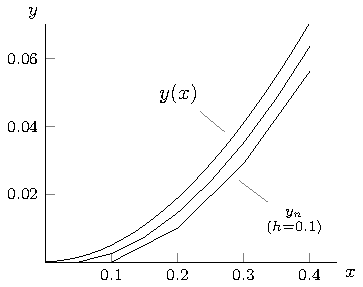
\includegraphics[]{figODEeuler}
\caption*{(ب)}
\end{subfigure}%
\caption{ترکیب یولر سے حاصل حل کا ریاضیاتی حل کے ساتھ موازنہ کیا گیا ہے۔}
\label{شکل_سادہ_اول_یولر_اصل_موازنہ}
\end{figure}

%====================
سوال \حوالہ{سوال_سادہ_اول_میدان_ڈھال_الف} تا سوال \حوالہ{سوال_سادہ_اول_میدان_ڈھال_ت} کے میدان ڈھال کو قلم و کاغذ سے کھینچتے ہوئے دیے ابتدائی نقطوں سے گزرتے منحنی حل حاصل کریں۔چند ڈھال میدان شکل \حوالہ{شکل_سوال_سادہ_اول_میدان_ڈھال_الف} اور شکل \حوالہ{شکل_سوال_سادہ_اول_میدان_ڈھال_پ} میں دیے گئے ہیں۔

%==========================

\حصہء{سوالات}
\ابتدا{سوال}\شناخت{سوال_سادہ_اول_میدان_ڈھال_الف}\quad \quad
$y'=1+y^2,\quad (\tfrac{\pi}{4},1)$
\انتہا{سوال}
%====================
\ابتدا{سوال}\شناخت{سوال_سادہ_اول_میدان_ڈھال_ب}\quad \quad
$y'=1-y^2,\quad (0,0)$
\انتہا{سوال}
%====================
\ابتدا{سوال}\شناخت{سوال_سادہ_اول_میدان_ڈھال_بب}\quad \quad
$yy'+8x=0,\quad (1,1)$
\انتہا{سوال}
%====================
\ابتدا{سوال}\شناخت{سوال_سادہ_اول_میدان_ڈھال_پ} \quad \quad
$y'=y-y^2,\quad (1,0)$
\انتہا{سوال}
%====================
\ابتدا{سوال} \شناخت{سوال_سادہ_اول_میدان_ڈھال_پپ}\quad \quad
$y'=x+\tfrac{1}{y},\quad (0,1)$
\انتہا{سوال}
%====================
\ابتدا{سوال} \شناخت{سوال_سادہ_اول_میدان_ڈھال_پپپ}\quad \quad
$y'=\sin^2 x,\quad (0,1)$
\انتہا{سوال}
%====================
\ابتدا{سوال}\شناخت{سوال_سادہ_اول_میدان_ڈھال_ت} \quad \quad
$y'=\sin^2 y,\quad (0,0)$
\انتہا{سوال}
%==================================
\begin{figure}
\centering
\begin{subfigure}{0.5\textwidth}
\centering
\begin{tikzpicture}
\def\length{sqrt(1+(1+y^2)^2)}
\begin{axis}[small, axis equal,axis lines*=middle,view={0}{90}, xlabel={$x$},ylabel={$y$},ylabel style={rotate=-90},ylabel style={at={(axis description cs:0.5,1.05)}},xmin=-4,xmax=4,ymin=-4,ymax=4,domain=-3.5:4, y domain=-3.5:4, samples=11,xlabel style={at={(axis description cs:1.05,0.5)}},xtick=\empty,ytick=\empty]
\addplot3 [gray, quiver={u={1/\length}, v={(1+y^2)/\length}, scale arrows=0.4,},-stealth] (x,y,0); %differential equation
\end{axis}
\end{tikzpicture}%
\caption*{(الف) \quad $y'=1+y^2$}
\end{subfigure}%
\begin{subfigure}{0.5\textwidth}
\centering
\begin{tikzpicture}
\def\length{sqrt(1+(1-y^2)^2)}
\begin{axis}[small, axis equal,axis lines*=middle,view={0}{90}, xlabel={$x$},ylabel={$y$},ylabel style={rotate=-90},ylabel style={at={(axis description cs:0.5,1.05)}},xmin=-4,xmax=4,ymin=-4,ymax=4,domain=-3.5:4, y domain=-3.5:4, samples=11,xlabel style={at={(axis description cs:1.05,0.5)}},xtick=\empty,ytick=\empty]
\addplot3 [gray, quiver={u={1/\length}, v={(1-y^2)/\length}, scale arrows=0.3},-stealth] (x,y,0); %differential equation
\end{axis}
\end{tikzpicture}%
\caption*{(ب) \quad $y'=1-y^2$}
\end{subfigure}%
\caption{سوال \حوالہ{سوال_سادہ_اول_میدان_ڈھال_الف} اور سوال \حوالہ{سوال_سادہ_اول_میدان_ڈھال_ب} کے ڈھال میدان۔}
\label{شکل_سوال_سادہ_اول_میدان_ڈھال_الف}
\end{figure}
%=============================
\begin{figure}
\centering
\begin{subfigure}{0.5\textwidth}
\centering
\begin{tikzpicture}
\def\length{sqrt(1+(-8*x/y)^2)}
\begin{axis}[small, axis equal,axis lines*=middle,view={0}{90}, xlabel={$x$},ylabel={$y$},ylabel style={rotate=-90},ylabel style={at={(axis description cs:0.5,1.05)}},xmin=-4,xmax=4,ymin=-4,ymax=4.5,domain=-3.8:4, y domain=-3.9:4, samples=11,xlabel style={at={(axis description cs:1.05,0.5)}},xtick=\empty,ytick=\empty]
\addplot3 [gray, quiver={u={1/\length}, v={(-8*x/y)/\length}, scale arrows=0.4,},-stealth] (x,y,0); %differential equation
\end{axis}
\end{tikzpicture}%
\caption*{(الف) \quad $y'=-\tfrac{8x}{y}$}
\end{subfigure}%
\begin{subfigure}{0.5\textwidth}
\centering
\begin{tikzpicture}
\def\length{sqrt(1+(y-y^2)^2)}
\begin{axis}[small, axis equal,axis lines*=middle,view={0}{90}, xlabel={$x$},ylabel={$y$},ylabel style={rotate=-90},ylabel style={at={(axis description cs:0.5,1.05)}},xmin=-4,xmax=4,ymin=-4,ymax=4,domain=-3.5:4, y domain=-3.5:4, samples=11,xlabel style={at={(axis description cs:1.05,0.5)}},xtick=\empty,ytick=\empty]
\addplot3 [gray, quiver={u={1/\length}, v={(y-y^2)/\length}, scale arrows=0.3},-stealth] (x,y,0); %differential equation
\end{axis}
\end{tikzpicture}%
\caption*{(ب) \quad $y'=y-y^2$}
\end{subfigure}%
\caption{سوال \حوالہ{سوال_سادہ_اول_میدان_ڈھال_بب} اور سوال \حوالہ{سوال_سادہ_اول_میدان_ڈھال_پ} کے ڈھال میدان۔}
\label{شکل_سوال_سادہ_اول_میدان_ڈھال_پ}
\end{figure}


%====================
ڈھال میدان کے استعمال سے تفرقی مساوات کے تمام حل سامنے آ جاتے ہیں۔بعض اوقات تفرقی مساوات کا تحلیلی حل حاصل کرنا ممکن ہی نہیں ہوتا۔درج ذیل دو سوالات میں ڈھال میدان سے اخذ حل اور دیے گئے تحلیلی حل کا موازنہ کرتے ہوئے ڈھال میدان سے حاصل حل کی درستگی کا اندازہ لگایا جا سکتا ہے۔

%=================
\ابتدا{سوال}\quad \quad
$y'=\sin x,\quad (\tfrac{\pi}{2},0),\quad y=-\cos x$
\انتہا{سوال}
%=====================
\ابتدا{سوال}\quad \quad
$y'=3x^2,\quad (0,0),\quad y=x^3$
\انتہا{سوال}
%=====================

%=============================
\ابتدا{سوال}
سوال \حوالہ{سوال_سادہ_اول_میدان_ڈھال_ب}، سوال \حوالہ{سوال_سادہ_اول_میدان_ڈھال_پ} اور سوال \حوالہ{سوال_سادہ_اول_میدان_ڈھال_ت} میں بے قابو متغیرہ \عددی{x} صریحاً  ظاہر نہیں کیا گیا ہے۔ایسی مساوات جن میں بے قابو متغیرہ کو صریحاً ظاہر نہ کیا جائے \اصطلاح{خود مختار}\فرہنگ{خود مختار!سادہ تفرقی مساوات}\فرہنگ{تفرقی!خود مختار}\حاشیہب{autonomous ordinary differential equations}\فرہنگ{autonomous!differential equation}\فرہنگ{differential!autonomous} سادہ تفرقی مساوات کہلاتے ہیں۔ خود مختار سادہ تفرقی مساوات کے  \اصطلاح{ہم میلان}\فرہنگ{ہم میلان}\حاشیہب{isoclines}\فرہنگ{isoclines} حل \عددی{f(x,y)=c} کی شکل و صورت کیا ہو گی؟

جواب:چونکہ \عددی{y'} کا دارومدار \عددی{x} پر نہیں ہے لہٰذا \عددی{x} تبدیل کرنے سے \عددی{y} کا میلان تبدیل نہیں ہو گا اور \عددی{f(x,y)=c} افقی محور کے متوازی خط ہوں گے۔ 
\انتہا{سوال}
%================

ایک جسم \عددی{y} محدد پر حرکت کرتی ہے۔لمحہ \عددی{t} پر نقطہ \عددی{y=0} سے جسم کا فاصلہ \عددی{y(t)} ہے۔سوالات \حوالہ{سوال_سادہ-اول_رفتار_الف} تا سوال \حوالہ{سوال_سادہ-اول_رفتار_پ} میں دئے شرائط کے مطابق جسم کی رفتار کی نمونہ کشی کریں۔ریاضی نمونے کی ڈھال میدان بناتے ہوئے  دیے گئے ابتدائی معلومات پر پورا اترتا منحنی خط کھینچیں۔ 

%=====================
\ابتدا{سوال}\شناخت{سوال_سادہ-اول_رفتار_الف}
جسم کی رفتار ضرب فاصلہ \عددی{y(t)} مستقل ہے جو \عددی{4} کے برابر ہے جبکہ \عددی{y(0)=4} کے برابر ہے۔

جوابات:\عددی{yy'=4}، \عددی{y=8t+16}
\انتہا{سوال}
%======================
\ابتدا{سوال}
رفتار ضرب وقت فاصلے کے برابر ہے۔لمحہ \عددی{t=1} پر فاصلہ \عددی{y(1)=2} ہے۔

جوابات:\عددی{y=y' t}، \عددی{y=2t}
\انتہا{سوال}
%=====================
\ابتدا{سوال}\شناخت{سوال_سادہ-اول_رفتار_پ}
مربع رفتار منفی مربع فاصلہ اکائی کے برابر ہے۔ابتدائی فاصلہ اکائی کے برابر ہے۔

جوابات:\عددی{y'=\sqrt{1+y^2}}، \عددی{\sinh^{-1}y=t+\sinh^{-1}1}
\انتہا{سوال}
%======================
\ابتدا{سوال}
ہوائی جہاز سے چھلانگ لگا کر زمین تک خیریت سے بذریعہ چھتری  اترا جا سکتا ہے۔گرتے ہوئے شخص پر آپس میں الٹ، دو عدد قوتیں عمل کرتی ہیں۔پہلی قوت زمینی کشش \عددی{F_1=mg} ہے جہاں \عددی{m} اس شخص کی کمیت اور \عددی{g=\SI{9.8}{\meter\per\second\squared}} ثقلی اسراع ہے۔یہ قوت انسان کو زمین کی طرف اسراع دیتی ہے۔دوسری قوت چھتری پر ہوا کے رگڑ سے پیدا قوت ہے جو اس شخص کی رفتار کو بڑھنے سے روکتی ہے۔چھتری پر ہوا کے رگڑ سے رفتار کے مربع کے متناسب قوت \عددی{F_2=cv^2} پیدا ہوتی ہے۔نیوٹن کی مساوات حرکت کہتی ہے کہ کسی بھی جسم پر قوت، اس جسم کی کمیت ضرب اسراع کے برابر ہوتی ہے۔چھتری سے زمین پر اترتے شخص کی نمونہ کشی کرتے ہوئے رفتار \عددی{v} کی سادہ تفرقی مساوات حاصل کریں۔کمیت کو \عددی{m=1} اور مستقل کو \عددی{c=1} لیتے ہوئے ڈھال میدان کھینچیں۔ تصور کریں کہ چھتری اس لمحہ کھلتی ہے جب شخص کی رفتار \عددی{v=\SI{15}{\meter\per\second}} ہو۔ایسی صورت میں منحنی حل حاصل کریں۔اس شخص کی اختتامی رفتار کیا ہو گی؟ کیا چھتری پر قوت رفتار کے راست متناسب ہونے کی صورت میں بھی چھتری کے ذریعہ ہوائی جہاز سے زمین تک خیریت سے چھلانگ لگائی جا سکتی ہے؟

جوابات:\عددی{mg-cv^2=m\tfrac{\dif v}{\dif t}}؛ گرنے کی رفتار اس قیمت پر رہتی ہے جہاں نیچے جانب قوت \عددی{mg} اور چھتری کی رکاوٹی اوپر جانب قوت \عددی{cv^2} برابر ہوں۔ایسی صورت میں گرتے شخص کی رفتار تبدیل نہیں ہوتی یعنی \عددی{y'=0} ہوتا ہے۔تفرقی مساوات میں \عددی{y'=0} پر کرتے اور \عددی{m=c=1} لیتے ہوئے اختتامی رفتار \عددی{v(t=\infty)=\SI{3.13}{\meter\per\second}} حاصل ہوتی ہے۔
\انتہا{سوال}
%=====================
\ابتدا{سوال}\شناخت{سوال_سادہ_اول_گول_دائرہ_ڈھال_میدان}
گول دائرے کی مساوات \عددی{x^2+y^2=r^2} ہے۔رداس \عددی{r} کو مستقل تصور کرتے ہوئے دائرے کی مساوات کا تفرق لیتے ہوئے  ڈھال میدان کی تفرقی مساوات حاصل کریں۔ڈھال میدان کھینچیں۔کیا آپ ڈھال میدان کو دیکھ کر کہہ سکتے ہیں کہ منحنی حل گول دائرے ہیں؟ اسی طرح \عددی{x^2+9y^2=c} کا تفرق لیتے ہوئے سادہ تفرقی مساوات حاصل کریں۔تفرقی مساوات کی ڈھال میدان کھینچیں۔ کیا ڈھال میدان کو دیکھ کر کہا جا سکتا ہے کہ منحنی حل بیضوی ہو گا؟

جوابات:\عددی{y'=-\tfrac{x}{y}}، \عددی{y'=-\tfrac{x}{9y}}
\begin{figure}
\centering
\begin{subfigure}{0.5\textwidth}
\centering
\begin{tikzpicture}
\def\length{sqrt(1+(x/y)^2)}
\begin{axis}[small, axis equal,axis lines*=middle,view={0}{90}, xlabel={$x$},ylabel={$y$},ylabel style={rotate=-90},ylabel style={at={(axis description cs:0.5,1.05)}},xmin=-4,xmax=4,ymin=-4,ymax=4,domain=-3.5:4, y domain=-3.5:4, samples=11,xlabel style={at={(axis description cs:1.05,0.5)}},xtick=\empty,ytick=\empty]
\addplot3 [gray, quiver={u={1/\length}, v={(-x/y)/\length}, scale arrows=0.3,},-stealth] (x,y,0); %differential equation
\end{axis}
\end{tikzpicture}%
\caption*{(الف) تفرقی مساوات \عددی{y'=-\tfrac{x}{y}} کی ڈھال میدان۔}
\end{subfigure}%
\begin{subfigure}{0.5\textwidth}
\centering
\begin{tikzpicture}
\def\length{sqrt(1+(x/(9*y))^2)}
\begin{axis}[small, axis equal,axis lines*=middle,view={0}{90}, xlabel={$x$},ylabel={$y$},ylabel style={rotate=-90},ylabel style={at={(axis description cs:0.5,1.05)}},xmin=-4,xmax=4,ymin=-4,ymax=4,domain=-3.5:4, y domain=-3.5:4, samples=11,xlabel style={at={(axis description cs:1.05,0.5)}},xtick=\empty,ytick=\empty]
\addplot3 [gray, quiver={u={1/\length}, v={(-x/(9*y))/\length}, scale arrows=0.3},-stealth] (x,y,0); %differential equation
\end{axis}
\end{tikzpicture}%
\caption*{(ب) تفرقی مساوات \عددی{y'=-\tfrac{x}{9y}} کی ڈھال میدان۔}
\end{subfigure}%
\caption{سوال \حوالہ{سوال_سادہ_اول_گول_دائرہ_ڈھال_میدان} کی ڈھال میدان۔}
\label{شکل_سوال_سادہ_اول_گول_دائرہ_ڈھال_میدان}
\end{figure}
\انتہا{سوال}
%===============================
سوال \حوالہ{سوال_سادہ_اول_یولر_الف} تا سوال \حوالہ{سوال_سادہ_اول_یولر_ت} کو ترکیب یولر سے حل کریں۔کل پانچ ہم فاصلہ نقطوں پر حل حاصل کریں۔ایک ہی کارتیسی محدد پر حاصل \عددی{y_1} تا \عددی{y_{5}} اور سوال میں دئے گئے حل \عددی{y(x)} کا خط کھینچیں۔
%=====================
\ابتدا{سوال}\شناخت{سوال_سادہ_اول_یولر_الف}
\begin{align*}
y'=-y,\quad y(0)=1,\quad h=0.1,\quad y(x)=e^{-x}
\end{align*}

جوابات: \عددی{y_1=0.9}، \عددی{y_2=0.81}، \عددی{y_3=0.729}، \عددی{y_4=0.6561}، \عددی{y_5=0.59049}
\انتہا{سوال}
%======================
\ابتدا{سوال}\شناخت{سوال_سادہ_اول_یولر_ب}
\begin{align*}
y'=-y,\quad y(0)=1,\quad h=0.01,\quad y(x)=e^{-x}
\end{align*}

جوابات: \عددی{y_1=0.99}، \عددی{y_2=0.9801}، \عددی{y_3=0.9703}، \عددی{y_4=0.9606}، \عددی{y_5=0.95099}
\انتہا{سوال}
%======================
\ابتدا{سوال}\شناخت{سوال_سادہ_اول_یولر_پ}
\begin{align*}
y'=1+3x^2,\quad y(1)=2,\quad h=0.1,\quad y(x)=x^3+x
\end{align*}

جوابات: \عددی{y_1=2.1}، \عددی{y_2=2.203}، \عددی{y_3=2.315}، \عددی{y_4=2.442}، \عددی{y_5=2.59}
\انتہا{سوال}
%======================
\ابتدا{سوال}\شناخت{سوال_سادہ_اول_یولر_ت}
\begin{align*}
y'=2xy,\quad y(0)=2,\quad h=0.01,\quad y(x)=e^{x^2-4}
\end{align*}

جوابات: \عددی{y_1=1.04}، \عددی{y_2=1.0818}، \عددی{y_3=1.1255}، \عددی{y_4=1.1712}، \عددی{y_5=1.2190}
\انتہا{سوال}
%======================

\حصہ{قابل علیحدگی سادہ تفرقی مساوات}
متعدد اہم سادہ تفرقی مساوات کو الجبرائی ترتیب دیتے ہوئے درج ذیل صورت میں لکھا جا سکتا ہے
\begin{align}\label{مساوات_سادہ_اول_قابل_علیحدگی-الف}
g(y)y'=f(x)
\end{align}
جس کو مزید یوں
\begin{align*}
g(y)\frac{\dif y}{\dif x} \dif x=f(x) \dif x
\end{align*}
یعنی
\begin{align*}
g(y)\dif y=f(x) \dif x
\end{align*}
لکھا جا سکتا ہے۔اس مساوات کے بائیں جانب صرف \عددی{y} متغیرہ اور دائیں جانب صرف \عددی{x} متغیرہ پایا جاتا ہے لہٰذا اس کا تکمل لیا جا سکتا ہے۔
\begin{align}\label{مساوات_سادہ_اول_قابل_علیحدگی-ب}
\int g(y)\dif y=\int f(x) \dif x+c
\end{align}
اگر \عددی{g(y)} اور \عددی{f(x)} قابل تکمل تفاعل ہوں تب مساوات \حوالہ{مساوات_سادہ_اول_قابل_علیحدگی-ب} سے مساوات \حوالہ{مساوات_سادہ_اول_قابل_علیحدگی-الف} کا حل حاصل کیا جا سکتا ہے۔اس ترکیب کو \اصطلاح{ترکیب علیحدگی متغیرات}\فرہنگ{ترکیب علیحدگی متغیرات}\فرہنگ{علیحدگی متغیرات!ترکیب}\حاشیہب{variable separation technique}\فرہنگ{variable separation} کہتے ہیں۔ مساوات \حوالہ{مساوات_سادہ_اول_قابل_علیحدگی-الف} کو \اصطلاح{قابل علیحدگی مساوات}\فرہنگ{قابل علیحدگی مساوات}\حاشیہب{separable equation}\فرہنگ{separable equation} کہتے ہیں۔

%=======================
\ابتدا{مثال}
مساوات \عددی{y'=1+y^2} قابل علیحدگی مساوات ہے چونکہ اس کو
\begin{align*}
\frac{\dif y}{1+y^2}=\dif x
\end{align*}
لکھا جا سکتا ہے جس کے دونوں اطراف کا تکمل لیتے ہوئے
\begin{align*}
\tan^{-1} y =x+c
\end{align*}
یعنی
\begin{align*}
y=\tan(x+c)
\end{align*}
حاصل ہوتا ہے جو تفرقی مساوات کا درکار حل ہے۔حاصل حل کو واپس تفرقی مساوات میں پر کرتے ہوئے تسلی کر لیں کہ یہی صحیح حل ہے۔
\انتہا{مثال}
%=================
\ابتدا{مثال}
قابل علیحدگی تفرقی مساوات \عددی{y'=xe^{-x} y^3} کو علیحدہ کرتے  ہوئے دونوں اطراف کا تکمل لے کر حل کرتے ہیں۔
\begin{align*}
y^{-3}\dif y&=xe^{-x} \dif x\\
\frac{y^{-2}}{-2}&=c-(x+1)e^{-x} \quad \quad \text{\RL{تکمل لیا گیا ہے}}\\
y^2&=\frac{1}{2(x+1)e^{-x}-2c}
\end{align*}
\انتہا{مثال}
%=================
\ابتدا{مثال}\شناخت{مثال_سادہ_اول_گھنٹی_الف}
درج ذیل ابتدائی قیمت تفرقی مساوات کو حل کریں۔
\begin{align*}
y'=-2xy,\quad y(0)=1
\end{align*} 

حل:مساوات کے متغیرات کو علیحدہ کرتے ہوئے تکمل کے ذریعہ حل کرتے ہیں۔
\begin{align*}
\int\frac{\dif y}{y}&=-\int 2x \dif x+c\\
\ln y&=-x^{2}+c_1\\
y&=ce^{-x^2}
\end{align*}
ابتدائی معلومات پر کرتے ہوئے \عددی{c=0} یعنی \عددی{c=e^{c_1}=1} ملتا ہے لہٰذا تفرقی مساوات کا مخصوص حل \عددی{y=e^{-x^2}} ہے جسے شکل \حوالہ{شکل_مثال_سادہ_اول_گھنٹی_الف} میں دکھایا گیا ہے اور جو \اصطلاح{گھنٹی نما}\فرہنگ{گھنٹی نما}\حاشیہب{bell shaped}\فرہنگ{bell shaped} ہے۔
\begin{figure}
\centering
\begin{tikzpicture}
\begin{axis}
\addplot[domain=-2:2,samples=60]{e^(-x^2)};
\end{axis}
\end{tikzpicture}
\caption{مثال \حوالہ{مثال_سادہ_اول_گھنٹی_الف} کا \اصطلاح{گھنٹی نما} حل۔}
\label{شکل_مثال_سادہ_اول_گھنٹی_الف}
\end{figure}
\انتہا{مثال}
%================
\ابتدا{مثال}\quad کاربن سے عمر دریافت کرنے کا طریقہ\\
طبعی معلومات: \اصطلاح{کائناتی شعاعیں}\فرہنگ{کائناتی شعاعیں}\حاشیہب{cosmic rays}\فرہنگ{cosmic rays} فضا میں تابکار کاربن \عددی{\ce{^{14}_{6}C}} بناتی ہیں۔یہ عمل زمین کی پیدائش سے اب تک ہوتا آ رہا ہے۔وقت کے ساتھ فضا میں \عددی{\ce{^{14}_{6}C}} اور \عددی{\ce{^{12}_{6}C}}\اصطلاح{ہم جا}\فرہنگ{ہم جا}\حاشیہب{isotopes}\فرہنگ{isotopes} کی تناسب ایک مخصوص قیمت حاصل کر چکی ہے۔کوئی بھی جاندار سانس لے کر یا خوراک کے ذریعہ فضا سے کاربن جذب  کرتا ہے۔یوں جب تک جانور زندہ رہے اس کی جسم میں دونوں ہم جا کاربن کی تناسب وہی ہو گی جو فضا میں ان کی تناسب ہے۔البتہ مرنے کے بعد جسم میں تابکار کاربن کی مقدار تابکاری تحلیل کی بنا گھٹتی ہے جبکہ غیر تابکار کاربن کی مقدار تبدیل نہیں ہوتی۔تابکار کاربن \عددی{\ce{^{14}_{6}C}} کی نصف زندگی \عددی{\num{5715}} سال ہے۔

اہرام مصر میں دفن مومیائی ہوئی فرعون کی لاش میں \عددی{\ce{^{14}_{6}C}} اور \عددی{\ce{^{12}_{6}C}} کا تناسب فضا کے تناسب کا \عددی{\SI{56.95}{\percent}} ہے۔لاش کی عمر دریافت کریں۔

حل:تابکار کاربن کی نصف زندگی سے تابکاری تحلیل کا مستقل \عددی{k} دریافت کرتے ہیں۔
\begin{align*}
y_0e^{-k(5715)}=\frac{y_0}{2}, \quad e^{-k(5715)}=\frac{1}{2}, \quad -k=\frac{\ln (\frac{1}{2})}{5715}, \quad k=0.0001213
\end{align*}
لاش میں ہم جا کاربن کی تناسب سے لاش کی عمر حاصل کرتے ہیں۔
\begin{align*}
e^{-0.0001213t}=0.5695,\quad -0.0001213t=\ln 0.5695,\quad t=4641
\end{align*}
یوں فرعون کی لاش \عددی{\num{4641}} سال پرانی ہے۔

\انتہا{مثال}
%=================
\ابتدا{مثال}\شناخت{مثال_سادہ_اول_مرکب}\quad مرکب بنانے کا عمل\\
کیمیائی صنعت میں  مرکب بنانے کا عمل عام ہے۔شکل \حوالہ{شکل_مثال_سادہ_اول_مرکب}-الف میں  پانی کی ٹینکی دکھائی گئی ہے جس میں ابتدائی طور پر \عددی{1000} لٹر پانی پایا جاتا ہے۔اس پانی میں کل \عددی{\SI{100}{\kilo\gram}} نمک ملایا گیا ہے۔پانی کو مسلسل ہلانے سے ٹینکی میں کثافت یکساں رکھی جاتی ہے۔ٹینکی میں \عددی{40} لٹر فی منٹ کی شرح سے نمکین پانی شامل کیا جاتا ہے۔اس پانی میں نمک کی مقدار \عددی{\SI{0.5}{\kilo\gram\per\litre}} ہے۔ٹینکی سے نمکین پانی کا انخلا \عددی{40} لٹر فی منٹ ہے۔ٹینکی میں نمک کی کل مقدار بالمقابل وقت دریافت کریں۔
\begin{figure}
\centering
\begin{subfigure}{0.5\textwidth}
\centering
\begin{tikzpicture}
   [ragged border/.style={ decoration={random steps, segment length=1mm, amplitude=0.5mm},
           decorate,}]
\pgfmathsetmacro{\x}{2}
\pgfmathsetmacro{\y}{2}

\fill[cyan!30]
        decorate[ragged border]{
        (-\x-\x/4,\y/2)--++(\x,0)
        }
        -- ++(0,-3/8*\y) --++ (\x/4,0) --++ (0,-\y/8) --++ (-\x-\x/4,0) --++(0,\y/2) -- cycle;
\fill[cyan!30](-\x-\x/4,3/4*\y)coordinate(inL)--++(-\x/4,0)--++(0,\y/8)--++(\x/4,0)coordinate(inU)--cycle;
\fill[cyan!30] (inL) to [out=0,in=120] ++(\x/4,-\y/3)--++(\x/16,0) to [out=120,in=0] (inU)--cycle;

\draw(0,0)--++(-\x-\x/4,0)--++(0,3/4*\y)--++(-\x/4,0)++(0,\y/8)--++(\x/4,0)--++(0,\y/4);
\draw(0,\y/8)--++(-\x/4,0)--++(0,\y);
\draw[cyan!30,-stealth,ultra thick] (\x/8,\y/16)--++(\x/4,0)node[right,color=black]{خروج};
\draw[cyan!30,stealth-,ultra thick] (-\x-\x/4-\x/4-\x/8,3/4*\y+\y/16)--++(-\x/4,0)node[pos=0.5,above,color=black]{دخول};
\end{tikzpicture}
\caption*{(الف)}
\end{subfigure}%
\begin{subfigure}{0.5\textwidth}
\centering
\begin{tikzpicture}
\begin{axis}[small,xlabel={$t\, (\text{\RL{منٹ}})$}, ylabel={$y(t)$},ylabel style={rotate=-90},ylabel style={at={(axis description cs:0,1.05)}}]
\addplot[domain=0:150]{500-400*e^(-0.04*x)};
\end{axis}
\end{tikzpicture}
\caption*{(ب)}
\end{subfigure}%
\caption{مثال \حوالہ{مثال_سادہ_اول_مرکب} میں مرکب بنانے کا عمل۔}
\label{شکل_مثال_سادہ_اول_مرکب}
\end{figure}

حل:چونکہ ٹینکی میں پانی شامل ہونے کی شرح اور پانی خارج ہونے کی شرح  برابر ہےیں لہٰذا ٹینکی میں پانی کی مقدار تبدیل نہیں ہوتی۔ٹینکی میں داخل ہونے والا ایک لٹر کا نمکین پانی \عددی{\SI{0.5}{\kilo\gram}} نمک ٹینکی میں شامل کرتا ہے۔یوں \عددی{40} لٹر فی منٹ سے داخل ہوتا پانی \عددی{40\times 0.5=\SI{20}{\kilo\gram\per\minute}} سے نمک شامل کرتا ہے۔کسی بھی لمحہ ٹینکی میں کل نمک کو \عددی{y} کلوگرام لکھتے ہوئے ٹینکی میں نمک کی کثافت کو \عددی{\tfrac{y}{1000}} کلوگرام فی لٹر لکھا جا سکتا ہے۔یوں خارج ہوتا پانی \عددی{40\times \tfrac{y}{1000}} کلوگرام فی منٹ نمک خارج کرتا ہے۔اس طرح نمک میں اضافے کی شرح \عددی{\tfrac{\dif y}{\dif t}} کو
\begin{align*}
y'&=\text{\RL{نمک شامل ہونے کی شرح}} -\text{\RL{نمک خارج ہونے کی شرح}}\quad \quad (\text{\RL{متوازن مساوات}})\\
&=20-\frac{40y}{1000}
\end{align*}
یعنی
\begin{align}
y'=0.04(500-y)
\end{align}
لکھا جا سکتا ہے جو قابل علیحدگی مساوات ہے لہٰذا اس میں متغیرات کو علیحدہ کرتے ہوئے تکمل کے ذریعہ حل کرتے ہیں۔
\begin{align*}
\frac{\dif y}{y-500}=-0.04\dif t, \quad \ln \abs{y-500}=-0.04t+c_1,\quad y=500+ce^{-0.04t}
\end{align*}
ٹینکی میں ابتدائی نمک کی کل مقدار \عددی{\SI{100}{\kilo\gram}} ہے۔اس معلومات کو درج بالا میں پر کرتے ہوئے مساوات کا مستقل \عددی{c} حاصل کرتے ہیں۔ 
\begin{align*}
100=500+c^{-0.04(0)},\quad c=-400
\end{align*}
یوں کسی بھی لمحے ٹینکی میں کل نمک کی مقدار درج ذیل ہے جس کو شکل-ب میں دکھایا گیا ہے۔
\begin{align*}
y(t)=500-400e^{-0.04t}
\end{align*}
شکل-ب کے مطابق ٹینکی میں آخرکار کل \عددی{\SI{500}{\kilo\gram}} نمک پایا جائے گا۔ یہی جواب بغیر کسی مساوات لکھے بھی حاصل کیا جا سکتا ہے۔اگر ٹینکی میں لگاتار نمکین پانی شامل کیا جائے اور اس سے پرانا پانی خارج کیا جائے تو آخرکار ٹینکی میں صرف نیا شامل کردہ پانی ہی پایا جائے گا۔چونکہ شامل کردہ پانی میں \عددی{0.5} کلوگرام فی لٹر نمک پایا جاتا ہے لہٰذا \عددی{1000} لٹر کی ٹینکی میں کل نمک \عددی{1000\times 0.5=\SI{500}{\kilo\gram}} ہو گا۔ 
\انتہا{مثال}
%=====================
\ابتدا{مثال}\شناخت{مثال_سادہ_اول_نیوٹن_قانون_ٹھنڈک} \quad نیوٹن قانون ٹھنڈک
گرمیوں میں ایک دفتر کا درجہ حرارت ایئر کنڈشنر کی مدد سے \عددی{\SI{21}{\degree\celsius}} پر رکھا جاتا ہے۔صبح سات بجے ایئر کنڈشنر چالو کیا جاتا ہے اور شام نو بجے اس کو بند کر دیا جاتا ہے۔ایک مخصوص دن کو شام نو بجے بیرونی درجہ حرارت \عددی{\SI{40}{\degree\celsius}} ہوتا ہے جبکہ صبح سات بجے بیرونی درجہ حرارت \عددی{\SI{30}{\degree\celsius}} تک گر چکا ہوتا ہے۔دفتر کے اندر رات دو بجے درجہ حرارت \عددی{\SI{26}{\degree\celsius}} ہوتا ہے۔صبح سات بجے دفتر کے اندر درجہ حرارت معلوم کریں۔

طبعی معلومات:تجربے سے معلوم کیا گیا ہے کہ حرارتی توانائی کو با آسانی منتقل کرتے جسم (مثلاً لوہا) کے درجہ حرارت میں تبدیلی کی شرح جسم اور اس کے گرد ماحول کے درجہ حرارت میں فرق کے راست تناسب  ہوتا ہے۔اس کو \اصطلاح{نیوٹن کا قانون ٹھنڈک}\فرہنگ{نیوٹن کا قانون ٹھنڈک}\حاشیہب{Newton's law of cooling}\فرہنگ{Newton!law of cooling} کہا جاتا ہے۔

حل:پہلا قدم: نمونہ کشی \\
دفتر کے اندرونی حرارت کو \عددی{T} سے ظاہر کرتے ہیں جبکہ بیرونی حرارت کو \عددی{T_b} سے ظاہر کرتے ہیں۔یوں نیوٹن کا قانون ٹھنڈک کی ریاضیاتی صورت درج ذیل ہو گی۔
\begin{align}
\frac{\dif T}{\dif t}=k(T-T_b)
\end{align}
دوسرا قدم:عمومی حل کی تلاش\\
اگرچہ دفتر کی دیواریں اور چھت حرارتی توانائی با آسانی منتقل نہیں کرتی ہم اسی کلیے کا سہارا لیتے ہوئے مسئلہ حل کریں گے۔یہاں بیرونی درجہ حرارت مستقل قیمت نہیں ہے لہٰذا درج بالا مساوات کو حل کرنا مشکل ہو گا۔انجنیئرنگ کے شعبے میں عموماً ایسی ہی مشکلات کا سامنہ کرنا ہوتا ہے۔ہمیں مسئلے کی سادہ صورت حل کرنا ہو گی۔اگر ہم تصور کریں کہ \عددی{T_b} مستقل قیمت ہے تب درج بالا مساوات کے متغیرات علیحدہ کئے جا سکتے ہیں۔چونکہ بیرونی درجہ حرارت \عددی{\SI{30}{\degree\celsius}} تا \عددی{\SI{40}{\degree\celsius}} رہا ہے لہٰذا ہم اس کی اوسط قیمت یعنی \عددی{\SI{35}{\degree\celsius}} کو بیرونی درجہ حرارت تصور کرتے ہوئے مسئلے کو حل کرتے ہیں۔مساوات کے متغیرات علیحدہ کرتے ہوئے تکمل لے کر اس کو حل کرتے ہیں۔
\begin{align*}
\frac{\dif T}{T-35}=k\dif t, \quad \ln\abs{T-35}=kt+c_1,\quad T-35=ce^{kt}
\end{align*}
تیسرا قدم:مخصوص حل کا حصول\\
اگر شام نو بجے کو لمحہ \عددی{t=0} لیا جائے اور وقت کو گھنٹوں میں ناپا جائے تب \عددی{T(0)=21} لکھا جائے گا جسے درج بالا میں پر کرتے ہوئے \عددی{c=-14} حاصل ہوتا ہے۔یوں مخصوص حل
\begin{align*}
T=35-14e^{kt}
\end{align*}
چوتھا قدم:مستقل \عددی{k} کا حصول\\
ہم جانتے ہیں کہ رات دو بجے  اندرونی درجہ حرارت  \عددی{\SI{26}{\degree\celsius}} ہے۔یاد رہے کہ شام نو بجے کو لمحہ \عددی{t=0} لیا گیا لہٰذا رات دو بجے \عددی{t=5} ہو گا۔
یوں \عددی{T(5)=26} لکھا جائے گا۔ان معلومات کو درج بالا مساوات میں پر کرتے ہوئے \عددی{k} حاصل کرتے ہوئے مکمل مساوات حاصل کرتے ہیں۔
\begin{align*}
26=35-14e^{5k},\quad k=-0.088, \quad T=35-14e^{-0.088t}
\end{align*}
آخری قدم:\\
صبح سات بجے اندرونی درجہ حرارت کا تخمینہ لگاتے ہیں یعنی \عددی{t=10} پر درجہ حرارت درکار ہے۔
\begin{align*}
T=35-14e^{-0.088(10)}=\SI{29.2}{\degree\celsius}
\end{align*} 
پوری رات میں اندرونی درجہ حرارت \عددی{\SI{8.2}{\degree\celsius}} بڑھ گیا ہے۔شکل \حوالہ{شکل_مثال_سادہ_اول_نیوٹن_قانون_ٹھنڈک} میں اندرونی درجہ حرارت بالمقابل وقت دکھایا گیا ہے۔
\begin{figure}
\centering
\begin{tikzpicture}
\begin{axis}[small,xlabel={$t\,\text{(گھنٹے)}$},ylabel={$T\, (\si{\degree\celsius})$},ytick={21,29.2},yticklabels={$21$,$29.2$},ylabel style={rotate=-90},ylabel style ={at={(axis description cs:0,1.05)}},xmin=0]
\addplot[domain=0:10]{35-14*e^(-0.088*x)};
\end{axis}
\end{tikzpicture}
\caption{مثال \حوالہ{مثال_سادہ_اول_نیوٹن_قانون_ٹھنڈک}: دفتر کا اندرونی درجہ حرارت بالمقابل وقت۔}
\label{شکل_مثال_سادہ_اول_نیوٹن_قانون_ٹھنڈک}
\end{figure}
\انتہا{مثال}
%=======================
\ابتدا{مثال} \quad پانی کا انخلا:\شناخت{مثال_سادہ_اول_ٹاری_سلی}
پانی کی ٹینکی کا رقبہ عمودی تراش \عددی{B=\SI{2}{\meter\squared}} ہے۔ٹینکی کی تہہ میں \عددی{r=\SI{0.5}{\centi\meter}} رداس کا گول سوراخ ہے جس سے پانی نکل رہا ہے۔ٹینکی میں پانی کی ابتدائی گہرائی \عددی{h_1=\SI{1.5}{\meter}} ہے۔ٹینکی کتنی دیر میں خالی ہو گی۔

طبعی معلومات:پانی کی سطح پر \عددی{m} کمیت پانی کی مخفی توانائی \عددی{mgh} ہے جہاں \عددی{g=\SI{9.8}{\meter\per\second\squared}} ثقلی اسراع اور \عددی{h} پانی کی گہرائی ہے۔سوراخ سے خارج ہوتے وقت یہ مخفی توانائی  حرکی توانائی \عددی{\tfrac{mv^2}{2}} میں تبدیل ہو جاتی ہے جہاں \عددی{v} رفتار کو ظاہر کرتی ہے۔مخفی توانائی اور حرکی توانائی کو برابر لکھتے ہوئے \عددی{v} کے لئے حل کرتے ہیں۔
\begin{align*}
\frac{mv^2}{2}=mgh,\quad v=\sqrt{2gh}
\end{align*}
شکل \حوالہ{شکل_مثال_سادہ_اول_ٹاری_سلی}-الف میں پانی کی دھار دکھائی گئی ہے۔جیسا کہ آپ دیکھ سکتے ہیں دھار سوراخ کے قریب سکڑتا ہے۔اگر سوراخ کا رقبہ \عددی{a} ہو تب سکڑے  ہوئے مقام پر دھار کا رقبہ عمودی تراش \عددی{0.6a} ہوتا ہے۔یوں سوراخ سے نکلا تمام پانی رقبہ \عددی{0.6a} سے گزرتا ہے اور یہی وہ مقام ہے جہاں پانی کا ہر ذرہ ایک ہی سمت میں رفتار \عددی{v} سے حرکت کرتا ہے۔

شکل \حوالہ{شکل_مثال_سادہ_اول_ٹاری_سلی}-ب میں ایک نالی دکھائی گئی ہے جس میں پانی کی رفتار \عددی{v} ہے۔ نالی کا رقبہ عمودی تراش \عددی{A} ہے۔لمحہ \عددی{t=0} پر  مقام \عددی{m} پر موجود پانی کا ذرہ وقت \عددی{\Delta t} میں \عددی{v\Delta} فاصلہ طے کرتے ہوئے مقام \عددی{n} تک پہنچ جائے گا۔یوں \عددی{\Delta t} کے دوران مقام \عددی{m} سے گزرا ہوا پانی نالی کو \عددی{m} تا \عددی{n} بھرے گا۔اس پانی کی مقدار \عددی{\Delta M=A v \Delta t} ہو گی۔اسی کلیے کو استعمال کرتے ہوئے شکل \حوالہ{شکل_مثال_سادہ_اول_ٹاری_سلی}-الف میں \عددی{\dif t} دورانیے میں کل \عددی{\dif M=0.6a v \dif t} پانی خارج ہو گا۔یوں پانی کی شرح انخلا درج ذیل ہو گی۔
 \begin{align}\label{مساوات_سادہ_اول_ٹورا_سلی}
\frac{\dif M}{\dif t}=0.6a\sqrt{2gh}
\end{align}
 
اس مساوات  کو \اصطلاح{قانون ٹاری سلی}\فرہنگ{قانون ٹاری سلی}\حاشیہب{Torricelli's law}\فرہنگ{Torricelli's law} کہتے ہیں۔
\begin{figure}
\centering
\begin{subfigure}{0.5\textwidth}
\centering
\begin{tikzpicture}
  [ragged border/.style={ decoration={random steps, segment length=1mm, amplitude=0.5mm},
           decorate,}]
\pgfmathsetmacro{\x}{2}
\pgfmathsetmacro{\y}{2}
\pgfmathsetmacro{\angA}{70}
\pgfmathsetmacro{\angB}{110}
%coloured water
\path(-\x/2-\x/16,0) to [out=-\angA,in=\angA]++(0,-\y/4)coordinate(kL);
\path(-\x/2+\x/16,0) to [out=-\angB,in=\angB]++(0,-\y/4)coordinate(kR);
\fill[cyan!30](-\x,\y-\y/8)--++(\x,0)-- ++(0,-\y+\y/8) --++ (-\x,0) --++ (0,\y-\y/8) -- cycle;
\fill[cyan!30] (-\x/2-\x/16,0) to [out=-\angA,in=\angA] (kL)--(kR) to [out=\angB,in=-\angB] ++(0,\y/4)--cycle;
\draw[stealth-stealth] (\x/8,0)--++(0,\y-\y/8)node[pos=0.5,fill=white]{$h$};
%drum
\draw(0,0)--++(0,\y);
\draw(0,0)--++(-\x/2+\x/16,0)++(-\x/8,0)--++(-\x/2+\x/16,0)--++(0,\y);
\draw[stealth-](-\x/2-\x/16,-\y/8)--++(-\x/4,0)--++(-\x/8,-\y/8)node[left]{$0.6a$};
\draw (-\x-\x/16,\y-\y/8)--++(-\x/4,0);
\draw (-\x-\x/16,\y-\y/8-\y/16)--++(-\x/4,0);
\draw[stealth-](-\x-\x/16-\x/8,\y-\y/8)--++(0,\y/4)node[above]{$\dif h$};
\draw[stealth-](-\x-\x/16-\x/8,\y-\y/8-\y/16)--++(0,-\y/4);
\end{tikzpicture}
\caption*{(الف)}
\end{subfigure}%
\begin{subfigure}{0.5\textwidth}
\centering
\begin{tikzpicture}
\pgfmathsetmacro{\x}{2}
\pgfmathsetmacro{\y}{2}
%water
\fill[cyan!10](0,0)--++(2*\x,0)--++(0,\y/8)--++(-2*\x,0)--cycle;
\fill[cyan!30](\x/2,0)--++(\x,0)--++(0,\y/8)--++(-\x,0)--cycle;
\draw[stealth-](-\x/8,\y/16)--++(-\x/4,0)node[pos=0.5,above]{$v$};
\draw[stealth-stealth](\x/2,-\y/8)--++(\x,0)node[pos=0.5,fill=white]{$v \Delta t$};
\draw(\x/2+\x/2,\y/16)--++(\x/2,\y/2)node[right]{$\Delta M=A v\Delta t$};
%pipe
\draw(0,\y/8)--++(2*\x,0);
\draw(0,0)--++(2*\x,0);
\draw[stealth-](\x/4,\y/8)--++(0,\y/4)--++(-\x/4,\y/4)node[above]{\RL{رقبہ عمودی تراش=$A$}};
\draw[dashed] (\x/2,-\y/4)node[below]{$m$}--++(0,\y/2);
\draw[dashed] (\x+\x/2,-\y/4)node[below]{$n$}--++(0,\y/2);

\end{tikzpicture}
\caption*{(ب)}
\end{subfigure}%
\caption{مثال \حوالہ{مثال_سادہ_اول_ٹاری_سلی}: پانی کا انخلا اور پانی کے دھار کا سکڑنا۔}
\label{شکل_مثال_سادہ_اول_ٹاری_سلی}
\end{figure}

حل:دورانیہ \عددی{\dif t} میں پانی کی انخلا کے بنا ٹینکی میں پانی کی گہرائی \عددی{\dif h} کم ہو گی جو \عددی{B \dif h} حجم کی کمی کو ظاہر کرتی ہے جہاں \عددی{B} ٹینکی کا رقبہ عمودی تراش ہے۔چونکہ پانی کے انخلا سے ٹینکی میں پانی کم ہوتا ہے لہٰذا درج ذیل لکھا جا سکتا ہے جو دیے گئے مسئلے کا تفرقی مساوات ہے۔
\begin{align}
0.6a\sqrt{2gh} \dif t=-B\dif h
\end{align}
متغیرات کو علیحدہ کرتے ہوئے حل کرتے ہیں۔
\begin{align*}
\frac{\dif h}{\sqrt{h}}=-\frac{0.6a \sqrt{2g}}{B} \dif t,\quad 2\sqrt{h}=-\frac{0.6a \sqrt{2g}}{B} t+c
\end{align*}
ابتدائی لمحہ \عددی{t=0} پر پانی کی گہرائی \عددی{h_1} ہے۔ان معلومات کو درج بالا میں پر کرتے ہوئے \عددی{c=2h_1} ملتا ہے لہٰذا تفرقی مساوات کا مخصوص حل درج ذیل ہے۔
\begin{align}\label{مساوات_سادہ_اول_ٹاری_سلی_ٹینکی_خالی}
 2\sqrt{h}=-\frac{0.6a \sqrt{2g}}{B} t+ 2\sqrt{h_1}
\end{align}
خالی ٹینکی سے مراد \عددی{h=0} ہے۔مخصوص حل میں \عددی{h=0} پر کرتے ہوئے ٹینکی خالی کرنے کے لئے درکار وقت حاصل کرتے ہیں۔
\begin{align*}
 2\sqrt{0}=-\frac{0.6a \sqrt{2g}}{B} t+ 2\sqrt{h_1}, \quad t=\frac{2\sqrt{h_1} B}{0.6a \sqrt{2g}}\\
t=\frac{2\sqrt{1.5} \times 2}{0.6\pi 0.005^2 \sqrt{2\times 9.8}}=\SI{23482}{\second} \approx \SI{6.52}{\hour}
\end{align*}
مساوات \حوالہ{مساوات_سادہ_اول_ٹاری_سلی_ٹینکی_خالی} کو شکل \حوالہ{شکل_مثال_سادہ_اول_ٹاری_سلی_خالی} میں دکھایا گیا ہے۔یاد رہے کہ \عددی{\SI{23482}{\second}} میں ٹینکی خالی ہو جاتی ہے لہٰذا ترسیم کو اتنے وقت کے لئے ہی کھینچا گیا ہے۔
\begin{figure}
\centering
\begin{tikzpicture}
\begin{axis}[axis lines*=middle,ylabel={$h$},ylabel style={rotate=-90},ylabel style={at={(axis description cs:0,1.05)}},xlabel={$t\, (\si{\second})$},scaled x ticks=false]
\pgfmathsetmacro{\ha}{1.5}
\pgfmathsetmacro{\B}{2}
\pgfmathsetmacro{\a}{pi*0.005^2}
%\pgfmathsetmacro{\k}{0.3*\a*sqrt(2*9.8)/\B}  %pgfmath calculate this value wrongly????
\pgfmathsetmacro{\k}{0.000052}
%
\addplot[domain=0:23480]({x},{(sqrt(\ha)-\k*x)^(2)});
\end{axis}
\end{tikzpicture}
\caption{مثال \حوالہ{مثال_سادہ_اول_ٹاری_سلی}: ٹینکی خالی ہونے کا عمل۔}
\label{شکل_مثال_سادہ_اول_ٹاری_سلی_خالی}
\end{figure}
\انتہا{مثال}
%======================

\جزوحصہء{علیحدگی متغیرات کی جامع ترکیب}
بعض اوقات نا قابل علیحدگی تفرقی مساوات کے متغیرات کو تبدیل کرتے ہوئے مساوات کو قابل علیحدگی بنایا جا سکتا ہے۔ اس ترکیب کو درج ذیل عملاً اہم قسم کی مساوات کے لئے سیکھتے ہیں جہاں \عددی{f(\tfrac{y}{x})} قابل تفرق تفاعل ہے مثلاً \عددی{\cos \tfrac{y}{x}}، \عددی{e^{(y/x)}} وغیرہ۔
\begin{align}
y'=f\left(\frac{y}{x}\right)
\end{align}  
مساوات کی صورت دیکھتے ہوئے \عددیء{\tfrac{y}{x}=u} لیتے ہیں۔یوں درج ذیل لکھا جا سکتا ہے
\begin{align}\label{مساوات_سادہ_اول_جامع_علیحدگی_الف}
y=ux,\quad y'=u+xu'
\end{align}
جنہیں \عددی{y'=f(\tfrac{y}{x})} میں پر کرتے ہوئے \عددی{u+xu'=f(u)} یعنی \عددی{xu'=f(u)-u} ملتا ہے۔اگر \عددی{f(u)-u \ne 0} ہو تب متغیرات علیحدہ کرتے ہوئے درج ذیل لکھا جا سکتا ہے۔
\begin{align} 
\frac{\dif u}{f(u)-u}=\frac{\dif x}{x}
\end{align}
%============
\ابتدا{مثال}
تفاعل \عددی{xy'-y=2x} کو حل کریں۔

حل:تفاعل کو \عددی{y'=\tfrac{y}{x}+2} لکھا جا سکتا ہے۔یوں \عددی{\tfrac{y}{x}=u} لیتے ہوئے  مساوات \حوالہ{مساوات_سادہ_اول_جامع_علیحدگی_الف} کے استعمال سے درج ذیل ملتا ہے۔
\begin{align*}
u+xu'=u+2, \quad \dif u=2\frac{\dif x}{x},\quad u=2\ln \abs{x}+c
\end{align*}
اس میں \عددی{u} کی جگہ واپس \عددی{\tfrac{y}{x}} پر کرتے ہوئے جواب حاصل ہوتا ہے۔
\begin{align*}
\frac{y}{x}=2\ln \abs{x}+c,\quad y=2x\ln \abs{x}+cx
\end{align*}
\انتہا{مثال}
%=========================

\حصہء{سوالات}
سوال \حوالہ{سوال_سادہ_اول_جامع_علیحدگی_الف} تا سوال \حوالہ{سوال_سادہ_اول_جامع_علیحدگی_ب} کے عمومی حل حاصل کریں۔حاصل حل کو واپس تفرقی مساوات میں پر کرتے ہوئے اس کی درستگی ثابت کریں۔

%=======================
\ابتدا{سوال}\شناخت{سوال_سادہ_اول_جامع_علیحدگی_الف}
$y^2y'+x^2=0$

جواب:\عددی{x^3+y^3=c}
\انتہا{سوال}
%=============================
\ابتدا{سوال}
$yy'+x=0$

جواب:\عددی{x^2+y^2=c}
\انتہا{سوال}
%=============================
\ابتدا{سوال}
$y'=\sec^2 y$

جواب:\عددی{y=\tan x+c}
\انتہا{سوال}
%=============================
\ابتدا{سوال}
$y'\cos x=y\sin x$

جواب:\عددی{y=c\sec x}
\انتہا{سوال}
%=============================
\ابتدا{سوال}
$y'=ye^{x-1}$

جواب:\عددی{\ln\abs{y}=e^{x-1}+c}
\انتہا{سوال}
%=============================
\ابتدا{سوال} 
\عددی{u=\tfrac{y}{x}} پر کرتے ہوئے \عددی{xy'=y+x^2\sin^2\frac{y}{x}} کو حل کریں۔

جواب:\عددی{\tfrac{\cos \tfrac{y}{x}-1}{\cos\tfrac{y}{x}+1}=ce^{2x}}
\انتہا{سوال}
%=============================
\ابتدا{سوال}
\عددی{y'=(2x+y)^2} کو حل کریں۔ایسا کرنے کی خاطر \عددی{u=2x+y} پر کرنا ہو گا۔

جواب:\عددی{y=-2x+\sqrt{2}\tan(\sqrt{2}x+c)}
\انتہا{سوال}
%=============================
\ابتدا{سوال} 
\عددی{u=\tfrac{y}{x}} پر کرتے ہوئے \عددی{xy'=y^2+y} کو حل کریں۔

جواب:\عددی{y=-\tfrac{x}{x+c}}
\انتہا{سوال}
%=============================
\ابتدا{سوال} \شناخت{سوال_سادہ_اول_جامع_علیحدگی_ب}
\عددی{u=\tfrac{y}{x}} پر کرتے ہوئے \عددی{xy'=x-y} کو حل کریں۔

جواب:\عددی{xy-x^2=c}
\انتہا{سوال}
%=============================

 ابتدائی قیمت سوال \حوالہ{سوال_سادہ_اول_ابتدائی_قیمت_الف} تا سوال \حوالہ{سوال_سادہ_اول_ابتدائی_قیمت_ب} کے مخصوص حل حاصل کریں۔

\ابتدا{سوال}\شناخت{سوال_سادہ_اول_ابتدائی_قیمت_الف}
\begin{align*}
xy'+y=0,\quad y(2)=8
\end{align*}

جواب:\عددی{y=\tfrac{16}{x}}
\انتہا{سوال}
%====================
\ابتدا{سوال}
\begin{align*}
y'=1+9y^2,\quad y(1)=0
\end{align*}

جواب:\عددی{y=\tfrac{1}{3}\tan[3(x-1)]}
\انتہا{سوال}
%======================
\ابتدا{سوال}
\begin{align*}
y' \cos^2 x=\sin^2 y, \quad y(0)=\frac{\pi}{4}
\end{align*}

جواب:\عددی{\tan y=\tfrac{1}{1-\tan x}}
\انتہا{سوال}
%==============================
\ابتدا{سوال}
\begin{align*}
y'=-4xy,\quad y(0)=5
\end{align*}

جواب:\عددیء{y=5e^{-2x^2}}
\انتہا{سوال}
%==================
\ابتدا{سوال}
\begin{align*}
y'=-\frac{2x}{y},\quad y(1)=2
\end{align*}

جواب:\عددی{2x^2+y^2=6}
\انتہا{سوال}
%==================
\ابتدا{سوال}
\begin{align*}
y'=(x+y-4)^2,\quad y(0)=5
\end{align*}

جواب:\عددی{x+y-4=\tan(x+\tfrac{\pi}{4})}
\انتہا{سوال}
%=================
\ابتدا{سوال}\شناخت{سوال_سادہ_اول_ابتدائی_قیمت_ب}
\begin{align*}
xy'=y+3x^4\cos^2 \frac{y}{x},\quad y(1)=0
\end{align*}

 جواب:اس میں \عددی{u=\tfrac{y}{x}} پر کرنے سے \عددی{\tan \tfrac{y}{x}=x^3-1} ملتا ہے۔
\انتہا{سوال}
%=================
\ابتدا{سوال}
کسی بھی لمحے پر جرثوموں کی تعداد بڑھنے کی شرح، اس لمحے موجود جرثوموں کی تعداد کے راست تناسب ہے۔اگر ان کی تعداد دو گھنٹوں میں دگنی ہو جائے تب چار گھنٹوں بعد ان کی تعداد کتنی ہو گی؟ چوبیس گھنٹوں بعد کتنی ہو گی؟  

جوابات:\عددی{y=y_0e^{0.34657t}}، \عددی{4y_0}، \عددی{4095y_0}
\انتہا{سوال}
%==================
\ابتدا{سوال}
جرثوموں کی شرح پیدائش موجودہ تعداد کے راست تناسب ہے۔ان کی شرح اموات بھی موجودہ تعداد کے راست تناسب ہے۔جرثوموں کی تعداد بڑھنے کی شرح کیا ہو گی؟ تعداد بالمقابل وقت کیا ہو گا؟ تعداد کہاں متوازن صورت اختیار کرے گی؟

جوابات:\عددی{\tfrac{\dif y}{\dif t}=\alpha y-\beta y} جہاں \عددی{\alpha} اور \عددی{\beta} بالترتیب پیدائشی اور امواتی راست تناسب کے مستقل ہیں۔ تعداد بالمقابل وقت کی مساوات \عددیء{y=y_0e^{(\alpha-\beta)t}} ہے۔اگر \عددی{\alpha > \beta} ہو تب تعداد بڑھتی رہے گی۔اس کے برعکس اگر \عددی{\alpha<\beta} ہو تب تعداد گھٹتی رہے گی حتٰی کہ جراثیم فنا ہو جائیں اور \عددی{\alpha=\beta} کی صورت میں تعداد وقت کے ساتھ تبدیل نہیں ہو گی۔ 
\انتہا{سوال}
%=================
\ابتدا{سوال}
عموماً جاندار مرنے کے بعد مکمل طور پر خاک میں مل جاتے ہیں اور ان کا نشان تک نہیں رہتا البتہ بعض اوقات حالات یوں ہوتے ہیں کہ ان کا جسم پتھر میں بدل جاتا ہے۔اس پتھریلی جسم میں موجود \عددی{\ce{^{14}_{6}C}} اور \عددی{\ce{^{12}_{6}C}} ہم جا کے تناسب  سے اس کی عمر کا تخمینہ لگایا جا سکتا ہے۔ دو ہزار سال پرانی پتھریلی مچھلی  میں کاربن کا تناسب، ابتدائی تناسب کے کتنا گنا ہو گا؟

جواب:\عددی{\SI{69.5}{\percent}}
\انتہا{سوال}
%================
\ابتدا{سوال}
طبیعیات میں \اصطلاح{بار بردار}\فرہنگ{بار بردار}\حاشیہب{charged}\فرہنگ{charged} ذروں کو \اصطلاح{مسرع خطی}\فرہنگ{مسرع خطی}\حاشیہب{linear accelerator}\فرہنگ{linear accelerator} کے ذریعہ اسراع دی جاتی ہے۔تصور کریں کہ مسرع خطی میں \عددی{\ce{^{4}_{2}He^{2+}}} داخل ہوتا ہے جس کی رفتار مستقل اسراع کے ساتھ \عددی{\SI{1.2}{\milli\second}} دورانیے میں \عددی{\SI{e3}{\meter\per\second}} سے بڑھا کر \عددی{\SI{1.6e4}{\meter\per\second}} کر دی جاتی ہے۔اسراع دریافت کریں۔اس دورانیے میں ذرہ کتنا فاصلہ طے کرتا ہے؟

جوابات:\عددی{\SI{1.25e7}{\meter\per\second\squared}}، \عددی{\SI{10.2}{\meter}} 
\انتہا{سوال}
%==================
\ابتدا{سوال}
ایک ٹینکی میں \عددیء{2000} لٹر پانی پایا جاتا ہے جس میں \عددی{\SI{150}{\kilo\gram}} نمک ملایا گیا ہے۔پانی کو مسلسل ہلانے سے کثافت یکساں رکھی جاتی ہے۔ٹینکی میں \عددی{10} لٹر فی منٹ تازہ پانی شامل کیا جاتا ہے۔ٹینکی سے پانی کا اخراج بھی \عددی{10} لٹر فی منٹ ہے۔ایک گھنٹہ بعد ٹینکی میں کل کتنا نمک پایا جائے گا؟

جوابات:\عددی{y=150e^{-\tfrac{t}{200}}}، \عددی{y=\SI{111}{\kilo\gram}}
\انتہا{سوال}
%===================
\ابتدا{سوال}
مریض کے زبان کے نیچے تھرمامیٹر رکھ کر اس کا درجہ حرارت ناپا جاتا ہے۔ کمرے اور مریض کے درجہ حرارت بالترتیب \عددی{\SI{25}{\degree\celsius}} اور \عددی{\SI{40}{\degree\celsius}} ہیں۔زبان کے نیچے رکھنے کے ایک منٹ بعد تھرمامیٹر کا پارہ \عددی{\SI{35}{\degree\celsius}} تک پہنچتا ہے۔ تھرمامیٹر کتنی دیر میں اصل درجہ حرارت کے قریب (مثلاً \عددی{\SI{39.9}{\degree\celsius}}) پہنچ پائے گا؟

جواب:\عددی{T=40-15e^{-1.204t}}، \عددی{t=\SI{4.16}{\minute}}
\انتہا{سوال}
%====================
\ابتدا{سوال}
\اصطلاح{سرطان}\فرہنگ{سرطان}\حاشیہب{cancer}\فرہنگ{cancer} کی مہلک بیماری میرے خاندان کے کئی افراد کی جان لے چکی ہے۔سن \عددی{1960} میں اینا کین لایرڈ\حاشیہب{Anna Kane Laird} سرطان کی رسولی کی افزائش کو ٹھیک طرح \اصطلاح{گامپرٹز تفاعل}\فرہنگ{گامپرٹز تفاعل}\فرہنگ{تفاعل!گامپرٹز}\فرہنگ{سرطان!گامپرٹز}\حاشیہب{Benjamin Gompertz}\فرہنگ{Benjamin Gompertz} سے ظاہر کرنے میں کامیاب ہوئے۔

سرطانی رسولی میں جسم کا نظام تباہ ہو جاتا ہے۔یوں رسولی میں موجود خلیوں تک آکسیجن اور خوراک کا پہنچنا ممکن نہیں رہتا۔رسولی کے اندرونی خلیے آکسیجن اور خوراک کی کمی کی بنا مر جاتے ہیں۔ان حقائق کی نمونہ کشی درج ذیل گامپرٹز تفرقی مساوات کرتی ہے جہاں \عددی{y} رسولی کی کمیت ہے۔
\begin{align}
y'=-Ay\ln y,\quad A>0
\end{align}

جواب:\عددی{\ln y=ce^{-At}}
\انتہا{سوال}
%===================
\ابتدا{سوال}
دھوپ میں کپڑے کی نمی خشک ہونی کی شرح کپڑے میں موجود نمی کے راست تناسب ہوتی ہے۔اگر پہلے پندرہ منٹ میں نصف پانی خشک ہو جائے تب  \عددی{\SI{99.9}{\percent}} پانی کتنی دیر میں خشک ہو گا؟ ہم  \عددی{\SI{99.9}{\percent}} خشک کو مکمل خشک تصور کر سکتے ہیں۔

جواب:\عددی{y=y_0e^{-0.0462t}}، \عددی{\SI{49.8}{\minute}}
\انتہا{سوال}
%==================
\ابتدا{سوال}\شناخت{سوال_سادہ_اول_رگڑ}\quad رگڑ \\
دو سطحوں کو آپس میں رگڑنے سے قوت رگڑ پیدا ہوتی ہے جو اس حرکت کو روکنے کی کوشش کرتی ہے۔خشک سطحوں پر پیدا قوت \عددی{\abs{F}=\mu \abs{N}} سے حاصل کی جا سکتی ہے جہاں \عددی{N} دونوں سطحوں پر عمودی قوت، \عددی{\mu} \اصطلاح{حرکی رگڑ کا مستقل}\فرہنگ{حرکی رگڑ کا مستقل}\فرہنگ{رگڑ!حرکی مستقل}\حاشیہب{coefficient of kinetic friction}\فرہنگ{friction!coefficient} اور \عددی{F} رگڑ سے پیدا قوت ہے۔
\begin{figure}
\centering
\begin{subfigure}{0.5\textwidth}
\centering
\begin{tikzpicture}
\pgfmathsetmacro{\len}{3}
\pgfmathsetmacro{\ang}{30}
\pgfmathsetmacro{\x}{\len*cos(\ang)}
\pgfmathsetmacro{\y}{\len*sin(\ang)}
\pgfmathsetmacro{\lenF}{1.5}
\pgfmathsetmacro{\xF}{\lenF*cos(\ang)}
\pgfmathsetmacro{\yF}{\lenF*sin(\ang)}
%
\draw (0,0)--++(\x,0)--++(0,\y)--(0,0);
\draw(\ang:1/2*\len)coordinate(kL) --++ (\ang:0.3)coordinate(A)--++(\ang+90:0.3)coordinate(B)--++(180+\ang:0.3)--++(\ang-90:0.3);
\draw([shift={(0:0.5)}]0,0) arc (0:\ang:0.5);
\draw(\ang/2:0.8)node{$\alpha$};
\draw[-latex] (kL)++(\ang+90:0.15)++(\ang:-0.1)--++(\ang:-0.5)node[above]{$v$};
\draw[dashed](\ang:\len)coordinate(C)--++(\ang+90:0.5)coordinate(D);
\draw[latex-]($(A)!0.5!(B)$)coordinate(E)--($(C)!(E)!(D)$)node[pos=0.5,above]{$s(t)$};
\draw[-latex](\ang:1/2*\len+0.15)++(\ang+90:0.15)node[circ]{}--++(0,-\lenF)node[pos=0.9,left]{$mg$}coordinate(Ftip);
\draw[latex-](Ftip)--++(\ang:\yF)coordinate(Htip);
\draw[latex-](Htip)--++(\ang+90:\xF)node[pos=0.5,right]{$N$};
\end{tikzpicture}
\caption*{(الف)}
\end{subfigure}%
\begin{subfigure}{0.5\textwidth}
\centering
\begin{tikzpicture}
\pgfmathsetmacro{\angA}{70}
\pgfmathsetmacro{\angB}{110}
\draw(0,0) circle (1.2cm);
\draw[fill=gray!40] ([shift={(\angA:1.2cm)}]0,0) arc (\angA:\angB:1.2cm) --++(\angB:0.3cm) arc (\angB:\angA:1.5cm) --++(\angA:-0.3cm);
\draw(0,0)--++(\angA:1.2cm);
\draw(0,0)--++(\angB:1.2cm);
\draw([shift={(\angA:0.5)}]0,0)  arc (\angA:\angB:0.5);
\draw(\angA/2+\angB/2:0.8)node{$\Delta \phi$};
\draw[-latex] (\angA:1.35cm)--++(\angA-90:1cm)node[right]{$F+\Delta F$};
\draw[-latex] (\angB:1.35cm)--++(\angB+90:1cm)node[left]{$F$};
\end{tikzpicture}
\caption*{(ب)}
\end{subfigure}%
\caption{سوال \حوالہ{سوال_سادہ_اول_رگڑ} اور سوال \حوالہ{سوال_سادہ_اول_رسی_رگڑ} کے اشکال۔}
\label{شکل_سوال_سادہ_اول_رگڑ}
\end{figure}

شکل \حوالہ{شکل_سوال_سادہ_اول_رگڑ}-الف میں \عددی{\alpha} زاویہ کی سطح پر \عددی{m} کمیت کا جسم دکھایا گیا ہے۔اس پر ثقلی قوت (وزن) \عددی{mg} عمل کرتا ہے۔اس قوت کو دو حصوں میں تقسیم کیا جا سکتا ہے۔پہلا حصہ \عددی{N} ہے جو سطح کے عمودی ہے۔دوسرا حصہ سطح کے متوازی ہے جو جسم کو اسراع دیتا ہے۔  کمیت \عددی{\SI{10}{\kilo\gram}}، ثقلی اسراع \عددی{g=\SI{9.8}{\meter\per\second\squared}}، رگڑ کا مستقل \عددی{\mu=0.25} اور زاویہ \عددی{\alpha=\SI{30}{\degree}} ہیں۔ ابتدائی رفتار صفر لیتے ہوئے رفتار \عددی{v} کی مساوات حاصل کریں۔یہ جسم کتنی دیر میں کل \عددی{\SI{15}{\meter}} فاصلہ طے کرے گا؟

جواب: \عددی{mg\sin \alpha-\mu mg\cos \alpha=m\tfrac{\dif v}{\dif t}}، \عددی{v=3.93t\,\si{\meter\per\second}}، \عددی{\SI{2.76}{\second}}
\انتہا{سوال}
%===================
\ابتدا{سوال}\شناخت{سوال_سادہ_اول_رسی_رگڑ}
شکل \حوالہ{شکل_سوال_سادہ_اول_رگڑ}-ب میں گول جسم کے گرد لپیٹی گئی رسی کا چھوٹا حصہ دکھایا گیا ہے۔تجربے سے معلوم ہوتا ہے کہ رسی کے چھوٹے حصے کے سروں پر قوت میں فرق زاویہ \عددی{\Delta \phi} اور قوت \عددی{F} کے راست متناسب ہوتا ہے۔رسی کو جسم کے گرد کتنی مرتبہ لپیٹنے سے ایک شخص \عددی{500} گنا زیادہ قوت کے گاڑی کو روک سکتا ہے؟

جوابات:\عددی{F=F_0e^{\phi}}، \عددی{\phi=\SI{6.21}{\radian}} یعنی \عددی{1.98} مرتبہ لپیٹنا ضروری ہے۔
\انتہا{سوال}
%====================
\ابتدا{سوال}
کارتیسی محدد کے محور پر گول دائرے \عددی{x^2+y^2=r^2} کا تفرقی مساوات \عددی{y_1'} حاصل کریں۔اسی طرح محور سے گزرتے ہوئے سیدھے خط کا تفرقی مساوات \عددی{y_2'} حاصل کریں۔دونوں تفرقی مساوات کا حاصل ضرب کیا ہو گا؟ اس حاصل ضرب سے آپ کیا اخذ کر سکتے ہیں؟

جواب:\عددی{y_1' y_2'=-1}؛ آپس میں عمودی ہیں۔
\انتہا{سوال}
%=====================
\ابتدا{سوال}
آپ کو ایسے تفاعل سے ضرور واسطہ پڑیگا جس کا تحلیلی تکمل حاصل کرنا ممکن نہیں ہو گا۔ایسا ایک تفاعل \عددی{e^{x^2}} ہے۔اس تفاعل کی \اصطلاح{مکلارن تسلسل}\فرہنگ{تسلسل!مکلارن}\فرہنگ{مکلارن تسلسل}\حاشیہب{Maclaurin's series}\فرہنگ{Maclaurin's series} کے پہلے چار ارکان کا تکمل حاصل کریں۔

جواب:\عددی{\int e^{x^2} \approx x+\tfrac{x^3}{3}+\tfrac{x^5}{10}+\tfrac{x^7}{36}+\cdots}
\انتہا{سوال}
%========================
\ابتدا{سوال}\شناخت{سوال_سادہ_اول_کرہ_ٹینکی}\quad قانون ٹاری سلی\\
کروی ٹینکی کا رداس \عددی{R} ہے۔اس کی تہہ میں چھوٹا سوراخ ہے جس کا رداس \عددی{r} ہے۔پوری طرح بھری ہوئی ٹینکی کتنی دیر میں خالی ہو گی۔اگر \عددی{R=\SI{1}{\meter}} اور \عددی{r=\SI{1}{\centi\meter}} ہو تب ٹینکی کتنی دیر میں خالی ہو گی؟

جواب:\عددی{0.6\pi r^2 \sqrt{2 g h } \dif t=-\pi[R^2+(h-R)^2]\dif h}،\\
 \عددی{t+c=-\tfrac{\sqrt{2gh}}{9gr^2}(30R^2-10hR+3h^2)}،\quad  \عددی{t_{\text{خالی}}=\tfrac{44R^2\sqrt{gR}}{9gr^2}}،\\
 دیے رداس کی ٹینکی \عددی{\SI{4.34}{\hour}} یعنی چار گھنٹے اور بیس منٹ میں خالی ہو گی۔
\انتہا{سوال}
%======================

\حصہ{قطعی سادہ تفرقی مساوات اور جزو تکمل}\شناخت{حصہ_سادہ_اول_جزو_تکمل}
ایسا تفاعل \عددی{u(x,y)} جس کے \اصطلاح{استمراری}\فرہنگ{استمراری}\حاشیہب{continuous partial differential}\فرہنگ{continuous!partial differential} (یعنی بلا جوڑ) جزوی تفرق پائے جاتے ہوں کا (مکمل) تفرق درج ذیل ہے۔
\begin{align}
\dif u=\frac{\partial u}{\partial x}\dif x+\frac{\partial u}{\partial y}\dif y
\end{align}
یوں اگر \عددی{u(x,y)=c} ہو تب \عددی{\dif u=0} ہو گا۔

مثال کے طور پر \عددی{u=xy+2(x-y)=7} کا تفرق
\begin{align*}
\dif u=(y+2)\dif x+(x-2)\dif y=0
\end{align*}
ہو گا جس سے درج ذیل تفرقی مساوات لکھی جا سکتی ہے۔
\begin{align*}
y'=\frac{\dif y}{\dif x}=-\frac{y+2}{x-2}
\end{align*}
الٹ چلتے ہوئے اس تفرقی مساوات کو ہم حل کر سکتے ہیں۔ اس مثال سے ایک ترکیب جنم دیتی ہے جس پر اب غور کرتے ہیں۔

درجہ اول سادہ تفرقی مساوات \عددی{y'=-\tfrac{M(x,y)}{N(x,y)}} یعنی
\begin{align}\label{مساوات_سادہ_اول_قطعی_الف}
M(x,y)\dif x+N(x,y)\dif y=0
\end{align}
کو اس صورت \اصطلاح{قطعی تفرقی مساوات}\فرہنگ{قطعی تفرقی مساوات}\فرہنگ{تفرقی مساوات!قطعی}\حاشیہب{exact differential equation}\فرہنگ{exact differential equation} کہتے ہیں جب اس کو درج ذیل لکھنا ممکن ہو جہاں \عددی{u(x,y)} کوئی تفاعل ہے۔
\begin{align}\label{مساوات_سادہ_اول_قطعی_ب}
\frac{\partial u}{\partial x}\dif x+\frac{\partial u}{\partial y}\dif y=0
\end{align}
یوں مساوات \حوالہ{مساوات_سادہ_اول_قطعی_الف} کو
\begin{align}
\dif u=0
\end{align}
لکھ کر تکمل لیتے ہوئے تفرقی مساوات کا عمومی \اصطلاح{خفی حل}\فرہنگ{خفی حل}\حاشیہب{implicit solution}\فرہنگ{implicit solution}
\begin{align}
u(x,y)=c
\end{align}
حاصل ہوتا ہے۔

مساوات \حوالہ{مساوات_سادہ_اول_قطعی_الف} اور مساوات \حوالہ{مساوات_سادہ_اول_قطعی_ب} کا موازنہ کرتے ہوئے ہم دیکھتے ہیں کہ مساوات \حوالہ{مساوات_سادہ_اول_قطعی_الف} تب قطعی تفرقی مساوات ہو گا جب ایسا \عددی{u(x,y)} پایا جاتا ہو کہ درج ذیل لکھنا ممکن ہو۔
\begin{align}
\frac{\partial u}{\partial x}&=M \label{مساوات_سادہ_اول_قطعی_شرط_الف}\\
\frac{\partial u}{\partial y}&=N\label{مساوات_سادہ_اول_قطعی_شرط_ب}
\end{align}
ان سے ہم تفرقی مساوات کے قطعی ہونے کا شرط اخذ کرتے ہیں۔

سطح \عددی{xy} پر ایسا خطہ جس کا سرحد بند منحنی ہو اور یہ منحنی اپنے آپ کو نہ کاٹتا ہو پر تصور کریں کہ  \عددی{M} اور \عددی{N} ایسے \اصطلاح{استمراری}\فرہنگ{استمراری تفاعل}\حاشیہب{continuous}\فرہنگ{continuous function} (یعنی \اصطلاح{بلا جوڑ}) تفاعل ہیں جن کے درجہ اول تفرق بھی اس خطے پر بے جوڑ ہیں۔تب مساوات \حوالہ{مساوات_سادہ_اول_قطعی_شرط_الف} کے تفرق درج ذیل ہوں گے۔
\begin{align*}
\frac{\partial M}{\partial y}&=\frac{\partial^2 u}{\partial y \partial x}\\
\frac{\partial N}{\partial x}&=\frac{\partial^2 u}{\partial x \partial y}
\end{align*}
استمراری شرط کی بنا  \عددی{\tfrac{\partial^2 u}{\partial y \partial x}} اور \عددی{\tfrac{\partial^2 u}{\partial x \partial y}} برابر ہیں لہٰذا درج ذیل لکھا جا سکتا ہے۔
\begin{align}\label{مساوات_سادہ_اول_قطعی_تفرقی_شرط}
\frac{\partial M}{\partial y}=\frac{\partial N}{\partial x}\quad \text{\RL{شرط قطعیت}}
\end{align}
مساوات \حوالہ{مساوات_سادہ_اول_قطعی_الف} کا قطعی تفرقی مساوات ہونے کے لئے مساوات \حوالہ{مساوات_سادہ_اول_قطعی_تفرقی_شرط} پر پورا اترنا \اصطلاح{لازمی}\فرہنگ{شرط!لازمی}\فرہنگ{لازمی شرط!قطعی تفرقی}\حاشیہب{necessary condition}\فرہنگ{necessary condition!exactness} اور  \اصطلاح{معقول}\فرہنگ{شرط!معقول}\فرہنگ{معقول شرط!قطعی تفرقی}\حاشیہب{sufficient condition}\فرہنگ{sufficient condition!exactness} شرط ہے۔

قطعی تفرقی مساوات کا حل حاصل کرتے ہیں۔مساوات \حوالہ{مساوات_سادہ_اول_قطعی_شرط_الف} کا \عددی{x} تکمل لیتے ہوئے درج ذیل لکھا جا سکتا ہے
\begin{align}\label{مساوات_سادہ_اول_قطعی_حل_الف}
u=\int M \dif x+k(y)
\end{align}
جہاں تکمل کا مستقل  از خود \عددی{y} کا تفاعل ہو سکتا ہے۔تکمل کا مستقل \عددی{k(y)} حاصل کرنے کی خاطر مساوات \حوالہ{مساوات_سادہ_اول_قطعی_حل_الف} کا جزوی تفرق  \عددی{\tfrac{\partial u}{\partial y}} لیتے ہوئے  مساوات \حوالہ{مساوات_سادہ_اول_قطعی_شرط_ب} کی مدد سے  \عددی{\tfrac{\dif k}{\dif y}} حاصل کرتے ہیں جس کا \عددی{y} تکمل لینے سے \عددی{k} حاصل ہو گا۔(مثال \حوالہ{مثال_سادہ_اول_قطعی_مساوات_الف} دیکھیں۔)

اسی طرح مساوات \حوالہ{مساوات_سادہ_اول_قطعی_شرط_ب}  کا \عددی{y} تکمل لیتے ہوئے درج ذیل لکھا جا سکتا ہے
\begin{align}\label{مساوات_سادہ_اول_قطعی_حل_ب}
u=\int N \dif y + m(x)
\end{align}
جہاں تکمل کا مستقل از خود \عددی{x} کا تفاعل ہو سکتا ہے۔تکمل کا مستقل \عددی{m(x)} حاصل کرنے کی خاطر مساوات \حوالہ{مساوات_سادہ_اول_قطعی_حل_ب} کا جزوی تفرق  \عددی{\tfrac{\partial u}{\partial x}} لیتے ہوئے  مساوات \حوالہ{مساوات_سادہ_اول_قطعی_شرط_الف} کی مدد سے \عددی{\tfrac{\dif m}{\dif x}=} حاصل کرتے ہیں جس کا \عددی{x} تکمل لینے سے \عددی{m} حاصل ہو گا۔

%==================
\ابتدا{مثال}\شناخت{مثال_سادہ_اول_قطعی_مساوات_الف}\quad قطعی تفرقی مساوات\\
درج ذیل کو حل کریں۔
\begin{align}\label{مساوات_سادہ_اول_مثال_قطعی_الف}
(1+2xy^3)\dif x+(2y+3x^2y^2)\dif y=0
\end{align}

حل:پہلے ثابت کرتے ہیں کہ یہ مساوات \اصطلاح{قطعی} ہے۔یہ مساوات \حوالہ{مساوات_سادہ_اول_قطعی_الف} کی طرح ہے جہاں
\begin{align*}
M&=1+2xy^3\\
N&=2y+3x^2y^2
\end{align*}
ہیں۔ \عددی{\tfrac{\partial M}{\partial y}} اور \عددی{\tfrac{\partial N}{\partial y}} لکھتے ہیں
\begin{align*}
\frac{\partial M}{\partial y}&=6xy^2\\
\frac{\partial N}{\partial x}&=6xy^2
\end{align*}
جو مساوات \حوالہ{مساوات_سادہ_اول_قطعی_تفرقی_شرط} پر پورا اترتے ہیں لہٰذا دی گئی مساوات قطعی تفرقی مساوات  ہے۔آئیں اب اس کو حل کرتے ہیں۔

مساوات \حوالہ{مساوات_سادہ_اول_قطعی_حل_الف} کو استعمال کرتے ہیں۔
\begin{align}\label{مساوات_سادہ_اول_قطعی_حل_پ}
u=\int (1+2xy^3)\dif x+k(y)=x+x^2y^3+k(y) 
\end{align}
اس کا \عددی{y} جزوی تفرق لیتے ہوئے مساوات \حوالہ{مساوات_سادہ_اول_قطعی_شرط_ب} کا استعمال کرتے
\begin{align*}
\frac{\partial u}{\partial y}=3x^2y^2+\frac{\dif k}{\dif y}=N=2y+3x^2y^2
\end{align*}
ہوئے \عددی{\tfrac{\dif k}{\dif y}} حاصل ہوتا ہے۔
\begin{align*}
\frac{\dif k}{\dif y}=2y
\end{align*}
اس کا \عددی{y} تکمل لیتے ہوئے \عددی{k} حاصل کرتے ہیں
\begin{align} \label{مساوات_سادہ_اول_قطعی_حل_ت}
k=\int 2y \dif y=y^2+c_1
\end{align}
جہاں \عددی{c_1} تکمل کا مستقل ہے۔چونکہ \عددی{k} صرف  \عددی{y} پر منحصر ہے لہٰذا \عددی{c_1} مستقل \عددی{x} پر منحصر نہیں ہو سکتا۔یوں مساوات \حوالہ{مساوات_سادہ_اول_قطعی_حل_پ} اور مساوات \حوالہ{مساوات_سادہ_اول_قطعی_حل_ت} سے قطعی تفرقی مساوات کا حاصل ہوتا ہے۔
\begin{align}\label{مساوات_سادہ_اول_قطعی_حل_ٹ}
u(x,y)=x+x^2y^3+y^2+c_1=0
\end{align}
آخر میں مساوات \حوالہ{مساوات_سادہ_اول_قطعی_حل_ٹ} کا تفرق لیتے ہوئے مساوات  \حوالہ{مساوات_سادہ_اول_مثال_قطعی_الف} حاصل کر کے حاصل حل کی درستگی ثابت کرتے ہیں۔
\begin{align*}
\dif u=\frac{\partial u}{\partial x}\dif x+\frac{\partial u}{\partial y}\dif y=(1+2xy^3)\dif x+(3x^2y^2+2y)\dif y
\end{align*}

\انتہا{مثال}
%===================
\ابتدا{مثال}\quad مخصوص حل\\
\عددی{N=2y+3x^2y^2} لیتے ہوئے مساوات \حوالہ{مساوات_سادہ_اول_مثال_قطعی_الف} کو حل کریں  جہاں \عددی{x=1} پر \عددی{y=2} ہے۔

حل:\عددی{\tfrac{\partial u}{\partial y}=N=2y+3x^2y^2} کا \عددی{y} تکمل
\begin{align}\label{مساوات_سادہ_اول_قطعی_دوسرا_متغیر}
u=\int (2y+3x^2y^2)\dif y+m(x)=y^2+x^2y^3+m(x)
\end{align} 
لے کر اس سے \عددی{\tfrac{\partial u}{\partial x}} لکھتے ہیں
\begin{align*}
\frac{\partial u}{\partial x}=2xy^3+\frac{\dif m}{\dif x}
\end{align*}
جو \عددی{M} کے برابر ہو گا
\begin{align*}
2xy^3+\frac{\dif m}{\dif x}=M=1+2xy^3
\end{align*}
جس سے
\begin{align*}
\frac{\dif m}{\dif x}=1, \quad m=x+c_2
\end{align*}
حاصل ہوتا ہے۔اس کو مساوات \حوالہ{مساوات_سادہ_اول_قطعی_دوسرا_متغیر} میں پر کرتے ہوئے تفرقی مساوات کا حل ملتا ہے۔
\begin{align*}
u=y^2+x^2y^3+x+c_2=0
\end{align*}
ابتدائی معلومات پر کرتے ہوئے
\begin{align*}
2^2+(1^2) (2^3)+1+c_2=0, \quad c=-13
\end{align*}
ملتا ہے جس سے مخصوص حل لکھتے ہیں۔
\begin{align*}
y^2+x^2y^3+x-13=0
\end{align*}
\انتہا{مثال}
%====================
\ابتدا{مثال}\شناخت{مثال_سادہ_اول_غیر_خطی}\quad غیر قطعی مساوات\\
مساوات \عددی{-y\dif x+x\dif y=0} میں \عددی{M=-y} اور \عددی{N=x} ہیں لہٰذا \عددی{\tfrac{\partial M}{\partial y}=-1} لیکن \عددی{\tfrac{\partial N}{\partial x}=1} ہے۔یوں دیا گیا مساوات \اصطلاح{غیر قطعی}\فرہنگ{غیر قطعی}\فرہنگ{قطعی!غیر}\حاشیہب{non exact}\فرہنگ{non exact} ہے۔یوں قطعی مساوات کی ترکیب قابل استعمال نہیں ہے۔آئیں قطعی مساوات کی ترکیب استعمال کرنے کی کوشش کریں۔مساوات \حوالہ{مساوات_سادہ_اول_قطعی_حل_الف} سے
\begin{align*}
u=\int -y \dif x+k(y)=-xy+k(y)
\end{align*}
ملتا ہے جس کا \عددیء{y} تفرق \عددی{\tfrac{\partial u}{\partial y}=-x+\tfrac{\dif k}{\dif y}} ہے جسے \عددی{N} یعنی \عددی{x} کے برابر پر کرنے سے 
\عددی{\tfrac{\dif k}{\dif y}=2x} ملتا ہے جس کا تکمل \عددی{k=2xy+c} ہے۔اب مستقل \عددی{k} صرف \عددی{y} پر منحصر ہو سکتا ہے جبکہ حاصل \عددی{k} اس شرط پر پورا نہیں اترتا لہٰذا اس کو رد کیا جاتا ہے۔یوں قطعی تفرقی مساوات کی ترکیب اس مثال میں دیے تفرقی مساوات کے حل کے لئے نا قابل استعمال ہے۔آپ \عددی{N} سے شروع کرتے ہوئے حل کرنے کی کوشش کر سکتے ہیں۔آپ اس راستے سے بھی حل حاصل نہیں کر پائیں گے۔
\انتہا{مثال}
%====================

\جزوحصہء{تخفیف بذریعہ جزو تکمل}
مثال \حوالہ{مثال_سادہ_اول_غیر_خطی} میں تفاعل \عددی{-y\dif x+x\dif y=0} غیر قطعی تھا البتہ اس کو \عددی{\tfrac{1}{x^2}} سے ضرب دینے
 سے \عددی{-\tfrac{y}{x^2}\dif x+\tfrac{1}{x}\dif y=0} حاصل ہوتا ہے جو قطعی مساوات  ہے۔آپ مساوات \حوالہ{مساوات_سادہ_اول_قطعی_تفرقی_شرط} استعمال کرتے ہوئے ثابت کر سکتے ہیں کہ یہ واقعی قطعی مساوات ہے۔حاصل قطعی مساوات کا حل حاصل کرتے ہیں۔
\begin{align}\label{مساوات_سادہ_اول_جزو_تکمل_الف}
-\tfrac{y}{x^2}\dif x+\tfrac{1}{x}\dif y=0, \quad \dif \left(\frac{y}{x}\right)=0,\quad \frac{y}{x}=c
\end{align}
اس ترکیب کو عمومی بناتے ہوئے ہم کہتے ہیں کہ غیر قطعی مساوات مثلاً
\begin{align}\label{مساوات_سادہ_اول_جزو_تکمل_حصول_الف}
P(x,y)\dif x+Q(x,y)\dif y=0
\end{align}
کو ایک مخصوص تفاعل \عددی{F} سے ضرب دینے سے قطعی مساوات
\begin{align}
FP\dif x+FQ\dif y=0
\end{align}
حاصل کی جا سکتی ہے۔تفاعل \عددی{F} \اصطلاح{جزو تکمل}\فرہنگ{جزو تکمل}\فرہنگ{تکمل!جزو}\حاشیہب{integrating factor}\فرہنگ{integrating factor} کہلاتا ہے اور یہ عموماً \عددی{x} اور \عددی{y} پر منحصر ہو گا۔حاصل قطعی مساوات کو حل کرنا ہم سیکھ چکے ہیں۔

%======================
\ابتدا{مثال}\quad جزو تکمل\\
مساوات \حوالہ{مساوات_سادہ_اول_جزو_تکمل_الف} میں جزو تکمل \عددی{\tfrac{1}{x^2}} تھا لہٰذا اس کا حل درج ذیل لکھا جا سکتا ہے۔
\begin{align*}
FP\dif x+FQ\dif y=\frac{-y\dif x+x\dif y}{x^2}=\dif \left(\frac{y}{x}\right)=0,\quad \frac{y}{x}=c
\end{align*}
مساوات \عددی{-y\dif x+x\dif y=0} کے  مزید جزو تکمل \عددی{\tfrac{1}{y^2}}، \عددی{\tfrac{1}{xy}} اور \عددی{\tfrac{1}{x^2+y^2}} ہیں جن سے درج ذیل لکھا جا سکتا ہے۔
\begin{align*}
\frac{-y\dif x+x\dif y}{y^2}&=\dif \left(\frac{x}{y}\right)=0, \quad \frac{x}{y}=c\\
\frac{-y\dif x+x\dif y}{xy}&=-\dif \left(\ln \frac{x}{y}\right),\quad \ln\frac{x}{y}=c_1,\quad \frac{x}{y}=x\\
\frac{-y\dif x+x\dif y}{x^2+y^2}&=\dif \left(\tan^{-1}\frac{x}{y}\right),\quad \tan^{-1}\frac{x}{y}=c_1,\quad \frac{x}{y}=c
\end{align*} 
\انتہا{مثال}
%=====================

\جزوحصہء{جزو تکمل کا حصول}
مساوات \عددی{M\dif x+N\dif y=0} کی قطعیت کا شرط \عددی{\tfrac{\partial M}{\partial y}=\tfrac{\partial N}{\partial x}}  مساوات \حوالہ{مساوات_سادہ_اول_قطعی_تفرقی_شرط}  ہے۔مساوات \عددی{FP\dif x+FQ\dif y=0} کے لئے اس شرط کو درج ذیل لکھا جائے گا
\begin{align}\label{مساوات_سادہ_اول_شرط_قطعیت_ب}
\frac{\partial}{\partial y} (FP)=\frac{\partial}{\partial x} (FQ)
\end{align}
جس کو زنجیری طریقہ تفرق سے درج ذیل لکھا جا سکتا ہے جہاں زیر نوشت تفرق کو ظاہر کرتی ہے (یعنی \عددی{F_y=\tfrac{\partial F}{\partial y}})۔
\begin{align}
F_yP+FP_y=F_x Q+FQ_x
\end{align}
یہ مساوات عموماً پیچیدہ ہو گا لہٰذا ہم اس پر مزید وقت ضائع نہیں کرتے۔ہم ایسے جزو تکمل تلاش کرنے کی کوشش کرتے ہیں جو صرف \عددی{x} یا صرف \عددی{y} پر منحصر ہو۔صرف \عددی{x} پر منحصر جزو تکمل کی صورت میں \عددی{F=F(x)} لکھا جائے گا اور \عددی{F_y=0} ہو گا جبکہ \عددی{F_x==F'=\tfrac{\dif F}{\dif x}} ہو گا۔یوں مساوات \حوالہ{مساوات_سادہ_اول_شرط_قطعیت_ب} درج ذیل صورت اختیار کر لیگا
\begin{align}
FP_y=F'Q+FQ_x
\end{align}
جسے \عددی{FQ} سے تقسیم کرتے ہوئے ترتیب دیتے ہیں۔
 \begin{align}\label{مساوات_سادہ_اول_جزو_تکمل_حصول_ب}
\frac{1}{F}\frac{\dif F}{\dif x}=R \quad \text{جہاں}\quad R=\frac{1}{Q}\left[ \frac{\partial P}{\partial y}-\frac{\partial Q}{\partial x}\right]
\end{align}
اس سے درج ذیل مسئلہ ثابت ہوتا ہے۔
%=======================

\ابتدا{مسئلہ}\شناخت{مسئلہ_سادہ_اول_جزو_تکمل_الف}
%\begin{theorem}\label{مسئلہ_سادہ_اول_جزو_تکمل_الف}
اگر مساوات \حوالہ{مساوات_سادہ_اول_جزو_تکمل_حصول_الف} سے مساوات \حوالہ{مساوات_سادہ_اول_جزو_تکمل_حصول_ب} میں حاصل کردہ  \عددی{R} صرف \عددی{x} پر منحصر ہو تب  مساوات \حوالہ{مساوات_سادہ_اول_جزو_تکمل_حصول_الف} کا جزو تکمل پایا جاتا ہے جسے مساوات \حوالہ{مساوات_سادہ_اول_جزو_تکمل_حصول_ب} کا تکمل لے کر حاصل کیا جا سکتا ہے۔
\begin{align}\label{مساوات_سادہ_اول_جزو_تکمل_مساوات_الف}
F(x)=e^{\int R(x) \dif x}
\end{align}
%\end{theorem}
\انتہا{مسئلہ}
%==============================

اسی طرح \عددی{F=F(y)} کی صورت میں مساوات \حوالہ{مساوات_سادہ_اول_جزو_تکمل_حصول_ب} کی جگہ درج ذیل ملتا ہے
 \begin{align}\label{مساوات_سادہ_اول_جزو_تکمل_حصول_پ}
\frac{1}{F}\frac{\dif F}{\dif y}=R \quad \text{جہاں}\quad R=\frac{1}{P}\left[ \frac{\partial Q}{\partial x}-\frac{\partial P}{\partial y}\right]
\end{align}
جس سے درج بالا مسئلے کی جوڑی ملتی ہے۔
%======================

\ابتدا{مسئلہ}\شناخت{مسئلہ_سادہ_اول_جزو_تکمل_ب}
%\begin{theorem}\label{مسئلہ_سادہ_اول_جزو_تکمل_ب}
اگر مساوات \حوالہ{مساوات_سادہ_اول_جزو_تکمل_حصول_الف} سے مساوات \حوالہ{مساوات_سادہ_اول_جزو_تکمل_حصول_پ} میں حاصل کردہ  \عددی{R} صرف \عددی{y} پر منحصر ہو تب  مساوات \حوالہ{مساوات_سادہ_اول_جزو_تکمل_حصول_الف} کا جزو تکمل پایا جاتا ہے جسے مساوات \حوالہ{مساوات_سادہ_اول_جزو_تکمل_حصول_پ} کا تکمل لے کر حاصل کیا جا سکتا ہے۔
\begin{align}\label{مساوات_سادہ_اول_جزو_تکمل__مساوات_ب}
F(y)=e^{\int R(y) \dif y}
\end{align}
%
%\end{theorem}
\انتہا{مسئلہ}
%==============================
\ابتدا{مثال}\شناخت{مثال_سادہ_اول_جزو_تکمل_حصول}\quad جزو تکمل\\
دیے مساوات کا جزو تکمل حاصل کرتے ہوئے اس کا عمومی حل حاصل کریں۔ابتدائی معلومات \عددی{y(0)=-2} سے مخصوص حل حاصل کریں۔
\begin{align}\label{مساوات_سادہ_اول_مثال_جزو_تکمل}
(e^{x+y}+ye^y)\dif x+(xe^y-1)\dif y=0
\end{align}

حل:پہلا قدم:\quad غیر قطعیت ثابت کرتے ہیں۔مساوات \حوالہ{مساوات_سادہ_اول_قطعی_تفرقی_شرط} پر درج ذیل پورا نہیں اترتا لہٰذا غیر قطعیت ثابت ہوتی ہے۔
\begin{align*}
\frac{\partial P}{\partial y}=e^{x+y}+e^y+ye^y,\quad \frac{\partial Q}{\partial x}=e^y, \quad \frac{\partial P}{\partial y}\ne  \frac{\partial Q}{\partial x}
\end{align*} 
دوسرا قدم:\quad جزو تکمل حاصل کرتے ہیں۔مساوات \حوالہ{مساوات_سادہ_اول_جزو_تکمل_حصول_ب} سے حاصل \عددی{R} کی قیمت \عددی{x} اور \عددی{y} دونوں پر منحصر ہے 
\begin{align*}
R=\frac{1}{Q}\left[ \frac{\partial P}{\partial y}-\frac{\partial Q}{\partial x}\right]=\frac{1}{xe^y-1}(e^{x+y}+e^y+ye^y-e^y)
\end{align*}
لہٰذا مسئلہ \حوالہ{مسئلہ_سادہ_اول_جزو_تکمل_الف} قابل استعمال نہیں ہے۔آئیں مسئلہ \حوالہ{مسئلہ_سادہ_اول_جزو_تکمل_ب} استعمال کر کے دیکھیں۔ \عددی{R} کو مساوات \حوالہ{مساوات_سادہ_اول_جزو_تکمل_حصول_پ} سے حاصل کرتے ہیں۔
\begin{align*}
R=\frac{1}{P}\left[ \frac{\partial Q}{\partial x}-\frac{\partial P}{\partial y}\right]=\frac{1}{e^{x+y}+ye^y}(e^y-e^{x+y}-e^{-y}-ye^y)=-1
\end{align*}
مساوات \حوالہ{مساوات_سادہ_اول_جزو_تکمل__مساوات_ب} سے جزو تکمل \عددی{F(y)=e^{-y}} حاصل ہوتا ہے۔مساوات \حوالہ{مساوات_سادہ_اول_مثال_جزو_تکمل} کو \عددی{F} سے ضرب دیتے ہوئے  درج ذیل قطعی مساوات ملتی ہے۔اس کو قطعیت کے لئے پرکھ کر دیکھیں۔آپ کو شرط قطعیت کے دونوں اطراف اکائی حاصل ہو گا۔
\begin{align*}
(e^{x}+y)\dif x+(x-e^{-y})\dif y=0
\end{align*}
مساوات \حوالہ{مساوات_سادہ_اول_قطعی_حل_الف} استعمال کرتے ہوئے حل حاصل کرتے ہیں۔
\begin{align*}
u=\int (e^{x}+y) \dif x+k(y)=e^x+xy+k(y)
\end{align*}
اس کا \عددی{y} تفرق لیتے ہوئے مساوات \حوالہ{مساوات_سادہ_اول_قطعی_شرط_ب} کے استعمال سے \عددی{\tfrac{\dif k}{\dif y}} حاصل کرتے ہیں جس کا تکمل \عددی{k} ہو گا۔
\begin{align*}
\frac{\partial u}{\partial y}=x+\frac{\dif k}{\dif y}=x-e^{-y}, \quad \frac{\dif k}{\dif y}=N=-e^{-y}, \quad k=e^{-y}+c_1
\end{align*}
یوں عمومی حل درج ذیل ہو گا جس کو شکل \حوالہ{شکل_مثال_سادہ_اول_جزو_تکمل_حصول} میں دکھایا گیا ہے۔
\begin{align}
u(x,y)=e^x+xy+e^{-y}=c
\end{align}
تیسرا قدم:مخصوص حل:\quad ابتدائی معلومات \عددی{y(0)=-2} کو عمومی حل میں پر کرتے ہوئے مستقل کی قیمت حاصل کرتے ہیں۔
\begin{align*}
e^0+(0)(-2)+e^{-(-2)}=c, \quad c=e^2
\end{align*}
یوں مخصوص حل \عددی{e^x+xy+e^{-y}=e^2=7.389} ہے۔

چھوتا قدم:عمومی حل اور مخصوص حل کو واپس دیے گئے مساوات میں پر کرتے ہوئے اس کی درستگی ثابت کریں۔
\begin{figure}
\centering
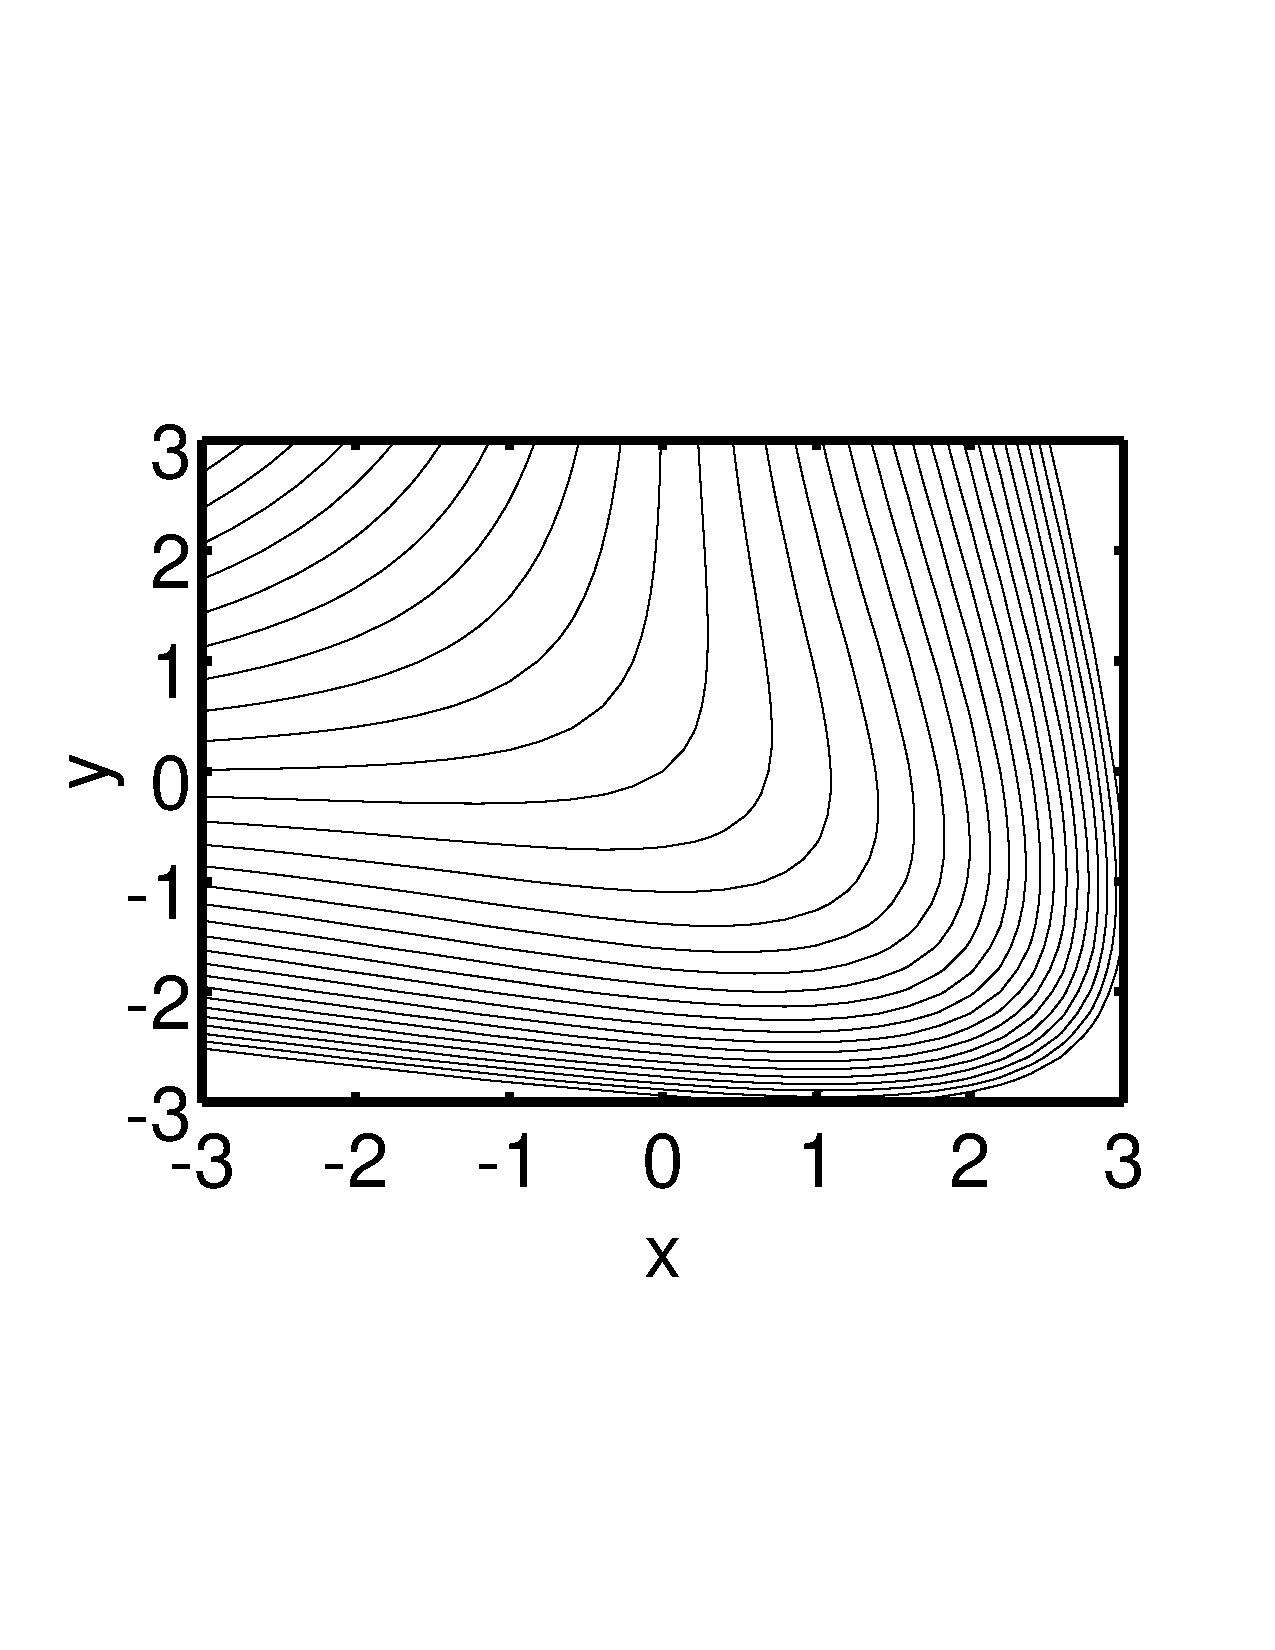
\includegraphics[height=3in]{integratingFactor}
\caption{مثال \حوالہ{مثال_سادہ_اول_جزو_تکمل_حصول}}
\label{شکل_مثال_سادہ_اول_جزو_تکمل_حصول}
\end{figure}
\انتہا{مثال}
%===========================

\حصہء{سوالات}
سوال \حوالہ{سوال_سادہ_اول_جزو_تکمل_الف} تا سوال \حوالہ{سوال_سادہ_اول_جزو_تکمل_ب} کو قطعیت کے لئے پرکھیں اور حل کریں۔غیر قطعی صورت میں دیا گیا جزو تکمل استعمال کریں یا اس کو بھی حاصل کریں۔جہاں ابتدائی معلومات دی گئی ہو، وہاں مخصوص حل حاصل کریں۔

\ابتدا{سوال}\شناخت{سوال_سادہ_اول_جزو_تکمل_الف}
\begin{align*}
2xy \dif x+x^2\dif y=0
\end{align*}
جواب:\عددی{y=\tfrac{c}{x^2}}
\انتہا{سوال} 
%===================
\ابتدا{سوال}
\begin{align*}
x^2\dif x+y\dif y=0
\end{align*}

جواب:\عددی{2x^3+3y^2=c}
\انتہا{سوال}
%============================
\ابتدا{سوال}
\begin{align*}
[\sin x+(x+y^3)\cos x]\dif x+3y^2\sin x \dif y=0
\end{align*}

جواب:\عددی{\sin x (x+y^3)}
\انتہا{سوال}
%===========================
\ابتدا{سوال}
\begin{align*}
(y+1)\dif x+(x+1)\dif y=0
\end{align*}

جواب:\عددی{x+xy+y=c}
\انتہا{سوال}
%=============================
\ابتدا{سوال}
\begin{align*}
(e^y+ye^x+y)\dif x+(xe^y+e^x+x)\dif y=0
\end{align*}

جواب:\عددی{xe^y+xy+ye^x}

\انتہا{سوال}
%=========================
\ابتدا{سوال}
\begin{align*}
\frac{y^2+4x}{x}\dif x+2y\dif y=0
\end{align*}

جواب:\عددی{F=x}، \عددی{u=(2x+y^2)x=c}
\انتہا{سوال}
%=============================
\ابتدا{سوال}
\begin{align*}
ye^x(2x+1+2y^2)\dif x+e^x(x+2y)\dif y=0
\end{align*}

جواب:\عددی{F=e^x}، \عددی{ye^{2x}(x+y)=c}
\انتہا{سوال}
%=============================
\ابتدا{سوال}
\begin{align*}
(2y^2+2xy+y)\dif x+(2y+x)\dif y=0
\end{align*}

جواب:\عددی{F=e^{2x}}، \عددی{e^{2x}(y^2+xy)=c}
\انتہا{سوال}
%=============================

\ابتدا{سوال}
\begin{align*}
y\dif x+(2xy-e^{-2y})\dif x=0, \quad y(1)=1
\end{align*}

جواب:\عددی{F=\tfrac{e^{2y}}{y}}، \عددی{xe^{2y}-\ln y=e^2}
\انتہا{سوال}
%==============
\ابتدا{سوال}
\begin{align*}
3(y+1)\dif x=2x\dif y,\quad y(1)=3,\quad F=\frac{y+1}{x^4}
\end{align*}

جواب:\عددی{y+1=4x^{\tfrac{3}{2}}}
\انتہا{سوال}
%=================
\ابتدا{سوال}
\begin{align*}
y\dif x+[y+\tan(x+y)]\dif y=0,\quad y(0)=\tfrac{\pi}{2},\quad F=\cos(x+y)
\end{align*}

جواب:\عددی{y\sin(x+y)=\tfrac{\pi}{2}}
\انتہا{سوال}
%=================
\ابتدا{سوال}\شناخت{سوال_سادہ_اول_جزو_تکمل_ب}
\begin{align*}
(a+1)y\dif x+(b+1)x \dif y=0,\quad y(1)=1, \quad F=x^ay^b
\end{align*}

جواب:\عددی{x^{a+1}y^{b+1}=0}
\انتہا{سوال}
%====================
\ابتدا{سوال}
جزو تکمل کو مزید بہتر سمجھنے کی خاطر  کسی بھی تفاعل مثلاً \عددی{u=e^{2x}(y^2+xy)=c} کے مکمل تفرق کو \عددی{M\dif +N\dif y=0} صورت میں لکھیں یعنی
 \عددی{e^{2x} (2y^2+2xy+y)\dif x+e^{2x}(2y+x)\dif y=0} جو قطعی مساوات ہے۔تفرقی مساوات کو \عددی{e^{2x}} سے تقسیم کرنے سے غیر قطعی مساوات 
\عددی{(2y^2+2xy+y)\dif x+(2y+x)\dif y=0} ملتا ہے۔۔اس غیر قطعی مساوات کو \عددی{e^{2x}} سے ضرب دیتے ہوئے قطعی بنایا جا سکتا ہے لہٰذا \عددی{e^{2x}} اس غیر قطعی مساوات کا جزو تکمل ہے۔
\انتہا{سوال}
%======================

\حصہ{خطی سادہ تفرقی مساوات۔ مساوات برنولی}
ایسے سادہ درجہ اول تفرقی مساوات جنہیں درج ذیل صورت میں لکھنا ممکن ہو \اصطلاح{خطی}\فرہنگ{خطی!سادہ تفرقی مساوات}\حاشیہب{linear}\فرہنگ{linear!ordinary differential equations} کہلاتے ہیں
\begin{align}\label{مساوات_سادہ_اول_خطی}
y'+p(x)y=r(x)
\end{align}
جبکہ ایسے مساوات جنہیں الجبرائی ترتیب دیتے ہوئے درج بالا صورت میں لکھنا ممکن نہ ہو \اصطلاح{غیر خطی} کہلاتے ہیں۔

خطی مساوات \حوالہ{مساوات_سادہ_اول_خطی} کی بنیادی خاصیت یہ ہے کہ اس میں تابع متغیرہ \عددی{y} اور تابع متغیرہ کا تفرق \عددی{y'} دونوں خطی ہیں جبکہ \عددی{p(x)} اور \عددی{r(x)} غیر تابع متغیرہ \عددی{x} کے \موٹا{کوئی} بھی تفاعل ہو سکتے ہیں۔اگر غیر تابع متغیرہ وقت ہو تب \عددی{x} کی جگہ \عددی{t} لکھا جاتا ہے۔

مساوات \حوالہ{مساوات_سادہ_اول_خطی} خطی مساوات کی معیاری صورت ہے جس کے پہلے رکن \عددی{y'} کا جزو ضربی اکائی ہے۔ایسی مساوات جس میں \عددی{y'} کی بجائے \عددی{f(x)y'} پایا جاتا ہو کو \عددی{f(x)} سے تقسیم کرتے ہوئے، اس کی معیاری صورت حاصل کی جا سکتی ہے۔ یوں خطی مساوات 
\عددی{(x+\sqrt{x})y'+y\sec x=e^x} کو \عددی{(x+\sqrt{x})} سے تقسیم کرتے ہوئے  اسے معیاری صورت \عددی{y'+\tfrac{\sec x}{x+\sqrt{x}}y=\tfrac{e^x}{x+\sqrt{x}}} میں لکھا جا سکتا ہے۔

دائیں ہاتھ \عددی{r(x)} \اصطلاح{قوت}\فرہنگ{قوت}\حاشیہب{force}\فرہنگ{force} کو ظاہر کر سکتی ہے جبکہ مساوات کا حل \عددی{y(x)} \اصطلاح{ہٹاو}\فرہنگ{ہٹاو}\حاشیہب{displacement}\فرہنگ{displacement} ہو سکتا ہے۔اسی طرح \عددی{r(x)} \اصطلاح{برقی دباو}\فرہنگ{برقی دباو}\حاشیہب{voltage}\فرہنگ{voltage} ہو سکتا ہے جبکہ \عددی{y(x)} \اصطلاح{برقی رو}\فرہنگ{برقی رو}\حاشیہب{current}\فرہنگ{current} ہو سکتی ہے۔ انجینئری میں \عددی{r(x)} کو عموماً \اصطلاح{درآیدہ}\فرہنگ{درآیدہ}\حاشیہب{input}\فرہنگ{input} یا \اصطلاح{جبری تفاعل}\فرہنگ{جبری تفاعل}\حاشیہب{forcing function}\فرہنگ{forcing function} کہتے ہیں جبکہ \عددی{y(x)} کو \اصطلاح{ماحصل}\فرہنگ{ماحصل}\حاشیہب{output}\فرہنگ{output} یا \اصطلاح{رد عمل}\فرہنگ{رد عمل}\حاشیہب{response}\فرہنگ{response} کہتے ہیں۔  
%================================

\جزوحصہء{متجانس خطی سادہ تفرقی مساوات}\شناخت{حصہ_سادہ_اول_متجانس_خطی}
ہم مساوات \حوالہ{مساوات_سادہ_اول_خطی} کو خطہ \عددی{a<x<b} میں حل کرنا چاہتے ہیں۔اس خطے کو \عددی{J} کہا جائے گا۔پہلے اس مساوات کی سادہ صورت حل کرتے ہیں جس میں \عددی{J} پر  تمام \عددی{x} کے لئے \عددی{r(x)} صفر کے برابر ہو۔ (اس کو بعض اوقات \عددی{r(x)\equiv 0} لکھا جاتا ہے۔) ایسی صورت میں مساوات \حوالہ{مساوات_سادہ_اول_خطی} درج ذیل صورت اختیار کرے گی 
\begin{align}\label{مساوات_سادہ_اول_ہم_جنسی_خطی_الف}
y'+p(x)y=0
\end{align}
جس کو \اصطلاح{متجانس}\فرہنگ{متجانس}\حاشیہب{homogeneous}\فرہنگ{homogeneous!linear ordinary differential equation} مساوات کہتے ہیں۔متغیرات علیحدہ کرتے ہوئے حل کرتے ہیں۔
\begin{align*}
\frac{\dif y}{y}=-\=p(x)\dif x,\quad \ln \abs{y}=-\int p(x) \dif x+c_1
\end{align*}
دونوں اطراف کا قوت نمائی لیتے ہوئے متجانس خطی مساوات \حوالہ{مساوات_سادہ_اول_ہم_جنسی_خطی_الف} کا حل حاصل ہوتا ہے۔
\begin{align}\label{مساوات_سادہ_اول_متجانس_حل_الف}
y(x)=ce^{-\int p(x)\dif x},\quad (c=\mp e^{c_1}\quad  \text{جب} \quad  y \lessgtr 0)
\end{align} 
یہاں \عددی{c=0} بھی چننا جا سکتا ہے جو \اصطلاح{غیر اہم حل}\فرہنگ{غیر اہم حل}\فرہنگ{حل!غیر اہم}\حاشیہب{trivial solution}\فرہنگ{trivial solution}\فرہنگ{solution!trivial} (یعنی \اصطلاح{صفر حل}) \عددی{y(x)=0} دیتا ہے۔
%====================

\جزوحصہء{غیر متجانس خطی سادہ تفرقی مساوات}
اب مساوات \حوالہ{مساوات_سادہ_اول_خطی} کو اس صورت میں حل کرتے ہیں جب \عددی{r(x) \not \equiv 0} ہو یعنی \عددی{J} پر کہیں کہیں یا پورے خطے پر  \عددی{r(x)} غیر صفر ہو۔ایسی صورت میں مساوات \حوالہ{مساوات_سادہ_اول_خطی} \اصطلاح{غیر متجانس}\فرہنگ{غیر متجانس}\حاشیہب{heterogeneous}\فرہنگ{heterogeneous} کہلاتا ہے۔غیر متجانس مساوات کی خوشگوار خاصیت یہ ہے کہ اس کا جزو تکمل \عددی{F(x)} صرف \عددی{x} پر منحصر ہوتا ہے لہٰذا اس کو مسئلہ \حوالہ{مسئلہ_سادہ_اول_جزو_تکمل_الف} کی مدد سے حاصل کیا جا سکتا ہے۔جزو تکمل کو حاصل کرتے ہیں۔غیر قطعی مساوات \حوالہ{مساوات_سادہ_اول_خطی} کو ترتیب دے کر \عددی{F} سے ضرب دیتے ہوئے قطعی مساوات حاصل کرتے ہیں
\begin{align*}
(py-r)\dif x+\dif y&=0,\quad F(py-r)\dif x+F\dif y=0
\end{align*}
جس سے مساوات \حوالہ{مساوات_سادہ_اول_قطعی_تفرقی_شرط} کی مدد سے درج ذیل ملتا ہے۔
\begin{align*}
\frac{\partial}{\partial y} [F(py-r)]=\frac{\partial F}{\partial x}\quad  \text{یعنی} \quad Fp=\frac{\partial F}{\partial x}
\end{align*}
متغیرات علیحدہ کرتے ہوئے تکمل لیتے ہوئے \عددی{F} حاصل کرتے ہیں۔
\begin{align*}
\frac{\dif F}{F}=p\dif x, \quad \ln \abs{F}=h(x)=\int p(x)\dif x \quad  \text{لہٰذا}\quad  F=e^h
\end{align*}
مساوات \حوالہ{مساوات_سادہ_اول_خطی} کو جزو تکمل \عددی{F} سے ضرب دیتے  اور \عددی{\tfrac{\dif h}{\dif x}=p} لکھتے ہوئے درج ذیل ملتا ہے
\begin{align*}
e^h y'+e^h h' y=e^h r \quad \text{یعنی}\quad  \left(e^h y\right)'=e^h r
\end{align*}
جس کا تکمل لیتے ہیں۔
\begin{align*}
e^h y=\int e^h r \dif x+c
\end{align*}
دونوں اطراف کو \عددی{e^h} سے تقسیم کرتے ہوئے غیر متجانس مساوات \حوالہ{مساوات_سادہ_اول_خطی} کا حل ملتا ہے۔
\begin{align}\label{مساوات_سادہ_اول_متجانس_خطی_حل_الف}
y=e^{-h}\left(\int e^h r \dif x+c\right), \quad h=\int p(x)\dif x
\end{align}
یوں مساوات \حوالہ{مساوات_سادہ_اول_خطی} کا حل درج بالا تکمل سے حاصل کیا جا سکتا ہے جو نسبتاً آسان ثابت ہوتا ہے۔اگر درج بالا تکمل بھی مشکل ثابت ہو تب تفرقی مساوات کا حل اعدادی ترکیب سے حاصل کیا جا سکتا ہے۔یہاں بتلاتا چلوں (سوال \حوالہ{سوال_سادہ_اول_برنولی_الف} دیکھیں) کہ \عددی{h} کے حصول میں تکمل کا مستقل کوئی کردار ادا نہیں کرتا لہٰذا اسے  صفر تصور کیا جاتا ہے۔

مساوات \حوالہ{مساوات_سادہ_اول_متجانس_خطی_حل_الف} کا تکمل درآیدہ \عددی{r(x)} پر منحصر ہے جبکہ ابتدائی معلومات تکمل کا مستقل \عددی{c} تعین کرتی ہیں۔اس مساوات کو درج ذیل لکھتے ہوئے 
\begin{align}\label{مساوات_سادہ_اول_متجانس_خطی_حل_ب}
y=e^{-h}\int e^h r \dif x+ce^{-h}
\end{align}
ہم دیکھتے ہیں کہ
\begin{align}
\text{کل ماحصل}=\text{درآیدہ سے پیدا رد عمل}+\text{ابتدائی معلومات سے پیدا رد عمل}
\end{align}

%=========================

\ابتدا{مثال}
ابتدائی قیمت تفرقی مساوات کو حل کریں۔
\begin{align*}
y'+y\cot x=2x\cosec x,\quad y\left(\frac{\pi}{2}\right)=0
\end{align*}

حل:یہاں \عددی{p=\cot x} اور \عددی{r=\cosec x} ہیں۔
\begin{align*}
h(x)=\int \cot x \dif x=\ln \abs{\sin x}
\end{align*}
یوں مساوات \حوالہ{مساوات_سادہ_اول_متجانس_خطی_حل_الف} میں
\begin{align*}
e^h=\sin x, \quad e^{-h}=\cosec x, \quad e^h r= (\sin x) (2x\cosec x)=2x
\end{align*}
ہیں لہٰذا عمومی حل
\begin{align*}
y=\cosec x \left(\int 2x\dif x +c\right)=\cosec x (x^2+c)
\end{align*}
ہو گا۔ابتدائی معلومات پر کرتے ہوئے  \عددی{c=-\tfrac{\pi^2}{4}} ملتا ہے لہٰذا مخصوص حل درج ذیل ہے
\begin{align*}
y=\cosec x \left(x^2-\frac{\pi^2}{4}\right)
\end{align*}
جس میں \عددی{x^2\cosec x} درآیدہ کا پیدا کردہ رد عمل ہے جبکہ \عددی{-\tfrac{\pi^2}{4}\cosec x} ابتدائی معلومات کا پیدا کردہ رد عمل ہے۔
\انتہا{مثال}
%==========================
\ابتدا{مثال}\شناخت{مثال_سادہ_اول_برقی_دور_الف} \quad برقی دور\\
شکل \حوالہ{شکل_مثال_سادہ_اول_برقی_دور_الف} میں \اصطلاح{مزاحمت}\فرہنگ{مزاحمت}\حاشیہب{resistance}\فرہنگ{resistance} \عددی{R} اور \اصطلاح{امالہ}\فرہنگ{امالہ}\حاشیہب{inductor}\فرہنگ{inductor} \عددی{L} سلسلہ وار جڑے ہیں۔اس دور کو \اصطلاح{سلسلہ وار}\فرہنگ{سلسلہ وار دور}\حاشیہب{series circuit}\فرہنگ{series circuit} \عددی{RL} دور کہتے ہیں۔لمحہ \عددی{t=0} پر \اصطلاح{برقی دباو}\فرہنگ{برقی دباو}\حاشیہب{electric voltage}\فرہنگ{voltage} \عددی{E} برقی دور پر لاگو کیا جاتا ہے جو دور میں \اصطلاح{برقی رو}\فرہنگ{برقی رو}\حاشیہب{electric current}\فرہنگ{current} \عددی{I(t)} کو جنم دیتا ہے۔ابتدائی رو صفر \عددیء{I(0)=0} کے برابر ہے۔

طبعی معلومات: مزاحمت کی اکائی \اصطلاح{اوہم}\فرہنگ{اوہم}\حاشیہب{Ohm}\فرہنگ{Ohm} \عددی{\si{\ohm}}  اور امالہ کی اکائی \اصطلاح{ہینری}\فرہنگ{ہینری}\حاشیہب{Henry}\فرہنگ{Henry} \عددی{\si{\henry}} ہے۔\اصطلاح{قانون اوہم}\فرہنگ{قانون اوہم}\حاشیہب{Ohm's law}\فرہنگ{Ohm's law} کے تحت مزاحمت \عددی{R} میں رو \عددی{I} اور دباو \عددی{v_R} کا تعلق \عددی{v_R=IR} ہے۔اسی طرح امالہ میں رو اور دباو \عددی{v_L} کا تعلق \عددی{v_L=L\tfrac{\dif I}{\dif t}} ہے۔ \اصطلاح{کرخوف قانون دباو}\فرہنگ{کرخوف!قانون دباو}\حاشیہب{Kirchoff's voltage law}\فرہنگ{Kirchoff's law!voltage} کے تحت ان برقی دباو کا مجموعہ درآیدہ دباو \عددی{E} کے برابر ہو گا۔ 
\begin{figure}
\centering
\begin{subfigure}{0.5\textwidth}
\centering
\begin{tikzpicture}[american voltages]
\draw(0,0) to [american voltage source,l={$\substack{\displaystyle E \hfill \\ \displaystyle \SI{50}{\volt}}$}]++(0,\yy) to [resistor,l={$\substack{\displaystyle R\hfill \\ \displaystyle \SI{100}{\ohm}}$},i={$I(t)$},v={$v_R$}]++(\xx,0) to [inductor,l_={$\substack{\displaystyle L \hfill \\ \displaystyle \SI{0.5}{\henry}}$},v^<={$v_L$}]++(0,-\yy) to [short]++(-\xx,0);
\end{tikzpicture}
\caption*{(الف)}
\end{subfigure}%
\begin{subfigure}{0.5\textwidth}
\centering
\begin{tikzpicture}
\begin{axis}[small,axis lines*=middle,xlabel={$t$},ylabel={$I(t)$},xtick={0.01,0.02,0.03},xticklabels={$0.01$,$0.02$,$0.03$},ytick={0,0.25,0.5,0.75},yticklabels={$0$,$0.25$,$\frac{E}{R}$,$0.75$},ylabel style={rotate=-90},ylabel style={at={(axis description cs:0,1.05)}},scaled x ticks=false,scaled y ticks=false]
\addplot[thick,domain=0:0.035]{50/100*(1-e^(-200*x))};
\addplot[domain=0:0.035]{0.5-0.25*e^(-200*x)};
\addplot[domain=0:0.035]{0.5+0.25*e^(-200*x)};
\end{axis}
\end{tikzpicture}
\caption*{(ب)}
\end{subfigure}%
\caption{مثال \حوالہ{مثال_سادہ_اول_برقی_دور_الف} کا سلسلہ وار برقی دور۔}
\label{شکل_مثال_سادہ_اول_برقی_دور_الف}
\end{figure}


حل:یہاں غیر تابع متغیرہ وقت \عددی{t} ہے جبکہ تابع متغیرہ رو \عددی{I(t)} ہے۔ کرخوف کے قانون کے تحت 
\begin{align*}
v_L+v_R=E, \quad L I'+RI=E, \quad I'+\frac{R}{L}I=\frac{E}{L}
\end{align*}
لکھا جائے گا جہاں آخری قدم پر \عددی{L} سے تقسیم کرتے ہوئے مساوات کو معیاری صورت میں لکھا گیا ہے۔اس کو مساوات \حوالہ{مساوات_سادہ_اول_متجانس_خطی_حل_الف} کی مدد سے حل کرتے ہیں جہاں \عددی{x} کی جگہ \عددی{t} اور \عددی{y} کی جگہ \عددی{I} استعمال ہو گا۔یہاں \عددی{p=\tfrac{R}{L}} اور \عددی{r=\tfrac{E}{L}} ہیں لہٰذا \عددی{h=\tfrac{R}{L}t} ہو گا اور عمومی حل
\begin{align*}
I=e^{-\frac{R}{L}t}\left(\int e^{\frac{R}{L}t}  \frac{E}{L} \dif x+c\right)
\end{align*}
لکھا جائے گا۔تکمل لیتے ہوئے درج ذیل ملتا ہے۔
\begin{align}\label{مساوات_سادہ_اول_برقی_مزاحمت_امالہ_سلسلہ_وار}
I=e^{-\frac{R}{L}t}\left(\frac{E}{L} \frac{e^{\frac{R}{L}}t}{\frac{R}{L}}+c\right)=\frac{E}{R}+ce^{-\frac{R}{L}t}
\end{align}
شکل \حوالہ{شکل_مثال_سادہ_اول_برقی_دور_الف}-الف میں پرزوں کی قیمتیں دی گئی ہیں جن سے \عددی{\tfrac{E}{R}=\tfrac{50}{100}=0.5} اور
 \عددی{\tfrac{R}{L}=\tfrac{100}{0.5}=200} ملتا ہے لہٰذا عمومی حل کو درج ذیل لکھا جا سکتا ہے۔
\begin{align}
I=0.5+ce^{-200t}
\end{align} 
مساوات \حوالہ{مساوات_سادہ_اول_برقی_مزاحمت_امالہ_سلسلہ_وار} میں ابتدائی معلومات پر کرتے ہوئے \عددی{c} کی قیمت حاصل ہوتی ہے۔ اس مساوات میں \عددی{ce^{-\tfrac{R}{L}t}} جزو \عددی{t \to \infty} پر صفر کے برابر ہو گا لہٰذا کافی دیر بعد رو پہلے جزو \عددی{\tfrac{E}{R}} کے برابر ہو گی جسے رو کی \اصطلاح{برقرار حال}\فرہنگ{برقرار حال}\حاشیہب{steady state}\فرہنگ{steady state} قیمت کہتے ہیں۔یہ ایک اہم نتیجہ ہے جس کے  تحت کافی دیر بعد رو کی قیمت کا دارومدار ابتدائی معلومات پر منحصر نہیں ہے۔رو کتنی جلدی برقرار حال قیمت اختیار کرتی ہے، اس کا دارومدار \عددی{\tfrac{R}{L}} کی قیمت پر ہے۔

مساوات \حوالہ{مساوات_سادہ_اول_برقی_مزاحمت_امالہ_سلسلہ_وار} میں ابتدائی معلومات \عددی{I(0)=0} پر کرتے  \عددی{0=0.5+ce^0} ہوئے \عددی{c=-0.5} ملتا ہے لہٰذا مخصوص حل درج ذیل ہو گا جس کو شکل \حوالہ{شکل_مثال_سادہ_اول_برقی_دور_الف}-ب میں موٹی لکیر سے دکھایا گیا ہے۔شکل میں ابتدائی قیمت \عددی{I(0)=0.25} اور \عددی{I(0)=0.75} سے حاصل مخصوص حل بھی دکھائے گئے ہیں۔
\begin{align}
I(t)=0.5(1-e^{-200t})
\end{align}
\انتہا{مثال}
%==========================
\ابتدا{مثال}\شناخت{مثال_سادہ_اول_غدود_درقیہ}\quad جسم میں ہارمونز کی مقدار\\
جسم میں موجود \اصطلاح{غدود}\فرہنگ{غدود}\حاشیہب{gland}\فرہنگ{gland} یعنی  \اصطلاح{گلٹی}\فرہنگ{گلٹی}، خون میں مختلف مرکبات\اصطلاح{(ہارمونز)}\فرہنگ{ہارمونز}\حاشیہب{hormones}\فرہنگ{hormones} خارج کرتے ہوئے مختلف نظام کو قابو کرتے ہیں۔تصور کریں کہ خون سے ایک مخصوص ہارمون مسلسل ہٹایا جاتا ہے۔ہٹانے کی شرح اس لمحے موجود ہارمون کی مقدار کے راست تناسب ہے۔ساتھ ہی ساتھ تصور کریں کہ روزانہ غدود اس ہارمون کو خون میں ایک مخصوص انداز سے خارج کرتی ہے۔خون میں موجود ہارمون کی نمونہ کشی کرتے ہوئے تفرقی مساوات کا عمومی حل حاصل کریں۔صبح چھ بجے خون میں ہارمون کی مقدار \عددی{y_0} لیتے ہوئے مخصوص حل حاصل کریں۔  

حل:پہلا قدم: نمونہ کشی:\quad چوبیس گھنٹوں میں خارج ہونے کے عمل کو \عددی{a+b\sin (\tfrac{2\pi t}{24})} سے ظاہر کرتے ہیں۔چونکہ خون میں ہارمون خارج ہونے سے خون میں ہارمون کی مقدار بڑھتی ہے لہٰذا \عددی{a\ge b} ہو گا۔یوں خارج کردہ ہارمون کی مقدار مثبت ہو گی۔کسی بھی لمحے خون میں ہارمون کی مقدار کی تبدیلی کی شرح، اس لمحے خون میں ہارمون کے داخل ہونے کی مقدار اور اس کی ہٹائی جانے والی مقدار میں فرق کے برابر ہو گا۔یوں مسئلے کا تفرقی مساوات درج ذیل ہو گا۔
\begin{align}
\frac{\dif y(t)}{\dif t}=a+b\sin\left(\frac{2\pi t}{24}\right)-k y(t) \quad \text{یعنی}\quad y'-ky=a+b\sin \omega t,\quad \omega =\frac{2\pi}{24}
\end{align}
دوسرا قدم: عمومی حل:\quad یہاں \عددی{p=k} ہے لہٰذا \عددی{h=\int k\dif t=kt} ہو گا۔اسی طرح \عددی{r=a+b\sin \omega t} ہے لہٰذا مساوات \حوالہ{مساوات_سادہ_اول_متجانس_خطی_حل_الف} سے عمومی حل درج ذیل ہو گا جس کو \اصطلاح{تکمل بالحصص}\فرہنگ{تکمل!بالحصص}\حاشیہب{integration by parts}\فرہنگ{integration!by parts} حل کیا گیا ہے
\begin{align*}
y&=e^{-kt}\int e^{kt} (a+b\sin \omega t) \dif t+ce^{-kt}\\
&=e{-kt}e^{kt}\left[\frac{a}{k}+\frac{b}{k^2+\omega^2}(k\cos \omega t+\omega \sin \omega t)\right]+ce^{-kt}\\
&=\frac{a}{k}+\frac{b}{k^2+\omega^2}(k\cos \omega t+\omega \sin \omega t)+ce^{-kt}
\end{align*}
عمومی حل کا آخری جزو وقت بڑھنے سے آخر کار صفر ہو جاتا ہے۔یوں \اصطلاح{برقرار حل}\فرہنگ{برقرار حل}\حاشیہب{steady state response}\فرہنگ{steady state response} بقایا اجزاء پر مشتمل ہے۔

آخر قدم:مخصوص حل:\quad صبح چھ بجے کو لمحہ \عددی{t=0} تصور کرتے ہوئے ابتدائی معلومات کو \عددی{y(0)=y_0} لکھا جا سکتا ہے۔ان قیمتوں کو عمومی حل میں پر کرتے ہوئے \عددی{c} کی قیمت حاصل کرتے ہیں۔
\begin{align*}
y_0 &=\frac{a}{k}+\frac{b}{k^2+\omega^2}(k\cos 0+\omega \sin 0)+ce^{0}, \quad \text{یعنی}\quad c=y_0-\frac{a}{k}-\frac{bk}{k^2+\omega^2}
\end{align*}
اس طرح مخصوص حل درج ذیل ہو گا۔مخصوص حل کو \عددی{a=1}، \عددی{b=1}، \عددی{k=0.04} اور \عددی{y_0=0} لیتے ہوئے  جسے شکل \حوالہ{شکل_مثال_سادہ_اول_غدود_درقیہ} میں دکھایا گیا ہے۔ شکل-ب میں \عددی{y_0=50} لیا گیا ہے۔آپ دیکھ سکتے ہیں کہ خون میں ہارمون کی مقدار بہت جلد ایک مخصوص اوسط قیمت پر پہنچ پاتی ہے۔
\begin{align*}
y=\frac{a}{k}+\frac{b}{k^2+\omega^2}(k\cos \omega t+\omega \sin \omega t)+(y_0-\frac{a}{k}-\frac{bk}{k^2+\omega^2})e^{-kt}
\end{align*}
%
\begin{figure}
\centering
\begin{subfigure}{0.5\textwidth}
\centering
\begin{tikzpicture}
\pgfmathsetmacro{\a}{2*pi/24}
\pgfmathsetmacro{\b}{2*pi/24}
\pgfmathsetmacro{\w}{2*pi/24}
\pgfmathsetmacro{\wa}{360/24}
\pgfmathsetmacro{\k}{0.04}
\pgfmathsetmacro{\ya}{0}
\begin{axis}[small,axis lines*=middle,ymin=0,ymax=55,xmin=0,xlabel={$t$},ylabel={$y(t)$},ylabel style={rotate=-90},ylabel style={at={(axis description cs:0,1.05)}}]
\addplot[domain=0:300,samples=400]{1/\k+(\k*cos(\wa*x)+\w*sin(\wa*x))/(\k^2+\w^2)+(\ya-1/\k-\k/(\k^2+\w^2))*e^(-\k*x)};
\end{axis}
\end{tikzpicture}
\caption*{(الف)}
\end{subfigure}%
\begin{subfigure}{0.5\textwidth}
\centering
\begin{tikzpicture}
\pgfmathsetmacro{\w}{2*pi/24}
\pgfmathsetmacro{\wa}{360/24}
\pgfmathsetmacro{\k}{0.04}
\pgfmathsetmacro{\ya}{50}
\begin{axis}[small,axis lines*=middle,ymin=0,ymax=55,xmin=0,xlabel={$t$},ylabel={$y(t)$},ylabel style={rotate=-90},ylabel style={at={(axis description cs:0,1.05)}}]
\addplot[domain=0:300,samples=400]{1/\k+(\k*cos(\wa*x)+\w*sin(\wa*x))/(\k^2+\w^2)+(\ya-1/\k-\k/(\k^2+\w^2))*e^(-\k*x)};
\end{axis}
\end{tikzpicture}
\caption*{(ب)}
\end{subfigure}%
\caption{مثال \حوالہ{مثال_سادہ_اول_غدود_درقیہ}: خون میں ہارمون کی مقدار بالمقابل وقت۔}
\label{شکل_مثال_سادہ_اول_غدود_درقیہ}
\end{figure}
\انتہا{مثال}
%=============================

\جزوحصہء{حصول خطی مساوات بذریعہ تخفیف۔ برنولی مساوات}
ایسے بہت سارے نظام ہیں جن کے غیر خطی سادہ تفرقی مساوات کو خطی بنایا جا سکتا ہے۔ان میں \اصطلاح{برنولی مساوات}\فرہنگ{برنولی مساوات}\حاشیہب{Bernoulli equation}\فرہنگ{Bernoulli!equation} 
\begin{align}\label{مساوات_سادہ_اول_برنولی_الف}
y'+p(x)y=g(x)y^a,\quad \text{\RL{$a$\, حقیقی عدد ہے}}
\end{align}
انتہائی اہم\حاشیہد{یعقوب برنولی (1654-1705): سوئزرلینڈ کے برنولی خاندان نے دنیا کو کئی اہم ریاضی داں دیے۔ یعقوب برنولی ان میں سر فہرست ہے۔انہوں نے علم الامکانیات میں بہت کام کیا۔قوت نمائی کا مستقل \عددی{e} بھی انہوں نے دریافت کیا۔} ہے۔برنولی مساوات \عددی{a=0} اور \عددی{a=1} کی صورت میں خطی ہے۔ اس کے علاوہ یہ غیر خطی ہے۔آئیں اس کو تبدیل کرتے ہوئے خطی مساوات حاصل کریں۔ہم
\begin{align*}
u(x)=[y(x)]^{1-a}
\end{align*}
کا تفرق لیتے ہوئے اس میں مساوات \حوالہ{مساوات_سادہ_اول_برنولی_الف} سے \عددی{y'} پر کرتے  ہوئے ترتیب دیتے ہیں۔
\begin{align*}
u'&=(1-a)y^{-a}y'\\
&=(1-a)y^{-a}(gy^a-py)\\
&=(1-a)g-(1-a)py^{1-a}\\
&=(1-a)g-(1-a)pu
\end{align*} 
یوں خطی سادہ تفرقی مساوات 
\begin{align}
u+(1-a)u'=(1-a)g
\end{align}
حاصل ہوتی ہے۔
%=============================

\ابتدا{مثال}\شناخت{مثال_سادہ_اول_نمو_آبادی}\quad ورہلسٹ مساوات برائے نمو آبادی
درج ذیل برنولی مساوات کو \اصطلاح{ورہلسٹ}\فرہنگ{ورہلسٹ}\حاشیہب{Pierre Francois Verhulst}\فرہنگ{Verhulst equation} مساوات کہتے ہیں جو \اصطلاح{نمو آبادی}\فرہنگ{نمو آبادی}\حاشیہب{population growth}\فرہنگ{population growth} کی تفرقی مساوات ہے۔اس کو حل کریں۔ (سوال \حوالہ{سوال_سادہ_اول_وبا} کو بھی دیکھیں۔)
\begin{align}\label{مساوات_سادہ_اول_ورہلسٹ_آبادی_نمو_الف}
y'=ay-by^2
\end{align}

حل:اس کو مساوات \حوالہ{مساوات_سادہ_اول_برنولی_الف} کی صورت \عددی{y'-ay=-by^2} میں لکھ کر \عددی{a=2} ملتا ہے۔یوں ہم \عددی{u=y^{1-a}=y^{-1}} کے تفرق میں مساوات \حوالہ{مساوات_سادہ_اول_ورہلسٹ_آبادی_نمو_الف} سے \عددی{y'}  پر کرتے ہیں
\begin{align*}
u'=-y^{-2}y'=-y^{-2}(ay-by^2)=-ay^{-1}+b=-ua+b
\end{align*}
جس سے خطی سادہ تفرقی مساوات
\begin{align*}
u'+au=b
\end{align*}
حاصل ہوتا ہے۔ مساوات \حوالہ{مساوات_سادہ_اول_متجانس_خطی_حل_الف} سے عمومی حل لکھتے ہیں۔
\begin{align*}
u=\frac{b}{a}+ce^{-at}
\end{align*}
چونکہ \عددی{u=y^{-1}} ہے لہٰذا اس سے درج ذیل ملتا ہے جس کو شکل \حوالہ{شکل_مثال_سادہ_اول_نمو_آبادی} میں دکھایا گیا ہے۔
\begin{align}\label{مساوات_سادہ_اول_نمو_آبادی}
y=\frac{1}{u}=\frac{1}{\frac{b}{a}+ce^{-at}}
\end{align}
مساوات \حوالہ{مساوات_سادہ_اول_ورہلسٹ_آبادی_نمو_الف} کو دیکھ کر \عددی{y(t)=0} حل بھی لکھا جا سکتا ہے۔ 
\begin{figure}
\centering
\begin{tikzpicture}
\pgfmathsetmacro{\a}{3}
\pgfmathsetmacro{\b}{1}
\pgfmathsetmacro{\ca}{100*\b/\a}
\pgfmathsetmacro{\caa}{1*\b/\a}
\pgfmathsetmacro{\cb}{-0.25*\b/\a}
\pgfmathsetmacro{\cc}{-0.375*\b/\a}
\pgfmathsetmacro{\cd}{-0.5*\b/\a}
\pgfmathsetmacro{\ce}{0*\b/\a}
\begin{axis}[small,axis lines*=middle,xmin=0,ymin=0,xlabel={$t$},ylabel={$y$},ylabel style={rotate=-90},ylabel style={at={(axis description cs:0,1.05)}},ytick={2,3,4,6},yticklabels={$2$,$\frac{a}{b}=3$,$4$,$6$}]
\addplot[domain=0:4,samples=50]{(\b/\a+\ca*e^(-\a*x))^(-1)};
\addplot[domain=0:4,samples=50]{(\b/\a+\caa*e^(-\a*x))^(-1)};
\addplot[domain=0:4,samples=50]{(\b/\a+\cb*e^(-\a*x))^(-1)};
\addplot[domain=0:4,samples=50]{(\b/\a+\cc*e^(-\a*x))^(-1)};
\addplot[domain=0:4,samples=50]{(\b/\a+\cd*e^(-\a*x))^(-1)};
\addplot[domain=0:4,samples=50]{(\b/\a+\ce*e^(-\a*x))^(-1)};
\end{axis}
\end{tikzpicture}
\caption{مثال \حوالہ{مثال_سادہ_اول_نمو_آبادی}: نمو آبادی کا خط۔}
\label{شکل_مثال_سادہ_اول_نمو_آبادی}
\end{figure}
\انتہا{مثال}
%===============================
\ابتدا{مثال}\شناخت{مثال_سادہ_درجہ_اول_متغیرات_بدلنے_کا_طریقہ}\quad مقدار معلوم بدلنے کا طریقہ\\
مساوات \حوالہ{مساوات_سادہ_اول_متجانس_خطی_حل_الف} کو ایک دلچسپ ترکیب سے حاصل کیا جا سکتا ہے جسے \اصطلاح{مقدار معلوم بدلنے کا طریقہ}\فرہنگ{مقدار معلوم!بدلنے کا طریقہ}\حاشیہب{variation of parameter}\فرہنگ{variation of parameter} کہتے ہیں۔متجانس مساوات \عددی{y'+p(x)y=0} کا  حل \عددی{y_1=ce^{-\int p(x) \dif x}} مساوات \حوالہ{مساوات_سادہ_اول_متجانس_حل_الف} دیتا ہے جس کو \عددی{y_1=ce^{-h}} لکھتے ہیں۔تصور کریں کہ غیر متجانس مساوات \عددی{y'+p(x)y=e(x)} کا حل \عددی{y_2=uy_1} لکھا جا سکتا ہے۔یوں \عددی{y_2'=u'y_1+uy_1'} ہو گا۔غیر متجانس مساوات میں \عددی{y_2} اور \عددی{y_2'} پر کرتے ہیں۔
\begin{align*}
u'y_1+uy_1'+p uy_1=r, \quad u'y_1+u(y_1'+py_1)=r,\quad u'y_1=r
\end{align*}
چونکہ \عددی{y_1}  متجانس مساوات کا حل ہے لہٰذا آخری قدم پر \عددی{y'+py=0} پر کرتے ہوئے \عددی{u'y_1=r} حاصل کیا گیا ہے۔اس سے \عددی{u} بذریعہ تکمل حاصل کرتے ہوئے \عددی{y_2} لکھتے ہیں جو مساوات \حوالہ{مساوات_سادہ_اول_متجانس_خطی_حل_الف} ہے۔  
\begin{align*}
u=\int \frac{r}{y_1}\dif x,\quad u=\int re^{h} \dif x+c, \quad \text{لہٰذا} \quad y_2=uy_1=e^{-h}\left[\int re^{h} \dif x+c\right]
\end{align*}


\انتہا{مثال}
%=============================
\جزوحصہء{نمو آبادی}
ورہلسٹ مساوات پودوں، جانوروں اور انسانی آبادی کی نمو کو ظاہر کرتی ہے۔اس مساوات  میں \عددی{b=0} پر کرنے سے  مالتھس مساوات \حوالہ{مساوات_سادہ_اول_مالتھس_الف} ملتی ہے جو آبادی کی بے روک نمو دیتی ہے۔ورہلسٹ مساوات میں جزو \عددی{-by^2}  آبادی بے قابو بڑھنے سے روکتی ہے۔ورہلسٹ مساوات کو \عددی{y'=ay(1-\tfrac{b}{a}y)} لکھ کر آپ دیکھ سکتے ہیں کہ \عددی{\tfrac{b}{a}y<1} کی صورت میں \عددی{y'>0} ہو گا اور آبادی  اس وقت تک مسلسل بڑھے گی جب تک بڑھے گی جبکہ  \عددی{\tfrac{b}{a}y<1} ہو، \عددی{\tfrac{b}{a}y>1} کی صورت میں \عددی{y'<0} ہو گا اور آبادی اس وقت تک مسلسل گھٹے گی جب تک \عددی{\tfrac{b}{a}y<1} ہو گا۔دونوں صورتوں میں عین \عددی{\tfrac{b}{a}y=1} یعنی \عددی{y=\tfrac{a}{b}} پر آبادی میں تبدیلی رک جائے گی۔شکل \حوالہ{شکل_مثال_سادہ_اول_نمو_آبادی} میں ایسا دکھایا گیا ہے۔

ورہلسٹ نمو آبادی کی مساوات میں غیر تابع متغیرہ \عددی{t} صریحاً نہیں پایا جاتا لہٰذا  یہ \اصطلاح{خود مختار}\فرہنگ{خود مختار!مساوات} مساوات ہے۔خود مختار مساوات
\begin{align}\label{مساوات_سادہ_اول_خود_مختار}
y'=f(y)
\end{align}
کے مستقل حل پائے جاتے ہیں جنہیں \اصطلاح{متوازن حل}\فرہنگ{متوازن حل}\حاشیہب{equilibrium solution}\فرہنگ{equilibrium!solution} یا \اصطلاح{متوازن نقطے}\فرہنگ{متوازن!نقطے}\حاشیہب{equilibrium points}\فرہنگ{equilibrium!points} کہا جاتا ہے۔خود مختار مساوات میں تفاعل \عددی{f(y)} کے صفر (f(y)=0) پر \عددی{y'=0} ہو گا جس کا حل \عددی{y=c} ہے جہاں \عددی{c} تکمل کا مستقل ہے۔تفاعل کے صفر کو مساوات \حوالہ{مساوات_سادہ_اول_خود_مختار} کے \اصطلاح{فاصل نقطے}\فرہنگ{فاصل نقطے}\حاشیہب{critical points}\فرہنگ{critical points} کہتے ہیں۔مساوات \حوالہ{مساوات_سادہ_اول_ورہلسٹ_آبادی_نمو_الف} کے فاصل نقطے \عددی{y=0} اور \عددی{y=\tfrac{a}{b}} ہیں۔یوں اس مساوات کے مستقل حل \عددی{y=0} اور \عددی{y=\tfrac{a}{b}} ہیں۔متوازن حل کو دو گروہ میں تقسیم کیا جاتا ہے جنہیں \اصطلاح{مستحکم}\فرہنگ{مستحکم}\حاشیہب{stable}\فرہنگ{stable} اور \اصطلاح{غیر مستحکم}\فرہنگ{غیر مستحکم}\حاشیہب{unstable}\فرہنگ{unstable} متوازن حل کہتے ہیں۔ ان کو شکل \حوالہ{شکل_مثال_سادہ_اول_نمو_آبادی} کی مدد سے سمجھا جا سکتا ہے جہاں \عددی{y=\tfrac{a}{b}=3} مستحکم حل ہے جبکہ \عددی{y=0} غیر مستحکم حل ہیں۔
%===================================



\حصہء{سوالات}
%================================
\ابتدا{سوال}\شناخت{سوال_سادہ_اول_برنولی_الف}
مساوات \حوالہ{مساوات_سادہ_اول_متجانس_خطی_حل_الف} میں \عددی{h} کے حصول میں تکمل کا مستقل صفر لیا جا سکتا ہے۔ایسا کیوں ممکن ہے؟
\انتہا{سوال}
%============================
\ابتدا{سوال}
ثابت کریں:
\begin{align*}
e^{\ln x}=x, \quad  e^{-\ln x}=\frac{1}{x}, \quad e^{-\ln \sec x}=\cos x
\end{align*}
\انتہا{سوال}
%==============================
سوال \حوالہ{سوال_سادہ_اول_برنولی_ب} تا سوال \حوالہ{سوال_سادہ_اول_برنولی_پ} کے عمومی حل تلاش کریں۔ابتدائی معلومات کی صورت میں مخصوص حل حاصل کریں اور اس کا خط کھینچیں۔

\ابتدا{سوال}\شناخت{سوال_سادہ_اول_برنولی_ب}
\begin{align*}
y'-y=2
\end{align*}

جواب:\عددی{y=ce^x-2}
\انتہا{سوال}
%==========================
\ابتدا{سوال}
\begin{align*}
y'-4y=2x
\end{align*}

جواب:\عددی{y=ce^{4x}-\tfrac{x}{2}-\tfrac{1}{8}}
\انتہا{سوال}
%===========================
\ابتدا{سوال}
\begin{align*}
y'+5y=e^{5x}, \quad y(0)=2
\end{align*}

جواب:\عددی{y=\tfrac{e^{5x}}{10}+\tfrac{19}{10}e^{-5x}}
\انتہا{سوال}
%===========================
\ابتدا{سوال}
\begin{align*}
y'+6y=4\sin 4x,\quad y\left(\frac{\pi}{8}\right)=6 
\end{align*}

جواب:\عددی{y=\tfrac{9}{13}\sin 4x-\tfrac{6}{13}\cos 4x+\tfrac{69}{13}e^{\tfrac{3\pi}{4}-6x}}
\انتہا{سوال}
%===========================
\ابتدا{سوال}
\begin{align*}
y'+2xy=2x,\quad y(0)=3
\end{align*}

جواب:\عددی{y=1+2e^{-x^2}}
\انتہا{سوال}
%===========================
\ابتدا{سوال}
\begin{align*}
xy'=2y+x^3e^x
\end{align*}

جواب:\عددی{y=x^2e^x+cx^2}
\انتہا{سوال}
%===========================
\ابتدا{سوال}
\begin{align*}
y'+y\tan x=\sin x
\end{align*}

جواب:\عددی{y=c \cos x-\cos x\ln \cos x}
\انتہا{سوال}
%===========================
\ابتدا{سوال}
\begin{align*}
y'+y\cos x=e^{-\sin x}
\end{align*}

جواب:\عددی{y=xe^{-\sin x}+ce^{-\sin x}}
\انتہا{سوال}
%===========================
\ابتدا{سوال}
\begin{align*}
\cos x y'+(4y-2)\sec x=0
\end{align*}

جواب:\عددی{y=\tfrac{1}{2}+ce^{-4\tan x}}
\انتہا{سوال}
%===========================
\ابتدا{سوال}
\begin{align*}
y'=(y-4)\tan x, \quad y(0)=3
\end{align*}

جواب:\عددی{y=4- \sec x}
\انتہا{سوال}
%============================
\ابتدا{سوال}\شناخت{سوال_سادہ_اول_برنولی_پ}
\begin{align*}
xy'+6y=5x^3, \quad y(1)=1
\end{align*}

جواب:\عددی{y=\tfrac{5}{9}x^3+\tfrac{4}{9x^6}}
\انتہا{سوال}
%===========================

سوال \حوالہ{سوال_سادہ_اول_برنولی_ت} تا سوال \حوالہ{سوال_سادہ_اول_برنولی_ٹ} میں خطی سادہ تفرقی مساوات کے خصوصیات زیر بحث لائیں جائیں گے۔انہیں خصوصیات کی بنا انہیں غیر خطی سادہ تفرقی مساوات پر فوقیت حاصل ہے جو یہ خصوصیات نہیں رکھتے۔نمونہ کشی کرتے ہوئے انہیں وجوہات کی وجہ سے خطی مساوات حاصل کرنے کی کوشش کی جاتی ہے۔ان سوالات میں آپ کو متجانس اور غیر متجانس سادہ تفرقی مساوات کے خصوصیات ثابت کرنے کو کہا گیا ہے۔



\ابتدا{سوال}\شناخت{سوال_سادہ_اول_برنولی_ت}
متجانس مساوات \حوالہ{مساوات_سادہ_اول_ہم_جنسی_خطی_الف} کے حل \عددی{y_1} اور \عددی{y_2} کا عمومی مجموعہ \عددی{ay_1+by_2} بھی اس کا حل ہے جہاں \عددی{a} اور \عددی{b} مستقل ہیں۔ثابت کریں کہ غیر متجانس مساوات \حوالہ{مساوات_سادہ_اول_خطی} یہ خصوصیات نہیں رکھتا۔
\انتہا{سوال}
%=========================
\ابتدا{سوال}
مساوات \حوالہ{مساوات_سادہ_اول_ہم_جنسی_خطی_الف} کا \اصطلاح{غیر اہم}\فرہنگ{غیر اہم!حل} حل (یعنی صفر حل) \عددی{y \equiv 0} [یعنی \عددی{x} کی ہر قیمت کے لئے \عددیء{y(x)=0} ہے]  پایا جاتا ہے جبکہ غیر متجانس مساوات \حوالہ{مساوات_سادہ_اول_خطی} [جس میں \عددی{r(x) \ne 0} ہو] کا ایسا حل نہیں پایا جاتا۔
\انتہا{سوال}
%======================
\ابتدا{سوال}
مساوات \حوالہ{مساوات_سادہ_اول_ہم_جنسی_خطی_الف} کے حل \عددی{y_1} اور مساوات \حوالہ{مساوات_سادہ_اول_خطی} کے حل \عددی{y_2} کا مجموعہ \عددی{y_1+y_2} بھی مساوات \حوالہ{مساوات_سادہ_اول_خطی} کا حل ہے۔ 
\انتہا{سوال}
%=======================
\ابتدا{سوال}
مساوات \حوالہ{مساوات_سادہ_اول_خطی} کے دو عدد حل \عددی{y_1} اور \عددی{y_2} کا فرق \عددی{y_1-y_2} مساوات \حوالہ{مساوات_سادہ_اول_ہم_جنسی_خطی_الف} کا حل ہے۔ 
\انتہا{سوال}
%=======================
\ابتدا{سوال}\شناخت{سوال_سادہ_اول_برنولی_ٹ}
اگر \عددی{y'+p(x)y=r_a(x)} کا حل \عددی{y_1} اور \عددی{y'+p(x)y=r_b(x)} کا حل \عددی{y_2} ہو جہاں دونوں مساوات کے \عددی{p(x)} یکساں ہیں تو آپ \عددی{y_1+y_2} کے بارے میں کیا کہہ سکتے ہیں۔
\انتہا{سوال}
%====================

اس حصے میں سیکھے گئے ترکیب یا علیحدگی متغیرات کے ترکیب سے حل کرتے ہوئے سوال \حوالہ{سوال_سادہ_اول_متغیرات_علیحدگی_یا_موجودہ_ترکیب_الف} تا سوال \حوالہ{سوال_سادہ_اول_متغیرات_علیحدگی_یا_موجودہ_ترکیب_ب} کے عمومی حل حاصل کریں۔جہاں ابتدائی معلومات دی گئی ہوں وہاں مخصوص حل بھی حاصل کریں۔
%======================================

\ابتدا{سوال}\شناخت{سوال_سادہ_اول_متغیرات_علیحدگی_یا_موجودہ_ترکیب_الف}
\begin{align*}
y'+y=y^2,\quad y(0)=\frac{1}{2}
\end{align*}

جواب:\عددی{\tfrac{y-1}{y}=e^x}
\انتہا{سوال}
%==================================
 \ابتدا{سوال}
\begin{align*}
y'+xy=\frac{x}{y},\quad y(0)=2
\end{align*}

جواب:\عددی{(y-1)(y+1)=3^{-x^2}}
\انتہا{سوال}
%===================================
 \ابتدا{سوال}
\begin{align*}
y'+y=\frac{x}{y}
\end{align*}

جواب:\عددی{2y^2+1-2x=ce^{-2x}}
\انتہا{سوال}
%===================================
 \ابتدا{سوال}
\begin{align*}
y'=5y-15y^2
\end{align*}

جواب:\عددی{\tfrac{3y-1}{y}=ce^{-5x}}
\انتہا{سوال}
%===================================
 \ابتدا{سوال}
\begin{align*}
y'=\frac{\cot y}{x+1},\quad y(0)=1
\end{align*}

جواب:\عددی{(x+1)\cos y=2}
\انتہا{سوال}
%=======================
 \ابتدا{سوال}\شناخت{سوال_سادہ_اول_متغیرات_علیحدگی_یا_موجودہ_ترکیب_ب}
\begin{align*}
2xyy'+(x-1)y^2=x^2e^x,\quad (\text{\RL{$y^2=z$ \, پر کریں}})
\end{align*}

جواب:\عددی{\tfrac{2e^xy^2-xe^{2x}}{2x}=c}
\انتہا{سوال}
%================================

\ابتدا{سوال}
پانی کو چولہے پر برتن میں گرم کیا جاتا ہے۔برتن کو آگ سے اتارتے وقت پانی کا درجہ حرارت \عددی{\SI{99}{\degree\celsius}} ہے جبکہ دس منٹ بعد اس کا درجہ حرارت \عددی{\SI{90}{\degree\celsius}} ہے۔فضا کا درجہ حرارت \عددی{\SI{32}{\degree\celsius}} ہے۔پانی کتنی دیر میں تقریباً فضا کے درجہ حرارت (مثلاً \عددی{\SI{33}{\degree\celsius}}) پر پہنچے گا؟

جواب: تقریباً چار گھنٹے اور پچاس منٹ۔
\انتہا{سوال}
%===================================
\ابتدا{سوال}
مریض کو قطرہ قطرہ نمکیات کا محلول بذریعہ شریان دیا جاتا ہے جس میں دوائی حل کی گئی ہے۔لمحہ \عددی{t=0} سے مریض کو مسلسل \عددی{a} گرام فی منٹ دوائی دی جاتی ہے جبکہ جسم کا نظام دوائی کو مسلسل خون سے نکال کر خارج کرتا ہے۔خون سے دوائی ہٹانے کی شرح خون میں کل دوائی کی مقدار کے راست تناسب ہے۔اس مسئلے کی نمونہ کشی کرتے ہوئے  تفرقی مساوات حاصل کریں اور مساوات کو حل کریں۔

جوابات:\عددی{y'=a-ky} اور لمحہ \عددی{t=0} پر خون میں دوائی کی مقدار صفر ہے ، \عددی{y=\tfrac{a}{k}(1-e^{-kt})}
\انتہا{سوال}
%==============================
\ابتدا{سوال}\شناخت{سوال_سادہ_اول_وبا}\quad وبائی بیماری کا پھیلاو\\
وبائی بیماری ایک شخص سے دوسرے شخص کو منتقل ہوتے ہوئے بڑھتی ہے۔تصور کریں کہ ایک مخصوص وبا کی پھیلاو سانس کے ذریعہ ہوتی ہے جو دو اشخاص کے قریب ہونے سے ممکن ہے۔یوں وبا میں اضافے کی شرح مریض اور صحت مند شخص کے قریب آنے کے راست تناسب ہے۔تصور کریں شہر میں کل آبادی \عددی{a} ہے جبکہ لمحہ \عددی{t} پر بیماروں کی تعداد \عددی{y(t)} ہے۔تصور کریں کہ تمام لاگ مکمل آزادی کے ساتھ آپس میں ملتے جلتے ہیں۔اس مسئلے کی نمونہ کشی کرتے ہوئے مسئلے کا تفرقی مساوات حاصل کریں۔مساوات کو حل کریں۔
 
حل:کسی بھی لمحے \عددی{y} لوگ بیمار اور بقایا یعنی \عددی{a-y} لوگ صحت مند ہیں۔اگر \عددی{\dif t} دورانیے میں ایک بیمار شخص کسی ایک شخص سے ملے تو \عددی{\tfrac{a-y}{a}} امکان ہے کہ وہ صحت مند شخص سے ملا ہو گا۔ اسی دورانیے میں بقایا بیمار بھی کسی سے ملے ہوں گے لہٰذا بیمار اور صحت مند کے ملنے کا امکان   \عددی{y\left(\tfrac{a-y}{a}\right)} ہو گا۔اس طرح  بیماری میں اضافے کی شرح  کو \عددی{y'=ky\left(\tfrac{a-y}{a}\right)} لکھا جا سکتا ہے جو مساوات \حوالہ{مساوات_سادہ_اول_ورہلسٹ_آبادی_نمو_الف} ہے۔لمحہ \عددی{t=0} پر ایک شخص بیمار تصور کرتے ہوئے  اس کا  حل
 \عددی{\tfrac{y}{y-a}=\tfrac{e^t}{1-a}} ملتا ہے۔آپ دیکھ سکتے ہیں کہ \عددی{t \to \infty} پر \عددی{y \to a} ہو گا یعنی آخر کار وبا پورے شہر میں پہل جائے گی۔
\انتہا{سوال}
%==========================
\ابتدا{سوال}
ایک جھیل میں \عددی{\SI{200e6}{\meter^3}} پانی پایا جاتا ہے جس میں ماہی گیروں کی غفلت سے گندگی کی مقدار  \عددی{\SI{5}{\percent}} تک بڑھ جاتی ہے جس سے  ماہی گیری  متاثر ہو رہی ہے۔جھیل سے سالانہ  \عددی{\SI{20e6}{\meter^3}} پانی خارج ہوتا ہے اور اتنا ہی تازہ پانی اس میں داخلی ہوتا ہے۔تازہ پانی میں \عددی{\SI{0.6}{\percent}} گندگی پائی جاتی ہے۔جھیل کو صاف کرنے کی غرض سے اس میں ماہی گیری ممنوع کر دی جاتی ہے۔جھیل میں گندگی کی مقدار کتنی مدت میں \عددی{\SI{2}{\percent}} رہ جائے گی؟

جوابات:جھیل میں کل گندگی کو \عددی{y(t)} لکھتے ہوئے \عددی{y'=120000-0.1y} ملتا ہے جس کا عمومی حل \عددی{y=(1.2+8.8e^{-0.1t})\times 10^6} ہے۔جھیل کو درکار حد تک صفائی کے لئے \عددی{11.45} سال درکار ہوں گے۔
\انتہا{سوال}
%===========================

سوال \حوالہ{سوال_سادہ_اول_مچھلی_الف} سے سوال \حوالہ{سوال_سادہ_اول_مچھلی_ب} میں ماہی گیری کو مثال بنایا گیا ہے۔یہی حقائق ملک میں پالتو مال مویشی  پر بھی لاگو ہوتا ہے۔

%======================================
\ابتدا{سوال}\شناخت{سوال_سادہ_اول_مچھلی_الف}
ایسا جھیل جس میں ماہی گیری منع ہو میں مچھلی کی تعداد مساوات \عددیء{مساوات_سادہ_اول_ورہلسٹ_آبادی_نمو_الف} دیتی ہے۔ماہی گھیری کی اجازت کے بعد مساوات کیا ہو گی؟ تصور  کریں کہ مچھلی پکڑنے کی شرح مچھلی کی لمحاتی تعداد کے راست تناسب ہے۔

حل:مچھلی پکڑنے کی شرح کو \عددی{py} لکھتے ہوئے نئی مساوات \عددی{y'=ay-by^2-py} ہو گی۔ 
\انتہا{سوال}
%=============================
\ابتدا{سوال}
سوال \حوالہ{سوال_سادہ_اول_مچھلی_الف} میں مچھلی پکڑنے کی شرح اس قدر ہے کہ مچھلی کی تعداد تبدیل نہیں ہوتی۔مچھلی کی تعداد کیا ہو گی؟

حل:مچھلی کی تعداد تبدیل نہ ہونے سے مراد \عددی{y'=0} ہے لہٰذا \عددیء{y'=ay-by^2-py=0} لکھتے ہوئے \عددی{y=0} اور \عددی{y=\tfrac{a-p}{b}} ملتے ہیں۔آپ دیکھ سکتے ہیں کہ جھیل سے مسلسل \عددی{p\left(\tfrac{a-p}{b}\right)} پیداوار لی جا سکتی ہے۔
\انتہا{سوال}
%===========================
\ابتدا{سوال}
سوال \حوالہ{سوال_سادہ_اول_مچھلی_الف} میں \عددی{a=b=1}، \عددی{p=0.1} اور \عددی{y(0)=5} لیتے ہوئے تفرقی مساوات کو حل کریں۔ اس شرح سے پیداوار لیتے ہوئے ماہی گیری کی مستقبل کے بارے میں کیا کہا جا سکتا ہے؟

جواب:\عددی{y=\tfrac{0.9}{1-e^{-0.9t-0.198}}}؛ اس شرح سے \عددی{t \to \infty} پر \عددی{y \to 0} ہو گا اور ماہی گیری ممکن نہ رہ پائے گی۔
\انتہا{سوال}
%========================
\ابتدا{سوال}\شناخت{سوال_سادہ_اول_مچھلی_ب}
ماہی گیری کے شعبے کو برقرار رکھنے کی خاطر سوال \حوالہ{سوال_سادہ_اول_مچھلی_الف} میں دو سال ماہی گیری کے بعد دو سال کا وقفہ دیا جاتا ہے جس میں ماہی گیری ممنوع ہوتی ہے اور جس دوران جھیل میں مچھلی کی آبادی دوبارہ بڑھتی ہے۔اس مسئلے کو آٹھ سال کے لئے حل کرتے ہوئے حل کا خط کھینچیں۔\عددی{a=b=1}، \عددی{p=0.1} اور \عددی{y(0)=5} لیں۔
  

\انتہا{سوال}
%=========================
\ابتدا{سوال}
جنگل میں بھیڑیا کی آبادی میں شرح موت لمحاتی آبادی کے راست تناسب ہے جبکہ شرح پیدائش بھیڑیوں کی جوڑی کی  اتفاقی ملاپ کے راست تناسب ہے۔اس مسئلے کی تفرقی مساوات حاصل کریں۔غیر تغیر آبادی دریافت کریں۔

 حل: بھیڑیا کی کل آبادی \عددی{y} میں آدھے نر اور آدھے مادہ ہوں گے۔دورانیہ \عددی{\dif t} میں ایک جوڑی کے ملاپ کا امکان \عددی{\tfrac{y}{2}}  کے راست تناسب ہے۔یوں \عددی{\tfrac{y}{2}} جوڑیوں کے ملاپ کا امکان \عددی{\left(\tfrac{y}{2}\right)\left(\tfrac{y}{2}\right)} ہو گا۔ یوں شرح تبدیلی \عددی{y'=ay^2-by} لکھی جائے گی جہاں \عددی{a>0} اور \عددی{b>0} ہیں۔غیر تغیر آبادی سے مراد \عددی{y'=0} ہے  جس سے \عددی{y=0} اور \عددی{y=\tfrac{b}{a}} حاصل ہوتا ہے۔آپ دیکھ سکتے ہیں کہ \عددی{y>\tfrac{b}{a}} کی صورت میں \عددی{y'>0} ہو گا جس کی بنا آبادی مسلسل بڑھے گی۔اس کے برعکس \عددی{y<\tfrac{b}{a}} کی صورت میں \عددی{y'<0} ہو گا اور آبادی مسلسل گھٹے گی۔
\انتہا{سوال}
%========================
\ابتدا{سوال}
شہروں کے بند مکانوں میں باہر فضا کی نسبت زیادہ  آلودگی پائی جاتی ہے۔گھر کے اندر جانور یا پودوں سے یہ مسئلہ مزید سنگین صورت اختیار کر لیتا ہے۔ قابل رہائش ہونے کے لئے لازم ہے کہ مکان میں ہوا کا بہاو پایا جاتا ہو۔ایک عمارت کا حجم \عددی{\SI{1500}{\meter^3}} ہے۔لمحہ \عددی{t=0} پر تمام کھڑکیاں کھول دی جاتی ہیں جس کے بعد
  \عددی{\SI{200}{\meter^3 \per\hour}} تازہ ہوا مسلسل عمارت میں ایک رخ سے داخل ہوتی ہے اور اتنی ہی ہوا دوسری جانب خارج ہوتی ہے۔عمارت میں پنکھے ہوا کو مسلسل حرکت میں رکھتے ہیں۔ کتنی دیر بعد \عددی{\SI{90}{\percent}} ہوا تازہ ہو گی؟

جواب:\عددی{17} گھنٹے اور \عددی{16} منٹ۔
\انتہا{سوال}
%===========================
%===================================

\حصہ{عمودی خطوط کی نسلیں}
ایک نسل کے خطوط کے عمودی مطقاطع خطوط معلوم کرنا طبیعیات کے اہم مسائل میں سے ایک ہے۔حاصل خطوط کو دیے گئے خطوط کے \اصطلاح{عمودی مطقاطع خطوط}\فرہنگ{عمودی مطقاطع خطوط}\حاشیہب{orthogonal trajectories}\فرہنگ{orthogonal trajectories} کہتے ہیں اور اسی طرح دیے گئے خطوط کو حاصل کردہ خطوط کے عمودی مطقاطع خطوط کہتے ہیں۔

\اصطلاح{زاویہ تقاطع}\فرہنگ{زاویہ تقاطع}\حاشیہب{angle of intersection}\فرہنگ{intersection!angle} سے مراد نقطہ تقاطع پر دو خطوط کے مماس کے مابین زاویہ ہے۔

عمودی خطوط کو عموماً تفرقی مساوات سے حاصل کیا جا سکتا ہے۔اگر  \عددی{G(x,y,c)=0} ایک ہی نسل کے خطوط کو ظاہر کرتی ہو تب مستقل \عددی{c} کی ہر انفرادی قیمت نسل کے ایک منفرد خط کو ظاہر کرتی ہے۔چونکہ اس مساوات میں ایک عدد مستقل \عددی{(c)} پایا جاتا ہے لہٰذا ان خطوط کو ایک عدد \اصطلاح{مقدار معلوم}\فرہنگ{مقدار معلوم}\حاشیہب{parameter}\فرہنگ{parameter} کے خطوط کی نسل کہا جاتا ہے۔

 آئیں درج ذیل خطوط کو مثال بناتے ہوئے اس ترکیب کو سیکھیں۔
\begin{align}\label{مساوات_سادہ_اول_کنبہ_خطوط_الف}
\frac{x^2}{4}+y^2=c
\end{align}
مماس کی ڈھلوان \عددیء{y'} کو تفرق کے ذریعہ حاصل کرتے ہیں۔
\begin{align}
\frac{2x}{4}+2y y'=0,\quad y'=-\frac{x}{4y}
\end{align}
 تفرقی مساوات میں \عددی{c} نہیں پایا جا سکتا۔آپس میں عمودی خطوط کے ڈھلوان کا حاصل ضرب منفی اکائی \عددی{(-1)} کے برابر ہو گا۔یوں درکار خطوط کی ڈھلوان درج ذیل ہو گی۔
\begin{align}
y'=\frac{4y}{x}
\end{align}
علیحدگی متغیرات کرتے ہوئے تکمل سے عمودی خطوط حاصل کرتے ہیں۔
\begin{align}\label{مساوات_سادہ_اول_کنبہ_خطوط_ت}
\frac{\dif y}{y}=4\frac{\dif x}{x},\quad y=c_1 x^4
\end{align}
اس مساوات کے مستقل کو \عددی{c_1} لکھا گیا ہے  جس کا ہر انفرادی قیمت نسل کی منفرد خط دیتا ہے۔شکل \حوالہ{شکل_سادہ_اول_کنبہ_عمودی_خطوط} میں \عددی{c=1} لیتے ہوئے مساوات \حوالہ{مساوات_سادہ_اول_کنبہ_خطوط_الف} کو گہری سیاہی میں ٹھوس لکیر سے دکھایا گیا ہے۔اسی طرح ہلکی سیاہی  کے ٹھوس لکیروں سے  مختلف \عددی{c} سے حاصل نسل کے دیگر خطوط دکھائے گئے ہیں۔مساوات \حوالہ{مساوات_سادہ_اول_کنبہ_خطوط_ت} کو شکل میں نقطہ دار لکیر سے دکھایا گیا ہے۔مستقل \عددی{c_1} کے مثبت اور منفی قیمتیں لے کر ان خطوط کو کھینچا گیا ہے۔آپ دیکھ سکتے ہیں کہ ٹھوس خطوط کی نسل اور نقطہ دار خطوط کی نسل ایک دونوں کو عمودی قطع کرتے ہیں۔ 
\begin{figure}
\centering
\begin{tikzpicture}
\begin{axis}[small,axis equal,axis lines*=middle,scaled x ticks=false,scaled y ticks=false,ymax=1,ymin=-1,xtick=\empty,ytick=\empty]

\pgfmathsetmacro{\ca}{1}
\pgfmathsetmacro{\lmta}{sqrt(4*\ca)}
\addplot[domain=-\lmta:\lmta,samples=400]{sqrt(\ca-x^2/4)};
\addplot[domain=-\lmta:\lmta,samples=400]{-sqrt(\ca-x^2/4)};

\pgfmathsetmacro{\ca}{0.5}
\pgfmathsetmacro{\lmta}{sqrt(4*\ca)}
\addplot[gray,domain=-\lmta:\lmta,samples=400]{sqrt(\ca-x^2/4)};
\addplot[gray,domain=-\lmta:\lmta,samples=400]{-sqrt(\ca-x^2/4)};

\pgfmathsetmacro{\ca}{0.25}
\pgfmathsetmacro{\lmta}{sqrt(4*\ca)}
\addplot[gray,domain=-\lmta:\lmta,samples=400]{sqrt(\ca-x^2/4)};
\addplot[gray,domain=-\lmta:\lmta,samples=400]{-sqrt(\ca-x^2/4)};

\addplot[dashed,domain=-2.2:2.2,samples=100]{0.02*x^4};
\addplot[dashed,domain=-2:2,samples=100]{0.1*x^4};
\addplot[dashed,domain=-2:2,samples=100]{0.4*x^4};
\addplot[dashed,domain=-1:1,samples=100]{4*x^4};

\addplot[dashed,domain=-2.2:2.2,samples=100]{-0.02*x^4};
\addplot[dashed,domain=-2:2,samples=100]{-0.1*x^4};
\addplot[dashed,domain=-2:2,samples=100]{-0.4*x^4};
\addplot[dashed,domain=-1:1,samples=100]{-4*x^4};

\addplot[] plot coordinates {(2,0)}node[below right]{$2$};
\addplot[] plot coordinates {(-2,0)}node[below left]{$-2$};
\addplot[] plot coordinates {(0,1)}node[above left]{$1$};
\addplot[] plot coordinates {(0,-1)}node[below left]{$-1$};
\end{axis}%
\end{tikzpicture}
\caption{عمودی خطوط کی نسلیں۔}
\label{شکل_سادہ_اول_کنبہ_عمودی_خطوط}
\end{figure}

%==================================

\حصہء{سوالات}
سوال \حوالہ{سوال_سادہ_اول_عمودی_تقاطع_الف} تا سوال \حوالہ{سوال_سادہ_اول_عمودی_تقاطع_ب} کے عمودی تقاطع خطوط دریافت کریں۔

\ابتدا{سوال}\شناخت{سوال_سادہ_اول_عمودی_تقاطع_الف}
\begin{align*}
y=2x+c
\end{align*}

جواب:\عددی{y=-\tfrac{x}{2}+c_1}
\انتہا{سوال}
%==========================
\ابتدا{سوال}
\begin{align*}
3y=-2x+c
\end{align*}

جواب:\عددی{y=\tfrac{3x}{2}+c_1}
\انتہا{سوال}
%==========================
\ابتدا{سوال}
\begin{align*}
y^2=3x+c
\end{align*}

جواب:\عددی{y=c_1 e^{-\tfrac{2}{3}x}}
\انتہا{سوال}
%==========================
\ابتدا{سوال}
\begin{align*}
y=x^2+c
\end{align*}

جواب:\عددی{y=\ln \tfrac{c_1}{\sqrt{\abs{x}}}}
\انتہا{سوال}
%==========================
\ابتدا{سوال}
\begin{align*}
G(x,y,c)=e^x \cos y=c
\end{align*}

جواب:\عددی{\sin y=c_1 e^{-x}}
\انتہا{سوال}
%====================
\ابتدا{سوال}\شناخت{سوال_سادہ_اول_عمودی_تقاطع_ب}
\begin{align*}
2y=\frac{3}{x}+c
\end{align*}

جواب:\عددی{y=\tfrac{2x^3}{9}+c_1}
\انتہا{سوال}
%==========================

سوال \حوالہ{سوال_سادہ_اول_ہم_قوہ_الف} تا سوال \حوالہ{سوال_سادہ_اول_ہم_قوہ_ب} عملی استعمال کے چند سوالات ہیں۔

\ابتدا{سوال}\شناخت{سوال_سادہ_اول_ہم_قوہ_الف} \quad ہم قوہ خطوط اور ثقلی قوت\\
ثقلی قوت کی سمت زمین کی محور کو ہے۔کارتیسی محدد پر اس قوت کی سمت کو \عددی{y=cx} لکھا جا سکتا ہے۔ان کی عمودی خطوط حاصل کریں جو \اصطلاح{ہم قوہ خطوط}\فرہنگ{ہم قوہ خطوط}\حاشیہب{equipotential lines}\فرہنگ{equipotential lines} کہلاتے ہیں۔ 

جواب:ہم جانتے ہیں کہ \عددی{y'} کی مساوات \عددی{c} سے پاک ہونا لازمی ہے لہٰذا \عددی{y'=c} میں دی گئی مساوات سے \عددی{c=\tfrac{y}{x}} پر کرتے ہوئے \عددی{y'=\tfrac{y}{x}} حاصل کرتے ہیں۔اس طرح عمودی خطوط کی ڈھلوان \عددی{y'=-\tfrac{x}{y}} ہو گی جس کا تکمل \عددی{x^2+y^2=c_1} دیتا ہے۔  
\انتہا{سوال}
%===========================
\ابتدا{سوال}ہم محوری تار\\
حساس برقی اشارات کی ترسیل عموماً \اصطلاح{ہم محوری تار}\فرہنگ{ہم محوری تار}\حاشیہب{coaxial cable}\فرہنگ{coaxial cable} کے ذریعہ کی جاتی ہے۔موصل نلکی کے محور پر موصل تار رکھنے سے ہم محوری تار حاصل ہوتی ہے۔ہم محوری تار کو کارتیسی \عددی{z} محور پر رکھتے ہوئے  دونوں موصل تاروں کے درمیانی خطے میں ہم قوہ خطوط کی مساوات \عددی{u(x,y)=x^2+y^2=c} حاصل ہوتی ہے جو \عددی{z} محور پر پڑی نلکی سطحوں کو ظاہر کرتی ہے۔ ہم قوہ خطوط کے عمودی متقاطع خطوط حاصل کریں جو \اصطلاح{برقی میدان}\فرہنگ{برقی میدان}\حاشیہب{electric field}\فرہنگ{electric field} کو ظاہر کرتی ہیں۔

جواب:\عددی{y=c_1 x} 
\انتہا{سوال}
%=========================
\ابتدا{سوال}\شناخت{سوال_سادہ_اول_ہم_قوہ_ب}\quad ہم حرارت خطوط\\
درجہ حرارت میں فرق، حرارتی توانائی کی منتقلی کا سبب ہے لہٰذا  حرارتی توانائی کی منتقلی \اصطلاح{ہم حرارت خطوط}\فرہنگ{ہم حرارت خطوط}\حاشیہب{isotherms}\فرہنگ{isotherms} کے عمودی ہو گی۔کسی خطے میں ہم حرارتی خطوط کو \عددی{2x^2+5y^2=c} سے ظاہر کیا جا سکتا ہے۔ان کی عمودی متقاطع خطوط حاصل کریں۔

جواب:\عددی{y^2=c_1 x^5}
\انتہا{سوال}
%===========================
%============================

\حصہ{ابتدائی قیمت تفرقی مساوات:حل کی وجودیت اور یکتائیت}\شناخت{حصہ_اول_وجودیت_یکتائی}
کسی بھی متغیرہ کی حتمی قیمت صفر یا مثبت \عددی{\abs{k}\ge 0} ہوتی ہے لہٰذا درج ذیل ابتدائی قیمت تفرقی مساوات کا کوئی حل نہیں پایا جاتا۔اس تفرقی مساوات کا واحد حل \عددی{y=0} ہے جو ابتدائی معلومات پر پورا نہیں اترتا۔
\begin{align*}
2\abs{y'}+3\abs{y}=0, \quad y(0)=2
\end{align*}
اس کے برعکس درج ذیل مساوات کا صرف اور صرف ایک عدد حل یعنی \عددی{y=x^3+2} پایا جاتا ہے۔
\begin{align*}
y'=3x^2,\quad y(0)=2
\end{align*}
درج ذیل تفرقی مساوات کے  لامتناہی حل \عددی{y=-1+cx} پائے چونکہ \عددی{x=0} پر \عددی{c} کی کسی بھی قیمت کے لئے \عددی{y=-1} ہی ہے۔
\begin{align*}
xy'=y+1,\quad y(0)=-1
\end{align*}  

یوں ابتدائی قیمت تفرقی مساوات 
\begin{align}\label{مساوات_سادہ_اول_وجودیت_حل_الف}
y'=f(x,y),\quad y(x_0)=y_0
\end{align}
کے حل کے بارے میں درج ذیل دو اہم سوالات اٹھتے ہیں۔ 

%====================================
\begin{description}
\جزو{وجودیت حل:} وہ کون سی صورتیں ہیں جن میں مساوات \حوالہ{مساوات_سادہ_اول_وجودیت_حل_الف} کا ایک یا ایک سے زیادہ حل ممکن ہے۔
 \جزو{یکتائی حل:} وہ کون سی صورتیں ہیں جن میں مساوات \حوالہ{مساوات_سادہ_اول_وجودیت_حل_الف}  کا زیادہ سے زیادہ ایک حل ممکن ہے۔(یوں ایک سے زیادہ حل رد کئے جاتے ہیں۔)
\end{description}
%===========================

قبل از حل یہ جاننا کہ آیا ابتدائی قیمت تفرقی مساوات کا حل پایا جاتا ہے اور آیا کہ اس کا حل یکتا ہے  انتہائی اہم معلومات ہیں جنہیں \اصطلاح{مسئلہ وجودیت}\فرہنگ{مسئلہ!وجودیت}\حاشیہب{existence theorem}\فرہنگ{theorem!existence} اور \اصطلاح{مسئلہ یکتائی}\فرہنگ{مسئلہ!یکتائی}\حاشیہب{uniqueness theorem}\فرہنگ{theorem!uniqueness} سے جاننا ممکن ہے۔ ان مسئلوں پر غور کرتے ہیں۔

\begin{figure}
\centering
\begin{tikzpicture}
\pgfmathsetmacro{\y}{1}
\draw(0,0)--++(4,0)node[right]{$x$};
\draw(0,0)--++(0,3)node[left]{$y$};
%====
\draw(1,1) rectangle ++(\x,\y);
\draw[dashed](1+\x/2,1+\y/2)node[circ]{}--++(0,-1-\y/2)node[below]{$x_0$};
\draw[dashed](1+\x/2,1+\y/2)--++(-1-\x/2,0)node[left]{$y_0$};
\draw[dashed](1,1)--++(0,-1)node[below]{$x_0-a$};
\draw[dashed](1+\x,1)--++(0,-1)node[below]{$x_0+a$};
\draw[dashed](1,1)--++(-1,0)node[left]{$y_0-b$};
\draw[dashed](1,1+\y)--++(-1,0)node[left]{$y_0+b$};
\draw (1+\x,1+\y)node[below left]{$M$};
\end{tikzpicture}
\caption{وجودیت اور یکتائی کے مسئلوں کا مستطیل۔}
\label{شکل_سادہ_اول_مستطیل}
\end{figure}

%============================
\ابتدا{مسئلہ}\شناخت{مسئلہ_سادہ_اول_وجودیت}\quad مسئلہ وجودیت\\
%\begin{theorem}[مسئلہ وجودیت]\label{مسئلہ_سادہ_اول_وجودیت}
ابتدائی نقطہ \عددی{(x_0,y_0)} کو مرکز بناتے ہوئے شکل \حوالہ{شکل_سادہ_اول_مستطیل} میں مستطیل خطہ \عددی{M} دکھایا گیا ہے۔
\begin{align}
M: \abs{x-x_0}< a, \quad \abs{y-y_0} < b
\end{align}
تصور کریں کہ اس مستطیل خطے کے تمام نقطوں \عددی{(x,y)} پر ابتدائی قیمت سادہ تفرقی مساوات 
\begin{align}\label{مساوات_سادہ_اول_وجودیت_ب}
y'=f(x,y),\quad y(x_0)=y_0
\end{align}
کا دایاں ہاتھ \عددی{f(x,y)} \اصطلاح{استمراری تفاعل}\فرہنگ{استمراری تفاعل}\حاشیہب{continuous function}\فرہنگ{continuous function} (یعنی بلا جوڑ تفاعل) ہے۔مزید اس خطے میں تفاعل کی قیمت \اصطلاح{محدود}\فرہنگ{محدود}\حاشیہب{bounded}\فرہنگ{bounded} ہے یعنی
\begin{align}\label{مساوات_سادہ_اول_وجودیت_پ}
\abs{f(x,y)} \le K \quad \quad \text{\RL{مستطیل کے تمام نقطوں \عددی{(x,y)} پر}}
\end{align} 
جہاں \عددی{K} محدود قیمت کا مستقل ہے۔ایسی صورت میں  ابتدائی قیمت مساوات \حوالہ{مساوات_سادہ_اول_وجودیت_ب} کا کم از کم ایک حل موجود ہے۔ یہ حل  کم از کم \عددی{x} کی ان تمام قیمتوں کے لئے  پایا جاتا ہے جو \عددی{\abs{x-x_0} < \alpha} خطے میں پائے جاتے ہوں۔ \عددی{\alpha} کی قیمت \عددی{a} اور \عددی{\tfrac{b}{K}} کی قیمتوں  میں سے کم قیمت کے برابر ہے۔
%\end{theorem}
\انتہا{مسئلہ}
%=================================
 
\ابتدا{مثال}
تفاعل \عددی{f(x,y)=2x+y^2} خطہ \عددی{\abs{x}<1}، \عددی{\abs{y}<1} میں محدود تفاعل ہے جس کی زیادہ سے زیادہ حتمی قیمت \عددی{K=3} ہے۔اس کے برعکس تفاعل \عددی{\tan x} خطہ \عددی{\abs{x} < \tfrac{\pi}{5}} میں غیر محدود ہے چونکہ نقطہ \عددی{x=\tfrac{\pi}{2}} اسی خطے میں پایا جاتا ہے جہاں 
\عددی{\tan \tfrac{\pi}{2} \to \infty} ہے۔
\انتہا{مثال}

%====================
\ابتدا{مسئلہ}\شناخت{مسئلہ_سادہ_اول_یکتائی}\quad مسئلہ یکتائی\\
%\begin{theorem}[مسئلہ یکتائی]\label{مسئلہ_سادہ_اول_یکتائی}
تصور کریں کہ شکل \حوالہ{شکل_سادہ_اول_مستطیل} کے مستطیل میں تمام نقطوں \عددی{(x,y)} پر \عددی{f(x,y)} اور \عددی{\tfrac{\partial f(x,y)}{\partial y}} استمراری اور محدود تفاعل ہیں یعنی
\begin{align}
\abs{f(x,y)} &< K_a \label{مساوات_سادہ_اول_وجودیت_ت} \\
\abs{\frac{\partial f(x,y)}{\partial y}}&< K_b \label{مساوات_سادہ_اول_وجودیت_ٹ}
\end{align} 
ایسی صورت میں مساوات \حوالہ{مساوات_سادہ_اول_وجودیت_ب} کا زیادہ سے زیادہ ایک عدد حل  موجود ہے۔یوں مسئلہ \حوالہ{مسئلہ_سادہ_اول_وجودیت} کے تحت  تفرقی مساوات کا صرف اور صرف ایک عدد حل موجود ہے اور یہ حل  کم از کم \عددی{x} کی ان تمام قیمتوں کے لئے  پایا جاتا ہے جو \عددی{\abs{x-x_0} < \alpha} خطے میں پائے جاتے ہوں۔
\انتہا{مسئلہ}
%\end{theorem}
%======================

درج بالا دو مسئلوں کے ثبوت اس کتاب میں پیش نہیں کیے جائیں گے۔البتہ انہیں شکل \حوالہ{شکل_سادہ_اول_مستطیل_ثبوت} کی مدد سے سمجھا جا سکتا ہے جہاں ابتدائی نقطہ \عددی{(x_0,y_0)} مستطیل \عددی{M} کا مرکز ہے۔مخصوص حل ابتدائی نقطے سے گزرتا ہے۔مساوات \حوالہ{مساوات_سادہ_اول_وجودیت_پ} کے تحت \عددی{f(x,y)} یعنی \عددی{y'} کی قیمت کم سے کم \عددی{-K} اور زیادہ سے زیادہ \عددی{+K} ممکن ہے یعنی مساوات \حوالہ{مساوات_سادہ_اول_وجودیت_پ} کے منحنی حل کی ڈھلوان \عددی{-K} تا \عددی{+K} ممکن ہے۔شکل میں ابتدائی نقطے سے گزرتا ہوا \عددی{y'=\mp K} ڈھلوان کے خطوط دکھائے گئے ہیں۔یوں \عددی{(x_0,y_0)} سے گزرتا ہوا منحنی حل کسی صورت \اصطلاح{سایہ دار}\فرہنگ{سایہ دار}\حاشیہب{shaded}\فرہنگ{shaded} خطہ \عددی{y'=\mp K} سے باہر نہیں نکل سکتا۔شکل میں ابتدائی نقطے سے گزرتا ہوا منحنی حل ہلکی سیاہی میں دکھایا گیا ہے۔

شکل \حوالہ{شکل_سادہ_اول_مستطیل_ثبوت}-الف میں منحنی حل کو دیکھیے۔سائے دار خطے میں رہتے ہوئے ہم دیکھتے ہیں کہ حل \عددی{\abs{x-x_0}<\alpha} پر پایا جائے گا جہاں \عددی{\alpha=a} کے برابر ہے۔شکل-ب میں منحنی حل مستطیل \عددی{M} سے باہر نکل جاتا ہے۔چونکہ مستطیل کے باہر \عددی{f(x,y)} اور \عددی{\tfrac{\partial f(x,y)}{\partial x}} کے بارے میں کچھ نہیں کہا جا سکتا ہے لہٰذا ہم صرف اتنا کہہ سکتے ہیں کہ \عددی{\abs{x-x_0}<\alpha} پر حل پایا جاتا ہے جہاں \عددی{\alpha=\tfrac{b}{K}} کے برابر ہے۔

\begin{figure}
\centering
\begin{subfigure}{0.5\textwidth}
\centering
\begin{tikzpicture}
\pgfmathsetmacro{\y}{1.5}
\pgfmathsetmacro{\ang}{20}
\pgfmathsetmacro{\ss}{0.5*\x/cos(\ang)}
\pgfmathsetmacro{\sy}{\x*tan(\ang)}
%
\draw(0,0)--++(4,0)node[right]{$x$};
\draw(0,0)--++(0,3)node[left]{$y$};
%====
\draw(1,1) rectangle ++(\x,\y);
\draw[dashed](1+\x/2,1+\y/2)node[circ]{}--++(0,-1-\y/2)node[below]{$x_0$};
\draw[dashed](1+\x/2,1+\y/2)--++(-1-\x/2,0)node[left]{$y_0$};
\draw[dashed](1,1)--++(0,-1)node[below]{$x_0-a$};
\draw[dashed](1+\x,1)--++(0,-1)node[below]{$x_0+a$};
\draw[dashed](1,1)--++(-1,0)node[left]{$y_0-b$};
\draw[dashed](1,1+\y)--++(-1,0)node[left]{$y_0+b$};
\draw (1+\x,1+\y)node[below left]{$M$};
%shade
\draw(1+\x/2,1+\y/2)coordinate(kC);
\shade[gray!5] (kC)--++(\ang:\ss)--++(0,-\sy)--cycle;
\shade[gray!5] (kC)--++(\ang:-\ss)--++(0,\sy)--cycle;
%line
\draw(kC)++(\ang:-0.75*\x)--++(\ang:1.5*\x)node[above right]{$y'=+K$};
\draw(kC)++(-\ang:-0.75*\x)--++(-\ang:1.5*\x)node[below right]{$y'=-K$};
\draw[stealth-stealth] (1,0.5)--++(\x/2,0)node[pos=0.5,fill=white]{$\alpha$};
\draw[stealth-stealth] (1+\x/2,0.5)--++(\x/2,0)node[pos=0.5,fill=white]{$\alpha$};
%curve
\draw[gray](kC) to [out=180,in=-\ang]++(-\x/4,0)--++(-\ang:-0.5*\x);
\draw[gray](kC) to [out=0,in=180-\ang]++(\x/4,-0)--++(-\ang:0.5*\x)node[pos=0.9,pin=20:{\RL{منحنی حل}}]{};
\end{tikzpicture}
\caption*{(الف)}
\end{subfigure}%
\begin{subfigure}{0.5\textwidth}
\centering
\begin{tikzpicture}
\pgfmathsetmacro{\y}{0.75}
\pgfmathsetmacro{\ang}{30}
\pgfmathsetmacro{\aa}{0.5*\y/tan(\ang)}
\pgfmathsetmacro{\ss}{0.5*\y/sin(\ang)}
\pgfmathsetmacro{\sy}{\y}
%axis
\draw(0,0)--++(4,0)node[right]{$x$};
\draw(0,0)--++(0,3)node[left]{$y$};
%====
\draw(1,1) rectangle ++(\x,\y);
\draw[dashed](1+\x/2,1+\y/2)node[circ]{}--++(0,-1-\y/2)node[below]{$x_0$};
\draw[dashed](1+\x/2,1+\y/2)--++(-1-\x/2,0)node[left]{$y_0$};
\draw[dashed](1,1)--++(0,-1)node[below]{$x_0-a$};
\draw[dashed](1+\x,1)--++(0,-1)node[below]{$x_0+a$};
\draw[dashed](1,1)--++(-1,0)node[left]{$y_0-b$};
\draw[dashed](1,1+\y)--++(-1,0)node[left]{$y_0+b$};
%shade
\draw(1+\x/2,1+\y/2)coordinate(kC);
\shade[gray!5] (kC)--++(\ang:\ss)--++(0,-\sy)--cycle;
\shade[gray!5] (kC)--++(\ang:-\ss)--++(0,\sy)--cycle;
%
\draw (1+\x,1+\y)node[below left]{$M$};
%line
\draw(kC)++(\ang:-0.75*\x)--++(\ang:1.5*\x)node[above]{$y'=+K$};
\draw(kC)++(-\ang:-0.75*\x)node[above]{$y'=-K$}--++(-\ang:1.5*\x);
%alpha
\draw[stealth-stealth] (1+\x/2,0.5)--++(-\aa,0)node[pos=0.5,below]{$\alpha$}coordinate(kL);
\draw[stealth-stealth] (1+\x/2,0.5)--++(\aa,0)node[pos=0.5,below]{$\alpha$}coordinate(kR);
\draw[dashed](kL)++(0,-0.2)--++(0,0.7);
\draw[dashed](kR)++(0,-0.2)--++(0,0.7);
%curve
\draw[gray](kC) to [out=180,in=-\ang]++(-\x/4,0)--++(-\ang:-0.5*\x);
\draw[gray](kC) to [out=0,in=180-\ang]++(\x/4,-0)--++(-\ang:0.5*\x);
\end{tikzpicture}
\caption*{(ب)}
\end{subfigure}%
\caption{مساوات \حوالہ{مساوات_سادہ_اول_وجودیت_پ} میں دی گئی شرط اور \عددی{\alpha}۔}
\label{شکل_سادہ_اول_مستطیل_ثبوت}
\end{figure}

%===========================
\ابتدا{مثال}
ابتدائی قیمت تفرقی مساوات
\begin{align*}
y'=1+y^2,\quad y(0)=0
\end{align*}
اور خطہ \عددی{\abs{x}<4}، \عددی{\abs{y}<5} لیتے ہیں۔یوں \عددی{a=4}،  \عددی{b=5} اور
\begin{align*}
\abs{f(x,y)}&=\abs{1+y^2}\le K_a=26\\
\frac{\partial f(x,y)}{\partial y}&=2y \le K_b=10\\
\alpha&=\frac{b}{K_a}=\frac{5}{26}< a
\end{align*}
ہوں گے۔ہم جانتے ہیں کہ اس تفرقی مساوات کا حل \عددی{y=\tan x} ہے جس میں \عددی{x=\mp \tfrac{\pi}{2}> \alpha} پر جوڑ پایا جاتا ہے۔آپ دیکھ سکتے ہیں کہ مستطیل کے پورے \عددی{x} پر مسلسل حل نہیں پایا جاتا۔
\انتہا{مثال}
%============================

تفرقی مساوات کے حل کے لئے درج بالا دو مسئلوں میں \اصطلاح{معقول شرائط}\فرہنگ{معقول شرط} نا کہ \اصطلاح{لازم شرائط}\فرہنگ{لازم شرط} دیے گئے ہیں۔ ان شرائط کو ہلکا بنایا جا سکتا ہے۔\اصطلاح{احصاء تفرقیات}\فرہنگ{احصاء تفرقیات}\حاشیہب{differential calculus}\فرہنگ{differential!calculus}  کے \اصطلاح{مسئلہ اوسط قیمت}\فرہنگ{مسئلہ!اوسط قیمت}\حاشیہب{mean value theorem}\فرہنگ{theorem!mean value} کے تحت
\begin{align*}
f(x,y_2)-f(x,y_1)=(y_2-y_1)\left. \frac{\partial f(x,y)}{\partial y}\right|_{y=y_{i}}
\end{align*}
ہے جہاں \عددی{y_1} اور \عددی{y_2} خطہ \عددی{M} میں پائے جاتے ہیں اور \عددی{y_i} ان کے درمیان کوئی  موزوں قیمت ہے۔مساوات \حوالہ{مساوات_سادہ_اول_وجودیت_ٹ} کے استعمال سے درج ذیل لکھا جا سکتا ہے۔
\begin{align}\label{مساوات_سادہ_اول_وجودیت_ث}
f(x,y_2)-f(x,y_1) \le (y_2-y_1) K_b
\end{align}
مساوات \حوالہ{مساوات_سادہ_اول_وجودیت_ٹ} کی جگہ  مساوات \حوالہ{مساوات_سادہ_اول_وجودیت_ث} استعمال کیا جا سکتا ہے جو نسبتاً ہلکا شرط ہے۔یہاں یہ بتلانا ضروری ہے یکتا حل کے لئے \عددی{f(x,y)} کا مسلسل تفاعل ہونا \اصطلاح{غیر معقول} (یعنی نا کافی) شرط  ہے۔درج ذیل مثال اس حقیقت کی وضاحت کرتا ہے۔

%========================
\ابتدا{مثال}\quad غیر یکتائی\\
ابتدائی قیمت تفرقی مساوات
\begin{align*}
y'=\sqrt{\abs{y}},\quad y(0)=0
\end{align*}
کے دو حل پائے جاتے ہیں
\begin{align*}
y=0 \quad \text{اور} \quad y=\begin{cases} \frac{x^2}{4} & x \ge 0\\ -\frac{x^2}{4} & x <0   \end{cases}
\end{align*}
اگرچہ \عددی{f(x,y)=\sqrt{\abs{y}}} مسلسل تفاعل ہے۔مساوات \حوالہ{مساوات_سادہ_اول_وجودیت_ث} کی شرط لکیر \عددی{y=0} پر پوری نہیں ہوتی چونکہ \عددی{y_1=0} اور \عددی{y_2} کو مثبت لیتے ہوئے 
\begin{align*}
\frac{\abs{f(x,y_2)-f(x,y_1)}}{\abs{y_2-y_1}}=\frac{\sqrt{y_2}}{y_2}=\frac{1}{\sqrt{y_2}}, \quad (\sqrt{y_2)} >0)
\end{align*}
ملتا ہے جس کی قیمت \عددی{y_2} کی قیمت کم سے کم کرتے ہوئے لامتناہی بڑھائی جا سکتی ہے جبکہ مساوات \حوالہ{مساوات_سادہ_اول_وجودیت_ث} کہتا ہے کہ یہ قیمت کسی مخصوص مستقل قیمت \عددی{K_b} سے کم ہونا لازمی ہے۔

\انتہا{مثال}
%==========================

\ابتدا{مثال}
تصور کریں کہ \عددی{\abs{x-x_0} \le a} فاصلے پر مساوات \عددی{y'+p(x)y=r(x)} میں \عددی{p(x)} اور \عددی{r(x)} استمراری ہیں۔ثابت کریں کہ یہ مساوات  مسئلہ وجودیت اور مسئلہ یکتائی کے شرائط پر پورا اترتا ہے لہٰذا ابتدائی معلومات کی صورت میں اس تفرقی مساوات کا یکتا حل پایا جاتا ہے۔

جواب:\عددی{f(x,y)=r-py} ہے لہٰذا \عددی{\tfrac{\partial f}{\partial y}= -p} ہو گا۔چونکہ \عددی{p} استمراری ہے لہٰذا \عددی{\tfrac{\partial f}{\partial y}}  استمراری اور دیے فاصلے پر محدود ہو گا۔
\انتہا{مثال}
%======================

\باب{درجہ دوم سادہ تفرقی مساوات}
کئی اہم میکانی اور برقی مسائل کو خطی دو درجی تفرقی مساوات سے ظاہر کیا جا سکتا ہے۔خطی دو درجی تفرقی مساوات  تمام خطی تفرقی مساوات کی نمائندگی کرتا ہے۔چونکہ دو درجی مساوات کا حل نسبتاً آسان ہوتا ہے لہٰذا اس باب میں اسی پر پہلے غور کرتے ہیں۔اگلے باب کا موضوع تین درجی مساوات ہے۔

تفرقی مساوات کو خطی اور غیر خطی گروہوں میں تقسیم کیا جاتا ہے۔غیر خطی تفرقی مساوات کے حل کا حصول مشکل ثابت ہوتا ہے جبکہ خطی مساوات حل کرنے کے کئی عمدہ ترکیب پائے جاتے ہیں۔اس باب میں عمومی حل اور ابتدائی معلومات کی صورت میں مخصوص حل کا حصول دکھایا جائے گا۔

\حصہ{متجانس خطی دو درجی تفرقی مساوات}
یک درجی مساوات پر پہلے باب میں غور کیا گیا۔اس باب میں دو درجی مساوات پر غور کیا جائے گا۔یہ مساوات میکانی اور برقی \اصطلاح{ارتعاش}\فرہنگ{ارتعاش}\حاشیہب{oscillations}\فرہنگ{oscillations}، متحرک امواج، منتقلی حرارتی توانائی اور طبیعیات کے دیگر شعبوں میں کلیدی کردار ادا کرتے ہیں۔

ایسا دو درجی تفرقی مساوات جس کو
\begin{align}\label{مساوات_سادہ_دو_درجی_تعریف}
y''+p(x)y'+q(x)y=r(x)
\end{align}
صورت میں لکھا جا سکے \اصطلاح{خطی}\فرہنگ{خطی!دو درجی}\حاشیہب{linear}\فرہنگ{linear!second order} کہلاتا ہے ورنہ اس کو \اصطلاح{غیر خطی}\فرہنگ{غیر خطی}\حاشیہب{nonlinear}\فرہنگ{nonlinear} کہتے ہیں۔

اس مساوات کی خاصیت یہ ہے کہ اس میں \عددی{y}، \عددی{y'} اور \عددی{y''} کی طاقت اکائی ہے  یعنی تینوں خطی ہیں البتہ \عددی{p(x)}، \عددی{q(x)} اور \عددی{r(x)} متغیرہ \عددی{x} کے کوئی بھی تفاعل ہو سکتے ہیں۔دو درجی مساوات کا پہلا جزو \عددی{f(x)y''} ہونے کی صورت میں مساوات کو \عددی{f(x)} سے تقسیم کرتے ہوئے اس کو مساوات \حوالہ{مساوات_سادہ_دو_درجی_تعریف} کی \اصطلاح{معیاری صورت}\فرہنگ{معیاری صورت!دو درجی}\حاشیہب{standard form}\فرہنگ{standard form!second order} میں لکھیں جہاں  \عددی{y''} پہلا  جزو ہے۔

متجانس اور غیر متجانس دو درجی مساوات کی تعریف ہو بہو ایک درجی متجانس اور غیر متجانس مساوات کی تعریف کی طرح ہے جس پر حصہ \حوالہ{حصہ_سادہ_اول_متجانس_خطی} میں تبصرہ کیا گیا۔یقیناً \عددی{r \equiv 0} [جہاں زیر غور تمام \عددی{x} پر  \عددی{r(x)=0} ہو؛ اس کو \اصطلاح{مکمل صفر}\فرہنگ{مکمل صفر}\حاشیہب{identically zero}\فرہنگ{identically zero} پڑھیں۔] کی صورت میں مساوات \حوالہ{مساوات_سادہ_دو_درجی_تعریف} درج ذیل لکھی جائے گی 
\begin{align}\label{مساوات_سادہ_متجانس_دو_درجی_تعریف}
y''+p(x)y'+q(x)y=0
\end{align}
جو \اصطلاح{متجانس} ہے۔اگر \عددی{r(x) \not\equiv 0} ہو تب مساوات \حوالہ{مساوات_سادہ_دو_درجی_تعریف} \اصطلاح{غیر متجانس}\فرہنگ{غیر متجانس!دو درجی}\حاشیہب{nonhomogenous}\فرہنگ{nonhomogenous!second order} کہلائے گا۔

متجانس خطی تفرقی مساوات کی مثال درج ذیل ہے
\begin{align*}
xy''+2y'+y=0,\quad \text{\RL{ جو کو معیاری صورت میں لکھتے ہیں}} \quad y''+\frac{2y'}{x}+\frac{y}{x}=0
\end{align*}
جبکہ غیر متجانس خطی تفرقی مساوات کی مثال
\begin{align*}
y''+x^2y=\sec x
\end{align*}
ہے۔آخر میں غیر خطی مساوات کی تین مثال پیش کرتے ہیں۔
\begin{align*}
\left(y''\right)^3+xy=\sin x, \quad y''+xy'+4y^2=0, \quad yy''-xy'=0
\end{align*}
تفاعل \عددی{p} اور \عددی{q} مساوات \حوالہ{مساوات_سادہ_متجانس_دو_درجی_تعریف} کے \اصطلاح{عددی سر}\فرہنگ{عددی سر!دو درجی مساوات}\حاشیہب{coefficients}\فرہنگ{coefficients} کہلاتے ہیں۔

دو درجی مساوات کے حل کی تعریف عین ایک درجی مساوات کے حل کی مانند ہے۔ تفاعل \عددی{y=h(x)} کو کھلے وقفہ \عددی{I} پر اس صورت خطی (یا غیر خطی) دو درجی تفرقی مساوات کا حل تصور کیا جاتا ہے جب اس پورے فاصلے پر \عددی{h(x)}، \عددی{h'} اور \عددی{h''}  پائے جاتے ہوں اور  تفرقی مساوات میں \عددی{y} کی جگہ \عددی{h}، \عددی{y'} کی جگہ \عددی{h'} اور \عددی{y''} کی جگہ \عددی{h''} پر کرنے سے مساوات کے دونوں اطراف بالکل یکساں صورت اختیار کرتے ہوں۔چند مثال جلد پیش کرتے ہیں۔
%==========================

\حصہء{متجانس خطی تفرقی مساوات: خطی میل}
اس باب کے پہلے حصے میں متجانس خطی مساوات پر غور کیا جائے گا جبکہ بقایا باب میں غیر متجانس خطی مساوات پر غور کیا جائے گا۔ 

خطی تفرقی مساوات حل کرنے کے نہایت عمدہ تراکیب پائے جاتے ہیں۔متجانس مساوات کے حل میں \اصطلاح{اصول خطیت}\فرہنگ{اصول!خطیت}\فرہنگ{خطیت!اصول}\حاشیہب{linearity principle}\فرہنگ{linearity!principle} یا \اصطلاح{اصول خطی میل}\فرہنگ{اصول!خطی میل}\فرہنگ{خطی میل!اصول}\حاشیہب{superposition principle}\فرہنگ{superposition!principle} کلیدی کردار ادا کرتا ہے جس کے تحت متجانس مساوات کے مختلف حل کو آپس میں جمع کرنے یا انہیں مستقل سے ضرب دینے سے دیگر حل حاصل کئے جا سکتے ہیں۔
%===================

\ابتدا{مثال}\شناخت{مثال_سادہ_دو_درجی_اصول_میل}\quad خطی میل\\
تمام \عددی{x} پر درج ذیل متجانس خطی تفرقی مساوات کے حل \عددی{y_1=\cos 2x} اور \عددی{y_2=\sin 2x} ہیں۔
\begin{align}
y''+4y=0
\end{align}
ان حل کی درستگی ثابت کرنے کی خاطر انہیں دیے گئے مساوات میں پر کرتے ہیں۔پہلے \عددی{y_1=\cos 2x} کو درست حل ثابت کرتے ہیں۔چونکہ \عددی{(\cos 2x)''=-4\cos 2x} کے برابر ہے لہٰذا 
\begin{align*}
y''+4y=(\cos 2x)''+4(\cos 2x)=-4\cos 2x+4\cos 2x=0
\end{align*}
ملتا ہے۔اسی طرح \عددی{y_2=\sin 2x} کو پر کرتے ہوئے 
\begin{align*}
y''+4y=(\sin 2x)''+4(\sin 2x)=-4\sin 2x+4\sin 2x=0
\end{align*}
ملتا ہے۔ہم دیے گئے حل سے نئے حل حاصل کر سکتے ہیں۔یوں ہم \عددی{\cos 2x} کو کسی مستقل مثلاً \عددی{2.73} سے ضرب دیتے ہوئے اور \عددی{\sin 2x} کو  \عددی{-1.25} سے ضرب دیتے ہوئے ان کا مجموعہ
\begin{align*}
y_3=2.73\cos 2x-1.25\sin 2x
\end{align*}
لیتے ہوئے  توقع کرتے ہیں کہ یہ بھی دیے گئے تفرقی مساوات کا حل ہو گا۔آئیں نئے حل کو تفرقی مساوات میں پر کرتے ہوئے اس کی درستگی ثابت کریں۔
\begin{align*}
y''+4y&=(2.73\cos 2x-1.25\sin 2x)''+4(2.73\cos 2x-1.25\sin 2x)\\
&=4(-2.73\cos 2x+1.25\sin 2x)+4(2.73\cos 2x-1.25\sin 2x)\\
&=0
\end{align*}
\انتہا{مثال}
%=======================

اس مثال میں ہم نے دیے گئے حل \عددی{y_1} اور \عددی{y_2} سے نیا حل 
\begin{align}
y_3=c_1 y_1+c_2 y_2, \quad \text{\RL{($c_1$\, اور \, $c_2$\,اختیاری مستقل ہیں)}}
\end{align}
حاصل کیا۔ اس کو \عددی{y_1} اور \عددی{y_2} کا \اصطلاح{خطی میل}\فرہنگ{خطی!میل}\حاشیہب{linear combination}\فرہنگ{linear!combination} کہتے ہیں۔اس مثال سے ہم \اصطلاح{مسئلہ خطی میل}\فرہنگ{مسئلہ!خطی میل} بیان کرتے ہیں جسے عموماً \اصطلاح{اصول خطیت}\فرہنگ{اصول!خطیت} یا \اصطلاح{اصول خطی میل}\فرہنگ{اصول خطی میل} کہا جاتا ہے۔

%======================================

%\begin{theorem}[مسئلہ خطی میل]\label{مسئلہ_دو_درجی_خطی_میل}
\ابتدا{مسئلہ}\شناخت{مسئلہ_دو_درجی_خطی_میل}\quad بنیادی مسئلہ برائے متجانس خطی سادہ دو درجی تفرقی مساوات\فرہنگ{مسئلہ!بنیادی۔متجانس غیر خطی}\\
کھلے وقفہ \عددیء{I} پر متجانس خطی دو درجی تفرقی مساوات کے دو عدد حل کا خطی میل بھی \عددیء{I} پر اس مساوات کا حل ہو گا۔بالخصوص ان حل کو مستقل مقدار سے ضرب دینے سے بھی مساوات کے حل حاصل ہوتے ہیں۔
\انتہا{مسئلہ}
%\end{theorem}
\ابتدا{ثبوت}
 تصور کریں کہ متجانس مساوات \حوالہ{مساوات_سادہ_متجانس_دو_درجی_تعریف} کے دو حل \عددی{y_1} اور \عددی{y_2} پائے جاتے ہیں لہٰذا
\begin{gather}
\begin{aligned}\label{مساوات_درجہ_دو_خطی_میل}
y_1''+py_1'+qy_1&=0\\
y_2''+y_2'+qy_2&=0
\end{aligned}
\end{gather}
ہو گا۔خطی میل سے نیا حل \عددی{y_3=c_1 y_1+c_2 y_2} حاصل کرتے ہیں۔اس کا ایک درجی تفرق اور دو درجی تفرق درج ذیل ہیں۔
\begin{align*}
y_3' &=c_1y_1'+c_2y_2'\\
y_3'' &=c_1 y_1''+c_2y_2''
\end{align*}
\عددی{y_3}، \عددی{y_3'} اور \عددی{y_3''} کو متجانس مساوات کے بائیں ہاتھ میں پر کرتے ہیں
\begin{align*}
y_3''+py_3'+qy_3&=(c_1 y_1''+c_2y_2'')+p(c_1y_1'+c_2y_2')+q(c_1 y_1+c_2 y_2)\\
&=c_1(y_1''+py_1'+qy_1)+c_2(y_2''+py_2'+qy_2)\\
&=0
\end{align*}
جہاں مساوات \حوالہ{مساوات_درجہ_دو_خطی_میل} سے آخری قدم پر دونوں قوسین صفر کے برابر پر کئے گئے ہیں۔یوں مساوات کا بایاں ہاتھ اور دایاں ہاتھ برابر ہیں لہٰذا ثابت ہوتا ہے کہ \عددی{y_3} بھی مساوات   \حوالہ{مساوات_سادہ_متجانس_دو_درجی_تعریف} کا حل ہے۔
\انتہا{ثبوت}

انتباہ: یہاں یاد رہے کہ مسئلہ \حوالہ{مسئلہ_دو_درجی_خطی_میل} صرف متجانس مساوات کے لئے قابل استعمال ہے۔غیر متجانس مساوات کے دیگر حل اس مسئلے سے حاصل نہیں کئے جا سکتے ہیں۔
%======================================

\ابتدا{مثال}
تصور کریں کہ \عددی{y_1} اور \عددی{y_2} غیر متجانس مساوات \حوالہ{مساوات_سادہ_دو_درجی_تعریف} کے حل ہیں۔ثابت کریں کہ \عددی{y_3=c_1y_1+c_2y_2} اس متجانس مساوات کا حل نہیں ہے جہاں \عددی{c_1} اور \عددی{c_2} مستقل مقدار ہیں۔

حل:\عددی{y_1} اور \عددی{y_2} غیر متجانس مساوات کے حل ہیں لہٰذا انہیں متجانس مساوات میں پر کرنے سے مساوات کے دونوں اطراف برابر حاصل ہوتے ہیں یعنی
\begin{gather}
\begin{aligned}\label{مساوات_سادہ_دو_درجی_غیر_متجانس_حل_الف}
y_1''+py_1'+qy_1&=r\\
y_2''+py_2'+qy_2&=r
\end{aligned}
\end{gather}
\عددی{y_3} کو مساوات کے بائیں ہاتھ میں پر کرتے ہیں
\begin{align*}
y_3''+py'+qy&=(c_1y_1+c_2y_2)''+p(c_1y_1+c_2y_2)'+q(c_1y_1+c_2y_2)\\
&=(c_1y_1''+c_2y_2'')+p(c_1y_1'+c_2y_2')+q(c_1y_1+c_2y_2)\\
&=c_1(y_1''+py_1'+qy_1)+c_2(y_2''+py_2'+qy_2)\\
&=(c_1+c_2)r
\end{align*}
 جہاں آخری قدم پر مساوات \حوالہ{مساوات_سادہ_دو_درجی_غیر_متجانس_حل_الف} کا استعمال کیا گیا۔اس سے \عددی{(c_1+c_2)r} حاصل ہوتا ہے جبکہ متجانس مساوات کا دایاں ہاتھ \عددی{r} کے برابر ہے لہٰذا \عددی{y_3} متجانس مساوات پر پورا نہیں اترتا۔یوں \عددی{y_3} متجانس مساوات کا حل نہیں ہے۔
\انتہا{مثال}
%=====================================
\ابتدا{مشق}\quad غیر متجانس خطی مساوات\\
درج ذیل خطی غیر متجانس مساوات میں \عددی{y=2-\cos x} اور \عددی{y=2-\sin x} کو پر کرتے ہوئے ثابت کریں کہ یہ مساوات کے حل ہیں۔ثابت کریں کہ ان کا مجموعہ مساوات کا حل نہیں ہے۔اسی طرح ثابت کریں کہ \عددی{3(2-\cos x)} یا \عددی{-7(2-\sin x)} بھی مساوات کے حل نہیں ہیں۔
\begin{align*}
y''+y=2
\end{align*}

\انتہا{مشق}
%==================================
\ابتدا{مشق}
درج ذیل مساوات میں \عددی{y=1} اور \عددی{y=x^3} پر کرتے ہوئے ثابت کریں کہ یہ دونوں تفرقی مساوات کے حل ہیں۔ثابت کریں کہ ان کا مجموعہ تفرقی مساوات کا حل نہیں ہے نا ہی \عددی{y=-x^3} حل ہے۔اس کا مطلب یہ ہوا کہ حل کو \عددی{-1} سے بھی ضرب دے کر نیا حل نہیں حاصل کیا جا سکتا ہے۔
\begin{align*}
yy''-2x^2y'=0
\end{align*}
\انتہا{مشق}
%=================================

\حصہء{ابتدائی قیمت مسائل۔ اساس۔ عمومی حل}
باب \حوالہ{باب_سادہ_اول_تفرقی} میں ابتدائی قیمت درجہ اول سادہ تفرقی مساوات پر غور کیا گیا۔درجہ اول سادہ تفرقی مساوات اور ابتدائی معلومات \عددی{y(x_0)=y_0} مل کر ابتدائی قیمت تفرقی مساوات کہلاتے ہیں۔ابتدائی قیمت کو استعمال کرتے ہوئے درجہ اول سادہ تفرقی مساوات کے عمومی حل کا واحد اختیاری مستقل \عددی{c} حاصل کرتے ہوئے مخصوص یکتا حل حاصل کیا جاتا ہے۔اسی تصور کو دو درجی سادہ تفرقی مساوات تک بڑھاتے ہیں۔

دو درجی متجانس خطی ابتدائی قیمت مسئلے سے مراد متجانس مساوات \حوالہ{مساوات_سادہ_متجانس_دو_درجی_تعریف} اور درج ذیل ابتدائی معلومات ہیں۔
\begin{align}\label{مساوات_سادہ_دو_درجی_ابتدائی_قیمتیں}
y(x_0)=K_0,\quad y'(x_0)=K_1
\end{align}
\عددی{K_0} اور \عددی{K_1}  کھلے وقفہ پر نقطہ \عددی{x_0} پر بالترتیب نقطہ عمومی حل اور حل کے تفرق (یعنی ڈھلوان) کی قیمتیں ہیں۔ 

مساوات \حوالہ{مساوات_سادہ_دو_درجی_ابتدائی_قیمتیں} میں دیے گئے ابتدائی قیمتوں سے عمومی حل
\begin{align}
y=c_1y_1+c_2y_2
\end{align}
کے اختیاری مستقل \عددی{c_1} اور \عددی{c_2} کی قیمتیں حاصل کی جاتی ہیں۔یہاں \عددی{y_1} اور \عددی{y_2} مساوات \حوالہ{مساوات_سادہ_دو_درجی_ابتدائی_قیمتیں} کے حل ہیں۔یوں مخصوص حل حاصل کیا جاتا ہے جو نقطہ \عددی{(x_0,K_0)} سے گزرتا ہے اور جس کی ڈھلوان اس نقطے پر \عددی{K_1} ہوتی ہے۔
%==============

\ابتدا{مثال}\شناخت{مثال_سادہ_دو_درجی_ابتدائی_قیمت_الف}
درج ذیل ابتدائی قیمت دو درجی سادہ تفرقی مساوات کو حل کریں۔
\begin{align*}
y''+4y=0,\quad y(0)=5,\quad y'(0)=-3
\end{align*}

حل:پہلا قدم: \quad اس مساوات کے حل  \عددی{y_1=\cos 2x} اور \عددی{y_2=\sin 2x} ہیں (مثال \حوالہ{مثال_سادہ_دو_درجی_اصول_میل} سے رجوع کریں) لہٰذا اس کا موزوں عمومی حل
\begin{align}\label{مساوات_سادہ_دو_درجی_عمومی_حل_الف}
y=c_1\cos 2x+c_2\sin 2x
\end{align}
ہو گا۔ (موزوں حل پر اس مثال کے فوراً بعد بات کرتے ہیں۔)

دوسرا قدم:مخصوص حل حاصل کرتے ہیں۔عمومی حل کا تفرق \عددی{y'=-2\sin 2x +2c_2\cos x} ہے۔ابتدائی قیمتیں استعمال کرتے ہوئے
\begin{align*}
y(0)&=c_1 \cos 0+c_2\sin 0=c_1=5\\
y'(0)&=-2\sin 0+2c_2\cos 0=2c_2=-3, \quad c_2=-1.5
\end{align*}
حاصل ہوتے ہیں لہٰذا مخصوص حل
\begin{align*}
y=5\cos 2x-1.5\sin 2x
\end{align*}
ہو گا۔شکل \حوالہ{شکل_مثال_سادہ_دو_درجی_ابتدائی_قیمت_الف} میں مخصوص حل دکھایا گیا ہے۔نقطہ \عددی{x=0} پر اس کی قیمت \عددی{y(0)=5} ہے جبکہ اسی نقطے پر خط کی ڈھلوان (مماس) \عددی{y'(0)=0.5} ہے۔مماس \عددی{x} محور کو \عددی{x=\tfrac{5}{3}=3.33} پر قطع کرتا ہے۔
\begin{figure}
\centering
\begin{tikzpicture}
\begin{axis}[small,axis lines*=middle,xmin=0]
\addplot[domain=0:2*pi,samples=200]{5*cos(2*x*180/pi)-1.5*sin(2*x*180/pi)};
\addplot[] plot coordinates {(0,5) (4.666,-2)};
\end{axis}
\end{tikzpicture}
\caption{مثال \حوالہ{مثال_سادہ_دو_درجی_ابتدائی_قیمت_الف} کا مخصوص حل۔}
\label{شکل_مثال_سادہ_دو_درجی_ابتدائی_قیمت_الف}
\end{figure}
\انتہا{مثال}
%===================

درج بالا مثال میں \عددی{y_1} اور \عددی{y_2} ایسے تفاعل تھے جن سے حاصل عمومی حل ابتدائی معلومات پر پورا اترتا تھا۔آئیں اب دو آپس میں راست تناسب حل لیتے ہوئے عمومی حل  لکھیں، مثلاً \عددی{y_1=\cos 2x} اور \عددی{y_2=k\cos 2x} لیتے ہوئے
\begin{align*}
y=c_1\cos 2x+c_2 k\cos 2x=(c_1+c_2k)\cos 2x=c_3\cos 2x
\end{align*}
عمومی حل لکھتے ہیں۔اس مساوات میں ایک عدد اختیاری مستقل \عددی{c_3} پایا جاتا ہے جو دونوں ابتدائی قیمتوں پر پورا اترنے کے لئے نا کافی ہے۔یوں ہم دیکھتے ہیں کہ عمومی حل لکھتے ہوئے ایسے موزوں حل کا خطی میل لیا جاتا ہے جو آپس میں راست تناسبی نہ ہوں۔

 آپ نے یہ بھی دیکھ لیا ہو گا کہ عمومی حل میں استعمال ہونے والے موزوں حل \عددی{y_1} اور \عددی{y_2} انفرادی طور پر دونوں ابتدائی معلومات پر پورا نہیں اتر سکتے البتہ ان کا خطی میل دونوں ابتدائی معلومات پر پورا اترتا ہے۔یہی عمومی حل کی اہمیت کی وجہ ہے۔
%===========================

\ابتدا{تعریف}\quad عمومی حل، اساس اور مخصوص حل کے تعریف\\
کھلے وقفہ \عددی{I} پر سادہ تفرقی مساوات \حوالہ{مساوات_سادہ_متجانس_دو_درجی_تعریف} کا عمومی حل مساوات \حوالہ{مساوات_سادہ_دو_درجی_عمومی_حل_الف} دیتا ہے جہاں \عددی{I} پر \عددی{y_1} اور \عددی{y_2} مساوات  \حوالہ{مساوات_سادہ_متجانس_دو_درجی_تعریف} کے  (آپس میں) غیر تناسبی حل اور \عددی{c_1}، \عددی{c_2} اختیاری مستقل ہیں۔فاصلہ \عددی{I} پر \عددی{y_1} اور \عددی{y_2} مساوات \حوالہ{مساوات_سادہ_متجانس_دو_درجی_تعریف} کی \اصطلاح{اساس}\فرہنگ{اساس!حل}\حاشیہب{basis}\فرہنگ{basis!of solutions} حل کہلاتے ہیں۔

کھلے وقفہ \عددی{I} پر سادہ تفرقی مساوات \حوالہ{مساوات_سادہ_متجانس_دو_درجی_تعریف} کا مخصوص حل مساوات \حوالہ{مساوات_سادہ_دو_درجی_عمومی_حل_الف} میں \عددی{c_1} اور \عددی{c_2} کی جگہ مخصوص قیمتیں پر کرنے سے حاصل ہوتا ہے۔
\انتہا{تعریف}
%============================

کھلے وقفہ کی تعریف حصہ \حوالہ{حصہ_حل_کا_تصور_سادہ_اول} میں دی گئی ہے۔ \عددی{y_1} اور \عددی{y_2} اس صورت  تناسبی تصور کئے جاتے ہیں  جب پورے \عددی{I} پر
\begin{align}
(a)\quad y_1=ky_2 \quad \text{یا} \quad  (b) \quad y_2=ly_1
\end{align} 
ہو، جہاں \عددی{k} اور \عددی{l} اعداد ہیں جو صفر بھی ہو سکتے ہیں۔(یہاں توجہ رکھیں: \عددی{a} اس صورت \عددی{b} کے مترادف ہے جب \عددی{k \ne 0} ہو۔)

آئیں اساس کی تعریف ذرہ مختلف اور عمومی اہمیت کے حامل طریقے سے بیان کریں۔  وقفہ \عددی{I} پر معین \عددی{y_1} اور \عددی{y_2}، وقفہ \عددی{I}  پر، اس صورت \اصطلاح{خطی طور غیر تابع}\فرہنگ{خطی طور! غیر تابع}\حاشیہب{linearly independent}\فرہنگ{linearly independent} کہلاتے ہیں جب پورے وقفے پر
\begin{align}\label{مساوات_سادہ_دو_درجی_خطی_طور_غیر_تابع_الف}
k_1 y_1+k_2 y_2=0
\end{align}
سے مراد 
\begin{align}
k_1=0, \quad k_2=0
\end{align}
ہو۔\عددی{k_1} اور \عددی{k_2} میں سے کم از کم ایک کی قیمت صفر کے برابر نہ ہونے کی صورت میں مساوات \حوالہ{مساوات_سادہ_دو_درجی_خطی_طور_غیر_تابع_الف} پر پورا اترتے ہوئے حل \عددی{y_1} اور \عددی{y_2} \اصطلاح{خطی طور تابع}\فرہنگ{خطی طور!تابع}\حاشیہب{linearly dependent}\فرہنگ{linearly dependent} کہلاتے ہیں۔اگر \عددی{k_1 \ne 0} ہو تب ہم مساوات \حوالہ{مساوات_سادہ_دو_درجی_خطی_طور_غیر_تابع_الف} کو \عددی{k_1} سے تقسیم کرتے ہوئے \عددی{y_1=-\tfrac{k_2}{k_1}y_2} لکھ سکتے ہیں جو تناسبی رشتہ ہے۔اسی طرح \عددی{k_2 \ne 0} کی صورت میں \عددی{y_2=-\tfrac{k_1}{k_2}y_1} لکھا جا سکتا ہے جو تناسبی رشتے کو ظاہر کرتی ہے۔
\begin{align}
y_1=k y_2,\quad y_2=l y_1 \quad \quad  \text{\RL{پورے کھلے وقفے $I$ پر}}
\end{align}
اس کے برعکس خطی طور غیر تابع صورت میں ہم مساوات \حوالہ{مساوات_سادہ_دو_درجی_خطی_طور_غیر_تابع_الف} کو \عددی{k_1} (یا \عددی{k_2}) سے تقسیم نہیں کر سکتے لہٰذا  تناسبی رشتہ حاصل نہیں کیا جا سکتا۔ (درج بالا مساوات میں \عددی{k=-\tfrac{k_2}{k_1}} اور \عددی{l=-\tfrac{k_1}{k_2}} لکھے گئے ہیں۔\عددی{k} یا (اور) \عددی{l} صفر بھی ہو سکتے ہیں۔)اس طرح اساس کی (درج ذیل) قدر مختلف تعریف حاصل ہوتی ہے۔
%=====================

\ابتدا{تعریف}\quad اساس کی قدر مختلف تعریف\\
کھلے وقفے \عددی{I} پر مساوات \حوالہ{مساوات_سادہ_دو_درجی_خطی_طور_غیر_تابع_الف} کا خطی طور غیر تابع حل   مساوات \حوالہ{مساوات_سادہ_دو_درجی_خطی_طور_غیر_تابع_الف} کے حل کا \اصطلاح{اساس}\فرہنگ{اساس}\فرہنگ{basis} ہے۔
\انتہا{تعریف}
%======================

اگر کسی کھلے وقفے \عددی{I} پر  مساوات \عددی{مساوات_سادہ_متجانس_دو_درجی_تعریف} کے  عددی سر \عددی{p} اور \عددی{q} استمراری تفاعل ہوں تب اس وقفے پر مساوات \عددی{مساوات_سادہ_متجانس_دو_درجی_تعریف}  کا عمومی حل موجود ہے۔مساوات \حوالہ{مساوات_سادہ_دو_درجی_ابتدائی_قیمتیں} میں دیے ابتدائی معلومات استعمال کرتے ہوئے اس عمومی حل سے  مخصوص حل حاصل ہو گا۔ وقفہ \عددی{I} پر مساوات  کے تمام حل یہی عمومی مساوات دے گا لہٰذا ایسی صورت میں مساوات کا کوئی \اصطلاح{نادر}\فرہنگ{نادر!حل}\حاشیہب{singular solution}\فرہنگ{singular solution} حل موجود نہیں ہے (نادر حل کو عمومی حل سے حاصل نہیں کیا جا سکتا ہے۔ یہاں سوال \حوالہ{سوال_سادہ_اول_نادر_حل_الف} سے رجوع کریں)۔ ان تمام حقائق کی وضاحت جلد کی جائے گی۔
%=======================

\ابتدا{مثال}\quad اساس، عمومی اور مخصوص حل\\
\عددی{\cos 2x} اور \عددی{\sin 2x} تمام \عددی{x} پر مثال \حوالہ{مثال_سادہ_دو_درجی_ابتدائی_قیمت_الف} کے تفرقی مساوات \عددی{y''+4y=0} کے حل کی اساس ہیں۔ایسا اس لئے ہے کہ \عددی{\tfrac{\cos 2x}{\sin 2x} \ne c} اور \عددی{\tfrac{\sin 2x}{\cos 2x} \ne 0} ہیں جہاں \عددی{c} مستقل ہے۔اس مثال میں ابتدائی معلومات استعمال کرتے ہوئے عمومی حل سے مخصوص حل \عددی{y=5\cos 2x-1.5\sin 2x} حاصل کیا گیا تھا۔
\انتہا{مثال}
%============================
\ابتدا{مثال}
پر کرتے ہوئے ثابت کریں کہ \عددی{y_1=e^{2x}} اور \عددی{y_2=e^{-2x}} سادہ تفرقی مساوات \عددی{y''-4y=0} کے حل ہیں۔یوں درج ذیل ابتدائی قیمت مسئلے کو حل کریں۔
\begin{align*}
y''-4y=0, \quad y(0)=2, \, y'(0)=1
\end{align*}

حل:چونکہ \عددی{y_1''-4y_1=(e^{2x})''-4e^{2x}=4e^{2x}-4e^{2x}=0} اور \عددی{y_2''-4y_2=(e^{-2x})''-4e^{-2x}=4e^{2x}-4e^{2x}=0}  ہیں لہٰذا \عددی{y_1} اور \عددی{y_2} دیے گئے تفرقی مساوات کے حل ہیں۔چونکہ \عددی{\tfrac{e^{2x}}{e^{-2x}} \ne c} ہے جہاں \عددی{c} مستقل کو ظاہر کرتا ہے  لہٰذا دونوں حل غیر متناسب ہیں اور یوں \عددی{e^{2x}} اور \عددی{e^{-2x}} پورے \عددی{x} پر  حل کا  اساس ہے۔اساس کو استعمال کرتے ہوئے عمومی حل لکھتے ہیں۔
\begin{align*}
y=c_1e^{2x}+c_2e^{-2x}
\end{align*}
عمومی حل اور عمومی حل کے تفرق میں ابتدائی قیمتیں پر کرتے ہوئے مستقل \عددی{c_1} اور \عددی{c_2} حاصل کرتے ہیں۔
\begin{align*}
y(0)=c_1e^{0}+c_2e^{0}=c_1+c_2=2, \quad y'=2c_1e^{2x}-2c_2e^{-2x}, \quad y'(0)=2c_1-2c_2=1
\end{align*}
دو عدد \اصطلاح{ہمزاد مساوات}\فرہنگ{ہمزاد مساوات}\فرہنگ{مساوات!ہمزاد}\حاشیہب{simultaneous equations}\فرہنگ{simultaneous equations} \عددی{c_1+c_2=2} اور \عددی{2c_1-2c_2=1} کو آپس میں حل کرتے ہوئے \عددی{c_1=\tfrac{3}{4}} اور \عددی{c_2=\tfrac{5}{4}} ملتے ہیں جس سے مخصوص حل لکھا جا سکتا ہے۔
\begin{align*}
y=\frac{3}{4}e^{2x}+\frac{5}{4}e^{-2x}
\end{align*}
\انتہا{مثال}
%=========================

\حصہ{ایک حل معلوم ہونے کی صورت میں اساس دریافت کرنا۔ تخفیف درجہ}\شناخت{حصہ_سادہ_دو_درجی_تخفیف_درجہ}
بعض اوقات ایک حل با آسانی حاصل ہو جاتا ہے۔دوسرا خطی طور غیر تابع حل یک درجی سادہ تفرقی مساوات کے حل سے حاصل کیا جا سکتا ہے۔ اس کو \اصطلاح{تخفیف درجہ}\فرہنگ{تخفیف!درجہ}\فرہنگ{درجہ!تخفیف}\حاشیہب{reduction of order}\فرہنگ{reduction!order}\فرہنگ{order!reduction} کی ترکیب\حاشیہد{یہ ترکیب یوسف لوئی لیگرینج (1736-1813) نے دریافت کی۔} کہتے ہیں۔ اس ترکیب کی مثال دیکھنے کے بعد اس کی عمومی اطلاق پر غور کرتے ہیں۔

%========================
\ابتدا{مثال}\quad ایک حل جانتے ہوئے تخفیف درجہ۔اساس\\
درج ذیل سادہ تفرقی مساوات کے اساس حل دریافت کریں۔
\begin{align*}
x^2y''-xy'+y=0
\end{align*}

کل:دیے گئے مساوات کے معائنے سے ایک حل \عددی{y_1=x} لکھا جا سکتا ہے چونکہ یوں \عددی{y_1''=0} ہو گا لہٰذا تفرقی مساوات کا پہلا جزو صفر ہو جاتا ہے  اور \عددی{y_1'=1} ہو گا جس سے مساوات کے دوسرے اور تیسرے اجزاء کا مجموعہ صفر ہو جاتا ہے۔ اس ترکیب میں دوسرے حل کو \عددی{y_2=uy_1} لکھ کر دیے گئے تفرقی مساوات میں
\begin{align*}
y_2=uy_1=ux, \quad y_2'=u'x+u, \quad y_2''=u''x+2u'
\end{align*}
 پر کرتے ہیں۔
\begin{align*}
x^2(u''x+2u')-x(u'x+u)+ux=0
\end{align*}
درج بالا کو ترتیب دیتے ہوئے  \عددی{xu} اور \عددی{-xu} آپس میں کٹ جاتے ہیں اور \عددی{x^3u''+x^2u'=0} رہ جاتا ہے جس کو \عددی{x^2} سے تقسیم کرتے ہوئے
\begin{align*}
xu''+u'=0
\end{align*}
ملتا ہے۔اس میں \عددی{u'=v} پر کرتے ہوئے ایک درجی مساوات حاصل ہوتی ہے جس کو علیحدگی متغیرات کے ترکیب سے حل کرتے ہیں۔
\begin{align*}
xv'+v=0,\quad \frac{\dif v}{v}=-\frac{\dif x}{x}, \quad v=\frac{1}{x}
\end{align*}
اس میں واپس \عددی{v=u'} پر کرتے ہوئے تکمل سے \عددی{u} حاصل کرتے ہیں۔
\begin{align*}
v=u'=\frac{1}{x},\quad u=\ln \abs{x}
\end{align*}
یوں \عددی{y_2=x\ln \abs{x}} حاصل ہوتا ہے۔چونکہ \عددی{y_1} اور \عددی{y_2}  کا \اصطلاح{حاصل تقسیم}\فرہنگ{حاصل تقسیم} مستقل نہیں ہے لہٰذا یہ حل خطی طور غیر تابع ہیں اور یوں اساس حل \عددی{y_1=x}، \عددی{y_2=x\ln \abs{x}} ہے۔دونوں بار تکمل لیتے ہوئے تکمل کا مستقل نہیں لکھا گیا چونکہ ہمیں اساس درکار ہے۔عمومی مساوات لکھتے وقت مستقل لکھنا ضروری ہو گا۔
\انتہا{مثال}
%======================== 

اس مثال میں ہم نے \اصطلاح{تخفیف درجہ} کی ترکیب متجانس خطی سادہ تفرقی مساوات 
\begin{align}\label{مساوات_سادہ_دو_درجی_متجانس_تخفیف_الف}
y''+p(x)y'+q(x)y=0
\end{align}
پر استعمال کی۔درج بالا مساوات کو معیاری صورت میں لکھا گیا ہے جہاں پہلا جزو \عددی{y''} ہے جس کا عددی سر اکائی کے برابر ہے۔نیچے اخذ کلیات مساوات کی معیاری صورت کے لئے حاصل کئے گئے ہیں۔تصور کریں کہ کھلے وقفہ \عددی{I} پر ہمیں مساوات \حوالہ{مساوات_سادہ_دو_درجی_متجانس_تخفیف_الف} کا ایک عدد حل \عددی{y_1} معلوم ہے اور ہم حل کا اساس جاننا چاہتے ہیں۔ اس کی خاطر ہمیں \عددی{I} پر خطی طور غیر تابع دوسرا حل \عددی{y_2} درکار ہے۔  دوسرا حل حاصل کرنے کی خاطر ہم
\begin{align*}
y=y_2=uy_1, \quad y'=y_2'=u'y_1+uy_1',\quad y''=y_2''=u''y_1+2u'y_1'+uy_1''
\end{align*}
کو مساوات \حوالہ{مساوات_سادہ_دو_درجی_متجانس_تخفیف_الف} میں پر کرتے ہوئے 
\begin{align*}
(u''y_1+2u'y_1'+uy_1'')+p(u'y_1+uy_1')+q(uy_1)=0
\end{align*}
\عددی{u''}، \عددی{u'} اور \عددی{u} کے عددی سر اکٹھے کرتے ہیں۔
\begin{align*}
u''y_1+u'(2y_1'+py_1')+u(y_1''+py_1'+qy_1)=0
\end{align*}
چونکہ \عددی{y_1} مساوات \حوالہ{مساوات_سادہ_دو_درجی_متجانس_تخفیف_الف} کا حل ہے لہٰذا آخری قوسین صفر کے برابر ہے لہٰذا
\begin{align*}
u''y_1+u'(2y_1'+py_1')=0
\end{align*}
حاصل ہوتا ہے۔ اس کو  \عددی{y_1} سے تقسیم کرتے ہوئے \عددی{u'=v} پر کرنے سے \اصطلاح{تخفیف شدہ}\فرہنگ{تخفیف شدہ}\حاشیہب{reduced}\فرہنگ{reduced} ایک درجی مساوات حاصل ہوتی ہے۔
 \begin{align*}
v'+\left(\frac{2y_1'}{y_1}+p\right)v=0
\end{align*}
علیحدگی متغیرات کے بعد تکمل لینے سے
\begin{align*}
\frac{\dif v}{v}=-\left(\frac{2y_1'}{y_1}+p\right) \dif x, \quad \ln \abs{v}=-2\ln \abs{y_1}-\int p \dif x
\end{align*}
یعنی
\begin{align}
v=\frac{1}{y_1^2}e^{-\int p\dif x}
\end{align}
ملتا ہے۔چونکہ \عددی{v=u'} کے برابر ہے لہٰذا دوسرا حل
\begin{align}
y_2=y_1u=y_1 \int v \dif x
\end{align}
ہو گا۔حاصل تقسیم \عددی{\tfrac{y_2}{y_1}=u=\int p\dif x} مستقل مقدار نہیں ہو سکتا چونکہ \عددی{v>0} ہے لہٰذا \عددی{y_1} اور \عددی{y_2} اساس حل ہیں۔

متجانس خطی دو درجی مساوات سے ایک درجی مساوات کا حصول ہم دیکھ چکے۔ آئیں تخفیف درجہ کے دو مثال دیکھیں جو خطی مساوات اور غیر خطی مساوات پر لاگو کی جا سکتی ہیں۔
%============================
\ابتدا{مثال}
دو درجی خطی یا غیر خطی مساوات \عددی{F(x,y,y',y'')} میں \عددی{y} صریحاً نہیں پایا جاتا۔ اس سے ایک درجی مساوات حاصل کریں۔

حل:چونکہ \عددی{y} صریحاً نہیں پایا جاتا لہٰذا اس کو \عددی{F(x,y',y'')} لکھ سکتے ہیں جس میں \عددی{z=y'} پر کرتے ہوئے ایک درجی مساوات \عددی{F(x,z,z')} حاصل ہوتی ہے۔ایک درجی مساوات کے حل کے تکمل سے \عددی{y} حاصل ہو گا۔
\انتہا{مثال} 
%=============================
\ابتدا{مثال}
دو درجی خطی یا غیر خطی مساوات \عددی{F(x,y,y',y'')} میں \عددی{x} صریحاً نہیں پایا جاتا۔ اس سے ایک درجی مساوات حاصل کریں۔

حل:چونکہ \عددی{x} صریحاً نہیں پایا جاتا لہٰذا اس کو \عددی{F(y,y',y'')} لکھ سکتے ہیں۔ہم \عددی{z=y'=\tfrac{\dif y}{\dif x}} لیتے ہیں۔یوں \اصطلاح{زنجیری تفرق}\فرہنگ{زنجیری تفرق}\حاشیہب{chain rule of differentiation}\فرہنگ{chain rule} سے
\begin{align*}
\frac{\dif z}{\dif y}=\frac{\dif^{\,2} y}{\dif x^2} \frac{\dif x}{\dif y}=\frac{y''}{z}
\end{align*}
یعنی
\begin{align*}
y''=z\frac{\dif z}{\dif y}
\end{align*}
لکھا جا سکتا ہے۔\عددی{z} اور \عددی{z_y} کو دیے مساوات میں پر کرتے ہوئے ایک درجی مساوات \عددی{F(y,z,z_y)} ملتی ہے جس کا آزاد متغیرہ \عددی{y} ہے۔
\انتہا{مثال}
%==========================
%============================

\حصہء{سوالات} \quad سوال \حوالہ{سوال_سادہ_دو_درجی_تخفیف_درجہ_الف} تا سوال \حوالہ{سوال_سادہ_دو_درجی_تخفیف_درجہ_ب} سے ایک درجی مساوات حاصل کرتے ہوئے حل کریں۔
%=======================

\ابتدا{سوال}\شناخت{سوال_سادہ_دو_درجی_تخفیف_درجہ_الف}
\begin{align*}
y''-y'=0
\end{align*}

جواب:\عددی{y=c_1e^x+c_2}
\انتہا{سوال}
%===========================
\ابتدا{سوال}
\begin{align*}
xy''+y'=0
\end{align*}

جواب:\عددی{y=c_1\ln \abs{x}+c_2}
\انتہا{سوال}
%====================
\ابتدا{سوال}
\begin{align*}
xy''-2y'=0
\end{align*}

جواب:\عددی{y=c_1x^3+c_2}
\انتہا{سوال}
%====================
\ابتدا{سوال}
\begin{align*}
yy''-(y')^2=0
\end{align*}

جواب:\عددی{y=c_2e^{c_1x}}
\انتہا{سوال}
%====================
\ابتدا{سوال}
\begin{align*}
y''-(y')^3 \cos y=0
\end{align*}

جواب:\عددی{\cos y+c_1y=x+c_2}
\انتہا{سوال}
%====================
\ابتدا{سوال}
\begin{align*}
y''-(y')^2 \cos y=1
\end{align*}

جواب:\عددی{y=\ln \sec(x+c_1)+c_2}
\انتہا{سوال}
%====================
\ابتدا{سوال}\شناخت{سوال_سادہ_دو_درجی_تخفیف_درجہ_ب}
\begin{align*}
x^2y''-2xy'+2y=0, \quad y_1=x^2
\end{align*}

جواب:\عددی{y=c_1x^2+c_2x}
\انتہا{سوال}
%====================

قابل تخفیف سادہ تفرقی مساوات کے استعمال سوالات \حوالہ{سوال_سادہ_دو_درجی_قابل_تخفیف_الف} تا سوال \حوالہ{سوال_سادہ_دو_درجی_قابل_تخفیف_ب} دیتے ہیں۔

\ابتدا{سوال}\شناخت{سوال_سادہ_دو_درجی_قابل_تخفیف_الف}\quad منحنی\\
کارتیسی محدد کے محور سے گزرتی منحنی \عددی{y''+y'=0} کی مرکز پر ڈھلوان اکائی کے برابر ہے۔منحنی کی مساوات حاصل کریں۔

جواب:\عددی{y=1-e^{-x}}
\انتہا{سوال}
%================================
\ابتدا{سوال}\quad لیزم\\
دو مقررہ نقاط سے لٹکی ہوئی زنجیری ڈوری سے بننے والا خم \اصطلاح{لیزم}\فرہنگ{لیزم}\حاشیہب{catenary}\فرہنگ{catenary} کہلاتا ہے جسے مساوات
 \عددیء{y''=k\sqrt{1+y'^2}} کے حل سے حاصل کیا جاتا ہے۔ مستقل \عددی{k} کی قیمت ڈوری کی تناو اور  کمیت پر منحصر ہے۔ڈوری نقطہ \عددی{(1,0)}  اور \عددی{(-1,0)} سے لٹکی ہوئی ہے۔ \عددی{k=1} تصور کرتے ہوئے  لیزم کی مساوات حاصل کریں۔

جواب:زنجیر کے وسط یعنی\عددی{x=0} پر ڈھلوان صفر کے برابر ہے۔یوں \عددی{y=-1+\cosh x} حاصل ہوتا ہے۔
\انتہا{سوال}
%=============================
\ابتدا{سوال}\quad حرکت\\
ایک چھوٹی جسامت کی چیز سیدھی لکیر پر یوں حرکت کرتی ہے کہ اس کی اسراع اور رفتار میں فرق ایک مثبت مستقل \عددی{k} کے برابر رہتی ہے۔فاصلہ \عددی{y(t)} ابتدائی رفتار \عددی{u} اور ابتدائی فاصلہ \عددی{y_0} پر کس طرح منحصر ہے؟

جواب: \عددیء{y=(k+u)e^t+(y_0-u)-k(t+1)}
\انتہا{سوال}
%========================
\ابتدا{سوال}\شناخت{سوال_سادہ_دو_درجی_قابل_تخفیف_ب}\quad حرکت\\
ایک چھوٹی جسامت کی چیز سیدھی لکیر پر یوں حرکت کرتی ہے کہ اس کی اسراع کی قیمت رفتار کی قیمت کے مربع کے برابر رہتی ہے۔فاصلے کی عمومی مساوات حاصل کریں۔

جواب: \عددیء{t=c_1-\ln(t+c_2)}
\انتہا{سوال}
%========================

سوال \حوالہ{سوال_سادہ_دو_درجی_تخفیف_عمومی_الف} تا سوال \حوالہ{سوال_سادہ_دو_درجی_تخفیف_عمومی_ب} میں ثابت کریں کہ دیے گئے تفاعل خطی طور غیر تابع ہیں اور یوں یہ حل کی اساس ہیں۔ان ابتدائی قیمت سوالات کے حل لکھیں۔


%================================
\ابتدا{سوال}\شناخت{سوال_سادہ_دو_درجی_تخفیف_عمومی_الف} 
\begin{align*}
y''+9y=0,\quad y(0)=5, \quad y'(0)=-2; \quad \cos 3x \, \sin 3x
\end{align*}

جواب:\عددی{y=5\cos 3x-\tfrac{2}{3}\sin 3x}
\انتہا{سوال}
%=================
\ابتدا{سوال}
\begin{align*}
y''-2y'+y=0, \quad y(1)=0, \quad y'(1)=1;\quad e^x,\, xe^x
\end{align*}

جواب:\عددی{y=e^{x-1}(x-1)}
\انتہا{سوال}
%=================
\ابتدا{سوال}
\begin{align*}
x^2y''-xy'+y=0, \quad y(1)=3.2, \quad y'(1)=-1.5;\quad x,\, x\ln x
\end{align*}

جواب:\عددی{y=\tfrac{16}{5}x-\tfrac{47}{10} x\ln x}
\انتہا{سوال}
%=================
\ابتدا{سوال}\شناخت{سوال_سادہ_دو_درجی_تخفیف_عمومی_ب}
\begin{align*}
y''+2y'+3y=0, \quad y(0)=2, \quad y'(0)=-3;\quad e^{-x}\cos \sqrt{2}x, \,\, e^{-x}\sin \sqrt{2} x
\end{align*}

جواب:\عددی{y=e^{-x}(2\cos \sqrt{2}x-\tfrac{1}{\sqrt{2}}\sin \sqrt{2}x)}
\انتہا{سوال}
%=================
%==================

\حصہ{مستقل عددی سر والے متجانس خطی سادہ تفرقی مساوات}\شناخت{حصہ_سادہ_دو_درجی_مستقل_عددی_سر}
اب ایسے دو درجی متجانس تفرقی مساوات پر بات کرتے ہیں جن کے عددی سر \عددی{a} اور \عددی{b} مستقل مقدار ہیں۔
\begin{align}\label{مساوات_سادہ_دو_درجی_مستقل_عددی_سر_الف}
y''+ay'+b=0
\end{align} 
یہ مساوات میکانی اور برقی ارتعاش میں اہم کردار ادا کرتی ہے۔قوت نمائی تفاعل \عددی{y=e^{-kx}} کے تفرق سے \عددی{y'=-ke^{-kx}=-ky} یعنی \عددی{y'+ky=0} تفرقی مساوات حاصل ہوتا ہے۔یوں \عددی{y'+ky=0} کا حل \عددی{y=e^{-kx}} ہے۔اس کو دیکھتے ہوئے ہم دیکھنا چاہتے ہیں کہ آیا مساوات \حوالہ{مساوات_سادہ_دو_درجی_مستقل_عددی_سر_الف} کا حل
\begin{align}\label{مساوات_سادہ_دو_درجی_مستقل_عددی_سر_ب}
y=e^{\lambda x}
\end{align}
 ممکن ہے یا نہیں۔یہ جاننے کی خاطر \عددی{y=e^{\lambda x}} اور اس کے تفرق
\begin{align*}
y'=\lambda e^{\lambda x}, \quad y''=\lambda^2 e^{\lambda x}
\end{align*}
 کو  مساوات \حوالہ{مساوات_سادہ_دو_درجی_مستقل_عددی_سر_الف} میں پر کرتے  ہیں۔
\begin{align*}
(\lambda^2+a\lambda+b)e^{\lambda x}=0
\end{align*}  
کسی بھی محدود قیمت کے \عددی{\lambda} اور \عددی{x} کے لئے \عددی{e^{\lambda x}} صفر نہیں ہو گا لہٰذا اس مساوات کے دونوں اطراف صرف اس صورت برابر ہو سکتے ہیں جب \عددی{\lambda} \اصطلاح{امتیازی مساوات}\فرہنگ{امتیازی مساوات}\حاشیہب{characteristic equation}\فرہنگ{characteristic equation}
 \begin{align}\label{مساوات_سادہ_دو_درجی_مستقل_عددی_سر_پ}
\lambda^2+a\lambda+b=0
\end{align}
 کا جذر ہو۔اس \اصطلاح{دو درجی الجبرائی مساوات}\فرہنگ{دو درجی الجبرائی مساوات}\حاشیہب{quadratic equation}\فرہنگ{quadratic equation} کو حل کرتے ہیں۔
\begin{align}\label{مساوات_سادہ_دو_درجی_مستقل_عددی_سر_ت}
\lambda_1=\frac{-a+\sqrt{a^2-4b}}{2}, \quad \lambda_2=\frac{-a-\sqrt{a^2-4b}}{2}
\end{align}
یوں مساوات \حوالہ{مساوات_سادہ_دو_درجی_مستقل_عددی_سر_الف} کے حل
\begin{align}
y_1=e^{\lambda_1 x}, \quad y_2=e^{\lambda_2 x}
\end{align}
ہوں گے۔انہیں مساوات \حوالہ{مساوات_سادہ_دو_درجی_مستقل_عددی_سر_الف} میں پر کرتے ہوئے آپ ثابت کر سکتے ہیں کہ یہی تفرقی مساوات کے حل ہیں۔

دو درجی الجبرائی مساوات \حوالہ{مساوات_سادہ_دو_درجی_مستقل_عددی_سر_پ} کے جذر کی تین ممکنہ قیمتیں ہیں جو \عددی{a^2-4b} کی علامت \عددی{(\mp)}  پر منحصر ہیں۔
\begin{itemize}\label{لسٹ_سادہ_دو_درجی_تین_صورتیں_الف}
\item[پہلی صورت:]
دو منفرد حقیقی جذر \quad $a^2-4c>0$ 
\item[دوسری صورت:]
 دوہرا حقیقی جذر \quad $a^2-4c=0$ 
\item[تیسری صورت:]
 جوڑی دار مخلوط جذر \quad $a^2-4c<0$ 
\end{itemize}
آئیں ان تین صورتوں پر باری باری غور کریں۔
%============================================

\حصہء{پہلی صورت: دو منفرد حقیقی جذر}
اس صورت میں، چونکہ \عددی{y_1} اور \عددی{y_2} کسی بھی وقفے \عددی{I} پر معین ہیں (اور حقیقی ہیں)  اور ان کا حاصل تقسیم مستقل قیمت نہیں ہے لہٰذا کسی بھی وقفے  پر مساوات \حوالہ{مساوات_سادہ_دو_درجی_مستقل_عددی_سر_الف} کے حل کا اساس
\begin{align}
y_1=e^{\lambda_1 x}, \quad y_2=e^{\lambda_2 x}
\end{align}
ہو گا۔یوں تفرقی مساوات کا عمومی حل درج ذیل ہو گا۔
\begin{align}
y=c_1e^{\lambda_1 x}+c_2 e^{\lambda_2 x}
\end{align}
%======================
\ابتدا{مثال}\quad دو حقیقی منفرد جذر\\
مساوات \عددی{y''-4y=0} کا حل حاصل کرتے ہیں۔اس کا امتیازی مساوات \عددی{\lambda^2-4=0} ہے جس کے جذر \عددی{\lambda_1=+2} اور \عددی{\lambda_2=-2}  دو منفرد قیمتیں ہیں۔یوں حل کا اساس \عددی{y_1=e^{2x}} اور \عددی{y_2=e^{-2x}} ہے جن سے تفرقی مساوات کا عمومی حل \عددی{y=c_1e^{2x}+c_2e^{-2x}} لکھا جا سکتا ہے۔
\انتہا{مثال}
%============================
\ابتدا{مثال}\شناخت{مثال_سادہ_دو_درجی_حقیقی_منفرد_جذر_الف}\quad ابتدائی قیمت مسئلہ۔دو حقیقی منفرد جذر\\
درج ذیل ابتدائی قیمت مسئلے کو حل کریں۔
\begin{align*}
y''+y'-6=0,\quad y(0)=-4, \quad y'(0)=5
\end{align*} 
حل: امتیازی مساوات لکھتے ہیں
\begin{align*}
\lambda^2+\lambda-6=0
\end{align*}
جس کے جذر
\begin{align*}
\lambda_1=\frac{-1+\sqrt{1+24}}{2}=2, \quad \lambda_2=\frac{-1-\sqrt{1+24}}{2}=-3,
\end{align*}
ہیں۔ان سے اساس حل \عددی{y_1=e^{2x}}، \عددی{y_2=e^{-3x}} ملتا ہے جس سے عمومی حل حاصل ہوتا ہے۔
\begin{align*}
y=c_1e^{2x}+c_2e^{-3x}
\end{align*}
ابتدائی قیمتیں پر کرتے ہوئے مستقل حاصل کرتے ہیں۔چونکہ \عددی{y'=2c_1e^{2x}-3c_2e^{-3x}} ہے لہٰذا
\begin{align*}
y(0)&=c_1+c_2=-4\\
y'(0)&=2c_1-3c_2=5
\end{align*}
لکھا جائے گا۔ان ہمزاد مساوات کو حل کرتے ہوئے \عددی{c_1=-\tfrac{7}{5}} اور \عددی{c_2=-\tfrac{13}{5}} ملتا ہے جن سے \اصطلاح{مخصوص حل} لکھتے ہیں۔
 \begin{align*}
y=-\frac{7}{5}e^{2x}-\frac{13}{5}e^{-3x}
\end{align*}
مخصوص حل کو شکل \حوالہ{شکل_مثال_سادہ_دو_درجی_حقیقی_منفرد_جذر_الف} میں دکھایا گیا ہے جو ابتدائی قیمتوں پر پورا اترتا ہے۔
%
\begin{figure}
\centering
\begin{tikzpicture}
\begin{axis}[small,xlabel={$x$},ylabel={$y$},ylabel style={rotate=-90},ylabel style={at={(axis description cs:0,1.05)}}]
\addplot[domain=0:1]{-7/5*e^(2*x)-13/5*e^(-3*x)};
\end{axis}
\end{tikzpicture}
\caption{مثال \حوالہ{مثال_سادہ_دو_درجی_حقیقی_منفرد_جذر_الف} کا مخصوص حل۔}
\label{شکل_مثال_سادہ_دو_درجی_حقیقی_منفرد_جذر_الف}
\end{figure}
\انتہا{مثال}
%=============================

\حصہء{دوسری صورت: دوہرا حقیقی جذر}
اگر \عددی{a^2-4c=0} ہو تب مساوات \حوالہ{مساوات_سادہ_دو_درجی_مستقل_عددی_سر_ت} سے \عددی{\lambda_1=\lambda_2=-\tfrac{a}{2}} ملتا ہے جو واحد حل
\begin{align*}
y_1=e^{-\frac{a}{2}x}
\end{align*}
دیتا ہے۔ ہمیں اساس کے لئے دو حل درکار ہیں۔دوسرا حل \اصطلاح{تخفیف درجہ} کی ترکیب سے حاصل کیا جائے گا۔اس ترکیب پر بحث ہو چکی ہے۔یوں ہم دوسرا حل \عددی{y_2=uy_1} تصور کرتے ہیں۔مساوات \حوالہ{مساوات_سادہ_دو_درجی_مستقل_عددی_سر_الف} میں
\begin{align*}
y_2=uy_1,\quad y_2'=u'y_1+uy_1',\quad y''=u''y_1+2u'y_1'+uy_1''
\end{align*}
پر کرتے
\begin{align*}
(u''y_1+2u'y_1'+uy_1'')+a(u'y_1+uy_1')+b(uy_1)=0
\end{align*}
ہوئے \عددی{u''}، \عددی{u'} اور \عددی{u} کے عددی سر اکٹھے کرتے ہیں۔
\begin{align}\label{مساوات_سادہ_دو_درجی_دوہرا_جذر_الف}
u'' y_1+u'(2y_1'+ay_1)+u(y_1''+ay_1'+by_1)=0
\end{align}
چونکہ \عددی{y_1} تفرقی مساوات کا حل ہے لہٰذا آخری قوسین صفر کے برابر  ہے۔اب پہلی قوسین پر غور کرتے ہیں۔چونکہ \عددی{y_1=e^{-\tfrac{a}{2}x}} لہٰذا \عددی{y_1'=-\tfrac{a}{2}y_1} ہو گا۔ان قیمتوں کو پہلی قوسین میں پر کرتے
\begin{align*}
2y_1'+ay_1=2(-\frac{a}{2}y_1)+ay_1=0
\end{align*}
ہوئے یہ قوسین بھی صفر کے برابر حاصل ہوتی ہے۔یوں مساوات \حوالہ{مساوات_سادہ_دو_درجی_دوہرا_جذر_الف} سے \عددی{u''y_1=0} یعنی \عددی{u''=0} حاصل ہوتا ہے۔دو مرتبہ تکمل لیتے ہوئے \عددیء{u=c_1 x+c_2} ملتا ہے۔دوسرا خطی طور غیر تابع حل \عددی{y_2=uy_1} حاصل کرتے ہوئے ہم \عددی{c_1=1} اور \عددی{c_2=0} چن سکتے ہیں جن سے
 \عددی{u=x} اور \عددی{y_2=xy_1} حاصل ہوتے ہیں۔چونکہ \عددی{y_1} اور حاصل کردہ \عددی{y_2=xy_1} کا حاصل تقسیم مستقل مقدار نہیں ہے لہٰذا یہ دونوں خطی طور غیر تابع ہیں اور انہیں اساس لیا جا سکتا ہے۔یوں دوہرے جذر کی صورت میں کسی بھی وقفے پر مساوات \حوالہ{مساوات_سادہ_دو_درجی_مستقل_عددی_سر_الف} کے حل کا اساس 
\begin{align*}
y_1=e^{-\frac{a}{2}x}, \quad y_2=xe^{-\frac{a}{2}x}
\end{align*}
اور عمومی حل درج ذیل ہو گا۔
\begin{align}
y=(c_1 +c_2 x)e^{-\frac{a}{2}x}
\end{align}
%============================
\ابتدا{مثال}\quad دوہرے جذر کی صورت میں عمومی حل\\
سادہ تفرقی مساوات \عددی{y''+10y'+25=0} کا امتیازی مساوات \عددی{\lambda^2+10\lambda+25=0} ہے جس کو \عددی{(\lambda+5)^2=0} لکھ کر دوہرا جذر \عددی{\lambda_1=\lambda_2=-5} حاصل ہوتا ہے۔یوں تفرقی مساوات کے حل کا اساس \عددی{y_1=e^{-5x}}، \عددی{y_2=xe^{-5x}} اور اس کا عمومی حل \عددی{y=(c_1+c_2 x)e^{-5x}} ہے۔

\انتہا{مثال}
%===================================
\ابتدا{مثال}\شناخت{مثال_سادہ_دو_درجی_حقیقی_دوہرا_جذر}\quad دوہرے جذر کی صورت میں مخصوص حل کا حصول\\
دیے گئے تفرقی مساوات کا مخصوص حل دریافت کریں۔
\begin{align*}
y''+0.2y'+0.01y=0, \quad y(0)=10, \quad y'(0)=-4
\end{align*}

حل: امتیازی مساوات \عددی{\lambda^2+0.2\lambda+0.01=0} یعنی \عددی{(\lambda+0.1)^2=0} سے  \عددی{\lambda_1=\lambda_2=-0.1} دوہرا جذر حاصل ہوتا ہے جس سے عمومی حل لکھتے ہیں۔
\begin{align*}
y=(c_1+c_2 x)e^{-0.1x}
\end{align*}
عمومی حل کا جذر لکھتے ہیں جو مخصوص حل کے حصول میں درکار ہے۔
\begin{align*}
y'=c_2 e^{-0.1x}-0.1(c_1+c_2 x)e^{-0.1x}
\end{align*}
عمومی حل اور عمومی حل کے تفرق  میں ابتدائی قیمتیں پر کرتے ہوئے \عددی{c_1} اور \عددی{c_2} حاصل کرتے ہیں۔
\begin{align*}
y(0)&=c_1=10\\
y'(0)&=c_2-0.1 c_1=-4, \quad c_2=-3
\end{align*}
یوں مخصوص حل درج ذیل ہو گا۔
\begin{align*}
y=(10-3x)e^{-0.1x}
\end{align*}
مخصوص حل کو شکل \حوالہ{شکل_مثال_سادہ_دو_درجی_حقیقی_دوہرا_جذر} میں دکھایا گیا ہے۔
\begin{figure}
\centering
\begin{tikzpicture}
\begin{axis}[small,xlabel={$x$},ylabel={$y$},ylabel style={rotate=-90},ylabel style={at={(axis description cs:0,1.05)}}]
\addplot[domain=0:60,samples=100]{(10-3*x)*e^(-0.1*x)};
\end{axis}
\end{tikzpicture}
\caption{مثال \حوالہ{مثال_سادہ_دو_درجی_حقیقی_دوہرا_جذر} کا مخصوص حل۔}
\label{شکل_مثال_سادہ_دو_درجی_حقیقی_دوہرا_جذر}
\end{figure}
\انتہا{مثال}
%=============================

\حصہء{تیسری صورت: مخلوط جوڑی دار جذر}
امتیازی مساوات \حوالہ{مساوات_سادہ_دو_درجی_مستقل_عددی_سر_پ} میں \عددی{a^2-4c} کی قیمت منفی ہونے کی صورت میں مخلوط جوڑی دار
 جذر \عددی{\lambda=-\tfrac{a}{2}\mp i\omega} ملتے ہیں جہاں \عددی{\omega^2=b-\tfrac{a^2}{4}} کے برابر ہے۔ان سے مخلوط اساس لکھتے ہیں۔
\begin{align}\label{مساوات_سادہ_دو_درجی_مخلوط_اساس_الف}
y_{m1}=e^{(-\frac{a}{2}+i\omega)x},\quad y_{m2}=e^{(-\frac{a}{2}-i\omega)x}
\end{align}
اس مخلوط اساس سے حقیقی اساس حاصل کیا جائے گا۔ایسا کرنے کی خاطر ریاضی کے چند کلیات پر غور کرتے ہیں۔تفاعل \عددی{e^z}، جہاں \عددی{z=x+iy} مخلوط عدد ہے  جبکہ \عددی{x} اور \عددی{y} حقیقی اعداد ہیں، کو درج ذیل لکھا جا سکتا ہے۔
\begin{align*}
e^z=e^{x+iy}=e^xe^{iy}
\end{align*}
\عددی{e^{iy}} کی \اصطلاح{مکلارن تسلسل}\فرہنگ{مکلارن تسلسل}\فرہنگ{تسلسل!مکلارن}\حاشیہب{Maclaurin series}\فرہنگ{Maclaurin series} لکھ کر حقیقی اجزاء اور خیالی اجزاء کو علیحدہ علیحدہ قوسین میں اکٹھے کرتے ہیں۔یہاں \عددی{i^2=-1}، \عددی{i^3=-i}، \عددی{i^4=1} لئے گئے ہیں۔
\begin{align*}
e^{iy}&=1+\frac{iy}{1!}+\frac{(iy)^2}{2!}+\frac{(iy)^3}{3!}+\frac{(iy)^4}{4!}+\frac{(iy)^5}{5!}\cdots\\
&=\left(1-\frac{y^2}{2!}+\frac{y^4}{4!}-+\cdots\right) +i\left(\frac{y}{1!}-\frac{y^3}{3!}+\frac{y^5}{5!}-+\cdots\right)\\
&=\cos y+i\sin y
\end{align*}
آخری قدم پر آپ تسلی کر لیں کہ پہلی قوسین \عددی{\cos y} کی مکلارن تسلسل دیتی ہے جبکہ دوسری قوسین \عددی{\sin y} کی مکلارن تسلسل دیتی ہے۔ آپ اس کتاب میں آگے پڑھیں گے کہ درج بالا تسلسل میں اجزاء کی ترتیب بدلی جا سکتی ہے۔یوں ہم \اصطلاح{یولر مساوات}\فرہنگ{یولر مساوات}\حاشیہب{Euler equation}\فرہنگ{Euler equation}  
 \begin{align}\label{مساوات_سادہ_دو_درجی_یولر_مساوات_الف}
e^{iy}=\cos y+i\sin y
\end{align}
حاصل کرنے میں کامیاب ہوئے ہیں۔آپ دیکھ سکتے ہیں کہ
\begin{align}\label{مساوات_سادہ_دو_درجی_یولر_مساوات_ب}
e^{-iy}=\cos (-y)+i\sin (-y)=\cos y-i\sin y
\end{align}
مساوات \حوالہ{مساوات_سادہ_دو_درجی_یولر_مساوات_الف} اور مساوات \حوالہ{مساوات_سادہ_دو_درجی_یولر_مساوات_ب} کو جمع اور تفریق کرتے ہوئے درج ذیل کلیات حاصل ہوتے ہیں۔
\begin{align}
\cos y=\frac{e^{iy}+e^{-iy}}{2}, \quad \sin y=\frac{e^{iy}-e^{-iy}}{2i}
\end{align}
ہو گا۔یہ سب جاننے کے بعد آئیں مساوات \حوالہ{مساوات_سادہ_دو_درجی_مخلوط_اساس_الف} میں دیے مخلوط اساس پر دوبارہ غور کریں۔
\begin{align*}
y_{m1}&=e^{(-\frac{a}{2}+i\omega)x}=e^{-\frac{a}{2}x}e^{i\omega x}=e^{-\frac{a}{2}x} (\cos \omega x+i\sin \omega x)\\
y_{m2}&=e^{(-\frac{a}{2}-i\omega)x}=e^{-\frac{a}{2}x}e^{-i\omega x}=e^{-\frac{a}{2}x} (\cos \omega x-i\sin \omega x)
\end{align*}
چونکہ اساس کے اجزاء کو مستقل (حقیقی یا خیالی یا مخلوط) سے ضرب دے کر جمع کرتے ہوئے نیا حل حاصل کیا جا سکتا ہے لہٰذا ہم درج بالا دونوں اجزاء کو مستقل \عددی{\tfrac{1}{2}} سے ضرب دے کر جمع کرتے ہوئے ایک نیا اور حقیقی حل \عددی{y_1} دریافت کرتے ہیں۔
\begin{align*}
y_1=\frac{1}{2}y_{m1}+\frac{1}{2}y_{m2}=e^{-\frac{a}{2}x} \cos \omega x
\end{align*}
اسی طرح مخلوط اساس کے پہلے جزو  کو مستقل \عددی{\tfrac{1}{2i}} اور دوسرے جزو کو مستقل \عددی{-\tfrac{1}{2i}} سے ضرب دیتے ہوئے جمع کر کے نیا اور حقیقی حل \عددی{y_2} حاصل کرتے ہیں۔
\begin{align*}
y_2=\frac{1}{2i}y_{m1}-\frac{1}{2i}y_{m2}=e^{-\frac{a}{2}x} \sin \omega x
\end{align*}
درج بالا حاصل کردہ حقیقی تفاعل 
\begin{align}\label{مساوات_سادہ_دو_درجی_مخلوط_اساس_ب}
y_1=e^{-\frac{a}{2}x} \cos \omega x\quad y_2=e^{-\frac{a}{2}x} \sin \omega x
\end{align}
 کو از خود حل کا اساس تصور کیا جا سکتا ہے۔ یہاں غور کریں کہ ہم نے مخلوط جذر \عددی{\lambda=(-\tfrac{a}{2}\mp i \omega)x} سے حقیقی اساس  (مساوات \حوالہ{مساوات_سادہ_دو_درجی_مخلوط_اساس_ب}) حاصل کیا ہے۔ اس حقیقی اساس کو استعمال کرتے ہوئے عمومی حل لکھتے ہیں۔
\begin{align}
y=e^{-\frac{a}{2}x} (c_1 \cos \omega x+c_2 \sin \omega x)
\end{align}

 %==============================
%===============================
\ابتدا{مثال}\شناخت{مثال_سادہ_دو_درجی_مخلوط_جذر_الف}\quad مخلوط جذر، ابتدائی قیمت مسئلہ\\
درج ذیل ابتدائی قیمت مسئلے کو حل کریں۔
\begin{align*}
y''+0.36y'+9.0324y=0,\quad y(0)=0, \quad y'(0)=3
\end{align*}

حل:امتیازی مساوات \عددی{\lambda^2+0.36\lambda+9.0324=0} کے مخلوط جذر \عددی{\lambda=-0.18+\mp i3} ہیں لہٰذا عمومی حل
\begin{align*}
y=e^{-0.18x}(c_1 \cos 3x+c_2 \sin 3x)
\end{align*}
ہو گا۔مخصوص حل حاصل کرنے کی خاطر \عددی{c_1} اور \عددی{c_2} درکار ہیں جنہیں عمومی مساوات میں ابتدائی معلومات پر کرتے ہوئے حاصل کرتے ہیں۔پہلے ابتدائی معلومات سے
\begin{align*}
y(0)=e^{0}(c_1 \cos 0+c_2 \sin 0)=0, \quad c_1=0
\end{align*}
ملتا ہے۔عمومی حل کے تفرق
\begin{align*}
y'=-0.5e^{-0.5x}(c_1 \cos 3x+c_2 \sin 3x)+e^{-0.5x}(-3c_1 \sin 3x+3c_2 \cos 3x)
\end{align*}
میں دوسری ابتدائی معلومات پر کرتے ہوئے
\begin{align*}
y'=-0.5e^{0}(0 \cos 0+c_2 \sin 0)+e^{0}(0 \sin 0+3c_2 \cos 0)=3, \quad c_2=1
\end{align*}
ملتا ہے۔یوں مخصوص حل درج ذیل ہو گا۔
\begin{align*}
y=e^{-0.18x}\sin 3x
\end{align*}
شکل \حوالہ{شکل_مثال_سادہ_دو_درجی_مخلوط_جذر_الف} میں مخصوص حل دکھایا گیا ہے۔ساتھ ہی ساتھ، نقطہ دار لکیروں سے، سائن نما منحنی کے مثبت چوٹیوں کو چھوتا ہوا \اصطلاح{غلاف}\فرہنگ{غلاف}\حاشیہب{envelope}\فرہنگ{envelope} \عددی{e^{-0.18x}} اور منفی چوٹیوں کو چھوتا ہوا غلاف \عددی{-e^{-0.18x}} بھی دکھائے گئے ہیں۔مخصوص حل (\عددی{x} کو \عددی{t} لیتے ہوئے) \اصطلاح{قصری ارتعاش}\فرہنگ{قصری!ارتعاش}\فرہنگ{ارتعاش!قصری}\حاشیہب{damped oscillations}\فرہنگ{oscillations!damped} کو ظاہر کرتی ہے۔اگر \عددیء{y} فاصلے کو ظاہر کرتی ہو تب یہ میکانی قصری ارتعاش ہو گی اور اگر \عددی{y} برقی رو یا برقی دباو ہو تب یہ برقی قصری ارتعاش ہو گی۔
\begin{figure}
\centering
\begin{tikzpicture}
\begin{axis}[small,xlabel={$x$},ylabel={$y$},ylabel style={rotate=-90},ylabel style ={at={(axis description cs:0,1.05)}}]
\addplot[domain=0:25,samples=300] {e^(-0.18*x)*sin(3*x*180/pi)};
\addplot[dashed,domain=0:25]{e^(-0.18*x)}node[pos=0.15,pin=45:{غلاف}]{};
\addplot[dashed,domain=0:25]{-e^(-0.18*x)};
\end{axis}
\end{tikzpicture}
\caption{مثال \حوالہ{مثال_سادہ_دو_درجی_مخلوط_جذر_الف} کا مخصوص حل۔}
\label{شکل_مثال_سادہ_دو_درجی_مخلوط_جذر_الف}
\end{figure}

\انتہا{مثال}
%================================
\ابتدا{مثال}\quad مخلوط جذر\\
سادہ تفرقی مساوات
\begin{align*}
y''+\omega^2 y=0,\quad \text{\RL{($\omega$\, غیر صفر مستقل ہے)}}
\end{align*}
کا عمومی حل درج ذیل ہے۔
\begin{align*}
y=c_1 \cos \omega x+c_2 \sin \omega x
\end{align*}
\انتہا{مثال}
%================================

\begin{table}
\caption{تین صورتوں کی تفصیل}
\label{جدول_سادہ_دو_درجی_تین_صورتیں}
\centering
\begin{tabular}{rrrl}
صورت& مساوات \حوالہ{مساوات_سادہ_دو_درجی_مستقل_عددی_سر_پ} کے جذر & مساوات \حوالہ{مساوات_سادہ_دو_درجی_مستقل_عددی_سر_الف} کی اساس & مساوات \حوالہ{مساوات_سادہ_دو_درجی_مستقل_عددی_سر_الف} کا عمومی حل\\
\hline
پہلی & منفرد حقیقی \عددی{\lambda_1} ،\عددی{\lambda_2} & \عددی{e^{\lambda_1 x}}، \عددی{e^{\lambda_2 x}} & \عددی{y=c_1 e^{\lambda_1 x}+c_2 e^{\lambda_2 x}}  \\
دوسری& دوہرا جذر \عددی{\lambda=-\frac{a}{2}} & \عددی{e^{-\frac{a}{2}x}}، \عددی{xe^{-\frac{a}{2}x}} &  \عددی{y=(c_1+c_2 x)e^{-\frac{a}{2}x}}\\
تیسری& جوڑی دار مخلوط \عددی{\lambda=-\frac{a}{2} \mp i\omega} & \عددی{e^{-\frac{a}{2}x}\sin \omega x}،  \عددی{e^{-\frac{a}{2}x}\cos\omega x} & \عددی{y=e^{-\frac{a}{2}x}(c_1 \cos \omega x+c_2 \sin \omega x)}
\end{tabular}
\end{table}

جدول \حوالہ{جدول_سادہ_دو_درجی_تین_صورتیں} میں درج بالا تین صورتوں کی تفصیل اکٹھی کی گئی ہے۔یہ تین اقسام میکانی ارتعاش یا برقی ارتعاش کو ظاہر کرتی ہیں۔آپ تفرقی مساوات کی قوت یہاں سے جان سکتے ہیں۔آپس میں بالکل مختلف میدانوں (مثلاً میکانی اور برقی) کے مسائل ایک طرز  کی تفرقی مساوات سے ظاہر کئے جا سکتے ہیں۔ 
%====================================
%=====================================

\حصہء{سوالات}
سوال \حوالہ{سوال_سادہ_دو_درجی_مستقل-عددی_سر_الف} تا سوال \حوالہ{سوال_سادہ_دو_درجی_مستقل-عددی_سر_ب} کے عمومی حل حاصل کریں۔انہیں واپس تفرقی مساوات میں پر کرتے ہوئے ان کی درستگی ثابت کریں۔

%==================
\ابتدا{سوال}\شناخت{سوال_سادہ_دو_درجی_مستقل-عددی_سر_الف}
\begin{align*}
y''+4y=0
\end{align*}
جواب:\عددی{y=c_1\cos 2x+c_2 \sin 2x}
\انتہا{سوال}
%========================
\ابتدا{سوال}
\begin{align*}
4y''-9y=0
\end{align*}
جواب:\عددی{y=c_1e^{\frac{3}{2}x}+c_2 e^{-\frac{3}{2}x}}
\انتہا{سوال}
%========================
\ابتدا{سوال}
\begin{align*}
y''+5y'+6y=0
\end{align*}
جواب:\عددی{y=c_1e^{-2x}+c_2e^{-3x}}
\انتہا{سوال}
%========================
\ابتدا{سوال}
\begin{align*}
y''+2\pi y'+\pi^2 y=0
\end{align*}
جواب:\عددی{y=(c_1+c_2 x)e^{-\pi x}}
\انتہا{سوال}
%========================
\ابتدا{سوال}
\begin{align*}
y''-6 y'+9 y=0
\end{align*}
جواب:\عددی{y=(c_1+c_2 x)e^{3x}}
\انتہا{سوال}
%========================
\ابتدا{سوال}
\begin{align*}
4y''-12 y'+9 y=0
\end{align*}
جواب:\عددی{y=(c_1+c_2 x)e^{\tfrac{3}{2}x}}
\انتہا{سوال}
%========================
\ابتدا{سوال}
\begin{align*}
4y''+4 y'-3 y=0
\end{align*}
جواب:\عددی{y=c_1e^{\tfrac{x}{2}}+c_2 e^{-\tfrac{3}{2}x}}
\انتہا{سوال}
%========================
\ابتدا{سوال}
\begin{align*}
y''-5 y'+6 y=0
\end{align*}
جواب:\عددی{y=c_1e^{3x}+c_2e^{2x}}
\انتہا{سوال}
%========================
\ابتدا{سوال}\شناخت{سوال_سادہ_دو_درجی_مستقل-عددی_سر_ب}
\begin{align*}
9y''-30 y'+25 y=0
\end{align*}
جواب:\عددی{y=(c_1+c_2 x)e^{\tfrac{5}{3}x}}
\انتہا{سوال}
%========================

سوال \حوالہ{سوال_سادہ_دو_درجی_مستقل-عددی_سر_پ} تا سوال \حوالہ{سوال_سادہ_دو_درجی_مستقل-عددی_سر_ت} میں اساس سے تفرقی مساوات \عددی{y''+ay'+by=0} حاصل کریں۔

%======================
\ابتدا{سوال}\شناخت{سوال_سادہ_دو_درجی_مستقل-عددی_سر_پ}
\begin{align*}
e^{0.2x}, \quad e^{-0.5x}
\end{align*}
جواب:\عددی{y''+0.3y'-0.1y=0}
\انتہا{سوال}
%=======================
\ابتدا{سوال}
\begin{align*}
e^{-0.66x}, \quad e^{-0.32x}
\end{align*}
جواب:\عددی{y''+0.98y'+0.2112y=0}
\انتہا{سوال}
%=======================
\ابتدا{سوال}
\begin{align*}
\cos (4\pi x), \quad \sin (4\pi x)
\end{align*}
جواب:\عددی{y''+16\pi^2 y=0}
\انتہا{سوال}
%=======================
\ابتدا{سوال}
\begin{align*}
e^{(-2+i3)x}, \quad e^{(-2-i3)x}
\end{align*}
جواب:\عددی{y''+4y''+13y=0}
\انتہا{سوال}
%=======================
\ابتدا{سوال}\شناخت{سوال_سادہ_دو_درجی_مستقل-عددی_سر_ت}
\begin{align*}
e^{-1.7x}\cos 6.2 x, \quad e^{-1.7x}\sin 6.2x
\end{align*}
جواب:\عددی{y''+3.4y''+41.33y=0}
\انتہا{سوال}
%=======================

سوال \حوالہ{سوال_سادہ_دو_درجی_مستقل-عددی_سر_ٹ} تا سوال \حوالہ{سوال_سادہ_دو_درجی_مستقل-عددی_سر_ث} ابتدائی قیمت سوالات ہیں۔ان کے مخصوص حل دریافت کریں۔

%================
\ابتدا{سوال}\شناخت{سوال_سادہ_دو_درجی_مستقل-عددی_سر_ٹ}
\begin{align*}
y''+2y=0,\quad y(0)=5,\quad y'(0)=2
\end{align*}
جواب:\عددی{y=5\cos \sqrt{2} x+\sqrt{2}\sin \sqrt{2} x}
\انتہا{سوال}
%===========================
\ابتدا{سوال}
\begin{align*}
y''-25y=0,\quad y(0)=2,\quad y'(0)=-3
\end{align*}
جواب:\عددی{y=0.7e^{5x}+1.3e^{-5x}}
\انتہا{سوال}
%===========================
\ابتدا{سوال}
\begin{align*}
y''-y''-6y=0,\quad y(0)=0,\quad y'(0)=1
\end{align*}
جواب:\عددی{y=\tfrac{1}{5}(e^{3x}-e^{-2x})}
\انتہا{سوال}
%===========================
\ابتدا{سوال}
\begin{align*}
4y''+4y''+37y=0,\quad y(0)=0,\quad y'(0)=3
\end{align*}
جواب:\عددی{y=e^{-\tfrac{x}{2}}\sin 3x}
\انتہا{سوال}
%===========================
\ابتدا{سوال}
\begin{align*}
9y''+12y''+49y=0,\quad y(0)=2,\quad y'(0)=-1
\end{align*}
جواب:\عددی{y=e^{-\tfrac{2}{3}x}(2\cos \sqrt{5}x+\tfrac{1}{3\sqrt{5}}\sin \sqrt{5}x)}
\انتہا{سوال}
%===========================
\ابتدا{سوال}
\begin{align*}
y''-6y''+25y=0,\quad y(0)=0,\quad y'(0)=0.1
\end{align*}
جواب:\عددی{y=\tfrac{1}{40}e^{3x}\sin 4x}
\انتہا{سوال}
%===========================
\ابتدا{سوال}
\begin{align*}
y''+y=0,\quad y(0)=1,\quad y'(0)=1
\end{align*}
جواب:\عددی{y=\cos x+\sin x}
\انتہا{سوال}
%===========================
\ابتدا{سوال}\شناخت{سوال_سادہ_دو_درجی_مستقل-عددی_سر_ث}
\begin{align*}
8y''-2y'-y=0,\quad y(0)=2.2,\quad y'(0)=3.4
\end{align*}
جواب:\عددی{y=\tfrac{79}{15}e^{\tfrac{x}{2}}-\tfrac{46}{15}e^{-\tfrac{x}{4}}}
\انتہا{سوال}
%===========================

عمومی حل کے حصول میں خطی طور غیر تابع تفاعل نہایت اہم ہیں۔صرف ایسے تفاعل سے اساس حاصل ہوتا ہے۔دیے وقفے پر سوال \حوالہ{سوال_سادہ_دو_درجی_مستقل-عددی_سر_ج} تا سوال \حوالہ{سوال_سادہ_دو_درجی_مستقل-عددی_سر_چ} میں دیے تفاعل میں خطی طور تابع اور غیر تابع کی نشاندہی کریں۔ 
%================

\ابتدا{سوال}\شناخت{سوال_سادہ_دو_درجی_مستقل-عددی_سر_ج}
\begin{align*}
\cos kx, \quad \sin kx, \quad -\infty <x<\infty
\end{align*}
جواب:چونکہ \عددی{\tfrac{\sin kx}{\cos kx}} کی قیمت \عددی{x} تبدیل کرنے سے تبدیل ہوتی ہے لہٰذا یہ تفاعل خطی طور غیر تابع ہیں۔
\انتہا{سوال}
%============================
\ابتدا{سوال}
\begin{align*}
e^{kx}, \quad e^{-kx}\quad -\infty <x<\infty
\end{align*}
جواب:خطی طور غیر تابع
\انتہا{سوال}
%============================
\ابتدا{سوال}
\begin{align*}
x, \quad x^2\quad x>1
\end{align*}
جواب:خطی طور غیر تابع
\انتہا{سوال}
%============================
\ابتدا{سوال}
\begin{align*}
x\ln x, \quad x^2 \ln x\quad x>1
\end{align*}
جواب:خطی طور غیر تابع
\انتہا{سوال}
%============================

\ابتدا{سوال}\شناخت{سوال_سادہ_دو_درجی_مستقل-عددی_سر_چ}
\begin{align*}
x\ln x, \quad x\ln x^2 \ln x\quad x>1
\end{align*}
جواب:خطی طور تابع
\انتہا{سوال}
%============================
\ابتدا{سوال}\شناخت{سوال_سادہ_دو_درجی_غیر_مستحکم_الف}\quad غیر مستحکم صورت حال\\
ابتدائی قیمت مسئلہ \عددی{y''-4y=0} میں ابتدائی قیمتیں \عددی{y(0)=1} اور \عددی{y'(0)=-2} لیتے ہوئے مخصوص حل حاصل کریں۔مخصوص حل کو دوبارہ ابتدائی معلومات \عددی{y(0)=1.001} اور \عددی{y'(0)=-1.998} کے لئے حاصل کریں۔


\begin{figure}
\centering
\begin{tikzpicture}
\begin{axis}[small,xmax=6,xlabel={$x$},ylabel={$y$},ylabel style={rotate=-90},ylabel style={at={(axis description cs:0,1.05)}}]
\addplot[domain=0:4]{e^(-2*x)}node[pos=0.9,pin=30:{$e^{-2x}$}]{};
\addplot[domain=0:4]{1/1000*e^(2*x)+e^(-2*x)}node[pos=0.8,pin=150:{$\frac{1}{1000}e^{2x}+e^{-2x}$}]{};
\end{axis}
\end{tikzpicture}
\caption{سوال \حوالہ{سوال_سادہ_دو_درجی_غیر_مستحکم_الف} کے منحنی حل۔}
\label{شکل_سوال_سادہ_دو_درجی_غیر_مستحکم_الف}
\end{figure}

جوابات:\عددی{y=e^{-2x}} اور \عددی{y=\tfrac{1}{1000}e^{2x}+e^{-2x}}؛ شکل \حوالہ{شکل_سوال_سادہ_دو_درجی_غیر_مستحکم_الف} میں دونوں حل دکھائے گئے ہیں۔آپ دیکھ سکتے ہیں کہ ابتدائی قیمتوں میں انتہائی کم فرق حل پر بہت زیادہ اثر ڈالتی ہیں۔یہ \اصطلاح{غیر مستحکم}\فرہنگ{غیر مستحکم!صورت}\حاشیہب{instability}\فرہنگ{instability}  صورت کو ظاہر کرتی ہے۔زلزلے\فرہنگ{زلزلہ}  میں غیر مستحکم عمارتیں\فرہنگ{عمارت} انہیں وجوہات پر ڈھیر ہوتی ہیں۔فضا میں ہوا کا دباو، درجہ حرارت اور نمی کی تناسب بھی غیر مستحکم صورت پیدا کرتے ہوئے  تباہ کن آندھیوں کا سبب بنتی ہیں۔
\انتہا{سوال}
%=========================
\ابتدا{سوال}
استمراری مساوات کے جذر \عددی{\lambda_1=-2} اور \عددی{\lambda_2=3} ہیں۔مساوات \حوالہ{مساوات_سادہ_دو_درجی_مستقل_عددی_سر_الف} حاصل کریں۔

جواب:\عددی{y''-y'-6y=0} 
\انتہا{سوال}
%========================
\ابتدا{سوال}
استمراری مساوات کے جذر \عددی{\lambda_1} اور \عددی{\lambda_2} ہیں۔مساوات \حوالہ{مساوات_سادہ_دو_درجی_مستقل_عددی_سر_الف} میں  \عددی{a} اور \عددی{b} حاصل کریں۔ یوں جذر جانتے ہوئے تفرقی مساوات حاصل کی جا سکتی ہے۔

جواب:\عددی{a=-\lambda_1-\lambda_2}، \عددی{b=\lambda_1 \lambda_2}
\انتہا{سوال}
%========================
\ابتدا{سوال}
تفرقی مساوات \عددی{y''+ky'=0} کو موجودہ طریقے سے حل کریں۔ اسی کو تخفیف درجہ کی ترکیب سے بھی حل  کریں۔دونوں جواب کیوں یکساں ہونا ضروری ہے۔

جواب:\عددی{y=c_1+c_2e^{-kx}}؛ یکتائیت۔ 
\انتہا{سوال}
%=======================
\ابتدا{سوال}
دوہرا جذر کو منفرد \عددی{\lambda_1} اور \عددی{\lambda_2} کی وہ صورت تصور کی جا سکتی ہے جب \عددی{\lambda_2 \to \lambda_1} ہو۔\عددی{\lambda_2=\lambda_1+\Delta \lambda} لیتے اور ایک حل \عددی{=e^{\lambda_1 x}} لیتے ہوئے اساس کا دوسرا رکن  \عددی{xe^{\lambda_1 x}} تلاش کریں۔

حل:دوسرا حل \عددی{e^{\lambda_2 x}=e^{(\lambda_1 +\Delta \lambda)x}=e^{\lambda_1 x}e^{\Delta \lambda x}} ہے۔\عددی{e^{\Delta \lambda x}} کا مکلارن تسلسل لیتے ہوئے \عددی{\Delta \lambda \to 0} کی بنا صرف پہلے دو ارکان لیتے ہیں۔
یوں  \عددی{e^{\Delta \lambda x}=1+\frac{\Delta \lambda x}{1!}+\frac{(\Delta \lambda x)^2}{2!}+\cdots \approx 1+\Delta \lambda x} ہو گا اور 
\عددی{e^{\lambda_2 x}=e^{\lambda_1 x}+\Delta \lambda xe^{\lambda_1 x}} لکھا جا سکتا ہے۔اب چونکہ \عددی{e^{\lambda_1 x}} پہلے سے اساس کا حصہ ہے لہٰذا اساس کا دوسرا رکن \عددی{xe^{\lambda_1 x}} ہو گا جہاں \عددی{\Delta \lambda} کو مستقل تصور کرتے ہوئے رد کیا جاتا ہے
\انتہا{سوال}

\حصہ{تفرقی عامل}
آپ \عددی{y=\sin x} یا \عددی{y=\tfrac{\dif f(x)}{\dif x}} کے عمل سے بخوبی واقف ہیں۔پہلی مثال میں کسی مقدار یا تفاعل \عددی{x} پر عامل \عددی{\sin} عمل کرتے ہوئے ایک نیا تفاعل دیتا ہے۔یوں \عددی{x=\tfrac{\pi}{2}} پر \عددی{\sin \tfrac{\pi}{2}=1} حاصل ہوتا ہے۔ ہم کہتے ہیں کہ \اصطلاح{عامل}\فرہنگ{عامل}\حاشیہب{operator}\فرہنگ{operator} \عددی{\sin} تفاعل \عددی{x} کے نقطہ \عددی{x=\tfrac{\pi}{2}} سے مبدل تفاعل \عددی{y} کا نقطہ \عددی{y=1} دیتا ہے۔اسی طرح \اصطلاح{عامل} \عددی{\tfrac{\dif}{\dif x}} تفاعل \عددی{x^3} پر عمل کرتے ہوئے تفاعل \عددی{3x^2} دیتا ہے۔

یہ بتلاتا چلوں کہ ریاضیات اور طبیعیات میں عامل کا استعمال نہایت اہم کردار ادا کرتا ہے۔ یہاں بالخصوص \اصطلاح{کوانٹم میکانیات}\فرہنگ{کوانٹم میکانیات}\حاشیہب{quantum mechanics}\فرہنگ{quantum mechanics} کا ذکر کرنا لازم جہاں عامل کا استعمال کثرت سے کیا جاتا ہے۔ 

اس کتاب میں ہم صرف \اصطلاح{تفرقی عامل}\فرہنگ{تفرقی!عامل}\فرہنگ{عامل!تفرقی}\حاشیہب{differential operator}\فرہنگ{operator!differential}\فرہنگ{differential!operator} \عددی{D} پر بحث کریں گے جہاں \عددی{D=\tfrac{\dif}{\dif x}} ہے۔ یوں ایک درجی تفرق
\begin{align}
Dy=y'=\frac{\dif y}{\dif x}
\end{align}
لکھا جائے گا۔اسی طرح دو درجی تفرق \عددی{D^2y=D(Dy)=y''} اور تین درجی تفرق \عددی{D^3 y=y'''} لکھا جائے گا۔اس طرح \عددی{D \sin x=\cos x} اور \عددی{D^2 \sin x=-\sin x} ہو گا۔

خطی متجانس مساوات \عددی{y''+ay'+by=0} جہاں \عددی{a} اور \عددی{b} مستقل مقدار ہیں میں \اصطلاح{دو درجی تفرقی عامل}
\begin{align*}
L=P(D)=D^2+aD+bI
\end{align*}
متعارف کرتے ہیں جہاں \عددی{I} \اصطلاح{مماثلی عامل}\فرہنگ{عامل!مماثلی}\فرہنگ{مماثلی!عامل}\حاشیہب{identity operator}\فرہنگ{operator!identity}\فرہنگ{identity!operator} ہے جس کی تعریف \عددی{Iy=y} ہے۔اس طرح دیے گئے تفرقی مساوات کو درج ذیل لکھا جا سکتا ہے۔
\begin{align}\label{مساوات_سادہ_دو_درجی_کثیر_رکنی_تفرقی_عامل_الف}
Ly=P(D)y=(D^2+aD+bI)y=0
\end{align}
\عددی{L} خطی عامل اور \عددی{P} کثیر رکنی\فرہنگ{کثیر رکنی}\حاشیہب{polynomial}\فرہنگ{polynomial} ہے۔یوں اگر \عددی{Lw} اور \عددی{Ly} پائے جاتے ہوں (یعنی \عددی{w} اور \عددی{y} دو مرتبہ قابل تفرق ہوں) تب \عددی{L(cy+kw)} بھی پایا جاتا ہے جہاں \عددی{c} اور \عددی{k} کوئی مستقل ہیں۔مزید درج ذیل لکھا جا سکتا ہے۔
\begin{align}
L(cy+kw)=cLy+kLw
\end{align}

چونکہ \عددی{De^{\lambda x}=\lambda e^{\lambda x}} اور \عددی{D^2 e^{\lambda x}=\lambda^2 e^{\lambda x}} ہیں لہٰذا 
\begin{gather}
\begin{aligned}
Le^{\lambda x}&=(D^2+aD+bI)e^{\lambda x}\\
&=(\lambda^2+a\lambda+b)e^{\lambda x}=P(\lambda) e^{\lambda x}=0
\end{aligned}
\end{gather}
ہو گا۔حصہ \حوالہ{حصہ_سادہ_دو_درجی_مستقل_عددی_سر} میں بھی ہم نے یہی نتیجہ اخذ کیا تھا کہ \عددی{e^{\lambda x}} صرف اور صرف اس صورت اس تفرقی مساوات کا حل ہو گا اگر \عددی{\lambda} امتیازی مساوات \عددی{P(\lambda)=0} کا جذر ہو۔

یہاں دلچسپ بات یہ ہے کہ \عددی{P(\lambda)} عام الجبرائی کثیر رکنی ہے جس کی تجزی\فرہنگ{تجزی}\حاشیہب{factorization}\فرہنگ{factorization} کی جا سکتی ہے۔\عددی{\lambda} کی جگہ \عددی{D} پر کرنے سے  \اصطلاح{کثیر رکنی عامل} حاصل ہوتا ہے۔
%================================

\ابتدا{مثال}\quad تفرقی مساوات کا حل بذریعہ تجزی\\
کثیر رکنی \عددی{P(D)=D^2+4D-21I} کی تجزی سے \عددی{P(D)=0} کو حل کریں۔

حل:\عددی{I^2=1} لیتے ہوئے \عددی{D^2+4D-21I=(D-3)(D+7)} لکھا جا سکتا ہے۔اب \عددی{(D-3)y=y'-3y=0} کا حل \عددی{y_1=e^{3x}} اور \عددی{()y=y'+7y=0} کا حل \عددی{y_2=e^{-7x}} ہے۔یہ جوابات کسی بھی وقفے پر حل کی اساس ہیں۔آئیں تفرقی مساوات حاصل کریں۔
\begin{align*}
(D-3)(D+7)y=(D-3)(y'+7y)=y''+7y'-3y'-21y=y''+4y'-21y=0
\end{align*}
\انتہا{مثال}
%===============================

مساوات \حوالہ{مساوات_سادہ_دو_درجی_کثیر_رکنی_تفرقی_عامل_الف} میں کثیر رکنی کے عددی سر مستقل مقدار ہیں۔ایسی صورت میں تفرقی عامل کے استعمال سے تفرقی مساوات حل کرنا نہایت آسان ثابت ہوتا ہے۔عددی سر مستقل نہ ہونے کی صورت میں تفرقی عامل کا استعمال نہایت پیچیدہ ثابت ہوتا ہے جس پر اس کتاب میں تبصرہ نہیں کیا جائے گا۔

%===================================
%===================================

\حصہء{سوالات}
سوال \حوالہ{سوال_سادہ_دو_درجی_تفرقی_عامل_الف} تا سوال \حوالہ{سوال_سادہ_دو_درجی_تفرقی_عامل_ب} دیے تفاعل پر دیا تفرقی عامل لاگو کریں۔
  
%===============
\ابتدا{سوال}\شناخت{سوال_سادہ_دو_درجی_تفرقی_عامل_الف}
\begin{align*}
D+2I; \quad x^3, \quad \cos 5x, \quad e^{-kx}, \quad \cosh x
\end{align*}
جوابات:\عددی{3x^2+2x^3}، \عددی{-5\sin 5x+2\cos 5x}، \عددی{(2-k)e^{-kx}}، \عددی{\sinh x+2\cosh x}
\انتہا{سوال}
%=======================
\ابتدا{سوال}
\begin{align*}
D^2-3D; \quad 2x^4-x, \quad 2\sinh 2x-\cos 5x
\end{align*}
جوابات:\عددی{24x^2-24x^3+3}، \عددی{-15\sin 5x-12\cosh 2x+25\cos 5x+\sinh 2x}
\انتہا{سوال}
%==================================
\ابتدا{سوال}
\begin{align*}
(D+2I)^2; \quad e^{3x}, \quad xe^{2x}
\end{align*}
جوابات:\عددی{25e^{3x}}، \عددی{(12x+8)e^{2x}}
\انتہا{سوال}
%==================================
\ابتدا{سوال}
\begin{align*}
(D-3I)^2; \quad e^{2x}, \quad xe^{3x}
\end{align*}
جوابات:\عددی{e^{2x}}، \عددی{0}
\انتہا{سوال}
%==================================
\ابتدا{سوال}\شناخت{سوال_سادہ_دو_درجی_تفرقی_عامل_ب}
\begin{align*}
(D+I)(D-2I); \quad e^{2x}, \quad xe^{2x}
\end{align*}
جوابات:\عددی{-2e^{2x}}، \عددی{2(1-x)e^{2x}}
\انتہا{سوال}
%==================================

سوال \حوالہ{سوال_سادہ_دو_درجی_تفرقی_عامل_پ} تا سوال \حوالہ{سوال_سادہ_دو_درجی_تفرقی_عامل_ت} کی تجزی حاصل کرتے ہوئے حل کریں۔

%==============================
\ابتدا{سوال}\شناخت{سوال_سادہ_دو_درجی_تفرقی_عامل_پ}
\begin{align*}
(D^2-9I)y=0
\end{align*}
جواب:\عددی{y=c_1e^{3x}+c_2e^{-3x}}
\انتہا{سوال}
%===========================
\ابتدا{سوال}
\begin{align*}
(D^2+4D+4I)y=0
\end{align*}
جواب:دوہرا جذر پایا جاتا ہے لہٰذا دوسرا حل \عددی{xe^{2x}} لیتے ہوئے \عددی{y=(c_1+c_2 x)e^{2x}} ملتا ہے۔
\انتہا{سوال}
%===========================
\ابتدا{سوال}
\begin{align*}
(D^2+4D+13I)y=0
\end{align*}
جواب:\عددی{y=e^{-2x}(c_1 \cos 3x+c_2 \sin 3x)}
\انتہا{سوال}
%===========================
\ابتدا{سوال}
\begin{align*}
(4D^2+4D-17I)y=0
\end{align*}
جواب:\عددی{y=e^{\tfrac{x}{2}}(c_1 \cos 2x+c_2 \sin 2x)}
\انتہا{سوال}
%===========================
\ابتدا{سوال}\شناخت{سوال_سادہ_دو_درجی_تفرقی_عامل_ت}
\begin{align*}
(9D^2+12D+4I)y=0
\end{align*}
جواب:دوہرا جذر پایا جاتا ہے۔ \عددی{y=(c_1+c_2 x)e^{-\tfrac{2}{3}x}}
\انتہا{سوال}
%===========================
%===========================

\حصہ{اسپرنگ سے جڑی کمیت کی آزادانہ ارتعاش}\شناخت{حصہ_سادہ_اسپرنگ_کمیت}
مستقل قیمت کے عددی سر والے خطی سادہ تفرقی مساوات  میکانی ارتعاش میں کلیدی کردار ادا کرتے ہیں۔اس حصے میں اسپرنگ سے جڑی کمیت کی حرکت پر غور کیا جائے گا۔اس نظام کو \اصطلاح{اسپرنگ اور کمیت}\فرہنگ{اسپرنگ!کمیت}\فرہنگ{کمیت!اسپرنگ}\فرہنگ{ارتعاش!اسپرنگ اور کمیت} کا نظام کہا جائے گا جسے شکل \حوالہ{شکل_سادہ_دو_درجی_اسپرنگ_کمیت_نظام} میں دکھایا گیا ہے۔
\begin{figure}
\centering
\begin{tikzpicture}
\node[circle,fill=gray,inner sep=2.5mm] (a) at (0,0) {};
\node[circle,fill=gray,inner sep=2.5mm] (b) at (3,2) {};
\node[circle,inner sep=2.5mm] (c) at (6,2.5) {};
\draw[decoration={aspect=0.3, segment length=3mm, amplitude=3mm,coil},decorate] (0,5) -- (a); 
\draw[decoration={aspect=0.3, segment length=1.7mm, amplitude=3mm,coil},decorate] (3,5) -- (b); 
\draw[decoration={aspect=0.3, segment length=1.5mm, amplitude=3mm,coil},decorate] (6,5) -- (c); 
\fill [pattern = north east lines] (-1,5) rectangle (7,5.2);
\draw[thick] (-1,5) -- (7,5);
%dashed lines
\draw  (c)++(0,0.37) node[below]{\RL{ڈھیلا اسپرنگ}};
\draw[dashed] (c)++(0.5,0.37)coordinate(cR)--++(-2.75,0)coordinate(cL);
\draw  (b)++(0,-0.37) node[below]{\RL{ساکن نظام}};
\draw[dashed] (b)++(1.5,0.37)coordinate(bR)--++(-3.75,0)coordinate(bL);
\draw  (a)++(0,-0.37) node[below]{\RL{ارتعاش پذیر نظام}};
\draw[dashed] (a)++(0,0.37)coordinate(aR)--++(2.3,0)coordinate(aL);
%dimensions
\draw[stealth-stealth] (cL)++(0.5,0)coordinate(cT)--($(bL)!(cT)!(bR)$)node[pos=0.5, right]{$s_0$};
\draw[-stealth] (bL)++(0.2,0)coordinate(bT)--($(aL)!(bT)!(aR)$)node[pos=0.5, right]{$y$};
\draw(b)++(-0.5,0.37)node[left,fill=white]{$(y=0)$};
\end{tikzpicture}
\caption{اسپرنگ اور کمیت کا غیر قصری نظام۔}
\label{شکل_سادہ_دو_درجی_اسپرنگ_کمیت_نظام}
\end{figure}

ایک عام اسپرنگ جو لمبائی میں اضافہ اور کمی کو روکتا ہو کو شکل \حوالہ{شکل_سادہ_دو_درجی_اسپرنگ_کمیت_نظام} میں مستحکم سلاخ سے لٹکایا ہوا دکھایا گیا ہے۔اس کی نچلی سر سے کمیت \عددی{m} کی لوہے کا گیند لٹکانے سے  اسپرنگ کی لمبائی میں  \عددی{s_0} اضافہ پیدا ہوتا ہے۔اس ساکن نظام میں اسپرنگ کے نچلے سر کو \عددی{y=0} تصور کیا جاتا ہے۔ہم نیچے رخ کو مثبت رخ تصور کرتے ہیں۔یوں نیچے رخ  قوت کو مثبت اور اوپر رخ  قوت کو منفی تصور کیا جائے گا۔اسی طرح مقام \عددی{y=0} سے نیچے رخ  فاصلہ \عددی{y} مثبت ہو گا۔مزید اسپرنگ کی کمیت کو گیند کی کمیت سے اتنا کم تصور کیا جاتا ہے کہ اسپرنگ کی کمیت کو درج ذیل تبصرے میں رد کیا جا سکتا ہے۔

ساکن حالت میں اسپرنگ پر نیچے رخ قوت \عددی{mg} عمل کرتا ہے جس سے  اسپرنگ  کی لمبائی میں \عددی{s_0} اضافہ پیدا ہوتا ہے۔ یہاں \عددی{g=\SI{9.8}{\meter\per\second\squared}} ثقلی اسراع اور \عددی{mg} گیند کا وزن ہے۔اسپرنگ کی لمبائی میں اضافے  کی وجہ سے، \اصطلاح{قانون ہک}\فرہنگ{قانون ہک}\فرہنگ{ہک کا قانون}\حاشیہب{Hooke's law}\فرہنگ{Hooke's law} کے تحت\حاشیہد{روبرٹ ہک (1635-1703) انگلستان  کے ماہر طبیعیات تھے۔}، اسپرنگ اوپر رخ  \اصطلاح{بحالی قوت}\فرہنگ{بحالی قوت}\فرہنگ{قوت!بحالی}\حاشیہب{restoring force}\فرہنگ{restoring force}\فرہنگ{force!restoring}  \عددی{F_0=-ks_0} پیدا کرتا ہے جہاں \عددی{k} \اصطلاح{اسپرنگ مستقلہ}\فرہنگ{اسپرنگ!مستقلہ}\فرہنگ{مستقل!اسپرنگ}\حاشیہب{spring constant}\فرہنگ{spring constant} ہے جس کو \عددی{\si{\kilo\gram\per\second\squared}} یعنی \عددی{\si{\newton\per\meter}} میں ناپا جاتا ہے۔بحالی قوت اسپرنگ کی لمبائی میں تبدیلی کو روکنے کی کوشش کرتا ہے۔قوت \عددی{mg} مثبت رخ ہے لہٰذا اس کو مثبت لکھا گیا ہے جبکہ قوت \عددی{-k s_0} منفی رخ ہے لہٰذا اس کو منفی لکھا گیا ہے۔ان قوتوں کا مجموعہ صفر \عددی{mg-ks_0=0} کے برابر ہوتا ہے۔اگر ان قوتوں کا مجموعہ صفر کے برابر نہ ہوتا تو گیند ساکن نہ ہوتا بلکہ نیوٹن کے قانون \عددی{ّF=my''} کے تحت حرکت کرتا۔طاقتور اسپرنگ کے مستقلہ \عددی{k} کی قیمت زیادہ ہوتی ہے۔ان دونوں قوتوں کی مقدار گیند کی حرکت سے تبدیل نہیں ہوتی لہٰذا ان کا مجموعہ ہر وقت صفر کے برابر ہو گا۔یوں گیند کی حرکت میں ان دونوں قوتوں کا کوئی کردار نہیں ہے لہٰذا ان پر مزید بات نہیں کی جائے گی۔

فرض کریں کہ گیند کو نیچے رخ کھینچ کر چھوڑا جاتا ہے۔شکل \حوالہ{شکل_سادہ_دو_درجی_اسپرنگ_کمیت_نظام} میں گیند کو ساکن مقام سے لمحاتی طور \عددی{y} فاصلے پر دکھایا گیا ہے۔اس لمحہ اسپرنگ اضافی بحالی قوت \عددی{F_1=-ky} پیدا کرتا ہے جس کے تحت گیند نیوٹن کے قانون
\begin{align}
F_1=ma = my''
\end{align}
 کے تحت حرکت کرے گا جہاں \عددی{y''=\tfrac{\dif^2 y}{\dif t^2}} ہے۔

\حصہء{بلا تقصیر حرکت کی سادہ تفرقی مساوات}
ہر نظام تقصیری ہوتا ہے ورنہ حرکت کبھی بھی نہ رکتی۔ نہایت کم تقصیری نظام  جس کے حرکت کا مطالعہ نسبتاً کم دورانیے کے لئے  کیا جائے میں تقصیر کو نظر انداز کیا جا سکتا ہے۔یوں اس کو بلا تقصیر تصور کیا جا سکتا ہے۔ شکل \حوالہ{شکل_سادہ_دو_درجی_اسپرنگ_کمیت_نظام} کا نظام بلا تقصیر نظام کی عمدہ مثال ہے۔نیوٹن کے قانون کو بروئے کار لیتے ہوئے اس نظام کی تفرقی مساوات لکھتے ہیں۔
\begin{align}
my''+ky=0
\end{align}
یہ مستقل عددی سر والا خطی متجانس سادہ تفرقی مساوات ہے جس کا امتیازی مساوات \عددی{\lambda^2+\tfrac{k}{m}=0} ہے۔امتیازی مساوات کے جوڑی دار مخلوط جذر \عددی{\lambda=\mp i \sqrt{\tfrac{k}{m}}=\mp i \omega_0} ہیں جن سے عمومی حل لکھتے ہیں۔
\begin{align}\label{مساوات_سادہ_دو_درجی_اسپرنگ_کمیت_ارتعاش_الف}
y=A \cos \omega_0 t+B \sin \omega_0 t \quad \quad \omega_0=\sqrt{\frac{k}{m}}
\end{align}
اس حرکت کو \اصطلاح{ہارمونی ارتعاش}\فرہنگ{ہارمونی ارتعاش}\حاشیہب{harmonic oscillation}\فرہنگ{harmonic oscillation} کہتے ہیں جس کی \اصطلاح{تعدد}\فرہنگ{تعدد}\حاشیہب{frequency}\فرہنگ{frequency}  \عددی{f_0=\frac{\omega_0}{2\pi}} \اصطلاح{ہرٹز}\فرہنگ{ہرٹز}\حاشیہب{Hertz}\فرہنگ{Hertz} ہے\حاشیہد{ہائنرک ہرٹز (1857-1894) جرمنی کے ماہر طبیعیات تھے جنہوں نے برقناطیسی امواج دریافت کئے۔}۔تعدد \عددی{f_0} کو نظام کی \اصطلاح{قدرتی تعدد}\فرہنگ{قدرتی تعدد}\فرہنگ{تعدد!قدرتی}\حاشیہب{natural frequency}\فرہنگ{natural frequency} کہتے ہیں۔چونکہ ایک سیکنڈ میں \عددی{f_0} چکر (پھیرے) پورے ہوتے ہیں لہٰذا ایک چکر \عددی{\tfrac{1}{f_0}} عرصے میں پورا ہو گا۔اس دورانیے کو \عددی{T} سے ظاہر کیا جاتا ہے اور اس کو \اصطلاح{دوری عرصہ}\فرہنگ{دوری عرصہ}\حاشیہب{time period}\فرہنگ{time period} کہتے ہیں۔
\begin{align}
T=\frac{1}{f_0}
\end{align}
\عددی{C=\sqrt{A^2+B^2}} اور \عددی{\delta=\tan^{-1} \tfrac{B}{A}} لیتے ہوئے مساوات \حوالہ{مساوات_سادہ_دو_درجی_اسپرنگ_کمیت_ارتعاش_الف} کو 
\begin{align}\label{مساوات_سادہ_دو_درجی_اسپرنگ_کمیت_ارتعاش_ب}
y=C\cos(\omega_0 t-\delta)
\end{align}
لکھا جا سکتا ہے جہاں \عددی{C} \اصطلاح{حیطہ}\فرہنگ{حیطہ}\حاشیہب{amplitude}\فرہنگ{amplitude} اور \عددی{\delta} \اصطلاح{زاویائی فرق}\فرہنگ{زاویائی فرق}\حاشیہب{phase angle}\فرہنگ{phase angle} کہلاتے ہیں۔  
\begin{figure}
\centering
\begin{tikzpicture}
\begin{axis}[small,axis lines*=middle,xlabel={$t$},ylabel={$y$},ylabel style={rotate=-90},xtick=\empty,ytick=\empty,xmin=0,ylabel style={at={(axis description cs:0,1.05)}},xlabel style={at={(axis description cs:1.05,0.475)}}]
\addplot[domain=0:360,samples=100]{cos(x)}node[pos=0.2,fill=white]{ب};
\addplot[domain=0:360,samples=100]{cos(x)+sin(x)}node[pos=0.3,fill=white]{الف};
\addplot[domain=0:360,samples=100]{cos(x)-sin(x)}node[pos=0.1,fill=white]{پ};
\end{axis}
\end{tikzpicture}
\caption{مساوات \حوالہ{مساوات_سادہ_دو_درجی_اسپرنگ_کمیت_ارتعاش_الف} کے عمومی اشکال۔}
\label{شکل_سادہ_دو_اسپرنگ_حرکت_الف}
\end{figure}

مساوات \حوالہ{مساوات_سادہ_دو_درجی_اسپرنگ_کمیت_ارتعاش_الف} (یعنی مساوات \حوالہ{مساوات_سادہ_دو_درجی_اسپرنگ_کمیت_ارتعاش_ب}) کو شکل \حوالہ{شکل_سادہ_دو_اسپرنگ_حرکت_الف} میں دکھایا گیا ہے۔دکھائے گئے تینوں منحنی میں ابتدائی فاصلہ \عددی{y(0)=A} ہے جبکہ ابتدائی رفتار \عددی{y'(0)=\omega_0 B} خط الف میں مثبت، ب میں صفر اور پ میں منفی ہے۔
%================================

\ابتدا{مثال}\شناخت{مثال_سادہ_دو_درجی_بلا_تقصیر_نظام}
ایک اسپرنگ سے \عددی{\SI{2}{\kilo\gram}} کمیت لٹکانے سے اسپرنگ کی لمبائی میں \عددی{\SI{61.25}{\centi\meter}} کا اضافہ پیدا ہوتا ہے۔اس اسپرنگ سے کتنی کمیت لٹکانے سے ایک ہرٹز \عددی{\SI{1}{\hertz}} کا ارتعاش حاصل کیا جا سکتا ہے؟ ساکن حالت سے کمیت کو \عددی{\SI{10}{\centi\meter}} نیچے کھینچ کر چھوڑا جاتا ہے۔ کمیت کی حرکت دریافت کریں۔

حل:قانون ہک کے تحت \عددی{mg=0.6125k} سے \عددی{k=\tfrac{2\times 9.8}{0.6125}=\SI{32}{\newton\per\meter}} حاصل ہوتا ہے۔ایک ہرٹز کی تعدد کے لئے \عددی{2\pi f_0=\sqrt{\tfrac{k}{m}}} سے \عددی{m=\tfrac{k}{(2\pi f_0)^2}=\tfrac{32}{(2\pi\times 1)^2}=\SI{0.811}{\kilo\gram}} حاصل ہوتا ہے۔

مساوات \حوالہ{مساوات_سادہ_دو_درجی_اسپرنگ_کمیت_ارتعاش_الف} میں \عددی{y(0)=\SI{0.10}{\meter}} اور \عددی{y'(0)=0} پر کرتے ہوئے \عددی{A=0.1} اور \عددی{B=0} حاصل ہوتا ہے لہٰذا حرکت کی مساوات \عددی{y=0.1\cos 2\pi t} ہو گی۔\عددی{y} کی قیمت میٹر میں ہو گی۔
\انتہا{مثال}
%==================================

\حصہء{قصری نظام کا سادہ تفرقی مساوات}\شناخت{حصہ_سادہ_دو_قصری_نظام}
شکل \حوالہ{شکل_سادہ_دو_درجی_اسپرنگ_کمیت_نظام_قصری} میں اسپرنگ اور کمیت کے نظام میں قوت روک \عددی{F_3=-cy'} کا اضافہ کیا گیا ہے جو ہر لمحہ حرکت کے الٹ رخ عمل کرتی ہے۔یوں \عددی{my''=-ky-cy'} لکھا جائے گا جس سے قصری نظام کی سادہ تفرقی مساوات 
\begin{align}\label{مساوات_سادہ_دو_درجی_قصری_نظام_الف}
my''+cy'+ky=0
\end{align}
حاصل ہوتی ہے۔گیند کے ساتھ چادر منسلک کی گئی ہے جو ایک طرف سے بند نلکی میں حرکت کرتے ہوئے توانائی کا ضیاع اور یوں قوت روک پیدا ہوتا ہے۔ اس حصے کو (توانائی کا) \اصطلاح{جاذب}\فرہنگ{جاذب}\حاشیہب{absorber}\فرہنگ{absorber} بھی کہا جاتا ہے۔اس سے قوت روک پیدا ہوتا ہے۔تجربے سے دیکھا گیا ہے کہ کم رفتار پر ایسی قوت رفتار کے راست تناسب ہوتی ہے۔ \عددی{c} \اصطلاح{قصری مستقل}\فرہنگ{قصری!مستقل}\فرہنگ{مستقل!قصری}\حاشیہب{damping constant}\فرہنگ{damping constant} کہلاتا ہے۔قصری مستقل از خود مثبت مستقل ہے۔یوں نیچے رخ رفتار، یعنی مثبت رفتار، کی صورت میں قصری قوت منفی، یعنی اوپر رخ، ہو گی۔
\begin{figure}
\centering
\begin{tikzpicture}
\pgfmathsetmacro{\width}{0.9}
\pgfmathsetmacro{\height}{0.9}
\node[circle,fill=gray,inner sep=2.5mm] (b) at (0,0) {} ++(-0.37,0)node[left]{گیند} ++(0.74,0) node[right]{$m$};
\draw[decorate,decoration={coil,aspect=0.3, segment length=1.7mm, amplitude=3mm}] (0,3) -- (b)node[pos=0.5,shift={(-0.8,0)}]{اسپرنگ}node[pos=0.5,shift={(0.6,0)}]{$k$}; 
\fill [pattern = north east lines] (-1,3) rectangle (1,3.2);
\draw[thick] (-1,3) -- (1,3);
%dashboard
\draw[] (b)--++(0,-0.8)coordinate(c);
\draw[ultra thick](c) ++(-\width/2+0.1,0)--++(\width-0.2,0);
\draw[thick] (c)++(-\width/2,\height/3)--++(0,-\height)--++(\width,0)--++(0,\height);
\draw(c)++(-\width/2,0)node[left]{\RL{روک (جاذب)}};
\draw(c)++(\width/2,0)node[right]{$c$};
\end{tikzpicture}
\caption{اسپرنگ اور کمیت کا قصری نظام۔}
\label{شکل_سادہ_دو_درجی_اسپرنگ_کمیت_نظام_قصری}
\end{figure}

قصری نظام کی مساوات خطی متجانس ہے جس سے  امتیازی مساوات (\عددی{m} سے تقسیم شدہ) لکھتے ہیں۔
\begin{align*}
\lambda^2+\frac{c}{m}\lambda+\frac{k}{m}=0
\end{align*}
اس دو درجی الجبرائی مساوات کے جذر لکھتے ہیں۔
\begin{align}\label{مساوات_سادہ_دو_درجی_تقصیری_مستقل}
\lambda_1=-\alpha+\beta, \quad \lambda_2=-\alpha-\beta \quad \text{جہاں} \quad \alpha=\frac{c}{2m}, \quad \beta=\frac{\sqrt{c^2-4mk}}{2m}
\end{align}
تقصیر کی مقدار پر \عددی{c^2-4mk} کی قیمت منحصر ہے جو تین مختلف صورتیں پیدا کرتی ہے۔
%===============================
 \begin{itemize}
\item[پہلی صورت:]
 \اصطلاح{زیادہ تقصیر}\فرہنگ{زیادہ تقصیر}\فرہنگ{تقصیر!زیادہ}\حاشیہب{over damping}\فرہنگ{over damping}\فرہنگ{damping!over} دو منفرد حقیقی جذر \quad $c^2>4mk$
\item[دوسری صورت:]
 \اصطلاح{فاصل تقصیر}\فرہنگ{فاصل تقصیر}\فرہنگ{تقصیر!فاصل}\حاشیہب{critical damping}\فرہنگ{critical damping}\فرہنگ{damping!critical} دوہرا حقیقی جذر \quad $c^2=4mk$
\item[تیسری صورت:]
 \اصطلاح{کم تقصیر}\فرہنگ{کم تقصیر}\فرہنگ{تقصیر!کم}\حاشیہب{under damping}\فرہنگ{under damping}\فرہنگ{damping!under} جوڑی دار مخلوط جذر \quad $c^2<4mk$ 
\end{itemize}
%==============================
اس قسم کی تین صورتیں ہم  صفحہ \حوالہصفحہ{لسٹ_سادہ_دو_درجی_تین_صورتیں_الف} پر پہلے دیکھ چکے ہیں۔

\حصہء{تین صورتوں کے حل}
\جزوحصہء{پہلی صورت}\quad زیادہ تقصیر\\
پہلی صورت میں قصری قوت اتنا زیادہ ہے کہ \عددی{c^2>4mk} ہے جس سے دو منفرد حقیقی جذر \عددی{\lambda_1} اور \عددی{\lambda_2} حاصل ہوتے ہیں۔ ایسی صورت میں مساوات \حوالہ{مساوات_سادہ_دو_درجی_قصری_نظام_الف} کا عمومی حل درج ذیل ہو گا۔
\begin{align}\label{مساوات_سادہ_دو_درجی_قصری_زیادہ_حل_الف}
y=c_1 e^{-(\alpha-\beta)t}+c_2e^{-(\alpha+\beta)t}
\end{align}
چونکہ \عددی{\alpha>0}، \عددی{\beta>0} اور \عددی{\beta^2=\alpha^2-\tfrac{k}{m}<\alpha^2} ہیں لہٰذا \عددی{\alpha-\beta} اور \عددی{\alpha+\beta} دونوں مثبت مقدار ہیں۔یوں  مساوات \حوالہ{مساوات_سادہ_دو_درجی_قصری_زیادہ_حل_الف} میں دونوں قوت نمائی تفاعل کی طاقت منفی ہو گی اور دونوں تفاعل کی قیمتیں نہایت تیزی سے گھٹے گی۔آپ دیکھ سکتے ہیں کہ \عددی{t \to \infty} پر \عددی{y(\infty) \to 0} ہو گا یعنی گیند ساکن ہو گا۔زیادہ قصری نظام میں قصری قوت اس تیزی سے نظام سے توانائی خارج کرتا ہے کہ نظام ارتعاش کرنے کے قابل نہیں رہتا۔

مساوات \حوالہ{مساوات_سادہ_دو_درجی_قصری_زیادہ_حل_الف} کو مختلف ابتدائی قیمتوں کے لئے شکل \حوالہ{شکل_سادہ_دو_درجی_تقصیری_حرکت_الف} میں دکھایا گیا ہے۔شکل-الف میں ابتدائی فاصلہ مثبت ہے جبکہ شکل-ب میں ابتدائی فاصلہ منفی ہے۔شکل-الف میں خط الف مثبت ابتدائی رفتار کے لئے کھینچا گیا ہے جبکہ خط ب صفر ابتدائی رفتار اور دو عدد خط پ کو منفی ابتدائی رفتار کے لئے کھینچا گیا ہے۔شکل-ب میں خط الف منفی ابتدائی رفتار کے لئے کھینچا گیا ہے جبکہ خط ب صفر ابتدائی رفتار اور دو عدد خط پ کو مثبت ابتدائی رفتار کے لئے کھینچا گیا ہے۔آپ دیکھ سکتے ہیں کہ زیادہ تقصیری نظام میں ارتعاش ممکن نہیں ہے اور نظام میں حرکت بہت جلد ختم ہو جاتی ہے۔
\begin{figure}
\centering
\begin{subfigure}{0.5\textwidth}
\centering
\begin{tikzpicture}
\pgfmathsetmacro{\al}{0.6}   %alpha
\pgfmathsetmacro{\be}{0.4}   %beta
\pgfmathsetmacro{\y}{1}   %initial distance POSITIVE
%
\pgfmathsetmacro{\v}{0.5}   %initial velocity  POSITIVE
\pgfmathsetmacro{\ca}{(\v+(\al+\be)*\y)/(2*\be)}
\pgfmathsetmacro{\cb}{\y-\ca}
%
\pgfmathsetmacro{\v}{0}   %initial velocity  ZERO
\pgfmathsetmacro{\cc}{(\v+(\al+\be)*\y)/(2*\be)}
\pgfmathsetmacro{\cd}{\y-\cc}
%
\pgfmathsetmacro{\v}{-0.5}   %initial velocity  NEGATIVE
\pgfmathsetmacro{\ce}{(\v+(\al+\be)*\y)/(2*\be)}
\pgfmathsetmacro{\cf}{\y-\ce}
%
\pgfmathsetmacro{\v}{-2}   %initial velocity  NEGATIVE
\pgfmathsetmacro{\cg}{(\v+(\al+\be)*\y)/(2*\be)}
\pgfmathsetmacro{\ch}{\y-\cg}
\begin{axis}[small,axis lines*=middle,xtick=\empty,ytick=\empty,xlabel={$t$},ylabel={$y$},xlabel style={at={(axis description cs:1.05,0.4)}},ylabel style ={rotate=-90},ylabel style={at={(axis description cs:0,1.05)}},xmin=0]
\addplot[domain=0:10,samples=50]{\ca*e^(-(\al-\be)*x)+\cb*e^(-(\al+\be)*x)}node[pos=0.3,fill=white]{الف};
\addplot[domain=0:10]{\cc*e^(-(\al-\be)*x)+\cd*e^(-(\al+\be)*x)}node[pos=0.3,fill=white]{ب};
\addplot[domain=0:10]{\ce*e^(-(\al-\be)*x)+\cf*e^(-(\al+\be)*x)}node[pos=0.3,fill=white]{پ};
\addplot[domain=0:10,samples=50]{\cg*e^(-(\al-\be)*x)+\ch*e^(-(\al+\be)*x)}node[pos=0.3,fill=white]{پ};
\end{axis}
\end{tikzpicture}
\caption*{(الف) ابتدائی فاصلہ مثبت ہے۔}
\end{subfigure}%
\begin{subfigure}{0.5\textwidth}
\centering
\begin{tikzpicture}
\pgfmathsetmacro{\al}{0.6}   %alpha
\pgfmathsetmacro{\be}{0.4}   %beta
\pgfmathsetmacro{\y}{-1}   %initial distance NEGATIVE
%
\pgfmathsetmacro{\v}{-0.5}   %initial velocity  NEGATIVE
\pgfmathsetmacro{\ca}{(\v+(\al+\be)*\y)/(2*\be)}
\pgfmathsetmacro{\cb}{\y-\ca}
%
\pgfmathsetmacro{\v}{0}   %initial velocity  ZERO
\pgfmathsetmacro{\cc}{(\v+(\al+\be)*\y)/(2*\be)}
\pgfmathsetmacro{\cd}{\y-\cc}
%
\pgfmathsetmacro{\v}{0.5}   %initial velocity POSITIVE
\pgfmathsetmacro{\ce}{(\v+(\al+\be)*\y)/(2*\be)}
\pgfmathsetmacro{\cf}{\y-\ce}
%
\pgfmathsetmacro{\v}{2}   %initial velocity POSITIVE
\pgfmathsetmacro{\cg}{(\v+(\al+\be)*\y)/(2*\be)}
\pgfmathsetmacro{\ch}{\y-\cg}
\begin{axis}[small,axis lines*=middle,xtick=\empty,ytick=\empty,xlabel={$t$},ylabel={$y$},xlabel style={at={(axis description cs:1.05,0.7)}},ylabel style ={rotate=-90},ylabel style={at={(axis description cs:0,1.05)}},xmin=0]
\addplot[domain=0:10,samples=50]{\ca*e^(-(\al-\be)*x)+\cb*e^(-(\al+\be)*x)}node[pos=0.3,fill=white]{الف};
\addplot[domain=0:10]{\cc*e^(-(\al-\be)*x)+\cd*e^(-(\al+\be)*x)}node[pos=0.3,fill=white]{ب};
\addplot[domain=0:10]{\ce*e^(-(\al-\be)*x)+\cf*e^(-(\al+\be)*x)}node[pos=0.3,fill=white]{پ};
\addplot[domain=0:10,samples=50]{\cg*e^(-(\al-\be)*x)+\ch*e^(-(\al+\be)*x)}node[pos=0.3,fill=white]{پ};
\end{axis}
\end{tikzpicture}
\caption*{(ب) ابتدائی فاصلہ منفی ہے۔}
\end{subfigure}%
\caption{تقصیری نظام میں حرکت بالمقابل وقت۔}
\label{شکل_سادہ_دو_درجی_تقصیری_حرکت_الف}
\end{figure}
%================================

\جزوحصہء{دوسری صورت}\quad فاصل تقصیر\\
زیادہ تقصیر اور کم تقصیر کے درمیان فاصل تقصیر کی صورت پائی جاتی ہے جہاں \عددیء{c^2=4mk} ہوتا ہے۔یوں \عددی{\beta=0} اور امتیازی مساوات کا دوہرا جذر \عددی{\lambda_1=\lambda_2=-\alpha} پایا جاتا ہے۔یوں مساوات \حوالہ{مساوات_سادہ_دو_درجی_قصری_نظام_الف} کا عمومی حل درج ذیل ہو گا۔
\begin{align}\label{مساوات_سادہ_دو_درجی_قصری_فاصل_حل_الف}
y=(c_1 +c_2 t)e^{-\alpha t}
\end{align}
یہ مساوات ساکن مقام \عددی{y=0} سے صرف ایک مرتبہ گزر سکتی ہے۔اس کو یوں سمجھا جا سکتا ہے کہ \عددی{e^{-\alpha t}} کبھی صفر یا منفی نہیں ہو سکتا جبکہ \عددی{c_1+c_2 t} صرف ایک صفر دیتا ہے۔اگر \عددی{c_1} اور \عددی{c_2} دونوں مثبت یا دونوں منفی ہوں تب  \عددی{c_1+c_2 t} کسی صورت  صفر نہیں ہو سکتا اور \عددی{y} صفر سے کبھی نہیں گزرے گا۔ 
\begin{figure}
\centering
\begin{tikzpicture}
\pgfmathsetmacro{\al}{0.6}   %alpha
\pgfmathsetmacro{\be}{0}   %beta
\pgfmathsetmacro{\y}{1}   %initial distance POSITIVE
%
\pgfmathsetmacro{\v}{0.5}   %initial velocity  POSITIVE
\pgfmathsetmacro{\ca}{\y}
\pgfmathsetmacro{\cb}{\v+\al*\ca}
%
\pgfmathsetmacro{\v}{0}   %initial velocity  ZERO
\pgfmathsetmacro{\cc}{\y}
\pgfmathsetmacro{\cd}{\v+\al*\cc}
%
\pgfmathsetmacro{\v}{-0.5}   %initial velocity  NEGATIVE
\pgfmathsetmacro{\ce}{\y}
\pgfmathsetmacro{\cf}{\v+\al*\ce}
%
\pgfmathsetmacro{\v}{-2}   %initial velocity  NEGATIVE
\pgfmathsetmacro{\cg}{\y}
\pgfmathsetmacro{\ch}{\v+\al*\cg}
\begin{axis}[small,axis lines*=middle,xtick=\empty,ytick=\empty,xlabel={$t$},ylabel={$y$},xlabel style={at={(axis description cs:1.05,0.4)}},ylabel style ={rotate=-90},ylabel style={at={(axis description cs:0,1.05)}},xmin=0]
\addplot[domain=0:10,samples=50]{(\ca+\cb*x)*e^(-\al*x)}node[pos=0.3,fill=white]{الف};
\addplot[domain=0:10]{(\cc+\cd*x)*e^(-\al*x)}node[pos=0.3,fill=white]{ب};
\addplot[domain=0:10]{(\ce+\cf*x)*e^(-\al*x)}node[pos=0.3,fill=white]{پ};
\addplot[domain=0:10,samples=50]{(\cg+\ch*x)*e^(-\al*x)}node[pos=0.3,fill=white]{پ};
\end{axis}
\end{tikzpicture}
\caption{فاصل تقصیری نظام میں حرکت بالمقابل وقت۔}
\label{شکل_سادہ_دو_درجی_فاصل_تقصیری_حرکت_الف}
\end{figure}

شکل \حوالہ{شکل_سادہ_دو_درجی_فاصل_تقصیری_حرکت_الف} میں مساوات \حوالہ{مساوات_سادہ_دو_درجی_قصری_فاصل_حل_الف} کو مختلف ابتدائی قیمتوں کے لئے دکھایا گیا ہے۔ابتدائی فاصلہ مثبت لیا گیا ہے، خط الف میں ابتدائی رفتار مثبت، خط ب میں صفر اور دو عدد خط پ میں ابتدائی رفتار منفی لی گئی ہے۔یہ خطوط  شکل \حوالہ{شکل_سادہ_دو_درجی_تقصیری_حرکت_الف}-الف سے مشابہت رکھتے ہیں۔ایسا ہونا بھی چاہیے کیونکہ موجودہ صورت منفرد حقیقی جذر کی وہ مخصوص صورت ہے جہاں دونوں جذر عین برابر ہوں۔  
%================================

\جزوحصہء{تیسری صورت}\quad کم تقصیر\\
یہ سب سے زیادہ دلچسپ صورت ہے جہاں تقصیری مستقل کی قیمت اتنی کم ہے کہ \عددی{c^2-4mk<0} حاصل ہوتا ہے۔یوں مساوات \حوالہ{مساوات_سادہ_دو_درجی_تقصیری_مستقل}  میں \عددی{\beta} خیالی عدد ہو گا۔
\begin{align}\label{مساوات_سادہ_دو_کم_قصری_تعدد}
\beta=\frac{\sqrt{4mk-c^2}}{2m}=\sqrt{\frac{k}{m}-\frac{c^2}{4m^2}}=i\omega \quad\quad  (\omega >0)
\end{align}
امتیازی مساوات کے جذر جوڑی دار مخلوط اعداد ہوں گے
\begin{align}
\lambda_1=-\alpha+i\omega, \quad \lambda_2=-\alpha-i\omega
\end{align} 
اور مساوات \حوالہ{مساوات_سادہ_دو_درجی_قصری_نظام_الف} کا عمومی حل درج ذیل ہو گا
\begin{align}\label{مساوات_سادہ_دو_کم_قصری_ارتعاش_الف}
y=e^{-\alpha t} (A \cos \omega t+B \sin \omega t)=C e^{-\alpha t}  \cos (\omega t-\delta)
\end{align}
جہاں \عددی{C=\sqrt{A^2+B^2}} اور \عددی{\delta =\tan^{-1}\tfrac{B}{A}} ہیں۔

یہ \اصطلاح{قصری ارتعاش}\فرہنگ{قصری!ارتعاش}\فرہنگ{ارتعاش!قصری}\حاشیہب{damped oscillations}\فرہنگ{damped!oscillations}\فرہنگ{oscillations!damped} کو ظاہر کرتی ہے جس کو شکل \حوالہ{شکل_سادہ_دو_درجی_فاصل_قصری_ارتعاش_الف} میں دکھایا گیا ہے۔اس منحنی کی چوٹیاں، نقطہ دار لکیر سے دکھائی گئیں، تفاعل \عددی{y=Ce^{-\alpha t}} اور \عددی{y=-Ce^{-\alpha t}} کے منحنی کو چھوتی ہے۔ارتعاش کی تعدد \عددی{\tfrac{\omega}{2\pi}} ہے جو قصری مستقل \عددی{c} کم کرنے سے بڑھتی ہے۔قصری مستقل کی قیمت صفر کرنے سے مساوات \حوالہ{مساوات_سادہ_دو_درجی_اسپرنگ_کمیت_ارتعاش_ب} کی ہارمونی ارتعاش حاصل ہوتی ہے جس کی قدرتی تعدد  \عددی{\omega_0=\sqrt{\tfrac{k}{m}}} ہو گی۔
\begin{figure}
\centering
\begin{tikzpicture}
\begin{axis}[small,axis lines*=middle,xtick=\empty,ytick=\empty,xlabel={$t$},ylabel={$y$},xlabel style={at={(axis description cs:1.05,0.4)}},ylabel style ={rotate=-90},ylabel style={at={(axis description cs:0,1.05)}},xmin=0,ytick={1,0,-1},yticklabels={$C$,$0$,$-C$}]
\addplot[domain=0:20,samples=100]{e^(-0.1*x)*cos(x*180/pi-45)};
\addplot[dashed,domain=0:20]{e^(-0.1*x)}node[pos=0.2,pin=30:{$Ce^{-\alpha t}$}]{};
\addplot[dashed,domain=0:20]{-e^(-0.1*x)}node[pos=0.25,pin=-30:{$-Ce^{-\alpha t}$}]{};
\end{axis}
\end{tikzpicture}
\caption{قصری ارتعاش۔}
\label{شکل_سادہ_دو_درجی_فاصل_قصری_ارتعاش_الف}
\end{figure}
%=====================

\ابتدا{مثال}\شناخت{مثال_سادہ_دو_آزاد_حرکت}\quad تقصیری حرکت کے تین صورتیں\\
ایک اسپرنگ جس کا مستقل \عددی{k=\SI{32}{\newton\per\kilo\gram}} ہے سے \عددی{m=\SI{2}{\kilo\gram}} کا گیند لٹکایا گیا ہے۔اس نظام میں باری باری \عددی{c=\SI{20}{\kilo\gram\per\second}}، \عددی{c=\SI{16}{\kilo\gram\per\second}} اور \عددی{c=\SI{5}{\kilo\gram\per\second}} تقصیری اثر شامل  کیا جاتا ہے۔ابتدائی معلومات \عددی{y(0)=\SI{4}{\centi\meter}} اور \عددی{y'(0)=0} ہیں۔گیند کی حرکت دریافت کریں۔

حل:قوت روک نظام میں توانائی کے ضیاع کو ظاہر کرتی ہے جس سے مسلسل گھٹتی ارتعاش (پہلی صورت)  یا  غیر ارتعاشی حرکت (دوسری اور تیسری صورت) پیدا ہوتی ہے۔

پہلی صورت: \عددی{m=2}، \عددی{k=32} اور  \عددی{c=20} درج ذیل ابتدائی قیمت مسئلہ دیتی ہے
\begin{align*}
2y''+20y'+32y=0, \quad y(0)=\SI{0.04}{\meter}, \quad y'(0)=0
\end{align*}
جس کا امتیازی مساوات \عددی{2\lambda^2+20\lambda+32=0} ہے۔ امتیازی مساوات \عددی{2(\lambda+8)(\lambda+2)=0} کے جذر \عددی{\lambda_1=-2} اور \عددی{\lambda_2=-8} ہیں جن سے عمومی حل اور حل کا یک درجی تفرق لکھتے ہیں۔
\begin{align*}
y=c_1 e^{-2t}+c_2e^{-8t}, \quad y'=-2c_1e^{-2t}-8e^{-8t}
\end{align*}
ان میں ابتدائی قیمتیں پر کرتے ہوئے  \عددی{c_1+c_2=0.04} اور \عددی{-2c_1-8c_2=0} ملتا ہے جنہیں حل کرنے سے \عددی{c_1=\tfrac{4}{75}} اور 
\عددی{c_2=-\tfrac{1}{75}} حاصل ہوتا ہے۔اس طرح حرکت کی مساوات درج ذیل ہو گی۔
\begin{align*}
y=\frac{4}{75}e^{-2t}-\frac{1}{75}e^{-8t}
\end{align*}
یہ مسلسل گھٹتی ارتعاش ہے جو آخر کار \عددی{t\to \infty} پر \عددی{y \to 0} ہو گی یعنی بہت دیر بعد گیند ساکن ہو گا۔

دوسری صورت: \عددی{c=16} کی صورت میں امتیازی مساوات \عددی{2\lambda^2+16\lambda+32=0} یعنی \عددی{2(\lambda+4)^2=0} ہو گا جس کا دوہرا جذر \عددی{\lambda_1=\lambda_2=4} ہے۔یوں حرکت کی عمومی مساوات درج ذیل ہو گی
\begin{align*}
y=(c_1+c_2 x)e^{-4t}
\end{align*}  
جس میں ابتدائی معلومات پر کرتے ہوئے \عددی{c_1=0.04} اور \عددی{c_2=0.16} حاصل ہوتے ہیں جن سے مخصوص حل لکھتے ہیں۔
\begin{align*}
y=(0.04+0.16t)e^{-4t}
\end{align*}
تیسری صورت: تقصیری مستقل \عددی{c=\SI{5}{\kilo\gram\per\second}} لیتے ہوئے  تفرقی مساوات \عددی{2y''+5y'+32y=0} ہو گا جس سے امتیازی مساوات \عددی{2\lambda^2+5\lambda+32=0} حاصل ہوتی ہے۔امتیازی مساوات کے جوڑی دار مخلوط جذر \عددی{-1.25\mp 3.8i} ہیں جن سے عمومی مساوات اور عمومی مساوات کا تفرق لکھتے ہیں۔
\begin{align*}
y&=e^{-1.25t}\left(A\cos 3.8t+B\sin 3.8t\right)\\
y'&=-1.25e^{-1.25t}\left(A\cos 3.8t+B\sin 3.8t\right)+3.8e^{-1.25t}\left(-A\sin 3.8t+B\cos 3.8t\right)
\end{align*}
ابتدائی معلومات کو \عددی{y} کی مساوات میں پر کرنے  سے \عددی{A=0.04} حاصل ہوتا ہے جبکہ انہیں \عددی{y'} کی مساوات میں پر کرنے سے \عددی{-1.25A+3.8B=0} یعنی \عددی{B=-0.013} حاصل ہوتا ہے لہٰذا مخصوص حل درج ذیل ہو گا۔
\begin{align*}
y=e^{-1.25t} \left(0.04\cos 3.8t-0.013\sin 3.8t\right)
\end{align*}
آپ دیکھ سکتے ہیں کہ بلا تقصیری نظام کی قدرتی ارتعاش \عددی{\omega_0=\sqrt{\frac{32}{2}}=4} سے موجودہ تعدد \عددی{\omega=3.8} کم ہے۔شکل \حوالہ{شکل_سادہ_دو_درجی_آزاد_حرکت} میں اس مثال کی تینوں صورتوں کو دکھایا گیا ہے۔
%
\begin{figure}
\centering
\begin{tikzpicture}
\begin{axis}[small,axis lines*=middle,xlabel={$t$},ylabel={$y$},xlabel style={at={(axis description cs:1.05,0.4)}},ylabel style ={rotate=-90},ylabel style={at={(axis description cs:0,1.05)}},xmin=0,ytick={0.04,0,-0.04},yticklabels={$0.04$,$0$,$-0.04$},scaled y ticks=false]
\addplot[dashed,domain=0:4]{4/75*e^(-2*x)-1/75*e^(-8*x)};
\addplot[dashed,domain=0:4]{(0.04+0.16*x)*e^(-4*x)};
\addplot[domain=0:4,samples=100]{e^(-5/4*x)*(0.04*cos(3.8*180/pi*x)-0.013*sin(3.8*180/pi*x))};
\end{axis}
\end{tikzpicture}
\caption{مثال \حوالہ{مثال_سادہ_دو_آزاد_حرکت} کی آزاد حرکت کی تین صورتیں۔}
\label{شکل_سادہ_دو_درجی_آزاد_حرکت}
\end{figure}

\انتہا{مثال}
%====================================

اس حصے میں بیرونی قوتوں سے پاک  اسپرنگ اور کمیت کے نظام کی \اصطلاح{آزاد حرکت}\فرہنگ{آزاد!حرکت}\حاشیہب{free motion}\فرہنگ{free!motion} پر غور کیا گیا۔ایسے نظام کو \اصطلاح{متجانس} خطی سادہ تفرقی مساوات ظاہر کرتی ہے۔ہم اسی باب میں بیرونی جبری قوتوں کی موجودگی میں پائی جانے والی \اصطلاح{جبری حرکت}\حاشیہب{forced motion} پر بھی غور کریں گے۔ایسے نظام کو \اصطلاح{غیر متجانس} خطی سادہ تفرقی مساوات ظاہر کرتی ہے۔

%=============================
%===============================

\حصہء{سوالات}
سوال \حوالہ{سوال_سادہ_دو_خطی_متجانس_آزاد_حرکت_الف} تا سوال \حوالہ{سوال_سادہ_دو_خطی_متجانس_آزاد_حرکت_ب} بلا تقصیر، ہارمونی ارتعاش کے سوالات ہیں۔
%========================

\ابتدا{سوال}\شناخت{سوال_سادہ_دو_خطی_متجانس_آزاد_حرکت_الف} \quad ابتدائی قیمت مسئلہ\\
بلا تقصیر ارتعاش کو مساوات \حوالہ{مساوات_سادہ_دو_درجی_اسپرنگ_کمیت_ارتعاش_الف} ظاہر کرتی ہے۔ابتدائی فاصلہ \عددی{y(0)=y_0} اور ابتدائی رفتار \عددی{y'(0)=v_0} کی صورت میں مخصوص حل لکھیں۔

جواب: \عددی{y=y_0\cos \omega_0 t+\tfrac{v_0}{\omega_0}\sin \omega_0 t}
\انتہا{سوال}
%============================
\ابتدا{سوال}\quad تعدد\\
ایک اسپرنگ کی لمبائی \عددی{\SI{75}{\centi\meter}} ہے۔اس سے \عددی{\SI{0.25}{\kilo\gram}} کا گیند لٹکانے سے اسپرنگ کی لمبائی \عددی{\SI{85}{\centi\meter}} ہو جاتی ہے۔اس نظام کی تعدد \عددی{f_0} اور دوری عرصہ \عددی{T} کیا ہوں گے؟ 

جوابات:\عددی{f_0=\SI{1.58}{\hertz}}، \عددی{T=\SI{0.63}{\second}}
\انتہا{سوال}
%=========================
\ابتدا{سوال}\quad تعدد\\
اسپرنگ اور کمیت کی نظام میں کمیت چار گنّا کرنے سے تعدد پر کیا اثر پڑتا ہے۔مستقلہ اسپرنگ کی قیمت چار گنّا کرنے سے تعدد پر کیا اثر پڑتا ہے۔

 جوابات:کمیت چار گنّا کرنے سے تعدد آدھی ہوتی ہے۔مستقلہ اسپرنگ چار گنّا کرنے سے تعدد دگنی ہوتی ہے۔ 
\انتہا{سوال}
%=======================
\ابتدا{سوال}\quad ابتدائی رفتار\\
اسپرنگ اور کمیت کے نظام میں ابتدائی رفتار صفر نہ ہونے کی صورت میں نظام کے تعدد اور رفتار پر کیا اثر ہو گا؟

جواب:نظام کی تعدد پر کوئی اثر نہیں ہو گا البتہ اس سے رفتار بڑھے گی۔
\انتہا{سوال}
%=======================
\ابتدا{سوال}\شناخت{سوال_سادہ_دو_درجی_متوازی_اسپرنگ}\quad متوازی اسپرنگ\\
چار کلو گرام کی گیند کو \عددی{k_1=\SI{16}{\newton\per\meter}} کی اسپرنگ سے لٹکایا جاتا ہے۔نظام کی تعدد کیا ہو گی؟ اگر اسی گیند کو \عددی{k_2=\SI{32}{\newton\per\meter}} کی اسپرنگ سے لٹکایا جائے تب نظام کی تعدد کیا ہو گی؟ دونوں کی لمبائی برابر ہے۔  ان دونوں اسپرنگ کو متوازی جوڑا جاتا ہے۔ایسی صورت میں نظام کی تعدد کیا ہو گی؟ شکل \حوالہ{شکل_سوال_سادہ_دو_درجی_متوازی_اسپرنگ}-الف کو دیکھیے۔
\begin{figure}
\centering
\begin{subfigure}{0.5\textwidth}
\centering
\begin{tikzpicture}
\node[circle,fill=gray,inner sep=2.5mm] (b) at (0,0) {};
\draw[thick](b)--++(0,0.7)++(-1,0)coordinate(ka)--++(2,0)coordinate(kb);
\draw[decorate,decoration={coil,aspect=0.3, segment length=1.7mm, amplitude=3mm}] (-1,3) -- (ka); 
\node[circle,fill=gray,inner sep=2.5mm] (b) at (0,0) {};
\draw[decorate,decoration={coil,aspect=0.3, segment length=1.7mm, amplitude=3mm}] (1,3) -- (kb); 

\fill [pattern = north east lines] (-1.5,3) rectangle (1.5,3.2);
\draw[thick] (-1.5,3) -- (1.5,3);
\end{tikzpicture}
\caption*{(الف) سوال \حوالہ{سوال_سادہ_دو_درجی_متوازی_اسپرنگ} کا نظام۔}
\end{subfigure}%
\begin{subfigure}{0.5\textwidth}
\centering
\begin{tikzpicture}
\pgfmathsetmacro{\ang}{atan(1/3)}
\node[circle,fill=gray,inner sep=2.5mm] (b) at (1,0) {};
\draw[thick] (b)--(0,3)node[pos=0.6,right]{$L$};
\fill [pattern = north east lines] (-0.75,3) rectangle (0.75,3.2);
\draw[thick] (-0.75,3) -- (0.75,3);
\draw (b)++(0.37,0)node[right]{$m$};
\draw[dashed](0,3)--++(0,-2);
\draw[-stealth] ([shift={(-90:1.75)}]0,3) arc (-90:-90+\ang:1.75);
\draw(0,3)++(-90+\ang/2:2)node{$\theta$};
\end{tikzpicture}
\caption*{(ب) سوال \حوالہ{سوال_سادہ_دو_جھولا} کا نظام۔}
\end{subfigure}%
\caption{متوازی اسپرنگ اور جھولا  کے سوالات۔}
\label{شکل_سوال_سادہ_دو_درجی_متوازی_اسپرنگ}
\end{figure}

 جوابات:\عددی{\SI{0.32}{\hertz}}، \عددی{\SI{0.45}{\hertz}}، \عددی{\tfrac{1}{2\pi}\sqrt{\tfrac{k_1+k_2}{m}}=\SI{0.55}{\hertz}}
\انتہا{سوال}
%======================
\ابتدا{سوال}\quad سلسلہ وار اسپرنگ\\
گزشتہ سوال کے دونوں اسپرنگ کو سلسلہ وار جوڑا جاتا ہے۔نظام کی تفرقی مساوات لکھتے ہوئے تعدد حاصل کریں۔

جوابات:\عددی{my''+\tfrac{k_1 k_2}{k_1+k_2}y=0}، \عددی{f_0=\tfrac{1}{2\pi}\sqrt{\tfrac{k_1k_2}{(k_1+k_2)m}}=\SI{0.26}{\hertz}}
\انتہا{سوال}
%=========================
\ابتدا{سوال}\شناخت{سوال_سادہ_دو_جھولا}\quad جھولا\\
ایک ہلکے دھاگے سے \عددی{m} کمیت کا گیند لٹکایا شکل  \حوالہ{شکل_سوال_سادہ_دو_درجی_متوازی_اسپرنگ}-ب میں دکھایا گیا ہے۔اس نظام کی تفرقی مساوات حاصل کریں۔نہایت چھوٹے زاویے کی صورت میں \عددی{\sin \theta \approx \theta} لکھتے ہوئے مساوات کی سادہ صورت حاصل کریں جس کو حل کرتے ہوئے نظام کی تعدد حاصل کریں۔

حل:گیند کا وزن \عددی{mg} ہے جو نیچے رخ قوت ہے۔اس کا مماس \عددی{mg\sin \theta} ہے جو اسراع پیدا کرتا ہے۔ \عددی{L\theta''=g\sin \theta}، \عددی{L\theta''=g\theta}، \عددی{\theta=\cos \sqrt{\tfrac{g}{L}} t}، 
\عددی{f_0=\tfrac{1}{2\pi}\sqrt{\tfrac{g}{L}}}
\انتہا{سوال}
%=========================
\ابتدا{سوال}\شناخت{سوال_سادہ_دو_آرشمیدی}\quad اصول آرشمیدس\\
\اصطلاح{اصول آرشمیدس}\فرہنگ{آرشمیدس!اصول}\فرہنگ{اصول!آرشمیدس}\حاشیہب{Archimedian principle}\فرہنگ{Archimedese!principle} کے تحت جب کسی جسم کو مائع میں ڈبویا جائے تو اس پر قوت اچھال عمل کرتی ہے جس کی مقدار، جسم کے ڈبویے گئے حجم کے برابر، مائع کے وزن جتنی ہوتی ہے۔

ایک بیلن کو سیدھا  پانی میں کھڑا کرنے سے اس کا کچھ حصہ پانی میں ڈوب جاتا ہے۔شکل \حوالہ{شکل_سوال_سادہ_دو_آرشمیدی} میں اس کو ساکن حالت میں دکھایا گیا ہے۔بیلن کا
 رداس \عددی{r=\SI{20}{\centi\meter}} ہے۔اگر بیلن کو نیچے دھکیل کر چھوڑا جائے تو یہ دو سیکنڈ کے دوری عرصے سے اوپر نیچے ارتعاشی حرکت کرتا ہے۔بیلن کی کمیت \عددی{M} دریافت کریں۔ پانی کی کثافت \عددی{\rho=\SI{1000}{\kilo\gram\per\meter^3}} ہے۔ 
\begin{figure}
\centering
\begin{tikzpicture}
\pgfmathsetmacro{\ra}{0.5}
\pgfmathsetmacro{\rb}{0.25}
\pgfmathsetmacro{\h}{1}
\pgfmathsetmacro{\dX}{0.3}   %sheet sides
\pgfmathsetmacro{\kX}{0.5}
\pgfmathsetmacro{\kY}{0.5}
%cylinder
\draw([shift={(-180:\ra cm and \rb cm)}]0,0) arc (-180:180: \ra cm and \rb cm);
\draw(-180:\ra cm)--++(0,-\h cm) arc (-180:0:\ra cm and \rb cm)--++(0,\h cm);
%water surface
\draw[shade](-180:\ra cm)++(0,-0.2)--++(-\kX,0)--++(-\dX,-\kY)coordinate(kL)--++(\kX+\dX+2*\ra+\kX,0)coordinate(kR)--++(\dX,\kY)coordinate(kRB)--++(-\dX-\kX,0)--++(0,-0.1) arc (0:-180:\ra cm and \rb cm) --cycle;
\shade[opacity=0.4](kL)--++(0,-2*\kY)--++(\kX+\dX+2*\ra+\kX,0)coordinate(kRLow)--(kR)--cycle;
\shade(kRLow)--++(\dX,\kY)--++(0,2*\kY)--++(-\dX,-\kY)--cycle;
\end{tikzpicture}
\caption{آرشمیدسی اصول؛ سوال \حوالہ{سوال_سادہ_دو_آرشمیدی}}
\label{شکل_سوال_سادہ_دو_آرشمیدی}
\end{figure}

جوابات:\عددی{M=g\rho \pi r^2 \left(\tfrac{T}{2\pi}\right)^2=9.8\times 1000 \pi 0.2^2\left(\tfrac{2}{2\pi}\right)^2=\SI{124.8}{\kilo\gram}}
\انتہا{سوال}
%=======================
\ابتدا{سوال}\quad زنجیر کا میز سے پھسلنا\\
ایک پھسلنی میز پر زنجیر سیدھا پڑا ہوا ہے۔ ان کے مابین قوت رگڑ قابل نظر انداز ہے۔اگر زنجیر کے ایک سر کو میز سے لٹکایا جائے تو پورا زنجیر پھسلتے  پھسلتے نیچے گِر پڑتا ہے۔زنجیر کی کل لمبائی \عددی{L} اور کمیت \عددی{m} کلوگرام فی میٹر لیتے ہوئے اس مسئلے کا تفرقی مساوات لکھیں۔اگر \عددی{y(0)=0} اور \عددی{y'(0)=v_0} ہو تب مخصوص حل کیا ہو گا؟

جوابات:\عددی{mLy''=mgy}، \عددی{y=\tfrac{v_0}{2}\sqrt{\tfrac{L}{g}} \left(e^{\sqrt{\tfrac{g}{L}}t}-e^{-\sqrt{\tfrac{g}{L}}t}\right)}
\انتہا{سوال}
%=======================
\ابتدا{سوال}\شناخت{سوال_سادہ_دو_نالی_میں_پانی}\quad نالی میں پانی کی ارتعاش\\
شکل \حوالہ{شکل_سوال_سادہ_دو_نالی_میں_پانی}-الف میں \عددی{M=\SI{9}{\kilo\gram}} پانی زیر ثقلی قوت نالی میں ارتعاش کرتا ہے۔نالی کا اندرونی رداس \عددی{r=\SI{1.5}{\centi\meter}} ہے۔ ارتعاش کا دوری عرصہ  دریافت کریں۔ 
\begin{figure}
\centering
\begin{subfigure}{0.5\textwidth}
\centering
\begin{tikzpicture}
\pgfmathsetmacro{\d}{0.4}
\pgfmathsetmacro{\ra}{0.8}
\pgfmathsetmacro{\rb}{\ra+\d}
\pgfmathsetmacro{\h}{2}
%water
\fill[gray!20] (-\ra,\h/4)--++(0,-\h/4) arc (-180:0:\ra)--++(0,3/4*\h)--++(\d,0)--++(0,-3/4*\h) arc (0:-180:\rb)--++(0,\h/4)--cycle;
%pipe
\draw(-\ra,\h)--++(0,-\h) arc (-180:0:\ra)--++(0,\h);
\draw(-\rb,\h)--++(0,-\h) arc (-180:0:\rb)--++(0,\h);
%text
\draw (\ra-0.2,\h/2)--++(-0.5,0)coordinate[pos=0.5](ka);
\draw[-stealth](ka)--++(0,\h/4)node[pos=0.5,left]{$y$};
\draw (\rb+0.2,\h/2)--++(0.5,0)node[right]{$y=0$};
\end{tikzpicture}
\caption*{(الف) نالی میں پانی کا ارتعاش۔}
\end{subfigure}%
\begin{subfigure}{0.5\textwidth}
\centering
\begin{tikzpicture}
\draw(0,0) circle (1cm and 0.4 cm);
\draw(-1cm,0)--++(0,-0.3) arc (-180:0:1cm and 0.4cm)--++(0,0.3);
\draw(0,0)--++(0,2);
\draw[fill](-1.2,2) rectangle (1.2,2.2);
\draw[dashed] (0,0)--++(1.8cm,0);
\draw[dashed] (0,0)--++(10:1.7cm);
\draw[-stealth] ([shift={(0:1.5cm and 0.6cm)}]0,0) arc (0:25:1.5cm and 0.6cm);
\draw(6:1.8cm)node{$\theta$};
\end{tikzpicture}
\caption*{(ب)مروڑی ارتعاش۔}
\end{subfigure}%
\caption{سوال \حوالہ{سوال_سادہ_دو_نالی_میں_پانی} اور سوال \حوالہ{سوال_سادہ_دو_خطی_متجانس_آزاد_حرکت_ب} کے اشکال۔}
\label{شکل_سوال_سادہ_دو_نالی_میں_پانی}
\end{figure}

جوابات:\عددی{My''=-2\pi r^2 \rho g y}، \عددی{T=\SI{5.06}{\second}}
\انتہا{سوال}
%=====================
\ابتدا{سوال}\شناخت{سوال_سادہ_دو_خطی_متجانس_آزاد_حرکت_ب}
باریک غیر لچکدار تار سے  \عددی{I_0} \اصطلاح{جمودی معیار اثر}\فرہنگ{معیار اثر!جمودی}\فرہنگ{جمودی معیار اثر}\حاشیہب{moment of inertia}\فرہنگ{moment of inertia} کی ٹکی لٹکائی جاتی ہے جو مروڑی ارتعاش کرتی ہے۔شکل \حوالہ{شکل_سوال_سادہ_دو_نالی_میں_پانی}-ب کو دیکھیے۔اس نظام کو \عددی{I_0 \theta''+k\theta=0} تفرقی مساوات ظاہر کرتی ہے جہاں \عددی{\theta} کو  متوازن حال سے ناپا جاتا ہے۔ \عددی{k} مروڑی مستقل (یا اسپرنگ مستقلہ) ہے جس کو \عددی{\si{\newton\meter\per\radian}} نیوٹن میٹر فی ریڈیئن میں ناپا جاتا ہے۔ ابتدائی زاویہ \عددی{\theta_0=\tfrac{\pi}{4}} ریڈیئن یعنی \عددی{45^{\circ}} اور ابتدائی رفتار صفر ہے۔اس مساوات کو \عددی{\tfrac{k}{I_0}=\SI{9}{\per\second\squared}} لیتے ہوئے  حل کریں۔تعدد کا کلیہ دریافت کریں۔اس تجربے کو باریک تار کی مروڑی مستقل \عددی{k} حاصل کرنے کے لئے استعمال کیا جا سکتا  ہے۔ٹکی کا جمودی معیار اثر جانتے ہوئے اور قدرتی تعدد ناپ کر باریک تار کا مروڑی مستقل  دریافت کیا جا سکتا ہے۔ 

جواب:\عددی{\theta=\tfrac{\pi}{4}\cos 3t}، \عددی{f_0=\tfrac{1}{2\pi}\sqrt{\tfrac{k}{I_0}}}
\انتہا{سوال}
%=====================

سوالات \حوالہ{سوال_سادہ_دو_خطی_متجانس_آزاد_حرکت_پ} تا سوال \حوالہ{سوال_سادہ_دو_خطی_متجانس_آزاد_حرکت_پ} میں قصری حرکت پایا جاتا ہے۔

\ابتدا{سوال}\شناخت{سوال_سادہ_دو_خطی_متجانس_آزاد_حرکت_پ}\quad زیادہ تقصیر\\
زیادہ تقصیری صورت میں مساوات \حوالہ{مساوات_سادہ_دو_درجی_قصری_زیادہ_حل_الف} حل دیتی ہے۔ابتدائی معلومات \عددی{y(0)=y_0} اور \عددی{y'(0)=v_0} ہونے کی صورت میں \عددی{c_1} اور \عددی{c_2} دریافت کریں۔

جوابات:\عددی{c_1=\tfrac{1}{2}[(1+\tfrac{\alpha}{\beta})y_0+\tfrac{v_0}{\beta}]}،
 \عددی{c_2=\tfrac{1}{2}[(1-\tfrac{\alpha}{\beta})y_0-\tfrac{v_0}{\beta}]}
\انتہا{سوال}
%======================================
\ابتدا{سوال}\quad زیادہ تقصیر\\
زیادہ تقصیری صورت میں ثابت کریں کہ \عددی{y} زیادہ سے زیادہ ایک مرتبہ \عددی{y=0} سے گزر سکتا ہے۔

\انتہا{سوال}
%============================
\ابتدا{سوال}\quad دھچکا روک\\
گاڑیوں میں \اصطلاح{دھچکا روک}\فرہنگ{دھچکا روک}\فرہنگ{روک!دھچکا}\حاشیہب{shock absorber}\فرہنگ{shock absorber} نسب ہوتے ہیں جو گاڑی کی حرکت کو یقینی طور پر غیر ارتعاشی رکھتے ہیں۔صفحہ \حوالہصفحہ{شکل_سادہ_دو_درجی_اسپرنگ_کمیت_نظام_قصری} پر شکل \حوالہ{شکل_سادہ_دو_درجی_اسپرنگ_کمیت_نظام_قصری} دھچکا روک کو ظاہر کرتی ہے۔سوار کو دھچکوں سے پاک سواری اسپرنگ مہیا کرتا ہے جبکہ جاذب ان دھچکوں کی توانائی کو جذب کرتا ہے۔گاڑی بمع سواری کی کمیت کو \عددی{m} ظاہر کرتی ہے۔

کمیت \عددی{\SI{1300}{\kilo\gram}} اور اسپرنگ مستقل \عددی{\SI{80000}{\kilo\gram\per\second\squared}} ہونے کی صورت میں تقصیری مستقل کی وہ قیمت دریافت کریں جس پر یقین طور غیر ارتعاشی سواری حاصل ہو گی۔

  جواب:\عددی{c\ge \SI{20396}{\kilo\gram\per\second}}
\انتہا{سوال}
%============================
\ابتدا{سوال}\quad تعدد\\
کم قصری صورت کی ارتعاش کا تعدد \عددی{\omega}  مساوات \حوالہ{مساوات_سادہ_دو_کم_قصری_تعدد} دیتا ہے۔اس مساوات پر مسئلہ ثنائی کا اطلاق کرتے ہوئے پہلے دو اجزاء لیں اور  مثال \حوالہ{مثال_سادہ_دو_آزاد_حرکت} کی کم قصری حرکت \عددی{(c=\SI{5}{\kilo\gram\per\second})} کی تعدد ارتعاش حاصل کریں۔موجودہ جواب اور مثال میں حاصل کردہ جوابات میں کتنے فی صد فرق پایا جاتا ہے۔

جوابات:\عددی{\omega=\omega_0(1-\tfrac{c^2}{8mk})}، \عددی{\omega=3.8046} لہٰذا دونوں جوابات میں \عددی{\SI{0.13}{\percent}} فرق پایا جاتا ہے۔(مثال \حوالہ{مثال_سادہ_دو_آزاد_حرکت} میں تعدد کی بالکل ٹھیک قیمت \عددی{\omega=3.79967} ہے جسے مثال میں \عددی{\omega=3.8} لکھا گیا ہے۔)
\انتہا{سوال}
%==================================
\ابتدا{سوال}
بلا تقصیر نظام کے قدرتی تعدد اور کم تقصیری نظام (\عددی{\SI{5}{\kilo\gram\per\second}}) کے تعدد ارتعاش میں فرق مثال \حوالہ{مثال_سادہ_دو_آزاد_حرکت} کے لئے حاصل کریں۔

جواب:\عددی{\SI{4.88}{\percent}}؛ آپ دیکھ سکتے ہیں کہ اگرچہ قوت روک تعدد ارتعاش پر فرق ڈالتا ہے لیکن یہ فرق بہت زیادہ نہیں ہوتا۔
\انتہا{سوال}
%===================================
\ابتدا{سوال}
کم قصری ارتعاش کی مثبت چوٹیاں یکساں وقفوں پر پائی جاتی ہیں۔اس وقفے کو دریافت کریں۔ 

جواب:مساوات \حوالہ{مساوات_سادہ_دو_کم_قصری_ارتعاش_الف} کی مثبت چوٹیاں \عددی{\omega t-\delta=2n\pi} پر پائی جاتی ہیں جہاں \عددی{n=0,1,2\cdots} ہے۔یوں دو چوٹیوں کے درمیان وقفہ \عددی{\tfrac{2\pi}{\omega}} یعنی \عددی{T=\tfrac{1}{f}} ہو گا۔
\انتہا{سوال}
%==================================
\ابتدا{سوال}\quad لوگارتھمی گھٹاو\\
کم قصری نظام میں  دو قریبی چوٹیوں کی قیمتوں کی شرح ایک مستقل قیمت ہوتی ہے جس کے لوگارتھم کو \اصطلاح{لوگارتھمی گھٹاو}\فرہنگ{لوگارتھمی گھٹاو}\فرہنگ{گھٹاو!لوگارتھمی}\حاشیہب{logarithmic decrement}\فرہنگ{logarithmic decrement} کہتے ہیں۔لوگارتھمی گھٹاو \عددی{\Delta} حاصل کریں۔ 

جواب:\عددی{\Delta=\alpha T=\tfrac{2\pi \alpha}{\omega}}
\انتہا{سوال}
%========================
\ابتدا{سوال}\quad تقصیری مستقل\\
ایک کم تقصیری نظام میں \عددی{m=\SI{0.25}{\kilo\gram}} ہے اور ارتعاش کا دوری عرصہ \عددی{\SI{5}{\second}} ہے۔بیس چکروں میں چوٹی گھٹ کر \عددی{\tfrac{1}{4}} گنّا رہ جاتی ہے۔نظام کے تقصیری مستقل کا تخمینہ لگائیں۔

جواب:\عددی{\alpha=0.01386}
\انتہا{سوال}
%=========================
%==========================

\حصہ{یولر کوشی مساوات}
سادہ تفرقی مساوات\حاشیہد{لیون آرڈ یولر (1707-1783) سوئزرلینڈ کا رہائشی اور ماہر حساب تھا۔آگستن لوئی کوشی (1789-1857) فرانسیسی ماہر حساب تھا جنہوں نے جدید تجزیے کی بنیاد ڈالی۔} 
\begin{align}\label{مساوات_سادہ_دو_درجی_یولر_کوشی_الف}
x^2y''+axy'+by=0
\end{align}
\اصطلاح{یولر کوشی مساوات}\فرہنگ{یولر کوشی مساوات}\حاشیہب{Euler-Cauchy equation}\فرہنگ{Euler-Cauchy equation} کہلاتا ہے جہاں \عددی{a} اور \عددی{b} مستقل ہیں۔اس میں
\begin{align*}
y=x^m, \quad y'=mx^{m-1}, \quad y''=m(m-1)x^{m-2}
\end{align*}
پر کرنے سے
\begin{align*}
x^2m(m-1)x^{m-2}+axmx^{m-1}+bx^m=0
\end{align*}
ملتا ہے جس کو مشترک جزو \عددی{x^m} سے تقسیم کرتے ہوئے \اصطلاح{ذیلی مساوات}\فرہنگ{ذیلی مساوات}\حاشیہب{auxiliary equation}\فرہنگ{auxiliary equation} \عددی{m(m-1)+am+b=0} یعنی
\begin{align}\label{مساوات_سادہ_دو_درجی_یولر_کوشی_ب}
m^2+(a-1)m+b=0
\end{align}
حاصل ہوتی ہے۔یوں \عددی{y=x^m} مساوات \حوالہ{مساوات_سادہ_دو_درجی_یولر_کوشی_الف} کا حل اس صورت ہو گا جب \عددی{m} مساوات \حوالہ{مساوات_سادہ_دو_درجی_یولر_کوشی_ب} کا جذر ہو۔مساوات \حوالہ{مساوات_سادہ_دو_درجی_یولر_کوشی_ب} کے جذر
\begin{gather}
\begin{aligned}\label{مساوات_سادہ_دو_درجی_یولر_کوشی_پ}
m_1=\frac{1}{2}(1-a)+\sqrt{\frac{1}{4}(1-a)^2-b}, \quad m_2=\frac{1}{2}(1-a)-\sqrt{\frac{1}{4}(1-a)^2-b}
\end{aligned}
\end{gather}
ہیں۔

پہلی صورت: منفرد حقیقی جذر کی صورت میں دو منفرد حل 
\begin{align*}
y_1=x^{m_1},\quad y_2=x^{m_2}
\end{align*}
ملتے ہیں۔چونکہ ان حل کا حاصل تقسیم مستقل مقدار نہیں ہے لہٰذا یہ حل خطی طور غیر تابع ہیں۔اس طرح یہ حل کی اساس ہیں اور انہیں استعمال کرتے ہوئے عمومی حل
\begin{align}
y=c_1x^{m_1}+c_2x^{m_2}
\end{align}
لکھا جا سکتا ہے جہاں \عددی{c_1} اور \عددی{c_2} اختیاری مستقل ہیں۔یہ حل تمام \عددی{x} کے لئے درست ہے۔
%======================

\ابتدا{مثال}
یولر کوشی مساوات \عددی{x^2y''+0.5xy'-1.5y=0} سے \عددی{m^2-0.5m-1.5m=0} ذیلی مساوات حاصل ہوتی ہے جس کے جذر \عددی{m_1=1.5} اور \عددی{m_2=-1} ہیں۔ان سے اساس \عددی{y_1=x^{\tfrac{3}{2}}}، \عددی{y_2=x^{-1}} لکھی جا سکتی ہے۔اساس سے عمومی حل لکھتے ہیں۔
\begin{align*}
y=c_1x\sqrt{x}+\frac{c_2}{x}
\end{align*}
\انتہا{مثال}
%============================

دوسری صورت: حقیقی دوہرا جذر \عددی{m_1=m_2=\tfrac{1}{2}(1-a)} اس صورت پایا جاتا ہے جب \عددی{b=\tfrac{1}{4}(1-a)^2} ہو۔ایسی صورت میں مساوات \حوالہ{مساوات_سادہ_دو_درجی_یولر_کوشی_الف} درج ذیل شکل اختیار کر لیتا ہے
\begin{align}\label{مساوات_سادہ_دو_یولر_کوشی_دوہرا_الف}
x^2y''+axy'+\frac{1}{4}(1-a)^2y=0 \quad \implies \quad y''+\frac{a}{x}y'+\frac{(1-a)^2}{4x^2}y=0
\end{align}
جس کا ایک حل \عددی{y_1=x^{\tfrac{1-a}{2}}} ہے۔

دوسرا خطی طور غیر تابع حل  تخفیف درجہ کی ترکیب سے حاصل کیا جا سکتا ہے۔اس ترکیب پر حصہ \حوالہ{حصہ_سادہ_دو_درجی_تخفیف_درجہ} میں غور کیا گیا ہے۔اس ترکیب کو استعمال کرتے ہوئے پہلا حل \عددی{y_1} اور دوسرا حل \عددی{y_2=uy_1} لیتے ہیں۔یوں \عددی{y_2'=u'y_1+uy_1'} اور \عددی{y_2''=u''y_1+2u'y_1'+uy_1''} ہوں گے جنہیں معیاری تفرقی مساوات \حوالہ{مساوات_سادہ_دو_یولر_کوشی_دوہرا_الف} میں پر کرتے 
\begin{align*}
(u''y_1+2u'y_1'+uy_1'')+\frac{1}{x} (u'y_1+uy_1')+\frac{(1-a)^2}{4x^2}(uy_1)=0
\end{align*} 
ہوئے \عددی{u''}، \عددی{u'} اور \عددی{u} کے جزو ضرب اکٹھے کرتے ہیں۔
\begin{align*}
u''y_1+u'(2y_1'+\frac{a}{x}y_1)+u[y_1''+\frac{a}{x}y_1'+\frac{(1-a)^2}{4x^2}y_1]=0
\end{align*}
چونکہ \عددی{y_1} تفرقی مساوات کا حل ہے لہٰذا درج بالا مساوات میں دایاں قوسین صفر کے برابر ہو گا اور یوں 
\begin{align*}
u''y_1+u'(2y_1'+\frac{a}{x}y_1)=0
\end{align*}
حاصل ہوتا ہے جس کو \عددی{y_1} سے تقسیم کرتے ہیں۔
\begin{align*}
u''+u'\left(2\frac{y_1'}{y_1}+\frac{a}{x}\right)=0
\end{align*}
اب چونکہ \عددی{y_1=x^{\tfrac{1-a}{2}}} ہے لہٰذا \عددی{y_1'=\tfrac{1-a}{2}x^{(\tfrac{1-a}{2}-1)}=\tfrac{1-a}{2}\tfrac{y_1}{x}} اور \عددی{\tfrac{y_1'}{y_1}=\tfrac{1-a}{2x}} ہو گا جس کو درج بالا میں پر کرتے  ہیں۔
\begin{align*}
u''+u'\left[2 \left(\frac{1-a}{2x}\right)+\frac{a}{x}\right]=0 \quad \implies \quad u''+\frac{u'}{x}=0
\end{align*}
اس میں \عددی{u'=v} لیتے ہوئے \عددی{v'+\tfrac{v}{x}=0} ملتا ہے جس کا حل \عددی{v=\tfrac{1}{x}} ہے۔یوں \عددی{v=u'=\tfrac{1}{x}} لکھتے ہوئے تکمل لے کر \عددی{u=\ln x} حاصل ہوتا ہے۔اس طرح خطی طور غیر تابع دوسرا حل \عددی{y_2=uy_1=y_1\ln x} ہو گا۔\عددی{y_1} اور \عددی{y_2} حل کی اساس ہیں جن سے عمومی حل لکھتے ہیں۔
\begin{align}
y=(c_1+c_2\ln x)x^m \quad \quad \quad m=\frac{1-a}{2}
\end{align}
%=============================

\ابتدا{مثال}\quad دوہرا جذر\\
یولر کوشی مساوات \عددی{x^2y''-7xy'+16y=0} کا ذیلی مساوات \عددی{m^2-8m+16=0} ہے جس کا دوہرا جذر \عددی{m_1=m_2=4} ہے۔یوں تمام مثبت \عددی{x} کے لئے تفرقی مساوات کا عمومی حل درج ذیل ہو گا۔
\begin{align*}
y=(c_1+c_2\ln x)x^4
\end{align*}

\انتہا{مثال}
%=======================

تیسری صورت: جوڑی دار مخلوط جذر کی صورت انجینئری نقطہ نظر سے زیادہ اہم نہیں ہے لہٰذا اس کی ایک عدد مثال ہی دیکھتے ہیں۔

%========================
\ابتدا{مثال}
یولر کوشی مساوات \عددی{x^2y''+0.8xy'+9.01y=0} کی  \عددی{m^2-0.2m+9.01=0} ذیلی مساوات ہے جس کے جوڑی دار مخلوط جذر \عددی{m_1=0.1+3i} اور \عددی{m_2=0.1-3i} ہیں جہاں \عددی{i=\sqrt{-1}} ہے۔یہاں ایک چال چلاتے ہیں جس کے ذریعہ خیالی عدد \عددی{i} سے چھٹکارا حاصل ہو گا کرتے ہیں یعنی ہم \عددی{x=e^{\ln x}} لکھتے ہیں۔یوں
\begin{align*}
x^{m_1}&=x^{0.1+3i}=x^{0.1} \left(e^{\ln x}\right)^{3i}=x^{0.1}e^{(3\ln x)i}\\
x^{m_2}&=x^{0.1-3i}=x^{0.1} \left(e^{\ln x}\right)^{-3i}=x^{0.1}e^{-(3\ln x)i}
\end{align*}
لکھے جا سکتے ہیں۔اب صفحہ \حوالہصفحہ{مساوات_سادہ_دو_درجی_یولر_مساوات_الف} پر یولر مساوات \حوالہ{مساوات_سادہ_دو_درجی_یولر_مساوات_الف} استعمال کرتے ہیں۔
\begin{align*}
x^{m_1}&=x^{0.1}e^{(3\ln x)i}=x^{0.2}[\cos (3\ln x)+i\sin(3\ln x)]\\
x^{m_2}&=x^{0.1}e^{-(3\ln x)i}=x^{0.2}[\cos (3\ln x)-i\sin(3\ln x)]
\end{align*}
اب دونوں کا مجموعہ لیتے ہوئے دو \عددی{(2)} سے تقسیم کرتے ہیں۔اسی طرح پہلی سے دوسری مساوات منفی کرتے ہوئے \عددی{-2i} سے تقسیم کرتے ہیں۔یوں درج ذیل حاصل ہوتے ہیں۔
\begin{align*}
x^{0.1}\cos (3\ln x), \quad x^{0.1}\sin (3\ln x)
\end{align*}
ان کا حاصل تقسیم \عددی{\tan (3\ln x)} ہے جو مستقل مقدار نہیں ہے لہٰذا درج بالا دونوں خطی طور غیر تابع ہیں۔اس طرح یہ حل کی اساس ہیں جن سے عمومی حل لکھتے ہیں۔
\begin{align*}
y=x^{0.1}[c_1 \cos (3\ln x)+c_2 \sin (3\ln x)]
\end{align*}
\انتہا{مثال}
%=========================
\begin{figure}
\centering
\begin{subfigure}{0.5\textwidth}
\centering
\begin{tikzpicture}
\begin{axis}[small,axis lines*=middle,ymin=0,ymax=1.98,xmin=0,xmax=2.6,xlabel={$x$},ylabel={$y$},xlabel style={at={(axis description cs:1.05,0)}},ylabel style ={rotate=-90},ylabel style={at={(axis description cs:0,1.05)}}]
\addplot[domain=0:2]{x^1.5}node[pos=0.69,fill=white]{$x^{1.5}$};
\addplot[domain=0:2]{x^2}node[pos=0.5,left]{$x^2$};
\addplot[domain=0:2]{x^1}node[below]{$x^1$};
\addplot[domain=0:2]{x^(-0.5)}node[right]{$x^{-0.5}$};
\addplot[domain=0:2,samples=40]{x^(-0.25)}node[right]{$x^{-0.25}$};
\addplot[domain=0:2]{x^(-1)}node[right]{$x^{-1}$};
\addplot[domain=0:2]{x^(-1.5)}node[right]{$x^{-1.5}$};
\end{axis}
\end{tikzpicture}
\caption*{(الف) پہلی صورت: منفرد حقیقی جذر۔}
\end{subfigure}%
\begin{subfigure}{0.5\textwidth}
\centering
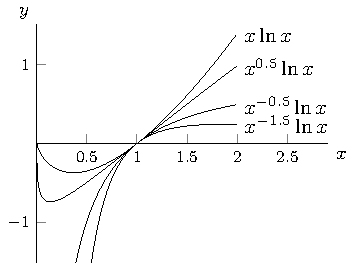
\includegraphics{figEulerCauchyABCD}
\caption*{(ب) دوسری صورت: دوہرا جذر۔}
\end{subfigure}
\begin{subfigure}{0.5\textwidth}
\centering
\begin{tikzpicture}
\begin{axis}[small,axis lines*=middle,ymin=-1.6,ymax=1.6,xmin=0,xmax=2.9,xlabel={$x$},ylabel={$y$},xlabel style={at={(axis description cs:1.05,0.5)}},ylabel style ={rotate=-90},ylabel style={at={(axis description cs:0,1.05)}}]
\addplot[domain=0.001:2,samples=100]{x^(0.1)*cos(180/pi*3*ln(x))}node[below]{$x^{0.1}\cos(3\ln x)$};
\addplot[domain=0.001:2,samples=100]{x^(0.1)*sin(180/pi*3*ln(x))}node[above]{$x^{0.1}\sin(3\ln x)$};
\end{axis}
\end{tikzpicture}
\caption*{(پ) جوڑی دار مخلوط جذر۔}
\end{subfigure}
\caption{یولر کوشی سادہ تفرقی مساوات کے حل۔}
\label{شکل_سادہ_دو_درجی_یولر_کوشی}
\end{figure}

شکل \حوالہ{شکل_سادہ_دو_درجی_یولر_کوشی} میں یولر کوشی سادہ تفرقی مساوات کی تینوں صورتوں کے حل دکھائے گئے ہیں۔

%============================
\ابتدا{مثال}\شناخت{مثال_سادہ_دو_ہم_محوری_نلکی_میدان}\quad دو ہم محوری نلکیوں کے بیچ میں ساکن برقی میدان؛ سرحدی قیمت مسئلہ\\
دو ہم محوری نلکیوں  کے بیچ میں برقی دباو تفرقی مساوات \عددی{\rho \tfrac{\dif^{\,2} v}{\dif \rho^2}+\tfrac{\dif v}{\dif \rho}=0} دیتی ہے۔نلکی کے رداس \عددی{\rho_1=\SI{2}{\centi\meter}} اور \عددی{\rho_2=\SI{5}{\centi\meter}} ہیں جبکہ ان پر \اصطلاح{برقی دباو}\فرہنگ{برقی دباو}\حاشیہب{electric voltage}\فرہنگ{voltage} \عددی{v_1=\SI{50}{\volt}} اور \عددی{v_2=\SI{0}{\volt}} ہے۔درمیانی خطے کی برقی دباو حاصل کریں۔

حل:یولر کوشی مساوات میں \عددی{a=1} اور \عددی{b=0} موجودہ تفرقی مساوات دیتا ہے۔دیے مساوات میں \عددی{v=\rho^m} پر کرتے ہوئے ذیلی مساوات \عددی{m^2=0} حاصل ہوتی ہے جس کا دوہرا جذر \عددی{m=0} ہے۔یوں عمومی  حل \عددی{v=c_1+c_2\ln x} ہو گا۔دیے گئے سرحدی شرائط حل میں پر کرتے 
\begin{align*}
50=c_1+c_2\ln 0.02, \quad 0=c_1+c_2\ln 0.05
\end{align*}
ہوئے \عددی{c_1=-163.471} اور \عددی{c_2=-54.568} حاصل ہوتے ہیں لہٰذا مخصوص حل \عددی{y=-163.471-54.568\ln \rho} ہو گا جسے شکل \حوالہ{شکل_مثال_سادہ_دو_ہم_محوری_نلکی_میدان} میں دکھایا گیا ہے۔
\begin{figure}
\centering
\begin{tikzpicture}
\begin{axis}[small,axis lines*=middle,ymin=0,ymax=58,xmin=0.02,xmax=0.056,xlabel={$\rho$},ylabel={$v$},xlabel style={at={(axis description cs:1.05,0)}},ylabel style ={rotate=-90},ylabel style={at={(axis description cs:0,1.05)}},scaled x ticks=false,xtick={0.02,0.03,0.04,0.05},xticklabels={$2$,$3$,$4$,$5$},ytick={0,50},yticklabels={$0$,$50$}]
\addplot[domain=0.01:0.05]{-163.471-54.568*ln(x)};
\end{axis}
\end{tikzpicture}
\caption{مثال \حوالہ{مثال_سادہ_دو_ہم_محوری_نلکی_میدان} کا حل۔}
\label{شکل_مثال_سادہ_دو_ہم_محوری_نلکی_میدان}
\end{figure}
\انتہا{مثال}
%==========================
\ابتدا{مثال}
یولر کوشی مساوات \حوالہ{مساوات_سادہ_دو_درجی_یولر_کوشی_الف} میں \عددی{x=e^{t}} پر کرتے ہوئے اس کو مستقل عددی سر والے سادہ تفرقی مساوات میں تبدیل کریں۔

حل:ہم \عددی{y(x)} کو \عددی{y[x(t)]} یعنی \عددی{y(t)} تصور کرتے ہیں۔یوں زنجیری تفرق سے
\begin{align*}
\frac{\dif y}{\dif x}=\frac{\dif y}{\dif t}\frac{\dif t}{\dif x}, \quad \frac{\dif^{\,2} y}{\dif x^2}=\frac{\dif^{\,2}y}{\dif t^2}\left(\frac{\dif t}{\dif x}\right)^2+\frac{\dif y}{\dif t}\frac{\dif^{\,2} t}{\dif x^2}
\end{align*}
لکھا جا سکتا ہے۔ان میں \عددی{\tfrac{\dif t}{\dif x}=\tfrac{1}{x}} اور \عددی{\tfrac{\dif^{\,2} t}{\dif x^2}=-\tfrac{1}{x^2}} پر کرتے ہیں۔
\begin{align*}
\frac{\dif y}{\dif x}=\frac{1}{x}\frac{\dif y}{\dif t}, \quad \frac{\dif^{\,2} y}{\dif x^2}=\frac{1}{x^2}\frac{\dif^{\,2}y}{\dif t^2}-\frac{1}{x^2}\frac{\dif y}{\dif t}
\end{align*}
انہیں مساوات \حوالہ{مساوات_سادہ_دو_درجی_یولر_کوشی_الف} میں پر کرتے 
\begin{align*}
x^2\left(\frac{1}{x^2}\frac{\dif^{\,2}y}{\dif t^2}-\frac{1}{x^2}\frac{\dif y}{\dif t}\right)+ax\left(\frac{1}{x}\frac{\dif y}{\dif t}\right)+by=0
\end{align*}
ہوئے مستقل عددی سر والا سادہ تفرقی مساوات حاصل ہوتا ہے  جہاں \عددی{\dot{y}=\tfrac{\dif y}{\dif t}} اور \عددی{\ddot{y}=\tfrac{\dif^{\,2}y}{\dif t^2}} ہیں۔
\begin{align}
\ddot{y}+(a-1)\dot{y}+by=0
\end{align}
\انتہا{مثال}
%==================================

\حصہء{سوالات}
سوال \حوالہ{سوال_سادہ_دو_یولر_کوشی_الف} تا سوال \حوالہ{سوال_سادہ_دو_یولر_کوشی_ب} حل کریں۔
%=======================

\ابتدا{سوال}\شناخت{سوال_سادہ_دو_یولر_کوشی_الف}
\begin{align*}
x^2y''-2xy'+2y=0
\end{align*}
جواب:\عددی{y=c_1x+c_2x^2}
\انتہا{سوال}
%====================
\ابتدا{سوال}
\begin{align*}
x^2y''-6y=0
\end{align*}
جواب:\عددی{y=c_1x^3+c_2x^{-2}}
\انتہا{سوال}
%==========================
\ابتدا{سوال}
\begin{align*}
x^2y''+6xy'+4y=0
\end{align*}
جواب:\عددی{y=\tfrac{c_1}{x}+\tfrac{c_2}{x^4}}
\انتہا{سوال}
%==================
\ابتدا{سوال}
\begin{align*}
x^2y''-5xy'+9y=0
\end{align*}
جواب:\عددی{y=(c_1+c_2\ln x)x^3}
\انتہا{سوال}
%==========================
\ابتدا{سوال}
\begin{align*}
x^2y''+11xy'+25y=0
\end{align*}
جواب:\عددی{y=(c_1+c_2\ln x)x^{-5}}
\انتہا{سوال}
%========================
\ابتدا{سوال}
\begin{align*}
10x^2y''+11xy'-3y=0
\end{align*}
جواب:\عددی{y=c_1\sqrt{x}+c_2x^{-\tfrac{3}{5}}}
\انتہا{سوال}
%=====================
\ابتدا{سوال}
\begin{align*}
x^2y''+0.44xy'+0.0748y=0
\end{align*}
جواب:\عددی{y=c_1x^{0.22}+c_2x^{0.34}}
\انتہا{سوال}
%======================
\ابتدا{سوال}
\begin{align*}
x^2y''+0.4xy'+0.73y=0
\end{align*}
جواب:\عددی{y=x^{0.3}[c_1\cos(0.8\ln x)+c_2\sin(0.8\ln x)]}
\انتہا{سوال}
%===================
\ابتدا{سوال}\شناخت{سوال_سادہ_دو_یولر_کوشی_ب}
\begin{align*}
x^2y''+2xy'+4.25y=0
\end{align*}
جواب:\عددی{y=x^{-0.5}[c_1\cos(2\ln x)+c_2\sin(2\ln x)]}
\انتہا{سوال}
%======================
سوال \حوالہ{سوال_سادہ_دو_یولر_کوشی_پ} تا سوال \حوالہ{سوال_سادہ_دو_یولر_کوشی_ت} ابتدائی قیمت مسئلے ہیں۔انہیں حل کریں۔

\ابتدا{سوال}\شناخت{سوال_سادہ_دو_یولر_کوشی_پ}
\begin{align*}
x^2y''-0.4xy'+0.45y=0,\quad y(1)=2,\quad y'(1)=-1
\end{align*}
جواب:\عددی{y=7\sqrt{x}-5x^{0.9}}
\انتہا{سوال}
%================================
\ابتدا{سوال}
\begin{align*}
x^2y''+1.08xy'-0.01713y=0,\quad y(1)=-1,\quad y'(1)=1
\end{align*}
جواب:\عددی{y=\tfrac{23}{18}x^{0.23}-\tfrac{41}{18}x^{-0.31}}
\انتہا{سوال}
%================================
\ابتدا{سوال}
\begin{align*}
35x^2y''+57xy'+3y=0,\quad y(1)=3,\quad y'(1)=-5
\end{align*}
جواب:\عددی{y=\tfrac{77}{4}x^{-\tfrac{3}{7}}-\tfrac{65}{4}x^{-\tfrac{1}{5}}}
\انتہا{سوال}
%================================
\ابتدا{سوال}
\begin{align*}
6x^2y''+19xy'+6y=0,\quad y(1)=-3,\quad y'(1)=1
\end{align*}
جواب:\عددی{y=\tfrac{6}{5}x^{-\tfrac{3}{2}}-\tfrac{21}{5}x^{-\tfrac{2}{3}}}
\انتہا{سوال}
%================================
\ابتدا{سوال}
\begin{align*}
25x^2y''-15xy'+16y=0,\quad y(2)=0,\quad y'(2)=1
\end{align*}
جواب:\عددی{y=2^{\tfrac{1}{5}}x^{\tfrac{4}{5}}(\ln x-\ln 2)}
\انتہا{سوال}
%================================
\ابتدا{سوال}\شناخت{سوال_سادہ_دو_یولر_کوشی_ت}
\begin{align*}
49x^2y''+77xy'+4y=0,\quad y(2)=3,\quad y'(2)=0
\end{align*}
جواب:\عددی{y=x^{-\tfrac{2}{7}}(2.93+1.04\ln x)}
\انتہا{سوال}
%================================

\حصہ{حل کی وجودیت اور یکتائی؛ ورونسکی}
اس حصے میں متجانس خطی سادہ تفرقی مساوات،
\begin{align}\label{مساوات_سادہ_دو_وجودیت_مخصوص_الف}
y''+p(x)y'+q(x)y=0
\end{align}
جس کے عددی سر \عددی{p(x)} اور \عددی{q(x)} کوئی بھی \اصطلاح{استمراری تفاعل} ہو سکتے  ہیں، کے عمومی حل کی \اصطلاح{وجودیت}\فرہنگ{وجودیت}\حاشیہب{existence}\فرہنگ{existence} پر غور کیا جائے گا۔ساتھ ہی ساتھ مساوات \حوالہ{مساوات_سادہ_دو_وجودیت_مخصوص_الف} اور  ابتدائی معلومات
\begin{align}\label{مساوات_سادہ_دو_وجودیت_مخصوص_ب}
y(x_0)=K_0, \quad y'(x_0)=K_1
\end{align}
کے  ابتدائی قیمت مسئلہ کی مخصوص حل کی \اصطلاح{یکتائی}\فرہنگ{یکتائی}\حاشیہب{uniqueness}\فرہنگ{uniqueness} پر بحث کی جائے گی۔ 

مسئلہ \حوالہ{مسئلہ_سادہ_دو_درجی_یکتا_مخصوص_حل} کہتا ہے کہ اس ابتدائی قیمت مسئلے کا مخصوص حل پایا جاتا ہے جو یکتا ہو گا اور مساوات \حوالہ{مساوات_سادہ_دو_وجودیت_مخصوص_الف} کے عمومی حل
\begin{align}
y=c_1y_1+c_2y_2\quad \quad \text{\RL{اختیاری $c_1$, $c_2$}}
\end{align}
میں تمام حل شامل ہیں۔یوں استمراری عددی سر والے متجانس سادہ تفرقی مساوات کا کوئی \اصطلاح{نادر حل}\فرہنگ{نادر حل}\فرہنگ{حل!نادر} نہیں پایا جاتا۔نادر حل اس حل کو کہتے ہیں جسے عمومی حل سے حاصل نہیں کیا جا سکتا ہے۔

ہمیں مستقل عددی سر والے سادہ تفرقی مساوات یا یولر کوشی سادہ تفرقی مساوات کے حل کی وجودیت اور یکتائی جاننے کی ضرورت پیش نہیں آئی چونکہ ان کے حل کے دوران ہی ایسی تمام معلومات سامنے آ جاتی ہیں۔
%================

%\theoremstyle{plain}
%\begin{theorem}[]\label{مسئلہ_سادہ_دو_درجی_یکتا_مخصوص_حل}
\ابتدا{مسئلہ}\شناخت{مسئلہ_سادہ_دو_درجی_یکتا_مخصوص_حل}\quad مسئلہ وجودیت اور یکتائی برائے ابتدائی قیمت تفرقی مساوات\فرہنگ{مسئلہ!وجودیت اور یکتائی}\\
اگر \عددی{p(x)} اور \عددی{q(x)} کسی کھلے  وقفے \عددی{I} پر استمراری ہوں اور \عددی{x_0} اس وقفے پر پایا جاتا ہو، تب مساوات \حوالہ{مساوات_سادہ_دو_وجودیت_مخصوص_الف} اور مساوات \حوالہ{مساوات_سادہ_دو_وجودیت_مخصوص_ب} پر مبنی ابتدائی قیمت مسئلے کا \عددی{I} پر  یکتا مخصوص حل \عددی{y(x)}  موجود ہے۔  
%\end{theorem}
\انتہا{مسئلہ}
%============================

وجودیت حل کی ثبوت کے لئے وہی بنیادی شرائط درکار ہیں جو صفحہ \حوالہصفحہ{مسئلہ_سادہ_اول_وجودیت} پر مسئلہ \حوالہ{مسئلہ_سادہ_اول_وجودیت} کے لئے درکار تھے۔اس کتاب میں ان پر غور نہیں کیا جائے گا۔ اگرچہ یکتائی کا ثبوت عموماً آسان ہوتا ہے لیکن موجودہ مسئلہ \حوالہ{مسئلہ_سادہ_دو_درجی_یکتا_مخصوص_حل} کے یکتائی حل کا ثبوت اتنا آسان نہیں ہے لہٰذا اس کو کتاب کے آخر میں بطور ضمیمہ \حوالہ{ضمیمہ_اضافی_ثبوت} شامل کیا گیا ہے۔ 
%==================

\جزوحصہء{خطی طور غیر تابع حل}
آپ کو حصہ \حوالہ{حصہ_سادہ_اسپرنگ_کمیت} سے یاد ہو گا کہ کھلے وقفہ \عددی{I} پر عمومی حل \اصطلاح{اساس} \عددی{y_1}، \عددی{y_2} پر مشتمل ہوتا ہے جہاں \عددی{y_1} اور \عددی{y_2} کھلے وقفے \عددی{I} پر خطی طور غیر تابع حل ہیں۔ وقفہ \عددی{I} پر معین \عددی{y_1} اور \عددی{y_2}،  وقفہ \عددی{I}  پر، اس صورت \اصطلاح{خطی طور غیر تابع}\فرہنگ{خطی طور! غیر تابع}\حاشیہب{linearly independent}\فرہنگ{linearly independent} کہلاتے ہیں جب پورے وقفے پر
\begin{align}\label{مساوات_سادہ_دو_خطی_طور_غیر_تابع_الف}
k_1 y_1+k_2 y_2=0
\end{align}
سے مراد 
\begin{align}
k_1=0, \quad k_2=0
\end{align}
ہو۔\عددی{k_1} اور \عددی{k_2} میں سے کم از کم ایک کی قیمت صفر کے برابر نہ ہونے کی صورت میں مساوات \حوالہ{مساوات_سادہ_دو_خطی_طور_غیر_تابع_الف} پر پورا اترتے ہوئے حل \عددی{y_1} اور \عددی{y_2} \اصطلاح{خطی طور تابع}\فرہنگ{خطی طور!تابع}\حاشیہب{linearly dependent}\فرہنگ{linearly dependent} کہلاتے ہیں۔اگر \عددی{k_1 \ne 0} ہو تب ہم مساوات \حوالہ{مساوات_سادہ_دو_خطی_طور_غیر_تابع_الف} کو \عددی{k_1} سے تقسیم کرتے ہوئے \عددی{y_1=-\tfrac{k_2}{k_1}y_2} لکھ سکتے ہیں جو تناسبی رشتہ ہے۔اسی طرح \عددی{k_2 \ne 0} کی صورت میں \عددی{y_2=-\tfrac{k_1}{k_2}y_1} لکھا جا سکتا ہے جو تناسبی رشتے کو ظاہر کرتی ہے۔
\begin{align}\label{مساوات_سادہ_دور_خطی_غیر_تابع_شرط}
\text{(الف)}\quad y_1=ky_2,\quad \text{(ب)}\quad y_2=l y_1 \quad \quad \text{\RL{پورے $I$ پر}}
\end{align}
اس کے برعکس خطی طور غیر تابع صورت میں ہم مساوات \حوالہ{مساوات_سادہ_دو_خطی_طور_غیر_تابع_الف} کو \عددی{k_1} (یا \عددی{k_2}) سے تقسیم نہیں کر سکتے لہٰذا  تناسبی رشتہ حاصل نہیں کیا جا سکتا۔(درج بالا مساوات میں \عددی{k=-\tfrac{k_2}{k_1}} اور \عددی{l=-\tfrac{k_1}{k_2}} لکھے گئے ہیں۔\عددی{k} یا (اور) \عددی{l} صفر بھی ہو سکتے ہیں۔) خطی طور غیر تابع اور خطی طور تابع حل کو درج ذیل طرز پر بیان کیا جا سکتا ہے۔ 
%==========================

%\begin{theorem}[خطی طور تابع اور غیر تابع حل]
\ابتدا{مسئلہ}\شناخت{مسئلہ_سادہ_دو_حل_تابع_غیر_تابع}\quad خطی طور تابع اور غیر تابع حل\فرہنگ{مسئلہ!تابع اور غیر تابع حل}\\
کھلے وقفہ \عددی{I} پر استمراری  \عددی{p(x)} اور \عددی{q(x)} عددی سر والے سادہ تفرقی  مساوات \حوالہ{مساوات_سادہ_دو_خطی_طور_غیر_تابع_الف} کے \عددی{I}  پر دو حل \عددی{y_1} اور \عددی{y_2} اس صورت خطی طور غیر تابع ہوں گے جب ان کے \اصطلاح{ورونسکی}\فرہنگ{ورونسکی}\حاشیہب{Wronskian}\فرہنگ{Wronskian}
\begin{align}\label{مساوات_سادہ_دو_ورونسکی_تعریف}
W(y_1,y_2)=y_1y_2'-y_2y_1'
\end{align}
کی قیمت  کسی \عددی{x_0} پر صفر کے برابر ہو جہاں \عددی{x_0} کھلے وقفے \عددی{I} پر پایا جاتا ہے۔مزید اگر  نقطہ \عددی{x=x_0} پر \عددی{W=0} ہو تب پورے \عددی{I} پر \عددی{W=0} ہو گا۔یوں اگر \عددی{I} پر کوئی ایسا \عددی{x} پایا جاتا ہو جس پر \عددی{W} صفر کے برابر نہ ہو تب \عددی{y_1} اور \عددی{y_2} خطی طور غیر تابع ہوں گے۔
%\end{theorem}
\انتہا{مسئلہ}
%==================
\ابتدا{ثبوت}
\begin{enumerate}
\item[(الف)]
\عددی{y_1} اور \عددی{y_2} کو \عددی{I} پر خطی طور غیر تابع تصور کریں۔یوں مساوات \حوالہ{مساوات_سادہ_دور_خطی_غیر_تابع_شرط}-الف یا ب میں سے ایک درست ہو گا۔اگر  مساوات \حوالہ{مساوات_سادہ_دور_خطی_غیر_تابع_شرط}-الف  درست ہو تب
\begin{align*}
W(y_1,y_2)=y_1y_2'-y_2y_1'=ky_2y_2'-y_2ky_2'=0
\end{align*}
ہو گا۔اسی طرح مساوات \حوالہ{مساوات_سادہ_دور_خطی_غیر_تابع_شرط}-ب کی صورت میں بھی \عددی{W=0} ملتا ہے۔
\item[(ب)]
 اس کے الٹ چلتے ہوئے ہم ثابت کرتے ہیں کہ کسی \عددی{x_0} پر \عددی{W(y_1,y_2)=0} سے مراد \عددی{y_1} اور \عددی{y_2} کا \عددی{I} پر خطی طور تابع ہونا ہے۔درج ذیل مساوات پر غور کریں جہاں \عددی{k_1} اور \عددی{k_2} کو نا معلوم متغیرات تصور کریں۔
\begin{gather}
\begin{aligned}\label{مساوات_سادہ_دو_درجی_ثبوت_الف}
k_1y_1(x_0)+k_2y_2(x_0)&=0\\
k_1y_1'(x_0)+k_2y_2'(x_0)&=0
\end{aligned}
\end{gather}
\عددی{k_2} حذف کرنے کی نیت سے  پہلی مساوات کو \عددی{y_2'(x_0)} اور دوسری کو \عددی{-y_2(x_0)} سے ضرب دیتے ہوئے دونوں کا مجموعہ لیتے ہیں۔
\begin{align}\label{مساوات_سادہ_دو_درجی_ثبوت_ب}
k_1y_1(x_0)y_2'(x_0)-k_1y_1'(x_0)y_2(x_0)=k_1W(y_1(x_0),y_2(x_0))=0
\end{align}
اسی طرح \عددی{k_1} حذف کرنے کے لئے پہلی مساوات کو \عددی{-y_1'(x_0)} اور دوسری کو \عددی{y_1(x_0)} سے ضرب دیتے ہوئے دونوں مساوات کا مجموعہ
\begin{align}\label{مساوات_سادہ_دو_درجی_ثبوت_پ}
k_2y_1(x_0)y_2'(x_0)-k_2y_2(x_0)y_1'(x_0)=k_2W(y_1(x_0),y_2(x_0))=0
\end{align}
لیتے ہیں۔اب اگر \عددی{x_0} پر \عددی{W} صفر نہ ہوتا تب ہم مساوات \حوالہ{مساوات_سادہ_دو_درجی_ثبوت_ب} اور مساوات \حوالہ{مساوات_سادہ_دو_درجی_ثبوت_پ} کو \عددی{W} سے تقسیم کرتے ہوئے \عددی{k_1=k_2=0} حاصل کرتے البتہ \عددی{x_0} پر \عددی{W(y_1(x_0),y_2(x_0))=0} ہے لہٰذا ہم ان مساوات کو \عددی{W} سے  تقسیم نہیں کر سکتے ہیں۔ یوں  ہمزاد مساوات \حوالہ{مساوات_سادہ_دو_درجی_ثبوت_الف} کا حل \عددی{k_1} اور \عددی{k_2} پایا جاتا ہے جہاں \عددی{k_1} اور \عددی{k_2} دونوں غیر صفر ہو سکتے ہیں۔ اب ان اعداد \عددی{k_1} اور \عددی{k_2} کو استعمال کرتے ہوئے تفاعل
\begin{align}
y(x)=k_1y_1(x)+k_2y_2(x)
\end{align}
لیتے ہیں۔چونکہ مساوات \حوالہ{مساوات_سادہ_دو_وجودیت_مخصوص_الف} متجانس خطی ہے لہٰذا  مسئلہ \حوالہ{مسئلہ_دو_درجی_خطی_میل}  (مسئلہ خطی میل) کے تحت  یہ تفاعل بھی مساوات \حوالہ{مساوات_سادہ_دو_وجودیت_مخصوص_الف} کا حل ہو گا۔مساوات \حوالہ{مساوات_سادہ_دو_درجی_ثبوت_الف} سے ظاہر ہے کہ یہ تفاعل ابتدائی معلومات \عددی{y(x_0)=0} اور \عددی{y'(x_0)=0} پر پورا اترتا ہے۔اب تصور کریں کہ مساوات \حوالہ{مساوات_سادہ_دو_وجودیت_مخصوص_الف} کا دوسرا حل جو انہیں  ابتدائی معلومات پر پورا اترتا ہو \عددی{y^*(x)=0} ہے۔اب چونکہ مساوات \حوالہ{مساوات_سادہ_دو_وجودیت_مخصوص_الف} میں \عددی{p(x)} اور \عددی{q(x)} استمراری ہیں لہٰذا مسئلہ \حوالہ{مسئلہ_سادہ_دو_درجی_یکتا_مخصوص_حل} کے تحت اس کا مخصوص حل یکتا ہو گا۔یوں \عددی{y(x)} اور \عددی{y^*(x)} مختلف نہیں ہو سکتے ہیں لہٰذا \عددی{y^*(x)=y(x)=0} یعنی
\begin{align}\label{مساوات_سادہ_دو_درجی_ثبوت_ت}
k_1y_1+k_2y_2\equiv 0\quad \quad \text{\RL{پورے $I$ پر}}
\end{align}
ہو گا۔چونکہ \عددی{k_1} اور \عددی{k_2} میں کم از کم ایک صفر کے برابر نہیں ہے لہٰذا  مساوات \حوالہ{مساوات_سادہ_دو_درجی_ثبوت_ت} کہتا ہے کہ \عددی{I} پر \عددی{y_1} اور \عددی{y_2} خطی طور تابع ہیں۔
\item[(پ)]
ہم مسئلے کا آخری نقطہ ثابت کرتے ہیں۔اگر کھلے وقفے \عددی{I} پر نقطہ \عددی{x_0} پر \عددی{W(x_0)=0} ہو تب ثبوت (ب) کے تحت \عددی{I} پر \عددی{y_1} اور \عددی{y_2} خطی طور تابع ہیں لہٰذا ثبوت (الف) کے تحت \عددی{W \equiv 0} ہو گا۔یوں خطی طور تابع صورت میں ایسا نہیں ہو سکتا ہے کہ \عددی{W(x_1) \ne 0} ہو جہاں \عددی{x_1} کھلے وقفہ \عددی{I} پر پایا جاتا ہے۔اگر ایسا ممکن ہو تب اس سے مراد خطی طور غیر تابع صورت ہو گی جیسا کہ دعویٰ کیا گیا ہے۔ 
\end{enumerate}
\انتہا{ثبوت}
%=================

حساب کی نقطہ نظر سے  مساوات \حوالہ{مساوات_سادہ_دو_ورونسکی_تعریف} سے درج ذیل زیادہ آسان مساوات ہے۔
\begin{align}\label{مساوات_سادہ_دو_آسان_ورونسکی}
W(y_1,y_2)=
\begin{cases}
\left(\frac{y_2}{y_1}\right)^{\!'}y_1^2  &(y_1 \ne 0)\\[0.5em]
-\left(\frac{y_1}{y_2}\right)^{\!'}y_2^2 & (y_2 \ne 0)
\end{cases}
\end{align}
آپ دیکھ سکتے ہیں کہ  ورونسکی کو قالب کی مقطع کے طرز پر لکھا جا سکتا ہے جس کو \اصطلاح{ورونسکی مقطع}\فرہنگ{ورونسکی!مقطع}\فرہنگ{مقطع!ورونسکی}\حاشیہب{Wronskian determinant}\فرہنگ{Wronskian determinant} یا حل \عددی{y_1} اور \عددی{y_2} کی \اصطلاح{ورونسکی} کہتے ہیں۔ 
\begin{align}
W(y_1,y_2)=
\begin{vmatrix}
y_1 &y_2\\[0.25em]
y_1' & y_2'
\end{vmatrix}
=y_1y_2'-y_2y_1'
\end{align}
%==============================

\ابتدا{مثال}\quad مسئلہ \حوالہ{مسئلہ_سادہ_دو_حل_تابع_غیر_تابع} کا اطلاق\\
تفرقی مساوات \عددی{y''+\omega^2y=0} کے حل \عددی{y_1=\cos \omega x} اور \عددی{y_2=\sin \omega x}  ہیں۔ان کی ورونسکی
\begin{align*}
W(\cos \omega x,\sin \omega x)=
\begin{vmatrix}
\cos \omega x &\sin \omega x\\[0.25em]
-\omega \sin \omega x & -\omega \cos \omega x
\end{vmatrix}
=\omega \cos^2 \omega x+\omega \sin^2 \omega x=\omega
\end{align*}
ہے۔مسئلہ \حوالہ{مسئلہ_سادہ_دو_حل_تابع_غیر_تابع} کے تحت یہ حل صرف اس صورت میں خطی طور غیر تابع ہوں گے جب \عددی{\omega \ne 0} ہو۔یہی دونوں حل کے حاصل تقسیم \عددی{\tfrac{y_2}{y_1}=\tan \omega x} سے بھی اخذ کیا جا سکتا ہے جہاں \عددی{\omega=0} سے \عددیء{y_2=0} ملتا ہے جو خطی طور تابع صورت ظاہر کرتی ہے۔
\انتہا{مثال}
%=============================
\ابتدا{مثال}\quad دوہرا جذر کی صورت میں مسئلہ \حوالہ{مسئلہ_سادہ_دو_حل_تابع_غیر_تابع} کا اطلاق\\
تفرقی مساوات \عددی{y''-6y'+9y=0} کا (ثابت کریں کہ) عمومی حل  \عددی{y=(c_1+c_2 x)e^{3x}}   ہے جس کا ورونسکی صفر کے برابر نہیں ہے لہٰذا \عددی{e^{3x}} اور \عددی{xe^{3x}} تمام \عددی{x} پر خطی طور غیر تابع ہیں۔
\begin{align*}
W(e^{3x},xe^{3x})=
\begin{vmatrix}
e^{3x}& xe^{3x}\\[0.25em]
3e^{3x}&e^{3x}+3xe^{3x}
\end{vmatrix}
=e^{6x}+3xe^{6x}-3xe^{6x}=e^{6x} \ne 0
\end{align*}
\انتہا{مثال}
%==================

\جزوحصہء{مساوات \حوالہ{مساوات_سادہ_دو_وجودیت_مخصوص_الف} کے عمومی حل میں تمام حل کی شمولیت}
اس حصے کو مساوات \حوالہ{مساوات_سادہ_دو_وجودیت_مخصوص_الف} کے عمومی حل کی وجودیت سے شروع کرتے ہیں۔
%=========================

\ابتدا{مسئلہ}\شناخت{مسئلہ_سادہ_دو_وجودیت_الف}\quad \اصطلاح{وجودیت عمومی حل}\فرہنگ{وجودیت!عمومی حل}\فرہنگ{حل!وجودیت عمومی حل}\فرہنگ{existence!solution}\فرہنگ{مسئلہ!وجودیت عمومی حل}\\
کھلے وقفہ \عددی{I} پر استمراری \عددی{p(x)} اور \عددی{q(x)} کی صورت میں مساوات \حوالہ{مساوات_سادہ_دو_وجودیت_مخصوص_الف} کا عمومی حل \عددی{I} پر موجود ہے۔
\انتہا{مسئلہ}
%=====================

\ابتدا{ثبوت}
مسئلہ \حوالہ{مسئلہ_سادہ_دو_درجی_یکتا_مخصوص_حل} کے تحت  \عددی{I} پر مساوات \حوالہ{مساوات_سادہ_دو_وجودیت_مخصوص_الف} کا، ابتدائی معلومات 
\begin{align*}
y_1(x_0)=1, \quad y_1'(x_0)=0
\end{align*}
پر پورا اترتا ہوا  حل  \عددی{y_1(x)} موجود ہے۔اسی طرح ابتدائی معلومات
\begin{align*}
y_2(x_0)=0, \quad y_2'(x_0)=1
\end{align*}
 پر پورا اترتا ہوا  حل \عددی{y_2(x)} بھی موجود ہے۔نقطہ \عددی{x_0} پر ان کا ورونسکی
\begin{align*}
W(y_1(x_0),y_2(x_0))=y_1(x_0)y'_2(x_0)-y_2(x_0)y'_1(x_0)=1
\end{align*}
ہے۔مسئلہ \حوالہ{مسئلہ_سادہ_دو_حل_تابع_غیر_تابع} کے تحت \عددی{I} پر \عددی{y_1} اور \عددی{y_2} خطی طور غیر تابع ہیں لہٰذا یہ مساوات \حوالہ{مساوات_سادہ_دو_وجودیت_مخصوص_الف} کے حل کی اساس ہیں۔اس طرح ثابت ہوا کہ  \عددی{I} پر  مساوات \حوالہ{مساوات_سادہ_دو_وجودیت_مخصوص_الف} کا عمومی حل \عددی{y=c_1y_1+c_2y_2} ہے جہاں \عددی{c_1} اور \عددی{c_2} اختیاری مستقل ہیں۔
\انتہا{ثبوت}
%=======================

آئیں اب ثابت کریں کہ عمومی حل اتنا عمومی ہے جتنا کوئی حل عمومی ہو سکتا ہے۔
%=====================

\ابتدا{مسئلہ}\quad عمومی حل میں تمام حل شامل ہیں\\
کھلا وقفہ \عددی{I} پر استمراری \عددی{p(x)} اور \عددی{q(x)} کی صورت میں \عددی{I} پر مساوات \حوالہ{مساوات_سادہ_دو_وجودیت_مخصوص_الف} کے ہر حل
 \عددی{y=Y(x)} کو
\begin{align}
Y(x)=C_1y_1+C_2y_2
\end{align}
لکھا جا سکتا ہے، جہاں \عددی{y_1} اور \عددی{y_2} کھلے وقفہ \عددی{I} پر مساوات \حوالہ{مساوات_سادہ_دو_وجودیت_مخصوص_الف} کی کوئی بھی اساس اور \عددی{C_1}، \عددی{C_2} مناسب مستقل ہیں۔

یوں مساوات \حوالہ{مساوات_سادہ_دو_وجودیت_مخصوص_الف} کا کوئی \اصطلاح{نادر حل}\فرہنگ{نادر حل} موجود نہیں ہے۔(نادر حل سے مراد ایسا حل ہے جس کو عمومی حل سے حاصل نہیں کیا جا سکتا ہے۔)
\انتہا{مسئلہ}
%======================

\ابتدا{ثبوت}
تصور کریں کہ \عددی{I} پر مساوات \حوالہ{مساوات_سادہ_دو_وجودیت_مخصوص_الف} کا  \عددی{y=Y(x)} کوئی حل ہے۔اب مسئلہ \حوالہ{مسئلہ_سادہ_دو_وجودیت_الف} کے تحت \عددی{I} پر  تفرقی مساوات \حوالہ{مساوات_سادہ_دو_وجودیت_مخصوص_الف} کا عمومی حل
\begin{align}\label{مساوات_سادہ_دو_ثبوت_مسئلہ_چار_الف}
y(x)=c_1y_1(x)+c_2y_2(x)
\end{align}
موجود ہے۔ہم \عددی{c_1} اور \عددی{c_2} کی وہ قیمتیں دریافت کرنا چاہتے ہیں جن سے \عددی{I} پر  \عددی{y(x)=Y(x)} حاصل ہوتا ہو۔ہم \عددی{I} پر کوئی بھی \عددی{x_0} چنتے ہوئے پہلے ثابت کرتے ہیں کہ \عددی{c_1} اور \عددی{c_2} کی ایسی قیمتیں دریافت کی جا سکتی ہیں کہ \عددی{x_0} پر \عددی{y(x_0)=Y(x_0)} اور 
\عددی{y'(x_0)=Y'(x_0)} ہوں۔اس کو مساوات \حوالہ{مساوات_سادہ_دو_ثبوت_مسئلہ_چار_الف} کے استعمال سے 
\begin{align}
c_1y_1(x_0)+c_2y_2(x_0)&=Y(x_0)\label{مساوات_سادہ_دو_ثبوت_مسئلہ_چار_ب}\\
c_1y'_1(x_0)+c_2y'_2(x_0)&=Y'(x_0)\label{مساوات_سادہ_دو_ثبوت_مسئلہ_چار_پ}
\end{align}
لکھ سکتے ہیں۔ان ہمزاد مساوات سے \عددی{c_1} اور \عددی{c_2} معلوم کرتے ہیں۔مساوات \حوالہ{مساوات_سادہ_دو_ثبوت_مسئلہ_چار_ب} کو \عددی{y'_2(x_0)} اور مساوات \حوالہ{مساوات_سادہ_دو_ثبوت_مسئلہ_چار_پ} کو \عددی{-y_2(x_0)} سے ضرب دیتے ہوئے مجموعہ لینے سے \عددی{c_1} حاصل کیا جا سکتا ہے۔ایسا کرنے سے مساوات \حوالہ{مساوات_سادہ_دو_ثبوت_مسئلہ_چار_ت} ملتی ہے۔اسی طرح \عددی{c_2} حاصل کرنے کی خاطر پہلی مساوات کو \عددی{-y'_1(x_0)} اور دوسری کو \عددی{y_1(x_0)} سے ضرب دیتے ہوئے مجموعہ لیتے ہوئے مساوات \حوالہ{مساوات_سادہ_دو_ثبوت_مسئلہ_چار_ٹ} حاصل ہوتی ہے۔ان مساوات میں \عددی{y_1}، \عددی{y'_1}، \عددی{y_2}،\عددی{y'_2}، \عددی{Y} اور \عددی{Y'} کی قیمتیں نقطہ \عددی{x_0} پر لی گئی ہیں۔ 
\begin{align}
c_1y_1y'_2-c_1y_2y'_1&=c_1W(y_1,y_2)=Yy_2'-y_2Y\label{مساوات_سادہ_دو_ثبوت_مسئلہ_چار_ت}\\
c_2y_1y'_2-c_2y_2y'_1&=c_2W(y_1,y_2)=y_1Y-Yy'_1\label{مساوات_سادہ_دو_ثبوت_مسئلہ_چار_ٹ}
\end{align}
اب چونکہ \عددی{y_1} اور \عددی{y_2} حل کی اساس ہیں لہٰذا ورونسکی کی قیمت صفر کے برابر نہیں ہے لہٰذا ان مساوات سے \عددی{c_1} اور \عددی{c_2} حاصل کیے جا سکتے ہیں
\begin{align*}
c_1=\frac{Yy_2'-y_2Y}{W}=C_1, \quad c_2=\frac{y_1Y-Yy'_1}{W}=C_2
\end{align*}
جہاں ان منفرد قیمتوں کو \عددی{C_1} اور \عددی{C_2} لکھا گیا ہے۔ انہیں مساوات \حوالہ{مساوات_سادہ_دو_ثبوت_مسئلہ_چار_الف} میں پر کرتے ہوئے مخصوص حل
\begin{align*}
y^*(x)=C_1y_1(x)+C_2y_2(x)
\end{align*}
حاصل ہوتا ہے۔اب چونکہ \عددی{C_1} اور \عددی{C_2} مساوات \حوالہ{مساوات_سادہ_دو_ثبوت_مسئلہ_چار_ب} اور مساوات \حوالہ{مساوات_سادہ_دو_ثبوت_مسئلہ_چار_پ} کے حل ہیں لہٰذا ہم ان مساوات سے دیکھتے ہیں کہ
\begin{align*}
y^{*}(x_0)=Y(x_0),\quad y^{*'}(x_0)=Y'(x_0)
\end{align*}
مسئلہ \حوالہ{مسئلہ_سادہ_دو_درجی_یکتا_مخصوص_حل} میں جس یکتائی کا ذکر کیا گیا ہے اس کے تحت \عددی{y^*} اور \عددی{Y} تمام \عددی{I} پر ہر جگہ برابر ہوں گے۔
\انتہا{ثبوت}
%=========================

\حصہء{سوالات}
%===================

\ابتدا{سوال}
مساوات \حوالہ{مساوات_سادہ_دو_آسان_ورونسکی} سے مساوات \حوالہ{مساوات_سادہ_دو_ورونسکی_تعریف} حاصل کریں۔
\انتہا{سوال}
%===========================
سوال \حوالہ{سوال_سادہ_ورونسکی_الف} تا سوال \حوالہ{سوال_سادہ_ورونسکی_ب} کی ورونسکی حاصل کریں۔حاصل تقسیم سے ثابت کریں کہ یہ خطی طور غیر تابع ہیں اور مسئلہ \حوالہ{مسئلہ_سادہ_دو_حل_تابع_غیر_تابع} سے  بھی اس بات کی تصدیق کریں

%======================
\ابتدا{سوال}\شناخت{سوال_سادہ_ورونسکی_الف}\quad $e^{2x}, e^{-1.2x}$\\
جوابات:\عددی{\tfrac{e^{2x}}{e^{-1.2x}}=e^{3.2x} \ne c}، \عددی{W=-3.2e^{0.8x}\ne 0}
\انتہا{سوال}
%============================ 
\ابتدا{سوال}\quad $e^{2.4x}, e^{1.1x}$\\
جوابات:\عددی{\tfrac{y_1}{y_2}=e^{1.3x} \ne c}، \عددی{W=-1.3e^{3.5x} \ne 0}
\انتہا{سوال}
%===============
\ابتدا{سوال}\quad
$x, \frac{1}{x}$\\
جوابات:\عددی{\tfrac{y_1}{y_2}=x^2 \ne c}، \عددی{W=-2x^{-2} \ne 0}
\انتہا{سوال}
%=====================
\ابتدا{سوال}\quad
$x, x^3$\\
جوابات:\عددی{\tfrac{y_1}{y_2}=x^{-2} \ne c}، \عددی{W=2x^3 \ne 0}
\انتہا{سوال}
%===================
\ابتدا{سوال}\quad
$e^{-0.2x}\sin 3x, e^{-0.2x} \cos 3x$\\
جوابات:\عددی{\tfrac{y_1}{y_2}=\tan 3x \ne c}، \عددی{W=3e^{-0.4x} \ne 0}
\انتہا{سوال}
%========================
\ابتدا{سوال}\quad
$e^{-ax}\sinh kx, e^{-ax} \cosh kx$\\
جوابات:\عددی{\tfrac{y_1}{y_2}=\tanh kx \ne c}، \عددی{W=-ke^{-2ax} \ne 0}
\انتہا{سوال}
%============================
\ابتدا{سوال}\شناخت{سوال_سادہ_ورونسکی_ب}\quad
$x^{a}\sin(k\ln x), x^{a}\cos(k\ln x)$\\
جوابات:\عددی{\tfrac{y_1}{y_2}=\tan(k \ln x) \ne c}، \عددی{W=-kx^{2a-1} \ne 0}
\انتہا{سوال}
%===========================

سوال \حوالہ{سوال_سادہ_ورونسکی_پ} تا سوال \حوالہ{سوال_سادہ_ورونسکی_ت} میں تفرقی مساوات کے حل دیے گئے ہیں۔تفرقی مساوات حاصل کریں۔ورونسکی کی مدد سے ثابت کریں کہ دیے گئے حل خطی طور غیر تابع ہیں اور ابتدائی قیمت مسئلے کا مخصوص حل حاصل کریں۔
%==============================

\ابتدا{سوال}\شناخت{سوال_سادہ_ورونسکی_پ}\quad 
$\sin 3x, \, \cos 3x,\quad y(0)=2,\quad y'(0)=-3 $\\
جوابات:\عددی{y''+9y=0}، \عددی{W=-3\ne 0}، \عددی{y=2\cos 3x-\sin 3x}
\انتہا{سوال}
%===========================
\ابتدا{سوال}\quad 
$x^3, \, x^{-4},\quad y(1)=-1,\quad y'(1)=2 $\\
جوابات:\عددی{x^2y''+2xy'-12y=0}، \عددی{W=-\tfrac{7}{x^2}\ne 0}، \عددی{y=-\tfrac{2x^3}{7}-\tfrac{5x^{-4}}{7}}
\انتہا{سوال}
%===========================
\ابتدا{سوال}\quad 
$e^{-1.2x}\sin 0.8x, \, e^{-1.2x}\cos 0.8 x,\quad y(0)=5,\quad y'(0)=7 $\\
جوابات:\عددی{y''+2.4y'+2.08y=0}، \عددی{W=-0.8e^{-2.4x} \ne 0}، \\
\عددی{y=e^{-\tfrac{6}{5}x}(\tfrac{65}{4}\sin\tfrac{4x}{5}+5\cos\tfrac{4x}{5})}
\انتہا{سوال}
%===========================
\ابتدا{سوال}\quad 
$x^3,\, x^3\ln x,\quad y(1)=2,\quad y'(1)=8 $\\
جوابات:\عددی{x^2y''-5xy'+9y=0}، \عددی{W=x^5 \ne 0}، \عددی{y=2x^3(1+\ln x)}
\انتہا{سوال}
%===========================
\ابتدا{سوال}\quad 
$1,\, e^{3x},\quad y(0)=1.5,\quad y'(0)=-2.5 $\\
جوابات:\عددی{y''-3y'=0}، \عددی{W=3e^{3x} \ne 0}، \عددی{y=\tfrac{8}{3}e^{3x}-\tfrac{2}{3}}
\انتہا{سوال}
%===========================
\ابتدا{سوال}\quad 
$e^{-kx}\sin \pi x, \, e^{-kx}\cos \pi x,\quad y(0)=1,\quad y'(0)=-k-\pi $\\
جوابات:\عددی{y''+2ky'+(k^2+\pi^2)y=0}، \عددی{W=-\pi e^{-2kx} \ne 0}، \\
\عددی{y=e^{-kx}(\sin \pi x-\cos \pi x)}
\انتہا{سوال}
%===========================
\ابتدا{سوال}\شناخت{سوال_سادہ_ورونسکی_ت}\quad 
$\sinh 1.8x, \,\cosh 1.8x,\quad y(0)=14.2,\quad y'(0)=16.38 $\\
جوابات:\عددی{y''-3.24y=0}، \عددی{W=-1.8 \ne 0}، \\
\عددی{y=9.1\sinh 1.8x+14.2\cosh 1.8x}
\انتہا{سوال}
%===========================
\ابتدا{سوال}
تفرقی مساوات \عددی{y''-y=0} کا عمومی حل قوت نمائی تفاعل اور \اصطلاح{بذلولی}\فرہنگ{بذلولی}\حاشیہب{hyperbolic}\فرہنگ{hyperbolic!function} تفاعل کی صورت میں لکھیں۔دونوں صورتوں کے مستقل کا تعلق کیا ہے؟

جوابات:\عددی{y=c_1e^{x}+c_2e^{-x}}، \عددی{y=c_a\sinh x+c_b\cosh x}، \عددی{c_a=c_1-c_2}، \عددی{c_b=c_1+c_2}
\انتہا{سوال}
%=============================
%=====================================

\حصہ{غیر متجانس سادہ تفرقی مساوات}\شناخت{حصہ_سادہ_دو_غیر_متجانس}
اس باب میں اب تک متجانس خطی سادہ تفرقی مساوات پر غور کیا گیا۔یہاں سے باب کے اختتام تک غیر متجانس خطی سادہ تفرقی مساوات پر غور کیا جائے گا۔درج ذیل غیر متجانس خطی تفرقی مساوات پر غور کرتے ہیں جہاں \عددی{r \not \equiv 0} ہے۔
\begin{align}\label{مساوات_سادہ_دو_غیر_متجانس_الف}
y''+p(x)y'+q(x)y=r(x)
\end{align}
ہم دیکھیں گے کہ مساوات \حوالہ{مساوات_سادہ_دو_غیر_متجانس_الف} کا عمومی حل، مطابقتی متجانس مساوات 
\begin{align}\label{مساوات_سادہ_دو_غیر_متجانس_ب}
y''+p(x)y'+q(x)y=0
\end{align}
کے عمومی حل اور مساوات \حوالہ{مساوات_سادہ_دو_غیر_متجانس_ب} کے ایک مخصوص حل کا مجموعہ ہو گا۔ مساوات \حوالہ{مساوات_سادہ_دو_غیر_متجانس_الف} کے عمومی حل اور مخصوص حل کی تعریف درج ذیل ہے۔
%==============

\ابتدا{تعریف}\quad عمومی حل اور مخصوص حل\\
کھلے وقفہ \عددی{I} پر غیر متجانس  مساوات \حوالہ{مساوات_سادہ_دو_غیر_متجانس_الف} کا عمومی حل
\begin{align}\label{مساوات_سادہ_دو_غیر_متجانس_پ}
y(x)=y_h(x)+y_p(x)
\end{align}
ہو گا جہاں \عددی{I} پر \عددی{y_h=c_1y_1+c_2y_2} متجانس مساوات \حوالہ{مساوات_سادہ_دو_غیر_متجانس_ب} کا عمومی حل ہے اور \عددی{I} پر \عددی{y_p} مساوات \حوالہ{مساوات_سادہ_دو_غیر_متجانس_الف} کا کوئی بھی حل ہے جس میں مستقل نہیں پایا جاتا۔

مساوات \حوالہ{مساوات_سادہ_دو_غیر_متجانس_الف} کا مخصوص حل، مساوات \حوالہ{مساوات_سادہ_دو_غیر_متجانس_پ} کے  \عددی{c_1} اور \عددی{c_2} میں خصوصی قیمتیں پر کرتے ہوئے حاصل کیا جاتا ہے۔
\انتہا{تعریف}
%=========================

اب ہمیں حل کی ان تعریف کا جواز پیش کرنا ہو گا اور ساتھ ہی ساتھ مساوات \حوالہ{مساوات_سادہ_دو_غیر_متجانس_الف} کا  حل \عددی{y_p} حاصل کرنا ہو گا۔پس ہم پہلے ثابت کرتے ہیں کہ مساوات \حوالہ{مساوات_سادہ_دو_غیر_متجانس_پ} کا عمومی حل مساوات \حوالہ{مساوات_سادہ_دو_غیر_متجانس_الف} پر پورا اترتا ہے اور یہ کہ مساوات \حوالہ{مساوات_سادہ_دو_غیر_متجانس_الف} اور مساوات \حوالہ{مساوات_سادہ_دو_غیر_متجانس_ب} کے حل کا آپس میں سادہ تعلق ہے۔
%=================

\ابتدا{مسئلہ}\شناخت{مسئلہ_سادہ_دو_حل_تعلق}\quad مساوات \حوالہ{مساوات_سادہ_دو_غیر_متجانس_الف} اور مساوات \حوالہ{مساوات_سادہ_دو_غیر_متجانس_ب} کے حل کا آپس میں تعلق\\
\begin{enumerate}
\item[(الف)]
کھلے وقفہ \عددی{I} پر مساوات \حوالہ{مساوات_سادہ_دو_غیر_متجانس_الف} کے حل \عددی{y} اور اسی وقفے پر مساوات \حوالہ{مساوات_سادہ_دو_غیر_متجانس_ب} کے حل \عددیء{\tilde{y}} کا مجموعہ \عددی{I} پر مساوات \حوالہ{مساوات_سادہ_دو_غیر_متجانس_الف} کا حل ہے۔بالخصوص مساوات \حوالہ{مساوات_سادہ_دو_غیر_متجانس_پ} کھلے وقفہ \عددی{I} پر مساوات \حوالہ{مساوات_سادہ_دو_غیر_متجانس_الف} کا حل ہو گا۔
\item[(ب)]
کھلے وقفہ \عددی{ِI} پر مساوات \حوالہ{مساوات_سادہ_دو_غیر_متجانس_الف} کے دو حل کا فرق \عددی{I} پر مساوات \حوالہ{مساوات_سادہ_دو_غیر_متجانس_ب} کا حل ہے۔ 
\end{enumerate}
\انتہا{مسئلہ}
%======================

\ابتدا{ثبوت}
\begin{enumerate}
\item[(الف)]
مساوات \حوالہ{مساوات_سادہ_دو_غیر_متجانس_الف} کے بائیں ہاتھ کو \عددی{L[y]} سے ظاہر کرتے ہیں۔یوں  \عددی{I} پر مساوات \حوالہ{مساوات_سادہ_دو_غیر_متجانس_الف} کے کسی بھی حل \عددی{y} اور مساوات \حوالہ{مساوات_سادہ_دو_غیر_متجانس_ب} کے کسی بھی حل \عددی{\tilde{y}} کے لئے درج ذیل لکھا جا سکتا ہے۔
\begin{align*}
L[y+\tilde{y}]=L[y]+L[\tilde{y}]=r+0=r
\end{align*}
\item[(ب)]
کھلے وقفے \عددی{I} پر مساوات \حوالہ{مساوات_سادہ_دو_غیر_متجانس_الف} کے کسی بھی حل \عددی{y} اور \عددی{y^*} کے لئے درج ذیل لکھا جا سکتا ہے۔
\begin{align*}
L[y-y^*]=L[y]-L[y^*]=r-r=0
\end{align*}
\end{enumerate}
\انتہا{ثبوت}
%=======================

ہم جانتے ہیں کہ متجانس مساوات \حوالہ{مساوات_سادہ_دو_غیر_متجانس_ب} کے عمومی حل میں تمام حل شامل ہوتے ہیں۔اب ہم ثابت کرتے ہیں کہ غیر متجانس مساوات \حوالہ{مساوات_سادہ_دو_غیر_متجانس_الف} کے عمومی حل میں اس کے تمام حل شامل ہیں۔
%===================

\ابتدا{مسئلہ}\quad غیر متجانس سادہ تفرقی مساوات کے عمومی حل میں تمام حل شامل ہیں\\
کھلے وقفہ \عددی{I} پر استمراری \عددی{p(x)}، \عددی{q(x)} اور \عددی{r(x)} کی صورت میں \عددی{I} پر مساوات \حوالہ{مساوات_سادہ_دو_غیر_متجانس_الف} کا ہر حل،  مساوات \حوالہ{مساوات_سادہ_دو_غیر_متجانس_پ} میں دیے گئے عمومی حل کے اختیاری مستقل \عددی{c_1} اور \عددی{c_2} میں موزوں قیمتیں پر کرنے سے حاصل کیا جاتا ہے۔ 
\انتہا{مسئلہ}
%=====================

\ابتدا{ثبوت}
کھلے وقفے \عددی{I} پر \عددی{y^*} مساوات \حوالہ{مساوات_سادہ_دو_غیر_متجانس_الف} کا کوئی حل ہے جبکہ \عددی{x_0} اس وقفے پر کوئی \عددی{x} ہے۔اسی طرح مساوات \حوالہ{مساوات_سادہ_دو_غیر_متجانس_پ} کھلے وقفے پر مساوات \حوالہ{مساوات_سادہ_دو_غیر_متجانس_الف} کا کوئی عمومی حل ہے۔یہ حل موجود ہے۔یقیناً \عددی{y_h=c_1y_1+c_2y_2} مسئلہ \حوالہ{مسئلہ_سادہ_دو_وجودیت_الف} کے تحت موجود ہے جبکہ \عددی{y_p} کی وجودیت اس باب میں آگے جا کر  دکھائی جائے گی۔اب مسئلہ \حوالہ{مسئلہ_سادہ_دو_حل_تعلق}-ب کے تحت  \عددی{Y=y^*-y_p} کھلے وقفے پر مساوات \حوالہ{مساوات_سادہ_دو_غیر_متجانس_ب} کا حل ہے۔نقطہ \عددی{x_0} پر
\begin{align*}
Y(x_0)=y^*(x_0)-y_p(x_0), \quad Y'(x_0)=y^{*'}(x_0)-y_p'(x_0)
\end{align*}
لکھا جا سکتا ہے۔کھلے وقفے  \عددی{I} پر، مسئلہ \حوالہ{مسئلہ_سادہ_دو_درجی_یکتا_مخصوص_حل} کے مطابق، کسی بھی ابتدائی معلومات کی طرح، ان معلومات پر پورا اترتا ہوا، مساوات \حوالہ{مساوات_سادہ_دو_غیر_متجانس_ب} کا مخصوص حل موجود ہے جسے \عددی{y_h} میں \عددی{c_1} اور \عددی{c_2} میں موزوں  قیمتیں پر کرنے سے حاصل کیا جا سکتا ہے۔  اس حقیقت کو مد نظر رکھتے ہوئے  \عددی{y^*=Y+y_p} سے مسئلہ کا دعویٰ ثابت ہوتا ہے۔
\انتہا{ثبوت}
%======================
%========================
\جزوحصہء{نا معلوم عددی سر کی ترکیب}
آپ نے دیکھا کہ مساوات \حوالہ{مساوات_سادہ_دو_غیر_متجانس_الف} یا اس پر مبنی ابتدائی قیمت مسئلے کا حل  حاصل کرنے کی خاطر مساوات \حوالہ{مساوات_سادہ_دو_غیر_متجانس_ب} کو حل کرنا ہو گا اور مساوات \حوالہ{مساوات_سادہ_دو_غیر_متجانس_الف} کا کوئی بھی حل \عددی{y_p}  تلاش کرنا ہو گا۔اس طرح عمومی حل \حوالہ{مساوات_سادہ_دو_غیر_متجانس_پ} حاصل ہو گا۔

مساوات \حوالہ{مساوات_سادہ_دو_غیر_متجانس_الف} کا حل \عددی{y_p} حاصل کرنے کی ایک ترکیب کو \اصطلاح{نا معلوم عددی سر کی ترکیب}\فرہنگ{نا معلوم عددی سر!ترکیب}\حاشیہب{method of undetermined coefficients}\فرہنگ{coefficients!undetermined method}  کہتے ہیں۔یہ ترکیب نہایت آسان ہے۔ اس ترکیب سے ارتعاشی نظام عمدگی سے حل ہوتے ہیں لہٰذا اسے انجینئری شعبے میں مقبولیت حاصل ہے۔اس باب کے آخری حصے میں عمومی ترکیب پر غور کیا جائے گا جو نسبتاً مشکل ترکیب ہے۔

نا معلوم عددی سر کی ترکیب ان خطی سادہ تفرقی مساوات
\begin{align}\label{مساوات_سادہ_دو_نا_معلوم_الف}
y''+ay'+by=r(x)
\end{align}
 کے حل کے لئے موزوں ہے جس کے عددی سر \عددی{a} اور \عددی{b} مستقل مقدار ہوں اور \عددی{r(x)} قوت نمائی تفاعل ہو یا \عددی{x} کی طاقت ہو یا  سائن نما تفاعل ہو اور یا ان تفاعل کا مجموعہ یا حاصل ضرب ہو۔ایسی تفاعل کی تفرقات بھی یہی تفاعل ہوتی ہیں۔مثلاً \عددی{x^3} کے تفرقات   \عددی{3x^2}، \عددی{6x} اور \عددی{6} ہیں جو از خود \عددی{x} کی طاقت ہیں۔اسی طرح \عددی{\sin \omega x} کا ایک درجی تفرق \عددی{\omega \cos \omega x} جبکہ دو درجی تفرق \عددی{-\omega^2\sin\omega x} ہے۔یہ دونوں تفرقات از خود  سائن نما تفاعل ہیں۔

اس ترکیب میں \عددی{y_p} کو \عددی{r(x)} اور اس کے تمام تفرقات کے مجموعے کی صورت میں  لکھا جاتا ہے۔مجموعہ لکھتے ہوئے ہر رکن کو نا معلوم مستقل سے ضرب دیا جاتا ہے۔ \عددی{y_p} اور اس کے تفرقات کو  مساوات \حوالہ{مساوات_سادہ_دو_نا_معلوم_الف} میں پر کرتے ہوئے دونوں اطراف کے یکساں اجزاء کے عددی سر برابر لکھتے ہوئے نا معلوم مستقل دریافت کئے جاتے ہیں۔تفاعل \عددی{r(x)} سے \عددی{y_p} جدول \حوالہ{جدول_سادہ_دو_نا_معلوم_عددی_سر} کے تحت لکھی جاتی ہے۔تفاعل \عددی{r(x)} سے \عددی{y_p}  درج ذیل قواعد کے تحت لکھی جاتی ہے۔
\begin{enumerate}
\item[بنیادی قاعدہ:]
اگر مساوات \حوالہ{مساوات_سادہ_دو_نا_معلوم_الف} کا \عددی{r(x)} جدول  \حوالہ{جدول_سادہ_دو_نا_معلوم_عددی_سر} کے دائیں قطار میں دیا گیا ہو تب اس تفاعل کے صف سے \عددی{y_p(x)} حاصل کریں۔حاصل \عددی{y_p} اور اس کے تفرقات کو مساوات \حوالہ{جدول_سادہ_دو_نا_معلوم_عددی_سر} میں پر کرتے ہوئے نا معلوم عددی سر کی قیمت دریافت کریں۔ 
\item[ترمیمی قاعدہ:]
اگر \عددی{y_p}  کا کوئی رکن تفاعل مساوات \حوالہ{مساوات_سادہ_دو_نا_معلوم_الف} کے  مطابقتی متجانس مساوات کا حل ہو تب  اس رکن کو \عددی{x} سے ضرب دے کر \عددی{y_p} میں شامل کریں۔(اگر یہ حل مطابقتی متجانس مساوات کے امتیازی مساوات کے دوہرے جذر  سے حاصل کیا گیا ہو تب اس رکن کو \عددی{x^2} سے ضرب دیں۔)  
\item[مجموعے کا قاعدہ:]
اگر \عددی{r(x)} جدول \حوالہ{جدول_سادہ_دو_نا_معلوم_عددی_سر} کے دائیں قطار میں پائے جانے والے تفاعل کا مجموعہ ہو تب \عددی{y_p} کو ان تفاعل کے صف میں بائیں قطار کے تفاعل کا مجموعہ لکھیں۔
\end{enumerate} 
%======================================

\عددی{r(x)} صرف ایک رکن پر مشتمل ہونے کی صورت میں بنیادی قاعدہ استعمال ہو گا۔ترمیمی قاعدہ استعمال کرنے سے پہلے متجانس مساوات حل کرنا ہو گا۔اگر \عددی{r=r_1} کی صورت میں مساوات \حوالہ{مساوات_سادہ_دو_نا_معلوم_الف} کا حل \عددی{y_{p1}} ہو اور \عددی{r=r_2}  کی صورت میں اس کا حل \عددی{y_{p2}} ہو تب \عددی{r=r_1+r_2} کی صورت میں اس کا حل \عددی{y_{p1}+y_{p2}} ہو گا۔یہ حقیقت مجموعے کا قاعدہ دیتی ہے۔
%==========================
\begin{table}
\caption{نا معلوم عددی سر کی ترکیب}
\label{جدول_سادہ_دو_نا_معلوم_عددی_سر}
\centering
\begin{tabular}{ll}
\عددی{r(x)} کے ارکان & \عددی{y_p(x)} کے ارکان\\
\hline
$ke^{\gamma x}$ & $Ce^{\gamma x}$\\
$kx^n \quad (n=0,1,\cdots)$ & $k_nx^n+k_{n-1}x^{n-1}+\cdots+k_1x+k_0$\\
$k\cos \omega x$& $K\cos \omega x+M\sin \omega x$\\
$k\sin \omega x$&$ K\cos \omega x+M\sin \omega x$\\
$ke^{\alpha x} \cos \omega x$& $e^{\alpha x}(K\cos \omega x+M\sin \omega x)$\\
$ke^{\alpha x} \sin \omega x$& $e^{\alpha x}(K\cos \omega x+M\sin \omega x)$
\end{tabular}
\end{table}
%============================

نا معلوم عددی سر کی  ترکیب خود اصلاحی ہے۔ یوں \عددی{y_p} چنتے ہوئے کم اجزاء لینے سے تضاد پیدا ہو گا اور عددی سر حاصل کرنا ممکن نہ ہو گا۔زیادہ اجزاء لینے سے زائد ارکان کے عددی سر صفر کے برابر حاصل ہوں گے۔

آئیں مثال \حوالہ{مثال_سادہ_دو_نا_معلوم_سر_الف} تا مثال \حوالہ{مثال_سادہ_دو_نا_معلوم_سر_پ} کی مدد سے اس ترکیب کو مزید سمجھیں۔
%===============

\ابتدا{مثال}\شناخت{مثال_سادہ_دو_نا_معلوم_سر_الف} \quad بنیادی قاعدے کا اطلاق\\
درج ذیل ابتدائی قیمت مسئلے کا حل تلاش کریں۔
\begin{align*}
y''+9 y=0.2x^2, \quad y(0)=1, \quad y'(0)=-6
\end{align*}

حل:پہلا قدم:متجانس مساوات کا حل: \quad متجانس مساوات \عددی{y''+9y=0} کا حل \عددی{y_h}  درج ذیل ہے۔
\begin{align*}
y_h=A\cos 3 x+B\sin 3 x
\end{align*}
دوسرا قدم: غیر متجانس مساوات کا حل: \quad اگر ہم \عددی{y_p=Kx^2} چننے تب \عددی{y'_p=2Kx} اور \عددی{y''=2K} ہو گے جنہیں دیے تفرقی مساوات میں پر کرتے ہوئے  \عددی{2K+9Kx^2=0.2x^2} ملتا ہے۔یہ مساوات صرف اور صرف اس صورت تمام \عددی{x} کے لئے درست ہو سکتی ہے کہ دونوں جانب \عددی{x^2} کے عددی سر برابر ہوں۔اسی طرح \عددی{x^1} یا \عددی{x^0} کے عددی سر بھی دونوں اطراف برابر ہونا ضروری ہے۔ اس کے دونوں اطراف یکساں طاقت کے اجزاء کے عددی سر برابر پر کرتے ہوئے \عددی{2K=0} اور \عددی{9K=0.2} لکھا جائے گا جس سے \عددی{K=0} اور \عددی{K=\tfrac{0.2}{9}} حاصل ہوتا ہے جو تضاد کی صورت حال ہے۔یوں اس \عددی{y_p} کو رد کیا جاتا ہے۔

آئیں اب دیے گئے قواعد کے تحت  جدول \حوالہ{جدول_سادہ_دو_نا_معلوم_عددی_سر} سے \عددی{y_p} لکھیں۔جدول کی دوسری صف کے تحت درج ذیل لکھا جائے گا
\begin{align*}
y_p=K_2x^2+K_1x+K_0
\end{align*}
جس کو دیے گئے تفرقی مساوات میں پر کرتے ہیں۔
\begin{align*}
(2K_2)+9(K_2x^2+K_1x+K_0)=0.2x^2 \implies 9K_2 x^2 +9K_1x+2K_2+9K_0=0.2x^2
\end{align*}
اس مساوات کے دونوں اطراف یکساں طاقت کے اجزاء کے عددی سر برابر پر کرتے ہیں۔یوں بائیں جانب \عددی{x^2} کا عددی سر \عددی{9K_2} ہے جبکہ دائیں جانب یہ \عددی{0.2} کے برابر ہے۔انہیں آپس میں برابر پر کیا جاتا ہے۔اسی طرح بائیں جانب \عددی{x^1} کا عددی سر \عددی{9K_1} ہے جبکہ دائیں جانب ایسا کوئی رکن نہیں پایا جاتا لہٰذا دائیں جانب \عددی{x^1} کا عددی سر صفر کے برابر ہے۔اسی طرح \عددی{x^0} کا عددی سر بائیں جانب \عددی{2K_2+9K_0} اور دائیں جانب صفر ہے۔
\begin{align*}
9K_2=0.2, \quad  9K_1=0, \quad 2K_2+9K_0=0
\end{align*}
ان تین ہمزاد مساوات کو آپس میں حل کرتے ہوئے \عددی{K_2=\tfrac{1}{45}}، \عددی{K_1=0} اور \عددی{K_0=-\tfrac{2}{405}} حاصل ہوتے ہیں لہٰذا 
\عددی{y_p=\tfrac{x^2}{45}-\tfrac{2}{405}} حاصل ہوتا ہے۔اس طرح تفرقی مساوات کا عمومی حل 
\begin{align*}
y=y_h+y_p=A\cos 3 x+B\sin 3 x+\frac{x^2}{45}-\frac{2}{405}
\end{align*}
ہو گا۔

تیسرا قدم: مخصوص حل:\quad ابتدائی معلومات  \عددی{x=0} پر \عددی{y(0)=1} کو عمومی حل میں پر کرتے ہوئے \عددی{1=A-\tfrac{2}{405}} لکھا جائے گا جس سے \عددی{A=\tfrac{407}{405}} حاصل ہوتا ہے۔اسی طرح \عددی{y'(0)=-5} کو استعمال کرتے ہوئے \عددی{3B=-6} لکھا جائے گا جس سے \عددی{B=-2} حاصل ہوتا ہے۔یوں مخصوص حل درج ذیل ہو گا۔
\begin{align*}
y=\frac{407}{405}\cos 3x-2\sin 3x+\frac{x^2}{45}-\frac{2}{405}
\end{align*}
مخصوص حل کو شکل \حوالہ{شکل_مثال_سادہ_دو_نا_معلوم_سر_الف} میں دکھایا گیا ہے جہاں نقطہ دار لکیر \عددی{y_p} کو ظاہر کرتی ہے۔مخصوص حل \عددی{y_p} کے دونوں  اطراف ارتعاش کر رہی ہے۔
%================
\begin{figure}
\centering
\begin{tikzpicture}
\begin{axis}[small,axis lines*=middle,xmin=0,xlabel={$x$},ylabel={$y$},ylabel style={rotate=-90},ylabel style ={at={(axis description cs:0,1.05)}},xlabel style={at={(axis description cs:1.05,0.4)}}]
\addplot[domain=0:10,samples=100]{407/405*cos(180/pi*3*x)-2*sin(180/pi*3*x)+x^2/45-2/405};
\addplot[dashed,domain=0:10]{x^2/45-2/405};
\end{axis}
\end{tikzpicture}
\caption{مثال \حوالہ{مثال_سادہ_دو_نا_معلوم_سر_الف} کا مخصوص حل۔}
\label{شکل_مثال_سادہ_دو_نا_معلوم_سر_الف}
\end{figure}
\انتہا{مثال}
%===================
\ابتدا{مثال}\شناخت{مثال_سادہ_دو_نا_معلوم_سر_ب}\quad ترمیمی قاعدے کا اطلاق\\
درج ذیل ابتدائی قیمت مسئلہ حل کریں۔
\begin{align*}
y''+2.4y'+1.44y=-5e^{-1.2x}, \quad y(0)=1, \quad y'(0)=0
\end{align*}

حل: پہلا قدم: متجانس مساوات کا حل:\quad متجانس مساوات کا امتیازی مساوات \عددی{\lambda^2+2.4\lambda+1.44=0} یعنی \عددی{(\lambda+1.2)^2=0} ہے جس کا دوہرا جذر \عددی{\lambda=-1.2} ہے جس سے \عددی{y_h=(c_1+c_2x)e^{-1.2x}} حاصل ہوتا ہے۔

دوسرا قدم: غیر متجانس مساوات کا حل:\quad تفرقی مساوات کے دائیں ہاتھ تفاعل \عددی{e^{-1.2x}} سے عام طور جدول \حوالہ{جدول_سادہ_دو_نا_معلوم_عددی_سر} کو دیکھ کر \عددی{y_p=Ce^{-1.2x}} لکھا جاتا البتہ ہم دیکھتے ہیں کہ یہ تفاعل متجانس مساوات کے امتیازی مساوات کے دوہرے جذر سے حاصل حل ہے۔یوں ترمیمی قاعدے کے تحت منتخب تفاعل کو \عددی{x^2} سے ضرب دینا ہو گا۔یوں درج ذیل چننا جائے گا
\begin{align*}
y_p=Cx^2e^{-1.2x}
\end{align*}
جس کے تفرقات \عددی{y'_p=(2x-1.2x^2)Ce^{-1.2x}} اور \عددی{y''_p=(1.44x^2-4.8x+2)Ce^{-1.2x}} ہیں۔ان تمام  کو غیر متجانس مساوات میں پر کرتے ہیں جہاں دونوں اطراف \عددی{e^{-1.2x}} کو حذف کیا گیا ہے۔
\begin{align*}
(1.44x^2-4.8x+2)C+2.4(2x-1.2x^2)C+1.44Cx^2=-5
\end{align*}
دونوں اطراف \عددی{x^2}، \عددی{x^1} اور \عددی{x^0} کے عددی سر برابر لکھے ہوئے \عددی{0=0}، \عددی{0=0} اور \عددی{2C=-5} لکھا جاتا ہے جس سے \عددی{C=-2.5} حاصل ہوتا ہے۔یوں \عددی{y_p=-2.5x^2e^{-1.2x}} حاصل ہوتا ہے لہٰذا عمومی حل درج ذیل ہو گا۔
 \begin{align*}
y=y_h+y_p=(c_1+c_2x)e^{-1.2x}-2.5x^2e^{-1.2x}
\end{align*}
تیسرا قدم: مخصوص حل:\quad ابتدائی معلومات \عددی{x=0}، \عددی{y(0)=1}  کو عمومی حل میں پر کرتے ہوئے \عددی{c_1=1} حاصل ہوتا ہے۔\عددی{y} کے تفرق
\begin{align*}
y'=[3x^2-(1.2c_2+5)x+c_2-1.2c_1]e^{-1.2x}
\end{align*} 
 میں \عددی{y'(0)=0} پر کرتے  ہوئے \عددی{0=2c_2-1.2c_1} یعنی \عددی{c_2=1.2} ملتا ہے۔یوں مخصوص حل درج ذیل لکھا جائے گا۔
\begin{align*}
y=(1+1.2x-2.5x^2)e^{-1.2x}
\end{align*}
مخصوص حل کو شکل \حوالہ{شکل_مثال_سادہ_دو_نا_معلوم_سر_ب} میں دکھایا گیا ہے۔
\begin{figure}
\centering
\begin{tikzpicture}
\begin{axis}[small,axis lines*=middle,xmin=0,xlabel={$x$},ylabel={$y$},ylabel style={rotate=-90},ylabel style ={at={(axis description cs:0,1.05)}},xlabel style={at={(axis description cs:1.05,0.4)}}]
\addplot[domain=0:8,samples=50]{(1+1.2*x-2.5*x^2)*e^(-1.2*x)};
\end{axis}
\end{tikzpicture}
\caption{مثال \حوالہ{مثال_سادہ_دو_نا_معلوم_سر_ب} کا مخصوص حل۔}
\label{شکل_مثال_سادہ_دو_نا_معلوم_سر_ب}
\end{figure}
\انتہا{مثال}
%======================
\ابتدا{مثال}\شناخت{مثال_سادہ_دو_نا_معلوم_سر_پ}\quad مجموعے کا قاعدہ\\
درج ذیل ابتدائی قیمت مسئلے کو حل کریں۔
\begin{align*}
y''3y'+2y=0.2\cos x+0.1x-0.4, \quad y(0)=-2.1, \quad y'(0)=3.2
\end{align*}

حل:پہلا قدم: متجانس مساوات کا حل:\quad متجانس مساوات \عددی{y''+3y'+2y=0} کا امتیازی مساوات \عددی{\lambda^2+3\lambda+2=0} یعنی \عددی{(\lambda+2)(\lambda+1)=0}  کے جذر \عددی{\lambda_1=-1} اور \عددی{\lambda_2=-2} ہیں جن سے  \عددی{y_h=c_1e^{-x}+c_2e^{-2x}} حاصل ہوتا ہے۔

دوسرا قدم: غیر متجانس مساوات کا حل:\quad غیر متجانس مساوات کے دائیں ہاتھ تفاعل کے تحت جدول \حوالہ{جدول_سادہ_دو_نا_معلوم_عددی_سر} سے
  \عددی{y_p=y_{p1}+y_{p2}} لکھتے ہیں جہاں 
\begin{align*}
y_{p1}=K\cos x+M\sin x, \quad y_{p2}=K_1x+K_0
\end{align*}
کے برابر ہیں۔یوں \عددی{y_p=K\cos x+M\sin x+K_1x+K_0} اور اس کے تفرقات 

\begin{align*}
y'_p=-K\sin x+M\cos x+K_1, \quad y''_p=-K\cos x-M\sin x
\end{align*}
کو غیر متجانس مساوات میں پر کرتے ہیں۔
\begin{multline*}
(-K\cos x-M\sin x)+3(-K\sin x+M\cos x+K_1)\\
+2(K\cos x+M\sin x+K_1x+K_0)=0.2\cos x+0.1x-0.4
\end{multline*}
دونوں اطراف \عددی{\cos x}، \عددی{\sin x}، \عددی{x^1} اور \عددی{x^0} کے عددی سر برابر لکھتے
\begin{align*}
-K+3M+2K=0.2, \quad -M-3K+2M=0, \quad 2K_1=0.1, \quad 3K_1+2K_0=-0.4
\end{align*}
ہوئے حل کرنے سے \عددی{K_0=-\tfrac{11}{40}}، \عددی{K_1=\tfrac{1}{20}}، \عددی{M=\tfrac{3}{50}} اور \عددی{K=\tfrac{1}{50}} ملتے ہیں لہٰذا 
\begin{align*}
y_p&=\tfrac{1}{50}\cos x+\tfrac{3}{50}\sin x+\tfrac{x}{20}-\frac{11}{40}
\end{align*}
لکھا جائے گا جس کو استعمال کرتے ہوئے عمومی حل
\begin{align*}
y&=y_h+y_p=c_1e^{-x}+c_2e^{-2x}+\tfrac{1}{50}\cos x+\tfrac{3}{50}\sin x+\tfrac{x}{20}-\frac{11}{40}
\end{align*}
حاصل ہوتا ہے۔

تیسرا قدم: مخصوص حل:\quad \عددی{y} اور \عددی{y'} میں ابتدائی معلومات پر کرتے ہوئے درج ذیل ہمزاد مساوات ملتے ہیں
\begin{align*}
c_1+c_2+\frac{1}{50}-\frac{11}{40}=-2.1,\quad -c_1-2c_2+\frac{3}{50}+\frac{1}{20}=3.2
\end{align*}
جنہیں حل کرتے ہوئے \عددی{c_1=-\tfrac{3}{5}} اور \عددی{c_2=-\tfrac{249}{200}} ملتے ہیں۔یوں مخصوص حل درج ذیل ہو گا۔
\begin{align*}
y=-\frac{3}{5}e^{-x}-\frac{249}{200}e^{-2x}+\tfrac{1}{50}\cos x+\tfrac{3}{50}\sin x+\tfrac{x}{20}-\frac{11}{40}
\end{align*}
مخصوص حل کو شکل \حوالہ{شکل_مثال_سادہ_دو_نا_معلوم_سر_پ} میں دکھایا گیا ہے۔
\begin{figure}
\centering
\begin{tikzpicture}
\begin{axis}[small,axis lines*=middle,xmin=0,xlabel={$x$},ylabel={$y$},ylabel style={rotate=-90},ylabel style ={at={(axis description cs:0,1.05)}},xlabel style={at={(axis description cs:1.05,0.7)}}]
\addplot[domain=0:20,samples=50]{1/50*cos(180/pi*x)+3/50*sin(180/pi*x)+x/20-11/40-249/200*e^(-2*x)-3/5*e^(-x)};
\end{axis}
\end{tikzpicture}
\caption{مثال \حوالہ{مثال_سادہ_دو_نا_معلوم_سر_پ} کا مخصوص حل۔}
\label{شکل_مثال_سادہ_دو_نا_معلوم_سر_پ}
\end{figure}
\انتہا{مثال}
%=====================

\جزوحصہء{توازن}
کسی بھی انجینئری نظام کا متوازن ہونا نہایت اہم ہوتا ہے۔مساوات  \حوالہ{مساوات_سادہ_دو_نا_معلوم_الف} کے مطابقتی متجانس مساوات کے امتیازی مساوات کے دونوں جذر منفی یا دونوں جذر کے حقیقی حصے منفی ہونے کی صورت میں نظام اور تفرقی مساوات کو \اصطلاح{متوازن}\فرہنگ{متوازن}\حاشیہب{stable}\فرہنگ{stable} کہتے ہیں۔ایسی صورت میں \عددی{t \to \infty} پر \عددی{y_h \to 0} ہو گا لہٰذا عارضی حل \عددی{y=y_h+y_p} آخر کار برقرار حل \عددی{y_p} کے قریب  قریب ہو گا۔ایسا نہ ہونے کی صورت میں نظام \اصطلاح{غیر متوازن}\فرہنگ{غیر متوازن}\حاشیہب{unstable}\فرہنگ{unstable} کہلاتا ہے۔چونکہ مثال \حوالہ{مثال_سادہ_دو_نا_معلوم_سر_الف} میں امتیازی مساوات کے جذر کے حقیقی حصے منفی مقدار نہیں ہیں لہٰذا یہ غیر متوازن نظام کو ظاہر کرتا ہے۔

اگلے دو حصوں میں ان مساوات کا استعمال ہو گا۔
%==============================

\حصہء{سوالات}


%==============================
سوال \حوالہ{سوال_سادہ_غیر_متجانس_مستقل_عددی_سر_الف} تا سوال \حوالہ{سوال_سادہ_غیر_متجانس_مستقل_عددی_سر_ب} میں دیے غیر متجانس خطی سادہ تفرقی مساوات کے حقیقی عمومی حل دریافت کریں۔

\ابتدا{سوال}\شناخت{سوال_سادہ_غیر_متجانس_مستقل_عددی_سر_الف}\quad
$y''-y'-6y=e^{-1.5x}$\\
جواب:\عددی{y=k_1e^{3x}+k_2e^{-2x}-\tfrac{4}{9}e^{-1.5x}}
\انتہا{سوال}
%===========================
\ابتدا{سوال}\quad
$y''+5y'+6y=e^{-3x}$\\
جواب:\عددی{y=k_1e^{-2x}+k_2e^{-3x}-(1+x)e^{-3x}}
\انتہا{سوال}
%===========================
\ابتدا{سوال}\quad
$4y''+12y'+9y=4^{-1.5x}$\\
جواب:\عددی{y=(k_1+k_2x)e^{-1.5x}+\tfrac{x^2}{2}e^{-1.5x}}
\انتہا{سوال}
%===========================
\ابتدا{سوال}\quad
$4y''+2y'+3y=4\cos 3x$\\
جواب:\عددی{y=k_1e^{-0.5x}+k_2e^{-1.5x}+\tfrac{32}{555}\sin 3x-\tfrac{44}{555}\cos 3x}
\انتہا{سوال}
%===========================
\ابتدا{سوال}\quad
$y''+4y=\sin 2x$\\
جواب:\عددی{y=k_1\sin 2x+k_2\cos 2x-0.5x\cos 2x}
\انتہا{سوال}
%===========================
\ابتدا{سوال}\quad
$9y''+4y=e^{-2x}\sin \frac{2x}{3}$\\
جواب:\عددی{y=k_1\cos\tfrac{2x}{3}+k_2\sin\tfrac{2x}{3}+\tfrac{e^{-2x}}{156}(2\cos\tfrac{2x}{3}+3\sin\tfrac{2x}{3})}
\انتہا{سوال}
%===========================
\ابتدا{سوال}\quad
$y''+3y'+2y=x^2$\\
جواب:\عددی{y=k_1e^{-x}+k_2e^{-2x}+\tfrac{2x^2-6x+7}{4}}
\انتہا{سوال}
%===========================
\ابتدا{سوال}\quad
$y''+9y=3\sin x+\sin 3x$\\
جواب:\عددی{y=k_1\cos 3x+k_2\sin 3x+\tfrac{3}{8}\sin x-\tfrac{x}{6}\cos 3x}
\انتہا{سوال}
%===========================
\ابتدا{سوال}\quad
$y''+8y'+15y=0.5x$\\
جواب:\عددی{y=k_1e^{-3x}+k_2e^{-5x}+\tfrac{15x-8}{450}}
\انتہا{سوال}
%===========================
\ابتدا{سوال}\شناخت{سوال_سادہ_غیر_متجانس_مستقل_عددی_سر_ب}\quad
$y''+2y'+y=x\cos x$\\
جواب:\عددی{y=(k_1+k_2x)e^{-x}+0.5\cos x+0.5(x-1)\sin x}
\انتہا{سوال}
%===========================
%===============================
سوال \حوالہ{سوال_سادہ_غیر_متجانس_مستقل_عددی_سر_پ} تا سوال \حوالہ{سوال_سادہ_غیر_متجانس_مستقل_عددی_سر_ت} غیر متجانس خطی سادہ تفرقی مساوات پر مبنی ابتدائی قیمت مسئلوں کے مخصوص حل حاصل کریں۔

%=========================
\ابتدا{سوال}\شناخت{سوال_سادہ_غیر_متجانس_مستقل_عددی_سر_پ}\quad
$y''+5y'+6y=0.2e^{-1.5x}, \quad y(0)=1.2,\quad y'(0)=-0.5$\\
جواب:\عددی{y=-\tfrac{4}{15}e^{-1.5x}+\tfrac{27}{10}e^{-2x}-\tfrac{53}{30}e^{-3x}}
\انتہا{سوال}
%================================
\ابتدا{سوال}\quad
$y''+2.7y'+1.8y=3.4e^{-1.2x}, \quad y(0)=-2,\quad y'(0)=-3$\\
جواب:\عددی{y=(\tfrac{102x-340}{9})e^{-1.2x}-20e^{-1.2x}+\tfrac{302}{9}e^{-1.5x}}
\انتہا{سوال}
%================================
\ابتدا{سوال}\quad
$y''+6y'+9y=1.1e^{-2x}, \quad y(0)=1,\quad y'(0)=-1$\\
جواب:\عددی{y=1.1e^{-2x}+(0.9x-0.1)e^{-3x}}
\انتہا{سوال}
%================================
\ابتدا{سوال}\quad
$y''+8y'+16y=0.7e^{-4x}, \quad y(0)=2,\quad y'(0)=-2$\\
جواب:\عددی{y=\tfrac{7}{20}x^2e^{-4x}+(6x+2)e^{-4x}}
\انتہا{سوال}
%================================
\ابتدا{سوال}\quad
$4y''+8y'+3y=24x^2, \quad y(0)=-2,\quad y'(0)=-2$\\
جواب:\عددی{y=-101e^{-0.5x}+\tfrac{59}{9}e^{-1.5x}+\tfrac{72x^2-384x+832}{9}}
\انتہا{سوال}
%================================
\ابتدا{سوال}\quad
$4y''+8y'+3y=2.4e^{-0.5x}+8x^2, \quad y(0)=3,\quad y'(0)=-2$\\
جواب:\عددی{y=(\tfrac{3x}{5}-\tfrac{301}{10})e^{-0.5x}+\tfrac{617}{270}e^{-1.5x}+\tfrac{8x^2}{3}-\tfrac{128x}{9}+\tfrac{832}{27}}
\انتہا{سوال}
%================================
\ابتدا{سوال}\quad
$6y''+29y'+35y=6\cos x, \quad y(0)=0.5,\quad y'(0)=-0.2$\\
جواب:\عددی{y=\tfrac{3}{29}\cos x+\tfrac{3}{29}\sin x+\tfrac{1197}{290}e^{-\tfrac{7}{3}x}-\tfrac{541}{145}e^{-\tfrac{5}{2}x}}
\انتہا{سوال}
%================================
\ابتدا{سوال}\quad
$y''+9y=\cos 3x, \quad y(0)=0.2,\quad y'(0)=0.3$\\
جواب:\عددی{y=\tfrac{1}{5}\cos 3x+(\tfrac{x}{6}+\tfrac{1}{10})\sin 3x}
\انتہا{سوال}
%================================
\ابتدا{سوال}\quad
$8y''-6y'+y=6\sinh x, \quad y(0)=0.2,\quad y'(0)=0.1$\\
جواب:\عددی{y=e^x-\tfrac{19}{5}e^{0.5x}+\tfrac{16}{5}e^{0.25x}-\tfrac{1}{5}e^{-x}}
\انتہا{سوال}
%================================
\ابتدا{سوال}\quad
$x^2y''-3xy'+3y=3\ln x-4, \quad y(1)=0,\,\, y'(1)=1,\,\, y_p=\ln x$\\
جواب:\عددی{y=\tfrac{1}{3}\ln x+\tfrac{4}{9}+\tfrac{5x^3}{9}-x}
\انتہا{سوال}
%================================
\ابتدا{سوال}\quad
$y''+2y'+10y=17\sin x-37\sin 3x, \quad y(0)=6.6,\quad y'(0)=-2.2$\\
جواب:\عددی{y=e^{-x}\cos 3x-\sin 3x+6\cos 3x+\tfrac{9}{5}\sin x-\tfrac{2}{5}\cos x}
\انتہا{سوال}
%================================
\ابتدا{سوال}\quad
$8y''-6y'+y=6\sinh x,\quad y(0)=0.2, \quad y'(0)=0.05$\\
جواب:\عددی{y=e^x-4e^{0.5x}+\tfrac{17}{5}e^{0.25x}-\tfrac{1}{5}e^{-x}}
\انتہا{سوال}
%===============================
\ابتدا{سوال}\شناخت{سوال_سادہ_غیر_متجانس_مستقل_عددی_سر_ت}\quad
$y''+4y'+4y=e^{-2x}\sin 2x,\quad y(0)=1, \quad y'(0)=-1.5$\\
جواب:\عددی{y=(1+x-0.25\sin 2x)e^{-2x}}
\انتہا{سوال}
%===============================
%===============================

\حصہ{جبری ارتعاش۔ گمک}
ہم اسپرنگ اور کمیت کے نظام پر حصہ \حوالہ{حصہ_سادہ_دو_قصری_نظام} میں غور کر چکے ہیں جہاں اس نظام کو متجانس خطی سادہ تفرقی مساوات
\begin{align}\label{مساوات_سادہ_دو_غیر_متجانس_نظام_الف}
my''+cy'+ky=0
\end{align}
سے ظاہر کیا گیا جہاں، ساکن حالت میں گیند کے مقام سے، حرکت کی صورت میں گیند کا فاصلہ \عددی{y(t)} سے ظاہر کیا جاتا ہے۔

حصہ \حوالہ{حصہ_سادہ_دو_قصری_نظام} میں نظام پر کوئی بیرونی قوت لاگو نہیں کیا گیا۔نظام کی حرکت صرف اور صرف نظام کی اندرونی قوتوں کی بنا تھی۔قوت جمود \عددی{my''}، قوت بحالی \عددی{ky} اور قوت روک \عددی{cy'} نظام کی اندرونی قوتیں تھیں۔   

آگے بڑھتے ہوئے اس نظام میں بیرونی قوت \عددی{r(t)} کا اضافہ کرتے ہیں۔شکل \حوالہ{شکل_سادہ_دو_درجی_اسپرنگ_کمیت_نظام_جبری} میں ایسا نظام دکھایا گیا ہے۔بیرونی قوت \عددی{r(t)} انتصابی سمت میں عمل کرتا ہے۔اس نظام کی نمونہ کشی درج ذیل تفرقی مساوات کرتی ہے۔
\begin{align}\label{مساوات_سادہ_دو_غیر_متجانس_نظام_ب}
my''+cy'+ky=r(t)
\end{align} 
میکانی طور پر اس مساوات کا مطلب ہے کہ ہر لمحہ \عددی{t} پر اندرونی قوتوں کا مجموعہ بیرونی قوت  \عددی{r(t)} کے برابر ہے۔اس نظام میں گیند کی حرکت کو \اصطلاح{جبری حرکت}\فرہنگ{حرکت!جبری}\فرہنگ{جبری!حرکت}\حاشیہب{forced motion}\فرہنگ{motion!forced} کہتے ہیں جبکہ بیرونی قوت کو \اصطلاح{جبری قوت}\فرہنگ{جبری!قوت}\فرہنگ{قوت!جبری}\حاشیہب{forcing function}\فرہنگ{function!forcing} یا \اصطلاح{داخلی قوت}\فرہنگ{داخلی!قوت}\فرہنگ{قوت!داخلی}\حاشیہب{input force}\فرہنگ{force!input}\فرہنگ{input!force} کہتے ہیں۔گیند کی حرکت کو نظام کا \اصطلاح{رد عمل}\فرہنگ{رد عمل}\حاشیہب{response}\فرہنگ{response} یا نظام کا \اصطلاح{ماحصل}\فرہنگ{ماحصل}\حاشیہب{output}\فرہنگ{output} بھی کہا جاتا ہے۔
\begin{figure}
\centering
\begin{tikzpicture}
\pgfmathsetmacro{\width}{0.9}
\pgfmathsetmacro{\height}{0.9}
\node[circle,fill=gray,inner sep=2.5mm] (b) at (0,0) {} ++(-0.37,0)node[left]{گیند} ++(0.74,0) node[right]{$m$};
\draw[decorate,decoration={coil,aspect=0.3, segment length=1.7mm, amplitude=3mm}] (0,3) -- (b)node[pos=0.5,shift={(-0.8,0)}]{اسپرنگ}node[pos=0.5,shift={(0.6,0)}]{$k$}; 
\fill [pattern = north east lines] (-1,3) rectangle (1,3.2);
\draw[thick] (-1,3) -- (1,3);
\draw[latex-latex] (1,0.6)--++(0,-1.2)node[pos=0.5,right]{$r(t)$};
%dashboard
\draw[] (b)--++(0,-0.8)coordinate(c);
\draw[ultra thick](c) ++(-\width/2+0.1,0)--++(\width-0.2,0);
\draw[thick] (c)++(-\width/2,\height/3)--++(0,-\height)--++(\width,0)--++(0,\height);
\draw(c)++(-\width/2,0)node[left]{\RL{روک (جاذب)}};
\draw(c)++(\width/2,0)node[right]{$c$};
\end{tikzpicture}
\caption{اسپرنگ اور کمیت کے نظام کی جبری ارتعاش۔}
\label{شکل_سادہ_دو_درجی_اسپرنگ_کمیت_نظام_جبری}
\end{figure}

ہمیں \اصطلاح{دوری}\فرہنگ{دوری!قوت}\فرہنگ{قوت!دوری}\حاشیہب{periodic}\فرہنگ{periodic!force}\فرہنگ{force!periodic} بیرونی قوتوں میں زیادہ دلچسپی ہے لہٰذا ہم
\begin{align*}
r(t)=F_0\cos \omega t\quad\quad (F_0 >0, \omega>0)
\end{align*}
طرز کے قوتوں پر توجہ دیں گے۔یوں غیر متجانس خطی سادہ تفرقی مساوات 
 \begin{align}\label{مساوات_سادہ_دو_غیر_متجانس_نظام_پ}
my''+cy'+ky=F_0 \cos \omega t
\end{align} 
حاصل ہوتی ہے جس کے حل سے بنیادی اہمیت کے حقائق حاصل ہوں گے  جن سے \اصطلاح{گمک}\فرہنگ{گمک}\حاشیہب{resonance}\فرہنگ{resonance} کی نمونہ کشی ممکن ہو گی۔
%======================

\جزوحصہء{غیر متجانس مساوات کا حل}
ہم نے حصہ \حوالہ{حصہ_سادہ_دو_غیر_متجانس} میں دیکھا کہ غیر متجانس مساوات \حوالہ{مساوات_سادہ_دو_غیر_متجانس_نظام_پ} کا عمومی حل  متجانس مساوات \حوالہ{مساوات_سادہ_دو_غیر_متجانس_نظام_الف} کے عمومی حل \عددی{y_h} اور مساوات \حوالہ{مساوات_سادہ_دو_غیر_متجانس_نظام_پ} کے کوئی بھی حل \عددی{y_p} کا مجموعہ ہے۔ہم \عددی{y_p} کو حصہ \حوالہ{حصہ_سادہ_دو_غیر_متجانس} کے نا معلوم عدد سر کی ترکیب سے حاصل کرتے ہیں۔یوں
\begin{align}\label{مساوات_سادہ_دو_جبری_تفاعل_حل}
y_p(t)=a \cos \omega t +b \sin \omega t
\end{align}
اور اس کے تفرقات
\begin{align*}
y'_p(t)=-\omega a \sin \omega t+\omega b \cos \omega t, \quad y''_p(t)=-\omega^2a\cos \omega t-\omega^2 b\sin \omega t
\end{align*}
کو مساوات \حوالہ{مساوات_سادہ_دو_غیر_متجانس_نظام_پ} میں پر کرتے ہوئے
 \begin{multline*}
m(-\omega^2a\cos \omega t-\omega^2 b\sin \omega t)+c(-\omega a \sin \omega t+\omega b \cos \omega t)\\
+k(a \cos \omega t+b \sin \omega t)=F_0 \cos \omega t
\end{multline*} 
 دونوں اطراف کے \عددی{\cos \omega t} کے عددی سر برابر لکھتے ہوئے اور دونوں اطراف \عددی{\sin \omega t} کے عددی سر برابر لکھتے ہوئے ہمزاد مساوات
\begin{align*}
(k-m\omega^2)a+c\omega b=F_0,\quad -c\omega a+(k-m\omega^2)b=0 
\end{align*}
حاصل ہوتے ہیں۔ان ہمزاد مساوات کو \عددی{a} اور \عددی{b} کے لئے حل کرتے ہیں۔\عددی{b} حذف کرنے کی خاطر بائیں مساوات کو \عددی{k-m\omega^2} سے ضرب دیتے ہوئے اور دائیں مساوات کو \عددی{-c\omega} سے ضرب دیتے ہوئے دونوں کا مجموعہ لیتے ہیں۔
\begin{align*}
(k-m\omega^2)^2a+c^2\omega^2a=F_0(k-m\omega^2)
\end{align*}
اسی طرح \عددی{a} حذف کرنے کی خاطر بائیں مساوات کو \عددی{c\omega} سے ضرب دیتے ہوئے اور دائیں مساوات کو \عددی{k-m\omega^2} سے ضرب دیتے ہوئے دونوں کا مجموعہ لیتے ہیں۔
\begin{align*}
c^2\omega^2 b+(k-m\omega^2)^2b=F_0c\omega
\end{align*}
ان مساوات میں جزو \عددی{c^2\omega^2+(k-m\omega^2)^2} صفر کے برابر نہیں ہے لہٰذا دونوں مساوات کو اس جزو سے تقسیم کیا جا سکتا ہے۔ایسا ہی کرتے ہوئے \عددی{a} اور \عددی{b} حاصل کرتے ہیں۔
\begin{align*}
a=F_0\frac{(k-m\omega^2)}{(k-m\omega^2)^2+c^2\omega^2}\, , \quad b=F_0\frac{c\omega}{(k-m\omega^2)^2+c^2\omega^2}
\end{align*}
اگر حصہ \حوالہ{حصہ_سادہ_دو_قصری_نظام} کی طرح \عددی{\sqrt{\tfrac{k}{m}}=\omega_0} لکھا جائے تب \عددی{k=m\omega_0^2} ہو گا اور 
\begin{align}\label{مساوات_سادہ_دو_نا_معلوم_عددی_سر_الف}
a=F_0\frac{m(\omega_0^2-\omega^2)}{m^2(\omega_0^2-\omega^2)^2+c^2\omega^2}\, , \quad b=F_0\frac{c\omega}{m^2(\omega_0^2-\omega^2)^2+c^2\omega^2}
\end{align}
ہوں گے۔

اس طرح غیر متجانس سادہ تفرقی مساوات \حوالہ{مساوات_سادہ_دو_غیر_متجانس_نظام_پ} کا عمومی حل
\begin{align}
y(t)=y_h(t)+y_p(t)
\end{align}
حاصل ہوتا ہے جہاں \عددی{y_h(t)} متجانس مساوات \حوالہ{مساوات_سادہ_دو_غیر_متجانس_نظام_الف} کا عمومی حل ہے اور \عددی{y_p(t)} مساوات \حوالہ{مساوات_سادہ_دو_جبری_تفاعل_حل} میں دیا گیا ہے جس میں \عددی{a} اور \عددی{b} کی قیمتیں مساوات \حوالہ{مساوات_سادہ_دو_نا_معلوم_عددی_سر_الف} سے پر کی گئی ہیں۔

آئیں اب اس میکانی نظام کی دو بالکل مختلف صورتوں پر غور کریں۔پہلی صورت \عددی{c=0} غیر قصری ہے جبکہ دوسری صورت \عددی{c>0} تقصیری ہے۔
%======================

\جزوحصہء{پہلی صورت:غیر قصری جبری ارتعاش۔ گمک}


\باب{بلند رتبی خطی سادہ تفرقی مساوات}
دو رتبی خطی سادہ تفرقی مساوات کو حل کرنے کے طریقے بلند رتبی خطی سادہ تفرقی مساوات کے لئے بھی قابل استعمال ہیں۔ہم دیکھیں گے کہ بلند رتبی صورت میں مساوات زیادہ پیچیدہ ہوں گی،  امتیازی مساوات کے جذر بھی تعداد میں زیادہ اور حصول میں نسبتاً مشکل ہوں گے اور \اصطلاح{ورونسکی} زیادہ اہم کردار ادا کرے گا۔ 

\حصہ{متجانس خطی سادہ تفرقی مساوات}\شناخت{حصہ_بلند_متجانس_خطی}
\عددی{n} رتبی سادہ تفرقی مساوات سے مراد ایسی مساوات ہے جس میں نا معلوم متغیرہ \عددی{y(x)} کا \عددی{y^n=\tfrac{\dif^{\, n} y}{\dif x^n}} سب سے بلند رتبی تفرق ہو۔ایسی سادہ تفرقی مساوات کو
\begin{align*}
F(x,y,y',\cdots, y^{(n)})=0
\end{align*}
لکھا جا سکتا ہے جس میں \عددی{y} اور کم رتبی تفرق موجود یا غیر موجود ہو سکتے ہیں۔ایسی مساوات کو \اصطلاح{خطی}\فرہنگ{خطی}\فرہنگ{linear} کہتے ہیں اگر اس کو 
\begin{align}\label{مساوات_سادہ_بلند_خطی_الف}
y^{(n)}+p_{n-1}(x)y^{(n-1)}+\cdots+p_1(x)y'+p_0(x)y=r(x)
\end{align}
لکھنا ممکن ہو۔صفحہ \حوالہصفحہ{مساوات_سادہ_دو_درجی_تعریف} پر دو رتبی خطی سادہ تفرقی مساوات کی بات کی گئی۔موجودہ مساوات میں \عددی{n=2}، \عددی{p_1=p} اور \عددی{p_0=q} پر کرنے سے دو رتبی مساوات حاصل ہو گی۔عددی سر \عددی{p_0(x)} تا \عددی{p_n(x)}  اور جبری تفاعل \عددی{r(x)} غیر تابع متغیرہ  \عددی{x} کے کوئی بھی تفاعل ہو سکتے ہیں جبکہ \عددی{y(x)} نا معلوم متغیرہ ہے۔خطی مساوات کو معیاری صورت میں لکھا گیا ہے جہاں \عددی{y^{(n)}} کا عددی سر اکائی \عددی{1} ہے۔ تفرقی مساوات میں  \عددی{p_n(x)y^{(n)}} موجود ہونے کی صورت میں پوری مساوات کو \عددی{p_n(x)} سے تقسیم کرتے ہوئے معیاری صورت حاصل کریں۔جو تفرقی مساوات درج بالا صورت میں لکھنا ممکن نہ ہو \اصطلاح{غیر خطی}\فرہنگ{غیر خطی}\فرہنگ{non linear} کہلاتی ہے۔

کسی کھلے وقفے \عددی{I} پر \عددی{r(x)} \اصطلاح{مکمل صفر}\فرہنگ{مکمل صفر} \عددی{r \equiv 0} ہونے کی صورت میں  مساوات \حوالہ{مساوات_سادہ_بلند_خطی_الف} سے \اصطلاح{متجانس مساوات}\فرہنگ{متجانس مساوات}\فرہنگ{homogeneous}
\begin{align}\label{مساوات_سادہ_بلند_خطی_ب}
y^{(n)}+p_{n-1}(x)y^{(n-1)}+\cdots+p_1(x)y'+p_0(x)y=0
\end{align}
حاصل ہوتی ہے۔کھلے وقفے پر \عددی{r(x)} کے مکمل صفر ہونے سے مراد یہ ہے کہ اس وقفے پر ہر \عددی{x} کے لئے \عددی{r(x)} کی قیمت صفر کے برابر ہے۔دو رتبی تفرقی مساوات کی طرح  اگر \عددی{r(x)} مکمل صفر نہ ہو تب مساوات \اصطلاح{غیر متجانس}\فرہنگ{غیر متجانس}\فرہنگ{nonhomogeneous} کہلائے گی۔

کھلے وقفہ \عددی{I} پر \عددی{n} رتبی خطی یا غیر خطی سادہ تفرقی مساوات کے حل \عددی{y=h(x)} سے مراد ایسا تفاعل ہے جو \عددی{I} پر معین ہو،  کھلے وقفے پر اس کا \عددی{n} رتبی تفرق موجود ہو اور تفرقی مساوات میں \عددی{y} اور اس کے تفرقات کی جگہ \عددی{h} اور اس کے تفرقات پر کرنے سے مساوات کے دونوں اطراف بالکل یکساں حاصل ہوں۔ 
%=======================

\جزوحصہء{متجانس خطی سادہ تفرقی مساوات:خطی میل اور عمومی حل}
\اصطلاح{خطی میل}\فرہنگ{خطی میل} یا \اصطلاح{اصول خطیت}\فرہنگ{اصول خطیت} جس کا ذکر صفحہ \حوالہصفحہ{مسئلہ_دو_درجی_خطی_میل} مسئلہ \حوالہ{مسئلہ_دو_درجی_خطی_میل} میں کیا گیا بلند رتبی خطی متجانس سادہ تفرقی مساوات کے لئے بھی درست ہے۔
%===============

\ابتدا{مسئلہ}\quad بنیادی مسئلہ برائے متجانس خطی سادہ بلند رتبی تفرقی مساوات\فرہنگ{مسئلہ!بنیادی۔متجانس خطی}\\
کھلے وقفہ \عددیء{I} پر متجانس خطی بلند رتبی تفرقی مساوات \حوالہ{مساوات_سادہ_بلند_خطی_ب} کے حل کا خطی میل بھی \عددیء{I} پر اس مساوات کا حل ہو گا۔بالخصوص ان حل کو مستقل مقدار سے ضرب دینے سے بھی \عددی{I} پر  مساوات کے حل حاصل ہوتے ہیں۔(یہ اصول غیر خطی اور  غیر متجانس مساوات پر لاگو نہیں ہوتا ہے۔)
\انتہا{مسئلہ}
%==========================

اس کا ثبوت گزشتہ باب میں دئے گئے ثبوت کی طرح ہے جس کو یہاں پیش نہیں کیا جائے گا۔

ہماری بقایا گفتگو ہو بہو دو رتبی تفرقی مساوات کی طرح ہو گی لہٰذا یہاں بلند رتبی خطی متجانس مساوات کی عمومی حل کی بات کرتے ہیں۔ایسا کرنے کی خاطر \عددی{n} عدد تفاعل کی  \اصطلاح{خطی طور غیر تابع}\فرہنگ{غیر تابع!خطی طور}\فرہنگ{خطی طور!غیر تابع} ہونے کی تصور کو وسعت دیتے ہیں۔

%====================
\ابتدا{تعریف}\quad عمومی حل، اساس اور مخصوص حل\\
کھلے وقفے \عددی{I} پر مساوات \حوالہ{مساوات_سادہ_بلند_خطی_ب} کا \اصطلاح{عمومی حل}\فرہنگ{عمومی حل}\فرہنگ{general solution}
\begin{align}
y(x)=c_1y_1(x)+c_2y_2(x)+\cdots +c_ny_n(x)
\end{align}
ہے جہاں \عددی{y_1(x)} تا \عددی{y_n(x)} حل کی اساس اور \عددی{c_1} تا \عددی{c_2} اختیاری مستقل ہیں۔یوں \عددی{y_1} تا \عددی{y_n} کھلے وقفے پر خطی طور غیر تابع ہیں۔ 

عمومی حل کے مستقل کی قیمتیں مقرر کرنے سے \اصطلاح{مخصوص حل}\فرہنگ{مخصوص حل}\فرہنگ{particular solution} حاصل ہو گا۔
\انتہا{تعریف}
%=========================

\ابتدا{تعریف}\quad خطی طور تابع تفاعل اور خطی طور غیر تابع تفاعل\\
تصور کریں کہ کھلے وقفے \عددی{I} پر  \عددی{n} عدد تفاعل \عددی{y_1(x)} تا \عددی{y_n(x)} معین ہیں۔

 وقفہ \عددی{I} پر معین \عددی{y_1} تا \عددی{y_n}،  اس وقفے   پر اس صورت \اصطلاح{خطی طور غیر تابع}\فرہنگ{خطی طور! غیر تابع}\حاشیہب{linearly independent}\فرہنگ{linearly independent} کہلاتے ہیں جب پورے وقفے پر
\begin{align}\label{مساوات_سادہ_بلند_خطی_طور_غیر_تابع_الف}
k_1 y_1(x)+k_2 y_2(x)+\cdots+k_ny_n(x)=0
\end{align}
سے مراد 
\begin{align*}
k_1=k_2= \cdots =k_n=0 
\end{align*}
ہو۔\عددی{k_1} تا \عددی{k_n} میں  کم از کم ایک کی قیمت صفر نہ ہونے کی صورت میں مساوات \حوالہ{مساوات_سادہ_بلند_خطی_طور_غیر_تابع_الف} پر پورا اترتے ہوئے حل \عددی{y_1} تا \عددی{y_n} \اصطلاح{خطی طور تابع}\فرہنگ{خطی طور!تابع}\حاشیہب{linearly dependent}\فرہنگ{linearly dependent} کہلاتے ہیں۔
\انتہا{تعریف}
%==========================

\عددی{y_1} تا \عددی{y_n} میں (کم از کم ایک) تفاعل کو اس صورت بقایا تفاعل کے \اصطلاح{خطی میل}\فرہنگ{خطی میل} کے طرز پر لکھا جا سکتا ہے جب اس وقفے پر \عددی{y_1} تا \عددی{y_n} خطی طور تابع ہوں۔ یوں اگر \عددی{k_1 \ne 0} ہو تب ہم مساوات \حوالہ{مساوات_سادہ_بلند_خطی_طور_غیر_تابع_الف} کو \عددی{k_1} سے تقسیم کرتے ہوئے
\begin{align*}
y_1=-\frac{1}{k_1}(k_2 y_2+k_3y_3+\cdots+k_ny_n)
\end{align*}
 لکھ سکتے ہیں جو تناسبی رشتہ ہے۔یہ مساوات کہتی ہے کہ \عددی{y_1} کو بقایا تفاعل کے خطی میل کی صورت میں لکھا جا سکتا ہے۔اسی کو خطی طور تابع کہتے ہیں۔آپ دیکھ سکتے ہیں کہ \عددی{n=2} کی صورت میں ہمیں حصہ \حوالہ{حصہ_سادہ_دو_وجودیت_یکتائی_ورونسکی} میں بیان کئے گئے تصورات ملتے ہیں۔
%=======================

\ابتدا{مثال}\quad خطی طور تابع\\
ثابت کریں کہ تفاعل \عددی{y_1=2\sin x}، \عددی{y_2=1.5x^2}، \عددی{y_3=5\cos x+\sin x} اور \عددی{y_4=4\cos x} کسی بھی کھلے وقفے پر خطی طور تابع ہیں۔

حل:ہم \عددی{y_3=\tfrac{1}{2}y_1+0y_2+\tfrac{5}{4}y_4} لکھ سکتے ہیں لہٰذا \عددی{y_1} تا \عددی{y_4} خطی طور تابع تفاعل ہیں۔
\انتہا{مثال}
%============================
\ابتدا{مثال}\شناخت{مثال_سادہ_بلند_خطی_طور_غیر_تابع}\quad خطی طور غیر تابع\\
ثابت کریں کہ \عددی{y_1=x}، \عددی{y_2=x^3} اور \عددی{y=x^4}  کسی بھی کھلے وقفے پر خطی طور غیر تابع ہیں۔

حل:ہم  مساوات \عددی{k_1y_1+k_2y_2+k_3y_3=0} میں مختلف \عددی{x} کی قیمتیں پر کرتے ہوئے \عددی{k_1} تا \عددی{k_3} دریافت کرتے ہیں۔کھلے وقفے پر نقطہ \عددی{x=1}، \عددی{x=-1} اور \عددی{x=2} چنتے ہوئے درج ذیل ہمزاد مساوات ملتے ہیں۔
\begin{align*}
k_1+k_2+k_3&=0\\
-k_1-k_2+k_3&=0\\
2k_1+8k_2+16k_3&=0
\end{align*}
ان ہمزاد مساوات کو حل کرتے ہوئے \عددی{k_1=0}، \عددی{k_2=0} اور \عددی{k_3=0} ملتا ہے جو خطی طور غیر تابع ہونے کا ثبوت ہے۔
\انتہا{مثال}
%========================
\ابتدا{مثال}\شناخت{مثال_سادہ_بلند_اساس_عمومی_حل_الف}\quad اساس۔عمومی حل\\
تین رتبی سادہ تفرقی مساوات \عددی{y^{(3)}-y'=0} کا عمومی حل تلاش کریں۔ \عددی{y^{(3)}} سے مراد \عددی{\tfrac{\dif^{\,3} y}{\dif x^3}} ہے۔

حل:حصہ \حوالہ{حصہ_سادہ_دو_درجی_مستقل_عددی_سر} کی طرح ہم اس متجانس مساوات کا حل \عددی{y=e^{\lambda x}} تصور کرتے  ہوئے امتیازی مساوات
\begin{align*}
\lambda^3-\lambda=0
\end{align*}
حاصل کرتے ہیں۔اس کو \عددی{\lambda(\lambda^2-1)=0} لکھتے ہوئے \عددی{\lambda=0} اور \عددی{\lambda=\mp 1} ملتے ہیں جن سے اساس \عددی{y_1=c}، \عددی{y_2=e^x} اور \عددی{y_3=e^{-x}} ملتا ہے۔جیسا مثال \حوالہ{مثال_سادہ_بلند_اساس_عمومی_حل_ب} میں ثابت کیا جائے گا، یہ اساس کسی بھی کھلے وقفے پر خطی طور غیر تابع ہیں لہٰذا کسی بھی کھلے وقفے پر  عمومی حل 
\begin{align*}
y=c_1+c_2e^x+c_3e^{-x}
\end{align*}
ہو گا۔
\انتہا{مثال}
%=======================

\جزوحصہء{ابتدائی قیمت مسئلہ۔وجودیت اور یکتائی}
مساوات \حوالہ{مساوات_سادہ_بلند_خطی_ب} پر مبنی ابتدائی قیمت مسئلہ مساوات \حوالہ{مساوات_سادہ_بلند_خطی_ب} اور درج ذیل \عددی{n} \اصطلاح{ابتدائی شرائط}\فرہنگ{ابتدائی!شرائط} پر مشتمل ہو گا
\begin{align}\label{مساوات_سادہ+بلند_ابتدائی_شرائط}
y(x_0)=K_0, y'(x_0)=K_1,\cdots , y^{(n-1)}(x_0)=K_{n-1}
\end{align}
جہاں \عددی{x_0} کھلے وقفے \عددی{I} پر ایک نقطہ اور \عددی{K_0} تا \عددی{K_{n-1}} اس نقطے پر  دیے گئے مقدار ہیں۔

صفحہ \حوالہصفحہ{مسئلہ_سادہ_دو_درجی_یکتا_مخصوص_حل} پر مسئلہ \حوالہ{مسئلہ_سادہ_دو_درجی_یکتا_مخصوص_حل} کو وسعت دیتے ہیں جس سے درج ذیل ملتا ہے۔
%============================

\ابتدا{مسئلہ}\شناخت{مسئلہ_سادہ_بلند_درجی_یکتا_مخصوص_حل}\quad مسئلہ وجودیت اور یکتائی برائے ابتدائی قیمت بلند رتبی  تفرقی مساوات\فرہنگ{مسئلہ!وجودیت اور یکتائی}\\
کھلے وقفہ \عددی{I} پر مساوات \حوالہ{مساوات_سادہ_بلند_خطی_ب} کے عددی سر \عددی{p_0} تا \عددی{p_{n-1}} استمراری ہونے کی صورت میں اگر \عددی{x_0} کھلے وقفے پر پایا جاتا ہو تب مساوات \حوالہ{مساوات_سادہ_بلند_خطی_ب} اور مساوات \حوالہ{مساوات_سادہ+بلند_ابتدائی_شرائط} پر مبنی ابتدائی قیمت مسئلے کا \عددی{I} پر  \اصطلاح{یکتا حل}\فرہنگ{یکتا حل} \عددی{y(x)} \اصطلاح{موجود}\فرہنگ{حل!موجود}\فرہنگ{موجود!حل} ہو گا۔
\انتہا{مسئلہ}
%============================

حل کی موجودگی کا ثبوت اس کتاب میں نہیں دیا جائے گا۔کتاب کے آخر میں ضمیمہ \حوالہ{ضمیمہ_اضافی_ثبوت} میں  حل کی یکتائی کے ثبوت میں معمولی رد بدل سے یکتائی ثابت کی جا سکتی ہے۔  

%================
\ابتدا{مثال}\quad تین رتبی یولر کوشی مساوات کا ابتدائی قیمت مسئلہ\\
درج ذیل ابتدائی قیمت مسئلے کو حل کریں۔
\begin{align*}
x^3y'''-5x^2y''+12xy'-12y=0,\quad y(1)=1, \quad y'(1)=-1, \quad y''(1)=0
\end{align*}

حل:ہم تفرقی مساوات میں  تفاعل پرکھ \عددی{y=x^m} پر کرتے ہوئے امتیازی مساوات
\begin{align*}
m^3-8m^2+19m-12=0
\end{align*}
حاصل کرتے ہیں جس کے جذر \عددی{m=1}، \عددی{m=3} اور \عددی{m=4} ہیں۔جذر  کو مختلف طریقوں سے حاصل کیا جاتا ہے البتہ یہاں جذر حاصل کرنے پر بحث نہیں کی جائے گی۔ یوں حل کی اساس \عددی{y_1=x}، \عددی{y_2=x^3} اور \عددی{y_3=x^4} ہیں جنہیں مثال \حوالہ{مثال_سادہ_بلند_خطی_طور_غیر_تابع} میں خطی طور غیر تابع ثابت کیا گیا۔اس طرح عمومی حل
\begin{align*}
y=c_1x+c_2x^3+c_3x^4
\end{align*}
ہو گا۔دیے گئے تفرقی مساوات کو  \عددی{x^3} سے تقسیم کرتے ہوئے \عددی{y'''} کا عددی سر اکائی حاصل کرتے ہوئے تفرقی مساوات کی معیاری صورت حاصل ہوتی ہے۔معیاری صورت میں مساوات کے دیگر عددی سر \عددی{x=0} پر غیر استمراری ہیں۔اس کے باوجود درج بالا عمومی حل تمام \عددی{x} بشمول  \عددی{x=0} کے لئے درست ہے۔ 

عمومی حل اور اس کے تفرقات \عددی{y'=c_1+3c_2x^2+4c_3x^3} اور \عددی{y''=6c_2x+12c_3x^2} میں ابتدائی معلومات پر کرتے ہوئے درج ذیل ہمزاد مساوات ملتے ہیں
\begin{align*}
c_1+c_2+c_3&=1\\
c_1+3c_2+4c_3&=-1\\
6c_2+12c_3&=0
\end{align*}
جن کا حل \عددی{c_1=3}، \عددی{c_2=-4} اور \عددی{c_3=2} ہے۔اس طرح مخصوص حل درج ذیل ہو گا۔
\begin{align*}
y=3x-4x^3+2x^4
\end{align*}
\انتہا{مثال}
%==========================

\جزوحصہء{خطی طور غیر تابع حل۔ورونسکی}
عمومی حل کے حصول کے لئے ضروری ہے کہ حل خطی طور غیر تابع ہوں۔اگرچہ عموماً حل کو دیکھ کر ہی اندازہ ہو جاتا ہے کہ  وہ خطی طور غیر تابع ہیں یا نہیں ہیں، البتہ ایسا معلوم کرنے کا منظم طریقہ زیادہ بہتر ہو گا۔صفحہ \حوالہصفحہ{مسئلہ_سادہ_دو_حل_تابع_غیر_تابع} پر مسئلہ \حوالہ{مسئلہ_سادہ_دو_حل_تابع_غیر_تابع} دو رتبی  \عددی{n=2} مساوات کے علاوہ بلند رتبی مساوت کے لئے بھی درست ہے۔ بلند رتبی مساوات کی صورت میں ورونسکی درج ذیل ہو گی۔
\begin{align}\label{مساوات_سادہ_بلند_ورونسکی_الف}
W(y_1,\cdots, y_n)=
\begin{vmatrix}
y_1 & y_2 & \cdots & y_n\\
y'_1 & y'_2 & \cdots & y'_n\\
\vdots & & \\
y_1^{(n-1)} & y_2^{(n-1)} & \cdots & y_n^{(n-1)}
\end{vmatrix}
\end{align}
ورونسکی تفرقی مساوات کے حل \عددی{y_1} تا \عددی{y_n} پر مبنی ہے جو از خود \عددی{x} پر مبنی ہیں۔ورونسکی غیر صفر ہونے کی صورت میں  \عددی{y_1} تا \عددی{y_n} خطی طور غیر تابع ہوں گے۔
%========================

\ابتدا{مسئلہ}\شناخت{مسئلہ_سادہ_بلند_حل_تابع_غیر_تابع}\quad خطی طور تابع اور غیر تابع حل\فرہنگ{مسئلہ!تابع اور غیر تابع حل}\\
کھلے وقفہ \عددی{I} پر استمراری  عددی سر \عددی{p_0(x)} تا  \عددی{p_{n-1}(x)}  والے سادہ تفرقی  مساوات \حوالہ{مساوات_سادہ_بلند_خطی_ب} کے \عددی{I}  پر حل \عددی{y_1} تا \عددی{y_n} اس صورت \عددی{I} پر  \اصطلاح{خطی طور تابع}\فرہنگ{خطی طور تابع}\فرہنگ{linearly dependent} ہوں گے جب ان کے \اصطلاح{ورونسکی}\فرہنگ{ورونسکی}\حاشیہب{Wronskian}\فرہنگ{Wronskian} کی قیمت  کسی \عددی{x_0} پر صفر کے برابر  ہو، جہاں \عددی{x_0} کھلے وقفے \عددی{I} پر پایا جاتا ہے۔مزید اگر  نقطہ \عددی{x=x_0} پر \عددی{W=0} ہو تب پورے \عددی{I} پر \عددی{W} \اصطلاح{مکمل صفر}\فرہنگ{مکمل صفر}\فرہنگ{صفر!مکمل}\حاشیہب{identically zero}\فرہنگ{identically zero} ہو گا۔یوں اگر \عددی{I} پر کوئی ایسا \عددی{x} پایا جاتا ہو جس پر \عددی{W} صفر کے برابر نہ ہو تب \عددی{I} پر  \عددی{y_1} تا \عددی{y_n} \اصطلاح{خطی طور غیر تابع}\فرہنگ{خطی طور غیر تابع}\فرہنگ{linearly independent} ہوں گے  اور یہ حل کی اساس ہوں گے۔
\انتہا{مسئلہ}
%==============================

\ابتدا{ثبوت}

(الف) \quad تصور کریں کہ کھلے وقفہ \عددی{I} پر  \عددی{y_1} تا \عددی{y_n} مساوات \حوالہ{مساوات_سادہ_بلند_خطی_ب} کے حل ہیں۔یوں خطی طور غیر تابع کی تعریف سے 
\begin{align}\label{مساوات_سادہ_بلند_ورونسکی_ب}
k_1y_1+k_2y_2+\cdots+k_ny_n=0
\end{align}
لکھا جا سکتا ہے۔ \عددی{I} پر اس مساوات کی \عددی{n-1} تفرقات لیتے ہیں۔
\begin{gather}
\begin{aligned}\label{مساوات_سادہ_بلند_ورونسکی_پ}
k_1y'_1+\cdots+k_ny'_n&=0\\
k_1y''_1+\cdots+k_ny''_n&=0\\
\vdots &\\
k_1y^{(n-1)}_1+\cdots+k_ny^{(n-1)}_n&=0
\end{aligned}
\end{gather}
مساوات \حوالہ{مساوات_سادہ_بلند_ورونسکی_ب} اور مساوات \حوالہ{مساوات_سادہ_بلند_ورونسکی_پ} \عددی{n} عدد خطی متجانس ہمزاد  الجبرائی مساوات کا نظام ہے جس کا \اصطلاح{غیر صفر حل}\فرہنگ{غیر صفر حل}\فرہنگ{حل!غیر صفر}\حاشیہب{non trivial solution}\فرہنگ{non trivial solution} \عددی{k_1} تا \عددی{k_n} ہے لہٰذا \عددی{I} پر تمام \عددی{x} کے لئے، اس نظام کی عددی سر قالب کا \اصطلاح{مقطع}\فرہنگ{مقطع}\حاشیہب{determinant}\فرہنگ{determinant}، \اصطلاح{مسئلہ کریمر}\فرہنگ{مسئلہ!کریمر}\فرہنگ{کریمر!مسئلہ}\حاشیہب{Cramer's theorem}\فرہنگ{Cramer's!theorem} (مسئلہ \حوالہ{مساوات_الجبرا_مسئلہ_کریمر_عمومی}) کے تحت ،  صفر کے برابر ہو گی۔اب قالب کا مقطع ہی ورونسکی ہے لہٰذا \عددی{I} پر تمام \عددی{x} کے لئے \عددی{W} صفر کے برابر ہے۔

(ب) \quad مسئلہ کریمر کو استعمال کرتے ہوئے ہم یوں بھی کہہ سکتے ہیں کہ \عددی{W=0} کی صورت میں مساوات \حوالہ{مساوات_سادہ_بلند_ورونسکی_ب} اور مساوات \حوالہ{مساوات_سادہ_بلند_ورونسکی_پ} خطی متجانس ہمزاد  الجبرائی مساوات کے نظام کا \عددی{x=x_0} پر غیر صفر حل \عددی{k^*_1} تا \عددی{k^*_n} پایا جاتا ہے جس کو استعمال کرتے ہوئے، \عددی{I} پر مساوات \حوالہ{مساوات_سادہ_بلند_خطی_ب} کا عمومی حل\عددی{y^*=k^*_1y_1+\cdots+k^*_ny_n} لکھا جا سکتا ہے۔مساوات \حوالہ{مساوات_سادہ_بلند_ورونسکی_ب} اور مساوات \حوالہ{مساوات_سادہ_بلند_ورونسکی_پ}  کے تحت  \عددی{y^*} ابتدائی شرائط \عددی{y^*(x_0)=0} تا \عددی{y^{*(n-1)}(x_0)=0} پر پورا اترتا ہے۔انہیں ابتدائی شرائط پر حل \عددی{y \equiv 0} بھی پورا اترتا ہے اور یوں مسئلہ \حوالہ{مسئلہ_سادہ_بلند_درجی_یکتا_مخصوص_حل} کے تحت، چونکہ  مساوات \حوالہ{مساوات_سادہ_بلند_ورونسکی_ب} کے عددی سر \عددی{I} پر استمراری ہیں، لہٰذا \عددی{y^*=y} ہو گا۔اس طرح \عددی{y^*=k^*_1y_1+\cdots+k^*_ny_n \equiv 0} پورے \عددی{I} پر ہو گا جس کا مطلب ہے کہ  \عددی{I} پر \عددی{y_1} تا \عددی{y_n} خطی طور تابع ہیں۔

(پ)\quad اگر \عددی{W} کی قیمت \عددی{x_0} پر صفر ہو جہاں \عددی{x_0} کھلے وقفہ \عددی{I} پر پایا جاتا ہو، تب ثبوت (ب) کے تحت خطی طور تابع ہونا ثابت ہوتا ہے اور یوں ثبوت (الف) کے تحت \عددی{W \equiv 0} ہو گا۔اس طرح اگر \عددی{I} پر نقطہ \عددی{x_1} پر \عددی{W} صفر نہ ہو تب \عددی{y_1} تا \عددی{y_n} کھلے وقفہ \عددی{I} پر خطی طور غیر تابع ہوں گے۔
\انتہا{ثبوت}
%============================

\ابتدا{مثال}\شناخت{مثال_سادہ_بلند_اساس_عمومی_حل_ب} \quad اساس۔ ورونسکی\\
ثابت کریں کہ مثال \حوالہ{مثال_سادہ_بلند_اساس_عمومی_حل_الف} میں حاصل کردہ حل \عددی{y_1=c}، \عددی{y_2=e^x} اور \عددی{y_3=e^{-x}} خطی طور غیر تابع ہیں۔

حل: مساوات \حوالہ{مساوات_سادہ_بلند_ورونسکی_الف} کے طرز پر  ورونسکی لکھ کر
\begin{align*}
W=
\begin{vmatrix}
c& e^x& e^{-x}\\
0& e^x & -e^{-x}\\
0&e^x&e^x
\end{vmatrix}
=c e^{x} e^{-x}
\begin{vmatrix}
1& 1& 1\\
0& 1 & -1\\
0&1&1
\end{vmatrix}=
c
\begin{vmatrix}
1& -1\\
1&1
\end{vmatrix}
=2c
\end{align*}
حل کیا گیا ہے جہاں پہلی قطار سے \عددی{c}، دوسری قطار سے \عددی{e^x} اور تیسری قطار سے \عددی{e^{-x}} باہر نکال کر قالب کی سادہ صورت حاصل کی گئی اور اس کے بعد پہلی قطار سے قالب کو پھیلا کر اس کا \اصطلاح{مقطع} حاصل کا گیا ہے۔چونکہ \عددی{x} کی کسی بھی قیمت کے لئے  \عددی{W \ne 0} ہے لہٰذا کسی بھی کھلے وقفے پر \عددی{y_1} تا \عددی{y_3} خطی طور غیر تابع ہیں۔
\انتہا{مثال}
%========================

\جزوحصہء{مساوات \حوالہ{مساوات_سادہ_بلند_خطی_ب} کے عمومی حل میں تمام حل شامل ہیں}
پہلے عمومی حل کی وجودیت پر بات کرتے ہیں۔ صفحہ \حوالہصفحہ{مسئلہ_سادہ_دو_وجودیت_الف} پر دیا گیا مسئلہ \حوالہ{مسئلہ_سادہ_دو_وجودیت_الف} بلند رتبی تفرقی مساوات کے لئے بھی کار آمد ہے۔
%=========================

\ابتدا{مسئلہ}\شناخت{مسئلہ_سادہ_بلند_وجودیت_الف}\اصطلاح{وجودیت عمومی حل}\فرہنگ{وجودیت!عمومی حل}\فرہنگ{حل!وجودیت عمومی حل}\فرہنگ{existence!solution}\فرہنگ{مسئلہ!وجودیت عمومی حل}\\
کھلے وقفہ \عددی{I} پر استمراری \عددی{p_0(x)} اور \عددی{p_{n-1}(x)} کی صورت میں مساوات \حوالہ{مساوات_سادہ_بلند_خطی_ب} کا عمومی حل \عددی{I} پر موجود ہو گا۔
\انتہا{مسئلہ}
%=====================================

\ابتدا{ثبوت}
ہم \عددی{I} پر کوئی نقطہ \عددی{x_0} لیتے ہیں۔مسئلہ \حوالہ{مسئلہ_سادہ_بلند_درجی_یکتا_مخصوص_حل} کے تحت مساوات \حوالہ{مساوات_سادہ_بلند_خطی_ب} کے \عددی{n} عدد حل \عددی{y_1} تا \عددی{y_n} پائے جاتے ہیں جو مساوات \حوالہ{مساوات_سادہ+بلند_ابتدائی_شرائط} میں دیے گئے  ابتدائی شرائط پر پورا اترتے ہیں۔ہم ابتدائی شرائط یوں چنتے ہیں کہ \عددی{K_{j-1}=1} ہوں جبکہ بقایا \عددی{K} صفر کے برابر ہوں۔اس طرح \عددی{x_0} پر حل کی ورونسکی کی قیمت اکائی \عددی{(1)} ہو گی۔مثلاً \عددی{n=3} کی صورت میں  \عددی{y_1(x_0)=1}، \عددی{y'_2(x_0)=1} اور \عددی{y''_3(x_0)=1} ہوں گے جبکہ بقایا تمام ابتدائی قیمتیں صفر کے برابر ہوں گی۔اس طرح ورونسکی
\begin{align*}
W(y_1(x_0),y_2(x_0),y_3(x_3))=
\begin{vmatrix}
y_1(x_0) & y_2(x_0) & y_3(x_0)\\
y'_1(x_0) & y'_2(x_0) & y'_3(x_0)\\
y''_1(x_0) & y''_2(x_0) & y''_3(x_0)
\end{vmatrix}
=
\begin{vmatrix}
1&0&0\\
0&1&0\\
0&0&1
\end{vmatrix}
=1
\end{align*}
اکائی ہو گی۔یوں کسی بھی \عددی{n} کے لئے  حل \عددی{y_1} تا \عددی{y_n} مسئلہ \حوالہ{مسئلہ_سادہ_بلند_حل_تابع_غیر_تابع} کے تحت \عددی{I} پر خطی طور غیر تابع ہوں گے۔یہ حل اساس ہیں لہٰذا \عددی{I} پر مساوات \حوالہ{مساوات_سادہ_بلند_خطی_ب} کا عمومی حل \عددی{y=c_1y_1+c_2y_2+\cdots+c_ny_n} ہو گا۔
\انتہا{ثبوت}
%===============================

اب ہم اس قابل ہیں کہ ثابت کریں کہ مساوات \حوالہ{مساوات_سادہ_بلند_خطی_ب} کے عمومی حل میں مساوات \حوالہ{مساوات_سادہ_بلند_خطی_ب} کے تمام حل شامل ہیں۔مساوات \حوالہ{مساوات_سادہ_بلند_خطی_ب} کے عمومی حل کے اختیاری مستقل میں موزوں قیمتیں پر کرتے ہوئے مساوات  \حوالہ{مساوات_سادہ_بلند_خطی_ب} کا کوئی بھی حل حاصل کیا جا سکتا ہے۔یوں \عددی{n} رتبی خطی متجانس سادہ تفرقی مساوات  کا کوئی \اصطلاح{نادر حل} نہیں پایا جاتا ہے۔نادر حل سے مراد ایسا حل ہے جس کو عمومی حل سے حاصل نہیں کیا جا سکتا ہے۔ 
%======================

\ابتدا{مسئلہ}\quad عمومی حل میں تمام حل شامل ہیں\\
کھلے وقفے \عددی{I} پر استمراری \عددی{p_0(x)} تا \عددی{p_{n-1}(x)} کی صورت میں \عددی{I} پر مساوات \حوالہ{مساوات_سادہ_بلند_خطی_ب} کے ہر حل \عددی{y=Y(x)} کو
\begin{align}
Y(x)=C_1y_1(x)+C_2y_2(x)+\cdots+C_nY_n(x)
\end{align}
لکھا جس سکتا ہے جہاں \عددی{y_1} تا \عددی{y_n} کھلے وقفے \عددی{I} پر مساوات  \حوالہ{مساوات_سادہ_بلند_خطی_ب} کے حل کی اساس ہیں جبکہ \عددی{C_1} تا \عددی{C_n} موزوں مستقل ہیں۔

\انتہا{مسئلہ}
%===========================

\ابتدا{ثبوت}
فرض کریں کہ \عددی{I} پر مساوات \حوالہ{مساوات_سادہ_بلند_خطی_ب} کا عمومی حل \عددی{y=c_1y_1+\cdots+c_ny_n} ہے جبکہ \عددی{Y} مساوات \حوالہ{مساوات_سادہ_بلند_خطی_ب} کا کوئی بھی حل ہے۔ہم ثابت کرتے ہیں کہ \عددی{I} پر کسی بھی نقطہ \عددی{x_0} پر ایسے \عددی{c_1} تا \عددی{c_n} دریافت کیے جا سکتے ہیں کہ \عددی{x_0} پر \عددی{y} اور اس کے پہلے \عددی{n-1} رتبی تفرقات اسی نقطے پر \عددی{Y} اور اس کے پہلے \عددی{n-1} رتبی تفرقات کے برابر ہوں۔ اس طرح \عددی{x_0} پر 
\begin{gather}
\begin{aligned}\label{مساوات_سادہ_بلند_ورونسکی_سے_مستقل}
c_1y_1\cdots+c_ny_n&=Y\\
c_1y'_1+\cdots+c_ny'_n&=Y'\\
\vdots &\\
c_1y^{(n-1)}_1+\cdots+c_ny^{(n-1)}_n&=Y^{(n-1)}
\end{aligned}
\end{gather}
ہو گا جو الجبرائی مساوات کا خطی نظام ہے، جس کے نا معلوم متغیرات \عددی{c_1} تا \عددی{c_n} جبکہ اس کا عددی سر قالب، \عددی{x_0} پر حل \عددی{y_1} تا \عددی{y_n} کا،  ورونسکی ہے۔چونکہ \عددی{y_1} تا \عددی{y_n} اساس ہیں لہٰذا مسئلہ \حوالہ{مسئلہ_سادہ_بلند_حل_تابع_غیر_تابع} کے تحت اس کی ورونسکی غیر صفر ہے۔یوں باب-7 میں دیے گئے \اصطلاح{قاعدہ کریمر}\فرہنگ{قاعدہ کریمر}\حاشیہب{Cramer's rule}\فرہنگ{Cramer's rule} کے تحت مساوات \حوالہ{مساوات_سادہ_بلند_ورونسکی_سے_مستقل} کا یکتا حل 
 \عددی{c_1=C_1} تا \عددی{c_n=C_n}  پایا جاتا ہے۔عمومی حل میں اختیاری مستقل کی جگہ ان قیمتوں کو پر کرتے ہوئے \عددی{I} پر مخصوص حل
\begin{align*}
y^*(x)=C_1y_1(x)+C_2y_2(x)+\cdots+C_ny_n(x)
\end{align*}
ملتا ہے۔ مساوات \حوالہ{مساوات_سادہ_بلند_ورونسکی_سے_مستقل} کے تحت \عددی{x_0} پر \عددی{y^*} اور اس کے پہلے \عددی{n-1} تفرقات، \عددی{x_0} پر \عددی{Y} اور اس کے پہلے \عددی{n-1} تفرقات کے برابر ہیں یعنی \عددی{x_0} پر \عددی{y^*} اور \عددی{Y} یکساں ابتدائی شرائط پر پورا اترتے ہیں۔یوں مسئلہ \حوالہ{مسئلہ_سادہ_بلند_درجی_یکتا_مخصوص_حل} کے تحت \عددی{I} پر \عددی{y^* \equiv Y} ہو گا جو درکار ثبوت ہے۔
\انتہا{ثبوت}
%==============================

متجانس خطی سادہ تفرقی مساوات پر ہماری بحث یہاں اختتام پذیر ہوتی ہے۔حزب توقع \عددی{n=2} کے لئے یہ بحث ہو بہو حصہ \حوالہ{حصہ_سادہ_دو_وجودیت_یکتائی_ورونسکی} کی طرز اختیار کر لیتی ہے۔
%==================================
%===================================

\حصہء{سوالات}
سوال \حوالہ{سوال_سادہ_بلند_حل_ثابت_کریں_الف} تا سوال \حوالہ{سوال_سادہ_بلند_حل_ثابت_کریں_ب} میں دیے گئے حل کو تفرقی مساوات میں پر کرتے ہوئے ثابت کریں کہ یہ تفرقی مساوات کے حل ہیں۔ورونسکی استعمال کرتے ہوئے، ثابت کریں کہ کسی بھی کھلے وقفے پر،  دیے حل خطی طور غیر تابع ہیں لہٰذا یہ حل کی اساس ہیں۔
%=========================
\ابتدا{سوال}\شناخت{سوال_سادہ_بلند_حل_ثابت_کریں_الف}\quad 
$y'''=0,\quad 1,\, x,\, x^2$\\
جواب: \عددی{W=2}
\انتہا{سوال}
%===============
\ابتدا{سوال}\quad 
$y'''-2y''-y'+2y=0,\quad e^{x},\,  e^{-x},\, e^{2x}$\\
جواب:\عددی{W=-6e^{2x}}
\انتہا{سوال}
%=====================
\ابتدا{سوال}\quad
$y^{(4)}+2y''+y=0,\quad \cos x,\, \sin x,\, x\cos x,\, x\sin x$\\
جواب:\عددی{W=4}
\انتہا{سوال}
%====================
\ابتدا{سوال} \quad
$y^{(4)}+12y^{(3)}+54y^{(2)}+108y^{(1)}+81y=0, \quad e^{-3x},xe^{-3x},x^2e^{-3x},x^3e^{-3x}$\\
جواب:\عددی{W=12e^{-12x}}
\انتہا{سوال}
%======================
\ابتدا{سوال}\quad
$y'''+4y''+13y'=0,\quad 1, \, e^{-2x}\cos 3x, \, e^{-2x} \sin 3x$\\
جواب:\عددی{W=39e^{-4x}}
\انتہا{سوال}
%========================
\ابتدا{سوال}\شناخت{سوال_سادہ_بلند_حل_ثابت_کریں_ب}\quad 
$x^2y''-3xy''+3y'=0,\quad 1,\, x^2,\,x^4$\\
میں  کھلا وقفہ \عددی{x >0} ہے۔ثابت کریں کہ دیے گئے حل درست  اور اساس ہیں۔

جواب:\عددی{W=16x^3} صرف \عددی{x=0} پر صفر کے برابر ہے لیکن یہ نقطہ کھلے وقفے میں شامل نہیں ہے لہٰذا کھلے وقفے پر \عددی{W \ne 0} ہے۔
\انتہا{سوال}
%===========================

سوال \حوالہ{سوال_سادہ_بلند_ثابت_خطی_غیر_تابع_الف} تا سوال \حوالہ{سوال_سادہ_بلند_ثابت_خطی_غیر_تابع_ب}:کیا دیے گئے تفاعل کھلے وقفہ \عددی{-\infty <x < \infty} پر خطی طور غیر تابع ہیں؟

%==========================
\ابتدا{سوال}\شناخت{سوال_سادہ_بلند_ثابت_خطی_غیر_تابع_الف}\quad
$\sin x, \, \cos x, \, 1$\\
جواب:\عددی{W=-1} ہے لہٰذا یہ خطی طور غیر تابع ہیں۔
\انتہا{سوال}
%=================
\ابتدا{سوال}\quad
$e^{-x},\, xe^{-x}, \, x^2e^{-x}$\\
جواب:\عددی{W=2e^{-3x}} ہے لہٰذا یہ تفاعل خطی طور غیر تابع ہیں۔
\انتہا{سوال}
%=====================
\ابتدا{سوال}\quad
$\sinh x, \, \cosh x, \, e^{x}$\\
جواب:\عددی{W=0} ہے لہٰذا یہ تفاعل خطی طور تابع ہیں۔
\انتہا{سوال}
%========================
\ابتدا{سوال}\شناخت{سوال_سادہ_بلند_ثابت_خطی_غیر_تابع_ب}\quad
$\sin x, \, \cos x, \, e^x$\\
جواب:\عددی{W=-2e^x} ہے لہٰذا تفاعل خطی طور غیر تابع ہیں۔
\انتہا{سوال}
%=============================
%==============================

\حصہ{مستقل عددی سر والے متجانس خطی سادہ تفرقی مساوات}\شناخت{حصہ_سادہ_بلند_درجی_مستقل_عددی_سر}
ہم حصہ \حوالہ{حصہ_سادہ_دو_درجی_مستقل_عددی_سر} کے طرز پر چلتے ہوئے، مستقل عددی سر والے متجانس خطی \عددی{n} رتبی  سادہ تفرقی مساوات
\begin{align}\label{مساوات_سادہ_بلند_مستقل_سر_متجانس_الف}
y^{(n)}+a_{n-1}y^{(n-1)}+\cdots+a_1y'+a_0y=0
\end{align}
کا حل حاصل کرتے ہیں جہاں \عددی{y^{(n)}=\tfrac{\dif^{\,n}}{\dif x^n}} اور \عددی{a_0} تا \عددی{a_{n-1}} مستقل مقدار ہیں۔حصہ \حوالہ{حصہ_سادہ_دو_درجی_مستقل_عددی_سر} کی طرح ہم اس مساوات میں \عددی{y=e^{\lambda}} پر کرتے ہوئے اس کی \اصطلاح{امتیازی مساوات}\فرہنگ{امتیازی}\فرہنگ{characteristic equation} 
\begin{align}\label{مساوات_سادہ_بلند_مستقل_سر_متجانس_ب}
\lambda^n+a_{n-1}\lambda^{n-1}+\cdots+a_1 \lambda+a_0=0
\end{align}
حاصل کرتے ہیں۔ اگر \عددی{\lambda} مساوات \حوالہ{مساوات_سادہ_بلند_مستقل_سر_متجانس_ب} کا جذر ہو تب \عددی{y=e^{\lambda}} مساوات \حوالہ{مساوات_سادہ_بلند_مستقل_سر_متجانس_الف} کا حل ہو گا۔ مساوات \حوالہ{مساوات_سادہ_بلند_مستقل_سر_متجانس_ب} کے جذر کو \اصطلاح{اعدادی طریقوں}\فرہنگ{اعدادی طریقہ}\حاشیہب{numerical methods}\فرہنگ{numerical method} سے حاصل کیا جا سکتا ہے۔بلند رتبی \عددی{(n >2)} تفرقی مساوات کے حل میں زیادہ ممکنات پائے جاتے ہیں۔آئیں انہیں چند مثالوں کی مدد سے دیکھیں۔
%=========================

\جزوحصہء{منفرد جذر}
اگر مساوات \حوالہ{مساوات_سادہ_بلند_مستقل_سر_متجانس_ب} کے \عددی{n} جذر \عددی{\lambda_1} تا \عددی{\lambda_n} منفرد اور حقیقی ہوں  تب حل
\begin{align}\label{مساوات_سادہ_بلند_مستقل_سر_متجانس_پ}
y_1=e^{\lambda_1 x}, \cdots , y_n=e^{\lambda_n x}
\end{align}
کسی بھی \عددی{x} کے لئے حل کی اساس ہوں گے جن سے مساوات \حوالہ{مساوات_سادہ_بلند_مستقل_سر_متجانس_الف} کا عمومی حل
\begin{align}\label{مساوات_سادہ_بلند_مستقل_سر_متجانس_ت}
y=c_1 e^{\lambda_1 x}+\cdots+c_n e^{\lambda_n x}
\end{align}
حاصل ہوتا ہے۔ہم درج ذیل مثال کے بعد دیکھیں گے کہ مساوات \حوالہ{مساوات_سادہ_بلند_مستقل_سر_متجانس_پ} میں دیے گئے حل خطی طور غیر تابع ہیں۔

%================================
\ابتدا{مثال}
تفرقی مساوات \عددی{y'''+2y''-y'-2y=0} کا حل تلاش کریں۔

حل:اس کی امتیازی مساوات \عددی{\lambda^3+2\lambda^2-\lambda-2=0} ہے جس کے جذر \عددی{-1}، \عددی{1} اور \عددی{-2} ہیں۔اگر آپ کسی طرح امتیازی مساوات کا ایک جذر حاصل کر لیں تو بقایا دو جذر با آسانی حاصل کئے جا سکتے ہیں۔یوں اگر \عددی{\lambda=-1} دریافت کر لیا جائے تو امتیازی مساوات کو \عددی{\lambda+1} سے تقسیم کرتے ہوئے  \عددی{\lambda^2+\lambda-2=0} حاصل کر کے اس کے جذر \عددی{1} اور \عددی{-2} نسبتاً آسانی سے حاصل کئے جا سکتے ہیں۔یوں دیے گئے تفرقی مساوات کا  عمومی حل \عددی{y=c_1e^{x}+c_2e^{-x}+c_3e^{-2x}} ہو گا۔
\انتہا{مثال}
%=================================

\جزوحصہء{مساوات \حوالہ{مساوات_سادہ_بلند_مستقل_سر_متجانس_پ} میں دیے گئے حل خطی طور غیر تابع ہیں}
ہم مساوات \حوالہ{مساوات_سادہ_بلند_مستقل_سر_متجانس_پ} میں دیے گئے حل کی ورونسکی لکھ کر، قالب کی پہلی قطار سے \عددی{e^{\lambda_1 x}}، دوسری قطار سے \عددی{e^{\lambda_2 x}} اور اسی طرح چلتے ہوئے \عددی{n} قطار سے  \عددی{e^{\lambda_n x}} باہر نکالتے ہوئے کل \عددی{E=e^{(\lambda_1+\cdots+\lambda_n)x}} باہر  نکال کر نسبتاً آسان قالب حاصل کرتے ہیں۔
\begin{align}\label{مساوات_سادہ_بلند_ورونسکی_قالب_لمبی_الف}
W=
\begin{vmatrix}
e^{\lambda_1 x} & e^{\lambda_2 x} & \cdots & e^{\lambda_n x}\\
\lambda_1e^{\lambda_1 x} & \lambda_2e^{\lambda_2 x} & \cdots & \lambda_ne^{\lambda_n x}\\
\lambda_1^2 e^{\lambda_1 x} & \lambda_2^2 e^{\lambda_2 x} & \cdots & \lambda_n^2 e^{\lambda_n x}\\
\vdots & & \\ 
\lambda_1^{n-1}e^{\lambda_1 x} & \lambda_2^{n-1}e^{\lambda_2 x} & \cdots & \lambda_n^{n-1} e^{\lambda_n x}
\end{vmatrix}
=E
\begin{vmatrix}
1& 1 & \cdots & 1\\
\lambda_1& \lambda_2 & \cdots & \lambda_n\\
\lambda_1^2& \lambda_2^2 & \cdots & \lambda_n^2\\
\vdots & & \\ 
\lambda_1^{n-1} & \lambda_2^{n-1} & \cdots & \lambda_n^{n-1} 
\end{vmatrix}
\end{align}
اب قوت نمائی تفاعل \عددی{E} کسی بھی صورت صفر کے برابر نہیں ہو سکتا لہٰذا \عددی{W=0} صرف اس صورت ہو گا جب دائیں قالب کا مقطع صفر کے برابر ہو۔دائیں قالب کے مقطع کو \اصطلاح{کوشی مقطع}\فرہنگ{کوشی مقطع}\حاشیہب{Cauchy determinant}\فرہنگ{Cauchy determinant}\فرہنگ{determinant!Cauchy} کہتے ہیں جس کی قیمت
\begin{align}\label{مساوات_سادہ_بلند_ورونسکی_قالب_لمبی_ب}
(-1)^{\frac{n(n-1)}{2}}V
\end{align}
کے برابر ثابت کی جا سکتی ہے۔ \عددی{V} تمام \عددی{(\lambda_j-\lambda_k)} کا حاصل ضرب ہے جہاں \عددی{j< k(\le n)} ہے مثلاً \عددی{n=3} کی صورت میں \عددی{V=(\lambda_1-\lambda_2)(\lambda_1-\lambda_3)(\lambda_2-\lambda_3)} ہو گا۔آپ دیکھ سکتے ہیں کہ کوئی بھی دو جذر یکساں ہونے کی صورت میں \عددی{V=0} اور یوں \عددی{W=0} ہو گا۔اس سے ثابت ہوتا ہے کہ ورونسکی صرف اس صورت میں صفر کے برابر نہیں ہو گا جب مساوات \حوالہ{مساوات_سادہ_بلند_مستقل_سر_متجانس_ب} کے تمام جذر ایک دونوں سے مختلف ہوں۔اس سے  درج ذیل مسئلہ حاصل ہوتا ہے۔
%==========================

\ابتدا{مسئلہ}\شناخت{مسئلہ_سادہ_بلند_مختلف_جذر_الف} \quad اساس\\
مساوات \حوالہ{مساوات_سادہ_بلند_مستقل_سر_متجانس_الف} کے حل \عددی{e^{\lambda_1 x}} تا \عددی{e^{\lambda_n x}}، جہاں \عددی{\lambda} حقیقی یا مخلوط ہو سکتا ہے، صرف اس صورت کھلے وقفے پر مساوات \حوالہ{مساوات_سادہ_بلند_مستقل_سر_متجانس_الف} کے حل کی اساس ہو سکتے ہیں جب مساوات \حوالہ{مساوات_سادہ_بلند_مستقل_سر_متجانس_ب} کے تمام \عددی{n} جذر منفرد (یعنی ایک دونوں سے مختلف) ہوں۔
\انتہا{مسئلہ}
%==============================

حقیقت میں مسئلہ \حوالہ{مسئلہ_سادہ_بلند_مختلف_جذر_الف}، مساوات \حوالہ{مساوات_سادہ_بلند_ورونسکی_قالب_لمبی_الف} اور مساوات \حوالہ{مساوات_سادہ_بلند_ورونسکی_قالب_لمبی_ب} سے حاصل عمومی نتیجہ (مسئلہ \حوالہ{مسئلہ_سادہ_بلند_خطی_طور_گیر_تابع_عمومی}) کی ایک مخصوص صورت ہے۔
%==================

\ابتدا{مسئلہ}\شناخت{مسئلہ_سادہ_بلند_خطی_طور_گیر_تابع_عمومی} \quad خطی طور غیر تابعیت\\
مساوات \حوالہ{مساوات_سادہ_بلند_مستقل_سر_متجانس_الف} کے \عددی{e^{\lambda x}} طرز کے حل، جن کی تعداد کچھ بھی ہو سکتی ہے،  \عددی{I} پر اس صورت خطی طور غیر تابع ہوں گے جب ان حل کے  \عددی{\lambda} منفرد ہوں۔
\انتہا{مسئلہ}
%============================

\جزوحصہء{سادہ مخلوط جذر}
چونکہ مساوات \حوالہ{مساوات_سادہ_بلند_مستقل_سر_متجانس_الف} کے عددی سر حقیقی مقدار ہیں لہٰذا مخلوط جذر صرف اور صرف جوڑی دار مخلوط ممکن ہیں۔یوں اگر مساوات \حوالہ{مساوات_سادہ_بلند_مستقل_سر_متجانس_ب} کا ایک ایک سادہ جذر \عددی{\lambda=\gamma+i\omega} ہو تب \عددی{\bar{\lambda}=\gamma-i\omega} بھی اس کا جذر ہو گا اور یوں تفرقی مساوات کے دو عدد خطی طور غیر تابع حل [حصہ \حوالہ{حصہ_سادہ_دو_درجی_مستقل_عددی_سر} دیکھیں] درج ذیل ہوں گے۔
\begin{align*}
y_1=e^{\gamma x} \cos \omega x, \quad y_2=e^{\gamma x} \sin \omega x
\end{align*}
%==================

\ابتدا{مثال}\شناخت{مثال_سادہ_بلند_منفرد_مخلوط_جذر}\quad سادہ مخلوط جذر۔ابتدائی قیمت مسئلہ\\
درج ذیل ابتدائی قیمت مسئلہ حل کریں۔
\begin{align*}
y'''-y''+225y'-225y=0, \quad y(0)=3.2, \quad y'(0)=46.2, \quad y''(0)=-448.8
\end{align*}

حل:امتیازی مساوات \عددی{\lambda^3-\lambda^2+225\lambda-225=0} کا ایک جذر \عددی{\lambda_1=1} ہے۔امتیازی مساوات کو \عددی{\lambda-1} سے تقسیم کرتے ہوئے بقایا جذر \عددی{\lambda_2=15i} اور \عددی{\lambda_3=-15i} حاصل ہوتے ہیں۔ان سے عمومی حل اور عمومی حل کے تفرقات لکھتے ہیں۔
\begin{align*}
y&=ce^{x}+A\cos 15x+B\sin 15x\\
y'&=ce^{x}-15A\sin 15x+15B\cos 15x\\
y''&=ce^{x}-225A\cos 15x-225B\sin 15x
\end{align*} 
ان مساوات میں \عددی{x=0} اور ابتدائی معلومات پر کرتے ہوئے
\begin{align*}
3.2=c+A,\quad 46.2=c+15B, \quad -448.8=c-225A
\end{align*}
ہمزاد مساوات ملتے ہیں۔پہلی مساوات کو تیسری مساوات سے منفی کرنے سے \عددی{-452=-226A} یعنی \عددی{A=2} حاصل ہوتا ہے جسے پہلی مساوات میں پر کرتے ہوئے \عددی{c=1.2} ملتا ہے۔دوسری مساوات میں \عددی{c=1.2} پر کرتے ہوئے \عددی{B=3} ملتا ہے۔اس طرح مخصوص حل
\begin{align*}
y=1.2e^x+2\cos 15x+3\sin 15x
\end{align*}
حاصل ہوتا ہے جسے شکل \حوالہ{شکل_مثال_سادہ_بلند_منفرد_مخلوط_جذر} میں دکھایا گیا ہے۔مخصوص حل نقطہ دار لکیر سے دکھائے گئے \عددی{y=1.2e^{x}} کے گرد ارتعاش کرتا ہے۔
%
\begin{figure}
\centering
\begin{tikzpicture}
\begin{axis}[small,axis lines*=middle,xmin=0,ymax=29,xlabel={$x$},ylabel={$y$},xlabel style={at={(axis description cs:1.05,0.18)}},ylabel style={rotate={-90}},ylabel style={at={(axis description cs:0,1.05)}}]
\addplot[domain=0:3,samples=100]{1.2*e^(x)+2*cos(180/pi*15*x)+3*sin(180/pi*15*x)};
\addplot[dashed,domain=0:3,samples=100]{1.2*e^(x)};
\end{axis}
\end{tikzpicture}
\caption{مثال \حوالہ{مثال_سادہ_بلند_منفرد_مخلوط_جذر} کا مخصوص حل۔}
\label{شکل_مثال_سادہ_بلند_منفرد_مخلوط_جذر}
\end{figure}
\انتہا{مثال}
%==============================

\جزوحصہء{متعدد حقیقی جذر}
امتیازی مساوات کا دوہرا منفرد جذر \عددی{\lambda_1=\lambda_2} ہونے کی صورت میں، صفحہ \حوالہصفحہ{جدول_سادہ_دو_درجی_تین_صورتیں} پر  جدول \حوالہ{جدول_سادہ_دو_درجی_تین_صورتیں} کے تحت، تفرقی مساوات کے خطی طور غیر تابع حل \عددی{y=y_1} اور  \عددی{y_2=xy_1} ہوں گے۔ 

اسی حقیقت کے تحت اگر امتیازی مساوات کا  \عددی{m} گنا جذر \عددی{\lambda} پایا جائے تب تفرقی مساوات  کے \عددی{m} عدد خطی طور غیر تابع حل 
\begin{align}\label{مساوات_سادہ_بلند_متعدد_گنا_جذر_الف}
e^{\lambda x}, \, xe^{\lambda x}, \, x^2e^{\lambda x}, \cdots, x^{m-1}e^{\lambda x}
\end{align}
ہوں گے۔ایک مثال دیکھنے کے بعد درج بالا حل کو ثابت کرتے ہیں۔
%===================
\ابتدا{مثال}\quad حقیقی دہرا اور سہ گنا جذر\\
درج ذیل تفرقی مساوات کو حل کریں۔
\begin{align*}
y^{(5)}-8y^{(4)}+25y'''-38y''+28y'-8y=0
\end{align*}
حل:امتیازی مساوات \عددی{\lambda^5-8\lambda^4+25\lambda^3-38\lambda^2+28\lambda-8=0} کے جذر \عددی{\lambda_1=\lambda_2=1} اور \عددی{\lambda_3=\lambda_4=\lambda_5=2} ہیں۔یوں تفرقی مساوات کا عمومی حل
\begin{align*}
y=(c_1+c_2 x)e^x+(c_3+c_4x+c_5x^2)e^{2x}
\end{align*}
ہو گا۔
\انتہا{مثال}
%=====================

آئیں اب مساوات \حوالہ{مساوات_سادہ_بلند_متعدد_گنا_جذر_الف} کو ثابت کریں۔مساوات \حوالہ{مساوات_سادہ_بلند_مستقل_سر_متجانس_الف} کے بائیں ہاتھ کو
\begin{align*}
L[y]=y^{(n)}+a_{n-1}y^{(n-1)}+\cdots+a_0y
\end{align*}
لکھ کر اس میں \عددی{y=e^{\lambda x}} پر کرتے ہوئے تفرق لیتے ہیں۔
\begin{align*}
L[e^{\lambda x}]=(\lambda^n+a_{n-1}\lambda^{n-1}+\cdots+a_0)e^{\lambda x}
\end{align*}
اب تصور کریں کہ امتیازی مساوات کا \عددی{m} گنا جذر \عددی{\lambda_1} پایا جاتا ہے (جہاں \عددی{m<n} ہے) جبکہ بقایا، \عددی{\lambda_1} سے مختلف، جذر \عددی{\lambda_{m+1}} تا \عددی{\lambda_n} ہیں۔یوں کثیر رکنی کو اجزائے ضربی کی صورت میں لکھا جا سکتا ہے
\begin{align}\label{مساوات_سادہ_بلند_متعدد_گنا_جذر_ب}
L[e^{\lambda x}]=(\lambda-\lambda_1)^m(\lambda-\lambda_{m+1})(\lambda-\lambda_{m+2}) \cdots (\lambda-\lambda_n)e^{\lambda x}=(\lambda-\lambda_1)^m h(\lambda)e^{\lambda x}
\end{align}
جہاں \عددی{m=n} کی صورت  میں \عددی{h(\lambda)=1} ہو گا۔دونوں ہاتھ \عددی{\lambda} تفرق لیتے ہیں۔
\begin{align}\label{مساوات_سادہ_بلند_متعدد_گنا_جذر_پ}
\frac{\partial }{\partial \lambda} L[e^{\lambda x}]=m(\lambda-\lambda_1)^{m-1}h(\lambda)e^{\lambda x}+(\lambda-\lambda_1)^m \frac{\partial}{\partial \lambda}[h(\lambda)e^{\lambda x}]
\end{align}
اب چونکہ \عددی{x} تفرق اور \عددی{\lambda} تفرق غیر تابع  اور حاصل تفرق استمراری ہیں لہٰذا بائیں ہاتھ ان کی ترتیب بدلی جا سکتی ہے۔
\begin{align}\label{مساوات_سادہ_بلند_متعدد_گنا_جذر_ت}
\frac{\partial}{\partial \lambda} L[{e^{\lambda x}}]=L\left[\frac{\partial}{\partial \lambda} e^{\lambda x}\right]=L[xe^{\lambda x}]
\end{align}
چونکہ \عددی{\lambda_1} جذر \عددی{m} گنا ہے، جہاں \عددی{m\ge 2} ہے، لہٰذا  \عددی{\lambda=\lambda_1} پر مساوات \حوالہ{مساوات_سادہ_بلند_متعدد_گنا_جذر_پ} کے دائیں ہاتھ  کی قیمت جزو \عددی{(\lambda-\lambda_1)} کی بنا صفر ہو گی۔اس طرح  مساوات \حوالہ{مساوات_سادہ_بلند_متعدد_گنا_جذر_پ} اور مساوات \حوالہ{مساوات_سادہ_بلند_متعدد_گنا_جذر_ت} کو ملا کر \عددی{L[xe^{\lambda x}]=0} حاصل ہوتا ہے لہٰذا ثابت ہوا کہ \عددی{xe^{\lambda x}} مساوات \حوالہ{مساوات_سادہ_بلند_مستقل_سر_متجانس_الف} کا حل ہے۔

اسی ترتیب کو دہراتے ہوئے مساوات \حوالہ{مساوات_سادہ_بلند_متعدد_گنا_جذر_ب} کا دو رتبی تفرق لیتے ہوئے \عددی{L[x^2e^{\lambda x}]=0} لکھا جا سکتا ہے جس سے ثابت ہوتا ہے کہ \عددی{x^2e^{\lambda x}} بھی مساوات \حوالہ{مساوات_سادہ_بلند_مستقل_سر_متجانس_الف} کا حل ہے۔اس ترکیب کو بار بار دہراتے ہوئے آخر کار \عددی{m-1} رتبی تفرق لیتے ہیں۔
\begin{multline}\label{مساوات_سادہ_بلند_متعدد_گنا_جذر_ٹ}
\frac{\partial^{\, m-1} }{\partial \lambda^{m-1}} L[e^{\lambda x}]=L[x^{m-1}e^{\lambda x}]=m(m-1)(m-2)\cdots (3)(2)(\lambda-\lambda_1)^{1}h(\lambda)e^{\lambda x}\\
+(\lambda-\lambda_1)^m \frac{\partial^{\, m-1}}{\partial \lambda^{m-1}}[h(\lambda)e^{\lambda x}]
\end{multline}
مساوات کا دایاں ہاتھ \عددی{\lambda-\lambda_1} کی بنا \عددی{\lambda=\lambda_1} پر صفر کے برابر ہے لہٰذا اس سے \عددی{L[x^{m-1}e^{\lambda x}]=0} حاصل ہوتا ہے جس سے ثابت ہوتا ہے کہ \عددی{x^{m-1}e^{\lambda x}} بھی مساوات \حوالہ{مساوات_سادہ_بلند_مستقل_سر_متجانس_الف} کا حل ہے۔

مساوات \حوالہ{مساوات_سادہ_بلند_متعدد_گنا_جذر_ب} کا \عددی{m} رتبی تفرق لینے کے لئے مساوات \حوالہ{مساوات_سادہ_بلند_متعدد_گنا_جذر_ٹ} کا تفرق لے سکتے ہیں جس سے
\begin{multline*}
\frac{\partial^m }{\partial \lambda^m} L[e^{\lambda x}]=L[x^me^{\lambda x}]=m(m-1)(m-2)\cdots (3)(2)(1)h(\lambda)e^{\lambda x}\\
+(\lambda-\lambda_1)^m \frac{\partial^m}{\partial \lambda^m}[h(\lambda)e^{\lambda x}]
\end{multline*}
ملتا ہے۔ مساوات کے دائیں ہاتھ پہلے جزو میں \عددی{\lambda-\lambda_1} کا جزو نہیں پایا جاتا لہٰذا \عددی{\lambda=\lambda_1} پر اس کی قیمت صفر کے برابر نہیں ہو گی۔یوں \عددی{L[x^me^{\lambda x}] \ne 0} ہو گا لہٰذا \عددی{x^me^{\lambda x}} تفرقی مساوات \حوالہ{مساوات_سادہ_بلند_مستقل_سر_متجانس_الف} کا حل نہیں ہو گا۔یوں مساوات \حوالہ{مساوات_سادہ_بلند_متعدد_گنا_جذر_الف} ثابت ہوتی ہے۔

آئیں اب ثابت کریں کہ مساوات \حوالہ{مساوات_سادہ_بلند_متعدد_گنا_جذر_الف} میں دیے گئے حل خطی طور غیر تابع ہیں۔مخصوص \عددی{m} کے لئے ان حل کا ورونسکی غیر صفر حاصل ہوتا ہے جس سے حل کی خطی طور غیر تابع ہونا ثابت ہوتا ہے۔کسی بھی \عددی{m} کی صورت میں ورونسکی کی \عددی{m} عدد  قالب سے \عددی{e^{\lambda x}} باہر نکالتے ہوئے  کل \عددی{e^{m\lambda x}} باہر نکالا جائے گا۔بقایا قالب میں مختلف صف آپس میں جمع اور منفی کرتے ہوئے قالب کا مقطع  \عددی{1}، \عددی{x}، \نقطے \عددی{x^{m-1}} کی ورونسکی کے برابر ثابت کیا  جا سکتا ہے جو غیر صفر مقدار ہے۔یہ تفاعل تفرقی مساوات \عددی{y^{(m)}=0} کے حل ہیں لہٰذا مسئلہ \حوالہ{مسئلہ_سادہ_بلند_حل_تابع_غیر_تابع} کے تحت یہ حل خطی طور غیر تابع ثابت ہوتے ہیں۔
%=========================

\جزوحصہء{متعدد مخلوط جذر}
مخلوط جذر کی جوڑیاں پائی جاتی ہیں۔یوں دوہرے مخلوط جذر کی صورت میں  \عددی{\lambda=\gamma+i\omega} اور \عددی{\bar{\lambda}=\gamma-i\omega} دو بار پائے جائیں گے جن سے 
\begin{align*}
e^{\gamma x+i\omega x}, \quad xe^{\gamma x+i\omega x}, \quad e^{\gamma x-i\omega x}, \quad xe^{\gamma x-i\omega x}
\end{align*}
حل لکھے جا سکتے ہیں۔ان سے حقیقی حل لکھتے ہیں۔
\begin{align}
e^{\gamma x}\cos \omega x,\quad  e^{\gamma x}\sin \omega x,\quad   xe^{\gamma x}\cos \omega x,\quad xe^{\gamma x}\sin \omega x 
\end{align}
بائیں جانب کے دو عدد حل \عددی{e^{\gamma x+i\omega x}} اور \عددی{e^{\gamma x-i\omega x}} جبکہ بقایا دو
 حل \عددی{xe^{\gamma x+i\omega x}} اور \عددی{xe^{\gamma x-i\omega x}}  سے حاصل کیے گئے ہیں۔ان سے عمومی حل لکھتے ہیں۔
\begin{align}
y=e^{\gamma x}[(A_1+A_2 x)\cos \omega x+(B_1+B_2 x)\sin \omega x]
\end{align}
مخلوط سہ گنا جذر (جو حقیقی مسائل میں شاذ و نادر  پایا جاتا ہے) کی صورت میں درج ذیل حقیقی حل حاصل ہوں گے۔
\begin{align*}
e^{\gamma x}\cos \omega x,\,\,  e^{\gamma x}\sin \omega x,\,\,   xe^{\gamma x}\cos \omega x,\,\, xe^{\gamma x}\sin \omega x,\,\,   x^2e^{\gamma x}\cos \omega x,\,\, x^2e^{\gamma x}\sin \omega x 
\end{align*}
اسی طرح آپ زیادہ تعداد میں پائے جانے والے مخلوط جذر سے بھی حل لکھ سکتے ہیں۔
%=======================

\حصہء{سوالات}


%===============
سوال \حوالہ{سوال_سادہ_بلند_عمومی_حل_الف} تا سوال \حوالہ{سوال_سادہ_بلند_عمومی_حل_ب} کے  عمومی حل لکھیں۔

%=================
\ابتدا{سوال}\شناخت{سوال_سادہ_بلند_عمومی_حل_الف}\quad
$y'''+4y'=0$\\
جواب:\عددی{y=c_1+c_2\cos 2x+c_3\sin 2x}
\انتہا{سوال}
%================
\ابتدا{سوال}\quad
$y^{(4)}+8y''+16y=0$\\
جواب:\عددی{y=c_1\cos 2x+c_2\sin 2x+c_3x\cos 2x+c_4x\sin 2x}
\انتہا{سوال}
%=================
\ابتدا{سوال}\quad
$y^{(4)}-y=0$\\
جواب:\عددی{y=c_1e^{x}+c_2e^{-x}+c_3\cos x+c_4\sin x}
\انتہا{سوال}
%==================
\ابتدا{سوال}\quad
$y^{(4)}+9y''=0$\\
جواب:\عددی{y=c_1+c_2x+c_3\cos 3x+c_4\sin 3x}
\انتہا{سوال}
%===================
\ابتدا{سوال}\quad
$y^{(5)}+y'''=0$\\
جواب:\عددی{y=c_1+c_2x+c_3x^2+c_4\cos x+c_5\sin x}
\انتہا{سوال}
%==================
\ابتدا{سوال}\quad 
$y^{(5)}-y^{(4)}-6y'''+14y''-11y'+3y=0$\\
جواب:\عددی{y=c_0e^{-3x}+c_1e^x+c_2xe^x+c3x^2e^x+c_4x^3e^{x}}
\انتہا{سوال}
%============================
\ابتدا{سوال}\شناخت{سوال_سادہ_بلند_عمومی_حل_ب}\quad
$y^{(5)}-2y^{(4)}-y'+2y=0$\\
جواب:\عددی{y=c_1e^{x}+c_2e^{-x}+c_3e^{2x}+c_4\cos x+c_5\sin x}
\انتہا{سوال}
%=================

سوال \حوالہ{سوال_سادہ_بلند_ابتدائی_قیمت_الف} تا سوال \حوالہ{سوال_سادہ_بلند_ابتدائی_قیمت_ب} ابتدائی قیمت مسئلوں کے حل دریافت کریں۔جذر حاصل کرنے کی خاطر کمپیوٹر استعمال کیا جا سکتا ہے۔

%========================
\ابتدا{سوال}\شناخت{سوال_سادہ_بلند_ابتدائی_قیمت_الف}\quad
$y'''-2.7y''-4.6y'+9.6y=0,\quad y(0)=1.5, \,y'(0)=2, \, y''(0)=-3$\\
جواب:\عددی{y=2.521e^{1.5x}-0.286e^{-2x}-0.735e^{3.2x}}
\انتہا{سوال}
%===============================
\ابتدا{سوال}
\begin{align*}
y'''+10.06y''-94.82y'-670.8766y&=0,\\
 y(0)=-1.2,\, y'(0)=5.2, \, y''(0)&=-2.8
\end{align*}
جواب:\عددی{y=0.229e^{-13.4x}-1.447e^{-5.6x}+0.018e^{8.94x}}
\انتہا{سوال}
%=========================
\ابتدا{سوال}\quad
$y'''+5y''+49y'+245y=0,\quad y(0)=10, \,y'(0)=-5, \, y''(0)=1$\\
جواب:\عددی{y=6.635e^{-5x}+3.365\cos 7x+4.025\sin 7x}
\انتہا{سوال}
%===============================
\ابتدا{سوال}\quad
$y'''+8y''+21y'+18y=0,\quad y(0)=2, \,y'(0)=1, \, y''(0)=-0.5$\\
جواب:\عددی{y=23.5e^{-2x}-21.5e^{-3x}-16.5xe^{-3x}}
\انتہا{سوال}
%===============================
\ابتدا{سوال}
\begin{align*}
y^{(4)}+8y''+16y&=0 \\
y(0)=1, \,y'(0)=0.5, \, y''(0)=-0.5,\, y'''(0)&=-1
\end{align*}
جواب:\عددی{y=\cos 2x+0.3125\sin 2x-0.125x\cos 2x+0.875x\sin 2x}
\انتہا{سوال}
%===============================
\ابتدا{سوال}\شناخت{سوال_سادہ_بلند_ابتدائی_قیمت_ب}
\begin{align*}
y^{(5)}-4y^{(4)}+8y'''-8y''+4y'&=0 \\
y(0)=1, \,y'(0)=0.5, \, y''(0)=-0.5,\, y'''(0)=-1, \, y^{(4)}&=2
\end{align*}
جواب:\عددی{y=0.5+0.5e^{x}\cos x+0.75e^x\sin x-0.75xe^x\cos x-0.25xe^x\sin x}
\انتہا{سوال}
%===============================
\ابتدا{سوال}\quad تخفیف رتبہ\\
آپ تخفیف رتبہ کے ذریعہ مثال \حوالہ{مثال_سادہ_دو_تخفیف_درجہ} میں دو رتبی مساوات سے  کم رتبی تفرقی مساوات حاصل کر چکے ہیں۔ مستقل عددی سر والے خطی متجانس سادہ تفرقی مساوات کا ایک حل \عددی{\lambda_1} جانتے ہوئے کم رتبی مساوات کیسے حاصل کی جا سکتی ہے؟

جوابات:امتیازی مساوات کو \عددی{\lambda-\lambda_1}  سے تقسیم کرتے ہوئے کم رتبی تفرقی مساوات کی امتیازی مساوات حاصل کی جا سکتی ہے جس سے کم رتبی مساوات لکھی جا سکتی ہے۔
\انتہا{سوال}
%=====================
\ابتدا{سوال}\quad تخفیف رتبی\\
متغیر عددی سر والے خطی متجانس مساوات
\begin{align*}
y'''+p_2(x)y''+p_1(x)y'+p_0(x)y=0
\end{align*}
کا ایک حل \عددی{y_1} جانتے ہوئے دوسرے حل کو \عددی{y_2(x)=u(x)y_1(x)} لکھ کر، جہاں \عددی{u(x)=\int z(x)\dif x} ہے، درج بالا میں پر کرتے ہوئے کم رتبی مساوات 
\begin{align*}
y_1z''+(3y_1'+p_2y_1)z'+(3y_1''+2p_2y_1'+p_1y_1)z=0
\end{align*}
حاصل کریں  ہے۔
\انتہا{سوال}
%=====================
\ابتدا{سوال}\quad تخفیف رتبہ\\
تفرقی مساوات 
\begin{align*}
x^3y'''-3x^2y''+(6x-x^3)y'-(6-x^2)y=0
\end{align*}
کا ایک حل \عددی{y_1=x} ہے۔تخفیف رتبہ سے دو رتبہ مساوات حاصل کریں۔

جواب:\عددی{z''-z=0}
\انتہا{سوال}
%===========================
%==========================

\حصہ{غیر متجانس خطی سادہ تفرقی مساوات}
آئیں اب معیاری صورت میں لکھی گئی، \عددی{n} رتبی غیر متجانس خطی سادہ تفرقی مساوات
\begin{align}\label{مساوات_سادہ_بلند_غیر_متجانس_الف}
y^{(n)}+p_{n-1}(x)y^{(n-1)}+\cdots+p_1(x)y'+p_0(x)y=r(x)
\end{align}
پر غور کریں جہاں \عددی{y^{(n)}=\tfrac{\dif^{\, n} y}{\dif x^n}} اور \عددی{r(x) \not \equiv 0} ہیں۔کھلے وقفہ \عددی{I} پر مساوات \حوالہ{مساوات_سادہ_بلند_غیر_متجانس_الف} کا عمومی حل
\begin{align}\label{مساوات_سادہ_بلند_غیر_متجانس_ب}
y(x)=y_h(x)+y_p(x)
\end{align}
ہو گا جہاں \عددی{y_h(x)=c_1y_1(x)+c_2y_2(x)+\cdots c_ny_n(x)} مطابقتی متجانس خطی تفرقی مساوات
\begin{align}\label{مساوات_سادہ_بلند_مطابقتی_متجانس_الف}
y^{(n)}+p_{n-1}(x)y^{(n-1)}+\cdots+p_1(x)y'+p_0(x)y=0
\end{align}
کا \عددی{I} پر عمومی حل ہے۔ \عددی{y_p(x)} مساوات \حوالہ{مساوات_سادہ_بلند_غیر_متجانس_الف}  کا \عددی{I} پر  ایسا کوئی بھی حل ہے جس میں اختیاری مستقل نہ پایا جاتا ہو۔ کھلے وقفہ \عددی{I} پر مساوات \حوالہ{مساوات_سادہ_بلند_غیر_متجانس_الف} کے استمراری عددی سر اور استمراری \عددی{r(x)} کی صورت میں \عددی{I} پر مساوات \حوالہ{مساوات_سادہ_بلند_غیر_متجانس_الف} کا عمومی حل موجود ہے جس میں مساوات \حوالہ{مساوات_سادہ_بلند_غیر_متجانس_الف} کے تمام حل موجود ہیں۔یوں مساوات \حوالہ{مساوات_سادہ_بلند_غیر_متجانس_الف} کا کوئی نادر حل نہیں پایا جاتا ہے۔

مساوات \حوالہ{مساوات_سادہ_بلند_غیر_متجانس_الف} پر مبنی ابتدائی قیمت مسئلہ مساوات \حوالہ{مساوات_سادہ_بلند_غیر_متجانس_الف} اور درج ذیل \عددی{n-1} ابتدائی شرائط پر مبنی ہو گا جہاں \عددی{x_0} کھلے وقفے \عددی{x_0} پر پایا جاتا ہے۔تفرقی مساوات کے عددی سر اور \عددی{r} کھلے وقفے پر استمراری ہونے کی صورت میں اس ابتدائی قیمت مسئلے کا حل \اصطلاح{یکتا} ہو گا۔ حل کے یکتائی کو حصہ \حوالہ{حصہ_سادہ_دو_غیر_متجانس} میں دو رتبی تفرقی مساوات کے یکتا حل کے ثبوت کے نمونے پر ثابت کیا جا سکتا ہے۔
\begin{align}
y(x_0)=K_0, \quad y'(x_0)=K_1, \cdots , y^{(n-1)}(x_0)=K_{n-1}
\end{align}
%=====================
\جزوحصہء{نا معلوم عددی سر کی ترکیب}
غیر متجانس تفرقی مساوات \حوالہ{مساوات_سادہ_بلند_غیر_متجانس_الف} کے عمومی حل کے لئے مساوات \حوالہ{مساوات_سادہ_بلند_غیر_متجانس_الف} کا مخصوص حل درکار ہو گا۔مستقل عددی سر والی تفرقی مساوات،
\begin{align}\label{مساوات_سادہ_بلند_مستقل_عددی_سر_غیر_متجانس_الف}
y^{(n)}+a_{n-1}y^{(n-1)}+\cdots+a_1y'+a_0 y=r(x)
\end{align}
جہاں \عددی{a_0} تا \عددی{a_{n-1}} مستقل مقدار اور \عددی{r(x)}، حصہ \حوالہ{حصہ_سادہ_دو_غیر_متجانس} کی طرح، خاص نوعیت کا تفاعل ہو، کا مخصوص حل  حصہ \حوالہ{حصہ_سادہ_دو_غیر_متجانس} کی طرح، بذریعہ \اصطلاح{نا معلوم عددی سر کی ترکیب}\فرہنگ{نا معلوم عددی سر کی ترکیب} حاصل کیا جا سکتا ہے۔مخصوص حل \عددی{y_p} کو جبری تفاعل \عددی{r} سے درج ذیل قواعد کے تحت لکھا جاتا ہے۔
%=====================================================
\begin{enumerate}
\item[بنیادی قاعدہ:]\label{قاعدہ_سادہ_بلند_بنیادی_قاعدہ}
یہ قاعدہ حصہ \حوالہ{حصہ_سادہ_دو_غیر_متجانس} میں دیے قاعدے  کی طرح ہے۔
\item[ترمیمی قاعدہ:]\label{قاعدہ_سادہ_بلند_ترمیمی_قاعدہ}
اگر \عددی{r} کو دیکھ کر چنے گئے \عددی{y_p}  کا کوئی رکن   مساوات \حوالہ{مساوات_سادہ_بلند_مستقل_عددی_سر_غیر_متجانس_الف} کے  مطابقتی متجانس مساوات کا حل \عددی{y_k} ہو تب  اس رکن کی جگہ \عددی{x^ky_k} کو  \عددی{y_p} میں شامل کریں، جہاں \عددی{k} ایسا کم سے کم قیمت کا مثبت عدد ہے کہ تفاعل \عددی{x^ky_k} مطابقتی متجانس مساوات کا حل نہ ہو۔
\item[مجموعے کا قاعدہ:]\label{قاعدہ_سادہ_بلند_مجموعہ_قاعدہ}
یہ قاعدہ حصہ \حوالہ{حصہ_سادہ_دو_غیر_متجانس} میں دیے قاعدے کی طرح ہے۔
\end{enumerate} 
 %=============================================

موجودہ ترکیب میں \عددی{k=1} یا \عددی{k=2} سے حصہ \حوالہ{حصہ_سادہ_دو_غیر_متجانس} کی ترکیب حاصل ہوتی ہے۔آئیں مثال کی مدد سے موجودہ ترکیب کا ترمیمی قاعدہ  استعمال کرنا سیکھیں۔

%=================
\ابتدا{مثال}\quad ابتدائی قیمت مسئلہ۔ ترمیمی قاعدہ۔
درج ذیل ابتدائی قیمت مسئلہ حل کریں۔
\begin{align*}
y'''-3y''+3y'-y=e^{x}, \quad y(0)=8, \quad y'(0)=-2, \quad y''(0)=-5
\end{align*}

حل:پہلا قدم: \quad مطابقتی متجانس مساوات کا امتیازی مساوات \عددی{\lambda^3-3\lambda^2+3\lambda-1=0} ہے جس کو \عددی{(\lambda-1)^3=0} لکھا جا سکتا ہے جس سے سہ گنا جذر \عددی{\lambda=1} ملتا ہے۔یوں  متجانس مساوات کو عمومی حل
\begin{align*}
y_h=c_1e^x+c_2xe^x+c_3x^2e^x
\end{align*}
لکھا جا سکتا ہے۔

دوسرا قدم:\quad اب اگر ہم دیے گئے غیر متجانس مساوات کے جبری تفاعل کو دیکھ کر \عددی{y_p=Ce^x} چنتے ہوئے \عددی{y_p} اور اس کے تفرقات کو دیے گئے مساوات میں پر  کریں تو \عددی{C-3C+3C-C=1} ملتا ہے جس سے \عددی{C} کی قیمت حاصل نہیں کی جا سکتی ہے۔اس کا مطلب ہے کہ چننا گیا \عددی{y_p} دیے گئے تفرقی مساوات پر پورا نہیں اترتا لہٰذا اس  \عددی{y_p} کو رد کرنا ہو گا۔آپ \عددی{y_p=Cxe^x} یا \عددی{y_p=Cx^2e^x} چن کر دیکھ سکتے ہیں کہ یہ تفاعل بھی دیے گئے تفرقی مساوات پر پورا نہیں اترتے۔یوں ہم اوپر دیے گئے ترمیمی قاعدے کے تحت \عددی{y_p=Cx^3e^x} چنتے ہیں جس کے تفرقات درج ذیل ہیں۔
\begin{align*}
y'&=Ce^x(x^3+3x^2)\\
y''&=Ce^x(x^3+6x^2+6x)\\
y'''&=Ce^x(x^3+9x^2+18x+6)
\end{align*}
\عددی{y_p} اور اس کے تفرقات کو دیے گئے تفرقی مساوات میں پر کرتے 

\begin{align*}
Ce^x(x^3+9x^2+18x+6)-3Ce^x(x^3+6x^2+6x)+3Ce^x(x^3+3x^2)-Cx^3e^x=e^{x}
\end{align*}
ہوئے \عددی{C=\tfrac{1}{6}} ملتا ہے۔یوں دیے گئے غیر متجانس تفرقی مساوات کا مخصوص حل \عددی{y_p=\tfrac{1}{6}x^3e^x} ہے لہٰذا اس کا عمومی حل درج ذیل ہو گا۔
\begin{align*}
y=y_h+y_p=c_1e^x+c_2xe^x+c_3x^2e^x+\frac{1}{6}x^3e^x
\end{align*}
تیسرا قدم:\quad مخصوص حل حاصل کرنے کی خاطر عمومی حل کے مستقل حاصل کرنے ہوں گے۔عمومی حل میں پہلی ابتدائی معلومات \عددی{y(0)=8} پر کرتے ہوئے \عددی{c_1=8} ملتا ہے۔اس قیمت کو \عددی{y} میں پر کرتے ہوئے \عددی{y'} لے کر دوسری ابتدائی معلومات \عددی{y'(0)=-2} سے \عددی{c_2} حاصل ہوتی ہے۔اسی طرح \عددی{y'''} لیتے ہوئے اس میں \عددی{y'''(0)=-5} پر کرتے ہوئے \عددی{c_3} کی قیمت حاصل ہوتی ہے۔
\begin{align*}
y&=(c_1+c_2x+c_3x^2+\frac{1}{6}x^3)e^x, \quad y(0)=8, \quad y(0)=8=c_1\\
y'&=(c_1+c_2+c_2x+c_3x^2+2c_3x+\frac{x^3}{6}+\frac{x^2}{2})e^x, \quad y'(0)=-2, \quad c_2=-10\\
y''&=(c_1+2c_2+2c_3+c_2x+4c_3x+c_3x^2+\frac{x^3}{6}+\frac{5}{6}x^2+x)e^x,\,y''(0)=-5, \, c_3=\frac{7}{2}
\end{align*} 
ان قیمتوں کو استعمال کرتے ہوئے مخصوص حل لکھتے ہیں۔
\begin{align*}
y=\left(8-10x+\frac{7}{2}x^2+\frac{x^3}{6}\right)e^x
\end{align*}
\انتہا{مثال}
%========================
\حصہ{مقدار معلوم بدلنے کے طریقے سے  غیر متجانس خطی سادہ تفرقی مساوات کا حل}\شناخت{سادہ_بلند_متغیرات_بدلنے_کا_طریقہ}
مقدار معلوم بدلنے کا طریقہ (حصہ \حوالہ{سادہ_دو_متغیرات_بدلنے_کا_طریقہ} دیکھیں) بلند رتبی تفرقی مساوات  کے لئے بھی قابل استعمال ہے۔یوں معیاری صورت میں لکھے گئے خطی غیر متجانس سادہ تفرقی مساوات  \حوالہ{مساوات_سادہ_بلند_غیر_متجانس_الف}، جس کے عددی سر اور \عددی{r(x)} کھلے وقفہ \عددی{I} پر استمراری ہوں، کا  \عددی{I} پر مخصوص حل \عددی{y_p} درج ذیل ہو گا۔
\begin{gather}
\begin{aligned}\label{مساوات_سادہ_بلند_متعین_متغیرات_بدلنے_الف}
y_p(x)&=\sum_{k=1}^{n} y_k(x)\int \frac{W_k(x)}{W(x)} r(x)\dif x\\
&=y_1(x)\int \frac{W_1(x)}{W(x)}r(x)\dif x+\cdots+y_n(x)\int \frac{W_n(x)}{W(x)}r(x)\dif x
\end{aligned}
\end{gather}
مساوات \حوالہ{مساوات_سادہ_بلند_متعین_متغیرات_بدلنے_الف} میں \عددی{y_1} تا \عددی{y_n} مطابقتی متجانس مساوات \حوالہ{مساوات_سادہ_بلند_مطابقتی_متجانس_الف} کے حل کی اساس ہیں جبکہ ورونسکی \عددی{W} کے \عددی{k} قطار میں \عددی{[0\,\,0\,\cdots\,0\,\,1]^T} پر کرتے ہوئے \عددی{W_k} حاصل کی جاتی ہے۔یوں \عددی{n=2} کی صورت میں \عددی{W}، \عددی{W_1} اور \عددی{W_2} درج ذیل ہوں گے۔
\begin{align*}
W=
\begin{vmatrix}
y_1& y_2\\[1mm]
y_1'&y_2'
\end{vmatrix}, \quad
W_1=
\begin{vmatrix}
0&y_2\\[1mm]
1&y_2'
\end{vmatrix}=-y_2, \quad
W_2=
\begin{vmatrix}
y_1& 0\\[1mm]
y_1'&1
\end{vmatrix}=y_1
\end{align*}

مساوات \حوالہ{مساوات_سادہ_بلند_متعین_متغیرات_بدلنے_الف} کو صفحہ \حوالہصفحہ{مساوات_سادہ_دو_غیر_متجانس_خطی_ب} پر دیے  گئے 
 مساوات \حوالہ{مساوات_سادہ_دو_غیر_متجانس_خطی_ب} کی ثبوت کی طرز پر ثابت کیا جا سکتا ہے۔
%========================
\ابتدا{مثال}\شناخت{مثال_سادہ_بلند_یولر_کوشی_بدل}مقدار معلوم کی تبدیلی۔یولر کوشی غیر متجانس مساوات\\
درج ذیل غیر متجانس یولر کوشی مساوات کو حل کریں۔
\begin{align*}
x^3y'''-3x^2y''+6xy'-6y=x^4\ln x , \quad (x>0) 
\end{align*}

حل: پہلا قدم:\quad مطابقتی متجانس مساوات میں \عددی{y=x^m} اور اس کے تفرقات  پر کرتے ہوئے
\begin{align*}
[m(m-1)(m-1)-3m(m-1)+6m-6]x^m=0
\end{align*}
ملتا ہے جس کو \عددی{x^m} سے تقسیم کرتے ہوئے  جذر \عددی{1}، \عددی{2} اور \عددی{3} حاصل ہوتے ہیں۔ان جذر سے اساس
\begin{align*}
y_1=x, \quad y_2=x^2,\quad y_3=x^3
\end{align*}
لکھتے ہیں۔یوں متجانس یولر کوشی مساوات کا عمومی حل درج ذیل ہو گا۔
\begin{align*}
y=c_1x+c_2x^2+c_3x^3
\end{align*}
دوسرا قدم:\quad مساوات \حوالہ{مساوات_سادہ_بلند_متعین_متغیرات_بدلنے_الف} میں درکار قالب کا \اصطلاح{مقطع} حاصل کرتے ہیں۔
\begin{align*}
W=
\begin{vmatrix}
x & x^2 & x^3\\
1 & 2x & 3x^2\\
0 & 2 &  6x
\end{vmatrix}=2x^3, \quad
W_1=
\begin{vmatrix}
0 & x^2 & x^3\\
0 & 2x & 3x^2\\
1 & 2 &  6x
\end{vmatrix}=x^4\\
W_2=
\begin{vmatrix}
x & 0 & x^3\\
1 & 0 & 3x^2\\
0 & 1 &  6x
\end{vmatrix}=-2x^3, \quad
W_3=
\begin{vmatrix}
x & x^2 &0\\
1 & 2x & 0\\
0 & 2 &  1
\end{vmatrix}=x^2
\end{align*}
تیسرا قدم:\quad مساوات \حوالہ{مساوات_سادہ_بلند_متعین_متغیرات_بدلنے_الف} کے تکمل میں \عددی{r(x)} بھی درکار ہے جو دیے گئے یولر کوشی مساوات کو معیاری صورت میں لکھنے سے ملتا ہے۔دی گئی مساوات کو \عددی{y'''} کے عددی سر  \عددی{x^3} سے تقسیم کرتے ہوئے تفرقی مساوات کی معیاری صورت حاصل ہوتی ہے جس سے \عددی{r=x\ln x} ملتا ہے۔مساوات \حوالہ{مساوات_سادہ_بلند_متعین_متغیرات_بدلنے_الف}  میں \عددی{\tfrac{W_1}{W}=\tfrac{x}{2}}، \عددی{\tfrac{W_2}{W}=-1} اور
 \عددی{\tfrac{W_3}{W}=\tfrac{1}{2x}} ہیں لہٰذا 
\begin{align*}
y_p&=x\int \frac{x}{2} x\ln x \dif x-x^2\int x\ln x \dif x+x^3\int \frac{1}{2x} x\ln x \dif x\\
&=\frac{x}{2}\left(\frac{x^3}{3}\ln x -\frac{x^3}{9}\right)-x^2\left(\frac{x^2}{2}\ln x-\frac{x^2}{4}\right)+\frac{x^3}{2}\left(x\ln x-x\right)\\
&=\frac{1}{6}x^4\left(\ln x-\frac{11}{6}\right)
\end{align*}
ہو گا۔یوں عمومی حل درج ذیل ہو گا۔\عددی{y_p} کو شکل \حوالہ{شکل_مثال_سادہ_بلند_یولر_کوشی_بدل} میں دکھایا گیا ہے۔
\begin{align*}
y=y_h+y_p=c_1x+c_2x^2+c_3x^3+\frac{1}{6}x^4\left(\ln x-\frac{11}{6}\right)
\end{align*}
%
\begin{figure}
\centering
\begin{tikzpicture}
\begin{axis}[small, axis lines*=middle,xmin=0,xlabel={$x$},ylabel={$y_p$},ylabel style={rotate=-90},ylabel style={at={(axis description cs:0,1.05)}},xlabel style={at={(axis description cs:1.05,0.5)}}]
\addplot[domain=0:6.7,samples=50]{1/6*x^4*(ln(x)-11/6)};
\end{axis}
\end{tikzpicture}
\caption{مثال \حوالہ{مثال_سادہ_بلند_یولر_کوشی_بدل} کا \عددی{y_p}}
\label{شکل_مثال_سادہ_بلند_یولر_کوشی_بدل}
\end{figure}
\انتہا{مثال}
%========================

\جزوحصہء{عملی استعمال۔لچکدار شہتیر}
دو رتبی تفرقی مساوات کا عملی انجینئری میں بہت زیادہ استعمال پایا جاتا ہے البتہ بلند رتبی تفرقی مساوات عملی انجینئری کے بہت کم مسائل میں کام آتے ہیں۔ انجینئری کا ایک انتہائی اہم مسئلہ لچکدار شہتیر کا جھکا و ہے جس کی نمونہ کشی  چہارم رتبی تفرقی مساوات کرتی ہے۔کسی بھی عمارت یا پل میں شہتیر کلیدی کردار ادا کرتے ہیں جو لکڑی یا لوہے کے ہو سکتے ہیں۔
%====================
\ابتدا{مثال}\شناخت{مثال_سادہ_بلند_شہتیر_کا_جھکاو}
شکل \حوالہ{شکل_مثال_سادہ_بلند_شہتیر_کا_جھکاو}-الف میں، یکساں لچک کے مادے سے بنا ہوا، مستطیل رقبہ عمودی تراش کا شہتیر دکھایا گیا ہے جس کی لمبائی \عددی{L} ہے۔شہتیر کے اپنے وزن سے شہتیر کے جھکاو کو رد کیا جا سکتا ہے۔شکل-ب میں شہتیر کے \عددی{x} محور پر عمودی بیرونی بوجھ \عددی{f(x)} ڈالا گیا ہے جس کی وجہ سے شہتیر میں جھکاو پیدا ہوا ہے۔بیرونی بوجھ اور شہتیر کے جھکاو کا تعلق، علم لچک کے تحت، درج ذیل ہے  جہاں \عددی{E} \اصطلاح{ینگ کا مقیاس لچک}\فرہنگ{ینگ!مقیاس اثر}\فرہنگ{مقیاس اثر!ینگ}\حاشیہب{Young's modulus of elasticity}\فرہنگ{Young's modulus of elasticity}\فرہنگ{modulus of elasticity!Young's} کہلاتا ہے جبکہ \عددی{I} مستطیل کا \عددی{z} محور پر \اصطلاح{جمودی معیار اثر}\فرہنگ{جمودی معیار اثر}\فرہنگ{معیار اثر!جمودی}\حاشیہب{moment of inertia}\فرہنگ{moment of inertia} ہے۔شہتیر کی فی اکائی لمبائی پر بیرونی قوت کو بوجھ \عددی{f(x)} لکھا گیا ہے۔ 
\begin{align}\label{مساوات_سادہ_بلند_شہتیر_کا_جھکاو_الف}
EIy^{(4)}=f(x)
\end{align}


\begin{figure}
\centering
\begin{subfigure}{0.5\textwidth}
\centering
\begin{tikzpicture}
\pgfmathsetmacro{\kx}{4}
\pgfmathsetmacro{\kdx}{0.4}
\pgfmathsetmacro{\ky}{0.5}
\pgfmathsetmacro{\kdy}{0.6}
\pgfmathsetmacro{\kang}{acos(\kdx/\ky)}
%beam
\draw(0,0)--++(\kx,0)--++(-\kdx,\ky)--++(-\kx,0)--++(\kdx,-\ky);
\draw(-\kdx,\ky)--++(0,-\kdy)--++(\kdx,-\ky)--++(0,\kdy);
\draw(0,-\kdy)--++(\kx,0)node[below]{$L$}--++(0,\kdy);
%axis
\draw(-\kdx/2,\ky/2-\kdy/2)--++(0,-1)node[below]{$y$};
\draw[dashed](-\kdx/2,\ky/2-\kdy/2)--++(\kx+1,0)node[right]{$x$};
\draw(-\kdx/2,\ky/2-\kdy/2)--++(-\kang:1.4)node[below]{$z$};
\end{tikzpicture}
\caption*{(الف) مستطیل رقبہ عمودی تراش کا شہتیر جس کی لمبائی \عددی{L} ہے۔}
\end{subfigure}%
\begin{subfigure}{0.5\textwidth}
\centering
\begin{tikzpicture}
\pgfmathsetmacro{\kx}{4}
\pgfmathsetmacro{\kdx}{0.4}
\pgfmathsetmacro{\ky}{0.5}
\pgfmathsetmacro{\kdy}{0.6}
\pgfmathsetmacro{\kang}{acos(\kdx/\ky)}
%beam
\draw(0,0)to [out=-10,in=-170]++(\kx,0)--++(-\kdx,\ky) to [out=-170,in=-10]++(-\kx,0)--++(\kdx,-\ky);
\draw(-\kdx,\ky)--++(0,-\kdy)--++(\kdx,-\ky)--++(0,\kdy);
\draw(0,-\kdy)node[below]{$x=0$} to [out=-10,in=-170]++(\kx,0)node[below]{$x=L$}--++(0,\kdy);
%load
\draw[latex-](-\kdx/2,\ky/2)--++(0,0.75);
\draw[latex-](\kx-\kdx/2,\ky/2)--++(0,0.75);
\draw[latex-](\kx/4-\kdx/2,\ky/2-0.1)--++(0,0.75);
\draw[latex-](3/4*\kx-\kdx/2,\ky/2-0.1)--++(0,0.75);
\draw[latex-](\kx/2-\kdx/2,\ky/2-0.2)--++(0,0.75)node[above]{$f(x)$};
\end{tikzpicture}
\caption*{(ب) بوجھ شہتیر کو چھکا دیتی ہے۔}
\end{subfigure}%
\caption{مثال \حوالہ{مثال_سادہ_بلند_شہتیر_کا_جھکاو} کا شہتیر۔}
\label{شکل_مثال_سادہ_بلند_شہتیر_کا_جھکاو}
\end{figure}%
%%%%%%%%%%%%%%
\begin{figure}
\centering
\begin{subfigure}{0.5\textwidth}
\centering
\begin{tikzpicture}
\pgfmathsetmacro{\kx}{3}
\pgfmathsetmacro{\ky}{0.4}
%beam
\draw(0,0) to [out=-10,in=-170]++(\kx,0)--++(0,\ky) to [out=-170,in=-10]++(-\kx,0);
\draw(0,\ky/2) circle (\ky/2);
\draw[fill](0,\ky/2) circle (1mm);
\draw[-stealth] (\kx,\ky/2)--++(0.5,0)node[above]{$x$};
%wedges
\draw(0,0)--++(0.2,-0.4)--++(-0.4,0)--++(0.2,0.4);
\draw(\kx,0)--++(0.2,-0.4)--++(-0.4,0)--++(0.2,0.4);
%foundations
\draw[thick](-0.4,-0.4)--++(0.4+0.4,0);
\draw[thick](\kx-0.4,-0.4-0.2)--++(0.4+0.4,0);
\draw(0,-0.4)node[below]{$x=0$};
\draw(\kx,-0.4-0.2)node[below]{$x=L$};
%wheels
\draw(\kx-0.2,-0.4-0.1) circle (0.1);
\draw(\kx,-0.4-0.1) circle (0.1);
\draw(\kx+0.2,-0.4-0.1) circle (0.1);
\end{tikzpicture}
\caption*{(الف) سادہ سہارا دیا گیا ہے۔}
\end{subfigure}
\begin{subfigure}{0.5\textwidth}
\centering
\begin{tikzpicture}
\pgfmathsetmacro{\kx}{3}
\pgfmathsetmacro{\ky}{0.4}
\pgfmathsetmacro{\kdx}{0.5}
%beam clamped at both ends
\draw(-\kdx,0)--++(\kdx,0) to [out=0,in=180]++(\kx/2,-\ky/4) to [out=0,in=180]++(\kx/2,\ky/4)--++(\kdx,0)--++(0,\ky)--++(-\kdx,0) to [out=180,in=0]++(-\kx/2,-\ky/4) to [out=180,in=0]++(-\kx/2,\ky/4)--++(-\kdx,0)--++(0,-\ky);
%end clamps
\draw[thick](0,0)--++(0,-0.3)node[below]{$x=0$};
\draw[thick](0,\ky)--++(0,0.3);
\draw[thick](\kx,0)--++(0,-0.3)node[below]{$x=L$};
\draw[thick](\kx,\ky)--++(0,0.3);
\end{tikzpicture}
\caption*{(ب) دونوں اطراف سے جکڑا ہوا۔}
\end{subfigure}
\begin{subfigure}{0.5\textwidth}
\centering
\begin{tikzpicture}
\pgfmathsetmacro{\kx}{3}
\pgfmathsetmacro{\ky}{0.4}
\pgfmathsetmacro{\kdx}{0.5}
%beam clamped at both ends
\draw(-\kdx,0)--++(\kdx,0) to [out=0,in=175]++(\kx,-\ky/3)node[below]{$x=L$}--++(0,\ky) to [out=175,in=0]++(-\kx,\ky/3)--++(-\kdx,0)--++(0,-\ky);
%end clamps
\draw[thick](0,0)--++(0,-0.3)node[below]{$x=0$};
\draw[thick](0,\ky)--++(0,0.3);
\end{tikzpicture}
\caption*{(پ) ایک طرف سے جکڑا گیا ہے۔}
\end{subfigure}%
\caption{شہتیر جکڑنے کے عمومی طریقے۔}
\label{شکل_شہتیر_جکڑا_گیا_ہے}
\end{figure}%

شہتیر کو عموماً شکل \حوالہ{شکل_شہتیر_جکڑا_گیا_ہے} میں دکھائے گئے تین طریقوں سے  نصب کیا جاتا ہے جو درج ذیل سرحدی شرائط کو جنم دیتے ہیں۔
\begin{itemize}
\item[(الف)]\quad سادہ سہارا \quad
$y(0)=y(L)=y''(0)=y''(L)=0$
\item[(ب)]\quad دونوں اطراف جکڑے گئے ہیں \quad 
$y(0)=y(L)=y'(0)=y'(L)=0$
\item[(پ)]\quad ایک طرف جکڑا گیا ہے \quad
$y(0)=y'(0)=y''(L)=y'''(L)=0$
\end{itemize}
سرحدی  شرط \عددی{y=0} سے مراد صفر ہٹاو ہے، \عددی{y'=0} سے مراد افقی مماس ہے، \عددی{y''=0} سے مراد صفر  \اصطلاح{خماو کا معیار اثر}\فرہنگ{معیار اثر!خماو}\فرہنگ{خماو!معیار اثر}\حاشیہب{bending moment}\فرہنگ{bending moment}\فرہنگ{moment!bending} ہے جبکہ \عددی{y'''=0} سے مراد صفر \اصطلاح{جزی قوت}\فرہنگ{جزی قوت}\فرہنگ{قوت!جزی}\حاشیہب{shearing force}\فرہنگ{shearing force} ہے۔

آئیں سادہ سہارے والی شہتیر کے مسئلے کو حل کریں جسے شکل \حوالہ{شکل_شہتیر_جکڑا_گیا_ہے}-الف میں دکھایا گیا ہے۔یکساں بیرونی بوجھ کی صورت میں \عددی{f(x)=f_0} ہو گا اور مساوات \حوالہ{مساوات_سادہ_بلند_شہتیر_کا_جھکاو_الف} درج ذیل صورت اختیار کرے گی
\begin{align}
y^{(4)}=k, \quad k=\frac{f_0}{EI}
\end{align}
جس کو تکمل کے ذریعہ حل کرتے ہیں۔دو بار تکمل لیتے ہیں۔
\begin{align*}
y''=\frac{k}{2}x^2+c_1x+c_2
\end{align*}
\عددی{y''(0)=0} پر کرتے ہوئے \عددی{c_2=0} حاصل ہوتا ہے جس کے بعد  \عددی{y''(L)=0} پر کرنے سے \عددی{c_1-\tfrac{kL}{2}} ملتا ہے۔یوں
\begin{align*}
y''=\frac{k}{2}x^2-\frac{kL}{2}x
\end{align*}
ہو گا جس کا دو بار تکمل لینے سے درج ذیل حاصل ہوتا ہے۔
\begin{align*}
y=\frac{k}{2}\left(\frac{1}{12}x^4-\frac{L}{6}x^3+c_3x+c_4\right)
\end{align*}
\عددی{y(0)=0} پر کرنے سے \عددی{c_4=0} ملتا ہے جس کے بعد \عددی{y(L)=0} پر کرتے ہوئے \عددی{c_3} حاصل کرتے ہیں۔
\begin{align*}
y(L)=\frac{kL}{2}\left(\frac{L^3}{12}-\frac{L^3}{6}+c_3\right)=0, \quad c_3=\frac{L^3}{12}
\end{align*}
یوں \عددی{k=\tfrac{f_0}{EI}} لکھتے ہوئے شہتیر کی لچک بالمقابل لمبائی درج ذیل ہو گی۔
\begin{align*}
y(x)=\frac{f_0}{24EI}(x^4-2Lx^3+L^3x)
\end{align*}
ہم توقع رکھتے ہیں کہ شہتیر کے درمیان سے دونوں اطراف یکساں جھکاو پایا جائے گا یعنی \عددی{y(x)=y(L-x)} ہو گا۔زیادہ سے زیادہ جھکاو \عددی{y(\tfrac{L}{2})=\tfrac{5f_0L^4}{16\times 24EI}} ہے جو \عددی{x=\tfrac{L}{2}} پر پایا جاتا ہے۔یاد رہے کہ شکل \حوالہ{شکل_مثال_سادہ_بلند_شہتیر_کا_جھکاو} میں مثبت \عددی{y} نیچے کی طرف کو ہے۔
\انتہا{مثال}
%=====================

\حصہء{سوالات}
سوال \حوالہ{سوال_سادہ_بلند_غیر_متجانس_الف} تا سوال \حوالہ{سوال_سادہ_بلند_غیر_متجانس_ب} کو حل کریں۔

%==================
\ابتدا{سوال}\شناخت{سوال_سادہ_بلند_غیر_متجانس_الف}\quad
$y^{(4)}+3y'''-4y=0$\\
جواب:\عددی{y=c_1e^x+c_2e^{-x}+c_3\cos 2x+c_4\sin 2x}
\انتہا{سوال}
%=======================
\ابتدا{سوال}\quad
$y'''+16y''+13y'=0$\\
جواب:\عددی{y=c_1+c_2e^{-3x}\cos 2x+c_3e^{-3x}\sin 2x}
\انتہا{سوال}
%=======================
\ابتدا{سوال}\quad
$y'''+3y''-y'-3y=5e^{2x}$\\
جواب:\عددی{y=c_1e^x+c_2e^{-x}+c_3e^{-3x}+\tfrac{1}{3}e^{2x}}
\انتہا{سوال}
%=======================
\ابتدا{سوال}\quad
$y^{(4)}+8y''-9y=\cosh 2x$\\
جواب:\عددی{y=c_1e^x+c_2e^{-x}+c_3\cos 3x+c_4\sin 3x+\tfrac{5}{39}\cosh 2x}
\انتہا{سوال}
%=======================
\ابتدا{سوال}\quad
$x^2y'''+3xy''-2y'=0$\\
جواب:\عددی{y=c_1+c_2x^{\sqrt{3}}+c_3x^{-\sqrt{3}}}
\انتہا{سوال}
%=======================
\ابتدا{سوال}\quad
$y'''+2.25y''+1.6875y'+0.421875y=0$\\
جواب:\عددی{y=c_1e^{-0.75x}+c_2xe^{-0.75x}+c_3x^2e^{-0.75x}}
\انتہا{سوال}
%=======================
\ابتدا{سوال}\quad
$y'''-y'=\frac{3}{40}\sinh \frac{x}{2}$\\
جواب:\عددی{y=c_1+c_2e^x+c_3e^{-x}-2\cosh \tfrac{x}{2}}
\انتہا{سوال}
%=======================
\ابتدا{سوال}\شناخت{سوال_سادہ_بلند_غیر_متجانس_ب}\quad
$y'''+9y''+27y'+27=2x^2$\\
جواب:\عددی{y=c_1e^{-3x}+c_2xe^{-3x}+c_3x^2e^{-3x}+\tfrac{2}{27}x^2-\tfrac{4}{27}x+\tfrac{8}{81}}
\انتہا{سوال}
%=======================
سوال \حوالہ{سوال_سادہ_بلند_ابتدائی_الف} تا سوال \حوالہ{سوال_سادہ_بلند_ابتدائی_ب} ابتدائی قیمت مسئلے ہیں۔ انہیں حل کریں۔

%==================
\ابتدا{سوال}\شناخت{سوال_سادہ_بلند_ابتدائی_الف} 
\begin{align*}
y^{(4)}-10y''+9y=4e^{-2x}\\
y(0)=1, \quad y'(0)=-1,\quad y''(0)=-0.5,\quad y'''(0)=0.2
\end{align*}
جواب:\عددی{y=-\tfrac{2}{15}e^{-2x}+\tfrac{1}{1440}(127e^x+1383e^{-x}-119e^{3x}-271e^{-3x})}
\انتہا{سوال}
%========================
\ابتدا{سوال}
\begin{align*}
y^{(4)}+y''-2y=0.5\sin 2x\\
y(0)=2, \quad y'(0)=-1,\quad y''(0)=-1,\quad y'''(0)=2
\end{align*}
جواب:\عددی{y=0.05\sin 2x+3\cos x-0.358\sin x-\cos \sqrt{2}x-0.424\sin \sqrt{2}x}
\انتہا{سوال}
%========================
\ابتدا{سوال}
مطابقتی متجانس مساوات  کا حل \عددی{y_h} حاصل کرتے ہوئے \عددی{W}، \عددی{W_1}، \عددی{W_2}  اور \عددی{W_3} کے \اصطلاح{مقطع} حاصل کریں۔انہیں استعمال کرتے ہوئے غیر متجانس مساوات حل کریں۔(یاد رہے تفرقی مساوات کو معیاری صورت میں لکھتے ہوئے \عددی{r=x} حاصل ہو گا) 
\begin{align*}
x^3y'''-5x^2y''+12xy'-12y=x^4, \,\quad y(1)=1,\, y'(1)=-1,\,y''(1)=2
\end{align*}
جوابات:\عددی{y_h=c_1x+c_2x^3+c_3x^4}، \عددی{W=6x^5}، \عددی{W_1=x^6}، \عددی{W_2=-3x^4}، \عددی{W_3=2x^3}\\
\عددی{y=\tfrac{59}{18}x-\tfrac{9}{2}x^3+\tfrac{8}{3}x^4+\tfrac{x^4}{3}\ln x-\tfrac{4}{9}x^4}
\انتہا{سوال}
%=============================
\ابتدا{سوال}
مطابقتی متجانس مساوات  کا حل \عددی{y_h} حاصل کرتے ہوئے \عددی{W}، \عددی{W_1}، \عددی{W_2}  اور \عددی{W_3} کے \اصطلاح{مقطع} حاصل کریں۔انہیں استعمال کرتے ہوئے غیر متجانس مساوات حل کریں۔
\begin{align*}
x^3y'''+5x^2y''+2xy'-2y=x^2, \,\quad y(1)=2,\, y'(1)=1,\,y''(1)=-1
\end{align*}
جوابات:\عددی{y_h=c_1x^{-1}+c_2x+c_3x^{-2}}، \عددی{W=6x^{-5}}، \عددی{W_1=-3x^{-2}}، \عددی{W_2=x^{-4}}، \عددی{W_3=2x^{-1}}، 
\عددی{y=\tfrac{5}{3x}+x-\tfrac{3}{4x^2}+\tfrac{x^2}{12}}
\انتہا{سوال}
%=============================
\ابتدا{سوال}\شناخت{سوال_سادہ_بلند_ابتدائی_ب}
\begin{align*}
y'''+9y''+27y'+27y=27x^2, \quad y(0)=2,\, y'(0)=-1,\, y''(0)=-1
\end{align*}
جواب:\عددی{y=\tfrac{2}{3}e^{-3x}+3xe^{-3x}+\tfrac{9}{2}x^2e^{-3x}+x^2-2x+\tfrac{4}{3}}
\انتہا{سوال}
%========================

\باب{نظامِ تفرقی مساوات}
گزشتہ باب میں آپ نے بلند درجی سادہ تفرقی مساوات کو حل کرنا سیکھا۔اس باب میں سادہ تفرقی مساوات حل کرنے کا نیا طریقہ دکھایا جائے گا جس میں \عددی{n} درجی سادہ تفرقی مساوات سے \عددی{n} عدد درجہ اول سادہ تفرقی مساوات کا نظام حاصل کیا جائے گا۔اس نظام کو حل کرنا بھی سکھایا جائے گا۔تفرقی مساوات کے نظام کو قالب اور سمتیہ کی صورت میں لکھنا زیادہ مفید ثابت ہوتا ہے لہٰذا حصہ \حوالہ{حصہ_نظام_قالب} میں قالب اور سمتیہ کے بنیادی حقائق پر غور کیا جائے گا۔

اسی باب میں تفرقی مساوات کے نظام کو حل کرنے کی بجائے تمام مساوات کی مجموعی طرز عمل پر غور کیا جائے گا جس سے نظام کے حل کی \اصطلاح{استحکام}\فرہنگ{استحکام}\حاشیہب{stability}\فرہنگ{stability} کے بارے میں معلومات حاصل ہوتی ہے۔انجینئری میں مستحکم نظام  اہمیت رکھتے ہیں۔مستحکم نظام میں کسی لمحے پر معمولی تبدیلی، مستقبل کے لمحات پر معمولی تبدیلی ہی پیدا کرتی ہے۔اس ترکیب سے مساوات کا اصل حل دریافت نہیں ہوتا لہٰذا اس کو \اصطلاح{کیفی ترکیب}\فرہنگ{کیفی ترکیب}\فرہنگ{ترکیب!کیفی}\حاشیہب{qualitative method}\فرہنگ{qualitative method} کہتے ہیں۔جس ترکیب سے نظام کا اصل حل حاصل ہوتا ہو اس کو \اصطلاح{مقداری ترکیب}\فرہنگ{مقداری ترکیب}\فرہنگ{ترکیب!مقداری}\حاشیہب{quantitative method}\فرہنگ{quantitative method} کہتے ہیں۔

 
\حصہ{قالب اور سمتیہ کے بنیادی حقائق}\شناخت{حصہ_نظام_قالب}
تفرقی مساوات کے نظام پر غور کے دوران قالب اور سمتیات استعمال کئے جائیں گے۔

دو عدد خطی سادہ تفرقی مساوات کے نظام
\begin{gather}\label{مساوات_نظام_دو_مساوات}
\begin{aligned}
y_1' &=a_{11}y_1+a_{12}y_2\\
y_2' &=a_{21}y_1+a_{22}y_2
\end{aligned}\quad \text{یا} \quad
\begin{aligned}
y_1' &=2y_1-7y_2\\
y_2' &=5y_1+y_2
\end{aligned}
\end{gather}
 میں دو عدد نا معلوم تفاعل \عددی{y_1(t)} اور \عددی{y_2(t)} پائے جاتے ہیں۔ان مساوات میں دائیں جانب اضافی تفاعل \عددی{g_1(t)} اور \عددی{g_2(t)} بھی موجود ہو سکتے ہیں۔اسی طرح \عددی{n} عدد درجہ اول سادہ تفرقی مساوات پر مبنی نظام
\begin{gather}
\begin{aligned}\label{مساوات_نظام_متعدد_مساوات}
y_1' &=a_{11}y_1+a_{12}y_2+\cdots+a_{1n}y_n\\
y_2' &=a_{21}y_1+a_{22}y_2+\cdots a_{2n}y_n\\
\vdots &\\
y_n'&=a_{n1}y_1+a_{n2}y_2+\cdots+a_{nn}y_n
\end{aligned}
\end{gather}
 میں \عددی{y_1(t)} تا \عددی{y_n(t)} نا معلوم تفاعل پائے جائیں گے۔درج بالا ہر مساوات میں دائیں جانب اضافی تفاعل بھی پائے جا سکتے ہیں۔
%====================
\جزوحصہء{تکنیکی اصطلاحات}
\جزوحصہء{قالب}
نظام \حوالہ{مساوات_نظام_دو_مساوات} کے عددی سر (جو مستقل یا متغیرات ممکن ہیں) کو \عددی{2 \times 2} \اصطلاح{قالب}\فرہنگ{قالب}\حاشیہب{matrix}\فرہنگ{matrix} \bM{A} کی صورت میں لکھا جا سکتا ہے۔
\begin{gather}\label{مساوات_نظام_دو_جمع_دو_قالب}
\begin{aligned}
\bM{A}=[a_{jk}]=
\begin{bmatrix*}[r]
a_{11} & a_{12}\\
a_{21} & a_{22}
\end{bmatrix*}
\end{aligned}\quad \text{یا} \quad
\begin{aligned}
\bM{A}=[a_{jk}]=
\begin{bmatrix*}[r]
3 & 2\\
-1 &\frac{2}{3}
\end{bmatrix*}
\end{aligned}
\end{gather}
اسی طرح نظام \حوالہ{مساوات_نظام_متعدد_مساوات} کے عددی سر کو \عددی{n \times n} قالب کی صورت میں لکھا جا سکتا ہے۔
\begin{align}\label{مساوات_نظام_متعدد_جمع_متعدد_قالب}
\bM{A}=[a_{jk}]=
\begin{bmatrix*}[r]
a_{11} & a_{12} &\cdots & a_{1n}\\
a_{21} & a_{22}& \cdots & a_{2n}\\
& \vdots &  &\\
a_{n1} & a_{n2}& \cdots & a_{nn}
\end{bmatrix*}
\end{align}
قالب میں درج \عددی{a_{11}}، \عددی{a_{12}}، \عددی{a_{21}} وغیرہ کو \اصطلاح{ارکان}\فرہنگ{ارکان}\حاشیہب{entry}\فرہنگ{entry} کہتے ہیں۔ افقی لکیروں کو \اصطلاح{صف}\فرہنگ{صف}\حاشیہب{row}\فرہنگ{row} جبکہ عمودی لکیروں کو \اصطلاح{قطار}\فرہنگ{قطار}\حاشیہب{column}\فرہنگ{column} کہتے ہیں۔قالب \حوالہ{مساوات_نظام_دو_جمع_دو_قالب} میں پہلا صف \عددی{[a_{11} \,\,\,  a_{12}]} یا \عددی{[3\,\,\, 2]} جبکہ دوسرا صف \عددی{[a_{21} \,\,\,  a_{22}]} یا \عددی{[-1\,\,\,\tfrac{2}{3}]} ہے۔اسی طرح پہلا قطار درج ذیل ہے۔
\begin{gather*}
\begin{aligned}
\begin{bmatrix*}[r]
a_{11}\\
a_{21}
\end{bmatrix*}\quad \text{یا}\quad 
\begin{bmatrix*}[r]
3\\
-1
\end{bmatrix*}
\end{aligned}
\end{gather*}
ارکان کی علامتی اظہار میں دو گنا زیر نوشت کا پہلا عدد صف کو ظاہر کرتا ہے جبکہ دوسرا عدد قطار کو ظاہر کرتا ہے۔یوں \عددی{a_{21}} دوسری صف اور پہلی قطار کا رکن ہے۔ قالب \حوالہ{مساوات_نظام_دو_جمع_دو_قالب} کا \اصطلاح{مرکزی وتر}\فرہنگ{مرکزی وتر}\فرہنگ{وتر!مرکزی}\حاشیہب{main diagonal}\فرہنگ{diagonal!main} \عددی{a_{11}} اور \عددی{a_{22}} پر مبنی ہے جبکہ قالب \حوالہ{مساوات_نظام_متعدد_جمع_متعدد_قالب} کا مرکزی وتر \عددی{a_{11}}، \عددی{a_{22}}، \نقطے، \عددی{a_{nn}} پر مبنی ہے۔ہمیں یہاں صرف \اصطلاح{مربع قالب}\فرہنگ{مربع قالب}\فرہنگ{قالب!مربع}\حاشیہب{square matrix}\فرہنگ{matrix!square} درکار ہوں گے۔مربع قالب سے مراد ایسی قالب ہے جس میں صفوں کی تعداد قطاروں کی تعداد کے برابر ہو۔ قالب \حوالہ{مساوات_نظام_دو_جمع_دو_قالب} اور قالب \حوالہ{مساوات_نظام_متعدد_جمع_متعدد_قالب} مربع قالب ہیں۔

\اصطلاح{سمتیہ}۔\quad ایک قطار اور \عددی{n} ارکان کا \اصطلاح{سمتیہ قطار}\فرہنگ{سمتیہ!قطار}\فرہنگ{قطار!سمتیہ}\حاشیہب{column vector}\فرہنگ{vector!column} درج ذیل ہے۔
\begin{align*}
\bM{x}=
\begin{bmatrix*}[r]
x_1\\
x_2\\
x_3\\
\vdots\\
x_n
\end{bmatrix*}
\end{align*}
اسی طرح ایک صف اور \عددی{n} ارکان کا \اصطلاح{سمتیہ صف}\فرہنگ{سمتیہ صف}\فرہنگ{سمتیہ!صف}\حاشیہب{row vector}\فرہنگ{vector!row} درج ذیل ہے۔
\begin{align*}
\bM{v}=
\begin{bmatrix*}[r]
v_1 & v_2& v_3& \cdots & v_n
\end{bmatrix*}
\end{align*}
%=========================
\جزوحصہء{قالب اور سمتیات کا حساب}
\جزوحصہء{برابری مساوات} دو عدد \عددی{n \times n} قالب صرف اور صرف اس صورت برابر ہوں گے جب ان کے تمام \اصطلاح{نظیری}\فرہنگ{نظیری}\حاشیہب{corresponding}\فرہنگ{corresponding} ارکان \ترچھا{برابر} ہوں۔ظاہر ہے کہ دو قالب کی برابری کے لئے لازم ہے کہ ان میں صفوں کی تعداد یکساں ہو اور ان میں قطاروں کی تعداد یکساں ہو۔یوں \عددی{n=2} کی صورت میں 
\begin{align*}
\bM{A}=
\begin{bmatrix*}[r]
a_{11} & a_{12}\\
a_{21} & a_{22}
\end{bmatrix*} \quad \text{اور} \quad
\bM{B}=
\begin{bmatrix*}[r]
b_{11} & b_{12}\\
b_{21} & b_{22}
\end{bmatrix*}
\end{align*}
صرف اور صرف اس صورت برابر \عددی{(\bM{A}=\bM{B})} ہوں گے جب
\begin{align*}
a_{11}&=b_{11}, \quad a_{12}=b_{12}\\
a_{21}&=b_{21}, \quad a_{22}=b_{22}
\end{align*}
ہوں۔دو عدد سمتیہ صف (یا دو عدد سمتیہ قطار) صرف اور صرف اس صورت \ترچھا{برابر} ہوں گے جب دونوں میں ارکان کی تعداد  \عددی{n} برابر ہو اور  ان کے تمام نظیری  ارکان \ترچھا{برابر} ہوں ۔یوں 
\begin{align*}
\bM{v}=
\begin{bmatrix*}[r]
v_1\\
v_2
\end{bmatrix*} \quad \text{اور} \quad
\bM{x}=
\begin{bmatrix*}[r]
x_1\\
x_2
\end{bmatrix*}
\end{align*} 
کی صورت میں \عددی{\bM{v}=\bM{x}} صرف اور صرف تب ہو گا جب
\begin{align*}
v_1=x_1\quad \text{اور} \quad v_2=x_2
\end{align*}
ہوں۔

\جزوحصہء{مجموعہ} 
مجموعہ حاصل کرنے کی خاطر دونوں قالب کے نظیری ارکان کا مجموعہ لیا جاتا ہے۔دونوں قالب یکساں \عددی{m \times n} ہونا لازم ہے۔اسی طرح دونوں سمتیہ صف (یا دونوں سمتیہ قطار) میں برابر ارکان ہونا لازم ہے۔یوں \عددی{2 \times 2} قالب کا مجموعہ درج ذیل ہو گا۔
\begin{align}
\bM{A}+\bM{B}=
\begin{bmatrix*}[r]
a_{11}+b_{11} & a_{12}+b_{12}\\
a_{21}+b_{21}& a_{22}+b_{bb}
\end{bmatrix*}, \quad \bM{v}+\bM{x}=
\begin{bmatrix*}[r]
v_1+x_1\\
v_2+x_2
\end{bmatrix*}
\end{align} 
\جزوحصہء{غیر سمتی ضرب}\فرہنگ{غیر سمتی ضرب}\حاشیہب{scalar product}\فرہنگ{scalar product} غیر سمتی ضرب یعنی مستقل  \عددی{c} سے قالب کا ضرب حاصل کرنے کی خاطر قالب کے تمام ارکان کو \عددی{c} سے ضرب دیا جاتا ہے۔مثلاً 
\begin{align*}
\bM{A}=
\begin{bmatrix*}[r]
2& -3\\
5&1
\end{bmatrix*}, \quad 
-4\bM{A}=
\begin{bmatrix*}[r]
-8&12\\
-20&-4
\end{bmatrix*}
\end{align*}
اور
\begin{align*}
\bM{v}=
\begin{bmatrix*}[r]
9\\
-4
\end{bmatrix*}, \quad 
3\bM{v}=
\begin{bmatrix*}[r]
27\\
-12
\end{bmatrix*}
\end{align*}
\جزوحصہء{قالب ضرب قالب}
دو عدد \عددی{n \times n} قالب \عددی{\bM{A}=[a_{jk}]} اور \عددی{\bM{B}=[b_{jk}]}  کا حاصل ضرب \عددی{\bM{C}=\bM{A}\bM{B}}، (اسی ترتیب میں) \عددی{n \times n} قالب \عددی{\bM{C}=[c_{jk}]} ہو گا جس کے ارکان 
\begin{align}
c_{jk}=\sum_{m=1}^{n} a_{jm} b_{mk} \quad \quad j=1, \cdots, n, \quad\quad k=1,\cdots,n
\end{align}
ہوں گے یعنی \عددی{\bM{A}} قالب کے \عددی{j} صف کے ہر رکن کو \عددی{\bM{B}} قالب کے \عددی{j} قطار کے نظیری رکن کے ساتھ ضرب دیتے ہوئے \عددی{n} حاصل ضرب  کا مجموعہ لیں۔ہم کہتے ہیں کہ قالب کے ضرب سے مراد  \ترچھا{صف ضرب قطار} ہے۔مثلاً
\begin{align*}
\begin{bmatrix*}[r]
2 & 1\\
-3 & 0
\end{bmatrix*}
\begin{bmatrix*}[r]
7 &1\\
2&-4
\end{bmatrix*}=
\begin{bmatrix*}[r]
2\cdot 7+1\cdot 2& 2 \cdot 1+1\cdot(-4)\\
(-3)\cdot 7+0\cdot 2& (-3)\cdot 1+0\cdot(-4)
\end{bmatrix*}=
\begin{bmatrix*}[r]
16&-2\\
-21&-3
\end{bmatrix*}
\end{align*}
یہاں دھیان رہے  کہ ضرب قالب \اصطلاح{غیر مستبدل}\فرہنگ{مستبدل!غیر}\حاشیہب{non commutative}\فرہنگ{commutative!non} ہے لہٰذا  عموماً \عددی{\bM{A}\bM{B} \ne \bM{B}\bM{A}} ہو گا۔ یوں دو قالب کو آپس میں ضرب دیتے ہوئے  قالبوں کی ترتیب تبدیل نہیں کی جا سکتی۔اس حقیقت کی وضاحت کی خاطر درج بالا مثال میں قالبوں کی ترتیب بدلتے ہوئے ان کو آپس میں ضرب  دیتے ہیں۔
\begin{align*}
\begin{bmatrix*}[r]
7 & 1\\
2 & -4
\end{bmatrix*}
\begin{bmatrix*}[r]
2&1\\
-3&0
\end{bmatrix*}=
\begin{bmatrix*}[r]
7\cdot 2+1\cdot(-3)& 7\cdot 1+1\cdot 0\\
2\cdot 2+(-4)\cdot (-3)& 2\cdot 1 +(-4)\cdot 0
\end{bmatrix*}=
\begin{bmatrix*}[r]
11& 7\\
16 &2
\end{bmatrix*}
\end{align*}
\عددی{n \times n} قالب \عددی{\bM{A}} کو \عددی{n} ارکان کی سمتیہ قطار \عددی{\bM{x}} سے ضرب بھی اسی قاعدے کے تحت حاصل کی جاتی ہے۔یوں \عددی{\bM{v}=\bM{A}\bM{x}} کے \عددی{n} عدد ارکان درج ذیل ہوں گے۔
\begin{align}
v_j=\sum_{m=1}^{n} a_{jm}x_{m} \quad \quad j=1,\cdots, n
\end{align}
یوں
\begin{align*}
\begin{bmatrix*}[r]
7 & -3\\
1 & 4
\end{bmatrix*}
\begin{bmatrix*}[r]
x_1\\
x_2
\end{bmatrix*}=
\begin{bmatrix*}[r]
7x_1-3x_2\\
x_1+4x_2
\end{bmatrix*}
\end{align*}
ہو گا۔
%============================
\جزوحصہء{سادہ تفرقی مساوات کے نظام کا اظہار بذریعہ سمتیات}
\جزوحصہء{تفرق}
قالب یا سمتیہ کا تفرق، تمام ارکان کا تفرق حاصل کرنے سے حاصل ہوتا ہے۔
\begin{align*}
\bM{y}(t)=
\begin{bmatrix*}[r]
y_1(t)\\[0.5ex]
y_2(t)
\end{bmatrix*}=
\begin{bmatrix*}[r]
5t^3\\[0.5ex]
6\cos 2t
\end{bmatrix*},
\quad 
\bM{y}'(t)=
\begin{bmatrix*}[r]
y'_1(t)\\[0.5ex]
y'_2(t)
\end{bmatrix*}=
\begin{bmatrix*}[r]
15t^2\\[0.5ex]
-12\sin 2t
\end{bmatrix*}
\end{align*}
قالب کی تفرق اور ضرب کو استعمال کرتے ہوئے مساوات \حوالہ{مساوات_نظام_دو_مساوات} کو درج ذیل لکھا جا سکتا ہے۔ 
\begin{gather}
\begin{aligned}
\bM{y}'=
\begin{bmatrix*}[r]
y'_1\\[0.5ex]
y'_2
\end{bmatrix*}=\bM{A}\bM{x}=
\begin{bmatrix*}[r]
a_{11}& a_{12}\\[0.5ex]
a_{21}& a_{22}
\end{bmatrix*}
\begin{bmatrix*}[r]
y_1\\[0.5ex]
y_2
\end{bmatrix*}\quad \text{یا}\quad
\begin{bmatrix*}[r]
y'_1\\[0.5ex]
y'_2
\end{bmatrix*}=
\begin{bmatrix*}[r]
2&-7\\[0.5ex]
5&1
\end{bmatrix*}
\begin{bmatrix*}[r]
y_1\\[0.5ex]
y_2
\end{bmatrix*}
\end{aligned}
\end{gather}
اسی طرح مساوات \حوالہ{مساوات_نظام_متعدد_مساوات} کو  درج ذیل \عددی{\bM{y}=\bM{A}\bM{x}} صورت میں لکھا جا سکتا ہے۔
\begin{gather}
\begin{aligned}
\begin{bmatrix*}[r]
y_1'\\
y_2'\\
\vdots\\
y_n'
\end{bmatrix*}=
\begin{bmatrix*}[r]
a_{11}&a_{12}&\cdots &a_{1n}\\
a_{21}& a_{22}&\cdots &a_{2n}\\
&\vdots & &\\
a_{n1}&a_{n2}&\cdots &a_{nn}
\end{bmatrix*}
\begin{bmatrix*}[r]
y_1\\
y_2\\
\vdots\\
y_n
\end{bmatrix*}
\end{aligned}
\end{gather}
\جزوحصہء{مزید اعمال اور اصطلاحات}
\جزوحصہء{تبدیل محل} 
\اصطلاح{تبدیلی محل}\فرہنگ{تبدیلی محل}\حاشیہب{transposition}\فرہنگ{transposition} کے عمل سے قالب کے قطاروں کو صفوں کی جگہ لکھا جاتا ہے۔یوں \عددی{2\times 2} قالب \عددی{\bM{A}} سے \اصطلاح{تبدیلی محل}\فرہنگ{تبدیلی محل}\حاشیہب{transposition}\فرہنگ{transposition} کے ذریعہ \اصطلاح{تبدیلی محل قالب}\فرہنگ{تبدیلی محل قالب}\فرہنگ{قالب!تبدیلی محل}\حاشیہب{transpose matrix}\فرہنگ{transpose matrix} \عددی{\bM{A}^T} حاصل ہو گا۔ 
\begin{gather*}
\begin{aligned}
\bM{A}=
\begin{bmatrix*}[r]
a_{11} & a_{12}\\
a_{21}& a_{22}
\end{bmatrix*}=
\begin{bmatrix*}[r]
2&-11\\
4&3
\end{bmatrix*},\quad \quad
\bM{A}^T=
\begin{bmatrix*}[r]
a_{11}& a_{21}\\
a_{12}& a_{22}
\end{bmatrix*}=
\begin{bmatrix*}[r]
2 &4\\
-11&3
\end{bmatrix*}
\end{aligned}
\end{gather*}
سمتیہ صف \عددی{\bM{x}} کا تبدیلی محل سمتیہ \عددی{\bM{x}^T} سمتیہ قطار ہو گا۔اسی طرح سمتیہ قطار \عددی{\bM{v}} کا تبدیلی محل سمتیہ \عددی{\bM{v}^T} سمتیہ صف ہو گا۔
\begin{gather*}
\begin{aligned}
\bM{x}=
\begin{bmatrix*}[r]
x_1& x_2
\end{bmatrix*} \quad
\bM{x}^T=
\begin{bmatrix*}[r]
x_1\\
x_2
\end{bmatrix*}, \quad \quad
\bM{v}=
\begin{bmatrix*}[r]
v_1\\
v_2
\end{bmatrix*}\quad
\bM{v}^T=
\begin{bmatrix*}[r]
v_1 & v_2
\end{bmatrix*}
\end{aligned}
\end{gather*}
\جزوحصہء{قالب کا معکوس}
 ایسا \عددی{n \times n} قالب جس کے مرکزی وتر کے تمام ارکان اکائی \عددی{(1)}  اور بقایا  ارکان صفر ہوں کو \اصطلاح{اکائی قالب}\فرہنگ{اکائی قالب}\حاشیہب{unit matrix}\فرہنگ{unit matrix} \عددی{\bM{I}} کہتے ہیں۔
\begin{align}
\bM{I}=
\begin{bmatrix*}[r]
1&0 &0 & \cdots &0\\
0&1&0&\cdots & 0\\
0&0&1&\cdots &0\\
\vdots &&&&\\
0&0&0&\cdots&1
\end{bmatrix*}
\end{align}
ایسا \عددی{\bM{B}} قالب، جس کا \عددی{\bM{A}} قالب کے ساتھ حاصل ضرب اکائی قالب ہو \عددی{\bM{B}\bM{A}=\bM{B}\bM{A}=\bM{I}}،   قالب \عددی{\bM{A}} کا \اصطلاح{معکوس قالب}\فرہنگ{معکوس!قالب}\فرہنگ{قالب!معکوس}\حاشیہب{inverse matrix}\فرہنگ{matrix!inverse}\فرہنگ{inverse!matrix} کہلاتا ہے جسے \عددی{\bM{A}^{-1}} لکھا جاتا ہے جبکہ ایسی صورت میں \عددی{\bM{A}} \اصطلاح{غیر نادر قالب}\فرہنگ{غیر نادر قالب}\فرہنگ{قالب!غیر نادر}\حاشیہب{non singular matrix}\فرہنگ{matrix!non singular} کہلاتا ہے۔یہاں \عددی{\bM{A}} اور \عددی{\bM{B}} دونوں \عددی{n \times n} قالب ہیں۔
\begin{align}
\bM{A}^{-1}\bM{A}=\bM{A}\bM{A}^{-1}=\bM{I}
\end{align}
قالب \عددی{\bM{A}} کا معکوس تب پایا جاتا ہے جب \عددی{\bM{A}} کا \اصطلاح{مقطع} غیر صفر\عددی{\abs{\bM{A}}\ne 0} ہو۔اگر \عددی{\bM{A}} کا معکوس نہ پایا جاتا ہو تب \عددی{\bM{A}} \اصطلاح{نادر}\فرہنگ{نادر!قالب}\فرہنگ{قالب!نادر}\حاشیہب{singular}\فرہنگ{singular!matrix}\فرہنگ{matrix!singular} قالب کہلاتا ہے۔ مربع \عددی{2 \times 2} قالب کا معکوس
\begin{align}\label{مساوات_نظام_معکوس_قالب}
\bM{A}^{-1}=\frac{1}{\abs{\bM{A}}}
\begin{bmatrix*}[r]
a_{22}& -a_{12}\\
-a_{21}& a_{11}
\end{bmatrix*}
\end{align}
ہے جہاں \عددی{\bM{A}} کا مقطع \عددی{\abs{\bM{A}}} درج ذیل ہے۔
\begin{align}
\abs{\bM{A}}=
\begin{vmatrix*}[r]
a_{11}&a_{12}\\
a_{21}&a_{22}
\end{vmatrix*}=a_{11}a_{22}-a_{12}a_{21}
\end{align}
\جزوحصہء{خطی طور تابعیت}
\عددی{r} عدد سمتیات \عددی{\bM{v}^{(1)}} تا \عددی{\bM{v}^{(r)}} جہاں ہر سمتیہ \عددی{n} ارکان پر مشتمل ہو، اس صورت \اصطلاح{خطی طور غیر تابع سلسلہ}\فرہنگ{خطی طور!غیر تابع سلسلہ}\فرہنگ{سلسلہ!خطی طور غیر تابع}\حاشیہب{linearly independent set}\فرہنگ{linearly!independent set}\فرہنگ{set!linearly independent} یا \اصطلاح{خطی طور غیر تابع} کہلاتے ہیں جب
\begin{align}\label{مساوات_نظام_خطی-طور_غیر_تابع_قالب}
c_1\bM{v}^{(1)}+\cdots+c_r \bM{v}^{(r)}=\bM{0}
\end{align}
سے مراد  \عددی{c_1} تا \عددی{c_r} کی قیمتیں صفر ہو۔درج بالا مساوات میں \عددی{\bM{0}} \اصطلاح{صفر سمتیہ}\فرہنگ{صفر سمتیہ}\فرہنگ{سمتیہ!صفر}\حاشیہب{zero vector}\فرہنگ{zero vector} ہے جس کے تمام \عددی{n} ارکان صفر کے برابر ہیں۔اگر مساوات \حوالہ{مساوات_نظام_خطی-طور_غیر_تابع_قالب} میں \عددی{c_1} تا \عددی{c_r} کوئی ایک یا ایک سے زائد مستقل غیر صفر ہوں تب \عددی{\bM{v}^{(1)}} تا \عددی{\bM{v}^{(r)}} \اصطلاح{خطی طور تابع سلسلہ}\فرہنگ{خطی طور!تابع سلسلہ}\فرہنگ{سلسلہ!خطی طور تابع}\حاشیہب{linearly dependent vector}\فرہنگ{linearly dependent vector} یا \اصطلاح{خطی طور تابع} کہلائیں گے چونکہ ایسی صورت میں کم از کم ایک سمتیہ کو بقایا سمتیات کی مدد سے لکھا جا سکتا ہے، مثلاً \عددی{c_1 \ne 0} کی صورت میں مساوات \حوالہ{مساوات_نظام_خطی-طور_غیر_تابع_قالب} کو \عددی{c_1} سے تقسیم کرتے ہوئے
\begin{align*}
\bM{v}^{(1)}=-\frac{1}{c_1}\left[c_2\bM{v}^{(2)}+\cdots+c_r \bM{v}^{(r)}\right]
\end{align*}

لکھا جا سکتا ہے۔

\جزوحصہء{آئگنی قدر اور آئگنی سمتیات}
\اصطلاح{آئگنی قدر}\فرہنگ{آئگنی!قدر}\حاشیہب{Eigenvalues}\فرہنگ{Eigenvalues} اور \اصطلاح{آئگنی سمتیات}\فرہنگ{آئگنی!سمتیات}\حاشیہب{Eigenvectors}\فرہنگ{Eigenvectors} انتہائی اہم ہیں جو \اصطلاح{کوانٹم میکانیات}\فرہنگ{کوانٹم میکانیات}\حاشیہب{quantum mechanics}\فرہنگ{quantum mechanics} میں  کلیدی کردار ادا کرتے ہیں۔مساوات
\begin{align}\label{مساوات_نظام_آئگنی_الف}
\bM{A}\bM{x}=\lambda \bM{x}
\end{align}
میں \عددی{\bM{A}=[a_{jk}]} معلوم \عددی{n \times n} قالب ہے جبکہ  \عددی{\lambda} نا معلوم مستقل (جو حقیقی یا مخلوط مقدار ہو سکتا ہے) اور \عددی{\bM{x}} نا معلوم  سمتیہ ہے جنہیں حاصل کرنا درکار ہے۔کسی بھی \عددی{\lambda} کے لئے مساوات \حوالہ{مساوات_نظام_آئگنی_الف} کا ایک حل \عددی{\bM{x}=\bM{0}} ممکن ہے۔ایسی \اصطلاح{غیر سمتی}\فرہنگ{غیر سمتی!مقدار}\حاشیہب{scalar}\فرہنگ{scalar}  \عددی{\lambda} جو \عددی{\bM{x} \ne \bM{0}} کی صورت میں مساوات \حوالہ{مساوات_نظام_آئگنی_الف} پر پورا اترتی ہو، \عددی{\bM{A}} کی \اصطلاح{آئگنی قدر}\فرہنگ{آئگنی قدر}\حاشیہب{Eigenvalue}\فرہنگ{Eigenvalue} کہلاتی ہے جبکہ،  اس \عددی{\lambda} کی نظیری، \عددی{\bM{x}} کو  \عددی{\bM{A}} کی  \اصطلاح{آئگنی سمتیہ}\فرہنگ{آئگنی سمتیہ}\حاشیہب{Eigenvector}\فرہنگ{Eigenvector} کہتے ہیں۔

ہم مساوات \حوالہ{مساوات_نظام_آئگنی_الف} کو \عددی{\bM{A}\bM{x}-\lambda\bM{x}=0} یا 
\begin{align}\label{مساوات_نظام_آئگنی_ب}
(\bM{A}-\lambda \bM{I})\bM{x}=\bM{0}
\end{align}
لکھ سکتے ہیں جو \عددی{n} عدد خطی الجبرائی مساوات کو ظاہر کرتی ہے جس کے نا معلوم متغیرات \عددی{x_1} تا \عددی{x_n}، سمتیہ \عددی{\bM{x}} کے ارکان ہیں۔اس مساوات کے غیر صفر حل \عددی{\bM{x} \ne \bM{0}} کے لئے ضروری ہے کہ \عددی{\bM{A}-\bM{I}} کے عددی سر قالب کا \اصطلاح{مقطع} صفر ہو۔(یہ خطی الجبرا کی بنیادی حقیقت ہے)۔ اس باب میں ہمیں  \عددی{n=2} سے دلچسپی ہے لہٰذا مساوات \حوالہ{مساوات_نظام_آئگنی_ب} کو
\begin{align}\label{مساوات_نظام_آئگنی_پ}
\begin{bmatrix*}
a_{11}-\lambda& a_{12}\\
a_{21}& a_{22}-\lambda
\end{bmatrix*}
\begin{bmatrix*}
x_1\\
x_2
\end{bmatrix*}=
\begin{bmatrix*}[r]
0\\
0
\end{bmatrix*}
\end{align}
لکھتے ہیں جو درج ذیل مساوات کو ظاہر کرتی ہے۔
\begin{gather}\label{مساوات_نظام_آئگنی_ت}
\begin{aligned}
(a_{11}-\lambda)x_1+a_{12}x_2&=0\\
a_{21}x_1+(a_{22}-\lambda)x_2&=0
\end{aligned}
\end{gather}
اب نادر قالب کا \اصطلاح{مقطع} صفر ہوتا ہے لہٰذا \عددی{\bM{A}-\lambda\bM{I}}  اس صورت نادر قالب ہو گا جب اس قالب کا مقطع (جسے \عددی{\bM{A}} کی \اصطلاح{امتیازی مقطع}\فرہنگ{امتیازی!مقطع}\حاشیہب{characteristic determinant}\فرہنگ{characteristic determinant} کہتے ہیں) صفر ہو۔
\begin{gather}\label{مساوات_نظام_آئگنی_ٹ}
\begin{aligned}
\abs{\bM{A}-\lambda \bM{I}}&=
\begin{vmatrix*}[r]
a_{11}-\lambda& a_{12}\\
a_{21}& a_{22}-\lambda
\end{vmatrix*}\\
&=(a_{12}-\lambda)(a_{22}-\lambda)-a_{12}a_{21}\\
&=\lambda^2-(a_{11}+a_{22})\lambda+a_{11}a_{22}-a_{12}a_{21}=0
\end{aligned}
\end{gather}
اس دو درجی مساوات کو \عددی{\bM{A}} کی \اصطلاح{امتیازی مساوات}\فرہنگ{امتیازی!مساوات}\حاشیہب{characteristic equation}\فرہنگ{characteristic!equation} کہتے ہیں۔اس کے حل \عددی{\lambda_1} اور \عددی{\lambda_2}، قالب \عددی{\bM{A}} کے آئگنی قدر یا آئگنی قیمتیں ہیں۔پہلے آئگنی قدر حاصل کریں۔اس کے بعد \عددی{\lambda_1} کو مساوات \حوالہ{مساوات_نظام_آئگنی_ت} میں پر کرتے ہوئے، \عددی{\lambda_1} کی نظیری، \عددی{\bM{A}} کی آئگنی سمتیہ \عددی{\bM{x}^{(1)}} دریافت کریں۔اسی طرح \عددی{\lambda_2} کو مساوات \حوالہ{مساوات_نظام_آئگنی_ت} میں پر کرتے ہوئے، \عددی{\lambda_2} کی نظیری، \عددی{\bM{A}} کی آئگنی سمتیہ \عددی{\bM{x}^{(2)}} دریافت کریں۔یاد رہے کہ اگر \عددی{\bM{x}} قالب \عددی{\bM{A}} کا آئگنی سمتیہ ہو تب \عددی{k\bM{x}} بھی \عددی{\bM{A}} کا آئگنی سمتیہ ہو گا جہاں \عددی{k \ne 0} ہے۔
%=========================

\ابتدا{مثال}
درج ذیل قالب کی آئگنی قیمتیں اور آئگنی سمتیات دریافت کریں۔
\begin{align*}
\bM{A}=
\begin{bmatrix*}[r]
-3& 3\\
-0.8&0.4
\end{bmatrix*}
\end{align*}
حل:امتیازی مساوات
\begin{align*}
\begin{vmatrix*}[r]
-3-\lambda&3\\
-0.8&0.4-\lambda
\end{vmatrix*}=\lambda^2+2.6\lambda+1.2=0
\end{align*}
سے \عددی{\bM{A}} کے آئگنی قدر \عددی{\lambda_1=-0.6} اور \عددی{\lambda_2=-2} ملتے ہیں۔آئگنی قیمت \عددی{\lambda=\lambda_1=-0.6} کو مساوات \حوالہ{مساوات_نظام_آئگنی_ت} میں پر کرتے ہیں۔
\begin{gather*}
\begin{aligned}
(-3+0.6)x_1+3x_2&=0\\
-0.8x_1+(0.4+0.6)x_2&=0
\end{aligned}
\end{gather*}
پہلی مساوات کو \عددی{x_2=0.8x_1} لکھا جا سکتا ہے۔دوسری مساوات کو بھی \عددی{x_2=0.8x_1} لکھا جا سکتا ہے۔یوں اگر \عددی{x_1=1} چننا جائے تو \عددی{x_2=0.8}  ہو گا لہٰذا، \عددی{\lambda_1=-0.6} کی نظیری، \عددی{\bM{A}} کا آئگنی سمتیہ 
\begin{align*}
\bM{x}^{(1)}=
\begin{bmatrix*}[r]
1\\
0.8
\end{bmatrix*}
\end{align*}
ہو گا۔ اسی طرح \عددی{\lambda=\lambda_2=-2} کو مساوات \حوالہ{مساوات_نظام_آئگنی_ت} میں پر کرتے ہیں۔
\begin{gather*}
\begin{aligned}
(-3+2)x_1+3x_2&=0\\
-0.8x_1+(0.4+2)x_2&=0
\end{aligned}
\end{gather*}
ان دونوں مساوات کو \عددی{x_1=3x_2} لکھا جا سکتا ہے۔یوں اگر \عددی{x_2=1} چننا جائے تو \عددی{x_1=3} حاصل ہو گا لہٰذا، \عددی{\lambda_2=-2} کی نظیری، \عددی{\bM{A}} کا آئگنی سمتیہ 
\begin{align*}
\bM{x}^{(2)}=
\begin{bmatrix*}[r]
3\\
1
\end{bmatrix*}
\end{align*}
ہو گا۔جیسا پہلے ذکر کیا گیا، آئگنی سمتیات کو کسی  بھی غیر صفر عدد سے ضرب دیا جا سکتا ہے۔
\انتہا{مثال}
%============================

\حصہ{سادہ تفرقی مساوات کے نظام بطور انجینئری مسائل کے نمونے}\شناخت{حصہ_نظام_انجینئری_نمونے}
اس حصے میں ہم  تفرقی مساوات کے نظام کی عملاً اہمیت دیکھیں گے۔ ہم پہلے دیکھتے ہیں کہ ایسے نظام مختلف عملی مسائل میں کیسے کردار ادا کرتے ہیں۔ اس کے بعد ہم دیکھیں گے کہ بلند درجی تفرقی مساوات کو کیسے تفرقی مساوات کے نظام میں تبدیل کیا جا سکتا ہے۔
%====================

\ابتدا{مثال}\شناخت{مثال_نظام_ٹینکیوں_کا_نظام}\quad دو ٹینکیوں کا نظام\\
ایک ٹینکی کو استعمال کرتے ہوئے مرکب بنانے کے عمل پر صفحہ \حوالہصفحہ{مثال_سادہ_اول_مرکب} مثال \حوالہ{مثال_سادہ_اول_مرکب} میں غور کیا گیا جہاں مسئلے کو ایک عدد تفرقی مساوات سے ظاہر کیا گیا۔اس مثال کو ایک مرتبہ دیکھ لیں چونکہ وہی معلومات یہاں بھی استعمال کی جائیں گی۔
 
شکل \حوالہ{شکل_مثال_نظام_ٹینکیوں_کا_نظام} میں دو ٹینکیاں دکھائی گئی ہیں جن میں یک برابر دو سو \عددی{(200)} لٹر پانی موجود ہے۔ٹینکی الف میں خالص پانی ہے جبکہ ٹینکی ب کی پانی میں تیس \عددی{(30)} کلو گرام کا نمک ملایا گیا ہے۔ ٹینکیوں میں پانی کو مسلسل ہلایا جاتا ہے تا کہ ان میں ہر جگہ محلول یکساں رہے۔ٹینکیوں میں پانی کو چار \عددی{(4)} لٹر فی منٹ سے گردش دینے سے ٹینکی الف میں نمک کی مقدار \عددی{y_1(t)} اور ٹینکی ب میں نمک کی مقدار \عددی{y_2(t)} وقت کے ساتھ تبدیل ہوتی ہے۔کتنی دیر کے بعد ٹینکی الف میں نمک کی مقدار،  ٹینکی ب میں نمک کی مقدار کا نصف ہو گا؟
\begin{figure}
\centering
\begin{subfigure}{0.5\textwidth}
\centering
\begin{tikzpicture}
\draw(0,0) rectangle ++(-3/4*\x,\y);
\draw(\x,0) rectangle ++(3/4*\x,\y);
\draw(0,\y/4) rectangle ++(\x,\y/8);
\draw(0,3/4*\y) rectangle ++(\x,-\y/8);
\draw(-3/8*\x,\y/2)node[]{\RL{ٹینکی ب}};
\draw(\x+3/8*\x,\y/2)node[]{\RL{ٹینکی الف}};
\draw[-latex] (\x/4,\y/4+\y/16)--++(\x/2,0);
\draw[latex-] (\x/4,3/4*\y-\y/16)--++(\x/2,0);
\draw(\x/2,\y/4)node[below]{\RL{$4$ لٹر فی منٹ}};
\draw(\x/2,3/4*\y)node[above]{\RL{$4$ لٹر فی منٹ}};
\end{tikzpicture}
\end{subfigure}%
\begin{subfigure}{0.5\textwidth}
\centering
\begin{tikzpicture}
\begin{axis}[small,axis lines*=middle,xmin=0,ymin=0,xlabel={$t$},ylabel={$y(t)$},ylabel style={rotate=-90},ylabel style={at={(axis description cs:0,1.05)}},ytick={0,10,15,20,30},yticklabels={$0$,$10$,$15$,$20$,$30$},xtick={27.465,50,100},xticklabels={$27.5$,$50$,$100$}]
\addplot[domain=0:100]{15-15*e^(-0.04*x)}node[pos=0.4,pin=-45:{$y_1(t)$}]{};
\addplot[domain=0:100]{15+15*e^(-0.04*x)}node[pos=0.4,pin=45:{$y_2(t)$}]{};
\addplot[dashed] plot coordinates {(0,15)(100,15)};
\addplot[dashed] plot coordinates {(27.465,0)(27.465,20)};
\addplot[dashed] plot coordinates {(0,10)(27.465,10)};
\addplot[dashed] plot coordinates {(0,20)(27.465,20)};
\end{axis}
\end{tikzpicture}
\end{subfigure}%
\caption{ٹینکیوں کا نظام۔}
\label{شکل_مثال_نظام_ٹینکیوں_کا_نظام}
\end{figure}

حل:پہلا قدم:\quad نظام کی نمونہ کشی کرتے ہیں۔ ایک ٹینکی کی طرح، ٹینکی الف میں نمک کی مقدار \عددی{y_1(t)} میں تبدیلی کی شرح \عددی{y_1'(t)} نمک کی در آمدی اور بر آمدی شرح میں فرق کے برابر ہو گی۔  یہی کچھ \عددی{y_2'(t)} کے لئے بھی کہا جا سکتا ہے لہٰذا
\begin{align*}
y_1'&=4\frac{y_2}{200}-4\frac{y_1}{200}\\
y_2'&=4\frac{y_1}{200}-4\frac{y_2}{200}
\end{align*}
یعنی
\begin{align*}
y_1'&=-0.02 y_1+0.02y_2\\
y_2'&=\phantom{-}0.02y_1-0.02y_2
\end{align*}
ہو گا۔اس نظام کو
\begin{align}\label{مساوات_نظام_ٹینکی_الف}
\bM{y}'=\bM{A}\bM{y}
\end{align}
لکھا جا سکتا ہے جہاں
\begin{align*}
\bM{y}=
\begin{bmatrix*}[r]
y_1\\
y_2
\end{bmatrix*} \quad \text{اور} \quad 
\bM{A}=
\begin{bmatrix*}[r]
-0.02& \phantom{-}0.02\\
\phantom{-}0.02&-0.02
\end{bmatrix*}
\end{align*}
ہیں۔

دوسرا قدم:\quad عمومی حل حاصل کرتے ہیں۔ ایک عدد تفرقی مساوات کی طرح یہاں بھی حل کو قوت نمائی تفاعل
\begin{align}\label{مساوات_نظام_ٹینکی_ب}
\bM{y}=\bM{x}e^{\lambda t}
\end{align} 
فرض کرتے ہیں۔مساوات \حوالہ{مساوات_نظام_ٹینکی_الف} میں اس فرضی تفاعل اور اس کے تفرق کو پر کرتے ہیں۔
\begin{align*}
 \bM{y}'=\lambda \bM{x}e^{\lambda t}=\bM{A}\bM{x}e^{\lambda t}
\end{align*}
دونوں اطراف کو \عددی{e^{\lambda t}} سے تقسیم کرتے ہوئے دونوں اطراف کو بدل کر لکھتے ہیں۔
\begin{align*}
\bM{A} \bM{x}=\lambda \bM{x}
\end{align*}
ہمیں اس مساوات کے غیر صفر اہم حل درکار ہیں لہٰذا ہمیں \عددی{\bM{A}} کے آئگنی قدر اور آئگنی سمتیات حاصل کرنے ہوں گے۔آئگنی قدر امتیازی مساوات
\begin{align*}
\abs{\bM{A}-\lambda \bM{I}}=
\begin{vmatrix*}[r]
-0.02-\lambda& 0.02\\
0.02& -0.02-\lambda
\end{vmatrix*}=
(-0.02-\lambda)-0.02^2=\lambda(\lambda+0.04)=0
\end{align*}
کے حل \عددی{\lambda_1=0} اور \عددی{\lambda_2=-0.04} ہوں گے۔(یہاں دھیان رہے کہ ہمیں غیر صفر آئگنی سمتیات درکار ہیں۔آئگنی قدر صفر ہو سکتے ہیں۔) آئگنی سمتیات مساوات \حوالہ{مساوات_نظام_آئگنی_ت} کے پہلے یا دوسرے مساوات سے حاصل ہوں گے۔مساوات \حوالہ{مساوات_نظام_آئگنی_ت} کی  پہلے مساوات کو استعمال کرتے ہوئے \عددی{\lambda_1=0} اور \عددی{\lambda_2=-0.04} کے لئے
\begin{align*}
-0.02x_1+0.02x_2=0, \quad (-0.02+0.04)x_1+0.02x_2=0
\end{align*}
لکھے جائیں گے جن سے \عددی{x_1=x_2} اور \عددی{x_1=-x_2} ملتے ہیں۔ہم \عددی{x_1=x_2=1} اور \عددی{x_1=-x_2=1} چنتے ہوئے \عددی{\lambda_1=0} اور \عددی{\lambda_2=-0.04} کے نظیری آئگنی سمتیات 
\begin{align*}
\bM{x}^{(1)}=
\begin{bmatrix*}[r]
1\\
1
\end{bmatrix*} \quad \text{اور} \quad
\bM{x}^{(2)}=
\begin{bmatrix*}[r]
1\\
-1
\end{bmatrix*}
\end{align*}
حاصل کرتے ہیں۔مساوات \حوالہ{مساوات_نظام_ٹینکی_ب} اور مسئلہ خطی میل (جو خطی متجانس تفرقی مساوات کے نظام پر بھی لاگو ہوتا ہے) کی مدد سے  حل لکھتے ہیں۔
\begin{align}\label{مساوات_نظام_ٹینکی_پ}
\bM{y}=c_1\bM{x}^{(1)}e^{\lambda_1 t}+c_2\bM{x}^{(2)}e^{\lambda_2 t}=c_1\begin{bmatrix*}[r] 1 \\ 1 \end{bmatrix*}+c_2 \begin{bmatrix*}[r] 1 \\ -1 \end{bmatrix*} e^{-0.04 t}
\end{align}
تیسرا قدم:\quad  ابتدائی معلومات \عددی{y_1(0)=0} (یعنی  ٹینکی الف میں ابتدائی طور پر کوئی نمک نہیں پایا جاتا)  اور \عددی{y_2(0)=30} (یعنی ٹینکی ب میں ابتدائی طور پر تیس کلو گرام نمک پایا جاتا ہے) ہیں۔مساوات \حوالہ{مساوات_نظام_ٹینکی_پ} میں \عددی{t=0} اور ابتدائی معلومات پر کرتے ہیں۔
\begin{align*}
\bM{y}(0)=c_1\begin{bmatrix*}[r] 1 \\ 1 \end{bmatrix*}+c_2 \begin{bmatrix*}[r] 1 \\ -1 \end{bmatrix*}=\begin{bmatrix*}[r] 0 \\ 30 \end{bmatrix*}
\end{align*}
درج بالا مساوات کی جزوی صورت \عددی{c_1+c_2=0} اور \عددی{c_1-c_2=30} ہے جس کا حل \عددی{c_1=15} اور \عددی{c_2=-15} ہے۔یوں ابتدائی معلومات پر پورا اترتا ہوا حل
\begin{align*}
\bM{y}=15\begin{bmatrix*}[r] 1 \\ 1 \end{bmatrix*}-15 \begin{bmatrix*}[r] 1 \\ -1 \end{bmatrix*} e^{-0.04 t}
\end{align*}
یعنی
\begin{align*}
y_1(t)&=15-15e^{-0.04 t}\\
y_2(t)&=15+15e^{-0.04 t}
\end{align*}
ہو گا۔اس حل کو شکل \حوالہ{شکل_مثال_نظام_ٹینکیوں_کا_نظام} میں دکھایا گیا ہے۔

چوتھا قدم: ٹینکی الف میں اس وقت ٹینکی ب کا آدھا نمک ہو گا جب اس میں \عددی{\tfrac{30}{3}=10} کلو گرام نمک ہو۔یوں درج ذیل حاصل ہوتا ہے۔
\begin{align*}
y_1(t)=15-15e^{-0.04 t}=10,\quad t=-\frac{1}{0.04}\ln \frac{1}{3}=\SI{27.5}{\minute}
\end{align*}

\انتہا{مثال}
%===============================
\ابتدا{مثال}\شناخت{مثال_نظام_برقی_جال}\quad برقی جال\\
شکل \حوالہ{شکل_مثال_نظام_برقی_جال} میں لمحہ \عددی{t=0} پر سوئچ چالو ہوتا ہے۔برقی رو \عددی{I_1(t)} اور \عددی{I_2(t)} دریافت کریں۔ابتدائی رو اور ابتدائی برقی گیر میں ذخیرہ بار صفر ہیں۔


\begin{figure}
\centering
\begin{tikzpicture}
\draw(0,0) to [american voltage source,l={${E=\SI{12}{\volt}}$}]++(0,\y) to [cspst,l={${t=0}$}]++(\x,0) to [inductor,l={${L=\SI{1}{\henry}}$}]++(\x,0) to [capacitor,l={${C=\SI{0.4}{\farad}}$}]++(\x,0) to [resistor,l={${R_2=\SI{5}{\ohm}}$}]++(0,-\y) to [short]++(-3*\x,0);
\draw(2*\x,0) to [resistor,*-*,l={${R_1=\SI{6}{\ohm}}$}]++(0,\y);
\draw[stealth-] ([shift={(-150:\x/4)}]3/4*\x,\y/2) arc (-150:150:\x/4);
\draw[stealth-] ([shift={(-150:\x/4)}]2*\x+\x/2,\y/2) arc (-150:150:\x/4);
\draw(3/4*\x,\y/2)node{$I_1$};
\draw(2*\x+\x/2,\y/2)node{$I_2$};
\end{tikzpicture}
\caption{مثال \حوالہ{مثال_نظام_برقی_جال} کا برقی جال۔}
\label{شکل_مثال_نظام_برقی_جال}
\end{figure}

حل:\موٹا{پہلا قدم} نظام کی نمونہ کشی ہے۔امالہ میں رو \عددی{I_1} ہے لہٰذا اس پر برقی دباو \عددی{v_L=L\tfrac{\dif I_1}{\dif t}} ہو گا۔برق گیر میں رو \عددی{I_2} ہے لہٰذا اس پر دباو \عددی{v_C=\tfrac{1}{C}\int I_2 \dif t} ہو گا۔مزاحمت \عددی{R_2} پر دباو \عددی{v_{R2}=I_2R_2} ہو گا جبکہ مزاحمت \عددی{R_1} میں کل رو \عددی{I_1-I_2} ہے لہٰذا اس پر دباو \عددی{v_{R1}=(I_1-I_2)R_1} ہو گا۔کرخوف قانون دباو کے تحت کسی بھی بند دائرے میں کل دباو کا اضافہ اس دائرے میں کل دباو کے گھٹاو کے برابر ہو گا۔یوں بائیں دائرے کے لئے
\begin{align*}
E=L\frac{\dif I_1}{\dif t}+(I_1-I_2)R_1
\end{align*}
لکھا جا سکتا ہے جس میں \عددی{E=12}، \عددی{L=1} اور \عددی{R_1=6} پر کرتے ہوئے
\begin{align}\label{مساوات_مثال_برقی_جال_الف}
I_1'=-6I_1+6I_2+12
\end{align}
ملتا ہے۔اسی طرح دائیں دائرے کے لئے
\begin{align*}
0=\frac{1}{C}\int I_2 \dif t+I_2R_2+(I_2-I_1)R_1
\end{align*}
لکھا جا سکتا ہے جس میں \عددی{C=0.4} اور \عددی{R_2=5} پر کرتے ہوئے تفرق لینے سے
\begin{align*}
I_2+4.4I_2'-2.4I_1'=0
\end{align*}
ملتا ہے۔اس میں مساوات \حوالہ{مساوات_مثال_برقی_جال_الف} سے \عددی{I_1'} کی قیمت پر کرتے ہوئے
\begin{align*}
I_2+4.4I_2'-2.4(-6I_1+6I_2+12)=0
\end{align*}
یعنی
\begin{align}\label{مساوات_مثال_برقی_جال_ب}
I_2'=-\frac{36}{11}I_1+\frac{67}{22}I_2+\frac{72}{11}
\end{align}
حاصل ہوتا ہے۔ مساوات \حوالہ{مساوات_مثال_برقی_جال_الف} اور مساوات \حوالہ{مساوات_مثال_برقی_جال_ب} کو 
\begin{align}\label{مساوات_نظام_برقی_غیر-متجانس_الف}
\bM{J}'=\bM{A} \bM{J}+\bM{g} 
\end{align}
لکھا جا سکتا ہے جہاں 
\begin{align*}
\quad \bM{J}=\begin{bmatrix*}[r] I_1 \\[0.5ex] I_2 \end{bmatrix*},\quad \bM{A}=\begin{bmatrix*}[r] -6 & 6\\[0.5ex] -\frac{36}{11}& \frac{67}{22} \end{bmatrix*}, \quad  \bM{g}=\begin{bmatrix*}[r] 12 \\[0.5ex] \frac{72}{11} \end{bmatrix*}
\end{align*}
ہیں۔\عددی{I_1'} اور \عددی{I_2'} کے  سمتیہ قطار کو \عددی{\bM{J}} اس لئے لکھا گیا ہے کہ اس باب میں \عددی{\bM{I}} اکائی قالب کے لئے استعمال کیا گیا ہے۔ 

\موٹا{دوسرا قدم} نظام کا حل تلاش کرنا ہے۔\عددی{\bM{g}} کی موجودگی  \ترچھا{غیر متجانس سادہ تفرقی نظام} کو ظاہر کرتی ہے لہٰذا ہم ایک عدد تفرقی مساوات کی طرح پہلے متجانس مطابقتی نظام \عددی{\bM{J}'=\bM{A}\bM{J}} کا حل حاصل کرتے ہیں۔ہم \عددی{\bM{J}=\bM{x}e^{\lambda t}} کو حل تصور کرتے ہوئے متجانس نظام میں پر کرتے ہوئے درج ذیل حاصل کرتے ہیں۔
\begin{align*}
\bM{J}'=\lambda \bM{x}e^{\lambda t}=\bM{A}\bM{x}e^{\lambda t} \quad \implies \quad \bM{A}\bM{x}=\lambda \bM{x}
\end{align*}
غیر صفر اہم حل کے حصول کے لئے \عددی{\bM{A}} کا آئگنی قدر اور آئگنی سمتیات درکار ہوں گے۔آئگنی قدر امتیازی مساوات
\begin{align*}
\abs{\bM{A}-\lambda \bM{I}}=\begin{vmatrix*}[r] -6-\lambda& 6 \\-\frac{36}{11}&\frac{67}{22}-\lambda \end{vmatrix*}=\lambda^2+\frac{65}{22}\lambda-\frac{15}{11}=0
\end{align*}
سے \عددی{\lambda_1=-2.38209} اور \عددی{\lambda_2=-0.57245} حاصل ہوتے ہیں۔ان آئگنی قدر کی نظیری آئگنی سمتیات مساوات \حوالہ{مساوات_نظام_آئگنی_ت} سے حاصل ہوں گے۔مساوات \حوالہ{مساوات_نظام_آئگنی_ت} کے پہلے مساوات میں  \عددی{\lambda_1} پر کرتے ہوئے 
\begin{align*}
(-6+2.38209)x_1+6x_2&=0,\quad \implies x_1=1.658416x_2
\end{align*}
ملتا ہے۔یوں \عددی{x_2=1} چنتے ہوئے \عددی{x_1=1.658416} ملتا ہے جس سے \عددی{\bM{x}^{(1)}=\begin{bmatrix*} 1.658416 \\1  \end{bmatrix*}} حاصل ہوتا ہے۔اسی طرح مساوات \حوالہ{مساوات_نظام_آئگنی_ت} کے پہلے مساوات میں  \عددی{\lambda_2} پر کرتے ہوئے 
\begin{align*}
(-6+0.57245)x_1+6x_2&=0,\quad \implies x_1=1.105471x_2
\end{align*}
ملتا ہے۔یوں \عددی{x_2=1} چنتے ہوئے \عددی{x_1=1.105471} ملتا ہے جس سے \عددی{\bM{x}^{(2)}=\begin{bmatrix*} 1.105471 \\1  \end{bmatrix*}} حاصل ہوتا ہے۔یوں متجانس نظام کا عمومی حل درج ذیل ہو گا۔
\begin{align}
\bM{J}=c_1\bM{x}^{(1)}e^{\lambda_1 t}+c_2 \bM{x}^{(2)}e^{\lambda_2 t}
\end{align}
مساوات \حوالہ{مساوات_نظام_برقی_غیر-متجانس_الف} کے غیر متجانس نظام کا جبری تفاعل \عددی{\bM{g}} مستقل مقدار ہے لہٰذا اس نظام کا مخصوص حل  مستقل سمتیہ قطار \عددی{\bM{J}_p=\bM{a}} فرض کرتے ہیں جس کے ارکان \عددی{a_1} اور \عددی{a_2} ہیں۔ یوں \عددی{\bM{J}'=0} ہو گا۔ مساوات \حوالہ{مساوات_نظام_برقی_غیر-متجانس_الف} میں فرض کردہ مخصوص حل پر کرتے ہوئے  \عددی{\bM{A}\bM{a}+\bM{g}=0} ملتا ہے جو درج ذیل  مساوات کو ظاہر کرتی ہے۔
\begin{align*}
-6a_1+6a_2+12&=0\\
-\frac{36}{11}a_1+\frac{67}{22}a_2+\frac{72}{11}&=0
\end{align*}
ان ہمزاد مساوات کو حل کرنے سے \عددی{a_1=2} اور \عددی{a_2=0} ملتا ہے لہٰذا \عددی{\bM{a}=\begin{bmatrix*}[r] 2 \\ 0 \end{bmatrix*}} ہو گا۔یوں عمومی حل
\begin{align*}
\bM{J}=\bM{J}_h+\bM{J}_p=c_1\bM{x}^{(1)}e^{\lambda_1 t}+c_2 \bM{x}^{(2)}e^{\lambda_2 t}+\bM{a}
\end{align*}
ہو گا جو درج ذیل مساوات کو ظاہر کرتی ہے۔
\begin{align*}
I_1&=1.658416c_1e^{-2.38209 t}+1.105471c_2e^{-0.57245t}+2\\
I_2&=c_1e^{-2.38209t}+c_2e^{-0.57245t}
\end{align*}
ابتدائی معلومات کے تحت \عددی{I_1(0)=0} اور \عددی{I_2(0)=0} ہے۔انہیں درج بالا مساوات میں پر کرتے  ہوئے
\begin{align*}
1.658416c_1+1.105471c_2+2&=0\\
c_1+c_2&=0
\end{align*}
ملتا ہے جنہیں حل کرتے ہوئے \عددی{c_1=-3.61699} اور \عددی{c_2=3.61699} حاصل ہوتا ہے۔یوں مخصوص حل 
\begin{align*}
\bM{J}=-3.617\bM{x}^{(1)}e^{-2.38t}+3.617\bM{x}^{(2)}e^{-0.57t}+\bM{a}
\end{align*}
یعنی
\begin{align*}
I_1&=-5.998e^{-2.38 t}+3.998e^{-0.57t}+2\\
I_2&=-3.617e^{-2.38t}+3.617e^{-0.57t}
\end{align*}
ہو گا جسے شکل \حوالہ{شکل_مثال_نظام_برقی_جال_مخصوص_حل}-الف میں دکھایا گیا ہے۔
\begin{figure}
\centering
\begin{subfigure}{0.5\textwidth}
\centering
\begin{tikzpicture}
\begin{axis}[small,axis lines*=middle,xlabel={$t$},xmin=0,ymin=0]
\addplot[domain=0:8,samples=50]{-6*e^(-2.38*x)+4*e^(-0.57*x)+2}node[pos=0.5,fill=white]{$I_1(t)$};
\addplot[domain=0:8,samples=50]{-3.617*e^(-2.38*x)+3.617*e^(-0.57*x)}node[pos=0.5,fill=white]{$I_2(t)$};
\addplot[dashed] plot coordinates {(0,2) (8,2)};
\end{axis}
\end{tikzpicture}
\caption*{(الف) مثال \حوالہ{مثال_نظام_برقی_جال} کے دور کا مخصوص حل۔}
\end{subfigure}%
\begin{subfigure}{0.5\textwidth}
\centering
\begin{tikzpicture}
\begin{axis}[small,axis lines*=middle,xlabel={$I_1(t)$},ylabel={$I_2(t)$},xmin=0,xmax=3.9,ymin=0,ylabel style={rotate=-90},ylabel style={at={(axis description cs:0,1.05)}},xlabel style={at={(axis description cs:1.05,0)}}]
\addplot[domain=0:20,samples=150]({-6*e^(-2.38*x)+4*e^(-0.57*x)+2},{-3.617*e^(-2.38*x)+3.617*e^(-0.57*x)})coordinate[pos=0.5](ka)coordinate[pos=0.501](kb);
\draw[-stealth] (ka)--(kb);
\end{axis}
\end{tikzpicture}
\caption*{(ب) \عددی{I_1(t)} بالمقابل \عددی{I_2(t)}}
\end{subfigure}%
\caption{مثال \حوالہ{مثال_نظام_برقی_جال} کے منحنی۔}
\label{شکل_مثال_نظام_برقی_جال_مخصوص_حل}
\end{figure}

شکل \حوالہ{شکل_مثال_نظام_برقی_جال_مخصوص_حل}-ب میں \عددی{I_1(t)} بالمقابل \عددی{I_2(t)} کو \عددی{I_1 I_2} سطح پر دکھایا گیا ہے جس میں \عددی{t} مقدار معلوم  ہے۔مقدار معلوم کے بڑھنے کی سمت کو منحنی پر تیر کے نشان سے دکھایا گیا ہے۔ سطح \عددی{I_1 I_2} کو نظام کی \اصطلاح{سطح مرحلہ}\فرہنگ{سطح مرحلہ}\حاشیہب{phase plane}\فرہنگ{phase plane} کہتے ہیں جبکہ شکل \حوالہ{شکل_مثال_نظام_برقی_جال_مخصوص_حل}-ب کی منحنی کو \اصطلاح{خط حرکت}\فرہنگ{خط حرکت}\حاشیہب{trajectory}\فرہنگ{trajectory} کہتے ہیں۔ہم دیکھیں گے کہ \ترچھا{سطح مرحلہ اشکال}،  سادہ شکل \حوالہ{شکل_مثال_نظام_برقی_جال_مخصوص_حل}-الف طرز کے اشکال سے زیادہ اہم ثابت ہوتے ہیں۔یہ خطوط کی نسل کے بارے میں بہتر کیفی  معلومات فراہم کرتے ہیں۔
\انتہا{مثال}
%=============================

صفحہ \حوالہصفحہ{مثال_سادہ_اول_مرکب} مثال \حوالہ{مثال_سادہ_اول_مرکب} میں ایک عدد ٹینکی کی مثال پر غور کیا گیا جس کی نمونہ کشی ایک عدد سادہ تفرقی مساوات سے کی گئی۔ مثال \حوالہ{مثال_نظام_ٹینکیوں_کا_نظام} میں دو ٹینکیوں پر مبنی نظام کی نمونہ کشی  دو عدد تفرقی مساوات سے کی گئی۔ اسی طرح مثال \حوالہ{مثال_نظام_برقی_جال} میں دو عدد نا معلوم رو کی بنا دو عدد سادہ تفرقی مساوات حاصل ہوئے۔آپ دیکھ سکتے ہیں کہ زیادہ بڑے نظام کی نمونہ کشی زیادہ تعداد کی تفرقی مساوات سے کی جائے گی۔
%=======================

\جزوحصہء{\عددی{n} درجی سادہ تفرقی مساوات سے تفرقی مساوات کے نظام کا حصول}
درج ذیل مسئلہ میں ثابت کیا جاتا ہے کہ \عددی{n} درجی سادہ تفرقی مساوات \حوالہ{مساوات_بلند_درجی_سے_سادہ_الف} سے تفرقی مساوات کا نظام حاصل کیا جا سکتا ہے۔

\ابتدا{مسئلہ}\quad تفرقی مساوات کا مبادلہ\\
سادہ \عددی{n} درجی تفرقی مساوات
\begin{align}\label{مساوات_بلند_درجی_سے_سادہ_الف}
y^{(n)}=F(t,y,y',\cdots,y^{(n-1)})
\end{align}
میں
\begin{align}\label{مساوات_بلند_درجی_سے_سادہ_ب}
y_1=y,\quad y_2=y',\quad y_3=y'', \cdots, y_n=y^{(n-1)}
\end{align}
لے کر اس کو  \عددی{n} عدد سادہ ایک درجی تفرقی مساوات کے نظام
\begin{gather}
\begin{aligned}\label{مساوات_بلند_درجی_سے_سادہ_پ}
y_1'&=y_2\\
y_2'&=y_3\\
\vdots\\
y_{n-1}'&=y_n\\
y_n'&=F(t,y_1,y_2,\cdots,y_n)
\end{aligned}
\end{gather}
 میں تبدیل کیا جا سکتا ہے۔
\انتہا{مسئلہ}
%==========================
\ابتدا{ثبوت}
مساوات \حوالہ{مساوات_بلند_درجی_سے_سادہ_ب} کے تفرق سے نظام کے پہلے \عددی{n-1} عدد تفرقی مساوات حاصل ہوتے ہیں۔مساوات \حوالہ{مساوات_بلند_درجی_سے_سادہ_ب} سے \عددی{y_n'=y^{(n)}} بھی حاصل ہوتا ہے لہٰذا مساوات \حوالہ{مساوات_بلند_درجی_سے_سادہ_الف} سے مساوات \حوالہ{مساوات_بلند_درجی_سے_سادہ_پ} کی آخری مساوات بھی حاصل ہوتی ہے۔
\انتہا{ثبوت}
%============================

\ابتدا{مثال}\شناخت{مثال_نظام_اسپرنگ_کمیت}
ہم  اسپرنگ اور کمیت کی آزادانہ ارتعاش  کے مسئلے پر غور کر چکے ہیں جس کی تفرقی مساوات صفحہ \حوالہصفحہ{مساوات_سادہ_دو_درجی_قصری_نظام_الف} پر مساوات \حوالہ{مساوات_سادہ_دو_درجی_قصری_نظام_الف}
\begin{align}
my''+cy'+ky=0 \quad \implies \quad y''=-\frac{k}{m}y-\frac{c}{m}y'
\end{align}
 دیتی ہے جس کے لئے مساوات \حوالہ{مساوات_بلند_درجی_سے_سادہ_پ} کا نظام
\begin{align*}
y_1'&=y_2\\
y_2'&=-\frac{k}{m}y_1-\frac{c}{m}y_2
\end{align*}
 متجانس اور خطی ہے۔قالب کا استعمال کرتے ہوئے \عددی{\bM{y}=\begin{bmatrix*}[r] y_1 \\ y_2 \end{bmatrix*}} لکھتے ہوئے اس نظام کو درج ذیل لکھا جا سکتا ہے
\begin{align}
\bM{y}'=\bM{A}\bM{y}=\begin{bmatrix*}[r] 0 & 1 \\ -\frac{k}{m}& -\frac{c}{m} \end{bmatrix*}\begin{bmatrix*}[r]  y_1 \\ y_2 \end{bmatrix*}
\end{align}
جس سے امتیازی مساوات لکھتے ہیں۔
\begin{align*}
\abs{\bM{A}-\lambda \bM{I}}=\begin{vmatrix*}[r] -\lambda & 1\\ -\frac{k}{m}& -\frac{c}{m}-\lambda \end{vmatrix*}=\lambda^2+\frac{c}{m}\lambda+\frac{k}{m}=0
\end{align*}
با مثلاً \عددی{m=1}، \عددی{c=1.4} اور \عددی{k=0.24} ہوں تب 
\begin{align*}
\lambda^2+1.4\lambda+0.24=(\lambda+0.2)(\lambda+1.2)=0
\end{align*}
ہو گا جس سے آئگنی قدر \عددی{\lambda_1=-0.2} اور \عددی{\lambda_2=-1.2} حاصل ہوتے ہیں۔آئگنی سمتیات \عددی{\bM{A}-\lambda \bM{I}=\bM{0}} کی پہلی مساوات \عددی{-\lambda x_1+x_2} سے حاصل کرتے ہیں۔آئگنی قدر \عددی{\lambda_1=-0.2} پر کرتے ہوئے  \عددی{0.2x_1+x_2=0} سے \عددی{x_2=-0.2x_1} ملتا ہے لہٰذا \عددی{x_1=1} چنتے ہوئے \عددی{x_2=-0.2} ہو گا۔اسی طرح \عددی{\lambda_2=-1.2} پر کرتے ہوئے \عددی{1.2x_1+x_2=0} سے \عددی{x_2=-1.2x_1} ملتا ہے لہٰذا \عددی{x_1=1} چنتے ہوئے \عددی{x_2=-1.2} ہو گا۔یوں درج ذیل آئگنی سمتیات حاصل ہوتی ہیں
\begin{align*}
\bM{x}^{(1)}=\begin{bmatrix*} 1 \\ -0.2  \end{bmatrix*}, \quad \bM{x}^{(2)}=\begin{bmatrix*}  1 \\ -1.2 \end{bmatrix*}
\end{align*}
جنہیں استعمال کرتے ہوئے
\begin{align*}
\bM{y}=c_1\begin{bmatrix*} 1 \\ -0.2  \end{bmatrix*}e^{-0.2 t}+c_2 \begin{bmatrix*}  1 \\ -1.2 \end{bmatrix*} e^{-1.2 t}
\end{align*}
سمتیہ حل لکھا جائے گا۔اس نظام کی پہلی مساوات
\begin{align*}
y=y_1=c_1e^{-0.2 t}+c_2e^{-1.2 t}
\end{align*}
درکار حل ہے جبکہ نظام کی دوسری مساوات حل کی تفرق ہے۔
\begin{align*}
y_2=y_1'=y'=-0.2c_1e^{-0.2 t}-1.2c_2e^{-1.2t}
\end{align*}
\انتہا{مثال}
%=================================

\حصہء{سوالات}
سوال \حوالہ{سوال_نظام_آئگنی_الف} تا سوال \حوالہ{سوال_نظام_آئگنی_ب} میں دیے گئے قالب کے آئگنی قدر اور آئگنی سمتیات حاصل کریں۔

%===================
\ابتدا{سوال}\شناخت{سوال_نظام_آئگنی_الف}
الیکٹران کی ایک خاصیت  \اصطلاح{چکر}\فرہنگ{چکر}\حاشیہب{spin}\فرہنگ{spin} کہلاتی ہے جس کی مقدار  \عددی{-\tfrac{\hbar}{2}} یا \عددی{\tfrac{\hbar}{2}} ہو سکتی ہے  جہاں \عددی{\hbar=\tfrac{h}{2\pi}} ہے اور \عددی{h=\SI{6.626e-34}{\meter^2\kilo\gram\per\second}} \اصطلاح{مستقل پلانک}\فرہنگ{مستقل پلانک}\حاشیہب{Plank's constant}\فرہنگ{Plank' constant}  ہے۔\اصطلاح{چکر} سمتیہ مقدار ہے۔مقناطیسی میدان میں الیکٹران کا \اصطلاح{چکر}  یا ہمہ میدان (مقناطیسی میدان کی سمت میں) رہتا ہے اور یا مخالف میدان (میدان کی الٹ سمت میں) رہتا ہے۔ہمہ میدان صورت میں الیکٹران کو \اصطلاح{اوپر چکر}\فرہنگ{اوپر چکر}\فرہنگ{اوپر چکر}\حاشیہب{spin up}\فرہنگ{spin up} الیکٹران کہتے ہیں جبکہ میدان مخالف چکر کی صورت میں  الیکٹران کو \اصطلاح{نیچے چکر}\فرہنگ{نیچے چکر}\حاشیہب{spin down}\فرہنگ{spin down} الیکٹران کہتے ہیں۔\عددی{z} سمت میں مقناطیسی میدان میں موجود الیکٹران کی خاصیت \عددی{\bM{S}_z} \اصطلاح{قالب چکر}\فرہنگ{قالب چکر}\حاشیہب{spin matrix}\فرہنگ{spin matrix} سے معلوم کی جا سکتی ہے۔\عددی{z} میدان میں \ترچھا{اوپر چکر} الیکٹران کو آئگنی سمتیہ \عددی{\chi^z_+} اور \ترچھا{نیچے چکر} الیکٹران کو آئگنی سمتیہ \عددی{\chi^z_-} سے ظاہر کیا جاتا ہے۔ درج ذیل \عددی{\bM{S}_z} قالب کے آئگنی قدر (یعنی الیکٹران کا چکر) حاصل کرتے ہوئے آئگنی سمتیات دریافت کریں۔
 \begin{align*}
\bM{S}_z=\begin{bmatrix*}[r] \frac{\hbar}{2} & 0\\ 0 & -\frac{\hbar}{2}\end{bmatrix*}
\end{align*}
جوابات:\عددی{\lambda_-=-\tfrac{\hbar}{2}}، \عددی{\lambda_+=\tfrac{\hbar}{2}}، \عددی{\chi^z_-=\begin{bmatrix*}[r] 0 \\ 1 \end{bmatrix*}}،  \عددی{\chi^z_+=\begin{bmatrix*}[r] 1 \\ 0 \end{bmatrix*}}
\انتہا{سوال}
%==================
\ابتدا{سوال}
مقناطیسی میدان میں الیکٹران کی زاویائی حرکت کے معیار اثر کا مربع \عددی{\bM{S}^2} قالب سے ظاہر کیا جاتا ہے۔اس قالب کی آئگنی قدر زاویائی حرکت کے معیار اثر کا مربع ہو گا۔قالب کی آئگنی قدر اور آئگنی سمتیات دریافت کریں۔
  \begin{align*}
\bM{S}^2=\begin{bmatrix*}\frac{3\hbar}{4} & 0\\ 0 & \frac{3\hbar}{4}\end{bmatrix*}
\end{align*}
جوابات:\عددی{\lambda_1=\lambda_2=\tfrac{3\hbar^2}{4}}،  \عددی{\begin{bmatrix*}[r] 0 \\ 1 \end{bmatrix*}}، 
 \عددی{\begin{bmatrix*}[r] 1 \\ 0 \end{bmatrix*}}
\انتہا{سوال}
%===================
\ابتدا{سوال}\quad 
$\bM{A}=\begin{bmatrix*}[r] 1& -1\\ 0&1 \end{bmatrix*}$\\
جوابات:\عددی{\lambda_1=\lambda_2=1}، \عددی{\bM{x}^{(1)}=\bM{x}^{(2)}=\begin{bmatrix*}[r] 1 \\0 \end{bmatrix*}}
\انتہا{سوال}
%=====================
\ابتدا{سوال}\quad
$\bM{A}=\begin{bmatrix*}[r] 1& -1\\ 1&0 \end{bmatrix*}$\\
جوابات:\عددی{\lambda_1=\tfrac{1}{2}-\tfrac{\sqrt{3}}{2}i}،  \عددی{\lambda_2=\tfrac{1}{2}+\tfrac{\sqrt{3}}{2}i}، 
\عددی{\bM{x}^{(1)}=\begin{bmatrix*} 1 \\ \tfrac{1}{2}+\tfrac{\sqrt{3}}{2}i \end{bmatrix*}}، \عددی{\bM{x}^{(2)}=\begin{bmatrix*} 1 \\ \tfrac{1}{2}-\tfrac{\sqrt{3}}{2}i \end{bmatrix*}}
\انتہا{سوال}
%=====================
\ابتدا{سوال}\شناخت{سوال_نظام_آئگنی_ب}\
$\bM{A}=\begin{bmatrix*}[r] 0.2& 0.6\\ -0.4&1.2 \end{bmatrix*}$\\
جوابات:\عددی{\lambda_1=\tfrac{3}{5}}،  \عددی{\lambda_2=\tfrac{4}{5}}، 
\عددی{\bM{x}^{(1)}=\begin{bmatrix*}[r] 1 \\ \tfrac{2}{3} \end{bmatrix*}}،
 \عددی{\bM{x}^{(2)}=\begin{bmatrix*}[r] 1 \\ 1\end{bmatrix*}}
\انتہا{سوال}
%=====================

سوال \حوالہ{سوال_نظام_ٹینکی_الف} اور سوال \حوالہ{سوال_نظام_ٹینکی_ب} ٹینکیوں کے سوالات ہیں۔

%==============
\ابتدا{سوال}\شناخت{سوال_نظام_ٹینکی_الف}
اگر مثال \حوالہ{مثال_نظام_ٹینکیوں_کا_نظام} میں ٹینکی الف میں ابتدائی طور پر چار سو \عددی{(400)} لٹر پانی موجود ہو تب جوابات کیا ہوں گے؟

جوابات:\عددی{\bM{A}=\begin{bmatrix*}[r] -0.01 & 0.02 \\ 0.01 & -0.02 \end{bmatrix*}}، \عددی{\lambda_1=-0.03}، 
\عددی{\lambda_2=0}، \عددی{\bM{x}^{(1)}=\begin{bmatrix*}[r] 1 \\ -1  \end{bmatrix*}}، \\
\عددی{\bM{x}^{(2)}=\begin{bmatrix*}[r] 1 \\0.5  \end{bmatrix*}}،\عددی{c_1=-20}، \عددی{c_2=20}، \عددی{\SI{23.1}{\minute}} 
\انتہا{سوال}
%======================
\ابتدا{سوال}\شناخت{سوال_نظام_ٹینکی_ب}
مثال \حوالہ{مثال_نظام_ٹینکیوں_کا_نظام} میں  ٹینکی الف کے ساتھ دو سو \عددی{(200)} لٹر کی ٹینکی پ دو نالیوں کے ذریعہ جوڑی جاتی ہے۔ان کے مابین بھی چار لٹر فی منٹ کی شرح سے پانی کا تبادلہ ہوتا ہے۔ٹینکی پ میں ابتدائی طور پر دو سو لٹر کا خالص پانی پایا جاتا ہے۔اس نظام کے تفرقی مساوات لکھ کر \عددی{\bM{A}} حاصل کریں۔نظام کی آئگنی قدر اور آئگنی سمتیات دریافت کرتے ہوئے مخصوص حل دریافت کریں۔

جوابات:\عددی{\bM{A}=\begin{bmatrix*} -0.04 & 0.02 & 0.02 \\ 0.02 &-0.02 & 0\\ 0.02 & 0 &-0.02 \end{bmatrix*}}، \عددی{\lambda_1=-0.06}، \عددی{\lambda_2=-0.02}، \عددی{\lambda_3=0}، \عددی{\bM{x}^{(1)}=\begin{bmatrix*} 1 \\ -0.5 \\ -0.5  \end{bmatrix*}}،
 \عددی{\bM{x}^{(2)}=\begin{bmatrix*}[r] 0 \\ 1 \\ -1  \end{bmatrix*}}، \عددی{\bM{x}^{(3)}=\begin{bmatrix*}[r] 1 \\ 1 \\ 1  \end{bmatrix*}}،\\
 \عددی{\bM{y}=-10\bM{x}^{(1)}e^{-0.06t}+15\bM{x}^{(-0.02t)}+10\bM{x}^{(3)}}
\انتہا{سوال}
%====================

سوال \حوالہ{سوال_نظام_جال_الف} تا سوال \حوالہ{سوال_نظام_جال_ب} برقی جال پر مبنی ہیں۔

%================
\ابتدا{سوال}\شناخت{سوال_نظام_جال_الف}
اگر مثال \حوالہ{مثال_نظام_برقی_جال} میں ابتدائی برقی رو \عددی{I_1(0)=0} اور \عددی{I_2=\SI{2}{\ampere}} ہوں تب حل کیا ہو گا؟

جواب:\عددی{I_1=10.63e^{-0.57t}-12.63e^{-2.38t}+2}، \عددی{I_2=9.62e^{-0.57t}-7.62e^{-2.38t}}
\انتہا{سوال}
%===================
\ابتدا{سوال}
اگر مثال \حوالہ{مثال_نظام_برقی_جال} میں  \عددی{L=\SI{0.5}{\henry}} کر دیا جائے  تب مخصوص حل کیا ہو گا؟

جواب:\عددی{I_1=2.96e^{-0.529t}-4.96e^{-5.153t}+2}، \عددی{I_2=2.83e^{-0.529t}-2.83e^{-5.153t}}
\انتہا{سوال}
%===================
\ابتدا{سوال}\شناخت{سوال_نظام_جال_ب}
اگر مثال \حوالہ{مثال_نظام_برقی_جال} میں  \عددی{L=\SI{2}{\henry}} کر دیا جائے  تب مخصوص حل کیا ہو گا؟

جواب:\عددی{I_1=2+e^{-\tfrac{35}{44}t}[19.9\cos (0.22t)-2\sin(0.22t)]}، \عددی{I_2=14.77e^{-\tfrac{35}{44}t}\sin(0.22t)}
\انتہا{سوال}
%===================

سوال \حوالہ{سوال_نظام_تبدیلی_الف} تا سوال \حوالہ{سوال_نظام_تبدیلی_الف} میں تفرقی مساوات کو نظام میں تبدیل کرتے ہوئے \عددی{\bM{A}} قالب حاصل کریں۔اس قالب کی آئگنی قدر اور آئگنی سمتیات دریافت کریں۔مساوات کا عمومی حل حاصل کریں۔ تفرقی مساوات کو جوں کا توں بھی حل کریں۔

%===================
\ابتدا{سوال}\شناخت{سوال_نظام_تبدیلی_الف}\quad 
$y''+5y'+6y=0$\\
جوابات:\عددی{\bM{A}=\begin{bmatrix*}[r] 0 & 1 \\ -6 & -5  \end{bmatrix*}}، \عددی{\lambda_1=-3}، \عددی{\lambda_2=-2}،
 \عددی{\bM{x}^{(1)}=\begin{bmatrix*}[r]  1 \\ -3  \end{bmatrix*}}،  \عددی{\bM{x}^{(2)}=\begin{bmatrix*}[r]  1 \\ -2  \end{bmatrix*}}،
$\bM{y}=c_1\begin{bmatrix*}[r] 1 \\ -3 \end{bmatrix*} e^{-3t}+c_2\begin{bmatrix*}[r] 1 \\ -2 \end{bmatrix*} e^{-2t}$ 
\انتہا{سوال}
%===================
\ابتدا{سوال}\quad 
$12y''-y'-6y=0$\\
جوابات:\عددی{\bM{A}=\begin{bmatrix*}[r] 0 & 1 \\ \tfrac{1}{2} & \tfrac{1}{12}  \end{bmatrix*}}، \عددی{\lambda_1=-\tfrac{2}{3}}، 
\عددی{\lambda_2=\tfrac{3}{4}}، \عددی{\bM{x}^{(1)}=\begin{bmatrix*}[r]  1 \\ -\tfrac{2}{3}  \end{bmatrix*}}، 
 \عددی{\bM{x}^{(2)}=\begin{bmatrix*}[r]  1 \\ \tfrac{3}{4}  \end{bmatrix*}}،
$\bM{y}=c_1\begin{bmatrix*}[r] 1 \\ -\tfrac{2}{3} \end{bmatrix*} e^{-\tfrac{2}{3}t}+c_2\begin{bmatrix*}[r] 1 \\ \tfrac{3}{4} \end{bmatrix*} e^{\tfrac{3}{4}t}$ 
\انتہا{سوال}
%===================
\ابتدا{سوال}\quad 
$y'''-y'=0$\\
جوابات:\عددی{\bM{A}=\begin{bmatrix*}[r] 0 & 1 &0\\0 & 0&1 \\ 0&1&0  \end{bmatrix*}}،
 \عددی{\lambda_1=-1}، 
\عددی{\lambda_2=1}، \عددی{\lambda_3=0}، \عددی{\bM{x}^{(1)}=\begin{bmatrix*}[r]  1 \\ -1 \\ 1  \end{bmatrix*}}، 
 \عددی{\bM{x}^{(2)}=\begin{bmatrix*}[r]  1 \\ 1 \\ 1  \end{bmatrix*}}،  \عددی{\bM{x}^{(3)}=\begin{bmatrix*}[r]  1 \\ 0 \\ 0  \end{bmatrix*}}، 
$\bM{y}=c_1\begin{bmatrix*}[r] 1 \\ -1 \\ 1 \end{bmatrix*} e^{-t}+c_2\begin{bmatrix*}[r] 1 \\ 1 \\ 1 \end{bmatrix*} e^{t}+c_3 \begin{bmatrix*}[r] 1 \\ 0 \\ 0 \end{bmatrix*}$ 
\انتہا{سوال}
%===================
\ابتدا{سوال}\quad 
$y''+9y'+14y=0$\\
جوابات:\عددی{\bM{A}=\begin{bmatrix*}[r] 0 & 1 \\-14 & -9  \end{bmatrix*}}،
 \عددی{\lambda_1=-2}، \عددی{\lambda_2=-7}، \عددی{\bM{x}^{(1)}=\begin{bmatrix*}[r]  1 \\ -2  \end{bmatrix*}}، \\
 \عددی{\bM{x}^{(2)}=\begin{bmatrix*}[r]  1 \\ -7  \end{bmatrix*}}، 
$\bM{y}=c_1\begin{bmatrix*}[r] 1 \\ -2 \end{bmatrix*} e^{-2t}+c_2\begin{bmatrix*}[r] 1 \\ -7 \end{bmatrix*} e^{-7t}$ 
\انتہا{سوال}
%===================
\ابتدا{سوال}
دو اسپرنگ اور دو کمیت کا نظام شکل \حوالہ{شکل_نظام_اسپرنگ_کمیت_نظام} میں دکھایا گیا ہے جس میں \عددی{m_1=m_2=1}، \عددی{k_1=3} اور \عددی{k_2=4} ہیں۔اس نظام  کے تفرقی مساوات  لکھیں۔\عددی{\bM{y}=\bM{x}e^{\omega t}} تصور کرتے ہوئے، جہاں \عددی{\omega^2=\lambda} ہے، ان کا حل دریافت کریں۔
 
\begin{figure}
\centering
\begin{tikzpicture}
\node[circle,fill=gray,inner sep=2.5mm] (a) at (0,-0.5) {};
\node[circle,fill=gray,inner sep=2.5mm] (aa) at (0,-3) {};
\node[circle,fill=gray,inner sep=2.5mm] (b) at (3,0) {};
\node[circle,fill=gray,inner sep=2.5mm] (bb) at (3,-2) {};
\draw[decoration={aspect=0.3, segment length=2.3mm, amplitude=3mm,coil},decorate] (0,2) -- (a); 
\draw[decoration={aspect=0.3, segment length=2.5mm, amplitude=3mm,coil},decorate] (0,-0.5-0.4) -- (aa)
node[pos=0.5,shift={(-0.75,0)},left]{\RL{اضافہ $(y_2-y_1)$ ہے}}++(0,-0.75)node[]{\RL{ارتعاش پذیر نظام}}; 
\draw(0,-0.5-0.4)--++(0,0.05);
\draw[decoration={aspect=0.3, segment length=1.7mm, amplitude=3mm,coil},decorate] (3,2) -- (b)node[pos=0.5,shift={(0.75,0)}]{$k_1$}; 
\draw[decoration={aspect=0.3, segment length=1.7mm, amplitude=3mm,coil},decorate] (3,-0.4) -- (bb)node[pos=0.5,shift={(0.75,0)}]{$k_2$}++(0,-0.75)node[]{\RL{ساکن نظام}}; 
\draw(3,-0.4)--++(0,0.05);
\fill [pattern = north east lines] (-1,2) rectangle ++(5,0.2);
\draw[thick] (-1,2) -- ++(5,0);
%dashed lines
\draw[dashed](b)--++(-2,0)coordinate[pos=0.8](bL);
\draw[dashed](b)--++(1,0)node[right]{$(y_1=0)$};
\draw[dashed](bb)--++(-2,0)coordinate[pos=0.8](bbL);
\draw[dashed](bb)--++(1,0)node[right]{$(y_2=0)$};
\draw[dashed](a)--++(1.5,0)coordinate(aR);
\draw[dashed](aa)--++(1.5,0)coordinate(aaR);
%dimensions
\draw[-stealth] (bL)--($(a)!(bL)!(aR)$)node[pos=0.5,right]{$y_1$};
\draw[-stealth] (bbL)--($(aa)!(bbL)!(aaR)$)node[pos=0.5,right]{$y_2$};
\end{tikzpicture}
\caption{دو اسپرنگ اور دو کمیت کا نظام۔}
\label{شکل_نظام_اسپرنگ_کمیت_نظام}
\end{figure}

جوابات:\عددی{y_1=A\cos (1.109t)+B\sin (1.109t)+C\cos (3.126t)+D\sin (3.126t)}، \عددی{\عددی{y_2=A*\cos (1.109t)+B*\sin (1.109t)+C*\cos (3.126t)+D*\sin (3.126t)}}
\انتہا{سوال}
%=======================

\حصہ{نظریہ نظام سادہ تفرقی مساوات اور ورونسکی}\شناخت{حصہ_نظام_نظریہ_نظام}
گزشتہ حصے کے ایک درجی تفرقی مساوات کے نظام، درج ذیل عمومی نظام کی مخصوص صورت ہے۔
\begin{gather}
\begin{aligned}\label{مساوات_نظام_عمومی_الف}
y_1&=f_1(t,y_1,\cdots,y_n)\\
y_2&=f_2(t,y_1,\cdots,y_n)\\
\vdots &\\
y_n&=f_n(t,y_1,\cdots,y_n)
\end{aligned}\quad \implies \quad
\begin{aligned}
\bM{y}'=\bM{f}(t,\bM{y})
\end{aligned}
\end{gather}
نظام کو سمتیہ کی صورت میں سمتیہ قطار \عددی{\bM{y}=[y_1,y_2,\cdots,y_n]^T} اور سمتیہ قطار \عددی{\bM{f}=[f_1,f_2,\cdots,f_n]^T} (یہاں $T$ سے مراد تبدیلی محل ہے جسے استعمال کرتے ہوئے سمتیہ قطار کو افقی لکھ کر جگہ بچائی گئی ہے) کی استعمال سے لکھا گیا ہے۔درج بالا نظام عملی استعمال کے تقریباً تمام صورتوں کو ظاہر کرتی ہے۔یوں \عددی{n=1} کی صورت میں یہ \عددی{y_1'=f_1(t,y_1)} یعنی \عددی{y'=f(t,y)} کو ظاہر کرے گی جسے ہم باب \حوالہ{باب_سادہ_اول_تفرقی} سے جانتے ہیں۔ 

کسی کھلے وقفہ \عددی{a < t <b} پر مساوات \حوالہ{مساوات_نظام_عمومی_الف} کا \موٹا{حل}، وقفہ \عددی{a < t <b} پر قابل تفرق، \عددی{n} عدد  تفاعل کا سلسلہ
\begin{align*}
y_1=h_1(t),\quad y_2=h_2(t),\quad \cdots, \quad y_n=h_n(t)
\end{align*}
ہو گا جو  پورے  وقفے پر مساوات \حوالہ{مساوات_نظام_عمومی_الف} پر پورا اترتا ہو۔\اصطلاح{حل سمتیہ}\فرہنگ{حل سمتیہ}\حاشیہب{solution vector}\فرہنگ{solution vector} کو قطار سمتیہ \عددی{\bM{h}=[h_1(t),\cdots,h_n(t)]^T} کی صورت میں لکھا جا سکتا ہے۔
\begin{align*}
\bM{y}=\bM{h}(t)
\end{align*}
اس نظام پر مبنی \اصطلاح{ابتدائی قیمت مسئلہ} مساوات \حوالہ{مساوات_نظام_عمومی_الف} اور  \عددی{n} عدد \اصطلاح{ابتدائی شرائط} 
\begin{align}\label{مساوات_نظام_عمومی_ب}
y_1(t_0)=K_1, \quad y_2(t_0)=K_2,\quad \cdots,\quad y_n(t_0)=K_n
\end{align}
پر مبنی ہو گا۔ان ابتدائی شرائط کو سمتیہ کی صورت میں \عددی{\bM{y}(t_0)=\bM{K}} لکھا جا سکتا ہے جہاں \عددی{t_0} دیے گئے وقفے پر پایا جاتا ہے اور سمتیہ قطار \عددی{\bM{K}=[K_1,\cdots,K_n]^T} کے ارکان دیے گئے مستقل مقدار ہیں۔مساوات \حوالہ{مساوات_نظام_عمومی_الف} اور مساوات \حوالہ{مساوات_نظام_عمومی_ب} کے ابتدائی قیمت مسئلے کے حل کی \ترچھا{وجودیت} اور \ترچھا{یکتائی} کے لئے \ترچھا{معقول شرائط} درج ذیل مسئلہ بیان کرتی ہے جو حصہ \حوالہ{حصہ_اول_وجودیت_یکتائی} میں دیے گئے مسئلے کو وسعت دیتی ہے۔اس مسئلے کا ثبوت اس کتاب میں پیش نہیں کیا جائے گا۔
%===============

\ابتدا{مسئلہ}\شناخت{مسئلہ_نظام_وجودیت_یکتائی_نظام}\quad مسئلہ وجودیت اور یکتائی \\
تصور کریں کہ \عددی{ty_1y_2\cdots y_n} \اصطلاح{میدان عمل}\فرہنگ{میدان عمل}\حاشیہب{domain}\فرہنگ{domain} پر  تفاعل \عددی{f_1} تا \عددی{f_n} اور ان کے تفرق \عددی{\tfrac{\partial f_1}{\partial y_1}} تا \عددی{\tfrac{\partial f_1}{\partial y_n}}  تا \عددی{\tfrac{\partial f_n}{\partial y_n}} استمراری ہیں اور اس میدان عمل پر نقطہ \عددی{(t_0,K_1,\cdots,K_n)} پایا جاتا ہو تب کچھ وقفہ \عددی{t_0-\alpha<t<t_0+\alpha} پر مساوات \حوالہ{مساوات_نظام_عمومی_الف} کا ایسا حل \ترچھا{موجود} ہے جو مساوات \حوالہ{مساوات_نظام_عمومی_ب} کے ابتدائی شرائط پر پورا اترتا ہو اور  یہ حل \ترچھا{یکتا} ہے۔
\انتہا{مسئلہ}
%===================

\جزوحصہ{خطی نظام}
سادہ تفرقی مساوات کے \ترچھا{خطی} ہونے کی تصور کو وسعت دیتے ہوئے ہم مساوات \حوالہ{مساوات_نظام_عمومی_الف} کو اس صورت \اصطلاح{خطی نظام}\فرہنگ{خطی نظام}\حاشیہب{linear system}\فرہنگ{linear system} کہیں گے جب اس کو
\begin{gather}
\begin{aligned}\label{مساوات_خطی_نظام_الف}
y_1'&=a_{11}(t)y_1+\cdots+a_{1n}(t)y_n+g_1(t)\\
y_2'&=a_{21}(t)y_1+\cdots+a_{2n}(t)y_n+g_2(t)\\
\vdots\\
y_n'&=a_{n1}(t)y_1+\cdots+a_{nn}(t)y_n+g_n(t)
\end{aligned}\quad \implies \quad
\bM{y}'=\bM{A}\bM{y}+\bM{g}
\end{gather}
لکھنا ممکن ہو جہاں
\begin{align*}
\bM{A}=
\begin{bmatrix}
a_{11} & a_{12}&\cdots & a_{1n}\\
a_{21} & a_{22}&\cdots & a_{2n}\\
&\vdots & &\\
a_{n1} & a_{n2}&\cdots & a_{nn}
\end{bmatrix}, \quad 
\bM{y}=
\begin{bmatrix}
y_1\\
y_2\\
\vdots\\
y_n
\end{bmatrix}, \quad 
\bM{g}=
\begin{bmatrix}
g_1\\
g_2\\
\vdots\\
g_n
\end{bmatrix}
\end{align*}
ہیں۔آپ دیکھ سکتے ہیں کہ نظام \حوالہ{مساوات_خطی_نظام_الف} میں \عددی{y_1'} تا \عددی{y_n'} کا \عددی{y_1} تا \عددی{y_n} کے ساتھ \ترچھا{خطی} تعلق ہے۔ اگر \عددی{\bM{g}=0} ہو تب نظام \حوالہ{مساوات_خطی_نظام_الف}
\begin{align}\label{مساوات_خطی_نظام_ب}
\bM{y}'=\bM{A}\bM{y}
\end{align}
صورت اختیار کرتا ہے جو  \اصطلاح{متجانس} نظام ہے جبکہ \عددی{\bM{g} \ne 0} کی صورت میں نظام \حوالہ{مساوات_خطی_نظام_الف} کو \اصطلاح{غیر متجانس} کہلاتا ہے۔یوں مثال \حوالہ{مثال_نظام_ٹینکیوں_کا_نظام} اور مثال \حوالہ{مثال_نظام_اسپرنگ_کمیت} متجانس نظام ہیں جبکہ مثال \حوالہ{مثال_نظام_برقی_جال} غیر متجانس نظام ہے۔

خطی نظام میں \عددی{\tfrac{\partial f_1}{\partial y_1}=a_{11}(t)} تا  \عددی{\tfrac{\partial f_n}{\partial y_n}=a_{nn}(t)} ہیں لہٰذا مسئلہ \حوالہ{مسئلہ_نظام_وجودیت_یکتائی_نظام} سے درج ذیل حاصل ہوتا ہے۔

%==================
\ابتدا{مسئلہ}\شناخت{مسئلہ_نظام_خطی_نظام_وجودیت_یکتائی}\quad خطی نظام کا مسئلہ وجودیت اور یکتائی \\
تصور کریں کہ کھلے وقفہ \عددی{\alpha <t<\beta} جس پر نقطہ \عددی{t_0} پایا جاتا ہو، پر  نظام \حوالہ{مساوات_خطی_نظام_الف} کے تمام \عددی{a_{jk}} اور \عددی{g_j} استمراری ہیں۔ایسی صورت میں نظام \حوالہ{مساوات_خطی_نظام_الف} کا ایسا حل \عددی{\bM{y}} \ترچھا{موجود} ہے جو ابتدائی شرائط مساوات \حوالہ{مساوات_نظام_عمومی_ب} پر پورا اترتا ہے  اور  یہ حل \ترچھا{یکتا} ہے۔
\انتہا{مسئلہ}
%=======================

ایک عدد متجانس سادہ تفرقی مساوات کی طرح  مسئلہ خطی میل متجانس نظام کے لئے بھی قابل استعمال ہے۔ 

%=======================
\ابتدا{مسئلہ}\quad مسئلہ خطی میل\\
اگر \عددی{\bM{y}^{(1)}} اور \عددی{\bM{y}^{(2)}} کسی کھلے وقفے پر متجانس خطی نظام \حوالہ{مساوات_خطی_نظام_ب} کے حل ہوں تب ان کا کوئی بھی خطی میل \عددی{\bM{y}=c_1\bM{y}^{(1)}+c_2\bM{y}^{(2)}}  بھی اس نظام کا حل ہو گا۔ 
\انتہا{مسئلہ}
%===================

\ابتدا{ثبوت}
خطی میل \عددی{} کا تفرق لیتے ہوئے مساوات \حوالہ{مساوات_خطی_نظام_ب} کا استعمال کرتے ہیں۔
\begin{align*}
\bM{y}'&=[c_1\bM{y}^{(1)}+c_2\bM{y}^{(2)}]'\\
&=c_1\bM{y}^{(1)'}+c_2\bM{y}^{(2)'}\\
&=c_1\bM{A}\bM{y}^{(1)}+c_2\bM{A}\bM{y}^{(2)}\\
&=\bM{A}(c_1\bM{y}^{(1)}+c_2\bM{y}^{(2)})=\bM{A}\bM{y}
\end{align*}
\انتہا{ثبوت}
%====================

خطی سادہ تفرقی مساوات کے نظام کا نظریہ، ایک عدد خطی سادہ تفرقی مساوات کے نظریے سے بہت مشابہت رکھتا ہے جس پر حصہ \حوالہ{حصہ_سادہ_دو_وجودیت_یکتائی_ورونسکی} اور حصہ \حوالہ{حصہ_سادہ_دو_غیر_متجانس} میں غور کیا گیا ہے۔یہ دیکھنے کی خاطر ہم بالکل بنیادی تصورات اور حقائق پر غور کرتے ہیں۔ 
%===============

\جزوحصہء{اساس، عمومی حل اور ورونسکی}
متجانس نظام \حوالہ{مساوات_خطی_نظام_ب} کا کھلے وقفہ \عددی{J} پر حل کی \اصطلاح{اساس} یعنی \اصطلاح{بنیادی نظام}\فرہنگ{بنیادی!نظام}\فرہنگ{نظام!بنیادی}\حاشیہب{fundamental system}\فرہنگ{fundamental!system}\فرہنگ{system!fundamental} سے مراد \عددی{n} عدد، \عددی{J} پر خطی طور غیر تابع حل، \عددی{\bM{y}^{(1)}} تا \عددی{\bM{y}^{(n)}} کا سلسلہ ہے۔(یہاں کھلے وقفے کو \عددی{J} کہا گیا ہے چونکہ \عددی{I} اکائی قالب کو ظاہر کرنے کے لئے استعمال کیا گیا ہے۔) ان حل کے خطی میل
\begin{align}\label{مساوات_نظام_ورونسکی_الف}
\bM{y}=c_1\bM{y}^{(1)}+\cdots+c_n\bM{y}^{(n)}
\end{align}
کو \عددی{J} پر مساوات \حوالہ{مساوات_خطی_نظام_ب} کا عمومی حل کہا جاتا ہے جہاں \عددی{c_1} تا \عددی{c_n} \ترچھا{اختیاری} مستقل ہیں۔یہ ثابت کیا جا سکتا ہے کہ اگر مساوات \حوالہ{مساوات_خطی_نظام_ب} میں تمام \عددی{a_{jk}} کھلے وقفے پر استمراری ہوں تب اس وقفے پر مساوات \حوالہ{مساوات_خطی_نظام_ب} کے حل کی \اصطلاح{اساس} موجود ہے لہٰذا اس کا \اصطلاح{عمومی} حل موجود ہے جس میں، کھلے وقفے پر، تمام حل شامل ہیں۔

ہم کھلے وقفے پر \عددی{n} عدد حل کو \عددی{n \times n} قالب کی قطاروں کی صورت میں لکھ سکتے ہیں۔
\begin{align}\label{مساوات_نظام_ورونسکی_ب}
\bM{Y}=[\bM{y}^{(1)}\quad \cdots \quad \bM{y}^{(n)} ]
\end{align}
\عددی{\bM{Y}} کے  مقطع کو \عددی{\bM{y}^{(1)}} تا \عددی{\bM{y}^{(n)}} کا \اصطلاح{ورونسکی} کہتے ہیں۔
\begin{align}\label{مساوات_نظام_ورونسکی_پ}
W(\bM{y}^{(1)},\cdots,\bM{y}^{(n)})=
\begin{vmatrix*}[r]
y_1^{(1)}& y_1^{(2)} &\cdots&y_1^{(n)}\\[1ex]
y_2^{(1)}& y_2^{(2)} &\cdots&y_2^{(n)}\\
& \vdots & &\\
y_n^{(1)}& y_n^{(2)} &\cdots&y_n^{(n)}
\end{vmatrix*}
\end{align}
درج بالا \اصطلاح{ورونسکی} میں قطار  \عددی{\bM{y}^{(1)}} تا \عددی{\bM{y}^{(n)}} حل کی اساس ہیں جنہیں اجزاء کی صورت میں لکھا گیا ہے۔یہ حل صرف اور صرف اس صورت حل کی اساس ہوں گے جب ان کا ورونسکی کھلے وقفہ \عددی{J} پر کسی بھی نقطہ \عددی{t_1} پر صفر کے برابر نہ ہو۔کھلے وقفے پر \عددی{W} یا تو کہیں بھی صفر کے برابر نہیں ہو گا اور یا یہ کھلے وقفے پر \ترچھا{مکمل صفر} کے برابر ہو گا۔(یہ بالکل مسئلہ \حوالہ{مسئلہ_سادہ_دو_حل_تابع_غیر_تابع} اور مسئلہ \حوالہ{مسئلہ_سادہ_بلند_حل_تابع_غیر_تابع} کی طرح ہے۔)

اگر مساوات \حوالہ{مساوات_نظام_ورونسکی_الف} میں دیے حل اساس یعنی \اصطلاح{بنیادی نظام}  ہوں تب قالب \حوالہ{مساوات_نظام_ورونسکی_ب} \اصطلاح{بنیادی قالب}\فرہنگ{بنیادی!قالب}\فرہنگ{قالب!بنیادی}\حاشیہب{fundamental matrix}\فرہنگ{matrix!fundamental}\فرہنگ{fundamental!matrix} کہلاتا ہے۔سمتیہ قطار \عددی{\bM{c}=[c_1\, \, c_2 \cdots c_n]^T} کی مدد سے  مساوات \حوالہ{مساوات_نظام_ورونسکی_الف} کو درج ذیل لکھا جا سکتا ہے۔
\begin{align}
\bM{y}=\bM{Y}\bM{c}
\end{align}
آئیں مساوات \حوالہ{مساوات_نظام_ورونسکی_پ} کا حصہ \حوالہ{حصہ_سادہ_دو_وجودیت_یکتائی_ورونسکی} کے ساتھ تعلق جوڑیں۔فرض کریں کہ متجانس دو درجی سادہ تفرقی مساوات کے حل \عددی{y} اور \عددی{z} ہیں۔یوں ورونسکی
\begin{align*}
W(y,z)=
\begin{vmatrix*}[r]
y&z\\
y'&z'
\end{vmatrix*}
\end{align*}
ہو گا۔اس سادہ دو درجی مساوات کو تفرقی مساوات کی نظام کی صورت میں لکھنے کی خاطر، حصہ \حوالہ{حصہ_نظام_قالب} کے تحت، \عددی{y=y_1}، \عددی{y'=y_1'=y_2}، \عددی{z=z_1} اور \عددی{z'=z_1'=z_2} لکھنا ہو گا۔ایسا کرتے ہوئے \اصطلاح{ورونسکی} درج ذیل صورت اختیار کرتا ہے
\begin{align*}
W(y_1,z_1)=
\begin{vmatrix*}[r]
y_1&z_1\\
y_2&z_2
\end{vmatrix*}
\end{align*}
جو، علامتوں میں فرق کے علاوہ، ہو بہو مساوات \حوالہ{مساوات_نظام_ورونسکی_پ} ہے۔
%========================

\حصہ{مستقل عددی سر والے نظام۔ سطح مرحلہ کی ترکیب}\شناخت{حصہ_نظام_مستقل_عددی_سر_نظام}
فرض کریں کہ متجانس خطی نظام
\begin{align}\label{مساوات_نظام_مستقل_عددی_سر_نظام_الف}
\bM{y}'=\bM{A}\bM{y}
\end{align}
کے عددی سر \موٹا{مستقل مقدار} ہیں لہٰذا \عددی{n \times n} قالب \عددی{\bM{A}=[a_{jk}]} کے ارکان \عددی{t} پر منحصر نہیں ہوں گے۔ہم مساوات \حوالہ{مساوات_نظام_مستقل_عددی_سر_نظام_الف} کو حل کرنا چاہتے ہیں۔اب ہم جانتے ہیں کہ ایک عدد سادہ تفرقی مساوات \عددی{y'=ky} کا حل \عددی{y=Ce^{kt}} ہے لہٰذا ہم مساوات \حوالہ{مساوات_نظام_مستقل_عددی_سر_نظام_الف} کا حل 
\begin{align}\label{مساوات_نظام_مستقل_عددی_سر_نظام_ب}
\bM{y}=\bM{x}e^{\lambda t}
\end{align}
تصور کرتے ہیں۔تصوراتی حل اور اس کے تفرق \عددی{\bM{y}'=\lambda \bM{x}e^{\lambda t}} کو مساوات \حوالہ{مساوات_نظام_مستقل_عددی_سر_نظام_الف} میں پر کرتے ہوئے  ہمیں \عددی{\bM{y}'=\lambda \bM{x}e^{\lambda t}=\bM{A}\bM{x}e^{\lambda t}} ملتا ہے جس کو \عددی{e^{\lambda t}} سے تقسیم کرتے ہوئے آئگنی قیمت مسئلہ
\begin{align}\label{مساوات_نظام_مستقل_عددی_سر_نظام_پ}
\bM{A}\bM{x}=\lambda \bM{x}
\end{align}
حاصل ہوتا ہے۔یوں مساوات \حوالہ{مساوات_نظام_مستقل_عددی_سر_نظام_الف} کے غیر صفر اہم حل مساوات \حوالہ{مساوات_نظام_مستقل_عددی_سر_نظام_ب} کی صورت رکھتے ہیں جہاں \عددی{\lambda} قالب \عددی{\bM{A}} کے آئگنی قدر اور \عددی{\bM{x}} اس کے نظیری آئگنی سمتیات ہیں۔

ہم فرض کرتے ہیں کہ \عددی{\bM{A}} کا \عددی{n} عدد خطی طور غیر تابع آئگنی سمتیات کا سلسلہ پایا جاتا ہے۔عموماً مسائل میں ایسا ہی ہوتا ہے  بالخصوص اگر \عددی{\bM{A}} \اصطلاح{تشاکل}\فرہنگ{تشاکل}\حاشیہب{symmetric}\فرہنگ{symmetric} ہو \عددی{(a_{kj}=a_{jk})} یا \اصطلاح{منحرف تشاکل}\فرہنگ{منحرف تشاکل}\فرہنگ{تشاکل!منحرف}\حاشیہب{skew-symmetric}\فرہنگ{skew-symmetric}\فرہنگ{symmetry!skew} \عددی{(a_{kj}=-a_{jk})} ہو اور یا اگر اس کے \عددی{n} عدد \ترچھا{منفرد} آئگنی قدر پائے جاتے ہوں۔

ان خطی طور غیر تابع آئگنی سمتیات کے سلسلے کو \عددی{\bM{x}^{(1)}} تا \عددی{\bM{x}^{(n)}} لکھتے ہیں جو آئگنی قدر \عددی{\lambda_1} تا \عددی{\lambda_n} کے نظیری سمتیات ہیں (جو منفرد ہو سکتے ہیں یا ان میں سے چند یا تمام یکساں ہو سکتے ہیں)۔یوں مساوات \حوالہ{مساوات_نظام_مستقل_عددی_سر_نظام_ب} طرز کے نظیری حل درج ذیل ہوں  گے۔
\begin{align}\label{مساوات_نظام_مستقل_عددی_سر_نظام_ت}
\bM{y}^{(1)}=\bM{x}^{(1)}e^{\lambda_1 t}, \cdots, \bM{y}^{(n)}=\bM{x}^{(n)}e^{\lambda_n t}
\end{align}
مساوات \حوالہ{مساوات_نظام_ورونسکی_پ} کی مدد سے ان کی ورونسکی \عددی{W(\bM{y}^{(1)}), \cdots, \bM{y}^{(n)}} لکھتے ہیں۔
\begin{gather}\label{مساوات_نظام_مستقل_عددی_سر_نظام_ٹ}
\begin{aligned}
W(\bM{y}^{(1)},\cdots,\bM{y}^{(n)})&=
\begin{vmatrix*}[r]
x_1^{(1)} e^{\lambda_1 t}& x_1^{(2)} e^{\lambda_ t} &\cdots&x_1^{(n)} e^{\lambda_n t}\\[1ex]
x_2^{(1)} e^{\lambda_1 t}& x_2^{(2)} e^{\lambda_2 t} &\cdots&x_2^{(n)} e^{\lambda_n t}\\
& \vdots & &\\
x_n^{(1)} e^{\lambda_1 t}& x_n^{(2)}  e^{\lambda_2 t}&\cdots&x_n^{(n)} e^{\lambda_n t}
\end{vmatrix*}\\[2ex]
=&e^{\lambda_1t+ \cdots+\lambda_n t}
\begin{vmatrix*}[r]
x_1^{(1)}& x_1^{(2)} &\cdots&x_1^{(n)} \\[1ex]
x_2^{(1)} & x_2^{(2)}  &\cdots&x_2^{(n)} \\
& \vdots & &\\
x_n^{(1)} & x_n^{(2)} &\cdots&x_n^{(n)} 
\end{vmatrix*}
\end{aligned}
\end{gather}
اب نا قوت نمائی تفاعل کبھی بھی صفر نہیں ہوتا اور درج بالا مساوات میں آخری مقطع کے قطار، خطی طور غیر تابع آئگنی سمتیات ہیں، لہٰذا یہ مقطع بھی غیر صفر ہے۔اس سے درج ذیل مسئلہ ثابت ہوتا ہے۔

%======================
\ابتدا{مسئلہ}\quad عمومی حل\\
اگر  مساوات \حوالہ{مساوات_نظام_مستقل_عددی_سر_نظام_الف} میں دیے نظام کے مستقل قیمت قالب \عددی{\bM{A}} کے \عددی{n} عدد منفرد آئگنی سمتیات کا سلسلہ پایا جاتا ہو تب مساوات \حوالہ{مساوات_نظام_مستقل_عددی_سر_نظام_ت} میں دیے گئے حل \عددی{\bM{y}^{(1)}} تا \عددی{\bM{y}^{(n)}} مساوات \حوالہ{مساوات_نظام_مستقل_عددی_سر_نظام_الف} کے حل کی اساس ہوں گے جن سے درج ذیل عمومی حل حاصل ہوتا ہے۔
\begin{align}
\bM{y}=c_1\bM{x}^{(1)}e^{\lambda_1 t}+\cdots+c_n\bM{x}^{(n)}e^{\lambda_n t}
\end{align} 
\انتہا{مسئلہ}
%=====================

 تشاکل یا منحرف تشاکل \عددی{\bM{A}}  کی صورت میں اور یا اگر \عددی{\bM{A}} کے \عددی{n} عدد منفرد آئگنی سمتیات پائے جاتے ہوں تب \عددی{\bM{A}} کے منفرد آئگنی سمتیات کا سلسلہ پایا جائے گا اور درج بالا مسئلے کا فرض کردہ شرط پورا ہو گا۔

%===============

\جزوحصہء{سطح مرحلہ پر حل منحنی کا اظہار}
ہم اب  دو عدد مستقل عددی سر والے متجانس سادہ تفرقی  مساوات کے نظام کی صورت میں مساوات \حوالہ{مساوات_نظام_مستقل_عددی_سر_نظام_الف} پر غور کرتے ہیں۔
\begin{gather}\label{مساوات_نظام_سطح_مرحلہ_الف}
\begin{aligned}
\bM{y}'=\bM{A}\bM{y}\quad 
\end{aligned}\quad \implies \quad 
\begin{aligned}
y_1'&=a_{11}y_1+a_{12}y_2\\
y_2'&=a_{21}y_1+a_{22}y_2
\end{aligned}
\end{gather}
ہم عموماً مساوات \حوالہ{مساوات_نظام_سطح_مرحلہ_الف} کے دونوں حل بالمقابل \عددی{t} کو علیحدہ علیحدہ (شکل \حوالہ{شکل_مثال_نظام_برقی_جال_مخصوص_حل}-الف کی طرح) کھینچتے ہیں۔ ہم انہیں حل
\begin{align}
\bM{y}(t)=\begin{bmatrix} y_1(t) \\ y_2(t) \end{bmatrix}
\end{align}
کو ایک ہی خط کی صورت میں (شکل \حوالہ{شکل_مثال_نظام_برقی_جال_مخصوص_حل}-ب کی طرح) سطح مرحلہ پر بھی کھینچ سکتے ہیں۔ایسا کرتے ہوئے \عددی{t} کو بطور \ترچھا{مقدار معلوم} تصور کیا جاتا ہے لہٰذا ایسے خط کو \اصطلاح{منحنی مقدار معلوم}\فرہنگ{منحنی!مقدار معلوم}\فرہنگ{مقدار معلوم!منحنی}\حاشیہب{parametric curve}\فرہنگ{parametric curve} بھی کہتے ہیں۔ایسے منحنی کو مساوات \حوالہ{مساوات_نظام_سطح_مرحلہ_الف} کا \اصطلاح{خط حرکت} کہا جاتا ہے جبکہ \عددی{y-1 y_2} سطح کو \اصطلاح{سطح مرحلہ} کہتے ہیں۔سطح مرحلہ کو مساوات \حوالہ{مساوات_نظام_سطح_مرحلہ_الف} کے خطوط حرکت سے بھرنے سے  مساوات \حوالہ{مساوات_نظام_سطح_مرحلہ_الف} کا \اصطلاح{پیکر مرحلہ}\فرہنگ{پیکر مرحلہ}\حاشیہب{phase portrait}\فرہنگ{phase!portrait} حاصل ہوتا ہے۔ 

کمپیوٹر کے استعمال نے سطح مرحلہ پر حل کے خط حرکت کو اہمیت بخشی ہے۔پیکر مرحلہ تمام حل کی خفی تجزیہ میں کار آمد ثابت ہوتا ہے۔آئیں پیکر مرحلہ کی ایک مثال دیکھیں۔

%================
\ابتدا{مثال}\شناخت{مثال_نظام_خط_حرکت_غیر_مناسب}\quad سطح مرحلہ پر خط حرکت\\
درج ذیل نظام کے حل کی منحنی کھینچیں۔
\begin{gather}\label{مساوات_نظام_خط_حرکت_الف}
\begin{aligned}
\bM{y}'=\bM{A}\bM{y}=\begin{bmatrix*}[r] -2& 1\\ 1&-2 \end{bmatrix*}\bM{y}
\end{aligned}\quad \implies \quad
\begin{aligned}
y_1'&=-2y_1+y_2\\
y_2'&=y_1-2y_2
\end{aligned}
\end{gather}
حل:\عددی{\bM{y}=\bM{x}e^{\lambda t}} اور \عددی{\bM{y}'=\lambda \bM{x}e^{\lambda t}} پر کر کے قوت نمائی تفاعل سے تقسیم کرتے ہوئے \عددی{\bM{A}\bM{x}=\lambda\bM{x}} ملتا ہے۔امتیازی مساوات
\begin{align*}
\begin{vmatrix*}[r]
-2-\lambda& 1\\
1& -2-\lambda
\end{vmatrix*}=\lambda^2+4\lambda+3=(\lambda+1)(\lambda+3)=0
\end{align*}
ہے۔یوں آئگنی قدر \عددی{\lambda_1=-1} اور \عددی{\lambda_2=-3} حاصل ہوتے ہیں۔آئگنی سمتیات  \عددی{(\bM{A}-\lambda\bM{I})\bM{x}=0} کے پہلے صف \عددی{(-2-\lambda)x_1+x_2=0} سے حاصل کرتے ہیں جس میں \عددی{\lambda=\lambda_1=-1} پر کرتے ہوئے \عددی{x_2=x_1} ملتا ہے۔یوں \عددی{x_1} چنتے ہوئے \عددی{x_2=1} حاصل ہو گا جس سے آئگنی سمتیہ \عددی{\bM{x}^{(1)}=[1\quad 1]^T} حاصل ہوتا ہے۔اسی طرح \عددی{\lambda=\lambda_2=-3} پر کرتے ہوئے \عددی{x_2=-x_1} ملتا ہے لہٰذا \عددی{x_1=1} چنتے ہوئے \عددی{x_2=-1} حاصل ہو گا اور یوں \عددی{\bM{x}^{(2)}=[1\quad -1]^T} ہو گا۔ان سے عمومی حل لکھتے ہیں جس کے مختلف خط حرکت (یعنی پیکر حرکت) شکل \حوالہ{شکل_مثال_نظام_خط_حرکت_غیر_مناسب}-الف میں دکھائے گئے ہیں۔
\begin{align*}
\bM{y}=\begin{bmatrix} y_1 \\y_2 \end{bmatrix}=c_1\bM{y}^{(1)}+c_2\bM{y}^{(2)}=c_1\begin{bmatrix} 1 \\ 1 \end{bmatrix}e^{-t}+c_2\begin{bmatrix*}[r] 1\\ -1 \end{bmatrix*}e^{-3t}
\end{align*}
%
\begin{figure}
\centering
\begin{subfigure}{0.5\textwidth}
\centering
\begin{tikzpicture}
\begin{axis}[small,axis lines*=middle,xtick=\empty,ytick=\empty,xlabel={$y_1$},ylabel={$y_2$},xlabel style={at={(axis description cs:1.05,0.5)}},ylabel style={rotate=-90},ylabel style={at={(axis description cs:0.5,1.05)}}]
\pgfmathsetmacro{\lmtL}{0}
\pgfmathsetmacro{\lmtH}{4}
%
\pgfmathsetmacro{\ca}{1}
\pgfmathsetmacro{\cb}{0}
\addplot[domain=\lmtL:\lmtH]  ({\ca*e^(-x)+\cb*e^(-3*x)},{\ca*e^(-x)-1*\cb*e^(-3*x)})coordinate[pos=0.5](ka)coordinate[pos=0.501](kb)node[pos=0.1,above right]{$\bM{y}^{(1)}(t)$};
\draw[-stealth](ka)--(kb);
\pgfmathsetmacro{\ca}{-1}
\pgfmathsetmacro{\cb}{0}
\addplot[domain=\lmtL:\lmtH]  ({\ca*e^(-x)+\cb*e^(-3*x)},{\ca*e^(-x)-1*\cb*e^(-3*x)})coordinate[pos=0.5](ka)coordinate[pos=0.501](kb);
\draw[-stealth](ka)--(kb);
%
\pgfmathsetmacro{\ca}{1}
\pgfmathsetmacro{\cb}{1}
\addplot[domain=\lmtL:\lmtH]  ({\ca*e^(-x)+\cb*e^(-3*x)},{\ca*e^(-x)-1*\cb*e^(-3*x)})coordinate[pos=0.5](ka)coordinate[pos=0.501](kb);
\draw[-stealth](ka)--(kb);
\pgfmathsetmacro{\ca}{-1}
\pgfmathsetmacro{\cb}{1}
\addplot[domain=\lmtL:\lmtH]  ({\ca*e^(-x)+\cb*e^(-3*x)},{\ca*e^(-x)-1*\cb*e^(-3*x)})coordinate[pos=0.5](ka)coordinate[pos=0.501](kb);
\draw[-stealth](ka)--(kb);
%
\pgfmathsetmacro{\ca}{1}
\pgfmathsetmacro{\cb}{-1}
\addplot[domain=\lmtL:\lmtH]  ({\ca*e^(-x)+\cb*e^(-3*x)},{\ca*e^(-x)-1*\cb*e^(-3*x)})coordinate[pos=0.5](ka)coordinate[pos=0.501](kb);
\draw[-stealth](ka)--(kb);
\pgfmathsetmacro{\ca}{-1}
\pgfmathsetmacro{\cb}{-1}
\addplot[domain=\lmtL:\lmtH]  ({\ca*e^(-x)+\cb*e^(-3*x)},{\ca*e^(-x)-1*\cb*e^(-3*x)})coordinate[pos=0.5](ka)coordinate[pos=0.501](kb);
\draw[-stealth](ka)--(kb);
%
\pgfmathsetmacro{\ca}{0.5}
\pgfmathsetmacro{\cb}{1}
\addplot[domain=\lmtL:\lmtH]  ({\ca*e^(-x)+\cb*e^(-3*x)},{\ca*e^(-x)-1*\cb*e^(-3*x)})coordinate[pos=0.5](ka)coordinate[pos=0.501](kb);
\draw[-stealth](ka)--(kb);
\pgfmathsetmacro{\ca}{-0.5}
\pgfmathsetmacro{\cb}{1}
\addplot[domain=\lmtL:\lmtH]  ({\ca*e^(-x)+\cb*e^(-3*x)},{\ca*e^(-x)-1*\cb*e^(-3*x)})coordinate[pos=0.5](ka)coordinate[pos=0.501](kb);
\draw[-stealth](ka)--(kb);
%
\pgfmathsetmacro{\ca}{1}
\pgfmathsetmacro{\cb}{0.5}
\addplot[domain=\lmtL:\lmtH]  ({\ca*e^(-x)+\cb*e^(-3*x)},{\ca*e^(-x)-1*\cb*e^(-3*x)})coordinate[pos=0.5](ka)coordinate[pos=0.501](kb);
\draw[-stealth](ka)--(kb);
\pgfmathsetmacro{\ca}{1}
\pgfmathsetmacro{\cb}{-0.5}
\addplot[domain=\lmtL:\lmtH]  ({\ca*e^(-x)+\cb*e^(-3*x)},{\ca*e^(-x)-1*\cb*e^(-3*x)})coordinate[pos=0.5](ka)coordinate[pos=0.501](kb);
\draw[-stealth](ka)--(kb);
%
\pgfmathsetmacro{\ca}{-1}
\pgfmathsetmacro{\cb}{0.5}
\addplot[domain=\lmtL:\lmtH]  ({\ca*e^(-x)+\cb*e^(-3*x)},{\ca*e^(-x)-1*\cb*e^(-3*x)})coordinate[pos=0.5](ka)coordinate[pos=0.501](kb);
\draw[-stealth](ka)--(kb);
\pgfmathsetmacro{\ca}{-1}
\pgfmathsetmacro{\cb}{-0.5}
\addplot[domain=\lmtL:\lmtH]  ({\ca*e^(-x)+\cb*e^(-3*x)},{\ca*e^(-x)-1*\cb*e^(-3*x)})coordinate[pos=0.5](ka)coordinate[pos=0.501](kb);
\draw[-stealth](ka)--(kb);
%
\pgfmathsetmacro{\ca}{0}
\pgfmathsetmacro{\cb}{1}
\addplot[domain=\lmtL:\lmtH]  ({\ca*e^(-x)+\cb*e^(-3*x)},{\ca*e^(-x)-1*\cb*e^(-3*x)})coordinate[pos=0.5](ka)coordinate[pos=0.501](kb)node[pos=0.1,below right]{$\bM{y}^{(2)}(t)$};
\draw[-stealth](ka)--(kb);
\pgfmathsetmacro{\ca}{0}
\pgfmathsetmacro{\cb}{-1}
\addplot[domain=\lmtL:\lmtH]  ({\ca*e^(-x)+\cb*e^(-3*x)},{\ca*e^(-x)-1*\cb*e^(-3*x)})coordinate[pos=0.5](ka)coordinate[pos=0.501](kb);
\draw[-stealth](ka)--(kb);
%
\pgfmathsetmacro{\ca}{-0.5}
\pgfmathsetmacro{\cb}{-1}
\addplot[domain=\lmtL:\lmtH]  ({\ca*e^(-x)+\cb*e^(-3*x)},{\ca*e^(-x)-1*\cb*e^(-3*x)})coordinate[pos=0.5](ka)coordinate[pos=0.501](kb);
\draw[-stealth](ka)--(kb);
\pgfmathsetmacro{\ca}{0.5}
\pgfmathsetmacro{\cb}{-1}
\addplot[domain=\lmtL:\lmtH]  ({\ca*e^(-x)+\cb*e^(-3*x)},{\ca*e^(-x)-1*\cb*e^(-3*x)})coordinate[pos=0.5](ka)coordinate[pos=0.501](kb);
\draw[-stealth](ka)--(kb);
%
\addplot[fill=white] plot coordinates {(0,0)}node[ocirc]{};
\end{axis}
\end{tikzpicture}
\caption*{(الف) نظام \حوالہ{مساوات_نظام_خط_حرکت_الف} کے خط حرکت۔ (غیر مناسب جوڑ)}
\end{subfigure}%
\begin{subfigure}{0.5\textwidth}
\centering
\begin{tikzpicture}
\begin{axis}[small,axis lines*=middle,xtick=\empty,ytick=\empty,xlabel={$y_1$},ylabel={$y_2$},xlabel style={at={(axis description cs:1.05,0.5)}},ylabel style={rotate=-90},ylabel style={at={(axis description cs:0.5,1.05)}}]
\pgfmathsetmacro{\lmtL}{-10}
\pgfmathsetmacro{\lmtH}{1}
\pgfmathsetmacro{\ca}{1}
\pgfmathsetmacro{\cb}{1}
\addplot[domain=\lmtL:\lmtH]({\ca*e^x},{\cb*e^x})coordinate[pos=0.5](ka)coordinate[pos=0.501](kb);
\draw[-stealth] (ka)--(kb);
\pgfmathsetmacro{\ca}{1}
\pgfmathsetmacro{\cb}{-1}
\addplot[domain=\lmtL:\lmtH]({\ca*e^x},{\cb*e^x})coordinate[pos=0.5](ka)coordinate[pos=0.501](kb);
\draw[-stealth] (ka)--(kb);
\pgfmathsetmacro{\ca}{-1}
\pgfmathsetmacro{\cb}{1}
\addplot[domain=\lmtL:\lmtH]({\ca*e^x},{\cb*e^x})coordinate[pos=0.5](ka)coordinate[pos=0.501](kb);
\draw[-stealth] (ka)--(kb);
\pgfmathsetmacro{\ca}{-1}
\pgfmathsetmacro{\cb}{-1}
\addplot[domain=\lmtL:\lmtH]({\ca*e^x},{\cb*e^x})coordinate[pos=0.5](ka)coordinate[pos=0.501](kb);
\draw[-stealth] (ka)--(kb);
\pgfmathsetmacro{\ca}{1}
\pgfmathsetmacro{\cb}{0}
\addplot[domain=\lmtL:\lmtH]({\ca*e^x},{\cb*e^x})coordinate[pos=0.5](ka)coordinate[pos=0.501](kb);
\draw[-stealth] (ka)--(kb);
\pgfmathsetmacro{\ca}{-1}
\pgfmathsetmacro{\cb}{0}
\addplot[domain=\lmtL:\lmtH]({\ca*e^x},{\cb*e^x})coordinate[pos=0.5](ka)coordinate[pos=0.501](kb);
\draw[-stealth] (ka)--(kb);
\pgfmathsetmacro{\ca}{0}
\pgfmathsetmacro{\cb}{1}
\addplot[domain=\lmtL:\lmtH]({\ca*e^x},{\cb*e^x})coordinate[pos=0.5](ka)coordinate[pos=0.501](kb);
\draw[-stealth] (ka)--(kb);
\pgfmathsetmacro{\ca}{0}
\pgfmathsetmacro{\cb}{-1}
\addplot[domain=\lmtL:\lmtH]({\ca*e^x},{\cb*e^x})coordinate[pos=0.5](ka)coordinate[pos=0.501](kb);
\draw[-stealth] (ka)--(kb);
%
\addplot[fill=white] plot coordinates {(0,0)}node[ocirc]{};
\end{axis}
\end{tikzpicture}
\caption*{(ب) نظام \حوالہ{مساوات_نظام_مناسب_جوڑ} کے خط حرکت۔ (مناسب جوڑ)}
\end{subfigure}%
\caption{غیر مناسب جوڑ اور مناسب جوڑ۔}
\label{شکل_مثال_نظام_خط_حرکت_غیر_مناسب}
\end{figure}
\انتہا{مثال}
%===================

\جزوحصہء{نظام کا نقطہ فاصل}
ایسا معلوم ہوتا ہے کہ نظام \حوالہ{مساوات_نظام_سطح_مرحلہ_الف} کے تمام \ترچھا{خط حرکت} نقطہ \عددی{\bM{y}=0} سے  گزرتے ہیں۔آئیں دیکھیں کہ ایسا کیوں ہے۔علم الاحصاء سے درج ذیل لکھا جا سکتا ہے۔
\begin{align}\label{مساوات_نظام_نقطہ_فاصل_الف}
\frac{\dif y_2}{\dif y_1}=\frac{y_2' \dif t}{y_1'\dif t}=\frac{y_2'}{y_1'}=\frac{a_{21}y_1+a_{22}y_2}{a_{11}y_1+a_{12}y_2}
\end{align}
یوں ماسوائے نقطہ \عددی{P_0:(0,0)} کے، ہر نقطہ \عددی{P:(y_1,y_2)} کے ساتھ  خط حرکت کا مماس \عددی{\tfrac{\dif y_2}{\dif y_1}} منسلک کیا جا سکتا ہے۔نقطہ \عددی{P_0} پر مساوات \حوالہ{مساوات_نظام_نقطہ_فاصل_الف} کا دایاں ہاتھ \ترچھا{نا قابل معلوم} قیمت \عددی{\tfrac{0}{0}} ہو گا۔ایسا نقطہ \عددی{P_0} جس پر
 \عددی{\tfrac{\dif y_2}{\dif y_1}} کی قیمت \ترچھا{نا قابل معلوم} ہو کو نظام \حوالہ{مساوات_نظام_سطح_مرحلہ_الف} کا \اصطلاح{نقطہ فاصل}\فرہنگ{نقطہ فاصل}\حاشیہب{critical point}\فرہنگ{critical point} کہتے ہیں۔

\جزوحصہء{نقطہ فاصل کے پانچ اقسام}
نقطہ فاصل کے قریب، خط حرکت کی جیومیٹریائی صورت کو دیکھ کر \ترچھا{نقطہ فاصل} کی پانچ اقسام بیان کیے جا سکتے ہیں جنہیں \اصطلاح{غیر مناسب جوڑ}\فرہنگ{جوڑ!غیر مناسب}\حاشیہب{improper node}\فرہنگ{node!improper}، \اصطلاح{مناسب جوڑ}\فرہنگ{جوڑ!مناسب}\حاشیہب{proper node}\فرہنگ{node!proper}، \اصطلاح{نقطہ زین}\فرہنگ{نقطہ!زین}\حاشیہب{saddle point}\فرہنگ{point!saddle}\فرہنگ{saddle}، \اصطلاح{وسط}\فرہنگ{وسط}\حاشیہب{center}\فرہنگ{center}  اور  \اصطلاح{نقطہ مرغولہ}\فرہنگ{نقطہ!مرغولہ}\حاشیہب{spiral point}\فرہنگ{point!spiral} کہتے ہیں۔ان کی وضاحت درج ذیل پانچ مثالوں میں کی گئی ہے جہاں ان کی تعریف بھی پیش کی گئی ہیں۔

%===============
\ابتدا{مثال}\شناخت{مثال_نظام_غیر_متناسب_جوڑ}\quad غیر مناسب جوڑ\\
ایسا نقطہ فاصل \عددی{P_0} جس پر، دو \ترچھا{خط حرکت} کے علاوہ، تمام خط حرکت کی مماس کی ایک جیسی تحدیدی سمت پائی جاتی ہو \اصطلاح{غیر مناسب جوڑ} کہلاتا ہے۔دو مختلف خط حرکت کا بھی نقطہ \عددی{P_0} پر تحدیدی سمت پایا جاتا ہے البتہ یہ تحدیدی سمت مختلف ہو گا۔

نظام \حوالہ{مساوات_نظام_خط_حرکت_الف} کا \عددی{\bM{0}} پر غیر مناسب جوڑ پایا جاتا ہے۔چونکہ \عددی{e^{-t}} کی نسبت سے \عددی{e^{-3t}} زیادہ تیزی سے گھٹتی ہے لہٰذا  غیر مناسب جوڑ پر مشترکہ تحدیدی سمت،  \عددی{\bM{x}^{(1)}=[1 \quad 1]^T} کی سمت ہے۔ دو غیر معمولی خط حرکت کی
 سمت \عددی{\bM{x}^{(2)}=[1 \quad -1]^T} اور \عددی{-\bM{x}^{(2)}=[-1\quad 1]^T} کی سمتیں ہیں۔
\انتہا{مثال}
%==================

\ابتدا{مثال}\شناخت{مثال_نظام_مناسب_جوڑ}\quad مناسب جوڑ\\
ایسا نقطہ فاصل \عددی{P_0} جس پر ہر خط حرکت کی  تحدیدی سمت پائی جاتی ہو \اصطلاح{مناسب جوڑ} کہلاتا ہے۔مناسب جوڑ پر ایسا خط حرکت ضرور ہو گا جس کی تحدیدی سمت \عددی{\bM{d}} ہو جہاں \عددی{\bM{d}} کوئی بھی سمت ہو سکتی ہے۔

نظام 
\begin{gather}\label{مساوات_نظام_مناسب_جوڑ}
\begin{aligned}
\bM{y}'=\begin{bmatrix} 1 & 0 \\ 0 &1 \end{bmatrix} \bM{y}
\end{aligned}\quad \implies \quad 
\begin{aligned} 
y_1'&=y_1\\
y_2'&=y_2
\end{aligned}
\end{gather}
کا مناسب جوڑ مرکز پر پایا جاتا ہے۔اس میں فرضی حل \عددی{\bM{y}=\bM{x}e^{\lambda t}} اور اس کا تفرق \عددی{\bM{y}'=\lambda \bM{x}e^{\lambda t}} پر کر کے \عددی{e^{\lambda t}} سے تقسیم کرتے ہوئے \عددی{\bM{A}\bM{x}=\lambda \bM{x}}  یعنی \عددی{(\bM{A}-\lambda\bM{I})\bM{x}=\bM{0}} حاصل ہوتا ہے۔اس کی آئگنی قدر، \عددی{\bM{x} \ne \bM{0}} کی صورت میں، امتیازی مساوات \عددی{(1-\lambda)^2=0} سے  \عددی{\lambda=1}  حاصل ہوتی ہے۔مساوات \عددی{(\bM{A}-\lambda\bM{I})\bM{x}=\bM{0}} کے اجزاء  \عددی{(1-\lambda)x_1=0} اور \عددی{(1-\lambda)x_2=0} میں حاصل آئگنی قدر پر کرتے ہوئے ہم دیکھتے ہیں کہ \عددی{\bM{x} \ne \bM{0}} کے علاوہ آئگنی سمتیہ \عددی{\bM{x}} کی کوئی بھی قیمت چننی جا سکتی ہے۔ یوں \عددی{[1\quad 0]^T} اور \عددی{[0 \quad 1]^T} چنتے ہوئے عمومی حل لکھتے ہیں۔
\begin{gather*}
\begin{aligned}
\bM{y}=c_1\begin{bmatrix}1 \\ 0  \end{bmatrix} e^{t} +c_2\begin{bmatrix} 0 \\ 1 \end{bmatrix} e^{t}
\end{aligned}\quad \implies \quad
\begin{aligned}
y_1&=c_1e^t\\
y_2&=c_2e^t
\end{aligned} \quad \implies \quad
\begin{aligned}
c_1y_2=c_2y_1
\end{aligned}
\end{gather*} 
شکل \حوالہ{شکل_مثال_نظام_خط_حرکت_غیر_مناسب}-ب میں سطح حرکت پر پیکر مرحلہ اور مناسب جوڑ دکھائے گئے ہیں۔ 
\انتہا{مثال}
%====================
\ابتدا{مثال}\شناخت{مثال_نظام_نقطہ_زین}\quad نقطہ زین\\
ایسا نقطہ فاصل \عددی{P_0} جس پر دو عدد آمدی اور دو عدد رخصتی خط حرکت پائے جاتے ہوں \اصطلاح{نقطہ زین}\حاشیہد{نقطہ زین کے خط کی شکل عموماً  گھوڑے کی زین سے مشابہت رکھتی ہے۔اسی سے اس نقطے کو نقطہ زین کہتے ہیں۔}  کہلاتا ہے۔نقطہ فاصل کے قریب بقایا تمام خط حرکت اس نقطے کو نہیں چھوتے۔

نظام
\begin{gather}\label{مساوات_نظام_نقطہ_زین}
\begin{aligned}
\bM{y}'=\begin{bmatrix*}[r] 1&0 \\ 0&-1 \end{bmatrix*} \bM{y}
\end{aligned}\quad \implies \quad
\begin{aligned}
y_1'&=y_1\\ 
y_2'&=-y_2
\end{aligned}
\end{gather}
کا \اصطلاح{نقطہ زین} مرکز پر پایا جاتا ہے۔اس نظام کے امتیازی مساوات \عددی{(-1-\lambda)(1-\lambda)=0} کے جذر \عددی{\lambda_1=1} اور \عددی{\lambda_2=-1} ہیں۔جذر \عددی{\lambda_1} کے لئے \عددی{(\bM{A}-\lambda\bM{I})\bM{x}=\bM{0}} کے دوسرے صف \عددی{0x_1(1-1)x_2=0} میں \عددی{x_1=1} چنتے ہوئے \عددی{x_2=0} ملتا ہے جس سے  آئگنی سمتیہ \عددی{[1\quad 0]^T} حاصل ہوتا ہے۔جذر \عددی{\lambda_2} کے لئے پہلے صف سے آئگنی سمتیہ \عددی{[0\quad 1]^T} حاصل ہوتا ہے۔ان سے عمومی حل لکھتے ہیں۔
\begin{gather}
\begin{aligned}
\bM{y}=c_1\begin{bmatrix}1 \\ 0  \end{bmatrix} e^t+c_2\begin{bmatrix}  0\\1 \end{bmatrix} e^{-t}
\end{aligned} \quad \implies\quad
\begin{aligned}
y_1&=c_1e^t\\
y_2&=c_2e^{-t}
\end{aligned}\quad \implies \quad
\begin{aligned}
y_1y_2=c
\end{aligned}
\end{gather}
عمومی حل \اصطلاح{ہذلولی}\فرہنگ{ہذلولی}\حاشیہب{hyperbolic}\فرہنگ{hyperbolic} ہے جس کو شکل \حوالہ{شکل_مثال_نظام_نقطہ_زین}-الف میں دکھایا گیا ہے۔
\begin{figure}
\centering
\begin{subfigure}{0.5\textwidth}
\centering
\begin{tikzpicture}
\begin{axis}[small,axis lines*=middle,xtick=\empty,ytick=\empty,xlabel={$y_1$},ylabel={$y_2$},xlabel style={at={(axis description cs:1.05,0.5)}},ylabel style={rotate=-90},ylabel style={at={(axis description cs:0.5,1.05)}}]
\pgfmathsetmacro{\lmtL}{-1}
\pgfmathsetmacro{\lmtH}{1}
%
\pgfmathsetmacro{\ca}{1}
\pgfmathsetmacro{\cb}{1}
\addplot[domain=\lmtL:\lmtH]({\ca*e^x},{\cb*e^(-x)})coordinate[pos=0.5](ka)coordinate[pos=0.501](kb);
\draw[-stealth] (ka)--(kb);
\pgfmathsetmacro{\ca}{-1}
\pgfmathsetmacro{\cb}{1}
\addplot[domain=\lmtL:\lmtH]({\ca*e^x},{\cb*e^(-x)})coordinate[pos=0.5](ka)coordinate[pos=0.501](kb);
\draw[-stealth] (ka)--(kb);
\pgfmathsetmacro{\ca}{1}
\pgfmathsetmacro{\cb}{-1}
\addplot[domain=\lmtL:\lmtH]({\ca*e^x},{\cb*e^(-x)})coordinate[pos=0.5](ka)coordinate[pos=0.501](kb);
\draw[-stealth] (ka)--(kb);
\pgfmathsetmacro{\ca}{-1}
\pgfmathsetmacro{\cb}{-1}
\addplot[domain=\lmtL:\lmtH]({\ca*e^x},{\cb*e^(-x)})coordinate[pos=0.5](ka)coordinate[pos=0.501](kb);
\draw[-stealth] (ka)--(kb);
%
\pgfmathsetmacro{\ca}{1}
\pgfmathsetmacro{\cb}{2}
\addplot[domain=\lmtL:\lmtH]({\ca*e^x},{\cb*e^(-x)})coordinate[pos=0.5](ka)coordinate[pos=0.501](kb);
\draw[-stealth] (ka)--(kb);
\pgfmathsetmacro{\ca}{-1}
\pgfmathsetmacro{\cb}{2}
\addplot[domain=\lmtL:\lmtH]({\ca*e^x},{\cb*e^(-x)})coordinate[pos=0.5](ka)coordinate[pos=0.501](kb);
\draw[-stealth] (ka)--(kb);
\pgfmathsetmacro{\ca}{1}
\pgfmathsetmacro{\cb}{-2}
\addplot[domain=\lmtL:\lmtH]({\ca*e^x},{\cb*e^(-x)})coordinate[pos=0.5](ka)coordinate[pos=0.501](kb);
\draw[-stealth] (ka)--(kb);
\pgfmathsetmacro{\ca}{-1}
\pgfmathsetmacro{\cb}{-2}
\addplot[domain=\lmtL:\lmtH]({\ca*e^x},{\cb*e^(-x)})coordinate[pos=0.5](ka)coordinate[pos=0.501](kb);
\draw[-stealth] (ka)--(kb);
%
\pgfmathsetmacro{\ca}{1}
\pgfmathsetmacro{\cb}{0}
\addplot[domain=\lmtL:\lmtH]({\ca*e^x},{\cb*e^(-x)})coordinate[pos=0.5](ka)coordinate[pos=0.501](kb);
\draw[-stealth] (ka)--(kb);
\pgfmathsetmacro{\ca}{-1}
\pgfmathsetmacro{\cb}{0}
\addplot[domain=\lmtL:\lmtH]({\ca*e^x},{\cb*e^(-x)})coordinate[pos=0.5](ka)coordinate[pos=0.501](kb);
\draw[-stealth] (ka)--(kb);
\pgfmathsetmacro{\ca}{0}
\pgfmathsetmacro{\cb}{-1}
\addplot[domain=\lmtL:\lmtH]({\ca*e^x},{\cb*e^(-x)})coordinate[pos=0.5](ka)coordinate[pos=0.501](kb);
\draw[-stealth] (ka)--(kb);
\pgfmathsetmacro{\ca}{0}
\pgfmathsetmacro{\cb}{1}
\addplot[domain=\lmtL:\lmtH]({\ca*e^x},{\cb*e^(-x)})coordinate[pos=0.5](ka)coordinate[pos=0.501](kb);
\draw[-stealth] (ka)--(kb);
%
\addplot[fill=white] plot coordinates {(0,0)} node[ocirc]{};
\end{axis}
\end{tikzpicture}
\caption*{(الف) نظام \حوالہ{مساوات_نظام_نقطہ_زین} کے خط حرکت۔ (نقطہ زین)}
\end{subfigure}%
\begin{subfigure}{0.5\textwidth}
\centering
\begin{tikzpicture}
\begin{axis}[small,axis equal,axis lines*=middle,xtick=\empty,ytick=\empty,xlabel={$y_1$},ylabel={$y_2$},xlabel style={at={(axis description cs:1.05,0.5)}},ylabel style={rotate=-90},ylabel style={at={(axis description cs:0.5,1.05)}}]
\pgfmathsetmacro{\ca}{1}
\pgfmathsetmacro{\cb}{1}
\addplot[domain=-60:60,samples=100]({\ca*cos(3*x)+\cb*sin(3*x)},{3*\cb*cos(3*x)-3*\cb*sin(3*x)})coordinate[pos=0.35](ka)coordinate[pos=0.351](kb);
\draw[-stealth] (ka)--(kb);
\pgfmathsetmacro{\ca}{2}
\pgfmathsetmacro{\cb}{2}
\addplot[domain=-60:60,samples=100]({\ca*cos(3*x)+\cb*sin(3*x)},{3*\cb*cos(3*x)-3*\cb*sin(3*x)})coordinate[pos=0.35](ka)coordinate[pos=0.351](kb);
\draw[-stealth] (ka)--(kb);
\pgfmathsetmacro{\ca}{3}
\pgfmathsetmacro{\cb}{3}
\addplot[domain=-60:60,samples=100]({\ca*cos(3*x)+\cb*sin(3*x)},{3*\cb*cos(3*x)-3*\cb*sin(3*x)})coordinate[pos=0.35](ka)coordinate[pos=0.351](kb);
\draw[-stealth] (ka)--(kb);
\addplot[fill=white] plot coordinates {(0,0)} node[ocirc]{};
\end{axis}
\end{tikzpicture}%
\caption*{(ب) نظام \حوالہ{مساوات_نظام_وسط_الف} کے خط حرکت۔ (وسط)}
\end{subfigure}%
\caption{نقطہ زین اور وسط۔}
\label{شکل_مثال_نظام_نقطہ_زین}
\end{figure}
\انتہا{مثال}
%===================
\ابتدا{مثال}\شناخت{مثال_نظام_وسط}\quad وسط\\
ایسا نقطہ فاصل جسے لامتناہی بند خط حرکت گھیرتے ہوں \اصطلاح{وسط} کہلاتا ہے۔

نظام
\begin{gather}\label{مساوات_نظام_وسط_الف}
\begin{aligned}
\bM{y}'=\begin{bmatrix} 0&1\\ -9&0 \end{bmatrix}
\end{aligned}\bM{y} \quad \implies \quad
\begin{aligned}
y_1'&=y_2 \quad (\text{الف})\\
y_2'&=-9y_1\quad (\text{ب})
\end{aligned}
\end{gather}
میں \عددی{\bM{y}=\bM{x}e^{\lambda t}} حل تصور کرتے  ہوئے \عددی{\bM{y}} اور \عددی{\bM{y}'} کو درج بالا میں پر کر کے \عددی{e^{\lambda t}} سے تقسیم کرتے ہوئے  \عددی{(\bM{A}-\lambda \bM{I})\bM{x}=\bM{0}} ملتا ہے۔اس سے \عددی{\bM{x} \ne \bM{0}} کی صورت میں امتیازی مساوات \عددی{\lambda^2+9=0} حاصل ہو گا جس کے آئگنی قدر \عددی{\lambda_1=3i} اور \عددی{\lambda_2=-3i}  ہیں۔ مساوات \عددی{(\bM{A}-\lambda \bM{I})\bM{x}=\bM{0}} کے پہلے صف میں \عددی{\lambda_1} پر کرتے ہوئے \عددی{x_2=3ix_1} ملتا ہے۔یوں \عددی{x_1=1} چنتے ہوئے \عددی{x_2=3i} حاصل ہو گا جس سے آئگنی سمتیہ \عددی{\bM{x}^{(1)}=[1 \quad 3i]^T} ملتا ہے۔اسی طرح \عددی{\lambda_2} کی مطابقتی آئگنی سمتیہ \عددی{\bM{x}^{(2)}=[1\quad -3i]^T} حاصل ہو گا۔یوں مخلوط عمومی حل لکھتے ہیں۔
\begin{gather}\label{مساوات_نظام_وسط_ب}
\begin{aligned}
\bM{y}=c_1\begin{bmatrix} 1 \\ 3i \end{bmatrix} e^{3i t}+c_2\begin{bmatrix}  1 \\ -3i \end{bmatrix}e^{-3i t}
\end{aligned}\quad \implies \quad
\begin{aligned}
y_1&=c_1e^{3it}+c_2e^{-3it}\\
y_2&=3ic_1e^{3it}-3ic_2e^{-3it}
\end{aligned}
\end{gather}
حقیقی حل \اصطلاح{یولر} مساوات\حاشیہب{$e^{ix}=\cos x+i\sin x\,\,\,$} سے
\begin{align*}
y_1&=A\cos 3t+B\sin 3t\\
y_2&=3B\cos 3t-3A\sin 3t
\end{align*}
 لکھا جا سکتا ہے جہاں \عددی{A=c_1+c_2} اور \عددی{B=i(c_1-c_2)} ہیں۔

حقیقی حل کو مساوات \حوالہ{مساوات_نظام_وسط_الف} سے بھی حاصل کیا جا سکتا ہے۔یوں اگر مساوات \حوالہ{مساوات_نظام_وسط_الف}-الف کے بائیں ہاتھ اور مساوات -ب کے دائیں ہاتھ کو ضرب دیا جائے تو \عددی{-9y_1y_1'} حاصل ہو گا جو مساوات-ب کے بائیں ہاتھ اور مساوات-الف کے دائیں ہاتھ کے حاصل ضرب \عددی{y_2y_2'} کے برابر \عددی{-9y_1y_1'=y_2y_2'} ہو گا۔اس کا تکمل
\begin{align}
\frac{9}{2}y_1^2+\frac{1}{2}y_2^2=c
\end{align}
 ہے جو \عددی{t} سے پاک حقیقی حل ہے۔یہ \اصطلاح{ترخیم}\فرہنگ{ترخیم}\حاشیہب{ellipse}\فرہنگ{ellipse} کی نسل کی مساوات ہے جس کو شکل \حوالہ{شکل_مثال_نظام_نقطہ_زین}-ب  میں دکھایا گیا ہے۔
\انتہا{مثال}
%===================
\ابتدا{مثال}\شناخت{مثال_نظام_نقطہ_مرغولہ}\quad نقطہ مرغولہ\\
ایسا نقطہ فاصل جس کے گرد خط حرکت گھومتے ہوئے نقطہ فاصل تک آن پہنچنے کی کوشش کرے یا نقطہ فاصل سے نکل کر اس نقطے کے گرد گھومتے ہوئے دور ہٹتا جائے \عددی{نقطہ مرغولہ}\فرہنگ{نقطہ مرغولہ}\حاشیہب{spiral point}\فرہنگ{spiral point} کہلاتا ہے۔پہلی صورت میں لمحہ \عددی{t \to \infty} پر خط حرکت نقطہ مرغولہ تک آن پہنچے گا۔

نظام
\begin{gather}\label{مساوات_نظام_مثال_مرغولہ}
\begin{aligned}
\bM{y}'=\begin{bmatrix*}[r] -1&1 \\ -1&-1 \end{bmatrix*}\bM{y}
\end{aligned}\quad \implies \quad
\begin{aligned}
y_1'&=-y_1+y_2 \quad \text{(الف)}\\
y_2'&=-y_1-y_2\quad \text{(ب)}
\end{aligned}
\end{gather}
کا نقطہ مرغولہ مرکز پر پایا جاتا ہے۔امتیازی مساوات \عددی{\lambda^2+2\lambda+2=0} سے آئگنی قدر \عددی{\lambda_1=-1+i} اور \عددی{\lambda_2=-1-i} حاصل ہوتے ہیں۔مساوات \عددی{(-1-\lambda)x_1+x_2=0} میں آئگنی قدر \عددی{\lambda_1} پر کرتے ہوئے \عددی{-ix_1+x_2=0} ملتا ہے جس میں \عددی{x_1=1} چنتے ہوئے \عددی{x_2=i} حاصل ہوتا ہے اور یوں  \عددی{\lambda_1} کا  نظیری آئگنی سمتیہ \عددی{\bM{x}^{(1)}=[1\quad i]^T} ہو گا۔اسی طرح \عددی{\lambda_2} کا نظیری آئگنی سمتیہ \عددی{\bM{x}^{(2)}=[1\quad -i]^T} حاصل ہوتا ہے۔  ان سے مخلوط عمومی حل لکھتے ہیں۔
\begin{align*}
\bM{y}=c_1\begin{bmatrix} 1 \\ i \end{bmatrix}e^{(-1+i)t}+c_2\begin{bmatrix*}[r]1\\-i  \end{bmatrix*} e^{(-1-i)t}
\end{align*}
مخلوط عمومی حل سے حقیقی حل حاصل کو \اصطلاح{یولر مساوات} کے ذریعہ حاصل کرتے ہیں۔ہم گزشتہ مثال کی طرح نسبتاً آسان طریقہ استعمال کرتے ہوئے حقیقی حل حاصل کرتے ہیں۔یوں مساوات \حوالہ{مساوات_نظام_مثال_مرغولہ}-الف کو \عددی{y_1} اور مساوات \حوالہ{مساوات_نظام_مثال_مرغولہ}-ب  کو \عددی{y_2} سے ضرب دیتے ہوئے ان کا مجموعہ
\begin{align*}
y_1y_1'+y_2y_2'=-(y_1^2+y_2^2)
\end{align*}
اب ہم نلکی محدد \عددی{r} اور \عددی{t} زیر استعمال لاتے ہیں جہاں \عددی{r^2=y_1^2+y_2^2} ہے۔\عددی{r} کا \عددی{t} کے ساتھ تفرق \عددی{2rr'=2y_1y_1'+2y_2y_2'} ہو گا لہٰذا درج بالا مساوات سے
\begin{align*}
rr'=-r^2,\implies  \frac{\dif r}{r}=-\dif t , \implies r=ce^{-t}
\end{align*}
لکھا جا سکتا ہے۔\عددی{c} کی کسی بھی قیمت کے لئے یہ مرغولی خط کی مساوات ہے جس کو شکل \حوالہ{شکل_نظام_نقطہ_مرغولہ} میں دکھایا گیا ہے۔
\انتہا{مثال}
\begin{figure}
\centering
\begin{tikzpicture}
\begin{axis}[small,axis equal,axis lines*=middle,xtick=\empty,ytick=\empty,xlabel={$y_1$},ylabel={$y_2$},xlabel style={at={(axis description cs:1.05,0.5)}},ylabel style={rotate=-90},ylabel style={at={(axis description cs:0.5,1.05)}}]
\addplot[domain=0:800,samples=100]({x/100*cos(x)},{-x/100*sin(x)})coordinate[pos=0.5](ka)coordinate[pos=0.501](kb);
\draw[stealth-](ka)--(kb);
\addplot[fill=white] plot coordinates {(0,0)}node[ocirc]{};
\end{axis}
\end{tikzpicture}
\caption{نظام \حوالہ{مساوات_نظام_مثال_مرغولہ} کے خط حرکت۔ (نقطہ مرغولہ)}
\label{شکل_نظام_نقطہ_مرغولہ}
\end{figure}
%====================
\ابتدا{مثال}\شناخت{مثال_نظام_انحطاطی_جوڑ_دوسرا_حل}\quad انحطاطی جوڑ\\
بعض اوقات نظام کی آئگنی حل کی اساس نہیں پائی جاتی۔ایسے صورت میں \اصطلاح{انحطاطی جوڑ}\فرہنگ{انحطاطی جوڑ}\حاشیہب{degenerate node}\فرہنگ{node!degenerate} پایا جاتا ہے۔انحطاطی جوڑ، مثال \حوالہ{مثال_نظام_غیر_متناسب_جوڑ} تا مثال \حوالہ{مثال_نظام_نقطہ_زین} کی طرح تشاکلی \عددی{A} (جس میں \عددی{a_{kj}=a_{jk}} ہوتا ہے) کی صورت میں نہیں پایا جائے گا اور نا ہی یہ منحرف تشاکلی (جس میں \عددی{a_{kj}=-a_{jk}} اور \عددی{a_{jj}=0} ہوتا ہے)صورت میں پایا جائے  گا۔ان کے علاوہ، مثال \حوالہ{مثال_نظام_وسط} اور مثال \حوالہ{مثال_نظام_نقطہ_مرغولہ} کی طرح،  کئی دیگر صورتوں میں بھی انحطاطی جوڑ نہیں پایا جاتا ہے۔انحطاطی جوڑ کی صورت میں جو ترکیب استعمال کی جاتی ہے اس کو درج ذیل نظام  کی عمومی حل کے حصول کی مدد سے سمجھتے ہیں۔
\begin{align}\label{مساوات_نظام_انحطاطی_جوڑ_الف}
\bM{y}'=\bM{A}\bM{y}=\begin{bmatrix*}[r] 4 & 1 \\ -1 & 2 \end{bmatrix*}\bM{y}
\end{align}
حل:\عددی{\bM{A}} منحرف تشاکلی نہیں ہے۔ہم اس کا حل \عددی{\bM{y}=\bM{x}e^{\lambda t}} تصور کرتے ہوئے آگے بڑھتے ہیں۔یوں \عددی{\bM{y}} اور \عددی{\bM{y}'} کو درج بالا میں پر کر کے \عددی{e^{\lambda}} سے تقسیم کرتے ہوئے \عددی{(\bM{A}-\lambda\bM{I})\bM{x}=0} ملتا ہے۔ اس کی امتیازی مساوات
\begin{align*}
\abs{\bM{A}-\lambda \bM{I}}=\begin{vmatrix*}[r] 4-\lambda& 1\\-1&2-\lambda \end{vmatrix*}=\lambda^2-6\lambda+9=(\lambda-3)^2=0
\end{align*}
سے دوہرا آئگنی قدر \عددی{\lambda=3} حاصل ہوتا ہے۔مساوات \عددی{(\bM{A}-\lambda\bM{I})\bM{x}=\bM{0}} کے پہلے صف میں \عددی{\lambda=3} پر کرتے ہوئے
\begin{align*}
(4-\lambda)x_1+x_2=0, \quad \implies \quad x_1+x_2=0
\end{align*}
ملتا ہے جس میں \عددی{x_1=1} چننے سے \عددی{x_2=-1} اور یوں آئگنی سمتیہ \عددی{\bM{x}^{(1)}=[1\quad -1]^T} حاصل ہوتا ہے۔

دوسرا حل
\begin{align*}
\bM{y}^{(2)}=\bM{x}te^{\lambda t}+\bM{u}e^{\lambda t}
\end{align*}
 فرض کرتے ہیں جہاں \عددی{\bM{x}=\bM{x}^{(1)}}، \عددی{\lambda=-3} جبکہ \عددی{\bM{u}=[u_1\quad u_2]^T} مستقل  ہے۔(اگر یہاں حصہ \حوالہ{حصہ_سادہ_دو_درجی_مستقل_عددی_سر} کی طرح دوسرا حل صرف \عددی{\bM{x}te^{\lambda t}} پر کیا جائے تو بات نہیں بنتی۔آپ ایسا کر کے تسلی کر لیں۔) فرض کردہ حل اور اس کے تفرق کو مساوات \حوالہ{مساوات_نظام_انحطاطی_جوڑ_الف} میں پر کرتے ہیں۔ 
\begin{align*}
\bM{y}^{(2)'}=\bM{x}e^{\lambda t}+\lambda \bM{x}te^{\lambda t}+\lambda \bM{u}e^{\lambda t}=\bM{A}\bM{y}^{(2)}=\bM{A}\bM{x}te^{\lambda t}+\bM{A}\bM{u}e^{\lambda t}
\end{align*}
دائیں ہاتھ \عددی{\bM{A}\bM{x}=\lambda \bM{x}} ہے لہٰذا دونوں اطراف \عددی{\lambda\bM{x}te^{\lambda t}} کٹ جائے گا۔بقایا مساوات کے دونوں اطراف کو \عددی{e^{\lambda t}} سے تقسیم کرتے ہوئے
\begin{align*}
\bM{x}+\lambda\bM{u}=\bM{A}\bM{u} \quad \implies \quad (\bM{A}-\lambda \bM{I})\bM{u}=\bM{x}
\end{align*}
ملتا ہے۔اس میں \عددی{\bM{x}=\bM{x}^{(1)}} اور \عددی{\lambda=-3} پر کرتے ہیں۔
\begin{gather*}
\begin{aligned}
\begin{bmatrix} 4-3&1 \\ -1&2-3 \end{bmatrix}\bM{u}=\begin{bmatrix*}[r] 1\\ -1  \end{bmatrix*}
\end{aligned}\implies 
\begin{aligned}
u_1+u_2&=1\\
-u_1-u_2&=-1
\end{aligned}
\end{gather*}
انہیں حل کرتے ہوئے یکتا \عددی{\bM{u}} حاصل نہیں کیا جا سکتا ہے۔ یوں \عددی{u_1=0} چننے سے \عددی{u_2=1} لہٰذا \عددی{\bM{u}=[0 \quad 1]^T} حاصل ہوتا ہے۔اس طرح دوسرا حل جو \عددی{\bM{x}^{(1)}=[1\quad -1]^T} سے خطی طور غیر تابع ہو حاصل ہوتا ہے۔انہیں استعمال کرتے ہوئے عمومی حل لکھتے ہیں۔
\begin{align}
\bM{y}=c_1\bM{y}^{(1)}+c_2\bM{y}^{(2)}=c_1\begin{bmatrix*}[r] 1\\-1 \end{bmatrix*}e^{3 t}+c_2\left(\begin{bmatrix*}[r]1\\-1  \end{bmatrix*}t+\begin{bmatrix} 0\\1\end{bmatrix}\right)e^{3t}
\end{align}
ان حل کو شکل \حوالہ{شکل_مساوات_نظام_انحطاطی_جوڑ_الف} میں دکھایا گیا ہے جہاں \عددی{\bM{y}^{(1)}} اور \عددی{\bM{y}^{(2)}} کو موٹی لکیروں سے ظاہر کیا گیا ہے۔یہاں مرکز پر واقع نقطہ فاصل کو عموماً \اصطلاح{انحطاطی جوڑ}\فرہنگ{انحطاطی جوڑ}\فرہنگ{جوڑ!انحطاطی}\حاشیہب{degenerate node}\فرہنگ{degenerate node}\فرہنگ{node!degenerate} کہا جاتا ہے۔
\begin{figure}
\centering
\begin{tikzpicture}
\begin{axis}[small,axis lines*=middle,xmin=-50,xmax=50,ymin=-50,ymax=50,xtick=\empty,ytick=\empty,xlabel={$y_1$},ylabel={$y_2$},xlabel style={at={(axis description cs:1.05,0.5)}},ylabel style={rotate=-90},ylabel style={at={(axis description cs:0.5,1.05)}}]
\pgfmathsetmacro{\lmt}{1.1}
%
\pgfmathsetmacro{\ca}{1}
\pgfmathsetmacro{\cb}{1}
\addplot[domain=0:\lmt]({\ca*e^(3*x)+\cb*x*e^(3*x)},{-\ca*e^(3*x)-\cb*x*e^(3*x)+\cb*e^(3*x)})coordinate[pos=0.5](ka)coordinate[pos=0.501](kb);
\draw[-stealth] (ka)--(kb);
\pgfmathsetmacro{\ca}{1}
\pgfmathsetmacro{\cb}{0}
\addplot[thick,domain=0:\lmt]({\ca*e^(3*x)+\cb*x*e^(3*x)},{-\ca*e^(3*x)-\cb*x*e^(3*x)+\cb*e^(3*x)})coordinate[pos=0.5](ka)coordinate[pos=0.501](kb)node[pos=0.95,fill=white]{$\bM{y}^{(1)}$};
\draw[-stealth] (ka)--(kb);
\pgfmathsetmacro{\ca}{-1}
\pgfmathsetmacro{\cb}{0}
\addplot[thick,domain=0:\lmt]({\ca*e^(3*x)+\cb*x*e^(3*x)},{-\ca*e^(3*x)-\cb*x*e^(3*x)+\cb*e^(3*x)})coordinate[pos=0.5](ka)coordinate[pos=0.501](kb)node[pos=0.95,fill=white]{$\bM{y}^{(1)}$};
\draw[-stealth] (ka)--(kb);
\pgfmathsetmacro{\ca}{0}
\pgfmathsetmacro{\cb}{1}
\addplot[thick,domain=0:\lmt]({\ca*e^(3*x)+\cb*x*e^(3*x)},{-\ca*e^(3*x)-\cb*x*e^(3*x)+\cb*e^(3*x)})coordinate[pos=0.5](ka)coordinate[pos=0.501](kb)node[pos=0.9,right]{$\bM{y}^{(2)}$};
\draw[-stealth] (ka)--(kb);
\pgfmathsetmacro{\ca}{0}
\pgfmathsetmacro{\cb}{-1}
\addplot[thick,domain=0:\lmt]({\ca*e^(3*x)+\cb*x*e^(3*x)},{-\ca*e^(3*x)-\cb*x*e^(3*x)+\cb*e^(3*x)})coordinate[pos=0.5](ka)coordinate[pos=0.501](kb)node[pos=0.9,left]{$\bM{y}^{(2)}$};
\draw[-stealth] (ka)--(kb);
%
\pgfmathsetmacro{\ca}{2}
\pgfmathsetmacro{\cb}{1}
\addplot[domain=0:\lmt]({\ca*e^(3*x)+\cb*x*e^(3*x)},{-\ca*e^(3*x)-\cb*x*e^(3*x)+\cb*e^(3*x)})coordinate[pos=0.5](ka)coordinate[pos=0.501](kb);
\draw[-stealth] (ka)--(kb);
\pgfmathsetmacro{\ca}{-2}
\pgfmathsetmacro{\cb}{1}
\addplot[domain=0:\lmt]({\ca*e^(3*x)+\cb*x*e^(3*x)},{-\ca*e^(3*x)-\cb*x*e^(3*x)+\cb*e^(3*x)})coordinate[pos=0.5](ka)coordinate[pos=0.501](kb);
\draw[-stealth] (ka)--(kb);
\pgfmathsetmacro{\ca}{2}
\pgfmathsetmacro{\cb}{-1}
\addplot[domain=0:\lmt]({\ca*e^(3*x)+\cb*x*e^(3*x)},{-\ca*e^(3*x)-\cb*x*e^(3*x)+\cb*e^(3*x)})coordinate[pos=0.5](ka)coordinate[pos=0.501](kb);
\draw[-stealth] (ka)--(kb);
\pgfmathsetmacro{\ca}{-2}
\pgfmathsetmacro{\cb}{-1}
\addplot[domain=0:\lmt]({\ca*e^(3*x)+\cb*x*e^(3*x)},{-\ca*e^(3*x)-\cb*x*e^(3*x)+\cb*e^(3*x)})coordinate[pos=0.5](ka)coordinate[pos=0.501](kb);
\draw[-stealth] (ka)--(kb);
%
\pgfmathsetmacro{\ca}{1}
\pgfmathsetmacro{\cb}{2}
\addplot[domain=0:\lmt]({\ca*e^(3*x)+\cb*x*e^(3*x)},{-\ca*e^(3*x)-\cb*x*e^(3*x)+\cb*e^(3*x)})coordinate[pos=0.5](ka)coordinate[pos=0.501](kb);
\draw[-stealth] (ka)--(kb);
\pgfmathsetmacro{\ca}{-1}
\pgfmathsetmacro{\cb}{2}
\addplot[domain=0:\lmt]({\ca*e^(3*x)+\cb*x*e^(3*x)},{-\ca*e^(3*x)-\cb*x*e^(3*x)+\cb*e^(3*x)})coordinate[pos=0.5](ka)coordinate[pos=0.501](kb);
\draw[-stealth] (ka)--(kb);
\pgfmathsetmacro{\ca}{1}
\pgfmathsetmacro{\cb}{-2}
\addplot[domain=0:\lmt]({\ca*e^(3*x)+\cb*x*e^(3*x)},{-\ca*e^(3*x)-\cb*x*e^(3*x)+\cb*e^(3*x)})coordinate[pos=0.5](ka)coordinate[pos=0.501](kb);
\draw[-stealth] (ka)--(kb);
\pgfmathsetmacro{\ca}{-1}
\pgfmathsetmacro{\cb}{-2}
\addplot[domain=0:\lmt]({\ca*e^(3*x)+\cb*x*e^(3*x)},{-\ca*e^(3*x)-\cb*x*e^(3*x)+\cb*e^(3*x)})coordinate[pos=0.5](ka)coordinate[pos=0.501](kb);
\draw[-stealth] (ka)--(kb);
%
\addplot[fill=white] plot coordinates {(0,0)}node[ocirc]{};
\end{axis}
\end{tikzpicture}
\caption{نظام \حوالہ{مساوات_نظام_انحطاطی_جوڑ_الف} کے خط حرکت۔ (انحطاطی جوڑ)}
\label{شکل_مساوات_نظام_انحطاطی_جوڑ_الف}
\end{figure}
\انتہا{مثال}
%=======================

یہاں بتلاتا چلوں کہ، تین یا تین سے زائد تفرقی مساوات کے نظام جس کے سہ گنّا آئگنی قدر  اور  ایک عدد خطی طور غیر تابع آئگنی سمتیہ پایا جاتا ہو کا دوسرا خطی طور غیر تابع آئگنی سمتیہ مثال \حوالہ{مثال_نظام_انحطاطی_جوڑ_دوسرا_حل} کی طرح حاصل کیا جائے گا جبکہ اس کا تیسرا خطی طور غیر تابع آئگنی سمتیہ درج ذیل فرض کرتے ہوئے حاصل ہو گا
\begin{align}
\bM{y}^{(3)}=\frac{1}{2}\bM{x}t^2e^{\lambda t}+\bM{u}te^{\lambda t}+\bM{v}e^{\lambda t}
\end{align}
جہاں \عددی{\bM{v}} کو
\begin{align}
\bM{u}+\lambda \bM{v}=\bM{A}\bM{v}
\end{align}
 سے حاصل کیا جاتا ہے۔یہاں \عددی{\bM{u}} دوسرے خطی طور آئگنی سمتیہ سے لیا جائے گا۔ 
%================================
\حصہء{سوالات}
سوال \حوالہ{سوال_نظام_آئگنی_مسائل_الف} تا سوال \حوالہ{سوال_نظام_آئگنی_مسائل_ب} کے حل دریافت کریں۔ 

%============
\ابتدا{سوال}\شناخت{سوال_نظام_آئگنی_مسائل_الف}
\begin{align*}
y_1'&=-y_1+y_2\\
y_2'&=3y_1+y_2
\end{align*}
جوابات:\عددی{y_1=c_1e^{-2t}+c_2e^{2t}}، \عددی{y_2=-c_1e^{-2t}+3c_2e^{2t}}
\انتہا{سوال}
%=============
\ابتدا{سوال}
\begin{align*}
y_1'&=6y_1+y_2\\
y_2'&=-6y_1+y_2
\end{align*}
جوابات:\عددی{y_1=c_1e^{3t}+c_2e^{4t}}، \عددی{y_2=-3c_1e^{3t}-2c_2e^{4t}}
\انتہا{سوال}
%=============
\ابتدا{سوال}
\begin{align*}
y_1'&=y_1+y_2\\
y_2'&=2y_1+2y_2
\end{align*}
جوابات:\عددی{y_1=c_1+c_2e^{3t}}، \عددی{y_2=-c_1+2c_2e^{3t}}
\انتہا{سوال}
%=============
\ابتدا{سوال}
\begin{align*}
y_1'&=-y_1+2y_2\\
y_2'&=-2y_1+3y_2
\end{align*}
جواب:\عددی{\bM{y}=c_1\begin{bmatrix} 1\\1 \end{bmatrix}e^t+c_2\begin{bmatrix} 1\\1 \end{bmatrix}te^{t}+c_2\begin{bmatrix} 1 \\ \tfrac{3}{2}  \end{bmatrix} e^t} جہاں \عددی{u_1=1} چننا گیا ہے۔
\انتہا{سوال}
%====================
\ابتدا{سوال}
\begin{align*}
y_1'&=3y_1+3y_2\\
y_2'&=-\frac{4}{3}y_1-2y_2
\end{align*}
جوابات:\عددی{y_1=c_1e^{2t}+c_2e^{-t}}، \عددی{y_2=-\tfrac{1}{3}c_1e^{2t}-\tfrac{4}{3}c_2e^{-t}}
\انتہا{سوال}
%=============
\ابتدا{سوال}
\begin{align*}
y_1'&=-12y_1-5y_2\\
y_2'&=\frac{56}{3}y_1+3y_2
\end{align*}
جوابات:\عددی{y_1=c_1e^{-5t}+c_2e^{-4t}}، \عددی{y_2=-\tfrac{7}{5}c_1e^{-5t}-\tfrac{8}{5}c_2e^{-4t}}
\انتہا{سوال}
%=============
\ابتدا{سوال}
\begin{align*}
y_1'&=-y_1+2y_2\\
y_2'&=-9y_1+5y_2
\end{align*}
جوابات:
\begin{align*}
\bM{y}=c_1\begin{bmatrix} 1 \\ \tfrac{3}{2}(1-i) \end{bmatrix} e^{(2-i3)t}+c_2\begin{bmatrix} 1\\ \tfrac{3}{2}(1+i) \end{bmatrix} e^{(2+i3)t}
\end{align*}
جس سے \اصطلاح{یولر مساوات} کی مدد سے درج ذیل حقیقی حل لکھا جا سکتا ہے جہاں \عددی{A=c_1+c_2} اور \عددی{B=-i(c_1-c_2)} ہیں۔
\begin{align*}
y_1&=e^{2t}(A\cos 3t+B\sin 3t)\\
y_2&=\tfrac{3}{2}e^{2t}[(B+A)\cos 3t+(B-A)\sin 3t]
\end{align*}
\انتہا{سوال}
%=============
\ابتدا{سوال}
\begin{align*}
y_1'&=2y_2\\
y_2'&=-y_1+3y_3\\
y_3'&=-y_2
\end{align*}
جوابات:
\begin{align*}
\bM{y}=c_1\begin{bmatrix}1\\[0.5ex] -i\tfrac{\sqrt{5}}{2} \\[0.5ex] -\tfrac{1}{2} \end{bmatrix}e^{-i\sqrt{5}t}+c_2\begin{bmatrix} 1\\[0.5ex]  i\tfrac{\sqrt{5}}{2}\\[0.5ex] -\tfrac{1}{2} \end{bmatrix} e^{i\sqrt{5}t}+c_3\begin{bmatrix}1\\[0.5ex] 0 \\[0.5ex]  \tfrac{1}{3}  \end{bmatrix}
\end{align*}
\انتہا{سوال}
%=============
\ابتدا{سوال}
\begin{align*}
y_1'&=11y_1+2y_2\\
y_2'&=-4y_1+5y_2
\end{align*}
جوابات:\عددی{y_1=c_1e^{9t}+c_2e^{7t}}، \عددی{y_2=-c_1e^{9t}-2c_2e^{7t}}
\انتہا{سوال}
%=============
\ابتدا{سوال}\شناخت{سوال_نظام_آئگنی_مسائل_ب}
\begin{align*}
y_1'&=y_1-10y_2-14y_3\\
y_2'&=-10y_1+10y_2-4y_3\\
y_3&=-14y_1-4y_2-2y_3
\end{align*}
جوابات:
\begin{align*}
\bM{y}=c_1\begin{bmatrix*}[r] 1 \\ -1 \\ -\tfrac{1}{2} \end{bmatrix*}e^{18t}+c_2\begin{bmatrix*}[r] 1\\2\\-2 \end{bmatrix*} e^{9t}+c_3\begin{bmatrix*}[r] 1\\ \tfrac{1}{2}\\1 \end{bmatrix*} e^{-18t}
\end{align*}
\انتہا{سوال}
%=============

سوال \حوالہ{سوال_نظام_آئگنی_ابتدائی_قیمت_مسائل_الف} تا سوال \حوالہ{سوال_نظام_آئگنی_ابتدائی_قیمت_مسائل_ب} ابتدائی قیمت مسائل ہیں۔انہیں حل کریں۔

%============
\ابتدا{سوال}\شناخت{سوال_نظام_آئگنی_ابتدائی_قیمت_مسائل_الف}
\begin{align*}
y_1'&=-6y_1+2y_2\\
y_2'&=-12y_1+5y_2\\
y_1(0)&=2,\quad y_2(0)=1
\end{align*}
جوابات:\عددی{y_1=\tfrac{14}{5}e^{-3t}-\tfrac{4}{5}e^{2t}}، \عددی{y_2=\tfrac{21}{5}e^{-3t}-\tfrac{16}{5}e^{2t}}
\انتہا{سوال}
%=================
\ابتدا{سوال}
\begin{align*}
y_1'&=-\frac{11}{3}y_1+y_2\\
y_2'&=-\frac{32}{3}y_1+3y_2\\
y_1(0)&=-10,\quad y_2(0)=2
\end{align*}
جوابات:\عددی{y_1=\tfrac{43}{2}e^{\tfrac{t}{3}}-\tfrac{63}{2}e^{-t}}، \عددی{y_2=86e^{\tfrac{t}{3}}-84e^{-t}}
\انتہا{سوال}
%=================
\ابتدا{سوال}
\begin{align*}
y_1'&=-y_1-3y_2\\
y_2'&=\frac{5}{3}y_1+5y_2\\
y_1(0)&=2,\quad y_2(0)=-1
\end{align*}
جوابات:\عددی{y_1=\tfrac{1}{4}e^{4t}+\tfrac{7}{4}}، \عددی{y_2=-\tfrac{5}{12}e^{4t}-\tfrac{7}{12}}
\انتہا{سوال}
%=================
\ابتدا{سوال}
\begin{align*}
y_1'&=y_2\\
y_2'&=y_1\\
y_1(0)&=-1,\quad y_2(0)=2
\end{align*}
جوابات:\عددی{y_1=\tfrac{1}{2}e^{t}-\tfrac{3}{2}e^{-t}}، \عددی{y_2=\tfrac{1}{2}e^{t}+\tfrac{3}{2}e^{-t}}
\انتہا{سوال}
%=================
\ابتدا{سوال}
\begin{align*}
y_1'&=-y_2\\
y_2'&=y_1\\
y_1(0)&=0,\quad y_2(0)=-1
\end{align*}
جوابات:\عددی{y_1=\sin t}، \عددی{y_2=-\cos t}
\انتہا{سوال}
%=================
\ابتدا{سوال}\شناخت{سوال_نظام_آئگنی_ابتدائی_قیمت_مسائل_ب}
\begin{align*}
y_1'&=-y_1+y_2\\
y_2'&=y_1-y_2\\
y_1(0)&=-2,\quad y_2(0)=1
\end{align*}
جوابات:\عددی{y_1=-\tfrac{3}{2}e^{-2t}-\tfrac{1}{2}}، \عددی{y_2=\tfrac{3}{2}e^{-2t}-\tfrac{1}{2}}
\انتہا{سوال}
%=================
سوال \حوالہ{سوال_نظام_آئگنی_تبادلہ_الف} تا سوال \حوالہ{سوال_نظام_آئگنی_تبادلہ_ب} میں تفرقی مساوات تبدیل کرنے کو کہا گیا ہے۔ان میں \عددی{y_1} کی عمومی مساوات دریافت کریں۔

%==============
\ابتدا{سوال}\شناخت{سوال_نظام_آئگنی_تبادلہ_الف}
آپ نے گزارش ہے کہ سوال \حوالہ{سوال_نظام_آئگنی_مسائل_الف} کے نظام سے دو درجی مساوات حاصل کریں جس میں صرف \عددی{y_1} اور اس کے تفرق پائے جاتے ہوں۔حاصل دو درجی مساوات  کو حل کرتے ہوئے \عددی{y_1} کی عمومی حل دریافت کریں۔

جوابات:پہلی مساوات کا تفرق لیتے ہوئے \عددی{y_1''=-y_1'+y_2'} ملتا ہے  جس میں \عددی{y_2'} کی جگہ دوسری مساوات پر کرتے ہوئے \عددی{y_1''=-y_1'+(3y_1+y_2)} حاصل ہوتا ہے۔اب پہلی مساوات سے \عددی{y_2} اس میں پر کریں۔یوں \عددی{y_1''=-y_1'+3y_1+(y_1'+y_1)} یعنی \عددی{y_1''=4y_1} ملتا ہے۔اس کا عمومی حل
 \عددی{y_1=c_1e^{-2t}+c_2e^{2t}} ہے۔
\انتہا{سوال}
%====================
\ابتدا{سوال}\شناخت{سوال_نظام_آئگنی_تبادلہ_ب}
یہاں سوال \حوالہ{سوال_نظام_آئگنی_ابتدائی_قیمت_مسائل_ب} کے نظام سے دو درجی مساوات حاصل کریں جس میں صرف \عددی{y_1} اور اس کے تفرق پائے جاتے ہوں۔حاصل دو درجی مساوات  کو حل کرتے ہوئے \عددی{y_1} کی عمومی حل دریافت کریں۔

جوابات:\عددی{y_1''+2y_1'=0}، \عددی{y_1=c_1+c_2e^{-2t}}
\انتہا{سوال}
%====================
\ابتدا{سوال}\شناخت{سوال_نظام_آئگنی_ٹینکی}\quad ٹینکیوں میں محلول کی تیاری\\
دو عدد ٹینکیاں شکل \حوالہ{شکل_سوال_نظام_آئگنی_ٹینکی} میں دکھائی گئی ہیں۔ٹینکی الف میں ابتدائی طور پر دو سو \عددی{(200)} لٹر پانی پایا جاتا ہے جس میں  پچاس  \عددی{(50)} کلو گرام نمک حل کی گئی ہے۔ٹینکی ب میں ابتدائی طور پر دو سو \عددی{(200)} لٹر خالص پانی پایا جاتا ہے۔پانی کے نظام کو شکل میں دکھایا گیا ہے۔ٹینکی الف میں نمک کی مقدار \عددی{y_1} اور ٹینکی ب میں نمک کی مقدار \عددی{y_2} کے لئے تفرقی مساوات کا نظام لکھیں۔اس نظام کو حل کریں۔

\begin{figure}
\centering
\begin{tikzpicture}
\draw(0,0) rectangle ++(-3/4*\x,\y);
\draw(\x,0) rectangle ++(3/4*\x,\y);
\draw(0,\y/4) rectangle ++(\x,\y/8);
\draw(0,3/4*\y) rectangle ++(\x,-\y/8);
\draw(-3/8*\x,\y/2)node[]{\RL{ٹینکی ب}};
\draw(\x+3/8*\x,\y/2)node[]{\RL{ٹینکی الف}};
\draw[latex-] (\x/4,\y/4+\y/16)--++(\x/2,0);
\draw[-latex] (\x/4,3/4*\y-\y/16)--++(\x/2,0);
\draw(\x/2,\y/4)node[below]{\RL{$12$ لٹر فی منٹ}};
\draw(\x/2,3/4*\y)node[above]{\RL{$2$ لٹر فی منٹ}};
\draw(-3/4*\x,1/8*\y) rectangle ++(-3/4*\x,\y/8);
\draw(\x+3/4*\x,7/8*\y) rectangle ++(3/4*\x,-\y/8);
\draw[-latex] (\x+3/4*\x+3/4*\x-\x/5,7/8*\y-\y/16)--++(-\x/3,0)node[pos=0.5,shift={(0,0.4)}]{\RL{$10$ لٹر فی منٹ}}node[pos=0.5,shift={(0,-0.4)}]{\RL{خالص پانی}};
\draw[latex-] (-3/4*\x-3/4*\x+\x/5,1/8*\y+\y/16)--++(\x/3,0)node[pos=0.5,shift={(0,0.4)}]{\RL{$10$ لٹر فی منٹ}};
\end{tikzpicture}
\caption{سوال \حوالہ{سوال_نظام_آئگنی_ٹینکی} میں ٹینکیوں کا نظام۔}
\label{شکل_سوال_نظام_آئگنی_ٹینکی}
\end{figure}%

جوابات:\عددی{y_1'=-\tfrac{12}{200}y_1+\tfrac{2}{200}y_2}، \عددی{y_2'=\tfrac{12}{200}y_1-\tfrac{12}{200}y_2}،\\
\عددی{y_1=50e^{-\tfrac{3}{50}t}\cosh \tfrac{\sqrt{6}t}{100}}، \عددی{y_2=50\sqrt{6}e^{-\tfrac{3}{50}t}\sinh \tfrac{\sqrt{6}t}{100}}
\انتہا{سوال}
%==========================
\ابتدا{سوال}\شناخت{سوال_نظام_آئگنی_برقی_دور}
مزاحمت، امالہ اور برق گیر کو شکل \حوالہ{شکل_سوال_نظام_آئگنی_برقی_دور} میں متوازی جڑا دکھایا گیا ہے۔اس کی نمونہ کشی کرتے ہوئے تفرقی مساوات لکھتے ہوئے تفرقی مساوات کا نظام حاصل کریں۔\عددی{L=\SI{2}{\henry}}، \عددی{R=\SI{1}{\ohm}} اور \عددی{C=\SI{0.5}{\farad}} کی صورت میں \عددی{I_1} اور \عددی{I_2} کا عمومی حل دریافت کریں۔
\begin{figure}
\centering
\begin{tikzpicture}
\draw(0,0) to [inductor,l={$L$}]++(0,\yy) to [short]++(2*\xx,0) to [capacitor,l={$C$}]++(0,-\yy) to [short]++(-2*\xx,0);
\draw(\xx,0) to [resistor,*-*,l={$R$}]++(0,\yy); 
%currents
\draw[stealth-] ([shift={(-150:\xx/5)}]\xx/2,\yy/2) arc (-150:150:\xx/5);
\draw[stealth-] ([shift={(-150:\xx/5)}]\xx+\xx/2,\yy/2) arc (-150:150:\xx/5);
\draw (\xx/2,\yy/2)node{$I_1$};
\draw (\xx+\xx/2,\yy/2)node{$I_2$};
\end{tikzpicture}
\caption{سوال \حوالہ{سوال_نظام_آئگنی_برقی_دور} کا دور۔}
\label{شکل_سوال_نظام_آئگنی_برقی_دور}
\end{figure}

جوابات:
\begin{align*}
LI_1'+(I_1-I_2)R&=0\\
\tfrac{1}{C}\int I_2 \dif t+(I_2-I_1)R&=0
\end{align*}
پہلی مساوات سے نظام کی ایک مساوات \عددی{I_1'=-\tfrac{R}{L}I_1+\tfrac{R}{L}I_2} ملتی ہے۔دوسری مساوات کا تفرق لیتے ہوئے ترتیب دے کر آخر میں پہلی مساوات سے \عددی{I_1'} پر کرتے ہیں
\begin{align*}
\frac{I_2}{C}+(I_2'-I_1')R=0 \implies I_2'=I_1'-\frac{I_2}{RC} \implies  I_2'=\frac{R}{L}(-I_1+I_2)-\frac{I_2}{RC}
\end{align*}
جس سے تفرقی مساوات کے نظام کی دوسری مساوات \عددی{I_2'=-\tfrac{R}{L}I_1+(\tfrac{R}{L}-\tfrac{1}{RC})I_2} حاصل ہوتی ہے۔دی گئی قیمتیں پر کرتے ہوئے تفرقی مساوات کا نظام 
\begin{align*}
I_1'&=-0.5I_1+0.5I_2\\
I_2'&=-0.5I_1-1.5I_2
\end{align*}
ہو گا جس کا دوہرا جذر \عددی{\lambda=-1} اور نظیری آئگنی سمتیہ \عددی{\bM{x}^{(1)}=[1\quad -1]^T} ہے۔یوں مثال \حوالہ{مثال_نظام_انحطاطی_جوڑ_دوسرا_حل} کی طرز پر  حل کرتے ہوئے \عددی{u_1=1} چننے سے \عددی{u_2=1} حاصل ہوتا ہے لہٰذا درج ذیل اساس حاصل کرتے ہیں
\begin{align*}
\bM{y}^{(1)}&=\begin{bmatrix*}[r] 1\\ -1 \end{bmatrix*} e^{-t}\\
\bM{y}^{(2)}&=\begin{bmatrix*}[r] 1\\ -1 \end{bmatrix*} te^{-t}+\begin{bmatrix} 1\\1 \end{bmatrix}e^{-t}
\end{align*}
جس سے  عمومی حل \عددی{\bM{I}=c_1\bM{y}^{(1)}+c_2\bM{y}^{(2)}} لکھا جائے گا۔
\انتہا{سوال}
%==========================

\حصہ{نقطہ فاصل کے جانچ پڑتال کا مسلمہ معیار۔استحکام}
ہم مستقل عددی سر والے متجانس خطی نظام \حوالہ{مساوات_نظام_جانچ_نقطہ_فاصل_الف} پر گفتگو جاری رکھتے ہیں۔
\begin{gather}\label{مساوات_نظام_جانچ_نقطہ_فاصل_الف}
\begin{aligned}
\bM{y}'=\begin{bmatrix} a_{11} & a_{12} \\ a_{21} & a_{22} \end{bmatrix} \bM{y}
\end{aligned}, \quad \implies \quad 
\begin{aligned}
y_1'&=a_{11}y_1+a_{12}y_2\\
y_2'&=a_{21}y_1'+a_{22}y_2
\end{aligned}
\end{gather}
اب تک  حصہ \حوالہ{حصہ_نظام_مستقل_عددی_سر_نظام} میں ہم نے دیکھا کہ نسل حل \عددی{\bM{y}=[y_1(t)\quad y_2(t)]^T} کے خطوط کو \عددی{y_1 y_2} \اصطلاح{سطح حرکت} پر کھینچتے ہوئے عمومی جائزہ لیا جا سکتا ہے۔ اس سطح پر منحنی کو نظام \حوالہ{مساوات_نظام_جانچ_نقطہ_فاصل_الف} کا \اصطلاح{خط حرکت} کہتے ہیں۔تمام خط حرکت کو ملا کر \اصطلاح{پیکر مرحلہ} حاصل ہوتا ہے۔

ہم دیکھ چکے کہ \عددی{\bM{y}=\bM{x}e^{\lambda t}} کو حل تصور کرتے ہوئے مساوات \حوالہ{مساوات_نظام_جانچ_نقطہ_فاصل_الف} میں پر کرتے ہوئے
\begin{align*}
\bM{y}'=\lambda \bM{x}e^{\lambda t}=\bM{A}\bM{y}=\bM{A}\bM{x}e^{\lambda t}
\end{align*}
لکھا جا سکتا ہے جس کو \عددی{e^{\lambda t}} سے تقسیم کرتے ہوئے
\begin{align}\label{مساوات_نظام_جانچ_نقطہ_فاصل_ب}
\bM{A}\bM{x}=\lambda \bM{x}
\end{align}
ملتا ہے۔یوں \عددی{\lambda} قالب \عددی{\bM{A}}  کا آئگنی قدر اور \عددی{\bM{x}} نظیری آئگنی سمتیہ ہونے کی صورت میں  \عددی{\bM{y}(t)} مساوات \حوالہ{مساوات_نظام_جانچ_نقطہ_فاصل_الف} کا (غیر صفر) حل ہو گا۔

گزشتہ حصے کے مثالوں سے واضح ہے کہ پیکر مرحلہ کی صورت کا دارومدار بڑی حد تک نظام \حوالہ{مساوات_نظام_جانچ_نقطہ_فاصل_الف} کی \اصطلاح{نقطہ فاصل} کی قسم پر منحصر ہے جہاں نقطہ فاصل سے مراد ایسا نقطہ ہے جہاں \عددی{\tfrac{\dif y_1}{\dif y_2}} نا قابل معلوم قیمت \عددی{\tfrac{0}{0}} ہو۔[مساوات \حوالہ{مساوات_نظام_نقطہ_فاصل_الف} دیکھیں۔]
\begin{align}\label{مساوات_نظام_جانچ_نقطہ_فاصل_پ}
\frac{\dif y_2}{\dif y_1}=\frac{y_2' \dif t}{y_1'\dif t}=\frac{y_2'}{y_1'}=\frac{a_{21}y_1+a_{22}y_2}{a_{11}y_1+a_{12}y_2}
\end{align}
حصہ \حوالہ{حصہ_نظام_مستقل_عددی_سر_نظام}  سے ہم یہ بھی جانتے ہیں نقطہ فاصل کے کئی اقسام پائے جاتے ہیں۔

موجودہ حصے میں ہم دیکھیں گے کہ  نقطہ فاصل کی قسم  کا تعلق آئگنی قدر سے ہے جو امتیازی مساوات
\begin{align}\label{مساوات_نظام_جانچ_نقطہ_فاصل_ت}
\abs{\bM{A}-\lambda \bM{I}}=\begin{vmatrix*}[r] a_{11}-\lambda & a_{12} \\a_{21}&a_{22}-\lambda\end{vmatrix*}=\lambda^2-(a_{11}+a_{22})\lambda+a_{11}a_{22}-a_{12}a_{21}=0
\end{align}
کے حل \عددی{\lambda_1} اور \عددی{\lambda_2} ہیں۔امتیازی مساوات دو درجی مساوات \عددی{\lambda^2-p\lambda+q=0} ہے جس کے عددی سر \عددی{p}،  \عددی{q} اور \اصطلاح{جدا کنندہ}\فرہنگ{جدا کنندہ}\حاشیہب{discriminant}\فرہنگ{discriminant} \عددی{\Delta} درج ذیل ہیں۔
\begin{align}\label{مساوات_نظام_جانچ_نقطہ_فاصل_ٹ}
p=a_{11}+a_{22}, \quad q=a_{11}a_{22}-a_{12}a_{21},\quad \Delta=p^2-4q
\end{align}
دو درجی مساوات کے حل الجبرا کی مدد سے \عددی{\lambda=\tfrac{1}{2}(p+\mp\sqrt{p^2-4q})} یعنی
\begin{align}\label{مساوات_نظام_جانچ_نقطہ_فاصل_ث}
\lambda_1=\frac{1}{2}(p+\sqrt{\Delta}),\quad \lambda_2=\frac{1}{2}(p-\sqrt{\Delta})
\end{align} 
لکھتے ہیں۔ان آئگنی قیمتوں کو استعمال کرتے ہوئے امتیازی مساوات کو اجزائے ضربی کی صورت 
\begin{align*}
(\lambda-\lambda_1)(\lambda-\lambda_2)=\lambda^2-(\lambda_1+\lambda_2)+\lambda_1\lambda_2=0
\end{align*}
میں لکھا جا سکتا ہے  جہاں سے ظاہر ہے کہ \عددی{p} آئگنی قیمتوں کا مجموعہ ہے جبکہ \عددی{q} ان کا حاصل ضرب ہے۔اسی طرح مساوات \حوالہ{مساوات_نظام_جانچ_نقطہ_فاصل_ث} کی مدد سے \عددی{\lambda_1-\lambda_2=\sqrt{\Delta}} لکھا جا سکتا ہے۔
\begin{align}
p=\lambda_1+\lambda_2,\quad q=\lambda_1\lambda_2,\quad \Delta=(\lambda_1-\lambda_2)^2
\end{align}
ان نتائج سے  نقطہ فاصل کی جانچ کے اصول طے کئے جا سکتے ہیں جنہیں جدول \حوالہ{جدول_نظام_نقطہ_فاصل_اصول_جانچ} میں پیش کیا گیا ہے۔ان اصولوں کو اسی حصے میں اخذ کیا جائے گا۔
\begin{table}
\caption{آئگنی قدر سے نقطہ فاصل کی درجہ بندی۔}
\label{جدول_نظام_نقطہ_فاصل_اصول_جانچ}
\centering
\begin{tabular}{rcccr}
نام& $p=\lambda_1+\lambda_2$&$q=\lambda_1\lambda_2$&$\Delta=(\lambda_1-\lambda_2)^2$&$\lambda_1$ اور $\lambda_2$  پر تبصرہ\\
\hline
(الف) جوڑ & & \عددی{q >0} & \عددی{\Delta \ge 0} & حقیقی۔یکساں علامتیں\\
(ب) نقطہ زین & & \عددی{q<0}& & حقیقی۔آپس میں الٹ علامتیں\\
(پ) وسط & \عددی{p=0} & \عددی{q>0}&& خالص خیالی عدد (حقیقی جزو صفر ہے)\\
(ت) نقطہ مرغولہ & \عددی{p \ne 0} & & \عددی{\Delta <0}& مخلوط عدد (حقیقی اور خیالی اجزاء غیر صفر ہیں)
\end{tabular}
\end{table}
%===================

\جزوحصہء{استحکام}
نقطہ فاصل کی درجہ بندی ان کی \اصطلاح{استحکام}\فرہنگ{استحکام}\حاشیہب{stability}\فرہنگ{stability} کی بنیاد پر بھی کی جا سکتی ہے۔انجینئری کے علاوہ دیگر شعبوں میں بھی  استحکام نہایت اہم تصور ہے۔مستحکم نظام میں کسی لمحے پر معمولی تبدیلی یا خلل سے بعد کے تمام لمحات پر معمولی خلل ہی پایا جاتا ہے۔ نقطہ فاصل کے لئے درج ذیل تصورات اہم ہیں۔
%============

\ابتدا{تعریف}\quad مستحکم، غیر مستحکم، مستحکم اور جاذب\\
اگر نظام \حوالہ{مساوات_نظام_جانچ_نقطہ_فاصل_الف} کے نقطہ فاصل \عددی{P_0} کے قریب تمام خط حرکت مستقبل میں بھی \عددی{P_0} کے قریب رہیں تب \عددی{P_0} \اصطلاح{مستحکم}\فرہنگ{مستحکم}\حاشیہب{stable}\فرہنگ{stable}  کہلائے گا۔ یوں اگر کسی بھی رداس \عددی{\epsilon} کی ٹکیا \عددی{D_\epsilon} کے لئے  رداس \عددی{\sigma} کی ایسی ٹکیا \عددی{D_\sigma} موجود ہو،  جہاں دونوں ٹکیوں کا مرکز \عددی{P_0} ہے، کہ  ٹکیا \عددی{D_\sigma} میں (لمحہ \عددی{t=t_1} کا نظیری) نقطہ \عددی{P_1} پر  پائے جانے والا، نظام \حوالہ{مساوات_نظام_جانچ_نقطہ_فاصل_الف} کا ہر خط حرکت، مستقبل میں ٹکیا \عددی{D_{\epsilon}} میں رہتا ہو، تب \عددی{P_0} کا نقطہ فاصل \اصطلاح{مستحکم}\فرہنگ{مستحکم}\حاشیہب{stable}\فرہنگ{stable}\حاشیہد{روسی ریاضی دان سکندر میکائل لیاپونو [1857-1918] کا مستحکم تفرقی مساوات پر کام بنیادی حیثیت رکھتا ہے۔استحکام کی یہ تعریف انہوں نے ہی پیش کی۔} کہلائے گا۔[شکل \حوالہ{شکل_نظام_نقطہ_فاصل_تعریف}-الف دیکھیں]

اگر \عددی{P_0} مستحکم نہ ہو تب یہ \اصطلاح{غیر مستحکم}\فرہنگ{غیر مستحکم}\حاشیہب{unstable}\فرہنگ{unstable} کہلاتا ہے۔ 

ایسا مستحکم \عددی{P_0} جہاں وہ تمام خط حرکت جن کا کوئی بھی نقطہ، \عددی{D_{\sigma}} پر پایا جاتا ہو، آخر کار (\عددیء{t \to \infty}) \عددی{P_0} کے قریب تر پہنچے  \اصطلاح{مستحکم اور جاذب}\فرہنگ{مستحکم اور جاذب}\حاشیہب{stable and attractive}\فرہنگ{stable and attractive} کہلاتا ہے۔[شکل \حوالہ{شکل_نظام_نقطہ_فاصل_تعریف}-ب دیکھیں۔]
\انتہا{تعریف}
%==============================

\begin{figure}
\centering
\begin{subfigure}{0.5\textwidth}
\centering
\begin{tikzpicture}
\draw(0,0) circle (1.25);
\draw(0,0) circle (2);
\draw[-stealth](0,0)--++(25:1.25)node[pos=0.5,fill=white]{$\sigma$};
\draw[-stealth](0,0)--++(125:2)node[pos=0.25,fill=white]{$\epsilon$};
\draw[fill=white](0,0) node [ocirc]{}node[below]{$P_0$};
%trajectory
\draw[-stealth](0,1)node[ocirc]{}node[below]{$P_1$} to [out=-10,in=-170]++(0.75,0) to [out=10,in=90]++(0.75,-1) to [out=-90,in=0]++(-1,-0.6) to [out=180,in=-15]++(-1.25,-.75) to [out=165,in=-90]++(-0.75,1);
\end{tikzpicture}
\caption*{(الف) مستحکم نقطہ فاصل \عددی{P_0} کی صورت میں خط حرکت \عددی{D_{\epsilon}} میں رہتی ہے۔}
\end{subfigure}%
\begin{subfigure}{0.5\textwidth}
\centering
\begin{tikzpicture}
\draw(0,0) circle (1.25);
\draw(0,0) circle (2);
\draw[-stealth](0,0)--++(25:1.25)node[pos=0.5,fill=white]{$\sigma$};
\draw[-stealth](0,0)--++(125:2)node[pos=0.35,fill=white]{$\epsilon$};
\draw[fill=white](0,0) node [ocirc]{}node[shift={(0,-0.4)}]{$P_0$};
%trajectory
\draw[stealth-] (0,0)node[ocirc](ka){};\draw[stealth-] (ka) to [out=100,in=-120]++(0.25,0.85)node[ocirc]{};
\draw[stealth-](ka) to [out=-135,in=-45]++(-0.75,-0.5) to [out=135,in=-170]++(0.3,0.7)node[ocirc]{};
\draw[stealth-] (ka) to [out=-30,in=-145]++(1,-0.5) to [out=35,in=-90]++(0.5,1) to [out=90,in=0] (0,1.75) to [out=180,in=90] (-1.75,0) to [out=-90,in=160] (-135:1.3) to [out=-20,in=-135]++(0.5,0)node[ocirc]{};
\end{tikzpicture}
\caption*{(ب) مستحکم اور جاذب نقطہ فاصل \عددی{P_0}۔}
\end{subfigure}%
\caption{نظام \حوالہ{مساوات_نظام_جانچ_نقطہ_فاصل_الف} کے نقطہ فاصل۔}
\label{شکل_نظام_نقطہ_فاصل_تعریف}
\end{figure}%
%=====================

استحکام کی بنیاد پر نقطہ فاصل کی درجہ بندی جدول \حوالہ{جدول_نظام_نقطہ_فاصل_بالمقابل_استحکام} میں دی گئی ہے۔
\begin{table}
\caption{استحکام کی بنیاد پر نقطہ فاصل کی درجہ بندی۔}
\label{جدول_نظام_نقطہ_فاصل_بالمقابل_استحکام}
\centering
\begin{tabular}{rlr}
استحکام کی قسم& \عددی{p=\lambda_1+\lambda_2}& \عددی{q=\lambda_1\lambda_2}\\
\hline
(الف) مستحکم اور جاذب& \عددی{p<0} & \عددی{q>0}\\
(ب) مستحکم & \عددی{p\le 0} & \عددی{q>0}\\
(پ) غیر مستحکم & \multicolumn{2}{c}{ \عددی{p>0} \,\,\, یا \,\,\, \عددی{q<0}}
\end{tabular}
\end{table}
%===================

آئیں جدول \حوالہ{جدول_نظام_نقطہ_فاصل_اصول_جانچ} اور جدول \حوالہ{جدول_نظام_نقطہ_فاصل_بالمقابل_استحکام} کو حاصل کریں۔اگر \عددی{q=\lambda_1\lambda_2>0} ہو تب دونوں آئگنی قدر مثبت ہوں گے یا دونوں آئگنی قدر منفی ہوں گے اور یا آئگنی قدر جوڑی دار مخلوط ہوں گے۔ اب اگر \عددی{p=\lambda_1+\lambda_2<0} ہو تب دونوں آئگنی قیمتیں منفی ہوں گے یا (مخلوط جوڑی دار صورت میں) ان کا حقیقی جزو منفی ہو گا لہٰذا \عددی{P_0} مستحکم اور جاذب ہو گا۔ جدول \حوالہ{جدول_نظام_نقطہ_فاصل_بالمقابل_استحکام} کے بقایا دو نتائج کو آپ خود اسی طرح اخذ کر سکتے ہیں۔

 \عددی{\Delta <0} کی صورت میں آئگنی قدر جوڑی دار مخلوط \عددی{\lambda_1=\alpha+i\beta} اور \عددی{\lambda_2=\alpha-i\beta} ہوں گے۔ اب اگر \عددی{p=\lambda_1+\lambda_2=2\alpha<0} ہو تب مستحکم، جاذب نقطہ مرغولہ حاصل ہو گا۔اس کے برعکس \عددی{p=2\alpha>0} کی صورت میں غیر مستحکم نقطہ مرغولہ حاصل ہو گا۔

\عددی{p=0} کی صورت میں \عددی{\lambda_2=-\lambda_1} ہو گا اور یوں \عددی{q=\lambda_1\lambda_2=-\lambda_1^2} ہو گا۔اب اگر \عددی{q>0} ہو تب  \عددی{\lambda_1^2=-q<0} ہو گا لہٰذا \عددی{\lambda_1} اور \عددی{\lambda_2} خالص خیالی ہوں گے جن سے  \اصطلاح{دوری حل}\فرہنگ{حل!دوری}\حاشیہب{periodic solutions}\فرہنگ{solutions!periodic} حاصل ہو گا۔دوری حل کا خط حرکت ایسا بند دائرہ ہے جس کا مرکز \عددی{P_0} ہے۔
%=================

\ابتدا{مثال}\شناخت{مثال_نظام_جدول_کا_استعمال}\quad جدول \حوالہ{جدول_نظام_نقطہ_فاصل_اصول_جانچ} اور جدول \حوالہ{جدول_نظام_نقطہ_فاصل_بالمقابل_استحکام} کا عملی استعمال\\
گزشتہ حصے کے مثال \حوالہ{مثال_نظام_غیر_متناسب_جوڑ} میں نظام \حوالہ{مساوات_نظام_خط_حرکت_الف} یعنی 
 \عددی{\bM{y}'=\begin{bmatrix} -2&1\\1&-2 \end{bmatrix} \bM{y}} کی بات کی گئی جہاں \عددی{p=-4}، \عددی{q=3} اور \عددی{\Delta=4} ہیں۔یوں جدول \حوالہ{جدول_نظام_نقطہ_فاصل_اصول_جانچ}-الف کے تحت نقطہ فاصل ایک جوڑ ہو گا۔جدول \حوالہ{جدول_نظام_نقطہ_فاصل_بالمقابل_استحکام}-الف کے تحت یہ جوڑ مستحکم اور جاذب ہے۔
\انتہا{مثال}
%=====================

\ابتدا{مثال}\شناخت{مثال_نظام_اسپرنگ_کمیت_نقطہ_فاصل}\quad اسپرنگ اور کمیت کی آزادانہ حرکت\\
اسپرنگ اور کمیت [حصہ \حوالہ{حصہ_سادہ_اسپرنگ_کمیت} دیکھیں] کے نظام \عددی{my''+cy'+ky=0} کا نقطہ فاصل دریافت کریں۔

حل:تفرقی مساوات کو معیاری صورت میں لکھنے کی خاطر \عددی{m} سے تقسیم کرتے  ہوئے \عددی{y''+\tfrac{c}{m}y'+\tfrac{k}{m}y=0} لکھتے ہیں۔دو درجی مساوات سے تفرقی مساوات کا نظام حاصل کرنے کی خاطر [حصہ \حوالہ{حصہ_نظام_قالب} دیکھیں] ہم \عددی{y_1=y} اور \عددی{y_2=y'} لیتے ہیں۔یوں 
\عددی{y_2'=y''=-\tfrac{k}{m}y_1-\tfrac{c}{m}y_2} ہو گا۔اس طرح
\begin{align*}
\bM{y}'=\begin{bmatrix*}[r] 0&1\\-\frac{k}{m}&-\frac{c}{m}  \end{bmatrix*} \bM{y},\quad  \abs{\bM{A}-\lambda\bM{I}}=\begin{bmatrix} -\lambda&1\\-\frac{k}{m}&-\frac{c}{m}-\lambda \end{bmatrix}=\lambda^2+\frac{c}{m}\lambda+\frac{k}{m}=0
\end{align*}
لکھا جائے گا جس سے \عددی{p=-\tfrac{c}{m}}، \عددی{q=\tfrac{k}{m}} اور \عددی{\Delta=\tfrac{c^2}{m^2}-4\tfrac{k}{m}} ملتے ہیں جنہیں استعمال کرتے ہوئے جدول \حوالہ{جدول_نظام_نقطہ_فاصل_اصول_جانچ} اور جدول \حوالہ{جدول_نظام_نقطہ_فاصل_بالمقابل_استحکام} سے درج ذیل نتائج حاصل ہوتے ہیں جہاں \عددی{\Delta} اہم کردار ادا کرتا ہے۔
\begin{itemize}
\شے[بلا تقصیر] \عددی{c=0}، \عددی{p=0} اور \عددی{q>0}  وسط دیتا ہے۔
\شے[کم مقصور]  \عددی{c^2<4mk}، \عددی{p<0}، \عددی{q>0} اور \عددی{\Delta<0} مستحکم جاذب نقطہ مرغولہ دیتا ہے۔
\شے[فاصل تقصیر] \عددی{c^2=4mk}، \عددی{p<0}، \عددی{q>0} اور \عددی{\Delta=0}  مستحکم جاذب جوڑ دیتا ہے۔
\شے[زیادہ مقصور] \عددی{c^2>4mk}، \عددی{p<0}، \عددی{q>0} اور \عددی{\Delta>0} مستحکم جاذب جوڑ دیتا ہے۔
\end{itemize}
\انتہا{مثال}
%====================

\حصہء{سوالات}
سوال \حوالہ{سوال_نظام_نقطہ_فاصل_اور_حل_الف} تا سوال \حوالہ{سوال_نظام_نقطہ_فاصل_اور_حل_ب} کے نقطہ فاصل کی قسم جدول \حوالہ{جدول_نظام_نقطہ_فاصل_اصول_جانچ} اور جدول \حوالہ{جدول_نظام_نقطہ_فاصل_بالمقابل_استحکام} کی مدد سے  دریافت کریں۔ان کے حقیقی عمومی حل حاصل کریں اور ان کے خط حرکت کمپیوٹر کی مدد سے کھینچیں۔[پہلے چار جوابات کے خط حرکت دکھائے گئے ہیں۔]

%===========
\ابتدا{سوال}\شناخت{سوال_نظام_نقطہ_فاصل_اور_حل_الف}
\begin{align*}
y_1'&=y_1\\
y_2'&=3y_2
\end{align*}
جوابات:غیر مستحکم، غیر مناسب جوڑ۔\عددی{\bM{y}=c_1\begin{bmatrix} 1\\0  \end{bmatrix}e^t+c_2\begin{bmatrix} 0\\1 \end{bmatrix}e^{3t}} یعنی 
 \عددی{y_1=c_1e^t}، \عددی{y_2=c_2e^{3t}}؛ شکل \حوالہ{شکل_سوال_نظام_نقطہ_فاصل_اور_حل_الف}-الف۔
\begin{figure}
\centering
\begin{subfigure}{0.5\textwidth}
\centering
\begin{tikzpicture}
\begin{axis}[small,axis lines*=middle,xtick=\empty,ytick=\empty,xlabel={$y_1$},ylabel={$y_2$},xlabel style={at={(axis description cs:1.05,0.5)}},ylabel style ={rotate=-90},ylabel style={at={(axis description cs:0.5,1.05)}}]
\pgfmathsetmacro{\ca}{1}
\pgfmathsetmacro{\cb}{0}
\addplot[domain=0:3]({\ca*e^x},{\cb*e^(3*x)})node[pos=0.5](ka){}node[pos=0.501](kb){};
\draw[-stealth](ka)--(kb);
\pgfmathsetmacro{\ca}{-1}
\pgfmathsetmacro{\cb}{0}
\addplot[domain=0:3]({\ca*e^x},{\cb*e^(3*x)})node[pos=0.5](ka){}node[pos=0.501](kb){};
\draw[-stealth](ka)--(kb);
\pgfmathsetmacro{\ca}{0}
\pgfmathsetmacro{\cb}{1}
\addplot[domain=0:3]({\ca*e^x},{\cb*e^(3*x)})node[pos=0.5](ka){}node[pos=0.501](kb){};
\draw[-stealth](ka)--(kb);
\pgfmathsetmacro{\ca}{0}
\pgfmathsetmacro{\cb}{-1}
\addplot[domain=0:3]({\ca*e^x},{\cb*e^(3*x)})node[pos=0.5](ka){}node[pos=0.501](kb){};
\draw[-stealth](ka)--(kb);
%
\pgfmathsetmacro{\ca}{1}
\pgfmathsetmacro{\cb}{1}
\addplot[domain=0:3]({\ca*e^x},{\cb*e^(3*x)})node[pos=0.5](ka){}node[pos=0.501](kb){};
\draw[-stealth](ka)--(kb);
\pgfmathsetmacro{\ca}{1}
\pgfmathsetmacro{\cb}{-1}
\addplot[domain=0:3]({\ca*e^x},{\cb*e^(3*x)})node[pos=0.5](ka){}node[pos=0.501](kb){};
\draw[-stealth](ka)--(kb);
\pgfmathsetmacro{\ca}{-1}
\pgfmathsetmacro{\cb}{1}
\addplot[domain=0:3]({\ca*e^x},{\cb*e^(3*x)})node[pos=0.5](ka){}node[pos=0.501](kb){};
\draw[-stealth](ka)--(kb);
\pgfmathsetmacro{\ca}{-1}
\pgfmathsetmacro{\cb}{-1}
\addplot[domain=0:3]({\ca*e^x},{\cb*e^(3*x)})node[pos=0.5](ka){}node[pos=0.501](kb){};
\draw[-stealth](ka)--(kb);
\addplot[fill=white]plot coordinates {(0,0)}node[ocirc]{}; 
\end{axis}
\end{tikzpicture}
\caption*{(الف) سوال \حوالہ{سوال_نظام_نقطہ_فاصل_اور_حل_الف} غیر مستحکم، غیر مناسب جوڑ۔}
\end{subfigure}%
\begin{subfigure}{0.5\textwidth}
\centering
\begin{tikzpicture}
\begin{axis}[small,axis lines*=middle,xtick=\empty,ytick=\empty,xlabel={$y_1$},ylabel={$y_2$},xlabel style={at={(axis description cs:1.05,0.5)}},ylabel style ={rotate=-90},ylabel style={at={(axis description cs:0.5,1.05)}}]
\pgfmathsetmacro{\ca}{1}
\pgfmathsetmacro{\cb}{0}
\addplot[domain=0:3]({\ca*e^(-3*x)},{\cb*e^(-5*x)})node[pos=0.5](ka){}node[pos=0.501](kb){};
\draw[-stealth](ka)--(kb);
\pgfmathsetmacro{\ca}{-1}
\pgfmathsetmacro{\cb}{0}
\addplot[domain=0:3]({\ca*e^(-3*x)},{\cb*e^(-5*x)})node[pos=0.5](ka){}node[pos=0.501](kb){};
\draw[-stealth](ka)--(kb);
\pgfmathsetmacro{\ca}{0}
\pgfmathsetmacro{\cb}{1}
\addplot[domain=0:3]({\ca*e^(-3*x)},{\cb*e^(-5*x)})node[pos=0.5](ka){}node[pos=0.501](kb){};
\draw[-stealth](ka)--(kb);
\pgfmathsetmacro{\ca}{0}
\pgfmathsetmacro{\cb}{-1}
\addplot[domain=0:3]({\ca*e^(-3*x)},{\cb*e^(-5*x)})node[pos=0.5](ka){}node[pos=0.501](kb){};
\draw[-stealth](ka)--(kb);
%
\pgfmathsetmacro{\ca}{1}
\pgfmathsetmacro{\cb}{1}
\addplot[domain=0:3]({\ca*e^(-3*x)},{\cb*e^(-5*x)})node[pos=0.5](ka){}node[pos=0.501](kb){};
\draw[-stealth](ka)--(kb);
\pgfmathsetmacro{\ca}{1}
\pgfmathsetmacro{\cb}{-1}
\addplot[domain=0:3]({\ca*e^(-3*x)},{\cb*e^(-5*x)})node[pos=0.5](ka){}node[pos=0.501](kb){};
\draw[-stealth](ka)--(kb);
\pgfmathsetmacro{\ca}{-1}
\pgfmathsetmacro{\cb}{1}
\addplot[domain=0:3]({\ca*e^(-3*x)},{\cb*e^(-5*x)})node[pos=0.5](ka){}node[pos=0.501](kb){};
\draw[-stealth](ka)--(kb);
\pgfmathsetmacro{\ca}{-1}
\pgfmathsetmacro{\cb}{-1}
\addplot[domain=0:3]({\ca*e^(-3*x)},{\cb*e^(-5*x)})node[pos=0.5](ka){}node[pos=0.501](kb){};
\draw[-stealth](ka)--(kb);
\addplot[fill=white]plot coordinates {(0,0)}node[ocirc]{}; 
\end{axis}
\end{tikzpicture}
\caption*{(ب) سوال \حوالہ{سوال_نظام_نقطہ_فاصل_اور_حل_الف_ب}  مستحکم، جاذب، غیر مناسب جوڑ۔}
\end{subfigure}%
\caption{سوال \حوالہ{سوال_نظام_نقطہ_فاصل_اور_حل_الف} اور سوال \حوالہ{سوال_نظام_نقطہ_فاصل_اور_حل_الف_ب} کے اشکال۔}
\label{شکل_سوال_نظام_نقطہ_فاصل_اور_حل_الف}
\end{figure}
\انتہا{سوال}
%===========
\ابتدا{سوال}\شناخت{سوال_نظام_نقطہ_فاصل_اور_حل_الف_ب}
\begin{align*}
y_1'&=-3y_1\\
y_2'&=-5y_2
\end{align*}
جوابات:مستحکم، جاذب، غیر مناسب جوڑ۔  \عددیء{y_1=c_1e^{-3t}}، \عددی{y_2=c_2e^{-5t}}؛ شکل \حوالہ{شکل_سوال_نظام_نقطہ_فاصل_اور_حل_الف}-ب۔
\انتہا{سوال}
%=======================
\ابتدا{سوال}\شناخت{سوال_نظام_نقطہ_فاصل_اور_حل_الف_پ}
\begin{align*}
y_1'&=y_2\\
y_2'&=-16y_1
\end{align*}
جوابات:مستحکم وسط۔ \عددی{y_1=A\cos 4t+B\sin 4t}، \عددی{y_2=4B\cos 4t-4A\sin 4t}؛ شکل \حوالہ{شکل_سوال_نظام_نقطہ_فاصل_اور_حل_الف_پ}-الف۔
\begin{figure}
\centering
\begin{subfigure}{0.5\textwidth}
\centering
\begin{tikzpicture}
\begin{axis}[small,axis lines*=middle,xtick=\empty,ytick=\empty,xlabel={$y_1$},ylabel={$y_2$},xlabel style={at={(axis description cs:1.05,0.5)}},ylabel style ={rotate=-90},ylabel style={at={(axis description cs:0.5,1.05)}}]
\pgfmathsetmacro{\ca}{1}
\pgfmathsetmacro{\cb}{0}
\addplot[domain=-45:45,samples=100]({\ca*cos(4*x)+\cb*sin(4*x)},{4*\cb*cos(4*x)-4*\ca*sin(4*x)})node[pos=0.2](ka){}node[pos=0.201](kb){};
\draw[-stealth](ka)--(kb);
\pgfmathsetmacro{\ca}{1}
\pgfmathsetmacro{\cb}{1}
\addplot[domain=-45:45,samples=100]({\ca*cos(4*x)+\cb*sin(4*x)},{4*\cb*cos(4*x)-4*\ca*sin(4*x)})node[pos=0.1](ka){}node[pos=0.101](kb){};
\draw[-stealth](ka)--(kb);
%
\addplot[fill=white]plot coordinates {(0,0)}node[ocirc]{}; 
\end{axis}
\end{tikzpicture}
\caption*{(الف) سوال \حوالہ{سوال_نظام_نقطہ_فاصل_اور_حل_الف_پ}  مستحکم وسط۔}
\end{subfigure}%
\begin{subfigure}{0.5\textwidth}
\centering
\begin{tikzpicture}
\begin{axis}[small,axis lines*=middle,xtick=\empty,ytick=\empty,xlabel={$y_1$},ylabel={$y_2$},xlabel style={at={(axis description cs:1.05,0.5)}},ylabel style ={rotate=-90},ylabel style={at={(axis description cs:0.5,1.05)}}]
\pgfmathsetmacro{\lmt}{0.75}
%
\pgfmathsetmacro{\ca}{1}
\pgfmathsetmacro{\cb}{1}
\addplot[domain=0:\lmt]({\ca*e^(-3*x)+\cb*e^(3*x)},{-5*\ca*e^(-3*x)+\cb*e^(3*x)})node[pos=0.5](ka){}node[pos=0.501](kb){};
\draw[-stealth](ka)--(kb);
\pgfmathsetmacro{\ca}{-1}
\pgfmathsetmacro{\cb}{1}
\addplot[domain=0:\lmt]({\ca*e^(-3*x)+\cb*e^(3*x)},{-5*\ca*e^(-3*x)+\cb*e^(3*x)})node[pos=0.5](ka){}node[pos=0.501](kb){};
\draw[-stealth](ka)--(kb);
\pgfmathsetmacro{\ca}{1}
\pgfmathsetmacro{\cb}{-1}
\addplot[domain=0:\lmt]({\ca*e^(-3*x)+\cb*e^(3*x)},{-5*\ca*e^(-3*x)+\cb*e^(3*x)})node[pos=0.5](ka){}node[pos=0.501](kb){};
\draw[-stealth](ka)--(kb);
\pgfmathsetmacro{\ca}{-1}
\pgfmathsetmacro{\cb}{-1}
\addplot[domain=0:\lmt]({\ca*e^(-3*x)+\cb*e^(3*x)},{-5*\ca*e^(-3*x)+\cb*e^(3*x)})node[pos=0.5](ka){}node[pos=0.501](kb){};
\draw[-stealth](ka)--(kb);
\pgfmathsetmacro{\ca}{0}
\pgfmathsetmacro{\cb}{1}
\addplot[domain=0:\lmt]({\ca*e^(-3*x)+\cb*e^(3*x)},{-5*\ca*e^(-3*x)+\cb*e^(3*x)})node[pos=0.5](ka){}node[pos=0.501](kb){};
\draw[-stealth](ka)--(kb);
\pgfmathsetmacro{\ca}{0}
\pgfmathsetmacro{\cb}{-1}
\addplot[domain=0:\lmt]({\ca*e^(-3*x)+\cb*e^(3*x)},{-5*\ca*e^(-3*x)+\cb*e^(3*x)})node[pos=0.5](ka){}node[pos=0.501](kb){};
\draw[-stealth](ka)--(kb);
\pgfmathsetmacro{\ca}{1}
\pgfmathsetmacro{\cb}{0}
\addplot[domain=0:\lmt]({\ca*e^(-3*x)+\cb*e^(3*x)},{-5*\ca*e^(-3*x)+\cb*e^(3*x)})node[pos=0.5](ka){}node[pos=0.51](kb){};
\draw[-stealth](ka)--(kb);
\pgfmathsetmacro{\ca}{-1}
\pgfmathsetmacro{\cb}{0}
\addplot[domain=0:\lmt]({\ca*e^(-3*x)+\cb*e^(3*x)},{-5*\ca*e^(-3*x)+\cb*e^(3*x)})node[pos=0.5](ka){}node[pos=0.51](kb){};
\draw[-stealth](ka)--(kb);
%
\addplot[fill=white]plot coordinates {(0,0)}node[ocirc]{}; 
\end{axis}
\end{tikzpicture}
\caption*{(ب) سوال \حوالہ{سوال_نظام_نقطہ_فاصل_اور_حل_الف_ت} غیر مستحکم، نقطہ زین۔}
\end{subfigure}%
\caption{سوال \حوالہ{سوال_نظام_نقطہ_فاصل_اور_حل_الف_پ} اور سوال \حوالہ{سوال_نظام_نقطہ_فاصل_اور_حل_الف_ت} کے اشکال۔}
\label{شکل_سوال_نظام_نقطہ_فاصل_اور_حل_الف_پ}
\end{figure}
\انتہا{سوال}
%========================
\ابتدا{سوال}\شناخت{سوال_نظام_نقطہ_فاصل_اور_حل_الف_ت}
\begin{align*}
y_1&=2y_1+y_2\\
y_2&=5y_1-2y_2
\end{align*}
جوابات: غیر مستحکم نقطہ زین؛ \عددی{y_1=c_1e^{-3t}+c_2e^{3t}}، \عددی{y_2=-5c_1e^{-3t}+c_2e^{3t}}؛شکل \حوالہ{شکل_سوال_نظام_نقطہ_فاصل_اور_حل_الف_پ}-ب۔
\انتہا{سوال}
%================
\ابتدا{سوال}\شناخت{سوال_نظام_نقطہ_فاصل_اور_حل_الف_ٹ}
\begin{align*}
y_1&=-2y_1-2y_2\\
y_2&=2y_1-2y_2
\end{align*}
جوابات:مستحکم اور جاذب نقطہ مرغولہ؛ \عددی{y_1=e^{-2t}(A\cos 2t+B\sin 2t)}، \عددی{y_2=e^{-2t}(-B\cos 2t+A\sin 2t)}
\انتہا{سوال}
%================
\ابتدا{سوال}
\begin{align*}
y_1&=-10y_1+2y_2\\
y_2&=-15y_1+y_2
\end{align*}
جوابات:مستحکم اور جاذب جوڑ؛ \عددی{y_1=c_1e^{-5t}+c_2e^{-4t}}، \عددی{y_2=\tfrac{5}{2}c_1e^{-5t}+3c_2e^{-4t}}
\انتہا{سوال}
%================
\ابتدا{سوال}
\begin{align*}
y_1&=-y_1+y_2\\
y_2&=2y_2
\end{align*}
جوابات:غیر مستحکم نقطہ زین؛ \عددی{y_1=c_1e^{-t}+c_2e^{2t}}، \عددی{y_2=3c_2e^{2t}}
\انتہا{سوال}
%================
\ابتدا{سوال}
\begin{align*}
y_1&=-y_1+2y_2\\
y_2&=6y_1+3y_2
\end{align*}
جوابات:غیر مستحکم نقطہ زین؛ \عددی{y_1=c_1e^{-3t}+c_2e^{5t}}، \عددی{y_2=-c_1e^{-3t}+3c_2e^{5t}}
\انتہا{سوال}
%================
\ابتدا{سوال}
\begin{align*}
y_1&=13y_1-3y_2\\
y_2&=18y_1-2y_2
\end{align*}
جوابات:غیر مستحکم جوڑ؛ \عددی{y_1=c_1e^{7t}+c_2e^{4t}}، \عددی{y_2=2c_1e^{7t}+3c_2e^{4t}}
\انتہا{سوال}
%================
\ابتدا{سوال}\شناخت{سوال_نظام_نقطہ_فاصل_اور_حل_ب}
\begin{align*}
y_1&=y_2\\
y_2&=-5y_1-2y_2
\end{align*}
جوابات:مستحکم اور جاذب نقطہ مرغولہ؛ \عددی{y_1=e^{-t}(A\cos 2t+B\sin 2t)}، \\ \عددی{y_2=e^{-t}[-(A+2B)\cos 2t-(2A+B)\sin 2t]}
\انتہا{سوال}
%================

سوال \حوالہ{سوال_نظام_نقطہ_فاصل_دو_درجی_الف} تا سوال \حوالہ{سوال_نظام_نقطہ_فاصل_دو_درجی_الف} خط حرکت، دو درجی سادہ تفرقی مساوات اور نقطہ فاصل کے بارے میں ہیں۔

%==============
\ابتدا{سوال}\شناخت{سوال_نظام_نقطہ_فاصل_دو_درجی_الف} \quad قصری ارتعاش\\
\عددی{y''+4y'+5y=0} کو حل کریں۔امتیازی مساوات سے خط حرکت کی قسم دریافت کریں؟

جواب:\عددی{y=e^{-2t}(A\cos t+B\sin t)}؛ مستحکم اور جاذب نقطہ مرغولہ۔
\انتہا{سوال}
%====================
\ابتدا{سوال} \quad ہارمونی ارتعاش\\
\عددی{y''+4y=0=0} کو حل کریں۔امتیازی مساوات سے خط حرکت کی قسم دریافت کریں؟

جواب:\عددی{y=A\cos 2t+B\sin 2t}؛ مستحکم وسط۔
\انتہا{سوال}
%====================
\ابتدا{سوال} \quad مقدار معلوم کا تبادلہ\\
مثال \حوالہ{مثال_نظام_جدول_کا_استعمال} میں متغیرہ \عددی{\tau=-t} متعارف کرنے سے نقطہ فاصل پر کیا اثر پڑے گا؟

جواب: اب \عددی{\bM{A}=\begin{bmatrix*}[r] 2&-1\\-1&2  \end{bmatrix*}} ہو گا لہٰذا غیر مستحکم جوڑ پایا جائے گا۔
\انتہا{سوال}
%====================
\ابتدا{سوال} \quad وسط میں خلل\\
سوال \حوالہ{سوال_نظام_نقطہ_فاصل_اور_حل_الف_پ} میں \عددی{\bM{A}} کو تبدیل کرتے ہوئے \عددی{\bM{A}-0.12\bM{I}} کرنے سے نقطہ فاصل پر کیا اثر پیدا ہو گا؟ \عددی{\bM{I}}  اکائی قالب ہے۔ 

جواب: اب \عددی{p=-0.2=\ne 0}، \عددی{q >0} اور \عددی{\Delta <0} ہیں لہٰذا غیر مستحکم نقطہ مرغولہ پایا جائے گا۔
\انتہا{سوال}
%====================
\ابتدا{سوال} \quad وسط میں خلل\\
سوال \حوالہ{سوال_نظام_نقطہ_فاصل_اور_حل_الف_پ} میں تمام \عددی{a_{jk}} کی جگہ \عددی{a_{jk}+b} پر کریں۔ (الف) \عددی{b} کی ایسی قیمت دریافت کریں کہ نقطہ زین حاصل ہو۔اسی طرح \عددی{b} کی ایسی قیمتیں دریافت کریں جن پر (ب) مستحکم اور جاذب جوڑ، (پ) مستحکم اور جاذب نقطہ مرغولہ اور (ت) غیر مستحکم نقطہ مرغولہ پایا جائے۔

جواب:مثلاً (الف) \عددی{b=-2}، (ب) \عددی{b=-1}، (پ) \عددی{b=-0.2}، (ت) \عددی{b=15}
\انتہا{سوال}
%====================

\حصہ{کیفی تراکیب برائے غیر خطی نظام}
\اصطلاح{کیفی تراکیب}\فرہنگ{کیفی!تراکیب}\فرہنگ{ترکیب!کیفی}\حاشیہب{qualitative methods}\فرہنگ{qualitative methods} سے مسئلے کو حل کئے بغیر حل کے بارے میں کیفی معلومات حاصل کی جاتی ہیں۔ایسے مسائل جن کا \اصطلاح{تحلیلی حل} مشکل یا نا قابل حصول ہو، کے لئے یہ ترکیب خاص طور پر کار آمد ہے۔عملاً اہم کئی غیر خطی نظام
\begin{gather}\label{مساوات_نظام_غیر_خطی_ترکیب_مرحلہ_الف}
\begin{aligned}
\bM{y}'=\bM{f}(\bM{y})
\end{aligned}\quad \implies \quad 
\begin{aligned}
y_1&=f_1(y_1,y_2)\\
y_2&=f_2(y_1,y_2)
\end{aligned}
\end{gather}
کے لئے یہ درست ہے۔

گزشتہ حصے میں \اصطلاح{سطح مرحلہ کی ترکیب}\فرہنگ{سطح مرحلہ!ترکیب} خطی نظام کے لئے استعمال کیا گیا۔اس حصے میں اس ترکیب کو وسعت دے کر غیر خطی نظام کے لئے استعمال کیا جائے گا۔ ہم فرض کرتے ہیں کہ مساوات \حوالہ{مساوات_نظام_غیر_خطی_ترکیب_مرحلہ_الف} \اصطلاح{خود مختار}\فرہنگ{خود مختار}\حاشیہب{autonomous}\فرہنگ{autonomous} ہے یعنی اس میں غیر تابع متغیرہ \عددی{t} \ترچھا{صریحاً} نہیں پایا جاتا۔(اس حصے میں تمام مثال خود مختار ہیں۔) ہم یہاں بھی حل کی نسل پیش کریں گے۔اعدادی ترکیب سے ایک وقت میں صرف ایک (تقریباً درست) حل حاصل ہوتا ہے۔ اس لحاض سے سطح مرحلہ کی ترکیب زیادہ مفید ثابت ہوتی ہے۔

گزشتہ حصے کے چند تصورات اس حصے میں بھی درکار ہیں۔ان میں \اصطلاح{سطح حرکت} (\عددیء{y_1 y_2} سطح)، \اصطلاح{خط حرکت} (مساوات \حوالہ{مساوات_نظام_غیر_خطی_ترکیب_مرحلہ_الف} کا \عددی{y_1 y_2} سطح پر حل)، مساوات \حوالہ{مساوات_نظام_غیر_خطی_ترکیب_مرحلہ_الف} کا \اصطلاح{پیکر مرحلہ} (تمام خط حرکت کا مجموعہ)،  اور مساوات \حوالہ{مساوات_نظام_غیر_خطی_ترکیب_مرحلہ_الف} کا \اصطلاح{نقطہ فاصل} (ایسا نقطہ \عددی{(y_1,y_2)} جہاں \عددیء{f_1(y_1,y_2)} اور \عددیء{f_2(y_1,y_2)} دونوں صفر کے برابر ہوں۔) کے تصورات شامل ہیں۔

مساوات \حوالہ{مساوات_نظام_غیر_خطی_ترکیب_مرحلہ_الف} کے کئی نقطہ فاصل ہو سکتے ہیں۔ ان پر باری باری بات کی جائے گی۔مرکز سے ہٹ کر پائے جانے والے نقطہ فاصل پر غور کرنے سے پہلے، تکنیکی آسانی کی خاطر، ایسے نقطہ فاصل کو گھمائے بغیر  مرکز پر منتقل کیا جائے گا۔مرکز \عددی{(0,0)} سے ہٹ کر پائے جانے والے نقطہ فاصل \عددی{P_0:(a,b)} کو گھمائے بغیر  مرکز \عددی{(0,0)} پر درج ذیل عمل سے منتقل کیا جاتا ہے۔
\begin{align*}
\tilde{y}_1=y_1-a,\quad \tilde{y}_2=y_2-b
\end{align*}
اس عمل کے بعد نقطہ فاصل \عددی{P_0} مرکز \عددی{(0,0)} پر پایا جائے گا۔یوں ہم فرض کر سکتے ہیں کہ یہاں دیے گئے تمام مثالوں میں نقطہ  فاصل کو مرکز پر منتقل کیا گیا ہے اور  \عددی{\tilde{y}_1}، \عددی{\tilde{y}_2} کی جگہ ہم \عددی{y_1} اور \عددی{y_2} ہی لکھیں گے۔ہم یہ بھی فرض کرتے ہیں کہ نقطہ فاصل  \اصطلاح{تنہا}\فرہنگ{تنہا}\حاشیہب{isolated}\فرہنگ{isolated} ہے یعنی ایسے کسی بھی معقول حد تک چھوٹی ٹکیا جس کا وسط مرکز پر پایا جاتا ہو میں مساوات  \حوالہ{مساوات_نظام_غیر_خطی_ترکیب_مرحلہ_الف} کا صرف  ایک عدد نقطہ فاصل پایا جاتا ہے۔ اگر مساوات \حوالہ{مساوات_نظام_غیر_خطی_ترکیب_مرحلہ_الف} کے محدود تعداد میں نقطہ فاصل پائے جاتے ہوں تب ایسے تمام نقطہ فاصل خود بخود تنہا ہوں گے۔
%=============

\جزوحصہء{غیر خطی نظام کو خطی بنانا}
عموماً نظام \حوالہ{مساوات_نظام_غیر_خطی_ترکیب_مرحلہ_الف} کو نقطہ فاصل \عددی{P_0:(0,0)} کے قریب خطی تصور کرتے ہوئے نظام کی \اصطلاح{استحکام} کی نوعیت دریافت کی جا سکتی ہے۔نظام \حوالہ{مساوات_نظام_غیر_خطی_ترکیب_مرحلہ_الف} کو \عددی{\bM{y}'=\bM{A}\bM{y}+\bM{h}(\bM{y})} لکھ کر \عددی{\bM{h}(\bM{y})} رد کرنے سے خطی نظام حاصل کیا جاتا ہے۔اس عمل کو تفصیلاً دیکھتے ہیں۔

ہم اگلے باب میں دیکھیں گے کہ عموماً تفاعل کو تسلسل \عددی{f(x)=c_0+c_1x+c_2x^2+c_3x^3+\cdots} کی صورت میں لکھا جا سکتا ہے۔اسی طرح ایک سے زیادہ متغیرات پر مبنی تفاعل کے تسلسل بھی لکھے جا سکتے ہیں۔آئیں ایسے ہی چند تفاعل مثلاً 
\begin{align*}
f_a(x)=2x^2+5x, \quad f_b(x,y)=2x^3-y^2+xy, \quad f_c(x,y)=2x^2-3y+5
\end{align*}
میں آزاد متغیرات صفر کے برابر پر کریں۔ ایسا کرنے سے \عددی{f_a(0)=0}، \عددی{f_b(0,0)=0} اور \عددی{f_c(0,0)=5} ملتا ہے۔آزاد متغیرات صفر کے برابر پر کرنے سے صرف اس تفاعل کی قیمت غیر صفر حاصل ہو گی جس میں \عددی{c_0} طرز کا بالکل علیحدہ مستقل پایا جاتا ہو جو متغیرات کے ساتھ ضرب نہ ہو۔

اب چونکہ \عددی{P_0} نقطہ فاصل ہے لہٰذا \عددی{f_1(0,0)=0}اور  \عددی{f_2(0,0)=0}  ہو گا۔اس کا مطلب ہے کہ ان تفاعل میں \عددی{c_0} طرز کا علیحدہ مستقل نہیں پایا جاتا لہٰذا ان کو درج ذیل لکھا جا سکتا ہے جہاں \عددی{h_1} اور \عددی{h_2} غیر خطی تفاعل ہیں۔
\begin{gather}\label{مساوات_نظام_غیر_خطی_ترکیب_مرحلہ_ب}
\begin{aligned}
\bM{y}'=\bM{A}\bM{y}+\bM{h}(\bM{y})
\end{aligned} \quad \implies \quad 
\begin{aligned}
y_1'&=a_{11}y_1+a_{12}y_2+h_1(y_1,y_2)\\
y_2'&=a_{21}y_1+a_{22}y_2+h_2(y_1,y_2)
\end{aligned}
\end{gather}
چونکہ نظام \حوالہ{مساوات_نظام_غیر_خطی_ترکیب_مرحلہ_الف} \اصطلاح{خود مختار} [جس میں \عددی{t} صریحاً نہیں پایا جاتا] تفاعل ہے لہٰذا \عددی{\bM{A}} مستقل مقدار ہو گا۔ اب \اصطلاح{خطی بنانے کا مسئلہ}\فرہنگ{مسئلہ خطی بنانا}\حاشیہب{linearization theorem}\فرہنگ{linearization theorem}\فرہنگ{theorem!linearization} پیش کرتے ہیں (جس کا ثبوت کتاب کے آخر میں صفحہ \حوالہصفحہ{حوالہ_بیرونی_مواد} پر حوالہ \cite{حوالہ_کریزگ_الف_سات} کے صفحات \عددی{375} تا \عددی{388} پر پیش کیا گیا ہے)۔
%================================

\ابتدا{مسئلہ}\quad خطی بنانا\\
اگر نظام \حوالہ{مساوات_نظام_غیر_خطی_ترکیب_مرحلہ_الف} کے نقطہ فاصل \عددی{P_0:(0,0)} کے ہمسائیگی میں  \عددی{f_1}، \عددی{f_2} اور ان کے جزوی تفرق استمراری ہوں، اور  مساوات \حوالہ{مساوات_نظام_غیر_خطی_ترکیب_مرحلہ_ب} میں مقطع \عددی{\bM{A}} غیر صفر \عددی{(\abs{\bM{A}} \ne \bM{0})} ہو تب نظام \حوالہ{مساوات_نظام_غیر_خطی_ترکیب_مرحلہ_الف} کے نقطہ فاصل کی قسم اور استحکام وہی ہو گی جو درج ذیل \اصطلاح{خطی کردہ} نظام کی ہو گی
\begin{gather}\label{مساوات_نظام_غیر_خطی_ترکیب_مرحلہ_پ}
\begin{aligned}
\bM{y}'=\bM{A}\bM{y}
\end{aligned} \quad \implies \quad 
\begin{aligned}
y_1'&=a_{11}y_1+a_{12}y_2\\
y_2'&=a_{21}y_1+a_{22}y_2
\end{aligned}
\end{gather}
البتہ \عددیء{\bM{A}} کے خالص خیالی یا برابر آئگنی قدر ہونے کی صورت میں نظام \حوالہ{مساوات_نظام_غیر_خطی_ترکیب_مرحلہ_الف} کا نقطہ فاصل نظام \حوالہ{مساوات_نظام_غیر_خطی_ترکیب_مرحلہ_پ} کے نقطہ فاصل کی قسم کا ہو سکتا ہے یا وہ نقطہ مرغولہ ہو سکتا ہے۔ 
\انتہا{مسئلہ}
%=================

\ابتدا{مثال}\شناخت{مثال_نظام_دھاگے_سے_لٹکی_کمیت}\quad ہلکے ڈنڈے سے لٹکی کمیت کی آزادانہ ارتعاش۔ خطی بنانا\\
ہلکے ڈنڈے سے لٹکی کمیت کو شکل \حوالہ{شکل_مثال_نظام_دھاگے_سے_لٹکی_کمیت}-الف میں دکھایا گیا ہے۔ڈنڈے کی کمیت اور ہوا کی رکاوٹی قوت کو نظر انداز کرتے ہوئے نقطہ فاصل کا مقام اور اس کی نوعیت دریافت کریں۔
\begin{figure}
\centering
\begin{subfigure}{0.5\textwidth}
\centering
\begin{tikzpicture}
\pgfmathsetmacro{\ang}{60}
\pgfmathsetmacro{\lenL}{2}
\pgfmathsetmacro{\lenM}{2}
\pgfmathsetmacro{\lenA}{\lenM*cos(\ang)}
\pgfmathsetmacro{\lenB}{\lenM*sin(\ang)}
\pgfmathsetmacro{\lenH}{\lenM*cos(\ang)}
%vectors and lines
\draw[dashed]([shift={(-90:2)}]0,0) arc (-90:-25:2);
\draw[-latex] (-\ang:\lenL)--++(0,-\lenM)coordinate(kc)node[pos=0.5,right]{$mg$};
\draw[-latex](-\ang:\lenL)--++(-\ang-90:\lenH)coordinate(kd)coordinate[pos=0.7](ke);
\draw[-latex](kd)--(kc);
\draw[stealth-] (ke) to [out=-\ang,in=0]++(-0.5,-1)node[left]{$mg\sin \theta$};
%
\draw (0,0) node[ocirc](ka){}--++(-\ang:2)node[pos=0.5,above right]{$L$}node[circle,fill=gray,inner sep=1.5mm](kb){}node[shift={(0.4,0)}]{$m$};
\draw[dashed](ka)--++(-90:\lenM);
\draw[-stealth] ([shift={(-90:0.5)}]0,0) arc (-90:-\ang:0.5);
\draw (-75:0.8)node[]{$\theta$};
\end{tikzpicture}
\caption*{(الف) ہلکے ڈنڈے سے لٹکی کمیت کی آزادانہ ارتعاش۔}
\end{subfigure}%
\begin{subfigure}{0.5\textwidth}
\centering
\begin{tikzpicture}
\begin{axis}[small,axis lines*=middle,xlabel={$y_1$},ylabel={$y_2$},xlabel style={at={(axis description cs:1.05,0.5)}},ylabel style={rotate=-90},ylabel style={at={(axis description cs:0.4,1.05)}},xtick={-180,180,360,540},xticklabels={$-\pi$,$\pi$,$2\pi$,$3\pi$},ytick=\empty]
\pgfmathsetmacro{\len}{2}
\pgfmathsetmacro{\k}{9.8/\len}   
%
\pgfmathsetmacro{\ca}{\k}   %  \ca=\k
\pgfmathsetmacro{\lmtS}{-180-90}
\pgfmathsetmacro{\lmtE}{\lmtS+900}    
\addplot[domain=\lmtS:\lmtE,samples=300]{sqrt(2*\k*cos(x)+2*\ca)}node[pos=0.04](ka){}node[pos=0.041](kb){}node[pos=0.2](kc){}node[pos=0.21](kd){}node[pos=0.6](ke){}node[pos=0.61](kf){}node[pos=0.975](kg){}node[pos=0.985](kh){}coordinate[pos=0.75](kkpin);
\draw(kkpin)--++(75,125)node[right]{$C=k$};
\draw[-stealth] (ka)--(kb);
\draw[-stealth] (kc)--(kd);
\draw[-stealth] (ke)--(kf);
\draw[-stealth] (kg)--(kh);
\addplot[domain=\lmtS:\lmtE,samples=300]{-sqrt(2*\k*cos(x)+2*\ca)}node[pos=0.04](ka){}node[pos=0.041](kb){}node[pos=0.2](kc){}node[pos=0.21](kd){}node[pos=0.6](ke){}node[pos=0.61](kf){}node[pos=0.975](kg){}node[pos=0.985](kh){};
\draw[stealth-] (ka)--(kb);
\draw[stealth-] (kc)--(kd);
\draw[stealth-] (ke)--(kf);
\draw[stealth-] (kg)--(kh);
%
%
%
\pgfmathsetmacro{\ca}{1.5*\k}   %  \ca=1.5*\k
\pgfmathsetmacro{\lmtS}{-180-90}
\pgfmathsetmacro{\lmtE}{\lmtS+900}    
\addplot[domain=\lmtS:\lmtE,samples=300]{sqrt(2*\k*cos(x)+2*\ca)}node[pos=0.2](kc){}node[pos=0.21](kd){}node[pos=0.6](ke){}node[pos=0.61](kf){}coordinate[pos=0.62](kkpin);
\draw(kkpin)--++(-50,100)node[above]{$C>k$};
\draw[-stealth] (kc)--(kd);
\draw[-stealth] (ke)--(kf);
\addplot[domain=\lmtS:\lmtE,samples=300]{-sqrt(2*\k*cos(x)+2*\ca)}node[pos=0.2](kc){}node[pos=0.21](kd){}node[pos=0.6](ke){}node[pos=0.61](kf){};
\draw[stealth-] (kc)--(kd);
\draw[stealth-] (ke)--(kf);
%%
%
\pgfmathsetmacro{\ca}{2*\k}   %  \ca=2*\k
\pgfmathsetmacro{\lmtS}{-180-90}
\pgfmathsetmacro{\lmtE}{\lmtS+900}    
\addplot[domain=\lmtS:\lmtE,samples=300]{sqrt(2*\k*cos(x)+2*\ca)}node[pos=0.2](kc){}node[pos=0.21](kd){}node[pos=0.6](ke){}node[pos=0.61](kf){};
\draw[-stealth] (kc)--(kd);
\draw[-stealth] (ke)--(kf);
\addplot[domain=\lmtS:\lmtE,samples=300]{-sqrt(2*\k*cos(x)+2*\ca)}node[pos=0.2](kc){}node[pos=0.21](kd){}node[pos=0.6](ke){}node[pos=0.61](kf){};
\draw[stealth-] (kc)--(kd);
\draw[stealth-] (ke)--(kf);
%%%
\pgfmathsetmacro{\ca}{0.5*\k}   %  \ca=\k
\pgfmathsetmacro{\lmtS}{-120}
\pgfmathsetmacro{\lmtE}{\lmtS+240}    
\addplot[domain=\lmtS:\lmtE,samples=50]{sqrt(2*\k*cos(x)+2*\ca)}node[pos=0.25](ka){}node[pos=0.27](kb){}coordinate[pos=0.42](kkpin);
\draw(kkpin)--++(-100,200)node[left]{$C<k$};
\draw[-stealth] (ka)--(kb);
\addplot[domain=\lmtS:\lmtE,samples=50]{-sqrt(2*\k*cos(x)+2*\ca)};
%
\pgfmathsetmacro{\ca}{0.5*\k}   %  \ca=\k
\pgfmathsetmacro{\lmtS}{240}
\pgfmathsetmacro{\lmtE}{\lmtS+240}    
\addplot[domain=\lmtS:\lmtE,samples=50]{sqrt(2*\k*cos(x)+2*\ca)}node[pos=0.25](ka){}node[pos=0.27](kb){};
\draw[-stealth] (ka)--(kb);
\addplot[domain=\lmtS:\lmtE,samples=50]{-sqrt(2*\k*cos(x)+2*\ca)};
%%%
%%%
\pgfmathsetmacro{\ca}{0}   %  \ca=0
\pgfmathsetmacro{\lmtS}{-90}
\pgfmathsetmacro{\lmtE}{\lmtS+180}    
\addplot[domain=\lmtS:\lmtE,samples=50]{sqrt(2*\k*cos(x)+2*\ca)}node[pos=0.25](ka){}node[pos=0.27](kb){};
\draw[-stealth] (ka)--(kb);
\addplot[domain=\lmtS:\lmtE,samples=50]{-sqrt(2*\k*cos(x)+2*\ca)};
%
\pgfmathsetmacro{\ca}{0}   %  \ca=\k
\pgfmathsetmacro{\lmtS}{270}
\pgfmathsetmacro{\lmtE}{\lmtS+180}    
\addplot[domain=\lmtS:\lmtE,samples=50]{sqrt(2*\k*cos(x)+2*\ca)}node[pos=0.25](ka){}node[pos=0.27](kb){};
\draw[-stealth] (ka)--(kb);
\addplot[domain=\lmtS:\lmtE,samples=50]{-sqrt(2*\k*cos(x)+2*\ca)};
\addplot[fill=white] plot coordinates {(0,0)}node[ocirc]{};
\end{axis}
\end{tikzpicture}
\caption*{(ب) پیکر مرحلہ۔}
\end{subfigure}%
\caption{مثال \حوالہ{مثال_نظام_دھاگے_سے_لٹکی_کمیت} کے اشکال۔ [\عددی{C} کی تفصیل مثال \حوالہ{مثال_نظام_بلا_تقصیر_ارتعاش_یک_درجی_مساوات} میں دی جائے گی۔]}
\label{شکل_مثال_نظام_دھاگے_سے_لٹکی_کمیت}
\end{figure}
حل:\quad \موٹا{پہلا قدم} نمونہ کشی ہے۔متوازن مقام سے گھڑی کے الٹ رخ زاویائی فاصلہ \عددی{\theta} ناپتے ہیں۔قوت ثقل \عددی{mg} کمیت پر نیچے رخ عمل کرتا ہے جس کی وجہ سے حرکت کی مماسی، بحالی قوت \عددی{mg\sin \theta}  پیدا ہوتی ہے جہاں \عددی{g=\SI{.8}{\meter\per\second\squared}} ثقلی اسراع ہے۔\اصطلاح{نیوٹن}\فرہنگ{نیوٹن کا دوسرا قانون} کے دوسرے قانون کے تحت بحالی قوت اور اسراعی  قوت \عددی{mL\theta''} جہاں \عددی{L\theta''} اسراع ہے، ہر لمحہ برابر ہوں گے۔یوں ان دونوں قوتوں کا مجموعہ صفر کے برابر ہو گا۔
\begin{align*}
mL\theta''+mg\sin \theta=0
\end{align*}
دونوں اطراف کو \عددی{mL} سے تقسیم کرتے ہوئے
\begin{align}\label{مساوات_نظام_غیر_خطی_ترکیب_مرحلہ_ت}
\theta''+k\sin \theta=0,\quad \quad \left(k=\frac{g}{L}\right)
\end{align}
حاصل ہوتا ہے۔نہایت کم \عددی{\theta} کی صورت میں \عددی{\sin \theta \approx \theta} ہوتا ہے لہٰذا ایسی صورت میں درج بالا مساوات کو \عددی{\theta''+k\theta=0} لکھ کر حل \عددی{\theta=A\cos\sqrt{k}t+B\sin\sqrt{k} t} حاصل ہوتا ہے۔یہ کم \عددی{\theta} کی صورت میں تقریباً درست جواب ہے البتہ بالکل درست جواب \اصطلاح{بنیادی تفاعل}\فرہنگ{بنیادی تفاعل}\حاشیہب{elementary function}\فرہنگ{elementary function} کی صورت میں نہیں لکھا جا سکتا ہے۔

\موٹا{دوسرا قدم} \موٹا{نقطہ فاصل} \عددی{(0,0)}، \عددی{(\mp 2\pi,0)}، \عددی{(\mp 4\pi,0)}، \نقطے کا حصول  اور \موٹا{مسئلے کو خطی بنانا} ہے۔تفرقی مساوات کا نظام حاصل کرنے کی خاطر ہم \عددی{\theta=y_1} اور \عددی{\theta'=y_2} لکھتے ہیں۔ یوں مساوات \حوالہ{مساوات_نظام_غیر_خطی_ترکیب_مرحلہ_ت} سے درج ذیل نظام حاصل ہوتا ہے جو  نظام \حوالہ{مساوات_نظام_غیر_خطی_ترکیب_مرحلہ_الف} کے طرز کا ہے۔
\begin{gather}\label{مساوات_نظام_غیر_خطی_ترکیب_مرحلہ_ٹ}
\begin{aligned}
y_1'&=f_1(y_1,y_2)=y_2\\
y_2'&=f_2(y_1,y_2)=-k\sin y_1
\end{aligned}
\end{gather}
جہاں دونوں دائیں اطراف بیک وقت صفر کے برابر ہوں \عددی{y_2=0} اور \عددی{\sin y_1=0} وہاں نقطہ فاصل پایا جاتا ہے۔یوں لامحدود تعداد میں نقطہ فاصل \عددی{(n\pi,0)} پائے جاتے ہیں جہاں \عددی{n=0,\mp1,\mp2,\cdots} ہے۔آئیں نقطہ فاصل \عددی{(0,0)} پر غور کریں جہاں \اصطلاح{مکلارن تسلسل}\فرہنگ{مکلارن تسلسل}\فرہنگ{تسلسل!مکلارن}\حاشیہب{Maclaurin series}\فرہنگ{Maclaurin series} سے
\begin{align*}
\sin y_1=y_1-\frac{y_1^3}{6}+-\cdots \approx y_1
\end{align*}
لکھا جا سکتا ہے۔ یوں نقطہ فاصل کے ہمسائیگی میں \عددی{h=-\tfrac{y_1^3}{6}+-\cdots} کو رد کرتے ہوئے  نظام \حوالہ{مساوات_نظام_غیر_خطی_ترکیب_مرحلہ_ٹ} کی خطی صورت
\begin{gather}
\begin{aligned}
y_1'&=y_2\\
y_2&=-ky_1
\end{aligned}\quad \implies \quad
\begin{aligned}
\bM{y}'=\bM{A} \bM{y}=\begin{bmatrix*}[r] 0&1\\-k&0 \end{bmatrix*}\bM{y}
\end{aligned}
\end{gather}
حاصل ہوتی ہے۔\عددی{p=a_{11}+a_{22}=0}، \عددی{q=\abs{\bM{A}}=k=\tfrac{g}{L} (> 0)} اور \عددی{\Delta=p^2-4q=-4k} لکھتے ہوئے نقطہ فاصل کی قسم اور اس کا استحکام جانتے ہیں ۔یوں جدول \حوالہ{جدول_نظام_نقطہ_فاصل_اصول_جانچ}-پ کے تحت \عددی{(0,0)} \اصطلاح{وسط} ہے اور جدول \حوالہ{جدول_نظام_نقطہ_فاصل_بالمقابل_استحکام} کے تحت یہ \اصطلاح{مستحکم}  ہے۔چونکہ \عددی{\sin y_1} دوری تفاعل ہے لہٰذا تمام \عددی{(n\pi,0)}، جہاں \عددی{n=\mp 2,\mp4,\cdots} ہے،  بھی مستحکم وسط ہیں۔ 
 
\موٹا{تیسرا قدم} \موٹا{نقطہ فاصل}  \عددی{(\mp \pi,0)}، \عددی{(\mp 3\pi,0)}، \عددی{(\mp 5\pi,0)} \نقطے کا حصول  اور \موٹا{مسئلے کو خطی بنانا} ہے۔ہم نقطہ فاصل \عددی{(\pi,0)} پر غور کرتے ہیں۔یوں \عددی{\theta-\pi=y_1} اور \عددی{(\theta-\pi)'=\theta'=y_2} لیتے اور مکلارن تسلسل
\begin{align*}
\sin(\theta)=\sin(y_1+\pi)=-\sin y_1=-y_1+\frac{y_1^3}{6}+-\cdots \approx -y_1
\end{align*}
کو استعمال کرتے ہوئے  نقطہ \عددی{(\pi,0)} پر نظام \حوالہ{مساوات_نظام_غیر_خطی_ترکیب_مرحلہ_ٹ} کی خطی کردہ صورت 
\begin{gather}
\begin{aligned}
y_1'&=y_2\\
y_2'&=ky_1
\end{aligned}\quad \implies \quad
\begin{aligned}
\bM{y}'=\bM{A}\bM{y}=\begin{bmatrix} 0&1\\ k&0 \end{bmatrix} \bM{y}
\end{aligned}
\end{gather}
حاصل ہوتی ہے۔اب \عددی{p=0}، \عددی{q=-k} اور \عددی{\Delta=-4q=4k} ہیں جو \اصطلاح{غیر مستحکم نقطہ زین} کو ظاہر کرتی ہے۔چونکہ \عددی{\sin y_1} دوری تفاعل ہے لہٰذا تمام \عددی{(n\pi,0)}،  جہاں \عددی{n=\mp1,\mp3,\cdots} ہے، غیر مستحکم نقطہ زین ہیں۔یہ نتائج شکل \حوالہ{شکل_مثال_نظام_دھاگے_سے_لٹکی_کمیت}-ب کے عین مطابق ہیں۔
\انتہا{مثال}
%=======================
\ابتدا{مثال}\شناخت{مثال_نظام_دھاگے_سے_لٹکی_کمیت_تقصیری}\quad ہلکے ڈنڈے سے لٹکی کمیت کی تقصیری ارتعاش۔ خطی بنانا\\
نقطہ فاصل پر غور کی ترکیب کو مزید بہتر جاننے کی خاطر مثال \حوالہ{مثال_نظام_دھاگے_سے_لٹکی_کمیت} میں زاویائی رفتار کے راست متناسب قوت روک \عددی{c\theta'} کا اثر شامل کرتے ہیں۔یوں مساوات \حوالہ{مساوات_نظام_غیر_خطی_ترکیب_مرحلہ_ت} درج ذیل صورت اختیار کرے گی جس میں \عددی{c=0} سے  مساوات \حوالہ{مساوات_نظام_غیر_خطی_ترکیب_مرحلہ_ت} ہی ملتا ہے۔
\begin{align}\label{مساوات_نظام_غیر_خطی_ترکیب_تقصیری_الف}
\theta''+c\theta'+k\sin \theta=0, \quad \quad (k>0), \quad (c\ge 0)
\end{align}
پہلے کی طرح \عددی{\theta=y_1} اور \عددی{\theta'=y_2} لکھتے ہوئے  غیر خطی نظام
\begin{align*}
y_1'&=y_2\\
y_2'&=-k\sin \theta-cy_2
\end{align*}
حاصل ہوتا ہے جہاں \عددی{\theta''=y_2'} لکھا گیا ہے۔اب بھی نقطہ فاصل \عددی{(0,0)}، \عددی{(\mp \pi,0)}، \عددی{\mp 2\pi,0}، \نقطے  پر پائے جاتے ہیں۔آئیں نقطہ \عددی{(0,0)} پر غور کریں۔یہاں بھی \عددی{\sin y_1 \approx y_1} لکھ کر \عددی{(0,0)} پر خطی نظام
\begin{gather}
\begin{aligned}
y_1'&=y_2\\
y_2'&=-ky_1 -cy_2
\end{aligned}\quad \implies \quad
\begin{aligned}
\bM{y}=\bM{A}\bM{y}=\begin{bmatrix*}[r] 0&1\\-k&-c \end{bmatrix*}\bM{y}
\end{aligned}
\end{gather}
 حاصل کرتے ہیں۔ یہ بالکل مثال \حوالہ{مثال_نظام_اسپرنگ_کمیت_نقطہ_فاصل} کی طرح ہے ماسوائے (مثبت) \عددی{m} کی موجودگی کے  (اور  ماسوائے \عددی{y_1} کے مطلب میں فرق کے)۔ اس طرح بلا تقصیر \عددی{(c=0)} صورت میں \اصطلاح{وسط} حاصل ہوتا ہے جسے شکل \حوالہ{شکل_مثال_نظام_دھاگے_سے_لٹکی_کمیت} میں دکھایا گیا ہے جبکہ کم تقصیری صورت میں \اصطلاح{نقطہ مرغولہ} حاصل ہوتا ہے ، اور اسی طرح آپ تمام صورتیں حاصل کر سکتے ہیں۔

آئیں اب نقطہ فاصل \عددی{(\pi,0)} پر غور کریں۔یوں \عددی{\theta-\pi=y_1} اور \عددی{(\theta-\pi)'=\theta'=y_2} کے علاوہ 
\begin{align*}
\sin \theta=\sin(y_1+\pi)=-\sin y_1\approx -y_1
\end{align*}
لکھ کر \عددی{(\pi,0)} پر خطی نظام
\begin{gather}
\begin{aligned}
y_1'&=y_2\\
y_2'&=ky_1-cy_2
\end{aligned}\quad \implies \quad
\begin{aligned}
\bM{y}'=\bM{A}\bM{y}=\begin{bmatrix*}[r] 0&1\\k&-c  \end{bmatrix*} \bM{y}
\end{aligned}
\end{gather}
حاصل کرتے ہیں۔گزشتہ حصے میں نقطہ فاصل کے جانچ کے مسلمہ معیار دیے گئے جن کے لئے 
\begin{align*}
p=a_{11}+a_{22}=-c, \quad q=\abs{\bM{A}}=-k, \quad \Delta=p^4-4q=c^2+4k
\end{align*}
حاصل کرتے ہیں۔ یوں \عددی{(\pi,0)} پر پائے جانے والے نقطہ فاصل کے لئے درج ذیل حاصل ہوتا ہے۔
\begin{itemize}
\شے{بلا تقصیر} \عددی{c=0}، \عددی{p=0}، \عددی{q<0} اور \عددی{\Delta >0}  نقطہ زین دیگا۔[شکل \حوالہ{شکل_مثال_نظام_دھاگے_سے_لٹکی_کمیت}-ب دیکھیں۔]
\شے{تقصیری} \عددی{c>0}، \عددی{p<0}، \عددی{q<0} اور \عددی{\Delta>0} نقطہ زین دیگا۔
\end{itemize}
چونکہ \عددی{\sin y_1} دوری عرصہ \عددی{2\pi} کا دوری تفاعل ہے  لہٰذا \عددی{(\mp 2\pi,0)}، \عددی{(\mp 4\pi,0)}، \نقطے پر اسی قسم کا نقطہ فاصل پایا جائے گا جو \عددی{(0,0)} پر پایا جاتا ہے اور اسی طرح \عددی{(-\pi,0)}، \عددی{(\mp 3\pi,0)}، \نقطے پر اسی قسم کا نقطہ فاصل پایا جائے گا جو \عددی{(\pi,0)} پر پایا جاتا ہے۔ 
\begin{figure}
\centering
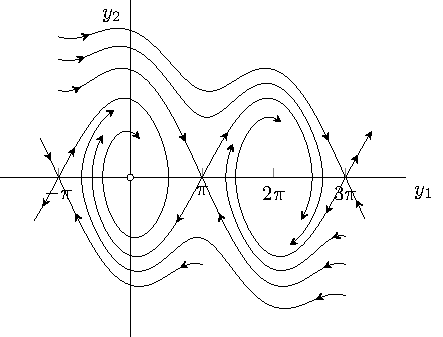
\includegraphics{figSystemPendulumLossyA}
\caption{تقصیری ارتعاش۔مثال \حوالہ{مثال_نظام_دھاگے_سے_لٹکی_کمیت_تقصیری}}
\label{شکل_مثال_نظام_دھاگے_سے_لٹکی_کمیت_تقصیری}
\end{figure}

شکل \حوالہ{شکل_مثال_نظام_دھاگے_سے_لٹکی_کمیت_تقصیری} میں نظام \حوالہ{مساوات_نظام_غیر_خطی_ترکیب_تقصیری_الف} کے خط حرکت دکھائے گئے ہیں۔چونکہ قصری نظام میں توانائی کا ضیاع پایا جاتا ہے لہٰذا شکل \حوالہ{شکل_مثال_نظام_دھاگے_سے_لٹکی_کمیت} کے بند دائروں کی بجائے شکل \حوالہ{شکل_مثال_نظام_دھاگے_سے_لٹکی_کمیت_تقصیری} کے مرغولی خطوط حاصل ہوتے ہیں جو ہمارے توقع کے عین مطابق ہے۔مزید یہ کہ دوری لہری خطوط بھی کسی نہ کسی مقام پر نقطہ فاصل کے گرد گھومنا شروع کر دیتے ہیں۔ اس کے علاوہ اب قصری نظام میں نقطہ زین کو ملانے والے خط نہیں پائے جاتے۔
\انتہا{مثال}
%======================
\ابتدا{مثال}\شناخت{مثال_نظام_شکار_شکاری}\quad آبادی شکار اور شکاری۔ [مسئلہ لوٹکا-ولٹیرا]\\
یہاں لومڑی (شکاری) اور خرگوش (شکار) کی آبادی کے مسئلے پر غور کرتے ہیں۔

\موٹا{پہلا قدم}: ہم فرض کرتے ہیں کہ خرگوش کو جتنی خوراک چاہیے دستیاب ہے۔ یوں لومڑی کی غیر موجودگی میں ان کی تعداد \عددی{y_1'=ay_1} کے تحت قوت نمائی طور پر بڑھے گی۔ لومڑی کی موجودگی میں (اتفاقی آمنے سامنے سے)  خرگوش کی تعداد میں \عددی{y_1y_2} کے راست متناسب کمی پیدا ہو گی۔یوں خرگوش کی تعداد \عددی{y_1'=ay_1-by_1y_2} سے حاصل ہو گی جہاں مستقل \عددی{a>0} اور \عددی{b>0} ہیں۔اسی طرح خرگوش کی غیر موجودگی میں لومڑی کی تعداد \عددی{y_2'=-ly_2} کے تحت قوت نمائی طور پر گھٹے گی۔خرگوش کی موجودگی میں (اتفاقی آمنے سامنے سے) لومڑی کی تعداد \عددی{y_1y_2} کے راست متناسب بڑھے گی۔یوں خرگوش کی موجودگی میں  \عددی{y_2'=-ly_2+ky_1y_2} لومڑی کی تعداد دے گا جہاں مستقل \عددی{l>0} اور \عددی{k>0} ہیں۔

یوں غیر خطی \اصطلاح{مسئلہ لوٹکا-ولٹیرا}\حاشیہد{امریکی ماہر حیاتی طبیعیات الفرڈ جیمز لوٹکا [1880-1949] اور اطالوی ریاضی دان ویٹو ولٹیرا [1860-1940] نے شکار اور شکاری کے مسئلے کو پیش کیا۔} 
\begin{gather}\label{مثال_نظام_شکار_شکاری_الف}
\begin{aligned}
y_1'&=f_1(y_1,y_2)=ay_1-by_1y_2\\
y_2'&=f_2(y_1,y_2)=ky_1y_2-ly_2
\end{aligned}
\end{gather}
حاصل ہوتا ہے۔

\موٹا{دوسرا قدم} مسئلے کو خطی بنانا اور نقطہ فاصل \عددی{(0,0)} کا حصول  ہے۔مساوات \حوالہ{مثال_نظام_شکار_شکاری_الف} کو دیکھ کر نقطہ فاصل مساوات 
\begin{align}
f_1(y_1,y_2)=y_1(a-by_2)=0, \quad f_2(y_1,y_2)=y_2(ky_1-l)=0
\end{align}
کے حل سے \عددی{(y_1,y_2)=(0,0)} اور \عددی{(\tfrac{l}{k},\tfrac{a}{b})} حاصل ہوتے ہیں۔آئیں \عددی{(0,0)} پر غور کریں۔ نقطہ \عددی{(0,0)} کے ہمسائیگی میں مساوات \حوالہ{مثال_نظام_شکار_شکاری_الف} میں \عددی{-by_1y_2} اور \عددی{ky_1y_2} کو نظر انداز کرتے ہوئے خطی نظام
\begin{align*}
\bM{y}'=\begin{bmatrix*}[r] a&0\\0&-l \end{bmatrix*}\bM{y}
\end{align*}
حاصل ہوتا ہے جس کی آئگنی قدر \عددی{\lambda_1=a>0} اور \عددی{\lambda_2=-l<0} کی علامتیں آپس میں الٹ ہیں لہٰذا \عددی{(0,0)} پر نقطہ زین پایا جاتا ہے۔

\موٹا{تیسرا قدم} مسئلے کو خطی بنانا اور نقطہ فاصل \عددی{(\tfrac{l}{k},\tfrac{a}{b})} کا حصول  ہے۔دوسرا نقطہ فاصل \عددی{(y_1,y_2)=(\tfrac{l}{k},\tfrac{a}{b})} پر پایا جاتا ہے۔اس نقطے  کو \عددی{(0,0)} منتقل کرنے کی خاطر ہم \عددی{y_1=\tilde{y}_1+\tfrac{l}{k}} اور \عددی{y_2=\tilde{y}_2+\tfrac{a}{b}} چنتے ہیں۔یوں نقطہ فاصل \عددی{(\tilde{y}_1,\tilde{y}_2)=(0,0)} لکھا جا سکتا ہے۔ چونکہ \عددی{y_1=\tilde{y}_1'} اور \عددی{y_2'=\tilde{y}_2'} ہیں لہٰذا نظام \حوالہ{مثال_نظام_شکار_شکاری_الف} کو درج ذیل لکھا جا سکتا ہے۔
\begin{align*}
\tilde{y}_1'&=\left(\tilde{y}_1+\frac{l}{k}\right)\left[a-b\left(\tilde{y}_2+\frac{a}{b}\right)\right]=\left(\tilde{y}_1+\frac{l}{k}\right)(-b\tilde{y}_2)\\
\tilde{y}_2'&=\left(\tilde{y}_2+\frac{a}{b}\right)\left[k\left(\tilde{y}_1+\frac{l}{k}\right)-l\right]=\left(\tilde{y}_2+\frac{a}{b}\right)k\tilde{y}_1
\end{align*}
نقطہ \عددی{(\tilde{y}_1,\tilde{y}_2)=(0,0)} کے ہمسائیگی میں \عددی{-b\tilde{y}_1\tilde{y}_2} اور \عددی{k\tilde{y}_1\tilde{y}_2} کو نظر انداز کرتے ہوئے خطی نظام
\begin{gather}\label{مثال_نظام_شکار_شکاری_ب}
\begin{aligned}
\tilde{y}_1'&=-\frac{bl}{k}\tilde{y}_2\quad \quad \text{(الف)}\\
\tilde{y}_2'&=\frac{ak}{b}\tilde{y}_1\quad \quad \text{(ب)}
\end{aligned}
\end{gather}
حاصل ہوتا ہے۔مساوات \حوالہ{مثال_نظام_شکار_شکاری_ب}-الف کا بایاں ہاتھ ضرب مساوات-ب کا دایاں ہاتھ برابر ہو گا الف کا دایاں ضرب ب کا بایاں،
\begin{align*}
\frac{ak}{b}\tilde{y}_1'\tilde{y}_1=-\frac{bl}{k}\tilde{y}_2'\tilde{y}_2 \implies \frac{ak}{b}\tilde{y}_1^2+\frac{bl}{k}\tilde{y}_2^2=C
\end{align*}
جس کا تکمل لیتے ہوئے \عددی{\tilde{y}_1} بالمقابل \عددی{\tilde{y}_2} کا \اصطلاح{ترخیمی}\فرہنگ{ترخیم}\حاشیہب{elliptic}\فرہنگ{elliptic} تعلق حاصل کیا گیا ہے۔یوں \عددی{(\tfrac{l}{k},\tfrac{a}{b})} پر شکل \حوالہ{شکل_مثال_نظام_شکار_شکاری} میں دکھایا گیا \اصطلاح{وسط} پایا جاتا ہے۔
\begin{figure}
\centering
\begin{tikzpicture}
%axis
\draw(0,0)--++(4,0)node[right]{$y_1$};
\draw(0,0)--++(0,2)node[left]{$y_2$};
\draw[->-=0.25] ([shift={(0:1cm and 0.5cm)}]2,1) arc  (0:180:1cm and 0.5cm) arc (-180:0:1cm and 0.5cm);
\draw[fill=white](2,1) node[ocirc](kc){};
\draw[dashed] (kc)--(0,1)node[left]{$\frac{a}{b}$};
\draw[dashed](kc)--(2,0)node[below]{$\frac{l}{k}$};
\end{tikzpicture}
\caption{شکار اور شکاری کی آبادی: ماحولیاتی توازن۔}
\label{شکل_مثال_نظام_شکار_شکاری}
\end{figure}

نسبتاً مشکل تجزیے سے ثابت کیا جا سکتا ہے کہ غیر خطی نظام \حوالہ{مثال_نظام_شکار_شکاری_الف} کا \عددی{(\tfrac{l}{k},\tfrac{a}{b})}  پر وسط پایا جاتا ہے البتہ خط حرکت اس نقطے کے گرد غیر ترخیمی بند دائرہ بناتا ہے۔

شکل \حوالہ{شکل_مثال_نظام_شکار_شکاری} کے دائیں کنارے پر خرگوش کی تعداد \عددی{y_1} زیادہ سے زیادہ ہے جس کی وجہ سے لومٹری کی تعداد \عددی{y_2} میں اضافے کی شرح بھی زیادہ سے زیادہ ہے۔اس خط پر گھڑی کی الٹی سمت چلتے ہوئے لومڑی کی زیادہ سے زیادہ آبادی حاصل ہوتی ہے۔اس مقام پر خرگوش کی تعداد اتنی کم ہو چکی ہوتی ہے کہ لومڑی کی بڑھتی تعداد کو خوراک پورا نہیں ہو پایا لہٰذا لومڑی کی آبادی گھٹنے شروع ہو جاتی ہے۔آپ دیکھ سکتے ہیں کہ دونوں جانوروں کی دوری تعداد حالات کے مطابق مسلسل تبدیل ہوتی ہے۔

شکار اور شکاری کی دیگر مثالیں ملخ اور گھاس، ببر شیر اور زیبرا ہیں۔
\انتہا{مثال}
%=====================


\جزوحصہ{سطح حرکت پر ایک درجی مساوات میں تبادلہ}
سطح حرکت کی دوسری ترکیب خود مختار [جس میں \عددیء{t} صریحاً نہیں پایا جاتا] دو درجی سادہ تفرقی مساوات
\begin{align*}
F(y,y',y'')=0
\end{align*}
میں \عددی{y=y_1} کو آزاد متغیرہ اور \عددی{y'=y_2} لے کر \عددی{y''} کو زنجیری تفرق سے
\begin{align*}
y''=y_2'=\frac{\dif y_2}{\dif t}=\frac{\dif y_2}{\dif y_1}\frac{\dif y_1}{\dif t}=\frac{\dif y_2}{\dif y_1}y_2
\end{align*}
لکھ کر ایک درجی مساوات
\begin{align}
F\left(y_1,y_2,\frac{\dif y_2}{\dif y_1}y_2\right)=0
\end{align}
میں تبدیل کرنے پر مبنی ہے۔اس ایک درجی مساوات کو یا تو حل کرنا ممکن ہوتا ہے اور یا \اصطلاح{میدان ڈھال}\فرہنگ{میدان!ڈھال}\فرہنگ{ڈھال!میدان} کی مدد سے اس پر غور ممکن ہوتا ہے۔ آئیں مثال \حوالہ{مثال_نظام_دھاگے_سے_لٹکی_کمیت} پر اس ترکیب کی مدد سے غور کریں۔
%==========

\ابتدا{مثال}\شناخت{مثال_نظام_بلا_تقصیر_ارتعاش_یک_درجی_مساوات}\quad بلا تقصیر ارتعاشی نظام کی ایک درجی تفرقی مساوات۔\\
مساوات \حوالہ{مساوات_نظام_غیر_خطی_ترکیب_مرحلہ_ت} میں \عددی{\theta''+k\sin \theta=0} ہے جس میں \عددی{\theta=y_1} اور  \عددی{\theta'=y_2} (زاویائی رفتار) لیتے ہوئے
\begin{align*}
\theta''=\frac{\dif y_2}{\dif t}=\frac{\dif y_2}{\dif y_1}\frac{\dif y_1}{\dif t}=\frac{\dif y_2}{\dif y_1}y_2
\end{align*}
لکھ کر \عددی{\tfrac{\dif y_2}{\dif y_1}y_2=-k\sin y_1} ملتا ہے جس کو علیحدگی متغیرات سے \عددی{y_2\dif y_2=-k\sin y_1\dif y_1} لکھا جا سکتا ہے جس کا تکمل
\begin{align}\label{مساوات_نظام_کل_توانائی_الف}
\frac{1}{2}y_2^2=k\cos y_1+C 
\end{align}
دیتا ہے جہاں \عددی{C} تکمل کا مستقل ہے۔اس کو \عددی{mL^2} سے ضرب دینے سے
\begin{align*}
\frac{1}{2}m(Ly_2)^2-mL^2k\cos y_1=mL^2C
\end{align*}
حاصل ہوتا ہے جس کے تینوں اجزاء \اصطلاح{توانائی}\فرہنگ{توانائی}\حاشیہب{energy}\فرہنگ{energy} کو ظاہر کرتے ہیں۔چونکہ \عددی{y_2} زاویائی رفتار ہے لہٰذا \عددی{Ly_2} لمحاتی رفتار اور  \عددی{\tfrac{1}{2}m(Ly_2)^2} \اصطلاح{حرکی توانائی}\فرہنگ{حرکی توانائی}\فرہنگ{توانائی!حرکی}\حاشیہب{kinetic energy}\فرہنگ{energy!kinetic} ہے۔درج بالا مساوات کا دوسرا جزو (بمع منفی علامت) \اصطلاح{مخفی توانائی}\فرہنگ{توانائی!مخفی}\فرہنگ{مخفی توانائی}\حاشیہب{potential energy}\فرہنگ{energy!potential} ہے جبکہ مساوات کا دایاں ہاتھ \عددی{mL^2C} کل توانائی ہے۔بلا تقصیر نظام میں توانائی کا ضیاع نہیں پایا جاتا لہٰذا حزب توقع کل توانائی مستقل مقدار ہے۔آئیں دیکھیں کہ حرکت کی نوعیت کل توانائی پر کیسے منحصر ہے۔

شکل \حوالہ{شکل_مثال_نظام_دھاگے_سے_لٹکی_کمیت}-ب مختلف \عددی{C} کے لئے خط حرکت دیتی ہے۔ان خطوط کا دوری عرصہ \عددی{2\pi} ہے۔ان میں ترخیمی بند دائرے اور  لہر نما خطوط شامل ہیں جن کے مابین نقطہ زین [\عددی{(n\pi,0)} جہاں \عددی{n=\mp1,\mp3,\cdots} ہے] سے گزرتے ہوئے دو عدد خط حرکت  پائے جاتے ہیں۔مساوات \حوالہ{مساوات_نظام_کل_توانائی_الف} کے تحت \عددی{C} کی کم سے کم قیمت \عددی{C=-k} ہے جس پر \عددی{y_2=0} اور \عددی{\cos y_1=1} ہوں گے جو ساکن کمیت کو ظاہر کرتی ہے۔جس نقطے پر \عددی{y_2=\theta'=0} ہو اس نقطے پر حرت کی سمت تبدیل ہو کر الٹ ہو جائے گی لہٰذا مساوات \حوالہ{مساوات_نظام_کل_توانائی_الف} میں \عددی{y_2=0} پر کرتے ہوئے \عددی{k\cos y_1+C=0} حاصل ہوتا ہے۔اب اگر \عددی{y_1=\pi} ہو تب \عددی{\cos y_1=-1} اور یوں \عددی{C=k} ہو گا۔اس طرح اگر \عددی{-k<C<k} ہو تب \عددی{\abs{y_1}=\abs{\theta}<\pi} کی صورت میں کمیت کی حرکت کی سمت الٹ ہو گی اور \عددی{C} کی ان قیمتوں \عددی{(\abs{C}<k)} کے لئے کمیت ارتیاش پذیر ہو گا۔ترخیمی بند دائرے اس ارتعاشی حرکت کو ظاہر کرتے ہیں۔اس کے برعکس \عددی{C>k} کی صورت میں \عددی{y_2=0} ممکن نہیں ہے لہٰذا کمیت کی حرکت کی سمت الٹ نہیں ہو گی لہٰذا کمیت مرکز کے گرد گھومتا رہے گا جس کو لہری خط حرکت ظاہر کرتی ہیں۔ان دو صورتوں کے مابین \عددی{C=k} پایا جاتا ہے جس کے خطوط نقطہ زین  سے گزرتے ہیں۔انہیں شکل \حوالہ{شکل_مثال_نظام_دھاگے_سے_لٹکی_کمیت}-ب  میں دکھایا گیا ہے۔
\انتہا{مثال}
%=================== 

دو درجی مساوات کے تبادلے سے سطح حرکت پر (مثال \حوالہ{مثال_نظام_بلا_تقصیر_ارتعاش_یک_درجی_مساوات} کی طرح) قابل حل ایک درجی مساوات کے علاوہ نا قابل حل مساوات بھی اہمیت کے حامل ہے۔ایسی صورت میں میدان ڈھال [حصہ \حوالہ{حصہ_سادہ_ایک_درجی_ڈھال} دیکھیں۔] کے ذریعہ نظام کے بارے میں معلومات حاصل کرنا ممکن ہوتا ہے۔اس عمل کو ایک مشہور مثال کی مدد سے دیکھتے ہیں۔

%===============
\ابتدا{مثال}\quad منحصر بہ خود ارتعاش۔ مساوات ون در پول\\
ایسی طبعی نظام پائے جاتے ہیں جن میں معمولی ارتعاش کی صورت میں نظام کو توانائی فراہم ہوتی ہے جبکہ وسیع ارتعاش کی صورت میں نظام سے توانائی کا اخراج ہوتا ہے۔یوں وسیع ارتعاش کی صورت میں نظام قصری صورت اختیار کرتا ہے جبکہ کم ارتعاش کی صورت میں نظام میں \ترچھا{منفی تقصیر} (نظام کو توانائی کی فراہمی) پائی جاتی ہے۔ ہم طبعی وجوہات کی بنا توقع کرتے ہیں کہ ایسا نظام دوری طرز عمل رکھے گا، جو سطح حرکت پر بند دائرے کی صورت اختیار کرے گا جسے  \اصطلاح{تحدیدی دائرہ}\فرہنگ{تحدیدی دائرہ}\حاشیہب{limit cycle}\فرہنگ{limit cycle} کہتے ہیں۔ایسی ارتعاش کو \اصطلاح{مساوات ون در پول}\فرہنگ{مساوات!ون در پول}\فرہنگ{ون در پول مساوات}\حاشیہب{van del Pol equation}\فرہنگ{van der Pol equation} 
\begin{align}\label{مساوات_نظام_ون_در_پول}
y''-\mu(1-y^2)y'+y=0\quad \quad (\mu >0)
\end{align}
ظاہر کرتی ہے جہاں \عددی{\mu} مثبت مستقل ہے۔یہ مساوات پہلی مرتبہ \اصطلاح{خلا نلکی}\فرہنگ{خلا نلکی}\حاشیہب{vacuum tube}\فرہنگ{vacuum tube} والے برقی ادوار پر غور کے دوران رو پذیر ہوئی۔یہ مساوات \عددی{\mu=0} کی صورت میں ہارمونی ارتعاش کی تفرقی مساوات \عددی{y''+y=0} ہے۔ون در پول مساوات میں قصری جزو \عددی{-\mu(1-y^2)} ہے جہاں \عددی{\mu>0} ہے۔ یوں \عددی{y^2<1} کی صورت میں منفی تقصیری، \عددی{y^2=1} کی صورت میں بلا تقصیر جبکہ \عددی{y^2>1} کی صورت میں مثبت تقصیری (جس میں توانائی کا ضیاع ہو گا) نظام پایا جائے گا۔ نہایت کم \عددی{\mu} کی صورت میں مساوات ون در پول اور \عددی{y''+y=0} میں بہت کم فرق پایا جائے گا لہٰذا ہم توقع کرتے ہیں کہ سطح حرکت پر تحدیدی دائرہ تقریباً گول دائرہ ہو گا۔اگر \عددی{\mu} کی قیمت زیادہ ہو تب تحدیدی دائرہ کی شکل غالباً مختلف ہو گی۔

اس مساوات کو ایک درجی مساوات میں تبدیل کرنے کی خاطر \عددی{y=y_1}، \عددی{y'=y_2} اور \عددی{y''=\tfrac{\dif y_2}{\dif y_1}y_2} لکھتے ہوئے  ون در پول مساوات درج ذیل صورت اختیار کرتی ہے۔
\begin{align}
\frac{\dif y_2}{\dif y_1}y_2-\mu(1-y_1^2)y_2+y_1=0
\end{align}
سطح حرکت (\عددیء{y_1y_2} سطح) پر \اصطلاح{ہم میلان}\فرہنگ{ہم میلان}\حاشیہب{isoclines}\فرہنگ{isoclines} خط \عددی{\tfrac{\dif y_2}{\dif y_1}=K} ہیں جہاں \عددی{K} مستقل مقدار ہے۔یوں ہم میلان خطوط درج ذیل ہوں گے
\begin{align*}
\frac{\dif y_2}{\dif y_1}=\mu(1-y_1^2)-\frac{y_1}{y_2}=K
\end{align*}
جن سے 
\begin{align}
y_2=\frac{y_1}{\mu(1-y_1^2)-K}\quad \quad \text{(\RL{شکل \حوالہ{شکل_نظام_ون_ڈر_پول_پہلی_شکل} اور شکل \حوالہ{شکل_نظام_ون_ڈر_پول_دوسری_شکل} دیکھیں۔})}
\end{align}
حاصل ہوتا ہے۔
\begin{figure}
\centering
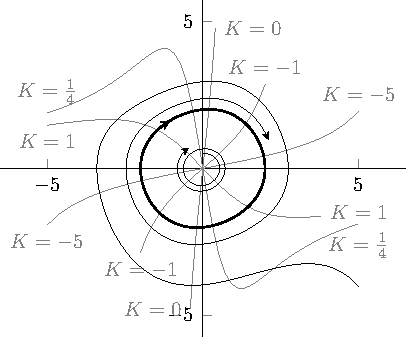
\includegraphics{figSystemVanDerPolEquationA}
\caption{ون ڈر پول مساوات؛ \عددی{\mu=0.1} لیتے ہوئے دو خط حرکت کو تحدیدی دائرہ تک پہنچتے ہوئے دکھایا گیا ہے۔}
\label{شکل_نظام_ون_ڈر_پول_پہلی_شکل}
\end{figure}

شکل \حوالہ{شکل_نظام_ون_ڈر_پول_پہلی_شکل} میں \عددی{\mu} کی کم قیمت \عددی{(\mu=0.1)} کے لئے چند ہم میلان خطوط کو ہلکی سیاہی میں دکھایا گیا ہے۔اس کے علاوہ تحدیدی دائرے کو موٹی لکیر سے ظاہر کیا گیا ہے۔تحدیدی دائرہ تقریباً گول ہے۔ ایک خط حرکت، جو تحدیدی دائرے کے باہر ہے، اور دوسرا خط حرکت، جو تحدیدی دائرے کے اندر  ہے، کو  تحدیدی دائرے تک پہنچتے ہوئے دکھایا گیا ہے۔تحدیدی دائرہ اور نقطہ فاصل کے گرد بند دائرہ (وسط) میں فرق یہ ہے کہ تحدیدی دائرے تک خط حرکت پہنچتی ہے جبکہ وسط کا خط اسی دائرے پر پایا جاتا ہے۔ \عددی{\mu} کی زیادہ قیمت پر تحدیدی دائرہ گول صورت نہیں رکھتا۔ شکل \حوالہ{شکل_نظام_ون_ڈر_پول_دوسری_شکل} میں \عددی{\mu} کی زیادہ قیمت \عددی{(\mu=1)} کے لئے  تمام صورت حال دکھائی گئی ہے جہاں تحدیدی دائرہ گول نہیں ہے۔
\begin{figure}
\centering
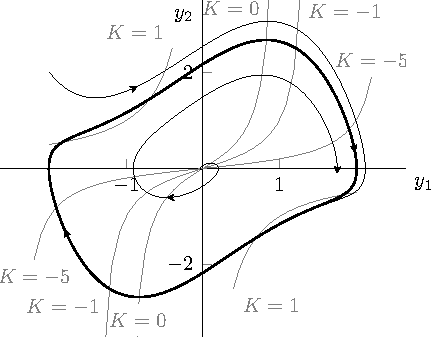
\includegraphics{figSystemVanDerPolEquationB}
\caption{ون ڈر پول مساوات؛ \عددی{\mu=1} لیتے ہوئے دو خط حرکت کو تحدیدی دائرہ تک پہنچتے ہوئے دکھایا گیا ہے۔}
\label{شکل_نظام_ون_ڈر_پول_دوسری_شکل}
\end{figure}
\انتہا{مثال}
%=====================
\ابتدا{مثال}
تفرقی مساوات \عددی{y''+y-y^3=0} سے نظام حاصل کریں۔اس نظام کے تمام نقطہ فاصل دریافت کریں۔نقطہ فاصل کی نوعیت دریافت کریں۔

حل:\عددی{y=y_1} اور \عددی{y'=y_1'=y_2} لیتے ہوئے اور \عددی{y''=y_2'} لکھتے ہوئے دیے گئے دو درجی مساوات سے نظام
\begin{gather}
\begin{aligned}\label{مساوات_مثال_نظام_تفرقی_سے_نظام}
y_1'&=f_1=y_2\\
y_2'&=f_2=-y_1+y_1^3
\end{aligned}
\end{gather}
 حاصل ہوتا ہے۔نقطہ فاصل \عددی{f_1=f_2=0} سے حاصل ہوں گے۔\عددی{f_1=0} سے \عددی{y_2=0} ملتا ہے جبکہ \عددی{f_2=y_1(-1+y_1^2)=0} سے \عددی{y_1=0} اور \عددی{y_1=\mp 1} ملتے ہیں۔یوں نقطہ فاصل \عددی{(0,0)}، \عددی{-1,0} اور \عددی{1,0} ہیں۔نقطہ فاصل \عددی{(0,0)} مرکز پر پایا جاتا ہے لہٰذا اس پر پہلے غور کرتے ہیں۔نقطہ فاصل کی نوعیت جاننے کی خاطر نظام کو خطی بناتے ہیں۔ایسا کوئی بھی جزو جو \عددی{y^m} یا \عددی{y_1^ny_2^q} کی صورت میں لکھا گیا ہو، جہاں \عددی{m \ne 1} جبکہ \عددی{n} اور \عددی{q} کوئی بھی  مستقل ہو سکتے ہیں، غیر خطی ہو گا۔ان غیر خطی اجزاء کو رد کرنے سے خطی نظام حاصل ہوتا ہے۔یوں \عددی{y_2'} کی مساوات میں \عددی{y_1^3} کو رد کرتے ہوئے خطی نظام 
\begin{gather*}
\begin{aligned}
y_1'&=y_2\\
y_2'&=-y_1
\end{aligned}\quad \implies \quad
\begin{aligned}
\bM{y}'=\begin{bmatrix} 0&1\\-1&0 \end{bmatrix}\bM{y}
\end{aligned}
\end{gather*}
حاصل ہو گا جس سے  \عددی{p=a_{11}+a_{22}=0}، \عددی{q=1>0} اور \عددی{\Delta=-4<0} ملتے ہیں لہٰذا نقطہ \عددی{(0,0)} مستحکم وسط ہے۔

آئیں اب نقطہ \عددی{(-1,0)} پر غور کریں۔اس کو مرکز منتقل کرنے کی خاطر نظام \حوالہ{مساوات_مثال_نظام_تفرقی_سے_نظام} میں \عددی{\tilde{y}_1=y_1+1} یعنی \عددی{y_1=\tilde{y}_1-1} اور \عددی{\tilde{y}_2=y_2} پر کرتے ہوئے
\begin{gather*}
\begin{aligned}
\tilde{y}_1'&=\tilde{y}_2\\
\tilde{y}_2'&=-(\tilde{y}_1-1)+(\tilde{y}_1-1)^3
\end{aligned}\implies
\begin{aligned}
\tilde{y}_1'&=\tilde{y}_2\\
\tilde{y}_2'&=2\tilde{y}_1-3\tilde{y}_1^2+\tilde{y}_1^3
\end{aligned}
\end{gather*}
ملتا ہے۔ غیر خطی اجزاء \عددی{\tilde{y}_1^2} اور \عددی{\tilde{y}_1^3} کو رد کرتے ہوئے خطی نظام
\begin{gather*}
\begin{aligned}
\tilde{y}_1'&=\tilde{y}_2\\
\tilde{y}_2'&=2\tilde{y}_1
\end{aligned}\implies 
\begin{aligned}
\tilde{\bM{y}}'=\begin{bmatrix}0&1\\2&0  \end{bmatrix}\tilde{\bM{y}}
\end{aligned}
\end{gather*}
ملتا ہے۔اس سے \عددی{p=0}، \عددی{q=-2<0} اور \عددی{\Delta=8>0} حاصل ہوتے ہیں لہٰذا نقطہ \عددی{(-1,0)} غیر مستحکم نقطہ زین ہے۔

نقطہ \عددی{(1,0)} پر غور کرنے کی  خاطر اس کو مرکز منتقل کرتے ہیں۔ایسا کرنے کی خاطر \عددی{\tilde{y}_1=y_1-1} اور \عددی{\tilde{y}_2=y_2} چنتے ہیں۔یوں نظام
\begin{align*}
\tilde{y}_1'&=\tilde{y}_2\\
\tilde{y}_2'&=2\tilde{y}_1+3\tilde{y}_1^2+\tilde{y}_1^3
\end{align*}
ملتا ہے جس میں غیر خطی اجزاء  \عددی{\tilde{y}_1^2} اور \عددی{\tilde{y}_1^3} رد کرتے ہوئے  خطی نظام
\begin{gather*}
\begin{aligned}
\tilde{y}_1'&=\tilde{y}_2\\
\tilde{y}_2'&=2\tilde{y}_1
\end{aligned}\implies 
\begin{aligned}
\tilde{\bM{y}}'=\begin{bmatrix}0&1\\2&0  \end{bmatrix}\tilde{\bM{y}}
\end{aligned}
\end{gather*}

ملتا ہے۔اس سے \عددی{p=0}، \عددی{q=-2<0} اور \عددی{\Delta=8>0} حاصل ہوتے ہیں لہٰذا نقطہ \عددی{(1,0)} غیر مستحکم نقطہ زین ہے۔
\انتہا{مثال}
%======================

\حصہء{سوالات}
سوال \حوالہ{سوال_نظام_خطی_بنانا_الف} تا سوال \حوالہ{سوال_نظام_خطی_بنانا_ب} کو \موٹا{خطی بناتے} ہوئے تمام نقطہ فاصل دریافت کریں۔ نقطہ فاصل کی نوعیت جدول \حوالہ{جدول_نظام_نقطہ_فاصل_اصول_جانچ} اور جدول \حوالہ{جدول_نظام_نقطہ_فاصل_بالمقابل_استحکام} کی مدد سے دریافت کریں۔

%===============
\ابتدا{سوال}\شناخت{سوال_نظام_خطی_بنانا_الف}\quad 
$y_1'=4y_1-y_1^2,\quad y_2'=y_2$

جوابات:نقطہ فاصل \عددی{f_1=f_2=0} سے \عددی{(0,0)} اور \عددی{(4,0)} حاصل ہوتے ہیں۔مسئلے کو \عددی{(0,0)} پر خطی بناتے ہوئے \عددی{\bM{A}=\begin{bmatrix} 4&0\\0&1  \end{bmatrix}} لکھا جاتا ہے جس سے \عددی{p>0}، \عددی{q>0} اور \عددی{\Delta>0} ملتا ہے لہٰذا نقطہ \عددی{(0,0)} غیر مستحکم جوڑ ہے۔ نقطہ \عددی{(4,0)} کو مرکز پر منتقل کرنے کی خاطر \عددی{\tilde{y}_1=y_1-4} اور \عددی{\tilde{y}_2=y_2} پر کرتے ہیں اور مسئلے کو (\عددی{-\tilde{y}_1^2} رد کرتے ہوئے) خطی بناتے ہوئے \عددی{\bM{A}=\begin{bmatrix} -4&0\\0&1  \end{bmatrix}} حاصل ہوتا ہے جو \عددی{p<0}، \عددی{q<0} اور \عددی{\Delta>0} دیتا ہے  جو غیر مستحکم نقطہ زین کو ظاہر کرتی ہے۔
\انتہا{سوال}
%======================
\ابتدا{سوال}\quad 
$y_1'=y_2,\quad y_2'=-y_1+\frac{2}{3}y_1^2$\\
جوابات:نقطہ فاصل \عددی{f_1=f_2=0} سے \عددی{(0,0)} اور \عددی{(\tfrac{3}{2},0)} حاصل ہوتے ہیں۔نقطہ \عددی{(0,0)} پر مسئلہ خطی بناتے ہوئے \عددی{\bM{A}=\begin{bmatrix} 0&1\\-1&0  \end{bmatrix}} حاصل ہوتا ہے جس سے \عددی{p=0}، \عددی{q>0} اور \عددی{\Delta<0} ملتے ہیں لہٰذا نقطہ \عددی{(0,0)} مستحکم وسط ہے۔ نقطہ \عددی{(\tfrac{3}{2},0)} کو مرکز پر منتقل کرنے کی خاطر \عددی{\tilde{y}_1=y_1-\tfrac{3}{2}} اور \عددی{\tilde{y}_2=y_2} پر کرتے ہیں اور  مسئلے کو (\عددی{\tfrac{2}{3}\tilde{y}_1^2} رد کرتے ہوئے) خطی بنانے سے  \عددی{\bM{A}=\begin{bmatrix} 0&1\\1&0  \end{bmatrix}} حاصل ہوتا ہے لہٰذا \عددی{(\tfrac{2}{3},0)} غیر مستحکم نقطہ زین ہے۔
\انتہا{سوال}
%======================
\ابتدا{سوال}\quad 
$y_1'=y_2,\quad y_2'=-2y_1-y_1^2$\\
جوابات:مستحکم وسط \عددی{(0,0)} پر پایا جاتا ہے جبکہ \عددی{(-2,0)} غیر مستحکم نقطہ زین  ہے۔
\انتہا{سوال}
%======================
\ابتدا{سوال}\quad 
$y_1'=-y_1+y_2+y_1^2,\quad y_2'=-y_1-y_2$\\
جوابات:\عددی{(0,0)} پر مستحکم اور جاذب نقطہ مرغولہ پایا جاتا ہے جبکہ \عددی{(-2,2)} پر غیر مستحکم نقطہ زین پایا جاتا ہے۔
\انتہا{سوال}
%======================
\ابتدا{سوال}\شناخت{سوال_نظام_خطی_بنانا_ب}\quad 
$y_1'=-y_1+y_2-y_2^2,\quad y_2'=-y_1-y_2$\\
جوابات:\عددی{(0,0)} پر جاذب  نقطہ مرغولہ  پایا جاتا ہے جبکہ \عددی{(-2,2)} پر غیر مستحکم نقطہ زین پایا جاتا ہے۔
\انتہا{سوال}
%======================

سوال \حوالہ{سوال_نظام_تفرقی_سے_نظام_الف} تا سوال \حوالہ{سوال_نظام_تفرقی_سے_نظام_ب} میں تفرقی مساوات سے نظام حاصل کریں۔اس نظام کے تمام نقطہ فاصل دریافت کریں۔نظام کو خطی بناتے ہوئے نقطہ فاصل کی نوعیت دریافت کریں۔

%==================
\ابتدا{سوال}\شناخت{سوال_نظام_تفرقی_سے_نظام_الف}\quad 
$y''-4y+y^3=0$\\
جوابات: نظام \عددی{y_1'=y_2} اور \عددی{y_2'=4y_1-y_1^3} حاصل ہوتا ہے۔\عددی{(0,0)} غیر مستحکم نقطہ زین، \عددی{(-2,0)} مستحکم وسط اور \عددی{(2,0)} مستحکم وسط ہیں۔
\انتہا{سوال}
%========================
\ابتدا{سوال}\quad 
$y''+4y-y^3=0$\\
جوابات: نظام \عددی{y_1'=y_2} اور \عددی{y_2'=4y_1-y_1^3} حاصل ہوتا ہے۔\عددی{(0,0)} مستحکم وسط، \عددی{(-2,0)} غیر مستحکم نقطہ زین اور \عددی{(2,0)} غیر مستحکم نقطہ زین ہیں۔
\انتہا{سوال}
%========================
\ابتدا{سوال}\quad 
$y''+4y+y^2=0$\\
جوابات:\عددی{(0,0)} مستحکم وسط اور \عددی{(-4,0)} غیر مستحکم نقطہ زین ہے۔
\انتہا{سوال}
%========================
\ابتدا{سوال}\quad 
$y''+\sin y=0$\\
جوابات: \عددی{(0,0)} اور \عددی{(\mp n2\pi,0)} مستحکم وسط ہیں جہاں \عددی{n=1,2,3,\cdots} ہو سکتا ہے۔نقطہ \عددی{(\mp m\pi,0)} غیر مستحکم نقطہ زین ہے جہاں \عددی{m=1,3,5,\cdots} ہو سکتا ہے۔
\انتہا{سوال}
%========================
\ابتدا{سوال}\شناخت{سوال_نظام_تفرقی_سے_نظام_ب}\quad 
$y''+\cos y=0$\\
جوابات: نقطہ \عددی{(\tfrac{\pi}{2}\mp n2\pi,0)} غیر مستحکم نقطہ نیز  جبکہ \عددی{(-\tfrac{\pi}{2}\mp n2\pi,0)} وسط ہیں جہاں \عددی{n=1,2,3,\cdots} ہو سکتا ہے۔آپ کو \عددی{-\cos(\mp\tfrac{\pi}{2}+\tilde{y}_1)=\sin(\mp \tilde{y}_1)\approx \mp \tilde{y}_1} کی مدد لے سکتے ہیں۔
\انتہا{سوال}
%========================
\ابتدا{سوال}\quad ریلے مساوات\\
\عددی{Y''-\mu(1-\tfrac{1}{3}Y'^2)Y'+Y=0} جہاں \عددی{\mu >0} ہے، \اصطلاح{ریلے مساوات}\فرہنگ{ریلے مساوات}\فرہنگ{مساوات!ریلے}\حاشیہب{Rayleigh equation}\فرہنگ{Rayleigh equation}\فرہنگ{equation!Rayleigh}  کہلاتی\حاشیہد{لارڈ ریلے، جن کا اصل نام جان ولیم سٹرٹ ہے  انگلستان کے ماہر طبیعیات اور ریاضی دان تھے۔} ہے۔اس میں \عددی{y=Y'} پر کرتے ہوئے تفرق لے کر \موٹا{ون در پول مساوات} حاصل کریں۔
\انتہا{سوال}
%====================
\ابتدا{سوال}\quad ڈفنگ مساوات\\
اسپرنگ اور کمیت کی مساوات \عددی{y''+\omega_0^2=0} میں غیر خطی قوت بحالی کی صورت میں \اصطلاح{ڈفنگ مساوات}\فرہنگ{ڈفنگ مساوات}\فرہنگ{مساوات!ڈفنگ}\حاشیہب{Duffing equation}\فرہنگ{equation!Duffing}\فرہنگ{Duffing equation} \عددی{y''+\omega_0^2y+\beta y^3=0} حاصل ہوتی ہے جہاں \عددی{\abs{\beta}} عموماً چھوٹی مقدار ہوتی ہے۔\عددی{\beta>0} کو \ترچھا{سخت اسپرنگ} اور \عددی{\beta<0} کو \ترچھا{نرم اسپرنگ} کی صورت پکارا جاتا ہے۔سطح حرکت پر خط حرکت کی مساوات دریافت کریں۔

جواب:\عددی{2y_2^2+2\omega_0^2y_1^2+\beta y_1^4=K} جہاں \عددی{K} مستقل مقدار ہے۔
\انتہا{سوال}
%====================
\ابتدا{سوال}\quad خط حرکت\\
سادہ تفرقی مساوات \عددی{y''-9y+y^3=0} کو نظام کی صورت میں لکھیں جس کو حل کرتے ہوئے \عددی{y_2} بالمقابل \عددی{y_1} کی مساوات حاصل کریں۔حاصل مساوات سے سطح حرکت پر چند خط حرکت کھینچیں۔

جواب:\عددی{2y_2^2=18y_1^2-y_1^4+K} جہاں \عددی{K} مستقل مقدار ہے۔
\انتہا{سوال}
%=====================

\حصہ{سادہ تفرقی مساوات کے غیر متجانس خطی نظام}
اس حصے میں غیر متجانس نظام
\begin{align}\label{مساوات_نظام_غیر_متجانس_مساوات_الف}
\bM{y}'=\bM{A}\bM{y}+\bM{g}\quad \quad \text{\RL{(حصہ \حوالہ{حصہ_نظام_نظریہ_نظام} دیکھیں)}}
\end{align}
جہاں \عددی{\bM{g}} غیر صفر سمتیہ  ہے، کو حل کرنا سیکھتے ہیں۔ہم فرض کرتے ہیں کہ \عددی{\bM{g}(t)} اور \عددی{n \times n} قالب \عددی{\bM{A}(t)} کے ارکان،  محور \عددی{t} کے کھلے وقفہ \عددی{J} پر استمراری ہیں۔وقفہ \عددی{J} پر متجانس مساوات \عددی{\bM{y}'=\bM{A}\bM{y}} کے عمومی حل \عددی{\bM{y}^{(h)}(t)} اور \عددی{J} پر مساوات \حوالہ{مساوات_نظام_غیر_متجانس_مساوات_الف} کے کسی بھی \اصطلاح{مخصوص حل}\فرہنگ{مخصوص حل}\فرہنگ{particular solution} \عددی{\bM{y}^{(p)}(t)} [جس میں کوئی مستقل نہیں پایا جاتا] سے مساوات \حوالہ{مساوات_نظام_غیر_متجانس_مساوات_الف} کا \عددی{J} پر \اصطلاح{عمومی حل}\فرہنگ{عمومی حل}\فرہنگ{حل!عمومی}\فرہنگ{general!solution}
\begin{align}\label{مساوات_نظام_غیر_متجانس_مساوات_ب}
\bM{y}=\bM{y}^{(h)}+\bM{y}^{(p)}
\end{align}
حاصل ہوتا ہے۔مسئلہ \حوالہ{مسئلہ_نظام_خطی_نظام_وجودیت_یکتائی} کے تحت عمومی حل \عددی{\bM{y}} میں \عددی{J} پر مساوات \حوالہ{مساوات_نظام_غیر_متجانس_مساوات_الف} کے تمام ممکنہ حل شامل ہیں۔

متجانس مساوات کے حل پر ہم گزشتہ حصوں میں غور کر چکے ہیں۔اس حصے میں غیر متجانس مساوات کے مخصوص حل کے حصول پر غور کرتے ہیں۔نا معلوم عددی سر کی ترکیب اور مقدار معلوم بدلنے کے طریقوں پر غور کرتے ہیں جنہیں ہم حصہ \حوالہ{حصہ_سادہ_دو_غیر_متجانس} اور حصہ \حوالہ{سادہ_دو_متغیرات_بدلنے_کا_طریقہ} سے جانتے ہیں۔ 
%=============

\جزوحصہ{نا معلوم عددی سر کی ترکیب}
 ایک عدد سادہ تفرقی مساوات کے حل میں استعمال ہونے کی طرح اب بھی یہ ترکیب اس صورت  قابل استعمال ہو گی جب  \عددی{\bM{A}} کے ارکان مستقل مقدار ہوں  جبکہ مستقل مقدار، \عددی{t^m} (جہاں \عددی{m} مثبت اعداد ہیں)، قوت نمائی، سائن  اور کوسائن تفاعل کا کوئی بھی مجموعہ \عددی{\bM{g}}  ہو۔ایسی صورت میں مخصوص حل کو \عددی{\bM{g}} کی طرح تصور کیا جاتا ہے لہٰذا \عددی{\bM{g}=t^2} ہونے کی صورت میں \عددی{\bM{y}^{(p)}=\bM{u}+\bM{v}t+\bM{w}t^2} فرض کیا جائے گا۔ مساوات \حوالہ{مساوات_نظام_غیر_متجانس_مساوات_الف} میں \عددی{\bM{y}^{(p)}} پر کرتے ہوئے \عددی{\bM{u}}،  \عددی{\bM{v}} اور \عددی{\bM{w}} حاصل کیے جاتے ہیں۔یہ حصہ \حوالہ{حصہ_سادہ_دو_غیر_متجانس} کی طرح ہے البتہ یہاں ترمیمی قاعدہ قدر مختلف ہے۔ آئیں ایک مثال کی مدد سے اس ترکیب کا استعمال دیکھیں۔
%================

\ابتدا{مثال}\شناخت{مثال_نظام_غیر_متجانس_نا_معلوم_سر}\quad نا معلوم عددی سر کی ترکیب۔ترمیمی قاعدہ\\
درج ذیل مساوات کی عمومی حل حاصل کریں۔
\begin{align}\label{مساوات_مثال_غیر_متجانس_نا_معلوم_سر_الف}
\bM{y}'=\bM{A}\bM{y}+\bM{g}=\begin{bmatrix*}[r] -2&1\\1&-2 \end{bmatrix*} \bM{y}+\begin{bmatrix*}[r] -4\\3 \end{bmatrix*} e^{-3t}
\end{align}

حل:ہم صفحہ \حوالہصفحہ{مثال_نظام_خط_حرکت_غیر_مناسب} پر مثال \حوالہ{مثال_نظام_خط_حرکت_غیر_مناسب} میں نظیری متجانس مساوات کا حل 
\begin{align}\label{مساوات_مثال_غیر_متجانس_نا_معلوم_سر_ب}
\bM{y}^{(h)}=c_1\begin{bmatrix} 1 \\ 1 \end{bmatrix}e^{-t}+c_2\begin{bmatrix*}[r] 1\\ -1 \end{bmatrix*}e^{-3t}
\end{align}
حاصل کر چکے ہیں۔چونکہ \عددی{\bM{A}} کا  \عددی{\lambda=-3} آئگنی قدر ہے اور مساوات \حوالہ{مساوات_مثال_غیر_متجانس_نا_معلوم_سر_الف} میں دائیں جانب \عددی{e^{-3t}} پایا جاتا ہے لہٰذا  اس جزو کو \عددی{t} سے ضرب دیتے ہوئے \عددی{\bM{y}^{(p)}} میں شامل کرتے ہیں۔
\begin{align}\label{مساوات_مثال_غیر_متجانس_نا_معلوم_سر_پ}
\bM{y}^{(p)}=\bM{u}te^{-3t}+\bM{v}e^{-3t} \quad \quad 
\end{align} 
\عددی{\bM{y}^{(p)}} میں بائیں ہاتھ کا پہلا جزو حصہ \حوالہ{حصہ_سادہ_دو_غیر_متجانس} کا مماسی  ترمیمی قاعدہ ہے، جو یہاں نا کافی ہے۔[آپ کوشش کر کے دیکھ سکتے ہیں]۔ مساوات \حوالہ{مساوات_مثال_غیر_متجانس_نا_معلوم_سر_پ} کو مساوات \حوالہ{مساوات_مثال_غیر_متجانس_نا_معلوم_سر_الف} میں پر کرتے ہیں۔
\begin{align*}
\bM{y}^{(p)'}=\bM{u}e^{-3t}-3\bM{u}te^{-3t}-3\bM{v}e^{-3t}=\bM{A}\bM{u}te^{-3t}+\bM{A}\bM{v}e^{-3t}+\bM{g}
\end{align*}
دونوں جانب \عددی{te^{-3t}} والے اجزاء کے عددی سر برابر ہوں گے لہٰذا \عددی{-3\bM{u}=\bM{A}\bM{u}} ہو گا۔یوں \عددی{\bM{A}} قالب کے آئگنی قدر \عددی{\lambda=-3} کا نظیری آئگنی سمتیہ \عددی{\bM{u}} ہو گا۔اس طرح \عددی{\bM{u}=a[1\quad -1]^T} لکھا جا سکتا ہے جہاں \عددی{a} کوئی بھی غیر صفر مستقل ہو سکتا ہے۔بقایا اجزاء کے عددی سر برابر لکھ کر
\begin{gather*}
\begin{aligned}
\bM{u}-3\bM{v}=\bM{A}\bM{v}+\bM{g}
\end{aligned}\implies
\begin{aligned}
\begin{bmatrix*}[r] a\\-a  \end{bmatrix*}-\begin{bmatrix} 3v_1\\3v_2 \end{bmatrix}=\begin{bmatrix*}[r] -2v_1+v_2\\v_1-2v_2 \end{bmatrix*}+\begin{bmatrix*}[r] -4\\3 \end{bmatrix*}
\end{aligned} 
\end{gather*}
ترتیب دیتے ہیں۔
\begin{align*}
v_1+v_2&=a+4\\
v_1+v_2&=-a-3
\end{align*}
دوسری مساوات کو پہلی سے منفی کرتے ہوئے \عددی{2a+7=0} یعنی \عددی{a=-\tfrac{7}{2}} ملتا ہے۔یوں درج بالا میں پہلی مساوات \عددی{v_1+v_2=-\tfrac{7}{2}+4=\tfrac{1}{2}} ہو گی جس  میں  \عددی{v_1=k} لیتے ہوئے  \عددی{v_2=\tfrac{1}{2}-k} حاصل ہوتا ہے۔اس طرح \عددی{\bM{v}=[k\quad \tfrac{1}{2}-k]^T} ہو گا۔ہم \عددی{k=0} چن سکتے ہیں۔ایسا ہی کرتے ہوئے عمومی حل لکھتے ہیں۔
\begin{align}
\bM{y}=\bM{y}^{(h)}+\bM{y}^{(p)}=c_1\begin{bmatrix} 1 \\[1em] 1 \end{bmatrix}e^{-t}+c_2\begin{bmatrix*}[r] 1\\[1em] -1 \end{bmatrix*}e^{-3t}-\frac{7}{2}\begin{bmatrix*}[r] 1\\[1em] -1 \end{bmatrix*}te^{-3t}+\begin{bmatrix} 0\\[1em]\frac{1}{2} \end{bmatrix}e^{-3t}
\end{align}
\عددی{k} کی قیمت تبدیل کرتے ہوئے دیگر حل لکھے جا سکتے ہیں مثلاً \عددی{k=1} لیتے ہوئے \عددی{\bM{v}=[1 \quad -\tfrac{1}{2}]^T} حاصل ہو گا جس سے درج ذیل عمومی حل ملتا ہے۔
 \begin{align}
\bM{y}=\bM{y}^{(h)}+\bM{y}^{(p)}=c_1\begin{bmatrix} 1 \\[1em] 1 \end{bmatrix}e^{-t}+c_2\begin{bmatrix*}[r] 1\\[1em] -1 \end{bmatrix*}e^{-3t}-\frac{7}{2}\begin{bmatrix*}[r] 1\\[1em] -1 \end{bmatrix*}te^{-3t}+\begin{bmatrix*}[r] 1\\[1em]-\frac{1}{2} \end{bmatrix*}e^{-3t}
\end{align}
\انتہا{مثال}
%====================
\جزوحصہء\quad مقدار معلوم بدلنے کی ترکیب\\
اس ترکیب سے غیر متجانس نظام
\begin{align}\label{مساوات_نظام_غیر_متجانس_مقدار_معلوم_الف}
\bM{y}'=\bM{A}(t)+\bM{g}(t)
\end{align}
کو حل کیا جا سکتا ہے جہاں \عددی{\bM{A}(t)} متغیر مقدار ہیں اور \عددی{\bM{g}(t)} کوئی بھی تفاعل ہو سکتا ہے۔اگر \عددی{t} محور کے کسی کھلے وقفے \عددی{J} پر  نظیری متجانس نظام کا عمومی حل \عددی{\bM{y}^{(h)}} معلوم ہو تب اس ترکیب کی مدد سے اس وقفے پر نظام \حوالہ{مساوات_نظام_غیر_متجانس_مقدار_معلوم_الف} کا مخصوص حل \عددی{\bM{y}^{(p)}} حاصل کیا جاتا ہے۔آئیں مثال \حوالہ{مثال_نظام_غیر_متجانس_نا_معلوم_سر} کو اس ترکیب سے حل کریں۔
%=================
\ابتدا{مثال}\quad مقدار معلوم بدلنے کے طریقے سے حل\\
گزشتہ مثال کے نظام \حوالہ{مساوات_مثال_غیر_متجانس_نا_معلوم_سر_الف} کو مقدار معلوم بدلنے کی ترکیب سے حل کریں۔
\begin{align}
\bM{y}'=\bM{A}\bM{y}+\bM{g}=\begin{bmatrix*}[r] -2&1\\1&-2 \end{bmatrix*} \bM{y}+\begin{bmatrix*}[r] -4\\3 \end{bmatrix*} e^{-3t}
\end{align}

حل:متجانس مساوات کی آئگنی قدر \عددی{\lambda_1=-1} اور \عددی{\lambda_2=-3} ہیں جن کے بالترتیب نظیری آئگنی سمتیات \عددی{[1 \quad 1]^T} اور \عددی{[1\quad -1]^T} ہیں لہٰذا  اساس \عددی{[e^{-t}\quad e^{-t}]^T}، \عددی{[e^{-3t}\quad -e^{-3t}]^T} ہے جس سے متجانس مساوات کا حل \عددی{\bM{y}^{(h)}} لکھتے ہیں۔
\begin{gather}
\begin{aligned}\label{مساوات_نظام_مقدار_معلوم_وائے}
\bM{y}^{(h)}&=c_1\begin{bmatrix}1\\1 \end{bmatrix}e^{-t}+c_2\begin{bmatrix*}[r]  1\\-1\end{bmatrix*}e^{-3t}=\begin{bmatrix*}[r] e^{-t}&e^{-3t} \\ e^{-t} &-e^{-3t} \end{bmatrix*} \begin{bmatrix} c_1\\c_2 \end{bmatrix}=\bM{Y}(t)\bM{c}
\end{aligned}
\end{gather}
یہاں \عددی{\bM{Y}(t)=[\bM{y}^{(1)} \quad \bM{y}^{(2)}]^T} بنیادی قالب [حصہ \حوالہ{حصہ_نظام_نظریہ_نظام} دیکھیں] ہے ۔ حصہ \حوالہ{سادہ_دو_متغیرات_بدلنے_کا_طریقہ} کی طرح ہم مستقل سمتیہ \عددی{\bM{c}} کی جگہ متغیر سمتیہ \عددی{\bM{u}} پر کرتے ہوئے مخصوص حل \عددی{\bM{y}^{(p)}} لکھتے ہیں۔
\begin{align}
\bM{y}^{(p)}=\bM{Y}(t)\bM{u}(t)
\end{align}
نظام \حوالہ{مساوات_مثال_غیر_متجانس_نا_معلوم_سر_الف} میں \عددی{\bM{y}^{(p)}} پر کرتے ہیں۔
\begin{align}\label{مساوات_نظام_بنیادی_نظام_الف}
\bM{Y}'\bM{u}+\bM{Y}\bM{u}'=\bM{A}\bM{Y}\bM{u}+\bM{g}
\end{align}
اب چونکہ \عددی{\bM{y}^{(1)}} اور \عددی{\bM{y}^{(2)}} متجانس نظام کا حل ہے لہٰذا \عددی{\bM{y}^{(1)'}=\bM{A}\bM{y}^{(1)}} اور
 \عددی{\bM{y}^{(2)'}=\bM{A}\bM{y}^{(2)}} یعنی \عددی{\bM{Y}'=\bM{A}\bM{Y}}ہو گا۔یوں \عددی{\bM{Y}'\bM{u}=\bM{A}\bM{Y}\bM{u}} لکھ کر مساوات \حوالہ{مساوات_نظام_بنیادی_نظام_الف} سے  \عددی{\bM{Y}\bM{u}'=\bM{g}} حاصل ہوتا ہے (اور چونکہ \عددی{\bM{Y}} کا امتیازی مقطع دراصل ورونسکی [حصہ \حوالہ{حصہ_نظام_قالب} دیکھیں] \عددی{W} ہے جو اساس کی صورت میں غیر صفر ہوتا ہے لہٰذا \عددی{\bM{Y}^{-1}} حاصل کیا جا سکتا ہے) لہٰذا درج ذیل لکھا جا سکتا ہے۔
\begin{align}
\bM{u}'=\bM{Y}^{-1}\bM{g}
\end{align}
 معکوس قالب کو مساوات \حوالہ{مساوات_نظام_معکوس_قالب} کی مدد سے حاصل کر کے
\begin{align*}
\bM{Y}^{-1}=\frac{1}{-2e^{-4t}}\begin{bmatrix} -e^{-3t} & -e^{-3t}\\[1em] -e^{-t}& e^{-t} \end{bmatrix}=
\frac{1}{2}\begin{bmatrix} e^{t} & e^{t}\\[1em] e^{3t}& -e^{3t}   \end{bmatrix}
\end{align*}
\عددی{\bM{g}} سے ضرب دیتے ہوئے \عددی{\bM{u}'} لکھتے ہیں۔
\begin{align*}
\bM{u}'=\bM{Y}^{-1}\bM{g}=\frac{1}{2}\begin{bmatrix} e^{t} & e^{t}\\[1em] e^{3t}& -e^{3t}   \end{bmatrix}\begin{bmatrix} -4e^{-3t} \\[1em] 3e^{-3t} \end{bmatrix} =\begin{bmatrix}-\frac{1}{2}e^{-2t}\\[1em] -\frac{7}{2}\end{bmatrix}
\end{align*}
\عددی{\bM{u}} حاصل کرنے کی خاطر تکمل لیتے ہیں۔تفرق کی طرح ہر جزو کا علیحدہ تکمل لیا جاتا ہے۔
\begin{align*}
\bM{u}(t)=\int_{0}^{t}\begin{bmatrix}-\frac{1}{2}e^{-2t}\\[1em] -\frac{7}{2}\end{bmatrix}=\begin{bmatrix} \frac{1}{4}(e^{-2t}-1) \\[1em] -\frac{7}{2}t \end{bmatrix}
\end{align*}
یوں مساوات \حوالہ{مساوات_نظام_مقدار_معلوم_وائے} کی مدد سے درج ذیل لکھا جا سکتا ہے۔
\begin{align*}
\bM{y}^{(p)}=\bM{Y}\bM{u}&=\begin{bmatrix*}[r] e^{-t}&e^{-3t} \\ e^{-t} &-e^{-3t} \end{bmatrix*}\begin{bmatrix} \frac{1}{4}(e^{-2t}-1) \\[1em] -\frac{7}{2}t \end{bmatrix}=\begin{bmatrix}\frac{1}{4}e^{-3t}-\frac{1}{4}e^{-t}-\frac{7}{2}te^{-3t}\\[1em] \frac{1}{4}e^{-3t}-\frac{1}{4}e^{-t}+\frac{7}{2}te^{-3t}  \end{bmatrix}\\
&=\begin{bmatrix} \frac{1}{4}-\frac{7}{2}t \\[1em] \frac{1}{4}+\frac{7}{2}t \end{bmatrix}e^{-3t}-\begin{bmatrix}\frac{1}{4}\\[1em] \frac{1}{4}  \end{bmatrix}e^{-t}
\end{align*}
گزشتہ مثال کے ساتھ موازنہ کرنے سے آپ دیکھ سکتے ہیں کہ یہاں مختلف مخصوص حل \عددی{\bM{y}^{(p)}} حاصل ہوا ہے۔یوں عمومی حل \عددی{\bM{y}=\bM{y}^{(h)}+\bM{y}^{(p)}} لکھتے ہیں۔
\begin{align*}
\bM{y}=c_1\begin{bmatrix}1\\1  \end{bmatrix}e^{-t}+c_2\begin{bmatrix*}[r]1\\-1  \end{bmatrix*}e^{-3t}+\frac{1}{4} \begin{bmatrix}1\\1  \end{bmatrix}e^{-3t}-\frac{7}{2}\begin{bmatrix*}[r]1\\ -1  \end{bmatrix*}te^{-3t}-\frac{1}{4}\begin{bmatrix}1\\[1em] 1  \end{bmatrix}e^{-t}
\end{align*}
ہم \عددی{c_1-\tfrac{1}{4}=c^*} لیتے ہوئے  آخری جزو کو \عددی{\bM{y}^{(h)}} میں ضم کر سکتے ہیں۔ایسا کرتے ہوئے درج ذیل لکھا جا سکتا ہے۔
\begin{align}
\bM{y}=\bM{y}^{(h)}+\bM{y}^{(p)}=c_1^*\begin{bmatrix}1\\1  \end{bmatrix}e^{-t}+c_2\begin{bmatrix*}[r]1\\-1  \end{bmatrix*}e^{-3t}+\frac{1}{4} \begin{bmatrix}1\\1  \end{bmatrix}e^{-3t}-\frac{7}{2}\begin{bmatrix*}[r]1\\ -1  \end{bmatrix*}te^{-3t}
\end{align}
\انتہا{مثال}
%==========================

\حصہء{سوالات}

\ابتدا{سوال}
ثابت کریں کہ مساوات \حوالہ{مساوات_نظام_غیر_متجانس_مساوات_الف} کے تمام حل مساوات \حوالہ{مساوات_نظام_غیر_متجانس_مساوات_ب} دیتا ہے۔
\انتہا{سوال}
%=================================

سوال \حوالہ{سوال_نظام_عمومی_حل_الف} تا سوال \حوالہ{سوال_نظام_عمومی_حل_ب} میں عمومی حل دریافت کریں۔جواب کو دیے گئے نظام میں پر کرتے ہوئے اس کی درستگی  ثابت کریں۔آپ کے جوابات دیے گئے جوابات سے مختلف ہو سکتے ہیں۔

%=========
\ابتدا{سوال}\شناخت{سوال_نظام_عمومی_حل_الف}
\begin{align*}
y_1'&=y_1+y_2+2e^{-t}\\
y_2'&=3y_1-y_2+5e^{-t}
\end{align*}
جوابات:\عددی{y_1=c_1e^{2t}+c_2e^{-2t}+\tfrac{11}{12}e^{2t}+\tfrac{3}{4}e^{-2t}-\tfrac{5}{3}e^{-t}}، \\
\عددی{y_2=c_1e^{2t}-3c_2e^{-2t}+\tfrac{11}{12}e^{2t}-\tfrac{9}{4}e^{-2t}-\tfrac{4}{3}e^{-t}}
\انتہا{سوال}
%====================
\ابتدا{سوال}
\begin{align*}
y_1'&=y_1+y_2+e^{-2t}\\
y_2'&=3y_1-y_2+3e^{-2t}
\end{align*}
جوابات: \عددی{y_1=c_1e^{2t}+c_2e^{-2t}+\tfrac{3}{8}e^{2t}-\tfrac{1}{2}te^{-2t}-\tfrac{3}{8}e^{-2t}}، \\
\عددی{y_2=c_1e^{2t}+3c_2e^{-2t}+\tfrac{3}{8}e^{2t}+\tfrac{3}{2}te^{-2t}-\tfrac{3}{8}e^{-2t}}
\انتہا{سوال}
%====================
\ابتدا{سوال}
\begin{align*}
y_1'&=y_2+\sin(t)\\
y_2&=-5y_1-6y_2+\cos(t)
\end{align*}
جوابات:\عددی{y_1=c_1e^{-t}+c_2e^{-5t}+\tfrac{1}{2}e^{-t}+\tfrac{1}{26}e^{-5t}+\tfrac{9}{13}\sin t-\tfrac{7}{13}\cos t}\\
\عددی{y_2=-c_1e^{-t}-5c_2e^{-5t}-\tfrac{1}{2}e^{-t}-\tfrac{5}{26}e^{-5t}-\tfrac{6}{13}\sin t+\tfrac{9}{13}\cos t}
\انتہا{سوال}
%====================
\ابتدا{سوال}
\begin{align*}
y_1'&=4y_1+y_2+2t\\
y_2'&=-1y_1+2y_2+t
\end{align*}
جوابات:\عددی{y_1=c_1(t+1)e^{3t}+c_2te^{3t}+\tfrac{t}{3}e^{3t}-\tfrac{t}{3}}\\
\عددی{y_2=-c_1te^{3t}+c_2(1-t)e^{3t}+\tfrac{1}{3}e^{3t}-\tfrac{t}{3}e^{3t}-\tfrac{2}{3}t-\tfrac{1}{3}}
\انتہا{سوال}
%===================
\ابتدا{سوال}
\begin{align*}
y_1'&=-y_1+y_2+2t^2+3\\
y_2'&=3y_1+y_2+t-1
\end{align*}
جوابات:\عددی{y_1=c_1e^{2t}+c_2e^{-2t}+\tfrac{7}{16}e^{2t}-\tfrac{27}{16}e^{-2t}+\tfrac{1}{2}t^2-\tfrac{5}{4}t+\tfrac{5}{4}}\\
\عددی{y_2=3c_1e^{2t}-c_2e^{-2t}+\tfrac{21}{16}e^{2t}+\tfrac{27}{16}e^{-2t}-\tfrac{3}{2}t^2-\tfrac{1}{4}t-3}
\انتہا{سوال}
%================
\ابتدا{سوال}\شناخت{سوال_نظام_عمومی_حل_ب}
\begin{align*}
y_1'&=-3y_1-4y_2+11t+15\\
y_2'&=5y_1+6y_2+3e^{-t}-15t-20
\end{align*}
جوابات:\عددی{y_1=c_1e^{2t}+c_2e^t+10e^{2t}-4e^t-2e^{-t}-3t-4}\\
\عددی{y_2=-\tfrac{5}{4}c_1e^{2t}-c_2e^t-\tfrac{25}{2}e^{2t}+4e^t+e^{-t}+5t+\tfrac{15}{2}}
\انتہا{سوال}
%=================

سوال \حوالہ{سوال_نظام_ابتدائی_قیمت_بدلتے_متغیرات_الف} تا سوال \حوالہ{سوال_نظام_ابتدائی_قیمت_بدلتے_متغیرات_ب} ابتدائی قیمت مسائل ہیں۔انہیں حل کریں۔

%============
\ابتدا{سوال}\شناخت{سوال_نظام_ابتدائی_قیمت_بدلتے_متغیرات_الف}
\begin{align*}
y_1'&=y_1+y_2+\sin t\\
y_2'&=3y_1-3y_2\\
y_1(0)&=0,\quad y_2(0)=0
\end{align*}
جوابات:\عددی{y_1=e^{-t}(\tfrac{32}{53\sqrt{7}}\sinh \sqrt{7}t+\tfrac{13}{53}\cosh \sqrt{7}t)-\tfrac{19}{53}\sin t-\tfrac{13}{53}\cos t}\\
\عددی{y_2=e^{-t}(\tfrac{27}{53\sqrt{7}}\sinh \sqrt{7}t+\tfrac{6}{53}\cosh \sqrt{7}t)-\tfrac{21}{53}\sin t-\tfrac{6}{53}\cos t}
\انتہا{سوال}
%===================
\ابتدا{سوال}
\begin{align*}
y_1&=-y_1+y_2+e^{-t}\\
y_2&=3y_1+y_2+t\\
y_1(0)&=0,\quad y_2(0)=1
\end{align*}
جوابات:\عددی{y_1=\tfrac{19}{48}e^{2t}+\tfrac{2}{3}e^{-t}-\tfrac{17}{16}e^{-2t}-\tfrac{t}{4}}، \عددی{y_2=\tfrac{19}{16}e^{2t}-e^{-t}+\tfrac{17}{16}e^{-2t}-\tfrac{t}{4}-\tfrac{1}{4}}
\انتہا{سوال}
%====================
\ابتدا{سوال}
\begin{align*}
y_1'&=-3y_1-4y_2+2t^2-t+1\\
y_2'&=5y_1+6y_2-t^2+2t\\
y_1(0)&=1,\quad y_2(0)=-1
\end{align*}
جوابات:\عددی{y_1=-4e^{2t}+21e^t-4t^2-11t-16}، \عددی{y_2=5e^{2t}-21e^t+\tfrac{7}{2}t^2+10t+15}
\انتہا{سوال}
%======================
\ابتدا{سوال}
\begin{align*}
y_1'&=y_2+6e^{3t}\\
y_2'&=-y_1-e^{3t}\\
y_1(0)&=2, \quad y_2(0)=3
\end{align*}
جوابات:\عددی{y_1=1.7e^{3t}+0.3\cos t+3.9\sin t}، \عددی{y_2=-0.9e^{3t}+3.9\cos t-0.3\sin t}
\انتہا{سوال}
%=====================
\ابتدا{سوال}
\begin{align*}
y_1'&=-3y_2-4\cos 5t\\
y_2'&=3y_1+3\sin 5t\\
y_1(0)&=-2,\quad y_2(0)=1
\end{align*}
جوابات:\عددی{y_1=-\tfrac{11}{16}\sin 5t-\tfrac{19}{16}\sin 3t-2\cos 3t}، \\
\عددی{y_2=-\tfrac{3}{16}\cos 5t-2\sin 3t+\tfrac{19}{16}\cos 3t}
\انتہا{سوال}
%===================
\ابتدا{سوال}\شناخت{سوال_نظام_ابتدائی_قیمت_بدلتے_متغیرات_ب}
\begin{align*}
y_1&=-9y_2+e^{t}\\
y_2&=y_1+e^{-t}\\
y_1(0)&=-1,\quad y_2(0)=0
\end{align*}
جوابات:\عددی{y_1=-\tfrac{1}{5}\cos 3t+\tfrac{1}{10}e^t-\tfrac{9}{10}e^{-t}}، \عددی{y_2=-\tfrac{1}{15}\sin 3t+\tfrac{1}{10}e^t-\tfrac{1}{10}e^{-t}}
\انتہا{سوال}
%========================
\ابتدا{سوال}\شناخت{سوال_نظام_بدلتے_متغیرات_دور_الف}
امالہ، برق گیر اور مزاحمتوں پر مبنی دور شکل \حوالہ{شکل_سوال_نظام_بدلتے_متغیرات_دور_الف} میں دکھایا گیا ہے۔اگر \عددی{E=\SI{10}{\volt}}، \عددی{R_1=\SI{2}{\ohm}}، \عددی{R_2=\SI{4}{\ohm}}، \عددی{R_3=\SI{6}{\ohm}}، \عددی{L=\SI{2}{\henry}}  اور \عددی{C=\SI{0.25}{\farad}} ہوں اور لمحہ \عددی{t=0} پر منقطع سوئچ کو چالو کیا جائے تب \عددی{I_1} اور \عددی{I_2} کیا ہوں گے؟ ابتدائی رو اور ابتدائی ذخیرہ برقی بار صفر ہیں۔
\begin{figure}
\centering
\begin{tikzpicture}
\draw(0,0) to [american voltage source,l={$E$}]++(0,\y) to [cspst,l={${t=0}$}]++(\x,0) to [resistor,l={$R_1$}]++(\x,0) to [inductor,l={$L$}]++(\x,0) to [capacitor,l={$C$}]++(\x,0) to [resistor,l={$R_2$}]++(0,-\y) to [short]++(-4*\x,0);
\draw(3*\x,\y) to [resistor,*-*,l_={$R_3$}]++(0,-\y);
\draw[stealth-] ([shift={(-150:\x/5)}]\x+\x/2,\y/2) arc (-150:150:\x/5);
\draw[stealth-] ([shift={(-150:\x/5)}]3*\x+\x/2,\y/2) arc (-150:150:\x/5);
\draw(\x+\x/2,\y/2)node{$I_1$};
\draw(3*\x+\x/2,\y/2)node{$I_2$};
\end{tikzpicture}
\caption{مثال \حوالہ{سوال_نظام_بدلتے_متغیرات_دور_الف} اور مثال \حوالہ{سوال_نظام_بدلتے_متغیرات_دور_ب} کا برقی دور۔}
\label{شکل_سوال_نظام_بدلتے_متغیرات_دور_الف}
\end{figure}

جوابات:\عددی{I_1(t)=5e^{-t}-\tfrac{25}{4}e^{-\tfrac{8}{5}t}+\tfrac{5}{4}}، \عددی{I_2(t)=5e^{-t}-5e^{-\tfrac{8}{5}t}}
\انتہا{سوال}
%====================
\ابتدا{سوال}\شناخت{سوال_نظام_بدلتے_متغیرات_دور_ب}
اگر سوال \حوالہ{سوال_نظام_بدلتے_متغیرات_دور_الف} میں \عددی{ٰE=10\sin 5t} وولٹ ہو تب \عددی{I_1} اور \عددی{I_2} کیا ہوں گے؟

جوابات:\عددی{I_1(t)=0.388\sin 5t-0.853\cos 5t-0.962e^{-t}+1.814e^{-\tfrac{8}{5}t}}، \\
\عددی{I_2(t)=0.272\sin 5t-0.49\cos 5t-0.962e^{-t}+1.451e^{-\tfrac{8}{5}t}}
\انتہا{سوال}
%==========================
\ابتدا{سوال}\شناخت{سوال_نظام_بدلتے_متغیرات_دور_پ}
شکل \حوالہ{شکل_سوال_نظام_بدلتے_متغیرات_دور_پ} میں \عددی{E=\SI{20}{\volt}}، \عددی{R=\SI{1}{\ohm}}، \عددی{L=\SI{4}{\henry}} اور \عددی{C=\SI{0.2}{\farad}} ہیں۔ابتدائی رو اور ابتدائی ذخیرہ برقی بار صفر ہیں۔لمحہ \عددی{t=0} پر سوئچ چالو کیا جاتا ہے۔ رو دریافت کریں۔ 

\begin{figure}
\centering
\begin{tikzpicture}
\draw(0,0) to [american voltage source,l={$E$}]++(0,\y) to [cspst,l={${t=0}$}]++(\x,0)  to [inductor,l={$L$}]++(\x,0) to [capacitor,l={$C$}]++(\x,0) to [short]++(0,-\y) to [short]++(-3*\x,0);
\draw(2*\x,\y) to [resistor,*-*,l_={$R$}]++(0,-\y);
\draw[stealth-] ([shift={(-150:\x/5)}]\x,\y/2) arc (-150:150:\x/5);
\draw[stealth-] ([shift={(-150:\x/5)}]2*\x+\x/2,\y/2) arc (-150:150:\x/5);
\draw(\x,\y/2)node{$I_1$};
\draw(2*\x+\x/2,\y/2)node{$I_2$};
\end{tikzpicture}
\caption{مثال \حوالہ{سوال_نظام_بدلتے_متغیرات_دور_پ} اور مثال \حوالہ{سوال_نظام_بدلتے_متغیرات_دور_ت} کا برقی دور۔}
\label{شکل_سوال_نظام_بدلتے_متغیرات_دور_پ}
\end{figure}

جوابات:\عددی{I_1(t)=\tfrac{1}{4}e^{-\tfrac{5}{2}t}(-36\sqrt{5}\sinh \sqrt{5}t-80\cosh \sqrt{5}t)+20}،\\
\عددی{I_2(t)=\sqrt{5}e^{-\tfrac{5}{2}t}\sinh \sqrt{5}t}
\انتہا{سوال}
%==========================
\ابتدا{سوال}\شناخت{سوال_نظام_بدلتے_متغیرات_دور_ت}
اگر سوال \حوالہ{سوال_نظام_بدلتے_متغیرات_دور_پ} میں \عددی{E=20\sin 2t} ہو تب رو کیا ہوں گے؟

جوابات:\عددی{I_1(t)=e^{-\tfrac{5}{2}t}(2.625\sinh 2.236t+2.58\cosh 2.236t)+0.291\sin 2t-2.58\cos 2t}، \\
\عددی{I_2(t)=e^{-\tfrac{5}{2}t}(-0.546\sinh 2.236t+0.256\cosh 2.236t)+0.93\sin 2t-0.256\cos 2t}
\انتہا{سوال}
%=====================

\باب{طاقتی تسلسل سے سادہ تفرقی مساوات کا حل۔اعلٰی تفاعل}\شناخت{باب_بیسل}
گزشتہ بابوں میں \ترچھا{مستقل عددی سر} والے خطی سادہ تفرقی مساوات کے حل حاصل کیے گئے جو \اصطلاح{بنیادی تفاعل} تھے۔بنیاد تفاعل مثلاً \عددی{\sin 3t}، \عددی{t^6} اور \عددی{e^{2t}} کو آپ \اصطلاح{علم الاحصاء}\فرہنگ{علم الاحصاء}\حاشیہب{calculus}\فرہنگ{calculus} سے جانتے ہیں۔\اصطلاح{متغیر عددی سر} والے سادہ تفرقی مساوات کے حل نسبتاً مشکل سے حاصل ہوتے ہیں اور یہ حل غیر بنیادی تفاعل ہو سکتے ہیں۔ \اصطلاح{لیژانڈر}، \اصطلاح{بیسل} اور \اصطلاح{بیش ہندسی} مساوات اس نوعیت کے سادہ تفرقی مساوات ہیں۔یہ مساوات اور ان کے حل \اصطلاح{لیژانڈر تفاعل}، \اصطلاح{بیسل تفاعل} اور \اصطلاح{بیش ہندسی تفاعل} انجینئری میں نہایت اہم کردار ادا کرتے ہیں لہٰذا ان مساوات کو حل کرنے کے دو مختلف ترکیبوں پر غور کیا جائے گا۔

پہلی ترکیب میں مساوات کا حل \اصطلاح{طاقتی تسلسل}\فرہنگ{تسلسل!طاقتی}\فرہنگ{طاقتی!تسلسل}\حاشیہب{power series}\فرہنگ{series!power}\فرہنگ{power series} \عددی{a_0+a_1x+a_2x^2+a_3x^3+\cdots} کی صورت میں حاصل کیا جاتا ہے لہٰذا اس کو \اصطلاح{ترکیب طاقتی تسلسل}\فرہنگ{ترکیب طاقتی تسلسل}\فرہنگ{طاقتی تسلسل!ترکیب}\حاشیہب{power series method}\فرہنگ{power series method} کہتے ہیں۔

طاقتی تسلسل کو \عددی{\ln x} یا کسری طاقت \عددی{x^r} سے ضرب دیتے ہوئے دوسری ترکیب حاصل ہوتی ہے جو \اصطلاح{ترکیب فروبنیوس}\فرہنگ{ترکیب فروبنیوس}\فرہنگ{فروبنیوس!ترکیب}\حاشیہب{Frobenius method}\فرہنگ{Frobenius method} کہلاتی ہے۔جہاں خالصتاً طاقتی تسلسل کی صورت میں حل لکھنا ممکن نہ ہو وہاں ترکیب فروبنیوس کار آمد ثابت ہوتا ہے لہٰذا یہ ترکیب زیادہ عمومی ہے۔

ایسے تمام اعلٰی حل جنہیں آپ علم الاحصاء سے نہیں جانتے  \اصطلاح{اعلٰی تفاعل}\فرہنگ{اعلٰی تفاعل}\حاشیہب{higher functions or special functions}\فرہنگ{higher functons}\فرہنگ{special functions} کہلاتے ہیں۔
%================

\حصہ{ترکیب طاقتی تسلسل}\شناخت{حصہ_ترکیب_طاقتی_تسلسل}
\موٹا{متغیر} عددی سر والے خطی سادہ تفرقی مساوات کو عموماً \اصطلاح{ترکیب طاقتی تسلسل} سے حل کرتے ہوئے طاقتی تسلسل کی صورت میں حل حاصل کیا جاتا ہے۔اس طاقتی تسلسل سے حل کی قیمت دریافت کی جا سکتی ہے، حل کا خط کھینچا جا سکتا ہے، کلیات ثابت کیے جا سکتے ہیں اور اسی طرح دیگر معلومات حاصل کی جا سکتی ہے۔اس حصے میں طاقتی تسلسل کے تصور پر غور کیا جائے گا۔

علم الاحصاء سے ہم جانتے ہیں کہ \عددی{x-x_0} کا طاقتی تسلسل درج ذیل ہے
\begin{align}\label{مساوات_بیسل_تسلسل_الف} 
\sum_{m=0}^{\infty} a_m(x-x_0)^m=a_0+a_1(x-x_0)+a_2(x-x_0)^2+a_3(x-x_0)^3+\cdots
\end{align}
جس میں \عددی{x} متغیر ہے جبکہ \عددی{a_0}،\عددی{a_1}،\عددی{a_2}،\نقطے تسلسل کے \اصطلاح{عددی سر}\فرہنگ{عددی سر}\حاشیہب{coefficients}\فرہنگ{coefficients} کہلاتے ہیں اور \عددی{x_0} مستقل مقدار ہے جو تسلسل کا \اصطلاح{وسط}\فرہنگ{وسط}\حاشیہب{center}\فرہنگ{center} کہلاتا ہے۔جیسا مساوات \حوالہ{مساوات_بیسل_تسلسل_الف} میں دکھایا گیا ہے، تسلسل کو عموماً \اصطلاح{علامت مجموعہ}\فرہنگ{علامت مجموعہ}\حاشیہب{summation}\فرہنگ{summation} (\عددی{\sum}) کی مدد سے مختصراً لکھا جاتا ہے جس میں \اصطلاح{اشاریہ}\فرہنگ{اشاریہ}\حاشیہب{index}\فرہنگ{index} مختلف اجزاء کی نشاندہی کرتی ہے۔درج بالا مساوات میں \عددی{m} بطور اشاریہ استعمال کیا گیا ہے۔علامت مجموعہ کے نیچے \عددی{m=0} اور اس کے اوپر \عددی{\infty} مجموعے کی پہلے اور آخری جزو کی نشاندہی کرتے ہیں۔  تسلسل کا وسط صفر \عددی{(x_0=0)} ہونے کی صورت میں \عددی{x} کا طاقتی تسلسل
\begin{align} \label{مساوات_بیسل_تسلسل_ب} 
\sum_{m=0}^{\infty} a_m x^m=a_0+a_1 x+a_2 x^2+a_3 x^3+\cdots
\end{align}
 حاصل ہوتا ہے۔ہم فرض کرتے ہیں کہ تمام متغیرات اور مستقل مقدار \موٹا{حقیقی} ہے۔

طاقتی تسلسل سے مراد مساوات \حوالہ{مساوات_بیسل_تسلسل_الف} یا مساوات \حوالہ{مساوات_بیسل_تسلسل_ب} کی تسلسل ہے جس میں \عددی{x-x_0} (یا \عددی{x}) کا منفی طاقت یا کسری طاقت \موٹا{نہیں} پایا جاتا۔
%=============

\ابتدا{مثال}\quad \اصطلاح{مکلارن} تسلسل درحقیقت میں طاقتی تسلسل ہیں\\
\begin{align*}
\frac{1}{1-x}&=\sum_{m=0}^{\infty}x^m=1+x+x^2+x^3+\cdots\quad \quad (\abs{x}<1,\, \text{\RL{ہندسی تسلسل}})\\
e^x&=\sum_{m=0}^{\infty} \frac{x^m}{m!}=1+x+\frac{x^2}{2!}+\frac{x^3}{3!}+\cdots\\
\sin x&=\sum_{m=0}^{\infty} \frac{(-1)^m x^{2m+1}}{(2m+1)!}=x-\frac{x^3}{3!}+\frac{x^5}{5!}-+\cdots\\
\cos x&=\sum_{m=0}^{\infty}\frac{(-1)^m x^{2m}}{(2m)!}=1-\frac{x^2}{2!}+\frac{x^4}{4!}-+\cdots
\end{align*}
\انتہا{مثال}
%======================

\جزوحصہء{ترکیب طاقتی تسلسل کا تصور}
آپ نے درج بالا مثال میں کئی بنیادی تفاعل کے طاقتی تسلسل دیکھے۔یوں آپ دیکھ سکتے ہیں کہ خطی سادہ تفرقی مساوات کا حل طاقتی تسلسل کی صورت میں لکھا جا سکتا ہے۔ ایک مثال کی مدد سے اس ترکیب کو سمجھتے ہیں۔
%===========

\ابتدا{مثال}\quad طاقتی تسلسل حل \\
تفرقی مساوات \عددی{y'+y=0} کو ترکیب طاقتی تسلسل سے حل کریں۔

حل:پہلی قدم میں حل کو طاقتی تسلسل کی صورت میں لکھ کر
\begin{align}\label{مساوات_بیسل_طاقتی_تسلسل_حل_الف}
y=a_0+a_1x+a_2x^2+a_3x^3+\cdots=\sum_{m=0}^{\infty} a_m x^m
\end{align}
تسلسل کا جزو با جزو تفرق لیتے ہیں۔
\begin{align}\label{مساوات_بیسل_طاقتی_تسلسل_حل_ب}
y'=a_1+2a_2x+3a_3x^2+\cdots=\sum_{m=1}^{\infty} ma_mx^{m-1}
\end{align}
انہیں دیے گئے تفرقی مساوات میں پر کرتے ہوئے
\begin{align*}
(a_0+a_1x+a_2x^2+a_3x^3+\cdots)+(a_1+2a_2x+3a_3x^2+\cdots)=0
\end{align*}
\عددی{x} کی طاقت کے لحاظ سے ترتیب دیتے ہیں۔
\begin{align*}
(a_0+a_1)+(a_1+2a_2)x+(a_2+3a_3)x^2+\cdots=0
\end{align*}
اس مساوات کا دایاں ہاتھ صفر کے برابر ہے لہٰذا بائیں ہاتھ تمام اجزاء بھی صفر کے برابر ہوں گے۔
\begin{align*}
a_0+a_1=0,\quad a_1+2a_2=0, \quad a_2+3a_3=0
\end{align*}
ان سے درج ذیل لکھا جا سکتا ہے۔
\begin{align*}
a_1=-a_0,\quad a_2=-\frac{a_1}{2}=\frac{a_0}{2},\quad a_3=-\frac{a_2}{3}=-\frac{a_0}{3!}
\end{align*}
ان عددی سر کو استعمال کرتے ہوئے  حل \حوالہ{مساوات_بیسل_طاقتی_تسلسل_حل_الف} لکھتے ہیں جو قوت نمائی تفاعل \عددی{e^{-x}} کی مکلارن تسلسل ہے۔
\begin{align*}
y=a_0(1-x+\frac{x^2}{2!}-\frac{x^3}{3!}+-\cdots)=a_0 e^{-x}
\end{align*}
یہاں آپ  \عددی{y''+y=0} کو ترکیب طاقتی تسلسل سے حل کرتے ہوئے حل \عددی{y=a_0\cos x+a_1\sin x} حاصل کریں۔
\انتہا{مثال}
%=================

اب اس ترکیب کی عمومی استعمال پر غور کرتے ہیں جبکہ اگلے مثال کے بعد اس کا جواز پیش کرتے ہیں۔پہلی قدم میں ہم خطی سادہ تفرقی مساوات
\begin{align}\label{مساوات_بیسل_طاقتی_عمومی_مساوات_الف}
y''+p(x)y'+q(x)y=0
\end{align}
میں \عددی{p(x)} اور \عددی{q(x)} کو \عددی{x} کے تسلسل کی صورت  (اور اگر حل \عددی{x-x_0} کی تسلسل کی صورت میں درکار ہو تب انہیں \عددی{x-x_0} کی تسلسل کی صورت) میں لکھتے ہیں۔ اگر \عددی{p(x)} اور \عددی{q(x)} اذ خود  \ترچھا{کثیر رکنی}  ہوں تب پہلی قدم میں کچھ کرنے کی ضرورت نہیں ہے۔ دوسری قدم میں حل کو مساوات \حوالہ{مساوات_بیسل_طاقتی_تسلسل_حل_الف} کی طرح تصور کرتے ہوئے  مساوات \حوالہ{مساوات_بیسل_طاقتی_تسلسل_حل_ب} کی طرح \عددی{y'} اور درج ذیل \عددی{y''} لکھتے ہوئے
\begin{align}\label{مساوات_بیسل_طاقتی_تسلسل_حل_پ}
y''=2a_2+3\cdot 2 a_3x+4\cdot 3 a_4x^2+5\cdot 4 a_5 x^3+\cdots=\sum_{m=2}^{\infty} m(m-1)a_mx^{m-2}
\end{align}
مساوات \حوالہ{مساوات_بیسل_طاقتی_عمومی_مساوات_الف} میں پر کریں۔تیسری قدم میں \عددی{x} کی طاقت کے لحاظ سے ترتیب دیتے ہوئے، مستقل مقدار سے شروع کرتے ہوئے، باری باری \عددی{x^1}، \عددی{x^2}، \نقطے کے عددی سر کو صفر کے برابر پر کریں۔یوں تمام عددی سر کو \عددی{a_0} اور \عددی{a_1} کی صورت میں حاصل کرتے ہوئے اصل حل لکھیں۔
%===============

\ابتدا{مثال}\شناخت{مثال_بیسل_کلیہ_توالی_الف} \quad ایک مخصوص \اصطلاح{لیژانڈر مساوات}\\
درج ذیل مساوات کروی تشاکل خاصیت رکھتی ہے۔اس کو حل کریں۔
\begin{align*}
(1-x^2)y''-2xy'+2y=0
\end{align*} 
حل:مساوات \حوالہ{مساوات_بیسل_طاقتی_تسلسل_حل_الف}، مساوات \حوالہ{مساوات_بیسل_طاقتی_تسلسل_حل_ب} اور مساوات \حوالہ{مساوات_بیسل_طاقتی_تسلسل_حل_پ} کو درج بالا میں پر کرتے ہوئے
\begin{multline*}
(1-x^2)(2a_2+3\cdot 2 a_3x+4\cdot 3 a_4x^2+5\cdot 4 a_5x^3+6\cdot 5 a_6x^4\cdots)\\
-2x(a_1+2a_2x+3a_3x^2+4a_4x^3+\cdots)\\
+2(a_0+a_1x+a_2x^2+a_3x^3+a_4x^4+\cdots)=0
\end{multline*}
یعنی
\begin{multline*}
(2a_2+3\cdot 2 a_3x+4\cdot 3 a_4x^2+5\cdot 4a_5 x^3+6\cdot 5 a_6x^4\cdots)\\
+(-2a_2 x^2-3\cdot 2 a_3x^3-4\cdot 3a_4 x^4-5\cdot 4a_5x^5-\cdots)\\
+(-2a_1x-2\cdot 2a_2x^2-3\cdot 2a_3x^3-4\cdot 2 a_4x^4-\cdots)\\
+(2a_0+2a_1x+2a_2x^2+2a_3x^3+2a_4x^4+\cdots)=0
\end{multline*}
ملتا ہے جس کو \عددی{x} کی طاقت کے لحاظ سے ترتیب دیتے ہیں۔
\begin{multline*}
(2a_2+2a_0)+(3\cdot 2 a_3-2a_1+2a_1)x\\
+(4\cdot 3 a_4-2a_2-2\cdot 2a_2+2a_2)x^2\\
+(5\cdot 4a_5-3\cdot 2 a_3-3\cdot 2a_3+2a_3)x^3\\
+(6\cdot 5a_6-4\cdot 3a_4-4\cdot 2a_4+2a_4)x^4+\cdots=0
\end{multline*}
مستقل مقدار سے شروع کرتے ہوئے باری باری \عددی{x}، \عددی{x^2}، \عددی{x^3}، \نقطے کے عددی سر کو صفر کے برابر پر کرتے ہوئے بالترتیب \عددی{a_2}،\عددی{a_3}،\عددی{a_4}، \نقطے کو \عددی{a_0} اور \عددی{a_1} کی صورت میں حاصل کرتے ہیں۔
\begin{align*}
a_2&=-a_0\\
a_3&=0\\
a_4&=\frac{a_2}{3}=-\frac{a_0}{3}\\
a_5&=\frac{a_3}{2}=0\quad \text{\RL{(چونکہ \عددی{a_3=0} ہے)}}\\
a_6&=\frac{3}{5}a_4=-\frac{a_0}{5}
\end{align*}
ان عددی سروں کو مساوات \حوالہ{مساوات_بیسل_طاقتی_تسلسل_حل_الف} میں پر کرتے ہوئے حل لکھتے ہیں
\begin{align*}
y=a_1x+a_0(1-x^2-\frac{1}{3}x^4-\frac{1}{5}x^6-\cdots)
\end{align*}
جس میں \عددی{a_0} اور \عددی{a_1} اختیاری مستقل ہیں۔یوں درج بالا عمومی حل دو عدد حل \عددی{x} اور \عددی{1-x^2-\tfrac{1}{3}x^4-\cdots} پر مشتمل ہے جو  \اصطلاح{لیژانڈر کثیر رکنی}\فرہنگ{لیژانڈر!کثیر رکنی تفاعل}\حاشیہب{Legendre polynomials}\فرہنگ{Legendre!polynomial} \عددی{P_n(x)} اور \اصطلاح{لیژانڈر تفاعل}\فرہنگ{لیژانڈر!تفاعل}\حاشیہب{Legendre function}\فرہنگ{Legendre!function} \عددی{Q_n(x)} کے رکن  ہیں۔یہاں \عددی{x=P_1(x)} اور 
\عددی{1-x^2-\frac{1}{3}x^4-\frac{1}{5}x^6-\cdots=-Q_1(x)} ہیں جہاں منفی علامت روایتی ہے۔\عددی{n} لیژانڈر کثیر رکنی اور لیژانڈر تفاعل کا \اصطلاح{درجہ}\فرہنگ{درجہ!لیژانڈر}\حاشیہب{order}\فرہنگ{order!Legendre} کہلاتا ہے۔یہاں \عددی{n=1} ہے لہٰذا لیژانڈر کثیر رکنی اور لیژانڈر تفاعل کا درجہ \عددی{1} ہے۔
\انتہا{مثال}
%===================

\جزوحصہء{نظریہ طاقتی تسلسل}
مساوات \حوالہ{مساوات_بیسل_تسلسل_الف} کے چند ارکان کا جزوی مجموعہ \عددی{s_n(x)} لکھتے ہیں جس کو \عددی{n} \اصطلاح{جزوی مجموعہ}\فرہنگ{جزوی مجموعہ}\حاشیہب{nth partial sum}\فرہنگ{partial sum} کہتے ہیں۔ 
\begin{align}
s_n(x)=a_0+a_1(x-x_0)+a_2(x-x_0)^2+\cdots +a_n (x-x_0)^n
\end{align}
یہاں \عددی{n=0,1,2,\cdots} ممکن ہے۔مساوات \حوالہ{مساوات_بیسل_تسلسل_الف} سے \عددی{s_n(x)} منفی کرنے سے بقایا \عددی{R_n(x)} حاصل ہوتا ہے جس کو \عددی{a_n(x-x_0)^n} کے بعد  مساوات \حوالہ{مساوات_بیسل_تسلسل_الف} کا \اصطلاح{بقایا}\فرہنگ{بقایا}\حاشیہب{remainder}\فرہنگ{remainder} کہتے ہیں۔
\begin{align}
R_n(x)=a_{n+1}(x-x_0)^{n+1}+a_{n+2}(x-x_0)^{n+2}+\cdots
\end{align}
یوں ہندسی تسلسل 
\begin{align*}
1+x+x^2+x^3+x^4+\cdots
\end{align*}
کے \اصطلاح{جزوی مجموعے} اور نظیری \اصطلاح{بقایا} درج ذیل ہوں گے۔
\begin{align*}
s_0&=1, &R_0=x+x^2+x^3+\cdots\\
s_1&=1+x,&R_1=x^2+x^3+x^4+\cdots\\
s_2&=1+x+x^2, &R_2=x^3+x^4+x^5+\cdots
\end{align*}
اس طرح مساوات \حوالہ{مساوات_بیسل_تسلسل_الف} کے ساتھ ہم جزوی مجموعوں \عددی{s_0(x)}، \عددی{s_1(x)}،\عددی{s_2(x)} \نقطے کی ترتیب وابستہ کرتے ہیں۔اگر کسی \عددی{x=x_1} کے لئے جزوی مجموعوں کی ترتیب  مرتکز ہو مثلاً 
\begin{align*}
\lim_{n \to \infty} s_n(x_1)=s(x_1)
\end{align*}
تب  ہم کہتے ہیں کہ نقطہ \عددی{x=x_1} پر تسلسل \حوالہ{مساوات_بیسل_تسلسل_الف} \اصطلاح{مرکوز}\فرہنگ{مرتکز}\حاشیہب{converge}\فرہنگ{converge} ہے جبکہ \عددی{s(x_1)} کو تسلسل \حوالہ{مساوات_بیسل_تسلسل_الف} کی \اصطلاح{قیمت}\فرہنگ{طاقتی تسلسل!قیمت}\حاشیہب{value or sum}\فرہنگ{power series!value or sum} یا \اصطلاح{مجموعہ}\فرہنگ{طاقتی تسلسل!مجموعہ} کہتے ہیں جس کو درج ذیل لکھا جاتا ہے۔
\begin{align*}
s(x_1)=\sum_{m=0}^{\infty} a_m(x_1-x_0)^m
\end{align*}
اس طرح کسی بھی \عددی{n} کے لئے ہم درج ذیل لکھ سکتے  ہیں۔
\begin{align}\label{مساوات_بیسل_تسلسل_مجموعہ_الف}
s(x_1)=s_n(x_1)+R_n(x_1)
\end{align}
اس کے برعکس اگر \عددی{s_0(x)}، \عددی{s_1(x)}، \عددی{s_2(x)}، \نقطے کی ترتیب غیر مرکوز ہو تب ہم کہتے ہیں کہ نقطہ \عددی{x=x_1} پر مساوات \حوالہ{مساوات_بیسل_تسلسل_الف} \اصطلاح{منفرج}\فرہنگ{منفرج}\حاشیہب{divergent}\فرہنگ{divergent} ہے۔

مرکوز تسلسل کی صورت میں، کسی بھی مثبت \عددی{\epsilon} کے لئے  ایسا \عددی{N} (جس کی قیمت \عددی{\epsilon} پر منحصر ہے) پایا جاتا ہے کہ ہم تمام \عددی{n>N} کے لئے   مساوات \حوالہ{مساوات_بیسل_تسلسل_مجموعہ_الف} سے درج ذیل لکھ سکتے ہیں۔ 
\begin{align}\label{مساوات_بیسل_مرتکز_حدود}
\abs{R_n(x_1)}=\abs{s(x_1)-s_n(x_1)} < \epsilon \quad \quad \text{\RL{تمام \عددی{n>N}}}
\end{align}
جیومیٹریائی طور (شکل \حوالہ{شکل_مساوات_بیسل_مرتکز_حدود} دیکھیں) پر اس کا مطلب ہے کہ \عددی{s_n(x_1)} جہاں \عددی{n>N} ہے \عددی{s(x_1)-\epsilon} اور \عددی{s(x_1)+\epsilon} کے درمیان پایا جاتا ہے۔عملاً اس کا مطلب ہے کہ مرکوز تسلسل کی صورت  میں \عددی{x_1} پر  مساوات \حوالہ{مساوات_بیسل_تسلسل_الف} کا مجموعہ \عددی{s(x_1)} تقریباً \عددی{s_n(x_1)} کے برابر ہو گا۔مزید یہ کہ \عددی{s(x_1)} اور \عددی{s_n(x_1)} میں فرق کو ہم \عددی{n} بڑھا کر جتنا کم بنانا چاہیں بنا سکتے ہیں۔
\begin{figure}
\centering
\begin{tikzpicture}
\draw(-\x-\x/2,0)--(\x+\x/2,0);
\draw(-\x,-\y/16)node[below]{$s(x_1)-\epsilon$}--++(0,\y/8)coordinate (kL);
\draw(0,-\y/16)node[below]{$s(x_1)$}--++(0,\y/8)coordinate(kM);
\draw(\x,-\y/16)node[below]{$s(x_1)+\epsilon$}--++(0,\y/8)coordinate (kR);
\draw[gray] (kL)++(0,\y/16)--++(0,\y/8)coordinate[pos=0.5](kLA);
\draw[gray] (kM)++(0,\y/16)--++(0,\y/8)coordinate[pos=0.5](kMA);
\draw[gray] (kR)++(0,\y/16)--++(0,\y/8);
\draw[stealth-stealth] (kLA)--++(\x,0)node[pos=0.5,fill=white]{$\epsilon$};
\draw[stealth-stealth] (kMA)--++(\x,0)node[pos=0.5,fill=white]{$\epsilon$};
\end{tikzpicture}
\caption{غیر مساوات \حوالہ{مساوات_بیسل_مرتکز_حدود} کی شکل۔}
\label{شکل_مساوات_بیسل_مرتکز_حدود}
\end{figure}

طاقتی تسلسل کہاں مرکوز ہوتی ہے؟ تسلسل \حوالہ{مساوات_بیسل_تسلسل_الف} میں \عددی{x=x_0} پر  \عددی{a_0} کے علاوہ تمام اجزاء صفر ہو جاتے ہیں لہٰذا تسلسل کی قیمت \عددی{a_0} ہو گی۔یوں \عددی{x=x_0} پر تسلسل \عددی{a_0} پر مرکوز ہوتی ہے۔ کبھی کبھار \عددی{x} کی واحد اسی قیمت پر تسلسل مرتکز ہو گا۔ اگر \عددی{x} کے دیگر قیمتوں کے لئے بھی تسلسل مرتکز ہو تب \عددی{x} کی یہ قیمتیں \اصطلاح{ارتکازی وقفہ}\فرہنگ{ارتکازی وقفہ}\فرہنگ{وقفہ!ارتکازی}\حاشیہب{convergence interval}\فرہنگ{interval!convergence} کہلاتا ہے۔ یہ وقفہ محدود ہو سکتا ہے۔محدود وقفہ جس کا وسط \عددی{x_0} ہے کو شکل \حوالہ{شکل_مساوات_بیسل_مرتکز_محدود_وقفہ} میں دکھایا گیا ہے۔یوں طاقتی تسلسل \حوالہ{مساوات_بیسل_تسلسل_الف} ارتکازی وقفے کے اندر تمام \عددی{x} پر مرکوز ہو گا یعنی درج ذیل مساوات پر پورا اترنے والے \عددی{x} پر تسلسل مرکوز ہو گا
\begin{align}\label{مساوات_بیسل_ارتکازی_وقفہ}
\abs{x-x_0}<R
\end{align}
جبکہ \عددی{\abs{x-x_0}>R} پر تسلسل منفرج ہو گا۔ارتکازی وقفہ لامتناہی بھی ہو سکتا ہے اور ایسی صورت میں طاقتی تسلسل \عددی{x} کی تمام قیمتوں پر مرکوز ہو گا۔
\begin{figure}
\centering
\begin{tikzpicture}
\draw(-\x-\x/2,0)--(\x+\x/2,0);
\draw(-\x,-\y/16)node[below]{$x_0-R$}--++(0,\y/8)coordinate (kL);
\draw(0,-\y/16)node[below]{$x_0$}--++(0,\y/8)coordinate(kM);
\draw(\x,-\y/16)node[below]{$x_0+R$}--++(0,\y/8)coordinate (kR);
\draw[gray] (kL)++(0,\y/16)--++(0,\y/2)coordinate[pos=0.9](kL);
\draw[gray] (kM)++(0,\y/16)--++(0,\y/8)coordinate[pos=0.5](kMA);
\draw[gray] (kR)++(0,\y/16)--++(0,\y/2);
\draw[stealth-stealth] (kMA)--++(-\x,0)node[pos=0.5,fill=white]{$R$};
\draw[stealth-stealth] (kMA)--++(\x,0)node[pos=0.5,fill=white]{$R$};
\draw[stealth-stealth] (kL)node[left]{منفرج}--++(2*\x,0)node[pos=0.5,fill=white]{مرکوزیت}node[right]{منفرج};
\end{tikzpicture}
\caption{ارتکازی وقفہ \حوالہ{مساوات_بیسل_ارتکازی_وقفہ} جس کا وسط \عددی{x_0} ہے۔}
\label{شکل_مساوات_بیسل_مرتکز_محدود_وقفہ}
\end{figure}

شکل \حوالہ{شکل_مساوات_بیسل_مرتکز_محدود_وقفہ} میں \عددی{R} \اصطلاح{رداس ارتکاز}\فرہنگ{رداس!ارتکاز}\فرہنگ{ارتکاز!رداس}\حاشیہب{convergence radius}\فرہنگ{convergence!radius}\فرہنگ{radius!convergence} کہلاتا ہے۔(مخلوط طاقتی تسلسل کی صورت میں ارتکازی وقفہ گول ٹکیا ہوتا ہے جس کا رداس \عددی{R} ہو گا)۔ اگر تسلسل تمام \عددی{x} پر مرکوز ہو تب ہم \عددی{R = \infty} یعنی \عددی{\tfrac{1}{R}=0} لکھتے ہیں۔

رداس ارتکاز کی قیمت کو تسلسل کے عددی سر استعمال کرتے ہوئے  درج ذیل کلیات سے حاصل کیا جا سکتا ہے، پس شرط یہ ہے کہ ان کلیات میں حد (\عددی{\lim}) موجود اور غیر صفر ہو۔اگر یہ حد لامتناہی ہو تب تسلسل \حوالہ{مساوات_بیسل_تسلسل_الف} صرف وسط \عددی{x_0} پر مرکوز ہو گا۔
\begin{align}
R&=\frac{1}{\lim\limits_{m \to \infty} \sqrt[m]{\abs{a_m}}}\\
R&=\frac{1}{\lim\limits_{m \to \infty} \abs{\frac{a_{m+1}}{a_m}}}
\end{align}
%=====================
\ابتدا{مثال}\شناخت{مثال_بیسل_رداس_ارتکاز_الف}\quad رداس ارتکاز \عددی{\infty}، \عددی{1} اور \عددی{0}\\
تینوں تسلسل میں \عددی{m \to \infty} لیتے ہوئے رداس  ارتکاز  \عددی{R} دریافت کرتے ہیں۔
\begin{align*}
e^x=\sum_{m=0}^{\infty} \frac{x^m}{m!}=1+x+\frac{x^2}{2!}+\cdots,\quad \abs{\frac{a_{m+1}}{a_m}}=\frac{\frac{1}{(m+1)!}}{\frac{1}{m!}}=\frac{1}{m+1} \to 0, \quad R \to \infty\\
\frac{1}{1-x}=\sum_{m=0}^{\infty}x^m=1+x+x^2+\cdots,\quad \abs{\frac{a_{m+1}}{a_m}}=\abs{\frac{1}{1}}=1, \quad R=1\\
\sum_{m=0}^{\infty} m!x^m=1+x+2x^2+\cdots,\quad \abs{\frac{a_{m+1}}{a_m}}=\abs{\frac{(m+1)!}{m!}}=m+1 \to \infty,\quad R \to 0
\end{align*} 
لامتناہی رداس ارتکاس \عددی{R \to \infty} سب سے بہتر اور کارآمد صورت ہے جبکہ \عددی{R=0} بے کار صورت ہے۔عموماً تسلسل کا رداس ارتکاز محدود ہوتا ہے۔
\انتہا{مثال}
%======================

درج بالا مثال میں \عددی{\tfrac{1}{1-x}} کے طاقتی تسلسل کا رداس ارتکاز \عددی{R=1} حاصل ہوا جہاں تسلسل کا وسط \عددی{x_0=0} ہے۔مساوات \حوالہ{مساوات_بیسل_ارتکازی_وقفہ} کے تحت \عددی{\abs{x} <1} کے لئے طاقتی تسلسل تفاعل \عددی{\tfrac{1}{1-x}} کو ظاہر کرتی ہے۔آئیں اس حقیقت کو تفصیل سے دیکھیں۔نقطہ \عددی{x=0.2} پر تفاعل کی قیمت \عددی{\tfrac{1}{1-0.2}=1.25} ہے جبکہ اس کے تسلسل میں \عددی{x=0.2} پر کرتے ہوئے بتدریج ارکان کی تعداد بڑھاتے ہوئے مجموعہ حاصل کرتے ہیں۔
\begin{align*}
1&=1\quad \quad \text{\RL{ایک رکن}}\\
1+0.2&=1.2\\
1+0.2+0.2^2&=1.24\\
1+0.2+0.2^2+0.2^3&=1.248\\
1+0.2+0.2^2+0.2^3+0.2^4&=1.2496\quad \quad \text{\RL{پانچ ارکان}}
\end{align*}
طاقتی تسلسل کے پانچ ارکان کا مجموعہ تفاعل کے اصل قیمت کے \عددی{\tfrac{1.2496}{1.25}\times 100=99.968} فی صد ہے۔آپ دیکھ سکتے ہیں کہ، مجموعہ لیتے ہوئے  ارکان کی تعداد بڑھانے سے تسلسل کی قیمت اصل قیمت پر \اصطلاح{مرکوز} ہوتی ہے۔بالکل اسی طرح رداس ارتکاز کے اندر کسی بھی \عددی{x} پر تسلسل سے تفاعل کی قیمت، اصل قیمت کے قریب سے قریب تر، حاصل کی جا سکتی ہے۔

رداس ارتکاز کے باہر تسلسل منفرج ہے۔آئیں رداس ارتکاز کے باہر \عددی{x=1.2} پر تفاعل اور تسلسل کی قیمت حاصل کریں۔تفاعل کی قیمت \عددی{\tfrac{1}{1-1.2}=-5} حاصل ہوتی ہے جبکہ مجموعہ لیتے ہوئے ارکان کی تعداد بڑھا کر دیکھتے ہیں۔ 
\begin{align*}
1&=1 \\
1+1.2&=2.2\\
1+1.2+1.2^2&=3.64\\
1+1.2+1.2^2+1.2^3&=5.368
\end{align*}
آپ دیکھ سکتے ہیں کہ مجموعے میں ارکان کی تعداد بڑھانے سے تسلسل کا مجموعہ اصل قیمت پر مرکوز ہونے کی بجائے اصل قیمت سے \اصطلاح{منتشر} ہوتا نظر آتا ہے۔یوں رداس ارتکاز کے باہر نقطہ \عددی{x} پر یہ تسلسل اصل تفاعل کو ظاہر نہیں کرتا۔ہم کہتے ہیں کہ رداس ارتکاز کے باہر یہ تسلسل \اصطلاح{منفرج} ہے۔

ہم نے رداس ارتکاز کی اہمیت کو تفاعل \عددی{\tfrac{1}{1-x}} کی مدد سے سمجھا جس کی قیمت ہم تفاعل سے ہی حاصل کر سکتے تھے۔طاقتی تسلسل کی اہمیت اس موقع پر ہو گی جب تفاعل کو کسی بھی بنیادی تفاعل کی صورت میں لکھنا ممکن نہ ہو۔


%=============================
اگر سادہ تفرقی مساوات
\begin{align}\label{مساوات_بیسل_معیاری_تفرقی_مساوات_الف}
y''+p(x)y'+q(x)y=r(x)
\end{align}
میں \عددی{p(x)}، \عددی{q(x)} اور \عددی{r(x)} کے طاقتی تسلسل (ٹیلر تسلسل) پائے جاتے ہوں تب اس مساوات کا طاقتی تسلسل حل پایا جاتا ہے۔ایسا تفاعل \عددی{f(x)} جس کو \عددی{x-x_0} کی ایسی طاقتی تسلسل کی صورت میں لکھنا ممکن ہو جس کا مثبت رداس ارتکاز پایا جاتا ہو، \عددی{x_0} پر \اصطلاح{تحلیلی}\فرہنگ{تحلیلی}\حاشیہب{analytic}\فرہنگ{analytic} کہلاتا ہے ورنہ اس نقطے کو غیر تحلیلی کہیں گے (مثال \حوالہ{مثال_بیسل_غیر_تحلیلی_الف} دیکھیں)۔اس تصور کو استعمال کرتے ہوئے درج ذیل مسئلہ بیان کرتے ہیں جس میں مساوات \حوالہ{مساوات_بیسل_معیاری_تفرقی_مساوات_الف} \موٹا{معیاری صورت} میں ہے یعنی یہ \عددی{y''} سے شروع ہوتا ہے۔اگر دو درجی تفرقی مساوات غیر معیاری صورت میں پایا جاتا ہو، یعنی اس میں \عددی{h(x)y''} پایا جاتا ہو تب مساوات کو \عددی{h(x)} سے تقسیم کرتے ہوئے اس کی معیاری صورت حاصل کریں اور درج ذیل مسئلے میں اس معیاری صورت میں لکھی تفرقی مساوات کو استعمال کریں۔
%=================

\ابتدا{مسئلہ}\شناخت{مسئلہ_بیسل_وجودیت_طاقتی_تسلسل_حل}\quad طاقتی تسلسل حل کی وجودیت\\
اگر مساوات \حوالہ{مساوات_بیسل_معیاری_تفرقی_مساوات_الف} میں \عددی{p}، \عددی{q} اور \عددی{r} نقطہ \عددی{x=x_0} پر تحلیلی ہوں، تب مساوات \حوالہ{مساوات_بیسل_معیاری_تفرقی_مساوات_الف} کا ہر حل \عددی{x=x_0} پر تحلیلی ہو گا اور اس کو \عددی{x-x_0} کی ایسی طاقتی تسلسل کی صورت میں لکھنا ممکن ہو گا جس کا رداس ارتکاز \عددی{R>0} ہو۔
\انتہا{مسئلہ}
%==========================

اس مسئلے کا ثبوت آپ کتاب کے آخر میں صفحہ \حوالہصفحہ{حوالہ_بیرونی_مواد} پر حوالہ \cite{حوالہ_کریزگ_الف_گیارہ} سے پڑھ سکتے ہیں۔(دھیان رہے کہ ہو سکتا ہے کہ ایسا نقطہ \عددی{x} محور پر نہ پایا جاتا ہو بلکہ مخلوط سطح پر پایا جاتا ہو۔)

مسئلہ \حوالہ{مسئلہ_بیسل_وجودیت_طاقتی_تسلسل_حل} میں  رداس ارتکاز  کی لمبائی \عددی{x_0} سے کم از کم اس قریب ترین نقطے (یا نقطوں) تک ہو گی جہاں  \عددی{p}، \عددی{q} اور \عددی{r}  میں سے کوئی ایک مخلوط سطح پر غیر تحلیلی ہو۔

%=================
\ابتدا{مثال}\شناخت{مثال_بیسل_غیر_تحلیلی_الف}
تفاعل غیر تحلیلی ہونے کے کئی وجوہات ممکن ہیں۔اس کی چند مثالیں درج ذیل ہیں۔
\begin{itemize}
\item
تفاعل \اصطلاح{غیر معین} ہو سکتا ہے مثلاً \عددی{f(x)=\tfrac{1}{x-x_0}} جس کی قیمت \عددی{x=x_0} پر غیر معین ہے۔
\item
تفاعل \اصطلاح{غیر استمراری} ہو سکتا ہے مثلاً 
\begin{align*}
f(x)=
\begin{cases}
1&x\ge x_0\\
0& x<x_0
\end{cases}
\end{align*}
%
\item
تفاعل استمراری ہونے کے باوجود \اصطلاح{غیر ہموار}\فرہنگ{غیر ہموار}\حاشیہب{not smooth}\فرہنگ{smooth!not} ہو سکتا ہے۔ایسا تفاعل جس کے تمام تفرق \عددی{x=x_0} پر پائے جاتے ہوں \اصطلاح{ہموار} کہلاتا ہے۔درج ذیل تفاعل کا دو درجی تفرق \عددی{x=x_0} پر نہیں پایا جاتا۔
\begin{align*}
f(x)=
\begin{cases}
(x-x_0)^2&x\ge x_0\\
-(x-x_0)^2& x<x_0
\end{cases}
\end{align*}
%
تفاعل ہموار ہونے کے باوجود اس کی ٹیلر تسلسل نقطہ \عددی{x=x_0} پر منفرج  ہو سکتی مثلاً
\begin{align*}
f(x)=
\begin{cases}
e^{-\frac{1}{x^2}}&x\ne 0\\
0& x=0
\end{cases}
\end{align*}
اس ہموار تفاعل کے تمام تفرق نقطہ \عددی{x=0} پر صفر کے برابر ہیں لہٰذا  اس کی ٹیلر تسلسل صفر کے برابر حاصل ہوتی ہے جو تفاعل کو ظاہر نہیں کر سکتی۔ 
%
\end{itemize}

\انتہا{مثال}
%==============================
\جزوحصہء{طاقتی تسلسل پر مختلف عمل}
طاقتی تسلسل کی ترکیب میں ہم طاقتی تسلسلوں کا تفرق، مجموعہ اور  حاصل ضرب لیتے ہوئے، (مثال \حوالہ{مثال_بیسل_کلیہ_توالی_الف} کی طرح) \عددی{x} کی ہر ایک طاقت کے عددی سر کو صفر کے برابر پر کرتے ہوئے تسلسل  کے عددی سر معلوم کرتے ہیں۔یہ چار اعمال درج ذیل وجوہات کی بنا ممکن ہیں۔ ان اعمال کا ثبوت طاقتی تسلسل کے باب میں دیا جائے گا۔

\موٹا{(الف) تسلسل کے ارکان کا تفرق۔}\quad طاقتی تسلسل کے ہر رکن کا انفرادی تفرق لیا جا سکتا ہے۔اگر طاقتی تسلسل
\begin{align*}
y(x)=\sum_{m=0}^{\infty}a_m(x-x_0)^m
\end{align*}
 \عددی{\abs{x-x_0}<R} پر مرکوز ہو، جہاں \عددی{R<0} ہے، تب ہر رکن کا انفرادی تفرق لے کر حاصل تسلسل بھی انہیں \عددی{x} پر مرکوز ہو گا اور یہ تسلسل ان \عددی{x} پر  تفرق  \عددی{y'} کو ظاہر کرے گا۔ 
 \begin{align*}
y'(x)=\sum_{m=1}^{\infty} ma_m(x-x_0)^{m-1}\quad \quad \quad (\abs{x-x_0}<R)
\end{align*}
 اسی طرح دو درجی، تین درجی اور بلند درجی تفرقات بھی حاصل کیے جا سکتے ہیں۔

\موٹا{(ب) تسلسل کے ارکان کا مجموعہ۔}\quad دو عدد طاقتی تسلسل کے ارکان کو جمع کرتے ہوئے ان کا مجموعہ حاصل کیا جا سکتا ہے۔اگر طاقتی تسلسل
\begin{align}\label{مساوات_بیسل_دو_عدد_تسلسل_الف}
\sum_{m=0}^{\infty} a_m(x-x_0)^m\quad \text{اور} \quad \sum_{m=0}^{\infty} b_m(x-x_0)^m
\end{align}
کے رداس ارتکاز مثبت ہوں اور تسلسل کے انفرادی مجموعے \عددی{f(x)} اور \عددی{g(x)} ہوں تب تسلسل
\begin{align*}
\sum_{m=0}^{\infty} (a_m+b_m)(x-x_0)^m
\end{align*}
بھی مرکوز ہو گا اور یہ \عددی{f(x)+g(x)} کو  دونوں تسلسل کے مشترک ارتکازی وقفے کے اندر ہر \عددی{x} پر ظاہر کرے گا۔

\موٹا{(پ) تسلسل کے ارکان کا حاصل ضرب۔}\quad دو عدد طاقتی تسلسل کو رکن با رکن ضرب دیا جا سکتا ہے۔فرض کریں کہ مساوات \حوالہ{مساوات_بیسل_دو_عدد_تسلسل_الف} میں دیے گئے تسلسل کے رداس ارتکاز مثبت ہیں اور ان کے انفرادی مجموعے \عددی{f(x)} اور \عددی{g(x)} ہیں۔اب پہلی تسلسل کے ہر رکن کو دوسری تسلسل کے ہر رکن کے ساتھ ضرب دیتے ہوئے \عددی{x-x_0} کے یکساں طاقت کو اکٹھے کرتے ہوئے حاصل تسلسل
\begin{multline*}
a_0b_0+(a_0b_1+a_1b_0)(x-x_0)+(a_0b_2+a_1b_1+a_2b_0)(x-x_0)^2+\cdots\\
=\sum_{m=0}^{\infty} (a_0b_m+a_1b_{m-1}+\cdots+a_mb_0)(x-x_0)^m
\end{multline*}
مرکوز ہو گا اور \عددی{f(x)g(x)} کو دونوں تسلسل کے مشترک ارتکازی وقفے کے اندر ہر \عددی{x} پر ظاہر کرے گا۔

\موٹا{(ت) تمام عددی سروں کا صفر کے برابر ہونا۔} (طاقتی تسلسل کا مسئلہ  مماثل۔)\quad اگر طاقتی تسلسل کا رداس ارتکاز مثبت اور وقفہ ارتکاز پر تسلسل کا مجموعہ مکمل صفر ہو تب اس تسلسل کا ہر عددی سر صفر کے برابر ہو گا۔
%=================

\حصہء{سوالات}
سوال \حوالہ{سوال_بیسل_رداس_ارتکاز_الف} تا سوال \حوالہ{سوال_بیسل_رداس_ارتکاز_ب} میں رداس ارتکاز دریافت کریں۔

%==========
\ابتدا{سوال}\شناخت{سوال_بیسل_رداس_ارتکاز_الف}\quad
$\sum\limits_{\infty}^{m=0} (m+1)mx^m$\\
جواب:\عددی{R=1}
\انتہا{سوال}
%===========
\ابتدا{سوال}\quad
$\sum\limits_{m=0}^{\infty} \frac{(-1)^mx^m}{k^m}$\\
جواب:\عددی{R=k}
\انتہا{سوال}
%=====================
\ابتدا{سوال}\quad
$\sum\limits_{m=0}^{\infty} \frac{x^{2m+1}}{(2m+1)!}$\\
جواب:\عددی{R = \infty}
\انتہا{سوال}
%=========================
\ابتدا{سوال}\شناخت{سوال_بیسل_رداس_ارتکاز_ب}\quad
$\sum\limits_{m=0}^{\infty}\left(\frac{3}{4}\right)^m x^m$\\
جواب:\عددی{R=\tfrac{4}{3}}
\انتہا{سوال}
%=====================
سوال \حوالہ{سوال_بیسل_قلم_و_کاغذ_الف} تا سوال \حوالہ{سوال_بیسل_قلم_و_کاغذ_ب} کو قلم و کاغذ استعمال کرتے ہوئے ترکیب طاقتی تسلسل حل کریں۔

%===========
\ابتدا{سوال}\شناخت{سوال_بیسل_قلم_و_کاغذ_الف}\quad 
$y'=-2xy$\\
جواب:\عددی{y=a_0(1-x^2+\tfrac{x^4}{2!}-\tfrac{x^6}{3!}+-\cdots)=a_0e^{-x^2}}
\انتہا{سوال}
%====================
\ابتدا{سوال}\quad
$y''+y=0$\\
جواب:\عددی{y=a_0+a_1x-\tfrac{a_0}{2}x^2-\tfrac{a_1}{6}x^3+-\cdots=a_0\cos x+a_1\sin x}
\انتہا{سوال}
%=====================
\ابتدا{سوال}\quad
$(1-x)y'=y$\\
جواب:\عددی{y=a_0(1+x+x^2+x^3+\cdots)=-\tfrac{a_0}{1-x}}
\انتہا{سوال}
%=======================
\ابتدا{سوال}\شناخت{سوال_بیسل_قلم_و_کاغذ_ب}\quad
$xy'-3y=k \quad \text{\RL{جہاں \عددی{k} مستقل مقدار ہے}}$\\
جواب:\عددی{y=cx^3-\tfrac{k}{3}}
\انتہا{سوال}
%========================
سوال \حوالہ{سوال_بیسل_طاقتی_تسلسل_حل_الف} تا سوال \حوالہ{سوال_بیسل_طاقتی_تسلسل_حل_ب} کو ترکیب طاقتی تسلسل سے قلم و کاغذ کی مدد سے حل کریں۔تفرقی مساوات کے بعض اوقات جوابات میں اجزاء کی تعداد لامحدود ہوتی ہے، بعض اوقات جواب میں \عددی{x} کے صرف طاق یا صرف جفت طاقت پائیں جاتے ہیں اور بعض اوقات جواب کی ایک قوسین میں اجزاء کی تعداد محدود ہوتی ہے۔

%============
\ابتدا{سوال}\شناخت{سوال_بیسل_طاقتی_تسلسل_حل_الف}\quad
$y''-y'+xy=0$\\
جواب:\عددی{y=a_0(1-\tfrac{x^3}{6}-\tfrac{x^4}{24}-\tfrac{x^5}{120}+\tfrac{x^6}{240}+\cdots)+a_1(x+\tfrac{x^2}{2}+\tfrac{x^3}{3}-\tfrac{x^4}{24}-\cdots)}
\انتہا{سوال}
%==========================
\ابتدا{سوال}\quad
$y''-y'-xy=0$\\
جواب:\عددی{y=a_0(1+\tfrac{x^3}{6}+\tfrac{x^4}{24}+\tfrac{x^5}{120}+\tfrac{x^6}{144}+\cdots)+a_1(x+\tfrac{x^2}{2}+\tfrac{x^3}{6}+\tfrac{x^4}{8}+\tfrac{x^5}{20}+\cdots)}
\انتہا{سوال}
%==========================
\ابتدا{سوال}\quad
$y''-y'-x^2y=0$\\
جواب:\عددی{y=a_0(1+\tfrac{x^4}{12}+\tfrac{x^5}{60}+\cdots)+a_1(x+\tfrac{x^2}{2}+\tfrac{x^3}{6}+\cdots)}
\انتہا{سوال}
%==========================
\ابتدا{سوال}\quad
$y''-xy'-x^2y=0$\\
جواب:\عددی{y=a_0(1+\tfrac{x^4}{12}+\tfrac{x^6}{90}+\cdots)+a_1(x+\tfrac{x^3}{6}+\tfrac{3x^5}{40}+\cdots)}
\انتہا{سوال}
%==========================
\ابتدا{سوال}\شناخت{سوال_بیسل_طاقتی_تسلسل_حل_ب}\quad
$(1-x^2)y''-2xy'+6y=0$\\
جواب:\عددی{y=a_0(1-3x^2)+a_1(x-\tfrac{2x^3}{3}-\tfrac{x^5}{5}-\cdots)}؛ جواب کی پہلی قوسین لامحدود اجزاء پر مشتمل نہیں ہے۔ 
\انتہا{سوال}
%==========================
\ابتدا{سوال}\quad علامت مجموعہ کی اشاریہ کی منتقلی\\
\عددی{\sum\limits_{s=0}^{\infty}\tfrac{s}{s+1}x^{s+1}} کے پہلے جزو کی نشاندہی \عددی{s=0} کرتا ہے۔اس مجموعے  میں \عددی{k=s+1} پر کرتے ہوئے نیا مجموعہ حاصل کریں جس میں علامت مجموعہ کے اندر \عددی{x^m} پایا جاتا ہو۔اس عمل کو \اصطلاح{منتقلی اشاریہ}\فرہنگ{منتقلی!اشاریہ}\فرہنگ{اشاریہ!منتقلی}\حاشیہب{shifting index}\فرہنگ{index!shifting} کہتے ہیں۔حاصل مجموعے کے پہلے رکن کی نشاندہی کیا کرتی ہے؟

جواب:\عددی{\sum\limits_{k=1}^{\infty}\tfrac{k-1}{k}x^k}؛ پہلا رکن کی نشاندہی \عددی{k=1} کرتا ہے۔
\انتہا{سوال}
%==========================
\ابتدا{سوال}\quad علامت مجموعہ کی اشاریہ کی منتقلی\\
مجموعہ \عددی{\sum\limits_{p=2}^{\infty}\tfrac{p+2}{(p+1)!}x^{p+3}} میں اشاریہ کو یوں منتقل کریں کہ علامت مجموعہ کے اندر \عددی{x^m} ہو۔

جواب:\عددی{\sum\limits_{m=5}^{\infty}\tfrac{m-1}{(m-2)!}x^m}
\انتہا{سوال}
%===========================
سوال \حوالہ{سوال_بیسل_ابتدائی_قیمت_الف} تا سوال \حوالہ{سوال_بیسل_ابتدائی_قیمت_ب} کو ترکیب طاقتی تسلسل کی مدد سے حل کریں۔ابتدائی معلوم کو استعمال کرتے ہوئے، حاصل حل میں \عددی{x^3} تک کے (اور اس رکن کو شامل کرتے ہوئے) اجزاء لیتے ہوئے  مستقل \عددی{a_0} (اور \عددی{a_1}) دریافت کریں۔دیے گئے نقطہ \عددی{x_1} پر مجموعے کی قیمت دریافت کریں۔جوابات میں نقطہ اعشاریہ کے بعد تین ہندسوں تک جواب لکھیں۔

%=================
\ابتدا{سوال}\شناخت{سوال_بیسل_ابتدائی_قیمت_الف}
\begin{align*}
y'+9y=2,\quad y(0)=6,\quad x_1=1
\end{align*}
جوابات:\عددی{y=a_0+(2-9a_0)x+\tfrac{81a_0-18}{2}x^2-\tfrac{243a_0-54}{2}x^3+\cdots}، \\
\عددی{a_0=6}، \عددی{y(1)=-514}
\انتہا{سوال}
%==================
\ابتدا{سوال}
\begin{align*}
y''+4xy'+y=0, \quad y(0)=1,\quad y'(0)=1, \quad x_1=0.1
\end{align*}
جوابات:\عددی{y=a_0(1-\tfrac{x^2}{2}+\tfrac{3x^4}{8}-\cdots)+a_1(x-\tfrac{5x^3}{6}+\cdots)}،\\
 \عددی{a_0=1}، \عددی{a_1=1}، \عددی{y(0.1)=1.094}
\انتہا{سوال}
%==================
\ابتدا{سوال}
\begin{align*}
(1-x^2)y''-2xy'+12y=0, \quad y(0)=0,\quad y'(0)=-\frac{3}{2}, \quad x_1=0.5
\end{align*}
جوابات:\عددی{y=a_0(1-6x^2+3x^4+\cdots)+a_1(x-\tfrac{5x^3}{3})}،\\
 \عددی{a_0=0}، \عددی{a_1=-\tfrac{3}{2}}، \عددی{y(0.5)=-0.437}
\انتہا{سوال}
%==================
\ابتدا{سوال}\شناخت{سوال_بیسل_ابتدائی_قیمت_ب}
\begin{align*}
(x-4)y'=xy,\quad y(1)=5,\quad x_1=2
\end{align*}
جوابات:\عددی{y=a_0(1-\tfrac{x^2}{8}-\tfrac{x^3}{48}+\tfrac{x^4}{256}+\cdots)}، \عددی{a_0=5.827}، \عددی{y(2)=2.307}
\انتہا{سوال}
%===================
\ابتدا{سوال}\شناخت{سوال_بیسل_جزوی_تسلسل}\quad کمپیوٹر کا استعمال\\
طاقتی تسلسل سے تفاعل کی قیمت جزوی تسلسل سے حاصل کی جاتی ہے۔تفاعل \عددی{\sin x} کی تسلسل سے بذریعہ کمپیوٹر،  تسلسل میں اجزاء کی تعداد مختلف لیتے ہوئے سائن کا خط کھینچیں۔آپ دیکھیں گے کے کم  اجزاء لینے سے اصل تفاعل (یعنی \عددی{\sin x}) اور تسلسل میں فرق بہت جلد واضح ہوتا ہے جبکہ زیادہ تعداد میں اجزاء لینے سے یہ فرق دیر بعد نمودار ہوتا ہے۔

جوابات:شکل \حوالہ{شکل_سوال_بیسل_جزوی_تسلسل} میں \عددی{\sin x} کا جزوی مجموعہ \عددی{s_5} اور \عددی{s_7} کے ساتھ موازنہ کیا گیا ہے۔
\begin{figure}
\centering
\begin{tikzpicture}
\begin{axis}[small,ymin=-1.2,ymax=1.2,axis lines*=middle,xlabel={$x$},ylabel=\empty,x label style={at={(current axis.right of origin)},anchor=north west},xtick={1.57,3.142,4.71,6.283},xticklabels={$\frac{\pi}{2}$,$\pi$,$\frac{3}{2}\pi$,$2\pi$}]
\addplot[domain=0:2*pi,samples=100]{sin(180/pi*x)}node[pos=0.8,right]{$\sin x$};
\addplot[domain=0:4,samples=100]{x-x^3/6+x^5/120-x^7/5040}node[pos=0.9,left]{$s_5$};
\addplot[domain=0:5.5,samples=100]{x-x^3/6+x^5/120-x^7/5040+x^9/362880}node[pos=0.85,left]{$s_7$};
\end{axis}
\end{tikzpicture}
\caption{سوال \حوالہ{سوال_بیسل_جزوی_تسلسل} کا خط۔\عددی{\sin x} کے علاوہ جزوی مجموعہ \عددی{s_5} اور \عددی{s_7} دکھائے گئے ہیں۔}
\label{شکل_سوال_بیسل_جزوی_تسلسل}
\end{figure}  

\انتہا{سوال}
%======================

\حصہ{لیژانڈر مساوات۔ لیژانڈر کثیر رکنی}
لیژانڈر تفرقی مساوات\فرہنگ{لیژانڈر!تفرقی مساوات}\حاشیہد{فرانسیسی ریاضی دان اڈریان مری لیژانڈر [1752-1833] نے اعلٰی تفاعل، بیضوی تکمل اور اعدادی نظریہ پر کام کیا۔}\حاشیہب{Legendre's equation}\فرہنگ{Legendre!equation}
\begin{align}\label{مساوات_بیسل_لیژانڈر_الف}
(1-x^2)y''-2xy'+n(n+1)y=0\quad \quad (\text{\RL{\عددی{n} مستقل ہے}})
\end{align} 
طبیعیات کے اہم ترین سادہ تفرقی مساوات میں سے ایک ہے جو متعدد مسائل، بالخصوص کرہ کے سرحدی قیمت مسئلوں، میں سامنے آتی ہے۔ 

مساوات میں \اصطلاح{مقدار معلوم}\فرہنگ{مقدار معلوم} \عددی{n} کی قیمت اصل مسئلے کی نوعیت پر منحصر ہوتی ہے لہٰذا مساوات \حوالہ{مساوات_بیسل_لیژانڈر_الف} درحقیقت سادہ تفرقی مساوات کی \اصطلاح{نسل}\فرہنگ{نسل} کو ظاہر کرتی ہے۔ ہم نے لیژانڈر مساوات، جس میں \عددی{n=1} تھا، کو مثال \حوالہ{مثال_بیسل_کلیہ_توالی_الف} میں حل کیا (جس کو ایک مرتبہ دوبارہ دیکھیں)۔ مساوات \حوالہ{مساوات_بیسل_لیژانڈر_الف} کے کسی بھی حل کو \اصطلاح{لیژانڈر تفاعل}\فرہنگ{لیژانڈر!تفاعل}\حاشیہب{Legendre function}\فرہنگ{Legendre!function} کہتے ہیں۔لیژانڈر تفاعل اور ایسے دیگر اعلٰی تفاعل، جو علم الاحصاء میں نہیں پائے جاتے، کے مطالعہ کو \اصطلاح{نظریہ اعلٰی تفاعل}\فرہنگ{نظریہ!اعلٰی تفاعل}\حاشیہب{special functions theory}\فرہنگ{theory!special functions} کہتے ہیں۔دیگر اعلٰی تفاعل اگلے حصوں میں سامنے آئیں گے۔

مساوات \حوالہ{مساوات_بیسل_لیژانڈر_الف} کو \عددی{1-x^2} سے تقسیم کرتے ہوئے تفرقی مساوات کی معیاری صورت حاصل ہوتی ہے جس کے عددی
 سر \عددی{\tfrac{-2x}{1-x^2}} اور \عددی{\tfrac{n(n+1)}{1-x^2}} نقطہ \عددی{x=0} پر \اصطلاح{تحلیلی} تفاعل ہیں [مثال \حوالہ{مثال_بیسل_تحلیلی_عددی_سر} دیکھیں] لہٰذا لیژانڈر مساوات پر مسئلہ \حوالہ{مسئلہ_بیسل_وجودیت_طاقتی_تسلسل_حل} کا اطلاق ہوتا ہے اور اس کا حل طاقتی تسلسل سے ظاہر کیا جا سکتا ہے۔طاقتی تسلسل
\begin{align}\label{مساوات_بیسل_لیژانڈر_حل_الف}
y=\sum_{m=0}^{\infty}a_mx^m
\end{align}
اور اس کے تفرقات کو مساوات \حوالہ{مساوات_بیسل_لیژانڈر_الف} میں پر کرتے  ہوئے مستقل \عددی{n(n+1)} کو \عددی{k} لکھتے ہوئے
\begin{align*}
(1-x^2)\sum_{m=2}^{\infty}m(m-1)a_mx^{m-2}-2x\sum_{m=1}^{\infty}ma_mx^{m-1}+k\sum_{m=0}^{\infty}a_mx^m=0
\end{align*}
یعنی
\begin{align*}
\sum_{m=2}^{\infty}m(m-1)a_mx^{m-2}-\sum_{m=2}^{\infty}m(m-1)a_mx^m-\sum_{m=1}^{\infty}2ma_mx^{m}+\sum_{m=0}^{\infty}ka_mx^m=0
\end{align*}
حاصل ہوتا ہے۔یہاں آپ مثال \حوالہ{مثال_بیسل_کلیہ_توالی_الف} کی طرح مجموعوں کے چند ابتدائی ارکان لکھ کر آگے بڑھ سکتے ہیں یا پھر درج ذیل طریقہ اختیار کر سکتے ہیں۔ تمام مجموعوں کو  \عددی{x} کی یکساں طاقت کی صورت (\عددی{x^s}) میں لکھنے کی خاطر پہلے مجموعے میں \عددی{s=m-2} یعنی \عددی{m=s+2} پر کرتے ہیں جبکہ بقایا تین مجموعوں میں \عددی{m} کی جگہ \عددی{s} پر کرتے ہیں۔یوں پہلے مجموعے کا پہلا رکن \عددی{m=2} اب \عددی{s=0} ہو گا اور \عددی{a_m} کی جگہ \عددی{a_{s+2}} لکھا جائے گا۔
\begin{align}\label{مساوات_بیسل_لیژانڈر_ب}
\sum_{s=0}^{\infty}(s+2)(s+1)a_{s+2}x^{s}-\sum_{s=2}^{\infty}s(s-1)a_sx^s-\sum_{s=1}^{\infty}2s a_sx^s+\sum_{s=0}^{\infty}ka_s x^s=0
\end{align}
درج بالا مساوات کا دایاں ہاتھ صفر کے برابر ہے لہٰذا مساوات کا بایاں ہاتھ بھی صفر کے برابر ہو گا اور یوں \عددی{x} کے ہر طاقت کے عددی سروں کا مجموعہ صفر کے برابر ہو گا۔یوں \عددی{x^0} کے عددی سر سے شروع کرتے ہوئے باری باری \عددی{x^1}، \عددی{x^2}، \نقطے کے عددی سر صفر کے برابر لکھتے ہیں۔مساوات \حوالہ{مساوات_بیسل_لیژانڈر_ب} کا دوسرا مجموعہ \عددی{x^2} اور تیسرا مجموعہ \عددی{x^1} سے شروع ہوتا ہے لہٰذا ان میں \عددی{x^0} نہیں پایا جاتا ہے۔یوں پہلے اور چوتھے مجموعوں سے \عددی{x^0} کے عددی سر جمع کرتے ہوئے صفر کے برابر پر کرتے ہیں
\begin{align}\label{مساوات_بیسل_لیژانڈر_پ}
2 \cdot 1 a_2+n(n+1)a_0=0
\end{align}
جہاں \عددی{k} کی جگہ واپس \عددی{n(n+1)} لکھا گیا ہے۔ اسی طرح \عددی{x^1} پہلے، تیسرے اور چوتھے مجموعوں میں پایا جاتا ہے جن سے درج ذیل لکھتے ہیں۔
\begin{align}\label{مساوات_بیسل_لیژانڈر_ت}
3\cdot 2 a_3+[-2+n(n+1)]a_1=0
\end{align}
بلند طاقتی اجزاء \عددی{x^2}، \عددی{x^3}، \نقطے تمام مجموعوں میں پائے جاتے ہیں لہٰذا ان کے لئے \عددی{x^s} کے عددی سروں کا مجموعہ لکھتے ہیں۔
\begin{align}\label{مساوات_بیسل_لیژانڈر_ٹ}
(s+2)(s+1)a_{s+2}+[-s(s-1)-2s+n(n+1)]a_s=0
\end{align} 
چکور قوسین \عددی{[\cdots]} کے اندر قوسین کو کھول کر ترتیب دیتے ہوئے درج ذیل لکھا جا سکتا ہے
\begin{align*}
-s(s-1)-2s+n(n+1)&=-s^2+s-2s+n^2+n=n^2-s^2+n-s\\
&=(n-s)(n+s)+n-s\\
&=(n-s)(n+s+1)
\end{align*}
لہٰذا مساوات \حوالہ{مساوات_بیسل_لیژانڈر_ٹ} سے 
\begin{align}\label{مساوات_بیسل_کلیہ_توالی_الف}
a_{s+2}=-\frac{(n-s)(n+s+1)}{(s+2)(s+1)}a_s \quad \quad (s=0,1,\cdots)
\end{align}
حاصل ہوتا ہے جو \اصطلاح{کلیہ توالی}\فرہنگ{کلیہ!توالی}\فرہنگ{توالی کلیہ}\حاشیہب{recurrence relation, recursion formula}\فرہنگ{recursion formula} کہلاتا ہے۔کلیہ توالی کی مدد سے، \عددی{a_0} اور \عددی{a_1} کے علاوہ،  بقایا تمام عددی سر، دو قدم پچھلی عددی سر استعمال کرتے ہوئے دریافت کیے جاتے ہیں۔ یوں \عددی{a_0} اور \عددی{a_1}  اختیاری مستقل ہیں۔ کلیہ توالی کو بار بار استعمال کرتے ہوئے
\begin{gather*}
\begin{aligned}
a_2&=-\frac{n(n+1)}{2!}a_0\\
a_4&=-\frac{(n-2)(n+3)}{4\cdot 3}a_2\\
&=\frac{(n-2)n(n+1)(n+3)}{4!}a_0\\
&\quad\vdots
\end{aligned}\quad\quad
\begin{aligned}
a_3&=-\frac{(n-1)(n+2)}{3!}a_1\\
a_5&=-\frac{(n-3)(n+4)}{5\cdot 4}a_3\\
&=\frac{(n-3)(n-1)(n+2)(n+4)}{5!}a_1\\
&\quad \vdots
\end{aligned}
\end{gather*}
لکھے جا سکتے ہیں جنہیں مساوات \حوالہ{مساوات_بیسل_لیژانڈر_حل_الف} میں پر کرتے ہوئے حل لکھتے ہیں
\begin{align}\label{مساوات_بیسل_حل_لیژانڈر}
y(x)=a_0y_1(x)+a_1y_2(x)
\end{align}
جہاں
\begin{align}\label{مساوات_بیسل_حل_لیژانڈر_الف}
y_1(x)&=1-\frac{n(n+1)}{2!}x^2+\frac{(n-2)n(n+1)(n+3)}{4!}x^4-+\cdots
\end{align}
اور
\begin{align}\label{مساوات_بیسل_حل_لیژانڈر_ب}
y_2(x)&=x-\frac{(n-1)(n+2)}{3!}x^3+\frac{(n-3)(n-1)(n+2)(n+4)}{5!}x^5-+\cdots
\end{align}
ہیں۔یہ تسلسل \عددی{\abs{x}<1} کے لئے مرکوز ہیں۔بعض اوقات تسلسل کا کوئی عددی سر صفر کے برابر حاصل ہوتا ہے اور یوں کلیہ توالی کے تحت اگلے تمام عددی سر بھی صفر ہوں گے اور یوں تسلسل محدود ارکان پر مشتمل ہوتا ہے۔چونکہ مساوات \حوالہ{مساوات_بیسل_حل_لیژانڈر_الف} میں \عددی{x} کے جفت طاقت پائے جاتے ہیں جبکہ مساوات \حوالہ{مساوات_بیسل_حل_لیژانڈر_ب} میں \عددی{x} کے طاق طاقت پائے جاتے ہیں لہٰذا \عددی{\tfrac{y_1}{y_2}} مستقل مقدار نہیں ہو سکتا ہے اور یوں \عددی{y_1} اور \عددی{y_2} آپس میں خطی تعلق نہیں رکھتے لہٰذا یہ خطی طور غیر تابع حل ہیں۔یوں مساوات \حوالہ{مساوات_بیسل_حل_لیژانڈر} کھلے وقفہ \عددی{-1<x<1} پر عمومی حل ہے۔

دھیان رہے کہ \عددی{x=\mp 1} پر \عددی{1-x^2=0} ہو گا لہٰذا سادہ تفرقی مساوات کی معیاری صورت میں عددی سر غیر تحلیلی ہوں گے۔یوں حیرانی کی بات نہیں ہے کہ تسلسل \حوالہ{مساوات_بیسل_حل_لیژانڈر_الف} اور تسلسل \حوالہ{مساوات_بیسل_حل_لیژانڈر_الف} کا ارتکازی وقفہ وسیع نہیں ہے ماسوائے اس صورت میں جب  اجزاء کی تعداد محدود ہونے کی بنا  تسلسل کثیر رکنی کی صورت اختیار کرے۔
%=====================

\جزوحصہء{کثیر رکنی حل۔ لیژانڈر کثیر رکنی \عددی{P_n(x)}}
طاقتی تسلسل کے تخفیف سے کثیر رکنی حاصل ہوتی ہے جس کا حل، ارتکازی شرط کے قید سے آزاد،  تمام \عددی{x} کے لئے پایا جاتا ہے۔ایسے اعلٰی تفاعل جو سادہ تفرقی مساوات کے حل ہوتے ہیں میں یہ صورت عموماً پائی جاتی ہے جن سے مختلف نسل کے اہم کثیر رکنی حاصل ہوتے ہیں۔لیژانڈر مساوات میں \عددی{n} کی قیمت غیر منفی عدد صحیح ہونے کی صورت میں \عددی{s=n} پر مساوات \حوالہ{مساوات_بیسل_کلیہ_توالی_الف} صفر کے برابر ہوتا ہے لہٰذا \عددی{a_{n+2}=0} ہو گا اور یوں \عددی{a_{n+4}=0}، \عددی{a_{n+6}=0}، \نقطے ہوں گے۔جفت \عددی{n} کی صورت میں \عددی{y_1} کثیر رکنی ہو گا جبکہ طاق \عددی{n} کی صورت میں \عددی{y_2} کثیر رکنی ہو گا۔ان کثیر رکنی کو مستقل مقدار سے ضرب دیتے ہوئے \اصطلاح{لیژانڈر کثیر رکنی}\فرہنگ{لیژانڈر!کثیر رکنی}\حاشیہب{Legendre polynomial}\فرہنگ{Legendre!polynomial} حاصل ہوتی ہیں جنہیں \عددی{P_n(x)} سے ظاہر کیا جاتا ہے۔روایتی طور پر اس مستقل مقدار کو درج ذیل طریقے سے چننا جاتا ہے۔

تسلسل میں \عددی{x^n} کے عددی سر \عددی{a_n} کو
\begin{align}\label{مساوات_بیسل_روایتی_سر_الف}
a_n=\frac{(2n)!}{2^n(n!)^2}=\frac{1\cdot 3 \cdot 5\cdots (2n-1) }{n!} \quad \quad \text{\RL{\عددی{n} مثبت عدد ہے}}
\end{align}
چننا [مثال \حوالہ{مثال_بیسل_لیژانڈر_عددی_سر} دیکھیں] جاتا ہے (جبکہ \عددی{n=0} کی صورت میں \عددی{a_n=1} چننا جاتا ہے)۔ مساوات \حوالہ{مساوات_بیسل_کلیہ_توالی_الف} کو ترتیب دیتے ہوئے درج ذیل لکھا جا سکتا ہے جسے استعمال کرتے ہوئے دیگر عددی سر حاصل کیے جاتے ہیں۔
\begin{align}\label{مساوات_بیسل_روایتی_سر_ب}
a_s=-\frac{(s+2)(s+1)}{(n-s)(n+s+1)}a_{s+2}\quad \quad (s \le n-2)
\end{align}
کثیر رکنی میں \عددی{x} کی بلند تر طاقت  کے عددی سر \عددی{a_n} کو مساوات \حوالہ{مساوات_بیسل_روایتی_سر_الف} کے تحت چننے سے \عددی{x=1} پر تمام \عددی{P_n} کی قیمت اکائی \عددی{[P_n(1)=1]} حاصل ہوتی ہے [شکل \حوالہ{شکل_لیژانڈر_کثیر_رکنی} دیکھیں]۔یہی \عددی{a_n} یوں چننے کی وجہ ہے۔مساوات \حوالہ{مساوات_بیسل_روایتی_سر_ب} میں \عددی{s+2=n} یعنی \عددی{s=n-2} پر کرتے ہوئے  مساوات \حوالہ{مساوات_بیسل_روایتی_سر_الف} سے \عددی{a_n} پر کرتے ہیں۔ 
\begin{align*}
a_{n-2}=-\frac{n(n-1)}{2(2n-1)}a_n=-\frac{n(n-1)}{2(2n-1)} \frac{(2n)!}{2^n(n!)^2}
\end{align*}
شمار کنندہ میں \عددی{(2n)!=2n(2n-1)(2n-2)!} اور نسب نما میں \عددی{(n!)^2} کو \عددی{n! n!} لکھ کر اس  میں \عددی{n!=n(n-1)!}  اور \عددی{n!=n(n-1)(n-2)!} پر کرتے ہوئے
\begin{align*}
a_{n-2}&=-\frac{n(n-1)}{2(2n-1)} \frac{2n(2n-1)(2n-2)!}{2^n n(n-1)! n(n-1)(n-2)!}\\
&=-\frac{(2n-2)!}{2^n(n-1)!(n-2)!}
\end{align*}
ملتا ہے جہاں \عددی{n(n-1)2n(2n-1)} کٹ جاتے ہیں۔اسی طرح
\begin{align*}
a_{n-4}&=-\frac{(n-2)(n-3)}{4(2n-3)}a_{n-2}\\
&=\frac{(2n-4)!}{2^n2!(n-2)!(n-4)!}
\end{align*}
اور دیگر عددی سر حاصل کیے جا سکتے ہیں۔یوں درج ذیل عمومی کلیہ لکھا جا سکتا ہے۔
\begin{align}
a_{n-2m}=(-1)^m\frac{(2n-2m)!}{2^nm!(n-m)!(n-2m)!}\quad \quad (n-2m \ge 0)
\end{align}
ان عددی سر کو استعمال کرتے ہوئے لیژانڈر تفرقی مساوات \حوالہ{مساوات_بیسل_لیژانڈر_الف} کا کثیر رکنی حل
\begin{gather}
\begin{aligned}\label{مساوات_بیسل_لیژانڈر_عمومی_الف}
P_n(x)&=\sum_{m=0}^{M} (-1)^m\frac{(2n-2m)!}{2^nm!(n-m)!(n-2m)!} x^{n-2m}\\
&=\frac{(2n)!}{2^n(n!)^2}x^n-\frac{(2n-2)!}{2^n 1!(n-1)!(n-2)!}x^{n-2}+-\cdots
\end{aligned}
\end{gather}
 حاصل ہوتا ہے۔اب \عددی{\tfrac{n}{2}} یا \عددی{\tfrac{n-1}{2}} عدد صحیح ہو گا اور \عددی{M} اس عدد صحیح کے برابر ہو گا [مثال \حوالہ{مثال_بیسل_ثبوت_ایم} دیکھیں]۔درج بالا  \عددی{n} درجی \اصطلاح{لیژانڈر کثیر رکنی}\فرہنگ{لیژانڈر!کثیر رکنی}\حاشیہب{Legendre polynomial}\فرہنگ{Legendre!polynomial} کہلاتا ہے اور اس کو \عددی{P_n(x)} سے ظاہر کیا جاتا ہے۔ چند پہلے لیژانڈر کثیر رکنی جنہیں شکل \حوالہ{شکل_لیژانڈر_کثیر_رکنی} میں دکھایا گیا ہے درج ذیل ہیں۔
\begin{gather}
\begin{aligned}\label{مساوات_بیسل_لیژانڈر_عمومی_ب}
P_0(x)&=1\\
P_2(x)&=\frac{1}{2}(3x^2-1)\\
P_4(x)&=\frac{1}{8}(35x^4-30x^2+3)
\end{aligned}\quad \quad
\begin{aligned}
P_1(x)&=x\\
P_3(x)&=\frac{1}{2}(5x^3-3x)\\
P_5(x)&=\frac{1}{8}(63x^5-70x^3+15x)
\end{aligned}
\end{gather}
%
\begin{figure}
\centering
\begin{tikzpicture}
\begin{axis}[axis lines*=middle,ymin=-1.1,ymax=1.3,xlabel={$x$},ylabel={$P_n(x)$},xlabel style={at={(current axis.right of origin)},anchor=north west}, ylabel style={at={(current axis.above origin)},anchor=north east},ylabel style={rotate=-90},ytick={-1,1},yticklabels={$-1$,$1$},xtick={-1,1},xticklabels={$-1$,$1$}]
\pgfmathsetmacro{\lmt}{1.1}
%
\addplot[domain=-\lmt:\lmt]{1}node[pos=0.75,above]{$P_0$};
\addplot[domain=-\lmt:\lmt,samples=50]{1/2*(3*x^2-1)}node[pos=0.5,below right]{$P_2$};
\addplot[domain=-\lmt:\lmt,samples=70]{1/8*(35*x^4-30*x^2+3)}node[pos=0.65,below]{$P_4$};
\addplot[domain=-\lmt:\lmt]{x}node[pos=0.75,above left]{$P_1$};
\addplot[domain=-\lmt:\lmt,samples=70]{1/2*(5*x^3-3*x)}node[pos=0.4,above]{$P_3$};
\end{axis}
\end{tikzpicture}
\caption{لیژانڈر کثیر رکنی۔}
\label{شکل_لیژانڈر_کثیر_رکنی}
\end{figure}

لیژانڈر کثیر رکنی \عددی{P_n(x)} وقفہ \عددی{-1 \le x \le 1} پر آپس میں \اصطلاح{عمودی}\فرہنگ{عمودی}\حاشیہب{orthogonal}\فرہنگ{orthogonal} ہیں۔یہ خصوصیت \اصطلاح{فوریئر لیژانڈر} تسلسل کے لئے ضروری ہے جن پر فوریئر تسلسل کے باب میں غور کیا جائے گا۔
%==============
\ابتدا{مثال}\شناخت{مثال_بیسل_تحلیلی_عددی_سر}
لیژانڈر مساوات \حوالہ{مساوات_بیسل_لیژانڈر_الف} \عددی{1-x^2} سے تقسیم کرتے ہوئے معیاری صورت میں لکھتے ہوئے ثابت کریں کی اس کے عددی سر \عددی{x=0} پر  تحلیلی ہیں۔

حل:لیژانڈر مساوات کو \عددی{1-x^2} سے تقسیم کرتے ہوئے \عددی{y''-\tfrac{2x}{1-x^2}y'+\tfrac{n(n+1)}{1-x^2}=0} حاصل ہوتا ہے جس کے عددی سر \عددی{\tfrac{-2x}{1-x^2}} اور \عددی{\tfrac{n(n+1)}{1-x^2}} ہیں جن کی مکلارن تسلسل درج ذیل ہیں۔
\begin{align*}
\frac{n(n+1)}{1-x^2}&=n(n+1)(1+x^2+x^4+\cdots)\\
\frac{-2x}{1-x^2}&=-2(x+x^3+x^5+\cdots)
\end{align*}
پہلی تسلسل کا \عددی{\tfrac{a_{m+1}}{a_m}=1} ہیں لہٰذا اس کا رداس ارتکاز \عددی{R=1} ہے۔دوسری تسلسل کا بھی \عددی{\tfrac{a_{m+1}}{a_m}=1} اور \عددی{R=1} ہیں۔یوں دونوں تسلسل تحلیلی ہیں۔
\انتہا{مثال}
%===============
\ابتدا{مثال}\شناخت{مثال_بیسل_لیژانڈر_عددی_سر}
درج ذیل مساوات کے بائیں ہاتھ سے اس کا دایاں ہاتھ حاصل کریں۔
\begin{align*}
\frac{(2n)!}{2^n(n!)^2}=\frac{1\cdot 3\cdot 5\cdots (2n-1)}{n!}
\end{align*}

حل:پہلے  \عددی{n=3} کے لئے حل کرتے ہیں۔یوں درج ذیل لکھا جا سکتا ہے جہاں شمار کنندہ میں طاق اعداد (جو طاق مقامات پر پائے جاتے ہیں) کو ایک طرف اور جفت اعداد (جو جفت مقامات پر پائے جاتے ہیں) کو دوسری طرف منتقل کرتے ہوئے ہر جفت عدد سے \عددی{2} کا ہندسہ نکالا گیا ہے۔ 
\begin{align*}
\frac{(2\cdot 3)!}{2^3(3!)^2}=\frac{6\cdot 5\cdot 4\cdot 3\cdot 2\cdot 1}{2^3(3\cdot 2\cdot 1)^2}=\frac{6\cdot 4\cdot 2\cdot 5\cdot 3\cdot 1}{2^3(3!)^2}=\frac{2^3(3\cdot 2\cdot 1)\cdot 5\cdot 3\cdot 1}{2^3(3!)^2}=\frac{5\cdot 3\cdot 1}{3!}
\end{align*}
شمار کنندہ میں اعداد کو ترتیب دیتے ہوئے اور اس میں سب سے بڑے عدد \عددی{5} کو \عددی{2\cdot 3-1} لکھتے ہوئے  \عددی{\tfrac{1\cdot 3\cdot (2\cdot 3-1)}{3!}} لکھا جا سکتا ہے۔ آئیں یہی سب کچھ عمومی عددی صحیح \عددی{n} کے لئے ثابت کریں۔
\begin{align*}
\frac{(2n)!}{2^n(n!)^2}&=\frac{2n(2n-1)(2n-2)(2n-3)(2n-4)(2n-5)\cdots 8\cdot 7\cdot 6\cdot 5 \cdot 4\cdot 3\cdot 2\cdot 1 }{2^n(n!)^2}\\
&=\frac{2n(2n-2)(2n-4)\cdots 8\cdot 6\cdot 4\cdot 2\cdot (2n-1)(2n-3)(2n-5)\cdots 7\cdot 5\cdot 3\cdot 1}{2^n(n!)^2}\\
&=\frac{2^n n(n-1)(n-2)\cdots 4\cdot 3\cdot 2\cdot 1\cdot (2n-1)(2n-3)(2n-5)\cdots 7\cdot 5\cdot 3\cdot 1}{2^n(n!)^2}\\
&=\frac{(2n-1)(2n-3)(2n-5)\cdots 7\cdot 5\cdot 3\cdot 1}{n!}\\
&=\frac{1\cdot 3\cdot 5\cdots (2n-1)}{n!}
\end{align*}

\انتہا{مثال}
%==========================
\ابتدا{مثال}\شناخت{مثال_بیسل_ثبوت_ایم}
لیژانڈر کثیر رکنی مجموعہ [مساوات \حوالہ{مساوات_بیسل_لیژانڈر_عمومی_الف}] کی بالائی حد \عددی{M} ہے۔\عددی{M} کی قیمت دریافت کریں۔

حل:مساوات \حوالہ{مساوات_بیسل_کلیہ_توالی_الف} لیژانڈر کثیر رکنی کے عددی سر دیتی ہے جس کے تحت \عددی{s=n} پر عددی سر صفر \عددی{(a_{n+2}=0)} کے برابر ہو گا اور یوں بقایا عددی سر \عددی{a_{n+4}}، \عددی{a_{n+6}}، \نقطے بھی صفر کے برابر ہوں گے۔یوں کثیر رکنی میں \عددی{x} کی زیادہ سے زیادہ طاقت \عددی{n} ہو گی۔اس طرح \عددی{n=5} کی صورت میں \عددی{a_5x^5}، \عددی{a_3x^3} اور \عددی{a_1x^1} پایا جائے گا جبکہ \عددی{n=8} کی صورت میں \عددی{a_8x^8}، \عددی{a_6x^6}، \عددی{a_4x^4}، \عددی{a_2x^2} اور \عددی{a_0} پائے جائیں گے۔ آپ نے دیکھا کہ طاق \عددی{n} کی صورت میں کثیر رکنی میں کل \عددی{\tfrac{n-1}{2}} پائے گئے جبکہ جفت \عددی{n} کی صورت میں ارکان کی تعداد \عددی{\tfrac{n}{2}} تھی۔یوں طاق \عددی{n} کی صورت میں \عددی{M=\tfrac{n-1}{2}}  اور جفت \عددی{n} کی صورت میں \عددی{M=\tfrac{n}{2}} ہو گا جہاں \عددی{M} عدد صحیح ہے۔ 
\انتہا{مثال}
%========================

\ابتدا{مثال}\quad (\اصطلاح{کلیہ روڈریگیس})\\
تفاعل \عددی{(x^2-1)^n} کو \اصطلاح{الکراجی کے مسئلہ ثنائی}\فرہنگ{الکراجی کا مسئلہ ثنائی}\فرہنگ{مسئلہ ثنائی، الکراجی}\حاشیہد{\تحریر{binomial theorem}\,\, ابو بکر ابن محمد ابن الحسین الکراجی [953-1029] ایرانی ریاضی دان۔} سے پھیلا کر اس کا \عددی{n} درجی تفرق لیں۔حاصل جواب کا مساوات \حوالہ{مساوات_بیسل_لیژانڈر_عمومی_الف} کے ساتھ موازنہ کرتے ہوئے درج ذیل کلیہ حاصل کریں جس کو \اصطلاح{کلیہ روڈریگیس}\فرہنگ{کلیہ!روڈریگیس}\فرہنگ{روڈریگیس کلیہ}\حاشیہد{\تحریر{Rodrigues' formula}  \,\, فرانسیسی ریاضی دان بنجامن اولانڈے روڈریگیس [1794-1851]}\فرہنگ{Rodrigues' formula} کہتے ہیں۔
\begin{align}\label{مساوات_بیسل_روڈریگیس_مساوات}
P_n(x)=\frac{1}{2^n n!}\frac{\dif^{\,n}}{\dif x^n}[(x^2-1)^n]
\end{align}

حل:\عددی{(x^2-1)^n} کو مسئلہ الکراجی سے پھیلاتے ہوئے \عددی{n+1} ارکان ملتے ہیں۔
\begin{multline}\label{مساوات_سوال_بیسل_الکرازی_الف}
y=(x^2-1)^n=(x^2)^n+\frac{n}{1!}(x^2)^{n-1}(-1)^1+\frac{n(n-1)}{2!}(x^2)^{n-2}(-1)^2+\cdots   \\
+\frac{n(n-1)}{2!}(x^2)^2(-1)^{n-2}+\frac{n}{1!}(x^2)(-1)^{n-1}+(-1)^n
\end{multline}
اس مساوات کا آخری رکن مستقل مقدار \عددی{(-1)^n} ہے جبکہ اس رکن سے ایک پہلے  رکن میں \عددی{x^2} پایا جاتا ہے۔یوں \عددی{y'} لینے سے آخری رکن صفر ہو جائے گا لہٰذا \عددی{y'} میں \عددی{n} ارکان رہ جائیں گے۔\عددی{y'} کے آخری رکن میں \عددی{x^1} پایا جائے گا۔\عددی{y''} لینے سے یہ رکن مستقل مقدار ہو جائے گا جبکہ ارکان کی تعداد میں مزید کمی رو نما نہیں ہو گی۔اسی طرح \عددی{y'''} لینے سے ایک اور رکن کم ہو جائے گا اور \عددی{n-1} ارکان رہ جائیں گے۔\عددی{y''''} لینے سے ارکان کی تعداد میں کمی پیدا نہیں ہو گی۔یوں ہر دو مرتبہ تفرق لینے سے تعداد اکائی کمی پیدا ہو گی۔ آپ دیکھ سکتے ہیں کہ \عددی{n} درجی تفرق \عددی{y^{(n)}} لینے کے بعد ارکان کی تعداد  \عددی{\tfrac{n}{2}} یا \عددی{\tfrac{n-1}{2}} ہو گی جس کو ہم \عددی{M} سے ظاہر کرتے ہیں اور جو صحیح عدد ہو گا۔
 
 مساوات \حوالہ{مساوات_سوال_بیسل_الکرازی_الف} کو مجموعے کی صورت میں لکھتے ہیں جس میں \عددی{m=0} تا \عددی{m=n} ارکان  یعنی \عددی{n+1} ارکان ہیں۔
\begin{align}\label{مساوات_سوال_بیسل_الکرازی_ب}
y=\sum_{m=0}^{n} \frac{n!(x^2)^{n-m}(-1)^m}{(n-m)!m!}=\sum_{m=0}^{n} \frac{n!(-1)^m}{(n-m)!m!}x^{2n-2m}
\end{align}

اب \عددی{z=x^{2n-2m}} پر نظر رکھیں۔اس کے تفرق لیتے ہیں۔
\begin{align*}
z'&=(2n-2m)x^{2n-2m-1}=\frac{(2n-2m)!}{(2n-2m-1)!}x^{2n-2m-1}\\
z''&=(2n-2m)(2n-2m-1)x^{2n-2m-2}=\frac{(2n-2m)!}{(2n-2m-2)!}x^{2n-2m-2}\\
z'''&=(2n-2m)(2n-2m-1)(2n-2m-2)x^{2n-2m-3}=\frac{(2n-2m)!}{(2n-2m-3)!}x^{2n-2m-3}\\
&\vdots\\
z^{(k)}&=\frac{(2n-2m)!}{(2n-2m-k)!}x^{2n-2m-k}\\
z^{(n)}&=\frac{(2n-2m)!}{(2n-2m-n)!}x^{2n-2m-n}=\frac{(2n-2m)!}{(n-2m)!}x^{n-2m}
\end{align*}
ان نتائج  کو استعمال کرتے ہوئے مساوات \حوالہ{مساوات_سوال_بیسل_الکرازی_ب} کا \عددی{n} درجی تفرق لکھتے ہیں
 \begin{align*}
y^{(n)}=\frac{\dif^{\,n}}{\dif x^n}[(x^2-1)^n]=\sum_{m=0}^{M} \frac{n!(-1)^m}{(n-m)!m!}\frac{(2n-2m)!}{(n-2m)!}x^{n-2m}
\end{align*}
جس کا مساوات \حوالہ{مساوات_بیسل_لیژانڈر_عمومی_الف} کے ساتھ موازنہ کرتے ہوئے درج ذیل لکھا جا سکتا ہے۔
\begin{align*}
P_n(x)=\frac{1}{2^n n!}\frac{\dif^{\,n}}{\dif x^n}[(x^2-1)^n]
\end{align*}
\انتہا{مثال}
%=======================
\ابتدا{مثال}
روڈریگیس مساوات \حوالہ{مساوات_بیسل_روڈریگیس_مساوات} استعمال کرتے ہوئے \عددی{n} مرتبہ تکمل بالحصص لیتے ہوئے درج ذیل ثابت کریں۔
\begin{align*}
\int_{-1}^{1} P_n^2(x) \dif x=\frac{2}{2n+1}\quad \quad (n=0,1,\cdots)
\end{align*}

حل :فرض کریں کہ \عددی{y=(x-1)^3} ہے۔یوں \عددی{y'=3(x-1)^2}، \عددی{y''=3\cdot 2(x-1)}، \عددی{y'''=3\cdot 2\cdot 1 } اور \عددی{y^{(4)}=0} ہوں گے جن  سے \عددی{y(1)=0}، \عددی{y'(1)=0}، \عددی{y''(1)=0}، \عددی{y'''(1)=3!} اور \عددی{y(1)^{(4)}=0} حاصل ہوتے ہیں۔اس سے ہم اخذ کرتے ہیں کہ \عددی{y_1=(x-1)^n} کی صورت میں
\begin{align}\label{مساوات_بیسل_سوال_عمومی_الف}
y_1=(x-1)^n,\quad y_1^{(m)}=\frac{n!}{(n-m)!}(x-1)^{n-m},\quad y_1^{(m)}(1)=n! \,\delta_{n,m}
\end{align}
اور \عددی{y_2=(x+1)^n} کی صورت میں
\begin{align}\label{مساوات_بیسل_سوال_عمومی_ب}
y_2=(x-1)^n,\quad y_2^{(m)}=\frac{n!}{(n-m)!}(x+1)^{n-m},\quad y_2^{(m)}(-1)=n! \,\delta_{n,m}
\end{align}
ہو گا جہاں \عددی{\delta_{n,m}} کی تعریف درج ذیل ہے (یعنی \عددی{m=n} کی صورت میں \عددی{\delta=1} جبکہ \عددی{m \ne n} کی صورت میں \عددی{\delta =0} ہے)۔ 
\begin{align}\label{مساوات_بیسل_کرونیکر_الف}
\delta_{n,m}=
\begin{cases}
1& n=m\\
0&n \ne m
\end{cases}
\end{align}
مساوات \حوالہ{مساوات_بیسل_سوال_عمومی_الف} کہتی ہے کہ \عددی{y_1=(x-1)^n} کے تمام تفرقات کی قیمت \عددی{x=1} پر صفر ہو گی ماسوائے \عددی{n} درجی تفرق، جس کی قیمت \عددی{n!} ہو گی۔  مساوات \حوالہ{مساوات_بیسل_سوال_عمومی_ب} یہی کچھ \عددی{y_2=(x+1)^n} کے بارے میں \عددی{x=-1} پر کہتی ہے۔

اب اگر \عددی{X=(x^2-1)^n=(x-1)^n(x+1)^n=y_1y_2} ہو تب \اصطلاح{کلیہ لیبنٹز}\فرہنگ{کلیہ لیبنٹز}\فرہنگ{لیبنٹز کلیہ}\حاشیہب{Leibnitz formula}\فرہنگ{Leibnitz formula} سے درج ذیل لکھا جاتا ہے۔
\begin{align*}
\frac{\dif^{\, m}X}{\dif x^m}=\sum_{s=0}^{m}\binom{m}{s}\overbrace{\frac{\dif^{\,m-s}y_1}{\dif x^{m-s}}}^{M}\cdot \overbrace{\frac{\dif^{\,s}y_2}{\dif x^s}}^{N}
\end{align*}
اگر \عددی{m \ne n} ہو، اور بالخصوص اگر \عددی{m<n} ہو، تب مساوات \حوالہ{مساوات_بیسل_سوال_عمومی_الف} کہتی ہے کہ  \عددی{M(x=1)=0} ہو گا جبکہ مساوات \حوالہ{مساوات_بیسل_سوال_عمومی_ب} کہتی ہے کہ تب \عددی{N(x=-1)=0} ہو گا۔ان نتائج کی بنا درج ذیل حاصل ہوتا ہے۔
\begin{align}\label{مساوات_بیسل_سوال_عمومی_پ}
\frac{\dif^{\, m}X}{\dif x^m}=0
\end{align}
مساوات \حوالہ{مساوات_بیسل_روڈریگیس_مساوات} کو استعمال کرتے ہوئے
$P_n=\frac{1}{2^n n!} \frac{\dif^{\,n} [(x^2-1)^n]}{\dif x^n}=\frac{1}{2^n n!} \frac{\dif^{\,n} X}{\dif x^n}$
لکھا جا سکتا ہے لہٰذا
\begin{align*}
\int_{-1}^{1} P_n^2  \dif x&=\frac{1}{2^{2n}(n!)^2}\int_{-1}^{1}\frac{\dif^{\,n} X}{\dif x^n} \cdot \frac{\dif^{\,n}X}{\dif x^n} \dif x\\
&=\frac{1}{2^{2n}(n!)^2}\left[\frac{\dif^{\,n} X}{\dif x^n} \cdot \left. \frac{\dif^{\,n-1}X}{\dif x^{n-1}}\right|_{-1}^{1}-\int_{-1}^{1}\frac{\dif^{\,n+1} X}{\dif x^{n+1}} \cdot \frac{\dif^{\,n-1}X}{\dif x^{n-1}} \dif x\right]
\end{align*}
ہو گا جہاں تکمل بالحصص استعمال کیا گیا ہے۔مساوات \حوالہ{مساوات_بیسل_سوال_عمومی_پ} کے تحت
 \عددی{\left.\frac{\dif^{\, n-1}X}{\dif x^{n-1}}\right|_1=\left.\frac{\dif^{\, n-1}X}{\dif x^{n-1}}\right|_{-1}=0} ہے لہٰذا آخری قدم پر تکمل کے باہر تمام حصہ صفر کے برابر ہے اور یوں  درج ذیل حاصل ہوتا ہے
\begin{align*}
\int_{-1}^{1} P_n^2  \dif x&=\frac{-1}{2^{2n}(n!)^2}\int_{-1}^{1}\frac{\dif^{\,n+1} X}{\dif x^{n+1}} \cdot \frac{\dif^{\,n-1}X}{\dif x^{n-1}}\dif x\\
&=\frac{-1}{2^{2n}(n!)^2}\left[\frac{\dif^{\,n+1} X}{\dif x^{n+1}} \cdot \left. \frac{\dif^{\,n-2}X}{\dif x^{n-2}}\right|_{-1}^{1}-\int_{-1}^{1}\frac{\dif^{\,n+2} X}{\dif x^{n+2}} \cdot \frac{\dif^{\,n-2}X}{\dif x^{n-2}}\dif x \right]
\end{align*}
جہاں دوبارہ تکمل بالحصص لیا گیا ہے۔پہلی کی طرح اب بھی تکمل کا باہر والا حصہ صفر کے برابر ہے۔ اسی طرح بار بار تکمل بالحصص لیتے ہوئے ہر بار بیرونی حصہ صفر کے برابر حاصل ہوتا ہے۔یوں \عددی{s} مرتبہ تکمل لیتے اور بیرونی حصے کو صفر پر کرتے ہوئے درج ذیل ملتا ہے۔
 \begin{align*}
\int_{-1}^{1} P_n^2  \dif x&=\frac{(-1)^s}{2^{2n}(n!)^2}\int_{-1}^{1}\frac{\dif^{\,n+s} X}{\dif x^{n+s}} \cdot \frac{\dif^{\,n-s}X}{\dif x^{n-s}}\dif x
\end{align*}
آخر کار \عددی{s=n} ہو گا اور یوں درج ذیل حاصل ہو گا جہاں \عددی{\tfrac{\dif^{\,0} X}{\dif x^0}=X} لکھا گیا ہے۔
 \begin{align*}
\int_{-1}^{1} P_n^2  \dif x&=\frac{(-1)^n}{2^{2n}(n!)^2}\int_{-1}^{1}\frac{\dif^{\,n+n} X}{\dif x^{n+n}} \cdot \frac{\dif^{\,n-n}X}{\dif x^{n-n}} \dif x=\frac{(-1)^n}{2^{2n}(n!)^2}\int_{-1}^{1}\frac{\dif^{\,2n} X}{\dif x^{2n}} \cdot X \dif x
\end{align*}
 \عددی{X=(x^2-1)^n} کا الکراجی ثنائی تسلسل مساوات \حوالہ{مساوات_سوال_بیسل_الکرازی_الف} دیتی ہے جس کا\عددی{2n} درجی تفرق لینے سے، پہلے رکن کے علاوہ، تمام ارکان صفر کے برابر ہو جاتے ہیں۔یوں اس کا \عددی{2n} درجی تفرق \عددی{\frac{\dif^{\, 2n}X}{\dif x^{2n}}=(2n)!}  ہو گا جس سے درج بالا تکمل یوں
 \begin{align}\label{مساوات_بیسل_سوال_عمومی_ت}
\int_{-1}^{1} P_n^2  \dif x&=\frac{(-1)^n (2n)!}{2^{2n}(n!)^2}\int_{-1}^{1} X \dif x
\end{align}
لکھا جاتا ہے۔آئیں \عددی{\int X\dif x} کو تکمل بالحصص کے ذریعہ حاصل کریں۔
\begin{align*}
\int_{-1}^{1}X\dif x&=\int_{-1}^{1} (x-1)^n(x+1)^n\dif x\\
&=\left.(x-1)^n\frac{(x+1)^{n+1}}{n+1} \right|_{-1}^{1}-\int_{-1}^{1} n(x-1)^{n-1}\frac{(x+1)^{n+1}}{n+1}\dif x
\end{align*}
تکمل کے باہر حصہ صفر کے برابر ہے۔اسی طرح بار بار تکمل بالحصص لیتے ہوئے ہر مرتبہ تکمل کے باہر حصہ صفر کے برابر حاصل ہوتا ہے۔\عددی{s} مرتبہ تکمل بالحصص لیتے ہوئے اور تکمل کے باہر حصے کو صفر کے برابر پر کرتے ہوئے  درج ذیل ملتا ہے۔
\begin{align*}
\int_{-1}^{1}X\dif x&=(-1)^s\int_{-1}^{1} [n(n-2)\cdots (n-s+1)](x-1)^{n-s}\frac{(x+1)^{n+s}}{(n+1)(n+2)\cdots (n+s)}\dif x\\
&=(-1)^s\int_{-1}^{1} \frac{n! (x-1)^{n-s}}{(n-s)!} \frac{n!(x+1)^{n+s}}{(n+s)!}
\end{align*}
آخر کار \عددی{s=n} ہو گا جس پر درج ذیل لکھا جائے گا
\begin{align*}
\int_{-1}^{1}X\dif x&=(-1)^n\int_{-1}^{1} \frac{n! (x-1)^{n-n}}{(n-n)!} \frac{n!(x+1)^{n+n}}{(n+n)!}\\
&=\frac{(-1)^n(n!)^2}{(2n)!}\int_{-1}^{1} (x+1)^{2n}\\
&=\left. \frac{(-1)^n(n!)^2}{(2n)!}\frac{(x+1)^{2n+1}}{2n+1}\right|_{-1}^{1}\\
&=\frac{(-1)^n(n!)^2}{(2n)!}\frac{2^{2n+1}}{2n+1}
\end{align*}
جہاں \عددی{0!=1}  (مساوات \حوالہ{مساوات_بیسل_گیما_پ}) پر کیا گیا ہے۔درج بالا نتیجے کو مساوات \حوالہ{مساوات_بیسل_سوال_عمومی_ت} میں پر کرتے ہیں
 \begin{align}
\int_{-1}^{1} P_n^2  \dif x&=\frac{(-1)^n (2n)!}{2^{2n}(n!)^2}\frac{(-1)^n(n!)^2}{(2n)!}\frac{2^{2n+1}}{2n+1}=\frac{2}{2n+1}
\end{align}
جہاں منفی ایک کا جفت طاقت اکائی کے برابر \عددی{[(-1)^{2n}=1]} ہے۔
\انتہا{مثال}
%=========================
\ابتدا{مثال}
درج ذیل ثابت کریں جہاں \عددی{n \ne m} ہے۔
\begin{align}
\int_{-1}^{1}P_nP_m \dif x=0\quad \quad (n \ne m)
\end{align}

حل: فرض کریں کہ \عددی{X=(x^2-1)^n} اور \عددی{Y=(x^2-1)^m} ہیں۔ یوں مساوات \حوالہ{مساوات_بیسل_روڈریگیس_مساوات} کے تحت
 \عددی{P_n=\tfrac{1}{2^n n!}\tfrac{\dif^{\, n} X}{\dif x^n}} اور  \عددی{P_m=\tfrac{1}{2^m m!}\tfrac{\dif^{\, m} Y}{\dif x^m}}  ہوں گے لہٰذا
\begin{align*}
\int_{-1}^{1}P_n P_m \dif x=\frac{1}{2^{n+m}n!m!}\int_{-1}^{1} \frac{\dif^{\,n}X}{\dif x^n}\cdot \frac{\dif^{\,m}Y}{\dif x^m}\dif x
\end{align*}
ہو گا۔چونکہ \عددی{n} اور \عددی{m} برابر نہیں ہیں لہٰذا ان میں ایک کی قیمت دوسرے سے کم ہو گی۔ہم فرض کرتے ہیں کہ \عددی{n<m} ہے۔گزشتہ مثال کی طرح، درج بالا کو بار بار تکمل بالحصص سے حل کرتے ہوئے، ہر بار تکمل کے باہر حصہ صفر کے برابر حاصل ہوتا ہے اور آخر کار درج ذیل ملتا ہے۔ مساوات \حوالہ{مساوات_بیسل_کرونیکر_الف} کے تحت \عددی{Y} کا صرف اور صرف \عددی{m} درجی تفرق غیر صفر ہے درج ذیل صفر کے برابر ہے۔
\begin{align*}
\int_{-1}^{1}P_nP_m\dif x&=\frac{1}{2^{n+m}n!m!}\int_{-1}^{1} \frac{(n!)^2}{(m-n)!}\frac{\dif^{\,m-n}Y}{\dif x^{m-n}}\dif x\\
&=\left. \frac{1}{2^{n+m}n!m!} \frac{(n!)^2}{(m-n)!}\frac{\dif^{\,m-n+1}Y}{\dif x^{m-n+1}}\right|_{-1}^{1}=0
\end{align*}
\انتہا{مثال}
%============================
%=========================
\ابتدا{مثال}\quad \اصطلاح{پیداکار تفاعل}\\
الکراجی کے مسئلہ ثنائی سے \عددی{\tfrac{1}{\sqrt{1-v}}} کا تسلسل لکھ کر اس میں \عددی{v=2xu-u^2} پر کریں۔ ان میں \عددی{u^0} ارکان کا مجموعہ حاصل کریں۔اسی طرح  \عددی{u^1} ارکان کا مجموعہ،اور \عددی{u^2} ارکان کا مجموعہ،\نقطے  حاصل کریں۔آپ دیکھیں گے کہ ان مجموعوں کا عددی سر بالترتیب \عددی{P_0}، \عددی{P_1}، \عددی{P_2}، \نقطے ہو گا یعنی
\begin{align}\label{مساوات_بیسل_پیداکار_تفاعل_لیژانڈر}
\frac{1}{\sqrt{1-2xu+u^2}}=\sum_{n=0}^{\infty}P_n(x)u^n
\end{align}

حل:آئیں \عددی{P_0}، \عددی{P_1} اور \عددی{P_2} کے لئے حل کریں۔ دیے تفاعل کا الکراجی ثنائی تسلسل لکھتے ہیں۔
\begin{align*}
(1-v)^{-\frac{1}{2}}&=1+\frac{v^1}{2^1\cdot 1!}+\frac{1\cdot 3 v^2}{2^2\cdot 2!}+\frac{1\cdot 3 \cdot 5 v^3}{2^3\cdot 3!}+\frac{1\cdot 3 \cdot 5\cdot 7 v^4}{2^4\cdot 4!}+\cdots
\end{align*}
چونکہ \عددی{u^2} کا عدد سر \عددی{P_2} ہو گا اور درج بالا تسلسل کے پہلے تین ارکان میں کے بعد \عددی{u} کے زیادہ بلند طاقت پائے جاتے ہیں لہٰذا ہم تسلسل کے پہلے تین ارکان پر نظر رکھتے ہیں۔اس تسلسل میں \عددی{v=2xu-u^2} پر کرتے ہوئے درکار نتائج حاصل کرتے ہیں۔
\begin{align*}
(1-v)^{-\frac{1}{2}}&=1+\frac{(2xu-u^2)^1}{2^1\cdot 1!}+\frac{1\cdot 3 (2xu-u^2)^2}{2^2\cdot 2!}+\cdots\\
&=1+(xu-\frac{u^2}{2})+\frac{3}{8}(4x^2u^2+u^4-4xu^3)+\cdots\\
&=\underbrace{1}_{P_0}+\underbrace{\left(x\right)}_{P_1}u+\underbrace{\left(\frac{3}{2}x^2-\frac{1}{2}\right)}_{P_2}u^2+\cdots
\end{align*}

\انتہا{مثال}
\حصہء{سوالات}
سوال \حوالہ{سوال_بیسل_کثیر_رکنی_الف} تا سوال \حوالہ{سوال_بیسل_کثیر_رکنی_ب} لیژانڈر کثیر رکنی اور تفاعل پر مبنی ہیں۔

%===========
\ابتدا{سوال}\شناخت{سوال_بیسل_کثیر_رکنی_الف}
لیژانڈر کثیر رکنی مساوات \حوالہ{مساوات_بیسل_لیژانڈر_عمومی_الف} میں \عددی{n=0} لیتے ہوئے \عددی{P_0(x)=1} حاصل کریں۔

جواب:چونکہ لیژانڈر کثیر رکنی میں مثبت طاقت کے \عددی{x} پائے جاتے ہیں لہٰذا \عددی{n=0} کی صورت میں مساوات \حوالہ{مساوات_بیسل_لیژانڈر_عمومی_الف} کا پہلا رکن
 \عددی{\frac{(2n)!}{2^n(n!)^2}x^n} ہی پایا جائے گا جس میں \عددی{n=0} پر کرتے اور \عددی{0!=1} لیتے ہوئے \عددی{P_0(x)=1} ملتا ہے۔[\عددی{0!=1} کا ثبوت \اصطلاح{گیما تفاعل}\حاشیہب{Gamma function} کی مدد سے اسی باب میں دیا جائے گا۔]
\انتہا{سوال}
%=================
\ابتدا{سوال}
لیژانڈر کثیر رکنی مساوات \حوالہ{مساوات_بیسل_لیژانڈر_عمومی_الف} میں \عددی{n=1} لیتے ہوئے \عددی{P_1(x)} حاصل کریں۔

جواب:چونکہ لیژانڈر کثیر رکنی میں مثبت طاقتی \عددی{x} پائے جاتے ہیں لہٰذا \عددی{n=1} کی صورت میں مساوات \حوالہ{مساوات_بیسل_لیژانڈر_عمومی_الف} کا پہلا رکن
 \عددی{\frac{(2n)!}{2^n(n!)^2}x^n} ہی پایا جائے گا جس میں \عددی{n=1} پر کرتے ہوئے \عددی{P_1(x)=x} ملتا ہے۔
\انتہا{سوال}
%======================
\ابتدا{سوال}
لیژانڈر کثیر رکنی مساوات \حوالہ{مساوات_بیسل_لیژانڈر_عمومی_الف} سے \عددی{P_3(x)} تا \عددی{P_5(x)} حاصل کریں جنہیں مساوات \حوالہ{مساوات_بیسل_لیژانڈر_عمومی_ب} میں پیش کیا گیا ہے۔
\انتہا{سوال}
%=======================
\ابتدا{سوال}
\عددی{P_0(x)}  کو لیژانڈر مساوات \حوالہ{مساوات_بیسل_لیژانڈر_الف} میں پر کرتے ہوئے ثابت کریں کہ یہ لیژانڈر مساوات کا حل ہے۔

جوابات:\عددی{n=0} کی صورت میں لیژانڈر مساوات \حوالہ{مساوات_بیسل_لیژانڈر_الف} کی شکل \عددی{(1-x^2)y''-2xy'=0} ہو گی اور \عددی{y=P_0=1}، \عددی{y'=P_0'=0} اور \عددی{y''=P_0''=0} ہوں گے۔\عددی{y}، \عددی{y'} اور \عددی{y''} کو مساوات کے بائیں ہاتھ میں پر کرتے ہوئے \عددی{(1-x^2)(0)-2x(0)} یعنی \عددی{0} حاصل ہوتا ہے جو تمام \عددی{x} پر مساوات کے دائیں ہاتھ کے برابر ہے۔یہ حل کی درستگی کا ثبوت ہے۔
\انتہا{سوال}
%=======================
\ابتدا{سوال}
\عددی{P_1(x)}  کو لیژانڈر مساوات \حوالہ{مساوات_بیسل_لیژانڈر_الف} میں پر کرتے ہوئے ثابت کریں کہ یہ لیژانڈر مساوات کا حل ہے۔

جوابات:\عددی{n=1} کی صورت میں لیژانڈر مساوات \حوالہ{مساوات_بیسل_لیژانڈر_الف} کی شکل \عددی{(1-x^2)y''-2xy'+2y=0} ہو گی جبکہ \عددی{y=P_1=x}، \عددی{y'=P_1'=1} اور \عددی{y''=P_1''=0} ہیں۔ \عددی{y}، \عددی{y'} اور \عددی{y''} کو مساوات کے بائیں ہاتھ میں پر کرتے ہوئے \عددی{(1-x^2)(0)-2x(1)+2(x)} یعنی \عددی{0} ملتا ہے جو تمام \عددی{x} پر مساوات کے دائیں ہاتھ کے برابر ہے۔یہ حل کی درستگی کا ثبوت ہے۔
\انتہا{سوال}
%=========================
\ابتدا{سوال}\شناخت{سوال_بیسل_کثیر_رکنی_ب}
\عددی{P_3(x)}  کو لیژانڈر مساوات \حوالہ{مساوات_بیسل_لیژانڈر_الف} میں پر کرتے ہوئے ثابت کریں کہ یہ لیژانڈر مساوات کے حل ہیں۔

جوابات:\عددی{n=3} کی صورت میں لیژانڈر مساوات \حوالہ{مساوات_بیسل_لیژانڈر_الف} کی صورت \عددی{(1-x^2)y''-2xy'+12y=0} ہو گی جبکہ
 \عددی{y=\tfrac{1}{2}(5x^3-3x)}، \عددی{y'=\tfrac{1}{2}(15x^2-3)} اور \عددی{y''=15x} ہیں جنہیں مساوات کے بائیں ہاتھ میں پر کرتے ہوئے
\begin{align*}
(1-x^2)(15x)-2x[\tfrac{1}{2}(15x^2-3)]+12[\tfrac{1}{2}(5x^3-3x)]
\end{align*}
 یعنی \عددی{0} ملتا ہے جو تمام \عددی{x} پر مساوات کے دائیں ہاتھ کے برابر ہے۔یہ حل کی درستگی کا ثبوت ہے۔
\انتہا{سوال}
%=========================
\ابتدا{سوال}\شناخت{سوال_بیسل_نقطہ_بار_میدان}\quad \اصطلاح{نظریہ مخفی توانائی}\\
آپ نقطہ برقی بار کے برقی میدان سے بخوبی واقف ہیں۔شکل \حوالہ{شکل_بیسل_نقطہ_بار_میدان} میں محدد کے مرکز \عددی{M} سے ہٹ کر نقطہ بار \عددی{Q} پایا جاتا ہے جس کا عمومی مقام \عددی{P} پر برقی دباو
 \عددی{V=\tfrac{Q}{4\pi\epsilon r}=\tfrac{Q}{4\pi\epsilon}\tfrac{1}{\sqrt{r_1^2+r_2^2-2r_1r_2\cos \theta}}} ہے۔\عددی{\tfrac{Q}{4\pi\epsilon}} کو نظر انداز کرتے ہوئے مساوات \حوالہ{مساوات_بیسل_پیداکار_تفاعل_لیژانڈر} کی استعمال سے  درج ذیل ثابت کریں۔
\begin{align}
\frac{1}{\sqrt{r_1^2+r_2^2-2r_1r_2\cos \theta}}=\frac{1}{r_2}\sum_{m=0}^{\infty} P_m(\cos \theta) \left(\frac{r_1}{r_2}\right)^m
\end{align}
%
\begin{figure}
\centering
\begin{tikzpicture}
\draw[](0,0)node[below]{$M$}--++(\x,0)node[circ,fill=black]{}node[below]{$Q$}node[pos=0.5,below]{$r_1$};
\draw(0,0)--++(30:1.5*\x)node[right]{$P$}node[pos=0.5,above]{$r_2$}coordinate(kP);
\draw(\x,0)--(kP)node[pos=0.5,right]{$r$};
\draw([shift={(0:0.5)}]0,0) arc (0:30:0.5);
\draw(15:0.7)node{$\theta$};
\end{tikzpicture}
\caption{نقطہ برقی بار کا برقی میدان [سوال \حوالہ{سوال_بیسل_نقطہ_بار_میدان}]۔}
\label{شکل_بیسل_نقطہ_بار_میدان}
\end{figure}
%
جواب:\عددی{r_1^2+r_2^2-2r_1r_2\cos\theta=r_2^2[1-2\left(\tfrac{r_1}{r_2}\right)\cos \theta+\left(\tfrac{r_1}{r_2}\right)^2]} لکھتے ہوئے \عددی{u=\tfrac{r_1}{r_2}} اور \عددی{x=\cos\theta} لیتے ہوئے حل کریں۔
\انتہا{سوال}
%==========================
\ابتدا{سوال}\quad 
درج ذیل ثابت کریں۔مساوات \حوالہ{مساوات_بیسل_پیداکار_تفاعل_لیژانڈر} کو استعمال کریں۔
\begin{align*}
P_n(1)=1,\quad P_n(-1)=(-1)^n,\quad P_{2n+1}(0)=0
\end{align*}
\انتہا{سوال}
%=====================
\ابتدا{سوال}\اصطلاح{بونٹ کلیہ توالی}\\
مساوات \حوالہ{مساوات_بیسل_پیداکار_تفاعل_لیژانڈر} کا \عددی{u} تفرق لے کر دوبارہ مساوات \حوالہ{مساوات_بیسل_پیداکار_تفاعل_لیژانڈر} کا استعمال کرتے ہوئے  درج ذیل \اصطلاح{بونے کلیہ توالی}\فرہنگ{اوسیاں بونے [1849-1917] فرانسیسی ریاضی دان۔}\حاشیہب{Bonnet's recursion}\فرہنگ{recursion!Bonnet} حاصل کریں۔
\begin{align}
(n+1)P_{n+1}(x)=(2n+1)xP_n(x)-nP_{n-1}(x),\quad \quad n=1,2,\cdots
\end{align}
جواب: مساوات \حوالہ{مساوات_بیسل_پیداکار_تفاعل_لیژانڈر} کا ایک درجی تفرق \عددی{\tfrac{\dif}{\dif u}} لیتے ہوئے دوبارہ مساوات \حوالہ{مساوات_بیسل_پیداکار_تفاعل_لیژانڈر} استعمال کرتے ہیں۔
\begin{align*}
& \frac{-\frac{1}{2}(-2x+2u)}{(1-2xu+u^2)\sqrt{1-2xu+u^2}}=\sum nP_nu^{n-1}\\
\implies & \frac{x-u}{1-2xu+u^2} \sum P_n u^n=\sum nP_n u^{n-1} \\
\implies & x\sum P_n u^n-\sum P_n u^{n+1}=\sum nP_n u^{n-1}-2x\sum nP_nu^n+\sum nP_nu^{n+1}
\end{align*}
اب دونوں جانب \عددی{u^n}  کے عددی سر برابر لیتے ہیں ۔
\begin{align*}
xP_n-P_{n-1}=(n+1)P_{n+1}-2xnP_n+(n-1)P_{n-1}
\end{align*}
اس کو ترتیب دے کر درکار نتیجہ \عددی{(n+1)P_{n+1}=(2n+1)xP_n-nP_{n-1}} حاصل ہوتا ہے۔
\انتہا{سوال}
%=========================
\ابتدا{سوال}\quad \اصطلاح{شریک لیژانڈر تفاعل}\\
درج ذیل مساوات 
\begin{align}\label{مساوات_بیسل_شریک_لیژانڈر_الف}
(1-x^2)y''-2xy'+\left[n(n+1)-\frac{m^2}{1-x^2}\right]y=0
\end{align}
میں \عددی{y(x)=(1-x^2)^{\tfrac{m}{2}}u(x)} پر کرتے ہوئے درج ذیل مساوات حاصل کریں۔
\begin{align}\label{مساوات_بیسل_شریک_لیژانڈر_ب}
(1-x^2)u''-2(m+1)xu'+[n(n+1)-m(m+1)]u=0
\end{align}
صفحہ \حوالہصفحہ{مساوات_دوسرا_عامل_کلیات} پر دیے مساوات \حوالہ{مساوات_دوسرا_عامل_کلیات} کی مدد سے لیژانڈر مساوات \حوالہ{مساوات_بیسل_لیژانڈر_الف} کا \عددی{m} درجی تفرق \عددی{\tfrac{\dif^{\,m} P_n}{\dif x^m}} لیتے ہوئے ثابت کریں کہ درج بالا مساوات کا حل
\begin{align*}
u=\frac{\dif^{\,m}P_n}{\dif x^m}
\end{align*}
ہے جس کے شریک \عددی{y(x)} کو \عددی{P_n^m(x)} سے ظاہر کیا جاتا ہے جس کو \اصطلاح{شریک لیژانڈر تفاعل}\فرہنگ{لیژانڈر!شریک تفاعل}\حاشیہب{associated Legendre's functions}\فرہنگ{Legendre!associated functions} کہتے ہیں۔
\begin{align}
P_n^m(x) =(1-x^2)^{\frac{m}{2}}\frac{\dif^{\,m}P_n}{\dif x^m}
\end{align}
شریک لیژانڈر تفاعل \اصطلاح{کوانٹم میکانیات}\فرہنگ{کوانٹم میکانیات}\حاشیہب{quantum mechanics}\فرہنگ{quantum mechanics} میں اہم کردار ادا کرتا ہے۔

جواب: مساوات \حوالہ{مساوات_بیسل_شریک_لیژانڈر_الف} میں \عددی{y=(1-x^2)^{\tfrac{m}{2}}u} پر کرنے سے  مساوات \حوالہ{مساوات_بیسل_شریک_لیژانڈر_ب} حاصل ہوتا ہے۔بقایا حصے کو اب حل کرتے ہیں۔
لیژانڈر مساوات \حوالہ{مساوات_بیسل_لیژانڈر_الف} کا \عددی{m} درجی تفرق صفحہ \حوالہصفحہ{مساوات_دوسرا_عامل_کلیات} پر دیے مساوات \حوالہ{مساوات_دوسرا_عامل_کلیات} کی مدد سے حاصل کرتے ہیں جہاں \عددی{D^{m-1}[y']=D^{m}[y]}،  \عددی{D^m[y'']=D^{m+2}[y]}، \نقطے  ہو گا۔ یوں مساوات کا بائیں ہاتھ کو
\begin{align*}
D^m[(1-x^2)y''-2xy'+n(n+1)y]&=-D^m[(x^2-1)y'']-2D^m[xy']+n(n+1)D^m[y]
\end{align*}
لکھتے ہیں جس میں
\begin{align*}
D^m[(x^2-1)y'']&=(x^2-1)D^m[y'']+2mxD^{m-1}[y'']+m(m-1)D^{m-2}[y'']\\
&=(x^2-1)D^{m+2}[y]+2mxD^{m+1}[y]+m(m-1)D^m[y]\\
D^m[xy']&=xD^m[y']+mD^{m-1}[y']=xD^{m+1}[y]+mD^m[y]\\
D^m[y]&=D^m[y]
\end{align*}
پر کرتے ہوئے 
\begin{align*}
(1-x^2)D^{m+2}[y]-2(m+1)xD^{m+1}[y]+[n(n+1)-m(m+1)]D^m[y]
\end{align*}
ملتا ہے جس میں \عددی{D^m[y]=y^{m}=u}، \عددی{D^{m+1}=y^{m+1}=u'} اور \عددی{D^{m+2}=y^{m+2}=u''} لیتے ہوئے  
\begin{align*}
(1-x^2)u''-2(m+1)xu'+[n(n+1)-m(m+1)]u=0
\end{align*}
حاصل ہوتا ہے جہاں ابتدائی مساوات کا دایاں ہاتھ صفر تھا۔ اس مساوات کا حل \عددی{u=y^m} ہے جہاں \عددی{y} ازخود لیژانڈر مساوات کا حل ہے یعنی \عددی{u=\tfrac{\dif^{\,m}P_n}{\dif x^m}} ہے۔ 
\انتہا{سوال}
%======================
\ابتدا{سوال}
گزشتہ سوال میں شریک لیژانڈر تفاعل کا حل \عددی{P_n^m} حاصل کیا گیا۔مساوات \حوالہ{مساوات_بیسل_روڈریگیس_مساوات} کی مدد سے اس کو لکھیں۔ 

جواب:\عددی{P_n^m(x)=\tfrac{(1-x^2)^{\tfrac{m}{2}}}{2^n n!}\tfrac{\dif^{\,n+m}}{\dif x^{n+m}}[(x^2-1)^n]}
\انتہا{سوال}
%=========================

\حصہ{مبسوط طاقتی تسلسل۔ ترکیب فروبنیوس}
کئی نہایت اہم دو درجی سادہ تفرقی مساوات، مثلاً \اصطلاح{بیسل تفاعل} (جس پر اگلے حصے میں غور کیا جائے گا)، کے عددی سر تحلیلی [حصہ \حوالہ{حصہ_ترکیب_طاقتی_تسلسل} میں تعریف دی گئی ہے] نہیں ہیں ۔اس کے باوجود انہیں تسلسل (طاقتی تسلسل ضرب لوگارتھم یا طاقتی تسلسل ضرب \عددی{x} کی کسری طاقت، \نقطے) سے حل کرنا ممکن ہے۔ اس ترکیب کو \اصطلاح{ترکیب فروبنیوس}\فرہنگ{ترکیب فروبنیوس}\فرہنگ{فروبنیوس!ترکیب}\حاشیہب{Frobenius method}\فرہنگ{Frobenius method} کہتے \حاشیہد{جرمن ریاضی دان فرڈینانڈ گیوگ فروبنیوس[1849-1917]}ہیں۔ درج ذیل مسئلہ طاقتی ترکیب کو وسعت دیتے ہوئے ترکیب فروبنیوس کا استعمال ممکن بناتا ہے۔
%=======

\ابتدا{مسئلہ}\شناخت{مسئلہ_طاقتی_فروبنیوس}\quad ترکیب فروبنیوس\\
\عددی{x=0} پر تحلیلی  \عددی{b(x)} اور \عددی{c(x)} کوئی بھی تفاعل ہو سکتے ہیں۔ایسی صورت میں سادہ تفرقی مساوات
\begin{align}\label{مساوات_طاقتی_فروبنیوس_الف}
y''+\frac{b(x)}{x}y'+\frac{c(x)}{x^2}y=0
\end{align}
کا کم از کم ایک عدد حل درج ذیل لکھا جا سکتا ہے
\begin{align}\label{مساوات_طاقتی_فروبنیوس_ب}
y(x)=x^r\sum_{m=0}^{\infty} a_mx^m=x^r(a_0+a_1x+a_2x^2+\cdots)\quad \quad (a_0 \ne 0)
\end{align}
جہاں \عددی{r} حقیقی یا مخلوط عدد ہو سکتا ہے اور  \عددی{a_0 \ne 0} ہے۔

مساوات \حوالہ{مساوات_طاقتی_فروبنیوس_الف} کا (خطی طور غیر تابع) دوسرا حل  بھی پایا جاتا ہے  جو مساوات \حوالہ{مساوات_طاقتی_فروبنیوس_ب} کی طرز کا ہو سکتا ہے (جس میں \عددی{r} مختلف  ہو گا اور  تسلسل کے عددی سر بھی مختلف ہوں گے) اور یا اس میں لوگارتھمی جزو پایا جائے گا۔
\انتہا{مسئلہ}

اس مسئلے میں \عددی{x} کی جگہ \عددی{x-x_0} بھی لکھا جا سکتا ہے جہاں \عددی{x_0} کوئی بھی عدد ہو سکتا ہے۔مسئلے میں \عددی{a \ne 0}  کا مطلب ہے کہ بذریعہ تجزی قوسین سے \عددی{x} کی بلند تر ممکنہ طاقت بذریعہ تجزی باہر نکالی جاتی ہے۔

\اصطلاح{بیسل تفاعل} کو مساوات \حوالہ{مساوات_طاقتی_فروبنیوس_الف} کی طرز پر درج ذیل لکھا جا سکتا ہے
\begin{align*}
y''+\frac{1}{x}y'+\frac{x^2-v^2}{x^2}y=0 \quad \quad \text{\RL{(\عددی{v} مقدار معلوم ہے)}}
\end{align*}
جس میں \عددی{b(x)=1} اور \عددی{c(x)=x^2-v^2} دونوں \عددی{x=0} پر تحلیلی ہیں لہٰذا اس پر درج بالا مسئلہ لاگو ہو گا۔سادہ طاقتی تسلسل سے بیسل تفاعل کا حل ممکن نہیں ہے۔

مساوات \حوالہ{مساوات_طاقتی_فروبنیوس_ب} میں طاقتی تسلسل کو \عددی{x} کی ایسی  طاقت سے ضرب دیا گیا ہے جو منفی یا کسری ہو سکتا ہے۔یاد رہے کہ غیر منفی طاقت کے \عددی{x} پر مبنی تسلسل کو طاقتی تسلسل کہتے ہیں۔

مسئلہ فروبنیوس کے ثبوت([جو کتاب کے آخر میں صفحہ \حوالہصفحہ{حوالہ_بیرونی_مواد} پر حوالہ \cite{حوالہ_کریزگ_الف_گیارہ} میں دیا گیا ہے) کے لئے اعلٰی درجہ مخلوط تجزیہ\حاشیہب{advanced complex analysis} درکار ہے لہٰذا اسے پیش نہیں کیا جائے گا۔

اگر \عددی{x_0} پر درج ذیل مساوات کے \عددی{p} اور \عددی{q} تحلیلی ہوں تب \عددی{x_0} \اصطلاح{غیر نادر نقطہ}\فرہنگ{غیر نادر نقطہ}\فرہنگ{نادر!غیر نادر}\حاشیہب{regular point}\فرہنگ{regular point}\فرہنگ{point!regular} کہلائے گا۔
\begin{align*}
y''+p(x)y'+q(x)y=0
\end{align*}
اگر \عددی{x=x_0} درج بالا مساوات کا نادر نقطہ ہو اور \عددی{(x-x_0)p} اور \عددی{(x-x_0)^2q} نقطہ \عددی{x=x_0} پر تحلیلی ہوں تب \عددی{x_0} \اصطلاح{منظم نادر نقطہ}\فرہنگ{منظم نادر نقطہ}\فرہنگ{نادر!منظم نقطہ}\حاشیہب{regular singular point}\فرہنگ{singular!regular point} کہلاتا ہے ورنہ اس کو \اصطلاح{غیر منظم نادر نقطہ}\فرہنگ{غیر منظم نادر نقطہ}\فرہنگ{نادر!غیر منظم نقطہ}\حاشیہب{irregular singular point}\فرہنگ{singular!irregular } کہتے ہیں۔

اسی طرح اگر  \عددی{x_0} پر درج ذیل مساوات کے \عددی{h}، \عددی{p} اور \عددی{q} تحلیلی ہوں اور \عددی{h \ne 0} ہو (تا کہ ہم تفرقی مساوات کو \عددی{h} سے تقسیم کرتے ہوئے  معیاری صورت حاصل  کر سکیں) تب \عددی{x_0} \اصطلاح{منظم نقطہ}\فرہنگ{منظم نقطہ}\فرہنگ{منظم نقطہ}\حاشیہب{regular point}\فرہنگ{regular point}\فرہنگ{point!regular} کہلائے گا  ورنہ اسے  \اصطلاح{نادر نقطہ}\فرہنگ{نقطہ!نادر}\فرہنگ{نادر!نقطہ}\حاشیہب{singular point}\فرہنگ{singular point} کہیں گے۔ 
\begin{align*}
\tilde{h}(x)y''+\tilde{p}(x)y'+\tilde{q}(x)y=0
\end{align*}
%==============
\ابتدا{مثال}
مساوات \عددی{(x+1)y''+2xy'-3y=0} کو \عددی{x+1} سے تقسیم کرتے ہوئے معیاری صورت حاصل ہوتی ہے جس سے \عددی{p=\tfrac{2x}{x+1}} اور \عددی{q=-\tfrac{3}{x+1}} ملتے ہیں جو \عددی{x=-1} پر غیر تحلیلی ہیں۔یوں \عددی{x=-1} مساوات کا نادر نقطہ ہے۔اب \عددی{(x+1)p=2x} اور \عددی{(x+1)^2q=-3(x+1)} دونوں   \عددی{x=-1} پر تحلیلی ہیں لہٰذا \عددی{x=-1} منظم نادر نقطہ ہے۔ 
\انتہا{مثال}
%=============================

\جزوحصہء{اشاری مساوات حل ظاہر کرتی ہے}
آئیں مساوات \حوالہ{مساوات_طاقتی_فروبنیوس_الف} کو ترکیب فروبنیوس سے حل کریں۔ مساوات \حوالہ{مساوات_طاقتی_فروبنیوس_الف} کو \عددی{x^2} سے ضرب دیتے ہوئے درج ذیل ملتا ہے۔
\begin{align}\label{مساوات_طاقتی_فروبنیوس_پ}
x^2y''+xb(x)y'+c(x)y=0
\end{align}
چونکہ \عددی{b(x)} اور \عددی{c(x)} تحلیلی ہیں لہٰذا انہیں طاقتی تسلسل کی صورت میں لکھا جا سکتا ہے یعنی
\begin{align*}
b(x)=b_0+b_1x+b_2x^2+\cdots, \quad c(x)=c_0+c_1x+c_2x^2+\cdots
\end{align*}
اور اگر \عددی{b} یا (اور) \عددی{c} کثیر رکنی ہوں تب \عددی{b} یا (اور) \عددی{c} کو  جوں کا توں رہنے دیا جاتا ہے۔ مساوات \حوالہ{مساوات_طاقتی_فروبنیوس_ب} کا جزو در جزو تفرق لیتے ہوئے درج ذیل لکھا جا سکتا ہے۔
\begin{gather}
\begin{aligned}\label{مساوات_بیسل_فروبنیوس_عمومی_تفرقات}
y&=a_0x^r+a_1x^{r+1}+a_2x^{r+2}+\cdots\\
y'&=ra_0x^{r-1}+(r+1)a_1x^{r}+(r+2)a_2x^{r+1}+\cdots\\
y''&=r(r-1)a_0x^{r-2}+(r+1)(r)a_1x^{r-1}+(r+2)(r+1)a_2x^{r}+\cdots
\end{aligned}
\end{gather}
مساوات \حوالہ{مساوات_بیسل_طاقتی_تسلسل_حل_ب} اور مساوات \حوالہ{مساوات_بیسل_طاقتی_تسلسل_حل_پ} کا مساوات \حوالہ{مساوات_بیسل_فروبنیوس_عمومی_تفرقات} سے موازنہ کریں۔طاقتی تسلسل \عددی{y=\sum_{m=0}^{\infty}c_mx^m} کے تفرق \عددی{y'=\sum_{m=1}^{\infty}mc_mx^{m-1}} کا پہلا رکن \عددی{m=1}  اور اس کے دو درجی تفرق کا پہلا رکن \عددی{m=2} ہے جبکہ موجودہ دونوں تفرقی تسلسل کا پہلا رکن \عددی{m=0} ہے۔ 

درج بالا تفرقات کو نہایت خوش اسلوبی کے ساتھ درج ذیل لکھا جا سکتا ہے۔ 
\begin{gather}
\begin{aligned}\label{مساوات_بیسل_اشاری_تفرقات}
y'&=\sum_{m=0}^{\infty} (m+r) a_m x^{m+r-1}=x^{r-1}[ra_0+(r+1)a_1x+\cdots]\\
y''&=\sum_{m=0}^{\infty} (m+r)(m+r-1)a_mx^{m+r-2}=x^{r-2}[r(r-1)a_0+(r+1)ra_1x+\cdots]
\end{aligned}
\end{gather}
ان تمام کو مساوات \حوالہ{مساوات_طاقتی_فروبنیوس_پ} میں پر کرتے ہیں۔
\begin{multline}\label{مساوات_طاقتی_فروبنیوس_عددی_سر_الف}
x^r[r(r-1)a_0+\cdots]+(b_0+b_1x+\cdots)x^r(ra_0+\cdots)\\
+(c_0+c_1x+\cdots)x^r(a_0+a_1x+\cdots)=0
\end{multline}
اب ہم \عددی{x^r}، \عددی{x^{r+1}}، \عددی{x^{r+2}}، \نقطے کے عددی مجموعوں کو صفر کے برابر پر کرتے ہیں۔ایسا کرنے سے  الجبرائی مساوات کا نظام حاصل ہوتا ہے۔سب سے کم طاقت \عددی{x^r} ہے جس کا عددی سر درج ذیل ہے۔
\begin{align*}
[r(r-1)+b_0r+c_0]a_0=0
\end{align*}
چونکہ مسئلہ فروبنیوس کے تحت \عددی{a_0 \ne 0} ہے لہٰذا درج ذیل ہو گا۔ 
\begin{align}\label{مساوات_طاقتی_اشاری_مساوات}
r(r-1)+b_0r+c_0=0\quad \quad \text{\RL{(اشاری مساوات)}}
\end{align}
اس دو درجی الجبرائی مساوات کو سادہ تفرقی مساوات \حوالہ{مساوات_طاقتی_فروبنیوس_الف} کی \اصطلاح{اشاری مساوات}\فرہنگ{اشاری مساوات}\فرہنگ{مساوات!اشاری}\حاشیہب{indicial equation}\فرہنگ{indicial equation} کہتے ہیں۔ 

ترکیب فروبنیوس سے تفرقی مساوات کے حل کی اساس حاصل ہوتی ہے جن میں ایک حل مساوات \حوالہ{مساوات_طاقتی_فروبنیوس_ب} کی طرز کا ہو گا جس میں \عددی{r} کی قیمت درج بالا اشاری مساوات کا جذر ہو گا۔دوسرے حل کی تین ممکنہ صورتیں پائی جاتی ہیں جنہیں اشاری مساوات سے اخذ کیا جا سکتا ہے۔
\begin{itemize}
\item
پہلی صورت:اشاری مساوات کے دو عدد ایسے منفرد جذر پائے جاتے ہیں جن میں فرق (مثبت اور حقیقی) عدد صحیح (\عددی{1}، \عددی{2}، \عددی{3}،\نقطے) کے برابر نہیں ہے۔
\item
دوسری صورت:اشاری مساوات کے دو یکساں جذر پائے جاتے ہیں۔
\item
تیسری صورت:اشاری مساوات کے دو عدد ایسے منفرد جذر پائے جاتے ہیں جن میں فرق (مثبت اور حقیقی) عدد صحیح (\عددی{1}، \عددی{2}، \عددی{3}،\نقطے) کے برابر ہے۔
\end{itemize}

پہلی صورت میں جوڑی دار مخلوط جذر \عددی{r_1=a+ib} اور \عددی{r_2=\bar{r_1}=a-ib} شامل ہیں چونکہ ان کا فرق \عددی{r_1-r_2=i2b} خیالی عدد ہے جو حقیقی عدد صحیح نہیں ہے۔ مسئلہ \حوالہ{مسئلہ_طاقتی_فروبنیوس_اساس} (جسے ضمیمے میں ثابت کیا گیا ہے) اساس کی صورت دیتی ہے جہاں ارتکاز کا عمومی ثبوت نہیں دیا گیا ہے۔ہاں انفرادی تسلسل کی مرکوزیت عام طریقے سے ثابت کی جا سکتی ہے۔  دوسری صورت میں لوگارتھمی جزو کا ہونا لازم ہے جبکہ تیسری صورت میں ہو سکتا ہے کہ لوگارتھمی جزو پایا جاتا ہو یا نہ پایا جاتا ہو۔
%==============

\ابتدا{مسئلہ}\شناخت{مسئلہ_طاقتی_فروبنیوس_اساس}\quad ترکیب فروبنیوس۔ حل کی اساس۔ تین صورتیں۔\\
فرض کریں کہ سادہ تفرقی مساوات \حوالہ{مساوات_طاقتی_فروبنیوس_الف} مسئلہ \حوالہ{مسئلہ_طاقتی_فروبنیوس} پر پورا اترتا ہے  اور اشاری مساوات \حوالہ{مساوات_طاقتی_اشاری_مساوات} کے جذر \عددی{r_1} اور \عددی{r_2} ہیں تب تین صورتیں پائی جاتی ہیں۔


\موٹا{پہلی صورت}: اشاری مساوات کے دو عدد  منفرد جذروں میں فرق عدد صحیح (\عددی{1}، \عددی{2}، \عددی{3}،\نقطے) کے برابر نہیں ہے۔ایسی صورت میں حل کی اساس
\begin{align}\label{مساوات_طاقتی_فروبنیوس_حل_الف}
y_1(x)&=x^{r_1}(a_0+a_1x+a_2x^2+\cdots)
\end{align}
اور
\begin{align}\label{مساوات_طاقتی_فروبنیوس_حل_ب}
y_2(x)&=x^{r_2}(A_0+A_1x+A_2x^2+\cdots)
\end{align}
ہو گی جہاں عددی سر مساوات \حوالہ{مساوات_طاقتی_فروبنیوس_عددی_سر_الف} میں \عددی{r=r_1} اور \عددی{r=r_2} پر کرتے ہوئے حاصل کیے جائیں گے۔

\موٹا{دوسری صورت}: یکساں جذر \عددی{r_1=r_2=r} کی صورت میں حل کی اساس
\begin{align}\label{مساوات_طاقتی_فروبنیوس_حل_پ}
y_1(x)&=x^{r}(a_0+a_1x+a_2x^2+\cdots) \quad \quad [r=\frac{1}{2}(1-b_0)]
\end{align}
(پہلی صورت کی طرح) اور
\begin{align}\label{مساوات_طاقتی_فروبنیوس_حل_ت}
y_2(x)=y_1(x)\ln x+x^{r}(A_1x+A_2x^2+\cdots) \quad \quad (x>0)
\end{align}
ہو گی۔

\موٹا{تیسری صورت}: اشاری مساوات کے دو عدد  منفرد جذروں میں فرق عدد صحیح (\عددی{1}، \عددی{2}، \عددی{3}،\نقطے) کے برابر ہے۔ ایسی صورت میں حل کی اساس
\begin{align}\label{مساوات_طاقتی_فروبنیوس_حل_ٹ}
y_1(x)&=x^{r_1}(a_0+a_1x+a_2x^2+\cdots)
\end{align}
(پہلی صورت کی طرح) اور
\begin{align}\label{مساوات_طاقتی_فروبنیوس_حل_ث}
y_2(x)=Ky_1(x)\ln x=x^{r_2}(A_0+A_1x+A_2x^2+\cdots) \quad \quad [r=\frac{1}{2}(1-b_0)]
\end{align}
ہے جہاں جذر یوں لکھے جاتے ہیں کہ \عددی{r_1-r_2>0} ہو (یعنی زیادہ قیمت کے جذر کو \عددی{r_1} کہتے ہیں) اور \عددی{K} کی قیمت صفر بھی ہو سکتی ہے۔اگر \عددی{K=0} ہو تب دوسرا حل بھی پہلی حل کی طرح  لکھنا ممکن ہو گا (مثال \حوالہ{مثال_بیسل_دوسرا_حل_کیوں_نہیں_حاصل_ہوتا} دیکھیں)۔ بعض اوقات \عددی{r_2} استعمال کرتے ہوئے  حل \عددی{y_2^*} کے دو حصے پائے جائیں گے۔اس کا ایک حصہ درحقیقت میں \عددی{r_1} سے حاصل حل \عددی{y_1} ہی ہو گا جبکہ دوسرا حصہ نیا حل ہو گا یعنی \عددی{y^*_2=y_2+ky_1} لہٰذا اساس لکھتے ہوئے \عددی{y_1} اور \عددی{y_2} لیا جائے گا (سوال \حوالہ{سوال_بیسل_جواب_کا_حصہ_رد} کا جواب دیکھیں)۔
\انتہا{مسئلہ}
%=============

\جزوحصہ{عملی استعمال}
اشاری مساوات \حوالہ{مساوات_طاقتی_اشاری_مساوات} کے جذر دریافت کرنے کے بعد ترکیب فروبنیوس بالکل طاقتی ترکیب کی طرح ہے۔ مساوات \حوالہ{مساوات_طاقتی_فروبنیوس_حل_الف} تا مساوات \حوالہ{مساوات_طاقتی_فروبنیوس_حل_ث} محض حل کی صورت دیتے ہیں جبکہ دوسرا حل عموماً \اصطلاح{تخفیف درجہ} (حصہ \حوالہ{حصہ_دوسری_متجانس_خطی_دو_درجی}) کی ترکیب سے زیادہ آسانی کے ساتھ حاصل ہوتا ہے۔

اشاری مساوات کے جذر حاصل کرنے کے بعد (زیادہ قیمت کی جذر) \عددی{r_1} سے  پہلا حل \عددی{y_1=x^{r_1}\sum_{m=0}^{\infty}c_mx^m} حاصل کریں۔

\عددی{r_1-r_2} عدد صحیح (یعنی \عددی{1,2,3,\cdots}) کے برابر نہ ہونے کی صورت میں دوسرا حل (کم قیمت کی جذر ) \عددی{r_2} کو استعمال کرتے ہوئے \عددی{y_2=x^{r_2}\sum_{m=0}^{\infty}c_mx^m} سے حاصل ہو گا۔

\عددی{r_1=r_2} کی صورت میں دوسرے حل میں لوگارتھمی جزو پایا جائے گا۔ایسی صورت میں دوسرا حل \عددی{y_2=x^{r_2}\sum_{m=0}^{\infty}c_mx^m} سے حاصل نہیں ہو گا لہٰذا دوسرا حل تخفیف درجہ کی مدد سے حاصل کیا جائے گا۔

 \عددی{r_1-r_2} عدد صحیح (یعنی \عددی{1,2,3,\cdots}) کے برابر ہونے کی صورت میں کبھی کبھار \عددی{y_2=x^{r_2}\sum_{m=0}^{\infty}c_mx^m} سے حاصل ہو گا ورنہ اس میں لوگارتھمی جزو پایا جائے گا اور اس حل کو بذریعہ تخفیف درجہ حاصل کیا جائے گا۔آپ پہلے  \عددی{y_2=x^{r_2}\sum_{m=0}^{\infty}c_mx^m} ہی استعمال کرتے ہوئے حل حاصل کرنے کی کوشش کریں۔

\عددی{y_2=x^{r_2}\sum_{m=0}^{\infty}c_mx^m} حاصل کرتے ہوئے تین ممکنہ صورتیں پیدا ہوتی ہیں (اس حصے کے سوالات کے جوابات دیکھیں)۔پہلی صورت میں ایسی تسلسل \عددی{y_2} حاصل ہوتی ہے جس میں صرف ایک عدد اختیاری مستقل پایا جاتا ہو لہٰذا عمومی حل \عددی{y_1} اور \عددی{y_2} کا مجموعہ  ہو گا۔دوسری صورت میں تسلسل کو \عددی{ay_1+by_2^*} لکھنا ممکن ہو گا جہاں \عددی{a} اور \عددی{b} اختیاری مستقل ہوں گے لہٰذا اس حل میں \عددی{y_1} بھی شامل ہے۔اس طرح عمومی حل \عددی{ay_1+by_2^*} ہو گا۔تیسری صورت میں \عددی{y_2=x^{r_2}\sum_{m=0}^{\infty}c_mx^m} کے عددی سر حاصل کرنا ممکن نہیں ہو گا۔اس کا مطلب ہے کہ دوسرے حل میں لوگارتھمی جزو پایا جاتا ہے لہٰذا تخفیف درجہ سے حل حاصل کیا جائے گا۔
%============

\ابتدا{مثال}\quad یولر کوشی مساوات۔پہلی، دوسری اور تیسری صورتیں۔ بلا لوگارتھمی جزو\\
مساوات یولر کوشی (حصہ \حوالہ{حصہ_دو_یولر_کوشی})
\begin{align*}
x^2y''+b_0xy'+c_0y=0\quad \quad\quad  \text{\RL{(\عددی{b_0} اور \عددی{c_0} مستقل ہیں})}
\end{align*}
میں \عددی{y=x^r} پر کرنے سے درج ذیل ذیلی مساوات حاصل ہوتی ہے
\begin{align*}
r(r-1)+b_0r+c_0=0
\end{align*}
جو اشاری مساوات ہے [اور \عددی{y=x^r} مساوات \حوالہ{مساوات_طاقتی_فروبنیوس_ب} کی ایک صورت ہے]۔ دو منفرد جذر کی صورت میں اساس \عددی{y_1=x^{r_1}}، \عددی{y_2=x^{r_2}} حاصل ہوتی ہے جبکہ دوہری جذر کی صورت میں اساس \عددی{y_1=x^r}، \عددی{y_2=x^r \ln x} حاصل ہوتی ہے۔مساوات یولر کوشی کی صورت میں تیسری صورت نہیں پائی جاتی۔
\انتہا{مثال}
%======================
\ابتدا{مثال}\شناخت{مثال_بیسل_دوسری_صورت_دوہرا_حل}\quad دوسری صورت۔ (دوہرا جذر)\\
درج ذیل سادہ تفرقی مساوات حل کریں۔
\begin{align}\label{مساوات_بیسل_مثال_بیش_ہندسی}
x(x-1)y''+(3x-1)y'+y=0
\end{align}
(یہ \اصطلاح{بیش ہندسی}\فرہنگ{بیش ہندسی مساوات}\فرہنگ{مساوات!بیش ہندسی}\حاشیہب{hypergeometric equation}\فرہنگ{hypergeometric equation} مساوات کی ایک مخصوص صورت ہے۔)

حل دیے گئے مساوات کو \عددی{x(x-1)} سے تقسیم کرتے ہوئے تفرقی مساوات کی معیاری صورت حاصل ہوتی ہے جو مسئلہ \حوالہ{مسئلہ_طاقتی_فروبنیوس} کے شرائط پر پورا اترتی ہے۔یوں مساوات \حوالہ{مساوات_طاقتی_فروبنیوس_ب} اور اس کے تفرقات مساوات \حوالہ{مساوات_بیسل_اشاری_تفرقات} کو مساوات \حوالہ{مساوات_بیسل_مثال_بیش_ہندسی} میں پر کرتے ہیں۔
\begin{multline}\label{مساوات_بیسل_تسلسل_عددی_سر_الف}
\sum_{m=0}^{\infty}(m+r)(m+r-1)a_mx^{m+r}-\sum_{m=0}^{\infty}(m+r)(m+r-1)a_mx^{m+r-1}\\
+3\sum_{m=0}^{\infty} (m+r)a_mx^{m+r}-\sum_{m=0}^{\infty}(m+r)a_mx^{m+r-1}+\sum_{m=0}^{\infty}a_mx^{m+r}=0
\end{multline}
\عددی{x} کی کمتر طاقت \عددی{x^{r-1}}، جو دوسرے اور چوتھے مجموعے میں پایا جاتا ہے، کے عددی سر کے مجموعے کو صفر کے برابر پر کرتے ہوئے
\begin{align*}
[-r(r-1)-r]a_0=0 \quad \implies \quad r^2=0
\end{align*}
اشاری مساوات کا دوہرا جذر \عددی{r=0} حاصل ہوتا ہے۔

\موٹا{پہلا حل}:مساوات \حوالہ{مساوات_بیسل_تسلسل_عددی_سر_الف} میں \عددی{r=0} پر کرتے  ہوئے \عددی{x^s} کی عددی سر کے مجموعے کو صفر کے برابر پر کرتے ہوئے
\begin{align*}
s(s-1)a_s-(s+1)sa_{s+1}+3sa_s-(s+1)a_{s+1}+a_s=0
\end{align*}
\عددی{a_{s+1}=a_s} ملتا ہے۔یوں \عددی{a_0=a_1=a_2=\cdots} ہو گا لہٰذا \عددی{a_0=1} چنتے ہوئے درج ذیل حل حاصل ہوتا ہے۔
\begin{align*}
y_1(x)=\sum_{m=0}^{\infty} x^m=\frac{1}{1-x}\quad \quad \quad (\abs{x} <1)
\end{align*}
\موٹا{دوسرا حل}:دوسرا حل بذریعہ تخفیف درجہ (حصہ \حوالہ{حصہ_دوسری_متجانس_خطی_دو_درجی}) حاصل کرتے ہیں۔یوں \عددی{y_2=uy_1} اور اس کے تفرقات کو مساوات میں پر کرتے ہوئے (صفحہ \حوالہصفحہ{مساوات_دوسری_دوسرے_حل_کا_جزو_ضربی} پر ) مساوات \حوالہ{مساوات_دوسری_دوسرے_حل_کا_جزو_ضربی} ملتا ہے جس  کو یہاں استعمال کرتے ہیں۔یہاں \عددی{p=\tfrac{3x-1}{x(x-1)}} ہے لہٰذا
\begin{align*}
\int p\dif x=\int \frac{3x-1}{x(x-1)}\dif x=\int \left(\frac{2}{x-1}+\frac{1}{x}\right)\dif x=2\ln(x-1)+\ln x
\end{align*}
ہو گا اور یوں مساوات \حوالہ{مساوات_دوسری_دوسرے_حل_کا_جزو_ضربی} درج ذیل صورت اختیار کرے گا۔
 \begin{align*}
u'=v=\frac{1}{y_1^2}e^{-\int p \dif x}=\frac{(x-1)^2}{(x-1)^2x}=\frac{1}{x}, \quad u=\ln x, \quad y_2=uy_1=\frac{\ln x}{1-x}
\end{align*}
\عددی{y_1} اور \عددی{y_2} جنہیں شکل میں دکھایا گیا ہے وقفہ \عددی{0<x<1} اور \عددی{1<x<\infty} پر خطی طور غیر تابع ہیں لہٰذا اس وقفے پر یہ حل کی اساس ہیں۔
\begin{figure}
\centering
\begin{tikzpicture}
\begin{axis}[small,axis lines*=middle,ymin=-4,ymax=5.2,xlabel={$x$},ylabel={$y$},xlabel style={at={(current axis.right of origin)},anchor=north east},ylabel style={rotate=-90},ylabel style={at={(current axis.above origin)},anchor=north east}]
\addplot[domain=-1:0.8]{1/(1-x)}node[pos=0.9,right]{$y_1$};
\addplot[domain=1.2:6.8,smooth]{1/(1-x)}node[pos=0.2,right]{$y_1$};
\addplot[dashed,domain=0:6.8,smooth]{ln(x)/(1-x)}node[pos=0.1,above]{$y_2$};
\addplot[dashed] plot coordinates {(1,4) (1,-4)};
\end{axis}
\end{tikzpicture}
\caption{مثال \حوالہ{مثال_بیسل_دوسری_صورت_دوہرا_حل} کے حل۔}
\label{شکل_مثال_بیسل_دوسری_صورت_دوہرا_حل}
\end{figure} 
\انتہا{مثال}
%======================
\ابتدا{مثال}\quad لوگارتھمی جزو والا دوسرا حل\\
درج ذیل سادہ تفرقی مساوات حل کریں۔
\begin{align}\label{مساوات_بیسل_لوگارتھمی_جزو_الف}
(x^2-x)y''-xy'+y=0
\end{align}

حل: مساوات \حوالہ{مساوات_طاقتی_فروبنیوس_ب} اور اس کے تفرقات مساوات \حوالہ{مساوات_بیسل_اشاری_تفرقات} کو مساوات \حوالہ{مساوات_بیسل_لوگارتھمی_جزو_الف} میں پر کرتے ہیں۔
\begin{multline*}
(x^2-x)\sum_{m=0}^{\infty} (m+r)(m+r-1)a_mx^{m+r-2}-x\sum_{m=0}^{\infty}(m+r)a_m x^{m+r-1}\\
+\sum_{m=0}^{\infty} a_mx^{m+r}=0
\end{multline*}
\عددی{x^2}  اور \عددی{x} کو مجموعوں کے اندر لے جاتے ہوئے اور \عددی{x} کی یکساں طاقتوں کا اکٹھے کرتے ہوئے درج ذیل ملتا ہے۔
\begin{align}\label{مساوات_بیسل_تیسری_صورت_الف}
\sum_{m=0}^{\infty} (m+r-1)^2a_mx^{m+r}-\sum_{m=0}^{\infty} (m+r)(m+r-1)a_mx^{m+r-1}=0
\end{align}
\عددی{x} کی کم تر طاقت \عددی{x^{r-1}}، جو \عددی{m=0}  پر کرنے سے دوسرے مجموعے سے ملتا ہے، کے عددی سر کو صفر کے برابر پر کرنے سے
\begin{align*}
r(r-1)=1
\end{align*}
یعنی \عددی{r_1=1} اور \عددی{r_2=0} ملتے ہیں (جذر یوں لکھے جاتے ہیں کہ \عددی{r_1-r_2>0} ہو۔) جن میں فرق عدد صحیح کے برابر  ہے لہٰذا یہ تیسری صورت ہے۔

\موٹا{پہلا حل}:مساوات \حوالہ{مساوات_بیسل_تیسری_صورت_الف} کو یکساں طاقت کی صورت میں لکھنے کی خاطر پہلے مجموعے میں \عددی{m=s} اور دوسرے مجموعے میں \عددی{s=m-1} یعنی \عددی{m=s+1} پر کرتے ہیں۔
 \begin{align}
\sum_{s=0}^{\infty} (s+r-1)^2a_sx^{s+r}-\sum_{s=-1}^{\infty} (s+r+1)(s+r)a_{s+1}x^{s+r}=0
\end{align}
\عددی{x^{s+r}} کے عددی سروں کے مجموعے کو صفر کے برابر پر کرتے ہوئے
\begin{align*}
a_{s+1}=\frac{(s+r-1)^2}{(s+r+1)(s+r)}a_s
\end{align*}
ملتا ہے جس میں \عددی{r=1} پر کرتے ہوئے 
\begin{align}
a_{s+1}=\frac{s^2}{(s+2)(s+1)}a_s\quad \quad (s=0,1,\cdots)
\end{align}
حاصل ہوتا ہے  جس سے \عددی{a_1=0}، \عددی{a_2=0}، \نقطے حاصل ہوتے ہیں۔یوں \عددی{a_0=1} چنتے ہوئے پہلا حل \عددی{y_1=a_0x^{r_1}=x} ملتا ہے۔

\موٹا{دوسرا حل}:ترکیب تخفیف درجہ (حصہ \حوالہ{حصہ_دوسری_متجانس_خطی_دو_درجی}) استعمال کرتے ہوئے \عددی{y_2=uy_1=xu} لیتے ہیں۔اس طرح \عددی{y_2'=u+u'x} اور \عددی{y_2''=xu''+2u'} ہوں گے۔انہیں دیے گئے تفرقی مساوات میں پر کرتے ہیں۔
\begin{align*}
(x^2-x)(xu''+2u')-x(xu'+u)+xu=0
\end{align*}
اس میں \عددی{xu} کٹ جاتا ہے۔بقایا مساوات کو \عددی{x} سے تقسیم کرتے ہوئے ترتیب دیتے ہیں۔
\begin{align*}
(x^2-x)u''+(x-2)u'=0
\end{align*}
اس کو جزوی کسری پھیلاو کی مدد سے لکھتے ہوئے تکمل لیتے ہیں۔(تکمل کا مستقل صفر چننا گیا ہے۔)
\begin{align*}
\frac{u''}{u'}=-\frac{x-2}{x^2-x}=-\frac{2}{x}+\frac{1}{1-x}\,,\quad \ln u'=\ln \abs{\frac{x-1}{x^2}}
\end{align*}
اس کو قوت نمائی طور پر لکھتے ہوئے تکمل لیتے ہیں۔(تکمل کا مستقل صفر چنتے ہیں۔)
\begin{align*}
u'=\frac{x-1}{x^2}=\frac{1}{x}-\frac{1}{x^2}, \quad u=\ln x+\frac{1}{x}, \quad y_2=uy_1=x\ln x+1
\end{align*}
\عددی{y_1} اور \عددی{y_2} خطی طور غیر تابع ہیں اور \عددی{y_2} میں لوگارتھمی جزو پایا جاتا ہے۔یوں مثبت \عددی{x} پر یہ حل کی اساس ہیں۔
\انتہا{مثال}
%======================

ترکیب فروبنیوس سے \اصطلاح{بیش ہندسی مساوات} حل ہوتا ہے جس کے حل میں کئی اہم تفاعل شامل ہیں۔بعض اوقات دیے گئے مساوات کو مساوات \حوالہ{مساوات_طاقتی_فروبنیوس_الف} کی صورت میں لانے میں دشواری پیش آتی ہے۔یوں 
\begin{align*}
x(x-1)y''+(3x-1)y'+y=0
\end{align*}
کو \عددی{x(x-1)} سے تقسیم کرتے ہوئے  \عددی{y''+\tfrac{3x-1}{x(x-1)}y'+\tfrac{1}{x(x-1)}y=0} ملتا ہے جس کے آخری جزو کو \عددی{\tfrac{x}{x}} سے ضرب دیتے ہوئے \عددی{y''+\tfrac{3x-1}{x(x-1)}y'+\tfrac{x}{x^2(x-1)}y=0} ملتا ہے جو درکار صورت ہے جس میں \عددی{p=\tfrac{3x-1}{x-1}} اور \عددی{q=\tfrac{x}{x-1}} ہیں۔ 

ترکیب فروبنیوس کو استعمال کرتے ہوئے عموماً اتنا کافی ہوتا ہے کہ مساوات کو \عددی{a(x)y''+b(x)y'+c(x)y=0} شکل میں لایا جائے۔ درج ذیل سوالات حل کرتے ہوئے ایسا ہی کریں۔

مسئلہ \حوالہ{مسئلہ_طاقتی_فروبنیوس} میں \عددی{x} کی جگہ \عددی{x-x_0} بھی ممکن ہے جہاں \عددی{x_0} مساوات کا نادر نقطہ ہے۔یوں عمومی تفرقی مساوات 
\begin{align}\label{مساوات_بیسل_عمومی_ترکیب_فروبنیوس}
(x-x_0)^2 \alpha(x) y'' +(x-x_0)\beta(x)y'+\gamma(x)y=0
\end{align}
جس میں  \عددی{\alpha(x)}، \عددی{\beta(x)} اور \عددی{\gamma(x)} تحلیلی ہوں (لہٰذا انہیں درج لکھا جا سکتا ہے) 
\begin{align*}
\alpha=\alpha_0+\alpha_1x+\cdots,\quad \beta=\beta_0+\beta_1x+\cdots, \quad \gamma=\gamma_0+\gamma_1x+\cdots
\end{align*}
کو ترکیب فروبنیوس سے حل کرتے ہوئے اشاری مساوات
\begin{align}
\alpha_0 r^2+(\beta_0-\alpha_0)r+\gamma_0=0
\end{align}
حاصل ہو گی۔مساوات \حوالہ{مساوات_بیسل_عمومی_ترکیب_فروبنیوس} کو \عددی{\alpha(x)} سے تقسیم کرتے ہوئے مساوات \حوالہ{مساوات_طاقتی_فروبنیوس_الف} طرز کی مساوات حاصل ہوتی ہے۔آپ دیکھ سکتے ہیں کہ مساوات \حوالہ{مساوات_بیسل_عمومی_ترکیب_فروبنیوس} میں \عددی{x_0=0} پر کرنے سے  مساوات \حوالہ{مساوات_طاقتی_فروبنیوس_الف} حاصل ہوتی ہے۔مساوات \حوالہ{مساوات_بیسل_عمومی_ترکیب_فروبنیوس} کا حل
\begin{align}
y=x^r\sum_{m=0}^{\infty} c_m (x-x_0)^m
\end{align}
لکھ کر حاصل کیا جائے گا۔
%======================
\ابتدا{مثال}\شناخت{مثال_بیسل_دوسرا_حل_کیوں_نہیں_حاصل_ہوتا}\quad تیسری صورت میں بعض اوقات \عددی{r_2} سے حل نہیں لکھا جا سکتا ہے۔\\
اشاری مساوات کے جذر میں فرق عدد صحیح ہونے کی صورت میں کبھی کبھار دوسرا حل \عددی{y_2=x^{r_2}\sum c_m x^m} نہیں لکھا جا سکتا ہے۔اس مثال میں اس بات کی وضاحت ہو گی۔آئیں درج ذیل مساوات کو حل کرتے ہیں۔
\begin{align*}
2xy''-4y'-y=0
\end{align*}
اس مساوات میں \عددی{y=x^r\sum_{m=0}^{\infty}c_mx^m=\sum_{m=0}^{\infty}c_mx^{m+r}} اور اس کے تفرقات
\begin{align*}
y'=\sum_{m=0}^{\infty} (m+r)c_mx^{m+r-1},\quad y''=\sum_{m=0}^{\infty} (m+r)(m+r-1)c_mx^{m+r-2}
\end{align*}
پر کرتے ہوئے
\begin{align*}
2x\sum_{m=0}^{\infty} (m+r)(m+r-1)c_mx^{m+r-2}-4\sum_{m=0}^{\infty}(m+r)c_mx^{m+r-1}-\sum_{m=0}^{\infty}c_mx^{m+r}=0
\end{align*}
یعنی
\begin{align*}
\sum_{m=0}^{\infty}2 (m+r)(m+r-1)c_mx^{m+r-1}-\sum_{m=0}^{\infty}4(m+r)c_mx^{m+r-1}-\sum_{m=0}^{\infty}c_mx^{m+r}=0
\end{align*}
ملتا ہے۔تینوں مجموعوں سے \عددی{x^{r-1}} باہر نکالتے ہوئے کاٹتے ہیں۔
\begin{align*}
x^{r-1}\sum_{m=0}^{\infty}2 (m+r)(m+r-1)c_mx^{m}-\sum_{m=0}^{\infty}4(m+r)c_mx^{m}-\sum_{m=0}^{\infty}c_mx^{m+1}=0
\end{align*}
پہلے اور دوسرے مجموعے میں \عددی{s=m} اور تیسرے مجموعے میں \عددی{s=m+1} پر کرتے ہیں تا کہ \عددی{x} کے تمام طاقت یکساں لکھیں جائیں۔
\begin{align*}
\sum_{s=0}^{\infty}2 (s+r)(s+r-1)c_sx^{s}-\sum_{s=0}^{\infty}4(s+r)c_sx^{s}-\sum_{s=1}^{\infty}c_{s-1}x^{s}=0
\end{align*}
آپ نے دیکھا کہ تیسرے مجموعے کا پہلا رکن اب \عددی{s=1} سے ظاہر کیا جائے گا۔پہلے دو مجموعوں کا پہلا پہلا رکن مجموعے کے باہر لکھتے ہیں تا کہ تمام مجموعوں کا پہلا رکن ایک ہی جگہ سے شروع ہو۔ 
\begin{multline*}
2(0+r)(0+r-1)c_0x^0+\sum_{s=1}^{\infty}2 (s+r)(s+r-1)c_sx^{s}\\
-4(0+r)c_0x^0-\sum_{s=1}^{\infty}4(s+r)c_sx^{s}-\sum_{s=1}^{\infty}c_{s-1}x^{s}=0
\end{multline*}
یوں تمام مجموعوں کا پہلا رکن \عددی{s=1} ظاہر کرے گا۔تینوں مجموعوں کو اکٹھا لکھتے ہیں
\begin{multline}\label{مساوات_بیسل_اشاری_عمومی_الف}
\underbrace{[2r(r-1)-4r]}_{2r(r-3)}c_0+\sum_{s=1}^{\infty}[2 (s+r)(s+r-1)c_s-4(s+r)c_s-c_{s-1}]x^{s}=0
\end{multline}
جہاں پہلا رکن  اشاری مساوات \عددی{2r(r-3)=0} دیتا ہے جس کے جذر \عددی{r_1=3} اور \عددی{r_2=0} ہیں۔(یاد رہے کہ بڑی مقدار کے جذر کو \عددی{r_1} لکھا جاتا ہے اور اسی کی مدد سے پہلا حل حاصل کیا جاتا ہے۔)

مساوات \حوالہ{مساوات_بیسل_اشاری_عمومی_الف} میں \عددی{r=r_1=3} پر کرتے ہوئے
 \begin{align*}
[2\cdot 3(3-1)-4\cdot 3]c_0+\sum_{s=1}^{\infty}[2 (s+3)(s+3-1)c_s-4(s+3)c_s-c_{s-1}]x^{s}=0
\end{align*}
یعنی
 \begin{align*}
\sum_{s=1}^{\infty}[2s(s+3)c_s-c_{s-1}]x^{s}=0
\end{align*}
ملتا ہے جس سے درج ذیل کلیہ توالی لکھی جا سکتا ہے۔
\begin{align*}
c_s=\frac{1}{2s(s+3)}c_{s-1}\quad \quad (s\ge 1)
\end{align*}
اس کو استعمال کرتے ہوئے عددی سر حاصل کرتے ہیں۔
\begin{align*}
c_1&=\frac{1}{2\cdot 1(1+3)}c_0=\frac{1}{2\cdot 1 (4)}c_0\\
c_2&=\frac{1}{2\cdot 2(2+3)}c_1=\frac{1}{2\cdot 2(2+3)}\cdot \frac{1}{2\cdot 1 (4)}c_0=\frac{1}{2^2(2\cdot 1)(5\cdot 4)}c_0\\
&=\frac{3\cdot 2\cdot 1}{2^2(2\cdot 1)(5\cdot 4\cdot 3\cdot 2\cdot 1)}c_0=\frac{6}{2^2(2\cdot 1)(5\cdot 4\cdot 3\cdot 2\cdot 1)}c_0\\
c_3&=\frac{1}{2\cdot 3(3+3)}c_2=\frac{1}{2\cdot 3(6)}\cdot \frac{6}{2^2(2\cdot 1)(5\cdot 4\cdot 3\cdot 2\cdot 1)}c_0\\
&=\frac{6}{2^3(3\cdot 2\cdot 1)(6\cdot 5\cdot 4\cdot 3\cdot 2\cdot 1)}c_0\\
&\vdots\\
c_s&=\frac{6}{2^s s!(s+3)!}c_0
\end{align*}
آپ دیکھ سکتے ہیں کہ یہ آخری کلیہ \عددی{s=0} اور \عددی{s=1} کے لئے بھی کار آمد ہے لہٰذا ہم عمومی کلیہ توالی
\begin{align*}
c_s&=\frac{6}{2^s s!(s+3)!}c_0\quad \quad (s=0,1,2,\cdots)
\end{align*}
اور پہلا حل
\begin{align*}
y_1=x^{r_1}\sum_{m=0}^{\infty}\frac{6}{2^m m!(m+3)!}c_0x^m=c_0x^3\sum_{m=0}^{\infty}\frac{6}{2^m m!(m+3)!}x^m
\end{align*}
لکھ سکتے ہیں۔

آئیں \عددی{r=r_2=0} کو استعمال کرتے ہوئے دوسرا حل حاصل کرنے کی کوشش کریں۔  مساوات \حوالہ{مساوات_بیسل_اشاری_عمومی_الف} میں \عددی{r=0} پر کرتے ہوئے
\begin{multline*}
[2\cdot 0(0-1)-4\cdot 0]c_0+\sum_{s=1}^{\infty}[2 (s+0)(s+0-1)c_s-4(s+0)c_s-c_{s-1}]x^{s}=0
\end{multline*}
ملتا ہے جس میں \عددی{c_0} کا عددی سر صفر کے برابر ہے جبکہ \عددی{x_s} کے عددی سر سے درج ذیل کلیہ توالی لکھا جا سکتا ہے۔
\begin{align*}
c_s=\frac{1}{2s(s-3)}c_{s-1}
\end{align*}
اس کلیہ توالی کو استعمال کرتے ہوئے عددی سر حاصل کرتے ہیں۔
\begin{align*}
c_1&=\frac{1}{2\cdot 1(1-3)}c_0\\
c_2&=\frac{1}{2\cdot 2(2-3)}c_1=\frac{1}{2\cdot 2(2-3)}\frac{1}{2\cdot 1(1-3)}c_0\\
c_3&=\frac{1}{2\cdot 3\underbrace{(3-3)}_{=0}}c_2=\frac{1}{2\cdot 3(3-3)}\frac{1}{2\cdot 2(2-3)}\frac{1}{2\cdot 1(1-3)}c_0=\frac{c_0}{0}
\end{align*}
ہم دیکھتے ہیں کہ \عددی{c_0 \ne 0} کی صورت میں \عددی{c_3 =\infty} حاصل ہوتا ہے جبکہ \عددی{c_0} صفر نہیں ہو سکتا۔ایسا ہونے سے تمام عددی سر صفر کے برابر حاصل ہوتے ہیں جو \عددی{y_2=0} دیگا۔اشاری مساوات کے جذر میں فرق عدد صحیح ہونے کی صورت میں ہر بار ایک عددی سر \عددی{\tfrac{c_0}{0}} حاصل ہو گا جس کی بنا چھوٹا جذر استعمال کرتے ہوئے دوسرا حل حاصل نہیں کیا جا سکتا ہے۔
\انتہا{مثال}
%================
\حصہء{سوالات}

سوال \حوالہ{سوال_بیسل_فروبنیوس_الف} تا سوال \حوالہ{سوال_بیسل_فروبنیوس_ب} کی اساس کو ترکیب فروبنیوس سے حاصل کریں۔ حاصل تسلسل کو بطور تفاعل پہچاننے کی کوشش کریں۔\\

%============
\ابتدا{سوال}\شناخت{سوال_بیسل_فروبنیوس_الف}\quad
$x^2y''+4xy'+(x^2+2)y=0$\\
جواب:\عددی{y_1=x^{-1}(1-\tfrac{x^2}{3!}+\tfrac{x^4}{5!}-+\cdots)}، \عددی{y_2=x^{-1}(x-\tfrac{x^3}{12}+\tfrac{x^5}{360}-+\cdots)}
\انتہا{سوال}
%==================
\ابتدا{سوال}\quad
$xy''+2y'+xy=0$\\
جواب:\عددی{y_1=1-\tfrac{x^2}{3!}+\tfrac{x^4}{5!}-+\cdots=\tfrac{\sin x}{x}}، \عددی{y_2=\tfrac{1}{x}-\tfrac{x}{2!}+\tfrac{x^3}{4!}-\cdots=\tfrac{\cos x}{x}}
\انتہا{سوال}
%=================
\ابتدا{سوال}\quad 
$(x-1)^2y''-2(x-1)y'+2y=0$\\
جواب:اس طرز کے مساوات میں بہتر ہوتا ہے کہ \عددی{X=x-x_0=x-1} اور \عددی{Y(X)} استعمال کیا جائے جس سے درج بالا مساوات \عددی{X^2Y''-2XY'+2Y=0} لکھی جاتی ہے۔حل کرنے کے بعد واپس \عددی{x} کا استعمال کریں۔ 
\عددی{r_1=2}، \عددی{r_2=1} ہیں۔\عددی{r=r_1=2} استعمال کرتے ہوئے تمام عددی سر صفر کے برابر حاصل ہوتے ہیں جبکہ \عددی{r=r_2=1} استعمال کرتے ہوئے حل \عددی{y=(x-1)^1[c_0+c_1(x-1)]} ملتا ہے جس میں دو عدد اختیاری مستقل ہیں لہٰذا یہ عمومی حل ہے۔یوں اساس \عددی{y_1=x-1} اور \عددی{y_2=(x-1)^2} ہے۔
\انتہا{سوال}
%==================
\ابتدا{سوال}\quad
$y''+xy'+(1-\frac{2}{x^2})y=0$\\
جواب:\عددی{r_1=0} \عددی{r_2=-3} ہیں جن میں عددی صحیح فرق پایا جاتا ہے جو تیسری صورت ہے۔یوں \عددی{r_1} استعمال کرتے ہوئے   \عددی{y_1=c_2(x^2-\tfrac{3}{10}x^4+\tfrac{3}{56}x^6-\tfrac{1}{144}x^8+\cdots)} حاصل ہوتا ہے جبکہ \عددی{r_2} استعمال کرتے ہوئے \عددی{y_2=c_2x^{-1}} حاصل ہوتا ہے۔
\انتہا{سوال}
%===================
\ابتدا{سوال}\شناخت{سوال_بیسل_جواب_کا_حصہ_رد}\quad
$xy''+3y'+4x^3y=0$\\
جواب:\عددی{r_1=0} اور \عددی{r_2=-2} ہیں۔ \عددی{r_1} کو استعمال کرتے ہوئے
\begin{align*}
y_1=x^{0}(1-\tfrac{1}{6}x^4+\tfrac{1}{120}x^8+\cdots)=\tfrac{\sin x^2}{x^2}
\end{align*}
ملتا ہے جبکہ \عددی{r_2} کو استعمال کرتے ہوئے
\begin{align*}
y^*_2=c_0(\frac{1}{x^2}-\frac{x^2}{2}+\frac{x^6}{24}+\cdots)+c_2(1-\frac{x^4}{6}+\frac{x^8}{120}-\cdots)
\end{align*}
ملتا ہے جہاں آخری قوسین در حقیقت \عددی{y_1} ہی ہے لہٰذا اساس لکھتے ہوئے اس حصے کو رد کیا جاتا ہے۔اس طرح اساس درج ذیل ہو گا۔
\begin{align*}
y_1&=1-\tfrac{1}{6}x^4+\tfrac{1}{120}x^8+\cdots=\tfrac{\sin x^2}{x^2}\\
y_2&=\frac{1}{x^2}-\tfrac{1}{2}x^2+\tfrac{1}{24}x^6+\cdots=\tfrac{\cos x^2}{x^2}
\end{align*}
\انتہا{سوال}
%====================
\ابتدا{سوال}\quad
$x^2y''-5xy'+9y=0$\\
جواب:\عددی{r_1=r_2=3} ہے جو دوسری صورت ہے۔یوں پہلا حل  \عددی{y_1=x^3} ملتا ہے جبکہ دوسرا حل بذریعہ تخفیف درجہ (\عددی{y_2=x^3u} پر کرتے ہوئے) \عددی{y_2=x^3\ln x} حاصل ہوتا ہے۔ 
\انتہا{سوال}
%======================
\ابتدا{سوال}\quad
$xy''+y'-xy=0$\\
جواب:\عددی{r_1=r_2=0} ملتا ہے۔\عددی{y_1=1+\tfrac{x^2}{4}+\tfrac{x^4}{64}+\tfrac{x^6}{2304}+\cdots}، \\
\عددی{y_2=y_1\ln x-\tfrac{x^2}{4}-\tfrac{3x^4}{8\cdot 16}-\cdots}
\انتہا{سوال}
%===================
\ابتدا{سوال}\quad
$x^2y''+xy'-4y=0$\\
جواب:\عددی{r_1=2}، \عددی{r_2=-2} میں فرق عدد صحیح ہے۔\عددی{r_1} کو استعمال کرتے ہوئے \عددی{y_1=x^2} ملتا ہے۔اگر آپ \عددی{r_2} کو استعمال کرتے ہوئے  \عددی{y_1} کی طرز کا حل حاصل کرنا چاہیں تو آپ کو \عددی{y_2=x^{-2}(c_0+c_4x^4)=c_0x^{-2}+c_4x^2} ملتا ہے جس میں \عددی{x^2} درحقیقت \عددی{y_1} ہے جسے رد کرتے ہوئے اساس میں \عددی{y_2=\tfrac{1}{x^2}} لکھا جائے گا۔  
\انتہا{سوال}
%================
\ابتدا{سوال}\quad
$x^2y''+6xy'+(6-4x^2)y=0$\\
جواب:\عددی{r_1=-2}، \عددی{r_2=-3} ہیں۔ \عددی{r_1} سے \عددی{y_1=\tfrac{2}{3}+\tfrac{1}{x^2}+\tfrac{2}{15}x^2+\cdots=\tfrac{\sinh 2x}{2x^3}}  حاصل ہوتا ہے جبکہ \عددی{r_2} سے \عددی{y=c_0(\tfrac{1}{x^3}+\tfrac{2}{x}+\tfrac{2}{3}x+\cdots)+c_1y_1} ملتا ہے لہٰذا \عددی{y_2=\tfrac{1}{x^3}+\tfrac{2}{x}+\tfrac{2}{3}x+\cdots} لکھا جائے گا یعنی \عددی{y_2=\tfrac{\cosh 2x}{x^3}} ہے۔
\انتہا{سوال}
%====================
\ابتدا{سوال}\quad
$xy''+(1-2x)y'+(x-1)y=0$\\
جواب:\عددی{r_1=r_2=0} ہے جو دوسری صورت ہے۔ اساس \عددی{y_1=1+x+\tfrac{x^2}{2!}+\tfrac{x^3}{3!}+\tfrac{x^4}{4!}+\cdots=e^x} اور \عددی{y_2=e^x \ln x} ہیں۔
\انتہا{سوال}
%===================
\ابتدا{سوال}\quad
$xy''+(2x+1)y'+(x+1)y=0$\\
جواب:\عددی{r_1=r_2=0} جبکہ \عددی{y_1=e^{-x}} اور \عددی{y_2=e^{-x}\ln x} ہیں۔
\انتہا{سوال}
%===================
\ابتدا{سوال}\quad 
$y''+(x-1)y=0$\\
جواب:\عددی{r_1=} اور \عددی{r_2=-1} ہیں۔ \عددی{r_1} سے ایسا تسلسل ملتا ہے جس میں دو عدد اختیاری مستقل پائے جاتے ہیں لہٰذا اس تسلسل کو دو عدد تفاعل میں لکھتے ہوئے اساس \عددی{y_1=1+\tfrac{x^2}{2}-\tfrac{x^3}{6}+\tfrac{x^4}{24}-\tfrac{x^5}{30}+\cdots} اور 
\عددی{y_2=x+\tfrac{x^3}{6}-\tfrac{x^4}{12}+\tfrac{x^5}{120}-\cdots} حاصل ہوتی ہے۔
\انتہا{سوال}
%===================
\ابتدا{سوال}\شناخت{سوال_بیسل_فروبنیوس_ب}\quad
$xy''+(2-2x)y'+(x-2)y=0$\\
جواب:\عددی{r_1=0} اور \عددی{r_2=-1} ہیں۔\عددی{r_1} استعمال کرتے ہوئے  \عددی{y_1=1+x+\tfrac{x^2}{2}+\tfrac{x^3}{6}+\cdots=e^x} ملتا ہے۔دوسرا حل \عددی{y_2=uy_1} لکھ کر تخفیف درجی کے استعمال سے \عددی{y_2=\tfrac{e^x}{x}} حاصل ہوتا ہے۔
\انتہا{سوال}
%===================
\ابتدا{سوال}\شناخت{سوال_بیسل_بیش_ہندسی_الف}\quad \اصطلاح{گاوس بیش ہندسی مساوات}\\
درج ذیل تفرقی مساوات
\begin{align}\label{مساوات_بیسل_بیش_ہندسی_الف}
x(1-x)y''+[c-(a+b+1)x]y'-aby=0
\end{align}
جہاں \عددی{a}، \عددی{b} اور \عددی{c} مستقل ہیں \اصطلاح{گاوس بیش ہندسی مساوات}\فرہنگ{گاوس بیش ہندسی مساوات}\فرہنگ{مساوات!گاوس بیش ہندسی}\فرہنگ{بیش ہندسی!گاوس}\حاشیہب{Gauss' hypergeometric equation}\فرہنگ{Gauss' hypergeometric equation} کہلاتی ہے۔ثابت کریں کہ اس کی اشاری مساوات کے جذر \عددی{r_1=0} اور \عددی{r_2=1-c} ہیں۔ثابت کریں کہ \عددی{r=r_1=0} کے لئے ترکیب فروبنیوس کے استعمال سے درج ذیل حل ملتا ہے جہاں \عددی{c \ne 0,-1,-2,\cdots} ہے۔
\begin{align}\label{مساوات_بیسل_بیش_ہندسی_حل_الف}
y_1(x)=1+\frac{ab}{1! c}x+\frac{a(a+1)b(b+1)}{2!c(c+1)}x^2+\frac{a(a+1)(a+2)b(b+1)(b+2)}{3!c(c+1)(c+2)}x^3+\cdots
\end{align}
یہ تسلسل \اصطلاح{بیش ہندسی تسلسل}\فرہنگ{بیش ہندسی تسلسل}\حاشیہب{hypergeometric series}\فرہنگ{hypergeomitric!series} کہلاتی ہے جس کا مجموعہ عموماً \عددی{F(a,b,c;x)} لکھا اور \اصطلاح{بیش ہندسی تفاعل}\فرہنگ{بیش ہندسی تفاعل}\حاشیہب{hypergeomitric function}\فرہنگ{hypergeometric function} پکارا جاتا ہے۔
\انتہا{سوال}
%=======================
\ابتدا{سوال}
ثابت کریں کہ \عددی{\abs{x} <1} کے لئے تسلسل \حوالہ{مساوات_بیسل_بیش_ہندسی_حل_الف}  مرتکز ہے۔

جواب:$\lim_{m\to \infty}\abs{\tfrac{a_{m+1}}{a_m}}=\lim_{m\to \infty}\abs{\tfrac{(a+m)(b+m)}{(m+1)!(c+m)}\tfrac{m!(c+m-1)}{(1+m-1)(b+m-1)}}=1$ ہے لہٰذا \عددی{R<1} ہو گا۔
\انتہا{سوال}
%======================
\ابتدا{سوال}
بیش ہندسی تفرقی مساوات کا حل مساوات \حوالہ{مساوات_بیسل_بیش_ہندسی_حل_الف} مستقل \عددی{a} اور \عددی{b} کی کن قیمتوں پر کثیر رکنی کی صورت اختیار کرے گا۔ 

جواب:\عددی{a=0,-1,-2,-\cdots} اور \عددی{b=0,-1,-2,-\cdots}
\انتہا{سوال}
%=====================
\ابتدا{سوال}
\عددی{a=b=c=1} کی صورت میں  تسلسل \حوالہ{مساوات_بیسل_بیش_ہندسی_حل_الف} سے \اصطلاح{ہندسی تسلسل}\فرہنگ{ہندسی تسلسل}\حاشیہب{geometric series}\فرہنگ{geometric series} حاصل کریں۔

جواب:\عددی{F(1,1,1;x)=1+x+x^2+x^3+\cdots=\frac{1}{1-x}}
\انتہا{سوال}
%=====================
\ابتدا{سوال}
ثابت کریں کہ \عددی{F(1,1,1;x)=F(1,b,b;x)=F(a,1,a;x)} یعنی ہندسی تسلسل ہے۔اسی سے تفاعل \عددی{F(a,b,c;x)} کا نام بیش ہندسی تفاعل نکلا ہے۔
\انتہا{سوال}
%===================
\ابتدا{سوال}
ثابت کریں کہ سوال \حوالہ{سوال_بیسل_بیش_ہندسی_الف} میں \عددی{r_2=1-c} استعمال کرتے ہوئے مساوات \حوالہ{مساوات_بیسل_بیش_ہندسی_الف} کا دوسرا حل درج ذیل حاصل ہوتا ہے جہاں \عددی{c \ne 2,3,4,7\cdots} ہے۔
\begin{multline}\label{مساوات_بیسل_بیش_ہندسی_حل_ب}
y_2(x)=x^{1-c}\left(1+\frac{(a-c+1)(b-c+1)}{1!(-c+2)}x\right.\\
\left.+\frac{(a-c+1)(a-c+2)(b-c+1)(b-c+2)}{2!(-c+2)(-c+3)}x^2+\cdots\right)
\end{multline}
\انتہا{سوال}
%=================
\ابتدا{سوال}
ثابت کریں کہ مساوات \حوالہ{مساوات_بیسل_بیش_ہندسی_حل_ب} کو درج ذیل لکھا جا سکتا ہے۔
\begin{align}\label{مساوات_بیسل_بیش_ہندسی_حل_پ}
y_2(x)=x^{1-c}F(a-c+a,b-c+1,2-c;x)
\end{align}
\انتہا{سوال}
%==================
\ابتدا{سوال}
ثابت کریں کہ \عددی{c\ne 0, \mp 1,\mp2,\mp 3\mp\cdots} کی صورت میں مساوات \حوالہ{مساوات_بیسل_بیش_ہندسی_الف} کے حل کی اساس مساوات \حوالہ{مساوات_بیسل_بیش_ہندسی_حل_الف} اور مساوات \حوالہ{مساوات_بیسل_بیش_ہندسی_حل_ب} ہیں۔
\انتہا{سوال}
%==================
\ابتدا{سوال}
درج ذیل ثابت کریں۔
\begin{align*}
(1+x)^n&=F(-n,b,b;-x)\\
(1-x^n)&=1-nxF(1-n,1,2;x)\\
\tan^{-1} x&=xF(\tfrac{1}{2},1,\tfrac{3}{2};-x^2)\\
\sin^{-1} x&=xF(\tfrac{1}{2},\tfrac{1}{2},\tfrac{3}{2};x^2)\\
\ln(1+x)&=xF(1,1,2;-x)\\
\ln \frac{1+x}{1-x}&=2xF(\tfrac{1}{2},1,\tfrac{3}{2};x^2)
\end{align*}
\انتہا{سوال}
%===================
\ابتدا{سوال}
درج ذیل مساوات میں \عددی{A}، \عددی{B}، \عددی{C}، \عددی{D} اور \عددی{K} مستقل ہیں، \عددی{\dot{y}} سے مراد \عددی{\tfrac{\dif y}{\dif t}} ہے  اور \عددی{t^2+At+B} کے منفرد جذر \عددی{t_1} اور \عددی{t_2} ہیں۔
\begin{align}
(t^2+At+B)\ddot{y}+(Ct+D)\dot{y}+Ky=0
\end{align}
اس مساوات میں  نیا متغیر \عددی{x=\tfrac{t-t_1}{t_2-t_1}} پر کرتے ہوئے بیش ہندسی مساوات حاصل کریں جس میں
\begin{align*}
Ct_1+D=-c(t_2-t_1), \quad C=a+b+1, \quad K=ab
\end{align*}
ہوں گے۔

جواب:چونکہ \عددی{t^2+At+B} کے منفرد (\عددی{t_2 \ne t_1}) جذر \عددی{t_1} اور \عددی{t_2} ہیں لہٰذا \عددی{t^2+At+B=(t-t_1)(t-t_2)} لکھا جا سکتا ہے۔اب نیا متغیرہ \عددی{x=\tfrac{t-t_1}{t_2-t_1}} لیتے ہوئے \عددی{t=(t_2-t_1)x+t_1} لکھا جا سکتا ہے۔یوں
\begin{align*}
t-t_1&=(t_2-t_1)x,\quad t-t_2=(t_2-t_1)(x-1),\\
(t-t_1)(t-t_2)&=(t_2-t_1)^2x(x-1),\quad \frac{\dif y}{\dif t}=\frac{1}{t_2-t_1}\frac{\dif y}{\dif x},\quad \frac{\dif^{\, 2} y}{\dif t^2}=\frac{1}{(t_2-t_1)^2}\frac{\dif^{\,2} y}{\dif x^2}
\end{align*}
ہوں گے جنہیں دیے گئے مساوات میں پر کرتے ہوئے
\begin{align}
x(1-x)y''-\left(\frac{Ct_1+D}{t_2-t_1}+Cx\right)y'-Ky=0
\end{align}
ملتا ہے۔
\انتہا{سوال}
%=====================
سوال \حوالہ{سوال_بیسل_بیش_ہندسی_تفرقی_الف} تا سوال \حوالہ{سوال_بیسل_بیش_ہندسی_تفرقی_ب} کے عمومی حل بیش ہندسی تفاعل کی صورت میں دریافت کریں۔

%====================
\ابتدا{سوال}\شناخت{سوال_بیسل_بیش_ہندسی_تفرقی_الف}\quad
$2x(1-x)y''-(1+5x)y'-y=0$\\
جواب:\عددی{y=c_1F(1,\tfrac{1}{2},-\tfrac{1}{2};x)+c_2x^{\tfrac{3}{2}}F(\tfrac{5}{2},2,\tfrac{5}{2};x)}
\انتہا{سوال}
%==================================
\ابتدا{سوال}\quad
$4(t^2-3t+2)\ddot{y}-2\dot{y}+y=0$\\
جواب:\عددی{y=c_1F(-\tfrac{1}{2},-\tfrac{1}{2},\tfrac{1}{2};t-1)+c_2(t-1)^{\tfrac{1}{2}}}
\انتہا{سوال}
%===========================
\ابتدا{سوال}\شناخت{سوال_بیسل_بیش_ہندسی_تفرقی_ب}\quad
$2(t^2-5t+6)\ddot{y}+(2t-3)\dot{y}-8y=0$\\
جواب:\عددی{y=c_1F(2,-2,-\tfrac{1}{2};t-2)+c_2(t-2)^{\tfrac{3}{2}}F(\tfrac{7}{2},-\tfrac{1}{2},\tfrac{5}{2};t-2)}
\انتہا{سوال}
%=======================================
%========================================

\حصہ{مساوات بیسل اور بیسل تفاعل}
اہم ترین سادہ تفرقی مساوات میں سے ایک \اصطلاح{بیسل مساوات}\فرہنگ{بیسل!مساوات}\فرہنگ{مساوات!بیسل}\حاشیہب{Bessel's equation}\فرہنگ{Bessel!equation}
\begin{align}\label{مساوات_بیسل_الف}
x^2y''+xy'+(x^2-\nu^2)y=0
\end{align}
ہے جہاں \عددیء{\nu}\حاشیہد{\عددی{\nu} یونانی حرف تہجی \اصطلاح{نی} ہے۔} حقیقی مستقل ہے جس کی قیمت صفر یا مثبت ہو گی۔یہ مساوات عموماً نلکی تشاکلی مسائل میں سامنے آتی ہے۔بیسل مساوات کو \عددی{x^2} سے تقسیم کرتے ہوئے معیاری صورت \عددی{y''+\tfrac{1}{x}y'+(\tfrac{x^2-\nu^2}{x^2})y=0} حاصل ہوتی ہے جو مسئلہ \حوالہ{مسئلہ_طاقتی_فروبنیوس} پر پورا اترتی ہے۔یوں بیسل مساوات کے حل کو ترکیب فروبنیوس سے درج ذیل لکھا جا سکتا ہے۔
\begin{align}\label{مساوات_بیسل_ب}
y=\sum_{m=0}^{\infty}c_mx^{m+r}\quad \quad (a_0 \ne 0)
\end{align}
مساوات \حوالہ{مساوات_بیسل_ب} اور اس کے ایک درجی اور دو درجی تفرقات کو مساوات \حوالہ{مساوات_بیسل_الف} میں پر کرتے ہیں۔
\begin{multline*}
\sum_{m=0}^{\infty}c_m(m+r)(m+r-1)x^{m+r}+\sum_{m=0}^{\infty}c_m(m+r)x^{m+r}+\sum_{m=0}^{\infty}c_mx^{m+r+2}\\
-\nu^2\sum_{m=0}^{\infty}c_mx^{m+r}=0
\end{multline*}
\عددی{x^{s+r}} کے عددی سروں کے مجموعے کو صفر کے برابر لکھتے ہوئے \عددی{c_0, c_1, \cdots} حاصل کرتے ہیں۔آپ دیکھ سکتے ہیں کہ \عددی{x^{s+r}} پہلے، دوسرے اور تیسرے مجموعوں میں \عددی{m=s} پر کرنے اور تیسرے مجموعے میں \عددی{m=s-2} پر کرنے سے ملتے ہیں۔یوں \عددی{s=0} اور \عددی{s=1} کی صورت میں تیسرا مجموعہ کوئی حصہ نہیں ڈالے گا جبکہ \عددی{s=2} کی صورت میں چاروں مجموعے حصہ ڈالیں گے۔یوں درج ذیل لکھا جا سکتا ہے۔
\begin{gather}
\begin{aligned}\label{مساوات_بیسل_پ}
r(r-1)a_0+ra_0-\nu^2a_0&=0\quad \quad (s=0)\\
(r+1)ra_1+(r+1)a_1-\nu^2a_1&=0\quad \quad (s=1)\\
(s+r)(s+r-1)a_s+(s+r)a_s+a_{s-2}-\nu^2a_s&=0\quad \quad (s=2,3,\cdots)
\end{aligned}
\end{gather}  
چونکہ \عددی{a_0 \ne 0} ہے لہٰذا مساوات \حوالہ{مساوات_بیسل_پ} کی پہلی مساوات  سے  \اصطلاح{اشاری مساوات} 
\begin{align}\label{مساوات_بیسل_ت}
(r+\nu)(r+\nu)=0
\end{align}
حاصل ہوتی ہے جس کے جذر \عددی{r_1=\nu (\ge 0)} اور \عددی{r_2=-\nu} ہیں۔

\جزوحصہء{توالی عددی سر؛ \عددی{r=r_1=\nu}}
دوسری مساوات \حوالہ{مساوات_بیسل_پ}  میں \عددی{r=\nu} پر کرتے ہوئے \عددی{(2\nu+1)a_1=0} ملتا ہے۔اب چونکہ \عددی{\nu} غیر منفی ہے لہٰذا \عددی{2\nu+1} صفر کے برابر نہیں ہو سکتا اور یوں \عددی{a_1=0} حاصل ہوتا ہے۔تیسری مساوات \حوالہ{مساوات_بیسل_پ}  میں \عددی{r=\nu} پر کرتے ہوئے درج ذیل ملتا ہے۔
\begin{align}\label{مساوات_بیسل_ٹ}
(s+2\nu)sa_s+a_{s-2}=0
\end{align}
چونکہ \عددی{a_1=0} اور \عددی{\nu\ge 0} ہے  لہٰذا مساوات \حوالہ{مساوات_بیسل_ٹ} سے \عددی{s_3=0}، \عددی{s_5=0}، \نقطے حاصل ہوتے ہیں۔ یوں تمام طاق عددی سر صفر کے برابر ہیں۔جفت عددی سر حاصل کرنے کی خاطر مساوات \حوالہ{مساوات_بیسل_ٹ} میں \عددی{s=2m} پر کرتے ہوئے
\begin{align*}
(2m+2\nu)2ma_{2m}+a_{2m-2}=0
\end{align*}
یعنی
\begin{align}\label{مساوات_بیسل_ث}
a_{2m}-\frac{1}{2^2m(\nu+m)}a_{2m-2},\quad \quad m=1,2,3,\cdots
\end{align}
ملتا ہے۔مساوات \حوالہ{مساوات_بیسل_ث} سے \عددی{c_2}، \عددی{c_4}، \نقطے لکھتے ہیں
\begin{align*}
a_2&=-\frac{a_0}{2^2(\nu+1)}\\
a_4&=-\frac{a_2}{2^2 2(\nu+2)}=\frac{a_0}{2^42!(\nu+1)(\nu+2)}
\end{align*}
اور یوں عمومی کلیہ 
\begin{align}\label{مساوات_بیسل_ج}
a_{2m}=\frac{(-1)^m a_0}{2^{2m}m!(\nu+1)(\nu+2)\cdots (\nu+m)},\quad \quad m=1,2,\cdots
\end{align}
حاصل ہوتا ہے۔

\جزوحصہء{عددی صحیح \عددی{\nu=n} کی صورت میں بیسل تفاعل \عددی{J_n(x)}}
\عددی{\nu} کی عدد صحیح قیمت کو روایتی طور پر \عددی{n} سے ظاہر کیا جاتا ہے۔یوں \عددی{\nu=n} کی صورت میں مساوات \حوالہ{مساوات_بیسل_ج}  درج ذیل لکھی جائے گی
\begin{align}\label{مساوات_بیسل_چ}
a_{2m}=\frac{(-1)^m a_0}{2^{2m}m!(n+1)(n+2)\cdots (n+m)},\quad \quad m=1,2,\cdots
\end{align}
جس میں \عددی{a_0} اختیاری مستقل ہے۔مساوات \حوالہ{مساوات_بیسل_چ} پر مبنی تسلسل میں بھی اختیاری مستقل \عددی{a_0} پایا جائے گا۔ہم اختیاری مستقل کی قیمت \عددی{a_0=1} چن سکتے ہیں البتہ اس سے بہتر قیمت 
\begin{align}\label{مساوات_بیسل_عددی_سر_الف}
a_0=\frac{1}{2^nn!}
\end{align}
ہے جس کو استعمال کرتے ہوئے مساوات \حوالہ{مساوات_بیسل_چ} کو
\begin{align*}
a_{2m}=\frac{(-1)^m}{2^{2m+n}m!n!(n+1)(n+2)\cdots (n+m)}
\end{align*}
یعنی
\begin{align}\label{مساوات_بیسل_ح}
a_{2m}=\frac{(-1)^m}{2^{2m+n}m!(n+m)!},\quad \quad m=1,2,\cdots
\end{align}
لکھا جا سکتا ہے۔آپ نے دیکھا کہ \عددی{a_0=\tfrac{1}{2^nn!}} چننے سے  بڑھتی ضربیہ \عددی{(n+1)(n+2)\cdots (n+m)} کو نہایت عمدگی کے ساتھ \اصطلاح{عدد ضربیہ}\فرہنگ{عدد ضربیہ}\حاشیہب{factorial}\فرہنگ{factorial} \عددی{(n+m)!} میں ضم کیا گیا ہے۔درج بالا عددی سر کو تسلسل\حوالہ{مساوات_بیسل_ب} میں پر کرتے ہوئے، اور یہ ذہن میں رکھتے ہوئے کہ \عددی{c_1=0}، \عددی{c_3=0}، \نقطے ہیں، بیسل مساوات \حوالہ{مساوات_بیسل_الف} کا مخصوص حل \عددی{J_n(x)}
\begin{align}\label{مساوات_بیسل_خ}
J_n(x)=x^n\sum_{m=0}^{\infty} \frac{(-1)^m x^{2m}}{2^{2m+n} m!(n+m)!} \quad \quad (n \ge 0)
\end{align}
ملتا ہے جو \اصطلاح{درجہ} \عددی{n} \اصطلاح{بیسل تفاعل کی پہلی قسم}\فرہنگ{بیسل!پہلی قسم درجہ \عددی{n}}\حاشیہب{Bessel function of the first kind of order n}\فرہنگ{Bessel!function, first kind}  کہلاتی ہے۔بیسل تفاعل \حوالہ{مساوات_بیسل_خ} تمام \عددی{x} کے لئے  مرتکز ہے یعنی (جیسا آپ عددی سر کی شرح \عددی{\tfrac{a_{m+1}}{a_m}} سے ثابت کر سکتے ہیں) اس کا رداس ارتکاز لامتناہی  \عددی{R =\infty} ہے۔یوں \عددی{J_n(x)} تمام \عددی{x} کے لئے معین ہے۔عددی سر کے نسب نما میں عدد ضربیہ \عددی{(n+m)!} کی بنا تسلسل بہت تیزی سے مرکوز ہوتی ہے۔
%=====================

\ابتدا{مثال}\quad بیسل تفاعل \عددی{J_0(x)} اور \عددی{J_1(x)}\\
مساوات \حوالہ{مساوات_بیسل_خ} میں \عددی{n=0} پر کرتے ہوئے \اصطلاح{درجہ \عددی{0} کا بیسل تفاعل} \عددی{J_0(x)}
\begin{align}\label{مساوات_بیسل_د}
J_0(x)=\sum_{m=0}^{\infty} \frac{(-1)^m x^{2m}}{2^{2m} (m!)^2} =1-\frac{x^2}{2^2(1!)^2}+\frac{x^4}{2^4(2!)^2}-\frac{x^6}{2^6(3!)^2}+-\cdots
\end{align}
حاصل ہوتا ہے (شکل \حوالہ{شکل_بیسل_تفاعل} دیکھیں) جو کوسائن تفاعل کی مانند ہے۔اسی طرح مساوات \حوالہ{مساوات_بیسل_خ} میں \عددی{n=1} پر کرتے ہوئے \اصطلاح{درجہ \عددی{1} کا بیسل تفاعل} \عددی{J_1(x)} 
\begin{align}\label{مساوات_بیسل_ڈ}
J_1(x)=\sum_{m=0}^{\infty} \frac{(-1)^m x^{2m+1}}{2^{2m+1} m!(m+1)!}=x-\frac{x^3}{2^31!2!}+\frac{x^5}{2^52!3!}-\frac{x^7}{2^73!4!}+-\cdots
\end{align}
حاصل ہوتا ہے  (شکل \حوالہ{شکل_بیسل_تفاعل} دیکھیں) جو سائن تفاعل کی مانند ہے لیکن جیسا آپ دیکھیں گے بیسل تفاعل کے صفر یکساں فاصلوں پر نہیں پائے جاتے ہیں اور \عددی{x} بڑھانے سے  تفاعل کا حیطہ کم ہوتا جاتا ہے۔
\begin{figure}
\centering
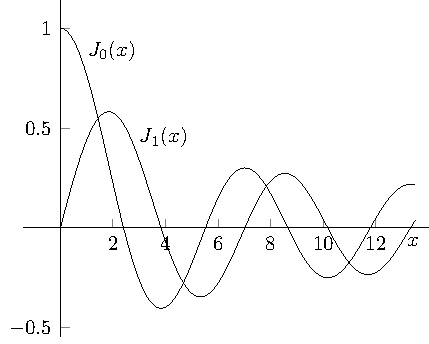
\includegraphics{figOctaveBesselFunction}
\caption{بیسل تفاعل کی پہلی قسم۔ \عددی{J_0}، \عددی{J_1}}
\label{شکل_بیسل_تفاعل}
\end{figure}
مساوات \حوالہ{مساوات_بیسل_الف} کو \عددی{x^2} سے تقسیم کرتے ہوئے  معیاری صورت \عددی{y''+\tfrac{1}{x}y'+(1-\tfrac{\nu^2}{x^2})y=0} ملتی ہے جس پر توجہ دیں۔ \عددی{x} کی زیادہ قیمت پر \عددی{\tfrac{1}{x}} اور \عددی{\tfrac{\nu^2}{x^2}} کو رد کرتے ہوئے بیسل مساوات سے \عددی{y''+y=0} حاصل ہوتا ہے جس کے حل \عددی{\cos x} اور \عددی{\sin x} ہیں۔آپ یہ بھی دیکھ سکتے ہیں کہ \عددی{\tfrac{y'}{x}} بطور تقصیری مستقل کردار ادا کرتے ہوئے بیسل تفاعل کا حیطہ گھٹانے میں مدد دے گی۔ زیادہ \عددی{x} کی صورت میں درج ذیل ثابت کیا جا سکتا ہے
\begin{align}\label{مساوات_بیسل_ذ}
J_n(x) \sim \sqrt{\frac{2}{\pi x}} \cos(x-\frac{n\pi}{2}-\frac{\pi}{4})
\end{align}
جہاں \عددی{\sim} کو \اصطلاح{متقاربی برابر}\فرہنگ{متقارب}\حاشیہب{asymptotically equal}\فرہنگ{asymptotically equal} پڑھیں اور جس کا مطلب ہے کہ کسی بھی قطعی \عددی{n} پر دونوں اطراف کی شرح، \عددی{x \to \infty} پر اکائی کے برابر ہو گی۔ 

مساوات \حوالہ{مساوات_بیسل_ذ} کم \عددی{x (>0)} کی صورت میں بھی بہترین ثابت ہوتی ہے۔اس کو استعمال کرتے ہوئے \عددی{J_0(x)} کے ابتدائی تین صفر \عددی{2.356}، \عددی{5.498} اور \عددی{8.639} حاصل ہوتے ہیں جبکہ ان کی حقیقی قیمتیں بالترتیب \عددی{2.405}، \عددی{5.520} اور \عددی{8.654} ہیں۔دونوں جوابات میں فرق \عددی{0.049}، \عددی{0.022} اور \عددی{0.015} ہے۔
\انتہا{مثال}
%=======================

\جزوحصہء{بیسل تفاعل جہاں \عددی{\nu \ge 0} کوئی بھی قیمت ہو سکتی ہے۔ گیما تفاعل}
گزشتہ حصے میں ہم نے عدد صحیح \عددی{\nu=n}کی صورت میں بیسل مساوات کا ایک حل دریافت کیا۔آئیں اب کسی بھی قیمت کے \عددی{\nu>0} کے لئے بیسل تفاعل کا عمومی حل تلاش کریں۔مساوات \حوالہ{مساوات_بیسل_عددی_سر_الف} میں ہم نے \عددی{a_0=\tfrac{1}{2^nn!}} چننا جبکہ موجودہ صورت میں ہم
\begin{align}\label{مساوات_بیسل_عددی_سر_عمومی}
a_0=\frac{1}{2^\nu \Gamma (\nu+1)}
\end{align}
چنتے ہیں جہاں \اصطلاح{گیما تفاعل}\فرہنگ{گیما تفاعل}\حاشیہب{gamma function}\فرہنگ{gamma function} \عددی{\Gamma} کی تعریف درج ذیل ہے۔
\begin{align}\label{مساوات_بیسل_گیما_الف}
\Gamma(\nu+1)=\int_{0}^{\infty}e^{-t} t^{\nu}\dif t\quad \quad (\nu >-1)
\end{align}
دھیان رہے کہ بائیں ہاتھ \عددی{\nu+1} جبکہ دائیں ہاتھ تکمل کے اندر \عددی{\nu} لکھا گیا ہے۔تکمل بالحصص سے
\begin{align*}
\Gamma(\nu+1)=\left. -e^{-t}t^{\nu}\right|_{0}^{\infty}+\nu\int_{0}^{\infty} e^{-t}t^{\nu-1}\dif t=0+\nu\Gamma(\nu)
\end{align*}
یعنی گیما تفاعل کا بنیادی تعلق
\begin{align}\label{مساوات_بیسل_گیما_ب}
\Gamma(\nu+1)=\nu\Gamma(\nu)
\end{align}
حاصل ہوتا ہے۔مساوات \حوالہ{مساوات_بیسل_گیما_الف} میں \عددی{\nu=0} پر کرنے سے 
\begin{align*}
\Gamma(1)=\int_{0}^{\infty}e^{-t}\dif t=\left.-e^{-t}\right|_{0}^{\infty}=0-(-1)=1
\end{align*}
ملتا ہے۔اس طرح مساوات \حوالہ{مساوات_بیسل_گیما_ب} سے \عددی{\Gamma(2)=1\cdot \Gamma(1)=1!}، \عددی{\Gamma(3)=3\Gamma(2)=2!} اور یوں 
\begin{align}\label{مساوات_بیسل_گیما_بطور_عدد_ضربیہ}
\Gamma(n+1)=n!\quad \quad n=0,1,2,\cdots
\end{align}
حاصل ہوتا ہے۔آپ دیکھ سکتے ہیں کہ عدد ضربی درحقیقت گیما تفاعل کی ایک مخصوص صورت ہے۔یوں عدد صحیح \عددی{\nu =n} کی صورت میں مساوات \حوالہ{مساوات_بیسل_عددی_سر_عمومی} سے مساوات \حوالہ{مساوات_بیسل_عددی_سر_الف} ہی حاصل ہوتی ہے۔

گیما تفاعل سے \عددی{0!} کی قیمت حاصل کرتے ہیں۔چونکہ \عددی{\Gamma(n+1)=n!} ہے لہٰذا 
\begin{align}\label{مساوات_بیسل_گیما_پ}
0!=\Gamma(1)=1
\end{align}
کے برابر ہے۔

مساوات \حوالہ{مساوات_بیسل_عددی_سر_عمومی} استعمال کرتے ہوئے  مساوات \حوالہ{مساوات_بیسل_چ} کو لکھتے ہیں۔
\begin{align*}
a_{2m}=\frac{(-1)^m }{2^{2m}m!(n+1)(n+2)\cdots (n+m)2^{\nu}\Gamma(\nu+1)}
\end{align*}
اب مساوات \حوالہ{مساوات_بیسل_گیما_ب} کے تحت \عددی{(\nu+1)\Gamma(\nu+1)=\Gamma(\nu+2)}، 
\عددی{(\nu+2)\Gamma(\nu+2)=\Gamma(\nu+3)} وغیرہ لکھے جا سکتے ہیں اور یوں
\begin{align*}
(\nu+1)(\nu+2)\cdots (\nu+m)\Gamma(\nu+1)=\Gamma(\nu+m+1)
\end{align*}
لکھا جا سکتا ہے۔اس طرح  
\begin{align}
a_{2m}=\frac{(-1)^m}{2^{2m+\nu}m!\Gamma(\nu+m+1)}
\end{align}
لکھا جا سکتا ہے جس کو استعمال کرتے ہوئے \عددی{r=r_1=\nu} کی صورت میں بیسل مساوات \حوالہ{مساوات_بیسل_الف} کا مخصوص حل درج ذیل حاصل ہوتا ہے۔
\begin{align}\label{مساوات_بیسل_تسلسل_عمومی}
J_{\nu}(x)=x^{\nu}\sum_{m=0}^{\infty}\frac{(-1)^m x^{2m}}{2^{2m+\nu}m!\Gamma(\nu+m+1)}
\end{align}
\عددی{J_{\nu}(x)} کو \اصطلاح{درجہ} \عددی{\nu} \اصطلاح{بیسل تفاعل کی پہلی قسم}\فرہنگ{بیسل تفاعل!پہلی قسم درجہ \عددی{\nu}}\حاشیہب{Bessel function of order $\nu$}\فرہنگ{Bessel function!first order} کہتے ہیں۔

جیسا آپ شرح عدد سر کی ترکیب سے ثابت کر سکتے ہیں، مساوات \حوالہ{مساوات_بیسل_تسلسل_عمومی} تمام \عددی{x} پر مرتکز ہے۔
%=========================
\ابتدا{مثال}
درج ذیل ثابت کریں۔
\begin{align}\label{مساوات_بیسل_گیما_نیم}
\Gamma(\tfrac{1}{2})=\sqrt{\pi}
\end{align}
حل:مساوات \حوالہ{مساوات_بیسل_گیما_الف} میں \عددی{\nu=-\tfrac{1}{2}} پر کرتے ہوئے 
\begin{align*}
\Gamma(\tfrac{1}{2})=\int_{0}^{\infty}e^{-t} t^{-\tfrac{1}{2}}\dif t
\end{align*}
ملتا ہے جس میں متغیرہ تبدیل کرتے ہوئے \عددی{t=u^2} استعمال کرتے ہیں۔
\begin{align*}
\Gamma(\tfrac{1}{2})=2\int_{0}^{\infty}e^{-u^2}\dif u
\end{align*}
اب ہم ایک ترکیب استعمال کرتے ہیں (جس کو ذہن نشین کرنا سود مند ثابت ہو گا)۔ درج بالا میں \عددی{u} کی جگہ \عددی{w} بھی لکھا جا سکتا ہے۔ایسا کرتے ہوئے 
\begin{align*}
\Gamma(\tfrac{1}{2})=2\int_{0}^{\infty}e^{-w^2}\dif w
\end{align*}

ملتا ہے۔درج بالا دو مساوات کو آپس میں ضرب دیتے ہیں۔
\begin{align*}
\Gamma(\tfrac{1}{2})^2=4\int_{0}^{\infty}e^{-u^2}\dif u \int_{0}^{\infty}e^{-w^2}\dif w=4\int_{0}^{\infty}\int_{0}^{\infty} e^{-(u^2+w^2)}\dif u\dif w
\end{align*}
یہ تکمل کارتیسی محور کے ربع اول پر حاصل کیا گیا ہے۔اس تکمل کو نلکی محور \عددی{r} اور \عددی{\theta} استعمال کرتے ہوئے حاصل کیا جا سکتا ہے۔یوں \عددی{u=r\cos \theta} اور \عددی{w=r\sin \theta} لیتے ہیں۔ چھوٹا رقبہ \عددی{\dif u\dif w=r\dif r\dif \theta} لکھا جائے گا۔ربع اول میں \عددی{r} کے حدود \عددی{0} تا \عددی{\infty} اور \عددی{\theta} کے حدود \عددی{0} تا  \عددی{\tfrac{\pi}{2}} ہیں۔
\begin{align*}
\Gamma(\tfrac{1}{2})^2=4\int_{0}^{\tfrac{\pi}{2}}\int_{0}^{\infty} e^{-r^2} r\dif r\dif \theta=4\int_{0}^{\frac{\pi}{2}}\left. -\frac{1}{2}e^{-r^2}\right|_{0}^{\infty} \dif \theta=4\left(\frac{1}{2}\right)\frac{\pi}{2}=\pi
\end{align*}
ملتا ہے۔دونوں اطراف کا جذر لینے سے \عددی{\Gamma(\tfrac{1}{2})=\sqrt{\pi}} ملتا ہے۔
\انتہا{مثال}
%================================
\جزوحصہء{خواص بیسل تفاعل}
بیسل تفاعل انتہائی زیادہ تعلقات پر پورا اترتے ہیں۔آئیں درج ذیل تعلقات کو بیسل تسلسل سے اخذ کریں۔
\begin{align}
[x^{\nu}J_{\nu}(x)]'&=x^{\nu}J_{\nu-1}(x) \label{مساوات_بیسل_تعلق_الف}\\
[x^{-\nu}J_{\nu}(x)]'&=-x^{-\nu}J_{\nu+1}(x) \label{مساوات_بیسل_تعلق_ب}\\
J_{\nu-1}(x)+J_{\nu+1}(x)&=\frac{2\nu}{x}J_{\nu}(x) \label{مساوات_بیسل_تعلق_پ}\\
J_{\nu-1}(x)-J_{\nu+1}(x)&=2J'_{\nu}(x) \label{مساوات_بیسل_تعلق_ت}
\end{align}
مساوات \حوالہ{مساوات_بیسل_تعلق_الف} ثابت کرتے ہیں۔مساوات \حوالہ{مساوات_بیسل_تسلسل_عمومی} کو \عددی{x^{\nu}} سے ضرب دیتے ہوئے
\begin{align*}
x^{\nu}J_{\nu}(x)=\sum_{m=0}^{\infty}\frac{(-1)^m x^{2m+2\nu}}{2^{2m+\nu}m!\Gamma(\nu+m+1)}
\end{align*}
تفرق لے کر مساوات \حوالہ{مساوات_بیسل_گیما_ب} سے \عددی{\Gamma(\nu+m+1)=(\nu+m)\Gamma(\nu+m)} لکھ کر ترتیب دیتے ہیں۔
\begin{multline*}
[x^{\nu}J_{\nu}(x)]'=\sum_{m=0}^{\infty}\frac{(2m+2\nu)(-1)^m x^{2m+2\nu-1}}{2^{2m+\nu}m!\Gamma(\nu+m+1)}=\sum_{m=0}^{\infty}\frac{2(m+\nu)(-1)^m x^{2m+2\nu-1}}{2^{2m+\nu}m!(\nu+m)\Gamma(\nu+m)}\\
=\sum_{m=0}^{\infty}\frac{(-1)^m x^{2m+2\nu-1}}{2^{2m+\nu-1}m!\Gamma(\nu+m)}=x^{\nu}x^{\nu-1}\sum_{m=0}^{\infty}\frac{(-1)^m x^{2m}}{2^{2m+\nu-1}m!\Gamma(\nu+m)}=x^{\nu}J_{\nu-1}(x)
\end{multline*}
آخری قدم مساوات \حوالہ{مساوات_بیسل_تسلسل_عمومی} میں \عددی{\nu} کی جگہ \عددی{\nu-1} پر کر کے موازنہ کرتے ہوئے لکھا گیا ہے۔

آئیں اب مساوات \حوالہ{مساوات_بیسل_تعلق_ب} ثابت کریں۔مساوات \حوالہ{مساوات_بیسل_تسلسل_عمومی} کو \عددی{x^{-\nu}} سے ضرب دینے سے \عددی{x^{\nu}} کٹ جاتا ہے۔
\begin{align*}
x^{-\nu}J_{\nu}(x)=\sum_{m=0}^{\infty}\frac{(-1)^m x^{2m}}{2^{2m+\nu}m!\Gamma(\nu+m+1)}
\end{align*}
تفرق لے کر \عددی{m!=m(m-1)!} لکھ کر ترتیب دیتے ہیں۔
\begin{align*}
[x^{-\nu}J_{\nu}(x)]'=\sum_{m=1}^{\infty}\frac{2m(-1)^m x^{2m-1}}{2^{2m+\nu}m!\Gamma(\nu+m+1)}=\sum_{m=1}^{\infty}\frac{2m(-1)^m x^{2m-1}}{2^{2m+\nu}m(m-1)!\Gamma(\nu+m+1)}\\
=\sum_{m=1}^{\infty}\frac{(-1)^m x^{2m-1}}{2^{2m+\nu-1}(m-1)!\Gamma(\nu+m+1)}
\end{align*}
دھیان رہے کہ تفرق کے بعد تسلسل کا پہلا رکن \عددی{m=1} سے ظاہر کیا جائے گا۔(آپ \عددی{x^{-\nu}J_{\nu}} کے تسلسل کو پھیلا کر لکھ کر تفرق لیتے ہوئے دیکھ سکتے ہیں کہ پہلا رکن \عددی{m=1} ہے)۔ درج بالا تسلسل میں \عددی{s=m-1} یعنی \عددی{m=s+1} پر کرتے ہیں۔
\begin{align*}
[x^{-\nu}J_{\nu}(x)]'=\sum_{s=0}^{\infty}\frac{(-1)^{s+1} x^{2s+1}}{2^{2s+\nu+1}s!\Gamma(\nu+s+2)}=-x^{-\nu}J_{\nu+1}(x)
\end{align*}
آخری قدم مساوات \حوالہ{مساوات_بیسل_تسلسل_عمومی} میں \عددی{\nu} کی جگہ \عددی{\nu+1} پر کر کے موازنہ کرتے ہوئے لکھا گیا ہے۔

اب مساوات \حوالہ{مساوات_بیسل_تعلق_پ} اور مساوات \حوالہ{مساوات_بیسل_تعلق_پ} ثابت کرتے ہیں۔مساوات \حوالہ{مساوات_بیسل_تعلق_الف} اور مساوات \حوالہ{مساوات_بیسل_تعلق_ب} کو درج ذیل لکھا جا سکتا ہے۔
\begin{align*}
\nu x^{\nu-1} J_{\nu}+x^{\nu}J'_{\nu}&=x^{\nu} J_{\nu-1}\\
-\nu x^{-\nu-1} J_{\nu}+x^{-\nu}J'_{\nu}&=-x^{-\nu} J_{\nu+1}
\end{align*}
پہلی مساوات کو \عددی{x^{\nu}} اور دوسری مساوات کو \عددی{x^{-\nu}} سے تقسیم کرتے ہیں۔
\begin{align*}
\nu x^{-1} J_{\nu}+J'_{\nu}&= J_{\nu-1}\\
-\nu x^{-1} J_{\nu}+J'_{\nu}&=-J_{\nu+1}
\end{align*}
ان کو جمع اور تفریق کرتے ہوئے درج ذیل (درکار) مساوات ملتے ہیں۔
\begin{align*}
2J'_{\nu}&=J_{\nu-1}-J_{\nu+1}\\
\frac{2\nu}{x}J_{\nu}&=J_{\nu-1}+J_{\nu+1}
\end{align*}
%================================
\ابتدا{مثال}\quad مساوات \حوالہ{مساوات_بیسل_تعلق_الف} تا مساوات \حوالہ{مساوات_بیسل_تعلق_ت} کا استعمال\\
درج ذیل کو \عددی{J_0} اور \عددی{J_1} کی صورت میں حاصل کریں۔
\begin{align*}
\int_{1}^{2} x^{-3}J_4(x)\dif x
\end{align*}

حل:مساوات \حوالہ{مساوات_بیسل_تعلق_ب} میں \عددی{\nu=3} لیتے ہوئے  درج ذیل ملتا ہے۔
\begin{align*}
I=\int_{1}^{2} x^{-3}J_4(x)\dif x=\left. -x^{-3}J_3(x)\right|_{1}^{2}
\end{align*}
مساوات \حوالہ{مساوات_بیسل_تعلق_پ} میں \عددی{\nu=2} پر کرتے ہوئے \عددی{J_3=\tfrac{4}{x}J_2-J_1} اور \عددی{\nu=1} پر کرتے ہوئے \عددی{J_2=\tfrac{2}{x}J_1-J_0} لکھا جا سکتا ہے لہٰذا \عددی{J_3=\tfrac{4}{x}(\tfrac{2}{x}J_1-J_0)-J_1} لکھا جا سکتا ہے۔یوں تکمل کی قیمت
\begin{align*}
I=\left.  -x^{-3}[4x^{-1}(2x^{-1}J_1-J_0)-J_0] \right|_{1}^{2}=-\frac{1}{8}J_1(2)+\frac{1}{4}J_0(2)+7J_1(1)-4J_0(1)
\end{align*}
ہو گی۔
\انتہا{مثال}
%===========================
\ابتدا{مثال}
درج ذیل (شکل \حوالہ{شکل_بیسل_کسری_بیسل}) ثابت کریں۔
\begin{gather}
\begin{aligned} \label{مساوات_بیسل_تعلق_کوسائن}
J_{\frac{1}{2}}(x)&=\sqrt{\frac{2}{\pi x}}\sin x\\
J_{-\frac{1}{2}}(x)&=\sqrt{\frac{2}{\pi x}}\cos x
\end{aligned}
\end{gather}
حل:بیسل تسلسل \حوالہ{مساوات_بیسل_تسلسل_عمومی} میں \عددی{\nu=\tfrac{1}{2}} پر کرتے ہوئے ہیں۔
\begin{align*}
J_{\frac{1}{2}}(x)=\sqrt{x}\sum_{m=0}^{\infty}\frac{(-1)^m x^{2m}}{2^{2m+\frac{1}{2}}m!\Gamma(\frac{1}{2}+m+1)}=\sqrt{\frac{2}{x}}\sum_{m=0}^{\infty}\frac{(-1)^m x^{2m+1}}{2^{2m+1}m!\Gamma(m+\frac{3}{2})}
\end{align*}
نسب نما میں درج ذیل لکھا جا سکتا ہے جہاں آخری قدم پر مساوات \حوالہ{مساوات_بیسل_گیما_نیم} استعمال کیا گیا ہے۔
\begin{align*}
2^mm!&=2m(2m-2)(2m-4)\cdots 4\cdot 2\\
2^{m+1}\Gamma(m+\tfrac{3}{2})&=2^{m+1}(m+\tfrac{1}{2})(m-\tfrac{1}{2})\cdots \tfrac{3}{2}\cdot \Gamma(\tfrac{1}{2})\\
&=(2m+1)(2m-1)\cdots 3\cdot 2\cdot 1\cdot \sqrt{\pi}
\end{align*}
ان نتائج کو استعمال کرتے ہوئے نسب نما میں
\begin{align*}
2^{2m+1}m!\Gamma(m+\tfrac{3}{2})=(2m+1)2m(2m-1)(2m-2)\cdots 3\cdot 2 \cdot 1\cdot \sqrt{\pi}=(2m+1)!\sqrt{\pi}
\end{align*}
لکھا جا سکتا ہے لہٰذا درج ذیل ثابت ہوتا ہے۔
\begin{align*}
J_{\frac{1}{2}}(x)=\sqrt{\frac{2}{\pi x}}\sum_{m=0}^{\infty}\frac{(-1)^m x^{2m+1}}{(2m+1)!}=\sqrt{\frac{2}{\pi x}}\sin x
\end{align*}
%
\begin{figure}
\centering
\begin{tikzpicture}
\begin{axis}[axis lines*=middle,xlabel=x,xlabel style={at={(current axis.right of origin)},anchor=north east},ytick={0,1},yticklabels={$0$,$1$},xtick={6.28,12.57,18.85},xticklabels={$2\pi$,$4\pi$,$6\pi$},ymax=1]
\addplot[domain=0:20,samples=100]{sqrt(2/(pi*x))*sin(180/pi*x)};
\addplot[domain=0.2:20,samples=100]{sqrt(2/(pi*x))*cos(180/pi*x)};
\end{axis}
\end{tikzpicture}
\caption{بیسل تفاعل \عددی{J_{\tfrac{1}{2}}(x)} اور \عددی{J_{-\tfrac{1}{2}}(x)}}
\label{شکل_بیسل_کسری_بیسل}
\end{figure}

مساوت \حوالہ{مساوات_بیسل_تعلق_الف} استعمال کرتے ہوئے
\begin{align*}
[\sqrt{x}J_{\tfrac{1}{2}}(x)]'=\sqrt{\frac{2}{\pi}}\cos x=\sqrt{x}J_{-\tfrac{1}{2}}(x)
\end{align*} 
لکھا جا سکتا ہے جس میں دائیں ہاتھ کے مساوات کو لیتے ہوئے \عددی{\sqrt{x}} سے تقسیم کرتے ہوئے مساوات \حوالہ{مساوات_بیسل_تعلق_کوسائن} کی دوسری مساوات ملتی ہے۔
\انتہا{مثال}
%=============================

\جزوحصہء{عمومی حل۔ خطی طور تابعیت}
بیسل مساوات \حوالہ{مساوات_بیسل_الف} کے عمومی حل کے لئے \عددی{J_v(x)} کے علاوہ خطی طور غیر تابع دوسرا حل بھی درکار ہے۔غیر عدد صحیح \عددی{\nu} کی صورت میں دوسرا حل  \عددی{r_2=-\nu} (اشاری مساوات \حوالہ{مساوات_بیسل_ت}) استعمال کرتے ہوئے حاصل ہو گا۔یوں دوسرا خطی طور غیر تابع حل مساوات \حوالہ{مساوات_بیسل_تسلسل_عمومی} میں \عددی{\nu} کی جگہ \عددی{-\nu} پر کرنے سے حاصل ہو گا۔
\begin{align}\label{مساوات_بیسل_تسلسل_عمومی_دوسرا}
J_{-\nu}(x)=x^{-\nu}\sum_{m=0}^{\infty}\frac{(-1)^m x^{2m}}{2^{2m-\nu}m!\Gamma(m-\nu+1)}
\end{align}
\عددی{\nu} غیر عدد صحیح ہونے کی صورت میں \عددی{J_{\nu}} اور \عددی{J_{-\nu}} خطی طور غیر تابع ہیں۔یوں غیر عدد صحیح \عددی{\nu} کی صورت میں \عددی{x \ne 0} پر  مساوات بیسل کا عمومی حل 
\begin{align}
y(x)=c_1J_{\nu}(x)+c_2J_{-\nu}(x)
\end{align}
ہو گا۔ 

\عددی{\nu} عدد صحیح ہونے کی صورت میں \عددی{J_n(x)} اور \عددی{J_{-n}(x)} کا تعلق
\begin{align}\label{مساوات_بیسل_عدد_صحیح_بیسل_تعلق}
J_{-n}(x)=(-1)^nJ_n(x) \quad \quad (n=1,2,\cdots)
\end{align}
ہے لہٰذا یہ خطی طور تابع ہیں اور ان سے عمومی حل نہیں لکھا جا سکتا ہے۔آئیں مساوات \حوالہ{مساوات_بیسل_عدد_صحیح_بیسل_تعلق} کو ثابت کریں۔

%==============================
\ابتدا{ثبوت}
مساوات \حوالہ{مساوات_بیسل_تسلسل_عمومی_دوسرا} میں \عددی{\nu} کی قیمت کو عدد صحیح کے قریب تر لانے سے گیما تفاعل کی قیمت (صفحہ \حوالہصفحہ{شکل_ضمیمہ_گیما_تفاعل} پر شکل \حوالہ{شکل_ضمیمہ_گیما_تفاعل}) لامتناہی کی طرف بڑھتی ہے۔یوں \عددی{\nu=n} کی صورت میں مساوات \حوالہ{مساوات_بیسل_تسلسل_عمومی_دوسرا} کے ابتدائی \عددی{n} ارکان کے عددی سر، گیما تفاعل کی قیمت لامتناہی ہونے کی بنا، صفر ہوں گے اور یوں تسلسل \عددی{m=n} سے شروع ہو گا۔مساوات \حوالہ{مساوات_بیسل_گیما_بطور_عدد_ضربیہ} کے تحت \عددی{\Gamma(m-n+1)=(m-n)!} ہے لہٰذا درج ذیل لکھا جائے گا
\begin{align*}
J_{-n}(x)=\sum_{m=n}^{\infty}\frac{(-1)^mx^{2m-n}}{2^{2m-n}m!(m-n)!}=\sum_{s=0}^{\infty}\frac{(-1)^{n+s}x^{2s+n}}{2^{2s+n} (n+s)!s!}\quad \quad (m=n+s)
\end{align*}
جو \عددی{(-1)^nJ_n(x)} ہے۔
\انتہا{ثبوت}
%==========================

اگلے حصے میں \عددی{\nu=n} کی صورت میں مساوات بیسل کا عمومی حل، بیسل تفاعل کی دوسری قسم \عددی{Y_{\nu}} کی مدد سے، حاصل کیا جائے گا۔
%==================

\حصہء{سوالات}

 %==================
\ابتدا{سوال}
ثابت کریں کہ \عددی{J_n(x)} تمام \عددی{x} کے لئے مرتکز ہے۔

جواب: \عددی{\abs{\tfrac{a_{m+1}}{a_m}}=\tfrac{2^{2m+n}m!(n+m)!}{2^{2m+2+n} (m+1)!(n+m+1)!}=\tfrac{1}{2^2(m+1)(n+m+1)}} ہے لہٰذا 
\عددی{\abs{\tfrac{a_{m+1}}{a_m}}_{m\to \infty}=0} اور یوں \عددی{R\to \infty} ہو گا۔
\انتہا{سوال}
%====================
سوال \حوالہ{سوال_بیسل_صورت_الف} تا سوال \حوالہ{سوال_بیسل_صورت_ب} کے عمومی حل، جہاں ممکن ہو،  \عددی{J_{\nu}} اور \عددی{J_{-\nu}} استعمال کرتے ہوئے لکھیں۔جہاں اضافی معلومات دی گئی ہوں، وہاں اس کو استعمال کرتے ہوئے بیسل مساوات کی صورت حاصل کریں۔

%============
\ابتدا{سوال}\شناخت{سوال_بیسل_صورت_الف}\quad
$x^2y''+xy'(x^2-\frac{4}{9})y=0$\\
جواب:چونکہ \عددی{\nu=\tfrac{2}{3}} ہے جو غیر عدد صحیح ہے لہٰذا عمومی حل \عددی{y=c_1J_{\tfrac{2}{3}}+c_2J_{-\tfrac{2}{3}}} ہے۔
\انتہا{سوال}
%=================
\ابتدا{سوال}\quad
$xy''+y'+\frac{1}{4}y\quad \quad (z=\sqrt{x})$\\
جواب:\عددی{y=c_1J_0(\sqrt{x})}
\انتہا{سوال}
%=================
\ابتدا{سوال}\quad
$xy''+y'+\frac{x}{4}y=0\quad \quad (z=\frac{x}{2})$\\
جواب:\عددی{y=c_1J_0(\tfrac{x}{2})}
\انتہا{سوال}
%===================
\ابتدا{سوال}\quad
$x^2y''+xy'(\frac{x^2}{9}-\frac{1}{9})y=0\quad \quad (z=\frac{x}{3})$\\
جواب:\عددی{y=c_1J_{\tfrac{1}{3}}(\tfrac{x}{3})+c_2J_{-\tfrac{1}{3}}(\tfrac{x}{3})}
\انتہا{سوال}
%====================
\ابتدا{سوال}\quad
$y''+(e^{2x}-16)y=0,\quad \quad (z=e^x)$\\
جواب:\عددی{y=c_1J_4(e^x)}
\انتہا{سوال}
%=================
\ابتدا{سوال}\quad
$x^2y''+xy'(\lambda^2 x^2-\nu^2)y=0,\quad \quad (z=\lambda x)$\\
جواب:\عددی{y=c_1 J_{\nu}(\lambda x)+c_2J_{-\nu}(\lambda x)} جہاں \عددی{\nu \ne 0, \mp1, \mp2, \cdots}
\انتہا{سوال}
%=================
\ابتدا{سوال}\quad
$x^2y''+xy'+(9x^2-1)y=0,\quad \quad (z=3x)$\\
جواب:\عددی{y=c_1J_1(3x)}
\انتہا{سوال}
%======================
\ابتدا{سوال}\quad
$(x-\frac{1}{2})^2y''+(x-\frac{1}{2})y'+4x(x-1)y=0\quad \quad(z=2x-1)$\\
جواب:\عددی{y=c_1J_1(2x-1)}
\انتہا{سوال}
%==================
\ابتدا{سوال}\quad
$xy''+(2\nu+1)y'+xy=0,\quad \quad y=x^{-\nu}u$\\
جواب:\عددی{y=x^{-\nu}(c_1J_{\nu}(x)+c_2J_{-\nu}(x))} جہاں \عددی{\nu \ne 0,\mp1,\mp2,\cdots}
\انتہا{سوال}
%====================
\ابتدا{سوال}\شناخت{سوال_بیسل_صورت_ب}\quad
$x^2y''+\frac{1}{4}(x+\frac{3}{4})y=0,\quad \quad y=u\sqrt{x}, \quad z=\sqrt{x}$\\
جواب:\عددی{y=c_1\sqrt{x}J_{\tfrac{1}{2}}(\sqrt{x})+c_2\sqrt{x}J_{-\tfrac{1}{2}}(\sqrt{x})}
\انتہا{سوال}
%====================
\ابتدا{سوال}
مساوات \حوالہ{مساوات_بیسل_تعلق_پ} اور مساوات \حوالہ{مساوات_بیسل_تعلق_کوسائن} سے درج ذیل ثابت کریں۔
\begin{align}
J_{\tfrac{3}{2}}(x)=\sqrt{\frac{2}{\pi x}} \left(\frac{\sin x}{x}-\cos x\right), \quad  J_{-\tfrac{3}{2}}(x)=-\sqrt{\frac{2}{\pi x}}\left(\frac{\cos x}{x}+\sin x \right)
\end{align}
\انتہا{سوال}
%======================
\ابتدا{سوال}
کیا آپ مساوات \حوالہ{مساوات_بیسل_تعلق_پ} اور مساوات \حوالہ{مساوات_بیسل_تعلق_کوسائن} سے  اخذ کر سکتے ہیں کہ
 \عددی{\nu=\mp \tfrac{1}{2},\mp\tfrac{3}{2},\mp\tfrac{5}{2},\cdots} کی صورت میں \عددی{J_{\nu}(x)} بنیادی تفاعل ہیں۔

جواب:جی ہاں۔
\انتہا{سوال}
%=====================

%================
\ابتدا{سوال}\quad باہم پیچاں صفر\\
مساوات \حوالہ{مساوات_بیسل_تعلق_الف}، مساوات \حوالہ{مساوات_بیسل_تعلق_ب} اور \اصطلاح{مسئلہ رول}\فرہنگ{مسئلہ!رول}\فرہنگ{رول مسئلہ}\حاشیہب{Rolle's theorem}\فرہنگ{theorem!Rolle's} استعمال کرتے ہوئے ثابت کریں کہ \عددی{J_n(x)} کے کسی بھی دو متواتر صفروں کے مابین \عددی{J_{n+1}(x)} کا ایک صفر پایا جاتا ہے۔ 

جواب:مسئلہ رول کہتا ہے کہ کسی بھی حقیقی قابل تفرق تفاعل کے دو متواتر برابر قیمت نقطوں کے مابین کم از کم ایک ایسا نقطہ (نقطہ فاصل) پایا جاتا ہے جس پر تفاعل کا تفرق صفر کے برابر ہو گا۔ اگر \عددی{J_n(x)} کے دو متواتر صفر \عددی{x_1} اور \عددی{x_2} پر پائے جاتے ہوں تب ہم \عددی{x_1^{-n}J_n(x_1)=x_2^{-n}J_n(x_2)=0} لکھ سکتے ہیں۔یوں مسئلہ رول کے تحت \عددی{x_1} اور \عددی{x_2} کے مابین کسی نقطے پر تفاعل \عددی{x^{-n}J_n(x)} کا تفرق صفر \عددی{[x^{-n}J_n(x)]'=0} ہو گا جو مساوات \حوالہ{مساوات_بیسل_تعلق_ب} کے استعمال سے ایسے نقطے پر \عددی{x^{-n}J_{n+1}(x)=0} یعنی \عددی{J_{n+1}(x)=0} دیتا ہے۔اسی طرح اگر \عددی{J_{n+1}(x)} کے دو متواتر صفر \عددی{x_3} اور \عددی{x_4} پر پائے جاتے ہوں تب \عددی{J_{n+1}(x_3)=J_{n+1}(x_4)=0} اور \عددی{x_3^{n+1}J_{n+1}(x_3)=x_4^{n+1}J_{n+1}(x_4)=0} لکھا جا سکتا ہے۔یوں مسئلہ رول کے تحت \عددی{x_3} اور \عددی{x_4} کے مابین کسی نقطے پر \عددی{[x^{n+1}J_{n+1}(x)]'=0} ہو گا جس سے مساوات \حوالہ{مساوات_بیسل_تعلق_الف} کے تحت ایسے نقطے پر \عددی{x^{n+1}J_n(x)=0} یعنی \عددی{J_n(x)=0} حاصل ہوتا ہے۔ یوں  ثابت ہوا کہ \عددی{J_{n+1}} کے دو متواتر صفر \عددی{x_3} اور \عددی{x_4} کے مابین \عددی{J_n(x)} کا صفر پایا جاتا ہے جبکہ \عددی{J_n(x)} کے دو متواتر صفر \عددی{x_1} اور \عددی{x_2} کے مابین \عددی{J_{n+1}(x)} کا صفر پایا جاتا ہے۔
\انتہا{سوال}
%=================
\ابتدا{سوال}\quad تفرقی مساوات سے ایک درجی تفرق کا اخراج\\
 درج ذیل تفرقی مساوات میں \عددی{y(x)=u(x)v(x)} پر کرتے ہوئے ایسا \عددی{v(x)} دریافت کریں کہ حاصل تفرقی مساوات میں پہلے درجے کا تفرق نہ پایا جاتا ہو۔حاصل تفرقی مساوات بھی حاصل کریں۔
\begin{align*}
y''+p(x)y'+q(x)y=0
\end{align*}
جوابات:\عددی{v=e^{-\tfrac{1}{2}\int p(x)\dif x}} اور مساوات \عددی{u''+[q-\tfrac{1}{4}p^2-\tfrac{1}{2}p']u=0} میں \عددی{u'} نہیں پایا جاتا ہے۔

\انتہا{سوال}
%=====================
\ابتدا{سوال}
گزشتہ سوال میں تفرقی مساوات سے ایک درجی تفرق کا اخراج کیا گیا۔ثابت کریں کہ مساوات بیسل \حوالہ{مساوات_بیسل_الف} سے ایک درجی تفرق کا اخراج \عددی{y=\tfrac{u}{\sqrt{x}}} پر کرتے ہوئے ہو گا جس سے درج ذیل تفرقی مساوات حاصل ہو گی۔
\begin{align}\label{مساوات_بیسل_سادہ_صورت}
x^2u''+(x^2+\tfrac{1}{4}-\nu^2)u=0
\end{align}
\انتہا{سوال}
%====================
\ابتدا{سوال}
مساوات \حوالہ{مساوات_بیسل_سادہ_صورت} کا عمومی حل \عددی{\nu=\tfrac{1}{2}} کے لئے حاصل کریں۔

جواب: \عددی{u=A\cos x+B\sin x} ہے لہٰذا \عددی{y=\tfrac{u}{\sqrt{x}}=\tfrac{1}{\sqrt{x}}(A\cos x+B\sin x)} ہو گا۔
\انتہا{سوال}
%===================
سوال \حوالہ{سوال_بیسل_تفرق_تکمل_الف} تا سوال \حوالہ{سوال_بیسل_تفرق_تکمل_ب}  مساوات \حوالہ{مساوات_بیسل_تعلق_الف} اور مساوات \حوالہ{مساوات_بیسل_تعلق_ب} کی مدد سے حل ہوں گے۔

%===============
\ابتدا{سوال}\شناخت{سوال_بیسل_تفرق_تکمل_الف}\quad ثابت کریں 
$J'_0(x)=-J_1(x),\quad J'_1(x)=J_0(x)-\frac{J_1(x)}{x},\quad J'_2(x)=\frac{1}{2}[J_1(x)-J_3(x)]$\\
\انتہا{سوال}
%=================
\ابتدا{سوال}
بیسل مساوات \حوالہ{مساوات_بیسل_الف} کو مساوات \حوالہ{مساوات_بیسل_تعلق_الف} اور مساوات \حوالہ{مساوات_بیسل_تعلق_ب} سے حاصل کریں۔
\انتہا{سوال}
%=====================
\ابتدا{سوال}
درج ذیل ثابت کریں
\begin{align*} 
\int x^{\nu} J_{\nu-1}(x)\dif x&=x^{\nu}J_{\nu}(x)+c\\
\int x^{-\nu}J_{\nu+1}\dif x&=-x^{-\nu}J_{\nu}(x)+c\\
\int J_{\nu+1}(x)\dif x&=\int J_{\nu-1}(x)\dif x-2J_{\nu}(x)
\end{align*}
\انتہا{سوال}
%======================
\ابتدا{سوال}\quad
$\int J_3(x)\dif x$\\
جواب:مساوات \حوالہ{مساوات_بیسل_تعلق_ت} میں \عددی{\nu=2} پر کر کے تکمل \عددی{\int J_3\dif x=\int  J_1\dif x-2J_2} ہو گا اور مساوات \حوالہ{مساوات_بیسل_تعلق_ب} میں \عددی{\nu=0} پر کرتے ہوئے تکمل \عددی{\int J_1\dif x=-J_0} دیتا ہے لہٰذا \عددی{\int J_3\dif x=-J_0-2J_2+c} 
\انتہا{سوال}
%=====================
\ابتدا{سوال} تکمل بالحصص استعمال کرتے  ہوئے حل کریں۔\quad 
$\int x^3J_0(x)\dif x$\\
جواب:
$\int x^3J_0\dif x=\int x^2(xJ_0)\dif x=x^2(xJ_1)-2\int x^2J_1\dif x=x^3J_1-2x^2J_2+c$
\انتہا{سوال}
%=======================
\ابتدا{سوال} \شناخت{سوال_بیسل_تفرق_تکمل_ب} تکمل بالحصص سے حل کریں۔\quad 
$\int x^2J_0\dif x$\\
جواب:\عددی{\int x^2J_0\dif x=x^2J_1+xJ_0-\int J_0\dif x}، جہاں \عددی{\int J_0\dif x} کسی بنیادی تفاعل کی صورت میں نہیں لکھا جا سکتا ہے بلکہ اس کی قیمت  جدول کی مدد سے لکھی جاتی ہے۔

\انتہا{سوال}
%===================

\حصہ{بیسل تفاعل کی دوسری قسم۔ عمومی حل}
بیسل مساوات \حوالہ{مساوات_بیسل_الف} کا کسی بھی \عددی{\nu} کے لئے عمومی حل حاصل کرنے کی خاطر \اصطلاح{بیسل تفاعل کی دوسری قسم}\فرہنگ{بیسل تفاعل!دوسری قسم}\حاشیہب{Bessel function of the second kind}\فرہنگ{Bessel!second kind function} \عددی{Y_{\nu}(x)} حاصل کرتے ہیں۔شروع \عددی{\nu=n=0} سے کرتے ہیں۔  

\عددی{n=0} کی صورت میں مساوات بیسل کو \عددی{x} سے تقسیم کرتے ہوئے
\begin{align}\label{مساوات_بیسل_دوہرا_صفر_الف}
xy''+y'+xy=0
\end{align}
لکھا جا سکتا ہے اور اشاری مساوات \حوالہ{مساوات_طاقتی_اشاری_مساوات} سے دوہرا جذر \عددی{r=0} ملتا ہے  جو صفحہ \حوالہصفحہ{مسئلہ_طاقتی_فروبنیوس_اساس} پر مسئلہ فروبنیوس میں بتلائی گئی دوسری صورت کو ظاہر کرتی ہے۔یوں مساوات \حوالہ{مساوات_بیسل_دوہرا_صفر_الف} کا ایک حل \عددی{J_0(x)} ہو گا جبکہ اس کا دوسرا حل مساوات \حوالہ{مساوات_طاقتی_فروبنیوس_حل_ت} میں \عددی{r=0} پر کرتے ہوئے  
\begin{align}\label{مساوات_بیسل_دوہرا_صفر_ب}
y_2(x)=J_0(x)\ln x+\sum_{m=1}^{\infty}A_m x^m 
\end{align}
لکھا جائے گا۔مساوات \حوالہ{مساوات_بیسل_دوہرا_صفر_ب} اور اس کے تفرقات
\begin{align*}
y_2'&=J_0' \ln x+\frac{J_0}{x}+\sum_{m=1}^{\infty}mA_mx^{m-1}\\
y_2''&=J_0''\ln x+\frac{2J_0'}{x}-\frac{J_0}{x}+\sum_{m=1}^{\infty} m(m-1)A_m x^{m-2}
\end{align*}
کو مساوات \حوالہ{مساوات_بیسل_دوہرا_صفر_الف} میں پر کرتے ہیں (اگرچہ آخری مجموعے کا پہلا رکن \عددی{m=2} لکھنا چاہیے، البتہ \عددی{m=1} پر دیا گیا مجموعہ صفر دیتا ہے لہٰذا مجموعے کا پہلا رکن \عددی{m=1} لکھنا ممکن ہے)۔اب چونکہ \عددی{J_0} تفرقی مساوات کا حل ہے لہٰذا  تین لوگارتھمی ارکان کا مجموعہ \عددی{(xJ_0''+J_0'+xJ_0)\ln x} صفر کے برابر ہو گا اور یوں بقایا درج ذیل ہو گا۔
\begin{align*}
2J_0'+\sum_{m=1}^{\infty}m(m-1)A_mx^{m-1}+\sum_{m=1}^{\infty}mA_mx^{m-1}+\sum_{m=1}^{\infty}A_mx^{m+1}=0
\end{align*}
اس میں پہلے اور دوسرے  مجموعوں کو جمع کرتے ہوئے \عددی{\sum m^2A_mx^{m-1}} لکھا کر جبکہ \عددی{J_0'} کی طاقتی تسلسل کو مساوات \حوالہ{مساوات_بیسل_د} کا جزو در جزو تفرق لیتے اور \عددی{\tfrac{m!}{m}=(m-1)!} استعمال کرتے ہوئے
\begin{align*}
J'_0(x)=\sum_{m=1}^{\infty}\frac{(-1)^m2mx^{2m-1}}{2^{2m}(m!)^2}=\sum_{m=1}^{\infty}\frac{(-1)^mx^{2m-1}}{2^{2m-1}m!(m-1)!}
\end{align*} 
لکھ کر درج ذیل حاصل ہوتا ہے۔
\begin{align}\label{مساوات_بیسل_دوہرا_صفر_پ}
\sum_{m=1}^{\infty}\frac{(-1)^mx^{2m-1}}{2^{2m-2}m!(m-1)!}+\sum_{m=1}^{\infty} m^2A_mx^{m-1}+\sum_{m=1}^{\infty}A_mx^{m+1}=0
\end{align}
اس مساوات میں \عددی{x^0} کمتر طاقت، جو صرف دوسرے مجموعے میں پایا جاتا ہے، کے عددی سر کو صفر کے برابر پر کرتے ہوئے \عددی{A_1=0} ملتا ہے۔اب \عددی{x^{2s}} کے عددی سروں، جو پہلے تسلسل میں نہیں پایا جاتا، کے مجموعے کو صفر کے برابر لکھتے ہیں۔
\begin{align*}
(2s+1)^2A_{2s+1}+A_{2s-1}=0,\quad \quad (s=1,2,\cdots)
\end{align*}
اب چونکہ \عددی{A_1=0} ہے لہٰذا \عددی{A_3=0}، \عددی{A_5=0}، \نقطے ہوں گے۔ 

\عددی{x^{2s+1}} کے عددی سروں کے مجموعے کو صفر کے برابر پر کرتے ہوئے \عددی{s=0} کے لئے
\begin{align*}
-1+4A_2=0, \quad \implies \quad A_2=\frac{1}{4}
\end{align*}
جبکہ بقایا \عددی{s} پر
\begin{align*}
\frac{(-1)^{s+1}}{2^{2s}(s+1)!s!}+(2s+2)^2A_{2s+2}+A_{2s}=0,\quad (s=1,2,\cdots)
\end{align*}
لکھا جائے گا۔اس سے \عددی{s=1} کے لئے
\begin{align*}
\frac{1}{8}+16A_4+A_2=0\quad \implies \quad A_4=-\frac{3}{128}
\end{align*}
حاصل ہوتا ہے جبکہ عمومی طور پر
\begin{align}\label{مساوات_بیسل_دوہرا_صفر_ت}
A_{2m}=\frac{(-1)^{m-1}}{2^{2m}(m!)^2}\left(1+\frac{1}{2}+\frac{1}{3}+\cdots+\frac{1}{m}\right), \quad \quad (m=1,2,\cdots)
\end{align}
ملتا ہے۔قوسین میں بند قیمت کو \عددی{h_m} لکھ کر،
\begin{align}\label{مساوات_بیسل_دوہرا_صفر_ٹ}
h_m=1+\frac{1}{2}+\frac{1}{3}+\cdots+\frac{1}{m}
\end{align}
مساوات \حوالہ{مساوات_بیسل_دوہرا_صفر_ت} اور \عددی{A_1=A_3=\cdots=0} کو مساوات \حوالہ{مساوات_بیسل_دوہرا_صفر_ب} میں پر کرتے ہوئے جواب حاصل کرتے ہیں۔
\begin{gather}
\begin{aligned}
y_2(x)&=J_0(x)\ln x+\sum_{m=1}^{\infty}\frac{(-1)^{m-1}h_m}{2^{2m}(m!)^2}x^{2m}\\
&=J_0(x)\ln x+\frac{1}{4}x^2-\frac{3}{128}x^4+\frac{11}{\num{13824}}x^6-+\cdots
\end{aligned}
\end{gather}
چونکہ \عددی{J_0} اور \عددی{y_2} خطی طور غیر تابع ہیں لہٰذا یہ مساوات بیسل \حوالہ{مساوات_بیسل_الف} کی حل کی اساس ہیں۔ہم \عددی{J_0} اور \عددی{y_2} سے کوئی بھی مخصوص حل، \عددی{a(y_2+bJ_0)} جہاں \عددی{a(\ne 0)} اور \عددی{b} مستقل ہیں، لکھتے ہوئے اساس کی مختلف صورتیں حاصل کر سکتے ہیں۔روایتی طور پر \عددی{a=\tfrac{2}{\pi}} اور \عددی{b=\gamma-\ln 2} چننے جاتے ہیں جہاں \عددی{\gamma=\num{0.57721566490}\cdots} \اصطلاح{مستقل یولر}\فرہنگ{یولر!مستقل}\حاشیہب{Euler constant}\فرہنگ{Euler!constant} کہلاتا ہے جس کی تعریف درج ذیل ہے جہاں \عددی{s} کی قیمت لامتناہی کو چھونے کی کوشش کرتی ہے۔
\begin{align}
\gamma=1+\frac{1}{2}+\cdots+\frac{1}{s}-\ln s
\end{align}
اس طرح لکھا گیا دوسرا حل \اصطلاح{درجہ صفر بیسل تفاعل کی دوسری قسم}\فرہنگ{بیسل تفاعل!درجہ صفر، دوسری قسم}\حاشیہب{Bessel function of the second kind of order zero}\فرہنگ{Bessel function!second kind} (شکل \حوالہ{شکل_بیسل_نیومن_درجہ_صفر}) یا \اصطلاح{درجہ صفر نیومن تفاعل}\فرہنگ{نیومن تفاعل!درجہ صفر}\فرہنگ{تفاعل!نیومن، درجہ صفر}\حاشیہب{Neumann's function of order zero}\فرہنگ{Neumann's function} کہلاتا\حاشیہد{کارل نیومن [1832-1925] جرمنی کے ریاضی دان اور ماہر طبیعیات۔} اور \عددی{Y_0(x)} سے ظاہر کیا جاتا ہے۔یوں
\begin{align}\label{مساوات_بیسل_نیومن_درجہ_صفر}
Y_0(x)=\frac{2}{\pi}\left[J_0(x) \left(\ln \frac{x}{2}+\gamma\right)+\sum_{m=1}^{\infty} \frac{(-1)^{m-1} h_m}{2^{2m}(m!)^2}x^{2m}\right]
\end{align}
لکھا جائے گا جہاں \عددی{h_m} کی قیمت مساوات \حوالہ{مساوات_بیسل_دوہرا_صفر_ٹ}  دیتی ہے۔
\begin{figure}
\centering
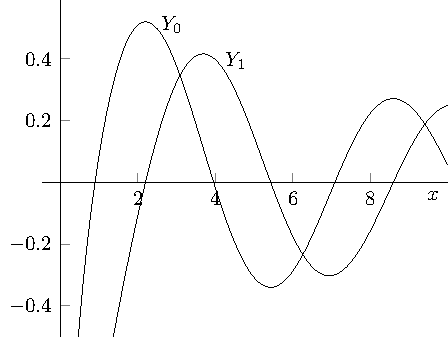
\includegraphics{figOctaveNeumannFunction}
\caption{بیسل تفاعل کے دوسرے اقسام۔}
\label{شکل_بیسل_نیومن_درجہ_صفر}
\end{figure}
جیسا شکل \حوالہ{شکل_بیسل_نیومن_درجہ_صفر} میں دکھایا گیا ہے کم قیمت کی مثبت \عددی{x} پر \عددی{Y_0} کی صورت \عددی{\ln x} کی طرح ہے اور \عددی{x\to \infty} پر \عددی{Y_0(x) \to \infty} ہو گا۔

\عددی{\nu=n=1,2,\cdots} کے لئے بھی بالکل اسی طرح، مساوات \حوالہ{مساوات_طاقتی_فروبنیوس_حل_ث} سے شروع کرتے ہوئے  دوسرا حل حاصل کیا جاتا ہے۔ان میں بھی لوگارتھمی جزو پایا جاتا ہے۔

دوسرے حل کا دارومدار اس حقیقت پر ہے کہ آیا \عددی{\nu} کا درجہ عدد صحیح ہے یا نہیں۔اس پیچیدگی  سے چھٹکارا حاصل کرنے کی خاطر دوسرے حل کو درج ذیل بیان کیا جاتا ہے جو تمام \عددی{\nu} کے لئے قابل استعمال ہے۔
\begin{gather}
\begin{aligned}\label{مساوات_بیسل_نیومن_عمومی_حل_الف}
Y_{\nu}(x)&=\frac{1}{\sin \nu \pi} [J_{\nu}(x)\cos \nu x-J_{-\nu}(x)] \quad \quad \text{(الف)}\\
Y_n(x)&=\lim_{\nu \to n} Y_{\nu}(x)\quad \quad \text{(ب)}
\end{aligned}
\end{gather}
درج بالا تفاعل کو \اصطلاح{درجہ \عددی{\nu} بیسل تفاعل کی دوسری قسم}\فرہنگ{بیسل تفاعل!دوسری قسم، درجہ \عددی{\nu}}\حاشیہب{Bessel function of the second kind of order $\nu$}\فرہنگ{Bessel function!second kind, order $\nu$} یا \اصطلاح{درجہ \عددی{\nu} نیومن تفاعل} کہتے ہیں۔ 

آئیں اب ثابت کریں کہ \عددی{J_{\nu}} اور \عددی{Y_{\nu}} تمام \عددی{\nu} اور تمام \عددی{x(>0)} کے لئے خطی طور غیر تابع ہیں۔

غیر عددی صحیح درجہ \عددی{\nu} کے لئے چونکہ \عددی{J_{\nu}(x)} اور \عددی{J_{-\nu}(x)} بیسل مساوات کے حل ہیں لہٰذا   \عددی{Y_{\nu}(x)} بھی بیسل مساوات کا حل ہے۔اب چونکہ ایسی \عددی{\nu} کے لئے \عددی{J_{\nu}(x)} اور \عددی{J_{-\nu}(x)} خطی طور غیر تابع ہیں اور \عددی{Y_{\nu}(x)} میں \عددی{J_{-\nu}(x)} پایا جاتا ہے لہٰذا \عددی{J_{\nu}(x)} اور \عددی{Y_{\nu}(x)} خطی طور غیر تابع ہوں گے۔مزید یہ کہ مساوات \حوالہ{مساوات_بیسل_نیومن_عمومی_حل_الف}-ب کو ثابت (صفحہ \حوالہصفحہ{حوالہ_بیرونی_مواد} پر حوالہ \cite{حوالہ_کریزگ_ب_اٹھارہ} میں ثبوت پیش کیا گیا ہے۔) کیا جا سکتا ہے لہٰذا عدد صحیح درجہ کے لئے \عددی{Y_n(x)} بیسل مساوات کا حل ہے۔آپ دیکھیں گے کہ \عددی{Y_n(x)} کی تسلسل میں لوگارتھمی جزو پایا جاتا ہے لہٰذا \عددی{J_n(x)} اور \عددی{Y_n(x)} خطی طور غیر تابع ہوں گے۔\عددی{Y_n(x)} کی تسلسل لکھنے کی خاطر \عددی{J_{\nu}(x)} کی تسلسل \حوالہ{مساوات_بیسل_تسلسل_عمومی} اور \عددی{J_{-\nu}(x)} کی تسلسل \حوالہ{مساوات_بیسل_تسلسل_عمومی_دوسرا} کو مساوات \حوالہ{مساوات_بیسل_نیومن_عمومی_حل_الف}-الف میں پر کرتے ہوئے \عددی{\nu \to n} کرتے ہیں (تفصیل صفحہ \حوالہصفحہ{حوالہ_بیرونی_مواد} پر \cite{حوالہ_کریزگ_ب_اٹھارہ} سے دیکھی جا سکتی ہے۔)
\begin{multline}\label{مساوات_بیسل_نیومن_عدد_صحیح_الف}
Y_n(x)=\frac{2}{\pi}J_n(x)\left(\ln \frac{x}{2}+\gamma\right)+\frac{x^n}{\pi}\sum_{m=0}^{\infty} \frac{(-1)^{m-1}(h_m+h_{m+n})}{2^{2m+n}m!(m+n)!}x^{2m}\\
-\frac{x^{-n}}{\pi}\sum_{m=0}^{n-1}\frac{(n-m-1)!}{2^{2m-n}m!}x^{2m}
\end{multline}
لکھا جا سکتا ہے جہاں \عددی{x>0} اور  \عددی{n=0,1,\cdots} جبکہ
\begin{align*}
h_0=0,\quad h_s=1+\frac{1}{2}+\frac{1}{3}+\cdots+\frac{1}{s} \quad \quad (s=1,2,\cdots)
\end{align*}
ہیں اور \عددی{n=0} کی صورت میں مساوات \حوالہ{مساوات_بیسل_نیومن_عدد_صحیح_الف} میں آخری مجموعے کی جگہ صفر لکھا جاتا ہے۔ درجہ صفر \عددی{n=0} پر  مساوات \حوالہ{مساوات_بیسل_نیومن_عدد_صحیح_الف} عین مساوات \حوالہ{مساوات_بیسل_نیومن_درجہ_صفر} کی صورت اختیار کرتی ہے۔اس کے علاوہ درج ذیل ثابت کیا جا سکتا ہے۔
\begin{align}
Y_{-n}(x)=(-1)^nY_n(x)
\end{align}
ان نتائج کو درج ذیل مسئلے میں پیش کرتے ہیں۔

%=======================
\ابتدا{مسئلہ} مساوات بیسل کا عمومی حل\\
تمام \عددی{\nu} کے لئے مساوات بیسل کا عمومی حل درج ذیل ہے۔
\begin{align}
y(x)=c_1J_{\nu}(x)+c_2Y_{\nu}(x)
\end{align}
\انتہا{مسئلہ}
%========================

بعض اوقات حقیقی \عددی{x} کے لئے مساوات بیسل کے مخلوط حل درکار ہوتے ہیں۔ایسی صورت میں درج ذیل خطی طور غیر تابع مخلوط حل  استعمال کیے جاتے ہیں جنہیں \اصطلاح{درجہ \عددی{\nu} بیسل تفاعل کی تیسری قسم}\فرہنگ{بیسل تفاعل!تیسری قسم}\حاشیہب{Bessel function of the third kind of order $\nu$}\فرہنگ{Bessel function!third kind} یا درجہ \عددی{\nu} پہلی اور دوسری \اصطلاح{ہینکل تفاعل}\فرہنگ{ہینکل تفاعل}\فرہنگ{تفاعل!ہینکل}\حاشیہب{Hankel functions}\فرہنگ{Hankel functions} کہا\حاشیہد{ہرمن ہینکل [1839-1873] جرمنی کے ریاضی دان۔} جاتا ہے۔
\begin{gather}
\begin{aligned}\label{مساوات_بیسل_ہینکل}
H_{\nu}^1(x)&=J_{\nu}(x)+iY_{\nu}(x)\\
H_{\nu}^2(x)&=J_{\nu}(x)-iY_{\nu}(x)
\end{aligned}
\end{gather}
%========================

\حصہء{سوالات}
سوال \حوالہ{سوال_بیسل_عمومی_حل_نیومن_الف} تا سوال \حوالہ{سوال_بیسل_عمومی_حل_نیومن_ب} کا عمومی حل \عددی{J_{\nu}} اور \عددی{Y_{\nu}} کی صورت میں حاصل کریں۔بتلائیں کہ کن سوالات میں \عددی{Y_{\nu}} کی جگہ \عددی{J_{-\nu}} استعمال کرنا ممکن ہے۔دی گئی اضافی معلومات استعمال کریں۔

%===============
\ابتدا{سوال}\شناخت{سوال_بیسل_عمومی_حل_نیومن_الف}\quad
$x^2y''+xy'+(x^2-25)y=0$\\
جواب:\عددی{y=c_1J_{5}(x)+c_2Y_{5}(x)}؛ چونکہ \عددی{\nu} عدد صحیح ہے لہٰذا \عددی{J_{-5}(x)} قابل استعمال نہیں ہے۔
\انتہا{سوال}
%=====================
\ابتدا{سوال}\quad
$x^2y''+xy'+(x^2-3)$\\
جواب:\عددی{y=c_1J_{\sqrt{3}}+c_2Y_{\sqrt{3}}(x)}؛ چونکہ \عددی{\nu} عدد صحیح نہیں ہے لہٰذا \عددی{J_{-\sqrt{3}}(x)} قابل استعمال ہے۔
\انتہا{سوال}
%===================
\ابتدا{سوال}\quad
$9x^2y''+9xy'+(z^{\tfrac{2}{3}}-\tfrac{9}{4})y=0, \quad \quad x=z^3$\\
جواب:\عددی{y=c_1J_{\tfrac{3}{2}}(x^{\tfrac{1}{3}})+c_2Y_{\tfrac{3}{2}}(x^{\tfrac{1}{3}})}
\انتہا{سوال}
%===================
\ابتدا{سوال}\quad
$x^2y''+xy'+(4x^4-\tfrac{16}{9})y=0,\quad \quad z=x^2$\\
جواب:\عددی{y=c_1J_{\tfrac{2}{3}}(x^2)+c_2Y_{\tfrac{2}{3}}(x^2)}
\انتہا{سوال}
%====================
\ابتدا{سوال}\quad
$9x^2y''+9xy'+(4x^{\tfrac{4}{3}}-25)y=0,\quad \quad z=x^{\tfrac{2}{3}}$\\
جواب:
$y=c_1J_{\tfrac{5}{2}}(x^{\tfrac{2}{3}})+c_2Y_{\tfrac{5}{2}}(x^{\tfrac{2}{3}})$
\انتہا{سوال}
%=================
\ابتدا{سوال}\quad
$y''+k^2x^2y=0,\quad \quad (y=u\sqrt{x},\quad z=\tfrac{kx^2}{2})$\\
جواب:\عددی{y=\sqrt{x}[c_1J_{\tfrac{1}{4}}(\tfrac{kx^2}{2})+c_2Y_{\tfrac{1}{4}}(\tfrac{kx^2}{2})]}
\انتہا{سوال}
%=================
\ابتدا{سوال}\quad
$xy''-5y'+xy=0,\quad \quad y=x^3u$\\
جواب:\عددی{y=x^3[c_1J_3(x)+c_2Y_3(x)]}
\انتہا{سوال}
%====================
\ابتدا{سوال}\quad
$xy''-y'+xy=0,\quad \quad y=xu$\\
جواب:\عددی{y=x[c_1J_1(x)+c_2Y_1(x)]}
\انتہا{سوال}
%=================
\ابتدا{سوال}\شناخت{سوال_بیسل_عمومی_حل_نیومن_ب}\quad
$xy''+5y'+xy=0,\quad \quad y=\tfrac{u}{x^2}$\\
جواب:\عددی{y=\tfrac{1}{x^2}[c_1J_2(x)+c_2Y_2(x)]}
\انتہا{سوال}
%===================
\ابتدا{سوال}\quad ترمیم شدہ درجہ \عددی{\nu} بیسل تفاعل کی پہلی قسم\\
ترمیم شدہ درجہ \عددی{\nu} بیسل تفاعل کی پہلی قسم کی تعریف \عددی{I_{\nu}(x)=i^{-\nu}J_{\nu}(ix)} ہے جہاں \عددی{i=\sqrt{-1}} ہے۔ثابت کریں  کہ \عددی{I_{\nu}(x)} درج ذیل تفرقی مساوات پر پورا اترتا ہے۔
\begin{align}\label{مساوت_بیسل_ترمیم_شدہ}
x^2y''+xy'-(x^2+\nu^2)y=0
\end{align}
جواب:\عددی{I_{\nu}(x)} کو دیے گئے مساوات میں پر کرتے ہوئے \عددی{0=0} حاصل کریں۔یہی ثبوت ہے۔
\انتہا{سوال}
%======================
\ابتدا{سوال}\quad ترمیم شدہ بیسل تفاعل\\
\عددی{I_{\nu}(x)} کی درج ذیل صورت حاصل کریں۔
\begin{align}
I_{\nu}(x)=\sum_{m=0}^{\infty}\frac{x^{2m+\nu}}{2^{2m+\nu}m!\Gamma(m+\nu+1)}
\end{align}
\انتہا{سوال}
%=======================
\ابتدا{سوال}\quad \عددی{I_{\nu}(x)} حقیقی ہے\\
ثابت کریں کہ حقیقی \عددی{x} اور حقیقی \عددی{\nu} کے لئے \عددی{I_{\nu}(x)} حقیقی ہے۔ثابت کریں کہ \عددی{x \ne 0} ہوتے ہوئے \عددی{I_{\nu}(x) \ne 0} ہو گا۔ ثابت کریں کہ \عددی{I_{-n}(x)=I_n(x)} کے برابر ہے جہاں \عددی{n} عدد صحیح ہے۔
\انتہا{سوال}
%====================
\ابتدا{سوال}\quad ترمیم شدہ بیسل تفاعل\\
ثابت کریں کہ تفاعل \عددی{K_{\nu}(x)}، جسے ترمیم شدہ بیسل تفاعل کی تیسری (بعض اوقات دوسری) قسم کہتے ہیں،
\begin{align}
K_{\nu}(x)=\frac{\pi}{2\sin \nu\pi}[I_{-\nu}(x)-I_{\nu}(x)]
\end{align}
تفرقی مساوات \حوالہ{مساوت_بیسل_ترمیم_شدہ} کا حل ہے۔ 
\انتہا{سوال}
%======================
\ابتدا{سوال}\quad ہینکل تفاعل\\
ثابت کریں کہ ہینکل تفاعل \حوالہ{مساوات_بیسل_ہینکل} مساوات بیسل کے حل کی اساس ہیں۔ 

\انتہا{سوال}
%==========================

\باب{لاپلاس تبادلہ}
لاپلاس بدل کی ترکیب سے ابتدائی قیمت (سرحدی قیمت) تفرقی مساوات حل کیے جاتے ہیں۔یہ ترکیب تین قدم پر مشتمل ہے۔
\begin{itemize}
\item
پہلا قدم: ابتدائی قیمت (سرحدی قیمت) تفرقی مساوات کا لاپلاس بدل لیتے ہوئے سادہ \اصطلاح{ضمنی مساوات} حاصل کی جاتی ہے۔
\item
دوسرا قدم:  ضمنی مساوات کو خالصتاً الجبرائی طور پر حل کیا جاتا ہے۔
\item
تیسرا قدم: ضمنی مساوات کے حل کا الٹ لاپلاس بدل لیتے ہوئے اصل حل حاصل کیا جاتا ہے۔
\end{itemize}  

یوں لاپلاس بدل تفرقی مساوات کے مسئلے کو سادہ الجبرائی مسئلہ میں تبدیل کرتا ہے۔تیسرے قدم پر الٹ لاپلاس بدل حاصل کرتے ہوئے عموماً ایسی جدول کا سہارا لیا جاتا ہے جس  میں تفاعل اور تفاعل کے الٹ لاپلاس بدل درج ہوں۔ 

انجینئری میں لاپلاس بدل کی ترکیب اہم کردار ادا کرتی ہے، بالخصوص ان مسائل میں جہاں جبری تفاعل غیر استمراری ہو، مثلاً جب جبری تفاعل کچھ وقفے کے لئے کار آمد ہو یا جبری تفاعل غیر سائن نما دہراتا تفاعل ہو۔

اب تک غیر متجانس مساوات کا عمومی حل حاصل کرتے ہوئے پہلے مطابقتی متجانس مساوات کا حل اور پھر غیر متجانس مساوات کا مخصوص حل حاصل کیا جاتا رہا۔لاپلاس بدل کی ترکیب میں عمومی حل ایک ہی بار میں حاصل ہوتا ہے۔اسی طرح لاپلاس بدل استعمال کرتے ہوئے ابتدائی قیمت (سرحدی قیمت) مسائل کے حل میں عمومی حل حاصل کرنے کے بعد ابتدائی (سرحدی) شرائط پر کرنے کی ضرورت پیش نہیں آتی چونکہ حل یہ شرائط شامل ہوتے ہیں۔
%=========================

\حصہ{لاپلاس بدل۔ الٹ لاپلاس بدل۔ خطیت}
فرض کریں کہ تفاعل \عددی{f(t)} تمام \عددی{t \ge 0} پر معین ہے۔ ہم \عددی{f(t)} کو \عددی{e^{-st}} سے ضرب دیتے ہوئے،  \عددی{t} کے ساتھ، \عددی{0} تا \عددی{\infty}، تکمل لیتے ہیں۔ اگر ایسا تکمل موجود ہو تو یہ \عددی{s} پر منحسر ہو گا لہٰذا اس کو \عددی{F(s)} لکھا جا سکتا ہے۔
\begin{align}
F(s)=\int_{0}^{\infty}e^{-st}f(t)\dif t
\end{align} 
تفاعل \عددی{F(s)} کو تفاعل \عددی{f(t)} کا \اصطلاح{لاپلاس بدل}\فرہنگ{لاپلاس بدل}\حاشیہب{ٔLaplace transform}\فرہنگ{Laplace transform} کہا جاتا ہے اور اس کو
 \عددی{\Laplace(f)} سے ظاہر کیا جاتا ہے۔
\begin{align}\label{مساوات_لاپلاس_بدل_الف}
F(s)=\Laplace(f)=\int_{0}^{\infty} e^{-st} f(t)\dif t
\end{align}
\عددی{f(t)} سے \عددی{F(s)} کے حصول کو \اصطلاح{لاپلاس تبادلہ}\فرہنگ{لاپلاس تبادلہ}\حاشیہب{Laplace transformation}\فرہنگ{Laplace transformation} کہتے ہیں۔

اسی طرح \عددی{f(t)} کو \عددی{F(s)} کا \اصطلاح{الٹ لاپلاس بدل}\فرہنگ{لاپلاس!الٹ بدل}\حاشیہب{inverse Laplace transform}\فرہنگ{Laplace!inverse transform} کہتے ہیں جسے \عددی{\Laplace^{-1}(F)} سے ظاہر کیا جاتا ہے۔
\begin{align}
f(t)=\Laplace^{-1}(F)
\end{align}

\موٹا{علامت نویسی}\\
اصل تفاعل کو چھوٹے لاطینی حرف تہجی سے ظاہر کیا جاتا ہے جبکہ لاپلاس بدل کو اسی حرف تہجی کی بڑی صورت سے ظاہر کیا جاتا ہے۔ یوں \عددی{f(t)} کا بدل \عددی{F(s)} ہو گا اور \عددی{g(t)} کا لاپلاس بدل \عددی{G(s)} ہو گا۔

%================
\ابتدا{مثال}
تفاعل \عددی{f(t)=1}، جہاں \عددی{t \ge 0} ہے، کا لاپلاس بدل مساوات \حوالہ{مساوات_لاپلاس_بدل_الف} سے بذریعہ تکمل حاصل کرتے ہیں۔
\begin{align*}
\Laplace(f)=\Laplace(1)=\int_{0}^{\infty} e^{-st} \dif t=\left. -\frac{1}{s}e^{-st}\right|_{0}^{\infty}
\end{align*}
ہو گا جو \عددی{s >0} کی صورت میں درج ذیل ہو گا۔
\begin{align*}
\Laplace(1)=\frac{1}{s}
\end{align*}
تکمل \حوالہ{مساوات_لاپلاس_بدل_الف} کی علامت پر آسائش ضرور ہے لیکن اس پر مزید غور کی ضرورت ہے۔اس تکمل کا وقفہ لامتناہی ہے۔ایسے تکمل کو \اصطلاح{غیر مناسب تکمل}\فرہنگ{غیر مناسب تکمل}\حاشیہب{improper integral}\فرہنگ{improper integral} کہتے ہیں اور حزب  تعریف، اس کی قیمت درج ذیل اصول کے تحت حاصل کی جاتی ہے۔ 
\begin{align*}
\int_{0}^{\infty} e^{-st}f(t)\dif t=\lim_{T\to \infty} \int_{0}^{T}e^{-st}f(t)\dif t
\end{align*}
یوں اس مثال میں اس آسائش علامت کا مطلب درج ذیل ہے۔
\begin{align*}
\int_{0}^{\infty}e^{-st}\dif t=\lim_{T\to \infty}\int_{0}^{T}e^{-st}\dif t=\lim_{T\to \infty}\left[-\frac{1}{s}e^{-sT}+\frac{1}{s}e^{0}\right]=\frac{1}{s}, \quad (s>0)
\end{align*}
اس پورے باب میں تکمل کی یہی علامت استعمال کی جائے گی۔
\انتہا{مثال}
%=================
\ابتدا{مثال}\شناخت{مثال_لاپلاس_قوت_نمائی_الف}
تفاعل \عددی{f(t)=e^{at}} جہاں \عددی{t \ge 0} اور \عددی{a} مستقل ہے کا لاپلاس بدل \عددی{\Laplace(f)} دریافت کریں۔

حل:مساوات \حوالہ{مساوات_لاپلاس_بدل_الف} سے
\begin{align*}
\Laplace(e^{at})=\int_{0}^{\infty} e^{-st}e^{at}\dif t=\left.\frac{1}{a-s}e^{-(s-a)t} \right|_{0}^{\infty}
\end{align*}
ملتا ہے۔اب اگر \عددی{s-a >0} ہو (یعنی \عددی{s} کی قیمت \عددی{a} سے زیادہ چننی گئی ہو۔)  تب درج ذیل حاصل ہو گا۔
\begin{align*}
\Laplace(e^{at})=\frac{1}{s-a}
\end{align*}
\انتہا{مثال}
%=================

اگرچہ ہم بالکل اسی طرز پر دیگر تفاعل کے لاپلاس بدل بذریعہ تکمل حاصل کر سکتے ہیں، حقیقت میں لاپلاس تبادلہ کے ایسی کئی خواص ہیں جنہیں استعمال کرتے ہوئے دیگر لاپلاس بدل نہایت عمدگی کے ساتھ حاصل کیے جا سکتے ہیں۔لاپلاس تبادلہ کی ایک خاصیت  خطیت ہے جس سے مراد درج ذیل ہے۔
%================

\ابتدا{مسئلہ}\شناخت{مسئلہ_لاپلاس_خطیت}\quad لاپلاس تبادلہ کی خطیت\\
لاپلاس تبادلہ خطی عمل ہے۔یوں ایسے تفاعل \عددی{f(t)} اور \عددی{g(t)}، جن کے لاپلاس بدل موجود ہوں، کے عمومی مجموعے کا لاپلاس بدل درج ذیل ہو گا جہاں \عددی{a} اور \عددی{b} مستقل ہیں۔
\begin{align*}
\Laplace[af(t)+bg(t)]=a\Laplace[f(t)]+b\Laplace[g(t)]
\end{align*}
\انتہا{مسئلہ}
%=================
\ابتدا{ثبوت}
لاپلاس تبدلہ کی تعریف سے درج ذیل لکھتے ہیں۔
\begin{align*}
\Laplace[af(t)+bg(t)]&=\int_{0}^{\infty}e^{-st}[af(t)+bg(t)]\dif t\\
&=a\int_{0}^{\infty}e^{-st}f(t)\dif t+b\int_{0}^{\infty}e^{-st}g(t) \dif t\\
&=a\Laplace[f(t)]+b\Laplace[g(t)]
\end{align*}
\انتہا{ثبوت}
%=====================

\ابتدا{مثال}
آئیں تفاعل \عددی{f(t)=\cosh at} کا لاپلاس بدل مسئلہ \حوالہ{مسئلہ_لاپلاس_خطیت} اور مثال \حوالہ{مثال_لاپلاس_قوت_نمائی_الف} کی مدد سے لکھیں۔
 چونکہ \عددی{\cosh at=\tfrac{1}{2}(e^{at}+e^{-at})} ہے لہٰذا 
\begin{align*}
\Laplace(\cosh at)=\frac{1}{2}\Laplace(e^{at})+\frac{1}{2}\Laplace(e^{-at})=\frac{1}{2}\left(\frac{1}{s-a}+\frac{1}{s+a}\right)=\frac{s}{s^2-a^2}
\end{align*}
ہو گا جہاں \عددی{s>a\ge 0} چننا گیا ہے۔
\انتہا{مثال}
%=======================
\ابتدا{مثال}
آئیں تفاعل \عددی{\sinh at} کا لاپلاس بدل حاصل کریں۔چونکہ \عددی{\sinh at=\tfrac{1}{2}(e^{at}-e^{{-at}})} ہے لہٰذا مسئلہ خطیت سے تفاعل کا لاپلاس بدل درج ذیل ہو گا۔
\begin{align*}
\Laplace(\sinh at)=\frac{1}{2}\Laplace(e^{at})-\frac{1}{2}\Laplace(e^{-at})=\frac{1}{2}\left(\frac{1}{s-a}-\frac{1}{s+a}\right)=\frac{a}{s^2-a^2}
\end{align*}
\انتہا{مثال}
%=========================
\ابتدا{مثال}
\عددی{\cos \omega t} اور \عددی{\sin \omega t} کے لاپلاس بدل حاصل کریں۔

حل:انہیں \عددی{\cos \omega t=\tfrac{1}{2}(e^{j\omega t}+e^{-j\omega t})} اور \عددی{\sin \omega t=\tfrac{1}{2j}(e^{j\omega t}-e^{-j\omega t})} لکھ کر لاپلاس بدل حاصل کرتے ہیں۔
\begin{align*}
\Laplace(\cos \omega t)&=\frac{1}{2}\Laplace(e^{j\omega t})+\frac{1}{2}\Laplace(e^{-j\omega t})=\frac{1}{2}\left(\frac{1}{s-j\omega}+\frac{1}{s+j\omega}\right)=\frac{s}{s^2+\omega^2}\\
\Laplace(\sin \omega t)&=\frac{1}{2j}\Laplace(e^{j\omega t})-\frac{1}{2j}\Laplace(e^{-j\omega t})=\frac{1}{2j}\left(\frac{1}{s-j\omega}-\frac{1}{s+j\omega}\right)=\frac{\omega}{s^2+\omega^2}
\end{align*}
\انتہا{مثال}
%===========================
جدول \حوالہ{جدول_لاپلاس_بدل_الف} میں چند اہم بنیادی تفاعل اور ان کے لاپلاس بدل دیے گئے ہیں۔اس جدول میں دیے لاپلاس بدل جاننے کے بعد ہم تقریباً ان تمام تفاعل کے بدل، لاپلاسی خواص سے حاصل کر پائیں گے،  جو ہمیں درکار ہوں گے۔
\begin{table}
\caption{چند بنیادی تفاعل \عددی{f(t)} اور ان کے لاپلاس بدل \عددی{\Laplace(f)}}
\label{جدول_لاپلاس_بدل_الف}
\centering
\begin{tabular}{ccc| ccc}
 شمار& $f(t)$& $\Laplace(f)$& شمار& $f(t)$& $\Laplace(f)$\\[0.5ex]
\hline
$1$&$1$&$\frac{1}{s}$&$7$&$\cos \omega t$&$\frac{s}{s^2+\omega^2}$\Tstrut\\[1ex]
$2$&$t$&$\frac{1}{s^2}$&$8$&$\sin \omega t$&$\frac{\omega}{s^2+\omega^2}$\\[1ex]
$3$&$t^2$&$\frac{2!}{s^3}$&$9$&$\cosh at$&$\frac{s}{s^2-a^2}$\\[1ex]
$4$&\shortstack{$t^n$\\ ($n=1,2,\cdots$)}&$\frac{n!}{s^{n+1}}$&$10$&$\sinh at$&$\frac{a}{s^2-a^2}$\\[1ex]
$5$&\shortstack{$t^a$\\($ a>0$)}&$\frac{\Gamma(a+1)}{s^{a+1}}$&$11$& $e^{at}\cos \omega t$& $\frac{s-a}{(s-a)^2+\omega^2}$\\[1.5ex]
$6$& $e^{at}$&$\frac{1}{s-a}$&$12$& $e^{at}\sin \omega t$& $\frac{\omega}{(s-a)^2+\omega^2}$
\end{tabular}
\end{table}

جدول \حوالہ{جدول_لاپلاس_بدل_الف} میں پہلا، دوسرا اور تیسرا کلیہ چوتھے کلیے سے اخذ کیے جا سکتے ہیں جبکہ چوتھا کلیہ از خود پانچویں کلیہ میں مساوات \حوالہ{مساوات_بیسل_گیما_بطور_عدد_ضربیہ} استعمال کرتے ہوئے \عددی{\Gamma(n+1)=n!} لکھ کر حاصل کیا جا سکتا ہے، جہاں \عددی{n} غیر منفی \عددی{n \ge 0} عدد صحیح ہے۔ پانچواں کلیہ، لاپلاس بدل کی تعریف مساوات \حوالہ{مساوات_لاپلاس_بدل_الف}
\begin{align*}
\Laplace(t^a)=\int_{0}^{\infty}e^{-st}t^a\dif t
\end{align*}
میں \عددی{st=x} پر کرتے ہوئے مساوات \حوالہ{مساوات_بیسل_گیما_الف} کے استعمال سے حاصل کرتے ہیں۔
\begin{align*}
\Laplace(t^a)=\int_{0}^{\infty}e^{-x}\left(\frac{x}{s}\right)^a \frac{\dif x}{s}=\frac{1}{s^{a+1}}\int_{0}^{\infty}e^{-x}x^a\dif x=\frac{\Gamma(a+1)}{s+1},\quad \quad (s>0)
\end{align*}
%============================

\جزوحصہء{\عددی{s} منتقلی}
تفاعل \عددی{f(t)}  کا لاپلاس بدل جانتے ہوئے تفاعل \عددی{e^{at}f(t)} کا لاپلاس بدل درج ذیل مسئلہ کی مدد سے فوراً لکھا جا سکتا ہے۔

%=============
\ابتدا{مسئلہ}\شناخت{مسئلہ_لاپلاس_بدل_قوت_نمائی}\quad منتقلی کا پہلا مسئلہ، \عددی{s} منتقلی\\
اگر تفاعل \عددی{f(t)} کا لاپلاس بدل \عددی{F(s)} ہو (جہاں کسی \عددی{k} کے لئے \عددی{s>k} ہے) تب تفاعل \عددی{e^{at}f(t)} کا لاپلاس بدل \عددی{F(s-a)} ہو گا (جہاں \عددی{s-a>k} ہے)۔
\begin{align*}
\Laplace[e^{at}f(t)]=F(s-a)
\end{align*}
اس مساوات کو الٹ لاپلاس بدل کی صورت میں بھی لکھا جا سکتا ہے یعنی
\begin{align*}
e^{at}f(t)=\Laplace^{-1}[F(s-a)]
\end{align*}
\انتہا{مسئلہ}
%=======================

\ابتدا{ثبوت}
لاپلاس بدل کے تکمل مساوات \حوالہ{مساوات_لاپلاس_بدل_الف} میں \عددی{s} کی جگہ \عددی{s-a} پر کرتے ہوئے 
\begin{align}\label{}
F(s-a)=\int_{0}^{\infty} e^{-(s-a)t} f(t)\dif t=\int_{0}^{\infty}e^{-st}{e^{at}f(t)}\dif t=\Laplace[e^{at}f(t)]
\end{align}
ملتا ہے۔اگر کسی \عددی{s>k} کے لئے \عددی{F(s)} موجود ہو یعنی اس کی قیمت محدود ہو تب \عددی{s-a>k} کے لئے پہلا تکمل بھی موجود ہو گا (یعنی محدود قیمت کا ہو گا)۔ اس کلیے کے دونوں اطراف کا الٹ لاپلاس بدل لینے سے مسئلے کی دوسری مساوات حاصل ہوتی ہے۔
\انتہا{ثبوت}
%======================

\ابتدا{مثال}\شناخت{مثال_لاپلاس_بدل_قصری_ارتعاش}\quad قصری ارتعاش\\
جدول \حوالہ{جدول_لاپلاس_بدل_الف} میں \عددی{\cos \omega t} اور \عددی{\sin \omega t} کے بدل کو استعمال کرتے ہوئے جدول میں گیارہ اور بارہ شمار پر دیے گئے لاپلاس بدل کو مسئلہ \حوالہ{مسئلہ_لاپلاس_بدل_قوت_نمائی} کی مدد سے فوراً لکھا جا سکتا ہے۔
\begin{align*}
\Laplace[e^{at}\cos \omega t]=\frac{s-a}{(s-a)^2+\omega^2} \quad \quad \Laplace[e^{at}\sin \omega t]=\frac{\omega}{(s-a)^2+\omega^2}
\end{align*}
انہیں استعمال کرتے ہوئے درج ذیل کا الٹ لاپلاس بدل حاصل کریں۔
\begin{align*}
\Laplace(f)=\frac{4s+24}{s^2+2s+101}
\end{align*}
حل:اس کو درکار صورت
\begin{align*}
f=\Laplace^{-1}\left[\frac{4(s+1)+2(10)}{(s+1)^2+10^2}\right]=4\Laplace^{-1}\left[\frac{s+1}{(s+1)^2+10^2}\right]+2\Laplace^{-1}\left[\frac{10}{(s+1)^2+10^2}\right]
\end{align*}
 میں لاتے ہوئے الٹ لاپلاس بدل لکھتے ہیں
\begin{align*}
f=e^{-t}(4\cos 10t+2\sin 10t)
\end{align*}
 جسے شکل \حوالہ{شکل_لاپلاس_قصری_ارتعاش} میں دکھایا گیا ہے۔یہ قصری ارتعاش کو ظاہر کرتی ہے۔
\begin{figure}
\centering
\begin{tikzpicture}
\begin{axis}[small,axis lines*=middle,xlabel={$t$},xlabel style={at={(current axis.right of origin)},anchor=north east}]
\addplot[domain=0:3,samples=150]{e^(-x)*(4*cos(180/pi*10*x)+2*sin(180/pi*10*x))};
\end{axis}
\end{tikzpicture}
\caption{قصری ارتعاش (مثال \حوالہ{مثال_لاپلاس_بدل_قصری_ارتعاش})}
\label{شکل_لاپلاس_قصری_ارتعاش}
\end{figure}
\انتہا{مثال}
%=======================

\جزوحصہء{لاپلاس بدل کی وجودیت اور یکتائی}
اگر تمام  \عددی{t \ge 0} کے لئے، کسی مستقل \عددی{k} اور \عددی{M} پر تفاعل \عددی{f} \موٹا{بڑھنے کی پابندی}
\begin{align}\label{مساوات_لاپلاس_بڑھنے_کی_حد}
\abs{f(t)} \le M e^{kt}
\end{align}
پر پورا اترتا ہو، تب اس کا لاپلاس بدل موجود ہو گا۔ہم کہتے ہیں کہ نہایت تیزی سے نہ بڑھنے والے  تفاعل \عددی{f(t)} کا لاپلاس بدل موجود ہو گا۔

\عددی{f(t)} کا استمراری  ہونا ضروری نہیں ہے البتہ اس کا \اصطلاح{ٹکڑوں میں استمراری}\فرہنگ{استمراری!ٹکڑوں میں}\حاشیہب{piecewise continuous}\فرہنگ{continuous!piecewise} ہونا لازم ہے۔  اگر محدود وقفہ \عددی{a \le t \le b} جس پر \عددی{f(t)} معین ہو، کو کئی ایسے ٹکڑوں میں تقسیم کرنا ممکن ہو کہ ہر ٹکڑے پر \عددی{f(t)} استمراری ہو اور \عددی{t} کا اندرون ٹکڑے سے ٹکڑے کے (دونوں) سروں تک پہنچنے پر  \عددی{f(t)} کی قیمت کا \اصطلاح{حد}\حاشیہب{limit} محدود حاصل ہو تب \عددی{f(t)} \اصطلاح{ٹکڑوں میں استمراری} کہلائے گا۔ ایسی صورت میں، جیسا شکل \حوالہ{شکل_لاپلاس_ٹکڑوں_استمراری} میں دکھایا گیا ہے، محدود \اصطلاح{چھلانگ}\فرہنگ{چھلانگ}\حاشیہب{jumps}\فرہنگ{jumps} پائے جائیں گے جو غیر استمراری صورت کی واحد وجہ ہو گی۔ عموماً عملی مسائل اسی نوعیت کے ہوتے ہیں۔درج ذیل مسئلہ بھی اسی نوعیت کا ہے۔ 
\begin{figure}
\centering
\begin{tikzpicture}
%axis
\draw(0,-1)--(0,2);
\draw(0,0)--++(6,0)node[right]{$t$};
\draw(1,0)--++(0,-0.1)node[below]{$a$};
\draw(5,0)--++(0,-0.1)node[below]{$b$};
%piecewise continuous
\draw(1,0.5) to [out=30,in=-150]++(1,1)node[circ]{};
\draw(2,2) to [out=-20,in=120]++(1,-2.5)node[circ]{};
\draw(3,0.3) to [out=0,in=-145]++(1,0.5)coordinate(kA);
\draw(4,1.4)coordinate(kB)--++(0.4,0)--++(0.6,-0.5);
\draw($(kA)!0.5!(kB)$) node[circ]{};
\end{tikzpicture}
\caption{ٹکڑوں میں استمراری تفاعل \عددی{f(t)}۔ غیر استمراری مقام پر تفاعل کی قیمت کو نقطوں سے ظاہر کیا گیا ہے۔}
\label{شکل_لاپلاس_ٹکڑوں_استمراری}
\end{figure}
%=============

\ابتدا{مسئلہ}\شناخت{مسئلہ_لاپلاس_وجودیت}\quad مسئلہ وجودیت لاپلاس بدل\\
اگر نصف محور \عددی{t \ge 0} کے ہر محدود وقفے پر تفاعل \عددی{f(t)} معین اور ٹکڑوں میں استمراری ہو اور مساوات \حوالہ{مساوات_لاپلاس_بڑھنے_کی_حد} پر، 
تمام \عددی{t \ge 0} اور کسی مستقل \عددی{M} اور \عددی{k} کے لئے،  پورا اترتا ہو تب لاپلاس بدل \عددی{\Laplace (f)} تمام \عددی{s >k} کے لئے موجود ہو گا ۔ 
\انتہا{مسئلہ}
%=========================

\ابتدا{ثبوت}
چونکہ \عددی{f(t)} ٹکڑوں میں استمراری ہے لہٰذا \عددی{t} محور کے کسی بھی محدود وقفے پر \عددی{e^{-st}f(t)} قابل تکمل ہے۔ مساوات \حوالہ{مساوات_لاپلاس_بڑھنے_کی_حد} کو دیکھ کر، \عددی{s>k} تصور کرتے ہوئے (جو درج ذیل آخری تکمل میں درکار ہے)، لاپلاس بدل کی وجودیت کا ثبوت حاصل کرتے ہیں۔
\begin{align*}
\abs{\Laplace(f)} = \abs{\int_{0}^{\infty} e^{-st}f(t)\dif t}\le \int_{0}^{\infty} \abs{f(t)}e^{-st}\dif t\le \int_{0}^{\infty} Me^{kt}e^{-st}\dif t=\frac{M}{s-k}
\end{align*}
\انتہا{ثبوت}
%=========================

کسی بھی تفاعل کا مساوات \حوالہ{مساوات_لاپلاس_بڑھنے_کی_حد} میں دیے گئے شرط پر پورا اترنے کو با آسانی دیکھا جا سکتا ہے، مثلاً \عددی{\cosh t < e^t} یا \عددی{t^n<n!e^t} (چونکہ \عددی{\tfrac{t^n}{n!}} مکلارن تسلسل کا ایک رکن ہے)۔ ایسا تفاعل جو مساوات \حوالہ{مساوات_لاپلاس_بڑھنے_کی_حد} پر پورا نہ اترتا ہو کی مثال \عددی{e^{t^2}} ہے۔آپ سوال \حوالہ{سوال_لاپلاس_کافی} میں دیکھیں گے کہ مسئلہ \حوالہ{مسئلہ_لاپلاس_وجودیت} میں دیے گئے شرائط لاپلاس بدل کی وجودیت کے لئے کافی ہیں نا کہ لازمی ہیں۔

\جزوحصہء{یکتائی}
اگر کسی تفاعل کا لاپلاس بدل موجود ہو تو یہ بدل یکتا ہو گا۔اسی طرح اگر (حقیقی مثبت محور پر معین) دو تفاعل کے لاپلاس بدل یکساں ہوں تب یہ تفاعل، کسی بھی مثبت لمبائی کے وقفے پر،  آپس میں مختلف نہیں ہو سکتے ہیں، البتہ تنہا نقطوں پر ان کی قیمت غیر یکساں ہو سکتی ہے۔یوں ہم کہہ سکتے ہیں کہ الٹ لاپلاس بدل یکتا ہے۔ بالخصوص دو ایسے استمراری تفاعل جن کا لاپلاس بدل یکساں ہو، آپس میں مکمل طور پر یکساں ہوں گے۔ 
%========================

\حصہء{سوالات}
%=============
سوال \حوالہ{سوال_لاپلاس_بدل_الف} تا سوال \حوالہ{سوال_لاپلاس_بدل_ب} میں لاپلاس بدل حاصل کریں۔ \عددی{a} اور  \عددی{b} کو مستقل تصور کریں۔

\ابتدا{سوال}\شناخت{سوال_لاپلاس_بدل_الف}\quad
$2t-3$\\
جواب:\عددی{\tfrac{2}{s^2}-\tfrac{3}{s}}
\انتہا{سوال}
%=======================
\ابتدا{سوال}\quad
$(at+b)^2$\\
جواب:\عددی{a(\tfrac{b}{s^2}+\tfrac{2a}{s^3})+b(\tfrac{b}{s}+\tfrac{a}{s^2})}
\انتہا{سوال}
%=====================
\ابتدا{سوال}\quad
$\sin 2\pi t$\\
جواب:\عددی{\tfrac{2\pi}{s^2+4\pi^2}}
\انتہا{سوال}
%====================
\ابتدا{سوال}\quad
$\sin^2 2\pi t$\\
جواب:\عددی{\tfrac{8\pi^2}{s(s^2+16\pi^2)}}
\انتہا{سوال}
%====================
\ابتدا{سوال}\quad
$e^{-3t}\sin 4t$\\
جواب:\عددی{\tfrac{4}{(s+3)^2+16}}
\انتہا{سوال}
%======================
\ابتدا{سوال}\quad
$e^{2t}\cos 3t$\\
جواب:\عددی{\tfrac{s-2}{(s-2)^2+9}}
\انتہا{سوال}
%======================
\ابتدا{سوال}\quad
$\cos (2t-\frac{\pi}{3})$\\
جواب:\عددی{\tfrac{\tfrac{s}{2}+\sqrt{3}}{s^2+4}}
\انتہا{سوال}
%=========================
\ابتدا{سوال}\شناخت{سوال_لاپلاس_بدل_ب} \quad
$2\sin (5t+\pi)$\\
جواب:\عددی{\tfrac{-10}{s^2+25}}
\انتہا{سوال}
%======================
\begin{figure}
\centering
\begin{subfigure}{0.33\textwidth}
\centering
\begin{tikzpicture}
%axis
\draw[gray](0,0)--(0,1.5);
\draw[gray](0,0)--(3,0);
%function
\draw[thick](0,0)--(2,1);
\draw[dashed](2,1)--(2,0);
\draw[thick](2,0)node[below]{$2$}--(3,0);
\draw(0,1)--++(-0.1,0)node[left]{$1$};
\draw(1,-0.5)node{(الف)};
\end{tikzpicture}%
\end{subfigure}%
\begin{subfigure}{0.33\textwidth}
\centering
\begin{tikzpicture}
%axis
\draw[gray](0,0)--(0,1.5);
\draw[gray](0,0)--(3,0);
%function
\draw[thick](0,1)--(2,1);
\draw[dashed](2,1)--(2,0)node[below]{$3$};
\draw[thick](2,0)--(3,0);
\draw(0,1)--++(-0.1,0)node[left]{$2$};
\draw(1,-0.5)node{(ب)};
\end{tikzpicture}%
\end{subfigure}%
\begin{subfigure}{0.33\textwidth}
\centering
\begin{tikzpicture}
%axis
\draw[gray](0,0)--(0,1.5);
\draw[gray](0,0)--(3,0);
%function
\draw[thick](0,1)--(2,0);
\draw[thick](2,0)node[below]{$5$}--(3,0);
\draw(0,1)--++(-0.1,0)node[left]{$2$};
\draw(1,-0.5)node{(پ)};
\end{tikzpicture}%
\end{subfigure}
%
\begin{subfigure}{0.33\textwidth}
\centering
\begin{tikzpicture}
%axis
\draw[gray](0,-1.2)--(0,1.2);
\draw[gray](0,0)--(3,0);
%function
\draw[thick](0,1)--(2,-1);
\draw[dashed](2,-1)--(2,0);
\draw[thick](2,0)node[above]{$2$}--(3,0);
\draw(0,1)--++(-0.1,0)node[left]{$5$};
\draw(0,-1)--++(-0.1,0)node[left]{$-5$};
\draw(0.75,-0.75)node{(ت)};
\end{tikzpicture}%
\end{subfigure}%
\begin{subfigure}{0.33\textwidth}
\centering
\begin{tikzpicture}
%axis
\draw[gray](0,0)--(0,1.5);
\draw[gray](0,0)--(3,0);
%function
\draw[thick](0,0)--(1,1)--(2.5,0)node[below]{$7$}--(3,0);
\draw(0,1)--++(-0.1,0)node[left]{$2$};
\draw(1,0)--++(0,-0.1)node[below]{$3$};
\draw(1,-0.75)node{(ٹ)};
\end{tikzpicture}%
\end{subfigure}%
\begin{subfigure}{0.33\textwidth}
\centering
\begin{tikzpicture}
%axis
\draw[gray](0,0)--(0,1.5);
\draw[gray](0,0)--(3,0);
%function
\draw[thick](0,0)--(1,1);
\draw[dashed](1,1)--(1,1.5);
\draw[thick](1,1.5)--(2,1.5);
\draw[dashed](2,1.5)--(2,0);
\draw[thick](2,0)node[below]{$4$}--(3,0);
\draw(0,1)--++(-0.1,0)node[left]{$2$};
\draw(0,1.5)--++(-0.1,0)node[left]{$3$};
\draw(1,0)--++(0,-0.1)node[below]{$2$};
\draw(1.5,-0.75)node{(ث)};
\end{tikzpicture}%
\end{subfigure}
\caption{سوال \حوالہ{سوال_لاپلاس_بدل_پ} تا سوال \حوالہ{سوال_لاپلاس_بدل_پ} کے اشکال۔}
\label{شکل_سوال_لاپلاس_بدل_پ}
\end{figure}
%================
\ابتدا{سوال}\شناخت{سوال_لاپلاس_بدل_پ} 
شکل \حوالہ{شکل_سوال_لاپلاس_بدل_پ}-الف میں ٹکڑوں میں استمراری تفاعل دکھایا گیا ہے۔تمام ٹکڑوں کی ریاضی مساوات حاصل کریں۔ تکمل \حوالہ{مساوات_لاپلاس_بدل_الف}  کو ٹکڑوں میں تقسیم کرتے ہوئے لاپلاس بدل حاصل کریں۔

جواب:\عددی{\tfrac{1-e^{-2s}(2s+1)}{2s^2}}
\انتہا{سوال}
%=========================
\ابتدا{سوال}
شکل \حوالہ{شکل_سوال_لاپلاس_بدل_پ}-ب میں دیے گئے تفاعل کا لاپلاس بدل حاصل کریں۔

جواب:\عددی{\tfrac{2}{s}(1-e^{-3s})}
\انتہا{سوال}
%===========================
\ابتدا{سوال}
شکل \حوالہ{شکل_سوال_لاپلاس_بدل_پ}-پ میں دیے گئے تفاعل کا لاپلاس بدل حاصل کریں۔

جواب:\عددی{\tfrac{2e^{-5s}+10s-2}{5s^2}}
\انتہا{سوال}
%===========================
\ابتدا{سوال}
شکل \حوالہ{شکل_سوال_لاپلاس_بدل_پ}-ت میں دیے گئے تفاعل کا لاپلاس بدل حاصل کریں۔

جواب:\عددی{\tfrac{5(s+1)e^{-2s}+5(s-1)}{s^2}}
\انتہا{سوال}
%===========================
\ابتدا{سوال}
شکل \حوالہ{شکل_سوال_لاپلاس_بدل_پ}-ٹ میں دیے گئے تفاعل کا لاپلاس بدل حاصل کریں۔

جواب:\عددی{\tfrac{4-7e^{-3s}+3e^{-7s}}{6s^2}}
\انتہا{سوال}
%===========================
\ابتدا{سوال}
شکل \حوالہ{شکل_سوال_لاپلاس_بدل_پ}-ث میں دیے گئے تفاعل کا لاپلاس بدل حاصل کریں۔

جواب:\عددی{\tfrac{1+(s-1)e^{-2s}-3se^{-4s}}{s^2}}
\انتہا{سوال}
%===========================
\ابتدا{سوال}\شناخت{سوال_لاپلاس_کافی}\quad وجودیت\\
تفاعل \عددی{\tfrac{1}{\sqrt{t}}} کا لاپلاس بدل حاصل کریں۔ایسا کرتے ہوئے \عددی{\Gamma(\tfrac{1}{2})=\sqrt{\pi}} (مساوات \حوالہ{مساوات_بیسل_گیما_نیم}) کا استعمال کریں۔ اس سے آپ اخذ کر سکتے ہیں کہ مسئلہ \حوالہ{مسئلہ_لاپلاس_وجودیت} میں دیے شرائط کافی ہیں نا کہ لازمی۔

جواب:\عددی{\tfrac{\sqrt{\pi}}{s}}
\انتہا{سوال}
%==============================
\ابتدا{سوال}
\عددی{e^{at}} کا لاپلاس بدل \عددی{\cosh at} اور \عددی{\sinh at} کے لاپلاس بدل سے حاصل کریں۔

جواب:\عددی{e^{at}=\sinh at+\cosh at} لکھ کر جواب \عددی{\tfrac{1}{s-a}} ملتا ہے۔
\انتہا{سوال}
%============================
\ابتدا{سوال}\quad پیمائشی فیتہ میں ردوبدل\\
ثابت کریں کہ اگر \عددی{\Laplace[f(t)]=F(s)}  ہو تب \عددی{\Laplace[f(ct)]=\tfrac{F(\tfrac{s}{c})}{c}} ہو گا جہاں \عددی{c} مستقل ہے۔اس کلیے کو استعمال کرتے ہوئے \عددی{\Laplace(\cos t)} سے \عددی{\Laplace(\cos \omega t)} حاصل کریں۔

جواب:مساوات \حوالہ{مساوات_لاپلاس_بدل_الف} استعمال کرتے ہوئے کلیہ ثابت ہو گا۔
\انتہا{سوال}
%=============================
\ابتدا{سوال}\quad الٹ لاپلاس بدل کی خطیت\\
\عددی{\Laplace} کی خطیت کو استعمال کرتے ہوئے ثابت کریں کہ \عددی{\Laplace^{-1}} خطی ہے۔
\انتہا{سوال}
%==============================
سوال \حوالہ{سوال_لاپلاس_الٹ_الف} تا سوال \حوالہ{سوال_لاپلاس_الٹ_ب} میں الٹ لاپلاس بدل حاصل کریں۔

%==============
\ابتدا{سوال}\شناخت{سوال_لاپلاس_الٹ_الف}\quad
$\frac{0.5s+1.3}{s^2+1.69}$\\
جواب:\عددی{\sin (1.3t)+0.5\cos(1.3t)}
\انتہا{سوال}
%========================
\ابتدا{سوال}\quad
$\frac{4s+1}{s^2-16}$\\
جواب:\عددی{\tfrac{1}{8}(17e^{4t}+15e^{-4t})}
\انتہا{سوال}
%========================
\ابتدا{سوال}\quad
$\frac{s}{m^2s^2+n^2}$\\
جواب:\عددی{\tfrac{\cos \tfrac{nt}{m}}{m^2}}
\انتہا{سوال}
%=========================
\ابتدا{سوال}\quad
$\frac{1}{(s+3)(s-2)}$\\
جواب:\عددی{\tfrac{1}{5}(e^{2t}-e^{-3t})}
\انتہا{سوال}
%========================
\ابتدا{سوال}\quad
$\frac{2}{s^3}+\frac{3}{s^5}$\\
جواب:\عددی{t^2+\tfrac{t^4}{8}}
\انتہا{سوال}
%======================
\ابتدا{سوال}\quad
$\frac{3s+8}{s^2-9}$\\
جواب:\عددی{\tfrac{1}{6}(17e^{3t}+e^{-3t})}
\انتہا{سوال}
%========================
\ابتدا{سوال}\quad
$\frac{s-1}{s^2-s-6}$\\
جواب:\عددی{\tfrac{1}{5}(2e^{3t}+3e^{-2t})}
\انتہا{سوال}
%=======================
\ابتدا{سوال}\شناخت{سوال_لاپلاس_الٹ_ب}\quad
$\frac{1}{(s-a)(s+b)}$\\
جواب:\عددی{\tfrac{1}{a+b}(e^{at}-e^{-bt})}
\انتہا{سوال}
%=====================
سوال \حوالہ{سوال_لاپلاس_منتقلی_الف} تا سوال \حوالہ{سوال_لاپلاس_منتقلی_ت} منتقلی \عددی{s} پر مبنی ہیں۔ سوال \حوالہ{سوال_لاپلاس_منتقلی_الف} تا سوال \حوالہ{سوال_لاپلاس_منتقلی_ب} میں لاپلاس بدل جبکہ سوال \حوالہ{سوال_لاپلاس_منتقلی_پ} تا سوال \حوالہ{سوال_لاپلاس_منتقلی_ت} میں الٹ لاپلاس بدل حاصل کریں۔

%=========
\ابتدا{سوال}\شناخت{سوال_لاپلاس_منتقلی_الف}\quad
$te^{2t}$\\
جواب:\عددی{\tfrac{1}{(s-2)^2}}
\انتہا{سوال}
%=======================
\ابتدا{سوال}\quad
$e^{-3t}\sin 5t$\\
جواب:\عددی{\tfrac{5}{(s+3)^2+5^2}}
\انتہا{سوال}
%==========================
\ابتدا{سوال}\quad
$0.25e^{-1.5t}\cos (3\pi t)$\\
جواب:\عددی{\tfrac{0.25(s+1.5)}{(s+1.5)^2+(3\pi)^2}}
\انتہا{سوال}
%=============================
\ابتدا{سوال}\شناخت{سوال_لاپلاس_منتقلی_ب}\quad
$\sinh t \sin \omega t$\\
جواب:\عددی{\tfrac{1}{2}[\tfrac{\omega}{(s-1)^2+\omega^2}-\tfrac{\omega}{(s+1)^2+\omega^2}]}
\انتہا{سوال}
%============================
\ابتدا{سوال}\شناخت{سوال_لاپلاس_منتقلی_پ}\quad
$\frac{m}{(s+n)^2}$\\
جواب:\عددی{mte^{-nt}}
\انتہا{سوال}
%=============================
\ابتدا{سوال}\quad
$\frac{3}{(s+5)^4}$\\
جواب:\عددی{\tfrac{t^3e^{-5t}}{2}}
\انتہا{سوال}
%===================
\ابتدا{سوال}\quad
$\tfrac{3}{(s+\sqrt{5})^3}$\\
جواب:\عددی{\tfrac{3t^2e^{-\sqrt{5}t}}{2}}
\انتہا{سوال}
%========================
\ابتدا{سوال}\quad
$\tfrac{4}{s^2+2s+5}$\\
جواب:\عددی{2e^{-t}\sin 2t}
\انتہا{سوال}
%======================
\ابتدا{سوال}\quad
$\frac{\pi}{s^2+8\pi s+17\pi^2}$\\
جواب:\عددی{e^{-4\pi t}\sin \pi t}
\انتہا{سوال}
%========================
\ابتدا{سوال}\quad
$\frac{3s+22}{s^2+8s+41}$\\
جواب:\عددی{e^{-4t}(2\sin 5t+3\cos 5t)}
\انتہا{سوال}
%=============================
\ابتدا{سوال}\quad
$\frac{s+a+b}{(s+a)^2+b^2}$\\
جواب:\عددی{e^{-at}(\cos bt+\sin bt)}
\انتہا{سوال}
%=======================
\ابتدا{سوال}\شناخت{سوال_لاپلاس_منتقلی_ت}\quad
$\frac{a}{s+c}+\frac{b}{(s+c)^2}$\\
جواب:\عددی{(a+bt)e^{-ct}}
\انتہا{سوال}
%=======================

\حصہ{تفرقات اور تکملات کے لاپلاس بدل۔ سادہ تفرقی مساوات}
لاپلاس بدل کو استعمال کرتے ہوئے سادہ تفرقی مساوات اور ابتدائی قیمت مسائل حل کیے جاتے ہیں۔لاپلاس بدل کے استعمال سے  احصائی اعمال کی جگہ الجبرائی اعمال استعمال کیے جاتے ہیں۔یوں \عددی{f(t)} کا تفرق، \عددی{F(s)} کو \عددی{s} سے ضرب دینے کے (تقریباً) مترادف ہو گا جبکہ \عددی{f(t)} کا تکمل،  \عددی{F(s)} کو \عددی{s} سے تقسیم کرنے کے مترادف ہو گا۔ 
%====================
\ابتدا{مسئلہ}\شناخت{مسئلہ_لاپلاس_ایک_درجی}\quad \عددی{f(t)} کی تفرق کا لاپلاس بدل\\
اگر \عددی{f(t)} تمام \عددی{t \ge 0} پر استمراری ہو، مساوت \حوالہ{مساوات_لاپلاس_بڑھنے_کی_حد} پر پورا اترتا ہو اور \عددی{f'(t)} نصف محور \عددی{t \ge 0} کے ہر محدود وقفے پر \اصطلاح{ٹکڑوں میں استمراری} ہو تب، \عددی{s>k} کی صورت میں، \عددی{f'(t)} کا لاپلاس بدل موجود ہو گا جو درج ذیل سے حاصل کیا جا سکتا ہے۔
\begin{align} \label{مساوات_لاپلاس_درجہ_اول_تفرق}
\Laplace(f')&=s\Laplace(f)-f(0)\quad \quad (s>k)
\end{align}
\انتہا{مسئلہ}
%=======================

\ابتدا{ثبوت}
ہم یہ  فرض کرتے ہوئے  کہ \عددی{f'} \موٹا{بھی} استمراری ہے مساوات \حوالہ{مساوات_لاپلاس_درجہ_اول_تفرق} ثابت کرتے ہیں۔یوں لاپلاس بدل کی تعریف (مساوات \حوالہ{مساوات_لاپلاس_بدل_الف}) اور تکمل بالحصص سے درج ذیل لکھا جا سکتا ہے۔
\begin{align*}
\Laplace(f')=\int_{0}^{\infty} e^{-st} f'(t)\dif t=\left. e^{-st} f(t) \right|_{0}^{\infty}+s\int_{0}^{\infty} e^{-st}f(t)\dif t=f(0)+sF(s)
\end{align*}
چونکہ \عددی{f(t)} مساوات \حوالہ{مساوات_لاپلاس_بڑھنے_کی_حد} پر پورا اترتی ہے لہٰذا \عددی{s>k} کی صورت میں  \عددی{t=\infty} پر \عددی{e^{-st}f(t)}صفر دیگا جبکہ \عددی{t=0} پر یہ \عددی{f(0)} دیگا۔آخری تکمل \عددی{\Laplace (f)=F(s)} کے برابر ہے  جس کا حل، \عددی{s>k} کی  صورت میں، مسئلہ \حوالہ{مسئلہ_لاپلاس_وجودیت} کے تحت موجود ہے۔یوں \عددی{\Laplace(f')} کا حل موجود ہے۔

اگر \عددی{f'} ٹکڑوں میں استمراری ہو تب درج بالا ثبوت میں تکمل کو ایسے ٹکڑوں میں تقسیم کیا جاتا ہے کہ ہر ٹکڑے (وقفے) پر \عددی{f'} استمراری ہو۔ سوال \حوالہ{سوال_لاپلاس_مسئلہ_تفرق} میں اس پر غور کیا گیا ہے۔
\انتہا{ثبوت}
%===========================

\عددی{f''} پر مساوات \حوالہ{مساوات_لاپلاس_درجہ_اول_تفرق}  لاگو کر کے حاصل جواب میں مساوات \حوالہ{مساوات_لاپلاس_درجہ_اول_تفرق} پر کرتے ہوئے درج ذیل ملتا ہے۔
\begin{align}\label{مساوات_لاپلاس_درجہ_دوم_تفرق}
\Laplace(f'')=s\Laplace(f')-f'(0)=s[s\Laplace(f)-f(0)]-f'(0)=s^2\Laplace(f)-sf(0)-f'(0)
\end{align}
اسی ترکیب کو \عددی{f'''} پر لاگو کرتے ہوئے
\begin{align}\label{مساوات_لاپلاس_درجہ_تین_تفرق}
\Laplace(f''')=s^3\Laplace(f)-s^2f(0)-sf'(0)-f''(0)
\end{align}
ملتا ہے۔اس ترکیب کو بار بار استعمال کرتے ہوئے درج ذیل مسئلہ اخذ کیا جا سکتا ہے۔
%=======================

\ابتدا{مسئلہ}\شناخت{مسئلہ_لاپلاس_بلند_درجی}\quad بلند درجی تفرق \عددی{f^n}\\
اگر \عددی{f(t)} اور اس کے تفرقات \عددی{f'(t)}، \عددی{f''(t)}، \نقطے، \عددی{f^{(n-1)}(t)}  تمام \عددی{t \ge 0} پر استمراری ہوں، مساوت \حوالہ{مساوات_لاپلاس_بڑھنے_کی_حد} پر پورا اترتے ہوں اور \عددی{f^{(n)}(t)} نصف محور \عددی{t \ge 0} کے ہر محدود وقفے پر \اصطلاح{ٹکڑوں میں استمراری} ہو تب، \عددی{s>k} کی صورت میں، \عددی{f^{(n)}(t)} کا لاپلاس بدل موجود ہو گا جو درج ذیل سے حاصل کیا جا سکتا ہے۔
\begin{align}
\Laplace(f^{(n)})=s^n\Laplace(f)-s^{n-1}f(0)-s^{n-2}f'(0)-\cdots -f^{(n-1)}(0)
\end{align}
\انتہا{مسئلہ}
%=============================

\ابتدا{مثال}
تفاعل \عددی{f(t)=t^2} کا لاپلاس بدل حاصل کریں۔

حل:\عددی{f'=2t} اور \عددی{f''=2} ہیں۔یوں \عددی{f(0)=0}، \عددی{f'(0)=0} اور \عددی{f''(0)=2} ملتے ہیں۔اب \عددی{\Laplace(2)=\tfrac{2}{s}} ہے لہٰذا  مساوات \حوالہ{مساوات_لاپلاس_درجہ_دوم_تفرق} استعمال کرتے ہوئے درج ذیل لکھا جا سکتا ہے جو جدول \حوالہ{جدول_لاپلاس_بدل_الف} کے عین مطابق ہے۔
\begin{align*}
\Laplace(f'')=\Laplace(2)=\frac{2}{s}=s^2\Laplace(f), \quad \implies \quad \Laplace(t^2)=\frac{2}{s^3}
\end{align*}
عموماً کسی بھی تفاعل کا لاپلاس بدل کئی مختلف طریقوں سے حاصل کرنا ممکن ہوتا ہے۔
\انتہا{مثال}
%=============================
\ابتدا{مثال}\شناخت{مثال_لاپلاس_مربع_سائن}
تفاعل \عددی{f(t)=\sin^2 t} کا لاپلاس بدل حاصل کریں۔

حل:\عددی{f(0)=0} ہے جبکہ \عددی{f'=2\sin t \cos t=\sin 2t} لکھا جا سکتا ہے۔یوں مساوات \حوالہ{مساوات_لاپلاس_درجہ_اول_تفرق} استعمال کرتے ہوئے درج ذیل لکھا جا سکتا ہے۔ 
\begin{align*}
\Laplace(\sin 2t)=\frac{2}{s^2+4}=s\Laplace(f) \quad \implies \quad \Laplace(f)=\frac{2}{s(s^2+4)}
\end{align*}
\انتہا{مثال}
%==============================
\ابتدا{مثال}
تفاعل \عددی{f(t)=t\sin \omega t} کا لاپلاس بدل حاصل کریں۔

حل:\عددی{f(0)=0} ہے جبکہ
\begin{align*}
f'(t)&=\sin \omega t-\omega t\cos \omega t, \quad f'(0)=0,\\
f''(t)&=2\omega \cos \omega t-\omega^2 t \sin \omega t=2\omega \cos \omega t-\omega^2 f(t)
\end{align*}
ہیں۔یوں مساوات \حوالہ{مساوات_لاپلاس_درجہ_دوم_تفرق} استعمال کرتے ہوئے
\begin{align*}
\Laplace(f'')=2\omega \Laplace(\cos \omega t)-\omega^2\Laplace(f)=s^2\Laplace(f)
\end{align*}
لکھا جا سکتا ہے جس میں \عددی{\cos \omega t} کا لاپلاس بدل پر کرتے 
\begin{align*}
(s^2+\omega^2)\Laplace(f)=2\omega \Laplace(\cos \omega t)=\frac{2\omega s}{s^2+\omega^2}
\end{align*}
ہوئے درج ذیل حاصل کرتے ہیں۔
\begin{align*}
\Laplace(t\sin \omega t)=\frac{2\omega s}{(s^2+\omega^2)^2}
\end{align*}
\انتہا{مثال}
%==============================
\ابتدا{مثال}\شناخت{مثال_لاپلاس_کوسائن_ضرب_وقت}
تفاعل \عددی{f(t)=t\cos \omega t} کا لاپلاس بدل حاصل کریں۔

حل:ہم درج ذیل لکھ سکتے ہیں۔
\begin{align*}
f(t)&=t\cos \omega t, \quad f(0)=0\\
f'(t)&=\cos \omega t-\omega t\sin \omega t, \quad f'(0)=1\\
f''(t)&=-2\omega \sin \omega t-\omega^2 f(t)
\end{align*}
یوں مساوات \حوالہ{مساوات_لاپلاس_درجہ_دوم_تفرق} استعمال کرتے ہوئے درج ذیل لکھا جا سکتا ہے۔
\begin{align*}
\Laplace(f'')&=s^2\Laplace(f)-sf(0)-sf'(0)\\
&=s^2F(s)-1
\end{align*}
ساتھ ہی ساتھ \عددی{f''} کی مساوات کا لاپلاس بدل درج ذیل لکھا جا سکتا ہے۔
\begin{align*}
\Laplace(f'')&=\Laplace[-2\omega \sin \omega t-\omega^2 f(t)]\\
&=-\frac{2\omega^2}{s^2+\omega^2}-\omega^2F(s)
\end{align*}
ان دونوں جوابات کو برابر پر کرتے ہوئے درج ذیل ملتا ہے۔
\begin{align}\label{مساوات-لاپلاس_کوسائن_ضرب_وقت}
F(s)=\Laplace[t\cos \omega t]=\frac{s^2-\omega^2}{(s^2+\omega^2)^2}
\end{align}
\انتہا{مثال}
%===============================
\ابتدا{مثال}\شناخت{مثال_لاپلاس_ٹکڑوں_میں_استمراری}
استمراری \عددی{f(t)} کی صورت میں  \عددی{f'(t)} کا لاپلاس بدل مسئلہ \حوالہ{مسئلہ_لاپلاس_ایک_درجی} دیتی ہے۔آئیں \اصطلاح{ٹکڑوں میں استمراری} \عددی{f(t)} کی صورت میں \عددی{f'(t)} کا لاپلاس بدل حاصل کریں۔شکل \حوالہ{شکل_مثال_لاپلاس_ٹکڑوں_میں_استمراری} کے تفاعل میں \عددی{t=a(>0)} پر تفاعل غیر استمراری ہے جبکہ بقایا تمام شرائط وہی ہیں جو مسئلہ \حوالہ{مسئلہ_لاپلاس_ایک_درجی} میں تھے۔اس تفاعل کا لاپلاس بدل حاصل کریں۔
\begin{figure}
\centering
\begin{tikzpicture}
%axis
\draw(0,0)--++(0,2)node[left]{$f(t)$};
\draw(0,0)--(4,0)node[right]{$t$};
\draw(0,0.5) to [out=20,in=-130]++(2,0.5)coordinate(kL);
\draw(2,1.5)coordinate(kR) to [out=-40,in=130]++(1.5,-1.3);
\draw[stealth-] (kL)++(-0.1,0)--++(-0.5,0.2)node[left]{$f(a_-)$};
\draw[stealth-] (kR)++(0.1,0)--++(0.5,0.2)node[right]{$f(a_+)$};
\draw[dashed](2,0)node[below]{$a$}--++(0,2);
\end{tikzpicture}
\caption{ٹکڑوں میں استمراری تفاعل \عددی{f(t)}(مثال \حوالہ{مثال_لاپلاس_ٹکڑوں_میں_استمراری})}
\label{شکل_مثال_لاپلاس_ٹکڑوں_میں_استمراری}
\end{figure}

شکل \حوالہ{شکل_مثال_لاپلاس_ٹکڑوں_میں_استمراری} میں دکھایا گیا تفاعل \عددی{t=a} غیر استمراری ہے۔ ہم کہتے ہیں کہ \عددی{t=a} پر تفاعل \اصطلاح{چھلانگ}\فرہنگ{چھلانگ}\حاشیہب{jump}\فرہنگ{jump} لگاتا ہے یا کہ تفاعل میں \عددی{t=0} پر \اصطلاح{چھلانگ} پائی جاتی ہے۔نقطہ چھلانگ تک بائیں جانب سے پہنچتے ہوئے تفاعل کے قیمت کی \اصطلاح{حد}\فرہنگ{حد}\حاشیہب{limit}\فرہنگ{limit} کو \عددی{f(a_{-})} لکھا جاتا ہے جبکہ نقطہ چھلانگ تک دائیں جانب سے پہنچتے ہوئے تفاعل کے قیمت کی حد کو \عددی{f(a_+)} لکھا جاتا ہے۔یوں \عددی{t=a} پر تفاعل کی چھلانگ \عددی{f(a_+)-f(a_-)} ہو گی۔

لاپلاس بدل کی تعریف (مساوات \حوالہ{مساوات_لاپلاس_بدل_الف}) سے درج ذیل لکھا جا سکتا ہے جہاں تکمل کو ایسے ٹکڑوں (وقفوں) میں تقسیم کیا گیا ہے کہ ہر وقفے پر \عددی{f(t)} استمراری ہے۔
\begin{align*}
\Laplace(f')=\int_{a_+}^{\infty} e^{-st}f' \dif t+\int_{0}^{a_-}e^{-st}f' \dif t
\end{align*}  
پہلے تکمل کا ابتدائی حد \عددی{a_+} ہے جو \عددی{t=a} کے دائیں طرف کو ظاہر کرتی ہے جہاں تفاعل کی قیمت \عددی{f(a_+)}  ہے۔اسی طرح دوسری تکمل کا اختتامی حد \عددی{a_-} ہے جس پر تفاعل کی قیمت \عددی{f(a_-)} ہے۔انہیں شکل میں دکھایا گیا ہے۔  تکمل بالحصص سے
\begin{align*}
\Laplace(f')&=\left. e^{-st} f(t)\right|_{a_+}^{\infty}+s\int_{a_+}^{\infty}e^{-st}f(t)\dif t+\left. e^{-st}f(t) \right|_{0}^{a_-}+s\int_{0}^{a_-}e^{-st} f(t)\dif t\\
&=-e^{-sa}f(a_+)+s\int_{a_+}^{\infty}e^{-st}f(t)\dif t+e^{-sa}f(a_-)-f(0)+s\int_{0}^{a_-}e^{-st} f(t)\dif t\\
&=s\int_{0}^{\infty}e^{-st}f(t)\dif t -f(0)-e^{-sa}[f(a_+)-f(a_-)]\\
&=sF(s) -f(0)-e^{-sa}[f(a_+)-f(a_-)]
\end{align*}
حاصل ہوتا ہے جہاں \عددی{e^{-st}} استمراری ہونے کی بدولت  \عددی{e^{-sa_+}=s^{-sa_-}=s^{-sa}} ہے۔
\انتہا{مثال}
%==================================
\ابتدا{مثال}\quad تفرقی مساوات\\
درج ذیل ابتدائی قیمت مسئلہ حل  کریں۔
\begin{align*}
y''+3y'+2y=0, \quad y(0)=2, \quad y'(0)=-1
\end{align*} 
حل: \موٹا{پہلا قدم} ضمنی مساوات کا حصول ہے۔تا معلوم تفاعل \عددی{y(t)} کا لاپلاس بدل \عددی{َY(s)=\Laplace(y)} لکھ کر مساوات \حوالہ{مساوات_لاپلاس_درجہ_اول_تفرق} اور مساوات \حوالہ{مساوات_لاپلاس_درجہ_دوم_تفرق} میں دیے گئے ابتدائی معلومات پر کرتے ہوئے درج ذیل لکھا جا سکتا ہے۔
\begin{align*}
\Laplace(y')&=sY-y(0)=sY-2\\
\Laplace(y'')&=s^2Y-sy(0)-y'(0)=s^2Y-2s+1
\end{align*}
انہیں دیے گئے تفرقی مساوات میں پر کرتے ہوئے درج ذیل ملتا ہے۔\عددی{Y} کی مساوات کو \اصطلاح{ضمنی مساوات}\فرہنگ{ضمنی مساوات}\فرہنگ{مساوات!ضمنی}\حاشیہب{subsidiary equation}\فرہنگ{subsidiary equation} کہتے ہیں۔
\begin{align*}
s^2Y+3sY+2Y=2s+5
\end{align*}
\موٹا{دوسرا قدم} ضمنی مساوات کا الجبرائی حل ہے۔موجودہ ضمنی مساوات کو
\begin{align*}
(s+1)(s+2)Y=2s+5
\end{align*}
لکھ کر جزوی کسری پھیلاو کی مدد سے  درج ذیل لکھ سکتے ہیں۔
\begin{align*}
Y=\frac{2s+5}{(s+1)(s+2)}=\frac{3}{s+1}-\frac{1}{s+2}
\end{align*}
\موٹا{تیسرا قدم} الٹ لاپلاس بدل حاصل کرنا ہے۔جدول \حوالہ{جدول_لاپلاس_بدل_الف} سے 
\begin{align*}
\Laplace^{-1}\left[\frac{3}{s+1}\right]=3e^{-t}, \quad \Laplace^{-1}\left[\frac{1}{s+2}\right]=e^{-2t}
\end{align*}
لکھا جا سکتا ہے۔یوں خطیت (مسئلہ \حوالہ{مسئلہ_لاپلاس_خطیت}) استعمال کرتے ہوئے  دیے گئے ابتدائی قیمت مسئلے کا حل لکھتے ہیں۔
\begin{align*}
y(t)=\Laplace^{-1}[Y]=3e^{-t}-e^{-2t}
\end{align*}
\انتہا{مثال}
%===================================
درج بالا مثال میں آپ نے دیکھا کہ لاپلاس بدل سے تفرقی مساوات کے حل میں شروع سے  ابتدائی قیمتیں مسئلے کا حصہ بنتی ہیں۔

\جزوحصہء{تفاعل کے تکمل کا لاپلاس بدل}
ہم نے دیکھا کہ تفاعل کے تفرق کا لاپلاس بدل، اصل تفاعل کے لاپلاس بدل کو \عددی{s} سے ضرب دینے کے (تقریباً) مترادف ہے۔چونکہ تکمل اور تفرق آپس میں الٹ اعمال ہیں لہٰذا ہم توقع کرتے ہیں کہ تفاعل کے تکمل کا لاپلاس بدل، اصل تفاعل کے لاپلاس بدل تقسیم \عددی{s} ہو گا۔ 

%=======================
\ابتدا{مسئلہ}\شناخت{مسئلہ_لاپلاس_تکمل_کا_بدل}\quad \عددی{f(t)} کی تکمل کا لاپلاس بدل\\
اگر \عددی{f(t)} ٹکڑوں میں استمراری ہو اور مساوات \حوالہ{مساوات_لاپلاس_بڑھنے_کی_حد} پر پورا اترتا ہو تب درج ذیل ہو گا۔
\begin{align}\label{مساوات_لاپلاس_تکمل_کا_بدل}
\Laplace\left[\int_{0}^{t} f(\tau) \dif \tau \right]=\frac{1}{s}\Laplace[f(t)]\quad \quad (s>0, \, s>k)
\end{align} 
\انتہا{مسئلہ}
%=======================

\ابتدا{ثبوت}
فرض کریں کہ \عددی{f(t)} ٹکڑوں میں استمراری ہے اور مساوات \حوالہ{مساوات_لاپلاس_بڑھنے_کی_حد} پر پورا اترتی ہے۔اب گر منفی \عددی{k} کے لئے  مساوات \حوالہ{مساوات_لاپلاس_بڑھنے_کی_حد} کی شرط پوری ہوتی ہو تب مثبت \عددی{k} کے لئے بھی یہ شرط پوری ہو گی۔ہم فرض کرتے ہیں کہ \عددی{k} مثبت ہے لہٰذا تکمل
\begin{align}\label{مساوات_لاپلاس_تفاعل_تکمل}
g(t)=\int_{0}^{t}f(\tau)\dif \tau
\end{align}
استمراری ہو گا اور مساوات \حوالہ{مساوات_لاپلاس_بڑھنے_کی_حد} کے استعمال سے
\begin{align*}
\abs{g(t)}\le \int_{0}^{t} \abs{f(\tau)} \dif \tau \le M\int_{0}^{t} e^{k\tau} \dif \tau=\frac{M}{k}(e^{kt}-1)\quad \quad (k>0)
\end{align*}
لکھا جا سکتا ہے۔مزید ماسوائے ان نقطوں پر جہاں \عددی{f(t)} غیر استمراری ہو، \عددی{g'(t)=f(t)} ہو گا۔اس طرح \عددی{g'(t)} ہر محدود وقفے پر \اصطلاح{ٹکڑوں میں استمراری} ہو گا لہٰذا مسئلہ \حوالہ{مسئلہ_لاپلاس_ایک_درجی} کے تحت
\begin{align*}
\Laplace[f(t)]=\Laplace[g'(t)]=s\Laplace[g(t)]-g(0) \quad \quad (s>k)
\end{align*}
ہو گا۔اب مساوات \حوالہ{مساوات_لاپلاس_تفاعل_تکمل} سے \عددی{g(0)=0} ملتا ہے لہٰذا \عددی{\Laplace(f)=s\Laplace(g)} ہو گا جو مساوات \حوالہ{مساوات_لاپلاس_تکمل_کا_بدل} ہی ہے۔
\انتہا{ثبوت}
%========================

مساوات \حوالہ{مساوات_لاپلاس_تکمل_کا_بدل} میں \عددی{\Laplace[f(t)]=F(s)} لکھ کر اور اطراف بدل کر، الٹ لاپلاس بدل لینے سے
\begin{align}\label{مساوات_لاپلاس_تکمل_کا_بدل_جڑواں}
\Laplace^{-1}\left[\frac{F(s)}{s}\right]=\int_{0}^{t} f(\tau)\dif \tau
\end{align}
حاصل ہوتا ہے جو مساوات \حوالہ{مساوات_لاپلاس_تکمل_کا_بدل} کی جڑواں مساوات ہے۔

%==============
\ابتدا{مثال}\شناخت{مثال_لاپلاس_دو_درجی_تکمل}
\عددی{\frac{1}{s^2(s^2+\omega^2)}} کا الٹ لاپلاس بدل لیتے ہوئے تفاعل \عددی{f(t)} حاصل کریں۔

حل:جدول \حوالہ{جدول_لاپلاس_بدل_الف} 
\begin{align*}
\Laplace^{-1}\left(\frac{1}{s^2+\omega^2}\right)=\frac{1}{\omega}\sin \omega t
\end{align*}
دیتی ہے۔یوں مسئلہ \حوالہ{مسئلہ_لاپلاس_تکمل_کا_بدل} استعمال کرتے ہوئے
\begin{align*}
\Laplace^{-1}\left[\frac{1}{s}\left(\frac{1}{s^2+\omega^2}\right)\right]=\frac{1}{\omega} \int_{0}^{t}\sin \omega \tau \dif \tau=\frac{1}{\omega^2} (1-\cos \omega t)
\end{align*}
حاصل ہو گا۔مسئلہ \حوالہ{مسئلہ_لاپلاس_تکمل_کا_بدل} ایک مرتبہ دوبارہ استعمال کرتے ہوئے درج ذیل حاصل ہو گا۔
\begin{align*}
\Laplace^{-1}\left[\frac{1}{s^2} \left(\frac{1}{s^2+\omega^2}\right)\right]=\frac{1}{\omega^2} \int_{0}^{t}(1-\cos \omega \tau) \dif \tau=\frac{1}{\omega^2}\left(t-\frac{\sin \omega t}{\omega}\right)
\end{align*}
\انتہا{مثال}
%==========================

\حصہء{سوالات}

%==================================
\ابتدا{سوال}
\عددی{\sin^2 t} کا لاپلاس بدل مثال \حوالہ{مثال_لاپلاس_مربع_سائن} میں حاصل کیا گیا۔یہاں \عددی{\sin^2 t=\tfrac{1}{2}(1-\cos 2t)} لکھ کر لاپلاس بدل دوبارہ حاصل کریں۔

جواب:\عددی{\tfrac{1}{2}[\tfrac{1}{s}-\tfrac{s}{s^2+4}]=\tfrac{2}{s(s^2+4)}}
\انتہا{سوال}
%===========================
\ابتدا{سوال}
\عددی{\cos^2 t} کا لاپلاس بدل مثال \حوالہ{مثال_لاپلاس_مربع_سائن} کی طرز پر حاصل کریں۔

جواب:\عددی{\tfrac{s^2+2}{s(s^2+4)}}
\انتہا{سوال}
%========================
\ابتدا{سوال}
\عددی{\cos^2 t=1-\sin^2 t} لکھ کر \عددی{\cos^2 t} کا لاپلاس بدل حاصل کریں۔

جواب:\عددی{\tfrac{s^2+2}{s(s^2+4)}}
\انتہا{سوال}
%=======================
\ابتدا{سوال}
ہم نے مثال \حوالہ{مثال_لاپلاس_دو_درجی_تکمل} میں الٹ لاپلاس بدل حاصل کیا۔اسی کو درج ذیل لکھ کر دوبارہ الٹ لاپلاس بدل حاصل کریں۔
\begin{align*}
\frac{1}{s^2(s^2+\omega^2)}=\frac{1}{\omega^2}\left(\frac{1}{s^2}-\frac{1}{s^2+\omega^2}\right)
\end{align*}
\انتہا{سوال}
%=========================
\ابتدا{سوال}
مسئلہ \حوالہ{مسئلہ_لاپلاس_ایک_درجی} استعمال کرتے ہوئے \عددی{\sin \omega t} کے لاپلاس بدل سے \عددی{\cos \omega t} کا لاپلاس بدل حاصل کریں۔ 
\انتہا{سوال}
%============================
\ابتدا{سوال}
تفاعل \عددی{f(t)=\sin \omega t} کا لاپلاس بدل بذریعہ مساوات \حوالہ{مساوات_لاپلاس_درجہ_دوم_تفرق} حاصل کریں۔

جواب:\عددی{f(0)=0} ہے جبکہ \عددی{f'=\omega \cos \omega t} اور \عددی{f''=-\omega^2\sin\omega t=-\omega^2 f} ہیں۔یوں \عددی{f'(0)=\omega} ملتا ہے۔ مساوات \حوالہ{مساوات_لاپلاس_درجہ_دوم_تفرق} سے \عددی{\Laplace (f'')=-\omega^2\Laplace (f)=s^2\Laplace (f)-s(0)-\omega} لکھا جائے گا جس سے جدول \حوالہ{جدول_لاپلاس_بدل_الف} میں دیا گیا جواب  \عددی{\Laplace(f)=\tfrac{\omega}{s^2+\omega^2}} ملتا ہے۔
\انتہا{سوال}
%==================================
\ابتدا{سوال}
تفاعل \عددی{f(t)=\cos \omega t} کا لاپلاس بدل بذریعہ مساوات \حوالہ{مساوات_لاپلاس_درجہ_دوم_تفرق} حاصل کریں۔جدول سے جواب دیکھیں۔
\انتہا{سوال}
%==============================
\ابتدا{سوال}
مسئلہ \حوالہ{مسئلہ_لاپلاس_بلند_درجی} استعمال کرتے ہوئے \عددی{f(t)=t^n} کا لاپلاس بدل حاصل کریں  جہاں \عددی{t} عدد صحیح ہے۔

جواب:چونکہ \عددی{f(0)=0}، \عددی{f'(0)=0}، \نقطے،  \عددی{f^{(n-1)}(0)=0} ہیں جبکہ \عددی{f^{n}=n!} ہے لہٰذا مسئلہ \حوالہ{مسئلہ_لاپلاس_بلند_درجی} سے  \عددی{\Laplace(f^{n})=s^nF(s)} لکھا جائے گا جبکہ \عددی{\Laplace(f^{(n)})=\Laplace(n!)=\tfrac{n!}{s}} ہے۔یوں \عددی{\Laplace(t^n)=\tfrac{n!}{s^{n+1}}} حاصل ہوتا ہے۔
\انتہا{سوال}
%============================
\ابتدا{سوال}\شناخت{سوال_لاپلاس_سائن_ضرب_وقت}
ہم نے مثال \حوالہ{مثال_لاپلاس_کوسائن_ضرب_وقت} میں \عددی{t\cos \omega t} کا لاپلاس بدل حاصل کیا۔اسی طرز پر \عددی{t\sin \omega t} کا لاپلاس بدل حاصل کریں۔

جواب:\عددی{\tfrac{2\omega s}{(s^2+\omega^2)^2}}
\انتہا{سوال}
%============================
\ابتدا{سوال}
\عددی{t\sinh a t} کا لاپلاس بدل حاصل کریں۔

جواب:\عددی{\tfrac{2as}{(s^2-a^2)^2}}
\انتہا{سوال}
%============================
\ابتدا{سوال}
\عددی{t\cosh a t} کا لاپلاس بدل حاصل کریں۔

جواب:\عددی{\tfrac{s^2+a^2}{(s^2-a^2)^2}}
\انتہا{سوال}
%============================
\ابتدا{سوال}\شناخت{سوال_لاپلاس_الٹ_بدل_سوال_الف}
مثال \حوالہ{مثال_لاپلاس_کوسائن_ضرب_وقت} اور سوال \حوالہ{سوال_لاپلاس_سائن_ضرب_وقت} میں بالترتیب \عددی{t\cos \omega t} اور \عددی{t\sin \omega t} کا لاپلاس بدل حاصل کیا گیا۔انہیں استعمال کرتے ہوئے درج ذیل حاصل کریں۔
\begin{align}
\Laplace^{-1}\left[\frac{1}{(s^2+\omega^2)^2}\right]&=\frac{1}{2\omega^3}(\sin \omega t-\omega t \cos \omega t)
\end{align}
جواب:\عددی{t\sin \omega t} کے بدل سے \عددی{\Laplace^{-1}\tfrac{2\omega s}{(s^2+\omega^2)^2}=t\sin \omega t} لکھا جا سکتا ہے جسے استعمال کرتے ہوئے مسئلہ \حوالہ{مسئلہ_لاپلاس_تکمل_کا_بدل} سے \عددی{\Laplace^{-1}\tfrac{2\omega}{(s^2+\omega^2)^2}=\int_{0}^{t}\tau\sin \omega \tau\dif \tau} ملتا ہے۔دائیں ہاتھ تکمل بالحصص سے \عددی{\tfrac{\sin \omega t}{\omega^3}-\tfrac{t\cos \omega t}{\omega^2}} ملتا ہے۔ان نتائج کو اکٹھے کرتے ہوئے درکار جواب حاصل ہوتا ہے۔
\انتہا{سوال}
%============================
\ابتدا{سوال}
درج ذیل ثابت کریں۔سوال \حوالہ{سوال_لاپلاس_الٹ_بدل_سوال_الف} کی طرز پر حل کریں۔
\begin{align}
\Laplace^{-1}\left[\frac{s^2}{(s^2+\omega^2)^2}\right]&=\frac{1}{2\omega}(\sin \omega t+\omega t\cos \omega t)
\end{align}
\انتہا{سوال}
%===============================
\ابتدا{سوال}\شناخت{سوال_لاپلاس_مسئلہ_تفرق}
\عددی{f'(t)} میں محدود چھلانگ نقطہ \عددی{t_1}، \عددی{t_2}، \نقطے، \عددی{t_n} پر پائے جاتے ہیں جبکہ \عددی{f(t)} استمراری ہے۔  \عددی{t_1<t_2<\cdots <t_n}  لیتے ہوئے  مسئلہ \حوالہ{مسئلہ_لاپلاس_ایک_درجی} ثابت کریں۔  

جواب:
\begin{multline*}
\Laplace(f')=\int_{0}^{t_{1-}}e^{-st} f' \dif t+\int_{t_{1+}}^{t_{2-}}e^{-st} f' \dif t+\int_{t_{2+}}^{t_{3-}}e^{-st} f' \dif t+\cdots+\int_{t_{n+}}^{\infty}e^{-st} f' \dif t
\end{multline*}
لکھ کر تکمل بالحصص حاصل کرتے ہیں۔
\begin{multline}\label{مساوات_سوال_مسئلہ_ایک_درجی}
\Laplace(f')=\left. e^{-st}f(t)\right|_{0}^{t_{1-}}+s\int_{0}^{t_{1-}}e^{-st}f(t)\dif t+\left. e^{-st}f(t)\right|_{t_{1+}}^{t_{2-}}+s\int_{t_{1+}}^{t_{2-}}e^{-st}f(t)\dif t\\
+\left. e^{-st}f(t)\right|_{t_{2+}}^{t_{3-}}+s\int_{t_{2+}}^{t_{3-}}e^{-st}f(t)\dif t+\cdots+\left. e^{-st}f(t)\right|_{t_{n+}}^{\infty}+s\int_{t_{n+}}^{\infty}e^{-st}f(t)\dif t
\end{multline}
اب \عددی{f(t)} استمراری ہے لہٰذا مساوات \حوالہ{مساوات_سوال_مسئلہ_ایک_درجی} میں متعدد تکملات کو یکجا کیا جا سکتا ہے
\begin{align*}
s\int_{0}^{t_{1-}}e^{-st}f(t)\dif t+s\int_{t_{1+}}^{t_{2-}}e^{-st}f(t)\dif t+\cdots +s\int_{t_{n+}}^{\infty}e^{-st}f(t)\dif t=s\int_{0}^{\infty}e^{-st}f(t)\dif t
\end{align*}
جبکہ بقایا اجزاء سے درج ذیل ملتا ہے۔
\begin{multline*}
e^{(-st_{1-})}f(t_{1-})-f(0)+e^{(-st_{2-})}f(t_{2-})-e^{(-st_{1+})}f(t_{1+})+e^{(-st_{3-})}f(t_{3-})\\
-e^{(-st_{2+})}f(t_{2+})+\cdots+e^{(-\infty)}f(\infty)-e^{(-st_{n+})}f(t_{n+})
\end{multline*}
چونکہ \عددی{f(t)} استمراری ہے لہٰذا  \عددی{e^{(-st_{m-})}f(t_{m-})=e^{(-st_{m+})}f(t_{m+})=e^{(-st_m)}f(t_m)} ہو گا۔یوں \عددی{e^{(-st_{1-})}f(t_{1-})} اور \عددی{-e^{(-st_{1+})}f(t_{1+})} آپس میں کٹ جائیں گے۔اسی طرح بقایا اجزاء بھی آپس میں کٹ جاتے ہیں۔پہلے دو اجزاء میں سے \عددی{f(0)} بچتا ہے جبکہ  \عددی{f(t)} محدود تفاعل ہونے کی بنا \عددی{e^{-\infty}f(\infty)=0} ہو گا۔اس طرح مسئلہ \حوالہ{مسئلہ_لاپلاس_ایک_درجی} کا ثبوت مکمل ہوتا ہے۔
\انتہا{سوال}
%==============================
سوال \حوالہ{سوال_لاپلاس_تکمل_بدل_الف} تا سوال \حوالہ{سوال_لاپلاس_تکمل_بدل_ب} کو مسئلہ \حوالہ{مسئلہ_لاپلاس_تکمل_کا_بدل} کی مدد سے حل کریں۔

%===========================
\ابتدا{سوال}\شناخت{سوال_لاپلاس_تکمل_بدل_الف}\quad
$\tfrac{1}{s^2+s}$\\
جواب:\عددی{1-e^{-t}}
\انتہا{سوال}
%==============================
\ابتدا{سوال}\quad
$\tfrac{6}{s^2+4s}$\\
جواب:\عددی{\tfrac{3}{2}(1-e^{-4t})}
\انتہا{سوال}
%========================
\ابتدا{سوال}\quad
$\tfrac{3}{s^2-9s}$\\
جواب:\عددی{\tfrac{1}{3}(e^{9t}-1)}
\انتہا{سوال}
%=====================
\ابتدا{سوال}\quad
$\tfrac{9}{s^3+9s}$\\
جواب:\عددی{1-\cos 3t}
\انتہا{سوال}
%=====================
\ابتدا{سوال}\quad
$\tfrac{4}{s^2(s+2)}$\\
جواب:\عددی{e^{-2t}+2t-1}
\انتہا{سوال}
%========================
\ابتدا{سوال}\quad
$\tfrac{4}{s^3(s+2)}$\\
جواب:\عددی{-\tfrac{e^{-2t}}{2}+t^2-t+\tfrac{1}{2}}
\انتہا{سوال}
%========================
\ابتدا{سوال}\quad
$\tfrac{12}{s(s^2+4)}$\\
جواب:\عددی{3-3\cos 2t}
\انتہا{سوال}
%====================
\ابتدا{سوال}\quad
$\tfrac{12}{s^2(s^2+4)}$\\
جواب:\عددی{3t-\tfrac{3}{2}\sin 2t}
\انتہا{سوال}
%====================
\ابتدا{سوال}\quad
$\tfrac{32}{s(s^2-16)}$\\
جواب:\عددی{2\cosh 4t-2}
\انتہا{سوال}
%=======================
\ابتدا{سوال}\quad
$\tfrac{32}{s^2(s^2-16)}$\\
جواب:\عددی{\tfrac{1}{2}\sinh 4t-2t}
\انتہا{سوال}
%======================
\ابتدا{سوال}\شناخت{سوال_لاپلاس_تکمل_بدل_ب}\quad
$\tfrac{6}{s^4(s^2+1)}$\\
جواب:\عددی{6\sin t+t^3-6t}
\انتہا{سوال}
%=======================
لاپلاس بدل استعمال کرتے ہوئے ابتدائی قیمت سوالات \حوالہ{سوال_لاپلاس_ابتدائی_الف} تا \حوالہ{سوال_لاپلاس_ابتدائی_ب} حل کریں۔

%==============
\ابتدا{سوال}\شناخت{سوال_لاپلاس_ابتدائی_الف}\quad
$y''+\pi^2y=0,\quad y(0)=1, \, y'(0)=0$\\
جواب:\عددی{y=\cos \pi t}
\انتہا{سوال}
%=======================
\ابتدا{سوال}\quad
$y''+\omega^2 y=0,\quad y(0)=A,\, y'(0)=B$\\
جواب:\عددی{y=A\cos \omega t+\tfrac{B}{\omega}\sin \omega t}
\انتہا{سوال}
%=========================
\ابتدا{سوال}\quad
$y''-5y'+6y=0,\quad y(0)=1, \, y'(0)=-1$\\
جواب:\عددی{y=4e^{2t}-3e^{3t}}
\انتہا{سوال}
%=======================

\ابتدا{سوال}\quad
$y''-y'-2y=0,\quad y(0)=2, \, y'(0)=1$\\
جواب:\عددی{y=e^{2t}+e^{-t}}
\انتہا{سوال}
%=======================
\ابتدا{سوال}\quad
$y''-2y'+y=0,\quad y(0)=2,\, y'(0)=1$\\
جواب:\عددی{y=(2-t)e^t}
\انتہا{سوال}
%=======================
\ابتدا{سوال}\quad
$y''-ky'=0,\quad y(0)=2, \, y'(0)=k, \, k>0$\\
جواب:\عددی{y=1+e^{kt}}
\انتہا{سوال}
%=========================
\ابتدا{سوال}\شناخت{سوال_لاپلاس_ابتدائی_ب}\quad
$y''+ky'-2k^2y=0,\quad y(0)=2,\, y'(0)=2k$\\
جواب:\عددی{y=2e^{kt}}
\انتہا{سوال}
%===========================
\ابتدا{سوال}\quad جبری، بلا تقصیر ارتعاش\\
ثابت کریں کہ درج ذیل
\begin{align*}
y''+\omega^2y=r(t)
\end{align*}
کے ضمنی مساوات کا حل درج ذیل ہے جہاں \عددی{r(t)} کا لاپلاس بدل \عددی{R(s)} ہے۔  \عددی{\omega} مستقل ہے اور \عددی{r(t)} جبری تفاعل ہے۔
\begin{align*}
Y(s)=\frac{sy(0)+y'(0)}{s^2+\omega^2}+\frac{R(s)}{s^2+\omega^2}
\end{align*}
دھیان رہے کہ جواب کا پہلا جزو صرف اور صرف ابتدائی معلومات پر منحصر ہے جبکہ جواب کے دوسرے جزو پر ابتدائی معلومات کا کوئی اثر نہیں پایا جاتا ہے۔ 
\انتہا{سوال}
%=====================

\حصہ{\عددی{s} محور پر منتقلی، \عددی{t} محور پر منتقلی، اکائی سیڑھی تفاعل}
اب تک ہم لاپلاس بدل کے کئی خواص جان چکے ہیں۔ اس حصے میں دو مزید خصوصیات پیش کیے جائیں گے جنہیں \عددی{s} محور پر منتقلی (مسئلہ \حوالہ{مسئلہ_لاپلاس_تعددی_محور_منتقلی}) اور \عددی{t} محور پر منتقلی (مسئلہ \حوالہ{مسئلہ_لاپلاس_وقتی_محور_منتقلی}) کہتے ہیں۔

%===========================
\ابتدا{مسئلہ}\شناخت{مسئلہ_لاپلاس_تعددی_محور_منتقلی}\quad \عددی{s} محور پر منتقلی؛ منتقلی کا پہلا مسئلہ\\
اگر \عددی{f(t)} کا لاپلاس بدل \عددی{F(s)} ہو جہاں \عددی{s>k} ہے، تب \عددی{e^{at}f(t)} کا لاپلاس بدل \عددی{F(s-a)} ہو گا جہاں \عددی{s-a>k} ہے۔یوں اگر
\begin{align*}
\Laplace[f(t)]=F(s)
\end{align*}
ہو تب 
\begin{align*}
\Laplace[e^{at}f(t)]=F(s-a)
\end{align*}
ہو گا۔یوں اصل تفاعل کو \عددی{e^{at}} سے ضرب دینا، لاپلاس بدل میں \عددی{s} کی جگہ \عددی{s-a} پر کرنے کے مترادف ہے یعنی لاپلاس بدل \عددی{s} محور پر اپنی جگہ سے سرک کر نئی جگہ منتقل ہو جاتا ہے (شکل \حوالہ{شکل_لاپلاس_تعددی_منتقلی} دیکھیں)۔ 
\begin{figure}
\centering
\begin{tikzpicture}
%axis
\draw(0,0)--(0,2);
\draw(0,0)--(4,0)node[right]{$s$};
%transform
\draw(0.5,1.3)coordinate(kL) to [out=-60, in=170]++(2,-1);
\draw(1.5,1.3)coordinate(kR) to [out=-60, in=170]++(2,-1);
%
\draw[dashed](kL)++(0,0.1)--++(0,0.3);
\draw[dashed](kR)++(0,0.1)--++(0,0.3);
\draw[stealth-stealth](kL)++(0,0.1+0.15)--++(1,0)node[pos=0.5,fill=white]{$a$};
\end{tikzpicture}
\caption{منتقلی کا پہلا مسئلہ، \عددی{s} محور پر منتقلی}
\label{شکل_لاپلاس_تعددی_منتقلی}
\end{figure}
\انتہا{مسئلہ}
%==========================
\ابتدا{ثبوت}
لاپلاس بدل کی تعریف
\begin{align*}
F(s)=\int_{0}^{\infty}e^{-st} f(t)\dif t
\end{align*}
استعمال کرتے ہوئے \عددی{s} کی جگہ \عددی{s-a} پر کرتے ہیں۔
\انتہا{ثبوت}
\begin{align*}
F(s-a)=\int_{0}^{\infty}e^{-(s-a)t} f(t)\dif t=\int_{0}^{\infty}e^{-st} [e^{at}f(t)]\dif t=\Laplace[e^{at}f(t)]
\end{align*}
%==========================

\ابتدا{مثال}
منتقلی کا پہلا مسئلہ استعمال کرتے ہوئے جدول \حوالہ{جدول_لاپلاس_بدل_الف} میں درج  تفاعل \عددی{t^n}، \عددی{\sin \omega t} اور \عددی{\cos \omega t} کو \عددی{e^{at}} سے ضرب دے کر لاپلاس بدل لکھتے ہیں۔
\begin{align*}
\Laplace[e^{at}t^n]&=\frac{n!}{(s-a)^{n+1}}\\
\Laplace[e^{at}\sin \omega t]&=\frac{\omega}{(s-a)^2+\omega^2}\\
\Laplace[e^{at}\cos \omega t]&=\frac{s-a}{(s-a)^2+\omega^2}
\end{align*} 
\انتہا{مثال}
%================================
\ابتدا{مثال}\quad قصری آزاد ارتعاش\\
چھت سے لٹکی  لچکدار اسپرنگ کے نچلے سرے سے کمیت \عددی{m=3} لٹکائی گئی ہے۔اسپرنگ کا ینگ مقیاس لچک \عددی{k=6} ہے۔کمیت کے ساکن مقام سے فاصلہ \عددی{y(t)}  ہے۔کمیت کو ابتدائی طور پر \عددی{y(0)=4} پر رکھ کر اس کو ابتدائی رفتار \عددی{y'(0)=-3} دی جاتی ہے۔فرض کریں کہ کمیت کی رفتار کے راست متناسب قصری قوت عمل کرتی ہے جہاں قصری مستقل \عددی{c=12} کے برابر ہے۔کمیت کی حرکت دریافت کریں۔

حل:کمیت کی حرکت کو درج ذیل ابتدائی قیمت مسئلہ بیان کرتا ہے
\begin{align*}
y''+2y'+4y=0,\quad \quad y(0)=4, \, y'(0)=-3
\end{align*}
جس کا ضمنی مساوات 
\begin{align*}
s^2Y-4s+3+2(sY-4)+4Y=0
\end{align*}
ہے۔ضمنی مساوات کا حل لکھتے ہیں۔
\begin{align*}
Y=\frac{4s+5}{s^2+2s+4}=\frac{4(s+1)}{(s+1)^2+3}+\frac{1}{(s+1)^2+3}
\end{align*}
اب ہم جانتے ہیں کہ
\begin{align*}
\Laplace^{-1}\left(\frac{s}{s^2+3}\right)=\cos \sqrt{3}t, \quad \quad \Laplace^{-1}\left(\frac{\sqrt{3}}{s^2+3}\right)=\sin \sqrt{3}t
\end{align*}
ہیں لہٰذا مسئلہ \حوالہ{مسئلہ_لاپلاس_تعددی_محور_منتقلی} کی مدد سے حل لکھتے ہیں۔
\begin{align*}
y(t)=\Laplace^{-1}(Y)=e^{-t}(4\cos \sqrt{3}t+\frac{1}{\sqrt{3}}\sin \sqrt{3}t)
\end{align*}
\انتہا{مثال}
%===================================

\جزوحصہء{\عددی{t} محور پر منتقلی، اکائی سیڑھی تفاعل}
منتقلی کے پہلے مسئلے میں ہم نے دیکھا کہ تفاعل \عددی{f(t)} کو \عددی{e^{at}} سے ضرب دینا، لاپلاس بدل میں \عددی{s} کی جگہ \عددی{s-a} لکھنے کے مترادف ہے۔اب ہم منتقلی کا دوسرا مسئلہ (مسئلہ \حوالہ{مسئلہ_لاپلاس_وقتی_محور_منتقلی}) پیش کرتے ہیں جس کے تحت تفاعل \عددی{f(t)} میں \عددی{t} کی جگہ \عددی{t-a} پر کرنا، لاپلاس بدل \عددی{F(s)} کو (تقریباً) \عددی{e^{-as}} سے ضرب دینے کے مترادف ہے۔

%=======================
\ابتدا{مسئلہ}\شناخت{مسئلہ_لاپلاس_وقتی_محور_منتقلی}\quad \عددی{t} محور پر منتقلی؛ منتقلی کا دوسرا مسئلہ\\
اگر تفاعل \عددی{f(t)} کا لاپلاس بدل \عددی{F(s)} ہو تب \عددی{e^{-as}F(s)}، جہاں \عددی{a>0} ہے، درج ذیل تفاعل کا لاپلاس بدل ہو گا۔
\begin{align*}
\tilde{f}(t)=
\begin{cases}
0& t<a\\
f(t-a) &  t>a
\end{cases}
\end{align*}
\موٹا{اکائی سیڑھی تفاعل} (الیور ہیوی سائیڈ تفاعل)\فرہنگ{ہیوی سائیڈ تفاعل}\حاشیہب{Heaviside function}\فرہنگ{Heaviside function}، جسے شکل \حوالہ{شکل_لاپلاس_اکائی_سیڑھی_تفاعل} میں دکھایا گیا ہے، کی تعریف\حاشیہد{الیور ہیوی سائیڈ [1850-1925] خود لکھ پڑھ کر برقی مہندس، ماہر ریاضی اور ماہر طبیعیات بنے۔یہ انگلستانی تھے۔} درج ذیل ہے۔
\begin{align}
u(t-a)=
\begin{cases}
0 & t<a\\
1& t>a
\end{cases}
\end{align}
\عددی{t<a} پر اکائی سیڑھی تفاعل کی قیمت صفر ہے جبکہ \عددی{t>a} پر اس کی قیمت اکائی ہے۔عین \عددی{t=a} پر اکائی سیڑھی تفاعل \اصطلاح{غیر معین}\فرہنگ{غیر معین}\حاشیہب{undefined}\فرہنگ{undefined} ہے اور یہاں اس میں اکائی کی چھلانگ پائی جاتی ہے۔

اکائی سیڑھی تفاعل کو زیر استعمال لاتے ہوئے ہم \عددی{\tilde{f}(t)} کو \عددی{f(t-a)u(t-a)} لکھ سکتے ہیں جس کی مثال شکل \حوالہ{شکل_لاپلاس_سیڑھی_ضرب_تفاعل} میں دکھائی گئی ہے۔اس طرح مسئلہ \حوالہ{مسئلہ_لاپلاس_وقتی_محور_منتقلی}  کہتا ہے کہ
\begin{align}\label{مساوات_لاپلاس_منتقلی_وقت_صورت_الف}
e^{-as}F(s)=\Laplace[f(t-a)u(t-a)]
\end{align}
جسے الٹ لاپلاس بدل لیتے ہوئے درج ذیل لکھا جا سکتا ہے۔
\begin{align}\label{مساوات_لاپلاس_منتقلی_وقت_صورت_ب}
\Laplace^{-1}[e^{-as}F(s)]=f(t-a)u(t-a)
\end{align}
%
\begin{figure}
\centering
\begin{tikzpicture}
%axis
\draw(-1,0)--(4,0)node[right]{$t$};
\draw(0,0)--++(0,1.5)node[left]{$u(t-a)$};
%step
\draw[thick](-1,0)--(1,0)node[below]{$a$};
\draw[dashed](1,0)--(1,1);
\draw[thick](1,1)--(4,1);
\draw(0,1)--++(-0.1,0)node[left]{$1$};
\end{tikzpicture}
\caption{اکائی سیڑھی تفاعل \عددی{u(t-a)}}
\label{شکل_لاپلاس_اکائی_سیڑھی_تفاعل}
\end{figure}
%
\begin{figure}
\centering
\begin{subfigure}{0.5\textwidth}
\centering
\begin{tikzpicture}
\begin{axis}[small,axis lines*=middle,xlabel={$t$},ylabel={${f(t)=\sin t}$},xlabel style={at={(current axis.right of origin)},anchor=north east},ylabel style={rotate=-90},ylabel style={at={(current axis.above origin)},anchor=south west},xtick=\empty,ytick=\empty]
\addplot[domain=0:360]{sin(x)};
\addplot[]plot coordinates{(0,0)}node[ocirc]{};
\end{axis}
\end{tikzpicture}
\end{subfigure}%
\begin{subfigure}{0.5\textwidth}
\centering
\begin{tikzpicture}
\begin{axis}[small,axis lines*=middle,xlabel={$t$},ylabel={$f(t-a)$},xlabel style={at={(current axis.right of origin)},anchor=north east},ylabel style={rotate=-90},ylabel style={at={(current axis.above origin)},anchor=south west},xtick=\empty,ytick=\empty]
\addplot[domain=0:360]{sin(x-80)};
\addplot[dashed] plot coordinates {(80,0) (80,0.5)};
\addplot[]plot coordinates{(80,0)}node[ocirc]{}node[below right]{$a$};
\addplot[stealth-stealth] plot coordinates {(0,0.3) (80,0.3)}node[pos=0.5,fill=white]{$a$};
\end{axis}
\end{tikzpicture}
\end{subfigure}
\begin{subfigure}{0.5\textwidth}
\centering
\begin{tikzpicture}
\begin{axis}[small,axis lines*=middle,xlabel={$t$},ylabel={$u(t-a)$},xlabel style={at={(current axis.right of origin)},anchor=north east},ylabel style={rotate=-90},ylabel style={at={(current axis.above origin)},anchor=south west},xtick={80},xticklabels={$a$},ytick=\empty]
\addplot[] plot coordinates {(0,0) (80,0) (80,1) (360,1) };
\end{axis}
\end{tikzpicture}
\end{subfigure}%
\begin{subfigure}{0.5\textwidth}
\centering
\begin{tikzpicture}
\begin{axis}[small,axis lines*=middle,xlabel={$t$},ylabel={${f(t-a)u(t-a)}$},xlabel style={at={(current axis.right of origin)},anchor=north east},ylabel style={rotate=-90},ylabel style={at={(current axis.above origin)},anchor=south west},xtick={80},xticklabels={$a$},ytick=\empty]
\addplot[] plot coordinates {(0,0) (80,0) };
\addplot[domain=80:360]{sin(x-80)};
\end{axis}
\end{tikzpicture}
\end{subfigure}
\caption{\عددی{f(t-a)u(t-a)} جہاں \عددی{f(t)=\sin t} ہے۔}
\label{شکل_لاپلاس_سیڑھی_ضرب_تفاعل}
\end{figure}
\انتہا{مسئلہ}
%==================
\ابتدا{ثبوت}\quad مسئلہ \حوالہ{مسئلہ_لاپلاس_وقتی_محور_منتقلی} کا ثبوت\\
لاپلاس بدل کی تعریف سے 
\begin{align*}
e^{-as}F(s)=e^{-as}\int_{0}^{\infty}e^{-s\tau}f(\tau)\dif \tau=\int_{0}^{\infty}e^{-s(\tau+a)}f(\tau)\dif \tau
\end{align*}
لکھا جا سکتا ہے جس میں \عددی{\tau+a=t} پر کرتے ہوئے
\begin{align*}
e^{-as}F(s)=\int_{a}^{\infty}e^{-st}f(t-a)\dif t
\end{align*}
لکھا جا سکتا ہے۔اگر اندرون تکمل مقدار کی قیمت وقفہ \عددی{t=0} تا \عددی{t=a} کے درمیان صفر کے برابر ہو تب  اس تکمل کے حدود  کو \عددی{0} تا \عددی{\infty} لکھا جا سکتا ہے۔یہی کچھ اندرونِ تکمل کو \عددی{u(t-a)} سے ضرب دیتے ہوئے کرنا ممکن ہے لہٰذا درج بالا کو 
\begin{align*}
e^{-as}F(s)=\int_{0}^{\infty}e^{-st}f(t-a)u(t-a)\dif t=\Laplace[f(t-a)u(t-a)]
\end{align*}
لکھا جا سکتا ہے۔یوں ثبوت مکمل ہوتا ہے۔
\انتہا{ثبوت}
%===================

اکائی سیڑھی تفاعل نہایت اہم تفاعل ہے۔آئیں اس کا لاپلاس بدل حاصل کریں۔لاپلاس بدل کی تعریف سے
\begin{align*}
\Laplace[u(t-a)]&=\int_{0}^{\infty} e^{-st}u(t-a)\dif t=\int_{0}^{a}e^{-st} 0 \dif t+\int_{a}^{\infty}e^{-st} 1\dif t=\left. -\frac{1}{s}e^{-st}\right|_{a}^{\infty}
\end{align*}
لکھتے ہیں جس سے درج ذیل ملتا ہے جہاں \عددی{s>0} ہے۔
\begin{align}\label{مساوات_لاپلاس_اکائی_سیڑھی}
\Laplace[u(t-a)]=\frac{e^{-as}}{s}\quad \quad (s>0)
\end{align}
آپ دیکھ سکتے ہیں کہ \عددی{a=0} کی صورت میں \عددی{\Laplace[u(t)]=\tfrac{1}{s}} ملتا ہے۔
%=====================

\جزوحصہء{لاپلاس بدل کی عملی استعمال}
لاپلاس بدل کے بارے میں اب ہم اتنا جانتے ہیں کہ اس کو استعمال کرتے ہوئے ایسے مشکل مسائل  (مثلاً مثال \حوالہ{مثال_لاپلاس_سلسلہ_وار_دور_الف}، مثال \حوالہ{مثال_لاپلاس_بلا_تقصیر_اکائی} اور مثال \حوالہ{مثال_لاپلاس_تقصیر_اکائی}) حل کریں جنہیں دیگر طریقوں سے حل کرنا نسبتاً زیادہ دشوار ہو گا۔

%==================
\ابتدا{مثال}\شناخت{مثال_لاپلاس_منتقلی_وقتی_محور_الف}
تفاعل \عددی{\tfrac{e^{-4s}}{s^2}} کا الٹ لاپلاس بدل دریافت کریں۔

حل:چونکہ \عددی{\Laplace^{-1}(\tfrac{1}{s^2})=t} ہے لہٰذا مسئلہ \حوالہ{مسئلہ_لاپلاس_وقتی_محور_منتقلی} کے استعمال سے درج ذیل ملتا ہے۔ شکل \حوالہ{شکل_مثال_لاپلاس_منتقلی_وقتی_محور_الف}-الف دیکھیں۔
\begin{align*}
\Laplace^{-1}\left(\frac{e^{-4s}}{s^2}\right)=(t-4)u(t-4)
\end{align*}
%
\begin{figure}
\centering
\begin{subfigure}{0.5\textwidth}
\centering
\begin{tikzpicture}
%axis
\draw(0,0)--++(0,2)node[left]{$f(t)$};
\draw(0,0)--++(4,0)node[right]{$t$};
%function
\draw[thick](0,0)--(1,0)node[below]{$4$}--(3,2);
\draw[dashed](2,0)node[below]{$5$}--(2,1)--(0,1)node[left]{$1$};
\end{tikzpicture}
\caption*{(الف) مثال \حوالہ{مثال_لاپلاس_منتقلی_وقتی_محور_الف} کا تفاعل۔}
\end{subfigure}%
\begin{subfigure}{0.5\textwidth}
\centering
\begin{tikzpicture}
\begin{axis}[small,axis lines*=middle,xlabel={$t$},ylabel={$f(t)$},xlabel style={at={(current axis.right of origin)},anchor=north east},ylabel style={rotate=-90},ylabel style={at={(current axis.above origin)},anchor=north east},xtick={0,180,360,540},xticklabels={$0$,$\pi$,$2\pi$,$3\pi$},ytick={0.5},yticklabels={$0.5$}]
%function
\addplot[thick] plot coordinates {(0,0.5) (180,0.5)};
\addplot[dashed] plot coordinates {(180,0.5) (180,0)};
\addplot[thick] plot coordinates {(180,0) (360,0)};
\addplot[thick,domain=360:740,samples=50] {sin(x)};
\end{axis}
\end{tikzpicture}
\caption*{(ب) مثال \حوالہ{مثال_لاپلاس_عملی_الف} کا تفاعل۔}
\end{subfigure}%
\caption{مثال \حوالہ{مثال_لاپلاس_منتقلی_وقتی_محور_الف} اور مثال \حوالہ{مثال_لاپلاس_عملی_الف} کے تفاعل۔}
\label{شکل_مثال_لاپلاس_منتقلی_وقتی_محور_الف}
\end{figure}
\انتہا{مثال}
%======================
\ابتدا{مثال}\شناخت{مثال_لاپلاس_عملی_الف}
شکل \حوالہ{شکل_مثال_لاپلاس_منتقلی_وقتی_محور_الف}-ب میں درج ذیل تفاعل دکھایا گیا ہے۔اس کا لاپلاس بدل حاصل کریں۔
\begin{align*}
f(t)=
\begin{cases}
0.5 & 0<t<\pi\\
0&\pi<t<2\pi\\
\sin t&t>2\pi
\end{cases}
\end{align*}
حل:اکائی سیڑھی تفاعل کی مدد سے دیے گئے تفاعل کو لکھتے ہیں
\begin{align*}
f(t)=0.5u(t)-0.5u(t-\pi)+u(t-2\pi)\sin t
\end{align*}
جہاں \عددی{\sin(t-2\pi)=\sin t} کا استعمال کیا گیا ہے۔مساوات \حوالہ{مساوات_لاپلاس_اکائی_سیڑھی}، مساوات \حوالہ{مساوات_لاپلاس_منتقلی_وقت_صورت_الف} اور جدول \حوالہ{جدول_لاپلاس_بدل_الف} کی مدد سے لاپلاس بدل لکھتے ہیں۔
\begin{align*}
\Laplace(f)=\frac{0.5}{s}-\frac{0.5e^{-\pi s}}{s}+\frac{e^{-2\pi s}}{s^2+1}
\end{align*}
\انتہا{مثال}
%========================
\ابتدا{مثال}\شناخت{مثال_لاپلاس_سلسلہ_وار_دور_الف}\quad ایک عدد چکور موج پر \عددی{RC} دور کا رد عمل\\ 
مزاحمت اور برق گیر کا سلسلہ وار دور شکل میں دکھایا گیا ہے۔اس کو ایک عدد چکور موج \عددی{v(t)} مہیا کی جاتی ہے۔دور میں برقی رو \عددی{i(t)} دریافت کریں۔ شکل \حوالہ{شکل_مثال_لاپلاس_سلسلہ_وار_دور_الف} سے رجوع کریں۔
\begin{figure}
\centering
\begin{subfigure}{0.4\textwidth}
\begin{tikzpicture}
\draw(0,0) to [american voltage source,l={$v(t)$}]++(0,\y) to [resistor,l={$R$},i={$i(t)$}]++(\x,0) to [capacitor,l={$C$}]++(0,-\y) to [short]++(-\x,0);
\end{tikzpicture}
\end{subfigure}%
\begin{subfigure}{0.6\textwidth}
\centering
\begin{tikzpicture}
\begin{axis}[small,axis lines*=middle, xtick={1,2},xticklabels={$a$,$b$},ytick={1},yticklabels={$V_0$},xlabel={$t$},ylabel={$v(t)$},xlabel style={at={(current axis.right of origin)},anchor=north east},ylabel style={at={(current axis.above origin)},anchor=north east},ylabel style={rotate=-90},ymax=1.5]
\addplot[thick] plot coordinates {(0,0) (1,0)};
\addplot[dashed] plot coordinates {(1,0) (1,1)};
\addplot[thick] plot coordinates {(1,1) (2,1)};
\addplot[dashed] plot coordinates {(2,1) (2,0) };
\addplot[thick] plot coordinates {(2,0) (3,0) };
\end{axis}
\end{tikzpicture}
\end{subfigure}%
\caption{مثال \حوالہ{مثال_لاپلاس_سلسلہ_وار_دور_الف} کا دور اور داخلی دباو۔}
\label{شکل_مثال_لاپلاس_سلسلہ_وار_دور_الف}
\end{figure}

حل:کرخوف مساوات دباو سے 
\begin{align*}
i(t)R+\frac{1}{C}\int_{0}^{t} i(\tau)\dif \tau=v(t)
\end{align*}
لکھ سکتے ہیں جہاں داخلی دباو کو دو عدد اکائی سیڑھی تفاعل کی مدد سے 
\begin{align*}
v(t)=V_0(u(t-a)-u(t-b))
\end{align*}
لکھا جا سکتا ہے۔مساوات \حوالہ{مساوات_لاپلاس_اکائی_سیڑھی} اور مسئلہ \عددی{مساوات_لاپلاس_تکمل_کا_بدل} استعمال کرتے ہوئے  ضمنی مساوات لکھتے ہیں
\begin{align*}
I(s)R+\frac{I(s)}{sC}=\frac{V_0}{s}[e^{-as}-e^{-bs}]
\end{align*}
جس کا حل درج ذیل ہے۔
\begin{align*}
I(s)=\left(\frac{\frac{V_0}{R}}{s+\frac{1}{RC}}\right)[e^{-as}-e^{-bs}]
\end{align*}
اب ہم جدول \حوالہ{جدول_لاپلاس_بدل_الف} سے جانتے ہیں کہ
\begin{align*}
\Laplace^{-1}\left(\frac{\frac{V_0}{R}}{s+\frac{1}{RC}}\right)=\Laplace^{-1}[F(s)]=\frac{V_0}{R}e^{-\frac{t}{RC}}
\end{align*}
کے برابر ہے لہٰذا اصل حل مسئلہ \حوالہ{مسئلہ_لاپلاس_وقتی_محور_منتقلی} کے تحت  درج ذیل ہو گا
\begin{align*}
i(t)&=\Laplace^{-1}(I)=\Laplace^{-1}[e^{-as}F(s)]-\Laplace^{-1}[e^{-bs}F(s)]\\
&=\frac{V_0}{R}[e^{-\frac{(t-a)}{RC}}u(t-a)-e^{-\frac{(t-b)}{RC}}u(t-b)]
\end{align*}
جس کو یوں
\begin{align*}
i(t)=
\begin{cases}
0&t<a\\
K_1e^{-\frac{t}{RC}}& a<t<b\\
(K_1-K_2)e^{-\frac{t}{RC}} & t>b
\end{cases}
\end{align*}
بھی لکھا جا سکتا ہے جہاں \عددی{K_1=\frac{V_0}{R}e^{\frac{a}{RC}}} اور \عددی{K_2=\frac{V_0}{R}e^{\frac{b}{RC}}} ہیں۔ برقی رو \عددی{i(t)} کو شکل \حوالہ{شکل_مثال_لاپلاس_سلسلہ_وار_دور_الف_رو} میں دکھایا گیا ہے۔
\begin{figure}
\centering
\begin{tikzpicture}
\begin{axis}[small,axis lines*=middle,xlabel={$t$},ylabel={$i(t)$},xlabel style={at={(current axis.right of origin)},anchor=north},ylabel style={rotate=-90},ylabel style={at={(current axis.above origin)},anchor=north east},xtick={1,2},xticklabels={$a$,$b$},ytick={1},yticklabels={$\frac{V_0}{R}$},ymax=1.5]
\addplot[] plot coordinates {(0,0) (1,0)};
\addplot[domain=1:2]{e^1*e^(-x)};
\addplot[domain=2:4]{(e^1-e^2)*e^(-x)};
\addplot[] plot coordinates {(1,0) (1,1)};
\addplot[] plot coordinates {(2,0.367879) (2,-0.63212)};
\end{axis}
\end{tikzpicture}
\caption{مثال \حوالہ{مثال_لاپلاس_سلسلہ_وار_دور_الف} کی رو \عددی{i(t)}}
\label{شکل_مثال_لاپلاس_سلسلہ_وار_دور_الف_رو}
\end{figure}
\انتہا{مثال}
%===============================
\ابتدا{مثال}\شناخت{مثال_لاپلاس_بلا_تقصیر_اکائی}\quad بلا تقصیر نظام کا رد عمل۔ ایک عدد چکور داخلی موج\\
درج ذیل ابتدائی قیمت مسئلہ حل کریں جہاں \عددی{r(t)} کو شکل \حوالہ{مثال_لاپلاس_تقصیر_اکائی} میں دکھایا گیا ہے۔
\begin{align*}
y''+4y=r(t),\quad \quad y(0)=0, \, y'(0)=0
\end{align*}
حل:داخلی جبری قوت کو \عددی{r(t)=2[u(t)-u(t-1)]} لکھا جا سکتا ہے۔دیے گئے ابتدائی قیمت مسئلے  سے ضمنی مساوات لکھتے ہیں
\begin{align*}
s^2Y+4Y=\frac{2}{s}(1-e^{-s})
\end{align*} 
جس کا حل درج ذیل ہے۔
\begin{align*}
Y=\frac{2}{s(s^2+4)}(1-e^{-s})
\end{align*}
اب جدول \حوالہ{جدول_لاپلاس_بدل_الف} کے تحت \عددی{\Laplace^{-1}(\tfrac{2}{s^2+4})=\sin 2t} ہے  لہٰذا مساوات \حوالہ{مساوات_لاپلاس_تکمل_کا_بدل_جڑواں} استعمال کرتے ہوئے درج ذیل لکھا جا سکتا ہے۔
\begin{align*}
\Laplace^{-1}\left[\frac{2}{s(s^2+4)}\right]=\int_{0}^{t}\sin 2\tau \dif \tau=\frac{1}{2}(1-\cos 2t)
\end{align*}
اب مسئلہ \حوالہ{مسئلہ_لاپلاس_وقتی_محور_منتقلی} زیر استعمال لاتے ہوئے اصل جواب لکھتے ہیں
\begin{align*}
y(t)=\frac{1}{2}[1-\cos 2t]-\frac{1}{2}[1-\cos 2(t-1)]u(t-1)
\end{align*}
جس کو درج ذیل بھی لکھا جا سکتا ہے۔ہم دیکھتے ہیں کہ رد عمل دو مختلف ہارمونی ارتعاش کا مجموعہ ہے۔
\begin{align*}
y(t)=
\begin{cases}
\frac{1}{2}[1-\cos 2t] & 0<t<1\\[0.5ex]
\frac{1}{2}[\cos 2(t-1)-\cos 2t]& t>1
\end{cases}
\end{align*}
%
\begin{figure}
\centering
\begin{tikzpicture}
\begin{axis}[small,axis lines*=middle, xlabel={$t$}, ylabel={$r(t)$},xtick={1},xticklabels={$1$},ytick={1},yticklabels={$2$},xlabel style={at={(current axis.right of origin)},anchor=north east},ylabel style={rotate=-90},ylabel style={at={(current axis.above origin)},anchor=north east},ymax=1.5]
\addplot[thick] plot coordinates {(0,1) (1,1) (1,0) (3,0)};
\end{axis}
\end{tikzpicture}
\caption{مثال \حوالہ{مثال_لاپلاس_بلا_تقصیر_اکائی} اور مثال \حوالہ{مثال_لاپلاس_تقصیر_اکائی} کا داخلی تفاعل۔}
\label{شکل_مثال_لاپلاس_تقصیر_اکائی}
\end{figure}
\انتہا{مثال}
%================================
\ابتدا{مثال}\شناخت{مثال_لاپلاس_تقصیر_اکائی}\quad قصری نظام کا رد عمل۔ ایک عدد چکور موج\\
درج ذیل قصری ابتدائی قیمت مسئلے کو حل کریں جہاں \عددی{r(t)} کو شکل \حوالہ{شکل_مثال_لاپلاس_تقصیر_اکائی} میں دکھایا گیا ہے۔
\begin{align*}
y''+4y'+3y=r(t) \quad \quad y(0)=0, \, y'(0)=0
\end{align*}
حل:ضمنی مساوات لکھ کر
\begin{align*}
s^2Y+4sY+3Y=\frac{2}{s}(1-e^{-s})
\end{align*}
حل کرتے ہوئے درج ذیل ملتا ہے۔
\begin{align*}
Y=\frac{2}{s(s+1)(s+3)}(1-e^{-s})
\end{align*}
\عددی{F(s)=\tfrac{2}{s(s+1)(s+3)}} کا جزوی کسری پھیلاو 
\begin{align*}
F(s)=\frac{2}{3s}+\frac{1}{3(s+3)}-\frac{1}{s+1}
\end{align*}
  ہے لہٰذا
\begin{align*}
f(t)=\Laplace^{-1}(F)=\frac{2}{3}+\frac{e^{-3t}}{3}-e^{-t}
\end{align*}
ہو گا۔یوں مسئلہ \حوالہ{مسئلہ_لاپلاس_وقتی_محور_منتقلی} کی مدد سے درج ذیل لکھا جا سکتا ہے۔
\begin{align*}
\Laplace^{-1}(Fe^{-s})=f(t-1)u(t-1)=
\begin{cases}
0& 0<t<1\\
\frac{2}{3}+\frac{e^{-3(t-1)}}{3}-e^{-(t-1)} & t>1
\end{cases}
\end{align*}
ان نتائج کو استعمال کرتے ہوئے اصل حل لکھتے ہیں۔
\begin{align*}
y(t)=\Laplace^{-1}(Y)=f(t)-f(t-1)u(t-1)=
\begin{cases}
\frac{2}{3}+\frac{e^{-3t}}{3}-e^{-t} & 0<t<1\\
(1-e^3)\frac{e^{-3t}}{3}-(1-e)e^{-t}& t>1
\end{cases}
\end{align*}
\انتہا{مثال}
%=================================

\حصہء{سوالات}

\باب{خطی الجبرا: سمتیات}
\حصہ{غیر سمتیات اور سمتیات}\شناخت{حصہ_الجبرا_سمتیات_غیر_سمتیات}
طبیعیات اور جیومیٹری میں ایسی قیمتیں پائی جاتی ہیں جنہیں ان کی مقدار سے مکمل طور پر بیان کیا جا سکتا ہے۔مثلاً  کمیت، درجہ حرارت، برقی بار، وقت، رقبہ، حجم، فاصلہ، برقی دباو وغیرہ۔ان میں سے ہر ایک کو (مقدار کی موزوں اکائی چن کر) ایک عدد  سے ظاہر کیا جا سکتا ہے۔ ایسی تمام مقداروں کو \اصطلاح{غیر سمتیات}\فرہنگ{غیر سمتیات}\فرہنگ{سمتیہ!غیر}\حاشیہب{scalars}\فرہنگ{scalars} کہتے ہیں۔غیر سمتی مقدار کی قیمت پر چنی گئی محدد کا کوئی اثر نہیں ہو گا۔

اس کے برعکس طبیعیات اور جیومیٹری میں ایسی قیمتیں بھی پائی جاتی ہیں جن کی مکمل اظہار کے لئے ان کی قیمت کے علاوہ ان کی سمت بھی درکار ہوتی ہے۔ان کی ایک مثال میکانی  قوت ہے۔ آپ جانتے ہیں کہ قوت کو تیر کی نشان سے ظاہر کیا جا سکتا ہے جہاں تیر کی سمت، قوت کی سمت اور تیر کی لمبائی (کسی پیمائش کے تحت) قوت کی مقدار کو ظاہر کرتی ہے۔ شکل \حوالہ{شکل_الجبرا_قوت_سمتی_رفتار}-الف میں ہلکے دھاگے سے بندھی ہوئی کمیت \عددی{m} کی دائری حرکت دکھائی گئی ہے۔کمیت کی لمحاتی سمتی رفتار \عددی{\bM{v}} کو تیر سے دکھایا گیا ہے۔اس تیر کی سمت، کمیت کی لمحاتی سمتی رفتار دیتی ہے جبکہ تیر کی لمبائی (کسی موزوں تناسب سے) لمحاتی سمتی رفتار کی قیمت دیتی ہے۔شکل میں کمیت کی اسراع \عددی{\bM{a}} بھی دکھائی گئی ہے جہاں \عددی{\bM{a}} کی لمبائی (کسی موزوں تناسب سے) لمحاتی اسراع کی قیمت دیتی ہے۔

سطح مستوی میں تکون کی (بلا گھومے) منتقلی شکل \حوالہ{شکل_الجبرا_قوت_سمتی_رفتار}-ب میں  دکھائی گئی ہے۔اس حرکت کو (تکون کے ہر نقطے کی) طے فاصلے  کی مقدار اور سمت سے ظاہر کیا جا سکتا ہے۔تکون پر کسی نقطے کی ابتدائی مقام \عددی{A} سے اختتامی مقام \عددی{B} تک سمتی خط سے اس حرکت کو ظاہر کیا جا سکتا ہے۔یوں سمتی خط \عددی{\bM{b}}، تکون کے ایک نقطہ کی \عددی{A} سے \عددی{B} منتقلی دکھاتی ہے۔تکون کے ہر نقطے کی ابتدائی مقام سے اختتامی مقام تک سمتی خطوط کھینچ کر ہمیں سمتی خطوط کی نسل ملتی ہے جس میں تمام سمتی  خطوط کی لمبائی ایک جیسی  اور  سمت  ایک جیسی ہو گی (یعنی یہ آپس میں متوازی ہوں گے)۔ ہم کہہ سکتے ہیں کہ ان میں سے ہر ایک سمتی خط، تکون کے ایک نقطے کی ابتدائی مقام سے اختتامی مقام تک منتقلی کو ظاہر کرتی ہے۔ 


اس سے سمتیہ کی درج ذیل تعریف بیان کی جا سکتی ہے۔
\begin{figure}
\centering
\begin{subfigure}{0.5\textwidth}
\centering
\begin{tikzpicture}
\draw[dashed] (0,0) circle (1cm);
\draw[gray](0,0)--++(30:1cm)node[circ]{}node[right,color=black]{\RL{کمیت $m$}};
\draw[-latex](30:1cm)--++(120:0.75cm)node[above]{$\bM{v}$};
\draw[-latex](30:1cm)--++(30:-0.5cm)node[below]{$\bM{a}$};
\end{tikzpicture}
\caption*{(الف) سمتی رفتار اور اسراع۔}
\end{subfigure}%
\begin{subfigure}{0.5\textwidth}
\centering
\begin{tikzpicture}
\draw(0,0)--++(1.5,0)--++(0,1)--++(-1.5,-1);
\draw(15:3)--++(1.5,0)--++(0,1)--++(-1.5,-1);
\draw[-latex](1.5,0.25)node[ocirc]{}node[below right]{$A$}--++(15:3)node[ocirc]{}node[below right]{$B$}node[pos=0.4,below]{$\bM{b}$};
\end{tikzpicture}
\caption*{(ب) سمتیہ کی دم اور  سر۔}
\end{subfigure}%
\caption{سمتیہ کی تفصیل۔}
\label{شکل_الجبرا_قوت_سمتی_رفتار}
\end{figure}
%=================
\ابتدا{تعریف}\quad سمتیہ\\
سمتی خط کو \اصطلاح{سمتیہ}\فرہنگ{سمتیہ}\حاشیہب{vector}\فرہنگ{vector} کہتے ہیں۔اس کی لمبائی کو سمتیہ کی \اصطلاح{لمبائی} اور سمت کو سمتیہ کی \اصطلاح{سمت} کہتے ہیں۔دو سمتیات صرف اور صرف اس صورت ایک دوسرے کے برابر ہوں گے جب ان کی لمبائی ایک جیسی ہو اور ان کی سمت ایک جیسی ہو۔

سمتیہ کی لمبائی کو سمتیہ کی \اصطلاح{اقلیدسی معیار}\فرہنگ{اقلیدسی معیار}\حاشیہب{Euclidean norm}\فرہنگ{Euclidean norm} (یا معیار) اور سمتیہ کی \اصطلاح{مقدار}\فرہنگ{مقدار!سمتیہ}\فرہنگ{سمتیہ!مقدار}\حاشیہب{magnitude}\فرہنگ{magnitude} بھی کہتے ہیں۔
\انتہا{تعریف}  
%=========================

سمتیہ کی ابتدائی نقطے کو سمتیہ کی \اصطلاح{دم}\فرہنگ{دم}\فرہنگ{سمتیہ!دم}\حاشیہب{tail}\فرہنگ{tail} اور اختتامی نقطے کو سمتیہ کا \اصطلاح{سر}\فرہنگ{سر}\فرہنگ{سمتیہ!سر}\حاشیہب{head}\فرہنگ{head} کہتے ہیں۔ یوں شکل \حوالہ{شکل_الجبرا_قوت_سمتی_رفتار}-ب میں نقطہ \عددی{B} سمتیہ \عددی{\bM{b}} کی دم  ہے جبکہ نقطہ \عددی{A} اس کا سر  ہے۔

ہم سمتیات کو موٹی لکھائی میں چھوٹی حروف تہجی مثلاً \عددی{\bM{a}}، \عددی{\bM{b}}، \عددی{\bM{v}}، وغیرہ،  سے ظاہر کرتے ہیں۔ قلم و کاغذ استعمال کرتے ہوئے سمتیہ پر تیر  یا آدھے تیر کا نشان بنایا جاتا ہے یوں اسراع کو \عددیء{\vec{a}} یا  
$\overset{\rightharpoonup}{\rule{0pt}{.9ex}\smash{a}}$
لکھا جاتا ہے۔سمتیہ \عددی{\bM{a}} کی مقدار کو \عددی{\abs{\bM{a}}} لکھا جاتا ہے۔

سمتیہ کی تعریف سے ظاہر ہے کہ ہم سمتیہ کو بغیر گھمائے  ایک جگہ سے دوسری جگہ منتقل کر سکتے ہیں\حاشیہد{یہاں یہ بتلانا ضروری ہے کہ طبیعیات اور جیومیٹری میں ایسی صورتیں پائی جاتی ہیں جہاں سمتیہ  کو ایک جگہ سے دوسری  جگہ منتقل کرنا ممکن نہیں ہوتا ہے۔آپ میکانیات سے جانتے ہیں کہ کسی بھی غیر لچکدار مادے پر قوت کا اطلاق، قوت کی سمت میں لکیر پر رہتے ہوئے،  کسی بھی نقطے پر کیا جا سکتا ہے۔اس سے \اصطلاح{قابل منتقلی سمتیہ}\فرہنگ{سمتیہ!قابل منتقلی}\فرہنگ{vector!sliding} کا تصور پیدا ہوتا ہے۔اس کے برعکس، لچکدار مادے پر قوت کے اطلاق کا نقطہ تبدیل کرنے سے نتائج تبدیل ہوں گے  جو نا قابل قبول بات ہے۔یہ حقیقت \اصطلاح{مقید سمتیہ}\فرہنگ{مقید!سمتیہ}\فرہنگ{سمتیہ!مقید}\فرہنگ{bound vector}\فرہنگ{vector!bound} کی تصور کو جنم دیتی ہے۔اس کتاب میں صرف قابل منتقلی سمتیات پر بات کی جائے گی۔} یعنی ہم سمتیہ کی دم کہیں پر بھی منتقل کر سکتے ہیں۔ظاہر ہے کہ سمتیہ کی دم کا مقام مقرر کرنے سے اس کے سر کا مقام بھی مقرر ہو گا۔

اگر دو سمتیات \عددی{\bM{a}} اور \عددی{\bM{b}} ایک دوسرے کے برابر ہوں تب ہم درج ذیل لکھتے ہیں
\begin{align}
\bM{a}=\bM{b}
\end{align}
اور اگر یہ آپس میں برابر نہ ہوں تب ہم درج ذیل لکھتے ہیں۔
\begin{align}
\bM{a}\ne\bM{b}
\end{align}
کسی بھی سمتیہ کو ترسیمی طور پر موزوں  لمبائی اور سمت کی سمتی خط سے ظاہر کیا جا سکتا ہے۔

ایسا سمتیہ جس کی لمبائی اکائی \عددی{(1)} ہو \اصطلاح{اکائی سمتیہ}\فرہنگ{اکائی!سمتیہ}\فرہنگ{سمتیہ!اکائی}\حاشیہب{unit vector}\فرہنگ{vector!unit}\فرہنگ{unit!vector} کہلاتا ہے۔

%======================
\حصہ{سمتیہ کے اجزاء}
تین بُعدی فضا میں نقطہ ایک جیومیٹریائی چیز ہے جس کو محددی نظام میں تین مرتب اعداد (تصور کیا جا سکتا ہے یا) سے ظاہر  کیا جا سکتا ہے۔ گزشتہ حصے میں ہم نے سمتیہ کی تعریف جیومیٹریائی انداز میں پیش کی، جسے محددی نظام کی استعمال سے الجبرائی انداز میں بھی پیش کیا جا سکتا ہے۔

 نظام محدد  کے \اصطلاح{محور}\فرہنگ{محور}\حاشیہب{coordinates}\فرہنگ{coordinates}، آپس میں عمودی  تین متقاطع سیدھے خطوط ہوں گے۔ان کے مقام انقطاع کو محددی نظام کا \اصطلاح{مبدا}\فرہنگ{مبدا}\حاشیہب{origin}\فرہنگ{origin} کہتے ہیں۔ہم تینوں محور پر پیمائشی ناپ ایک جیسی چنتے ہیں لہٰذا   محور پر مبدا سے اکائی فاصلے پر \عددی{(1,0,0)}، \عددی{(0,1,0)} اور \عددی{(0,0,1)} نقطے پائے جائیں گے۔اس محددی نظام  کو فضا میں \اصطلاح{کارتیسی نظام محدد}\فرہنگ{کارتیسی نظام محدد}\حاشیہب{Cartesian coordinate system}\فرہنگ{Cartesian coordinate system} (شکل \حوالہ{شکل_الجبرا_کارتیسی_محدد} سے رجوع کریں) کہتے ہیں۔
\begin{figure}
\centering
\begin{tikzpicture}[x={(-0.5cm,-0.5cm)},y={(1cm,0)},z={(0,1cm)}]
\draw[-stealth](0,0,0)--++(2,0,0)node[below left]{$x$};
\draw[-stealth](0,0,0)--++(0,2,0)node[right]{$y$};
\draw[-stealth](0,0,0)--++(0,0,2)node[left]{$z$};
%
\draw(1,0,0)++(0,0.05,0)--++(0,-0.1,0)node[left]{$1$};
\draw(0,1,0)++(0,0,0.05)--++(0,0,-0.1)node[below]{$1$};
\draw(0,0,1)++(0,0.05,0)--++(0,-0.1,0)node[left]{$1$};
\end{tikzpicture}
\caption{کارتیسی نظام محددی}
\label{شکل_الجبرا_کارتیسی_محدد}
\end{figure}

ہم اب ابتدائی نقطہ \عددی{A} سے اختتامی نقطہ \عددی{B} تک سمتیہ \عددی{\bM{a}} پر غور کرتے ہیں (شکل \حوالہ{شکل_الجبرا_اجزائے_سمتیہ}-الف)۔اگر نقطہ \عددی{A} کے محور \عددی{(x_1,y_1,z_1)} اور نقطہ \عددی{B} کے محور \عددی{(x_2,y_2,z_2)} ہوں تب درج ذیل اعداد، اس کارتیسی محددی نظام کے لحاظ سے،  سمتیہ \عددی{\bM{a}} کے \اصطلاح{اجزاء}\فرہنگ{اجزاء}\حاشیہب{components}\فرہنگ{components} کہلاتے ہیں۔
\begin{align}\label{مساوات_الجبرا_اجزاء_سمتیہ}
a_1=x_2-x_1,\quad a_2=y_2-y_1,\quad a_3=z_2-z_1
\end{align}
%
\begin{figure}
\centering
\begin{subfigure}{0.5\textwidth}
\centering
%axis
\begin{tikzpicture}[x={(-0.5cm,-0.5cm)},y={(1cm,0)},z={(0,1cm)}]
\draw[-stealth](0,0,0)--++(2,0,0)node[below left]{$x$};
\draw[-stealth](0,0,0)--++(0,2.5,0)node[right]{$y$};
\draw[-stealth](0,0,0)--++(0,0,2.5)node[left]{$z$};
%perpendicular drops
\draw[dashed](1,1,0.75)--(1,1,0)--(0,1,0);
\draw[dashed](1,1,0)--(1,0,0);
\draw[dashed](1.5,2,2)--(1.5,2,0)--(0,2,0);
\draw[dashed](1.5,2,0)--(1.5,0,0);
\draw[dashed](1,1,0.75)--(0,0,0.75);
\draw[dashed](1.5,2,2)--(0,0,2);
%vector
\draw[-latex,thick] (1,1,0.75)node[ocirc]{}node[shift={(0,0,0.35)}]{$A$}--(1.5,2,2)node[ocirc]{}node[right]{$B$}node[pos=0.8,left]{$\bM{a}$};
%segments
\draw[thick](1,0,0)--(1.5,0,0)node[pos=0.2,left]{$a_1$};
\draw[thick](0,1,0)--(0,2,0)node[pos=0.7,above]{$a_2$};
\draw[thick](0,0,0.75)--(0,0,2)node[pos=0.5,left]{$a_3$};
\end{tikzpicture}
\caption*{(الف) اجزائے سمتیہ}
\end{subfigure}%
\begin{subfigure}{0.5\textwidth}
\centering
%axis
\begin{tikzpicture}[x={(-0.5cm,-0.5cm)},y={(1cm,0)},z={(0,1cm)}]
\pgfmathsetmacro{\a}{1.5}
\pgfmathsetmacro{\b}{1.5}
\pgfmathsetmacro{\c}{2}
%axis
\draw[](0,0,0)--++(2,0,0);
\draw[](0,0,0)--++(0,2.5,0);
\draw[](0,0,0)--++(0,0,2.5);
%perpendicular drops
\draw[dashed](\a,\b,\c)--(\a,\b,0)--(0,\b,0);
\draw[dashed](\a,\b,0)--(\a,0,0);
\draw[dashed](\a,\b,\c)--(0,0,\c);
%segments
\draw[thick](0,0,0)--(\a,0,0)node[pos=0.2,left]{$x$};
\draw[thick](0,0,0)--(0,\b,0)node[pos=0.7,above]{$y$};
\draw[thick](0,0,0)--(0,0,\c)node[pos=0.5,left]{$z$};
%vector
\draw[-latex,thick] (0,0,0)node[ocirc]{}--(\a,\b,\c)node[ocirc]{}node[right]{$N$}node[pos=0.8,left]{$\bM{r}$};
\end{tikzpicture}
\caption*{(ب) تعین گر سمتیہ کے سر کے محور اس سمتیہ کے اجزاء ہوں گے۔}
\end{subfigure}%
\caption{سمتیہ کے اجزاء اور تعین گر سمتیہ۔}
\label{شکل_الجبرا_اجزائے_سمتیہ}
\end{figure}
سمتیہ کی تعریف کی رو سے  \عددی{\bM{a}} کی لمبائی سے مراد \عددی{A} سے \عددی{B} تک کی لمبائی \عددی{\overline{AB}} ہے جو مساوات \حوالہ{مساوات_الجبرا_اجزاء_سمتیہ} میں دیے گئے اجزاء کو استعمال کرتے ہوئے مسئلہ فیثاغورث کے تحت درج ذیل ہو گا۔
\begin{align}
\abs{\bM{a}}=\sqrt{a_1^2+a_2^2+a_3^2}
\end{align} 
%==============================
\ابتدا{مثال}\quad سمتیہ کے اجزاء اور اس کی لمبائی\\
سمتیہ \عددی{\bM{a}} کی دم \عددی{(-2,3,1)} اور سر \عددی{(5,-2,7)} ہیں۔اس سمتیہ کے اجزاء حاصل کرتے ہوئے سمتیہ کی لمبائی دریافت کریں۔

حل:اجزاء 
$a_1=5-(-2)=7,\quad a_2=-2-3=-5,\quad a_3=7-1=6$
اور لمبائی
\begin{align*}
\abs{\bM{a}}=\sqrt{7^2+(-5)^2+6^2}=\sqrt{110}
\end{align*}
ہے۔اگر ہم سمتیہ \عددی{\bM{a}} کی دم کو نقطہ \عددی{(4,1,3)} پر منتقل کریں تب اس کا سر \عددی{(11,-4,9)} پر ہو گا۔

مساوات \حوالہ{مساوات_الجبرا_اجزاء_سمتیہ} میں دیے گئے اجزاء کو ذہن میں رکھتے ہوئے آپ دیکھ سکتے ہیں کہ اگر \عددی{\bM{a}} کی دم کو کارتیسی محدد کی مبدا پر منتقل کیا جائے تب \عددی{\bM{a}} کے اجزاء اس کی سر کے محور ہوں گے۔ایسا سمتیہ جس کو شکل \حوالہ{شکل_الجبرا_اجزائے_سمتیہ}-ب میں دکھایا گیا ہے  \اصطلاح{تعین گر سمتیہ}\فرہنگ{تعین گر سمتیہ}\فرہنگ{سمتیہ!تعین گر}\حاشیہب{position vector}\فرہنگ{position vector}\فرہنگ{vector!position} کہلاتا ہے اور اس کو \عددی{\bM{r}} سے ظاہر کیا جاتا ہے۔ 
\انتہا{مثال}
%================================

\عددی{\bM{a}} کی دم کو ایک جگہ سے دوسری جگہ منتقل کرنے سے سمتیہ کا سر بھی اتنا ہی اپنی جگہ سے ہلتا ہے لہٰذا مساوات \حوالہ{مساوات_الجبرا_اجزاء_سمتیہ} سے ظاہر ہے کہ سمتیہ \عددی{\bM{a}} کے اجزاء \عددی{a_1}، \عددی{a_2} اور \عددی{a_3} کی قیمت پر \عددی{\bM{a}} کی ابتدائی نقطے کا کوئی اثر نہیں ہو گا۔یوں کسی بھی معین کارتیسی محددی نظام کے حوالے سے سمتیہ کو مکمل طور پر تین (محوری) اعداد سے ظاہر کیا جا سکتا ہے۔

 وہ سمتیہ  جس کے اجزاء \عددی{0}، \عددی{0}، \عددی{0} ہوں \ترچھا{معدوم سمتیہ}\فرہنگ{معدوم سمتیہ}\حاشیہب{null vector}\فرہنگ{null vector} یا \اصطلاح{صفر سمتیہ}\فرہنگ{صفر سمتیہ}\فرہنگ{سمتیہ!صفر}\حاشیہب{zero vector}\فرہنگ{vector!zero}\فرہنگ{zero!vector} \عددی{\bM{0}} کہلاتا ہے۔ یوں کوئی بھی تین اعداد بہ شمول  \عددی{0}، \عددی{0}، \عددی{0} سمتیہ کے اجزاء ہو سکتے ہیں۔

معین نظام محدد کی صورت میں  ہر مرتب تین اعداد ایک منفرد سمتیہ کو ظاہر کریں گے۔یہ تین اعداد سمتیہ کے اجزاء ہوں گے۔اسی طرح معین نظام محدد میں ہر سمتیہ کے اجزاء سے سمتیہ کو تین مرتب اعداد کی صورت میں لکھا جا سکتا ہے۔گزشتہ حصہ میں سمتیہ کی تعریف جیومیٹریائی نقطہ نظر سے کی گئی۔ہم اب تین مرتب حقیقی اعداد (جو سمتیہ کے \ترچھا{اجزاء} کہلاتے ہیں) کو سمتیہ کی \ترچھا{تعریف} کہہ سکتے ہیں۔اس تعریف کو  استعمال کرتے ہوئے ہم سمتیہ کی جیومیٹریائی صورت حاصل کر سکتے ہیں۔  

یوں دو سمتیات \عددی{\bM{a}} اور \عددی{\bM{b}} صرف اور صرف اس صورت ایک جیسے ہوں گے جب ان کے تین مطابقتی اجزاء ایک جیسے ہوں۔لہٰذا درج ذیل سمتی مساوات
\begin{align*}
\bM{a}=\bM{b}
\end{align*}
سے مراد درج ذیل تین مساوات ہیں جہاں \عددی{a_1}،\عددی{a_2}،\عددی{a_3} اور \عددی{b_1}، \عددی{b_2}، \عددی{b_3} ایک ہی کارتیسی نظام محدد میں بالترتیب \عددی{\bM{a}} اور \عددی{\bM{b}} کے مطابقتی اجزاء ہیں۔
\begin{align*}
a_1=b_1,\quad a_2=b_2,\quad a_3=b_3
\end{align*}

ظاہر ہے کہ اگر ایک سمتیہ کوئی حقیقی یا جیومیٹریائی چیز ہو تب اس کی لمبائی اور سمت پر چننی گئی نظام محدد کا کوئی اثر نہیں ہونا چاہیے۔ 

اگلے باب میں سمتیہ کے تصور کو وسعت دیتے ہوئے ہر مرتب \عددی{n} اعداد کو سمتیہ تصور کیا جائے گا، جہاں \عددی{n}  کوئی بھی مثبت عدد صحیح ہو سکتا ہے۔
%==================

\حصہء{سوالات}
سوال \حوالہ{سوال-الجبرا_اجزاء_الف} تا سوال \حوالہ{سوال-الجبرا_اجزاء_ب} میں سمتیہ \عددی{\bM{u}} کا ابتدائی نقطہ \عددی{A} اور اختتامی نقطہ \عددی{B} ہے۔ سمتیہ \عددی{\bM{u}} کے اجزاء حاصل کرتے ہوئے سمتیہ کی لمبائی \عددی{\abs{\bM{u}}} حاصل کریں۔\عددی{\bM{u}} کا خط کھینچیں۔

%==========
\ابتدا{سوال}\شناخت{سوال-الجبرا_اجزاء_الف}\quad
$A:(2,3,0), \quad B:(-4,6,0)$

جوابات: \عددی{u_3=0}،  \عددی{u_2=3}،\عددی{u_1=-6}، \عددی{\abs{\bM{u}}=3\sqrt{5}}
\انتہا{سوال}
%=============================
\ابتدا{سوال}\quad
$A:(5,3,1), \quad B:(1,7,2)$

جوابات: \عددی{u_3=1}،  \عددی{u_2=4}،\عددی{u_1=-4}، \عددی{\abs{\bM{u}}=\sqrt{33}}
\انتہا{سوال}
%======================
\ابتدا{سوال}\quad
$A:(1.2,-1,2.5), \quad B:(2.4,1.6,-3.2)$

جوابات: \عددی{u_3=-5.7}،  \عددی{u_2=2.6}،\عددی{u_1=1.2}، \عددی{\abs{\bM{u}}=6.38}
\انتہا{سوال}
%=============================
\ابتدا{سوال}\quad
$A:(0,0,3), \quad B:(4,0,0)$

جوابات: \عددی{u_3=-3}،  \عددی{u_2=0}،\عددی{u_1=4}، \عددی{\abs{\bM{u}}=5}
\انتہا{سوال}
%=============================
\ابتدا{سوال}\quad
$A:(3,3,3), \quad B:(1,1,1)$

جوابات: \عددی{u_3=-2}،  \عددی{u_2=-2}،\عددی{u_1=-2}، \عددی{\abs{\bM{u}}=2\sqrt{3}}
\انتہا{سوال}
%=============================
\ابتدا{سوال}\quad
$A:(1,1,1), \quad B:(3,3,3)$

جوابات: \عددی{u_3=2}،  \عددی{u_2=2}،\عددی{u_1=2}، \عددی{\abs{\bM{u}}=2\sqrt{3}}
\انتہا{سوال}
%=============================
\ابتدا{سوال}\quad
$A:(2,2,2), \quad B:(2,2,0)$

جوابات: \عددی{u_3=0}،  \عددی{u_2=0}،\عددی{u_1=0}، \عددی{\abs{\bM{u}}=0}؛ یہ صفر سمتیہ ہے۔
\انتہا{سوال}
%=============================
\ابتدا{سوال}\quad
$A:(0,7,8), \quad B:(-3,1,8)$

جوابات: \عددی{u_3=0}،  \عددی{u_2=6}،\عددی{u_1=-3}، \عددی{\abs{\bM{u}}=3\sqrt{5}}
\انتہا{سوال}
%=============================
\ابتدا{سوال}\quad
$A:(100,200,300), \quad B:(100,204,303)$

جوابات: \عددی{u_3=3}،  \عددی{u_2=4}،\عددی{u_1=0}، \عددی{\abs{\bM{u}}=5}
\انتہا{سوال}
%=============================
\ابتدا{سوال}\شناخت{سوال-الجبرا_اجزاء_ب}\quad
$A:(-5,-6,-2), \quad B:(-8,-6,-4)$

جوابات: \عددی{u_3=-2}،  \عددی{u_2=0}،\عددی{u_1=-3}، \عددی{\abs{\bM{u}}=\sqrt{13}}
\انتہا{سوال}
%=============================
سوال \حوالہ{سوال_الجبرا_ابتدائی_سے_اختتامی_الف} تا سوال \حوالہ{سوال_الجبرا_ابتدائی_سے_اختتامی_ب} میں ابتدائی نقطہ \عددی{A} اور سمتیہ کے اجزاء دیے گئے ہیں۔سمتیہ کا اختتامی نقطہ دریافت کریں۔

%=========================
\ابتدا{سوال}\شناخت{سوال_الجبرا_ابتدائی_سے_اختتامی_الف}\quad
$A:(-2,3,1); \quad 3,1,4$\\
جواب:\عددی{1,4,5}
\انتہا{سوال}
%===========================
\ابتدا{سوال}\quad
$A:(0,0,0); \quad 5,1,7$\\
جواب:\عددی{5,1,7}
\انتہا{سوال}
%===========================
\ابتدا{سوال}\quad
$A:(5,2,-6); \quad 0,0,0$\\
جواب:\عددی{5,2,-6}
\انتہا{سوال}
%===========================
\ابتدا{سوال}\quad
$A:(3,6,1); \quad -5,-7,2$\\
جواب:\عددی{-2,-1,3}
\انتہا{سوال}
%===========================
\ابتدا{سوال}\quad
$A:(4,4,4); \quad 4,4,4$\\
جواب:\عددی{8,8,8}
\انتہا{سوال}
%===========================
\ابتدا{سوال}\quad
$A:(7,7,7); \quad -7,-7,-7$\\
جواب:\عددی{0,0,0}
\انتہا{سوال}
%===========================
\ابتدا{سوال}\quad
$A:(-3,-4,-5); \quad  3,4,5$\\
جواب:\عددی{0,0,0}
\انتہا{سوال}
%===========================
\ابتدا{سوال}\quad
$A:(\frac{1}{2},\frac{2}{3},\frac{1}{3}); \quad  -\frac{3}{2},\frac{1}{3},1$\\
جواب:\عددی{-1,1,\tfrac{4}{3}}
\انتہا{سوال}
%===========================
\ابتدا{سوال}\quad
$A:(0.2,-0.1,0.5); \quad  1.1,-0.4,-0.3$\\
جواب:\عددی{1.3,-0.5,0.2}
\انتہا{سوال}
%===========================
\ابتدا{سوال}\شناخت{سوال_الجبرا_ابتدائی_سے_اختتامی_ب}\quad
$A:(11.3,-10,-15.8); \quad  12.6,9,-14$\\
جواب:\عددی{23.9,-1,-29.8}
\انتہا{سوال}
%===========================

\حصہ{سمتیات کا مجموعہ، غیر سمتی کے ساتھ ضرب}\شناخت{حصہ_الجبرا_ضرب_جمع}
چونکہ ہم سمتیات کو حساب کتاب کے لئے استعمال کرنا چاہتے ہیں لہٰذا سمتیات کے دو عدد الجبرائی اعمال پیش کرتے ہیں جنہیں سمتیات کا مجموعہ اور سمتیات کا غیر سمتی کے ساتھ ضرب کہتے ہیں۔

تجربے سے معلوم ہوتا ہے کہ دو قوتوں کا حاصل، متوازی الاضلاع (شکل \حوالہ{شکل_الجبرا_متوازی_الاضلاع_مجموعہ}) سے ملتا ہے۔اس سے سمتیات کے مجموعے کی درج ذیل تعریف حاصل ہوتی  ہے۔
\begin{figure}
\centering
\begin{subfigure}{0.5\textwidth}
\centering
\begin{tikzpicture}
\pgfmathsetmacro{\a}{2};
\pgfmathsetmacro{\b}{1};
\pgfmathsetmacro{\c}{1.5};
\pgfmathsetmacro{\angA}{atan(\a/\c)};
\pgfmathsetmacro{\angB}{atan(\b/\c)};
\pgfmathsetmacro{\w}{0.3};
\pgfmathsetmacro{\h}{0.4};
\pgfmathsetmacro{\aa}{\c*sin(\angA)};
\pgfmathsetmacro{\bb}{\c*sin(\angB)};
%
\draw[name path=ka](0,-\c)--(-\a,0);
\draw[name path=kb](0,-\c)--(\b,0);
%threads
\draw(-\a,0)++(\angA+180:0.1)circle (0.1);
\draw(-\a,0)++(\angA+180:0.1)++(-0.1,0)--++(0,-0.75)++(-\w/2,0) rectangle ++(\w,-\h);
\draw(\b,0)++(\angB-90:0.1)circle (0.1);
\draw(\b,0)++(\angB-90:0.1)++(0.1,0)--++(0,-1)++(-\w/2,0) rectangle ++(\w,-\h);
\draw(0,-\c)--++(0,-0.5)++(-\w/2,0) rectangle ++(\w,-\h);
%
\path[name path=kaa] (0,0)--++(-90-\angB:2);
\draw[dashed,name intersections={of=ka and kaa}] (0,0)--(intersection-1)coordinate(kL);
\path[name path=kbb] (0,0)--++(-90+\angA:2);
\draw[dashed,name intersections={of=kb and kbb}] (0,0)--(intersection-1)coordinate(kR);
\draw[-latex,thick](0,-\c)--(kL)node[pos=0.7,below]{$\bM{a}$};
\draw[-latex,thick](0,-\c)--(kR)node[pos=0.7,below]{$\bM{b}$};
\draw[-latex,thick](0,-\c)--(0,0)node[pos=0.5,left]{$\bM{c}$};
\end{tikzpicture}
\caption*{(الف) قوتوں کا مجموعہ بذریعہ تجربہ}
\end{subfigure}%
\begin{subfigure}{0.5\textwidth}
\centering
\begin{tikzpicture}
\pgfmathsetmacro{\a}{2};
\pgfmathsetmacro{\b}{1};
\pgfmathsetmacro{\c}{1.5};
\pgfmathsetmacro{\angA}{atan(\a/\c)};
\pgfmathsetmacro{\angB}{atan(\b/\c)};
\pgfmathsetmacro{\w}{0.3};
\pgfmathsetmacro{\h}{0.4};
\pgfmathsetmacro{\aa}{\c*sin(\angA)};
\pgfmathsetmacro{\bb}{\c*sin(\angB)};
%
\draw[thick,-latex](0,0)--++(90+\angA:\bb)node[pos=0.5,below]{$\bM{a}$};
\draw[thick,-latex](0,0)++(90+\angA:\bb)--++(90-\angB:\aa)node[pos=0.5,left]{$\bM{b}$}coordinate(kT);
\draw[thick,-latex] (0,0)--(kT)node[pos=0.5,right]{$\bM{c}$};
%
\draw[dashed](kT)--++(90+\angA:-\bb);
\draw[dashed](kT)++(90+\angA:-\bb)--++(90-\angB:-\aa);
\end{tikzpicture}
\caption*{(ب) سمتیوں کا مجموعہ بذریعہ متوازی الاضلاع}
\end{subfigure}%
\caption{تجربہ سے قوتوں کا مجموعہ حاصل کرتے ہوئے سمتیات کے مجموعے کا حصول حاصل ہوتا ہے۔}
\label{شکل_الجبرا_متوازی_الاضلاع_مجموعہ}
\end{figure}


\ابتدا{تعریف}\quad سمتیات کا مجموعہ\\
دو سمتیات \عددی{\bM{a}} اور \عددی{\bM{b}} کو لیتے ہوئے \عددی{\bM{a}} کے سر کے ساتھ \عددی{\bM{b}} کی دم ملائیں۔اب \عددی{\bM{a}} اور \عددی{\bM{b}} کی مجموعے کی تعریف  وہ سمتیہ \عددی{\bM{c}} ہے جو \عددی{\bM{a}} کی دم سے  \عددی{\bM{b}} کے سر تک کھینچی جائے گی (شکل \حوالہ{شکل_الجبرا_سمتیات_مجموعہ}-الف)۔اس عمل کو درج ذیل لکھا جاتا ہے۔
\begin{align}
\bM{c}=\bM{a}+\bM{b}
\end{align} 
\انتہا{تعریف}
%========================
\begin{figure}
\centering
\begin{subfigure}{0.5\textwidth}
\centering
\begin{tikzpicture}
\draw[-latex](0,0)--++(60:1.5)node[pos=0.5,left]{$\bM{a}$};
\draw[-latex](0,0)++(60:1.5)--++(20:2)node[pos=0.5,above]{$\bM{b}$};
\draw[latex-](0,0)++(60:1.5)++(20:2)--(0,0)node[pos=0.5,below]{$\bM{c}$};
\end{tikzpicture}
\caption*{(الف) سر کے ساتھ دم ملا کر سمتیات کا مجموعہ حاصل کیا جاتا ہے۔}
\end{subfigure}%
\begin{subfigure}{0.5\textwidth}
\centering
\begin{tikzpicture}
\draw(0,0)--(4,0)node[below]{$x$};
\draw(0,0)--(0,2.75)node[left]{$y$};
%
\draw[-latex](0.5,0.25)coordinate(ka)--++(60:1.5)node[pos=0.5,left]{$\bM{a}$}coordinate(kb);
\draw[-latex](0.5,0.25)++(60:1.5)--++(20:2)node[pos=0.3,above]{$\bM{b}$}coordinate(kc);
\draw[latex-](0.5,0.25)++(60:1.5)++(20:2)--(0.5,0.25)node[pos=0.3,below]{$\bM{c}$};
%
\draw[dashed] (ka)--($(0,0)!(ka)!(4,0)$)coordinate(kxa)++(0,-0.6)coordinate(kkxa);
\draw[dashed] (ka)--($(0,0)!(ka)!(0,2)$)coordinate(kya)++(-0.6,0)coordinate(kkya);
\draw[dashed] (kb)--($(0,0)!(kb)!(4,0)$)coordinate(kxb);
\draw[dashed] (kb)--($(0,0)!(kb)!(0,2)$)coordinate(kyb);
\draw[dashed] (kc)--($(0,0)!(kc)!(4,0)$)coordinate(kxc)++(0,-0.6)coordinate(kkxc);
\draw[dashed] (kc)--($(0,0)!(kc)!(0,2)$)coordinate(kyc)++(-0.6,0)coordinate(kkyc);
%
\draw[thick] (kxa)--(kxb)node[pos=0.5,below]{$a_1$};
\draw[very thick] (kxb)--(kxc)node[pos=0.5,below]{$b_1$};
\draw[very thick] (kkxa)--(kkxc)node[pos=0.5,below]{$c_1$};
%
\draw[thick] (kya)--(kyb)node[pos=0.5,left]{$a_2$};
\draw[very thick] (kyb)--(kyc)node[pos=0.5,left]{$b_2$};
\draw[very thick] (kkya)--(kkyc)node[pos=0.5,left]{$c_2$};
\end{tikzpicture}
\caption*{(ب) سمتیات کے مطابقتی اجزاء کو جمع کرتے ہوئے حاصل جمع سمتیہ کے اجزاء حاصل ہوتے ہیں۔}
\end{subfigure}%
\caption{مجموعہ سمتیات۔}
\label{شکل_الجبرا_سمتیات_مجموعہ}
\end{figure}
سمتیات کی مجموعے کی تعریف سے ظاہر ہے کہ اگر کسی معین کارتیسی نظام محدد میں \عددی{\bM{a}} کے اجزاء \عددی{a_1}، \عددی{a_2} اور \عددی{a_3} جبکہ \عددی{\bM{b}} کے اجزاء \عددی{b_1}، \عددی{b_2} اور \عددی{b_3} ہوں تب حاصل جمع سمتیہ \عددی{\bM{c}} کے اجزاء \عددی{c_1}، \عددی{c_2} اور \عددی{c_3} درج ذیل ہوں گے۔
\begin{align}\label{مساوات_الجبرا_مجموعہ_سمتیات_الف}
c_1=a_1+b_1,\quad c_2=a_2+b_2,\quad c_3=a_3+b_3
\end{align}
شکل \حوالہ{شکل_الجبرا_سمتیات_مجموعہ}-ب میں اس عمل کو سطح پر دکھایا گیا ہے، اور فضا میں بھی بالکل ایسا ہی ہو گا۔

مجموعے کی تعریف یا مساوات \حوالہ{مساوات_الجبرا_مجموعہ_سمتیات_الف} سے مجموعہ سمتیات کی درج ذیل خصوصیات ملتی ہیں جہاں \عددی{-\bM{a}} سے مراد ایسا سمتیہ ہے جس کی لمبائی \عددی{\abs{\bM{a}}} اور سمت \عددی{\bM{a}} کے الٹ ہو۔
\begin{gather}
\begin{aligned}\label{مساوات_الجبرا_سمتیات_مجموعہ_قواعد_الف}
\text{(الف)}\quad \quad \bM{a}+\bM{b}&=\bM{b}+\bM{a}\quad \text{\RL{قانون تبادل}}\\
\text{(ب)}\quad (\bM{u}+\bM{v})+\bM{w}&=\bM{u}+(\bM{v}+\bM{w})\quad \text{\RL{قانون تلازم}}\\
\text{(پ)}\quad \quad \bM{a}+\bM{0}&=\bM{0}+\bM{a}\\
\text{(ت)}\quad \quad \bM{a}+(-\bM{a})&=\bM{0}
\end{aligned}
\end{gather}
مساوات \حوالہ{مساوات_الجبرا_سمتیات_مجموعہ_قواعد_الف}-ب میں ہم \عددی{\bM{u}+\bM{v}+\bM{w}} لکھ سکتے ہیں اور یہی طریقہ زیادہ اعداد کے سمتیات کا مجموعہ لکھنے  کے لئے بھی استعمال کیا جاتا ہے۔مجموعہ \عددی{\bM{a}+\bM{a}} کی جگہ \عددی{2\bM{a}} لکھا جاتا ہے، وغیرہ، وغیرہ۔ ان سے (اور \عددی{-\bM{a}} کے استعمال سے) ہم سمتیات کا دوسرا الجبرائی عمل بیان کرتے ہیں۔

\جزوحصہء{سمتیات کا غیر سمتیات (اعداد) کے ساتھ ضرب}
اگر \عددی{\bM{a}} ایک سمتیہ اور \عددی{q} کوئی حقیقی عدد ہو تب سمتیہ \عددی{q\bM{a}} کی تعریف درج ذیل ہے۔

\begin{itemize}
\item[]
\عددی{q\bM{a}} کی لمبائی \عددی{\abs{q}\abs{\bM{a}}} ہے۔
\item[]
اگر \عددی{\bM{a} \ne \bM{0}} ہو اور \عددی{q>0} ہو تب \عددی{q\bM{a}} کی سمت وہی ہو گی جو \عددی{\bM{a}} کی تھی۔
\item[]
اگر \عددی{\bM{a} \ne \bM{0}} ہو اور \عددی{q<0} ہو تب \عددی{q\bM{a}} کی سمت \عددی{\bM{a}} کی سمت کے الٹ ہو گی۔
\item[]
اگر \عددی{\bM{a}=\bM{0}} یا \عددی{q=0} ہو (اور یا دونوں صفر ہوں) تب \عددی{q\bM{a}=\bM{0}} ہو گا۔
\end{itemize}
%========================================

ان قواعد کی سادہ مثالیں شکل \حوالہ{شکل_الجبرا_سمتیات_اور_غیر_سمتیات_کا_ضرب}-الف میں دکھائی گئی ہے۔
\begin{figure}
\centering
\begin{subfigure}{0.5\textwidth}
\centering
\begin{tikzpicture}
\draw[-latex](0,0)node[below]{$\bM{a}$}--++(30:1);
\draw[-latex](1,0)node[below]{$\tfrac{1}{2}\bM{a}$}--++(30:0.5);
\draw[latex-](2,0)node[below]{$-\bM{a}$}--++(30:1);
\draw[-latex](3,0)node[below]{$2\bM{a}$}--++(30:2);
\draw[latex-](4,0)node[below]{$-\tfrac{1}{2}\bM{a}$}--++(30:0.5);
\end{tikzpicture}
\caption*{(الف) سمتیات کا غیر سمتیات کے ساتھ ضرب۔}
\end{subfigure}%
\begin{subfigure}{0.5\textwidth}
\centering
\begin{tikzpicture}
\draw[-latex](0,0)--++(2,0)node[above,pos=0.5]{$\bM{b}$};
\draw[-latex](0,0)--++(45:1)node[left,pos=0.5]{$\bM{a}$};
\draw[-latex,dashed](0,0)--++(45:-1)node[left,pos=0.4]{$-\bM{a}$};
\draw[-latex,dashed](0,0)++(2,0)--++(45:-1)node[pos=0.5,right]{$-\bM{a}$}coordinate(kT);
\draw[-latex](0,0)--(kT)node[midway, below, sloped]{$\bM{b}-\bM{a}$};
\end{tikzpicture}
\caption*{(ب) سمتیات کا فرق}
\end{subfigure}%
\caption{سمتیات کا غیر سمتیہ کے ساتھ ضرب اور سمتیات کا فرق۔}
\label{شکل_الجبرا_سمتیات_اور_غیر_سمتیات_کا_ضرب}
\end{figure}

ظاہر ہے کہ اگر \عددی{\bM{a}} کے اجزاء \عددی{a_1}، \عددی{a_2} اور \عددی{a_3} ہوں تب اسی نظام محدد میں  \عددی{q\bM{a}} کے اجزاء \عددی{qa_1}، \عددی{qa_2} اور \عددی{qa_3} ہوں گے۔اسی طرح سمتیہ کی تعریف سے  درج ذیل ہو گا۔
\begin{gather}
\begin{aligned}\label{مساوات_الجبرا_سمتیات_مجموعہ_قواعد_ب}
q(\bM{a}+\bM{b})&=q\bM{a}+q\bM{b}\\
(c+k)\bM{a}&=c\bM{a}+k\bM{a}\\
c(k\bM{a})&=(ck)\bM{a}\quad \quad \text{\RL{جس کو \عددی{ck\bM{a}} لکھا جاتا ہے}}\\
1\bM{a}&=\bM{a}
\end{aligned}
\end{gather} 
مساوات \حوالہ{مساوات_الجبرا_سمتیات_مجموعہ_قواعد_الف} اور مساوات \حوالہ{مساوات_الجبرا_سمتیات_مجموعہ_قواعد_ب} سے درج ذیل اخذ کیا جا سکتا ہے۔
\begin{gather}
\begin{aligned}
0\bM{a}&=\bM{0}\\
(-1)\bM{a}&=-\bM{a}
\end{aligned}
\end{gather}
ہم \عددی{ \bM{b}-(\bM{a})} کی جگہ \عددی{\bM{b}-\bM{a}} لکھ سکتے ہیں (شکل \حوالہ{شکل_الجبرا_سمتیات_اور_غیر_سمتیات_کا_ضرب}-ب)۔

کسی بھی ایک کارتیسی نظام محدد کو استعمال کرتے ہوئے، ہم سمتیہ \عددی{\bM{a}} جس کے اجزاء \عددی{a_1}، \عددی{a_2} اور \عددی{a_3}  ہوں کو تین ایسی سمتیات کا مجموعہ لکھ سکتے ہیں جو اس کارتیسی نظام کے تین محور کے متوازی ہوں۔ہم اس کارتیسی نظام کے ساتھ تین ایسے اکائی سمتیات، جنہیں ہم \عددی{\bM{i}}، \عددی{\bM{j}} اور \عددی{\bM{k}} کہیں گے، وابستہ کرتے ہیں جن کی مثبت سمت اس کارتیسی نظام کے محور کی مثبت سمت ہو۔ یوں   \عددی{\bM{a}} کو درج ذیل لکھا جا سکتا ہے (شکل \حوالہ{شکل_الجبرا_اکائی_سمتیات})۔
\begin{align}
\bM{a}=a_1\bM{i}+a_2\bM{j}+a_3\bM{k}
\end{align}
\begin{figure}
\centering
\begin{subfigure}{0.5\textwidth}
\centering
\begin{tikzpicture}[x={(-0.5cm,-0.5cm)},y={(1cm,0)},z={(0,1cm)}]
\draw(0,0,0)--++(2,0,0)node[left]{$x$};
\draw(0,0,0)--++(0,2,0)node[below]{$y$};
\draw(0,0,0)--++(0,0,1.5)node[left]{$z$};
%
\draw[-latex,thick](0,0,0)--++(0.75,0,0)node[above left]{$\bM{i}$};
\draw[-latex,thick](0,0,0)--++(0,0.75,0)node[below,pos=0.8]{$\bM{j}$};
\draw[-latex,thick](0,0,0)--++(0,0,0.75)node[left,pos=0.8]{$\bM{k}$};
\end{tikzpicture}
\caption*{(الف) اکائی سمتیات \عددی{\bM{i}}، \عددی{\bM{j}} اور \عددی{\bM{k}}}
\end{subfigure}%
\begin{subfigure}{0.5\textwidth}
\centering
\begin{tikzpicture}[x={(-0.5cm,-0.5cm)},y={(1cm,0)},z={(0,1cm)}]
\draw(0,0,0)--++(2.25,0,0)node[left]{$x$};
\draw(0,0,0)--++(0,2.5,0)node[below]{$y$};
\draw(0,0,0)--++(0,0,2.25)node[left]{$z$};
%
\draw[dashed,gray] (1.25,2,1.75)--++(-1.25,0,0)--++(0,0,-1.75)--++(1.25,0,0);
\draw[dashed,gray](1.25,2,1.75)--++(0,-2,0)--++(-1.25,0,0)--++(0,2,0)--++(1.25,0,0);
\draw[dashed,gray](1.25,0,0)--++(0,0,1.75);
%
\draw[-latex,thick](0,0,0)--(1.25,0,0)node[above left,pos=0.7]{$a_1\bM{i}$};
\draw[-latex,thick](1.25,0,0)--(1.25,2,0)node[below,pos=0.5]{$a_2\bM{j}$};
\draw[-latex,thick](1.25,2,0)--(1.25,2,1.75)node[right,pos=0.6]{$a_3\bM{k}$};
\draw[-latex,thick](0,0,0)node[ocirc]{}--(1.25,2,1.75)node[pos=0.6,left]{$\bM{a}$};
\end{tikzpicture}
\caption*{(ب) سمتیہ کا تین اکائی سمتیات کی مدد سے اظہار}
\end{subfigure}%
\caption{اکائی سمتیات اور ان کا استعمال۔}
\label{شکل_الجبرا_اکائی_سمتیات}
\end{figure}
شکل \حوالہ{شکل_الجبرا_اکائی_سمتیات}-الف میں اکائی سمتیات \عددی{\bM{i}}، \عددی{\bM{j}} اور \عددی{\bM{k}} کو دکھایا گیا ہے جہاں ان   کی دم کو کارتیسی نظام کے مبدا پر رکھا گیا ہے۔یہ اکائی سمتیات آپس میں \ترچھا{عمودی} یا \اصطلاح{قائمہ}\فرہنگ{قائمہ}\حاشیہب{orthogonal}\فرہنگ{orthogonal} ہیں۔ہم کہتے ہیں کہ \عددی{\bM{i}}، \عددی{\bM{j}} اور \عددی{\bM{k}} اس نظام محدد کی \ترچھا{ثلاثہ اکائی قائمہ سمتیات}\فرہنگ{ثلاثہ قائمہ سمتیات}  ہیں۔

کسی بھی سمتیہ کو اس کی لمبائی سے تقسیم کرتے ہوئے اسی سمت میں اکائی سمتیہ حاصل ہو گا۔یوں \عددی{\bM{a}} کی سمت میں اکائی سمتیہ درج ذیل ہو گا۔
\begin{align}\label{مساوات_الجبرا_اکائی_سمتیہ_حصول}
\text{\RL{اکائی سمتیہ}}=\frac{\bM{a}}{\abs{\bM{a}}}
\end{align}
%================
\ابتدا{مثال}
کسی کارتیسی نظام میں اگر \عددی{\bM{a}=3\bM{i}-2\bM{k}} اور \عددی{\bM{b}=-5\bM{i}+4\bM{j}+2\bM{k}} ہوں، تب درج ذیل ہوں گے۔
\begin{align*}
3\bM{a}=9\bM{i}-6\bM{k},\quad -\bM{b}=5\bM{i}-4\bM{j}-2\bM{k},\quad 1.2\bM{a}-0.5\bM{b}=6.1\bM{i}-2\bM{j}-3.4\bM{k}
\end{align*}
\انتہا{مثال}
%============================
\ابتدا{مثال}
کسی سمتیہ{\bM{a}} کی دم \عددی{A} پر ہے جبکہ اس کا سر \عددی{B} پر ہے۔اسی سمت میں کسی بھی  سمتیہ  کو \عددی{l\bM{a}} لکھا جا سکتا ہے جہاں \عددی{l} غیر سمتی مستقل ہے۔اب اگر \عددی{l\bM{a}} سمتیہ کی دم  \عددی{A} پر ہو تب  \عددی{l=0} کی صورت میں اس سمتیہ کا سر نقطہ \عددی{A} پر ہو گا جبکہ \عددی{l=1} کی صورت میں اس کا سر نقطہ \عددی{B} پر ہو گا۔اسی طرح \عددی{l=\tfrac{1}{2}} کی صورت میں اس سمتیہ کا سر \عددی{\bM{a}} کے عین وسط پر ہو گا۔

\انتہا{مثال}
%==============================
\ابتدا{مثال}\quad اکائی سمتیہ\\
سمتیہ \عددی{\bM{a}=2\bM{i}-5\bM{j}+3\bM{k}} کی سمت میں اکائی سمتیہ دریافت کریں۔اسی سمت میں ایسا سمتیہ حاصل کریں جس کی لمبائی \عددی{7} ہو۔

حل:\عددی{\bM{a}} کی لمبائی \عددی{\abs{\bM{a}}=\sqrt{4+25+9}=\sqrt{38}} ہے۔یوں مساوات \حوالہ{مساوات_الجبرا_اکائی_سمتیہ_حصول} کے تحت \عددی{\bM{a}} کی سمت میں اکائی سمتیہ
\begin{align*}
\frac{\bM{a}}{\abs{\bM{a}}}=\frac{2\bM{i}-5\bM{j}+3\bM{k}}{\sqrt{38}}
\end{align*}
ہو گا۔کسی بھی اکائی سمتیہ کو غیر سمتی \عددی{l} سے ضرب دینے سے اس اکائی سمتیہ کی سمت میں \عددی{l} لمبائی کا سمتیہ حاصل ہوتا ہے لہٰذا درکار سمتیہ درج ذیل ہو گا۔
\begin{align*}
7\frac{\bM{a}}{\abs{\bM{a}}}=\frac{14\bM{i}-35\bM{j}+21\bM{k}}{\sqrt{38}}=2.27\bM{i}-6.68\bM{j}+3.41\bM{k}
\end{align*}
\انتہا{مثال}
%=======================
\ابتدا{مثال}\شناخت{مثال_الجبرا_سمتیات_کا_استعمال}
\عددی{\bM{a}}، \عددی{\bM{b}} اور \عددی{\bM{c}} شکل \حوالہ{شکل_مثال_الجبرا_سمتیات_کا_استعمال} -الف میں دکھائے گئے چپٹا  ڈبے کے تین قریبی کنارے ہیں۔ڈبے کی سامنے سطح \عددی{mnqp} کا وتر \عددی{\bM{v}_{mq}} اور \عددی{\bM{v}_{np}} دریافت کریں جہاں وتر \عددی{\bM{v}_{mq}} کی دم \عددی{q}  اور سر \عددی{m} ہیں۔جیسا شکل \حوالہ{شکل_مثال_الجبرا_سمتیات_کا_استعمال} -ب میں دکھایا گیا ہے، وتری سمتیات \عددی{\bM{v}_{mq}} اور \عددی{\bM{v}_{np}} ایک دونوں کو نقطہ \عددی{t} پر قطع کرتے ہیں۔نقطہ \عددی{t} دریافت کرتے ہوئے ثابت کریں کہ دونوں وتر ایک دونوں کو برابر حصوں میں قطع کرتے ہیں۔
\begin{figure}
\centering
\begin{subfigure}{0.5\textwidth}
\centering
\begin{tikzpicture}[x={(-0.5cm,-0.5cm)},y={(1cm,0.3cm)},z={(0.4cm,1cm)}]
\pgfmathsetmacro{\a}{1.5}
\pgfmathsetmacro{\b}{2}
\pgfmathsetmacro{\c}{1.5}
%box
\draw(\a,0,0)node[left]{$p$}--++(0,\b,0)node[below]{$q$}--++(0,0,\c)node[above]{$n$}--++(0,-\b,0)node[left]{$m$}--++(0,0,-\c);
\draw(\a,0,\c)--++(-\a,0,0)node[above]{$m'$}--++(0,\b,0)node[above]{$n'$}--++(\a,0,0);
\draw(\a,\b,0)--++(-\a,0,0)--++(0,0,\c);
\draw[dashed] (\a,0,0)--++(-\a,0,0)--++(0,0,\c);
\draw[dashed](0,0,0)node[above right]{$p'$}--++(0,\b,0)node[right]{$q'$};
%edge vectors
\draw[-latex] (\a,\b,0)--++(0,-\b,0)node[pos=0.5,below]{$\bM{a}$};
\draw[-latex] (\a,\b,0)--++(0,0,\c)node[pos=0.7,left]{$\bM{b}$};
\draw[-latex] (\a,\b,0)--++(-\a,0,0)node[pos=0.4,right]{$\bM{c}$};
\end{tikzpicture}
\caption*{(الف) چپٹا ڈبا۔}
\end{subfigure}%
\begin{subfigure}{0.5\textwidth}
\centering
\begin{tikzpicture}[x={(-0.5cm,-0.5cm)},y={(1cm,0.3cm)},z={(0.4cm,1cm)}]
\pgfmathsetmacro{\a}{1.5}
\pgfmathsetmacro{\b}{2}
\pgfmathsetmacro{\c}{1.5}
%box
\draw(\a,0,0)--++(0,0,\c)node[left]{$m$}--++(0,\b,0)node[right]{$n$}--++(0,0,-\c);
%edge vectors
\draw[-latex] (\a,\b,0)node[below]{$q$}--++(0,-\b,0)node[below]{$p$}node[pos=0.5,below]{$\bM{a}$};
\draw[-latex] (\a,\b,0)--++(0,0,\c)node[pos=0.5,right]{$\bM{b}$};
\draw[] (\a,\b/2,\c/2) node[circ]{}node[above]{$t$};
%diagonals
\draw[-latex](\a,\b,0)--++(0,-\b,\c);
\draw[-latex](\a,0,0)--++(0,\b,\c);
\draw[-latex,thick](\a,\b,0)--++(0,-\b/2,\c/2);
\end{tikzpicture}
\caption*{(ب) وتر نقطہ \عددی{t} پر ایک دونوں کو  برابر حصوں میں قطع کرتے ہیں۔}
\end{subfigure}%
\caption{سمتیات کا استعمال۔ مثال \حوالہ{مثال_الجبرا_سمتیات_کا_استعمال}}
\label{شکل_مثال_الجبرا_سمتیات_کا_استعمال}
\end{figure}

حل:شکل کو دیکھ کر درج ذیل لکھا جا سکتا ہے۔
\begin{align*}
\bM{r}_{mq}=\bM{a}+\bM{c},\quad \bM{r}_{np}=-\bM{a}+\bM{c}
\end{align*}
شکل \حوالہ{شکل_مثال_الجبرا_سمتیات_کا_استعمال}-ب سے ظاہر ہے کہ \عددی{q} کو ابتدائی نقطہ تصور کرتے ہوئے \عددی{t} تک کئی راستوں سے پہنچا جا سکتا ہے۔ چونکہ  \عددی{t} وتر \عددی{\bM{v}_{mq}} پر پایا جاتا ہے لہٰذا \عددی{q} سے \عددی{t} تک سمتیہ  کو \عددی{\bM{v}_{tq}=l_1\bM{v}_{mq}} لکھا جا سکتا ہے جہاں \عددی{0<l_1<1} ممکن ہے۔اسی طرح  \عددی{q} سے پہلے \عددی{p} اور یہاں سے \عددی{\bM{v}_{np}} می سمت میں چلتے ہوئے بھی نقطہ \عددی{t} تک پہنچنا ممکن ہے۔ایسا کرتے ہوئے 
\عددی{\bM{v}_{tq}=\bM{a}+l_2\bM{v}_{np}} لکھا جا سکتا ہے جہاں \عددی{0<l_2<1} ممکن ہے۔یوں درج ذیل ہو گا
\begin{align}\label{مساوات_الجبرا_مثال_وتری_قطع}
\bM{v}_{tq}=l_1\bM{v}_{mq}=\bM{a}+l_2\bM{v}_{np}\quad \implies l_1(\bM{a}+\bM{c})=\bM{a}+l_2(-\bM{a}+\bM{c})
\end{align}
جس کو ترتیب دیتے ہوئے
\begin{align*}
\bM{a}(l_1-1+l_2)+\bM{c}(l_1-l_2)=0
\end{align*}
ملتا ہے۔اب چونکہ \عددی{\bM{a}} اور \عددی{\bM{b}} غیر صفر ہیں اور ان کی سمتیں بھی مختلف ہیں لہٰذا درج بالا مساوات صرف اور صرف اس صورت ممکن ہو گا جب دونوں قوسین صفر ہوں یعنی:
\begin{align*}
l_1-1+l_2&=0\\
l_1-l_2&=0
\end{align*}
ان ہمزاد مساوات کو حل کرتے ہوئے \عددی{l_1=l_2=\tfrac{1}{2}} ملتا ہے۔اب \عددی{l_1=\tfrac{1}{2}} کی صورت میں مساوات \حوالہ{مساوات_الجبرا_مثال_وتری_قطع} سے  
\عددی{\bM{v}_{tq}=\tfrac{1}{2}\bM{v}_{mq}}ملتا  ہے جس کا مطلب ہے کہ نقطہ \عددی{t} عین \عددی{mq} کے وسط میں پایا جاتا ہے۔ مساوات \حوالہ{مساوات_الجبرا_مثال_وتری_قطع} کے اگلے حصے سے اسی طرح ثابت ہوتا ہے کہ نقطہ \عددی{t} عین \عددی{np} کے وسط میں پایا جاتا ہے۔

\انتہا{مثال}
%========================
\حصہء{سوالات}
سوال \حوالہ{سوال_الجبرا_سمتیات_اعمال_جمع_الف} تا سوال \حوالہ{سوال_الجبرا_سمتیات_اعمال_جمع_ب} میں \عددی{\bM{a}=2\bM{i}-\bM{j}+\bM{k}}، \عددی{\bM{b}=-3\bM{i}-2\bM{j}+4\bM{k}} اور \عددی{\bM{c}=-2\bM{k}} لیں۔

%===========
\ابتدا{سوال}\شناخت{سوال_الجبرا_سمتیات_اعمال_جمع_الف}\quad
$-4\bM{a},\tfrac{1}{4}\bM{a},4\bM{a}$\\
جوابات:
$-4\bM{a}=-8\bM{i}+4\bM{j}-4\bM{k},\, \tfrac{1}{4}\bM{a}=\tfrac{1}{2}\bM{i}-\tfrac{1}{4}\bM{j}+\tfrac{1}{4}\bM{k},4\bM{a}=8\bM{i}-4\bM{j}+4\bM{k}$
\انتہا{سوال}
%===================
\ابتدا{سوال}\quad
$\bM{a}+\bM{b},\bM{b}+\bM{a}$\\
جوابات:
$-\bM{i}-3\bM{j}+5\bM{k}$
\انتہا{سوال}
%===================
\ابتدا{سوال}\quad
$\bM{a}-\bM{b},\bM{b}-\bM{a}, \bM{a}-\bM{b}-\bM{c}$\\
جوابات:
$\bM{a}-\bM{b}=5\bM{i}+\bM{j}-3\bM{k}, \,\bM{b}-\bM{a}=-5\bM{i}-\bM{j}+3\bM{k},\, \bM{a}-\bM{b}-\bM{c}=5\bM{i}+\bM{j}-\bM{k}$
\انتہا{سوال}
%===================
\ابتدا{سوال}\quad
$\abs{\bM{a}-\bM{b}},\abs{\bM{b}-\bM{a}}, \abs{\bM{a}-\bM{b}-\bM{c}}$\\
جوابات:
$\sqrt{35}, \sqrt{35}, 3^{\tfrac{3}{2}}$
\انتہا{سوال}
%===================
\ابتدا{سوال}\quad
$\abs{\bM{a}+\bM{b}},\abs{\bM{a}}+\abs{\bM{b}}$\\
جوابات:
$5.916, 7.835$
\انتہا{سوال}
%===================
\ابتدا{سوال}\quad
$\abs{\bM{a}-\bM{b}},\abs{\bM{a}}-\abs{\bM{b}}$\\
جوابات:
$5.916, -2.936$
\انتہا{سوال}
%===================
\ابتدا{سوال}\quad
$\frac{\bM{a}}{\abs{\bM{a}}},\frac{\bM{b}}{\abs{\bM{b}}},\frac{\bM{c}}{\abs{\bM{c}}}$\\
جوابات:
$0.82\bM{i}-0.41\bM{j}+0.41\bM{k},\, -0.56\bM{i}-0.31\bM{j}+0.74\bM{k},\, -\bM{k}$
\انتہا{سوال}
%===================
\ابتدا{سوال}\quad
$\frac{\bM{a}+\bM{c}}{\abs{\bM{a}+\bM{c}}},\frac{\bM{b}-\bM{c}}{\abs{\bM{b}-\bM{c}}},\frac{\bM{a}+\bM{b}+\bM{c}}{\abs{\bM{a}+\bM{b}+\bM{c}}}$\\
جوابات:
$-0.17\bM{i}-0.51\bM{j}+0.85\bM{k},\, -0.43\bM{i}-0.29\bM{j}+0.86\bM{k},\, -0.23\bM{i}-0.69\bM{j}+0.69\bM{k}$
\انتہا{سوال}
%===================
\ابتدا{سوال}\quad
$(\bM{a}+\bM{b})+\bM{c}, \bM{a}+(\bM{b}+\bM{c})$\\
جوابات:
$-\bM{i}-3\bM{j}+3\bM{k}$
\انتہا{سوال}
%===================
\ابتدا{سوال}\شناخت{سوال_الجبرا_سمتیات_اعمال_جمع_ب}\quad
$4(\bM{a}-\bM{b}), 4\bM{a}-4\bM{b}$\\
جوابات:
$20\bM{i}+4\bM{j}-12\bM{k}$
\انتہا{سوال}
%===================
\ابتدا{سوال}
قوت \عددی{\bM{n}=2\bM{i}-\bM{j}-3\bM{k}}  اور \عددی{\bM{p}=-3\bM{i}-2\bM{j}+7\bM{k}} ہیں۔ایسی قوت \عددی{\bM{m}} دریافت کریں کہ \عددی{\bM{m}}، \عددی{\bM{n}} اور \عددی{\bM{p}}  توازن میں ہوں۔ 

جواب:\عددی{\bM{m}=\bM{i}+3\bM{j}-4\bM{k}}
\انتہا{سوال}
%=========================
\ابتدا{سوال}
ثابت کریں کہ شکل \حوالہ{شکل_مثال_الجبرا_سمتیات_کا_استعمال} میں وتر \عددی{m'q} اور \عددی{n'p} ایک دونوں کو برابر حصوں میں تقسیم کرتے ہیں۔

جواب:\عددی{\bM{v}_{m'q}=\bM{a}+\bM{b}+\bM{c}} اور \عددی{\bM{v}_{n'p}=-\bM{a}+\bM{b}+\bM{c}} ہیں۔اب
 \عددی{\bM{v}_{tq}=l_1\bM{v}_{m'q}} اور اسی طرح \عددی{\bM{v}_{tq}=\bM{a}+l_2\bM{v}_{n'p}} لکھا جا سکتا ہے۔انہیں برابر پر کرتے ہوئے
\begin{align*}
l_1(\bM{a}+\bM{b}+\bM{c})=\bM{a}+l_2(-\bM{a}+\bM{b}+\bM{c})
\end{align*}
 یعنی \عددی{\bM{a}(l_1-1+l_2)+\bM{b}(l_1-l_2)+\bM{c}(l_1-l_2)=0} ملتا ہے۔چونکہ سمتیات صفر نہیں ہیں لہٰذا قوسین صفر ہوں گے۔یوں حاصل ہمزاد مساوات \عددی{l_1-1+l_2=0} اور \عددی{l_1-l_2=0} حل کرتے ہوئے \عددی{l_1=l_2=\tfrac{1}{2}} ملتا ہے۔
\انتہا{سوال}
%=========================
\ابتدا{سوال}\شناخت{سوال_الجبرا_تکون_قطع}
تکون کی تین کونوں سے سامنے اطراف کی وسط کو ملانے والے خط ایک دونوں کو نقطہ \عددی{t} پر قطع کرتے ہیں۔ \عددی{t} کے دونوں اطراف، خط کی لمبائی کا نسبت دریافت کریں۔ 

جواب:تکون کو شکل \حوالہ{شکل_سوال_الجبرا_تکون_قطع}-الف میں دکھایا گیا ہے جہاں \عددی{mn} کی وسط پر نقطہ \عددی{p'} اور \عددی{pn} کی وسط پر نقطہ \عددی{m'} دکھائے گئے ہیں۔یوں سمتیہ \عددی{\bM{v}_{m'n}} جس کی دم نقطہ \عددی{n} پر ہے کو \عددی{\bM{v}_{m'n}=\tfrac{1}{2}(\bM{b}-\bM{a})} لکھا جا سکتا ہے جس کو استعمال کرتے ہوئے \عددی{\bM{v}_{m'm}=\bM{a}+\bM{v}_{m'n}} لکھا جا سکتا ہے۔اسی طرح \عددی{\bM{v}_{p'p}=\tfrac{1}{2}\bM{a}-\bM{b}} لکھا جا سکتا ہے۔انہیں استعمال کرتے ہوئے \عددی{\bM{v}_{tm}=\bM{b}+l_1\bM{v}_{p'p}} اور \عددی{\bM{v}_{tm}=l_2\bM{v}_{m'm}} لکھے جا سکتے ہیں۔انہیں حل کرتے ہوئے \عددی{l_1=l_2=\tfrac{2}{3}} ملتا ہے۔یوں \عددی{m'm} خط کے دو حصوں کا تناسب \عددی{\tfrac{2}{3}} اور \عددی{\tfrac{1}{3}}  یعنی \عددی{2:1} ہو گا۔
\begin{figure}
\centering
\begin{subfigure}{0.5\textwidth}
\centering
\begin{tikzpicture}
\draw[-latex](0,0)coordinate(m)node[left]{$m$}--++(10:2)node[right]{$n$}node[pos=0.75,below]{$\bM{a}$}coordinate(n);
\draw[-latex](0,0)--++(60:1.5)node[above]{$p$}node[pos=0.5,above left]{$\bM{b}$}coordinate(p);
\draw[](n)--(p);
\draw[name path=aa](m)--($(n)!0.5!(p)$)node[above right]{$m'$}coordinate(mA);
\draw[name path=bb](p)--($(n)!0.5!(m)$)node[below]{$p'$};
\draw[name intersections={of={aa and bb}}] (intersection-1)node[ocirc]{}node[shift={(-30:0.2)}]{$t$};
\end{tikzpicture}
\caption*{(الف) سوال \حوالہ{سوال_الجبرا_تکون_قطع} کی شکل۔}
\end{subfigure}%
\begin{subfigure}{0.5\textwidth}
\centering
\begin{tikzpicture}
\draw(0,0)node[below]{$A(1,-2,4)$}--(2,0.5)node[ocirc]{}node[below]{$B(5,1,3)$}--(1,2)node[ocirc]{}node[above]{$C(2,3,1)$}--(0,0)node[ocirc]{};
\draw(0,0)--($(2,0.5)!0.7!(1,2)$)node[ocirc]{}node[right]{$D$};
\end{tikzpicture}
\caption*{(ب) سوال \حوالہ{سوال_الجبرا_تکون_سمتیہ} کی شکل۔}
\end{subfigure}%
\caption{سمتیات کا استعمال۔}
\label{شکل_سوال_الجبرا_تکون_قطع}
\end{figure}

\انتہا{سوال}
%===========================
\ابتدا{سوال}\شناخت{سوال_الجبرا_تکون_سمتیہ}
تکون کے کونے \عددی{A(1,-2,4)}، \عددی{B(5,1,3)} اور \عددی{C(2,3,1)} ہیں۔\عددی{BC} پر \عددی{D} پایا جاتا ہے جہاں
 \عددی{\overline{BD}=2\overline{CD}} ہے۔اس کو شکل \حوالہ{سوال_الجبرا_تکون_سمتیہ}-ب میں دکھایا گیا ہے۔خط \عددی{AD} کی لمبائی دریافت کریں۔

جواب:\عددی{\bM{v}_{BA}=4\bM{i}+3\bM{j}-\bM{k}} اور \عددی{\bM{v}_{CB}=-3\bM{i}+2\bM{j}-2\bM{k}} ہیں۔اب دی گئی معلومات کے تحت \عددی{\bM{v}_{DB}=\tfrac{2}{3}\bM{v}_{CB}} ہے۔یوں \عددی{\bM{v}_{DA}=\bM{v}_{BA}+\bM{v}_{DB}} یعنی \عددی{\bM{v}_{AD}=2\bM{i}+\tfrac{13}{3}\bM{j}-\tfrac{7}{3}\bM{k}} ہو گا جس کی لمبائی \عددی{\tfrac{\sqrt{254}}{3}} ہے۔
\انتہا{سوال}
%============================
\ابتدا{سوال}
ثابت کریں کہ متوازی الاضلاع کے ایک کونے سے سامنے والی طرف کی وسط تک لکیر، وتر کو \عددی{1:2} تناسب میں تقسیم کرتی ہے۔
\انتہا{سوال}
%=============================
سوال \حوالہ{سوال_الجبرا_اکائی_سمتیہ_حصول_الف} تا سوال \حوالہ{سوال_الجبرا_اکائی_سمتیہ_حصول_ب} میں \عددی{\bM{a}} کی سمت میں اکائی سمتیہ حاصل کریں۔اس اکائی سمتیہ کی سمت میں \عددی{l} لمبائی کا سمتیہ حاصل کریں۔ظاہر ہے کہ اکائی سمتیہ کو \عددی{-1} سے ضرب دے کر الٹ سمت میں اکائی سمتیہ حاصل ہو گا۔ 

%================
\ابتدا{سوال}\شناخت{سوال_الجبرا_اکائی_سمتیہ_حصول_الف}\quad  
$\bM{a}=4\bM{j},\,\,  l=5$\\
جوابات:\عددی{\bM{j}}، \عددی{5\bM{j}}
\انتہا{سوال}
%==============================
\ابتدا{سوال}\quad  
$\bM{a}=-2\bM{i}+\bM{j}+3\bM{k},\,\, l=2$\\
جوابات:
$-3.74\bM{i}+1.87\bM{j}+5.61\bM{k},\,\,-0.535\bM{i}+0.267\bM{j}+0.802\bM{k}$
\انتہا{سوال}
%==============================
\ابتدا{سوال}\شناخت{سوال_الجبرا_اکائی_سمتیہ_حصول_ب}\quad  
$\bM{a}=\bM{b}+2\bM{c},\,\,\bM{b}=3\bM{i}+2\bM{k},\, \bM{c}=2\bM{i}-\bM{j}-\bM{k},\,\,  l=10$\\
جوابات:
$9.61\bM{i}-2.74\bM{j},\,\,0.96\bM{i}-0.27\bM{j}$
\انتہا{سوال}
%==============================

\حصہ{سمتی فضا۔خطی تابعیت اور غیر تابعیت}\شناخت{حصہ_الجبرا_سمتیات_فضا_تابعیت}
ایسے تمام سمتیات کا سلسلہ \عددی{V} جو سمتی مجموعہ (مساوات \حوالہ{مساوات_الجبرا_سمتیات_مجموعہ_قواعد_الف}) اور سمتی ضرب (مساوات \حوالہ{مساوات_الجبرا_سمتیات_مجموعہ_قواعد_ب}) کے الجبرائی قواعد پر پورا اترتا ہو کو \اصطلاح{سمتی فضا}\فرہنگ{سمتی!فضا}\فرہنگ{فضا!سمتی}\حاشیہب{vector space}\فرہنگ{vector space}\فرہنگ{space!vector} یا \اصطلاح{خطی فضا}\فرہنگ{خطی !فضا}\فرہنگ{فضا!خطی}\حاشیہب{linear space}\فرہنگ{linear!space}\فرہنگ{space!linear}  کہتے ہیں۔سمتی فضا کا تصور اس لئے اہم ہے کہ عملی دلچسپی کے دیگر \اصطلاح{سلسلے}  جو قالب، تفاعل، تبادل وغیرہ پر مبنی ہوں پائے جاتے ہیں جن کے مجموعے اور غیر سمتی ضرب کی بالکل ایسی ہی فطری  تعریف کی جا سکتی ہے۔      

%=================
\ابتدا{مسئلہ}\quad حقیقی سمتی فضا\\
اگر سلسلہ \عددی{V} کے ارکان \عددی{\bM{a}}، \عددی{\bM{b}}، \نقطے درج ذیل دو الجبرائی اعمال (جنہیں سمتی جمع اور غیر سمتی ضرب کہتے ہیں) پر پورا اترتے ہوں 
  تب \عددی{V} \اصطلاح{حقیقی سمتی فضا}\فرہنگ{حقیقی سمتی فضا}\فرہنگ{سمتی فضا!حقیقی}\حاشیہب{real vector space}\فرہنگ{vector space!real} یا \ترچھا{حقیقی خطی فضا} کہلاتا ہے  اور  یہ ارکان (جن کے خصوصیات کچھ بھی ہو سکتے ہیں)  \اصطلاح{سمتیات} کہلاتے ہیں۔

(الف)\quad \اصطلاح{سمتی جمع}\فرہنگ{سمتی!جمع}\فرہنگ{جمع!سمتی} \عددی{V} کے ہر دو سمتیات \عددی{\bM{a}} اور \عددی{\bM{b}} کے ساتھ \عددی{V} کا ایسا منفرد رکن، جو \عددی{\bM{a}} اور \عددی{\bM{b}} کا مجموعہ کہلاتا  اور \عددی{\bM{a}+\bM{b}} سے ظاہر کیا جاتا ہے،  وابستہ  کرتا ہے کہ جو درج ذیل مسلمات پر پورا اترتا ہو۔

(الف-1) \quad \اصطلاح{قانون تبادل}\فرہنگ{قانون!تبادل}۔  \عددی{V} کے ہر دو ارکان \عددی{\bM{a}} اور \عددی{\bM{b}} کے لئے درج ذیل ہو گا۔
\begin{align}
\bM{a}+\bm{b}=\bM{b}+\bM{a}
\end{align} 
(الف-2)\quad \اصطلاح{قانون تلازم}\فرہنگ{قانون!تلازم}۔ \عددی{V} کے ہر تین ارکان \عددی{\bM{a}}، \عددی{\bM{b}} اور \عددی{\bM{c}} کے لئے درج ذیل ہو گا۔
\begin{align}
(\bM{a}+\bM{b})+\bM{c}=\bM{a}+(\bM{b}+\bM{c}) \quad \quad \text{(\RL{جو \عددی{\bM{a}+\bM{b}+\bM{c}} لکھا جاتا ہے})}
\end{align} 
(الف-3) \عددی{V} میں ایسا منفرد سمتیہ، جو \اصطلاح{صفر سمتیہ} کہلاتا اور  \عددی{\bM{0}} سے ظاہر کیا جاتا ہے، پایا جاتا ہے کہ \عددی{V} میں ہر سمتیہ \عددی{\bM{a}} کے لئے درج ذیل ہو گا۔
\begin{align}
\bM{a}+\bM{0}=\bM{a}
\end{align}
(الف-4) \عددی{V} میں ہر سمتیہ \عددی{\bM{a}} کے لئے \عددی{V} میں ایسا سمتیہ \عددی{-\bM{a}} پایا جاتا ہے کہ درج ذیل ہو گا۔
\begin{align}
\bM{a}+(-\bM{a})=\bM{0}
\end{align}

(ب) \quad \اصطلاح{غیر سمتی ضرب}\فرہنگ{غیر سمتی!ضرب}\فرہنگ{ضرب!غیر سمتی}۔ حقیقی اعداد \اصطلاح{غیر سمتی}\فرہنگ{غیر سمتی} کہلاتے ہیں۔ غیر سمتی ضرب، ہر غیر سمتی \عددی{c} اور \عددی{V} کے ہر سمتیہ \عددی{\bM{a}} کے ساتھ \عددی{V} کا ایسا منفرد رکن، جو \عددی{\bM{a}} اور \عددی{c} کا \ترچھا{حاصل ضرب} کہلاتا  اور 
\عددی{c\bM{a}} (یا \عددی{\bM{a}c}) سے ظاہر کیا جاتا ہے،  وابستہ  کرتا ہے کہ جو درج ذیل مسلمات پر پورا اترتا ہو۔

(ب-1) \quad \اصطلاح{قانون جزئیتی تقسیم}\فرہنگ{قانون!تقسیم}۔ہر غیر سمتی \عددی{c} اور \عددی{V} میں موجود ہر سمتیات \عددی{\bM{a}} اور \عددی{\bM{b}} کے لئے درج ذیل ہو گا۔
\begin{align}
c(\bM{a}+\bM{b})=c\bM{a}+c\bM{b}
\end{align}
(ب-2) \quad \اصطلاح{قانون جزئیتی تقسیم}۔ ہر غیر سمتی \عددی{c}، ہر غیر سمتی \عددی{k} اور \عددی{V} میں موجود ہر سمتیہ \عددی{\bM{a}} کے لئے درج ذیل ہو گا۔
\begin{align}
(c+k)\bM{a}=c\bM{a}+k\bM{a}
\end{align}
(ب-3) \quad \اصطلاح{قانون وابستگی}۔ ہر غیر سمتی \عددی{c}، ہر غیر سمتی \عددی{k} اور \عددی{V} میں موجود ہر سمتیہ \عددی{\bM{a}} کے لئے درج ذیل ہو گا۔
\begin{align}
c(k\bM{a})=(ck)\bM{a}\quad \quad \text{(\RL{جو \عددی{ck\bM{a}} لکھا جاتا ہے})}
\end{align}
(ب-4) \عددی{V} میں ہر سمتیہ \عددی{\bM{a}} کے لئے درج ذیل ہو گا۔
\begin{align}
1\cdot \bM{a}=\bM{a}
\end{align}
\انتہا{مسئلہ}
%======================

درج بالا تعریف میں حقیقی اعداد کی جگہ مخلوط اعداد کو غیر سمتی لینے سے \اصطلاح{مخلوط سمتی فضا} کی  مسلمی تعریف حاصل ہو گی۔ 

سمتی فضا پر مزید بحث حصہ \حوالہ{حصہ_الجبرا_سمتی_فضا_عمومی} میں کی جائے گی۔آئیں اب سمتی فضا کی چند اہم  خصوصیات پر غور کریں۔

فرض کریں کہ \عددی{\bM{a}_{(1)}}، \نقطے، \عددی{\bM{a}_{(m)}} سلسلہ \عددی{V} کے ارکان ہیں۔ان کے \اصطلاح{خطی مجموعے}\فرہنگ{خطی!مجموعہ}\حاشیہب{linear combination}\فرہنگ{linear!combination} سے مراد درج ذیل ہے جہاں \عددی{c_1} تا \عددی{c_m} غیر سمتی قیمتیں ہیں۔
\begin{align*}
c_1\bM{a}_{(1)}+c_2\bM{a}_{(2)}+\cdots+c_m\bM{a}_{(m)}
\end{align*}
سمتی فضا کی تعریف کی رو سے  درج بالا ازخود \عددی{V} کا رکن سمتیہ ہو گا۔اس طرز کی تمام مجموعوں کا سلسلہ \عددی{S}،  ان سمتیات کا \اصطلاح{احاطہ}\فرہنگ{احاطہ}\حاشیہب{span}\فرہنگ{span} کہلاتا ہے۔ہم کہتے ہیں کہ یہ سمتیات \عددی{S} کے \اصطلاح{پیدا کار}\فرہنگ{پیدا کار}\حاشیہب{generator}\فرہنگ{generator} ہیں۔ ظاہر ہے کہ احاطہ از خود سمتی فضا ہے۔

خطی مجموعے کو استعمال کرتے ہوئے ہم خطی تابعیت اور خطی غیر تابعیت متعارف کرتے ہیں۔


سمتیات \عددی{\bM{a}_{(1)}}، \نقطے، \عددی{\bM{a}_{(m)}} اس صورت \اصطلاح{خطی طور غیر تابع سلسلہ} پیدا کرتے  ہیں جب درج ذیل
\begin{align}
c_1\bM{a}_{(1)}+\cdots+c_m\bM{a}_{(m)}=\bM{0}
\end{align} 
سے مراد \عددی{c_1=0}، \نقطے، \عددی{c_m=0} ہو۔ایسی صورت میں ہم کہتے ہیں کہ سمتیات \اصطلاح{خطی طور غیر تابع} ہیں۔ اس کے برعکس اگر کسی ایک یا ایک سے زیادہ \عددی{c_j} کی قیمت غیر صفر ہونے کی صورت میں بھی مساوات \حوالہ{مساوات_الجبرا_سمتی_خطی_غیر_تابعیت_الف} درست ہو تب \عددی{\bM{a}_{(1)}} تا \عددی{\bM{a}_{(m)}}  \اصطلاح{خطی طور تابع}\فرہنگ{خطی طور تابع}\حاشیہب{linearly dependent}\فرہنگ{linear dependent} کہلاتے ہیں۔

\عددی{m=1} کی صورت میں مساوات \حوالہ{مساوات_الجبرا_سمتی_خطی_غیر_تابعیت_الف} سے \عددی{c\bM{a}=\bM{0}} ملتا ہے جس سے ظاہر ہے کہ واحد سمتیہ \عددی{\bM{a}} اس صورت خطی طور غیر تابع ہو گا جب \عددی{\bM{a} \ne \bM{0}} ہو۔

%===================
\ابتدا{مثال}\quad خطی طور تابع اور خطی طور غیر تابع سمتیات کے سلسلے\\
سمتیات \عددی{\bM{a}=\bM{i}+2\bM{j}+\bM{k}}، \عددی{\bM{b}=3\bM{k}} اور \عددی{\bM{c}=2\bM{i}+4\bM{j}} خطی طور تابع ہیں چونکہ
 \عددی{6\bM{a}-2\bM{b}-3\bM{c}=\bM{0}} لکھ کر \عددی{\bM{a}=\tfrac{1}{3}\bM{b}+\tfrac{1}{2}\bM{c}} حاصل کیا جا سکتا ہے۔ اس کے برعکس \عددی{\bM{i}}، \عددی{\bM{j}} اور \عددی{\bM{k}} خطی طور غیر تابع ہیں۔
\انتہا{مثال}
%====================
اگر \عددی{V} میں غیر تابع سمتیات کی تعداد \عددی{n} ہو  جبکہ \عددی{V} میں موجود  \عددی{n} سے زائد  تمام سمتیات خطی طور تابع ہوں تب \عددی{V} کا بُعد \عددی{n} ہو گا اور \عددی{V} کو  \اصطلاح{\عددی{n} بُعدی} کہیں گے۔ ان خطی طور غیر تابع \عددی{n} عدد سمتیات کو \عددی{V} کی \اصطلاح{اساس}\فرہنگ{اساس}\حاشیہب{basis}\فرہنگ{basis} کہتے ہیں اور \عددی{V} میں ہر سمتیہ کو ان اساس کا خطی مجموعہ لکھا جا سکتا ہے۔کسی مخصوص اساس کو استعمال کرتے ہوئے یہ خطی مجموعہ \موٹا{منفرد} ہو گا۔

اس کی مثال فضا کے تمام سمتیات (حصہ \حوالہ{حصہ_الجبرا_سمتیات_غیر_سمتیات}) کی سمتی فضا ہے۔اس سمتی فضا میں کسی بھی سمتیہ کو تین عدد سمتیات  \عددی{\bM{i}}، \عددی{\bM{j}} اور \عددی{\bM{k}}  (حصہ \حوالہ{حصہ_الجبرا_ضرب_جمع}) کا خطی مجموعہ لکھا جا سکتا ہے لہٰذا ہم کہتے ہیں کہ فضا سہ بُعدی  ہے۔

%===
اب درج ذیل مساوات پر غور کریں۔
\begin{align}\label{مساوات_الجبرا_غیر_تابعیت_الف}
c_1\bM{a}_{(1)}+c_2\bM{a}_{(2)}+\cdots+c_m\bM{a}_{(m)}=\bM{0}
\end{align}
ظاہر ہے کہ تمام \عددی{c_j} کی قیمت صفر ہونے کی صورت میں مساوات \حوالہ{مساوات_الجبرا_غیر_تابعیت_الف} درست ہو گا چونکہ ایسی صورت میں \عددی{\bM{0}=\bM{0}} حاصل ہوتا ہے۔ اگر \عددی{m} عدد \عددی{c_j} کی یہ واحد قیمت ہو جس کے لئے مساوات \حوالہ{مساوات_الجبرا_غیر_تابعیت_الف} درست ہو تب \عددی{\bM{a}_{(1)}} تا \عددی{\bM{a}_{(m)}} سمتیات \اصطلاح{خطی طور غیر تابع}\فرہنگ{خطی طور غیر تابع}\حاشیہب{linear independent}\فرہنگ{linear independent} کہلاتے ہیں اور ہم کہتے ہیں کہ  \عددی{\bM{a}_{(1)}} تا \عددی{\bM{a}_{(m)}} سمتیات کا \اصطلاح{خطی طور غیر تابع  سلسلہ}\فرہنگ{خطی طور غیر تابع سلسلہ}\حاشیہب{linearly independent set}\فرہنگ{linearly independent set} ہے۔اس کے برعکس اگر کسی ایک یا ایک سے زیادہ \عددی{c_j} کی قیمت غیر صفر ہونے کی صورت میں بھی مساوات \حوالہ{مساوات_الجبرا_غیر_تابعیت_الف} درست ہو تب \عددی{\bM{a}_{(1)}} تا \عددی{\bM{a}_{(m)}} سمتیات \اصطلاح{خطی طور تابع}\فرہنگ{خطی طور تابع}\حاشیہب{linearly dependent}\فرہنگ{linear dependent} کہلاتے ہیں۔خطی طور غیر تابع صورت میں کم از کم ایک عدد سمتیہ کو بقایا سمتیات کی صورت میں لکھا جا سکتا ہے مثلاً \عددی{c_1 \ne 0} کی صورت میں ہم مساوات \حوالہ{مساوات_الجبرا_غیر_تابعیت_الف} کو \عددی{c_1} سے تقسیم کرتے ہوئے ترتیب دے کر درج ذیل لکھ سکتے ہیں
\begin{align*}
\bM{a}_{(1)}=k_2\bM{a}_{(2)}+\cdots-k_m\bM{a}_{(m)}   \quad \quad\quad (k_j=-\frac{c_j}{c_1})
\end{align*}
جہاں چند \عددی{k_j} صفر ہو سکتے ہیں (\عددی{\bM{a}_{(1)}=\bM{0}} کی صورت میں تمام \عددی{k_j} صفر ہو سکتے ہیں)۔اگر \عددی{m=1} ہو تب  مساوات \حوالہ{مساوات_الجبرا_غیر_تابعیت_الف} کو ہم \عددی{c_1\bM{a}_{(1)}=\bM{0}} لکھیں گے جس میں \عددی{k_1 \ne 0} اس صورت ہو سکتا ہے جب \عددی{\bM{a}_{(1)}=\bM{0}} ہو جو خطی تابعیت کی تعریف کی رو سے  خطی طور تابع ہے۔

خطی طور تابع سمتیات کے سلسلہ سے کم از کم ایک عدد سمتیہ، اور عین ممکن ہے کہ ایک سے زیادہ سمتیات، خارج کرتے ہوئے خطی طور غیر تابع سلسلہ حاصل کیا جا سکتا ہے۔
%====================

\ابتدا{مسئلہ}\quad خطی طور تابعیت\\
اگر مساوات \حوالہ{مساوات_الجبرا_غیر_تابعیت_الف} صرف اور صرف  اس صورت درست ہو جب تمام \عددی{c_1} تا \عددی{c_m} صفر ہوں تب \عددی{\bM{a}_{(1)}}، \نقطے، \عددی{\bM{a}_{(m)}} خطی طور تابع ہوں گے۔
\انتہا{مسئلہ}
%=============================

درج بالا لازم  اور کافی شرط کو ہی عموماً تابعیت کی تعریف تصور کی جاتی ہے۔

اگر ان میں کوئی ایک سمتیہ بھی صفر سمتیہ ہو تب  \عددی{\bM{a}_{(1)}}، \نقطے، \عددی{\bM{a}_{(m)}} خطی طور غیر تابع ہوں گے،  مثلاً \عددی{\bM{a}_{(1)}=\bM{0}} کی صورت میں مساوات \حوالہ{مساوات_الجبرا_غیر_تابعیت_الف} میں \عددی{k_1\ne 0} اور \عددی{k_2=k_3=\cdots=k_m=0} ہو سکتا ہے۔

سہ بُعدی فضا میں دو عدد خطی طور تابع سمتیات \اصطلاح{ہم خطی}\فرہنگ{ہم خطی}\حاشیہب{collinear}\فرہنگ{collinear} ہوں گے (شکل \حوالہ{شکل_الجبرا_ہم_خطی_سمتیات}) یعنی اگر ان کی دم ایک ہی نقطے پر ہو تب یہ ایک ہی سیدھی خط  پر واقع ہوں گے۔ایسے  تین سمتیات \عددی{\bM{u}}، \عددی{\bM{v}} اور \عددی{\bM{w}} جو خطی طور تابع سلسلہ پیدا کرتے ہوں \اصطلاح{ہم سطحی}\فرہنگ{ہم سطحی}\حاشیہب{coplanar}\فرہنگ{coplanar} کہلاتے ہیں، یعنی اگر ان کی دم ایک ہی نقطے پر ہو تب یہ سمتیات ایک ہی سطح مستوی پر واقع ہوں گے (شکل \حوالہ{شکل_الجبرا_ہم_سطحی_سمتیات})۔ درحقیقت خطی تابعیت کا مطلب یہ ہے کہ ایک سمتیہ کو بقایا سمتیات کا خطی مجموعہ لکھا جا سکتا ہے۔چونکہ سہ بُعدی فضا میں کسی بھی سمتیہ کو تین عددی سمتیات \عددی{\bM{i}}، \عددی{\bM{j}} اور \عددی{\bM{k}} کا خطی مجموعہ لکھا جا سکتا ہے لہٰذا سہ بُعدی فضا میں چار یا چار سے زیادہ سمتیات خطی طور تابع ہوں گے۔ 
\begin{figure}
\centering
\begin{tikzpicture}
\draw[-latex] (0,0)--++(30:1.5)node[right]{$\bM{a}$};
\draw[-latex] (0,0)node[ocirc]{}--++(30:-0.75)node[left]{$\bM{b}$};
%
\draw[-latex] (3,0)--++(30:1.5)node[right]{$\bM{a}$};
\draw[-latex] (3,0)node[ocirc]{}--++(30:0.75)node[below right]{$\bM{b}$};
\end{tikzpicture}
\caption{ہم خطی سمتیات۔}
\label{شکل_الجبرا_ہم_خطی_سمتیات}
\end{figure}
%
\begin{figure}
\centering
\begin{tikzpicture}[rotate=25]
\pgfmathsetmacro{\aa}{1.5*cos(30)}
\pgfmathsetmacro{\bb}{1.5*cos(20)}
%
\draw[-latex](0,0)--++(0:2)node[below]{$\bM{u}$};
\draw[-latex](0,0)--++(50:1)node[pos=0.6,left]{$\bM{v}$};
\draw[-latex](0,0)node[ocirc]{}--++(30:1.5)coordinate(kT)node[above right]{$\bM{w}=l\bM{u}+k\bM{v}$};
\draw[dashed](0,0)++(50:1)--++(50:1);
\draw[dashed](kT)--(\aa,0);
\draw[dashed](50:\bb)--(kT);
%
\draw [decorate,decoration={brace,amplitude=5pt},xshift=0,yshift=-3pt](\aa,0) --(0,0)node [black,midway,yshift=-0.3cm] { $l\bM{u}$};
\draw [decorate,decoration={brace,amplitude=5pt},xshift=0,yshift=-3pt](140:10pt)--++(50:\bb)node [black,midway,xshift=-0.3cm,yshift=0.3cm] { $k\bM{v}$};
\draw(-0.5,-0.75) rectangle ++(4,2.75);
\end{tikzpicture}
\caption{ہم سطحی سمتیات۔}
\label{شکل_الجبرا_ہم_سطحی_سمتیات}
\end{figure}

%==========================================
\حصہء{سوالات}
ثابت کریں کہ سوال \حوالہ{سوال_الجبرا_بعد_اساس_الف} تا سوال \حوالہ{سوال_الجبرا_بعد_اساس_ب} میں دیے گئے سمتیات کا سلسلہ سمتی فضا پیدا کرتا ہے۔اس فضا کی بُعد اور اساس دریافت کریں۔ 

%=================
\ابتدا{سوال}\شناخت{سوال_الجبرا_بعد_اساس_الف}
سہ بُعدی فضا وہ تمام سمتیات جن کا پہلا جزو صفر ہے۔

جوابات:\عددی{2}؛ \عددی{\bM{j}}، \عددی{\bM{k}}
\انتہا{سوال}
%==========================
\ابتدا{سوال}
ایسے تمام سمتیات جنہیں \عددی{b\bM{i}+k(\bM{j}+\bM{k})} لکھا جا سکتا ہے جہاں \عددی{b} اور \عددی{k} کوئی بھی غیر سمتی ہو سکتے ہیں۔

جوابات:\عددی{2}؛ \عددی{\bM{i}}، \عددی{\bM{j}+\bM{k}}
\انتہا{سوال}
%============================
\ابتدا{سوال}
ایسے تمام \عددی{n} مرتب اعداد \عددی{(a_1,\cdots,a_n)} کا سلسلہ جن کے مجموعے کی تعریف  اور غیر سمتی کے ساتھ ضرب کی تعریف درج ذیل ہو۔
\begin{align*}
(a_n,\cdots,a_n)+(b_1,\cdots,b_n)&=(a_1+b_1,\cdots,a_n+b_n)\\
c(a_n,\cdots,a_n)&=(ca_n,\cdots,ca_n)
\end{align*} 
جوابات:\عددی{n}؛ \عددی{(1,0,\cdots,0)}، \عددی{(0,1,\cdots,0)}،\نقطے، \عددی{(0,0,\cdots,1)}
\انتہا{سوال}
%==============================
\ابتدا{سوال}\شناخت{سوال_الجبرا_بعد_اساس_ب}
ایسے تمام تفاعل جنہیں \عددی{y(x)=a\cos x+b\sin x} لکھا جا سکتا ہے جہاں \عددی{a} اور \عددی{b} اختیاری مستقل ہیں۔ان تفاعل کے مجموعے اور غیر سمتیات کے ساتھ ضرب عمومی قواعد کے تحت ہیں۔

جوابات:\عددی{2}؛ \عددی{\cos x}، \عددی{\sin x}
\انتہا{سوال}
%=============================

\حصہ{اندرونی ضرب (ضرب نقطہ)}\شناخت{حصہ_سمتیہ_اندرونی_ضرب_فضا}
سہ بُعدی فضا میں سمتیات \عددی{\bM{a}} اور \عددی{\bM{b}} کی \اصطلاح{اندرونی ضرب}\فرہنگ{اندرونی ضرب}\فرہنگ{ضرب!اندرونی}\حاشیہب{inner product}\فرہنگ{inner product}\فرہنگ{product!inner} جس کو \عددی{\bM{a} \cdot \bM{b}} لکھا جاتا ہے سے مراد درج ذیل ہے جہاں \عددی{\gamma (0 \le \gamma \le \pi)} سمتیات \عددی{\bM{a}} اور \عددی{\bM{b}} کے مابین زاویہ ہے (جو دونوں سمتیات کی دم ایک ہی نقطے پر رکھ کر ناپا جاتا ہے)۔ (شکل \حوالہ{شکل_الجبرا_سمتیات_زاویہ})
\begin{gather}
\begin{aligned}\label{مساوات_الجبرا_اندرونی_ضرب}
\bM{a}\cdot \bM{b}&=\abs{\bM{a}}\abs{\bM{b}}\cos \gamma \quad \quad (\bM{a}\ne \bM{0},\, \bM{b}\ne \bM{0})\\
\bM{a}\cdot \bM{b}&=0\quad \quad \quad\quad  (\bM{a}=\bM{0}\,\, \text{یا} \,\, \bM{b}=\bM{0} \,\,\text{یا}\,\, \bM{a}=\bM{b}=\bM{0})
\end{aligned}
\end{gather}  
%
\begin{figure}
\centering
\begin{tikzpicture}
\draw[-latex](0,0)--++(2,0)node[pos=0.7,below]{$\bM{a}$};
\draw[-latex](0,0)--++(30:1.5)node[pos=0.7,above]{$\bM{b}$};
\draw([shift={(0:0.5)}]0,0) arc (0:30:0.5);
\draw(15:0.8) node{$\gamma$};
\draw(1,-0.75)node{$\bM{a}\cdot \bM{b} > 0$};
%
\draw[-latex](3,0)--++(2,0)node[pos=0.7,below]{$\bM{a}$};
\draw[-latex](3,0)--++(90:1.5)node[pos=0.7,left]{$\bM{b}$};
\draw([shift={(0:0.5)}]3,0) arc (0:90:0.5);
\draw(3,0)++(45:0.8) node{$\gamma$};
\draw(4,-0.75)node{$\bM{a}\cdot \bM{b} = 0$};
%
\draw[-latex](6,0)--++(2,0)node[pos=0.7,below]{$\bM{a}$};
\draw[-latex](6,0)--++(120:1.5)node[pos=0.7,left]{$\bM{b}$};
\draw([shift={(0:0.5)}]6,0) arc (0:120:0.5);
\draw(6,0)++(60:0.8) node{$\gamma$};
\draw(7,-0.75)node{$\bM{a}\cdot \bM{b} < 0$};
\end{tikzpicture}
\caption{سمتیات کے مابین زاویہ۔}
\label{شکل_الجبرا_سمتیات_زاویہ}
\end{figure}

اندرونی ضرب کو \اصطلاح{ضرب نقطہ}\فرہنگ{ضرب!نقطہ}\فرہنگ{نقطہ!ضرب}\حاشیہب{dot product}\فرہنگ{dot product} بھی کہتے ہیں۔اندرونی ضرب کا حاصل غیر سمتی (حقیقی عدد) ہوتا ہے اور یوں اندرونی ضرب کو  \اصطلاح{غیر سمتی ضرب}\فرہنگ{غیر سمتی!ضرب}\فرہنگ{ضرب!غیر سمتی}\حاشیہب{scalar product}\فرہنگ{scalar product} بھی کہتے ہیں۔ چونکہ مساوات \حوالہ{مساوات_الجبرا_اندرونی_ضرب} میں \عددی{\cos \gamma} کی قیمت مثبت، صفر یا منفی ہو سکتی ہے (شکل \حوالہ{شکل_الجبرا_سمتیات_زاویہ}) لہٰذا اندرونی ضرب کی قیمت بھی مثبت، صفر یا منفی ہو سکتی ہے۔ زاویہ \عددی{0} تا \عددی{\pi} کے درمیان صرف \عددی{\gamma=\tfrac{\pi}{2}} پر \عددی{\cos \gamma=0} ہو گا جس سے درج ذیل اہم نتیجہ حاصل ہوتا ہے۔

%===================
\ابتدا{مسئلہ}\شناخت{مسئلہ_الجبرا_قائمیت}\quad \اصطلاح{قائمیت}\فرہنگ{قائمیت}\حاشیہب{orthogonality}\فرہنگ{orthogonality}\\
دو عدد غیر صفر سمتیات آپس میں صرف اور صرف اس صورت قائم الزاویہ (\ترچھا{عمودی}) ہوں گے جب ان کا اندرونی ضرب صرف کے برابر ہو۔
\انتہا{مسئلہ}
%=============================

مساوات \حوالہ{مساوات_الجبرا_اندرونی_ضرب} میں \عددی{\bM{b}=\bM{a}} پر کرنے سے \عددی{\bM{a}\cdot\bM{a}=\abs{\bM{a}}^2} حاصل ہوتا ہے اور یوں سمتیہ کی لمبائی (اقلیدسی معیار) کو اندرونی ضرب سے حاصل کیا جا سکتا ہے۔
\begin{align}\label{مساوات_الجبرا_مثبتیت}
\abs{\bM{a}}=\sqrt{\bM{a}\cdot \bM{a}}\quad \quad (\ge 0)
\end{align}
درج بالا اور مساوات \حوالہ{مساوات_الجبرا_اندرونی_ضرب} سے درج ذیل لکھا جا سکتا ہے۔
\begin{align}\label{مساوات_الجبرا_سمتیات_مابین_زاویہ}
\cos \gamma=\frac{\bM{a}\cdot \bM{b}}{\abs{\bM{a}}\abs{\bM{b}}}=\frac{\bM{a}\cdot \bM{b}}{\sqrt{\bM{a}\cdot \bM{a}}\sqrt{\bM{b}\cdot \bM{b}}}
\end{align}
اندرونی ضرب کی تعریف سے درج ذیل خصوصیات اخذ کئے جا سکتے ہیں۔
\begin{gather}
\begin{aligned}\label{مساوات_الجبرا_قواعد_سمتیات_الف}
\text{(الف)}\quad  &[q_1\bM{a}+q_2\bM{b}]\cdot \bM{c}=q_1\bM{a}\cdot \bM{c}+q_2\bM{b}\cdot\bM{c}\quad \text{(خطیت)}\\
\text{(ب)}\quad &\bM{a}\cdot\bM{b}=\bM{b}\cdot \bM{a}\quad \text{(تشاکل)}\\
\text{(پ)}\quad &\left. \begin{array}{ll}
\bM{a}\cdot \bM{a}\ge 0\\
\bM{a}\cdot \bM{a}=0\,\,\text{اگر}\,\, \bM{a}=\bM{0}
\end{array}
\right \}\text{\RL{یقینی مثبت}}
\end{aligned}
\end{gather}

یوں ضرب نقطہ \اصطلاح{استبدالی}\فرہنگ{استبدالی} اور سمتیات کی جمع کے لئے  جزئیتی تقسیمی ہے۔ مساوات \حوالہ{مساوات_الجبرا_قواعد_سمتیات_الف} میں \عددی{q_1=1} اور \عددی{q_2=1} لینے سے درج ذیل ملتا ہے۔
\begin{align}
(\bM{a}+\bM{b})\cdot \bM{c}=\bM{a}\cdot\bM{c}+\bM{b}\cdot \bM{c}\quad \text{\RL{(جزئیتی تقسیم)}}
\end{align}
مساوات \حوالہ{مساوات_الجبرا_اندرونی_ضرب} اور \عددی{\cos \gamma \le 1} سے درج ذیل \اصطلاح{شوارز عدم مساوات}\فرہنگ{شوارز عدم مساوات}\حاشیہب{Schwarz inequality}\فرہنگ{Schwarz inequality}\حاشیہد{جرمن ریاضی دان ہرمن امندس شوارز [1843-1921]} ملتی ہے۔
\begin{align}\label{مساوات_الجبرا_شوارز_عدم_مساوات}
\abs{\bM{a}\cdot\bM{b}}\le \abs{\bM{a}}\abs{\bM{b}}\quad \quad \text{\RL{(شوارز عدم مساوات)}}
\end{align}
درج بالا اور مساوات \حوالہ{مساوات_الجبرا_مثبتیت} استعمال کرتے ہوئے آپ درج ذیل ثابت کر سکتے ہیں۔
\begin{align}
\abs{\bM{a}+\bM{b}}\le \abs{\bM{a}}+\abs{\bM{b}}\quad \quad \text{\RL{(تکونی عدم مساوات)}}
\end{align} 
مساوات \حوالہ{مساوات_الجبرا_مثبتیت} کی مدد سے 
\begin{align*}
\abs{\bM{a}+\bM{b}}^2&=(\bM{a}+\bM{b})\cdot(\bM{a}+\bM{b})=\bM{a}\cdot\bM{a}+\bM{a}\cdot\bM{b}+\bM{b}\cdot\bM{a}+\bM{b}\cdot\bM{b}\\
\abs{\bM{a}-\bM{b}}^2&=(\bM{a}-\bM{b})\cdot(\bM{a}-\bM{b})=\bM{a}\cdot\bM{a}-\bM{a}\cdot\bM{b}-\bM{b}\cdot\bM{a}+\bM{b}\cdot\bM{b}
\end{align*}
لکھ کر دونوں مساوات  جمع کرنے سے درج ذیل ملتا ہے۔
\begin{align}\label{مساوات_الجبرا_متوازی_الاضلاع}
\abs{\bM{a}+\bM{b}}^2+\abs{\bM{a}-\bM{b}}^2=2(\abs{\bM{a}}^2+\abs{\bM{b}}^2)\quad\quad  \text{\RL{(متوازی الاضلاع مساوات)}}
\end{align}
سمتیات کو اجزاء کی صورت  میں لکھ  کر
\begin{align*}
\bM{a}=a_1\bM{i}+a_2\bM{j}+a_3\bM{k},\quad \bM{b}=b_1\bM{i}+b_2\bM{j}+b_3\bM{k}
\end{align*}
ان کا غیر سمتی ضرب معلوم کرتے ہیں۔
\begin{multline*}
\bM{a}\cdot \bM{b}=(a_1\bM{i}+a_2\bM{j}+a_3\bM{k})\cdot (b_1\bM{i}+b_2\bM{j}+b_3\bM{k})\\
=a_1b_1\bM{i}\cdot \bM{i}+a_1b_2\bM{i}\cdot \bM{j}+a_1b_3\bM{i}\cdot \bM{k}+a_2b_1\bM{j}\cdot \bM{i}+a_2b_2\bM{j}\cdot \bM{j}+a_2b_3\bM{j}\cdot \bM{k}\\
+a_3b_1\bM{k}\cdot \bM{i}+a_3b_2\bM{k}\cdot \bM{j}+a_3b_3\bM{k}\cdot \bM{k}
\end{multline*}
اب چونکہ \عددی{\bM{i}} اور \عددی{\bM{j}} آپس میں قائمہ الزاویہ ہیں لہٰذا مساوات \حوالہ{مساوات_الجبرا_اندرونی_ضرب} میں \عددی{\gamma=\tfrac{\pi}{2}} ہو گا اور یوں \عددی{\bM{i}\cdot \bM{j}=0} ہو گا۔اسی طرح چونکہ \عددی{\bM{i}} اور \عددی{\bM{i}} ایک ہی سمت میں ہیں  لہٰذا مساوات \حوالہ{مساوات_الجبرا_اندرونی_ضرب} میں \عددی{\gamma=0} ہو گا اور یوں \عددی{\bM{i}\cdot \bM{i}=1} ہو گا۔اسی عمل سے آپ درج ذیل  غیر سمتی ضرب کے تعلقات لکھ سکتے ہیں جنہیں درج بالا میں
\begin{align}
\bM{i}\cdot\bM{i}&=1,\quad \bM{j}\cdot\bM{j}=1,\quad \bM{k}\cdot\bM{k}=1\\
\bM{i}\cdot\bM{j}&=0,\quad \bM{j}\cdot\bM{k}=0,\quad \bM{k}\cdot\bM{i}=0
\end{align}
پر پر کرتے ہوئے درج ذیل ملتا ہے۔
\begin{align}\label{مساوات_الجبرا_غیر_سمتی_ضرب_اجزاء}
\bM{a}\cdot \bM{b}=a_1b_1+a_2b_2+a_3b_3
\end{align}

اگر \عددی{\bM{a}} اور \عددی{\bM{b}\, (\ne \bM{0})}  سمتیات کے مابین زاویہ \عددی{\gamma} ہو تب درج ذیل حقیقی عدد
\begin{align*}
p=\abs{\bM{a}}\cos \gamma
\end{align*}
\عددی{\bM{b}} کی سمت میں \عددی{\bM{a}} کا \اصطلاح{جزو} یا \اصطلاح{عمودی سایہ}\فرہنگ{عمودی سایہ}\حاشیہب{projection}\فرہنگ{projection} ہو گا۔اگر \عددی{\bM{a}=\bM{0}} ہو تب \عددی{\gamma} غیر معین (بے معنی) ہو گا اور ہم \عددی{p=0} لیں گے۔

یوں \عددی{\bM{b}} کی سمت میں خط \عددی{l} پر \عددی{\bM{a}} کے عمودی سائے کی لمبائی \عددی{\abs{p}} ہو گی۔ \عددی{p} کی قیمت مثبت، صفر یا منفی ہو سکتی ہے (شکل \حوالہ{شکل_الجبرا_عمودی_عکس})۔
\begin{figure}
\centering
\begin{tikzpicture}
\pgfmathsetmacro{\ang}{30}
\pgfmathsetmacro{\a}{1.25}
\pgfmathsetmacro{\aa}{\a*cos(\ang)}
\draw(-0.5,0)node[left]{$l$}--(1.5,0);
\draw[-latex](0,0)--(0.75,0)node[below,pos=0.5]{$\bM{b}$};
\draw[-latex](0,0)--(\ang:\a)node[pos=0.5,above]{$\bM{a}$}coordinate(kT);
\draw[dashed] (kT)--(\aa,0);
\draw([shift={(0:0.3)}]0,0) arc (0:\ang:0.3);
\draw(\ang/2:0.7)node{$\gamma$};
\draw [decorate,decoration={brace,amplitude=5pt},xshift=0,yshift=-3pt](\aa,-0.3)--(0,-0.3)node [black,midway,xshift=0,yshift=-0.5cm] { $\substack{p\\(p>0)}$};
%
\begin{scope}[xshift=-3cm]
\pgfmathsetmacro{\ang}{30}
\pgfmathsetmacro{\a}{1.25}
\pgfmathsetmacro{\aa}{\a*cos(\ang)}
\draw(-1,0)node[left]{$l$}--(1.5,0);
\draw[-latex](0,0)--(0.75,0)node[below]{$\bM{b}$};
\draw[-latex](0,0)--(90:\a)node[pos=0.75,left]{$\bM{a}$}coordinate(kT);
\draw([shift={(0:0.3)}]0,0) arc (0:90:0.3);
\draw(45:0.7)node{$\gamma$};
\draw(0,-1)node{$\substack{\\ (p=0)}$};
\end{scope}
%
\begin{scope}[xshift=-7cm]
\pgfmathsetmacro{\ang}{30}
\pgfmathsetmacro{\a}{1.25}
\pgfmathsetmacro{\aa}{\a*cos(\ang)}
\draw(-1.5,0)node[left]{$l$}--(1.5,0);
\draw[-latex](0,0)--(0.75,0)node[below,pos=0.5]{$\bM{b}$};
\draw[-latex](0,0)--(180-\ang:\a)node[pos=0.5,above]{$\bM{a}$}coordinate(kT);
\draw[dashed] (kT)--(-\aa,0);
\draw([shift={(0:0.3)}]0,0) arc (0:180-\ang:0.3);
\draw(90-\ang/2:0.7)node{$\gamma$};
\draw [decorate,decoration={brace,amplitude=5pt},xshift=0,yshift=-3pt](0,-0.3)--(-\aa,-0.3)node [black,midway,xshift=0,yshift=-0.5cm] { $\substack{p\\(p<0)}$};
\end{scope}
\end{tikzpicture}
\caption{\عددی{\bM{b}} کی سمتی میں \عددی{\bM{a}} کا جزو۔}
\label{شکل_الجبرا_عمودی_عکس}
\end{figure} 

یوں کارتیسی نظام کے اکائی سمتیات \عددی{\bM{i}}، \عددی{\bM{j}} اور \عددی{\bM{k}} کی سمت میں سمتیہ \عددی{\bM{a}=a_1\bM{i}+a_2\bM{j}+a_3\bM{k}} کے اجزاء بالترتیب \عددی{a_1}، \عددی{a_2} اور \عددی{a_3} ہوں گے۔

مساوات \حوالہ{مساوات_الجبرا_سمتیات_مابین_زاویہ} کی مدد سے درج ذیل ہو گا
\begin{align}\label{مساوات_الجبرا_عمودی_سایہ_الف}
p=\bM{a}\cos \gamma=\frac{\bM{a}\cdot\bM{b}}{\abs{\bM{b}}} \quad \quad (\bM{b}\ne \bM{0})
\end{align}
اور اگر \عددی{\bM{b}} اکائی سمتیہ ہو تب اس سے درج ذیل ملتا ہے۔
\begin{align}\label{مساوات_الجبرا_عمودی_سایہ_ب}
p=\bM{a}\cdot\bM{b}
\end{align}
%==================
\ابتدا{مثال}\شناخت{مثال_الجبرا_قوت_کام}\quad قوت اور کام\\
فرض کریں کہ قوت \عددی{\bM{a}} کسی چیز کو اپنی جگہ سے ہٹا کر سمتی فاصلہ \عددی{\bM{d}} منتقل کرتا ہے۔\عددی{\bM{d}} کی سمت میں قوت کا جزو ضرب \عددی{\abs{\bM{d}}} کام \عددی{W} کی تعریف ہے یعنی
\begin{align}
W=\abs{a}\abs{d}\cos \alpha=\bM{a}\cdot \bM{b}
\end{align} 
جہاں \عددی{\bM{a}} اور \عددی{\bM{d}} کے درمیان زاویہ \عددی{\alpha} ہے۔ (شکل \حوالہ{شکل_مثال_الجبرا_قوت_کام})
\begin{figure}
\centering
\begin{tikzpicture}
\draw[-latex](0,0)--++(3,0)node[pos=0.5,below]{$\bM{d}$};
\draw[-latex](0,0)--++(30:1.5)node[pos=0.5,above]{$\bM{a}$};
\draw([shift={(0:0.5)}]0,0) arc (0:30:0.5);
\draw(15:0.7)node{$\alpha$};
\end{tikzpicture}
\caption{قوت اور کام (مثال \حوالہ{مثال_الجبرا_قوت_کام})}
\label{شکل_مثال_الجبرا_قوت_کام}
\end{figure}

آپ دیکھ سکتے ہیں کہ \عددی{\bM{a}} کی سمت میں \عددی{\bM{d}} کا جزو ضرب \عددی{\abs{\bM{a}}} بھی کام کی تعریف ہے۔
\انتہا{مثال}
%====================
کارتیسی نظام کی \عددی{xy} سطح پر  کسی بھی نقطے کا \اصطلاح{ہٹاو سمتیہ} \عددی{\bM{r}=x\bM{i}+y\bM{j}}   لکھا جاتا ہے۔\عددی{x=a_1} اور \عددی{y=a_2} کی صورت میں یہ سمتیہ \عددی{\bM{r}_a=a_1\bM{i}+a_2\bM{j}} صورت اختیار کرتا ہے جو کارتیسی نظام کی مبدا سے نقطہ \عددی{N(a_1,a_2)} کی ہٹاو ظاہر کرے گا (شکل \حوالہ{شکل_سیدھے_خط_کی_عمومی_مساوات}-الف)۔

شکل \حوالہ{شکل_سیدھے_خط_کی_عمومی_مساوات}-الف میں نقطہ دار لکیر دکھائی گئی ہے جو \عددی{\bM{r}_a} کے عمودی ہے۔اگر \عددی{x} اور \عددی{y} کو اس نقطہ دار لکیر پر رہنے پر پابند کیا جائے تب \عددی{\bM{r}} اور \عددی{\bM{r}_a} آپس میں قائمہ الزاویہ ہوں گے۔شکل \حوالہ{شکل_سیدھے_خط_کی_عمومی_مساوات}-ب میں ایسا ہی کیا گیا ہے۔یوں شکل-ب میں مسئلہ \حوالہ{مسئلہ_الجبرا_قائمیت} کے تحت درج ذیل ہو گا۔
\begin{align}\label{مساوات_الجبرا_سیدھا_خط_اندرونی_ضرب_الف}
\bM{r}\cdot \bM{r}_a=0\quad \implies \quad  (x\bM{i}+y\bM{j})\cdot(a_1\bM{i}+a_2\bM{j})=a_1x+a_2y=0
\end{align}
 درج بالا مساوات (\عددی{a_1x+a_2y=0}) میں \عددی{x} اور \عددی{y} نقطہ دار خط پر رہتے ہیں لہٰذا یہ نقطہ دار خط کی مساوات ہے۔
\begin{figure}
\centering
\begin{tikzpicture}
%axis
\draw(-1,0)--(2,0)node[below]{$x$};
\draw(0,-0.5)--(0,2)node[left]{$y$};
%lines
\draw[-latex](0,0)--++(0.5,1.5)node[pos=0.9,right]{$\bM{r}$}node[ocirc]{}node[above]{$(x,y)$};
\draw[-latex](0,0)--++(1,0.5)node[pos=0.6,above]{$\bM{r}_a$}node[ocirc]{}node[right]{$N(a_1,a_2)$};
\draw[dashed](0,0)++(90+26.565:-0.5)--++(90+26.565:2);
\draw(0,0)node[ocirc]{};
%
\draw(1,-1)node{(الف)};
\begin{scope}[xshift=-4cm]
%axis
%axis
\draw(-1,0)--(1.2,0)node[below]{$x$};
\draw(0,-0.5)--(0,2)node[left]{$y$};
%lines
\draw[dashed](0,0)++(90+26.565:-0.5)--++(90+26.565:2);
\draw[-latex](0,0)--++(1,0.5)node[pos=0.6,above]{$\bM{r}_a$}node[ocirc]{}node[right]{$N(a_1,a_2)$};
\draw[-latex](0,0)--++(90+26.565:1)node[pos=0.5,left]{$\bM{r}$}node[ocirc]{}node[left]{$(x,y)$};
\draw(0,0)node[ocirc]{};
\draw(1,-1)node{(ب)};
\end{scope}
\end{tikzpicture}
\caption{سیدھے خط کی مساوات۔}
\label{شکل_سیدھے_خط_کی_عمومی_مساوات}
\end{figure}

آپ نے دیکھا کہ سیدھے خط کی مساوات دو سمتیات کی اندرونی ضرب \عددی{\bM{r}\cdot \bM{r}_a=0} کی صورت میں لکھی جا سکتی ہے جہاں \عددی{\bM{r}_a} ایسا ہٹاو سمتیہ ہے جو اس سیدھے خط کے ساتھ قائمہ الزاویہ ہو۔

 ہم شکل \حوالہ{شکل_الجبرا_قائمہ_الزاویہ_خطوط}-الف میں نقطہ \عددی{N} سے گزرتے ہوئے ایسے خط \عددی{L_2} کی مساوات جاننا چاہتے ہیں جو \عددی{L_1} کے  قائمہ الزاویہ ہو۔\عددی{L_1} کی مساوات ہمیں معلوم  ہے۔

کارتیسی نظام میں \عددی{xy} سطح پر کسی بھی سیدھے خط کو \عددی{y=mx+c} لکھا جا سکتا ہے۔اس مساوات میں ڈھلوان \عددی{m} کو  \عددی{\tfrac{a_2}{a_1}}  لکھتے ہوئے \عددی{a_1x+a_2y=ca_1=c'} حاصل ہوتا ہے۔ ایسا ایک خط \عددی{L_1}، شکل \حوالہ{شکل_الجبرا_قائمہ_الزاویہ_خطوط}-الف میں دکھایا گیا ہے۔اس مساوات میں \عددی{c=0} پر کرنے سے خط \عددی{L_1^*} حاصل ہو گا جو کارتیسی نظام کے مبدا \عددی{(0,0)} سے گزرتا ہے جس کو شکل \حوالہ{شکل_الجبرا_قائمہ_الزاویہ_خطوط}-ب میں  دکھایا گیا ہے۔خط \عددی{L_1} اور \عددی{L_1^*} کی ایک جیسی ڈھلوان ہے یعنی یہ آپس میں متوازی ہیں۔ہم \عددی{L_2}  کو بھی اسی طرح مبدا پر منتقل کرتے ہوئے \عددی{L_2^*} حاصل کرتے ہیں۔اب اگر \عددی{L_1} اور \عددی{L_2} قائمہ الزاویہ ہوں تب \عددی{L_1^*} اور \عددی{L_2^*} بھی قائمہ الزاویہ ہوں گے۔آئیں پہلے \عددی{L_1^*} کی مساوات سے \عددی{L_2^*} کی مساوات حاصل کرتے ہیں۔بعد میں حاصل \عددی{L_2^*} کی مساوات سے \عددی{L_2} کی مساوات حاصل کریں گے۔ 
\begin{figure}
\centering
\begin{tikzpicture}
%axis
\draw(-0.5,0)--(2,0)node[below]{$x$};
\draw(0,-0.5)--(0,2)node[left]{$y$};
\draw(0,0)node[ocirc]{};
%lines
\draw(0,0.5)++(18.43:-0.5)--++(18.43:3)node[right]{$L_1$};
\draw(1,1.5)node[ocirc]{}node[above right]{$N(x_0,y_0)$}++(108.43:0.5)--++(108.43:-2)node[pos=0.8,right]{$L_2$};
%
\draw(1,-1)node{(الف)};
\begin{scope}[xshift=-4cm]
%axis
\draw(-0.5,0)--(2,0)node[below]{$x$};
\draw(0,-0.5)--(0,2)node[left]{$y$};
\draw(0,0)node[ocirc]{};
%lines
\draw(0,0)++(18.43:-0.5)--++(18.43:3)node[right]{$L_1^*$};
\draw(0,0)++(108.43:2)node[left]{$L_2^*$}--++(108.43:-2.5);
\draw(1,-1)node{(ب)};
\end{scope}
\end{tikzpicture}
\caption{قائمہ الزاویہ خطوط۔}
\label{شکل_الجبرا_قائمہ_الزاویہ_خطوط}
\end{figure}

\عددی{L_1^*} کی مساوات \عددی{a_1x+a_2y=0}  کو مساوات \حوالہ{مساوات_الجبرا_سیدھا_خط_اندرونی_ضرب_الف} کی طرح سمتیہ \عددی{\bM{r}=x\bM{i}+y\bM{j}} اور سمتیہ \عددی{\bM{r}_a=a_1\bM{i}+a_2\bM{j}} کی اندرونی ضرب \عددی{\bM{r}\cdot\bM{r}_a=a_1x+a_2y=0}  لکھا جا سکتا ہے۔\عددی{L_2^*} کی مساوات کو بھی اسی طرح \عددی{\bM{r}=x\bM{i}+y\bM{j}} اور سمتیہ \عددی{\bM{r}_b=b_1\bM{i}+b_2\bM{j}} کی اندرونی ضرب
 \عددی{\bM{r}\cdot\bM{r}_b=b_1x+b_2y=0}  لکھا جا سکتا ہے۔

اب \عددی{\bM{r}_a} خط \عددی{L_1} کے عمودی ہے جبکہ \عددی{\bM{r}_b} خط \عددی{L_2} کے عمودی ہے۔یوں اگر \عددی{L_1^*} اور \عددی{L_2^*} قائمہ الزاویہ ہوں تب \عددی{\bM{r}_a} اور \عددی{\bM{r}_b} بھی قائمہ الزاویہ ہوں گے اور یوں مسئلہ  \حوالہ{مسئلہ_الجبرا_قائمیت} کے تحت درج ذیل ہو گا۔
\begin{align*}
\bM{r}_a\cdot \bM{r}_b=(a_1\bM{i}+a_2\bM{j})\cdot(b_1\bM{i}+b_2\bM{j})=a_1b_1+a_2b_2=0,\quad \implies \quad b_2=-\frac{a_1}{a_2}b_1
\end{align*}
یوں \عددی{L_2^*} کی مساوات \عددی{\bM{r}\cdot\bM{r}_b=b_1(x-\tfrac{a_1}{a_2}y)=0} ہو گی جس کو ترتیب دیتے ہوئے درج ذیل لکھا جا سکتا ہے۔
\begin{align}
a_2x-a_1y=0\quad \quad (L_2^*)
\end{align}
 \عددی{L_2^*} کی مساوات کا \عددی{L_1^*} کی مساوات \عددی{(a_1x+a_2y=0)} کے ساتھ موازنہ کریں۔

\عددی{L_2^*} کی مساوات  کو استعمال کرتے ہوئے \عددی{L_2} کی مساوات \عددی{a_2x-a_1y=c'} لکھی جا سکتی ہے۔چونکہ \عددی{L_2} نقطہ \عددی{N} سے گزرتی ہے لہٰذا \عددی{(x_0,y_0)} کو \عددی{L_2} کی مساوات میں پر کرتے ہوئے \عددی{c'=a_2x_0-a_1y_0} حاصل کیا جا سکتا ہے۔یوں \عددی{L_2} کی مساوات مکمل ہوتی ہے۔
%===================

%=====================
\ابتدا{مثال}\شناخت{مثال_الجبرا_قائمہ_الزاویہ_خطوط}\quad سطح مستوی میں واقع قائمہ الزاویہ سیدھے خطوط\\
کارتیسی نظام کی \عددی{xy}  سطح پر ایک خط \عددی{L_1}  کی مساوات \عددی{x-3y-3=0} ہے۔نقطہ \عددی{N(2,3)} سے گزرتا ایسے خط (\عددی{L_2}) کی مساوات دریافت کریں جو \عددی{L_1} کے عمودی ہو۔

\begin{figure}
\centering
\begin{tikzpicture}
%axis
\draw(-0.5,0)--(2,0)node[below]{$x$};
\draw(0,-0.5)--(0,2)node[left]{$y$};
\draw(0,0)node[ocirc]{};
\foreach \x in {1,2,3}{\draw(\x/2,0)--++(0,-0.1)node[below]{$\x$};}
\foreach \y in {1,2,3}{\draw(0,\y/2)--++(-0.1,0)node[left]{$\y$};}
%lines
\draw(0,0.5)++(18.43:-0.5)--++(18.43:3)node[right]{$L_1$};
\draw(1,1.5)node[ocirc]{}node[left]{$N$}++(108.43:0.5)--++(108.43:-2)node[pos=0.8,right]{$L_2$};
%
\draw(1,-1)node{(الف)};
\begin{scope}[xshift=-4cm]
%axis
\draw(-0.5,0)--(2,0)node[below]{$x$};
\draw(0,-0.5)--(0,2)node[left]{$y$};
\draw(0,0)node[ocirc]{};
\foreach \x in {1,2,3}{\draw(\x/2,0)--++(0,-0.1)node[below]{$\x$};}
\foreach \y in {1,2,3}{\draw(0,\y/2)--++(-0.1,0)node[left]{$\y$};}
%lines
\draw(0,0)++(18.43:-0.5)--++(18.43:3)node[right]{$L_1^*$};
\draw(0,0)++(108.43:2)node[left]{$L_2^*$}--++(108.43:-2.5);
\draw(1,-1)node{(ب)};
\end{scope}
\end{tikzpicture}
\caption{قائمہ الزاویہ خطوط (مثال \حوالہ{مثال_الجبرا_قائمہ_الزاویہ_خطوط})۔}
\label{شکل_مثال_الجبرا_قائمہ_الزاویہ_خطوط}
\end{figure}
حل:شکل \حوالہ{شکل_مثال_الجبرا_قائمہ_الزاویہ_خطوط}-الف میں ان خطوط کو دکھایا گیا ہے۔ \عددی{L_1} کو مبدا پر منتقل کرتے ہوئے  \عددی{L_1^*} حاصل ہو گا جس کی مساوات \عددی{x-3y=0} ہو گی جس کو سمتیات \عددی{\bM{r}=x\bM{i}+y\bM{j}} اور \عددی{\bM{r}_a=\bM{i}-3\bM{j}} کا اندرونی ضرب
 \عددی{\bM{r}\cdot\bM{r}_a=(x\bM{i}+y\bM{j})\cdot (\bM{i}-3\bM{j})=x-3y} لکھا جا سکتا ہے۔مبدا سے گزرتی کسی بھی سیدھے خط کی مساوات کی طرح \عددی{L_2^*} کے خط کی مساوات \عددی{b_1x+b_2y=0} لکھی جا سکتی ہے جس کو سمتیات  \عددی{\bM{r}=x\bM{i}+y\bM{j}} اور 
\عددی{\bM{r}_b=b_1\bM{i}+b_2\bM{j}} کا اندرونی ضرب \عددی{\bM{r}\cdot\bM{r}_b=(x\bM{i}+y\bM{j})\cdot (b_1\bM{i}+b_2\bM{j})=b_1x+b_2y} لکھا جا سکتا ہے۔

چونکہ \عددی{L_1} اور \عددی{L_2} آپس میں عمودی ہیں لہٰذا \عددی{\bM{r}_a} اور \عددی{\bM{r}_b} بھی آپس میں عمودی ہوں گے۔ یوں مسئلہ \حوالہ{مسئلہ_الجبرا_قائمیت} کے تحت  \عددی{(\bM{i}-3\bM{j})\cdot (b_1\bM{i}+b_2\bM{j})=b_1-3b_2=0} ہو گا جس سے \عددی{b_1=3b_2} ملتا ہے۔اس طرح \عددی{L_2^*} کی مساوات \عددی{3b_2x+b_2y=0} یا \عددی{3x+y=0} ہو گی جس سے \عددی{L_2} کی مساوات \عددی{3x+y=c'} لکھی جا سکتی ہے۔ \عددی{L_2} نقطہ \عددی{N(2,3)} سے گزرتا ہے لہٰذا حاصل مساوات میں یہ نقطہ پر کرتے ہوئے \عددی{c'=3(2)+3=9} ملتا ہے جس سے \عددی{L_2} کی مساوات \عددی{3x+y=9} ملتی ہے۔
\انتہا{مثال}
%====================================
\ابتدا{مثال}\شناخت{مثال_الجبرا_سیدھی_سطح_اور_عمودی_سمتیہ}\quad سطح کے ساتھ قائمہ الزاویہ سمتیہ\\
ایک سطح کی مساوات \عددی{2x-4y+6z=3} ہے۔ایسا اکائی سمتیہ دریافت کریں جو اس سطح کے ساتھ قائمہ الزاویہ ہو۔

حل:شکل \حوالہ{شکل_سمتیہ_سطحی_قائمہ_الزاویہ} سے رجوع کریں۔سطح مستوی کی عمومی مساوات درج ذیل ہے۔
\begin{align}\label{مساوات_الجبرا_سیدھی_سطح_الف}
a_1x+a_2y+a_3z=c
\end{align} 
اس سطح پر کسی بھی نقطے کا ہٹاو سمتیہ \عددی{\bM{r}=x\bM{i}+y\bM{j}+z\bM{k}} ہو گا۔یہاں ہم سمتیہ \عددی{\bM{a}=a_1\bM{i}+a_2\bM{j}+a_3\bM{k}} متعارف کرتے ہوئے  مساوات \حوالہ{مساوات_الجبرا_سیدھی_سطح_الف} کو درج ذیل لکھ سکتے ہیں۔
\begin{align}\label{مساوات_الجبرا_سیدھی_سطح_ب}
\bM{a}\cdot\bM{r}=c
\end{align}
\عددی{\bM{a}} غیر صفر (\عددی{\bM{a} \ne \bM{0}}) ہے اور اس کی سمت میں اکائی سمتیہ \عددی{\bM{n}} درج ذیل ہو گا۔
\begin{align*}
\bM{n}=\frac{\bM{a}}{\abs{\bM{a}}}
\end{align*}
مساوات \حوالہ{مساوات_الجبرا_سیدھی_سطح_ب} کو \عددی{\abs{\bM{a}}} سے تقسیم کرتے ہوئے درج ذیل ملتا ہے۔
\begin{align}
\bM{n}\cdot \bM{r}=p,\quad \quad  p=\frac{c}{\abs{\bM{a}}}
\end{align}
مساوات \حوالہ{مساوات_الجبرا_عمودی_سایہ_ب} کی مدد سے ہم دیکھتے ہیں کہ \عددی{\bM{n}} کی سمت میں \عددی{\bM{r}} کا سایہ \عددی{p} ہے۔

اب \عددی{\abs{p}} غیر متغیر مقدار ہے جبکہ سمتیہ \عددی{\bM{r}} سطح پر کوئی بھی نقطہ ہو سکتا ہے۔شکل کو دیکھ کر ظاہر ہے کہ \عددی{p} صرف اور صرف اس صورت غیر متغیر ہو سکتا ہے جب \عددی{\bM{n}} سطح کا قائمہ الزاویہ سمتیہ ہو۔یوں \عددی{\bM{a}} بھی سطح کا قائمہ الزاویہ سمتیہ ہو گا۔شکل یہ یہ بھی ظاہر ہے کہ مبدا سے سطح کے قریب ترین نقطے کا فاصلہ \عددی{\abs{p}} ہو گا۔
\begin{figure}
\centering
\begin{tikzpicture}
\draw[name path=krect](2,0)--++(150:2.2)--++(60:1)--++(-30:2.2)--++(60:-1);
\path[name path=kr](0,0)--(60:1.5)coordinate(kkA);
\path[name path=kB](0,0)--(30:1.75)coordinate(kkB);
\draw[name intersections={of={krect and kr}}](0,0)--(intersection-1);
\draw[dashed](intersection-1)--(kkA);
\draw[-latex](kkA)--++(60:1)node[right]{$\bM{n}$};
%
\draw[name intersections={of={krect and kB}}](0,0)node[ocirc]{}--(intersection-1)node[pos=0.7,below]{$\bM{r}$};
\draw[dashed,-latex](intersection-1)--(kkB)node[circ]{};
\draw [decorate,decoration={brace,amplitude=5pt},xshift=0,yshift=-3pt](0,0)++(150:0.3)--++(60:1.5)node [black,midway,shift={(150:0.5)}] { $\abs{p}$};
\end{tikzpicture}
\caption{سطح مستوی کا عمودی سمتیہ۔}
\label{شکل_سمتیہ_سطحی_قائمہ_الزاویہ}
\end{figure}

یوں سطح \عددی{2x-4y+6z=3} کا قائمہ الزاویہ سمتیہ \عددی{2\bM{i}-4\bM{j}+6\bM{k}} ہو گا اور سطح کا مبدا سے فاصلہ
 \عددی{\sqrt{2^2+4^2+6^2}=\sqrt{56}} ہو گا۔سطح کا اکائی قائمہ الزاویہ سمتیہ درج ذیل ہو گا۔
\begin{align*}
\bM{n}=\frac{\bM{a}}{\abs{\bM{a}}}=\frac{2\bM{i}-4\bM{j}+6\bM{k}}{\sqrt{56}}
\end{align*}
چونکہ کسی بھی سطح کے دو اطراف ہوتے ہیں لہٰذا \عددی{-\bM{n}} بھی اس سطح کا اکائی قائمہ الزاویہ سمتیہ ہو گا۔
\انتہا{مثال}
%===================================
\ابتدا{مثال}\شناخت{مثال_سمتیہ_مرکز_سے_فاصلہ}
کارتیسی نظام کے \عددی{xy} سطح پر کسی بھی سیدھے خط \عددی{L} کو \عددی{a_1x+a_2y=c} لکھا جا سکتا ہے۔مبدا سے اس خط کا فاصلہ دریافت کریں۔خط کا قائمہ الزاویہ اکائی سمتیہ دریافت کریں۔
\begin{figure}
\centering
\begin{tikzpicture}
\draw[name path=kL](2,-0.5)--++(120:2)node[left]{$L$}coordinate[pos=0.2](kkA);
\path[name path=kN](0,0)--++(30:1.5);
\draw[name intersections={of={kL and kN}}](0,0)--(intersection-1);
\draw[-latex,gray,dashed](intersection-1)--++(30:0.5)node[right]{$\bM{n}$};
\draw[-latex](0,0)node[ocirc]{}--(kkA)node[circ]{}node[pos=0.5,below]{$\bM{r}$};
\end{tikzpicture}
\caption{سیدھے خط کا مبدا سے فاصلہ مثال \حوالہ{مثال_سمتیہ_مرکز_سے_فاصلہ}۔}
\label{شکل_مثال_سمتیہ_مرکز_سے_فاصلہ}
\end{figure}

حل:شکل \حوالہ{شکل_مثال_سمتیہ_مرکز_سے_فاصلہ} سے رجوع کریں۔کارتیسی نظام کی \عددی{xy} سطح پر کسی بھی نقطے کو \عددی{\bM{r}=x\bM{i}+y\bM{j}} لکھا جا سکتا ہے۔سمتیہ \عددی{\bM{a}=a_1\bM{i}+a_2\bM{j}} متعارف کرتے ہوئے دیے گئے سیدھے خط کی مساوات کو درج ذیل لکھا جا سکتا ہے۔
\begin{align*}
\bM{a}\cdot \bM{r}=c
\end{align*} 
اس مساوات کو \عددی{\abs{\bM{a}}} سے تقسیم کرتے ہوئے درج ذیل ملتا ہے۔
\begin{align*}
\bM{n}\cdot \bM{r}=p,\quad \quad \bM{n}=\frac{\bM{a}}{\abs{\bM{a}}},\, p=\frac{c}{\abs{\bM{a}}}
\end{align*}
اب \عددی{\abs{p}} غیر متغیر مقدار ہے جبکہ سمتیہ \عددی{\bM{r}} خط پر کوئی بھی نقطہ ہو سکتا ہے۔شکل کو دیکھ کر ظاہر ہے کہ \عددی{p} صرف اور صرف اس صورت غیر متغیر ہو سکتا ہے جب \عددی{\bM{n}} سطح کا قائمہ الزاویہ سمتیہ ہو۔یوں \عددی{\bM{a}} بھی سطح کا قائمہ الزاویہ سمتیہ ہو گا۔شکل یہ یہ بھی ظاہر ہے کہ مبدا سے سطح کے قریب ترین نقطے کا فاصلہ \عددی{\abs{p}} ہو گا۔

یوں مبدا سے خط تک قائمہ الزاویہ خط \عددی{\bM{a}=a_1\bM{i}+a_2\bM{j}} اور مبدا سے خط تک کم سے کم فاصلہ \عددی{\abs{p}=\sqrt{a_1^2+a_2^2}} ہو گا۔یوں خط کے اکائی قائمہ الزاویہ سمتیات درج ذیل ہوں گے۔
\begin{align*}
\bM{n}=\mp \left(\frac{a_1\bM{i}+a_2\bM{j}}{\sqrt{a_1^2+a_2^2}}\right)
\end{align*} 
\انتہا{مثال}
%=======================

\حصہء{سوالات}
سوال \حوالہ{سوال_سمتیہ_اندرونی_ضرب_وغیرہ_الف} تا سوال \حوالہ{سوال_سمتیہ_اندرونی_ضرب_وغیرہ_ب} میں \عددی{\bM{a}=2\bM{i}+4\bM{j}+\bM{k}}، \عددی{\bM{b}=3\bM{i}-\bM{k}} اور \عددی{\bM{c}=\bM{i}+2\bM{j}-4\bM{k}} ہیں۔

%============
\ابتدا{سوال}\شناخت{سوال_سمتیہ_اندرونی_ضرب_وغیرہ_الف}\quad
$\bM{a}\cdot \bM{b},\, \bM{b}\cdot\bM{a}$\\

جوابات:\عددی{5}، \عددی{5}
\انتہا{سوال}
%=====================
\ابتدا{سوال}\quad
$\abs{\bM{a}},\, \abs{\bM{b}},\, \abs{\bM{c}}$\\

جوابات:\عددی{\abs{\bM{a}}=\sqrt{21}}، \عددی{\abs{\bM{b}}=\sqrt{10}}، \عددی{\abs{\bM{c}}=\sqrt{21}}
\انتہا{سوال}
%=====================
\ابتدا{سوال}\quad
$(\bM{a}-\bM{b})\cdot \bM{c},\, \bM{c}\cdot\bM{a}-\bM{c}\cdot \bM{b}$\\

جوابات:\عددی{-1}
\انتہا{سوال}
%=====================
\ابتدا{سوال}\quad
$(\bM{b}-\bM{c})\cdot \bM{a},\, (\bM{c}-\bM{b})\cdot \bM{a}$\\

جوابات:\عددی{(\bM{b}-\bM{c})\cdot \bM{a}=-1}، \عددی{(\bM{c}-\bM{b})\cdot \bM{a}=1}
\انتہا{سوال}
%=====================
\ابتدا{سوال}\quad
$\abs{\bM{a}+\bM{b}},\, \abs{\bM{a}-\bM{b}}$\\

جوابات:\عددی{\abs{\bM{a}+\bM{b}}=\sqrt{41}}، \عددی{\sqrt{21}}
\انتہا{سوال}
%=====================
\ابتدا{سوال}\quad
$2\bM{a}\cdot 4\bM{c},\, 5\bM{b}\cdot \bM{a}$\\

جوابات:\عددی{2\bM{a}\cdot 4\bM{c}=40}، \عددی{25}
\انتہا{سوال}
%=====================
\ابتدا{سوال}\شناخت{سوال_سمتیہ_اندرونی_ضرب_وغیرہ_ب}\quad
$\abs{\bM{a}+\bM{c}},\, \abs{\bM{a}}+\abs{\bM{c}}$\\

جوابات:\عددی{\abs{\bM{a}+\bM{c}}=3\sqrt{6}}، \عددی{2\sqrt{21}}
\انتہا{سوال}
%=====================
سوال \حوالہ{سوال_سمتیہ_کام_الف} تا سوال \حوالہ{سوال_سمتیہ_کام_ب} میں ایک چیز کو قوت \عددی{\bM{f}} نقطہ \عددی{A} سے نقطہ \عددی{B} منتقل کرتی ہے۔ قوت کتنا کام کرتا ہے؟ کام کی تعریف \عددی{\bM{f}\cdot \bM{r}_{BA}} ہے۔

%====================
\ابتدا{سوال}\شناخت{سوال_سمتیہ_کام_الف}\quad 
$\bM{f}=\bM{i}+\bM{j}-\bM{k},\, A(0,0,0),\, B(5,0,0)$\\
جواب:\عددی{\SI{5}{\joule}}
\انتہا{سوال}
%====================
\ابتدا{سوال}\quad 
$\bM{f}=2\bM{i}-3\bM{j}+\bM{k},\, A(2,5,0),\, B(0,0,0)$\\
جواب:\عددی{\SI{11}{\joule}}
\انتہا{سوال}
%====================
\ابتدا{سوال}\quad 
$\bM{f}=3\bM{i}+\bM{j}-2\bM{k},\, A(-5,2,1),\, B(2,-3,-6)$\\
جواب:\عددی{\SI{30}{\joule}}
\انتہا{سوال}
%====================
\ابتدا{سوال}\شناخت{سوال_سمتیہ_کام_صفر}\quad 
$\bM{f}=5\bM{i}+2\bM{j}+3\bM{k},\, A(5,5,6),\, B(7,6,2)$\\
جواب:\عددی{\SI{0}{\joule}}
\انتہا{سوال}
%====================
\ابتدا{سوال}\شناخت{سوال_سمتیہ_کام_ب}\quad 
$\bM{f}=2\bM{i}+\bM{j}+3\bM{k},\, A(3,4,2),\, B(4,2,1)$\\
جواب:\عددی{\SI{-3}{\joule}}
\انتہا{سوال}
%====================
\ابتدا{سوال}
سوال \حوالہ{سوال_سمتیہ_کام_صفر} میں کام صفر کیوں ہے؟

جواب:چونکہ قوت اور ہٹاو سمتیہ قائمہ الزاویہ ہیں۔
\انتہا{سوال}
%======================
\ابتدا{سوال}
سوال \حوالہ{سوال_سمتیہ_کام_صفر} میں کام منفی کیوں ہے؟

جواب:چونکہ قوت اور ہٹاو سمتیہ آپس میں الٹ رخ ہیں۔
\انتہا{سوال}
%======================
\ابتدا{سوال}
سمتیہ \عددی{4\bM{i}-2\bM{j}+c\bM{k}} میں \عددی{c} کی قیمت کیا ہونے سے یہ  سمتیہ \عددی{2\bM{i}+3\bM{j}-3\bM{k}} کے عمودی ہو گا۔

جواب:\عددی{2}
\انتہا{سوال}
%======================
\ابتدا{سوال}
\عددی{xy} سطح میں \عددی{4\bM{i}-2\bM{j}} کا عمودی اکائی سمتیہ دریافت کریں۔

جواب:\عددی{\tfrac{\bM{i}+2\bM{j}}{\sqrt{5}}} اور \عددی{\tfrac{-\bM{i}-2\bM{j}}{\sqrt{5}}}
\انتہا{سوال}
%=========================
\ابتدا{سوال}
ایک چیز کو قوت \عددی{\bM{f}_1} اور قوت \عددی{\bM{f}_2} مل کر نقطہ \عددی{A} سے نقطہ \عددی{B} منتقل کرتی ہے۔ثابت کریں کہ کل کام دونوں قوتوں کے کاموں کا مجموعہ ہو گا۔
\انتہا{سوال}
%=======================
\ابتدا{سوال}
سمتیات استعمال کرتے ہوئے ثابت کریں کہ اگر مستطیل کے وتر آپس میں عمودی ہوں تب یہ مستطیل دراصل میں چکور ہو گا۔
\انتہا{سوال}
%=====================
\ابتدا{سوال}
سمتیات استعمال کرتے ہوئے ثابت کریں کہ مکعب کے بالکل الٹ کونوں کو ملاتے ہوئے وتر آپس میں عمودی ہوں گے۔
\انتہا{سوال}
%====================
\ابتدا{سوال}
ثابت کریں کہ سطح \عددی{7x+y+3z=22} اور سطح \عددی{x-y-2z=-5} قائمہ الزاویہ ہیں۔

جواب:ان کے عمودی سمتیات \عددی{7\bM{i}+\bM{j}+3\bM{k}} اور \عددی{\bM{i}-\bM{j}-2\bM{k}} کا اندرونی ضرب صفر ہے لہٰذا یہ آپس میں عمودی ہیں اور یوں  سطحیں بھی عمودی ہوں گی۔
\انتہا{سوال}
%=======================
\ابتدا{سوال}
سطح \عددی{3x-2y+z=-2} اور \عددی{x-4y-2z=3} کے مابین زاویہ دریافت کریں۔

جواب:\عددی{1.0182} ریڈیئن یعنی \عددی{58.33^{\circ}}
\انتہا{سوال}
%====================
\ابتدا{سوال}
تکون کے تین کونے \عددی{A(2,-4,6)}، \عددی{B(5,2,4)} اور \عددی{C(-2,-1,-4)} ہیں۔ اس تکون کے زاویے دریافت کریں۔

جوابات:\عددی{74.61^{\circ}}، \عددی{42.98^{\circ}}، \عددی{62.4^{\circ}}
\انتہا{سوال}
%===================
سوال \حوالہ{سوال_سمتیہ_زاویہ_الف} تا سوال \حوالہ{سوال_سمتیہ_زاویہ_ب} میں \عددی{\bM{a}=2\bM{i}-4\bM{j}+\bM{k}}، \عددی{\bM{b}=\bM{i}+\bM{j}} اور \عددی{\bM{c}=\bM{j}+2\bM{k}} ہیں۔دی گئی جوڑی سمتیات کے مابین زاویہ دریافت کریں۔

%===================
\ابتدا{سوال}\شناخت{سوال_سمتیہ_زاویہ_الف}\quad
$\bM{a}, \, \bM{b}$\\
جواب:\عددی{107.98^{\circ}}
\انتہا{سوال}
%======================
\ابتدا{سوال}\quad
$\bM{a}-\bM{b}, \, \bM{b}+\bM{c}$\\
جواب:\عددی{116.68^{\circ}}
\انتہا{سوال}
%======================
\ابتدا{سوال}\شناخت{سوال_سمتیہ_زاویہ_ب}\quad
$\bM{a}, \, 2\bM{a}-3\bM{b}+4\bM{c}$\\
جواب:\عددی{44.54^{\circ}}
\انتہا{سوال}
%======================
درج ذیل چار سوالات میں \عددی{\bM{a}} کی سمت میں \عددی{\bM{b}} کا جزو دریافت کریں۔

%=================
\ابتدا{سوال}\quad
$\bM{a}=\bM{i}+\bM{j}+\bM{k},\, \bM{b}=3\bM{i}-7\bM{k}$\\
جواب:\عددی{\bM{a}} کی سمت میں \عددی{\bM{b}} کی لمبائی \عددی{\bM{a}\cdot\bM{b}=-4} ہے۔اب چونکہ \عددی{\bM{a}} کی سمت میں اکائی سمتیہ
 \عددی{\tfrac{\bM{i}+\bM{j}+\bM{k}}{\sqrt{3}}} ہے لہٰذا \عددی{\bM{a}} کی سمت میں \عددی{\bM{b}} کا جزو
 \عددی{\tfrac{-4}{\sqrt{3}}(\bM{i}+\bM{j}+\bM{k})} ہو گا۔
\انتہا{سوال}
%=================
\ابتدا{سوال}\quad
$\bM{a}=\bM{i}+\bM{j}-2\bM{k},\, \bM{b}=2\bM{i}+\bM{j}-2\bM{k}$\\
جواب:\عددی{-1.22\bM{i}+1.22\bM{j}-2.45\bM{k}}
\انتہا{سوال}
%==================
\ابتدا{سوال}\quad
$\bM{a}=3\bM{j}+4\bM{k},\, \bM{b}=3\bM{i}+4\bM{j}$\\
جواب:\عددی{7.2\bM{j}+9.6\bM{k}}
\انتہا{سوال}
%==================
\ابتدا{سوال}\quad
$\bM{a}=-2\bM{i}+3\bM{j}-4\bM{k},\, \bM{b}=3\bM{i}-4\bM{j}-6\bM{k}$\\
جواب:\عددی{-2.23\bM{i}+3.34\bM{j}-4.46\bM{k}}
\انتہا{سوال}
%==================
\ابتدا{سوال}
ثابت کریں کہ \عددی{\bM{i}+\bM{j}+\bM{k}} تینوں اکائی سمتیات \عددی{\bM{i}}، \عددی{\bM{j}} اور \عددی{\bM{k}} کے ساتھ یکساں زاویہ بناتا ہے۔

جواب:\عددی{54.73^{\circ}}
\انتہا{سوال}
%======================

\حصہ{اندرونی ضرب فضا}
تین بعدی فضا میں، مجموعہ سمتیات اور سمتیہ کا غیر سمتی کے ساتھ ضرب کے بنیادی قواعد استعمال کرتے ہوئے حصہ \حوالہ{حصہ_الجبرا_سمتیات_فضا_تابعیت} میں سمتی فضا کا تصور متعارف کرایا گیا۔ ہم اسی طرح اندرونی ضرب  (حصہ \حوالہ{حصہ_سمتیہ_اندرونی_ضرب_فضا}) کو استعمال کرتے ہوئے \اصطلاح{حقیقی اندرونی ضرب فضا}\فرہنگ{فضا!حقیقی اندرونی ضرب}\حاشیہب{real inner product space}\فرہنگ{space!real inner product} کا تصور حاصل کر سکتے ہیں۔ ایسا حقیقی سمتی فضا جس میں اندرونی ضرب مساوات \حوالہ{مساوات_الجبرا_قواعد_سمتیات_الف} کے شرائط پر پورا اترتا ہو \اصطلاح{حقیقی اندرونی ضرب فضا} کہلاتا ہے۔  
%========================
\ابتدا{تعریف}\quad اندرونی ضرب فضا\\
ایسی حقیقی سمتی فضا \عددی{V} جو درج ذیل خصوصیت رکھتی ہو \اصطلاح{حقیقی اندرونی ضرب فضا} کہلاتی ہے۔  

\عددی{V} میں ہر دو عدد سمتیات \عددی{\bM{a}} اور \عددی{\bM{b}} کے ساتھ ایک ایسا حقیقی عدد  وابستہ ہے، جس کو \عددی{(\bM{a},\bM{b})} سے ظاہر کیا جاتا ہے اور جو \عددی{\bM{a}} اور \عددی{\bM{b}} کا اندرونی ضرب کہلاتا ہے، کہ درج ذیل مسلمات پورا ہوتے ہوں۔
\begin{itemize}
\item{(الف)}
کسی بھی غیر سمتیات \عددی{q_1} اور \عددی{q_2} اور \عددی{V} میں تمام سمتیات \عددی{\bM{a}}، \عددی{\bM{b}}، \عددی{\bM{c}} کے لئے درج ذیل ہو گا۔
\begin{align*}
\text{(الف)}\quad (q_1\bM{a}+q_2\bM{b},\bM{c})=q_1(\bM{a},\bM{c})+q_2(\bM{b},\bM{c})\quad \quad (\text{خطیت})
\end{align*}
\item{(ب)}
\عددی{V} میں تمام سمتیات \عددی{\bM{a}} اور \عددی{\bM{b}} کے لئے درج ذیل ہو گا۔
\begin{align*}
(\bM{a},\bM{b})=(\bM{b},\bM{a})\quad \quad (\text{تشاکل})
\end{align*}
\item{(پ)}
\عددی{V} میں ہر \عددی{\bM{a}} کے لئے درج ذیل ہو گا۔
\begin{align*}
\left.
\begin{array}{ll}
(\bM{a},\bM{a})\ge 0\\
(\bM{a},\bM{a})=0 \quad \text{اگر}\quad \bM{a}=\bM{0}
\end{array}
\right\} \text{\RL{یقینی مثبت}}
\end{align*}
\end{itemize} 
\انتہا{تعریف}
%======================
\ابتدا{تعریف}\quad قائمیت\\
اگر اندرونی ضرب فضا \عددی{V} میں دو سمتیات \عددی{\bM{a}} اور \عددی{\bM{b}} کا اندرونی ضرب صفر کے برابر ہو تب یہ سمتیات آپس میں قائم الزاویہ ہوں گے۔
\begin{align*}
(\bM{a},\bM{b})=0\quad \quad (\text{\RL{قائم الزاویہ}})
\end{align*} 
\انتہا{تعریف}
%============================
اندرونی ضرب  کو استعمال کرتے ہوئے ہم اندرونی ضرب فضا \عددی{V} میں ہر \عددی{\bM{a}} کے ساتھ عدد \عددی{\norm{\bM{a}}} وابستہ کرتے ہیں جس کی تعریف درج ذیل ہے
\begin{align*}
\norm{\bM{a}}=\sqrt{(\bM{a},\bM{a})}\quad (\ge 0)
\end{align*}
اور جو \عددی{\bM{a}} کی \اصطلاح{معیار}\فرہنگ{معیار}\حاشیہب{norm}\فرہنگ{norm} کہلاتا ہے۔مساوات \حوالہ{مساوات_الجبرا_مثبتیت} کے ساتھ موازنہ کرنے سے آپ دیکھ سکتے ہیں کہ \اصطلاح{معیار} درحقیقت لمبائی کی عمومی تعریف ہے۔حقیقت میں ضرب نقطہ اور موجودہ  اندرونی ضرب یکساں ہیں یعنی
\begin{align*}
(\bM{a},\bM{b})=\bM{a}\cdot\bM{b}
\end{align*}
اور ہماری موجودہ تعریف کی رو سے  مساوات \حوالہ{مساوات_الجبرا_مثبتیت} کو درج ذیل لکھا جا سکتا ہے۔
\begin{align*}
\norm{\bM{a}}=\abs{\bM{a}}=\sqrt{(\bM{a},\bM{a})}=\sqrt{\bM{a}\cdot\bM{a}}
\end{align*}
 مسلمات اندرونی ضرب اور معیار کی تعریف سے  مساوات \حوالہ{مساوات_الجبرا_شوارز_عدم_مساوات} تا مساوات \حوالہ{مساوات_الجبرا_متوازی_الاضلاع} اخذ کیے جا سکتے ہیں۔
\begin{align*}
\abs{(\bM{a},\bM{b})}\le \norm{\bM{a}}\norm{\bM{b}} \quad \quad (\text{\RL{(شوارز عدم مساوات)}})
\end{align*}
درج بالا سے درج ذیل لکھا جا سکتا ہے
\begin{align*}
\norm{\bM{a}+\bM{b}}\le \norm{\bM{a}}+\norm{\bM{b}}\quad \quad \text{\RL{تکونی عدم مساوات}}
\end{align*}
اور سادہ الجبرائی حساب سے درج ذیل لکھا جا سکتا ہے۔
\begin{align*}
\norm{\bM{a}+\bM{b}}^2+\norm{\bM{a}-\bM{b}}^2=2(\norm{\bM{a}}^2+\norm{\bM{b}}^2)\quad \quad (\text{\RL{متوازی الاضلاع مساوات}})
\end{align*}
اندرونی ضرب فضا کا تصور عمومی ہے جس کی دو مثالیں (بغیر ثبوت) پیش کرتے ہیں۔پہلی مثال \عددی{n} اجزاء پر مشتمل سمتیات \عددی{\bM{a}=(a_1,\cdots,a_n)} اور \عددی{\bM{b}=(b_1,\cdots,\b_n)} کا اندرونی ضرب ہے جس کی تعریف درج ذیل ہے۔
\begin{align}
(\bM{a},\bM{b})=a_!b_1+a_2b_2+\cdots+a_nb_n
\end{align}
اندرونی ضرب فضا کی دوسری مثال، وقفہ \عددی{\alpha \le x\le \beta} پر  استمراری تفاعل \عددی{f(x)} اور \عددی{g(x)} کی اندرونی ضرب ہے جس  کی تعریف درج ذیل ہے۔
\begin{align}
(f,g)=\int_{\alpha}^{\beta} f(x)g(x)\dif x
\end{align}
%=================
\حصہ{سمتی ضرب}\شناخت{حصہ_سمتیات_سمتی_ضرب}
کئی عملی مسائل سے سمتیات کی ایسی ضرب کی ضرورت پیش ہوتی ہے جس کا حاصل ضرب \عددی{\bM{v}} بھی سمتیہ ہو۔\عددی{\bM{a}} اور \عددی{\bM{b}} سمتیات کا ایسا ضرب جو \اصطلاح{سمتی ضرب}\فرہنگ{سمتی ضرب}\حاشیہب{vector product}\فرہنگ{vector product} یا \اصطلاح{صلیبی ضرب}\فرہنگ{صلیبی ضرب}\حاشیہب{cross product}\فرہنگ{cross product} کہلاتا اور \عددی{\bM{a}\times \bM{b}} لکھا جاتا ہے
\begin{align*}
\bM{v}=\bM{a}\times \bM{b}
\end{align*}
کی تعریف درج ذیل ہے۔
%====================

\ابتدا{تعریف}\شناخت{تعریف_الجبرا_سمتی_ضرب}\quad سمتی ضرب\\
اگر \عددی{\bM{a}} اور \عددی{\bM{b}} کے رخ ایک جیسے یا آپس میں الٹ ہوں اور یا ان سمتیات میں سے ایک (یا دونوں) صفر سمتیہ ہوں تب \عددی{\bM{v}=\bM{a}\times \bM{b}=\bM{0}} ہو گا۔

اس کے علاوہ \عددی{\bM{v}=\bM{a}\times \bM{b}} ایسا سمتیہ ہو گا جس کی لمبائی اس متوازی الاضلاع کے رقبے کے برابر ہو گی جس کے قریبی اطراف \عددی{\bM{a}} اور \عددی{\bM{b}} ہوں اور جس کی سمت \عددی{\bM{a}} اور \عددی{\bM{b}} دونوں کے عمودی ہو گی۔ مزید \عددی{\bM{v}} کی سمت یوں ہو گی کہ \عددی{\bM{a}}، \عددی{\bM{b}} اور \عددی{\bM{v}} (اسی ترتیب سے) دائیں ہاتھ کی ثلاثہ قائمہ سمتیات ہوں (شکل \حوالہ{شکل_تعریف_الجبرا_سمتی_ضرب}-الف)۔
 \begin{figure}
\centering
\begin{subfigure}{0.5\textwidth}
\centering
\begin{tikzpicture}
\draw[-latex](0,0)--++(-40:2)node[pos=0.7,below]{$\bM{a}$}coordinate(kA);
\draw[-latex](0,0)--++(15:1.5)node[pos=0.7,above]{$\bM{b}$}coordinate(kB);
\draw[-latex](0,0)--++(0,1.5)node[left]{$\bM{v}$}coordinate(kC);
\draw[dashed](kA)--++(15:1.5);
\draw[dashed](kB)--++(-40:2);
\draw[gray] (0,0.2)--++(15:0.3)--++(0,-0.2);
\draw[gray] (0,0.2)--++(-40:0.3)--++(0,-0.2);
\end{tikzpicture}
\caption*{(الف) سمتی ضرب}
\end{subfigure}%
\begin{subfigure}{0.5\textwidth}
\centering
\begin{tikzpicture}
\pgfmathsetmacro{\kh}{1.5*sin(30)};
\draw(0,0)--++(3,0)--++(30:1.5)--++(-3,0)--(0,0);
\draw([shift={(0:0.5)}]0,0) arc (0:30:0.5);
\draw(15:0.7)node{$\gamma$};
\draw(2,0)node[below]{$\abs{\bM{a}}$};
\draw(3,0)++(30:1)node[below right]{$\abs{\bM{b}}$};
\draw[dashed](30:1.5)--++(0,-\kh)node[pos=0.5,right]{$h$}coordinate(kB);
\RightAngle{(30:1.5)}{(kB)}{(0,0)};
\end{tikzpicture}
\caption*{(ب) متوازی الاضلاع کا رقبہ۔}
\end{subfigure}%
\caption{سمتی ضرب کی تعریف}
\label{شکل_تعریف_الجبرا_سمتی_ضرب}
\end{figure}
\انتہا{تعریف}
%========================
 سمتی ضرب کی تعریف میں ثلاثہ قائمہ سمتیات کی بات کرتے ہوئے  دائیں ہاتھ کا ذکر کیا گیا جس کا مطلب ہے کہ  اگر دائیں ہاتھ کا انگوٹھا سمتیہ \عددی{\bM{a}} کی سمت میں اور انگلی شہادت سمتیہ \عددی{\bM{b}} کی سمت میں رکھتے ہوئے  درمیانی انگلی کو ان انگلیوں کے عمودی رکھا جائے تب درمیانی انگلی سمتیہ \عددی{\bM{v}} کی مقام  کو ظاہر کرے گی۔ 

ایسا متوازی الاضلاع (شکل \حوالہ{شکل_تعریف_الجبرا_سمتی_ضرب}-ب) جس کے قریبی اطراف \عددی{\bM{a}} اور \عددی{\bM{b}} ہوں کا رقبہ
 \عددی{h \abs{\bM{a}}=\abs{\bM{a}}\abs{\bM{b}}\sin \gamma} ہو گا جہاں \عددی{\bM{a}} اور \عددی{\bM{b}} کے مابین زاویہ \عددی{\gamma} ہے ۔
\begin{align}\label{مساوات_الجبرا_سمتی_ضرب_رقبہ}
\abs{\bM{v}}=\abs{\bM{a}}\abs{\bM{b}}\sin \gamma
\end{align}

اگر\عددی{\bM{v}=\bM{a}\times\bM{b}} اور \عددی{\bM{w}=\bM{b}\times\bM{a}} ہوں تب سمتی ضرب کی تعریف کی رو سے  \عددی{\abs{\bM{v}}=\abs{\bM{w}}} ہو گا۔اب  \عددی{\bM{a}}، \عددی{\bM{b}} اور \عددی{\bM{w}} اس صورت دائیں ہاتھ ثلاثہ قائمہ سمتیات ہوں گے جب \عددی{\bM{w}=-\bM{v}} (شکل \حوالہ{شکل_الجبرا_مخالف_تبادل_سمتی_ضرب}) ہو لہٰذا ہم درج ذیل لکھ سکتے ہیں
\begin{align}
\bM{b} \times \bM{a}=-\bM{a}\times \bM{b}
\end{align}
جس کے تحت سمتی ضرب مخالف تبادل ہے۔یوں سمتی ضرب میں اجزاء کی ترتیب نہایت اہم ہے جس کو تبدیل نہیں کیا جا سکتا ہے۔
\begin{figure}
\centering
\begin{tikzpicture}
\draw[-latex](0,0)--++(-40:2)node[pos=0.7,below]{$\bM{a}$}coordinate(kA);
\draw[-latex](0,0)--++(15:1.5)node[pos=0.7,above]{$\bM{b}$}coordinate(kB);
\draw[-latex](0,0)--++(0,1.5)node[pos=0.8,left]{$\bM{a}\times \bM{b}$}coordinate(kC);
\draw[-latex,dashed](0,0)--++(0,-1.5)node[pos=0.8,left]{$\bM{b}\times \bM{a}$};
%right angles
\draw[gray] (0,0.2)--++(15:0.3)--++(0,-0.2);
\draw[gray] (0,0.2)--++(-40:0.3)--++(0,-0.2);
\end{tikzpicture}
\caption{سمتی ضرب مخالف تبادل ہے}
\label{شکل_الجبرا_مخالف_تبادل_سمتی_ضرب}
\end{figure}

کسی بھی غیر سمتیہ \عددی{k} کے لئے سمتی ضرب کی تعریف سے درج ذیل لکھا جا سکتا ہے۔
\begin{align}
(k\bM{a})\times \bM{b}=k(\bM{a}\times \bM{b})=\bM{a}\times(k\bM{b})
\end{align}
سمتی جمع کی نقطہ نظر سے سمتی ضرب جزئیتی تقسیمی ہے یعنی:
\begin{gather}
\begin{aligned}\label{مساوت_الجبرا_جزئیتی_تقسیم_برائے_سمتی_ضرب}
\bM{a}\times (\bM{b}+\bM{c})&=(\bM{a}\times \bM{b})+(\bM{a}\times \bM{c})\\
(\bM{a}+\bM{b})\times \bM{c}&=(\bM{a}\times \bM{c})+(\bM{b}\times \bM{c})
\end{aligned}
\end{gather}
درج بالا کا ثبوت اگلے حصے میں پیش کیا جائے گا۔ہم یہاں بتلانا چاہتے ہیں کہ سمتی ضرب قانون تلازم  پر عموماً پورا \موٹا{نہیں} اترتا یعنی:
\begin{align*}
\bM{a}\times (\bM{b}\times \bM{c}) \ne (\bM{a}\times \bM{b})\times \bM{c}
\end{align*}

مساوات \حوالہ{مساوات_الجبرا_اندرونی_ضرب} اور مساوات \حوالہ{مساوات_الجبرا_سمتی_ضرب_رقبہ} سے درج ذیل لکھا جا سکتا ہے۔
\begin{align*}
\abs{\bM{v}}^2=\abs{\bM{a}}^2\abs{\bM{b}}^2\sin^2\gamma=\abs{\bM{a}}^2\abs{\bM{b}}^2(1-\cos^2\gamma)=(\bM{a}\cdot\bM{a})(\bM{b}\cdot\bM{b})-(\bM{a}\cdot\bM{b})^2
\end{align*}
دونوں اطراف کا جذر لیتے ہوئے حاصل سمتی ضرب کی لمبائی کا درج ذیل قلیہ حاصل ہوتا ہے۔
\begin{align}\label{مساوات_الجبرا_سمتی_ضرب_معیار_کی_اہم_مساوات}
\abs{\bM{a}\times \bM{b}}=\sqrt{(\bM{a}\cdot\bM{a})(\bM{b}\cdot\bM{b})-(\bM{a}\cdot\bM{b})^2}
\end{align}
%=============================================
\حصہ{اجزاء کی صورت میں سمتی ضرب}
اس حصے میں ہم سمتی ضرب کے اجزاء کو کارتیسی نظام میں لکھتے ہیں۔یہاں یہ بتلانا ضروری ہے کہ دو قسم کے کارتیسی نظام ممکن ہیں۔پہلا قسم  \اصطلاح{دائیں ہاتھ}\فرہنگ{کارتیسی نظام!دائیں ہاتھ}\فرہنگ{دایاں ہاتھ!کارتیسی نظام}\حاشیہب{right handed}\فرہنگ{right handed} کا نظام کہلاتا ہے۔ دائیں ہاتھ کارتیسی نظام میں محور کی مثبت سمت میں اکائی سمتیات \عددی{\bM{i}}، \عددی{\bM{j}} اور \عددی{\bM{k}} دائیں ہاتھ ثلاثہ قائمہ سمتیات ہوں گے (شکل \حوالہ{شکل_الجبرا_کارتیسی_بایاں_دایاں_نظام}-الف)۔ اگر نظام کے اکائی سمتیات بائیں ہاتھ ثلاثہ قائمہ سمتیات ہوں تب اس کو بایاں ہاتھ کارتیسی نظام کہا جائے گا۔اس کتاب میں دایاں ہاتھ کارتیسی نظام استعمال کیا گیا ہے۔عام استعمال میں بھی دایاں نظام استعمال کیا جاتا ہے۔ 
\begin{figure}
\centering
\begin{subfigure}{0.5\textwidth}
\centering
\begin{tikzpicture}[x={(-0.5cm,-0.5cm)},y={(1cm,0)},z={(0,1cm)}]
%axis
\draw[gray](0,0)--++(2,0,0)node[left]{$x$};
\draw[gray](0,0)--++(0,2,0)node[below]{$y$};
\draw[gray](0,0)--++(0,0,1.5)node[right]{$z$};
%vectors
\draw[-latex](0,0,0)--++(1,0,0)node[pos=0.7,left]{$\bM{i}$};
\draw[-latex](0,0,0)--++(0,1,0)node[below]{$\bM{j}$};
\draw[-latex](0,0,0)--++(0,0,1)node[left]{$\bM{k}$};
\end{tikzpicture}
\caption*{(الف) دایاں ہاتھ کارتیسی نظام}
\end{subfigure}%
\begin{subfigure}{0.5\textwidth}
\centering
\begin{tikzpicture}[x={(-0.5cm,-0.5cm)},y={(1cm,0)},z={(0,1cm)}]
%axis
\draw[gray](0,0)--++(2,0,0)node[left]{$x$};
\draw[gray](0,0)--++(0,2,0)node[below]{$y$};
\draw[gray](0,0)--++(0,0,-1.5)node[right]{$z$};
%vectors
\draw[-latex](0,0,0)--++(1,0,0)node[pos=0.7,left]{$\bM{i}$};
\draw[-latex](0,0,0)--++(0,1,0)node[below]{$\bM{j}$};
\draw[-latex](0,0,0)--++(0,0,-1)node[left]{$\bM{k}$};
\end{tikzpicture}
\caption*{(ب) بایاں ہاتھ کارتیسی نظام}
\end{subfigure}%
\caption{کارتیسی نظام کے دو اقسام}
\label{شکل_الجبرا_کارتیسی_بایاں_دایاں_نظام}
\end{figure}

اب دائیں یا بائیں ہاتھ کے نظام میں اگر \عددی{\bM{a}} اور \عددی{\bM{b}} کے اجزاء بالترتیب \عددی{a_1}، \عددی{a_2}، \عددی{a_3} اور \عددی{b_1}، \عددی{b_2}، \عددی{b_3} ہوں تب سمتی ضرب 
\begin{align*}
\bM{a}\times \bM{b}
\end{align*}
کے اجزاء کو انہیں کی صورت میں لکھا جا سکتا ہے۔ہمیں صرف اس صورت پر غور کرنا ہے جب \عددی{\bM{v} \ne \bM{0}} ہو۔چونکہ \عددی{\bM{v}} دونوں سمتیات \عددی{\bM{a}} اور \عددی{\bM{b}} کے عمودی ہے لہٰذا مسئلہ \حوالہ{مسئلہ_الجبرا_قائمیت} کے تحت \عددی{\bM{a}\cdot \bM{v}=0} اور \عددی{\bM{b}\cdot \bM{v}=0} ہوں گے لہٰذا مساوات \حوالہ{مساوات_الجبرا_غیر_سمتی_ضرب_اجزاء} کی مدد سے درج ذیل لکھا جا سکتا ہے۔
\begin{gather}
\begin{aligned}\label{مساوات_الجبرا_سمتی_ضرب_اجزاء_کی_صورت_الف}
a_1v_1+a_2v_2+a_3v_3&=0\\
b_1v_1+b_2v_2+b_3v_3&=0
\end{aligned}
\end{gather}
پہلی مساوات کو \عددی{b_3} اور دوسری کو \عددی{a_3} سے ضرب دے کر ان کا فرق حاصل کرتے ہیں۔
\begin{align*}
(a_3b_1-a_1b_3)v_1=(a_2b_3-a_3b_2)v_2
\end{align*}
اسی طرح مساوات \حوالہ{مساوات_الجبرا_سمتی_ضرب_اجزاء_کی_صورت_الف} کی پہلی مساوات کو \عددی{b_1} اور دوسری کو \عددی{a_1} سے ضرب دے کر ان کا فرق  لکھتے ہیں۔ 
\begin{align*}
(a_1b_2-a_2b_1)v_2=(a_3b_1-a_1b_3)v_3
\end{align*}
آپ با آسانی ثابت کر سکتے ہیں کہ درج بالا دو مساوات پر درج ذیل  پورا اترتے ہیں جہاں \عددی{c} مستقل ہے۔
\begin{align}\label{مساوات_الجبرا_سمتی_ضرب_اجزاء_کی_صورت_ب}
v_1=c(a_2b_3-a_3b_2),\quad v_2=c(a_3b_1-a_1b_3),\quad v_3=c(a_1b_2-a_2b_1)
\end{align}
مساوات \حوالہ{مساوات_الجبرا_سمتی_ضرب_اجزاء_کی_صورت_ب} کو مساوات \حوالہ{مساوات_الجبرا_سمتی_ضرب_اجزاء_کی_صورت_الف} میں پر کرتے ہوئے آپ ثابت کر سکتے ہیں کہ  درج بالا مساوات \حوالہ{مساوات_الجبرا_سمتی_ضرب_اجزاء_کی_صورت_الف} پر بھی پورا اترتا ہے۔ اب مساوات \حوالہ{مساوات_الجبرا_سمتی_ضرب_اجزاء_کی_صورت_الف} میں بالائی  مساوات  \عددی{v_1v_2v_3} فضا کی مبدا سے گزرتی ایک سطح مستوی کو ظاہر کرتی ہے جبکہ نچلی مساوات مبدا سے گزرتی دوسری سطح مستوی کو ظاہر کرتی ہے۔\عددی{\bM{a}} اور \عددی{\bM{b}} ان سطحوں کے عمودی سمتیات ہیں (مثال \حوالہ{مثال_الجبرا_سیدھی_سطح_اور_عمودی_سمتیہ})۔ اب چونکہ \عددی{\bM{v}\ne \bM{0}} ہے لہٰذا یہ سمتیات متوازی نہیں ہیں اور یہ سطحیں، ہم سطحی نہیں ہیں۔یوں یہ سطحیں  ایک دونوں کو مبدا سے گزرتی سیدھے خط \عددی{L} پر قطع کرتی ہیں۔ چونکہ مساوات \حوالہ{مساوات_الجبرا_سمتی_ضرب_اجزاء_کی_صورت_ب} میں \عددی{c} کی قیمت تبدیل کرنے سے سیدھا خط حاصل ہوتا ہے لہٰذا  یہ خط مساوات \حوالہ{مساوات_الجبرا_سمتی_ضرب_اجزاء_کی_صورت_الف} پر بھی پورا اترتا ہے  اور یوں مساوات \حوالہ{مساوات_الجبرا_سمتی_ضرب_اجزاء_کی_صورت_ب}، \عددی{L} کی مساوات دیتا ہے اور مساوات \حوالہ{مساوات_الجبرا_سمتی_ضرب_اجزاء_کی_صورت_الف} کا ہر حل مساوات \حوالہ{مساوات_الجبرا_سمتی_ضرب_اجزاء_کی_صورت_ب} کی صورت کا ہو گا۔ بالخصوص \عددی{\bM{v}} کے اجزاء بھی اسی صورت کے ہوں گے جن میں \عددی{c} کی قیمت دریافت کرنا باقی ہے۔مساوات \حوالہ{مساوات_الجبرا_سمتی_ضرب_اجزاء_کی_صورت_ب} سے درج ذیل ملتا ہے
\begin{align*}
\abs{\bM{v}}^2=v_1^2+v_2^2+v_3^2=c^2[(a_2b_3-a_3b_2)^2+(a_3b_1-a_1b_3)^2+(a_1b_2-a_2b_1)^2]
\end{align*}
جس کو درج ذیل لکھا جا سکتا ہے۔
\begin{align*}
\abs{\bM{v}}^2=c^2[(a_1^2+a_2^2+a_3^2)(b_1^2+b_2^2+b_3^2)-(a_1b_1+a_2b_2+a_3b_3)^2]
\end{align*}
مساوات \حوالہ{مساوات_الجبرا_غیر_سمتی_ضرب_اجزاء} استعمال کرتے ہوئے یوں درج ذیل ملتا ہے
\begin{align*}
\abs{\bM{v}}^2=c^2[(\bM{a}\cdot\bM{a})(\bM{b}\cdot\bM{b})-(\bM{a}\cdot\bM{b})^2]
\end{align*}
جس کا مساوات \حوالہ{مساوات_الجبرا_سمتی_ضرب_معیار_کی_اہم_مساوات} سے موازنہ کرنے سے \عددی{c=\mp 1} حاصل ہوتا ہے۔

یہاں سے آگے یہ جاننا ضروری ہو گا کہ دایاں یا بایاں ہاتھ کارتیسی نظام استعمال کیا جا رہا ہے۔آئیں دائیں ہاتھ کا نظام استعمال کرتے ہوئے ثابت کریں کہ اس نظام میں \عددی{c=+1} ہو گا۔

اگر ہم \عددی{} اور \عددی{} کی لمبائیاں یوں مسلسل تبدیل کریں کہ آخر کار \عددی{\bM{a}=\bM{i}} اور \عددی{\bM{b}=\bM{j}} ہو (شکل \حوالہ{شکل_الجبرا_کارتیسی_بایاں_دایاں_نظام}) تب \عددی{\bM{v}} کی لمبائی یوں تبدیل ہو گی کہ آخر کار \عددی{\bM{v}=\bM{i}\times\bM{j}=\bM{k}} ہو گا۔ظاہر ہے کہ ہم یہ تبدیلی یوں پیدا کر سکتے ہیں کہ \عددی{\bM{a}} اور \عددی{\bM{b}} کبھی بھی صفر نہ ہوں اور نا ہی یہ کبھی متوازی ہوں۔یوں \عددی{\bM{v}} کبھی بھی صفر نہیں ہو گا اور چونکہ یہ تبدیلی مسلسل ہے اور \عددی{c} کی قیمت صرف \عددی{+1} یا \عددی{-1} ہو سکتی ہے لہٰذا اختتامی \عددی{c} کی قیمت وہی ہو گی جو ابتدائی \عددی{c} کی تھی۔اب چونکہ آخر پر \عددی{\bM{a}=\bM{i}}، \عددی{\bM{b}=\bM{j}} اور \عددی{\bM{v}=\bM{k}} ہیں لہٰذا \عددی{a_1=1}، \عددی{b_2=1} اور \عددی{v_3=1} ہیں جبکہ باقی اجزاء صفر ہیں۔یوں مساوات \حوالہ{مساوات_الجبرا_سمتی_ضرب_اجزاء_کی_صورت_ب} سے \عددی{v_3=c=+1} ملتا ہے۔ہم دیکھتے ہیں کہ مساوات \حوالہ{مساوات_الجبرا_سمتی_ضرب_اجزاء_کی_صورت_ب} میں قوسین میں دیے گئے مقدار کو دو رتبی مقطع لکھا جا سکتا ہے لہٰذا اس نتیجے کو درج ذیل طرز پر بیان کیا جا سکتا ہے۔

دائیں ہاتھ کارتیسی نظام میں
\begin{align*}
\bM{a}\times\bM{b}=(a_2b_3-a_3b_2)\bM{i}+(a_3b_1-a_1b_3)\bM{j}+(a_1b_2-a_2b_1)\bM{k}
\end{align*}
لکھا جا سکتا ہے جس کو مقطع کی صورت میں
\begin{align}\label{مساوات_الجبرا_سمتی_ضرب_مقطع_الف}
\bM{a}\times\bM{b}=\bM{i}\begin{vmatrix}a_2&a_3\\b_2&b_3  \end{vmatrix}+\bM{j}\begin{vmatrix}a_3&a_1\\b_3&b_1  \end{vmatrix}+\bM{k}\begin{vmatrix}a_1&a_2\\b_1&b_2  \end{vmatrix}
\end{align}
لکھا جا سکتا ہے  جہاں \عددی{a_1}،\عددی{a_2}، \عددی{a_3} اور \عددی{b_1}،\عددی{b_2}،\عددی{b_3} بالترتیب \عددی{\bM{a}} اور \عددی{\bM{b}} کے اجزاء ہیں۔یاد رکھنے کی خاطر درج بالا کو درج ذیل مقطع تصور کیا جا سکتا ہے
\begin{align}\label{مساوات_الجبرا_سمتی_ضرب_مقطع_ب}
\bM{a}\times \bM{b}=\begin{vmatrix} \bM{i}&\bM{j}&\bM{k}\\a_1&a_2&a_3\\b_1&b_2&b_3 \end{vmatrix}\quad (\text{\RL{دائیں ہاتھ کا نظام}})
\end{align}
جہاں مقطع کو پہلی صف سے  پھیلا کر حاصل کیا جائے گا۔یہ مقطع خصوصی مقطع ہے جس کی پہلی صف کا ارکان سمتیات  ہیں۔

بائیں ہاتھ کارتیسی نظام میں بالکل درج بالا بحث کے تحت \عددی{c=-1} حاصل ہو گا اور یوں اس نظام میں درج ذیل ہو گا۔
\begin{align}\label{مساوات_الجبرا_سمتی_ضرب_مقطع_پ}
\bM{a}\times \bM{b}=-\begin{vmatrix} \bM{i}&\bM{j}&\bM{k}\\a_1&a_2&a_3\\b_1&b_2&b_3 \end{vmatrix}\quad (\text{\RL{بائیں ہاتھ کا نظام}})
\end{align}
%======================
\ابتدا{مثال}
دائیں ہاتھ کے کارتیسی نظام میں \عددی{\bM{a}=2\bM{i}-\bM{j}+6\bM{k}} اور \عددی{\bM{b}=-5\bM{i}+3\bM{j}-2\bM{k}} ہیں۔ان کا سمتی ضرب \عددی{\bM{a}\times \bM{b}} دریافت کریں۔

حل:
\begin{align*}
\begin{vmatrix*}[r]\bM{i}&\bM{j}&\bM{k}\\2&-1&6\\-5&3&-2  \end{vmatrix*}=-16\bM{i}-26\bM{j}+\bM{k}
\end{align*}
\انتہا{مثال}
%=============================
آئیں اب مساوات \حوالہ{مساوت_الجبرا_جزئیتی_تقسیم_برائے_سمتی_ضرب} کو ثابت کریں۔مساوات \حوالہ{مساوات_الجبرا_سمتی_ضرب_مقطع_الف} کے تحت \عددی{\bM{a}\times (\bM{b}+\bM{c})} کا پہلا
\begin{align*}
\begin{vmatrix}a_2&a_3\\b_2+c_2&b_3+c_3 \end{vmatrix}&=a_2(b_3+c_3)-a_3(b_2+c_2)\\
&=(a_2b_3-a_3b_2)+(a_2c_3-a_3c_2)\\
&=\begin{vmatrix} a_2&a_3\\b_2&b_3 \end{vmatrix}+\begin{vmatrix}a_2&a_3\\c_2&c_3  \end{vmatrix}
\end{align*}
ہو گا۔درج بالا کا دایاں ہاتھ  \عددی{\bM{a}\times \bM{b}+\bM{a}\times\bM{c}} کا پہلا جزو ہے۔باقی دو اجزاء بھی اسی طرح حاصل کیے جا سکتے ہیں۔یوں  مساوات \حوالہ{مساوت_الجبرا_جزئیتی_تقسیم_برائے_سمتی_ضرب} میں بالائی تعلق ثابت ہوتا ہے۔بالکل اسی طرح اس میں دیا گیا نچلا تعلق بھی ثابت ہو گا۔ 

آپ درج ذیل مسئلہ خود ثابت کر سکتے ہیں۔
%================
\ابتدا{مسئلہ}
دو سمتیات اس صورت خطی طور تابع سلسلہ بنائیں گے جب ان کا سمتی ضرب صفر سمتیہ کے برابر ہو۔
\انتہا{مسئلہ}
%======================

سمتی ضرب کئی عملی مسائل میں پیش آتا ہے۔درج ذیل دو مثال ایسے عملی مسئلے ہیں۔

%=================
\ابتدا{مثال}\شناخت{مثال_الجبرا_قوت_معیار_اثر}\quad قوت کا معیار اثر\\
میکانیات میں قوت \عددی{\bM{f}} کا نقطہ \عددی{N} پر  معیار اثر \عددی{m} سے مراد \عددی{m=\abs{\bM{f}}d} ہے  جہاں \عددی{N} سے قوت کی ہم خطی لکیر \عددی{L} تک عمودی فاصلہ \عددی{d} ہے (شکل \حوالہ{شکل_مثال_الجبرا_قوت_معیار_اثر})۔
\begin{figure}
\centering
\begin{tikzpicture}
\draw[gray][name path=kL](0,0)--++(20:5)coordinate(kkA)node[right]{$L$};
\path[name path=bR](0.25,1.5)coordinate(N)--++(-15:2.5);
\draw[-latex][name intersections={of={kL and bR}}](0.25,1.5)--(intersection-1)node[pos=0.5,above]{$\bM{r}$}coordinate(kB);
\draw[dashed](intersection-1)--++(-15:1);
\draw([shift={(-15:0.4)}]intersection-1) arc (-15:20:0.4);
\draw(intersection-1)++(0:0.6)node{$\gamma$};
\draw[-latex](intersection-1)--++(20:1.5)node[pos=0.5,above]{$\bM{f}$};
\draw[dashed](N)--($(0,0)!(N)!(kkA)$)node[pos=0.5,left]{$d$};
\draw(N)node[ocirc]{}node[above]{$N$};
\draw[](kB)node[ocirc]{}node[below]{$A$};
\end{tikzpicture}
\caption{قوت کا معیار اثر (مثال \حوالہ{مثال_الجبرا_قوت_معیار_اثر})۔}
\label{شکل_مثال_الجبرا_قوت_معیار_اثر}
\end{figure}

اگر \عددی{N} سے \عددی{L} پر کسی بھی نقطہ \عددی{A} تک سمتیہ \عددی{\bM{r}} ہو تب \عددی{d=\abs{\bM{r}}\sin \gamma} ہو گا (شکل \حوالہ{شکل_مثال_الجبرا_قوت_معیار_اثر}) لہٰذا 
\begin{align*}
m=\abs{\bM{r}}\abs{\bM{f}}\sin \gamma
\end{align*}
ہو گا۔ چونکہ \عددی{\bM{r}} اور \عددی{\bM{f}} کے مابین زاویہ \عددی{\gamma} ہے لہٰذا اس کو مساوات \حوالہ{مساوات_الجبرا_سمتی_ضرب_رقبہ} کی مدد سے  درج ذیل لکھا جا سکتا ہے
\begin{align*}
m=\abs{\bM{r}\times \bM{f}}
\end{align*}
اور سمتیہ \عددی{\bM{m}} یعنی
\begin{align}
\bM{m}=\bM{r}\times \bM{f}
\end{align}
قوت \عددی{\bM{f}} کا \اصطلاح{معیار اثر سمتیہ}\فرہنگ{معیار اثر سمتیہ}\فرہنگ{قوت!معیار اثر سمتیہ}\حاشیہب{moment vector}\فرہنگ{moment vector} کہلاتا ہے جس کی مقدار \عددی{m}   اور  سمت \عددی{N} سے گزرتی اس محور کی سمت ہے جس کے گرد  \عددی{\bM{f}}  گھمانے کی کوشش کرتا ہے۔

اگر دائیں ہاتھ کی چار انگلیوں کو \عددی{\bM{r}} کی سمت سے \عددی{\bM{f}} کی سمت میں گھماتے ہوئے ایک  تصوراتی سلاخ کے گرد  گھمایا جائے اور انگوٹھے  کو اس تصوراتی سلاخ کی سمت میں رکھا جائے تب انگوٹھے کی سمت \عددی{\bM{m}} کی سمت ہو گی۔ 
\انتہا{مثال}
%=================
\ابتدا{مثال}\شناخت{مثال_الجبرا_گردش_سمتی_رفتار}\quad گھومتے ہوئے جسم کی سمتی رفتار\\
خلا میں کسی بھی ٹھوس جسم \عددی{B} کے گھومنے کو سمتیہ \عددی{\bM{\omega}} سے ظاہر کیا جا سکتا ہے جس کو \اصطلاح{زاویائی سمتی رفتار}\فرہنگ{زاویائی سمتی رفتار}\فرہنگ{سمتی رفتار!زاویائی}\حاشیہب{angular velocity}\فرہنگ{angular velocity} کہتے ہیں۔اگر گھومنے کی محور پر دائیں ہاتھ کا انگوٹھا رکھتے ہوئے باقی چار انگلیوں کو گھومنے  کی سمت میں محور کے گرد لپیٹا جائے تو انگوٹھا \عددی{\bM{\omega}} کی سمت دے گا  (شکل \حوالہ{شکل_مثال_الجبرا_گردش_سمتی_رفتار})۔\عددی{\bM{\omega}} کی لمبائی \اصطلاح{زاویائی رفتار}\فرہنگ{زاویائی رفتار}\فرہنگ{رفتار!زاویائی}\حاشیہب{angular speed}\فرہنگ{angular speed} \عددی{\omega (>0)} کے برابر ہو گی۔

\begin{figure}
\centering
\begin{subfigure}{0.5\textwidth}
\centering
\begin{tikzpicture}
\pgfmathsetmacro{\radA}{1}
\pgfmathsetmacro{\radB}{0.5}
%disc
\draw[] ([shift={(-180:\radA cm and \radB cm)}]0,0) arc (-180:180:\radA cm and \radB cm);
\draw[name path=kL] ([shift={(-180:\radA cm and \radB cm)}]0,-0.25) arc (-180:0:\radA cm and \radB cm);
\draw(-\radA cm,0)--++(0,-0.25);
\draw(\radA cm,0)--++(0,-0.25);
\draw[-stealth]([shift={(150:3/4*\radA cm and 3/4*\radB cm)}]0,0) arc (150:210:3/4*\radA cm and 3/4*\radB cm);
%
\path[name path=kA](0,-2)--++(70:2);
\draw[name intersections={of={kA and kL}}](0,-2)coordinate(kM)--(intersection-1)node[pos=0.5,right]{$\bM{r}$};
\draw[dashed,-latex](intersection-1)--++(70:0.75)coordinate(kT)node[left]{$N$};
\path[name path=kB](0,-2)--++(0,2.2);
\draw[gray,name intersections={of={kB and kL}}](0,-2.5)--(intersection-1);
\draw[-latex](0,0)--++(0,1)node[left]{$\bM{\omega}$};
%
\draw[-latex](kT)--++(0.5,0.5)node[right]{$\bM{v}$};
\draw(kM)node[ocirc]{}node[left]{$M$};
\end{tikzpicture}
\end{subfigure}%
\begin{subfigure}{0.5\textwidth}
\centering
\begin{tikzpicture}
\draw[](0,-0.5)--(0,2.5);
\draw[-latex](0,0)--++(0,1)node[left]{$\bM{w}$};
\draw[-latex](0,0)node[ocirc]{}--++(70:2 cm)node[pos=0.5,right]{$\bM{r}$}coordinate(kTip);
\draw[dashed](kTip)--($(0,-0.5)!(kTip)!(0,2.5)$)node[pos=0.5,above]{$d$};
\end{tikzpicture}
\end{subfigure}%
\caption{گھومتے ہوئے جسم کی سمتی رفتار (مثال \حوالہ{مثال_الجبرا_گردش_سمتی_رفتار})۔}
\label{شکل_مثال_الجبرا_گردش_سمتی_رفتار}
\end{figure}

فرض کریں کہ ٹھوس جسم \عددی{B} پر \عددی{N} کوئی نقطہ ہے  جس کا محور سے فاصلہ \عددی{d} ہے۔اس نقطے کی رفتار \عددی{\omega d} ہو گی۔فرض کریں کہ اس  نقطے کی ہٹاو سمتیہ \عددی{\bM{r}} ہے جہاں کارتیسی نظام کا مبدا  \عددی{M} جسم کے محور پر رکھا گیا ہے۔یوں \عددی{d=\abs{\bM{r}}\sin \gamma} ہو گا  جہاں 
 \عددی{\bM{\omega}} اور \عددی{\bM{r}}  کے مابین زاویہ \عددی{\gamma} ہے۔اس طرح
\begin{align*}
\omega d=\abs{\bM{\omega}}\abs{\bM{r}}\sin \gamma=\abs{\bM{\omega} \times \bM{r}}
\end{align*}
لکھا جا سکتا ہے۔سمتی ضرب کی تعریف کو استعمال کرتے ہوئے ہم سمتی رفتار \عددی{\bM{v}} درج ذیل لکھ سکتے ہیں۔
\begin{align}\label{مساوات_سمتیات_سمتی_رفتار_رداس_زاویائی_رفتار}
\bM{v}=\bM{\omega}\times \bM{r}
\end{align}
اس کلیے سے جسم \عددی{B} پر کسی بھی نقطہ \عددی{N} کی سمتی رفتار حاصل کی جا سکتی ہے۔
\انتہا{مثال}
%=================
\حصہء{سوالات}
دایاں ہاتھ کارتیسی نظام میں \عددی{\bM{a}=2\bM{i}-\bM{j}+4\bM{k}}، \عددی{\bM{b}=\bM{i}+2\bM{j}} اور \عددی{\bM{c}=-\bM{i}+\bM{j}} لیتے ہوئے سوال \حوالہ{سوال_الجبرا_سمتی_ضرب_الف} تا سوال \حوالہ{سوال_الجبرا_سمتی_ضرب_ب} میں دیے گئے تفاعل دریافت کریں۔

%====================
\ابتدا{سوال}\شناخت{سوال_الجبرا_سمتی_ضرب_الف}\quad
$\bM{a}\times \bM{b},\,\, \bM{b}\times \bM{a}$\\
جوابات:\عددی{\bM{a}\times \bM{b}=-8\bM{i}+4\bM{j}+5\bM{k}}، \عددی{\bM{b}\times \bM{a}=8\bM{i}-4\bM{j}-5\bM{k}}
\انتہا{سوال}
%==================
\ابتدا{سوال}\quad
$\bM{a}\times \bM{a},\,\, \bM{b}\times \bM{b},\,\, \bM{c}\times \bM{c}$\\
جوابات:\عددی{\bM{0}}
\انتہا{سوال}
%====================
\ابتدا{سوال}\quad
$\bM{b}\times \bM{c},\,\, \abs{\bM{b}\times \bM{c}},\,\, \abs{\bM{c}\times \bM{b}}$\\
جوابات:\عددی{\bM{b}\times \bM{c}=3\bM{k}}، \عددی{\abs{\bM{b}\times \bM{c}}=3}،  \عددی{\abs{\bM{c}\times \bM{b}}=3}
\انتہا{سوال}
%==================
\ابتدا{سوال}\quad
$(\bM{a}+\bM{b})\times \bM{c},\,\, \bM{a}\times \bM{c}+\bM{b}\times \bM{c}$\\
جوابات:\عددی{-4\bM{i}-4\bM{j}+4\bM{k}}
\انتہا{سوال}
%==================
\ابتدا{سوال}\quad
$(4\bM{a}+2\bM{b})\times \bM{c},\,\, (2\bM{a}+\bM{b})\times 2\bM{c}$\\
جوابات:\عددی{-16\bM{i}-16\bM{j}+10\bM{k}}
\انتہا{سوال}
%==================
\ابتدا{سوال}\quad
$(3\bM{b}-2\bM{c})\times \bM{c},\,\, 3\bM{b}\times \bM{c}$\\
جوابات:\عددی{9\bM{k}}
\انتہا{سوال}
%==================
\ابتدا{سوال}\quad
$(3\bM{c}-5\bM{b})\times 2\bM{a},\,\, 6\bM{c}\times \bM{a}+10\bM{a}\times \bM{b}$\\
جوابات:
$-56\bM{i}+64\bM{j}+44\bM{k}$
\انتہا{سوال}
%===================
\ابتدا{سوال}\quad
$(\bM{c}\times \bM{b})\times \bM{a},\,\, \bM{c}\times (\bM{b}\times \bM{a})$\\
جوابات:
$(\bM{c}\times \bM{b})\times \bM{a}=-3\bM{i}-6\bM{j},\,\, \bM{c}\times (\bM{b}\times \bM{a})=-5\bM{i}-5\bM{j}-4\bM{k}$
\انتہا{سوال}
%===================
\ابتدا{سوال}\شناخت{سوال_الجبرا_سمتی_ضرب_ب}\quad
$(2\bM{b}\times 4\bM{a})\times 5\bM{c},\,\, 2\bM{b}\times (4\bM{a}\times 5\bM{c})$\\
جوابات:
$2\bM{b}\times 4\bM{a})\times 5\bM{c}=200\bM{i}+200\bM{j}+160\bM{k},\,\, 2\bM{b}\times (4\bM{a}\times 5\bM{c})=80\bM{i}-40\bM{j}+160\bM{k}$
\انتہا{سوال}
%===================
\ابتدا{سوال}\quad
$\bM{i}\times(\bM{j}\times \bM{k}),\,\, (\bM{i}\times \bM{j})\times \bM{k}$\\
جوابات:\عددی{\bM{0}}
\انتہا{سوال}
%=====================
سوال \حوالہ{سوال_الجبرا_متوازی_الاضلاع_رقبہ_الف} تا سوال \حوالہ{سوال_الجبرا_متوازی_الاضلاع_رقبہ_ب} میں متوازی الاضلاع کے دو قریبی اطراف دیے گئے ہیں۔متوازی الاضلاع کا رقبہ دریافت کریں۔

%=====================
\ابتدا{سوال}\شناخت{سوال_الجبرا_متوازی_الاضلاع_رقبہ_الف}\quad
$\bM{i}-\bM{j},\,\, \bM{i}+\bM{j}$\\
جواب:\عددی{2}
\انتہا{سوال}
%========================
\ابتدا{سوال}\quad
$\bM{i}-3\bM{j}+2\bM{k},\,\, -2\bM{i}+\bM{j}-\bM{k}$\\
جواب:\عددی{\sqrt{35}}
\انتہا{سوال}
%=======================
\ابتدا{سوال}\quad
$4\bM{i}-\bM{j}-\bM{k},\,\, \bM{i}+2\bM{j}$\\
جواب:\عددی{\sqrt{86}}
\انتہا{سوال}
%=======================
\ابتدا{سوال}\شناخت{سوال_الجبرا_متوازی_الاضلاع_رقبہ_ب}\quad
$\bM{i}+3\bM{j}-2\bM{k},\,\, 2\bM{i}-\bM{j}-\bM{k}$\\
جواب:\عددی{\sqrt{83}}
\انتہا{سوال}
%=======================
سوال \حوالہ{سوال_الجبرا_رقبہ_کونے_الف} تا سوال \حوالہ{سوال_الجبرا_رقبہ_کونے_ب} میں دایاں ہاتھ کارتیسی نظام کے \عددی{xy} سطح پر متوازی الاضلاع کے کونے دیے گئے ہیں۔سمتیات استعمال کرتے ہوئے اس کا رقبہ دریافت کریں۔قریبی اطراف جاننے کے لئے قلم و کاغذ سے  جلد متوازی الاضلاع کی شکل بنائیں۔

%================
\ابتدا{سوال}\شناخت{سوال_الجبرا_رقبہ_کونے_الف}\quad
$(0,0), \, (2,2), \, (-1,1), \, (1,3)$\\
جواب:\عددی{4}
\انتہا{سوال}
%==================
\ابتدا{سوال}\quad
$(0,0),\, (2,0),\, (4,3),\,(2,3)$\\
جواب:\عددی{6}
\انتہا{سوال}
%=========================
\ابتدا{سوال}\quad
$(-1,1), \, (-3,1), \, (2,0), \, (-6,0)$\\
جواب:\عددی{8}
\انتہا{سوال}
%========================
\ابتدا{سوال}\شناخت{سوال_الجبرا_رقبہ_کونے_ب}\quad
$(-5,1), \, (-1,2), \, (-2,4), \, (-4,-1)$\\
جواب:\عددی{9}
\انتہا{سوال}
%========================

سوال \حوالہ{سوال_الجبرا_رقبہ_کونے_تین_بعدی_الف} تا سوال \حوالہ{سوال_الجبرا_رقبہ_کونے_تین_بعدی_ب} میں متوازی الاضلاع کے کونے دیے گئے ہیں۔سمتیات استعمال کرتے ہوئے اس کا رقبہ دریافت کریں۔قریبی اطراف جاننے کے لئے قلم و کاغذ سے  جلد متوازی الاضلاع کی شکل بنائیں۔

%===============
\ابتدا{سوال}\شناخت{سوال_الجبرا_رقبہ_کونے_تین_بعدی_الف}\quad
$(1,0,0), \, (0,1,0),\, (-1,2,4), \, (0,1,4)$\\
جواب:\عددی{4\sqrt{2}}
\انتہا{سوال}
%======================
\ابتدا{سوال}\quad
$(1,3,8), \, (1,2,1),\, (3,1,2), \, (-1,4,7)$\\
جواب:\عددی{2\sqrt{66}}
\انتہا{سوال}
%======================
\ابتدا{سوال}\quad
$(-1,-2,-1), \, (1,-1,1),\, (-2,0,4), \, (-4,-1,2)$\\
جواب:\عددی{\sqrt{170}}
\انتہا{سوال}
%======================
\ابتدا{سوال}\شناخت{سوال_الجبرا_رقبہ_کونے_تین_بعدی_ب}\quad
$(1,0,0), \, (-1,1,1),\, (-3,4,5), \, (-1,3,4)$\\
جواب:\عددی{\sqrt{53}}
\انتہا{سوال}
%======================
سوال \حوالہ{سوال_الجبرا_تکون_رقبہ_الف} تا سوال \حوالہ{سوال_الجبرا_تکون_رقبہ_ب} میں تکون کے کونے دیے گئے ہیں۔تکون کا رقبہ دریافت کریں۔

%=======================
\ابتدا{سوال}\شناخت{سوال_الجبرا_تکون_رقبہ_الف}\quad
$(1,0,0),\, (0,2,0), \, (0,0,0)$\\
جواب:\عددی{1}
\انتہا{سوال}
%=========================
\ابتدا{سوال}\quad
$(1,3,2), \, (2,-1,3), \, (5,7,-1)$\\
جواب:\عددی{\tfrac{3\sqrt{57}}{2}}
\انتہا{سوال}
%=========================
\ابتدا{سوال}\quad
$(-1,-2,-3), \, (1,2,4), \, (0,3,2)$\\
جواب:\عددی{\tfrac{3\sqrt{30}}{2}}
\انتہا{سوال}
%=========================
\ابتدا{سوال}\شناخت{سوال_الجبرا_تکون_رقبہ_ب}\quad
$(1,1,1), \, (2,2,2), \, (3,4,7)$\\
جواب:\عددی{\tfrac{\sqrt{26}}{2}}
\انتہا{سوال}
%=========================
سوال \حوالہ{سوال_الجبرا_سمتی_ضرب_بذریعہ_غیر_سمتی_ضرب_الف} تا سوال \حوالہ{سوال_الجبرا_سمتی_ضرب_بذریعہ_غیر_سمتی_ضرب_ب} میں \عددی{\abs{\bM{a}\times \bM{b}}} کو مساوات \حوالہ{مساوات_الجبرا_سمتی_ضرب_معیار_کی_اہم_مساوات} کی مدد سے حل کریں۔

%===============
\ابتدا{سوال}\شناخت{سوال_الجبرا_سمتی_ضرب_بذریعہ_غیر_سمتی_ضرب_الف}\quad
$\bM{a}=2\bM{i}+\bM{j},\, \bM{b}=\bM{i}-3\bM{k}$\\
جواب:\عددی{\sqrt{46}}
\انتہا{سوال}
%==========================
\ابتدا{سوال}\quad
$\bM{a}=-3\bM{i}+2\bM{j}+\bM{k},\, \bM{b}=\bM{i}+\bM{j}-\bM{k}$\\
جواب:\عددی{\sqrt{38}}
\انتہا{سوال}
%==========================
\ابتدا{سوال}\quad
$\bM{a}=5\bM{i}-2\bM{j}+3\bM{k},\, \bM{b}=-\bM{i}-2\bM{j}-2\bM{k}$\\
جواب:\عددی{\sqrt{293}}
\انتہا{سوال}
%==========================
\ابتدا{سوال}\شناخت{سوال_الجبرا_سمتی_ضرب_بذریعہ_غیر_سمتی_ضرب_ب}\quad
$\bM{a}=2\bM{i}+2\bM{j}-3\bM{k},\, \bM{b}=\bM{i}+2\bM{j}-\bM{k}$\\
جواب:\عددی{\sqrt{21}}
\انتہا{سوال}
%==========================
سوال \حوالہ{سوال_الجبرا_عمودی_متوازی_الف} تا سوال \حوالہ{سوال_الجبرا_عمودی_متوازی_ب} میں کیا دیے گئے سمتیات عمودی یا متوازی ہیں؟

%=============
\ابتدا{سوال}\شناخت{سوال_الجبرا_عمودی_متوازی_الف}\quad
$2\bM{i}-3\bM{j},\, 5\bM{k}$\\
جواب: عمودی
\انتہا{سوال}
%==================
\ابتدا{سوال}\quad
$3\bM{i}-2\bM{j}+\bM{k},\, 6\bM{i}-4\bM{j}+2\bM{k}$\\
جواب: متوازی
\انتہا{سوال}
%==================
\ابتدا{سوال}\quad
$\bM{i}-\bM{j},\, \bM{i}+\bM{j}$\\
جواب: عمودی
\انتہا{سوال}
%==================
\ابتدا{سوال}\شناخت{سوال_الجبرا_عمودی_متوازی_ب}\quad
$\bM{i}-2\bM{j}+3\bM{k},\, 3\bM{i}+\bM{j}$\\
جواب: نہ عمودی اور نا ہی متوازی۔
\انتہا{سوال}
%==================
سوال \حوالہ{سوال_الجبرا_عمودی_حصول_الف} تا سوال \حوالہ{سوال_الجبرا_عمودی_حصول_ب} میں دو سمتیات دیے گئے ہیں۔ان کے عمودی دو اکائی سمتیات دریافت کریں۔ 

%===============
\ابتدا{سوال}\شناخت{سوال_الجبرا_عمودی_حصول_الف}\quad
$\bM{i},\,\bM{j}$\\
جوابات:\عددی{\mp \bM{k}}
\انتہا{سوال}
%====================
\ابتدا{سوال}\quad
$\bM{i}-\bM{j}+2\bM{k},\, 2\bM{i}+3\bM{k}$\\
جوابات:\عددی{\mp \tfrac{1}{\sqrt{14}}(3\bM{i}-\bM{j}-2\bM{k})}
\انتہا{سوال}
%====================
\ابتدا{سوال}\quad
$\bM{i}+\bM{j}-2\bM{k},\,\bM{i}+2\bM{j}-3\bM{k}$\\
جوابات:\عددی{\mp \tfrac{1}{\sqrt{3}}(\bM{i}+\bM{j}+\bM{k})}
\انتہا{سوال}
%====================
\ابتدا{سوال}\شناخت{سوال_الجبرا_عمودی_حصول_ب}\quad
$-3\bM{i}+2\bM{j}-3\bM{k},\,2\bM{i}-2\bM{j}+3\bM{k}$\\
جوابات:\عددی{\mp \tfrac{1}{\sqrt{13}}(3\bM{j}+2\bM{k})}
\انتہا{سوال}
%====================
سوال \حوالہ{سوال_الجبرا_عمودی_اکائی_سطح_الف} تا سوال \حوالہ{سوال_الجبرا_عمودی_اکائی_سطح_ب} میں تین نقطے دیے گئے ہیں جن سے سطح مستوی گزرتی ہے۔اس سطح کا عمودی اکائی سمتیہ دریافت کریں۔

%=============
\ابتدا{سوال}\شناخت{سوال_الجبرا_عمودی_اکائی_سطح_الف}\quad
$(0,0,0),\, (1,0,0),\, (0,1,0)$\\
جواب:\عددی{\mp\bM{k}}
\انتہا{سوال}
%==================
\ابتدا{سوال}\quad
$(2,0,3),\, (1,3,2),\, (1,1,2)$\\
جواب:
$\mp\tfrac{1}{\sqrt{2}}(-\bM{i}+\bM{k})$
\انتہا{سوال}
%==================
\ابتدا{سوال}\quad
$(2,-1,-3),\, (1,-3,2),\, (-1,1,-2)$\\
جواب:
$\mp\tfrac{1}{\sqrt{101}}(6\bM{i}+7\bM{j}+4\bM{k})$
\انتہا{سوال}
%==================
\ابتدا{سوال}\شناخت{سوال_الجبرا_عمودی_اکائی_سطح_ب}\quad
$(1,0,0),\, (0,1,0),\, (0,0,1)$\\
جواب:
$\mp\tfrac{1}{\sqrt{3}}(\bM{i}+\bM{j}+\bM{k})$
\انتہا{سوال}
%==================
\ابتدا{سوال}
سطح \عددی{2x+3y-2z=9} اور سطح \عددی{x-2y+3z=-22} ایک دونوں کو سیدھی لکیر پر قطع کرتے ہیں۔اس لکیر کے متوازی اکائی سمتیہ دریافت کریں۔

جواب:
$\mp\tfrac{1}{\sqrt{138}}(5\bM{i}-8\bM{j}-7\bM{k})$
\انتہا{سوال}
%======================
\ابتدا{سوال}
سطح \عددی{x+y+z=5} کے متوازی اور خط \عددی{z=y}، \عددی{x=0} کے عمودی اکائی سمتیہ دریافت کریں۔

جواب:$\mp\tfrac{1}{\sqrt{6}}(2\bM{i}-\bM{j}-\bM{k})$
\انتہا{سوال}
%======================
سوال \حوالہ{سوال_الجبرا_معیار_اثر_الف} تا سوال \حوالہ{سوال_الجبرا_معیار_اثر_ب} میں قوت \عددی{\bM{f}}، نقطہ \عددی{A} سے گزرتی ہوئی لکیر کی سمت میں عمل کرتا ہے۔اس قوت کا معیار اثر \عددی{\bM{m}}  نقطہ \عددی{N} پر کیا ہو گا۔

%==============
\ابتدا{سوال}\شناخت{سوال_الجبرا_معیار_اثر_الف} \quad
$\bM{f}=2\bM{i}-3\bM{j},\, A(4,5,6),\, N(-2,4,-5)$\\
جواب:
$33\bM{i}+22\bM{j}-20\bM{k}$
\انتہا{سوال}
%======================
\ابتدا{سوال}\quad
$\bM{f}=2\bM{i}+3\bM{j}+2\bM{k},\, A(4,-5,3),\, N(2,5,-4)$\\
جواب:
$-41\bM{i}+10\bM{j}+26\bM{k}$
\انتہا{سوال}
%======================
\ابتدا{سوال}\quad
$\bM{f}=-5\bM{i}+3\bM{j}+4\bM{k},\, A(0,0,0),\, N(4,4,4)$\\
جواب:
$-4\bM{i}+36\bM{j}-32\bM{k}$
\انتہا{سوال}
%======================
\ابتدا{سوال}\شناخت{سوال_الجبرا_معیار_اثر_ب}\quad
$\bM{f}=\bM{i}+\bM{j}+\bM{k},\, A(1,0,0),\, N(0,0,1)$\\
جواب:
$\bM{i}-2\bM{j}+\bM{k}$
\انتہا{سوال}
%======================

\حصہ{غیر سمتی سہ ضرب اور دیگر متعدد ضرب}
تین یا تین سے زائد سمتیات کا ضرب عملی استعمال میں عموماً پیش آتے ہیں۔ان میں سب سے زیادہ اہم \اصطلاح{غیر سمتی سہ ضرب}\فرہنگ{غیر سمتی!سہ ضرب}\فرہنگ{سہ ضرب!غیر سمتی}
\حاشیہب{scalar triple product, \, mixed triple product}\فرہنگ{scalar triple product}\فرہنگ{mixed triple product} \عددی{\bM{a}\cdot(\bM{b}\times \bM{c})} ہے۔ دائیں ہاتھ کارتیسی نظام میں درج ذیل سمتیات فرض کریں۔
\begin{align*}
\bM{a}=a_1\bM{i}+a_2\bM{j}+a_3\bM{k}, \quad \bM{b}=b_1\bM{i}+b_2\bM{j}+b_3\bM{k},\quad \bM{c}=c_1\bM{i}+c_2\bM{j}+c_3\bM{k}
\end{align*}
مساوات \حوالہ{مساوات_الجبرا_سمتی_ضرب_مقطع_ب} استعمال کرتے ہوئے
\begin{align*}
\bM{a}\cdot(\bM{b}\times \bM{c})=(a_1\bM{i}+a_2\bM{j}+a_3\bM{k})\cdot\begin{vmatrix}\bM{i}&\bM{j}&\bM{k}\\b_1&b_2&b_3\\c_1&c_2&c_3  \end{vmatrix}
\end{align*}
لکھا جا سکتا ہے جس کو مساوات \حوالہ{مساوات_الجبرا_غیر_سمتی_ضرب_اجزاء} کی مدد سے درج ذیل لکھ سکتے ہیں۔
\begin{align}\label{مساوات_الجبرا_غیر_سمتی_سہ_ضرب_الف}
\bM{a}\cdot(\bM{b}\times \bM{c})=\begin{vmatrix}a_1&a_2&a_3\\b_1&b_2&b_3\\c_1&c_2&c_3  \end{vmatrix}
\end{align}
غیر سمتی سہ ضرب \عددی{\bM{a}\cdot(\bM{b}\times \bM{c})} کو \عددی{(\bM{a}\, \bM{b}\,\bM{c})} سے ظاہر کیا جاتا ہے۔

چونکہ مقطع قالب کے دو صف کی جگہ آپس میں بدلنے سے مقطع کی قیمت منفی اکائی \عددی{(-1)} سے ضرب ہوتی ہے  لہٰذا ہم درج ذیل لکھ سکتے ہیں۔
\begin{align}
(\bM{a}\, \bM{b}\,\bM{c})=-(\bM{b}\bM{a}\bM{c}), \quad \text{وغیرہ}
\end{align}
دو مرتبہ صف بدلنے سے درج ذیل ملتا ہے۔
\begin{align}\label{مساوات_الجبرا_غیر_سمتی_سہ_ضرب_ب}
(\bM{a}\, \bM{b}\,\bM{c})=(\bM{b}\bM{c}\bM{a})=(\bM{c}\bM{a}\bM{b})
\end{align}
اب غیر سمتی سہ ضرب کی تعریف کی رو سے 
\begin{align*}
(\bM{a}\, \bM{b}\,\bM{c})=\bM{a}\cdot(\bM{b}\times \bM{c}),\quad (\bM{c}\bM{a}\bM{b})=\bM{c}\cdot(\bM{a}\times \bM{b})
\end{align*}
ہیں اور چونکہ غیر سمتی ضرب قابل تبادل ہے لہٰذا 
$\bM{c}\cdot(\bM{a}\times \bM{b})=(\bM{a}\times \bM{b})\cdot \bM{c}\,$
ہو گا اور یوں درج ذیل ہو گا۔
\begin{align}
\bM{a}\cdot(\bM{b}\times \bM{c})=(\bM{a}\times \bM{b})\cdot\bM{c}
\end{align}
مزید مستقل \عددی{k} کی صورت میں درج ذیل ہو گا۔
\begin{align}
(k\bM{a}\, \bM{b}\,\bM{c})=k(\bM{a}\, \bM{b}\,\bM{c})
\end{align}
غیر سمتی سہ ضرب کی مطلق قیمت سادہ معنی رکھتی ہے۔یہ ایسی \اصطلاح{مسدسی متوازی السطوح}\فرہنگ{متوازی السطوح!مسدسی}\حاشیہب{hexagonal parallelepiped}\فرہنگ{parallelepiped!hexagonal} \عددی{P} کی حجم ہے جس کے قریبی اطراف \عددی{\bM{a}}، \عددی{\bM{b}} اور \عددی{\bM{c}} ہوں (شکل \حوالہ{شکل_الجبرا_غیر_سمتی_سہ_ضرب})۔

یقیناً مساوات \حوالہ{مساوات_الجبرا_اندرونی_ضرب} کی مدد سے درج ذیل لکھا جا سکتا ہے
\begin{align}
(\bM{a}\, \bM{b}\,\bM{c})=\bM{a}\cdot(\bM{b}\times \bM{c})=\abs{\bM{a}}\abs{\bM{b}\times  \bM{c}}\cos \beta\quad \text{\RL{(مسدسی متوازی السطوح کا حجم)}}
\end{align}
جہاں \عددی{\bM{a}} اور سمتیہ \عددی{\bM{b}\times \bM{c}} کے مابین زاویہ \عددی{\beta} ہے۔اب \عددی{P} کی نچلی سطح کا رقبہ  \عددی{\abs{\bM{b}\times \bM{c}}} ہے اور \عددی{P} کی اونچائی \عددی{h=\abs{\bM{a}}\cos \beta} ہے لہٰذا \عددی{ُP} کا حجم درج بالا ہو گا۔
%
\begin{figure}
\centering
\begin{tikzpicture}
\pgfmathsetmacro{\kx}{2}
\pgfmathsetmacro{\ky}{2}
\pgfmathsetmacro{\kz}{2}
\pgfmathsetmacro{\angB}{60}
\pgfmathsetmacro{\angA}{35}
%parallelopiped visible
\draw(0,0)--++(\ky,0)--++(\angB:\kz)--++(-\ky,0)coordinate(UL)--++(\angB:-\kz);
\draw(UL)--++(\angA:\kx)--++(\ky,0)coordinate(BRT)--++(\angA:-\kx);
\draw(BRT)--++(\angB:-\kz)--++(\angA:-\kx);
%invisible
\draw[-latex,dashed,thick](0,0)--++(\angA:\kx)node[below right]{$\bM{c}$};
\draw[dashed](0,0)++(\angA:\kx)--++(\angB:\kz);
\draw[dashed](0,0)++(\angA:\kx)--++(\ky,0);
%sides
\draw[-latex,thick](0,0)--++(\ky,0)node[below]{$\bM{b}$};
\draw[-latex,thick](0,0)--++(\angB:\kz)node[left]{$\bM{a}$};
%text
\draw[-latex,thick](0,0)--++(0,2.5)node[left]{$\bM{b}\times \bM{c}$};
\draw[dashed](0,0)++(\angB:\kz)--++(0,-3/4*\kz)node[pos=0.25,right]{$h$};
\draw([shift={(\angB:0.5)}]0,0) arc (\angB:90:0.5);
\draw(75:0.8)node{$\beta$};
\end{tikzpicture}
\caption{غیر سمتی سہ ضرب کی جیومیٹریائی معنی۔}
\label{شکل_الجبرا_غیر_سمتی_سہ_ضرب}
\end{figure}

ہم نے دیکھا کہ غیر سمتی سہ ضرب در حقیقت مسدسی متوازی السطوح کا حجم دیتا ہے۔اب کسی چیز کا حجم ایک مستقل ہے جو چنے گئے دائیں ہاتھ کارتیسی نظام پر منحصر نہیں ہو گا لہٰذا غیر سمتی سہ ضرب کا دارومدار بھی زیر استعمال دائیں ہاتھ کارتیسی  نظام پر نہیں ہو گا۔البتہ یاد رہے کہ بائیں ہاتھ کارتیسی نظام کی صورت میں مساوات \حوالہ{مساوات_الجبرا_سمتی_ضرب_مقطع_ب} کی جگہ مساوات \حوالہ{مساوات_الجبرا_سمتی_ضرب_مقطع_پ} استعمال ہو گا جس سے مساوات \حوالہ{مساوات_الجبرا_غیر_سمتی_سہ_ضرب_الف} میں مقطع کے سامنے \عددی{-1} نمودار ہو گا۔ہم یہ بھی کہہ سکتے ہیں کہ مقطع کی قیمت ایک دائیں ہاتھ نظام کی جگہ دوسرا دائیں ہاتھ کا نظام استعمال کرنے سے تبدیل نہیں ہو گا اور نا ہی یہ ایک بائیں ہاتھ نظام کی جگہ دوسرا بائیں ہاتھ نظام استعمال کرنے سے تبدیل ہو گا البتہ دائیں ہاتھ نظام کی جگہ بائیں ہاتھ نظام یا بائیں ہاتھ نظام کی جگہ دائیں ہاتھ نظام استعمال کرنے سے مقطع کی قیمت \عددی{-1} سے ضرب ہو گی۔  
%=====================
\ابتدا{مثال}\شناخت{مثال_الجبرا_چو_سطحہ}\quad چو سطحہ\\
دائیں ہاتھ کارتیسی نظام میں چو سطحہ کے قریبی اطراف درج ذیل ہیں۔اس چو سطحہ کا حجم دریافت کریں (شکل \حوالہ{شکل_مثال_الجبرا_چو_سطحہ})۔
\begin{align*}
\bM{a}=\bM{i}+\bM{j},\quad \bM{b}=2\bM{i}+3\bM{j}+4\bM{k},\quad \bM{c}=3\bM{i}+5\bM{j}+2\bM{k}
\end{align*}
حل:مسدسی متوازی السطوح کا حجم درج ذیل مقطع سے حاصل ہو گا۔
\begin{align*}
\begin{vmatrix}1&1&0\\2&3&4\\3&5&2  \end{vmatrix}=-6
\end{align*}
یوں مسدسی متوازی السطوح کا حجم \عددی{V=6} ہے۔مقطع کی قیمت منفی ہے جس کا مطلب ہے کہ \عددی{\bM{a}}، \عددی{\bM{b}}، \عددی{\bM{c}} سمتیات اسی ترتیب میں بائیں ہاتھ ثلاثہ سمتیات ہیں۔چو سطحہ کا حجم مسدسی متوازی السطوح کے حجم کا \عددی{\tfrac{1}{8}} ہے لہٰذا اس کا حجم \عددی{\tfrac{3}{4}} ہو گا۔
\begin{figure}
\centering
\begin{tikzpicture}
\pgfmathsetmacro{\kx}{2.5}
\pgfmathsetmacro{\ky}{2}
\pgfmathsetmacro{\kz}{2}
\pgfmathsetmacro{\angB}{60}
\pgfmathsetmacro{\angA}{35}
%
\draw[-latex,dashed,thick](0,0)--++(\angA:\kx)node[right]{$\bM{c}$}coordinate(kkA);
%sides
\draw[-latex,thick](0,0)--++(\ky,0)node[below]{$\bM{b}$}coordinate(kkB);
\draw[-latex,thick](0,0)--++(\angB:\kz)node[left]{$\bM{a}$}coordinate(kkC);
\draw(kkA)--(kkB)--(kkC)--(kkA);
\end{tikzpicture}
\caption{غیر سمتی سہ ضرب سے چو سطحہ کے حجم کا حصول (مثال \حوالہ{مثال_الجبرا_چو_سطحہ})۔}
\label{شکل_مثال_الجبرا_چو_سطحہ}
\end{figure}

\انتہا{مثال}
%=========================
غیر سمتی سہ ضرب کی جیومیٹریائی معنی سے ہمیں تین سمتیات کی خطی طور تابعیت اور غیر تابعیت کا اصول بھی ملتا ہے۔یہ سمتیات صرف اور صرف ہم سطحی ہونے کی صورت میں خطی طور تابع ہوں گے [جس میں (حصہ \حوالہ{حصہ_الجبرا_سمتیات_فضا_تابعیت} میں دیا گیا) خطی طور تابع تین سمتیات کے ہم خطی ہونے کا شرط بھی شامل ہے]۔
%=====================

\ابتدا{مسئلہ}\شناخت{مسئلہ_الجبرا_تابعیت_غیر_سمتی_سہ_ضرب}\quad خطی تابعیت\\
تین سمتیات صرف اور صرف اس صورت خطی طور تابع ہوں گے جب ان کا غیر سمتی سہ ضرب صفر کے برابر ہو گا۔
\انتہا{مسئلہ}
%=========================

عملی استعمال میں درپیش دیگر متعدد ضرب کو نقطہ ضرب، صلیبی ضرب اور غیر سمتی سہ ضرب کی صورت میں لکھا جا سکتا ہے۔ایسا کرنے میں درج ذیل کلیہ (جس کا ثبوت جلد پیش کیا جائے گا) اہم کردار ادا کرتا ہے
\begin{align}\label{مساوات_الجبرا_خطیت_اور_حجم_الف}
\bM{b}\times (\bM{c}\times \bM{d})=(\bM{b}\cdot \bM{d})\bM{c}-(\bM{b}\cdot\bM{c})\bM{d}
\end{align}
جس سے مراد درج ذیل \اصطلاح{لیگرینج مماثل}\فرہنگ{لیگرینج!مماثل}\فرہنگ{مماثل!لیگرینج}\حاشیہب{Lagrange's identity}\فرہنگ{Lagrange!identity} 
\begin{align}\label{مساوات_الجبرا_خطیت_اور_حجم_ب}
(\bM{a}\times \bM{b})\cdot(\bM{c}\times\bM{d})=(\bM{a}\cdot\bM{c})(\bM{b}\cdot\bM{d})-(\bM{a}\cdot\bM{d})(\bM{b}\cdot\bM{c})
\end{align}
اور
\begin{align}\label{مساوات_الجبرا_خطیت_اور_حجم_پ}
(\bM{a}\times \bM{b})\times(\bM{c}\times\bM{d})=(\bM{a}\,\bM{b}\,\bM{d})\bM{c}-(\bM{a}\,\bM{b}\,\bM{c})\bM{d}
\end{align}
ہے، جن کے ثبوت آپ سے بالترتیب سوال \حوالہ{سوال_مساوات_الجبرا_خطیت_اور_حجم_ب} اور سوال \حوالہ{سوال_مساوات_الجبرا_خطیت_اور_حجم_پ} میں مانگے گئے ہیں۔مساوات \حوالہ{مساوات_الجبرا_خطیت_اور_حجم_الف}  کے ثبوت سے پہلے ہم دیکھتے ہیں کہ مساوات \حوالہ{مساوات_الجبرا_خطیت_اور_حجم_الف} سے مراد درج ذیل بھی ہے۔
\begin{align*}
(\bM{b}\times \bM{c})\times \bM{d}=-\bM{d}\times (\bM{b}\times \bM{c})=(\bM{d}\cdot \bM{b})\bM{c}-(\bM{d}\cdot\bM{c})\bM{b}
\end{align*}
اس سے ظاہر ہے کہ عموماً \عددی{\bM{b}\times (\bM{c}\times \bM{d})} اور \عددی{(\bM{b}\times \bM{c})\times \bM{d}} مختلف ہوں گے یعنی سمتی ضرب،  قانون تلازم پر پورا نہیں اترتا لہٰذا مساوات \حوالہ{مساوات_الجبرا_خطیت_اور_حجم_الف} میں قوسین لکھنا لازمی ہے اور انہیں ہٹایا نہیں جا سکتا ہے۔مثال کے طور پر دائیں ہاتھ کے نظام میں درج ذیل ہو گا۔
\begin{align*}
(\bM{i}\times \bM{j})\times \bM{j}=\bM{k}\times \bM{j}=-\bM{i} \quad \text{لیکن}\quad \quad \bM{i}\times (\bM{j}\times \bM{j})=\bM{0}
\end{align*}
%==========================
\ابتدا{ثبوت}\quad برائے مساوات \حوالہ{مساوات_الجبرا_خطیت_اور_حجم_الف}\\
ہم دائیں ہاتھ کارتیسی محدد یوں چنتے ہیں کہ \عددی{x} محور کی سمت \عددی{\bM{d}} ہو اور \عددی{xy} سطح میں \عددی{\bM{c}} پایا جاتا ہو۔یوں مساوات \حوالہ{مساوات_الجبرا_خطیت_اور_حجم_الف} کے سمتیات درج ذیل لکھے جائیں گے
\begin{align*}
\bM{b}=b_1\bM{i}+b_2\bM{j}+b_3\bM{k},\quad \bM{c}=c_1\bM{i}+c_2\bM{j},\quad \bM{d}=d_1\bM{i}
\end{align*}
لہٰذا \عددی{\bM{c}\times \bM{d}=-c_2d_1\bM{k}} ہو گا جس کو استعمال کرتے ہوئے درج ذیل لکھا جا سکتا ہے۔
\begin{align*}
\bM{b}\times (\bM{c}\times \bM{d})=\begin{vmatrix}\bM{i}&\bM{j}&\bM{k}\\b_1&b_2&b_3\\0&0&-c_2d_1  \end{vmatrix}=-b_2c_2d_1\bM{i}+b_1c_2d_1\bM{j}
\end{align*} 
ساتھ ہی ساتھ ہم درج ذیل بھی لکھ سکتے ہیں۔
\begin{align*}
(\bM{b}\cdot\bM{d})\bM{c}-(\bM{b}\cdot\bM{c})\bM{d}=b_1d_1(c_1\bM{i}+c_2\bM{j})-(b_1c_1+b_2c_2)d_1\bM{i}=b_1c_2d_1\bM{j}-b_2c_2d_1\bM{i}
\end{align*}
یوں ہماری مخصوص کارتیسی نظام میں مساوات \حوالہ{مساوات_الجبرا_خطیت_اور_حجم_الف} ثابت ہوتا ہے۔اب سمتیہ کی لمبائی، سمتیہ  کا رخ، سمتی ضرب اور غیر سمتی ضرب کی قیمت کا دارومدار چنے گئے نظام پر ہرگز نہیں ہوتا۔ مزید دہرا سمتی ضرب کی بنا \عددی{\bM{b}\times (\bM{c}\times \bM{d})} کو دائیں ہاتھ یا بائیں ہاتھ کارتیسی نظام میں \عددی{\bM{i}}، \عددی{\bM{j}}، \عددی{\bM{k}}  کی صورت میں لکھنے سے یکساں جواب ملتا ہے۔یوں مساوات \حوالہ{مساوات_الجبرا_خطیت_اور_حجم_الف} کسی بھی کارتیسی نظام کے لئے درست ہے۔
\انتہا{ثبوت}

%========================
\حصہء{سوالات}
سوال \حوالہ{سوال_الجبرا_غیر-سمتی_سہ_ضرب_الف} تا سوال \حوالہ{سوال_الجبرا_غیر-سمتی_سہ_ضرب_ب} میں دائیں ہاتھ کارتیسی نظام استعمال کیا گیا ہے۔ان سوالات میں دیے گئے تین سمتیات کا غیر سمتی سہ ضرب \عددی{\bM{a}\cdot(\bM{b}\times \bM{c})} دریافت کریں۔

%===============
\ابتدا{سوال}\شناخت{سوال_الجبرا_غیر-سمتی_سہ_ضرب_الف}\quad
$\bM{a}=\bM{i},\,\bM{b}=\bM{j},\,\bM{c}=\bM{k}$\\
جواب:\عددی{1}
\انتہا{سوال}
%=====================
\ابتدا{سوال}\quad
$\bM{a}=\bM{j},\,\bM{b}=\bM{k},\,\bM{c}=\bM{i}$\\
جواب:\عددی{1}
\انتہا{سوال}
%=====================
\ابتدا{سوال}\quad
$\bM{a}=\bM{i},\,\bM{b}=\bM{k},\,\bM{c}=\bM{j}$\\
جواب:\عددی{-1}
\انتہا{سوال}
%=====================
\ابتدا{سوال}\quad
$\bM{a}=3\bM{i},\,\bM{b}=\bM{j}-\bM{k},\,\bM{c}=4\bM{j}+3\bM{k}$\\
جواب:\عددی{28}
\انتہا{سوال}
%=====================
\ابتدا{سوال}\quad
$\bM{a}=5\bM{j},\,\bM{b}=\bM{j}+\bM{k},\,\bM{c}=2\bM{i}+3\bM{k}$\\
جواب:\عددی{10}
\انتہا{سوال}
%=====================
\ابتدا{سوال}\quad
$\bM{a}=\bM{i}-2\bM{j}+3\bM{k},\,\bM{b}=-\bM{i}+\bM{j}+3\bM{k},\,\bM{c}=2\bM{i}-3\bM{j}+3\bM{k}$\\
جواب:\عددی{-3}
\انتہا{سوال}
%=====================
\ابتدا{سوال}\quad
$\bM{a}=2\bM{i}+\bM{k},\,\bM{b}=-\bM{i}+\bM{j},\,\bM{c}=3\bM{j}+2\bM{k}$\\
جواب:\عددی{1}
\انتہا{سوال}
%=====================
\ابتدا{سوال}\quad
$\bM{a}=2\bM{i}-4\bM{j}+\bM{k},\,\bM{b}=\bM{j},\,\bM{c}=2\bM{i}-5\bM{j}+7\bM{k}$\\
جواب:\عددی{12}
\انتہا{سوال}
%=====================
\ابتدا{سوال}\quad
$\bM{a}=\bM{i}+4\bM{j}-\bM{k},\,\bM{b}=-\bM{i},\,\bM{c}=-2\bM{i}+7\bM{j}+3\bM{k}$\\
جواب:\عددی{19}
\انتہا{سوال}
%=====================
\ابتدا{سوال}\شناخت{سوال_الجبرا_غیر-سمتی_سہ_ضرب_ب}\quad
$\bM{a}=5\bM{i}-\bM{j}-\bM{k},\,\bM{b}=\bM{k},\,\bM{c}=7\bM{j}+3\bM{k}$\\
جواب:\عددی{-35}
\انتہا{سوال}
%=====================
کیا سوال \حوالہ{سوال_الجبرا_تابع_غیر_تابع_الف} تا سوال \حوالہ{سوال_الجبرا_تابع_غیر_تابع_ب} کے سمتیات خطی طور تابع یا خطی طور غیر تابع ہیں؟ 

%==============
\ابتدا{سوال}\شناخت{سوال_الجبرا_تابع_غیر_تابع_الف}\quad
$\bM{i},\, \bM{j}$\\
جواب: غیر تابع
\انتہا{سوال}
%=====================
\ابتدا{سوال}\quad
$\bM{i}-6\bM{j}+2\bM{k},\, 2\bM{j}+7\bM{k},\, -2\bM{i}+12\bM{j}-4\bM{k}$\\
جواب: تابع
\انتہا{سوال}
%=====================
\ابتدا{سوال}\quad
$2\bM{i}+6\bM{j}-2\bM{k},\, 2\bM{j}+3\bM{k},\, -2\bM{i}+2\bM{j}-\bM{k}$\\
جواب: غیر تابع
\انتہا{سوال}
%=====================
\ابتدا{سوال}\quad
$-3\bM{i}+6\bM{j}+2\bM{k},\, 4\bM{i}+3\bM{j},\, 2\bM{i}-2\bM{j}+\bM{k}$\\
جواب: غیر تابع
\انتہا{سوال}
%=====================
\ابتدا{سوال}\quad
$4\bM{i}+5\bM{j},\, \bM{i}+2\bM{j},\, -\bM{i}+3\bM{j}$\\
جواب: تابع
\انتہا{سوال}
%=====================
\ابتدا{سوال}\quad
$\bM{i}+\bM{k},\, 3\bM{i}-5\bM{k},\, 8\bM{k}$\\
جواب: تابع
\انتہا{سوال}
%=====================
\ابتدا{سوال}\quad
$\bM{i}+\bM{j},\, 3\bM{i}-5\bM{k},\, 2\bM{i}$\\
جواب: غیر تابع
\انتہا{سوال}
%=====================
\ابتدا{سوال}\شناخت{سوال_الجبرا_تابع_غیر_تابع_ب}\quad
$\bM{j}-\bM{k},\, \bM{i}-\bM{k},\, \bM{j}$\\
جواب: غیر تابع
\انتہا{سوال}
%=====================
\ابتدا{سوال}\quad
\عددی{\lambda} کی وہ قیمت دریافت کریں جس سے درج ذیل تینوں سمتیات ہم خطی ہوں گے۔\\
$\bM{i}+6\bM{j}-8\bM{k},\, 2\bM{i}-\bM{j}-\bM{k},\, \lambda\bM{i}+\bM{j}+\bM{k}$\\
جواب:\عددی{\lambda=-2}
\انتہا{سوال}
%=====================
\ابتدا{سوال}
کیا درج ذیل چار نقطے ہم سطحی ہیں؟
\begin{align*}
(4,-2,1),\,(5,1,6),\,(2,2,-5),\,(3,5,0)
\end{align*}
جواب:غیر ہم سطحی
\انتہا{سوال}
%======================
\ابتدا{سوال}
درج ذیل میں \عددی{\alpha} اور \عددی{\beta} کی وہ قیمتیں دریافت کریں جو تینوں نقطوں کو ہم خطی بناتے ہیں۔
\begin{align*}
(-1,3,2),\, (-4,2,-2),\, (5,\alpha,\beta)
\end{align*}
جوابات:\عددی{\alpha=5}، \عددی{\beta=10}
\انتہا{سوال}
%========================
\ابتدا{سوال}
تین متغیرات پر مبنی تین مساوات کی متجانس نظام کا غیر صفر حل صرف اور صرف اس صورت ممکن ہو گا جب نظام کی عددی سر قالب کا مقطع صفر ہو۔اس حقیقت کو استعمال کرتے ہوئے مسئلہ \حوالہ{مسئلہ_الجبرا_تابعیت_غیر_سمتی_سہ_ضرب} ثابت کریں۔ 
\انتہا{سوال}
%========================
سوال \حوالہ{سوال_الجبرا_متوازی_شہ_پہلو_الف} تا سوال \حوالہ{سوال_الجبرا_متوازی_شہ_پہلو_ب} میں متوازی شہ پہلو کے قریبی اطراف دیے گئے ہیں۔ متوازی شہ پہلو کا حجم دریافت کریں۔

%==============
\ابتدا{سوال}\شناخت{سوال_الجبرا_متوازی_شہ_پہلو_الف}\quad
$\bM{i},\, \bM{j},\,-\bM{k}$\\
جواب:\عددی{1}
\انتہا{سوال}
%==================
\ابتدا{سوال}\quad
$\bM{i}-\bM{j},\, \bM{j}-\bM{k},\,\bM{i}+\bM{k}$\\
جواب:\عددی{2}
\انتہا{سوال}
%==================
\ابتدا{سوال}\quad
$2\bM{i}+\bM{j}+3\bM{k},\, \bM{i}+\bM{j}-\bM{k},\,\bM{i}-2\bM{j}+\bM{k}$\\
جواب:\عددی{13}
\انتہا{سوال}
%==================
\ابتدا{سوال}\quad
$3\bM{i}-2\bM{j}+3\bM{k},\, \bM{i}-2\bM{j}-3\bM{k},\,\bM{i}-4\bM{j}+\bM{k}$\\
جواب:\عددی{40}
\انتہا{سوال}
%==================
\ابتدا{سوال}\quad
$3\bM{i}+2\bM{j}+3\bM{k},\, \bM{i}+2\bM{j}+3\bM{k},\,\bM{i}+4\bM{j}+\bM{k}$\\
جواب:\عددی{20}
\انتہا{سوال}
%==================
\ابتدا{سوال}\شناخت{سوال_الجبرا_متوازی_شہ_پہلو_ب}\quad
$3\bM{i}+3\bM{j}+4\bM{k},\, 2\bM{i}+3\bM{j}+\bM{k},\,\bM{i}+3\bM{j}+2\bM{k}$\\
جواب:\عددی{12}
\انتہا{سوال}
%==================
سوال \حوالہ{سوال_الجبرا_چو_سطحہ_الف} تا سوال \حوالہ{سوال_الجبرا_چو_سطحہ_ب} میں چو سطحہ کے کونے دیے گئے ہیں۔اس کا حجم دریافت کریں۔

%============
\ابتدا{سوال}\شناخت{سوال_الجبرا_چو_سطحہ_الف}\quad
$(0,0,0),\,(2,4,0),\,(0,2,4),\,(3,5,6)$\\
جواب:\عددی{4}
\انتہا{سوال}
%=====================
\ابتدا{سوال}\quad
$(3,4,2),\,(1,-2,3),\,(2,2,2),\,(6,3,5)$\\
جواب:\عددی{\tfrac{1}{8}}
\انتہا{سوال}
%=====================
\ابتدا{سوال}\quad
$(0,0,0),\,(1,0,0),\,(0,1,0),\,(0,0,1)$\\
جواب:\عددی{\tfrac{1}{8}}
\انتہا{سوال}
%=====================
\ابتدا{سوال}\شناخت{سوال_الجبرا_چو_سطحہ_ب}\quad
$(-3,2,-1),\,(1,2,5),\,(-2,1,3),\,(4,-1,1)$\\
جواب:\عددی{8}
\انتہا{سوال}
%=====================
سوال \حوالہ{سوال_الجبرا_دیگر_متعدد_ضرب_الف} تا سوال \حوالہ{سوال_الجبرا_دیگر_متعدد_ضرب_ب} میں \عددی{\bM{a}=2\bM{i}-\bM{j}+3\bM{k}}، \عددی{\bM{b}=\bM{i}+2\bM{j}+2\bM{k}}، \عددی{\bM{c}=-3\bM{i}-4\bM{j}+5\bM{k}} اور \عددی{\bM{d}=4\bM{i}+\bM{j}-\bM{k}} لیں۔

%=================
\ابتدا{سوال}\شناخت{سوال_الجبرا_دیگر_متعدد_ضرب_الف}\quad
$(\bM{a}\times \bM{b})\times \bM{c},\, \bM{a}\times (\bM{b}\times \bM{c})$\\
جوابات:
$(\bM{a}\times \bM{b})\times \bM{c}=15\bM{i}+25\bM{j}+29\bM{k},\,\bM{a}\times (\bM{b}\times \bM{c})=31\bM{i}+50\bM{j}-4\bM{k} $
\انتہا{سوال}
%====================
\ابتدا{سوال}\quad
$(\bM{b}\times \bM{c})\times \bM{d},\, \bM{d}\times (\bM{b}\times \bM{c})$\\
جوابات:
$(\bM{b}\times \bM{c})\times \bM{d}=9\bM{i}+26\bM{j}+62\bM{k},\,\bM{d}\times (\bM{b}\times \bM{c})=-9\bM{i}-26\bM{j}-64\bM{k} $
\انتہا{سوال}
%====================
\ابتدا{سوال}\quad
$(\bM{a}\times \bM{c})\times \bM{d},\, \bM{a}\times (\bM{d}\times \bM{c})$\\
جوابات:
$(\bM{a}\times \bM{c})\times \bM{d}=30\bM{i}-37\bM{j}+83\bM{k},\,\bM{a}\times (\bM{d}\times \bM{c})=64\bM{i}+29\bM{j}-33\bM{k} $
\انتہا{سوال}
%====================
\ابتدا{سوال}\quad
$(\bM{a}\times \bM{a})\times \bM{d},\, \bM{a}\times (\bM{a}\times \bM{d})$\\
جوابات:
$(\bM{a}\times \bM{a})\times \bM{d}=\bM{0},\,\bM{a}\times (\bM{a}\times \bM{d})=-48\bM{i}-18\bM{j}+26\bM{k} $
\انتہا{سوال}
%====================
\ابتدا{سوال}\quad
$(\bM{a}\times \bM{b})\times (\bM{c}\times \bM{d})$\\
جوابات:
$-98\bM{i}+99\bM{j}-137\bM{k} $
\انتہا{سوال}
%====================
\ابتدا{سوال}\شناخت{سوال_الجبرا_دیگر_متعدد_ضرب_ب}\quad
$(\bM{a}\times \bM{b})\cdot(\bM{c}\times \bM{d})\cdot (\bM{c}\times \bM{a})\cdot(\bM{d}\times \bM{b})$\\
جوابات:
$-6832$
\انتہا{سوال}
%====================
\ابتدا{سوال}\شناخت{سوال_مساوات_الجبرا_خطیت_اور_حجم_ب}
مساوات \حوالہ{مساوات_الجبرا_خطیت_اور_حجم_ب} ثابت کریں۔
\انتہا{سوال}
%======================
\ابتدا{سوال}\شناخت{سوال_مساوات_الجبرا_خطیت_اور_حجم_پ}
مساوات \حوالہ{مساوات_الجبرا_خطیت_اور_حجم_پ} ثابت کریں۔
\انتہا{سوال}
%======================

\باب{خطی الجبرا۔سمتیات}
خطی الجبرا وسیع مضمون ہے جس میں قالب اور سمتیات، مقطع قالب، خطی مساوات کے نظام، سمتی فضا اور  خطی تبادلہ، آئگنی قیمت مسائل، اور دیگر موضوعات شامل ہیں۔اس کا استعمال انجینئری، طبیعیات، جیومیٹری، کمپیوٹر سائنس، معاشیات اور دیگر میدانوں میں پایا جاتا ہے۔

متعدد اعداد و شمار یا متعدد تفاعل کو مربوط طریقے سے \اصطلاح{قالب}\فرہنگ{قالب}\حاشیہب{matrices}\فرہنگ{matrix} اور \اصطلاح{سمتیات}\فرہنگ{سمتیہ}\حاشیہب{vectors}\فرہنگ{vector} کی مدد سے ظاہر کیا جاتا ہے۔ قالب اور سمتیات ہی خطی الجبرا کی زبان ہیں۔
%===================

\حصہ{قالب اور سمتیات۔مجموعہ اور غیر سمتی ضرب}
مستطیلی ترتیب وار فہرست کو \اصطلاح{قالب} کہتے ہیں۔درج ذیل قالب کی مثال ہیں۔قالب میں درج اعداد یا تفاعل کو قالب کے \اصطلاح{اندراجات} یا قالب کے \اصطلاح{ارکان}\فرہنگ{ارکان}\حاشیہب{elements}\فرہنگ{elements} کہتے ہیں۔ 
\begin{gather}
\begin{aligned}\label{مساوات_قالب_عمومی_قالب_الف}
\begin{bmatrix}
0.1& -2 & 1.2\\
-6 & 0 & 23
\end{bmatrix}, \quad
\begin{bmatrix}
a_{11}& a_{12} & a_{13}\\
a_{21} & a_{22} & a_{23}\\
a_{31} & a_{32} & a_{33}
\end{bmatrix}, \quad
\begin{bmatrix}
\ln x& -e^x\\
e^{3x}& 3.2x^2
\end{bmatrix},\\
\begin{bmatrix}
a_{1} & a_{2} & a_{3}
\end{bmatrix},\quad 
\begin{bmatrix}
3.22\\
-\tfrac{4}{5}
\end{bmatrix}
\end{aligned}
\end{gather}
بالائی بائیں ہاتھ قالب کے ارکان \عددی{0.1}، \عددی{-2}، \عددی{1.2}، \عددی{-6}، \عددی{0} اور \عددی{23} ہیں۔اس قالب کے دو \اصطلاح{صف}\فرہنگ{صف}\حاشیہب{rows}\فرہنگ{rows} اور تین \اصطلاح{قطار}\فرہنگ{قطار}\حاشیہب{columns}\فرہنگ{columns} ہیں۔افقی اندراجات کی لکیر کو صف اور عمودی اندراجات کی لکیر کو قطار کہتے ہیں۔بالائی درمیانی قالب میں \عددی{3} صف اور \عددی{3} قطار پائے جاتے ہیں۔ایسا قالب جس میں صفوں کی تعداد، قطاروں کی تعداد کے برابر ہو \اصطلاح{مربع قالب}\فرہنگ{قالب!مربع}\حاشیہب{square matrix}\فرہنگ{matrix!square}  کہلاتا ہے۔یوں بالائی دائیں ہاتھ قالب بھی مربع قالب ہے۔بالائی درمیانی قالب میں ارکان کو \عددی{a_{mn}} سے ظاہر کیا گیا ہے جہاں دو عدد اشاریہ \عددی{m} اور \عددی{n} بالترتیب اس صف اور قطار کو ظاہر کرتے ہیں جہاں یہ رکن پایا جاتا ہو۔قالب میں اندراجات کے مقام کی وضاحت اسی معیاری ترکیب سے کی جاتی ہے۔ یوں \عددی{a_{23}} رکن دوسرے صف اور تیسرے قطار میں پایا جاتا ہے۔

ایسا قالب جو صرف ایک عدد صف یا صرف ایک عدد قطار پر مشتمل ہو، \اصطلاح{سمتیہ}\فرہنگ{سمتیہ}\حاشیہب{vector}\فرہنگ{vector} کہلاتا ہے۔یوں نچلے دائیں ہاتھ دو ارکان پر مشتمل \اصطلاح{سمتیہ قطار}\فرہنگ{سمتیہ!قطار}\فرہنگ{قطار!سمتیہ}\حاشیہب{column vector}\فرہنگ{column!vector}\فرہنگ{vector!column} پایا جاتا ہے جبکہ نچلے بائیں ہاتھ \اصطلاح{سمتیہ صف}\فرہنگ{سمتیہ!صف}\فرہنگ{صف!سمتیہ}\حاشیہب{row vector}\فرہنگ{row!vector}\فرہنگ{vector!row} پایا جاتا ہے۔چونکہ سمتیہ قطار میں کوئی صف نہیں پایا جاتا لہٰذا اس میں ارکان کے مقام کو صرف ایک عدد اشاریہ سے ظاہر کیا جاتا ہے۔اسی طرح سمتیہ صف میں بھی ارکان کا مقام صرف ایک عدد اشاریہ سے ظاہر کیا جاتا ہے۔یوں سمتیہ قطار میں \عددی{a_1=3.22} اور \عددی{a_2=-\tfrac{4}{5}} ہیں۔

عملی استعمال میں مواد کے ذخیرہ اور اس پر عمل کرنے میں قالب کار آمد ثابت ہوتے ہیں۔درج ذیل مثال دیکھیں
%==============
\ابتدا{مثال}\quad خطی نظام\\
درج ذیل \اصطلاح{خطی} نظام میں \عددی{x_1}، \عددی{x_2} اور \عددی{x_3} نا معلوم متغیرات ہیں۔ 
\begin{align*}
2x_1+3x_2+2x_3&=0\\
3x_1-2x_2+4x_3&=15\\
5x_1\phantom{+3x_2}+3x_3&=11
\end{align*}
آئیں درج بالا نظام میں \عددی{x_1}، \عددی{x_2} اور \عددی{x_3} کے عددی سروں سے  \اصطلاح{عددی سر قالب}\فرہنگ{عددی سر قالب}\فرہنگ{قالب!عددی سر}\حاشیہب{coefficient matrix}\فرہنگ{coefficient!matrix}\فرہنگ{matrix!coefficient} \عددی{\bM{A}} لکھیں۔ \عددی{\bM{A}} قالب میں ہر رکن کا مقام عین خطی مساوات کے مطابق ہو گا۔
\begin{align*}
\bM{A}=
\begin{bmatrix*}[r]
2&3&2\\
3&-2&3\\
5&0&3
\end{bmatrix*}
\end{align*} 
چونکہ تیسری مساوات میں \عددی{x_2} نہیں پایا جاتا لہٰذا اس کا عددی سر صفر کے برابر ہو گا اور یوں \عددی{\bM{A}} میں \عددی{a_{32}=0} درج کیا گیا ہے۔عددی سر قالب \عددی{\bM{A}} میں مساوات کے دائیں ہاتھ کی معلومات کا اضافہ کرنے سے \اصطلاح{افزودہ قالب}\فرہنگ{افزودہ قالب}\فرہنگ{قالب!افزودہ}\حاشیہب{augmented matrix}\فرہنگ{augmented matrix}\فرہنگ{matrix!augmented} \عددی{\tilde{\bM{A}}} ملتا ہے۔
\begin{align*}
\tilde{\bM{A}}=
\begin{bmatrix*}[r]
2&3&2& 0\\
3&-2&3& 15\\
5&0&3&11
\end{bmatrix*}
\end{align*}
چونکہ افزودہ قالب \عددی{\tilde{\bM{A}}} سے تینوں مساوات لکھے جا سکتے ہیں لہٰذا دیے گئے خطی نظام کو \عددی{\tilde{\bM{A}}} مکمل طور ظاہر کرتا ہے۔یوں ہم \عددی{\tilde{\bM{A}}} کو حل کرتے ہوئے نا معلوم متغیرات \عددی{x_1}، \عددی{x_2} اور \عددی{x_3} حاصل کر سکتے ہیں۔ایسا کرنا جلد سمجھایا جائے گا۔فی الحال تسلی کر لیں کہ اس نظام کا حل \عددی{x_1=1}، \عددی{x_2=-2} اور \عددی{x_3=2} ہے۔

نا معلوم متغیرات کو \عددی{x_1}، \عددی{x_2} اور \عددی{x_3} سے ظاہر کرنے کی بجائے دیگر علامتوں سے ظاہر کیا جا سکتا ہے مثلاً \عددی{x}، \عددی{y} اور \عددی{z}۔
\انتہا{مثال}
%======================= 
\ابتدا{مثال}\شناخت{مثال_الجبرا_فروخت}\quad فروخت کھاتا\\

\begin{equation*}
\begingroup % keep the change local
\setlength\arraycolsep{8pt}
\begin{matrix}
 \bM{A}
 =
 \begin{bmatrix}
 \bovermat{جمع}{32} & \covermat{جمعرات}{23} & \bovermat{بدھ}{13}& \bovermat{منگل}{18}& \bovermat{پیر}{11}&  \bovermat{اتوار}{19}& \bovermat{ہفتہ}{20} \\
10& 12 & 14& 5 & 0 & 17 & 25\\
29& 16 & 32& 18 & 9 & 14 & 17
  \end{bmatrix}
  \begin{aligned}
  \begin{matrix}
  \text{ الف}  \\
   \text{ب} \\
   \text{پ}  \\
  \end{matrix}
 \end{aligned}
 \end{matrix}
\endgroup
 \end{equation*}
ایک دکان کی تین اشیاء کی ہفتہ وار فروخت درج بالا قالب میں دی گئی ہے۔ہر ہفتے کی فروخت کو اسی طرح قالبوں میں لکھا جا سکتا ہے۔مہینے کے آخر میں تمام قالبوں کے مطابقتی ارکان کا مجموعہ لینے سے ہر دن، تینوں اشیاء کی کل فروخت کی فہرست حاصل ہو گی۔ 
\انتہا{مثال}
%============================

\جزوحصہء{عمومی تصورات اور علامت نویسی}
آئیں اب تک پیش کیے گئے تصورات کو با ضابطہ دستوری صورت دیں۔ ہم موٹی لکھائی میں لاطینی حروف تہجی  کے بڑے حروف سے قالب کو ظاہر کریں گے مثلاً \عددی{\bM{A}}، \عددی{\bM{B}}، \عددی{\bM{C}}، \نقطے، اور یا اس کو  چکور قوسین میں عمومی رکن سے ظاہر کریں گے مثلاً \عددی{\bM{A}=[a_{jk}]} وغیرہ۔ایسا قالب جس میں \عددی{m} صف اور \عددی{n} قطار ہوں، \عددی{m\times n} (اس کو \عددی{m} ضرب \عددی{n} پڑھیں) قالب کہلاتا ہے (پہلے صف اور بعد میں قطار آئے گا) اور \عددی{m\times n} قالب کی \اصطلاح{جسامت}\فرہنگ{جسامت}\حاشیہب{size}\فرہنگ{size} کہلاتی ہے۔یوں \عددی{m\times n} قالب درج ذیل صورت کا ہو گا۔
\begin{align}\label{مساوات_قالب_عمومی_قالب_ب}
\bM{A}=[a_{jk}]=
\begin{bmatrix}
a_{11}& a_{12}& \cdots &a_{1n}\\
a_{21}& a_{22}& \cdots &a_{2n}\\
\vdots&&\\
a_{m1}& a_{m2}&\cdots&a_{mn}
\end{bmatrix}
\end{align}
مساوات \حوالہ{مساوات_قالب_عمومی_قالب_الف} میں بالائی بائیں قالب \عددی{2\times 3} جسامت کا ہے جبکہ نچلا بایاں قالب \عددی{1\times 3} جسامت کا ہے۔

مساوات \حوالہ{مساوات_قالب_عمومی_قالب_ب} میں ہر رکن کو دو عدد اشاریہ سے پہچانا جاتا ہے جہاں پہلا اشاریہ صف اور دوسرا اشاریہ قطار ہے۔یوں \عددی{a_{23}} دوسرے صف اور تیسرے قطار پر موجود اندراج ہے۔

ایسا قالب جس میں \عددی{m=n} ہو \عددی{n\times n} \اصطلاح{چکور} قالب کہلاتا ہے۔ چکور قالب کا وہ وتر جس پر \عددی{a_{11}}، \عددی{a_{22}}، \نقطے، \عددی{a_{nn}} پائے جاتے ہیں، قالب کا \اصطلاح{مرکزی وتر}\فرہنگ{مرکزی وتر}\حاشیہب{main diagonal}\فرہنگ{main diagonal} کہلاتا ہے۔ مساوات \حوالہ{مساوات_قالب_عمومی_قالب_الف} میں ایک چکور قالب کے مرکزی وتر کے ارکان \عددی{a_{11}}، \عددی{a_{22}} اور \عددی{a_{33}} ہیں جبکہ دوسرے چکور قالب کے مرکزی وتر کے ارکان \عددی{\ln x} اور \عددی{3.2x^2} ہیں۔جیسا ہم دیکھیں گے، چکور قالب نہایت اہم ہیں۔

ایسا قالب جس میں \عددی{m \ne n} ہو \عددی{m\times n} \اصطلاح{مستطیل}\فرہنگ{مستطیل}\حاشیہب{rectangular matrix}\فرہنگ{rectangular matrix} قالب کہلاتا ہے۔مستطیل قالب کی ایک مخصوص قسم چکور قالب ہے۔
%====================

\جزوحصہء{سمتیات}
صرف ایک صف یا ایک قطار پر مبنی قالب کو \اصطلاح{سمتیہ} کہتے ہیں۔سمتیہ کے اندراج کو سمتیہ کے \اصطلاح{اجزاء}\فرہنگ{اجزاء}\حاشیہب{components}\فرہنگ{components} کہتے ہیں۔ ہم موٹی لکھائی میں لاطینی حروف تہجی  کے چھوٹے حروف سے سمتیہ کو ظاہر کریں گے مثلاً \عددی{\bM{a}}، \عددی{\bM{b}}، \عددی{\bM{c}}، \نقطے، اور یا اس کو   چکور قوسین میں عمومی رکن سے ظاہر کریں گے مثلاً \عددی{\bM{a}=[a_{j}]} وغیرہ۔ \اصطلاح{سمتیہ صف} کی مثالیں درج ذیل ہیں۔
\begin{align*}
\bM{a}=
\begin{bmatrix}
a_1& a_2 & \cdots & a_n
\end{bmatrix}, \quad 
\bM{b}=
\begin{bmatrix}
2& -3&0& 4.2& \tfrac{3}{5} 
\end{bmatrix}
\end{align*}
اسی طرح \اصطلاح{سمتیہ قطار} کی مثالیں درج ذیل ہیں۔
\begin{align*}
\bM{c}=
\begin{bmatrix}
c_1\\
c_2\\
\vdots\\
c_m
\end{bmatrix}, \quad \quad
\bM{d}=
\begin{bmatrix*}[r]
2\\
-1\\
2.3
\end{bmatrix*}
\end{align*}
%================

\جزوحصہء{مجموعہ اور غیر سمتی ضرب}
آئیں پہلے مساوات کا تصور جانتے ہیں۔

\ابتدا{تعریف}
دو قالب \عددی{\bM{A}} اور \عددی{\bM{B}} اس صورت مساوی ہوں گے جب دونوں قالب کی جسامت برابر ہو اور ان کے نظیری ارکان آپس میں برابر ہوں یعنی 
\عددی{a_{11}=b_{11}}، \عددی{a_{12}=b_{12}}، \نقطے ہوں۔غیر مساوی قالب \اصطلاح{مختلف}\فرہنگ{مختلف}\حاشیہب{different}\فرہنگ{different} کہلاتے ہیں۔یوں مختلف جسامت کے قالب ہر صورت مختلف ہوں گے۔مساوات کا تعلق \عددی{\bM{A}=\bM{B}} لکھا جاتا ہے۔
\انتہا{تعریف}
%=======================

\ابتدا{مثال}\quad قالبوں کی مساوات\\
اگر درج ذیل قالب مساوی ہوں
\begin{align*}
\bM{A}=
\begin{bmatrix}
a_{11}& a_{12}\\
a_{21}&a_{22}
\end{bmatrix}\quad \text{اور} \quad
\bM{B}=
\begin{bmatrix}
2&-3\\
0&3.2
\end{bmatrix}
\end{align*}
تب \عددی{a_{11}=2}، \عددی{a_{12}=-3}، \عددی{a_{21}=0} اور \عددی{a_{22}=3.2} ہوں گے اور ہم \عددی{\bM{A}=\bM{B}} لکھ سکتے ہیں۔درج ذیل تمام قالب آپس میں \اصطلاح{مختلف} ہیں۔
\begin{align*}
\begin{bmatrix}
2&7\\
5&1
\end{bmatrix}\quad 
\begin{bmatrix}
5&1\\
2&7
\end{bmatrix}\quad
\begin{bmatrix}
2&7\\
1&5
\end{bmatrix}\quad 
\begin{bmatrix}
2\\
1
\end{bmatrix}
\end{align*}
\انتہا{مثال}
%=============================
\ابتدا{تعریف}\quad قالبوں کا مجموعہ\\
دو یکساں جسامت کے قالب \عددی{\bM{A}=[a_{jk}]} اور \عددی{\bM{B}=[b_{jk}]} کا مجموعہ \عددی{\bM{A}+\bM{B}} لکھا جائے گا جس کے اندراجات \عددی{a_{jk}+b_{jk}} کو \عددی{\bM{A}} اور \عددی{\bM{B}} کے نظیری ارکان کے مجموعے سے حاصل کیا جائے گا۔دو مختلف جسامت کے قالبوں کا مجموعہ حاصل کرنا نا ممکن ہے۔
\انتہا{تعریف}
%=============================

\ابتدا{مثال}\شناخت{مثال_الجبرا_قالب_الف}
اگر 
\begin{align*}
\bM{A}=
\begin{bmatrix*}[r]
2&-1&3\\
1&0&-2\\
3&2&1
\end{bmatrix*}
,\quad 
\bM{B}=
\begin{bmatrix*}[r]
7&3&0\\
1&2&1\\
2&-1&3
\end{bmatrix*},\quad
\bM{a}=
\begin{bmatrix*}[r]
1\\
3\\
-2
\end{bmatrix*},\quad
\bM{b}=
\begin{bmatrix*}[r]
0\\
2&\\
1
\end{bmatrix*}
\end{align*}
ہوں تب \عددی{\bM{A}+\bM{B}}، \عددی{\bM{a}+\bM{b}} اور \عددی{0\bM{A}+\bM{b}} حاصل کریں۔

حل:چونکہ \عددی{\bM{A}} اور \عددی{\bM{B}} کی یکساں جسامت ہے لہٰذا انہیں جمع کیا جا سکتا ہے۔مجموعہ درج ذیل ہو گا۔
\begin{align*}
\bM{A}+\bM{B}=
\begin{bmatrix*}[r]
2+7&-1+3&3+0\\
1+1&0+2&-2+1\\
3+2&2-1&1+3
\end{bmatrix*}
=
\begin{bmatrix*}[r]
9&2&3\\
2&2&-1\\
5&1&4
\end{bmatrix*}
\end{align*}
اسی طرح چونکہ \عددی{\bM{a}} اور \عددی{\bM{b}} کی جسامت یکساں ہے لہٰذا انہیں جمع  کیا جا سکتا ہے۔ ان کا مجموعہ درج ذیل ہے۔
\begin{align*}
\bM{a}+\bM{b}=
\begin{bmatrix*}[r]
1+0\\
3+2\\
-2+1
\end{bmatrix*}=
\begin{bmatrix*}[r]
1\\
5\\
-1
\end{bmatrix*}
\end{align*}
چونکہ \عددی{\bM{A}} اور \عددی{\bM{b}} کی جسامت یکساں نہیں ہے لہٰذا \عددی{0\bM{A}+\bM{b}} حاصل نہیں کیا جا سکتا ہے۔
\انتہا{مثال}
%==================================
\ابتدا{تعریف}\quad غیر سمتی ضرب\\
کسی بھی \عددی{m\times n} قالب \عددی{\bM{A}=[a_{jk}]} اور کسی بھی غیر سمتی مقدار (عدد) \عددی{c} کا حاصل \اصطلاح{ضرب}\فرہنگ{ضرب!غیر سمتی} \عددی{c\bM{A}} لکھا جاتا ہے جو ایسا \عددی{m \times n} قالب \عددی{c\bM{A}=[ca_{jk}]} ہے جس کا ہر رکن \عددی{\bM{A}} کے نظیری رکن کو \عددی{c} سے ضرب دیتے حاصل کیا جاتا ہے۔
\انتہا{تعریف}
%=========================

ہم \عددی{(-1)\bM{A}} کو \عددی{-\bM{A}} لکھتے ہیں اور اس کو \عددی{\bM{A}} کا نفی کہتے ہیں۔اسی طرح \عددی{(-k)\bM{A}} کو \عددی{-k\bM{A}} لکھا جاتا ہے۔ \عددی{\bM{A}+(-\bM{B})} کو \عددی{\bM{A}-\bM{B}} لکھا جاتا ہے جو \عددی{\bM{A}} اور \عددی{\bM{B}} کا \اصطلاح{فرق}\فرہنگ{فرق}\حاشیہب{difference}\فرہنگ{difference} کہلاتا ہے (فرق صرف یکساں جسامت کے قالب کا حاصل کیا جا سکتا ہے)۔

%==================
\ابتدا{مثال}\quad غیر سمتی ضرب\\
اگر 
\begin{align*}
\bM{A}=
\begin{bmatrix*}[r]
1.2&3.3\\
0.6& -1.5\\
0\phantom{.0}&6.0
\end{bmatrix*}
\end{align*}
ہو تب درج ذیل لکھے جا سکتے ہیں۔
\begin{align*}
-\bM{A}
\begin{bmatrix*}[r]
-1.2&-3.3\\
-0.6& 1.5\\
0\phantom{.0}&-6.0
\end{bmatrix*},\quad
\frac{10}{3}\bM{A}=
\begin{bmatrix*}[r]
4&11\\
2&-5\\
0&20
\end{bmatrix*},\quad
0\bM{A}=
\begin{bmatrix*}[r]
0&0\\
0&0\\
0&0
\end{bmatrix*}
\end{align*}
اگر قالب \عددی{\bM{B}} میں مختلف اشیاء کی کلوگرام کمیت درج ہو تب \عددی{1000\bM{B}} قالب انہیں اشیاء کی کمیت گرام میں دے گا۔  
\انتہا{مثال}
%=======================

\جزوحصہء{مجموعہ قالب اور غیر سمتی ضرب کے قواعد}
مجموعہ اعداد کے قواعد سے  یکساں جسامت \عددی{m\times n} کے قالبوں کے مجموعے کے درج ذیل قاعدے حاصل ہوتے ہیں۔
\begin{gather}
\begin{aligned}
\bM{A}+\bM{B}&=\bM{B}+\bM{A}\\
(\bM{A}+\bM{B})+\bM{C}&=\bM{A}+(\bM{B}+\bM{C})\quad (\text{یعنی} \,\,\,\bM{A}+\bM{B}+\bM{C}) \\
\bM{A}+\bM{0}&=\bM{A}\\
\bM{A}-\bM{A}&=\bM{0}
\end{aligned}
\end{gather}
درج بالا موٹی لکھائی میں صفر \عددی{\bM{0}} ایسے \عددی{m\times n} \اصطلاح{صفر قالب}\فرہنگ{صفر!قالب}\فرہنگ{قالب!صفر}\حاشیہب{zero matrix}\فرہنگ{matrix!zero}\فرہنگ{zero!matrix} کو ظاہر کرتی ہے جس کے تمام ارکان صفر \عددی{0} کے برابر ہوں۔اگر \عددی{m=1} یا \عددی{n=1} ہو تب اس کو \اصطلاح{صفر سمتیہ}\فرہنگ{صفر!سمتیہ}\فرہنگ{سمتیہ!صفر}\حاشیہب{zero vector}\فرہنگ{vector!zero}\فرہنگ{zero!vector} کہیں گے۔

یوں مجموعہ قالب \اصطلاح{قانون تبادل}\فرہنگ{قانون!تبادل} اور \اصطلاح{قانون تلازم}\فرہنگ{قانون!تلازم}  پر پورا اترتا ہے۔

اسی طرح غیر سمتی ضرب درج ذیل قواعد پر پورا اترتا ہے۔
 \begin{gather}
\begin{aligned}
c(\bM{A}+\bM{B})&=c\bM{A}+c\bM{B}\\
(c+k)\bM{A}&=c\bM{A}+k\bM{B}\\
c(k\bM{A})&=(ck)\bM{A}\quad \quad (\text{یعنی} \,\,\, ck\bM{A})\\
1\bM{A}&=\bM{A}
\end{aligned}
\end{gather}
%=====================
\حصہء{سوالات}
سوال \حوالہ{سوال_الجبرا_عمومی_الف} تا سوال \حوالہ{سوال_الجبرا_عمومی_ب} عمومی سوالات ہیں۔
%=======================
\ابتدا{سوال}\شناخت{سوال_الجبرا_عمومی_الف}
 \عددی{\bM{A}=[a_{jk}]} لکھتے ہوئے مثال \حوالہ{مثال_الجبرا_فروخت} میں \عددی{[a_{12}]} اور \عددی{[a_{25}]} کیا ہیں۔

جوابات:\عددی{[a_{12}]=23} اور \عددی{[a_{25}]=0}
\انتہا{سوال}
%=======================
\ابتدا{سوال}
مثال \حوالہ{مثال_الجبرا_فروخت} میں دیے گئے قالب کی جسامت لکھیں۔

جواب:\عددی{3\times 7}
\انتہا{سوال}
%========================
\ابتدا{سوال}\شناخت{سوال_الجبرا_عمومی_ب}
مثال \حوالہ{مثال_الجبرا_قالب_الف} میں قالب \عددی{\bM{A}} کی مرکزی وتر لکھیں۔

جواب: \عددی{2}، \عددی{0} اور \عددی{1}
\انتہا{سوال}
%===========================
سوال \حوالہ{سوال_الجبرا_مجموعہ_الف} تا سوال \حوالہ{سوال_الجبرا_مجموعہ_ب} میں قالبوں کے مجموعے اور غیر سمتی ضرب حاصل کرنے ہوں گے۔ان سوالات میں درکار قالب درج ذیل ہیں۔
\begin{align*}
\bM{A}=
\begin{bmatrix*}[r]
1&0&2\\
3&-1&1\\
2&1&0
\end{bmatrix*},\quad \bM{B}=
\begin{bmatrix*}[r]
2&0&3\\
-1&2&3\\
0&4&1
\end{bmatrix*},\quad
\bM{C}=
\begin{bmatrix*}[r]
2&0\\
6&-2\\
4&2
\end{bmatrix*},\quad
\bM{D}=
\begin{bmatrix*}[r]
0&4\\
2&2\\
-1&3
\end{bmatrix*}\\
\bM{E}=
\begin{bmatrix*}[r]
4&0\\
12&-4\\
8&4
\end{bmatrix*},\quad
\bM{u}=
\begin{bmatrix*}[r]
2.2\\
1.0\\
0.0,
\end{bmatrix*}\quad
\bM{v}=
\begin{bmatrix*}[r]
1.1\\
0.5\\
0.0
\end{bmatrix*},\quad
\bM{w}=
\begin{bmatrix*}[r]
2.0\\
1.6\\
3.2
\end{bmatrix*}
\end{align*}
%==============================
\ابتدا{سوال}\شناخت{سوال_الجبرا_مجموعہ_الف}
\عددی{0.5\bM{A}}، \عددی{0.2\bM{B}}، \عددی{-2\bM{u}}

جوابات:
\begin{align*}
0.5\bM{A}=
\begin{bmatrix*}[r]
0.5&0&1.0\\
1.5&-0.5&0.5\\
1.0&0.5&0
\end{bmatrix*},\quad
0.2\bM{B}=
\begin{bmatrix*}[r]
0.4&0&0.6\\
-0.2&0.4&0.6\\
0&0.8&0.2
\end{bmatrix*},\quad
-2\bM{u}=
\begin{bmatrix*}[r]
-4.4\\
-2.0\\
0
\end{bmatrix*}
\end{align*}
\انتہا{سوال}
%========================
\ابتدا{سوال}\quad
$3\bM{A}+2\bM{B},\quad 2\bM{C}-\bM{E},\quad -3\bM{u}+\bM{v}-2\bM{w}$\\

جوابات:
\begin{align*}
\begin{bmatrix*}
7&0&12\\
7&1&9\\
6&11&2
\end{bmatrix*}, \quad 
\begin{bmatrix*}
0&0\\
0&0\\
0&0
\end{bmatrix*}, \quad 
\begin{bmatrix*}
-9.5\\
-5.7\\
-6.4
\end{bmatrix*}
\end{align*}
\انتہا{سوال}
%=============================
\ابتدا{سوال}\quad
$(3\cdot 6)\bM{B},\quad 6(3)\bM{B},\quad 5\bM{A}-3\bM{A}$\\
جوابات:
\begin{align*}
\begin{bmatrix*}[r]
18&0&36\\
54&-18&18\\
36&18&0
\end{bmatrix*}, \quad 
\begin{bmatrix*}[r]
18&0&36\\
54&-18&18\\
36&18&0
\end{bmatrix*},\quad
\begin{bmatrix*}[r]
2&0&4\\
6&-2&2\\
4&2&0
\end{bmatrix*}
\end{align*}
\انتہا{سوال}
%=================================
\ابتدا{سوال}\quad
$3(2\bM{C}+5\bM{D}),\quad 0.2(0.1\bM{E}-0.3\bM{D})$\\
جوابات:
\begin{align*}
\begin{bmatrix*}
12&60\\
66&18\\
9&57
\end{bmatrix*},\quad
\begin{bmatrix*}
0.08&-0.24\\
0.12&-0.2\\
0.22&-0.1
\end{bmatrix*}
\end{align*}
\انتہا{سوال}
%=========================
\ابتدا{سوال}\quad
$\bM{E}+(\bM{D}+\bM{C}),\quad (\bM{D}+\bM{E})+\bM{C},\quad \bM{A}+\bM{C},\quad 0\bM{B}+\bM{D}$\\
جوابات:چونکہ \عددی{\bM{A}} اور \عددی{\bM{C}} کی جسامت یکساں نہیں ہے لہٰذا انہیں جمع نہیں کیا جا سکتا ہے۔غیر یکساں جسامت کی بنا \عددی{0\bM{B}+\bM{D}} بھی حاصل نہیں کیا جا سکتا ہے۔ 
\begin{align*}
\bM{E}+(\bM{D}+\bM{C})=(\bM{D}+\bM{E})+\bM{C}=
\begin{bmatrix*}[r]
6&4\\
20&-4\\
11&9
\end{bmatrix*}
\end{align*}
\انتہا{سوال}
%=========================
\ابتدا{سوال}
\عددی{\bM{u}}، \عددی{\bM{v}} اور \عددی{\bM{w}} کو خلاء میں قوت کے اجزاء تصور کرتے ہوئے ان کے مجموعے سے کل قوت دریافت کریں۔

جواب:
\begin{align*}
\begin{bmatrix*}[r]
5.3\\
3.1\\
3.2
\end{bmatrix*}
\end{align*}
\انتہا{سوال}
%============================
\ابتدا{سوال}\شناخت{سوال_الجبرا_مجموعہ_ب}\quad متوازن صورت\\
تمام قوتوں کا مجموعہ صفر کے برابر ہونے کی صورت کو \اصطلاح{متوازن}\فرہنگ{متوازن}\حاشیہب{equilibrium}\فرہنگ{equilibrium} حال کہتے ہیں۔

ایسا قوت \عددی{\bM{x}} دریافت کریں کہ \عددی{\bM{u}}، \عددی{\bM{v}}، \عددی{\bM{w}} اور \عددی{\bM{x}} متوازن حال میں ہوں۔ 
\begin{align*}
\bM{x}=
\begin{bmatrix*}[r]
-5.3\\
-3.1\\
-3.2
\end{bmatrix*}
\end{align*}
\انتہا{سوال}
%==============================

\حصہ{قالبی ضرب}
قالبی ضرب سے مراد دو عدد قالبوں کا آپس میں ضرب ہے۔آپ سے گزارش ہے کہ  چند مثالیں حل کرتے ہوئے قالبی ضرب کو اچھی طرح سمجھیں۔قالبی ضرب کی تعریف درج ذیل ہے۔

%===============
\ابتدا{تعریف}\quad قالبی ضرب\\
\عددی{m\times n} قالب \عددی{\bM{A}=[a_{jk}]} اور \عددی{r\times p} قالب \عددی{\bM{B}=[b_{jk}]} کا (اسی ترتیب سے) حاصل ضرب \عددی{\bM{C}=\bM{A}\bM{B}} صرف \عددی{r=n} کی صورت میں ممکن ہو گا اور یہ \عددی{m\times p} قالب \عددی{\bM{C}=[c_{jk}]} ہو گا جس کے اندراجات درج ذیل ہوں گے۔
\begin{align}\label{مساوات_الجبرائی_قالبی_ضرب_الف}
c_{jk}=\sum_{l=1}^{n} a_{jl}b_{lk}=a_{j1}b_{1k}+a_{j2}b_{2k}+\cdots+a_{jn}b_{nk},\quad j=1,\cdots,m \quad k=1,\cdots,p
\end{align}
\انتہا{تعریف}
%========================

یوں پہلے جزو \عددی{\bM{A}} میں قطاروں کی تعداد \عددی{n} دوسرے جزو \عددی{\bM{B}} کی صفوں کی تعداد \عددی{r} کے برابر ہونا لازمی ہے۔مساوات \حوالہ{مساوات_الجبرائی_قالبی_ضرب_الف} میں \عددی{c_{jk}} کو \عددی{\bM{A}} کے \عددی{j} صف کے ہر رکن کو \عددی{\bM{B}} کے \عددی{k} قطار کے نظیری رکن سے ضرب دیتے ہوئے تمام \عددی{n} حاصل ضرب کا مجموعہ لینے سے حاصل کیا جاتا ہے۔ ہم کہتے ہیں \موٹا{صف ضرب قطار} سے قالبی ضرب حاصل کیا جاتا ہے۔ قالبی ضرب \عددی{n=3} کی صورت میں درج ذیل ہو گا
\begin{align*}
\begin{bmatrix}
a_{11}& a_{12} & a_{13}\\
a_{21}& a_{22} & a_{23}\\
a_{31}& a_{32} & a_{33}
\end{bmatrix}
\begin{bmatrix}
b_{11}& b_{12}\\
b_{21}& b_{22}\\
b_{31}& b_{32}
\end{bmatrix}=
\begin{bmatrix}
c_{11} & c_{12}\\
c_{21} & c_{22}\\
c_{31} & c_{32}\\
c_{41} & c_{42}
\end{bmatrix}
\end{align*}
جہاں \عددی{\bM{A}} کی پہلی صف کے ارکان کو \عددی{\bM{B}} کی پہلی قطار کے نظیری ارکان سے ضرب دیتے ہوئے تمام کا مجموعہ لینے سے \عددی{c_{11}} حاصل ہو گا۔اسی طرح \عددی{\bM{A}} کی پہلی صف کے ارکان کو \عددی{\bM{B}} کی دوسری قطار کے نظیری ارکان سے ضرب دیتے ہوئے تمام کا مجموعہ لینے سے \عددی{c_{12}} حاصل ہو گا اور  \عددی{\bM{A}} کی دوسری صف کے ارکان کو \عددی{\bM{B}} کی پہلی قطار کے نظیری ارکان سے ضرب دیتے ہوئے تمام کا مجموعہ لینے سے \عددی{c_{21}} حاصل ہو گا۔اس عمل کو درج ذیل لکھا جائے گا۔
\begin{align*}
c_{11}&=a_{11}b_{11}+a_{12}b_{21}+a_{13}b_{31}\\
c_{12}&=a_{11}b_{12}+a_{12}b_{22}+a_{13}b_{32}\\
c_{21}&=a_{21}b_{11}+a_{22}b_{21}+a_{23}b_{31}\\
\end{align*}
 
چونکہ سمتیہ درحقیقت قالب کی مخصوص صورت ہے لہٰذا قالب اور سمتیہ کا ضرب بھی بالکل اسی طرح حاصل کیا جائے گا۔قالبی ضرب کی چند مثالیں درج ذیل ہیں۔
%=====================
\ابتدا{مثال}\quad قالبی ضرب\\

\begin{align*}
\begin{bmatrix}
1&3\\
4&6\\
5&2
\end{bmatrix}
\begin{bmatrix}
9&7\\
8&10
\end{bmatrix}=
\begin{bmatrix}
1\cdot9+3\cdot 8& 1\cdot 7+3\cdot 10\\
4\cdot9+6\cdot 8& 4\cdot 7+6\cdot 10\\
5\cdot9+2\cdot 8& 5\cdot 7+2\cdot 10
\end{bmatrix}=
\begin{bmatrix}
33&37\\
84&88\\
61&55
\end{bmatrix}
\end{align*}
\انتہا{مثال}
%====================
\ابتدا{مثال}\quad قالب اور سمتیہ کا ضرب\\
\begin{align*}
\begin{bmatrix}
2&1\\
3&0
\end{bmatrix}
\begin{bmatrix}
4\\
5
\end{bmatrix}
=\begin{bmatrix}
2\cdot 4+1\cdot 5\\
3\cdot 4+0\cdot 5
\end{bmatrix}=
\begin{bmatrix}
13\\
12
\end{bmatrix}\quad \text{جبکہ} \quad 
\begin{bmatrix}
4\\
5
\end{bmatrix}
\begin{bmatrix}
2&1\\
3&0
\end{bmatrix}=\text{\RL{نا ممکن}}
\end{align*}
درج بالا میں قالب اور سمتیہ کی جگہ تبدیل کرنے سے پہلے جزو کی قطاروں اور دوسرے جزو کی صفوں کی تعداد یکساں نہیں رہتی لہٰذا ایسا ضرب نا ممکن ہے۔یوں ضروری نہیں ہے کہ \عددی{\bM{A}\bM{B}} اور \عددی{\bM{B}\bM{A}} برابر ہوں اور یہ کہ دونوں ضرب کا حصول ممکن ہو۔
\انتہا{مثال}
%=============================
\ابتدا{سوال}\quad 
\begin{align*}
\begin{bmatrix} 
2 & 1 & 3
\end{bmatrix}
\begin{bmatrix*}[r]
1\\
0\\
-2
\end{bmatrix*}=
\begin{bmatrix*}[r]
-4
\end{bmatrix*}, \quad
\begin{bmatrix*}[r]
1\\
0\\
-2
\end{bmatrix*}
\begin{bmatrix} 
2 & 1 & 3
\end{bmatrix}=
\begin{bmatrix*}[r]
2&1&3\\
0&0&\\
-4&-2&-6
\end{bmatrix*}
\end{align*}
آپ نے دیکھا کہ سمتیات کی جگہ تبدیل کرنے سے حاصل ضرب تبدیل ہوتا ہے یعنی \موٹا{قالبی ضرب قانون تبادل  پر پورا نہیں اترتا}۔
\انتہا{سوال}
%==============================
\ابتدا{مثال}\quad قالبی ضرب قانون تبادل پر پورا نہیں اترتا لہٰذا عموماً \عددی{\bM{A}\bM{B} \ne \bM{B}\bM{A}} ہو گا\\
\begin{align*}
\begin{bmatrix*}[r]
1&1\\
200&200
\end{bmatrix*}
\begin{bmatrix*}[r]
-1&1\\
1&-1
\end{bmatrix*}=
\begin{bmatrix*}[r]
0&0\\
0&0
\end{bmatrix*},\quad 
\begin{bmatrix*}[r]
-1&1\\
1&-1
\end{bmatrix*}
\begin{bmatrix*}[r]
1&1\\
200&200
\end{bmatrix*}
=
\begin{bmatrix*}[r]
199&199\\
-199&-199
\end{bmatrix*}
\end{align*}

\انتہا{مثال}
%===============================
آپ نے دیکھا کہ قالبی ضرب میں اجزاء کی جگہ تبدیل نہیں کی جا سکتی ہے۔اس کے علاوہ قالبی ضرب، عام اعدادی ضرب کے درج ذیل قواعد پر پورا اترتا ہے۔
\begin{gather}
\begin{aligned}
\text{(الف)}\quad (k\bM{A})\bM{B}&=k(\bM{A}\bM{B})=\bM{A}(k\bM{B}) \quad (k\bM{A}\bM{B}\,\,\, \text{یا}\,\,\, \bM{A} k \bM{B})\\
\text{(ب)}\quad \bM{A}(\bM{B}\bM{C})&=(\bM{A}\bM{B})\bM{C} \quad (\text{یعنی} \,\,\, \bM{A}\bM{B}\bM{C})\\
\text{(پ)}\quad (\bM{A}+\bM{B})\bM{C}&=\bM{A}\bM{C}+\bM{B}\bM{C}\\
\text{(ت)}\quad \bM{C}(\bM{A}+\bM{B})&=\bM{C}\bM{A}+\bM{C}\bM{B}
\end{aligned}
\end{gather}
درج بالا میں \عددی{k} کوئی عدد ہے اور یہ قواعد اس صورت درست ہوں گے کہ بائیں ہاتھ کے قالب، قالبی ضرب کی تعریف پر پورا اترتے ہوں۔درج بالا میں مساوات-ب \اصطلاح{قانون تلازم}\حاشیہب{associative law} کہلاتا ہے جبکہ مساوات-پ اور مساوات-ت \اصطلاح{قانون تقسیم}\حاشیہب{distributive law} کہلاتا ہے۔

چونکہ قالبی ضرب صف ضرب قطار کو کہتے ہیں لہٰذا مساوات \حوالہ{مساوات_الجبرائی_قالبی_ضرب_الف} کو زیادہ خوش اسلوبی سے درج ذیل لکھا جا سکتا ہے
\begin{align}\label{مساوات_الجبرائی_قالبی_ضرب_ب}
c_{jk}=\bM{a}_j \bM{b}_k,\quad j=1,\cdots,m \quad k=1,\cdots,p
\end{align} 
جہاں \عددی{\bM{a}_j} قالب \عددی{\bM{A}} کا صف \عددی{j} اور \عددی{\bM{b}_k} قالب \عددی{\bM{B}} کا قطار \عددی{k} ہے۔ 
\begin{align*}
\bM{a}_j\bM{b}_k=
\begin{bmatrix}
a_{j1}& a_{j2}& \cdots & a_{jn}
\end{bmatrix}
\begin{bmatrix}
b_{1k}\\
b_{2k}\\
\vdots\\
b_{nk}
\end{bmatrix}=
\begin{bmatrix}
a_{j1}b_{1k}+a_{j2}b_{2k}+\cdots +a_{jn}b_{nk}
\end{bmatrix}
\end{align*}

\باب{خطی الجبرا: امتیازی قدر مسائل قالب}
امتیازی قدر مسائل درج ذیل سمتی مساوات پر مبنی ہیں جہاں \عددی{\bM{A}} چکور قالب، \عددی{\bM{x}} نا معلوم سمتیہ اور \عددی{\lambda} نا معلوم غیر سمتیہ ہے۔
\begin{align}\label{مساوات_امتیازی_مسئلہ_الف}
\bM{A}\bM{x}=\lambda \bM{x}
\end{align}
امتیازی قدر مسائل میں ہمیں وہ \عددی{\lambda} اور \عددی{\bM{x}} درکار ہیں جو درج بالا مساوات پر پورا اترتے ہوں۔ \عددی{\lambda} کی ہر قیمت کے لئے 
 \عددی{\bM{x}=\bM{0}} مساوات \حوالہ{مساوات_امتیازی_مسئلہ_الف} کا غیر اہم صفر حل ہے۔ ہم اس غیر اہم صفر حل میں دلچسپی نہیں رکھتے ہیں لہٰذا ہم غیر صفر حل \عددی{\bM{x} \ne \bM{0}} جاننا چاہیں گے۔

\عددی{\lambda} کی وہ قیمتیں جو مساوات \حوالہ{مساوات_امتیازی_مسئلہ_الف} پر پورا اترتے ہیں \عددی{\bM{A}} کے \اصطلاح{امتیازی اقدار}\فرہنگ{امتیازی اقدار} یا \اصطلاح{امتیازی اقدار}\فرہنگ{امتیازی اقدار}\حاشیہب{eigenvalues}\فرہنگ{eigenvalues} کہلاتے ہیں اور وہ \عددی{\bM{x}} جو مساوات \حوالہ{مساوات_امتیازی_مسئلہ_الف} پر پورا اترتے ہیں \عددی{\bM{A}} کے \اصطلاح{امتیازی سمتیات}\فرہنگ{امتیازی!سمتیات} یا \اصطلاح{امتیازی تفاعل}\فرہنگ{امتیازی!تفاعل}\حاشیہب{eigenfunctions}\فرہنگ{eigenfunctions} کہلاتے ہیں۔

اس معصوم نظر آنے والا سمتی مساوات کے اندر حیران کن تفصیل چھپی ہے۔امتیازی قدر مسائل انجینئری، طبیعیات، ریاضی، حیاتیات، ماحولیاتی سائنس، شہری منصوبہ بندی،  معاشیات، نفسیات اور دیگر شعبوں میں عموماً درپیش آتے ہیں۔آپ کو یقیناً ان سے زندگی میں واسطہ پڑے گا۔

%=============
\حصہ{امتیازی قدر مسائل قالب۔ امتیازی اقدار اور امتیازی سمتیات کا حصول}\شناخت{حصہ_امتیازی_اقدار_اور_سمتیات}
درج ذیل پر غور کریں جہاں غیر صفر سمتیہ اور چکور قالب کے ضرب دکھائے گئے ہیں۔
\begin{align}\label{مساوات_امتیازی_پہلی_مثال}
\begin{bmatrix}6&3\\4&7  \end{bmatrix}\begin{bmatrix} 5\\1 \end{bmatrix}=\begin{bmatrix}33\\27  \end{bmatrix},\quad \begin{bmatrix}6&3\\4&7  \end{bmatrix}\begin{bmatrix} 3\\4 \end{bmatrix}=\begin{bmatrix}30\\40  \end{bmatrix}
\end{align} 
بائیں ہاتھ کی ضرب میں ہمیں مکمل طور پر نیا سمتیہ حاصل ہوتا ہے جس کی لمبائی اور سمت ابتدائی سمتیہ کی لمبائی اور سمت  سے مختلف ہیں۔عموماً  سمتیہ کو چکور قالب سے ضرب دینے  سے مکمل طور پر مختلف سمتیہ حاصل ہوتا ہے۔دائیں ہاتھ کی ضرب میں حاصل سمتیہ کو درج ذیل لکھا جا سکتا ہے 
\begin{align*}
\begin{bmatrix}30\\40  \end{bmatrix}=10\begin{bmatrix}3\\4  \end{bmatrix}
\end{align*}
یعنی حاصل سمتیہ اور ابتدائی سمتیہ کی سمتیں ایک جیسی ہیں جبکہ حاصل سمتیہ کی لمبائی ابتدائی سمتیہ کی لمبائی کے دس گنّا ہے جس کو \عددی{\lambda=10} لکھا جائے گا۔چکور قالب \عددی{\bM{A}} کے لحاظ سے  ایسے \عددی{\lambda} اور غیر صفر سمتیات کا حصول اس باب کا مرکزی مضمون ہے۔  

آئیں درج بالا مشاہدے کو دستوری شکل دیں۔فرض کریں کہ \عددی{\bM{A}=[a_{jk}]} غیر صفر \عددی{n\times n} جسامت کا چکور قالب ہے۔اب درج ذیل سمتی مساوات پر غور کریں۔
\begin{align}\label{مساوات_امتیازی_مسئلہ_ب}
\bM{A}\bM{x}=\lambda \bM{x}
\end{align}
ان \عددی{\lambda} اور غیر صفر \عددی{\bM{x}} کے حصول کے مسئلے کو، جو مساوات \حوالہ{مساوات_امتیازی_مسئلہ_ب} پر پورا اترے ہوں،  \اصطلاح{امتیازی قدر مسئلہ}\فرہنگ{امتیازی قدر مسئلہ}\فرہنگ{مسئلہ!امتیازی قدر} کہتے ہیں۔

یہاں توجہ دیں کہ \عددی{\bM{A}} دیا گیا چکور قالب ہے جبکہ \عددی{\lambda} نا معلوم غیر سمتیہ اور \عددی{\bM{x}} نا معلوم سمتیہ ہے۔ہم وہ \عددی{\lambda} اور \عددی{\bM{x}} حاصل کرنا چاہتے ہیں جو مساوات \حوالہ{مساوات_امتیازی_مسئلہ_ب} پر پورا اترتے ہوں۔ جیومیٹریائی طور پر ہم وہ سمتیات \عددی{\bM{x}} حاصل کرنا چاہتے ہیں جنہیں \عددی{\bM{A}} سے ضرب دینا ایسا ہی ہے جیسے ان سمتیوں کو غیر سمتی \عددی{\lambda} سے ضرب دیا جائے یعنی کہ \عددی{\bM{A}\bM{x}} اور \عددی{\bM{x}} راست تناسب ہوں۔یوں مثبت \عددی{\lambda} کی صورت میں ابتدائی اور حاصل سمتیات کی سمتیں ایک جیسی ہوں گی جبکہ منفی \عددی{\lambda} کی صورت میں ان کی سمتیں آپس میں الٹ ہوں گی۔ (باب کی شروع میں سادہ مثال سے اس کی وضاحت کی گئی ہے۔)

 \عددی{\lambda} کی وہ مخصوص قیمت جس کے لئے مساوات \حوالہ{مساوات_امتیازی_مسئلہ_ب} کے غیر صفر \عددی{\bM{x}\ne \bM{0}} حل موجود ہوں  \عددی{\bM{A}} کی \اصطلاح{امتیازی قدر}\فرہنگ{امتیازی!قدر}\حاشیہب{eigenvalue}\فرہنگ{eigenvalue} کہلاتی ہے اور مطابقتی سمتیات \عددی{\bM{x}}،  اس \عددی{\lambda} کے لحاظ سے قالب \عددی{\bM{A}} کے  \اصطلاح{امتیازی سمتیات}\فرہنگ{امتیازی!سمتیات}\حاشیہب{eigenvectors}\فرہنگ{eigenvectors} یا \اصطلاح{امتیازی سمتیات}\فرہنگ{امتیازی!سمتیات}\حاشیہب{characteristic vectors}\فرہنگ{characteristic vectors} کہلاتے ہیں۔\عددی{\bM{A}} کے تمام امتیازی اقدار کو \عددی{\bM{A}} کا \اصطلاح{طیف}\فرہنگ{طیف}\حاشیہب{spectrum}\فرہنگ{spectrum} کہتے ہیں۔طیف میں کم سے کم ایک عدد امتیازی قدر اور زیادہ سے زیادہ \عددی{n} مختلف امتیازی اقدار ہو سکتے ہیں۔ امتیازی اقدار کی سب سے  زیادہ حتمی قیمت کو \عددی{\bM{A}} کا \اصطلاح{رداس طیف}\فرہنگ{رداس!طیف}\فرہنگ{طیف!رداس}\حاشیہب{spectral radius}\فرہنگ{spectral radius} کہتے ہیں۔

امتیازی قدر مسئلے کا حل چند مثالوں کی مدد سے سیکھتے ہیں۔
%=================
\ابتدا{مثال}\شناخت{مثال_امتیازی_اقدار_الف}\quad امتیازی اقدار اور امتیازی سمتیات کا حصول\\
درج ذیل قالب کے امتیازی اقدار اور امتیازی سمتیات قدم بہ قدم دریافت کرتے ہیں۔
\begin{align*}
\bM{A}=\begin{bmatrix*}[r] -5&2\\2&-2 \end{bmatrix*}
\end{align*}
پہلے امتیازی اقدار دریافت کیے جاتے ہیں۔مساوات \حوالہ{مساوات_امتیازی_مسئلہ_ب} درج ذیل ہو گا۔
\begin{gather*}
\bM{A}\bM{x}=\begin{bmatrix*}[r] -5&2\\2&-2 \end{bmatrix*}\begin{bmatrix} x_1\\x_2 \end{bmatrix}=\lambda \begin{bmatrix} x_1\\x_2 \end{bmatrix};\quad \implies \quad \begin{aligned}-5x_1+2x_2&=\lambda x_1\\ 2x_1-2x_2&=\lambda x_2\end{aligned}
\end{gather*}
تمام اجزاء کو ایک طرف منتقل کرتے ہوئے
\begin{gather}
\begin{aligned}\label{مساوات_امتیازی_مثال_الف}
(-5-\lambda)x_1+2x_2&=0\\
2x_2+(-2-\lambda)x_2&=0
\end{aligned}
\end{gather}
قالبی صورت میں لکھتے ہیں۔
\begin{align*}
(\bM{A}-\lambda \bM{I})\bM{x}=\bM{0}
\end{align*}
مسئلہ \حوالہ{مساوات_الجبرا_مسئلہ_کریمر_عمومی} کے تحت اس متجانس نظام کا غیر صفر اہم حل \عددی{\bM{x} \ne \bM{0}} (قالب \عددی{\bM{A}} کا امتیازی سمتیہ جس کی ہمیں تلاش ہے)  اس صورت ممکن ہو گا جب عددی سر قالب کا مقطع صفر کے برابر ہو گا۔
\begin{align*}
D(\lambda)=\begin{vmatrix} -5-\lambda& 2\\ 2 & -2-\lambda \end{vmatrix}=(-5-\lambda)(-2-\lambda)-4=\lambda^2+7\lambda+6=0
\end{align*}
ہم \عددی{D(\lambda)} کو \عددی{\bM{A}} کی \اصطلاح{امتیازی مقطع} جبکہ اس کی پھیلی  ہوئی صورت کو \اصطلاح{امتیازی کثیر رکنی} اور \عددی{D(\lambda)=0} کو \اصطلاح{امتیازی مساوات} کہتے ہیں۔اس دو درجی الجبرائی مساوات کے حل \عددی{\lambda_1=-1} اور \عددی{\lambda_2=-6} ہیں جو \عددی{\bM{A}} کے امتیازی اقدار ہیں۔

\عددی{\lambda_1=-1} کا مطابقتی امتیازی سمتیہ مساوات \حوالہ{مساوات_امتیازی_مثال_الف} میں \عددی{\lambda=\lambda_1=-1} پر کرتے ہوئے حاصل کرتے ہیں۔
\begin{gather*}
\begin{aligned}
[-5-(-1)]x_1+2x_2&=0\\
2x_2+[-2-(-1)]x_2&=0
\end{aligned}\quad \implies \quad \begin{aligned} -4x_1+2x_2&=0\\2x_2-x_2&=0 \end{aligned}
\end{gather*}
ان میں سے کسی بھی مساوات کو حل کرتے ہوئے  \عددی{x_2=2x_1} ملتا ہے جس کو استعمال کرتے ہوئے متعدد متوازی امتیازی سمتیات حاصل کیے جا سکتے ہیں۔یوں \عددی{x_1} (یا \عددی{x_2}) کی کوئی بھی قیمت چن کر\عددی{x_2} (\عددی{x_1}) حاصل کرتے ہوئے امتیازی سمتیہ حاصل ہو گا۔ہم \عددی{x_1=1} چن کر \عددی{x_2=2} حاصل کرتے ہیں اور یوں \عددی{\bM{x}_1=[1 \quad 2]^T} ہو گا۔اس جواب کی تصدیق کرتے ہیں۔
\begin{align*}
\bM{A}\bM{x}_1=\begin{bmatrix*}[r] -5&2\\2&-2 \end{bmatrix*}\begin{vmatrix} 1\\2 \end{vmatrix}=\begin{bmatrix}-1\\-2  \end{bmatrix}=(-1)\bM{x}_1=\lambda_1\bM{x}_1
\end{align*}
\عددی{\lambda_2=-6} کا مطابقتی امتیازی سمتیہ مساوات \حوالہ{مساوات_امتیازی_مثال_الف} میں \عددی{\lambda=\lambda_1=-6} پر کرتے ہوئے حاصل کرتے ہیں۔
\begin{gather*}
\begin{aligned}
[-5-(-6)]x_1+2x_2&=0\\
2x_2+[-2-(-6)]x_2&=0
\end{aligned}\quad \implies \quad \begin{aligned} x_1+2x_2&=0\\2x_2+4x_2&=0 \end{aligned}
\end{gather*}
ان میں سے کسی بھی مساوات کو حل کرتے ہوئے \عددی{x_2=-\tfrac{1}{2}x_1} ملتا ہے۔یوں \عددی{x_1=2} چنتے ہوئے  \عددی{x_2=-1} ملتا ہے لہٰذا \عددی{\lambda_2=-6} کا مطابقتی امتیازی سمتیہ \عددی{\bM{x}_2=[2\quad -1]^T} ہو گا۔اس کی تصدیق کرتے ہیں۔
\begin{align*}
\bM{A}\bM{x}_2=\begin{bmatrix*}[r] -5&2\\2&-2 \end{bmatrix*}\begin{vmatrix} 2\\-1 \end{vmatrix}=\begin{bmatrix}-12\\6  \end{bmatrix}=(-6)\bM{x}_2=\lambda_2\bM{x}_2
\end{align*}
آپ حصہ \حوالہ{حصہ_امتیازی_اقدار_اور_سمتیات} کے آغاز میں مساوات \حوالہ{مساوات_امتیازی_پہلی_مثال} میں دیے گئے مثال کو حل کرتے ہوئے  امتیازی اقدار \عددی{10}، \عددی{3} اور  مطابقتی امتیازی سمتیات \عددی{[3\quad 4]^T}، \عددی{[-1\quad 1 ]^T} حاصل کریں۔
\انتہا{مثال}
%=====================

درج بالا مثال میں استعمال کی گئی ترکیب کی عمومی صورت پیش کرتے ہیں۔ مساوات \حوالہ{مساوات_امتیازی_مسئلہ_ب} کو اجزاء کی صورت میں درج ذیل لکھا جا سکتا ہے۔
\begin{gather}
\begin{aligned}\label{مساوات_امتیازی_متجانس_نظام_الف}
a_{11}x_1+\cdots +a_{1n}x_n&=\lambda x_1\\
a_{21}x_1+\cdots +a_{2n}x_n&=\lambda x_2\\
\vdots&\\
a_{n1}x_1+\cdots +a_{nn}x_n&=\lambda x_n\\
\end{aligned}
\end{gather}
تمام اجزاء کو بائیں ہاتھ منتقل کرتے ہیں۔
\begin{gather}
\begin{aligned}\label{مساوات_امتیازی_متجانس_نظام_ب}
(a_{11}-\lambda)x_1+a_{12}x_2+\cdots +a_{1n}x_n&=0\\
a_{21}x_1+(a_{22}-\lambda)x_2+\cdots +a_{2n}x_n&=0\\
\vdots&\\
a_{n1}x_1+a_{n2}x_2+\cdots +(a_{nn}-\lambda)x_n&=0\\
\end{aligned}
\end{gather}
اس کو قالب کی صورت میں لکھتے ہیں۔
\begin{align}\label{مساوات_امتیازی_متجانس_نظام_پ}
(\bM{A}-\lambda \bM{I})\bM{x}=0
\end{align}
مسئلہ کریمر (مسئلہ \حوالہ{مساوات_الجبرا_مسئلہ_کریمر_عمومی}) کے تحت درج بالا متجانس نظام کا غیر صفر حل صرف اور صرف اس صورت ممکن ہو گا جب  اس کے عددی سر قالب کا مقطع صفر کے برابر ہو:
\begin{align}\label{مساوات_امتیازی_متجانس_نظام_ت}
D(\lambda)=\begin{vmatrix} a_{11}-\lambda & a_{12}&\cdots & a_{1n} \\ a_{21}& a_{22}-\lambda&\cdots & a_{2n}\\ \vdots \\ a_{n1}& a_{n2}&\cdots & a_{nn}-\lambda \end{vmatrix}=0
\end{align} 
\عددی{\bM{A}-\lambda\bM{I}} کو \عددی{\bM{A}} کا \اصطلاح{امتیازی قالب}\فرہنگ{امتیازی!قالب}\فرہنگ{قالب!امتیازی}  جبکہ \عددی{D(\lambda)}  کو \عددی{\bM{A}} کا \اصطلاح{امتیازی مقطع}\فرہنگ{امتیازی!مقطع}\فرہنگ{مقطع!امتیازی} کہتے ہیں۔ مساوات \حوالہ{مساوات_امتیازی_متجانس_نظام_ت} کو \عددی{\bM{A}} کی \اصطلاح{امتیازی مساوات}\فرہنگ{امتیازی!مساوات}\فرہنگ{مساوات!امتیازی} کہتے ہیں۔مساوات \حوالہ{مساوات_امتیازی_متجانس_نظام_ت} کو پھیلا کر \عددی{\bM{A}} کی امتیازی کثیر رکنی حاصل ہو گی۔

مساوات \حوالہ{مساوات_امتیازی_متجانس_نظام_ت} کو پھیلا کر حاصل کثیر رکنی میں \عددی{\lambda^n} بلند تر طاقت ہے لہٰذا اس سے زیادہ سے زیادہ \عددی{n} مختلف امتیازی اقدار حاصل ہو سکتے ہیں۔ 
%========================

\ابتدا{مسئلہ}\شناخت{مسئلہ_امتیازی_اقدار}\quad امتیازی اقدار\\
چکور قالب \عددی{\bM{A}} کے امتیازی اقدار \عددی{\bM{A}} کے امتیازی مساوات \حوالہ{مساوات_امتیازی_متجانس_نظام_ت} سے حاصل ہوں گے۔\\
یوں \عددی{n\times n} قالب کی کم سے کم ایک عدد امتیازی قدر اور زیادہ سے زیادہ \عددی{n} مختلف  امتیازی اقدار ہو سکتے ہیں۔
\انتہا{مسئلہ}
%=============================

\عددی{n} کی بڑی قیمت کی صورت میں امتیازی اقدار عموماً ترکیب نیوٹن یا کسی اور اعدادی ترکیب سے حاصل کئے جائیں گے۔

امتیازی اقدار پہلے حاصل کیے جاتے ہیں۔باری باری ان امتیازی قدر کو مساوات \حوالہ{مساوات_امتیازی_متجانس_نظام_ب} کے نظام میں پر کرتے ہوئے مطابقتی امتیازی سمتیہ ( گاوسی اسقاط کی مدد سے) حاصل کیا جاتا ہے۔

امتیازی سمتیات درج ذیل خصوصیات رکھتے ہیں۔
%=================

\ابتدا{مسئلہ}\شناخت{مسئلہ_امتیازی_سمتیہ_فضا}\quad امتیازی سمتیات اور امتیازی فضا\\
اگر قالب \عددی{\bM{A}} کے کسی ایک امتیازی قدر \عددی{\lambda} کے مطابقتی امتیازی سمتیات \عددی{\bM{w}} اور \عددی{\bM{x}} ہوں تب \عددی{\bM{w}+\bM{x}} (بشرطیکہ \عددی{\bM{w} \ne -\bM{x}} ہو) اور \عددی{k\bM{x}} جہاں \عددی{k\ne 0} ہے بھی اس \عددی{\lambda} کے مطابقتی بھی امتیازی سمتیات ہوں گے۔

یوں کسی ایک امتیازی قدر کے مطابقتی امتیازی سمتیات اور \عددی{\bM{0}} سمتیہ مل کر فضا بناتے ہیں جس کو اس \عددی{\lambda} کے لئے \عددی{\bM{A}} کی مطابقتی  \اصطلاح{امتیازی فضا} کہتے ہیں۔
\انتہا{مسئلہ}
%============================

\ابتدا{ثبوت}
\عددی{\bM{A}\bM{w}=\lambda \bM{w}} اور \عددی{\bM{A}\bM{x}=\lambda \bM{x}} سے مراد درج ذیل ہے
\begin{align*}
\bM{A}(\bM{w}+\bM{x})=\bM{A}\bM{w}+\bM{A}\bM{x}=\lambda \bM{w}+\lambda\bM{x}=\lambda(\bM{w}+\bM{x})
\end{align*}
اور \عددی{\bM{A}(k\bM{w})=k(\bM{A}\bM{w})=k(\lambda \bM{w})=\lambda(k\bM{w})} ہے لہٰذا \عددی{\bM{A}(k\bM{w}+l\bM{x})=\lambda(k\bM{w}+l\bM{x})} ہو گا۔
\انتہا{ثبوت}
%===============================

امتیازی سمتیہ کو معیار سے تقسیم کرتے ہوئے \اصطلاح{معیاری امتیازی سمتیہ}  یعنی \اصطلاح{اکائی امتیازی سمتیہ} حاصل کیا جا سکتا ہے۔مثلاً مثال \حوالہ{مثال_امتیازی_اقدار_الف} میں \عددی{\bM{x}_1=[1 \quad 2]^T} کی لمبائی \عددی{\norm{\bM{x}_1}=\sqrt{1^2+2^2}=\sqrt{5}} ہے جس سے معیاری امتیازی سمتیہ (اکائی امتیازی سمتیہ) \عددی{[\tfrac{1}{\sqrt{5}}\quad \tfrac{2}{\sqrt{5}}]^T} حاصل ہوتا ہے۔ 
%===============================

\ابتدا{مثال}\شناخت{مثال_امتیازی_متعدد_امتیازی_سمتیات_الف}\quad متعدد امتیازی سمتیات\\
درج ذیل قالب کے امتیازی اقدار اور امتیازی سمتیات دریافت کریں۔
\begin{align*}
\bM{A}=\begin{bmatrix*}[r]-2&2&-3\\2&1&-6\\-1&-2&0  \end{bmatrix*}
\end{align*}
حل:اس قالب کی امتیازی مساوات درج ذیل ہے
\begin{align*}
-\lambda^3-\lambda^2+21\lambda+45=0
\end{align*} 
جس سے \عددی{\bM{A}} کے جذر \عددی{\lambda_1=5} اور \عددی{\lambda_2=\lambda_3=-3} ملتے ہیں۔(بلند درجی مساوات کا خط کھینچ کر اس کے جذر با آسانی حاصل کیے جاتے ہیں)۔نظام \عددی{(\bM{A}-\lambda\bM{I})\bM{x}=\bM{0}} میں \عددی{\lambda=\lambda_1=5} پر کرتے ہوئے درج ذیل مطابقتی  امتیازی قالب ملتا  ہے جس کی تخفیف شدہ صورت گاوسی اسقاط کی مدد سے حاصل کی گئی ہے
\begin{align*}
\bM{A}-\lambda\bM{I}=\bM{A}-5\bM{I}=\begin{bmatrix*}[r] -7&2&-3\\2&-4&-6\\-1&-2&-5 \end{bmatrix*}\quad \stackrel{\text{\RL{گاوسی اسقاط}}}{\implies} \quad \begin{bmatrix*}[r]  -7&2&-3\\0&-\frac{24}{7}&-\frac{48}{7}\\0&0&0\end{bmatrix*}
\end{align*}
جس کا درجہ دو (\عددی{2}) ہے۔یوں \عددی{-\tfrac{24}{7}x_2-\tfrac{48}{7}x_3=0} میں \عددی{x_3=-1} چنتے ہوئے \عددی{x_2=2} حاصل ہوتا ہے۔ ان قیمتوں کو  \عددی{-7x_1+2x_2-3x_3=0} میں پر کرتے ہوئے \عددی{x_1=1} ملتا ہے۔یوں \عددی{\bM{x}_1=[1\,\,\,2\,\,\,-1]^T} قالب \عددی{\bM{A}} کا امتیازی قدر  \عددی{\lambda=5} کا مطابقتی امتیازی سمتیہ   ہے۔

\عددی{\lambda=-3} سے درج ذیل امتیازی قالب ملتا ہے  جس کی تخفیف شدہ صورت  گاوسی اسقاط کی مدد سے حاصل کی گئی ہے۔ 
\begin{align*}
\bM{A}-\lambda \bM{I}=\bM{A}+3\bM{I}=\begin{bmatrix*}[r] 1&2&-3\\2&4&-6\\-1&-2&3 \end{bmatrix*}\quad \stackrel{\text{\RL{گاوسی اسقاط}}}{\implies} \quad \begin{bmatrix*}[r] 1&2&3\\0&0&0\\0&0&0 \end{bmatrix*}
\end{align*}
\عددی{x_1+2x_2-3x_3=0} سے \عددی{x_1=-2x_2+3x_3} لکھا جا سکتا ہے۔\عددی{x_2=1} چنتے ہوئے \عددی{x_3=0} ملتا ہے  جبکہ \عددی{x_2=0} چنتے ہوئے \عددی{x_3=1} ملتا ہے۔اس طرح (مساوات \حوالہ{مساوات_الجبرا_درجہ_معدومیت} میں \عددی{n=3} اور  درجہ \عددی{\bM{A}=2} ہے لہٰذا)  \عددی{\lambda=-3} کے مطابقتی  خطی طور غیر تابع  امتیازی سمتیات درج ذیل حاصل ہوں گے۔
\begin{align*}
\bM{x}_2=\begin{bmatrix*}[r] -2\\1\\0 \end{bmatrix*}, \quad \bM{x}_3=\begin{bmatrix*}[r] 3\\0\\1 \end{bmatrix*}
\end{align*}
\انتہا{مثال}
%====================================
امتیازی کثیر رکنی کے جذر \عددی{\lambda} کے درجے کو \عددی{\lambda} کی \اصطلاح{الجبرائی کثرت}\فرہنگ{الجبرائی کثرت}\فرہنگ{کثرت!الجبرائی}\حاشیہب{algebraic multiplicity}\فرہنگ{algebraic multiplicity}\فرہنگ{multiplicity!algebraic} کہا اور \عددی{M_{\lambda}} سے ظاہر کیا جاتا ہے۔ کسی \عددی{\lambda} کے مطابقتی خطی طور غیر تابع امتیازی سمتیات کی تعداد کو \اصطلاح{جیومیٹریائی کثرت}\فرہنگ{جیومیٹریائی کثرت}\فرہنگ{کثرت!جیومیٹریائی}\حاشیہب{geometric multiplicity}\فرہنگ{geometric multiplicity}\فرہنگ{multiplicity!geometric} کہا اور \عددی{m_{\lambda}} سے ظاہر کیا جاتا ہے۔ یوں \عددی{\lambda} کے مطابقتی امتیازی فضا کی بُعد \عددی{m_{\lambda}} ہو گی۔

چونکہ امتیازی کثیر رکنی کا درجہ \عددی{n} ہے لہٰذا تمام الجبرائی کثرت کا مجموعہ \عددی{n} ہو گا۔مثال \حوالہ{مثال_امتیازی_متعدد_امتیازی_سمتیات_الف} میں \عددی{\lambda=-3} کے لئے  \عددی{m_{\lambda}=M_{\lambda}=2}  ہے۔عموماً \عددی{m_{\lambda}\le M_{\lambda}} ہو گا۔\عددی{M_{\lambda}} اور \عددی{m_{\lambda}} کے فرق \عددی{\Delta_{\lambda}=M_{\lambda}-m_{\lambda}} کو \عددی{\lambda} کی \اصطلاح{خامی}\فرہنگ{خامی}\حاشیہب{defect}\فرہنگ{defect} کہتے ہیں۔یوں مثال \حوالہ{مثال_امتیازی_متعدد_امتیازی_سمتیات_الف} میں \عددی{\Delta_{-3}=0} ہے۔مثبت خامی کا پایا جانا عمومی بات ہے۔

%===============
\ابتدا{مثال}\quad الجبرائی کثرت، جیومیٹریائی کثرت، مثبت خامی\\
قالب \عددی{\bM{A}} کے امتیازی قدر اور امتیازی سمتیات حاصل کرتے ہوئے الجبرائی کثرت، جیومیٹریائی کثرت اور خامی دریافت کریں۔ 
\begin{align*}
\bM{A}=\begin{bmatrix}0&1\\0&0  \end{bmatrix}\quad \implies \quad \begin{vmatrix*}[r] -\lambda&1\\0&-\lambda \end{vmatrix*}=\lambda^2=0
\end{align*}
یوں \عددی{\lambda=0} امتیازی قدر ہے جس کی الجبرائی کثرت \عددی{M_0=2} ہے۔ \عددی{0x_1+2x_2=0} سے \عددی{x_2=0} حاصل کرتے ہوئے \عددی{\lambda=0} کے مطابقتی امتیازی سمتیہ کی صورت \عددی{[x_1\quad 0]^T} ملتی ہے لہٰذا \عددی{\lambda} کی جیومیٹریائی کثرت \عددی{m_0=1} ہے۔یوں \عددی{\lambda=0} کی خامی \عددی{\Delta_0=2-1=1} ہے۔ 
\انتہا{مثال}
%=============================
\ابتدا{مثال}\quad الجبرائی کثرت، جیومیٹریائی کثرت، مثبت خامی\\
قالب \عددی{\bM{A}} کے امتیازی قدر اور امتیازی سمتیات حاصل کرتے ہوئے الجبرائی کثرت، جیومیٹریائی کثرت اور خامی دریافت کریں۔
\begin{align*}
\bM{A}=\begin{bmatrix}3&2\\0&3  \end{bmatrix}\quad \implies \quad \begin{vmatrix} 3-\lambda&2\\0&3-\lambda \end{vmatrix}=(3-\lambda)^2=0
\end{align*}
یوں \عددی{\lambda=3} کی الجبرائی کثرت \عددی{M_3=2} ہے۔\عددی{0x_1+2x_2=0} سے \عددی{x_2=0} حاصل کرتے ہوئے مطابقتی امتیازی سمتیے کی صورت \عددی{[x_1\quad 0]^T} ملتی ہے لہٰذا \عددی{\lambda_3} کی جیومیٹریائی کثرت \عددی{\m_3=1} ہے خامی \عددی{\Delta_3=2-1=1} ہے۔ 
\انتہا{مثال}
%=================================
\ابتدا{مثال}\quad حقیقی قالب کے مخلوط امتیازی اقدار اور مخلوط امتیازی سمتیات\\
چونکہ حقیقی کثیر رکنی کے مخلوط جذر ممکن ہیں (جو جوڑیوں کی صورت میں پائے جاتے ہیں) لہٰذا حقیقی قالب کے مخلوط امتیازی اقدار اور امتیازی سمتیات ممکن ہیں۔درج ذیل منحرف تشاکلی قالب \عددی{\bM{A}} کے امتیازی اقدار اور امتیازی سمتیات حاصل کرتے ہیں۔
\begin{align*}
\bM{A}=\begin{bmatrix}0&1\\-1&0  \end{bmatrix}\quad \implies \quad \begin{vmatrix}-\lambda&1\\-1&-\lambda  \end{vmatrix}=\lambda^2+1=0
\end{align*}
یوں \عددی{\lambda_1=i=(\sqrt{-1})} اور \عددی{\lambda_2=-i} ملتے ہیں جن کے مطابقتی امتیازی سمتیات بالترتیب \عددی{-ix_1+x_2=0} اور \عددی{ix_1+x_2=0} سے حاصل ہوں گے۔ہم \عددی{x_1=1} چنتے ہوئے درج ذیل حاصل کرتے ہیں۔
\begin{align*}
\bM{x}_1=\begin{bmatrix} 1\\i \end{bmatrix}, \quad \bM{x}_2=\begin{bmatrix} 1\\-i \end{bmatrix}
\end{align*}
\انتہا{مثال}
%=================================
 
اگلے حصے میں درج ذیل مسئلے کی ضرورت پیش آئے گی۔

%=========================
\ابتدا{مسئلہ}\quad تبدیل محل قالب کے امتیازی سمتیات\\
چکور قالب \عددی{\bM{A}} کے تبدیل محل قالب \عددی{\bM{A}^T} کے امتیازی سمتیات وہی ہوں گے جو \عددی{\bM{A}}  کے ہیں۔ 
\انتہا{مسئلہ}
%====================

\ابتدا{ثبوت}
صفحہ \حوالہصفحہ{مسئلہ_الجبرا_مقطع_خصوصیات_مزید} پر مسئلہ \حوالہ{مسئلہ_الجبرا_مقطع_خصوصیات_مزید}-ت کے تحت تبدیلی محل سے امتیازی قالب کا مقطع تبدیل نہیں ہوتا ہے۔ 
\انتہا{ثبوت}
%======================

\حصہء{سوالات}
سوال \حوالہ{سوال_امتیازی_اقدار_سمتیات_الف} تا سوال \حوالہ{سوال_امتیازی_اقدار_سمتیات_ب} میں دیے قالب کے  امتیازی اقدار اور ان کے مطابقتی امتیازی سمتیات دریافت کریں۔

%===============================
\ابتدا{سوال}\شناخت{سوال_امتیازی_اقدار_سمتیات_الف}\quad 
$\begin{bmatrix}4&0\\0&2  \end{bmatrix}$\\
جوابات:
$2,\,\,[0 \quad1]^T; \quad  4,\,\, [1\quad 0]^T $
\انتہا{سوال}
%=======================================
\ابتدا{سوال}\quad 
$\begin{bmatrix}0&0\\0&0  \end{bmatrix}$\\
جوابات:
$0,\,\,0,\,\, [1 \quad 0]^T,\,\, [0\quad 1]^T $
\انتہا{سوال}
%=======================================
\ابتدا{سوال}\quad 
$\begin{bmatrix}2&1\\1&2  \end{bmatrix}$\\
جوابات:
$3,\,\,[1 \quad1]^T; \quad  1,\,\, [1\quad -1]^T $
\انتہا{سوال}
%=======================================
\ابتدا{سوال}\quad 
$\begin{bmatrix}2&3\\1&2  \end{bmatrix}$\\
جوابات:
$2-\sqrt{3},\,\,[1 \quad-\tfrac{1}{\sqrt{3}}]^T; \quad  2+\sqrt{3},\,\, [1\quad \tfrac{1}{\sqrt{3}}]^T $
\انتہا{سوال}
%=======================================
\ابتدا{سوال}\quad 
$\begin{bmatrix}2&3\\-1&2  \end{bmatrix}$\\
جوابات:
$2-i\sqrt{3},\,\,[1 \quad-\tfrac{i}{\sqrt{3}}]^T; \quad  2+i\sqrt{3},\,\, [1\quad \tfrac{i}{\sqrt{3}}]^T $
\انتہا{سوال}
%=======================================
\ابتدا{سوال}\quad 
$\begin{bmatrix}0&4\\4&0  \end{bmatrix}$\\
جوابات:
$-4,\,\,[1 \quad-1]^T; \quad  4,\,\, [1\quad 1]^T $
\انتہا{سوال}
%=======================================
\ابتدا{سوال}\quad 
$\begin{bmatrix}0&-4\\4&0  \end{bmatrix}$\\
جوابات:
$-4i,\,\,[1 \quad i]^T; \quad  4i,\,\, [1\quad -i]^T $
\انتہا{سوال}
%=======================================
\ابتدا{سوال}\quad 
$\begin{bmatrix} a&b\\-b&a  \end{bmatrix}$\\
جوابات:
$a-ib,\,\,[1 \quad -i]^T; \quad  a+ib,\,\, [1\quad i]^T $
\انتہا{سوال}
%=======================================
\ابتدا{سوال}\quad 
$\begin{bmatrix} 0.4&0.6\\-0.6&0.4  \end{bmatrix}$\\
جوابات:
$-\tfrac{i}{\sqrt{5}},\,\,[1 \quad -\tfrac{i\sqrt{5}+2}{3}]^T; \quad  \tfrac{i}{\sqrt{5}},\,\, [1 \quad \tfrac{i\sqrt{5}-2}{3}]^T $
\انتہا{سوال}
%=======================================
\ابتدا{سوال}\quad 
$\begin{bmatrix*}[r] \cos \theta&-\sin \theta\\\sin \theta&\cos \theta  \end{bmatrix*}$\\
جوابات:
$\cos \theta-i\sin \theta,\,\,[1 \quad i]^T; \quad  \cos \theta+i\sin \theta,\,\, [1 \quad -i]^T $
\انتہا{سوال}
%=======================================
\ابتدا{سوال}\quad 
$\begin{bmatrix*}[r]1&0&-1\\1&0&1\\0&0&1  \end{bmatrix*}$\\
جوابات:
$-1,\,\,[1 \quad -3 \quad 2]^T; \quad  0,\,\, [0\quad 1\quad 0]^T ; \quad  1,\,\, [1 \quad 1\quad 0]^T$
\انتہا{سوال}
%=======================================
\ابتدا{سوال}\quad 
$\begin{bmatrix*}[r]2&5&2\\0&4&6\\0&0&1  \end{bmatrix*}$\\
جوابات:
$1,\,\,[1 \quad -\tfrac{1}{4} \quad \tfrac{1}{8}]^T; \quad  2,\,\, [1\quad 0\quad 0]^T ; \quad  4,\,\, [1 \quad \tfrac{2}{5}\quad 0]^T$
\انتہا{سوال}
%=======================================
\ابتدا{سوال}\quad 
$\begin{bmatrix*}[r]13&5&2\\2&7&-8\\5&4&7  \end{bmatrix*}$\\
جوابات:
$9,\,\,[1 \quad -1 \quad \tfrac{1}{2}]^T$
\انتہا{سوال}
%=======================================
\ابتدا{سوال}\quad \عددی{\lambda=-1} کا مطابقتی امتیازی سمتیہ دریافت کریں۔ 
$\begin{bmatrix*}[r]-1&0&6&0\\0&-1&0&6\\0&0&-1&-2\\0&0&-2&-1  \end{bmatrix*} $\\
جوابات:
$[0 \quad 1\quad 0\quad 0]^T$
\انتہا{سوال}
%=======================================
\ابتدا{سوال}\شناخت{سوال_امتیازی_اقدار_سمتیات_ب}\quad \عددی{\lambda=3} کا مطابقتی امتیازی سمتیہ دریافت کریں۔ 
$\begin{bmatrix*}[r]3&0&4&2\\0&1&-2&4\\2&4&-1&-2\\0&2&-2&-3  \end{bmatrix*} $\\
جوابات:
$[1 \quad 1\quad 1\quad 1]^T$
\انتہا{سوال}
%=======================================

\عددی{\bM{x}=[x_1\quad x_2\quad x_3]^T} کارتیسی محور ہیں۔سوال \حوالہ{سوال_امتیازی_تبادل_الف} تا سوال \حوالہ{سوال_امتیازی_تبادل_ب}  میں درکار تبادل \عددی{\bM{y}=\bM{A}\bM{x}} کے لئے \عددی{\bM{A}} حاصل کریں جہاں \عددی{\bM{x}=[x_1\quad x_2]^T} ہے۔امتیازی اقدار اور امتیازی سمتیات دریافت کریں اور ان کی جیومیٹریائی اہمیت بیان کریں۔


%=============
\ابتدا{سوال}\شناخت{سوال_امتیازی_تبادل_الف}
\عددی{R^2} میں گھڑی کی سوئیوں کی الٹ رخ، کارتیسی محدد کی مبدا کے گرد  \عددی{\tfrac{\pi}{2}} زاویہ گھومنا۔

جوابات:
$\begin{bmatrix*}[r] 0&-1\\1&0  \end{bmatrix*}$
امتیازی اقدار \عددی{i} اور \عددی{-i}  ہیں۔ ان کے مطابقتی امتیازی سمتیات مخلوط ہیں لہٰذا گھمانے والے تبادلے میں کوئی سمت برقرار نہیں رہتی ہے۔
\انتہا{سوال}
%=====================
\ابتدا{سوال}\شناخت{سوال_امتیازی_تبادل_ب}
\عددی{R^2} کا \عددی{x_2} محور پر تظلیل قائمہ۔

جوابات:
$1,\begin{bmatrix} 0\\1 \end{bmatrix}; \quad 0,\begin{bmatrix} 1\\0 \end{bmatrix};\quad \begin{bmatrix}0&0\\0&1  \end{bmatrix}$
محور \عددی{x_2} اپنے آپ پر ہی گرتی ہے جبکہ \عددی{x_1} مبدا پر گرتی ہے۔
\انتہا{سوال}
%==============================

\حصہ{امتیازی مسائل کے چند استعمال}

%=================
\ابتدا{مثال}\شناخت{مثال_امتیازی_جھلی_صدر_محور}\quad لچکدار جھلی کا تاننا\\
\عددی{x_1x_2} سطح میں دائری سرحد \عددی{x_1^2+x_2^2=1} کی لچکدار جھلی (شکل \حوالہ{مثال_امتیازی_جھلی_صدر_محور}) کو یوں کھینچ کر پھیلایا جاتا ہے کہ نقطہ \عددی{N(x_1,x_2)} اپنی جگہ سے  نقطہ \عددی{Q(y_1,y_2)}  کو منتقل ہوتا ہے جہاں اس نقطے کی ابتدائی اور اختتامی  مقام کا تعلق درج ذیل ہے۔
\begin{gather*}
\bM{y}=\begin{bmatrix} y_1\\y_2 \end{bmatrix}=\bM{A}\bM{x}=\begin{bmatrix}4&2\\2&4  \end{bmatrix}\begin{bmatrix} x_1\\x_2 \end{bmatrix}\quad \implies \quad \begin{aligned}y_1&=4x_1+2x_2\\y_2&=2x_1+4x_2&  \end{aligned}
\end{gather*}
وہ \اصطلاح{صدر محور}\فرہنگ{صدر محور}\حاشیہب{principal axis}\فرہنگ{principal axis} دریافت کریں جن پر \عددی{N} کی تعین کر سمتیہ اور \عددی{Q} کی تعین کر سمتیہ ایک ہی رخ یا الٹ رخ ہوں۔تبدیلی کے بعد جھلی کا سرحد کس صورت کا ہو گا؟

حل:ہمیں سمتیہ \عددی{\bM{x}} اور سمتیہ \عددی{\bM{y}=\lambda\bM{x}} درکار ہیں۔اب چونکہ \عددی{\bM{y}=\bM{A}\bM{x}} ہے لہٰذا \عددی{\bM{A}\bM{x}=\lambda\bM{x}} ہو گا جو امتیازی مسئلہ بیان کرتا ہے جس کو درج ذیل لکھا جا سکتا ہے۔
\begin{gather*}
\bM{A}\bM{x}=\lambda \bM{x} \implies \begin{aligned}4x_1+2x_2&=\lambda x_1\\2x_1+4x_2&=\lambda x_2 \end{aligned}\implies 
\begin{aligned}(4-\lambda)x_1+2x_2&=0\\2x_1+(4-\lambda)x_2&=0 \end{aligned}
\end{gather*}
اس کی امتیازی مساوات لکھتے ہیں
\begin{align*}
\begin{bmatrix} 4-\lambda& 2\\2&4-\lambda \end{bmatrix}=(4-\lambda)^2-4=0
\end{align*}
جس کے جذر \عددی{\lambda_1=6} اور \عددی{\lambda_2=2} ہمارے مسئلے کے امتیازی اقدار ہیں۔امتیازی قدر \عددی{\lambda_1=6} کے لئے اس مسئلے کو درج ذیل لکھا جا سکتا ہے
\begin{align*}
-2x_1+2x_2&=0\\2x_1-2x_2&=0
\end{align*}
جس سے \عددی{x_2=x_1} ملتا ہے جہاں \عددی{x_1} اختیاری مستقل ہے۔ہم \عددی{x_1=1} چن کر \عددی{x_2=1} حاصل کرتے ہیں جس سے  \عددی{\lambda_1=6} کا مطابقتی امتیازی سمتیہ \عددی{[1\quad 1]^T} ملتا ہے۔امتیازی قدر \عددی{\lambda_2=2} کے لئے اس مسئلے کو درج ذیل لکھا جا سکتا ہے
\begin{align*}
2x_1+2x_2&=0\\2x_1+2x_2&=0
\end{align*}
جس سے \عددی{x_2=-x_1} ملتا ہے جہاں \عددی{x_1} اختیاری مستقل ہے۔ہم \عددی{x_1=1} چن کر \عددی{x_2=-1} حاصل کرتے ہیں جس سے  \عددی{\lambda_2=2} کا مطابقتی امتیازی سمتیہ \عددی{[1\quad -1]^T} ملتا ہے۔

یہ امتیازی سمتیات مثبت \عددی{x_1} محور کے ساتھ \عددی{45^{\circ}} اور \عددی{-45^{\circ}} زاویہ بناتے ہیں۔ صدر محور کے رخ اور ان امتیازی سمتیات کے رخ ایک جیسے ہیں۔امتیازی اقدار کے تحت ان صدر محور کی سمت میں جھلی بالترتیب \عددی{6} اور \عددی{2} گنّا پھیل گئی ہے۔ شکل \حوالہ{مثال_امتیازی_جھلی_صدر_محور} میں صدر محور کو نقطہ دار لکیروں سے ظاہر کیا گیا ہے۔

اب اگر ہم صدر محور کو نئی کارتیسی نظام \عددی{u_1u_2} کے محور یوں چنیں کہ \عددی{x_1x_2} نظام کی پہلی ربع میں مثبت \عددی{u_1} اور اس کی دوسری ربع میں مثبت \عددی{u_2} پایا جاتا ہو تب جھلی پر کسی بھی نقطے کو \عددی{u_1=r\cos \phi}، \عددی{u_2=r\sin \phi} لکھا جا سکتا ہے۔اس طرح جھلی کی سرحد ابتدائی طور پر \عددی{(\cos \phi,\sin \phi)} ہو گا۔ کھینچنے کے بعد درج ذیل ہو گا۔
\begin{align*}
z_1=6\cos \phi,\quad z_2=2\sin \phi
\end{align*} 
اب چونکہ \عددی{\cos \phi+\sin \phi=1} کے برابر ہے لہٰذا درج ذیل لکھا جا سکتا ہے جو ترخیم کی مساوات ہے۔یوں کھینچی گئی جھلی کا سرحد ترخیمی ہو گا۔
\begin{align*}
\frac{z_1^2}{6^2}+\frac{z_2^2}{2^2}=1
\end{align*}
%
\begin{figure}
\centering
\begin{tikzpicture}
%axis
\draw[](-2,0)--(2,0)node[right]{$x_1$};
\draw[](0,-1.5)--(0,1.5)node[left]{$x_2$};
%
\draw (0,0) circle (0.25);
\draw[rotate=45] (0,0) circle (1.5 and 0.5);
%
\draw[dashed](45:-2)--++(45:4);
\draw[dashed](135:-1.5)--++(135:3);
\end{tikzpicture}
\caption{صدر محور کو نقطہ دار لکیر سے ظاہر کیا گیا ہے۔ (مثال \حوالہ{مثال_امتیازی_جھلی_صدر_محور})}
\label{شکل_مثال_امتیازی_جھلی_صدر_محور}
\end{figure}
\انتہا{مثال}
%=========================
\ابتدا{مثال}\quad امکانی شماریاتی عمل\\
صفحہ \حوالہصفحہ{مثال_خطی_الجبرا_امکانی_شماریاتی_قالب} پر مثال \حوالہ{مثال_خطی_الجبرا_امکانی_شماریاتی_قالب} میں  شہری رقبے کی استعمال کی تقسیم پر غور کیا گیا۔یہ عمل آخر کار  \اصطلاح{تحدیدی حال}\فرہنگ{حال!تحدیدی}\حاشیہب{limit state}\فرہنگ{state!limit} تک پہنچ جائے گا جس کے بعد اس میں مزید تبدیلی رو نما نہیں ہو گی۔یوں امکانی شماریاتی قالب \عددی{\bM{A}\bm{x}=\bM{x}} پر پورا اترے گا۔اس مساوات کی امتیازی قدر اکائی ہے جبکہ امتیازی سمتیہ \عددی{\bM{x}} درکار رقبے کی حتمی تقسیم ہے۔ یوں ہم  \عددی{\bM{A}} سے رو نما ہونے والے عمل کی طویل مدتی اثرات جان سکتے ہیں۔ 

اس مثال میں 
\begin{align*}
\bM{A}=\begin{bmatrix}
0.8&0.1&0\\0.2&0.7&0.1\\0&0.2&0.9
\end{bmatrix}
\end{align*}
ہے جس کے امتیازی اقدار \عددی{\tfrac{7-\sqrt{2}}{10}}، \عددی{\tfrac{7+\sqrt{2}}{10}} اور \عددی{1} ہیں۔ہمیں اکائی امتیازی قدر \عددی{\lambda=1} سے غرض ہے جو \عددی{[1\,\,2\,\,4]^T} ہے۔یوں شہر میں آخر کار رہائشی، تجارتی اور صنعتی تقسیم رقبہ بالترتیب \عددی{1}، \عددی{2} اور \عددی{4} تناسب سے ہو گی۔
\انتہا{مثال}
%=============================
\ابتدا{مثال}\شناخت{مثال_امتیازی_لزلی}\quad نمو آبادی کا \اصطلاح{لزلی نمونہ}\\ 
\اصطلاح{لزلی نمونہ}\فرہنگ{لزلی نمونہ}\حاشیہب{Leslie model}\فرہنگ{Leslie model} جو عمر کے لحاظ سے آبادی میں اضافہ بتاتا ہے پر غور کرتے ہیں۔لزلی نمونے میں عمر کے لحاظ سے آبادی کی گروہ بندی کی جاتی ہے اور نظر عموماً صرف مادہ جانور پر رکھی جاتی ہے۔فرض کریں کہ کسی جانور کی آبادی میں مادہ جانور کی زیادہ سے زیادہ عمر \عددی{12} سال ہے۔ہم مادہ آبادی کو چار سال کے برابر وقفے سے تین گروہوں میں تقسیم کرتے ہیں۔فرض کریں کہ لزلی قالب درج ذیل ہے۔
\begin{align*}
\bM{L}=[l_{jk}]=\begin{bmatrix} 0& 2.3&0.4\\0.6&0&0\\0&0.3&0 \end{bmatrix}
\end{align*}
لزلی قالب میں  \عددی{l_{1k}} سے مراد \عددی{k} گروہ میں رہتے ہوئے  ایک مادہ سے پیدا ہونے والی بیٹیوں کی اوسط تعداد ہے جبکہ گروہ \عددی{j-1} سے گروہ \عددی{j} تک زندہ پہنچنے والی مادہ کی تناسب کو \عددی{l_{j,j-1}(j=2,3)} سے ظاہر کیا جاتا ہے۔پہلی چار سال کی عمر میں کم عمری کی بنا مادہ بچہ نہیں دیتی لہٰذا \عددی{l_{11}=0} ہے۔اسی طرح پانچ تا آٹھ سال کی عمر میں جوان مادہ زیادہ سے زیادہ (اوسطاً \عددی{2.3}) بچے  دیتی ہے جبکہ ضعیفی  میں مادہ  اوسطاً \عددی{0.4} بچے دیتی ہے۔اسی طرح بچوں کا \عددی{0.6} حصہ یعنی \عددی{\SI{60}{\percent}}  جوانی تک پہنچ پاتا ہے جبکہ جوان جانوروں کا \عددی{0.3} حصہ یعنی \عددی{\SI{30}{\percent}} بڑھاپے تک پہنچتا ہے۔ 

 (الف) اگر ہر گروہ  کی ابتدائی مادہ  آبادی \عددی{2600} ہو تب \عددی{4}، \عددی{8} اور \عددی{12} سال بعد ان گروہوں کی مادہ آبادی کیا ہو گی؟ (ب)  ان گروہوں کی ابتدائی آبادی کیا ہونے سے تمام گروہوں میں تبدیلی کی تناسب برابر ہو گی؟ یہ تناسب کیا ہو گی؟

حل: (الف) ابتدائی طور پر \عددی{\bM{x}_0=[2600\,\,\,\,,2600\,\,\,\,2600]^T} ہے۔چار سال بعد گروہ بندی درج ذیل ہو گی۔
\begin{align*}
\bM{x}_4=\bM{L}\bM{x}_0=\begin{bmatrix} 0& 2.3&0.4\\0.6&0&0\\0&0.3&0 \end{bmatrix}\begin{bmatrix}2600\\2600\\2600  \end{bmatrix}=
\begin{bmatrix}7020\\1560\\780  \end{bmatrix}
\end{align*}
اسی طرح آٹھ سال بعد آبادی \عددی{\bM{x}_8=\bM{L}\bM{x}_4=\bM{L}^2\bM{x}_0=[3900\,\,\,\,4212\,\,\,\,468]^T} اور بارہ سال بعد آبادی
 \عددی{\bM{x}_{12}=\bM{L}\bM{x}_8=\bM{L}^3\bM{x}_0=[9875\,\,\,\, 2340\,\,\,\,1264]^T} ہو گی۔

(ب) متناسب تبدیلی آبادی دریافت کرنے کی خاطر ہمیں ایسا امتیازی سمتیہ \عددی{\bM{x}} درکار ہے جو  \عددی{\bM{L}\bM{x}=\lambda\bM{x}} پر پورا اترتا ہو جہاں \عددی{\lambda>1} آبادی میں اضافے کے تناسب اور \عددی{\lambda<1} آبادی میں کمی کے تناسب کو ظاہر کرے گا۔امتیازی مساوات لکھتے ہیں
\begin{align*}
\begin{vmatrix} -\lambda& 2.3&0.4\\0.6&-\lambda&0\\0&0.3&-\lambda \end{vmatrix}=-\lambda^3+1.38\lambda+0.072=0
\end{align*}
جس کے امتیازی اقدار \عددی{\tfrac{6}{5}}، \عددی{-\tfrac{\sqrt{30}+6}{10}} اور \عددی{\tfrac{\sqrt{30}-6}{10}} ہیں جنہیں کمپیوٹر کی مدد سے حاصل کیا جا سکتا ہے۔امتیازی قدر \عددی{\lambda=\tfrac{6}{5}=1.2} آبادی میں اضافے کو ظاہر کرتی ہے جس کا مطابقتی امتیازی سمتیہ درج ذیل ہے
\begin{align*}
\bM{L}\bM{x}-\lambda \bM{x}=\begin{bmatrix} -1.2&2.3&0.4\\0.6&-1.2&0\\0&0.3&-1.2 \end{bmatrix}\begin{bmatrix}x_1\\x_2\\x_3  \end{bmatrix}=0\quad \implies \quad \bM{x}=\begin{bmatrix} 8\\4\\1 \end{bmatrix}
\end{align*}
جہاں \عددی{x_3=1} چنتے ہوئے \عددی{x_2=4} اور \عددی{x_1=8} حاصل کیا گیا ہے۔ابتدائی کل آبادی \عددی{{3\times 2600=7800}} حاصل کرنے کی خاطر ہم اس امتیازی سمتیہ کو \عددی{\tfrac{7800}{8+4+1}=600} سے ضرب دیتے ہوئے ابتدائی آبادی درج ذیل حاصل کرتے ہیں۔
\begin{align*}
600[8\,\,\,\,4\,\,\,\,1]^T=[4800\,\,\,\,2400\,\,\,\,600]^T
\end{align*}
 آبادی میں تبدیلی کا تناسب \عددی{1.2} فی  چار سال ہو گا۔
\انتہا{مثال}
%===================================

\حصہء{سوالات}
%=============
سوال \حوالہ{سوال_امتیازی_تبدیلی_شکل_الف} تا سوال \حوالہ{سوال_امتیازی_تبدیلی_شکل_ب} میں تبدیلی شکل \عددی{\bM{y}=\bM{A}\bM{x}} کا قالب \عددی{\bM{A}} دیا گیا ہے۔صدر سمتیں اور ان کی مطابقتی سکڑاو یا پھیلاو کا تناسب دریافت کریں۔

%===============
\ابتدا{سوال}\شناخت{سوال_امتیازی_تبدیلی_شکل_الف}\quad
$\begin{bmatrix} 5&2\\2&5 \end{bmatrix}$\\
جوابات:
$3,\, [1\,\,-1]^T, \,\,-45^{\circ};\quad 7,\,[1\,\,1]^T,\,\,45^{\circ}$
\انتہا{سوال}
%===================================
\ابتدا{سوال}\quad
$\begin{bmatrix} 9&8\\8&2 \end{bmatrix}$\\
جوابات:
$-3.23,\, [1\,\,-1.529]^T, \,\,-56.8^{\circ};\quad 14.23,\,[1\,\,0.654]^T,\,\,33.2^{\circ}$
\انتہا{سوال}
%====================================================
\ابتدا{سوال}\quad
$\begin{bmatrix} 1&2\\4&1 \end{bmatrix}$\\
جوابات:
$1-2\sqrt{2},\, [1\,\,-\sqrt{2}]^T, \,\,-54.7^{\circ};\quad 1+2\sqrt{2},\,[1\,\,\sqrt{2}]^T,\,\,54.7^{\circ}$
\انتہا{سوال}
%========================
\ابتدا{سوال}\quad
$\begin{bmatrix} 2&3\\43&12 \end{bmatrix}$\\
جوابات:
$7-\sqrt{34},\, [1\,\,\,\,\tfrac{5-\sqrt{34}}{3}]^T, \,\,-15.5^{\circ};\quad 7+\sqrt{34},\,[1\,\,\,\,\tfrac{5+\sqrt{34}}{3}]^T,\,\,74.5^{\circ}$
\انتہا{سوال}
%=========================
\ابتدا{سوال}\quad
$\begin{bmatrix} 3&1\\5&7 \end{bmatrix}$\\
جوابات:
$2,\, [1\,\,\,\,-1]^T, \,\,-45^{\circ};\quad 8,\,[1\,\,\,\,5]^T,\,\,78.7^{\circ}$
\انتہا{سوال}
%=========================
\ابتدا{سوال}\شناخت{سوال_امتیازی_تبدیلی_شکل_ب}\quad
$\begin{bmatrix} 1.25&0.45\\0.75&2.5 \end{bmatrix}$\\
جوابات:
$1.02,\, [1\,\,\,\,-0.507]^T, \,\,-26.9^{\circ};\quad 2.73,\,[1\,\,\,\,3.285]^T,\,\,73.1^{\circ}$
\انتہا{سوال}
%================================
سوال \حوالہ{سوال_امتیازی_امکانی_شماریاتی_الف} تا سوال \حوالہ{سوال_امتیازی_امکانی_شماریاتی_ب} میں دیے گئے امکانی شماریاتی عمل کا تحدیدی  حال دریافت کریں۔

%===============
\ابتدا{سوال}\شناخت{سوال_امتیازی_امکانی_شماریاتی_الف}\quad
$\begin{bmatrix}0.2&0.5\\0.8&0.5  \end{bmatrix}$\\
جواب:
$\begin{bmatrix}5&8 \end{bmatrix}^T$
\انتہا{سوال}
%===============================
\ابتدا{سوال}\quad
$\begin{bmatrix}0.2&0.5&0.3\\0.3&0.5&0.2 \\0.5&0.2&0.3 \end{bmatrix}$\\
جواب:
$\begin{bmatrix}1&1&1 \end{bmatrix}^T$
\انتہا{سوال}
%===============================
\ابتدا{سوال}\شناخت{سوال_امتیازی_امکانی_شماریاتی_ب}\quad
$\begin{bmatrix}0.4&0.1&0.3\\0.5&0.1&0.2& \\0.1&0.8&0.5 \end{bmatrix}$\\
جواب:
$\begin{bmatrix}29&27&49 \end{bmatrix}^T$
\انتہا{سوال}
%===============================
سوال \حوالہ{سوال_امتیازی_لزلی-الف} اور سوال \حوالہ{سوال_امتیازی_لزلی-ب} میں لزلی نمونے کا قالب \عددی{\bM{L}} دیا گیا ہے (مثال \حوالہ{مثال_امتیازی_لزلی})۔نمو آبادی کا تناسب دریافت کریں۔

%==========
\ابتدا{سوال}\شناخت{سوال_امتیازی_لزلی-الف}\quad
$\begin{bmatrix}0&3.45&0.6\\0.9&0&0\\0&0.45&0 \end{bmatrix}$\\
جواب:\عددی{\tfrac{9}{5}}
\انتہا{سوال}
%==========================
\ابتدا{سوال}\شناخت{سوال_امتیازی_لزلی-ب}\quad
$\begin{bmatrix}0&9&5\\0.4&0&0\\0&0.4&0 \end{bmatrix}$\\
جواب:\عددی{2}
\انتہا{سوال}
%========================
سوال \حوالہ{سوال_امتیازی_لیونٹف_الف} تا سوال \حوالہ{سوال_امتیازی_لیونٹف_ب}  \اصطلاح{لیونٹف  نمونہ}\فرہنگ{لیونٹف نمونہ}\فرہنگ{نمونہ!لیونٹف}\حاشیہب{Leontief model}\فرہنگ{model!Leontief} برائے مدخل و مخرج پر مبنی ہیں۔

%===============
\ابتدا{سوال}\شناخت{سوال_امتیازی_لیونٹف_الف}
\اصطلاح{لیونٹف مدخل و مخرج نمونہ}\حاشیہد{روس کے وسیلی وسیلی وچ لیونٹف [1906-1999] نے یہ نمونہ پیش کر کے نوبل انعام حاصل کیا۔} صنعت کی پیداوار اور اس کے اخراجات کا تعلق بیان کرتا ہے۔فرض کریں کہ تین صنعتوں کی پیداوار یہی صنعت استعمال کرتے ہیں اور اس تعلق کو درج ذیل \عددی{3\times 3} \اصطلاح{قالب صرف}\فرہنگ{قالب صرف}\حاشیہب{consumption matrix}\فرہنگ{matrix!consumption}  پیش کرتا ہے
\begin{align*}
\bM{A}=[a_{jk}]=\begin{bmatrix} 0.1&0.5&0\\0.8&0&0.4\\0.1&0.5&0.6 \end{bmatrix}
\end{align*}
جہاں \عددی{a_{jk}} صنعت \عددی{k} کی پیداوار کی وہ تناسب  ہے جو صنعت \عددی{j} خرید کر استعمال کرتی ہے۔ فرض کریں کہ صنعت \عددی{j} کی کل پیداوار کی آمدن \عددی{p_j}  ہے۔ہم چاہتے ہیں کہ ایسی قیمتیں دریافت کریں کہ ہر صنعت کی اخراجات اس صنعت کی آمدی کے برابر ہو۔ اس کو بطور مسئلہ \عددی{\bM{A}\bM{p}=\bM{p}} لکھا جا سکتا ہے جہاں \عددی{\bM{p}=[p_1\,\,\,p_2\,\,\,p_3]^T} ہے۔ایسا \عددی{\bM{p}} دریافت کریں کہ \عددی{p_1}، \عددی{p_2} اور \عددی{p_3} غیر منفی ہوں۔

جواب:
$c[10\quad 18\quad 25]^T$
جہاں \عددی{c} مستقل ہے۔
\انتہا{سوال}
%========================
\ابتدا{سوال}
ثابت کریں کہ سوال \حوالہ{سوال_امتیازی_لیونٹف_الف} کے قالب صرف  کے ہر قطار کے ارکان کا مجموعہ اکائی (\عددی{1}) ہو گا اور اس قالب صرف کا امتیازی قدر بھی اکائی ہو گا۔
\انتہا{سوال}
%==============================
\ابتدا{سوال}\شناخت{سوال_امتیازی_لیونٹف_ب}
آزاد لیونٹف نمونے میں پیداوار کا کچھ حصہ یہی صنعت استعمال کرتے ہیں جبکہ باقی حصہ فروخت کیا جاتا ہے۔یوں \عددی{\bM{A}\bM{x}=\bM{x}} (سوال \حوالہ{سوال_امتیازی_لیونٹف_الف}) کی بجائے،   \عددی{\bM{x}-\bM{A}\bM{x}=\bM{y}} ہو گا جہاں \عددی{\bM{x}} پیداوار ہے جبکہ \عددی{\bM{A}\bM{x}} وہ حصہ ہے جو یہی صنعتیں خود استعمال کرتی ہیں لہٰذا \عددی{\bM{y}} وہ حصہ ہے جس کو فروخت کیا جا سکتا ہے۔

\اصطلاح{قالب مانگ}\فرہنگ{قالب!مانگ}\فرہنگ{مانگ!قالب}\حاشیہب{demand matrix}\فرہنگ{matrix!demand}\فرہنگ{demand!matrix}
 \عددی{\bM{y}=[0.1\,\,\,\,0.3\,\,\,\,0.1]^T} کو پورا کرنے کے لئے قالب پیداوار \عددی{\bM{x}} دریافت کریں جہاں قالب صرف درج ذیل ہے۔
\begin{align*}
\bM{A}=\begin{bmatrix} 0.1&0.4&0.2\\0.5&0&0.1\\0.1&0.4&0.4 \end{bmatrix}
\end{align*}
جواب:
$\bM{x}=(\bM{I}-\bM{A})^{-1}\bM{y}=[0.6747\,\,\,\,0.7128\,\,\,\,0.7543]^T$
\انتہا{سوال}
%=================================
سوال \حوالہ{سوال_امتیازی_عمومی_خصوصیات_الف} تا سوال \حوالہ{سوال_امتیازی_عمومی_خصوصیات_ب} امتیازی قدر مسائل کے عمومی خصوصیات پر مبنی ہیں جنہیں آپ نے ثابت کرنا ہے۔ان مسائل میں فرض کریں کہ \عددی{n\times n} قالب \عددی{\bM{A}} کے امتیازی اقدار \عددی{\lambda_1} تا  \عددی{\lambda_n} ہیں جو غیر منفرد ہو سکتے ہیں۔

%===============
\ابتدا{سوال}\شناخت{سوال_امتیازی_عمومی_خصوصیات_الف}
مرکزی وتر کے ارکان کا مجموعہ اور امتیازی اقدار کا مجموعہ برابر ہیں۔
\انتہا{سوال}
%====================
\ابتدا{سوال}\quad طیفی منتقلی\\
\عددی{\bM{A}-k\bM{I}} کے امتیازی اقدار \عددی{\lambda_1-k} تا  \عددی{\lambda_n-k} ہیں جبکہ اس کے امتیازی سمتیات وہی ہیں جو \عددی{\bM{A}} کے امتیازی سمتیات ہیں۔
\انتہا{سوال}
%=========================
\ابتدا{سوال}\شناخت{سوال_امتیازی_غیر_سمتی_ضرب_طاقت}\quad غیر سمتی مضرب، طاقت\\
غیر سمتی مضرب \عددی{k\bM{A}} کے امتیازی اقدار \عددی{k\lambda_1} تا \عددی{k\lambda_n} ہیں جبکہ \عددی{\bM{A}^m} جہاں \عددی{m=1,2,\cdots} ہے کے امتیازی اقدار \عددی{\lambda_1^m} تا \عددی{\lambda_n^m} ہیں۔دونوں صورتوں میں امتیازی سمتیات وہی ہیں جو \عددی{\bM{A}} کے امتیازی سمتیات ہیں۔
\انتہا{سوال}
%=========================
\ابتدا{سوال}\شناخت{سوال_امتیازی_عمومی_خصوصیات_ب}
کثیر رکنی \عددی{p(\bM{A})=k_m\bM{A}^m+k_{m-1}\bM{A}^{m-1}+\cdots+k_1\bM{A}+k_0\bM{I}} کے امتیازی اقدار درج ذیل ہیں
\begin{align*}
p(\lambda_j)=k_j\lambda_j^m+k_{m-1}\lambda_j^{m-1}+\cdots+k_1\lambda_j+k_0
\end{align*}
جہاں \عددی{j=1,2,\cdots} ہے جبکہ اس کثیر رکنی کے امتیازی سمتیات وہی ہیں کو \عددی{\bM{A}} کے امتیازی سمتیات ہیں۔(سوال \حوالہ{سوال_امتیازی_غیر_سمتی_ضرب_طاقت} کے نتائج استعمال کریں۔)
\انتہا{سوال}
%=================================

\حصہ{تشاکلی، منحرف تشاکلی اور قائمہ الزاویہ قالب}\شناخت{حصہ_امتیازی_تشاکلی_منحرف_قائمہ}
حقیقی چکور قالب کی تین اقسام پر یہاں غور کیا جائے گا جن کی غیر معمولی خصوصیات پائی جاتی ہیں۔تشاکلی اور منحرف تشاکلی قالب کا حصہ \حوالہ{حصہ_الجبرا_قالبی_ضرب} میں ذکر ہو چکا ہے۔

%============
\ابتدا{تعریف}\quad تشاکلی، منحرف تشاکلی اور قائمہ الزاویہ قالب\\
ایسا \اصطلاح{حقیقی} چکور قالب \عددی{\bM{A}=[a_{jk}]} جو تبدیلی محل سے  تبدیل نہیں ہوتا \اصطلاح{تشاکلی}\فرہنگ{تشاکلی}\حاشیہب{symmetric}\فرہنگ{symmetric} قالب کہلاتا ہے۔
\begin{align}\label{مساوات_امتیازی_تشاکل_منحرف_تشاکل_قائمہ_الف}
\bM{A}^T=\bM{A} \quad \implies \quad [a_{kj}]=[a_{jk}]
\end{align}
ایسا \اصطلاح{حقیقی} چکور قالب \عددی{\bM{A}=[a_{jk}]} جس کا تبدیل محل اس قالب کا منفی  ہو \اصطلاح{منحرف تشاکلی}\فرہنگ{منحرف تشاکلی}\حاشیہب{skew-symmetric}\فرہنگ{skew-symmetric} قالب کہلاتا ہے۔
\begin{align}\label{مساوات_امتیازی_تشاکل_منحرف_تشاکل_قائمہ_ب}
\bM{A}^T=-\bM{A}\quad \implies \quad [a_{kj}]=-[a_{jk}]
\end{align}
ایسا \اصطلاح{حقیقی} چکور قالب \عددی{\bM{A}=[a_{jk}]} جس کا تبدیل محل اس  قالب کا معکوس ہو  \اصطلاح{قائمہ الزاویہ}\فرہنگ{قائمہ الزاویہ}\حاشیہب{orthogonal}\فرہنگ{orthogonal} قالب کہلاتا ہے۔
\begin{align}\label{مساوات_امتیازی_تشاکل_منحرف_تشاکل_قائمہ_پ}
\bM{A}^T=\bM{A}^{-1}
\end{align}
\انتہا{تعریف}
%======================
\ابتدا{مثال}\شناخت{مثال_امتیازی_تشاکلی_منحرف_قائمہ}\quad تشاکلی، منحرف تشاکلی اور قائمہ الزاویہ قالب\\
آپ سے التماس ہے کہ درج ذیل میں تشاکلی، منحرف تشاکلی اور قائمہ الزاویہ قالب کی پہچان کریں۔
\begin{align*}
\begin{bmatrix*}[r] 1&-3&2\\-3&4&-7\\2&-7&0 \end{bmatrix*},\quad \begin{bmatrix*}[r] 0&-1&2\\1&0&-4\\-2&4&0 \end{bmatrix*},\quad
\begin{bmatrix*}[r] \tfrac{2}{3}&\tfrac{1}{3}&\tfrac{2}{3}\\-\tfrac{2}{3}&\tfrac{2}{3}&\tfrac{1}{3}\\ \tfrac{1}{3}&\tfrac{2}{3}&-\tfrac{2}{3} \end{bmatrix*}
\end{align*}
کیا آپ ثابت کر سکتے ہیں کہ ہر منحرف تشاکلی قالب کے مرکزی وتر کے تمام اجزاء صفر ہوں گے؟
\انتہا{مثال}
%======================

کسی بھی حقیقی چکور قالب کو تشاکلی قالب \عددی{\bM{R}} اور منحرف تشاکلی قالب \عددی{\bM{S}} کا مجموعہ لکھا جا سکتا ہے جہاں تشاکلی قالب اور منحرف تشاکلی قالب درج ذیل ہیں۔
\begin{align}
\bM{R}=\frac{1}{2}(\bM{A}+\bM{A}^T),\quad \bM{S}=\frac{1}{2}(\bM{A}-\bM{A}^T)
\end{align}
%===================
\ابتدا{مثال}\quad قالب بطور تشاکلی اور منحرف تشاکلی قالب کا مجموعہ\\
\begin{align*}
\bM{A}=\begin{bmatrix*}[r] 4&2&-1\\2&8&3\\5&1&3 \end{bmatrix*}=\bM{R}+\bM{S}=\begin{bmatrix*}[r]4&2&2\\2&8&2\\2&2&3  \end{bmatrix*}+\begin{bmatrix*}[r] 0&0&-3\\0&0&1\\3&-1&0  \end{bmatrix*}
\end{align*}
\انتہا{مثال}
%================================

\ابتدا{مسئلہ}\شناخت{مسئلہ_امتیازی_تشاکلی_منحرف_تشاکلی_اقدار}\quad تشاکلی اور منحرف تشاکلی قالب کے امتیازی اقدار\\
(الف) تشاکلی قالب کے امتیازی اقدار حقیقی ہوں گے۔\\
(ب) منحرف تشاکلی قالب کے امتیازی اقدار خیالی یا صفر ہوں گے۔ 
\انتہا{مسئلہ}
%===========================

درج بالا مسئلے کا ثبوت مسئلہ \حوالہ{مسئلہ_امتیازی_ہرمشی_منحرف_ہرمشی_اکہرا_امتیازی_اقدار} میں پیش کیا جائے گا۔

%=================
\ابتدا{مثال}\quad تشاکلی اور منحرف تشاکلی قالب کے امتیازی اقدار\\
درج ذیل تشاکلی قالب \عددی{R} کے امتیازی اقدار \عددی{-2} اور \عددی{4} ہیں جبکہ منحرف تشاکلی قالب \عددی{S} کے امتیازی اقدار \عددی{-3i} اور \عددی{3i} ہیں۔قالب \عددی{\bM{C}} نا تشاکلی اور نا منحرف تشاکلی ہے جبکہ اس کے امتیازی اقدار \عددی{0} اور \عددی{4} ہیں۔مسئلہ \حوالہ{مسئلہ_امتیازی_تشاکلی_منحرف_تشاکلی_اقدار} ایسے قالب کے بارے میں کچھ نہیں کہتا ہے۔
\begin{align*}
\bM{R}=\begin{bmatrix*}[r]1&3\\3&1  \end{bmatrix*}, \quad\bM{S}=\begin{bmatrix*}[r] 0&3\\-3&0\end{bmatrix*},\quad \bM{C}=\begin{bmatrix}2&4\\1&2  \end{bmatrix}
\end{align*}
\انتہا{مثال}
%======================

\جزوحصہء{قائمہ الزاویہ تبادلے اور قائمہ الزاویہ قالب}
قائمہ الزاویہ تبادلے سے مراد درج ذیل ہے جہاں \عددی{\bM{A}} قائمہ الزاویہ قالب ہے۔
\begin{align}
\bM{y}=\bM{A}\bM{x}
\end{align}
 قائمہ الزاویہ تبادلہ \عددی{R^n} میں ہر سمتیہ \عددی{\bM{x}} کی جگہ \عددی{R^n} میں سمتیہ \عددی{\bM{y}} مقرر کرتا ہے۔مثال کے طور پر سطح میں گھومنا، قائمہ الزاویہ تبادل ہے یعنی:
\begin{align}\label{مساوات_امتیازی_سطحی_گردش}
\bM{y}=\begin{bmatrix} y_1\\y_2 \end{bmatrix}=\begin{bmatrix*}[r] \cos \theta&-\sin \theta\\ \sin \theta &\cos \theta \end{bmatrix*}\begin{bmatrix}x_1\\x_2  \end{bmatrix}
\end{align}
یہ ثابت کیا جا سکتا ہے سطح یا تین بعدی فضا میں قائمہ الزاویہ تبادل \اصطلاح{گھومنے} کو ظاہر کرتا ہے (اور ساتھ ہی بالترتیب کسی خط یا سطح میں انعکاس بھی ممکن ہے)۔

قائمہ الزاویہ قالب کی اہمیت درج ذیل کی بنا ہے۔
%====================
\ابتدا{مسئلہ}\شناخت{مسئلہ_امتیازی_اندرونی_ضرب_کی-عدم_تغیر_الف}\quad اندرونی ضرب کی عدم تغیر\\
\عددی{R^n} میں سمتیات \عددی{\bM{a}} اور \عددی{\bM{b}} کے \اصطلاح{اندرونی ضرب}\فرہنگ{اندرونی!ضرب} کی قیمت کو قائمہ الزاویہ تبادل  برقرار رکھتا ہے جہاں اندرونی ضرب درج ذیل ہے۔
\begin{align}
\bM{a}\cdot \bM{b}=\bM{a}^T\bM{b}=[a_1\,\,\cdots\,\,a_n]\begin{bmatrix}b_1\\  \vdots \\ b_n  \end{bmatrix}
\end{align}
یوں \عددی{n\times n} قائمہ الزاویہ قالب \عددی{\bM{A}} اور \عددی{R^n} میں کسی بھی  \عددی{\bM{a}}، \عددی{\bM{b}} اور \عددی{\bM{u}=\bM{A}\bM{a}}، \عددی{\bM{v}=\bM{A}\bM{b}} کی صورت میں \عددی{\bM{u}\cdot\bM{v}=\bM{a}\cdot\bM{b}} ہو گا۔

اس طرح  \عددی{R^n} میں ہر سمتیہ \عددی{\bM{a}} کی \اصطلاح{لمبائی}\فرہنگ{لمبائی} یا \اصطلاح{معیار}\فرہنگ{معیار} کو قائمہ الزاویہ تبادل برقرار رکھتا ہے جہاں سمتیہ کی لمبائی یا معیار درج ذیل ہے۔
\begin{align}
\norm{\bM{a}}=\sqrt{\bM{a}\cdot \bM{a}}=\sqrt{\bM{a}^T\bM{a}}
\end{align}  
\انتہا{مسئلہ}
%=======================

\ابتدا{ثبوت}
فرض کریں کہ \عددی{\bM{A}} قائمہ الزاویہ ہے اور  \عددی{\bM{u}=\bM{A}\bM{a}}، \عددی{\bM{v}=\bM{A}\bM{b}} ہیں۔اب صفحہ \حوالہصفحہ{مساوات_الجبرا_تبدیل_محل_قواعد} پر مساوات \حوالہ{مساوات_الجبرا_تبدیل_محل_قواعد}-ت کے تحت \عددی{(\bM{A}\bM{a})^T=\bM{a}^T\bM{A}^T} ہو گا جبکہ مساوات \حوالہ{مساوات_امتیازی_تشاکل_منحرف_تشاکل_قائمہ_پ} کے تحت \عددی{\bM{A}^T\bM{A}=\bM{A}^{-1}\bM{A}=\bM{I}} ہو گا۔اس طرح درج ذیل لکھا جا سکتا ہے۔
\begin{align}
\bM{u}\cdot \bM{v}=\bM{u}^T\bM{v}=(\bM{A}\bM{a})^T\bM{A}\bM{b}=\bM{a}^T\bM{A}^T\bM{A}\bM{b}=\bM{a}^T\bM{I}\bM{b}=\bM{a}^T\bM{b}=\bM{a}\cdot\bM{b}
\end{align} 
اس میں \عددی{\bM{b}=\bM{a}} پر کرنے سے \عددی{\norm{\bM{a}}} عدم تغیر ثابت ہوتا ہے۔
\انتہا{ثبوت}
%=============================

\ابتدا{مسئلہ}\شناخت{مسئلہ_امتیازی_صف_قطار_قائمیت}\quad صف اور قطار کی معیاری قائمیت\\
حقیقی چکور قالب صرف اور صرف اس صورت قائمہ الزاویہ ہو گا جب اس کے سمتیات قطار \عددی{\bM{a}_1} تا \عددی{\bM{a}_n} (اور سمتیات صف) معیاری قائمہ الزاویہ ہوں یعنی:
\begin{align}\label{مساوات_امتیازی_معیاری_قائمیت_الف}
\bM{a}_j\cdot\bM{a}_k=\bM{a}^T\bM{a}_k=
\begin{cases}
0& j\ne k\\
1&j=k
\end{cases}
\end{align}
\انتہا{مسئلہ}
%==============================

\ابتدا{ثبوت}
(الف) فرض کریں کہ \عددی{\bM{A}} قائمہ الزاویہ ہے۔یوں \عددی{\bM{A}^{-1}\bM{A}=\bM{A}^T\bM{A}=\bM{I}} ہو گا جس کو سمتیات قطار \عددی{\bM{a}_1} تا \عددی{\bM{a}_n} کی صورت میں لکھتے ہیں۔
\begin{align}\label{مساوات_امتیازی_معیاری_قائمیت_ب}
\bM{I}=\bM{A}^{-1}\bM{A}=\bM{A}^T\bM{A}=\begin{bmatrix}\bM{a}_1^T\\  \vdots \\ \bM{a}_n^T  \end{bmatrix}\begin{bmatrix} \bM{a}_1 \cdots \bM{a}_n \end{bmatrix}=
\begin{bmatrix} \bM{a}_1^T\bM{a}_1&\bM{a}_1^T\bM{a}_2&\cdots&\bM{a}_1^T\bM{a}_n\\  \vdots \\ 
\bM{a}_n^T\bM{a}_1&\bM{a}_n^T\bM{a}_2&\cdots&\bM{a}_n^T\bM{a}_n \end{bmatrix}
\end{align}
چونکہ \عددی{n\times n} اکائی قالب \عددی{\bM{I}} کا مرکزی وتر اکائی جبکہ باقی تمام اجزاء صفر ہوتے ہیں لہٰذا مساوات \حوالہ{مساوات_امتیازی_معیاری_قائمیت_ب} کا دائیں ہاتھ  مساوات \حوالہ{مساوات_امتیازی_معیاری_قائمیت_الف} دیتا ہے۔مساوات \حوالہ{مساوات_امتیازی_تشاکل_منحرف_تشاکل_قائمہ_پ} کے تحت قائمہ الزاویہ قالب کا معکوس بھی قائمہ الزاویہ ہو گا۔ اب \عددی{\bM{A}^{-1}(=\bM{A}^T)} کے سمتیات قطار \عددی{\bM{A}} کے سمتیات صف ہیں لہٰذا \عددی{\bM{A}} کے سمتیات صف بھی قائمہ الزاویہ ہوں گے۔ 

(ب) اس کے برعکس اگر \عددی{\bM{A}} کے سمتیات قطار مساوات \حوالہ{مساوات_امتیازی_معیاری_قائمیت_الف} پر پورا اترتے ہوں تب مساوات \حوالہ{مساوات_امتیازی_معیاری_قائمیت_ب} دائیں ہاتھ قالب کے مرکزی وتر سے ہٹ کر تمام ارکان صفر \عددی{(0)} ہوں گے جبکہ وتری ارکان اکائی \عددی{(1)} ہوں گے لہٰذا \عددی{\bM{A}^T\bM{A}=\bM{I}} ہو گا۔اسی طرح \عددی{\bM{A}\bM{A}^T=\bM{I}} ہو گا۔ اس سے مراد \عددی{\bM{A}^T=\bM{A}^{-1}} ہے چونکہ \عددی{\bM{A}^{-1}\bM{A}=\bM{A}\bM{A}^{-1}=\bM{I}} ہے جبکہ \عددی{\bM{A}^{-1}} یکتا  ہے۔یوں \عددی{\bM{A}} قائمہ الزاویہ ہو گا۔ثبوت کے حصہ-الف کے آخر کی طرح \عددی{\bM{A}} کے سمتیات قطار بھی قائمہ الزاویہ ہوں گے۔
\انتہا{ثبوت}
%===========================

\ابتدا{مسئلہ}\شناخت{مسئلہ_امتیازی_قائمہ_مقطع_اکائی}\quad قائمہ الزاویہ قالب کا مقطع\\
قائمہ الزاویہ قالب کی مقطع کی قیمت \عددی{+1} یا \عددی{-1} ہو گی۔
\انتہا{مسئلہ}
%===============================

\ابتدا{ثبوت}
صفحہ \حوالہصفحہ{مسئلہ_خطی_الجبرا_مقطع_حاصل_ضرب} پر مسئلہ \حوالہ{مسئلہ_خطی_الجبرا_مقطع_حاصل_ضرب} کے تحت  درج ذیل ہے
\begin{align*}
(\bM{AB})\,\text{مقطع}=(\bM{A}\,\text{مقطع})(\bM{B}\,\text{مقطع})
\end{align*}
جبکہ صفحہ \حوالہصفحہ{مسئلہ_الجبرا_مقطع_خصوصیات_مزید} پر مسئلہ \حوالہ{مسئلہ_الجبرا_مقطع_خصوصیات_مزید}-ت کے تحت
$\bM{A}\,\text{مقطع}=\bM{A}^T\,\text{مقطع}$
ہے لہٰذا قائمہ الزاویہ قالب کے لئے درج ذیل ہو گا۔
\begin{align}
1=\bM{I}\,\text{مقطع}=(\bM{A}\bM{A}^{-1})\,\text{مقطع}=(\bM{A}\bM{A}^T)\,\text{مقطع}=(\bM{A}\,\text{مقطع})(\bM{A}^T\,\text{مقطع})=(\bM{A}\,\text{مقطع})^2
\end{align}
\انتہا{ثبوت}
%===============================

\ابتدا{مثال}\quad مسئلہ \حوالہ{مسئلہ_امتیازی_قائمہ_مقطع_اکائی}\\
مثال \حوالہ{مثال_امتیازی_تشاکلی_منحرف_قائمہ} میں دیے گئے قائمہ الزاویہ قالب کا مقطع \عددی{-1} ہے جبکہ  مساوات \حوالہ{مساوات_امتیازی_سطحی_گردش} کے قالب کا مقطع \عددی{+1} ہے۔
\انتہا{مثال}
%=============================

\ابتدا{مسئلہ}\شناخت{مسئلہ_امتیازی_قائمہ_اکائی_حتمی}\quad قائمہ الزاویہ قالب کے امتیازی اقدار\\
قائمہ الزاویہ قالب کے امتیازی اقدار حقیقی یا جوڑی دار مخلوط ہوں گے جن کی حتمی قیمت اکائی ہو گی۔
\انتہا{مسئلہ}
%================================

\ابتدا{ثبوت}
چونکہ حقیقی قالب کی امتیازی کثیر رکنی کے عددی سر حقیقی ہوتے ہیں لہٰذا اس کے امتیازی اقدار (یعنی صفر) مسئلے کے تحت ہوں گے۔یوں مسئلے کا پہلا حصہ کسی بھی  حقیقی قالب کے لئے درست ہے۔امتیازی قدر کی حتمی قیمت اکائی کے برابر \عددی{\abs{\lambda}=1} ہونے کا ثبوت مسئلہ \حوالہ{مسئلہ_امتیازی_ہرمشی_منحرف_ہرمشی_اکہرا_امتیازی_اقدار} میں پیش کیا جائے گا۔
\انتہا{ثبوت}
%=============================

\ابتدا{مثال}
مثال \حوالہ{مثال_امتیازی_تشاکلی_منحرف_قائمہ} میں دیے گئے قائمہ الزاویہ قالب کی امتیازی کثیر رکنی درج ذیل ہے۔
\begin{align*}
-\lambda^3+\frac{2}{3}\lambda^2+\frac{2}{3}\lambda-1=0
\end{align*} 
چونکہ مخلوط جذر صرف جوڑی دار ممکن ہیں لہٰذا اس کثیر رکنی کا ایک جذر حقیقی ہو گا جو مسئلہ \حوالہ{مسئلہ_امتیازی_قائمہ_مقطع_اکائی} کے تحت \عددی{+1} یا \عددی{-1} ہو گا۔ان قیمتوں کو کثیر رکنی میں پر کرتے ہوئے پہلا جذر یعنی امتیازی اقدار \عددی{\lambda=-1} ملتا ہے۔کثیر رکنی کو \عددی{\lambda+1} سے تقسیم کرتے ہوئے \عددی{-(\lambda^2-\tfrac{5}{3}\lambda+1)=0} ملتا ہے جس کے جذر  \عددی{\tfrac{5+i\sqrt{11}}{6}} اور \عددی{\tfrac{5-i\sqrt{11}}{6}} ہیں جن کی حتمی قیمت \عددی{1} ہے۔
\انتہا{مثال}
%==========================

\حصہء{سوالات}
سوال \حوالہ{سوال_امتیازی_طیف_الف} تا سوال \حوالہ{سوال_امتیازی_طیف_ب} میں قالب تشاکلی، منحرف تشاکلی یا قائمہ الزاویہ ہیں؟ ان کا طیف  دریافت کریں جو مسئلہ \حوالہ{مسئلہ_امتیازی_تشاکلی_منحرف_تشاکلی_اقدار} اور مسئلہ \حوالہ{مسئلہ_امتیازی_قائمہ_اکائی_حتمی} پر پورا اتریں گے۔ امتیازی سمتیات بھی معلوم کریں۔

%============
\ابتدا{سوال}\شناخت{سوال_امتیازی_طیف_الف}\quad
$\begin{bmatrix*}[r] 0.8&0.6\\-0.6&0.8 \end{bmatrix*}$\\
جوابات:قائمہ الزاویہ،
$\tfrac{4-i3}{5}, \,\, [1\quad-i]^T; \quad \tfrac{4+i3}{5},\,\, [1\quad i]^T$
\انتہا{سوال}
%=======================
\ابتدا{سوال}\quad
$\begin{bmatrix*}[r] 2&3\\-3&2 \end{bmatrix*}$\\
جوابات:تینوں قسم نہیں ہے، 
$2-i3,\,\, [1\quad -i]^T; \quad 2+i3,\,\,[1\quad i]^T$
\انتہا{سوال}
%=======================
\ابتدا{سوال}\quad
$\begin{bmatrix*}[r] a&b\\-b&a \end{bmatrix*}$\\
جوابات:تینوں قسم نہیں ہے، 
$a-ib,\,\,[1\quad -i]^T;\quad a+ib,\,\,[1\quad i]^T$
\انتہا{سوال}
%=======================
\ابتدا{سوال}\quad
$\begin{bmatrix*}[r] 4&0&0\\0&2&-2\\ 0&-2&5 \end{bmatrix*}$\\
جوابات:تشاکلی، 
$6,\,\,[0\quad 1\quad -2]^T;\quad 1,\,\,[0\quad 1\quad \tfrac{1}{2}]^T;\quad 4,\,\,[1\quad 0\quad 0]^T$
\انتہا{سوال}
%=======================
\ابتدا{سوال}\quad
$\begin{bmatrix*}[r] a&b&b\\b&a&b\\b&b&a \end{bmatrix*}$\\
جوابات:تشاکلی، 
$a+2b,\,\,[1\quad 1\quad 1]^T;\quad a-b,\,\,[1\quad 0\quad-1]^T,\,\,[0\quad 1\quad -1]^T$
\انتہا{سوال}
%=======================
\ابتدا{سوال}\quad
$\begin{bmatrix*}[r] 0&9&-12\\-9&0&20\\12&-20&0 \end{bmatrix*}$\\
جوابات:منحرف تشاکلی، 
$\pm 25i,\,\,[1\,\,\pm\tfrac{16+i15}{15}\,\, \pm\tfrac{12-i20}{15}]^T;\,\, 0,\,\,[0\,\, \tfrac{3}{5}\,\, \tfrac{9}{20}]^T$
\انتہا{سوال}
%=======================
\ابتدا{سوال}\quad
$\begin{bmatrix*}[r] 1&0&0\\0&\sin \theta&\cos \theta\\ 0 &-\cos \theta&\sin \theta \end{bmatrix*}$\\
جوابات:تینوں نہیں، 
$\sin \theta\pm i\cos \theta,\,\,[0\quad 1 \quad \pm i]^T;\quad  1,\,\,[1\quad 0\quad 0]^T$
\انتہا{سوال}
%=======================
\ابتدا{سوال}\quad
$\begin{bmatrix*}[r] \tfrac{4}{9}&\tfrac{8}{9}&\tfrac{1}{9}\\-\tfrac{7}{9}&\tfrac{4}{9}&-\tfrac{4}{9}\\-\tfrac{4}{9}&\tfrac{1}{9}&\tfrac{8}{9} \end{bmatrix*}$\\
جوابات:قائمہ الزاویہ، 
$\tfrac{7\pm i5\sqrt{11}}{18},\,\,[1\quad \tfrac{-1\pm i3\sqrt{11}}{10}\quad \tfrac{3\pm i\sqrt{11}}{10}]^T;\quad  1,\,\,[1\quad 1\quad -3]^T$
\انتہا{سوال}
%=======================
\ابتدا{سوال}\شناخت{سوال_امتیازی_طیف_ب}\quad
$\begin{bmatrix*}[r] 0&0&1\\0&1&0\\ -1&0&0\end{bmatrix*}$\\
جوابات:قائمہ الزاویہ، 
$\pm i,\,\,[1\quad 0 \quad \pm i]^T;\quad  1,\,\,[0\quad 1\quad 0]^T$
\انتہا{سوال}
%=======================
سوال \حوالہ{سوال_امتیازی_عمومی_خاصیت_الف} تا سوال \حوالہ{سوال_امتیازی_عمومی_خاصیت_ب} عمومی خصوصیات پر مبنی ہیں۔

%====================
\ابتدا{سوال}\شناخت{سوال_امتیازی_عمومی_خاصیت_الف}\quad مجموعہ\\
کیا \عددی{\bM{A}+\bM{B}} کے امتیازی اقدار \عددی{\bM{A}} اور \عددی{\bM{B}} کے امتیازی اقدار کا مجموعہ ہوں گے۔

جواب:نہیں
\انتہا{سوال}
%======================
\ابتدا{سوال}\quad ثبوت\\
ثابت کریں کہ تشاکلی قالب کے منفرد امتیازی اقدار کے مطابقتی امتیازی سمتیات قائمہ الزاویہ ہوں گے۔مثال دیں۔
\انتہا{سوال}
%=======================
\ابتدا{سوال}\quad منحرف تشاکلی قالب\\
ثابت کریں کہ منحرف تشاکلی قالب کا معکوس بھی منحرف تشاکلی قالب ہو گا۔

جواب:
$\bM{A}^{-1}=(-\bM{A}^T)^{-1}=-(\bM{A}^{-1})^T$
\انتہا{سوال}
%==========================
\ابتدا{سوال}\شناخت{سوال_امتیازی_عمومی_خاصیت_ب}\quad قائمہ الزاویہ قالب\\
کیا \عددی{3\times 3} منحرف تشاکلی قائمہ الزاویہ قالب موجود ہیں؟
\انتہا{سوال}
%============================

\حصہ{امتیازی اساس، وتری بنانا، دو درجی صورت}\شناخت{حصہ_امتیازی_اساس_دو_درجی}
اب تک امتیازی اقدار کی خصوصیات پر غور کیا گیا۔آئیں اب امتیازی سمتیات کی خصوصیات پر غور کرتے ہیں۔\عددی{n\times n} قالب \عددی{\bM{A}} کے امتیازی سمتیات  کبھی  کبھار فضا \عددی{R^n} کی اساس ہوتے ہیں لہٰذا \عددی{R^n} میں کسی بھی سمتیہ \عددی{\bM{x}} کو ان امتیازی سمتیات \عددی{\bM{x}_1}،\نقطے، \عددی{\bM{x}_n} کا مجموعہ لکھا جا سکتا ہے مثلاً:
\begin{align}
\bM{x}=c_1\bM{x}_1+c_2\bM{x}_2+\cdots+c_n\bM{x}_n
\end{align}
ان امتیازی سمتیات کے مطابقتی امتیازی اقدار (جو ضروری نہیں کہ منفرد ہوں) کو \عددی{\lambda_1} تا \عددی{\lambda_n} سے ظاہر کرتے ہوئے
 \عددی{\bM{A}\bM{x}_j=\lambda_j\bM{x}_j} لکھا جا سکتا ہے لہٰذا تبادلہ \عددی{\bM{y}=\bM{A}\bM{x}} درج ذیل ہو گا۔
\begin{gather}
\begin{aligned}
\bM{y}=\bM{A}\bM{x}&=\bM{A}(c_1\bM{x}_1+c_2\bM{x}_2+\cdots+c_n\bM{x}_n)\\
&=c_1\bM{A}\bM{x}_1+c_2\bM{A}\bM{x}_2+\cdots+c_n\bM{A}\bM{x}_n\\
&=c_1\lambda_1\bM{x}_1+c_2\lambda_2\bM{x}_2+\cdots+c_n\lambda_n\bM{x}_n
\end{aligned}
\end{gather}
آپ دیکھ سکتے ہیں کہ \عددی{\bM{A}} کا کسی بھی سمتیہ \عددی{\bM{x}} پر پیچیدہ عمل اساس کی مدد سے  غیر سمتی ضرب کی سادہ عمل میں تبدیل ہو گیا ہے۔ یہی امتیازی اساس کی افادیت ہے۔

اگر تمام امتیازی اقدار منفرد  ہوں تب امتیازی سمتیات ضرور امتیازی اساس ہوں گے۔

%=====================
\ابتدا{مسئلہ}\شناخت{مسئلہ_امتیازی_اساس}\quad امتیازی سمتیات کی اساس\\
اگر \عددی{n\times n} قالب \عددی{\bM{A}} کے \عددی{n} منفرد امتیازی اقدار ہوں تب \عددی{R^n} کی اساس \عددی{\bM{A}} کے امتیازی سمتیات \عددی{\bM{x}_1} تا \عددی{\bM{x}_n} ہوں گے۔
\انتہا{مسئلہ}
%=======================

\ابتدا{ثبوت}
ہمیں صرف اتنا ثابت کرنا ہے کہ \عددی{\bM{x}_1} تا \عددی{\bM{x}_n} خطی طور غیر تابع ہیں۔فرض کریں کہ ایسا نہیں ہے اور صرف \عددی{r} عدد امتیازی سمتیات خطی طور غیر تابع ہیں۔یوں \عددی{r<n} ہو گا اور  سمتیات
$\{\bM{x}_1, \cdots , \bM{x}_r,\bM{x}_{r+1}  \}$
کا سلسلہ خطی طور تابع ہو گا۔یوں ایسے غیر سمتی مستقل \عددی{\bM{c}_1} تا \عددی{\bM{c}_{r+1}} (جن میں سے کم از کم ایک مستقل غیر صفر ہو) موجود ہوں گے جو درج ذیل مساوات پر پورا اتریں گے (حصہ \حوالہ{حصہ_الجبرا_تابعیت_غیر_تابعیت})۔
\begin{align}\label{مساوات_امتیازی_اساس_ثبوت_الف}
c_1\bM{x}_1+\cdots+c_{r+1}\bM{x}_{r+1}=\bM{0}
\end{align}  
دونوں اطراف کو \عددی{\bM{A}} سے ضرب دے کر \عددی{\bM{A}\bM{x}_j=\lambda_j\bM{x}_j} استعمال کرتے ہیں۔
\begin{align}\label{مساوات_امتیازی_اساس_ثبوت_ب}
\bM{A}(c_1\bM{x}_1+\cdots+c_{r+1}\bM{x}_{r+1})=c_1\lambda_1\bM{x}_1+\cdots+c_{r+1}\lambda_{r+1}\bM{x}_{r+1}=\bM{A}\bM{0}=\bM{0}
\end{align}  
درج بالا میں آخری رکن کو ہٹانے کی خاطر مساوات \حوالہ{مساوات_امتیازی_اساس_ثبوت_الف} کو \عددی{\lambda_{r+1}} سے ضرب دیتے ہوئے مساوات \حوالہ{مساوات_امتیازی_اساس_ثبوت_ب} سے منفی کرتے ہیں۔
\begin{align}\label{مساوات_امتیازی_اساس_ثبوت_پ}
c_1(\lambda_1-\lambda_{r+1})\bM{x}_1+\cdots+c_r(\lambda_r-\lambda_{r+1})\bM{x}_r=\bM{0}
\end{align}
اب چونکہ \عددی{\bM{x}_1} تا \عددی{\bM{x}_r} خطی طور غیر تابع ہیں لہٰذا مساوات \حوالہ{مساوات_امتیازی_اساس_ثبوت_پ} صرف اس صورت ممکن ہو گا جب اس کے عددی سر صفر ہوں یعنی \عددی{c_1(\lambda_1-\lambda_{r+1})=0} تا  \عددی{\عددی{c_r(\lambda_r-\lambda_{r+1})=0}} ہوں۔اب چونکہ تمام امتیازی اقدار منفرد ہیں لہٰذا اس سے \عددی{c_1=0} تا \عددی{c_r=0} ملتے ہیں۔اس حقیقت کے تحت مساوات \حوالہ{مساوات_امتیازی_اساس_ثبوت_الف} سے \عددی{c_{r+1}\bM{x}_{r+1}=\bM{0}} ملتا ہے اور چونکہ امتیازی سمتیہ صفر نہیں ہو سکتا لہٰذا \عددی{c_{r+1}=0} ہو گا۔اب  مساوات \حوالہ{مساوات_امتیازی_اساس_ثبوت_الف} لکھتے ہوئے فرض کیا گیا تھا کہ اس میں کم از کم ایک مستقل غیر صفر ہے جبکہ ہم ثابت کر چکے ہیں کہ تمام مستقل صفر ہیں۔یہ تضاد صرف اس صورت دور کیا جا سکتا ہے جب تمام امتیازی سمتیات خطی طور غیر تابع ہوں۔ 
\انتہا{ثبوت}
%=============================

\ابتدا{مثال}\شناخت{مثال_امتیازی_غیر_منفرد_اقدار}\quad امتیازی اساس۔ غیر منفرد امتیازی اقدار۔ عدم موجودگی\\
قالب 
$ [\begin{smallmatrix}4&2\\2&4 \end{smallmatrix}]  $
کے امتیازی اقدار \عددی{6} اور \عددی{2} اور  مطابقتی امتیازی سمتیات کی اساس \عددی{[1\quad 1]^T} اور \عددی{[1\quad -1]^T} ہیں۔

بعض اوقات غیر منفرد امتیازی اقدار بھی امتیازی سمتیات کی اساس دیتے ہیں مثلاً مثال \حوالہ{مثال_امتیازی_متعدد_امتیازی_سمتیات_الف}۔

اس کے برعکس عین ممکن ہے کہ قالب کی خطی طور غیر تابع سمتیات کی تعداد اتنی نہ ہو کہ یہ اساس دیں۔مثلاً 
$[\begin{smallmatrix} 0&1\\0&0  \end{smallmatrix}]$
کا صرف ایک عدد امتیازی سمتیہ \عددی{[k\quad 0]^T} پایا جاتا ہے جہاں \عددی{k} غیر صفر اختیاری ہے اور ایک عدد سمتیہ نا کافی ہے۔ 
\انتہا{مثال}
%=================================

حقیقت میں امتیازی اساس مسئلہ \حوالہ{مسئلہ_امتیازی_اساس} سے نرم شرائط کی صورتوں میں بھی موجود ہو سکتا ہے۔درج ذیل ایسی ایک صورت ہے۔

%====================
\ابتدا{مسئلہ}\شناخت{مسئلہ_امتیازی_تشاکلی_قالب}\quad تشاکلی قالب\\
تشاکلی قالب کے امتیازی سمتیات \عددی{R^n} کی  معیاری قائمہ الزاویہ اساس  ہے۔  
\انتہا{مسئلہ}
%========================== 
درج بالا مسئلے کا ثبوت اس کتاب میں پیش نہیں کیا جائے گا۔

%==============
\ابتدا{مثال}
مثال \حوالہ{مثال_امتیازی_غیر_منفرد_اقدار} میں پہلے قالب کی معیاری امتیازی سمتیات کی اساس \عددی{[\tfrac{1}{\sqrt{2}}\quad \tfrac{1}{\sqrt{2}}]^T} اور
 \عددی{[\tfrac{1}{\sqrt{2}}\quad -\tfrac{1}{\sqrt{2}}]^T} ہے۔  
\انتہا{مثال}
%============================

\جزوحصہء{قالبوں کی متشابہت۔ وتری بنانا}
 امتیازی اساس کی مدد سے  قالب \عددی{\bM{A}} کی تخفیف سے ایسا  وتری قالب حاصل کیا جا سکتا ہے جس کے وتری اجزاء قالب \عددی{\bM{A}} کے امتیازی اقدار ہوں۔ایسا درج ذیل \اصطلاح{متشابہت تبادلہ} کے ذریعہ سے کیا جاتا ہے۔

%==================================
\ابتدا{تعریف}\quad \اصطلاح{متشابہ قالب}۔ \اصطلاح{متشابہت تبادلہ}\\
ایسا \عددی{n\times n} قالب \عددی{\hat{\bM{A}}} جو درج ذیل پر پورا اترتا ہو، \عددی{n\times n} قالب \عددی{\bM{A}} کا \اصطلاح{متشابہ قالب}\فرہنگ{متشابہ!قالب}\فرہنگ{قالب!متشابہ}\حاشیہب{similar matrix}\فرہنگ{similar!matrix}\فرہنگ{matrix!similar} کہلاتا ہے۔
\begin{align}
\hat{\bM{A}}=\bM{P}^{-1}\bM{A}\bM{P}
\end{align}
یہاں \عددی{n\times n} قالب \عددی{\bM{P}} کوئی غیر نادر قالب ہے۔\عددی{\bM{A}} سے \عددی{\hat{\bM{A}}} حاصل کرنے کے اس عمل کو \اصطلاح{متشابہت تبادلہ}\فرہنگ{متشابہت تبادلہ}\حاشیہب{similarity transformation}\فرہنگ{similarity transformation} کہتے ہیں۔
\انتہا{تعریف}
%================================

متشابہت تبادلہ کی خاصیت ہے کہ یہ  قالب \عددی{\bM{A}} کے  امتیازی اقدار بر قرار رکھتا ہے۔

%====================
\ابتدا{مسئلہ}\شناخت{مسئلہ_امتیازی_متشابہ_اقدار_سمتیات}\quad متشابہ قالب کے امتیازی اقدار اور امتیازی سمتیات\\
\عددی{\bM{A}} کے امتیازی اقدار ہی اس کے  متشابہ قالب \عددی{\hat{\bM{A}}} کے امتیازی اقدار ہوں گے۔\\
مزید اگر \عددی{\bM{A}} کا امتیازی سمتیہ \عددی{\bM{x}} ہو تب \عددی{\hat{\bM{A}}} کا اسی امتیازی قدر کا مطابقتی امتیازی سمتیہ \عددی{\bM{y}=\bM{P}^{-1}\bM{x}} ہو گا۔ 
\انتہا{مسئلہ}
%========================
\ابتدا{ثبوت}
\عددی{\bM{A}\bM{x}=\lambda \bM{x}} ( \عددی{\bM{x} \ne \bM{0}} اور \عددی{\lambda} امتیازی قدر ہے) سے \عددی{\bM{P}^{-1}\bM{A}\bM{x}=\lambda\bM{P}^{-1}\bM{x}} ملتا ہے جس میں \عددی{\bM{I}=\bM{P}\bM{P}^{-1}} پر کرتے ہوئے درج حاصل ہوتا ہے۔ 
\begin{align*}
\bM{P}^{-1}\bM{A}\bM{x}=\bM{P}^{-1}\bM{A}\bM{I}\bM{x}=\bM{P}^{-1}\bM{A}\bM{P}\bM{P}^{-1}\bM{x}=(\bM{P}^{-1}\bM{A}\bM{P})\bM{P}^{-1}\bM{x}=\hat{\bM{A}}(\bM{P}^{-1}\bM{x})=\lambda \bM{P}^{-1}\bM{x}
\end{align*} 
یوں \عددی{\hat{\bM{A}}}  کا امتیازی قدر \عددی{\lambda} اور مطابقتی امتیازی سمتیہ \عددی{\bM{P}^{-1}\bM{x}} ہے۔در حقیقت \عددی{\bM{P}^{-1}\bM{x} \ne \bM{0}} ہے کیوں کہ \عددی{\bM{P}^{-1}\bM{x}=\bM{0}} سے  \عددی{\bM{x}=\bM{I}\bM{x}=\bM{P}\bM{P}^{-1}\bM{x}=\bM{P}\bM{0}=\bM{0}} لکھا جا سکتا ہے جو تضاد ہے چونکہ \عددی{\bM{x}\ne \bM{0}} ہے۔
\انتہا{ثبوت}
%=========================

\ابتدا{مثال}\quad متشابہ قالبوں کے امتیازی اقدار اور امتیازی سمتیات\\
فرض کریں کہ \عددی{\bM{A}} اور \عددی{\bM{P}} درج ذیل ہیں۔
\begin{align*}
\bM{A}=\begin{bmatrix}3&5\\2&6  \end{bmatrix}, \quad \bM{P}=\begin{bmatrix*}[r] 1&5\\1&-2 \end{bmatrix*}
\end{align*}
یوں \عددی{\hat{\bM{A}}} درج ذیل ہو گا جہاں $ \bM{P}\,\text{مقطع}=-7$ لیتے ہوئے  \عددی{\bM{P}^{-1}} کو مساوات \حوالہ{مساوات_الجبرا_معکوس_ب} کی مدد  سے حاصل کیا گیا ہے۔
\begin{align*}
\hat{\bM{A}}=\bM{P}^{-1}\bM{A}\bM{P}=\begin{bmatrix*}[r]\tfrac{2}{7}&\tfrac{5}{7}\\[0.5em] \tfrac{1}{7}&-\tfrac{1}{7}  \end{bmatrix*}\begin{bmatrix}3&5\\[0.5em]2&6  \end{bmatrix}\begin{bmatrix*}[r] 1&5\\[0.5em]1&-2 \end{bmatrix*}=\begin{bmatrix*}[r] 8&0\\[0.5em]0&1 \end{bmatrix*}
\end{align*}
\عددی{\hat{\bM{A}}} کی امتیازی مساوات \عددی{(8-\lambda)(1-\lambda)=0} سے اس کے امتیازی اقدار \عددی{\lambda_1=8} اور \عددی{\lambda_2=1} ملتے ہیں۔\عددی{\bM{A}} کی امتیازی مساوات \عددی{(3-\lambda)(6-\lambda)-10=\lambda^2-9\lambda+8=0} سے بھی امتیازی اقدار \عددی{\lambda_1=8} اور \عددی{\lambda_2=1} ملتے ہیں جو مسئلہ \حوالہ{مسئلہ_امتیازی_متشابہ_اقدار_سمتیات} کے پہلے حصے کے عین مطابق ہے۔

\عددی{(\bM{A}-\lambda\bM{I})=\bM{0}} کے پہلے حصے \عددی{(3-\lambda)x_1+5x_2=0} میں \عددی{\lambda=\lambda_1=8} پر کرنے سے \عددی{-5x_1+5x_2=0} یعنی \عددی{x_2=x_1} حاصل ہوتا ہے۔یوں \عددی{x_1=1} چنتے ہوئے \عددی{x_2=1} ملتا ہے لہٰذا \عددی{\bM{x}_1=[1\quad 1]^T} ہو گا۔اسی طرح \عددی{\lambda_2=1} پر کرنے سے \عددی{2x_1+5x_2=0} حاصل ہو گا جس میں \عددی{x_1=5} چنتے ہوئے \عددی{x_2=-2} یعنی
 \عددی{\bM{x}_2=[5\quad -2]^T} حاصل ہوتا ہے۔ان سے \عددی{\hat{\bM{A}}} کے امتیازی سمتیات حاصل کرتے ہیں۔
\begin{align*}
\bM{y}_1&=\bM{P}^{-1}\bM{x}_1=\begin{bmatrix*}[r]\tfrac{2}{7}&\tfrac{5}{7}\\[0.5em] \tfrac{1}{7}&-\tfrac{1}{7}  \end{bmatrix*}\begin{bmatrix*}[r]1\\1 \end{bmatrix*}=\begin{bmatrix*}[r]1\\0 \end{bmatrix*}\\
\bM{y}_2&=\bM{P}^{-1}\bM{x}_2=\begin{bmatrix*}[r]\tfrac{2}{7}&\tfrac{5}{7}\\[0.5em] \tfrac{1}{7}&-\tfrac{1}{7}  \end{bmatrix*}\begin{bmatrix*}[r]5\\-2 \end{bmatrix*}=\begin{bmatrix*}[r]0\\1 \end{bmatrix*}
\end{align*}
آپ تسلی کر لیں کہ یہی \عددی{\hat{\bM{A}}} کے امتیازی سمتیات ہیں۔
\انتہا{مثال}
%============================

درج بالا  مثال میں \عددی{\bM{P}} کے قطار، \عددی{\bM{A}} کے امتیازی سمتیات ہیں جس سے حاصل وتری  قالب \عددی{\hat{\bM{A}}} کے ارکان، \عددی{\bM{A}} کے امتیازی اقدار ہیں۔یوں ہم کسی بھی قالب \عددی{\bM{A}} کو موزوں متشابہت تبادلے سے ایسے وتری قالب میں تبدیل کر سکتے ہیں جس کے وتری ارکان، \عددی{\bM{A}} کے امتیازی اقدار ہوں۔  

%=========================
\ابتدا{مسئلہ}\quad قالب کو وتری بنانا\\
اگر \عددی{n\times n} قالب \عددی{\bM{A}} کے امتیازی سمتیات کی اساس ہو تب
\begin{align}\label{مساوات_امتیازی_وتری_حصول_الف}
\bM{D}=\bM{X}^{-1}\bM{A}\bM{X}
\end{align}
وتری ہو گا جس کے مرکزی وتر کے ارکان \عددی{\bM{A}} کے امتیازی اقدار ہوں گے۔یہاں \عددی{\bM{X}} ایسا قالب ہے جس کے قطار \عددی{\bM{A}} کے  امتیازی سمتیات ہیں۔مزید درج ذیل بھی ہو گا۔
\begin{align}\label{مساوات_امتیازی_وتری_حصول_ب}
\bM{D}^m=\bM{X}^{-1}\bM{A}^m\bM{X}\quad \quad (m=2,3,\cdots)
\end{align}

\انتہا{مسئلہ}
%============================

\ابتدا{ثبوت}
فرض کریں کہ \عددی{\bM{A}} کے امتیازی سمتیات \عددی{\bM{x}_1}، \نقطے ،\عددی{\bM{x}_n} فضا \عددی{R^n} کی اساس ہیں اور ان کے مطابقتی امتیازی اقدار بالترتیب \عددی{\lambda_1}، \نقطے،\عددی{\lambda_n} ہیں لہٰذا \عددی{\bM{A}\bM{x}_1=\lambda_1\bM{x}_1}، \نقطے،\عددی{\bM{A}\bM{x}_n=\lambda_n\bM{x}_n} ہو گا۔یوں \عددی{\bM{X}=[\bM{x}_1,\cdots,\bM{x}_n]} کا درجہ مسئلہ \حوالہ{مسئلہ_الجبرا_درجہ_بذریعہ_قطار} کے تحت \عددی{n} ہو گا لہٰذا مسئلہ \حوالہ{مسئلہ_الجبرا_معکوس_موجود} کے تحت  \عددی{\bM{X}^{-1}} موجود ہو گا۔ہم دعویٰ کرتے ہیں کہ درج ذیل درست ہے
\begin{align}\label{مساوات_امتیازی_وتری_حصول_پ}
\bM{A}\bM{X}=\bM{A}[\bM{x}_1,\cdots,\bM{x}_n]=[\bM{A}\bM{x}_1,\cdots,\bM{A}\bM{x}_n]=[\lambda_1\bM{x}_1,\cdots,\lambda_n\bM{x}_n]=\bM{X}\bM{D}
\end{align}
جہاں \عددی{\bM{D}} کو مساوات \حوالہ{مساوات_امتیازی_وتری_حصول_الف} پیش کرتی ہے۔ہم بائیں ہاتھ دوسری مساوات کو \عددی{n=2} کے لئے ثابت کرتے ہیں۔
\begin{align*}
\bM{A}\bM{X}=\bM{A}\begin{bmatrix}\bM{x}_1\quad \bM{x}_2\end{bmatrix}&=\begin{bmatrix}a_{11}\quad a_{12}\\a_{21}\quad a_{22}  \end{bmatrix}\begin{bmatrix}x_{11}\quad x_{12}\\x_{21}\quad x_{22}  \end{bmatrix}\\
&=\begin{bmatrix} a_{11}x_{11}+a_{12}x_{21}\quad a_{11}x_{12}+a_{12}x_{22} \\ a_{21}x_{11}+a_{22}x_{21}\quad a_{21}x_{12}+a_{22}x_{22}\end{bmatrix}=\begin{bmatrix} \bM{A}\bM{x}_1\quad \bM{A}\bM{x}_2 \end{bmatrix}
\end{align*}
تیسری مساوات \عددی{\bM{A}\bM{x}_k=\lambda_k\bM{x}_k} سے حاصل ہوتی ہے۔آپ اسی طرح پہلے \عددی{n=2} اور بعد میں عمومی \عددی{n} کے لئے چوتھی مساوات کو ثابت کر سکتے ہیں۔

مساوات \حوالہ{مساوات_امتیازی_وتری_حصول_پ} کو دائیں \عددی{\bM{X}^{-1}} سے ضرب کرتے ہوئے مساوات \حوالہ{مساوات_امتیازی_وتری_حصول_الف} حاصل ہوتی ہے۔چونکہ مساوات \حوالہ{مساوات_امتیازی_وتری_حصول_الف} متشابہت تبادلہ ہے  لہٰذا مسئلہ \حوالہ{مسئلہ_امتیازی_متشابہ_اقدار_سمتیات} کے تحت \عددی{\bM{A}} کے امتیازی اقدار ہی \عددی{\bM{D}} کے امتیازی اقدار  ہوں گے۔مساوات \حوالہ{مساوات_امتیازی_وتری_حصول_ب} کو \عددی{m=2} کے لئے ثابت کرتے ہیں۔
\begin{multline*}
\bM{D}^2=\bM{D}\bM{D}=(\bM{X}^{-1}\bM{A}\bM{X})(\bM{X}^{-1}\bM{A}\bM{X})=\bM{X}^{-1}\bM{A}(\bM{X}\bM{X}^{-1})\bM{A}\bM{X}\\
=\bM{X}^{-1}\bM{A}\bM{A}\bM{X}=\bM{X}^{-1}\bM{A}^2\bM{X}
\end{multline*}
\انتہا{ثبوت}
%==============================

\ابتدا{مثال}\quad قالب کو وتری بنانا\\
درج ذیل قالب کو وتری بنائیں۔
\begin{align*}
\bM{A}=\begin{bmatrix*}[r]-2&-4&2\\-2&1&2\\4&2&5  \end{bmatrix*}
\end{align*}
\عددی{\bM{A}} کی امتیازی مقطع سے اس کی امتیازی کثیر رکنی \عددی{-\lambda^3+4\lambda^2+27\lambda-90=0} حاصل ہوتی ہے جس کے جذر \عددی{\lambda_1=6}، \عددی{\lambda_2=3} اور \عددی{\lambda_3=-5} ہیں۔ مساوات \عددی{(\bM{A}-\lambda\bM{I})\bM{x}=\bM{0}} میں باری باری \عددی{\lambda_1}، \عددی{\lambda_2} اور \عددی{\lambda_3} پر کرتے ہوئے گاوسی اسقاط سے حل کر کے درج ذیل امتیازی سمتیات حاصل ہوتے ہیں۔
\begin{align*}
\bM{x}_1=\begin{bmatrix*}[r]1 \\[0.5em] 6 \\[0.5em] 16  \end{bmatrix*}, \quad \bM{x}_2=\begin{bmatrix*}[r]1 \\[0.5em] -\tfrac{3}{2} \\[0.5em] -\tfrac{1}{2}  \end{bmatrix*},\quad \bM{x}_3=\begin{bmatrix*}[r]1 \\[0.5em] \tfrac{1}{2} \\[0.5em]-\tfrac{1}{2}  \end{bmatrix*}
\end{align*}
ان امتیازی سمتیات سے درج ذیل ملتا ہے۔
\begin{align*}
\bM{X}=\begin{bmatrix*}[r] 1&1&1\\[0.5em] 6&-\tfrac{3}{2}&\tfrac{1}{2}\\[0.5em] 16&-\tfrac{1}{2}& -\tfrac{1}{2} \end{bmatrix*}, \quad 
\bM{X}^{-1}=\begin{bmatrix*}[r] \tfrac{1}{33}&0&\tfrac{2}{33}\\[0.5em]\tfrac{1}{3}&-\tfrac{1}{2}&\tfrac{1}{6}\\[0.5em]
\tfrac{7}{11}&\tfrac{1}{2}&-\tfrac{5}{22}\end{bmatrix*}
\end{align*}
\عددی{\bM{A}\bM{X}} حاصل کر کے بائیں \عددی{\bM{X}^{-1}} سے ضرب دے کر \عددی{\bM{D}} حاصل کرتے ہیں۔
\begin{align*}
\bM{D}=\bM{X}^{-1}\bM{A}\bM{X}=\begin{bmatrix*}[r] \tfrac{1}{33}&0&\tfrac{2}{33}\\[0.5em]\tfrac{1}{3}&-\tfrac{1}{2}&\tfrac{1}{6}\\[0.5em]\tfrac{7}{11}&\tfrac{1}{2}&-\tfrac{5}{22}\end{bmatrix*}
\begin{bmatrix*}[r] 6&3&-5\\[0.5em] 36&-\tfrac{9}{2}&-\tfrac{5}{2}\\[0.5em] 96&-\tfrac{3}{2}&\tfrac{5}{2} \end{bmatrix*}=
\begin{bmatrix} 6&0&0\\[0.5em]0&3&0\\[0.5em]0&0&-5 \end{bmatrix}
\end{align*}
\انتہا{مثال}
%============================
\جزوحصہء{آثار قالب}
چکور \عددی{n\times n} قالب \عددی{\bM{A}=[a_{jk}]} کے مرکزی وتر کے اجزاء کے مجموعے  کو 
$\bM{A} \,\,\text{آثار}$
 کہتے\فرہنگ{آثار!قالب}\فرہنگ{قالب!آثار}\حاشیہب{trace}\فرہنگ{trace} ہیں۔
\begin{align*}
\bM{A} \,\,\text{آثار}=a_{11}+a_{22}+\cdots+a_{nn}=\sum_{j=1}^{n}a_{jj}
\end{align*}
دو قالبوں کے حاصل ضرب کے آثار کو درج ذیل لکھا جا سکتا ہے
\begin{align}
(\bM{AB})\,\,\text{آثار}=\sum_{i=1}^{m} (\bM{A}\bM{B})_{ii}=\sum_{i=1}^{m}\sum_{j=1}^{n}A_{ij}B_{ji}=\sum_{j=1}^{n}\sum_{i=1}^{m}B_{ji}A_{ij}=\sum_{j=1}^{n}(\bM{A}\bM{B})_{jj}=(\bM{BA})\,\,\text{آثار}
\end{align} 
لہٰذا ضرب میں قالبوں کی ترتیب کا آثار پر کوئی اثر نہیں ہو گا۔

\عددی{\bM{A}} اور اس کے متشابہ قالب \عددی{\hat{\bM{A}}=\bM{P}^{-1}\bM{A}\bM{P}} کا آثار ایک جیسا ہو گا یعنی:
\begin{multline}\label{مساوات_امتیازی_آثار_قالب}
(\bM{P}^{-1}\bM{A}\bM{P})\,\,\text{آثار}=(\bM{P}^{-1}(\bM{A}\bM{P}))\,\,\text{آثار}=((\bM{A}\bM{P})\bM{P}^{-1})\,\,\text{آثار}\\
=(\bM{A}\bM{P}\bM{P}^{-1})\,\,\text{آثار}=(\bM{A})\,\,\text{آثار}
\end{multline}
چونکہ متشابہ قالب \عددی{\hat{\bM{A}}} کے مرکزی ارکان، \عددی{\bM{A}} کے  امتیازی اقدار ہوتے ہیں لہٰذا درج بالا کے تحت 
$\bM{A}\,\,\text{آثار}$
امتیازی اقدار کا مجموعہ ہو گا۔ 
%==============================
\جزوحصہء{دو درجی صورتیں۔ صدر محوروں پر تبادلہ}
سمتیہ \عددی{\bM{x}} کی دو \اصطلاح{درجی صورت}\فرہنگ{دو درجی صورت}\فرہنگ{سمتیہ!دو درجی صورت}\حاشیہب{quadratic form}\فرہنگ{vector!quadratic form} \عددی{Q} سے مراد \عددی{x_1}،\نقطے،\عددی{x_n} اجزاء کی \عددی{n^2} ارکان پر مشتمل درج ذیل مجموعہ ہے۔
\begin{gather}
\begin{aligned}\label{مساوات_امتیازی_قالب_دو_درجی_صورت_الف}
Q=\bM{x}^T\bM{A}\bM{x}=&\sum_{j=1}^{n}\sum_{k=1}^{n} a_{jk}x_jx_k\\
=&\phantom{+\,}a_{11}x_1^2+a_{12}x_1x_2+\cdots+a_{1n}x_1x_n\\
&+a_{21}x_2x_1+a_{22}x_2^2+\cdots+a_{2n}x_2x_n\\
&\vdots\\
&+a_{n1}x_n x_1+a_{n2}x_n x_2+\cdots+a_{nn}x_n^2
\end{aligned}
\end{gather}
\عددی{\bM{A}=[a_{jk}]} کو اس صورت کا \اصطلاح{عددی سر  قالب}\فرہنگ{عددی سر!قالب}\فرہنگ{قالب!عددی سر}\فرہنگ{coefficient matrix} کہتے ہیں۔چونکہ ہم وتر سے ہٹ کر  ارکان کے جوڑیوں کے مجموعے کو دو برابر اجزاء کی صورت میں لکھ سکتے ہیں لہٰذا ہم \عددی{\bM{A}} کو تشاکلی فرض کر سکتے ہیں (درج ذیل مثال میں اس بات کی وضاحت کی گئی ہے)۔

%==============
\ابتدا{مثال}
فرض کریں کہ درج ذیل ہے۔
\begin{align*}
\bM{x}^T\bM{A}\bM{x}=\begin{bmatrix} x_1& x_2 \end{bmatrix}\begin{bmatrix} 5& 6\\2& 7\end{bmatrix}\begin{bmatrix}x_1\\x_2  \end{bmatrix}=5x_1^2+6x_1x_2+2x_2x_1+7x_2^2=5x_1^2+8x_1x_2+7x_2^2
\end{align*} 
درج بالا میں درمیانے دو ارکان کے عددی سر کا مجموعہ \عددی{6+2=8} ہے جس کو \عددی{4+4} لکھا جا سکتا ہے۔یوں \عددی{\bM{A}} کی جگہ مطابقتی تشاکلی قالب \عددی{C} استعمال کرتے ہوئے درج بالا نتیجہ حاصل کیا جا سکتا ہے یعنی
\begin{align*}
\bM{x}^T\bM{C}\bM{x}=\begin{bmatrix} x_1& x_2 \end{bmatrix}\begin{bmatrix} 5& 4\\4& 7\end{bmatrix}\begin{bmatrix}x_1\\x_2  \end{bmatrix}=5x_1^2+4x_1x_2+4x_2x_1+7x_2^2=5x_1^2+8x_1x_2+7x_2^2
\end{align*} 
\انتہا{مثال}
%=================================

مسئلہ \حوالہ{مسئلہ_امتیازی_تشاکلی_قالب} کے تحت مساوات \حوالہ{مساوات_امتیازی_قالب_دو_درجی_صورت_الف} میں \ترچھا{تشاکلی} عددی سر قالب \عددی{\bM{A}} کے امتیازی سمتیات، معیاری قائمہ الزاویہ اساس ہیں۔انہیں سمتیہ قطار لیتے ہوئے ہمیں ایسا قالب \عددی{\bM{X}} ملتا ہے جو قائمہ الزاویہ ہو گا لہٰذا \عددی{\bM{A}^{-1}=\bM{A}^T} ہو گا۔یوں مساوات \حوالہ{مساوات_امتیازی_وتری_حصول_الف} کو بائیں سے \عددی{\bM{X}} اور دائیں سے \عددی{\bM{X}^{-1}} کے ساتھ ضرب دینے سے درج ذیل لکھا جا سکتا ہے۔
\begin{align*}
\bM{A}=\bM{X}\bM{D}\bM{X}^{-1}=\bM{X}\bM{D}\bM{X}^T
\end{align*}
اس کو مساوات \حوالہ{مساوات_امتیازی_قالب_دو_درجی_صورت_الف} میں پر کرتے ہوئے درج ذیل ملتا ہے۔
\begin{align}\label{مساوات_امتیازی_صدر_وتر_الف}
Q=\bM{x}^T\bM{X}\bM{D}\bM{X}^T\bM{x}
\end{align}
اگر ہم \عددی{\bM{X}^T\bM{x}=\bM{y}} لیں تب \عددی{\bM{X}^T=\bM{X}^{-1}} کی بنا \عددی{\bM{X}^{-1}\bM{x}=\bM{y}} ہو گا جس کو درج ذیل لکھا جا سکتا ہے۔
\begin{align}\label{مساوات_امتیازی_صدر_وتر_ب}
\bM{x}=\bM{X}\bM{y}
\end{align}  
مساوات \حوالہ{مساوات_امتیازی_صدر_وتر_الف} میں \عددی{\bM{x}^T\bM{X}=(\bM{X}^T\bM{x})^T=\bM{y}^T} اور \عددی{\bM{X}^T\bM{x}=\bM{y}} ہو گا لہٰذا \عددی{Q} کو درج ذیل لکھا جا سکتا ہے۔
\begin{align}\label{مساوات_امتیازی_صدر_وتر_پ}
Q=\bM{y}^T\bM{D}\bM{y}=\lambda_1y_1^2+\lambda_2y_2^2+\cdots+\lambda_ny_n^2
\end{align}
اس سے  \اصطلاح{مسئلہ صدر محور}\فرہنگ{مسئلہ!صدر محور}\فرہنگ{صدر  محور!مسئلہ}\حاشیہب{Principal Axes Theorem}\فرہنگ{Principal Axes Theorem}\فرہنگ{theorem!Principal Axes}  ثابت ہوتا ہے۔
%======================

\ابتدا{مسئلہ}\quad \اصطلاح{مسئلہ صدر محور}\\
دو درجی صورت
\begin{align}\label{مساوات_امتیازی_صدر_وتر_ت}
Q=\bM{x}^T\bM{A}\bM{x}=\sum_{j=1}^{n}\sum_{k=1}^{n}a_{jk}x_jx_k\quad \quad (a_{kj}=a_{jk})
\end{align}
میں مساوات \حوالہ{مساوات_امتیازی_صدر_وتر_ب} پر کرنے سے مساوات \حوالہ{مساوات_امتیازی_صدر_وتر_پ} میں دی گئی \اصطلاح{صدر محوری} صورت یا \اصطلاح{با ضابطہ صورت}\فرہنگ{با ضابطہ صورت}\حاشیہب{canonical form}\فرہنگ{canonical form} حاصل ہوتی ہے جہاں \عددی{\lambda_1}، \نقطے، \عددی{\lambda_n} تشاکلی قالب \عددی{\bM{A}} کے امتیازی اقدار ہیں (جو غیر منفرد بھی ہو سکتے ہیں) اور \عددی{\bM{X}} ایسا قائمہ الزاویہ قالب ہے جس کے سمتیہ قطار  مطابقتی (بالترتیب)  امتیازی سمتیات \عددی{\bM{x}_1}، \نقطے، \عددی{\bM{x}_n} ہیں۔
\انتہا{مسئلہ}
%========================

\ابتدا{مثال}\شناخت{مثال_امتیازی_صدر_محور_منتقلی}\quad صدر محور پر تبادلہ۔ مخروتی حصے\\
درج ذیل دو درجی صورت کس مخروطی حصے کو ظاہر کرتی ہے۔ اس کا صدر محور پر تبادلہ کریں۔
\begin{align*}
Q=17x_1^2-30x_1x_2+17x_2^2=128
\end{align*} 
حل: ہم \عددی{Q=\bM{x}^T\bM{A}\bM{x}} لکھ سکتے ہیں جہاں \عددی{\bM{A}} اور \عددی{\bM{x}} درج ذیل ہیں۔
\begin{align*}
\bM{A}=\begin{bmatrix*}[r]17&-15\\-15&17  \end{bmatrix*},\quad \bM{x}=\begin{bmatrix} x_1\\x_2 \end{bmatrix}
\end{align*}
اس سے امتیازی مساوات \عددی{(17-\lambda)^2-15^2} ملتا ہے جس کے جذر \عددی{\lambda_12} اور \عددی{\lambda_2=32} ہیں لہٰذا مساوات \حوالہ{مساوات_امتیازی_صدر_وتر_ت} کو درج ذیل لکھ سکتے ہیں۔
\begin{align*}
Q=2y_1^2+32y_2^2
\end{align*}
ہم دیکھتے ہیں کہ \عددی{Q=128}  ترخیم \عددی{2y_1^2+32y-2^2=128} کو ظاہر کرتا ہے یعنی:
\begin{align*}
\frac{y_1^2}{8^2}+\frac{y_2}{2^2}=1
\end{align*}
\عددی{x_1x_2} محدد میں صدر محور جاننے کی خاطر ہمیں \عددی{\lambda=\lambda_1=2} اور \عددی{\lambda=\lambda_2=8} لیتے ہوئے
 \عددی{(\bM{A}-\lambda \bM{I})\bM{x}=\bM{0}} سے معیاری امتیازی سمتیات حاصل کر کے مساوات \حوالہ{مساوات_امتیازی_صدر_وتر_ب}  کا استعمال کرنا ہو گا۔یوں
\begin{align*}
\begin{bmatrix}  \frac{1}{\sqrt{2}}\\[0.5em] \frac{1}{\sqrt{2}}\end{bmatrix}, \quad \begin{bmatrix}  -\frac{1}{\sqrt{2}}\\[0.5em] \frac{1}{\sqrt{2}}\end{bmatrix}
\end{align*}
سے
\begin{gather*}
\bM{x}=\bM{X}\bM{y}=\begin{bmatrix}\frac{1}{\sqrt{2}}&-\frac{1}{\sqrt{2}}\\[0.5em] \frac{1}{\sqrt{2}}&\frac{1}{\sqrt{2}} \end{bmatrix}\begin{bmatrix} y_1\\[0.5em]y_2 \end{bmatrix},\quad \begin{aligned}  x_1=\frac{1}{\sqrt{2}}y_1-\frac{1}{\sqrt{2}}y_2\\ x_2=\frac{1}{\sqrt{2}}y_1+\frac{1}{\sqrt{2}}y_2\end{aligned}
\end{gather*}
ملتا ہے۔یہ \عددی{45^{\circ}} گھومنے کو ظاہر کرتی ہے۔
\انتہا{مثال}
%===========================

\حصہء{سوالات}
سوال \حوالہ{سوال_امتیازی_متشابہ_الف} تا سوال \حوالہ{سوال_امتیازی_متشابہ_ب} میں \عددی{\bM{A}} اور \عددی{\bM{P}} دیے گئے ہیں۔انہیں استعمال کرتے ہوئے ثابت کریں کہ قالب \عددی{\bM{A}} اور متشابہ قالب \عددی{\hat{\bM{A}}} کے ایک جیسے امتیازی اقدار ہیں۔مزید اگر \عددی{\hat{\bM{A}}} کا امتیازی سمتیہ \عددی{\bM{y}} ہو تب ثابت کریں کہ \عددی{\bM{A}} کا امتیازی سمتیہ \عددی{\bM{x}=\bM{P}\bM{y}} ہو گا۔

%================
\ابتدا{سوال}\شناخت{سوال_امتیازی_متشابہ_الف}\quad
$\bM{A}=\begin{bmatrix} 1&0\\3&-1 \end{bmatrix},\quad \bM{P}=\begin{bmatrix} 2&-3\\1&3 \end{bmatrix}$\\
جوابات:
$\lambda=-1,\,\, 1;\quad \bM{y}=\begin{bmatrix} 1&\tfrac{2}{3} \end{bmatrix}^T,\,\,\begin{bmatrix} 1&\tfrac{4}{15} \end{bmatrix}^T; \quad 
\bM{x}=\begin{bmatrix} 0&1 \end{bmatrix}^T,\,\, \begin{bmatrix} 1&\tfrac{3}{2} \end{bmatrix}^T$
\انتہا{سوال}
%=========================
\ابتدا{سوال}\quad
$\bM{A}=\begin{bmatrix} 6&4\\-3&-1 \end{bmatrix},\quad \bM{P}=\begin{bmatrix} 1&4\\2&5 \end{bmatrix}$\\
جوابات:
$\lambda=3,\,\,2;\quad \bM{y}=\begin{bmatrix} 1&-\tfrac{11}{32} \end{bmatrix}^T,\,\,\begin{bmatrix} 1&-\tfrac{1}{3} \end{bmatrix}^T; \quad 
\bM{x}=\begin{bmatrix} 1&-\tfrac{3}{4} \end{bmatrix}^T,\,\, \begin{bmatrix} 1&-1 \end{bmatrix}^T$
\انتہا{سوال}
%=========================
\ابتدا{سوال}\quad
$\bM{A}=\begin{bmatrix} -6&-10\\2&3 \end{bmatrix},\quad \bM{P}=\begin{bmatrix} -4&3\\-5&2 \end{bmatrix}$\\
جوابات:
$\lambda=-2,\,\,-1;\quad \bM{y}=\begin{bmatrix} 1&\tfrac{33}{16} \end{bmatrix}^T,\,\,\begin{bmatrix} 1&2\end{bmatrix}^T; \quad 
\bM{x}=\begin{bmatrix} 1&-\tfrac{2}{5} \end{bmatrix}^T,\,\, \begin{bmatrix} 1&-\tfrac{1}{2} \end{bmatrix}^T$
\انتہا{سوال}
%=========================
\ابتدا{سوال}\quad
$\bM{A}=\begin{bmatrix} 0&2&-1\\1&1&1\\-1&1&1 \end{bmatrix},\quad 
\bM{P}=\begin{bmatrix} 1&0&3\\0&1&0\\-1&1&0 \end{bmatrix}$\\
جوابات:
$\lambda=2,\,\,-1,\,\, 1;\quad \bM{y}=\begin{bmatrix} 1&1&0 \end{bmatrix}^T,\,\,\begin{bmatrix} 1&\tfrac{1}{4}&-\tfrac{3}{4}\end{bmatrix}^T,\,\, \begin{bmatrix}0&1&\tfrac{1}{3}  \end{bmatrix}^T \\
\bM{x}=\begin{bmatrix} 1&1&0 \end{bmatrix}^T,\,\, \begin{bmatrix} 1&-\tfrac{1}{5}&\tfrac{3}{5} \end{bmatrix}^T,\,\, \begin{bmatrix}1&1&1  \end{bmatrix}^T$
\انتہا{سوال}
%=========================
\ابتدا{سوال}\quad
$\bM{A}=\begin{bmatrix} 0&1&2\\1&0&2\\-1&1&0 \end{bmatrix},\quad 
\bM{P}=\begin{bmatrix} -1&1&0\\1&0&2\\1&0&1 \end{bmatrix}$\\
جوابات:
$\lambda=-1,\,\,1,\,\, 0;\quad \bM{y}=\begin{bmatrix} 1&\tfrac{6}{7}&-\tfrac{5}{7} \end{bmatrix}^T,\,\,\begin{bmatrix} 1&0&-1\end{bmatrix}^T,\,\, \begin{bmatrix}1&\tfrac{1}{2}&-\tfrac{3}{4}  \end{bmatrix}^T \\
\bM{x}=\begin{bmatrix} 1&3&-2 \end{bmatrix}^T,\,\, \begin{bmatrix} 1&1&0 \end{bmatrix}^T,\,\, \begin{bmatrix}1&1&-\tfrac{1}{2}  \end{bmatrix}^T$
\انتہا{سوال}
%=========================
\ابتدا{سوال}\شناخت{سوال_امتیازی_متشابہ_ب}
مساوات \حوالہ{مساوات_امتیازی_آثار_قالب} کے تحت کسی بھی قالب کا آثار اس قالب کے امتیازی اقدار کا مجموعہ ہو گا۔سوال \حوالہ{سوال_امتیازی_متشابہ_الف} تا سوال \حوالہ{سوال_امتیازی_متشابہ_ب} میں دیے گئے \عددی{\bM{A}} کے امتیازی اقدار اور آثار کا موازنہ کرتے ہوئے تسلی کر لیں کہ ایسا ہی ہے۔
\انتہا{سوال}
%=============================

سوال \حوالہ{سوال_امتیازی_اساس_امتیازی_سمتیات_الف} تا سوال \حوالہ{سوال_امتیازی_اساس_امتیازی_سمتیات_ب} میں امتیازی اساس (امتیازی سمتیات کی اساس) دریافت کرتے ہوئے قالب کو وتری بنائیں۔

%==============
\ابتدا{سوال}\شناخت{سوال_امتیازی_اساس_امتیازی_سمتیات_الف} \quad 
$\begin{bmatrix} 1&2\\2&4 \end{bmatrix}$\\
جوابات:
$\bM{X}=\begin{bmatrix*}[r] 1&1\\-\tfrac{1}{2}&2 \end{bmatrix*},\quad \bM{D}=\begin{bmatrix*}[r] 0&0\\0&5 \end{bmatrix*}$
\انتہا{سوال}
%========================
\ابتدا{سوال}\quad
$\begin{bmatrix} 0&2\\\tfrac{1}{2}&0 \end{bmatrix}$\\
جوابات:
$\bM{X}=\begin{bmatrix*}[r] 1&-\tfrac{1}{2}\\1&\tfrac{1}{2} \end{bmatrix*},\quad \bM{D}=\begin{bmatrix*}[r] 1&0\\0&-1 \end{bmatrix*}$
\انتہا{سوال}
%========================
\ابتدا{سوال}\quad
$\begin{bmatrix*}[r] \tfrac{7}{5}&-\tfrac{1}{5}\\[0.25em] -\tfrac{6}{5}&\tfrac{8}{5} \end{bmatrix*}$\\
جوابات:
$\bM{X}=\begin{bmatrix*}[r] 1&1\\2&-3 \end{bmatrix*},\quad \bM{D}=\begin{bmatrix*}[r] 1&0\\0&2 \end{bmatrix*}$
\انتہا{سوال}
%========================
\ابتدا{سوال}\quad
$\begin{bmatrix*}[r] -12&-5\\ 30&13 \end{bmatrix*}$\\
جوابات:
$\bM{X}=\begin{bmatrix*}[r] 1&1\\-2&-3 \end{bmatrix*},\quad \bM{D}=\begin{bmatrix*}[r] -2&0\\0&3 \end{bmatrix*}$
\انتہا{سوال}
%========================
\ابتدا{سوال}\quad
$\begin{bmatrix*}[r] -\tfrac{1}{2}&-\tfrac{3}{2}&-1\\[0.25em] -\tfrac{1}{2}&\tfrac{1}{2}&1\\[0.25em] \tfrac{1}{2}&\tfrac{1}{2}&0 \end{bmatrix*}$\\
جوابات:
$\bM{X}=\begin{bmatrix*}[r] 1&1&-1\\-1&1&1\\0&-1&-1 \end{bmatrix*},\quad \bM{D}=\begin{bmatrix*}[r] 1&0&0\\0&-1&0\\0&0&0 \end{bmatrix*}$
\انتہا{سوال}
%========================
\ابتدا{سوال}\quad
$\begin{bmatrix*}[r] 0&0&1\\[0.25em] \tfrac{8}{7}&\tfrac{5}{7}&-\tfrac{4}{7}\\[0.25em] \tfrac{10}{7}&-\tfrac{6}{7}&\tfrac{9}{7} \end{bmatrix*},\quad \lambda_1=2$\\
جوابات:
$\bM{X}=\begin{bmatrix*}[r] 1&1&1\\2&0&-1\\1&2&-1 \end{bmatrix*},\quad \bM{D}=\begin{bmatrix*}[r] 1&0&0\\0&2&0\\0&0&-1 \end{bmatrix*}$
\انتہا{سوال}
%========================
\ابتدا{سوال}\quad
$\begin{bmatrix*}[r] 2&0&3\\ -9&-7&-15\\ 6&6&11 \end{bmatrix*},\quad \lambda_1=5$\\
جوابات:
$\bM{X}=\begin{bmatrix*}[r] 1&1&1\\-2&-1&1\\1&0&-1 \end{bmatrix*},\quad \bM{D}=\begin{bmatrix*}[r] 5&0&0\\0&2&0\\0&0&-1 \end{bmatrix*}$
\انتہا{سوال}
%========================
\ابتدا{سوال}\شناخت{سوال_امتیازی_اساس_امتیازی_سمتیات_ب}\quad
$\begin{bmatrix*}[r] \tfrac{7}{2}&-\tfrac{5}{2}&\tfrac{1}{2}\\[0.25em] \tfrac{1}{2}&\tfrac{1}{2}&\tfrac{1}{2}\\[0.25em] -1&1&2 \end{bmatrix*},\quad \lambda_1=3$\\
جوابات:
$\bM{X}=\begin{bmatrix*}[r] 1&1&1\\0&1&1\\-1&2&0 \end{bmatrix*},\quad \bM{D}=\begin{bmatrix*}[r] 3&0&0\\0&2&0\\0&0&1 \end{bmatrix*}$
\انتہا{سوال}
%========================
سوال \حوالہ{سوال_امتیازی_صدر_محور_منتقلی_الف} تا سوال \حوالہ{سوال_امتیازی_صدر_محور_منتقلی_الف} میں صدر محور پر منتقل کریں۔مثال  \حوالہ{مثال_امتیازی_صدر_محور_منتقلی} کی طرح \عددی{\bM{x}} کو نئے محور \عددی{\bM{y}} کی صورت میں لکھیں۔
%======================

\ابتدا{سوال}\شناخت{سوال_امتیازی_صدر_محور_منتقلی_الف}\quad
$5x_1^2+2x_1x_2+5x_2^2=10$\\
جوابات:
$\bM{C}=\begin{bmatrix}5&1\\1&5  \end{bmatrix},\quad \tfrac{3}{5}y_1^2+\tfrac{2}{5}y_2^2=1,
\quad \begin{bmatrix}x_1\\x_2  \end{bmatrix}=\tfrac{1}{\sqrt{2}}\begin{bmatrix} 1&1\\1&-1 \end{bmatrix}\begin{bmatrix}y_1\\y_2  \end{bmatrix}$\,\, ترخیم
\انتہا{سوال}
%============================
\ابتدا{سوال}\quad
$-9x_1^2-24x_1x_2+9x_2^2=30$\\
جوابات:
$\bM{C}=\begin{bmatrix*}[r]-9&-12\\-12&9  \end{bmatrix*},\quad-\tfrac{y_1^2}{2}+ \tfrac{y_2^2}{2}=1,
\quad \begin{bmatrix}x_1\\x_2  \end{bmatrix}=\tfrac{1}{\sqrt{5}}\begin{bmatrix} 2&1\\1&-2 \end{bmatrix}\begin{bmatrix}y_1\\y_2  \end{bmatrix}$\,\, قطع زائد
\انتہا{سوال}
%============================
\ابتدا{سوال}\quad
$7x_1^2-2x_1x_2+7x_2^2=0$\\
جوابات:
$\bM{C}=\begin{bmatrix*}[r]7&-1\\-1&7  \end{bmatrix*},\quad 6y_1^2+8y_2^2=0,
\quad \begin{bmatrix}x_1\\x_2  \end{bmatrix}=\tfrac{1}{\sqrt{2}}\begin{bmatrix} 1&1\\1&-1 \end{bmatrix}\begin{bmatrix}y_1\\y_2  \end{bmatrix}$\,\, سیدھے خط
\انتہا{سوال}
%============================
\ابتدا{سوال}\quad
$5x_1^2+6x_1x_2+5x_2^2=16$\\
جوابات:
$\bM{C}=\begin{bmatrix}5&3\\3&5  \end{bmatrix},\quad \tfrac{y_1^2}{8}+\tfrac{y_2^2}{2}=1,
\quad \begin{bmatrix}x_1\\x_2  \end{bmatrix}=\tfrac{1}{\sqrt{2}}\begin{bmatrix} 1&1\\-1&1 \end{bmatrix}\begin{bmatrix}y_1\\y_2  \end{bmatrix}$\,\, ترخیم
\انتہا{سوال}
%============================
\ابتدا{سوال}\quad
$31x_1^2-24x_1x_2+21x_2^2=13$\\
جوابات:
$\bM{C}=\begin{bmatrix*}[r]31&-12\\-12&21  \end{bmatrix*},\quad 3y_1^2+y_2^2=1,
\quad \begin{bmatrix}x_1\\x_2  \end{bmatrix}=\tfrac{1}{\sqrt{13}}\begin{bmatrix} 3&2\\-2&3 \end{bmatrix}\begin{bmatrix}y_1\\y_2  \end{bmatrix}$\,\, ترخیم
\انتہا{سوال}
%============================
\ابتدا{سوال}\quad
$4x_1^2+12x_1x_2+13x_2^2=32$\\
جوابات:
$\bM{C}=\begin{bmatrix}4&6\\6&13  \end{bmatrix},\quad \frac{y_1^2}{32}+\frac{y_2^2}{2}=1,
\quad \begin{bmatrix}x_1\\x_2  \end{bmatrix}=\tfrac{1}{\sqrt{5}}\begin{bmatrix} 2&1\\-1&2 \end{bmatrix}\begin{bmatrix}y_1\\y_2  \end{bmatrix}$\,\, ترخیم
\انتہا{سوال}
%============================

\حصہ{مخلوط قالب اور مخلوط صورتیں}
تشاکلی، منحرف تشاکلی اور قائمہ الزاویہ قالبوں پر حصہ \حوالہ{حصہ_امتیازی_تشاکلی_منحرف_قائمہ} میں غور کیا گیا۔ان قالبوں کی مخلوط صورتیں بھی پائی جاتی ہیں جو  \اصطلاح{کوانٹم میکانیات}\فرہنگ{کوانٹم میکانیات}\حاشیہب{quantum mechanics}\فرہنگ{quantum mechanics} میں استعمال ہوتی ہیں۔ 

مخلوط قالب \عددی{\bM{A}=[a_{jk}]} کے ہر رکن \عددی{a_{jk}=\alpha+i\beta} (جہاں \عددی{\alpha} اور \عددی{\beta} حقیقی ہیں) کی جگہ اس کا  جوڑی دار مخلوط \عددی{\bar{a}_{jk}=\alpha-i\beta} لیتے ہوئے جوڑی دار مخلوط قالب \عددی{\bar{\bM{A}}=[\bar{a}_{jk}]} ملتا ہے۔ اسی طرح \عددی{\bM{A}^T} کا مخلوط جوڑی دار  اور \عددی{\bM{A}} کا مخلوط تبدیل محل \عددی{\bar{\bM{A}}^T=[\bar{a}_{kj}]} ہو گا۔

%===============
\ابتدا{مثال}\quad قالب \عددی{\bM{A}} کا مخلوط جوڑی دار \عددی{\bar{\bM{A}}} اور مخلوط تبدیل محل \عددی{\bar{\bM{A}}^T}\\
\begin{align*}
\bM{A}=\begin{bmatrix}-2+i3&1-i2\\4&3+i  \end{bmatrix}, \quad \bar{\bM{A}}=\begin{bmatrix}  -2-i3&1+i2\\4&3-i \end{bmatrix}, \quad \bar{\bM{A}}^T=\begin{bmatrix}  -2-i3&4\\1+i2&3-i \end{bmatrix}
\end{align*}
\انتہا{مثال}
%======================

\ابتدا{تعریف}\quad \اصطلاح{ہرمشی قالب}\حاشیہد{یہ قالب چارلس ہرمائٹ کے نام ہے۔}، \اصطلاح{منحرف ہرمشی قالب} اور \اصطلاح{اکہرا قالب}\\
چکور قالب \عددی{\bM{A}=[a_{jk}]}\\
\اصطلاح{ہرمشی}\فرہنگ{ہرمشی}\حاشیہب{Hermitian}\فرہنگ{Hermitian} کہلائے گا اگر\quad \quad  \quad \quad  \عددی{\bar{\bM{A}}^T=\bM{A}} \quad  یعنی \quad  \عددی{\bar{a}_{kj}=a_{jk}} \quad  ہو،\\
\اصطلاح{منحرف ہرمشی}\فرہنگ{منحرف ہرمشی}\فرہنگ{ہرمشی!منحرف}\حاشیہب{skew Hermitian}\فرہنگ{skew Hermitian}\فرہنگ{Hermitian!skew} کہلائے گا اگر \quad   \عددی{\bar{\bM{A}}^T=-\bM{A}} \quad  یعنی \quad  \عددی{\bar{a}_{kj}=-a_{jk}}  \quad  ہو اور\\
\اصطلاح{اکہرا}\فرہنگ{اکہرا}\حاشیہب{Unitary}\فرہنگ{Unitary} کہلائے گا اگر \quad \quad \quad \quad  \عددی{\bar{\bM{A}}^T=\bM{A}^{-1}} \quad ہو۔
\انتہا{تعریف}
%===============================

درج بالا  تعریف سے ظاہر ہے کہ ہرمشی قالب کے مرکزی وتری ارکان \عددی{\bar{a}_{jj}=a_{jj}} پر پورا اتریں گے  لہٰذا یہ ارکان حقیقی ہوں گے۔منحرف ہرمشی قالب کے مرکزی وتری  ارکان \عددی{\bar{a}_{jj}=-a_{jj}} پر پورا اتریں گے۔یوں اگر \عددی{a_{jj}=\alpha+i\beta} ہو تب \عددی{\alpha-i\beta=-(\alpha+i\beta)}  ہو گا جس سے  \عددی{\alpha=0} ملتا ہے۔یوں منحرف ہرمشی قالب کے مرکزی وتر کے ارکان خالص خیالی یا صفر \عددی{(0)} ہوں گے۔

%==============
\ابتدا{مثال}\شناخت{مثال_امتیازی_ہرمشی_منحرف_اکہرا_قالب}\quad ہرمشی، منحرف ہرمشی اور اکہرا قالب\\
درج ذیل میں \عددی{\bM{A}} ہرمشی، \عددی{\bM{B}} منحرف ہرمشی اور \عددی{\bM{C}} اکہرا قالب ہے۔
\begin{align*}
\bM{A}=\begin{bmatrix} 3&-4+i5\\-4-i5&-7 \end{bmatrix}, \quad \bM{B}=\begin{bmatrix} i3&2+i\\-2+i&-i7 \end{bmatrix},\quad
\bM{C}=\begin{bmatrix} i\tfrac{1}{2}&\tfrac{1}{2}\sqrt{3}\\[0.5em]\tfrac{1}{2}\sqrt{3}&i\tfrac{1}{2} \end{bmatrix}  
\end{align*}
\انتہا{مثال}
%===================
حقیقی ہرمشی قالب \عددی{\bar{\bM{A}}=\bM{A}^T=\bM{A}} پر پور اترے گا لہٰذا حقیقی ہرمشی قالب \اصطلاح{تشاکلی} ہو گا۔ اسی طرح حقیقی منحرف ہرمشی قالب
 \عددی{\bar{\bM{A}}=\bM{A}^T=-\bM{A}} پر پور اترے گا لہٰذا حقیقی منحرف ہرمشی قالب \اصطلاح{منحرف تشاکلی} ہو گا۔ آخر میں حقیقی اکہرا  قالب
 \عددی{\bar{\bM{A}}=\bM{A}^T=\bM{A}^{-1}} پر پور اترے گا لہٰذا حقیقی اکہرا قالب \اصطلاح{قائمہ الزاویہ} ہو گا۔ 

اس سے ظاہر ہے کہ  ہرمشی،  منحرف ہرمشی اور اکہرا قالب درحقیقت میں تشاکلی، منحرف تشاکلی اور قائمہ الزاویہ قالب کی بالترتیب عمومی صورتیں ہیں۔
%================

\جزوحصہء{امتیازی اقدار}
ہرمشی، منحرف ہرمشی اور اکہرا قالبوں کے طیف (امتیازی اقدار) کا مخلوط \عددی{\lambda } سطح پر مقام شکل \حوالہ{شکل_امتیازی_مخلوط_سطح_مقام} میں دکھایا گیا ہے۔
\begin{figure}
\centering
\begin{tikzpicture}
\draw(-2,0)--(2,0)node[right]{\RL{حقیقی \عددی{\lambda}}};
\draw(0,-2)--(0,2)node[left]{\RL{خیالی \عددی{\lambda}}};
\draw(0,0) circle (1);
%
\draw(1,0)node[below right]{$1$};
\draw[stealth-](1.6,0) to [out=90,in=180]++(0.5,0.75)node[right]{\RL{ہرمشی (تشاکلی)}};
\draw[stealth-](0,1.3) to [out=30,in=180]++(0.5,0.75)node[right]{\RL{منحرف ہرمشی (منحرف تشاکلی)}};
\draw[stealth-] (45:1) to [out=45,in=180]++(0.5,0.75)node[right]{\RL{اکہرا (قائمہ الزاویہ)}};
\end{tikzpicture}
\caption{مخلوط \عددی{\lambda} سطح پر ہرمشی، منحرف ہرمشی اور اکہرا قالبوں کے امتیازی اقدار کا مقام۔}
\label{شکل_امتیازی_مخلوط_سطح_مقام}
\end{figure}

%=================
\ابتدا{مسئلہ}\شناخت{مسئلہ_امتیازی_ہرمشی_منحرف_ہرمشی_اکہرا_امتیازی_اقدار}\quad امتیازی اقدار\\
(الف) ہرمشی قالب (اور تشاکلی قالب) کے امتیازی اقدار حقیقی ہوں گے۔\\
(ب) منحرف ہرمشی قالب (اور منحرف تشاکلی قالب) کے امتیازی اقدار خالص خیالی یا صفر \عددی{(0)} ہوں گے۔\\
(پ) اکہرا قالب (اور قائمہ الزاویہ قالب) کے امتیازی اقدار کی حتمی قیمت اکائی \عددی{(1)} ہو گی۔
\انتہا{مسئلہ}
%=================================
\ابتدا{ثبوت}
فرض کریں کہ \عددی{\bM{A}} کا امتیازی قدر \عددی{\lambda}  اور مطابقتی امتیازی سمتیہ \عددی{\bM{x}}  ہیں۔یوں \عددی{\bM{A}\bM{x}=\lambda\bM{x}} کو بائیں  \عددی{\bar{\bM{x}}^T} سے ضرب دیتے ہوئے \عددی{\bar{\bM{x}}^T\bM{A}\bM{x}=\lambda\bar{\bM{x}}^T\bM{x}} حاصل ہو گا۔اس کو  \عددی{\bar{\bM{x}}^T\bM{x}} سے تقسیم کرتے ہوئے درج ذیل ملتا ہے۔
\begin{align}\label{مساوات_امتیازی_مسئلہ_اقدار_الف}
\lambda=\frac{\bar{\bM{x}}^T\bM{A}\bM{x}}{\bar{\bM{x}}^T\bM{x}}
\end{align}

\عددی{\bar{\bM{x}}^T\bM{x}} سے تقسیم کرنا اس لئے ممکن ہے کہ \عددی{\bM{x} \ne \bM{0}} ہے لہٰذا درج ذیل حقیقی اور غیر صفر ہو گا۔
\begin{align*}
\bar{\bM{x}}^T\bM{x}=\bar{x}_1x_1+\cdots+\bar{x}_nx_n=x_1^2+\cdots+x_n^2
\end{align*}
(الف) اگر \عددی{\bM{A}} ہرمشی ہو تب \عددی{\bar{\bM{A}}^T=\bM{A}} یعنی \عددی{\bM{A}^T=\bar{\bM{A}}} ہو گا۔چونکہ \عددی{\bar{\bM{x}}^T\bM{A}\bM{x}} حقیقی ہے لہٰذا اس کا تبدیل محل لینے سے اس کی قیمت پر کوئی اثر نہیں ہو گا لہٰذا درج ذیل لکھا جا سکتا ہے۔
\begin{align}\label{مساوات_امتیازی_مسئلہ_اقدار_ب}
\bar{\bM{x}}^T\bM{A}\bM{x}=(\bar{\bM{x}}^T\bM{A}\bM{x})^T=\bM{x}^T\bM{A}^T\bar{\bM{x}}=\bM{x}^T\bar{\bM{A}}\bar{\bM{x}}=(\overline{\bar{\bM{x}}^T\bM{A}\bM{x}})
\end{align} 
یوں \عددی{\bar{\bM{x}}^T\bM{A}\bM{x}} اپنے جوڑی دار مخلوط کے برابر ہے لہٰذا \عددی{\bar{\bM{x}}^T\bM{A}\bM{x}} حقیقی ہو گا (\عددی{\alpha+i\beta=\alpha-i\beta} سے مراد \عددی{\beta=0} ہے)۔یوں مساوات \حوالہ{مساوات_امتیازی_مسئلہ_اقدار_الف} سے \عددی{\lambda} حقیقی حاصل ہوتا ہے۔\\
(ب) اگر \عددی{\bM{A}} منحرف ہرمشی ہو تب \عددی{\bM{A}^T=-\bar{\bM{A}}} ہو گا اور مساوات \حوالہ{مساوات_امتیازی_مسئلہ_اقدار_ب} کی جگہ
\begin{align}\label{مساوات_امتیازی_مسئلہ_اقدار_پ}
\bar{\bM{x}}^T\bM{A}\bM{x}=-(\overline{\bar{\bM{x}}^T\bM{A}\bM{x}})
\end{align}
حاصل ہو گا لہٰذا \عددی{\bar{\bM{x}}^T\bM{A}\bM{x}} خالص خیالی یا صفر \عددی{(0)} ہو گا [\عددی{\alpha+i\beta=-(\alpha-i\beta)} سے مراد \عددی{\alpha=0} ہے]۔ یوں مساوات \حوالہ{مساوات_امتیازی_مسئلہ_اقدار_الف} سے \عددی{\lambda} خالص خیالی یا صفر \عددی{(0)} حاصل ہوتا ہے۔\\
(پ) فرض کریں کہ \عددی{\bM{A}} اکہرا  قالب ہے۔اب \عددی{\bM{A}\bM{x}=\lambda\bM{x}} اور اس کے جوڑی دار مخلوط تبدیل محل 
$(\bar{\bM{A}}\bar{\bM{x}})^T=(\bar{\lambda}\bar{\bM{x}})^T=\bar{\lambda}\bar{\bM{x}}^T$
کے بائیں اطراف آپس میں ضرب کرتے ہوئے اور ان کے دائیں اطراف آپس میں ضرب کرتے ہوئے درج ذیل ملتا ہے۔
\begin{align*}
(\bar{\bM{A}}\bar{\bM{x}})^T\bM{A}\bM{x}=\bar{\lambda}\lambda\bar{\bM{x}}^T\bM{x}=\abs{\lambda}^2\bar{\bM{x}}^T\bM{x}
\end{align*}
اب \عددی{\bM{A}} اکہرا ہے لہٰذا \عددی{\bar{\bM{A}}^T=\bM{A}^{-1}} ہو گا اور یوں بائیں ہاتھ درج ذیل کے برابر ہو گا۔
\begin{align*}
(\bar{\bM{A}}\bar{\bM{x}})^T\bM{A}\bM{x}=\bar{\bM{x}}^T\bar{\bM{A}}^T\bM{A}\bM{x}=\bar{\bM{x}}^T\bM{A}^{-1}\bM{A}\bM{x}=\bar{\bM{x}}^T\bM{I}\bM{x}=\bar{\bM{x}}^T\bM{x}
\end{align*}
اس طرح \عددی{\bar{\bM{x}}^T\bM{x}=\abs{\lambda}^2\bar{\bM{x}}^T\bM{x}} ہو گا جس کو \عددی{\bar{\bM{x}}^T\bM{x}(\ne 0)} سے تقسیم کرتے ہوئے \عددی{\abs{\lambda}^2=1} ملتا ہے۔

یوں موجودہ مسئلے کا ثبوت مکمل ہوتا ہے اور ساتھ ہی ساتھ مسئلہ \حوالہ{مسئلہ_امتیازی_تشاکلی_منحرف_تشاکلی_اقدار} اور مسئلہ \حوالہ{مسئلہ_امتیازی_قائمہ_اکائی_حتمی} کا ثبوت بھی مکمل ہوتا ہے۔
\انتہا{ثبوت}
%===================================

\ابتدا{مثال}
ہرمشی، منحرف ہرمشی اور اکہرا قالب مثال \حوالہ{مثال_امتیازی_ہرمشی_منحرف_اکہرا_قالب} میں دیے گئے ہیں۔ ان کے امتیازی اقدار درج ذیل ہیں۔\\
\FloatBarrier
%
\begin{table}
\centering
\begin{tabular}{rrcc}
اندراج& قالب& امتیازی مساوات& امتیازی اقدار\\
\hline
(الف)& ہرمشی&
$\phantom{xxx}\lambda^2+4\lambda-62=0\phantom{xxx}$ & $-2+\sqrt{66},\,\,-2-\sqrt{66}$\Tstrut\Bstrut\\
(ب)& منحرف ہرمشی&
$\lambda^2+i4\lambda+26=0$ & $i(-2-\sqrt{30}),\,\, i(-2+\sqrt{30})$\\
(پ)& اکہرا&
$\lambda^2-i\lambda-1=0$ & $\frac{-\sqrt{3}+i}{2},\,\,\frac{\sqrt{3}+i}{2}$
\end{tabular}
\end{table}

\FloatBarrier
اور
$\abs{\tfrac{1}{2}(i\mp\sqrt{3})}=\tfrac{1}{4}(1+3)=1$
ہے۔
\انتہا{مثال}
%==================================

قائمہ الزاویہ قالب کے بنیادی خصوصیات (مثلاً اندرونی ضرب کی عدم تغیر، صفوں اور قطاروں کی معیاری قائمیت) اکہرا قالب میں بھی پائے جاتے ہیں۔ 

یہ دیکھنے کی خاطر  \عددی{R^n} کی جگہ مخلوط سمتی فضا \عددی{C^n} لیتے ہیں۔ایسے مخلوط سمتیات کی اندرونی ضرب کی تعریف درج ذیل ہے(مخلوط جوڑی دار پر لکیر ہے)۔
\begin{align}\label{مساوات_امتیازی_اندرونی_ضرب_مخلوط}
\bM{a}\cdot \bM{b}=\bar{\bM{a}}^T\bM{b}
\end{align}
ایسے  مخلوط سمتیہ کی \اصطلاح{لمبائی} یا \اصطلاح{معیار} (جس کی تعریف درج ذیل ہے)  \ترچھا{حقیقی} عدد ہو گا۔ 
\begin{align}\label{مساوات_امتیازی_معیار_مخلوط}
\norm{\bM{a}}=\sqrt{\bM{a}\cdot\bM{a}}=\sqrt{\bar{\bM{a}}^T\bM{a}}=\sqrt{\bar{a}_1a_1+\cdots+\bar{a}_na_n}=\sqrt{a_1^2+\cdots+a_n^2}
\end{align}

%==================
\ابتدا{مسئلہ}\شناخت{مسئلہ_امتیازی_اندرونی_ضرب_کی-عدم_تغیر_ب}\quad اندرونی ضرب کی عدم تغیر\\
\اصطلاح{اکہرا تبادلہ} \عددی{\bM{y}=\bM{A}\bM{x}} جہاں \عددی{\bM{A}} اکہرا قالب ہے، اندرونی ضرب (مساوات \حوالہ{مساوات_امتیازی_اندرونی_ضرب_مخلوط}) کی قیمت برقرار رکھتا ہے لہٰذا یہ معیار (مساوات \حوالہ{مساوات_امتیازی_معیار_مخلوط}) کی قیمت بھی برقرار رکھتا ہے۔
\انتہا{مسئلہ}
%================================

\ابتدا{ثبوت}
یہ مسئلہ حصہ \حوالہ{حصہ_امتیازی_تشاکلی_منحرف_قائمہ} میں دیے گئے مسئلہ \حوالہ{مسئلہ_امتیازی_اندرونی_ضرب_کی-عدم_تغیر_الف} کی عمومی صورت ہے۔یوں اس مسئلے کا ثبوت بالکل مسئلہ \حوالہ{مسئلہ_امتیازی_اندرونی_ضرب_کی-عدم_تغیر_الف} کی ثبوت کی طرح ہے یعنی:
\begin{align*}
\bM{u}\cdot\bM{v}=\bar{\bM{u}}^T\bM{v}=(\bar{\bM{A}}\bar{\bM{a}})^T\bM{A}\bM{b}=\bar{\bM{a}}^T\bar{\bM{A}}^T\bM{A}\bM{b}=\bar{\bM{a}}^T\bM{I}\bM{b}=\bM{a}\cdot\bM{b}
\end{align*}
\انتہا{ثبوت}
%================================

حقیقی سمتیات کے معیاری قائمہ الزاویہ نظام کی مماثل معیاری مخلوط نظام کی تعریف درج ذیل ہے۔

%==================
\ابتدا{تعریف} \quad اکہرا نظام\\
اکہرا نظام سے مراد ایسے مخلوط سمتیات کا نظام ہے جو درج ذیل پر پورا اترتے ہوں۔
\begin{align}\label{مساوات_امتیازی_اکہرا_نظام}
\bM{a}_j\cdot \bM{a}_k=\bar{\bM{a}}_j^T\bM{a}_k=
\begin{cases}
0&j\ne k\\
1&j=k
\end{cases}
\end{align}
\انتہا{تعریف}
%============================

مسئلہ \حوالہ{مسئلہ_امتیازی_صف_قطار_قائمیت} کی مخلوط صورت درج ذیل ہے۔

%====================
\ابتدا{مسئلہ}\شناخت{مسئلہ_امتیازی_صف_قطار_قائمیت_مخلوط}\quad سمتیات صف اور سمتیات قطار کا اکہرا نظام\\
مخلوط چکور قالب صرف اور صرف اس صورت اکہرا ہو گا جب اس کے سمتیات صف (اور سمتیات قطار) اکہرا نظام بناتے ہوں۔
\انتہا{مسئلہ}
%=========================

\ابتدا{ثبوت}
اس کا ثبوت مسئلہ \حوالہ{مسئلہ_امتیازی_صف_قطار_قائمیت} کی ثبوت کی طرح ہے بس یہاں جوڑی دار مخلوط سمتیات پر لکیر لگائی جائے گی۔یوں \عددی{\bar{\bM{A}}^T=\bM{A}^{-1}} لکھا جائے گا جیسے مساوات \حوالہ{مساوات_امتیازی_اندرونی_ضرب_مخلوط} اور مساوات \حوالہ{مساوات_امتیازی_اکہرا_نظام} میں لگائے گئے ہیں۔
\انتہا{ثبوت}
%============================

\ابتدا{مسئلہ}\شناخت{مسئلہ_امتیازی_مقطع_اکہرا_قالب}\quad مقطع اکہرا قالب\\
اکہرا قالب \عددی{\bM{A}} کے مقطع کی حتمی قیمت اکائی \عددی{(1)} ہو گی یعنی 
$\bM{A}\,\,\text{مقطع}=1$
ہو گا۔
\انتہا{مسئلہ}
%===============================

\ابتدا{ثبوت}
اس کا ثبوت مسئلہ \حوالہ{مسئلہ_امتیازی_قائمہ_مقطع_اکائی} کی ثبوت کی طرح ہے۔
\begin{multline}
1=(\bM{A}\bM{A}^{-1})\,\text{مقطع}=(\bM{A}\bar{\bM{A}}^T)\,\text{مقطع}=(\bM{A}\,\text{مقطع})(\bar{\bM{A}}^T\,\text{مقطع})\\
=(\bM{A}\,\text{مقطع})(\bar{\bM{A}}\,\text{مقطع})=(\bM{A}\,\text{مقطع})(\overline{\bM{A}\,\text{مقطع}})
=\abs{\bM{A}\,\text{مقطع}}^2
\end{multline}
یوں
$\abs{\bM{A}\,\,\text{مقطع}}=1$
 ہو گا جہاں \عددی{\bM{A}} اب مخلوط ہو سکتا ہے۔
\انتہا{ثبوت}
%=============================

تشاکلی اور منحرف تشاکلی قالب کی امتیازی اساس کو موجودگی مسئلہ \حوالہ{مسئلہ_امتیازی_تشاکلی_قالب}  بیان کرتی ہے جس کا مماثل مسئلہ درج ذیل ہے۔

%================
\ابتدا{مسئلہ}\quad امتیازی سمتیات کی اساس\\
ہرمشی، منحرف ہرمشی اور اکہرا قالب کے امتیازی سمتیات \عددی{C^n} کی اساس  ہے۔   یہ امتیازی سمتیات اکہرا نظام بناتے ہیں۔
\انتہا{مسئلہ}
%===========================

اس مسئلے کا ثبوت اس کتاب میں پیش نہیں کیا جائے گا۔

%=====================
\جزوحصہء{ہرمشی اور منحرف ہرمشی صورتیں}
\اصطلاح{دو درجی صورت} (حصہ \حوالہ{حصہ_امتیازی_اساس_دو_درجی}) کے تصور کو وسعت دے کر اس کو مخلوط کے لئے بھی بیان کیا جا سکتا ہے۔ ہم مساوات \حوالہ{مساوات_امتیازی_مسئلہ_اقدار_الف} میں شمار کنندہ 
\عددی{\bar{\bM{x}}^T\bM{A}\bM{x}} کو \عددی{\bM{x}} کے ارکان \عددی{x_1}،\نقطے، \عددی{x_n}، جو اب مخلوط بھی ہو سکتے ہیں، کی \اصطلاح{صورت}
 کہتے ہیں۔یہ صورت (درج ذیل) \عددی{n^2} ارکان پر مشتمل ہو گی۔
\begin{gather}
\begin{aligned}\label{مساوات_امتیازی_ہرمشی_صورت_وغیرہ}
\bar{\bM{x}}^T\bM{A}\bM{x}=&\sum_{j=1}^{n}\sum_{k=1}^{n} a_{jk}\bar{x}_jx_k\\
=&\phantom{+\,}a_{11}\bar{x}_1x_1+a_{12}\bar{x}_1x_2+\cdots+a_{1n}\bar{x}_1x_n\\
&+a_{21}\bar{x}_2x_1+a_{22}\bar{x}_2x_2+\cdots+a_{2n}\bar{x}_2x_n\\
&\vdots\\
&+a_{n1}\bar{x}_n x_1+a_{n2}\bar{x}_n x_2+\cdots+a_{nn}\bar{x}_nx_n
\end{aligned}
\end{gather}
\عددی{\bM{A}} کو \اصطلاح{عددی سر قالب}\فرہنگ{عددی سر!قالب}\فرہنگ{قالب!عددی سر} کہتے ہیں۔اگر \عددی{\bM{A}} ہرمشی ہو تب اس صورت کو \اصطلاح{ہرمشی صورت}\فرہنگ{ہرمشی!صورت} کہیں گے اور اگر \عددی{\bM{A}} منحرف ہرمشی ہو تب اس کو \اصطلاح{منحرف ہرمشی صورت}\\فرہنگ{منحرف ہرمشی!صورت} کہیں گے۔ہرمشی صورت کا قدر حقیقی ہو گا جبکہ منحرف ہرمشی کا قدر خالص خیالی یا صفر \عددی{(0)} ہو گا۔یہ حقائق مساوات \حوالہ{مساوات_امتیازی_مسئلہ_اقدار_ب} اور مساوات \حوالہ{مساوات_امتیازی_مسئلہ_اقدار_پ} سے ظاہر ہیں جو طبیعیات کے میدان میں ان صورتوں کی اہمیت کا باعث بنتے ہیں۔دھیان رہے کہ مساوات \حوالہ{مساوات_امتیازی_مسئلہ_اقدار_ب} اور مساوات \حوالہ{مساوات_امتیازی_مسئلہ_اقدار_پ} کسی بھی سمتیات کے لئے درست ہیں چونکہ ان کے ثبوت میں ہم نے \عددی{\bM{x}} کو امتیازی سمتیہ تصور نہیں کیا تھا بلکہ صرف اتنا فرض کیا تھا کہ \عددی{\bar{\bM{x}}^T\bM{c}} حقیقی اور غیر صفر ہے۔

%==============
\ابتدا{مثال}\quad \اصطلاح{ہرمشی صورت}\\
فرض کریں کہ \عددی{\bM{x}=[1-i\quad i4]^T} ہے اور مثال \حوالہ{مثال_امتیازی_ہرمشی_منحرف_اکہرا_قالب} کا \عددی{\bM{A}} استعمال کرتے ہیں تب درج ذیل ہو گا۔
\begin{align*}
\bar{\bM{x}}^T\bM{A}\bM{x}=\begin{bmatrix} 1+i&-i4 \end{bmatrix}\begin{bmatrix} 3&-4+i5\\-4-i5&-7 \end{bmatrix}\begin{bmatrix} 
1-i\\i4 \end{bmatrix}=\begin{bmatrix} 1+i&-i4 \end{bmatrix}\begin{bmatrix} -17-i19\\-9-i29 \end{bmatrix}=-114
\end{align*}
\انتہا{مثال}
%===================
ظاہر ہے کہ اگر  \عددی{\bM{A}} اور \عددی{\bM{x}} حقیقی ہوں تب مساوات \حوالہ{مساوات_امتیازی_ہرمشی_صورت_وغیرہ} \اصطلاح{دو درجی صورت} دے گا۔


%===========================
\حصہء{سوالات}
سوال \حوالہ{سوال_امتیازی_ہرمشی_منحرف_اکہرا_پہچان_الف} تا سوال \حوالہ{سوال_امتیازی_ہرمشی_منحرف_اکہرا_پہچان_ب} میں دریافت کریں کہ آیا دیا گیا قالب ہرمشی، منحرف ہرمشی یا اکہرا ہے۔ان کے امتیازی اقدار اور امتیازی سمتیات بھی دریافت کریں۔ 

%=================
\ابتدا{سوال}\شناخت{سوال_امتیازی_ہرمشی_منحرف_اکہرا_پہچان_الف} \quad
$\begin{bmatrix*}[r]3&i2\\-i2&6  \end{bmatrix*}$\\
جوابات:ہرمشی، 
$7,[1\quad -i2 ]^T;\quad 2, [1\quad \tfrac{i}{2}]^T$
\انتہا{سوال}
%=====================
\ابتدا{سوال}\quad
$\begin{bmatrix}i&1-i\\-1-i&0  \end{bmatrix}$\\
جوابات:منحرف ہرمشی، 
$-i,[1\quad 1-i  ]^T;\quad i2, [ 1\quad-\tfrac{1}{2}+\tfrac{i}{2}]^T$
\انتہا{سوال}
%=====================
\ابتدا{سوال}\quad
$\begin{bmatrix}i\tfrac{4}{5}&\tfrac{3}{5}\\[0.25em]\tfrac{3}{5}&i\tfrac{4}{5}  \end{bmatrix}$\\
جوابات:اکہرا، 
$-\tfrac{3}{3}+i\tfrac{4}{5},[1\quad -1  ]^T;\quad \tfrac{3}{3}+i\tfrac{4}{5}, [ 1\quad 1]^T$
\انتہا{سوال}
%=====================
\ابتدا{سوال}\quad
$\begin{bmatrix}0&i3\\ i3&i0 \end{bmatrix}$\\
جوابات:منحرف ہرمشی، 
$-i3,[1\quad -1  ]^T;\quad i3, [ 1\quad 1]^T$
\انتہا{سوال}
%=====================
\ابتدا{سوال}\شناخت{سوال_امتیازی_ہرمشی_منحرف_اکہرا_پہچان_ب}\quad
$\begin{bmatrix}i&0&0\\0&0&i\\0&i&-i2 \end{bmatrix}$\\
جوابات:منحرف ہرمشی، 
$i(-\sqrt{2}-1),[0\quad 1\quad -\sqrt{2}-1  ]^T;$\\
$i(\sqrt{2}-1),[0\quad 1\quad \sqrt{2}-1  ]^T;\quad i,[1\,\,0\,\,0]^T$
\انتہا{سوال}
%=====================

\ابتدا{سوال}\quad \اصطلاح{پالی قالب چکر} \\
درج ذیل \اصطلاح{پالی قالب چکر}\فرہنگ{قالب چکر!پالی}\فرہنگ{پالی قالب چکر}\حاشیہب{Pauli spin matrices}\فرہنگ{Pauli spin matrices} کہلاتے ہیں۔
\begin{align}
\bM{S}_x=\begin{bmatrix*}[r] 0&1\\1&0 \end{bmatrix*},\quad \bM{S}_y=\begin{bmatrix*}[r] 0&-i\\i&0 \end{bmatrix*},\quad \bM{S}_z=\begin{bmatrix*}[r] 1&0\\0&-1 \end{bmatrix*}
\end{align}
پالی قالب چکر\حاشیہد{آسٹریا کے ماہر طبیعیات اور نوبل انعام یافتہ  ولگنگ ارنسٹ پالی [1900-1958] } کے درج ذیل تعلقات ثابت کریں۔
\begin{align}
\bM{S}_x\bM{S}_y=i\bM{S}_z,\quad \bM{S}_y\bM{S}_x=-i\bM{S}_z,\quad \bM{S}_x^2=\bM{S}_y^2=\bM{S}_z^2=\bM{I}^2
\end{align}
جواب:
$\bM{S}_x\bM{S}_y=\begin{bmatrix} 0&1\\1&0 \end{bmatrix}\begin{bmatrix} 0&-i\\i&0 \end{bmatrix}=\begin{bmatrix} i&0\\0&-i \end{bmatrix}=i\begin{bmatrix} 1&0\\0&-1\end{bmatrix}=i\bM{S}_z$\\
$\bM{S}_x^2=\bM{S}_x\bM{S}_x=\begin{bmatrix}0&1\\1&0  \end{bmatrix}\begin{bmatrix}0&1\\1&0  \end{bmatrix}=\begin{bmatrix}1&0\\0&1  \end{bmatrix}=\bM{I}$
\انتہا{سوال}
%=======================
\ابتدا{سوال}\quad امتیازی سمتیات\\
مثال \حوالہ{مثال_امتیازی_ہرمشی_منحرف_اکہرا_قالب} میں دیے گئے قالب \عددی{\bM{A}}، \عددی{\bM{B}} اور \عددی{\bM{C}} کے امتیازی سمتیات دریافت کریں۔

جوابات: 
$\bM{A}:\,\, [\begin{smallmatrix} 1& 1.28+i1.6 \end{smallmatrix}]^T, \,\, [\begin{smallmatrix} 1&-0.305-i0.381 \end{smallmatrix}]^T$\\
$\bM{B}:\,\, [\begin{smallmatrix} 1& -2.09-i4.19 \end{smallmatrix}]^T, \,\, [\begin{smallmatrix} 1&-0.09+i0.19 \end{smallmatrix}]^T$\quad 
$\bM{C}:\,\, [\begin{smallmatrix} 1& -1 \end{smallmatrix}]^T, \,\, [\begin{smallmatrix} 1&1\end{smallmatrix}]^T$
\انتہا{سوال}
%========================

سوال \حوالہ{سوال_امتیازی_مخلوط_صورتیں_الف} تا سوال \حوالہ{سوال_امتیازی_مخلوط_صورتیں_ب} \اصطلاح{مخلوط صورتوں} کے سوالات ہیں۔کیا ان میں \عددی{\bM{A}} ہرمشی ہے یا منحرف ہرمشی ہے؟  ان سوالات میں \عددی{\bar{\bM{x}}^T\bM{A}\bM{x}} حاصل کریں۔

%============================
\ابتدا{سوال}\شناخت{سوال_امتیازی_مخلوط_صورتیں_الف}\quad 
$\bM{A}=\begin{bmatrix} 3&2-i2\\2+i2&-4 \end{bmatrix},\quad \bM{x}=\begin{bmatrix} i2\\-4+i2 \end{bmatrix}^T$\\
جوابات:ہرمشی،
 $-20$
\انتہا{سوال}
%==============================
\ابتدا{سوال}\quad 
$\bM{A}=\begin{bmatrix} 0&-3+i2\\3+i2&i \end{bmatrix},\quad \bM{x}=\begin{bmatrix} 2\\i3 \end{bmatrix}^T$\\
جوابات:منحرف ہرمشی،
 $-i27$
\انتہا{سوال}
%==============================
\ابتدا{سوال}\quad 
$\bM{A}=\begin{bmatrix}i2&1&4+i3\\-1&0&i5\\-4+i3&i5&-i \end{bmatrix},\quad \bM{x}=\begin{bmatrix} i\\1\\-i \end{bmatrix}^T$\\
جوابات:منحرف ہرمشی،
 $-i7$
\انتہا{سوال}
%==============================
\ابتدا{سوال}\شناخت{سوال_امتیازی_مخلوط_صورتیں_ب}\quad 
$\bM{A}=\begin{bmatrix}1&i&5\\-i&-2&0\\5&0&3\end{bmatrix},\quad \bM{x}=\begin{bmatrix} 1\\-i\\i \end{bmatrix}^T$\\
جوابات:ہرمشی،
 $4$
\انتہا{سوال}
%==============================

سوال \حوالہ{سوال_امتیازی_عمومی_تعلق_سوالات_الف} تا سوال \حوالہ{سوال_امتیازی_عمومی_تعلق_سوالات_ب} عمومی سوالات ہیں۔

%===============
\ابتدا{سوال}\شناخت{سوال_امتیازی_عمومی_تعلق_سوالات_الف}\quad ضرب\\
کسی بھی \عددی{n\times n} ہرمشی \عددی{\bM{A}}، منحرف ہرمشی \عددی{\bM{B}} اور اکہرا \عددی{\bM{C}} کے لئے درج ذیل ثابت کریں۔
\begin{align*}
(\overline{\bM{A}\bM{B}\bM{C}})^T=-\bM{C}^{-1}\bM{B}\bM{A}
\end{align*}
جواب:
$(\overline{\bM{A}\bM{B}\bM{C}})^T=\bar{\bM{C}}^T\bar{\bM{B}}^T\bar{\bM{A}}=\bM{C}^{-1}(-\bM{B})\bM{A}$
\انتہا{سوال}
%=========================
\ابتدا{سوال}\quad ضرب\\
کسی بھی \عددی{n\times n} ہرمشی \عددی{\bM{A}} اور منحرف ہرمشی \عددی{\bM{B}} کے لئے درج ذیل ثابت کریں۔
\begin{align*}
(\overline{\bM{A}\bM{B}})^T=-\bM{B}\bM{A}
\end{align*}
جواب:
$(\overline{\bM{A}\bM{B}})^T=\bar{\bM{B}}^T\bar{\bM{A}}=-\bM{B}\bM{A}$
\انتہا{سوال}
%=========================
\ابتدا{سوال}
ثابت کریں کہ کسی بھی قالب \عددی{\bM{A}} کو ہرمشی قالب \عددی{\bM{H}} اور منحرف ہرمشی قالب \عددی{\bM{S}} کا مجموعہ لکھا جا سکتا ہے۔

جواب:
$\bM{H}=\tfrac{1}{2}(\bM{A}+\bar{\bM{A}}^T),\quad \bM{S}=\tfrac{1}{2}(\bM{A}-\bar{\bM{A}}^T),\quad \bM{A}=\bM{H}+\bm{S}$
\انتہا{سوال}
%===========================
\ابتدا{سوال}\شناخت{سوال_امتیازی_اکہرا_حاصل_ضرب}\quad اکہرا قالب\\
ثابت کریں کہ \عددی{n\times n} جسامت کے  دو اکہرا قالبوں کا حاصل ضرب بھی اکہرا قالب ہو گا۔ 

جواب:
$(\bM{A}\bM{B})(\overline{\bM{A}\bM{B}})^T=\bM{A}\bM{B}\bar{\bM{B}}^T\bar{\bM{A}}^T=\bM{A}\bM{B}\bM{B}^{-1}\bM{A}^{-1}=\bM{A}\bM{I}\bM{A}^{-1}=\bM{A}\bM{A}^{-1}=\bM{I}$
\انتہا{سوال}
%=============================
\ابتدا{سوال}\quad اکہرا قالب\\
اکہرا قالب کا طاقت استعمال میں بہت آسان ثابت ہوتا ہے۔ثابت کریں کہ \عددی{\bM{C}^5=\bM{I}} ہو گا۔ 

جواب:سوال \حوالہ{سوال_امتیازی_اکہرا_حاصل_ضرب}  کے نتیجے کے بار بار استعمال اور \عددی{\bM{A}=\bM{B}=\bM{C}} لیتے ہوئے ثابت ہو گا۔
\انتہا{سوال}
%===========================
\ابتدا{سوال}\شناخت{سوال_امتیازی_عمومی_تعلق_سوالات_ب}
ثابت کریں کہ ہرمشی، منحرف ہرمشی اور اکہرا قالب \عددی{\bM{A}\bar{\bM{A}}^T=\bar{\bM{A}}^T\bM{A}} پر پورا اترتے ہیں۔

جواب:ہرمشی کے لئے ثابت کرتے ہیں۔
$(\bar{\bM{A}}^T)\bM{A}=\bM{A}\bM{A}=\bM{A}(\bar{\bM{A}}^T)$
\انتہا{سوال}
%==============================



\باب{سمتی تفرقی علم الاحصاء۔ سمتی تفاعل}

\حصہ{غیر سمتی میدان اور سمتی میدان}\شناخت{حصہ_الاحصاء_غیر_سمتی-_اور_سمتی_میدان}
غیر سمتی تفاعل سے مراد ایسا تفاعل ہے جو فضا میں کسی سلسلہ نقاط کے ہر نقطے  پر معین ہو اور جہاں تفاعل کی قیمتیں حقیقی اعداد ہوں جن کا دارومدار صرف فضا میں نقطوں پر ہو نا کہ چنی گئی محوری نظام پر۔ان نقطوں کے سلسلے کو تفاعل کا \اصطلاح{دائرہ کار}\فرہنگ{دائرہ کار}\حاشیہب{domain}\فرہنگ{domain} کہتے ہیں۔عملی استعمال میں تفاعل \عددی{f} کا دائرہ کار \عددی{D} عموماً  منحنی یا سطح یا فضا میں تین بُعدی خطہ ہو گا۔تفاعل \عددی{f} دائرہ کار \عددی{D} کے ہر نقطے کے ساتھ ایک غیر سمتی حقیقی عدد وابستہ کرتا ہے اور ہم کہتے ہیں کہ \عددی{D} میں \اصطلاح{غیر سمتی میدان}\فرہنگ{غیر سمتی!میدان}\فرہنگ{میدان!غیر سمتی}\حاشیہب{scalar field}\فرہنگ{scalar!field}\فرہنگ{field!scalar} دیا گیا ہے۔

\عددی{x}، \عددی{y}، \عددی{x} متعارف کرنے سے تفاعل \عددی{f} کو ان محدد کی مدد سے \عددی{f(x,y,z)} لکھا جا سکتا ہے، پس اتنا یاد رہے کہ کسی بھی نقطہ \عددی{P} پر  تفاعل \عددی{f} کی قیمت، چنی گئی محددی نظام پر ہرگز منحصر نہیں ہو گی۔اس حقیقت کو ظاہر کرنے کی خاطر \عددی{f(x,y,z)} کی جگہ عموماً \عددی{f(P)} لکھا جاتا ہے۔تفاعل \عددی{f} وقت پر بھی منحصر ہو سکتا ہے۔

%===================
\ابتدا{مثال}\quad غیر سمتی تفاعل\\
غیر تغیر پذیر نقطہ \عددی{P_0} سے  کسی نقطہ \عددی{P} کا فضا میں فاصلہ غیر سمتی تفاعل ہے جس کا دائرہ کار \عددی{D} پوری فضا ہے۔  \عددی{f(P)} فضا میں غیر سمتی میدان دیتا ہے۔ اگر کارتیسی نظام محدد میں \عددی{P_0} کے محدد \عددی{x_0}، \عددی{y_0}، \عددی{z_0} اور \عددی{P} کے محدد \عددی{x}، \عددی{y}، \عددی{z} ہوں تب \عددی{f} درج ذیل ہو گا۔
\begin{align*}
f(P)=f(x,y,z)=\sqrt{(x-x_0)^2+(y-y_0)^2+(z-z_0)^2}
\end{align*}
نظام محدد تبدیل کرنے سے عموماً \عددی{P_0} اور \عددی{P} کے محدد تبدیل ہوں گے لیکن \عددی{f(P)} کی قیمت تبدیل نہیں ہو گی لہٰذا \عددی{f(P)} غیر سمتی تفاعل ہے۔ 
\انتہا{مثال}
%=======================
\ابتدا{مثال}\quad غیر سمتی میدان\\
کسی جسم کے اندر درجہ حرارت \عددی{T} غیر سمتی تفاعل ہے جو غیر سمتی میدان (یعنی جسم میں درجہ حرارت)  تعین کرتا ہے۔
\انتہا{مثال}
%======================

اگر فضا میں  سلسلہ نقاط کے ہر نقطے \عددی{P} کے ساتھ سمتیہ \عددی{\bM{v}(P)} وابستہ کیا جائے تب ہم کہتے ہیں کہ ان نقاط پر \اصطلاح{سمتی میدان}\فرہنگ{سمتی!میدان}\فرہنگ{میدان!سمتی}\حاشیہب{vector field}\فرہنگ{vector!field}\فرہنگ{field!vector} دیا گیا ہے اور \عددی{\bM{v}(P)} \اصطلاح{سمتی تفاعل}\فرہنگ{سمتی!تفاعل}\فرہنگ{تفاعل!سمتی}\حاشیہب{vector function}\فرہنگ{vector!function}\فرہنگ{function!vector} کہلاتا ہے۔  یہ سلسلہ نقاط کسی منحنی یا سطح یا حجم میں پایا جا سکتا ہے۔

کارتیسی نظام محدد میں درج ذیل لکھا جا سکتا ہے۔
\begin{align*}
\bM{v}(x,y,z)=v_1(x,y,z)\bM{i}+v_2(x,y,z)\bM{j}+v_3(x,y,z)\bM{k}
\end{align*} 
یاد رہے کہ کسی بھی نقطے پر  \عددی{\bM{v}} کی قیمت  اس نقطے پر منحصر ہے نا کہ نظام محدد پر۔

%===================
\ابتدا{مثال}\quad \اصطلاح{سمتی میدان} (\اصطلاح{سمتی میدان رفتار})\\
گھومتے ہوئے جسم \عددی{B} کی سمتی رفتار \عددی{\bM{v}(P)} کو \اصطلاح{سمتی میدان رفتار} کہتے ہیں۔ گھومتے جسم کی محور پر کارتیسی محدد کا مبدا رکھتے ہوئے جسم پر کسی نقطہ  \عددی{N} کی سمتی رفتار کو درج ذیل لکھا جا سکتا ہے (صفحہ \حوالہصفحہ{مثال_الجبرا_گردش_سمتی_رفتار} پر مثال \حوالہ{مثال_الجبرا_گردش_سمتی_رفتار} دیکھیں)
\begin{align} 
\bM{v}(x,y,z)=\bM{\omega} \times (x\bM{i}+y\bM{j}+z\bM{k})
\end{align} 
جہاں لمحہ غور پر نقطہ  \عددی{N} کے محدد  \عددی{x}، \عددی{y}، \عددی{z} ہیں۔اگر کارتیسی \عددی{z} محور عین جسم کی محور پر واقع ہو اور \عددی{\bM{\omega}} مثبت \عددی{z} محور  کے رخ ہو تب \عددی{\bM{\omega}=\omega \bM{k}} لکھا جائے گا۔یوں درج ذیل ملتا ہے۔
\begin{align}
\bM{v}=\begin{bmatrix} \bM{i}&\bM{j}&\bM{k}\\0&0&\omega\\x&y&z \end{bmatrix}=\omega (-y\bM{i}+x\bM{j})
\end{align}
\انتہا{مثال}
%==================== 
\ابتدا{مثال}\شناخت{مثال_الاحصاء_میدان_قوت}\quad سمتی میدان (میدان قوت)\\
فرض کریں کہ کمیت \عددی{M}  مستقل طور پر فضا میں نقطہ \عددی{N_0} پر موجود ہے جبکہ کمیت \عددی{m} فضا میں کسی بھی نقطہ \عددی{N} پر موجود ہو سکتا ہے۔ اب نیوٹن قانون تجاذب  کے تحت \عددی{m} پر قوت کشش
\begin{align}
\abs{\bM{f}}=\frac{GMm}{r^2}
\end{align}
عمل کرے گی جہاں \عددی{G=\SI{6.67e-11}{\meter^3\per \kilo\gram\second^2}} تجاذبی مستقل ہے اور \عددی{r} ان جسموں کے مابین فاصلہ ہے۔یہاں \عددی{\bM{v}} فضا میں سمتی میدان دیتا ہے۔اگر ہم کارتیسی محدد کو یوں چنیں کہ \عددی{N_0} کے محدد \عددی{x_0}، \عددی{y_0}، \عددی{z_0} ہوں اور \عددی{N} کے محدد \عددی{x}، \عددی{y}، \عددی{z} ہوں تب مسئلہ فیثاغورث کے تحت 
\begin{align*}
r=\sqrt{(x-x_0)^2+(y-y_0)^2+(z-z_0)^2}\quad \quad (r\ge 0)
\end{align*}
ہو گا۔ اب \عددی{r>0} فرض کرتے ہوئے سمتیہ 
\begin{align}
\bM{r}=(x-x_0)\bM{i}+(y-y_0)\bM{j}+(z-z_0)\bM{k}
\end{align}
متعارف کرتے ہوئے \عددی{r=\abs{\bM{r}}} لکھا جا سکتا ہے۔یوں \عددی{\bM{f}} کی سمت میں اکائی سمتیہ  \عددی{-\tfrac{\bM{r}}{r}} ہو گا جہاں منفی کی علامت اس حقیقت کو ظاہر کرتی ہے کہ قوت کشش \عددی{N_0} سے \عددی{N} کی رخ کو  ہے۔یوں درج ذیل لکھ جا سکتا ہے۔
\begin{align}
\bM{f}=\abs{\bM{f}}\left(-\frac{\bM{r}}{r}\right)=-GMm\frac{\bM{r}}{r^3}=-GMm\left[\frac{x-x_0}{r^3}\bM{i}+\frac{y-y_0}{r^3}\bM{j}+\frac{z-z_0}{r^3}\bM{k}\right]
\end{align}
یہ سمتی تفاعل \عددی{m} پر قوت کشش دیتا ہے۔
\انتہا{مثال}
%=====================

\حصہ{سمتی علم الاحصاء}
علم الاحصاء کے بنیادی تصورات  مثلاً ارتکاز، استمراریت اور تفرق پذیری کو  بالکل فطری طور پر سمتی علم الاحصاء کے لئے بھی  بیان کیا جا سکتا ہے۔آئیں ایسا ہی کرتے ہیں۔

سمتیات \عددی{\bM{a}_{(n)}}، جہاں \عددی{n=1,2,\cdots} ہے، کا لامتناہی تسلسل اس صورت مرکوز تصور کیا جاتا ہے جب ایسا سمتیہ \عددی{\bM{a}} موجود ہو کہ درج ذیل درست ہو۔
\begin{align}
\lim_{n\to \infty} \abs{\bM{a}_{(n)}-\bM{a}}=0
\end{align}  
\عددی{\bM{a}} کو اس تسلسل کا \اصطلاح{تحدیدی سمتیہ}\فرہنگ{تحدیدی!سمتیہ}\فرہنگ{سمتیہ!تحدیدی}\حاشیہب{limit vector}\فرہنگ{limit vector} کہتے ہیں جسے درج ذیل لکھا جاتا ہے۔
\begin{align}
\lim_{n\to \infty} \bM{a}_{(n)}=\bM{a}
\end{align}
کارتیسی نظام محدد استعمال کرتے ہوئے ظاہر ہے کہ سمتیات کا تسلسل اس صورت سمتیہ \عددی{\bM{a}} پر مرتکز ہو گا جب تسلسل کے تین کارتیسی ارکان کا تسلسل بالترتیب \عددی{\bM{a}} کے تین کارتیسی ارکان پر مرتکز ہوں۔

اسی طرح اگر حقیقی متغیر \عددی{t} پر مبنی سمتی تفاعل \عددی{\bM{u}(t)} نقطہ \عددی{t_0} کے ہمسائیگی\حاشیہد{ہمسائیگی سے مراد \عددی{t} محور پر ایسا وقفہ ہے جس کے اندر  \عددی{t_0} پایا جاتا ہو۔} میں معین ہو (جبکہ \عددی{t_0} پر یہ غیر معین ہو سکتا ہے) تب   \عددی{t} کا \عددی{t_0 } کے قریب تر ہونے سے تفاعل کی  \اصطلاح{حد}\فرہنگ{حد}\حاشیہب{limit}\فرہنگ{limit} \عددی{\bM{l}} سے مراد درج ذیل ہے
\begin{align}
\lim_{t\to t_0} \abs{\bM{u}(t)-\bM{l}}=0
\end{align}  
جس کو ہم درج ذیل لکھتے ہیں۔
\begin{align}
\lim_{t\to t_0} \bM{u}(t)=\bM{l}
\end{align}

سمتی تفاعل \عددی{\bM{u}(t)} اس صورت \عددی{t=t_0} پر \اصطلاح{استمراری} تصور کیا جاتا ہے جب یہ \عددی{t_0} کے ہمسائیگی میں معین ہو اور درج ذیل پر پورا اترتا ہو۔
\begin{align}
\lim_{t\to t_0} \bM{u}(t)=\bM{u}(t_0)
\end{align}

کارتیسی نظام محدد میں تفاعل \عددی{\bM{u}(t)} درج لکھا جائے گا
\begin{align}
\bM{u}(t)=u_1(t)\bM{i}+u_2(t)\bM{j}+u_3(t)\bM{k}
\end{align}
اور \عددی{t_0} پر \عددی{\bM{u}(t)} اس صورت استمراری ہو گا جب اس کے تینوں کارتیسی اجزاء \عددی{t_0} پر استمراری ہوں۔

تفاعل \عددی{\bM{u}(t)} نقطہ \عددی{t} پر اس صورت \اصطلاح{قابل تفرق} ہو گا جب  درج ذیل حد موجود ہو۔
\begin{align}
\bM{u}'(t)=\lim_{\Delta t\to 0} \frac{\bM{u}(t+\Delta t)-\bM{u}(t)}{\Delta t}
\end{align}
\عددی{\bM{u}'(t)} کو \عددی{\bM{u}(t)} کا \اصطلاح{تفرق}\فرہنگ{تفرق}\حاشیہب{derivative}\فرہنگ{derivative} کہتے ہیں (شکل \حوالہ{شکل_الاحصاء_سمتی_تفاعل_تفرق})۔اس شکل  میں نقطہ دار لکیر سمتیہ \عددی{\bM{u}(t)} کی نوک کو  آزاد متغیرہ \عددی{t} کے لئے وقفہ    \عددی{t} تا \عددی{t+\Delta t} ظاہر کرتی ہے۔
\begin{figure}
\centering
\begin{tikzpicture}
\draw[dashed]([shift={(10:1)}]1,0.5) arc (10:130:1) to [out=-135,in=180]++(-0.5,0);
\path(1,0.5)++(20:1)coordinate(kA);
\path(1,0.5)++(80:1)coordinate(kB);
\draw[-latex](0,0)--(kA)node[pos=0.6,below]{$\bM{u}(t)$};
\draw[-latex](0,0)--(kB)node[pos=0.3,above left]{$\bM{u}(t+\Delta t)$};
\draw(kA)--(kB);
\draw[-latex](kA)--++(120:1)node[pos=0.7,right]{$\bM{u}'(t)$};
\end{tikzpicture}
\caption{سمتی تفاعل کا تفرق}
\label{شکل_الاحصاء_سمتی_تفاعل_تفرق}
\end{figure}

کارتیسی نظام محدد استعمال کرتے ہوئے نقطہ \عددی{t}  پر \عددی{\bM{u}(t)} اس صورت قابل تفرق ہو گا جب اس نقطے پر درج ذیل تینوں تفرق موجود ہوں۔
\begin{align*}
u_m'(t)=\lim_{\Delta t\to 0}\frac{u_m(t+\Delta t)-u_m(t)}{\Delta t} \quad \quad (m=1,2,3)
\end{align*}
یوں سمتیہ تفاعل کا تفرق لینا اس کے تینوں ارکان کا علیحدہ علیحدہ تفرق لینے کے مترادف ہے یعنی:
\begin{align}
\bM{u}'(t)=u_1'(t)\bM{i}+u_2'(t)\bM{j}+u_3'(t)\bM{k}
\end{align}

تفرق کے جانی پہچانی اصولوں کے مطابقتی اصول سمتیہ تفاعل کے تفرق کے لئے بھی حاصل کیے جا سکتے ہیں مثلاً
\begin{align}
(c\bM{u})'=c\bM{u}' \,\, \text{(\RL{\عددی{c} مستقل ہے})},\quad \quad (\bM{u}+\bM{v})'=\bM{u}'+\bM{v}'
\end{align}
اور
\begin{align}
(\bM{u}\cdot \bM{v})'&=\bM{u}'\cdot \bM{v}+\bM{u}\cdot\bM{v}' \label{مساوات_سمتی_الاحصاء_ضرب_الف}\\
(\bM{u}\times \bM{v})'&=\bM{u}\times \bM{v}+\bM{u}\times \bM{v}'\label{مساوات_سمتی_الاحصاء_ضرب_ب}\\
\left(\frac{\bM{u}}{\bM{v}}\right)'&=\frac{\bM{v}\bM{u}-\bM{u}\bM{v}'}{\bM{v}^2}\label{مساوات_سمتی_الاحصاء_ضرب_پ}\\
(\bM{u}\bM{v}\bM{w})'&=(\bM{u}'\bM{v}\bM{w})+(\bM{u}\bM{v}'\bM{w})+(\bM{u}\bM{v}\bM{w}')\label{مساوات_سمتی_الاحصاء_ضرب_ت}
\end{align}
چونکہ سمتی ضرب غیر قابل تبادل ہے لہٰذا مساوات \حوالہ{مساوات_سمتی_الاحصاء_ضرب_ب} میں سمتیات کی ترتیب برقرار رکھنا لازم ہے۔ 

%================
\ابتدا{مثال}\شناخت{مثال_الاحصاء_مستقل_لمبائی_تفاعل_تفرق}\quad مستقل لمبائی کے تفاعل کا تفرق\\
اگر تفاعل \عددی{\bM{u}(t)} کی لمبائی مستقل ہو یعنی \عددی{\abs{\bM{u}(t)}=c} تب  \عددی{\abs{\bM{u}}^2=\bM{u}\cdot \bM{u}=c^2} ہو گا اور مساوات \حوالہ{مساوات_سمتی_الاحصاء_ضرب_الف} کی مدد سے  \عددی{(\bM{u}\cdot \bM{u})'=2\bM{u}\cdot \bM{u}'=0} حاصل ہو گا جس کے تحت مستقل لمبائی کے سمتی تفاعل کا تفرق یا صفر سمتیہ  ہو گا اور یا یہ \عددی{\bM{u}(t)} کے قائمہ الزاویہ ہو گا۔
\انتہا{مثال}
%========================

درج بالا گفتگو سے سمتی تفاعل کی جزوی تفرق کے اصول حاصل کرتے ہیں۔اگر کسی سمتی تفاعل \عددی{\bM{u}}
\begin{align*}
\bM{u}=u_1\bM{i}+u_2\bM{j}+u_3\bM{k}
\end{align*}
کے اجزاء \عددی{n} عدد متغیرات \عددی{t_1}، \نقطے، \عددی{t_n} کے ساتھ قابل تفرق ہوں تب \عددی{t_1} کے ساتھ \عددی{\bM{u}} کے جزوی تفرق کو
 \عددی{\tfrac{\partial \bM{u}}{\partial t_1}} سے ظاہر کیا جائے گا جو درج ذیل ہو گا۔
\begin{align*}
\frac{\partial \bM{u}}{\partial t_1}=\frac{\partial u_1}{\partial t_1}\bM{i}+\frac{\partial u_2}{\partial t_1}\bM{j}+\frac{\partial u_3}{\partial t_1}\bM{k}
\end{align*}
اسی طرح دیگر جزوی تفرقات لکھے جا سکتے ہیں مثلاً:
\begin{align*}
\frac{\partial^{\,2}\bM{u}}{\partial t_m \partial t_n}=\frac{\partial^{\,2} \bM{u}_1}{\partial t_m\partial t_n}\bM{i}+\frac{\partial^{\,2} \bM{u}_2}{\partial t_m\partial t_n}\bM{j}+\frac{\partial^{\,2} \bM{u}_3}{\partial t_m\partial t_n}\bM{k}
\end{align*}

%===============
\ابتدا{مثال}\quad جزوی تفرق\\
سمتی تفاعل \عددی{\bM{r}(t_1,t_2)=a\cos \omega t_1\bM{i}+a\sin\omega t_1\bM{j}+t_2\bM{k}} کے جزوی تفرق درج ذیل ہیں۔ 
\begin{align*}
\frac{\partial \bM{r}}{\partial t_1}=a\omega (-\sin \omega t_1\bM{i}+\cos \omega t_1\bM{j}),\quad \frac{\partial \bM{r}}{\partial t_2}=\bM{k}
\end{align*}
تفاعل \عددی{\bM{r}} ایسی نلکی سطح کو ظاہر کرتا ہے جس کا رداس \عددی{a} ہے  اور محور \عددی{z} محور ہے۔ 
\انتہا{مثال}
%=================================

\حصہء{سوالات}

%==================================
سوال \حوالہ{سوال_الاحصاء_برابر_سطح_الف} تا سوال \حوالہ{سوال_الاحصاء_برابر_سطح_ب} میں برابر سطح \عددی{f=c} کیا ہو گا جہاں \عددی{c} مستقل ہے۔

%===========================
\ابتدا{سوال}\شناخت{سوال_الاحصاء_برابر_سطح_الف}\quad
$f=x+y+z$\\
جواب:متوازی سطحیں
\انتہا{سوال}
%==============================
\ابتدا{سوال}\quad
$f=x^2+y^2+z^2$\\
جواب:ہم مرکز کرہ
\انتہا{سوال}
%==============================
\ابتدا{سوال}\quad
$f=x^2+y^2$\\
جواب:کارتیسی \عددی{z}  کے ہم محوری نلکی سطحیں
\انتہا{سوال}
%==============================
\ابتدا{سوال}\quad
$f=4x^2+5y^2$\\
جواب:کارتیسی \عددی{z}  کے ہم محوری نلکی ترخیم سطحیں
\انتہا{سوال}
%==============================
\ابتدا{سوال}\شناخت{سوال_الاحصاء_برابر_سطح_ب}\quad
$f=x^2+y^2-z$\\
جواب:قطع مکافی نما سطحیں
\انتہا{سوال}
%==============================
\عددی{xy} سطح پر سمتیہ \عددی{\bM{v}} سوال \حوالہ{سوال_الاحصاء_لمبائی_سمت_الف} تا سوال \حوالہ{سوال_الاحصاء_لمبائی_سمت_ب} میں دیا گیا ہے۔وہ سطح دریافت کریں جس پر \عددی{\bM{v}} کی لمبائی مستقل ہو۔وہ سطح دریافت کریں جس پر \عددی{\bM{v}}  کی یکساں سمت ہو۔ 
%===================

\ابتدا{سوال}\شناخت{سوال_الاحصاء_لمبائی_سمت_الف}\quad 
$\bM{v}=2x\bM{i}+3y\bM{j}$\\
جوابات:
$4x^2+9y^2=\text{مستقل},\,\, \tfrac{y}{x}=\text{مستقل}$
\انتہا{سوال}
%============================
\ابتدا{سوال}\quad 
$\bM{v}=x^2\bM{i}+\sqrt{y}\bM{j}$\\
جوابات:
$x^4+y=\text{مستقل},\,\, \tfrac{\sqrt{y}}{x^2}=\text{مستقل}$
\انتہا{سوال}
%============================
\ابتدا{سوال}\quad 
$\bM{v}=(x^2-y^2)\bM{i}+2xy\bM{j}$\\
جوابات:
$x^2+y^2=\text{مستقل},\,\, \tfrac{2xy}{x^2-y^2}=\text{مستقل}$
\انتہا{سوال}
%============================
\ابتدا{سوال}\شناخت{سوال_الاحصاء_لمبائی_سمت_ب}\quad 
$\bM{v}=(x+y)\bM{i}+(x-y)\bM{j}$\\
جوابات:
$x^2+y^2=\text{مستقل},\,\, \tfrac{x-y}{x+y}=\text{مستقل}$
\انتہا{سوال}
%============================
سوال \حوالہ{سوال_الاحصاء_تفرقات_الف} تا سوال \حوالہ{سوال_الاحصاء_تفرقات_ب} میں \عددی{\bM{u}} دیا گیا ہے۔آپ سے التماس ہے کہ \عددی{\bM{u}'} اور  \عددی{\bM{u}''} دریافت کریں۔

%========================
\ابتدا{سوال}\quad \شناخت{سوال_الاحصاء_تفرقات_الف}\quad
$\bM{a}+\bM{b}t^2$\\
جوابات:
$\bM{u}'=2\bM{b}t,\,\, \bM{u}''=2\bM{b}$
\انتہا{سوال}
%============================
\ابتدا{سوال}\quad
$t\bM{i}+(t^2+2)\bM{j}$\\
جوابات:
$\bM{u}'=\bM{i}+2t\bM{j},\,\, \bM{u}''=2\bM{j}$
\انتہا{سوال}
%============================
\ابتدا{سوال}\quad
$4\cos t\,\bM{i}+2\sin t\,\bM{j}$\\
جوابات:
$\bM{u}'=-4\sin t\,\bM{i}+2\cos t\,\bM{j},\,\, \bM{u}''=-4\cos t\,\bM{i}-2\sin t\,\bM{j}=-\bM{u}$
\انتہا{سوال}
%============================
\ابتدا{سوال}\quad
$4\cos t\,\bM{i}+2\sin t\,\bM{j}-3t\,\bM{k}$\\
جوابات:
$\bM{u}'=-4\sin t\,\bM{i}+2\cos t\,\bM{j}-3\,\bM{k},\,\, \bM{u}''=-4\cos t\,\bM{i}-2\sin t\,\bM{j}$
\انتہا{سوال}
%============================
\ابتدا{سوال}\quad
$t^2\bM{i}+2 \bM{j}+4t\bM{k}$\\
جوابات:
$\bM{u}'=2t\bM{i}+4\bM{k},\,\, \bM{u}''=2\bM{i}$
\انتہا{سوال}
%============================
\ابتدا{سوال}\quad
$\cos 2t\, \bM{i}-3\sin 2t \,\bM{j}+t^2\,\bM{k}$\\
جوابات:
$\bM{u}'=-2\sin 2t\,\bM{i}-6\cos 2t\,\bM{j}+2t\,\bM{k},\,\, \bM{u}''=-4\cos 2t\,\bM{i}+12\sin 2t\,\bM{j}+2\,\bM{k}$
\انتہا{سوال}
%============================
\ابتدا{سوال}\quad
$e^{t}\, \bM{i}-2e^{-3t} \,\bM{j}$\\
جوابات:
$\bM{u}'=e^t\,\bM{i}+6e^{-3t}\,\bM{j},\,\, \bM{u}''=e^t\,\bM{i}-18e^{-3t}\,\bM{j}$
\انتہا{سوال}
%============================
\ابتدا{سوال}\quad
$e^{-t}(\cos t\, \bM{i}-\sin t \,\bM{j})$\\
جوابات:
$\bM{u}'=e^{-t}[-(\cos t+\sin t)\,\bM{i}-(\cos t-\sin t)\,\bM{j}],\,\, \bM{u}''=e^{-t}(2\sin t \,\bM{i}+2\cos t \,\bM{j})$
\انتہا{سوال}
%============================
\ابتدا{سوال}\شناخت{سوال_الاحصاء_تفرقات_ب}\quad
$t^2(2\bM{i}-5\bM{j})$\\
جوابات:
$\bM{u}'=2t(2\bM{i}-5\bM{j}),\,\, \bM{u}''=2(2\bM{i}-5\bM{j})$
\انتہا{سوال}
%============================
سوال \حوالہ{سوال_الاحصاء_ضرب_تفرق_الف} تا سوال \حوالہ{سوال_الاحصاء_ضرب_تفرق_ب} میں \عددی{\bM{u}=t\bM{i}+t^3\bM{k}}،
 \عددی{\bM{v}=t^2\bM{j}+t\bM{k}} اور \عددی{\bM{w}=2\bM{i}+t\bM{j}-t^2\bM{k}} لیتے ہوئے حل کریں۔

%===============
\ابتدا{سوال}\شناخت{سوال_الاحصاء_ضرب_تفرق_الف}\quad
$(\bM{u}\cdot \bM{v})'$\\
جواب:\عددی{4t^3}
\انتہا{سوال}
%========================
\ابتدا{سوال}\quad
$(\bM{u}\times \bM{v})'$\\
جواب:
$-t^4\bM{i}-2t\bM{j}+3t^2\bM{k}$
\انتہا{سوال}
%========================
\ابتدا{سوال}\quad
$[\bM{u}\times (\bM{v}\times \bM{w})]'$\\
جواب:
$-8t^3\bM{i}-(7t^6+5t^4-6t^2)\bM{j}+4t\bM{k}$
\انتہا{سوال}
%========================
\ابتدا{سوال}\quad
$[(\bM{u}\times \bM{v})\times \bM{w}]'$\\
جواب:
$(6t^2-7t^6)\bM{j}+(4t-6t^5)\bM{k}$
\انتہا{سوال}
%========================
\ابتدا{سوال}\شناخت{سوال_الاحصاء_ضرب_تفرق_ب}\quad
$[(\bM{u}\times \bM{v})\cdot\bM{w}]'$\\
جواب:
$-15t^4-3t^2$
\انتہا{سوال}
%========================
سوال \حوالہ{سوال_الاحصاء_جزوی_الف} تا سوال \حوالہ{سوال_الاحصاء_جزوی_ب} میں دیے گئے سمتی تفاعل \عددی{\bM{u}} کا  \عددی{x}، \عددی{y}  اور \عددی{z} کے ساتھ جزوی تفرق دریافت کریں۔

%===============
\ابتدا{سوال}\شناخت{سوال_الاحصاء_جزوی_الف}\quad
$x\bM{i}+3y\bM{k}$\\
جوابات:
$\bM{i},\,\, 3\bM{k},\,\, 0$
\انتہا{سوال}
%======================
\ابتدا{سوال}\quad
$(x^2-y^2)\bM{i}+2xy\bM{j}$\\
جوابات:
$2x\bM{i}+2y\bM{j},\,\, -2y\bM{i}+2x\bM{j},\,\, 0$
\انتہا{سوال}
%======================
\ابتدا{سوال}\quad
$x^2\bM{i}-3y^2\bM{j}+2z^2\bM{k}$\\
جوابات:
$2x\bM{i},\,\, -6y\bM{j},\,\,4z\bM{k}$
\انتہا{سوال}
%======================
\ابتدا{سوال}\quad
$xy\bM{i}+yz\bM{j}+zx\bM{k}$\\
جوابات:
$y\bM{i}+z\bM{k},\,\, x\bM{i}+z\bM{j},\,\,y\bM{j}+x\bM{k}$
\انتہا{سوال}
%======================
\ابتدا{سوال}\quad
$(x+y)\bM{i}+(y+z)\bM{j}+(z+x)\bM{k}$\\
جوابات:
$\bM{i}+\bM{k},\,\, \bM{i}+\bM{j},\,\,\bM{j}+\bM{k}$
\انتہا{سوال}
%======================
\ابتدا{سوال}\شناخت{سوال_الاحصاء_جزوی_ب}\quad
$x^2y\bM{i}+y^2z\bM{j}+z^2x\bM{k}$\\
جوابات:
$2xy\bM{i}+z^2\bM{k},\,\, x^2\bM{i}+2yz\bM{j},\,\,y^2\bM{j}+2xz\bM{k}$
\انتہا{سوال}
%======================
\ابتدا{سوال}
\عددی{(\bM{u}\cdot \bM{v})''} اور \عددی{(\bM{u}\times \bM{v})''} کے لئے مساوات \حوالہ{مساوات_سمتی_الاحصاء_ضرب_الف} اور مساوات \حوالہ{مساوات_سمتی_الاحصاء_ضرب_ب} کی طرز کے کلیات دریافت کریں۔

جوابات:
$(\bM{u}\cdot \bM{v})''=\bM{u}''\cdot \bM{v}+2\bM{u}'\cdot \bM{v}'+\bM{u}\cdot \bM{v}'' $, \\  $(\bM{u}\times \bM{v})''=\bM{u}''\times \bM{v}+2\bM{u}'\times \bM{v}'+\bM{u}\times \bM{v}''$
\انتہا{سوال}
%===========================
\ابتدا{سوال}
ثابت کریں کہ
$\left(\tfrac{\bM{u}}{\abs{\bM{u}}}\right)'=\tfrac{\bM{u}'(\bM{u}\cdot \bM{u})-\bM{u}(\bM{u}\cdot \bM{u}')}{(\bM{u}\cdot \bM{u})^{\tfrac{3}{2}}}$\\
جواب:
$\left(\tfrac{\bM{u}}{\abs{\bM{u}}}\right)'=\left(\tfrac{\bM{u}}{\sqrt{\bM{u}\cdot \bM{u}}}\right)'$
 لکھتے ہوئے  مساوات \حوالہ{مساوات_سمتی_الاحصاء_ضرب_پ} کا استعمال کریں۔
\انتہا{سوال}
%===========================

\حصہ{منحنی}
کارتیسی نظام میں منحنی \عددی{C} کو  درج ذیل سمتی تفاعل سے ظاہر کیا جا سکتا ہے (شکل \حوالہ{شکل_الاحصاء_منحنی_مقدار_معلوم}-الف)۔
\begin{align}\label{مساوات_الاحصاء_منحنی_مقدار_معلوم_الف}
\bM{r}(t)=x(t)\bM{i}+y(t)\bM{j}+z(t)\bM{k}
\end{align} 
آزاد حقیقی متغیرہ \عددی{t} کی ہر قیمت \عددی{t_0} کا \عددی{C} پر مطابقتی نقطہ پایا جاتا ہے جس  کے محدد \عددی{x(t_0)}،\عددی{y(t_0)} اور \عددی{z(t_0)} 
  تعین گر سمتیہ \عددی{\bM{r}(t_0)} دیتا ہے۔
\begin{figure}
\centering
\begin{subfigure}{0.5\textwidth}
\centering
\begin{tikzpicture}
%axis
\draw(0,0)--++(-0.25,-0.5)node[left]{$x$};
\draw(0,0)--++(1,0)node[below]{$y$};
\draw(0,0)--++(0,0.5)node[left]{$z$};
%curve
\draw(0.3,1) to [out=30,in=150]++(1.5,0.5)coordinate(kA) to [out=-30,in=-90]++(1,0.5)node[left]{$C$};
\draw[-latex](0,0)node[ocirc]{}--(kA)node[ocirc]{}node[pos=0.7,below right]{$\bM{r}(t)$};
\end{tikzpicture}
\caption*{(الف) منحنی مقدار معلوم}
\end{subfigure}%
\begin{subfigure}{0.5\textwidth}
\centering
\begin{tikzpicture}
%axis
\draw(0,0)--++(-0.25,-0.5)node[left]{$x$};
\draw(0,0)--++(1,0)node[below]{$y$};
\draw(0,0)--++(0,0.5)node[left]{$z$};
%straight line
\draw(-0.3,1)--++(2.5,0.5)node[right]{$L$}coordinate[pos=0.3](kB)coordinate[pos=0.7](kA);
\draw[-latex](0,0)node[ocirc]{}--(kA)node[ocirc]{}node[above]{$A$}node[pos=0.7,right]{$\bM{a}$};
\draw[-latex](kA)node[ocirc]{}--(kB)node[ocirc]{}node[pos=0.7,above]{$\bM{b}$};
\end{tikzpicture}
\caption*{(ب) سیدھی لکیر کا مقدار معلوم خط}
\end{subfigure}%
\caption{سیدھی لکیر اور منحنی کے مقدار معلوم خطوط۔}
\label{شکل_الاحصاء_منحنی_مقدار_معلوم}
\end{figure}
مساوات \حوالہ{مساوات_الاحصاء_منحنی_مقدار_معلوم_الف}  کو \عددی{C} کی \اصطلاح{منحنی مقدار معلوم}\فرہنگ{منحنی!مقدار معلوم}\فرہنگ{مقدار معلوم!منحنی}\حاشیہب{parametric representation}\فرہنگ{parametric!representation} کہتے ہیں جبکہ \عددی{t} کو \اصطلاح{مقدار معلوم} کہتے ہیں۔ منحنی مقدار معلوم کی طرز پر منحنی کا اظہار نہایت عمدہ ثابت ہوتا ہے۔

فضا میں منحنی ظاہر کرنے کے دیگر طریقے 
\begin{align}\label{مساوات_الاحصاء_منحنی_مقدار_معلوم_ب}
y=f(x),\quad z=g(x)
\end{align} 
اور
\begin{align}\label{مساوات_الاحصاء_منحنی_مقدار_معلوم_پ}
F(x,y,z)=0,\quad G(x,y,z)=0
\end{align}
ہیں۔مساوات \حوالہ{مساوات_الاحصاء_منحنی_مقدار_معلوم_ب} میں \عددی{x=t} پر کرتے ہوئے اس کو مساوات \حوالہ{مساوات_الاحصاء_منحنی_مقدار_معلوم_الف} کی طرح لکھ سکتے ہیں یعنی:
\begin{align*}
\bM{r}(t)=t\bM{i}+f(t)\bM{j}+g(t)\bM{k}
\end{align*}
مساوات \حوالہ{مساوات_الاحصاء_منحنی_مقدار_معلوم_پ} میں دو سطحوں کے مساوات دیے گئے ہیں جن کا ملاپ منحنی دیتا ہے۔

\اصطلاح{مستوی منحنی}\فرہنگ{مستوی!منحنی}\فرہنگ{منحنی!مستوی}\حاشیہب{plane curve}\فرہنگ{plane curve} سے مراد ایسی منحنی ہے جو فضا میں کسی سطح مستوی پر پائی جاتی ہو۔غیر مستوی منحنی کو \اصطلاح{خم دار منحنی}\فرہنگ{خم دار منحنی}\فرہنگ{منحنی!خم دار}\حاشیہب{twisted curve}\فرہنگ{twisted curve} کہتے ہیں۔

%=======================
\ابتدا{مثال}\quad سیدھا خط\\
کسی بھی سیدھی لکیر \عددی{L} کو درج ذیل لکھا جا سکتا ہے جہاں \عددی{\bM{a}} اور \عددی{\bM{b}} مستقل سمتیات ہیں (شکل \حوالہ{شکل_الاحصاء_منحنی_مقدار_معلوم}-ب)۔
\begin{align}
\bM{r}(t)=\bM{a}+t\bM{b}=(a_1+tb_1)\bM{i}+(a_2+tb_2)\bM{j}+(a_3+tb_3)\bM{k}
\end{align}
\عددی{L} نقطہ \عددی{A} سے گزرتی ہے جس کا تعین گر سمتیہ \عددی{\bM{a}} ہے جبکہ \عددی{\bM{b}} کے رخ \عددی{L}  ہو گا۔اگر \عددی{\bM{b}} اکائی سمتیہ ہو تب اس کے ارکان \اصطلاح{کوسائن رخ}\فرہنگ{کوسائن رخ}\حاشیہب{direction cosines}\فرہنگ{direction cosines} ہوں گے اور \عددی{L} پر کسی بھی نقطے کا \عددی{A} سے فاصلہ  \عددی{\abs{t}} ہو گا۔
\انتہا{مثال}
%==========================
\ابتدا{مثال}\quad ترخیم، دائرہ\\
درج ذیل سمتی تفاعل \عددی{xy} سطح میں ترخیم کو ظاہر کرتا ہے جس کا مرکز کارتیسی نظام کے مبدا  اور صدر محور \عددی{x} اور \عددی{y} محور پر ہیں۔  
\begin{align}\label{مساوات_الاحصاء_ترخیم_الف}
\bM{r}(t)=a\cos t \bM{i}+b\sin t\bM{j}
\end{align}
\عددی{x=a\cos t} اور \عددی{y=b\sin t} لیتے ہوئے \عددی{\cos^2 t+\sin^2 t=1} کے استعمال سے 
\begin{align}
\frac{x^2}{a^2}+\frac{y^2}{b^2}=1, \quad z=0
\end{align}
ملتا ہے جو ترخیم کی مساوات ہے۔اگر \عددی{a=b} ہو تب مساوات \حوالہ{مساوات_الاحصاء_ترخیم_الف} رداس \عددی{a} کی دائرے کی مساوات ہو گی۔
\انتہا{مثال}
%==============================
\ابتدا{سوال}\quad مبدا سے ہٹ کر دائرہ\\
\عددی{xy} سطح میں رداس \عددی{r} کا  ایسا دائرہ جس کا مرکز نقطہ \عددی{(x_0,y_0)} پر ہو کی مساوات درج ذیل ہے۔
\begin{align*}
\frac{(x-x_0)^2}{r^2}+\frac{(y-y_0)^2}{r^2}=1
\end{align*} 
\عددی{\tfrac{x-x_0}{r}=\cos t} اور \عددی{\tfrac{y-y_0}{r}=\sin t} لیتے ہوئے \عددی{x=x_0+r\cos t} اور \عددی{y=y_0+r\sin t} لکھا جا سکتا ہے لہٰذا اس دائرے کی مقدار معلوم مساوات درج ذیل ہو گی۔
\begin{align}
\bM{r}(t)=(x_0+r\cos t)\bM{i}+(y_0+r\sin t)\bM{j}
\end{align} 
\انتہا{سوال}
%=================================
\ابتدا{سوال}\شناخت{مثال_الاحصاء_پیچ_دار}\quad پیچ دار لچھا\\
\اصطلاح{پیچ دار لچھے}\فرہنگ{پیچ دار لچھا}\حاشیہب{circular helix}\فرہنگ{helix!circular} کو
\begin{align}\label{مساوات_الاحصاء_پیچ_دار_لچھا}
\bM{r}(t)=a\cos t\bM{i}+a\sin t\bM{j}+ct\bM{k}\quad \quad (c \ne 0)
\end{align}
ظاہر کرتا ہے۔اس \اصطلاح{خم دار منحنی} کو \عددی{c>0} (دایاں ہاتھ پیچ دار لچھا) اور \عددی{c<0} (بایاں ہاتھ پیچ دار لچھا) کے لئے  شکل \حوالہ{شکل_الاحصاء_پیچدار} میں دکھایا گیا ہے۔
\begin{figure}
\centering
\begin{subfigure}{0.5\textwidth}
\centering
\begin{tikzpicture}[x={(-0.5cm,-0.5cm)},y={(1cm,0cm)},z={(0cm,1cm)}]
\pgfmathsetmacro{\ang}{30}
\pgfmathsetmacro{\h}{1.5}
\pgfmathsetmacro{\c}{\h/450}
%axis
\draw(0.075,0,0)--(1.5,0,0)node[left]{$x$};
\draw(0,0.075,0)--(0,1.5,0)node[below]{$y$};
\draw[dashed](0,0,0)--(0,0,\h);
\draw(0,0,\h)--++(0,0,1)node[left]{$z$};
%curve
\draw[domain=0:90+\ang,smooth,variable=\t] plot ({cos(\t)},{sin(\t)},{\c*\t});
\draw[dashed,domain=90+\ang:270+\ang,smooth,variable=\t] plot ({cos(\t)},{sin(\t)},{\c*\t});
\draw[domain=270+\ang:450,smooth,variable=\t] plot ({cos(\t)},{sin(\t)},{\c*\t});
%arrow
\draw[-stealth] ({cos(80)},{sin(80)},{\c*80})--({cos(82)},{sin(82)},{\c*82});
%cylinder
\draw[domain=-90+\ang:90+\ang,smooth,variable=\t] plot ({cos(\t)},{sin(\t)},{0})coordinate(kA);
\draw(kA)--++(0,0,\h);
\draw({cos(-90+\ang)},{sin(-90+\ang)},0)--++(0,0,\h);
\draw[domain=0:360,smooth,variable=\t] plot ({cos(\t)},{sin(\t)},{\h})coordinate(kA);
%nodes
\draw[domain=-130:150,smooth,variable=\t] plot ({0.075*cos(\t)},{0.075*sin(\t)},{\h});
\path (1,0,0)node[ocirc]{};
\path[domain=270+\ang:450,smooth,variable=\t] plot ({cos(\t)},{sin(\t)},{\c*\t})node[ocirc]{};
\draw[domain=-130:150,smooth,variable=\t] plot ({0.075*cos(\t)},{0.075*sin(\t)},{0});
\end{tikzpicture}
\caption*{(الف) دایاں ہاتھ پیچ دار لچھا}
\end{subfigure}%
\begin{subfigure}{0.5\textwidth}
\centering
\begin{tikzpicture}[x={(-0.5cm,-0.5cm)},y={(1cm,0cm)},z={(0cm,1cm)}]
\pgfmathsetmacro{\ang}{30}
\pgfmathsetmacro{\h}{-1.5}
\pgfmathsetmacro{\c}{\h/450}
%axis
\draw(0.075,0,0)--(3,0,0)node[left]{$x$};
\draw(0,0.075,0)--(0,2,0)node[below]{$y$};
\draw(0,0,0)--(0,0,1)node[left]{$z$};
%curve
\draw[domain=0:90+\ang,smooth,variable=\t] plot ({cos(\t)},{sin(\t)},{\c*\t});
\draw[dashed,domain=90+\ang:270+\ang,smooth,variable=\t] plot ({cos(\t)},{sin(\t)},{\c*\t});
\draw[domain=270+\ang:450,smooth,variable=\t] plot ({cos(\t)},{sin(\t)},{\c*\t});
%arrow
\draw[-stealth] ({cos(80)},{sin(80)},{\c*80})--({cos(82)},{sin(82)},{\c*82});
%cylinder
\draw[domain=-90+\ang:90+\ang,smooth,variable=\t] plot ({cos(\t)},{sin(\t)},{\h})coordinate(kA);
\draw(kA)--++(0,0,-\h);
\draw({cos(-90+\ang)},{sin(-90+\ang)},0)--++(0,0,\h);
\draw[domain=0:360,smooth,variable=\t] plot ({cos(\t)},{sin(\t)},{0})coordinate(kA);
%nodes
\path (1,0,0)node[ocirc]{};
\path[domain=270+\ang:450,smooth,variable=\t] plot ({cos(\t)},{sin(\t)},{\c*\t})node[ocirc]{};
\draw[domain=-130:150,smooth,variable=\t] plot ({0.075*cos(\t)},{0.075*sin(\t)},{0});
\end{tikzpicture}
\caption*{(ب) بایاں ہاتھ پیچ دار لچھا}
\end{subfigure}%
\caption{پیچ دار لچھے (مثال \حوالہ{مثال_الاحصاء_پیچ_دار})۔}
\label{شکل_الاحصاء_پیچدار}
\end{figure}
\انتہا{سوال}
%====================================

منحنی کے کچھ حصے کو عموماً \اصطلاح{قوس}\فرہنگ{قوس}\حاشیہب{arc}\فرہنگ{arc} کہتے ہیں۔اس کتاب میں ہم عموماً قوس کو بھی منحنی کہیں گے۔
 
ہم قطع منحنی اپنی آپ کو قطع کرتی ہے۔ نقطہ قطع کو منحنی کا \اصطلاح{متعدد نقطہ}\فرہنگ{متعدد نقطہ}\حاشیہب{multiple point}\فرہنگ{multiple point} کہتے ہیں (شکل \حوالہ{شکل_الاحصاء_دوہرا_نقطہ})۔ ایسی منحنی جس کے متعدد نقطے نہ پائے جاتے ہوں \اصطلاح{سادہ منحنی}\فرہنگ{سادہ منحنی}\فرہنگ{منحنی!سادہ}\حاشیہب{simple curve}\فرہنگ{curve!simple} کہلاتی ہے۔
\begin{figure}
\centering
\begin{subfigure}{0.5\textwidth}
\centering
\begin{tikzpicture}
\draw(0,0) to [out=90,in=135]++(2,-0.5);
\draw(0,0) to [out=-90,in=-135]++(2,0.5);
\end{tikzpicture}
\end{subfigure}%
\begin{subfigure}{0.5\textwidth}
\centering
\begin{tikzpicture}
\draw(0,0) to [out=90,in=135]++(1,0) to [out=-45,in=-90]++(1,0);
\draw(0,0) to [out=-90,in=-135]++(1,0) to [out=45,in=90]++(1,0);
\end{tikzpicture}
\end{subfigure}%
\caption{دوہرا نقطوں والے منحنی}
\label{شکل_الاحصاء_دوہرا_نقطہ}
\end{figure}

%===============
\ابتدا{مثال}\quad سادہ اور غیر سادہ منحنی\\
ترخیم اور پیچ دار لچھے سادہ ترخیم کی مثالیں ہیں۔درج ذیل \عددی{t=1} اور \عددی{t=-1} پر مبدا سے دو مرتبہ گزرتی ہے لہٰذا یہ غیر سادہ منحنی کی مثال ہے۔
\begin{align*}
\bM{r}(t)=(t^2-1)\bM{i}+(t^3-1)\bM{j}
\end{align*}
\انتہا{مثال}
%=========================

آخر میں بتاتا چلوں کہ کسی بھی منحنی \عددی{C} کو کئی سمتی تفاعل سے ظاہر کیا جا سکتا ہے مثلاً اگر \عددی{C} کو مساوات \حوالہ{مساوات_الاحصاء_منحنی_مقدار_معلوم_الف} ظاہر کرے تب ہم \عددی{t=h(t^*)} لیتے ہوئے، جہاں مساوات \حوالہ{مساوات_الاحصاء_منحنی_مقدار_معلوم_الف} میں استعمال \عددی{t} کی تمام قیمتوں کے لئے  \عددی{h(t^*)} بھی پائے جاتے ہوں،  \عددی{C} کو نئی سمتی تفاعل \عددی{\tilde{\bM{r}}(t^*)=\bM{r}[h(t^*)]} سے ظاہر کر سکتے ہیں۔

%============
\ابتدا{مثال}\quad مقدار معلوم کی تبدیلی\\
\عددی{xy} سطح میں قطع مکافی \عددی{y=x^2} کو درج ذیل سمتیہ تفاعل ظاہر کرتی ہے۔
\begin{align}
\bM{r}=t\bM{i}+t^2\bM{j}\quad \quad (-\infty < t < \infty)
\end{align}
ہم \عددی{t=-2t^*} لیتے ہوئے اس قطع مکافی کو درج ذیل سمتی تفاعل سے ظاہر کر سکتے ہیں۔
\begin{align*}
\tilde{\bM{r}}(t^*)=\bM{r}(-2t^*)=-2t^*\bM{i}+4t^{*2}\bM{j}
\end{align*}
اگر ہم \عددی{t=t^{*2}} لیں تب ہمیں درج ذیل نیا سمتی تفاعل ملتا ہے
\begin{align*}
\tilde{\bM{r}}(t^*)=t^{*2}\bM{i}+t^{*4}\bM{j}
\end{align*} 
لیکن \عددی{t^{*2}>0} کی بنا یہ تفاعل قطع مکافی کو صرف ربع اول میں ظاہر کرتا ہے۔
\انتہا{مثال}
%======================

\حصہء{سوالات}
سوال \حوالہ{سوال_الاحصاء_مقدار_معلوم_خط_الف} تا سوال \حوالہ{سوال_الاحصاء_مقدار_معلوم_خط_ب} میں نقطہ \عددی{A} سے گزرتی ہوئی سمتیہ \عددی{\bM{b}} کے رخ سیدھی لکیر کی مقدار معلوم مساوات دریافت کریں۔

%================
\ابتدا{سوال}\شناخت{سوال_الاحصاء_مقدار_معلوم_خط_الف}\quad 
$A:(0,0,0),\quad \bM{b}=\bM{i}-\bM{j}$\\
جواب:
$\bM{r}=t\bM{i}-t\bM{j}$
\انتہا{سوال}
%====================
\ابتدا{سوال}\quad 
$A:(2,-3,1),\quad \bM{b}=\bM{i}+2\bM{j}$\\
جواب:
$\bM{r}=(t+2)\bM{i}+(2t-3)\bM{j}+\bM{k}$
\انتہا{سوال}
%====================
\ابتدا{سوال}\quad 
$A:(2,0,-3),\quad \bM{b}=-\bM{j}+3\bM{k}$\\
جواب:
$\bM{r}=2\bM{i}-t\bM{j}+3(t-1)\bM{k}$
\انتہا{سوال}
%====================
\ابتدا{سوال}\شناخت{سوال_الاحصاء_مقدار_معلوم_خط_ب}\quad 
$A:(-3,2,6),\quad \bM{b}=5\bM{i}+3\bM{j}-7\bM{k}$\\
جواب:
$\bM{r}=(5t-3)\bM{i}+(3t+2)\bM{j}+(6-7t)\bM{k}$
\انتہا{سوال}
%====================
سوال \حوالہ{سوال_الاحصاء_مقدار_معلوم_سیدھی_لکیر_الف} تا سوال \حوالہ{سوال_الاحصاء_مقدار_معلوم_سیدھی_لکیر_ب} میں نقطہ \عددی{A} اور نقطہ \عددی{B} سے گزرتی ہوئی سیدھی لکیر کی مقدار معلوم مساوات دریافت کریں۔

%=========
\ابتدا{سوال}\شناخت{سوال_الاحصاء_مقدار_معلوم_سیدھی_لکیر_الف} \quad
$A:(0,0,0),\quad B:(1,1,1)$\\
جواب:
$\bM{r}=t\bM{i}+t\bM{j}+t\bM{k}$
\انتہا{سوال}
%======================
\ابتدا{سوال}\quad
$A:(-3,7,-5),\quad B:(2,0,3)$\\
جواب:
$\bM{r}=(5t-3)\bM{i}+7(1-t)\bM{j}+(8t-5)\bM{k}$
\انتہا{سوال}
%======================
\ابتدا{سوال}\quad
$A:(1,2,-3),\quad B:(7,2,-3)$\\
جواب:
$\bM{r}=(6t+1)\bM{i}+2\bM{j}-3\bM{k}$
\انتہا{سوال}
%======================
\ابتدا{سوال}\شناخت{سوال_الاحصاء_مقدار_معلوم_سیدھی_لکیر_ب}\quad
$A:(3,2,0),\quad B:(0,0,0)$\\
جواب:
$\bM{r}=3(1-t)\bM{i}+2(1-t)\bM{j}$
 جس میں \عددی{t^*=1-t} چنتے ہوئے 
$\tilde{\bM{r}}=3t^*\bM{i}+2t^*\bM{j}$
 بھی لکھا جا سکتا ہے۔
\انتہا{سوال}
%======================

سوال \حوالہ{سوال_الاحصاء_مقدار_معلوم_درکار_الف} تا سوال \حوالہ{سوال_الاحصاء_مقدار_معلوم_درکار_ب} میں دیے سیدھی لکیر کی مقدار معلوم مساوات دریافت کریں۔

%==============
\ابتدا{سوال}\شناخت{سوال_الاحصاء_مقدار_معلوم_درکار_الف}\quad
$y=x,\quad z=0$\\
جواب:
$\bM{r}=t\bM{i}+t\bM{j}$
\انتہا{سوال}
%=====================
\ابتدا{سوال}\quad
$y=-3x,\quad z=2x$\\
جواب:
$\bM{r}=t\bM{i}-3t\bM{j}+2t\bM{k}$
\انتہا{سوال}
%=====================
\ابتدا{سوال}\quad
$2y=5x,\quad z=x-3y$\\
جواب:
$\bM{r}=t\bM{i}+\tfrac{5}{2}\bM{j}-\tfrac{13}{2}\bM{k}$ \quad 
یا \quad 
$\bM{r}=2t\bM{i}+5t\bM{j}-13t\bM{k}$\quad 
جہاں \عددی{t^*} کی جگہ \عددی{t} ہی لکھا گیا ہے۔
\انتہا{سوال}
%=====================
\ابتدا{سوال}\quad
$4x-y+z=3,\quad -3x+2y+3z=19$\\
جواب:\عددی{y} اور \عددی{z} حاصل کرتے ہوئے  \quad
$\bM{r}=t\bM{i}+(3t+2)\bM{j}+(5-t)\bM{k}$
\انتہا{سوال}
%=====================
\ابتدا{سوال}\شناخت{سوال_الاحصاء_مقدار_معلوم_درکار_ب}\quad
$x-y=2,\quad 2x+z=3$\\
جواب:
$\bM{r}=t\bM{i}+(t-2)\bM{j}+(3-2t)\bM{k}$
\انتہا{سوال}
%=====================
سوال \حوالہ{سوال_الاحصاء_عمومی_مقدار_معلوم_الف} تا سوال \حوالہ{سوال_الاحصاء_عمومی_مقدار_معلوم_ب} میں دیے خطوط کی مقدار معلوم مساوات دریافت کریں۔

%================
\ابتدا{سوال}\شناخت{سوال_الاحصاء_عمومی_مقدار_معلوم_الف} \quad
$x^2+y^2=1,\quad z=0$\\
جواب:
$\bM{r}=\cos t\bM{i}+\sin t\bM{j}$
\انتہا{سوال}
%===================
\ابتدا{سوال}\quad
$y=x^3,\quad z=0$\\
جواب:
$\bM{r}=t\bM{i}+t^3\bM{j}$
\انتہا{سوال}
%===================
\ابتدا{سوال}\quad
$y=2x^3,\quad z=-3x^2$\\
جواب:
$\bM{r}=t\bM{i}+2t^3\bM{j}-3t^2\bM{k}$
\انتہا{سوال}
%===================
\ابتدا{سوال}\quad
$x^2+y^2-4x+6y=-9,\quad z=0$\\
جواب: نقطہ \عددی{(2,-3)} پر رداس \عددی{2} کا دائرہ \quad
$\bM{r}=(2+2\cos t)\bM{i}+(-3+2\sin t)\bM{j}$
\انتہا{سوال}
%===================
\ابتدا{سوال}\quad
$4(x+1)^2+y^2=4,\quad z=0$\\
جواب:
$\bM{r}=(-1+2\cos t)\bM{i}+2\sin t\bM{j}$
\انتہا{سوال}
%===================
\ابتدا{سوال}\quad
$x=-5y^2,\quad z=2y^3$\\
جواب:
$\bM{r}=-5t^2\bM{i}+t\bM{j}+2t^3\bM{k}$
\انتہا{سوال}
%=====================
\ابتدا{سوال}\quad
$y=\sqrt{x},\quad z=y-2,\quad $\\
جواب:
$\bM{r}=t^2\bM{i}+t\bM{j}+(t-2)\bM{k}$
\انتہا{سوال}
%=====================
\ابتدا{سوال}
\عددی{xy} سطح میں درج ذیل ترخیم کی مقدار معلوم مساوات لکھیں۔
\begin{align*}
\frac{(x-x_0)^2}{a^2}+\frac{(y-y_0)^2}{b^2}=1
\end{align*}
جواب:
$\bM{r}=(x_0+a\cos t)\bM{i}+(y_0+b\sin t)\bM{j}$
\انتہا{سوال}
%====================
\ابتدا{سوال}\شناخت{سوال_الاحصاء_عمومی_مقدار_معلوم_ب}\quad
$x^2+y^2=4,\quad z=e^{-x}$\\
جواب:
$\bM{r}=2\cos t\bM{i}+2\sin t\bM{j}+e^{-t}\bM{k}$
\انتہا{سوال}
%===================
\ابتدا{سوال}
پیچ دار لچھے (مساوات \حوالہ{مساوات_الاحصاء_پیچ_دار_لچھا}) کا \عددی{xy}، \عددی{xz} اور \عددی{yz} سطحوں پر عمودی سایہ کیا ہو گا؟

جوابات:\عددی{xy} میں دائرہ، \عددی{xz} میں کوسائن موج اور \عددی{yz} میں سائن موج
\انتہا{سوال}
%====================

\حصہ{لمبائی قوس}\شناخت{حصہ_الاحصاء_لمبائی_قوس}
سادہ منحنی \عددی{C} کی لمبائی کی تعریف پیش کرتے ہیں۔ہم \عددی{C} (شکل \حوالہ{شکل_الاحصاء_لمبائی_قوس}-الف) کے دونوں سروں کے مابین متواتر (اختیاری) نقطوں کو \عددی{n} عدد (نقطہ دار) خط مستقیم سے یوں جوڑتے ہیں کہ \عددی{n \to \infty} کی صورت میں لمبی ترین خط مستقیم کی لمبائی صفر کے قریب تر ہو گی۔تمام خط مستقیم کی لمبائیوں (جنہیں مسئلہ فیثاغورث سے حاصل کیا جا سکتا ہے) کا مجموعہ لیتے ہیں۔اگر \عددی{n} کی بتدریج بڑھتی تعداد  \عددی{n_1}، \عددی{n_2}، \نقطے لیتے ہوئے مطابقتی خط مستقیم کی لمبائیوں کے مجموعے کی ترتیب  \عددی{l_1}، \عددی{l_2}،\نقطے مرکوز ہو جس کی حد \عددی{l} ہو تب ہم کہتے ہیں کہ \عددی{C}  \اصطلاح{قابل تصحیح}\فرہنگ{قابل تصحیح}\حاشیہب{rectifiable}\فرہنگ{rectifiable} ہے اور \عددی{l} کو \عددی{C} کی \اصطلاح{لمبائی}\فرہنگ{لمبائی!منحنی}\حاشیہب{length}\فرہنگ{length} کہتے ہیں۔ 

اگر \عددی{C} از خود سادہ منحنی نہ ہو لیکن یہ محدود تعداد کے قابل تصحیح سادہ منحنیات پر مشتمل ہو تب \عددی{C} کی \اصطلاح{لمبائی} سے مراد ان تمام منحنیات کی لمبائیوں کا مجموعہ ہو گا۔ 
\begin{figure}
\centering
\begin{subfigure}{0.5\textwidth}
\centering
\begin{tikzpicture}
\draw (1,0) to [out=150,in=-90] (0,1) to [out=90,in=180] (-0.5,2) to [out=0,in=135] (1.5,1.5) to [out=-45,in=170] (3.2,0);
\draw[dashed](1,0)node[ocirc,solid]{}--(0,1)node[ocirc,solid]{}--(-0.5,2)node[ocirc,solid]{}--(1.5,1.5)node[ocirc,solid]{}--(3.2,0)node[ocirc,solid]{};
\end{tikzpicture}
\caption*{(الف) لمبائی کی تعریف۔}
\end{subfigure}%
\begin{subfigure}{0.5\textwidth}
\centering
\begin{tikzpicture}
%axis
\draw(0,0)--(2,0)node[below]{$x$};
\draw(0,0)--(0,2)node[left]{$y$};
%
\draw(0.5,2) to [out=-60,in=135] (1,1) to [out=-45,in=180] (1.5,0.75) to [out=0,in=-150] (2,1);
\draw[-latex] (0,0) --(1,1)node[pos=0.8,left]{$\bM{r}(t)$};
\draw[-latex] (0,0) --(1.5,0.75)node[pos=0.5,right]{$\bM{r}(t+\Delta t)$};
\draw[-latex] (1,1)--(1.5,0.75)node[pos=0.7,above]{$\Delta \bM{l}$};
\end{tikzpicture}
\caption*{(ب) استمراری قابل تفرق تفاعل کی لمبائی۔}
\end{subfigure}%
\caption{لمبائی قوس}
\label{شکل_الاحصاء_لمبائی_قوس}
\end{figure}
%

اگر \عددی{C} کو استمراری\حاشیہد{استمراری قابل تفرق کا مطلب ہے کہ اس کا تفرق موجود ہے اور یہ تفرق استمراری ہے۔اسی طرح دوہرا استمراری قابل تفرق کا مطلب ہے کہ اس کا دوہرا تفرق موجود ہے اور یہ دوہرا تفرق استمراری ہے، وغیرہ وغیرہ}\شناخت{حاشیہ_الاحصاء_استمراری_قابل_تفرق} قابل تفرق سمتی تفاعل
\begin{align}
\bM{r}=\bM{r}(t) \quad \quad (a\le t\le b)
\end{align}
سے ظاہر کرنا ممکن ہو تب \عددی{\Delta \bM{l}=\bM{r}(t)-\bM{r}(t+\Delta t)=\Delta \bM{r}} ہو گا (شکل \حوالہ{شکل_الاحصاء_لمبائی_قوس}-ب)  جس کو \عددی{\Delta t} سے تقسیم کرتے ہوئے 
$\tfrac{\Delta \bM{l}}{\Delta t}=\tfrac{\Delta \bM{r}}{\Delta t}$
لکھا جا سکتا ہے۔ یوں \عددی{\Delta t \to 0} کی صورت میں درج ہو گا۔
\begin{align*}
\frac{\dif \bM{l}}{\dif t}=\frac{\dif \bM{r}}{\dif t}=\dot{\bM{r}}=\lim_{\Delta t \to 0} \frac{\Delta \bM{r}}{\Delta t}
\end{align*}
کسی بھی سمتیہ کی طرح \عددی{\dot{\bM{r}}} کی لمبائی 
$\sqrt{\dot{\bM{r}}\cdot \dot{\bM{r}}}$
ہو گی جس کو \عددی{\dif t} سے ضرب دیتے ہوئے تکمل  لینے سے منحنی کی کل لمبائی حاصل ہو گی۔
\begin{align}\label{مساوات_الاحصاء_لمبائی_منحنی_الف}
l=\int_a^b \sqrt{\dot{\bM{r}}\cdot \dot{\bM{r}}}\dif t\quad \quad (\dot{\bM{r}}=\frac{\dif \bM{r}}{\dif t})
\end{align}
مساوات \حوالہ{مساوات_الاحصاء_لمبائی_منحنی_الف} سے حاصل لمبائی منحنی پر محددی نظام کا کوئی اثر نہیں ہو گا۔

اگر ہم تکمل کی بالائی حد کو مستقل \عددی{b} کی جگہ متغیر \عددی{t} رکھیں تب حاصل تکمل از خود \عددی{t} کا تابع تفاعل ہو گا مثلاً \عددی{s(t)}۔یوں تکمل کے متغیرہ کو \عددی{t^*} لکھتے ہوئے درج ذیل ہو گا۔
\begin{align}\label{مساوات_الاحصاء_لمبائی_منحنی_ب}
s(t)=\int_a^t \sqrt{\dot{\bM{r}}\cdot \dot{\bM{r}}}\dif t^* \quad \quad (\dot{\bM{r}}=\frac{\dif \bM{r}}{\dif t^*})
\end{align}
تفاعل \عددی{s(t)} کو \عددی{C} کا \اصطلاح{لمبائی قوس تفاعل} یا \عددی{C} کی \اصطلاح{لمبائی قوس}\فرہنگ{لمبائی قوس}\حاشیہب{arc length}\فرہنگ{arc length} کہتے ہیں۔  

اب تک کے بحث سے ظاہر ہے کہ جیومیٹریائی طور پر  کسی مستقل \عددی{t=t_0\ge a} کے لئے \عددی{s(t_0)} نقطہ \عددی{t=a} اور نقطہ \عددی{t=t_0} کے درمیان حصے کی لمبائی دیتا ہے۔یوں \عددی{t=t_0<a} کی صورت میں \عددی{s(t_0)<0} ہو گا لہٰذا لمبائی \عددی{-s(t_0)} ہو گی۔

منحنی کی مقدار معلوم مساوات میں \عددی{s} بطور مقدار معلوم کردار ادا کر سکتا ہے  اور جیسا ہم دیکھیں گے اس سے کئی کلیات سادہ صورت اختیار کرتے ہیں۔

مساوات \حوالہ{مساوات_الاحصاء_لمبائی_منحنی_ب} میں ابتدائی نقطہ \عددی{a} کی جگہ  کوئی دوسرا مستقل لیا جا جا سکتا ہے یعنی نقطہ \عددی{s=0} کو  ہم خود مختاری کے ساتھ چن سکتے ہیں۔\عددی{C} پر جس طرف چلنے سے \عددی{s} بڑھتا ہے اس  طرف کو \عددی{C} کی \اصطلاح{مثبت دائری سمت}\فرہنگ{مثبت دائری سمت}\فرہنگ{دائری سمت!مثبت}\حاشیہب{positive sense}\فرہنگ{sense!positive} کہتے ہیں۔یوں منحنی کی \اصطلاح{سمت بندی}\فرہنگ{سمت بندی}\حاشیہب{orientation}\فرہنگ{orientation} کرنا ممکن ہوتا ہے۔ ظاہر ہے کہ کہ کسی بھی \عددی{C} کی سمت بندی دو طریقوں سے کی جا سکتی ہے۔مقدار معلوم کا اس طرح تبادلہ کہ اس کا تفرق منفی حاصل ہو سے  دوسری سمت بندی حاصل ہو گی۔

مساوات \حوالہ{مساوات_الاحصاء_لمبائی_منحنی_ب} سے درج ذیل لکھا جا سکتا ہے۔
\begin{align}\label{مساوات_الاحصاء_لمبائی_قوس_تفرق}
\left(\frac{\dif s}{\dif t}\right)^2=\frac{\dif \bM{r}}{\dif t}\cdot \frac{\dif \bM{r}}{\dif t}=\left(\frac{\dif x}{\dif t}\right)^2+\left(\frac{\dif y}{\dif t}\right)^2+\left(\frac{\dif z}{\dif t}\right)^2
\end{align}
روایتی طور پر عموماً
\begin{align*}
\dif \bM{r}=\dif x\bM{i}+\dif y\bM{j}+\dif z\bM{k}
\end{align*}
اور
\begin{align}\label{مساوات_الاحصاء_لمبائی_قوس_چھوٹا_حصہ}
\dif s^2=\dif \bM{r}\cdot \dif \bM{r}=\dif x^2+\dif y^2+\dif z^2
\end{align}
لکھا جاتا ہے جہاں \عددی{\dif s} کو \عددی{C} کا \اصطلاح{خطی جزو}\فرہنگ{خطی جزو}\حاشیہب{linear element}\فرہنگ{linear element} کہتے ہیں۔

%======================
\ابتدا{مثال}\quad لمبائی قوس بطور مقدار معلوم\\
دائرے کی صورت میں 
\begin{align*}
\bM{r}(t)=a\cos t\bM{i}+a\sin t\bM{j},\quad \dot{\bM{r}}=-a\sin t\bM{i}+a\cos t\bM{j}, \quad \dot{\bM{r}}\cdot \dot{\bM{r}}=a^2
\end{align*}
ہو گا لہٰذا لمبائی قوس درج ذیل حاصل ہو گی۔
\begin{align*}
s(t)=\int_0^t a\dif t^*=at
\end{align*}
یوں \عددی{t} کو \عددی{s} کا تفاعل \عددی{t(s)=\tfrac{s}{a}} لکھتے ہوئے دائرے کی ایسی  مساوات لکھتے ہیں جس میں \عددی{s} بطور مقدار معلوم ہے۔ 
\begin{align*}
\bM{r}\left(\frac{s}{a}\right)=a\cos \frac{s}{a} \bM{i}+a\sin \frac{s}{a}\bM{j}
\end{align*}
اس دائرے کی سمت بندی گھڑی کی الٹ رخ  ہے۔یوں گھڑی کے الٹ رخ چلتے ہوئے \عددی{s} بڑھے گا۔ہم \عددی{s=-\tilde{s}} پر کرتے ہوئے دائرے کی سمت بندی گھڑی کے رخ رکھ سکتے ہیں۔یوں 
\begin{align*}
\cos (-\alpha)=\cos \alpha \quad \text{اور} \quad \sin(\alpha)=-\sin \alpha
\end{align*}
 استعمال کرتے ہوئے درج ذیل لکھا جائے گا۔
\begin{align*}
\bM{r}\left(-\frac{\tilde{s}}{a}\right)=a\cos \frac{\tilde{s}}{a} \bM{i}-a\sin \frac{\tilde{s}}{a}\bM{j}
\end{align*} 
چونکہ \عددی{\tfrac{\dif s}{\dif \tilde{s}}=-1<0} ہے لہٰذا درج بالا میں گھڑی کے رخ چلتے ہوئے بڑھتا \عددی{\tilde{s}} حاصل ہو گا۔
\انتہا{مثال}
%=========================

\حصہء{سوالات}
تمام سوالات میں لمبائی قوس دریافت کریں۔دیے تفاعل کا خط کھینچیں۔

%==============
\ابتدا{سوال}\quad لیزم:\quad
$y=\cosh x,\quad z=0, \quad \text{تک}\,\,x=1 \,\, \text{سے}\,\, x=0$\\
جواب:
$\sinh 1$
\انتہا{سوال}
%================
\ابتدا{سوال}\quad  پیچ دار لچھا:\quad
$y=a\cos t \bM{i}+a\sin t\bM{j}+ct\bM{k}, \quad \text{تک}\,\,(a,0,2\pi c) \,\, \text{سے}\,\, (a,0,0)$\\
جواب:
$2\pi \sqrt{a^2+c^2}$
\انتہا{سوال}
%================
\ابتدا{سوال}\quad  قطع مکافی:\quad
$y=x^2,\quad z=0, \quad \text{تک}\,\,(2,4,0) \,\, \text{سے}\,\, (0,0,0)$\\
جواب:
$\tfrac{\arcsinh (8)}{4}+2\sqrt{65}$
\انتہا{سوال}
%================
\ابتدا{سوال}\quad  چار دندان تدویر:\quad
$\bM{r}=a\cos^3 t\bM{i}+a\sin^3 t\bM{j}, \quad \text{\RL{پوری لمبائی}}$\\
جواب:اس کو چار سادہ قابل تصحیح ٹکڑوں میں تقسیم کرتے ہوئے 
$6a$
حاصل ہوتا ہے۔
\انتہا{سوال}
%================
\ابتدا{سوال}\quad  :\quad
$\bM{r}=(\cos t+t\sin t)\bM{i}+(\sin t -t\cos t)\bM{j}, \quad \text{تک}\,\,(-1,\pi,0) \,\, \text{سے}\,\, (1,0,0) $\\
جواب:
$\tfrac{\pi^2}{2}$
\انتہا{سوال}
%================
\ابتدا{سوال}\quad
$\bM{r}=e^t\cos t\,\bM{i}+e^t\sin t\,\bM{j},\quad  0\le t \le \tfrac{\pi}{2} $\\
جواب:
$\sqrt{2}(e^{\tfrac{\pi}{2}}-1)$
\انتہا{سوال}
%================
\ابتدا{سوال}\شناخت{سوال_الاحصاء_لمبائی_قوس_عمومی}\quad ثابت کریں کہ \عددی{x=a} تا \عددی{x=b} منحنی  \عددی{y=f(x)} کی لمبائی  درج ذیل ہے۔(مساوات \حوالہ{مساوات_الاحصاء_لمبائی_منحنی_الف} کی مدد لیں۔)
\begin{align}
l=\int_a^b \sqrt{1+y'^2}\dif x\quad \quad (y'=\frac{\dif f}{\dif x})
\end{align}
جواب:\عددی{\bM{r}=t\bM{i}+f(t)\bM{j}} سے \عددی{\dot{\bM{r}}=\bM{i}+\dot{f}\bM{j}} اور 
\عددی{\sqrt{\dot{\bM{r}} \cdot \dot{\bM{r}}}=\sqrt{1+\dot{y}^2}} لکھ کر جواب حاصل کریں۔
\انتہا{سوال}
%================
\ابتدا{سوال} \quad درج بالا مساوات (سوال \حوالہ{سوال_الاحصاء_لمبائی_قوس_عمومی}) کی مساوات استعمال کرتے ہوئے رداس \عددی{r} کے دائرے کی لمبائی دریافت کریں۔

جواب:\عددی{x} محور کے بالائی جانب قوس کی مثبت دائری سمت بائیں سے دائیں ہے جبکہ محور کے نچلی جانب مثبت دائری سمت دائیں سے بائیں ہے۔یوں ایک بار \عددی{x=-1} تا \عددی{x=1} اور دوسری بار \عددی{x=1} تا \عددی{x=-1} تکمل لیں۔ کل لمبائی \عددی{2\pi r} حاصل ہو گی۔
\انتہا{سوال}
%====================
\ابتدا{سوال}\شناخت{سوال_الاحصاء_لمبائی_قوس_کروی_محدد}\quad اگر منحنی کو کروی محدد میں \عددی{\rho=\sqrt{x^2+y^2}} اور \عددی{\theta=\arctan(\tfrac{y}{x})} سے ظاہر کیا جائے تب درج ذیل ثابت کریں۔
\begin{align*}
\dif s^2=\rho^2\dif \theta^2+\dif \phi^2
\end{align*}
جواب:\عددی{x=\rho \cos \phi} اور \عددی{y=\rho\sin \phi} سے درج ذیل لکھا جا سکتا ہے
\begin{align*}
\dif x=\frac{\partial x}{\partial \rho}\dif \rho+\frac{\partial x}{\partial \phi}\dif \phi  \implies \dif x=\cos \phi \dif \rho-\rho\sin \phi\dif \phi\\
\dif y=\frac{\partial y}{\partial \rho}\dif \rho+\frac{\partial y}{\partial \phi}\dif \phi\implies \dif y=\sin \phi \dif \rho+\rho\cos \phi \dif \phi 
\end{align*}
جنہیں مساوات \حوالہ{مساوات_الاحصاء_لمبائی_قوس_چھوٹا_حصہ} میں پر کرنے سے درکار نتیجہ ملتا ہے۔
\انتہا{سوال}
%=======================
سوال \حوالہ{سوال_الاحصاء_لمبائی_قوس_کروی_محدد} میں دیا گیا کلیہ استعمال کرتے ہوئے سوال \حوالہ{سوال_الاحصاء_لمبائی_قوس_کروی_الف} تا سوال \حوالہ{سوال_الاحصاء_لمبائی_قوس_کروی_ب} میں لمبائی قوس دریافت کریں۔

%==========================
\ابتدا{سوال}\شناخت{سوال_الاحصاء_لمبائی_قوس_کروی_الف}\quad رداس \عددی{r} کے دائرے کی کل لمبائی۔\\
جواب:\عددی{2\pi r}
\انتہا{سوال}
%=======================
\ابتدا{سوال}\quad
$\rho=e^{\phi},\quad 0\le \phi \le \pi$\\
جواب:
$\sqrt{2}(e^{\pi}-1)$
\انتہا{سوال}
%=======================
\ابتدا{سوال}\quad
$\rho=\phi^2,\quad 0\le \phi \le \tfrac{\pi}{2}$\\
جواب:
$\tfrac{(\pi^2+16)^{\tfrac{3}{2}}}{24}-\tfrac{8}{3}$
\انتہا{سوال}
%=======================
\ابتدا{سوال}\quad قلب نما 
$\quad \rho=a(1-\cos \theta)\quad $
(اس کا خط جو قلب نما ہے کو کھینچیں۔)\\
جواب:\عددی{8a}
\انتہا{سوال}
%========================
\ابتدا{سوال}\شناخت{سوال_الاحصاء_لمبائی_قوس_کروی_ب}\quad
$\rho=a(1+\cos \theta)$\\
جواب:\عددی{8a}
\انتہا{سوال}
%=======================

\حصہ{مماس، انحنا اور مروڑ}\شناخت{حصہ_الاحصاء_مماس_انحنا_مروڑ}
نقطہ \عددی{A} پر منحنی \عددی{C} کے مماس سے مراد \عددی{A} اور منحنی پر دوسرا نقطہ \عددی{B} سے گزرتے ہوا وہ سیدھا خط ہے جو \عددی{B} کو \عددی{A} کے قریب تر کرنے سے حاصل ہو گا (شکل \حوالہ{شکل_الاحصاء_مماس_اور_اظہار}-الف)۔  
\begin{figure}
\centering
\begin{subfigure}{0.5\textwidth}
\centering
\begin{tikzpicture}
\draw[name path=curveA](0,2.5) to [out=30,in=90](3,0)node[below]{$C$};
\draw[dashed,name path=stLineA] (0.5,3)--(4,0);
\draw[name intersections={of=curveA and stLineA, by ={A,B}}] (A)node[ocirc]{}node[above]{$A$}++(-10:-1)--++(-10:3.5)node[pos=0.9,sloped,above]{مماس};
\draw (B)node[ocirc]{}node[right]{$B$};
\draw[-latex,thick](A)--++(-10:1)node[above]{$\bM{u}$};
\draw[-latex](0,0)node[ocirc]{}--(A)node[ocirc]{}node[pos=0.6,left]{$\bM{r}(t)$};
\draw[-latex](0,0)node[ocirc]{}node[below]{مبدا}--(B)node[ocirc]{}node[pos=0.6,below,sloped]{$\bM{r}(t+\Delta t)$};
\end{tikzpicture}
\caption*{(الف) منحنی کا مماس}
\end{subfigure}%
\begin{subfigure}{0.5\textwidth}
\centering
\begin{tikzpicture}
\draw[name path=curveA](0,2.5) to [out=30,in=90](3,0)node[below]{$C$};
\path[dashed,name path=stLineA] (0.5,3)--(4,0);
\draw[name intersections={of=curveA and stLineA, by ={A,B}}] (A)node[ocirc]{}node[above]{$A$}++(-10:-1)--++(-10:3.5)coordinate[pos=0.8](kA);
\draw (kA)node[ocirc]{}node[above]{$T$};
\draw[-latex](A)--(kA)node[above,pos=0.5]{$\omega \dot{\bM{r}}$};
\draw[-latex](0,0)node[ocirc]{}--(A)node[ocirc]{}node[pos=0.6,left]{$\bM{r}$};
\draw[-latex](0,0)node[ocirc]{}node[below]{مبدا}--(kA)node[ocirc]{}node[pos=0.6,below,sloped]{$\bM{q}$};
\end{tikzpicture}
\caption*{(ب) مماس الجبرائی اظہار}
\end{subfigure}%
\caption{مماس اور اس کا اظہار}
\label{شکل_الاحصاء_مماس_اور_اظہار}
\end{figure}

فرض کریں کہ \عددی{C} کو استمراری قابل تفرق تفاعل \عددی{\bM{r}(t)} سے ظاہر کیا جا سکتا ہے جہاں \عددی{t} کوئی بھی مقدار معلوم ہو سکتا ہے۔فرض کریں کہ \عددی{t} اور \عددی{t+\Delta t} بالترتیب  \عددی{A} اور \عددی{B} دیتے ہیں۔ ان نقطوں سے گزرتا ہوا سیدھا خط \عددی{L} درج ذیل سمتیہ کے رخ ہو گا۔
\begin{align*}
\frac{\bM{r}(t+\Delta t)-\bM{r}(t)}{\Delta t}
\end{align*} 
یوں اگر سمتیہ
\begin{align}
\dot{\bM{r}}=\lim_{\Delta t\to 0} \frac{\bM{r}(t+\Delta t)-\bM{r}(t)}{\Delta t}
\end{align}
صفر سمتیہ نہ ہو تب اس کی سمت ہی نقطہ \عددی{A} پر مماس کی سمت ہو گی۔یہ سمتیہ بڑھتے \عددی{t} کے رخ ہے۔\عددی{\dot{\bM{r}}} کو نقطہ \عددی{A} پر \عددی{C} کا \اصطلاح{مماس}\فرہنگ{مماس}\حاشیہب{tangent}\فرہنگ{tangent} کہتے ہیں جس کا مطابقتی اکائی سمتیہ درج ذیل ہو گا جس کو \عددی{A} پر \عددی{C} کا \اصطلاح{اکائی سمتیہ مماس}\فرہنگ{اکائی!سمتیہ مماس}\فرہنگ{مماس!اکائی سمتیہ}\حاشیہب{unit tangent vector}\فرہنگ{tangent!unit vector} کہتے ہیں۔
\begin{align}\label{مساوات_الاحصاء_اکائی_مماس_الف}
\bM{u}=\frac{\dot{\bM{r}}}{\abs{\dot{\bM{r}}}}
\end{align}

اب اگر \عددی{C} کو \عددی{\bM{r}(s)} سے ظاہر کیا جائے، جہاں \عددی{s} لمبائی قوس ہے، تب مساوات \حوالہ{مساوات_الاحصاء_لمبائی_قوس_تفرق} کے تحت
 \عددیء{\tfrac{\dif \bM{r}}{\dif s}} اکائی سمتیہ ہو گا لہٰذا مساوات \حوالہ{مساوات_الاحصاء_اکائی_مماس_الف} درج ذیل دے گی۔
\begin{align}\label{مساوات_الاحصاء_اکائی_مماس_ب}
\bM{u}=\bM{r}'=\frac{\dif \bM{r}}{\dif s}
\end{align}
شکل \حوالہ{شکل_الاحصاء_مماس_اور_اظہار}-ب سے ظاہر ہے کہ مماس پر کسی بھی نقطہ \عددی{T} کا تعین گر سمتیہ،  \عددی{A} کے تعین گر سمتیہ اور \عددی{A} سے مماس کی سمت میں سمتیہ کا مجموعہ ہو گا یعنی
\begin{align}\label{مساوات_الاحصاء_اکائی_مماس_پ}
\bM{q}(\omega)=\bM{r}+\omega \dot{\bM{r}}
\end{align}  
جہاں \عددی{\omega} حقیقی متغیرہ ہے۔

فرض کریں کہ منحنی \عددی{C} کو تین گنا استمراری قابل تفرق تفاعل\حاشیہد{صفحہ \حوالہصفحہ{حاشیہ_الاحصاء_استمراری_قابل_تفرق} کے آخر پر حاشیہ دیکھیں} \عددی{\bM{r}(s)} سے ظاہر کیا جاتا ہے جہاں \عددی{s} لمبائی قوس ہے۔تب درج ذیل کو \عددی{C} کی \اصطلاح{انحنا}\فرہنگ{انحنا}\حاشیہب{curvature}\فرہنگ{curvature} کہتے ہیں۔
\begin{align}\label{مساوات_الاحصاء_اکائی_مماس_ت}
\kappa(s)=\abs{\bM{u}'(s)}=\abs{\bM{r}''(s)}\quad \quad (\kappa \ge 0)
\end{align}
اگر \عددی{\kappa \ne 0} ہو تب \عددی{\bM{u}'(s)} کی سمت میں اکائی سمتیہ \عددی{\bM{p}} درج ذیل ہو گا جس کو \عددی{C} کا \اصطلاح{اکائی صدر عمودی سمتیہ}\فرہنگ{اکائی!صدر عمودی سمتیہ}\فرہنگ{صدر!اکائی عمودی سمتیہ}\فرہنگ{عمودی!اکائی صدر سمتیہ}\حاشیہب{unit principal normal vector}\فرہنگ{principal!unit normal vector}\فرہنگ{normal!principal unit vector} کہتے ہیں۔
\begin{align}\label{مساوات_الاحصاء_اکائی_مماس_ٹ}
\bM{p}=\frac{\bM{u}'}{\kappa}\quad \quad (\kappa>0)
\end{align}
صفحہ \حوالہصفحہ{مثال_الاحصاء_مستقل_لمبائی_تفاعل_تفرق} پر مثال \حوالہ{مثال_الاحصاء_مستقل_لمبائی_تفاعل_تفرق} کے نتیجے کے تحت \عددی{\bM{p}} اور \عددی{\bM{u}} قائمہ الزاویہ ہوں گے۔درج ذیل کو \عددی{C} کا \اصطلاح{دوہرا عمودی اکائی سمتیہ}\فرہنگ{عمودی!دوہرا اکائی سمتیہ}\حاشیہب{unit binormal vector}\فرہنگ{unit!binormal vector} کہتے ہیں۔
\begin{align}\label{مساوات_الاحصاء_اکائی_مماس_ث}
\bM{b}=\bM{u}\times \bM{p}\quad \quad (\kappa >0)
\end{align}
سمتی ضرب کی تعریف کے تحت \عددی{\bM{u}}، \عددی{\bM{p}} اور \عددی{\bM{b}} دائیں ہاتھ تین قائمہ الزاویہ اکائی سمتیات ہوں گے (حصہ \حوالہ{حصہ_الجبرا_ضرب_جمع} اور حصہ \حوالہ{حصہ_سمتیات_سمتی_ضرب})۔ ان تین قائمہ الزاویہ اکائی سمتیات کو نقطہ غور پر  \عددی{C} کا \اصطلاح{سہ سطحی مجسم}\فرہنگ{سہ سطحی مجسم}\حاشیہب{trihedron}\فرہنگ{trihedron} کہتے ہیں۔اس نقطے سے گزرتے ہوئے تین سیدھے خطوط جو \عددی{\bM{u}}، \عددی{\bM{p}} اور \عددی{\bM{b}} کے رخ ہوں کو بالترتیب \عددی{C} کا  \اصطلاح{مماس}\فرہنگ{مماس}\فرہنگ{tangent}، \اصطلاح{صدر عمود}\فرہنگ{صدر عمود}\فرہنگ{principal normal} اور \اصطلاح{دوہرا عمود}\فرہنگ{دوہرا عمود}\فرہنگ{binormal} کہتے ہیں۔ 

اگر تفرق \عددی{\bM{b}'} صفر نہ ہو تب مثال \حوالہ{مثال_الاحصاء_مستقل_لمبائی_تفاعل_تفرق} کے تحت یہ \عددی{\bM{b}} کے عمودی ہو گا۔ساتھ ہی ساتھ یہ \عددی{\bM{u}} کے بھی عمودی ہے۔درحقیقت اگر ہم \عددی{\bM{b}\cdot \bM{u}=0} کا تفرق لیں تو ہمیں \عددی{\bM{b}'\cdot\bM{u}+\bM{b}\cdot\bM{u}'=0} ملتا ہے۔اب چونکہ \عددی{\bM{b}\cdot\bM{u}'=0} ہے لہٰذا \عددی{\bM{b}'\cdot\bM{u}=0} ہو گا۔یوں \عددی{\bM{b}'} کی صورت \عددی{\bM{b}'=\alpha \bM{p}} ہو گی جہاں \عددی{\alpha} غیر سمتی ہے۔روایتی طور پر \عددی{\alpha=-\tau} لیا جاتا ہے لہٰذا درج ذیل لکھا جا سکتا ہے۔
\begin{align}\label{مساوات_الاحصاء_مروڑ_الف}
\bM{b}'=-\tau \bM{p} \quad \quad (\kappa >0)
\end{align}
غیر سمتی تفاعل \عددی{\tau} کو \عددی{C} کی \اصطلاح{مروڑ}\فرہنگ{مروڑ}\حاشیہب{torsion}\فرہنگ{torsion} کہتے ہیں۔مساوات  \حوالہ{مساوات_الاحصاء_مروڑ_الف} کے دونوں اطراف کو \عددی{\bM{p}} سے ضرب دینے سے درج ذیل ملتا ہے۔
\begin{align}\label{مساوات_الاحصاء_مروڑ_ب}
\tau(s)=-\bM{p}(s)\cdot \bM{b}'(s)
\end{align}
درج بالا تصورات منحنیات کے استعمال میں کلیدی کردار ادا کرتے ہیں۔ 
%======================
\ابتدا{مثال}\شناخت{مثال_الاحصاء_پیچدار_خصوصیات}\quad پیچ دار لچھا\\
پیچ دار لچھے  (مساوات \حوالہ{مساوات_الاحصاء_پیچ_دار_لچھا}) کی لمبائی \عددی{s=t\sqrt{a^2+c^2}} حاصل ہوتی ہے لہٰذا پیچ دار لچھے کو
\begin{align*}
\bM{r}(s)=a\cos \frac{s}{K}\bM{i}+a\sin \frac{s}{K}\bM{j}+c\frac{s}{K}\bM{k}, \quad \quad \quad K=\sqrt{a^2+c^2} 
\end{align*}
لکھ کر درج ذیل لکھا جا سکتا ہے۔
\begin{align*}
\bM{u}(s)=\bM{r}'(s)&=-\frac{a}{K}\sin \frac{s}{K}\bM{i}+\frac{a}{K}\cos \frac{s}{K}j+\frac{c}{K}\bM{k}\\
\bM{r}''(s)&=-\frac{a}{K^2}\cos \frac{s}{K}\bM{i}-\frac{a}{K^2}\sin \frac{s}{K}\bM{j}\\
\kappa=\abs{\bM{r}''}&=\sqrt{\bM{r}''\cdot\bM{r}''}=\frac{a}{K^2}=\frac{a}{a^2+c^2}\\
\bM{p}(s)&=\frac{\bM{r}''(s)}{\kappa(s)}=-\cos \frac{s}{K}\bM{i}-\sin\frac{s}{K}\bM{j}\\
\bM{b}(s)=\bM{u}(s)\times \bM{p}(s)&=\frac{c}{K}\sin \frac{s}{K}\bM{i}-\frac{c}{K}\cos \frac{c}{K}\bM{j}+\frac{a}{K}\bM{k}\\
\bM{b}'(s)&=\frac{c}{K^2}\cos \frac{c}{K}\bM{i}+\frac{c}{K^2}\sin \frac{s}{K}\bM{j}\\
\tau(s)&=-\bM{p}(s)\cdot \bM{b}'(s)=\frac{c}{K^2}=\frac{c}{a^2+c^2}
\end{align*}
اس طرح پیچ دار لچھے میں  مستقل  انحنا اور مستقل مروڑ پایا جائے گا۔ اگر \عددی{c>0} (شکل \حوالہ{شکل_الاحصاء_پیچدار}-الف دایاں ہاتھ پیچ دار لچھا) ہو تب \عددی{\tau>0} ہو گا جبکہ \عددی{c<0} (شکل \حوالہ{شکل_الاحصاء_پیچدار}-ب  بایاں ہاتھ پیچ دار لچھا) کی صورت میں \عددی{\tau<0} ہو گا۔ 
یوں
\انتہا{مثال}
%============================

چونکہ \عددی{\bM{u}}، \عددی{\bM{p}} اور \عددی{\bM{b}} غیر تابع سمتیات ہیں لہٰذا فضا میں کسی بھی سمتیہ کو ان کا خطی مجموعہ لکھا جا سکتا ہے۔یوں اگر \عددی{\bM{u}'}، \عددی{\bM{p}'} اور \عددی{\bM{b}'} موجود ہوں تب انہیں بھی  ان غیر تابع سمتیات کی مدد سے (درج ذیل) لکھا جا سکتا ہے۔
\begin{align}\label{مساوات_الاحصاء_فرینٹ_کلیات}
\begin{matrix}
\text{(الف)}\quad \bM{u}=\\
\text{(ب)}\quad \bM{p}'=\\
\text{(پ)}\quad \bM{b}'=
\end{matrix}
\begin{matrix}
&\kappa \bM{p}&\\
-\kappa \bM{u}&& +\tau\bM{b}\\
&-\tau\bM{p}&
\end{matrix}
\end{align}
مساوات \حوالہ{مساوات_الاحصاء_فرینٹ_کلیات}-الف  کو مساوات \حوالہ{مساوات_الاحصاء_اکائی_مماس_ٹ} سے  حاصل کیا جا سکتا ہے جبکہ مساوات \حوالہ{مساوات_الاحصاء_فرینٹ_کلیات}-پ درحقیقت مساوات \حوالہ{مساوات_الاحصاء_مروڑ_الف} ہے ۔ سمتی ضرب کی تعریف سے درج ذیل لکھا جا سکتا ہے۔
\begin{align*}
\bM{p}=\bM{b}\times \bM{u},\quad \bM{p}\times\bM{u}=-\bM{b},\quad \bM{b}\times \bM{p}=-\bM{u}
\end{align*}
ان میں دایاں کلیہ کا تفرق لیتے ہوئے  مساوات \حوالہ{مساوات_الاحصاء_فرینٹ_کلیات}-الف  اور مساوات \حوالہ{مساوات_الاحصاء_فرینٹ_کلیات}-پ استعمال کرتے  ہوئے درج ذیل حاصل ہوتا ہے جو مساوات \حوالہ{مساوات_الاحصاء_فرینٹ_کلیات}-ب ہے۔
\begin{align*}
\bM{p}'=\bM{b}'\times \bM{u}+\bM{b}\times\bM{u}'=-\tau\bM{p}\times\bM{u}+\bM{b}\times\kappa\bM{p}=-\tau(-\bM{b})+\kappa(-\bM{u})
\end{align*}

%========================
\حصہء{سوالات}
سوال \حوالہ{سوال_الاحصاء_مماس_الف} تا سوال \حوالہ{سوال_الاحصاء_مماس_ب} میں نقطہ \عددی{N}  پر دیے گئے تفاعل کے مماس کی مساوات دریافت کریں۔

%=============
\ابتدا{سوال}\شناخت{سوال_الاحصاء_مماس_الف}\quad 
$\bM{r}(t)=\cos t\bM{i}+\sin t\bM{j},\quad N:(-\tfrac{1}{\sqrt{2}},\tfrac{1}{\sqrt{2}})$\\
جواب:
$\bM{q}(\omega)=-\tfrac{1}{\sqrt{2}}(1+\omega)\bM{i}+\tfrac{1}{\sqrt{2}}(1-\omega)\bM{j}$
\انتہا{سوال}
%=========================
\ابتدا{سوال}\quad 
$\bM{r}(t)=t\bM{i}-t^3\bM{j}+t^2\bM{k},\quad N:(1,-1,1)$\\
جواب:
$\bM{q}(\omega)=(1+\omega)\bM{i}-(1+3\omega)\bM{j}+(1+2\omega)\bM{k}$
\انتہا{سوال}
%=========================
\ابتدا{سوال}\quad 
$\bM{r}(t)=\cos t\bM{i}+\sin t\bM{j}+3t\bM{k},\quad N:(\tfrac{1}{\sqrt{2}},\tfrac{1}{\sqrt{2}},\tfrac{3}{4}\pi)$\\
جواب:
$\bM{q}(\omega)=\tfrac{1}{\sqrt{2}}(1-\omega)\bM{i}+\tfrac{1}{\sqrt{2}}(1+\omega)\bM{j}+(\tfrac{3}{4}\pi+3\omega)\bM{k}$
\انتہا{سوال}
%=========================
\ابتدا{سوال}\شناخت{سوال_الاحصاء_مماس_ب}\quad 
$\bM{r}(t)=2\cos t\bM{i}-2\sin t\bM{j},\quad N:(\sqrt{3},-1)$\\
جواب:
$\bM{q}(\omega)=(\sqrt{3}-\omega)\bM{i}-(1+\sqrt{3}\omega)\bM{j}$
\انتہا{سوال}
%=========================
\ابتدا{سوال}
ثابت کریں کہ مثال \حوالہ{مثال_الاحصاء_پیچدار_خصوصیات} میں دیے گئے پیچ دار لچھے کی \عددی{\bM{u}} اور \عددی{z} محور کے مابین زاویہ مستقل مقدار ہے۔

جواب:
$\cos \alpha =\bM{u}\cdot \bM{k}=\tfrac{c}{a^2+c^2}=\text{مستقل}$
\انتہا{سوال}
%===========================
\ابتدا{سوال}\شناخت{سوال_الاحصاء_سیدھے_خطوط_مستقل_مماس}
ثابت کریں کہ صرف سیدھے خطوط واحد منحنی ہیں جن کے اکائی سمتیات مماس مستقل مقدار ہیں۔

جواب:اکائی سمتیات مماس مستقل مقدار ہونے کی صورت میں
$r'=a\bM{i}+c\bM{j}+e\bM{k}$
ہو گا جہاں \عددی{a}، \عددی{c} اور \عددی{e} مستقل قیمتیں ہیں۔تکمل لینے سے منحنی کی عمومی مساوات 
$r=(at+b)\bM{i}+(ct+d)\bM{j}+(et+f)\bM{k}$
حاصل ہوتی ہے جو سیدھے خط کی عمومی مساوات ہے اور جہاں \عددی{b}، \عددی{d} اور \عددی{f} تکمل کے مستقل ہیں۔
\انتہا{سوال}
%==========================
\ابتدا{سوال}
ثابت کریں کہ سیدھے خطوط کی انحنا مکمل صفر ہو گی۔

جواب:سیدھے خطوط کی عمومی مساوات کو سوال \حوالہ{سوال_الاحصاء_سیدھے_خطوط_مستقل_مماس} کی جواب میں پیش کیا گیا ہے جس کا دو درجی تفرق صفر کے برابر ہے۔
\انتہا{سوال}
%=======================
\ابتدا{سوال}
ثابت کریں کہ منحنی \عددی{\bM{r}(t)} کی انحنا درج ذیل ہے, جہاں \عددی{t}مقدار معلوم ہے۔
\begin{align}\label{مساوات_الاحصاء_انحنا_ب}
\kappa=\frac{\sqrt{(\dot{\bM{r}}\cdot \dot{\bM{r}})(\ddot{\bM{r}}\cdot \ddot{\bM{r}})-(\dot{\bM{r}}\cdot \ddot{\bM{r}})^2}}{(\dot{\bM{r}}\cdot \dot{\bM{r}})^{\tfrac{3}{2}}}
\end{align}
\انتہا{سوال}
%=======================
\ابتدا{سوال}
ثابت کریں کہ رداس \عددی{a} کے دائرے کی انحنا \عددی{\tfrac{1}{a}} کے برابر ہے۔

جواب:ایسے دائرے کی مساوات \عددی{\bM{r}(s)=a\cos\tfrac{s}{a}\bM{i}+a\sin\tfrac{s}{a}\bM{j}} ہے جہاں لمبائی قوس کو بطور مقدار معلوم استعمال کیا گیا ہے۔اس سے \عددی{\abs{\bM{r}''}=\tfrac{1}{a}} حاصل ہوتا ہے۔
\انتہا{سوال}
%==================
\ابتدا{سوال}
ثابت کریں کہ \عددی{xy} سطح میں منحنی \عددی{y=y(x)} کی انحنا 
$\kappa=\tfrac{\abs{y''}}{(1+y'^2)^{\tfrac{3}{2}}}$
ہو گی۔مساوات \حوالہ{مساوات_الاحصاء_انحنا_ب} استعمال کریں۔
\انتہا{سوال}
%========================
\ابتدا{سوال}
مساوات \حوالہ{مساوات_الاحصاء_اکائی_مماس_ث} اور مساوات \حوالہ{مساوات_الاحصاء_مروڑ_ب} استعمال کرتے ہوئے درج ذیل (غیر سمتی سہ ضرب)  ثابت کریں۔
\begin{align}\label{مساوات_الاحصاء_مروڑ}
\tau=(\bM{u}\,\bM{p}\, \bM{p}')
\end{align}
جواب:مساوات \حوالہ{مساوات_الاحصاء_اکائی_مماس_ث} اور مساوات \حوالہ{مساوات_الاحصاء_مروڑ_ب} سے درج ذیل لکھا جا سکتا ہے۔
\begin{align*}
\tau=-\bM{p}\cdot(\bM{u}\times \bM{p})'=-\bM{p}\cdot(\bM{u}'\times \bM{p}+\bM{u}\times \bM{p}')=-(\bM{p}\,\bM{u}'\,\bM{p})-(\bM{p}\,\bM{u}\,\bM{p}')
\end{align*}
صفحہ \حوالہصفحہ{مساوات_الجبرا_غیر_سمتی_سہ_ضرب_ب} پر مساوات \حوالہ{مساوات_الجبرا_غیر_سمتی_سہ_ضرب_ب} کے استعمال سے درج ذیل لکھا جا سکتا ہے جہاں
 \عددی{\bM{p}\times \bM{p}=\abs{\bM{p}}\abs{\bM{p}}\sin 0^{\circ}=0} کا استعمال کیا گیا ہے۔
\begin{align*}
(\bM{p}\,\bM{u}'\,\bM{p})=(\bM{u}'\,\bM{p}\,\bM{p})=\bM{u}\cdot(\bM{p}\times \bM{p})=0
\end{align*}
یوں درج ذیل حاصل ہوتا ہے۔
\begin{align*}
\tau=-(\bM{p}\,\bM{u}\,\bM{p}')=-(\bM{u}\,\bM{p}'\, \bM{p})=(\bM{u}\,\bM{p}\, \bM{p}')
\end{align*}
\انتہا{سوال}
%=========================
\ابتدا{سوال}
ثابت کریں کہ مساوات \حوالہ{مساوات_الاحصاء_اکائی_مماس_ٹ} کی مدد سے  مساوات \حوالہ{مساوات_الاحصاء_مروڑ} کو درج ذیل لکھا جا سکتا ہے۔
\begin{align}
\tau=\frac{(\bM{r}'\,\bM{r}''\,\bM{r}''')}{\kappa^2}
\end{align}
\انتہا{سوال}
%========================

\حصہ{سمتی رفتار اور اسراع}
فرض کریں کہ فضا میں متحرک جسم \عددی{J} کا تعین گر سمتیہ \عددی{\bM{r}(t)} ہے جہاں \عددی{t} وقت کو ظاہر کرتا ہے۔یوں \عددی{\bM{r}(t)} جسم \عددی{J} کا راستہ \عددی{C} دے گا۔گزشتہ حصے سے ظاہر ہے کہ سمتیہ
\begin{align}
\bM{v}=\dot{\bM{r}}=\frac{\dif \bM{r}}{\dif t}
\end{align} 
راستہ \عددی{C} کا مماس ہو گا لہٰذا یہ \عددی{J} کی لمحاتی حرکت کے رخ ہو گا۔مساوات \حوالہ{مساوات_الاحصاء_لمبائی_قوس_تفرق} کی مدد سے درج ذیل لکھا جا سکتا ہے  جہاں \عددی{s} لمبائی قوس ہے۔\عددی{C} پر کسی مقررہ نقطے (\عددی{s=0}) سے لمبائی قوس \عددی{s} کو  ناپا جاتا ہے۔
\begin{align}
\abs{\bM{v}}=\sqrt{\dot{\bM{r}}\cdot \dot{\bM{r}}}=\frac{\dif s}{\dif t}
\end{align}
یوں \عددی{\tfrac{\dif s}{\dif t}} جسم \عددی{J} کی \اصطلاح{رفتار}\فرہنگ{رفتار}\حاشیہب{speed}\فرہنگ{speed} ہو گی اور سمتیہ \عددی{\bM{v}} جسم \عددی{J} کی \اصطلاح{سمتی رفتار سمتیہ}\فرہنگ{سمتی رفتار سمتیہ}\فرہنگ{رفتار!سمتی}\حاشیہب{velocity vector}\فرہنگ{velocity} ہو گا جس کو عموماً \اصطلاح{سمتی رفتار}\حاشیہب{velocity} کہتے ہیں۔

سمتی رفتار کی تفرق کو \اصطلاح{سمتیہ اسراع}\فرہنگ{سمتیہ اسراع}\حاشیہب{acceleration vector}\فرہنگ{acceleration vector} یا \اصطلاح{اسراع}\حاشیہب{accleration} کہتے ہیں اور اس کو  \عددی{\bM{a}} سے ظاہر کیا جاتا ہے۔
\begin{align}
\bM{a}(t)=\dot{\bM{v}}(t)=\ddot{\bM{r}}(t)
\end{align} 

%====================
\ابتدا{مثال}\شناخت{مثال_الاحصاء_مرکز_مائل_اسراع}\quad مرکز مائل اسراع اور مرکز مائل قوت\\
\عددی{xy} سطح میں مبدا پر واقع، رداس \عددی{R} کے دائرے \عددی{C} پر گھڑی کی سوئی کے مخالف رخ کمیت \عددی{m} کی حرکت (شکل \حوالہ{شکل_مثال_الاحصاء_مرکز_مائل_اسراع}-الف)  کو درج ذیل سمتیہ ظاہر کرتا ہے
\begin{align*}
\bM{r}(t)=R\cos \omega t\,\bM{i}+R\sin \omega t\,\bM{j}\quad \quad (\omega >0)
\end{align*}
جس کا تفرق سمتی رفتار دے گا جو \عددی{C} کا مماس ہو گا۔
\begin{align*}
\bM{v}=\dot{\bM{r}}=-\omega R\sin \omega t\,\bM{i}+\omega R\cos \omega t \,\bM{j}
\end{align*}
اس سے رفتار حاصل کرتے ہیں 
\begin{align*}
\abs{\bM{v}}=\sqrt{\bM{r}\cdot \bM{r}}=\omega R
\end{align*}
جو مستقل  مقدار ہے۔رفتار کو (دائرے کے مرکز سے فاصلہ) \عددی{R} سے تقسیم کرنے سے \اصطلاح{زاویائی رفتار}\فرہنگ{زاویائی رفتار}\حاشیہب{angular speed}\فرہنگ{angular speed} \عددی{\omega} حاصل ہوتی ہے۔سمتیہ اسراع درج ذیل ہو گا
\begin{align}\label{مساوات_الاحصاء_اسراع_رفتار_حرکت}
\bM{a}=\dot{\bM{v}}=\ddot{\bM{r}}=-\omega^2R\cos \omega t\,\bM{i}-\omega^2R\sin \omega t\,\bM{j}=-\omega^2\bM{r}
\end{align}
جو دائرے کی مرکز کے رخ ہے لہٰذا اس کو \اصطلاح{مرکز مائل اسراع}\فرہنگ{مرکز مائل!اسراع}\فرہنگ{اسراع!مرکز مائل}\حاشیہب{centripetal acceleration}\فرہنگ{centripetal!acceleration} کہتے ہیں۔اسراع کی قیمت \عددی{\abs{\bM{a}}=\omega^2 R} ہے۔کمیت \عددی{m} پر \اصطلاح{مرکز مائل قوت}\فرہنگ{مرکز مائل!قوت}\حاشیہب{centripetal force}\فرہنگ{centripetal!force} \عددی{m\bM{a}} عمل کرے گا۔اس کا مخلاف قوت \عددی{-m\bM{a}} ہو گا جس کو \اصطلاح{مرکز گریز قوت}\فرہنگ{مرکز گریز!قوت}\حاشیہب{centrifugal force}\فرہنگ{centrifugal!force} کہتے ہیں۔
\begin{figure}
\centering
\begin{subfigure}{0.5\textwidth}
\centering
\begin{tikzpicture}
%axis
\draw(-1.5,0)--(1.5,0)node[right]{$x$};
\draw(0,-1.5)--(0,1.5)node[left]{$y$};
\draw(0,0)node[ocirc]{};
\draw[-latex](30:1)--++(120:1)node[pos=0.7,above right]{$\bM{v}$};
\draw[-latex](30:1)node[ocirc]{}--++(30:-0.5)node[above]{$\bM{a}$};
%circle
\draw(0,0) circle (1);
\end{tikzpicture}
\caption*{(الف) مرکز مائل اسراع (مثال \حوالہ{مثال_الاحصاء_مرکز_مائل_اسراع})}
\end{subfigure}%
\begin{subfigure}{0.5\textwidth}
\centering
\begin{tikzpicture}
%axis
\draw(-1.5,0)--(1.5,0)node[right]{$x$};
\draw(0,-1.5)--(0,1.5)node[left]{$y$};
%circle
\draw(0,0) circle (1);
\draw(0,0)--++(30:1);
%vectors
\draw[-latex](0,0)--(0.75,0)node[below]{$\bM{i}$};
\draw[-latex](0,0)--(0,0.75)node[right]{$\bM{j}$};
\draw[-latex](0,0)--++(30:0.75)node[pos=0.8,above]{$\bM{b}$};
\draw[-latex](0,0)node[ocirc]{}--++(120:0.75)node[pos=0.7,left]{$\dot{\bM{b}}$};
\end{tikzpicture}
\caption*{(ب) قرص پر حرکت (مثال \حوالہ{مثال_الاحصاء_کوریولس_اسراع})۔}
\end{subfigure}%
\caption{مرکز مائل اسراع}
\label{شکل_مثال_الاحصاء_مرکز_مائل_اسراع}
\end{figure}

\انتہا{مثال}
%=======================

ظاہر ہے کہ \عددی{\bM{v}} کے وقتی تفرق کو \عددی{\bM{a}} کہتے ہیں۔مثال \حوالہ{مثال_الاحصاء_مرکز_مائل_اسراع} میں \عددی{\abs{\bM{v}}} مستقل مقدار ہے  لیکن \عددی{\bM{a}\ne 0} ہے۔اس سے ظاہر ہوتا ہے کہ \عددی{\bM{a}} کی مقدار عموماً \عددی{\abs{\bM{v}}}  کے تفرق کے برابر نہیں ہوتی ہے۔اس کی وجہ یہ ہے کہ \عددی{\bM{a}} عموماً راہ \عددی{C} کا مماس نہیں ہوتا ہے۔آئیں اس حقیقت کو تفصیل سے دیکھیں۔زنجیری تفرق سے 
\begin{align*}
\bM{v}=\frac{\dif \bM{r}}{\dif t}=\frac{\dif \bM{r}}{\dif s}\frac{\dif s}{\dif t}=\bM{r}'\frac{\dif s}{\dif t}
\end{align*}
لکھا جا سکتا ہے جس کا تفرق لیتے ہوئے درج ذیل ملتا ہے۔
\begin{align}\label{مساوات_الاحصاء_اجزاء_اسراع}
\bM{a}=\frac{\dif \bM{v}}{\dif t}=\frac{\dif}{\dif t}\left(\bM{r}'\frac{\dif s}{\dif t}\right)=\bM{r}''\left(\frac{\dif s}{\dif t}\right)^2+\bM{r}'\frac{\dif^{\,2} s}{\dif t^2}
\end{align}
چونکہ \عددی{\bM{r}'} راہ \عددی{C} کا اکائی مماس سمتیہ \عددی{\bM{u}} ہے (مساوات \حوالہ{مساوات_الاحصاء_اکائی_مماس_ب}) جس کا تفرق \عددی{\bM{u}'=\bM{r}''} سمتیہ \عددی{\bM{u}}  کے عمودی ہے (حصہ \حوالہ{حصہ_الاحصاء_مماس_انحنا_مروڑ}) لہٰذا مساوات \حوالہ{مساوات_الاحصاء_اجزاء_اسراع} اسراع کو مماسی اسراع \عددی{\bM{r}'\ddot{s}} اور عمودی اسراع \عددی{\bM{r}''\dot{s}^2} کے مجموعے کے طور پر پیش کرتی ہے۔اس سے ہم دیکھتے ہیں کہ رفتار کا تفرق صفر ہونے کی صورت \عددی{\tfrac{\dif^{\,2} s}{\dif t^2}} میں بھی اسراع ہو گی۔

%===========================
\ابتدا{مثال}\شناخت{مثال_الاحصاء_کوریولس_اسراع}\quad کوریولس اسراع\\ 
ایک قرص (شکل \حوالہ{شکل_مثال_الاحصاء_مرکز_مائل_اسراع}-ب) جو اپنی مرکز کے گرد مستقل زاویائی رفتار \عددی{\omega} سے، گھڑی کی سوئیوں کے مخالف رخ، گھوم رہا ہے پر جسم \عددی{J}  رداس کی سمت میں حرکت کرتا ہے۔اس حرکت کو درج ذیل لکھا جا سکتا ہے جہاں \عددی{\bM{b}} ایسا اکائی سمتیہ ہے جو قرص کے ساتھ ساتھ گھومتا ہے۔
\begin{align}\label{مساوات_الاحصاء_مثال_کوریولس_الف}
\bM{r}(t)=t\bM{b}
\end{align}
\عددی{J} کی اسراع دریافت کریں۔

حل:\عددی{\bM{b}} کو درج ذیل لکھا جا سکتا ہے۔
\begin{align}\label{مساوات_الاحصاء_مثال_کوریولس_ب}
\bM{b}(t)=\cos \omega t \,\bM{i}+\sin \omega t \, \bM{j}
\end{align}
مساوات \حوالہ{مساوات_الاحصاء_مثال_کوریولس_الف} کا تفرق سمتی رفتار
\begin{align}\label{مساوات_الاحصاء_مثال_کوریولس_پ}
\bM{v}=\dot{\bM{r}}=\bM{b}+t\dot{\bM{b}}
\end{align}
دیتا ہے۔ظاہر ہے کہ قرص کے لحاض سے \عددی{J} کی رفتار \عددی{\bM{b}} ہے جبکہ  کے گھومنے کی وجہ سے اضافی رفتار \عددی{t\dot{\bM{b}}} پایا جاتا ہے۔دوبارہ تفرق سے اسراع 
\begin{align}\label{مساوات_الاحصاء_مثال_کوریولس_ت}
\bM{a}=\dot{\bM{v}}=2\dot{\bM{b}}+t\ddot{\bM{b}}
\end{align}
حاصل ہو گی۔ مساوات \حوالہ{مساوات_الاحصاء_مثال_کوریولس_ت} کے آخری جزو میں (مساوات  \حوالہ{مساوات_الاحصاء_مثال_کوریولس_ب} کے دو درجی تفرق سے)  \عددی{\ddot{\bM{b}}=-\omega^2\bM{b}} ہو گا لہٰذا \عددی{t\ddot{\bM{b}}} مرکز مائل اسراع ہو گی۔

 مساوات \حوالہ{مساوات_الاحصاء_مثال_کوریولس_ت} میں زیادہ دلچسپ جزو \عددی{2\dot{\bM{b}}} ہے جس کو \اصطلاح{کوریولس اسراع}\فرہنگ{کوریولس!اسراع}\فرہنگ{اسراع!کوریولس}\حاشیہب{Coriolis acceleration}\فرہنگ{Coriolis acceleration} کہتے ہیں  جو قرص کی گردش اور قرص پر \عددی{J} کی حرکت  کے باہمی عمل سے پیدا ہوتا ہے۔اس کا رخ \عددی{\dot{\bM{b}}} دیتا ہے جو قرص کے کنارے کا مماس ہے اور جو  مقررہ \عددی{xy} کارتیسی نظام میں گھومنے کی رخ ہو گا۔یوں اگر کمیت \عددی{m}  کا شخص قرص پر رداسی سمت میں چل رہا ہو تب اس پر قوت \عددی{-2m\dot{\bM{b}}} عمل کرے گا جو گھومنے کی مخالف رخ ہو گا۔ 
\انتہا{مثال}
%========================

\ابتدا{مثال}\شناخت{مثال_الاحصاء_دو_گردش_کی_میل}\quad دو گردش کی خطی میل\\
کرہ کے \اصطلاح{نصف النھار}\فرہنگ{نصف النھار}\حاشیہب{meridian}\فرہنگ{meridian} \عددی{N} پر جسم \عددی{J}  (کرہ کے لحاض سے) مستقل رفتار سے حرکت کر رہا ہے جبکہ کرہ از خود مستقل زاویائی رفتار \عددی{\omega (>0)}  سے گردش کر رہا ہے (شکل \حوالہ{شکل_مثال_الاحصاء_دو_گردش_کی_میل})۔ \عددی{J} کی اسراع دریافت کریں۔

حل:\عددی{N} پر \عددی{J} کی حرکت کو درج ذیل لکھا جا سکتا ہے جہاں کرہ کی رداس \عددی{R} ہے، \عددی{N} پر \عددی{J} کی زاویائی رفتار \عددی{\gamma (>0)} ہے،  \عددی{N} کی سطح میں \عددی{\bM{b}} افقی اکائی سمتیہ ہے اور \عددی{\bM{k}} فضا میں غیر تغیر کارتیسی نظام کی اکائی سمتیہ ہے۔
\begin{align}\label{مساوات_الاحصاء_دو_گردش_الف}
\bM{r}(t)=R\cos \gamma t\,\bM{b}+R\sin \gamma t\,\bM{k}
\end{align}
چونکہ \عددی{\bM{b}} کرہ کے ساتھ گردش کرتا ہے لہٰذا اس کو درج ذیل لکھا جا سکتا ہے جہاں \عددی{\bM{i}} اور \عددی{\bM{j}} فضا میں غیر تغیر کارتیسی نظام کی اکائی سمتیات ہیں۔
\begin{align}\label{مساوات_الاحصاء_دو_گردش_ب}
\bM{b}=\cos \omega t\,\bM{i}+\sin \omega t\,\bM{j}
\end{align}
مساوات \حوالہ{مساوات_الاحصاء_دو_گردش_الف} کا تفرق لے کر سمتی رفتار حاصل کرتے ہیں۔
\begin{align}\label{مساوات_الاحصاء_دو_گردش_پ}
\bM{v}=\dot{\bM{r}}=R\cos \gamma t \, \dot{\bM{b}}-\gamma R\sin \gamma t \, \bM{b}+\gamma R\cos \gamma t\,\bM{k}
\end{align}
سمتی رفتار کا تفرق لے کر اسراع حاصل کرتے ہیں۔
\begin{align}\label{مساوات_الاحصاء_دو_گردش_ت}
\bM{a}=\dot{\bM{v}}=R\cos \gamma t \,\ddot{\bM{b}}-2\gamma R\sin \gamma t\,\dot{\bM{b}}-\gamma^2 R\cos \gamma t\,\bM{b}-\gamma^2 R \sin \gamma t\,\bM{k}
\end{align}
اب مساوات \حوالہ{مساوات_الاحصاء_دو_گردش_ب} سے درج ذیل لکھا جا سکتا ہے۔
\begin{align*}
\dot{\bM{b}}&=-\omega \sin \omega t\,\bM{i}+\omega \cos \omega t\,\bM{j}\\
\ddot{\bM{b}}&=-\omega^2\cos \omega t\,\bM{i}-\omega^2\sin \omega t\,\bM{j}=-\omega^2\bM{b}
\end{align*}
مساوات \حوالہ{مساوات_الاحصاء_دو_گردش_الف} سے ہم دیکھتے ہیں کہ مساوات \حوالہ{مساوات_الاحصاء_دو_گردش_ت}  کے آخری دو ارکان کا مجموعہ \عددی{-\gamma^2\bM{r}} کے برابر ہے لہٰذا مساوات \حوالہ{مساوات_الاحصاء_دو_گردش_ت} کو درج ذیل لکھا جا سکتا ہے۔
\begin{align}\label{مساوات_الاحصاء_دو_گردش_ٹ}
\bM{a}=-\omega^2R\cos \gamma t\,\bM{b}-2\gamma R\sin \gamma t \,\dot{\bM{b}}-\gamma^2\bM{r}
\end{align}
مساوات \حوالہ{مساوات_الاحصاء_دو_گردش_ٹ} کے دائیں ہاتھ پہلا جزو کرہ کی گردش سے پیدا مرکز مائل اسراع ہے جبکہ مساوات کا آخری جزو \عددی{N} پر \عددی{J} کی گردش سے پیدا مرکز مائل اسراع ہے۔مساوات کا درمیانہ جزو   \اصطلاح{کوریولس اسراع}\فرہنگ{کوریولس اسراع}\حاشیہب{Coriolis acceleration}\فرہنگ{Coriolis acceleration} \عددی{\bM{a}_c} ہے۔
\begin{align}\label{مساوات_الاحصاء_دو_گردش_ث}
\bM{a}_c=-2\gamma R\sin \gamma t \,\dot{\bM{b}}
\end{align}
شمالی نیم کرہ پر \عددی{\sin \gamma t>0} ہے لہٰذا مساوات \حوالہ{مساوات_الاحصاء_دو_گردش_ث} میں منفی کی علامت کی بنا کوریولس اسراع \عددی{\dot{\bM{b}}} کی مخالف رخ ہو گا یعنی کرہ کی سطح کی مماسی، \عددی{N}  کے عمودی اور کرہ کی گردش کی مخالف رخ۔اس کی حتمی مقدار \عددی{2\gamma R\abs{\sin \gamma t} \omega} کی قیمت شمالی قطب پر زیادہ سے زیادہ ہو گی اور \اصطلاح{ارضی خط استوا}\فرہنگ{ارضی خط استوا}\حاشیہب{equator}\فرہنگ{equator} پر اس کی قیمت صفر ہو گی۔یوں شمال کی رخ اڑنے والا ایسا  پرندہ  جس کی کمیت \عددی{m} ہو پر قوت \عددی{m\bM{a}-c}  کے مخالف رخ قوت \عددی{m\bM{a}_c} عمل کرے گا جو مثال  \حوالہ{مثال_الاحصاء_کوریولس_اسراع} میں محسوس کی گئی قوت کی طرح ہے۔اس قوت کی وجہ سے پرندہ \عددی{N} کے دائیں جانب بھٹک جائے گا۔اس کے برعکس ارضی خط استوا سے جنوب کی رخ اڑنے والا  پرندہ، \عددی{N} کے بائیں جانب بھٹک جائے گا۔یہی اثرات جہاز اور \اصطلاح{مزائل}\فرہنگ{مزائل}\حاشیہب{missile}\فرہنگ{missile} کے اڑنے پر بھی اثر انداز ہوتے ہیں۔کرہ ارض پر ہوا کی حرکت پر بھی ان قوتوں کا اثر پایا جاتا ہے۔
\begin{figure}
\centering
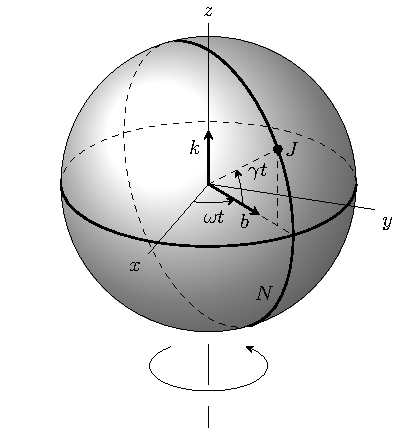
\includegraphics{sphereWithLines}
\caption{دو گردش کی خطی میل (مثال \حوالہ{مثال_الاحصاء_دو_گردش_کی_میل})}
\label{شکل_مثال_الاحصاء_دو_گردش_کی_میل}
\end{figure}
\انتہا{مثال}
%=================================

\حصہء{سوالات}
سوال \حوالہ{سوال_الاحصاء_تعین_گر_الف} تا سوال \حوالہ{سوال_الاحصاء_تعین_گر_ب} میں حرکت کرتی جسم کا تعین گر سمتیہ \عددی{\bM{r}(t)} ہے جہاں \عددی{t(>0)} وقت کو ظاہر کرتی ہے۔اس راہ کی شکل بیان کریں۔سمتیہ رفتار، رفتار اور اسراع دریافت کریں۔

%===================
\ابتدا{سوال}\شناخت{سوال_الاحصاء_تعین_گر_الف}\quad
$\bM{r}=t\bM{j}$\\
جوابات:
$\bM{v}=\bM{j},\quad \abs{\bM{v}}=1,\quad \bM{a}=0$
\انتہا{سوال}
%====================== 
\ابتدا{سوال}\quad
$\bM{r}=t^3\bM{j}$\\
جوابات:
$\bM{v}=3t^2\bM{j},\quad \abs{\bM{v}}=3t^2,\quad \bM{a}=6t\bM{j}$
\انتہا{سوال}
%====================== 
\ابتدا{سوال}\quad
$\bM{r}=(t^2-3t)\bM{j}$\\
جوابات:
$\bM{v}=(2t-3)\bM{j},\quad \abs{\bM{v}}=\abs{2t-3},\quad \bM{a}=2\bM{j}$
\انتہا{سوال}
%====================== 
\ابتدا{سوال}\quad
$\bM{r}=t^2\bM{i}-t\bM{j}$\\
جوابات:
$\bM{v}=2t\bM{i}-\bM{j},\quad \abs{\bM{v}}=\abs{\sqrt{4t^2+1}},\quad \bM{a}=2\bM{i}$
\انتہا{سوال}
%====================== 
\ابتدا{سوال}\quad
$\bM{r}=\cos t \,\bM{i}$\\
جوابات:
$\bM{v}=-\sin t\, \bM{j},\quad \abs{\bM{v}}=\abs{\sin t},\quad \bM{a}=-\cos t\,\bM{j}$
\انتہا{سوال}
%====================== 
\ابتدا{سوال}\quad
$\bM{r}=2\cos 5t \,\bM{i}-4\sin 3t \,\bM{j}$\\
جوابات:
$\bM{v}=-10\sin 5t\, \bM{i}-12\cos 3t\,\bM{j},\,\,\abs{\bM{v}}=\abs{\sqrt{100\sin^2 5t+144\cos^2 3t}}\\ \bM{a}=-50\cos 5t\,\bM{i}+36\sin 3t \,\bM{j}$
\انتہا{سوال}
%====================== 
\ابتدا{سوال}\quad
$\bM{r}=3\cos t^2 \,\bM{i}+2\sin t^2 \,\bM{j}$\\
جوابات:
$\bM{v}=-6t\sin t^2\, \bM{i}+4t\cos t^2\,\bM{j},\,\,\abs{\bM{v}}=\abs{\sqrt{36t^2\sin^2 t^2+16t^2\cos^2 t^2}}\\ 
\bM{a}=(-6\sin t^2-12t^2\cos t^2)\,\bM{i}+(4\cos t^2-8t^2\sin t^2) \,\bM{j}$
\انتہا{سوال}
%====================== 
\ابتدا{سوال}\شناخت{سوال_الاحصاء_تعین_گر_ب}\quad
$\bM{r}=5t^2 \,\bM{i}+3t \,\bM{j}+t^3\,\bM{k}$\\
جوابات:
$\bM{v}=10t\, \bM{i}+3\,\bM{j}+3t^2\,\bM{k},\,\,\abs{\bM{v}}=\abs{\sqrt{9t^4+100t^2+9}}\\ 
\bM{a}=10\,\bM{i}+6t \,\bM{k}$
\انتہا{سوال}
%====================== 
\ابتدا{سوال}زمین سے چاند تک کا فاصلہ \عددی{\SI{3.85e8}{\meter}} ہے اور زمین کے گرد چاند \عددی{27.322} دن یعنی \عددی{\SI{2.36e6}{\second}} میں ایک چکر پورا کرتا ہے۔زمین کے رخ چاند کی مرکز مائل اسراع دریافت کریں۔

جواب:\عددی{\abs{\bM{a}}=\SI{0.0027}{\meter\per\second\squared}} جو سطح زمین پر اسراع \عددی{g=\SI{9.8}{\meter\per\second\squared}} سے \عددی{3593} گنا کم ہے۔ 
\انتہا{سوال}
%=======================
\ابتدا{سوال}
وہ حرکت دریافت کریں جس کی اسراع مستقل قیمت ہو۔

جواب:
$\bM{r}(t)=\bM{a}_0\tfrac{t^2}{2}+\bM{v}_0t+\bM{x}_0$
جہاں \عددی{\bM{a}_0}، \عددی{\bM{v}_0} اور \عددی{\bM{x}_0} مستقل قیمتیں ہیں۔
\انتہا{سوال}
%=========================
\ابتدا{سوال}
\عددی{\bM{\omega}=\omega \bM{k}} اور \عددی{\bM{r}=R\cos \omega t\bM{i}+R\sin \omega t\bM{j}} لیتے ہوئے مساوات \حوالہ{مساوات_سمتیات_سمتی_رفتار_رداس_زاویائی_رفتار} کے تفرق  سے مساوات \حوالہ{مساوات_الاحصاء_اسراع_رفتار_حرکت} حاصل کریں۔
\انتہا{سوال}
%=======================
\ابتدا{سوال}
اگر ایک جسم کی حرکت \عددی{\bM{r}(t)} سے ظاہر کی جائے جہاں \عددی{t} وقت ہے تب \عددی{t=\phi{\tilde{t}}} تبادلے سے کیا مراد ہو گا؟

جواب:راہ تبدیل نہیں ہو گی البتہ راہ پر حرکت کی نوعیت تبدیل ہو گی۔
\انتہا{سوال}
%==========================

\حصہ{زنجیری ترکیب اور متعدد متغیرات کے تفاعل کا اوسط قیمت مسئلہ}
ہم متعدد متغیرات پر مبنی تفاعل کی خصوصیات پر غور کرتے ہیں۔ہم دو متغیرات کے تفاعل کو استعمال کرتے ہوئے  نتائج حاصل کریں گے جو زیادہ متغیرات کے تفاعل کے لئے بھی درست ہوں گے۔

نقطہ \عددی{(x_0,y_0)} پر تفاعل \عددی{f(x,y)}  اس صورت \اصطلاح{استمراری}\فرہنگ{استمراری}\حاشیہب{continuous}\فرہنگ{continuous} ہو گا جب اس نقطے کے \اصطلاح{ہمسائیگی}\حاشیہد{ہمسائیگی سے مراد \عددی{xy} سطح میں قرص \عددی{(x-x_0)^2+(y-y_0)^2<r^2} ہے جہاں \عددی{r>0} ہے۔} میں \عددی{f} معین ہو اور کسی بھی مثبت عدد \عددی{\epsilon} (جو غیر صفر اور کتنا ہی چھوٹا کیوں نا ہو) کے لئے ہم ایسا مثبت عدد \عددی{\sigma} تلاش کر سکتے ہیں کہ اس کے نقطے کے ہمسائیگی  قرص 
\begin{align}
(x-x_0)^2+(y-y_0)^2<\sigma^2
\end{align}
میں تمام \عددی{(x,y)} پر درج ذیل ہو۔
\begin{align}
\abs{f(x,y)-f(x_0,y_0)}<\epsilon
\end{align}

جیومیٹریائی طور پر \عددی{(x_0,y_0)} پر \عددی{f(x,y)} کے استمراری ہونے سے مراد یہ ہے کہ \عددی{f(x_0,y_0)} کو قطع \عددی{2\epsilon} کا وسط لیتے ہوئے  ہم غیر صفر رداس \عددی{\sigma} کا ایسا قرص تلاش کر سکتے ہیں جس کا مرکز \عددی{(x_0,y_0)} ہو اور اس قرص  پر تمام \عددی{(x,y)} کا مطابقتی \عددی{f(x,y)} اس قطع پر پایا جاتا ہو (شکل \حوالہ{شکل_الاحصاء_استمرار_تعریف})۔
\begin{figure}
\centering
\begin{subfigure}{0.5\textwidth}
\centering
\begin{tikzpicture}
\draw(0,0)--++(2.5,0)node[below]{$x$};
\draw(0,0)--++(0,2.5)node[left]{$y$};
\draw(1.25,1.25)circle (1);
\draw[-stealth] (1.25,1.25)node[ocirc]{}node[below]{$(x_0,y_0)$} --++(30:1)node[pos=0.5,above]{$\sigma$};
\end{tikzpicture}
\end{subfigure}%
\begin{subfigure}{0.5\textwidth}
\centering
\begin{tikzpicture}
\draw(-1.5,0)--(1.5,0);
\draw(0,0)node[below]{$f(x_0,y_0)$}--++(0,0.15)++(0,0.15)--++(0,0.15);
\draw(-1.25,0)--++(0,0.15)++(0,0.15)--++(0,0.15);
\draw(1.25,0)--++(0,0.15)++(0,0.15)--++(0,0.15);
\draw[stealth-stealth](-1.25,0.15+0.15+0.15/2)--++(1.25,0)node[pos=0.5,fill=white]{$\epsilon$};
\draw[stealth-stealth](0,0.15+0.15+0.15/2)--++(1.25,0)node[pos=0.5,fill=white]{$\epsilon$};
\end{tikzpicture}
\end{subfigure}%
\caption{دو متغیرات کے تفاعل کی استمرار}
\label{شکل_الاحصاء_استمرار_تعریف}
\end{figure}

ہم ابتدائی علم الاحصاء سے جانتے ہیں کہ اگر \عددی{w} متغیر \عددی{x} کا قابل تفرق تفاعل ہو اور \عددی{x} از خود \عددی{t} کا قابل تفرق تفاعل ہو تب درج ذیل لکھا جا سکتا ہے جس کو تفرق کا زنجیری قاعدہ کہتے ہیں۔
\begin{align}
\frac{\dif w}{\dif t}=\frac{\dif w}{\dif x}\frac{\dif x}{\dif t}
\end{align} 
درج ذیل مسئلہ  تفرق کی زنجیری قاعدے کو عمومی بناتا ہے۔

%================
\ابتدا{مسئلہ}\شناخت{مسئلہ_الاحصاء_زنجیری_قاعدہ}\quad (زنجیری قاعدہ)\\
فرض کریں کہ \عددی{xy} سطح میں \اصطلاح{دائرہ کار}\فرہنگ{دائرہ کار}\حاشیہب{domain}\فرہنگ{domain} \عددی{D}\حاشیہد{دائرہ کار \عددی{D} \ترچھا{جڑی} ہوئے نقطوں کا \ترچھا{کھلا} سلسلہ ہے، جہاں \اصطلاح{جڑا} ہونے سے مراد یہ ہے کہ \عددی{D} کے کسی بھی دو نقطوں کو متناہی تعداد کے ایسے سیدھے قطعات سے ملایا جا سکتا ہے جن کے تمام نقطے \عددی{D} کا حصہ ہوں، اور \اصطلاح{کھلا} سے مراد یہ ہے کہ \عددی{D} میں ہر نقطے کی ہمسائیگی  کے تمام نقطے بھی \عددی{D} کا حصہ ہیں۔مثلاً کسی مستطیل یا دائرے کا اندرونی حصہ دائرہ کار ہو گا۔} میں تفاعل \عددی{w=f(x,y)} استمراری ہے  اور  اس تفاعل کے درجہ ایک جزوی تفرقات بھی \عددی{D} میں استمراری ہیں۔مزید فرض کریں کہ کسی وقفہ \عددی{T} میں \عددی{x=x(t)} اور \عددی{y=y(t)} قابل تفرق تفاعل ہیں جہاں \عددی{T} میں ہر \عددی{t} کا مطابقتی  نقطہ \عددی{[x(t),y(t)]}، دائرہ کار \عددی{D} میں پایا جاتا ہے۔ایسی صورت میں \عددی{T} میں تمام \عددی{t} کے لئے  \عددی{w=f[x(t),y(t)]} قابل تفرق ہو گا یعنی:
\begin{align}\label{مساوات_الاحصاء_زنجیری_تفرق_قاعدہ_الف}
\frac{\dif w}{\dif t}=\frac{\partial w}{\partial x}\frac{\dif x}{\dif t}+\frac{\partial w}{\partial y}\frac{\dif y}{\dif t}
\end{align}   
\انتہا{مسئلہ}
%======================
\ابتدا{ثبوت}
ہم \عددی{T} میں \عددی{t}  پر \عددی{\Delta t} اتنا چھوٹا چنتے ہیں کہ \عددی{t+\Delta t} بھی \عددی{T} کا حصہ ہو۔مزید ہم 
\begin{align}\label{مساوات_الاحصاء_زنجیری_الف}
\Delta x=x(t+\Delta t)-x(t),\quad \Delta y=y(t+\Delta t)-y(t)
\end{align} 
اور
\begin{align}\label{مساوات_الاحصاء_زنجیری_ب}
\Delta w=f(x+\Delta x,y+\Delta y)-f(x,y)
\end{align}
لیتے ہیں۔مساوات \حوالہ{مساوات_الاحصاء_زنجیری_ب} میں \عددی{f(x,y+\Delta y)} جمع اور منفی کرتے ہوئے درج ذیل لکھا جا سکتا ہے۔
\begin{align*}
\Delta w=[f(x+\Delta x,y+\Delta y)-f(x,y+\Delta y)]+[f(x,y+\Delta y)-f(x,y)]
\end{align*}
درج بالا مساوات کے قوسین پر باری باری ایک متغیر کے تفاعل کا اوسط قیمت مسئلہ لاگو کرتے ہوئے
\begin{align}\label{مساوات_الاحصاء_زنجیری_پ}
\Delta w=\Delta x \left.\frac{\partial f}{\partial x} \right|_{x_1,y+\Delta y}+\Delta y \left.\frac{\partial f}{\partial y} \right|_{x,y_1}
\end{align}  
حاصل ہوتا ہے جہاں \عددی{x} اور \عددی{x+\Delta x} کے درمیان کہیں \عددی{x_1} پایا جاتا ہے، \عددی{y} اور \عددی{y+\Delta y} کے درمیان کہیں \عددی{y_1} پایا جاتا ہے۔مساوات \حوالہ{مساوات_الاحصاء_زنجیری_پ} کے دونوں اطراف کو \عددی{\Delta t} سے تقسیم کرتے اور \عددی{\Delta t \to 0} لیتے ہوئے، اور چونکہ
 \عددی{\tfrac{\partial f}{\partial x}} اور \عددی{\tfrac{\partial f}{\partial y}} کو استمراری تصور کیا گیا ہے، مساوات  \حوالہ{مساوات_الاحصاء_زنجیری_الف} حاصل ہوتا ہے۔
\انتہا{ثبوت}
%========================

درج بالا مسئلے کو وسعت دیتے ہوئے درج ذیل مسئلہ اخذ کیا جا سکتا ہے۔

%==========
\ابتدا{مسئلہ}\شناخت{مسئلہ_الاحصاء_جزوی_تفرقات}
فرض کریں کہ \عددی{xy} سطح میں \اصطلاح{دائرہ کار} \عددی{D} پر تفاعل \عددی{w=f(x,y)} استمراری ہے  اور  اس تفاعل کے درجہ ایک جزوی تفرقات بھی \عددی{D} میں استمراری ہیں۔مزید فرض کریں کہ \عددی{uv} سطح میں کسی وقفہ \عددی{B} میں \عددی{x=x(u,v)} اور \عددی{y=y(u,v)} قابل جزوی تفرق تفاعل ہیں جہاں \عددی{B} میں ہر \عددی{(u,v)} کا مطابقتی نقطہ \عددی{[x(u,v),y(u,v)]}، دائرہ کار \عددی{D} میں پایا جاتا ہے۔ایسی صورت میں \عددی{B} میں تفاعل  \عددی{w=f[x(u,v),y(u,v)]} معین ہو گا اور \عددی{B} میں تمام \عددی{u} اور \عددی{v} کے لئے اس تفاعل کے جزوی تفرقات  درج ذیل ہوں گے۔
\begin{gather}
\begin{aligned}
\frac{\partial w}{\partial u}&=\frac{\partial w}{\partial x}\frac{\partial x}{\partial u}+\frac{\partial w}{\partial y}\frac{\partial y}{\partial u}\\
\frac{\partial w}{\partial v}&=\frac{\partial w}{\partial x}\frac{\partial x}{\partial v}+\frac{\partial w}{\partial y}\frac{\partial y}{\partial v}
\end{aligned}
\end{gather}
\انتہا{مسئلہ}
%====================

\عددی{u} یا \عددی{v} کو غیر متغیر رکھتے ہوئے مسئلہ \حوالہ{مسئلہ_الاحصاء_زنجیری_قاعدہ} کے اطلاق سے  درج بالا مسئلہ ثابت ہوتا ہے۔

ابتدائی علم الاحصاء  سے ہم جانتے ہیں کہ قابل تفرق تفاعل \عددی{f(x)} کے لئے درج ذیل لکھا جا سکتا ہے جہاں \عددی{x_0} اور \عددی{x_0+h} کے درمیان موزوں نقطے پر تفرق لیا جاتا ہے۔
\begin{align*}
f(x_0+h)-f(x_0)=h\frac{\dif f}{\dif x}
\end{align*}
اس کو احصاء تفرقیات کا مسئلہ اوسط قیمت کہتے ہیں جس کو  وسعت دے کر  دو متغیرات کے تفاعل پر لاگو  کیا جا سکتا ہے۔

%==================
\ابتدا{مسئلہ}\شناخت{مسئلہ_الاحصاء_اوسط_قیمت}\quad (مسئلہ اوسط قیمت)\\
فرض کریں کہ دائرہ کار \عددی{D} میں تفاعل \عددی{f(x,y)} استمراری ہے اور اس تفاعل کے درجہ ایک جزوی تفرقات بھی \عددی{D} میں استمراری ہیں۔ مزید فرض کریں کہ \عددی{(x_0,y_0)} اور  \عددی{(x_0+h,y_0+k)} دائرہ کار \عددی{D} میں پائے جانے والے ایسے نقطے ہیں کہ انہیں جوڑنے والا سیدھا قطع  بھی \عددی{D} میں پائی جاتی ہو (شکل \حوالہ{شکل_مسئلہ_الاحصاء_اوسط_قیمت})۔ایسی صورت میں 
\begin{align}\label{مساوات_الاحصاء_مسئلہ_زنجیری_الف}
f(x_0+h,y_0+k)-f(x_0,y_0)=h\frac{\partial f}{\partial x}+k\frac{\partial f}{\partial y}
\end{align}
لکھا جا سکتا ہے جہاں جزوی تفرقات کو  اس قطع پر موزوں نقطے پر حاصل کیا جاتا ہے۔
\begin{figure}
\centering
\begin{tikzpicture}
\draw[smooth cycle] plot coordinates {(0,0)(-2,0.75)(-1,1.75)(0,2)(1.5,2)(3.2,1.75)(2,0.25)};
\draw(0,0.7)node[ocirc]{}node[below]{$(x_0,y_0)$}--(1.5,1)node[ocirc]{}node[above]{$(x_0+h,y_0+k)$};
\draw(0,1.75)node{$D$};
\end{tikzpicture}
\caption{مسئلہ اوسط قیمت}
\label{شکل_مسئلہ_الاحصاء_اوسط_قیمت}
\end{figure}
\انتہا{مسئلہ}
%======================
\ابتدا{ثبوت}
درج ذیل
\begin{align*}
x&=x_0+th,\quad y=y_0+tk\quad (0\le t \le 1)\\
F(t)&=f(x_0+th,y_0+tk)
\end{align*}
سے
\begin{align*}
f(x_0+h,y_0+k)=F(1),\quad f(x_0,y_0)=F(0)
\end{align*}
لکھا جا سکتا ہے۔ایک متغیر تفاعل کے  مسئلہ اوسط قیمت کے تحت \عددی{0} اور \عددی{1} کے درمیان  ایسی قیمت \عددی{t_1}  پائی جاتی ہے جس کے لئے  درج ذیل لکھا جا سکتا ہے۔ 
\begin{align}\label{مساوات_الاحصاء_مسئلہ_زنجیری_ب}
f(x_0+h,y_0+k)-f(x_0,y_0)=F(1)-F(0)=F'(t_1)
\end{align}
اب چونکہ \عددی{\tfrac{\dif x}{\dif t}=h} اور \عددی{\tfrac{\dif y}{\dif t}=k} ہیں لہٰذا مسئلہ \حوالہ{مسئلہ_الاحصاء_زنجیری_قاعدہ} کے تحت
\begin{align}\label{مساوات_الاحصاء_مسئلہ_زنجیری_پ}
F'=\frac{\partial f}{\partial x}h+\frac{\partial f}{\partial y}k
\end{align}
ہو گا جہاں دائیں ہاتھ تفرقات کو نقطہ \عددی{(x_0+t_1h,y_0+t_1k)} پر حاصل کیا جائے گا جو اس قطع پر واقع ہے جس کے سر \عددی{(x_0,y_0)} اور \عددی{(x_0+h,y_0+k)} ہیں۔مساوات \حوالہ{مساوات_الاحصاء_مسئلہ_زنجیری_پ} کو مساوات \حوالہ{مساوات_الاحصاء_مسئلہ_زنجیری_ب} میں پر کرنے سے  مساوات \حوالہ{مساوات_الاحصاء_مسئلہ_زنجیری_الف} حاصل ہوتا ہے۔
\انتہا{ثبوت}
%========================

تین متغیرات کے تفاعل \عددی{f(x,y,z)} جو مسئلہ \حوالہ{مسئلہ_الاحصاء_اوسط_قیمت} میں دیے گئے شرائط کے مماثل شرائط پر پورا اترتا ہو کے لئے بالکل اسی مسئلے کی طرح درج ذیل لکھا جا سکتا ہے
\begin{align}\label{مساوات_الاحصاء_مسئلہ_زنجیری_ت}
f(x_0+h,y_0+k,z_0+l)-f(x_0,y_0,z_0)=h\frac{\partial f}{\partial x}+k\frac{\partial f}{\partial y}+l\frac{\partial f}{\partial z}
\end{align}
جہاں جزوی تفرقات کو \عددی{(x_0,y_0,z_0)} تا \عددی{(x_0+h,y_0+k,z_0+l)} قطع پر موزوں نقطے پر حاصل کیا جائے گا۔

%===================
\حصہء{سوالات}
سوال \حوالہ{سوال_الاحصاء_زنجیری_قاعدہ_الف} تا سوال \حوالہ{سوال_الاحصاء_زنجیری_قاعدہ_ب} میں مساوات \حوالہ{مساوات_الاحصاء_زنجیری_تفرق_قاعدہ_الف} کی مدد سے \عددی{\tfrac{\dif w}{\dif t}} دریافت کریں۔

%===============
\ابتدا{سوال}\شناخت{سوال_الاحصاء_زنجیری_قاعدہ_الف}\quad
$w=x-y,\quad x=t,\quad y=\ln t$\\
جواب:
$1-\tfrac{1}{t}$
\انتہا{سوال}
%========================
\ابتدا{سوال}\quad
$w=\sqrt{x^2+y^2},\quad x=e^{-t},\quad y=e^{t}$\\
جواب:
$\tfrac{e^{2t}-e^{-2t}}{\sqrt{e^{2t}+e^{-2t}}}$
\انتہا{سوال}
%========================
\ابتدا{سوال}\quad
$w=\tfrac{x}{y},\quad x=g(t),\quad y=h{t}$\\
جواب:
$\tfrac{g'h-gh'}{h^2}$
\انتہا{سوال}
%========================
\ابتدا{سوال}\شناخت{سوال_الاحصاء_زنجیری_قاعدہ_ب}\quad
$w=\tfrac{x}{y},\quad x=\cos t,\quad y=\sin t$\\
جواب:
$-\cosec^{\,2} t$
\انتہا{سوال}
%========================
\ابتدا{سوال}
فرض کریں کہ \عددی{w=f(x,y,z)} ہے جہاں \عددی{x}، \عددی{y} اور \عددی{z} از خود \عددی{t} کے تفاعل ہیں۔ثابت کریں کہ مسئلہ \حوالہ{مسئلہ_الاحصاء_زنجیری_قاعدہ} کی طرز کے شرائط کی صورت میں درج ذیل ہو گا۔
\begin{align}\label{مساوات_الاحصاء_زنجیری_تین_متغیرات}
\frac{\dif w}{\dif t}=\frac{\partial w}{\partial x}\frac{\dif x}{\dif t}+\frac{\partial w}{\partial y}\frac{\dif y}{\dif t}+\frac{\partial w}{\partial z}\frac{\dif z}{\dif t}
\end{align}
\انتہا{سوال}
%===================
سوال \حوالہ{سوال_الاحصاء_زنجیری_تین_متغیرات_الف} اور سوال \حوالہ{سوال_الاحصاء_زنجیری_تین_متغیرات_ب} میں مساوات \حوالہ{مساوات_الاحصاء_زنجیری_تین_متغیرات} کی مدد سے \عددی{\tfrac{\dif w}{\dif t}} دریافت کریں۔

%==========================
\ابتدا{سوال}\شناخت{سوال_الاحصاء_زنجیری_تین_متغیرات_الف}\quad
$w=x^2+y^2+z^2,\quad x=t^2,\quad y=\ln t,\quad z=e^t$\\
جواب:
$\tfrac{2}{t}\ln t+2e^{2t}+4t^3$
\انتہا{سوال}
%=========================
\ابتدا{سوال}\شناخت{سوال_الاحصاء_زنجیری_تین_متغیرات_ب}\quad
$w=\sqrt{x^2+y^2+z^2},\quad x=\cos t,\quad y=\sin t,\quad z=t$\\
جواب:
$\tfrac{t}{\sqrt{1+t^2}}$
\انتہا{سوال}
%=========================
\ابتدا{سوال}
مسئلہ \حوالہ{مسئلہ_الاحصاء_جزوی_تفرقات} کو ثابت کریں۔
\انتہا{سوال}
%=======================
سوال \حوالہ{سوال_الاحصاء_جزوی_تفرقات_الف} تا سوال \حوالہ{سوال_الاحصاء_جزوی_تفرقات_ب} میں \عددی{\tfrac{\partial w}{\partial u}} اور \عددی{\tfrac{\partial w}{\partial v}} دریافت کریں۔

%===================
\ابتدا{سوال}\شناخت{سوال_الاحصاء_جزوی_تفرقات_الف}\quad
$w=\ln(x^2+y^2),\quad x=e^u\cos v,\quad y=e^u\sin v$\\
جواب:
$2,\,\, 0$
\انتہا{سوال}
%======================
\ابتدا{سوال}\quad
$w=xy,\quad x=e^u\cos v,\quad y=e^u\sin v$\\
جواب:
$e^{2u}\sin 2v,\,\,e^{2u}\cos 2v$
\انتہا{سوال}
%======================
\ابتدا{سوال}\شناخت{سوال_الاحصاء_جزوی_تفرقات_ب}\quad
$w=x^2-y^2,\quad x=u^2-v^2,\quad y=2uv$\\
جواب:
$4u(u^2-3v^2),\,\,4v(v^2-3u^2)$
\انتہا{سوال}
%======================
\ابتدا{سوال}
مساوات \حوالہ{مساوات_الاحصاء_مسئلہ_زنجیری_ت} حاصل کریں۔
\انتہا{سوال}
%======================
\ابتدا{سوال}
فرض کریں کہ \عددی{w=f(x,y)} ہے جہاں \عددی{x=r\cos \theta} اور \عددی{y=r\sin \theta} ہیں۔درج ذیل ثابت کریں۔
\begin{align*}
\left(\frac{\partial w}{\partial r}\right)^2+\frac{1}{r^2}\left(\frac{\partial w}{\partial \theta}\right)^2=\left(\frac{\partial w}{\partial x}\right)^2+\left(\frac{\partial w}{\partial y}\right)^2
\end{align*}
جواب:درج ذیل استعمال کرتے ہوئے با آسانی ثابت ہو گا۔
\begin{align*}
\frac{\partial w}{\partial r}&=\frac{\partial w}{\partial x}\frac{\partial x}{\partial r}+\frac{\partial w}{\partial y}\frac{\partial y}{\partial r}=
\frac{\partial w}{\partial x}\cos \theta +\frac{\partial w}{\partial y}\sin \theta \\
\frac{\partial w}{\partial \theta}&=\frac{\partial w}{\partial x}\frac{\partial x}{\partial \theta}+\frac{\partial w}{\partial y}\frac{\partial y}{\partial \theta}=
-\frac{\partial w}{\partial x}r\sin \theta +\frac{\partial w}{\partial y}r\cos\theta 
\end{align*}
\انتہا{سوال}
%======================
\ابتدا{سوال}
فرض کریں کہ \عددی{w=f(v,z)}ہے جہاں  \عددی{v=x+ct} اور  \عددی{z=x-ct} ہیں جبکہ  \عددی{c} مستقل قیمت  ہے۔درج ذیل ثابت کریں جہاں تمام تفرقات کو ممکن تصور کریں۔ \عددی{w_{xx}} سے مراد \عددی{\tfrac{\partial ^2 w}{\partial x^2}} ہے۔
\begin{align*}
c^2w_{xx}-w_{tt}=4c^2w_{vz}
\end{align*} 
\انتہا{سوال}
%=========================
\ابتدا{سوال}
فرض کریں کہ \عددی{w=f(x,y)} ہے جہاں \عددی{x=r\cos \theta} اور \عددی{y=r\sin \theta} ہیں۔درج ذیل ثابت کریں۔
\begin{align*}
w_{xx}+w_{yy}=w_{rr}+\frac{1}{r}w_r+\frac{1}{r^2}w_{\theta \theta}
\end{align*}
جواب:
$r=\sqrt{x^2+y^2}$
اور
$\theta=\tan^{-1}\frac{y}{x}$
سے درج ذیل حاصل کرتے ہوئے ثابت ہو گا۔
\begin{align*}
r_x&=\frac{x}{r},\,\, \theta_x=-\frac{y}{r^2},\,\, r_{xx}=\frac{y^2}{r^3},\quad \text{وغیرہ}\\
 w_{xx}&=x^2r^{-2}w_{rr}-2xyr^{-3}w_{r\theta}+y^2r^{-4}w_{\theta\theta}+y^2r^{-3}w_r+2xyr^{-4}w_{\theta},\quad \text{وغیرہ}
\end{align*}
\انتہا{سوال}
%=======================

\حصہ{سمتی تفرق، غیر سمتی میدان کی ڈھلوان}
ہم فضا میں غیر سمتی میدان \عددی{f(P)=f(x,y,z)}  پر غور کرتے ہیں (حصہ \حوالہ{حصہ_الاحصاء_غیر_سمتی-_اور_سمتی_میدان})۔ہم جانتے ہیں کہ  \عددی{x}، \عددی{y} اور \عددی{z}  رخ  میں تفاعل کی تبدیلی کی شرح بالترتیب \عددی{\tfrac{\partial f}{\partial x}}، \عددی{\tfrac{\partial f}{\partial y}} اور \عددی{\tfrac{\partial f}{\partial z}} ہے۔ آئیں کسی بھی رخ اس تفاعل کی تبدیلی کی شرح یعنی \اصطلاح{سمتی تفرق} حاصل کریں۔

ہم فضا میں کوئی نقطہ \عددی{P} اور اس نقطے پر کوئی رخ چنتے ہیں۔اس رخ  کو اکائی سمتیہ \عددی{\bM{b}} سے ظاہر کرتے ہیں۔نقطہ \عددی{P} سے \عددی{s} فاصلے پر  \عددی{\bM{b}} کی رخ سیدھے خط \عددی{C} پر نقطہ \عددی{Q} پایا جاتا ہے (شکل \حوالہ{شکل_الاحصاء_سمتی_تفرق})۔اگر درج ذیل حد
\begin{align}\label{مساوات_الاحصاء_سمتی_تفرق_الف}
\frac{\partial f}{\partial s}=\lim_{s\to 0}\frac{f(Q)-f(P)}{s}
\end{align}
موجود ہو تب اس کو \عددی{P} پر \عددی{\bM{b}} کی رخ \عددی{f} کی \اصطلاح{سمتی تفرق}\فرہنگ{سمتی!تفرق}\فرہنگ{تفرق!سمتی}\حاشیہب{directional derivative}\فرہنگ{directional derivative}\فرہنگ{derivative!directional} کہتے ہیں۔ظاہر ہے کہ \عددی{\tfrac{\partial f}{\partial s}} در حقیقت \عددی{P} پر \عددی{\bM{b}} کی رخ  \عددی{f} کی شرح تبدیلی ہے۔ 
\begin{figure}
\centering
\begin{tikzpicture}
\pgfmathsetmacro{\ang}{20}
\draw(0,0)--++(\ang:3.5)node[below]{$C$};
\draw(0,0)node[below]{$P$}--++(\ang:2)node[ocirc]{}node[below]{$Q$};
\draw[-latex](0,0)node[ocirc]{}--++(\ang:1)node[below]{$\bM{b}$};
\draw [decorate,decoration={brace,amplitude=5pt},shift={(\ang+90:5pt)}](0,0) --++(\ang:1)node [black,midway,shift={(\ang+90:9pt)}] {\footnotesize$s$};
\end{tikzpicture}
\caption{سمتی تفرق}
\label{شکل_الاحصاء_سمتی_تفرق}
\end{figure}

یوں \عددی{P} پر \عددی{f} کے لامتناہی تعداد میں سمتی تفرقات پائے جاتے ہیں۔اگر \عددی{P} کا تعین گر سمتیہ \عددی{\bM{a}} ہو تب \عددی{C}  کو درج ذیل لکھا جا سکتا ہے 
\begin{align}\label{مساوات_الاحصاء_سمتی_تفرق_ب}
\bM{r}(s)=x(x)\bM{i}+y(s)\bM{j}+z(s)\bM{k}=\bM{a}+s\bM{b}\quad \quad (s\ge 0)
\end{align}
اور \عددی{\tfrac{\partial f}{\partial s}} سے مراد \عددی{C} پر \عددی{f[x(s),y(s),z(s)]} کا لمبائی \عددی{s} کے ساتھ تفرق ہے۔اب اگر \عددی{f} کے استمراری جزوی تفرقات پائے جاتے ہوں تب زنجیری قاعدے (مسئلہ \حوالہ{مسئلہ_الاحصاء_زنجیری_قاعدہ}) کے تحت درج ذیل لکھا جا سکتا ہے
\begin{align}\label{مساوات_الاحصاء_سمتی_تفرق_پ}
\frac{\partial f}{\partial s}=\frac{\partial f}{\partial x}x'+\frac{\partial f}{\partial y}y'+\frac{\partial f}{\partial z}z'
\end{align}
جہاں \عددی{x'=\tfrac{\dif x}{\dif s}}  کو \عددی{s=0} پر حاصل کیا جاتا ہے۔اب مساوات \حوالہ{مساوات_الاحصاء_سمتی_تفرق_ب} سے
\begin{align*}
\bM{r}'=x'\bM{i}+y'\bM{j}+z'\bM{k}=\bM{b}
\end{align*}
لکھا جا سکتا ہے جس کو دیکھ کر  خیال آتا ہے کہ  سمتیہ
\begin{align}\label{مساوات_الاحصاء_سمتی_تفرق_ت}
f_{\text{ڈھلوان}}=\frac{\partial f}{\partial x}\bM{i}+\frac{\partial f}{\partial y}\bM{j}+\frac{\partial f}{\partial z}\bM{k}
\end{align}
متعارف کرنے سے مساوات \حوالہ{مساوات_الاحصاء_سمتی_تفرق_پ} کو اندرونی ضرب (ضرب نقطہ) کی صورت میں لکھا جا سکتا ہے۔
\begin{align}\label{مساوات_الاحصاء_سمتی_تفرق_ٹ}
\frac{\partial f}{\partial s}=\bM{b}\cdot f_{\text{ڈھلوان}} \quad \quad (\abs{\bM{b}}=1)
\end{align}
سمتیہ 
$f_{\text{ڈھلون}}$
کو غیر سمتی تفاعل \عددی{f} کی \اصطلاح{ڈھلوان}\فرہنگ{ڈھلوان}\حاشیہب{gradient}\فرہنگ{gradient} کہتے ہیں۔

تفرقی عامل \عددی{\nabla}\حاشیہد{\عددی{\nabla} یونانی حرف تہجی ہے جو نیبلا کہلاتا ہے۔}
\begin{align*}
\nabla =\frac{\partial}{\partial x}\bM{i}+\frac{\partial}{\partial y}\bM{j}+\frac{\partial}{\partial z}\bM{k}
\end{align*}
متعارف کرتے ہوئے  مساوات \حوالہ{مساوات_الاحصاء_سمتی_تفرق_ت} کو 
\begin{align}\label{مساوات_الاحصاء_سمتی_تفرق_ث}
f_{\text{ڈھلوان}}=\nabla f=\frac{\partial f}{\partial x}\bM{i}+\frac{\partial f}{\partial y}\bM{j}+\frac{\partial f}{\partial z}\bM{k}
\end{align}
اور مساوات \حوالہ{مساوات_الاحصاء_سمتی_تفرق_ٹ} کو 
\begin{align}\label{مساوات_الاحصاء_سمتی_تفرق_ج}
\frac{\partial f}{\partial s}=\bM{b}\cdot \nabla f\quad \quad (\abs{\bM{b}}=1)
\end{align}
لکھا جا سکتا ہے۔

اگر \عددی{\bM{b}} کارتیسی \عددی{x} محور کی رخ ہو تب \عددی{\bM{b}=\bM{i}} ہو گا اور \عددی{f} کا سمتی تفرق درج ذیل ہو گا۔
\begin{align*}
\frac{\partial f}{\partial s}=\bM{b}\cdot \nabla f=\frac{\partial f}{\partial x}\bM{i}\cdot \bM{i}=\frac{\partial f}{\partial x}
\end{align*}
اسی طرح مثبت \عددی{y} اور مثبت \عددی{z} محور کی رخ سمتی تفرق بالترتیب \عددی{\tfrac{\partial f}{\partial y}} اور \عددی{\tfrac{\partial f}{\partial z}} ہوں گے۔

%==================
\ابتدا{مثال}\quad سمتی تفرق\\
غیر سمتی تفاعل \عددی{f(x,y,z)=x^2+2y-z^3} کا نقطہ \عددی{P:(-2,1,3)} پر \عددی{\bM{a}=3\bM{i}-4\bM{j}} کی رخ سمتی تفرق دریافت کریں۔

حل:چونکہ \عددی{\abs{\bM{a}}=5} ہے لہٰذا \عددی{\bM{a}} کی رخ اکائی سمتیہ
 \عددی{\bM{b}=\tfrac{\bM{a}}{\abs{\bM{a}}}=\tfrac{3}{5}\bM{i}-\tfrac{4}{5}\bM{j}} ہو گا۔ \عددی{f} کی ڈھلوان درج ذیل ہے۔
\begin{align*}
\nabla f=2x\bM{i}+2\bM{j}-3z^2\bM{k}\implies  \nabla f(P)=-4\bM{i}+2\bM{j}-27\bM{k}
\end{align*}
یوں نقطہ \عددی{P} پر \عددی{\bM{a}} کی رخ سمتی تفرق درج ذیل ملتا ہے۔
\begin{align*}
\frac{\partial f}{\partial s}=\bM{b}\cdot \nabla f=\frac{1}{5}(3\bM{i}-4\bM{j})\cdot (-4\bM{i}+2\bM{j}-27\bM{k})=-4
\end{align*}
حاصل جواب منفی ہے جس کا مطلب ہے کہ \عددی{\bM{a}} کی رخ  \عددی{f} گھٹتا ہے۔
\انتہا{مثال}
%========================

ہم اب ثابت کرتے ہیں کہ \عددی{\nabla f} کی قیمت اور رخ پر چنے گئے کارتیسی نظام کا کوئی اثر نہیں پایا جاتا ہے۔ 

مساوات \حوالہ{مساوات_الاحصاء_سمتی_تفرق_ت} سمتی تفرق دیتا ہے جو کسی دوسرے کارتیسی نظام میں درج ذیل لکھا جائے گا
\begin{align*}
f_{\text{ڈھلوان}}=\frac{\partial f}{\partial x^*}\bM{i}^*+\frac{\partial f}{\partial y^*}\bM{j}^*+\frac{\partial f}{\partial z^*}\bM{k}^*
\end{align*}
 جہاں \عددی{x^*}، \عددی{y^*} اور \عددی{z^*} دوسرے نظام کے محور جبکہ \عددی{\bM{i}^*}، \عددی{\bM{j}^*} اور \عددی{\bM{k}^*} اس کے مطابقتی اکائی سمتیات ہیں۔ان مساوات میں جزوی تفرقات پائے جاتے ہیں اور یہ کہنا مشکل ہو گا کہ دونوں مساوات سے یکساں ڈھلوان حاصل ہو گا۔ 

اب غیر سمتی تفاعل کی تعریف کے تحت نقطہ \عددی{P} پر \عددی{f} کی قیمت کا دارومدار \عددی{P} پر ہے نا کہ چنے گئے کارتیسی نظام پر۔اسی طرح \عددی{C} پر لمبائی \عددی{s} پر بھی چنے گئے کارتیسی نظام کا کوئی اثر نہیں پایا جاتا ہے۔یوں \عددی{\tfrac{\partial f}{\partial s}} پر چنے گئے کارتیسی نظام کا کوئی اثر نہیں ہو گا۔ اب مساوات \حوالہ{مساوات_الاحصاء_سمتی_تفرق_ج} کو درج ذیل لکھا جا سکتا ہے
\begin{align*}
\frac{\partial f}{\partial s}=\abs{\bM{b}}\abs{\nabla f}\cos \gamma=\abs{\nabla f}\cos \gamma
\end{align*}
جہاں \عددی{\bM{b}} اور \عددی{\nabla f} کے مابین زاویہ \عددی{\gamma} ہے۔ہم دیکھتے ہیں کہ  \عددی{\cos \gamma=1} یعنی \عددی{\gamma=0} پر \عددی{\tfrac{\partial f}{\partial s}} کی زیادہ سے زیادہ قیمت \عددی{\tfrac{\partial f}{\partial s}=\abs{\nabla f}} پائی جاتی ہے۔اب چونکہ \عددی{\tfrac{\partial f}{\partial s}} غیر متغیر ہے لہٰذا \عددی{\nabla f}  کی قیمت اور سمت پر کارتیسی نظام کا کوئی اثر نہیں ہو گا۔اس سے درج ذیل نتیجہ ملتا ہے۔

%===============
\ابتدا{مسئلہ}\quad ڈھلوان\\
ایسا غیر سمتی تفاعل \عددی{f(P)=f(x,y,z)}  جس کے استمراری ایک درجی جزوی تفرقات پائے جاتے ہوں کی ڈھلوان موجود ہے جس کی لمبائی اور رخ پر چنے گئے کارتیسی نظام محدد کا کوئی اثر نہیں پایا جاتا ہے۔اگر نقطہ \عددی{P} پر \عددی{f} کی ڈھلوان غیر صفر سمتیہ ہو تب \عددی{P} پر \عددی{f} کی زیادہ سے زیادہ تبدیلی ڈھلوان کی رخ ہو گی۔ 
\انتہا{مسئلہ}
%========================

ڈھلوان کی دوسری جیومیٹریائی خصلت جانتے ہیں۔فضا میں قابل تفرق غیر سمتی تفاعل \عددی{f(x,y,z)} پر غور کرتے ہیں۔ہر مستقل \عددی{c} کے لئے مساوات
\begin{align}\label{مساوات_الاحصاء_سمتی_تفرق_چ}
f(x,y,z)=c=\text{مستقل}
\end{align}
 سطح \عددی{S} کو ظاہر کرتا ہے۔\عددی{c} کے تمام قیمتیں لیتے ہوئے ہمیں نسل سطح ملتا ہے جنہیں \عددی{f} کی \اصطلاح{ہموار سطحیں}\فرہنگ{ہموار سطحیں}\حاشیہب{level surfaces}\فرہنگ{level surfaces} کہتے ہیں۔ تفاعل کی تعریف کے تحت، فضا میں کسی بھی نقطے پر  \عددی{f} کی قیمت منفرد ہو گی لہٰذا فضا میں ہر نقطے سے \عددی{f} کی صرف اور صرف ایک ہموار سطح گزرے گی۔ہم جانتے ہیں کہ فضا میں کسی بھی منحنی \عددی{C} کو درج ذیل لکھا جا سکتا ہے (حصہ \حوالہ{حصہ_الاحصاء_لمبائی_قوس})۔
\begin{align}\label{مساوات_الاحصاء_سمتی_تفرق_ح}
\bM{r}(t)=x(t)\bM{i}+y(t)\bM{j}+z(t)\bM{k}
\end{align}
اب اگر \عددی{C} کو \عددی{S} پر رہنے کا پابند بنایا جائے تب مساوات \حوالہ{مساوات_الاحصاء_سمتی_تفرق_ح} میں تفاعل \عددی{x(t)}، \عددی{y(t)} اور \عددی{z(t)} کو مساوات \حوالہ{مساوات_الاحصاء_سمتی_تفرق_چ} پر پورا اترنا ہو گا یعنی:
\begin{align}\label{مساوات_الاحصاء_سمتی_تفرق_خ}
f[x(t),y(t),z(t)]=c
\end{align}
زنجیری تفرق  (مسئلہ \حوالہ{مسئلہ_الاحصاء_زنجیری_قاعدہ}) استعمال کرتے ہوئے مساوات \حوالہ{مساوات_الاحصاء_سمتی_تفرق_خ} کا \عددی{t} کے ساتھ تفرق لیتے ہیں
\begin{align}\label{مساوات_الاحصاء_سمتی_تفرق_د}
\frac{\partial f}{\partial x}\dot{x}+\frac{\partial f}{\partial y}\dot{y}+\frac{\partial f}{\partial z}\dot{z}=(\nabla f)\cdot \dot{\bM{r}}=0
\end{align}
جہاں سمتیہ
\begin{align*}
\dot{\bM{r}}=\dot{x}\bM{i}+\dot{y}\bM{j}+\dot{z}\bM{k}
\end{align*}
منحنی \عددی{C} کا مماس ہے (حصہ \حوالہ{حصہ_الاحصاء_مماس_انحنا_مروڑ})۔ \عددی{S} پر مختلف سمتوں میں نقطہ \عددی{P} سے  گزرتی منحنی کے مماس، \عددی{P} پر \عددی{S} کو چھوتی سیدھی سطح سے گزریں گے۔اس سیدھی سطح کو \عددی{P} پر \عددی{S} کی \اصطلاح{مماسی سطح}\فرہنگ{مماسی!سطح}\فرہنگ{سطح!مماس}\حاشیہب{tangent plane}\فرہنگ{tangent plane} کہتے ہیں۔ مماسی سطح کے عمودی، نقطہ \عددی{P} سے گزرتا خط، \عددی{P} پر \عددی{S} کا \اصطلاح{عمود}\فرہنگ{عمود}\حاشیہب{normal}\فرہنگ{normal} کہلاتا ہے (شکل \حوالہ{شکل_الاحصاء_ڈھلوان})۔ صفحہ \حوالہصفحہ{مسئلہ_الجبرا_قائمیت} پر مسئلہ \حوالہ{مسئلہ_الجبرا_قائمیت} کی مدد سے درج ذیل نتیجہ ملتا ہے۔
\begin{figure}
\centering
\begin{tikzpicture}
\pgfmathsetmacro{\ang}{30}
%\draw (0,-2) grid ++(7,3);
\draw(7,0) to [out=145,in=0] (3,1) to [out=180,in=90] (0,-1) to [out=-90,in=180] (1,-2) to [out=0,in=180] (7,0);
\draw(4,-1) to [out=-10,in=0] (7,0);
\draw[dashed] (2.3,0.07) to [out=\ang,in=-170] (5,0.8);
\draw[dashed] (2.3,0.07) to [out=\ang-180,in=50] (1,-1)node[below]{$C$};
\draw (3.5,-1)node[pin={[pin distance=0.5cm]-45:{$f=c$}}]{};
\draw(2,-0.4)--++(\ang:1)--++(\ang+90:0.5)--++(\ang:-1)--++(\ang-90:0.5);
\draw[-latex](2.3,0.07)--++(\ang:0.35);
\draw[-latex](2.3,0.07)--++(\ang+90:1.5)node[above]{$\nabla f$};
\end{tikzpicture}
\caption{ہموار سطح اور ڈھلوان}
\label{شکل_الاحصاء_ڈھلوان}
\end{figure}

%===============
\ابتدا{مسئلہ}\شناخت{مسئلہ_الاحصاء_ڈھلوان_عمود}\quad ڈھلوان اور سطح کی عمود\\
فرض کریں کہ فضا میں دائرہ کار \عددی{D} پر غیر سمتی تفاعل \عددی{f} معین اور قابل تفرق ہے۔ مزید فرض کریں کہ دائرہ کار \عددی{D} میں \عددی{P}  کوئی نقطہ ہے جو \عددی{f} کی ہموار سطح \عددی{S} پر پایا جاتا ہے۔اب اگر \عددی{P} پر \عددی{f} کی ڈھلوان غیر صفر سمتیہ ہو  تب یہ ڈھلوان نقطہ \عددی{P} پر \عددی{S} کے عمودی ہو گا۔
\انتہا{مسئلہ}
%=========================

\ابتدا{مثال}\quad ہموار منحنی کا عمود\\
تفاعل \عددی{f(x,y)=\ln(x^2+y^2)} کے ہموار سطحیں \عددی{f=c} مبدا پر ہم مرکز دائرے ہیں۔ڈھلوان
\begin{align*}
\nabla f=\frac{\partial f}{\partial x}\bM{i}+\frac{\partial f}{\partial y}\bM{j}=\frac{2x}{x^2+y^2}\bM{i}+\frac{2y}{x^2+y^2}\bM{j}
\end{align*}
کی سمت ان دائروں کے عمودی ہے جو \عددی{f} کی زیادہ سے زیادہ تبدیلی کی سمت ہے۔مثلاً نقطہ \عددی{P:(4,3)} پر
 \عددی{\nabla f=\tfrac{8}{25}\bM{i}+\tfrac{6}{25}\bM{j}} ہے (شکل \حوالہ{شکل_الاحصاء_عمود_دائرہ})۔
\begin{figure}
\centering
\begin{tikzpicture}
\pgfmathsetmacro{\ll}{2}
\pgfmathsetmacro{\r}{2}
\pgfmathsetmacro{\ang}{atan(3/4)}
\draw(0,0)--++(2.5,0)node[below]{$x$};
\draw(0,0)--++(0,2.5)node[left]{$y$};
\draw([shift={(-10:\r)}]0,0) arc (-10:100:\r);
\draw[](4/5*\r,0)node[below]{$4$}--++(0,0.1);
\draw[] (0,3/5*\r)node[left]{$3$}--++(0.1,0);
\draw[-latex](\ang:\r) node[shift={(\ang:-0.3)}]{$P$}--++(\ang:\ll)node[above]{$\nabla f$}coordinate(T);
\draw[dashed,name path=kA](\ang:\r) coordinate(A)--++(1.5*\ll,0)coordinate(AA);
\draw[dashed,name path=kB](\ang:\r) node[ocirc,solid]{}coordinate(B)--++(0,1*\ll)coordinate(BB);
\draw[dashed](T)--($(A)!(T)!(AA)$)++(0.3,0)coordinate(AAA)++(-0.3,-0.3)coordinate(BBB);
\draw[dashed](T)--($(B)!(T)!(BB)$);
\draw [decorate,decoration={brace,amplitude=5pt},shift={(\ang+90:5pt)}](T)++(0.3,0) --(AAA)node [black,midway,shift={(0.4,0)}] {\footnotesize$\tfrac{6}{25}$};
\draw [decorate,decoration={brace,amplitude=5pt},shift={(0,-0.3)}](BBB) --(\ang:\r)node [black,midway,shift={(0,-0.5)}] {\footnotesize$\tfrac{8}{25}$};
\end{tikzpicture}
\caption{دائرے کا عمود}
\label{شکل_الاحصاء_عمود_دائرہ}
\end{figure}
\انتہا{مثال}
%=======================
\ابتدا{مثال}\quad سطح کا عمود\\
مخروط \عددی{z^2=2(x^2+y^2)} کا نقطہ \عددی{P:(1,0,3)} پر اکائی عمودی سمتیہ دریافت کریں۔ہم مخروط کو ہموار سطح \عددی{f=0} تصور کر سکتے ہیں جہاں
 \عددی{f(x,y,z)=2(x^2+y^2)-z^2} ہو گا۔یوں
\begin{align*}
\nabla f=4x\bM{i}+4y\bM{j}-2z\bM{k} \implies \nabla f(P)=4\bM{i}-6\bM{k}
\end{align*}
ہو گا۔ مسئلہ \حوالہ{مسئلہ_الاحصاء_ڈھلوان_عمود} سے اکائی عمودی سمتیہ درج ذیل ملتا ہے۔دوسرا اکائی عمودی سمتیہ \عددی{-\bM{n}} ہو گا۔
\begin{align*}
\bM{n}=\frac{\nabla f}{\abs{\nabla f}}=\frac{4}{\sqrt{52}}\bM{i}-\frac{6}{\sqrt{52}}\bM{k}
\end{align*}
\انتہا{مثال}
%======================

طبیعیات کے میدان میں کئی ایسے سمتی تفاعل پائے جاتے ہیں جو کسی غیر سمتی تفاعل کی ڈھلوان سے حاصل ہوتے ہیں۔ایسے غیر سمتی تفاعل کو \اصطلاح{مخفی تفاعل}\فرہنگ{مخفی تفاعل}\حاشیہب{potential function}\فرہنگ{potential function} کہتے ہیں۔ مخفی تفاعل کے استعمال سے سمتی تفاعل کا تجزیہ نہایت آسان ہو جاتا ہے۔آئیں مخفی تفاعل کے استعمال کی مثال دیکھیں۔

%==================
\ابتدا{مثال}\quad ثقلی میدان۔ لاپلاس مساوات\\
ثقلی میدان پر مثال \حوالہ{مثال_الاحصاء_میدان_قوت} میں غور کیا گیا جہاں درج ذیل مساوات حاصل کی گئی
\begin{align}
\bM{f}=\abs{\bM{f}}\left(-\frac{\bM{r}}{r}\right)=-GMm\frac{\bM{r}}{r^3}=-GMm\left[\frac{x-x_0}{r^3}\bM{i}+\frac{y-y_0}{r^3}\bM{j}+\frac{z-z_0}{r^3}\bM{k}\right]
\end{align}
جہاں
\begin{align*}
\bM{r}=\sqrt{(x-x_0)^2+(y-y_0)^2+(z-z_0)^2}
\end{align*}
کمیت \عددی{M} اور \عددی{m} کے درمیان فاصلہ ہے۔یہاں غور کرنے سے 
\begin{align}
\frac{\partial }{\partial x}\left(\frac{1}{r}\right)&=-\frac{2(x-x_0)}{2[(x-x_0)^2+(y-y_0)^2+(z-z_0)^2]^{\frac{3}{2}}}=-\frac{x-x_0}{r^3}\\
\frac{\partial }{\partial y}\left(\frac{1}{r}\right)&=-\frac{2(y-y_0)}{2[(x-x_0)^2+(y-y_0)^2+(z-z_0)^2]^{\frac{3}{2}}}=-\frac{y-y_0}{r^3}\\
\frac{\partial }{\partial x}\left(\frac{1}{r}\right)&=-\frac{2(z-z_0)}{2[(x-x_0)^2+(y-y_0)^2+(z-z_0)^2]^{\frac{3}{2}}}=-\frac{z-z_0}{r^3}
\end{align}
لکھا جا سکتا ہے۔ یوں \عددی{\bM{f}} کو درج ذیل غیر سمتی تفاعل کی ڈھلوان لکھا جا سکتا ہے
\begin{align}
h(x,y,z)=\frac{GMm}{r}\quad \quad (r>0)
\end{align}
لہٰذا سمتی تفاعل \عددی{\bM{f}} کا مخفی تفاعل \عددی{h} ہے۔

تفرق لیتے ہوئے 
\begin{align*}
\frac{\partial^{\,2}}{\partial x^2}\left(\frac{1}{r}\right)&=-\frac{1}{r^3}+\frac{3(x-x_0)^2}{r^5},\quad \frac{\partial^{\,2}}{\partial y^2}\left(\frac{1}{r}\right)=-\frac{1}{r^3}+\frac{3(y-y_0)^2}{r^5}, \\
\frac{\partial^{\,2}}{\partial z^2}\left(\frac{1}{r}\right)&=-\frac{1}{r^3}+\frac{3(z-z_0)^2}{r^5}
\end{align*}
حاصل ہوتا ہے جن کا مجموعہ صفر کے برابر ہے لہٰذا تفاعل \عددی{h=\tfrac{GMm}{r}} درج ذیل پر پورا اترتا ہے۔
\begin{align}\label{مساوات_الاحصاء_لاپلاس}
\frac{\partial^{\,2}h}{\partial x^2}+\frac{\partial^{\,2}h}{\partial y^2}+\frac{\partial^{\,2}h}{\partial z^2}=0
\end{align}  
مساوات \حوالہ{مساوات_الاحصاء_لاپلاس} انتہائی اہم جزوی تفرقی مساوات ہے جس کو \اصطلاح{لاپلاس مساوات}\فرہنگ{لاپلاس!مساوات}\حاشیہب{Laplace equation}\فرہنگ{Laplace!equation} کہتے ہیں۔مساوات کے بائیں ہاتھ کو \عددی{f} کا \اصطلاح{لاپلاسی}\فرہنگ{لاپلاسی}\حاشیہب{Laplacian}\فرہنگ{Laplacian} کہتے ہیں اور اس کو \عددی{\nabla^{\,2}h} یا \عددی{\Delta h} سے ظاہر کیا جاتا ہے۔  تفرقی عامل
\begin{align*}
\nabla^{\,2}=\Delta=\frac{\partial^{\,2}}{\partial x^2}+\frac{\partial^{\,2}}{\partial y^2}+\frac{\partial^{\,2}}{\partial z^2}
\end{align*} 
 (جو \اصطلاح{مربع نیبلا} پڑھا جاتا ہے) کو \اصطلاح{لاپلاسی عامل}\فرہنگ{لاپلاسی_عامل}\فرہنگ{عامل!لاپلاسی}\حاشیہب{Laplacian operator}\فرہنگ{Laplacian!operator}\فرہنگ{operator!Laplacian} کہتے ہیں۔ لاپلاسی عامل استعمال کرتے ہوئے مساوات \حوالہ{مساوات_الاحصاء_لاپلاس} کو نہایت عمدگی سے درج ذیل لکھا جا سکتا ہے۔
\begin{align}
\nabla^{\,2} h=0
\end{align} 

یہ ثابت کرنا ممکن ہے کہ کمیت کی کسی بھی طرز کی تقسیم سے حاصل قوت کو ایسے سمتی تفاعل سے ظاہر کیا جا سکتا ہے جو کسی غیر سمتی تفاعل \عددی{h} کا ڈھلوان ہو گا جہاں  \عددی{h}  مساوات \حوالہ{مساوات_الاحصاء_لاپلاس} پر ہر اس مقام پر پورا اترتا ہے جہاں کمیت موجود نہ ہو۔

طبیعیات میں کئی قاعدے  نیوٹن کے کشش ثقل کے قانون کی طرز رکھتے ہیں مثلاً فضا میں \عددی{Q_1} اور \عددی{Q_2} بار کی باہمی قوت درج ذیل ہے
\begin{align*}
\bM{f}=\frac{Q_1Q_2}{4\pi \epsilon}\frac{\bM{r}}{ r^3} \quad \quad \text{\RL{کولمب کا قانون}}
\end{align*}  
جہاں \عددی{\epsilon} برقی مستقل ہے۔یوں \عددی{\bM{f}} کو مخفی تفاعل \عددی{h=-\tfrac{Q_1Q_2}{4\pi \epsilon r}} کا  ڈھلوان لکھا جا سکتا ہے جہاں \عددی{r>0} کی صورت میں  \عددی{h} مساوات \حوالہ{مساوات_الاحصاء_لاپلاس} پر پورا اترتا ہے۔
\انتہا{مثال}
%==================

اگر غیر سمتی تفاعل کی ڈھلوان سمتی تفاعل دیتا ہو تب ایسی میدان کو \اصطلاح{بقائی میدان}\فرہنگ{بقائی میدان}\حاشیہب{conservative field}\فرہنگ{conservative field} کہتے ہیں۔جیسا کہ ہم اگلے باب میں دیکھیں گے، بقائی میدان میں کسی بھی ذرہ کو نقطہ \عددی{N_1} سے نقطہ \عددی{N_2} منتقل کرنے کے لئے درکار توانائی صرف اور صرف \عددی{N_1} اور \عددی{N_2} پر منحصر ہے نا کہ اس راستے پر جو ذرہ منتقل کرنے کے لئے استعمال کیا گیا ہو۔ہم دیکھیں گے کہ ہر میدان بقائی نہیں ہوتا۔

%======================
\حصہء{سوالات}
سوال \حوالہ{سوال_الاحصاء_ڈھلوان_الف} تا سوال \حوالہ{سوال_الاحصاء_ڈھلوان_ب} میں ڈھلوان \عددی{\nabla f} دریافت کریں۔ 

%=============
\ابتدا{سوال}\شناخت{سوال_الاحصاء_ڈھلوان_الف}\quad 
$f=3x+2y+4$\\
جواب:\quad
$\nabla f=3\bM{i}+2\bM{j}$
\انتہا{سوال}
%=====================
\ابتدا{سوال}\quad 
$f=e^y\sin x$\\
جواب:\quad
$\nabla f=e^y(\cos x\,\bM{i}+\sin x\,\bM{j})$
\انتہا{سوال}
%====================
\ابتدا{سوال}\شناخت{سوال_الاحصاء_ڈھلوان_الف_ب}\quad 
$f=\ln(x^2+y^2)$\\
جواب:\quad
$\nabla f=\frac{2x}{x^2+y^2}\bM{i}+\frac{2y}{x^2+y^2}\bM{j}$
\انتہا{سوال}
%=====================
\ابتدا{سوال}\quad 
$f=x^2+y^2$\\
جواب:\quad
$\nabla f=2x\bM{i}+2y\bM{j}$
\انتہا{سوال}
%=====================
\ابتدا{سوال}\quad 
$f=\sin^{-1}\frac{y}{x}$\\
جواب:\quad
$\nabla f=\frac{1}{\sqrt{x^2-y^2}}(-\frac{y}{x}\bM{i}+\bM{j})$
\انتہا{سوال}
%=====================
\ابتدا{سوال}\quad 
$f=\tan^{-1}\frac{y}{x}$\\
جواب:\quad
$\nabla f=\frac{1}{x^2+y^2}(-y\bM{i}+x\bM{j})$
\انتہا{سوال}
%=====================
\ابتدا{سوال}\quad 
$f=\sqrt{x^2+y^2+z^2}$\\
جواب:\quad
$\nabla f=\frac{1}{\sqrt{x^2+y^2+z^2}}(x\bM{i}+y\bM{j}+z\bM{k})$
\انتہا{سوال}
%=====================
\ابتدا{سوال}\quad 
$f=(x^2+y^2+z^2)^{\frac{3}{2}}$\\
جواب:\quad
$\nabla f=3\sqrt{x^2+y^2+z^2}(x\bM{i}+y\bM{j}+z\bM{k})$
\انتہا{سوال}
%=====================
\ابتدا{سوال}\quad 
$f=\frac{1}{\sqrt{x^2+y^2+z^2}}$\\
جواب:\quad
$\nabla f=\frac{-1}{(x^2+y^2+z^2)^{\frac{3}{2}}}(x\bM{i}+y\bM{j}+z\bM{k})$
\انتہا{سوال}
%=====================
\ابتدا{سوال}\quad 
$f=x^2yz^3$\\
جواب:\quad
$\nabla f=2xyz^3\bM{i}+x^2z^3\bM{j}+3x^2yz^2\bM{k}$
\انتہا{سوال}
%=====================
\ابتدا{سوال}\quad 
$f=\sin(x^2+y^2+z^2)$\\
جواب:\quad
$\nabla f=2\cos(x^2+y^2+z^2)(x\bM{i}+y\bM{j}+z\bM{k})$
\انتہا{سوال}
%=====================
\ابتدا{سوال}\شناخت{سوال_الاحصاء_ڈھلوان_ب}\quad 
$f=e^{xyz}$\\
جواب:\quad
$\nabla f=e^{xyz}(yz\bM{i}+xz\bM{j}+xy\bM{k})$
\انتہا{سوال}
%=====================
سوال \حوالہ{سوال_الاحصاء_ڈھلوان_تفاعل_الف} تا سوال \حوالہ{سوال_الاحصاء_ڈھلوان_تفاعل_ب} میں \عددی{\nabla f} دریافت کریں۔ کئی مقامات پر ہموار سطح \عددی{f=c} کی ڈھلوان \عددی{\nabla f} کو تیر سے ظاہر کریں۔ 

%===================
\ابتدا{سوال}\شناخت{سوال_الاحصاء_ڈھلوان_تفاعل_الف}\quad
$f=x-2y$\\
جواب:\quad
$\bM{i}-2\bM{j}$
\انتہا{سوال}
%====================
\ابتدا{سوال}\quad
$f=\frac{y}{x}$\\
جواب:\quad
$\frac{1}{x^2}(-y\bM{i}+x\bM{j})$
\انتہا{سوال}
%====================
\ابتدا{سوال}\quad
$f=\frac{x}{y}$\\
جواب:\quad
$\frac{1}{y^2}(y\bM{i}-x\bM{j})$
\انتہا{سوال}
%====================
\ابتدا{سوال}\quad
$f=xy$\\
جواب:\quad
$y\bM{i}+x\bM{j}$
\انتہا{سوال}
%====================
\ابتدا{سوال}\quad
$f=x^3y^2$\\
جواب:\quad
$3x^2y^2\bM{i}+2x^3y\bM{j}$
\انتہا{سوال}
%====================
\ابتدا{سوال}\شناخت{سوال_الاحصاء_ڈھلوان_تفاعل_ب}\quad
$f=4x^2+3y^2$\\
جواب:\quad
$8x\bM{i}+6y\bM{j}$
\انتہا{سوال}
%====================
سوال \حوالہ{سوال_الاحصاء_عمودی_سمتیہ_الف} تا سوال \حوالہ{سوال_الاحصاء_عمودی_سمتیہ_ب} میں نقطہ \عددی{N:(x,y)} پر  مستوی منحنی کا عمودی سمتیہ کھینچیں۔

%==================
\ابتدا{سوال}\شناخت{سوال_الاحصاء_عمودی_سمتیہ_الف}\quad
$y=x,\quad N:(2,2)$\\
جواب:\quad
$\bM{i}-\bM{j}$
\انتہا{سوال}
%======================
\ابتدا{سوال}\quad
$y=x^2,\quad N:(3,9)$\\
جواب:\quad
$6\bM{i}-\bM{j}$
\انتہا{سوال}
%======================
\ابتدا{سوال}\quad
$y=2x+7,\quad N:(-1,5)$\\
جواب:\quad
$2\bM{i}-\bM{j}$
\انتہا{سوال}
%======================
\ابتدا{سوال}\quad
$y^2=3x+3,\quad N:(2,3)$\\
جواب:\quad
$3\bM{i}-6\bM{j}$
\انتہا{سوال}
%======================
\ابتدا{سوال}\quad
$x^2+y^2=36,\quad N:(4,3)$\\
جواب:\quad
$8\bM{i}+6\bM{j}$
\انتہا{سوال}
%======================
\ابتدا{سوال}\quad
$y^3=x^2,\quad N:(4,8)$\\
جواب:\quad
$16\bM{i}-48\bM{j}$
\انتہا{سوال}
%======================
\ابتدا{سوال}\شناخت{سوال_الاحصاء_عمودی_سمتیہ_ب}\quad
$x^2-y^2=1,\quad N:(1,0)$\\
جواب:\quad
$2\bM{i}$
\انتہا{سوال}
%======================
سوال \حوالہ{سوال_الاحصاء__سطحی_عمودی_سمتیہ_الف} تا سوال \حوالہ{سوال_الاحصاء__سطحی_عمودی_سمتیہ_ب} میں نقطہ \عددی{N:(x,y,z)} پر  سطح کا عمودی سمتیہ دریافت کریں۔

%==================
\ابتدا{سوال}\شناخت{سوال_الاحصاء__سطحی_عمودی_سمتیہ_الف}\quad
$x+y+z=0,\quad N:(1,1,-2)$\\
جواب:\quad
$\bM{i}+\bM{j}+\bM{k}$
\انتہا{سوال}
%=======================
\ابتدا{سوال}\quad
$3x-y+2z=1,\quad N:(1,-4,1)$\\
جواب:\quad
$3\bM{i}-\bM{j}+2\bM{k}$
\انتہا{سوال}
%=======================
\ابتدا{سوال}\quad
$z=x^2+y^2,\quad N:(2,3,13)$\\
جواب:\quad
$4\bM{i}+6\bM{j}-\bM{k}$
\انتہا{سوال}
%=======================
\ابتدا{سوال}\quad
$x^2+y^2+z^2=9,\quad N:(\sqrt{3},\sqrt{3},\sqrt{3})$\\
جواب:\quad
$2\sqrt{3}(\bM{i}+\bM{j}+\bM{k})$
\انتہا{سوال}
%=======================
\ابتدا{سوال}\quad
$2x^2+3y^2+z^2=6,\quad N:(1,-1,1)$\\
جواب:\quad
$4\bM{i}-6\bM{j}+2\bM{k}$
\انتہا{سوال}
%=======================
\ابتدا{سوال}\شناخت{سوال_الاحصاء__سطحی_عمودی_سمتیہ_ب}\quad
$z=xy^2,\quad N:(2,1,2)$\\
جواب:\quad
$\bM{i}+4\bM{j}-\bM{k}$
\انتہا{سوال}
%=======================
سوال \حوالہ{سوال_الاحصاء_دریافت_تفاعل_الف} تا سوال \حوالہ{سوال_الاحصاء_دریافت_تفاعل_ب} ایسا \عددی{f} دریافت کریں کہ \عددی{\bM{v}=\nabla f} ہو۔

%===========
\ابتدا{سوال}\شناخت{سوال_الاحصاء_دریافت_تفاعل_الف}\quad
$\bM{v}=\bM{i}+\bM{j}-\bM{k}$\\
جواب:\عددی{\bM{v}} کو دیکھ کر \عددی{\tfrac{\partial f}{\partial x}=1}، \عددی{\tfrac{\partial f}{\partial y}=1} اور
 \عددی{\tfrac{\partial f}{\partial z}=-1} لکھا جا سکتا ہے۔ \عددی{\tfrac{\partial f}{\partial x}=1} کا تکمل \عددی{f=x+c} ہو گا جہاں \عددی{c} از خود \عددی{y} اور \عددی{z} پر منحصر ہو سکتا ہے۔اسی طرح \عددی{\tfrac{\partial f}{\partial y}=1} سے \عددی{f=y+c'} جبکہ  \عددی{\tfrac{\partial f}{\partial z}=-1}  سے \عددی{f=-z+c''} ملتا ہے۔تینوں جوابات کو اکٹھے کرتے ہوئے \عددی{f=x+y-z} لکھا جا سکتا ہے۔
\انتہا{سوال}
%======================
\ابتدا{سوال}\quad
$\bM{v}=x\bM{i}+\bM{j}+z\bM{k}$\\
جواب:\quad
$\tfrac{x^2}{2}+y+\tfrac{z^2}{2}$
\انتہا{سوال}
%======================
\ابتدا{سوال}\quad
$\bM{v}=2x\bM{i}+3y^2\bM{j}+\bM{k}$\\
جواب:\quad
$x^2+y^3+z$
\انتہا{سوال}
%======================
\ابتدا{سوال}\quad
$\bM{v}=yz\bM{i}+xz\bM{j}+xy\bM{k}$\\
جواب:\quad
$xyz$
\انتہا{سوال}
%======================
\ابتدا{سوال}\quad
$\bM{v}=\frac{2x}{x^2+y^2}\bM{i}+\frac{2y}{x^2+y^2}\bM{j}$\\
جواب:\quad
$\ln (x^2+y^2)$
\انتہا{سوال}
%======================
\ابتدا{سوال}\شناخت{سوال_الاحصاء_دریافت_تفاعل_ب}\quad
$\bM{v}=e^x\cos y \,\bM{i}-e^x\sin y\,\bM{j}$\\
جواب:\quad
$e^x\cos y$
\انتہا{سوال}
%======================
\ابتدا{سوال}\quad 
تفاعل \عددی{f=x^2+y^2} کا نقطہ \عددی{N:(3,3)} پر \عددی{\bM{i}}، \عددی{\bM{i}+\bM{j}}، \عددی{\bM{j}} اور \عددی{-\bM{i}+\bM{j}} کی سمت میں سمتی تفرق دریافت کریں۔

جوابات:
$6,\,6\sqrt{2},\, 6,\, 0$
\انتہا{سوال}
%=====================
سوال \حوالہ{سوال_الاحصاء_سمتی_تفرق_الف} تا سوال \حوالہ{سوال_الاحصاء_سمتی_تفرق_ب} میں \عددی{\bM{a}} کی سمت میں \عددی{N} پر \عددی{f} کی سمتی تفرق دریافت کریں۔

%================
\ابتدا{سوال}\شناخت{سوال_الاحصاء_سمتی_تفرق_الف}\quad
$f=3x-2y,\quad N:(1,1),\quad \bM{a}=\bM{i}+\bM{j}$\\
جواب:\quad
$\tfrac{1}{\sqrt{2}}$
\انتہا{سوال}
%====================
\ابتدا{سوال}\quad
$f=2x^2-3y^2,\quad N:(2,3),\quad \bM{a}=3\bM{i}+2\bM{j}$\\
جواب:\quad
$-\tfrac{12}{\sqrt{13}}$
\انتہا{سوال}
%====================
\ابتدا{سوال}\quad
$f=x^2-y^2,\quad N:(-1,1),\quad \bM{a}=-\bM{i}+\bM{j}$\\
جواب:\quad
$0$
\انتہا{سوال}
%====================
\ابتدا{سوال}\quad
$f=\frac{y}{x},\quad N:(3,2),\quad \bM{a}=-2\bM{i}-\bM{j}$\\
جواب:\quad
$\tfrac{1}{9\sqrt{5}}$
\انتہا{سوال}
%====================
\ابتدا{سوال}\quad
$f=3x-2y+4z,\quad N:(3,2,1),\quad \bM{a}=\bM{i}-\bM{j}-\bM{k}$\\
جواب:\quad
$\tfrac{1}{\sqrt{3}}$
\انتہا{سوال}
%====================
\ابتدا{سوال}\شناخت{سوال_الاحصاء_سمتی_تفرق_ب}\quad
$f=x^2+y^2+z^2,\quad N:(4,0,5),\quad \bM{a}=-\bM{i}+\bM{j}-\bM{k}$\\
جواب:\quad
$-6\sqrt{3}$
\انتہا{سوال}
%====================
\ابتدا{سوال}
مستقل نقطہ \عددی{N:(x_0,y_0,z_0)} سے متغیر نقطہ \عددی{Q:(x,y,z)} تک فاصلہ \عددی{r} ہے۔ثابت کریں کہ \عددی{N} سے  \عددی{Q} کے رخ اکائی سمتیہ  \عددی{\nabla r} ہے۔  
\انتہا{سوال}
%=========================
\ابتدا{سوال}
ثابت کریں کہ سوال \حوالہ{سوال_الاحصاء_ڈھلوان_الف} تا سوال \حوالہ{سوال_الاحصاء_ڈھلوان_الف_ب} کے تفاعل لاپلاس مساوات پر پورا اترتے ہیں۔
\انتہا{سوال}
%=========================
سوال \حوالہ{سوال_الاحصاء_تفرقی_تعلق_الف} تا سوال \حوالہ{سوال_الاحصاء_تفرقی_تعلق_ب} میں دیے گئے تمام تفرقات ممکن تصور کرتے ہوئے دیے گیا تعلق ثابت کریں۔

%===============
\ابتدا{سوال}\شناخت{سوال_الاحصاء_تفرقی_تعلق_الف}\quad
$\nabla(fg)=f\nabla g+g\nabla f$
\انتہا{سوال}
%====================
\ابتدا{سوال}\quad
$\nabla(f^n)=nf^{n-1}\nabla f$
\انتہا{سوال}
%====================
\ابتدا{سوال}\quad
$\nabla(\frac{f}{g})=\frac{g\nabla f-f\nabla g}{g^2}$
\انتہا{سوال}
%====================
\ابتدا{سوال}\شناخت{سوال_الاحصاء_تفرقی_تعلق_ب}\quad
$\nabla^2(fg)=g\nabla^2f+2\nabla f\cdot \nabla g+f\nabla^2 g$
\انتہا{سوال}
%====================

\حصہ{تبادل محددی نظام اور تبادل ارکان سمتیات}
اس حصے میں ایسے تبادلے پر غور کیا جائے گا جو ایک کارتیسی محددی نظام کو دوسرے کارتیسی محددی نظام پر منتقل کرتا ہے۔ہم سمتیات کے ارکان پر ایسے تبادلے کے اثرات پر بھی غور کریں گے۔یہ مسئلہ نظریاتی اور عملی استعمال کے اعتبار  سے بنیادی اہمیت رکھتا ہے۔

فرض کریں کہ \عددی{x}، \عددی{y}، \عددی{z} اور \عددی{x^*}، \عددی{y^*}، \عددی{z^*} کوئی دو کارتیسی محددی نظام ہیں۔مزید فرض کریں کہ کسی سمتیہ \عددی{\bM{v}} کو ان محددی نظام میں درج ذیل لکھا جا سکتا ہے
\begin{align}
\bM{v}&=v_1\bM{i}+v_2\bM{j}+v_3\bM{k}  \label{مساوات_الاحصاء_ارکان_سمتیات_الف}\\
\bM{v}&=v_1^*\bM{i}^*+v_2^*\bM{j}^*+v_3^*\bM{k}^* \label{مساوات_الاحصاء_ارکان_سمتیات_ب}
\end{align} 
جہاں \عددی{\bM{i}}، \عددی{\bM{j}}، \عددی{\bM{k}} اور \عددی{\bM{i}^*}، \عددی{\bM{j}^*}، \عددی{\bM{k}^*} بالترتیب مثبت \عددی{x}، \عددی{y}، \عددی{z} اور  \عددی{x^*}، \عددی{y^*}، \عددی{z^*} رخ اکائی سمتیات ہیں۔ہم \عددی{v_1^*}، \عددی{v_2^*} اور \عددی{v_3^*} ارکان کو \عددی{v_1}، \عددی{v_2} اور \عددی{v_3} کی صورت میں لکھنا چاہتے ہیں۔ اسی طرح ہم \عددی{v_1}، \عددی{v_2} اور \عددی{v_3} ارکان کو \عددی{v_1^*}، \عددی{v_2^*} اور \عددی{v_3^*}  کی صورت میں لکھنا چاہتے ہیں۔

مساوات \حوالہ{مساوات_الاحصاء_ارکان_سمتیات_الف} سے درج ذیل ملتا ہے۔
\begin{align}\label{مساوات_الاحصاء_ارکان_سمتیات_پ}
\bM{i}^* \cdot \bM{v}=v_1\bM{i}^*\cdot \bM{i}+v_2\bM{i}^*\cdot \bM{j}+v_3\bM{i}^*\cdot \bM{k}
\end{align}
اسی طرح  مساوات \حوالہ{مساوات_الاحصاء_ارکان_سمتیات_ب} کا \عددی{\bM{i}^*} کے ساتھ غیر سمتی ضرب لیتے ہوئے درج ذیل ملتا ہے۔
\begin{align}\label{مساوات_الاحصاء_ارکان_سمتیات_ت}
\bM{i}^* \cdot \bM{v}=v_1^*\bM{i}^*\cdot \bM{i}^*+v_2^*\bM{i}^*\cdot \bM{j}^*+v_3^*\bM{i}^*\cdot \bM{k}^*
\end{align}
اب چونکہ دائیں ہاتھ پہلا غیر سمتی ضرب اکائی کے برابر ہے جبکہ باقی دو غیر سمتی ضرب صفر کے برابر ہیں لہٰذا درج بالا کو درج ذیل لکھا جا سکتا ہے۔
\begin{align}\label{مساوات_الاحصاء_ارکان_سمتیات_ٹ}
\bM{i}^* \cdot \bM{v}=v_1^*
\end{align}
مساوات \حوالہ{مساوات_الاحصاء_ارکان_سمتیات_ٹ} اور مساوات \حوالہ{مساوات_الاحصاء_ارکان_سمتیات_پ} سے درج ذیل حاصل ہوتا ہے۔
\begin{align*}
v_1^*&=\bM{i}^*\cdot \bM{i}v_1+\bM{i}^*\cdot \bM{j}v_2+\bM{i}^*\cdot \bM{k}v_3\\
v_2^*&=\bM{j}^*\cdot \bM{i}v_1+\bM{j}^*\cdot \bM{j}v_2+\bM{j}^*\cdot \bM{k}v_3\quad \text{\RL{بالکل اسی طرح}}\\
v_3^*&=\bM{k}^*\cdot \bM{i}v_1+\bM{k}^*\cdot \bM{j}v_2+\bM{k}^*\cdot \bM{k}v_3
\end{align*}
یوں سمتیہ \عددی{\bM{v}} کے کسی ایک کارتیسی نظام میں لکھے گئے ارکان کو کسی دوسرے کارتیسی نظام میں لکھے گئے ارکان کا خطی مجموعہ لکھا جا سکتا ہے۔

اس تبادل کو سادہ صورت میں لکھنے کی خاطر ہم
\begin{gather}
\begin{aligned}
\bM{i}^*\cdot \bM{i}&=c_{11}\quad \bM{i}^*\cdot \bM{j}=c_{12} \quad \bM{i}^*\cdot \bM{k}=c_{13}\\
\bM{j}^*\cdot \bM{i}&=c_{21}\quad \bM{j}^*\cdot \bM{j}=c_{22} \quad \bM{j}^*\cdot \bM{k}=c_{23}\\
\bM{k}^*\cdot \bM{i}&=c_{31}\quad \bM{k}^*\cdot \bM{j}=c_{32} \quad \bM{k}^*\cdot \bM{k}=c_{33}
\end{aligned}
\end{gather} 
لکھتے ہوئے درج ذیل لکھا سکتے ہیں۔
\begin{gather}
\begin{aligned}\label{مساوات_الاحصاء_تبادل_نظام_الف}
v_1^*&=c_{11}v_1+c_{12}v_2+c_{13}v_3\\
v_2^*&=c_{21}v_1+c_{22}v_2+c_{23}v_3\\
v_3^*&=c_{31}v_1+c_{32}v_2+c_{33}v_3
\end{aligned}
\end{gather} 
علامت جمع استعمال کرتے ہوئے اس کو درج ذیل لکھا جا سکتا ہے۔
\begin{align}\label{مساوات_الاحصاء_تبادل_نظام_ب}
v_k^*=\sum_{l=1}^3 c_{kl} v_l \quad \quad k=1,2,3
\end{align} 
اسی طرح الٹ تبادل کا کلیہ
\begin{gather}
\begin{aligned}\label{مساوات_الاحصاء_تبادل_نظام_پ}
v_1&=c_{11}v_1^*+c_{21}v_2^*+c_{31}v_3^*\\
v_2&=c_{12}v_1^*+c_{22}v_2^*+c_{32}v_3^*\\
v_3&=c_{13}v_1^*+c_{23}v_2^*+c_{33}v_3^*
\end{aligned}
\end{gather} 
 بھی حاصل کیا جا سکتا ہے جس کو درج ذیل لکھا جا سکتا ہے۔
\begin{align}\label{مساوات_الاحصاء_تبادل_نظام_ت}
v_l=\sum_{m=1}^3 c_{ml} v_m^* \quad \quad l=1,2,3
\end{align}
یہاں غور کریں کہ مساوات \حوالہ{مساوات_الاحصاء_تبادل_نظام_الف} اور مساوات \حوالہ{مساوات_الاحصاء_تبادل_نظام_پ} میں یکساں عددی سر \عددی{c_{kl}} استعمال ہوتے ہیں البتہ \عددی{c_{11}}، \عددی{c_{22}} اور \عددی{c_{33}} کے علاوہ تمام عددی سر کے مقامات دونوں تبادل میں مختلف ہیں۔

عددی سروں \عددی{c_{kl}} سادہ جیومیٹریائی مطلب  رکھتے ہیں۔چونکہ \عددی{\bM{i}} اور \عددی{\bM{i}^*} اکائی سمتیات ہیں لہٰذا صفحہ \حوالہصفحہ{مساوات_الجبرا_اندرونی_ضرب} پر مساوات \حوالہ{مساوات_الجبرا_اندرونی_ضرب} کے تحت \عددی{c_{11}=\bM{i}^*\cdot \bM{i}} درحقیقت مثبت \عددی{x} اور مثبت \عددی{x^*} محور کے مابین زاویے کا کوسائن \عددی{\cos} ہے۔اسی طرح \عددی{c_{12}=\bM{i}^*\cdot \bM{j}} مثبت \عددی{x^*} اور مثبت \عددی{y} محور کے مابین زاویے کا کوسائن ہے۔یہی کچھ باقی عددی سروں کے لئے بھی درست ہے۔

عددی سر \عددی{c_{kl}} چند اہم تعلقات پر پورا اترے ہیں جنہیں اب حاصل کرتے ہیں۔ مساوات \حوالہ{مساوات_الاحصاء_تبادل_نظام_ت} کو مساوات \حوالہ{مساوات_الاحصاء_تبادل_نظام_ب} میں پر کرنے سے
\begin{align}\label{مساوات_الاحصاء_تبادل_نظام_ٹ}
v_k^*=\sum_{l=1}^3 c_{kl}v_l=\sum_{l=1}^3 c_{kl}\sum_{m=1}^3 c_{ml} v_m^*=\sum_{m=1}^3 v_m^* \left(\sum_{l=1}^3 c_{kl}c_{ml}\right)
\end{align}
ملتا ہے جہاں \عددی{k=1,2,3} ہے۔مثلاً \عددی{k=1} کے لئے اس سے درج ذیل حاصل ہو گا۔
\begin{align*}
v_1^*= v_1^*\left(\sum_{l=1}^3 c_{1l}c_{1l}\right)+v_2^*\left(\sum_{l=1}^3 c_{1l}c_{2l}\right)+v_3^*\left(\sum_{l=1}^3 c_{1l}c_{3l}\right)
\end{align*}
ہر سمتیہ \عددی{\bM{v}=v_1^*\bM{i}^*+v_2^*\bM{j}^*+v_3^*\bM{k}^*} پر پورا اترنے کی خاطر درج بالا میں پہلا مجموعہ اکائی کے برابر ہونا ہو گا جبکہ باقی دو مجموعوں کو صفر کے برابر ہونا ہو گا۔اسی طرح \عددی{k=2} اور \عددی{k=3} کے لئے بھی شرائط حاصل کیے جا سکتے ہیں۔یوں  مساوات \حوالہ{مساوات_الاحصاء_تبادل_نظام_ٹ} صرف اور صرف اس صورت ہر سمتیہ کے لئے درست ہو گا جب یہ درج ذیل شرط پر پورا اترتا ہو۔
\begin{align}
\sum_{l=1}^3 c_{kl}c_{ml}=
\begin{cases}
0 & (k \ne m)\\
1& (k=m)
\end{cases}
\end{align}
اس شرط کو \اصطلاح{کرونیکر ضرب}\فرہنگ{کرونیکر ضرب}\حاشیہب{Kronecker delta}\فرہنگ{Kronecker delta} (کرونیکر ڈیلٹا) 
\begin{align*}
\delta_{km}=
\begin{cases}
0&(k\ne m)\\
1&(k=m)
\end{cases}
\end{align*}
استعمال کرتے ہوئے درج ذیل لکھا جا سکتا ہے۔
\begin{align}
\sum_{l=1}^3 c_{kl}c_{ml}=\delta_{km}\quad \quad (k,m=1,2,3)
\end{align}

\باب{سمتی تکملی علم الاحصاء۔ تکمل کے مسئلے}
تکمل سے آپ بخوبی واقف ہیں جس کو \اصطلاح{سمتی تکملی علم الاحصاء}\حاشیہب{vector calculus} وسعت دیتا ہے۔یوں منحنی پر تکمل، جسے \اصطلاح{خطی تکمل}\حاشیہب{line integral} کہتے ہیں، سطح پر تکمل جسے \اصطلاح{سطحی تکمل}\حاشیہب{surface integral} کہتے ہیں اور حجم پر تکمل جسے \اصطلاح{حجمی تکمل}\حاشیہب{volume integral} کہتے ہیں،  حاصل کیا جا سکتا ہے۔مزید ایک قسم کی تکمل کا دوسری قسم کی تکمل میں تبادلہ کیا جا سکتا ہے۔ایسا کرنے سے بعض اوقات نسبتاً آسان تکمل حاصل ہوتا ہے۔یوں سطح میں  \اصطلاح{مسئلہ گرین}\حاشیہب{Green's theorem} کی مدد سے خطی تکمل کو دو درجی تکمل میں یا دو درجی تکمل کو خطی تکمل میں تبدیل کیا جا سکتا ہے۔ \اصطلاح{گاوسی مسئلہ ارتکاز}\حاشیہب{Gauss's convergence theorem} کی مدد سے حجمی تکمل کو سطحی تکمل یا سطحی تکمل کو حجمی تکمل میں تبدیل کیا جاتا ہے۔\اصطلاح{مسئلہ سٹوکس}\حاشیہب{Stoke's theorem} کی مدد سے تین درجی تکمل کو خطی تکمل یا خطی تکمل کو تین درجی تکمل میں تبدیل کیا جا سکتا ہے۔

سمتی تکملی الاحصاء کا انجینئری، طبیعیات، ٹھوس میکانیات، سیالی میکانیات اور دیگر میدان میں اہم کردار پایا جاتا ہے۔

%===============
\حصہ{خطی تکمل}
 درج ذیل  تفاعل \عددی{f} کی \عددی{x} محور پر \عددی{x=a} تا \عددی{x=b} قطعی تکمل ہے
\begin{align}\label{مساوات_سمتی_تکمل_قطعی}
\int_a^b f(x)\dif x
\end{align}
جہاں وقفہ \عددی{a} اور \عددی{b} کے درمیان  ہر نقطے پر \عددی{f} معین ہے۔ خطی تکمل میں \عددی{f} کا تکمل سطح میں (یا فضا میں) منحنی \عددی{C} پر حاصل کیا جاتا ہے جہاں \عددی{C} کے ہر نقطے پر \عددی{f} معین ہے۔

خطی تکمل کی تعریف عین قطعی تکمل کی تعریف کی مانند ہے۔خطی تکمل کچھ یوں ہے۔

ہم فضا میں منحنی \عددی{C} لیتے ہیں اور اس پر ایک رخ کو \اصطلاح{مثبت سمت} کہتے ہیں۔یوں منحنی پر الٹ چلتے ہوئے منفی سمت حاصل ہو گی۔مثبت سمت میں چلتے ہوئے منحنی پر ابتدائی نقطے کو \عددی{A} اور اختتامی نقطے کو \عددی{B} کہتے ہیں۔ جیسا شکل \حوالہ{شکل_سمتی_تکمل_سمت_بند_منحنی}-ب میں دکھایا گیا ہے ابتدائی نقطہ اور اختتامی نقطہ ہم مقام ہو سکتے ہیں۔ایسی صورت میں \عددی{C} بند راہ کہلاتا ہے۔ہم فرض کرتے ہیں کہ \عددی{C} سادہ منحنی (حصہ \حوالہ{حصہ_الاحصاء_منحنی}) ہے  جس کو
\begin{align}\label{مساوات_سمتی_تکمل_راہ_الف}
\bM{r}(s)=x(s)\bM{i}+y(s)\bM{j}+z(s)\bM{k}\quad \quad \quad (a\le s\le b)
\end{align}
 ظاہر کرتی ہے [جہاں \عددی{s} منحنی کی لمبائی قوس ہے (حصہ \حوالہ{حصہ_الاحصاء_لمبائی_قوس})] اور پورے \عددی{C} پر \عددی{\bM{r}(s)} استمراری ہے جس کا (پورے \عددی{C} پر)   تفرق \عددی{\bM{r}'} موجود ہے اور یہ تفرق غیر صفر سمتیہ ہے۔اس طرح \عددی{C} \اصطلاح{ہموار منحنی}\فرہنگ{ہموار!منحنی}\فرہنگ{منحنی!ہموار}\حاشیہب{smooth curve}\فرہنگ{smooth!curve} کہلائے گی یعنی \عددی{C} کے ہر نقطے پر \عددی{C} کا منفرد مماس پایا جاتا ہے  اور منحنی پر چلنے سے مماس کی سمت میں تبدیلی استمراری ہوتی ہے۔
\begin{figure}
\centering
\begin{subfigure}{0.5\textwidth}
\centering
\begin{tikzpicture}
\draw[->-=0.5](0,0)node[ocirc]{}node[right]{$A$} to [out=135,in=0]++(-1,2)node[ocirc]{}node[left]{$B$};
\draw(-0.3,1)node[right]{$C$};
\end{tikzpicture}
\caption*{(الف)}
\end{subfigure}%
\begin{subfigure}{0.5\textwidth}
\centering
\begin{tikzpicture}
\draw[->-=0.2](0,0) to [out=0,in=-90]++(1,1) to [out=90,in=-90]++(0.5,1)node[left]{$C$} to [out=90,in=0]++(-0.5,0.5) to [out=180,in=90]++(-1.5,-1)node[ocirc]{}node[left]{$A$}node[right]{$B$} to [out=-90,in=180] (0,0);
\end{tikzpicture}
\caption*{(ب)}
\end{subfigure}%
\caption{سمت بند منحنی}
\label{شکل_سمتی_تکمل_سمت_بند_منحنی}
\end{figure}

فرض کریں کہ \عددی{f(x,y,z)} متغیر \عددی{s} کا ایسا استمراری تفاعل ہے  جو (کم از کم) \عددی{C} کے ہر نقطے پر معین ہے۔ہم \عددی{C} کو بے قاعدہ طریقے سے \عددی{n} عدد ٹکڑوں میں تقسیم کرتے ہیں (شکل \حوالہ{شکل_سمتی_تکمل_راہ_کی_تقسیم})۔یوں ہر ٹکڑے کی لمبائی مختلف ہو سکتی ہے۔ہم ابتدائی سر سے شروع کرتے ہوئے ان ٹکڑوں کے سروں کو \عددی{P_0\, (=A)}، \عددی{P_1}، \عددی{P_2}، \نقطے \عددی{P_n\,(=B)} سے اور \عددی{s} کی مطابقتی قیمتوں کو
\begin{align*}
s_0\,(=a)<s_1<s_2<\dots<s_n\,(=b)
\end{align*}
سے ظاہر کرتے ہیں۔ہم ہر ٹکڑے پر بے قاعدگی سے کوئی نقطہ چنتے ہیں مثلاً \عددی{P_0} اور \عددی{P_1} کے درمیان ٹکڑے پر ہم نقطہ \عددی{Q_1} چنتے ہیں، \عددی{P_1} اور \عددی{P_2} کے درمیان ٹکڑے پر ہم نقطہ \عددی{Q_2} چنتے ہیں وغیرہ وغیرہ۔یوں ہر ٹکڑے پر نقطہ باقی ٹکڑوں پر نقطوں سے ضروری نہیں کہ کوئی مشابہت رکھتا ہو۔ ان نقطوں پر \عددی{f} کی قیمتوں کو لیتے ہوئے ہم مجموعہ
\begin{align*}
J_n=\sum_{m=1}^{n} f(x_m,y_m,z_m)\Delta s_m
\end{align*}
لیتے ہیں جہاں \عددی{x_m}، \عددی{y_m}، \عددی{z_m} نقطہ \عددی{Q_m} کے محدد ہیں اور \عددی{\Delta s_m} اس ٹکڑے کی لمبائی ہے جس پر \عددی{Q_m} واقع ہے۔
\begin{align*}
\Delta s_m=s_m-s_{m-1}
\end{align*}
ہم اس طرح کے مجموعے مکمل بے قاعدگی سے \عددی{n=2,3,\cdots} کے لئے یوں حاصل کرتے ہیں کہ جیسے جیسے \عددی{n} کی قیمت لامتناہی تک پہنچے، \عددی{\Delta s} کی زیادہ سے زیادہ قیمت صفر تک پہنچتی ہو۔یوں ہمیں مجموعوں کا تسلسل \عددی{J_2,J_3,\cdots} ملتا ہے۔ اس تسلسل کی حد کو \عددی{C} پر \عددی{A} تا \عددی{B} تفاعل \عددی{f} کی \اصطلاح{خطی تکمل}\فرہنگ{خطی!تکمل}\فرہنگ{تکمل!خطی}\حاشیہب{line integral}\فرہنگ{integral!line} کہتے ہیں جس کو درج ذیل سے ظاہر کیا جاتا ہے۔
\begin{align*}
\int_C f(x,y,z)\dif s
\end{align*}
منحنی \عددی{C} کو \اصطلاح{تکمل کی راہ}\فرہنگ{تکمل!راہ}\فرہنگ{راہ!تکمل} کہتے ہیں جبکہ \عددی{f(x,y,z)} کو \اصطلاح{متکمل}\فرہنگ{متکمل}\حاشیہب{integrand}\فرہنگ{integrand} کہتے ہیں۔
%
\begin{figure}
\centering
\begin{tikzpicture}
%\draw[thick,step=1](0,0) grid (6,3);
%\draw[thin,gray,step=0.1](0,0) grid (6,3);
%
\draw(0,0)node[ocirc]{}node[left]{$A=P_0$} to [out=60,in=-70] (5,3)node[ocirc]{}node[right]{$B=P_n$};
%
\draw(0.4,0.6)--++(-45:0.2)node[shift={(-45:0.3)}]{$P_1$};
\draw(1.1,1)--++(-60:0.2)node[shift={(-60:0.3)}]{$P_2$};
\draw(1.6,1.2)--++(-70:0.2);
\draw(2.2,1.3)--++(-75:0.2)node[shift={(-75:0.3)}]{$P_{m-1}$};
\draw(3.2,1.5)--++(-80:0.2)node[shift={(-80:0.3)}]{$P_{m}$};
\draw(3.6,1.6)--++(-70:0.2);
\draw(4,1.7)--++(-65:0.2);
\draw(4.9,2.2)--++(-45:0.2)node[shift={(-45:0.35)}]{$P_{n-1}$};
\draw(2.6,1.32)node[circle,inner sep=0pt,minimum size=3pt,fill=black,label=above:{$Q_m$}]{};
\end{tikzpicture}
\caption{\عددی{C} کی ٹکڑوں میں تقسیم}
\label{شکل_سمتی_تکمل_راہ_کی_تقسیم}
\end{figure}

چونکہ \عددی{f} کو استمراری فرض کیا گیا اور \عددی{C} ہموار ہے لہٰذا یہ حد موجود ہو گا جس کی قیمت پر ٹکڑوں کی چناؤ اور ٹکڑوں پر نقطوں کی چناؤ کا کوئی اثر نہیں ہو گا۔ \عددی{C} پر کسی بھی نقطہ \عددی{P} کا تعین لمبائی قوس \عددی{s} سے کیا جاتا ہے۔یوں \عددی{A} اور \عددی{B} کا تعین مطابقتی \عددی{s=a} اور \عددی{s=b} سے کیا جائے گا لہٰذا ہم درج ذیل لکھ سکتے ہیں
\begin{align}\label{مساوات_خطی_تکمل_سے _قطعی_الف}
\int_C f(x,y,z)\dif s=\int_a^b f[x(s),y(s),z(s)]\dif s
\end{align}
جو قطعی تکمل ہے۔ہم جانتے ہیں کہ قطعی تکمل  بھی تسلسل \عددی{J_2,J_3,\cdots} کی حد کو کہتے ہیں جس کی قیمت پر نا تو ٹکڑوں کی تقسیم اور نا ہی ٹکڑوں پر نقطوں کی چنائی کا کوئی اثر پایا جاتا ہے۔مثال \حوالہ{مثال_سمتی_تکمل_رقبہ_اور_تکمل} میں مزید تفصیل دی گئی ہے۔

%================================
\ابتدا{مثال}\شناخت{مثال_سمتی_تکمل_رقبہ_اور_تکمل}\quad تکمل کی قیمت پر ٹکڑوں کی چناؤ اور ٹکڑوں پر نقطوں کے چناؤ کا کوئی اثر نہیں پایا جاتا ہے\\
آئیں دیکھتے ہیں کہ تکمل کی قیمت پر راہ کی ٹکڑوں میں تقسیم اور ان ٹکڑوں پر نقطوں کی چنائی کا کوئی اثر کیوں نہیں پایا جاتا ہے۔شکل \حوالہ{شکل_مثال_سمتی_تکمل_رقبہ_اور_تکمل} میں تفاعل \عددی{y=f(x)} دکھایا گیا ہے جس کا ابتدائی نقطہ \عددی{A} اور اختتامی نقطہ \عددی{B} ہے۔ ان نقطوں کے درمیان تفاعل کو بے قاعدہ ٹکڑوں میں تقسیم کیا گیا ہے۔
\begin{figure}
\centering
\begin{tikzpicture}
%\draw[step=1,thick](0,0) grid (6,2);
%\draw[step=0.1,gray,thin](0,0) grid (6,2);
%
\draw(0,0)--++(6.5,0)node[below]{$x$};
\draw(0,0)--++(0,2.5)node[left]{$y$};
%
\draw[name path=karc](0.5,2)node[ocirc]{}node[above right]{$A=P_0$} to [out=0,in=180](5.5,0.5)node[ocirc]{}node[right]{$B=P_n$};
%
\draw(1.2,2)--++(0,-0.2);
\draw(2,1.8)--++(0,-0.2);
%\draw(2.6,1.6)--++(0,-0.2);
\draw(3,1.35)node[above]{$P_{m-1}$}--++(0,-0.2);
\draw(3.4,1.05)node[circle,inner sep=0pt, minimum size=3pt,fill=black]{}node[pin=55:{$Q^*_m$}]{};
\draw(3.7,0.9)node[circle,inner sep=0pt,minimum size=3pt,fill=black]{};
\draw(4,0.9)node[pin=25:{$P_m$}]{}--++(0,-0.2);
\draw(4.5,0.7)--++(0,-0.2);
\draw(5,0.6)--++(0,-0.2);
%
\draw(3,0)node[pin=-135:{$x_{m-1}$}]{};
\draw(4,0)node[pin=-45:{$x_m$}]{};
\draw[latex-latex] (3,2.5)--(4,2.5)node[pos=0.5,above]{$\Delta x_m$};
\draw(3,2.4)--++(0,0.2);
\draw(4,2.4)--++(0,0.2);
\draw[latex-latex] (2.7,0)--++(0,1.05)node[pos=0.5,left]{$f(x^*_{m})$};
\draw(2.6,1.05)--++(0.3,0);
\draw[gray,dashed](3.4,1.05)--(3.4,0)node[below]{$x^*_{m}$};
\draw[gray,dashed](3.7,0.9)--(3.7,0)node[pin=-90:{$x'_{m}$}]{};
%
\draw[](3,1.05)--++(1,0)--++(0,-1.05)--++(-1,0)--++(0,1.05);
\end{tikzpicture}
\caption{رقبہ اور تکمل (مثال \حوالہ{مثال_سمتی_تکمل_رقبہ_اور_تکمل})}
\label{شکل_مثال_سمتی_تکمل_رقبہ_اور_تکمل}
\end{figure}
وقفہ \عددی{P_m} تا \عددی{P_{m-1}} کے مابین تفاعل کے نیچے  چھوٹا رقبہ \عددی{\Delta S_m} ہے۔شکل \حوالہ{شکل_مثال_سمتی_تکمل_رقبہ_اور_تکمل} میں ایک مستطیل دکھایا گیا ہے جو نقطہ \عددی{Q^*_m} سے گزرتا ہے۔\عددی{Q^*_m} یوں چنا گیا ہے کہ مستطیل کا رقبہ عین  \عددی{\Delta S_m} کے برابر ہو۔
\begin{align*}
\Delta S_m=f(x^*_{m})\Delta x_m\quad \quad  \quad (\Delta x_m=x_{m}-x_{m-1})
\end{align*}
 اس وقفے پر بغیر کسی قاعدہ دوسرا نقطہ \عددی{Q_m} بھی چنا گیا ہے۔اس نقطے سے گزرتی مستطیل کا رقبہ \عددی{f(x'_m)\Delta x_m} ہو گا جہاں \عددی{Q_m} کا \عددی{x} محدد \عددی{x'_m} ہے۔


اب استمراری تفاعل سے مراد یہ ہے کہ ہم کسی بھی  نقطہ  پر   \عددی{\Delta x} اتنی کم لے سکتے ہیں کہ \عددی{\Delta x} وقفے پر تفاعل میں کل تبدیلی زیادہ سے زیادہ  \عددی{\epsilon} ہو جہاں \عددی{\epsilon} جتنی بھی  چھوٹی قیمت کیوں نا ہو۔یوں  درج ذیل ہو گا
\begin{align*}
\abs{f(x'_m)-f(x^*_m)}\le \epsilon
\end{align*}
جس کو 
\begin{align*}
f(x'_m)=f^*_m+t\epsilon \quad \quad (-1\le t \le 1)
\end{align*}
لکھا جا سکتا ہے جہاں \عددی{t} ایسا متغیر ہے جس کی قیمت منفی اکائی سے مثبت اکائی تک ممکن ہے۔یوں \عددی{Q'_m} سے گزرتی مستطیل کا رقبہ
\begin{align*}
f(x'_m)\Delta x_m=(f^*_m+t\epsilon)\Delta x_m
\end{align*}
ہو گا۔یہ رقبہ اس صورت کم سے کم ہو گا جب \عددی{t=-1} ہو اور اس صورت زیادہ سے زیادہ ہو گا جب \عددی{t=1} ہو۔ان دونوں صورتوں میں مستطیل کا رقبہ اصل تفاعل کے نیچے  رقبے سے  مختلف ہو گا۔تمام ٹکڑوں پر بے قاعدگی سے نقطے چنتے ہوئے تمام  مستطیل کے رقبوں کا مجموعہ حاصل کرتے ہیں۔
\begin{align*}
\sum_{m=1}^{n}(f^*_m+t\epsilon)\Delta x_m=\sum_{m=1}^{n} f^*_m\Delta x_m+\epsilon\sum_{m=1}^{n}  t\Delta x_m
\end{align*}
اب چونکہ \عددی{\abs{t}\le 1} ہے لہٰذا دائیں جانب مجموعے کے اندر قیمت کی زیادہ سے زیادہ ممکنہ قیمت \عددی{t=1} پر \عددی{\sum_{m=1}^n \Delta x_m=b-a} حاصل ہو گی۔(حقیقت میں چونکہ ضروری نہیں ہے کہ \عددی{t} کی قیمت ہر مرتبہ اکائی ہی ہو لہٰذا اس مجموعے کی قیمت \عددی{b-a} سے کم ہو گی۔) اب چونکہ \عددی{\epsilon} کو ہم جتنا چاہیں کم کر سکتے ہیں لہٰذا ہم اسے اتنا کم رکھتے ہیں کہ \عددی{\epsilon(b-a)} قابل نظر انداز ہو۔درج بالا میں پہلا مجموعہ اُن مستطیل کے رقبوں کا مجموعہ ہے جن کا رقبہ عین تفاعل کے نیچے رقبے  کے برابر رکھا گیا تھا لہٰذا \عددی{\Delta x_m} کی ہر قیمت پر یہ مجموعہ اصل رقبے کے برابر ہی ہو گا۔یوں درج بالا سے درج ذیل حاصل ہوتا ہے
\begin{align*}
\sum_{m=1}^{n}(f^*_m+t\epsilon)\Delta x_m=\sum_{i=m}^{n} f^*_m\Delta x_m
\end{align*}
جو \عددی{x=a} تا \عددی{x=b} تفاعل کے نیچے کل رقبہ ہے۔

یوں آپ نے دیکھا کہ ہر ٹکڑے پر \عددی{Q_m} بالکل بے قاعدگی سے چنتے ہوئے  تفاعل کے نیچے  اصل رقبہ حاصل ہوتا ہے۔
\انتہا{مثال}
%=================================

\جزوحصہء{عمومی مفروضہ}
اس کتاب میں فرض کیا جائے گا کہ خطی تکمل کی ہر راہ  \اصطلاح{ٹکڑوں میں ہموار}\فرہنگ{ہموار!ٹکڑوں میں}\حاشیہب{piecewise smooth}\فرہنگ{piecewise smooth}\فرہنگ{smooth!piecewise} ہے، یعنی کہ راہ کو محدود تعداد کی ہموار ٹکڑوں میں تقسیم کیا جا سکتا ہے۔

بدن راہ پر خطی تکمل کو عموماً درج ذیل  سے ظاہر کیا جاتا ہے۔
\begin{align*}
\oint_C \quad \quad \left(\text{کی جگہ}\,\, \int_C \right)
\end{align*}

خطی تکمل کی تعریف سے ظاہر ہے کہ قطعی تکمل کی درج ذیل جانی پہچانی خصوصیات خطی تکمل کے لئے بھی درست ہیں
\begin{gather}
\begin{aligned}\label{مساوات_خطی_تکمل_قطعی_قاعدے}
\text{(الف)}\quad \quad \int_C kf\dif s&=k\int_C f\dif s\quad \quad \quad (k \,\,\text{مستقل})\\
\text{(ب)}\quad\quad \int_C(f+g)\dif s&=\int_C f\dif s+\int_Cg\dif s\\
\text{(پ)}\quad\quad \int_C f\dif s&=\int_{C_1} f\dif s+\int_{C_2}f\dif s
\end{aligned}
\end{gather}
جہاں مساوات \حوالہ{مساوات_خطی_تکمل_قطعی_قاعدے}-پ میں راہ \عددی{C} کو دو ٹکڑوں \عددی{C_1} اور \عددی{C_2} میں  اس طرح تقسیم کیا گیا ہے کہ ان ٹکڑوں کی سمت بندی عین \عددی{C} کی طرح ہے (شکل \حوالہ{شکل_سمتی_تکمل_راہ_تقسیم_خواص})۔ راہ  پر تکمل لیتے ہوئے دائری سمت تبدیل کرنے سے حاصل قیمت \عددی{-1} سے ضرب ہو گی۔  

\begin{figure}
\centering
\begin{tikzpicture}
\draw[->-=0.25,->-=0.75](0,0)node[ocirc]{}node[right]{$A$} to [out=120,in=-45] ++(-2,1)node[ocirc]{}node[left]{$B$};
\draw(-0.75,0.6)--++(60:-0.2);
\draw(-0.2,0.6)node{$C_1$};
\draw(-1.4,0.4)node{$C_2$};
\end{tikzpicture}
\caption{تکمل کی راہ کو ٹکڑوں میں تقسیم کیا جا سکتا ہے۔}
\label{شکل_سمتی_تکمل_راہ_تقسیم_خواص}
\end{figure} 


\حصہ{خطی تکمل کا حل}
خطی تکمل کو قطعی تکمل میں تبدیل کرتے ہوئے اس کو حل کیا جاتا ہے۔ایسا تکمل کی راہ \عددی{C} کی روپ کی مدد سے کیا جاتا ہے۔آئیں اس عمل کو دیکھتے ہیں۔

اگر \عددی{C} کی روپ
\begin{align*}
\bM{r}(s)=x(s)\bM{i}+y(s)\bM{j}+z(s)\bM{k}\quad \quad \quad a\le s\le b
\end{align*}
ہو (جہاں \عددی{s} راہ \عددی{C} کی لمبائی قوس ہے) تب ہم مساوات \حوالہ{مساوات_خطی_تکمل_سے _قطعی_الف} کی مدد سے درج ذیل استعمال کرتے ہیں۔
\begin{align}\label{مساوات_خطی_تکمل_حصول_الف}
\int_C f(x,y,z)\dif s=\int_a^b f[x(s),y(s),z(s)]\dif s
\end{align}

اگر \عددی{C} کی روپ
\begin{align*}
\bM{r}(t)=x(t)\bM{i}+y(t)\bM{j}+z(t)\bM{k}\quad \quad \quad t_0\le t\le t_1
\end{align*}
ہو (جہاں \عددی{t} کوئی مقدار معلوم ہے) تب ہم 
\begin{align}\label{مساوات_خطی_تکمل_حصول_ب}
\int_C f(x,y,z)\dif s=\int_{t_0}^{t_1} f[x(t),y(t),z(t)]\frac{\dif s}{\dif t}\dif t
\end{align}
استعمال کرتے ہیں جہاں مساوات \حوالہ{مساوات_الاحصاء_لمبائی_قوس_تفرق} سے
\begin{align*}
\frac{\dif s}{\dif t}=\sqrt{\dot{\bM{r}}\cdot \dot{\bM{r}}}=\sqrt{\dot{x}^2+\dot{y}^2+\dot{z}^2}
\end{align*}
ہے اور گزشتہ حصے کی طرح یہاں بھی  فرض کیا گیا ہے  کہ \عددی{\bM{r}(t)} اور \عددی{\dot{\bM{r}}(t)} دونوں استمراری ہیں اور \عددی{\dot{\bM{r}}(t)\ne \bM{0}} ہے۔

آئیں مساوات \حوالہ{مساوات_خطی_تکمل_حصول_ب} حاصل کرتے ہیں۔ہم \عددی{\bM{r}} کی جگہ
\begin{align*}
\tilde{\bM{r}}(t)=\tilde{x}(t)\bM{i}+\tilde{y}(t)\bM{j}+\tilde{z}(t)\bM{k}
\end{align*}
لکھ کر قوس لمبائی \عددی{s(t)} حاصل کرتے ہیں۔اس کے بعد \عددی{\bM{r}(s(t))=\tilde{\bM{r}}(t)} یعنی \عددی{x(s(t))=\tilde{x}(t)}، وغیرہ لکھ کر مساوات \حوالہ{مساوات_خطی_تکمل_حصول_الف} کے دائیں ہاتھ میں قطعی تکمل کے قاعدے کے تحت 
\begin{align*}
\int_a^b f[x(s),y(s),z(s)]\dif s=\int_{t_0}^{t_1} f[\tilde{x}(t),\tilde{y}(t),\tilde{z}(t)]\frac{\dif s}{\dif t}\dif t
\end{align*}
حاصل کرتے ہیں جو (استعمال کی گئی علامتوں میں تبدیل کے علاوہ) عین مساوات \حوالہ{مساوات_خطی_تکمل_حصول_ب} ہے۔

چونکہ عموماً \عددی{\bM{r}(t)} معلوم یا قابل معلوم ہو گا لہٰذا  مساوات \حوالہ{مساوات_خطی_تکمل_حصول_ب} عملی مسائل کی تقریباً تمام صورتوں کو حل کر پاتا ہے۔

%======================
\ابتدا{مثال}\شناخت{مثال_سمتی_تکمل_راہ_قوس}\quad برائے مساوات \حوالہ{مساوات_خطی_تکمل_حصول_الف}\\
تفاعل \عددی{f(x,y)=x^3y} کا شکل \حوالہ{شکل_مثال_سمتی_تکمل_راہ_الف} میں دکھائی گئی گول قوس
\begin{align*}
\bM{r}(s)=\cos s\bM{i}+\sin s\bM{j}\quad \quad \quad 0\le s\le \frac{\pi}{2}
\end{align*}
 پر تکمل حاصل کریں۔

حل:چونکہ \عددی{x(s)=\cos s} اور \عددی{y(s)=\sin s} ہیں لہٰذا مساوات \حوالہ{شکل_مثال_سمتی_تکمل_راہ_الف} سے درج ذیل ملتا ہے۔
\begin{align*}
\int_C f(x,y)\dif s&=\int_C x^3y\dif s=\int_0^{\frac{\pi}{2}}\cos^3 s\sin s \dif s\\
&=\int_1^{0} -u^3\dif u=\frac{1}{4}\quad \quad \quad (u=\sin s)
\end{align*}
\انتہا{مثال}
%===========================
\ابتدا{مثال}\quad برائے مساوات \حوالہ{مساوات_خطی_تکمل_حصول_ب}\\
\عددی{xy} مستوی میں نقطہ \عددی{A:(-1,1,0)} سے نقطہ \عددی{B:(1,5,0)} تک راہ \عددی{y=2x+3} پر \عددی{\int_C x^2y\dif s} کی قیمت دریافت کریں۔ 

حل:ہم \عددی{C} کو درج ذیل مقدار معلوم روپ\حاشیہد{ظاہر ہے کہ ہم \عددی{t=x} لیتے ہوئے راہ کو \عددی{\bM{r}(x)=x\bM{i}+(2x+3)\bM{j}} بھی لکھا جا سکتا ہے۔} میں لکھ سکتے ہیں۔
\begin{align*}
\bM{r}(t)=t\bM{i}+(2t+3)\bM{j}\quad \quad \quad -1\le t\le 1
\end{align*}
یوں
\begin{align*}
\dot{\bM{r}}=\bM{i}+2\bM{j} \quad \implies \quad \frac{\dif s}{\dif t}=\sqrt{\dot{\bM{r}}\cdot\dot{\bM{r}}}=\sqrt{5}
\end{align*}
ہو گا۔ راہ پر رہتے ہوئے \عددی{x^2y=t^2(2t+3)=2t^3+3t^2} ہو گا لہٰذا مساوات \حوالہ{مساوات_خطی_تکمل_حصول_ب} سے درج ذیل حاصل ہو گا۔
\begin{align*}
\int_C x^2y\dif s=\sqrt{5}\int_{-1}^{1} (2t^3+3t^2)\dif t=2\sqrt{5}
\end{align*}
\انتہا{مثال}
%============================
\begin{figure}
\centering
\begin{subfigure}{0.5\textwidth}
\begin{tikzpicture}
\draw(0,0)--++(2,0)node[right]{$x$};
\draw(0,0)--++(0,2)node[left]{$y$};
%
\draw[->-=0.5]([shift={(0:1.5)}]0,0)node[ocirc]{}node[below]{$1$}node[above left]{$A$} arc (0:90:1.5)node[ocirc]{}node[left]{$B$};
\draw(45:1.5)node[above right]{$C$};
\end{tikzpicture}
\caption*{(الف) سطح میں تکمل کی راہ (مثال \حوالہ{مثال_سمتی_تکمل_راہ_قوس})}
\end{subfigure}%
\begin{subfigure}{0.5\textwidth}
\centering
\begin{tikzpicture}[x={(-0.5cm,-0.5cm)},y={(1cm,0cm)},z={(0cm,1cm)}]
\draw(0,0,0)--++(2,0,0)node[left]{$x$};
\draw(0,0,0)--++(0,2,0)node[right]{$y$};
\draw(0,0,0)--++(0,0,2)node[left]{$z$};
%
\draw[->-=0.5,domain=0:360,samples=200] plot ({cos (\x)},{sin(\x)},{\x/360});
%\draw[dashed,domain=0:360,samples=200] plot ({cos (\x)},{sin(\x)},{0});
\draw[dashed] (1,0,0)node[ocirc,solid]{}node[below right]{$A$}node[left]{$1$}--(1,0,1)node[ocirc,solid]{}node[above]{$B$};
\end{tikzpicture}
\caption*{(ب) فضا میں خطی تکمل کی  راہ (مثال \حوالہ{مثال_سمتی_تکمل_فضا_میں_راہ})}
\end{subfigure}%
\caption{سطح میں راہ اور فضا میں راہ۔}
\label{شکل_مثال_سمتی_تکمل_راہ_الف}
\end{figure}

\ابتدا{مثال}\شناخت{مثال_سمتی_تکمل_فضا_میں_راہ}\quad فضا میں راہ پر خطی تکمل\\
پیچ دار راہ کو شکل \حوالہ{شکل_مثال_سمتی_تکمل_راہ_الف}-ب میں دکھایا گیا ہے۔اس پر \عددی{\int_C(x^2+y^2+z^2)^2\dif s} دریافت کریں۔

حل:پیچ دار راہ کی مساوات 
\begin{align*}
\bM{r}(t)=\cos t\bM{i}+\sin t\bM{j}+t\bM{k}\quad \quad 0\le t \le 2\pi
\end{align*}
ہے لہٰذا
\begin{align*}
 \dot{\bM{r}}=-\sin t\bM{i}+\cos \bM{j}+\bM{k},\quad \frac{\dif s}{\dif t}=\sqrt{\dot{\bM{r}}\cdot \dot{\bM{r}}}=\sqrt{2}
\end{align*}

 ہو گا۔  اس راہ پر چلتے ہوئے 
\begin{align*}
(x^2+y^2+z^2)^2=(\cos^2 t+\sin^2 t+t^2)^2=(1+t^2)^2
\end{align*}
ہو گا اور یوں مساوات \حوالہ{مساوات_خطی_تکمل_حصول_ب} سے درج ذیل حاصل ہو گا۔
\begin{align*}
\int_C (x^2+y^2+z^2)^2\dif s&=\sqrt{2}\int_0^{2\pi} (1+t^2)^2\dif t\\
&=\sqrt{2}[\frac{(2\pi)^5}{5}+\frac{2(2\pi)^3}{3}+2\pi]\approx 3013
\end{align*}
\انتہا{مثال}
%=========================

ایسا خطی تکمل جس کا متکمل تجربی تفاعل ہو یا جو پیچیدہ قطعی تکمل دیتا ہو کو تکمل کے اعدادی طریقوں سے حل کیا جا سکتا ہے۔   

کئی معاملوں میں خطی تکمل کے متکمل درج ذیل روپ رکھتے ہیں
\begin{align}
g(x,y,z)\frac{\dif x}{\dif s},\quad g(x,y,z)\frac{\dif y}{\dif s},\quad g(x,y,z)\frac{\dif z}{\dif s}
\end{align}
جہاں \عددی{\tfrac{\dif x}{\dif s}}، \عددی{\tfrac{\dif y}{\dif s}} اور \عددی{\tfrac{\dif z}{\dif s}} تکمل کی راہ کی مقدار معلوم روپ میں موجود تفاعل کے تفرق ہیں۔ایسی صورت میں ہم
\begin{align}\label{مساوات_خطی_تکمل_کئی_آزاد_الف}
\int_C g(x,y,z)\frac{\dif x}{\dif s}\dif s=\int_C g(x,y,z)\dif x
\end{align}
لکھتے ہیں۔باقی دو صورتوں کے لئے بھی ایسا کیا جاتا ہے۔ایک ہی راہ \عددی{C} پر ان طرز کے تکمل کے مجموعے کو درج ذیل سادہ صورت میں لکھا جاتا ہے۔
\begin{align}\label{مساوات_خطی_تکمل_کئی_آزاد_ب}
\int_C f\dif x+\int_C g\dif y+\int_C h\dif z=\int_C (f\dif x+g\dif y+h\dif z)
\end{align}
راہ \عددی{C} کی روپ استعمال کرتے ہوئے تین میں سے دو آزاد متغیرات کو حذف کرتے ہوئے حاصل قطعی تکمل کی قیمت حاصل کرتے ہیں۔تیسرا آزاد متغیر اس قطعی تکمل کا متغیر ہو گا۔

%==============================
\ابتدا{مثال}\شناخت{مثال_خطی_تکمل_قوس_مکافی}\quad برائے مساوات \حوالہ{مساوات_خطی_تکمل_کئی_آزاد_الف} اور مساوات \حوالہ{مساوات_خطی_تکمل_کئی_آزاد_ب}\\
خطی تکمل \عددی{\int_C[x^2y^2\dif x+(x-y+z)\dif y+xz\dif z]}  کی قیمت دریافت کریں۔تکمل کی راہ سطح \عددی{z=5} میں قوس مکافی  \عددی{y=x^2} میں نقطہ \عددی{A:(0,0,5)} تا نقطہ \عددی{B:(1,1,5)} ہے (شکل \حوالہ{شکل_خطی_تکمل_تکمل_مختلف_راہ}-الف)۔

حل:چونکہ \عددی{y=x^2} ہے لہٰذا \عددی{\tfrac{\dif y}{\dif x}=2x} یا \عددی{\dif y=2x\dif x} ہو گا۔چونکہ \عددی{z=5} غیر متغیر ہے لہٰذا متکمل کے آخری جزو کا تکمل صفر کے برابر ہو گا۔یوں درج ذیل حاصل ہوتا ہے۔
\begin{align*}
\int_0^1[x^2 x^4\dif x+(x-x^2+5)2x\dif x]=\int_0^1 (x^6-2x^3+2x^2+10x)\dif x=\frac{223}{42}\approx 5.31
\end{align*}
%
\begin{figure}
\centering
\begin{tikzpicture}
\pgfmathsetmacro{\kB}{sqrt(2)}
\draw(0,0)--++(2.5,0)node[below]{$x$};
\draw(0,0)--++(0,2)node[left]{$y$};
%
\draw[domain=0:\kB,smooth,variable=\x] plot ({\x},{\x*\x});
\draw[->-=0.5](0,0)node[ocirc]{}node[below]{$A$}--({\kB},{\kB*\kB})node[ocirc]{}node[right]{$B$}node[pos=0.9,left]{\RL{مثال \حوالہ{مثال_خطی_تکمل_سیدھی_راہ}}};
\draw[-stealth]({1},{1})--({1.1},{1.1*1.1})node[right]{\RL{مثال \حوالہ{مثال_خطی_تکمل_قوس_مکافی}}};
\end{tikzpicture}
\caption{تکمل کے دو مختلف راہ (مثال \حوالہ{مثال_خطی_تکمل_قوس_مکافی} اور مثال \حوالہ{مثال_خطی_تکمل_سیدھی_راہ})}
\label{شکل_خطی_تکمل_تکمل_مختلف_راہ}
\end{figure}
\انتہا{مثال}
%===========================
\ابتدا{مثال}\شناخت{مثال_خطی_تکمل_سیدھی_راہ}
درج بالا مثال کے تکمل کو انہیں دو نقطوں کے درمیان  سطح \عددی{z=5} میں راہ \عددی{y=x} پر  حاصل کریں (شکل \حوالہ{شکل_خطی_تکمل_تکمل_مختلف_راہ}-ب)۔

حل:اب \عددی{\dif y=\dif x} ہے لہٰذا درج ذیل ہو گا۔
\begin{align*}
\int_0^1[x^2 x^2\dif x+(x-x+5)x\dif x]=\int_0^1 (x^4+5)\dif x=\frac{26}{5}=5.2
\end{align*}
\انتہا{مثال}
%====================

مثال \حوالہ{مثال_خطی_تکمل_قوس_مکافی} اور مثال \حوالہ{مثال_خطی_تکمل_سیدھی_راہ} میں ایک جیسے متکمل، ابتدائی نقطہ اور اختتامی نقطہ پائے گئے البتہ ان مثالوں میں راہ مختلف تھی۔تکمل کے جوابات بھی مختلف تھے۔اس نتیجے کے مطابق تکمل کی قیمت ابتدائی نقطہ، اختتامی نقطہ اور متکمل کے علاوہ راہ پر بھی منحصر ہوتی ہے۔ اس بنیادی حقیقت پر مزید غور اسی باب میں کیا جائے گا۔

بعض اوقات مساوات \حوالہ{مساوات_خطی_تکمل_کئی_آزاد_ب} کے \عددی{f}، \عددی{g}، \عددی{h} سمتیہ \عددی{\bM{v}} کے ارکان \عددی{v_1}، \عددی{v_2}، \عددی{v_3} ہوں گے
\begin{align*}
\bM{v}=v_1\bM{i}+v_2\bM{j}+v_3\bM{k}=f\bM{i}+g\bM{j}+h\bM{k}
\end{align*}
لہٰذا
\begin{align*}
v_1\dif x+v_2\dif y+v_3\dif z=\left(v_1\frac{\dif x}{\dif s}+v_2\frac{\dif y}{\dif s}+v_3\frac{\dif z}{\dif s}\right)\dif s
\end{align*}
ہو گا جہاں قوسین میں بند حصہ سمتیہ \عددی{\bM{v}} اور اکائی مماسی سمتیہ
\begin{align*}
\frac{\dif \bM{r}}{\dif s}=\frac{\dif x}{\dif s}\bM{i}+\frac{\dif y}{\dif s}\bM{j}+\frac{\dif z}{\dif s}\bM{k} \quad \quad (\text{\RL{حصہ \حوالہ{حصہ_الاحصاء_مماس_انحنا_مروڑ} دیکھیں}})
\end{align*}
کا اندرونی ضرب ہے۔ \عددی{\bM{r}} تکمل کی راہ \عددی{C} ہے۔یوں درج ذیل ہو گا
\begin{align}
\int_C(v_1\dif x+v_2\dif y+v_3\dif z)=\int-C \bM{v}\cdot \frac{\dif \bM{r}}{\dif s}\dif s
\end{align}
جس کو عموماً
\begin{align*}
\int_C\bM{v}\cdot \frac{\dif \bM{r}}{\dif s}\dif s=\int_C \bM{v}\cdot \dif \bM{r}
\end{align*}
لکھا جاتا ہے جہاں
\begin{align}
\dif \bM{r}=\dif x\bM{i}+\dif y\bM{j}+\dif z\bM{k}
\end{align}
ہے۔

%======================
\ابتدا{مثال}\quad قوت اور کام\\
ایک ذرہ پر متغیر قوت \عددی{\bM{f}} عمل کرتی ہے جو ذرے کو راہ \عددی{C} پر ایک نقطے سے دوسرے نقطے تک منتقل کرتی ہے۔اس قوت سے سر زد \اصطلاح{کام}\فرہنگ{کام}\حاشیہب{work}\فرہنگ{work} درج ذیل خطی تکمل دیتی ہے
\begin{align}\label{مساوات_خطی_تکمل_کام_الف}
W=\int_C \bM{f}\cdot \dif \bM{r}
\end{align} 
جہاں تکمل کو راہ پر منتقلی کی سمت میں حاصل کیا جاتا ہے۔ مثال \حوالہ{مثال_الجبرا_قوت_کام} میں کام کی تعریف اور تکمل کی تعریف بطور مجموعہ استعمال کرتے ہوئے درج بالا خطی تکمل لکھا گیا ہے۔

ہم وقت \عددی{t} کو تکمل کا متغیر چنتے ہیں۔یوں
\begin{align*}
\dif \bM{r}=\frac{\dif\bM{r}}{\dif t}\dif t=\dif \bM{v}\dif t
\end{align*} 
ہو گا جہاں \عددی{\bM{v}} سمتی رفتار سمتیہ ہے۔ یوں مساوات \حوالہ{مساوات_خطی_تکمل_کام_الف} درج ذیل لکھا جا سکتا ہے
\begin{align}\label{مساوات_خطی_تکمل_کام_ب}
W=\int_{t_0}^{t_1}\bM{f}\cdot \bM{v}\dif t
\end{align}
جہاں ابتدائی لمحہ \عددی{t_0} اور اختتامی لمحہ \عددی{t_1} ہے۔نیوٹن کے دوسرے قانون کے تحت 
\begin{align}
\bM{f}=m\ddot{\bM{r}}=m\dot{\bM{v}}
\end{align}
ہو گا لہٰذا مساوات \حوالہ{مساوات_خطی_تکمل_کام_ب} سے درج ذیل ملتا ہے
\begin{align*}
W=\int_{t_0}^{t_1}m\dot{\bM{v}}\cdot \bM{v}\dif t=\int_{t_0}^{t_1}\frac{\dif}{\dif t}\left(\frac{m}{2}\bM{v}\cdot \bM{v}\right)\dif t=\int_{t_0}^{t_1}\frac{\dif}{\dif t}\left(\frac{m}{2}\abs{\bM{v}}^2\right)\dif t=\left.\frac{m}{2}\abs{\bM{v}}^2\right |_{t_0}^{t_1}
\end{align*}
جس  کے تحت ذرے کی میکانی توانائی میں اضافہ عین  کام کے برابر ہے۔ یہ میکانیات کا بنیادی قاعدہ ہے۔ 
\انتہا{مثال}
%=============================
\حصہء{سوالات}
راہ کی مثبت سمت کو ابتدائی نقطے سے اختتامی نقطے کی رخ رکھتے ہوئے \عددی{\int_C(x^2+y^2)\dif s} کی قیمت سوال \حوالہ{سوال_خطی_تکمل_مختلف_راہ_الف} تا سوال \حوالہ{سوال_خطی_تکمل_مختلف_راہ_ب} میں دریافت کریں۔

%================
\ابتدا{سوال}\شناخت{سوال_خطی_تکمل_مختلف_راہ_الف}
سیدھے خط \عددی{y=-4x} پر نقطہ \عددی{(0,0)} تا نقطہ \عددی{(1,-4)}۔

جواب:
$\tfrac{17\sqrt{17}}{3}$
\انتہا{سوال}
%==================
\ابتدا{سوال}
سیدھے خط \عددی{y=3x} پر نقطہ \عددی{(0,0)} تا نقطہ \عددی{(2,6)}۔

جواب:
$\tfrac{80\sqrt{10}}{3}$
\انتہا{سوال}
%==================
\ابتدا{سوال}
سیدھے خط  پر نقطہ \عددی{(1,2)} تا نقطہ \عددی{(3,0)}۔

جواب:
$\tfrac{34\sqrt{2}}{3}$
\انتہا{سوال}
%==================
\ابتدا{سوال}
سیدھے خط  پر نقطہ \عددی{(3,0)} تا نقطہ \عددی{(1,2)}۔

جواب:
$-\tfrac{34\sqrt{2}}{3}$
\انتہا{سوال}
%==================
\ابتدا{سوال}
گھڑی کی الٹ رخ دائرہ \عددی{x^2+y^2=9} پر نقطہ \عددی{(3,0)} تا نقطہ \عددی{(0,3)}۔

جواب:
$\tfrac{27\pi}{2}$
\انتہا{سوال}
%=======================
\ابتدا{سوال}
\عددی{x} محور پر \عددی{(0,0)} تا \عددی{(2,0)} اور یہاں سے \عددی{y} محور کے متوازی \عددی{(2,2)} تک۔

جواب:
$\tfrac{40}{3}$
\انتہا{سوال}
%=======================
\ابتدا{سوال}
\عددی{y} محور پر \عددی{(0,0)} تا \عددی{(0,2)} اور یہاں سے \عددی{x} محور کے متوازی \عددی{(2,2)} تک۔

جواب:
$\tfrac{40}{3}$
\انتہا{سوال}
%=======================
\ابتدا{سوال}\شناخت{سوال_خطی_تکمل_مختلف_راہ_ب}
نقطہ  \عددی{(0,0)} سے سیدھے خط پر نقطہ  \عددی{(2,2)} تک۔

جواب:
$\tfrac{16\sqrt{2}}{3}$
\انتہا{سوال}
%=======================
\ابتدا{سوال}
تکمل \عددی{\int_C (x+z)y\dif s} کی قیمت کو دائرہ \عددی{x^2+y^2=1}، \عددی{z=2} پر نقطہ \عددی{(0,0,2)} تا نقطہ 
\عددی{(\tfrac{1}{\sqrt{2}},\tfrac{1}{\sqrt{2}},2)} دریافت کریں (گھڑی کی الٹ رخ)۔

جواب:
$\tfrac{9}{4}-\sqrt{2}$
\انتہا{سوال}
%=========================

تکمل \عددی{\int_C(3y^2\dif x-x^2\dif y)} کی قیمت کو سوال \حوالہ{سوال_خطی_تکمل_کئی_راہ_الف} تا سوال \حوالہ{سوال_خطی_تکمل_کئی_راہ_ب} میں دیے راہ پر دریافت کریں۔

%=========================
\ابتدا{سوال}\شناخت{سوال_خطی_تکمل_کئی_راہ_الف}
سیدھے خط پر نقطہ \عددی{(0,1)} تا نقطہ \عددی{(1,0)}۔

جواب:
$\tfrac{4}{3}$
\انتہا{سوال}
%===========================
\ابتدا{سوال}
قوس مکافی \عددی{y=x^2} پر نقطہ \عددی{(0,0)} تا نقطہ \عددی{(1,1)}۔

جواب:
$\tfrac{1}{10}$
\انتہا{سوال}
%===========================
\ابتدا{سوال}\شناخت{سوال_خطی_تکمل_کئی_راہ_ب}
دائرہ \عددی{x^2+y^2=1} پر گھڑی کی الٹ رخ نقطہ \عددی{(1,0)} تا نقطہ \عددی{(1,1)}۔

جواب:
$-\tfrac{8}{3}$
\انتہا{سوال}
%===========================

سوال \حوالہ{سوال_خطی_تکمل_کام_الف} تا سوال \حوالہ{سوال_خطی_تکمل_کام_ب} میں دی گئی راہ پر قوت \عددی{\bM{f}=2x\bM{i}+z\bM{j}-y\bM{k}} کا کام دریافت کریں۔ 

%=====================
\ابتدا{سوال}\شناخت{سوال_خطی_تکمل_کام_الف}
\عددی{x} محور پر \عددی{(0,0,0)} تا \عددی{(1,0,0)}۔

جواب:
$1$
\انتہا{سوال}
%========================
\ابتدا{سوال}
\عددی{z=2} سطح میں \عددی{y} محور پر \عددی{(0,0,2)} تا \عددی{(0,1,2)}۔

جواب:
$2$
\انتہا{سوال}
%========================
\ابتدا{سوال}
سطح مکافی \عددی{y=x^2}، \عددی{z=1} پر \عددی{(0,0,1)} تا \عددی{(1,1,1)}۔

جواب:
$2$
\انتہا{سوال}
%========================
\ابتدا{سوال}
سطح مکافی \عددی{y=z^4}، \عددی{x=2} پر \عددی{(0,2,0)} تا \عددی{(1,2,1)}۔

جواب:
$\tfrac{3}{5}$
\انتہا{سوال}
%========================
\ابتدا{سوال}
سیدھے خط \عددی{y=x}، \عددی{z=2x} پر \عددی{(0,0,0)} تا \عددی{(1,1,2)}۔

جواب:
$1$
\انتہا{سوال}
%========================
\ابتدا{سوال}\شناخت{سوال_خطی_تکمل_کام_ب}
سیدھے خط \عددی{y=x^2}، \عددی{z=2x^3} پر \عددی{(0,0,0)} تا \عددی{(1,1,2)}۔

جواب:
$\tfrac{3}{5}$
\انتہا{سوال}
%========================

\باب{فوریئر تسلسل}
انجینئری مسائل میں دوری تفاعل عموماً پائے جاتے ہیں جن کو سادہ دوری تفاعل مثلاً \عددی{\sin} اور \عددی{\cos} کی روپ میں لکھنا مفید ثابت ہوتا ہے۔اسی عمل سے فوریئر تسلسل\حاشیہد{فرانسیسی ریاضی دان اور ماہر طبیعیات جین بپٹسٹ یوسف فوریئر [1768-1830]} ابھر کر سامنے آتی ہے جو سادہ تفرقی مساوات اور جزوی تفرقی مساوات کے حل میں کلیدی کردار ادا کرتی ہے۔

فوریئر تسلسل کا نظریہ پیچیدہ ہے جبکہ اس کا استعمال نہایت آسان  ہے۔چونکہ بہت سارے غیر استمراری تفاعل کا فوریئر تسلسل حاصل کرنا ممکن ہے جبکہ ان کا ٹیلر تسلسل نہیں پایا جاتا ہے لہٰذا فوریئر تسلسل کو ٹیلر تسلسل کی عالمگیر صورت تصور کیا جا سکتا ہے۔

اس باب میں فوریئر تسلسل سے وابستہ تصورات، حقائق اور تکنیکی تراکیب پر غور کیا جائے گا۔اس کے علاوہ ان کی استعمال پر غور کیا جائے گا۔اگلے باب میں جزوی تفرقی مساوات کی حل میں ان کا استعمال دکھایا جائے گا۔

اس باب کی آخری حصے میں فوریئر تکمل پر غور کیا جائے گا جنہیں اگلے باب میں جزوی تفرقی مساوات کی حل میں استعمال کیا جائے گا۔

\حصہ{دوری تفاعل، تکونیاتی تسلسل}
تفاعل \عددی{f(x)} اس صورت \اصطلاح{دوری}\فرہنگ{دوری}\حاشیہب{periodic}\فرہنگ{periodic} کہلاتا ہے کہ جب پورے حقیقی \عددی{x} پر \عددی{f(x)} معین ہو اور ایسا مثبت عدد \عددی{T} پایا جاتا ہو کہ تمام \عددی{x} پر درج ذیل درست ہو۔
\begin{align}\label{مساوات_فوریئر_دوری_تعریف_الف}
f(x+T)=f(x)\quad \quad \quad \text{\RL{تمام $x$ کے لئے}}
\end{align} 
عددی \عددی{T} کو \عددی{f(x)} کا \اصطلاح{دوری عرصہ}\فرہنگ{دوری عرصہ}\حاشیہب{period}\فرہنگ{period} کہتے\حاشیہد{تفاعل \عددی{f(x)} کا کم تر دوری عرصہ  \عددی{T (>0)}، اگر موجود ہو، \عددی{f(x)} کا اوّلی دوری عرصہ کہلاتا ہے۔مثلاً \عددی{\sin x} اور \عددی{\sin 2x} کا بالترتیب اوّلی دوری عرصہ \عددی{2\pi} اور \عددی{\pi} ہے جبکہ \عددی{f=\text{مستقل}} کا کوئی دوری عرصہ نہیں پایا جاتا ہے۔} ہیں۔\عددی{T} کے برابر  \عددی{f(x)} کے کسی بھی وقفے کا ترسیم دہراتے ہوئے ایسے تفاعل کا ترسیم حاصل کیا جاتا ہے (شکل \حوالہ{شکل_فوریئر_دوری_تفاعل})۔عملی استعمال میں عموماً  دوری اعمال اور تفاعل  پائے جاتے ہیں۔
\begin{figure}
\centering
\begin{tikzpicture}
\draw(-3,0)--(5,0)node[right]{$x$};
\draw(0,-1.2)--(0,1.2)node[left]{$f(x)$};
\draw[thick,domain=-400:850,samples=100] plot ({\x/200},{0.5*sin(\x)-0.5/2*sin(2*\x)});
\draw(237/200,-0.6)--++(0,-0.3)coordinate[pos=0.75](kA);
\draw(237/200+360/200,-0.6)--++(0,-0.3)coordinate[pos=0.75](kB);
\draw[stealth-stealth] (kA)--(kB)node[pos=0.5,fill=white]{$T$};
\end{tikzpicture}
\caption{دوری تفاعل}
\label{شکل_فوریئر_دوری_تفاعل}
\end{figure} 

دوری تفاعل کی مثالیں \عددی{\sin x} اور \عددی{\cos x} ہیں۔اس کے علاوہ \عددی{f=c=\text{مستقل}} بھی دوری تفاعل کی تعریف (مساوات \حوالہ{مساوات_فوریئر_دوری_تعریف_الف} پر ہر مثبت \عددی{T} کے لئے) پورا اترنے کی بنا  دوری تفاعل ہے۔

مساوات \حوالہ{مساوات_فوریئر_دوری_تعریف_الف} سے ظاہر ہے کہ عدد صحیح \عددی{n} کی صورت میں درج ذیل ہو گا۔
\begin{align*}
f(x+nT)=f(x)\quad \quad \quad \text{\RL{تمام $x$ کے لئے}}
\end{align*}
یوں \عددی{2T}، \عددی{3T}، \عددی{4T}، \نقطے بھی تفاعل \عددی{f(x)} کے دوری عرصے ہیں۔مزید اگر تفاعل \عددی{f(x)} کا اور \عددی{g(x)} کا دوری عرصہ \عددی{T} ہو تب درج ذیل تفاعل
\begin{align*}
h(x)=af(x)+bg(x)\quad \quad \text{\RL{مستقل $a$، $b$}}
\end{align*}
 کا دوری عرصہ بھی \عددی{T} ہو گا جہاں \عددی{a} اور \عددی{b} مستقل ہیں۔

اس باب کی شروع میں ہم ایسے مختلف تفاعل جن کا دوری عرصہ \عددی{2\pi} ہو کو درج ذیل سادہ تفاعل کی  روپ میں ظاہر کرنا سیکھیں گے
\begin{align*}
1,\quad \cos x,\, \sin x,\quad \cos 2x,\, \sin 2x,\,\cdots, \quad \cos nx,\, \sin nx,\,\cdots
\end{align*}
جن کا دوری عرصہ \عددی{2\pi} ہے (شکل \حوالہ{شکل_فوریئر_سائن_کوسائن_یکساں_دوری_عرصہ})۔ہم دیکھیں گے کہ  ایسا کرتے ہوئے درج ذیل طرز کی تسلسل حاصل ہو گی
\begin{align}\label{مساوات_فوریئر_دوری_تعریف_ب}
a_0+a_1\cos x+b_1\sin x+a_2\cos 2x+b_2\sin 2x+\cdots
\end{align}
جہاں \عددی{a_0}، \عددی{a_1}، \عددی{a_2}،\نقطے، \عددی{b_1}،\عددی{b_2}،\نقطے حقیقی مستقل ہوں گے۔اس تسلسل کو \اصطلاح{تکونیاتی تسلسل}\فرہنگ{تسلسل!تکونیاتی}\حاشیہب{trigonometric series}\فرہنگ{series!trigonometric} کہتے ہیں جبکہ \عددی{a_n} اور \عددی{b_n} تسلسل کی \اصطلاح{عددی سر}\فرہنگ{عددی سر}\حاشیہب{coefficients}\فرہنگ{coefficients} کہلاتے ہیں۔چونکہ اس تسلسل کے ہر رکن کا دوری عرصہ \عددی{2\pi} ہے لہٰذا اگر یہ تسلسل مرکوز ہو تب یہ ایسا تفاعل ہو گا جس کا دوری عرصہ \عددی{2\pi} ہو گا۔
 
\begin{figure}
\centering
\begin{tikzpicture}
\pgfmathsetmacro{\amp}{0.5}
\pgfmathsetmacro{\pp}{120}
%
\draw(0,0)--(360/\pp,0);
\foreach \x/\l in {0/0,1.5/\pi,3/2\pi}{\draw(\x,0)node[below]{$\l$}--++(0,0.2);}
\draw[thick,domain=0:360] plot ({\x/\pp},{\amp*cos(\x)});
\draw(1.5,-1.5*\amp)node{$\cos x$};
%
\begin{scope}[shift={(0,-4*\amp)}]
\draw(0,0)--(360/\pp,0);
\foreach \x/\l in {0/0,1.5/\pi,3/2\pi}{\draw(\x,0)--++(0,0.2)node[above]{$\l$};}
\draw[thick,domain=0:360] plot ({\x/\pp},{\amp*sin(\x)});
\draw(1.5,-1.5*\amp)node{$\sin x$};
\end{scope}
%===========================
\begin{scope}[shift={(3.5,0)}]
\draw(0,0)--(360/\pp,0);
\foreach \x/\l in {0/0,1.5/\pi,3/2\pi}{\draw(\x,0)node[below]{$\l$}--++(0,0.2);}
\draw[thick,domain=0:360,samples=50] plot ({\x/\pp},{\amp*cos(2*\x)});
\draw(1.5,-1.5*\amp)node{$\cos 2x$};
%
\begin{scope}[shift={(0,-4*\amp)}]
\draw(0,0)--(360/\pp,0);
\foreach \x/\l in {0/0,1.5/\pi,3/2\pi}{\draw(\x,0)--++(0,0.2)node[above]{$\l$};}
\draw[thick,domain=0:360,samples=50] plot ({\x/\pp},{\amp*sin(2*\x)});
\draw(1.5,-1.5*\amp)node{$\sin 2x$};
\end{scope}
\end{scope}
%================================
\begin{scope}[shift={(7,0)}]
\draw(0,0)--(360/\pp,0);
\foreach \x/\l in {0/0,1.5/\pi,3/2\pi}{\draw(\x,0)node[below]{$\l$}--++(0,0.2);}
\draw[thick,domain=0:360,samples=60] plot ({\x/\pp},{\amp*cos(3*\x)});
\draw(1.5,-1.5*\amp)node{$\cos 3x$};
%
\begin{scope}[shift={(0,-4*\amp)}]
\draw(0,0)--(360/\pp,0);
\foreach \x/\l in {0/0,1.5/\pi,3/2\pi}{\draw(\x,0)--++(0,0.2)node[above]{$\l$};}
\draw[thick,domain=0:360,samples=60] plot ({\x/\pp},{\amp*sin(3*\x)});
\draw(1.5,-1.5*\amp)node{$\sin 3x$};
\end{scope}
\end{scope}
\end{tikzpicture}
\caption{سائن اور کوسائن تفاعل جن کا دوری عرصہ $2\pi$ ہے}
\label{شکل_فوریئر_سائن_کوسائن_یکساں_دوری_عرصہ}
\end{figure}

انجینئری میں واقع تفاعل پیچیدہ  ہوتے ہیں جنہیں سادہ دوری تفاعل کی روپ میں لکھنا مدد گار ثابت ہوتا ہے۔ہم دیکھیں گے کہ عملی استعمال، مثلاً ارتعاش، میں پائے جانے والا  تقریباً ہر دوری تفاعل \عددی{f(x)} جس کا دوری عرصہ \عددی{2\pi} ہو  کو فوریئر تسلسل کی روپ میں لکھنا ممکن ہو گا۔ہم مساوات \حوالہ{مساوات_فوریئر_دوری_تعریف_ب} کے عددی سر حاصل کرنے کے ایسے کلیات دریافت کریں گے جو \عددی{f(x)} پر منحصر ہوں گے اور جنہیں استعمال کرتے ہوئے حاصل تسلسل مرکوز ہو گا جس کا مجموعہ \عددی{f(x)} کے برابر ہو گا۔اس کے بعد ہم حاصل کلیات کو عمومی شکل دیتے ہوئے ان  کو کسی بھی دوری عرصہ کے تفاعل کے لئے قابل استعمال بنائیں گے۔ایسا کرنا نہایت آسان ثابت ہو گا۔

%============================
\حصہء{سوالات}

%===================
\ابتدا{سوال}\شناخت{سوال_فوریئر_کمتر_دوری_عرصہ_الف}\quad دیے گئے تفاعل کا کم تر دوری عرصہ دریافت کریں۔
\begin{align*}
\cos x,\, \sin x,\, \cos 2x,\, \sin 2x,\, \cos \pi x,\, \sin \pi x,\, \cos 2\pi x,\, \sin 2\pi x
\end{align*}
جوابات:\quad
$2\pi, 2\pi,\pi, \pi,2,2,1,1$

\انتہا{سوال}
%======================
\ابتدا{سوال}\quad اگر تفاعل \عددی{f(x)} کا دوری عرصہ \عددی{T} ہو تب ثابت کریں کہ \عددی{nT} جہاں \عددی{n=2,3,\cdots} ہے بھی اس تفاعل کا دوری عرصہ ہو گا۔
\انتہا{سوال}
%=====================
\ابتدا{سوال}\quad ثابت کریں کہ اگر تفاعل \عددی{f(x)} کا  اور تفاعل \عددی{g(x)} کا دوری عرصہ \عددی{T} ہو تب تفاعل \عددی{h(x)=af(x)+bg(x)} کا دوری عرصہ بھی \عددی{T} ہو گا، جہاں \عددی{a} اور \عددی{b} مستقل ہیں۔یوں دوری عرصہ \عددی{T} رکھنے والے تمام تفاعل سمتی فضا پیدا کرتے ہیں۔
\انتہا{سوال}
%=====================
\ابتدا{سوال}\quad ثابت کریں کہ تفاعل \عددی{f(x)=\text{مستقل}} ایسا دوری تفاعل ہے جس کا دوری عرصہ \عددی{T} کوئی بھی مثبت عدد ہو سکتا ہے۔
\انتہا{سوال}
%========================
\ابتدا{سوال}\quad ثابت کریں کہ  تفاعل \عددی{f(x)} کا دوری عرصہ \عددی{T} ہونے کی صورت میں \عددی{x} کے دوری تفاعل  \عددی{f(ax), a\ne 0} کا دوری عرصہ \عددی{\tfrac{T}{a}} ہو گا جبکہ \عددی{x} کے دوری  تفاعل \عددی{f(\tfrac{x}{b}), b\ne 0}  کا دوری عرصہ \عددی{bT} ہو گا۔ان نتائج کی تصدیق \عددی{f(x)=\cos x,\, a=b=2} کے لئے کریں۔ 
\انتہا{سوال}
%========================
سوال \حوالہ{سوال_فوریئر_ترسیم_کھینچیں_الف} تا سوال \حوالہ{سوال_فوریئر_ترسیم_کھینچیں_ب} میں دیے گئے تفاعل کا ترسیم کھینچیں۔

%===============
\ابتدا{سوال}\شناخت{سوال_فوریئر_ترسیم_کھینچیں_الف}\quad
$\sin x,\quad \sin x+\frac{1}{3}\sin 3x,\quad \sin x+\frac{1}{3}\sin 3x+\frac{1}{5}\sin 5x$

\انتہا{سوال}
%==========================
\ابتدا{سوال}\quad \عددی{f(x+2\pi)=f(x)} اور
\begin{align*}
f(x)=
\begin{cases}
-\frac{\pi}{4}& -\pi \le x \le 0\\
\phantom{-}\frac{\pi}{4}&\phantom{-}0\le x \le \pi
\end{cases}
\end{align*}
ہے۔سوال \حوالہ{سوال_فوریئر_ترسیم_کھینچیں_الف} کی ترسیم کے ساتھ موازنہ کریں۔
\انتہا{سوال}
%======================
\ابتدا{سوال}
\begin{align*}
\sin 2\pi x,\quad \sin 2\pi x+\frac{1}{3}\sin 6\pi x,\quad \sin 2\pi x+\frac{1}{3}\sin 6\pi x+\frac{1}{5}\sin 10\pi x
\end{align*}
\انتہا{سوال}
%========================
\ابتدا{سوال}
\begin{align*}
\sin x,\quad \sin x-\frac{1}{2}\sin 2x,\quad \sin x-\frac{1}{2}\sin 2x+\frac{1}{3}\sin 3x,\\
f(x)=\frac{x}{2}, \quad  -\pi \le x \le \pi, \quad f(x+2\pi)=f(x)
\end{align*}
\انتہا{سوال}
%========================
\ابتدا{سوال}
\begin{align*}
-\cos x,\quad -\cos x+\frac{1}{4}\cos 2x,\quad -\cos x+\frac{1}{4}\cos 2x-\frac{1}{9}\cos 3x,\\
f(x)=\frac{x^2}{4}-\frac{\pi^2}{12}, \quad  -\pi \le x \le \pi, \quad f(x+2\pi)=f(x)
\end{align*}
\انتہا{سوال}
%================================
\ابتدا{سوال}\quad 
$f(x)=x^2,\quad -\pi \le x \le \pi, \quad f(x+2\pi)=f(x)$
\انتہا{سوال}
%=======================
\ابتدا{سوال}\شناخت{سوال_فوریئر_ترسیم_کھینچیں_ب}\quad 
$f(x)=e^{\abs{x}},\quad -\pi \le x \le \pi, \quad f(x+2\pi)=f(x)$
\انتہا{سوال}
%=======================
سوال \حوالہ{سوال-فوریئر_دوری_تفاعل_الف} تا سوال \حوالہ{سوال-فوریئر_دوری_تفاعل_ب} میں دوری تفاعل \عددی{f(x)} دیا گیا ہے جس کا دوری عرصہ \عددی{2\pi} ہے۔اس کی ترسیم کھینچیں۔وقفہ \عددی{-\pi\le x\le \pi} کے لئے \عددی{f(x)} دیا گیا ہے۔

%=======================
\ابتدا{سوال}\شناخت{سوال-فوریئر_دوری_تفاعل_الف}
\begin{align*}
f(x)=
\begin{cases}
x^2&-\pi \le x\le 0\\
0& \phantom{-}0 \le x \le \pi
\end{cases}
\end{align*}
\انتہا{سوال}
%========================
\ابتدا{سوال}
\begin{align*}
f(x)=
\begin{cases}
0&-\pi \le x\le 0\\
\cos x& \phantom{-}0 \le x \le \pi
\end{cases}
\end{align*}
\انتہا{سوال}
%========================
\ابتدا{سوال}
\begin{align*}
f(x)=
\begin{cases}
\pi+x&-\pi \le x\le 0\\
\pi-x& \phantom{-}0 \le x \le \pi
\end{cases}
\end{align*}
\انتہا{سوال}
%========================
\ابتدا{سوال}\شناخت{سوال-فوریئر_دوری_تفاعل_ب}
\begin{align*}
f(x)=
\begin{cases}
0&-\pi \le x\le 0\\
\sin \frac{x}{2}& \phantom{-}0 \le x \le \pi
\end{cases}
\end{align*}
\انتہا{سوال}
%========================
سوال \حوالہ{سوال_فوریئر_درکار_تکمل_الف} تا سوال \حوالہ{سوال_فوریئر_درکار_تکمل_ب} میں دیے گئے تکمل ہمیں آگے درکار ہوں گے۔ان تکمل میں \عددی{n=0,1,2,\cdots} ہے۔تکمل کی قیمت دریافت کریں۔

%===========================
\ابتدا{سوال}\شناخت{سوال_فوریئر_درکار_تکمل_الف}\quad
$\int\limits_0^{\pi}\sin nx\,\dif x$\\
جواب:\quad طاق \عددی{n} کے لئے \عددی{\tfrac{2}{n}} اور جفت \عددی{n} کے لئے صفر۔
\انتہا{سوال}
%============================
\ابتدا{سوال}\quad
$\int\limits_{-\frac{\pi}{2}}^0\cos nx\,\dif x$\\
جواب:\quad جفت \عددی{n} کے لئے صفر اور طاق \عددی{n} کے لئے \عددی{\tfrac{1}{n}\sin\tfrac{n\pi}{2}}
\انتہا{سوال}
%============================
\ابتدا{سوال}\quad
$\int\limits_{-\pi}^{\pi}x\sin nx\,\dif x$\\
جواب:\quad 
$(-1)^{n+1}\tfrac{2\pi}{n}$
\انتہا{سوال}
%============================
\ابتدا{سوال}\quad
$\int\limits_{-\frac{\pi}{2}}^{\frac{\pi}{2}}x\sin nx\,\dif x$\\
جواب:\quad طاق \عددی{n}، \عددی{\tfrac{2}{n^2}\sin \tfrac{n\pi}{2}} یعنی \عددی{(-1)^{\tfrac{n+3}{2}}\tfrac{2}{n^2}} جبکہ جفت \عددی{n}، \عددی{-\tfrac{\pi}{n}\cos\tfrac{n\pi}{2}} یعنی \عددی{(-1)^{\tfrac{n+2}{2}}\tfrac{\pi}{n}}
\انتہا{سوال}
%============================
\ابتدا{سوال}\quad
$\int\limits_{-\frac{\pi}{2}}^{\frac{\pi}{2}}x\cos nx\,\dif x$\\
جواب:\quad 
$0$
\انتہا{سوال}
%============================
\ابتدا{سوال}\quad
$\int\limits_{0}^{\pi}x\sin nx\,\dif x$\\
جواب:\quad
$\tfrac{\pi}{n}(-1)^{n+1}$
\انتہا{سوال}
%============================
\ابتدا{سوال}\quad
$\int\limits_{-\pi}^{0} e^x\sin nx\,\dif x$\\
جواب:\quad
$\tfrac{n}{n^2+1}[(-1)^ne^{-\pi}-1]$
\انتہا{سوال}
%============================
\ابتدا{سوال}\quad
$\int\limits_{0}^{\pi} e^x\cos nx\,\dif x$\\
جواب:\quad
$\tfrac{1}{n^2+1}[e^{\pi}(-1)^n-1]$
\انتہا{سوال}
%============================
\ابتدا{سوال}\شناخت{سوال_فوریئر_درکار_تکمل_ب}\quad
$\int\limits_{-\pi}^{\pi} x^2\cos nx\,\dif x$\\
جواب:\quad
$\tfrac{4\pi}{n^2}(-1)^n$
\انتہا{سوال}
%============================

\حصہ{فوریئر تسلسل۔ یولر کلیات}\شناخت{حصہ_فوریئر_یولر_کلیات}
فرض کریں کہ دوری تفاعل \عددی{f(x)} جس کا دوری عرصہ \عددی{2\pi} ہے کو درج ذیل تکونیاتی تسلسل سے ظاہر کیا جا سکتا ہے۔
\begin{align}\label{مساوات_فوریئر_تسلسل_الف}
f(x)=a_0+\sum_{n=1}^{\infty}(a_n\cos nx+b_n\sin nx)
\end{align}
ہم دیے گئے تفاعل \عددی{f(x)} کی تکونیاتی تسلسل (مساوات \حوالہ{مساوات_فوریئر_تسلسل_الف}) کے عددی سر \عددی{a_n}، اور \عددی{b_n} جاننا چاہتے ہیں۔

ہم سب سے پہلے \عددی{a_0} دریافت کرتے ہیں۔مساوات \حوالہ{مساوات_فوریئر_تسلسل_الف} کے دونوں اطراف کا \عددی{-\pi} تا \عددی{\pi} تکمل لیتے ہیں۔
\begin{align*}
\int_{-\pi}^{\pi}f(x)\,\dif x=\int_{-\pi}^{\pi}\big[a_0+\sum_{n=1}^{\infty}(a_n\cos nx+b_n\sin nx)\big]\dif x
\end{align*}
اگر تسلسل کے ارکان کا جزو با جزو تکمل لینا جائز ہو\حاشیہد{ایسا جائز ہے، مثلاً، استمراری مرتکز صورت میں۔}، تب درج ذیل لکھا جا سکتا ہے۔
\begin{align*}
\int_{-\pi}^{\pi}f(x)\,\dif x=a_0\int_{-\pi}^{\pi}\dif x+ \sum_{n=1}^{\infty}\big(a_n\int_{-\pi}^{\pi}\cos nx\,\dif x+b_n\int_{-\pi}^{\pi}\sin nx \,\dif x\big)
\end{align*}
دائیں ہاتھ پہلا رکن \عددی{2\pi a_0} کے برابر ہے۔بائیں ہاتھ باقی تمام ارکان صفر کے برابر ہیں، جیسا کہ تکمل لے کر ثابت کیا جا سکتا ہے۔یوں پہلا کلیہ درج ذیل ملتا ہے۔
\begin{align}\label{مساوات_فوریئر_تسلسل_ب}
a_0=\frac{1}{2\pi}\int_{-\pi}^{\pi}f(x)\,\dif x
\end{align}

ہم اب \عددی{a_1}، \عددی{a_2}، \نقطے اسی طرح حاصل کرتے ہیں۔ہم مساوات \حوالہ{مساوات_فوریئر_تسلسل_الف} کو \عددی{\cos mx} سے ضرب دیتے ہوئے، جہاں \عددی{m} کوئی مقررہ مثبت عدد صحیح ہے، دونوں اطراف کا \عددی{-\pi} تا \عددی{\pi} تکمل لیتے ہیں۔
\begin{align}\label{مساوات_فوریئر_تسلسل_پ}
\int_{-\pi}^{\pi}f(x)\cos mx\,\dif x=\int_{-\pi}^{\pi}\big[a_0+\sum_{n=1}^{\infty}(a_n\cos nx+b_n\sin nx)\big]\cos mx\, \dif x
\end{align}
جزو در جزو تکمل لیتے ہوئے  دائیں ہاتھ کو درج ذیل لکھا جا سکتا ہے۔
\begin{align*}
a_0\int_{-\pi}^{\pi}\cos mx\,\dif x+\sum_{n=1}^{\infty}\big[a_n\int_{-\pi}^{\pi}\cos nx\,\cos mx\,\dif x+b_n\int_{-\pi}^{\pi}\sin nx\,\cos mx\,\dif x\big]
\end{align*}
پہلا تکمل صفر کے برابر ہے۔ضمیمہ-\حوالہ{ضمیمہ_مفید_معلومات} میں دیا گیا مساوات \حوالہ{مساوات_ضمیمہ_مفید_گیارہ} استعمال کرتے ہوئے درج ذیل لکھا جا سکتا ہے۔
\begin{gather*}
\begin{aligned}
\int_{-\pi}^{\pi} \cos nx\,\cos mx\,\dif x&=\frac{1}{2}\int_{-\pi}^{\pi}\cos(n+m)x\,\dif x
+\frac{1}{2}\int_{-\pi}^{\pi} \cos (n-m)x\,\dif x\\
\int_{-\pi}^{\pi} \sin nx\,\cos mx\,\dif x&=\frac{1}{2}\int_{-\pi}^{\pi}\sin(n+m)x\,\dif x+\frac{1}{2}\int_{-\pi}^{\pi} \sin (n-m)x\,\dif x
\end{aligned}
\end{gather*}
تکمل لینے سے ثابت ہوتا ہے کہ بالائی دائیں جزو کے علاوہ تمام تکمل صفر کے برابر ہیں۔بالائی دایاں جزو \عددی{n=m} کی صورت میں \عددی{\pi} کے برابر ہے۔چونکہ مساوات \حوالہ{مساوات_فوریئر_تسلسل_پ} میں اس جزو کو \عددی{a_n} ضرب کرتا ہے (جس کو \عددی{n=m} کی بنا \عددی{a_m} لکھا جا سکتا ہے) لہٰذا مساوات \حوالہ{مساوات_فوریئر_تسلسل_پ} کا دایاں ہاتھ \عددی{a_m\pi} کے برابر ہو گا۔یوں دوسرا کلیہ درج ذیل حاصل ہوتا ہے۔
\begin{align}\label{مساوات_فوریئر_تسلسل_ت}
a_m=\frac{1}{\pi}\int_{-\pi}^{\pi}f(x)\cos mx\,\dif x,\quad \quad m=1,2,\cdots
\end{align}

ہم آخر میں \عددی{b_1}، \عددی{b_2}، \نقطے حاصل کرتے ہیں۔مساوات \حوالہ{مساوات_فوریئر_تسلسل_الف} کو \عددی{\sin mx} سے ضرب دیتے ہوئے، جہاں \عددی{m} کوئی مثبت مقررہ عدد صحیح  ہے، \عددی{-\pi} تا \عددی{\pi} تکمل لیتے ہیں۔
\begin{align}\label{مساوات_فوریئر_تسلسل_ٹ}
\int_{-\pi}^{\pi}f(x)\sin mx\,\dif x=\int_{-\pi}^{\pi}\big[a_0+\sum_{n=1}^{\infty}(a_n\cos nx+b_n\sin nx) \big]\sin mx\, \dif x
\end{align}
جزو در جزو تکمل لیتے ہوئے دایاں ہاتھ درج ذیل لکھا جا سکتا ہے۔
\begin{align*}
a_0\int_{-\pi}^{\pi}\sin mx\,\dif x+\sum_{n=1}^{\infty}\big[a_n\int_{-\pi}^{\pi}\cos nx\,\sin mx\,\dif x+b_n\int_{-\pi}^{\pi}\sin nx\,\sin mx\,\dif x\big]
\end{align*}
پہلا تکمل صفر کے برابر ہے۔دوسرے تکمل کی طرز کی تکمل پر ہم غور کر چکے ہیں اور ہم جانتے ہیں کہ تمام \عددی{n=1,2,\cdots} کے لئے اس کی قیمت صفر ہے۔آخری تکمل کو ہم درج ذیل لکھ سکتے ہیں۔
\begin{align*}
\int_{-\pi}^{\pi}\sin nx \,\sin mx\,\dif x=\frac{1}{2}\int_{-\pi}^{\pi}\cos(n-m)\,\dif x-\frac{1}{2}\int_{-\pi}^{\pi}\cos(n+m)\,\dif x
\end{align*}
آخری جزو صفر کے برابر ہے۔دائیں ہاتھ پہلا جزو \عددی{n\ne m} کی صورت میں صفر جبکہ \عددی{n=m} کی صورت میں \عددی{\pi} کے برابر ہے۔ چونکہ مساوات \حوالہ{مساوات_فوریئر_تسلسل_ٹ} میں اس جزو کو \عددی{b_n} ضرب کرتا ہے (جس کو \عددی{n=m} کی بنا \عددی{b_m} لکھا جا سکتا ہے) لہٰذا مساوات \حوالہ{مساوات_فوریئر_تسلسل_ٹ}  کا دایاں ہاتھ \عددی{b_m\pi} کے برابر ہو گا۔یوں آخری کلیہ درج ذیل حاصل ہوتا ہے۔
\begin{align}\label{مساوات_فوریئر_تسلسل_ث}
b_m=\frac{1}{\pi}\int_{-\pi}^{\pi}f(x)\sin mx\,\dif x,\quad \quad m=1,2,\cdots
\end{align}
اب \عددی{m} کی جگہ \عددی{n} لکھتے ہوئے ان کلیات کو، جنہیں \اصطلاح{یولر کلیات}\فرہنگ{یولر!کلیات}\حاشیہب{Euler formulas}\فرہنگ{Euler!formulas} کہتے، ایک جگہ اکٹھا کرتے ہیں۔ 
\begin{gather}
\begin{aligned}\label{مساوات_فوریئر_تسلسل_ج}
\text{(الف)}\quad \quad a_0&=\frac{1}{2\pi}\int_{-\pi}^{\pi}f(x)\,\dif x\\
\text{(ب)}\quad \quad a_n&=\frac{1}{\pi}\int_{-\pi}^{\pi}f(x)\cos nx\,\dif x,\quad \quad n=1,2,\cdots\\
\text{(پ)}\quad \quad b_n&=\frac{1}{\pi}\int_{-\pi}^{\pi}f(x)\sin nx\,\dif x,\quad \quad n=1,2,\cdots
\end{aligned}
\end{gather}

چونکہ متکمل دوری ہیں لہٰذا مساوات \حوالہ{مساوات_فوریئر_تسلسل_ج} میں وقفہ تکمل کو \عددی{2\pi} کے برابر کسی بھی وقفہ، مثلاً \عددی{0\le x\le 2\pi}،  سے بدلا جا سکتا ہے۔

دوری تفاعل \عددی{f(x)} جس کا دوری عرصہ \عددی{2\pi} ہو کو استعمال کرتے ہوئے مساوات \حوالہ{مساوات_فوریئر_تسلسل_ج} کی مدد سے عددی سر \عددی{a_n} اور \عددی{b_n} حاصل کر کے ہم درج ذیل تکونیاتی تسلسل لکھتے ہیں۔
\begin{align}\label{مساوات_فوریئر_تسلسل_تفاعل_کی}
a_0+a_1\cos x+b_1\sin x+\cdots+a_n\cos nx+b_n\sin nx+\cdots
\end{align}
اس تسلسل کو \عددی{f(x)} کی \اصطلاح{فوریئر تسلسل}\فرہنگ{تسلسل!فوریئر}\فرہنگ{فوریئر!تسلسل}\حاشیہب{Fourier series}\فرہنگ{Fourier!series} کہتے ہیں جبکہ مساوات \حوالہ{مساوات_فوریئر_تسلسل_ج} سے حاصل عددی سر \عددی{a_n}، \عددی{b_n} کو \عددی{f(x)} کے \اصطلاح{فوریئر عددی سر}\فرہنگ{فوریئر!عددی سر}\حاشیہب{Fourier coefficients}\فرہنگ{Fourier!coefficients} کہتے ہیں۔

قطعی تکمل کی تعریف سے واضح ہے کہ اگر \عددی{f(x)} استمراری یا ٹکڑوں میں استمراری (جہاں وقفہ تکمل پر \عددی{f(x)} میں محدود تعداد کے چھلانگ پائے جاتے ہوں) ہو تب مساوات \حوالہ{مساوات_فوریئر_تسلسل_ج} میں دیے گئے تکملات موجود ہوں گے لہٰذا ہم \عددی{f(x)} کے فوریئر عددی سروں کو مساوات \حوالہ{مساوات_فوریئر_تسلسل_ج} کی مدد سے حاصل کر سکتے ہیں۔اب سوال پیدا ہوتا ہے کہ آیا اس طرح حاصل کیا گیا فوریئر تسلسل مرکوز ہو گا اور آیا تسلسل کا مجموعہ \عددی{f(x)} کے برابر ہو گا؟  ان سوالات پر اسی حصے میں آگے جا کر غور کیا جائے گا۔

آئیں مساوات \حوالہ{مساوات_فوریئر_تسلسل_ج} کی استعمال کو ایک سادہ مثال کی مدد سے سمجھیں۔

%========================
\ابتدا{مثال}\شناخت{مثال_فوریئر_چکور_موج}\quad چکور موج\\
چکور موج کے فوریئر عددی سر کو مساوات \حوالہ{مساوات_فوریئر_تسلسل_ج} سے حاصل کریں۔چکور موج کو شکل \حوالہ{شکل_مثال_فوریئر_چکور_موج}-الف میں دکھایا گیا ہے۔چکور موج کی تحلیلی روپ درج ذیل ہے۔
\begin{align*}
f(x)=
\begin{cases}
-k& -\pi< x <0\\
\phantom{-}k & \phantom{-}0< x < \pi
\end{cases}
\quad \text{جہاں}\quad f(x+2\pi)=f(x)
\end{align*}
اس طرز کے تفاعل میکانی نظام میں بطور بیرونی قوت یا برقی ادوار میں بطور داخلی دباو پائے جا سکتے ہیں، وغیرہ۔
% 
\begin{figure}
\centering
\begin{subfigure}{1\textwidth}
\centering
\begin{tikzpicture}
\pgfmathsetmacro{\T}{1}
\draw(-1.5,0)--(3.5,0)node[right]{$x$};
\draw(0,-1.2)--(0,1.5)node[right]{$f(x)$};
%square wave
\draw[thick](0,1)node[left]{$k$}--++(\T,0)++(\T,0)--++(\T/2,0);
\draw[thick](-\T,1)--++(-\T/2,0);
\draw[thick](-\T,-1)--++(\T,0)node[right]{$-k$}++(\T,0)--++(\T,0);
\draw(-\T,1)--++(0,-2);
\draw(\T,1)--++(0,-2);
\draw(2*\T,1)--++(0,-2);
%ticks
\foreach \x/\l in {-1/-\pi,0/0,1/\pi,2/2\pi}{\draw(\x,0)node[fill=white,shift={(0,-0.3)}]{$\l$};}
\end{tikzpicture}
\caption*{(الف) دیا گیا دوری چکور تفاعل $f(x)$}
\end{subfigure}
\begin{subfigure}{1\textwidth}
\centering
\begin{tikzpicture}
\pgfmathsetmacro{\w}{45}
\draw(-4.4,0)--(6,0)node[right]{$x$};
\draw(0,-1.5)--(0,1.5);
%
\draw(0,1)node[left]{$k$}--++(4,0);
\draw(0,-1)node[right]{$-k$}--++(-4,0);
\draw[domain=-180:180,smooth,thick] plot ({\x/\w},{1.273*sin(\x)});
\draw[stealth-] ({100/\w},{1.273*sin(100)}) to [out=45,in=180]++(0.5,0.25)node[right]{$S_1$};
%text
\draw(-4,0)--++(0,-0.2)node[shift={(-0.25,-0.2)}]{$-\pi$};
\draw(4,0)--++(0,-0.2)node[below ]{$\pi$};;
\end{tikzpicture}
\caption*{(ب)}
\end{subfigure}
\begin{subfigure}{1\textwidth}
\centering
\begin{tikzpicture}
\pgfmathsetmacro{\w}{45}
\draw(-4.4,0)--(6,0)node[right]{$x$};
\draw(0,-1.5)--(0,1.5);
%
\draw(0,1)node[left]{$k$}--++(4,0);
\draw(0,-1)node[right]{$-k$}--++(-4,0);
\draw[domain=0:180,smooth,dashed] plot ({\x/\w},{1.273*sin(\x)});
\draw[domain=0:180,smooth,dashed] plot ({\x/\w},{1.273*(1/3*sin(3*\x))});
\draw[domain=-180:180,samples=60,thick] plot ({\x/\w},{1.273*(sin(\x)+1/3*sin(3*\x))});
%
\draw[stealth-] ({100/\w},{1.273*sin(100)}) to [out=45,in=180]++(0.5,0.5)node[right]{$S_1$};
\draw[stealth-] ({140/\w},{1.273*(sin(140)+1/3*sin(3*140))}) to [out=45,in=180]++(0.5,0.25)node[right]{$S_3$};
\draw[stealth-] ({90/\w},{1.273*(1/3*sin(3*90)}) to [out=-90,in=180]++(0.25,-0.25)node[right]{$\tfrac{4k}{3\pi}\sin 3x$};
%text
\draw(-4,0)--++(0,-0.2)node[shift={(-0.25,-0.2)}]{$-\pi$};
\draw(4,0)--++(0,-0.2)node[below ]{$\pi$};
\end{tikzpicture}
\caption*{(پ)}
\end{subfigure}
\begin{subfigure}{1\textwidth}
\centering
\begin{tikzpicture}
\pgfmathsetmacro{\w}{45}
\draw(-4.4,0)--(6,0)node[right]{$x$};
\draw(0,-1.5)--(0,1.5);
%
\draw(0,1)node[left]{$k$}--++(4,0);
\draw(0,-1)node[right]{$-k$}--++(-4,0);
\draw[domain=0:180,smooth,dashed] plot ({\x/\w},{1.273*(sin(\x)+1/3*sin(3*\x))});
\draw[domain=0:180,smooth,dashed] plot ({\x/\w},{1.273*(1/5*sin(5*\x))});
\draw[domain=-180:180,samples=100,thick] plot ({\x/\w},{1.273*(sin(\x)+1/3*sin(3*\x)+1/5*sin(5*\x))});
%text
\draw[stealth-] ({50/\w},{1.273*(1/5*sin(5*50))}) to [out=-70,in=180]++(0.5,-0.5)node[right]{$\tfrac{4k}{5\pi}\sin 5x$};
\draw[stealth-]  ({45/\w},{1.273*(sin(45)+1/3*sin(3*45))}) to [out=90,in=180]++(0.5,0.5)node[right]{$S_2$};
\draw[stealth-] ({90/\w},{1.273*(sin(90)+1/3*sin(3*90)+1/5*sin(5*90))}) to [out=90,in=180] ++(0.5,0.5)node[right]{$S_3$};
%
\draw(-4,0)--++(0,-0.2)node[shift={(-0.25,-0.2)}]{$-\pi$};
\draw(4,0)--++(0,-0.2)node[below ]{$\pi$};
\end{tikzpicture}
\caption*{(ت)}
\end{subfigure}
\caption{فوریئر تسلسل کی زیادہ ارکان لینے سے اصل تفاعل پر بہتر بیٹھتی شکل حاصل ہوتی ہے (مثال \حوالہ{مثال_فوریئر_چکور_موج})}
\label{شکل_مثال_فوریئر_چکور_موج}
\end{figure}

حل:مساوات \حوالہ{مساوات_فوریئر_تسلسل_ج}-الف سے \عددی{a_0=0} ملتا ہے۔یہ نتیجہ بغیر تکمل کے یوں حاصل کیا جا سکتا ہے کہ چکور موج کا رقبہ \عددی{-\pi} تا \عددی{\pi} صفر ہے۔مساوات \حوالہ{مساوات_فوریئر_تسلسل_ج}-ب سے
\begin{align*}
a_n=\frac{1}{\pi}\int_{-\pi}^{\pi}f(x)\cos nx\, \dif x&=\frac{1}{\pi}\big[\int_{-\pi}^{0}(-k)\cos nx\,\dif x+\int_{0}^{\pi}k\cos nx\,\dif x\big]\\
&=\frac{1}{\pi}\Big[\left. -k\frac{\sin nx}{n}\right|_{-\pi}^{0}+\left. k\frac{\sin nx}{n}\right|_{0}^{\pi}\Big]=0
\end{align*}
ملتا ہے جہاں تمام \عددی{n=1,2,\cdots} کے لئے \عددی{-\pi}، \عددی{0} اور \عددی{\pi} پر \عددی{\sin nx=0}  پر کیا گیا ہے۔اسی طرح مساوات \حوالہ{مساوات_فوریئر_تسلسل_ج}-پ سے
\begin{align*}
b_n=\frac{1}{\pi}\int_{-\pi}^{\pi}f(x)\sin nx\, \dif x&=\frac{1}{\pi}\big[\int_{-\pi}^{0}(-k)\sin nx\,\dif x+\int_{0}^{\pi}k\sin nx\,\dif x\big]\\
&=\frac{1}{\pi}\Big[\left. k\frac{\cos nx}{n}\right|_{-\pi}^{0}\left. -k\frac{\cos nx}{n}\right|_{0}^{\pi}\Big]
\end{align*}
ملتا ہے۔چونکہ \عددی{\cos 0=1} اور \عددی{\cos(-\alpha)=\cos \alpha} ہوتا ہے لہٰذا اس سے درج ذیل حاصل ہوتا ہے۔
\begin{align*}
b_n=\frac{k}{n\pi}[\cos 0-\cos(-n\pi)-\cos n\pi +\cos 0]=\frac{2k}{n\pi}(1-\cos n\pi)
\end{align*}
اب \عددی{\cos \pi=-1}، \عددی{\cos 2\pi=1}، \عددی{\cos 3\pi=-1}، وغیرہ سے درج ذیل لکھا جا سکتا ہے۔
\begin{align*}
\cos n\pi=
\begin{cases}
-1& \text{\RL{طاق $n$}}\\
\phantom{-}1&\text{\RL{جفت $n$}}
\end{cases}
\quad \implies \quad
1-\cos n\pi=
\begin{cases}
2&\text{\RL{طاق $n$}}\\
0&\text{\RL{جفت $n$}}
\end{cases}
\end{align*}
یوں \عددی{b_n} درج ذیل ہوں گے۔
\begin{align*}
b_1=\frac{4k}{\pi},\quad  b_2=0,\quad  b_3=\frac{4k}{3\pi},\quad b_4=0,\quad  b_5=\frac{4k}{5\pi}, \cdots
\end{align*}
چونکہ \عددی{a_n=0} ہیں لہٰذا دی گئی چکور تفاعل کی فوریئر تسلسل
\begin{align}
\frac{4k}{\pi}\big(\sin x+\frac{1}{3}\sin 3x+\frac{1}{5}\sin 5x+\cdots \big)
\end{align}
ہو گی جس کے جزوی مجموعے درج ذیل ہیں۔
\begin{align*}
S_1=\frac{4k}{\pi}\sin x,\quad S_2=\frac{4k}{\pi}\big(\sin x+\frac{1}{3}\sin 3x\big),\cdots
\end{align*}
شکل \حوالہ{شکل_مثال_فوریئر_چکور_موج} میں جزوی مجموعہ میں ارکان کی تعداد بتدریج بڑھاتے ہوئے تسلسل کا ترسیم کھینچا  گیا ہے جہاں سے ظاہر ہے کہ تسلسل کے زیادہ ارکان استعمال کرنے سے  ترسیم کی شکل اصل تفاعل (چکور موج) کی زیادہ  قریب ہوتی ہے۔ چکور موج \عددی{-\pi}، \عددی{0}، \عددی{\pi}، وغیرہ پر غیر استمراری ہے یعنی یہاں تفاعل میں چھلانگ پائی جاتی ہے۔یوں ہم نہیں کہہ سکتے کہ آیا \عددی{x=0} پر چکور تفاعل کی قیمت \عددی{-k} ہے یا \عددی{k} ہے  یا کہ ان دونوں قیمتوں کے مابین ہے۔اس کے برعکس فوریئر تسلسل کے تمام جزوی مجموعے ان نقطوں پر صفر کے برابر ہیں جو \عددی{-k} اور \عددی{k} کی اوسط قیمت ہے۔

مزید فرض کریں کہ اس تسلسل کا مجموعہ \عددی{f(x)} کے برابر ہے۔شکل \حوالہ{شکل_مثال_فوریئر_چکور_موج}-الف سے ظاہر ہے کہ \عددی{x=\tfrac{\pi}{2}} پر چکور تفاعل کی قیمت \عددی{k} کے برابر ہے۔یوں \عددی{x=\tfrac{\pi}{2}} پر  کرتے ہوئے
\begin{align*}
f(\frac{\pi}{2})=k\frac{4k}{\pi}\big(1-\frac{1}{3}+\frac{1}{5}-+\cdots\big )
\end{align*}
یعنی
\begin{align}\label{مساوات_فوریئر_لیبنٹز_تعلق}
1-\frac{1}{3}+\frac{1}{5}-\frac{1}{7}+-\cdots=\frac{\pi}{4}
\end{align}
لکھا جا سکتا ہے۔یہ مشہور نتیجہ لیبنٹز نے \عددی{1673} کے لگ بھگ جیومیٹریائی اصولوں سے حاصل کیا۔اس سے آپ دیکھ سکتے ہیں کہ مستقل ارکان کی کئی تسلسل کی قیمت کو  مختلف نقطوں پر فوریئر تسلسل کی قیمت سے حاصل کیا جا سکتا ہے۔  
\انتہا{مثال}
%=======================

ایسے تفاعل جنہیں فوریئر تسلسل سے  ظاہر کرنا ممکن ہو کی تعداد غیر یقینی طور پر زیادہ ہے۔ انجینئری میں استعمال ہونے  والی تقریباً ہر ممکن تفاعل کو فوریئر تسلسل کی صورت میں ظاہر کرنے کے لئے درکار (کافی) شرائط درج ذیل مسئلہ \حوالہ{مسئلہ_فوریئر_مرتکز_شرائط} میں بیان کیے گئے ہیں۔اس مسئلہ میں چند تصورات کی ضرورت ہے جن پر پہلے بات کرتے ہیں۔

نقطہ \عددی{x_0} پر تفاعل \عددی{f(x)} کی \اصطلاح{بائیں ہاتھ حد}\فرہنگ{حد!بائیں ہاتھ}\حاشیہب{left hand limit}\فرہنگ{limit!left hand} سے مراد \عددی{f(x)} کی وہ حد ہے جو \عددی{x_0} تک بائیں ہاتھ سے پہنچتے ہوئے حاصل ہو گی۔یوں بائیں ہاتھ حد جس کو \عددی{f(x_0-1)} سے ظاہر کیا جاتا ہے درج ذیل ہو گی
\begin{align*}
f(x_0-0)=\lim_{h\to 0} f(x_0-h)
\end{align*}
جہاں \عددی{h} مثبت قیمت ہے۔ اسی طرح \عددی{x_0} پر \عددی{f(x)} کی \اصطلاح{دائیں ہاتھ حد}\فرہنگ{حد!دائیں ہاتھ}\حاشیہب{right hand limit}\فرہنگ{limit!right hand} سے مراد \عددی{f(x)} کی وہ حد ہے جو دائیں ہاتھ سے آ کر  \عددی{x_0} تک  پہنچتے ہوئے حاصل ہو گی۔یوں دائیں ہاتھ حد جس کو \عددی{f(x_0+0)} سے ظاہر کیا جاتا ہے
\begin{align*}
f(x_0+0)=\lim_{h\to 0} f(x_0+h)
\end{align*}
ہو گی جہاں \عددی{h} مثبت قیمت ہے۔شکل \حوالہ{شکل_فوریئر_بائیں_ہاتھ_حد} میں  غیر استمراری تفاعل
\begin{align*}
f(x)=
\begin{cases}
x^2& x<1\\
\frac{x}{2}& x>1
\end{cases}
\end{align*}
دکھایا گیا ہے۔نقطہ \عددی{x_0=1} پر اس تفاعل کی بائیں ہاتھ حد اور دائیں ہاتھ حد درج ذیل ہیں
\begin{align*}
f(1-0)=1,\quad f(1+0)=\frac{1}{2}
\end{align*}
جن میں فرق \عددی{(1-\tfrac{1}{2}=\tfrac{1}{2})} کو \اصطلاح{چھلانگ}\فرہنگ{چھلانگ}\حاشیہب{jump}\فرہنگ{jump} کہتے ہیں۔
\begin{figure}
\centering
\begin{tikzpicture}
\draw(0,0)--++(2.5,0)node[below]{$x$};
\draw(0,0)node[ocirc]{}--++(0,1.5)node[left]{$y$};
%
\draw(0,1)node[left]{$1$}--++(0.1,0);
\draw(1,0)node[below]{$1$}--++(0,0.1);
%
\draw[thick,domain=0:1,smooth] plot ({\x},{\x*\x});
\draw[thick,domain=1:2] plot ({\x},{\x/2});
%
\draw[stealth-] (1,1)node[ocirc]{}++(0,0.05) to [out=90,in=180]++(0.5,0.5)node[right]{$f(1-0)$};
\draw(1,1/2)node[ocirc]{}node[shift={(1,0)}]{$f(1+0)$};
\end{tikzpicture}
\caption{بائیں ہاتھ اور دائیں ہاتھ حد، بائیں ہاتھ اور دائیں ہاتھ تفرق}
\label{شکل_فوریئر_بائیں_ہاتھ_حد}
\end{figure}

نقطہ \عددی{x_0} پر \اصطلاح{بائیں ہاتھ تفرق}\فرہنگ{تفرق!بائیں ہاتھ}\فرہنگ{بائیں ہاتھ!تفرق}\حاشیہب{left hand differential}\فرہنگ{differential!left hand} سے مراد
\begin{align*}
\frac{f(x_0-h)-f(x_0-0)}{-h}
\end{align*}
اور \اصطلاح{دائیں ہاتھ تفرق}\فرہنگ{تفرق!دائیں ہاتھ}\فرہنگ{دائیں ہاتھ!تفرق}\حاشیہب{right hand differential}\فرہنگ{differential!right hand} سے مراد
\begin{align*}
\frac{f(x_0+h)-f(x_0+0)}{h}
\end{align*}
ہے جہاں \عددی{h} مثبت قیمت ہے۔ظاہر ہے کہ اگر نقطہ \عددی{x_0} پر تفاعل \عددی{f(x)} استمراری ہو تب \عددی{f(x_0-0)} اور \عددی{f(x_0+0)}  دونوں \عددی{f(x_0)} ہی کے برابر ہوں گے۔

%======================
\ابتدا{مسئلہ}\شناخت{مسئلہ_فوریئر_مرتکز_شرائط}\quad (تفاعل کا فوریئر تسلسل کی روپ میں اظہار)\\
اگر دوری تفاعل \عددی{f(x)} جس کا دوری عرصہ \عددی{2\pi} ہو، وقفہ \عددی{-\pi\le x\le \pi} میں ٹکڑوں میں استمراری\حاشیہد{ٹکڑوں میں استمراری کی تعریف حصہ \حوالہ{حصہ_لاپلاس_بدل_الٹ_بدل_خطیت} میں دی گئی ہے۔} ہو اور اس وقفے کے ہر نقطے پر تفاعل کا دایاں ہاتھ تفرق اور بایاں ہاتھ تفرق موجود ہو تب  تفاعل کی فوریئر تسلسل، مساوات \حوالہ{مساوات_فوریئر_تسلسل_تفاعل_کی}، جس  کی عددی سر  مساوات \حوالہ{مساوات_فوریئر_تسلسل_ج} سے حاصل کیے گئے ہوں، مرتکز ہو گی۔تسلسل کا مجموعہ \عددی{f(x)} کے برابر ہو گا ماسوائے  نقطہ \عددی{x_0} پر جہاں تفاعل غیر استمراری ہو۔نقطہ \عددی{x_0} پر تسلسل کی قیمت،  نقطہ \عددی{x_0} پر \عددی{f(x)} کی بائیں ہاتھ حد اور دائیں ہاتھ حد کی اوسط ہو گی۔ 
\انتہا{مسئلہ}
%========================  
\موٹا{رائے زنی}: اگر تفاعل \عددی{f(x)} کی فوریئر تسلسل مرتکز ہو اور اس تسلسل کا مجموعہ \عددی{f(x)} کے برابر ہو  (جیسا مسئلہ \حوالہ{مسئلہ_فوریئر_مرتکز_شرائط} میں بیان کیا گیا ہے) تب اس تسلسل کو \عددی{ f(x)} کی فوریئر تسلسل کہتے ہیں جس کو ریاضی میں درج ذیل لکھا جاتا ہے
\begin{align*}
f(x)=a_0+a_1\cos x+b_1\sin x+\cdots+a_n\cos nx+b_n\sin nx+\cdots
\end{align*} 
اور ہم کہتے ہیں کہ \عددی{f(x)} کو یہ فوریئر تسلسل ظاہر کرتی ہے۔اب چونکہ کسی بھی مرتکز تسلسل میں قوسین لگانے سے  ایک نئی مرتکز تسلسل ملتی ہے جس کا مجموعہ اصل تسلسل کے مجموعے کے برابر ہوتا ہے لہٰذا ہم درج بالا مساوات کو درج ذیل لکھ سکتے ہیں۔
\begin{align*}
f(x)=a_0+\sum_{n=1}^{\infty}(a_n\cos nx+b_n\sin nx)
\end{align*}
%================
\ابتدا{ثبوت}\quad استمراری تفاعل \عددی{f(x)} جس کا استمراری ایک درجی اور دو درجی تفرق پایا جاتا ہو کی مرکوزیت  (مسئلہ \حوالہ{مسئلہ_فوریئر_مرتکز_شرائط}) کا ثبوت ۔\\
مساوات \حوالہ{مساوات_فوریئر_تسلسل_ج}-ب  کا تکمل بالحصص لیتے ہوئے
\begin{align*}
a_n=\frac{1}{\pi}\int_{-\pi}^{\pi}f(x)\cos nx \,\dif x=\left. \frac{f(x)\sin nx}{n\pi}\right|_{-\pi}^{\pi}-\frac{1}{n\pi}\int_{-\pi}^{\pi} f'(x)\sin nx\,\dif x
\end{align*}
ملتا ہے۔دائیں ہاتھ پہلا جزو صفر کے برابر ہے۔دوبارہ تکمل بالحصص لینے سے
\begin{align*}
a_n=\left.\frac{f'(x)\cos nx}{n^2\pi}\right|_{-\pi}^{\pi}-\frac{1}{n^2\pi}\int_{-\pi}^{\pi} f''(x)\cos nx\, \dif x
\end{align*}
ملتا ہے۔چونکہ \عددی{f'(x)}  دوری اور استمراری ہے لہٰذا دائیں ہاتھ پہلا جزو صفر ہو گا۔ وقفہ تکمل  میں \عددی{f''(x)} استمراری ہے لہٰذا 
\begin{align*}
\abs{f''(x)} <M
\end{align*}
ہو گا جہاں \عددی{M} ایک موزوں مستقل ہے۔مزید \عددی{\abs{\cos nx}<1} ہے۔ یوں
\begin{align*}
\abs{a_n}=\frac{1}{n^2\pi}\abs{\int_{-\pi}^{\pi} f''(x) \cos nx \, \dif x}<\frac{1}{n^2\pi} \int_{-\pi}^{\pi} M \,\dif x=\frac{2M}{n^2}
\end{align*}
ہو گا۔اسی طرح تمام \عددی{n} کے لئے \عددی{\abs{b_n}<\tfrac{2M}{n^2}} ہو گا۔اس طرح فوریئر تسلسل کی ہر رکن کی زیادہ سے زیادہ قیمت درج ذیل تسلسل کی مطابقتی رکن کی قیمت کے برابر ہو سکتی ہے جو مرتکز تسلسل ہے۔
\begin{align*}
\abs{a_0}+2M\big(1+1+\frac{1}{2^2}+\frac{1}{2^2}+\frac{1}{3^2}+\frac{1}{3^2}+\cdots\big)
\end{align*}
یوں فوریئر تسلسل بھی مرتکز ہو گی۔

ٹکڑوں میں استمراری تفاعل \عددی{f(x)} کی صورت میں فوریئر تسلسل کی مرکوزیت اور مسئلہ \حوالہ{مسئلہ_فوریئر_مرتکز_شرائط} کے آخری جملہ  کا ثبوت اس کتاب میں پیش نہیں کیا جائے گا۔ 
\انتہا{ثبوت}
%================================

\حصہء{سوالات}
سوال \حوالہ{سوال_فوریئر_تسلسل_دریافت_کریں_الف} تا سوال \حوالہ{سوال_فوریئر_تسلسل_دریافت_کریں_ٹ} میں دیے گئے دوری تفاعل \عددی{f(x)} جس کا دوری عرصہ \عددی{2\pi} ہے  کا فوریئر تسلسل دریافت کریں۔پہلے تین جزوی مجموعوں\حاشیہد{یعنی\, $a_0+\sum_{n=1}^{N}(a_n\cos nx+b_n\sin nx)$ \,جہاں\, $N=1,2,3$ \,ہے۔} کا ترسیم کھینچیں۔

%==================
\ابتدا{سوال}\شناخت{سوال_فوریئر_تسلسل_دریافت_کریں_الف}\quad تفاعل کو شکل \حوالہ{شکل_سوال_فوریئر_تسلسل_دریافت_کریں_الف}-الف میں دیا گیا ہے۔

\begin{figure}
\centering
\begin{subfigure}{0.5\textwidth}
\centering
\begin{tikzpicture}
\draw(-2.2,0)--(2.5,0)node[right]{$x$};
\draw(0,0)node[below]{$0$}--(0,2)node[right]{$f(x)$};
%
\draw[thick](-2,0)--(-1,0)(-1,1)--(1,1)(1,0)--(2,0);
\draw(-1,0)node[below]{$-\tfrac{\pi}{2}$}--++(0,1);
\draw(1,0)node[below]{$\tfrac{\pi}{2}$}--++(0,1);
\draw(-2,0)node[below]{$-\pi$}--++(0,0.2);
\draw(2,0)node[below]{$\pi$}--++(0,0.2);
\draw(0,1)++(0,0.2)node[left]{$1$};
\end{tikzpicture}
\caption*{(الف)}
\end{subfigure}%
\begin{subfigure}{0.5\textwidth}
\centering
\begin{tikzpicture}
\draw(-2.2,0)--(2.5,0)node[right]{$x$};
\draw(0,0)node[below]{$0$}--(0,2)node[right]{$f(x)$};
%function
\draw[thick](-2,0)--(0,0)(0,1)node[left]{$1$}--(2,1);
\draw(2,0)--++(0,1);
%ticks
\draw(-2,0)node[below]{$-\pi$}--++(0,0.2);
\draw(2,0)node[below]{$\pi$};
\end{tikzpicture}
\caption*{(ب)}
\end{subfigure}
\begin{subfigure}{0.5\textwidth}
\centering
\begin{tikzpicture}
\draw(-2.2,0)--(2.5,0)node[right]{$x$};
\draw(0,-1.5)--(0,2)node[right]{$f(x)$};
%function
\draw[thick](-2,-1)--++(2,0)node[right]{$1$}(0,1)node[left]{$1$}--++(2,0);
\draw(2,0)--++(0,1);
\draw(-2,0)--++(0,-1);
%ticks
\draw(-2,0)--++(0,0.2)node[above]{$-\pi$};
\draw(2,0)node[below]{$\pi$};
\end{tikzpicture}
\caption*{(پ)}
\end{subfigure}%
\begin{subfigure}{0.5\textwidth}
\centering
\begin{tikzpicture}
\draw(-2.2,0)--(2.5,0)node[right]{$x$};
\draw(0,-1.5)--(0,2)node[right]{$f(x)$};
%function
\draw[thick](-2,0)--(0,0)(0,-1)node[left]{$-1$}--++(1,0)(1,1)--++(1,0);
\draw(2,0)--++(0,1);
\draw(1,-1)--++(0,2);
%ticks
\draw(-2,0)node[below]{$-\pi$}--++(0,0.2);
\draw(2,0)node[below]{$\pi$};
\draw(0,1)node[left]{$1$}--++(0.2,0);
\end{tikzpicture}
\caption*{(ت)}
\end{subfigure}
\caption{تفاعل برائے سوال \حوالہ{سوال_فوریئر_تسلسل_دریافت_کریں_الف} تا سوال \حوالہ{سوال_فوریئر_تسلسل_دریافت_کریں_ت}}
\label{شکل_سوال_فوریئر_تسلسل_دریافت_کریں_الف}
\end{figure}

جواب:\quad
$\tfrac{1}{2}+\tfrac{2}{\pi}(\cos x-\tfrac{1}{3}\cos 3x+\tfrac{1}{5}\cos 5x-+\cdots)$
\انتہا{سوال}
%=====================
\ابتدا{سوال}\شناخت{سوال_فوریئر_تسلسل_دریافت_کریں_ب}\quad تفاعل کو شکل \حوالہ{شکل_سوال_فوریئر_تسلسل_دریافت_کریں_الف}-ب میں دیا گیا ہے۔\\
جواب:\quad
$\tfrac{1}{2}+\tfrac{2}{\pi}(\sin x+\tfrac{1}{3}\sin 3x+\tfrac{1}{5}\sin 5x\cdots)$
\انتہا{سوال}
%============================
\ابتدا{سوال}\شناخت{سوال_فوریئر_تسلسل_دریافت_کریں_پ}\quad تفاعل کو شکل \حوالہ{شکل_سوال_فوریئر_تسلسل_دریافت_کریں_الف}-پ میں دیا گیا ہے۔\\
جواب:\quad
$\tfrac{4}{\pi}(\sin x+\tfrac{1}{3}\sin 3x+\tfrac{1}{5}\sin 5x+\cdots)$
\انتہا{سوال}
%============================

\ابتدا{سوال}\شناخت{سوال_فوریئر_تسلسل_دریافت_کریں_ت}\quad تفاعل کو شکل \حوالہ{شکل_سوال_فوریئر_تسلسل_دریافت_کریں_الف}-ت میں دیا گیا ہے۔\\
جواب:\quad
$\tfrac{2}{\pi}(-\cos x-\sin 2x+\tfrac{1}{3}\cos 3x-\tfrac{1}{5}\cos 5x\cdots)$
\انتہا{سوال}
%============================
\ابتدا{سوال}
\begin{align*}
f(x)=
\begin{cases}
\phantom{-}1& -\frac{\pi}{2}<x<\frac{\pi}{2}\\
-1&\phantom{-}\frac{\pi}{2}<x<\frac{3}{2}\pi
\end{cases}
\end{align*}
جواب:\quad
$\tfrac{4}{\pi}(\cos x-\tfrac{1}{3}\cos 3x+\tfrac{1}{5}\cos 5x-+\cdots)$
\انتہا{سوال}
%=====================
\ابتدا{سوال}
\begin{align*}
f(x)=
\begin{cases}
1& -\frac{\pi}{2}<x<0\\
0&\phantom{-}0<x<\frac{3}{2}\pi
\end{cases}
\end{align*}
جواب:\quad
$\tfrac{1}{4}+\tfrac{1}{\pi}(\cos x-\sin x-\sin 2x-\tfrac{1}{3}\cos 3x-\tfrac{1}{3}\sin 3x\cdots)$
\انتہا{سوال}
%=====================
\ابتدا{سوال}\شناخت{سوال_فوریئر_درکار_چھلانگ_الف}
\begin{align*}
f(x)=x,\quad -\pi<x<\pi
\end{align*}
جواب:\quad
$\sum\limits_{n=1}^{\infty}\tfrac{2(-1)^{n+1}}{n}\sin nx=\tfrac{2}{1}\sin x-\tfrac{2}{2}\sin 2x+\tfrac{2}{3}\sin 3x-\tfrac{2}{4}\sin 4x+\tfrac{2}{5}\sin 5x\cdots$
\انتہا{سوال}
%=====================
\ابتدا{سوال}\شناخت{سوال_فوریئر_دوبارہ_درکار}
\begin{align*}
f(x)=
\begin{cases}
0& -\pi<x<\tfrac{\pi}{2}\\
2 & \phantom{-}\tfrac{\pi}{2}<x<\pi
\end{cases}
\end{align*}
جواب:\quad 
$\tfrac{1}{2}+\tfrac{2}{\pi}(-\cos x+\sin x-\sin 2x+\tfrac{1}{3}\cos 3x+\tfrac{1}{3}\sin 3x\cdots)$
\انتہا{سوال}
%========================
\ابتدا{سوال}
\begin{align*}
f(x)=x^2,\quad -\pi<x<\pi
\end{align*}
جواب:\quad
$\tfrac{\pi^2}{3}+\sum\limits_{n=1}^{\infty}\tfrac{4(-1)^n}{n^2}\cos nx=\tfrac{\pi^2}{3}-4\cos x+\cos 2x-\tfrac{4}{9}\cos 3x+\tfrac{1}{4}\cos 4x\cdots$
\انتہا{سوال}
%=====================
\ابتدا{سوال}\شناخت{سوال_فوریئر_درکار_چھلانگ_ب}
\begin{align*}
f(x)=\abs{x},\quad -\pi<x<\pi
\end{align*}
جواب:\quad
$\tfrac{\pi}{2}-\tfrac{4}{\pi}(\cos x+\tfrac{1}{9}\cos 3x+\tfrac{1}{25}\cos 5x\cdots)$
\انتہا{سوال}
%=====================
\ابتدا{سوال}
\begin{align*}
f(x)=
\begin{cases}
\pi & -\pi<x<0\\
\pi-x&\phantom{-}0<x<\pi
\end{cases}
\end{align*}
جواب:\quad
$\tfrac{3\pi}{4}+\tfrac{2}{\pi}\cos x-\sin x+\tfrac{1}{2}\sin 2x+\tfrac{2}{9\pi}\cos 3x-\tfrac{1}{3}\sin 3x+\tfrac{1}{4}\sin 4x\cdots$
\انتہا{سوال}
%=====================
\ابتدا{سوال}
\begin{align*}
f(x)=
\begin{cases}
-\pi-x & -\pi<x<0\\
\phantom{-}\pi-x&\phantom{-}0<x<\pi
\end{cases}
\end{align*}
جواب:\quad
$2\sin x+\sin 2x+\tfrac{2}{3}\sin 3x+\tfrac{1}{2}\sin 4x+\tfrac{2}{5}\sin 5x\cdots$
\انتہا{سوال}
%=====================
\ابتدا{سوال}
\begin{align*}
f(x)=
\begin{cases}
1& 0<x<\frac{\pi}{2}\\
2&\frac{\pi}{2}<x<\pi
\end{cases}
\end{align*}
جواب:\quad
$\tfrac{3}{4}+\tfrac{1}{\pi}(-\cos x+3\sin x-\sin 2x+\tfrac{1}{3}\cos 3x+\sin 3x\cdots)$
\انتہا{سوال}
%=====================
\ابتدا{سوال}\quad
$f(x)=x,\quad  0<x<\frac{\pi}{2}$\\
جواب:\quad
$\tfrac{\pi}{16}+\tfrac{1}{\pi}[(\tfrac{\pi}{2}-1)\cos x+\sin x-\tfrac{1}{2}\cos 2x+\tfrac{1}{4}\sin 2x\cdots]$
\انتہا{سوال}
%=====================
\ابتدا{سوال}\quad
$f(x)=\sin x,\quad -\pi<x<\pi$\\
جواب:\quad
$\sin x$
\انتہا{سوال}
%==========================
\ابتدا{سوال}\quad نصف لہر سمت کار
\begin{align*}
f(x)=
\begin{cases}
0& -\pi<x<0\\
\sin x&\phantom{-} 0<x<\pi
\end{cases}
\end{align*}
جواب:\quad
$\tfrac{1}{\pi}+\frac{1}{2}\sin x-\tfrac{2}{\pi}(\frac{1}{3}\cos 2x+\tfrac{1}{15}\cos 4x+\tfrac{1}{35}\cos 6x+\cdots)$
\انتہا{سوال}
%=====================
\ابتدا{سوال}\شناخت{سوال_فوریئر_تسلسل_دریافت_کریں_ٹ}\quad مکمل لہر سمت کار
$f(x)=\abs{\sin x},\quad  -\pi<x<\pi$\\
جواب:\quad
$\tfrac{2}{\pi}-\tfrac{4}{\pi}(\tfrac{1}{3}\cos 2x+\tfrac{1}{15}\cos 4x+\frac{1}{35}\cos 6x\cdots)$
\انتہا{سوال}
%=====================
\ابتدا{سوال}\quad مسئلہ \حوالہ{مسئلہ_فوریئر_مرتکز_شرائط} کے آخری جملہ کی سوال \حوالہ{سوال_فوریئر_تسلسل_دریافت_کریں_الف} کے لئے  تصدیق کریں۔ 
\انتہا{سوال}
%========================
\ابتدا{سوال}\quad سوال \حوالہ{سوال_فوریئر_تسلسل_دریافت_کریں_الف} کی حاصل تسلسل سے سوال \حوالہ{سوال_فوریئر_تسلسل_دریافت_کریں_ب} کی فوریئر تسلسل حاصل کریں۔
\انتہا{سوال}
%===========================
\ابتدا{سوال}\شناخت{سوال_فوریئر_بڑا_تفاعل}\quad اگر تفاعل \عددی{f(x)} کی فوریئر عددی سر \عددی{a_n} اور \عددی{b_n} ہوں تب ثابت کریں کہ تفاعل \عددی{kf(x)} جہاں \عددی{k} مستقل ہے کے عددی سر
\عددی{ka_n} اور \عددی{kb_n} ہوں گے۔
\انتہا{سوال}
%=============================
\ابتدا{سوال}\شناخت{سوال_فوریئر_مجموعہ_تفاعل}\quad ثابت کریں کہ اگر تفاعل \عددی{f(x)} کے عددی سر \عددی{a_n}، \عددی{b_n} اور تفاعل \عددی{g(x)} کے عددی سر \عددی{a_n^*}، \عددی{b_n^*} ہوں تب تفاعل \عددی{f(x)+g(x)} کے عددی سر \عددی{a_n+a_n^*}، \عددی{b_n+b_n^*} ہوں گے۔
\انتہا{سوال}
%============================
\ابتدا{سوال}\quad سوال \حوالہ{سوال_فوریئر_دوبارہ_درکار} میں دیے گئے تفاعل کی فوریئر تسلسل سوال \حوالہ{سوال_فوریئر_مجموعہ_تفاعل} کو استعمال کرتے ہوئے شکل \حوالہ{شکل_سوال_فوریئر_تسلسل_دریافت_کریں_الف} کی نتائج سے  حاصل کریں۔
\انتہا{سوال}
%=========================

\حصہ{اختیاری دوری عرصہ والے تفاعل}
عملی استعمال میں پائے جانے والے دوری تفاعل کا دوری عرصہ شاذ و نادر \عددی{2\pi} ہوتا ہے۔ \عددی{2\pi} دوری عرصہ کے تفاعل کے لئے حاصل کی گئی کلیات کی \عددی{x} ناپ تبدیل کرتے ہوئے کسی بھی دوری عرصہ \عددی{T} کے تفاعل کی کلیات حاصل کیے جا سکتے ہیں۔فرض کریں کہ تفاعل \عددی{f(t)} کا دوری عرصہ \عددی{T} ہے۔ہم نیا متغیر \عددی{x} متعارف کرتے ہیں جس کا دوری عرصہ \عددی{2\pi} ہے۔یوں درج ذیل لکھا جا سکتا ہے
\begin{align}\label{مساوات_فوریئر_عمومی_تسلسل_الف}
\text{(الف)}\quad t=\frac{T}{2\pi}x \quad \text{(ب)}\quad x=\frac{2\pi}{T}t 
\end{align}
لہٰذا \عددی{x=\mp \pi} کے مطابقتی قیمتیں \عددی{t=\mp \tfrac{T}{2}} ہوں گی۔اس طرح \عددی{x} کے تفاعل \عددی{f} کا دوری عرصہ \عددی{2\pi} ہو گا۔یوں اگر \عددی{f} کی فوریئر تسلسل موجود ہو، اس کی صورت درج ذیل ہو گی
\begin{align}\label{مساوات_فوریئر_عمومی_تسلسل_ب}
f(t)=f\big(\frac{T}{2\pi}x\big)=a_0\sum_{n=1}^{\infty}(a_n\cos nx+b_n\sin nx)
\end{align} 
جہاں یولر عددی سر مساوات \حوالہ{مساوات_فوریئر_تسلسل_ج} سے حاصل ہوں گے یعنی:
\begin{align*}
a_0&=\frac{1}{2\pi}\int_{-\pi}^{\pi} f\big(\frac{T}{2\pi}x\big)\dif x,\\
 a_n&=\frac{1}{\pi}\int_{-\pi}^{\pi}  f\big(\frac{T}{2\pi}x\big)\cos nx\,\dif x,\quad
b_n=\frac{1}{\pi}\int_{-\pi}^{\pi}  f\big(\frac{T}{2\pi}x\big)\sin nx\,\dif x
\end{align*}
ہم ان کلیات کو استعمال کر سکتے ہیں لیکن متغیر کو \عددی{t} میں تبدیل کرنے سے آسانی پیدا ہوتی ہے۔یوں
\begin{align*}
x=\frac{2\pi}{T}t,\quad \dif x=\frac{2\pi}{T}\dif t
\end{align*} 
استعمال کرتے ہوئے اور \عددی{x} محور پر \عددی{-\pi} تا \عددی{\pi} تکمل کو \عددی{t} محور پر \عددی{-\tfrac{T}{2}} تا \عددی{\tfrac{T}{2}} تکمل لکھتے ہوئے یولر مساوات درج ذیل لکھے جا سکتے ہیں۔
\begin{gather}
\begin{aligned}\label{مساوات_فوریئر_عمومی_یولر}
\text{(الف)}\quad a_0&=\frac{1}{T}\int_{-\frac{T}{2}}^{\frac{T}{2}} f(t)\dif t\\
\text{(ب)}\quad a_n&=\frac{2}{T}\int_{-\frac{T}{2}}^{\frac{T}{2}} f(t) \cos \frac{2n\pi t}{T} \dif t\\
\text{(پ)}\quad b_n&=\frac{2}{T}\int_{-\frac{T}{2}}^{\frac{T}{2}} f(t) \sin \frac{2n\pi t}{T} \dif t
\end{aligned}
\end{gather}
مزید مساوات \حوالہ{مساوات_فوریئر_عمومی_تسلسل_ب} میں دی گئی فوریئر تسلسل میں \عددی{x} متغیر کی جگہ \عددی{t} متغیر پر کرنے سے 
\begin{align}\label{مساوات_فوریئر_عمومی}
f(t)=a_0+\sum_{n=1}^{\infty} (a_n\cos \frac{2n\pi}{T}t+b_n\sin\frac{2n\pi}{T}t)
\end{align}
فوریئر تسلسل حاصل ہوتی ہے۔چونکہ تفاعل \عددی{f(t)} دوری ہے لہٰذا مساوات \حوالہ{مساوات_فوریئر_عمومی_یولر} میں تکمل کو \عددی{-\tfrac{T}{2}\le t\le \tfrac{T}{2}} کی بجائے \عددی{T} کے برابر کسی بھی وقفہ مثلاً \عددی{0\le t \le T}  پر حاصل کیا جا سکتا ہے۔
%================
\ابتدا{مثال}\شناخت{مثال_فوریئر_عمومی_چکور}\quad درج ذیل چکور تفاعل (شکل \حوالہ{شکل_مثال_فوریئر_عمومی_چکور})، جس کا دوری عرصہ \عددی{T=4} ہے، کی فوریئر تسلسل حاصل کریں۔
\begin{figure}
\centering
\begin{tikzpicture}
\draw(-4,0)--(4,0)node[right]{$t$};
\draw(0,0)--(0,1.5)node[right]{$f(t)$};
%
\draw[thick](-3,1)--(-3.5,1)(-1,1)--(1,1)(3,1)--(3.5,1);
\draw[thick](-1,0)--(-3,0)(1,0)--(3,0);
\draw(-3,0)--++(0,1);
\draw(-1,0)node[below]{$-1$}--++(0,1);
\draw(1,0)node[below]{$1$}--++(0,1);
\draw(3,0)--++(0,1);
\draw(0,1)node[fill=white,shift={(-0.3,0)}]{$k$};
\draw(-2,0)node[below]{$-2$}--++(0,0.2);
\draw(0,0)node[below]{$0$};
\draw(2,0)node[below]{$2$}--++(0,0.2);
\end{tikzpicture}
\caption{مثال \حوالہ{مثال_فوریئر_عمومی_چکور}}
\label{شکل_مثال_فوریئر_عمومی_چکور}
\end{figure}
%
\begin{align*}
f(t)=
\begin{cases}
0& -2<t<-1\\
k&-1<t<1\\
0&\phantom{-}1<t<2
\end{cases}
\end{align*}
حل: مساوات \حوالہ{مساوات_فوریئر_عمومی_یولر} سے درج ذیل ملتا ہے۔
\begin{align*}
a_0&=\frac{1}{4}\int_{-2}^{2} f(t)\,\dif t=\frac{1}{4}\int_{-1}^{1}k\,\dif t=\frac{k}{2}\\
a_n&=\frac{2}{4}\int_{-2}^{2}f(t)\cos\frac{2n\pi}{4}t\, \dif t=\frac{1}{2}\int_{-1}^{1} k \cos \frac{n\pi}{2}t\,\dif t=\frac{2k}{n\pi}\sin \frac{n\pi}{2}\\
b_n&=\frac{2}{4}\int_{-2}^{2}f(t)\sin\frac{2n\pi}{4}t\,\dif t=\frac{1}{2}\int_{-1}^{1} k \sin \frac{n\pi}{2}t\,\dif t=0
\end{align*}
یوں جفت \عددی{n} کے لئے \عددیء{a_n=0} جبکہ \عددی{n=1,5,9,\cdots} کے لئے \عددی{a_n=\tfrac{2k}{n\pi}} اور \عددی{n=3,7,11,\cdots} کے لئے \عددی{a_n=-\tfrac{2k}{n\pi}} ہو گا جن سے درج ذیل فوریئر تسلسل ملتی ہے۔
\begin{align*}
f(t)=\frac{k}{2}+\frac{2k}{\pi}\big(\cos \frac{\pi}{2}t-\frac{1}{3}\cos \frac{3\pi}{2}t+\frac{1}{5}\cos \frac{5\pi}{2}t-+\cdots\big)
\end{align*}
\انتہا{مثال}
%=====================
\ابتدا{مثال}\شناخت{مثال_فوریئر_نصف_لہر_سمت_کار}\quad سائن نما برقی دباو \عددی{v=E\sin \omega t} کو نصف لہر سمت کار سے گزارا جاتا ہے۔نصف لہر سمت کار کی خارجی برقی دباو \عددی{u(t)} (شکل \حوالہ{شکل_مثال_فوریئر_نصف_لہر_سمت_کار}) درج ذیل ہے۔
\begin{figure}
\centering
\begin{tikzpicture}
\draw(-1.5,0)--(2.5,0)node[right]{$t$};
\draw(0,0)--(0,1)node[right]{$u(t)$};
%
\draw[thick,domain=-300:-180,smooth] plot ({\x/180},{0.5*sin(\x)});
\draw[thick,domain=0:180,smooth] plot ({\x/180},{0.5*sin(\x)});
\draw[thick,domain=360:400,smooth] plot ({\x/180},{0.5*sin(\x)});
\draw[thick](-1,0)--(0,0)(1,0)--(2,0);
\draw(-1,0)node[below]{$-\frac{\pi}{\omega}$};
\draw(0,0)node[below]{$0$};
\draw(1,0)node[below]{$\frac{\pi}{\omega}$};
\end{tikzpicture}
\caption{نصف لہر سمت کار (مثال \حوالہ{مثال_فوریئر_نصف_لہر_سمت_کار})}
\label{شکل_مثال_فوریئر_نصف_لہر_سمت_کار}
\end{figure}
%
 \begin{align*}
u(t)=
\begin{cases}
0&-\frac{T}{2}<t<0\\
E\sin \omega t&\phantom{-}0<t<\frac{T}{2}
\end{cases}
\end{align*}
حل:یہاں \عددی{T=\tfrac{2\pi}{\omega}} کے برابر ہے۔یوں مساوات \حوالہ{مساوات_فوریئر_عمومی_یولر}-الف سے
\begin{align*}
a_0&=\frac{\omega}{2\pi}\int_{0}^{\frac{\pi}{\omega}} E\sin \omega t\, \dif t=\frac{E}{\pi}
\end{align*}
ملتا ہے جبکہ مساوات \حوالہ{مساوات_فوریئر_عمومی_یولر}-ب میں ضمیمہ \حوالہ{ضمیمہ_مفید_معلومات} کی مساوات \حوالہ{مساوات_ضمیمہ_مفید_گیارہ} استعمال کرتے ہوئے
\begin{align*}
a_n=\frac{\omega}{\pi}\int_0^{\frac{\pi}{\omega}} E\sin \omega t\,\cos n\omega t\,\dif t=\frac{\omega E}{2\pi}\int_0^{\frac{\pi}{\omega}} [\sin(1+n)\omega t+\sin(1-n)\omega t]\dif t
\end{align*}
سے \عددی{n=1} کے لئے صفر جبکہ \عددی{n=2,3,\cdots} کے لئے
\begin{align*}
a_n&=\frac{\omega E}{2\pi}\big[-\frac{\cos(1+n)\omega t}{(1+n)\omega}-\frac{\cos(1-n)\omega t}{(1-n)\omega}\big]_{0}^{\frac{\pi}{\omega}}\\
&=\frac{E}{2\pi}\big(\frac{-\cos(1+n)\pi+1}{1+n}+\frac{-\cos(1-n)\pi+1}{1-n}\big)
\end{align*}
ملتی ہے جو طاق \عددی{n} کے لئے صفر اور جفت \عددی{n} کے لئے 
\begin{align*}
a_n=\frac{E}{2\pi}\big(\frac{2}{1+n}+\frac{2}{1-n}\big)=-\frac{2E}{(n-1)(n+1)\pi}\quad \quad (n=2,4,\cdots)
\end{align*}
دیتی ہے۔اسی طرح مساوات \حوالہ{مساوات_فوریئر_عمومی_یولر}-پ سے \عددی{b_1=\tfrac{E}{2}} جبکہ \عددی{n=2,3,\cdots} کے لئے  \عددی{b_n=0} ملتے ہیں۔اس طرح فوریئر تسلسل درج ذیل ہو گی۔
\begin{align*}
u(t)=\frac{E}{\pi}+\frac{E}{2}\sin \omega t-\frac{2E}{\pi}\big(\frac{1}{1\cdot 3}\cos 2\omega t+\frac{1}{3\cdot 5}\cos 4\omega t+\cdots\big)
\end{align*}
\انتہا{مثال}
%========================

\حصہء{سوالات}

%=======================
\ابتدا{سوال}\quad
اس بات کی تصدیق کریں کہ مساوات \حوالہ{مساوات_فوریئر_عمومی} میں تمام ارکان کا دوری عرصہ \عددی{T} ہے۔
\انتہا{سوال}
%======================
\ابتدا{سوال}\quad اس بات کی تصدیق کریں کہ مساوات \حوالہ{مساوات_فوریئر_عمومی_یولر} میں \عددی{T} کے برابر کسی بھی وقفے پر تکمل حاصل کیا جا سکتا ہے۔
\انتہا{سوال}
%======================
\ابتدا{سوال}\quad
مثال \حوالہ{مثال_فوریئر_نصف_لہر_سمت_کار} کی چکور تفاعل کی تسلسل کو سوال \حوالہ{سوال_فوریئر_تسلسل_دریافت_کریں_الف} کی تسلسل  سے سیدھ و سیدھ بذریعہ تبدیلی متغیر حاصل کریں۔ 
\انتہا{سوال}
%======================
\ابتدا{سوال}\quad
نصف لہر سمت کار کو \عددی{v=E\cos  t} داخلی دباو مہیا کی جاتی ہے۔خارجی دباو کی فوریئر تسلسل حاصل کریں۔\\
جواب:\quad
$\tfrac{1}{\pi}+\tfrac{1}{2}\cos t+\tfrac{2}{\pi}(\tfrac{1}{3}\cos 2t-\tfrac{1}{15}\cos 4t+\tfrac{1}{35}\cos 6t-+\cdots)$
\انتہا{سوال}
%========================
سوال \حوالہ{سوال_فوریئر_عمومی_دوری_عرصہ_الف} تا سوال \حوالہ{سوال_فوریئر_عمومی_دوری_عرصہ_ب} میں تفاعل \عددی{f(t)} کا دوری عرصہ \عددی{T} ہے۔اس کی فوریئر تسلسل دریافت کریں۔تفاعل \عددی{f(t)} اور اس کی تسلسل کے اولین تین جزوی مجموعوں کے خط کھینچیں۔آپ دیکھیں گے کہ تسلسل کی زیادہ ارکان استعمال کرنے سے اصل تفاعل سے زیادہ قریبی مشابہت رکھنے والا خط حاصل ہوتا ہے۔

%=====================
\ابتدا{سوال}\شناخت{سوال_فوریئر_عمومی_دوری_عرصہ_الف}\quad
$f(t)=-1\quad (-1<t<0), \quad f(t)=1\quad (0<t<1),\quad T=2$\\
جواب:\quad
$\tfrac{4}{\pi}(\sin \pi t+\tfrac{1}{3}\sin 3\pi t+\tfrac{1}{5}\sin 5\pi t+\cdots)$
\انتہا{سوال}
%=========================
\ابتدا{سوال}\quad
$f(t)=1\quad (-1<t<2), \quad f(t)=0\quad (2<t<3),\quad T=4$\\
جواب:\quad
$\tfrac{3}{4}+\tfrac{1}{\pi}(\cos \tfrac{\pi t}{2}+\sin \tfrac{\pi t}{2}-\sin \pi t-\tfrac{1}{3}\cos \tfrac{3\pi t}{2}+\tfrac{1}{3}\sin \tfrac{3\pi t}{2}\cdots)$
\انتہا{سوال}
%=========================
\ابتدا{سوال}\شناخت{سوال_فوریئر_درکار_چھلانگ_پ}\quad
$f(t)=1\quad (-1<t<1),\quad T=4$\\
جواب:\quad
$\tfrac{1}{2}+\tfrac{2}{\pi}(\cos \tfrac{\pi t}{2}-\tfrac{1}{3}\cos \tfrac{3\pi t}{2}+\tfrac{1}{5}\cos \tfrac{5\pi t}{2}\cdots)$
\انتہا{سوال}
%=========================
\ابتدا{سوال}\quad
$f(t)=t\quad (-1<t<1),\quad T=2$\\
جواب:\quad
$\tfrac{1}{\pi}(2\sin \pi t-\sin 2\pi t+\tfrac{2}{3}\sin 3\pi t-\tfrac{1}{2}\sin 4\pi t\cdots)$
\انتہا{سوال}
%=========================
\ابتدا{سوال}\quad
$f(t)=t^2\quad (-1<t<1),\quad T=2$\\
جواب:\quad
$\tfrac{1}{3}+\tfrac{1}{\pi^2}(-4\cos \pi t+\cos 2\pi t-\tfrac{1}{9}\cos 3\pi t+\tfrac{1}{4}\cos 4\pi t\cdots)$
\انتہا{سوال}
%=========================
\ابتدا{سوال}\شناخت{سوال_فوریئر_درکار_چھلانگ_ت}\quad
$f(t)=-t\quad (-1<t<0),\quad f(t)=t\quad (0<t<1)\quad T=2$\\
جواب:\quad
$\tfrac{1}{2}-\tfrac{4}{\pi^2}(\cos \pi t+\tfrac{1}{9}\cos 3\pi t+\tfrac{1}{25}\cos 5\pi t\cdots)$
\انتہا{سوال}
%=========================
\ابتدا{سوال}\شناخت{سوال_فوریئر_مکمل_لہر_سمت_کار_عمومی}\quad مکمل لہر سمت کار\quad 
$f(t)=\sin \pi t\quad (0<t<1),\quad T=1$\\
جواب:\quad
$\tfrac{2}{\pi}-\tfrac{4}{\pi}(\tfrac{1}{3}\cos 2\pi t+\tfrac{1}{15}\cos 4\pi t+\tfrac{1}{35}\cos 6\pi t\cdots)$
\انتہا{سوال}
%=========================
\ابتدا{سوال}\شناخت{سوال_فوریئر_درکار_چھلانگ_ٹ}\quad
$f(t)=-1\quad (-1<t<0),\quad f(t)=t\quad (0<t<1)\quad T=2$\\
جواب:\quad
$-\tfrac{1}{4}-\tfrac{2}{\pi^2}\cos \pi t+\tfrac{3}{\pi}\sin \pi t=\tfrac{1}{2\pi}\sin 2\pi t-\tfrac{2}{9\pi^2}\cos 3\pi t\cdots$
\انتہا{سوال}
%=========================
\ابتدا{سوال}\quad
$f(t)=1\quad (0<t<1),\quad f(t)=2\quad (1<t<2)\quad T=3$\\
جواب:\quad
$1-\tfrac{3\sqrt{3}}{2\pi}\cos \tfrac{2\pi t}{3}+\tfrac{3}{2\pi}\sin \tfrac{2\pi t}{3}\cdots$
\انتہا{سوال}
%=========================
\ابتدا{سوال}\شناخت{سوال_فوریئر_درکار_چھلانگ_ث}\quad
$f(t)=-t\quad (-1<t<0),\quad f(t)=2t\quad (0<t<1)\quad T=2$\\
جواب:\quad
$\tfrac{3}{4}-\tfrac{6}{\pi^2}\cos \pi t+\tfrac{1}{\pi}\sin \pi t-\tfrac{1}{2\pi}\sin 2\pi t-\tfrac{2}{3\pi^2}\cos 3\pi t\cdots$
\انتہا{سوال}
%=========================
\ابتدا{سوال}\شناخت{سوال_فوریئر_عمومی_دوری_عرصہ_ب}\quad
$f(t)=\cos(\pi t)\quad (-1<t<1),\quad T=2$\\
جواب:\quad
$\cos \pi t$
\انتہا{سوال}
%=========================
\ابتدا{سوال}\quad
مکمل لہر سمت کار کی فوریئر تسلسل سوال \حوالہ{سوال_فوریئر_مکمل_لہر_سمت_کار_عمومی} میں حاصل کی گئی۔سوال \حوالہ{سوال_فوریئر_تسلسل_دریافت_کریں_ٹ} میں حاصل کی گئی تسلسل میں متغیر تبدیل کرتے ہوئے یہی جواب دوبارہ حاصل کریں۔
\انتہا{سوال}
%==========================

\حصہ{جفت اور طاق تفاعل}
جفت تفاعل کی صورت میں \عددی{b_n=0} جبکہ طاق تفاعل کی صورت میں \عددی{a_n=0} حاصل ہوتا ہے۔یوں یہ جاننے سے کہ آیا تفاعل جفت یا طاق ہے، عددی سر دریافت کرنے کا کام نسبتاً کم ہو گا۔

تمام \عددی{x} کے لئے درج ذیل خاصیت والے تفاعل \عددیء{y=g(x)} کو \اصطلاح{جفت}\فرہنگ{جفت}\حاشیہب{even}\فرہنگ{even} تفاعل کہتے ہیں۔
\begin{align}\label{مساوات_فوریئر_جفت_تعریف}
g(-x)=g(x)
\end{align}
ایسا تفاعل \عددی{y} محور کی دونوں اطراف تشاکلی (شکل \حوالہ{شکل_فوریئر_جفت_طاق}-الف) ہو گا۔اس کے برعکس تفاعل \عددی{y=h(x)} جس کی خاصیت درج ذیل ہو \اصطلاح{طاق}\فرہنگ{طاق}\حاشیہب{odd}\فرہنگ{odd} تفاعل کہلاتا ہے (شکل \حوالہ{شکل_فوریئر_جفت_طاق}-ب)۔
\begin{align}\label{مساوات_فوریئر_طاق_تعریف}
h(-x)=-h(x)
\end{align}
%
\begin{figure}
\centering
\begin{subfigure}{0.5\textwidth}
\centering
\begin{tikzpicture}
\draw(-2,0)--(2,0)node[right]{$x$};
\draw(0,-0.5)--(0,1.5)node[left]{$y$};
\draw(0,0) to [out=180,in=0]++(-0.5,-0.25) to [out=180,in=-45] (-2,1);
\draw(0,0)node[ocirc]{} to [out=0,in=180]++(0.5,-0.25) to [out=0,in=-135] (2,1);
\end{tikzpicture}
\caption*{(الف) جفت تفاعل}
\end{subfigure}%
\begin{subfigure}{0.5\textwidth}
\centering
\begin{tikzpicture}
\draw(-2,0)--(2,0)node[right]{$x$};
\draw(0,-1.5)--(0,1.5)node[left]{$y$};
\draw(0,0) to [out=180,in=0]++(-0.5,0.25) to [out=180,in=45] (-2,-1);
\draw(0,0)node[ocirc]{} to [out=0,in=180]++(0.5,-0.25) to [out=0,in=-135] (2,1);
\end{tikzpicture}
\caption*{(ب) طاق تفاعل}
\end{subfigure}%
\caption{جفت اور طاق تفاعل}
\label{شکل_فوریئر_جفت_طاق}
\end{figure}

جفت تفاعل \عددی{g(x)} کی صورت میں \عددی{y} محور کی دائیں ہاتھ ترسیم کے نیچے رقبہ، محور کی بائیں ہاتھ ترسیم کے نیچے رقبہ کے  برابر ہے (شکل \حوالہ{شکل_فوریئر_جفت_طاق}-الف) لہٰذا \عددی{g(x)} کے لئے درج ذیل لکھا جا سکتا ہے۔
\begin{align}\label{مساوات_فوریئر_جفت_تفاعل_تکمل}
\int_{-\frac{T}{2}}^{\frac{T}{2}}g(x)\,\dif x=\int_{-\frac{T}{2}}^{0}g(x)\,\dif x+\int_{0}^{\frac{T}{2}}g(x)\,\dif x=2\int_{0}^{\frac{T}{2}}g(x),\dif x\quad \quad (\text{\RL{جفت $g$}})
\end{align}
طاق تفاعل \عددی{h(x)} کی صورت میں \عددی{y} محور کی دائیں ہاتھ ترسیم کے نیچے رقبہ، محور کی بائیں ہاتھ ترسیم کے نیچے رقبہ ضرب منفی اکائی کے برابر ہے (شکل \حوالہ{شکل_فوریئر_جفت_طاق}-ب) لہٰذا \عددی{h(x)} کے لئے درج ذیل لکھا جا سکتا ہے۔
\begin{align}\label{مساوات_فوریئر_طاق_تفاعل_تکمل}
\int_{-\frac{T}{2}}^{\frac{T}{2}}h(x)\,\dif x==\int_{-\frac{T}{2}}^{0}h(x)\,\dif x+\int_{0}^{\frac{T}{2}}h(x)\,\dif x=0\quad \quad (\text{\RL{طاق $h$}})
\end{align}

جفت تفاعل \عددی{g(x)} اور طاق تفاعل \عددی{h(x)} کی حاصل ضرب \عددی{q=gh} کے لئے
\begin{align*}
q(-x)=g(-x)h(-x)=g(x)[-h(x)]=-g(x)h(x)=-q(x)
\end{align*}
لکھا جا سکتا ہے لہٰذا  \عددی{q=gh} طاق تفاعل ہو گا۔یوں اگر \عددی{f(t)} جفت تفاعل ہو تب مساوات \حوالہ{مساوات_فوریئر_عمومی_یولر}-پ میں متکمل \عددی{f(t)\sin \tfrac{2n\pi t}{T}} طاق ہو گا لہٰذا \عددی{b_n=0} ہو گا۔اسی طرح اگر \عددی{f(t)} طاق ہو تب مساوات \حوالہ{مساوات_فوریئر_عمومی_یولر}-ب میں \عددی{f\cos \tfrac{2n\pi t}{T}} طاق ہو گا لہٰذا \عددی{a_n=0} ہو گا۔ان نتائج سے درج ذیل مسئلہ اخذ ہوتا ہے۔

%===============
\ابتدا{مسئلہ}\شناخت{مسئلہ_فوریئر_جفت_طاق_تسلسل}\quad جفت اور طاق تفاعل کی فوریئر تسلسل\\ 
دوری عرصہ \عددی{T} کی جفت تفاعل \عددی{f(t)} کی فوریئر تسلسل، \اصطلاح{فوریئر کوسائن تسلسل}\فرہنگ{فوریئر!کوسائن تسلسل}\حاشیہب{Fourier cosine series}\فرہنگ{Fourier!cosine series}
\begin{align}\label{مساوات_فوریئر_جفت_فوریئر_تسلسل}
f(t)=a_0+\sum_{n=1}^{\infty} a_n\cos \frac{2n\pi}{T}t\quad \quad \quad (\text{\RL{جفت $f$}})
\end{align}
 ہو گی جس کے عددی سر درج ذیل ہوں گے۔
\begin{align}\label{مساوات_فوریئر_جفت_تسلسل_عددی_سر}
a_0=\frac{2}{T}\int_{0}^{\frac{T}{2}}f(t)\,\dif t, \quad a_n=\frac{4}{T}\int_{0}^{\frac{T}{2}}f(t)\cos \frac{2n\pi}{T}t\,\dif t,\quad n=1,2,\cdots
\end{align}
 
دوری عرصہ \عددی{T} کی طاق تفاعل \عددی{f(t)} کی فوریئر تسلسل، \اصطلاح{فوریئر سائن تسلسل}\فرہنگ{فوریئر!سائن تسلسل}\حاشیہب{Fourier sine series}\فرہنگ{Fourier!sine series}
\begin{align}\label{مساوات_فوریئر_طاق_فوریئر_تسلسل}
f(t)=\sum_{n=1}^{\infty} b_n\sin \frac{2n\pi}{T}t\quad \quad \quad (\text{\RL{طاق $f$}})
\end{align}
 ہو گی جس کے عددی سر درج ذیل ہوں گے۔
\begin{align}\label{مساوات_فوریئر_طاق_تسلسل_عددی_سر}
b_n=\frac{4}{T}\int_{0}^{\frac{T}{2}}f(t)\sin \frac{2n\pi}{T}t\,\dif t,\quad n=1,2,\cdots
\end{align}
\انتہا{مسئلہ}
%==================

اس مسئلہ کے تحت دوری عرصہ \عددی{2\pi} کی جفت تفاعل \عددی{f(x)} کی فوریئر تسلسل درج ذیل فوریئر کوسائن تسلسل 
\begin{align}
f(x)=a_0+a_1\cos x+a_2\cos 2x+a_3\cos 3x+\cdots\quad \quad \quad (\text{\RL{جفت $f$}})
\end{align} 
ہو گی جس کے فوریئر عددی سر 
\begin{align}
a_0=\frac{1}{\pi}\int_0^{\pi}f(x)\,\dif x,\quad a_n=\frac{2}{\pi}\int_0^{\pi} f(x)\cos nx\,\dif x,\quad n=1,2,\cdots
\end{align}
ہوں گے۔اسی طرح دوری عرصہ \عددی{2\pi} والی تفاعل \عددی{f(x)} کی فوریئر سائن تسلسل 
\begin{align}
f(x)=b_1\sin x+b_2\sin 2x+b_3\sin 3x+\cdots\quad \quad \quad (\text{\RL{طاق $f$}})
\end{align}
پائی جائے گی جس کے عددی سر درج ذیل ہوں گے۔
\begin{align}
b_n=\frac{2}{\pi}\int_0^{\pi}f(x)\sin nx\,\dif x,\quad n=1,2,\cdots
\end{align}

مثال \حوالہ{مثال_فوریئر_عمومی_چکور} میں دی گئی چکور تفاعل جفت ہے لہٰذا اس کی فوریئر کوسائن تسلسل پائی گئی۔ 

مزید آسانی درج ذیل مسئلہ سے حاصل ہوتی ہے۔

%===================
\ابتدا{مسئلہ}\شناخت{مسئلہ_فوریئر_مجموعہ_تفاعل_عددی_سر}\quad (تفاعل کا مجموعہ)
مجموعہ تفاعل \عددی{f_1+f_2} کی فوریئر عددی سر،  تفاعل \عددی{f_1}  اور تفاعل \عددی{f_2} کی مطابقتی فوریئر عددی سر کا مجموعہ ہو گا۔ 
\انتہا{مسئلہ}
%======================

کسی بھی تفاعل \عددی{f(x)} کو درج ذیل لکھا جا سکتا ہے
\begin{align}
f(x)=\frac{1}{2}[f(x)+f(-x)]+\frac{1}{2}[f(x)-f(-x)]=g(x)+h(x)
\end{align}
جہاں
\begin{gather}
\begin{aligned}\label{مساوات_فوریئر_جفت_طاق_مجموعہ_کوئی_تفاعل}
g(x)&=\tfrac{1}{2}[f(x)+f(-x)]\\
h(x)&=\tfrac{1}{2}[f(x)-f(-x)]
\end{aligned}
\end{gather}
 ہیں۔درج ذیل سے  ثابت ہوتا ہے کہ \عددی{g(x)} جفت اور \عددی{h(x)} طاق ہیں (مساوات \حوالہ{مساوات_فوریئر_جفت_تعریف} اور مساوات \حوالہ{مساوات_فوریئر_طاق_تعریف})۔
\begin{align*}
g(-x)&=\frac{1}{2}[f(-x)+f(x)]=\frac{1}{2}[f(x)+f(-x)]=g(x)\\
h(-x&)=\frac{1}{2}[f(-x)-f(x)]=-\frac{1}{2}[f(x)-f(-x)]=-h(x)
\end{align*}
یوں کسی بھی تفاعل \عددی{f(x)} کو جفت تفاعل \عددی{g(h)} اور طاق تفاعل \عددی{h(x)} کا مجموعہ لکھا جا سکتا ہے جنہیں مساوات \حوالہ{مساوات_فوریئر_جفت_طاق_مجموعہ_کوئی_تفاعل} سے حاصل کیا جاتا ہے۔
%==========================
\ابتدا{مثال}\شناخت{مثال_فوریئر_مستطیل_دھڑکن}\quad مستطیل دھڑکن\\
مستطیل \اصطلاح{دھڑکن}\فرہنگ{دھڑکن}\حاشیہب{pulse}\فرہنگ{pulse} \عددی{f^*(x)} کو شکل \حوالہ{شکل_مثال_فوریئر_مستطیل_دھڑکن} میں دکھایا گیا ہے۔آپ دیکھ سکتے ہیں کہ سوال \حوالہ{سوال_فوریئر_تسلسل_دریافت_کریں_پ}  میں دکھائی گئی تفاعل \عددی{f(x)} کے ساتھ \عددی{1} جمع کرنے سے موجودہ تفاعل \عددی{f^*(x)} حاصل ہو گی۔یوں  سوال \حوالہ{سوال_فوریئر_تسلسل_دریافت_کریں_پ} میں حاصل کیے گئے فوریئر تسلسل سے \عددی{f^*(x)} کی فوریئر تسلسل سیدھ و سیدھ لکھتے ہیں۔ 
\begin{align*}
1+\tfrac{4}{\pi}(\sin x+\tfrac{1}{3}\sin 3x+\tfrac{1}{5}\sin 5x+\cdots)
\end{align*}

\begin{figure}
\centering
\begin{tikzpicture}
\draw(-1.5,0)--(4.5,0)node[right]{$x$};
\draw(0,0)--(0,2)node[right]{$f^*(x)$};
%
\draw[thick](-1,0)node[below]{$-\pi$}--(0,0)node[below]{$0$}(1,0)node[below]{$\pi$}--(2,0)node[below]{$2\pi$}(3,0)node[below]{$3\pi$}--(4,0)node[below]{$4\pi$};
\draw[thick](0,1.5)node[left]{$2$}--++(1,0)++(1,0)--++(1,0)++(1,0)--++(0.5,0);
\draw(1,0)--++(0,1.5);
\draw(2,0)--++(0,1.5);
\draw(3,0)--++(0,1.5);
\draw(4,0)--++(0,1.5);
%
\draw(-1,0)--++(0,0.2);
\end{tikzpicture}
\caption{مستطیل دھڑکن (مثال \حوالہ{مثال_فوریئر_مستطیل_دھڑکن})}
\label{شکل_مثال_فوریئر_مستطیل_دھڑکن}
\end{figure}
\انتہا{مثال}
%========================
\ابتدا{مثال}\شناخت{مثال_فوریئر_دندان_موج}\quad دندان موج\\
\اصطلاح{دندان موج}\فرہنگ{دندان موج}\فرہنگ{موج!دندان}\حاشیہب{saw tooth wave}\فرہنگ{saw tooth wave}
\begin{align*}
f(x)=x+\pi,\quad (-\pi<x<\pi); \quad f(x+2\pi)=f(x)
\end{align*}
 کو شکل \حوالہ{شکل_مثال_فوریئر_دندان_موج}-الف میں دکھایا گیا ہے۔اس کی فوریئر تسلسل دریافت کریں۔
\begin{figure}
\centering
\begin{subfigure}{0.5\textwidth}
\centering
\begin{tikzpicture}
\draw(-2,0)--(2,0)node[below]{$x$};
\draw(0,0)node[ocirc]{}--(0,1.5)node[right]{$f(x)$};
%
\draw[thick](-1.5,1)--++(45:-0.4);
\draw[thick](1.5,0)--++(45:0.4);
\draw(1.5,0)--++(0,1);
\foreach \x in {-1.5,-0.5,0.5} {\draw[thick](\x,0)--++(1,1);\draw(\x,0)--++(0,1);}
\draw(-0.5,0)node[below]{$-\pi$};
\draw(0.5,0)node[below]{$\pi$};
\end{tikzpicture}
\caption*{(الف) دی گئی دندان موج $f(x)$}
\end{subfigure}
\begin{subfigure}{1\textwidth}
\centering
\begin{tikzpicture}
\pgfmathsetmacro{\k}{0.5}
%grid
%\draw[thick](-4,0) grid (4,3);
%\draw[thin,gray,step=0.1] (-4,0) grid (4,3);
%axis
\draw(-4.5,0)--(5,0)node[right]{$x$};
\draw(0,0)node[below]{$0$}--(0,3);
%
\draw(-4,1)--(-4,0)--(4,3.142)node[right]{\RL{دندان موج}}--(4,2);
\draw[thin,domain=-180:180,smooth] plot ({4/180*\x},{\k*(3.142+2*sin(\x))});
\draw[dashed,domain=-180:180,smooth] plot ({4/180*\x},{\k*(3.142+2*sin(\x)-sin(2*\x))});
\draw[thick,domain=-180:180,smooth] plot ({4/180*\x},{\k*(3.142+2*sin(\x)-sin(2*\x)+2/3*sin(3*\x))});
%
\draw(-4,0)node[below]{$-\pi$}--++(0,0.2);
\draw(4,0)node[below]{$\pi$}--++(0,0.2);
%
\draw[stealth-](1.2,2.4) to [out=90,in=0]++(-0.25,0.25)node[left]{$S_1$};
\draw[stealth-](2.3,2.8) to [out=90,in=0]++(-0.25,0.25)node[left]{$S_2$};
\draw[stealth-](3,3) to [out=90,in=0]++(-0.25,0.25)node[left]{$S_3$};
\end{tikzpicture}
\caption*{(ب) جزوی مجموعے}
\end{subfigure}
\caption{دندان موج اور اس کا فوریئر تسلسل (مثال \حوالہ{مثال_فوریئر_دندان_موج})}
\label{شکل_مثال_فوریئر_دندان_موج}
\end{figure}
حل:دندان موج کی تفاعل کو
\begin{align*}
f=f_1+f_2;\quad f_1=x,\quad f_2=\pi
\end{align*}
لکھا جا سکتا ہے۔\عددی{f_2} کی فوریئر عددی سر صفر کے برابر ہیں ماسوائے \عددی{a_0} کے جو \عددی{\pi} کے برابر ہے۔یوں مسئلہ \حوالہ{مسئلہ_فوریئر_مجموعہ_تفاعل_عددی_سر} کے تحت دندان موج کے عددی سر \عددی{a_n}، \عددی{b_n} تفاعل \عددی{f_1} کے عددی سر ہوں گے جبکہ اس کا \عددی{a_0=\pi} ہو گا (\عددی{f_1} طاق ہے لہٰذا اس کا اپنا \عددی{a_0=0} ہے)۔یوں
\begin{align*}
b_n=\frac{2}{\pi}\int_0^{\pi} f_1(x)\sin nx\,\dif x=\frac{2}{\pi}\int_0^{\pi} x\sin nx\,\dif x
\end{align*}
کا تکمل بالحصص لینے سے
\begin{align*}
b_n=\frac{2}{\pi}\big[\left. \frac{-x\cos nx}{n}\right|_0^{\pi}+\frac{1}{n}\int_0^{\pi} \cos nx\,\dif x\big]=-\frac{2}{n}\cos n\pi
\end{align*}
ملتا ہے جس سے \عددی{b_1=2}، \عددی{b_2=-1}، \عددی{b_3=\tfrac{2}{3}}، \عددی{b_4=-\tfrac{1}{2}}، \نقطے حاصل ہوتے ہیں لہٰذا دندان موج کی فوریئر تسلسل درج ذیل ہو گی (شکل \حوالہ{شکل_مثال_فوریئر_دندان_موج}-ب)۔
\begin{align*}
f(x)=\pi+2\big(\sin x-\frac{1}{2}\sin 2x+\frac{1}{3}\sin 3x-+\cdots\big)
\end{align*}

\انتہا{مثال}
%===========================

\حصہء{سوالات}

%=================
\ابتدا{سوال}\quad کیا درج ذیل تفاعل جفت، طاق یا ان میں سے دونوں نہیں (نہ طاق اور نہ ہی جفت) ہیں؟\\
\begin{align*}
e^x,\, e^{x^2},\, \sin nx,\,x\sin nx,\, \frac{\cos x}{x},\, \ln x,\, \sin x^2,\, \sin^2 x
\end{align*}
جوابات:بائیں سے  \عددی{4}، \عددی{6} طاق، \عددی{3}، \عددی{9} دونوں نہیں اور باقی تمام جفت ہیں۔
\انتہا{سوال}
%======================
سوال \حوالہ{سوال_فوریئر_جفت_طاق_معلوم_الف} تا سوال \حوالہ{سوال_فوریئر_جفت_طاق_معلوم_ب} میں دوری تفاعل \عددی{f(x)} کا دوری عرصہ \عددی{2\pi} ہے۔کیا تفاعل جفت، طاق یا دونوں نہیں ہیں۔

%==============
\ابتدا{سوال}\شناخت{سوال_فوریئر_جفت_طاق_معلوم_الف}\quad
$f(x)=\abs{x},\quad (-\pi<x<\pi)$\\
جواب:\quad جفت
\انتہا{سوال}
%====================
\ابتدا{سوال}\شناخت{سوال_فوریئر_جفت_طاق_معلوم_الف_بعد_ب}\quad
$f(x)=x,\quad (-\pi<x<\pi)$\\
جواب:\quad طاق
\انتہا{سوال}
%====================
\ابتدا{سوال}\شناخت{سوال_فوریئر_جفت_طاق_معلوم_الف_بعد_پ}\quad
$f(x)=x^2,\quad (-\pi<x<\pi)$\\
جواب:\quad جفت
\انتہا{سوال}
%====================
\ابتدا{سوال}\quad
$f(x)=x^3,\quad (-\pi<x<\pi)$\\
جواب:\quad طاق
\انتہا{سوال}
%====================
\ابتدا{سوال}\شناخت{سوال_فوریئر_جفت_طاق_معلوم_الف_بعد_ت}\quad
$f(x)=e^x,\quad (-\pi<x<\pi)$\\
جواب:\quad نہ طاق اور نہ ہی جفت
\انتہا{سوال}
%====================
\ابتدا{سوال}\quad
$f(x)=e^{\abs{x}},\quad (-\pi<x<\pi)$\\
جواب:\quad جفت
\انتہا{سوال}
%====================
\ابتدا{سوال}
\begin{align*}
f(x)=
\begin{cases}
-1&-\pi<x<0\\
\phantom{-}1& \phantom{-} 0<x<\pi
\end{cases}
\end{align*}
جواب:\quad طاق
\انتہا{سوال}
%=====================
\ابتدا{سوال}\شناخت{سوال_فوریئر_جفت_طاق_معلوم_ب}\quad 
$f(x)=1,\quad (-\frac{\pi}{2}<x<\frac{\pi}{2})$
جواب:\quad جفت
\انتہا{سوال}
%=====================
\ابتدا{سوال}\quad ایسا تفاعل دریافت کریں جو جفت بھی ہو اور طاق بھی۔\\
جواب:\quad \عددی{f(x)=0}
\انتہا{سوال}
%=====================
\ابتدا{سوال}\quad مساوات \حوالہ{مساوات_فوریئر_جفت_تفاعل_تکمل} اور مساوات \حوالہ{مساوات_فوریئر_طاق_تفاعل_تکمل} ثابت کریں۔
\انتہا{سوال}
%====================
\ابتدا{سوال}\quad مسئلہ \حوالہ{مسئلہ_فوریئر_مجموعہ_تفاعل_عددی_سر} کو ثابت کریں۔
\انتہا{سوال}
%========================
سوال \حوالہ{سوال_فوریئر_جفت_طاق_کا_مجموعہ_الف} تا سوال \حوالہ{سوال_فوریئر_جفت_طاق_کا_مجموعہ_ب} میں دیے گئے تفاعل کو  ایک عدد جفت تفاعل اور ایک عدد طاق تفاعل کا مجموعہ لکھیں۔

%==========================
\ابتدا{سوال}\شناخت{سوال_فوریئر_جفت_طاق_کا_مجموعہ_الف}\quad
$\tfrac{1}{1-x}$\\
جواب:\quad
$\tfrac{1}{1-x^2}+\tfrac{x}{1-x^2}$
\انتہا{سوال}
%===============================
\ابتدا{سوال}
$\tfrac{1}{1-x^2}$\\
جواب:\quad
$\frac{1+x^2}{(1-x^2)^2}+\frac{2x}{(1-x^2)^2}$
\انتہا{سوال}
%=============================
\ابتدا{سوال}\quad 
$e^x$\\
جواب:\quad
$\cosh x+\sinh x$
\انتہا{سوال}
%========================
\ابتدا{سوال}\شناخت{سوال_فوریئر_جفت_طاق_کا_مجموعہ_ب}\quad
$\cos x$\\
جواب:\quad جفت تفاعل یا طاق تفاعل جوں کا توں لکھا جائے گا۔\quad
$\cos x$

\انتہا{سوال}
%============================
\ابتدا{سوال}\quad 
ثابت کریں کہ دو عدد جفت تفاعل کا مجموعہ جفت تفاعل ہو گا۔
\انتہا{سوال}
%=======================
\ابتدا{سوال}\quad 
ثابت کریں کہ دو عدد جفت تفاعل کا حاصل ضرب جفت تفاعل ہو گا۔
\انتہا{سوال}
%=======================
\ابتدا{سوال}\quad 
ثابت کریں کہ دو عدد طاق تفاعل کا مجموعہ طاق تفاعل ہو گا۔
\انتہا{سوال}
%=======================
\ابتدا{سوال}\quad 
ثابت کریں کہ دو عدد طاق تفاعل کا حاصل ضرب جفت تفاعل ہو گا۔
\انتہا{سوال}
%=======================
\ابتدا{سوال}\quad
ثابت کریں کہ جفت \عددی{f(x)} کی صورت میں \عددی{\abs{f(x)}+f^2(x)} جفت ہو گا۔
\انتہا{سوال}
%======================
\ابتدا{سوال}\quad
ثابت کریں کہ طاق \عددی{f(x)} کی صورت میں \عددی{\abs{f(x)}+f^2(x)} اور \عددی{f^3(x)} جفت ہوں گے۔
\انتہا{سوال}
%======================
سوال \حوالہ{سوال_فوریئر_تسلسل_درکار_الف} تا سوال \حوالہ{سوال_فوریئر_تسلسل_درکار_پ} میں دیے گئے تفاعل کا دوری عرصہ \عددی{2\pi} ہے۔ان تفاعل کی فوریئر تسلسل حاصل کریں۔

%=================
\ابتدا{سوال}\شناخت{سوال_فوریئر_تسلسل_درکار_الف}
\begin{align*}
f(x)=
\begin{cases}
\phantom{-}1&-\frac{\pi}{2}<x<\frac{\pi}{2}\\
-1&\phantom{-} \frac{\pi}{2}<x<\frac{3\pi}{2}
\end{cases}
\end{align*}
جواب:\quad
$\tfrac{4}{\pi}(\cos x-\tfrac{1}{3}\cos 3x+\tfrac{1}{5}\cos 5x\cdots)$
\انتہا{سوال}
%=====================
\ابتدا{سوال}
\begin{align*}
f(x)=
\begin{cases}
x&0<x<\pi\\
\pi-x&\pi<x<2\pi
\end{cases}
\end{align*}
جواب:\quad
$-\tfrac{4}{\pi}\cos x+2\sin x-\tfrac{4}{9\pi}\cos 3x+\tfrac{2}{3}\sin 3x-\tfrac{4}{25}\cos 5x+\tfrac{2}{5}\sin 5x\cdots$
\انتہا{سوال}
%=====================
\ابتدا{سوال}
\begin{align*}
f(x)=
\begin{cases}
\phantom{-}x&-\pi<x<0\\
-x&\phantom{-}0<x<\pi
\end{cases}
\end{align*}
جواب:\quad
$-\tfrac{\pi}{2}+\tfrac{4}{\pi}(\cos x+\tfrac{1}{9}\cos 3x+\tfrac{1}{25}\cos 5x\cdots)$
\انتہا{سوال}
%=====================
\ابتدا{سوال}
\begin{align*}
f(x)=
\begin{cases}
\pi+x&-\pi<x<0\\
\pi-x&\phantom{-}0<x<\pi
\end{cases}
\end{align*}
جواب:\quad
$\tfrac{\pi}{2}+\tfrac{4}{\pi}(\cos x+\tfrac{1}{9}\cos 3x+\tfrac{1}{25}\cos 5x\cdots)$
\انتہا{سوال}
%=====================
\ابتدا{سوال}\شناخت{سوال_فوریئر_تسلسل_درکار_ب}\quad
$f(x)=\frac{x^2}{4},\quad (-\pi<x<\pi)$\\
جواب:\quad
$\tfrac{\pi^2}{12}-\cos x+\tfrac{1}{4}\cos 2x-\tfrac{1}{9}\cos 3x+\tfrac{1}{16}\cos 4x-+\cdots$
\انتہا{سوال}
%=====================
\ابتدا{سوال}\شناخت{سوال_فوریئر_تسلسل_درکار_پ}
\begin{align*}
f(x)=
\begin{cases}
x^2&-\pi<x<0\\
x&\phantom{-}0<x<\pi
\end{cases}
\end{align*}
جواب:\quad
$\tfrac{\pi^2}{6}+\tfrac{\pi}{4}-\tfrac{2}{\pi}(\pi+1)\cos x+\tfrac{1}{\pi}(-\pi^2+\pi+4)\sin x+\tfrac{1}{2}\cos 2x\cdots$
\انتہا{سوال}
%=====================
سوال \حوالہ{سوال_فوریئر_تصدیق_درکار_الف} تا سوال \حوالہ{سوال_فوریئر_تصدیق_درکار_ت} میں دی گئی تعلق کو ثابت کریں (مساوات \حوالہ{مساوات_فوریئر_لیبنٹز_تعلق} دیکھیں)۔

%=====================
\ابتدا{سوال}\شناخت{سوال_فوریئر_تصدیق_درکار_الف}\quad(سوال \حوالہ{سوال_فوریئر_تسلسل_درکار_الف} یا سوال \حوالہ{سوال_فوریئر_تسلسل_درکار_ب}  استعمال کریں) \quad 
$1-\tfrac{1}{3}+\tfrac{1}{5}-\tfrac{1}{7}+-\cdots=\tfrac{\pi}{4}$

\انتہا{سوال}
%========================
\ابتدا{سوال}\شناخت{سوال_فوریئر_تصدیق_درکار_ب}\quad(سوال \حوالہ{سوال_فوریئر_تسلسل_درکار_ب} استعمال کریں) \quad
$1+\tfrac{1}{4}+\tfrac{1}{9}+\tfrac{1}{16}+\cdots=\tfrac{\pi^2}{6}$

\انتہا{سوال}
%========================
\ابتدا{سوال}\شناخت{سوال_فوریئر_تصدیق_درکار_پ}\quad(سوال \حوالہ{سوال_فوریئر_تسلسل_درکار_ب} استعمال کریں) \quad 
$1-\tfrac{1}{4}+\tfrac{1}{9}-\tfrac{1}{16}+-\cdots=\tfrac{\pi^2}{12}$

\انتہا{سوال}
%========================
\ابتدا{سوال}\شناخت{سوال_فوریئر_تصدیق_درکار_ت}\quad(سوال \حوالہ{سوال_فوریئر_تصدیق_درکار_ب} اور سوال \حوالہ{سوال_فوریئر_تصدیق_درکار_پ} استعمال کریں) \quad 
$1+\tfrac{1}{3^2}+\tfrac{1}{5^2}+\tfrac{1}{7^2}+\cdots=\tfrac{\pi^2}{8}$

\انتہا{سوال}
%========================

\حصہ{نصف حلقہ اتساع}
کئی انجینئری اور طبیعیاتی مسائل میں ایسے تفاعل \عددی{f(t)} کی فوریئر تسلسل درکار ہو گی جو کسی محدود وقفہ \عددی{0\le t\le l}  پر معین ہو۔ہم وقفہ \عددی{0\le t\le l} کو تکمل کا وقفہ \عددی{0\le t\le \tfrac{T}{2}} لیتے ہوئے مسئلہ \حوالہ{مسئلہ_فوریئر_جفت_طاق_تسلسل} استعمال کرتے ہیں۔یوں \عددی{l=\tfrac{T}{2}} یعنی \عددی{T=2l} چنا گیا ہے۔ مساوات \حوالہ{مساوات_فوریئر_جفت_تسلسل_عددی_سر} استعمال کرتے ہوئے فوریئر کوسائن تسلسل حاصل ہوتی ہے جو \عددی{T=2l} عددی عرصہ کی جفت تفاعل \عددی{f_1(t)}  کو ظاہر کرتی ہے۔وقفہ  \عددی{0\le t\le l} پر \عددی{f_1(t)=f(t)} ہو گا۔اسی لئے \عددی{f_1(t)} کو \عددی{f(t)} کی \اصطلاح{جفت دوری توسیع}\فرہنگ{جفت!دوری توسیع}\حاشیہب{even periodic extension}\فرہنگ{even!periodic extension} کہتے ہیں۔شکل \حوالہ{شکل_فوریئر_دوری_توسیع}-ب میں جفت دوری توسیع دکھائی گئی ہے۔مساوات \حوالہ{مساوات_فوریئر_جفت_فوریئر_تسلسل} اور مساوات \حوالہ{مساوات_فوریئر_جفت_تسلسل_عددی_سر} میں \عددی{T=2l} لیتے ہوئے 
\begin{align}\label{مساوات_فوریئر_نصف_حلقہ_توسیع_جفت}
f(t)=a_0+\sum_{n=1}^{\infty} a_n\cos \frac{n\pi}{l}t\quad \quad \quad (0\le t\le l)
\end{align}
جفت فوریئر تسلسل حاصل ہو گی جس کی عددی سر
\begin{align}\label{مساوات_فوریئر_نصف_حلقہ_توسیع_جفت_عددی_سر}
a_0=\frac{1}{l}\int_{0}^{l}f(t)\,\dif t,\quad a_n=\frac{2}{l}\int_0^l f(t)\cos \frac{n\pi}{l}t\,\dif t,\quad n=1,2,\cdots
\end{align}
ہوں گے۔

ہم مسئلہ  \حوالہ{مسئلہ_فوریئر_جفت_طاق_تسلسل} کی مساوات \حوالہ{مساوات_فوریئر_جفت_تسلسل_عددی_سر} کی جگہ، پہلی کی طرح \عددی{T=2l} لیتے ہوئے، مساوات \حوالہ{مساوات_فوریئر_طاق_تسلسل_عددی_سر}  استعمال کر سکتے ہیں۔ایسا کرنے سے فوریئر سائن تسلسل حاصل ہو گی جو دوری عرصہ \عددی{T=2l} کی دوری تفاعل \عددی{f_2(t)} کو ظاہر کرے گی۔وقفہ \عددی{0\le t\le l} پر \عددی{f_2(t)=f(t)} ہو گا۔\عددی{f_2(t)} کو \عددی{f(t)} کی \اصطلاح{طاق دوری توسیع}\فرہنگ{طاق!دوری توسیع}\حاشیہب{odd periodic extension}\فرہنگ{odd!periodic extension} کہتے ہیں۔شکل \حوالہ{شکل_فوریئر_دوری_توسیع}-پ میں طاق دوری توسیع دکھائی گئی ہے۔مساوات \حوالہ{مساوات_فوریئر_طاق_فوریئر_تسلسل} اور مساوات \حوالہ{مساوات_فوریئر_طاق_تسلسل_عددی_سر} میں \عددی{T=2l} لیتے ہوئے 
\begin{align}\label{مساوات_فوریئر_نصف_حلقہ_توسیع_طاق}
f(t)=\sum_{n=1}^{\infty} b_n\sin \frac{n\pi}{l}t\quad \quad \quad (0\le t\le l)
\end{align}
طاق فوریئر تسلسل حاصل ہو گی جس کی عددی سر
\begin{align}\label{مساوات_فوریئر_نصف_حلقہ_توسیع_طاق_عددی_سر}
b_n=\frac{2}{l}\int_0^l f(t)\sin \frac{n\pi}{l}t\,\dif t,\quad n=1,2,\cdots
\end{align}
ہوں گے۔مساوات \حوالہ{مساوات_فوریئر_نصف_حلقہ_توسیع_جفت_عددی_سر} اور مساوات \حوالہ{مساوات_فوریئر_نصف_حلقہ_توسیع_طاق_عددی_سر} میں دی گئی عددی سر استعمال کرتے ہوئے  مساوات \حوالہ{مساوات_فوریئر_نصف_حلقہ_توسیع_جفت} اور مساوات \حوالہ{مساوات_فوریئر_نصف_حلقہ_توسیع_طاق} کو دی گئی تفاعل \عددی{f(t)} کی \اصطلاح{نصف حلقہ اتساع}\فرہنگ{نصف حلقہ اتساع}\حاشیہب{half range expansion}\فرہنگ{half range expansion} کہتے ہیں۔ 
\begin{figure}
\centering
\begin{subfigure}{0.5\textwidth}
\centering
\begin{tikzpicture}
\draw(0,0)--(1.5,0)node[right]{$t$};
\draw(0,0)--(0,1)node[left]{$f(t)$};
%
\draw[thick,domain=0:1,smooth] plot ({\x},{0.25+(\x-0.25)*(\x-0.25)});
\draw(1,0)node[below]{$l$}--++(0,0.2);
\end{tikzpicture}
\caption*{(الف) دیا گیا تفاعل $f(t)$}
\end{subfigure}
\begin{subfigure}{0.5\textwidth}
\centering
\begin{tikzpicture}
\draw(-2,0)--(3,0)node[right]{$t$};
\draw(0,0)--(0,1)node[left]{$f_1(t)$};
%
\draw[thick,domain=0:1,smooth] plot ({\x},{0.25+(\x-0.25)*(\x-0.25)});
\draw[thick,domain=0:1,smooth] plot ({-\x},{0.25+(\x-0.25)*(\x-0.25)});
\draw[thick,domain=0:1,smooth] plot ({\x-2},{0.25+(\x-0.25)*(\x-0.25)});
\draw[thick,domain=0:1,smooth] plot ({\x+2},{0.25+(\x-0.25)*(\x-0.25)});
\draw[thick,domain=0:1,smooth] plot ({2-\x},{0.25+(\x-0.25)*(\x-0.25)});
\draw(1,0)node[below]{$l$}--++(0,0.2);
\draw(-1,0)node[below]{$-l$}--++(0,0.2);
\draw(2,0)--++(0,0.2);
\end{tikzpicture}
\caption*{(ب) تفاعل $f(t)$ کی جفت دوری توسیع}
\end{subfigure}
\begin{subfigure}{0.5\textwidth}
\centering
\begin{tikzpicture}
\draw(-2,0)--(3,0)node[right]{$t$};
\draw(0,-1)--(0,1)node[left]{$f_2(t)$};
%
\draw[thick,domain=0:1,smooth] plot ({\x},{0.25+(\x-0.25)*(\x-0.25)});
\draw[thick,domain=0:1,smooth] plot ({\x+2},{0.25+(\x-0.25)*(\x-0.25)});
\draw[thick,domain=0:1,smooth] plot ({\x-2},{0.25+(\x-0.25)*(\x-0.25)});
\draw[thick,domain=0:1,smooth] plot ({-\x},{-0.25-(\x-0.25)*(\x-0.25)});
\draw[thick,domain=0:1,smooth] plot ({2-\x},{-0.25-(\x-0.25)*(\x-0.25)});
%
\draw(-1,0.8125)--(-1,-0.8125);
\draw(1,0.8125)--(1,-0.8125);
\draw(0,0.3125)--(0,-0.3125);
\draw(2,0.3125)--(2,-0.3125);
%
\draw(1,0)node[shift={(0,-0.3)},fill=white]{$l$};
\draw(-1,0)node[shift={(-0.15,-0.3)},fill=white]{$-l$};
\end{tikzpicture}
\caption*{(پ) تفاعل $f(t)$ کی طاق دوری توسیع}
\end{subfigure}%
\caption{دوری توسیع}
\label{شکل_فوریئر_دوری_توسیع}
\end{figure}
%===================
\ابتدا{مثال}\شناخت{مثال_فوریئر_تکونی_دھڑکن}\quad تکونی دھڑکن\\
درج ذیل تکونی دھڑکن کی نصف حلقہ اتساع کریں (شکل \حوالہ{شکل_مثال_فوریئر_تکونی_دھڑکن})۔
\begin{align*}
f(t)=
\begin{cases}
\frac{2k}{l}t&0<t<\frac{l}{2}\\
\frac{2k}{l}(l-t)&\frac{l}{2}<t<l
\end{cases}
\end{align*}
%
\begin{figure}
\centering
\begin{tikzpicture}
\draw(0,0)--(2.5,0)node[right]{$t$};
\draw(0,0)--(0,1.5);
%
\draw(0,0)node[below]{$0$}--(1,1)--(2,0);
\draw(1,0)node[below]{$\frac{l}{2}$}--++(0,0.2);
\draw(2,0)node[below]{$l$}--++(0,0.2);
\draw(0,1)node[left]{$k$}--++(0.2,0);
\end{tikzpicture}
\caption{تکونی دھڑکن (مثال \حوالہ{مثال_فوریئر_تکونی_دھڑکن})}
\label{شکل_مثال_فوریئر_تکونی_دھڑکن}
\end{figure}

حل:مساوات \حوالہ{مساوات_فوریئر_نصف_حلقہ_توسیع_جفت_عددی_سر} سے درج ذیل ملتا ہے۔
\begin{align*}
a_0&=\frac{1}{l}\big[\frac{2k}{l}\int_0^{\frac{l}{2}}t\,\dif t+\frac{2k}{l}\int_{\frac{l}{2}}^{l}(l-t)\,\dif t\big]=\frac{k}{2}\\
a_n&=\frac{2}{l}\big[\frac{2k}{l}\int_0^{\frac{l}{2}}t\cos \frac{n\pi}{l}t\,\dif t+\frac{2k}{l}\int_{\frac{l}{2}}^{l}(l-t)\cos \frac{n\pi}{l}t\,\dif t\big]
\end{align*}
تکمل بالحصص لیتے  سے
\begin{align*}
\int_0^{\frac{l}{2}}t\cos \frac{n\pi}{l}t\,\dif t&=\left. \frac{lt}{n\pi}\sin \frac{n\pi}{l}t\right|_0^{\frac{l}{2}}-\frac{1}{n\pi}\int_0^{\frac{l}{2}} \sin \frac{n\pi}{l}t\,\dif t\\
&=\frac{l^2}{2n\pi}\sin \frac{n\pi}{2}+\frac{l^2}{n^2\pi^2}(\cos \frac{n\pi}{2}-1)
\end{align*}
ملتا ہے۔اسی طرح تکمل بالحصص سے
\begin{align*}
\int_{\frac{l}{2}}^{l}(l-t)\cos \frac{n\pi}{l}t\,\dif t=-\frac{l^2}{2n\pi}\sin\frac{n\pi}{2}-\frac{l^2}{n^2\pi^2}(\cos n\pi-\cos \frac{n\pi}{2})
\end{align*}
ملتا ہے۔ان نتائج سے
\begin{align*}
a_n=\frac{4k}{n^2\pi^2}(2\cos \frac{n\pi}{2}-\cos n\pi-1)
\end{align*}
یعنی
\begin{align*}
a_2&=-\frac{16k}{2^2\pi^2},\quad a_6=-\frac{16k}{6^2\pi^2},\quad a_{10}=-\frac{16k}{10^2\pi^2},\cdots\\
a_n&=0,\quad n\ne 2,6,10,14,\cdots
\end{align*}
حاصل ہوتا ہے۔یوں تکونی دھڑکن  \عددی{f(t)} کی پہلی نصف حلقہ اتساع درج ذیل ہو گی جو \عددی{f(t)} کی دوری جفت توسیع ہے (شکل \حوالہ{شکل_مثال_فوریئر_تکونی_دھڑکن_توسیع}-الف)۔ 
\begin{align*}
f(t)=\frac{k}{2}-\frac{16k}{\pi^2}\big(\frac{1}{2^2}\cos \frac{2\pi}{l}t+\frac{1}{6^2}\cos \frac{6\pi}{l}t+\cdots\big)
\end{align*} 

اسی طرح مساوات \حوالہ{مساوات_فوریئر_نصف_حلقہ_توسیع_طاق_عددی_سر} سے
\begin{align*}
b_n=\frac{8k}{n^2\pi^2}\sin \frac{n\pi}{2}
\end{align*}
حاصل ہو گا جس سے \عددی{f(t)} کی دوسری نصف حلقہ اتساع درج ذیل حاصل ہو گی جو \عددی{f(t)} کی دوری طاق توسیع ہے (شکل \حوالہ{شکل_مثال_فوریئر_تکونی_دھڑکن_توسیع}-ب)۔
\begin{align*}
f(t)=\frac{8k}{\pi^2}\big(\frac{1}{1^2}\sin \frac{\pi}{l}t-\frac{1}{3^2}\sin \frac{3\pi}{l}t+\frac{1}{5^2}\sin \frac{5\pi}{l}t-+\cdots\big)
\end{align*}
%
\begin{figure}
\centering
\begin{subfigure}{0.5\textwidth}
\centering
\begin{tikzpicture}
\draw(-2.5,0)--(4.5,0)node[right]{$t$};
\draw(0,0)node[below]{$0$}--(0,1.5);
%
\draw(0,0)--(-1,1)--(-2,0)--++(-45:-0.3);
\draw[thick](0,0)--(1,1)--(2,0);
\draw(2,0)--(3,1)--++(-45:0.3);
%
\draw(-2,0)node[below]{$-l$}--++(0,0.2);
\draw(2,0)node[below]{$l$}--++(0,0.2);
\end{tikzpicture}
\caption*{(الف) جفت اتساع}
\end{subfigure}
\begin{subfigure}{0.5\textwidth}
\centering
\begin{tikzpicture}
\draw(-2.5,0)--(4.5,0)node[right]{$t$};
\draw(0,0)node[below]{$0$}--(0,1.5);
%
\draw(0,0)--(-1,-1)--(-2,0)--++(-45:-0.3);
\draw[thick](0,0)--(1,1)--(2,0);
\draw(2,0)--(3,-1)--(4,0)--++(45:0.3);
%
\draw(-2,0)node[shift={(-0.2,-0.3)}]{$-l$}--++(0,0.2);
\draw(2,0)node[below]{$l$}--++(0,0.2);
\end{tikzpicture}
\caption*{(ب) طاق اتساع}
\end{subfigure}
\caption{تفاعل \عددی{f(t)} کی دوری اتساع (مثال \حوالہ{مثال_فوریئر_تکونی_دھڑکن})}
\label{شکل_مثال_فوریئر_تکونی_دھڑکن_توسیع}
\end{figure}
\انتہا{مثال}
%=========================
\حصہء{سوالات}
سوال \حوالہ{سوال_فوریئر_سائن_فوریئر_درکار_الف} تا سوال \حوالہ{سوال_فوریئر_سائن_فوریئر_درکار_ب} میں دیے گئے تفاعل \عددی{f(t)} کی فوریئر سائن تسلسل حاصل کریں اور مطابقتی دوری طاق تفاعل کی ترسیم کھینچیں۔

%=====================
\ابتدا{سوال}\شناخت{سوال_فوریئر_سائن_فوریئر_درکار_الف}\quad 
$f(t)=t,\quad (0<t<\pi)$\\
جواب:\quad
$2\sin t-\sin 2t+\tfrac{2}{3}\sin 3t-\tfrac{1}{2}\sin 4t\cdots$
\انتہا{سوال}
%===========================
\ابتدا{سوال}\quad 
$f(t)=k,\quad (0<t<l)$\\
جواب:\quad
$\tfrac{4k}{\pi}(\sin \tfrac{\pi t}{l}+\tfrac{1}{3}\sin \tfrac{3\pi t}{l}+\tfrac{1}{5}\sin \tfrac{5\pi t}{l}\cdots)$
\انتہا{سوال}
%===========================
\ابتدا{سوال}\quad
$f(t)=1-t,\quad (0<t<1)$\\
جواب:\quad
$\tfrac{1}{\pi}(2\sin \pi t+\sin 2\pi t+\tfrac{2}{3}\sin 3\pi t\cdots)$
\انتہا{سوال}
%===========================
\ابتدا{سوال}\quad
$f(t)=\cos t,\quad (0<t<\frac{\pi}{2})$\\
جواب:\quad
$\tfrac{8}{\pi}(\tfrac{1}{3}\sin 2t+\tfrac{2}{15}\sin 4t+\tfrac{3}{35}\sin 6t\cdots)$
\انتہا{سوال}
%===========================
\ابتدا{سوال}
\begin{align*}
f(t)=
\begin{cases}
t&0<t<\frac{\pi}{2}\\
\frac{\pi}{2}&\frac{\pi}{2}<t<\pi
\end{cases}
\end{align*}
جواب:\quad
$(1+\tfrac{2}{\pi})\sin t-\tfrac{1}{2}\sin 2t+(\tfrac{1}{3}-\tfrac{2}{9\pi})\sin 3t\cdots$
\انتہا{سوال}
%===========================
\ابتدا{سوال}
\begin{align*}
f(t)=
\begin{cases}
1&0<t<1\\
2-t&1<t<2
\end{cases}
\end{align*}
جواب:\quad
$\tfrac{2}{\pi}[(1+\tfrac{2}{\pi})\sin \tfrac{\pi t}{2}+\tfrac{1}{2}\sin \pi t+(\tfrac{1}{3}-\tfrac{2}{9\pi})\sin \tfrac{3\pi}{2}t\cdots]$
\انتہا{سوال}
%===========================
\ابتدا{سوال}
\begin{align*}
f(t)=
\begin{cases}
1&0<t<1\\
2&1<t<2
\end{cases}
\end{align*}
جواب:\quad
$\tfrac{2}{\pi}[3\sin \tfrac{\pi t}{2}-\sin \pi t+\sin \tfrac{3\pi t}{2}\cdots]$
\انتہا{سوال}
%===========================
\ابتدا{سوال}\شناخت{سوال_فوریئر_سائن_فوریئر_درکار_ب}
\begin{align*}
f(t)=
\begin{cases}
1-t&0<t<1\\
1&1<t<2
\end{cases}
\end{align*}
جواب:\quad
$(\tfrac{4}{\pi}-\tfrac{4}{\pi^2})\sin \tfrac{\pi t}{2}-\tfrac{1}{\pi} \sin \pi t+(\tfrac{4}{3\pi}+\tfrac{4}{9\pi^2})\sin\tfrac{3\pi t}{2}\cdots$
\انتہا{سوال}
%===========================
سوال \حوالہ{سوال_فوریئر_کوسائن_فوریئر_درکار_الف} تا سوال \حوالہ{سوال_فوریئر_کوسائن_فوریئر_درکار_ب} میں دیے گئے تفاعل \عددی{f(t)} کی فوریئر کوسائن تسلسل دریافت کریں  اور مطابقتی دوری جفت تفاعل کی ترسیم کھینچیں۔

%==================
\ابتدا{سوال}\شناخت{سوال_فوریئر_کوسائن_فوریئر_درکار_الف}\quad
$f(t)=k,\quad (0<t<l)$\\
جواب:\quad
$f(t)=k$
\انتہا{سوال}
%=======================
\ابتدا{سوال}\quad
$f(t)=t,\quad (0<t<l)$\\
جواب:\quad
$\tfrac{l}{2}-\tfrac{4l}{\pi^2}(\cos \tfrac{\pi t}{l}+\tfrac{1}{9}\cos \tfrac{3\pi t}{l}+\tfrac{1}{25}\cos \tfrac{5\pi t}{l}\cdots)$
\انتہا{سوال}
%=======================
\ابتدا{سوال}\quad
$f(t)=t^2,\quad (0<t<l)$\\
جواب:\quad
$\tfrac{l^2}{3}-\tfrac{l^2}{\pi^2}(4\cos \tfrac{\pi t}{l}-\cos \tfrac{2\pi t}{l}+\tfrac{4}{9}\cos \tfrac{3\pi t}{l}\cdots)$
\انتہا{سوال}
%=======================
\ابتدا{سوال}\quad
$f(t)=\sin t,\quad (0<t<\tfrac{\pi}{2})$\\
جواب:\quad
$\tfrac{2}{\pi}-\tfrac{4}{\pi}(\tfrac{1}{3}\cos 2t+\tfrac{1}{15}\cos 4t+\tfrac{1}{35}\cos 6t\cdots)$
\انتہا{سوال}
%=======================
\ابتدا{سوال}\quad
$f(t)=\cos t,\quad (0<t<\tfrac{\pi}{2})$\\
جواب:\quad
$\tfrac{2}{\pi}+\tfrac{4}{\pi}(\tfrac{1}{3}\cos 2t-\tfrac{1}{15}\cos 4t+\tfrac{1}{35}\cos 6t-+\cdots)$
\انتہا{سوال}
%=======================
\ابتدا{سوال}\شناخت{سوال_فوریئر_کوسائن_فوریئر_درکار_ب}\quad
$f(t)=e^t,\quad (0<t<1)$\\
جواب:\quad
$e-1-\tfrac{2}{\pi^2+1}(e+1)\cos \pi t+\tfrac{2}{4\pi^2+1}(e-1)\cos 2\pi t\cdots$
\انتہا{سوال}
%=======================
\ابتدا{سوال}\quad (فوریئر تسلسل کی مخلوط صورت، مخلوط فوریئر عددی سر)\\
کلیہ یولر \عددی{e^{i\theta}=\cos \theta +i\sin \theta}  استعمال کرتے ہوئے درج ذیل ثابت کریں
\begin{align*}
\cos nx=\frac{1}{2}(e^{inx}+e^{-inx}),\quad \sin nx=\frac{1}{2i}(e^{inx}-e^{-inx})
\end{align*}
جنہیں استعمال کرتے ہوئے فوریئر تسلسل
\begin{align*}
f(x)=a_0+\sum_{n=1}^{\infty} (a_n\cos nx+b_b\sin nx)
\end{align*}
کو
\begin{align}\label{مساوات_فوریئر_مخلوط_الف}
f(x)=c_0+\sum_{n=1}^{\infty}(c_ne^{inx}+k_ne^{-inx})
\end{align}
لکھیں جہاں \عددی{c_0=a_0}، \عددی{c_n=\tfrac{a_n-ib_n}{2}}، \عددی{k_n=\tfrac{a_n+ib_n}{2}}، \عددی{n=1,2,\cdots} ہے۔مساوات \حوالہ{مساوات_فوریئر_تسلسل_ج} استعمال کرتے ہوئے درج ذیل ثابت کریں۔
\begin{align*}
c_n=\frac{1}{2\pi}\int_{-\pi}^{\pi} f(x)e^{-inx}\dif x,\quad k_n=\frac{1}{2\pi}\int_{-\pi}^{\pi} f(x)e^{inx}\dif x,\quad n=1,2,\cdots
\end{align*}
علامت \عددی{k_n} کی جگہ علامت \عددی{c_{-n}} لکھتے  ہوئے مساوات \حوالہ{مساوات_فوریئر_مخلوط_الف} کو درج ذیل صورت میں لکھیں۔
\begin{align}\label{مساوات_فوریئر_مخلوط_ب}
f(x)=\sum_{n=-\infty}^{\infty} c_ne^{inx},\quad c_n=\frac{1}{2\pi}\int_{-\pi}^{\pi} f(x)e^{-inx}\dif x,\quad n=0,\mp 1,\mp 2,\cdots
\end{align}
اس کو \اصطلاح{مخلوط فوریئر تسلسل}\فرہنگ{فوریئر!مخلوط تسلسل}\حاشیہب{complex Fourier series}\فرہنگ{Fourier!complex form} کہتے ہیں جہاں \عددی{c_n}  کو \عددی{f(x)} کی \اصطلاح{مخلوط فوریئر عددی سر}\فرہنگ{فوریئر!مخلوط عددی سر}\حاشیہب{complex Fourier coefficients}\فرہنگ{Fourier!complex coefficients} کہتے ہیں۔
\انتہا{سوال}
%=======================
\ابتدا{سوال}
ثابت کریں کہ جفت تفاعل کی مخلوط فوریئر عددی سر حقیقی ہوں گے جبکہ طاق تفاعل کی فوریئر عددی سر خالص خیالی ہوں گے۔
\انتہا{سوال}
%=====================
سوال \حوالہ{سوال_فوریئر_مخلوط_درکار_الف} تا سوال \حوالہ{سوال_فوریئر_مخلوط_درکار_ب} میں دوری عرصہ \عددی{2\pi} کی دی گئی تفاعل \عددی{f(x)} کی مخلوط فوریئر تسلسل دریافت کریں۔مخلوط فوریئر تسلسل سے حقیقی فوریئر تسلسل حاصل کرتے ہوئے  گزشتہ حاصل کردہ تسلسل کے ساتھ موازنہ کریں۔

%====================
\ابتدا{سوال}\شناخت{سوال_فوریئر_مخلوط_درکار_الف}\quad (سوال \حوالہ{سوال_فوریئر_جفت_طاق_معلوم_الف})
$f(x)=\abs{x}\quad (-\pi<x<\pi)$\\
جواب:\quad
$\sum\limits_{\substack{ n=-\infty\\ n\ne 0}}^{\infty} {\frac{-2 e^{inx}}{\pi n^2}}$
\انتہا{سوال}
%======================
\ابتدا{سوال}\quad (سوال \حوالہ{سوال_فوریئر_جفت_طاق_معلوم_الف_بعد_ب})
$f(x)=x\quad (-\pi<x<\pi)$\\
جواب:\quad
$\sum\limits_{\substack{ n=-\infty\\ n\ne 0}}^{\infty} {\frac{i (-1)^n e^{inx}}{n}}$
\انتہا{سوال}
%======================
\ابتدا{سوال}\quad (سوال \حوالہ{سوال_فوریئر_جفت_طاق_معلوم_الف_بعد_پ})
$f(x)=x^2\quad (-\pi<x<\pi)$\\
جواب:\quad
$\sum\limits_{\substack{ n=-\infty\\ n\ne 0}}^{\infty} {\frac{2(-1)^n e^{inx}}{n^2}}$
\انتہا{سوال}
%======================
\ابتدا{سوال}\شناخت{سوال_فوریئر_مخلوط_درکار_ب}\quad (سوال \حوالہ{سوال_فوریئر_جفت_طاق_معلوم_الف_بعد_ت})
$f(x)=e^x\quad (-\pi<x<\pi)$\\
جواب:\quad
$\frac{\sinh \pi}{\pi}\sum\limits_{-\infty}^{\infty} (-1)^n \frac{1+i n}{1+n^2}e^{inx}$
\انتہا{سوال}
%======================

\حصہ{فوریئر عددی سر کا بغیر تکمل حصول}
آپ نے دیکھا کہ  بعض اوقات پیچیدہ تکملات حل کرنے کے بعد نسبتاً سادہ فوریئر عددی سر \عددی{a_n} اور \عددی{b_n} حاصل ہوتے ہیں۔اس سے سوال پیدا ہوتا ہے کہ آیا عددی سر حاصل کرنے کا کوئی آسان طریقہ بھی ہے؟ جس کا جواب ہے، "جی ہاں"۔ ہم یہاں ثابت کرتے ہیں کہ دوری کثیر رکنی تفاعل کی فوریئر عددی سر تفاعل کی اور تفاعل کی تفرقات کی چھلانگ سے حاصل کی جا سکتی ہیں۔ یوں بغیر کوئی تکمل حل کرتے ہوئے \عددی{a_n} اور \عددی{b_n} حاصل کیے جائیں گے (ماسوائے \عددی{a_0}، جس کو اب بھی تکمل کے ذریعہ حاصل کیا جائے گا)۔

نقطہ \عددی{x_0} پر تفاعل \عددی{g(x)} کی \اصطلاح{چھلانگ}\فرہنگ{چھلانگ}\حاشیہب{jump}\فرہنگ{jump} \عددی{j} سے مراد \عددی{x_0} پر \عددی{g(x)} کی دائیں ہاتھ حد اور بائیں ہاتھ حد میں فرق ہے (حصہ \حوالہ{حصہ_فوریئر_یولر_کلیات}) یعنی:
\begin{align}
j=g(x_0+0)-g(x_0-0)
\end{align}
یوں اوپر کو چھلانگ مثبت چھلانگ ہو گی جبکہ نیچے کو چھلانگ منفی چھلانگ ہو گی (شکل \حوالہ{شکل_فوریئر_تفاعل_کی_چھلانگ})۔
\begin{figure}
\centering
\begin{subfigure}{0.5\textwidth}
\centering
\begin{tikzpicture}
\draw(0,0)--(2,0)node[below]{$t$};
\draw(0,0)--(0,1.2);
\draw(0,0.25) to [out=30,in=180]++(0.5,0.5)coordinate(kA)++(0,0.5) to [out=-30,in=135]++(1.5,-0.7);
\draw[-stealth](kA)++(0,0.1)--++(0,0.3);
\end{tikzpicture}
\caption*{(الف) مثبت چھلانگ}
\end{subfigure}%
\begin{subfigure}{0.5\textwidth}
\centering
\begin{tikzpicture}
\draw(0,0)--(2,0)node[below]{$t$};
\draw(0,0)--(0,1.2);
\draw(0,0.25) to [out=30,in=180]++(1.5,1)coordinate(kA)++(0,-0.5) to [out=-30,in=135]++(0.5,-0.4);
\draw[-stealth](kA)++(0,-0.1)--++(0,-0.3);
\end{tikzpicture}
\caption*{(ب) منفی چھلانگ}
\end{subfigure}%
\caption{تفاعل کی چھلانگ}
\label{شکل_فوریئر_تفاعل_کی_چھلانگ}
\end{figure}

فرض کریں کہ دوری تفاعل \عددی{f(x)} جس کا عددی عرصہ \عددی{2\pi} ہے کو وقفہ \عددی{-\pi<x<\pi} میں کثیر رکنی \عددی{p-1}، \نقطے، \عددی{p_m} سے ظاہر کیا جا سکتا ہے (مثلاً شکل \حوالہ{شکل_فوریئر_کثیر_رکنی_روپ})۔
\begin{figure}
\centering
\begin{tikzpicture}
\draw(-2.5,0)--(2.5,0)node[right]{$x$};
\draw(0,0)--(0,1)node[right]{$f(x)$};
%
\draw(-2,0.25)--(-0.5,0.75) to [out=-60,in=180](0,0)++(0,0.5)--(1.25,0.5)--++(0,-1) to [out=45,in=-145](2,1);
\draw(-2,0)node[below]{$x_0$}node[shift={(0,-0.5)}]{$(=-\pi)$}--++(0,0.2);
\draw(-0.5,0)node[below]{$x_1$}--++(0,0.2);
\draw(0,0)node[below]{$x_2$};
\draw(2,0)node[below]{$x_4$}node[shift={(0,-0.5)}]{$(=\pi)$}--++(0,0.2);
\end{tikzpicture}
\caption{کثیر رکنی روپ کی مثال (مساوات \حوالہ{مساوات_فوریئر_کثیر_رکنی_روپ_الف}) جہاں $m=4$ ہے}
\label{شکل_فوریئر_کثیر_رکنی_روپ}
\end{figure}
%
\begin{align}\label{مساوات_فوریئر_کثیر_رکنی_روپ_الف}
f(x)=
\begin{cases}
p_1(x)&x_0<x<x_1,\quad (x_0=-\pi)\\
p_2(x)& x_1<x<x_2\\
\vdots&\\
p_3(x)& x_{m-1}<x<x_m \quad (x_m=\pi)
\end{cases}
\end{align}
یوں \عددی{x_0}، \نقطے، \عددی{x_m} پر تفاعل \عددی{f} کی چھلانگ اور اس کی تفرق \عددی{f'}، \عددی{f''}، \نقطے  کی چھلانگ ہو سکتی ہیں جنہیں ہم درج ذیل سے ظاہر کرتے ہیں۔
\begin{gather}
\begin{aligned}\label{مساوات_فوریئر_چھلانگ_الف}
j_s&=\text{\RL{$x_s$ پر $f$ کی چھلانگ}}\\
j'_s&=\text{\RL{$x_s$ پر $f'$ کی چھلانگ}}\\
j''_s&=\text{\RL{$x_s$ پر $f''$ کی چھلانگ}}\\
\vdots\\
j^{n}_s&=\text{\RL{$x_s$ پر $f^{(n)}$ کی چھلانگ}}\\
\end{aligned}
\quad \quad (s=1,2,\cdots,m)
\end{gather}
ظاہر ہے کہ اگر \عددی{x_s} پر \عددی{f} استمراری ہو تب \عددی{x_s} پر \عددی{j_s=0} ہو گا۔ایسا ہی \عددی{f'}، \عددی{f''}،\نقطے  کے لئے بھی کہا جا سکتا ہے۔یوں مساوات \حوالہ{مساوات_فوریئر_چھلانگ_الف} میں کئی \عددی{j_s}، \عددی{j'_s}،\نقطے صفر قیمتیں ہو سکتی ہیں۔

%================
\ابتدا{مثال}\شناخت{مثال_فوریئر_چھلانگ_الف}\quad تفاعل کی چھلانگ اور اس کی تفرق کی چھلانگیں\\
تفاعل \عددی{f(x)} 
\begin{align*}
f=
\begin{cases}
0& -\pi<x<0\\
x^2&\phantom{-}0<x<\pi
\end{cases}
\end{align*}
اور اس کی تفرقات \عددی{f'}، \عددی{f''}، \نقطے 
\begin{align*}
f'=
\begin{cases}
0\\
2x
\end{cases}
\quad 
f''=
\begin{cases}
0\\
2
\end{cases}
\quad 
f'''=0
\end{align*}
کی ترسیم شکل \حوالہ{شکل_مثال_فوریئر_چھلانگ_الف} میں کھینچی گئی ہیں  اور ان کی چھلانگیں جدول \حوالہ{جدول_مثال_فوریئر_چھلانگ_الف} میں دی گئی ہیں۔
\begin{table}
\caption{مثال \حوالہ{مثال_فوریئر_چھلانگ_الف} کی چھلانگیں}
\label{جدول_مثال_فوریئر_چھلانگ_الف}
\centering
\begin{tabular}{ccc}
& \عددی{x_1=0} پر چھلانگ & \عددی{x_2=\pi} پر چھلانگ \\
\hline
$f$  & $j_1=0$ & $j_2=-\pi^2$\\[0.5em]
$f'$  & $j'_1=0$ & $j'_2=-2\pi$\\[0.5em]
$f''$  & $j''_1=2$ & $j''_2=-2$
\end{tabular}
\end{table}
%
\begin{figure}
\centering
\begin{subfigure}{0.5\textwidth}
\centering
\begin{tikzpicture}
\draw(-1.5,0)--(2,0)node[right]{$x$};
\draw(0,0)--(0,1.5)node[right]{$f$};
%
\draw[thick,domain=0.5:1] plot ({-2+\x},{\x*\x})--(-1,0)--(0,0);
\draw[thick,domain=0:1] plot ({\x},{\x*\x});
\draw[thick,->-=0.6] (1,1)--(1,0);
\draw[thick](1,0)--(1.5,0);
%
\draw(0,1)node[left]{$\pi^2$}--++(0.2,0);
\draw(-1,0)node[below]{$-\pi$};
\draw(0,0)node[below]{$0$};
\draw(1,0)node[below]{$\pi$};
\draw(1,0.5)node[right]{$-\pi^2$};
\end{tikzpicture}
\end{subfigure}
\begin{subfigure}{0.5\textwidth}
\centering
\begin{tikzpicture}
\draw(-1.5,0)--(2,0)node[right]{$x$};
\draw(0,0)--(0,1.25)node[right]{$f'$};
%
\draw[thick] (-1,0.75)--++(-0.5,-0.375);
\draw[thick] (-1,0.75)--(-1,0)--(0,0)--(1,0.75);
\draw[thick,->-=0.6](1,0.75)--(1,0);
\draw[thick](1,0)--(1.5,0);
%
\draw(0,0.75)node[left]{$2\pi$}--++(0.2,0);
\draw(-1,0)node[below]{$-\pi$};
\draw(0,0)node[below]{$0$};
\draw(1,0)node[below]{$\pi$};
\draw(1,0.5)node[right]{$-2\pi$};
\end{tikzpicture}
\end{subfigure}
\begin{subfigure}{0.5\textwidth}
\centering
\begin{tikzpicture}
\draw(-1.5,0)--(2,0)node[right]{$x$};
\draw(0,0)--(0,1)node[right]{$f''$};
%
\draw[thick] (-1.5,0.5)--(-1,0.5)--(-1,0)--(0,0);
\draw[thick,->-=0.65](0,0)--(0,0.5);
\draw[thick](0,0.5)--(1,0.5);
\draw[thick,->-=0.6](1,0.5)--(1,0);
\draw[thick](1,0)--(1.5,0);
%
\draw(0,0.5)node[left]{$2$}--++(0.2,0);
\draw(-1,0)node[below]{$-\pi$};
\draw(0,0)node[below]{$0$};
\draw(1,0)node[below]{$\pi$};
\draw(1,0.25)node[right]{$-2$};
\draw(0,0.25)node[right]{$2$};
\end{tikzpicture}
\end{subfigure}%
\caption{تفاعل اور تفاعل کی تفرقات کی چھلانگیں (مثال \حوالہ{مثال_فوریئر_چھلانگ_الف})}
\label{شکل_مثال_فوریئر_چھلانگ_الف}
\end{figure}

یاد رہے کہ  وقفہ کی ابتدا \عددی{x=-\pi} پر چھلانگیں  شمار نہیں کیے جاتے ہیں۔انہیں دوری وقفہ کی اختتام \عددی{x=\pi} پر شمار کیا جاتا ہے۔ایک ہی وقفہ پر انہیں دو مرتبہ نہیں گیا جائے گا۔
\انتہا{مثال}
%====================

مساوات \حوالہ{مساوات_فوریئر_کثیر_رکنی_روپ_الف} میں دی گئی تفاعل \عددی{f} کی فوریئر عددی سر \عددی{a_1}، \عددی{a_2}، \نقطے حاصل کرنے کی خاطر ہم یولر مساوات \حوالہ{مساوات_فوریئر_تسلسل_ج}-ب استعمال کرتے ہیں۔
\begin{align}\label{مساوات_فوریئر_بائیں_دائیں_حد_الف}
\pi a_n=\int_{-\pi}^{\pi} f \cos nx \, \dif x
\end{align}
چونکہ \عددی{f} کو مساوات \حوالہ{مساوات_فوریئر_کثیر_رکنی_روپ_الف} ظاہر کرتی ہے لہٰذا ہمیں \عددی{m} عدد تکمل کا مجموعہ
\begin{align}\label{مساوات_فوریئر_بائیں_دائیں_حد_ب}
\pi a_n=\int_{x_0}^{x_1}+\int_{x_1}^{x_2}+\cdots+\int_{x_{m-1}}^{x_m}=\sum_{s=1}^{m}\int_{x_{s-1}}^{x_s} f\cos nx\, \dif x
\end{align}
لکھنا ہو گا جہاں \عددی{x_0=-\pi} اور \عددی{x_m=\pi} ہیں۔تکمل بالحصص لیتے سے درج ذیل ملتا ہے۔
\begin{align}\label{مساوات_فوریئر_بائیں_دائیں_حد_پ}
\int_{x_{s-1}}^{x_s} f \cos nx\, \dif x=\left. \frac{f}{n} \sin nx\right|_{x_{s-1}}^{x_s}-\frac{1}{n}\int_{x_{s-1}}^{x_s} f'\sin nx\,\dif x
\end{align}
اب بائیں ہاتھ پہلی جزو میں نقطہ \عددی{x_s} پر تفاعل \عددی{f(x)} غیر استمراری ہو سکتا ہے۔ایسا ہونے کی صورت میں \عددی{x_s} پر تفاعل کی بائیں ہاتھ حد \عددی{f(x_s-0)} لینی ہو گی۔اسی طرح \عددی{x_{s-1}} پر غیر استمراری \عددی{f(x)} کی صورت میں تفاعل کی دائیں ہاتھ حد \عددی{f(x_{s-1}+0)} لینی ہو گی۔یوں  مساوات \حوالہ{مساوات_فوریئر_بائیں_دائیں_حد_پ} کا دائیں ہاتھ پہل جزو درج ذیل ہو گا۔
\begin{align*}
\frac{1}{n}[f(x_s-0)\sin nx_s-f(x_{s-1}+0)\sin nx_{s-1}]
\end{align*} 
اب مساوات \حوالہ{مساوات_فوریئر_بائیں_دائیں_حد_پ} کو مساوات \حوالہ{مساوات_فوریئر_بائیں_دائیں_حد_ب} میں پر کرتے ہوئے اور چھوٹی علامتیں \عددی{S_0=\sin nx_0}، \عددی{S_1=\sin nx_1}، \نقطے  استعمال کرتے ہوئے
\begin{multline}\label{مساوات_فوریئر_بائیں_دائیں_حد_ت}
\pi a_n=\frac{1}{n}[f(x_1-0)S_1-f(x_0+0)S_0+f(x_2-0)S_2-f(x_1+0)S_1\\
+\cdots +f(x_m-0)S_m-f(x_{m-1}+0)S_{m-1}]\\
-\frac{1}{n}\sum_{s=1}^{m}\int_{x_{s-1}}^{x_s} f' \sin nx \,\dif x
\end{multline}
ملتا ہے۔قوسین میں بند  یکساں \عددی{S} کے ارکان اکٹھا کرتے ہوئے 
\begin{multline}\label{مساوات_فوریئر_بائیں_دائیں_حد_ٹ}
-f(x_0+0)S_0+[f(x_1-0)-f(x_1+0)]S_1\\
+[f(x_2-0)-f(x_2+0)]S_2+\cdots+f(x_m-0)S_m
\end{multline}
حاصل ہوتا ہے۔ مساوات \حوالہ{مساوات_فوریئر_بائیں_دائیں_حد_ٹ} میں ہر چکور قوسین میں بند قیمت \عددی{f} کی چھلانگ ضرب \عددی{-1} کے برابر ہے۔مزید چونکہ \عددی{f} دوری ہے لہٰذا \عددی{S_0=S_m} اور \عددی{f(x_0)=f(x_m)} ہوں گے لہٰذا مساوات \حوالہ{مساوات_فوریئر_بائیں_دائیں_حد_ٹ} کے پہلے اور آخری رکن کو ملا کر \عددی{[f(x_m-0)-f(x_m+0)]S_m} لکھا جا سکتا ہے۔ یوں مساوات \حوالہ{مساوات_فوریئر_بائیں_دائیں_حد_ٹ} درج ذیل ہو گا
\begin{align*}
-j_1S_1-j_2S_2-\cdots -j_mS_m
\end{align*}
جس کو استعمال کرتے ہوئے مساوات \حوالہ{مساوات_فوریئر_بائیں_دائیں_حد_ت} کو
\begin{align}\label{مساوات_فوریئر_بائیں_دائیں_حد_ث}
\pi a_n=-\frac{1}{n}\sum_{s=1}^{m} j_s\sin nx_s-\frac{1}{n}\sum_{s=1}^{m}\int_{x_{s-1}}^{x_s}f' \sin nx\,\dif x
\end{align}
لکھا جا سکتا ہے۔یہی ترکیب دائیں ہاتھ کی تکمل پر لاگو کرتے ہوئے درج ذیل حاصل ہو گا۔
\begin{align}\label{مساوات_فوریئر_بائیں_دائیں_حد_ج}
\sum_{s=1}^{m}\int_{x_{s-1}}^{x_s} f'\sin nx\, \dif x=\frac{1}{n} \sum_{s=1}^{m}j'_s\cos nx_s+\frac{1}{n}\sum_{s=1}^{m} \int_{x_{s-1}}^{x_s} f''\cos nx\,\dif x
\end{align}
ایسا بار بار کرتے ہوئے ہمیں  تکمل کے اندر \عددی{f} کا بتدریج  زیادہ درجے کا  تفرق حاصل ہو گا۔اب چونکہ \عددی{f} کو کثیر رکنی ظاہر کرتی ہیں اور درجہ \عددی{r} کثیر رکنی کا درجہ \عددی{r+1} تفرق صفر کے برابر ہوتا ہے لہٰذا  آخر کار  کوئی تکمل باقی نہ رہے گا۔تکمل پر محدود مرتبہ یہ عمل کرنے سے ایسا ہو گا۔مساوات \حوالہ{مساوات_فوریئر_بائیں_دائیں_حد_ج} اور اس عمل کے دہرانے سے حاصل نتائج کو مساوات \حوالہ{مساوات_فوریئر_بائیں_دائیں_حد_ث} میں پر کرتے ہوئے درکار کلیہ
\begin{multline}\label{مساوات_فوریئر_چھلانگ_عددی_سر_الف}
a_n=\frac{1}{n\pi}\big[-\sum_{s=1}^{m} j_s\sin nx_s-\frac{1}{n}\sum_{s=1}^{m} j'_s \cos nx_s]\\
+\frac{1}{n^2} \sum_{s=1}^{m} j''_s\sin nx_s+\frac{1}{n^3}\sum_{s=1}^{m} j'''_s\cos nx_s--++\cdots \big]
\end{multline}
حاصل ہوتا ہے جہاں \عددی{n=1,2,\cdots} ہے (اور \عددی{a_0} کو پہلی کی طرح تکمل کے ذریعہ حاصل کیا جائے گا)۔ بالکل اسی طرح یولر مساوات \حوالہ{مساوات_فوریئر_تسلسل_ج}-پ استعمال کرتے ہوئے \عددی{b_n} کا کلیہ
\begin{multline}\label{مساوات_فوریئر_چھلانگ_عددی_سر_ب}
b_n=\frac{1}{n\pi}\big[\sum_{s=1}^{m} j_s\cos nx_s-\frac{1}{n}\sum_{s=1}^{m} j'_s \sin nx_s]\\
-\frac{1}{n^2} \sum_{s=1}^{m} j''_s\cos nx_s+\frac{1}{n^3}\sum_{s=1}^{m} j'''_s\sin nx_s+--++\cdots \big]
\end{multline}
حاصل ہو گا۔

غلطیوں سے بچنے کی خاطر \عددی{f(x)} اور اس کی تفرقات کی ترسیم کھینچ کر چھلانگوں کو (مثال \حوالہ{مثال_فوریئر_چھلانگ_الف} کی طرح) جدول میں لکھنا  سود مند ثابت ہوتا ہے۔

%===========================
\ابتدا{مثال}\شناخت{مثال_فوریئر_چکور_چھلانگ}\quad دوری چکور موج\\
دوری چکور موج \عددی{f(x)} کی فوریئر عددی سر دریافت کریں (شکل \حوالہ{شکل_مثال_فوریئر_چکور_چھلانگ})۔
\begin{align*}
f(x)=
\begin{cases}
-k&-\pi<x<0\\
\phantom{-}k&\phantom{-}0<x<\pi
\end{cases}
\end{align*}
%
\begin{figure}
\centering
\begin{tikzpicture}
\draw(-2.5,0)--(2.5,0)node[right]{$x$};
\draw(0,-1.5)--(0,1.5);
%
\draw(-2,1)--++(1,0)--++(0,-2);
\draw[thick](-1,-1)--++(1,0);
\draw[thick,->-=0.75](0,-1)--++(0,2);
\draw[thick](0,1)--++(1,0);
\draw[thick,->-=0.25](1,1)--++(0,-2);
\draw(1,-1)--++(1,0);
%
\draw(0,1)node[left]{$k$};
\draw(0,-1)node[right]{$-k$};
\draw(-1,0)node[shift={(-0.3,-0.2)}]{$-\pi$};
\draw(0,0)node[shift={(-0.3,-0.2)}]{$0$};
\draw(1,0)node[shift={(0.3,-0.2)}]{$\pi$};
\draw(0,0.5)node[right]{$j_1$};
\draw(1,0.5)node[right]{$j_2$};
\end{tikzpicture}
\caption{چکور موج کی چھلانگیں (مثال \حوالہ{مثال_فوریئر_چکور_چھلانگ})}
\label{شکل_مثال_فوریئر_چکور_چھلانگ}
\end{figure}

حل: چونکہ \عددی{f'=0} ہے لہٰذا صرف \عددی{f} کی چھلانگیں پائی جاتی ہیں۔یہ چھلانگیں جدول \حوالہ{جدول_مثال_فوریئر_چکور_چھلانگ} میں دی گئی ہیں۔
\begin{table}[!htbp]
\caption{چکور موج کی چھلانگیں (مثال \حوالہ{مثال_فوریئر_چکور_چھلانگ})}
\label{جدول_مثال_فوریئر_چکور_چھلانگ}
\centering
\begin{tabular}{c|c|c}
\hline
& \عددی{x_1=0} پر چھلانگ& \عددی{x_2=\pi} پر چھلانگ\\
\hline
 $f$&$ j_1=2k$&$j_2=-2k$\\
\hline
\end{tabular}
\end{table}
\عددی{f} طاق ہے لہٰذا مساوات \حوالہ{مساوات_فوریئر_چھلانگ_عددی_سر_ب} سے فوریئر عددی سر حاصل کرتے ہیں۔
\begin{align*}
b_n&=\frac{1}{n\pi}[j_1\cos nx_1+j_2\cos nx_2]=\frac{1}{n\pi}[2k\cos 0-2k\cos n\pi]\\
&=\frac{2k}{n\pi}(1-\cos n\pi)=
\begin{cases}
\frac{4k}{n\pi}& \text{\RL{طاق $n$}}\\
0&\text{\RL{جفت $n$}}
\end{cases}
\quad\quad \text{\RL{(مثال \حوالہ{مثال_فوریئر_چکور_موج} دیکھیں)}}
\end{align*}
\انتہا{مثال}
%=============================
\ابتدا{مثال}\شناخت{مثال_فوریئر_چھلانگ_ب}\quad
مثال \حوالہ{مثال_فوریئر_چھلانگ_الف} میں دی گئی تفاعل کی فوریئر تسلسل حاصل کریں۔\\
حل: تکمل سے \عددی{a_0} حاصل کرتے ہیں۔
\begin{align*}
a_0=\frac{1}{2\pi}\int_0^{\pi}x^2\dif x=\frac{\pi^2}{6}
\end{align*}
مساوات \حوالہ{مساوات_فوریئر_چھلانگ_عددی_سر_الف} سے
\begin{align*}
a_n=\frac{1}{n\pi}[\pi^2\sin n\pi+\frac{2\pi}{n}\cos n\pi+\frac{1}{n^2}(2\sin 0-2\sin n\pi)]=\frac{2}{n^2}\cos n\pi
\end{align*}
یعنی \عددی{a_1=-\tfrac{2}{1^2}}، \عددی{a_2=\tfrac{2}{2^2}}، \عددی{a_3=-\tfrac{2}{3^2}}، \نقطے ملتے ہیں۔مساوات \حوالہ{مساوات_فوریئر_چھلانگ_عددی_سر_ب} سے
\begin{align*}
b_n&=\frac{1}{n\pi}[-\pi^2\cos n\pi+\frac{2\pi}{n}\sin n\pi-\frac{1}{n^2}(2\cos 0-2\cos n\pi)]\\
&=-\frac{\pi}{n}\cos n\pi+\frac{2}{n^2 \pi}(\cos n\pi-1)
\end{align*}
یعنی
\begin{align*}
b_1=\pi-\frac{4}{\pi},\quad b_2=-\frac{\pi}{2},\quad b_3=\frac{\pi}{3}-\frac{4}{3^2\pi},\quad b_4=-\frac{\pi}{4},\cdots
\end{align*}
ملتے ہیں۔یوں فوریئر تسلسل در ذیل ہو گی۔
\begin{align*}
f(x)=\frac{\pi^2}{6}-2\cos x+(\pi-\frac{4}{\pi})\sin x+\frac{1}{2}\cos 2x-\frac{\pi}{2}\sin 2x+\cdots
\end{align*}
\انتہا{مثال}
%==============================

\حصہء{سوالات}
%========================
\ابتدا{سوال}\quad مثال \حوالہ{مثال_فوریئر_چھلانگ_ب} کو عمومی طریقہ سے حل کریں۔آپ دیکھیں گے کہ عمومی طریقہ بہت لمبا ہو گا۔
\انتہا{سوال}
%========================
\ابتدا{سوال}\quad یولر مساوات \حوالہ{مساوات_فوریئر_تسلسل_ج}-پ استعمال کرتے ہوئے مساوات \حوالہ{مساوات_فوریئر_چھلانگ_عددی_سر_ب} حاصل کریں۔
\انتہا{سوال}
%==========================
\ابتدا{سوال}\quad ثابت کریں کہ \عددی{T} دوری عرصہ کی تفاعل کے لئے مساوات \حوالہ{مساوات_فوریئر_چھلانگ_عددی_سر_الف} اور مساوات \حوالہ{مساوات_فوریئر_چھلانگ_عددی_سر_ب} درج ذیل صورت اختیار کرتی ہیں۔
\begin{multline}\label{مساوات_فوریئر_چھلانگ_عددی_سر_پ}
a_n=\frac{1}{n\pi}\big[-\sum_{s=1}^{m}j_s\sin K_n t_s-\frac{1}{K_n}\sum_{s=1}^{m}j'_s\cos K_n t_s\quad \quad \quad(K_n=\frac{2n\pi}{T})\\
+\frac{1}{K_n^2}\sum_{s=1}^{m}j''_s\sin K_nt_s+\frac{1}{K_n^3}\sum_{s=1}^{m}j'''_s\cos K_nt_s--++\cdots\big]
\end{multline}
%
\begin{multline}\label{مساوات_فوریئر_چھلانگ_عددی_سر_ت}
b_n=\frac{1}{n\pi}\big[\sum_{s=1}^{m}j_s\cos K_n t_s-\frac{1}{K_n}\sum_{s=1}^{m}j'_s\sin K_n t_s\\
-\frac{1}{K_n^2}\sum_{s=1}^{m}j''_s\cos K_nt_s+\frac{1}{K_n^3}\sum_{s=1}^{m}j'''_s\sin K_nt_s+--++\cdots\big]
\end{multline}


\انتہا{سوال}
%==================
سوال \حوالہ{سوال_فوریئر_چھلانگ_سے_حل_الف} تا سوال \حوالہ{سوال_فوریئر_چھلانگ_سے_حل_ب} میں فوریئر تسلسل کو مساوات \حوالہ{مساوات_فوریئر_چھلانگ_عددی_سر_الف} تا مساوات \حوالہ{مساوات_فوریئر_چھلانگ_عددی_سر_ت} کی مدد سے حاصل کریں۔

%=========================
\ابتدا{سوال}\شناخت{سوال_فوریئر_چھلانگ_سے_حل_الف}\quad سوال \حوالہ{سوال_فوریئر_تسلسل_دریافت_کریں_الف} تا سوال \حوالہ{سوال_فوریئر_تسلسل_دریافت_کریں_ت}
\انتہا{سوال}
%===========================
\ابتدا{سوال}\quad سوال \حوالہ{سوال_فوریئر_درکار_چھلانگ_الف} تا سوال \حوالہ{سوال_فوریئر_درکار_چھلانگ_ب}
\انتہا{سوال}
%===========================
\ابتدا{سوال}\quad سوال \حوالہ{سوال_فوریئر_درکار_چھلانگ_پ} تا سوال \حوالہ{سوال_فوریئر_درکار_چھلانگ_ت}
\انتہا{سوال}
%===========================
\ابتدا{سوال}\شناخت{سوال_فوریئر_چھلانگ_سے_حل_ب}\quad سوال \حوالہ{سوال_فوریئر_درکار_چھلانگ_ٹ} تا سوال \حوالہ{سوال_فوریئر_درکار_چھلانگ_ث}
\انتہا{سوال}
%===========================
سوال \حوالہ{سوال_فوریئر_چھلانگ_کثیر_رکنی_الف} تا سوال \حوالہ{سوال_فوریئر_چھلانگ_کثیر_رکنی_ب} کی فوریئر سائن تسلسل کو مساوات \حوالہ{مساوات_فوریئر_چھلانگ_عددی_سر_الف} تا مساوات \حوالہ{مساوات_فوریئر_چھلانگ_عددی_سر_ت} کی مدد سے حاصل کریں۔

%===================
\ابتدا{سوال}\شناخت{سوال_فوریئر_چھلانگ_کثیر_رکنی_الف}\quad
$f(x)=x^2+2x+1 \quad (0<x<\pi)$\\
جواب:\quad
$(2\pi-\tfrac{4}{\pi}+4)\sin x-(2+\pi)\sin 2x+(\tfrac{2}{3}+\tfrac{28}{27\pi}+\tfrac{4}{3})\sin 3x\cdots$
\انتہا{سوال}
%=====================
\ابتدا{سوال}\quad 
$f(x)=x^3\quad (0<x<1)$\\
جواب:\quad
$\tfrac{2}{\pi^3}(\pi^2-6)\sin \pi x-\tfrac{(4\pi^2-6)}{4\pi^3}\sin 2\pi x+\tfrac{2(9\pi^2-6)}{27\pi^3}\sin3\pi x\cdots$
\انتہا{سوال}
%======================
\ابتدا{سوال}\quad
$f(x)=x(1-x) \quad (0<x<1)$\\
جواب:\quad
$\tfrac{8}{\pi^3}(\sin \pi t+\tfrac{1}{3^3}\sin 3\pi t+\tfrac{1}{5^3}\sin 5\pi t+\cdots)$
\انتہا{سوال}
%=====================
\ابتدا{سوال}\شناخت{سوال_فوریئر_چھلانگ_کثیر_رکنی_ب}\quad
$f(x)=x(x^2-1) \quad (0<x<1)$\\
جواب:\quad
$\tfrac{1}{\pi^3}(-12\sin \pi t+\tfrac{3}{2}\sin 2\pi t-\tfrac{4}{9}\sin 3\pi t+\tfrac{3}{16}\sin 4\pi t\cdots)$
\انتہا{سوال}
%=====================
\ابتدا{سوال}\quad 
تفاعل \عددی{f(x)=x^3,\quad (0<x<l)} کی فوریئر کوسائن تسلسل کو مساوات \حوالہ{مساوات_فوریئر_چھلانگ_عددی_سر_پ} کی مدد سے حاصل کریں۔\\
جواب:\quad
$\tfrac{l^3}{4}+l^3(\tfrac{24}{\pi^4}-\tfrac{6}{\pi^2})\cos\tfrac{\pi t}{l}+\tfrac{3l^3}{2\pi^2}\cos \tfrac{2\pi t}{l}\cdots$
\انتہا{سوال}
%======================

\حصہ{جبری ارتعاش}
تفرقی مساوات میں فوریئر تسلسل اہم ثابت ہوتے ہیں۔آئیں ایک اہم عملی مسئلہ پر غور کریں جس کی سادہ تفرقی مساوات پائی جاتی ہے۔ (جزوی تفرقی مساوات والے مسائل پر اگلے باب میں غور کیا جائے گا۔) 
\begin{figure}
\centering
\begin{tikzpicture}
\pgfmathsetmacro{\width}{0.9}
\pgfmathsetmacro{\height}{0.9}
\node[circle,fill=gray,inner sep=2.5mm] (b) at (0,0) {} ++(-0.37,0)node[left]{کمیت} ++(0.74,0) node[right]{$m$};
\draw[decorate,decoration={coil,aspect=0.3, segment length=1.7mm, amplitude=3mm}] (0,3) -- (b)node[pos=0.5,shift={(-0.8,0)}]{اسپرنگ}node[pos=0.5,shift={(0.6,0)}]{$k$}; 
\fill [pattern = north east lines] (-1,3) rectangle (1,3.2);
\draw[thick] (-1,3) -- (1,3);
\draw[dashed](0.9,0)--(1.4,0);
\draw[-latex] (1.3,0)--++(0,-1.2)node[pos=0.5,right]{$r(t)$};
%dashboard
\draw[] (b)--++(0,-0.8)coordinate(c);
\draw[ultra thick](c) ++(-\width/2+0.1,0)--++(\width-0.2,0);
\draw[thick] (c)++(-\width/2,\height/3)--++(0,-\height)--++(\width,0)--++(0,\height);
\draw(c)++(-\width/2,0)node[left]{\RL{روک (جاذب)}};
\draw(c)++(\width/2,0)node[right]{$c$};
\end{tikzpicture}
\caption{اسپرنگ اور کمیت کے نظام کی جبری ارتعاش۔}
\label{شکل_فوریئر_اسپرنگ_کمیت_جبری_ارتعاش}
\end{figure}

ہم حصہ \حوالہ{حصہ_سادہ_دو_جبری_ارتعاش} سے جانتے ہیں کہ اسپرنگ کے ساتھ جڑی  ہوئی کمیت \عددی{m} (شکل \حوالہ{شکل_فوریئر_اسپرنگ_کمیت_جبری_ارتعاش}) کی جبری ارتعاش کی سادہ تفرقی مساوات
\begin{align}\label{مساوات_فوریئر_جبری_ارتعاش_الف}
m\ddot{y}+c\dot{y}+ky=r(t)
\end{align}
ہے جہاں \عددی{c} تقصیری مستقل اور \عددی{k} مقیاس لچک ہے۔بیرونی قوت سائن یا کوسائن تفاعل ہونے اور غیر صفر تقصیری مستقل کی صورت میں برقرار حالت ہارمونی ارتعاش پیدا ہو گی  جس کی تعدد بیرونی قوت کی تعدد ہو گی۔   

ایسی قوت \عددی{r(t)} جو نہ خالص سائن تفاعل ہو اور نہ ہی خالص کوسائن تفاعل ہو بلکہ کسی اور شکل کی دوری تفاعل ہونے کی صورت میں ہم دیکھیں گے کہ برقرار حالت حل کئی ہارمونی ارتعاش کا مجموعہ ہو گا جس میں \عددی{r(t)} کی تعدد اور اس کی مضرب تعدد  پائی جائیں گی۔اگر ان تمام تعدد میں سے کوئی تعدد، نظام کی قدرتی تعدد کے قریب ہو تب عین ممکن ہے کہ،  بیرونی قوت کی رد عمل میں، نظام کی حرکت میں اسی تعدد کا حصہ غالب ہو گا۔ہارمونی ارتعاش اور گمک کے بارے میں نہ جانتے ہوئے یہ عمل حیرت انگیز ثابت ہو گا۔آئیں ایک مثال سے اس حقیقت کو سمجھیں۔

%=========================
\ابتدا{مثال}\شناخت{مثال_فوریئر_جبری_ارتعاش}\quad غیر سائن نما جبری قوت سے پیدا ارتعاش\\
مساوات \حوالہ{مساوات_فوریئر_جبری_ارتعاش_الف} میں \عددی{m=\SI{1}{\kilo\gram}}، \عددی{k=\SI{25}{\kilo\gram\per\second\squared}}، \عددی{c=\SI{0.02}{\kilo\gram\per\second}} لینے سے درج ذیل حاصل ہو گا جہاں \عددی{r(t)} کی اکائی \عددی{\si{\kilogram\meter\per\second\squared}} ہو گی۔
\begin{align}\label{مساوات_فوریئر_جبری_ارتعاش_مثال_الف}
\ddot{y}+0.02\dot{y}+25y=r(t)
\end{align}
اب فرض کریں کہ جبری قوت \عددی{r(t)} درج ذیل ہے جس کو شکل \حوالہ{شکل_مثال_فوریئر_جبری_ارتعاش} میں دکھایا گیا ہے۔برقرار حالت حل دریافت کریں۔
\begin{align*}
r(t)=
\begin{cases}
\phantom{-}t+\frac{\pi}{2}& -\pi<t<0\\
-t+\frac{\pi}{2}&\phantom{-}0<t<\pi
\end{cases}
\quad\quad  r(t+2\pi)=r(t)
\end{align*}
%
\begin{figure}
\centering
\begin{tikzpicture}
\draw(-1.5,0)--(1.5,0)node[right]{$t$};
\draw(0,-1.2)--(0,1.5)node[right]{$r(t)$};
\draw[thick](-1,-1)--++(-0.25,0.5);
\draw[thick](-1,-1)--(0,1)--(1,-1)--++(0.25,0.5);
%
\draw(0,1)node[left]{$\tfrac{\pi}{2}$}--++(0.2,0);
\draw(0,-1)node[left]{$-\tfrac{\pi}{2}$}--++(0.2,0);
\draw(-1,0)node[below]{$-\pi$}--++(0,0.2);
\draw(1,0)node[below]{$\pi$}--++(0,0.2);
\end{tikzpicture}
\caption{تکونی قوت (مثال \حوالہ{مثال_فوریئر_جبری_ارتعاش})}
\label{شکل_مثال_فوریئر_جبری_ارتعاش}
\end{figure}

حل:ہم \عددی{r(t)} کو فوریئر کوسائن تسلسل
\begin{align}\label{مساوات_فوریئر_جبری_ارتعاش_مثال_ب}
r(t)=\frac{4}{n^2\pi}\cos nt=\frac{4}{\pi} \big(\cos t+\frac{1}{3^2}\cos 3t+\frac{1}{5^2}\cos 5t+\cdots\big)
\end{align}
سے ظاہر کرتے ہیں۔اب ہم درج ذیل تفرقی مساوات پر غور کرتے ہیں جس کا دایاں ہاتھ فوریئر تسلسل (مساوات \حوالہ{مساوات_فوریئر_جبری_ارتعاش_مثال_ب}) کا ایک رکن ہے۔
\begin{align}\label{مساوات_فوریئر_جبری_ارتعاش_مثال_پ}
\ddot{y}+0.02\dot{y}+25y=\frac{4}{n^2\pi}\cos nt\quad \quad \quad (n=1,23,\cdots)
\end{align}
ہم حصہ \حوالہ{حصہ_سادہ_دو_جبری_ارتعاش} سے جانتے ہیں کہ درج بالا تفرقی مساوات کا برقرار حالت حل درج ذیل صورت کا ہو گا۔
\begin{align}\label{مساوات_فوریئر_جبری_ارتعاش_مثال_ت}
y_n=A_n\cos nt+B_n\sin nt
\end{align}
مساوات \حوالہ{مساوات_فوریئر_جبری_ارتعاش_مثال_ت} کو مساوات \حوالہ{مساوات_فوریئر_جبری_ارتعاش_مثال_پ} میں پر کرتے ہوئے
\begin{align}\label{مساوات_فوریئر_جبری_ارتعاش_مثال_ٹ}
A_n=\frac{4(25-n^2)}{n^2\pi D}, \quad B_n=\frac{0.08}{n\pi D}, \quad  \quad D=(25-n^2)^2+(0.02n)^2
\end{align}
ملتا ہے۔چونکہ تفرقی مساوات \حوالہ{مساوات_فوریئر_جبری_ارتعاش_مثال_الف} خطی ہے لہٰذا ہم توقع کرتے ہیں کہ اس کا برقرار حالت حل 
\begin{align}\label{مساوات_فوریئر_جبری_ارتعاش_مثال_ث}
y=y_1+y_3+y_5+\cdots
\end{align}
ہو گا جہاں مساوات \حوالہ{مساوات_فوریئر_جبری_ارتعاش_مثال_ت} \عددی{y_n} دیتی ہے۔درحقیقت آپ حاصل مساوات \حوالہ{مساوات_فوریئر_جبری_ارتعاش_مثال_ث} کو مساوات \حوالہ{مساوات_فوریئر_جبری_ارتعاش_مثال_پ} میں پر کرتے ہوئے ثابت کر سکتے ہیں کہ یہ تفرقی مساوات کا درست حل ہے۔

مساوات \حوالہ{مساوات_فوریئر_جبری_ارتعاش_مثال_ٹ} سے مساوات \حوالہ{مساوات_فوریئر_جبری_ارتعاش_مثال_ت}  کا حیطہ
\begin{align*}
C_n=\sqrt{A_n^2+B_n^2}=\frac{A}{n^2\pi\sqrt{D}}
\end{align*}
حاصل ہوتا ہے  جس کی چند اعدادی قیمتیں درج ذیل ہیں۔
\begin{align*}
C_1&=0.0530\\
C_3&=0.0088\\
C_5&=0.5100\\
C_7&=0.0011\\
C_9&=0.0003
\end{align*}
\عددی{n=5} پر \عددی{D} کی قیمت نہایت کم ملتی ہے  جس سے \عددی{C_5} کی قیمت اتنی زیادہ حاصل ہوتی ہے کہ مساوات \حوالہ{مساوات_فوریئر_جبری_ارتعاش_مثال_ث} میں \عددی{y_5} غالب جزو  ہے۔ یوں برقرار حالت حرکت تقریباً ہارمونی ہو گا جس کی تعدد جبری قوت کی تعدد کی پانچ گنا ہے (شکل \حوالہ{شکل_مثال_فوریئر_جبری_ارتعاش_رد_عمل})۔
\begin{figure}
\centering
\begin{tikzpicture}
\draw(0,0)--(5,0)node[right]{$t$};
\draw(0,0)--(0,2.5);
%
\draw(0,1)--(2,-1)--(4,1)--++(0.4,-0.4)node[right]{$r(t)$};
\draw[domain=0:355,samples=200] plot ({4/360*\x},{4/3.142*(0.167*cos(\x)+0.028*cos(2*\x)+1.6*sin(5*\x))});
\draw(0,0)node[below]{$0$};
\draw(2,0)node[shift={(0,-0.3)},fill=white]{$\pi$}--++(0,0.2);
\draw(4,0)node[shift={(0,-0.3)},fill=white]{$2\pi$}--++(0,0.2);
\draw[stealth-](3.5,1.5)to [out=45,in=180]++(0.5,0.5)node[right]{\RL{برقرار حال حرکت}};
\end{tikzpicture}
\caption{داخلی قوت اور برقرار حالت رد عمل (مثال \حوالہ{مثال_فوریئر_جبری_ارتعاش})}
\label{شکل_مثال_فوریئر_جبری_ارتعاش_رد_عمل}
\end{figure}
\انتہا{مثال}
%======================

\حصہء{سوالات}
سوال \حوالہ{سوال_فوریئر_جبری_ارتعاش_الف} تا سوال \حوالہ{سوال_فوریئر_جبری_ارتعاش_ب} میں تفرقی مساوات \عددی{\ddot{y}+\omega^2\y=r(t)} کی عمومی حل دریافت کریں۔

%===============
\ابتدا{سوال}\شناخت{سوال_فوریئر_جبری_ارتعاش_الف}\quad 
$r(t)=\sin t,\quad \omega =0.5,0.7,0.9,1.1,1.5,2.0,10$\\
جواب:\quad
$y=C_1\cos \omega t+C_2\sin \omega t+A(\omega)\sin t,\quad A(\omega)=\tfrac{1}{\omega^2-1}$\\
$A(0.5)=-1.33,A(0.7)=-0.2, A(0.9)=-5.3,A(1.1)=4.8,A(1.5)=0.8,$\\
 $A(2)=0.33, A(10)=0.01$
\انتہا{سوال}
%=====================
\ابتدا{سوال}\quad 
$r(t)=\cos \alpha t+\cos \beta t, \quad (\omega^2 \ne \alpha^2,\beta^2)$\\
جواب:\quad
$C_1\cos \omega t+C_2\sin \omega t+\tfrac{(\omega^2-\alpha^2)\cos \beta t+(\omega^2-\beta^2)\cos \alpha t}{\omega^4-(\alpha^2+\beta^2)\omega^2+\alpha^2\beta^2}$
\انتہا{سوال}
%==================
\ابتدا{سوال}\quad
$r(t)=\sin t+\sin 3t, \quad w=0.9, 2.9$\\
جواب:\quad
\begin{align*}
y=C_1\cos \omega t+C_2\sin \omega t+\tfrac{\sin t}{\omega^2-1^2}+\tfrac{\sin 3t}{\omega^2-3^2}\\
y_{(\omega=0.9)}=C_1\cos \omega t+C_2\sin \omega t-5.26\sin t-0.122\sin 3t\\
y_{(\omega=2.9)}=C_1\cos \omega t+C_2\sin \omega t+0.135\sin t-0.164\sin 3t
\end{align*}
\انتہا{سوال}
%======================
\ابتدا{سوال}\quad
$r(t)=\sum\limits_{s=1}^{N} a_n \cos nt,\quad \abs{\omega}\ne 1,2,\cdots,N$\\
جواب:\quad
$y=C_1\cos \omega t+C_2\sin \omega t+\sum\limits_{n=1}^{N} \frac{a_n}{\omega^2-n^2}\cos nt$
\انتہا{سوال}
%=======================
\ابتدا{سوال}\quad
$r(t)=\sum\limits_{s=1}^{N} b_n \sin nt,\quad \abs{\omega}\ne 1,2,\cdots,N$\\
جواب:\quad
$y=C_1\cos \omega t+C_2\sin \omega t+\sum\limits_{n=1}^{N} \frac{b_n}{\omega^2-n^2}\sin nt$
\انتہا{سوال}
%=======================
\ابتدا{سوال}\quad
\begin{align*}
r(t)=
\begin{cases}
-1&-\pi<t<0\\
\phantom{-}1&\phantom{-}0<t<\pi
\end{cases}
\quad\quad r(t+2\pi)=r(t), \quad \abs{\omega}\ne 1,3,5,\cdots
\end{align*}
جواب:\quad
$y=C_1\cos \omega t+C_2\sin \omega t+\tfrac{4\sin t}{1\pi(\omega^2-1^2)}+\tfrac{4\sin 3t}{3\pi(\omega^2-3^2)}+\tfrac{4\sin 5t}{5\pi(\omega^2-5^2)}\cdots$
\انتہا{سوال}
%=======================
\ابتدا{سوال}\quad 
$r(t)=t,\quad (-\pi<t<\pi), r(t+2\pi)=r(t),\abs{\omega}\ne 1,2,3,\cdots$\\
جواب:\quad
$y=C_1\cos \omega t+C_2\sin \omega t+\sum\limits_{n=1}^{\infty} \tfrac{2(-1)^{n+1}}{n(\omega^2-n^2)}\sin nt$
\انتہا{سوال}
%======================
\ابتدا{سوال}\شناخت{سوال_فوریئر_جبری_ارتعاش_ب}\quad 
$r(t)=t^2,\quad (-\pi<t<\pi), r(t+2\pi)=r(t),\abs{\omega}\ne 0, 1,2,\cdots$\\
جواب:\quad
$y=C_1\cos \omega t+C_2\sin \omega t+C_3+\sum\limits_{n=1}^{\infty}\tfrac{4(-1)^n}{n^2(\omega^2-n^2)}\cos nx$
\انتہا{سوال}
%======================
سوال \حوالہ{سوال_فوریئر_برقرار_حل_چاہیے_الف} تا سوال \حوالہ{سوال_فوریئر_برقرار_حل_چاہیے_ب} میں \عددی{\ddot{y}+c\dot{y}+y=r(t)} جہاں \عددی{c>0} ہے کی برقرار حالت حل دریافت کریں۔

%================
\ابتدا{سوال}\شناخت{سوال_فوریئر_برقرار_حل_چاہیے_الف}\quad
$r(t)=\cos t$\\
جواب:\quad
$y=\tfrac{\sin t}{c}$
\انتہا{سوال}
%=======================
\ابتدا{سوال}\quad
$r(t)=\sin 3t$\\
جواب:\quad
$y=-\tfrac{8}{9c^2+8^2}\sin 3t-\tfrac{3}{9c^2+8^2}\cos 3t$
\انتہا{سوال}
%=======================
\ابتدا{سوال}\quad
$r(t)=\cos nt$\\
جواب:\quad
$y=\tfrac{nc\sin nt-(n^2-1)\cos nt}{(n^2-1)^2+n^2c^2}$
\انتہا{سوال}
%=======================
\ابتدا{سوال}\quad
$r(t)=\sin nt$\\
جواب:\quad
$y=\tfrac{-nc\cos nt-(n^2-1)\sin nt}{(n^2-1)^2+n^2c^2}$
\انتہا{سوال}
%=======================
\ابتدا{سوال}\شناخت{سوال_فوریئر_برقرار_حل_چاہیے_ب}
\begin{align*}
r(t)=
\begin{cases}
\pi+t&-\pi<t<0\\
\pi-t&\phantom{-}0<t<\pi
\end{cases}
\quad \quad r(t+2\pi)=r(t)
\end{align*}
جواب:\quad
$y=\tfrac{\pi}{2}+\sum\limits_{n=1}^{\infty}\tfrac{4}{n^2\pi[(n^2-1)^2+n^2c^2]}[nc\sin nt-(n^2-1)\cos nt]$
\انتہا{سوال}
%===============================
\ابتدا{سوال}\quad سلسلہ وار \عددی{RLC} دور کو  \عددی{E(t)} داخلی دباو مہیا کی جاتی ہے۔اس دور میں برقی رو \عددی{I(t)} دریافت کریں۔
\begin{align*}
E(t)=
\begin{cases}
-10&-\pi<t<0\\
\phantom{-}10&\phantom{-}0<t< \pi
\end{cases}
\quad \quad E(t+2\pi)=E(t)
\end{align*}
%
\begin{figure}
\centering
\begin{tikzpicture}
\draw(0,0) to [american voltage source,l={$E(t)$}]++(0,\y) to [resistor,l={\SI{1}{\ohm}}]++(\x,0) to [short,i={$I(t)$}]++(\x/4,0) to [inductor,l={$\SI{1}{\henry}$}]++(\x,0) to [capacitor,l={$\SI{0.01}{\farad}$}]++(0,-\y) to [short](0,0);
\end{tikzpicture}
\end{figure}
جواب:\quad
$I=\sum\limits_{n=1}^{\infty}\tfrac{40}{\pi[n^4-199n^2+10^4]}[n\sin nt-(n^2-10^2)\cos nt]$
\انتہا{سوال}
%==================================

\حصہ{تقریب بذریعہ تکونی کثیر رکنی۔ مکعب خلل}
فرض کریں کہ \عددی{2\pi} دوری عرصہ کی تفاعل \عددی{f(x)} کو فوریئر تسلسل کی صورت میں لکھنا ممکن ہے۔اس تسلسل کی پہلی \عددی{N} ارکان کا جزوی مجموعہ، \عددی{f(x)} کی تقریب ہو گی۔
\begin{align}\label{مساوات_فوریئر_تقریب_الف}
f(x)\approx a_0+\sum\limits_{n=1}^{N}(a_n\cos nx+b_n\sin nx)
\end{align}
تکونی کثیر رکنی کی عددی سر یوں منتخب کی جا سکتے ہیں  کہ یہ تفاعل پر ٹھیک بیٹھے۔یہاں سوال پیدا ہوتا ہے کہ آیا \عددی{f(x)} کو تکونی کثیر رکنی
\begin{align}\label{مساوات_فوریئر_تقریب_ب}
F(x)=\alpha_0+\sum\limits_{n=1}^{N} (\alpha_n \cos nx+\beta_n\sin nx)
\end{align}
سے ظاہر کرنے کی "بہترین" تقریب مساوات \حوالہ{مساوات_فوریئر_تقریب_الف} دیتی ہے جہاں دونوں تقریب میں \عددی{N} یکساں ہے۔بہترین تقریب  میں کم سے کم "خلل" پایا جاتا ہے۔

ظاہر ہے کہ ہمیں پہلے  فیصلہ کرنا ہو گا کہ، تقریب میں  خلل، سے ہمارا کیا مراد ہے۔ ہم خلل کی ایسی تعریف منتخب کرتے ہیں جو پورے وقفہ \عددی{-\pi\le x\le \pi} پر \عددی{f} اور \عددی{F} کی ایک سا ہونے کی ناپ ہو۔شکل \حوالہ{شکل_فوریئر_خلل_تقریب} میں \عددی{f} کو \عددی{F} سے ظاہر کیا گیا ہے جو بہتر تقریب ہے لیکن نقطہ \عددی{x_0} پر \عددی{\abs{f-F}} کی قیمت بہت زیادہ ہے۔یوں ظاہر ہے کہ \عددی{\abs{f-F}} کی زیادہ سے زیادہ قیمت کو خلل کہنا موزوں نہ ہو گا۔ہم خلل کی تعریف درج ذیل لیتے ہیں
\begin{align}\label{مساوات_فوریئر_تقریب_پ}
E=\int_{-\pi}^{\pi} (f-F)^2\,\dif x
\end{align}
جس وقفہ \عددی{-\pi \le x\le \pi} پر تفاعل \عددی{F} کی، تفاعل \عددی{f} کے لحاظ سے،  \اصطلاح{کل مکعب خلل}\فرہنگ{خلل!کل مکعب}\حاشیہب{total square error}\فرہنگ{error!total square} کہلاتا ہے۔چونکہ مکعب کبھی بھی منفی نہیں ہو سکتا ہے لہٰذا \عددی{E \ge 0} ہو گا۔
\begin{figure}
\centering
\begin{tikzpicture}
%\draw[thick] (-2,0) grid (2,1.5);
%\draw[thin,gray,step=0.1](-2,0) grid (2,1.5);
%
\draw(-2,0)--(2,0)node[right]{$x$};
\draw(0,0)--(0,1.5);
%
\draw(-2,0.5) to [out=20,in=-170](0.5,1)(0.5,0.2) to [out=30,in=-130](2,1.5);
\draw[dashed](-2,0.6) to [out=20,in=180](0,1.1) to [out=0,in=180](0.7,0.3) to [out=0,in=-130] (2,1.4);
%
\draw(-1,0.5)node{$f$};
\draw(-1,1.3)node{$F$};
\draw(0.5,0)node[below]{$x_0$}--++(0,0.1);
\end{tikzpicture}
\caption{تقریب کی خلل}
\label{شکل_فوریئر_خلل_تقریب}
\end{figure}

ہم مقررہ \عددی{N} کے لئے مساوات \حوالہ{مساوات_فوریئر_تقریب_ب} کے ایسے عددی سر دریافت کرنا چاہتے ہیں کہ حاصل \عددی{E} کمترین ہو۔ہم مساوات \حوالہ{مساوات_فوریئر_تقریب_پ} کو درج ذیل صورت میں لکھ سکتے ہیں۔
\begin{align}\label{مساوات_فوریئر_تقریب_ت}
E=\int_{-\pi}^{\pi} f^2\dif x-2\int_{-\pi}^{\pi} fF\,\dif x+\int_{-\pi}^{\pi} F^2\,\dif x
\end{align}
درج بالا کی آخری تکمل میں مساوات \حوالہ{مساوات_فوریئر_تقریب_ب} پر کرتے ہوئے حاصل تکملات کو حصہ \حوالہ{حصہ_فوریئر_یولر_کلیات} کی طرح حل کرنے سے درج ذیل ملتا ہے۔ 
\begin{align*}
\int_{-\pi}^{\pi} F^2\dif x=\pi(2\alpha_0^2+\alpha_1^2+\cdots+\alpha_N^2+\beta_1^2+\cdots+\beta_N^2)
\end{align*}
مساوات \حوالہ{مساوات_فوریئر_تقریب_ب} کو  مساوات \حوالہ{مساوات_فوریئر_تقریب_ت} کی دائیں ہاتھ دوسری تکمل میں پر کرنے سے   یولر کلیات (مساوات \حوالہ{مساوات_فوریئر_تسلسل_ج}) کے تکمل حاصل ہوتے ہیں جن سے درج ذیل لکھا جا سکتا ہے۔
\begin{align*}
\int_{-\pi}^{\pi} fF\,\dif x=\pi(2\alpha_0a_0+\alpha_1a_1+\cdots+\alpha_Na_N+\beta_1b_1+\cdots+\beta_Nb_N)
\end{align*}
یوں مساوات \حوالہ{مساوات_فوریئر_تقریب_ت} سے درج ذیل حاصل ہوتا ہے۔
\begin{multline}\label{مساوات_فوریئر_تقریب_ٹ}
E=\int_{-\pi}^{\pi} f^2\dif x-2\pi\big[2\alpha_0a_0+\sum\limits_{n=1}^{N}(\alpha_na_n+\beta_nb_n)\big]\\
+\pi\big[2\alpha_0^2+\sum\limits_{n=1}^{N}(\alpha_n^2+\beta_n^2)\big]
\end{multline}
مساوات \حوالہ{مساوات_فوریئر_تقریب_ب} میں \عددی{\alpha_n=a_n} اور \عددی{\beta_n=b_n} لینے سے  مساوات \حوالہ{مساوات_فوریئر_تقریب_ٹ} سے حاصل کل مکعب خلل درج ذیل ملتا ہے۔
\begin{align}\label{مساوات_فوریئر_تقریب_ث}
E^*=\int_{-\pi}^{\pi} f^2\dif x-\pi\big[2a_0^2+\sum\limits_{n=1}^{N}(a_n^2+b_n^2)\big]
\end{align}
مساوات \حوالہ{مساوات_فوریئر_تقریب_ث} کو مساوات \حوالہ{مساوات_فوریئر_تقریب_ٹ} سے منفی کرتے ہوئے
\begin{align*}
E-E^*=\pi\big\{2(\alpha_0-a_0)^2+\sum\limits_{n=1}^{N}[(\alpha_n-a_n)^2+(\beta_n-b_n)^2]\big\}
\end{align*}
ملتا ہے۔چونکہ بائیں ہاتھ تمام قیمتیں مکعب ہیں جو کبھی بھی منفی نہیں ہو سکتے ہیں لہٰذا 
\begin{align*}
E-E^*\ge 0\quad \implies \quad E\ge E^*
\end{align*}
ہو گا اور \عددی{E=E^*} صرف اور صرف اس صورت ہو گا جب \عددی{\alpha_0=a_0}، \نقطے، \عددی{\beta_N=b_N} ہوں۔اس سے درج ذیل مسئلہ ثابت ہوتا ہے۔

%=============================
\ابتدا{مسئلہ}\quad (کمترین مکعب خلل)\\
وقفہ \عددی{-\pi \le x\le \pi} پر تفاعل \عددی{f} کے لحاظ سے \عددی{F} [مساوات \حوالہ{مساوات_فوریئر_تقریب_ب}، مقررہ \عددی{N}] کی کل مکعب خلل صرف اور صرف اس صورت کم سے کم ہو گی جب مساوات \حوالہ{مساوات_فوریئر_تقریب_ب} میں \عددی{F} کے عددی سر، \عددی{f} کی  مطابقتی فوریئر عددی سر ہوں۔ کل مکعب خلل کی کم سے کم قیمت مساوات \حوالہ{مساوات_فوریئر_تقریب_ث} دے گی۔
\انتہا{مسئلہ}
%=======================

ہم مساوات \حوالہ{مساوات_فوریئر_تقریب_ث} سے دیکھتے ہیں کہ \عددی{N} بڑھانے سے \عددی{E^*} بڑھتا نہیں بلکہ گھٹ سکتا ہے۔یوں زیادہ \عددی{N} لینے سے  \عددی{f} کی فوریئر تسلسل سے حاصل جزوی مجموعہ کا کل مکعب خلل کم ہو گا اور بہتر تقریب حاصل ہو گی۔

چونکہ \عددی{E^*\ge 0} ہے  اور مساوات \حوالہ{مساوات_فوریئر_تقریب_ث} ہر \عددی{N} کے لئے درست ہے لہٰذا مساوات \حوالہ{مساوات_فوریئر_تقریب_ث} سے 
\begin{align}\label{مساوات_فوریئر_بیسل_غیر_مساوات}
2a_0^2+\sum\limits_{n=1}^{\infty} (a_n^2+b_n^2)\le \frac{1}{\pi}\int_{-\pi}^{\pi} f^2(x)\,\dif x
\end{align}
لکھا جا سکتا ہے جو \اصطلاح{ بیسل غیر مساوات}\فرہنگ{بیسل!غیر مساوات}\حاشیہب{Bessel inequality}\فرہنگ{Bessel!inequality} کہلاتی\حاشیہد{یہ ثابت کیا جا سکتا ہے کہ ایسا تفاعل \عددی{f} کے لئے مساوات \حوالہ{مساوات_فوریئر_بیسل_غیر_مساوات} میں برابری کی علامت لکھنا بھی درست ہو گا۔مساوات \حوالہ{مساوات_فوریئر_بیسل_غیر_مساوات} میں برابری کی علامت استعمال کرنے سے \اصطلاح{پارسیوال مماثل} حاصل ہو گی۔}\فرہنگ{پارسیوال مماثل}\فرہنگ{Parseval's identity} ہے۔مساوات \حوالہ{مساوات_فوریئر_بیسل_غیر_مساوات} کسی بھی تفاعل \عددی{f}، جس کے لئے درج بالا تکمل معین ہو، کی فوریئر عددی سر کے لئے درست ہو گا۔

%=====================
\حصہء{سوالات}

%===============
\ابتدا{سوال}\شناخت{سوال_فوریئر_مکعب_خلل_الف}\quad تفاعل \عددی{f(x)=x,\quad (-\pi<x<\pi),\quad f(x+\pi)=f(x)} کے لئے ایسا \عددی{F(x)} (مساوات \حوالہ{مساوات_فوریئر_تقریب_ب}) دریافت کریں کہ کل مکعب خلل (مساوات \حوالہ{مساوات_فوریئر_تقریب_پ}) کمترین ہو۔ \\
جواب:\quad
$F(x)=\tfrac{2}{1}\sin x-\tfrac{2}{2}\sin 2x+\tfrac{2}{3}\sin 3x-+\cdots +\tfrac{2(-1)^{N+1}}{N}\sin Nx$
\انتہا{سوال}
%====================
\ابتدا{سوال}\quad \عددی{N=1,2,3,4} کے لئے سوال \حوالہ{سوال_فوریئر_مکعب_خلل_الف} میں کمتر مکعب خلل دریافت کریں۔ایسا \عددی{N} دریافت کریں کہ \عددی{E^*\le 0.42} ہو۔\\
جواب:\quad
$E(1)=8.104,\,E(2)=4.96,\,E(3)=3.57,\,E(4)=2.78,\quad N=30$
\انتہا{سوال}
%=====================
\ابتدا{سوال}\quad ثابت کریں کہ \عددی{N} کو بتدریج بڑھانے سے کل کمتر مکعب خلل  (مساوات \حوالہ{مساوات_فوریئر_تقریب_ث}) بتدریج گھٹتی ہے۔ 
\انتہا{سوال}
%=====================
\ابتدا{سوال}\quad  تفاعل \عددی{f(x)=x^2,\quad (-\pi<x<\pi),\quad f(x+\pi)=f(x)} کے لئے ایسا \عددی{F(x)} (مساوات \حوالہ{مساوات_فوریئر_تقریب_ب}) دریافت کریں کہ کل مکعب خلل کمترین ہو۔کمتر مکعب خلل کو \عددی{N=1,2,3,4} کے لئے حاصل کریں۔\\
جواب:
\begin{align*}
F&=\tfrac{\pi^2}{3}-4[\tfrac{1}{1^2}\cos x-\tfrac{1}{2^2}\cos 2x+\tfrac{1}{3^2}\cos 3x-+\cdots +\tfrac{(-1)^{N+1}}{N^2}\cos Nx]\\
E^* &=\tfrac{2\pi^5}{5}-\pi(\tfrac{2\pi^4}{9}+16+1+\tfrac{16}{81}+\tfrac{1}{16}+\cdots)
\end{align*}
\انتہا{سوال}
%============================

\حصہ{فوریئر تکمل}
دوری تفاعل پر مبنی مسئلوں کو نمٹنے کے لئے فوریئر تسلسل بہترین اوزار ہے۔ہم چاہیں گے کہ اس  کو عمومی شکل دیں تا کہ یہ \اصطلاح{غیر دوری تفاعل} کے لئے بھی کارآمد ہو۔ 

ہم ابتدا دو سادہ دوری تفاعل \عددی{f_T} سے کرتے ہیں۔ہم \عددی{T\to \infty} کرتے ہوئے دیکھتے ہیں کہ کیا ہوتا ہے۔اس کے بعد ہم دوری عرصہ \عددی{T} کی کسی بھی دوری تفاعل \عددی{f_T} پر غور کرتے ہوئے \عددی{T\to \infty} کریں گے۔ان کو جواز بناتے ہوئے ہم مسئلہ فوریئر تکمل پیش کریں گے۔
%===============
\ابتدا{مثال}\شناخت{مثال_فوریئر_تکمل_الف}\quad
درج ذیل تفاعل پر غور کریں جس کا دوری عرصہ \عددی{T>2} ہے (شکل \حوالہ{شکل_مثال_فوریئر_تکمل_الف})۔
\begin{align*}
f_T(x)=
\begin{cases}
0&-\frac{T}{2}<x<-1\\
1&-1<x<1\\
0&\phantom{-}1<x<\frac{T}{2}
\end{cases}
\end{align*}
دوری عرصہ \عددی{T\to \infty} کرنے سے درج ذیل تفاعل \عددی{f(x)} 
\begin{align*}
f(x)=\lim_{T\to \infty} f_T(x)=
\begin{cases}
1&-1<x<1\\
0&\text{\RL{بصورت دیگر}}
\end{cases}
\end{align*}
%
\begin{figure}
\centering
\begin{tikzpicture}
\pgfmathsetmacro{\k}{0.5}
\draw(-5,0)--(5,0)node[right]{$x$};
\draw(0,0)node[below]{$0$}--(0,1)node[right]{$f_T(x)\, (T=4)$};
\draw[thick](0,\k)--++(\k/2,0)--++(0,-\k)--++(\k,0)--++(0,\k)--++(\k,0)--++(0,-\k)--++(\k,0)--++(0,\k)--++(\k,0)--++(0,-\k)--++(\k,0)--++(0,\k)--++(\k,0)--++(0,-\k)--++(\k,0)--++(0,\k)--++(\k,0)--++(0,-\k);
\draw[thick](0,\k)--++(-\k/2,0)--++(0,-\k)--++(-\k,0)--++(0,\k)--++(-\k,0)--++(0,-\k)--++(-\k,0)--++(0,\k)--++(-\k,0)--++(0,-\k)--++(-\k,0)--++(0,\k)--++(-\k,0)--++(0,-\k)--++(-\k,0)--++(0,\k)--++(-\k,0)--++(0,-\k);
\draw(\k,0)node[shift={(0,-0.25)}]{$2$}--++(0,0.2);
\draw(-\k,0)node[shift={(-0.15,-0.25)}]{$-2$}--++(0,0.2);
\draw(-\k,-0.5)--++(0,-0.3)coordinate[pos=0.5](kA);
\draw(\k,-0.5)--++(0,-0.3);
\draw[stealth-stealth] (kA)--++(2*\k,0)node[pos=0.5,fill=white]{$T$};
\begin{scope}[shift={(0,-3cm)}]
\pgfmathsetmacro{\k}{0.5}
\draw(-5,0)--(5,0)node[right]{$x$};
\draw(0,0)node[below]{$0$}--(0,1)node[right]{$f_T(x)\, (T=8)$};
\draw[thick](0,\k)--++(\k/2,0)--++(0,-\k)--++(3*\k,0)--++(0,\k)--++(\k,0)--++(0,-\k)--++(3*\k,0)--++(0,\k)--++(\k,0)--++(0,-\k);
\draw[thick](0,\k)--++(-\k/2,0)--++(0,-\k)--++(-3*\k,0)--++(0,\k)--++(-\k,0)--++(0,-\k)--++(-3*\k,0)--++(0,\k)--++(-\k,0)--++(0,-\k);
\draw(2*\k,0)node[shift={(0,-0.25)}]{$4$}--++(0,0.2);
\draw(-2*\k,0)node[shift={(-0.15,-0.25)}]{$-4$}--++(0,0.2);
\draw(-2*\k,-0.5)--++(0,-0.3)coordinate[pos=0.5](kA);
\draw(2*\k,-0.5)--++(0,-0.3);
\draw[stealth-stealth] (kA)--++(4*\k,0)node[pos=0.5,fill=white]{$T$};
\end{scope}
\begin{scope}[shift={(0,-6cm)}]
\pgfmathsetmacro{\k}{0.5}
\draw(-5,0)--(5,0)node[right]{$x$};
\draw(0,0)node[below]{$0$}--(0,1)node[right]{$f(x)=\lim_{T\to \infty}f_T(x)$};
\draw[thick](0,\k)--++(\k/2,0)--++(0,-\k)--++(8*\k,0);
\draw[thick](0,\k)--++(-\k/2,0)--++(0,-\k)--++(-8*\k,0);
\draw(\k/2,0)node[shift={(0,-0.25)}]{$1$};
\draw(-\k/2,0)node[shift={(-0.15,-0.25)}]{$-1$};
\end{scope}
\end{tikzpicture}
\caption{برائے مثال \حوالہ{مثال_فوریئر_تکمل_الف}}
\label{شکل_مثال_فوریئر_تکمل_الف}
\end{figure}
حاصل ہوتا ہے جو غیر دوری ہے۔
\انتہا{مثال}
%=====================
\ابتدا{مثال}\شناخت{مثال_فوریئر_تکمل_ب}\quad
درج ذیل تفاعل کا دوری عرصہ \عددی{T} ہے (شکل \حوالہ{شکل_مثال_فوریئر_تکمل_ب})۔
\begin{align*}
f_T(x)=e^{-\abs{x}} \quad \big(-\frac{T}{2}<x<\frac{T}{2}\big),\quad f_T(x+T)=f_T(x)
\end{align*}
\عددی{T\to \infty} کرنے سے تفاعل \عددی{f(x)} حاصل ہوتا ہے جو غیر دوری ہے۔
\begin{align*}
f(x)=\lim_{T\to \infty} f_T(x)=e^{-\abs{x}}
\end{align*}
%
\begin{figure}
\centering
\begin{tikzpicture}
\draw(-4.5,0)--(5.5,0)node[right]{$x$};
\draw(0,0)node[below]{$0$}--(0,1.5)node[right]{$f_T(x)$};
%
\draw(0,1) to [out=-45,in=165]++(1,-0.5);
\draw(2,1) to [out=-45,in=165]++(1,-0.5);
\draw(4,1) to [out=-45,in=165]++(1,-0.5);
\draw(2,1) to [out=-135,in=15]++(-1,-0.5);
\draw(4,1) to [out=-135,in=15]++(-1,-0.5);
%
\draw(-2,1) to [out=-45,in=165]++(1,-0.5);
\draw(-4,1) to [out=-45,in=165]++(1,-0.5);
\draw(0,1) to [out=-135,in=15]++(-1,-0.5);
\draw(-2,1) to [out=-135,in=15]++(-1,-0.5);
%
\draw(1,0)node[below]{$\frac{T}{2}$}--++(0,0.2);
\draw(-1,0)node[below]{$-\frac{T}{2}$}--++(0,0.2);
\begin{scope}[shift={(0,-3cm)}]
\draw(-4.5,0)--(5.5,0)node[right]{$x$};
\draw(0,0)node[below]{$0$}--(0,1.5)node[right]{$f(x)$};
%
\draw(0,1) to [out=-30,in=180](5,0.1);
\draw(0,1) to [out=-150,in=0](-4.5,0.1);
\end{scope}
\end{tikzpicture}
\caption{برائے مثال \حوالہ{مثال_فوریئر_تکمل_ب}}
\label{شکل_مثال_فوریئر_تکمل_ب}
\end{figure}
\انتہا{مثال}
%===========================
ہم اب فوریئر تسلسل سے قابل ظاہر کسی بھی تفاعل \عددی{f_T(x)} جس کا دوری عرصہ \عددی{T} ہو لیتے ہیں۔مختصر علامت
\begin{align*}
w_n=\frac{2n\pi}{T}
\end{align*}
استعمال کرتے ہوئے \عددی{f_T(x)} کی فوریئر تسلسل کو 
\begin{align*}
f_T(x)=a_0+\sum\limits_{n=1}^{\infty}(a_n\cos w_nx+b_n\sin w_nx)
\end{align*}
لکھتے ہیں۔ہم دیکھنا چاہتے ہیں کہ \عددی{T\to \infty} کرنے سے کیا ہو گا۔

ہم یولر مساوات \حوالہ{مساوات_فوریئر_تسلسل_ج} میں دیے گئے \عددی{a_n} اور \عددی{b_n} استعمال کرتے ہیں اور تکمل کی متغیر کو \عددی{v} لکھتے ہیں۔ یوں درج ذیل ملتا ہے۔
\begin{multline*}
f_T(x)=\frac{1}{T}\int_{-\frac{T}{2}}^{\frac{T}{2}} f_T(v)\,\dif v+\frac{2}{T}\sum\limits_{n=1}^{\infty}\big[\cos w_nx\int_{-\frac{T}{2}}^{\frac{T}{2}}f_T(v)\cos w_nv\,\dif v\\
+\sin w_nx\int_{-\frac{T}{2}}^{\frac{T}{2}}f_T(v)\sin w_nv\,\dif v\big]
\end{multline*}
اب
\begin{align*}
w_{n+1}-w_n=\frac{2(n+1)\pi}{T}-\frac{2n\pi}{T}=\frac{2\pi}{T}
\end{align*}
ہے  جس کو ہم 
\begin{align*}
\Delta w=w_{n+1}-w_n=\frac{2\pi}{T}
\end{align*}
لکھتے ہیں۔یوں \عددی{\tfrac{2}{T}=\tfrac{\Delta w}{\pi}} ہو گا لہٰذا یہ فوریئر تسلسل  درج ذیل صورت اختیار کرے گی۔
\begin{multline}\label{مساوات_فوریئر_تکمل_الف}
f_T(x)=\frac{1}{T}\int_{-\frac{T}{2}}^{\frac{T}{2}} f_T(v)\dif v+\frac{1}{\pi}\sum\limits_{n=1}^{\infty}\big[ \cos(w_n x)\,\Delta x\int_{-\frac{T}{2}}^{\frac{T}{2}}f_T(v)\cos w_nv\,\dif v\\
+\sin (w_nx)\,\Delta w\int_{-\frac{T}{2}}^{\frac{T}{2}}f_T(v)\sin w_nv\,\dif v\big]
\end{multline}
یہ صورت کسی بھی مقررہ \عددی{T} کے لئے درست ہے جہاں \عددی{T} اختیاری وسیع لیکن محدود ہے۔

ہم اب \عددی{T\to \infty} کرتے ہیں اور فرض کرتے ہیں کہ حاصل غیر دوری تفاعل
\begin{align*}
f(x)=\lim_{T\to \infty} f_T(x)
\end{align*}
\عددی{x} محور پر \اصطلاح{قابل حتمی تکمل}\فرہنگ{تکمل!قابل حتمی تکمل}\حاشیہب{absolutely integrable}\فرہنگ{integrable!absolutely} ہے یعنی درج ذیل تکمل معین ہے۔
\begin{align}\label{مساوات_فوریئر_تکمل_ب}
\int_{-\infty}^{\infty}\abs{f(x)}\,\dif x
\end{align} 
اس طرح \عددی{\tfrac{1}{T}\to 0} ہو گا لہٰذا مساوات \حوالہ{مساوات_فوریئر_تکمل_الف} کی دائیں ہاتھ پہلا جزو صفر کے قریب تر ہو گا۔اس کے علاوہ  \عددی{{\Delta w=\tfrac{2\pi}{T}\to 0}} ہو گا لہٰذا \موٹا{بظاہر} یوں معلوم ہوتا ہے کہ لامتناہی تسلسل مساوات \حوالہ{مساوات_فوریئر_تکمل_الف} وقفہ \عددی{0} تا \عددی{\infty} پر تکمل کی صورت اختیار کرے گی جو \عددی{f(x)} کو ظاہر کرتی ہے، یعنی:
\begin{align}\label{مساوات_فوریئر_تکمل_پ}
f(x)=\frac{1}{\pi}\int\limits_{0}^{\infty}\big[\cos wx\int\limits_{-\infty}^{\infty}f(v)\cos wv\,\dif v+\sin wx\int\limits_{-\infty}^{\infty}f(v)\sin wv\,\dif v\big]\dif w
\end{align}
درج ذیل مختصر علامت متعارف کرتے ہوئے
\begin{align}\label{مساوات_فوریئر_تکمل_ت}
A(w)=\int_{-\infty}^{\infty}f(v)\cos wv\,\dif v,\quad B(w)=\int_{-\infty}^{\infty}f(v)\sin wv\,\dif v
\end{align}
مساوات \حوالہ{مساوات_فوریئر_تکمل_پ} کو
\begin{align}\label{مساوات_فوریئر_تکمل_ٹ}
f(x)=\frac{1}{\pi}\int_0^{\infty}[A(w)\cos wx+B(w)\sin wx]\dif w
\end{align}
لکھا جا سکتا ہے جس کو \عددی{f(x)} کا \اصطلاح{فوریئر تکمل}\فرہنگ{فوریئر!تکمل}\حاشیہب{ّFourier integral}\فرہنگ{Fourier!integral} کہتے ہیں۔

یہاں یہ بتلانا ضروری ہے کہ مساوات \حوالہ{مساوات_فوریئر_تکمل_الف} سے مساوات \حوالہ{مساوات_فوریئر_تکمل_پ} لکھنے کے لئے جو جواز پیش کیا گیا وہ نا کافی ہے۔درحقیقت فوریئر تسلسل میں \عددی{\Delta w\to 0} لینا تکمل کی تعریف نہیں ہے لہٰذا ایسا کرنے سے مساوات \حوالہ{مساوات_فوریئر_تکمل_الف} ہرگز حاصل نہیں ہو گا۔البتہ اس پورے عمل سے  گزرنے کے بعد  فوریئر تکمل بظاہر معقول معلوم ہوتا ہے۔فوریئر تکمل کا ثبوت اس کتاب میں پیش نہیں کیا جائے گا۔  مساوات \حوالہ{مساوات_فوریئر_تکمل_ٹ} درست ہونے کے لئے کافی شرط درج ذیل مسئلہ پیش کرتی ہے۔ 

%=================
\ابتدا{مسئلہ}\شناخت{مسئلہ_فوریئر_تکمل}\quad (فوریئر تکمل)\\
اگر \عددی{f(x)} تمام محدود قطعات پر ٹکڑوں میں استمراری (حصہ \حوالہ{حصہ_لاپلاس_بدل_الٹ_بدل_خطیت}) ہو اور اس کا ہر نقطے پر دائیں ہاتھ تفرق اور بائیں ہاتھ تفرق (حصہ \حوالہ{حصہ_فوریئر_یولر_کلیات}) پائے جاتے ہوں اور مساوات \حوالہ{مساوات_فوریئر_تکمل_ب} میں دیا گیا تکمل معین ہو تب \عددی{f(x)} کو فوریئر تکمل سے ظاہر کیا جا سکتا ہے۔جس نقطے پر \عددی{f(x)} غیر استمراری ہو وہاں فوریئر تکمل کی قیمت اس نقطے پر دائیں ہاتھ حد اور بائیں ہاتھ حد (حصہ \حوالہ{حصہ_لاپلاس_بدل_الٹ_بدل_خطیت}) کی اوسط کے برابر ہو گی۔ 
\انتہا{مسئلہ}
%=====================

\ابتدا{مثال}\شناخت{مثال_فوریئر_تکمل_چکور_دھڑکن}\quad واحد دھڑکن، سائن تکمل\\
درج ذیل تفاعل کی فوریئر تکمل حاصل کریں (شکل \حوالہ{شکل_مثال_فوریئر_تکمل_چکور_دھڑکن})۔
\begin{align*}
f(x)=
\begin{cases}
1&\abs{x}<1\\
0&\abs{x}<1
\end{cases}
\end{align*}
%
\begin{figure}
\centering
\begin{tikzpicture}
\draw(-2,0)--(2,0)node[right]{$x$};
\draw(0,0)node[below]{$0$}--(0,1)node[right]{$f(x)$};
%
\draw[thick](-2,0)--++(1,0)node[below]{$-1$}--++(0,0.5)--++(2,0)--++(0,-0.5)node[below]{$1$}--++(1,0);
\draw(0,0.5)node[shift={(-0.3,0)},fill=white]{$1$};
\end{tikzpicture}
\caption{واحد دھڑکن (مثال \حوالہ{مثال_فوریئر_تکمل_چکور_دھڑکن})}
\label{شکل_مثال_فوریئر_تکمل_چکور_دھڑکن}
\end{figure}
حل:مساوات \حوالہ{مساوات_فوریئر_تکمل_ت} سے
\begin{align*}
A(w)&=\int_{-\infty}^{\infty} f(v)\cos wv\,\dif v=\int_{-1}^{1} \cos wv\,\dif v=\left. \frac{\sin wv}{w}\right|_{-1}^{1}=\frac{2\sin w}{w}\\
B(w)&=\int_{-1}^{1}\sin wv\, \dif v=0
\end{align*}
ملتا ہے جس کو استعمال کرتے ہوئے مساوات \حوالہ{مساوات_فوریئر_تکمل_ٹ} سے درکار فوریئر تکمل حاصل کرتے ہیں۔ 
\begin{align}\label{مساوات_فوریئر_تکمل_ث}
f(x)=\frac{2}{\pi}\int_0^{\infty} \frac{\cos wx\,\sin w}{w}\dif w
\end{align}
نقطہ \عددی{x=1} پر \عددی{f(x)} کی دائیں ہاتھ حد اور بائیں ہاتھ حد کا اوسط \عددی{\tfrac{(1+0)}{2}=\tfrac{1}{2}} ہے۔یوں مساوات \حوالہ{مساوات_فوریئر_تکمل_ث} اور مسئلہ \حوالہ{مسئلہ_فوریئر_تکمل} کی مدد سے درج ذیل لکھا جا سکتا ہے۔
\begin{align}\label{مساوات_فوریئر_تکمل_ج}
\int_0^{\infty} \frac{\cos wx\,\sin w}{w}\dif w=
\begin{cases}
\frac{\pi}{2}&0\le \abs{x}< 1\\
\frac{\pi}{4}&\abs{x}=1\\
0&\abs{x}>1
\end{cases}
\end{align}
اس تکمل کو \اصطلاح{ڈرشلے غیر استمراری جزو}\فرہنگ{ڈرشلے غیر استمراری جزو}\حاشیہب{Dirichlet's discontinuous factor}\فرہنگ{Dirichlet' discontinuous factor} کہتے\حاشیہد{جرمن ریاضی دان یوہان پیٹر گستاف لیژون ڈرشلے [1805-1859]} ہیں۔آئیں \عددی{x=0} کی صورت پر غور کرتے ہیں جو خاص طور پر زیادہ اہم ہے۔مساوات \حوالہ{مساوات_فوریئر_تکمل_ج} میں \عددی{x=0} پر  کرنے سے
\begin{align}
\int_0^{\infty}\frac{\sin w}{w}\dif w=\frac{\pi}{2}
\end{align}
ملتا ہے جو درج ذیل تکمل جس کو \اصطلاح{سائن تکمل}\فرہنگ{سائن تکمل}\حاشیہب{sine integral}\فرہنگ{sine integral} کہتے ہیں 
\begin{align}\label{مساوات_فوریئر_سائن_تکمل}
\kSi(z)=\int_0^{z}\frac{\sin w}{w}\dif w
\end{align}
کی \عددی{z\to \infty} پر حد ہے جہاں \عددی{z} حقیقی ہے۔تفاعل \عددی{\kSi(z)} کو شکل \حوالہ{شکل_فوریئر_سائن_تکمل} میں دکھایا گیا ہے۔

فوریئر تسلسل کی صورت میں جزوی مجموعوں کی ترسیم اس دوری تفاعل کی تقریب ہوتی ہے جس کو یہ تسلسل ظاہر کرتی ہے۔ فوریئر تکمل (مساوات \حوالہ{مساوات_فوریئر_تکمل_ث}) کی صورت میں تکمل کی بالائی حد \عددی{\infty} کی جگہ عدد \عددی{a} لیتے ہوئے تفاعل کی تقریب حاصل کی جاتی ہیں۔یوں درج ذیل تکمل
\begin{align}\label{مساوات_فوریئر_گبس_الف}
\int_0^a \frac{\cos wx\sin w}{w}\dif w
\end{align}
مساوات \حوالہ{مساوات_فوریئر_تکمل_ث} اور تفاعل \عددی{f(x)} کی تقریب ہے۔مساوات \حوالہ{مساوات_فوریئر_گبس_الف} کی تکمل میں غیر استمراری نقطہ کے قریب  ارتعاش پایا جاتا ہے جس کو شکل \حوالہ{شکل_فوریئر_مظہر_گبس} میں دکھایا گیا ہے۔

آپ نے  شکل \حوالہ{شکل_مثال_فوریئر_چکور_موج} میں دکھا کہ فوریئر تسلسل کی زیادہ ارکان لینے سے اصل تفاعل \عددی{f(x)} پر زیادہ بہتر بیٹھتی منحنی حاصل ہوتی ہے۔ اسی طرح جیسا شکل \حوالہ{شکل_فوریئر_مظہر_گبس} میں دکھایا گیا ہے، مساوات \حوالہ{مساوات_فوریئر_گبس_الف} کی تکمل کی بالائی حد \عددی{a} کی قیمت زیادہ لینے سے اصل تفاعل \عددی{f(x)} کی زیادہ یکساں شکل حاصل ہوتی ہے۔یہاں تکمل (مساوات \حوالہ{مساوات_فوریئر_گبس_الف}) کو اعدادی طریقہ سے حاصل کیا گیا ہے۔ 

اگرچہ ہم توقع کرتے ہیں کہ \عددی{a} کی قیمت لامتناہی کرنے سے  یہ ارتعاش ختم ہو گی، حقیقت میں ایسا نہیں ہوتا ہے بلکہ \عددی{a} کی قیمت بڑھانے سے ارتعاش  نقطہ \عددی{x=\mp 1} کے مزید قریب ہوتی ہیں۔ اس غیر متوقع کردار جو فوریئر تسلسل میں بھی پایا جاتا ہے کو \اصطلاح{مظہر گبس}\فرہنگ{مظہر گبس}\حاشیہب{Gibbs phenomenon}\فرہنگ{Gibbs phenomenon} کہتے ہیں۔ مظہر گبس\حاشیہد{جرمن ریاضی دان جوشیا ولرڈ گبس [1839-1903]} کو سمجھنے کی خاطر  ضمیمہ \حوالہ{ضمیمہ_مفید_معلومات} میں مساوات \حوالہ{مساوات_ضمیمہ_مفید_گیارہ} استعمال کرتے ہوئے مساوات \حوالہ{مساوات_فوریئر_گبس_الف} کو 
\begin{align*}
\frac{2}{\pi}\int_0^a\frac{\cos wx\sin w}{w}\dif w=\frac{1}{\pi}\int_0^a \frac{\sin(w+wx)}{w}\dif w+\frac{1}{\pi}\int_0^a 
\frac{\sin(w-wx)}{w}\dif w
\end{align*}
لکھتے ہیں۔ دائیں ہاتھ پہلی تکمل میں \عددی{w+wx=t} لیتے ہیں۔یوں \عددی{\tfrac{\dif w}{w}=\tfrac{\dif t}{t}}  اور \عددی{0\le w\le a} کا مطابقتی وقفہ \عددی{0\le t\le (x+1)a} ہو گا۔آخری تکمل میں \عددی{w-wx=t} لیتے ہیں۔یوں \عددی{\tfrac{\dif w}{w}=\tfrac{\dif t}{t}}  اور \عددی{0\le w\le a} کا مطابقتی وقفہ \عددی{0\le t\le (x-1)a} ہو گا۔چونکہ \عددی{\sin(-t)=-\sin t} ہوتا ہے لہٰذا
\begin{align*}
\frac{2}{\pi}\int_0^a\frac{\cos wx\sin w}{w}\dif w=\frac{1}{\pi}\int_0^{(x+1)a}\frac{\sin t}{t}\dif t-\frac{1}{\pi}\int_0^{(x-1)a} \frac{\sin t}{t}\dif t
\end{align*}
 لکھا جائے گا۔یوں مساوات \حوالہ{مساوات_فوریئر_سائن_تکمل} کی مدد سے
\begin{align*}
\frac{1}{\pi}\kSi{a[x+1]}-\frac{1}{\pi}\kSi(a[x-1])
\end{align*}
حاصل ہو گا لہٰذا شکل \حوالہ{شکل_فوریئر_مظہر_گبس} میں ارتعاش شکل \حوالہ{شکل_فوریئر_سائن_تکمل} کی وجہ سے پائی جاتی ہیں۔حد \عددی{a} بڑھانا، محور کی ناپ تبدیل کرنے کی مترادف ہے جس سے ارتعاش محور غیر استمراری نقطہ کے زیادہ قریب منتقل ہوتی ہیں۔
\begin{figure}
\centering
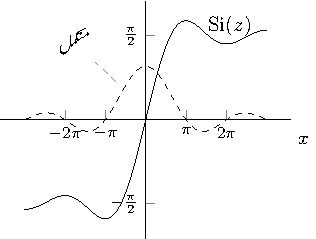
\includegraphics{figFourierSineIntegralAndSincFunction}
\caption{سائن تکمل}
\label{شکل_فوریئر_سائن_تکمل}
\end{figure}
%
\begin{figure}
\centering
\begin{subfigure}{0.5\textwidth}
\centering
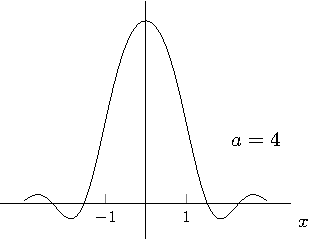
\includegraphics{figFourierGibbsPhenomenonA4}
\end{subfigure}%
\begin{subfigure}{0.5\textwidth}
\centering
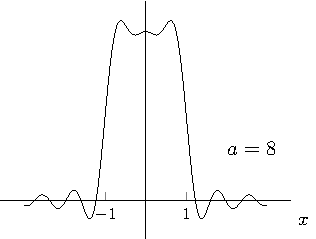
\includegraphics{figFourierGibbsPhenomenonA8}
\end{subfigure}
\begin{subfigure}{0.5\textwidth}
\centering
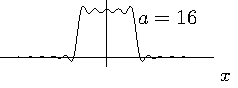
\includegraphics{figFourierGibbsPhenomenonA16}
\end{subfigure}
\caption{مساوات \حوالہ{مساوات_فوریئر_گبس_الف} کی تکمل میں $4=a$، $8$ اور $16$ لیا گیا ہے}
\label{شکل_فوریئر_مظہر_گبس}
\end{figure}
\انتہا{مثال}
%======================

\جزوحصہء{جفت اور طاق تفاعل کی فوریئر تکمل}
یہ جاننا سود مند ثابت ہوتا ہے کہ ایسا جفت یا طاق تفاعل جس کو فوریئر تکمل سے ظاہر کرنا ممکن ہو کا فوریئر تکمل عمومی تفاعل کی فوریئر تکمل سے نسبتاً آسان ہو گا۔ یہ حقیقت گزشتہ کلیات سے اخذ ہوتا ہے۔

جفت تفاعل \عددی{f(x)} کی صورت میں مساوات  \حوالہ{مساوات_فوریئر_تکمل_ت} کے تحت \عددی{B(w)=0} اور
\begin{align}\label{مساوات_فوریئر_تکمل_جفت_الف}
A(w)=2\int_0^{\infty} f(v)\cos wv\, \dif v
\end{align}
ہو گا لہٰذا مساوات \حوالہ{مساوات_فوریئر_تکمل_ٹ} درج ذیل سادہ صورت اختیار کرے گی۔
\begin{align}\label{مساوات_فوریئر_تکمل_جفت_ب}
f(x)=\frac{1}{\pi}\int_0^{\infty} A(w)\cos wx\,\dif w\quad \quad \quad (\text{\RL{جفت $f$}})
\end{align}
اسی طرح طاق تفاعل \عددی{f(x)} کی صورت میں مساوات  \حوالہ{مساوات_فوریئر_تکمل_ت} کے تحت \عددی{A(w)=0} اور
\begin{align}\label{مساوات_فوریئر_تکمل_جفت_پ}
B(w)=2\int_0^{\infty} f(v)\sin wv\, \dif v
\end{align}
ہو گا لہٰذا مساوات \حوالہ{مساوات_فوریئر_تکمل_ٹ} درج ذیل سادہ صورت اختیار کرے گی۔
\begin{align}\label{مساوات_فوریئر_تکمل_جفت_ت}
f(x)=\frac{1}{\pi}\int_0^{\infty} B(w)\sin wx\,\dif w\quad \quad \quad (\text{\RL{طاق $f$}})
\end{align}
یہ تسہیل جفت اور طاق تفاعل کی  فوریئر تسلسل کی تسہیل کی طرح ہے۔
%======================

\جزوحصہء{تخمینہ تکمل}
فوریئر تکمل کی  مدد سے کئی  تکمل کی قیمتیں حاصل کی جا سکتی ہیں۔ہم اس ترکیب کو درج ذیل مثال سے سمجھاتے  ہیں۔

%==============================
\ابتدا{مثال}\quad لاپلاس تکمل\\
درج ذیل تفاعل کی فوریئر تکمل وقفہ \عددی{x>0} پر حاصل کریں۔ (شکل \حوالہ{شکل_مثال_فوریئر_تکمل_ب} دیکھیں جہاں \عددی{k=1} ہے۔)
\begin{align*}
f(x)=e^{-kx}, \quad f(-x)=f(x)
\end{align*}
حل:چونکہ \عددی{f} جفت ہے لہٰذا مساوات \حوالہ{مساوات_فوریئر_تکمل_جفت_الف} سے 
\begin{align*}
A(w)=2\int_0^{\infty} e^{-kv}\cos wv\,\dif v
\end{align*}
حاصل ہو گا۔تکمل بالحصص لیتے ہیں۔
\begin{align*}
\int e^{-kv}\cos wv\,\dif v=-\frac{k}{k^2+w^2}e^{-kv}\big(-\frac{w}{k}\sin wv+\cos wv\big)
\end{align*}
جب \عددی{v=0} ہو تب دایاں ہاتھ \عددی{-\tfrac{k}{k^2+w^2}} کے برابر ہو گا جبکہ \عددی{v\to \infty} پر \عددی{e^{-kv}} جزو کی بنا یہ صفر کے قریب تر ہو گا۔یوں
\begin{align*}
A(w)=\frac{2k}{k^2+w^2}
\end{align*}
حاصل ہوتا ہے جس کو مساوات \حوالہ{مساوات_فوریئر_تکمل_جفت_ب} میں پر کرتے ہوئے دیے تفاعل کی فوریئر تکمل لکھتے ہیں۔
\begin{align*}
f(x)=e^{-kx}=\frac{2k}{\pi}\int_0^{\infty} \frac{\cos wx}{k^2+w^2}\dif w\quad \quad \quad (x>0,\, k>0)
\end{align*}
اس سے 
\begin{align}\label{مساوات_فوریئر_لاپلاس_تکمل_الف}
\int_0^{\infty} \frac{\cos wx}{k^2+w^2}\dif w=\frac{\pi}{2k}e^{-kx}\quad \quad \quad (x>0,\, k>0)
\end{align}
حاصل ہوتا ہے۔اسی طرح مساوات \حوالہ{مساوات_فوریئر_تکمل_جفت_ت}  استعمال کرتے ہوئے وقفہ \عددی{x>0} پر  طاق تفاعل
\begin{align*}
f(x)=e^{-kx},\quad f(-x)=-f(x), \quad \quad (k>0)
\end{align*}
 کی فوریئر تکمل سے  درج ذیل حاصل ہو گا۔
\begin{align}\label{مساوات_فوریئر_لاپلاس_تکمل_ب}
\int_0^{\infty} \frac{w\sin wx}{k^2+w^2}\dif w=\frac{\pi}{2}e^{-kx}\quad \quad \quad (x>0, k>0)
\end{align}
مساوات \حوالہ{مساوات_فوریئر_لاپلاس_تکمل_الف} اور مساوات \حوالہ{مساوات_فوریئر_لاپلاس_تکمل_ب} \اصطلاح{لاپلاس تکملات}\فرہنگ{لاپلاس!تکملات}\حاشیہب{Laplace integrals}\فرہنگ{Laplace!integrals} کہلاتے ہیں۔
\انتہا{مثال}
%=======================

\حصہء{سوالات}
سوال \حوالہ{سوال_فوریئر_تکمل_کی_مدد_ثبوت_الف} تا سوال \حوالہ{سوال_فوریئر_تکمل_کی_مدد_ثبوت_ب} میں دیے تعلق کو فوریئر تکمل کی مدد سے ثابت کریں۔

%===============
\ابتدا{سوال}\شناخت{سوال_فوریئر_تکمل_کی_مدد_ثبوت_الف}
\begin{align*}
\int_0^{\infty} \frac{\cos wx+w\sin wx}{1+w^2}\dif w=
\begin{cases}
0&x<0\\
\frac{\pi}{2}&x=0\\
\pi e^{-x} &x>0
\end{cases}
\end{align*}
\انتہا{سوال}
%=====================
\ابتدا{سوال}
\begin{align*}
\int_0^{\infty} \frac{w^3\sin wx}{w^4+4}\dif w=\frac{\pi}{2}e^{-x}\cos x\quad \quad (x>0)
\end{align*}
\انتہا{سوال}
%=====================
\ابتدا{سوال}
\begin{align*}
\int_0^{\infty} \frac{\sin w\pi\sin wx}{1-w^2}\dif w=
\begin{cases}
\frac{\pi}{2}\sin x&0\le x\le \pi\\
0&x>\pi
\end{cases}
\end{align*}
\انتہا{سوال}
%=====================
\ابتدا{سوال}
\begin{align*}
\int_0^{\infty} \frac{1-\cos w\pi}{w}\sin wx\dif w=
\begin{cases}
\frac{\pi}{2}&0< x< \pi\\
0&x>\pi
\end{cases}
\end{align*}
\انتہا{سوال}
%=====================
\ابتدا{سوال}
\begin{align*}
\int_0^{\infty} \frac{\cos wx}{1+w^2}\dif w=\frac{\pi}{2}e^{-x}\quad (x>0)
\end{align*}
\انتہا{سوال}
%=====================
\ابتدا{سوال}
\begin{align*}
\int_0^{\infty} \frac{\sin w\cos wx}{w}\dif w=
\begin{cases}
\frac{\pi}{2}&0\le  x< 1\\
\frac{\pi}{4}&x=1\\
0&x>1
\end{cases}
\end{align*}
\انتہا{سوال}
%=====================
\ابتدا{سوال}\شناخت{سوال_فوریئر_تکمل_کی_مدد_ثبوت_ب}
\begin{align*}
\int_0^{\infty} \frac{\cos\frac{w\pi}{2}\cos wx}{1-w^2}\dif w=
\begin{cases}
\frac{\pi}{2}\cos x&\abs{x}<\frac{\pi}{2}\\
0&\abs{x}>\frac{\pi}{2}
\end{cases}
\end{align*}
\انتہا{سوال}
%=====================
سوال \حوالہ{سوال_فوریئر_جفت_طرز_الف} تا سوال \حوالہ{سوال_فوریئر_جفت_طرز_ب} میں \عددی{f(x)} کو مساوات \حوالہ{مساوات_فوریئر_تکمل_جفت_ب} کی روپ میں لکھیں۔

%==============
\ابتدا{سوال}\شناخت{سوال_فوریئر_جفت_طرز_الف}
\begin{align*}
f(x)=
\begin{cases}
1&0<x<1\\
0&x>1
\end{cases}
\end{align*}
جواب:\quad
$\tfrac{2}{\pi}\int_0^{\infty} \tfrac{\sin w}{w}\cos wx\,\dif w$
\انتہا{سوال}
%========================
\ابتدا{سوال}\شناخت{سوال_فوریئر_جفت_طرز_درکار}
\begin{align*}
f(x)=
\begin{cases}
x^2&0<x<1\\
0&x>1
\end{cases}
\end{align*}
جواب:\quad
$\tfrac{2}{\pi}\int_0^{\infty} [\tfrac{\sin w}{w}-\tfrac{2\sin w}{w^3}+\tfrac{2\cos w}{w^2}]\cos wx\dif w$
\انتہا{سوال}
%========================
\ابتدا{سوال}
\begin{align*}
f(x)=
\begin{cases}
1&0<x<1\\
2&1<x<2\\
0&x>3
\end{cases}
\end{align*}
جواب:\quad
$\tfrac{2}{\pi}\int_0^{\infty}[\tfrac{\sin w}{w}-\tfrac{2\sin 2w}{w}+\tfrac{2\sin 3w}{w}]\cos wx\,\dif w$
\انتہا{سوال}
%========================
\ابتدا{سوال}
\begin{align*}
f(x)=
\begin{cases}
1-x&0<x<1\\
0&x>1
\end{cases}
\end{align*}
جواب:\quad
$\tfrac{2}{\pi}\int_0^{\infty}\tfrac{1-\cos w}{w^2}\cos wx\,\dif w$
\انتہا{سوال}
%========================
\ابتدا{سوال}
\begin{align*}
f(x)=
\begin{cases}
1-x&0<x<2\\
0&x>1
\end{cases}
\end{align*}
جواب:\quad
$\tfrac{2}{\pi}\int_0^{\infty}\tfrac{1-\cos 2w-w\sin 2w}{w^2}\cos wx\,\dif w$
\انتہا{سوال}
%========================
\ابتدا{سوال}\شناخت{سوال_فوریئر_جفت_طرز_ب}
\begin{align*}
f(x)=
\begin{cases}
\sin(x)&0<x<\pi \\
0&x>\pi
\end{cases}
\end{align*}
جواب:\quad
$\tfrac{2}{\pi}\int_0^{\infty}\tfrac{1+\cos w\pi}{1-w^2}\cos wx\,\dif w$
\انتہا{سوال}
%========================
سوال \حوالہ{سوال_فوریئر_روپ_دیا_ثبوت_الف} تا سوال \حوالہ{سوال_فوریئر_روپ_دیا_ثبوت_ب} میں دیے گئے تعلق کو ثابت کریں جہاں \عددی{f(x)} کی روپ مساوات \حوالہ{مساوات_فوریئر_تکمل_جفت_ب} ہے۔ 

%=========================
\ابتدا{سوال}\شناخت{سوال_فوریئر_روپ_دیا_ثبوت_الف}\quad
$f(ax)=\tfrac{1}{\pi a}\int_0^{\infty} A(\tfrac{w}{a})\cos wx\,\dif w,\quad (a>0)$\\
جواب:\quad مساوات \حوالہ{مساوات_فوریئر_تکمل_جفت_الف} سے 
$A(\tfrac{w}{a})=2\int_0^{\infty}f(v)\cos \tfrac{wv}{a}\dif v$
 لکھا جاتا ہے جبکہ \عددی{f(ax)} کے لئے 
$A^*=2\int_0^{\infty}f(at)\cos wt\dif t$
ہو گا جس میں \عددی{\tau=at} لیتے ہوئے 
$A^*=2\int_0^{\infty} f(\tau)\cos \tfrac{w\tau}{a}\tfrac{1}{a}\dif \tau$
ملتا ہے جن سے \عددی{A^*=\tfrac{1}{a}A(\tfrac{w}{a})} حاصل ہوتا ہے۔یوں ثابت ہوا کہ
$f(ax)=\tfrac{1}{\pi a}\int_0^{\infty} A(\tfrac{w}{a})\cos wx\dif w$
\انتہا{سوال}
%======================
\ابتدا{سوال}\شناخت{سوال_فوریئر_روپ_دیا_ثبوت_ب}\quad
$x^2f(x)=\tfrac{1}{\pi}\int_0^{\infty} A^*(w)\cos wx\,\dif w,\quad A^*=-\tfrac{\dif ^{\,2} A}{\dif w^2}$\\
جواب:\quad مساوات \حوالہ{مساوات_فوریئر_تکمل_جفت_الف} کا دو درجی تفرق لے کر
$\tfrac{\dif^{\,2}A}{\dif w^2}=-2\int_0^{\infty} f^*(v)\cos wv\dif v, \quad f^*(v)=v^2f(v)$
سے ثبوت حاصل ہو گا۔
\انتہا{سوال}
%=======================
\ابتدا{سوال}\quad درج بالا کلیہ (سوال \حوالہ{سوال_فوریئر_روپ_دیا_ثبوت_ب}) استعمال کرتے ہوئے سوال \حوالہ{سوال_فوریئر_جفت_طرز_الف} کے نتیجہ سے سوال \حوالہ{سوال_فوریئر_جفت_طرز_درکار} حل کریں۔ 
\انتہا{سوال}
%======================
\ابتدا{سوال}\شناخت{سوال_فوریئر_جفت_طاق_الف}\quad ثابت کریں
$xf(x)=\tfrac{1}{\pi}\int_0^{\infty}B^*(w)\sin wx\dif w$
جہاں \عددی{B^*=-\tfrac{\dif A}{\dif w}} ہے اور \عددی{A} کو مساوات \حوالہ{مساوات_فوریئر_تکمل_جفت_الف} ظاہر کرتی ہے۔ 

\انتہا{سوال}
%=========================
\ابتدا{سوال}\quad
تفاعل \عددی{f(x)=1\quad (0<x<a)} کے لئے سوال \حوالہ{سوال_فوریئر_جفت_طاق_الف} کے کلیہ کی تصدیق کریں۔ 
\انتہا{سوال}
%==========================
\ابتدا{سوال}\quad
تصدیق کریں کہ \عددی{f(x)=1\quad (0<x<\infty)} کو فوریئر تکمل سے ظاہر نہیں کیا جا سکتا ہے۔
\انتہا{سوال}
%======================
\ابتدا{سوال}\quad (فوریئر تکمل کی مخلوط صورت، فوریئر بدل)\\
ضمیمہ \حوالہ{ضمیمہ_مفید_معلومات} کی مساوات \حوالہ{مساوات_ضمیمہ_مفید_چھ} استعمال کرتے ہوئے مساوات \حوالہ{مساوات_فوریئر_تکمل_ٹ} کو
\begin{align}\label{مساوات_فوریئر_بدل_الف}
f(x)=\frac{1}{\pi}\int_{0}^{\infty} \big[\int_{-\infty}^{\infty} f(v)\cos(wx-wv)\,\dif v\big]\dif w
\end{align}
لکھا جا سکتا ہے۔ثابت کریں کہ مساوات \حوالہ{مساوات_فوریئر_بدل_الف} میں \عددی{-\infty} تا \عددی{\infty} تکمل متغیرہ \عددی{w} کا جفت تفاعل ہے لہٰذا مساوات \حوالہ{مساوات_فوریئر_بدل_الف} کو
\begin{align}\label{مساوات_فوریئر_بدل_ب}
f(x)=\frac{1}{2\pi}\int_{-\infty}^{\infty} \big[\int_{-\infty}^{\infty} f(v)\cos(wx-wv)\,\dif v\big]\dif w
\end{align}
لکھا جا سکتا ہے۔اسی طرح \عددی{\sin(wx-wv)} متغیرہ \عددی{w} کا طاق تفاعل ہے لہٰذا درج ذیل ثابت کرتے ہوئے
\begin{align}\label{مساوات_فوریئر_بدل_پ}
\frac{i}{2\pi}\int_{-\infty}^{\infty} \big[\int_{-\infty}^{\infty} f(v)\sin(wx-wv)\,\dif v\big]\dif w=0
\end{align}
مساوات \حوالہ{مساوات_فوریئر_بدل_ب} اور مساوات \حوالہ{مساوات_فوریئر_بدل_پ} کا مجموعہ لے کر فوریئر تکمل کی مخلوط صورت
\begin{align}\label{مساوات_فوریئر_بدل_ت}
f(x)=\frac{1}{2\pi}\int_{-\infty}^{\infty} \big[\int_{-\infty}^{\infty} f(v)e^{iw(x-v)}\,\dif v\big]\dif w
\end{align}
حاصل کریں۔مساوات \حوالہ{مساوات_فوریئر_بدل_ت} سے 
\begin{align}\label{مساوات_فوریئر_بدل_ٹ}
f(x)=\frac{1}{\sqrt{2\pi}}\int_{-\infty}^{\infty} C(w)e^{iwx}\dif w
\end{align}
حاصل کریں جہاں
\begin{align}\label{مساوات_فوریئر_بدل_ث}
C(w)=\frac{1}{\sqrt{2\pi}}\int_{-\infty}^{\infty} f(v)e^{-iwv}\dif v
\end{align}
ہے۔مساوات \حوالہ{مساوات_فوریئر_بدل_ٹ} تفاعل \عددی{C(w)} کا \اصطلاح{الٹ فوریئر بدل}\فرہنگ{فوریئر!الٹ بدل}\حاشیہب{inverse Fourier transform}\فرہنگ{Fourier!inverse transform} دیتی ہے جبکہ مساوات \حوالہ{مساوات_فوریئر_بدل_ث} تفاعل \عددی{f(x)} کا \اصطلاح{فوریئر بدل}\فرہنگ{فوریئر!بدل}\حاشیہب{Fourier transform}\فرہنگ{Fourier!transform} دیتی ہے۔
\انتہا{سوال}
%===========================

\باب{جزوی تفرقی مساوات}
مختلف طبعی اور جیومیٹریائی مسائل جہاں دو یا دو سے زیادہ متغیرات پر مبنی تفاعل پایا جاتے ہوں، جزوی تفرقی مساوات کو جنم دیتے ہیں۔یہ متغیرات وقت اور خلا کے محدد ہو سکتے ہیں۔اس باب میں انجینئری نقطہ نظر سے اہم مسائل پر غور کیا جائے گا۔ان مساوات کو طبعی نظام کی نمونہ کے طور پر حاصل کرنے کے بعد ابتدائی قیمت اور سرحدی قیمت مسائل حل کرنے کی تراکیب پر غور کیا جائے گا، یعنی ان مساوات کو دی گئی طبعی شرائط کے مطابق حل کیا جائے گا۔

ہم دیکھیں گے کہ جزوی تفرقی مساوات کو لاپلاس بدل کی مدد سے حل کیا جا سکتا ہے۔

\حصہ{بنیادی تصورات}
دو یا دو سے زیادہ غیر تابع متغیرات کی نا معلوم تفاعل اور اس کی ایک یا ایک سے زیادہ تفرقات پر مبنی مساوات کو \اصطلاح{جزوی تفرقی مساوات}\فرہنگ{تفرقی!جزوی مساوات}\فرہنگ{جزوی!تفرقی مساوات}\حاشیہب{partial differential equation}\فرہنگ{differential!partial equation} کہتے ہیں۔ بلند تر تفرق کا درجہ مساوت کا \اصطلاح{درجہ}\فرہنگ{درجہ!جزوی تفرقی مساوات}\فرہنگ{جزوی!درجہ مساوات}\حاشیہب{order}\فرہنگ{order!partial differential equation} کہلاتا ہے۔ 

سادہ تفرقی مساوات کی طرح اگر جزوی تفرقی مساوات میں تابع متغیر (نا معلوم تفاعل) اور اس کے تفرق کی طاقت اکائی ہو تب  یہ تفرقی مساوات \اصطلاح{خطی}\فرہنگ{خطی}\حاشیہب{linear}\فرہنگ{linear} کہلائے گی۔اگر مساوات کا ہر رکن، تابع متغیرہ یا تابع متغیرہ کی تفرقات میں سے کوئی ایک تفرق ہو تب اس کو \اصطلاح{ہم جنسی}\فرہنگ{ہم جنسی!جزوی تفرقی مساوات}\حاشیہب{homogeneous}\فرہنگ{homogeneous!partial differential equation} کہیں گے ورنہ یہ \اصطلاح{غیر ہم جنسی}\فرہنگ{غیر ہم جنسی!جزوی تفرقی مساوات}\حاشیہب{non homogeneous}\فرہنگ{non homogeneous!partial differential equation} کہلائے گی۔   

%===============
\ابتدا{مثال}\quad اہم خطی دو درجی جزوی تفرقی مساوات\\
\begin{align}
&\frac{\partial^{\,2}u}{\partial t^2}=c^2\frac{\partial^{\,2}u}{\partial x^2}\label{مساوات_جزوی_الف}\quad \quad 
\text{\RL{یک بعدی مساوات موج}}\\
&\frac{\partial u}{\partial t}=c\frac{\partial^{\,2}u}{\partial x^2}\label{مساوات_جزوی_ب}\quad \quad \text{\RL{یک بعدی مساوات حرارت}}\\
&\frac{\partial^{\,2}u}{\partial x^2}+\frac{\partial^{\,2}u}{\partial y^2}=0\label{مساوات_جزوی_پ}\quad \quad \quad 
\text{\RL{دو بعدی لاپلاس مساوات}}\\
&\frac{\partial^{\,2}u}{\partial x^2}+\frac{\partial^{\,2}u}{\partial y^2}=f(x,y)\label{مساوات_جزوی_ت}\quad \quad \quad \text{\RL{دو بعدی پوئسن مساوات}}\\
&\frac{\partial^{\,2}u}{\partial x^2}+\frac{\partial^{\,2}u}{\partial y^2}+\frac{\partial^{\,2}u}{\partial z^2}=0\label{مساوات_جزوی_ٹ}\quad \quad \quad \text{\RL{تین بعدی لاپلاس مساوات}}
\end{align}
یہاں \عددی{c} مستقل ہے، \عددی{t} وقت کو ظاہر کرتی ہے جبکہ \عددی{x}، \عددی{y}، \عددی{z} کارتیسی محدد ہیں۔مساوات \حوالہ{مساوات_جزوی_ت} میں اگر \عددی{f(x,y)\ne 0} ہو تب یہ غیر ہم جنسی ہو گی۔باقی تمام مساوات ہم جنسی ہیں۔
\انتہا{مثال}
%===========================

فضا میں غیر تابع متغیرہ کی کسی خطہ  \عددی{R} میں جزوی تفرقی مساوات کے \اصطلاح{حل} سے مراد ایسا تفاعل ہے جو خود اور جس کے وہ تمام تفرقات جو اس مساوات میں پائے جاتے ہوں کسی ایسے خطے میں موجود ہوں  جس کا \عددی{R} حصہ ہو اور یہ تمام مل کر پورے خطہ \عددی{R} میں اس مساوات کو مطمئن کرتے ہوں۔(عموماً \عددی{R} کی سرحد پر اس تفاعل کا استمراری ہونا اور درکار تفرقات کا خطہ کے اندرون معین ہونے کے ساتھ ساتھ خطہ کے اندرون مساوات کو مطمئن کرنا درکار ہو گا۔)

عموماً جزوی تفرقی مساوات کے تمام حل کی تعداد بہت زیادہ ہو گی۔ مثلاً جیسا آپ تصدیق کر سکتے ہیں کہ تفاعل
\begin{align}\label{مساوات_جزوی_مثال_تفاعل}
u=x^2-y^2,\quad u=e^x\cos y,\quad u=\ln(x^2+y^2)
\end{align} 
جو ایک دوسرے سے بالکل مختلف ہیں مساوات \حوالہ{مساوات_جزوی_پ} کے حل ہیں۔ہم بعد میں دیکھیں گے کہ جزوی تفرقی مساوات کا یکتا حل حاصل کرنے کی خاطر مزید معلومات درکار ہو گی جو طبعی حالت سے حاصل ہو گی۔مثال کے طور پر کبھی کبھار سرحد کے کسی حصے پر درکار حل کی قیمت معلوم ہو گی (\اصطلاح{سرحدی شرائط}\فرہنگ{سرحدی شرائط}\حاشیہب{boundary conditions}\فرہنگ{boundary conditions}) جب کہ بعض اوقات ابتدائی لمحہ \عددی{t=0} پر حل کی قیمت معلوم ہو گی (\اصطلاح{ابتدائی شرائط}\فرہنگ{ابتدائی شرائط}\حاشیہب{initial conditions}\فرہنگ{initial conditions})۔ 

ہم جانتے ہیں کہ اگر سادہ تفرقی مساوات خطی اور ہم جنسی ہو تب اس کی معلوم حل سے مزید حل بذریعہ خطی میل حاصل کیے جا سکتے ہیں۔ جزوی تفرقی مساوات کے لئے بھی ایسا کرنا ممکن ہے جیسا درج ذیل مسئلہ کہتا ہے۔

%=========================
\ابتدا{مسئلہ}\شناخت{مسئلہ_جزوی_بنیادی}\quad بنیادی مسئلہ\\
اگر کسی خطہ \عددی{R} میں  خطی ہم جنسی جزوی تفرقی مساوات کے دو حل \عددی{u_1} اور \عددی{u_2} ہوں تب
\begin{align*}
u=c_1u_1+c_2u_2
\end{align*} 
جہاں \عددی{c_1} اور \عددی{c_2} کوئی مستقل ہیں، بھی اس خطے میں اس مساوات کا حل ہو گا۔
\انتہا{مسئلہ}
%====================

اس مسئلے کا ثبوت نہایت آسان اور مسئلہ \حوالہ{مسئلہ_دو_درجی_خطی_میل} کی ثبوت سے ملتا جلتا ہے لہٰذا یہ آپ پر چھوڑا جاتا ہے۔

%================
\حصہء{سوالات}

%==================
\ابتدا{سوال}\quad
مسئلہ \حوالہ{مسئلہ_جزوی_بنیادی} کو دو اور تین متغیرات کی دو درجی جزوی تفرقی مساوات کے لئے ثابت کریں۔
\انتہا{سوال}
%======================
\ابتدا{سوال}\quad تصدیق کریں کہ مساوات \حوالہ{مساوات_جزوی_مثال_تفاعل} میں دیے گئے تمام تفاعل مساوات \حوالہ{مساوات_جزوی_پ} کے حل ہیں۔\\
جواب:\quad \عددی{u=x^2+y^2} لیتے ہیں۔ یوں \عددی{\tfrac{\partial^{\,2}u}{\partial x^2}=2} اور \عددی{\tfrac{\partial^{\,2}u}{\partial y^2}=2} ہو گا۔انہیں مساوت \حوالہ{مساوات_جزوی_پ} میں پر کرتے ہوئے \عددی{0=0} ملتا ہے۔یوں \عددی{u} تفرقی مساوات کو مطمئن کرتا ہے۔
\انتہا{سوال}
%====================
سوال \حوالہ{سوال_جزوی_لاپلاس_مطمئن_الف} تا سوال \حوالہ{سوال_جزوی_لاپلاس_مطمئن_ب} میں تصدیق کریں کہ دیا گیا تفاعل لاپلاس مساوات کو مطمئن کرتا ہے۔

%==================
\ابتدا{سوال}\شناخت{سوال_جزوی_لاپلاس_مطمئن_الف} \quad
$u=2xy$
\انتہا{سوال}
%=====================
\ابتدا{سوال} \quad
$u=e^x\sin y$
\انتہا{سوال}
%=====================
\ابتدا{سوال} \quad
$u=\tan^{-1}\frac{y}{x}$
\انتہا{سوال}
%=====================
\ابتدا{سوال} \quad
$u=x^3-3xy^2$
\انتہا{سوال}
%=====================
\ابتدا{سوال} \quad
$u=\sin x\sinh y$
\انتہا{سوال}
%=====================
\ابتدا{سوال}\شناخت{سوال_جزوی_لاپلاس_مطمئن_ب} \quad
$u=x^4-6x^2y^2+y^4$
\انتہا{سوال}
%=====================
سوال \حوالہ{سوال_جزوی_حراری_مطمئن_الف} تا سوال \حوالہ{سوال_جزوی_حراری_مطمئن_ب} میں تصدیق کریں کہ دیا گیا تفاعل حراری مساوات \حوالہ{مساوات_جزوی_ب} کو مطمئن کرتا ہے۔

%==================
\ابتدا{سوال}\شناخت{سوال_جزوی_حراری_مطمئن_الف} \quad
$u=e^{-2t}\cos x$
\انتہا{سوال}
%======================
\ابتدا{سوال}\quad
$u=e^{-t}\sin 3x$
\انتہا{سوال}
%======================
\ابتدا{سوال}\شناخت{سوال_جزوی_حراری_مطمئن_ب}\quad
$u=e^{-4t}\cos \omega x$
\انتہا{سوال}
%======================
سوال \حوالہ{سوال_جزوی_موج_مطمئن_الف} تا سوال \حوالہ{سوال_جزوی_موج_مطمئن_ب} میں تصدیق کریں کہ دیا گیا تفاعل موج کی مساوات \حوالہ{مساوات_جزوی_الف} کو مطمئن کرتا ہے۔

%==================
\ابتدا{سوال}\شناخت{سوال_جزوی_موج_مطمئن_الف}\quad
$u=x^2+4t^2$
\انتہا{سوال}
%======================
\ابتدا{سوال}\quad
$u=x^3+3xt^2$
\انتہا{سوال}
%======================
\ابتدا{سوال}\شناخت{سوال_جزوی_موج_مطمئن_ب}\quad
$u=\sin \omega ct\sin \omega x$
\انتہا{سوال}
%======================
\ابتدا{سوال}\quad
تصدیق کریں کہ 
$u=\sqrt{x^2+y^2+z^2}$
تین بعدی لاپلاس مساوات \حوالہ{مساوات_جزوی_ٹ} کو مطمئن کرتا ہے۔
\انتہا{سوال}
%========================
\ابتدا{سوال}\quad
تصدیق کریں کہ
$u(x,y)=a\ln(x^2+y^2)+b$
دو بعدی لاپلاس مساوات \حوالہ{مساوات_جزوی_پ} کا حل ہے۔دی گئی سرحدی شرائط کے تحت دائرہ \عددی{x^2+y^2=1} پر  \عددی{u=0} اور دائرہ \عددی{x^2+y^2=9} پر \عددی{u=5} ہے۔مستقل \عددی{a} اور \عددی{b} کی ایسی قیمتیں دریافت کریں کہ \عددی{u} ان سرحدی شرائط کو مطمئن کرے۔حاصل \عددی{u} کی ترسیم کھینچیں۔
\انتہا{سوال}
%======================
\ابتدا{سوال}\quad
تصدیق کریں کہ
$u(x,t)=v(x+ct)+w(x-ct)$
موج کی مساوات \حوالہ{مساوات_جزوی_الف} کو مطمئن کرتا ہے۔یہاں \عددی{u} اور \عددی{v} دو مرتبہ قابل تفرق تفاعل ہیں۔
\انتہا{سوال}
%====================
اگر جزوی تفرقی مساوات میں صرف ایک متغیر کے ساتھ تفرقات پائے جاتے ہوں تب اس کو سادہ تفرقی مساوات تصور کر کے حل کیا جا سکتا ہے جہاں باقی متغیرات کو مستقل تصور کیا جاتا ہے۔سوال \حوالہ{سوال_جزوی_سادہ_الف} تا سوال \حوالہ{سوال_جزوی_سادہ_ب} کو حل کریں جہاں \عددی{u} کے متغیرات \عددی{x} اور \عددی{y} ہیں۔

%====================
\ابتدا{سوال}\شناخت{سوال_جزوی_سادہ_الف}\quad
$u_{xx}-u=0$\\
جواب:\quad
$u=c_1(y)e^x+c_2(y)e^{-x}$
\انتہا{سوال}
%====================
\ابتدا{سوال}\quad
$u_{y}+yu=0$\\
جواب:\quad
$u=c(x)e^{-\tfrac{y^2}{2}}$
\انتہا{سوال}
%====================
\ابتدا{سوال}\quad
$u_{yy}+9u=0$\\
جواب:\quad
$u=c_1(y)\cos 3x+c_2(y)\sin 3x$
\انتہا{سوال}
%====================
\ابتدا{سوال}\شناخت{سوال_جزوی_سادہ_ب}\quad
$u_x+2xyu=0$\\
جواب:\quad
$u=c(y)e^{-x^2y}$
\انتہا{سوال}
%====================
سوال \حوالہ{سوال_جزوی_تلاش_الف} تا سوال \حوالہ{سوال_جزوی_تلاش_ب} میں \عددی{u_x=p} لیتے ہوئے حل تلاش کریں۔

%================
\ابتدا{سوال}\شناخت{سوال_جزوی_تلاش_الف}\quad
$u_{xy}=0$\\
جواب:\quad
$u=v(x)+w(y)$
\انتہا{سوال}
%======================
\ابتدا{سوال}\quad
$u_{xy}=u_x$
\انتہا{سوال}
%=======================
\ابتدا{سوال}\quad
$u_{xy}+u_x=0$\\
جواب:\quad
$u=v(x)e^{-y}+w(y)$
\انتہا{سوال}
%=======================
\ابتدا{سوال}\شناخت{سوال_جزوی_تلاش_ب}\quad
$u_{xy}+u_x+x+y+1=0$
\انتہا{سوال}
%=======================
سوال \حوالہ{سوال_جزوی_نظام_الف} تا سوال \حوالہ{سوال_جزوی_نظام_ب} میں دیے گئے تفرقی مساوات کی نظام کے حل تلاش کریں۔ 

%=================
\ابتدا{سوال}\شناخت{سوال_جزوی_نظام_الف}\quad
$u_{xx}=0,\quad u_{yy}=0$\\
جواب:\quad
$u=axy+bx+cy+k$
\انتہا{سوال}
%==================
\ابتدا{سوال}\quad
$u_{x}=0,\quad u_{y}=0$
\انتہا{سوال}
%==================
\ابتدا{سوال}\quad
$u_{xx}=0,\quad u_{xy}=0$\\
جواب:\quad
$u=cx+g(y)$
\انتہا{سوال}
%==================
\ابتدا{سوال}\شناخت{سوال_جزوی_نظام_ب}\quad
$u_{xx}=0,\quad u_{xy}=0,\quad u_{yy}=0$
\انتہا{سوال}
%==================
\ابتدا{سوال}\quad
تصدیق کریں کہ اگر سطح \عددی{z=z(x,y)} پر منحنی \عددی{z=c} محور \عددی{x} کے متوازی سیدھے خطوط ہوں، جہاں \عددی{c} مستقل ہے، تب \عددی{z} تفرقی مساوات \عددی{z_x=0} کا حل ہو گا۔ایسی ایک مثال بھی پیش کریں۔  
\انتہا{سوال}
%=====================
\ابتدا{سوال}\quad
تصدیق کریں کہ \عددی{yz_x-xz_y=0} کا حل \عددی{z=z(x,y)} سطح گردش ہے۔اس کی مثال پیش کریں۔ (اشارہ: \عددی{x=r\cos \theta} اور \عددی{y=r\sin \theta} لے کر تفرقی مساوات کو \عددی{z_{\theta}=0} میں تبدیل کریں۔)
\انتہا{سوال}
%======================

\حصہ{نمونہ کشی: ارتعاش پذیر تار۔ یک بعدی مساوات موج}\شناخت{حصہ_جزوی_ارتعاش_تار}
ایک لچک دار تار کو  لمبائی \عددی{l} تک کھینچ کر سروں سے باندھا جاتا ہے۔ساکن تار کو \عددی{x} محور پر تصور کریں۔اس تار کو کسی نقطہ یا نقاط سے کھینچ کر لمحہ \عددی{t=0} پر چھوڑا دیا جاتا ہے تا کہ یہ ارتعاش کر سکے۔ہم تار کی ارتعاش معلوم کرنا چاہتے ہیں یعنی لمحہ \عددی{t>0} پر ساکن حالت سے تار کی نقطہ \عددی{x} کا انحراف \عددی{u(x,t)} جاننا چاہتے ہیں (شکل \حوالہ{شکل_جزوی_تار})۔
\begin{figure}
\centering
\begin{subfigure}{0.8\textwidth}
\centering
\begin{tikzpicture}
%\draw(0,0) grid (4,2);
%\draw[thin,gray,step=0.1](0,0) grid (6,2);
%
\draw(0,0)--(6.5,0);
\draw(0,0)--(0,2)node[right]{$u$};
%
\draw[thick](0,0)node[below]{$0$} to [out=45,in=120] (6,0)node[below]{$l$};
%
\draw[-latex](2.1,1.2)--++(17:-1.5)node[left]{$T_1$};
\draw[dashed](2.1,1.2)--(2.1,0)node[below]{$x$};
\draw[dashed](2.1,1.2)node[solid,ocirc]{}node[above]{$P$}--++(-1.5,0);
\draw([shift={(180:0.8)}]2.1,1.2) arc (180:197:0.8);
\draw(2.1,1.2)++(17:-1)node[shift={(0,0.15)}]{$\alpha$};
%
\draw[-latex](3,1.36)--++(10:1.5)node[shift={(0.2,0.1)}]{$T_2$};
\draw[dashed](3.1,1.36)--(3.1,0)node[below]{$x+\Delta x$};
\draw[dashed](3.1,1.36)node[solid,ocirc]{}node[above]{$Q$}--++(2,0);
\draw([shift={(0:0.8)}]3.1,1.36) arc (0:10:0.8);
\draw(3.9,1.43)to [out=0,in=-60]++(0,0.5)node[left]{$\beta$};
\end{tikzpicture}
\end{subfigure}
\begin{subfigure}{0.5\textwidth}
\centering
\begin{tikzpicture}
\draw[thick](0,0)coordinate(kA)to [out=20,in=-170] ++(1.5,0.4)coordinate(kB);
\draw[dashed](kA)--++(-1.5,0);
\draw[-latex](kA)node[ocirc]{}node[above]{$P$}--++(20:-1.5)node[left]{$T_1$};
\draw ([shift={(180:0.5)}]kA) arc (180:200:0.5);
\draw(kA)++(20:-1)node[shift={(0,0.2)}]{$\alpha$};
%
\draw[dashed](kB)--++(1.5,0);
\draw[-latex](kB)node[ocirc]{}node[above]{$B$}--++(10:1.5)node[shift={(0.3,0.2)}]{$T_2$};
\draw([shift={(0:1)}]kB) arc (0:10:1);
\draw(kB)++(10:1)++(0,-0.09) to [out=0,in=-60]++(0,0.5) node[above]{$\beta$};
\end{tikzpicture}
\end{subfigure}
\caption{ارتعاش پذیر تار}
\label{شکل_جزوی_تار}
\end{figure}
%
کسی بھی نظام کا ریاضی نمونہ اخذ کرتے وقت کئی ترسیلی مفروضے  فرض کیے جاتے ہیں تا کہ  حاصل مساوات ضرورت سے زیادہ پیچیدہ نہ ہوں۔ہم سادہ تفرقی مساوات کی طرح جزوی تفرقی مساوات حاصل کرتے ہوئے بھی ایسا کریں گے۔

موجودہ مسئلے میں ہم درج ذیل فرض کرتے ہیں۔

\موٹا{(الف)} \quad تار کی کمیت فی اکائی لمبائی یکساں ہے (ہم جنسی تار)۔ تار مکمل طور پر لچکدار ہے اور مڑنے کے خلاف مزاحمت فراہم نہیں کرتا ہے۔ \\
\موٹا{(ب)} \quad تار کو اتنا تان کر باندھا گیا ہے کہ اس میں تناو، ثقلی قوت سے بہت زیادہ ہو۔یوں ثقلی قوت کو نظر انداز کیا جا سکتا ہے۔\\
\موٹا{(پ)} \quad تار سیدھی کھڑی سطح میں حرکت کرتا ہے۔تار پر کوئی بھی نقطہ اپنے ساکن مقام سے بہت کم انحراف کرتا ہے لہٰذا ہر نقطے پر تار کی انحراف اور ڈھلوان کی حتمی قیمتیں قلیل ہوں گی۔ 

%==========================

ہم توقع کر سکتے ہیں کہ یوں حاصل جزوی تفرقی مساوات کا حل \عددی{u(x,t)}،  "غیر کامل"  ہم جنسی تار جس میں ثقلی میدان سے بہت زیادہ تناو ہو  کا صحیح نقش پیش کرے گا۔  

مسئلے کی تفرقی مساوات حاصل کرنے کی خاطر ہم تار کے ایک چھوٹے ٹکڑے پر غور کرتے ہیں جس میں تناو \عددی{T} پایا جاتا ہے (شکل \حوالہ{شکل_جزوی_تار})۔چونکہ مڑنے کے خلاف تار مزاحمت فراہم نہیں کرتا ہے لہٰذا ہر نقطے پر تار میں تناو اس نقطے پر تار کا مماسی ہو گا۔فرض کریں کہ تار کے ٹکڑے  کی سروں \عددی{P} اور \عددی{Q}  پر تناو \عددی{T_1} اور \عددی{T_2} ہے۔چونکہ تار افقی حرکت نہیں کرتا ہے لہٰذا اس ٹکڑے پر تناو کا کل افقی جزو صفر کے برابر ہو گا۔ یوں شکل \حوالہ{شکل_جزوی_تار} کو دیکھ کر 
\begin{align*}
T_1\cos \alpha-T_2\cos \beta=0
\end{align*}
یا
\begin{align}\label{مساوات_جزوی_تار_الف}
T_1\cos \alpha=T_2\cos \beta=T=\text{مستقل}
\end{align}
لکھا جا سکتا ہے  یعنی ہر ایسے ٹکڑے پر بائیں اور دائیں رخ یکساں (مستقل \عددی{T}) تناو ہو گا۔ انتصابی رخ میں \عددی{T_1} اور \عددی{T_2} کے اجزاء \عددی{-T_1\sin \alpha} اور \عددی{T_2\sin \beta} ہیں جہاں اوپر رخ تناو کو مثبت تصور کیا گیا ہے۔ نیوٹن کی دوسری قانون کے تحت ان دو قوتوں کا مجموعہ تار کے ٹکڑے کی کمیت \عددی{\rho \Delta x} ضرب  اسراع \عددی{\tfrac{\partial^{\,2} u}{\partial t^2}} کے برابر ہو گا جہاں اسراع،  \عددی{x} اور \عددی{x+\Delta x} کے مابین کسی نقطے  کی اسراع ہو گی۔ تار کی کمیت فی اکائی لمبائی \عددی{\rho} ہے جبکہ تار کے ٹکڑے کی لمبائی \عددی{\Delta x} ہے۔یوں
\begin{align}\label{مساوات_جزوی_تار_ب}
T_2\sin \beta-T_1\sin \alpha=\rho\Delta x\frac{\partial^{\,2}u}{\partial t^2}
\end{align} 
ہو گا۔اس کو مساوات \حوالہ{مساوات_جزوی_تار_الف} سے تقسیم کرتے ہیں۔
\begin{align}\label{مساوات_جزوی_تار_پ}
\frac{T_2\sin \beta}{T_2\cos \beta}-\frac{T_1\sin \alpha}{T_2\cos \alpha}=\tan \beta -\tan \alpha=\frac{\rho \Delta x}{T}\frac{\partial^{\,2}u}{\partial t^2}
\end{align}
آپ تسلی کر لیں کہ چونکہ مساوات \حوالہ{مساوات_جزوی_تار_الف} میں \عددی{T_1\cos \alpha=T_2\cos \beta=T} ہے لہٰذا مساوات \حوالہ{مساوات_جزوی_تار_ب} کو مساوات \حوالہ{مساوات_جزوی_تار_الف} سے تقسیم کرتے ہوئے کہیں \عددی{T_2\cos \beta}، کہیں \عددی{T_1\cos \alpha} اور کہیں \عددی{T} سے تقسیم کیا جا سکتا ہے۔ 

اب \عددی{\tan \beta} اور \عددی{\tan \alpha} تار کی \عددی{x} اور \عددی{x+\Delta x} پر مماس ہے یعنی
\begin{align*}
\tan \alpha=\left(\frac{\partial u}{\partial x}\right)_x \quad \text{اور} \quad \tan \beta=\left(\frac{\partial u}{\partial x}\right)_{x+\Delta x}
\end{align*}
جہاں جزوی تفرق اس لئے استعمال کیے  گئے ہیں کہ \عددی{u} متغیرہ \عددی{t} کا بھی تابع  ہے۔یوں مساوات \حوالہ{مساوات_جزوی_تار_پ} کو \عددی{\Delta x} سے تقسیم کرتے ہوئے
\begin{align*}
\frac{1}{\Delta x}\big[\left(\frac{\partial u}{\partial x}\right)_{x+\Delta x}-\left(\frac{\partial u}{\partial x}\right)_{x}\big]=\frac{\rho}{T}\frac{\partial^{\,2}u}{\partial t^2}
\end{align*}
لکھا جا سکتا ہے جس میں \عددی{\Delta x} کو صفر کے قریب تر کرتے ہوئے
\begin{align}\label{مساوات_جزوی_تار_ت}
\frac{\partial^{\,2}u}{\partial t^2}=c^2\frac{\partial^{\,2}u}{\partial x^2}\quad \quad \quad c^2=\frac{T}{\rho}
\end{align}
حاصل ہوتا ہے جس کو یک \اصطلاح{یک بعدی مساوات موج}\فرہنگ{موج!یک بعدی مساوات}\حاشیہب{one dimensional wave equation}\فرہنگ{wave!one dimensional equation} کہتے ہیں۔ مساوات \حوالہ{مساوات_جزوی_تار_ت} ہمارے مسئلے کی درکار جزوی تفرقی مساوات ہے جو ہم جنسی اور دو درجی ہے۔مساوات میں مستقل \عددی{\tfrac{T}{\rho}} کو \عددی{c} کی بجائے \عددی{c^2} سے ظاہر کیا گیا ہے تا کہ واضح رہے کہ یہ مثبت مستقل ہے۔اس مساوات کا حل اگلے حصے میں حاصل کیا جائے گا۔
%=================================

\حصہ{علیحدگی متغیرات (ترکیب ضرب)}\شناخت{حصہ_جزوی_علیحدگی_متغیرات}
گزشتہ حصے میں ہم نے دیکھا کہ لچک دار تار کی ارتعاش کو جزوی تفرقی مساوات 
\begin{align}\label{مساوات_جزوی_مساوات_موج_الف}
\frac{\partial^{\,2}u}{\partial t^2}=c^2\frac{\partial^{\,2}u}{\partial x^2}\quad \quad \text{\RL{مساوات موج}}
\end{align}
 بیان کرتی ہے جہاں \عددی{u(x,t)} تار کی انحراف ہے۔تار کی حرکت جاننے کی خاطر اس مساوات کا حل درکار ہو گا بلکہ ہمیں مساوات \حوالہ{مساوات_جزوی_مساوات_موج_الف} کا ایسا حل \عددی{u(x,t)} درکار ہے جو نظام پر لاگو شرائط کو بھی مطمئن کرے۔چونکہ تار کے دونوں سر غیر تغیر پذیر ہیں لہٰذا تمام \عددی{t} کے لئے \عددی{x=0} اور \عددی{x=l} پر سرحدی شرائط
\begin{align}\label{مساوات_جزوی_مساوات_موج_ب}
u(0,t)=0,\quad u(l,t)=0
\end{align}
لاگو ہیں۔تار کی حرکت ابتدائی انحراف (لمحہ \عددی{t=0} پر انحراف) اور ابتدائی رفتار (لمحہ \عددی{t=0} پر رفتار) پر منحصر ہو گی۔ابتدائی انحراف کو \عددی{f(x)} اور ابتدائی رفتار کو \عددی{g(x)} سے ظاہر کرتے ہوئے \اصطلاح{ابتدائی شرائط}\فرہنگ{ابتدائی شرائط}\حاشیہب{initial conditions}\فرہنگ{initial conditions} 
\begin{align}
u(x,0)&=f(x)\label{مساوات_جزوی_مساوات_موج_پ}\\
\left. \frac{\partial u}{\partial t}\right|_{t=0}&=g(x)\label{مساوات_جزوی_مساوات_موج_ت}
\end{align}
لکھی جائیں گی۔ہمیں اب مساوات \حوالہ{مساوات_جزوی_مساوات_موج_ب} کا ایسا حل چاہیے جو سرحدی شرائط مساوات \عددی{مساوات_جزوی_مساوات_موج_ب} اور ابتدائی شرائط  مساوات \حوالہ{مساوات_جزوی_مساوات_موج_پ} اور مساوات \حوالہ{مساوات_جزوی_مساوات_موج_ت} کو مطمئن کرے۔ہم درج ذیل اقدام کے ذریعہ ایسا حل تلاش کریں گے۔

پہلا قدم۔ علیحدگی متغیرات کی ترکیب سے ہم جزوی تفرقی مساوات سے دو عدد سادہ تفرقی مساوات حاصل کریں گے۔\\
دوسرا قدم۔ہم ان سادہ تفرقی مساوات کے ایسے حل تلاش کریں گے جو دی گئی سرحدی شرائط کو مطمئن کرتے ہوں۔\\
تیسرا قدم۔ حاصل حل سے ایسے حل حاصل کیے جائیں گے جو ابتدائی شرائط کو بھی مطمئن کرتے ہوں۔

ان اقدام کی تفصیل درج ذیل ہے۔

\موٹا{پہلا قدم۔}\quad  ترکیب ضرب مساوات \حوالہ{مساوات_جزوی_مساوات_موج_الف} کے حل دو عدد تفاعل کا حاصل ضرب
\begin{align}\label{مساوات_جزوی_مساوات_موج_ٹ}
u(x,t)=F(x)G(t)
\end{align}
کی روپ میں دیتا ہے جہاں ہر ایک تفاعل صرف ایک متغیرہ \عددی{x} یا \عددی{t} کا تابع ہے۔ہم جلد دیکھیں گے کہ انجینئری حساب میں اس ترکیب کے  کئی استعمال پائے جاتے ہیں۔ مساوات \حوالہ{مساوات_جزوی_مساوات_موج_ٹ} کے تفرق لیتے ہوئے
\begin{align*}
\frac{\partial^{\,2}u}{\partial t^2}=F\ddot{G}\quad \text{اور}\quad \frac{\partial^{\,2}u}{\partial x^2}=F''G
\end{align*}
ملتا ہے جہاں (\عددی{'}) سے مراد \عددی{x} کے ساتھ تفرق اور \عددی{(^.)} سے مراد \عددی{t} کے ساتھ تفرق ہے۔انہیں مساوات \حوالہ{مساوات_جزوی_مساوات_موج_الف} میں پر کر کے
\begin{align*}
F\ddot{G}=c^2F''G
\end{align*}
دونوں اطراف کو \عددی{c^2FG} سے تقسیم کرنے سے
\begin{align*}
\frac{\ddot{G}}{c^2G}=\frac{F''}{F}
\end{align*}
ملتا ہے جس کا دایاں ہاتھ صرف متغیرہ \عددی{x} پر منحصر ہے جبکہ اس کا بایاں ہاتھ صرف متغیرہ \عددی{t} پر منحصر ہے۔اب \عددی{t} تبدیل کرنے سے صرف بایاں ہاتھ تبدیل ہونے کا امکان ہے لیکن اس مساوات کے تحت دونوں اطراف برابر ہیں اور دایاں ہاتھ \عددی{t} تبدیل کرنے سے ہرگز تبدیل نہیں ہوتا ہے۔اس کا مطلب ہے کہ \عددی{t} تبدیل کرنے سے بایاں ہاتھ بھی تبدیل نہیں ہوتا ہے۔اسی طرح \عددی{x} تبدیل کرنے سے صرف دایاں ہاتھ کا تبدیل ہونا ممکن ہے لیکن دونوں اطراف برابر ہیں اور \عددی{x} کی تبدیلی ہے بایاں ہاتھ ہرگز تبدیل نہیں ہوتا ہے لہٰذا \عددی{x} تبدیل کرنے سے دایاں ہاتھ بھی تبدیل نہیں ہوتا ہے۔یوں اس مساوات کے دونوں اطراف غیر تغیر پذیر ہیں لہٰذا انہیں مستقل \عددی{k} کے برابر لکھا جا سکتا ہے
\begin{align*}
\frac{\ddot{G}}{c^2G}=\frac{F''}{F}=k
\end{align*}
جس سے درج ذیل دو عدد مساوات علیحدہ علیحدہ لکھنا ممکن ہے جہاں \عددی{k} نا معلوم مستقل ہے۔ 
\begin{align}
F''-kF&=0\label{مساوات_جزوی_مساوات_موج_ث}\\
\ddot{G}-c^2kG&=0\label{مساوات_جزوی_مساوات_موج_ج}
\end{align}

\موٹا{دوسرا قدم۔} \quad  ہم مساوات \حوالہ{مساوات_جزوی_مساوات_موج_ث} اور مساوات \حوالہ{مساوات_جزوی_مساوات_موج_ج} کے حل \عددی{F} اور \عددی{G} حاصل کرتے ہوئے ایسا \عددی{u=FG} دریافت کرتے ہیں جو تمام \عددی{t} کے لئے سرحدی شرائط مساوات \حوالہ{مساوات_جزوی_مساوات_موج_ب} کو مطمئن کرتا ہو یعنی:
\begin{align*}
u(0,t)=F(0)G(t)=0,\quad u(l,t)=F(l)G(t)=0
\end{align*}
اب اگر درج بالا میں  \عددی{G\equiv 0} ہو تب \عددی{u\equiv 0} ہو گا جس میں ہم کوئی دلچسپی نہیں رکھتے ہیں لہٰذا \عددی{G\ne 0} ہو گا۔یوں درج بالا سے درج ذیل ملتا ہے۔
\begin{align}\label{مساوات_جزوی_مساوات_موج_چ}
\text{(الف)}\quad F(0)=0,\quad \quad \text{(ب)}\quad F(l)=0
\end{align}
اگر مساوات \حوالہ{مساوات_جزوی_مساوات_موج_ث} میں \عددی{k=0} ہو تب اس مساوات کا عمومی حل \عددی{F=ax+b} ہو گا جو مساوات \حوالہ{مساوات_جزوی_مساوات_موج_چ} کی استعمال سے \عددی{a=0}، \عددی{b-0} یعنی \عددی{F\equiv0} یا \عددی{u\equiv} دیتا ہے جو غیر دلچسپ حل ہے۔مثبت \عددی{k=\mu^2} کے لئے مساوات \حوالہ{مساوات_جزوی_مساوات_موج_ث} کا عمومی حل
\begin{align*}
F=Ae^{\mu x}+Be^{-\mu x}
\end{align*}
ہے جو مساوات \حوالہ{مساوات_جزوی_مساوات_موج_چ} کی استعمال سے \عددی{A=0}، \عددی{B=0} یعنی \عددی{F\equiv 0} یا \عددی{u\equiv =0} دیتا ہے جو غیر دلچسپ حل ہے۔یوں ہمارے پاس منفی \عددی{k=-p^2} لینا رہ جاتا ہے جس کو استعمال کرتے ہوئے مساوات \حوالہ{مساوات_جزوی_مساوات_موج_ث} کو دوبارہ لکھتے ہیں۔
\begin{align*}
F''+p^2F=0
\end{align*}
اس کا عمومی حل
\begin{align*}
F(x)=A\cos px+B\sin px
\end{align*}
ہے جو مساوات \حوالہ{مساوات_جزوی_مساوات_موج_چ}-الف کی مدد سے
\begin{align*}
F(0)=A=0
\end{align*}
لہٰذا \عددی{F=B\sin px} ہو گا جو مساوات \حوالہ{مساوات_جزوی_مساوات_موج_چ}-ب کے ساتھ مل کر
\begin{align*}
F(l)=B\sin pl=0
\end{align*}
دیتی ہے۔اب اگر \عددی{B=0} ہو تب \عددی{F\equiv 0} یعنی \عددی{u\equiv 0} ہو گا جو غیر دلچسپ حل ہے لہٰذا \عددی{B\ne 0} ہے۔اس طرح \عددی{\sin pl=0} ہو گا۔ہم جانتے ہیں کہ \عددی{\sin n\pi=0} ہوتا ہے لہٰذا یوں درج ذیل ملتا ہے جہاں \عددی{n} عدد صحیح ہے۔
\begin{align}\label{مساوات_جزوی_مساوات_موج_ح}
pl=n\pi \quad \implies \quad p=\frac{n\pi}{l}
\end{align}
ہم \عددی{B=1} منتخب کرتے ہوئے لامحدود تعداد کے حل \عددی{F(x)=F_n(x)} یعنی
\begin{align}\label{مساوات_جزوی_مساوات_موج_خ}
F_n(x)=\sin \frac{n\pi}{l}x\quad \quad \quad  n=1,2,\cdots
\end{align}
حاصل کرتے ہیں جو مساوات \حوالہ{مساوات_جزوی_مساوات_موج_چ} میں دیے گئے سرحدی شرائط کو مطمئن کرتے ہیں۔چونکہ \عددی{\sin(-\alpha)=-\sin \alpha} ہوتا ہے لہٰذا  منفی عدد صحیح \عددی{n=-1,-2,\dots} لینے سے  یہی حل منفی علامت کے ساتھ دوبارہ ملتے ہیں۔

اب مساوات \حوالہ{مساوات_جزوی_مساوات_موج_ح} کے تحت  \عددی{k} کی قیمت صرف \عددی{k=-p^2=-(\tfrac{n\pi}{l})^2} ممکن ہے۔\عددی{k} کی ان قیمتوں کے ساتھ  مساوات \حوالہ{مساوات_جزوی_مساوات_موج_ج} درج ذیل صورت اختیار کرتی ہے
\begin{align*}
\ddot{G}+\lambda_n^2G=0\quad \quad \lambda_n=\frac{cn\pi}{l}
\end{align*}
جس کا عمومی حل
\begin{align*}
G_n(t)=B_b\cos \lambda_nt+B^*_n\sin \lambda_n t
\end{align*}
ہے۔یوں تفاعل \عددی{u_n(x,t)=F_n(x)G_n(t)}
\begin{align}\label{مساوات_جزوی_مساوات_موج_د}
u_n(x,t)=(B_b\cos \lambda_nt+B^*_n\sin \lambda_n t)\sin \frac{n\pi}{l}x\quad \quad (n=1,2,\cdots)
\end{align}
مساوات \حوالہ{مساوات_جزوی_مساوات_موج_ج} کے ایسے حل ہیں جو  مساوات \حوالہ{مساوات_جزوی_مساوات_موج_چ} میں دی گئی سرحدی شرائط کو مطمئن کرتے ہیں۔ان تفاعل کو ارتعاش پذیر تار کے  \اصطلاح{آئگنی تفاعل}\فرہنگ{آئگنی!تفاعل}\حاشیہب{eigenfunctions}\فرہنگ{eigenfunctions} یا \اصطلاح{امتیازی تفاعل}\فرہنگ{امتیازی!تفاعل}\حاشیہب{characteristic functions}\فرہنگ{characteristic!functions} کہتے ہیں جبکہ \عددی{\lambda_n=\tfrac{cn\pi}{l}} کی قیمتوں کو ارتعاش پذیر تار کے \اصطلاح{آئگنی اقدار}\فرہنگ{آئگنی!قدر}\حاشیہب{eigenvalues}\فرہنگ{eigenvalues} یا \اصطلاح{امتیازی اقدار}\فرہنگ{امتیازی!قدر}\حاشیہب{characteristic values}\فرہنگ{characteristic!values} کہتے ہیں۔ مزید \عددی{\{   \lambda_1,\lambda_2,\cdots\}} کا سلسلہ \اصطلاح{طیف}\فرہنگ{طیف}\حاشیہب{spectrum}\فرہنگ{spectrum} کہلاتا ہے۔

ہم دیکھتے ہیں کہ ہر ایک \عددی{u_n} ایک مخصوص ہارمونی ارتعاش کو ظاہر کرتی ہے جس کی تعدد \عددی{\tfrac{\lambda_n}{2\pi}=\tfrac{cn}{2l}} چکر فی اکائی وقت ہے۔ اس حرکت کو تار کی \عددی{n} ویں \اصطلاح{قائمہ انداز}\فرہنگ{قائمہ!انداز}\فرہنگ{انداز!قائمہ}\حاشیہب{normal mode}\فرہنگ{normal mode} کہتے ہیں۔ پہلا قائمہ انداز جس کا \عددی{n=1} ہو گا \اصطلاح{بنیادی انداز}\فرہنگ{بنیادی انداز}\فرہنگ{انداز!بنیادی}\حاشیہب{fundamental mode}\فرہنگ{fundamental mode} کہلاتا ہے جبکہ باقی کو \عددی{n} ویں \اصطلاح{ہارمونی انداز}\فرہنگ{ہارمونی!انداز}\حاشیہب{harmonics}\فرہنگ{harmonics} کہتے ہیں۔چونکہ مساوات \حوالہ{مساوات_جزوی_مساوات_موج_د} میں 
\begin{align*}
\sin \frac{n\pi x}{l}=0\quad \implies \quad x=\frac{l}{n},\frac{2l}{n},\cdots,\frac{n-1}{n}l
\end{align*}
ہے لہٰذا \عددی{n} ویں قائمہ انداز کے \عددی{n-1} \اصطلاح{نقطہ صفر ہٹاو}\فرہنگ{نقطہ صفر ہٹاو}\حاشیہب{node}\فرہنگ{node} پائے جائیں گے۔ ان نقطوں پر تار ساکن رہتی ہے (شکل \حوالہ{شکل_جزوی_قائمہ_انداز})۔  
%
\begin{figure}
\centering
\begin{tikzpicture}
\pgfmathsetmacro{\A}{0.5}
%
\draw(0,0)--(1.5,0);
\draw [domain=0:180] plot ({1.5/180*\x},{\A*sin(\x)});
\draw(0,0)node[below]{$0$}--++(0,0.2);
\draw(1.5,0)node[below]{$l$}--++(0,0.2);
\draw(1.5/2,-0.75)node[]{$n=1$};
%
\begin{scope}[shift={(-2cm,0)}]
\draw(0,0)--(1.5,0);
\draw [domain=0:180] plot ({1.5/180*\x},{0.5*\A*sin(2*\x)});
\draw(0,0)node[below]{$0$}--++(0,0.2);
\draw(1.5,0)node[below]{$l$}--++(0,0.2);
\draw(1.5/2,-0.75)node[]{$n=2$};
\draw[stealth-](1.5/2,0)node[ocirc]{}++(0.02,0.02) to [out=45,in=-45]++(0.5,0.5)node[left]{\RL{نقطہ صفر ہٹاو}};
\end{scope}
%
\begin{scope}[shift={(-4cm,0)}]
\draw(0,0)--(1.5,0);
\draw [domain=0:180] plot ({1.5/180*\x},{0.25*\A*sin(3*\x)});
\draw(0,0)node[below]{$0$}--++(0,0.2);
\draw(1.5,0)node[below]{$l$}--++(0,0.2);
\draw(1.5/2,-0.75)node[]{$n=3$};
\draw(1.5/3,0)node[ocirc]{};
\draw(2*1.5/3,0)node[ocirc]{};
\end{scope}
%
\begin{scope}[shift={(-6cm,0)}]
\draw(0,0)--(1.5,0);
\draw [domain=0:180] plot ({1.5/180*\x},{0.125*\A*sin(4*\x)});
\draw(0,0)node[below]{$0$}--++(0,0.2);
\draw(1.5,0)node[below]{$l$}--++(0,0.2);
\draw(1.5/2,-0.75)node[]{$n=4$};
\draw(1.5/4,0)node[ocirc]{};
\draw(2*1.5/4,0)node[ocirc]{};
\draw(3*1.5/4,0)node[ocirc]{};
\end{scope}
\end{tikzpicture}
\caption{تار کے قائمہ انداز اور نقطہ صفر ہٹاو۔}
\label{شکل_جزوی_قائمہ_انداز}
\end{figure}

شکل \حوالہ{شکل_جزوی_مختلف_لمحات_دوسرا_قائمہ_انداز} میں دوسرا قائمہ انداز مختلف لمحات \عددی{t} پر دکھایا گیا ہے۔کسی بھی لمحہ پر تار کی شکل سائن تفاعل کی ہو گی۔جب تار کا بایاں آدھا حصہ نیچے کی طرف حرکت کرتا ہے اس وقت تار کا دایاں آدھا حصہ اوپر کو حرکت کرے گا۔اسی طرح جب بایاں حصہ اوپر کو حرکت کرتا ہے اس وقت دایاں حصہ نیچے کو حرکت کرتا ہے۔تار کا درمیانہ نقطہ حرکت نہیں کرتا ہے لہٰذا یہ نقطہ صفر ہٹاو ہے۔باقی انداز بھی اسی طرح کی خاصیت رکھتے ہیں۔
\begin{figure}
\centering
\begin{tikzpicture}
\draw(0,0)--(4.5,0)node[right]{$x$};
\draw(0,-1)--(0,1.5);
%
\draw[domain=0:360] plot ({4/360*\x},{sin(\x)});
\draw[dashed,domain=0:360] plot ({4/360*\x},{0.5*sin(\x)});
\draw[dashdotted,domain=0:360] plot ({4/360*\x},{-0.5*sin(\x)});
\draw[dotted,domain=0:360] plot ({4/360*\x},{-1*sin(\x)});
%
\draw(4,0)node[below]{$l$}--++(0,0.2);
\draw[-stealth] (1,1)--++(0,-0.25);
\draw[-stealth] (3,-1)--++(0,0.25);
\end{tikzpicture}
\caption{مختلف $t$ پر دوسرا قائمہ انداز}
\label{شکل_جزوی_مختلف_لمحات_دوسرا_قائمہ_انداز}
\end{figure}

\موٹا{تیسرا قدم۔} \quad ظاہر ہے کہ ایک عدد حل \عددی{u_n(x,t)} عموماً ابتدائی شرائط مساوات \حوالہ{مساوات_جزوی_مساوات_موج_پ} اور مساوات \حوالہ{مساوات_جزوی_مساوات_موج_ت} کو مطمئن نہیں کر سکتا ہے۔اب چونکہ مساوات \حوالہ{مساوات_جزوی_مساوات_موج_الف} خطی اور ہم جنسی ہے لہٰذا بنیادی مسئلہ \حوالہ{مسئلہ_جزوی_بنیادی} کے تحت مساوات \حوالہ{مساوات_جزوی_مساوات_موج_الف} کی محدود تعداد کے حلوں \عددی{u_n} کا مجموعہ بھی مساوات \حوالہ{مساوات_جزوی_مساوات_موج_الف} کا حل ہو گا۔  اس طرح ایسا حل جو  ابتدائی شرائط مساوات \حوالہ{مساوات_جزوی_مساوات_موج_پ} اور مساوات \حوالہ{مساوات_جزوی_مساوات_موج_ت} کو مطمئن کرتا ہو حاصل کرنے کی خاطر ہم لامتناہی تسلسل
\begin{align}\label{مساوات_جزوی_مساوات_موج_ڈ}
u(x,t)=\sum_{n=1}^{\infty} u_n(x,t)=\sum_{n=1}^{\infty} (B_n\cos \lambda_n t+B^*_n\sin \lambda_n t)\sin \frac{n\pi}{l}x
\end{align}
پر غور کرتے ہیں۔مساوات \حوالہ{مساوات_جزوی_مساوات_موج_ڈ} اور ابتدائی شرط مساوات \حوالہ{مساوات_جزوی_مساوات_موج_پ} سے درج ذیل لکھا جا سکتا ہے۔
\begin{align}\label{مساوات_جزوی_مساوات_موج_ذ}
u(x,0)=\sum_{n=1}^{\infty} B_n\sin \frac{n\pi}{l}x=f(x)
\end{align} 
یوں اگر مساوات \حوالہ{مساوات_جزوی_مساوات_موج_ڈ} نے مساوات \حوالہ{مساوات_جزوی_مساوات_موج_پ} کو مطمئن کرنا ہو تب تب عددی سر \عددی{B_n}  اس طرح منتخب کرنے ہوں گے کہ \عددی{u(x,0)} تفاعل \عددی{f(x)} کی فوریئر سائن تسلسل ہو۔یوں  مساوات \حوالہ{مساوات_فوریئر_نصف_حلقہ_توسیع_طاق_عددی_سر} سے
\begin{align}\label{مساوات_جزوی_مساوات_موج_ر}
B_n=\frac{2}{l}\int_0^l f(x)\sin \frac{n\pi x}{l}\dif x\quad \quad \quad n=1,2,\cdots
\end{align}
حاصل ہوتا ہے۔
اسی طرح مساوات \حوالہ{مساوات_جزوی_مساوات_موج_ڈ} کا \عددی{t} کے ساتھ تفرق لے کر اور ابتدائی شرط  مساوات \حوالہ{مساوات_جزوی_مساوات_موج_ت} استعمال کرتے ہوئے درج ذیل لکھا جا سکتا ہے۔ 
\begin{align*}
\left. \frac{\partial u}{\partial t}\right|_{t=0}&=\left[\sum_{n=1}^{\infty} (-B_n\lambda_n\sin \lambda_nt+B^*_n\lambda_n\cos \lambda_nt)\sin\frac{n\pi x}{l}\right]_{t=0}\\
&=\sum_{n=1}^{\infty} B^*_n\lambda_n\sin\frac{n\pi x}{l} =g(x)
\end{align*}
یوں اگر مساوات \حوالہ{مساوات_جزوی_مساوات_موج_ڈ} نے مساوات \حوالہ{مساوات_جزوی_مساوات_موج_ت} کو مطمئن کرنا ہو تب تب عددی سر \عددی{B^*_n}  اس طرح منتخب کرنے ہوں گے کہ \عددی{t=0} پر  \عددی{\tfrac{\partial u}{\partial t}} تفاعل \عددی{g(x)} کی فوریئر سائن تسلسل ہو۔ یوں مساوات \حوالہ{مساوات_فوریئر_نصف_حلقہ_توسیع_طاق_عددی_سر} سے 
\begin{align*}
B^*_n\lambda_n=\frac{2}{l}\int_0^l g(x)\sin \frac{n\pi x}{l} \dif x
\end{align*}
اور چونکہ \عددی{\lambda_n=\tfrac{cn\pi}{l}} ہے لہٰذا
\begin{align}\label{مساوات_جزوی_مساوات_موج_ڑ}
B^*_n=\frac{2}{cn\pi}\int_0^l g(x)\sin \frac{n\pi x}{l}\dif x\quad \quad \quad n=1,2,\cdots
\end{align}
لکھا جا سکتا ہے۔

مساوات \حوالہ{مساوات_جزوی_مساوات_موج_ر} اور مساوات \حوالہ{مساوات_جزوی_مساوات_موج_ڑ} میں حاصل کیے گئے عددی سر کو مساوات \حوالہ{مساوات_جزوی_مساوات_موج_ڈ} میں پر کرنے سے حاصل تسلسل \عددی{u(x,t)}، مساوات \حوالہ{مساوات_جزوی_مساوات_موج_الف} کا ایسا حل ہو گا جو مساوات \حوالہ{مساوات_جزوی_مساوات_موج_ب}، مساوات \حوالہ{مساوات_جزوی_مساوات_موج_پ} اور مساوات \حوالہ{مساوات_جزوی_مساوات_موج_ت} کی شرائط کو مطمئن کرے گا بشرطیکہ  حاصل \عددی{u(x,t)} مرتکز ہو اور اس  کی \عددی{x} اور \عددی{t} کے ساتھ جزو در جزو  دو  درجی تفرق لینے سے حاصل تسلسل مرتکز   ہو اور ان کے مجموعے  بالترتیب \عددی{\tfrac{\partial^{\,2}u}{\partial x^2}} اور \عددی{\tfrac{\partial^{\,2}u}{\partial t^2}} کے برابر ہوں جو استمراری ہیں۔

اب تک مساوات \حوالہ{مساوات_جزوی_مساوات_موج_ڈ} محض ریاضی حل کے طور پر سامنے آیا ہے۔آئیں اس کی اصل حقیقت کو قائم کریں۔ہم اپنی آسانی کی خاطر ابتدائی رفتار \عددی{g(x)} صفر لیتے ہیں۔یوں \عددی{B^*_n=0} ہوں  گے لہٰذا مساوات \حوالہ{مساوات_جزوی_مساوات_موج_ڈ} درج ذیل صورت اختیار کرے گا۔
\begin{align}\label{مساوات_جزوی_متحرک_موج_الف}
u(x,t)=\sum_{n=1}^{\infty} B_n\cos \lambda_n t\sin\frac{n\pi x}{l},\quad \lambda_n=\frac{cn\pi}{l}
\end{align}
ہم ضمیمہ \حوالہ{ضمیمہ_مفید_معلومات} کا کلیہ \حوالہ{مساوات_ضمیمہ_مفید_گیارہ} استعمال کرتے ہوئے
\begin{align*}
\cos \frac{cn\pi}{l}t\,\sin\frac{n\pi}{l}x=\frac{1}{2}\big[\sin\big\{\frac{n\pi}{l}(x-ct)\big\}+\sin\big\{\frac{n\pi}{l}(x+ct)\big\}\big]
\end{align*}
لکھ سکتے ہیں جس کو  مساوات \حوالہ{مساوات_جزوی_متحرک_موج_الف}  میں پر کرتے ہوئے درج ذیل ملتا ہے۔
\begin{align*}
u(x,t)=\frac{1}{2}\sum_{n=1}^{\infty}B_n \sin\big\{\frac{n\pi}{l}(x-ct)\big\}+\frac{1}{2}\sum_{n=1}^{\infty}B_n \sin\big\{\frac{n\pi}{l}(x+ct)\big\}
\end{align*}
آپ دیکھ سکتے ہیں کہ مساوات \حوالہ{مساوات_جزوی_مساوات_موج_ذ} میں \عددی{x} کی جگہ \عددی{x-ct} اور \عددی{x+ct} پر کرنے سے یہی دو تسلسل حاصل ہوتے ہیں لہٰذا ہم درج ذیل لکھ سکتے ہیں
\begin{align}\label{مساوات_جزوی_متحرک_موج_ب}
u(x,t)=\frac{1}{2}[f^*(x-ct)+f^*(x+ct)]
\end{align}
جہاں \عددی{f} کی طاق دوری توسیع جس کا دوری عرصہ \عددی{2l} ہو تفاعل \عددی{f^*} ہے (شکل \حوالہ{شکل_جزوی_طاق_توسیع})۔چونکہ وقفہ \عددی{0\le x\le l} پر ابتدائی انحراف \عددی{f(x)} استمراری ہے جبکہ  \عددی{x=0} اور \عددی{x=l} پر انحراف صفر ہے لہٰذا مساوات \حوالہ{مساوات_جزوی_متحرک_موج_ب} سے ظاہر ہے کہ \عددی{u(x,t)} دونوں متغیرات \عددی{x} اور \عددی{t} کی تمام قیمتوں پر استمراری ہو گا۔مساوات \حوالہ{مساوات_جزوی_متحرک_موج_ب} کا تفرق لیتے ہوئے ہم دیکھتے ہیں کہ یہ مساوات \حوالہ{مساوات_جزوی_مساوات_موج_الف} کا حل ہے بشرطیکہ  وقفہ \عددی{0<x<l} پر \عددی{f(x)} دو مرتبہ قابل تفرق ہو اور \عددی{x=0} اور \عددی{x=l} پر اس کے یک طرفہ دو درجی تفرق پائے جاتے ہوں جن کی قیمت صفر کے برابر ہو۔اس طرح یہ حقیقت قائم ہوتی ہے کہ ان شرائط پر پورا اترتا ہوا تسلسل \عددی{u(x,t)} مساوات \حوالہ{مساوات_جزوی_مساوات_موج_الف} کا ایسا حل ہو گا جو  مساوات \حوالہ{مساوات_جزوی_مساوات_موج_ب}، مساوات \حوالہ{مساوات_جزوی_مساوات_موج_پ} اور مساوات \حوالہ{مساوات_جزوی_مساوات_موج_ت} کی شرائط کو مطمئن کرتا ہے ۔
\begin{figure}
\centering
\begin{tikzpicture}
\draw(-2.5,0)--(4.5,0)node[right]{$x$};
\draw(0,0)node[below]{$0$}--(0,0.75);
\draw[thick](0,0) to [out=30,in=110] ++(2,0)node[below]{$l$};
\draw(2,0) to [out=-70,in=-150]++(2,0) --++(30:0.5);
\draw(0,0) to [out=-150,in=-70]++(-2,0)--++(110:0.2);
\draw(-2,0)--++(0,0.2);
\draw(2,0)--++(0,0.2);
\draw(4,0)--++(0,0.2);
\end{tikzpicture}
\caption{$f(x)$ کی طاق توسیع}
\label{شکل_جزوی_طاق_توسیع}
\end{figure}

اگر \عددی{f'(x)} اور \عددی{f''(x)} محض ٹکڑوں میں استمراری (حصہ \حوالہ{حصہ_لاپلاس_بدل_الٹ_بدل_خطیت}) ہوں، یا اگر وقفہ کے سروں پر یک طرفہ تفرقات غیر صفر ہوں تب ہر ایک \عددی{t} کے لئے محدود تعداد کی \عددی{x} قیمتوں پر مساوات \حوالہ{مساوات_جزوی_مساوات_موج_الف} کے \عددی{u} کی دو درجی تفرقات غیر معین ہوں گے۔ان نقطوں کے علاوہ باقی تمام نقطوں پر \عددی{u} مساوات موج کو مطمئن کرے گی لہٰذا ہم \عددی{u(x,t)} کو وسیع معنوں میں مسئلے کا حل تصور کر سکتے ہیں۔مثال کے طور پر تکونی ابتدائی انحراف کی صورت میں حاصل حل اس نوعیت کا ہو گا۔
\begin{figure}
\centering
\begin{tikzpicture}
\draw(-2,0)--(7,0)node[right]{$x$};
\draw(0,-1.7)--(0,1);
%
\draw(-2,-1) to [out=-20,in=-135]++(2,1)node[ocirc]{} to [out=45,in=180]++(1,1)node[above]{$f^*(x)$} to [out=0,in=180]++(1,-0.7) to [out=0,in=180]++(0.5,0.2) to [out=0,in=90]++(0.5,-0.5);
\draw[dashed](1.5,-1) to [out=-20,in=-135]++(2,1)to [out=45,in=180]++(1,1)node[above,solid]{$f^*(x-ct)$} to [out=0,in=180]++(1,-0.7) to [out=0,in=180]++(0.5,0.2) to [out=0,in=90]++(0.5,-0.5);
\draw(3.5,0)--++(0,-1.7);
\draw[stealth-stealth] (0,-1.7)--++(3.5,0)node[pos=0.5,fill=white]{$ct$};
\end{tikzpicture}
\caption{مساوات \حوالہ{مساوات_جزوی_متحرک_موج_ب} کی معنی}
\label{شکل_جزوی_موج_حرکت}
\end{figure}

آئیں   مساوات \حوالہ{مساوات_جزوی_متحرک_موج_ب} کی طبعی معنی سمجھتے ہیں۔جیسا شکل \حوالہ{شکل_جزوی_موج_حرکت} میں دکھایا گیا ہے، \عددی{f^*(x)} کی ترسیم کو \عددی{ct} اکائیاں دائیں منتقل کرنے سے \عددی{f^*(x-ct)} کی ترسیم حاصل ہوتی ہے۔ اس کا مطلب ہے کہ \عددی{f^*(x-ct),\,\, (c>0)} ایسی موج کو ظاہر کرتا ہے جو بڑھتے \عددی{t} کے ساتھ دائیں جانب کو حرکت کرتی ہے۔اسی طرح \عددی{f^*(x+ct),\,\, (c>0)} ایسی موج کو ظاہر کرتا ہے جو بڑھتے \عددی{t} کے ساتھ بائیں جانب کو حرکت کرتی ہے اور \عددی{u(x,t)} ان دونوں کا مجموعہ ہے۔

%======================

\begin{figure}
\centering
\begin{tikzpicture}
\pgfmathsetmacro{\kks}{-1.5}
\pgfmathsetmacro{\khs}{-5}
%
\pgfmathsetmacro{\ang}{30}
\pgfmathsetmacro{\l}{1}
\pgfmathsetmacro{\h}{\l*tan(\ang)}
%
\pgfmathsetmacro{\a}{1*\l}
\pgfmathsetmacro{\b}{2*\l-\a}
\pgfmathsetmacro{\aa}{\a/cos(\ang)}
\pgfmathsetmacro{\bb}{\b/cos(\ang)}
%
\draw(0,0)node[below]{$0$}--(2,0)node[below]{$l$};
\draw(0,0)--++(0,0.2);
\draw(2,0)--++(0,0.2);
%
\draw[thick](\a,\h)--++(-180+\ang:\aa);
\draw[thick](\a,\h)--++(-\ang:\bb)node[pos=0.5,above right]{$\tfrac{1}{2}f^*(x)$};
%=================
\begin{scope}[shift={(\khs,0)}]
\pgfmathsetmacro{\hh}{2*\h-2*(\l-\a)*tan(\ang)}
%
\draw(0,0)node[below]{$0$}--(2,0)node[below]{$l$};
\draw(0,0)--++(0,0.2);
\draw(2,0)--++(0,0.2);
%
\draw[thick] (0,0)--(\a,\hh)--(2*\l-\a,\hh)--(2*\l,0);
\draw(\a,\hh)node[left]{$u(x,0)$};
\draw(0,\hh/2)node[left]{$t=0$};
\end{scope}
%=========================
%==========================
\begin{scope}[shift={(0,1*\kks)}]
\pgfmathsetmacro{\a}{2/3*\l}
\pgfmathsetmacro{\b}{2*\l-\a}
\pgfmathsetmacro{\aa}{\a/cos(\ang)}
\pgfmathsetmacro{\bb}{\b/cos(\ang)}
%
\draw(0,0)--(2,0);
\draw(0,0)--++(0,0.2);
\draw(2,0)--++(0,0.2);
%
\draw[thick](\a,\h)--++(-180+\ang:\aa);
\draw[thick](\a,\h)--++(-\ang:\bb);
%
\draw[thick,dashed] (\b,\h)--++(-\ang:\aa);
\draw[thick,dashed](\b,\h)--++(-180+\ang:\bb);
%
\draw[-stealth] (\a,1.2*\h)--++(-0.5,0)node[left]{$\tfrac{1}{2}f^*(x+\tfrac{l}{5})$};
\draw[-stealth,dashed] (2*\l-\a,1.2*\h)--++(0.5,0)node[right]{$\tfrac{1}{2}f^*(x-\tfrac{l}{5})$};
%=================
\begin{scope}[shift={(\khs,0)}]
\pgfmathsetmacro{\hh}{2*\h-2*(\l-\a)*tan(\ang)}
%
\draw(0,0)--(2,0);
\draw(0,0)--++(0,0.2);
\draw(2,0)--++(0,0.2);
%
\draw[thick] (0,0)--(\a,\hh)--(2*\l-\a,\hh)--(2*\l,0);
\draw(0,\hh/2)node[left]{$t=\tfrac{l}{5c}$};
\end{scope}
\end{scope}
%============================
%==================================
\begin{scope}[shift={(0,2*\kks)}]
\pgfmathsetmacro{\a}{1/3*\l}
\pgfmathsetmacro{\b}{2*\l-\a}
\pgfmathsetmacro{\aa}{\a/cos(\ang)}
\pgfmathsetmacro{\bb}{\b/cos(\ang)}
%
\draw(0,0)--(2,0);
\draw(0,0)--++(0,0.2);
\draw(2,0)--++(0,0.2);
%
\draw[thick](\a,\h)--++(-180+\ang:\aa);
\draw[thick](\a,\h)--++(-\ang:\bb);
%
\draw[thick,dashed] (\b,\h)--++(-\ang:\aa);
\draw[thick,dashed](\b,\h)--++(-180+\ang:\bb);
\draw[] (0,\h/2)node[left]{$\tfrac{1}{2}f^*(x+\tfrac{2l}{5})$};
\draw[] (2*\l,\h/2)node[right]{$\tfrac{1}{2}f^*(x-\tfrac{2l}{5})$};
%=================
\begin{scope}[shift={(\khs,0)}]
\pgfmathsetmacro{\hh}{2*\h-2*(\l-\a)*tan(\ang)}
%
\draw(0,0)--(2,0);
\draw(0,0)--++(0,0.2);
\draw(2,0)--++(0,0.2);
%
\draw[thick] (0,0)--(\a,\hh)--(2*\l-\a,\hh)--(2*\l,0);
\draw(0,\hh/2)node[left]{$t=\tfrac{2l}{5c}$};
\end{scope}
\end{scope}
%======================
%=============================
\begin{scope}[shift={(0,3*\kks)}]
\pgfmathsetmacro{\a}{0*\l}
\pgfmathsetmacro{\b}{2*\l-\a}
\pgfmathsetmacro{\aa}{\a/cos(\ang)}
\pgfmathsetmacro{\bb}{\b/cos(\ang)}
%
\draw(0,0)--(2,0);
\draw(0,0)--++(0,0.2);
\draw(2,0)--++(0,0.2);
%
\draw[thick](\a,\h)--++(-180+\ang:\aa);
\draw[thick](\a,\h)--++(-\ang:\bb);
%
\draw[thick,dashed] (\b,\h)--++(-\ang:\aa);
\draw[thick,dashed](\b,\h)--++(-180+\ang:\bb);
\draw[] (0,\h/2)node[left]{$\tfrac{1}{2}f^*(x+\tfrac{l}{2})$};
\draw[] (2*\l,\h/2)node[right]{$\tfrac{1}{2}f^*(x-\tfrac{l}{2})$};
\begin{scope}[shift={(\khs,0)}]
\pgfmathsetmacro{\hh}{2*\h-2*(\l-\a)*tan(\ang)}
%
\draw(0,0)--(2,0);
\draw(0,0)--++(0,0.2);
\draw(2,0)--++(0,0.2);
%
\draw[thick] (0,0)--(\a,\hh)--(2*\l-\a,\hh)--(2*\l,0);
\draw(0,\hh/2)node[left]{$t=\tfrac{l}{2c}$};
\end{scope}
\end{scope}
%======================================
%======================================
%===================================
\begin{scope}[shift={(0,4*\kks)}]
\pgfmathsetmacro{\a}{1/3*\l}
\pgfmathsetmacro{\b}{2*\l-\a}
\pgfmathsetmacro{\aa}{\a/cos(\ang)}
\pgfmathsetmacro{\bb}{\b/cos(\ang)}
%
\draw(0,0)--(2,0);
\draw(0,0)--++(0,0.2);
\draw(2,0)--++(0,0.2);
%
\draw[thick,dashed](\a,-\h)--++(180-\ang:\aa);
\draw[thick,dashed](\a,-\h)--++(\ang:\bb);
%
\draw[thick] (\b,-\h)--++(\ang:\aa);
\draw[thick](\b,-\h)--++(180-\ang:\bb);
\draw[] (0,\h/2)node[left]{$\tfrac{1}{2}f^*(x+\tfrac{3l}{5})$};
\draw[] (2*\l,\h/2)node[right]{$\tfrac{1}{2}f^*(x-\tfrac{3l}{5})$};
\begin{scope}[shift={(\khs,0)}]
\pgfmathsetmacro{\hh}{2*\h-2*(\l-\a)*tan(\ang)}
%
\draw(0,0)--(2,0);
\draw(0,0)--++(0,0.2);
\draw(2,0)--++(0,0.2);
%
\draw[thick] (0,0)--(\a,-\hh)--(2*\l-\a,-\hh)--(2*\l,0);
\draw(0,0)node[left]{$t=\tfrac{3l}{5c}$};
\end{scope}
\end{scope}
%==================================
%====================================
\begin{scope}[shift={(0,5*\kks)}]
\pgfmathsetmacro{\a}{2/3*\l}
\pgfmathsetmacro{\b}{2*\l-\a}
\pgfmathsetmacro{\aa}{\a/cos(\ang)}
\pgfmathsetmacro{\bb}{\b/cos(\ang)}
%
\draw(0,0)--(2,0);
\draw(0,0)--++(0,0.2);
\draw(2,0)--++(0,0.2);
%
\draw[thick,dashed](\a,-\h)--++(180-\ang:\aa);
\draw[thick,dashed](\a,-\h)--++(\ang:\bb);
%
\draw[thick] (\b,-\h)--++(\ang:\aa);
\draw[thick](\b,-\h)--++(180-\ang:\bb);
\draw[] (0,\h/2)node[left]{$\tfrac{1}{2}f^*(x+\tfrac{4l}{5})$};
\draw[] (2*\l,\h/2)node[right]{$\tfrac{1}{2}f^*(x-\tfrac{4l}{5})$};
\begin{scope}[shift={(\khs,0)}]
\pgfmathsetmacro{\hh}{2*\h-2*(\l-\a)*tan(\ang)}
%
\draw(0,0)--(2,0);
\draw(0,0)--++(0,0.2);
\draw(2,0)--++(0,0.2);
%
\draw[thick] (0,0)--(\a,-\hh)--(2*\l-\a,-\hh)--(2*\l,0);
\draw(0,0)node[left]{$t=\tfrac{4l}{5c}$};
\end{scope}
\end{scope}
%==========================
%============================
\begin{scope}[shift={(0,6*\kks)}]
\pgfmathsetmacro{\a}{1*\l}
\pgfmathsetmacro{\b}{2*\l-\a}
\pgfmathsetmacro{\aa}{\a/cos(\ang)}
\pgfmathsetmacro{\bb}{\b/cos(\ang)}
%
\draw(0,0)--(2,0);
\draw(0,0)--++(0,0.2);
\draw(2,0)--++(0,0.2);
%
\draw[thick] (\b,-\h)--++(\ang:\aa);
\draw[thick](\b,-\h)--++(180-\ang:\bb);
\draw[] (\a,-\h/2)++(-1,0)node[left]{$\substack{\tfrac{1}{2}f^*(x+l)\\=\tfrac{1}{2}f^*(x-l)}$};
\begin{scope}[shift={(\khs,0)}]
\pgfmathsetmacro{\hh}{2*\h-2*(\l-\a)*tan(\ang)}
%
\draw(0,0)--(2,0);
\draw(0,0)--++(0,0.2);
\draw(2,0)--++(0,0.2);
%
\draw[thick] (0,0)--(\a,-\hh)--(2*\l-\a,-\hh)--(2*\l,0);
\draw(0,0)node[left]{$t=\tfrac{l}{c}$};
\end{scope}
\end{scope}
\end{tikzpicture}
\caption{مثال \حوالہ{مثال_جزوی_تکونی_انحراف} کا مختلف لمحات پر دائیں کو اور بائیں کو حرکت کرتے اجزاء اور ان کا مجموعہ حل $u(x,t)$}
\label{شکل_مثال_جزوی_تکونی_انحراف}
\end{figure}
%================
\ابتدا{مثال}\شناخت{مثال_جزوی_تکونی_انحراف}\quad تکونی ابتدائی انحراف کی صورت میں تار کی ارتعاش\\
مساوات موج \حوالہ{مساوات_جزوی_مساوات_موج_الف} کا حل تکونی ابتدائی انحراف
\begin{align*}
f(x)=
\begin{cases}
\frac{2k}{l}x&0<x<\frac{l}{2}\\
\frac{2k}{l}(l-x)&\frac{l}{2}<x<l
\end{cases}
\end{align*}
اور ابتدائی رفتار صفر \عددی{g(x)=0} کی صورت میں حاصل کریں۔\\
حل: چونکہ \عددی{g(x)\equiv 0} ہے لہٰذا مساوات \حوالہ{مساوات_جزوی_متحرک_موج_الف} میں \عددی{B^*_n=0} ہو گا جبکہ \عددی{B_n} کو صفحہ \حوالہصفحہ{مساوات_فوریئر_تکونی_دھڑکن_عددی_سر_ب} پر مساوات \حوالہ{مساوات_فوریئر_تکونی_دھڑکن_عددی_سر_ب} دے گی۔یوں  مساوات \حوالہ{مساوات_جزوی_متحرک_موج_الف} درج ذیل صورت اختیار کرے گی۔
\begin{align*}
u(x,t)=\frac{8k}{\pi^2}\big[\frac{1}{1^2}\sin \frac{\pi}{l}x\cos\frac{\pi c}{l}t-\frac{1}{3^2}\sin \frac{3\pi}{l}x\cos\frac{3\pi c}{l}t+-\cdots\big]
\end{align*}
اس حل کی ترسیم کھینچنے کی خاطر ہم \عددی{u(x,0)=f(x)} سے شروع کرتے ہوئے مساوات \حوالہ{مساوات_جزوی_متحرک_موج_ب} کی مدد لیتے ہیں۔یوں شکل \حوالہ{شکل_مثال_جزوی_تکونی_انحراف} حاصل ہوتی ہے۔
\انتہا{مثال}
%======================

\حصہء{سوالات}
سوال \حوالہ{سوال_جزوی_انحراف_تار_الف} تا سوال \حوالہ{سوال_جزوی_انحراف_تار_ب} میں تار کی لمبائی \عددی{l=\pi} اور \عددی{c^2=\tfrac{T}{\rho}=1} ہے۔تار کے سرے ٹھوس نقطوں کے ساتھ باندھے گئے ہیں۔ابتدائی رفتار صفر جبکہ ابتدائی انحراف \عددی{f(x)} سوال میں دی گئی ہے۔ارتعاش پذیر تار کا انحراف \عددی{u(x,t)} دریافت کریں۔

%==================
\ابتدا{سوال}\شناخت{سوال_جزوی_انحراف_تار_الف}\quad
$0.02\sin x$\\
جواب:\quad 
$u=0.02\cos t\sin x$
\انتہا{سوال}
%====================
\ابتدا{سوال}\quad
$k\sin 2x$\\
جواب:\quad
$u=k\cos 2t\sin 2x$
\انتہا{سوال}
%====================
\ابتدا{سوال}\quad
$k(\sin x-\sin 2x)$\\
جواب:\quad
$u=k(\cos t\sin x-\cos 2t\sin 2x)$
\انتہا{سوال}
%====================
\ابتدا{سوال}\شناخت{سوال_جزوی_شکل_انحراف_الف}\quad شکل \حوالہ{شکل_سوال_جزوی_شکل_انحراف_الف}-الف \\
جواب:\quad
$\tfrac{9\sqrt{3}k}{2\pi^2}(\tfrac{1}{1^2}\cos t\sin x+\tfrac{1}{2^2}\cos2t\sin 2x-\tfrac{1}{4^2}\cos 4t\sin 4x\cdots)$
%
\begin{figure}
\centering
\begin{subfigure}{0.3\textwidth}
\centering
\begin{tikzpicture}
\draw(0,0)--(2.5,0)node[right]{$x$};
\draw(0,0)--(0,1);
\draw[thick](0,0)--(2/3,0.5)--(2,0);
\draw(2/3,0)node[below]{$\tfrac{\pi}{3}$}--++(0,0.2);
\draw(2,0)node[below]{$\pi$}--++(0,0.2);
\draw[dashed](0,0.5)node[left,solid]{$0.05$}--++(2/3,0);
\end{tikzpicture}
\caption*{(الف)}
\end{subfigure}%
\begin{subfigure}{0.3\textwidth}
\centering
\begin{tikzpicture}
\draw(0,0)--(2.5,0)node[right]{$x$};
\draw(0,-1)--(0,1);
\draw[thick](0,0)--(0.5,0.5)--(1.5,-0.5)--(2,0);
\draw(0.5,0)node[below]{$\tfrac{\pi}{4}$}--++(0,0.2);
\draw(1,0)node[below]{$\tfrac{\pi}{2}$}--++(0,0.2);
\draw(1.5,0)--++(0,0.2)node[above]{$\tfrac{3\pi}{2}$};
\draw(2,0)node[below]{$\pi$}--++(0,0.2);
\draw[](0,0.5)node[left]{$\tfrac{\pi}{40}$}--++(0.2,0);
\draw[](0,-0.5)node[left]{$-\tfrac{\pi}{40}$}--++(0.2,0);
\end{tikzpicture}
\caption*{(ب)}
\end{subfigure}%
\begin{subfigure}{0.3\textwidth}
\centering
\begin{tikzpicture}
\draw(0,0)--(2.5,0)node[right]{$x$};
\draw(0,0)--(0,1);
\draw[thick](0,0)--(0.5,0.5)--(1,0)--(2,0);
\draw(0.5,0)node[below]{$\tfrac{\pi}{4}$}--++(0,0.2);
\draw(1,0)node[below]{$\tfrac{\pi}{2}$}--++(0,0.2);
\draw(2,0)node[below]{$\pi$}--++(0,0.2);
\draw[dashed](0,0.5)node[left,solid]{$k$}--(0.5,0.5);
\end{tikzpicture}
\caption*{(پ)}
\end{subfigure}%
\caption{اشکال برائے سوالات \حوالہ{سوال_جزوی_شکل_انحراف_الف}، \حوالہ{سوال_جزوی_شکل_انحراف_ب} اور \حوالہ{سوال_جزوی_شکل_انحراف_پ}}
\label{شکل_سوال_جزوی_شکل_انحراف_الف}
\end{figure}
\انتہا{سوال}
%===============
\ابتدا{سوال}\شناخت{سوال_جزوی_شکل_انحراف_ب}\quad شکل \حوالہ{شکل_سوال_جزوی_شکل_انحراف_الف}-ب \\
جواب:\quad
$\tfrac{4}{5\pi}(\tfrac{1}{2^2}\cos 2t\sin 2x-\tfrac{1}{6^2}\cos 6t\sin 6x+\tfrac{1}{10^2}\cos 10t\sin 10x\cdots)$
\انتہا{سوال}
%========================
\ابتدا{سوال}\شناخت{سوال_جزوی_شکل_انحراف_پ}\quad شکل \حوالہ{شکل_سوال_جزوی_شکل_انحراف_الف}-پ\\
جواب:\quad
$\tfrac{4k}{\pi^2}[2(\sqrt{2}-1)\cos t\sin x +\cos 2t\sin 2x-2(\sqrt{2}-\tfrac{1}{9})\cos 3t\sin 3x\cdots]$
\انتہا{سوال}
%========================
\ابتدا{سوال}\quad
$kx(x-\pi)$\\
جواب:\quad
$\tfrac{8k}{\pi}(\tfrac{1}{1^2}\cos t\sin x-\tfrac{1}{3^2}\cos 3t\sin 3x-\tfrac{1}{5^2}\cos 5t\sin 5x\cdots)$
\انتہا{سوال}
%======================
\ابتدا{سوال}\quad 
\begin{align*}
f(x)=
\begin{cases}
kx^2&0<x<\frac{\pi}{2}\\
k(x-\pi)^2&\frac{\pi}{2}<x<\pi
\end{cases}
\end{align*}
جواب:\quad
$4k[(1-\tfrac{2}{\pi})\cos t\sin x-\tfrac{1}{9}(1+\tfrac{2}{3\pi})\cos 3t\sin 3x\cdots]$
\انتہا{سوال}
%===========================
\ابتدا{سوال}\شناخت{سوال_جزوی_انحراف_تار_ب}\quad 
\begin{align*}
f(x)=
\begin{cases}
kx^2&0<x<\frac{\pi}{2}\\
-k(x-\pi)^2&\frac{\pi}{2}<x<\pi
\end{cases}
\end{align*}
جواب:\quad
$k(\tfrac{\pi}{2}-\tfrac{2}{\pi})\cos 2t\sin 2x+\tfrac{k\pi}{4}\cos 4t\sin 4x+k(\tfrac{\pi}{6}-\tfrac{2}{27\pi})\cos 6t\sin 6x\cdots$
\انتہا{سوال}
%===========================
سوال \حوالہ{سوال_جزوی_ابتدائی_رفتار_اور_انحراف_الف} تا سوال \حوالہ{سوال_جزوی_ابتدائی_رفتار_اور_انحراف_ب} میں \عددی{c^2=1} ہے، تار کی لمبائی \عددی{l=\pi} ہے اور تار کے سرے ٹھوس نقطوں سے بندھے ہیں۔ابتدائی رفتار \عددی{g(x)} اور ابتدائی انحراف \عددی{f(x)} ہیں۔ارتعاش پذیر تار کی انحراف \عددی{u(x,t)} دریافت کریں۔

%============
\ابتدا{سوال}\شناخت{سوال_جزوی_ابتدائی_رفتار_اور_انحراف_الف}\quad
$f=0,\quad g=kx \quad (0\le x\le \tfrac{\pi}{2});\quad g(x)=k(\pi-x)\quad (\tfrac{\pi}{2}\le x\le \pi)$\\
جواب:\quad
$\tfrac{4k}{\pi}(\tfrac{1}{1^3}\sin t\sin x-\tfrac{1}{3^3}\sin 3t\sin 3x+\tfrac{1}{5^3}\sin 5t\sin 5x\cdots)$
\انتہا{سوال}
%==================
\ابتدا{سوال}\quad
$f=0,\quad g=k\sin 3x$\\
جواب:\quad
$\tfrac{k}{3}\sin 3t\sin 3x$
\انتہا{سوال}
%==================
\ابتدا{سوال}\شناخت{سوال_جزوی_ابتدائی_رفتار_اور_انحراف_ب}\quad
$f=k\sin 2x,\quad g=-k\sin 2x$\\
جواب:\quad
$-\tfrac{k}{2}\sin 2t\sin 2x$
\انتہا{سوال}
%==================
\ابتدا{سوال}\quad
تناو \عددی{T} چار گنا کرنے سے بنیادی انداز کی تعدد پر کیا اثر ہو گا؟\\
جواب:\quad چونکہ \عددی{c^2=\tfrac{T}{\rho}} ہے لہٰذا \عددی{T} چار گنا کرنے سے \عددی{c} دگنا ہو گا جس سے بنیادی انداز کی تعدد دگنی ہو گی۔
\انتہا{سوال}
%=====================
\ابتدا{سوال}\quad
تار کی لمبائی  چار گنا کرنے سے بنیادی انداز کی تعدد پر کیا اثر ہو گا؟\\
جواب:\quad بنیادی انداز کی تعدد چار گنا کم ہو گی۔
\انتہا{سوال}
%=====================
سوال \حوالہ{سوال_جزوی_علیحدگی_متغیرات_الف} تا سوال \حوالہ{سوال_جزوی_علیحدگی_متغیرات_ب} میں دیے گئے جزوی تفرقی مساوات کو علیحدگی متغیرات کے طریقہ سے حل کریں۔

%=================
\ابتدا{سوال}\شناخت{سوال_جزوی_علیحدگی_متغیرات_الف}\quad
$u_x+u_y=0$\\
جواب:\quad
$u=ce^{k(x+y)}$
\انتہا{سوال}
%========================
\ابتدا{سوال}\quad
$u_x-u_y=0$\\
جواب:\quad
$u=ce^{k(x-y)}$
\انتہا{سوال}
%========================
\ابتدا{سوال}\quad
$xu_x-yu_y=0$\\
جواب:\quad
$u=kxy$
\انتہا{سوال}
%========================
\ابتدا{سوال}\quad
$u_x-yu_y=0$\\
جواب:\quad
$u=cy^ke^{kx}$
\انتہا{سوال}
%========================
\ابتدا{سوال}\quad
$yu_x-xu_y=0$\\
جواب:\quad
$u=ce^{k(x^2+y^2)}$
\انتہا{سوال}
%========================
\ابتدا{سوال}\quad
$u_x+u_y=2(x+y)u$\\
جواب:\quad
$u=ce^{x^2+y^2+k(x-y)}$
\انتہا{سوال}
%========================
\ابتدا{سوال}\quad
$u_{xx}+u_{yy}=0$\\
جواب:\quad
$u=(A\cos kx+B\sin kx)(Ce^{ky}+De^{-ky})$
\انتہا{سوال}
%========================
\ابتدا{سوال}\شناخت{سوال_جزوی_علیحدگی_متغیرات_ب}\quad
$u_{xy}-u=0$\\
جواب:\quad
$u=ce^{x+y}$
\انتہا{سوال}
%========================
سوال \حوالہ{سوال_جزوی_تار_جبری_الف} تا سوال \حوالہ{سوال_جزوی_تار_جبری_ٹ} \موٹا{لچکدار تار کی جبری ارتعاش} پر مبنی ہیں۔

%====================
\ابتدا{سوال}\شناخت{سوال_جزوی_تار_جبری_الف}\quad لچک دار تار کی جبری ارتعاش کا الجبرائی نمونہ درج ذیل جزوی تفرقی مساوات  ہے جہاں اکائی لمبائی پر  بیرونی قوت \عددی{P(x,t)}  تار کے عمودی عمل کرتا ہے۔
\begin{align}\label{مساوات_جزوی_تار_جبری_الف}
u_{tt}=c^2u_{xx}+\frac{P}{\rho}
\end{align} 
دیے گئے مسئلے سے اس جزوی تفرقی مساوات کو حاصل کریں۔
\انتہا{سوال}
%====================
\ابتدا{سوال}\شناخت{سوال_جزوی_تار_جبری_ب}\quad
سائن نما بیرونی قوت \عددی{P=A\rho \sin \omega t} کی صورت میں درج ذیل ثابت کریں
\begin{align*}
\frac{P}{\rho}=A\sin \omega t=\sum_{n=1}^{\infty} k_n(t)\sin \frac{n\pi x}{l}
\end{align*}
جہاں 
$k_n(t)=\tfrac{2A}{n\pi}(1-\cos n\pi)\sin \omega t$
 ہے۔یوں جفت \عددی{n} کی صورت میں \عددی{k_n=0} اور طاق \عددی{n} کی صورت میں 
$k_n=\tfrac{4A}{n\pi}\sin \omega t$
ہو گا۔مزید ثابت کریں کہ مساوات \حوالہ{مساوات_جزوی_مساوات_موج_الف} میں
\begin{align*}
u(x,t)=\sum_{n=1}^{\infty} G(t)\sin \frac{n\pi x}{l}
\end{align*}
پر کرنے سے درج ذیل ملتا ہے۔
\begin{align*}
\ddot{G}_n+\lambda^2_n G_n=0,\quad \lambda_n=\frac{cn\pi}{l}
\end{align*}
\انتہا{سوال}
%===================
\ابتدا{سوال}\شناخت{سوال_جزوی_تار_جبری_پ}\quad
ثابت کریں کہ  سوال \حوالہ{سوال_جزوی_تار_جبری_ب} کے \عددی{\tfrac{P}{\rho}} اور \عددی{u} کو مساوات \حوالہ{مساوات_جزوی_تار_جبری_الف} میں پر کرنے سے درج ذیل حاصل ہوتا ہے۔
\begin{align*}
\ddot{G}_n+\lambda^2_nG_n=\frac{2A}{n\pi}(1-\cos n\pi)\sin\omega t,\quad \quad \lambda_n=\frac{cn\pi}{l}
\end{align*}  
ثابت کریں کہ \عددی{\lambda^2_n\ne \omega^2} کی صورت میں اس کا حل درج ذیل ہو گا۔
\begin{align*}
G_n(t)=B_n\cos\lambda_nt+B^*_n\sin\lambda_nt+\frac{2A(1-\cos n\pi)}{n\pi(\lambda^2_n-\omega^2)}\sin \omega t
\end{align*}
\انتہا{سوال}
%========================
\ابتدا{سوال}\شناخت{سوال_جزوی_تار_جبری_ت}\quad
ایسے \عددی{B_n} اور \عددی{B^*_n} دریافت کریں کہ \عددی{u} ابتدائی شرائط \عددی{u(x,0)=f(x)} اور \عددی{u_t(x,0)=0} کو مطمئن کرے (سوال \حوالہ{سوال_جزوی_تار_جبری_پ})۔
\انتہا{سوال}
%=====================
\ابتدا{سوال}\شناخت{سوال_جزوی_تار_جبری_ٹ}\quad
ثابت کریں کہ گمک \عددی{\lambda_n=\omega} کی صورت میں درج ذیل ہو گا۔
\begin{align*}
G_n(t)=B_n\cos \omega t+B^*_n\sin\omega t-\frac{A}{n\pi \omega}(1-\cos n\pi)t\cos \omega t
\end{align*}
\انتہا{سوال}
%=========================

\حصہ{مساوات موج کا دا لومبیغ حل}\شناخت{حصہ_جزوی_دا_لومبیغ_حل}
گزشتہ حصہ میں مساوات موج
\begin{align}\label{مساوات_جزوی_موج_مساوات_الف}
\frac{\partial^{\,2}u}{\partial t^2}=c^2\frac{\partial^{\,2}u}{\partial x^2}
\end{align}
کا حل مساوات \حوالہ{مساوات_جزوی_متحرک_موج_ب} حاصل کیا گیا۔یہی حل نہایت آسانی سے مساوات \حوالہ{مساوات_جزوی_موج_مساوات_الف} کا موزوں بدل لیتے ہوئے حاصل کیا جا سکتا ہے۔یوں نئے غیر تابع متغیرات\حاشیہد{یہاں بتلاتا چلوں کہ جزوی تفرقی مساوات کا عمومی نظریہ اس طرح کے تبادل حاصل کرنے کی قدم با قدم ترکیب پیش کرتی ہے۔}
\begin{align}\label{مساوات_جزوی_موج_مساوات_ب}
v=x+ct,\quad z=x-ct
\end{align}
متعارف کرتے ہوئے \عددی{u} کو متغیرات \عددی{v} اور \عددی{z} کا تفاعل لکھتے ہیں۔اس طرح مساوات \حوالہ{مساوات_جزوی_موج_مساوات_الف} میں تفرقات اب \عددی{v} اور \عددی{z} کے لحاظ سے زنجیری ترکیب (حصہ \حوالہ{حصہ_الاحصاء_زنجیری_ترکیب})  کی مدد سے لکھے جائیں گے۔جزوی تفرق کو زیر نوشت سے ظاہر کرتے ہوئے  مساوات \حوالہ{مساوات_جزوی_موج_مساوات_ب} سے \عددی{v_x=1} اور \عددی{z_x=1} لکھے جائیں گے۔ہم اپنی آسانی کے لئے ہم \عددی{v} اور \عددی{z} متغیرات کے تفاعل کو بھی \عددی{u} سے ظاہر کرتے ہیں۔اس طرح درج ذیل لکھا جا سکتا ہے۔
\begin{align*}
u_x=u_vv_x+u_zz_x=u_v+u_z
\end{align*}
دائیں ہاتھ پر زنجیری ترکیب لاگو کرتے ہوئے اور \عددی{v_x=1} اور \عددی{z_x=1} پر کرتے ہوئے
\begin{align*}
u_{xx}=(u_v+u_z)_x=(u_v+u_z)_vv_x+(u_v+u_z)_zz_x=u_{vv}+2u_{vz}+u_{zz}
\end{align*}
ملتا ہے۔مساوات \حوالہ{مساوات_جزوی_موج_مساوات_الف} کی دوسری تفرق کو بھی اسی طرح لکھتے ہیں۔
\begin{align*}
u_{tt}=c^2(u_{vv}-2u_{vz}+u_{zz})
\end{align*}
ان نتائج کو مساوات \حوالہ{مساوات_جزوی_موج_مساوات_الف} میں پر کرنے سے درج ذیل ملتا ہے۔
\begin{align}\label{مساوات_جزوی_موج_مساوات_پ}
u_{vz}\equiv \frac{\partial^{\,2}u}{\partial v\partial z}=0
\end{align}
آپ نے دیکھا کہ نئے متغیرات متعارف کرنے سے حاصل مساوات \حوالہ{مساوات_جزوی_موج_مساوات_پ} نہایت آسانی سے دو مرتبہ تکمل لینے سے حل ہو سکتی ہے۔ایک مرتبہ \عددی{z} کے ساتھ تکمل لینے سے
\begin{align*}
\frac{\partial u}{\partial v}=h(v)
\end{align*}
حاصل ہو گا جہاں نا معلوم تفاعل \عددی{h(v)} متغیرہ \عددی{v} کے تابع ہو سکتا ہے۔ اس کا تکمل \عددی{v} کے ساتھ لیتے ہیں
\begin{align*}
u=\int h(v)\,\dif v+\psi(z)
\end{align*}
جہاں \عددی{\psi(z)} متغیرہ \عددی{z} کا نا معلوم تفاعل ہے۔درج بالا میں تکمل کا حاصل از خود \عددی{v} کا تفاعل ہو گا جس کو نا معلوم تفاعل  \عددی{\phi(v)} لکھتے ہوئے مساوات \حوالہ{مساوات_جزوی_موج_مساوات_پ} کی مدد سے 
\begin{align}\label{مساوات_جزوی_موج_مساوات_ت}
u(x,t)=\phi(x+ct)+\psi(x-ct)
\end{align}
حاصل ہوتا ہے۔اس کو موج کی مساوات \حوالہ{مساوات_جزوی_موج_مساوات_الف} کا \اصطلاح{دا لومبیغ حل}\فرہنگ{دا لومبیغ حل}\حاشیہب{d'Alembert solution}\فرہنگ{d'Alembert solution} کہتے\حاشیہد{فرانسیسی ریاضی دان ژاں باٹِیسٹ لی غوں دا لومبیغ [1717-1783]} ہیں۔

تفاعل \عددی{\phi} اور \عددی{\psi} کو ابتدائی معلومات سے دریافت کیا جا سکتا ہے۔آئیں صفر ابتدائی رفتار اور ابتدائی انحراف \عددی{u(x,0)=f(x)} کے لئے ان تفاعل کو حاصل کریں۔

مساوات \حوالہ{مساوات_جزوی_موج_مساوات_ت} کا تفرق لیتے ہیں
\begin{align}\label{مساوات_جزوی_موج_مساوات_ٹ}
\frac{\partial u}{\partial t}=c\phi'(x+ct)-c\psi'(x-ct)
\end{align}
جہاں \عددی{(')} سے مراد قوسین میں بند پوری دلیل \عددی{x+ct} اور \عددی{x-ct} کے لحاظ سے بالترتیب  تفرق ہے۔مساوات \حوالہ{مساوات_جزوی_موج_مساوات_ت}، مساوات \حوالہ{مساوات_جزوی_موج_مساوات_ٹ} اور ابتدائی معلومات سے درج ذیل لکھا جا سکتا ہے۔
\begin{align*}
u(x,0)&=\phi(x)+\psi(x)=f(x)\\
u_t(x,0)&=c\phi'(x)-c\psi'(x)=0
\end{align*} 
آخری مساوات یعنی \عددی{\phi'=\psi'} سے \عددی{\psi=\phi+k} حاصل ہوتا ہے  جس کو پہلی مساوات کے ساتھ ملا کر \عددی{2\phi+k=f} یا \عددی{\phi=\tfrac{f-k}{2}} حاصل ہوتا ہے۔ ان حاصل کردہ \عددی{\phi} اور \عددی{\psi}  کو استعمال کرتے ہوئے مساوات \حوالہ{مساوات_جزوی_موج_مساوات_ت} کو درج ذیل لکھا جا سکتا ہے
\begin{align}\label{مساوات_جزوی_موج_مساوات_ث}
u(x,t)=\frac{1}{2}[f(x+ct)+f(x-ct)]
\end{align}
جو عین مساوات \حوالہ{مساوات_جزوی_متحرک_موج_ب} ہے۔آپ یہاں تصدیق کر سکتے ہیں کہ مساوات \حوالہ{مساوات_جزوی_متحرک_موج_ب} پر لاگو  ابتدائی سرحدی شرائط مساوات \حوالہ{مساوات_جزوی_مساوات_موج_ب} کی بنا \عددی{f} طاق ہو گا اور اس کا دوری عرصہ \عددی{2l} ہو گا۔

ہمارے اس نتیجہ کے تحت دو عدد ابتدائی شرائط اور سرحدی شرائط مل کر مساوات موج کا حل یکتا طور پر تعین کرتی ہیں۔ 

%=======================
\حصہء{سوالات}

%==============
\ابتدا{سوال}\quad
مساوات \حوالہ{مساوات_جزوی_موج_مساوات_ب} دیکھ کر \عددی{x} اور \عددی{t} کو  \عددی{v} اور \عددی{z} کی صورت  میں لکھتے ہوئے مساوات \حوالہ{مساوات_جزوی_موج_مساوات_پ} سے  مساوات \حوالہ{مساوات_جزوی_موج_مساوات_الف} حاصل کریں۔ 
\انتہا{سوال}
%=======================
سوال \حوالہ{سوال_جزوی_حرکت_موج_الف} تا سوال \حوالہ{سوال_جزوی_حرکت_موج_ب} میں مساوات \حوالہ{مساوات_جزوی_موج_مساوات_ث} استعمال کرتے ہوئے شکل  \حوالہ{شکل_مثال_جزوی_تکونی_انحراف} کی طرح مختلف لمحات پر تار کی انحراف  \عددی{u(x,t)} کی  ترسیم کھینچیں۔تار کی لمبائی اکائی \عددی{(1)} ہے اور اس کے دونوں سرے ہل نہیں سکتے  ہیں۔ابتدائی رفتار صفر ہے جبکہ ابتدائی انحراف \عددی{f(x)} ہے۔\عددی{k} کی کوئی بھی چھوٹی قیمت مثلاً \عددی{k=0.01} لیں۔

%=====================
\ابتدا{سوال}\شناخت{سوال_جزوی_حرکت_موج_الف}\quad
$f(x)=k\sin 2\pi x$
\انتہا{سوال}
%==================
\ابتدا{سوال}\quad
$f(x)=kx(1-x)$
\انتہا{سوال}
%==================
\ابتدا{سوال}\quad
$f(x)=k(x-x^3)$
\انتہا{سوال}
%==================
\ابتدا{سوال}\quad
$f(x)=k(x^2-x^4)$
\انتہا{سوال}
%==================
\ابتدا{سوال}\quad
$f(x)=k(x^3-x^5)$
\انتہا{سوال}
%==================
\ابتدا{سوال}\شناخت{سوال_جزوی_حرکت_موج_ب}\quad
$f(x)=k\sin^2 \pi x$
\انتہا{سوال}
%==================
سوال \حوالہ{سوال_جزوی_تبادل_حل_الف} تا سوال \حوالہ{سوال_جزوی_تبادل_حل_ب} میں دیے گئے تبادل استعمال کرتے ہوئے جزوی تفرقی مساوات حل کریں۔ 

%================
\ابتدا{سوال}\شناخت{سوال_جزوی_تبادل_حل_الف}\quad
$xu_{xy}=yu_{yy}+u_y\quad (v=x,\, z=xy)$
\انتہا{سوال}
%=====================
\ابتدا{سوال}\quad
$u_{xy}-u_{yy}=0\quad (v=x,\, z=x+y)$\\
جواب:\quad
$u=f_1(x)+f_2(x+y)$
\انتہا{سوال}
%=====================
\ابتدا{سوال}\شناخت{سوال_جزوی_درکار_بعد_الف}\quad
$u_{xx}+2u_{xy}+u_{yy}=0\quad (v=x,\, z=x-y)$
\انتہا{سوال}
%=====================
\ابتدا{سوال}\quad
$u_{xx}-2u_{xy}+u_{yy}=0\quad (v=x,\, z=x+y)$\\
جواب:\quad
$u=xf_1(x+y)+f_2(x+y)$
\انتہا{سوال}
%=====================
\ابتدا{سوال}\شناخت{سوال_جزوی_تبادل_حل_ب}\quad
$u_{xx}+u_{xy}-2u_{yy}=0\quad (v=x+y,\, z=2x-y)$
\انتہا{سوال}
%=====================
\ابتدا{سوال}\شناخت{سوال_جزوی_تفرقی_اقسام}\quad \موٹا{خطی جزوی تفرقی مساوات کی اقسام}\\
درج ذیل طرز کی مساوات
\begin{align}\label{مساوات_جزوی_عمومی_صورت_الف}
Au_{xx}+2Bu_{xy}+Cu_{yy}=F(x,y,u,u_x,u_y)
\end{align}
کو \عددی{AC-B^2>0} کی صورت میں \اصطلاح{بیضوی}\فرہنگ{بیضوی!جزوی تفرقی مساوات}\فرہنگ{جزوی!تفرقی بیضوی}\حاشیہب{elliptic}
\فرہنگ{elliptic!partial differential}، \عددی{AC-B^2=0} کی صورت میں \اصطلاح{قطع مکافی}\فرہنگ{قطع مکافی!جزوی تفرقی مساوات}\فرہنگ{جزوی!تفرقی قطع مکافی}\حاشیہب{parabolic}\فرہنگ{parabolic!partial differential} اور \عددی{AC-B^2<0} کی صورت میں \اصطلاح{قطع زائد}\فرہنگ{قطع زائد!جزوی تفرقی مساوات}\فرہنگ{جزوی!تفرقی قطع زائد}\حاشیہب{hyperbolic}\فرہنگ{hyperbolic!partial differential} کہتے ہیں۔یہاں \عددی{A}، \عددی{B} اور \عددی{C} از خود \عددی{x} اور \عددی{y} کے تفاعل ہو سکتے ہیں۔مساوات \حوالہ{مساوات_جزوی_عمومی_صورت_الف} سطح \عددی{xy} کی مختلف حصوں میں مختلف قسم کا ہو سکتا ہے۔تصدیق کریں کہ
\begin{align*}
\text{\RL{بیضوی ہے}}\quad u_{xx}+u_{yy}&=0\quad \text{\RL{لاپلاسی مساوات}}\\
\text{\RL{قطع مکافی ہے}}\quad u_{t}&=c^2u_{xx}\quad \text{\RL{حراری مساوات}}\\
\text{\RL{قطع زائد ہے۔}}\quad u_{tt}&=c^2u_{xx}\quad \text{\RL{جبکہ مساوات موج}}
\end{align*}
اس کے برعکس 
$yu_{xx}+u_{yy}=0$
بالائی نصف سطح پر بیضوی، \عددی{x} محور پر قطع مکافی اور نچلی نصف سطح پر قطع زائد ہے۔
\انتہا{سوال}
%====================
\ابتدا{سوال}\شناخت{سوال_جزوی_تبدیل_قطع_زائد}\quad
اگر مساوات \حوالہ{مساوات_جزوی_عمومی_صورت_الف} کی قسم قطع زائد ہو تب  \عددی{v=\phi(x,y)} اور \عددی{z=\psi(x,y)} استعمال کرتے ہوئے اس کو
$u_{vz}=R^*(v,z,u,u_v,u_z)$
صورت میں تبدیل کیا جا سکتا ہے جہاں \عددی{\phi=c_1} اور \عددی{\psi=c_2} ($c_1$ اور $c_2$ مستقل ہیں) مساوات \عددی{Ay'^2-2By'+C=0} کے حل \عددی{y=y(x)} ہیں۔تصدیق کریں کہ مساوات  \حوالہ{مساوات_جزوی_موج_مساوات_الف} کی صورت میں درج ذیل تبادل حاصل ہوں گے۔
\begin{align*}
\phi=x+ct,\quad \psi=x-ct
\end{align*}
جواب:\quad مساوات موج کو \عددی{u_{tt}-c^2u_{xx}=0} لکھ کر \عددی{A=1}، \عددی{B=0} اور \عددی{C=-c^2} ملتے ہیں۔چونکہ ہمارے متغیرات \عددی{t} اور \عددی{x} ہیں لہٰذا  مساوات \حوالہ{مساوات_جزوی_عمومی_صورت_الف} کو \عددی{1u_{tt}+0-c^2u_{xx}=0} لکھ سکتے ہیں۔یوں ہمیں \عددی{A(\tfrac{\dif x}{\dif t})^2-2B(\tfrac{\dif x}{\dif t})^2-c^2=0} یعنی \عددی{(\tfrac{\dif x}{\dif t})^2-c^2=0} یا \عددی{\tfrac{\dif x}{\dif t}=\mp c} کے حل درکار ہیں جو \عددی{x=\mp ct+k} یعنی \عددی{x\mp ct=k} ہیں۔یوں \عددی{\phi=x+ct} اور \عددی{\psi=x-ct} ملتے ہیں۔
\انتہا{سوال}
%===================
\ابتدا{سوال}\quad
اگر مساوات \حوالہ{مساوات_جزوی_عمومی_صورت_الف} کی قسم قطع مکافی ہو تب  \عددی{v=x} اور \عددی{z=\psi(x,y)} استعمال کرتے ہوئے اس کو
$u_{vv}=R^*(v,z,u,u_v,u_z)$
صورت میں تبدیل کیا جا سکتا ہے جہاں \عددی{\psi} حاصل کرنے کی ترکیب سوال \حوالہ{سوال_جزوی_تبدیل_قطع_زائد} میں دی گئی ہے۔اس حقیقت کو سوال \حوالہ{سوال_جزوی_درکار_بعد_الف} کی تفرقی مساوات کے لئے ثابت کریں۔\\
جواب:\quad
$y'^2-2y'+1=(y'-1)^2=0$
سے \عددی{y=x+c} یا \عددی{\psi(x,y)=x-y} ملتا ہے۔ \عددی{v=x} اور \عددی{z=x-y} ہیں۔ 
\انتہا{سوال}
%======================
سوال \حوالہ{سوال_جزوی_شہتیر_الف} تا سوال \حوالہ{سوال_جزوی_شہتیر_ٹ} \موٹا{شہتیر کی لرزش} میں مبنی ہیں۔

%========================
\ابتدا{سوال}\شناخت{سوال_جزوی_شہتیر_الف}\quad 
افقی شہتیر (شکل \حوالہ{شکل_جزوی_شہتیر}-الف) کی انتصابی  لرزش درج ذیل جزوی تفرقی مساوات دیتی ہے
\begin{align}\label{مساوات_جزوی_شہتیر_الف}
\frac{\partial^{\,2}u}{\partial t^2}+c^2\frac{\partial^{\,4}u}{\partial x^4}=0\quad \quad \quad c^2=\frac{EI}{\rho A}
\end{align}
جہاں \عددی{E} ینگ مقیاس لچک، محور \عددی{y} کے لحاظ سے \عددی{I}  جمودی معیار اثر، \عددی{\rho} کثافت اور \عددی{A} رقبہ عمودی تراش ہیں۔ مساوات \حوالہ{مساوات_جزوی_شہتیر_الف} میں \عددی{u=F(x)G(t)} پر کرتے ہوئے علیحدگی متغیرات سے درج ذیل حاصل کریں۔
\begin{align*}
\frac{F^{(4)}}{F}&=-\frac{\ddot{G}}{c^2G}=\beta^4=\text{مستقل},\\
F(x)&=A\cos \beta x+B\sin \beta x+C\cosh \beta x+D\sinh \beta x,\\
G(t)&=a\cos c\beta^2t+b\sin c\beta^2 t
\end{align*} 
%
\begin{figure}
\centering
\begin{subfigure}{1\textwidth}
\centering
\begin{tikzpicture}[x={(1cm,0)},y={(0.5cm,-0.5cm)},z={(0,1cm)}]
\pgfmathsetmacro{\ax}{5}
\pgfmathsetmacro{\by}{0.6}
\pgfmathsetmacro{\cz}{0.4}
%
\draw(0,0,0)--++(0,0,\cz);
\draw(0,0,0)--++(0,-\by,0)--++(0,0,\cz)--++(0,\by);
\draw(0,0,0)--++(\ax,0,0)--++(0,0,\cz)coordinate(kR)--++(-\ax,0,0);
\draw(kR)--++(0,-\by,0)--++(-\ax,0,0);
%
\draw(\ax,0,1/2*\cz)--++(1,0,0)node[right]{$x$};
\draw(0,-\by/2,\cz/2)--++(0,2,0)node[right]{$y$};
\draw(0,-\by/2,\cz/2)--++(0,0,-1)node[left]{$u$};
\draw[dashed](0,-\by/2,\cz/2)--++(\ax,0,0);
\draw(\ax,0,0)node[below]{$x=l$};
\end{tikzpicture}
\caption*{(الف) شہتیر کی ساخت}
\end{subfigure}
%
\begin{subfigure}{1\textwidth}
\centering
\begin{tikzpicture}
\draw(0,0) to [out=-10,in=-170] (5,0)--++(0,0.4) to [out=-170,in=-10] (0,0.4)--(0,0);
\draw[dashed](0,0.2)node[solid,ocirc]{}--++(5,0);
\draw(5,0.2)--++(1,0)node[right]{$x$};
\draw(0,0)--++(0.3,-0.3)--++(-0.6,0)coordinate(kkL)--++(0.3,0.3);
\draw(5,0)--++(0.3,-0.3)coordinate(kR)--++(-0.6,0)coordinate(kL)--++(0.3,0.3);
\draw(kL)++(2pt,-2pt) node[ocirc]{};
\draw(kR)++(-2pt,-2pt) node[ocirc]{};
\draw[fill=gray!50!white](kkL)--++(-0.25,0)--++(0,-0.2)--++(1.1,0)--++(0,0.2)--++(-1.1,0);
\draw[fill=gray!50!white](kL)++(0,-4pt)--++(-0.25,0)--++(0,-0.2)--++(1.1,0)--++(0,0.2)--++(-1.1,0);
\draw[-latex](0,-0.6)--++(0,-0.75)node[left]{$u$};
\draw(5,-0.6)node[below]{$x=l$};
\end{tikzpicture}
\caption*{(ب) شہتیر کے سر آزاد پڑے ہیں}
\end{subfigure}
%
\begin{subfigure}{1\textwidth}
\centering
\begin{tikzpicture}
\draw(0,0)--++(1,0) to [out=0,in=180] ++(2.5,-0.2) to [out=0,in=180]++(2.5,0.2) --++(1,0);
\draw(0,0.4)--++(1,0) to [out=0,in=180] ++(2.5,-0.2) to [out=0,in=180]++(2.5,0.2) --++(1,0);
\draw(0,0)--++(0,0.4);
\draw(7,0)--++(0,0.4);
%
\draw[fill=gray!50!white](1,0)--++(0,-0.4)--++(-0.4,0)--++(0,0.4)--++(0.4,0);
\draw[fill=gray!50!white](1,0.4+0.4)--++(0,-0.4)--++(-0.4,0)--++(0,0.4)--++(0.4,0);
%
\draw[fill=gray!50!white](6.4,0)--++(0,-0.4)--++(-0.4,0)--++(0,0.4)--++(0.4,0);
\draw[fill=gray!50!white](6.4,0.4+0.4)--++(0,-0.4)--++(-0.4,0)--++(0,0.4)--++(0.4,0);
%
\draw(1,-0.5)--++(0,-0.5) node[below]{$x=0$};
\draw(6,-0.5)--++(0,-0.5)node[below]{$x=l$};
\path(7,0)--++(1,0);
\end{tikzpicture}
\caption*{(پ) شہتیر کے سر جکڑے ہیں}
\end{subfigure}
\caption{شہتیر کی لرزش}
\label{شکل_جزوی_شہتیر}
\end{figure}
\انتہا{سوال}
%=========================
\ابتدا{سوال}\شناخت{سوال_جزوی_شہتیر_ب}\quad
ابتدائی رفتار صفر لیتے ہوئے  مساوات \حوالہ{مساوات_جزوی_شہتیر_الف} کے وہ حل \عددی{u_n=F_n(x)G_n(t)} دریافت کریں جو درج ذیل ابتدائی شرائط کو مطمئن کرتے ہوں (شکل \حوالہ{شکل_جزوی_شہتیر}-ب)۔
\begin{align*}
u(0,t)&=0,\quad u(l,t)=0 \quad \text{\RL{شہتیر کے دونوں سر دیوار پر آزاد رکھے گئے ہیں}}\\
u_{xx}(0,t)&=0,\quad u_{xx}(l,t)=0\quad \text{\RL{یوں سروں پر صفر معیار اثر لہٰذا صفر گولائی ہو گی}}
\end{align*} 
جواب:\quad
\begin{align*}
F_n=\sin \frac{n\pi x}{l}, \quad G_n=a_n\cos \frac{cn^2\pi^2 t}{l^2}
\end{align*}
\انتہا{سوال}
%===========================
\ابتدا{سوال}\شناخت{سوال_جزوی_شہتیر_پ}\quad
مساوات \حوالہ{مساوات_جزوی_شہتیر_الف} کا وہ حل جو سوال \حوالہ{سوال_جزوی_شہتیر_ب} کے شرائط کے ساتھ ساتھ ابتدائی انحراف \عددی{u(x,0)=f(x)=x(l-x)} کو مطمئن کرتا ہو حاصل کریں۔
\انتہا{سوال}
%==========================
\ابتدا{سوال}\شناخت{سوال_جزوی_شہتیر_ت}\quad
شہتیر کے دونوں سروں سے جکڑنے سے کیا ابتدائی شرائط پیدا ہوں گے (شکل \حوالہ{شکل_جزوی_شہتیر}-پ)؟\\
جواب:\quad
$u(0,t)=0,\quad u(l,0)=0,\quad u_x(0,t)=0,\quad u_x(l,t)=0$
\انتہا{سوال}
%===========================
\ابتدا{سوال}\شناخت{سوال_جزوی_شہتیر_ٹ}\quad
تصدیق کریں کہ سوال \حوالہ{سوال_جزوی_شہتیر_الف} میں حاصل \عددی{F(x)} سوال \حوالہ{سوال_جزوی_شہتیر_ت} میں دی گئی شرائط کو اس صورت مطمئن کرتا ہے جب \عددی{\beta l} درج ذیل مساوات کے جذر ہوں۔
\begin{align}\label{مساوات_جزوی_شہتیر_ب}
\cosh \beta l\cos \beta l=1
\end{align}
مساوات \حوالہ{مساوات_جزوی_شہتیر_ب} کے چند حل کا تخمینہ لگائیں ۔
\انتہا{سوال}
%===========================

\حصہ{یک بعدی بہاو حرارت}\شناخت{حصہ_جزوی_تفرقی_بہاو_حرارت}
ہم جنسی مادّہ میں حرارت کی بہاو حراری مساوات (حصہ \حوالہ{حصہ_خطی_تکمل_مسئلہ_پھیلاو_نتائج})
\begin{align*}
\frac{\partial u}{\partial t}=c^2\nabla^{\,2}u\quad \quad \quad c^2=\frac{K}{\sigma \rho}
\end{align*}
دیتی ہے جہاں \عددی{u(x,y,z,t)} جسم کا درجہ حرارت، \عددی{K} جسم کی  حراری موصلیت، \عددی{\sigma} جسم کی مخصوص حراری استعداد اور \عددی{\rho} جسم کے مادّہ کی کثافت ہے۔ \عددی{\nabla^{\,2}u} درجہ حرارت \عددی{u} کا لاپلاسی ہے جو کارتیسی نظام کی محدد \عددی{x}، \عددی{y}، \عددی{z} کے لحاظ سے درج ذیل لکھا جاتا ہے۔
\begin{align*}
\nabla^{\,2}u=\frac{\partial^{\,2}u}{\partial x^2}+\frac{\partial^{\,2}u}{\partial y^2}+\frac{\partial^{\,2} u}{\partial z^2}
\end{align*}
آئیں ایک لمبی سلاخ یا تار جو \عددی{x} محور پر رکھی گئی ہو میں درجہ حرارت پر غور کرتے ہیں (شکل \حوالہ{شکل_جزوی_لمبی_سلاخ})۔یہ سلاخ ہم جنسی مادّہ سے بنی ہے اور اس کا رقبہ عمودی تراش  یکساں ہے۔اس سلاخ کے اطراف کو مکمل طور پر غیر موصل سے گھیر کر حاجز شدہ کیا گیا ہے لہٰذا سلاخ میں حرارت کی بہاو صرف لمبائی کے رخ ممکن ہے۔اس طرح \عددی{u} صرف \عددی{x} اور \عددی{t} پر منحصر ہو گا لہٰذا حراری مساوات درج ذیل \اصطلاح{یک بعدی حراری مساوات}\فرہنگ{حراری!یک بعدی مساوات}\حاشیہب{one dimensional heat equation}\فرہنگ{heat!one dimensional equation} کی صورت اختیار کرے گی۔
\begin{figure}
\centering
\begin{tikzpicture}
\draw[fill=gray!50!white](0,0)node[below]{$0$}--++(4,0)node[below]{$l$}--++(0,0.3)--++(-4,0)--(0,0);
\draw(4,0.3/2)--++(0.5,0)node[right]{$x$};
\end{tikzpicture}
\caption{لمبی سلاخ}
\label{شکل_جزوی_لمبی_سلاخ}
\end{figure}
%
\begin{align}\label{مساوات_جزوی_حراری_الف}
\frac{\partial u}{\partial t}=c^2\frac{\partial^{\,2}u}{\partial x^2}
\end{align}

ہم مساوات \حوالہ{مساوات_جزوی_حراری_الف} کو کئی اہم سرحدی شرائط اور ابتدائی شرائط کے لئے حل کرتے ہیں۔ہم یک بعدی حراری مساوات کو  مساوات موج کی طرح حل کرتے ہوئے دیکھیں گے کہ اس کا حل مکمل طور پر مساوات موج کے حل سے مختلف ہو گا۔اس کی وجہ یہ ہے کہ حراری مساوات میں \عددی{\tfrac{\partial u}{\partial t}} جبکہ مساوات موج میں \عددی{\tfrac{\partial^{\,}u}{\partial t^2}} پایا جاتا ہے۔ (یوں سوال \حوالہ{سوال_جزوی_تفرقی_اقسام} میں جزوی تفرقی مساوات کی درجہ بندی یقیناً نہایت اہمیت کے حامل ہے۔)

آئیں پہلے اس صورت کو دیکھیں جہاں سلاخ کے سر \عددی{x=0} اور \عددی{x=l} صفر درجہ حرارت پر رکھے گئے ہوں۔اس طرح \ترچھا{سرحدی شرائط} تمام \عددی{t} کے لئے 
\begin{align}\label{مساوات_جزوی_حراری_ب}
u(0,t)=0,\quad u(l,t)=0\quad \quad \quad (t\,\text{تمام})
\end{align}
ہوں گے جو ہو بہو مساوات \حوالہ{مساوات_جزوی_مساوات_موج_ب} کی طرح ہیں۔فرض کریں کہ سلاخ میں ابتدائی درجہ حرارت \عددی{f(x)} ہے۔یوں \ترچھا{ابتدائی شرط}
\begin{align}\label{مساوات_جزوی_حراری_پ}
u(x,0)=f(x)
\end{align}
ہو گی۔ہم مساوات \حوالہ{مساوات_جزوی_حراری_الف} کا ایسا حل \عددی{u(x,t)} دریافت کرتے ہیں جو مساوات \حوالہ{مساوات_جزوی_حراری_ب} اور مساوات \حوالہ{مساوات_جزوی_حراری_پ} کے شرائط کو  مطمئن کرتا ہو۔

\موٹا{پہلا قدم۔} \quad ہم علیحدگی متغیرات کی ترکیب استعمال کرتے ہوئے مساوات \حوالہ{مساوات_جزوی_حراری_الف} کا ایسا حل حاصل کرتے ہیں جو مساوات \حوالہ{مساوات_جزوی_حراری_ب} کی سرحدی شرائط کو مطمئن کرتا ہو۔یوں درج ذیل سے شروع کرتے ہیں۔
\begin{align}\label{مساوات_جزوی_حل_حرارت_الف}
u(x,t)=F(x)G(t)
\end{align} 
مساوات \حوالہ{مساوات_جزوی_حل_حرارت_الف} اور اس کے تفرق کو مساوات \حوالہ{مساوات_جزوی_حراری_الف} میں پر کرتے ہوئے
\begin{align*}
F\dot{G}=c^2F''G
\end{align*}
حاصل ہوتا ہے  جہاں \عددی{(')} سے مراد \عددی{x} کے ساتھ تفرق اور \عددی{(^{.})} سے مراد \عددی{t} کے ساتھ تفرق ہے۔ اس مساوات کے دونوں اطراف کو \عددی{c^2FG} سے تقسیم کرتے ہوئے
\begin{align}\label{مساوات_جزوی_حل_حرارت_ب}
\frac{\dot{G}}{c^2G}=\frac{F''}{F}
\end{align} 
ملتا ہے جس کا بایاں ہاتھ صرف \عددی{t} اور دایاں ہاتھ صرف \عددی{x} پر منحصر ہے لہٰذا حصہ \حوالہ{حصہ_جزوی_علیحدگی_متغیرات} کی طرح  ہم اخذ کرتے ہیں کہ  مساوات \حوالہ{مساوات_جزوی_حل_حرارت_ب} کے دونوں اطراف کسی مستقل مثلاً \عددی{k} کے برابر ہوں گے۔آپ خود تسلی کر سکتے ہیں کہ \عددی{k\ge 0} سے حاصل حل \عددی{u=FG} جو مساوات \حوالہ{مساوات_جزوی_حراری_ب} کو مطمئن کرتا ہو \عددی{u\equiv 0} ہے (جس میں ہم دلچسپی نہیں رکھتے ہیں)۔اس طرح  مساوات \حوالہ{مساوات_جزوی_حل_حرارت_ب} کے دونوں اطراف کو منفی \عددی{k=-p^2} کے برابر پر کرتے ہوئے
\begin{align*}
\frac{\dot{G}}{c^2G}=\frac{F''}{F}=-p^2
\end{align*}
 درج ذیل دو عدد سادہ تفرقی مساوات حاصل کرتے ہیں۔
\begin{align}
F''+p^2F&=0\label{مساوات_جزوی_حل_حرارت_پ}\\
\dot{G}+c^2p^2G&=0\label{مساوات_جزوی_حل_حرارت_ت}
\end{align}
\موٹا{دوسرا قدم۔}\quad مساوات \حوالہ{مساوات_جزوی_حل_حرارت_پ} کا عمومی حل
\begin{align}\label{مساوات_جزوی_حل_حرارت_ٹ}
F(x)=A\cos px+B\sin px
\end{align}
ہے لہٰذا مساوات \حوالہ{مساوات_جزوی_حراری_ب} کے تحت
\begin{align*}
u(0,t)=F(0)G(t)=0,\quad u(l,t)=F(l)G(t)=0
\end{align*}
ہو گا۔اب \عددی{G(t)\equiv0} کی صورت میں  \عددی{u\equiv 0}  حاصل ہو گا لہٰذا ہم \عددی{F(0)=0} اور \عددی{F(l)=0} چنتے ہوئے آگے بڑھتے ہیں۔یوں مساوات \حوالہ{مساوات_جزوی_حل_حرارت_ٹ} سے \عددی{F(0)=A=0} اور
\begin{align*}
F(l)=B\sin pl=0
\end{align*}
ملتے ہیں جہاں \عددی{B= 0} لینے سے \عددی{u\equiv 0} حاصل ہو گا لہٰذا \عددی{B\ne 0} اور 
\begin{align*}
\sin px=0\quad \implies \quad p=\frac{n\pi}{l}, \quad \quad n=1,2,\cdots 
\end{align*}
ہوں گے۔اس طرح \عددی{B=1} منتخب  کرتے ہوئے مساوات \حوالہ{مساوات_جزوی_حل_حرارت_ب} کو مطمئن کرنے والا مساوات \حوالہ{مساوات_جزوی_حل_حرارت_پ} کا درج ذیل حل  حاصل ہوتا ہے۔
\begin{align*}
F_n(x)=\sin \frac{n\pi x}{l}\quad \quad \quad n=1,2,\cdots
\end{align*}
یہاں بھی حصہ \حوالہ{حصہ_جزوی_علیحدگی_متغیرات} کی طرح \عددی{n=-1,-2,\cdots} لینے کی ضرورت نہیں ہے۔

ہم اب مساوات \حوالہ{مساوات_جزوی_حل_حرارت_ت} پر غور کرتے ہیں جو \عددی{p=\tfrac{n\pi}{l}} کی صورت میں درج ذیل صورت اختیار کرتی ہے۔
\begin{align*}
\dot{G}+\lambda_n^2G=0\quad \quad \quad \lambda_n=\frac{cn\pi}{l}
\end{align*}
اس کا عمومی حل
\begin{align*}
G_n(t)=B_ne^{-\lambda_n^2t}\quad \quad \quad n=1,2,\cdots
\end{align*}
ہے جہاں \عددی{B_n} مستقل ہے۔اس طرح مساوات \حوالہ{مساوات_جزوی_حراری_ب} کو مطمئن کرتا مساوات \حوالہ{مساوات_جزوی_حراری_الف} کا حل درج ذیل ہو گا۔
\begin{align}\label{مساوات_جزوی_حل_حرارت_ث}
u_n(x,t)=F_n(x)G_n(t)=B_n\sin\frac{n\pi x}{l}e^{-\lambda_n^2t}\quad \quad n=1,2,\cdots
\end{align}
\موٹا{تیسرا قدم۔}\quad ایسا حل جو مساوات \حوالہ{مساوات_جزوی_حراری_پ} کو بھی مطمئن کرتا ہو حاصل کرنے کی خاطر ہم درج ذیل تسلسل پر غور کرتے ہیں
\begin{align}\label{مساوات_جزوی_حل_حرارت_ج}
u(x,t)=\sum_{n=1}^{\infty} u_n(x,t)=\sum_{n=1}^{\infty}B_n\sin\frac{n\pi x}{l}e^{-\lambda_n^2t}\quad \quad\quad \big(\lambda_n=\frac{cn\pi}{l}\big)
\end{align}
جو مساوات \حوالہ{مساوات_جزوی_حراری_پ} کے  ساتھ مل کر
\begin{align*}
u(x,0)=\sum_{n=1}^{\infty} B_n\sin\frac{n\pi x}{l}=f(x)
\end{align*}
دیتی ہے۔یوں  اگر مساوات \حوالہ{مساوات_جزوی_حل_حرارت_ج} نے مساوات \حوالہ{مساوات_جزوی_حراری_پ} کو مطمئن کرنا ہو تب \عددی{B_n} یوں منتخب کرنے ہوں گے کہ \عددی{u(x,0)} تفاعل \عددی{f(x)} کی طاق دوری توسیع کی تسلسل یعنی فوریئر سائن تسلسل ہو جس کے عددی سر درج ذیل ہوں گے (مساوات \حوالہ{مساوات_فوریئر_نصف_حلقہ_توسیع_طاق_عددی_سر})۔
\begin{align}\label{مساوات_جزوی_حل_حرارت_چ}
B_n=\frac{2}{l}\int_0^l f(x)\sin\frac{n\pi x}{l}\dif x\quad \quad \quad n=1,2,\cdots
\end{align}
ہم فرض کرتے ہیں کہ وقفہ \عددی{0\le x\le l} پر تفاعل \عددی{f(x)} ٹکڑوں میں استمراری (حصہ \حوالہ{حصہ_لاپلاس_بدل_الٹ_بدل_خطیت}) ہے  اور اس وقفہ کے تمام اندرونی نقطوں پر اس کے یک طرفہ تفرق (شکل \حوالہ{شکل_فوریئر_بائیں_ہاتھ_حد}) پائے جاتے ہیں۔ان شرائط کے ساتھ مساوات \حوالہ{مساوات_جزوی_حل_حرارت_ج} میں دی گیا تسلسل، جس کے عددی سر مساوات \حوالہ{مساوات_جزوی_حل_حرارت_چ} دیتی ہے، ہمارے مسئلے کا حل ہو گا۔ اس کا ثبوت جو سوال \حوالہ{سوال_ٹیلر_حراری_الف} اور سوال \حوالہ{سوال_ٹیلر_حراری_ب} میں پیش کیا گیا ہے کے لئے تسلسل کی یکساں ارتکاز کے بارے میں تفصیلی معلومات ضروری ہے۔

حاصل حل میں قوت نمائی جزو کی بنا جیسے جیسے \عددی{t} لامتناہی کے قریب تر پہنچے مساوات \حوالہ{مساوات_جزوی_حل_حرارت_ج} کے تمام ارکان ویسے ویسے صفر کے قریب تر پہنچتے ہیں۔تنزل کی شرح \عددی{n} پر منحصر ہو گی۔

%================
\ابتدا{مثال}\شناخت{مثال_جزوی_حراری_الف}
ابتدائی درجہ حرارت 
\begin{align*}
f(x)=
\begin{cases}
x&0<x<\frac{l}{2}\\
l-x&\frac{l}{2}<x<l
\end{cases}
\end{align*}
اور \عددی{l=\pi} کی صورت میں مساوات \حوالہ{مساوات_جزوی_حل_حرارت_چ} سے
\begin{align}
B_n=\frac{2}{l}\big(\int_0^{\frac{l}{2}}x\sin \frac{n\pi x}{l}\dif x+\int_{\frac{l}{2}}^{l} (l-x)\sin\frac{n\pi x}{l}\dif x\big)
\end{align}
ملتا ہے جو طاق \عددی{n} کی صورت میں \عددی{B_n=0} اور جفت \عددی{n} کی صورت میں
\begin{align*}
B_n&=\frac{4}{n^2\pi}\quad \quad (n=1,5,9,\cdots)\\
B_n&=-\frac{4}{n^2\pi}\quad \quad (n=3,7,11,\cdots)
\end{align*}
دیتا ہے۔یوں حل درج ذیل ہو گا جس کو شکل \حوالہ{شکل_مثال_جزوی_حراری_الف} میں دکھایا گیا ہے۔اس کا  شکل \حوالہ{شکل_سوال_جزوی_شکل_انحراف_الف} کے ساتھ موازنہ کریں۔
\begin{align*}
u(x,t)=\frac{4}{\pi}\big[\sin x e^{-c^2t}-\frac{1}{9}\sin 3x e^{-9c^2t}+\cdots\big]
\end{align*}
%
\begin{figure}
\centering
\begin{subfigure}{1\textwidth}
\centering
\begin{tikzpicture}
\begin{axis}[height=3cm,width=6cm,axis lines*=middle,xtick={180},ytick={\empty},xticklabels={$\pi$},xlabel={$x$},ylabel={$u$},x label style={at={(current axis.right of origin)},anchor=west},y label style={at={(current axis.above origin)},anchor=north east},y label style={rotate=-90},xmax=200,ymax=3]
\addplot[domain=0:90]{3/90*x};
\addplot[domain=90:180]{3/90*(180-x)}node[pos=0.5,above right]{$t=0$};
\end{axis}
\end{tikzpicture}
\end{subfigure}
%
\begin{subfigure}{1\textwidth}
\centering
\begin{tikzpicture}
\begin{axis}[height=3cm,width=6cm,axis lines*=middle,xtick={180},ytick={\empty},xticklabels={$\pi$},xlabel={$x$},ylabel={$u$},x label style={at={(current axis.right of origin)},anchor=west},y label style={at={(current axis.above origin)},anchor=north east},y label style={rotate=-90},xmax=200,ymax=3]
\addplot[domain=0:180]{sin(x)*e^(-0.1)-1/9*sin(3*x)*e^(-9*0.1)}node[pos=0.75,above]{$t=0.1$};
\end{axis}
\end{tikzpicture}
\end{subfigure}
%
\begin{subfigure}{1\textwidth}
\centering
\begin{tikzpicture}
\begin{axis}[height=3cm,width=6cm,axis lines*=middle,xtick={180},ytick={\empty},xticklabels={$\pi$},xlabel={$x$},ylabel={$u$},x label style={at={(current axis.right of origin)},anchor=west},y label style={at={(current axis.above origin)},anchor=north east},y label style={rotate=-90},xmax=200,ymax=3]
\addplot[domain=0:180]{sin(x)*e^(-0.4)-1/9*sin(3*x)*e^(-9*0.4)}node[pos=0.75,above]{$t=0.4$};
\end{axis}
\end{tikzpicture}
\end{subfigure}
%
\begin{subfigure}{1\textwidth}
\centering
\begin{tikzpicture}
\begin{axis}[height=3cm,width=6cm,axis lines*=middle,xtick={180},ytick={\empty},xticklabels={$\pi$},xlabel={$x$},ylabel={$u$},x label style={at={(current axis.right of origin)},anchor=west},y label style={at={(current axis.above origin)},anchor=north east},y label style={rotate=-90},xmax=200,ymax=3]
\addplot[domain=0:180]{sin(x)*e^(-1)-1/9*sin(3*x)*e^(-9*1)}node[pos=0.75,above]{$t=1$};
\end{axis}
\end{tikzpicture}
\end{subfigure}
\caption{مختلف لمحات پر مثال \حوالہ{مثال_جزوی_حراری_الف} کا حل}
\label{شکل_مثال_جزوی_حراری_الف}
\end{figure}
%

\انتہا{مثال}
%========================

\حصہء{سوالات}

%================
\ابتدا{سوال}\quad 
شکل \حوالہ{شکل_مثال_جزوی_حراری_الف}  کا شکل \حوالہ{شکل_سوال_جزوی_شکل_انحراف_الف} کے ساتھ موازنہ کریں۔دونوں میں کیا اہم فرق پایا جاتا ہے۔\\
جواب:\quad شکل \حوالہ{شکل_مثال_جزوی_حراری_الف} غیر ارتعاشی ہے جبکہ مساوات موج کا حل ارتعاشی ہے
\انتہا{سوال}
%======================
\ابتدا{سوال} \quad 
مساوات \حوالہ{مساوات_جزوی_حل_حرارت_ث} میں کسی مخصوص \عددی{n} کے لئے \عددی{K}، \عددی{\sigma} اور \عددی{\rho} کا تنزل پر کیا اثر پایا جاتا ہے؟\\
جواب:\quad \عددی{K} بڑھنے سے تنزل بڑھتی ہے جبکہ \عددی{\sigma} اور \عددی{\rho} کے بڑھنے سے تنزل گھٹتی ہے۔
\انتہا{سوال}
%================
\ابتدا{سوال} \quad 
\عددی{u_1}، \عددی{u_2} اور \عددی{u_3} کا ترسیم  \عددی{B_n=1}، \عددی{c=1} اور \عددی{l=\pi} لیتے ہوئے \عددی{t=0}، \عددی{t=1} اور \عددی{t=2} کے لئے کھینچیں۔
\انتہا{سوال}
%===================
\ابتدا{سوال}\شناخت{سوال_جزوی_حاجز_اطراف}\quad
ایک سلاخ جس کے اطراف مکمل طور حاجز شدہ ہیں  کے سر برقرار \عددی{u(0,t)=U_1} اور \عددی{u(0,l)=U_2} پر رکھے گئے ہیں۔سلاخ کی لمبائی \عددی{l} ہے۔بہت دیر بعد (یعنی \عددی{t\to \infty} پر) سلاخ میں درجہ حرارت \عددی{u_I(x)} دریافت کریں۔ \\
جواب:\quad
$u_I=U_1+(U_2-U_1)\tfrac{x}{l}$
جہاں \عددی{\tfrac{\partial u}{\partial t}=0} سرحدی شرائط کو مطمئن کرتا ہے۔
\انتہا{سوال}
%==================
سوال \حوالہ{سوال_جزوی_سلاخ_الف} تا سوال \حوالہ{سوال_جزوی_سلاخ_ب} میں لوہے کی سلاخ کا درجہ حرارت \عددی{u(x,t)} دریافت کریں۔ سلاخ کی لمبائی \عددی{L=\SI{1}{\meter}} ہے جبکہ لوہے کے مستقل \عددی{K=\SI{73}{\watt\per\meter\per\celsius}}، \عددی{\sigma=\SI{444}{\joule\per\kilo\gram\per\celsius}} اور \عددی{\rho=\SI{7860}{\kilo\gram\per\meter^3}} ہیں۔ سلاخ کا رقبہ عمودی تراش \عددی{\SI{1}{\centi\meter\squared}} ہے جبکہ اس کے سر \عددی{\SI{0}{\celsius}} پر برقرار رکھے گئے ہیں۔ابتدائی درجہ حرارت \عددی{f(x)} ہے۔سلاخ کے اطراف حاجز شدہ ہیں۔

%========================
\ابتدا{سوال}\شناخت{سوال_جزوی_سلاخ_الف}
\begin{align*}
f(x)=
\begin{cases}
x&0<x<\frac{L}{2}\\
L-x&\frac{L}{2}<x<L
\end{cases}
\end{align*}
جواب:\quad
$u=\tfrac{4}{\pi^2}(e^{-\lambda_1^2 t}\sin \pi x-\tfrac{1}{9}e^{-9\lambda_1^2 t}\sin 3\pi x+-\cdots)\quad \quad \lambda_1^2=\tfrac{73\pi^2}{3489840}$
\انتہا{سوال}
%====================
\ابتدا{سوال}\quad
$f(x)=\sin \pi x$\\
جواب:\quad
$u=e^{-\lambda_1^2 t}\sin \pi x\quad \quad \lambda_1^2=\tfrac{73\pi^2}{3489840}$
\انتہا{سوال}
%========================
\ابتدا{سوال}\quad
\begin{align*}
f(x)=
\begin{cases}
x^2&0<x<\frac{L}{2}\\
0&\frac{L}{2}<x<L
\end{cases}
\end{align*}
جواب:\quad
$u=(\tfrac{2}{\pi^2}-\tfrac{4}{\pi^3})e^{-\lambda_1^2t}\sin\pi x+(\tfrac{1}{4\pi}-\tfrac{1}{\pi^3})e^{-4\lambda_1^2t}\sin 2\pi x\cdots \quad \quad \lambda_1^2=\tfrac{73\pi^2}{3489840}$
\انتہا{سوال}
%===================
\ابتدا{سوال}\quad
$f(x)=x(L-x)$\\
جواب:\quad
$u=\tfrac{8}{\pi^3}(e^{-\lambda_1^2t}\sin \pi x+\tfrac{1}{9}e^{-9\lambda_1^2t}\sin 3\pi x+\cdots)\quad \quad \lambda_1^2=\tfrac{73\pi^2}{3489840}$

\انتہا{سوال}
%======================
\ابتدا{سوال}\quad
$f(x)=x(L-x^2)$\\
جواب:\quad
$u=\tfrac{12}{\pi^3}e^{-\lambda_1^2t}\sin \pi x-\tfrac{3}{2\pi^3}e^{-4\lambda_1^2t}\sin 2\pi x\cdots\quad \quad \lambda_1^2=\tfrac{73\pi^2}{3489840}$
\انتہا{سوال}
%======================
\ابتدا{سوال}\شناخت{سوال_جزوی_سلاخ_ب}\quad
$f(x)=x\sin \pi x$\\
جواب:\quad
$u=\tfrac{1}{2}e^{-\lambda_1^2t\sin \pi x-\tfrac{16}{9\pi^2}e^{-4\lambda_1^2t}\sin 2\pi x}\cdots \quad \quad \lambda_1^2=\tfrac{73\pi^2}{3489840}$
\انتہا{سوال}
%======================
\ابتدا{سوال}\شناخت{سوال_جزوی_سلاخ_پ}\quad
ایک سلاخ جس کی لمبائی \عددی{L} ہے  ہر طرف سے (بشمول دونوں سر) حاجز شدہ ہے۔ابتدائی درجہ حرارت \عددی{f(x)} ہے۔طبعی معلومات: سلاخ کے سر سے حراری توانائی کا اخراج سر پر  \عددی{\tfrac{\partial u}{\partial x}} کے راست تناسب ہو گا۔ تصدیق کریں کہ دی گئی  معلومات درج ذیل کے مترادف ہے۔
\begin{align*}
u_x(0,t)=0,\quad u_x(l,t)=0,\quad u(x,0)=f(x)
\end{align*}
علیحدگی متغیرات استعمال کرتے ہوئے درج ذیل حل حاصل کریں
\begin{align*}
u(x,t)=A_0+\sum_{n=1}^{\infty} A_n\cos\frac{n\pi x}{l}e^{-\lambda_n^2 t},\quad \quad \lambda_n=\tfrac{cn\pi}{l}
\end{align*}
جہاں \عددی{A_0} اور \عددی{A_n} مساوات \حوالہ{مساوات_فوریئر_نصف_حلقہ_توسیع_جفت_عددی_سر} سے  درج ذیل ہیں۔
\begin{align*}
A_0=\frac{1}{l}\int_0^l f(x)\dif x,\quad A_n=\frac{2}{l}\int_0^l f(x)\cos \frac{n\pi x}{l}\dif x,\quad \quad n=1,2,\cdots
\end{align*}
\انتہا{سوال}
%======================
\ابتدا{سوال}\quad
سوال \حوالہ{سوال_جزوی_سلاخ_پ} میں \عددی{t\to \infty} پر \عددی{u\to A_0} ملتا ہے۔کیا یہ آپ کے توقع کے مطابق ہے؟
\انتہا{سوال}
%====================
سوال \حوالہ{سوال_جزوی_سلاخ_حاجز_شدہ_الف} تا سوال \حوالہ{سوال_جزوی_سلاخ_حاجز_شدہ_ب} کو سوال \حوالہ{سوال_جزوی_سلاخ_پ} میں دی گئی صورت حال کے لئے حل کریں جہاں  \عددی{l=\pi} اور \عددی{c=1} ہیں۔

%=================
\ابتدا{سوال}\شناخت{سوال_جزوی_سلاخ_حاجز_شدہ_الف}\quad
$f(x)=1$\\
جواب:\quad
$u(x,t)=1$
\انتہا{سوال}
%=====================
\ابتدا{سوال}\quad
$f(x)=x$\\
جواب:\quad
$u=\tfrac{\pi}{2}-\tfrac{4}{\pi}(e^{-t}\cos x+\tfrac{1}{9}e^{-9t}\cos 3x+\tfrac{1}{25}e^{-25t}\cos 5x\cdots)$
\انتہا{سوال}
%=====================
\ابتدا{سوال}\quad
$f(x)=x^2$\\
جواب:\quad
$u=\tfrac{\pi^2}{3}-4(e^{-t}\cos x-\tfrac{1}{4}e^{-4t}\cos 2x+\tfrac{1}{9}e^{-9t}\cos 3x\cdots)$
\انتہا{سوال}
%=====================
\ابتدا{سوال}\quad
\begin{align*}
f(x)=
\begin{cases}
x&0<x<\tfrac{L}{2}\\
L-x&\tfrac{L}{2}<x<L
\end{cases}
\end{align*}
جواب:\quad
$u=\tfrac{\pi}{4}-\tfrac{2}{\pi}(e^{-4t}\cos 2x+\tfrac{1}{9}e^{-36t}\cos 6x+\tfrac{1}{25}e^{-100t}\cos 10x\cdots)$
\انتہا{سوال}
%=====================
\ابتدا{سوال}\شناخت{سوال_جزوی_سلاخ_حاجز_شدہ_ب}\quad
\begin{align*}
f(x)=
\begin{cases}
1&0<x<\tfrac{L}{2}\\
-1&\tfrac{L}{2}<x<L
\end{cases}
\end{align*}
جواب:\quad
$u=\tfrac{4}{\pi}(e^{-t}\cos x-\tfrac{1}{3}e^{-9t}\cos 3x+\tfrac{1}{5}e^{-25t}\cos 5x\cdots)$
\انتہا{سوال}
%=====================
\ابتدا{سوال}\quad 
فرض کریں کہ سوال \حوالہ{سوال_جزوی_حاجز_اطراف} میں ابتدائی درجہ حرارت \عددی{u(x,0)=f(x)} ہے۔ثابت کریں کہ کسی بھی لمحے پر سلاخ میں درجہ حرارت \عددی{u(x,y)=u_I(x)+u_{II}(x,t)} ہو گی جہاں \عددی{u_I} پہلی کی طرح ہے جبکہ \عددی{u_{II}} درج ذیل ہے
\begin{align*}
u_{II}=\sum_{n=1}^{\infty} B_n\sin\frac{n\pi x}{l}e^{-\tfrac{c^2n^2\pi^2}{l^2}t}
\end{align*}
جہاں \عددی{B_n} درج ذیل ہے۔
\begin{align*}
B_n&=\frac{2}{l}\int_0^l [f(x)-u_I(x)]\sin \frac{n\pi x}{l}\dif x\\
&=\frac{2}{l}\int_0^l f(x)\sin \frac{n\pi x}{l}\dif x+\frac{2}{n\pi}[(-1)^nU_2-U_1]
\end{align*}
\انتہا{سوال}
%========================

\حصہ{لامتناہی لمبائی کی سلاخ میں بہاو حرارت}\شناخت{حصہ_جزوی_نصف_لامتناہی_سلاخ}
ہم اطراف سے حاجز شدہ ایسی سلاخ جو دونوں جانب لامتناہی تک لمبی ہو کی صورت میں حراری مساوات
\begin{align}\label{مساوات_جزوی_حراری_لامتناہی_الف}
\frac{\partial u}{\partial t}=c^2\frac{\partial^{\,2}u}{\partial x^2}
\end{align}
پر غور کریں گے۔ایسی صورت میں ہمارے پاس کوئی سرحدی شرط نہیں ہے جبکہ ابتدائی معلومات درج ذیل ہے۔
\begin{align}\label{مساوات_جزوی_حراری_لامتناہی_ب}
u(x,0)=f(x)\quad \quad \quad (-\infty<x<\infty)
\end{align}

اس مسئلے کو حل کرنے کی خاطر ہم مساوات \حوالہ{مساوات_جزوی_حراری_لامتناہی_الف} میں \عددی{u(x,t)=F(x)G(t)} پر کرتے ہوئے درج ذیل دو عدد سادہ تفرقی مساوات حاصل کرتے ہیں
\begin{align}
F''+p^2F&=0\label{مساوات_جزوی_حراری_لامتناہی_پ}\\
\dot{G}+c^2p^2G&=0\label{مساوات_جزوی_حراری_لامتناہی_ت}
\end{align} 
جن کا موازنہ مساوات \حوالہ{مساوات_جزوی_حل_حرارت_پ} اور مساوات \حوالہ{مساوات_جزوی_حل_حرارت_ت} کے ساتھ کرتے ہوئے درج ذیل حل لکھے جا سکتے ہیں
\begin{align*}
F(x)=A\cos px+B\sin px\quad \text{اور}\quad G(t)=e^{-c^2p^2t}
\end{align*}
جہاں \عددی{A} اور \عددی{B} اختیاری  مستقل ہیں۔اس طرح مساوات \حوالہ{مساوات_جزوی_حراری_لامتناہی_الف} کا حل
\begin{align}\label{مساوات_جزوی_حراری_لامتناہی_ٹ}
u(x,t;p)=FG=(A\cos px+B\sin px)e^{-c^2p^2t}
\end{align}
ہو گا۔[گزشتہ حصے کی طرح یہاں بھی علیحدگی کا مستقل \عددی{k} منفی لینا ہو گا یعنی \عددی{k=-p^2} چونکہ مثبت \عددی{k} کی صورت میں مساوات \حوالہ{مساوات_جزوی_حراری_لامتناہی_ٹ} میں مسلسل بڑھتی قوت نمائی تفاعل پیدا ہوتا ہے جس کا کوئی طبعی مطلب ممکن نہیں ہے۔]

مساوات \حوالہ{مساوات_جزوی_حراری_لامتناہی_ٹ} کی تفاعل میں \عددی{p} کی قیمتوں کو کسی مستقل عدد کا ضربی  لے کر ان تفاعل کی تسلسل لکھی جا سکتی ہے لیکن ایسی تسلسل  لمحہ \عددی{t=0} پر \عددی{x} کے لحاظ سے دوری ہو گی لیکن \عددی{f(x)} غیر دوری ہے۔یوں فطری بات ہے کہ ہم فوریئر تسلسل کی بجائے فوریئر تکمل کی طرف رجحان کریں۔

چونکہ مساوات \حوالہ{مساوات_جزوی_حراری_لامتناہی_ٹ} میں \عددی{A} اور \عددی{B} اختیاری مستقل ہیں لہٰذا  ہم انہیں \عددی{p} کے تفاعل \عددی{A=A(p)} اور \عددی{B=B(p)} تصور کر سکتے ہیں۔چونکہ حراری مساوات خطی اور ہم جنسی ہے لہٰذا
\begin{align}\label{مساوات_جزوی_حراری_لامتناہی_ث}
u(x,t)=\int_0^{\infty}u(x,t;p)\dif p=\int_0^{\infty}[A(p)\cos px+B(p)\sin px]e^{-c^2p^2t}\dif p
\end{align}
مساوات \حوالہ{مساوات_جزوی_حراری_لامتناہی_الف} کا حل ہو گا بشرطیکہ یہ تکمل موجود ہو اور یہ دو مرتبہ \عددی{x} کے ساتھ اور ایک مرتبہ \عددی{t} کے ساتھ قابل تفرق ہو۔

مساوات \حوالہ{مساوات_جزوی_حراری_لامتناہی_ث} اور ابتدائی معلومات مساوات \حوالہ{مساوات_جزوی_حراری_لامتناہی_ب} سے درج ذیل لکھا جا سکتا ہے۔
\begin{align}\label{مساوات_جزوی_حراری_لامتناہی_ج}
u(x,0)=\int_0^{\infty}[A(p)\cos px+B(p)\sin px]\dif p=f(x)
\end{align}
مساوات \حوالہ{مساوات_فوریئر_تکمل_ت} اور مساوات \حوالہ{مساوات_فوریئر_تکمل_ٹ} استعمال کرتے ہوئے یوں درج ذیل حاصل ہوتا ہے۔
\begin{align}\label{مساوات_جزوی_حراری_لامتناہی_چ}
A(p)=\frac{1}{\pi}\int_{-\infty}^{\infty} f(v)\cos pv\,\dif v,\quad B(p)=\frac{1}{\pi}\int_{-\infty}^{\infty} f(v)\sin pv\,\dif v
\end{align}
صفحہ \حوالہصفحہ{مساوات_فوریئر_بدل_الف} پر مساوات \حوالہ{مساوات_فوریئر_بدل_الف} کے تحت اس تکمل کو
\begin{align*}
u(x,0)=\frac{1}{\pi}\int_{0}^{\infty} \big[\int_{-\infty}^{\infty} f(v)\cos(px-pv)\,\dif v\big]\dif p
\end{align*}
لکھا جا سکتا ہے لہٰذا مساوات \حوالہ{مساوات_جزوی_حراری_لامتناہی_ث} درج ذیل صورت اختیار کرتی ہے۔
\begin{align*}
u(x,t)=\frac{1}{\pi}\int_0^{\infty}\big[\int_{-\infty}^{\infty}f(v)\cos (px-pv)e^{-c^2p^2t}\,\dif v\big]\dif p
\end{align*}
یہ فرض کرتے ہوئے کہ اس دوہرا تکمل کی ترتیب بدلی جا سکتی ہے ہم اس کو درج ذیل لکھ سکتے ہیں۔
\begin{align}\label{مساوات_جزوی_حراری_لامتناہی_ح}
u(x,t)=\frac{1}{\pi}\int_{-\infty}^{\infty} f(v) \big[\int_0^{\infty}e^{-c^2p^2t}\cos(px-pv)\,\dif p\big]\dif v
\end{align}
اندرونی تکمل کو درج ذیل کلیہ (جس کو سوال \حوالہ{سوال_بقیہ_حقیقی_قوت_نمائی_مربع} میں اخذ کیا گیا ہے) کی مدد سے حل کیا جا سکتا ہے۔
\begin{align}\label{مساوات_جزوی_حراری_لامتناہی_خ}
\int_0^{\infty}e^{-s^2}\cos 2bs\,\dif s=\frac{\sqrt{\pi}}{2}e^{-b^2}
\end{align}
مساوات \حوالہ{مساوات_جزوی_حراری_لامتناہی_خ} میں نیا متغیرہ \عددی{p} متعارف کرتے ہوئے \عددی{s=cp\sqrt{t}} لکھ کر اور
\begin{align*}
b=\frac{x-v}{2c\sqrt{t}}
\end{align*}
لیتے ہوئے مساوات \حوالہ{مساوات_جزوی_حراری_لامتناہی_خ} درج ذیل صورت اختیار کرتی ہے
\begin{align*}
\int_0^{\infty}e^{-c^2p^2t}\cos (px-pv)\,\dif p=\frac{\sqrt{\pi}}{2c\sqrt{t}}e^{-\tfrac{(x-v)^2}{4c^2t}}
\end{align*}
جس کو مساوات \حوالہ{مساوات_جزوی_حراری_لامتناہی_ح} میں پر کرتے ہوئے 
\begin{align}\label{مساوات_جزوی_لامتناہی_سلاخ_حل_الف}
u(x,t)=\frac{1}{2c\sqrt{\pi t}}\int_{-\infty}^{\infty}f(v)e^{-\frac{(x-v)^2}{4c^2t}}\,\dif v
\end{align}
ملتا ہے۔آخر میں ہم تکمل کا متغیرہ \عددی{z=\tfrac{v-x}{2c\sqrt{t}}} متعارف  کرتے ہوئے 
\begin{align}\label{مساوات_جزوی_لامتناہی_سلاخ_حل_ب}
u(x,t)=\frac{1}{\sqrt{\pi}}\int_{-\infty}^{\infty} f(x+2cz\sqrt{t})e^{-z^2}\,\dif z
\end{align}
حاصل کرتے ہیں۔ تمام \عددی{x} کے لئے محدود \عددی{f(x)}  اور ہر محدود وقفہ پر قابل تکمل \عددی{f(x)} کی صورت میں  یہ ثابت کیا جا سکتا ہے کہ  مساوات \حوالہ{مساوات_جزوی_لامتناہی_سلاخ_حل_الف} اور مساوات \حوالہ{مساوات_جزوی_لامتناہی_سلاخ_حل_ب} دونوں  مساوات \حوالہ{مساوات_جزوی_حراری_لامتناہی_الف} اور مساوات \حوالہ{مساوات_جزوی_حراری_لامتناہی_ب} کو مطمئن کرتے ہیں لہٰذا یہ موجودہ مسئلے کا حل ہیں۔

%=======================
\ابتدا{مثال}\شناخت{مثال_جزوی_لامتناہی_سلاخ}\quad لامتناہی لمبائی کی سلاخ میں درجہ حرارت\\
لامتناہی لمبائی کی سلاخ میں ابتدائی درجہ حرارت درج ذیل ہے (شکل \حوالہ{مثال_جزوی_لامتناہی_سلاخ})۔
\begin{align*}
f(x)=
\begin{cases}
U_0=\text{مستقل}& \abs{x}<1\\
0&\abs{x}>1
\end{cases}
\end{align*}
%
\begin{figure}
\centering
\begin{tikzpicture}
\draw(-2,0)--(2,0);
\draw(0,0)--(0,2)node[right]{$f(x)$};
\draw[thick](-2,0)--(-1,0)node[below]{$-1$}--(-1,1)--(1,1)--(1,0)node[below]{$1$}--(2,0);
\draw(0,1)node[above left]{$U_0$};
\end{tikzpicture}
\caption{ابتدائی درجہ حرارت (مثال \حوالہ{مثال_جزوی_لامتناہی_سلاخ})}
\label{شکل_مثال_جزوی_لامتناہی_سلاخ}
\end{figure}
مساوات \حوالہ{مساوات_جزوی_لامتناہی_سلاخ_حل_الف} سے 
\begin{align*}
u(x,t)=\frac{U_0}{2c\sqrt{\pi t}}\int_{-1}^{1} e^{-\tfrac{(x-v)^2}{4c^2t}}\,\dif v
\end{align*}
لکھتے ہیں۔تکمل کا نیا متغیرہ \عددی{z=\tfrac{v-x}{2c\sqrt{t}}} استعمال کرتے ہوئے \عددی{-1} تا \عددی{1} پر \عددی{v} کا تکمل \عددی{\tfrac{-1-x}{2c\sqrt{t}}} تا \عددی{\tfrac{1-x}{2c\sqrt{t}}}  پر \عددی{z} کے تکمل  میں تبدیل ہو گا یعنی؛
\begin{align}\label{مساوات_جزوی_حل_مثال_جزوی_لامتناہی_سلاخ}
u(x,t)=\frac{U_0}{\sqrt{\pi}}\int\limits_{\tfrac{-1-x}{2c\sqrt{t}}}^{\tfrac{1-x}{2c\sqrt{t}}} e^{-z^2}\, \dif z \quad \quad (z>0)
\end{align}
اس تکمل کو بنیادی تفاعل کی صورت میں حاصل نہیں کیا جا سکتا ہے البتہ اس کو \اصطلاح{تفاعل خلل}\فرہنگ{خلل!تفاعل}\فرہنگ{تفاعل!خلل}\حاشیہب{error function}\فرہنگ{error!function} کی صورت میں لکھا جا سکتا ہے۔ شکل \حوالہ{شکل_مثال_جزوی_لامتناہی_سلاخ_حل} میں \عددی{u(x,t)} کو \عددی{U_0=\SI{100}{\celsius}}، \عددی{c^2=\SI{1}{\centi\meter\squared\per\second}} کے لئے لمحات \عددی{t=\tfrac{1}{8},\tfrac{1}{2},1,2,8} پر دکھایا گیا ہے۔
\begin{figure}
\centering
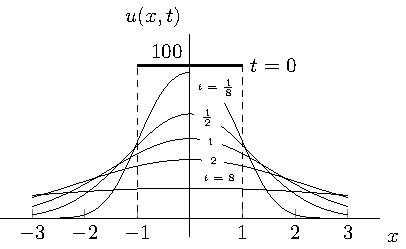
\includegraphics{figInfiniteBarHeatProblem}
\caption{حل $u(x,t)$ برائے مثال \حوالہ{مثال_جزوی_لامتناہی_سلاخ}}
\label{شکل_مثال_جزوی_لامتناہی_سلاخ_حل}
\end{figure}
\انتہا{مثال}
%=======================

\حصہء{سوالات}
%====================
\ابتدا{سوال}\quad
نقطہ \عددی{x=0.5,1,1.5} پر مثال \حوالہ{مثال_جزوی_لامتناہی_سلاخ} میں \عددی{U_0=\SI{100}{\celsius}} اور \عددی{c^2=\SI{1}{\meter\squared\per\second}} لے کر حاصل کردہ درجہ حرارت \عددی{u(x,t)} کی ترسیم مختلف لمحات پر  کھینچیں۔کیا جوابات آپ کی سوچ کے مطابق ہیں؟
\انتہا{سوال}
%=======================
\اصطلاح{تفاعل خلل} درج ذیل تکمل کو کہتے ہیں
\begin{align*}
\erf x =\frac{2}{\sqrt{\pi}}\int_0^x e^{-w^2}\,\dif w
\end{align*} 
جو انجینئری میں کلیدی کردار ادا کرتا ہے۔اس سے واقفیت  پیدا کرنے کی خاطر سوال \حوالہ{سوال_جزوی_تفاعل_خلل_الف} تا سوال \حوالہ{سوال_جزوی_تفاعل_خلل_ب} حل کریں۔

%======================
\ابتدا{سوال}\شناخت{سوال_جزوی_تفاعل_خلل_الف}\quad 
تصدیق کریں کہ تفاعل خلل طاق ہے۔
\انتہا{سوال}
%=====================
\ابتدا{سوال}\quad درج ذیل ثابت کریں۔\\
 $\int_a^be^{-w^2}\,\dif w=\frac{\sqrt{\pi}}{2}(\erf b-\erf a),\quad \int_{-b}^be^{-w^2}\,\dif w=\sqrt{\pi}\erf b$
\انتہا{سوال}
%======================
\ابتدا{سوال}\شناخت{سوال_جزوی_قوس_جرس}\quad
قلم و کاغذ سے متکمل \عددی{e^{-w^2}} کی قیمتوں کا جدول بناتے ہوئے اس کی ترسیم کھینچیں جو \اصطلاح{قوس جرس}\فرہنگ{قوس جرس}\فرہنگ{جرس!قوس}\حاشیہب{bell curve}\فرہنگ{bell curve} کہلاتی ہے۔  
\انتہا{سوال}
%======================
\ابتدا{سوال}\quad
قوس جرس (جس کو آپ نے سوال \حوالہ{سوال_جزوی_قوس_جرس} میں حاصل کیا) کے نیچے رقبہ معلوم کرتے ہوئے \عددی{\erf x} کا جدول \عددی{x=0,0.2,0.4,\cdots ,1,1.5,2} کے لئے حاصل کریں۔قوس جرس پر افقی اور انتصابی لکیریں کھینچ کر قوس کے نیچے مکعب گن کر رقبہ حاصل کیا جا سکتا ہے۔\\
جوابات:\quad نقطہ اعشاریہ کے بعد صرف دو اعداد لیتے ہوئے۔\\
$0.00, 0.22, 0.43, 0.60, 0.74, 0.84,0.97,1.00\quad $
\انتہا{سوال}
%======================
\ابتدا{سوال}\quad تفاعل خلل کی متکمل \عددی{e^{-w^2}} کی مکلارن تسلسل حاصل کریں۔اس تسلسل کا تکمل لے کر تفاعل خلل \عددی{\erf x} کی مکلارن تسلسل دریافت کریں۔\\
جواب:\quad
$\erf x=\tfrac{2}{\sqrt{\pi}}(x-\tfrac{x^3}{3}+\tfrac{x^5}{10}-\tfrac{x^7}{42}+\tfrac{x^9}{216}\cdots)$
\انتہا{سوال}
%======================
\ابتدا{سوال}\quad 
مساوات \حوالہ{مساوات_جزوی_حل_مثال_جزوی_لامتناہی_سلاخ} سے درج ذیل صورت  حاصل کریں۔
\begin{align*}
u(x,t)=\frac{U_0}{2}\big[\erf \frac{1-x}{2c\sqrt{t}}+\erf \frac{1+x}{2c\sqrt{t}}\big]\quad \quad (t>0)
\end{align*}
\انتہا{سوال}
%================
\ابتدا{سوال}\شناخت{سوال_جزوی_سلاخ_سیڑھی}\quad اگر \عددی{x>0} کی صورت میں \عددی{f(x)=1} اور \عددی{x<0} کی صورت میں \عددی{f(x)=0} ہو تب تصدیق کریں کہ مساوات \حوالہ{مساوات_جزوی_لامتناہی_سلاخ_حل_ب} سے درج ذیل حاصل ہو گا۔
\begin{align*}
u(x,t)=\frac{1}{\sqrt{\pi}}\int\limits_{-\tfrac{x}{2c\sqrt{t}}}^{\infty} e^{-z^2}\,\dif z\quad \quad (t>0)
\end{align*}
\انتہا{سوال}
%===============
\ابتدا{سوال}\شناخت{سوال_جزوی_تفاعل_خلل_ب}\quad
چونکہ \عددی{\erf \infty=1} ہے لہٰذا سوال \حوالہ{سوال_جزوی_سلاخ_سیڑھی} سے درج ذیل حاصل کریں۔
\begin{align*}
u(x,t)=\frac{1}{2}+\frac{1}{2}\erf \frac{x}{2c\sqrt{t}}
\end{align*}
\انتہا{سوال}
%====================
\ابتدا{سوال}\شناخت{سوال_جزوی_نصف_لامتناہی}\quad
نصف لامتناہی لمبی سلاخ (\عددی{0} تا \عددی{\infty}) کے \عددی{x=0} پر سر کو صفر درجہ پر رکھا گیا ہے جبکہ اس کی ابتدائی درجہ حرارت \عددی{f(x)} ہے۔ثابت کریں کہ اس مسئلہ کا حل درج ذیل ہے جہاں \عددی{\tau=2c\sqrt{t}} ہے۔
\begin{align}\label{مساوات_جزوی_لامتناہی_سلاخ_حل_پ}
u(x,t)=\frac{1}{\sqrt{\pi}}\big[\int_{-\tfrac{x}{\tau}}^{\infty} f(x+\tau w)e^{-w^2}\,\dif w-\int_{\tfrac{x}{\tau}}^{\infty} f(-x+\tau w)e^{-w^2}\,\dif w\big]
\end{align}

\انتہا{سوال}
%==================
\ابتدا{سوال}\quad \عددی{f(v)} کو طاق تصور کرتے ہوئے مساوات \حوالہ{مساوات_جزوی_لامتناہی_سلاخ_حل_الف} سے مساوات \حوالہ{مساوات_جزوی_لامتناہی_سلاخ_حل_پ} حاصل کریں۔ 
\انتہا{سوال}
%======================
\ابتدا{سوال}\شناخت{سوال_جزوی_اکائی_تفاعل}\quad \عددی{f(x)=1}  لیتے ہوئے ثابت کریں کہ سوال \حوالہ{سوال_جزوی_نصف_لامتناہی} میں درج ذیل حل حاصل ہو گا۔
\begin{align*} 
u(x,t)=\frac{2}{\sqrt{\pi}}\int_0^{\tfrac{x}{\tau}} e^{-w^2}\,\dif w=\erf \frac{x}{2c\sqrt{t}}\quad \quad (t>0)
\end{align*}
\انتہا{سوال}
%========================
\ابتدا{سوال}\quad درج ذیل ابتدائی معلومات کی صورت میں مساوات \حوالہ{مساوات_جزوی_لامتناہی_سلاخ_حل_پ} کیا صورت اختیار کرے گی۔
\begin{align*}
f(x)=
\begin{cases}
1& a<x<b \quad \quad (a>0)\\
0& \text{\RL{باقی جگہوں پر}}
\end{cases}
\end{align*}
جواب:\quad
\begin{align*}
\frac{1}{\sqrt{\pi}}\int\limits_{\tfrac{a-x}{\tau}}^{\tfrac{b-x}{\tau}}e^{-w^2}\,\dif w-\frac{1}{\pi}\int\limits_{\tfrac{a+x}{\tau}}^{\tfrac{b+x}{\tau}}e^{-w^2}\,\dif w
\end{align*}
\انتہا{سوال}
%==================
\ابتدا{سوال}\quad
\عددی{x>0} پر \عددی{f(x)=1} اور \عددی{x<0} پر \عددی{f(x)=-1} لیتے ہوئے مساوات \حوالہ{مساوات_جزوی_لامتناہی_سلاخ_حل_الف} یا مساوات \حوالہ{مساوات_جزوی_لامتناہی_سلاخ_حل_ب} کی استعمال سے سوال \حوالہ{سوال_جزوی_اکائی_تفاعل} کا نتیجہ حاصل کریں۔ 
\انتہا{سوال}
%====================
\ابتدا{سوال}\quad ثابت کریں کہ سوال \حوالہ{مساوات_جزوی_لامتناہی_سلاخ_حل_الف} میں کوئی دو نقطے کا ایک ہی درجہ حرارت تک پہنچنے کے لئے درکار وقت ان نقطوں کا سرحد \عددی{x=0} سے فاصلہ کے مربع کے راست تناسب ہو گا۔  
\انتہا{سوال}
%=====================

\حصہ{نمونہ کشی: ارتعاش پذیر جھلی۔ دو ابعادی مساوات موج}\شناخت{حصہ_جزوی_ارتعاش_جھلی}
ارتعاش کی میدان میں ایک اور اہم مسئلے کے طور پر تننی ہوئی جھلی، مثلاً طبل پر چڑھا ہوا چمڑے کا پردہ، کی ارتعاش پر غور کرتے ہیں۔آپ دیکھیں گے کہ موجودہ تجزیہ حصہ \حوالہ{حصہ_جزوی_ارتعاش_تار} میں ارتعاش تار کی مانند ہو گا۔ 

ہم درج ذیل فرض کرتے  ہیں۔

\موٹا{(الف)}\quad اکائی رقبہ پر جھلی کی کمیت یکساں ہے (ہم جنسی جھلی)۔ جھلی مکمل لچکدار اور اتنی باریک ہے کہ مڑنے کے خلاف مزاحمت فراہم نہیں کرتی ہے۔\\
\موٹا{(ب)}\quad جھلی کو تان کر، اس کی پوری سرحد سے \عددی{xy} مستوی میں باندھا گیا ہے۔ جھلی میں ہر نقطہ  پر اور ہر رخ  فی اکائی لمبائی تناو \عددی{T} یکساں ہے جو ارتعاش کے دوران تبدیل نہیں ہوتی۔\\
\موٹا{(پ)} \quad حرکت کے دوران جھلی کی انحراف \عددی{u(x,y,t)}، جھلی کی جسامت کے لحاظ سے  کم ہے اور تمام زاویہ میلان چھوٹے ہیں۔      

اگرچہ حقیقت میں ان مفروضوں پر مکمل طور پورا اترنا ممکن نہیں ہے، پتلی جھلی کی قلیل عرضی لرزش ان مفروضوں پر تقریباً پورا اترتی ہیں۔

جھلی کی حرکت کی جزوی تفرقی مساوات حاصل کرنے کی خاطر ہم جھلی کے ایک چھوٹے ٹکڑے پر عمل کرنے والی قوتوں پر غور کرتے ہیں (شکل \حوالہ{شکل_جزوی_ارتعاش_پذیر_جھلی})۔چونکہ جھلی کی انحراف اور زاویہ میلان چھوٹے ہیں لہٰذا اس ٹکڑے کے اطراف کی لمبائی تقریباً \عددی{\Delta x} اور \عددی{\Delta y} ہو گی۔اکائی لمبائی پر قوت کو تناو \عددی{T} کہتے ہیں لہٰذا اس ٹکڑے کے اطراف پر قوت
 \عددی{T\Delta x} اور \عددی{T\Delta y} عمل کرے گی۔ چونکہ جھلی مکمل لچکدار ہے لہٰذا یہ قوتیں جھلی کی مماسی ہوں گی۔

\begin{figure}
\centering
\begin{subfigure}{1\textwidth}
\centering
\begin{tikzpicture}
\draw(0,0)--(4,0);
\draw(0,0)--++(0,3);
\draw(0.5,1.5) to [out=-90,in=180](2,0.25) to [out=0,in=-90] (4,1.5) to [out=90,in=0] (3,3)node[above]{\RL{جھلی کی سرحد}} to [out=180,in=90](0.5,1.5);
\draw[thick,fill=gray!50!white] (2,1)--++(1,0)--++(0,1)--++(-1,0)--++(0,-1);
\draw[dashed](2,1)--++(0,-1)node[below]{$x$};
\draw[dashed](3,1)--++(0,-1)node[below]{$x+\Delta x$};
\draw[dashed](2,1)--++(-2,0)node[left]{$y$};
\draw[dashed](2,2)--++(-2,0)node[left]{$y+\Delta y$};
\end{tikzpicture}
\end{subfigure}
\begin{subfigure}{0.5\textwidth}
\centering
\begin{tikzpicture}[x={(1cm,-0.2cm)},y={(0.5cm,0.5cm)},z={(0cm,1cm)}]
\pgfmathsetmacro{\angA}{30}
\pgfmathsetmacro{\angB}{-170}
\pgfmathsetmacro{\angC}{70}
\pgfmathsetmacro{\angD}{-150}
\pgfmathsetmacro{\kdy}{2*tan(\angA)}
\pgfmathsetmacro{\angX}{atan(-0.2/1)}
\pgfmathsetmacro{\angY}{atan(0.5/0.5)}
\pgfmathsetmacro{\iX}{1}
\pgfmathsetmacro{\iY}{1}
\pgfmathsetmacro{\iZ}{1.5}
%
\draw(0,0,0)--++(4,0,0);
\draw(0,0)--++(0,2.5,0);
\draw(0,0)--++(0,0,1);
%
\draw[thick,name path=kL](\iX,\iY,\iZ)coordinate(kA) to [out=\angA,in=\angB]++(2,0,1)coordinate(kB)to [out=\angC,in=\angD]++(0,1,0)coordinate(kC);
\draw(kC) to [out=\angB,in=\angA]++(-2,0,-1)coordinate(kD) to [out=\angD,in=\angC]++(0,-1,0);
%
\draw[dashed](kA)--++(0,0,-\iZ)coordinate(kkA);
\draw[dashed](kB)--++(0,0,-\iZ-1)coordinate(kkB);
\draw[dashed](kC)--++(0,0,-\iZ-1)coordinate(kkC);
\draw[dashed] (\iX,\iY+1,0)coordinate(kkD)--++(0,0,\iZ-0.25);
%
\draw[dashed,fill=gray!50!white] (kkA)--(kkB)--(kkC)--(kkD)--(kkA);
\draw[dashed](kkA)--++(0,-\iY,0)node[shift={(0,-0.3,0),rotate={\angX}},font=\scriptsize,solid]{$x$};
\draw[dashed](kkB)--++(0,-\iY,0)node[shift={(0,-0.3,0)},rotate={\angX},font=\scriptsize,solid]{$x+\Delta x$};
\draw[dashed](kkA)--++(-\iX,0,0)node[shift={(-0.2,0,0)},rotate={\angX},font=\scriptsize,solid]{$y$};
\draw[dashed](kkD)--++(-\iX,0,0)node[shift={(-0.5,0,0)},rotate={\angX},font=\scriptsize,solid]{$y+\Delta y$};
%
\draw[-latex] ($(kB)!0.5!(kC)$)++(0,0,0.1)coordinate(kTBC)--++(40:1.5)node[above]{$T\Delta y$};
\draw[dashed] ($(kB)!0.5!(kC)$)++(0,0,0.1)--++(1.2,0,0);
\draw[-stealth]([shift={(0:0.8)}]kTBC) arc (0:40:0.8);
\draw(kTBC)++(20:1.1)node[]{$\beta$};
%
\draw[-latex] ($(kA)!0.5!(kD)$)++(0,0,0.1)coordinate(kTAD)--++(40:-1.5)node[left]{$T\Delta y$};
\draw[dashed] ($(kA)!0.5!(kD)$)++(0,0,0.1)--++(-1.2,0,0);
\draw[-stealth]([shift={(180:0.8)}]kTAD) arc (180:220:0.8);
\draw(kTAD)++(20:-1.1)node[]{$\alpha$};
%
\draw[-latex] ($(kA)!0.5!(kB)$)++(0,0,0.1)coordinate(kTAB)--++(0,-0.5,-0.2)node[right]{$T\Delta x$};
\draw[-latex] ($(kC)!0.5!(kD)$)++(0,0,0.1)coordinate(kTAB)--++(0,0.6,0)node[above]{$T\Delta x$};
\end{tikzpicture}
\end{subfigure}%
\begin{subfigure}{0.5\textwidth}
\centering
\begin{tikzpicture}
\draw(-1,0)--(3,0);
\draw[thick](0,1.5) to [out=40,in=-170]++(2,1)coordinate(kR);
\draw[dashed](0,1.5)--(0,0)node[below]{$x$};
\draw[dashed](0,1.5)--++(-1,0);
\draw[dashed](kR)--++(0,-2.5)node[below]{$x+\Delta x$};
\draw[-latex](0,1.5)node[ocirc]{}--++(40:-1.2)node[left]{$T\Delta y$};
\draw[-stealth]([shift={(180:0.5)}]0,1.5) arc (180:220:0.5);
\draw(0,1.5)++(20:-0.8)node[]{$\alpha$};
%
\draw[dashed](kR)--++(1,0);
\draw[-latex](kR)node[ocirc]{}--++(30:1.2)node[right]{$T\Delta y$};
\draw[-stealth]([shift={(0:0.5)}]kR) arc (0:30:0.5);
\draw(kR)++(15:0.8)node[]{$\beta$};
\end{tikzpicture}
\end{subfigure}%
\caption{ارتعاش پذیر جھلی}
\label{شکل_جزوی_ارتعاش_پذیر_جھلی}
\end{figure}
ہم پہلے قوتوں کی افقی اجزاء پر غور کرتے ہیں۔اطراف پر قوت کو زاویہ میلان کی کوسائن سے ضرب دینے سے ان کی افقی جزو حاصل ہو گی۔چونکہ زاویہ میلان چھوٹے ہیں لہٰذا ان کی کوسائن تقریباً اکائی \عددی{(1)} کے برابر ہوں گے۔یوں مخالف کناروں پر تقریباً برابر قوتیں پائی جائیں گی۔یوں افقی رخ جھلی کی حرکت قابل نظر انداز ہو گی لہٰذا ہم جھلی کی حرکت کو عرضی حرکت تصور کرتے ہیں یعنی جھلی صرف اوپر نیچے حرکت کرتی ہے۔

اس ٹکڑے کی کناروں پر کھڑی رخ (\عددی{yu} سطح کی متوازی) قوتوں کے اجزاء\حاشیہد{دھیان رہے کہ کنارے پر چلتے ہوئے زاویہ میلان تبدیل ہو گا۔\عددی{\alpha} اور \عددی{\beta} زیر غور کنارے کے کسی موزوں نقطہ پر زاویہ میلان ہوں گے۔} 
\begin{align*}
T\Delta y\,\sin \beta\quad \text{اور}\quad -T\Delta y\,\sin \alpha
\end{align*} 
ہوں گے جہاں منفی علامت نیچے رخ کو ظاہر کرتی ہے۔چونکہ زاویہ میلان چھوٹے ہیں ہم ان کے \عددی{\sin} کی جگہ ان کے \عددی{\tan}  استعمال\حاشیہد{چھوٹے زاویہ \عددی{\theta} کا \عددی{\sin \theta \approx \theta\approx \tan \theta} ہوتا ہے۔} کر سکتے ہیں۔یوں ان دو عدد قوتوں کا مجموعہ
\begin{gather}
\begin{aligned}\label{مساوات_جزوی_قوت_کنارہ_الف}
T\Delta y(\sin \beta-\sin \alpha)& \approx T\Delta y(\tan \beta-\tan \alpha)\\
&=T\Delta y[u_x(x+\Delta x,y_1)-u_x(x,y_2)]
\end{aligned}
\end{gather}
ہو گا جہاں زیر نوشت میں \عددی{x} اور \عددی{y} جزوی تفرق کو ظاہر کرتی ہیں جبکہ \عددی{y} اور \عددی{y+\Delta y} کے درمیان  \عددی{y_1} اور \عددی{y_2}  کوئی نقطے ہیں۔اسی طرح ٹکڑے کے باقی دو کناروں پر قوتوں کے انتصابی اجزاء کا مجموعہ  
\begin{align}\label{مساوات_جزوی_قوت_کنارہ_ب}
T\Delta x[u_y(x_1,y+\Delta y)-u_y(x_2,y)]
\end{align}
ہو گا جہاں \عددی{x} اور \عددی{x+\Delta x} کے درمیان \عددی{x_1} اور \عددی{x_2} کوئی نقطے ہیں۔

نیوٹن کے دوسرے قانون کے تحت مساوات \حوالہ{مساوات_جزوی_قوت_کنارہ_الف} اور مساوات \حوالہ{مساوات_جزوی_قوت_کنارہ_ب} میں دی گئی  قوتوں کا مجموعہ جھلی کے ٹکڑے کی کمیت \عددی{\rho \Delta A} ضرب اسراع \عددی{\tfrac{\partial^{\,2}u}{\partial t^2}} کے برابر ہو گا۔ یہاں بلا انحراف فی اکائی رقبہ جھلی کی کمیت \عددی{\rho} ہے جبکہ بلا انحراف ٹکڑے کا رقبہ \عددی{\Delta A=\Delta x\Delta y} ہے۔یوں
\begin{align*}
\rho\Delta x\Delta y\frac{\partial^{\,2}u}{\partial t^2}=T\Delta y[u_x(x+\Delta x,y_1)-u_x(x,y_2)]+T\Delta x[u_y(x_1,y+\Delta y)-u_y(x_2,y)]
\end{align*}
ہو گا جہاں بائیں ہاتھ تفرق ٹکڑے کے کسی موزوں نقطہ \عددی{(\tilde{x},\tilde{y})} پر حاصل کیا جائے گا۔\عددی{\rho \Delta x\Delta y} سے دونوں اطراف کو تقسیم کرتے ہیں۔
\begin{align*}
\frac{\partial^{\,2}u}{\partial t^2}=\frac{T}{\rho}\big[\frac{u_x(x+\Delta x,y_1)-u_x(x,y_2)}{\Delta x}+\frac{u_y(x_1,y+\Delta y)-u_y(x_2,y)}{\Delta y}\big]
\end{align*}
\عددی{\Delta x} اور \عددی{\Delta y} کو صفر کے قریب تر کرتے ہوئے درج ذیل جزوی تفرقی مساوات حاصل ہو گی
\begin{align}\label{مساوات_جزوی_دو_ابعادی_مساوات_موج_الف}
\frac{\partial^{\,2}u}{\partial t^2}=c^2\left(\frac{\partial^{\,2}u}{\partial x^2}+\frac{\partial^{\,2}u}{\partial y^2}\right)\quad \quad \quad c^2=\frac{T}{\rho}
\end{align}
جس کو \اصطلاح{دو ابعادی مساوات موج}\فرہنگ{موج!دو ابعادی مساوات}\حاشیہب{two dimensional wave equation}\فرہنگ{wave!two dimensional equation} کہتے ہیں۔قوسین میں بند \عددی{u} کا  لاپلاسی \عددی{\nabla^{\,2}u} ہے (حصہ \حوالہ{حصہ_الاحصاء_ڈھلوان}) لہٰذا مساوات \حوالہ{مساوات_جزوی_دو_ابعادی_مساوات_موج_الف} کو درج ذیل لکھا جا سکتا ہے۔
\begin{align}\label{مساوات_جزوی_دو_ابعادی_مساوات_موج_ب}
\frac{\partial^{\,2}u}{\partial t^2}=c^2\nabla^{\,2}u
\end{align}

%=================
\حصہ{مستطیل جھلی}
ارتعاش پذیر جھلی کے مسئلے کو حل کرنے کی خاطر  ہمیں درج ذیل دو ابعادی مساوات موج کا حل \عددی{u(x,y,t)} تلاش کرنا ہو گا
\begin{align}\label{مساوات_جزوی_مستطیل_جھلی_الف}
\frac{\partial^{\,2}u}{\partial t^2}=c^2\left(\frac{\partial^{\,2}u}{\partial x^2}+\frac{\partial^{\,2}u}{\partial y^2}\right)
\end{align}
جو تمام \عددی{t\ge 0} کے لئے پوری سرحد پر سرحدی شرط
\begin{align}\label{مساوات_جزوی_مستطیل_جھلی_ب}
u=0
\end{align}
اور دو عدد ابتدائی شرائط
\begin{align}\label{مساوات_جزوی_مستطیل_جھلی_پ}
u(x,y,0)&=f(x,y)\quad \quad \text{\RL{ابتدائی انحراف}}
\end{align}
اور
\begin{align}\label{مساوات_جزوی_مستطیل_جھلی_ت}
\left. \frac{\partial u}{\partial t}\right|_{t=0}&=g(x,y)\quad \quad \text{\RL{ابتدائی رفتار}}
\end{align}
 کو مطمئن کرتا ہو۔یہ شرائط ارتعاش پذیر تار کے شرائط کی مانند ہیں۔آئیں شکل \حوالہ{شکل_جزوی_مستطیل_جھلی}  میں دکھائی گئی مستطیل جھلی کی ارتعاش پر غور کرتے ہیں۔

\begin{figure}
\centering
\begin{tikzpicture}
\draw(0,0)--++(3,0)node[right]{$x$};
\draw(0,0)--++(0,1.5)node[left]{$y$};
\draw[thick](0,0)--++(2,0)node[below]{$a$}--++(0,1)--++(-2,0)node[left]{$b$}--++(0,-1);
\draw(1,0.5)node{$R$};
\end{tikzpicture}
\caption{مستطیل جھلی}
\label{شکل_جزوی_مستطیل_جھلی}
\end{figure}
\موٹا{پہلا قدم۔} \quad علیحدگی متغیرات کی ترکیب استعمال کرتے ہوئے ہم پہلے مساوات \حوالہ{مساوات_جزوی_مستطیل_جھلی_الف} کا ایسا حل تلاش کرتے ہیں جو سرحدی شرط مساوات \حوالہ{مساوات_جزوی_مستطیل_جھلی_ب} کو مطمئن کرتا ہو۔یوں
\begin{align}\label{مساوات_جزوی_مستطیل_جھلی_ٹ}
u(x,y,t)=F(x,y)G(t)
\end{align}
کو مساوات \حوالہ{مساوات_جزوی_مستطیل_جھلی_الف} میں پر کرتے ہیں
\begin{align*}
F\ddot{G}=c^2(F_{xx}G+F_{yy}G)
\end{align*}
جہاں \عددی{(')} جزوی تفرق اور \عددی{(^.)} وقت \عددی{t} کے ساتھ تفرق کو ظاہر کرتے ہیں۔دونوں اطراف کو \عددی{c^2FG} سے تقسیم کرتے ہوئے
\begin{align*}
\frac{\ddot{G}}{c^2G}=\frac{1}{F}(F_{xx}+F_{yy})
\end{align*}
ملتا ہے۔اب بایاں ہاتھ تفاعل \عددی{t} پر منحصر ہے جبکہ دایاں ہاتھ  تفاعل \عددی{t} پر منحصر نہیں ہے لہٰذا دونوں اطراف کسی مستقل \عددی{A} کے برابر ہیں۔آپ   حصہ \حوالہ{حصہ_جزوی_علیحدگی_متغیرات} کی طرح  بڑھتے ہوئے تسلی کر سکتے ہیں کہ  \عددی{A} کے صرف منفی قیمتیں استعمال کرنے سے ایسا غیر صفر حل حاصل ہو گا جو مساوات \حوالہ{مساوات_جزوی_مستطیل_جھلی_ب} کی شرط کو مطمئن کرتا ہو۔اس منفی مستقل کو \عددی{-\nu^2} سے ظاہر کرتے ہوئے 
\begin{align*}
\frac{\ddot{G}}{c^2G}=\frac{1}{F}(F_{xx}+F_{yy})=-\nu^2
\end{align*}
حاصل ہوتا ہے جس کو دو علیحدہ علیحدہ سادہ تفرقی مساوات
\begin{align}
&\ddot{G}+\lambda^2G=0\quad \quad\quad (\lambda=c\nu)\label{مساوات_جزوی_مستطیل_جھلی_ث}\\
&F_{xx}+F_{yy}+\nu^2F=0\label{مساوات_جزوی_مستطیل_جھلی_ج}
\end{align}
کی صورت میں لکھا جا سکتا ہے۔

ہم  مساوات \حوالہ{مساوات_جزوی_مستطیل_جھلی_ج} کا حل تلاش کرتے ہیں جو جھلی کی سرحد پر صفر کے برابر ہو گا۔ہم علیحدگی متغیرات کی ترکیب دوبارہ لاگو کرتے ہوئے
\begin{align}
F(x,y)=H(x)Q(y)
\end{align}
لیتے ہیں جو کو مساوات \حوالہ{مساوات_جزوی_مستطیل_جھلی_ج} میں پر کرنے سے 
\begin{align*}
\frac{\dif^{\,2} H}{\dif x^2}Q=-\big(H\frac{\dif^{\,2} Q}{\dif y^2}+\nu^2HQ\big)
\end{align*}
حاصل ہوتا ہے جس کے دونوں اطراف کو \عددی{HQ} سے تقسیم کرتے ہوئے
\begin{align*}
\frac{1}{H}\frac{\dif^{\,2}H}{\dif x^2}=-\frac{1}{Q}\big(\frac{\dif^{\,2}Q}{\dif y^2}+\nu^2Q\big)
\end{align*}
ملتا ہے جہاں بائیں ہاتھ تفاعل صرف \عددی{x} پر منحصر ہے جبکہ دایاں ہاتھ تفاعل صرف \عددی{y} پر منحصر ہے۔یوں دونوں ہاتھ کسی مستقل کے برابر ہوں گے۔یہاں بھی صرف منفی قیمت کا مستقل مثلاً \عددی{-k^2} غیر صفر حل دیتے ہیں۔یوں
\begin{align*}
\frac{1}{H}\frac{\dif^{\,2}H}{\dif x^2}=-\frac{1}{Q}\big(\frac{\dif^{\,2}Q}{\dif y^2}+\nu^2Q\big)=-k^2
\end{align*}
لکھا جا سکتا ہے جس سے دو عدد سادہ تفرقی مساوات 
\begin{align}
\frac{\dif^{\,2}H}{\dif x^2}+k^2H&=0\label{مساوات_جزوی_جھلی_ایکس}\\
\frac{\dif^{\,2}Q}{\dif y^2}+p^2Q&=0\quad \quad \quad (p^2=\nu^2-k^2)\label{مساوات_جزوی_جھلی_وائے}
\end{align}
حاصل ہوتے ہیں۔

\موٹا{دوسرا قدم۔}\quad مساوات \حوالہ{مساوات_جزوی_جھلی_ایکس} اور مساوات \حوالہ{مساوات_جزوی_جھلی_وائے} کے حل عمومی
\begin{align*}
H(x)=A\cos kx+B\sin kx \quad \text{اور}\quad Q(y)=C\cos py+D\sin py
\end{align*}
ہیں جہاں \عددی{A}، \عددی{B}، \عددی{C} اور \عددی{D} مستقل ہیں۔یوں مساوات \حوالہ{مساوات_جزوی_مستطیل_جھلی_ٹ} اور مساوات \حوالہ{مساوات_جزوی_مستطیل_جھلی_ب} سے ظاہر ہے کہ جھلی کی سرحد پر \عددی{F=HQ} صفر ہو گا۔جیسا آپ شکل \حوالہ{شکل_جزوی_مستطیل_جھلی} سے دیکھ سکتے ہیں، جھلی کی سرحد \عددی{x=0}، \عددی{x=a}، \عددی{y=0} اور \عددی{y=b} ہے۔یوں درج ذیل شرائط لکھے جا سکتے ہیں۔
\begin{align*}
H(0)=0,\quad H(a)=0,\quad Q(0)=0,\quad Q(b)=0
\end{align*}
اس طرح \عددی{H(0)=A=0} ہو گا جبکہ
\begin{align*}
H(a)=B\sin ka=0
\end{align*}
میں \عددی{B=0} لینے سے (غیر دلچسپ حل) \عددی{H\equiv 0} یعنی \عددی{F \equiv 0} ملتا ہے لہٰذا ہم \عددی{B\ne 0} فرض کرتے ہیں۔یوں \عددی{\sin ka=0} ہو گا جس سے \عددی{ka=m\pi} یعنی
\begin{align}
k=\frac{m\pi}{a}\quad \quad \quad (\text{\RL{عدد صحیح $m$}})
\end{align}
حاصل ہوتا ہے۔ بالکل اسی طرح \عددی{C=0} جبکہ \عددی{D \ne 0} سے \عددی{p=\tfrac{n\pi}{b}} حاصل ہوتا ہے جہاں \عددی{n} عدد صحیح ہے۔یوں درج ذیل حل ملتے ہیں۔
\begin{align*}
H_m(x)=\sin \frac{m\pi x}{a}\quad \text{اور}\quad Q_n(y)=\sin\frac{n\pi y}{b}
\quad \quad  \substack{m=1,2,\cdots\\n=1,2,\cdots}
\end{align*}
(ارتعاش پذیر تار کی طرح یہاں بھی \عددی{m,n=-1,-2,\cdots} لینے کی ضرورت نہیں ہے چونکہ ایسا کرنے سے یہی حل ضرب \عددی{-1} دوبارہ حاصل ہوتے ہیں۔) یوں  \عددی{B=1} اور \عددی{D=1} چنتے ہوئے مساوات \حوالہ{مساوات_جزوی_مستطیل_جھلی_ج} کے حل درج ذیل ہوں گے
\begin{align}\label{مساوات_جزوی_مستطیل_مستقل_الف}
F_{mn}(x,y)=H_m(x)Q_n(y)=\sin \frac{m\pi x}{a}\sin\frac{n\pi y}{b} \quad \quad \substack{m=1,2,\cdots\\n=1,2,\cdots}
\end{align}
جو جھلی کی سرحد پر صفر کے برابر ہیں۔

چونکہ مساوات \حوالہ{مساوات_جزوی_جھلی_وائے} میں \عددی{p^2=\nu^2-k^2} ہے اور مساوات \حوالہ{مساوات_جزوی_مستطیل_جھلی_ث} میں \عددی{\lambda=c\nu} ہے  لہٰذا
\begin{align*}
\lambda=c\sqrt{k^2+p^2}
\end{align*}
ہو گا۔یوں \عددی{k=\tfrac{m\pi}{a}} اور \عددی{p=\tfrac{n\pi}{b}} کا مطابقتی \عددی{\lambda} مساوات \حوالہ{مساوات_جزوی_مستطیل_جھلی_ث} میں
\begin{align}\label{مساوات_جزوی_مستطیل_مستقل_ب}
\lambda=\lambda_{mn}=c\pi\sqrt{\frac{m^2}{a^2}+\frac{n^2}{b^2}}\quad \quad \substack{m=1,2,\cdots\\n=1,2,\cdots}
\end{align}
ہو گا اور مساوات \حوالہ{مساوات_جزوی_مستطیل_جھلی_ث} کا مطابقتی  عمومی حل درج ذیل ہو گا۔
\begin{align*}
G_{mn}(t)=B_{mn}\cos \lambda_{mn}t+B^*_{mn}\sin \lambda_{mn}t
\end{align*}
یوں مساوات \حوالہ{مساوات_جزوی_مستطیل_جھلی_ث} کے غیر صفر  حل \عددی{u_{mn}(x,y,t)=F_{mn}(x,y)G_{mn}(t)} درج ذیل ہوں گے
\begin{align}\label{مساوات_جزوی_مستطیل_مستقل_پ}
u_{mn}(x,y,t)=(B_{mn}\cos \lambda_{mn}t+B^*_{mn}\sin \lambda_{mn}t)\sin \frac{m\pi x}{a}\sin \frac{n\pi y}{b}
\end{align}
 جن میں \عددی{\lambda_{mn}} مساوات \حوالہ{مساوات_جزوی_مستطیل_مستقل_ب} دے گی۔ تفاعل \عددی{u_{mn}} کو ارتعاش پذیر جھلی کے \اصطلاح{آئگنی تفاعل}\فرہنگ{آئگنی!تفاعل}\حاشیہب{eigenfunctions}\فرہنگ{eigenfunctions} یا \اصطلاح{امتیازی تفاعل}\فرہنگ{امتیازی!تفاعل}\حاشیہب{characteristic functions}\فرہنگ{characteristic!functions} کہتے ہیں جبکہ \عددی{\lambda_{mn}} کو ارتعاش پذیر جھلی کے \اصطلاح{آئگنی اقدار}\فرہنگ{آئگنی!اقدار}\حاشیہب{eigenvalues}\فرہنگ{eigenvalues} یا \اصطلاح{امتیازی اقدار}\فرہنگ{امتیازی!اقدار}\حاشیہب{characteristic values}\فرہنگ{characteristic!values} کہتے ہیں۔تفاعل \عددی{u_{mn}} کی تعدد \عددی{\tfrac{\lambda_{mn}}{2\pi}} ہو گی۔

\عددی{a} اور \عددی{b} کی مختلف قیمتیں ایک ہی  امتیازی قدر دیتے ہوئے کئی مختلف  تفاعل \عددی{F_{mn}} دے سکتی ہیں۔اس کا مطلب ہے کہ جھلی میں ایک ہی تعدد کے  کئی مختلف انداز کے ارتعاش ممکن ہیں جن کی  \اصطلاح{صفر ہٹاو لکیریں}\فرہنگ{صفر ہٹاو!لکیر}\حاشیہب{nodal lines}\فرہنگ{nodal!lines} مختلف ہوں گی۔ ارتعاش پذیر جھلی پر وہ لکیریں جو حرکت نہیں کرتی ہیں صفر ہٹاو لکیریں کہلاتی ہیں۔آئیں اس کی وضاحت ایک مثال کی مدد سے سمجھیں۔

%=================
\ابتدا{مثال}\شناخت{مثال_جزوی_مکعب_جھلی}\quad مکعب جھلی\\
ایک مکعب جھلی کا \عددی{a=1}، \عددی{b=1} ہے۔مساوات \حوالہ{مساوات_جزوی_مستطیل_مستقل_ب} سے 
\begin{align}\label{مساوات_جزوی_مثال_مکعب_جھلی_الف}
\lambda_{mn}=c\pi\sqrt{m^2+n^2}
\end{align}
لہٰذا 
\begin{align*}
\lambda_{mn}=\lambda{nm}
\end{align*}
ہو گا لیکن \عددی{m \ne n} کے لئے مطابقتی  تفاعل
\begin{align*}
F_{mn}=\sin m\pi x\,\sin n\pi y \quad \text{اور} \quad F_{nm}=\sin n\pi x\,\sin m\pi y
\end{align*}
ہیں جو ایک جیسے نہیں ہیں۔مثلاً \عددی{\lambda_{12}=\lambda_{21}=c\pi\sqrt{5}} کے مطابقتی تفاعل
\begin{align*}
F_{12}=\sin \pi x\,\sin 2\pi y\quad \text{اور}\quad F_{21}=\sin 2\pi x\,\sin \pi y
\end{align*}
ہوں گے۔یوں مطابقتی حل
\begin{align*}
u_{12}&=(B_{12}\cos c\pi\sqrt{5}t+B^*_{12}\sin c\pi\sqrt{5}t)F_{12}\\
u_{21}&=(B_{21}\cos c\pi\sqrt{5}t+B^*_{21}\sin c\pi\sqrt{5}t)F_{21}\\
\end{align*}
کی صفر ہٹاو لکیریں  بالترتیب \عددی{y=\tfrac{1}{2}} اور \عددی{x=\tfrac{1}{2}} ہوں گی (شکل \حوالہ{شکل_مثال_جزوی_مکعب_جھلی}-الف)۔اگر \عددی{B_{12}=1} اور \عددی{B^*_{12}=B^*_{21}=0} ہوں تب
\begin{align}\label{مساوات_جزوی_ایک_بی_کے_حل}
u_{12}+u_{21}=\cos c\pi\sqrt{5}t\,(F_{12}+B_{21}F_{21})
\end{align}
ہو گا جو ایک اور انداز ارتعاش ہے جس کی امتیازی قدر \عددی{c\pi\sqrt{5}} ہے۔اس تفاعل کی صفر ہٹاو لکیریں درج ذیل مساوات کے حل ہوں گی۔
\begin{align*}
F_{12}+B_{21}F_{21}=\sin \pi x\,\sin 2\pi y+B_{21}\sin 2\pi x\,\sin \pi y=0
\end{align*}
اب \عددی{\sin 2\alpha=2\sin \alpha \cos \alpha} استعمال کرتے ہوئے درج بالا کو 
\begin{align}
\sin \pi x\sin \pi y(\cos \pi y+B_{21}\cos \pi x)=0
\end{align}
لکھا جا سکتا ہے جس کا حل \عددی{B_{21}} پر منحصر ہو گا (شکل \حوالہ{شکل_مثال_جزوی_مکعب_جھلی}-ب)۔

مساوات \حوالہ{مساوات_جزوی_مثال_مکعب_جھلی_الف} سے ہم دیکھتے ہیں کہ \عددی{\lambda_{mn}} کے دو مزید مطابقتی تفاعل ممکن ہیں۔مثلاً چار تفاعل \عددی{F_{18}}، \عددی{F_{81}}، \عددی{F_{47}} اور \عددی{F_{74}} کی \عددی{\lambda_{18}=\lambda_{81}=\lambda_{47}=\lambda_{74}=c\pi\sqrt{65}} ہے چونکہ؛
\begin{align*}
1^1+8^2=4^2+7^2=65
\end{align*}
ایسا اس لئے ممکن ہے  کہ  \عددی{65} کو  دو اعداد صحیح کے مربع کا مجموعہ مختلف طریقوں سے لکھنا ممکن ہے۔گاوس کے ایک مسئلہ کے تحت ایسا ہر اس صورت ہو گا جہاں دو اعداد کے مربع کا مجموعہ کے اجزاء مفرد میں کم از کم دو مختلف \عددی{4n+1} صورت کے ہوں، جہاں \عددی{n} مثبت عدد صحیح ہے۔یہاں دو اعداد کے مربع کے مجموعہ \عددی{65} کو 
\begin{align*}
65=5\cdot13=(4+1)(12+1)
\end{align*}
لکھنا ممکن ہے۔
\begin{figure}
\centering
\begin{subfigure}{0.5\textwidth}
\centering
\begin{tikzpicture}
\pgfmathsetmacro{\w}{2}
\pgfmathsetmacro{\ll}{\w/2}
%
\draw(0,0) rectangle ++(1,1);
\draw(0.5,0)node[below]{$u_{11}$};
%
\draw(1*\w,0) rectangle ++(1,1);
\draw(1*\w+0.5,0)node[below]{$u_{12}$};
\draw[dashed](1*\w,0.5)--++(1,0);
%
\draw(2*\w,0) rectangle ++(1,1);
\draw(2*\w+0.5,0)node[below]{$u_{21}$};
\draw[dashed](2*\w+0.5,0)--++(0,1);
%
\draw(0*\w,-\w) rectangle ++(1,1);
\draw(0*\w+0.5,-\w)node[below]{$u_{22}$};
\draw[dashed](0*\w+0.5,-\w)--++(0,1);
\draw[dashed](0*\w,-\w+0.5)--++(1,0);
%
\draw(1*\w,-\w) rectangle ++(1,1);
\draw(1*\w+0.5,-\w)node[below]{$u_{13}$};
\draw[dashed](1*\w,-\w+1/3*\ll)--++(1,0);
\draw[dashed](1*\w,-\w+2/3*\ll)--++(1,0);
%
\draw(2*\w,-\w) rectangle ++(1,1);
\draw(2*\w+0.5,-\w)node[below]{$u_{31}$};
\draw[dashed](2*\w+1/3*\ll,-\w)--++(0,1);
\draw[dashed](2*\w+2/3*\ll,-\w)--++(0,1);
\end{tikzpicture}
\caption*{(الف) مکعب جھلی کے حل $u_{11},u_{12},u_{21},u_{22},u_{13}, u_{31}$ کی صفر ہٹاو لکیریں۔}
\end{subfigure}%
\begin{subfigure}{0.5\textwidth}
\centering
\begin{tikzpicture}
\pgfmathsetmacro{\len}{2}
\draw(0,0) rectangle ++(\len,\len);
\draw[dashed] (0,0.5*\len)--++(1*\len,0)node[right]{$B_{21}=0$};
\draw[dashed](0.45*\len,0) to [out=90,in=-90](0.55*\len,1*\len)coordinate(kA);
\draw(kA)node[pin=45:{$B_{21}=-10$}]{};
\draw[dashed](0,0)--++(1*\len,1*\len)node[right]{$B_{21}=-1$};
\draw[dashed](0,1*\len)--++(1*\len,-1*\len)node[right]{$B_{21}=1$};
\draw[dashed](0,0.3*\len) to [out=0,in=180] ++(1*\len,0.4*\len)node[right]{$B_{21}=-0.5$};
\draw[dashed](0,0.7*\len) to [out=0,in=180] ++(1*\len,-0.4*\len)node[right]{$B_{21}=0.5$};
\end{tikzpicture}
\caption*{(ب) ایک ہی $B_{21}$ کے لئے مساوات \حوالہ{مساوات_جزوی_ایک_بی_کے_حل} میں دیے گئے حل}
\end{subfigure}%
\caption{صفر ہٹاو لکیریں (مثال \حوالہ{مثال_جزوی_مکعب_جھلی})}
\label{شکل_مثال_جزوی_مکعب_جھلی}
\end{figure}
\انتہا{مثال}
%============================

\موٹا{تیسرا قدم۔}\quad ایسا حل جو ابتدائی شرائط مساوات \حوالہ{مساوات_جزوی_مستطیل_جھلی_پ} اور مساوات \حوالہ{مساوات_جزوی_مستطیل_جھلی_ت} کو مطمئن کرتا ہو حاصل کرنے کی خاطر ہم  حصہ \حوالہ{حصہ_جزوی_علیحدگی_متغیرات} کی طرح بڑھتے ہیں۔ہم دوہرا تسلسل\حاشیہد{ہم حل کی یکتائی اور ارتکاز پر غور نہیں کریں گے۔}
\begin{gather}
\begin{aligned}\label{مساوات_جزوی_مکمل_حل_مستطیل_جھلی}
u(x,y,t)&=\sum_{m=1}^{\infty}\sum_{n=1}^{\infty} u_{mn}(x,y,t)\\
&=\sum_{m=1}^{\infty}\sum_{n=1}^{\infty}(B_{mn}\cos \lambda_{mn}t+B^*_{mn}\sin \lambda_{mn}t)\sin\frac{m\pi x}{a}\sin \frac{n\pi y}{b}
\end{aligned}
\end{gather}
کو لیتے ہیں جو مساوات \حوالہ{مساوات_جزوی_مستطیل_جھلی_پ} کے ساتھ درج ذیل  \اصطلاح{دوہرا فوریئر تسلسل}\فرہنگ{فوریئر!دوہرا تسلسل}\حاشیہب{double Fourier series}\فرہنگ{Fourier!double series} دیتی ہے۔
\begin{align}\label{مساوات_جزوی_دوہرا_فوریئر_تسلسل_الف}
u(x,y,0)=\sum_{m=1}^{\infty}\sum_{n=1}^{\infty}B_{mn}\sin\frac{m\pi x}{a}\sin \frac{n\pi y}{b}=f(x,y)
\end{align}
مستطیل \عددی{R} (شکل \حوالہ{شکل_جزوی_مستطیل_جھلی}) میں \عددی{f}، \عددی{\tfrac{\partial f}{\partial x}}، \عددی{\tfrac{\partial f}{\partial y}} اور \عددی{\tfrac{\partial^{\,2}f}{\partial x\partial y}} استمراری ہونے کی صورت میں \عددی{f(x,y)} کو اس دوہرا فوریئر تسلسل کی صورت میں لکھنا ممکن ہو گا۔اس دوہرا فوریئر تسلسل کے عددی سر حاصل کرتے ہیں۔ہم درج ذیل لے کر
\begin{align}\label{مساوات_جزوی_دوہرا_فوریئر_تسلسل_ب}
K_m(y)=\sum_{n=1}^{\infty}B_{mn}\sin \frac{n\pi y}{b}
\end{align}
مساوات \حوالہ{مساوات_جزوی_دوہرا_فوریئر_تسلسل_الف} کو
\begin{align}\label{مساوات_جزوی_دوہرا_فوریئر_تسلسل_پ}
f(x,y)=\sum_{n=1}^{\infty}K_m(y)\sin \frac{m\pi x}{a}
\end{align}
لکھ سکتے ہیں جو مقررہ \عددی{y} کی صورت میں \عددی{f(x,y)} کی  فوریئر سائن تسلسل ہے جس کا متغیرہ \عددی{x} ہو گا جس کے عددی سر صفحہ \حوالہصفحہ{مساوات_فوریئر_نصف_حلقہ_توسیع_طاق_عددی_سر} پر مساوات \حوالہ{مساوات_فوریئر_نصف_حلقہ_توسیع_طاق_عددی_سر} کے تحت
\begin{align}\label{مساوات_جزوی_دوہرا_فوریئر_تسلسل_ت}
K_m(y)=\frac{2}{a}\int_0^a f(x,y)\sin\frac{m\pi x}{a}\dif x
\end{align}
ہوں گے۔مزید مساوات \حوالہ{مساوات_جزوی_دوہرا_فوریئر_تسلسل_ب} تفاعل \عددی{K_m(y)} کی فوریئر سائن تسلسل ہے لہٰذا اس کے عددی سر صفحہ \حوالہصفحہ{مساوات_فوریئر_نصف_حلقہ_توسیع_طاق_عددی_سر} پر مساوات \حوالہ{مساوات_فوریئر_نصف_حلقہ_توسیع_طاق_عددی_سر} کے تحت
\begin{align}\label{مساوات_جزوی_دوہرا_فوریئر_تسلسل_ٹ}
B_{mn}=\frac{2}{b}\int_0^b K_m(y)\sin \frac{n\pi y}{b}\dif y
\end{align}
ہوں گے۔مساوات \حوالہ{مساوات_جزوی_دوہرا_فوریئر_تسلسل_ٹ} اور مساوات \حوالہ{مساوات_جزوی_دوہرا_فوریئر_تسلسل_ت} کو ملا کر درج ذیل \اصطلاح{عمومی یولر کلیہ}\فرہنگ{یولر!عمومی کلیہ}\حاشیہب{generalized Euler formula}\فرہنگ{Euler!generalized formula} حاصل ہوتا ہے
\begin{align}\label{مساوات_جزوی_دوہرا_فوریئر_تسلسل_ث}
B_{mn}=\frac{4}{ab}\int_0^b\int_0^a f(x,y)\sin\frac{m\pi x}{a}\,\sin \frac{n\pi y}{b} \dif x\,\dif y\quad \quad \substack{m=1,2,\cdots\\n=1,2,\cdots}
\end{align}
جو دوہرا تسلسل (مساوات \حوالہ{مساوات_جزوی_دوہرا_فوریئر_تسلسل_الف}) میں تفاعل \عددی{f(x,y)} کے عددی سر \عددی{B_{mn}} دیتی ہے۔

یوں مساوات \حوالہ{مساوات_جزوی_مکمل_حل_مستطیل_جھلی} میں \عددی{B_{mn}} تفاعل \عددی{f(x,y)} سے حاصل ہوتے ہیں۔ \عددی{B^*_{mn}} حاصل کرنے کی خاطر ہم مساوات \حوالہ{مساوات_جزوی_مکمل_حل_مستطیل_جھلی} کا \عددی{t} کے ساتھ جزوی تفرق لے کر ابتدائی شرط مساوات \حوالہ{مساوات_جزوی_مستطیل_جھلی_ت} استعمال کرتے ہوئے  
\begin{align*}
\left.\frac{\partial u}{\partial t}\right|_{t=0}=\sum_{m=1}^{\infty}\sum_{n=1}^{\infty} B^*_{mn}\lambda_{mn}\sin\frac{m\pi x}{a}\,\sin\frac{n\pi y}{b}=g(x,y)
\end{align*}
حاصل کرتے ہیں۔ مستطیل \عددی{R} (شکل \حوالہ{شکل_جزوی_مستطیل_جھلی}) میں \عددی{g}، \عددی{\tfrac{\partial g}{\partial x}}، \عددی{\tfrac{\partial g}{\partial y}} اور \عددی{\tfrac{\partial^{\,2}u}{\partial x\partial y}}  استمراری ہونے کی صورت میں \عددی{g(x,y)} کو اس دوہرا فوریئر تسلسل کی صورت میں لکھا جا سکتا ہے۔یوں پہلی کی طرح بڑھتے ہوئے درج ذیل حاصل ہو گا۔
\begin{align}\label{مساوات_جزوی_دوہرا_فوریئر_تسلسل_ج}
B^*_{mn}=\frac{4}{ab\lambda_{mn}}\int_0^b\int_0^a g(x,y) \sin\frac{m\pi x}{a}\,\sin \frac{n\pi y}{b}\dif x\dif y\quad \quad \substack{m=1,2,\cdots\\n=1,2,\cdots}
\end{align}
یوں مساوات \حوالہ{مساوات_جزوی_دوہرا_فوریئر_تسلسل_ث} اور مساوات \حوالہ{مساوات_جزوی_دوہرا_فوریئر_تسلسل_ج} سے حاصل \عددی{B_{mn}} اور \عددی{B^*_{mn}}   مساوات \حوالہ{مساوات_جزوی_مکمل_حل_مستطیل_جھلی} میں پر کرتے ہوئے حاصل حل ابتدائی شرائط کو مطمئن کرے گا۔

%===================
\حصہء{سوالات}

%===============
\ابتدا{سوال}\quad
جھلی میں تناو بڑھانے سے مساوات \حوالہ{مساوات_جزوی_مستطیل_مستقل_پ} میں دی گئی حل کی تعدد پر کیا اثر ہو گا؟\\
جواب:\quad چونکہ \عددی{c} بڑھتا ہے لہٰذا تعدد بھی بڑھے گی۔
\انتہا{سوال}
%=====================
\ابتدا{سوال}\quad
مساوات \حوالہ{مساوات_جزوی_مستطیل_مستقل_پ} کی صفر ہٹاو لکیریں \عددی{a=b=1} لے کر  \عددی{m=1,2,3,4} اور \عددی{n=1,2,3,4} کے لئے کھینچیں۔ 
\انتہا{سوال}
%===================
\ابتدا{سوال}\quad
مساوات \حوالہ{مساوات_جزوی_مستطیل_مستقل_پ} کی صفر ہٹاو لکیریں \عددی{a=2} اور \عددی{b=1} لے کر  \عددی{m=1,2,3,4} اور \عددی{n=1,2,3,4} کے لئے کھینچیں۔ 
\انتہا{سوال}
%===================
\ابتدا{سوال}\quad
اکائی لمبائی کے اطراف والی مکعب جھلی کے مزید ایسے امتیازی اقدار حاصل کریں جن کے مطابقتی امتیازی تفاعل کی تعدد چار عدد ہو۔
\انتہا{سوال}
%==============
\ابتدا{سوال}\quad
مستطیل جھلی جس کے اطراف \عددی{a=2} اور \عددی{b=1} ہیں کے ایسے امتیازی اقدار حاصل کریں جن کے مطابقتی امتیازی تفاعل کی تعدد دو یا دو سے زیادہ ہو۔\\
جواب:\quad
$c\pi\sqrt{260}, \quad (F_{4,16},F_{16,14}),\cdots $
\انتہا{سوال}
%==============
\ابتدا{سوال}\شناخت{سوال_جزوی_کمتر_تعدد_شکل_جھلی_الف}\quad
تصدیق کرین کہ یکساں \عددی{c} والی تمام ممکنہ مستطیل جھلی جن کا رقبہ \عددی{A} ہو میں مکعب جھلی  کی \عددی{u_{11}} (مساوات \حوالہ{مساوات_جزوی_مستطیل_مستقل_پ}) کی تعدد کم تر ہو گی۔
\انتہا{سوال}
%====================
\ابتدا{سوال}\شناخت{سوال_جزوی_کمتر_تعدد_شکل_جھلی_ب}\quad
مقررہ \عددی{m}، \عددی{n} اور \عددی{A} کے لئے  سوال \حوالہ{سوال_جزوی_کمتر_تعدد_شکل_جھلی_الف} کی طرح کم تر تعدد کی شرط اخذ کریں۔\\
جواب:\quad مساوات \حوالہ{مساوات_جزوی_مستطیل_مستقل_ب} میں \عددی{a=\tfrac{A}{b}} پر کرتے ہوئے حاصل \عددی{\lambda} کا \عددی{a} کے ساتھ تفرق، صفر کے برابر کرتے ہوئے
\begin{align*}
\lambda^2=c^2\pi^2\big(\frac{m^2}{a^2}+\frac{n^2a^2}{A^2}\big),\implies 2\lambda \frac{\dif \lambda}{\dif a}=c^2\pi^2\big(-\frac{2m^2}{a^3}+\frac{2n^2a}{A^2}\big)=0
\end{align*}
 کمتر \عددی{\lambda} کی شرط 
$\tfrac{m}{a}=\tfrac{n}{b}$
حاصل کرتے ہیں۔
\انتہا{سوال}
%====================

سوال \حوالہ{سوال_جزوی_دوہرا_فوریئر_تسلسل_الف} تا سوال \حوالہ{سوال_جزوی_دوہرا_فوریئر_تسلسل_ب} میں تفاعل \عددی{f(x,y)\quad (0<x<a, 0<y<b)} کا مساوات \حوالہ{مساوات_جزوی_دوہرا_فوریئر_تسلسل_الف} کی طرز کا دوہرا فوریئر تسلسل حاصل کریں۔

%============
\ابتدا{سوال}\شناخت{سوال_جزوی_دوہرا_فوریئر_تسلسل_الف}\quad
$f=1$\\
جواب:\quad
$B_{mn}=\tfrac{16}{mn\pi^2}, \quad m,n=1,3,5,\cdots$
\انتہا{سوال}
%===================
\ابتدا{سوال}\quad
$f=x+y$\\
جواب:\quad
$B_{mn}=\tfrac{4}{mn\pi^2}[a(-1)^{m+n}-a(-1)^m+b(-1)^{m+n}-b(-1)^n]$
\انتہا{سوال}
%===================
\ابتدا{سوال}\quad
$f=xy$\\
جواب:\quad
$B_{mn}=\tfrac{4ab(-1)^{m+n}}{mn\pi^2}$
\انتہا{سوال}
%===================
\ابتدا{سوال}\quad
$f=xy(a-x)(b-y)$\\
جواب:\quad
$B_{mn}=\tfrac{64a^2b^2}{m^3n^3\pi^6},\quad m,n=1,3,5,\cdots$
\انتہا{سوال}
%===================
\ابتدا{سوال}\شناخت{سوال_جزوی_دوہرا_فوریئر_تسلسل_ب}\quad
$f=xy(a^2-x^2)(b^2-y^2)$\\
جواب:\quad
$B_{mn}=\tfrac{144a^3b^3(-1)^{m+n}}{m^3n^3\pi^6}$
\انتہا{سوال}
%===================
\ابتدا{سوال}\quad
ثابت کریں کہ فی اکائی رقبہ بیرونی قوت \عددی{P(x,y,t)} کی صورت میں \عددی{xy} مستوی میں جھلی کی ارتعاش درج ذیل مساوات دیتی ہے جہاں فی اکائی رقبہ جھلی کی کمیت \عددی{\rho} ہے۔بیرونی قوت جھلی کی عمودی عمل کرتی ہے۔
\begin{align*}
u_{tt}=c^2\nabla^{\,2}u+\frac{P}{\rho}
\end{align*}
\انتہا{سوال}
%==================
سوال \حوالہ{سوال_جزوی_جھلی_انحراف_الف} تا سوال \حوالہ{سوال_جزوی_جھلی_انحراف_ب} میں ابتدائی رفتار صفر  جبکہ ابتدائی انحراف \عددی{f(x,y)} ہے۔جھلی کی انحراف \عددی{u(x,y,t)} دریافت کریں جہاں \عددی{c=1} اور \عددی{a=b=1} ہیں۔

%=================
\ابتدا{سوال}\شناخت{سوال_جزوی_جھلی_انحراف_الف}\quad
$f=0.1xy(1-x)(1-y)$\\
جواب:\quad
\begin{align*}
u(x,y,t)=\frac{6.4}{\pi^6}\sum_{\substack{m=1\\\text{\RL{طاق $m$}}}}^{\infty}\sum_{\substack{n=1\\\text{\RL{طاق $n$}}}}^{\infty} \tfrac{1}{m^3n^3}\cos (\pi t\sqrt{m^2+n^2})\,\sin m\pi x\,\sin n\pi y
\end{align*}
\انتہا{سوال}
%======================
\ابتدا{سوال}\quad
$f=kx(1-x^2)(1-y^2)$\\
جواب:\quad
\begin{align*}
\frac{24k}{\pi^6}\sum_{m=1}^{\infty}\sum_{n=1}^{\infty} \tfrac{(-1)^m}{m^3n^3}[2(-1)^n-(n^2\pi^2+1)]\cos (\pi t\sqrt{m^2+n^2})\,\sin m\pi x\,\sin n\pi y
\end{align*}
\انتہا{سوال}
%======================
\ابتدا{سوال}\quad
$f=k\sin \pi x\,\sin 2\pi y$\\
جواب:\quad
$u(x,y,t)=k\cos \pi \sqrt{5}t\,\sin \pi x\,\sin 2\pi y$
\انتہا{سوال}
%=================
\ابتدا{سوال}\شناخت{سوال_جزوی_جھلی_انحراف_ب}\quad
$f=k\sin^2 \pi x\,\sin^2\pi y$\\
جواب:\quad
$B_{2n}=B_{m2}=0,B_{11}=\tfrac{64k}{9\pi^2},B_{13}=-\tfrac{64k}{45\pi^2}, B_{31}=-\tfrac{64k}{45\pi^2},B_{33}=\tfrac{64k}{225\pi^2}\cdots $
\انتہا{سوال}
%=================
\ابتدا{سوال}\شناخت{سوال_جزوی_حراری_مساوات_چادر}\quad
باریک مکعب چادر کے اطراف صفر درجہ حرارت پر رکھے گئے ہیں جبکہ اس کی دونوں سطحیں حاجز شدہ ہیں۔چادر کی ایک طرف کی لمبائی \عددی{\pi} ہے۔ ابتدائی درجہ حرارت \عددی{u(x,y,0)=f(x,y)} ہے۔دو ابعادی حراری مساوات \عددی{u_t=c^2\nabla^{\,2}u} پر علیحدگی متغیرات کی ترکیب لاگو کرتے ہوئے درج ذیل حل حاصل کریں
\begin{align*}
u(x,y,t)=\sum_{m=1}^{\infty}\sum_{n=1}^{\infty} B_{mn}\sin mx \,\sin ny\,e^{-c^2(m^2+n^2)t}
\end{align*}
جہاں \عددی{B_{mn}} درج ذیل ہے۔
\begin{align*}
B_{mn}=\frac{4}{\pi^2}\int_0^{\pi}\int_0^{\infty} f(x,y)\,\sin mx\,\sin ny\,\dif x\,\dif y
\end{align*}
 
\انتہا{سوال}
%====================
\ابتدا{سوال}\quad
\عددی{f(x,y)=xy(\pi-x)(\pi-y)} کی صورت میں سوال \حوالہ{سوال_جزوی_حراری_مساوات_چادر} میں دیے گئے چادر کا حل تلاش کریں۔\\
جواب:\quad
\begin{align*}
u(x,y,t)=\sum_{m=1}^{\infty}\sum_{n=1}^{\infty} \frac{64}{m^3n^3\pi^2}\sin mx \,\sin ny\,e^{-c^2(m^2+n^2)t}
\end{align*}
\انتہا{سوال}
%======================

\حصہ{قطبی محدد میں لاپلاسی}\شناخت{حصہ_جزوی_قطبی_محدد_لاپلاسی}
سرحدی شرائط  کی جزوی تفرقی مساوات کا حل تلاش کرتے ہوئے  عموماً ایسا محدد استعمال کیا جاتا ہے جس کے لحاظ سے سرحد کی روپ سادہ ہو۔اگلے حصے میں دائری جھلی پر غور کیا جائے گا جس کو حل کرنے کے لئے \اصطلاح{قطبی محدد}\فرہنگ{قطبی محدد}\فرہنگ{محدد!قطبی}\حاشیہب{polar coordinates}\فرہنگ{polar coordinates}\فرہنگ{coordinates!polar} سود مند ثابت ہو گا جس کے متغیرات \عددی{r} اور \عددی{\theta} کی تعریف درج ذیل ہیں۔
\begin{align*}
x=r\cos \theta, \quad y&=r\sin \theta
\end{align*}
قطبی محدد میں جھلی کی  دائری سرحد کی مساوات 
$\text{مستقل}=r$
 ہو گی۔ 

\عددی{r} اور \عددی{\theta} استعمال کرتے ہوئے مساوات موج کی لاپلاسی
\begin{align*}
\nabla^{\,2}u=\frac{\partial^{\,2}u}{\partial x^2}+\frac{\partial^{\,2}u}{\partial y^2}
\end{align*}
کا اظہار ان محدد میں کرنا ہو گا لہٰذا آپ سے التماس ہے کہ درج ذیل کو غور سے پڑھیں۔

 ہم حصہ \حوالہ{حصہ_جزوی_دا_لومبیغ_حل} کی طرح زنجیری ترکیب استعمال کریں گے۔اپنی آسانی کی خاطر ہم جزوی تفرق کو زیر نوشت میں \عددی{x}، \عددی{y} یا \عددی{t} لکھ کر ظاہر کریں گے جبکہ متغیرات \عددی{r,\theta,t}  کے تفاعل \عددی{u(x,y,t)} کو اسی حرف \عددی{u} سے ظاہر کریں گے۔

صفحہ \حوالہصفحہ{مساوات_الاحصاء_زنجیری_ترکیب_کلیات}  پر مساوات \حوالہ{مساوات_الاحصاء_زنجیری_ترکیب_کلیات} کا زنجیری قاعدہ استعمال کرتے ہوئے
\begin{align*}
u_x=u_r r_x+u_{\theta}\theta_x
\end{align*}
ملتا ہے۔ایک بار دوبارہ \عددی{x} کے ساتھ تفرق لے کر درج ذیل حاصل ہو گا۔
\begin{gather}
\begin{aligned}\label{مساوات_جزوی_لاپلاسی__رکن_الف}
u_{xx}&=(u_r r_x)_x+(u_{\theta}\theta_x)_x\\
&=(u_r)_xr_x+u_rr_{xx}+(u_{\theta})_x\theta_x+u_{\theta}\theta_{xx}
\end{aligned}
\end{gather}
زنجیری قاعدہ دوبارہ استعمال کرتے ہوئے
\begin{align*}
(u_r)_x=u_{rr}r_x+u_{r\theta}\theta_x\quad \text{اور}\quad (u_{\theta})_x=u_{\theta r}r_x+u_{\theta \theta} \theta_x
\end{align*}
لکھا جا سکتا ہے۔جزوی تفرق \عددی{r_x} اور \عددی{\theta_x} حاصل کرنے کی خاطر ہمیں
\begin{align*}
r=\sqrt{x^2+y^2}\quad \text{اور}\quad \theta=\tan^{-1}\frac{y}{x}
\end{align*}
کا تفرق لینا ہو گا جس سے 
\begin{align*}
r_x=\frac{x}{\sqrt{x^2+y^2}}=\frac{x}{r}, \quad \theta_x=\frac{1}{1+\frac{y^2}{x^2}}\left(-\frac{y}{x^2}\right)=-\frac{y}{r^2}
\end{align*}
حاصل ہو گا۔ ان کا \عددی{x} تفرق لینے سے
\begin{align*}
r_{xx}=\frac{r-xr_x}{r^2}=\frac{1}{r}-\frac{x^2}{r^3}=\frac{y^2}{r^3},\quad \theta_{xx}=-y\left(-\frac{2}{r^3}\right)r_x=\frac{2xy}{r^4}
\end{align*}
ملتا ہے۔ان تمام کو مساوات \حوالہ{مساوات_جزوی_لاپلاسی__رکن_الف} میں پر کرتے ہیں۔ایک درجی اور دو درجی جزوی تفرق کو استمراری تصور کرتے ہوئے \عددی{u_{r\theta}=u_{\theta r}} لکھ کر یوں درج ذیل سادہ صورت حاصل ہو گی۔
 \begin{align}\label{مساوات_جزوی_لاپلاسی__رکن_ب}
u_{xx}=\frac{x^2}{r^2}u_{rr}-2\frac{xy}{r^3}u_{r\theta}+\frac{y^2}{r^4}u_{\theta\theta}+\frac{y^2}{r^3}u_r+2\frac{xy}{r^4}u_{\theta}
\end{align}
بالکل اسی طرح درج ذیل بھی حاصل کی جا سکتی ہے۔
\begin{align}\label{مساوات_جزوی_لاپلاسی__رکن_پ}
u_{yy}=\frac{y^2}{r^2}u_{rr}+2\frac{xy}{r^3}u_{r\theta}+\frac{x^2}{r^4}u_{\theta\theta}+\frac{x^2}{r^3}u_r-2\frac{xy}{r^4}u_{\theta}
\end{align}
مساوات \حوالہ{مساوات_جزوی_لاپلاسی__رکن_ب} اور مساوات \حوالہ{مساوات_جزوی_لاپلاسی__رکن_پ} کا مجموعہ لے کر قطبی محدد میں لاپلاسی حاصل کرتے ہیں۔
\begin{align}\label{مساوات_جزوی_لاپلاسی__رکن_ت}
\nabla^{\,2}u=\frac{\partial^{\,2}u}{\partial r^2}+\frac{1}{r}\frac{\partial u}{\partial r}+\frac{1}{r^2}\frac{\partial^{\,2}u}{\partial \theta^2}
\end{align}

%===========================
\حصہء{سوالات}
%================
\ابتدا{سوال}\quad
مساوات \حوالہ{مساوات_جزوی_لاپلاسی__رکن_ت} کو درج ذیل صورت میں لکھ کر دکھائیں۔
\begin{align*}
\nabla^{\,2}u=\frac{1}{r}\frac{\partial}{\partial r}\big(r\frac{\partial u}{\partial r}\big)+\frac{1}{r^2}\frac{\partial^{\,2}u}{\partial \theta^2}
\end{align*}
\انتہا{سوال}
%======================
\ابتدا{سوال}\quad
اگر مساوات \حوالہ{مساوات_جزوی_لاپلاسی__رکن_ت} میں لاپلاسی \عددی{\theta} سے آزاد ہو  تب \عددی{\nabla^{\,2}u=u_{rr}+\tfrac{u_r}{r}} لکھی جائے گی۔ \عددی{u} کو \عددی{\theta} سے آزاد فرض کرتے ہوئے کارتیسی محدد میں لاپلاسی سے سیدھا  یہ نتیجہ حاصل کریں۔
\انتہا{سوال}
%==================
\ابتدا{سوال}\quad
مساوات \حوالہ{مساوات_جزوی_لاپلاسی__رکن_ت} کو واپس کارتیسی محدد میں لے جائیں۔
\انتہا{سوال}
%====================
\ابتدا{سوال}\quad
اگر \عددی{x}، \عددی{y} کارتیسی محدد ہوں تب دکھائیں کہ \عددی{x^*=x\cos \alpha-y\sin \alpha} اور \عددی{y^*=x\sin \alpha+y\cos \alpha} بھی کارتیسی محدد ہیں۔ لاپلاسی کو کارتیسی محدد \عددی{x^*}، \عددی{y^*} میں حاصل کریں۔\\
جواب:\quad
$\nabla^{\,2}u=u_{x^*x^*}+u_{y^*y^*}$ 
\انتہا{سوال}
%=======================
\ابتدا{سوال}\quad
لاپلاسی \عددی{\nabla^{\,2}u} کو نئی محدد \عددی{x^*=ax+b}، \عددی{y^*=cy+d} میں لکھیں جہاں \عددی{x}، \عددی{y} کارتیسی محدد ہیں جبکہ \عددی{a}، \عددی{b}، \عددی{c} اور \عددی{d} مستقل ہیں۔\\
جواب:\quad
$\nabla^{\,2}u=a^2u_{x^*x^*}+c^2u_{y^*y^*}$
\انتہا{سوال}
%====================
\ابتدا{سوال}\quad \موٹا{\اصطلاح{نلکی محدد}\فرہنگ{نلکی محدد}\فرہنگ{محدد!نلکی}\حاشیہب{cylindrical coordinates}\فرہنگ{coordinates!cylindrical} میں لاپلاسی}\\
نلکی محدد \عددی{\rho}، \عددی{\phi}، \عددی{z} کی تعریف درج ذیل ہے (شکل \حوالہ{شکل_جزوی_نلکی_کروی}-الف)
\begin{align*}
x=\rho\cos\phi,\quad y=\rho\sin\phi,\quad z=z
\end{align*}
جہاں \عددی{x}، \عددی{y}، \عددی{z} کارتیسی محدد ہیں۔ لاپلاسی کو نلکی محدد میں لکھیں۔\\
جواب:\quad
\begin{align}\label{مساوات_جزوی_لاپلاسی_نلکی_محدد}
\nabla^{\,2}u=u_{\rho\rho}+\frac{1}{\rho}u_{\rho}+\frac{1}{\rho^2}u_{\phi\phi}+u_{zz}
\end{align}
\انتہا{سوال}
%====================
\ابتدا{سوال}\شناخت{سوال_جزوی_تعریف_کروی_محدد}\quad 
کروی محدد \عددی{r}، \عددی{\theta}، \عددی{\phi} کی تعریف درج ذیل ہے (شکل \حوالہ{شکل_جزوی_نلکی_کروی}-ب)۔
\begin{align*}
x=r\sin\theta\cos\phi,\quad y=r\sin\theta\sin\phi,\quad z=r\sin\theta
\end{align*}
اگر تفاعل \عددی{u(x,y,z)} صرف محدد \عددی{r=\sqrt{x^2+y^2+z^2}} کا تابع ہو تب درج ذیل حاصل کریں۔
\begin{align*}
\nabla^{\,2}u=u_{rr}+\frac{2}{r}u_r
\end{align*}
جواب:\quad \عددی{r^2=x^2+y^2+z^2} سے آگے بڑھتے ہیں۔
\begin{align*}
\quad r_x&=\frac{x}{r}, \quad r_y=\frac{y}{r},\quad r_z=\frac{z}{r}\\
u_x&=u_r r_x=\frac{x}{r}r_x,\quad u_y=\frac{y}{r}u_r,\quad u_z=\frac{z}{r}u_r\\
u_{xx}&=\frac{1}{r}u_r-\frac{x}{r^2}r_xu_r+\frac{x}{r}u_{rr}r_x=\big(\frac{x}{r}\big)^2u_{rr}+\frac{u_r}{r}\big(1-\frac{x^2}{r^2}\big)\\
u_{yy}&=\big(\frac{y}{r}\big)^2u_{rr}+\frac{u_r}{r}\big(1-\frac{y^2}{r^2}\big),\quad u_{zz}=\big(\frac{z}{r}\big)^2u_{rr}+\frac{u_r}{r}\big(1-\frac{z^2}{r^2}\big)\\
u_{xx}&+u_{yy}+u_{zz}=u_{rr}+\frac{2}{r}u_r
\end{align*}
\انتہا{سوال}
%===================
\ابتدا{سوال}\موٹا{\اصطلاح{کروی محدد}\فرہنگ{کروی محدد}\فرہنگ{محدد!کروی}\حاشیہب{spherical coordinates}\فرہنگ{coordinates!spherical} میں لاپلاسی}\\
کروی محدد \عددی{r}، \عددی{\theta}، \عددی{\phi} کی تعریف سوال \حوالہ{سوال_جزوی_تعریف_کروی_محدد} میں دی گئی ہے۔لاپلاسی کو کروی محدد میں لکھیں۔\\
جواب:\quad
\begin{align}\label{مساوات_جزوی_کروی_لاپلاسی_الف}
\nabla^{\,2}u=u_{rr}+\frac{2}{r}u_r+\frac{1}{r^2}u_{\theta\theta}+\frac{\cot \theta}{r^2}u_{\theta}+\frac{1}{r^2\sin^2\theta}u_{\phi\phi}
\end{align}
\انتہا{سوال}
%=======================
\ابتدا{سوال}\quad
مساوات \حوالہ{مساوات_جزوی_کروی_لاپلاسی_الف} میں دی گئی لاپلاسی کو درج ذیل صورت میں لکھیں۔
\begin{align}\label{مساوات_جزوی_کروی_لاپلاسی_ب}
\nabla^{\,2}u=\frac{1}{r^2}\big[\frac{\partial}{\partial r}\big(r^2\frac{\partial u}{\partial r}+\frac{1}{\sin \theta}\frac{\partial}{\partial \theta}\big(\sin \theta \frac{\partial u}{\partial \theta}\big)+\frac{1}{\sin^2\theta} \frac{\partial^{\,2}u}{\partial \phi^2}\big)\big]
\end{align}
\انتہا{سوال}
%========================
\ابتدا{سوال}\شناخت{سوال_جزوی_کرہ_حرارت}\quad
ٹھوس کرہ \عددی{x^2+y^2+z^2\le R^2} کی سطح کو صفر درجہ حرارت پر رکھا گیا ہے  جبکہ کرہ میں درجہ حرارت \عددی{f(r)} ہے جہاں \عددی{r=\sqrt{x^2+y^2+z^2}} ہے۔ثابت کریں کہ کرہ میں درجہ حرارت درج ذیل مساوات کا وہ حل ہو گا
\begin{align*}
u_t=c^2\big(u_{rr}+\frac{2}{r}u_r\big)
\end{align*} 
جو  \عددی{u(R,t)=0,\,\, u(r,0)=f(r)} شرائط کو مطمئن کرتا ہو۔
\انتہا{سوال}
%======================
\ابتدا{سوال}\quad
ثابت کریں کہ \عددی{v=ru} لینے سے سوال \حوالہ{سوال_جزوی_کرہ_حرارت} کا مسئلہ \عددی{v_t=c^2v_{rr},\quad v(R,t)=0,\quad v(r,0)=rf(r)} اختیار کرتا ہے۔اس کے ساتھ \عددی{v(0,t)=0} شامل کریں چونکہ \عددی{r=0} پر \عددی{u} کا محدود ہونا لازم ہے۔اس مسئلے کو علیحدگی متغیرات سے حل کریں۔
\انتہا{سوال}
%==========================

\حصہ{دائری جھلی۔ مساوات بیسل}
ہم اب رداس \عددی{R} کی دائری جھلی کی ارتعاش پر غور کرتے ہیں (شکل \حوالہ{شکل_جزوی_دائری_جھلی})۔ قطبی محدد استعمال کرتے ہوئے \عددی{x=r\cos \theta} اور \عددی{y=r\sin \theta} لکھے جائیں گے جبکہ مساوات \حوالہ{مساوات_جزوی_دو_ابعادی_مساوات_موج_الف} درج ذیل صورت اختیار کرتی ہے (مساوات \حوالہ{مساوات_جزوی_لاپلاسی__رکن_ت})۔
\begin{align*}
\frac{\partial^{\,2}u}{\partial t^2}=c^2\big(\frac{\partial^{\,2}u}{\partial r^2}+\frac{1}{r}\frac{\partial u}{\partial r}+\frac{1}{r^2}\frac{\partial^{\,2}u}{\partial \theta^2}\big)
\end{align*}
% 
\begin{figure}
\centering
\begin{tikzpicture}
\draw(-1.5,0)--(2,0)node[right]{$x$};
\draw(0,-1.5)--(0,1.5)node[left]{$y$};
\draw(0,0) circle (1);
\draw (1,0)node[below right]{$R$};
\end{tikzpicture}
\caption{دائری جھلی}
\label{شکل_جزوی_دائری_جھلی}
\end{figure}

اس حصہ میں ہم رداسی تشاکلی حل \عددی{u(r,t)} حاصل کرتے ہیں جو \عددی{\theta} پر منحصر نہیں ہوں گے۔ایسی صورت میں مساوات موج درج ذیل لکھی جائے گی۔
\begin{align}\label{مساوات_جزوی_دائری_جھلی_الف}
\frac{\partial^{\,2}u}{\partial t^2}=c^2\big(\frac{\partial^{\,2}u}{\partial r^2}+\frac{1}{r}\frac{\partial u}{\partial r}\big)
\end{align}
چونکہ جھلی کو سرحد \عددی{r=R} سے باندھا گیا ہے لہٰذا سرحدی شرط درج ذیل ہو گا۔
\begin{align}\label{مساوات_جزوی_دائری_جھلی_ب}
u(R,t)=0
\end{align}
\عددی{\theta} سے آزاد حل اس صورت پائے جائیں گے جب ابتدائی حالت بھی \عددی{\theta} سے آزاد ہو۔یوں ابتدائی معلومات درج ذیل ہوں گے۔
\begin{align}
u(r,0)&=f(r)\quad \text{\RL{ابتدائی انحراف}}\label{مساوات_جزوی_دائری_جھلی_پ}\\
\left. \frac{\partial u}{\partial t}\right|_{t=0}&=g(r)\quad \text{\RL{ابتدائی رفتار}}\label{مساوات_جزوی_دائری_جھلی_ت}
\end{align}

\موٹا{پہلا قدم۔} \quad علیحدگی متغیرات کی ترکیب استعمال کرتے ہوئے ہم پہلے مساوات \حوالہ{مساوات_جزوی_دائری_جھلی_الف} کے وہ حل تلاش کرتے ہیں جو سرحدی شرط مساوات \حوالہ{مساوات_جزوی_دائری_جھلی_ب} کو مطمئن کرتے ہوں۔یوں
\begin{align}\label{مساوات_جزوی_دائری_جھلی_ٹ}
u(r,t)=W(r)G(t)
\end{align}
کے تفرقات کو مساوات \حوالہ{مساوات_جزوی_دائری_جھلی_الف} میں پر کرتے ہوئے حاصل مساوات کے دونوں اطراف کو \عددی{c^2WG} سے تقسیم کر کے
\begin{align*}
\frac{\ddot{G}}{c^G}=\frac{1}{W}\big(W''+\frac{1}{r}W\big)
\end{align*}
حاصل کرتے ہیں جہاں \عددی{(\cdot)} وقت \عددی{t} کے ساتھ تفرق جبکہ \عددی{(')} جزوی تفرق کو ظاہر کرتے ہیں۔درج بالا کے دونوں اطراف کسی مستقل کے برابر ہوں گے۔سرحدی شرط مطمئن کرتے ہوئے غیر صفر حل کے لئے ضروری ہے کہ یہ مستقل منفی ہو مثلاً \عددی{-k^2} لہٰذا درج بالا کو 
\begin{align*}
\frac{\ddot{G}}{c^G}=\frac{1}{W}\big(W''+\frac{1}{r}W\big)=-k^2
\end{align*}
لکھا جا سکتا ہے۔اس سے دو عدد سادہ تفرقی مساوات
\begin{align}
\ddot{G}+\lambda^2G=0,\quad \quad \lambda=ck\label{مساوات_جزوی_دائری_جھلی_ث}\\
W''+\frac{1}{r}W'+k^2W=0\label{مساوات_جزوی_دائری_جھلی_ج}
\end{align}
حاصل ہوتے ہیں۔

\موٹا{دوسرا قدم۔}\quad ہم پہلے مساوات \حوالہ{مساوات_جزوی_دائری_جھلی_ج} پر غور کرتے ہیں جس میں نیا متغیرہ \عددی{s=kr} متعارف کرتے ہوئے
 \عددی{\tfrac{1}{r}=\tfrac{k}{s}} لکھ کر
\begin{align*}
W'=\frac{\dif W}{\dif r}=\frac{\dif W}{\dif s}\frac{\dif s}{\dif r}=\frac{\dif W}{\dif s}k\quad \text{}\quad W''=\frac{\dif^{\,2}W}{\dif s^2}k^2
\end{align*}
حاصل ہوتے ہیں جنہیں مساوات \حوالہ{مساوات_جزوی_دائری_جھلی_ج} میں پر کر کے مشترکہ مستقل \عددی{k^2} کر رد کرتے ہوئے
\begin{align}
\frac{\dif^{\,2}W}{\dif s^2}+\frac{1}{s}\frac{\dif W}{\dif s}+W=0
\end{align}
حاصل ہوتا ہے جو حصہ \حوالہ{حصہ_طاقتی_بیسل_تفاعل} کا مساوات \حوالہ{مساوات_بیسل_الف} ہے جس  میں \عددی{\nu=0} ہے۔ اس کو  \اصطلاح{مساوات بیسل}\فرہنگ{بیسل!مساوات}\حاشیہب{Bessel's equation} کہتے ہیں جس کا عمومی حل (حصہ \حوالہ{حصہ_طاقتی_تسلسل_حل_بیسل}) درج ذیل ہے۔
\begin{align*}
W=C_1J_0(s)+C_2Y_0(s)
\end{align*}
\عددی{J_0} اور \عددی{Y_0} بالترتیب صفر درجہ کے بیسل تفاعل کی پہلی قسم اور دوسری قسم کہلاتے ہیں۔چونکہ جھلی کی انحراف ہر صورت محدود ہو گی جبکہ \عددی{s\to 0} کرنے سے \عددی{Y_0\to\infty} ہوتا ہے لہٰذا ہمیں \عددی{C_2=0} منتخب کرنا ہو گا۔ظاہر ہے کہ غیر صفر حل حاصل کرنے  کی خاطر ضروری ہے کہ \عددی{C_1\ne 0} ہو۔ہم \عددی{C_1=1} چنتے ہیں جس سے درج ذیل حل حاصل ہوتا ہے۔
\begin{align}\label{مساوات_جزوی_دائری_حل_الف}
W(r)=J_0(s)=J_0(kr)
\end{align}
جھلی کی سرحد \عددی{r=R} پر \عددی{u(R,t)=W(R)G(t)=0} ہو گا جس میں \عددی{G(t)\equiv 0} منتخب کرنے سے \عددی{u\equiv 0}  حاصل ہو گا لہٰذا 
\begin{align*}
W(R)=J_0(kR)=0
\end{align*}
ہو گا۔بیسل تفاعل \عددی{J_0} کے لا محدود تعداد کے حقیقی صفر پائے جاتے ہیں۔ہم \عددی{J_0(s)} کے مثبت صفروں کو \عددی{s=\alpha_1,\,\alpha_2,\cdots} سے ظاہر کرتے ہیں (شکل \حوالہ{شکل_جزوی_بیسل_تفاعل_پہلی_قسم})۔ہم یہاں بتلاتے چلیں کہ \عددی{J_0} کی چند صفروں کی (چار ہندسوں تک درست) اعدادی قیمتیں درج ذیل ہیں۔
\begin{align*}
\alpha_1=2.4048,\quad \alpha_2=5.5201,\quad \alpha_3=8.6537,\quad \alpha_4=11.7915,\quad \alpha_5=14.9309
\end{align*}
ہم دیکھتے ہیں کہ بیسل تفاعل کے صفروں کے درمیان یکساں فاصلہ نہیں پایا جاتا ہے۔مساوات \حوالہ{مساوات_جزوی_دائری_حل_الف} سے درج ذیل اخذ ہوتا ہے۔
\begin{align}\label{مساوات_جزوی_دائری_حل_ب}
kR=\alpha_m \implies k=k_m=\frac{\alpha_m}{R}, \quad m=1,2,\cdots
\end{align}
%
\begin{figure}
\centering
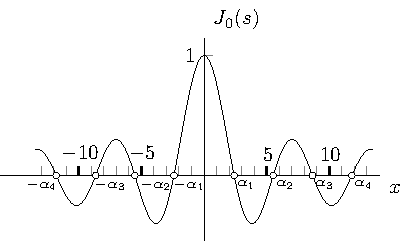
\includegraphics{figOctaveBesselFunctionFirstKind}
\caption{بیسل تفاعل $J_0(s)$}
\label{شکل_جزوی_بیسل_تفاعل_پہلی_قسم}
\end{figure}

یوں تفاعل
\begin{align}\label{مساوات_جزوی_دائری_حل_پ}
W_m(r)=J_0(k_mr)=J_0\big(\frac{\alpha_m}{R}r\big)\quad \quad \quad m=1,2,\cdots
\end{align}
مساوات \حوالہ{مساوات_جزوی_دائری_جھلی_ج} کا وہ حل ہو گا جو جھلی کی سرحد پر صفر ہے۔

یوں \عددی{\lambda=\lambda_m=ck_m} استعمال کرتے ہوئے مساوات \حوالہ{مساوات_جزوی_دائری_جھلی_ث} کا مطابقتی حل
\begin{align*}
G_m(t)=a_m\cos \lambda_mt+c_2\sin \lambda_mt
\end{align*}
ہو گا۔اس طرح مساوات \حوالہ{مساوات_جزوی_دائری_جھلی_الف} کے ایسے حل جو سرحدی شرط مساوات \حوالہ{مساوات_جزوی_دائری_جھلی_ب} کو مطمئن کرتے ہوں درج ذیل ہوں گے جہاں \عددی{m=1,2,\cdots} ہے۔
\begin{align}\label{مساوات_جزوی_دائری_حل_ت}
u_m(r,t)=W_m(r)G_m(t)=(a_m\cos \lambda_mt+c_2\sin \lambda_mt)J_0(k_mr)
\end{align}
\عددی{u_m(r,t)} اس مسئلے کے امتیازی تفاعل\فرہنگ{امتیازی!تفاعل} ہیں جبکہ \عددی{\lambda_m} مسئلے کے امتیازی اقدار\فرہنگ{امتیازی اقدار} ہیں۔

ارتعاش کی \عددی{u_m} حصہ  کو \اصطلاح{\عددی{m} ویں عمودی انداز}\فرہنگ{$m^{th}$ normal mode}\حاشیہب{$m^{th}$ normal mode}\فرہنگ{normal mode} کہتے ہیں جس کی تعدد \عددی{\tfrac{\lambda_m}{2\pi}} چکر فی اکائی وقت ہو گی۔ \عددی{x} محور پر سائن تفاعل کے صفروں کے درمیان یکساں فاصلہ پایا جاتا ہے  جبکہ \عددی{J_0} کے صفروں کے درمیان یکساں فاصلہ نہیں پایا جاتا ہے۔یہی وجہ ہے کہ ستار کی ترنگ اور طبلہ کی تھاپ  مختلف ہیں۔شکل میں دکھائے گئے جھلی کی عمودی انداز شکل \حوالہ{شکل_جزوی_بیسل_تفاعل_پہلی_قسم} سے با آسانی حاصل کیے جا سکتے ہیں (شکل \حوالہ{شکل_جزوی_دائری_عمودی_انداز})۔عمودی انداز \عددی{m=1} میں پوری جھلی بیک وقت اوپر (یا نیچے) حرکت کرتی ہے۔\عددی{m=2} کے لئے تفاعل
\begin{align*}
W_2(r)=J_0\big(\frac{\alpha_2}{R}r\big)
\end{align*}
ان نقطوں پر صفر ہو گا جہاں  \عددی{\tfrac{\alpha_2r}{R}=\alpha_1} یعنی \عددی{r=\tfrac{\alpha_1R}{\alpha_2}} ہو۔ یوں \عددی{r=\tfrac{\alpha_1R}{\alpha_2}} صفر ہٹاو لکیر ہو گی جس کو شکل \حوالہ{شکل_جزوی_دائری_عمودی_انداز} میں نقطہ دار لکیر سے دکھایا گیا ہے۔اب جن لمحات پر جھلی کا وسطی خطہ اوپر حرکت کرتا ہے ان لمحات پر جھلی کا بیرونی خطہ \عددی{r>\tfrac{\alpha_1R}{\alpha_2}} نیچے کو حرکت کرے گا اور اسی طرح جب وسطی خطہ نیچے کو حرکت کرتا ہے تب بیرونی خطہ اوپر کو حرکت کرتا ہے۔حل \عددی{u_m(r,t)} کے \عددی{m-1} عدد صفر ہٹاو لکیریں ہوں گی (شکل \حوالہ{شکل_جزوی_دائری_عمودی_انداز}) جو ہم مرکز دائرے ہوں گے۔
%  
\begin{figure}
\centering
\begin{subfigure}{0.33\textwidth}
\centering
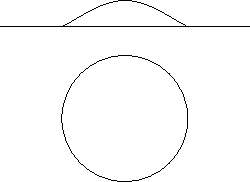
\includegraphics{figOctaveCircularMembraneNormalModesOne}
\end{subfigure}%
\begin{subfigure}{0.33\textwidth}
\centering
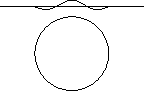
\includegraphics{figOctaveCircularMembraneNormalModesTwo}
\end{subfigure}%
\begin{subfigure}{0.33\textwidth}
\centering
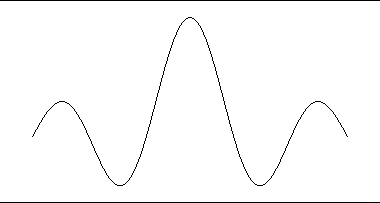
\includegraphics{figOctaveCircularMembraneNormalModesThree}
\end{subfigure}%
\caption{زاویہ سے آزاد دائری جھلی کی عمودی انداز}
\label{شکل_جزوی_دائری_عمودی_انداز}
\end{figure}

%

\موٹا{تیسرا قدم۔} \quad ایسا حل جو ابتدائی شرائط مساوات \حوالہ{مساوات_جزوی_دائری_جھلی_پ} اور مساوات \حوالہ{مساوات_جزوی_دائری_جھلی_ت} کو مطمئن کرتا ہو حاصل کرنے کی خاطر ہم ارتعاش پذیر تار کے حل کی طرح آگے بڑھتے ہیں یعنی ہم درج ذیل تسلسل پر غور کرتے ہیں۔\حاشیہد{ہم یکتائی اور ارتکاز کے مسئلے پر یہاں غور نہیں کریں گے۔}
\begin{align}\label{مساوات_جزوی_دائری_حل_ٹ}
u(r,t)=\sum_{m=1}^{\infty} W(r)G_m(t)=\sum_{m=1}^{\infty} (a_m\cos\lambda_mt+b_m\sin\lambda_mt)J_o\big(\frac{\alpha_m}{R}r\big)
\end{align}
اس میں \عددی{t=0} پر کرتے ہوئے  اور مساوات \حوالہ{مساوات_جزوی_دائری_جھلی_پ} استعمال کرتے ہوئے 
\begin{align}\label{مساوات_جزوی_دائری_حل_ث}
u(r,0)=\sum_{m=1}^{\infty} a_mJ_0\big(\frac{\alpha_m}{R}r\big)=f(r)
\end{align}
ملتا ہے۔یوں اگر مساوات \حوالہ{مساوات_جزوی_دائری_حل_ٹ} نے \حوالہ{مساوات_جزوی_دائری_جھلی_پ} کو مطمئن کرنا ہو تب \عددی{a_m}، تفاعل \عددی{f(r)} کی بیسل تسلسل  کے عددی سر ہوں گے۔یہ تسلسل \عددی{J_0(\tfrac{\alpha_m}{R}r)} کی صورت میں ہو گی۔یوں صفحہ \حوالہصفحہ{مساوات_طاقتی_فوریئر_بیسل_عددی_سر} پر مساوات \حوالہ{مساوات_طاقتی_فوریئر_بیسل_عددی_سر} کے تحت
\begin{align}\label{مساوات_جزوی_دائری_حل_ج}
a_m=\frac{2}{R^2J^2_1(\alpha_{m})}\int_0^R rf(r)J_0(\frac{\alpha_m}{R}r)\dif r\quad \quad m=1,2,
\end{align}
ہوں گے۔ وقفہ \عددی{0\le r\le R} پر \عددی{f(r)} کا قابل تفرق ہونا مساوات \حوالہ{مساوات_جزوی_دائری_حل_ث} کی صورت میں \عددی{f(r)} کی تسلسل لکھنے کے لئے کافی شرط ہے۔مساوات \حوالہ{مساوات_جزوی_دائری_حل_ٹ} میں عددی سر \عددی{b_m} کو مساوات \حوالہ{مساوات_جزوی_دائری_جھلی_ت} سے اسی طرح  حاصل کیا جا سکتا ہے۔
\begin{align}\label{مساوات_جزوی_دائری_حل_چ}
b_m=\frac{2}{c\alpha_m RJ_1^2(\alpha_m)}\int_0^R rg(r)J_0\big(\frac{\alpha_m}{R}r\big)\,\dif r,\quad \quad m=1,2,\cdots
\end{align}
\عددی{a_m} اور \عددی{b_m} کی اعدادی قیمتیں حاصل کرنے کی خاطر ہم \عددی{J_0} اور \عددی{J_1} کی قیمتوں کے جدول استعمال کرتے ہوئے تکمل کا تخمینہ لگائیں گے۔

%=========================
\حصہء{سوالات}

%==========================
\ابتدا{سوال}\quad
\عددی{R=1} لیتے ہوئے \عددی{u_2} اور \عددی{u_3} کی صفر ہٹاو دائروں کی رداس تلاش کریں (مساوات \حوالہ{مساوات_جزوی_دائری_حل_ت})۔\\
جواب:\quad
$u_2:r=\tfrac{\alpha_1}{\alpha_2}R=0.43565,\quad u_3:r=\tfrac{\alpha_1}{\alpha_3}R=0.27789, \quad r=\tfrac{\alpha_2}{\alpha_3}R=0.63788$
\انتہا{سوال}
%===========================
\ابتدا{سوال}\quad
\عددی{R=1} لیتے ہوئے \عددی{u_4} کی صفر ہٹاو دائروں کی رداس تلاش کریں۔\\
جواب:\quad
$0.20394, \quad 0.46814,\quad 0.73389$
\انتہا{سوال}
%==========================
\ابتدا{سوال}\quad
شکل \حوالہ{شکل_جزوی_دائری_عمودی_انداز} کی طرح اشکال \عددی{u_4} اور \عددی{u_5} کے لئے کھینچیں۔
\انتہا{سوال}
%======================
\ابتدا{سوال}\quad
جھلی میں تناو بڑھانے سے مختلف عمودی انداز (مساوات \حوالہ{مساوات_جزوی_دائری_حل_ت}) کی تعدد پر کیا اثر پڑتا ہے؟\\
جواب:\quad تناو بڑھنے سے \عددی{c} بڑھتا ہے لہٰذا تعدد بڑھے گی۔
\انتہا{سوال}
%==========================
\ابتدا{سوال}\quad 
مساوات \حوالہ{مساوات_جزوی_دائری_حل_چ} حاصل کریں۔
\انتہا{سوال}
%================
\ابتدا{سوال}\quad
کیا مقررہ \عددی{c} اور \عددی{R} کی صورت میں دو یا دو سے زیادہ تفاعل \عددی{u_m} (مساوات \حوالہ{مساوات_جزوی_دائری_حل_ت}) جن کے صفر ہٹاو لکیریں مختلف ہوں کا ایک ہی امتیازی قدر ہو سکتا ہے؟
\انتہا{سوال}
%===================
\ابتدا{سوال}\شناخت{سوال_جزوی_مکمل_آزاد_ارتعاش_جھلی}\quad \موٹا{قطبی محدد کے ($r$ اور $\theta$ پر منحصر) ارتعاش}\\
مساوات موج
\begin{align}\label{مساوات_جزوی_سوال_الف}
u_{tt}=c^2\big(u_{rr}+\frac{1}{r}u_r+\frac{1}{r^2}u_{\theta \theta}\big)
\end{align}
 میں \عددی{u=F(r,\theta)G(t)} پر کرتے ہوئے درج ذیل حاصل کریں۔
\begin{align}
\ddot{G}+\lambda^2G=0,\quad \quad \lambda=ck\label{مساوات_جزوی_سوال_ب}\\
F_{rr}+\frac{1}{r}F_r+\frac{1}{r^2}F_{\theta\theta}+k^2F=0\label{مساوات_جزوی_سوال_پ}
\end{align}
\انتہا{سوال}
%=========================
\ابتدا{سوال}\quad
مساوات \حوالہ{مساوات_جزوی_سوال_پ} میں \عددی{F=W(r)Q(\theta)} پر کرتے ہوئے درج ذیل حاصل کریں۔
\begin{align}
Q''+n^2Q=0\label{مساوات_جزوی_سوال_ت}\\
r^2W''+rW'+(k^2r^2-n^2)W=0\label{مساوات_جزوی_سوال_ٹ}
\end{align}
\انتہا{سوال}
%=========================
\ابتدا{سوال}\quad
وضاحت کریں کہ \عددی{Q(\theta)} دوری ہو گا جس کا دوری عرصہ \عددی{2\pi} ہو گا لہٰذا مساوات \حوالہ{مساوات_جزوی_سوال_ت} اور مساوات \حوالہ{مساوات_جزوی_سوال_ٹ} میں \عددی{n=0,1,2,\cdots} ہوں گے۔یوں درج ذیل حل حاصل کریں۔
\begin{align}
Q_n=\cos n\theta, \quad Q^*_n=\sin n\theta\label{مساوات_جزوی_سوال_ث}\\
W_n=J_n(kr),\quad n=0,1,\cdots\label{مساوات_جزوی_سوال_ج}
\end{align}
\انتہا{سوال}
%========================
\ابتدا{سوال}\quad
واضح کریں کہ سرحدی شرط
\begin{align}\label{مساوات_جزوی_سوال_چ}
u(R,\theta,t)=0
\end{align}
سے \عددی{k=k_{mn}=\tfrac{\alpha_{mn}}{R}} حاصل ہوتا ہے جہاں \عددی{s=\alpha_{mn}} تفاعل \عددی{J_n(s)} کا مثبت \عددی{m} واں جذر ہے۔
\انتہا{سوال}
%=====================
\ابتدا{سوال}\quad
واضح کریں کہ مساوات \حوالہ{مساوات_جزوی_سوال_الف} کے وہ حل جو مساوات \حوالہ{مساوات_جزوی_سوال_چ} کو مطمئن کرتے ہوں درج ذیل ہیں۔
\begin{gather}
\begin{aligned}\label{مساوات_جزوی_سوال_ح}
u_{mn}&=(A_{mn}\cos ck_{mn}t+B_{mn}\sin ck_{mn}t)J_n(k_{mn}r)\cos n\theta\\
u^*_{mn}&=(A^*_{mn}\cos ck_{mn}t+B^*_{mn}\sin ck_{mn}t)J_n(k_{mn}r)\sin n\theta
\end{aligned}
\end{gather}
\انتہا{سوال}
%=======================
\ابتدا{سوال}\quad
واضح کریں کہ  \عددی{u^*_{m0}\equiv 0} اور \عددی{u_{m0}}  عین مساوات \حوالہ{مساوات_جزوی_دائری_حل_ت} کے تحت ہیں۔
\انتہا{سوال}
%==========================
\ابتدا{سوال}\quad
واضح کریں کہ \عددی{u_{mn}} کی  \عددی{m+n-1} صفر ہٹاو لکیریں ہوں گی۔
\انتہا{سوال}
%===================
سوال \حوالہ{سوال_جزوی_ترسیم_الف} تا سوال \حوالہ{سوال_جزوی_ترسیم_ب} میں دیے گئے حل کی صفر ہٹاو لکیروں کی ترسیم کھینچیں۔

%=============
\ابتدا{سوال}\شناخت{سوال_جزوی_ترسیم_الف}\quad
$u_{3n},\quad n=1,2,3$
\انتہا{سوال}
%====================
\ابتدا{سوال}\quad
$u_{4n},\quad n=1,2,3$
\انتہا{سوال}
%====================
\ابتدا{سوال}\شناخت{سوال_جزوی_ترسیم_ب}\quad
$u^*_{mn},\quad m,n=1,2,3$\\
جواب:\quad صفر ہٹاو لکیریں شکل \حوالہ{شکل_سوال_جزوی_ترسیم_ب} میں دکھائی گئی ہیں۔
\begin{figure}
\centering
\begin{tikzpicture}
\draw(0,0) circle (1);
\draw[dashed] (0,1)--(0,-1)node[below]{$u_{11}$};
\begin{scope}[xshift={3cm}]
\draw(0,0) circle (1);
\draw[dashed] (0,0)++(45:1)--++(45:-2);
\draw[dashed] (0,0)++(-45:1)--++(-45:-2);
\draw(0,-1)node[below]{$u_{12}$};
\end{scope}
\begin{scope}[xshift={6cm}]
\draw(0,0) circle (1);
\draw[dashed](0,0) circle (0.4356);
\draw[dashed] (0,1)--(0,-1);
\draw[dashed] (0,0)++(30:1)--++(30:-2);
\draw[dashed] (0,0)++(-30:1)--++(-30:-2);
\draw(0,-1)node[below]{$u_{23}$};
\end{scope}
\end{tikzpicture}
\caption{چند صفر ہٹاو لکیریں (سوال \حوالہ{سوال_جزوی_ترسیم_ب})}
\label{شکل_سوال_جزوی_ترسیم_ب}
\end{figure}
\انتہا{سوال}
%====================
\ابتدا{سوال}\quad
ابتدائی معلومات \عددی{u_t(r,\theta,0)} کی صورت میں مساوات \حوالہ{مساوات_جزوی_سوال_ح} سے  \عددی{B_{mn}=0} اور \عددی{B^*_{mn}=0} حاصل کریں۔
\انتہا{سوال}
%=========================
سوال \حوالہ{سوال_جزوی_رفتار_الف} تا سوال \حوالہ{سوال_جزوی_رفتار_ب} میں \عددی{R=1}، \عددی{c=1} اور ابتدائی رفتار صفر لیتے ہوئے،  ابتدائی انحراف \عددی{f(r)} کی صورت میں دائری جھلی کی  انحراف \عددی{u(r,t)} حاصل کریں۔ (اشارہ سوال \حوالہ{سوال_طاقتی_بیسل_فوریئر_تسلسل_الف} تا سوال \حوالہ{سوال_طاقتی_بیسل_فوریئر_تسلسل_ب} پر ایک مرتبہ دوبارہ نظر ڈالیں۔)

%==========
\ابتدا{سوال}\شناخت{سوال_جزوی_رفتار_الف}\quad
$f=0.1J_0(\alpha_2r)$
\انتہا{سوال}
%==========================
\ابتدا{سوال}\quad
$f=k(1-r^2)$\\
جواب:\quad
$u=4k\sum_{m=1}^{\infty}\frac{J_2(\alpha_m)}{\alpha_m^2J_1^2(\alpha_m)}\cos \alpha_m t\,J_0(\alpha_m r)$
\انتہا{سوال}
%==========================
\ابتدا{سوال}\شناخت{سوال_جزوی_رفتار_ب}\quad
$f=k(1-r^4)$
\انتہا{سوال}
%==========================

\حصہ{مساوات لاپلاس۔ نظریہ مخفی قوہ}\شناخت{حصہ_جزوی_مخفی_قوہ}
طبیعیات کی اہم ترین مساوات میں سے ایک درج ذیل مساوات لاپلاس  ہے
\begin{align}\label{مساوات_جزوی_لاپلاس_الف}
\nabla^{\,2}u=0
\end{align}
جہاں \عددی{u} کا لاپلاسی  \عددی{\nabla^{\,2}u}  ہے۔کارتیسی محدد \عددی{x}، \عددی{y}، \عددی{z} میں
\begin{align}\label{مساوات_جزوی_لاپلاس_ب}
\nabla^{\,2}u=\frac{\partial^{\,2}u}{\partial x^2}+\frac{\partial^{\,2}u}{\partial y^2}+\frac{\partial^{\,2}u}{\partial z^2}
\end{align}
ہو گا۔مساوات لاپلاس کے نظریہ کو \اصطلاح{نظریہ مخفی قوہ}\فرہنگ{نظریہ مخفی قوہ}\حاشیہب{potential theory}\فرہنگ{potential theory} کہتے ہیں۔مساوات \حوالہ{مساوات_جزوی_لاپلاس_الف} کے ایسے حل جن کے دو درجی تفرقات استمراری ہوں \اصطلاح{ہارمونی تفاعل}\فرہنگ{ہارمونی!تفاعل}\حاشیہب{harmonic functions}\فرہنگ{harmonic!functions} کہلاتے ہیں۔

دو ابعادی صورت جہاں \عددی{u} صرف دو عدد متغیرات کے تابع ہو کا مخلوط تجزیہ زیادہ آسان ثابت ہوتا ہے لہٰذا اس پر حصہ \حوالہ{حصہ_تحلیلی_کوشی_ریمان_مساوات_لاپلاس} اور  باب \حوالہ{باب_مخلوط_تفاعل_اور_نظریہ_مخفی_قوہ} میں غور کیا جائے گا۔

انجینئری حساب میں مساوات لاپلاس کی اہمیت واضح کرنے کی خاطر چند مثالوں کا ذکر کرتے ہیں۔

مساوات لاپلاس ثقلی میدان کے مسائل میں سامنے آتی ہے۔  مثلاً صفحہ \حوالہصفحہ{مثال_الاحصاء_ثقلی_میدان} پر مثال \حوالہ{مثال_الاحصاء_ثقلی_میدان} میں ہم نے دیکھا کہ اگر ایک ذرہ \عددی{A} جس کی کمیت \عددی{M} ہو نقطہ \عددی{(\xi,\eta,\zeta)} پر مستقل موجود ہو اور دوسرا ذرہ \عددی{B} جس کی کمیت \عددی{m} ہو نقطہ \عددی{(x,y,z)} پر موجود ہو تب \عددی{A} ذرہ \عددی{B} کو اپنی جانب کھینچے گا۔یہ ثقلی قوت درج ذیل غیر سمتی تفاعل \عددی{u(x,y,z)} کی ڈھلوان ہے۔
\begin{align*}
u(x,y,z)=\frac{GMm}{r}\\
r=\sqrt{(x-\xi)^2+(y-\eta)^2+(z-\zeta)^2}\quad (>0)
\end{align*}
تفاعل \عددی{u(x,y)} کو ثقلی میدان کی \اصطلاح{مخفی قوہ} کہتے ہیں اور یہ لاپلاس کی مساوات کو مطمئن کرتا ہے۔ 

نقطہ کمیت کی مخفی قوہ اور قوت کی تصور کو مسلسل کمیت کے لئے بیان کرتے ہیں۔اگر خطہ \عددی{R} میں کمیتی کثافت \عددی{\rho(\xi,\eta,\zeta)} پائی جاتی ہو تب  نقطہ \عددی{(x,y,z)} جہاں کمیت موجود نہ ہو  پر مخفی قوہ \عددی{u} درج ذیل ہو گی۔ 
\begin{align}\label{مساوات_جزوی_لاپلاس_پ}
u(x,y,z)=k\iiint\limits_R \frac{\rho}{r}\dif \xi\,\dif \eta\,\dif \zeta\quad \quad \quad (k>0)
\end{align}
چونکہ \عددی{\frac{1}{r} (r>0)} مساوات \حوالہ{مساوات_جزوی_لاپلاس_الف} کا حل ہے لہٰذا \عددی{\nabla^{\,2}(\tfrac{1}{r})=0} ہو گا اور کثافت \عددی{\rho}  متغیرات \عددی{x}، \عددی{y}، \عددی{z} پر منحصر نہیں ہے لہٰذا درج ذیل حاصل ہوتا ہے۔
\begin{align*}
\nabla^{\,2}u=k\iiint\limits_R \rho\nabla^{\,2}\big(\frac{1}{r}\big) \dif \xi\,\dif \eta\,\dif \zeta=0
\end{align*}
یوں مساوات \حوالہ{مساوات_جزوی_لاپلاس_پ} میں دی گئی ثقلی مخفی قوہ مساوات لاپلاس کو ہر اس نقطہ پر مطمئن کرتی ہے جہاں پر کمیت موجود نہ ہو۔

برقی سکون کی میدان میں برقی بار کے مابین قوت کشش یا قوت دفع قانون کولمب دیتی ہے جس کی ریاضی شکل عین نیوٹن کے قانون ثقل کی طرح ہے۔یوں ہم اخذ کر سکتے ہیں کہ جس نقطہ پر برقی بار موجود نہ ہو اس نقطہ پر برقی مخفی قوہ کو ایسے تفاعل سے ظاہر کیا جا سکتا  ہے جو برقی بار سے پاک نقطہ پر لاپلاس کی مساوات کو مطمئن کرتا ہو۔

ہم بعد کے باب میں دیکھیں گے کہ غیر  داب پذیر سیال کی بہاو پر غور کے دوران بھی لاپلاس مساوات  سامنے آتی ہے۔

مزید حرارت کے مسائل میں حراری مساوات
\begin{align*}
u_t=c^2\nabla^{\,2}u
\end{align*}
 بنیادی اہمیت رکھتی ہے۔اگر درجہ حرارت وقت \عددی{t} کے تابع نہ ہو (برقرار حالت) تب یہ لاپلاس مساوات کی صورت اختیار کرتی ہے۔
\begin{figure}
\centering
\begin{subfigure}{0.5\textwidth}
\centering
\begin{tikzpicture}
\draw(0,0)--++(2,0)node[right]{$y$};
\draw(0,0)--++(-110:1.5)node[left]{$x$};
\draw(0,0)--++(0,1.5)node[left]{$z$};
%
\draw[-stealth]([shift={(-110:0.3)}]0,0) arc (-110:-45:0.3);
\draw[dashed] (0,0)--++(-45:1.5)coordinate(kA)node[pos=0.5,below,solid]{$\rho$};
\draw[dashed](kA)--++(0,2)node[solid,ocirc]{}node[right]{$(\rho,\phi,z)$};
\RightAngle{(0,0)}{(kA)}{(0,2)};
\draw(-80:0.6)node[]{$\phi$};
\end{tikzpicture}
\caption*{(الف) نلکی محدد}
\end{subfigure}%
\begin{subfigure}{0.5\textwidth}
\centering
\begin{tikzpicture}[]
\draw(0,0)--++(2,0)node[right]{$y$};
\draw[name path=kX](0,0)--++(-110:1.5)node[left]{$x$};
\draw(0,0)--++(0,2.5)node[left]{$z$};
%
\draw[-stealth]([shift={(-110:0.3)}]0,0) arc (-110:-45:0.3);
\draw[dashed] (0,0)--++(-45:1.5)coordinate(kA);
\draw[dashed](kA)--++(0,2)node[right]{$(r,\phi,z)$}coordinate(kB);
\draw(-80:0.6)node[]{$\phi$};
\draw[thick](0,0)--(kB);
\draw[dashed] (kB)node[ocirc,solid]{}--++(-45:-1.5)coordinate(kC)node[pos=0.5,rotate=-45,above]{$r\sin \theta$};
\RightAngle{(kB)}{(kC)}{(0,0)};
\RightAngle{(0,0)}{(kA)}{(0,2)};
%
\draw[-stealth]([shift={(90:0.5)}]0,0) arc (90:45:0.5);
\draw(70:0.8)node{$\theta$};
%
\path[name path=kXX] (kA)--++(-2,0);
\draw[dashed,name intersections={of=kX and kXX}] (kA)--(intersection-1)coordinate(kI);
\RightAngle{(kA)}{(kI)}{(0,0)};
%
\draw [decorate,decoration={brace,amplitude=5pt},xshift=-4pt,yshift=0pt](kI)++(-0.2,0) --++(70:1.2) node [black,midway,xshift=-0.3cm,yshift=0.2cm,rotate=70] {\footnotesize $r\sin\theta\cos\phi$};
\end{tikzpicture}
\caption*{(ب) کروی محدد}
\end{subfigure}%
\caption{نلکی اور کروی محدد کی تعریف}
\label{شکل_جزوی_نلکی_کروی}
\end{figure}

عموماً مسائل، جن میں لاپلاس مساوات حاصل ہو گی، میں \اصطلاح{سرحدی قیمت مسئلہ}\فرہنگ{سرحدی!قیمت مسئلہ}\حاشیہب{boundary value problem}\فرہنگ{boundary!value problem} حل کرنا ہو گا جہاں مساوات \حوالہ{مساوات_جزوی_لاپلاس_الف} کا ایسا حل درکار ہو گا جو کسی سرحد پر دیا گیا شرط مطمئن کرتا ہو۔یوں خلا میں ایسے محدد متعارف کرنا ضروری ہو گا جن میں اس سرحد کو بیان کرنا آسان  ہو۔اس طرح مساوات \حوالہ{مساوات_جزوی_لاپلاس_ب} کے لاپلاسی کا تبادلہ ان محدد میں کرنا ہو گا۔ہم حصہ \حوالہ{حصہ_جزوی_قطبی_محدد_لاپلاسی} میں دو متغیرات کے تفاعل کی لاپلاسی کا تبادلہ کر چکے ہیں۔ایک محدد سے دوسرے محدد میں لاپلاسی کا تبادلہ اسی طرح کیا جائے گا۔

نلکی محدد میں لاپلاسی صفحہ \حوالہصفحہ{مساوات_جزوی_لاپلاسی_نلکی_محدد} پر مساوات \حوالہ{مساوات_جزوی_لاپلاسی_نلکی_محدد} دیتی ہے۔نلکی محدد (شکل \حوالہ{شکل_جزوی_نلکی_کروی}-الف) کی تعریف
\begin{align}\label{مساوات_جزوی_تعریف_محددی_نظام_الف}
\rho&=\sqrt{x^2+y^2}, \quad \phi=\tan^{-1}\frac{y}{x},\quad z=z
\end{align}
 اور اس میں لاپلاسی کو یہاں دوبارہ پیش کرتے ہیں۔
\begin{align}\label{مساوات_جزوی_تعریف_محددی_نظام_ب}
\nabla^{\,2}u=&\frac{\partial^{\,2}u}{\partial \rho^2}+\frac{1}{\rho}\frac{\partial u}{\partial \rho}+\frac{1}{\rho^2}\frac{\partial^{\,2}u}{\partial \phi^2}+\frac{\partial^{\,2}u}{\partial z^2}
\end{align}

صفحہ \حوالہصفحہ{مساوات_جزوی_کروی_لاپلاسی_الف} پر مساوات \حوالہ{مساوات_جزوی_کروی_لاپلاسی_الف} کروی محدد میں لاپلاسی دیتی ہے۔کروی محدد (شکل \حوالہ{شکل_جزوی_نلکی_کروی}-ب) کی تعریف
\begin{align}\label{مساوات_جزوی_تعریف_محددی_نظام_پ}
x&=r\sin\theta\cos\phi,\quad y=r\sin\theta\sin\phi,\quad z=r\sin\theta
\end{align}
 اور اس میں لاپلاسی کو یہاں دوبارہ پیش کرتے ہیں
\begin{align}\label{مساوات_جزوی_تعریف_محددی_نظام_ت}
\nabla^{\,2}u=u_{rr}+\frac{2}{r}u_r+\frac{1}{r^2}u_{\theta\theta}+\frac{\cot \theta}{r^2}u_{\theta}+\frac{1}{r^2\sin^2\theta}u_{\phi\phi}
\end{align}
جس کو درج ذیل بھی لکھا جا سکتا ہے۔
\begin{align}\label{مساوات_جزوی_تعریف_محددی_نظام_ٹ}
\nabla^{\,2}u=\frac{1}{r^2}\big[\frac{\partial}{\partial r}\big(r^2\frac{\partial u}{\partial r}\big)+\frac{1}{\sin \theta}\frac{\partial}{\partial \theta}\big(\sin \theta \frac{\partial u}{\partial \theta}\big)+\frac{1}{\sin^2\theta} \frac{\partial^{\,2}u}{\partial \phi^2}\big]
\end{align}

%=====================
\حصہء{سوالات}

%==============
\ابتدا{سوال}\quad
محدد \عددی{x^*=ax}، \عددی{y^*=by}، \عددی{z^*=cz} میں لاپلاسی حاصل کریں جہاں \عددی{x}، \عددی{y}، \عددی{z} کارتیسی محدد ہیں۔\\
جواب:\quad
$a^2u_{x^*x^*}+b^2u_{y^*y^*}+c^2u_{z^*z^*}$
\انتہا{سوال}
%=========================
\ابتدا{سوال}\quad
مساوات \حوالہ{مساوات_جزوی_لاپلاس_ب} سے شروع کرتے ہوئے 
صفحہ \حوالہصفحہ{مساوات_الاحصاء_عمومی_مستوی_تبادل_الف} پر مساوات \حوالہ{مساوات_الاحصاء_عمومی_مستوی_تبادل_الف} اور مساوات \حوالہ{مساوات_الاحصاء_عمومی_مستوی_تبادل_ب} استعمال کرتے ہوئے درج ذیل حاصل کریں۔
\begin{align*}
\nabla^{\,2}u=u_{x^*x^*}+u_{y^*y^*}+u_{z^*z^*}
\end{align*}
\انتہا{سوال}
%===================
تصدیق کریں کہ سوال \حوالہ{سوال_جزوی_تصدیق_لاپلاس_حل_الف} تا سوال \حوالہ{سوال_جزوی_تصدیق_لاپلاس_حل_ب} میں تفاعل \عددی{u=f(x,y)}  مساوات لاپلاس کو مطمئن کرتا ہے۔چند ہم قوہ خطوط \عددی{u=c} جہاں \عددی{c} مستقل ہے کی ترسیم کھینچیں۔

%====================
\ابتدا{سوال}\شناخت{سوال_جزوی_تصدیق_لاپلاس_حل_الف}\quad
$x^2-y^2$
\انتہا{سوال}
%=========================
\ابتدا{سوال}\quad
$x^3-3xy^2$
\انتہا{سوال}
%=========================
\ابتدا{سوال}\quad
$\tfrac{x}{x^2+y^2}$
\انتہا{سوال}
%=========================
\ابتدا{سوال}\quad
$\tfrac{y}{x^2+y^2}$
\انتہا{سوال}
%=========================
\ابتدا{سوال}\شناخت{سوال_جزوی_تصدیق_لاپلاس_حل_ب}\quad
$\tfrac{x^2-y^2}{(x^2+y^2)^2}$
\انتہا{سوال}
%=========================
\ابتدا{سوال}\quad
کارتیسی نظام محدد استعمال کرتے ہوئے مساوات \حوالہ{مساوات_جزوی_تعریف_محددی_نظام_پ} میں کروی محدد کی تعریف بیان کی گئی ہے۔ان مساوات کو استعمال کرتے ہوئے کارتیسی نظام کی تعریف کروی محددی نظام میں کریں۔\\
جواب:\quad
$r=\sqrt{x^2+y^2+z^2},\quad \theta=\tan^{-1}\frac{z}{\sqrt{x^2+y^2+z^2}},\quad \phi=\tan^{-1}\frac{y}{x}$
\انتہا{سوال}
%==========================
\ابتدا{سوال}\quad
مساوات \حوالہ{مساوات_جزوی_تعریف_محددی_نظام_ب} سے واپس کارتیسی محدد میں لاپلاسی حاصل کریں۔
\انتہا{سوال}
%==========================
\ابتدا{سوال}\quad
تصدیق کریں کہ \عددی{u=\tfrac{c}{r}} کروی محدد میں لاپلاسی کو مطمئن کرتا ہے جہاں \عددی{c} مستقل ہے۔
\انتہا{سوال}
%====================
\ابتدا{سوال}\شناخت{سوال_جزوی_لاپلاس_رداس_تابع_حل_الف}\quad
لاپلاس مساوات \عددی{\nabla^{\,2}u=0} کا ایسا حل تلاش کریں جو صرف \عددی{r=\sqrt{x^2+y^2+z^2}} کا تابع ہو۔\\
جواب:\quad اگر \عددی{u} صرف \عددی{r} کا تابع ہو تب مساوات  \حوالہ{مساوات_جزوی_تعریف_محددی_نظام_ٹ} کی صورت 
$\tfrac{1}{r^2}\big[\tfrac{\partial}{\partial r}\big(r^2\tfrac{\partial u}{\partial r}\big)\big]=0$
 یعنی
$ \tfrac{\partial}{\partial r}\big(r^2\tfrac{\partial u}{\partial r}\big)=0$
ہو گی جہاں جزوی تفرق کی جگہ تفرق لکھا گیا ہے۔اس کا تکمل \عددی{r^2\tfrac{\partial u}{\partial r}=c}ہو گا جس کو \عددی{\dif u=\tfrac{c}{r^2}\dif r} لکھ کر تکمل لینے سے درکار حل \عددی{u=k-\tfrac{c}{r}} حاصل ہو گا جہاں \عددی{c} اور \عددی{k} مستقل ہیں۔
\انتہا{سوال}
%======================
\ابتدا{سوال}\شناخت{سوال_جزوی_لاپلاس_رداس_تابع_حل_ب}\quad دو ہم مرکز کرہ کے رداس \عددی{r_1=\SI{15}{\centi\meter}} اور \عددی{r_2=\SI{1}{\centi\meter}} ہیں جبکہ ان پر برقی دباو بالترتیب \عددی{U_1=\SI{1000}{\volt}} اور \عددی{U_2=\SI{100}{\volt}} ہے۔ہم مرکز کرہ کے درمیان خطہ میں ساکن برقی دباو \عددی{u} سوال \حوالہ{سوال_جزوی_لاپلاس_رداس_تابع_حل_الف} میں حاصل کی گئی۔موجودہ معلومات کو استعمال کرتے ہوئے \عددی{c} اور \عددی{k} دریافت کریں اور حاصل \عددی{u} کی ترسیم کھینچیں۔\\
جواب:\quad
$u=\tfrac{7450}{7}-\tfrac{135}{14 r}$
\انتہا{سوال}
%====================
\ابتدا{سوال}\شناخت{سوال_جزوی_نلکی_لاپلاس_حل_الف}\quad
دو ابعادی لاپلاس مساوات جو صرف \عددی{\rho=\sqrt{x^2+y^2}} کے تابع ہو کا حل تلاش کریں۔\\
جواب:\quad اگر \عددی{u} صرف \عددی{\rho} کا تابع ہو تب مساوات \حوالہ{مساوات_جزوی_تعریف_محددی_نظام_ب} کی صورت
$\frac{\dif^{\,2}u}{\dif \rho^2}+\frac{1}{\rho}\frac{\dif u}{\dif \rho}=0$
ہو گی جہاں جزوی تفرق کی جگہ تفرق لکھا گیا ہے۔اس میں \عددی{v=\tfrac{\dif u}{\dif \rho}} پر کرتے ہوئے \عددی{\tfrac{\dif v}{\dif \rho}+\tfrac{v}{\rho}=0} یعنی \عددی{\tfrac{\dif v}{v}=-\tfrac{\dif \rho}{\rho}} حاصل ہوتا ہے جس کا  تکمل \عددی{v\rho=c} یعنی 
\عددی{\tfrac{\partial u}{\partial \rho}=\tfrac{c}{\rho}} دیتا ہے۔درکار جواب تکمل لینے سے \عددی{u=k+c\ln \rho} حاصل ہوتا ہے جہاں \عددی{c} اور \عددی{k} مستقل ہیں۔
\انتہا{سوال}
%========================
\ابتدا{سوال}\شناخت{سوال_جزوی_نلکی_لاپلاس_حل_ب}\quad 
دو ہم محور نلکیوں کا رداس \عددی{\rho_1=\SI{5}{\centi\meter}} اور \عددی{\rho_2=\SI{20}{\centi\meter}} ہے جبکہ ان پر برقی دباو بالترتیب
 \عددی{U_1=\SI{10}{\volt}} اور \عددی{U_2=\SI{60}{\volt}} ہے۔ سوال \حوالہ{سوال_جزوی_نلکی_لاپلاس_حل_الف} میں حاصل حل استعمال کرتے ہوئے نلکیوں کے درمیان خطہ میں برقی دباو کی مساوات حاصل کریں۔ حاصل \عددی{u} کی ترسیم کھینچیں۔موجودہ ترسیم کا سوال \حوالہ{سوال_جزوی_لاپلاس_رداس_تابع_حل_ب} میں حاصل کردہ ترسیم کے ساتھ موازنہ کریں۔\\
جواب:\quad
$u=118.048+36.067\ln \rho$
\انتہا{سوال}
%======================
\ابتدا{سوال}\quad
اگر کروی محدد میں \عددی{u(r,\theta,\phi)} مساوات لاپلاس \عددی{\nabla^{\,2}u=0} کو مطمئن کرتا ہو تب ثابت کریں کہ \عددی{v(r,\theta,\phi)=r^{-1}u(r^{-1},\theta,\phi)} مساوات \عددی{\nabla^{\,2}v=0} کو مطمئن کرے گا۔
\انتہا{سوال}
%======================
\ابتدا{سوال}\quad
مساوات موج \عددی{u_{tt}=c^2\nabla^{\,2}u} میں \عددی{u=U(x,y,z)e^{-i\omega t}} پر کرتے ہوئے درج ذیل \اصطلاح{مساوات ہلم ہولٹز}\فرہنگ{مساوات!ہلم ہولٹز}\فرہنگ{ہلم ہولٹز!مساوات}\حاشیہب{Helmholtz equation}\فرہنگ{Helmholtz equation} حاصل\حاشیہد{جرمن ماہر طبیعیات ہرمن لڈوگ فرڈینانڈ ون ہلم ہولٹز [1821-1894]} کریں جہاں \عددی{i=\sqrt{-1}} ہے۔
\begin{align*}
\nabla^{\,2}U+k^2U=0\quad \quad \quad k=\frac{\omega}{c}
\end{align*}
\انتہا{سوال}
%====================
سوال \حوالہ{سوال_جزوی_برقرار_حال_الف} تا سوال \حوالہ{سوال_جزوی_برقرار_حال_الف} میں برقرار حال (وقت کا غیر تابع) درجہ حرارت \عددی{u} تلاش کریں۔

%====================
\ابتدا{سوال}\شناخت{سوال_جزوی_برقرار_حال_الف}\quad
دو متوازی چادر \عددی{x=x_0} اور \عددی{x=x_1} کے درمیان جنہیں بالترتیب \عددی{u_0} اور \عددی{u_1} درجہ حرارت پر برقرار رکھا گیا ہے۔\\
جواب:\quad
$u=\tfrac{(u_1-u_0)x}{x_1-x_0}+\tfrac{u_0x_1-u_1x_0}{x_1-x_0}$
\انتہا{سوال}
%========================
\ابتدا{سوال}\quad
دو ہم محور نلکیوں \عددی{\rho=\rho_1} اور \عددی{\rho=\rho_2} کے درمیان جنہیں بالترتیب \عددی{u_0} اور \عددی{u_1} درجہ حرارت پر برقرار رکھا گیا ہے۔\\
جواب:\quad
$u=\tfrac{u_1-u_0}{\ln \tfrac{r_1}{r_0}}\ln r+\tfrac{u_0\ln r_1-u_1\ln r_0}{\ln \tfrac{r_1}{r_0}}$
\انتہا{سوال}
%========================
\ابتدا{سوال}\quad
دو ہم مرکز کرہ  \عددی{r=r_1} اور \عددی{r=r_2} کے درمیان جنہیں بالترتیب \عددی{u_0} اور \عددی{u_1} درجہ حرارت پر برقرار رکھا گیا ہے۔\\
جواب:\quad
$u=u_0-\tfrac{r_1r_0(u_1-u_0)}{(r_1-r_0)r}$
\انتہا{سوال}
%========================

\حصہ{کروی محدد میں مساوات لاپلاس۔مساوات لیژانڈر}
آئیں ایک ایسے مسئلے پر غور کرتے ہیں جس میں، کروی محدد میں لکھی گئی، مساوات لاپلاس استعمال ہو گی۔فرض کریں کہ کروی محدد کی مرکز پر موجود رداس \عددی{R} کی کرہ \عددی{S} کی سطح کو  برقی دباو 
\begin{align}\label{مساوات_جزوی_کرہ_بار_بردار_الف}
u(R,\theta,\phi)=f(\theta)
\end{align}
پر برقرار رکھا جاتا ہے جہاں \عددی{r}، \عددی{\theta}، \عددی{\phi} کروی محدد ہیں جبکہ \عددی{f(\theta)} دیا گیا تفاعل ہے۔کروی محدد کی تعریف گزشتہ حصے میں کی گئی ہے۔ ہم باقی پوری فضا، جہاں کوئی برقی بار نہیں پایا جاتا، میں برقی دباو \عددی{u} جاننا چاہتے ہیں۔چونکہ \عددی{S} کی سطح پر برقی دباو \عددی{\phi} سے آزاد ہے لہٰذا باقی فضا میں بھی برقی دباو \عددی{\phi} سے آزاد ہو گا۔یوں \عددی{\tfrac{\partial^{\,2}u}{\partial \phi^{\,2}}=0} ہو گا لہٰذا مساوات لاپلاس  درج ذیل صورت اختیار کرے گی
\begin{align}\label{مساوات_جزوی_کرہ_بار_بردار_ب}
\frac{\partial}{\partial r}\big(r^2\frac{\partial u}{\partial r}\big)+\frac{1}{\sin \theta}\frac{\partial}{\partial \theta}\big(\sin \theta \frac{\partial u}{\partial \theta}\big)=0
\end{align}
جہاں مساوات \حوالہ{مساوات_جزوی_تعریف_محددی_نظام_ٹ} کا سہارا لیا گیا ہے۔اب لامتناہی فاصلہ پر برقی دباو صفر ہو گا یعنی:
\begin{align}\label{مساوات_جزوی_کرہ_بار_بردار_پ}
\lim_{r\to\infty} u(r,\theta)=0
\end{align}
ہم علیحدگی متغیرات کی ترکیب سے مساوات \حوالہ{مساوات_جزوی_کرہ_بار_بردار_الف} کا ایسا حل تلاش کرتے ہیں جو سرحدی شرائط مساوات \حوالہ{مساوات_جزوی_کرہ_بار_بردار_الف} اور مساوات \حوالہ{مساوات_جزوی_کرہ_بار_بردار_پ} کو مطمئن کرتا ہو۔یوں مساوات \حوالہ{مساوات_جزوی_کرہ_بار_بردار_ب} میں
\begin{align}\label{مساوات_جزوی_کرہ_بار_بردار_ت}
u(r,\theta)=G(r)H(\theta)
\end{align}
اور اس کے تفرق پر کر کے \عددی{GH} سے تقسیم کرتے ہیں۔
\begin{align*}
\frac{1}{G}\frac{\dif}{\dif r}\big(r^2\frac{\dif G}{\dif r}\big)=-\frac{1}{H\sin \theta}\frac{\dif}{\dif \theta}\big(\sin \theta \frac{\dif H}{\dif \theta}\big)
\end{align*}
اب تک آپ جان چکے ہوں گے کہ ایسی صورت میں مساوات کے دونوں اطراف کسی ایک مستقل مثلاً \عددی{k} کے برابر ہوں گے۔یوں درج ذیل دو عدد سادہ تفرقی مساوات حاصل ہوتے ہیں
\begin{align}
\frac{1}{\sin\theta}\frac{\dif}{\dif \theta}\big(\sin\theta\frac{\dif H}{\dif \theta}\big)+kH&=0\label{مساوات_جزوی_کرہ_بار_بردار_ٹ}\\
\frac{1}{G}\frac{\dif}{\dif r}\big(r^2\frac{\dif G}{\dif r}\big)&=k\label{مساوات_جزوی_کرہ_بار_بردار_ث}
\end{align}
جہاں دوسری مساوات کو 
\begin{align*}
r^2G''+2rG'-kG=0
\end{align*}
لکھا جا سکتا ہے جو \ترچھا{مساوات کوشی} ہے۔ہم  حصہ \حوالہ{حصہ_دو_یولر_کوشی} سے جانتے ہیں کہ مساوات کوشی کے حل کا روپ \عددی{G=r^{\alpha}} ہو گا۔اگر ہم \عددی{k} کی جگہ مستقل کو \عددی{n(n+1)} لکھیں تب ان حل کی صورت نہایت سادہ حاصل ہو گی۔ایسا کرنے سے 
\begin{align}\label{مساوات_جزوی_کرہ_بار_بردار_ج}
r^2G''+2rG'-n(n+1)G=0
\end{align}
لکھا جائے گا جہاں \عددی{n} اختیاری مستقل ہے۔اس میں \عددی{G=r^{\alpha}} پر کرنے سے
\begin{align*}
[\alpha(\alpha-1)+2\alpha-n(n+1)]r^{\alpha}=0
\end{align*}
ملتا ہے۔قوسین میں بند حصے کے صفر \عددی{\alpha=n} اور \عددی{\alpha=-n-1} ہیں۔یوں مساوات \حوالہ{مساوات_جزوی_کرہ_بار_بردار_ج} کے حل
\begin{align}\label{مساوات_جزوی_کرہ_بار_بردار_چ}
G_n(r)=r^n\quad \text{اور}\quad G^*_n(r)=\frac{1}{r^{n+1}}
\end{align}
ہوں گے۔
 
مساوات \حوالہ{مساوات_جزوی_کرہ_بار_بردار_ٹ} میں \عددی{k=n(n+1)} متعارف کر کے ہم 
\begin{align*}
\cos \theta=w
\end{align*}
لیتے ہیں۔یوں \عددی{\sin\theta^2=1-w^2} اور
\begin{align*}
\frac{\dif}{\dif \theta}=\frac{\dif}{\dif w}\frac{\dif w}{\dif \theta}=-\sin\theta \frac{\dif}{\dif w}
\end{align*}
ہوں گے لہٰذا مساوات \حوالہ{مساوات_جزوی_کرہ_بار_بردار_ٹ} 
\begin{align}\label{مساوات_جزوی_کرہ_بار_بردار_ح}
\frac{\dif}{\dif w}\big[(1-w^2)\frac{\dif H}{\dif w}\big]+n(n+1)H=0
\end{align}
یعنی
\begin{align}\label{مساوات_جزوی_کرہ_بار_بردار_خ}
(1-w^2)\frac{\dif^{\,2} H}{\dif w^2}-2w\frac{\dif H}{\dif w}+n(n+1)H=0
\end{align}
صورت اختیار کرے گی جو \ترچھا{مساوات لیژانڈر} ہے (حصہ \حوالہ{حصہ_لیژانڈر_تفاعل})۔مساوات لیژانڈر کے حل
\begin{align*}
H=P_n(w)=P_n(\cos \theta)
\end{align*}
ہیں جہاں اختیاری مستقل کی قیمتیں \عددی{n=0,1,2,\cdots} عدد صحیح\حاشیہد{اب تک \عددی{k} اختیاری مستقل تھا لہٰذا \عددی{n} بھی اختیاری مستقل تھا۔یہاں \عددی{n} کو عدد صحیح ہونے کا پابند اس لئے  بنایا گیا ہے تا کہ وقفہ \عددی{-1\le w \le 1} یعنی \عددی{0\le \theta\le \pi} پر مساوات \حوالہ{مساوات_جزوی_کرہ_بار_بردار_خ} کے حل اور حل کے ایک درجی تفرق استمراری ہوں (جس کا ثبوت یہاں پیش نہیں کیا جائے گا)۔} ہیں۔اس طرح ہمیں لاپلاس مساوات \حوالہ{مساوات_جزوی_کرہ_بار_بردار_ب} کے حل \عددی{u=GH} کے دو عدد تسلسل
\begin{align}\label{مساوات_جزوی_لیژانڈر_دو_عدد_حل}
u_n(r,\theta)=A_nr^nP_n(\cos\theta),\quad u^*_n(r,\theta)=\frac{B_n}{r^{n+1}}P_n(\cos\theta)
\end{align}
حاصل ہوتے ہیں جہاں \عددی{n=0,1,\cdots} جبکہ \عددی{A_n} اور \عددی{B_n} مستقل ہیں۔

\ترچھا{اندرون کرہ} مساوات \حوالہ{مساوات_جزوی_کرہ_بار_بردار_الف} کو مطمئن کرنے والا مساوات \حوالہ{مساوات_جزوی_کرہ_بار_بردار_ب}  کا حل حاصل کرنے کی خاطر ہم تسلسل\حاشیہد{یہاں مرکوزیت پر غور نہیں کیا جائے گا۔یہ ثابت کیا جا سکتا ہے کہ اگر وقفہ \عددی{0\le \theta \le \pi} پر \عددی{f(\theta)} اور \عددی{f'(\theta)} ٹکڑوں میں استمراری ہوں تب مساوات \حوالہ{مساوات_جزوی_کرہ_بار_بردار_ر} میں دیے گئے عددی سر استعمال کرتے ہوئے مساوات \حوالہ{مساوات_جزوی_کرہ_بار_بردار_د} کی تسلسل کا \عددی{r} اور \عددی{\theta} کے ساتھ رکن با رکن دو درجی تفرق حاصل کیا جا سکتا ہے اور ایسا کرنے سے حاصل کردہ تسلسل مرتکز ہوں  گی جو بالترتیب  \عددی{\tfrac{\partial^{\,2}u}{\partial r^2}} اور \عددی{\tfrac{\partial^{\,2}u}{\partial \theta^2}} کو ظاہر کریں گی۔یوں مساوات \حوالہ{مساوات_جزوی_کرہ_بار_بردار_ر} میں دیے گئے عددی سر استعمال کرتے ہوئے مساوات \حوالہ{مساوات_جزوی_کرہ_بار_بردار_د} کی تسلسل، کرہ کی اندر  ہمارے مسئلے کا حل ہو گا۔}
\begin{align}\label{مساوات_جزوی_کرہ_بار_بردار_د}
u(r,\theta)=\sum_{n=0}^{\infty} A_nr^nP_n(\cos \theta)
\end{align}
پر غور کرتے ہیں۔[ہم \عددی{u^*(r,\theta)} کو اس لئے حل کے لئے تصور نہیں کرتے ہیں کہ کرہ کی مرکز \عددی{r=0} پر \عددی{u^*} کی قیمت لامتناہی  ہو گی جس کا  نا ممکن ہے۔] اگر مساوات \حوالہ{مساوات_جزوی_کرہ_بار_بردار_د} نے مساوات \حوالہ{مساوات_جزوی_کرہ_بار_بردار_الف} کو مطمئن کرنا ہو تب
\begin{align}\label{مساوات_جزوی_کرہ_بار_بردار_ڈ}
u(R,\theta)=\sum_{n=0}^{\infty}A_nR^nP_n(\cos\theta)=f(\theta)
\end{align}
ہو گا یعنی مساوات \حوالہ{مساوات_جزوی_کرہ_بار_بردار_ڈ} تفاعل \عددی{f(\theta)} کی  \اصطلاح{فوریئر لیژانڈر تسلسل}\فرہنگ{فوریئر!لیژانڈر تسلسل} ہو گی جس کے ارکان لیژانڈر کثیر رکنی ہوں گے۔یوں مساوات \حوالہ{مساوات_طاقتی_اضافی_فوریئر_عمومی_الف}، مساوات \حوالہ{مساوات_طاقتی_اضافی_فوریئر_عمومی_پ} اور مساوات \حوالہ{مساوات_طاقتی_معیار_دوبارہ_پیش} سے 
\begin{align}\label{مساوات_جزوی_کرہ_بار_بردار_ذ}
A_nR^n=\frac{2n+1}{2}\int_{-1}^{1}\tilde{f}(w)P_n(w)\,\dif w
\end{align}
لکھا جا سکتا ہے جہاں  متغیر \عددی{w=\cos\theta} کے تابع تفاعل  \عددی{f(\theta)} کو  \عددی{\tilde{f}(w)} لکھا گیا ہے۔اب چونکہ \عددی{{\dif w=-\sin\theta\,\dif\theta}} ہے اور تکمل کے حدود \عددی{-1} اور \عددی{1} کے مطابقتی حدود بالترتیب \عددی{\pi} اور \عددی{0} ہیں لہٰذا درج ذیل بھی لکھا جا سکتا ہے۔
\begin{align}\label{مساوات_جزوی_کرہ_بار_بردار_ر}
A_n=\frac{2n+1}{2R^n}\int_{0}^{\pi} f(\theta)P_n(\cos\theta)\,\sin\theta\,\dif \theta\quad\quad n=0,1,\cdots
\end{align}
یوں مساوات \حوالہ{مساوات_جزوی_کرہ_بار_بردار_ر} کے عددی سر استعمال کرتے ہوئے مساوات \حوالہ{مساوات_جزوی_کرہ_بار_بردار_د} کی تسلسل اندرون کرہ  ہمارے مسئلے کا حل ہو گا۔

\ترچھا{بیرون کرہ} حل حاصل کرنے کی خاطر ہم تفاعل \عددی{u(r,\theta)} کو استعمال نہیں کر سکتے ہیں چونکہ یہ مساوات \حوالہ{مساوات_جزوی_کرہ_بار_بردار_پ} کو مطمئن نہیں کر سکتا ہے البتہ ہم تفاعل \عددی{u^*(r,\theta)} پر غور کر سکتے ہیں جو مساوات \حوالہ{مساوات_جزوی_کرہ_بار_بردار_پ} کو مطمئن کر سکتا ہے۔پہلے کی طرح بڑھتے ہوئے
\begin{align}
u(r,\theta)=\sum_{n=0}^{\infty} \frac{B_n}{r^{n+1}}P_n(\cos\theta)\quad \quad \quad (r\ge R)
\end{align}
حل حاصل ہو گا جس کے عدد سر درج ذیل ہیں۔
\begin{align}
B_n=\frac{2n+1}{2}R^{n+1}\int_0^{\pi} f(\theta)P_n(\cos \theta)\,\sin\theta\,\dif \theta
\end{align}

%====================
\حصہء{سوالات}

%==================
\ابتدا{سوال}\quad
تصدیق کریں کہ مساوات \حوالہ{مساوات_جزوی_لیژانڈر_دو_عدد_حل} میں دیے گئے تفاعل \عددی{u_n(r,\theta)} اور \عددی{u^*_n(r,\theta)} جہاں \عددی{n=0,1,\cdots} ہے مساوات \حوالہ{مساوات_جزوی_کرہ_بار_بردار_ب} کے حل ہیں۔ 
\انتہا{سوال}
%==================
\ابتدا{سوال}\quad
وہ سطحیں دریافت کریں جن پر تفاعل \عددی{u_1}، \عددی{u_2}، \عددی{u_3} صفر ہیں۔
\انتہا{سوال}
%===================
\ابتدا{سوال}\quad
تفاعل \عددی{P_n(\cos\theta)} کا ترسیم \عددی{n=0,1,2} کے لئے کھینچیں (حصہ \حوالہ{حصہ_لیژانڈر_تفاعل})۔
\انتہا{سوال}
%=====================
\ابتدا{سوال}\quad
تفاعل \عددی{P_3(\cos\theta)} اور \عددی{P_4(\cos\theta)} کے ترسیم کھینچیں۔
\انتہا{سوال}
%=====================
سوال \حوالہ{سوال_جزوی_لیژانڈر_الف} تا سوال \حوالہ{سوال_جزوی_لیژانڈر_ب} میں مساوات \حوالہ{مساوات_جزوی_کرہ_بار_بردار_ر} یا  کی مدد سے  \عددی{A_n} حاصل کرتے ہوئے کرہ کے اندر حل \عددی{u(r,\theta)} دریافت کریں۔کرہ کا رداس اکائی \عددی{R=1} ہے جبکہ کرہ کے اندر کوئی برقی بار نہیں پایا جاتا ہے۔کرہ کی سطح پر برقی دباو \عددی{f(\theta)} ہے جہاں \عددی{r}، \عددی{\theta}، \عددی{\phi} کروی محدد (شکل \حوالہ{شکل_جزوی_نلکی_کروی}-ب) ہیں۔صفحہ \حوالہصفحہ{مساوات_بیسل_لیژانڈر_عمومی_ب} پر مساوات \حوالہ{مساوات_بیسل_لیژانڈر_عمومی_ب}  چند \عددی{P_n} دیتی ہے جن کی ضرورت آپ کو ہو گی۔ 

%================
\ابتدا{سوال}\شناخت{سوال_جزوی_لیژانڈر_الف}\quad
$f(\theta)=1$\\
جواب:\quad
$u=1$
\انتہا{سوال}
%======================
\ابتدا{سوال}\شناخت{سوال_جزوی_لیژانڈر_پ}\quad
$f(\theta)=\cos \theta$\\
جواب:\quad
$u=rP_1(\cos\theta)=r\cos\theta$
\انتہا{سوال}
%======================
\ابتدا{سوال}\شناخت{سوال_جزوی_لیژانڈر_ت}\quad
$f(\theta)=\cos^2 \theta$\\
جواب:\quad
$u=\tfrac{2}{3}r^2P_2(\cos\theta)+\tfrac{1}{3}=r^2(\cos^2\theta-\tfrac{1}{3})+\tfrac{1}{3}$
\انتہا{سوال}
%======================
\ابتدا{سوال}\quad
$f(\theta)=\cos^3 \theta$\\
جواب:\quad
$u=\tfrac{3}{5}rP_1(\cos\theta)+\tfrac{2}{5}r^3P_3(\cos\theta)$
\انتہا{سوال}
%======================
\ابتدا{سوال}\quad
$f(\theta)=\cos 2\theta$\\
جواب:\quad
$u=-\tfrac{1}{3}P_0(\cos\theta)+\tfrac{4}{3}r^2P_2(\cos\theta)$
\انتہا{سوال}
%======================
\ابتدا{سوال}\quad
$f(\theta)=\cos 3\theta$\\
جواب:\quad
$u=-\tfrac{3}{5}rP_1(\cos\theta)+\tfrac{8}{5}r^3P_3(\cos\theta)$
\انتہا{سوال}
%======================
\ابتدا{سوال}\شناخت{سوال_جزوی_لیژانڈر_ب}\quad
$f(\theta)=10\cos^3\theta-3\cos^2\theta-5\cos\theta-1$\\
جواب:\quad
$u=-2P_0(\cos\theta)+rP_1(\cos\theta)-2r^2P_2(\cos\theta)+4r^3P_3(\cos\theta)$
\انتہا{سوال}
%======================
\ابتدا{سوال}\quad
سوال \حوالہ{سوال_جزوی_لیژانڈر_الف} میں دکھائیں کہ کرہ کے باہر برقی دباو ویسا ہی ہو ہے جیسے کرہ کی مرکز پر نقطہ بار کا برقی دباو ہو گا۔
\انتہا{سوال}
%=========================
\ابتدا{سوال}\quad
سوال \حوالہ{سوال_جزوی_لیژانڈر_الف} تا سوال \حوالہ{سوال_جزوی_لیژانڈر_ب} میں کرہ کے باہر برقی دباو حاصل کریں۔\\
جواب:\quad
$\tfrac{1}{r},\quad \tfrac{1}{r^2}P_1(\cos\theta),\quad \tfrac{2}{3r^3}P_2(\cos\theta)+\tfrac{1}{3r},\cdots$
\انتہا{سوال}
%=======================
\ابتدا{سوال}\quad
سوال \حوالہ{سوال_جزوی_لیژانڈر_پ} میں ہم قوہ سطحوں  اور \عددی{xz} مستوی کے تقاطع کی ترسیم کھینچیں۔ 
\انتہا{سوال}
%=====================
\ابتدا{سوال}\quad
سوال \حوالہ{سوال_جزوی_لیژانڈر_ت} میں حاصل کردہ حل کو مساوات \حوالہ{مساوات_جزوی_کرہ_بار_بردار_ب} میں پر کرتے ہوئے تصدیق کریں کہ یہ مساوات \حوالہ{مساوات_جزوی_کرہ_بار_بردار_ب}  کو مطمئن کرتا ہے۔
\انتہا{سوال}
%========================
\ابتدا{سوال}\شناخت{سوال_جزوی_ترسیلی_تار_الف}\quad \موٹا{مساوات ترسیلی تار}
ایک ناقص حاجز شدہ لمبی برقی تار یا ٹیلیفون کی تار  جس کو شکل \حوالہ{شکل_جزوی_ترسیلی_تار} میں دکھایا گیا ہے۔ناقص حجز  کی بدولت تار کی پوری لمبائی پر برقی رساو پائی جاتی ہے۔اس نظام میں برقی رو \عددی{i(x,t)} کا منبع نقطہ \عددی{x=0} پر جبکہ برقی بوجھ نقطہ \عددی{x=l} پر ہے۔برقی بوجھ کو مزاحمت سے ظاہر کیا گیا ہے۔منبع سے مزاحمت تک برقی رو  بالائی تار کے ذریعہ پہنچ کر واپس منبع تک زمین کے ذریعہ پہنچتی ہے۔فرض کریں کہ فی اکائی لمبائی تار سے زمین تک \اصطلاح{مزاحمت}\فرہنگ{مزاحمت}\حاشیہب{resistance}\فرہنگ{resistance}، \اصطلاح{امالہ}\فرہنگ{امالہ}\حاشیہب{inductance}\فرہنگ{inductance}، \اصطلاح{برق گیر}\فرہنگ{برق گیر}\حاشیہب{capacitance}\فرہنگ{capacitance} اور \اصطلاح{ایصالیت}\فرہنگ{ایصالیت}\حاشیہب{conductance}\فرہنگ{conductance} بالترتیب \عددی{R}، \عددی{L}، \عددی{C} اور \عددی{G} ہیں۔درج ذیل مساوات حاصل کریں
\begin{align}\label{مساوات_جزوی_مساوات_ترسیلی_تار_الف}
-\frac{\partial u}{\partial x}=Ri+L\frac{\partial i}{\partial t}\quad \quad\text{\RL{(ترسیلی تار کی پہلی مساوات)}}
\end{align}
جہاں تار پر برقی دباو \عددی{u(x,t)} ہے۔(اشارہ: تار کا چھوٹا ٹکڑا \عددی{x} تا \عددی{x+\Delta x} لیں۔ کرخوف کے قانون برائے برقی دباو کے تحت اس  ٹکڑے میں  برقی دباو کی گھٹاو اس حصے کی مزاحمتی گھٹاو اور امالی گھٹاو کا مجموعہ ہو گا۔)

\begin{figure}
\centering
\begin{tikzpicture}
\draw(0,0)node[shift={(0,-0.5)}]{$x=0$} to [american voltage source,l={منبع}]++(0,\y) node[above]{$A$}to [short,i={${i(x,t)}$}]++(2*\x,0)node[above]{$B$} to [resistor,l={بوجھ}]++(0,-\y)node[shift={(0,-0.5)}]{$x=l$};
\draw(-0.3,0)--(2*\x+0.3,0);
\shade[](-0.3,0) rectangle (2*\x+0.3,-0.3);
\end{tikzpicture}
\caption{ترسیلی تار}
\label{شکل_جزوی_ترسیلی_تار}
\end{figure}
\انتہا{سوال}
%=======================
\ابتدا{سوال}\شناخت{سوال_جزوی_ترسیلی_تار_ب}\quad
سوال \حوالہ{سوال_جزوی_ترسیلی_تار_الف} کی ترسیلی تار کے لئے درج ذیل مساوات حاصل کریں۔(اشارہ: تار کا چھوٹا ٹکڑا \عددی{x} تا \عددی{x+\Delta x} لیں۔ کرخوف کے قانون برائے برقی رو  کے تحت \عددی{x} اور \عددی{x+\Delta x} پر   برقی رو میں فرق، تار سے زمین تک ایصالی رساو اور برق گیری رساو کا مجموعہ ہو گا۔)
\begin{align}\label{مساوات_جزوی_مساوات_ترسیلی_تار_ب}
-\frac{\partial i}{\partial x}=Gu+C\frac{\partial u}{\partial t}\quad\quad  \text{\RL{(ترسیلی تار کی دوسری مساوات)}}
\end{align} 
\انتہا{سوال}
%========================
\ابتدا{سوال}\quad
ترسیلی تار کی پہلی اور دوسری مساوات سے \عددی{i} حذف کرتے ہوئے  درج ذیل حاصل کریں۔
\begin{align}\label{مساوات_جزوی_مساوات_ترسیلی_تار_پ}
u_{xx}=LCu_{tt}+(RC+GL)u_t+RGu
\end{align} 
\انتہا{سوال}
%=========================
\ابتدا{سوال}\quad\موٹا{مساوات ٹیلی گراف}\\
آب دوز تار کا \عددی{G} قابل نظر انداز ہوتا ہے جبکہ استعمال ہونے والی تعدد نہایت کم ہوتی ہے۔ایسی صورت میں  درج ذیل سادہ مساوات  حاصل کریں۔
\begin{align}
u_{xx}=RCu_t,\quad i_{xx}=RCi_t
\end{align}
\انتہا{سوال}
%=======================
\ابتدا{سوال}\quad \موٹا{بلند تعددی مساوات تار}\\
بلند تعدد \عددی{i(x,t)} کی صورت میں مساوات \حوالہ{مساوات_جزوی_مساوات_ترسیلی_تار_پ} کی  سادہ صورت اور ساتھ ہی برقی رو کی مماثل سادہ مساوات حاصل کریں۔\\
جوابات:\quad
\begin{align}
u_{xx}=LCu_{tt},\quad i_{xx}=LCi_{tt}
\end{align}
\انتہا{سوال}
%==========================

\حصہ{لاپلاس تبادل برائے جزوی تفرقی مساوات}
لاپلاس تبادل (باب \حوالہ{باب_لاپلاس_تبادل}) کو جزوی تفرقی مساوات کے حل کے لئے استعمال کیا جا سکتا ہے۔اس حصہ میں دو مثالوں کی مدد سے اس ترکیب کی بنیادی تصور کو سمجھایا جائے گا۔ (زیادہ پیچیدہ مسائل مخلوط تجزیہ کی تراکیب سے قابل حل ہوں گے۔ بعض اوقات فوریئر تبادل (حصہ \حوالہ{حصہ_فوریئر_تکمل}) زیادہ سود مند ثابت ہوتا ہے۔)

ہم باب \حوالہ{باب_فوریئر_تسلسل} سے جانتے ہیں کہ سادہ تفرقی مساوات کا لاپلاس تبادل الجبرائی مساوات ہوتی ہے۔ہم دیکھیں گے کہ دو متغیرات کی جزوی تفرقی مساوات کا لاپلاس بدل سادہ تفرقی مساوات ہو گی۔ایسا اس لئے ہو گا کہ ہم لاپلاس بدل کسی ایک غیر تابع متغیرہ، عموماً \عددی{t}، کے لحاظ سے لیں گے لہٰذا دوسرا غیر تابع متغیرہ جوں کا توں رہتے ہوئے سادہ تفرقی مساوات دے گا۔اگر دیے گئے جزوی مساوات کے عددی سر \عددی{t} پر منحصر نہ ہوں تب مسئلہ زیادہ آسان ثابت ہوتا ہے۔

%======================
\ابتدا{مثال}\quad \موٹا{ایک درجی مساوات}\\
درج ذیل مسئلہ کو حل کریں۔
\begin{align}\label{مساوات_جزوی_لاپلاس_پہلی_مثال_الف}
\frac{\partial w}{\partial x}+x\frac{\partial w}{\partial t}=0,\quad w(x,0)=0,\quad w(0,t)=t\quad \quad \quad (t\ge 0)
\end{align}
 ہم \عددی{u} کو اکائی سیڑھی تفاعل (حصہ \حوالہ{حصہ_لاپلاس_محور_پر_منتقل_اور_اکائی_سیڑھی}) کے لئے استعمال کریں گے لہٰذا یہاں \عددی{w} استعمال کیا گیا ہے۔ \\
حل:\quad ہم مساوات \حوالہ{مساوات_جزوی_لاپلاس_پہلی_مثال_الف} کا لاپلاس بدل \عددی{t} کے لحاظ سے حاصل کرتے ہیں۔یوں مساوات \حوالہ{مساوات_لاپلاس_درجہ_اول_تفرق} کی مدد سے درج ذیل لکھا جاتا ہے۔
\begin{align}\label{مساوات_جزوی_لاپلاس_پہلی_مثال_ب}
\Laplace(\frac{\partial w}{\partial x})+x[s\Laplace(w)-w(x,0)]=0
\end{align}
یہاں \عددی{w(x,0)=0} ہے۔ہم پہلے رکن میں فرض کرتے ہیں کہ تکمل اور تفرق کی ترتیب بدلی جا سکتی ہے۔یوں پہلا رکن 
\begin{align}\label{مساوات_جزوی_لاپلاس_پہلی_مثال_پ}
\Laplace(\frac{\partial w}{\partial x})=\int_0^{\infty} e^{-st}\frac{\partial w}{\partial x}\,\dif t=\frac{\partial}{\partial x}\int_0^{\infty} e^{-st} w(x,t)\,\dif t=\frac{\partial}{\partial x}\Laplace[w(x,t)];
\end{align} 
لکھا جا سکتا ہے لہٰذا \عددی{W(x,s)=\Laplace[w(x,t)]} لکھتے ہوئے  مساوات \حوالہ{مساوات_جزوی_لاپلاس_پہلی_مثال_ب} سے
\begin{align*}
\frac{\partial W}{\partial x}+xsW=0
\end{align*}
حاصل ہوتا ہے  جو \ترچھا{سادہ ترقی مساوات} ہے۔اس سادہ تفرقی مساوات کا غیر تابع متغیرہ \عددی{x} ہے چونکہ مساوات میں \عددی{s} کے لحاظ سے کوئی تفرق نہیں پایا جاتا ہے۔ اس کا عمومی حل (حصہ \حوالہ{حصہ_سادہ_اول_خطی_اور_برنولی}) درج ذیل ہے۔
\begin{align*}
W(x,s)=c(s)e^{-\frac{sx^2}{2}}
\end{align*}
چونکہ \عددی{\Laplace(t)=\tfrac{1}{s^2}} کے برابر ہے لہٰذا سرحدی شرط \عددی{w(0,t)=t} سے \عددی{W(0,s)=\tfrac{1}{s^2}} کی شرط حاصل ہو گی۔یوں
\begin{align*}
W(0,s)=c(s)=\frac{1}{s^2}
\end{align*}
اور
\begin{align*}
W(x,s)=\frac{1}{s^2}e^{-\frac{sx^2}{2}}
\end{align*}
ہوں گے۔اب \عددی{\Laplace^{-1}(\tfrac{1}{s^2})=t} ہے لہٰذا  منتقلی کا دوسرا مسئلہ (مسئلہ \حوالہ{مسئلہ_لاپلاس_وقتی_محور_منتقلی}) میں \عددی{a=\tfrac{x^2}{2}} لیتے ہوئے درج ذیل حاصل ہو گا۔
\begin{align}\label{مساوات_جزوی_لاپلاس_پہلی_مثال_ت}
w(x,t)=\big(t-\frac{x^2}{2}\big)u_{\tfrac{x^2}{2}}(t)=
\begin{cases}
0& t<\frac{x^2}{2}\\[0.5em]
t-\frac{x^2}{2}&t>\frac{x^2}{2}
\end{cases}
\end{align}
آپ پر  چھوڑا جاتا ہے کہ مساوات \حوالہ{مساوات_جزوی_لاپلاس_پہلی_مثال_ت} کو مساوات \حوالہ{مساوات_جزوی_لاپلاس_پہلی_مثال_الف} میں پر کرتے ہوئے تصدیق کریں کہ یہ مسئلے کا درست حل ہے۔
\انتہا{مثال}
%=======================
\ابتدا{مثال}\شناخت{مثال_جزوی_نصف_لامتناہی_تار_لاپلاس}\quad \موٹا{نصف لامتناہی  تار}\\
لچکدار تار کی انحراف \عددی{w(x,t)} درج ذیل صورتوں میں دریافت کریں۔ ہم \عددی{u} کو اکائی سیڑھی تفاعل (حصہ \حوالہ{حصہ_لاپلاس_محور_پر_منتقل_اور_اکائی_سیڑھی}) کے لئے استعمال کریں گے لہٰذا یہاں \عددی{w} استعمال کیا گیا ہے۔ \\
(الف) \quad ابتدائی طور پر نصف لامتناہی تار \عددی{x} محور پر \عددی{x=0} تا \عددی{x=\infty} ساکن ہے۔\\
(ب) \quad وقت \عددی{t>0} کے دوران تار کے بائیں سر کو درج ذیل طرح ہلایا جاتا ہے (شکل \حوالہ{شکل_مثال_جزوی_نصف_لامتناہی_تار_لاپلاس})۔
\begin{align*}
w(0,t)=f(t)=
\begin{cases}
\sin t& 0\le t\le 2\pi\\
0&\text{\RL{باقی اوقات}}
\end{cases}
\end{align*} 
(پ)\quad مزید تمام اوقات درج ذیل ہے۔
\begin{align*}
\lim_{x\to\infty} w(x,t)=0 \quad \quad \quad t\ge 0
\end{align*}
%
\begin{figure}
\centering
\begin{tikzpicture}
\draw(-1,0)--(3,0)node[right]{$t$};
\draw(0,-1)--(0,1.5)node[right]{$f(t)$};
\draw[thick](-0.5,0)--(0,0)(2,0)--(3,0);
\draw[thick,domain=0:360] plot ({2/360*\x},{0.75*sin(\x)});
\draw(0,-0.75)node[left]{$-1$}--++(0.1,0);
\draw(0,0.75)node[left]{$1$}--++(0.1,0);
\draw(1,0)node[below left]{$\pi$}--++(0,0.1);
\draw(2,0)node[below right]{$2\pi$}--++(0,0.1);
\end{tikzpicture}
\caption{تار کے بائیں سر کی حرکت (مثال \حوالہ{مثال_جزوی_نصف_لامتناہی_تار_لاپلاس})}
\label{شکل_مثال_جزوی_نصف_لامتناہی_تار_لاپلاس}
\end{figure}
ظاہر ہے کہ حقیقت میں لامتناہی تار نہیں پائی جاتی ہے لیکن یہ (قابل نظر انداز وزن کی) زیادہ لمبی تار جس کا دایاں سر \عددی{x} محور پر کسی دو نقطہ سے بندھا ہو کی نمونہ کشی کرتی ہے۔\\
حل:\quad ہمیں مساوات موج (حصہ \حوالہ{حصہ_جزوی_ارتعاش_تار})
\begin{align}\label{مساوات_نصف_لامتناہی_تار_مثال_الف}
\frac{\partial^{\,2}w}{\partial t^2}=c^2\frac{\partial^{\,2}w}{\partial x^2}\quad \quad \quad c^2=\frac{T}{\rho}
\end{align}
زیر سرحدی شرائط
\begin{align}\label{مساوات_نصف_لامتناہی_تار_مثال_ب}
w(0,t)=f(t),\quad \lim_{x\to\infty}=0\quad \quad \quad (t\ge 0)
\end{align}
اور ابتدائی شرائط 
\begin{align}
w(x,0)&=0\label{مساوات_نصف_لامتناہی_تار_مثال_پ}\\
\left.\frac{\partial w}{\partial t} \right|_{t=0}&=0\label{مساوات_نصف_لامتناہی_تار_مثال_ت}
\end{align}
 حل کرنی ہے۔ہم \عددی{t} کے لحاظ سے لاپلاس بدل لیتے ہیں۔یوں مساوات \حوالہ{مساوات_لاپلاس_درجہ_دوم_تفرق} کی مدد سے درج ذیل حاصل ہو گا۔
\begin{align*}
\Laplace(\frac{\partial^{\,2}w}{\partial t^2})=s^2\Laplace(w)-sw(x,0)-\left.\frac{\partial w}{\partial t}\right|_{t=0}=c^2\Laplace(\frac{\partial^{\,2}w}{\partial x^2})
\end{align*}
مساوات \حوالہ{مساوات_نصف_لامتناہی_تار_مثال_پ} اور مساوات \حوالہ{مساوات_نصف_لامتناہی_تار_مثال_ت} کی بنا دو اجزاء حذف ہوں گے۔دائیں ہاتھ ہم فرض کرتے ہیں کہ تکمل اور تفرق کی ترتیب بدلی جا سکتی ہے۔یوں
\begin{align*}
\Laplace(\frac{\partial^{\,2}w}{\partial x^2})=\int_0^{\infty} e^{-st}\frac{\partial^{\,2}w}{\partial x^2}\,\dif t=\frac{\partial^{\,2}}{\partial x^2}\int_0^{\infty}e^{-st}w(x,t)\,\dif t=\frac{\partial^{\,2}}{\partial x^2}\Laplace[w(x,t)]
\end{align*}
لکھا جا سکتا ہے جس میں \عددی{W(x,s)=\Laplace[w(x,t)]} لکھتے ہوئے
\begin{align*}
s^2W=c^2\frac{\partial^{\,2}W}{\partial x^2}
\end{align*}
یعنی
\begin{align*}
\frac{\partial^{\,2}W}{\partial x^2}-\frac{s^2}{c^2}W=0
\end{align*}
ملتا ہے۔چونکہ اس مساوات میں صرف \عددی{x} کے ساتھ تفرق پایا جاتا ہے لہٰذا اس کو سادہ تفرقی مساوات تصور کیا جاتا ہے جس کا نا معلوم تفاعل \عددی{W(x,s)} کے جو متغیرہ \عددی{x} کے تابع ہے۔اس کا عمومی حل
\begin{align}\label{مساوات_نصف_لامتناہی_تار_مثال_ٹ}
W(x,s)=A(s)e^{\frac{sx}{c}}+B(s)e^{-\frac{sx}{c}}
\end{align}
ہے۔مساوات \حوالہ{مساوات_نصف_لامتناہی_تار_مثال_ب} سے \عددی{F(s)=\Laplace[f(t)]} لکھتے ہوئے
\begin{align*}
W(0,s)=\Laplace[w(0,t)]=\Laplace[f(t)]=F(s)
\end{align*}
ملتا ہے۔اب فرض کریں کہ تکمل اور تفرق کی ترتیب دبلی جا سکتی ہے۔یوں
\begin{gather}
\begin{aligned}\label{مساوات_نصف_لامتناہی_تار_مثال_ث}
\lim_{x\to\infty} W(x,s)&=\lim_{x\to \infty}\int_0^{\infty}e^{-st}w(x,t)\,\dif t\\
&=\int_0^{\infty} e^{-st}\lim_{x\to \infty} w(x,t)\,\dif t=0
\end{aligned}
\end{gather}
 ہو گا۔ اب \عددی{c>0} ہے جبکہ مساوات \حوالہ{مساوات_نصف_لامتناہی_تار_مثال_ٹ} میں \عددی{s} کی کسی بھی مثبت قیمت کے لئے \عددی{x\to \infty} کرنے  سے  \عددی{e^{\tfrac{sx}{c}}\to \infty} ہو گا لہٰذا  مساوات \حوالہ{مساوات_نصف_لامتناہی_تار_مثال_ث} کے تحت  مساوات \حوالہ{مساوات_نصف_لامتناہی_تار_مثال_ٹ} میں \عددی{A(s)=0} ہو گا۔چونکہ کسی معین \عددی{\alpha} سے زیادہ کسی بھی \عددی{s} کے لئے لاپلاس بدل موجود (حصہ \حوالہ{حصہ_لاپلاس_تکملات_کا_بدل}) ہو گا لہٰذا ہم \عددی{s>0} فرض کر سکتے ہیں اور یوں
\begin{align*}
W(0,s)=B(s)=F(s)
\end{align*}
ہو گا۔اس طرح مساوات \حوالہ{مساوات_نصف_لامتناہی_تار_مثال_ٹ} سے درج ذیل ملتا ہے۔
\begin{align*}
W(x,s)=F(s)e^{-\frac{sx}{c}}
\end{align*}
منتقلی کا دوسرا مسئلہ  \حوالہ{مسئلہ_لاپلاس_وقتی_محور_منتقلی} میں \عددی{a=\tfrac{x}{c}} لیتے ہوئے الٹ لاپلاس بدل (شکل \حوالہ{شکل_مثال_جزوی_نصف_لامتناہی_تار_پر_حرکت}) 
\begin{align}\label{مساوات_نصف_لامتناہی_تار_مثال_ج}
w(x,t)=f\big(t-\frac{x}{c}\big)u_{\tfrac{x}{c}}(t)
\end{align}
یعنی
\begin{align}
w(x,t)=
\begin{cases}
\sin\big(t-\frac{x}{c}\big)& \frac{x}{c}<t<\frac{x}{c}+2\pi \quad \text{یا}\quad ct>x>(t-2\pi)c\\
0&\text{\RL{باقی اوقات}}
\end{cases}
\end{align}
حاصل کرتے ہیں جو رفتار \عددی{c} سے بائیں رخ حرکت کرتی واحد ایک موج  ہے۔یوں اگر موج بائیں سر سے لمحہ \عددی{t=0} پر روانہ ہو تب نقطہ \عددی{x}، لمحہ \عددی{t=\tfrac{x}{c}} تک ساکن رہتا ہے۔وقت \عددی{t=\tfrac{x}{c}} موج کو رفتار \عددی{c} پر چلتے ہوئے  فاصلہ \عددی{x} طے کرنے کے لئے درکار وقت ہے۔یہ تار یا رسی پر موج کی چال کی ہمارے مشاہدے کے عین مطابق ہے۔ آپ مساوات \حوالہ{مساوات_نصف_لامتناہی_تار_مثال_ج} کو مساوات \حوالہ{مساوات_نصف_لامتناہی_تار_مثال_الف} میں پر کرتے ہوئے تصدیق کر سکتے ہیں کہ یہی درست جواب ہے جو سرحدی اور ابتدائی شرائط کو مطمئن کرتا ہے۔
\begin{figure}
\centering
\begin{tikzpicture}
\pgfmathsetmacro{\k}{-1}
\draw(0,0)node[left]{$(t=0)$}--++(4.5,0)node[right]{$x$};
\draw(0,1*\k)node[left]{$(t=2\pi)$}--++(4.5,0)node[right]{$x$};
\draw(0,2*\k)node[left]{$(t=4\pi)$}--++(4.5,0)node[right]{$x$};
\draw(0,3*\k)node[left]{$(t=6\pi)$}--++(4.5,0)node[right]{$x$};
%
\draw[thick](0,0)--++(4.5,0);
\draw[thick,domain=0:360] plot ({\x/360},{1*\k+0.25*sin(\x)});
\draw(1,1*\k)--++(0,0.1)node[above]{$2\pi c$};
\draw[thick] (1,1*\k)--(4.5,1*\k);
\draw[thick,domain=0:360] plot ({1+\x/360},{2*\k+0.25*sin(\x)});
\draw[thick] (0,2*\k)--++(1,0);
\draw[thick](2,2*\k)--(4.5,2*\k);
\draw[thick,domain=0:360] plot ({2+\x/360},{3*\k+0.25*sin(\x)});
\draw[thick] (0,3*\k)--++(2,0);
\draw[thick](3,3*\k)--(4.5,3*\k);
\end{tikzpicture}
\caption{تار پر موج کی حرکت (مثال \حوالہ{مثال_جزوی_نصف_لامتناہی_تار_لاپلاس})}
\label{شکل_مثال_جزوی_نصف_لامتناہی_تار_پر_حرکت}
\end{figure}
\انتہا{مثال}
%========================

\حصہء{سوالات}

%================
\ابتدا{سوال}\quad
\عددی{c=1} اور تکونی \عددی{f} کی صورت میں  شکل \حوالہ{شکل_مثال_جزوی_نصف_لامتناہی_تار_پر_حرکت} کی طرح موج کی حرکت دکھائیں۔
\begin{align}
f(x)=
\begin{cases}
x&0<x<\frac{1}{2}\\
(l-x)&\frac{1}{2}<x<1
\end{cases}
\end{align}
\انتہا{سوال}
%=======================
\ابتدا{سوال}\quad
تار کی تناو اور کمیت کا مثال \حوالہ{مثال_جزوی_نصف_لامتناہی_تار_لاپلاس} میں موج کی رفتار پر کیا اثر ہو گا؟
\انتہا{سوال}
%======================
\ابتدا{سوال}\quad
مثال \حوالہ{مثال_جزوی_نصف_لامتناہی_تار_لاپلاس} میں حاصل کردہ حل کو مساوات موج میں پر کرتے ہوئے اس کی درستگی کی تصدیق کریں۔اگر ہم لمحہ \عددی{t=0} پر تار کی بائیں سر پر نا ختم ہونے والی سائن موج دیں تب نتائج کیا ہوں گے؟
\انتہا{سوال}
%===========================
لاپلاس بدل استعمال کرتے ہوئے سوال \حوالہ{سوال_جزوی_بذریعہ_لاپلاس_بدل_الف} تا سوال \حوالہ{سوال_جزوی_بذریعہ_لاپلاس_بدل_پ} حل کریں۔حاصل حل کو واپس دی گئی جزوی تفرقی مساوات میں پر کرتے ہوئے حل کی درستگی کی تصدیق کریں۔

%=================
\ابتدا{سوال}\شناخت{سوال_جزوی_بذریعہ_لاپلاس_بدل_الف}\quad
$\frac{\partial u}{\partial x}+2x\frac{\partial u}{\partial t}=2x,\quad u(x,0)=1,\quad u(0,t)=1$
\انتہا{سوال}
%=======================
\ابتدا{سوال}\شناخت{سوال_جزوی_بذریعہ_لاپلاس_بدل_ب}\quad
\begin{align*}
x\frac{\partial u}{\partial x}+\frac{\partial u}{\partial t}=xt,\quad \substack{u(x,0)=0,\quad x\ge 0\\ u(0,t)=0,\quad t\ge 0}
\end{align*}
جواب:\quad
\begin{align*}
U(x,s)&=\tfrac{c(s)}{x^s}+\tfrac{x}{s^2(s+1)},\quad U(0,s)=0,\quad c(s)=0,\\
u(x,t)&=x(t-1+e^{-t})
\end{align*}
\انتہا{سوال}
%========================
\ابتدا{سوال}\شناخت{سوال_جزوی_بذریعہ_لاپلاس_بدل_پ}\quad سوال \حوالہ{سوال_جزوی_بذریعہ_لاپلاس_بدل_ب} کو کسی دوسرے طریقہ سے حل کریں۔
\انتہا{سوال}
%=====================
نصف لامتناہی ، اطراف سے حاجز شدہ سلاخ \عددی{x} محور پر \عددی{x=0} تا \عددی{x=\infty} پڑی ہے۔سلاخ میں ابتدائی درجہ حرارت صفر ہے۔مزید تمام معین \عددی{t\ge 0}  کے لئے \عددی{x\to \infty} پر \عددی{w(x,t) \to 0} جبکہ \عددی{w(0,t)=f(t)} ہے۔سلاخ میں درجہ حرارت \عددی{w(x,t)} حاصل کرنے کے لئے درج ذیل اقدام کریں۔

%===============
\ابتدا{سوال}\شناخت{سوال_جزوی_نصف_لامتناہی_سلاخ_حرارت_الف}\quad
مسئلہ کا ریاضی نمونہ حاصل کریں۔اس نمونے کا لاپلاس بدل لے کر درج ذیل حاصل کریں۔
\begin{align*}
sW(x,s)&=c^2\frac{\partial^{\,2}W}{\partial x^2}\quad \quad \quad W=\Laplace(w)\\
W(x,s)&=F(s)e^{-\frac{\sqrt{s}x}{c}}\quad \quad \quad F=\Laplace(f)
\end{align*} 
\انتہا{سوال}
%=======================
\ابتدا{سوال}\شناخت{سوال_جزوی_نصف_لامتناہی_سلاخ_حرارت_ب}\quad
مسئلہ الجھاو کی اطلاق سوال \حوالہ{سوال_جزوی_نصف_لامتناہی_سلاخ_حرارت_الف} پر کرتے ہوئے درج ذیل حاصل کریں۔
\begin{align*}
w(x,t)=\frac{x}{2c\sqrt{\pi}}\int_0^t f(t-\tau) \tau^{-\frac{3}{2}} e^{-\frac{x^2}{4c^2\tau}}\,\dif \tau
\end{align*}
\انتہا{سوال}
%=========================
\ابتدا{سوال}\شناخت{سوال_جزوی_نصف_لامتناہی_سلاخ_حرارت_پ}\quad
فرض کریں کہ \عددی{w(0,t)=f(t)=u_0(t)} ہے (حصہ \حوالہ{حصہ_لاپلاس_محور_پر_منتقل_اور_اکائی_سیڑھی})۔ اس کے مطابقتی \عددی{w}، \عددی{W} اور \عددی{F} کو بالترتیب \عددی{w_0}، \عددی{W_0} اور \عددی{F_0} سے ظاہر کریں۔یوں دکھائیں کہ سوال \حوالہ{سوال_جزوی_نصف_لامتناہی_سلاخ_حرارت_ب} میں درج ذیل ہو گا
\begin{align*}
w_0(x,t)=\frac{x}{2c\sqrt{\pi}}\int_0^t \tau^{-\frac{3}{2}}e^{-\frac{x^2}{4c^2\tau}}\,\dif \tau=1-\erf\big(\frac{x}{2c\sqrt{t}}\big)
\end{align*}
جہاں تفاعل \عددی{\erf} کی تعریف حصہ \حوالہ{حصہ_جزوی_نصف_لامتناہی_سلاخ} کی سوالات میں دی گئی ہے۔\\
جواب:\quad
\عددی{\tfrac{x^2}{4c^2\tau}=z} لے کر \عددی{z} کے ساتھ تکمل لیں اور \عددی{\erf(\infty)=1} استعمال کریں۔
\انتہا{سوال}
%=====================
\ابتدا{سوال}\quad
دکھائیں کہ سوال \حوالہ{سوال_جزوی_نصف_لامتناہی_سلاخ_حرارت_پ} میں درج ذیل ہو گا
\begin{align*}
W_0(x,s)=\frac{1}{s}e^{-\frac{\sqrt{s}x}{x}}
\end{align*}
جو مسئلہ الجھاو کی اطلاق سے درج ذیل دیتی ہے۔
\begin{align*}
w(x,t)=\int_0^t f(t-\tau)\frac{\partial w_0}{\partial \tau}\,\dif \tau
\end{align*}
یہ کسی بھی تفاعل \عددی{f}  کا حل، تفاعل \عددی{f(t)=u_0(t)} کے حل \عددی{w_0} کی صورت میں دیتی ہے۔
\انتہا{سوال}
%=================

\باب{مخلوط اعداد۔ مخلوط  تحلیلی تفاعل}
انجینئری کے کئی مسائل مخلوط تجزیہ سے با آسانی حل ہو پاتے ہیں۔ان مسئلوں کو دو بڑے گروہوں میں تقسیم کیا جا سکتا ہے۔پہلی گروہ میں سادہ مسائل شامل ہیں جنہیں حل کرنے کے لئے کالج میں سیکھی گئی مخلوط اعداد کی الجبرا کافی ہے۔ برقی ادوار اور میکانی ارتعاش  کے کئی مسائل اس نوعیت کے ہیں۔ دوسری گروہ کے لئے مخلوط تحلیلی تفاعل کا نظریہ اور اس میں استعمال کیے جانے والے انتہائی طاقتور اور شائستہ تراکیب  تفصیلاً جاننا ضروری ہے۔ نظریہ حرارت، حرکیات سیال اور برقی سکون کے مسائل اس نوعیت کے ہیں۔

اس باب کے علاوہ اگلے کئی ابواب میں مخلوط تحلیلی تفاعل کے نظریہ کی بیشتر حصوں اور ان تفاعل کی استعمال  پر غور کیا جائے گا۔ ہم دیکھیں گے کہ انجینئری حساب میں ان تفاعل کی اہمیت درج ذیل تین وجوہات کی بنا ہے۔\\
\begin{description}
\item{(الف)}
تحلیلی تفاعل کے حقیقی اور خیالی اجزاء، دو متغیرات کی لاپلاس مساوات کا حل ہوتے ہیں۔ یوں دو ابعادی مخفی قوہ مسائل پر تحلیلی تفاعل کے لئے بنائے گئے تراکیب کی مدد سے غور کیا جا سکتا ہے۔
\item{(ب)}
مختلف مسائل میں درپیش کئی پیچیدہ حقیقی اور مخلوط تکملات کو مخلوط تکمل کی تراکیب سے حاصل کرنا ممکن ہے۔
\item{(پ)}
انجینئری حساب میں پائے جانے والے غیر بنیادی تفاعل کا بیشتر حصہ تحلیلی تفاعل پر مشتمل ہے۔مخلوط غیر تابع متغیرات کے لئے ان تفاعل کے مشاہدہ  سے تفاعل کی خواص کی مفصل اور گہری  سمجھ پیدا ہوتی ہے۔
\end{description}

موجودہ باب میں ہم مخلوط اعداد اور تحلیلی تفاعل اور ان ان کے عمومی خواص پر غور کریں گے۔باب کا دوسرا حصہ اہم ترین بنیادی مخلوط تفاعل کے لئے مختص ہے۔

\حصہ{مخلوط اعداد}
تاریخی طور پر دیکھا گیا کہ کئی مساوات مثلاً 
\begin{align*}
x^2+4=0,\quad x^2+2x+5=0
\end{align*}
 کو کوئی بھی حقیقی عدد مطمئن نہیں کرتا ہے۔مخلوط اعداد کا آغاز یہیں سے ہوا۔\حاشیہد{اس مقصد کے لئے مخلوط اعداد سب سے پہلے اطالوی ریاضی دان جرولامو کردانو [1501-1576] نے استعمال کیے جنہوں نے کعبی مساوات کے حل کا کلیہ دریافت کیا۔مخلوط اعداد کی منظم  اور عام استعمال کی بنیاد جرمنی کے ریاضی دان یوہان کارل فرڈرش گاوس نے ڈالی۔}

%===========================
\ابتدا{تعریف}
حقیقی اعداد \عددی{x} اور \عددی{y} کی مرتب جوڑی \عددی{(x,y)} کو \اصطلاح{مخلوط عدد}\فرہنگ{مخلوط عدد}\حاشیہب{complex number}\فرہنگ{complex number} \عددی{z} کہتے ہیں جو درج ذیل لکھا جاتا ہے۔
\begin{align*}
z=(x,y)
\end{align*}
ہم \عددی{x} کو \عددی{z} کا \اصطلاح{حقیقی حصہ}\فرہنگ{حقیقی!حصہ}\حاشیہب{real part}\فرہنگ{real!part} اور \عددی{y} کو \عددی{z} کا \اصطلاح{خیالی حصہ}\فرہنگ{خیالی!حصہ}\حاشیہب{imaginary part}\فرہنگ{imaginary!part} کہتے ہیں جنہیں ہم درج ذیل لکھتے ہیں۔
\begin{align*}
x=z\,\text{حقیقی},\quad y=z\,\text{خیالی}
\end{align*}
\انتہا{تعریف}
%===============================
یوں 
$-7=(-7,2)\,\text{حقیقی}$
اور 
$2=(-7,2)\,\text{خیالی}$
ہوں گے۔مزید دو مخلوط اعداد \عددی{z_1=(x_1,y_1)} اور \عددی{z_2=(x_2,y_2)} کی برابری کی تعریف ہم یوں کرتے ہیں کہ یہ مخلوط اعداد صرف اور صرف اس صورت \موٹا{برابر}\فرہنگ{مخلوط!برابری} ہوں گے جب ان کے حقیقی حصے آپس میں برابر ہوں اور ان کے خیالی حصے آپس میں برابر ہوں۔ 

مخلوط اعداد \عددی{z_1=(x_1,y_1)} اور \عددی{z_2=(x_2,y_2)} کا  \موٹا{مجموعہ} درج ذیل قاعدہ دیتا ہے
\begin{align}\label{مساوات_مخلوط_مجموعہ_اعداد}
z_1+z_2=(x_1,y_1)+(x_2,y_2)=(x_1+x_2,y_1+y_2)
\end{align}
جبکہ ان کا حاصل ضرب درج ذیل قاعدہ دے گا۔
\begin{align}\label{مساوات_مخلوط_ضرب_اعداد}
z_1z_2=(x_1,y_1)(x_2,y_2)=(x_1x_2-y_1y_2,x_1y_2+x_2y_1)
\end{align}
ان اعمال ریاضی پر مزید بحث آگے کی جائے گی۔ 

\موٹا{روپ \عددی{z=x+iy} میں خیالی اعداد کا اظہار}\\
ایسا مخلوط عدد جس کا خیالی حصہ صفر کی روپ \عددی{(x,0)} ہو گی۔ اس طرز کے مخلوط اعداد کے لئے حقیقی اعداد کی طرح 
\begin{align*}
(x_1,0)+(x_2,0)&=(x_1+x_2,0)\\
(x_1,0)(x_2,0)&=(x_1x_2,0)
\end{align*}
لکھا جا سکتا ہے لہٰذا  \عددی{(x,0)} کو حقیقی عدد تصور کیا جا سکتا ہے۔یوں حقیقی عددی نظام کی توسیعی حالت مخلوط عددی نظام ہے۔مزید درج ذیل مخلوط عدد
\begin{align*}
i=(0,1)
\end{align*}
 کو \اصطلاح{خیالی اکائی}\فرہنگ{خیالی!اکائی}\فرہنگ{اکائی!خیالی}\حاشیہب{imaginary unit}\فرہنگ{imaginary!unit} کہتے ہیں۔ مساوات \حوالہ{مساوات_مخلوط_ضرب_اعداد} کے تحت ہر حقیقی \عددی{y} کے لئے درج ذیل لکھا جا سکتا ہے
\begin{align*}
iy=(0,1)(y,0)=(0,y)
\end{align*}
جبکہ مساوات \حوالہ{مساوات_مخلوط_مجموعہ_اعداد} کے تحت
\begin{align*}
(x,y)=(x,0)+(0,y)
\end{align*}
ہو گا۔یوں \عددی{(x,0)} کے لئے \عددی{x} اور \عددی{(0,y)=iy} استعمال کرتے ہوئے 
\begin{align*}
z=x+iy
\end{align*}
لکھا جا سکتا ہے۔مخلوط اعداد کو عموماً اسی روپ میں لکھا جاتا ہے۔خیالی اکائی \عددی{i} کی ایک اہم خاصیت 
\begin{align}\label{مساوات_مخلوط_مربع_خیالی_اکائی}
i^2=-1
\end{align}
کو مساوات \حوالہ{مساوات_مخلوط_ضرب_اعداد} سے حاصل کیا جا سکتا ہے یعنی:  \عددی{i^2=(0,1)(0,1)=(-1,0)=-1}  

\جزوحصہء{مخلوط سطح}
مخلوط اعداد کو سطح پر ظاہر کیا جا سکتا ہے۔ایسا کرنا نہایت مفید ثابت ہوتا ہے۔ہم دو عدد آپس میں عمودی محور چنتے ہیں۔افقی \عددی{x} محور کو \اصطلاح{حقیقی محور}\فرہنگ{حقیقی!محور}\حاشیہب{real axis}\فرہنگ{real!axis} جبکہ انتصابی \عددی{y} محور کو \اصطلاح{خیالی محور}\فرہنگ{خیالی!محور}\حاشیہب{imaginary axis}\فرہنگ{imaginary!axis} تصور کیا جاتا ہے۔ دونوں محوروں پر یکساں اکائی لمبائی استعمال کی جاتی ہے (شکل \حوالہ{شکل_مخلوط_سطح_تعریف}-الف)۔اس کو کارتیسی محددی نظام\فرہنگ{کارتیسی!نظام محدد} کہتے ہیں۔ہم اب مخلوط عدد \عددی{z=(x,y)=x+iy} کو اس سطح پر بطور نقطہ \عددی{P} ظاہر کرتے ہیں جس کے محدد \عددی{x} اور \عددی{y} ہوں گے۔ایسی \عددی{xy} سطح جس پر اس طرح مخلوط اعداد ظاہر کیے جاتے  ہیں \اصطلاح{مخلوط سطح}\فرہنگ{مخلوط!سطح}\حاشیہب{complex plane}\فرہنگ{complex!plane} یا \ترچھا{نقشہ اغگن}\فرہنگ{اغگن!نقشہ}\فرہنگ{نقشہ!اغگن}\حاشیہب{Argand diagram}\فرہنگ{Argand diagram} کہلاتی\حاشیہد{فرانسیسی ریاضی دان ژاں غوبغ اغگن [1768-1822]} ہے۔
\begin{figure}
\centering
\begin{subfigure}{0.5\textwidth}
\centering
\begin{tikzpicture}
\draw(0,0)--++(3,0)node[below left]{$x$}node[right]{\RL{حقیقی محور}};
\draw(0,0)--++(0,2)node[below left]{$y$}node[above]{\RL{خیالی محور}};
\draw(0.5,0)node[below]{$1$}--++(0,0.1);
\draw(0,0.5)node[left]{$1$}--++(0.1,0);
\draw(0,0)node[ocirc]{}--++(2,1.5)node[ocirc]{}node[right]{$z=x+iy$}node[above]{$P$};
\end{tikzpicture}
\caption*{(الف) مخلوط سطح}
\end{subfigure}%
\begin{subfigure}{0.5\textwidth}
\centering
\begin{tikzpicture}
\draw(0,0)--++(4,0)node[below]{$x$};
\draw(0,1)node[right]{$y$}--(0,-2.2);
\foreach \x in {1,2,3,4,5,6,7} {\draw (\x*0.5,0)--++(0,0.1);}
\foreach \y in {1,-1,-2,-3,-4}{\draw (0,\y*0.5)--++(0.1,0);}
\draw(3.5,0)node[below]{$7$};
\draw(0,-1.5)node[left]{$-3$};
\draw(0,0)node[ocirc]{}--(6*0.5,-3*0.5)node[right]{$6-i3$};
\draw[dashed](3,-1.5)--(3,0);
\draw[dashed](3,-1.5)--(0,-1.5);
\draw(3,-1.5)node[ocirc]{};
\end{tikzpicture}
\caption*{(ب) مخلوط سطح پر $\, 6-i3\,$ کا اظہار}
\end{subfigure}%
\caption{مخلوط سطح اور مخلوط سطح پر مخلوط عدد کا اظہار}
\label{شکل_مخلوط_سطح_تعریف}
\end{figure}

"مخلوط سطح میں مخلوط عدد \عددی{z}" کہنے کی بجائے ہم  "مخلوط سطح میں نقطہ \عددی{z}" کہیں گے۔ اس سے کوئی غلط فہمی پیدا نہیں ہوتی ہے۔

\جزوحصہء{ریاضی اعمال}
ہم اب مخلوط عدد کی روپ \عددی{z=x+iy} اور مخلوط سطح کو استعمال کرتے ہیں۔

\موٹا{جمع۔}\quad مساوات \حوالہ{مساوات_مخلوط_مجموعہ_اعداد} میں دیا گیا مجموعہ \عددی{z_1+z_2} اب
\begin{align}\label{مساوات_مخلوط_عمل_جمع}
z_1+z_2=(x_1+x_2)+i(y_1+y_2)
\end{align}
لکھا جا سکتا ہے۔آپ دیکھ سکتے ہیں کہ مخلوط اعداد کی جمع، میکانیات میں قوتوں کا مجموعہ حاصل کرنے کے \ترچھا{متوازی الاضلاع قاعدہ} کے مطابق ہے (شکل \حوالہ{شکل_مخلوط_اعداد_تفریق}-الف)۔
\begin{figure}
\centering
\begin{subfigure}{0.5\textwidth}
\centering
\begin{tikzpicture}
\draw(0,0)--(3.5,0)node[below]{$x$};
\draw(0,0)--++(0,2)node[right]{$y$};
\draw(0,0)--++(20:2)coordinate(kA);
\draw(0,0)--++(70:1)coordinate(kB);
\draw[dashed](kA)--++(70:1)coordinate(kC);
\draw[dashed](kB)node[ocirc,solid]{}node[above]{$z_2$}--++(20:2)node[right]{$z_1+z_2$};
\draw(20:2)node[ocirc]{}node[right]{$z_1$};
\draw(0,0)--(kC)node[ocirc,solid]{};
\end{tikzpicture}
\caption*{(الف) مخلوط اعداد کی جمع}
\end{subfigure}%
\begin{subfigure}{0.5\textwidth}
\centering
\begin{tikzpicture}
\draw(0,0)--(3.5,0)node[below]{$x$};
\draw(0,0)--++(0,2)node[right]{$y$};
\draw(0,0)--++(20:2)coordinate(kA)node[right]{$z_1$};
\draw(0,0)--++(70:1)node[ocirc]{}node[right]{$z_2$}coordinate(kB);
\draw[dashed](0,0)--++(70:-1)coordinate(kBB)node[below]{$-z_2$};
\draw[dashed](kBB)--++(20:2)coordinate(kC);
\draw[dashed](kA)--(kC);
\draw(kBB)node[ocirc]{};
\draw(0,0)--(kC)node[ocirc]{}node[below right]{$z_1-z_2$};
\draw(kA)node[ocirc]{};
\end{tikzpicture}
\caption*{(ب) مخلوط اعداد کی تفریق}
\end{subfigure}%
\caption{مخلوط اعداد کی جمع اور تفرق}
\label{شکل_مخلوط_اعداد_تفریق}
\end{figure}

\موٹا{تفریق۔} یہ جمع کا الٹ عمل ہے۔فرق \عددی{z_1-z_2} ایسے مخلوط عدد \عددی{z} کے برابر ہو گا کہ \عددی{z_1=z+z_2} ہو۔یوں (شکل \حوالہ{شکل_مخلوط_اعداد_تفریق}-ب) درج ذیل ہو گا۔
\begin{align}\label{مساوات_مخلوط_عمل_تفریق}
z_1-z_2=(x_1-x_2)+i(y_1-y_2)
\end{align}

\موٹا{ضرب۔} مساوات \حوالہ{مساوات_مخلوط_ضرب_اعداد} میں دی گئی ضرب \عددی{z_1z_2} کو اب درج ذیل لکھا جا سکتا ہے۔
\begin{align}\label{مساوات_مخلوط_عمل_ضرب}
z_1z_2=(x_1+iy_1)(x_2+iy_2)=(x_1x_2-y_1y_2)+i(x_1y_2+x_2y_1)
\end{align}
چونکہ یہ نتیجہ حقیقی اعداد کی حساب کے قوانین اور مساوات \حوالہ{مساوات_مخلوط_مربع_خیالی_اکائی} یعنی \عددی{i^2=ii=-1} کی استعمال سے حاصل ہوتا ہے لہٰذا اس کو یاد رکھنا آسان ہے۔

\موٹا{تقسیم۔} یہ ضرب کا الٹ عمل ہے۔یوں حاصل تقسیم \عددی{z=\tfrac{z_1}{z_2}} ایسا مخلوط عدد \عددی{z=x+iy} ہو گا جو درج ذیل کو مطمئن کرتا ہو۔
\begin{align}\label{مساوات_مخلوط_عمل_تقسیم}
z_1=zz_2=(x+iy)(x_2+iy_2)\quad \quad \quad (z_2\ne 0)
\end{align} 
ہم \عددی{z_2\ne 0} کی صورت میں حاصل تقسیم \عددی{z=x+iy=\tfrac{z_1}{z_2}} کی درج ذیل صورت حاصل کرتے ہیں۔
\begin{align}\label{مساوات_مخلوط_عمل_تقسیم_کلیات_الف}
x=\frac{x_1x_2+y_1y_2}{x_2^2+y_2^2},\quad y=\frac{x_2y_1-x_1y_2}{x_2^2+y_2^2}\quad \quad (z_2\ne 0)
\end{align}
عملاً مساوات \حوالہ{مساوات_مخلوط_عمل_تقسیم_کلیات_الف} کو حاصل کرنے کے لئے  ہم \عددی{\tfrac{z_1}{z_2}} کی شمار کنندہ اور نسب نما کو \عددی{x_2-iy_2} سے ضرب دے کر سادہ صورت حاصل کرتے ہیں یعنی:
\begin{align}\label{مساوات_مخلوط_عمل_تقسیم_کلیات_ب}
z=\frac{x_1+y_1}{x_2+iy_2}=\frac{(x_1+iy_1)(x_2-iy_2)}{(x_2+iy_2)(x_2-iy_2)}=\frac{x_1x_2+y_1y_2}{x_2^2+y_2^2}+i\,\frac{x_2y_1-x_1y_2}{x_2^2+y_2^2}
\end{align}
مثال کے طور پر اگر \عددی{z_1=3-i2} اور \عددی{z_2=-4+i} ہوں تب
\begin{align*}
\frac{3-i2}{-4+i}=\frac{(3-i2)(-4-i)}{(-4+i)(-4-i)}=\frac{-12-i3+i8-2}{16+1}=-\frac{14}{17}+i\frac{5}{17}
\end{align*}
ہو گا جس کی درستگی آپ درج ذیل طریقہ سے ثابت کر سکتے ہیں۔
\begin{align*}
zz_2=\big(-\frac{14}{17}+i\frac{5}{17}\big)(-4+i)=\frac{56}{17}-i\frac{14}{17}-i\frac{20}{17}-\frac{5}{17}=3-i2
\end{align*} 
مساوات \حوالہ{مساوات_مخلوط_عمل_تقسیم_کلیات_الف} کا ثبوت کچھ یوں ہے۔مساوات \حوالہ{مساوات_مخلوط_عمل_ضرب} سے ہم دیکھتے ہیں کہ مساوات \حوالہ{مساوات_مخلوط_عمل_تقسیم} کو درج ذیل لکھا جا سکتا ہے۔
\begin{align*}
x_1+iy_1=(x_2x-y_2y)+i(y_2x+x_2y)
\end{align*}
مخلوط اعداد کی برابری کی تعریف کے مطابق دونوں مخلوط اعداد کے حقیقی حصے آپس میں برابر ہوں گے اور ان کے خیالی حصے آپس میں برابر ہوں گے یعنی:
\begin{align*}
x_1&=x_2x-y_2y\\
y_1&=y_2x+x_2y
\end{align*}
یہ دو دو خطی مساوات کا نظام ہے جس کے نا معلوم متغیرات \عددی{x} اور \عددی{y} ہیں۔یہ فرض کرتے ہوئے کہ \عددی{x_2} اور \عددی{y_2} بیک وقت صفر نہیں ہیں (جس کو مختصراً \عددی{z\ne 0} لکھا جاتا ہے) ہمیں مساوات \حوالہ{مساوات_مخلوط_عمل_تقسیم_کلیات_الف} میں دیا گیا یکتا حل حاصل ہوتا ہے۔

%===================
\ابتدا{مثال}\quad \موٹا{جمع، تفریق، ضرب، تقسیم}\\
فرض کریں کہ \عددی{z_1=3-i2} اور \عددی{z_2=-4+i} ہیں۔ تب
\begin{align*}
z_1+z_2=-1-i, z_1-z_2=7-i3, z_1z_2=-10+i11 
\end{align*}
اور جیسے ہم حاصل کر سکے ہیں \عددی{\tfrac{z_1}{z_2}=-\tfrac{14}{17}+i\tfrac{5}{17}} ہو گا۔
\انتہا{مثال}
%=======================

\جزوحصہء{ریاضی اعمال کے خواص}
حقیقی اعداد کے  قواعد سے مخلوط اعداد \عددی{z_1} اور \عددی{z_2} کے لئے درج ذیل قواعد حاصل ہوتے ہیں
\begin{gather}
\left. \begin{aligned}\nonumber
 z_1+z_2&=z_2+z_1\\
z_1z_2&=z_2z_1
\end{aligned} \right \}\quad \text{\RL{(قانون تبادل)}}\\
\left. \begin{aligned}
(z_1+z_2)+z_3&=z_1+(z_2+z_3)\\
(z_1z_2)z_3&=z_1(z_2z_3)
\end{aligned}\right \}\quad \text{\RL{قانون تلازم}}\label{مساوات_مخلوط_قواعد}\\
\begin{aligned}\nonumber
z_1(z_2+z_3)&=z_1z_2+z_1z_3 \quad\quad \text{\RL{(قانون جزئیتی تقسیم)}}\\
0+z&=z+0=z\\
z+(-z)&=(-z)+z=0\\
z\cdot 1=z
\end{aligned}
\end{gather}  
جہاں \عددی{0=(0,0)} اور \عددی{-z=-x-iy} ہیں۔

\جزوحصہء{جوڑی دار مخلوط اعداد}
فرض کریں کہ \عددی{z=x+iy} کوئی مخلوط عدد ہے۔تب \عددی{x-iy} کو \عددی{z} کا جوڑی دار مخلوط کہا جائے گا اور \عددی{z} کے جوڑی دار مخلوط کو \عددی{\bar{z}} سے ظاہر کیا جائے گا۔یوں
\begin{align*}
z=x+iy,\quad \bar{z}=x-iy
\end{align*}
ہوں گا۔مثلاً \عددی{z=5+i2} کا جوڑی دار مخلوط \عددی{\bar{z}=5-i2} ہے (شکل \حوالہ{شکل_مخلوط_جوڑی_دار})۔مزید جمع اور تفریق سے
\begin{align*}
z+\bar{z}=2x,\quad z-\bar{z}=i2y
\end{align*}
حاصل ہوتے ہیں جو درج ذیل اہم کلیات کا سبب بنتے ہیں۔
\begin{align}
\frac{1}{2}(z+\bar{z})=z\,\text{حقیقی}, \quad \frac{1}{i2}(z-\bar{z})=z\,\text{خیالی}
\end{align}
حقیقی عدد \عددی{z=x} کا مخلوط جوڑی دار عدد \عددی{\bar{z}=z} ہو گا جبکہ \عددی{z=0+iy=iy} کا جوڑی دار مخلوط عدد \عددی{\bar{z}=-z} ہو گا۔اس طرح کا عدد جس کا حقیقی حصہ صفر ہو \اصطلاح{خالص خیالی عدد}\فرہنگ{خالص خیالی عدد}\فرہنگ{خیالی!خالص خیالی عدد}\حاشیہب{pure imaginary number}\فرہنگ{imaginary!pure imaginary} کہلاتا ہے جو خیالی محدد پر کسی نقطہ کو ظاہر کرتا ہے۔
%
\begin{figure}
\centering
\begin{tikzpicture}
\draw(0,0)--(3,0)node[right]{$x$};
\draw(0,-1)--(0,1)node[right]{$y$};
\draw[thick](0,0)--(2,0.75)node[ocirc]{}node[right,font=\normalsize]{$z=x+iy=5+i2$};
\draw[thick](0,0)--(2,-0.75)node[ocirc]{}node[right,font=\normalsize]{$\bar{z}=x-iy=5-i2$};
\draw(2,0)node[below]{$5$}--++(0,0.1);
\draw(0,0.75)node[left]{$2$}--++(0.1,0);
\draw(0,-0.75)node[left]{$-2$}--++(0.1,0);
\end{tikzpicture}
\caption{جوڑی دار مخلوط اعداد}
\label{شکل_مخلوط_جوڑی_دار}
\end{figure}

اس کے علاوہ درج ذیل تعلق بھی لکھے جا سکتے ہیں۔
\begin{gather}
\begin{aligned}\label{مساوات_مخلوط_تعلقات}
\overline{(z_1+z_2)}=\bar{z}_1+\bar{z}_2,\quad \overline{(z_1-z_2)}=\bar{z}_1+\bar{z}_2\\
\overline{(z_1z_2)}=\bar{z}_1\bar{z}_2,\quad \overline{\big(\frac{z_1}{z_2}\big)}=\frac{\bar{z}_1}{\bar{z}_2}
\end{aligned}
\end{gather}

%=======================
\حصہء{سوالات}

%=====================
\ابتدا{سوال}\quad \موٹا{خیالی اکائی کے طاقت}\\
درج ذیل ثابت کریں۔
\begin{gather}
 \begin{aligned}
i^2=-1,\quad i^3=-i,\quad i^4=1, \quad i^5=i,\cdots\\
\frac{1}{i}=-i, \quad \frac{1}{i^2}=-1,\quad \frac{1}{i^3}=i,\cdots
\end{aligned}
\end{gather}
\انتہا{سوال}
%=======================
فرض کریں کہ \عددی{z_1=4+i3} اور \عددی{z_2=2-i5} ہیں۔سوال \حوالہ{سوال_مخلوط_جمع_منفی_الف} تا سوال \حوالہ{سوال_مخلوط_جمع_منفی_ب} کو حل کرتے ہوئے \عددی{x+iy} روپ میں لکھیں۔

%=========================
\ابتدا{سوال}\شناخت{سوال_مخلوط_جمع_منفی_الف}\quad
$(z_1-z_2)^2$\\
جواب:\quad
$-60+i32$
\انتہا{سوال}
%================================
\ابتدا{سوال}\quad
$\tfrac{z_1}{z_2}$\\
جواب:\quad
$-\tfrac{7}{29}+i\tfrac{26}{29}$
\انتہا{سوال}
%================================
\ابتدا{سوال}\quad
$\tfrac{1}{z^2_1}$\\
جواب:\quad
$\tfrac{7}{625}-i\tfrac{24}{625}$
\انتہا{سوال}
%================================
\ابتدا{سوال}\شناخت{سوال_مخلوط_جمع_منفی_ب}\quad
$\tfrac{2z_1}{3z_2}$\\
جواب:\quad
$-\tfrac{14}{87}+i\tfrac{52}{87}$
\انتہا{سوال}
%================================
سوال \حوالہ{سوال_مخلوط_حقیقی_خیالی_الف} تا سوال \حوالہ{سوال_مخلوط_حقیقی_خیالی_ب} کو حل کریں جہاں \عددی{z=x+iy} ہے۔

%===================
\ابتدا{سوال}\شناخت{سوال_مخلوط_حقیقی_خیالی_الف}\quad
$\tfrac{1}{1+i}\,\text{خیالی}$\\
جواب:\quad
$-\tfrac{1}{2}$
\انتہا{سوال}
%===============================
\ابتدا{سوال}\quad
$\tfrac{1-i}{1+i}\,\text{حقیقی}$\\
جواب:\quad
$0$
\انتہا{سوال}
%===============================
\ابتدا{سوال}\quad
$z^2\,\text{خیالی}$\\
جواب:\quad
$2xy$
\انتہا{سوال}
%===============================
\ابتدا{سوال}\quad
$z^3\,\text{حقیقی}$\\
جواب:\quad
$x^3-3xy^2$
\انتہا{سوال}
%===============================
\ابتدا{سوال}\quad
$z^4\,\text{خیالی}$\\
جواب:\quad
$4xy(x^2-y^2)$
\انتہا{سوال}
%===============================
\ابتدا{سوال}\quad
$\tfrac{(-1+i)^2}{-5+i4}\,\text{حقیقی}$\\
جواب:\quad
$-\tfrac{8}{41}$
\انتہا{سوال}
%===============================
\ابتدا{سوال}\quad
$\tfrac{3-i7}{-5+i2}\,\text{خیالی}$\\
جواب:\quad
$1$
\انتہا{سوال}
%===============================
\ابتدا{سوال}\quad
$\tfrac{3-i7}{-5+i2}\,\text{حقیقی}$\\
جواب:\quad
$-1$
\انتہا{سوال}
%===============================
\ابتدا{سوال}\quad
$\tfrac{z}{\bar{z}}\,\text{خیالی}$\\
جواب:\quad
$\tfrac{2xy}{x^2+y^2}$
\انتہا{سوال}
%==============================
\ابتدا{سوال}\شناخت{سوال_مخلوط_حقیقی_خیالی_ب}\quad
$\tfrac{z}{\bar{z}}\,\text{حقیقی}$\\
جواب:\quad
$\tfrac{x^2-y^2}{x^2+y^2}$
\انتہا{سوال}
%===============================
\ابتدا{سوال}\quad
قانون تبادل ثابت کریں (مساوات \حوالہ{مساوات_مخلوط_قواعد})۔
\انتہا{سوال}
%====================
\ابتدا{سوال}\quad
قانون تلازم ثابت کریں (مساوات \حوالہ{مساوات_مخلوط_قواعد})۔
\انتہا{سوال}
%====================
\ابتدا{سوال}\quad
قانون جزئیتی تقسیم ثابت کریں (مساوات \حوالہ{مساوات_مخلوط_قواعد})۔
\انتہا{سوال}
%==================
\ابتدا{سوال}\quad
اگر دو مخلوط اعداد کا حاصل ضرب صفر کے برابر ہو تب ثابت کریں کہ ان میں سے کم از کم ایک مخلوط عدد صفر ہو گا۔ 
\انتہا{سوال}
%========================
سوال \حوالہ{سوال_مخلوط_ثبوت_الف} تا سوال \حوالہ{سوال_مخلوط_ثبوت_ب} میں ثبوت پیش درکار ہیں۔

%======================
\ابتدا{سوال}\شناخت{سوال_مخلوط_ثبوت_الف}\quad
کسی بھی  عدد کے جوڑی دار مخلوط کا جوڑی دار مخلوط اس عدد کے برابر ہو گا۔
\انتہا{سوال}
%========================
\ابتدا{سوال}\quad
$\overline{iz}=-i\bar{z}$
\انتہا{سوال}
%========================
\ابتدا{سوال}\quad
\عددی{z} صرف اور صرف اس صورت حقیقی ہو گا جب \عددی{\bar{z}=z} ہو۔
\انتہا{سوال}
%=========================
\ابتدا{سوال}\quad
\عددی{z} صرف اور صرف اس صورت خالص خیالی ہو گا جب \عددی{\bar{z}=-z} ہو۔
\انتہا{سوال}
%=========================
\ابتدا{سوال}\quad
\عددی{z} صرف اور صرف اس صورت حقیقی یا خالص خیالی ہو گا جب \عددی{(\bar{z})^2=z^2} ہو۔
\انتہا{سوال}
%=========================
\ابتدا{سوال}\quad
مساوات \حوالہ{مساوات_مخلوط_تعلقات} ثابت کریں۔
\انتہا{سوال}
%=========================
\ابتدا{سوال}\quad
$(iz)\,\text{حقیقی}=-z\,\text{خیالی}, \quad (iz)\,\text{خیالی}=z\,\text{حقیقی}$
\انتہا{سوال}
%===========================
\ابتدا{سوال}\شناخت{سوال_مخلوط_ثبوت_ب}\quad
$(\overline{iz})\,\text{حقیقی}=-z\,\text{خیالی}, \quad (\overline{iz})\,\text{خیالی}=-z\,\text{حقیقی}$
\انتہا{سوال}
%=============================

\حصہ{مخلوط اعداد کی قطبی صورت۔ تکونی عدم مساوات}\شناخت{حصہ_مخلوط_قطبی_صورت_عدم_مساوات}
ہم مخلوط سطح میں درج ذیل قطبی محدد \عددی{r}، \عددی{\theta} متعارف کرتے ہیں۔
\begin{align}
x=r\cos\theta,\quad y=r\sin\theta
\end{align}
یوں کسی بھی مخلوط عدد \عددی{z=x+iy\ne 0} کو
\begin{align}
z=r\cos\theta+ir\sin\theta=r(\cos\theta+i\sin\theta)
\end{align} 
لکھا جا سکتا ہے جو مخلوط عدد کی \اصطلاح{قطبی روپ}\فرہنگ{قطبی!روپ}\حاشیہب{polar form}\فرہنگ{polar!form} یا \ترچھا{تکونیاتی روپ}\فرہنگ{تکونیاتی!روپ}\حاشیہب{trigonometric form}\فرہنگ{trigonometric!form} کہلاتی ہے۔\عددی{r} کو مخلوط عدد \عددی{z} کی \اصطلاح{حتمی قیمت}\فرہنگ{حتمی!قیمت}\حاشیہب{absolute value}\فرہنگ{absolute!value} یا \اصطلاح{معیار}\فرہنگ{معیار}\حاشیہب{modulus}\فرہنگ{modulus} کہتے ہیں جسے \عددی{\abs{z}} سے ظاہر  کیا جاتا ہے۔ یوں درج ذیل ہو گا (شکل \حوالہ{شکل_مخلوط_سطح_پر_نقطے}-الف)۔
\begin{align}
\abs{z}=r=\sqrt{x^2+y^2}=\sqrt{z\bar{z}}\quad (\ge 0)
\end{align}
مثبت \عددی{x} محور سے لکیر \عددی{MN} تک زاویہ کو \عددی{z} کی \اصطلاح{دلیل}\فرہنگ{دلیل}\حاشیہب{argument}\فرہنگ{argument} کہتے ہیں جس کو \عددی{\phase{z}} سے ظاہر کیا جاتا ہے۔زاویہ کو ریڈیئن میں ناپا جاتا ہے۔گھڑی کی سوئیوں کے گھومنے کی الٹ رخ چلتے ہوئے زاویہ بڑھتا ہے۔\عددی{z} کا زاویہ درج ذیل ہو گا۔
\begin{align}  
\phase{z}=\theta=\sin^{-1}\frac{y}{r}=\cos^{-1}\frac{x}{r}=\tan^{-1}\frac{y}{x}
\end{align}
دھیان رہے کہ \عددی{z=0} کے لئے زاویہ \عددی{\theta} غیر معین ہے۔اسی لئے اوپر شرط \عددی{z\ne 0} لاگو کی گئی ہے۔

جیومیٹریائی طور پر مبدا \عددی{M} سے نقطہ \عددی{z} تک فاصلہ \عددی{\abs{z}} ہے (شکل \حوالہ{شکل_مخلوط_سطح_پر_نقطے}-الف)۔یوں
\begin{align*}
\abs{z_1}>\abs{z_2}
\end{align*}
کا مطلب ہے کہ مبدا سے \عددی{z_1} کا فاصلہ، مبدا سے \عددی{z_2} کے فاصلے سے زیادہ ہے اور \عددی{\abs{z_1-z_2}} سے مراد \عددی{z_1} اور \عددی{z_2} کے درمیان فاصلہ ہے  (شکل \حوالہ{شکل_مخلوط_سطح_پر_نقطے}-ب)۔

یہاں بتلاتا چلوں کہ حقیقی محور سے ہٹ کر  مخلوط اعداد کے لئے عدم مساوات \عددی{z_1<z_2} یا \عددی{z_1\ge z_2} کوئی معنی نہیں رکھتی ہیں۔

مخلوط عدد کے زاویہ \عددی{\theta} کی وہ قیمت جو  وقفہ
\begin{align*}
-\pi <\theta \le \pi
\end{align*}
 میں پائی جاتی ہو  کو \عددی{z} کے زاویے کی \اصطلاح{صدر قیمت}\فرہنگ{صدر!قیمت}\فرہنگ{قیمت!صدر}\حاشیہب{principal value}\فرہنگ{principal!value} کہتے ہیں جس کے ساتھ \عددی{\mp n\pi} جمع  کرنے سے \عددی{z} کے زاویے کی دیگر قیمتیں حاصل ہوتی ہیں جہاں \عددی{n=0,1,2,\cdots}  ہے۔
%
\begin{figure}
\centering
\begin{subfigure}{0.35\textwidth}
\centering
\begin{tikzpicture}
\pgfmathsetmacro{\len}{2.5}
\pgfmathsetmacro{\ang}{30}
\pgfmathsetmacro{\kA}{\len*cos(\ang)}
\pgfmathsetmacro{\kB}{\len*sin(\ang)}
%
\draw(0,0)--(3,0)node[right,align=right]{حقیقی\\محور};
\draw(0,0)--(0,2)node[above]{\RL{خیالی محور}};
\draw(0,0)node[below]{$M$}--++(\ang:\len)coordinate(T)node[right]{$z=x+iy$}node[above,pos=0.4,rotate=30]{$\abs{z}=r$};
\draw[-stealth]([shift={(0:0.5)}]0,0) arc (0:\ang:0.5);
\draw(1/2*\ang:0.8)node{$\theta$};
\draw[dashed](T)--(\kA,0)node[below,solid]{$x$};
\draw[dashed](T)--(0,\kB)node[left,solid]{$y$};
\draw(T)node[ocirc]{}node[above]{$N$};
\end{tikzpicture}
\caption*{(الف) مخلوط سطح۔مخلوط عدد کی قطبی روپ}
\end{subfigure}%
\begin{subfigure}{0.35\textwidth}
\centering
\begin{tikzpicture}
\draw(0,0)--(3,0)node[below]{$x$};
\draw(0,0)--(0,2)node[left]{$y$};
\draw(0,0)--(20:2.75)coordinate(A)node[right]{$z_1$}node[pos=0.7,below,rotate=20]{$\abs{z_1}$};
\draw(0,0)--(60:2.2)coordinate(B)node[left]{$z_2$}node[pos=0.6,shift={(150:0.3)},rotate=60]{$\abs{z_2}$};
\draw(A)--(B)node[pos=0.65,shift={(45:0.4)},sloped]{$\abs{z_1-z_2}$};
\draw(A)node[ocirc]{};
\draw(B)node[ocirc]{};
\end{tikzpicture}
\caption*{(ب) دو نقطوں کے مابین فاصلہ}
\end{subfigure}%
\begin{subfigure}{0.3\textwidth}
\centering
\begin{tikzpicture}
\draw(0,0)--(2,0)node[below]{$x$};
\draw(0,0)--(0,2)node[left]{$y$};
\draw(0,0)--++(45:1.4142)node[ocirc]{}node[right]{$1+i$};
\draw(1,0)node[below]{$1$}--++(0,0.1);
\draw(0,1)node[left]{$1$}--++(0.1,0);
\draw[-stealth]([shift={(0:0.5)}]0,0) arc (0:45:0.5);
\draw(22.5:0.8)node{$\tfrac{\pi}{4}$};
\end{tikzpicture}
\caption*{(پ) صدر زاویہ (مثال \حوالہ{مثال_مخلوط_عدد_قطبی_روپ})}
\end{subfigure}%
\caption{مخلوط سطح اور اس پر مخلوط نقطے۔}
\label{شکل_مخلوط_سطح_پر_نقطے}
\end{figure}

%=================
\ابتدا{مثال}\شناخت{مثال_مخلوط_عدد_قطبی_روپ}\quad \موٹا{مخلوط اعداد کی قطبی روپ۔ صدر قیمت}\\
فرض کریں کہ \عددی{z=1+i} ہے۔ تب درج ذیل ہو گا۔
\begin{align*}
z=\sqrt{2}\big(\cos \frac{\pi}{4}+i\sin\frac{\pi}{4}\big), \quad \abs{z}=\sqrt{2},\quad \phase{z}=\frac{\pi}{4}\mp2n\pi \quad \quad (n=0,1,\cdots)
\end{align*}
\عددی{z} کے زاویہ کی صدر قیمت \عددی{\tfrac{\pi}{4}} ہے (شکل \حوالہ{شکل_مخلوط_سطح_پر_نقطے}-پ)۔
\انتہا{مثال}
%======================
\ابتدا{مثال}\quad \موٹا{مخلوط اعداد کی قطبی روپ۔ صدر قیمت}\\
فرض کریں کہ \عددی{z=-2+i2\sqrt{3}} ہے تب \عددی{z=4(\cos \tfrac{2\pi}{3}+i\sin\tfrac{2\pi}{3})} ہو گا۔\عددی{z} کی حتمی قیمت \عددی{\abs{z}=4} اور اس کا صدر زاویہ \عددی{\tfrac{2\pi}{3}} ہو گا۔
\انتہا{مثال}
%======================

مخلوط اعداد کی  ضرب یا تقسیم میں مخلوط اعداد کی قطبی روپ نہایت مفید ثابت ہوتی ہے۔فرض کریں کہ
\begin{align*}
z_1=r_1(\cos\theta_1+i\sin\theta_1)\quad \text{اور}\quad z_2=r_2(\cos \theta_2+i\sin\theta_2)
\end{align*} 
ہیں۔مساوات \حوالہ{مساوات_مخلوط_عمل_ضرب} کے تحت 
\begin{align*}
z_1z_2=r_1r_2[(\cos\theta_1\cos\theta_2-\sin\theta_1\sin\theta_2)_i(\sin\theta_1\cos\theta_2)+\cos\theta_1\sin\theta_2]
\end{align*}
یعنی
\begin{align}\label{مساوات_مخلوط_ضرب_نتائج_الف}
z_1z_2=r_1r_2[\cos(\theta_1+\theta_2)+i\sin(\theta_1+\theta_2)]
\end{align}
ہو گا جس سے درج ذیل اہم نتائج
\begin{align}\label{مساوات_مخلوط_ضرب_نتائج_ب}
\abs{z_1z_2}=\abs{z_1}\abs{z_2}
\end{align}
اور
\begin{align}\label{مساوات_مخلوط_ضرب_نتائج_پ}
\phase{z_1z_2}=\phase{z_1}+\phase{z_2}\quad \quad\quad (\mp 2n\pi, \quad n=0,1,\cdots)
\end{align}
حاصل ہوتے ہیں۔اسی طرح تقسیم کی تعریف سے 
\begin{align}\label{مساوات_مخلوط_تقسیم_نتائج_الف}
\abs{\frac{z_1}{z_2}}=\frac{\abs{z_1}}{\abs{z_2}}
\end{align}
اور
\begin{align}\label{مساوات_مخلوط_تقسیم_نتائج_ب}
\phase{\tfrac{z_1}{z_2}}=\phase{z_1}-\phase{z_2} \quad \quad\quad (\mp 2n\pi, \quad n=0,1,\cdots)
\end{align}
حاصل ہوتے ہیں۔

%======================
\ابتدا{مثال}\quad \موٹا{کلیات ڈی موے ور}\\ 
مساوات \حوالہ{مساوات_مخلوط_ضرب_نتائج_ب} اور مساوات \حوالہ{مساوات_مخلوط_ضرب_نتائج_پ} سے درج ذیل حاصل ہوتا ہے
\begin{align}
z^n=r^n(\cos \theta+i\sin\theta)^n=r^n(\cos n\theta+i\sin n\theta)
\end{align}
جس سے \اصطلاح{ کلیہ ڈی موے ور}\فرہنگ{ڈی موے ور!کلیہ}\حاشیہب{De Moivre formula}\فرہنگ{De Moivre!formula} 
\begin{align}\label{مساوات_مخلوط_ڈی_موے_ور_کلیہ}
(\cos\theta+i\sin\theta)^n=\cos n\theta+i\sin n\theta
\end{align}
حاصل ہوتا ہے۔
\انتہا{مثال}
%======================
\جزوحصہء{عدم مساوات}
کسی بھی مخلوط عدد کے لئے درج ذیل \اصطلاح{تکونی عدم مساوات}\فرہنگ{تکونی عدم مساوات}\حاشیہب{triangle inequality}\فرہنگ{triangle inequality} (شکل \حوالہ{شکل_مخلوط_تکونی_عدم_مساوات}) درست ہو گی
\begin{align}\label{مساوات_مخلوط_عدم_مساوات_الف}
\abs{z_1+z_2}\le \abs{z_1}+\abs{z_2}
\end{align}
جس کو ہم بار بار استعمال کریں گے۔نقطہ \عددی{0}، \عددی{z_1} اور \عددی{z_2} شکل \حوالہ{شکل_مخلوط_تکونی_عدم_مساوات} میں تکون کے کونے ہیں جس کے اطراف کی لمبائی \عددی{\abs{z_1}}، \عددی{\abs{z_2}} اور \عددی{\abs{z_1+z_2}} ہے۔اب تکون کا کوئی ایک طرف باقی دو کی مجموعی لمبائی سے زیادہ نہیں ہو سکتا ہے لہٰذا درج بالا عدم مساوات ثابت ہوتا ہے جس کا با ضابطہ ثبوت آپ پر چھوڑا جاتا ہے (سوال \حوالہ{سوال_مخلوط_عدم_مساوات_ثبوت})۔

مساوات \حوالہ{مساوات_مخلوط_عدم_مساوات_الف} سے  ہم زیادہ تعداد کی مخلوط اعداد کے لئے  عدم مساوات
\begin{align}\label{مساوات_مخلوط_عدم_مساوات_ب}
\abs{z_1+z_2+\cdots+z_n}\le \abs{z_1}+\abs{z_2}+\cdots+\abs{z_n}
\end{align}
اخذ کر سکتے ہیں، یعنی مجموعے کی حتمی قیمت  تمام ارکان کی علیحدہ علیحدہ حتمی قیمتوں کے مجموعہ  سے زیادہ نہیں ہو سکتی ہے۔

کسی بھی \عددی{z=x+iy} کے لئے
\begin{align*}
\abs{z}=\sqrt{x^2+y^2}\ge \abs{x},\quad \abs{z}=\sqrt{x^2+y^2}\ge \abs{y}
\end{align*}
ہو گا جس سے درج ذیل اہم عدم مساوات 
\begin{align}\label{مساوات_مخلوط_عدم_مساوات_پ}
\abs{z\,\text{حقیقی}} \le \abs{z}, \quad \abs{z\,\text{خیالی}} \le \abs{z}
\end{align}
حاصل ہوتی ہیں۔

\begin{figure}
\centering
\begin{tikzpicture}
\draw(0,0)--++(4,0)node[right]{$x$};
\draw(0,0)--++(0,2)node[left]{$y$};
\draw(0,0)--(2.5,0.5)node[ocirc]{}node[right]{$z_1$}--(3.5,2)node[ocirc]{}node[right]{$z_1+z_2$}--(0,0);
\draw[dashed](0,0)--(1,1.5)node[ocirc,solid]{}node[left]{$z_2$};
\end{tikzpicture}
\caption{تکونی عدم مساوات}
\label{شکل_مخلوط_تکونی_عدم_مساوات}
\end{figure}

%=====================
\حصہء{سوالات}

سوال \حوالہ{سوال_مخلوط_حتمی_قیمت_الف} تا سوال \حوالہ{سوال_مخلوط_حتمی_قیمت_ب} کو حل کریں جہاں \عددی{z=x+iy} ہے۔

%====================
\ابتدا{سوال}\شناخت{سوال_مخلوط_حتمی_قیمت_الف}\quad
$\abs{1-i}^2$\\
جواب:\quad
$2$
\انتہا{سوال}
%=========================
\ابتدا{سوال}\quad
$\abs{-i7}$\\
جواب:\quad
$7$
\انتہا{سوال}
%=========================
\ابتدا{سوال}\quad
$\abs{\cos\theta+i\sin\theta}$\\
جواب:\quad
$1$
\انتہا{سوال}
%=========================
\ابتدا{سوال}\quad
$\abs{\tfrac{2+i5}{5-i2}}$\\
جواب:\quad
$1$
\انتہا{سوال}
%=========================
\ابتدا{سوال}\quad
$\abs{\tfrac{z+1}{z-1}}$\\
جواب:\quad
$\sqrt{\frac{(x+1)^2+y^2}{(x-1)^2+y^2}}$
\انتہا{سوال}
%=========================
\ابتدا{سوال}\quad
$\abs{\tfrac{(-2+i3)^2}{(3+i2)^2}}$\\
جواب:\quad
$1$
\انتہا{سوال}
%=========================
\ابتدا{سوال}\شناخت{سوال_مخلوط_حتمی_قیمت_ب}\quad
$\abs{\tfrac{\bar{z}}{z}}$\\
جواب:\quad
$1$
\انتہا{سوال}
%=========================
سوال \حوالہ{سوال_مخلوط_صدر_قیمت_الف} تا سوال \حوالہ{سوال_مخلوط_صدر_قیمت_ب} میں دلیل کی صدر قیمت دریافت کریں۔ 

%==================
\ابتدا{سوال}\شناخت{سوال_مخلوط_صدر_قیمت_الف}\quad
$-9$\\
جواب:\quad
$\pi$
\انتہا{سوال}
%=======================
\ابتدا{سوال}\quad
$9$\\
جواب:\quad
$0$
\انتہا{سوال}
%=======================
\ابتدا{سوال}\quad
$i5$\\
جواب:\quad
$\tfrac{\pi}{2}$
\انتہا{سوال}
%=======================
\ابتدا{سوال}\quad
$5-i5$\\
جواب:\quad
$-\tfrac{\pi}{4}$
\انتہا{سوال}
%=======================
\ابتدا{سوال}\quad
$-5-i5$\\
جواب:\quad
$-\tfrac{3\pi}{4}$
\انتہا{سوال}
%=======================
\ابتدا{سوال}\شناخت{سوال_مخلوط_صدر_قیمت_ب}\quad
$-i3$\\
جواب:\quad
$-\tfrac{\pi}{2}$
\انتہا{سوال}
%=======================
سوال \حوالہ{سوال_مخلوط_قطبی_روپ_الف} تا سوال \حوالہ{سوال_مخلوط_قطبی_روپ_ب} میں دیے گئے مخلوط عدد کو  قطبی روپ میں لکھیں۔

%===================
\ابتدا{سوال}\شناخت{سوال_مخلوط_قطبی_روپ_الف}\quad
$2+i2$\\
جواب:\quad
$2\sqrt{2}(\cos \frac{\pi}{4}+i\sin\frac{\pi}{4})$
\انتہا{سوال}
%=====================
\ابتدا{سوال}\quad
$-6$\\
جواب:\quad
$6\cos \pi$
\انتہا{سوال}
%=====================
\ابتدا{سوال}\quad
$-i8$\\
جواب:\quad
$8\sin (-\tfrac{\pi}{2})$
\انتہا{سوال}
%=====================
\ابتدا{سوال}\شناخت{سوال_مخلوط_قطبی_روپ_ب}\quad
$\tfrac{1}{1+i\sqrt{3}}$\\
جواب:\quad
$\tfrac{1}{2}[\cos(-\tfrac{\pi}{3})+i\sin(-\tfrac{\pi}{3})]$
\انتہا{سوال}
%=====================
\ابتدا{سوال}\quad
تکونی عدم مساوات کی تصدیق \عددی{z_1=-1-i2} اور \عددی{z_2=3-i2} کے لئے کریں۔\\
جواب:\quad
$\abs{z_1}=\sqrt{5}\approx 2.236,\quad \abs{z_2}=\sqrt{13}\approx 3.606,\quad \abs{z_1-z_2}=2\sqrt{5}\approx 4.472$
ہیں لہٰذا 
$4.472<2.236+3.606$
ہے۔
\انتہا{سوال}
%======================
\ابتدا{سوال}\quad
تکونی عدم مساوات کی تصدیق \عددی{z_1=1+i} اور \عددی{z_2=i4} کے لئے کریں۔\\
\انتہا{سوال}
%========================
\ابتدا{سوال}\quad
تکونی عدم مساوات میں برابر کی علامت کس صورت استعمال ہو گی۔\\
جواب:\quad
جب مبدا اور دیے گئے دو مخلوط اعداد تکون کی بجائے سیدھی لکیر بناتے ہوں۔
\انتہا{سوال}
%=========================
\ابتدا{سوال}\شناخت{سوال_مخلوط_عدم_مساوات_ثبوت}\quad
تکونی عدم مساوات کا ریاضی ثبوت پیش کریں۔
\انتہا{سوال}
%=======================
\ابتدا{سوال}\quad
تکونی عدم مساوات استعمال کرتے ہوئے 
$\abs{z_1+z_2}\ge \abs{z_1}-\abs{z_2}$
ثابت کریں۔
\انتہا{سوال}
%=======================
\ابتدا{سوال}\quad
ثابت کریں کہ 
$\tfrac{\abs{x}+\abs{y}}{\sqrt{2}}\le \abs{z}\le \abs{x}+\abs{y}$
ہو گا۔اعدادی مثال پیش کریں۔
\انتہا{سوال}
%======================
\ابتدا{سوال}\quad
ثابت کریں کہ
$\abs{z_1+z_2}^2+\abs{z_1-z_2}^2=2(\abs{z_1}^2+\abs{z_2}^2)$
ہو گا۔
\انتہا{سوال}
%====================
\ابتدا{سوال}\quad
\عددی{z=(5+i4)^2} کے لئے مساوات \حوالہ{مساوات_مخلوط_عدم_مساوات_پ} کی تصدیق کریں۔
\انتہا{سوال}
%======================
\ابتدا{سوال}\quad \موٹا{$i$ کے ساتھ ضرب}\\
عمومی مخلوط عدد \عددی{z=x+iy} کو مخلوط سطح پر ظاہر کریں۔\عددی{z} کو \عددی{i} سے ضرب دینے سے \عددی{z_1=-y+ix} حاصل ہوتا ہے۔اس کو بھی اسی مخلوط سطح پر ظاہر کریں۔\عددی{z} سے \عددی{z_1} تک زاویہ کیا ہو گا؟ 
جواب:\quad 
$\tfrac{\pi}{2}$
\انتہا{سوال}
%===========================
\ابتدا{سوال}\quad \موٹا{$i$ کے ساتھ ضرب}\\
ثابت کریں کہ کسی بھی مخلوط عدد کو \عددی{i} سے ضرب دینا مخلوط سطح پر اس نقطے کو گھڑی کی الٹ رخ \عددی{\tfrac{\pi}{2}} زاویے سے  گمانے کے مترادف ہے۔
\انتہا{سوال}
%=============================
\ابتدا{سوال}\quad
قطبی روپ استعمال کرتے ہوئے دو مخلوط اعداد  کے حاصل ضرب  مثلاً \عددی{(1+i)(1+2i)} کا جیومیٹریائی طریقہ دریافت کریں۔ 
\انتہا{سوال}
%===========================

\حصہ{مخلوط سطح میں منحنیات اور خطے}\شناخت{حصہ_مخلوط_سطح_منحنیات_خطہ}
مخلوط سطح  میں منحنیات اور خطوں کی ضرورت ہمیں بار بار ہو گی۔اس لئے چند اہم منحنیات اور خطوں اور ان کی مساواتوں اور عدم مساواتوں  پر غور کرتے ہیں۔

چونکہ دو اعداد \عددی{z} اور \عددی{a} کے درمیان فاصلہ \عددی{\abs{z-a}} ہے لہٰذا رداس \عددی{\rho} کا ایسا دائرہ \عددی{C} جس کا مرکز نقطہ \عددی{a} پر ہو (شکل \حوالہ{شکل_مخلوط_سطح_دائرہ}) کو درج ذیل لکھا جا سکتا ہے۔
\begin{align}\label{مساوات_مخلوط_سطح_دائرہ_الف}
\abs{z-a}=\rho
\end{align} 
%
\begin{figure}
\centering
\begin{tikzpicture}
\draw(0,0)--++(3,0)node[right]{$x$};
\draw(0,0)--(0,2)node[left]{$y$};
\draw(1.5,1) circle (0.75);
\draw[-stealth](1.5,1)node[ocirc]{}node[left]{$a$}--++(30:0.75)node[pos=0.7,below]{$\rho$};
\end{tikzpicture}
\caption{مخلوط سطح میں دائرہ}
\label{شکل_مخلوط_سطح_دائرہ}
\end{figure}

نتیجتاً عدم مساوات
\begin{align}\label{مساوات_مخلوط_سطح_دائرہ_ب}
\abs{z-a}<\rho
\end{align}
دائرہ \عددی{C} کے اندر کسی بھی نقطہ کے لئے درست ہے۔یوں مساوات \حوالہ{مساوات_مخلوط_سطح_دائرہ_ب} دائرے کی اندرون کو ظاہر کرتی ہے۔ایسے  \اصطلاح{دائری قرص}\فرہنگ{قرص!دائری}\حاشیہب{circular disk}\فرہنگ{disk!circular} کو \اصطلاح{کھلا قرص}\فرہنگ{کھلا!قرص}\فرہنگ{قرص!کھلا}\حاشیہب{open disk}\فرہنگ{disk!open} کہتے ہیں جبکہ خطہ
\begin{align}\label{مساوات_مخلوط_سطح_دائرہ_پ}
\abs{z-a}\le \rho
\end{align}
کو \اصطلاح{بند قرص}\فرہنگ{بند!قرص}\فرہنگ{قرص!بند}\حاشیہب{closed dsik}\فرہنگ{disk!closed} کہتے ہیں جس میں دائرے کی اندرون کے ساتھ دائرہ بھی شامل ہے۔کھلا قرص  (مساوات \حوالہ{مساوات_مخلوط_سطح_دائرہ_ب}) کو نقطہ \عددی{a} کی \اصطلاح{پڑوس}\فرہنگ{پڑوس}\حاشیہب{neighbourhood}\فرہنگ{neighbourhood} بھی کہتے ہیں۔ظاہر ہے کہ \عددی{a} کی ایسی لامحدود تعداد کے پڑوس پائے جاتے ہیں جن کا \عددی{\rho \,(>0)} آپس میں مختلف ہو گا۔

اسی طرح عدم مساوات
\begin{align}\label{مساوات_مخلوط_سطح_دائرہ_ت}
\abs{z-a}> \rho
\end{align}
دائرے کی بیرون کو ظاہر کرتی ہے۔مزید رداس \عددی{\rho_1} اور \عددی{\rho_2} کے دو ہم مرکز دائروں (شکل \حوالہ{شکل_مخلوط_چھلا}-الف) کے درمیان خطے کو
\begin{align}
\rho_1<\abs{z-a}<\rho_2
\end{align}
لکھا جا سکتا ہے جہاں نقطہ \عددی{a} دائروں کا مرکز ہے۔ایسا خطہ \اصطلاح{کھلا چھلا}\فرہنگ{چھلا!کھلا}\حاشیہب{open annulus}\فرہنگ{annulus!open} کہلاتا ہے۔
\begin{figure}
\centering
\begin{subfigure}{0.5\textwidth}
\centering
\begin{tikzpicture}
\draw(0,0)--++(3,0)node[below]{$x$};
\draw(0,0)--(0,3)node[left]{$y$};
\draw(1.5,1.5) circle (1.3);
\draw(1.5,1.5)circle (0.75);
\draw[-stealth](1.5,1.5)--++(30:1.3)node[pos=0.7,above]{$\rho_2$};
\draw[-stealth](1.5,1.5)node[ocirc]{}node[below]{$a$}--++(140:0.75)node[pos=0.5,shift={(50:0.25)}]{$\rho_1$};
\end{tikzpicture}
\caption*{(الف) مخلوط سطح میں چھلا}
\end{subfigure}%
\begin{subfigure}{0.5\textwidth}
\centering
\begin{tikzpicture}
\draw(-1.5,0)--(2,0)node[below]{$x$};
\draw(0,-1.5)--(0,1.5)node[left]{$y$};
\draw(0,0)node[ocirc]{} circle (1);
\draw(1,0)node[ocirc]{}node[below right]{$1$};
\end{tikzpicture}
\caption*{(ب) اکائی دائرہ}
\end{subfigure}%
\caption{مخلوط سطح میں چھلا اور اکائی دائرہ}
\label{شکل_مخلوط_چھلا}
\end{figure}

درج ذیل مساوات \اصطلاح{اکائی دائرہ}\فرہنگ{اکائی!دائرہ}\فرہنگ{دائرہ!اکائی}\حاشیہب{unit circle}\فرہنگ{unit!circle}\فرہنگ{circle!unit} (شکل \حوالہ{شکل_مخلوط_چھلا}-ب) کو ظاہر کرتی ہے۔اکائی دائرے کا رداس اکائی اور مبدا اس کا مرکز ہو گا۔اکائی دائرہ مخلوط تجزیہ میں اہم کردار ادا کرتا ہے۔

%=========================
\ابتدا{مثال}\quad \موٹا{دائری قرص}\\
مخلوط سطح میں \عددی{\abs{z-2+i4}\le 9} کی خطہ کو ظاہر کرتی ہے۔\\
حل:\quad یہ عدم مساوات ان تمام \عددی{z} کو ظاہر کرتی ہے جن کا نقطہ \عددی{2-i4} سے  فاصلہ، \عددی{9} سے زیادہ نہیں ہے۔یوں یہ اس بند قرص کو ظاہر کرتی ہے جس کا مرکز \عددی{2-i4} ہے۔
\انتہا{مثال}
%========================
\ابتدا{مثال}\quad \موٹا{اکائی دائرہ اور اکائی قرص}\\
درج ذیل کن خطوں کو ظاہر کرتے ہیں۔\\
\begin{align*} 
 \abs{z}>1 \quad \text{(پ)} \quad \quad \abs{z}\le 1 \quad \text{(ب)}\quad\quad  \abs{z}<1  \quad \text{(الف)}
\end{align*}
حل: (الف) \quad اکائی دائرے کی اندرون یعنی اکائی کھلا دائرہ۔\\
(ب) \quad اکائی دائرے کی اندرون  اور دائرہ یعنی اکائی بند دائرہ۔\\
(پ) \quad اکائی دائرے کی بیرون۔
\انتہا{مثال}
%===================

یہ ضروری ہے کہ طلبہ و طالبات مخلوط سطح پر منحنیات اور خطوں کی اظہار کو اچھی طرح سمجھیں۔اس لئے موجودہ حصے کی سوالات کو زیادہ غور سے حل کریں تا کہ آگے آپ کی مشکل کچھ آسان ہو سکے۔

ہم اب چند اصطلاحات کی تعریف  بیان کرتے ہیں جو آگے استعمال کی جائیں گی۔

مخلوط سطح میں \اصطلاح{نقطوں کے سلسلہ}\فرہنگ{سلسلہ!نقاط}\حاشیہب{set of points}\فرہنگ{set!of points} سے مراد محدود یا لامحدود تعداد کی نقطے ہیں۔  مثال کے طور پر دو درجی الجبرائی مساوات کے حل، کسی لکیر پر نقطوں کا سلسلہ، اور کسی دائرے کے اندر نقطوں کا سلسلہ۔

اگر سلسلہ \عددی{S} کے ہر نقطے کا ایسا پڑوس ہو جس کا ہر نقطہ بھی \عددی{S} کا حصہ ہو تب \عددی{S} \اصطلاح{کھلا}\فرہنگ{سلسلہ!کھلا}\حاشیہب{open}\فرہنگ{set!open} سلسلہ  کہلاتا ہے۔مثال کے طور پر کسی دائرے یا مکعب کے اندرون تمام نقطے  مل کر کھلا سلسلہ بناتے ہیں۔اسی طرح دایاں آدھی سطح \عددی{x>0} کے تمام نقطے کھلا سلسلہ ہیں۔کسی دائرے کے اندر اور دائرے پر نقطے  کھلا سلسلہ نہیں بناتے ہیں چونکہ دائرہ پر نقطوں کا ایسا کوئی پڑوس نہیں پایا جاتا ہے جس کے تمام نقطے اس سلسلے کا حصہ ہوں۔

 مخلوط سطح میں ایسا سلسلہ جس کا متمم کھلا سلسلہ ہو، \اصطلاح{بند سلسلہ}\فرہنگ{سلسلہ!بند}\حاشیہب{closed}\فرہنگ{set!closed} ہو گا۔مخلوط سطح میں سلسلہ \عددی{S} کا \اصطلاح{متمم}\فرہنگ{متمم}\حاشیہب{complement}\فرہنگ{complement}، مخلوط سطح میں ان تمام نقطوں کا سلسلہ ہو گا جو \عددی{S} کا حصہ نہ ہوں۔مثال کے طور پر اکائی دائرے کے اندر اور اکائی دائرے پر نقطوں کا سلسلہ بند سلسلہ ہے۔

ایک سلسلہ جس کے تمام نقطے کافی بڑے رداس کی دائرے میں پائے جاتے ہوں \اصطلاح{محدود}\فرہنگ{سلسلہ!محدود}\حاشیہب{bounded}\فرہنگ{set!bounded} سلسلہ کہلاتا ہے۔ مثال کے طور پر کسی مکعب کے اندر نقطے محدود سلسلہ ہیں جبکہ کسی لکیر پر نقطے محدود سلسلہ نہیں ہیں۔

ایک سلسلہ \عددی{S} جس کے ہر دو نقطوں کو محدود تعداد کے ایسے قطعات سے آپس میں ملایا جا سکتا ہو جن کا ہر نقطہ \عددی{S} کا حصہ ہو، \اصطلاح{جڑا ہوا}\فرہنگ{جڑا ہوا}\حاشیہب{connected}\فرہنگ{connected} سلسلہ کہلاتا ہے۔کھلا جڑا ہوا سلسلہ کو \اصطلاح{دائرہ کار}\فرہنگ{دائرہ کار}\حاشیہب{domain}\فرہنگ{domain} کہتے ہیں۔یوں دائرے کی اندرون ایک دائرہ کار ہے۔

سلسلہ \عددی{S} کی \اصطلاح{سرحدی نقطہ}\فرہنگ{سرحدی نقطہ}\حاشیہب{boundary point}\فرہنگ{boundary!point} سے مراد  ایسا نقطہ ہے جس کی پڑوس میں کچھ ایسے  نقطے جو \عددی{S} کا حصہ ہوں اور کچھ ایسے  نقطے جو \عددی{S} کا حصہ نہ ہوں دونوں شامل ہوں۔مثلاً چھلا کی سرحدی نقاط میں چھلا کے دونوں اطراف کے دائروں کے نقطے  شامل ہیں۔ظاہر ہے کہ کھلا سلسلہ  کا کوئی سرحدی نقطہ  بھی کھلا سلسلہ کا حصہ نہیں ہو گا جبکہ بند سلسلہ کا ہر سرحدی نقطہ بند سلسلہ کا حصہ ہو گا۔

\اصطلاح{خطہ}\فرہنگ{خطہ}\حاشیہب{region}\فرہنگ{region} سے مراد ایسا سلسلہ ہے جس میں  دائرہ کار اور دائرہ کار کے چند یا تمام سرحدی نقطے شامل ہوں۔

%=====================
\حصہء{سوالات}
سوال \حوالہ{سوال_مخلوط_ترسیم_الف} تا سوال \حوالہ{سوال_مخلوط_ترسیم_ب} میں منحنی یا خطہ  دریافت کرتے ہوئے انہیں ترسیم کر دکھائیں۔

%===========
\ابتدا{سوال}\شناخت{سوال_مخلوط_ترسیم_الف}\quad
$z\,\text{خیالی}\ge -1$\\
جواب:\quad
$y\ge -1$
\انتہا{سوال}
%=======================
\ابتدا{سوال}\quad
$z^2\,\text{خیالی}\le 7$\\
جواب:\quad
$2xy\le 7$
\انتہا{سوال}
%=======================
\ابتدا{سوال}\quad
$z^2\,\text{حقیقی}\ge  1$\\
جواب:\quad
قطع زائد \عددی{x^2-y^2=1} کے بائیں بازو کی بائیں طرف اور اس کے دائیں بازو کی دائیں طرف کے خطے۔
\انتہا{سوال}
%=======================
\ابتدا{سوال}\quad
$z\,\text{دلیل}<\tfrac{\pi}{4}$\\
جواب:\quad
\عددی{y<0} کا پورا خطہ ماسوائے منفی \عددی{y} محور  اور مبدا سے \عددی{\tfrac{\pi}{4}} زاویہ پر لکیر کے نیچے خطہ۔
\انتہا{سوال}
%=======================
\ابتدا{سوال}\quad
$\abs{z\,\text{دلیل}}<\tfrac{\pi}{4}$\\
جواب:\quad
\عددی{y=x} اور \عددی{y=-x} کے درمیان وہ پٹی جس کا مثبت \عددی{x} محور  حصہ ہے۔
\انتہا{سوال}
%=======================
\ابتدا{سوال}\quad
$-\pi < z\,\text{حقیقی}<\pi$\\
جواب:\quad
\عددی{y=-\pi} اور \عددی{y=\pi} کے درمیان  انتصابی پٹی۔
\انتہا{سوال}
%=======================
\ابتدا{سوال}\quad
$\abs{\tfrac{1}{z}}>1$\\
جواب:\quad کھلا اکائی دائرہ۔
\انتہا{سوال}
%=======================
\ابتدا{سوال}\quad
$\abs{\tfrac{z+1}{z-1}}=2$\\
جواب:\quad
$(x-\tfrac{5}{3})^2+y^2=\tfrac{16}{9}$
\انتہا{سوال}
%======================
\ابتدا{سوال}\quad
$\abs{\tfrac{z+i}{z-i}}=1$\\
جواب:\quad
$y=0$
\انتہا{سوال}
%======================
\ابتدا{سوال}\quad
$\abs{\tfrac{z+1}{z-1}}=1$\\
جواب:\quad
$x=0$
\انتہا{سوال}
%======================
\ابتدا{سوال}\quad
$\tfrac{z+1}{z-1}\,\text{خیالی}<2$\\
جواب:\quad
ایسے اکائی دائرے کی بیرون جس کا مرکز نقطہ \عددی{(1,-1)} پر ہو۔
\انتہا{سوال}
%======================
\ابتدا{سوال}\quad
$\tfrac{1}{z}\,\text{حقیقی}>1$\\
جواب:\quad
نقطہ \عددی{(\tfrac{1}{2},0)} پر رداس \عددی{\tfrac{1}{2}} کے دائرے کی اندرون۔
\انتہا{سوال}
%======================
\ابتدا{سوال}\شناخت{سوال_مخلوط_ترسیم_ب}\quad
$\tfrac{2z+1}{4z-4}\,\text{خیالی}\le 1$\\
جواب:\quad
نقطہ \عددی{(1,-\tfrac{3}{8})} پر رداس \عددی{\tfrac{3}{8}} کے دائرے کی بیرون بشمول دائرہ۔
\انتہا{سوال}
%======================
\ابتدا{سوال}\quad
\عددی{z_1} اور \عددی{z_2} مخلوط سطح میں دو نقطے ہیں جبکہ \عددی{\alpha} اور \عددی{\beta} حقیقی غیر منفی اعداد ہیں جہاں \عددی{\alpha+\beta=1} ہے۔ایسی صورت میں \عددی{\alpha z_1+\beta z_2} کی ترسیم کھینچیں۔\\
جواب:\quad
\عددی{z_1} اور \عددی{z_2} کو ملانے والا سیدھا قطع۔
\انتہا{سوال}
%=========================
\ابتدا{سوال}\quad
قطع زائد \عددی{x^2-y^2=1} کو \عددی{z^2+\bar{z}^2=2} لکھیں۔
\انتہا{سوال}
%======================
\ابتدا{سوال}\quad
مساوات \عددی{\abs{z-1}+\abs{z+1}=2\sqrt{2}} ترخیم کو ظاہر کرتی ہے۔اس حقیقت کی جیومیٹریائی دلیل دیں۔اس حقیقت کو الجبرا کی مدد سے حاصل کریں۔ 
\انتہا{سوال}
%=========================

\حصہ{مخلوط تفاعل۔ حد۔ تفرق۔ تحلیلی تفاعل}\شناخت{حصہ_تحلیلی_مخلوط_حد_تفرق_تحلیلی}
مخلوط تجزیہ کی چند بنیادی تصورات، مثلاً مخلوط متغیرات کے تفاعل اور ایسے تفاعل کے حد اور تفرقات، کو اب پیش کرتے ہیں۔آپ دیکھیں گے کہ یہ تصورات علم الاحصاء کی تصورات کی طرح ہیں۔اس کے بعد ہم مخلوط تحلیلی تفاعل کی تعریف پیش کریں گے۔یہ تصورات مخلوط تجزیہ میں کلیدی کردار ادا کرتے ہیں۔

ہم سب سے پہلے مخلوط متغیرہ کے تفاعل کی تعریف پیش کرتے ہیں۔

فرض کریں کہ \عددی{S} مخلوط اعداد کا کوئی سلسلہ ہے۔\عددی{S} پر \ترچھا{معین} تفاعل سے مراد وہ قاعدہ ہے  جو \عددی{S} میں ہر \عددی{z} کا مطابقتی \ترچھا{یکتا}\حاشیہد{یوں عام تفاعل کی طرح مخلوط تفاعل \عددی{f(z)} بھی ہر \عددی{z} کا صرف اور صرف ایک مطابقتی قیمت دے گا۔}  مخلوط عدد \عددی{w} دیتا ہو۔ تب ہم
\begin{align*}
w=f(z)
\end{align*}
یا \عددی{w=g(z)}، وغیرہ، یا صرف \عددی{w(z)} لکھتے ہیں۔ یہاں \عددی{z} \اصطلاح{مخلوط متغیر}\فرہنگ{مخلوط!متغیر}\فرہنگ{متغیر!مخلوط}\حاشیہب{complex variable}\فرہنگ{complex!variable} کہلاتا ہے جس کی قیمت \عددی{S} کا کوئی بھی عدد ہو سکتا ہے۔سلسلہ \عددی{S} کو \عددی{f(z)} کی \ترچھا{تعریف کا دائرہ کار}\فرہنگ{دائرہ کار}\فرہنگ{domain}\حاشیہد{اگرچہ \عددی{S} بعض اوقات حصہ \حوالہ{حصہ_مخلوط_سطح_منحنیات_خطہ} میں دائرہ کار کی تعریف (یعنی کھلا اور جڑا ہوا سلسلہ) پر پورا نہیں اترتا، اس کے باوجود یہ دائرہ کار کہلاتا ہے۔} کہتے ہیں۔ان مخلوط اعداد کا سلسلہ جو \عددی{S} میں \عددی{z} کی تبدیلی سے \عددی{w=f(z)} اختیار کرتا ہو کو تفاعل \عددی{w=f(z)} کی \ترچھا{قیمتوں کا حلقہ}\فرہنگ{حلقہ}\فرہنگ{range} کہتے ہیں۔

فرض کریں کہ \عددی{u} اور \عددی{v} تفاعل \عددی{w} کے بالترتیب حقیقی اور خیالی جزو ہیں۔اب چونکہ \عددی{w} متغیر \عددی{z=x+iy} کے تابع ہے لہٰذا  \عددی{u} اور \عددی{v} بھی \عددی{x} اور \عددی{y} کے تابع ہوں گے۔ یوں ہم
\begin{align*}
w=f(z)=u(x,y)+iv(x,y)
\end{align*}
لکھ سکتے ہیں جس کے تحت مخلوط تفاعل \عددی{f(z)} در حقیقت دو حقیقی تفاعل \عددی{u} اور \عددی{v} کے مترادف ہے جو  از خود دو حقیقی متغیرات \عددی{x} اور \عددی{y} کے تابع ہیں۔

%===============
\ابتدا{مثال}\quad \موٹا{مخلوط متغیر کا تفاعل}\\
فرض کریں کہ
\begin{align*}
w=f(z)=z^2+3z
\end{align*}
ہے۔تب 
\begin{align*}
u(x,y)=f(z)\,\text{حقیقی}=x^2-y^2+3x\quad \text{اور}\quad v(x,y)=f(x)\,\text{خیالی}=2xy+3y
\end{align*}
ہوں گے۔یوں نقطہ \عددی{z=x+iy=1+i3} پر اس تفاعل کی قیمت
\begin{align*}
(1+i3)^2+3(1+i3)=-5+i15
\end{align*}
ہو گی لہٰذا ہم
\begin{align*}
f(1+i3)=-5+i15,\quad u(1,3)=-5,\quad v(1,3)=15
\end{align*}
لکھ سکتے ہیں۔اسی طرح \عددی{f(1+i)=3+i5} ہو گا، وغیرہ۔ ظاہر ہے کہ یہ تفاعل تمام \عددی{z} کے لئے معین ہے۔
\انتہا{مثال}
%====================
\ابتدا{مثال}\quad \موٹا{مخلوط متغیر کا تفاعل}\\
تفاعل \عددی{f(z)=3\bar{z}=3x-i3y}  کا نقطہ \عددی{z=2+i4} پر قیمت دریافت کریں۔\\
حل:\quad
چونکہ \عددی{x=2} اور \عددی{y=4} ہیں لہٰذا \عددی{f(2+i4)=6-i12} ہو گا۔
\انتہا{مثال}
%==============================

اگر تفاعل \عددی{f(z)} نقطہ \عددی{z_0} کی پڑوس میں معین ہو [جبکہ عین \عددی{z_0} پر \عددی{f(z)} غیر معین ہو سکتا ہے] اور ہم ایسا مثبت حقیقی عدد \عددی{\sigma} دریافت کر سکتے ہیں کہ ہر مثبت حقیقی  عدد \عددی{\epsilon} کے لئے، جہاں \عددی{\epsilon} جتنا بھی چھوٹا (لیکن غیر صفر) کیوں نہ ہو، تمام \عددی{z\ne z_0} کے لئے قرص \عددی{\abs{z-z_0}<\sigma} میں 
 \begin{align}\label{مساوات_مخلوط_حد_تعریف_الف}
\abs{f(z)-l}<\epsilon
\end{align}
ہو، تب ہم کہتے ہیں کہ \عددی{z} کا  نقطہ \عددی{z_0} کے قریب تر ہونے سے \عددی{f(z)} کا \اصطلاح{حد}\فرہنگ{حد}\حاشیہب{limit}\فرہنگ{limit} \عددی{l} ہو گا۔ اس کا مطلب ہے کہ \عددی{z} کو \عددی{z_0} کے  قریب کرتے ہوئے ہم  \عددی{f(z)} کی قیمت  جتنی چاہیں  \عددی{l} کے قریب کر سکتے ہیں (شکل \حوالہ{شکل_مخلوط_حد_تعریف})۔ اس کو ہم درج ذیل لکھتے ہیں۔
\begin{align}\label{مساوات_مخلوط_حد_تعریف_ب}
\lim_{z\to z_0} f(z)=l
\end{align}
یہاں دھیان رہے کہ حد کی اس تعریف کے تحت ہم مخلوط سطح میں \عددی{z_0} تک کسی بھی سمت سے پہنچ سکتے ہیں۔حقیقی علم الاحصاء میں حد کی تعریف سے موجودہ حد کی تعریف زیادہ شرائط پر پورا اترتا  ہے۔
%
\begin{figure}
\centering
\begin{tikzpicture}
\draw(0,0)--++(2.5,0)node[below]{$x$};
\draw(0,0)--++(0,1.5)node[left]{$y$};
\draw(1,1) circle(0.75);
\draw[-stealth](1,1)node[ocirc]{}node[right]{$z_0$}--++(-135:0.75)node[pos=0.3,below]{$\sigma$};
%
\draw(4,0)--++(3,0)node[below]{$u$};
\draw(4,0)--++(0,2)node[above]{$v$};
\draw(5.5,0.5) circle (1.25);
\draw[-stealth](5.5,0.5)node[ocirc]{}node[right]{$l$}--++(-135:1.25)node[pos=0.5,above]{$\epsilon$};
%
\draw[-stealth,dashed] (1,1.5)node[ocirc,solid]{}node[left]{$z$} to [out=20,in=160](5.5,1.25)node[ocirc,solid]{}node[right]{$f(z)$};
\end{tikzpicture}
\caption{حد}
\label{شکل_مخلوط_حد_تعریف}
\end{figure}

اگر حد موجود ہو، تب یہ حد یکتا ہو گا (سوال \حوالہ{سوال_مخلوط_موجود_حد_یکتا_ہو_گا})۔

نقطہ \عددی{z=z_0} پر تفاعل \عددی{f(z)} اس صورت \اصطلاح{استمراری}\فرہنگ{استمراری}\حاشیہب{continuous}\فرہنگ{continuous} ہو گا اگر \عددی{f(z_0)} معین ہو اور
\begin{align}
\lim_{z\to z_0}f(z)=f(z_0)
\end{align}
ہو۔یاد رہے کہ تفاعل کی حد کی تعریف سے اخذ کیا جا سکتا ہے کہ تفاعل \عددی{f(z)} نقطہ \عددی{z_0} کے کسی  پڑوس میں معین ہو گا۔

تفاعل \عددی{f(z)}اس صورت  کسی \ترچھا{دائرہ کار میں استمراری}\فرہنگ{استمراری!دائرہ کار میں} ہو گا جب اس دائرہ کار کے ہر نقطہ پر \عددی{f(z)} استمراری ہو۔ 

تفاعل \عددی{f(z)} نقطہ \عددی{z=z_0} پر اس صورت قابل تفرق ہو گا جب حد
\begin{align}\label{مساوات_مخلوط_تعریف_تفرق_الف}
f'(z_0)=\lim_{\Delta z \to 0} \frac{f(z_0+\Delta z)-f(z_0)}{\Delta z}
\end{align}
موجود ہو۔تب اس حد کو نقطہ \عددی{z=z_0} پر تفاعل \عددی{f(z)} کا \اصطلاح{تفرق}\فرہنگ{تفرق!تعریف}\حاشیہب{derivative}\فرہنگ{derivative!defined} کہتے ہیں۔

مساوات \حوالہ{مساوات_مخلوط_تعریف_تفرق_الف} میں \عددی{z_0+\Delta z=z} پر کرتے ہوئے \عددی{\Delta z=z-z_0} ہو گا لہٰذا ہم درج ذیل بھی لکھ سکتے ہیں۔
\begin{align}\label{مساوات_مخلوط_تعریف_تفرق_ب}
f'(z_0)=\lim_{z\to z_0} \frac{f(z)-f(z_0)}{z-z_0}
\end{align}

یاد رہے کہ حد کی تعریف سے اخذ کیا جا سکتا ہے کہ کم از کم نقطہ \عددی{z_0} کی پڑوس میں تفاعل \عددی{f(z)} معین ہے۔ساتھ ہی ساتھ \عددی{z_0} تک \عددی{z} کسی بھی سمت سے پہنچنے کی کوشش کر سکتا ہے۔یوں \عددی{z_0} پر قابل تفرق ہونے کا مطلب ہے کہ \عددی{z_0} تک جس رخ سے بھی پہنچنے کی کوشش کی جائے مساوات \حوالہ{مساوات_مخلوط_تعریف_تفرق_ب} میں دی گئی حاصل تقسیم  کسی ایک ہی قیمت تک پہنچنے کی کوشش کرے گی۔یہ حقیقت بعد میں نہایت اہم ثابت ہو گا۔

حد کی تعریف کے تحت مساوات \حوالہ{مساوات_مخلوط_تعریف_تفرق_ب} کہتی ہے کہ ایسا مخلوط تفاعل \عددی{f'(z)} پایا جاتا ہے جس کے لئے، کسی بھی \عددی{\epsilon >0} کے لئے ہم ایسا \عددی{\sigma >0} دریافت کر سکتے ہیں کہ،  \عددی{f'(z)} درج ذیل کو مطمئن کرتا ہو۔
\begin{align}\label{مساوات_تحلیلی_نقطہ_کے_قریب_تر_شرط}
\abs{\frac{f(z)-f(z_0)}{z-z_0}-f'(z_0)}<\epsilon \quad \text{\RL{ہو تب}}\quad \abs{z-z_0}<\sigma \quad \text{جب}
\end{align}

اگر \عددی{z_0} پر \عددی{f(z)} قابل تفرق ہو تب \عددی{z_0} پر \عددی{f(z)} استمراری ہو گا (سوال \حوالہ{سوال_مخلوط_اگر_قابل_تفرق_تب_استمراری})۔

%======================
\ابتدا{مثال}\quad \موٹا{قابل تفرق۔ تفرق}\\
تفاعل \عددی{f(z)=z^2} تمام \عددی{z} کے لئے قابل تفرق ہے اور اس کا تفرق \عددی{f'(z)=2z} ہے جس  کو یوں 
\begin{align*}
f'(z)=\lim_{\Delta z\to 0} \frac{(z+\Delta z)^2-z^2}{\Delta z}=\lim_{\Delta z\to 0} 2z+\Delta z =2z
\end{align*}
حاصل کیا جا سکتا ہے۔
\انتہا{مثال}
%==========================
حقیقی تفرقات کے تمام اصول مثلاً مستقل کی تفرق، \عددی{z^n} کی تفرق جہاں \عددی{n} عددی صحیح ہے، قابل تفرق تفاعل کا مجموعہ، حاصل ضرب، حاصل تقسیم اور تفاعل کے تفاعل کی تفرق کا زنجیری اصول مخلوط تفرقات کے لئے بھی درست ہیں۔ 

ان کے ثبوت تقریباً ہو بہو حقیقی تفاعل کے مطابقتی ثبوت کی طرح ہیں۔

%==================
\ابتدا{مثال}\شناخت{مثال_مخلوط_نا_قابل_تفرق}\quad \موٹا{$\bar{z}$ قابل تفرق نہیں ہے}\\
آپ دیکھیں گے کہ کئی انتہائی سادہ تفاعل کا کسی بھی نقطے پر تفرق نہیں پایا جاتا ہے۔تفاعل \عددی{f(z)=\bar{z}=x-iy} ایسا ہی ایک تفاعل ہے۔ یقیناً \عددی{\Delta z=\Delta x+i\Delta y} لیتے ہوئے ہم اس تفاعل کی تفرق کو
\begin{align}\label{مساوات_مخلوط_نا_قابل_تفرق}
\frac{f(z+\Delta z)-f(z)}{\Delta z}=\frac{[(x+\Delta x)-i(y+\Delta y)]-(x-iy)}{\Delta x+i\Delta y}=\frac{\Delta x-i\Delta y}{\Delta x+i\Delta y}
\end{align}
لکھ سکتے ہیں جو \عددی{\Delta y=0} کی صورت میں \عددی{+1} جبکہ \عددی{\Delta x=0} کی صورت میں \عددی{-1} دیتا ہے۔یوں  راہ-الف پر چلتے ہوئے مساوات \حوالہ{مساوات_مخلوط_نا_قابل_تفرق} کی قیمت \عددی{+1} تک پہنچتی ہے جبکہ راہ-ب پر چلتے ہوئے اس کی قیمت \عددی{-1} تک پہنچتی ہے (شکل \حوالہ{شکل_مثال_مخلوط_نا_قابل_تفرق})۔تعریف کے تحت \عددی{\Delta z\to 0} کرتے ہوئے  مساوات \حوالہ{مساوات_مخلوط_نا_قابل_تفرق} کا کوئی حد موجود نہیں ہے۔
\begin{figure}
\centering
\begin{tikzpicture}
\draw(0,0)--(3,0)node[right]{$x$};
\draw(0,0)--(0,2)node[left]{$y$};
%
\draw[-stealth,rounded corners,dashed](2,1.5)--++(-1.5,0)node[above]{(ب)}--++(0,-1);
\draw[-stealth,rounded corners](2,1.5)node[ocirc]{}node[right]{$z+\Delta z$}--++(0,-1)node[right]{(الف)}--++(-1.5,0)node[ocirc]{}node[left]{$z$};
\end{tikzpicture}
\caption{راہ (مثال \حوالہ{مثال_مخلوط_نا_قابل_تفرق})}
\label{شکل_مثال_مخلوط_نا_قابل_تفرق}
\end{figure}
یہ مثال حیرت کن ہے جو اس حقیقت کو ظاہر کرتی ہے کہ مخلوط تفاعل کی تفرق پیچیدہ عمل ہے۔
\انتہا{مثال}
%============================

اب ہم اپنے اصل مضمون پر آتے ہیں یعنی:

\ابتدا{تعریف}\quad (تحلیلی پذیری)\\
دائرہ کار \عددی{D} میں تفاعل \عددی{f(z)} اس صورت تحلیلی ہو گا جب پوری \عددی{D} میں ہر نقطے پر \عددی{f} معین اور قابل تفرق ہو۔تفاعل \عددی{f(z)} دائرہ کار \عددی{D} میں نقطہ \عددی{z=z_0} پر تحلیلی ہو گا اگر \عددی{z_0} کی پڑوس (حصہ \حوالہ{حصہ_مخلوط_سطح_منحنیات_خطہ}) میں \عددی{f(z)} تحلیلی ہو۔
\انتہا{تعریف}
%=====================

یوں \عددی{z_0} پر \عددی{f(z)} کی تحلیلی ہونے کا مطلب ہے کہ \عددی{z_0} کے کسی پڑوس کے ہر نقطہ (بشمول \عددی{z_0} چونکہ \عددی{z_0} ازخود تمام پڑوس میں ایک نقطہ ہے) پر \عددی{f(z)} قابل تفرق ہے۔ اس تصور کی وجہ یہ ہے کہ ایسا تفاعل، جو محض  ایک نقطہ پر قابل تفرق ہو نا کہ نقطہ کی پڑوس میں، عملاً  کسی استعمال کا نہیں ہے۔
 
\عددی{D} میں تحلیلی کی جدید اصطلاح \عددی{D} میں \اصطلاح{کل شکلہ}\فرہنگ{کل شکلہ}\فرہنگ{شکلہ!کل}\حاشیہب{holomorphic}\فرہنگ{holomorphic} ہے۔  

ہم کسی مخصوص دائرہ کار کا ذکر کیے بغیر  بھی \اصطلاح{تحلیلی تفاعل}\فرہنگ{تحلیلی!تفاعل}\حاشیہب{analytic function}\فرہنگ{analytic!function} کی اصطلاح استعمال کریں گے جس سے مراد کسی دائرہ کار پر تحلیلی تفاعل ہو گا۔

%==================
\ابتدا{مثال}\quad \موٹا{کثیر رکنی}\\
عدد صحیح طاقتی تفاعل \عددی{1}، \عددی{z}، \عددی{z^2}، \نقطے  اور \اصطلاح{کثیر رکنی}\فرہنگ{کثیر رکنی}
\begin{align*}
f(z)=c_0+c_1z+c_2z^2+\cdots+c_nz^n
\end{align*}
جہاں \عددی{c_0}،\نقطے، \عددی{c_n} مخلوط مستقل ہیں پوری مخلوط سطح میں تحلیلی ہیں۔تفاعل \عددی{f(z)=\tfrac{1}{1-z}} نقطہ \عددی{z=1} کے علاوہ پوری مخلوط سطح میں تحلیلی ہے۔
\انتہا{مثال}
%====================== 

مخلوط تجزیہ مکمل طور پر تحلیلی تفاعل پر مبنی ہے۔اگرچہ بہت سارے سادہ تفاعل غیر تحلیلی ہیں، ان کو چھوڑ کر باقی بہت سارے اقسام کے تفاعل تحلیلی ہیں جو حساب کی ایسی شاخ کو جنم دیتی ہے جو تجزیہ کے لحاظ سے انتہائی خوبصورت اور استعمال کی نقطہ نظر سے انتہائی مفید ہے۔

%====================
\حصہء{سوالات}
 سوال \حوالہ{سوال_مخلوط_قیمت_دریافت_الف} تا سوال \حوالہ{سوال_مخلوط_قیمت_دریافت_ب} میں \عددی{f(1+i)}، \عددی{f(5i)} اور \عددی{f(-2+i)} دریافت کریں۔\عددی{f(z)} سوال میں دیا گیا ہے۔

%===================
\ابتدا{سوال}\شناخت{سوال_مخلوط_قیمت_دریافت_الف}\quad 
$3z^2+2z$\\
جواب:\quad
$2+i8,\quad -73+i2,\quad 11-i10$
\انتہا{سوال}
%=======================
\ابتدا{سوال}\شناخت{سوال_مخلوط_قیمت_دریافت_ب}\quad 
$\tfrac{1}{z^2}$\\
جواب:\quad
$-i\tfrac{3}{2},\quad -\tfrac{3}{25},\quad \tfrac{9}{25}+i\tfrac{12}{25}$
\انتہا{سوال}
%=======================
سوال \حوالہ{سوال_مخلوط_حقیقی_خیالی_اجزاء_الف} تا سوال \حوالہ{سوال_مخلوط_حقیقی_خیالی_اجزاء_ب} میں حقیقی اور خیالی اجزاء دریافت کریں۔

%==================
\ابتدا{سوال}\شناخت{سوال_مخلوط_حقیقی_خیالی_اجزاء_الف}\quad
$f(z)=z^2-2z$\\
جواب:\quad
$\text{حقیقی}=x^2-y^2-2x,\quad \text{خیالی}=2y(x-1)$
\انتہا{سوال}
%========================
\ابتدا{سوال}\quad
$f(z)=\tfrac{1}{1-z}$\\
جواب:\quad
$\text{حقیقی}=\tfrac{1-x}{y^2+(1-x)^2},\quad \text{خیالی}=\tfrac{y}{y^2+(1-x)^2}$
\انتہا{سوال}
%========================
\ابتدا{سوال}\شناخت{سوال_مخلوط_حقیقی_خیالی_اجزاء_ب}\quad
$f(z)=1-z+z^2-z^3$\\
جواب:\quad
$\text{حقیقی}= 1-x+x^2-x^3-y^2+3xy^2,\quad \text{خیالی}=-y+2xy-3x^2y+y^3$
\انتہا{سوال}
%========================
سوال \حوالہ{سوال_مخلوط_مطابقتی_خطہ_الف} تا سوال \حوالہ{سوال_مخلوط_مطابقتی_خطہ_ب} میں \عددی{z} خطہ \عددی{R} میں \عددی{z} سطح پر تبدیل ہوتا ہے۔\عددی{w} سطح میں  تفاعل \عددی{w=f(z)} کا مطابقتی خطہ کیا ہو گا۔دونوں خطوں کی ترسیم دکھائیں۔

%====================
\ابتدا{سوال}\شناخت{سوال_مخلوط_مطابقتی_خطہ_الف} \quad
$f(z)=3z,\quad \abs{z\,\text{دلیل}}<\tfrac{\pi}{2}$\\
جواب:\quad
$z\,\text{حقیقی}>0$
\انتہا{سوال}
%======================
\ابتدا{سوال}\quad
$f(z)=z^2,\quad z>4$\\
جواب:\quad
$w>16$
\انتہا{سوال}
%======================
\ابتدا{سوال}\شناخت{سوال_مخلوط_مطابقتی_خطہ_ب}\quad
$f(z)=\tfrac{1}{z^2},\quad \abs{z\,\text{دلیل}}\le \tfrac{\pi}{4}$\\
جواب:\quad
$w\,\text{حقیقی}\ge 0$
\انتہا{سوال}
%======================
\ابتدا{سوال}\شناخت{سوال_مخلوط_موجود_حد_یکتا_ہو_گا}\quad
ثابت کریں کہ اگر 
$\lim\limits_{z\to z_0} f(z)$
 موجود ہو تب یہ حد یکتا ہو گا۔
\انتہا{سوال}
%=========================
\ابتدا{سوال}\quad
ثابت کریں کہ مساوات \حوالہ{مساوات_مخلوط_حد_تعریف_ب} درج ذیل دو عدد مساوات کی معادل ہے۔
\begin{align*}
\lim_{z\to z_0} f(z)\,\text{حقیقی}=l\,\text{حقیقی},\quad \lim_{z\to z_0} f(z)\,\text{خیالی}=l\,\text{خیالی}
\end{align*}
\انتہا{سوال}
%=======================
\ابتدا{سوال}\quad 
اگر 
$\lim\limits_{z\to z_0} f(z)=l$
اور 
$\lim\limits_{z\to z_0} g(z)=p$
ہو تب درج ذیل ثابت کریں۔
\begin{align*}
\lim\limits_{z\to z_0}[f(z)+g(z)]=\lim\limits_{z\to z_0}f(z)+\lim\limits_{z\to z_0}g(z)=l+p\\
\lim\limits_{z\to z_0}[f(z)g(z)]=\lim\limits_{z\to z_0}f(z)\lim\limits_{z\to z_0}g(z)=lp
\end{align*}
\انتہا{سوال}
%==========================
کیا سوال \حوالہ{سوال_مخلوط_کیا_استمراری_الف} تا سوال \حوالہ{سوال_مخلوط_کیا_استمراری_ب} میں دیا گیا تفاعل مبدا پر استمراری ہے؟

%================
\ابتدا{سوال}\شناخت{سوال_مخلوط_کیا_استمراری_الف}\quad
$f(z)=z\text{حقیقی}, z\ne 0,\quad \text{اور}\quad f(0)=0$\\
جواب:\quad
\عددی{y} محور پر چلتے ہوئے \عددی{z\to 0} کرنے سے \عددی{f(z)\to 0 [=f(0)]} ملتا ہے جبکہ مثبت \عددی{x} محور پر چلتے ہوئے \عددی{z\to 0} کرنے سے \عددی{f(z)\to 1 [\ne f(0)]} ملتا ہے لہٰذا تفاعل مبدا پر استمراری نہیں ہے۔
\انتہا{سوال}
%========================
\ابتدا{سوال}\quad
$f(z)=\tfrac{z}{1+\abs{z}}\,\text{خیالی}, z\ne 0\quad \text{اور}\quad f(0)=0$\\
جواب:\quad
$f=\tfrac{y}{1+\sqrt{x^2+y^2}}<\abs{y}<\abs{z}$
ہے لہٰذا \عددی{\abs{z}\to 0} پر \عددی{f(z)\to 0[=f(0)]}  ہو گا لہٰذا استمراری ہے۔
\انتہا{سوال}
%====================
\ابتدا{سوال}\شناخت{سوال_مخلوط_کیا_استمراری_ب}\quad
$f(z)=\tfrac{(z\,\text{حقیقی})^2}{\abs{z}}, z\ne 0\quad \text{اور}\quad f(0)=0$\\
جواب:\quad
$f(z)=\tfrac{x^2}{\sqrt{x^2+y^2}}<\abs{x}<\abs{z}$
ہے لہٰذا \عددی{z\to 0} سے \عددی{f\to 0[=f(0)]} ملتا ہے لہٰذا استمراری ہے۔
\انتہا{سوال}
%====================
\ابتدا{سوال}\quad
حد کی تعریف استعمال کرتے ہوئے ثابت کریں کہ \عددی{ f(z)=z^2} استمراری ہے۔
\انتہا{سوال}
%=====================
\ابتدا{سوال}\quad 
ثابت کریں:
$[af(z)+bg(z)]'=af'(z)+bg'(z)$
\انتہا{سوال}
%====================
\ابتدا{سوال}\quad 
ثابت کریں:
$[f(z)g(z)]'=f'(z)g(z)+f(z)g'(z)$
\انتہا{سوال}
%====================
سوال \حوالہ{سوال_مخلوط_تفرق_دریافت_الف} تا سوال \حوالہ{سوال_مخلوط_تفرق_دریافت_ب} میں  تفاعل کی تفرق دریافت کریں۔

%=====================
\ابتدا{سوال}\شناخت{سوال_مخلوط_تفرق_دریافت_الف}\quad
$(z^2+4)^2$\\
جواب:\quad
$4z(z^2+4)$
\انتہا{سوال}
%=====================
\ابتدا{سوال}\quad
$\tfrac{1}{1-z}$\\
جواب:\quad
$\tfrac{1}{(1-z)^2}$
\انتہا{سوال}
%=====================
\ابتدا{سوال}\شناخت{سوال_مخلوط_تفرق_دریافت_ب}\quad
$\tfrac{(z+1)^2}{1+z^2}$\\
جواب:\quad
$\tfrac{2(z+1)}{1+z^2}-\tfrac{2z(z+1)^2}{(1+z^2)^2}$
\انتہا{سوال}
%=====================
سوال \حوالہ{سوال_مخلوط_تفرق_با_نقطہ_الف} تا سوال \حوالہ{سوال_مخلوط_تفرق_با_نقطہ_ب} میں نقطہ \عددی{z_0} پر تفاعل کی تفرق دریافت کریں۔

%================
\ابتدا{سوال}\شناخت{سوال_مخلوط_تفرق_با_نقطہ_الف}\quad
$f(z)=z^2+z,\quad z_0=1+i$\\
جواب:\quad
$3+i2$
\انتہا{سوال}
%========================
\ابتدا{سوال}\quad
$f(z)=\tfrac{z-i}{z+i},\quad z_0=1-i$\\
جواب:\quad
$\tfrac{8}{25}+i\tfrac{6}{25}$
\انتہا{سوال}
%========================
\ابتدا{سوال}\quad
$f(z)=(z^2+1)^2,\quad z_0=2+i3$\\
جواب:\quad
$-176+i48$
\انتہا{سوال}
%========================
\ابتدا{سوال}\شناخت{سوال_مخلوط_تفرق_با_نقطہ_ب}\quad
$f(z)=iz^3+2z^2-\tfrac{i}{z},\quad z_0=-i$\\
جواب:\quad
$-i8$
\انتہا{سوال}
%========================
\ابتدا{سوال}\شناخت{سوال_مخلوط_اگر_قابل_تفرق_تب_استمراری}\quad
اگر \عددی{z_0} پر تفاعل \عددی{f(z)} قابل تفرق ہو تب ثابت کریں کہ \عددی{z_0} پر \عددی{f(z)} استمراری ہو گا۔
\انتہا{سوال}
%=======================
\ابتدا{سوال}\quad
ثابت کریں کہ \عددی{f(z)=z\,\text{حقیقی}=x} کسی بھی \عددی{z} پر قابل تفرق نہیں ہے۔\\
جواب:\quad مساوات \حوالہ{مساوات_مخلوط_تعریف_تفرق_ب} میں حاصل تقسیم \عددی{\tfrac{\Delta x}{\Delta z}} ہے جو \عددی{\Delta x=0} کی صورت میں \عددی{0} جبکہ \عددی{\Delta y=0} کی صورت میں \عددی{1} ہو گا لہٰذا \عددی{\Delta z} پر اس کا کوئی حد نہیں پایا جاتا ہے۔
\انتہا{سوال}
%=======================
\ابتدا{سوال}\quad
ثابت کریں کہ \عددی{f(z)=\abs{z}^2} صرف \عددی{z=0} پر قابل تفرق ہے۔ اشارہ۔ درج ذیل تعلق استعمال کریں۔
\begin{align*}
\abs{z+\Delta z}^2=(z+\Delta z)(\bar{z}+\overline{\Delta z})
\end{align*}
\انتہا{سوال}
%==========================

\حصہ{کوشی ریمان مساوات۔لاپلاس مساوات}\شناخت{حصہ_تحلیلی_کوشی_ریمان_مساوات_لاپلاس}
ہم درج ذیل مخلوط تفاعل کی تحلیلی ہونے  کا بنیادی معیار دریافت کرتے ہیں۔
\begin{align}\label{مساوات_مخلوط_کوشی_ریمان_ثبوت_الف}
w=f(z)=u(x,y)+iv(x,y)
\end{align}
ہم دکھائیں گے کہ اگر دائرہ کار \عددی{D} میں \عددی{f(z)} تحلیلی ہو تب \عددی{u} اور \عددی{v} پورے \عددی{D} میں (نیچے دیے گئے) کوشی ریمان مساوات کو مطمئن کریں گے۔اسی طرح اگر  \عددی{u} اور \عددی{v} استمراری ہوں اور ان کے ایک درجی جزوی تفرق پورے \عددی{D} میں   کوشی ریمان مساوات \حوالہ{مساوات_مخلوط_کوشی_ریمان}  کو مطمئن کرتے ہوں تب \عددی{D} میں \عددی{f(z)} تحلیلی ہو گا۔تفصیل در ذیل ہے۔ 

فرض کریں کہ \عددی{f(z)=u(x,y)+iv(x,y)} کسی اختیاری مقررہ نقطہ \عددی{z=x+iy} پر قابل تفرق اور اس نقطہ کے کسی پڑوس میں معین اور استمراری ہے۔تب تفرق کی تعریف کے تحت
\begin{align}\label{مساوات_مخلوط_کوشی_ریمان_ثبوت_ب}
f'(z)=\lim_{\Delta z\to 0}\frac{f(z+\Delta z)-f(z)}{\Delta z}
\end{align} 
نقطہ \عددی{z} پر موجود ہو گا۔یہاں \عددی{z} کی پڑوس میں \عددی{\Delta z} کسی بھی راہ پر  \عددی{0} تک پہنچنے کی کوشش کر سکتا ہے۔  ہم \عددی{\Delta z=\Delta x+i\Delta y} لیتے ہیں۔راہ-الف پر چلتے ہوئے ہم پہلے \عددی{\Delta y\to 0} اور بعد میں \عددی{\Delta x\to 0} کرتے ہیں (شکل \حوالہ{شکل_مساوات_مخلوط_کوشی_ریمان_ثبوت_ب})۔جب \عددی{\Delta y\to 0} ہو جائے تب \عددی{\Delta z=\Delta x} ہو گا لہٰذا مساوات \حوالہ{مساوات_مخلوط_کوشی_ریمان_ثبوت_الف} استعمال کرتے ہوئے
\begin{align*}
f'(z)&=\lim_{\Delta x\to 0}\frac{u(x+\Delta x,y)+iv(x+\Delta x,y)-[u(x,y)+iv(x,y)]}{\Delta x}\\
&=\lim_{\Delta x\to 0}\frac{u(x+\Delta x,y)-u(x,y)}{\Delta x}+i\lim_{\Delta x\to 0}\frac{v(x+\Delta x,y)-v(x,y)}{\Delta x}
\end{align*}
ہو گا۔چونکہ \عددی{f'(z)} موجود ہے لہٰذا آخری دونوں حد بھی موجود ہوں گے۔یہ \عددی{x} کے لحاظ سے \عددی{u} اور \عددی{v} کے جزوی تفرق ہیں۔یوں \عددی{f'(z)} کو درج ذیل لکھا جا سکتا ہے۔
\begin{align}\label{مساوات_مخلوط_کوشی_ریمان_ثبوت_پ}
f'(z)=\frac{\partial u}{\partial x}+i\frac{\partial v}{\partial x}
\end{align}
%
\begin{figure}
\centering
\begin{tikzpicture}
\draw(0,0)--(3,0)node[right]{$x$};
\draw(0,0)--(0,2)node[left]{$y$};
%
\draw[-stealth,rounded corners,dashed](2,1.5)--++(-1.5,0)node[above]{(ب)}--++(0,-1);
\draw[-stealth,rounded corners](2,1.5)node[ocirc]{}node[right]{$z+\Delta z$}--++(0,-1)node[right]{(الف)}--++(-1.5,0)node[ocirc]{}node[left]{$z$};
\end{tikzpicture}
\caption{راہ (مساوات \حوالہ{مساوات_مخلوط_کوشی_ریمان_ثبوت_ب})}
\label{شکل_مساوات_مخلوط_کوشی_ریمان_ثبوت_ب}
\end{figure}
اسی طرح اگر ہم شکل \حوالہ{شکل_مساوات_مخلوط_کوشی_ریمان_ثبوت_ب} میں راہ-ب پر چلیں تب پہلے \عددی{\Delta x\to 0} اور بعد میں \عددی{\Delta y\to 0} ہو گا۔یوں \عددی{\Delta x\to 0} کر نے کے بعد \عددی{\Delta z=i\Delta y} ہو گا۔اس طرح 
\begin{align*}
f'(z)=\lim_{\Delta y\to 0} \frac{u(x,y+\Delta y)-u(x,y)}{i\Delta y}+i\lim_{\Delta y\to 0} \frac{v(x,y+\Delta y)-v(x,y)}{i\Delta y}
\end{align*}
یعنی
\begin{align}\label{مساوات_مخلوط_کوشی_ریمان_ثبوت_ت}
f'(z)=-i\frac{\partial u}{\partial y}+\frac{\partial v}{\partial y}
\end{align}
ہو گا جہاں \عددی{\tfrac{1}{i}=-i} لکھا گیا ہے۔چونکہ  \عددی{f'(z)} موجود ہے لہٰذا  مساوات \حوالہ{مساوات_مخلوط_کوشی_ریمان_ثبوت_پ} اور مساوات \حوالہ{مساوات_مخلوط_کوشی_ریمان_ثبوت_ت} کے دائیں ہاتھ چار جزوی تفرق موجود ہوں گے۔

اب جیسے ہم نے فرض کیا، اگر \عددی{f'(z)} موجود ہو، تب اس کو  مساوات \حوالہ{مساوات_مخلوط_کوشی_ریمان_ثبوت_پ} یا مساوات \حوالہ{مساوات_مخلوط_کوشی_ریمان_ثبوت_ت}
 سے حاصل کیا جا سکتا ہے۔یوں ان دونوں مساوات کے حقیقی اجزاء  آپس میں برابر ہوں گے اور اسی طرح ان کے خیالی اجزاء بھی آپس میں برابر ہوں گے یعنی:
\begin{align} \label{مساوات_مخلوط_کوشی_ریمان}
\frac{\partial u}{\partial x}=\frac{\partial v}{\partial y}\quad \text{اور}\quad \frac{\partial u}{\partial y}=-\frac{\partial v}{\partial x}
\end{align}
مساوات \حوالہ{مساوات_مخلوط_کوشی_ریمان} میں دیے گئے بنیادی  تعلق کو \اصطلاح{کوشی ریمان تفرقی مساوات}\فرہنگ{کوشی ریمان!تفرقی مساوات}\حاشیہب{Cauchy Rienmann differential equations}\فرہنگ{Cauchy Rienmann!differential equations} کہتے\حاشیہد{جرمن ریاضی دان برنہارڈ ریمان [1826-1866] نے مخلوط تجزیہ کی جیومیٹریائی ترکیب پر  کام کیا۔انہوں نے ریمان جیومیٹری پر بھی کام کیا جو  آئن سٹائن کی نظریہ اضافت کی ریاضیاتی بنیاد بنی۔} ہیں۔

ہم ان نتائج کو ایک مسئلہ کی صورت میں بیان کرتے ہیں۔

%====================
\ابتدا{مسئلہ}\quad \موٹا{کوشی ریمان مساوات}\\
فرض کریں کہ \عددی{f(z)=u(x,y)+iv(x,y)} نقطہ \عددی{z=x+iy} پر قابل تفرق اور اس نقطہ کے کسی پڑوس میں معین اور استمراری ہے۔تب اس نقطہ پر \عددی{u} اور \عددی{v} کے ایک درجی جزوی تفرق موجود ہوں گے  جو تفرق کوشی ریمان مساوات \حوالہ{مساوات_مخلوط_کوشی_ریمان} کو مطمئن کریں گے۔ 

نتیجتاً اگر دائرہ کار \عددی{D} میں \عددی{f(z)} تحلیلی ہو تب یہ جزوی تفرق موجود ہوں گے اور مساوات \حوالہ{مساوات_مخلوط_کوشی_ریمان} کو \عددی{D} کے تمام نقطوں پر مطمئن کریں گے۔
\انتہا{مسئلہ}
%=======================

\ابتدا{مثال}\quad \موٹا{کوشی ریمان مساوات}\\
تفاعل \عددی{f(z)=z^2=x^2-y^2+i2xy} تمام \عددی{z} کے لئے قابل تفرق ہے اور \عددی{f'(z)=2z} ہے۔ہمارے پاس \عددی{u=x^2-y^2} اور \عددی{v=2xy} ہے۔یوں
\begin{align*}
\frac{\partial u}{\partial x}=2x,\quad \frac{\partial u}{\partial y}=-2y,\quad \frac{\partial v}{\partial x}=2y,\quad \frac{\partial v}{\partial y}=2x
\end{align*}
ہیں جو کوشی ریمان مساوات \حوالہ{مساوات_مخلوط_کوشی_ریمان} کو تمام \عددی{x} اور \عددی{y} پر مطمئن کرتے ہیں۔
\انتہا{مثال}
%==============================

کوشی ریمان بنیادی حیثیت رکھتے ہیں چونکہ کسی تفاعل کی تحلیلی ہونے کے لئے  یہ نا صرف لازم بلکہ کافی ہیں۔ اس کو درج ذیل مسئلہ میں بہتر ور پر بیان کیا گیا ہے۔(اس مسئلہ میں پیش کیے گئے شرائط تحلیلی ہونے کے لئے کافی ضرور لیکن لازم نہیں ہیں۔اس سے کم امتناعی شرائط ممکن ہیں جنہیں اس کتاب میں پیش نہیں کیا جائے گا۔)

%=================
\ابتدا{مسئلہ}\quad \موٹا{کوشی ریمان مساوات}\\
اگر حقیقی متغیرات \عددی{x} اور \عددی{y} کے حقیقی قیمت استمراری تفاعل \عددی{u(x,y)} اور \عددی{v(x,y)} کے ایک درجی جزوی تفرق موجود ہوں جو کسی دائرہ کار \عددی{D} میں کوشی ریمان مساوات کو مطمئن کرتے ہوں، تب مخلوط تفاعل \عددی{f(z)=u(x,y)+iv(x,y)} دائرہ کار \عددی{D} میں تحلیلی ہو گا۔ 
\انتہا{مسئلہ}
%======================
\ابتدا{ثبوت}
فرض کریں کہ \عددی{D} میں \عددی{N:(x,y)} کوئی مقررہ نقطہ ہے۔چونکہ \عددی{D} دائرہ کار ہے لہٰذا اس میں \عددی{N} کا پڑوس بھی شامل ہو گا۔اس پڑوس میں ہم نقطہ \عددی{Q:(x+\Delta x,y+\Delta y)} یوں چنتے ہیں کہ سیدھا قطع \عددی{NQ} بھی \عددی{D} میں پایا جاتا ہو۔چونکہ ہم نے تفاعل کو استمراری تصور کیا ہے لہٰذا ہم مسئلہ \حوالہ{مسئلہ_الاحصاء_اوسط_قیمت} (صفحہ \حوالہصفحہ{مسئلہ_الاحصاء_اوسط_قیمت}) استعمال کر سکتے ہیں۔یوں
\begin{gather}
\begin{aligned}\label{مساوات_مخلوط_کوشی_ریمان_مسئلہ_ثبوت_الف}
u(x+\Delta x,y+\Delta y)-u(x,y)&=\Delta x\left(\frac{\partial u}{\partial x}\right)_{M_1}+\Delta y\left(\frac{\partial u}{\partial y}\right)_{M_1}\\
v(x+\Delta x,y+\Delta y)-v(x,y)&=\Delta x\left(\frac{\partial v}{\partial x}\right)_{M_2}+\Delta y\left(\frac{\partial v}{\partial y}\right)_{M_2}
\end{aligned}
\end{gather}
حاصل ہو گا جہاں جزوی تفرق قطع \عددی{NQ} پر  موزوں نقاط \عددی{M_1} اور \عددی{M_2} پر حاصل کیے جاتے ہیں۔

ہم درج ذیل لکھتے ہیں۔
\begin{align*}
f(z)=u(x,y)+iv(x,y),\quad \Delta z=\Delta x+i\Delta y,\quad \Delta f=f(z+\Delta z)-f(z)
\end{align*}
یوں مساوات \حوالہ{مساوات_مخلوط_کوشی_ریمان_مسئلہ_ثبوت_الف} سے
\begin{align*}
\Delta f=\Delta x\left(\frac{\partial u}{\partial x}\right)_{M_1}+\Delta y\left(\frac{\partial u}{\partial y}\right)_{M_1}+i\big[\Delta x\left(\frac{\partial v}{\partial x}\right)_{M_2}+\Delta y\left(\frac{\partial v}{\partial y}\right)_{M_2}\big]
\end{align*}
حاصل ہوتا ہے۔کوشی ریمان مساوات استعمال کرتے ہوئے ہم \عددی{\tfrac{\partial u}{\partial y}} کی جگہ \عددی{-\tfrac{\partial v}{\partial x}} لکھتے ہیں اور \عددی{\tfrac{\partial v}{\partial y}} کی جگہ \عددی{\tfrac{\partial u}{\partial x}} لکھ کر
\begin{align*}
\Delta f=\Delta x\left(\frac{\partial u}{\partial x}\right)_{M_1}+i\Delta y\left(\frac{\partial u}{\partial x}\right)_{M_2}+i\big[\Delta x\left(\frac{\partial v}{\partial x}\right)_{M_2}+i\Delta y\left(\frac{\partial v}{\partial x}\right)_{M_1}\big]
\end{align*}
حاصل کرتے ہیں۔اس کو \عددی{\Delta z=\Delta x+i\Delta y} کی استعمال سے درج ذیل لکھا جا سکتا ہے۔
\begin{multline*}
\Delta f=\Delta z\left(\frac{\partial u}{\partial x}\right)_{M_1}+i\Delta y\left\{\left(\frac{\partial u}{\partial x}\right)_{M_2}-\left(\frac{\partial u}{\partial x}\right)_{M_1}\right\}\\
+i\left[\Delta z\left(\frac{\partial v}{\partial x}\right)_{M_1}+\Delta x\left\{\left(\frac{\partial v}{\partial x}\right)_{M_2}-\left(\frac{\partial v}{\partial x}\right)_{M_1}\right\}\right]
\end{multline*}
ہم دونوں اطراف کو \عددی{\Delta z} سے تقسیم کر کے \عددی{\Delta z\to 0} کرتے ہیں۔چونکہ دائیں ہاتھ جزوی تفرق استمراری ہیں لہٰذا یہ نقطہ \عددی{(x,y)} پر حاصل \عددی{\tfrac{\partial u}{\partial x}} اور \عددی{\tfrac{\partial v}{\partial x}} تک پہنچنے کی کوشش کریں گے۔مزید چونکہ \عددی{\abs{\tfrac{\Delta x}{\Delta z}}\le 1} اور \عددی{\abs{\tfrac{\Delta y}{\Delta z}}\le 1} ہیں لہٰذا دائیں ہاتھ کا حد موجود ہو گا جو \عددی{\Delta z} کی صفر تک پہنچنے کی راہ پر منحصر نہیں ہو گا۔ ہم دیکھتے ہیں کہ یہ مساوات  \حوالہ{مساوات_مخلوط_کوشی_ریمان_ثبوت_پ} کی دائیں ہاتھ کے برابر ہے۔اس کا مطلب ہوا کہ \عددی{D} میں \عددی{f(z)} تحلیلی ہے لہٰذا ثبوت مکمل ہوتا ہے۔
\انتہا{ثبوت}
%=======================

یہ مسئلے عملی طور پر  انتہائی اہم ہیں چونکہ انہیں استعمال کرتے ہوئے ہم معلوم کر سکتے ہیں کہ آیا دیا گیا مخلوط تفاعل تحلیلی ہے یا نہیں۔

%==================
\ابتدا{مثال}\quad \موٹا{کوشی ریمان مساوات}\\
فرض کریں کہ \عددی{f(z)=z\,\text{حقیقی}=x} ہے۔یوں
\begin{align*}
u=x,\quad v=0
\end{align*}
ہو گا جو مساوات \حوالہ{مساوات_مخلوط_کوشی_ریمان} کو مطمئن نہیں کرتے ہیں لہٰذا \عددی{f(z)} غیر تحلیلی ہے۔اسی طرح \عددی{f(z)=z\,\text{خیالی}} بھی غیر تحلیلی ہے۔دیگر سادہ غیر تحلیلی تفاعل کو سوالات میں شامل کیا گیا ہے۔
\انتہا{مثال}
%======================

کوشی ریمان مساوات کی قطبی روپ حاصل کرنے کی خاطر ہم مخلوط عدد کی قطبی روپ \عددی{z=r(\cos\theta+i\sin\theta)} استعمال کرتے ہیں۔یوں
\begin{align*}
u_x&=u_rr_x+u_{\theta}\theta_x=u_r\cos\theta-u_{\theta}\frac{\sin\theta}{r}\\
v_y&=v_rr_y+v_{\theta}\theta_y=v_r\sin\theta+v_{\theta}\frac{\cos\theta}{r}
\end{align*}
ہو گا لہٰذا \عددی{\tfrac{\partial u}{\partial x}=\tfrac{\partial v}{\partial y}} کو درج ذیل لکھا جا سکتا ہے۔
\begin{align}\label{مساوات_مخلوط_کوشی_قطبی_ضمنی_الف}
u_r\cos\theta-u_{\theta}\frac{\sin\theta}{r}=v_r\sin\theta+v_{\theta}\frac{\cos\theta}{r}
\end{align}
اسی طرح
$u_y=u_rr_y+u_{\theta}\theta_y$
اور
$ v_x=v_rr_x+v_{\theta}\theta_x$
سے 
$\tfrac{\partial u}{\partial y}=-\tfrac{\partial v}{\partial x}$
کی روپ
\begin{align}\label{مساوات_مخلوط_کوشی_قطبی_ضمنی_ب}
u_r\sin\theta+u_{\theta}\frac{\cos\theta}{r}=v_{\theta}\frac{\sin\theta}{r}-v_r\cos\theta
\end{align}
حاصل ہوتی ہے۔مساوات \حوالہ{مساوات_مخلوط_کوشی_قطبی_ضمنی_الف} اور مساوات \حوالہ{مساوات_مخلوط_کوشی_قطبی_ضمنی_ب} سے \عددی{\cos\theta} اور \عددی{\sin\theta} حذف کرتے ہوئے کوشی ریمان مساوات کی قطبی روپ
\begin{align}\label{مساوات_مخلوط_کوشی_ریمان_قطبی_روپ}
\frac{\partial u}{\partial r}=\frac{1}{r}\frac{\partial v}{\partial \theta},\quad \frac{\partial v}{\partial r}=-\frac{1}{r}\frac{\partial u}{\partial \theta}
\end{align}
حاصل ہوتی ہے۔

%=================
\ابتدا{مثال}\quad \موٹا{کوشی ریمان مساوات کی قطبی روپ}\\
مان لیں کہ 
$f(z)=z^3=r^3(\cos3\theta+i\sin 3\theta)$
ہے۔یوں
\begin{align*}
u=r^3\cos 3\theta,\quad v=r^3\sin 3\theta
\end{align*}
ہو گا لہٰذا
\begin{align*}
\frac{\partial u}{\partial r}&=3r^2\cos3\theta=\frac{1}{r}\frac{\partial v}{\partial \theta}\\
\frac{\partial v}{\partial r}&=3r^2\sin3\theta=-\frac{1}{r}\frac{\partial u}{\partial \theta}
\end{align*}
ہوں گے۔اس طرح مساوات \حوالہ{مساوات_مخلوط_کوشی_ریمان_قطبی_روپ} کی مدد سے ثابت ہوا کہ \عددی{f(z)=z^3} ماسوائے \عددی{z=0} کے تمام \عددی{z} پر تحلیلی ہے۔(ہم جانتے ہیں کہ \عددی{z^3} نقطہ \عددی{z=0} پر بھی تحلیلی ہے۔)
\انتہا{مثال}
%===================

ہم اب مخلوط تجزیہ اور دو متغیرات کی لاپلاس مساوات کے مابین ایک عملاً اہم تعلق دریافت کرتے ہیں۔ہم بعد میں (حصہ \حوالہ{حصہ_مخلوط_تکمل_تحلیل_تفاعل_کے_تفرق} میں)  ثابت کریں گے کہ تحلیلی تفاعل \عددی{f(z)=u(x,y)+iv(x,y)} کی تفرق بھی تحلیلی ہو گا۔اس اہم نتیجہ کے تحت \عددی{u(x,y)} اور \عددی{v(x,y)} کے ہر درجہ کی استمراری جزوی تفرق موجود ہوں گے۔بالخصوص ان کی دو درجی مدغم تفرق برابر ہوں گے:
\begin{align*}
\frac{\partial^{\,2}u}{\partial x\partial y}=\frac{\partial^{\,2}u}{\partial y\partial x},\quad\frac{\partial^{\,2}v}{\partial x\partial y}=\frac{\partial^{\,2}v}{\partial y\partial x}
\end{align*}
کوشی ریمان مساوات کا تفرق لیتے ہوئے
\begin{align*}
\frac{\partial^{\,2}u}{\partial x^2}=\frac{\partial^{\,2}v}{\partial x\partial y},\quad \frac{\partial^{\,2}u}{\partial y^2}=-\frac{\partial^{\,2}v}{\partial x\partial y}\\
\frac{\partial^{\,2}u}{\partial x\partial y}=\frac{\partial^{\,2}v}{\partial y^2},\quad \frac{\partial^{\,2}u}{\partial x\partial y}=-\frac{\partial^{\,2}v}{\partial x^2}
\end{align*}
ملتا ہے جن سے درج ذیل اہم نتیجہ حاصل ہوتا ہے۔

%=================
\ابتدا{مسئلہ}\شناخت{مسئلہ_مخلوط_تحلیلی_اور_مساوات_لاپلاس}\quad \موٹا{مساوات لاپلاس}\\
مخلوط تفاعل
\begin{align*}
f(z)=u(x,y)+iv(x,y)
\end{align*}
جو  دائرہ کار \عددی{D} میں تحلیلی ہے کا حقیقی جزو اور  خیالی جزو   \عددی{D} میں مساوات لاپلاس
\begin{align*}
\nabla^{\,2}u=\frac{\partial^{\,2}u}{\partial x^2}+\frac{\partial^{\,2}u}{\partial y^2}=0,\quad \nabla^{\,2}v=\frac{\partial^{\,2}v}{\partial x^2}+\frac{\partial^{\,2}v}{\partial y^2}=0
\end{align*}
کے حل ہیں اور ان کے استمراری دو درجی جزوی تفرق پائے جاتے ہیں۔
\انتہا{مسئلہ}
%======================

جیسے ہم بعد کی باب \حوالہ{باب_محافظ_زاویہ_نقشہ_کشی} اور باب \حوالہ{باب_مخلوط_تفاعل_اور_نظریہ_مخفی_قوہ} میں دیکھیں گے، مخلوط تجزیہ کی انجینئری  حساب میں اہمیت کی یہ ایک وجہ ہے۔

مساوات لاپلاس کا ایسا حل جس کے استمراری دو درجی جزوی تفرق پائے جاتے ہوں \اصطلاح{ہارمونی تفاعل}\فرہنگ{ہارمونی!تفاعل}\حاشیہب{harmonic function}\فرہنگ{harmonic!function}  (حصہ \حوالہ{حصہ_جزوی_مخفی_قوہ}) کہلاتا ہے۔یوں تحلیلی تفاعل کا حقیقی  جزو اور خیالی جزو ہارمونی تفاعل ہوں گے۔

اگر دو عدد ہارمونی تفاعل \عددی{u(x,y)} اور \عددی{v(x,y)} دائرہ کار \عددی{D} میں مساوات کوشی ریمان  کو مطمئن کرتے ہوں یعنی اگر تفاعل \عددی{u(x,y)} اور \عددی{v(x,y)} دائرہ کار \عددی{D} میں تحلیلی تفاعل \عددی{f(z)} کے حقیقی اور خیالی اجزاء ہوں، تب\عددی{v(x,y)} کو \عددی{u(x,y)} کا \اصطلاح{جوڑی دار ہارمونی تفاعل}\فرہنگ{ہارمونی!جوڑی دار تفاعل}\حاشیہب{conjugate harmonic function}\فرہنگ{conjugate!harmonic function}\فرہنگ{harmonic!conjugate function} کہتے ہیں۔

کسی بھی ہارمونی تفاعل کی جوڑی دار ہارمونی تفاعل کو مساوات کوشی ریمان سے حاصل کیا جا سکتا ہے۔اس عمل کو درج ذیل مثال کی مدد سے سیکھتے ہیں۔

%==============
\ابتدا{مثال}\quad \موٹا{جوڑی دار ہارمونی تفاعل}\\
تفاعل \عددی{u=x^2-y^2} ہارمونی ہے۔اس طرح\عددی{\tfrac{\partial u}{\partial x}=2x} اور \عددی{\tfrac{\partial u}{\partial y}==2y} ہیں لہٰذا \عددی{u} کا جوڑی دار ہارمونی تفاعل درج ذیل کو مطمئن کرتا ہو گا۔
\begin{align*}
\frac{\partial v}{\partial y}=2x,\quad \frac{\partial v}{\partial x}=2y
\end{align*}
بائیں ہاتھ کی مساوات کا \عددی{y} کے ساتھ تکمل لینے سے 
\begin{align*}
v=2xy+h(x)
\end{align*}
حاصل ہوتا ہے جہاں \عددی{h(x)} صرف متغیرہ \عددی{x} کے تابع ہے۔اس کو دائیں ہاتھ کی مساوات میں پر کرتے ہوئے \عددی{h'(x)=0} یعنی \عددی{h=\text{مستقل}=c} ملتا ہے۔ یوں \عددی{x^2-y^2} کا عمومی جوڑی دار ہارمونی تفاعل \عددی{2xy+c} ہے جہاں \عددی{c} مستقل ہے، اور عمومی تحلیلی تفاعل جس کا حقیقی جزو \عددی{x^2-y^2} ہو درج ذیل ہو گا۔
\begin{align*}
x^2-y^2+i(2xy+c)=z^2+ic
\end{align*}
\انتہا{مثال}
%==================
\حصہء{سوالات}
سوال \حوالہ{سوال_مخلوط_دریافت_تفرق_الف} تا سوال \حوالہ{سوال_مخلوط_دریافت_تفرق_ب} میں مساوات \حوالہ{مساوات_مخلوط_کوشی_ریمان_ثبوت_پ} یا مساوات \حوالہ{مساوات_مخلوط_کوشی_ریمان_ثبوت_ت} کی مدد سے تفاعل کی تفرق دریافت کریں۔

%====================
\ابتدا{سوال}\شناخت{سوال_مخلوط_دریافت_تفرق_الف}\quad
$f(z)=az+b$\\
جواب:\quad
$a$
\انتہا{سوال}
%========================
\ابتدا{سوال}\quad
$f(z)=z^2$\\
جواب:\quad
$2z$
\انتہا{سوال}
%========================
\ابتدا{سوال}\quad
$f(z)=\tfrac{1}{z}$\\
جواب:\quad
$-\tfrac{1}{z^2}$
\انتہا{سوال}
%========================
\ابتدا{سوال}\quad
$f(z)=\tfrac{1}{1-z}$\\
جواب:\quad
$\tfrac{1}{(1-z)^2}$
\انتہا{سوال}
%========================
\ابتدا{سوال}\quad
$f(z)=z+\tfrac{1}{z}$\\
جواب:\quad
$1-\tfrac{1}{z^2}$
\انتہا{سوال}
%========================
\ابتدا{سوال}\شناخت{سوال_مخلوط_دریافت_تفرق_ب}\quad
$f(z)=\tfrac{z+1}{z-1}$\\
جواب:\quad
$\tfrac{1+z}{(1-z)^2}+\tfrac{1}{1-z}$
\انتہا{سوال}
%========================
\ابتدا{سوال}\quad
مساوات \حوالہ{مساوات_مخلوط_کوشی_ریمان_ثبوت_پ} یا مساوات \حوالہ{مساوات_مخلوط_کوشی_ریمان_ثبوت_ت} کی طرح درج ذیل بھی درست ہیں۔انہیں حاصل کریں۔
\begin{align}\label{مساوات_مخلوط_کوشی_ریمان_ثبوت_ٹ}
f'(z)=\frac{\partial u}{\partial x}-i\frac{\partial u}{\partial y},\quad f'(z)=\frac{\partial v}{\partial y}+i\frac{\partial v}{\partial x}
\end{align}
\انتہا{سوال}
%=======================
سوال \حوالہ{سوال_مخلوط_تصدیق_کوشی_ریمان_مطمئن_الف} تا سوال \حوالہ{سوال_مخلوط_تصدیق_کوشی_ریمان_مطمئن_ب} میں تصدیق کریں کہ دیے گئے تفاعل کوشی ریمان مساوات کو مطمئن کرتے ہیں۔

%==============
\ابتدا{سوال}\شناخت{سوال_مخلوط_تصدیق_کوشی_ریمان_مطمئن_الف}\quad
$u=x,\quad v=y$
\انتہا{سوال}
%====================
\ابتدا{سوال}\quad
$u=e^x\cos y,\quad v=e^x\sin y$
\انتہا{سوال}
%====================
\ابتدا{سوال}\شناخت{سوال_مخلوط_تصدیق_کوشی_ریمان_مطمئن_ب}\quad
$u=x^3-3xy^2,\quad v=3x^2y-y^3$
\انتہا{سوال}
%====================
سوال \حوالہ{سوال_مخلوط_کیا_تحلیلی_ہے_الف} تا سوال \حوالہ{سوال_مخلوط_کیا_تحلیلی_ہے_ب} میں معلوم کریں کہ آیا دیا گیا تفاعل تحلیلی ہے؟

%===========
\ابتدا{سوال}\شناخت{سوال_مخلوط_کیا_تحلیلی_ہے_الف}\quad
$f(z)=z^3+z$\\
جواب:\quad تحلیلی ہے
\انتہا{سوال}
%=================
\ابتدا{سوال}\quad
$z\,\text{حقیقی}$\\
جواب:\quad
چونکہ غیر قابل تفرق ہے لہٰذا غیر تحلیلی ہے۔
\انتہا{سوال}
%==================
\ابتدا{سوال}\quad
$f(z)=\bar{z}$\\
جواب:\quad
غیر تحلیلی ہے
\انتہا{سوال}
%========================
\ابتدا{سوال}\quad
$f(z)=\abs{z}^2$\\
جواب:\quad
غیر تحلیلی ہے
\انتہا{سوال}
%========================
\ابتدا{سوال}\quad
$f(z)=\tfrac{1}{1-z}$\\
جواب:\quad
تحلیلی ہے ماسوائے نقطہ \عددی{z=1} پر
\انتہا{سوال}
%========================
\ابتدا{سوال}\quad
$f(z)=e^x(\cos y+i\sin y)$\\
جواب:\quad
تحلیلی ہے
\انتہا{سوال}
%========================
\ابتدا{سوال}\quad
$f(z)=e^x\cos y$\\
جواب:\quad
غیر تحلیلی ہے
\انتہا{سوال}
%========================
\ابتدا{سوال}\quad
$f(z)=\tfrac{1}{z^2}$\\
جواب:\quad
تحلیلی ہے ماسوائے نقطہ \عددی{z=0} پر
\انتہا{سوال}
%========================
\ابتدا{سوال}\شناخت{سوال_مخلوط_کیا_تحلیلی_ہے_ب}\quad
$f(z)=z\,\text{دلیل}$\\
جواب:\quad
غیر تحلیلی
\انتہا{سوال}
%========================
\ابتدا{سوال}\quad
مساوات \حوالہ{مساوات_مخلوط_کوشی_ریمان_قطبی_روپ} حاصل کرنے کے لئے درکار تمام قدم دکھائیں۔
\انتہا{سوال}
%=======================
\ابتدا{سوال}\quad
مساوات \حوالہ{مساوات_مخلوط_کوشی_ریمان_قطبی_روپ} استعمال کرتے ہوئے تصدیق کریں کہ \عددی{f(z)=z^4} تحلیلی ہے۔
\انتہا{سوال}
%========================
\ابتدا{سوال}\quad
مساوات \حوالہ{مساوات_مخلوط_کوشی_ریمان_قطبی_روپ} استعمال کرتے ہوئے تصدیق کریں کہ \عددی{f(z)=\tfrac{1}{z^2},\quad z\ne 0} تحلیلی ہے۔
\انتہا{سوال}
%========================
سوال \حوالہ{سوال_مخلوط_ہارمونی_ہیں_الف} تا سوال \حوالہ{سوال_مخلوط_ہارمونی_ہیں_ب} میں تصدیق کریں کہ دیے گئے تفاعل ہارمونی ہیں۔ان کا مطابقتی تحلیلی تفاعل \عددی{f(z)=u(x,y)+iv(x,y)} حاصل کریں۔

%=================
\ابتدا{سوال}\شناخت{سوال_مخلوط_ہارمونی_ہیں_الف}\quad
$u=x$\\
جواب:\quad
$f(z)=x+iy=z$
\انتہا{سوال}
%==========================
\ابتدا{سوال}\quad
$u=xy$\\
جواب:\quad
$f(z)=xy-\tfrac{i}{2}(x^2-y^2)=-i\frac{z^2}{2}$
\انتہا{سوال}
%==========================
\ابتدا{سوال}\quad
$v=xy$\\
جواب:\quad
$\tfrac{1}{2}(x^2-y^2)+ixy=\tfrac{z^2}{2}$
\انتہا{سوال}
%==========================
\ابتدا{سوال}\quad
$u=\sin x\cosh y$\\
جواب:\quad
$f(z)=\sin x\cosh y+i\cos x\sinh y$
\انتہا{سوال}
%==========================
\ابتدا{سوال}\quad
$v=-\sin x\sinh y$\\
جواب:\quad
$f(z)=\cos x\cosh y-i\sin x\sinh y$
\انتہا{سوال}
%==========================
\ابتدا{سوال}\شناخت{سوال_مخلوط_ہارمونی_ہیں_ب}\quad
$u=\frac{x}{x^2+y^2}$\\
جواب:\quad
$f(z)=\frac{x-iy}{x^2+y^2}$
\انتہا{سوال}
%==========================
\ابتدا{سوال}\quad
کس صورت میں \عددی{u=ax^3+bx^2y+cxy^2+ky^3}  ہارمونی ہو گا؟\\
جواب:\quad
$u=ax^3-3kx^2y-3axy^2+ky^3$ 
ہے لہٰذا \عددی{b=-3k} اور \عددی{c=-3a} ہونا لازم ہے۔
\انتہا{سوال}
%=========================
\ابتدا{سوال}\quad
کس صورت میں 
$e^{\alpha x}\cos \beta y$
 ہارمونی ہو گا؟
\انتہا{سوال}
%=======================
\ابتدا{سوال}\quad
اگر \عددی{u} کا جوڑی دار ہارمونی \عددی{v} ہو تب ثابت کریں کہ \عددی{v-} کا جوڑی دار ہارمونی \عددی{u} ہو گا۔
\انتہا{سوال}
%==================
\ابتدا{سوال}\quad
$\cos \alpha x\cosh y$
کب ہارمونی ہو گا؟
\انتہا{سوال}
%===================
\ابتدا{سوال}\quad
اگر دائرہ کار \عددی{D} میں \عددی{f(z)} تحلیلی ہو اور \عددی{D} میں \عددی{\abs{f(z)}=\text{مستقل}=c} ہو، تب دکھائیں کریں کہ \عددی{f(z)=\text{مستقل}} ہے۔
\انتہا{سوال}
%=====================
\ابتدا{سوال}\quad
اگر دائرہ کار \عددی{D} میں \عددی{f(z)} تحلیلی ہو اور \عددی{D} میں \عددی{z\,\text{حقیقی}=\text{مستقل}} ہو تب دکھائیں کہ \عددی{f=\text{مستقل}} ہے۔
\انتہا{سوال}
%===================
\ابتدا{سوال}\شناخت{سوال_تحلیلی_تفرق_صفر_مطلب_مستقل_تفاعل}\quad
اگر دائرہ کار \عددی{D} میں \عددی{f(z)} تحلیلی ہو اور \عددی{D} میں ہر جگہ \عددی{f'(z)=0} ہو تب دکھائیں کہ \عددی{f(z)=\text{مستقل}} ہے۔
\انتہا{سوال}
%=====================

\حصہ{ناطق تفاعل۔ جذر}\شناخت{حصہ_مخلوط_ناطق_تفاعل_جذر}
اس  باب کے باقی حصوں میں اہم ترین بنیادی مخلوط تفاعل مثلاً طاقتی تفاعل، قوت نمائی، لوگارتھم، تکونیاتی تفاعل، وغیرہ پر غور کیا جائے گا۔ہم دیکھیں گے کہ ان تفاعل کی تعریف یوں کی جا سکتی ہے کہ حقیقی قیمت کی غیر تابع متغیرات کے لئے یہ عین جانی پہچانی حقیقی تفاعل کی صورت اختیار کریں۔ چند مخلوط تفاعل دلچسپ خصوصیات  رکھتے ہیں جو حقیقی غیر تابع متغیرہ کی صورت میں
  ظاہر نہیں ہوتی ہیں۔آپ سے گزارش ہے کہ ذیل تفصیل کو غور سے پڑھیں چونکہ عملی استعمال میں ان بنیادی تفاعل کی ضرورت ہو گی۔مزید ان تفاعل کی تفصیلی معلومات ہمیں عمومی غور و فقر میں مدد دے گی۔

ان میں سے چند تفاعل پوری مخلوط سطح میں تحلیلی ہوں گے۔ایسے تفاعل کو \اصطلاح{سالم تفاعل}\فرہنگ{تفاعل!سالم}\حاشیہب{entire function}\فرہنگ{function!entire} کہتے ہیں۔ 

طاقتی تفاعل
\begin{align}
w=z^n\quad \quad \quad n=0,1,\cdots
\end{align}
پوری مخلوط سطح پر تحلیلی ہیں لہٰذا یہ سالم تفاعل ہیں۔یہی درج ذیل صورت کی تفاعل کے لئے بھی درست ہے
\begin{align}
w=c_0+c_1z+c_2z^2+\cdots+c_nz^n\quad \quad (c_n\ne 0)
\end{align}
جہاں \عددی{c_0}،\نقطے،\عددی{c_n} (مخلوط یا حقیقی) مستقل ہیں۔ایسا تفاعل \اصطلاح{کثیر رکنی}\فرہنگ{کثیر رکنی}\فرہنگ{polynomial} یا \ترچھا{سالم ناطق تفاعل} کہلاتا ہے جہاں \عددی{n}  کثیر رکنی کا \ترچھا{درجہ} کہلاتا ہے۔کثیر رکنی کا مطالعہ کلاسیکی الجبرا کا بنیادی موضوع ہے۔

دو کثیر رکنی \عددی{p(z)} اور \عددی{q(z)} کا حاصل تقسیم
\begin{align}
z=\frac{p(z)}{q(z)}
\end{align}
(\ترچھا{کسری}) \اصطلاح{ناطق تفاعل}\فرہنگ{ناطق تفاعل}\حاشیہب{rational function}\فرہنگ{rational!function} کہلاتا ہے۔یہ تفاعل ان تمام \عددی{z} پر تحلیلی ہو گا جہاں \عددی{q(z)} صفر نہ ہو؛ یہاں ہم فرض کرتے ہیں کہ \عددی{p(z)} اور \عددی{q(z)} کے مشترکہ جزو ضربی حذف شدہ ہیں۔ناطق تفاعل کی بالخصوص سادہ صورت
\begin{align}
\frac{c}{(z-z_0)^m}
\end{align}
جہاں \عددی{c} اور \عددی{z_0} مخلوط اعداد ہیں جبکہ \عددی{m} مثبت عدد صحیح ہے کو \اصطلاح{جزوی کسر}\فرہنگ{کسر!جزوی}\حاشیہب{partial fraction}\فرہنگ{fraction!partial} کہتے ہیں۔ریاضی میں اس کا ثبوت موجود ہے کہ ہر ناطق تفاعل کو ایک کثیر رکنی اور محدود تعداد کی جزوی کسر کا مجموعہ لکھا جا سکتا ہے۔

اگر \عددی{z=w^n\,(n=1,2,\cdots)} ہو تب \عددی{w} کی ہر ایک قیمت کا ایک مطابقتی \عددی{z} قیمت ہو گا۔  ہم دیکھتے ہیں کہ کسی بھی \عددی{z\ne 0} کے مطابقتی \عددی{n} منفرد \عددی{w} قیمتیں پائی جاتی ہیں۔ایسی ہر ایک قیمت کو \عددی{z} کی \عددی{n} \اصطلاح{ویں جذر}\فرہنگ{جذر}\فرہنگ{root} کہتے ہیں جسے
\begin{align}
w=\sqrt[\leftroot{-2}\uproot{2}n]{z}
\end{align}
لکھا جاتا ہے۔یوں یہ علامت \ترچھا{کثیر قیمتی}  یعنی \عددی{n} قیمتی ہے جبکہ حقیقی علم الاحصاء میں ایسا نہیں ہوتا ہے۔  \عددی{\sqrt[\leftroot{-2}\uproot{2}n]{z}} کی \عددی{n} قیمتیں حاصل کرنے کی خاطر ہم
\begin{align*}
w=R(\cos\phi+i\sin\phi)\quad \text{اور}\quad z=r(\cos\theta+i\sin\theta)
\end{align*}
لیتے ہیں۔یوں کلیہ ڈی موے ور مساوات \حوالہ{مساوات_مخلوط_ڈی_موے_ور_کلیہ} استعمال کرتے ہوئے
\begin{align*}
z=w^n=R^n(\cos n\phi+i\sin n\phi)=r(\cos\theta+i\sin\theta)
\end{align*}
حاصل ہو گا جس کے دونوں اطراف کی حتمی قیمتیں آپس میں برابر پر کرتے ہوئے
\begin{align}
R^n=r\quad \implies R=\sqrt[\leftroot{-2}\uproot{2}n]{r}
\end{align}
ملتا ہے جہاں جذر حقیقی مثبت لہٰذا منفرد ہو گا۔اسی طرح دونوں اطراف کے دلیل آپس میں پر کرتے ہوئے 
\begin{align*}
n\phi=\theta+2k\pi\quad \implies \phi=\frac{\theta}{n}+\frac{2k\pi}{n}
\end{align*}
ملتا ہے جہاں \عددی{k} عدد صحیح ہے۔یوں \عددی{z\ne 0} لیتے ہوئے \عددی{\sqrt[\leftroot{-2}\uproot{2}n]{z}} کے درج ذیل \عددی{n} عدد منفرد قیمتیں ہوں گی۔
\begin{align}\label{مساوات_مخلوط_جذر_الف}
\sqrt[\leftroot{-2}\uproot{2}n]{z}=\sqrt[\leftroot{-2}\uproot{2}n]{r}\big(\cos\frac{\theta+2k \pi}{n}+i\sin\frac{\theta+2k\pi}{n}\big),\quad k=0,1,2,\cdots,n-1
\end{align}
یہ  قیمتیں \عددی{n} اطراف کی منظم کثیر الاضلاع بناتے ہوئے رداس \عددی{\sqrt[\leftroot{-2}\uproot{2}n]{r}} کی دائرہ، جس کا مرکز مبدا ہو، پر پائے جاتے ہیں (شکل \حوالہ{شکل_مثال_مخلوط_کعبی_جذر})۔

دلیل \عددی{z} کی صدر قیمت (حصہ \حوالہ{حصہ_مخلوط_قطبی_صورت_عدم_مساوات}) اور مساوات \حوالہ{مساوات_مخلوط_جذر_الف} میں \عددی{k=0} لیتے ہوئے  \عددی{\sqrt[\leftroot{-2}\uproot{2}n]{z}} کی حاصل قیمت کو \عددی{w=\sqrt[\leftroot{-2}\uproot{2}n]{z}} کی \اصطلاح{صدر قیمت}\فرہنگ{صدر!قیمت}\حاشیہب{principal value}\فرہنگ{principal!value} کہتے ہیں۔ 

%================
\ابتدا{مثال}\quad \موٹا{جذر المربع}\\
\عددی{w=\sqrt{z}} کی درج ذیل دو قیمتیں ہیں
\begin{align*}
z_1&=\sqrt{r}\big(\cos\frac{\theta}{2}+i\sin\frac{\theta}{2}\big)\\
z_2&=\sqrt{r}\big[\cos\big(\frac{\theta}{2}+\pi\big)+i\sin\big(\frac{\theta}{2}+\pi\big)\big]=-z_1
\end{align*}
جو مبدا کے لحاظ سے تشاکلی نقطوں پر  ہیں یعنی
\begin{align*}
\sqrt{i4}=\mp2\big(\cos \frac{\pi}{4}+i\sin\frac{\pi}{4}\big)=\mp(\sqrt{2}+i\sqrt{2})
\end{align*}
\انتہا{مثال}
%====================
\ابتدا{سوال}\شناخت{مثال_مخلوط_کعبی_جذر}\quad \موٹا{جذر الکعب}\\
اگر \عددی{z} مثبت حقیقی ہو تب \عددی{w=\sqrt[\leftroot{-2}\uproot{2}3]{z}} کے جذر حقیقی قیمت \عددی{\sqrt[\leftroot{-2}\uproot{2}3]{r}} اور درج ذیل جوڑی دار مخلوط قیمتیں ہوں گی۔
\begin{align*}
\sqrt[\leftroot{-2}\uproot{2}3]{r}\big(\cos\frac{2\pi}{3}+i\sin\frac{2\pi}{3}\big)&=\sqrt[\leftroot{-2}\uproot{2}3]{r}\big(-\frac{1}{2}+i\frac{\sqrt{3}}{2}\big)\\
\sqrt[\leftroot{-2}\uproot{2}3]{r}\big(\cos\frac{4\pi}{3}+i\sin\frac{4\pi}{3}\big)&=\sqrt[\leftroot{-2}\uproot{2}3]{r}\big(-\frac{1}{2}-i\frac{\sqrt{3}}{2}\big)
\end{align*}
مثلاً \عددی{\sqrt[\leftroot{-2}\uproot{2}3]{1}=1,-\tfrac{1}{2}\mp i\tfrac{\sqrt{3}}{2}} ہوں گے (شکل \حوالہ{مثال_مخلوط_کعبی_جذر}-الف)۔ظاہر ہے کہ یہ مساوات \عددی{w^3-1=0} کی جذر ہیں۔
\begin{figure}
\centering
\begin{subfigure}{0.33\textwidth}
\centering
\begin{tikzpicture}
\draw(-1.5,0)--(1.5,0)node[above]{$x$};
\draw(0,-1.5)--(0,1.5)node[right]{$y$};
\coordinate (kA) at (0:1);
\coordinate (kB) at (120:1);
\coordinate (kC) at (-120:1);

\draw[dashed](0,0) circle (1);
\draw(kA)--(kB)node[ocirc]{}--(kC)node[ocirc]{}--(kA)node[ocirc]{}node[below right]{$1$};
\end{tikzpicture}
\caption*{(الف) \quad $\sqrt[\leftroot{-2}\uproot{2}3]{1}$}
\end{subfigure}%
\begin{subfigure}{0.33\textwidth}
\centering
\begin{tikzpicture}
\draw(-1.5,0)--(1.5,0)node[above]{$x$};
\draw(0,-1.5)--(0,1.5)node[right]{$y$};
\coordinate (kA) at (0:1);
\coordinate (kB) at (90:1);
\coordinate (kC) at (180:1);
\coordinate (kD) at (-90:1);

\draw[dashed](0,0) circle (1);
\draw(kA)--(kB)node[ocirc]{}--(kC)node[ocirc]{}--(kD)node[ocirc]{}--(kA)node[ocirc]{}node[below right]{$1$};
\end{tikzpicture}
\caption*{(ب)\quad  $\sqrt[\leftroot{-2}\uproot{2}4]{1}$}
\end{subfigure}%
\begin{subfigure}{0.33\textwidth}
\centering
\begin{tikzpicture}
\draw(-1.5,0)--(1.5,0)node[above]{$x$};
\draw(0,-1.5)--(0,1.5)node[right]{$y$};
\coordinate (kA) at (0*360/5:1);
\coordinate (kB) at (1*360/5:1);
\coordinate (kC) at (2*360/5:1);
\coordinate (kD) at (3*360/5:1);
\coordinate (kE) at (4*360/5:1);

\draw[dashed](0,0) circle (1);
\draw(kA)--(kB)node[ocirc]{}--(kC)node[ocirc]{}--(kD)node[ocirc]{}--(kE)node[ocirc]{}--(kA)node[ocirc]{}node[below right]{$1$};
\end{tikzpicture}
\caption*{(پ)\quad $\sqrt[\leftroot{-2}\uproot{2}5]{1}$}
\end{subfigure}%
\caption{مخلوط جذر}
\label{شکل_مثال_مخلوط_کعبی_جذر}
\end{figure}
\انتہا{سوال}
%=====================
\ابتدا{مثال}\quad \موٹا{اکائی کی $n$ ویں جذر}\\
مساوات \حوالہ{مساوات_مخلوط_جذر_الف} سے درج ذیل لکھا جاتا ہے۔
\begin{align*}
\sqrt[\leftroot{-2}\uproot{2}n]{1}=\cos \frac{2k\pi}{n}+i\sin\frac{2k\pi}{n}\quad \quad \quad k=0,1,\cdots,n-1
\end{align*}
اگر \عددی{k=1} کا مطابقتی جذر \عددی{w} ہو تب \عددی{\sqrt[\leftroot{-2}\uproot{2}n]{1}} کے \عددی{n} جذر کو \عددی{1,w,w^2,\cdots w^{n-1}} لکھا جا سکتا ہے جو مبدا پر اکائی رداس کے دائرے پر \عددی{n} اطراف کی منظم کثیر الاضلاع بناتے ہیں جس کی ایک نوک نقطہ \عددی{1} پر ہے۔ان \عددی{n} قیمتوں میں سے ہر ایک کو \عددی{1} کی \عددی{n} ویں جذر کہتے ہیں۔ مثلاً \عددی{\sqrt[\leftroot{-2}\uproot{2}4]{1}} کی قیمتیں \عددی{1,i,-1,-i} ہیں (شکل \حوالہ{شکل_مثال_مخلوط_کعبی_جذر}-ب)۔ شکل \حوالہ{شکل_مثال_مخلوط_کعبی_جذر}-پ میں \عددی{\sqrt[\leftroot{-2}\uproot{2}5]{1}} دکھائے گئے ہیں۔

اگر کسی اختیاری مخلوط عدد \عددی{z} کا کوئی \عددی{n} واں جذر \عددی{w_1} ہو تب درج ذیل \عددی{\sqrt[\leftroot{-2}\uproot{2}n]{z}} کی \عددی{n} قیمتیں ہوں گی
\begin{align*}
w_1,\quad w_1\omega,\quad w_1\omega^2,\quad \cdots, \quad w_1\omega^{n-1}
\end{align*}
چونکہ \عددی{w_1} کو \عددی{\omega^k} سے ضرب دینا \عددی{w_1} کی زاویہ میں \عددی{\tfrac{2k\pi}{n}} اضافہ کے مترادف ہے۔
\انتہا{مثال}
%=====================

\حصہء{سوالات}
سوال \حوالہ{سوال_مخلوط_جذر_تلاش_الف} تا سوال \حوالہ{سوال_مخلوط_جذر_تلاش_ب} میں تمام جذر تلاش کریں۔ان جذروں کو مخلوط سطح پر دکھائیں۔

%=================
\ابتدا{سوال}\شناخت{سوال_مخلوط_جذر_تلاش_الف}\quad 
$\sqrt{i}$\\
جواب:\quad
$\mp\tfrac{1}{2}(1+i)$
\انتہا{سوال}
%========================
\ابتدا{سوال}\quad 
$\sqrt{-i}$\\
جواب:\quad
$\mp\tfrac{1}{2}(1-i)$
\انتہا{سوال}
%========================
\ابتدا{سوال}\quad 
$\sqrt{-9}$\\
جواب:\quad
$\mp i 3$
\انتہا{سوال}
%========================
\ابتدا{سوال}\quad 
$\sqrt{1+i\sqrt{3}}$\\
جواب:\quad
$ \mp\tfrac{\sqrt{3}+i}{\sqrt{2}}$
\انتہا{سوال}
%========================
\ابتدا{سوال}\quad 
$\sqrt[\leftroot{-2}\uproot{2}3]{-1}$\\
جواب:\quad
$-1,\quad \tfrac{1\mp i\sqrt{3}}{2}$
\انتہا{سوال}
%========================
\ابتدا{سوال}\quad 
$\sqrt[\leftroot{-2}\uproot{2}3]{i}$\\
جواب:\quad
$-i,\quad \mp\tfrac{\sqrt{3}}{2}+\tfrac{i}{2}$
\انتہا{سوال}
%========================
\ابتدا{سوال}\quad 
$\sqrt[\leftroot{-2}\uproot{2}3]{-i}$\\
جواب:\quad
$i,\quad \mp\tfrac{\sqrt{3}}{2}-\tfrac{i}{2}$
\انتہا{سوال}
%========================
\ابتدا{سوال}\quad 
$\sqrt[\leftroot{-2}\uproot{2}3]{1+i}$\\
جواب:\quad
$-0.79+i0.79,\quad -0.29-i1.08,\quad 1.08+i0.29$
\انتہا{سوال}
%========================
\ابتدا{سوال}\quad 
$\sqrt[\leftroot{-2}\uproot{2}3]{1-i}$\\
جواب:\quad
$-0.79-i0.79,\quad -0.29+i1.08,\quad 1.08-i0.29$
\انتہا{سوال}
%========================
\ابتدا{سوال}\quad 
$\sqrt[\leftroot{-2}\uproot{2}4]{-1}$\\
جواب:\quad
$\tfrac{1}{\sqrt{2}}(-1+i), \tfrac{1}{\sqrt{2}}(-1-i), \tfrac{1}{\sqrt{2}}(1-i), \tfrac{1}{\sqrt{2}}(1+i)$
\انتہا{سوال}
%========================
\ابتدا{سوال}\quad 
$\sqrt[\leftroot{-2}\uproot{2}5]{-1}$\\
جواب:\quad
$-1,-\cos\tfrac{2\pi}{5}\mp i \sin\tfrac{2\pi}{5}, -\cos\tfrac{4\pi}{5}\mp i\sin\tfrac{4\pi}{5}$
\انتہا{سوال}
%========================
\ابتدا{سوال}\شناخت{سوال_مخلوط_جذر_تلاش_ب}\quad 
$\sqrt[\leftroot{-2}\uproot{2}6]{-1}$\\
جواب:\quad
$\mp i,\mp\tfrac{\sqrt{3}+i}{2},\mp \tfrac{\sqrt{3}-i}{2}$
\انتہا{سوال}
%========================
سوال \حوالہ{سوال_مخلوط_مساوات_حل_الف} تا سوال \حوالہ{سوال_مخلوط_مساوات_حل_ب} میں دی گئی مساوات کو حل کریں۔

%=====================
\ابتدا{سوال}\شناخت{سوال_مخلوط_مساوات_حل_الف}\quad
$z^3=8$\\
جواب:\quad
$2,-1-i\sqrt{3},-1+i\sqrt{3}$
\انتہا{سوال}
%=======================
\ابتدا{سوال}\quad
$z^4+5z^2=32$\\
جواب:\quad
$2,-2,i3,-i3$
\انتہا{سوال}
%=======================
\ابتدا{سوال}\شناخت{سوال_مخلوط_مساوات_حل_ب}\quad
$z^6+7z^3=8$\\
جواب:\quad
$1,-2,1\mp i \sqrt{3},-\tfrac{1}{2}\mp i \tfrac{\sqrt{3}}{2}$
\انتہا{سوال}
%=======================
\ابتدا{سوال}\quad
اکائی کے \عددی{n} جذر کا مجموعہ حاصل کریں۔ (الف) \عددی{n=3} لیں۔ (ب) \عددی{n=4} لیں۔\\
جواب:\quad 
$0$
\انتہا{سوال}
%=========================
\ابتدا{سوال}\شناخت{سوال_مخلوط_جذر_عجیب}\quad \موٹا{جذر المربع}\\
درج ذیل تعلق ثابت کریں جہاں \عددی{y<0} کی صورت میں 
$\text{\RL{علامت $y=-1$}}$
 اور \عددی{y>0} کی صورت میں 
$\text{\RL{علامت $y=1$}}$
 ہے جبکہ تمام مثبت قیمتوں کے جذر مثبت علامت کے ساتھ لئے گئے ہیں۔ 
\begin{align*}
\sqrt{z}=\mp\big[\sqrt{\frac{\abs{z}+x}{2}}+(\text{\RL{علامت $y$}})i\sqrt{\frac{\abs{z}-x}{2}}\big]\quad z=x+iy
\end{align*}
اشارہ۔ \عددی{\sqrt{z}=w=u+iv} لے کر حقیقی اور خیالی اجزاء سے دو عدد حقیقی مساوات حاصل کریں۔\عددی{u^2} اور \عددی{v^2} کو \عددی{x} اور \عددی{y} کی صورت میں لکھیں۔
\انتہا{سوال}
%====================
سوال \حوالہ{سوال_مخلوط_جذر_عجیب_الف} تا سوال \حوالہ{سوال_مخلوط_جذر_عجیب_ب} میں سوال \حوالہ{سوال_مخلوط_جذر_عجیب} کا نتیجہ استعمال کرتے ہوئے جذر حاصل کریں۔

%=============
\ابتدا{سوال}\شناخت{سوال_مخلوط_جذر_عجیب_الف}\quad
$\sqrt{i4}$\\
جواب:\quad
$\mp \sqrt{2}(1+i)$

\انتہا{سوال}
%=====================
\ابتدا{سوال}\quad
$\sqrt{4+i3}$\\
جواب:\quad
$\mp \tfrac{1}{\sqrt{2}}(3+i)$

\انتہا{سوال}
%=====================
\ابتدا{سوال}\شناخت{سوال_مخلوط_جذر_عجیب_ب}\quad
$\sqrt{-8+i6}$\\
جواب:\quad
$-3,\mp(1+i3)$

\انتہا{سوال}
%=====================
سوال \حوالہ{سوال_مخلوط_حل_مساوات_عجیب_الف} تا سوال \حوالہ{سوال_مخلوط_حل_مساوات_عجیب_ب} کو حل کریں۔سوال \حوالہ{سوال_مخلوط_جذر_عجیب} کا نتیجہ استعمال کریں۔

%===============
\ابتدا{سوال}\شناخت{سوال_مخلوط_حل_مساوات_عجیب_الف}\quad
$z^2-3z+3-i=0$\\
جواب:\quad
$2+i,1-i$
\انتہا{سوال}
%====================
\ابتدا{سوال}\quad
$z^2+z+1-i=0$\\
جواب:\quad
$i,-1-i$
\انتہا{سوال}
%====================
\ابتدا{سوال}\quad
$z^2-(5+i)z+8+i=0$\\
جواب:\quad
$2-i,2+i2$
\انتہا{سوال}
%====================
\ابتدا{سوال}\شناخت{سوال_مخلوط_حل_مساوات_عجیب_ب}\quad
$z^4-3(1+i2)z^2=8-i6$\\
جواب:\quad
$\mp (1+i), \mp(2+i)$
\انتہا{سوال}
%====================
\ابتدا{سوال}\quad
درج ذیل سے \عددی{z=x+iy} کی ایک عدد مساوات حاصل کرتے ہوئے حل کریں۔\\
 $x^4-6x^2y^2+y^4=4,\quad xy(x^2-y^2)=1$\\
جواب:\quad
$z^4=4(1+i), z=\mp \sqrt[\leftroot{-2}\uproot{2}8]{32}(\cos\beta+i\sin\beta),\quad \beta=\tfrac{\pi}{16}, \tfrac{9\pi}{16}$
\انتہا{سوال}
%======================
\ابتدا{سوال}\quad
\عددی{z^4+4} کو حقیقی عددی سر والے دو درجی اجزاء کا حاصل ضرب لکھیں۔
\انتہا{سوال}
%========================
\ابتدا{سوال}\quad
\عددی{z^4+1} کو حقیقی عددی سر والے دو درجی اجزاء کا حاصل ضرب لکھیں۔\\
جواب:\quad
$(z^2-z\sqrt{2}+1)(z^2+z\sqrt{2}+1)$
\انتہا{سوال}
%========================
\ابتدا{سوال}\quad
ایک منظم کثیر الاضلاع \عددی{p} کے \عددی{n} عدد اطراف اکائی دائرے پر پائے جاتے ہیں۔\عددی{p} کے کسی ایک کونے سے باقی \عددی{n-1} کونوں تک سیدھے فاصلوں کا مجموعہ دریافت کریں۔
\انتہا{سوال}
%======================

\حصہ{قوت نمائی تفاعل}\شناخت{حصہ_مخلوط_تحلیلی_قوت_نمائی}
حقیقی قوت نمائی تفاعل \عددی{e^{x}} کی دو خواص
\begin{align}
(e^x)'&=e^x\label{مساوات_مخلوط_قوت_نمائی_حقیقی_الف}\\
e^{x_1+x_2}&=e^{x_1}e^{x_2}\label{مساوات_مخلوط_قوت_نمائی_حقیقی_ب}
\end{align}
ہیں جبکہ اس کی مکلارن تسلسل درج ذیل ہے۔
\begin{align}
e^x=1+x+\frac{x^2}{2!}+\frac{x^3}{3!}+\cdots\label{مساوات_مخلوط_قوت_نمائی_حقیقی_پ}
\end{align}
مخلوط \عددی{z=x+iy} کی قوت نمائی تفاعل جسے \عددی{e^z} سے ظاہر کیا جاتا ہے کی تعریف حقیقی تفاعل \عددی{e^x}، \عددی{\cos y} اور \عددی{\sin y} کی مدد سے پیش کی جاتی ہے یعنی:
\begin{align}\label{مساوات_مخلوط_قوت_نمائی_تعریف_الف}
e^z=e^x(\cos y+i\sin y)
\end{align} 
یہ تعریف ذیل حقائق سے اخذ کی جا سکتی ہے۔حقیقی \عددی{z=x} کی صورت میں \عددی{e^z=e^x} ہو گا۔ کوشی ریمان مساوات کے تحت \عددی{e^z} تمام \عددی{z} کے لئے تحلیلی ہے۔مساوات \حوالہ{مساوات_مخلوط_کوشی_ریمان_ثبوت_پ} کی مدد سے
\begin{align*}
(e^z)'=\frac{\partial}{\partial x}(e^x\cos y)+i\frac{\partial}{\partial x}(e^x\sin y)=e^x\cos y+ie^x\sin y
\end{align*}
یعنی
\begin{align}\label{مساوات_مخلوط_قوت_نمائی_تعریف_ب}
(e^z)'=e^z
\end{align}
حاصل ہوتا ہے۔مزید \عددی{z_1=x_1+iy_1} اور \عددی{z_2=x_2+iy_2} لے کر  ضمیمہ \حوالہ{ضمیمہ_مفید_معلومات} میں مساوات \حوالہ{مساوات_ضمیمہ_مفید_چھ} استعمال کرتے ہوئے
\begin{align}\label{مساوات_مخلوط_قوت_نمائی_تعریف_پ}
e^{z_1+z_2}=e^{z_1}e^{z_2}
\end{align}
حاصل ہوتا ہے جو عین مساوات \حوالہ{مساوات_مخلوط_قوت_نمائی_حقیقی_ب} کی طرح ہے۔بالخصوص جب \عددی{z_1=x} اور \عددی{z_2=iy} ہوں تب
\begin{align}\label{مساوات_مخلوط_قوت_نمائی_تعریف_ت}
e^z=e^{x+iy}=e^xe^{iy}
\end{align}
ہو گا۔ ہم بعد میں (باب \حوالہ{باب_طاقتی_تسلسل_ٹیلر_تسلسل_لوغوں_تسلسل} میں)  دیکھیں گے کہ مخلوط تحلیلی تفاعل کی ٹیلر تسلسل عین حقیقی تفاعل کی ٹیلر تسلسل کی طرح حاصل کی جاتی ہیں۔یوں ہم دیکھ پائیں گے کہ مساوات \حوالہ{مساوات_مخلوط_قوت_نمائی_حقیقی_پ} میں \عددی{x} کی جگہ \عددی{z} پر کرنے سے \عددی{e^z} کی مکلارن تسلسل\حاشیہد{یہ تسلسل $e^z$ کی تعریف کے طور پر استعمال کی جا سکتی ہے۔} حاصل ہوتی ہے۔

مساوات \حوالہ{مساوات_مخلوط_قوت_نمائی_تعریف_الف} سے ہم \اصطلاح{کلیہ یولر}\فرہنگ{یولر!کلیہ}\فرہنگ{Euler!formula}
\begin{align}\label{مساوات_مخلوط_قوت_نمائی_تعریف_ٹ}
e^{iy}=\cos y+i\sin y
\end{align} 
حاصل کرتے ہیں۔یوں ظاہر  ہے کہ مخلوط عدد \عددی{z=x+iy} کی قطبی روپ (حصہ \حوالہ{حصہ_مخلوط_قطبی_صورت_عدم_مساوات}) کو اب درج ذیل لکھا جا سکتا ہے۔
\begin{align}\label{مساوات_مخلوط_قوت_نمائی_تعریف_ث}
z=r(\cos \theta+i\sin \theta)=r^{i\theta}
\end{align}

مزید مساوات \حوالہ{مساوات_مخلوط_قوت_نمائی_تعریف_ٹ} سے ہم دیکھتے ہیں کہ 
\begin{align}\label{مساوات_مخلوط_خیالی-قوت_نمائی_حتمی_اکائی}
\abs{e^{iy}}=\sqrt{\cos^2 y+\sin^2 y}=1
\end{align}
ہو گا یعنی خالص خیالی طاقت کے لئے قوت نمائی تفاعل کی حتمی قیمت اکائی کے برابر ہے۔اس اہم نتیجہ کو یاد رکھنا مفید ثابت ہو گا۔یوں مساوات \حوالہ{مساوات_مخلوط_قوت_نمائی_تعریف_الف} کے تحت درج ذیل ہوں گے۔
\begin{align}\label{مساوات_مخلوط_قوت_نمائی_تعریف_ج}
\abs{e^z}=\abs{e^x},\quad e^z\,\text{دلیل}=y
\end{align}

چونکہ \عددی{\cos 2\pi=1} اور \عددی{\sin 2\pi=0} ہیں لہٰذا  مساوات \حوالہ{مساوات_مخلوط_قوت_نمائی_تعریف_ٹ} سے 
\begin{align}\label{مساوات_مخلوط_قوت_نمائی_تعریف_چ}
e^{i2\pi}=1
\end{align}
ملتا ہے۔اسی طرح درج ذیل بھی حاصل ہوتے ہیں۔
\begin{align}\label{مساوات_مخلوط_قوت_نمائی_تعریف_ح}
e^{i\pi}=e^{-i\pi}=-1,\quad e^{i\tfrac{\pi}{2}}=i, \quad e^{-i\tfrac{\pi}{2}}=-i
\end{align}
مساوات \حوالہ{مساوات_مخلوط_قوت_نمائی_تعریف_ح} اور مساوات \حوالہ{مساوات_مخلوط_قوت_نمائی_تعریف_پ} سے 
\begin{align}
e^{z+i2\pi}=e^{z}e^{i2\pi}=e^z
\end{align}
ملتا ہے جس کے تحت \عددی{e^z} \ترچھا{دوری} ہے جس کا \ترچھا{خیالی دوری عرصہ}\فرہنگ{دوری عرصہ!خیالی} \عددی{2\pi} ہے۔یوں درج ذیل ہو گا۔
\begin{align}\label{مساوات_تحلیلی_قوت_نمائی_خیالی_دوری_عرصہ}
e^{z\mp i2n\pi}=e^z,\quad \quad \quad (n=0,1,\cdots)
\end{align}

دوری ہونے کی بنا \عددی{w=e^z} کی جتنی بھی ممکنہ قیمتیں ہیں وہ تمام درج ذیل پٹی (شکل \حوالہ{شکل_مخلوط_قوت_نمائی_بنیادی_خطہ})
\begin{align}
-\pi <y\le \pi
\end{align} 
میں موجود ہیں۔اس لامتناہی پٹی کو \عددی{e^z} کا \اصطلاح{بنیادی خطہ}\فرہنگ{بنیادی!خطہ}\فرہنگ{خطہ!بنیادی}\فرہنگ{fundamental strip} کہتے ہیں۔
\begin{figure}
\centering
\begin{tikzpicture}
\draw(-2,0)--++(4,0)node[right]{$x$};
\draw(0,-1.5)--(0,1.5)node[right]{$y$};
\draw[thick](-2,1)--++(4,0);
\draw[dashed,thick](-2,-1)--++(4,0);
\draw(0,1)node[above left]{$\pi$};
\draw(0,-1)node[below left]{$-\pi$};
\end{tikzpicture}
\caption{قوت نمائی تفاعل $e^z$ کا بنیادی خطہ}
\label{شکل_مخلوط_قوت_نمائی_بنیادی_خطہ}
\end{figure}

مساوات \حوالہ{مساوات_مخلوط_قوت_نمائی_تعریف_پ} سے \عددی{e^ze^{-z}=e^0=1} ملتا ہے جس سے مراد درج ذیل ہے۔
\begin{align}
e^z\ne 0\quad \text{\RL{تمام $z$}}
\end{align}

%========================
\حصہء{سوالات}
%===============
\ابتدا{سوال}\quad
مساوات کوشی ریمان استعمال کرتے ہوئے تصدیق کریں کہ \عددی{e^z} تمام \عددی{z} کے کئے تحلیلی ہے۔
\انتہا{سوال}
%========================
\ابتدا{سوال}\quad
مساوات \حوالہ{مساوات_مخلوط_قوت_نمائی_تعریف_پ} حاصل کریں۔
\انتہا{سوال}
%==========================
سوال \حوالہ{سوال_مخلوط_قوت_نمائی_قیمتیں_الف} تا سوال \حوالہ{سوال_مخلوط_قوت_نمائی_قیمتیں_ب} میں دیا گیا \عددی{z} استعمال کرتے ہوئے  \عددی{e^z} دریافت کریں۔

%================
\ابتدا{سوال}\شناخت{سوال_مخلوط_قوت_نمائی_قیمتیں_الف}\quad
$i\tfrac{\pi}{4}$\\
جواب:\quad
$\tfrac{1}{\sqrt{2}}(1+i)$
\انتہا{سوال}
%=========================
\ابتدا{سوال}\quad
$-i\tfrac{\pi}{4}$\\
جواب:\quad
$\tfrac{1}{\sqrt{2}}(1-i)$
\انتہا{سوال}
%=========================
\ابتدا{سوال}\quad
$1+i$\\
جواب:\quad
$e(\cos 1+i\sin 1)$
\انتہا{سوال}
%=========================
\ابتدا{سوال}\شناخت{سوال_مخلوط_قوت_نمائی_قیمتیں_ب}\quad
$-5+i\pi$\\
جواب:\quad
$-e^{-5}$
\انتہا{سوال}
%=========================
سوال \حوالہ{سوال_مخلوط_اجزاء_الف} تا سوال \حوالہ{سوال_مخلوط_اجزاء_ب} میں حقیقی اور خیالی اجزاء دریافت کریں جہاں \عددی{z=x+iy} ہے۔

%====================
\ابتدا{سوال}\شناخت{سوال_مخلوط_اجزاء_الف}\quad
$e^{2z}$\\
جوابات:\quad
$\text{حقیقی}=e^{2x}\cos 2y,\quad \text{خیالی}=e^{2x}\sin 2y$
\انتہا{سوال}
%=====================
\ابتدا{سوال}\quad
$e^{-2z}$\\
جوابات:\quad
$\text{حقیقی}=e^{-2x}\cos 2y,\quad \text{خیالی}=-e^{-2x}\sin 2y$
\انتہا{سوال}
%=====================
\ابتدا{سوال}\quad
$e^{z^2}$\\
جوابات:\quad
$\text{حقیقی}=e^{x^2-y^2}\cos 2xy,\quad \text{خیالی}=e^{x^2-y^2}\sin 2xy$
\انتہا{سوال}
%=====================
\ابتدا{سوال}\شناخت{سوال_مخلوط_اجزاء_ب}\quad
$e^{z^3}$\\
جوابات:\quad
$\text{حقیقی}=e^{x^3-3xy^2}\cos (3x^2y-y^3),\quad \text{خیالی}=e^{x^3-3xy^2}\sin (3x^2y-y^3)$
\انتہا{سوال}
%=====================
سوال \حوالہ{سوال_مخلوط_قطبی_لکھیں_الف} تا سوال \حوالہ{سوال_مخلوط_قطبی_لکھیں_ب} میں دیے گئے تفاعل کو  کو قطبی روپ میں لکھیں۔

%==============
\ابتدا{سوال}\شناخت{سوال_مخلوط_قطبی_لکھیں_الف}\quad
$\sqrt{i}$\\
جواب:\quad
$e^{i\tfrac{\pi}{4}}$
\انتہا{سوال}
%====================
\ابتدا{سوال}\quad
$4-i3$\\
جواب:\quad
$5e^{-i\tan^{-1}\tfrac{3}{4}}$
\انتہا{سوال}
%====================
\ابتدا{سوال}\quad
$1+i$\\
جواب:\quad
$\sqrt{2}e^{i\tfrac{\pi}{4}}$
\انتہا{سوال}
%====================
\ابتدا{سوال}\quad
$\sqrt{z}$\\
جواب:\quad
$(x^2+y^2)^{\tfrac{1}{4}}\,e^{i\tfrac{\tan^{-1}\tfrac{y}{x}}{2}}$
\انتہا{سوال}
%====================
\ابتدا{سوال}\شناخت{سوال_مخلوط_قطبی_لکھیں_ب}\quad
$\sqrt[\leftroot{-2}\uproot{2}n]{z}$
جواب:\quad
$(x^2+y^2)^{\tfrac{1}{2n}}\,e^{i\tfrac{\tan^{-1}\tfrac{y}{x}}{n}}$
\انتہا{سوال}
%====================
سوال \حوالہ{سوال_مخلوط_حل_دکھائیں_الف} تا سوال \حوالہ{سوال_مخلوط_حل_دکھائیں_ب} میں دیے مساوات کا حل تلاش کریں۔چند حل کو مخلوط سطح پر دکھائیں۔

%===============
\ابتدا{سوال}\شناخت{سوال_مخلوط_حل_دکھائیں_الف}\quad
$e^z=1$\\
جوابات:\quad
$z=\mp i2n\pi,\quad n=0,1,\cdots$
\انتہا{سوال}
%=====================
\ابتدا{سوال}\quad
$e^z=3$\\
جوابات:\quad
$z=\ln 3 \mp i2n\pi,\quad n=0,1,\cdots$
\انتہا{سوال}
%=====================
\ابتدا{سوال}\شناخت{سوال_مخلوط_حل_دکھائیں_ب}\quad
$e^z=-3$\\
جوابات:\quad
$z=\ln 3 \mp i(2n+1)\pi,\quad n=0,1,\cdots$
\انتہا{سوال}
%=====================
سوال \حوالہ{سوال_مخلوط_تعلق_مطمئن_الف} تا سوال \حوالہ{سوال_مخلوط_تعلق_مطمئن_ب} میں \عددی{z} کی وہ تمام قیمتیں تلاش کریں جو دیے گئے تعلق کو مطمئن کرتے ہوں۔

%===========
\ابتدا{سوال}\شناخت{سوال_مخلوط_تعلق_مطمئن_الف}\quad
$e^{\bar{z}}=\overline{e^z}$\\
جواب:\quad
تمام \عددی{z}
\انتہا{سوال}
%=================
\ابتدا{سوال}\quad
$e^{i\bar{z}}=\overline{e^{iz}}$\\
جواب:\quad
$z=0$
\انتہا{سوال}
%=================
\ابتدا{سوال}\quad
$\abs{e^{-2z}}<1$\\
جواب:\quad
$z\,\text{حقیقی}>0$
\انتہا{سوال}
%=================
\ابتدا{سوال}\شناخت{سوال_مخلوط_تعلق_مطمئن_ب}\quad
$\text{\RL{$e^z$ حقیقی ہے}}$\\
جواب:\quad
$y=\mp 2n\pi,\quad n=0,1,\cdots$
\انتہا{سوال}
%=================
\ابتدا{سوال}\quad
دکھائیں کہ 
$u=e^{xy}\cos(\tfrac{x^2}{2}-\tfrac{y^2}{2})$
ہارمونی ہے اور اس کا جوڑی دار  ہارمونی جزو حاصل کریں۔\\
جواب:\quad
$v=-e^{xy}\sin(\tfrac{x^2}{2}-\tfrac{y^2}{2})$
\انتہا{سوال}
%=================
\ابتدا{سوال}\quad
یہ ایک دلچسپ بات ہے کہ \عددی{f'(z)=f(z),\quad f(x+i0)=e^x} کی شرط، \عددی{f(z)} (جسے تمام \عددی{} پر تحلیل تصور کیا گیا ہے) کی یکتا قیمت یعنی \عددی{f(z)=e^z} تعین کرتی ہے جہاں \عددی{e^z} کی تعریف مساوات \حوالہ{مساوات_مخلوط_قوت_نمائی_تعریف_الف} میں پیش کی گئی ہے۔اس حقیقت کو کوشی ریمان مساوات سے ثابت کریں۔
\انتہا{سوال}
%=======================
\ابتدا{سوال}\quad
مختلف راہ مثلاً \عددی{z\text{دلیل}=0}، \عددی{z\text{دلیل}=\tfrac{\pi}{2}} اور \عددی{z\text{دلیل}=\pi} پر چلتے ہوئے  \عددی{\abs{z}\to \infty}  کرنے سے  تفاعل \عددی{e^z} کی کیا خاصیت ہو گی؟ \\
جوابات:\quad \عددی{z\text{دلیل}=0} کی راہ  پر \عددی{e^z \to \infty} ہو گا، \عددی{z\text{دلیل}=\tfrac{\pi}{2}} کی راہ  پر کوئی حد نہیں ہو گا جبکہ \عددی{z\text{دلیل}=\pi} کی راہ  پر \عددی{e^z \to 0} ہو گا۔
\انتہا{سوال}
%=====================

\حصہ{تکونیاتی اور ہذلولی تفاعل}\شناخت{حصہ_تحلیلی_تکونیاتی_ہذلولی}
یولر مساوات \حوالہ{مساوات_مخلوط_قوت_نمائی_تعریف_ٹ} سے
\begin{align*}
\cos x=\frac{1}{2}(e^{ix}+e^{-ix}),\quad \sin x=\frac{1}{i2}(e^{ix}-e^{-ix})\quad \quad (\text{\RL{$x$ حقیقی ہے}})
\end{align*}
حاصل ہوتے ہیں جنہیں دیکھ کر ہم مخلوط \عددی{z} کے تفاعل \عددی{\cos z} اور \عددی{\sin z} کی تعریف درج ذیل لیتے ہیں۔
\begin{align}\label{مساوات_مخلوط_ہذلولی_تعریف_الف}
\cos z=\frac{1}{2}(e^{iz}+e^{-iz}),\quad \sin z=\frac{1}{i2}(e^{iz}-e^{-iz})
\end{align}
مزید باقی حقیقی تکونیاتی تفاعل کی طرح ہم مخلوط \عددی{z} کے لئے درج ذیل  تفاعل کی تعریف پیش کرتے ہیں۔ 
\begin{align}
\tan z&=\frac{\sin z}{\cos z},\quad \cot z=\frac{\cos z}{\sin z}\label{مساوات_مخلوط_ہذلولی_تعریف_ب}\\
\sec z&=\frac{1}{\cos z},\quad \cosec z=\frac{1}{\sin z}\label{مساوات_مخلوط_ہذلولی_تعریف_پ}
\end{align}
چونکہ \عددی{e^z} تمام \عددی{z} کے لئے تحلیلی ہے لہٰذا \عددی{\sin z} اور \عددی{\cos z} بھی تمام \عددی{z} کے لئے تحلیلی ہوں گے۔تفاعل \عددی{\tan z} اور \عددی{\sec z} تحلیلی ہیں ماسوائے ان نقطوں پر جہاں \عددی{\cos z} کی قیمت صفر ہے۔اسی طرح  \عددی{\cot z} اور \عددی{\cosec z} تحلیلی ہیں ماسوائے ان نقطوں پر جہاں \عددی{\sin z} کی قیمت صفر ہے۔

تفاعل \عددی{\cos z} اور \عددی{\sec z}  جفت ہیں جبکہ باقی تفاعل طاق ہیں مثلاً:
\begin{gather}
\begin{aligned}\label{مساوات_مخلوط_ہذلولی_تعریف_ت}
\cos (-z)&=\cos z,\quad \sin (-z)=-\sin z\\
\cot(-z)&=-\cot z,\quad \tan(-z)=-\tan z
\end{aligned}
\end{gather}
وغیرہ۔ چونکہ قوت نمائی تفاعل دوری ہے لہٰذا تکونیاتی تفاعل بھی دوری ہیں اور ہم درج ذیل لکھ سکتے ہیں جہاں \عددی{n=0,1,\cdots} ہے۔
\begin{gather}
\begin{aligned}\label{مساوات_مخلوط_ہذلولی_تعریف_ٹ}
\cos(z\mp2n\pi)&=\cos z,\quad \sin(z\mp2n\pi)=\sin z\\
\tan(z\mp2n\pi)&=\tan z,\quad \cot (z\mp2n\pi)=\cot z
\end{aligned}
\end{gather}

ان مخلوط تفاعل کی تعریف سے اخذ کیا جا سکتا ہے کہ حقیقی تفاعل کے تعلق مخلوط تفاعل کے لئے  بھی درست ہوں گے مثلاً:
\begin{align}\label{مساوات_مخلوط_ہذلولی_تعریف_ث}
\frac{\dif}{\dif z}\cos z=-\sin z,\quad \frac{\dif}{\dif z}\sin z=\cos z,\quad \frac{\dif}{\dif z}\tan z=\sec^2 z
\end{align}
اور
\begin{gather}
\begin{aligned}\label{مساوات_مخلوط_ہذلولی_تعریف_ج}
\cos(z_1\mp z_2)&=\cos z_1\cos z_2\pm \sin z_1\sin z_2\\
\sin(z_1\mp z_2)&=\sin z_1\cos z_2\mp \cos z_1\sin z_2\\
\sin^2 z &+\cos^2 z=1 
\end{aligned}
\end{gather}
مساوات \حوالہ{مساوات_مخلوط_ہذلولی_تعریف_الف} سے ہم دیکھتے ہیں کہ \اصطلاح{مساوات یولر}\فرہنگ{یولر!مساوات} مخلوط قیمتوں کے لئے بھی درست ہے۔
\begin{align}\label{مساوات_مخلوط_ہذلولی_تعریف_چ}
e^{iz}=\cos z+i\sin z
\end{align}
مساوات \حوالہ{مساوات_مخلوط_ہذلولی_تعریف_ج} استعمال کرتے ہوئے ہم \عددی{\cos z} اور \عددی{\sin z} کو حقیقی تفاعل کی صورت میں ظاہر کر سکتے ہیں۔ہم پہلے
\begin{gather}
\begin{aligned}\label{مساوات_مخلوط_ہذلولی_تعریف_ح}
\cos(x+iy)&=\cos x\cos iy-\sin x\sin iy\\
\sin(x+iy)&=\sin x\cos iy+\cos x\sin iy
\end{aligned}
\end{gather}
لکھتے ہیں۔اب مساوات \حوالہ{مساوات_مخلوط_ہذلولی_تعریف_الف} اور ہذلولی کوسائن اور ہذلولی سائن کی تعریف سے
\begin{align*}
\cos iy=\frac{1}{2}(e^{-y}+e^{y})=\cosh y,\quad \sin iy=\frac{1}{2}(e^{-y}-e^{y})=i\sinh y
\end{align*}
لکھا جا سکتا ہے اور یوں درکار تعلق 

\begin{gather}
\begin{aligned}\label{مساوات_مخلوط_ہذلولی_تعریف_خ}
\cos(x+iy)&=\cos x\cosh y-i\sin x\sinh y\\
\sin(x+iy)&=\sin x\cosh y+i\cos x\sinh y
\end{aligned}
\end{gather}
حاصل ہوتے ہیں جو \عددی{\cos z} اور \عددی{\sin z} کی اعدادی قیمتیں حاصل کرنے کی کام آتے ہیں۔

مخلوط متغیرہ \عددی{z} کی \اصطلاح{ہذلولی کوسائن}\فرہنگ{ہذلولی!کوسائن}\فرہنگ{کوسائن!ہذلولی}\حاشیہب{hyperbolic cosine}\فرہنگ{hyperbolic cosine} اور \اصطلاح{ہذلولی سائن}\فرہنگ{ہذلولی!سائن}\فرہنگ{سائن!ہذلولی}\حاشیہب{hyperbolic sine}\فرہنگ{hyperbolic sine} کی تعریف درج ذیل ہے
\begin{align}\label{مساوات_مخلوط_ہذلولی_تعریف_ل}
\cosh z=\frac{1}{2}(e^z+e^{-z}),\quad \sinh z=\frac{1}{2}(e^z-e^{-z})
\end{align}
جو مطابقتی حقیقی تفاعل کی تعریف کے عین مطابق ہے (ضمیمہ \حوالہ{ضمیمہ_مفید_معلومات} مساوات \حوالہ{مساوات_ضمیمہ_ہذلولی_حقیقی_تعریف})۔ یہ تفاعل پوری مخلوط سطح میں تحلیلی ہیں۔مساوات \حوالہ{مساوات_مخلوط_ہذلولی_تعریف_ل} اور مساوات \حوالہ{مساوات_مخلوط_ہذلولی_تعریف_الف} سے درج ذیل لکھا جا سکتا ہے۔
\begin{align}\label{مساوات_مخلوط_ہذلولی_تعریف_م}
\cosh z=\cos (iz),\quad \sinh z=-i\sin (iz)
\end{align}
حقیقی تفاعل کی طرح ہم درج ذیل لکھتے ہیں۔
\begin{gather}
\begin{aligned}\label{مساوات_مخلوط_ہذلولی_تعریف_ن}
\tanh z &=\frac{\sinh z}{\cosh z},\quad \coth z=\frac{\cosh z}{\sinh z}\\
\sech z&=\frac{1}{\cosh z},\quad \csch z=\frac{1}{\sinh z}
\end{aligned}
\end{gather}

مخلوط متغیرہ \عددی{z=x+iy} کے مخلوط تفاعل \عددی{f(z)} کی حتمی قیمت \عددی{\abs{f(z)}} دو حقیقی متغیرات \عددی{x} اور \عددی{y} کا حقیقی تفاعل ہے  لہٰذا اس کو تین بعدی فضا میں ایک سطح سے ظاہر کر سکتے ہیں۔یوں \عددی{xy} مستوی پر ہر نقطہ \عددی{(x,y)} کا مطابقتی نقطہ  تین بعدی فضا میں  کارتیسی محدد \عددی{(x,y,\abs{f})}  دیتا ہے اور یہ نقطے مل کر ایک سطح دیتے ہیں جس کو \اصطلاح{مقیاسی سطح}\فرہنگ{مقیاسی سطح}\فرہنگ{سطح!مقیاس}\حاشیہب{modular surface}\فرہنگ{modular surface} کہتے ہیں۔مقیاسی  سطح پر \عددی{\abs{f}=\text{مستقل}} اور \عددی{z\text{دلیل}=\text{مستقل}} کی منحنی دکھائے جا سکتے ہیں جو تحلیلی تفاعل کی رویہ کی  جیومیٹریائی روپ پیش کرتی ہے۔
\begin{figure}
\centering
\begin{tikzpicture}
\begin{axis}[small,xlabel={$x$},ylabel={$y$},zlabel={$\abs{\sin z}$},z label style={rotate=-90},colormap={bw}{gray(0 cm)=(0);gray(1 cm)=(1)},zmax=5,xtick={0,180,360},xticklabels={$0$,$\pi$,$2\pi$},ytick={0,180},yticklabels={$0$,$\pi$},ztick=\empty,ymax=180]
\addplot3[mesh,color=gray,domain=0:360,y domain=0:180,samples=10,samples y=20]{sqrt((sin(x)*cosh(pi/180*y))^2+(cos(x)*sinh(pi/180*y))^2)};
\end{axis}
\end{tikzpicture}
\caption{$\sin z$ کی مقیاسی سطح}
\label{شکل_مخلوط_مقیاسی_سطح}
\end{figure}

شکل\حوالہ{شکل_مخلوط_مقیاسی_سطح} میں \عددی{\sin z} کی مقیاسی سطح دکھائی گئی ہے۔مقیاسی سطحیں برقی انجینئری میں بہت کار آمد ثابت ہوتی ہیں۔

%====================
\ابتدا{سوال}\quad
دکھائیں کہ \عددی{\cos z}، \عددی{\sin z}، \عددی{\cosh z} اور \عددی{\sinh z} تمام \عددی{z} کے لئے تحلیلی ہیں۔
\انتہا{سوال}
%====================
\ابتدا{سوال}\quad
مساوات \حوالہ{مساوات_مخلوط_ہذلولی_تعریف_ت} ثابت کریں۔
\انتہا{سوال}
%===================
\ابتدا{سوال}\quad
مساوات \حوالہ{مساوات_مخلوط_ہذلولی_تعریف_الف} سے مساوات \حوالہ{مساوات_مخلوط_ہذلولی_تعریف_ٹ} حاصل کریں۔
\انتہا{سوال}
%======================
\ابتدا{سوال}\quad
مساوات \حوالہ{مساوات_مخلوط_ہذلولی_تعریف_ث} ثابت کریں۔
\انتہا{سوال}
%=====================
\ابتدا{سوال}\quad
مساوات \حوالہ{مساوات_مخلوط_ہذلولی_تعریف_ج} ثابت کریں۔
\انتہا{سوال}
%=====================
\ابتدا{سوال}\quad
مساوات \حوالہ{مساوات_مخلوط_ہذلولی_تعریف_م} ثابت کریں۔
\انتہا{سوال}
%=====================
سوال \حوالہ{سوال_مخلوط_تفاعل_قیمت_الف} تا سوال \حوالہ{سوال_مخلوط_تفاعل_قیمت_ب} میں دی گئی تفاعل کی قیمت دریافت کریں جہاں \عددی{z=x+iy} ہے۔

%===============
\ابتدا{سوال}\شناخت{سوال_مخلوط_تفاعل_قیمت_الف}\quad
$\abs{\cos z}$\\
جواب:\quad
$\sqrt{\cos^2 x+\sinh^2 y}$
\انتہا{سوال}
%=====================
\ابتدا{سوال}\quad
$\abs{\sin z}$\\
جواب:\quad
$\sqrt{\sin^2 x+\sinh^2 y}$
\انتہا{سوال}
%=====================
\ابتدا{سوال}\quad
$\abs{\tan z}$\\
جواب:\quad
$\sqrt{\frac{\sin^2 x+\sinh^2 y}{\cos^2 x+\sinh^2 y}}$
\انتہا{سوال}
%=====================
\ابتدا{سوال}\quad
$\tan z \text{حقیقی}$\\
جواب:\quad
$\tfrac{\sin^2 x+\sinh^2 y}{\sin x\cos x}$
\انتہا{سوال}
%=====================
\ابتدا{سوال}\quad
$\cot z \text{حقیقی}$\\
جواب:\quad
$\tfrac{\sin x\cos x}{\sin^2 x+\sinh^2 y}$
\انتہا{سوال}
%=====================
\ابتدا{سوال}\شناخت{سوال_مخلوط_تفاعل_قیمت_ب}\quad
$\sec z \text{حقیقی}$\\
جواب:\quad
$\tfrac{\cos x\cosh y}{\cos^2 x+\sinh^2 y}$
\انتہا{سوال}
%=====================
سوال \حوالہ{سوال_مخلوط_اعدادی_قیمتیں_حاصل_کریں_الف} تا سوال \حوالہ{سوال_مخلوط_اعدادی_قیمتیں_حاصل_کریں_ب} میں اعدادی قیمتیں حاصل کریں۔

%===============
\ابتدا{سوال}\شناخت{سوال_مخلوط_اعدادی_قیمتیں_حاصل_کریں_الف}\quad
$\sin i$\\
جواب:\quad
$i1.175$
\انتہا{سوال}
%========================
\ابتدا{سوال}\quad
$\sinh i$\\
جواب:\quad
$i0.841$
\انتہا{سوال}
%========================
\ابتدا{سوال}\quad
$\sinh(1+i)$\\
جواب:\quad
$0.635+i1.298$
\انتہا{سوال}
%========================
\ابتدا{سوال}\quad
$\cos(3.2-i5.3)$\\
جواب:\quad
$-100-i5.847$
\انتہا{سوال}
%========================
\ابتدا{سوال}\شناخت{سوال_مخلوط_اعدادی_قیمتیں_حاصل_کریں_ب}\quad
$\cosh(-2-i3)$\\
جواب:\quad
$-3.725+i0.512$
\انتہا{سوال}
%========================
سوال \حوالہ{سوال_مخلوط_تلاش_تمام_حل_الف} تا سوال \حوالہ{سوال_مخلوط_تلاش_تمام_حل_ب} میں دی گئی مساوات کے تمام حل تلاش کریں۔

%===========
\ابتدا{سوال}\شناخت{سوال_مخلوط_تلاش_تمام_حل_الف}\quad
$\cos z=5$\\
جواب:\quad
$\mp2n\pi\mp i2.29,\quad n=0,1,\cdots$
\انتہا{سوال}
%===================
\ابتدا{سوال}\quad
$\sin z=10$\\
جواب:\quad
$\mp 2n\pi- i2.99,\quad n=0,1,\cdots$
\انتہا{سوال}
%===================
\ابتدا{سوال}\quad
$\cosh z=0$\\
جواب:\quad
$\mp i (2n+1)\frac{\pi}{2}, \quad n=0,1,\cdots$
\انتہا{سوال}
%===================
\ابتدا{سوال}\quad
$\cosh z=0.5$\\
جواب:\quad
$\mp i 2n \pi\mp i\frac{\pi}{3}, \quad n=0,1,\cdots$
\انتہا{سوال}
%===================
\ابتدا{سوال}\quad
$\sinh z=0$\\
جواب:\quad
$\mp i n \pi, \quad n=0,1,\cdots$
\انتہا{سوال}
%===================
\ابتدا{سوال}\شناخت{سوال_مخلوط_تلاش_تمام_حل_ب}\quad
$\sin z=i\sinh 1$\\
جواب:\quad
$i\mp 2n\pi$
\انتہا{سوال}
%===================
سوال \حوالہ{سوال_مخلوط_تصدیق_تعلق_الف} تا سوال \حوالہ{سوال_مخلوط_تصدیق_تعلق_ب} میں دیے تعلق کی تصدیق کریں۔

%================
\ابتدا{سوال}\شناخت{سوال_مخلوط_تصدیق_تعلق_الف}\quad
$\cos z=\cosh iz,\quad \sin z=-i\sinh z$
\انتہا{سوال}
%======================
\ابتدا{سوال}\quad
$(\cosh z)'=\sinh z,\quad (\sinh z)'=\cosh z$
\انتہا{سوال}
%======================
\ابتدا{سوال}\quad
\begin{align*}
\cosh z&=\cosh x\cos y+i\sinh x\sin y,\\ 
\sinh z&=\sinh x\cos y+i\cosh x\sin y
\end{align*}
\انتہا{سوال}
%======================
\ابتدا{سوال}\quad
$\abs{\sinh y}\le \abs{\sin z}\le \cosh y,\quad \abs{\sinh y}\le \abs{\cos z}\le \cosh y$
\انتہا{سوال}
%================
\ابتدا{سوال}\quad
$\cosh^2 z-\sinh^2=1$
\انتہا{سوال}
%====================
\ابتدا{سوال}\quad تمام \عددی{z} کے لئے 
$\cot z \ne \mp i$
\انتہا{سوال}
%======================
\ابتدا{سوال}\quad \عددی{\tanh z} کا دوری عرصہ \عددی{i\pi} ہے۔
\انتہا{سوال}
%===========================
\ابتدا{سوال}\quad
\عددی{\cos z=0} صرف حقیقی \عددی{z} کے لئے ہے۔
\انتہا{سوال}
%=================
\ابتدا{سوال}\شناخت{سوال_مخلوط_تصدیق_تعلق_ب}\quad
\عددی{\sin z=0} صرف حقیقی \عددی{z} کے لئے ہے۔
\انتہا{سوال}
%=================
\ابتدا{سوال}\quad
مساوات \حوالہ{مساوات_مخلوط_ہذلولی_تعریف_الف} استعمال کرتے ہوئے درج ذیل ثابت کریں۔\\
$\cos^4 \theta=\frac{1}{8}(\cos 4\theta+4\cos 2\theta+3)$
\انتہا{سوال}
%==================
\ابتدا{سوال}\quad 
مساوات \حوالہ{مساوات_مخلوط_قوت_نمائی_تعریف_ٹ} اور \عددی{1+z+z^2+\cdots=\tfrac{1}{1-z},\quad z=e^{i\tfrac{\theta}{2}}} استعمال کرتے ہوئے درج ذیل ثابت کریں۔
\begin{align*}
1+\tfrac{1}{2}\cos \theta+\tfrac{1}{4}\cos 2\theta+\tfrac{1}{8}\cos 3\theta+\cdots=\frac{4-2\cos \theta}{5-4\cos \theta}
\end{align*}
\انتہا{سوال}
%===================

\حصہ{لوگارتھم۔ عمومی طاقت}\شناخت{حصہ_تحلیلی_لوگارتھم_عمومی_طاقت}
\عددی{z} کی \ترچھا{قدرتی لوگارتھم}\اصطلاح{لوگارتھم!قدرتی}\حاشیہب{natural logarithm}\فرہنگ{logarithm!natural} کو \عددی{\ln z} (بعض اوقات \عددی{\log z}) سے ظاہر کیا جاتا ہے۔قوت نمائی تفاعل کی الٹ کو قدرتی لوگارتھم کہتے ہیں (یہ قدرتی لوگارتھم کی تعریف ہے) یوں ہر \عددی{z\ne 0} کے کئے  \عددی{w=\ln z} کی تعریف درج ذیل تعلق ہے۔
\begin{align}\label{مساوات_مخلوط_لوگارتھم_الف}
e^w=z
\end{align}

مساوات \حوالہ{مساوات_مخلوط_لوگارتھم_الف} میں \عددی{w=u+iv} اور \عددی{z=\abs{z}e^{i\theta}=re^{i\theta}} پر کرتے ہوئے
\begin{align*}
e^w=e^{u+iv}=e^ue^{iv}=re^{i\theta}
\end{align*}
ملتا ہے۔ مساوات کی دونوں اطراف حتمی قیمت یکساں ہو گی۔مساوات \حوالہ{مساوات_مخلوط_خیالی-قوت_نمائی_حتمی_اکائی} کے تحت \عددی{\abs{e^{iv}}=1} ہے لہٰذا  \عددی{e^ue^{i\theta}} کی حتمی قیمت \عددی{e^u} ہو گی۔اسی طرح \عددی{re^{i\theta}} کی حتمی قیمت \عددی{r} ہے لہٰذا
\begin{align*}
e^u=\abs{z}=r \quad \implies \quad u=\ln \abs{z}
\end{align*}
لکھا جا سکتا ہے جہاں \عددی{\ln \abs{z}} مثبت عدد \عددی{\abs{z}} کی بنیادی حقیقی قدرتی لوگارتھم  ہے۔اسی طرح مساوات کی دونوں اطراف دلیل بھی یکساں ہو گی:
\begin{align*}
v=\theta=z\,\text{دلیل}
\end{align*}
یوں درج ذیل ہو گا۔
\begin{align}\label{مساوات_مخلوط_لوگارتھم_ب}
\ln z=\ln\abs{z}+i(z\,\text{دلیل})=\ln\sqrt{x^2+y^2}+i (z\,\text{دلیل})
\end{align}
چونکہ مخلوط \عددی{z} کی دلیل ہر \عددی{2n\pi} پر دہراتا ہے لہٰذا مخلوط قدرتی لوگارتھم کی لامتناہی قیمتیں ہوں گی۔

دلیل \عددی{z} کی صدر قیمت
\begin{align*}
-\pi<z\,\text{دلیل}\le \pi\quad \quad \quad \text{\RL{(حصہ \حوالہ{حصہ_مخلوط_قطبی_صورت_عدم_مساوات})}}
\end{align*}
پر \عددی{\ln z} کی قیمت کو \عددی{\ln z} کی \اصطلاح{صدر قیمت}\فرہنگ{صدر قیمت}\حاشیہب{principal value}\فرہنگ{principal!value} کہتے ہیں جس کو عموماً \عددی{\Ln z} سے ظاہر کیا جاتا ہے۔

ظاہر ہے کہ \عددی{\ln z} کی باقی قیمتیں درج ذیل ہوں گی
\begin{align}\label{مساوات_مخلوط_لوگارتھم_پ}
\ln z=\Ln z\mp i2n\pi\quad\quad\quad (n=1,2,\cdots)
\end{align}
جن کی خیالی اجزاء میں  \عددی{2\pi} کی مضرب کا فرق پایا جائے گا جو اس حقیقت کے عین مطابق ہے کہ \عددی{e^z} دوری تفاعل ہے جس کا خیالی دوری عرصہ \عددی{i2\pi} ہے۔

مزید حقیقی مثبت  \عددی{z} کی صورت میں \عددی{z\,\text{دلیل}} کی صدر قیمت صفر ہو گی لہٰذا \عددی{\Ln z} کی صدر قیمت اور حقیقی قدرتی لوگارتھم کی قیمت یکساں ہوں گی۔ اگر \عددی{z} حقیقی منفی ہو تب \عددی{z\,\text{دلیل}} کی صدر قیمت \عددی{\pi} ہو گی اور تب درج ذیل ہو گا۔
\begin{align*}
\Ln z=\ln \abs{z}+i\pi
\end{align*}

%=======================
\ابتدا{مثال}\quad \موٹا{قدرتی لوگارتھم۔ صدر قیمت}\\
\begin{align*}
\ln(-1)=\mp i\pi,\mp i3\pi,\mp i5\pi,\cdots, \quad \Ln(-1)=i\pi\\
\ln i=i\frac{\pi}{2},-i\frac{3\pi}{2},i\frac{5\pi}{2},-i\frac{7\pi}{2},i\frac{9\pi}{2},\cdots,\quad \Ln i=i\frac{\pi}{2}\\
\Ln (-i)=-i\frac{\pi}{2},\quad \Ln(-2-i2)=\ln\sqrt{8}-i\frac{3\pi}{4}
\end{align*}
\انتہا{مثال}
%===========================
حقیقی قدرتی لوگارتھم کے قواعد مخلوط قیمتوں کے لئے بھی درست ہیں یعنی
\begin{align}\label{مساوات_مخلوط_لوگارتھم_ت}
\text{(ب)}\quad \ln \frac{z_1}{z_2}=\ln z_1-\ln z_2, \quad \quad \text{(الف)} \quad \ln (z_1z_2)=\ln z_1+\ln z_2
\end{align}
لیکن ان تعلق کا مطلب کچھ یوں لینا ہو گا کہ مساوات کی ایک ہاتھ کی ہر ایک قیمت دوسری ہاتھ کی قیمتوں میں شامل ہے۔ 

%===================
\ابتدا{مثال}\quad \موٹا{مخلوط قیمتوں کی صورت میں مساوات \حوالہ{مساوات_مخلوط_لوگارتھم_ت} کا اطلاق}\\
مان لیں کہ
\begin{align*}
z_1=z_2=e^{i\pi}=-1
\end{align*}
ہے۔اگر ہم
\begin{align*}
\ln z_1=\ln z_2=i\pi
\end{align*}
لیں تب مساوات \حوالہ{مساوات_مخلوط_لوگارتھم_ت} اس صورت درست ہو گی جب ہم \عددی{\ln (z_1z_2)=\ln 1=i2\pi} لکھیں جبکہ صدر قیمت کے لئے یہ  درست نہیں ہے یعنی  \عددی{\Ln(z_1z_2)=\Ln(1)=0}
\انتہا{مثال}
%=========================

مساوات \حوالہ{مساوات_مخلوط_کوشی_ریمان_ثبوت_پ} کو مساوات \حوالہ{مساوات_مخلوط_لوگارتھم_ب} پر لاگو کرتے ہوئے 
\begin{align*}
\frac{\dif}{\dif z}\ln z&=\frac{\partial}{\partial x}\ln\sqrt{x^2+y^2}+i\frac{\partial}{\partial x}(z\,\text{دلیل})\\
&=\frac{x}{x^2+y^2}+i\frac{1}{1+\big(\frac{y}{x}\big)^2}\big(-\frac{y}{x^2}\big)=\frac{x-iy}{x^2+y^2}=\frac{1}{z}
\end{align*}
ملتا ہے۔اس طرح قدرتی لوگارتھم کی تفرق درج ذیل ہے۔
\begin{align}\label{مساوات_مخلوط_لوگارتھم_ٹ}
\frac{\dif}{\dif z}\ln z=\frac{1}{z}\quad \quad \quad (z\ne 0)
\end{align}
یوں صدر قیمت \عددی{\Ln z \, (z\ne 0)} جو واحد قیمتی ہے اور یوں تفاعل کی عمومی تعریف پر پورا اترتا ہے، دائرہ کار \عددی{-\pi<z\,\text{دلیل}<\pi} یعنی ماسوائے منفی حقیقی محور  کے، تمام مخلوط سطح پر تحلیلی ہے۔منفی حقیقی محور پر یہ تفاعل غیر استمراری ہے جہاں اس میں \عددی{2\pi} کی چھلانگ پائی جاتی ہے۔

\موٹا{عمومی طاقت}: مخلوط عدد \عددی{z=x+iy (\ne 0)} کی عمومی طاقت کی تعریف درج ذیل کلیہ ہے۔
\begin{align}\label{مساوات_مخلوط_لوگارتھم_ث}
z^c=e^{c\ln z}\quad \quad \quad (z\ne 0, \quad \text{\RL{مخلوط $c$}})
\end{align}
چونکہ \عددی{\ln z} کی لامتناہی قیمتیں ہیں لہٰذا \عددی{z^c} بھی عموماً کثیر قیمتی ہو گا۔اس کی مخصوص قیمت
\begin{align*}
z^c=e^{c\Ln z}
\end{align*}
کو \عددی{z^c} کی \ترچھا{صدر قیمت}\فرہنگ{صدر!قیمت}\فرہنگ{principal!value} کہتے ہیں۔

\عددی{c=n=1,2,\cdots} کی صورت میں \عددی{z^n} واحد قیمتی ہو گا جس کی وہی قیمت ہو گی جو  \عددی{z} کی عمومی \عددی{n} ویں طاقت کی ہوتی ہے۔اسی طرح \عددی{c=-1,-2,\cdots} کے لئے بھی ایسا ہی ہو گا۔

اگر \عددی{c=\tfrac{1}{n}} ہو جہاں \عددی{n=2,3,\cdots} ہے تب
\begin{align*}
z^c=\sqrt[\leftroot{-2}\uproot{2}n]{z}=e^{(1/n)\ln z}\quad \quad \quad (z\ne 0)
\end{align*}
ہو گا جہاں طاقت (\عددی{1/n\ln z}) کی قیمت \عددی{\tfrac{i2\pi}{n}} کی مضرب تک تعین کی جا سکتی ہے جس سے ہمیں جذر کی \عددی{n} منفرد قیمتیں حاصل ہوں گی، جو حصہ \حوالہ{حصہ_مخلوط_ناطق_تفاعل_جذر} میں حاصل کردہ نتیجہ کے عین مطابق ہے۔ اگر \عددی{c=\tfrac{p}{q}} دو مثبت عدد صحیح کا حاصل تقسیم ہو تب بھی صورت حال یہی ہو گی اور \عددی{z^c} کی محدود تعداد کی منفرد قیمتیں ہوں گی۔البتہ، اگر \عددی{c} حقیقی غیر ناطق یا واقعتاً مخلوط ہو تب \عددی{z^c} کی لامتناہی تعداد کی قیمتیں ہوں گی۔ 

%===============
\ابتدا{مثال}\quad \موٹا{عمومی طاقت}\\
\begin{align*}
i^i=e^{i\ln i}=e^{i[i\tfrac{\pi}{2}\mp i2n\pi]}=e^{-\tfrac{\pi}{2}\pm 2n\pi}
\end{align*}
یہ تمام قیمتیں حقیقی ہیں اور صدر قیمت \عددی{(n=0)} کو درج بالا سے \عددی{e^{-\tfrac{\pi}{2}}} لکھا جا سکتا ہے۔
\انتہا{مثال}
%=====================

روایتی طور پر حقیقی مثبت \عددی{z=x} کی صورت میں \عددی{z^c} کا مطلب \عددی{e^{c\ln x}} لیا جاتا ہے جہاں \عددی{\ln x} بنیادی حقیقی قدرتی لوگارتھم ہے (یعنی ہماری تعریف کے تحت \عددی{\ln z\,(z=x>0)} کی صدر قیمت)۔اس کے علاوہ اگر \عددی{z=e} (یعنی قدرتی لوگارتھم کی اساس) ہو تب \عددی{z^c=e^c} سے مراد مساوات \حوالہ{مساوات_مخلوط_قوت_نمائی_تعریف_الف} سے حاصل کردہ یکتا قیمت لی جاتی ہے۔

مساوات \حوالہ{مساوات_مخلوط_لوگارتھم_ٹ} سے کسی بھی مخلوط عدد \عددی{a} کے لئے درج ذیل لکھا جا سکتا ہے۔
\begin{align}\label{مساوات_مخلوط_لوگارتھم_ج}
a^z=e^{z\ln a}
\end{align}

%====================
\حصہء{سوالات}

%==============
\ابتدا{سوال}\quad
مساوات \حوالہ{مساوات_مخلوط_لوگارتھم_ت} کی تصدیق \عددی{z_1=i} اور \عددی{z_2=-1} کے لئے  کریں۔
\انتہا{سوال}
%====================
\ابتدا{سوال}\quad
مساوات \حوالہ{مساوات_مخلوط_کوشی_ریمان_قطبی_روپ} استعمال کرتے ہوئے دکھائیں کہ \عددی{\Ln z\,(z\ne 0)} خطہ \عددی{-\pi < \theta<\pi} میں تحلیلی ہے جہاں دلیل \عددی{z} کے زاویہ کی صدر قیمت \عددی{\theta} ہے۔
\انتہا{سوال}
%=====================
\ابتدا{سوال}\quad
دکھائیں کہ منفی حقیقی محور پر \عددی{\Ln z} غیر استمراری ہے۔
\انتہا{سوال}
%=====================
\ابتدا{سوال}\quad
دکھائیں:
$e^{\ln z}=z, \,\ln (e^z)=z\mp i2n\pi,\, n=0,1,\cdots$
\انتہا{سوال}
%======================
سوال \حوالہ{سوال_مخلوط_قیمتیں-_دکھائیں_الف} تا سوال \حوالہ{سوال_مخلوط_قیمتیں-_دکھائیں_ب} میں تمام قیمتیں دریافت کریں۔چند قیمتوں کو مخلوط سطح پر دکھائیں۔

%==============
\ابتدا{سوال}\شناخت{سوال_مخلوط_قیمتیں-_دکھائیں_الف}\quad
$\ln 1$\\
جواب:\quad
$\mp i2n\pi,\quad n=0,1,\cdots$
\انتہا{سوال}
%===================
\ابتدا{سوال}\quad
$\ln 2$\\
جواب:\quad
$0.693\mp i2n\pi,\quad n=0,1,\cdots$
\انتہا{سوال}
%===================
\ابتدا{سوال}\quad
$\ln i$\\
جواب:\quad
$i(\tfrac{\pi}{2}\mp 2n\pi),\quad n=0,1,\cdots$
\انتہا{سوال}
%===================
\ابتدا{سوال}\quad
$\ln e$\\
جواب:\quad
$1\mp i2n\pi,\quad n=0,1,\cdots$
\انتہا{سوال}
%===================
\ابتدا{سوال}\quad
$\ln (ie)$\\
جواب:\quad
$1+i\tfrac{\pi}{2}\mp i2n\pi,\quad n=0,1,\cdots$
\انتہا{سوال}
%===================
\ابتدا{سوال}\quad
$\ln (-ie)$\\
جواب:\quad
$1-i\tfrac{\pi}{2}\mp i2n\pi,\quad n=0,1,\cdots$
\انتہا{سوال}
%===================
\ابتدا{سوال}\quad
$\ln (e^i)$\\
جواب:\quad
$i\mp i2n\pi,\quad n=0,1,\cdots$
\انتہا{سوال}
%===================
\ابتدا{سوال}\شناخت{سوال_مخلوط_قیمتیں-_دکھائیں_ب}\quad
$\ln (e^{-3})$\\
جواب:\quad
$-3\mp i2n\pi,\quad n=0,1,\cdots$
\انتہا{سوال}
%===================
سوال \حوالہ{سوال_مخلوط_لوگارتھم_حل_کریں_الف} تا سوال \حوالہ{سوال_مخلوط_لوگارتھم_حل_کریں_ب} کو \عددی{z} کے لئے حل کریں۔

%================
\ابتدا{سوال}\شناخت{سوال_مخلوط_لوگارتھم_حل_کریں_الف}\quad
$\ln z=-i\tfrac{\pi}{2}$\\
جواب:\quad
$z=-i$
\انتہا{سوال}
%========================
\ابتدا{سوال}\quad
$\ln z=i\tfrac{\pi}{2}$\\
جواب:\quad
$z=i$
\انتہا{سوال}
%========================
\ابتدا{سوال}\quad
$\ln z=1+i\pi$\\
جواب:\quad
$z=-e$
\انتہا{سوال}
%========================
\ابتدا{سوال}\شناخت{سوال_مخلوط_لوگارتھم_حل_کریں_ب}\quad
$\ln z=(1+i)\pi$\\
جواب:\quad
$z=e^{-\pi}$
\انتہا{سوال}
%========================
سوال \حوالہ{سوال_مخلوط_صدر_قیمت_لوگارتھم_الف} تا سوال \حوالہ{سوال_مخلوط_صدر_قیمت_لوگارتھم_ب} میں صدر قیمت  \عددی{\Ln z} دریافت کریں جہاں \عددی{z} دیا گیا ہے۔ 

%================
\ابتدا{سوال}\شناخت{سوال_مخلوط_صدر_قیمت_لوگارتھم_الف}\quad 
$(1-i)^2$\\
جواب:\quad
$0.693-i1.571$
\انتہا{سوال}
%===================
\ابتدا{سوال}\quad 
$\sqrt{2}+i\sqrt{2}$\\
جواب:\quad
$0.693+i0.785$
\انتہا{سوال}
%===================
\ابتدا{سوال}\quad 
$-5$\\
جواب:\quad
$1.609+i\pi$
\انتہا{سوال}
%===================
\ابتدا{سوال}\شناخت{سوال_مخلوط_صدر_قیمت_لوگارتھم_ب}\quad 
$3+i\sqrt{11}$\\
جواب:\quad
$1.498+i0.835$
\انتہا{سوال}
%===================
سوال \حوالہ{سوال_مخلوط_صدر_قیمت_تلاش_الف} تا سوال \حوالہ{سوال_مخلوط_صدر_قیمت_تلاش_ب} میں صدر قیمت دریافت کریں۔

%===============
\ابتدا{سوال}\شناخت{سوال_مخلوط_صدر_قیمت_تلاش_الف}\quad
$(2i)^{\tfrac{1}{2}}$\\
جواب:\quad
$1+i$
\انتہا{سوال}
%==================
\ابتدا{سوال}\quad
$(1+i)^i$\\
جواب:\quad
$0.429+i0.155$
\انتہا{سوال}
%==================
\ابتدا{سوال}\quad
$(1+i)^{1-i}$\\
جواب:\quad
$2.808+i1.318$
\انتہا{سوال}
%==================
\ابتدا{سوال}\quad
$3^{3-i}$\\
جواب:\quad
$12.28-i24.046$
\انتہا{سوال}
%==================
\ابتدا{سوال}\quad
$2^(i2)$\\
جواب:\quad
$0.183+i0.983$
\انتہا{سوال}
%==================
\ابتدا{سوال}\quad
$(2-i)^{1+i}$\\
جواب:\quad
$3.35+i1.189$
\انتہا{سوال}
%==================
\ابتدا{سوال}\شناخت{سوال_مخلوط_صدر_قیمت_تلاش_ب}\quad
$(2+i)^{3-i2}$\\
جواب:\quad
$27.588-i6.126$
\انتہا{سوال}
%==================
الٹ سائن یعنی \عددی{w=\sin^{-1} z} سے مراد (کی تعریف) ایسا تفاعل ہے جو \عددی{\sin w=z} کی تعلق کو مطمئن کرتا ہو۔اسی طرح الٹ کوسائن \عددی{w=\cos^{-1}z} سے مراد ایسا تفاعل ہے جو \عددی{\cos w=z} کو مطمئن کرتا ہو۔باقی تمام الٹ تکونیاتی تفاعل اور الٹ ہذلولی تکونیاتی تفاعل کی تعریف بھی اسی طرح کی جاتی ہے۔طاقتی روپ (مثلاً \عددی{\sin w=(e^{iw}-e^{-iw})/i2} وغیرہ) استعمال کرتے ہوئے سوال \حوالہ{سوال_مخلوط_تعلق_درکار_الف} تا سوال \حوالہ{سوال_مخلوط_تعلق_درکار_ب} میں دیے گئے تعلق کی تصدیق کریں۔

%===========
\ابتدا{سوال}\شناخت{سوال_مخلوط_تعلق_درکار_الف}\quad
$\sin^{-1}z=-i\ln(iz+\sqrt{1-z^2})$
\انتہا{سوال}
%==================
\ابتدا{سوال}\quad
$\cos^{-1}z=-i\ln(z+\sqrt{z^2-1})$
\انتہا{سوال}
%==================
\ابتدا{سوال}\quad
$\cosh^{-1}z=\ln(z+\sqrt{z^2-1})$\\
جواب:
\begin{align*}
\cosh w=\frac{e^w+e^{-w}}{2}=z,\quad \frac{e^{2w}+1}{2e^{w}}=z,\quad e^{2w}-2ze^{w}+1=0\\
e^w=z+\sqrt{z^2-1},\quad w=\ln (z+\sqrt{z^2-1})
\end{align*}
\انتہا{سوال}
%==================
\ابتدا{سوال}\quad
$\sinh^{-1}z=\ln(z+\sqrt{z^2+1})$
\انتہا{سوال}
%==================
\ابتدا{سوال}\quad
$\tan^{-1}z=\frac{i}{2}\ln\frac{i+z}{i-z}$
\انتہا{سوال}
%==================
\ابتدا{سوال}\شناخت{سوال_مخلوط_تعلق_درکار_ب}\quad
$\tanh^{-1}z=\frac{1}{2}\ln\frac{1+z}{1-z}$
\انتہا{سوال}
%==================
\ابتدا{سوال}\شناخت{سوال_تحلیلی_صدر_قیمت_الٹ_سائن_تفاعل}\quad
دکھائیں کہ \عددی{w=\sin^{-1}z} کثیر قیمتی ہے، اور اگر \عددی{w_1} ان میں سے ایک ہو تب باقی کی روپ \عددی{w_1\mp2n\pi} اور \عددی{\pi-w_1\mp2n\pi} ہو گی جہاں \عددی{n=0,1,\cdots} ہے۔\\
(\عددی{w=u+iv=\sin^{-1}z} کی صدر قیمت سے مراد (کی تعریف) وہ قیمت ہے جس کا \عددی{v\ge 0} کی صورت میں \عددی{-\tfrac{\pi}{2}\le y\le \tfrac{\pi}{2}} ہو اور \عددی{v<0} کی صورت میں \عددی{-\tfrac{\pi}{2}<u<\tfrac{\pi}{2}} ہو۔)\\
جواب:\quad
\عددی{\sin(w\mp2n\pi)=\sin w} اور \عددی{\sin(\pi-w)=\sin w} سے یک دم یہ نتیجہ اخذ ہوتا ہے۔
\انتہا{سوال}
%======================

\باب{محافظ زاویہ نقشہ کشی}
اگر \عددی{z} سطح میں دائرہ کار \عددی{D} میں مخلوط تفاعل \عددی{w=f(z)} معین ہو، تب \عددی{D} میں ہر نقطہ کا مطابقتی نقطہ \عددی{w} سطح میں پایا جاتا ہے۔یوں \عددی{D}
 کا مطابقتی، \عددی{f(z)} کے حلقہ کا نقشہ، \عددی{w} سطح پر حاصل ہو گا۔جیومیٹریائی نقشہ ذہن میں تفاعل کی تصویر قائم کرتا ہے۔مختلف منحنیات اور خطوں کے نقوش دیکھ کر مخلوط تفاعل سمجھنے میں مدد ملتی ہے۔

جیسا ہم دیکھیں گے، اگر \عددی{f(z)} \ترچھا{تحلیلی} ہو تب \عددی{f(z)} سے حاصل نقشے میں زاویے تبدیل نہیں ہوں گے ماسوائے ان نقطوں پر جہاں \عددی{f'(z)=0} ہو۔ایسا نقشہ \اصطلاح{محافظ زاویہ نقشہ}\فرہنگ{محافظ زاویہ نقشہ}\فرہنگ{نقشہ!محافظ زاویہ}\حاشیہب{conformal map}\فرہنگ{conformal!map}\فرہنگ{mapping!conformal} کہلاتا ہے۔ 

\اصطلاح{محافظ زاویہ نقشہ گشی}\فرہنگ{محافظ زاویہ نقشہ کشی}\حاشیہب{conformal mapping}\فرہنگ{conformal!mapping} کے ذریعہ دیے گیے پیچیدہ خطے کا تبادل سادہ خطے میں کرتے ہوئے نظریہ مخفی قوہ کی دو بعدی سرحدی مسائل حل کیے جاتے ہیں۔اسی وجہ سے محافظ زاویہ نقشہ گشی انجینئری میں اہمیت رکھتی ہے۔

ہم نقشہ گشی کی تعریف پیش کرنے کے بعد نقشہ گشی کا عمل سکھائیں گے۔اس کے بعد کئی بنیادی تحلیلی تفاعل  کے نقوش پیش کریں گے۔

\حصہ{نقشہ گشی}\شناخت{حصہ_نقش_نقشہ_کشی}
حقیقی متغیرہ \عددی{x} کے حقیقی تفاعل \عددی{y=f(x)} کی منحنی  کو کارتیسی \عددی{xy} سطح پر  کھینچا جا سکتا ہے۔اس خط کو تفاعل کی \ترچھا{ترسیم} کہتے ہیں۔چونکہ مخلوط متغیرہ \عددی{z} کو جیومیٹریائی طور پر مخلوط سطح میں نقاط سے ظاہر کیا جاتا ہے اور یہی کچھ  \عددی{w} کے لئے بھی درست ہے لہٰذا مخلوط تفاعل
\begin{align}
w=f(z)=u(x,y)+iv(x,y)\quad \quad \quad (z=x+iy)
\end{align}
کی صورت حال زیادہ پیچیدہ ہے۔اس سے ہمیں خیال آتا ہے کہ ہم ان دو متغیرات کے لئے دو علیحدہ علیحدہ مخلوط سطحیں استعمال کریں۔ایک \عددی{z} سطح جس میں \عددی{z=x+iy} دکھایا جائے اور دوسری \عددی{w} سطح جس میں مطابقتی \عددی{w=u+iv} دکھایا جائے۔یوں  \عددی{f(z)} کی دائرہ کار \عددی{D} میں ہر \عددی{z}  کے لئے تفاعل \عددی{f(z)}  سطح \عددی{w}   میں قیمت \عددی{w=f(z)}  مختص کرے گا۔اس معین تعلق کو \عددی{f} کی دائرہ کار کی سطح \عددی{w} \اصطلاح{میں}\فرہنگ{میں}\حاشیہب{into}\فرہنگ{into}  \اصطلاح{نقشہ گشی}\فرہنگ{نقشہ گشی}\حاشیہب{mapping}\فرہنگ{mapping} (یا \ترچھا{تبادل}) کہتے ہیں، یا \عددی{f} کی دائرہ کار کا \عددی{f} کے حلقہ \اصطلاح{پر}\فرہنگ{پر}\حاشیہب{onto}\فرہنگ{onto} نقشہ کشی کہتے ہیں۔

\عددی{w_0=f(z_0)} جو نقطہ \عددی{z_0} کا مطابقتی نقطہ ہے،  \عددی{f(z)} کے لحاظ سے نقشے میں، \عددی{z_0} کا  \اصطلاح{عکس نقطہ}\فرہنگ{عکس نقطہ}\حاشیہب{image point}\فرہنگ{image!point} یا \اصطلاح{عکس}\فرہنگ{عکس}\حاشیہب{image}\فرہنگ{image} کہلاتا ہے۔ اگر \عددی{z} کسی منحنی پر حرکت کرے اور \عددی{f(z)} استمراری (نا کہ مستقل)  ہو تب مطابقتی نقطہ \عددی{w=f(z)} عمومی طور پر سطح \عددی{w} میں منحنی \عددی{C^*} پر حرکت کرے گا۔اس منحنی کو منحنی \عددی{C} کا عکس کہیں گے۔لفظ "عکس" کسی بھی نقطوں کے سلسلے اور خطہ کے لئے بھی استعمال کیا جاتا ہے۔ 

ہم دیکھیں گے کہ ایسی نقشہ کشی کی خواص کی تفتیش،  \عددی{z} سطح میں منحنیات اور خطے اور  \عددی{w} سطح میں ان کے عکس پر غور اور \عددی{w} سطح میں منحنیات اور خطے اور  \عددی{z} سطح میں ان کے عکس پر غور  کرنے سے  کی جا سکتی ہے۔ اس طرح  انفرادی نقطوں پر غور کرنے سے حاصل معلومات سے  زیادہ معلومات حاصل ہو گی۔

اگرچہ  \عددی{w} اور \عددی{z} کو دو علیحدہ علیحدہ سطحوں سے ظاہر کیا جاتا ہے، بعض اوقات یوں  سوچنا زیادہ بہتر ثابت ہوتا ہے  کہ اصل اور نقش ایک ہی سطح پر پائے جاتے ہوں اور  عمومی اصطلاحات مثلاً " گھومنا" اور "مستقیم حرکت" استعمال کرنا۔یوں \عددی{w=z+3}   مستقیم حرکت کہلائے گی جو \عددی{z} سطح میں ہر نقطہ کو دائیں جانب تین اکایاں منتقل کرتی ہے۔

تحلیل تفاعل \عددی{w=u+iv=f(z)} جس نقشہ کو ظاہر کرتا ہو، کی کسی مخصوص  خاصیت  جاننے کے لئے ہم \عددی{z} سطح میں سیدھے لکیروں \عددی{x=\text{مستقل}} اور \عددی{y=\text{مستقل}} کا \عددی{w} سطح میں عکس پر غور کر سکتے ہیں۔اسی طرح ہم دائرہ \عددی{\abs{z}=\text{مستقل}} یا مبدا سے گزرتی سیدھی لکیروں کی عکس پر غور کر سکتے ہیں۔اس کے علاوہ ہم \عددی{u(x,y)=\text{مستقل}} اور \عددی{v(x,y)=\text{مستقل}} منحنیات پر \عددی{z} سطح میں غور کر سکتے ہیں۔ان منحنیات کو \عددی{u} اور \عددی{v} کی \اصطلاح{ہموار منحنیات}\فرہنگ{ہموار!منحنی}\حاشیہب{level curves}\فرہنگ{curve!level} کہتے ہیں۔ ہم سادہ اشکال مثلاً چکور، تکون، مستطیل وغیرہ اور ان کے عکس پر بھی غور کر سکتے ہیں۔

آئیں چند مثالوں کی مدد سے ان حقائق کو بہتر سمجھنے کی کوشش کرتے ہیں۔

%====================
\ابتدا{مثال}\شناخت{مثال_نقش_خطی_مستقیم}\quad \موٹا{خطی تبادل \عددی{w=ax+b}}\\
درج ذیل نقش \اصطلاح{مستقیم حرکت} کو ظاہر کرتا ہے۔
\begin{align}\label{مساوات_نقش_خطی_مستقیم_الف}
w=z+b
\end{align}
شکل \حوالہ{شکل_مثال_نقش_خطی_مستقیم} میں مساوات \حوالہ{مساوات_نقش_خطی_مستقیم_الف} کو \عددی{w=z+2+i} کے لئے دکھایا گیا ہے جہاں مستطیل اور اس کا عکس دکھائے گئے ہیں جو یکساں ہیں (کیوں؟)۔\عددی{A} کا عکس \عددی{A^*}، وغیرہ۔زیادہ پیچیدہ اشکال میں نقطوں کو اس طرح ظاہر کرنا مفید ثابت ہوتا ہے۔ مساوات \حوالہ{مساوات_نقش_خطی_مستقیم_الف} میں \عددی{b=0} پر کرنے سے \اصطلاح{مماثل تبادل}\فرہنگ{تبادل!مماثل}\حاشیہب{identity transformation}\فرہنگ{transformation!identity} 
\begin{align*}
w=z
\end{align*}
حاصل ہوتا ہے جو ہر نقطے کو اپنے آپ پر نقش کرتا ہے۔
%
\begin{figure}
\centering
\begin{tikzpicture}
\draw(0,0)--++(3,0)node[below]{$x$};
\draw(0,0)node[below]{$0$}--++(0,2)node[right]{$y$};
\draw(1,0.5)node[left]{$A$}--++(0.5,0)node[right]{$B$}--++(0,1)node[right]{$C$}--++(-0.5,0)node[left]{$D$}--++(0,-1);
\foreach \x in {0.5,1,1.5,2,2.5}{\draw (\x,0)--++(0,0.1);}
\foreach \y in {0.5,1,1.5}{\draw (0,\y)--++(0.1,0);}
\draw(2,0)node[below]{$4$};
\draw(0,1)node[left]{$2$};
\draw(1.5,-0.5)node[below]{\text{\RL{($\,z$ مستوی)}}};
\begin{scope}[shift={(4cm,0)}]
\draw(0,0)--++(3,0)node[below]{$u$};
\draw(0,0)node[below]{$0$}--++(0,2)node[right]{$v$};
\draw(2,1)node[left]{$A^*$}--++(0.5,0)node[right]{$B^*$}--++(0,1)node[right]{$C^*$}--++(-0.5,0)node[left]{$D^*$}--++(0,-1);
\foreach \x in {0.5,1,1.5,2,2.5}{\draw (\x,0)--++(0,0.1);}
\foreach \y in {0.5,1,1.5}{\draw (0,\y)--++(0.1,0);}
\draw(2,0)node[below]{$4$};
\draw(0,1)node[left]{$2$};
\draw(1.5,-0.5)node[below]{\text{\RL{($\,w$ مستوی)}}};
\end{scope}
\end{tikzpicture}
\caption{مستقیم حرکت \عددی{w=z+2+i}}
\label{شکل_مثال_نقش_خطی_مستقیم}
\end{figure}

درج ذیل تبادل
\begin{align*}
w=az\quad \quad \quad (\abs{a}=1)
\end{align*}
مقررہ زاویہ \عددی{\phase{a}} سے گھومنے کو ظاہر کرتا ہے۔شکل \حوالہ{شکل_نقش_گھومنا} میں \عددی{w=iz} یعنی  گھڑی کی سوئیوں کی گھومنے کی الٹ رخ \عددی{\tfrac{\pi}{2}} زاویہ سے گھومنا دکھایا گیا ہے۔
\begin{figure}
\centering
\begin{tikzpicture}
\draw(0,0)--++(3,0)node[below]{$x$};
\draw(0,0)node[below]{$0$}--++(0,2.5)node[right]{$y$};
\draw([shift={(0:1)}]0,0) arc (0:90:1);
\draw([shift={(0:2)}]0,0) arc (0:90:2);
\draw[dashed](0,0)--++(30:2.5);
\draw[dashed](0,0)--++(60:2.5);
\foreach \x in {0.5,1,1.5,2,2.5}{\draw(\x,0)--++(0,0.1);}
\foreach \y in {0.5,1,1.5,2}{\draw(0,\y)--++(0.1,0);}
\draw(2.5,0)node[below]{$5$};
\draw(0,1.5)node[left]{$3$};
\draw(1,0)node[below]{$A$};
\draw(2,0)node[below]{$B$};
\draw(0,1)node[left]{$C$};
\draw(0,2)node[left]{$D$};
\draw(1.5,-0.5)node[below]{\text{\RL{($\,z$ مستوی)}}};
%
\begin{scope}[xshift={8cm}]
\draw(-3,0)--(0.75,0)node[below]{$u$};
\draw(0,0)node[below]{$0$}--++(0,2.5)node[right]{$v$};
\draw([shift={(90:1)}]0,0) arc (90:180:1);
\draw([shift={(90:2)}]0,0) arc (90:180:2);
\draw[dashed](0,0)--++(120:2.5);
\draw[dashed](0,0)--++(150:2.5);
\foreach \x in {0.5,-0.5,-1,-1.5,-2,-2.5}{\draw(\x,0)--++(0,0.1);}
\foreach \y in {0.5,1,1.5,2}{\draw(0,\y)--++(0.1,0);}
\draw(-2.5,0.1)node[above]{$-5$};
\draw(0.1,1.5)node[right]{$3$};
\draw(0,1)node[right]{$A^*$};
\draw(0,2)node[right]{$B^*$};
\draw(-1,0)node[below]{$C^*$};
\draw(-2,0)node[below]{$D^*$};
\draw(-1.5,-0.5)node[below]{\text{\RL{($\,w$ مستوی)}}};
\end{scope}
\end{tikzpicture}
\caption{گھڑی کی الٹ رخ گھومنے کا زاویہ \عددی{\tfrac{\pi}{2}} ہے۔}
\label{شکل_نقش_گھومنا}
\end{figure}

درج ذیل تبادل
\begin{align*}
w=az \quad \quad \quad (\text{\RL{مثبت حقیقی $a$}})
\end{align*}
میں \عددی{a>1} اتساع جبکہ \عددی{0<a<1} سکڑاو کو ظاہر کرتا ہے۔اسی طرح 
\begin{align}
w=az\quad \quad \quad (\text{\RL{اختیاری $a$}})
\end{align}
زاویہ \عددی{\phase{a}} سے گھومنے کو اور ساتھ ہی یکساں اتساع یا سکڑاو کو ظاہر کرتا ہے۔ درج ذیل تبادل
\begin{align}
w=az+b
\end{align}
\اصطلاح{خطی تبادل}\فرہنگ{تبادل!خطی}\حاشیہب{linear transformation}\فرہنگ{transformation!linear} کہلاتا ہے جو گھومنے کے ساتھ اتساع یا سکڑاو \عددی{w_1=az} کے ساتھ ساتھ مستقیم حرکت \عددی{w=w_1+b} کو ظاہر کرتا ہے۔ شکل \حوالہ{شکل_نقش_خطی_تبادل} میں \عددی{w=(1+i)z+2i} تبادل دکھایا گیا ہے جو گھڑی کی الٹ رخ  \عددی{\tfrac{\pi}{4}} زاویے کے گھومنے اور \عددی{\abs{1+i}=\sqrt{2}} تناسب کی اتساع کے بعد اوپر کی رخ مستقیم حرکت کو ظاہر کرتا ہے۔  
\begin{figure}
\centering
\begin{tikzpicture}
\draw(0,0)--++(2,0)node[below]{$x$};
\draw(0,0)--++(0,2)node[left]{$y$};
\draw([shift={(0:0.5)}]0,0) arc (0:90:0.5);
\draw([shift={(0:1)}]0,0) arc (0:90:1);
\draw([shift={(0:1.5)}]0,0) arc (0:90:1.5);
\draw(0.5,0)node[below]{$1$};
\draw(1,0)node[below]{$2$};
\draw(1.5,0)node[below]{$3$};
\draw(0,0.5)node[left]{$1$};
\draw(0,1)node[left]{$2$};
\draw(0,1.5)node[left]{$3$};
\draw[thick](0,0)--++(1.5,0)node[shift={(0.2,0.2)}]{$B$};
\draw[thick](0,0)node[shift={(0.2,0.2)}]{$A$}--++(0,1.5)node[shift={(0.2,0.2)}]{$C$};
\draw(1,-1)node[]{$z=x+iy$};
\draw(1,-1.5)node[]{\text{\RL{($\,z$ مستوی)}}};
\draw(0,0)node[below]{$0$}node[left]{$0$};
\begin{scope}[xshift={(4cm)}]
\draw(-1.5,0)--(1.5,0)node[below]{$u_1$};
\draw(0,0)--++(0,2.75)node[right]{$v_1$};
\draw([shift={(45:0.707)}]0,0) arc (45:135:0.707);
\draw([shift={(45:1.4142)}]0,0) arc (45:135:1.4142);
\draw([shift={(45:2.121)}]0,0) arc (45:135:2.121);
\draw(0,0)node[below]{$0$};
\draw[thick](0,0)node[shift={(0.5,0.2)}]{$A^*$}--++(45:2.212)node[right]{$B^*$};
\draw[thick](0,0)--++(135:2.212)node[left]{$C^*$};
\foreach \x in {-1,-0.5,1}{\draw(\x,0)--++(0,0.1);}
\foreach \y in {0.5,1,1.5,2,2.5}{\draw(0,\y)--++(0.1,0);}
\draw(0,2.5)node[left]{$5$};
\draw(1,-1)node[]{$w_1=u_1+iv_1$};
\draw(1,-1.5)node[]{\text{\RL{($\,w_1$ مستوی)}}};
\end{scope}
\begin{scope}[xshift={(8cm)}]
\draw(-1.5,0)--(1.5,0)node[below]{$u$};
\draw(0,0)--++(0,3.75)node[right]{$v$};
\draw([shift={(45:0.707)}]0,1) arc (45:135:0.707);
\draw([shift={(45:1.4142)}]0,1) arc (45:135:1.4142);
\draw([shift={(45:2.121)}]0,1) arc (45:135:2.121);
\draw(0,0)node[below]{$0$};
\draw[thick](0,1)node[shift={(0.5,0.2)}]{$A^{**}$}--++(45:2.212)node[right]{$B^{**}$};
\draw[thick](0,1)--++(135:2.212)node[left]{$C^{**}$};
\foreach \x in {-1,-0.5,0.5,1}{\draw(\x,0)--++(0,0.1);}
\foreach \y in {0.5,1,1.5,2,2.5,3.5}{\draw(0,\y)--++(0.1,0);}
\draw(0,2.6)node[left]{$5$};
\draw(1,-1)node[]{$w=u+iv$};
\draw(1,-1.5)node[]{\text{\RL{($\,w$ مستوی)}}};
\end{scope}
\end{tikzpicture}
\caption{خطی تبادل $w=(1+i)z+2i$ جس میں  گھومنا،  اتساع $w_1=(1+i)z$ اور مستقیم حرکت $w=w_1+2i$ شامل ہے۔}
\label{شکل_نقش_خطی_تبادل}
\end{figure}
\انتہا{مثال}
%========================
\ابتدا{مثال}\شناخت{مثال_نقش_مربع}\quad \موٹا{نقش \عددی{w=z^2}}\\
ہم درج ذیل نقش پر غور کرنا چاہتے ہیں۔
\begin{align}\label{مساوات_نقش_مربع_الف}
w=z^2
\end{align}
یہاں قطبی محدد استعمال کرنا بہتر ثابت ہوتا ہے۔یوں \عددی{z=e^{i\theta}} اور \عددی{w=Re^{i\phi}} لیتے ہوئے  مساوات \حوالہ{مساوات_نقش_مربع_الف} \عددی{Re^{i\phi}=r^2e^{i2\theta}} لکھی جائے گی جس سے 
\begin{align*}
R=r^2,\quad \phi=2\theta
\end{align*}
حاصل ہوتے ہیں۔ یوں دائروں \عددی{r=r_0=\text{مستقل}} کا نقش دائرے \عددی{R=r_0^2=\text{مستقل}} ہوں گے جبکہ مبدا سے گزرتی سیدھی لکیروں \عددی{\theta=\theta_0=\text{مستقل}} کا نقش دگنی زاویہ پر لکیریں \عددی{\phi=2\theta_0=\text{مستقل}} ہوں گی۔ خاص کر \عددی{z} سطح میں مثبت حقیقی محور \عددی{(\theta=0)} کا نقش \عددی{w} سطح میں مثبت حقیقی محور ہو گا جبکہ \عددی{z} سطح میں مثبت خیالی محور \عددی{\theta=\tfrac{\pi}{2}} کا نقش \عددی{w} سطح میں منفی حقیقی محور ہو گا۔ یہ نقش  مبدا پر ہر زاویہ کو دگنا کرتا ہے۔ربع اول \عددی{0\le \theta \le \tfrac{\pi}{2}} کا نقش بالائی نصف \عددی{w} سطح ہو گی (شکل \حوالہ{شکل_نقش_مربع})۔
\begin{figure}
\centering
\begin{tikzpicture}
\pgfmathsetmacro{\len}{3/4}
\draw(0,0)--++(2.5,0)node[below]{$x$};
\draw(0,0)--++(0,2)node[left]{$y$};
\draw([shift={(0:0.5*\len)}]0,0) arc (0:90:0.5*\len);
\draw([shift={(0:1*\len)}]0,0) arc (0:90:1*\len);
\draw([shift={(0:1.5*\len)}]0,0) arc (0:90:1.5*\len);
\draw([shift={(0:2*\len)}]0,0) arc (0:90:2*\len);
\draw(1*\len,0)node[below]{$1$};
\draw(2*\len,0)node[below]{$2$};
\draw(0,1*\len)node[left]{$1$};
\draw(0,2*\len)node[left]{$2$};
\draw[dashed](0,0)--++(30:2.5*\len);
\draw[dashed](0,0)node[below]{$0$}node[left]{$0$}--++(60:2.5*\len);
\begin{scope}[xshift={(7cm)}]
\draw(-3.5,0)--(3.5,0)node[below]{$u$};
\draw(0,0)--++(0,3.5)node[left]{$v$};
\draw([shift={(0:0.25*\len)}]0,0) arc (0:180:0.25*\len);
\draw([shift={(0:1*\len)}]0,0) arc (0:180:1*\len);
\draw([shift={(0:2.25*\len)}]0,0) arc (0:180:2.25*\len);
\draw([shift={(0:4*\len)}]0,0) arc (0:180:4*\len);
\foreach \x in {-3,-2,2,3}{\draw(\x*\len,0)--++(0,0.1);}
\draw(1*\len,0)node[below]{$1$};
\draw(2*\len,0)node[below]{$2$};
\draw(3*\len,0)node[below]{$3$};
\draw(4*\len,0)node[below]{$4$};
\draw(-1*\len,0)node[below]{$-1$};
\draw(-2*\len,0)node[below]{$-2$};
\draw(-3*\len,0)node[below]{$-3$};
\draw(-4*\len,0)node[below]{$-4$};
\draw[dashed](0,0)node[below]{$0$}--++(60:4.5*\len);
\draw[dashed](0,0)--++(120:4.5*\len);
\end{scope}
\end{tikzpicture}
\caption{نقش \عددی{w=z^2}}
\label{شکل_نقش_مربع}
\end{figure}

مستطیل محدد میں تبادل \عددی{w=z^2} درج ذیل دے گا۔
\begin{align*}
u+iv=x^2-y^2+i2xy
\end{align*}
حقیقی اور خیالی اجزاء علیحدہ کرتے ہوئے 
\begin{align}\label{مساوات_نقش_مربع_ب}
u=x^2-y^2,\quad v=2xy
\end{align}
ملتا ہے۔ہم دیکھتے ہیں کہ \عددی{u} اور \عددی{v} کی \اصطلاح{ہموار سطحات}\فرہنگ{ہموار!سطح}\فرہنگ{سطح!ہموار} متساوی الاضلاع قطع زائد ہوں گے جن کی متقارب لکیریں\فرہنگ{متقارب!لکیریں}\حاشیہب{asymptotes} \عددی{y=\mp x} اور محدد کی محور ہیں۔ہم دیکھتے ہیں مساوات \حوالہ{مساوات_نقش_مربع_ب} میں دیے گئے  خطوط ایک دوسرے کی عمودی مطقاطع خطوط (حصہ \حوالہ{حصہ_درجہ_اول_عمودی_خطوط_کی_نسلیں}) ہیں۔ شکل \حوالہ{شکل_نقش_مربع_ہموار_سطحیں} میں \عددی{z} سطح میں دو خطے \عددی{w} سطح میں مستطیل پر نقش ہوں گے۔ظاہر ہے کہ ہر نقطہ \عددی{w\ne 0} سطح \عددی{z} میں ٹھیک  دو نقطوں کا عکس ہو گا۔

ہم مساوات \حوالہ{مساوات_نقش_مربع_ب} استعمال کرتے ہوئے سیدھی خطوط \عددی{x=\text{مستقل}} اور \عددی{y=\text{مستقل}} کا عکس تلاش کر سکتے ہیں۔خط \عددی{x=c=\text{مستقل}} کا عکس
\begin{align*}
u=c^2-y^2,\quad v=2cy
\end{align*}
سے \عددی{y} حذف کرتے ہوئے
\begin{align*}
v^2=4c^2(c^2-u)
\end{align*}
حاصل ہوتا ہے جو قطع مکافی کو ظاہر کرتی ہے جو بائیں رخ کھلتا ہے۔مبدا اس قطع مکافی کا ماسکہ ہو گا۔اسی طرح \عددی{y=k=\text{مستقل}} کا عکس
\begin{align*}
v^2=4k^2(k^2+u)
\end{align*}
ہو گا جو دائیں کو کھلتا ہوا قطع مکافی ہے جس کا ماسکہ عین مبدا پر ہے (شکل \حوالہ{شکل_نقش_مربع_نقش_میں_سیدھے_خطوط_کا_عکس})۔
\begin{figure}
\centering
\begin{tikzpicture}
\begin{axis}[small,clip=false,axis lines*=middle,ymin=-3,ymax=3,xmin=-3,xmax=3.5,xtick={-1,1},ytick={-1,1},xticklabels={$-1$,$1$},yticklabels={$-1$,$1$},xlabel={$x$},ylabel={$y$},ylabel style={rotate=-90},xlabel style={at={(current axis.right of origin)},anchor=west},ylabel style={at={(current axis.above origin)},anchor=south}]
\shade[fill=gray!20!white](axis cs: 1.53,0.64)--(axis cs:1.7989,1.1118)--(axis cs: 2.236,0.8944)--(axis cs:2.05817,0.4858)--(axis cs: 1.53,0.64);
\shade[fill=gray!20!white](axis cs: 2.236,0.8944)--(axis cs:2.05817,0.4858)--(axis cs:2.48239,0.402837)--(axis cs:2.57,0.7782)--(axis cs:2.236,0.8944);
%
\shade[fill=gray!20!white](axis cs: -1.53,-0.64)--(axis cs:-1.7989,-1.1118)--(axis cs: -2.236,-0.8944)--(axis cs:-2.05817,-0.4858)--(axis cs: -1.53,-0.64);
\shade[fill=gray!20!white](axis cs: -2.236,-0.8944)--(axis cs:-2.05817,-0.4858)--(axis cs:-2.48239,-0.402837)--(axis cs:-2.57,-0.7782)--(axis cs:-2.236,-0.8944);
%
\addplot[domain=-2:2]{sqrt(x^2-0)}node[pin=30:{$u=0$}]{};
\addplot[domain=-2:2,name path=ut]{sqrt(x^2+2)};
\addplot[domain=-2:2,name path=uf]{sqrt(x^2+4)};
\addplot[domain=-2:2]{sqrt(x^2+6)}node[pin=30:{$u=-6$}]{};
%
\addplot[domain=-2:2]{-sqrt(x^2-0)};
\addplot[domain=-2:2]{-sqrt(x^2+2)};
\addplot[domain=-2:2]{-sqrt(x^2+4)};
\addplot[domain=-2:2]{-sqrt(x^2+6)};
%
\addplot[domain=-2:2]({sqrt(2+x^2)},{x});
\addplot[domain=-2:2]({sqrt(4+x^2)},{x});
\addplot[domain=-2:2]({sqrt(6+x^2)},{x})node[pin=0:{$u=6$}]{};
%
\addplot[domain=-2:2]({-sqrt(2+x^2)},{x});
\addplot[domain=-2:2]({-sqrt(4+x^2)},{x});
\addplot[domain=-2:2]({-sqrt(6+x^2)},{x});
%%
\addplot[domain=0.35:3,dashed,name path=vt]({x},{2/(2*x)})node[pin={[pin edge=solid]0:{$v=2$}}]{};
\addplot[domain=0.7:3,dashed,name path=vf]({x},{4/(2*x)});
\addplot[domain=1.05:3,dashed]({x},{6/(2*x)})node[pin={[pin edge=solid]0:{$v=6$}}]{};
%
\addplot[domain=0.35:3,dashed]({x},{-2/(2*x)});
\addplot[domain=0.7:3,dashed]({x},{-4/(2*x)});
\addplot[domain=1.05:3,dashed]({x},{-6/(2*x)})node[solid,pin={[pin distance=0.25cm,pin edge=solid]0:{$v=-6$}}]{};
%
\addplot[domain=0.35:3,dashed](-{x},{2/(2*x)});
\addplot[domain=0.7:3,dashed](-{x},{4/(2*x)});
\addplot[domain=1.05:3,dashed](-{x},{6/(2*x)});
%
\addplot[domain=0.35:3,dashed](-{x},{-2/(2*x)});
\addplot[domain=0.7:3,dashed](-{x},{-4/(2*x)});
\addplot[domain=1.05:3,dashed](-{x},{-6/(2*x)});
\end{axis}
\begin{scope}[shift={(8cm,2cm)}]
\pgfmathsetmacro{\kk}{0.25}
\draw[dashed](-4.5*\kk,0)--(4.5*\kk,0)node[right]{$u$};
\draw(0,-4.5*\kk)--(0,4.5*\kk)node[above]{$v$};
%
\shade[gray!20!white](1*\kk,1*\kk)--++(2*\kk,0)--++(0,1*\kk)--++(-2*\kk,0)--++(0,-1*\kk);
%
\foreach \x in {-4,-3,-2,-1,1,2,3,4}{\draw(\x*\kk,-4.5*\kk)--++(0,9*\kk);}
\foreach \y in {-4,-3,-2,-1,1,2,3,4}{\draw[dashed](-4.5*\kk,\y*\kk)--++(9*\kk,0);}
\draw(0,0)node[ocirc]{};
\end{scope}
\end{tikzpicture}
\caption{نقش $w=z^2$ کی صورت میں $u$ اور $v$ کی ہموار سطحیں}
\label{شکل_نقش_مربع_ہموار_سطحیں}
\end{figure}
%
\begin{figure}
\centering
\begin{tikzpicture}
\begin{axis}[small,clip=false,axis lines*=middle,ymin=-5,ymax=5,xmin=-5.5,xmax=5.5,xtick={-2,-3,-5,2,3,5},xticklabels={$-2$,$-3$,$-5$,$2$,$3$,$5$},ytick={-4,-2,2,4},yticklabels={$-4$,$-2$,$2$,$4$},xlabel style={at={(current axis.right of origin)},anchor=west},ylabel style={rotate=-90},ylabel style={at={(current axis.above origin)},anchor=west},xlabel={$u$},ylabel={$v$}]
\addplot[dashed,domain=-2.3:2.3] ({0.5^2-x^2/(4*0.5^2)},{x})node[pos=0,left]{$x=\tfrac{1}{2}$};
\addplot[dashed,domain=-5:5] ({1^2-x^2/(4*1^2)},{x})node[pos=0,left]{$x=1$};
\addplot[dashed,domain=-3.5:3.5] ({1.5^2-x^2/(4*1.5^2)},{x});
\addplot[dashed,domain=-5:5] ({2^2-x^2/(4*2^2)},{x})node[pos=0,below]{$x=2$};
%
\addplot[domain=-2.2:2.2] ({x^2/(4*0.5^2)-0.5^2},{x})node[right]{$y=\tfrac{1}{2}$};
\addplot[smooth,domain=-4.5:4.5] ({x^2/(4*1^2)-1^2},{x})node[right]{$y=1$};
\addplot[domain=-3.6:3.6] ({x^2/(4*1.5^2)-1.5^2},{x});
\addplot[domain=-4.5:4.5] ({x^2/(4*2^2)-2^2},{x})node[above]{$y=2$};
\end{axis}
\end{tikzpicture}
\caption{نقش \عددی{w=z^2} میں سیدھے خطوط \عددی{x=c} اور \عددی{y=c^*} کے عکس}
\label{شکل_نقش_مربع_نقش_میں_سیدھے_خطوط_کا_عکس}
\end{figure}
\انتہا{مثال}
%===========================
باقی طاقت
\begin{align}
w=z^n,\quad n=3,4,\cdots
\end{align}
پر بھی اسی طرح غور کیا جا سکتا ہے۔ظاہر ہے کہ ان کی ہموار سطحات کی مساوات مزید پیچیدہ ہوں گی۔زاویائی خطہ \عددی{0\le \phase{z} \le \tfrac{\pi}{n}} بالائی نصف \عددی{w} سطح پر نقش ہو گا (شکل \حوالہ{شکل_نقش_عمومی_طاقت})۔

منفی طاقت کی نقش \عددی{\tfrac{1}{z},\tfrac{1}{z^2},\cdots} پر بھی قطبی محدد کی مدد سے غور کیا جا سکتا ہے۔عملاً اہم ترین صورت درج ذیل مثال میں دی گئی ہے۔
\begin{figure}
\centering
\begin{tikzpicture}
\draw(0,0)--++(2,0)node[below]{$x$};
\draw(0,0)--++(0,1)node[left]{$y$};
\draw(0,0)--++(30:1.5);
\draw[-stealth]([shift={(0:0.5)}]0,0) arc (0:30:0.5);
\draw(15:0.9)node{$\tfrac{\pi}{n}$};
%
\begin{scope}[xshift={(6cm)}]
\draw(-2,0)--(2,0)node[below]{$u$};
\draw(0,0)--++(0,1)node[right]{$v$};
\end{scope}
\end{tikzpicture}
\caption{نقش $w=z^n\,$}
\label{شکل_نقش_عمومی_طاقت}
\end{figure}

%=========================
\ابتدا{مثال}\شناخت{مثال_نقش_الٹ_جانا}\quad \موٹا{نقش $w=\tfrac{1}{z}$۔ الٹ جانا}\\
ہم درج ذیل نقش پر غور کرتے ہیں۔
\begin{align}\label{مساوات_نقش_الٹ_جانا_الف}
w=\frac{1}{z}\quad \quad \quad z\ne 0
\end{align}
قطبی محدد استعمال کرتے ہوئے \عددی{z=re^{i\theta}} اور \عددی{w=Re^{i\phi}} لکھتے ہیں۔یوں مساوات \حوالہ{مساوات_نقش_الٹ_جانا_الف} سے
\begin{align}
R=\frac{1}{r},\quad \phi=-\theta\quad \quad \quad (r\ne 0)
\end{align}
حاصل ہوتا ہے۔اس سے ہم دیکھتے ہیں کہ نقطہ \عددی{w=\tfrac{1}{z}\,(z\ne 0)}، مبدا سے نکلتی سیدھی لکیر جو \عددی{\bar{z}} سے گزرتی ہو پر واقع ہے۔مبدا سے اس نقطے کا فاصلہ \عددی{\tfrac{1}{\abs{z}}} ہے۔

جیومیٹریائی طور پر \عددی{z} کو اکائی دائرے میں الٹاتے ہوئے اس کا \عددی{x} محور میں عکس لینے سے \عددی{w=\tfrac{1}{z}}  حاصل ہو گا۔آپ متشابہ مثلثات  استعمال کرتے ہوئے اس حقیقت کو ثابت کر سکتے ہیں (شکل  \حوالہ{شکل_نقش_اکائی_دائرے_میں_الٹ})۔

شکل \حوالہ{شکل_نقش_مثال_الٹ} میں دکھایا گیا ہے کہ \عددی{w=\tfrac{1}{z}} نقش،  افقی اور کھڑی سیدھی لکیروں کو دائروں یا سیدھی لکیروں پر عکس کرتی ہے۔یہاں تک کہ درج ذیل جملہ ہر صورت درست ہو گا۔\\
\ترچھا{\عددی{w=\tfrac{1}{z}} ہر سیدھی لکیر یا دائرے کو دائرے یا سیدھے لکیر پر نقش کرتا ہے۔}\\
ثبوت: \عددی{z} سطح میں ہر سیدھی لکیر یا دائرہ کو درج ذیل مساوات ظاہر کرتی ہے۔
\begin{align*}
A(x^2+y^2)+Bx+Cy+D=0\quad \quad (A,B,C,D \text{حقیقی})
\end{align*}
\عددی{A=0} سیدھی لکیر دیتی ہے جبکہ \عددی{A\ne 0} دائرہ دیتی ہے۔ \عددی{z} اور \عددی{\bar{z}}  استعمال کرتے ہوئے اس مساوات کو درج ذیل لکھا جا سکتا ہے۔
\begin{align*}
Az\bar{z}+B\frac{z+\bar{z}}{2}+C\frac{z-\bar{z}}{i2}+D=0
\end{align*}
چونکہ \عددی{w=\tfrac{1}{z}} ہے لہٰذا اس میں \عددی{z=\tfrac{1}{w}} پر کرتے ہوئے \عددی{w\bar{w}} سے ضرب دینے سے 
\begin{align*}
A+B\frac{w+\bar{w}}{2}+C\frac{\bar{w}-w}{i2}+Dw\bar{w}=0
\end{align*}
حاصل ہوتا ہے جس کو \عددی{u} اور \عددی{v} کی صورت میں لکھتے ہوئے
\begin{align*}
A+Bu-Cv+D(u^2+v^2)=0
\end{align*}
حاصل ہوتا ہے جو \عددی{D\ne 0} کی صورت میں دائرہ ہو گا جبکہ \عددی{D=0} کی صورت میں \عددی{w} سطح میں سیدھی لکیر ہو گی۔ 
\begin{figure}
\centering
\begin{tikzpicture}
\draw(-1.5,0)--(2,0)node[right]{$x$};
\draw(0,0) circle (1);
\draw[dashed](0,0)--(-20:1)coordinate(kA);
\draw[dashed](0,0)--(100:1)coordinate(kB);
\path[name path=kkA](kA)--++(-20+90:-1)coordinate(kC)--++(-20+90:2.75);
\path[name path=kkB](kB)--++(100-90:-1)coordinate(kD)--++(100-90:2.75);
\draw[name path=kkC](kA)--(kB);
\draw[name intersections={of=kkA and kkB}] (kC)--(intersection-1)coordinate(kkE);
\draw(kD)--(intersection-1);
\draw[name path=kkD](0,0)--(kkE)node[ocirc]{}node[right]{$z$};
\path[name intersections={of=kkC and kkD}];
\draw(intersection-1)node[ocirc]{}node[above]{$\bar{w}$};
\draw(0,0)node[ocirc]{}node[below]{$0$};
\draw(kA)node[ocirc]{}node[right]{$N_2$};
\draw(kB)node[ocirc]{}node[above]{$N_1$};
\draw(1,0)node[shift={(-0.15,0.2)}]{$1$};
\end{tikzpicture}
\caption{$z$ سے $w=\tfrac{1}{z}$ کا جیومیٹریائی حصول۔ نقطہ \عددی{z} سے اکائی دائرے تک مماس،  دائرے کو $N_1$ اور $N_2$ پر چھوتے ہیں۔مبدا سے $z$ تک لکیر اور $N_1$ سے $N_2$ تک لکیر نقطہ $\bar{w}$ پر ایک دوسرے کو قطع کرتے ہیں۔ }
\label{شکل_نقش_اکائی_دائرے_میں_الٹ}
\end{figure}
%

\begin{figure}
\centering
\begin{subfigure}{0.5\textwidth}
\centering
\begin{tikzpicture}
\draw(-2.25,0)--(1.5,0)node[right]{$x$};
\draw(0,-1.25)--(0,1.5)node[right]{$y$};
\draw(0,0)node[ocirc]{};
%
\foreach \x in {-0.5,0.5,1}{\draw(\x,-1.25)--(\x,1.25);}
\foreach \y in {-1,-0.5,0.5,1}{\draw(-2.25,\y)--(1.5,\y);}
\draw(-1,-1.25)--(-1,-0.48) (-1,-0.1)--(-1,1.25);
\draw(-2,-1.25)--(-2,-0.48) (-2,-0.1)--(-2,1.25);
\draw(0,1)node[shift={(-0.25,0)},fill=white]{$1$};
\draw(0,-1)node[shift={(-0.4,0)},fill=white]{$-1$};
\draw(1,0)node[below,fill=white]{$1$};
\draw(-1,0)node[shift={(-0.15,-0.25)}]{$-1$};
\draw(-2,0)node[shift={(-0.15,-0.25)}]{$-2$};
%
\draw[fill=black] (-2,0.5)--++(1,0)--++(0,0.5)--++(-1,0)--++(0,-0.5);
\draw[fill=gray] (0.5,-0.5)--++(0.5,0)--++(0,-0.5)--++(-0.5,0)--++(0,0.5);
\end{tikzpicture}
\end{subfigure}%
\begin{subfigure}{0.5\textwidth}
\centering
\def\ringa{(0,-1) circle (1) (0,-1/2) circle (1/2)}
\def\ringb{(-1/2,0) circle (1/2) (-1/4,0) circle (1/4)}
\def\ringc{(0,1) circle (1) (0,1/2) circle (1/2)}
\def\ringd{(1,0) circle (1) (1/2,0) circle (1/2)}
\begin{tikzpicture}%[z={(-0.5cm,-0.5cm)},x={(1cm,0cm)},y={(0cm,1cm)}]

  \begin{scope}[even odd rule]
        % Define a clipping path. All paths outside ringa will
        % be cut because the even odd rule is set. 
        \clip \ringa;
        % Fill ringb. Since the even odd rule is set, only the
        % ring will be filled, not the hole in the middle.  
        \fill[fill=black] \ringb;
    \end{scope}
   \begin{scope}[even odd rule]
        % Define a clipping path. All paths outside ringa will
        % be cut because the even odd rule is set. 
        \clip \ringc;
        % Fill ringb. Since the even odd rule is set, only the
        % ring will be filled, not the hole in the middle.  
        \fill[fill=gray] \ringd;
    \end{scope}
%
\draw(-2.25,0)--(3,0)node[below]{$u$};
\draw(0,-3)--(0,3)node[left]{$v$};
%
\draw (1,0) circle (1); %x=-1/2
\draw (-1,0) circle (1); %x=1/2
\draw (1/2,0) circle (1/2); %x=-1
\draw (-1/2,0) circle (1/2); %x=1
\draw (1/4,0) circle (1/4); %x=-2
\draw (-1/4,0) circle (1/4); %x=2
%
\draw (0,1) circle (1); %y=-1/2
\draw (0,-1) circle (1); %y=1/2
\draw (0,1/2) circle (1/2); %y=-1
\draw (0,-1/2) circle (1/2); %y=1
%
\draw[stealth-](1,0)++(60:1) to [out=60,in=-145]++(0.2,0.2)node[above]{$x=\tfrac{1}{2}$};
\draw[stealth-](-1,0)++(115:1) to [out=130,in=-70]++(-0.3,0.3)node[above]{$x=-\tfrac{1}{2}$};
\draw[stealth-](0,1)++(45:1) to [out=60,in=180]++(0.3,0.3)node[right]{$y=-\tfrac{1}{2}$};
\draw[stealth-](0,-1)++(-135:1) to [out=-120,in=20]++(-0.3,-0.3)node[left]{$y=\tfrac{1}{2}$};
%
\draw(0,1)node[shift={(-0.2,0.2)}]{$1$};
\draw(0,-1)node[shift={(-0.3,-0.2)}]{$-1$};
\draw(1,0)node[shift={(0.2,-0.2)}]{$1$};
\draw(-1,0)node[shift={(-0.3,-0.2)}]{$-1$};
%
\draw(0,2)node[shift={(-0.2,0.2)}]{$2$};
\draw(0,-2)node[shift={(-0.3,-0.2)}]{$-2$};
\draw(2,0)node[shift={(0.2,-0.2)}]{$2$};
\draw(-2,0)node[shift={(-0.3,-0.2)}]{$-2$};
%text
\draw[stealth-](0,-2.5) to [out=20,in=180]++(0.3,0.1)node[right]{$x=0$};
\draw[stealth-](2.25,0) to [out=60,in=-145]++(0.3,0.3)node[above]{$y=0$};
\end{tikzpicture}%
\end{subfigure}%
\caption{نقش \عددی{w=\tfrac{1}{z}}}
\label{شکل_نقش_مثال_الٹ}
\end{figure}
\انتہا{مثال}
%===========================

\حصہء{سوالات}
سوال \حوالہ{سوال_نقش_عکس_دکھائیں_الف} تا سوال \حوالہ{سوال_نقش_عکس_دکھائیں_پ} میں زیر نقش \عددی{w=(1-i)z+2} دیے گئے منحنیات یا خطوں کا عکس تلاش کریں۔عکس کو \عددی{w} سطح پر دکھائیں۔

%==============
\ابتدا{سوال}\شناخت{سوال_نقش_عکس_دکھائیں_الف}\quad
$x=0,1,2,3$\\
جواب:\quad
$v=u-2-2x,\quad v=u-2,u-4,u-6,u-8 $
\انتہا{سوال}
%=======================
\ابتدا{سوال}\quad
$y=0,-1,-2,-3$\\
جواب:\quad
$v=-u+2+2y,\quad v=-u+2,-u,-u-2,-u-4$
\انتہا{سوال}
%=======================
\ابتدا{سوال}\شناخت{سوال_نقش_عکس_دکھائیں_پ}\quad
$\abs{z+2}\le 2$\\
جواب:\quad
$\abs{w-i2}\le 2\sqrt{2}$
\انتہا{سوال}
%=======================
سوال \حوالہ{سوال_نقش_مربع_الف} تا سوال \حوالہ{سوال_نقش_مربع_ب} میں نقش \عددی{w=u+iv=z^2} ہے۔ دیے گئے منحنیات کا عکس تلاش کرتے ہوئے انہیں \عددی{w} سطح پر دکھائیں۔ 

%================
\ابتدا{سوال}\شناخت{سوال_نقش_مربع_الف}\quad
$y=x$\\
جواب:\quad
$u=0, v\ge 0$
\انتہا{سوال}
%======================
\ابتدا{سوال}\quad
$y=0,1,2,3$\\
جواب:\quad
$v= 2y\sqrt{u+y^2},\quad v=0,\mp 2\sqrt{u+1}, \mp 4\sqrt{u+4},\mp 6\sqrt{u+9}$
\انتہا{سوال}
%======================
\ابتدا{سوال}\quad
$x=0,1,2,3$\\
جواب:\quad
\عددی{x=0} پر \عددی{v=0,u<0} ہو گا جبکہ عمومی حل درج ذیل ہے۔\\
\begin{align*}
v= 2x\sqrt{x^2-u}, v=0,\mp 2\sqrt{1-u},\mp 4\sqrt{4-u},\mp 6\sqrt{9-u}
\end{align*}
\انتہا{سوال}
%======================
\ابتدا{سوال}\quad
$y=1+x$\\
جواب:\quad
\عددی{u=x^2-y^2,v=2xy} میں \عددی{y=1+x} پر کرنے سے\\
 \عددی{u=-1-2x,v=2x(1+x)} ملتا ہے ۔یوں \عددی{x=-\tfrac{1}{2}(1+u)} حاصل کرتے\\
 ہوئے \عددی{v=\tfrac{1}{2}(u^2-1)} حاصل ہو گا۔

\انتہا{سوال}
%=======================
\ابتدا{سوال}\quad
$y=1-x$\\
جواب:\quad
$v=\tfrac{1}{2}(u+1)(u+3)$
\انتہا{سوال}
%====================
\ابتدا{سوال}\شناخت{سوال_نقش_مربع_ب}\quad
$y^2=1+x^2$\\
جواب:\quad
$u=-1$
\انتہا{سوال}
%===================
سوال \حوالہ{سوال_نقش_خطہ_الف} تا سوال \حوالہ{سوال_نقش_خطہ_ب} میں نقش \عددی{w=z^2} ہے۔دیا گیا خطہ \عددی{w} سطح میں حاصل کرتے ہوئے \عددی{w} سطح میں  دکھائیں۔

%============
\ابتدا{سوال}\شناخت{سوال_نقش_خطہ_الف}\quad
$\abs{z}\ge 3$\\
جواب:\quad
$\abs{w}\ge 9$
\انتہا{سوال}
%==================
\ابتدا{سوال}\quad
$\abs{z}<2$\\
جواب:\quad
$\abs{w}<4$
\انتہا{سوال}
%==================
\ابتدا{سوال}\quad
$\phase{z}<\tfrac{\pi}{3}$\\
جواب:\quad
$\phase{w}<\tfrac{2\pi}{3}$
\انتہا{سوال}
%==================
\ابتدا{سوال}\quad
$1<x<2$\\
جواب:\quad
قطع مکافی \عددی{v^2=4(1-u)} اور \عددی{v^2=16(4-x)} کے درمیان خطہ۔
\انتہا{سوال}
%==================
\ابتدا{سوال}\quad
$0\le y\le 1$\\
جواب:\quad
قطع مکافی \عددی{v^2=4(1+u)} اور مثبت \عددی{u} محور اور ان دونوں کے درمیان خطہ۔
\انتہا{سوال}
%==================
\ابتدا{سوال}\شناخت{سوال_نقش_خطہ_ب}\quad
$-\tfrac{\pi}{4}< \phase{z}<\tfrac{\pi}{2}$\\
جواب:\quad
$-\tfrac{\pi}{2}<\phase{w}<\pi$
\انتہا{سوال}
%==================
سوال \حوالہ{سوال_نقش_الٹ_الف} تا سوال \حوالہ{سوال_نقش_الٹ_ب} میں دیے سیدھی لکیروں اور دائروں کا زیر نقش \عددی{w=\tfrac{1}{z}} عکس دریافت کریں۔
 
%=====================
\ابتدا{سوال}\شناخت{سوال_نقش_الٹ_الف}\quad
$\abs{z}=1$\\
جواب:\quad
$\abs{w}=1$
\انتہا{سوال}
%=====================
\ابتدا{سوال}\quad
$\abs{z+1}=1$\\
جواب:\quad
\begin{align*}
\abs{z+1}&=1,\quad \abs{\frac{1}{w}+1}=1,\quad \abs{1+w}=\abs{w}, \abs{u+iv+1}=\abs{u+iv}\\
&(u+1)^2+v^2=u^2+v^2, \quad u=-\frac{1}{2}
\end{align*}
\انتہا{سوال}
%=====================
\ابتدا{سوال}\quad
$\abs{z+1}=1$\\
جواب:\quad
$u=\frac{1}{2}$
\انتہا{سوال}
%=====================
\ابتدا{سوال}\quad
$\abs{z-i2}=2$\\
جواب:\quad
$v=-\tfrac{1}{4}$
\انتہا{سوال}
%=====================
\ابتدا{سوال}\quad
$y=x-1$\\
جواب:\quad
\عددی{z=x+iy} سے \عددی{x=\tfrac{1}{2}(z+\bar{z})} اور \عددی{y=\tfrac{1}{i2}(z-\bar{z})} لکھتے ہوئے \عددی{y=x-1} کو درج ذیل لکھا جا سکتا ہے جہاں \عددی{z=\tfrac{1}{w}} اور \عددی{\bar{z}=\tfrac{1}{\bar{w}}} کا استعمال کرتے ہوئے دونوں اطراف کو  \عددی{i2} سے ضرب دیا گیا ہے۔
\begin{align*}
\tfrac{1}{i2}(z-\bar{z})=\tfrac{1}{2}(z+\bar{z})-1, \quad z-\bar{z}=i(z+\bar{z})-i2
\end{align*}
اس میں \عددی{\bar{z}=\tfrac{1}{\bar{w}}} پر کرتے ہوئے دونوں اطراف کو \عددی{w\bar{w}} سے ضرب دینے سے
\begin{align*}
\tfrac{1}{w}-\tfrac{1}{\bar{w}}&=i(\tfrac{1}{w}+\tfrac{1}{\bar{w}})-i2,\quad \bar{w}-w=i(\bar{w}+w)-i2w\bar{w},\\
-i2v&=i2u-i2w\bar{w},\quad  u^2-u+v^2-v=0,\\
 &(u-\tfrac{1}{2})^2+(v-\tfrac{1}{2})^2=\tfrac{1}{2},\quad \abs{w-\tfrac{1}{2}(1+i)}=\tfrac{1}{\sqrt{2}}
\end{align*}
حاصل ہوتا ہے۔
\انتہا{سوال}
%==================
\ابتدا{سوال}\شناخت{سوال_نقش_الٹ_ب}\quad
$x=1$\\
جواب:\quad \عددی{z=x+iy} سے \عددی{x=\tfrac{z+\bar{z}}{2}} لکھتے ہوئے \عددی{x=1} کو درج ذیل لکھا جا سکتا ہے جہاں \عددی{z=\tfrac{1}{w}} اور \عددی{\bar{z}=\tfrac{1}{\bar{w}}} کا استعمال کیا گیا ہے۔
\begin{align*}
&\frac{z+\bar{z}}{2}=1,\quad \frac{1}{w}+\frac{1}{\bar{w}}=2,\quad \bar{w}+w=2w\bar{w},\quad 2u=2(u^2+v^2),\\
& u^2-u+v^2=0,\quad (u-\tfrac{1}{2})^2+v^2=\frac{1}{4},\quad \abs{w-\frac{1}{2}}=\frac{1}{2}
\end{align*}
\انتہا{سوال}
%=====================
\ابتدا{سوال}\quad
زیر نقش \عددی{w=\tfrac{1}{z}} خطہ \عددی{-2<x<1, -1<y<1} کا عکس تلاش کریں۔\\
جواب:\quad
وہ خطہ جس کے حدود \عددی{\abs{w+\tfrac{1}{4}}=\tfrac{1}{4}}، \عددی{\abs{w+\tfrac{1}{2}}=\tfrac{1}{2}}، \عددی{\abs{w-\tfrac{i}{2}}=\tfrac{1}{2}} اور \عددی{\abs{w+\tfrac{i}{2}}=\tfrac{1}{2}} دائرے ہوں۔
\انتہا{سوال}
%==================
\ابتدا{سوال}\quad
زیر نقش \عددی{w=\tfrac{1}{z}} خطہ \عددی{1<x<2} کا عکس تلاش کریں۔\\
جواب:\quad
دائرہ \عددی{\abs{w-\tfrac{1}{2}}=\tfrac{1}{2}} اور دائرہ \عددی{\abs{w-\tfrac{1}{4}}=\tfrac{1}{4}} کے درمیان خطہ۔
\انتہا{سوال}
%==================
\ابتدا{سوال}\quad
زیر نقش \عددی{w=\tfrac{1}{z}} کن سیدھی لکیروں کا عکس سیدھی لکیریں اور کن کا عکس دائرے ہیں۔اسی طرح کن دائروں کا عکس دائرے اور  کن کا عکس سیدھی لکیریں ہیں؟\\
جواب:\quad
اگر سیدھی لکیر \عددی{Bx+Cy+D=0} میں \عددی{D=0} ہو تب عکس سیدھی لکیر ہو گی ورنہ عکس دائرہ ہو گا۔اسی طرح اگر دائرہ \عددی{A(x^2+y^2)+Bx+Cy+D=0} میں \عددی{D=0} ہو تب عکس سیدھی لکیر ہو گی ورنہ عکس دائرہ ہو گا۔
\انتہا{سوال}
%======================
\ابتدا{سوال}\quad
دکھائیں کہ زیر نقش \عددی{w=\tfrac{1}{z}}  دائرہ اور منعکس دائرہ عموماً  ہم مرکز نہیں ہوں گے۔\\
جواب:\quad
دائرہ \عددی{\abs{z-z_0}=r} کا مرکز \عددی{z_0=x_0+iy_0} ہے۔زیر نقش \عددی{w=\tfrac{1}{z}} اس دائرے کو درج ذیل لکھا جا سکتا ہے جہاں تیسری قدم پر
 \عددی{\abs{w_0-w}=\abs{w-w_0}} کا استعمال کیا گیا ہے۔
\begin{align*}
\abs{\frac{1}{w}-\frac{1}{w_0}}=r,\quad \abs{\frac{w_0-w}{ww_0}}=r,\quad \abs{w-w_0}=r\abs{ww_0}
\end{align*} 
اس دائرے کا مرکز \عددی{w_0=\tfrac{1}{z_0}} ہے جو اصل دائرے کی مرکز \عددی{z_0} سے مختلف ہے۔(\عددی{z_0=1} کی صورت میں \عددی{w_0=1} ہو گا لہٰذا دائرہ اور عکس ہم مرکز ہوں گے۔)
\انتہا{سوال}
%=======================
\ابتدا{سوال}\quad
زیر نقش \عددی{w=\tfrac{1}{z}} نقطہ \عددی{3+i4} کا عکس \عددی{\tfrac{1}{3+i4}} جیومیٹریائی طریقے سے دریافت کریں۔
\انتہا{سوال}
%======================
\ابتدا{سوال}\شناخت{سوال_نقش_بہت_سارے_الف}\quad
زاویائی  خطہ \عددی{0\le \phase{z}\le \tfrac{\pi}{4}} کا زیر نقش  \عددی{w=z}، \عددی{w=iz}، \عددی{w=-iz}، \عددی{w=z^2}، \عددی{w=-z^2}، \عددی{w=-iz^2}  اور \عددی{w=z^3} عکس دریافت کریں اور انہیں \عددی{w} سطح پر دکھائیں۔
\انتہا{سوال}
%========================
\ابتدا{سوال}\quad
زیر نقش \عددی{w=\tfrac{1}{z}}، \عددی{w=\tfrac{i}{z}}، \عددی{w=\tfrac{1}{z^2}} اور \عددی{w=\tfrac{i}{z^2}} سوال \حوالہ{سوال_نقش_بہت_سارے_الف} میں دیے گئے خطے کا عکس تلاش کریں۔
\انتہا{سوال}
%======================
\ابتدا{سوال}\quad
ایسا نقش \عددی{w=u+iv=f(z)} دریافت کریں جو آدھی سطح \عددی{x\ge 0} کو خطہ \عددی{u\ge 2} پر عکس کرے اور ساتھ ہی ساتھ نقطہ \عددی{z=0} کو نقطہ \عددی{w=2+i} پر عکس کرے۔\\
جواب:\quad
$w=z+2+i$
\انتہا{سوال}
%======================
\ابتدا{سوال}\quad
ایسا نقش \عددی{w=u+iv=f(z)} تلاش کریں جو زاویائی خطہ \عددی{0<\phase{z}<\tfrac{\pi}{3}} کو خطہ \عددی{u<1} پر عکس کرتا ہو۔\\
جواب:\quad
$w=iz^3$
\انتہا{سوال}
%==========================

\حصہ{محافظ زاویہ نقش}\شناخت{حصہ_نقش_محافظ_زاویہ_نقش}
ہم اب تحلیلی تفاعل کی نقش کی اہم ترین خاصیت یعنی \اصطلاح{محافظت زاویہ}\فرہنگ{محافظت زاویہ}\حاشیہب{conformality}\فرہنگ{conformality} پر تبصرہ کرتے ہیں۔

سطح میں ایسا نقش جو سمت بند منحنیات کے درمیان زاویوں کی مقدار اور ان زاویوں کی مثبت سمت برقرار رکھتا ہو \اصطلاح{محافظ زاویہ نقش}\فرہنگ{محافظ زاویہ}\فرہنگ{محافظ زاویہ}\حاشیہب{conformal}\فرہنگ{conformal} کہلاتا ہے، یعنی دو سمت بند منحنیات کا زاویہ تقاطع اور اس زاویہ کی مثبت سمت،  عکس کی (مطابقتی سمت بن) منحنیات  کا زاویہ تقاطع اور اس زاویہ کی مثبت سمت ایک جیسے ہوں گے۔یہاں دو منحنیات کے مابین زاویہ سے مراد ان کی نقطہ تقاطع پر مماثل کے مابین زاویہ \عددی{\alpha\,(0\le \alpha \le \pi)} ہے (شکل \حوالہ{شکل_نقش_محافظ_زاویہ})۔
\begin{figure}
\centering
\begin{subfigure}{0.5\textwidth}
\centering
\begin{tikzpicture}
\pgfmathsetmacro{\angA}{-45}
\pgfmathsetmacro{\angB}{60}
\draw[-stealth,thick,name path=kA](0,0) to [out=10,in=-100]++(1,1)node[above left]{$C_2$};
\draw[-stealth,thick,name path=kB](0,1) to [out=-20,in=120]++(1.5,-1.5)node[below left]{$C_1$};
\draw[-stealth,name intersections={of=kA and kB}] (intersection-1)--++(\angA:1);
\draw[-stealth](intersection-1)--++(\angB:1);
\draw[-stealth]([shift={(-45:0.7)}]intersection-1) arc (-45:60:0.7);
\draw(intersection-1)node[ocirc]{}++(10:0.9)node[]{$\alpha$};
\end{tikzpicture}
\end{subfigure}%
\begin{subfigure}{0.5\textwidth}
\centering
\begin{tikzpicture}
\draw[thick](0,0)--++(-0.5,0);
\draw[thick,-stealth](0,0) to [out=0,in=120]++(2,-1)node[right]{$C_1^*$};
\draw[thick](0,0) to [out=-75,in=90]++(1,-1);
\draw[thick,-stealth](0,0) to [out=105,in=-30]++(-1,1)node[left]{$C_2^*$};
\draw[-stealth](0,0)--++(0:2);
\draw[-stealth](0,0)node[ocirc]{}--++(105:1.5);
\draw[-stealth]([shift={(0:0.8)}]0,0) arc (0:105:0.8);
\draw(55:1)node[]{$\alpha$};
\end{tikzpicture}
\end{subfigure}%
\caption{منحنیات \عددی{C_1} اور \عددی{C_2} کا محافظ زاویہ نقش میں عکس بالترتیب \عددی{C_1^*} اور \عددی{C_2^*} ہے۔}
\label{شکل_نقش_محافظ_زاویہ}
\end{figure}

ہم دکھانا چاہتے ہیں کہ نقش \عددی{w=f(z)} ان تمام نقطوں پر محافظ زاویہ ہے جہاں \عددی{f(z)} تحلیلی ہے، ماسوائے ان نقطوں پر جہاں تفرق \عددی{f'(z)} کی قیمت صفر ہے۔ایسے نقطہ کو \اصطلاح{نقطہ فاصل}\فرہنگ{نقطہ!فاصل}\حاشیہب{critical point}\فرہنگ{critical!point} کہتے ہیں۔مثلاً \عددی{f(z)=z^2} کی صورت میں \عددی{z=0} پر \عددی{f'(z)=2z=0} ہے لہٰذا \عددی{z=0} پر نقش محافظ زاویہ نہیں ہے اور اس نقطہ پر زاویہ دگنا ہوتا ہے (مثال \حوالہ{مثال_نقش_مربع})۔ 

اس مقصد کے لئے ہمیں منحنیات اور ان کی عکس پر غور کرنا ہو گا۔مخلوط سطح \عددی{z} میں منحنی \عددی{C} کو درج ذیل روپ میں لکھا جا سکتا ہے
\begin{align}\label{مساوات_نقش_عمومی_منحنی_الف}
z(t)=x(t)+iy(t)
\end{align}
جہاں \عددی{t} حقیقی مقدار معلوم ہے۔مثال کے طور پر تفاعل
\begin{align*}
z(t)=r\cos t+ir\sin t
\end{align*}
دائرہ \عددی{\abs{z}=r} کو ظاہر کرتا ہے جبکہ تفاعل
\begin{align*}
z(t)=t+it^2
\end{align*}
قطع مکافی \عددی{y=x^2} کو ظاہر کرتا ہے، وغیرہ وغیرہ۔مساوات \حوالہ{مساوات_نقش_عمومی_منحنی_الف} میں بڑھتے \عددی{t} سے حاصل رخ کو منحنی پر \اصطلاح{مثبت سمت}\فرہنگ{سمت!مثبت}\حاشیہب{positive sense}\فرہنگ{sense!positive} کہتے ہیں۔یوں مساوات \حوالہ{مساوات_نقش_عمومی_منحنی_الف} منحنی \عددی{C} پر \ترچھا{سمت بندی}  تعین کرتی ہے۔ہم فرض کرتے ہیں کہ مساوات \حوالہ{مساوات_نقش_عمومی_منحنی_الف} میں \عددی{z(t)} قابل تفرق ہے اور تفرق \عددی{\dot{z}(t)} استمراری اور ہر نقطے پر غیر صفر ہے۔تب \عددی{C} کے ہر نقطہ پر یکتا مماس پایا جائے گا اور \عددی{C} \اصطلاح{ہموار منحنی}\فرہنگ{ہموار!منحنی}\فرہنگ{منحنی!ہموار}\حاشیہب{smooth curve}\فرہنگ{smooth!curve} کہلائے گی۔ \عددی{C} پر مثبت سمت  کا مماس پر مطابقتی سمت  اس مماس پر \ترچھا{مثبت سمت} کہلاتی ہے اور ایسا مماس \ترچھا{سمت بند} کہلاتا ہے۔ 

\عددی{C} پر \عددی{z_0=z(t_0)} اور  \عددی{z_1=z(t_1+\Delta t)} نقطوں سے گزرتی وہ تحدیدی سیدھی لکیر جو \عددی{\Delta z\to 0} کرنے سے حاصل ہو، نقطہ \عددی{z_0} پر \عددی{C} کی مماس کہلاتی ہے (حصہ \حوالہ{حصہ_الاحصاء_مماس_انحنا_مروڑ} دیکھیں)۔ اب عدد \عددی{z_1-z_0} کو \عددی{z_0} سے \عددی{z_1} تک سمتیہ (شکل \حوالہ{شکل_نقش_استنباط}) سے ظاہر کیا جا سکتا ہے اور  \عددی{\tfrac{z_1-z_0}{\Delta t}}، جہاں \عددی{\Delta t>0} ہے، کی مطابقتی سمتیہ کی وہی سمت ہو گی جو اس سمتیہ کی ہے۔یوں  درج ذیل کا مطابقتی سمتیہ
\begin{align}\label{مساوات_نقش_عمومی_منحنی_ب}
\dot{z}(t_0)=\left. \frac{\dif z}{\dif t}\right|_{t_0}=\lim_{\Delta t\to 0}\frac{z_1-z_0}{\Delta t}=\lim_{t\to 0} \frac{z(t_0+\Delta t)-z(t_0)}{\Delta t}
\end{align}
نقطہ \عددی{z_0} پر \عددی{C} کا مماس ہو گا اور اس سمتیہ اور مثبت \عددی{x} محور کے مابین زاویہ \عددی{\phase{\dot{z}(t_0)}} ہو گا۔
\begin{figure}
\centering
\begin{tikzpicture}
\draw[->-=0.1](0,0) to [out=90,in=180]node[pos=0.1,left]{$C$}coordinate[pos=0.2](kA)coordinate[pos=0.8](kB)++(3,2);
\draw[-latex](kA)node[ocirc]{}node[right]{$z_0=z(t_0)$}--(kB)node[ocirc]{}node[below right]{$z_1=z(t_1+\Delta t)$};

\end{tikzpicture}
\caption{مساوات \حوالہ{مساوات_نقش_عمومی_منحنی_ب} کی استنباط}
\label{شکل_نقش_استنباط}
\end{figure}

اب ایسے غیر مستقل تحلیلی تفاعل \عددی{w=f(z)=u(x,y)+iv(x,y)} کی نقش پر غور کریں جو اس دائرہ کار میں معین ہو جس میں \عددی{C} پایا جاتا ہو۔اس نقش میں \عددی{C} کا عکس،  سطح \عددی{w} میں منحنی \عددی{C^*} ہو گی یعنی:
\begin{align*}
w(t)=f[z(t)]
\end{align*}
\عددی{C^*} پر نقطہ \عددی{w(t_0)} کا مطابقتی نقطہ \عددی{z_0=z(t_0)} ہے اور \عددی{\dot{w}(t_0)} اس نقطہ پر \عددی{C^*} کی مماسی سمتیہ ہے۔اب زنجیری قاعدہ سے درج ذیل لکھا جا سکتا ہے
\begin{align}\label{مساوات_نقش_عمومی_منحنی_پ}
\frac{\dif w}{\dif t}=\frac{\dif f}{\dif z}\frac{\dif z}{\dif t}
\end{align}
لہٰذا \عددی{f'(z_0)\ne 0} کی صورت میں ہم دیکھتے ہیں کہ \عددی{\dot{w}(t_0)\ne 0} ہو گا اور \عددی{w(t_0)} پر \عددی{C^*} کا یکتا مماس موجود ہو گا جو مثبت \عددی{u} محور کے ساتھ \عددی{\phase{\dot{w}(t_0)}} زاویہ بنائے گا۔چونکہ حاصل ضرب کی دلیل جزو ضربی کی  دلیلوں  کا مجموعہ ہوتا ہے لہٰذا مساوات \حوالہ{مساوات_نقش_عمومی_منحنی_پ} سے درج ذیل لکھا جا سکتا ہے۔
\begin{align*}
\phase{\dot{w}(t_0)}=\phase{f'(z_0)}+\phase{\dot{z}(t_0)}
\end{align*}
یوں زیر نقش نقطہ \عددی{z_0} پر \عددی{C} کا سمتی مماس زاویہ
\begin{align}\label{مساوات_نقش_عمومی_منحنی_ت}
\phase{\dot{w}(t_0)}-\phase{\dot{z}(t_0)}=\phase{f'(z_0)}
\end{align}
سے گھوم جائے گا جو \عددی{C} اور \عددی{C^*} کی  مماسوں کے مابین زاویہ کے برابر ہے۔چونکہ مساوات \حوالہ{مساوات_نقش_عمومی_منحنی_ت} کا دایاں ہاتھ \عددی{C} کے غیر تابع ہے لہٰذا یہ زاویہ بھی \عددی{C} کی انتخاب کے تابع نہیں ہو گا۔یوں تبادل \عددی{w=f(z)} نقطہ \عددی{z_0} سے گزرتی ہوئی تمام منحنیات کی مماس کو ایک ہی زاویہ \عددی{\phase{f'(z_0)}} سے گھومائے گی۔اس طرح نقطہ \عددی{z_0} سے گزرتی ایسی دو منحنیات جن کی مماس کے مابین ایک مخصوص زاویہ ہو کی عکس کی منحنیات کی مماس کے مابین بھی، نقطہ \عددی{z_0} کے مطابقتی نقطہ \عددی{w_0} پر، مقدار اور سمت دونوں میں، یہی مخصوص زاویہ ہو گا۔ اس سے درج ذیل بنیادی نتیجہ اخذ ہوتا ہے۔

%=================
\ابتدا{مسئلہ}\quad \موٹا{محافظ زاویہ نقش}\\
تحلیلی تفاعل \عددی{f(z)} کا نقش \اصطلاح{محافظ زاویہ} ہے، ماسوائے ان نقطوں پر جہاں تفرق \عددی{f'(z)} صفر کے برابر ہو۔ 
\انتہا{مسئلہ}
%========================

\ابتدا{مثال}\quad \موٹا{محافظت زاویہ زیر \عددی{w=z^2}}\\
نقش \عددی{w=z^2} محافظ زاویہ ہے ماسوائے نقطہ \عددی{z=0} پر جہاں \عددی{w'=2z=0} ہے۔ شکل \حوالہ{شکل_نقش_مربع} اور شکل \حوالہ{شکل_نقش_مربع_نقش_میں_سیدھے_خطوط_کا_عکس} میں دکھایا گیا ہے کہ عکسی منحنیات ایک دوسرے کو زاویہ قائمہ پر قطع کرتے ہیں ماسوائے \عددی{z=0} پر جہاں زاویے دگنا ہو جاتے ہیں یعنی اس نقطے پر سیدھے خط \عددی{\phase{z}=c} کا عکس سیدھا خط \عددی{\phase{w}=2c} ہو گا (شکل \حوالہ{شکل_نقش_مربع})۔ 
\انتہا{مثال}
%===================

مزید  تفرق کی تعریف سے  درج ذیل لکھا جا سکتا ہے۔
\begin{align*}
\lim_{z\to z_0} \abs{\frac{f(z)-f(z_0)}{z-z_0}}=\abs{f'(z_0)}
\end{align*} 
یوں نقش \عددی{w=f(z)} چھوٹے قطعات کی لمبائی کو تقریباً \عددی{\abs{f'(z_0)}} گنا بڑھاتا ہے۔ کسی چھوٹے شکل کا عکس تقریباً اصل صورت برقرار رکھے گا۔چونکہ \عددی{f'(z_0)} ایک نقطہ سے دوسرے نقطہ پر تبدیل ہوتا ہے لہٰذا وسیع شکل کا عکس عموماً اصل سے بہت مختلف ہو گا۔ 

ہم یہاں بتانا چاہتے ہیں کہ مساوات \حوالہ{مساوات_مخلوط_کوشی_ریمان_ثبوت_الف} اور کوشی ریمان مساوات سے
\begin{align}\label{مساوات_نقش_عمومی_منحنی_ٹ}
\abs{f'(z)}^2=\abs{\frac{\partial u}{\partial x}+i\frac{\partial v}{\partial x}}=\big(\frac{\partial u}{\partial x}\big)^2+\big(\frac{\partial v}{\partial x}\big)^2=\frac{\partial u}{\partial x}\frac{\partial v}{\partial y}-\frac{\partial u}{\partial y}\frac{\partial v}{\partial x}
\end{align}
یعنی
\begin{align}\label{مساوات_نقش_عمومی_منحنی_ث}
\abs{f'(z)}^2=
\begin{vmatrix}
\frac{\partial u}{\partial x}&\frac{\partial u}{\partial y}\\[1ex]
\frac{\partial v}{\partial x}&\frac{\partial v}{\partial y}
\end{vmatrix}=
\frac{\partial(u,v)}{\partial(x,y)}
\end{align}
لکھا جا سکتا ہے جہاں نقش \عددی{w=f(z)} کی حقیقی روپ
\begin{align*}
u=u(x,y),\quad v=v(x,y)
\end{align*}
استعمال کرتے ہوئے  مقطع، \اصطلاح{یعقوبی}\فرہنگ{یعقوبی}\حاشیہب{Jacobian}\فرہنگ{Jacobian} (حصہ \حوالہ{حصہ_خطی_تکمل_دوہرا_تکمل}) کو ظاہر کرتا ہے۔یوں شرط \عددی{f'(z_0)\ne 0} سے مراد ہے کہ \عددی{z_0} پر یعقوبی غیر صفر ہے۔اس شرط کی بنا نقش \عددی{w=f(z)} کو کافی چھوٹی پڑوس میں محدود کرنے سے \اصطلاح{ایک ایک مطابقتی}\فرہنگ{ایک ایک مطابقتی}\فرہنگ{مطابقتی!ایک ایک}\حاشیہب{one to one}\فرہنگ{one to one} نقش حاصل ہوتی ہے یعنی ہر انفرادی نقطے کا منفرد عکس پایا جاتا ہے۔اس حقیقت کا ثبوت اس کتاب میں پیش نہیں کیا جائے گا۔ 

%====================
\ابتدا{مثال}\quad
نقش \عددی{w=z^2} ماسوائے \عددی{z=0} کے، کافی چھوٹی پڑوس میں ایک ایک مطابقت رکھتا ہے۔نقطہ \عددی{z=0} کی پڑوس میں یہ نقش ایک ایک مطابقت نہیں رکھتا ہے۔پوری \عددی{z} سطح یوں \عددی{w} سطح پر نقش ہوتی ہے کہ \عددی{w} سطح کا ہر نقطہ \عددی{w\ne 0}  سطح \عددی{z} کی دو نقطوں کا عکس ہوتا ہے۔مثلاً \عددی{z=1} اور \عددی{z=-1} دونوں \عددی{w=1} پر عکس ہوتے ہیں بلکہ \عددی{z_1} اور \عددی{-z_1} کا ایک ہی عکس \عددی{w=z_1^2} ہو گا۔
\انتہا{مثال}
%=========================

محافظ زاویہ نقش کی عملی اہمیت اس حقیقت کی بنا ہے کہ دو حقیقی متغیرات کی ہارمونی تفاعل محافظ زاویہ تبادل کے بعد نئی متغیرات کے لحاظ سے ہارمونی رہتا ہے (مسئلہ \حوالہ{مسئلہ_نقش_اور_ہارمونی_تفاعل})۔ اس کے دور رس اثرات  ہو سکتے ہیں۔ مثال کے طور پر اگر ہمیں دو بعدی نظریہ مخفی قوہ میں سرحدی مسئلہ حل کرنا ہو یعنی ہمیں دو متغیرات کی لاپلاس مساوات کا حل دائرہ کار \عددی{D} میں درکار ہو جو \عددی{D} کی سرحدی شرائط کو مطمئن کرتا ہو۔ایسے موقع پر عین ممکن ہے کہ ہم ایسا محافظ زاویہ نقش استعمال کر پائیں جو \عددی{D} کو ایک سادہ خطہ \عددی{D^*}، جیسے آدھی سطح یا دائری قرص، پر عکس کر سکے۔ ہم مساوات لاپلاس کے \عددی{D^*} کے لحاظ سے حل کا اسی نقش کے ذریعہ الٹ حاصل کرتے ہوئے اصل مسئلے کا حل تلاش کر پائیں گے۔یہ انتہائی طاقتور ترکیب درج ذیل مسئلہ کے تحت ممکن ہے۔

%==================
\ابتدا{مسئلہ}\شناخت{مسئلہ_نقش_اور_ہارمونی_تفاعل}\quad \موٹا{ہارمونی تفاعل اور محافظ زاویہ نقش}\\
تحلیلی تفاعل \عددی{w=f(z)} کی، ایک ایک مطابقتی، محافظ زاویہ تبادل  سے  ہارمونی تفاعل \عددی{h(x,y)}،  تبدیل شدہ متغیرات کے لحاظ سے ہارمونی رہتا ہے۔ 
\انتہا{مسئلہ}
%=======================
\ابتدا{ثبوت}\quad \موٹا{پہلا ثبوت جوڑی دار ہارمونی تفاعل کی موجودگی فرض کرتا ہے}\\
فرض کریں کہ دائرہ کار \عددی{D} میں ہارمونی تفاعل \عددی{h(x,y)} ہے  اور \عددی{D} میں \عددی{h(x,y)} کا جوڑی دار\حاشیہد{حصہ \حوالہ{حصہ_تحلیلی_کوشی_ریمان_مساوات_لاپلاس} دیکھیں۔ ہم بغیر ثبوت دیے بتانا چاہتے ہیں کہ اگر \عددی{D} سادہ تعلق (تعریف حصہ \حوالہ{حصہ_خطی_تکمل_راہ_سے_آزاد_تکمل}) والا خطہ ہو تب جوڑی دار ہارمونی تفاعل موجود ہو گا۔} ہارمونی تفاعل \عددی{g(x,y)} ہے، نتیجتاً \عددی{h+ig} دائرہ کار \عددی{D} میں \عددی{z=x+iy} کا تحلیلی تفاعل \عددی{H(z)} ہو گا۔ ہم فرض کر چکے ہیں کہ نقش \عددی{w=f(z)=u(x,y)+iv(x,y)} ایک ایک مطابقتی اور محافظ زاویہ ہے لہٰذا \عددی{D} کا عکس \عددی{D^*} دائرہ کار ہے؛ ساتھ ہی \عددی{D} میں \عددی{f'(z)\ne 0} ہے اور الٹ تفاعل \عددی{z=F(w)} جو \عددی{D^*} کو واپس \عددی{D} پر عکس کرتا ہو موجود ہے۔\عددی{D^*} میں \عددی{F(w)} تحلیلی ہے: یقیناً اس کا  تفرق درج ذیل ہے۔
\begin{align*}
\frac{\dif F}{\dif w}=\frac{1}{\dif f\!/\!\dif z}
\end{align*}
اس کلیہ کا ثبوت حقیقی علم الاحصاء کی طرح ہے۔یوں \عددی{H[F(w)]} دائرہ کار \عددی{D^*} میں \عددی{w} کا تحلیلی تفاعل ہو گا۔اس کا حقیقی جزو \عددی{h[x(u,v),y(u,v)]} ہو گا جو \عددی{D^*} میں \عددی{u} اور \عددی{v} کا ہارمونی تفاعل ہے۔ 
\انتہا{ثبوت}
%========================
\ابتدا{ثبوت}\quad \موٹا{دوسرا ثبوت بلا جوڑی دار ہارمونی تفاعل}\\
فرض کریں کہ \عددی{D} میں \عددی{h(x,y)} ہارمونی ہے۔پہلے کی طرح ہم اب بھی \عددی{z=x+iy=F(w)} استعمال کرتے  ہوئے \عددی{h[x(u,v),y(u,v)]} حاصل کرتے ہیں۔ہم اپنی  آسانی کی خاطر، اس تفاعل، جو \عددی{u} اور \عددی{v} کا تابع ہے، کو دوبارہ \عددی{h} سے ہی ظاہر کرتے ہیں اور دکھاتے ہیں کہ \عددی{D^*} میں یہ ہارمونی ہے جہاں \عددی{D^*}  زیر نقش \عددی{w=f(z)} دائرہ کار \عددی{D} کا عکس ہے۔ہم زنجیری قاعدہ بروئے کار لاتے ہیں
\begin{align*}
h_x=h_uu_x+h_vv_x
\end{align*}
جہاں زیر نوشت میں \عددی{x} اور \عددی{y} تفرق کو ظاہر کرتے ہیں۔ہم زنجیری قاعدہ ایک بار دوبارہ استعمال کرتے ہیں اور ان ارکان کے نیچے خط کھینچتے ہیں جو \عددی{h_{xx}+h_{yy}} مجموعہ حاصل کرتے وقت آپس میں کٹ جائیں گے۔
\begin{align*}
h_{xx}=\underline{h_uu_{xx}}+(h_{uu}u_x+\underline{h_{uv}v_x})u_x+\underline{h_vv_{xx}}+(\underline{h_{vu}u_x}+h_{vv}v_x)v_x
\end{align*}
بالکل اسی طرح ہم \عددی{h_{yy}} حاصل کر سکتے ہیں جو درج بالا میں \عددی{x} کی جگہ \عددی{y} اور \عددی{y} کی جگہ \عددی{x} لکھنے سے حاصل ہو گا۔ان دونوں کا مجموعہ \عددی{h_{xx}+h_{yy}} ہمیں درکار ہے۔اب چونکہ \عددی{w=u+iv} تحلیلی ہے لہٰذا مسئلہ \حوالہ{مسئلہ_مخلوط_تحلیلی_اور_مساوات_لاپلاس} کے تحت 
\begin{align*}
u_{xx}+u_{yy}=0,\quad v_{xx}+v_{yy}=0
\end{align*}
ہو گا اور ساتھ ہی مجموعہ میں \عددی{h_{vu}=h_{uv}} کو 
\begin{align*}
u_xv_x+u_yv_y
\end{align*}
ضرب کرتا ہے جو مساوات کوشی ریمان کے تحت صفر کے برابر ہے۔یوں مجموعہ
\begin{align*}
h_{xx}+h_{yy}=h_{uu}(u_x^2+u_y^2)+h_{vv}(v_x^2+v_y^2)
\end{align*}
حاصل ہوتا ہے جس کو مساوات کوشی ریمان کی مدد سے
\begin{align*}
(h_{uu}+h_{vv})(u_x^2+v_x^2)
\end{align*}
لکھا جا سکتا ہے۔یوں مساوات \حوالہ{مساوات_نقش_عمومی_منحنی_ٹ} استعمال کرتے ہوئے
\begin{align}
\frac{\partial^{\,2}h}{\partial x^2}+\frac{\partial^{\,2}h}{\partial y^2}=\abs{f'(z)}^2\left(\frac{\partial^{\,2}h}{\partial u^2}+\frac{\partial^{\,2}h}{\partial v^2}\right)
\end{align}
حاصل ہوتا ہے۔محافظت زاویہ کی وجہ سے \عددی{f'(z)\ne 0} ہے اور ہم فرض کر چکے ہیں کہ \عددی{D} میں بایاں ہاتھ صفر کے برابر ہے لہٰذا قوسین میں بند حصہ \عددی{D^*} میں لازماً صفر کے برابر ہو گا۔  
\انتہا{ثبوت}
%============================

نظریہ مخفی قوہ میں محافظ زاویہ نقش کی ترکیب استعمال کرنے میں سب سے مشکل قدم اس نقش کا جاننا ہے  جو دیے گئے خطہ کو سادہ خطہ پر نقش کرتا ہو۔اس کے لئے ہمیں تجربہ درکار ہو گا اور ساتھ ہی ساتھ بنیادی تحلیلی تفاعل کی خواص نقش کی گہری  سمجھ ضروری ہو گی۔اس ضرورت کو مد نظر رکھتے ہوئے ہم اہم ترین بنیادی تحلیلی تفاعل پر غور کریں گے۔

%===================
\حصہء{سوالات}

%=================
\ابتدا{سوال}
تحلیلی تفاعل کی نقش میں منحنیات \عددی{\abs{z}=\text{مستقل}=c} اور \عددی{\phase{z}=\text{مستقل}=c^*}  کیوں ایک دوسرے کو \عددی{90^{\circ}} درجہ پر قطع کرتی ہیں؟\\
جواب:\quad
چونکہ محافظ زاویہ نقش میں زاویے تبدیل نہیں ہوتے ہیں۔
\انتہا{سوال}
%=====================
\ابتدا{سوال}
ایسا نقطہ جہاں \عددی{f'(z)\ne 0} ہو پر تحلیلی تفاعل \عددی{w=u+iv=f(z)} کی ہموار منحنیات \عددی{u=\text{مستقل}=c} اور \عددی{v=\text{مستقل}=c^*} کیوں ایک دوسرے کو \عددی{90^{\circ}} پر قطع کرتی ہیں؟\\
\انتہا{سوال}
%======================
\ابتدا{سوال}
کیا نقش  \عددی{w=\bar{z}=x-iy} زاویوں کی مقدار اور مثبت سمت برقرار رکھتا ہے؟\\
جواب:\quad
نہیں۔مقدار برقرار رہتا ہے لیکن مثبت سمت الٹ ہوتی ہے۔
\انتہا{سوال}
%=====================
سوال \حوالہ{سوال_نقش_درکار_روپ_الف} تا سوال \حوالہ{سوال_نقش_درکار_روپ_ب} میں دیے منحنیات کو \عددی{z} سطح \عددی{(z=x+iy)} میں \عددی{z=z(t)} روپ میں لکھیں۔

%===============
\ابتدا{سوال}\شناخت{سوال_نقش_درکار_روپ_الف}\quad
$x^2+y^2=4$\\
جواب:\quad
$z(t)=2\cos t+i2\sin 2$
\انتہا{سوال}
%======================
\ابتدا{سوال}\quad
$y=\tfrac{1}{x}$\\
جواب:\quad
$z(t)=t+\tfrac{i}{t}$
\انتہا{سوال}
%===================
\ابتدا{سوال}\quad
$y=3x^2$\\
جواب:\quad
$z(t)=t+i3t^2$
\انتہا{سوال}
%=================
\ابتدا{سوال}\quad
$x^2-y^22=1$\\
جواب:\quad
$z(t)=\cosh t+i\sinh t$
\انتہا{سوال}
%=====================
\ابتدا{سوال}\quad
$y=ax+b$\\
جواب:\quad
$z(t)=t+i(at+b)$
\انتہا{سوال}
%=========================
\ابتدا{سوال}\شناخت{سوال_نقش_درکار_روپ_ب}\quad
$(x+2)^2+(y-3)^2=16$\\
جواب:\quad
$z(t)=-2+4\cos t+i(3+4\sin t)$
\انتہا{سوال}
%=========================
سوال \حوالہ{سوال_نقش_غیر_محافظ_الف} تا سوال \حوالہ{سوال_نقش_غیر_محافظ_ب} میں ان نقطوں کو تلاش کریں جہاں نقش \عددی{w=f(z)}  محافظ زاویہ نہیں ہے۔\عددی{f(z)} سوال میں دیا گیا ہے۔ 

%=================
\ابتدا{سوال}\شناخت{سوال_نقش_غیر_محافظ_الف}\quad
$z^3$\\
جواب:\quad
$z=0$
\انتہا{سوال}
%===================
\ابتدا{سوال}\quad
$\cos z$\\
جواب:\quad
$z=n\pi,\quad n=0,\mp 1,\mp 2,\cdots$
\انتہا{سوال}
%=======================
\ابتدا{سوال}\quad
$z+\tfrac{1}{z}\quad (z\ne 0)$\\
جواب:\quad
$z=\mp 1$
\انتہا{سوال}
%===================
\ابتدا{سوال}\quad
$e^{z^2}$\\
جواب:\quad
$z=0$
\انتہا{سوال}
%======================
\ابتدا{سوال}\quad
$z^3-z^2$\\
جواب:\quad
$z=0, \tfrac{2}{3}$
\انتہا{سوال}
%=======================
\ابتدا{سوال}\شناخت{سوال_نقش_غیر_محافظ_ب}\quad
$az^2+bz+c$\\
جواب:\quad
$z=-\tfrac{b}{2a}$
\انتہا{سوال}
%====================
سوال \حوالہ{سوال_نقش_یعقوبی_الف} تا سوال \حوالہ{سوال_نقش_یعقوبی_ب}  میں  درج ذیل تفاعل \عددی{f(z)=u(x,y)+iv(x,y)} کے لئے مساوات \حوالہ{مساوات_نقش_عمومی_منحنی_ث} کی تصدیق کریں۔

%====================
\ابتدا{سوال}\شناخت{سوال_نقش_یعقوبی_الف}\quad
$e^z$\\
\انتہا{سوال}
%====================
\ابتدا{سوال}\quad
$\sin z$\\
\انتہا{سوال}
%========================
\ابتدا{سوال}\quad
$\cos z$\\
\انتہا{سوال}
%========================
\ابتدا{سوال}\شناخت{سوال_نقش_یعقوبی_ب}\quad
$z^2-4z$\\
\انتہا{سوال}
%========================
\ابتدا{سوال}\quad
مسئلہ \حوالہ{مسئلہ_نقش_اور_ہارمونی_تفاعل} کی دوسری ثبوت میں ہر مساوات کو تفصلیلاً لکھیں۔
\انتہا{سوال}
%=============
\ابتدا{سوال}\quad
مسئلہ \حوالہ{مسئلہ_نقش_اور_ہارمونی_تفاعل} کی تصدیق \عددی{h(x,y)=\tfrac{x}{x^2+y^2},\,\, f(z)=2z+1} کے لئے کریں۔
\انتہا{سوال}
%=================

\حصہ{خطی کسری تبادل}
\اصطلاح{خطی کسری تبادل}\فرہنگ{تبادل!خطی کسری}\حاشیہب{linear fractional transformation}\فرہنگ{transformation!linear fractional} یا \اصطلاح{موبیوس تبادل}\فرہنگ{تبادل!موبیوس}\حاشیہب{Mobius transformation}\فرہنگ{transformation!Mobius} سے مراد درج ذیل روپ کی تبادل ہے
\begin{align}\label{مساوات_نقش_خطی_کسری_تبادل_الف}
w=\frac{az+b}{cz+d}\quad \quad \quad (ad-bc\ne 0)
\end{align}
جہاں مستقل \عددی{a}، \عددی{b}، \عددی{c}، \عددی{d} حقیقی یا مخلوط اعداد ہو سکتے ہیں۔شرط \عددی{ad-bc\ne 0} سمجھنے کی خاطر مساوات \حوالہ{مساوات_نقش_خطی_کسری_تبادل_الف} کا تفرق
\begin{align*}
w'=\frac{a(cz+d)-c(az+b)}{(cz+d)^2}=\frac{ad-bc}{(cz+d)^2}
\end{align*}
لیتے ہیں۔اب \عددی{ad-bc\ne 0} سے مراد \عددی{w' \ne 0} ہے جو محافظ زاویہ نقش دے گا جبکہ \عددی{ad-bc=0} غیر دلچسپ صورت \عددی{w'\equiv 0} یا \عددی{w=\text{مستقل}=c} دے گا جس پر مزید کوئی بحث نہیں کی جائے گی۔

\موٹا{مساوات \حوالہ{مساوات_نقش_خطی_کسری_تبادل_الف} کی مخصوص صورتیں}  مثلاً \ترچھا{مستقیم حرکت}
\begin{align}\label{مساوات_نقش_خطی_کسری_تبادل_ب}
w=z+b
\end{align}
\ترچھا{گھومنا اور پھیلاو یا سکڑاو}
\begin{align}\label{مساوات_نقش_خطی_کسری_تبادل_پ}
w=az
\end{align}
\ترچھا{الٹ جانے کے بعد \عددی{x} محور میں انعکاس} 
\begin{align}\label{مساوات_نقش_خطی_کسری_تبادل_ت}
w=\frac{1}{z}
\end{align}
اور \ترچھا{خطی تبادل}
\begin{align}\label{مساوات_نقش_خطی_کسری_تبادل_ٹ}
w=az+b
\end{align}
پر ہم بحث کر چکے ہیں۔

\موٹا{مبسوط مخلوط سطح۔} یہ ایک اہم معاملہ ہے جس کو مساوات \حوالہ{مساوات_نقش_خطی_کسری_تبادل_الف} کی مدد سے  سمجھا جا سکتا ہے۔مساوات \حوالہ{مساوات_نقش_خطی_کسری_تبادل_الف} کے تحت \عددی{cz+d\ne 0} کی صورت میں ہر \عددی{z} کا مطابقتی یکتا مخلوط عدد \عددی{w=az+b} ہو گا۔فرض کریں کہ \عددی{c\ne 0} ہے۔تب \عددی{z=-\tfrac{d}{c}}، جس کے لئے \عددی{cz+d=0} ہے، کا مطابقتی کوئی عدد \عددی{w} نہیں ہو گا۔اس سے ہمیں خیال آتا ہے کہ ہم \عددی{w} سطح کے ساتھ ایک "غیر مناسب نقطہ" منسلک کریں۔ اس نقطہ کو \اصطلاح{لامتناہی پر نقطہ}\فرہنگ{لامتناہی!پر نقطہ}\فرہنگ{نقطہ!لامتناہی پر}\حاشیہب{point at infinity}\فرہنگ{point!at infinity} کہتے ہیں جس کو \عددی{\infty} کی علامت سے ظاہر کیا جاتا ہے۔مخلوط سطح بشمول \عددی{\infty} کو \اصطلاح{مبسوط مخلوط سطح}\فرہنگ{مبسوط!مخلوط سطح}\فرہنگ{مخلوط!مبسوط سطح}\حاشیہب{extended complex plane}\فرہنگ{complex!extended plane} کہتے ہیں۔لامتناہی پر نقطہ کے بغیر مخلوط سطح کو \اصطلاح{متناہی مخلوط سطح}\فرہنگ{متناہی!مخلوط سطح}\فرہنگ{مخلوط!متناہی سطح}\حاشیہب{finite complex plane}\فرہنگ{complex!finite plane} کہتے ہیں۔ہم اب \عددی{w=\infty} کو زیر نقش مساوات \حوالہ{مساوات_نقش_خطی_کسری_تبادل_الف} نقطہ \عددی{z=-\tfrac{d}{c} \,\, (d\ne 0)} کا عکس تصور کرتے ہیں۔اگر مساوات \حوالہ{مساوات_نقش_خطی_کسری_تبادل_الف} میں \عددی{c=0} ہو تب \عددی{a\ne 0} اور \عددی{d\ne 0} (کیوں؟\حاشیہد{اس لئے کہ اگر \عددی{c=0} ہو تب صرف \عددی{a\ne 0} اور \عددی{d\ne 0} کی صورت میں مساوات \حوالہ{مساوات_نقش_خطی_کسری_تبادل_الف} محافظ زاویہ نقش دیتی ہے۔}) کی صورت میں  \عددی{w=\infty} کو مبسوط مخلوط \عددی{z} سطح کی غیر مناسب نقطہ  \عددی{z=\infty} کا عکس تصور کیا جاتا ہے۔

مساوات \حوالہ{مساوات_نقش_خطی_کسری_تبادل_الف} کا الٹ نقش حاصل کرنے کی خاطر ہم مساوات \حوالہ{مساوات_نقش_خطی_کسری_تبادل_الف} کو \عددی{z} کے لئے حل کرتے  ہوئے درج ذیل حاصل کرتے ہیں۔
\begin{align}
z=\frac{-dw+b}{cw-a}
\end{align}
جب \عددی{c\ne 0} ہو تب \عددی{cw-a=0} نقطہ \عددی{w=\tfrac{a}{c}} پر ہو گا، اور ہم \عددی{w=\tfrac{a}{c}}  کو \عددی{z=\infty} کا مطابقتی نقطہ تصور کریں گے۔اس کے برعکس اگر \عددی{c=0} ہو تب  \عددی{a\ne 0}، \عددی{d\ne 0} ہوں گے\حاشیہد{چونکہ حافظ زاویہ نقش صرف انہیں شرائط کو پورا کرنے سے حاصل ہو گا۔} اور ہم \عددی{w=\infty} کو نقطہ \عددی{z=\infty} کا عکس تصور کریں گے۔اس طرح مساوات \حوالہ{مساوات_نقش_خطی_کسری_تبادل_الف} مبسوط \عددی{z} سطح کی ایک ایک مطابقتی عکس مبسوط \عددی{w} سطح دے گی؛ ہم کہتے ہیں کہ ہر خطی کسری تبادل مساوات \حوالہ{مساوات_نقش_خطی_کسری_تبادل_الف} مبسوط سطح کو ایک ایک مطابقت کے ساتھ اپنے آپ پر عکس کرتی ہے۔

ہماری موجودہ گفتگو سے درج ذیل کہا جا سکتا ہے۔

\موٹا{عمومی رائے۔}\شناخت{رائے_نقش_عمومی_رائے} \عددی{z=\infty} کی صورت میں مساوات \حوالہ{مساوات_نقش_خطی_کسری_تبادل_الف} بے معنی صورت \عددی{\tfrac{a\cdot \infty+b}{c\cdot \infty+d}} اختیار کرتی ہے۔ہم \عددی{c\ne0} کی صورت میں اس کو \عددی{w=\tfrac{a}{c}} تصور کرتے ہیں جبکہ \عددی{c=0} کی صورت میں ہم اس کو \عددی{w=\infty} تصور کرتے ہیں۔

\موٹا{مقررہ نقطہ۔} نقش \عددی{w=f(z)} کے \ترچھا{مقررہ نقطہ}\فرہنگ{نقطہ!مقررہ}\حاشیہب{fixed point}\فرہنگ{point!fixed} سے مراد ایسا نقطہ ہے جس کا عکس یہی مخلوط عدد ہو۔یوں مقررہ نقطہ کو درج ذیل مساوات 
\begin{align*}
w=f(z)=z
\end{align*}
سے حاصل کیا جا سکتا ہے۔یوں مساوات \حوالہ{مساوات_نقش_خطی_کسری_تبادل_الف} کا مقررہ نقطہ
\begin{align*}
\frac{az+b}{cz+d}=z
\end{align*}
یعنی
\begin{align}\label{مساوات_نقش_دو_درجی_الف}
cz^2-(a-d)z-d=0
\end{align}
سے
\begin{align*}
z=\frac{a-d\mp\sqrt{(a-d)^2+4b}}{2}
\end{align*}
 حاصل ہوں گے البتہ \عددی{a=d\ne 0}، \عددی{b=c} کی صورت میں درج بالا دو درجی مساوات (نا قابل حل ہو گا اور اس) کے تمام عددی سر صفر ہوں گے، اور مساوات \حوالہ{مساوات_نقش_خطی_کسری_تبادل_الف}  مماثل تبادل \عددی{w=z} دے  گی۔اس سے درج ذیل حاصل ہوتا ہے۔

%=================
\ابتدا{مسئلہ}\شناخت{مسئلہ_نقش_مقررہ_نقطہ}\quad \موٹا{مقررہ نقطہ}\\
ایک خطی کسری تبادل، نا کہ مماثل تبادل، کے زیادہ سے زیادہ دو  مقررہ نقطے ہوں گے۔ایسا خطی کسری تبادل جس کے تین یا تین سے زائد مقررہ نقطے ہوں لازماً مماثل تبادل ہو گا۔
\انتہا{مسئلہ}
%=======================

عملاً اہم مخصوص خطی کسری تبادل اور خطی کسری تبادل کی مزید عمومی خصوصیات پر اگلے حصے میں غور کیا جائے گا۔

%=================
\حصہء{سوالات}
سوال \حوالہ{سوال_نقش_مقررہ_نقطے_الف} تا سوال \حوالہ{سوال_نقش_مقررہ_نقطے_ب} میں دیے نقش کے مقررہ نقطے تلاش کریں۔

%=================
\ابتدا{سوال}\شناخت{سوال_نقش_مقررہ_نقطے_الف}\quad 
$w=iz$\\
جواب:\quad
$iz=z,\quad z(i-1)=0,\quad z=0$
\انتہا{سوال}
%===================
\ابتدا{سوال}\quad
$w=iz-3$\\
جواب:\quad
$z=-\tfrac{3}{2}(1+i)$
\انتہا{سوال}
%====================
\ابتدا{سوال}\quad
$w=z^2$\\
جواب:\quad
$z=0,1$
\انتہا{سوال}
%====================
\ابتدا{سوال}\quad
$w=(z+1+i)^2$\\
جواب:\quad
$z=-1,-i2$
\انتہا{سوال}
%====================
\ابتدا{سوال}\quad
$w=z^3$\\
جواب:\quad
$z=0,\mp 1$
\انتہا{سوال}
%====================
\ابتدا{سوال}\quad
$w=-z^3$\\
جواب:\quad
$z=0,\mp i$
\انتہا{سوال}
%====================
\ابتدا{سوال}\quad
$w=-iz^2$\\
جواب:\quad
$z=0, i$
\انتہا{سوال}
%====================
\ابتدا{سوال}\quad
$w=\tfrac{2z-1}{z+2}$\\
جواب:\quad
$z=\mp i$
\انتہا{سوال}
%====================
\ابتدا{سوال}\quad
$w=\tfrac{5z+4}{z+5}$\\
جواب:\quad
$z=\mp 2$
\انتہا{سوال}
%====================
\ابتدا{سوال}\شناخت{سوال_نقش_مقررہ_نقطے_ب}\quad
$w=\tfrac{i3z-1}{z+i3}$\\
جواب:\quad
$z=\mp i$
\انتہا{سوال}
%====================
سوال \حوالہ{سوال_نقش_تلاش_مقررہ_نقطے_دیے_ہیں_الف} تا سوال \حوالہ{سوال_نقش_تلاش_مقررہ_نقطے_دیے_ہیں_ب} میں ایسا نقش تلاش کریں جس کے مقررہ نقطے سوال میں دیے گئے ہیں۔

%==============
\ابتدا{سوال}\شناخت{سوال_نقش_تلاش_مقررہ_نقطے_دیے_ہیں_الف}\quad
$i,-i$\\
جواب:\quad  \عددی{w=\tfrac{az+b}{a-bz}} ملتا ہے جس میں \عددی{a=0} پر کرنے سے درکار جواب  \عددی{w=-\tfrac{1}{z}} حاصل ہوتا ہے۔آپ تسلی کر لیں کہ \عددی{b=0} پر کرنے سے \عددی{w=z} ملتا ہے جو مماثل نقش ہے یعنی ہر نقطہ اس کا مقررہ نقطہ ہے۔ 
\انتہا{سوال}
%=====================
\ابتدا{سوال}\quad
$1, -1$\\
جواب:\quad  \عددی{w=\tfrac{az+b}{bz+a}} ملتا ہے جس میں \عددی{a=0} پر کرنے سے \عددی{w=\tfrac{1}{z}} حاصل ہوتا ہے۔
\انتہا{سوال}
%=====================
\ابتدا{سوال}\شناخت{سوال_نقش_تلاش_مقررہ_نقطے_دیے_ہیں_ب}\quad
$1$\\
جواب:\quad  \عددی{a+b=c+d}  میں \عددی{b=c=0,\,\,a=d=1} پر کرنے سے \عددی{w=z} حاصل ہوتا ہے۔
\انتہا{سوال}
%=====================
\ابتدا{سوال}\quad
ایسے تمام نقش تلاش کریں جس کے مقررہ نقطے \عددی{z=i,-i} ہوں۔\\
جواب:\quad
$w=\tfrac{az+b}{a-bz}$
\انتہا{سوال}
%======================
\ابتدا{سوال}\quad
ایسے تمام نقش تلاش کریں جس کے مقررہ نقطے \عددی{z=1,-1} ہوں۔\\
جواب:\quad
$w=\tfrac{az+b}{bz+a}$
\انتہا{سوال}
%======================
\ابتدا{سوال}\quad
ایسا نقش تلاش کریں جس کا متناہی سطح میں کوئی بھی مقررہ نقطہ نہ ہو۔(اشارہ: مساوات \حوالہ{مساوات_نقش_دو_درجی_الف} استعمال کریں۔)\\
جواب:\quad
تمام مستقیم حرکت
\انتہا{سوال}
%==================

\حصہ{مخصوص خطی کسری تبادل}
اس حصے میں چند سادہ دائرہ کار کو دوسرے دائرہ کار پر عکس کرنے کے لئے درکار خطی کسری تبادل
\begin{align}\label{مساوات_نقش_مخصوص_کسری_الف}
w=\frac{az+b}{cz+d}\quad \quad \quad (ad-bc\ne 0)
\end{align}
کے حصول پر غور کیا جائے گا اور  مساوات \حوالہ{مساوات_نقش_مخصوص_کسری_الف} کی خصوصیات پر بحث کے طریقوں پر غور کیا جائے  گا۔ ایسا درج ذیل کی مدد سے ممکن ہو گا۔

%===================
\ابتدا{مسئلہ}\شناخت{مسئلہ_نقش_ہر_خطی_کسری_دائرہ_سیدھی_لکیر}\quad \موٹا{دائرے اور سیدھی لکیریں}\\
ہر خطی کسری تبادل مساوات \حوالہ{مساوات_نقش_مخصوص_کسری_الف} \عددی{z} سطح کی تمام دائروں اور سیدھی لکیروں کو \عددی{w} سطح کی تمام دائروں اور سیدھی لکیروں پر عکس کرتا ہے۔
\انتہا{مسئلہ}
%========================
\ابتدا{ثبوت}\quad
مستقیم حرکت اور گھومنے سے کوئی شکل تبدیل نہیں ہوتی لہٰذا ثبوت کی ضرورت نہیں ہے، یکساں پھیلاو یا سکڑاو کی صورت میں بھی صاف ظاہر ہے کہ دائرے اور سیدھی لکیریں اپنی شکلیں بر قرار رکھیں گی لہٰذا ثبوت کی ضرورت نہیں ہے۔نقش \عددی{w=\tfrac{1}{z}} کو ہم مثال \حوالہ{مثال_نقش_الٹ_جانا} میں دیکھ سکے ہیں۔ان تمام  کی مرکب کے لئے بھی ایسا ہی ہو گا۔یوں \عددی{c\ne0} کی صورت میں یہ مساوات \حوالہ{مساوات_نقش_مخصوص_کسری_الف} کے لئے درست ہو گا چونکہ تب اس کو درج ذیل لکھنا ممکن ہو گا
\begin{align}\label{مساوات_نقش_مرکب}
w=K\frac{1}{cz+d}+\frac{a}{c} \quad \quad (K=-\frac{ad-bc}{c})
\end{align}
جس میں درج ذیل
\begin{align*}
w_1=cz,\quad w_2=w_1+d,\quad w_3=\frac{1}{w_2},\quad w_4=Kw3
\end{align*}
پر کرتے ہوئے \عددی{w=w_4\tfrac{a}{c}} لکھا جا سکتا ہے۔اس سے ظاہر ہوتا ہے کہ مساوات \حوالہ{مساوات_نقش_مخصوص_کسری_الف}  درحقیقت مساوات \حوالہ{مساوات_نقش_خطی_کسری_تبادل_ب} تا مساوات \حوالہ{مساوات_نقش_خطی_کسری_تبادل_ت} میں دیے گئے  مخصوص تبادل کا مرکب ہے۔
\انتہا{ثبوت}
%========================

خطی کسری تبادل مساوات \حوالہ{مساوات_نقش_مخصوص_کسری_الف} حقیقتاً صرف تین مستقل، یعنی \عددی{a}، \عددی{b}، \عددی{c}، \عددی{d} میں سے کسی ایک کا باقی تینوں کے ساتھ نسبت، پر منحصر ہے۔اس ضرورت کی کہ، \عددی{z} سطح میں کسی تین منفرد نقطوں کا \عددی{w} سطح میں مخصوص عکس ہوں، سے  یکتا خطی کسری تبادل حاصل ہوتا ہے یعنی:

%===============
\ابتدا{مسئلہ}\شناخت{مسئلہ_نقش_کا_حصول}\quad \موٹا{تین نقطے جن کا عکس دیا گیا ہو}\\
تین منفرد نقطوں \عددی{z_1}، \عددی{z_2}، \عددی{z_3} کو تین منفرد نقطوں \عددی{w_1}، \عددی{w_2}، \عددی{w_3} پر صرف اور صرف ایک عدد خطی کسری تبادل \عددی{w=f(z)} کے ذریعہ عکس کیا جا سکتا ہے۔یہ تبادل درج ذیل خفی مساوات دیتی ہے۔
\begin{align}\label{مساوات_نقش_کا_حصول}
\frac{w-w_1}{w-w_3}\cdot \frac{w_2-w_3}{w_2-w_1}=\frac{z-z_1}{z-z_3}\cdot \frac{z_2-z_3}{z_2-z_1}
\end{align}
(اگر ان میں سے ایک نقطہ \عددی{\infty} ہو تب ان دو فرق کا کسر جن میں یہ نقطہ پایا جاتا ہو کی جگہ \عددی{1} لکھا جائے گا۔)
\انتہا{مسئلہ}
%======================  
\ابتدا{ثبوت}\quad
مساوات \حوالہ{مساوات_نقش_کا_حصول} کی روپ \عددی{F(w)=G(z)}  ہے جہاں \عددی{F} اور \عددی{G} متعلقہ متغیرات کے خطی کسری تبادل ہیں۔اس سے ہم \عددی{w=f(z)=F^{-1}[G(z)]} لکھ سکتے ہیں جہاں \عددی{F^{-1}} سے مراد \عددی{F} کا الٹ تبادل ہے۔چونکہ خطی کسری تبادل اور خطی کسری تبادلوں کا مرکب بھی خطی کسری تبادل ہوتے ہیں (سوال \حوالہ{سوال_نقش_مجموعہ}) لہٰذا \عددی{w=f(z)} خطی کسری تبادل ہو گا۔مزید مساوات \حوالہ{مساوات_نقش_کا_حصول} سے درج ذیل ملتے ہیں۔
\begin{align*}
F(w_1)&=0,\quad F(w_2)=1,\quad F(w_3)=\infty\\
G(z_1)&=0,\quad G(z_2)=1,\quad G(z_3)=\infty
\end{align*}
یوں \عددی{w_1=f(z_1)}، \عددی{w_2=f(z_2)}، \عددی{w_3=f(z_3)} ہوں گے۔اس سے  ایسے تبادل \عددی{w=f(z)} کی موجودگی ثابت ہوتی ہے جو \عددی{z_1}، \عددی{z_2}، \عددی{z_3} کو بالترتیب  \عددی{w_1}، \عددی{w_2}، \عددی{w_3} پر عکس کرتا ہو۔ 

ہم ثابت کرتے ہیں کہ نقش \عددی{w=f(z)} یکتا ہے۔فرض کریں کہ \عددی{w=g(z)}  دوسرا خطی کسری تبادل ہے جو  \عددی{z_1}، \عددی{z_2}، \عددی{z_3} کو بالترتیب  \عددی{w_1}، \عددی{w_2}، \عددی{w_3} پر عکس کرتا ہے۔ تب اس کا الٹ \عددی{g^{-1}(w)} نقاط \عددی{w_1}، \عددی{w_2}، \عددی{w_3}  کو بالترتیب  \عددی{z_1}، \عددی{z_2}، \عددی{z_3} پر عکس کرے گا لہٰذا مرکب تبادل \عددی{H=g^{-1}[f(z)]} نقاط \عددی{z_1}، \عددی{z_2}، \عددی{z_3} کو اپنے آپ پر عکس کرے گا۔اس طرح اس کے تین مقررہ نقطے ہوں گے۔یوں مسئلہ \حوالہ{مسئلہ_نقش_مقررہ_نقطہ} کے تحت \عددی{H} مماثلی نقش ہو گا لہٰذا \عددی{g(z)\equiv f(z)} ہو گا۔

مسئلے کا آخری جملہ  گزشتہ حصے میں \موٹا{عمومی رائے} کی بنا ہے۔یوں ثبوت مکمل ہوتا ہے۔
\انتہا{ثبوت}
%=========================

\موٹا{نصف سطحوں  کا اقراص پر نقش۔} یہ عملاً اہم نقش ہے جو  مخفی قوہ کے مسائل کے علاوہ دیگر جگہوں پر کام آتا ہے۔آئیں بالائی نصف سطح \عددی{y\ge 0} کو اکائی قرص \عددی{\abs{w}\le 1} پر نقش کریں۔ \عددی{x} محور بالائی سطح کی سرحد  ہے اور ظاہر ہے کہ اس کو اکائی دائرہ \عددی{\abs{z}=1} پر نقش کرنا ہو گا۔اس سے ہمیں خیال آتا ہے کہ ہم \عددی{x} محور پر تین نقطے منتخب کرتے ہوئے  انہیں اکائی دائرے پر  اپنی مرضی کے تین نقطوں پر نقش کریں اور  مسئلہ \حوالہ{مسئلہ_نقش_کا_حصول} کا اطلاق کریں۔پس دھیان کرنا ہو گا کہ نصف سطح \عددی{y\ge 0} اکائی دائرے کے اندر نا کہ باہر نقش ہو۔

%============
\ابتدا{مثال}\شناخت{مثال_نقش_مخصوص_نصف_اور_قرص_الف}\quad \موٹا{نصف سطح کا اکائی قرص پر نقش}\\
ایسا خطی کسری نقش تلاش کریں جو \عددی{z_1=-1}، \عددی{z_2=0}، \عددی{z_3=1} کو بالترتیب  \عددی{w_1=-1}، \عددی{w_2=-i}، \عددی{w_3=1} پر عکس کرتا ہو۔ \\
حل:\quad مساوات \حوالہ{مساوات_نقش_کا_حصول} سے
\begin{align*}
\frac{w-(-1)}{w-1}\cdot \frac{-i-1}{-1-(-1)}=\frac{z-(-1)}{z-1}\cdot \frac{0-1}{0-(-1)}
\end{align*}
لکھتے ہوئے درج ذیل نقش حاصل ہوتا ہے۔
\begin{align}\label{مساوات_نقش_مثال_الف}
w=\frac{z-i}{-iz+1}
\end{align}

آئیں دیکھتے ہیں کہ اس نقش کے مخصوص خصوصیات بغیر زیادہ کوشش  دریافت کیے جا سکتا ہے۔سیدھی لکیریں \عددی{x=\text{مستقل}} اور \عددی{y=\text{مستقل}} کے نقش حاصل کرتے ہیں۔ اب \عددی{z=i} نقطہ \عددی{w=0} کا مطابقتی نقطہ ہے جبکہ \عددی{z=\infty} کا مطابقتی نقطہ \عددی{w=i} ہے۔اب اگر \عددی{z=iy} ہو تب \عددی{w=\tfrac{i(y-1)}{y+1}} ہو گا؛ یعنی مثبت خیالی محور کا عکس \عددی{u=0,\,\, -1\ge v\ge 1} ہو گا۔اب چونکہ نقش محافظ زاویہ ہے اور سیدھی لکیروں کو عکس سیدھی لکیریں یا دائرے  ہوں گے لہٰذا لکیر \عددی{y=\text{مستقل}} کا نقش نقطہ \عددی{z=\infty} سے گزرتا دائرے ہوں گی یعنی \عددی{w=i} سے گزرتے ہوئے دائرے جن کا مرکز \عددی{v} محور پر ہو گا۔ اسی طرح اور انہیں وجوہات کی بنا لکیریں \عددی{x=\text{مستقل}} ایسی دائروں پر نقش ہوں گی جو \عددی{y=\text{مستقل}} کی عکس کی عمودی ہوں (شکل \حوالہ{شکل_مثال_نقش_مخصوص_نصف_اور_قرص_الف})۔نچلا نصف سطح اکائی دائرہ \عددی{\abs{w}=1} کی باہر ہو گا۔
\begin{figure}
\centering
\begin{tikzpicture}
\draw(-1.5,0)--(1.5,0)node[right]{$u$};
\draw(0,-1.5)--(0,1.5)node[left]{$v$};
\draw(0,0.75) circle (0.25);  %y=5
\draw(0,0.5) circle (0.5);   
\draw(0,1/3) circle (2/3);   %y=1/2
\draw(0,0) circle (1);   %y=0
\begin{scope}
\clip (0,0) circle (1);
%
\draw(2,1) circle (2);  %x=1/2
\draw(-2,1) circle (2);  %x=-1/2
\draw(1,1) circle (1);   %x=1
\draw(-1,1) circle (1);  %x=-1
\draw(1/2,1) circle (1/2); %x=2
\draw(-1/2,1) circle (1/2); %x=-2
\end{scope}
\draw[stealth-](0,0)++(-20:1) to [out=-30,in=180]++(0.75,-0.1) node[right]{$y=0$};
\draw(-45:1)node[right]{$x=\tfrac{1}{2}$};
\draw(180+45:1)node[left]{$x=-\tfrac{1}{2}$};
\draw(45:1)node[right]{$x=2$};
\draw(180-45:1)node[left]{$x=-2$};
\draw[-stealth](15:1.25)node[right]{$x=1$} to [out=-160,in=45]++(-0.4,-0.3);
\draw[-stealth](180-15:1.25)node[left]{$x=-1$} to [out=-20,in=180-45]++(0.4,-0.3);
\draw[stealth-](0,0.75)++(0.25,0) to [out=0,in=180]++(0.5,0.5)node[right]{$y=5$};
\draw[stealth-](0,1/3)++(-135:2/3) to [out=-135,in=0]++(-1,-0.2)node[left]{$y=\tfrac{1}{2}$};
\draw(0,-1.35)node[fill=white]{$x=0$};
\end{tikzpicture}
\caption{خطی کسری نقش برائے مثال \حوالہ{مثال_نقش_مخصوص_نصف_اور_قرص_الف}}
\label{شکل_مثال_نقش_مخصوص_نصف_اور_قرص_الف}
\end{figure}
\انتہا{مثال}
%=====================
\ابتدا{مثال}\quad \موٹا{نقطہ \عددی{\infty}}\\
ایسا خطی کسری نقش تلاش کریں جو \عددی{z_1=0}، \عددی{z_2=1}، \عددی{z_3=\infty} کو بالترتیب \عددی{w_1=-1}، \عددی{w_2=-i}، \عددی{w_3=1} پر عکس کرتا ہو۔\\
حل:\quad مساوات \حوالہ{مساوات_نقش_کا_حصول} سے 
\begin{align*}
\frac{w+1}{w-1}\cdot \frac{-i-1}{i+1}=\frac{z-0}{z-\infty}\cdot \frac{1-\infty}{1-0}=\frac{1-\infty}{z-\infty}\cdot \frac{z-0}{1-0}
\end{align*}
لکھ کر \عددی{\tfrac{1-\infty}{z-\infty}} کی جگہ \عددی{1} پر کرتے  ہوئے 
\begin{align*}
\frac{w+1}{w-1}\cdot \frac{-i-1}{i+1}=1\cdot \frac{z-0}{1-0}
\end{align*}
حاصل کرتے ہیں جس سے درج ذیل نقش ملتا ہے۔
\begin{align}\label{مساوات_نقش_مثال_ب}
w=\frac{z-i}{z+i}
\end{align}
\انتہا{مثال}
%====================

\موٹا{نصف سطحات کا نصف سطحات پر نقش۔} عملی اہمیت کا یہ دوسرا نقش ہے جس پر غور کرتے ہیں۔ہم بالائی نصف سطح \عددی{y\ge 0} کو بالائی نصف سطح \عددی{v\ge 0} پر عکس کرتے ہیں۔یوں \عددی{x} محور کو \عددی{u} محور پر نقش کیا جائے گا۔

%====================
\ابتدا{مثال}\شناخت{مثال_نقش_نصف_سطح_کا_نصف_سطح_پر}\quad \موٹا{نصف سطح کا نصف سطح پر نقش}\\
ایسا خطہ کسری نقش تلاش کریں جو \عددی{z_1=-2}، \عددی{z_2=0}، \عددی{z_3=2} کو بالترتیب \عددی{w_1=\infty}، \عددی{w_2=\tfrac{1}{4}}، \عددی{w_3=\tfrac{3}{8}} پر نقش کرے۔\\
حل:\quad جیسا آپ خود معلوم کر سکتے ہیں درکار نقش درج ذیل ہے۔\عددی{x} محور کا عکس کیا ہو گا؟
\begin{align}
w=\frac{z+1}{2z+4}
\end{align}
\انتہا{مثال}
%========================

\موٹا{اقراص کا اقراص پر نقش۔} عملی استعمال کے نقش کی یہ تیسری قسم ہے۔ہم \عددی{z} سطح میں اکائی قرص کو \عددی{w} سطح میں اکائی قرص پر نقش کر سکتے ہیں۔ یوں درج ذیل حاصل ہو گا جو نقطہ \عددی{z_0} کو اکائی قرص کی مرکز \عددی{w=0} پر نقش کرتا ہے (سوال \حوالہ{سوال_نقش_قرص_با_قرص})۔
\begin{align}\label{مساوات_نقش_قرص_کا_نقش_قرص}
w=\frac{z-z_0}{cz-1},\quad c=\bar{z}_0,\quad \abs{z_0}<1
\end{align}

%====================
\ابتدا{مثال}\شناخت{مثال_نقش_قرص_قرص_پر}\quad \موٹا{اکائی قرص کا اکائی قرص پر عکس}\\
فرض کریں کہ \عددی{z_0=\tfrac{1}{2}} ہے۔یوں مساوات \حوالہ{مساوات_نقش_قرص_کا_نقش_قرص} سے
\begin{align*}
w=\frac{2z-1}{z-2}
\end{align*}
حاصل ہو گا۔حقیقی محور کا نقش حقیقی محور ہی ہے۔بالخصوص
\begin{align*}
w(-1)=1,\quad w(0)=\frac{1}{2},\quad w(1)=-1
\end{align*}
ہیں۔چونکہ نقش محافظ زاویہ ہے اور سیدھی لکیروں کا نقش سیدھی لکیریں یا دائرے ہوں گی اور \عددی{w(\infty)=2} ہے لہٰذا  \عددی{x=\text{مستقل}} لکیروں کے  عکس نقطہ \عددی{w=2} سے گزرتی دائرے ہوں گی جن کے مراکز \عددی{u} محور پر ہوں گے۔ \عددی{y=\text{مستقل}} کے نقش متذکرہ بالا کی عمودی ہوں گی (شکل \حوالہ{شکل_مثال_نقش_قرص_قرص_پر})۔
\begin{figure}
\centering
\begin{subfigure}{0.5\textwidth}
\centering
\begin{tikzpicture}
\draw(-1.25,0)--(1.5,0)node[right]{$x$};
\draw(0,-1.25)--(0,1.5)node[left]{$y$};
\draw(0,0) circle (1);
\draw(1,0)node[ocirc]{}node[below right]{$1$}node[above right]{$A$};
\draw(-1,0)node[ocirc]{}node[below left]{$-1$}node[above left]{$B$};
\draw(0,0)node[ocirc]{};
\begin{scope}
\clip (0,0) circle (1);
\draw(-1.25,0.5)--(1.25,0.5);
\draw(-1.25,-0.5)--(1.25,-0.5);
\draw(-0.5,-1.25)--(-0.5,1.25);
\draw(0.5,-1.25)--(0.5,1.25);
\end{scope}
\end{tikzpicture}
\end{subfigure}%
\begin{subfigure}{0.5\textwidth}
\centering
\begin{tikzpicture}
\draw(-1.5,0)--(2.5,0)node[right]{$u$};
\draw(0,-1.25)--(0,1.5)node[left]{$v$};
\draw(1,0) circle (1);  %x=1/2
\draw(5/4,0) circle (3/4); %x=0
\draw(7/5,0) circle (3/5); %x=-1/2
\begin{scope}
\draw(0,0) circle (1);
\clip (0,0) circle (1);
\draw(2,3) circle (3);   %y=-1/2
\draw(2,-3) circle (3);   %y=1/2
\end{scope}
\draw(1,0)node[ocirc]{}node[below right]{$1$}node[above right]{$B^*$};
\draw(-1,0)node[ocirc]{}node[above left]{$A^*$};
\draw(2,0)node[below right]{$2$};
\draw[stealth-](1,0)++(100:1) to [out=80,in=-135]++(0.3,0.3)node[above]{$x=\tfrac{1}{2}$};
\draw[stealth-](5/4,0)++(100:3/4) to [out=80,in=180]++(0.5,0.5)node[right]{$x=0$};
\draw[stealth-](7/5,0)++(100:3/5) to [out=80,in=-135]++(0.5,0.3)node[right]{$x=-\tfrac{1}{2}$};
\draw[stealth-](2,3)++(-134:3) to [out=-130,in=0]++(-1,0.1)node[left]{$y=-\tfrac{1}{2}$};
\draw[stealth-](2,-3)++(134:3) to [out=130,in=0]++(-1,0.2)node[left]{$y=\tfrac{1}{2}$};
\end{tikzpicture}
\end{subfigure}%
\caption{نقش برائے مثال \حوالہ{مثال_نقش_قرص_قرص_پر}}
\label{شکل_مثال_نقش_قرص_قرص_پر}
\end{figure}
\انتہا{مثال}
%======================

\موٹا{زاویائی خطہ کا اکائی قرص پر نقش} حاصل کرنے کی خاطر خطی کسری نقش کے ساتھ \عددی{w=z^n} روپ کا   تبادل استعمال کرنا ہو گا جہاں \عددی{n>1} ہو گا۔

%==============
\ابتدا{مثال}\شناخت{مثال_نقش_زاویائی_کو_قرص_پر}\quad \موٹا{زاویائی خطہ کا اکائی قرص پر نقش}\\
زاویائی خطہ \عددی{D:-\tfrac{\pi}{6}\le \phase{z}\le \tfrac{\pi}{6}} کا اکائی قرص \عددی{\abs{w}\le 1} پر نقش تلاش کریں۔\\
حل:\quad ہم پہلے نقش \عددی{t=z^3} کے ذریعہ دیے گئے زاویائی خطے  کو دایاں نصف \عددی{t} سطح پر نقش کرتے ہیں۔اس کے بعد خطی کسری نقش مثلاً
\begin{align*}
w=i\frac{t-1}{t+1}
\end{align*}
 کی مدد سے اس نصف سطح کو اکائی قرص پر نقش کرتے ہیں۔درج بالا میں \عددی{t=z^3} پر کرتے ہوئے درکار نقش
\begin{align*}
w=i\frac{z^3-1}{z^3+1}
\end{align*}
حاصل ہوتی ہے (شکل \حوالہ{شکل_مثال_نقش_زاویائی_کو_قرص_پر})۔
\begin{figure}
\centering
\begin{tikzpicture}
\draw(-0.5,0)--(2,0);
\draw(0,-1)--(0,1);
\draw(0,0)--++(30:1.5);
\draw(0,0)--++(-30:1.5);
\draw[-stealth]([shift={(0:0.8)}]0,0) arc (0:30:0.8);
\draw(15:1)node{$\tfrac{\pi}{6}$};
\draw(0.5,-1.25)node[below]{\text{\RL{($\,z$ مستوی)}}};
%
\begin{scope}[shift={(3cm,0)}]
\draw(-0.5,0)--(1,0);
\draw(0,-1)--(0,1);
\draw(0.5,-1.25)node[below]{\text{\RL{($\,t$ مستوی)}}};
\end{scope}
\begin{scope}[shift={(6cm,0)}]
\draw(-1.25,0)--(1.25,0);
\draw(0,-1.25)--(0,1.25);
\draw(0,0) circle (1);
\draw(0,-1.25)node[below]{\text{\RL{($\,w$ مستوی)}}};
\end{scope}
\end{tikzpicture}
\caption{نقش برائے مثال \حوالہ{مثال_نقش_زاویائی_کو_قرص_پر}}
\label{شکل_مثال_نقش_زاویائی_کو_قرص_پر}
\end{figure}
\انتہا{مثال}
%=====================

\حصہء{سوالات}

%=================
\ابتدا{سوال}\quad
نقش \عددی{w=\tfrac{z+i}{iz+4}} کو مساوات \حوالہ{مساوات_نقش_خطی_کسری_تبادل_ب} تا مساوات \حوالہ{مساوات_نقش_خطی_کسری_تبادل_ت} کے مرکب کے طور پر لکھیں۔\\
جواب:\quad مساوات \حوالہ{مساوات_نقش_مرکب} سے \عددی{K=-\tfrac{5}{i}=i5} اور  \عددی{w=\tfrac{i5}{iz+4}+\tfrac{1}{i}} لکھ کر درج ذیل ملتا ہے۔\\
 $w_1=iz,\, w_2=w_1+4,\, w_3=\tfrac{1}{w_2},\, w_4=i5w_3,\,w=w_4+\tfrac{1}{i}=w_4-i$
\انتہا{سوال}
%======================
\ابتدا{سوال}\quad
مسئلہ \حوالہ{مسئلہ_نقش_ہر_خطی_کسری_دائرہ_سیدھی_لکیر} کو \عددی{w=az,\,\, a\ne0} کے لئے ثابت کریں۔
\انتہا{سوال}
%=========================
\ابتدا{سوال}\شناخت{سوال_نقش_مجموعہ}\quad
دکھائیں کہ دو خطی کسری تبادل کا مجموعہ بھی خطی کسری تبادل ہو گا۔
\انتہا{سوال}
%============================
\ابتدا{سوال}\quad
مساوات \حوالہ{مساوات_نقش_مثال_ب} میں دیے نقش کو مساوات \حوالہ{مساوات_نقش_خطی_کسری_تبادل_ب} تا مساوات \حوالہ{مساوات_نقش_خطی_کسری_تبادل_ت} کے مرکب کے طور پر لکھیں۔\\
جواب:\quad
$w=-i2\tfrac{1}{z+i}+1$
\انتہا{سوال}
%=======================
\ابتدا{سوال}\شناخت{سوال_نقش_قرص_با_قرص}\quad
مسئلہ \حوالہ{مسئلہ_نقش_کا_حصول} سے مساوات \حوالہ{مساوات_نقش_قرص_کا_نقش_قرص} حاصل کریں۔
\انتہا{سوال}
%=========================
\ابتدا{سوال}\quad
ایسا خطی کسری نقش تلاش کریں جو \عددی{\abs{z}\le 1} کو \عددی{\abs{w}\le 1} پر اور نقطہ \عددی{z=\tfrac{i}{4}} کو \عددی{w=0} پر نقش کرتا ہو۔سیدھی لکیریں \عددی{x=\text{مستقل}} اور \عددی{y=\text{مستقل}} کی عکس کی ترسیم کھینچیں۔\\
جواب:\quad
$w=\tfrac{4z-i}{-iz-4}$
\انتہا{سوال}
%=======================
\ابتدا{سوال}\quad
مساوات \حوالہ{مساوات_نقش_مثال_الف} کا الٹ دریافت کریں۔دکھائیں کہ مساوات \حوالہ{مساوات_نقش_مثال_الف} سیدھی \عددی{x=\text{مستقل}} لکیروں کو ایسی دائروں پر نقش کرتا ہے جن کا مرکز \عددی{v=1} پر ہوتا ہے۔ 
\انتہا{سوال}
%==========================
سوال \حوالہ{سوال_نقش_تلاش_الف} تا سوال \حوالہ{سوال_نقش_تلاش_ب} میں ایسا نقش تلاش کریں جو

%==================
\ابتدا{سوال}\شناخت{سوال_نقش_تلاش_الف}\quad
$z:0,1,\infty$
کو بالترتیب
$w:\infty,1,0$
پر نقش کرتا ہو۔\\
جواب:\quad
$w=\tfrac{1}{z}$
\انتہا{سوال}
%========================
\ابتدا{سوال}\quad
$z:0,1,i$
کو بالترتیب
$w:2,3,2+i$
پر نقش کرتا ہو۔\\
جواب:\quad
$w=z+2$
\انتہا{سوال}
%========================
\ابتدا{سوال}\quad
$z:0,1,2$
کو بالترتیب
$w:1,\tfrac{1}{2},\tfrac{1}{4}$
پر نقش کرتا ہو۔\\
جواب:\quad
$w=\tfrac{4-z}{2z+4}$
\انتہا{سوال}
%========================
\ابتدا{سوال}\quad
$z:-1,0,1$
کو بالترتیب
$w:0,1,\infty$
پر نقش کرتا ہو۔\\
جواب:\quad
$w=\tfrac{z+1}{1-z}$
\انتہا{سوال}
%=======================
\ابتدا{سوال}\quad
$z:0,i,i2$
کو بالترتیب
$w:\infty,-1,1$
پر نقش کرتا ہو۔\\
جواب:\quad
$w=\tfrac{3z-i4}{z}$
\انتہا{سوال}
%==========================
\ابتدا{سوال}\quad
$z:0,1,2$
کو بالترتیب
$w:-1,-i,1$
پر نقش کرتا ہو۔\\
جواب:\quad
$w=-\tfrac{z-1-i}{iz-1-i}$
\انتہا{سوال}
%==========================
\ابتدا{سوال}\quad
$z:-i,0,i$
کو بالترتیب
$w:\infty,-1,1$
پر نقش کرتا ہو۔\\
جواب:\quad
$w=\tfrac{3z-i}{z+i}$
\انتہا{سوال}
%==========================
\ابتدا{سوال}\quad
$z:-1,0,i$
کو بالترتیب
$w:-1,1,1+i$
پر نقش کرتا ہو۔\\
جواب:\quad
$w=\tfrac{z(3+i2)+2+i}{z+2+i}$
\انتہا{سوال}
%==========================
\ابتدا{سوال}\quad
$z:-1,0,-i$
کو بالترتیب
$w:1,0,i$
پر نقش کرتا ہو۔\\
جواب:\quad
$w=-z$
\انتہا{سوال}
%==========================
\ابتدا{سوال}\شناخت{سوال_نقش_تلاش_ب}\quad
$z:0,1,\infty$
کو بالترتیب
$w:\infty,1+i,2$
پر نقش کرتا ہو۔\\
جواب:\quad
$w=\tfrac{2z-1+i}{z}$
\انتہا{سوال}
%==========================
سوال \حوالہ{سوال_نقش_مقررہ_نقطہ_وغیرہ_الف} تا سوال \حوالہ{سوال_نقش_مقررہ_نقطہ_وغیرہ_ب} میں ایسے تمام خطی کسری نقش تلاش کریں جن کی خاصیت دی گئی ہے۔

%==============
\ابتدا{سوال}\شناخت{سوال_نقش_مقررہ_نقطہ_وغیرہ_الف}\quad
\عددی{z_1=0} مقررہ نقطہ ہے۔\\
جواب:\quad
$w=\tfrac{az}{cz+d}$
\انتہا{سوال}
%=========================
\ابتدا{سوال}\quad
\عددی{z_1=0}  اور \عددی{z_2=\infty} مقررہ نقطے ہیں۔\\
جواب:\quad
\عددی{z_1} کے لئے حل کرتے ہوئے \عددی{b=0} حاصل ہوتا ہے۔\عددی{z_2} کے لئے \عددی{\tfrac{a\infty}{c\infty+d}=\infty} لکھا جائے گا۔صفحہ \حوالہصفحہ{رائے_نقش_عمومی_رائے} پر عمومی رائے استعمال کرتے ہوئے \عددی{c=0} چنتے ہوئے \عددی{\infty=\infty} لکھا جائے گا جس سے مزید کوئی معلومات فراہم نہیں ہوتی۔یوں \عددی{b=0} اور \عددی{c=0} استعمال کرتے ہوئے درکار نقش \عددی{w=\tfrac{az}{d}=a^*z} ملتا ہے۔اگر ہم \عددی{c\ne 0} لیتے تب عمومی رائے سے \عددی{\tfrac{a}{c}=\infty} لکھا جاتا جو \عددی{c=0} دیتا ہے۔
\انتہا{سوال}
%=========================
\ابتدا{سوال}\شناخت{سوال_نقش_مقررہ_نقطہ_وغیرہ_ب}\quad
\عددی{x} محور کا عکس \عددی{u} محور ہے۔\\
جواب:\quad
تمام چار عددی سر حقیقی ہیں۔(تمام عددی سر میں یکساں مخلوط جزو ضربی بھی ممکن ہے۔)
\انتہا{سوال}
%=======================
\ابتدا{سوال}\quad
ایسا خطی کسری نقش تلاش  کریں جس کے مقررہ نقطے \عددی{-1} اور \عددی{1} ہوں اور جو \عددی{0} کو \عددی{ip} پر نقش کرتا ہو جہاں \عددی{p} حقیقی ہے۔بتلائیں کہ \عددی{p=0} اور \عددی{p-1} کی صورتوں میں کیسے نقش حاصل ہوں گے۔\\
جواب:\quad
$w=\tfrac{z+ip}{ipz+1}$
جو \عددی{p=0} کی صورت میں مماثل نقش \عددی{w=z} دیتا ہے جبکہ \عددی{p=1} کی صورت میں \عددی{w=\tfrac{z+i}{iz+1}} دیتا ہے جو نصف سطح کو اکائی دائرے کے اندر عکس کرتا ہے۔
\انتہا{سوال}
%=======================
\ابتدا{سوال}\quad
ایسا خطی کسری نقش تلاش کریں جو ربع دوم کو \عددی{w} سطح میں اکائی دائرے کی اندرون پر عکس کرتا ہو۔\\
جواب:\quad
$w=-\tfrac{z^2+1}{iz^2+1}$ 
\انتہا{سوال}
%===================
\ابتدا{سوال}\quad
ایسا خطی کسری نقش \عددی{w=f(z)} تلاش کریں جو \عددی{2\le y\le x+1} کی پٹی کو اکائی قرص \عددی{\abs{w}\le 1} پر عکس کرتا ہو۔
\انتہا{سوال}
%======================
\ابتدا{سوال}\quad
ایسا خطی کسری نقش \عددی{w=f(z)} تلاش کریں جو زاویائی خطہ \عددی{0\le \phase{z}\le \tfrac{\pi}{4}} کو اکائی قرص \عددی{\abs{w}\le 1} پر عکس کرتا ہو۔\\
جواب:\quad
 $w_3=\tfrac{z^4-i}{-iz^4+1}$
\انتہا{سوال}
%========================

\حصہ{نقش زیر دیگر تفاعل}
ہم اب دیگر خصوصی تفاعل کی نقش پر غور کرتے ہیں۔

\اصطلاح{قوت نمائی تفاعل}\فرہنگ{قوت نمائی تفاعل} (حصہ \حوالہ{حصہ_مخلوط_تحلیلی_قوت_نمائی})
\begin{align}\label{مساوات_نقش_قوت_نمائی_الف}
w=e^z
\end{align}
کی تفرق کہیں پر بھی صفر کے برابر نہیں ہوتی ہے لہٰذا یہ تفاعل ہر نقطہ پر محافظ زاویہ ہو گا۔\عددی{w=Re^{i\phi}} لکھتے ہوئے
\begin{align*}
Re^{i\phi}=e^{x+iy}=e^xe^{iy}
\end{align*}
حاصل ہوتا ہے لہٰذا مساوات \حوالہ{مساوات_نقش_قوت_نمائی_الف} کو
\begin{align}\label{مساوات_نقش_قوت_نمائی_ب}
R=e^x,\quad \phi=y
\end{align}
لکھا جا سکتا ہے۔یوں ہم دیکھتے ہیں کہ \عددی{x=a=\text{مستقل}} لکیروں کا نقش دائرے \عددی{R=e^a} ہوں گے جبکہ \عددی{y=c} کے نقش مبدا سے نکلتی  \عددی{\phi=c} لکیریں ہوں گی۔چونکہ تمام \عددی{z} پر \عددی{e^z\ne 0} ہے لہٰذا \عددی{w=0} کسی بھی نقطہ \عددی{z} کا عکس نہیں ہو گا۔مستطیل خطہ مثلاً \عددی{a\le x\le b,\,\, c\le y\le d} کا عکس خطہ
\begin{align*}
e^a\le R\le e^b,\quad c\le \phi \le d
\end{align*}
ہو گا (شکل \حوالہ{شکل_نقش_قوت_نمائی})۔
\begin{figure}
\centering
\begin{subfigure}{0.5\textwidth}
\begin{tikzpicture}
\draw(0,0)--++(3,0)node[below]{$x$};
\draw(0,0)--++(0,2)node[right]{$y$};
\draw[thick](0.5,0.5)node[below]{$A$}--++(1.5,0)node[below]{$B$}--++(0,0.75)node[above]{$C$}--++(-1.5,0)node[above]{$D$}--++(0,-0.75);
\draw(0.5,0)node[below]{$a$}--++(0,0.1);
\draw(2,0)node[below]{$b$}--++(0,0.1);
\draw(0,0.5)node[left]{$c$}--++(0.1,0);
\draw(0,1.25)node[left]{$d$}--++(0.1,0);
\end{tikzpicture}
\end{subfigure}%
\begin{subfigure}{0.5\textwidth}
\centering
\begin{tikzpicture}
\draw(-2,0)--(2.25,0)node[below]{$u$};
\draw(0,0)--(0,2)node[right]{$v$};
\draw([shift={(0:1)}]0,0) arc (0:180:1);
\draw([shift={(0:1.5)}]0,0) arc (0:180:1.5);
\draw(20:1.6)--(20:2.5)node[pos=0.5,shift={(110:0.3)},rotate=20]{$\phi=c$};
\draw(60:1.6)--(60:2.5)node[pos=0.5,shift={(150:0.3)},rotate=60]{$\phi=d$};
\draw(20:0.7)node[]{$A^*$};
\draw(60:0.7)node[]{$D^*$};
\draw[thick] ([shift={(20:1)}]0,0) arc (20:60:1) --++(60:0.5)node[shift={(0.3,0.1)}]{$C^*$} ([shift={(60:1.5)}]0,0)  arc (60:20:1.5)node[shift={(0.3,-0.1)}]{$B^*$}--(20:1);
\draw(145:0.8)node[fill=white]{$R=e^a$};
\draw(135:1.75)node[fill=white]{$R=e^b$};
\end{tikzpicture}
\end{subfigure}%
\caption{نقش \عددی{w=e^z}}
\label{شکل_نقش_قوت_نمائی}
\end{figure}

بنیادی پٹی \عددی{-\pi<y\le \pi} پوری \عددی{w} سطح  (جو منفی حقیقی محور پر کٹی ہوئی ہوئی ہو گی) پر عکس ہو گی۔مزید ہر \عددی{y=c} اور \عددی{y=c+2\pi} لکیروں کے درمیان افقی پٹی  پوری \عددی{w} سطح پر عکس ہو گی۔یہ \عددی{e^z} کی دوریت کی بدولت ہے جس کا خیالی دوری عرصہ \عددی{i2\pi} ہے۔

مساوات \حوالہ{مساوات_نقش_قوت_نمائی_ب} کے تحت، افقی پٹی \عددی{0\le y\le \pi} بالائی نصف \عددی{w} سطح پر عکس ہوتی ہے۔سرحد \عددی{y=0} مثبت  \عددی{u} محور پر عکس ہوتی ہے جبکہ لکیر \عددی{y=\pi} منفی \عددی{u} محور پر عکس ہوتی ہے۔قطع \عددی{0} تا \عددی{i\pi} کا عکس نصف دائرہ \عددی{\abs{w}=1,\, v\ge 0} ہو گا۔پٹی کی بائیں نصف \عددی{(x\le 0)} حصے کا عکس \عددی{\abs{w}\le 1,\, v\ge 0} اور دائیں نصف \عددی{(x\ge 0)} حصہ  اس نصف دائرہ \عددی{\abs{w}=1}  کی بیرون پر بالائی نصف \عددی{w} مستوی پر عکس ہو گا (شکل \حوالہ{شکل_نقش_قوت-نمائی_ب})۔
\begin{figure}
\centering
\begin{subfigure}{0.5\textwidth}
\centering
\begin{tikzpicture}
\fill[fill=gray!20!white](-2,0)--(0,0)node[below]{$0$}--(0,1)--(-2,1)--(-2,0);
\draw(-2.25,0)--(2.25,0)node[below]{$x$};
\draw(0,0)--(0,1.5)node[left]{$y$};
\draw(-2,1)--(2.,1);
\draw(0,1)node[above right]{$\pi$};
\end{tikzpicture}
\end{subfigure}%
\begin{subfigure}{0.5\textwidth}
\centering
\begin{tikzpicture}
\fill[fill=gray!20!white]([shift={(0:1)}]0,0) arc (0:180:1)--(1,0)node[below]{$1$};
\draw([shift={(0:1)}]0,0) arc (0:180:1);
\draw(-1.5,0)--(1.5,0)node[right]{$u$};
\draw(0,0)node[below]{$0$}--++(0,1.5)node[right]{$v$};
\draw(-1,0)node[below,xshift={(-0.15cm)}]{$-1$};
\end{tikzpicture}
\end{subfigure}%
\caption{نقش \عددی{w=e^z}}
\label{شکل_نقش_قوت-نمائی_ب}
\end{figure}

چونکہ قوت نمائی تفاعل کا الٹ  تعلق \اصطلاح{قدرتی لوگارتھم}\فرہنگ{لوگارتھم!قدرتی} \عددی{w=u+iv=\ln z}  ہے لہٰذا قدرتی لوگارتھم کی محافظ زاویہ نقش کی خواص، متذکرہ بالا میں \عددی{z} اور \عددی{w} سطحوں کی کردار  الٹ کرنے سے  قوت نمائی تفاعل کی خواص سے حاصل کی جا سکتی ہیں۔ یوں صدر قیمت \عددی{w=\Ln z}، (منفی حقیقی محور پر کٹی ہوئی)  \عددی{z} مستوی کو \عددی{w} مستوی کی افقی پٹی \عددی{-\pi<v\le \pi} پر عکس کرتی ہے۔مزید خواص پر اگلے حصے کے مثال \حوالہ{مثال_نقش_لوگارتھمی_ریمان_سطح} میں غور کیا جائے گا۔

\اصطلاح{سائن تفاعل}\فرہنگ{سائن!تفاعل} (حصہ \حوالہ{حصہ_تحلیلی_تکونیاتی_ہذلولی}) 
\begin{align}\label{مساوات_محافظ_سائن_الف}
w=u+iv=\sin z=\sin x\cosh y+i\cos x\sinh y
\end{align}
جہاں
\begin{align}\label{مساوات_محافظ_سائن_ب}
u=\sin x\cosh y,\quad v=\cos x\sinh y
\end{align}
دوری ہیں۔یوں پوری \عددی{xy} مستوی پر مساوات \حوالہ{مساوات_محافظ_سائن_ب} ہرگز ایک ایک مطابقتی نہیں ہے۔ہمیں \عددی{z} کو لامتناہی نصف پٹی
 \عددی{S:-\tfrac{\pi}{2}\le x\le \tfrac{\pi}{2}} کے اندر رہنے کا پابند کرنا ہو گا۔چونکہ \عددی{f'(z)=\cos z} نقطہ \عددی{z=\mp \tfrac{\pi}{2}} پر صفر کے برابر ہے لہٰذا نقش ان دو نقطوں پر محافظ زاویہ نہیں ہو گا۔مساوات \حوالہ{مساوات_محافظ_سائن_ب} سے ہم دیکھتے ہیں کہ \عددی{S} کی سرحد \عددی{u} محور میں  عکس  ہو گی۔\عددی{x} محور کا قطع \عددی{-\tfrac{\pi}{2}\le x\le \tfrac{\pi}{2}} محور \عددی{u} کی قطع \عددی{-1\le u\le 1}  پر عکس ہو گا، لکیر \عددی{x=-\tfrac{\pi}{2}} کا عکس \عددی{u\le -1,\,\, v=0} اور  لکیر \عددی{x=\tfrac{\pi}{2}}  کا عکس \عددی{u\ge 1,\,\, v=0} ہو گا۔قطع \عددی{y=c>0,-\tfrac{\pi}{2}\le x\le \tfrac{\pi}{2}} کا عکس بالائی نصف \عددی{w} مستوی کی قطع مکافی
\begin{align*}
u=\cosh c\sin x,\quad v=\sinh c\cos x
\end{align*}
یعنی
\begin{align}\label{مساوات_نقش_قطع_مکافی}
\frac{u^2}{\cosh^2 c}+\frac{v^2}{\sinh^2 c}=1
\end{align}
پر ہو گا۔قطع \عددی{y=-c,-\tfrac{\pi}{2}\le x\le \tfrac{\pi}{2}\,\,(c>0)}   قطع مکافی مساوات \حوالہ{مساوات_نقش_قطع_مکافی} کی نچلی نصف حصے پر عکس ہو گی۔قطع مکافی کے ماسکہ  جو \عددی{c} کے تابع نہیں ہیں \عددی{w=\mp 1} پر پائے جائیں گے۔یوں \عددی{c} تبدیل کرنے سے ہمیں ہم ماسکہ قطع مکافی حاصل ہوں گے۔مستطیل خطہ \عددی{-\tfrac{\pi}{2}<x<\tfrac{\pi}{2}, \, -c<y<c}  یوں قطع مکافی مساوات \حوالہ{مساوات_نقش_قطع_مکافی} کی اندرون پر عکس ہو گا؛ البتہ دھیان رہے کہ جیسا شکل \حوالہ{شکل_نقش_سائن} میں دکھایا گیا ہے، مستطیل کی سرحد کا عکس قطع مکافی اور \عددی{u} محور کے دو قطعات ہوں گے (جہاں \عددی{c=1} ہے)۔مستطیل کی سرحد کی  انتصابی حصوں پر نقطوں کے عکس جوڑیوں میں ہم مکان نقطے ہوں گے۔  بالخصوص \عددی{B^*=F^*} اور \عددی{C^*=E^*} ہوں گے۔
\begin{figure}
\centering
\begin{subfigure}{0.5\textwidth}
\centering
\begin{tikzpicture}
\draw(-1.5,0)--(2,0)node[right]{$x$};
\draw(0,-1)--(0,1.5)node[right]{$y$};
\draw(-1,-0.75)node[below]{$E$}--++(2,0)node[below]{$F$}--++(0,1.5)node[above]{$B$}--++(-2,0)node[above]{$C$}--++(0,-1.5);
\draw(0,-0.75)node[below left]{$-1$};
\draw(0,0.75)node[above left]{$1$};
\draw(-1,0)node[above left]{$D$}node[below left]{$-\tfrac{\pi}{2}$};
\draw(1,0)node[above right]{$A$}node[below right]{$\tfrac{\pi}{2}$};
\end{tikzpicture}
\end{subfigure}%
\begin{subfigure}{0.5\textwidth}
\centering
\begin{tikzpicture}
\pgfmathsetmacro{\lx}{1.543}
\pgfmathsetmacro{\ly}{1.1752}
\pgfmathsetmacro{\ang}{5}
\draw(1,0)--++(1.2,0)node[right]{$u$};
\draw(-1,0)--++(-1.2,0);
\draw(0,-1.25)--(0,1.5)node[right]{$v$};
\draw([shift={(\ang:\lx cm and \ly cm)}]0,0) arc (\ang:180-\ang:\lx cm and \ly cm);
\draw([shift={(180+\ang:\lx cm and \ly cm)}]0,0) arc (180+\ang:360-\ang:\lx cm and \ly cm);
\draw(\ang:\lx cm and \ly cm)node[above right]{$B^*$}--++(-0.543,0)coordinate(kT);
\draw(-\ang:\lx cm and \ly cm)node[below right]{$F^*$}--++(-0.543,0)node[below]{$1$}--(kT);
\draw(180-\ang:\lx cm and \ly cm)node[above left]{$C^*$}--++(0.543,0)coordinate(kTT);
\draw(180+\ang:\lx cm and \ly cm)node[below left]{$E^*$}--++(0.543,0)node[below]{$-1$}--(kTT);
\draw(1,0)node[left](kkA){$A^*$};
\draw(-1,0)node[right](kkD){$D^*$};
\draw(kkA)--(kkD);
\end{tikzpicture}
\end{subfigure}%
\caption{نقش \عددی{w=\sin z}}
\label{شکل_نقش_سائن}
\end{figure}

مستطیل خطہ \عددی{-\pi<x<\pi,\, c<y<d\, (c>0)} کا نقش قطع مکافی جھلی ہو گی جو منفی \عددی{v} محور پر کٹی ہو گی (شکل \حوالہ{شکل_نقش_سائن_پٹی})۔سیدھی لکیریں \عددی{x=c} جہاں \عددی{-\tfrac{\pi}{2}<c<\tfrac{\pi}{2}} ہے کے نقش ہم ماسکہ قطع زائد ہوں گی جو متذکرہ بالا قطع مکافی کو زاویہ قائمہ پر قطع کریں گی۔   
\begin{figure}
\centering
\begin{subfigure}{0.5\textwidth}
\centering
\begin{tikzpicture}
\draw(-1.5,0)--(2,0)node[right]{$x$};
\draw(-1.5,0)node[below]{$-\pi$}--++(0,0.1);
\draw(1.5,0)node[below]{$\pi$}--++(0,0.1);
\draw(0,0)node[ocirc]{}node[below]{$0$}--++(0,2)node[right]{$y$};
\draw(-1.5,0.75)node[below]{$A$}--++(3,0)node[below]{$B$}--++(0,0.5)node[above]{$C$}--++(-3,0)node[above]{$D$}--++(0,-0.5);
\draw(0,1.25)node[above left]{$1$};
\end{tikzpicture}
\end{subfigure}%
\begin{subfigure}{0.5\textwidth}
\centering
\begin{tikzpicture}
\pgfmathsetmacro{\lx}{1.543}
\pgfmathsetmacro{\ly}{1.1752}
\pgfmathsetmacro{\lxx}{1.2947}
\pgfmathsetmacro{\lyy}{0.8223}
\pgfmathsetmacro{\ang}{5}
%
\draw[name path=kA](0,0) circle (\lx cm and \ly cm);
\draw[name path=kB](0,0) circle (\lxx cm and \lyy cm);
\path[name path=kC](-0.1,0)--++(0,-1.2);
\path[name path=kD](0.1,0)--++(0,-1.2);
\fill[fill=white](-0.1,0)--++(0,-1.2)--++(0.2,0)--++(0,1.2)--++(-0.2,0);
\draw[name intersections={of=kA and kC, by=kPA},name intersections={of=kB and kC,by=kPB}] (kPA)--(kPB);
\draw[name intersections={of=kA and kD, by=kPA},name intersections={of=kB and kD,by=kPB}] (kPA)--(kPB);
\draw(0,-0.7)node[above](kUP){$A^*=B^*$};
\draw(0,-1.295)node[below](kLW){$D^*=C^*$};
\draw(-1.75,0)--(1.75,0)node[right]{$u$};
\draw(kLW)--(kUP)--(0,1.5)node[right]{$v$};
\draw(0,0)node[ocirc]{};
\draw(-1,0)node[ocirc]{}node[below,xshift={(0.2)}]{$-1$};
\draw(1,0)node[ocirc]{}node[below]{$1$};
\end{tikzpicture}
\end{subfigure}%
\caption{نقش \عددی{w=\sin z}}
\label{شکل_نقش_سائن_پٹی}
\end{figure}
 
\عددی{z} کی \عددی{\tfrac{\pi}{2}} اکائیاں دائیں  مستقیم حرکت کے بعد سائن تفاعل لینے سے \اصطلاح{کوسائن تفاعل}\فرہنگ{کوسائن!تفاعل}
\begin{align}\label{مساوات_نقش_کوسائن_تفاعل}
w=\cos z=\sin\big(z+\frac{\pi}{2}\big)
\end{align}
کا نقش حاصل ہوتا ہے۔

\اصطلاح{ہذلولی تفاعل}\فرہنگ{ہذلولی!تفاعل}
\begin{align}\label{مساوات_نقش_ہذلولی_سائن_تفاعل}
w=\sinh z=-i\sin (iz)
\end{align}
لکھی جا سکتی ہے۔یوں گھڑی کی سمت میں \عددی{\tfrac{\pi}{2}} زاویہ گھمانے \عددی{t=iz} کے بعد نقش \عددی{p=\sin t} لے کر اس کو گھڑی کی الٹ سمت  \عددی{w=-ip} گھمانے سے درکار ہذلولی نقش حاصل ہوتا ہے۔

اسی طرح درج ذیل تبادل
\begin{align}\label{مساوات_نقش_ہذلولی_کوسائن_تفاعل}
w=\cosh z=\cos (iz)
\end{align}
گھمانے \عددی{t=iz} کے بعد نقش \عددی{w=\cos t} کے مترادف ہے۔ 

%========================
\ابتدا{مثال}\شناخت{مثال_نقش_ہذلولی_کوسائن_عکس-لامتناہی_پٹی}\quad \موٹا{نصف لامتناہی پٹی کا نصف سطح پر نقش}\\
نصف لامتناہی پٹی \عددی{x\ge 0, 0\le y\le \pi} (شکل \حوالہ{شکل_مثال_نقش_ہذلولی_کوسائن_عکس-لامتناہی_پٹی}) کا عکس مساوات \حوالہ{مساوات_نقش_ہذلولی_کوسائن_تفاعل} میں دیے گئے نقش کی صورت میں دریافت کریں۔\\
حل:\quad ہم \عددی{w=u+iv} لیتے ہیں۔چونکہ \عددی{\cosh 0=1} کے برابر ہے لہٰذا \عددی{z=0} کو عکس \عددی{w=1} ہو گا۔حقیقی مثبت \عددی{z=x\ge 0} کے لئے \عددی{\cosh z} حقیقی ہے جو \عددی{1} سے شروع ہو کر، \عددی{x} بڑھانے سے، بتدریج بڑھتا ہے۔ یوں مثبت \عددی{x} محور \عددی{u} محور کے حصہ \عددی{u\ge 1} پر عکس ہوتا ہے۔ خالص خیالی \عددی{z=iy} کے لئے \عددی{\cosh iy=\cos y} ہو گا لہٰذا پٹی کی بائیں سرحد \عددی{1\ge u\ge -1} پر عکس ہو گی۔نقطہ \عددی{z=i\pi} کا عکس
\begin{align*}
w=\cosh i\pi=\cos \pi=-1
\end{align*} 
ہو گا۔پٹی کی بالائی سرحد پر \عددی{y=\pi} ہے اور چونکہ \عددی{\sin \pi=0} کے برابر ہے لہٰذا سرحد کا یہ حصہ \عددی{u\le -1} پر عکس ہو گا۔یوں پٹی کی سرحد \عددی{u} محور پر عکس ہو گی۔یہ آسانی سے دیکھا جا سکتا ہے کہ پٹی کی اندرون بالائی نصف \عددی{w} مستوی پر عکس ہو گی اور  کہ یہ نقش ایک ایک مطابقتی ہے۔
\begin{figure}
\centering
\begin{subfigure}{0.5\textwidth}
\centering
\begin{tikzpicture}
\draw(0,0)--(2.5,0)node[below]{$x$};
\draw(0,0)node[ocirc]{}node[left]{$A$}--++(0,1.5)node[left]{$y$};
\draw(0,1)node[ocirc]{}node[left]{$\pi$}node[above right]{$B$}--++(2.5,0);
\end{tikzpicture}
\end{subfigure}%
\begin{subfigure}{0.5\textwidth}
\centering
\begin{tikzpicture}
\draw(-1.5,0)--(1.5,0)node[below]{$u$};
\draw(0,0)node[ocirc]{}node[below]{$0$}--++(0,1.5)node[left]{$v$};
\draw(-1,0)node[ocirc]{}node[below,xshift={(-0.1cm)}]{$-1$}node[above]{$B^*$};
\draw(1,0)node[ocirc]{}node[below]{$1$}node[above]{$A^*$};
\end{tikzpicture}
\end{subfigure}%
\caption{نقش برائے مثال \حوالہ{مثال_نقش_ہذلولی_کوسائن_عکس-لامتناہی_پٹی}}
\label{شکل_مثال_نقش_ہذلولی_کوسائن_عکس-لامتناہی_پٹی}
\end{figure}
\انتہا{مثال}
%====================
\ابتدا{مثال}\شناخت{مثال_نقش_حرارت_پٹی}\quad \موٹا{سرحدی شرائط مسئلہ}\\
مثال \حوالہ{مثال_نقش_ہذلولی_کوسائن_عکس-لامتناہی_پٹی} میں دی گئی پٹی میں برقرار حال (وقت پر غیر منحصر) درجہ حرارت \عددی{T(x,y)} پر غور کریں۔پٹی کی سرحد پر درجہ حرارت درج ذیل ہے۔
\begin{align*}
T&=T_0 \quad \text{\RL{قطع $\,0\,$ تا $\,i\pi\,$ پر}}\\
T&=0\quad \text{\RL{بالائی اور نچلی سرحد پر}}
\end{align*}

\begin{figure}
\centering
\begin{subfigure}{0.5\textwidth}
\centering
\begin{tikzpicture}
\draw(0,0)--(2.5,0)node[below]{$x$};
\draw(0,0)node[below]{$0$}--++(0,1.5)node[left]{$y$};
\draw(0,1)node[ocirc]{}node[left]{$\pi$}--++(2.5,0);
\draw(0,0.5)node[left]{$T=T_0$};
\draw(1.25,0)node[below]{$T=0$};
\draw(1.25,1)node[above]{$T=0$};
\end{tikzpicture}
\end{subfigure}%
\begin{subfigure}{0.5\textwidth}
\centering
\begin{tikzpicture}
\draw(-2,0)--(2,0)node[below]{$u$};
\draw(0,0)node[shift={(0,0.3)},fill=white]{$T=T_0$}--++(0,1.5)node[left]{$v$};
\draw(-1,0)node[below,xshift={(-0.1cm)}]{$-1$}node[above left]{$T=0$}--++(0,0.1);
\draw(1,0)node[below]{$1$}node[above right]{$T=0$}--++(0,0.1);
\end{tikzpicture}
\end{subfigure}%
\caption{سرحدی شرائط برائے مثال \حوالہ{مثال_نقش_حرارت_پٹی}}
\label{شکل_مثال_نقش_حرارت_پٹی}
\end{figure}

حل:حراری مساوات برقرار حال کی صورت میں  لاپلاس مساوات (حصہ \حوالہ{حصہ_جزوی_مخفی_قوہ})
\begin{align*}
\nabla^{\,2}T=\frac{\partial^{\,2}T}{\partial x^2}+\frac{\partial^{\,2}T}{\partial y^2}=0
\end{align*}
 کی صورت اختیار کرتی ہے۔ہمیں اس مساوات کا ایسا حل درکار ہے جو دی گئی سرحدی شرائط  کو مطمئن کرتا ہو۔

ہم پٹی کو مساوات \حوالہ{مساوات_نقش_ہذلولی_کوسائن_تفاعل} کی مدد سے بالائی نصف مستوی پر عکس کرتے ہیں۔چونکہ قطع \عددی{0\le y\le \pi} کا عکس \عددی{-1\le u \le 1} ہے لہٰذا سرحدی شرائط کو \عددی{w} مستوی میں درج ذیل لکھا جا سکتا ہے (شکل \حوالہ{شکل_مثال_نقش_حرارت_پٹی})۔
\begin{align*}
T&=T_0\quad \text{\RL{قطع $-1$ تا $1$}}\\
T&=0\quad \text{\RL{محور کا باقی حصہ}}
\end{align*}
تحلیلی تفاعل کے حقیقی اور خیالی اجزاء  لاپلاس مساوات کے حل ہوتے ہیں۔ہمیں ایسا ہی تفاعل \عددی{T(u,v)}، جو ان سرحدی شرائط کو مطمئن کرتا ہو، بالائی نصف \عددی{w} مستوی میں دریافت کرنا ہے۔ہم درج ذیل تفاعل پر غور کرتے ہیں۔
\begin{gather}
\begin{aligned}\label{مساوات_نقش_حراری_مثال_تفاعل_الف}
\Ln(w+1)&=\ln\abs{w+1}+i\phi_1,\quad \phi_1=\phase{w+1}=\tan^{-1}\frac{v}{u+1}\\
\Ln(w-1)&=\ln\abs{w-1}+i\phi_2,\quad \phi_2=\phase{w-1}=\tan^{-1}\frac{v}{u-1}
\end{aligned}
\end{gather}
چونکہ \عددی{\phi_1(u,v)} اور \عددی{\phi_2(u,v)} ہارمونی تفاعل ہیں لہٰذا \عددی{\phi_2-\phi_1} بھی ہارمونی تفاعل ہو گا۔اگر \عددی{w=u} حقیقی اور \عددی{-1} سے چھوٹا ہو، تب \عددی{\phi_2-\phi_1=\pi-\pi=0} ہو گا۔وقفہ \عددی{-1<u<1} میں حقیقی \عددی{w=u} کی صورت میں \عددی{\phi_2-\phi_1=\pi-0=\pi} ہو گا، اور حقیقی \عددی{w=u>1} کی صورت میں \عددی{\phi_2-\phi_1=0-0=0} ہو گا۔یوں  بالائی نصف مستوی \عددی{v>0} میں تفاعل
\begin{align}\label{مساوات_نقش_حراری_مثال_پٹی}
T(u,v)=\frac{T_0}{\pi}(\phi_2-\phi_1)
\end{align}
ہارمونی ہو گا اور یہ \عددی{w} سطح میں سرحدی شرائط کو مطمئن کرے گا۔چونکہ \عددی{\tan \phi_1=\tfrac{v}{u+1}} اور \عددی{\tan \phi_2=\tfrac{v}{u-1}} ہیں لہٰذا 
\begin{align*}
\tan(\phi_2-\phi_1)=\frac{\tan \phi_2-\tan \phi_1}{1+\tan\phi_1\tan\phi_2}=\frac{2v}{u^2+v^2-1}
\end{align*}
لکھا جا سکتا ہے۔یوں مساوات \حوالہ{مساوات_نقش_حراری_مثال_پٹی} درج ذیل صورت اختیار کرتی ہے۔
\begin{align}\label{مساوات_نقش_حراری_مثال_پٹی_ب}
T(u,v)=\frac{T_0}{\pi} \tan^{-1}\frac{2v}{u^2+v^2-1}
\end{align}

تفاعل \عددی{w=\cosh z} اس پٹی کو نصف مستوی \عددی{v\ge 0} پر نقش کرتا ہے اور  ہمارے پاس
\begin{align*}
w=u+iv=\cosh (x+iy)=\cosh x\cos y+i\sinh x\sin y
\end{align*}
ہے جس کے حقیقی اور خیالی اجزاء علیحدہ علیحدہ کرنے سے درج ذیل ملتا ہے۔
\begin{align*}
u=\cosh x\cos y,\quad v=\sinh x\sin y
\end{align*}
ان \عددی{u} اور \عددی{v} کے ساتھ یوں مساوات \حوالہ{مساوات_نقش_حراری_مثال_پٹی_ب} میں
\begin{align*}
u^2+v^2-1=\cosh^2 x\cos^2 y+\sinh^2 x\sin^2 y-1=\sinh^2x-\sin^2y
\end{align*}
ہو گا۔مساوات \حوالہ{مساوات_نقش_حراری_مثال_پٹی_ب} میں درج بالا تعلق اور \عددی{v} کا تعلق پر کرنے سے
\begin{align*}
T^*(x,y)=\frac{T_0}{\pi}\tan^{-1} \frac{2\sinh x\sin y}{\sinh^2 x-\sin^2 y}
\end{align*}
ملتا ہے۔ اب شمار کنندہ اور نسب نما بالترتیب تفاعل \عددی{(\sinh x+i\sin y)^2} کے  حقیقی اور خیالی حصے ہیں لہٰذا ہم درج ذیل لکھ سکتے ہیں۔
\begin{align*}
T^*(x,y)=\frac{T_0}{\pi} \phase{[(\sinh x+i\sin y)^2]}=\frac{2T_0}{\pi} \phase{(\sinh x+i\sin y)}
\end{align*}
یوں ہمارے مسئلے کا حل 
\begin{align}
T^*(x,y)=\frac{2T_0}{\pi} \tan^{-1} \frac{\sin y}{\sinh x}
\end{align}
ہو گا۔یہ تفاعل ہماری پٹی کی اندرون میں ہارمونی ہے (مسئلہ \حوالہ{مسئلہ_نقش_اور_ہارمونی_تفاعل}) اور یہ دی گئی سرحدی شرائط کو مطمئن کرتا ہے۔یقیناً \عددی{y=0} یا \عددی{y=\pi} پر \عددی{T^*=0} ہے اور \عددی{x=0} پر \عددی{T^*=T_0} ہے۔ ہم حرارت خط (جن پر یکساں حرارت ہو گی) درج ذیل خطوط ہوں گے۔
\begin{align*}
\frac{\sin y}{\sinh x}=\text{مستقل}
\end{align*}
\انتہا{مثال}
%============================

مثال \حوالہ{مثال_نقش_حرارت_پٹی} میں تفاعل \عددی{w=u(x,y)+iy(x,y)}، جو نصف مستوی کو دیے گئے خطے پر نقش کرتا ہے، کی استعمال سے حقیقی مخفی قوہ  \عددی{T(u,v)} کا عکس حقیقی مخفی قوہ \عددی{T^*(x,y)} حاصل کیا گیا۔مخلوط مخفی قوہ کی استعمال سے کئی مسئلوں کا حل نسبتاً آسان ہو جاتا ہے، یعنی ایسا مخلوط تحلیلی تفاعل \عددی{F(w)} لینے سے  کہ حقیقی تفاعل \عددی{T(u,v)}، تفاعل \عددی{F(w)} کا حقیقی یا خیالی جزو ہو اور \عددی{T} کی بجائے \عددی{F} کا تبادل لیا جائے۔ظاہر ہے کہ \عددی{T} کا جوڑی دار ہارمونی تفاعل (حصہ \حوالہ{حصہ_تحلیلی_کوشی_ریمان_مساوات_لاپلاس} کا آخر دیکھیں) حاصل کرنے سے  مخلوط مخفی قوہ \عددی{F}  حاصل ہو گا۔  آئیں  "مخلوط مخفی قوہ کی ترکیب" \فرہنگ{ترکیب!مخلوط مخفی قوہ}\فرہنگ{مخفی قوہ!مخلوط، ترکیب}\فرہنگ{complex potentials!method} گزشتہ مثال کی صورت میں دیکھیں۔مخلوط مخفی قوہ پر ایک پورا باب ہے۔

%======================
\ابتدا{مثال}\quad \موٹا{مخلوط مخفی قوہ}\\
مساوات \حوالہ{مساوات_نقش_حراری_مثال_تفاعل_الف} سے ہم دیکھتے ہیں کہ مثال \حوالہ{مثال_نقش_حرارت_پٹی} میں حقیقی مخفی قوہ (مساوات \حوالہ{مساوات_نقش_حراری_مثال_پٹی})
\begin{align*}
T(u,v)=\frac{T_0}{\pi}(\phi_2-\phi_1)
\end{align*}
درحقیقت مخلوط مخفی قوہ
\begin{align}\label{مساوات_نقش_مخلوط_مخفی_قوہ_مثال_الف}
T(w)=\frac{T_0}{\pi}[\Ln(w-1)-\Ln(w+1)]=\frac{T_0}{\pi}\Ln\frac{w-1}{w+1}
\end{align}
کا خیالی جزو ہے۔مثال \حوالہ{مثال_نقش_حرارت_پٹی} میں تفاعل نقش
\begin{align*}
w=\cosh z=\frac{1}{2}(e^z+e^{-z})
\end{align*}
ہے جس سے ہم دیکھتے ہیں کہ مساوات \حوالہ{مساوات_نقش_مخلوط_مخفی_قوہ_مثال_الف} میں
\begin{align*}
\frac{w-1}{w+1}=\frac{\cosh z-1}{\cosh z+1}=\frac{e^z+e^{-z}-2}{e^z+e^{-z}+2}=\frac{(e^{\frac{z}{2}}+e^{-\frac{z}{2}})^2}{(e^{\frac{z}{2}}+e^{-\frac{z}{2}})^2}=\tanh^2 \frac{z}{2}
\end{align*}
ہو گا۔اس کو مساوات \حوالہ{مساوات_نقش_مخلوط_مخفی_قوہ_مثال_الف} میں میں پر کرتے ہوئے اور \عددی{F(w(z))} کو \عددی{F^*(z)} سے اور \عددی{\tanh \tfrac{z}{2}} کو \عددی{H} سے  ظاہر کرتے ہوئے  درج ذیل ملتا ہے۔
\begin{align}
F^*(z)=\frac{T_0}{\pi}\Ln \tanh^2\frac{z}{2}=\frac{2T_0}{\pi}\Ln \tanh \frac{z}{2}=\frac{2T_0}{\pi} \Ln h
\end{align}
مساوات \حوالہ{مساوات_مخلوط_لوگارتھم_ب} کی استعمال سے اس کو
\begin{align}\label{مساوات_نقش_ایک_حل}
F^*(z)=\frac{2T_0}{\pi} \Ln H=\frac{2T_0}{\pi} \big(\ln\abs{H}+i\tan^{-1}\frac{\text{\RL{خیالی $H\,$}}}{\text{\RL{حقیقی $H\,$}}}\big)
\end{align}
لکھا جا سکتا ہے۔ \عددی{F^*(z)} مثال \حوالہ{مثال_نقش_حرارت_پٹی} میں مخلوط مخفی قوہ ہے اور اس کا خیالی جزو ہمارے مسئلے کا حل ہے۔\عددی{H} کو قوت نمائی تفاعل کی مدد سے لکھ کر
\begin{align}\label{مساوات_نقش_حل_دوسری_شکل}
H=\frac{\sinh x+i\sin y}{\cosh x+\cos y}
\end{align}
لکھا جا سکتا ہے جس کو مساوات \حوالہ{مساوات_نقش_ایک_حل} کے ساتھ ملا کر
\begin{align*}
T^*(x,y)=\text{\RL{خیالی $F^*(z)\,$}}=\frac{2T_0}{\pi}\tan^{-1} \frac{\sin y}{\sinh x}
\end{align*}
حاصل ہوتا  ہے جو مثال \حوالہ{مثال_نقش_حرارت_پٹی} کی نتیجہ کے عین مطابق ہے۔

مزید مساوات \حوالہ{مساوات_نقش_حل_دوسری_شکل} سے
\begin{align*}
\abs{H}^2=\frac{\sinh^2x+\sin^2y}{(\cosh x+\cos y)^2}
\end{align*}
لکھا جا سکتا ہے۔یوں مساوات \حوالہ{مساوات_نقش_ایک_حل} میں ہم دیکھتے ہیں کہ \عددی{F^*(z)} کا حقیقی جزو درج ذیل صورت اختیار کرتا ہے۔
\begin{align*}
S^*(x,y)=\text{\RL{حقیقی $F^*(z)\,$}}=\frac{T_0}{\pi}\ln \frac{\sinh^2x+\sin^2y}{(\cosh x+\cos y)^2}
\end{align*}
منحنیات \عددی{S^*=\text{مستقل}} ہم حرارت خطوط \عددی{T^*=\text{مستقل}} کو زاویہ قائمہ پر قطع کرتی ہیں اور یوں حرارت انہیں خطوط کی راہ  پر بہاو کرتی ہے۔مخلوط مخفی قوہ کی استعمال سے ہمیں دونوں خطوط حاصل ہوتے ہیں۔
\انتہا{مثال}
%============================

\حصہء{سوالات}
سوال \حوالہ{سوال_نقش_قوت_نمائی_الف} تا سوال \حوالہ{سوال_نقش_قوت_نمائی_ب} میں زیر نقش \عددی{w=e^z} دیے گئے تفاعل کا عکس تلاش کریں۔ عکس کو \عددی{w} سطح پر دکھائیں۔

%===============
\ابتدا{سوال}\شناخت{سوال_نقش_قوت_نمائی_الف}\quad
$-1<x<1,\quad -\tfrac{\pi}{2}<y<\tfrac{\pi}{2}$\\
جواب:\quad
\عددی{w=\abs{w}\phase{w}=e^{x+iy}} سے 
$e^{-1}<\abs{w}<e^1,\quad \abs{\phase{w}}<\tfrac{\pi}{2}$
ملتا ہے۔
\انتہا{سوال}
%======================
\ابتدا{سوال}\quad
$0<x<4,\quad 0<y<\pi$\\
جواب:\quad
$e^0<\abs{w}<e^4,\quad 0<\phase{w}<\pi$
\انتہا{سوال}
%=====================
\ابتدا{سوال}\quad
$0<x<1,\quad -1<y<1$\\
جواب:\quad
$e^0<\abs{w}<e^1,\quad -1<\phase{w}<1$
\انتہا{سوال}
%=====================
\ابتدا{سوال}\quad
$-\pi<x<2,\quad -\tfrac{\pi}{2}<y<3$\\
جواب:\quad
$e^{-\pi}<\abs{w}<e^2,\quad -\tfrac{\pi}{2}<\phase{w}<3$
\انتہا{سوال}
%=====================
\ابتدا{سوال}\quad
$-2\le x\le 3,\quad -\tfrac{\pi}{2}\le y\le \tfrac{\pi}{2}$\\
جواب:\quad
$e^{-2}\le \abs{w}\le e^3,\quad -\tfrac{\pi}{2}\le \phase{w}\le \tfrac{\pi}{2}$
\انتہا{سوال}
%=====================
\ابتدا{سوال}\شناخت{سوال_نقش_قوت_نمائی_ب}\quad
$0< x\le 2.2,\quad -\tfrac{\pi}{2}\le y< \pi$\\
جواب:\quad
$e^{0}< \abs{w}\le e^{2.2},\quad -\tfrac{\pi}{2}\le \phase{w}< \pi$
\انتہا{سوال}
%=====================
\ابتدا{سوال}\quad
ایسا تحلیلی تفاعل تلاش کریں جو ربع اول میں ایسا خطہ جس کی سرحد مثبت \عددی{x}، مثبت \عددی{y} اور قطع زائد \عددی{xy=\tfrac{\pi}{2}}  ہو کو بالائی نصف سطح پر عکس کرتا ہو۔ اشارہ۔ پہلے اس خطے کو افقی پٹی پر عکس کریں۔\\
جواب:\quad
\عددی{t=z^2} اس خطے کو \عددی{0<\text{\RL{خیالی $t\,$}}<\pi} پٹی  پر عکس کرتی ہے اور \عددی{w=e^t} اس پٹی کو بالائی نصف مستوی پر عکس کرتی ہے لہٰذا درکار تفاعل \عددی{w=e^{\,z^2}} ہے۔
\انتہا{سوال}
%=======================
سوال \حوالہ{سوال_نقش_سائن_تفاعل_الف} تا سوال \حوالہ{سوال_نقش_سائن_تفاعل_ب} میں دیے تفاعل کا عکس زیر نقش \عددی{w=\sin z} تلاش کریں۔عکس کو \عددی{w} سطح پر دکھائیں۔

%===============
\ابتدا{سوال}\شناخت{سوال_نقش_سائن_تفاعل_الف}\quad
$0<x<\tfrac{\pi}{2},\quad 0<y<2$\\
\انتہا{سوال}
%=========================
\ابتدا{سوال}\quad
$-\tfrac{\pi}{2}<x<\tfrac{\pi}{2},\quad 1<y<2$\\
جواب:\quad
بالائی نصف مستوی میں وہ خطہ کس کی سرحد درج ذیل قطع مکافی ہوں۔
\begin{align*}
\frac{u^2}{\cosh^2 2}+\frac{v^2}{\sinh^2 2}=1, \quad \frac{u^2}{\cosh^2 1}+\frac{v^2}{\sinh^2 1}=1
\end{align*}
\انتہا{سوال}
%=========================
\ابتدا{سوال}\quad
$-\tfrac{\pi}{2}<x<\tfrac{\pi}{2},\quad 0<y<1$\\
\انتہا{سوال}
%=========================
\ابتدا{سوال}\شناخت{سوال_نقش_سائن_تفاعل_ب}\quad
$0<x<2\pi,\quad 1<y<2$\\
جواب:\quad
بالائی نصف مستوی میں وہ چھلا جس کی سرحد درج ذیل قطع مکافی ہوں اور جو مثبت خیالی محور پر کٹا ہوا ہو۔
\begin{align*}
\frac{u^2}{\cosh^2 2}+\frac{v^2}{\sinh^2 2}=1, \quad \frac{u^2}{\cosh^2 1}+\frac{v^2}{\sinh^2 1}=1
\end{align*}
\انتہا{سوال}
%=========================
\ابتدا{سوال}\quad
زیر نقش \عددی{w=\sin z} سیدھی لکیریں \عددی{x=0,\mp \tfrac{\pi}{6},\mp\tfrac{\pi}{3},\mp\tfrac{\pi}{2}} کا عکس تلاش کریں اور انہیں \عددی{w} مستوی پر دکھائیں۔\\
جواب:\quad
$x=0: u=0,\quad x=\mp \tfrac{\pi}{6}: 4u^2-\tfrac{4}{3}v^2=1$

\انتہا{سوال}
%======================
\ابتدا{سوال}\quad
نقش \عددی{w=\cosh z} کو نقش \عددی{w=\sin z}، گھومنے اور مستقیم حرکت کی صورت میں لکھیں۔\\
جواب:\quad
$\cosh z=\cos (iz)=\sin(iz+\tfrac{\pi}{2})$
\انتہا{سوال}
%===================
\ابتدا{سوال}\شناخت{سوال_نقش_لوگارتھمی_عکس_الف}\quad
دکھائیں کہ نقش \عددی{w=\Ln\tfrac{z-1}{z+1}} بالائی نصف مستوی کو افقی پٹی \عددی{0\le \text{\RL{خیالی $w\,$}}\le \pi} پر عکس کرتا ہے (شکل \حوالہ{شکل_سوال_نقش_لوگارتھمی_عکس_الف})۔
\begin{figure}
\centering
\begin{subfigure}{0.5\textwidth}
\centering
\begin{tikzpicture}
\draw(-2.5,0)node[above]{$A$}node[below]{$(\infty)$}--(2.5,0)node[above]{$E$}node[below]{$(\infty)$};
\draw(-1,0)node[below]{$-1$}--++(0,0.1)node[above]{$B$};
\draw(0,0)node[below]{$0$}--++(0,0.1)node[above]{$C$};
\draw(1,0)node[below]{$1$}--++(0,0.1)node[above]{$D$};
\draw(0,-0.75)node[]{مستوی $z\,$};
\end{tikzpicture}
\end{subfigure}%
\begin{subfigure}{0.5\textwidth}
\centering
\begin{tikzpicture}
\draw(-1.5,0)--(0,0)node[ocirc]{}node[below]{$0$}node[above]{$E^*=A^*$}--(1.5,0);
\draw(-1.5,1)--(0,1)node[ocirc]{}node[below]{$C^*$}node[above]{$i\pi$}--(1.5,1);
\draw(-1.5,0.5)node[]{$D^*(\infty)$};
\draw(1.5,0.5)node[]{$B^*(\infty)$};
\draw(0,-0.75)node[]{مستوی $w\,$};
\end{tikzpicture}
\end{subfigure}%
\caption{شکل برائے سوال \حوالہ{سوال_نقش_لوگارتھمی_عکس_الف}}
\label{شکل_سوال_نقش_لوگارتھمی_عکس_الف}
\end{figure}
\انتہا{سوال}
%=======================
سوال \حوالہ{سوال_نقش_حرارت_الف} تا سوال \حوالہ{سوال_نقش_حرارت_ث} میں دھات کی پتلی تختی دکھائی گئی ہے جس کی دونوں سطحیں حاجز شدہ ہیں جبکہ کنارے دیے گئے درجہ حرارت پر رکھے گئے ہیں۔برقرار حال درجہ حرارت \عددی{T(x,y)} تلاش کریں۔ 
\begin{figure}
\centering
\begin{subfigure}{0.33\textwidth}
\centering
\begin{tikzpicture}
\draw[gray] plot coordinates {(0,0) (1.5,0) (1.2,0.4) (1.5,0.6)  (0.2,1)(0.4,1.3) (0,1.5) (0,0)};
\draw(0,0)node[below left]{$0$}--(2,0)node[right]{$x$}node[below,pos=0.5]{$T=T_0$};
\draw(0,0)--(0,1.5)node[right]{$y$}node[left,pos=0.5]{$T=T_1$};
\end{tikzpicture}
\caption*{(الف)}
\end{subfigure}%
\begin{subfigure}{0.33\textwidth}
\centering
\begin{tikzpicture}
%\draw[thick] (0,0)grid (2,2);
%\draw[thin,gray,step=0.1](0,0) grid (2,2);
%
\draw[gray] plot coordinates {(0,0) (2,0) (1.7,0.2) (1.8,0.5) (1.4,0.7) (1.5,1) (1,1.1) (1.2,1.3) (1,1.4) (1,1.7)};
\draw(0,0)node[below left]{$0$}--(2,0)node[right]{$x$}node[below,pos=0.5]{$T=\SI{0}{\celsius}$};
\draw(0,0)--(60:2)node[pos=0.5,shift={(150:0.3)},rotate=60]{$T=\SI{40}{\celsius}$};
\draw[-stealth] ([shift={(0:0.5)}]0,0) arc (0:60:0.5);
\draw(25:0.9)node[]{$60^{\circ}$};
\end{tikzpicture}
\caption*{(ب)}
\end{subfigure}%
\begin{subfigure}{0.33\textwidth}
\centering
\begin{tikzpicture}
%\draw[thick] (0,0)grid (2,2);
%\draw[thin,gray,step=0.1](0,0) grid (2,2);
%
\draw[gray]  ([shift={(0:2)}]0,0) arc (0:45:2)--(0,0)--cycle;
\draw[thick]([shift={(0:2)}]0,0) arc (0:45:2);
\draw(22.5:2.3)node[rotate=-67.5]{\RL{حاجز شدہ}};
\draw(0,0)--(2,0)node[right]{$x$}node[below,pos=0.5]{$T=\SI{0}{\celsius}$};
\draw(0,0)--(45:2)node[pos=0.5,shift={(150:0.3)},rotate=45]{$T=\SI{100}{\celsius}$};
\draw[-stealth] ([shift={(0:0.5)}]0,0) arc (0:45:0.5);
\draw(20:0.9)node[]{$45^{\circ}$};
\end{tikzpicture}
\caption*{(پ)}
\end{subfigure}
\begin{subfigure}{0.33\textwidth}
\centering
\begin{tikzpicture}
%\draw[thick] (0,0)grid (2,2);
%\draw[thin,gray,step=0.1](0,0) grid (2,2);
%
%\draw[gray] plot coordinates {(0,0) (2,0) (1.7,0.2) (1.8,0.5) (1.4,0.7) (1.5,1) (1,1.1) (1.2,1.3) (1,1.4) (1,1.7)};
\draw(0,0)node[below left]{$0$}--(2,0)node[right]{$x$}node[below,pos=0.5]{$T=\SI{1}{\celsius}$};
\draw(0,0)--(0,1.5)node[pos=0.33,left]{$T=\SI{0}{\celsius}$}node[right]{$y$};
\draw(0,1)node[left]{$\pi$}--(2,1);
\draw[gray] plot coordinates {(2,1) (1.9,0.9) (2,0.7) (1.7,0.5) (1.9,0.2) (1.7,0.1) (1.8,0)};
\end{tikzpicture}
\caption*{(ت)}
\end{subfigure}%
\begin{subfigure}{0.33\textwidth}
\centering
\begin{tikzpicture}
%\draw[thick] (0,0)grid (2,2);
%\draw[thin,gray,step=0.1](0,0) grid (2,2);
%
\draw(0,0)--(2,0)node[right]{$x$};
\draw(0,0)--(0,1.5)node[right]{$y$};
\draw(1,0)--++(0,0.1)node[above]{$1$};
\draw(0,1)--++(0.1,0)node[right]{$1$};
\draw[thick](0,1)--(0,0)--(1,0);
\draw(0.5,0)node[below]{$\SI{1}{\celsius}$};
\draw(1.5,0)node[below]{$\SI{0}{\celsius}$};
\draw(0,0.5)node[left]{$\SI{1}{\celsius}$};
\draw(0,1.25)node[left]{$\SI{0}{\celsius}$};
\draw[gray] plot coordinates {(0,1.4) (0.3,1.2) (0.9,1) (0.8,0.8) (1.2,0.6) (1.1,0.4) (1.7,0.3) (1.5,0.2) (1.8,0)};
\end{tikzpicture}
\caption*{(ٹ)}
\end{subfigure}%
\begin{subfigure}{0.33\textwidth}
\centering
\begin{tikzpicture}
%\draw[thick] (0,0)grid (2,2);
%\draw[thin,gray,step=0.1](0,0) grid (2,2);
%
\draw(0,0)--(2,0)node[right]{$x$};
\draw(0,0)--(0,1.5)node[right]{$y$};
\draw[thick]([shift={(0:0.5)}]0,0) arc (0:90:0.5);
\draw[thick]([shift={(0:1)}]0,0) arc (0:90:1);
\draw(0.75,0)node[below]{$\SI{0}{\celsius}$};
\draw(0,0.75)node[left]{$\SI{100}{\celsius}$};
\draw[stealth-](60:1) to [out=40,in=180]++(0.5,0.3)coordinate(kA)node[right]{\RL{حاجز شدہ}};
\draw[stealth-] (30:0.5) to [out=60,in=180] (kA);
\end{tikzpicture}
\caption*{(ث)}
\end{subfigure}
\caption{دھات کی تختی برائے سوال \حوالہ{سوال_نقش_حرارت_الف}-الف تا سوال \حوالہ{سوال_نقش_حرارت_الف}-ث}
\label{شکل_سوال_نقش_حرارت_الف}
\end{figure}

%================
\ابتدا{سوال}\شناخت{سوال_نقش_حرارت_الف}\quad
شکل \حوالہ{شکل_سوال_نقش_حرارت_الف}-الف\\
جواب:\quad
$T=T_0+\tfrac{1}{\pi} (T_1-T_0)\tan^{-1}\tfrac{2xy}{x^2-y^2}=T_0+\tfrac{2}{\pi}(T_1-T_0)\tan^{-1}\tfrac{y}{x}$
\انتہا{سوال}
%=======================
\ابتدا{سوال}\quad
شکل \حوالہ{شکل_سوال_نقش_حرارت_الف}-ب
\انتہا{سوال}
%=======================
\ابتدا{سوال}\quad
شکل \حوالہ{شکل_سوال_نقش_حرارت_الف}-پ\\
جواب:\quad
$T=\tfrac{100}{\pi/4}\tan^{-1}\tfrac{y}{x}$
\انتہا{سوال}
%=======================
\ابتدا{سوال}\quad
شکل \حوالہ{شکل_سوال_نقش_حرارت_الف}-ت
\انتہا{سوال}
%=======================
\ابتدا{سوال}\quad
شکل \حوالہ{شکل_سوال_نقش_حرارت_الف}-ٹ\\
جواب:\quad
$T=\tfrac{1}{\pi} \tan^{-1} \tfrac{4xy}{(x^2+y^2)^2-1}$
\انتہا{سوال}
%=======================
\ابتدا{سوال}\شناخت{سوال_نقش_حرارت_ث}\quad
شکل \حوالہ{شکل_سوال_نقش_حرارت_الف}-ث
\انتہا{سوال}
%=======================

\حصہ{ریمان سطحیں}
ہم نقش 
\begin{align}
w=u+iv=z^2
\end{align}
پر غور کرتے ہیں (حصہ \حوالہ{حصہ_نقش_نقشہ_کشی})۔ یہ نقش محافظ زاویہ ہے ماسوائے نقطہ \عددی{z=0} پر جہاں \عددی{w'=2z} صفر کے برابر ہے۔ یہ نقش نقطہ \عددی{z=0} پر  زاویہ دگنا کرتا ہے۔\عددی{z} مستوی کا دایاں نصف (بشمول مثبت \عددی{y} محور)، منفی \عددی{u} محور پر کٹے ہوئے،  پوری  \عددی{w} مستوی پر ایک ایک مطابقت کے ساتھ عکس ہوتا ہے۔اسی طرح \عددی{z} مستوی کا بایاں نصف (بشمول منفی \عددی{y} محور) کٹے ہوئے  \عددی{w}مستوی پر عکس ہو گا۔

چونکہ ہر \عددی{w\ne 0} نقطہ کے ٹھیک دو مطابقتی \عددی{z} نقطے پائے جاتے ہیں لہٰذا  پوری \عددی{z} مستوی کے لحاظ سے یہ نقش ایک ایک مطابقتی نہیں ہے۔یوں اگر  ایسا ایک  نقطہ \عددی{z_1} ہو تب دوسرا نقطہ \عددی{-z_1} ہو گا۔مثال کے طور پر \عددی{z=i} اور \عددی{z=-i} دونوں کا مطابقتی نقطہ \عددی{w=-1} ہے۔یوں پوری \عددی{z} مستوی کا عکس \عددی{w} مستوی کو دو مرتبہ ڈھانپتا ہے۔ہم کہتے ہیں کہ پوری \عددی{z} مستوی "دوہرا ڈھانپا" \عددی{w} مستوی پر عکس ہوتا ہے۔ہم اپنی سوچ و فکر کو درکار سہارا درج ذیل طریقہ سے دیتے ہیں۔

ہم پوری \عددی{z} مستوی کا \عددی{w} مستوی پر دو مرتبہ عکس کے دونوں حصوں کو ایک دوسرے کے اوپر یوں رکھتے ہیں کہ دایاں نصف \عددی{z} مستوی کا عکس اوپر اور بایاں  نصف \عددی{z} مستوی کا عکس نیچے ہو۔ہم  دائیں نصف \عددی{z} مستوی کو \عددی{D} اور بائیں نصف \عددی{z} مستوی کو \عددی{B} سے ظاہر کرتے ہیں۔یوں \عددی{z} مستوی پر چلتے ہوئے  \عددی{D} سے \عددی{B} جانب جانے  سے مطابقتی نقطہ عکس بالائی سے نچلی چادر پر منتقل ہو گا۔اسی لئے ہم دونوں چادروں کو کٹے ہوئے مقام پر آپس میں جوڑتے ہیں۔دونوں مبدا ایک ہی نقطہ پر جڑتے ہیں۔یوں \اصطلاح{ریمان سطح}\فرہنگ{ریمان!سطح}\حاشیہب{Riemann surface}\فرہنگ{Riemann!surface} حاصل ہوتی ہے جسے شکل \حوالہ{شکل_نقش_ریمان_سطح_اور_تقسیمی_نقطہ} میں دکھایا گیا ہے۔ ریمان سطح پر ہر نقطہ \عددی{w\ne 0}، منطبق مقام پر، دو مرتبہ ظاہر ہو گا جبکہ مبدا صرف ایک مرتبہ نظر آئے گا۔تفاعل \عددی{w=z^2} اب پوری \عددی{z} سطح کو اس ریمان سطح پر،  ایک ایک مطابقت سے، عکس کرتا ہے، اور یہ نقش محافظ زاویہ ہے ماسوائے \عددی{w=0} یعنی  \اصطلاح{تقسیمی نقطہ}\فرہنگ{تقسیمی نقطہ}\فرہنگ{نقطہ!تقسیمی}\حاشیہب{branch point}\فرہنگ{branch point} پر جہاں \عددی{w'=0} ہے (شکل \حوالہ{شکل_نقش_ریمان_سطح_اور_تقسیمی_نقطہ})۔ ایسا تقسیمی نقطہ جو دو چادروں کو ملاتا ہو \ترچھا{ایک درجی} کہلاتا ہے۔ \عددی{n} چادروں کو ملانے والا تقسیمی نقطہ \عددی{n-1} \موٹا{درجی} کہلائے گا۔
\begin{figure}
\centering
\begin{tikzpicture}
\pgfmathsetmacro{\kdy}{0.3}
\pgfmathsetmacro{\kx}{1}
\pgfmathsetmacro{\ky}{0.75}
\pgfmathsetmacro{\kkx}{1+\kdy}
\pgfmathsetmacro{\kky}{0.75+0.5*\kdy}
\pgfmathsetmacro{\kang}{20}
\pgfmathsetmacro{\kangA}{30}
%grid
%\draw[thick] (-2,-2) grid (2,2);
%\draw[thin,gray,step=0.1] (-2,-2) grid (2,2);
%
\draw(0,0) circle (0.1cm and 3/4*0.1 cm);
\draw([shift={(-90+\kang:\kx cm and \ky cm)}]0,0) arc (-90+\kang:270-\kang:\kx cm and \ky cm);
\draw(-90+\kang:\kx cm and \ky cm) to [out=180+\kang,in=45] (-90:\ky cm+0.2cm);
\draw(-90-\kang:\kx cm and \ky cm) to [out=-\kang,in=135] (-90:\ky cm+0.2cm);
%
\draw([shift={(-90+\kang:\kx cm+\kdy cm and \ky cm+\kdy cm)}]0,0) arc (-90+\kang:270-\kang:\kx cm+\kdy cm and \ky cm+\kdy cm);
\draw(-90+\kang:\kx cm+\kdy cm and \ky cm+\kdy cm) to [out=180+\kang,in=45] (-90:\ky cm+\kdy cm+0.2cm)coordinate(kC);
\draw(-90-\kang:\kx cm+\kdy cm and \ky cm+\kdy cm) to [out=-\kang,in=135] (-90:\ky cm+\kdy cm+0.2cm)coordinate(kD);
%
\draw(0.15,-1.12)  to [out=-40,in=-80] (1.15,-0.5);
\draw(kD) to  [out=-40, in =-135] (1,-1.3) to [out=45,in=-60] (1.3,-0.1);
\draw(-0.15,-1.12)  to [out=180+40,in=180+80] (-1.15,-0.5);
\draw(kD) to  [out=180+40, in =-45] (-1,-1.3) to [out=180-45,in=180+60] (-1.3,-0.1);
%dashed
\draw[dashed](kD)++(0,0.15) to [out=45,in=-150] (0.4,-0.85) to [out=30,in=-90] (1.15,0) to [out=90,in=0] (0,0.9);
\draw[dashed](kD)++(0,0.15) to [out=180-45,in=-30] (-0.4,-0.85) to [out=180-30,in=-90] (-1.15,0) to [out=90,in=180] (0,0.9);
\draw[dashed](0.1,-1.2) to [out=-40,in=180] (0.6,-1.35) to [out=0,in=-135] (1.1,-1)to [out=45,in=-60] (1.225,-0.35);
\draw[dashed](-0.1,-1.2) to [out=-140,in=0] (-0.6,-1.35) to [out=180,in=-45] (-1.1,-1)to [out=135,in=180+60] (-1.225,-0.35);
\end{tikzpicture}%
\caption{ریمان سطح اور تقسیمی نقطہ}
\label{شکل_نقش_ریمان_سطح_اور_تقسیمی_نقطہ}
\end{figure}

ہم اب دوہرا قیمت تعلق
\begin{align}\label{مساوات_نقش_جذر_تفاعل_الف}
w=\sqrt{z}
\end{align} 
پر غور کرتے ہیں۔ہر \عددی{z=0} کے مطابقتی دو \عددی{w}  قیمتیں پائی جائیں گی جن میں سے ایک \اصطلاح{صدر قیمت} ہو گی۔اگر ہم \عددی{z} مستوی کی جگہ متذکرہ بالا دو چادری ریمان سطح  لیں تب ہر مخلوط عدد \عددی{z\ne 0} منطبق مقامات پر دو مرتبہ ظاہر کیا جائے گا۔ہم ان میں سے ایک نقطہ کو صدر قیمت کا مطابقتی نقطہ  تصور کرتے ہیں (مثلاً بالائی چادر میں نقطہ) اور دوسرے نقطہ کو دوسری قیمت کا مطابقتی نقطہ تصور کرتے ہیں۔یوں مساوات \حوالہ{مساوات_نقش_جذر_تفاعل_الف} کا تعلق، واحد قیمت تعلق بن جاتا ہے یعنی مساوات \حوالہ{مساوات_نقش_جذر_تفاعل_الف} ریمان سطح پر نقطوں کا تفاعل ہو گا، اور یوں سطح پر \عددی{z} کی کسی بھی استمراری حرکت کا \عددی{w} مستوی پر عکس کا مطابقتی استمراری حرکت پایا جائے گا۔یہ تفاعل صدر قیمت کی مطابقتی چادر کو  \عددی{w} مستوی کی دائیں نصف حصے پر  عکس کرتا ہے جبکہ دوسری چادر کو \عددی{w} مستوی کی بائیں نصف پر عکس کرتا ہے۔

آئیں چند اہم مثال دیکھیں۔

%===================
\ابتدا{مثال}\quad \موٹا{\عددی{\sqrt[\leftroot{-2}\uproot{2}n]{z}} کی ریمان سطح}\\
درج ذیل تعلق کے لئے ہمیں \عددی{n} چادر کی ریمان سطح درکار ہو گی جس کا \عددی{z=0} پر درجہ  \عددی{n-1} کا تقسیمی نقطہ پایا جائے گا۔
\begin{align}
\sqrt[\leftroot{-2}\uproot{2}n]{z}\quad \quad \quad n=3,2,\cdots
\end{align}
ان میں سے ایک چادر صدر قیمت کی مطابقتی چادر ہو گی جبکہ باقی \عددی{n-1} چادر باقی \عددی{n-1} قیمتوں کے مطابقتی ہوں گے۔
\انتہا{مثال}
%=====================  
\ابتدا{مثال}\شناخت{مثال_نقش_لوگارتھمی_ریمان_سطح}\quad \موٹا{قدرتی لوگارتھم کی ریمان سطح}\\
ہر \عددی{z\ne 0} کے لئے درج ذیل  تعلق لامتناہی قیمتی ہے۔
\begin{align}\label{مساوات_نقش_ریمان_سطح_لوگارتھم}
w=\ln z=\Ln z+i2n\pi\quad \quad \quad (n=0,\mp1,\mp2,\cdots,\quad z\ne 0)
\end{align}
یوں مساوات \حوالہ{مساوات_نقش_ریمان_سطح_لوگارتھم} لامتناہی تعداد کی چادروں پر مشتمل ریمان سطح پر تفاعل ہو گا۔تفاعل \عددی{w=\Ln z} ان میں سے ایک چادر  کا مطابقتی ہے۔اس چادر پر \عددی{z} کی دلیل \عددی{\theta} کا حلقہ \عددی{-\pi<\theta\le \pi} ہو گا (حصہ \حوالہ{حصہ_تحلیلی_لوگارتھم_عمومی_طاقت})۔ منفی حقیقی محور چادر کو کاٹ کر جوڑ کی بالائی کنارے کو  اگلی چادر کی نچلے کنارے کے ساتھ منسلک کیا جائے گا جو حلقہ \عددی{\pi<\theta\le 3\pi} کا مطابقتی یعنی تفاعل \عددی{w=\Ln z+i2\pi} کا مطابقتی ہو گا۔اس طرح  مساوات \حوالہ{مساوات_نقش_ریمان_سطح_لوگارتھم} میں \عددی{n} کی ہر قیمت کا، ان لامتناہی چادروں میں سے،  واحد ایک مطابقتی چادر پایا جائے گا۔تفاعل \عددی{w=\Ln z} مطابقتی چادر کو \عددی{w} سطح میں  افقی پٹی \عددی{-pi<v\le \pi} پر عکس کرتا ہے۔اگلی چادر پڑوسی پٹی \عددی{\pi<v\le 3\pi} پر عکس ہو گی، وغیرہ وغیرہ۔یوں تفاعل \عددی{w=\ln z} مطابقتی ریمان سطح کی تمام چادروں کو  پوری \عددی{w} مستوی پر، ایک ایک مطابقت سے، عکس کرتا ہے۔
\انتہا{مثال}
%====================
\ابتدا{مثال}\شناخت{مثال_نقش_ہوائی_پترا}\quad \موٹا{ہوائی پترا}\\
آئیں درج ذیل نقش پر غور کرتے ہیں جو \اصطلاح{ہوائی حرکیات}\فرہنگ{ہوائی حرکیات}\فرہنگ{حرکیات!ہوائی}\حاشیہب{aerodynamics}\فرہنگ{aerodynamics} کے لئے انتہائی اہم ہے (نیچے تفصیل دی گئی ہے)۔
\begin{align}\label{مساوات_نقش_ہوائی_حرکیات_الف}
w=z+\frac{1}{z}\quad \quad \quad (z\ne 0)
\end{align}
چونکہ 
\begin{align*}
w'=1-\frac{1}{z^2}=\frac{(z+1)(z-1)}{z^2}
\end{align*}
کے برابر ہے لہٰذا یہ نقش محافظ زاویہ ہے، ماسوائے  نقطہ \عددی{z=1} اور نقطہ  \عددی{z=-1} پر جہاں \عددی{w'=0} ہے۔یہ نقطے بالترتیب \عددی{w=2} اور \عددی{w=-2} کے مطابقتی نقطے ہیں۔مساوات \حوالہ{مساوات_نقش_ہوائی_حرکیات_الف} سے درج ذیل حاصل ہوتا ہے۔
\begin{align}
z=\frac{w}{2}\mp \sqrt{\frac{w^2}{4}-1}=\frac{w}{2}\mp\frac{1}{2}\sqrt{(w+2)(w-2)}
\end{align}
اس طرح \عددی{w=2} اور \عددی{w=-2} تفاعل \عددی{z=z(w)} کے  ایک درجہ کے تقسیمی نقطے ہیں۔کسی بھی \عددی{w\,(\ne2,\ne-2)} قیمت کے مطابقتی دو \عددی{z} قیمتیں ہوں گی لہٰذا مساوات \حوالہ{مساوات_نقش_ہوائی_حرکیات_الف} مستوی \عددی{z} کو دو چادر کی ریمان سطح پر، ایک ایک مطابقت سے، عکس کرتی ہے اور یہ دو چادر \عددی{w=-2} تا \عددی{w=2} آپس میں صلیبی جڑی ہیں (شکل \حوالہ{شکل_مثال_نقش_ہوائی_پترا})۔ہم \عددی{z=re^{i\theta}} لیتے ہوئے \عددی{r=\text{مستقل}} اور \عددی{\theta=\text{مستقل}} کے عکس تلاش کرتے ہیں۔مساوات \حوالہ{مساوات_نقش_ہوائی_حرکیات_الف} سے
\begin{figure}
\centering
\begin{subfigure}{0.5\textwidth}
\centering
\begin{tikzpicture}
\pgfmathsetmacro{\kS}{3/4}
\draw(-2.25,0)--(2.5,0)node[right]{$x$};
\draw(0,-2.15)--(0,2.25)node[right]{$y$};
\draw(0,0) circle (1.5*\kS);
\draw(0,0) circle (2*\kS);
\draw(0,0) circle (2.5*\kS);
\draw(1*\kS,0)node[below]{$1$}--++(0,0.1);
\draw(2*\kS,0)node[below,fill=white]{$2$};
\end{tikzpicture}
\end{subfigure}%
\begin{subfigure}{0.5\textwidth}
\centering
\begin{tikzpicture}
\pgfmathsetmacro{\kS}{3/4}
\pgfmathsetmacro{\kA}{\kS*(1.5+1/1.5)}
\pgfmathsetmacro{\kB}{\kS*(1.5-1/1.5)}
\pgfmathsetmacro{\kkA}{\kS*(2+1/2)}
\pgfmathsetmacro{\kkB}{\kS*(2-1/2)}
\pgfmathsetmacro{\kkkA}{\kS*(2.5+1/2.5)}
\pgfmathsetmacro{\kkkB}{\kS*(2.5-1/2.5)}
\draw(-2.25,0)--(2.5,0)node[right]{$u$};
\draw(0,-2.15)--(0,2.25)node[right]{$v$};
\draw(0,0) circle (\kA cm and \kB cm);
\draw(2*\kS,0)node[below,fill=white]{$2$}--++(0,0.1);
\draw(-2*\kS,0)node[below,fill=white]{$-2$}--++(0,0.1);
\draw(0,0) circle (\kkA cm and \kkB cm);
\draw(0,0) circle (\kkkA cm and \kkkB cm);
\end{tikzpicture}
\end{subfigure}%
\caption{شکل برائے مثال \حوالہ{مثال_نقش_ہوائی_پترا}}
\label{شکل_مثال_نقش_ہوائی_پترا}
\end{figure}
%
\begin{align*}
w=u+iv=re^{i\theta}+\frac{1}{r}e^{-i\theta}=\big(r+\frac{1}{r}\big)\cos \theta+i\big(r-\frac{1}{r}\big)\sin\theta
\end{align*}
حاصل ہو گا جس کے حقیقی اور خیالی اجزاء علیحدہ علیحدہ کرتے ہوئے 
\begin{align}\label{مساوات_نقش_ہوائی_حرکیات_ب}
u=\big(r+\frac{1}{r}\big)\cos \theta,\quad v=\big(r-\frac{1}{r}\big)\sin\theta
\end{align}
ملتا ہے جن سے درج ذیل لکھا جا سکتا ہے۔
\begin{align*}
\frac{u^2}{a^2}+\frac{v^2}{b^2}=1,\quad \quad a=r+\frac{1}{r},\quad b=\abs{r-\frac{1}{r}}
\end{align*}
یوں \عددی{r=\text{مستقل}} دائروں کا عکس قطع مکافی ہوں گے جن کی صدر محور \عددی{u} اور \عددی{v} ہوں گی اور ان کی لمبائیاں بالترتیب \عددی{2a} اور \عددی{2b} ہوں گی۔ چونکہ \عددی{a^2-b^2=4} متغیر \عددی{r} کا تابع نہیں ہے لہٰذا یہ قطع مکافی ہم ماسکہ ہوں گی اور اس کے ماسکہ \عددی{w=-2} اور \عددی{w=2} پر ہوں  گے۔اکائی دائرہ \عددی{r=1} کا عکس \عددی{w=-2} تا \عددی{w=2} قطع ہو گا۔ہر \عددی{r\ne 1} کی صورت میں رداس \عددی{r} اور رداس \عددی{\tfrac{1}{r}} کے دائرے  \عددی{w} مستوی میں ریمان سطح کی دو چادروں پر ہم مقام (ایک جیسے)  قطع مکافی پر عکس ہوں گے۔یوں اکائی دائرہ \عددی{\abs{z}=1} کی اندرون ایک چادر پر اور اس کی بیرون دوسری چادر پر ہو گی۔

مزید مساوات \حوالہ{مساوات_نقش_ہوائی_حرکیات_ب} سے
\begin{align}
\frac{u^2}{\cos^2\theta}-\frac{v^2}{\sin^2\theta}=-4
\end{align}
حاصل کیا جا سکتا ہے۔یوں سیدھی لکیریں \عددی{\theta=\text{مستقل}} متذکرہ بالا قطع مکافی کی قائمہ الزاویہ، قطع زائد پر عکس ہوں گی۔حقیقی محور یعنی مبدا سے نکلتی سیدھی لکیریں \عددی{\theta=0} اور \عددی{\theta=\pi} کا عکس حقیقی محور پر \عددی{w=2} سے \عددی{w=\infty} کے راستے \عددی{w=-2} تک  ہو گا۔\عددی{y}  محور کا عکس  \عددی{v} محور پر ہو گا۔مبدا سے نکلتی کوئی اور سیدھی لکیروں کی جوڑی  \عددی{\theta=\theta_0} اور \عددی{\theta=\theta_0+\pi} ایک ہی قطع زائد کی دو شاخوں پر عکس ہوں گی۔

متذکرہ بالا قطع مکافی کی بیرون تقسیمی نقطہ سے پاک ہے اور \عددی{z} مستوی میں یہ یا تو دائرے کی اندرون اور یا اس کی بیرون کا مطابقتی خطہ ہو گا؛ یہ اس ریمان سطح پر منحصر ہے جس پر یہ خطہ پایا جاتا ہو۔بالخصوص (جیسا ہم ذکر کر چکے ہیں) پوری \عددی{w} مستوی اکائی دائرہ \عددی{\abs{z}=1} کی اندرون یا بیرون کا مطابقتی ہو گا۔

نقش مساوات \حوالہ{مساوات_نقش_ہوائی_حرکیات_الف}  موزوں دائروں کو \اصطلاح{ہوائی پترا}\فرہنگ{ہوائی پترا}\حاشیہب{airfoil}\فرہنگ{airfoil} میں عکس کرتا ہے جس کے پچھلے کنارے کی دھار تیز  اور اندرونی زاویہ صفر ہوتا ہے۔ ان ہوائی پترا کو \اصطلاح{ژکوسکی ہوائی پترا}\فرہنگ{ہوائی پترا!ژکوسکی}\حاشیہب{Joukowski airfoil}\فرہنگ{airfoil!Joukowski} کہتے\حاشیہد{روسی ریاضی دان [1847-1921] نکولائے یگورو وچ ژکوسکی} ہیں۔ چونکہ تیز دھار والی ہوائی پتری درکار  ہوتی ہے لہٰذا وہ دائرہ جو \عددی{z=\mp 1} میں سے ایک نقطہ سے گزرتا ہو کا عکس ہمیں چاہیے ہے۔ ان نقطوں پر نقش غیر محافظ ہے۔ آئیں ہم دائرہ \عددی{C} منتخب کرتے ہیں جو \عددی{z=-1} سے گزرتا ہے اور اس دائرے کی رداس اتنا چنتے ہیں کہ نقطہ \عددی{z=1} دائرے کے اندر ہو۔جیومیٹری کی مدد سے \عددی{z} اور \عددی{\tfrac{1}{z}} سمتیات کا سمتی مجموعہ لینے سے یہ عکس با آسانی حاصل ہو گا (جہاں \عددی{\tfrac{1}{z}} کو \عددی{z} سے حاصل کرنا حصہ \حوالہ{حصہ_نقش_نقشہ_کشی} میں دکھایا گیا ہے)۔حاصل عکس کو شکل \حوالہ{شکل_نقش_ژکوسکی_ہوائی_پترا} میں دکھایا گیا ہے
\begin{figure}
\centering
\begin{subfigure}{0.5\textwidth}
\centering
\begin{tikzpicture}
\draw(-1.5,0)--(2,0)node[below]{$x$};
\draw(0,-1.5)--(0,1.75)node[left]{$y$};
\draw(0.25,0) circle (1.25);
\draw[dashed](0,0) circle (1); 
\draw(-1,0)node[ocirc]{}node[below left]{$-1$};
\draw(1,0)node[ocirc]{}node[below left]{$1$};
\draw(30:1.75)node{$C$};
\end{tikzpicture}
\end{subfigure}%
\begin{subfigure}{0.5\textwidth}
\centering
\begin{tikzpicture}
\draw(-2.25,0)--(0.5,0) (2.2,0)--(2.75,0)node[right]{$u$};
\draw(0,-0.5)--(0,0.1) (0,0.55)--(0,1)node[right]{$v$};
\draw(-2,0) to [out=20,in=180] (0.25,0.5) to [out=0,in=155](2,0.1) to [out=-35,in=90] (2+0.1,0);
\draw(-2,0) to [out=10,in=180] (-0.5,0.2) to [out=0,in=175](2,-0.1) to [out=-5,in=-90] (2+0.1,0);
\draw[dashed](-2,0) to [out=18,in=165]  (2,0);
\draw(-2,0)node[ocirc]{}node[below,xshift={(-0.15cm)}]{$-2$};
\draw(2,0)node[ocirc]{}node[below]{$2$};
\end{tikzpicture}
\end{subfigure}%
\caption{ژکوسکی ہوائی پترا}
\label{شکل_نقش_ژکوسکی_ہوائی_پترا}
\end{figure}
\انتہا{مثال}
%====================

\حصہء{سوالات}

%====================
\ابتدا{سوال}\quad
\عددی{w=\sqrt{z}} لیں۔نقطہ \عددی{z} اکائی دائرے کے گرد دو مرتبہ گھومتا ہے۔اس نقطے کی عکس کی راہ تلاش کریں۔ابتدائی نقطہ \عددی{z=1} لیں۔\\
جواب:\quad
نقطہ \عددی{w} اکائی دائرہ \عددی{\abs{w}=1} کے گرد ایک مرتبہ گھومے گا۔
\انتہا{سوال}
%=========================
\ابتدا{سوال}\شناخت{سوال_نقش_ریمان_سطحیں_ب}\quad
دکھائیں کہ \عددی{\sqrt[\leftroot{-2}\uproot{2}3]{z}} کی ریمان سطح تین چادروں پر مشتمل ہے جس کا دو درجی تقسیمی نقطہ \عددی{z=0} ہے۔ نقطہ \عددی{z} اکائی دائرے کے گرد تین مرتبہ گھومتا ہے۔یہ نقطہ \عددی{z=1} سے ابتدا کرتا ہے۔اس کے عکس کی راہ تلاش کریں۔
\انتہا{سوال}
%========================
\ابتدا{سوال}\quad
\عددی{\sqrt[\leftroot{-2}\uproot{2}4]{z}} اور \عددی{\sqrt[\leftroot{-2}\uproot{2}5]{z}} کی ریمان سطحوں  پر بھی سوال \حوالہ{سوال_نقش_ریمان_سطحیں_ب} کی طرح تبصرہ کریں۔\\
جواب:\quad
بالترتیب \عددی{4} اور \عددی{5} چادریں۔تقسیمی نقطہ \عددی{z=0} پر ہے۔
\انتہا{سوال}
%=====================
\ابتدا{سوال}\quad
\عددی{\sqrt[\leftroot{-2}\uproot{2}4]{z}} اور \عددی{\sqrt[\leftroot{-2}\uproot{2}5]{z}} کی شکل \حوالہ{شکل_نقش_ریمان_سطح_اور_تقسیمی_نقطہ} کی طرح  ریمان سطحوں کا خاکہ بنائیں جن میں تقسیمی نقطوں کی وضاحت ہو۔
\انتہا{سوال}
%==========================
\ابتدا{سوال}\quad
زیر نقش \عددی{w=z+\tfrac{1}{z}} جھلی \عددی{\tfrac{1}{2}<\abs{z}<1}، \عددی{1<\abs{z}<2} اور \عددی{2<\abs{z}<3} کے عکس تلاش کریں۔\\
جواب:\quad
اندرون قطع مکافی 
$\tfrac{u^2}{(5/2)^2}+\tfrac{v^2}{(3/2)^2}=1$
، دوسری چادر پر اسی قطع مکافی کی اندرون، اس قطع مکافی اور قطع مکافی 
$\tfrac{u^2}{(10/3)^2}+\tfrac{v^2}{(8/3)^2}=1$
کے درمیان جھلی۔
\انتہا{سوال}
%====================
\ابتدا{سوال}\quad
زیر نقش \عددی{w=\ln z} نقطہ \عددی{z} اکائی دائرے کے گرد کئی مرتبہ چکر کاٹتا ہے۔اس نقطے کے عکس کی راہ تلاش کریں۔
\انتہا{سوال}
%=======================
\ابتدا{سوال}\quad
دکھائیں کہ نقش  \عددی{w=\sqrt{(z-1)(z-4)}} کی ریمان سطحہ دو چادروں پر مشتمل ہے  جس  کے تقسیمی نقطے \عددی{z=1} اور \عددی{z=4} ہیں۔مزید دکھائیں کہ ان چادروں کو \عددی{1} تا \عددی{4} لکیر پر کاٹ کر صلیبی جوڑا جائے گا۔\ترچھا{اشارہ۔} قطبی محدد \عددی{z-1=r_1e^{i\theta_1}} اور \عددی{z-4=r_2e^{i\theta_2}} استعمال کریں۔
\انتہا{سوال}
%========================
\ابتدا{سوال}\quad
دکھائیں کہ نقش  \عددی{w=\sqrt{(1-z^2)(4-z^2)}} کی ریمان سطحہ دو چادروں پر مشتمل ہے  جس  کے چار تقسیمی نقطے ہیں۔مزید دکھائیں کہ ان چادروں کو \عددی{x} محور پر لکیر   \عددی{-2\le x\le -1}  اور لکیر \عددی{1\le x\le 2} پر کاٹ کر صلیبی جوڑا جائے گا۔
\انتہا{سوال}
%=========================
سوال \حوالہ{سوال_نقش_ریمان_تقسیمی_نقطے_الف} تا سوال \حوالہ{سوال_نقش_ریمان_تقسیمی_نقطے_ب} میں دیے تفاعل کی ریمان سطحوں  کے تقسیمی نقطے تلاش کریں اور چادروں کی تعداد دریافت کریں۔ 

%======================
\ابتدا{سوال}\شناخت{سوال_نقش_ریمان_تقسیمی_نقطے_الف}\quad
$w=i\sqrt{z}$\\
جواب:\quad 
دو چادر، تقسیمی نقطہ \عددی{z=0} پر ہے۔
\انتہا{سوال}
%=========================
\ابتدا{سوال}\quad
$w=\sqrt{z-i}$
\انتہا{سوال}
%=========================
\ابتدا{سوال}\quad
$w=\sqrt[\leftroot{-2}\uproot{2}3]{z-i}$\\
جواب:\quad
تین چادر، دو درجی  تقسیمی نقطہ \عددی{z=i} پر ہے۔
\انتہا{سوال}
%=========================
\ابتدا{سوال}\quad
$w=\sqrt[\leftroot{-2}\uproot{2}3]{2z+i3}$
\انتہا{سوال}
%=========================
\ابتدا{سوال}\quad
$w=\sqrt{z^2+1}$\\
جواب:\quad
دو چادر، تقسیمی نقطہ \عددی{\mp i} پر ہے۔
\انتہا{سوال}
%=========================
\ابتدا{سوال}\quad
$w=\sqrt{z(z-1)(z+1)}$
\انتہا{سوال}
%=========================
\ابتدا{سوال}\quad
$w=\sqrt{(z-a)(z-b)},\quad a\ne b$\\
جواب:\quad
دو چادر، تقسیمی نقطے \عددی{a} اور \عددی{b}  پر ہیں۔
\انتہا{سوال}
%=========================
\ابتدا{سوال}\quad
$w=1+z+\sqrt{z}$
\انتہا{سوال}
%=======================
\ابتدا{سوال}\quad
$w=\ln(z-a)$\\
جواب:\quad
چادروں کی تعداد لامتناہی ہے، تقسیمی نقطہ \عددی{a} پر ہے۔
\انتہا{سوال}
%=======================
\ابتدا{سوال}\quad
$w=e^{\sqrt{z}}$
\انتہا{سوال}
%=======================
\ابتدا{سوال}\quad
$w=\sqrt{e^z}$\\
جواب:\quad
دو چادر جو آپس میں جڑے نہیں ہیں۔یوں کوئی تقسیمی نقطہ نہیں پایا جائے گا۔در حقیقت \عددی{\sqrt{e^z}} دو علیحدہ علیحدہ تفاعل \عددی{e^{\tfrac{z}{2}}} اور
 \عددی{-e^{\tfrac{z}{2}}} کو ظاہر کرتا ہے۔
\انتہا{سوال}
%=======================
\ابتدا{سوال}\شناخت{سوال_نقش_ریمان_تقسیمی_نقطے_ب}\quad
$w=\sqrt{\sqrt[\leftroot{-2}\uproot{2}3]{z}-1}$
\انتہا{سوال}
%=======================

\باب{مخلوط تکملات}
مخلوط تکملات دو وجوحات کی بنا اہم ہیں۔عملی وجہ یہ ہے کہ حقیقی تکملات حل کرنے کی تراکیب سے کئی حقیقی تکملات حل کرنا ناممکن ہے جبکہ ان کو مخلوط تکملات کی ترکیب سے حل کیا جا سکتا ہے۔دوسری وجہ نظریاتی ہے۔ جہاں مخلوط تکملات کی ترکیب سے تحلیلی تفاعل کی چند بنیادی خصوصیات دریافت ہوتی ہیں (بالخصوص بلند درجی تفرق کی موجودگی) جن کا ثبوت  تکمل استعمال کیے بغیر انتہائی مشکل ہو گا۔یہ صورت حال حقیقی اور مخلوط علم الاحصاء میں بنیادی فرق کی نشاندہی کرتی ہے۔

اس باب میں ہم پہلے مخلوط تکملات کی تعریف پیش کرتے ہیں۔سب سے بنیادی نتیجہ  کوشی مخلوط تکمل کا مسئلہ حاصل ہو گا جس سے  سے کوشی تکمل کی کلیات حاصل ہوں گی جو بہت اہم  ہیں۔ ہم ثابت کریں گے کہ اگر کوئی تفاعل تحلیلی ہو تب اس کے ہر درجہ کے تفرق موجود ہوں گے۔اس نقطہ نظر سے مخلوط تحلیلی تفاعل حقیقی متغیر کی حقیقی تفاعل سے زیادہ سادہ رویہ رکھتے ہیں۔

%=====================
\حصہ{مخلوط مستوی میں خطی تکمل}
حقیقی علم الاحصاء کی طرح ہم قطعی تکمل اور غیر قطعی تکمل میں تمیز کرتے ہیں۔ایک غیر قطعی تکمل ایسا تفاعل ہوتا ہے جس کا تفرق خطے میں دیا گیا تحلیلی تفاعل ہو گا۔تفاعل کی تفرق کو الٹ لکھتے ہوئے ہم کئی غیر قطعی تکمل دریافت کر سکتے ہیں۔

آئیں اب مخلوط تفاعل \عددی{f(z)}، جہاں \عددی{z=x+iy} ہے، کی قطعی تکمل یا خطی تکمل کی تعریف پیش کرتے ہیں۔ہم دیکھیں گے کہ حقیقی قطعی تکمل کی تصور کو وسعت دیتے ہوئے  مخلوط قطعی تکمل کا تصور پیدا ہوتا ہے۔یوں موجودہ بحث عین حصہ \حوالہ{حصہ_سمتی_تکمل_خطی_تکمل} کی طرح ہو گی۔قطعی تکمل کی صورت میں حقیقی محور پر کوئی وقفہ تکمل کی راہ  ہو گی۔مخلوط قطعی تکمل کی صورت میں ہم مخلوط مستوی پر کسی منحنی\حاشیہد{درحقیقت منحنی کے کسی حصے یا قوس پر تکمل لیا جائے گا۔اپنی آسانی کی خاطر ہم  "منحنی" کی اصطلاح کو  پوری منحنی کے لئے اور منحنی کے چھوٹے حصہ کے لئے بھی استعمال کریں گے۔} پر چلتے ہوئے تکمل حاصل کریں گے۔

فرض کریں کہ  مخلوط \عددی{z} مستوی میں \عددی{C} ایک ہموار منحنی (حصہ \حوالہ{حصہ_نقش_محافظ_زاویہ_نقش}) ہے۔تب ہم \عددی{C} کو درج ذیل روپ میں لکھ سکتے ہیں
\begin{align}\label{مساوات_مخلوط_تکمل_راہ_الف}
z(t)=x(t)+iy(t)\quad \quad \quad (a\le t\le b)
\end{align}
جہاں تمام \عددی{t} کے لئے \عددی{z(t)} کا استمراری تفرق \عددی{\dot{z}(t)\ne 0} پایا جاتا ہے، اور یوں \عددی{C} قابل تصحیح (حصہ \حوالہ{حصہ_الاحصاء_لمبائی_قوس}) ہو گی جس کا ہر نقطہ پر یکتا مماس ہو گا۔آپ کو یاد ہو گا کہ \عددی{C} پر مثبت رخ سے مراد  \عددی{t} کی بڑھتی قیمت کا مطابقتی رخ  ہے۔

فرض کریں کہ  \عددی{f(z)} ایک استمراری تفاعل ہے جو (کم از کم)  \عددی{C} کی ہر نقطہ پر معین ہے۔ہم  مساوات \حوالہ{مساوات_مخلوط_تکمل_راہ_الف} میں دیے گئے وقفہ \عددی{a\le t\le b} کو درج ذیل ٹکڑوں میں تقسیم کرتے ہیں
\begin{align*}
t_0(=a),t_1,\cdots,t_{n-1},t_n(=b)
\end{align*} 
جہاں \عددی{t_0<t_1<\cdots<t_n} ہے۔اس کے مطابق \عددی{C} کے ٹکڑے (شکل \حوالہ{شکل_مخلوط_تکمل_ٹکڑے_راہ})
\begin{align*}
z_0,z_1,\cdots,z_{n-1},z_n()=Z
\end{align*}
 پائے جاتے ہیں جہاں \عددی{z_j=z(t_j)} ہے۔
\begin{figure}
\centering
\begin{tikzpicture}
%\draw[thick](0,0) grid (3,2);
%\draw[thin,gray,step=0.1] (0,0) grid (3,2);
\draw(0,0) node[ocirc]{}node[right]{$z_0$} to [out=135,in=-135] coordinate[pos=0.3](kA)coordinate[pos=0.5](kB) coordinate[pos=0.7](kC)coordinate[pos=0.9](kD)  (0.5,1.5) to [out=45,in=80] coordinate[pos=0.2](kE)coordinate[pos=0.5](kF)coordinate[pos=0.7](kG) coordinate[pos=0.8](kH)coordinate[pos=0.9](kI)coordinate[pos=1,ocirc](kJ)node[pos=1,below]{$Z$}(3,1);
\draw(kA)++(0:0.1)--++(0:-0.2)node[left]{$z_1$};
\draw(kB)++(-10:0.1)--++(-10:-0.2)node[left]{$z_2$};
\draw(kC)++(-40:0.1)--++(-40:-0.2)++(-40:-0.25)coordinate(kkA);
\draw(kD)++(-40:0.1)--++(-40:-0.2)++(-40:-0.25)coordinate(kkB);
\draw($(kkA)!0.5!(kkB)$)node[rotate=50]{$\cdots$};
\draw(kE)++(-60:0.1)--++(-60:-0.2)node[above]{$z_{m-1}$};
\draw(kF)node[ocirc]{}node[above]{$\zeta_m$};
\draw(kG)++(-115:0.1)--++(-115:-0.2)node[above]{$z_m$};
\draw(kH)++(-130:0.1)--++(-130:-0.2);
\draw(kI)++(-170:0.1)--++(-170:-0.2);
\draw(kE)--(kG)node[pos=0.5,below]{$\Delta z_m$};
\end{tikzpicture}
\caption{مخلوط خطی تکمل}
\label{شکل_مخلوط_تکمل_ٹکڑے_راہ}
\end{figure}
ہم \عددی{C} کے ہر ٹکڑے پر کوئی اختیاری نقطہ منتخب کرتے ہیں، مثلاً ہم \عددی{z_0} اور \عددی{z_1} کے درماین نقطہ \عددی{\zeta_1} منتخب کرتے ہیں 
(یعنی \عددی{\zeta_1=z(t)} جہاں \عددی{t_0\le t\le t_1} ہے) اور \عددی{z_1} اور \عددی{z_2} کے درمیان نقطہ \عددی{\zeta_2} منتخب کرتے ہیں، وغیرہ وغیرہ۔ہم اب مجموعہ
\begin{align}
S_n=\sum_{m=1}^{n}f(\zeta-m)\Delta z_m
\end{align}
لیتے ہیں جہاں
\begin{align*}
\Delta z_m=z_m-z_{m-1}
\end{align*}
ہے۔ہم ایسے مجموعے \عددی{n=2,3,\cdots} کے لئے مکمل بے قاعدگی سے حاصل کرتے ہیں پس اتنا دھیان رکھتے ہیں کہ جب \عددی{n} لامتناہی کے قریب پہنچے تب \عددی{\abs{\Delta z_m}} کی زیادہ سے زیادہ قیمت صفر کے قریب پہنچتی ہو۔یوں ہمیں مخلوط قیمتوں کا سلسلہ \عددی{S_2,S_3,\cdots} ملتا ہے۔اس سلسلے کی حد، راہ \عددی{C} پر  \عددی{f(z)} کا \اصطلاح{خطی تکمل}\فرہنگ{تکمل!خطی}\حاشیہب{line integral}\فرہنگ{integral!line} (یا صرف \ترچھا{تکمل}) کہلاتا ہے۔

\باب{ترتیب اور تسلسل}
اس باب میں مخلوط اور حقیقی ترتیب اور تسلسل کے بنیادی تصورات پیش کیے جائیں گے۔

\حصہ{ترتیب}\شناخت{حصہ_ترتیب_ترتیب}
تسلسل، بالخصوص طاقتی تسلسل مخلوط تجزیہ میں کلیدی کردار ادا کرتے ہیں۔ان کو متعارف کرنے کی خاطر ہم پہلے ترتیب اور اس سے متعلقہ تصورات کی تعریف پیش کرتے ہیں۔ہم دیکھیں گے کہ مخلوط  ترتیب اور تسلسل کی زیادہ تر مسئلے اور تعریف، حقیقی ترتیب اور تسلسل کے مسائل اور تعریف کی مانند ہوں گے جنہیں حقیقی علم الاحصاء میں استعمال کیا جاتا ہے۔

اگر ہر مثبت عدد صحیح \عددی{n} کو عدد \عددی{z_n} مختص کی جائے تب  ہم کہتے ہیں کہ اعداد
\begin{align*}
z_1,\,z_2,\cdots,z_n,\cdots
\end{align*} 
\اصطلاح{لامتناہی ترتیب}\فرہنگ{ترتیب!لامتناہی}\حاشیہب{infinite sequence}\فرہنگ{sequence} یا،  مختصراً، \اصطلاح{ترتیب} بناتے ہیں۔ان  اعداد \عددی{z_n} کو ترتیب کے \اصطلاح{مقدار} یا  \اصطلاح{اجزاء}\فرہنگ{اجزاء}\حاشیہب{terms}\فرہنگ{terms} کہتے ہیں۔

حقیقی اجزاء پر مبنی ترتیب کو \اصطلاح{حقیقی ترتیب}\فرہنگ{ترتیب!حقیقی}\فرہنگ{حقیقی!ترتیب}\حاشیہب{real sequence}\فرہنگ{real!sequence}\فرہنگ{sequence!real} کہتے ہیں۔

بعض اوقات ہم ترتیب کے اجزاء کی گنتی \عددی{0} یا \عددی{2} یا کسی دیگر عدد صحیح سے شروع کرتے ہیں۔

ایک ترتیب \عددی{z_1,z_2,\cdots} اس صورت \ترچھا{مرکوز}\فرہنگ{مرکوز}  یا \ترچھا{مرتکز}\فرہنگ{مرتکز} ہو گا جب ایسا عدد \عددی{c} پایا جاتا ہو کہ کسی بھی مثبت  (غیر صفر) حقیقی عدد \عددی{\epsilon} (جو چاہے جتنا چھوٹا کیوں نہ ہو) کی صورت میں ہم ایسا عدد صحیح \عددی{N} تلاش کر سکتے ہوں کہ  تمام \عددی{n>N} کے لئے درج ذیل درست ہو۔
\begin{align}\label{مساوات_ترتیب_حد_الف}
\abs{z_n-c}<\epsilon \quad \quad  n>N
\end{align}
\عددی{c} کو ترتیب کا \اصطلاح{حد}\فرہنگ{حد}\حاشیہب{limit}\فرہنگ{limit} کہتے ہیں جس کو عموماً
\begin{align*}
z_n\to c\quad\quad (n\to \infty)
\end{align*}
لکھا جاتا ہے اور ہم کہتے ہیں کہ ترتیب \عددی{c} کو مرکوز ہے یا کہ ترتیب کی حد \عددی{c} ہے۔

ایسی ترتیب جو مرتکز نہ ہو \اصطلاح{منفرج}\فرہنگ{منفرج}\حاشیہب{divergent}\فرہنگ{divergent} کہلاتی ہے۔

مساوات \حوالہ{مساوات_ترتیب_حد_الف} کا  ایک سادہ جیومیٹریائی مطلب ہے۔یہ مساوات کہتی ہے  کہ \عددی{n>N} کی صورت میں ہر جزو \عددی{z_n} اس کھلے قرص میں پایا جاتا ہے جس کا رداس \عددی{\epsilon} اور مرکز \عددی{c} ہے (شکل \حوالہ{شکل_ترتیب_مخلوط_مرتکز})  جبکہ قرص کا رداس \عددی{\epsilon} کتنا ہی کم کیوں نہ کر دیا جائے  اس قرص کے باہر  اجزاء \عددی{z_n} کی زیادہ سے زیادہ تعداد متناہی ہو گی۔ظاہر ہے کہ \عددی{N} کی قیمت عموماً \عددی{\epsilon} پر منحصر ہو گی۔
\begin{figure}
\centering
\begin{tikzpicture}
%\draw[thick] (0,0) grid (3,2);
%\draw[thin,gray,step=0.1](0,0) grid (3,2);
%
\draw(0,0)--(3,0)node[right]{$x$};
\draw(0,0)--(0,2)node[left]{$y$};
\foreach \x/\y in {0.1/2,0.2/1.9,0.4/1.8}{\draw[fill](\x,\y)circle (1pt);}
\foreach \x/\y in {0.55/1.85,0.7/1.7,0.9/1.5,1/1.5}{\draw[fill](\x,\y)circle (1pt);}
\foreach \x/\y in {1.05/1.45,1.2/1.35,1.3/1.3,1.3/1.2,1.35/1.2,1.4/1.2}{\draw[fill](\x,\y)circle (1pt);}
\foreach \x/\y in {1.4/1.15,1.5/1.05,1.45/1.15,1.5/1.1}{\draw[fill](\x,\y)circle (1pt);}
\draw(1.5,1)circle (0.75);
\draw[-latex](1.5,1)node[ocirc]{}node[below]{$c$}--++(30:0.75)node[pos=0.35,above]{$\epsilon$};
\end{tikzpicture}
\caption{مرتکز مخلوط ترتیب}
\label{شکل_ترتیب_مخلوط_مرتکز}
\end{figure} 

حقیقی ترتیب کی صورت میں مساوات \حوالہ{مساوات_ترتیب_حد_الف} جیومیٹریائی طور کہتی ہے کہ \عددی{n>N} کی صورت میں جزو \عددی{z_n} وقفہ \عددی{c-\epsilon} تا \عددی{c+\epsilon} پر پایا جائے گا (شکل \حوالہ{شکل_ترتیب_حقیقی_مرتکز}) اور اس وقفہ سے باہر اجزاء کی زیادہ سے زیادہ تعداد متناہی ہو گی۔ 
\begin{figure}
\centering
\begin{tikzpicture}
\draw(-2.5,0)--(2.5,0)node[right]{$x$};
\draw(-1.5,0)node[below]{$c-\epsilon$}--++(0,0.1);
\draw(0,0)node[below]{$c$}--++(0,0.1);
\draw(1.5,0)node[below]{$c+\epsilon$}--++(0,0.1);
\end{tikzpicture}
\caption{حقیقی مرتکز ترتیب}
\label{شکل_ترتیب_حقیقی_مرتکز}
\end{figure}

%=======================
\ابتدا{مثال}\شناخت{مثال_ترتیب_مرتکز_اور_منفرج_ترتیب}\quad \موٹا{مرتکز اور منفرج ترتیب}\\
ترتیب \عددی{z_n=1+\tfrac{2}{n}} کے اجزاء 
$3,2,\tfrac{5}{3},\tfrac{6}{4},\tfrac{7}{5},\cdots$
ہیں۔یہ ترتیب  مرتکز ہے اور اس کی حد \عددی{c=1} ہے۔در حقیقت مساوات \حوالہ{مساوات_ترتیب_حد_الف} سے
\begin{align*}
z_n-c=1+\tfrac{2}{n}-1=\tfrac{2}{n}
\end{align*}
لکھا جا سکتا ہے۔یوں \عددی{\tfrac{2}{n}<\epsilon} اس صورت ہو گا جب \عددی{\tfrac{n}{2}>\tfrac{1}{\epsilon}} یا \عددی{n>\tfrac{2}{\epsilon}} ہو۔مثلاً \عددی{\epsilon=0.01} منتخب کرتے ہوئے \عددی{\tfrac{2}{n}<0.01} تب ہو گا جب \عددی{n>200} ہو۔

ترتیب
$1,2,3,\cdots$
اور
$\tfrac{1}{4},\tfrac{3}{4},\tfrac{1}{5},\tfrac{4}{5},\tfrac{1}{6},\tfrac{5}{6},\cdots$
منفرج ہیں۔

وہ ترتیب جس کے اجزاء 
\begin{align*}
z_n=2-\frac{1}{n}+i\big(1+\frac{2}{n}\big)
\end{align*}
یعنی
\begin{align*}
1+i,\quad \frac{3}{2}+i2,\quad \frac{7}{4}+i\frac{3}{2},\cdots
\end{align*}
ہیں کو شکل \حوالہ{شکل_مثال_ترتیب_مرتکز_اور_منفرج_ترتیب} میں دکھایا گیا ہے جہاں پہلے دو اجزاء \عددی{z_1=1+i3} اور \عددی{z_2=\tfrac{3}{2}+i2} کی نشاندہی  کی گئی ہے۔یہ ترتیب مرتکز ہے اور اس کی حد \عددی{c=2+i} ہے۔مساوات \حوالہ{مساوات_ترتیب_حد_الف} سے
\begin{align*}
\abs{z_n-c}=\abs{\frac{2n-1}{n}+i\frac{n+2}{n}-(2+i)}=\abs{-\frac{1}{n}+i\frac{2}{n}}=\frac{\sqrt{5}}{n}
\end{align*}
لکھا جا سکتا ہے۔یوں \عددی{\tfrac{\sqrt{5}}{n}<\epsilon} تب ہو گا جب \عددی{\tfrac{n}{\sqrt{5}}>\tfrac{1}{\epsilon}} یعنی \عددی{n>\tfrac{\sqrt{5}}{\epsilon}} ہو۔مثال کے طور پر \عددی{\epsilon=\tfrac{1}{100}} منتخب کرتے ہوئے  \عددی{\abs{z_n-c}<\epsilon} تب ہو گا جب \عددی{n>223.6} یعنی
\عددی{n=224} یا \عددی{n=225}، وغیرہ ہو۔
\begin{figure}
\centering
\begin{tikzpicture}
\draw(0,0)--(3,0)node[right]{$x$};
\draw(0,0)--(0,3.5)node[right]{$y$};
\foreach \x in {1,2}{\draw(\x,0)node[below]{$\x$}--++(0,0.1);}
\foreach \y in {1,2,3}{\draw(0,\y)node[left]{$\y$}--++(0.1,0);}
\foreach \n in {1,2,3,4,5,6,7,8,9,10,11,12,16,20,25,30,40,60,80,90,100}{\draw[fill](2-1/\n,1+2/\n) circle (1pt);}
\draw(2,1)node[ocirc]{}node[right]{$c=2+i$};
\draw(0,0)node[below]{$0$}node[left]{$0$};
\draw(1,3)node[right]{$z_1$};
\draw(3/2,2)node[right]{$z_2$};
\end{tikzpicture}
\caption{مثال \حوالہ{مثال_ترتیب_مرتکز_اور_منفرج_ترتیب} میں آخری ترتیب}
\label{شکل_مثال_ترتیب_مرتکز_اور_منفرج_ترتیب}
\end{figure}
\انتہا{مثال}
%===========================
مخلوط ترتیب \عددی{z_1,z_2,z_3,\cdots} کی صورت میں \عددی{z_n=x_n+iy_n} لکھ کر ہم حقیقی حصوں کی ترتیب اور خیالی حصوں کی ترتیب
\begin{align*}
x_1,x_2,x_3,\cdots\quad \text{اور}\quad y_1,y_2,y_3,\cdots
\end{align*}
 پر علیحدہ علیحدہ غور کر سکتے ہیں۔مثلاً  مثال \حوالہ{مثال_ترتیب_مرتکز_اور_منفرج_ترتیب} کی آخری ترتیب کے دو علیحدہ علیحدہ ترتیب درج ذیل ہوں گی۔
\begin{align*}
1,\frac{3}{2},\frac{5}{3},\frac{7}{4},\cdots \quad \text{اور}\quad 3,2,\frac{5}{3},\frac{3}{2},\cdots
\end{align*}
ہم دیکھتے ہیں کہ حقیقی اور خیالی ترتیب کے حد  بالترتیب \عددی{2} اور \عددی{1} ہیں (شکل \حوالہ{شکل_مثال_ترتیب_مرتکز_اور_منفرج_ترتیب}) جو اصل مخلوط ترتیب کی حقیقی اور خیالی حصوں کی حد ہیں۔عموماً ایسا ہی ہوتا ہے جو درج ذیل کی ایک مثال ہے۔ 

%==================
\ابتدا{مسئلہ}\شناخت{مسئلہ_ترتیب_حقیقی_خیالی_اجزاء_ترتیب}\quad \موٹا{(حقیقی اور خیالی اجزاء کی ترتیب)}\\
مخلوط اعداد \عددی{z_n=x_n+iy_n\quad (n=1,2,\cdots)} کی ترتیب \عددی{z_1,z_2,\cdots,z_n,\cdots} صرف اور صرف اس صورت حد \عددی{c=a+ib} پر مرکوز ہو گا جب حقیقی حصوں کی ترتیب   \عددی{x_1,x_2,\cdots} نقطہ \عددی{a} پر مرتکز ہو اور خیالی حصوں کی ترتیب \عددی{y_1,y_2,\cdots} نقطہ \عددی{b} پر مرتکز ہو۔
\انتہا{مسئلہ}
%=======================
\ابتدا{ثبوت}\quad
اگر \عددی{\abs{z_n-c}<\epsilon} ہو تب  \عددی{z_n=x_n+iy_n} اس دائرہ کے اندر پایا جائے گا جس کا رداس \عددی{\epsilon} اور مرکز \عددی{c=a+ib} ہوں۔ یوں لازماً 
\begin{align*}
\abs{x_n-a}<\epsilon, \quad \abs{y_n-b}<\epsilon
\end{align*}
ہو گا (شکل \حوالہ{شکل_مسئلہ_ترتیب_حقیقی_خیالی_اجزاء_ترتیب}-الف)۔ یوں \عددی{n\to \infty} کی صورت میں مرکوزیت \عددی{z_n\to c} سے مراد مرکوزیت \عددی{x_n\to a} اور مرکوزیت \عددی{y_n\to b} ہے۔
\begin{figure}
\centering
\begin{subfigure}{0.5\textwidth}
\centering
\begin{tikzpicture}
\pgfmathsetmacro{\xlen}{1.5}
\pgfmathsetmacro{\ylen}{1.5}
\pgfmathsetmacro{\r}{1}
\draw(\xlen,\ylen)coordinate(kA);
%
\draw(0,0)--(3.5,0)node[right]{$x$};
\draw(0,0)--(0,3)node[right]{$y$};
%
\draw[dashed](kA)--(\xlen,0)node[below]{$a$};
\draw[dashed](kA)--(0,\ylen)node[left]{$b$};
\draw[dashed](\xlen,\ylen+\r)--(0,\ylen+\r)node[left]{$b+\epsilon$};
\draw[dashed](\xlen,\ylen-\r)--(0,\ylen-\r)node[left]{$b-\epsilon$};
\draw[dashed](\xlen-\r,\ylen)--(\xlen-\r,0)node[below]{$a-\epsilon$};
\draw[dashed](\xlen+\r,\ylen)--(\xlen+\r,0)node[below]{$a+\epsilon$};
\draw(kA)node[ocirc]{}node[right]{$c$} circle (\r);
\end{tikzpicture}
\caption*{(الف)}
\end{subfigure}%
\begin{subfigure}{0.5\textwidth}
\centering
\begin{tikzpicture}
\pgfmathsetmacro{\xlen}{1.5}
\pgfmathsetmacro{\ylen}{1.5}
\pgfmathsetmacro{\r}{1}
\draw(\xlen,\ylen)coordinate(kA);
%
\draw(0,0)--(3.5,0)node[right]{$x$};
\draw(0,0)--(0,3)node[right]{$y$};
%
\draw[dashed](kA)--(\xlen,0)node[below]{$a$};
\draw[dashed](kA)--(0,\ylen)node[left]{$b$};
\draw[dashed](\xlen-\r/2,\ylen+\r/2)--(0,\ylen+\r/2)node[left]{$b+\tfrac{\epsilon}{2}$};
\draw[dashed](\xlen-\r/2,\ylen-\r/2)--(0,\ylen-\r/2)node[left]{$b-\tfrac{\epsilon}{2}$};
\draw[dashed](\xlen-\r/2,\ylen-\r/2)--(\xlen-\r/2,0);
\draw[dashed](\xlen+\r/2,\ylen-\r/2)--(\xlen+\r/2,0);
\draw(kA)node[ocirc]{}node[right]{$c$} circle (\r);
\draw[thick](\xlen-\r/2,\ylen-\r/2) rectangle ++(\r,\r);
\draw[stealth-](\xlen-\r/2,0)++(0,-0.1) to [out=-90,in=0]++(-0.3,-0.3)node[left]{$a-\tfrac{\epsilon}{2}$};
\draw[stealth-](\xlen+\r/2,0)++(0,-0.1) to [out=-90,in=180]++(0.3,-0.3)node[right]{$a+\tfrac{\epsilon}{2}$};
\end{tikzpicture}
\caption*{(ب)}
\end{subfigure}%
\caption{مسئلہ \حوالہ{مسئلہ_ترتیب_حقیقی_خیالی_اجزاء_ترتیب} کا ثبوت}
\label{شکل_مسئلہ_ترتیب_حقیقی_خیالی_اجزاء_ترتیب}
\end{figure}

اس کی الٹ چلتے ہوئے، اگر \عددی{n\to \infty} کی صورت میں \عددی{x_n\to a} اور \عددی{y_n\to b} ہوں  تب کسی بھی دیے گئے \عددی{\epsilon>0} کی صورت میں ہم ایسا \عددی{N} اتنا بڑا منتخب کر سکتے ہیں کہ ہر \عددی{n>N} کے لئے 
\begin{align*}
\abs{x_n-a}<\frac{\epsilon}{2},\quad \abs{y_n-b}<\frac{\epsilon}{2}
\end{align*}
ہو۔ان دو عدم مساوات کہتی ہیں کہ \عددی{z_n=x_n+iy_n} اس چکور کے اندر پایا جائے گا جس کے اطراف کی لمبائی \عددی{\epsilon} اور مرکز \عددی{c} ہو (شکل \حوالہ{شکل_مسئلہ_ترتیب_حقیقی_خیالی_اجزاء_ترتیب}-ب)۔یوں ثبوت مکمل ہوتا ہے۔
\انتہا{ثبوت}
%=================

اس مسئلہ کی باعث حقیقی حصہ اور خیالی حصہ کی ترتیب پر غور کرتے ہوئے مخلوط ترتیب کی مرکوزیت کو حقیقی ترتیب سے حاصل کیا جا سکتا ہے۔

اگر ایسا مثبت عدد \عددی{K} پایا جاتا ہو کہ مرکز پر رداس \عددی{K} کے دائرے میں ترتیب \عددی{z_1,z_2,\cdots} کے تمام اجزاء  پائے جاتے ہوں  یعنی
\begin{align*}
\abs{z_n}<K \quad \quad \text{\RL{تمام $n$}}
\end{align*}
تب یہ ترتیب \اصطلاح{محدود}\فرہنگ{محدود}\حاشیہب{bounded}\فرہنگ{bounded} کہلاتا  ہے۔ایسی ترتیب جو محدود نہ ہو \اصطلاح{غیر محدود}\فرہنگ{غیر محدود}\حاشیہب{unbounded}\فرہنگ{unbounded} کہلاتا ہے۔

اس تصور کو استعمال کرتے ہوئے انفراج  کو عموماً درج ذیل سادہ مسئلہ  سے دریافت کیا جا سکتا ہے۔

%=========================
\ابتدا{مسئلہ}\شناخت{مسئلہ_ترتیب_مرتکز_ترتیب_محدود_ہو_گی}
ہر مرتکز ترتیب محدود ہو گی۔یوں اگر ایک ترتیب غیر محدود ہو تب یہ منفرج ہو گی۔
\انتہا{مسئلہ}
%===========================
\ابتدا{ثبوت}
فرض کریں کہ ترتیب \عددی{z_1,z_2,\cdots} مرکوز ہے اور اس کی حد \عددی{c} ہے۔ تب ہم \عددی{\epsilon>0} منتخب کرتے ہوئے ایسا مطابقتی \عددی{N} تلاش کر سکتے ہیں کہ  \عددی{n>N} کے لئے ہر \عددی{z_n} رداس \عددی{\epsilon} کے قرص، جس کا مرکز \عددی{c} ہو، میں پائے جائیں گے اور وہ  \عددی{z_n} جو اس قرص کے باہر ہوں کی زیادہ سے زیادہ تعداد متناہی ہو گی۔اب ظاہر ہے کہ ہم مرکز پر اتنے بڑی  رداس \عددی{K} کا دائرہ منتخب کر سکتے ہیں کہ یہ قرص اور قرص کے باہر تمام \عددی{z_n} اس دائرے میں پائیں جاتے ہوں۔اس سے ثابت ہوتا ہے کہ یہ ترتیب محدود ہے۔
\انتہا{ثبوت}
%=========================

یہاں دہان رہے کہ محدود ہونا مرکوزیت کے لئے کافی نہیں ہے۔مثلاً ترتیب \عددی{1,0,1,0,\cdots} محدود  لیکن منفرج ہے۔ (کیوں؟) غیر محدود ترتیب کی مثالیں درج ذیل ہیں
\begin{align*}
1,2,3,4,\cdots\quad \text{اور}\quad \frac{1}{2},2,\frac{1}{3},3,\frac{1}{4},4,\cdots
\end{align*} 
جو مسئلہ \حوالہ{مسئلہ_ترتیب_مرتکز_ترتیب_محدود_ہو_گی} کے تحت منفرج ترتیب ہیں۔

%=====================
\حصہء{سوالات}
سوال \حوالہ{سوال_ترتیب_نقشہ_الف} تا سوال \حوالہ{سوال_ترتیب_نقشہ_ب} میں دیے ترتیب کے ابتدائی چند اجزاء لکھ کر ترسیم کریں۔

%======================
\ابتدا{سوال}\شناخت{سوال_ترتیب_نقشہ_الف}\quad
$\tfrac{n}{n+3}$\\
جواب:\quad
$\tfrac{1}{4},\tfrac{2}{5},\tfrac{1}{2},\tfrac{4}{7},\tfrac{5}{8},\cdots$
\انتہا{سوال}
%======================
\ابتدا{سوال}\quad
$\tfrac{2n}{n^2+1}$\\
جواب:\quad
$1,\tfrac{4}{5},\tfrac{3}{5},\tfrac{8}{17},\tfrac{5}{13},\cdots$
\انتہا{سوال}
%======================
\ابتدا{سوال}\شناخت{سوال_ترتیب_نقشہ_پ}\quad
$\tfrac{i^n}{n^2}$\\
جواب:\quad
$i,-\tfrac{1}{4},-\tfrac{i}{9},\tfrac{1}{16},\tfrac{i}{25},\cdots$
\انتہا{سوال}
%======================
\ابتدا{سوال}\quad
$\tfrac{in}{n+1}$\\
جواب:\quad
$\tfrac{i}{2},\tfrac{i2}{3},\tfrac{i3}{4},\tfrac{i4}{5},\tfrac{i5}{6},\cdots$
\انتہا{سوال}
%======================
\ابتدا{سوال}\quad
$\tfrac{i^n n^2}{n+i}$\\
جواب:\quad
$\tfrac{1}{2}(1+i),\tfrac{4}{5}(-2+i),\tfrac{9}{10}(-1-i3),\tfrac{16}{17}(4-i),\tfrac{25}{26}(1+i5),\cdots$
\انتہا{سوال}
%======================
\ابتدا{سوال}\شناخت{سوال_ترتیب_نقشہ_ب}\quad
$(-1)^n+i2\pi n$\\
جواب:\quad
$-1+i2\pi, 1+i4\pi,-1+i6\pi, 1+i8\pi, -1+i10\pi,\cdots$
\انتہا{سوال}
%======================
\ابتدا{سوال}\quad
ترتیب \عددی{z_1=1}، \عددی{z_2=\tfrac{i}{2}}، \عددی{z_n=iz_{n-2}z_{n-1}\,\, (n=3,4,\cdots)} کے ابتدائی چند اجزاء لکھیں۔اس ترتیب  کی حد تلاش کریں۔\\
جواب:\quad
$1,\tfrac{i}{2}, -\tfrac{1}{2},\tfrac{1}{4}, -\tfrac{i}{8},\cdots$
\انتہا{سوال}
%=========================
سوال \حوالہ{سوال_ترتیب_محدود_مرکوز_حد_الف} تا سوال \حوالہ{سوال_ترتیب_محدود_مرکوز_حد_ب} میں دریافت کریں کہ آیا دی گئی ترتیب محدود ہے؟ کیا یہ ترتیب مرکوز ہے؟ مرکوزیت کی صورت میں ترتیب کی حد تلاش کریں۔
  
%================
\ابتدا{سوال}\شناخت{سوال_ترتیب_محدود_مرکوز_حد_الف}\quad
$z_n=i^n$\\
جواب:\quad
محدود، منفرج
\انتہا{سوال}
%======================
\ابتدا{سوال}\quad
$z_n=\tfrac{i^n}{n}$\\
جواب:\quad
محدود، مرکوز، حد $0$
\انتہا{سوال}
%======================
\ابتدا{سوال}\quad
$z_n=\tfrac{in}{n+1}$\\
جواب:\quad
محدود، مرکوز، حد $i$
\انتہا{سوال}
%======================
\ابتدا{سوال}\quad
$z_n=\tfrac{n^2}{n+i}$\\
جواب:\quad
غیر محدود، منفرج
\انتہا{سوال}
%======================
\ابتدا{سوال}\quad
$z_n=\tfrac{(-1)^n}{n^3}$\\
جواب:\quad
محدود، مرکوز، حد $0$
\انتہا{سوال}
%======================
\ابتدا{سوال}\شناخت{سوال_ترتیب_محدود_مرکوز_حد_ب}\quad
$z_n=e^{i\tfrac{n\pi}{4}}$\\
جواب:\quad
محدود، منفرج
\انتہا{سوال}
%======================
\ابتدا{سوال}\quad \موٹا{حد کی یکتائی}\\
دکھائیں کہ اگر ایک ترتیب مرتکز ہو تب اس کا حد یکتا ہو گا۔
\انتہا{سوال}
%=========================
\ابتدا{سوال}\quad
ثابت کریں (مثال \حوالہ{مثال_ترتیب_مرتکز_اور_منفرج_ترتیب} کی طرح) کہ 
$\tfrac{i^n}{n^3}$
مرکوز ہے۔
\انتہا{سوال}
%============================
\ابتدا{سوال}\quad
ایک ترتیب کے اجزاء درج ذیل کلیہ دیتی ہے۔اس ترتیب کو استعمال کرتے ہوئے مسئلہ \حوالہ{مسئلہ_ترتیب_حقیقی_خیالی_اجزاء_ترتیب} کی تصدیق کریں۔\\
\begin{align*}
z_n=\frac{n^2-1}{2n^2+1}+i\frac{n}{n+2}
\end{align*}
\انتہا{سوال}
%====================
\ابتدا{سوال}\quad
دکھائیں کہ مخلوط ترتیب \عددی{z_1,z_2,\cdots} اس صورت محدود ہو گی جب اس کے حقیقی حصہ اور خیالی حصہ کے مطابقتی ترتیب محدود ہوں۔
\انتہا{سوال}
%====================
\ابتدا{سوال}\quad
اگر ترتیب \عددی{z_1,z_2,\cdots} مرکوز ہو اور اس کا حد \عددی{0} ہو، اور ترتیب \عددی{b_1,b_2,\cdots} کسی مقررہ \عددی{K>0} اور تمام \عددی{n} کے  لئے  \عددی{\abs{b_n}\le K\abs{z_n}} کو مطمئن کرتا ہو تب دکھائیں کہ ترتیب \عددی{b_1,b_2,\cdots} مرکوز ہے اور اس کا حد \عددی{0} ہے۔
\انتہا{سوال}
%========================
\ابتدا{سوال}\شناخت{سوال_ترتیب_مجموعہ_کا_حد}\quad
اگر ترتیب \عددی{z_1,z_2,\cdots} مرکوز ہو اور اس کا حد \عددی{l} ہو اور ترتیب \عددی{z^*_1,z^*_2,\cdots} مرکوز ہو اور اس کا حد \عددی{l^*}  ہو تب دکھائیں کہ ترتیب \عددی{z_1+z^*_1,z_2+z^*_2,\cdots} مرکوز ہو گا اور اس کا حد \عددی{l+l^*} ہو گا۔
\انتہا{سوال}
%=========================
\ابتدا{سوال}\quad
سوال \حوالہ{سوال_ترتیب_مجموعہ_کا_حد} کے مفروضوں کے ساتھ دکھائیں کہ ترتیب \عددی{z_1z^*_1,z_2z^*_2,\cdots}  مرکوز ہو گا اور اس کا حد \عددی{ll^*} ہو گا۔
\انتہا{سوال}
%========================

\حصہ{تسلسل}\شناخت{حصہ_ترتیب-تسلسل}
فرض کریں کہ \عددی{w_1,w_2,\cdots,w_m,\cdots} حقیقی یا مخلوط اعداد کی ترتیب ہے۔تب ہم درج ذیل \ترچھا{لامتناہی تسلسل} یا، مختصراً، \اصطلاح{تسلسل}\فرہنگ{تسلسل}\حاشیہب{series}\فرہنگ{series} پر غور کرتے ہیں۔
\begin{align}\label{مساوات_ترتیب_تسلسل_الف}
\sum_{m=1}^{\infty} w_m=w_1+w_2+w_3+\cdots
\end{align}
\عددی{w_m} کو ترتیب کی \ترچھا{مقدار} یا  \اصطلاح{اجزاء}\فرہنگ{اجزاء}\حاشیہب{terms}\فرہنگ{terms} کہتے ہیں۔ابتدائی \عددی{n} اجزاء کے مجموعہ
\begin{align}\label{مساوات_ترتیب_تسلسل_ب}
s_n=w_1+w_2+\cdots+w_n
\end{align}
کو تسلسل \حوالہ{مساوات_ترتیب_تسلسل_الف} کا \عددی{n} واں \اصطلاح{جزوی مجموعہ}\فرہنگ{جزوی مجموعہ}\فرہنگ{مجموعہ!جزوی}\حاشیہب{partial sum}\فرہنگ{sum!partial} کہتے ہیں۔ تسلسل \حوالہ{مساوات_ترتیب_تسلسل_الف} سے  \عددی{s_n} ترک کرنے سے
\begin{align}
R_n=w_{n+1}+w_{n+2}+w_{n+3}+\cdots
\end{align}
باقی رہ جاتا ہے جس کو تسلسل \حوالہ{مساوات_ترتیب_تسلسل_الف} کا، \عددی{n} اجزاء کے بعد، \اصطلاح{باقی}\فرہنگ{باقی}\حاشیہب{remainder}\فرہنگ{remainder} کہتے ہیں۔ 

اس طرح ہم تسلسل \حوالہ{مساوات_ترتیب_تسلسل_الف} کے ساتھ اس کے جزوی مجموعوں \عددی{s_1,s_2,s_3,\cdots} کی ترتیب وابستہ کرتے ہیں۔اگر یہ ترتیب مرتکز ہو، مثلاً،
\begin{align*}
\lim_{n\to \infty} s_n=s
\end{align*}
تب ہم کہتے ہیں کہ تسلسل \حوالہ{مساوات_ترتیب_تسلسل_الف} \اصطلاح{مرکوز}\فرہنگ{مرکوز}\حاشیہب{convergent}\فرہنگ{convergent} یا \اصطلاح{مرتکز} ہے اور عدد \عددی{s} اس کی \اصطلاح{قیمت}\فرہنگ{قیمت}\حاشیہب{value}\فرہنگ{value} یا \ترچھا{مجموعہ}\فرہنگ{مجموعہ} کہلاتا ہے اور ہم درج ذیل لکھتے ہیں۔
\begin{align*}
s=\sum_{m=1}^{\infty} w_m=w_1+w_2+w_3+\cdots
\end{align*}

اگر جزوی مجموعوں کی ترتیب منفرج ہو تب ہم کہتے ہیں کہ تسلسل  \حوالہ{مساوات_ترتیب_تسلسل_الف}  \اصطلاح{منفرج}\فرہنگ{منفرج}\حاشیہب{divergent}\فرہنگ{divergent} ہے۔

اگر تسلسل \حوالہ{مساوات_ترتیب_تسلسل_الف} مرکوز ہو اور اس کی قیمت \عددی{s} ہو تب
\begin{align}
s=s_n+R_n\quad \implies \quad R_n=s-s_n
\end{align}
ہو گا۔مرکوزیت کی تعریف کی رو سے \عددی{n} کو کافی بڑا لیتے ہوئے  ہم \عددی{\abs{R_n}} کو جتنا چاہیں چھوٹا بنا سکتے ہیں۔ بہت سی صورتوں میں مرکوز تسلسل کا مجموعہ \عددی{s} تلاش کرنا نا ممکن ہو گا۔تب حساب کی خاطر ہم اس کے جزوی مجموعہ \عددی{s_n} کو \عددی{s} کی تقریب تصور کریں گے اور \عددی{R_n} کا تخمینہ لگا کر  تقریب کی درستگی کا جائزہ لیں گے۔

%===================
\ابتدا{مثال}\شناخت{مثال_ترتیب_ہارمونی_منفرج}\quad \موٹا{مرتکز اور منفرج تسلسل}\\
تسلسل
\begin{align*}
\sum_{m=1}^{\infty} \frac{1}{2^m}=\frac{1}{2}+\frac{1}{4}+\frac{1}{8}+\cdots
\end{align*}
مرکوز ہے اور چونکہ
\begin{align*}
s_n=\frac{1}{2}+\frac{1}{4}+\frac{1}{8}+\cdots+\frac{1}{2^n}=1-\frac{1}{2^n} \quad \implies\quad  \lim_{n\to \infty}s_n=1
\end{align*}
ہے لہٰذا تسلسل کی قیمت \عددی{1} ہے۔اس کے برعکس تسلسل
\begin{align*}
\sum_{m=1}^{\infty} m=1+2+3+\cdots
\end{align*}
منفرج ہے اور تسلسل
\begin{align*}
\sum_{m=0}^{\infty} (-1)^m=1-1+1-+\cdots
\end{align*}
منفرج ہے چونکہ 
\begin{align*}
s_0=1, \quad s_1=1-1=0,\quad s_2=1-1+1=1, \cdots
\end{align*}
ہے  اور ترتیب \عددی{1,0,1,0,\cdots} منفرج ہے۔

\اصطلاح{ہارمونی تسلسل}\فرہنگ{ہارمونی!تسلسل}\حاشیہب{harmonic series}\فرہنگ{harmonic!series}
\begin{align*}
\sum_{m=1}^{\infty} \frac{1}{m}=1+\frac{1}{2}+\frac{1}{3}+\cdots
\end{align*}
منفرج ہے۔در حقیقت جزوی مجموعہ \عددی{s_n}
\begin{align*}
s_n=1+\frac{1}{2}+\cdots+\frac{1}{n}
\end{align*}
شکل \حوالہ{مثال_ترتیب_ہارمونی_منفرج} میں \عددی{n} عدد مستطیل کے نیچے رقبہ کے برابر ہے۔یہ رقبہ قوس \عددی{y=\tfrac{1}{x}} کے نیچے مطابقتی رقبہ \عددی{A_n} سے زیادہ ہے۔اب 
\begin{align*}
A_n=\int_1^{n+1}\frac{\dif x}{x}=\ln(n+1)\to \infty \quad \quad (n\to \infty)
\end{align*}
ہے اور چونکہ \عددی{s_n>A_n} ہے لہٰذا \عددی{n\to \infty} کرنے سے \عددی{s_n\to\infty} حاصل ہو گا جو انفراج کی تعریف ہے۔
\begin{figure}
\centering
\begin{tikzpicture}
\draw(0,0)--(6.5,0);
\draw(0,0)--(0,2.5)node[left]{$y$};
\foreach \x in {1,2,3}{\draw(\x,0)node[below]{$\x$};}
\foreach \y in {1,2}{\draw(0,\y)node[left]{$\y$}--++(0.1,0);}
\draw[thick,domain=0.4:3.2,variable=\x,smooth]  plot ({\x},{1/\x});
\draw[thick,dashed,domain=3.2:4,variable=\x,smooth]  plot ({\x},{1/\x});
\draw[thick,domain=4:6.5,variable=\x,smooth]  plot ({\x},{1/\x});
\draw(1,0)--++(0,1)--++(1,0)--++(0,-1);
\draw(2,1/2)--++(1,0)--++(0,-1/2);
\draw(5,0)node[below]{$n$}--++(0,0.2)--++(1,0)--++(0,-0.2)node[below]{$n+1$};
\draw[stealth-](0.5,2) to [out=40,in=180]++(0.3,0.2)node[right]{$y=\frac{1}{x}$};
\end{tikzpicture}
\caption{شکل برائے مثال \حوالہ{مثال_ترتیب_ہارمونی_منفرج}}
\label{شکل_مثال_ترتیب_ہارمونی_منفرج}
\end{figure}
\انتہا{مثال}
%========================

مسئلہ \حوالہ{مسئلہ_ترتیب_حقیقی_خیالی_اجزاء_ترتیب} سے  فوری طور پر تسلسل کے لئے درج ذیل مسئلہ حاصل ہوتا ہے۔

%===============
\ابتدا{مسئلہ}\quad \موٹا{حقیقی اور خیالی حصوں کی تسلسل}\\
فرض کریں کہ \عددی{w_m=u_m+iv_m} ہے۔تب تسلسل
\begin{align*}
\sum_{m=1}^{\infty} w_m=w_1+w_2+w_3+\cdots
\end{align*}
کی قیمت صرف اور صرف اس صورت \عددی{s=a+jb} ہو گی جب حقیقی حصہ کی تسلسل اور خیالی حصہ کی تسلسل 
\begin{align*}
\sum_{m=1}^{\infty} u_m=u_1+u_2+u_3+\cdots\quad \text{}\quad \sum_{m=1}^{\infty} v_m=v_1+v_2+v_3+\cdots
\end{align*}
مرکوز ہوں اور حقیقی حصے کی تسلسل کی قیمت \عددی{a} اور خیالی حصے کی تسلسل کی قیمت  \عددی{b} ہو۔
\انتہا{مسئلہ}
%====================== 

یہ مسئلہ حقیقی اور مخلوط تسلسل کے درمیان تعلق دیتا ہے۔اس سے زیادہ اہم تعلق درج ذیل تصور پر مبنی ہے۔ 

تسلسل \عددی{w_1+w_2+\cdots} اس صورت \اصطلاح{حتمی مرتکز}\فرہنگ{مرتکز!حتمی}\حاشیہب{absolutely convergent}\فرہنگ{convergent!absolutely}  کہلاتا ہے جب مطابقتی تسلسل
\begin{align}\label{مساوات_ترتیب_حتمی_مرتکز}
\sum_{m=1}^{\infty} \abs{w_m}=\abs{w_1}+\abs{w_2}+\cdots
\end{align}
(جس کے اجزاء حقیقی اور غیر منفی ہیں) مرتکز ہو۔

اگر تسلسل \عددی{w_1+w_2+\cdots} مرکوز ہو جبکہ  تسلسل \حوالہ{مساوات_ترتیب_حتمی_مرتکز} منفرج ہو تب تسلسل  \اصطلاح{مشروط مرتکز}\فرہنگ{مرتکز!مشروط}\حاشیہب{conditional convergent}\فرہنگ{convergent!conditional}  کہلاتا ہے۔

%====================
\ابتدا{مثال}\شناخت{مثال_ترتیب_حتمی_اور_مشروط_مرکوز_تسلسل}\quad \موٹا{حتمی اور مشروط مرکوز تسلسل}\\
تسلسل
\begin{align*}
\frac{1}{2}-\frac{1}{4}+\frac{1}{8}-\frac{1}{16}+-\cdots
\end{align*}
حتمی مرتکز ہے چونکہ مطابقتی تسلسل \حوالہ{مساوات_ترتیب_حتمی_مرتکز} مرکوز ہے (مثال \حوالہ{مثال_ترتیب_ہارمونی_منفرج})۔اس کے برعکس تسلسل
\begin{align*}
1-\frac{1}{2}+\frac{1}{3}-\frac{1}{4}+-\cdots
\end{align*}
مشروط مرکوز ہے چونکہ تسلسل از خود  (لیبنٹز آزمائش  کے تحت جس پر حصہ \حوالہ{حصہ_ترتیب_لیبنٹز_آزمائش_برائے_حقیقی_تسلسل} میں غور کیا جائے گا)   مرتکز ہے لیکن مطابقتی تسلسل \حوالہ{مساوات_ترتیب_حتمی_مرتکز} ہارمونی ہے جو منفرج ہے (مثال \حوالہ{مثال_ترتیب_ہارمونی_منفرج})۔
\انتہا{مثال}
%===========================

حتمی مرتکز تسلسل کی درج ذیل خاصیت بالکل واضح ہے۔

%=============== 
\ابتدا{مسئلہ}\شناخت{مسئلہ_ترتیب_حتمی_مرتکز_مرکوز_ہو_گا}
اگر تسلسل \عددی{w_1+w_2+\cdots} حتمی مرتکز ہو تب یہ تسلسل مرتکز ہو گا۔
\انتہا{مسئلہ}
%=======================

ہم اگلے حصے کی آخر میں کوشی اصول مرکوزیت کی مدد سے مسئلہ \حوالہ{مسئلہ_ترتیب_کوشی_اصول_استعمال_الف} میں   اس مسئلے کا سادہ ثبوت پیش کریں گے ۔

ہم آخر میں ایک سادہ مسئلہ پیش کرتے ہیں جو عموماً کارآمد ثابت ہوتا ہے۔

%=====================
\ابتدا{مسئلہ}\شناخت{مسئلہ_ترتیب_مرکوزیت_شرط}\شناخت{مسئلہ_ترتیب_آزمائش_مرکوزیت_حقیقی}
اگر تسلسل \عددی{w_1+w_2+\cdots} مرتکز ہو تب
\begin{align}\label{مساوات_ترتیب_مرکوزیت_شرط}
\lim_{m\to\infty} w_m=0
\end{align}
ہو گا۔یوں وہ تسلسل جو مساوات \حوالہ{مساوات_ترتیب_مرکوزیت_شرط} کو مطمئن نہ کرتا ہو منفرج ہو گا۔
\انتہا{مسئلہ}
%==============================
\ابتدا{ثبوت}\quad
فرض کریں کہ \عددی{w_1+w_2+\cdots} مرتکز ہے اور اس کا مجموعہ \عددی{s} ہے۔ تب 
\begin{align*}
w_{n+1}=s_{n+1}-s_n
\end{align*}
اور
\begin{align*}
\lim_{n\to\infty} (s_{n+1}-s_n)=\lim_{n\to\infty}s_{n+1} -\lim_{n\to\infty}s_n=s-s=0
\end{align*}
ہو گا۔
\انتہا{ثبوت}
%==========================

یاد رہے کہ مساوات \حوالہ{مساوات_ترتیب_مرکوزیت_شرط} مرکوزیت کے لئے لازمی لیکن نا کافی شرط ہے۔ مثلاً مثال \حوالہ{مثال_ترتیب_ہارمونی_منفرج} کی ہارمونی تسلسل مساوات \حوالہ{مساوات_ترتیب_مرکوزیت_شرط} کو مطمئن کرتے ہوئے بھی  منفرج ہے۔  مساوات \حوالہ{مساوات_ترتیب_مرکوزیت_شرط} میں دوسری اور تیسری تسلسل مساوات  \حوالہ{مساوات_ترتیب_مرکوزیت_شرط} کو مطمئن نہیں کرتے ہیں لہٰذا وہ منفرج ہیں۔

%============================
\حصہ{کوشی اصول مرکوزیت برائے ترتیب اور تسلسل}\شناخت{حصہ_ترتیب_کوشی_اصول_مرکوزیت_ترتیب_تسلسل}\فرہنگ{کوشی کا اصول مرکوزیت}\فرہنگ{Cauchy' convergence principle}
کسی بھی ترتیب یا تسلسل کو استعمال کرنے سے پہلے ہم جاننا چاہیں گے کہ آیا وہ مرتکز ہے یا نہیں۔چونکہ ہمیں پہلے سے حد معلوم نہیں ہوتا ہے لہٰذا مرکوزیت کی تعریف سے ایسا فیصلہ کرنا عموماً ممکن نہیں ہو گا۔کوشی اصول مرکوزیت سے، حد جانے بغیر مرکوزیت دریافت کرتا ہے۔

کوشی اصول مرکوزیت میں ہم  مسئلہ بُلزانو وائشسٹراس زیر استعمال لائیں گے۔ مسئلہ بُلزانو وائشسٹراس کو بیان کرنے کی خاطر درج ذیل تصور کی ضرورت ہو گی۔  

نقطہ \عددی{a} اس صورت ترتیب \عددی{z_1,z_2,\cdots} کا \اصطلاح{تحدیدی نقطہ}\فرہنگ{تحدیدی!نقطہ}\فرہنگ{نقطہ!تحدیدی}\حاشیہب{limit point}\فرہنگ{limit!point} کہلائے گا جب کسی بھی دیے گئے \عددی{\epsilon>0} (جو جتنا چاہیں چھوٹا کیوں نا ہو)  کے لئے درج ذیل درست ہو۔
\begin{align}\label{مساوات_ترتیب_تحدیدی_نقطہ}
\abs{z_n-a}<\epsilon \quad \quad \text{\RL{(جہاں \عددی{n} لامتناہی تعداد ہے)}}
\end{align}
جیومیٹریائی طور پر اس کا مطلب ہے کہ \عددی{\epsilon} کو جتنا بھی چھوٹا کیوں نہ منتخب کیا جائے، رداس \عددی{\epsilon} کا دائرہ جس کا مرکز \عددی{a} ہو، میں تسلسل کے نقطوں کی لامتناہی تعداد پائی جائے گی۔

دھیان رہے کہ مساوات \حوالہ{مساوات_ترتیب_تحدیدی_نقطہ} مطمئن ہونے کے باوجود  دائرے کے باہر نقطوں کی تعداد لامتناہی ہو سکتی ہے اور ترتیب منفرج ہو سکتا ہے۔ در حقیقت مرتکز ترتیب کا حد ہی تحدیدی نقطہ ہو گا (کیوں؟)  اور یہ ترتیب کا واحد تحدیدی نقطہ ہو گا۔اگر کسی ترتیب کا ایک سے زیادہ تحدیدی نقطہ پایا جاتا ہو تب یہ ترتیب منفرج ہو گا۔

مزید، اگر ایک نقطہ لامتناہی بار کسی ترتیب میں پایا جاتا ہو تب تحدیدی نقطہ کی تعریف کی رو سے  یہی نقطہ اس ترتیب کا تحدیدی نقطہ ہو گا۔

آئیں صورت حال کو سمجھنے کے لئے مثال \حوالہ{مثال_ترتیب_جدول_تحدیدی_نقطہ_وغیرہ} دیکھتے ہیں۔یاد رہے کہ حصہ \حوالہ{حصہ_ترتیب_ترتیب} کے آخر کے قریب محدود ہونے کی تعریف پیش کی گئی۔

%=========================
\ابتدا{مثال}\شناخت{مثال_ترتیب_جدول_تحدیدی_نقطہ_وغیرہ}\quad \موٹا{تحدیدی نقطہ، مرکوزیت اور محدود ہونا}\\
جدول \حوالہ{جدول_مثال_ترتیب_جدول_تحدیدی_نقطہ_وغیرہ} میں مختلف ممکنہ  صورت حال دکھائے گئے ہیں۔
\begin{table}
\caption{تحدیدی نقطے، مرکوزیت، محدود ہونا (مثال \حوالہ{مثال_ترتیب_جدول_تحدیدی_نقطہ_وغیرہ})}
\label{جدول_مثال_ترتیب_جدول_تحدیدی_نقطہ_وغیرہ}
\centering
\begin{tabular}{l | c | r | r}
\hline
ترتیب& تحدیدی نقطہ& مرتکز یا منفرج& محدود یا غیر محدود\\
\hline
\Tstrut $1,2,3,\cdots$& (کوئی نہیں)&منفرج & غیر محدود\\[0.5ex]
$\frac{1}{2}, \frac{2}{3},\frac{3}{4},\frac{4}{5},\cdots$ & $1$ & مرتکز & محدود\\[0.5ex]
$\frac{1}{2},2,\frac{1}{3},3,\frac{1}{4},4,\cdots$ & $0$ & منفرج& غیر محدود\\[0.5ex]
$\frac{1}{4}, \frac{3}{4}, \frac{1}{5},\frac{4}{5}, \frac{1}{6},\frac{5}{6},\cdots$ & $\,0$ اور $1\,$  & منفرج & محدود\\[0.5ex]
\hline
\end{tabular}
\end{table}
\انتہا{مثال}
%=====================
 اس مثال میں دو محدود ترتیب کے تحدیدی نقطے پائے گئے جو درج ذیل اہم مسئلہ کے عین مطابق ہے۔

%=========================
\ابتدا{مسئلہ}\شناخت{مسئلہ_ترتیب_بلزانو_وائشسٹراس}\quad \موٹا{بُلزانو\حاشیہد{جرمن ریاضی دان برنارت بُلزانو [1781-1848]} اور  وائشسٹراس\حاشیہد{جرمن ریاضی دان کارل وائشسٹراس [1815-1897]}}\فرہنگ{بلزانو اور وائشسٹراس}\فرہنگ{Bolzano and Weierstrass}\\
مخلوط مستوی میں محدود لامتناہی ترتیب \عددی{z_1,z_2,z_3,\cdots} کا کم از کم ایک عدد تحدیدی نقطہ ہو گا۔
\انتہا{مسئلہ}
%===========================
\ابتدا{ثبوت}\quad
صاف ظاہر ہے کہ ہمیں دونوں شرائط کی ضرورت ہو گی: ایک متناہی ترتیب کا کوئی تحدیدی نقطہ نہیں ہو گا، اور ترتیب \عددی{1,2,3,\cdots} جو لامتناہی لیکن غیر محدود ہے کا کوئی تحدیدی نقطہ نہیں ہے۔اس مسئلے کو ثابت کرنے کی خاطر محدود لامتناہی ترتیب \عددی{z_1,z_2,\cdots} پر غور کرتے ہیں جہاں تمام \عددی{n} کے لئے \عددی{K} ایسا عدد ہے جو \عددی{\abs{z_n}<K} کو مطمئن کرتا ہو۔اگر \عددی{z_n} کی قیمتوں میں متناہی تعداد قیمتیں آپس میں مختلف ہوں، تب، چونکہ ترتیب لامتناہی ہے لہٰذا کوئی عدد \عددی{z} ترتیب میں ضرور لامتناہی بار پایا جائے گا، جو  تحدیدی نقطہ کی تعریف کی رو سے، اس ترتیب کا تحدیدی نقطہ ہو گا۔

آئیں اب اس صورت پر غور کرتے ہیں جب ترتیب میں لامتناہی تعداد کی مختلف قیمتیں پائی جاتی ہوں۔ہم ایک بڑا چکور \عددی{Q_0} بناتے ہیں  (شکل \حوالہ{شکل_مسئلہ_ترتیب_بلزانو_وائشسٹراس}) جس میں تمام \عددی{z_n} پائے جاتے ہیں۔ہم اس چکور کو چار مماثل  چکوروں میں تقسیم کرتے ہیں۔ظاہر ہے کہ ان میں سے کم از کم ایک چکور (بشمول چکور کی مکمل سرحد) میں ترتیب کے لامتناہی تعداد کے اجزاء پائے جائیں گے۔ ایسے چکور کو ہم \عددی{Q_1} سے ظاہر کرتے ہیں۔یہ پہلا قدم ہے۔دوسرے قدم میں ہم \عددی{Q_1} کو چار مماثل چکوروں میں تقسیم کرتے ہوئے اسی قاعدہ کے تحت چکور \عددی{Q_2} منتخب کرتے ہیں۔اسی طرح چلتے ہوئے ہمیں چکوروں کی ترتیب 
\عددی{Q_0, Q_1,Q_2,\cdots, Q_n,\cdots} یوں حاصل ہوتی ہے کہ \عددی{n\to \infty} کرتے ہوئے چکور \عددی{Q_n} کے طرف کی لمبائی صفر کو پہنچتی ہے اور \عددی{n>m} کی صورت میں \عددی{Q_m} میں تمام \عددی{Q_n} شامل ہوں گے۔یہاں صاف ظاہر ہے کہ  وہ عدد (جس کو ہم \عددی{z=a} کہتے ہیں) جو ان تمام چکوروں میں پایا جاتا ہو\حاشیہد{ایسے یکتا عدد \عددی{z=a} کی موجودگی صاف واضح ہے لیکن حقیقتاً حقیقی اعداد کے نظام کی ایک مسلمہ سے یہ حقیقت حاصل ہوتی ہے جس کو مسلمہ کانتور اور دےدےکند کہتے ہیں۔صفحہ \حوالہصفحہ{مسلمہ_ترتیب_کنتور_دے_دے_کند} پر حاشیہ دیکھیں۔} ترتیب کا تحدیدی نقطہ ہو گا۔درحقیقت کسی بھی دیے گئے \عددی{\epsilon>0} کی صورت میں ہم \عددی{N} اتنا بڑا منتخب کر سکتے ہیں کہ  چکور \عددی{Q_N} کی  ایک طرف کی لمبائی \عددی{\epsilon} سے چھوٹی ہو، اور چونکہ \عددی{Q_N} میں لامتناہی تعداد کے \عددی{z_n} پائے جاتے ہیں لہٰذا  لامتناہی تعداد کے \عددی{z_n} کے لئے \عددی{\abs{z_n-a}<\epsilon} ہو گا۔یوں ثبوت مکمل ہوتا ہے۔
\begin{figure}
\centering
\begin{tikzpicture}
\draw(-1.5,0)--(2,0)node[right]{$x$};
\draw(0,-1.2)--(0,1.5)node[right]{$y$};
\draw(-1,-1) rectangle (1,1);
\draw(0,1)node[above left]{$K$};
\draw(0,-1)node[below left]{$-K$};
\draw(-1,0)node[below left]{$-K$};
\draw(1,0)node[below right]{$K$};
\draw(-0.5,0.5)node{$1$};
\draw(0.5,0.5)node{$2$};
\draw(-0.5,-0.5)node{$3$};
\draw(0.5,-0.5)node{$4$};
\end{tikzpicture}
\caption{مسئلہ \حوالہ{مسئلہ_ترتیب_بلزانو_وائشسٹراس} کا ثبوت}
\label{شکل_مسئلہ_ترتیب_بلزانو_وائشسٹراس}
\end{figure}
\انتہا{ثبوت}
%=======================

ہم اب اس حصے کی مرکزی مسئلہ کو پیش کرنے کے قابل ہیں۔

%==============================
\ابتدا{مسئلہ}\شناخت{مسئلہ_ترتیب_کوشی_اصول_مرکوزیت_برائے_ترتیب}\quad \موٹا{(کوشی اصول مرکوزیت برائے ترتیب)}\فرہنگ{کوشی اصول مرکوزیت!برائے ترتیب}\فرہنگ{Cauchy's conversion principle!sequence}\\
ترتیب \عددی{z_1,z_2,z_3,\cdots} صرف اور صرف اس صورت مرکوز ہو گی جب ہر مثبت عدد \عددی{\epsilon>0} کے لئے ہم ایسا عدد \عددی{N} (جو \عددی{\epsilon} پر منحصر ہو سکتا ہے) تلاش کر سکیں کہ \عددی{m>N} اور \عددی{n>N} کے لئے
\begin{align}\label{مساوات_ترتیب_کوشی_اصول_مرکوزیت_برائے_ترتیب}
\abs{z_m-z_n}<\epsilon\quad \quad \quad m>N,\, n>N
\end{align}
ہو؛ (یعنی \عددی{m>N,\,n>N} کی صورت میں دو اجزاء \عددی{z_m,\,z_n} کا ایک دوسرے سے فاصلہ \عددی{\epsilon} سے کم ہو)۔
\انتہا{مسئلہ}
%==========================
\ابتدا{ثبوت}\quad \موٹا{(الف)} \فاصلہء
 فرض کریں کہ ترتیب \عددی{z_, z_2,\cdots} مرکوز ہے اور اس کا حد \عددی{c} ہے۔ تب دیے گئے \عددی{\epsilon>0} کے لئے ہم ایسا \عددی{N} تلاش کر سکتے ہیں  کہ ہر \عددی{n>N} کے لئے  درج ذیل مطمئن ہو گا۔
\begin{align*}
\abs{z_n-c}<\frac{\epsilon}{2}\quad \quad \quad n>N\,\,\text{ہر}
\end{align*}
یوں جب \عددی{m>N,\, n>N} ہوں تب تکونی عدم مساوات کے تحت
\begin{align*}
\abs{z_m-z_n}=\abs{(z_m-c)-(z_n-c)}\le \abs{z_m-c}+\abs{z_n-c}<\frac{\epsilon}{2}+\frac{\epsilon}{2}=\epsilon
\end{align*}
ہو گا یعنی اگر ترتیب مرکوز ہو تب مساوات \حوالہ{مساوات_ترتیب_کوشی_اصول_مرکوزیت_برائے_ترتیب} مطمئن ہو گی۔

\موٹا{(ب)}\فاصلہء اب الٹ چلتے ہوئے دوسرا ثبوت پیش کرتے ہیں۔  ترتیب \عددی{z_1,z_2,\cdots} جو مساوات \حوالہ{مساوات_ترتیب_کوشی_اصول_مرکوزیت_برائے_ترتیب} کو مطمئن کرتا ہو پر غور کرتے ہیں۔ہم پہلے دکھاتے ہیں کہ یہ ترتیب محدود ہے۔ مساوات \حوالہ{مساوات_ترتیب_کوشی_اصول_مرکوزیت_برائے_ترتیب} میں ایک مقررہ \عددی{\epsilon} اور ایک مقررہ \عددی{n=n_0>N} منتخب کریں۔ تب مساوات \حوالہ{مساوات_ترتیب_کوشی_اصول_مرکوزیت_برائے_ترتیب} کہتی ہے کہ ہر \عددی{m>N} کے لئے ہر \عددی{z_m}، رداس \عددی{\epsilon} کے قرص جس کا مرکز \عددی{z_{n_0}} ہو میں پایا جائے گا، اور ترتیب کے اجزاء کی متناہی تعداد قرص کے باہر پائی جائے گی۔اب ظاہر ہے کہ ہم مبدا پر اتنا بڑا دائرہ لے سکتے ہیں کہ  قرص اور \عددی{z_n} کے متناہی تعداد کے وہ اجزاء جو قرص کے باہر ہیں، اس دائرے کے اندر پائے جائیں۔اس سے ظاہر ہے کہ یہ ترتیب محدود ہے، اور مسئلہ بُلزانو اور وائشسٹراس (مسئلہ \حوالہ{مسئلہ_ترتیب_بلزانو_وائشسٹراس}) کے تحت اس ترتیب کا کم از کم ایک تحدیدی نقطہ ہو گا، جس کو ہم \عددی{L} کہتے ہیں۔ 

ہم اب دکھائیں گے کہ یہ ترتیب مرکوز ہے اور اس کا حد \عددی{L} ہے۔تحدیدی نقطہ کی تعریف سے اخذ کیا جا سکتا ہے کہ دیے گئے \عددی{\epsilon>0} کی صورت میں لامتناہی تعداد کی \عددی{n} کے لئے \عددی{\abs{z_n-L}<\tfrac{\epsilon}{2}} ہو گا۔ چونکہ مساوات \حوالہ{مساوات_ترتیب_کوشی_اصول_مرکوزیت_برائے_ترتیب} کسی بھی \عددی{\epsilon>0} کے لئے درست ہے، جب کوئی \عددی{\epsilon>0} دیا گیا ہو ہم ایسا \عددی{N^*} تلاش کر سکتے ہیں کہ کسی بھی \عددی{m>N^*,\,n>N^*} کے کئے 
\عددی{\abs{z_m-z_n}<\tfrac{\epsilon}{2}} ہو۔ایک مقررہ \عددی{n>N^*} یوں منتخب کریں کہ \عددی{\abs{z_n-L}<\tfrac{\epsilon}{2}} ہو اور فرض کریں کہ \عددی{m} ایسا عدد صحیح ہے جو \عددی{N^*} سے بڑا ہو۔تب تکونی عدم مساوات سے
\begin{align*}
\abs{z_m-L}=\abs{(z_m-z_n)+(z_n-L)}\le \abs{z_m-z_n}+\abs{z_n-L}<\frac{\epsilon}{2}+\frac{\epsilon}{2}=\epsilon
\end{align*}
ہو گا، یعنی، تمام \عددی{m>N^*} کے لئے \عددی{\abs{z_m-L}<\epsilon} ہو گا، جو مرکوزیت کی تعریف ہے۔یوں یہ ترتیب مرکوز ہے اور اس کا حد \عددی{L} ہے۔
\انتہا{ثبوت}
%==========================

کسی بھی دیے گئے تسلسل \عددی{w_1+w_2+\cdots} کے جزوی مجموعوں \عددی{s_n} کی ترتیب پر ہم موجودہ مسئلے کا اطلاق کر سکتے ہیں۔ یوں عدم مساوات \حوالہ{مساوات_ترتیب_کوشی_اصول_مرکوزیت_برائے_ترتیب} درج ذیل صورت اختیار کرے گی
\begin{align*}
\abs{s_m-s_n}<\epsilon\quad \quad \quad (m>N,\,n>N)
\end{align*}
یا اگر ہم \عددی{m=n+p} لکھیں تب 
\begin{align*}
\abs{s_{n+p}-s_n}<\epsilon\quad \quad \quad (n>N,\,p=1,2,\cdots)
\end{align*}
صورت اختیار کرے گی۔اب جزوی مجموعہ کی تعریف سے درج ذیل ہو گا۔
\begin{align*}
s_{n+p}-s_n=w_{n+1}+w_{n+2}+\cdots+w_{n+p}
\end{align*}
اس سے درج ذیل بنیادی مسئلہ ثابت ہوتا ہے۔

%================
\ابتدا{مسئلہ}\شناخت{مسئلہ_ترتیب_کوشی_اصول_مرکوزیت_برائے_تسلسل}\quad \موٹا{(کوشی اصول مرکوزیت برائے تسلسل)}\فرہنگ{کوشی اصول مرکوزیت!تسلسل}\فرہنگ{Cauchy's conversion principle!series}\\
تسلسل \عددی{w_1+w_2+\cdots} صرف اور صرف اس صورت مرتکز ہو گا جب ہر دیے گئے \عددی{\epsilon>0} (جو جتنا کم کیوں نہ ہو) کے لئے ہم ایسا \عددی{N} (جو عموماً \عددی{\epsilon} پر منحصر ہو گا) تلاش کر سکیں کہ ہر \عددی{n>N} اور \عددی{p=1,2,\cdots} کے لئے درج ذیل مطمئن ہو۔
\begin{align*}
\abs{w_{n+1}+w_{n+2}+\cdots+w_{n+p}}<\epsilon \quad \quad n>N,\,\, p=1,2,\cdots 
\end{align*}
\انتہا{مسئلہ}
%============================

اس اہم مسئلے کی پہلی استعمال کے طور پر ہم مسئلہ \حوالہ{مسئلہ_ترتیب_حتمی_مرتکز_مرکوز_ہو_گا} کو ثابت کرتے ہیں۔

%================
\ابتدا{مسئلہ}\شناخت{مسئلہ_ترتیب_کوشی_اصول_استعمال_الف}\quad
اگر تسلسل \عددی{w_1+w_2+\cdots} حتمی مرتکز ہو تب یہ تسلسل مرتکز ہو گا۔
\انتہا{مسئلہ}
%====================
\ابتدا{ثبوت}\quad
عمومی عدم مساوات \حوالہ{مساوات_مخلوط_عدم_مساوات_ب} سے درج ذیل ہو گا۔
\begin{align}\label{مساوات_ترتیب_حتمی_مرتکز_اور_مرتکز_الف}
\abs{w_{n+1}+\cdots+w_{n+p}}\le \abs{w_{n+1}}+\abs{w_{n+2}}+\cdots+\abs{w_{n+p}}
\end{align}
چونکہ ہم فرض کر چکے ہیں کہ تسلسل \عددی{\abs{w_1}+\abs{w_2}+\cdots} مرتکز ہے  لہٰذا مسئلہ \حوالہ{مسئلہ_ترتیب_کوشی_اصول_مرکوزیت_برائے_تسلسل} کے تحت  مساوات \حوالہ{مساوات_ترتیب_حتمی_مرتکز_اور_مرتکز_الف} کا دایاں ہاتھ   ہر \عددی{n>N} (جہاں \عددی{N} کافی بڑا ہے) اور \عددی{p=1,2,\cdots} کے لئے کسی بھی دیے گئے \عددی{\epsilon>0} سے چھوٹا ہو گا۔ یوں یہی کچھ مساوات \حوالہ{مساوات_ترتیب_حتمی_مرتکز_اور_مرتکز_الف} کے بائیں ہاتھ کے لئے بھی درست ہو گا لہٰذا، اسی مسئلہ کے تحت، تسلسل \عددی{w_1+w_2+\cdots} مرتکز ہو گا۔
\انتہا{ثبوت}
%=====================

\حصہء{سوالات}
 کیا سوال \حوالہ{سوال_ترتیب_مرکوزیت_حد_اور_تحدیدی_نقطہ_الف} تا سوال \حوالہ{سوال_ترتیب_مرکوزیت_حد_اور_تحدیدی_نقطہ_ب} میں دیے گئے  ترتیب \عددی{z_1,z_2,\cdots,z_n,\cdots} محدود ہیں؟ مرتکز ہیں؟ ان کے تحدیدی نقطے تلاش کریں۔ 

%=====================
\ابتدا{سوال}\شناخت{سوال_ترتیب_مرکوزیت_حد_اور_تحدیدی_نقطہ_الف}\quad
$z_n=(i2)^n$\\
جواب:\quad
غیر محدود، منفرج، کوئی نہیں
\انتہا{سوال}
%=======================
\ابتدا{سوال}\quad
$z_n=1+i^n$\\
جواب:\quad
محدود، منفرج، \عددی{0,2,1+i,1-i}
\انتہا{سوال}
%=======================
\ابتدا{سوال}\quad
$z_n=(-1)^n+\tfrac{i}{n}$\\
جواب:\quad
محدود، منفرج، \عددی{1,-1}
\انتہا{سوال}
%=======================
\ابتدا{سوال}\quad
$z_n=e^{\tfrac{in\pi}{2}}$\\
جواب:\quad
محدود، منفرج، \عددی{1,-1,i,-i}
\انتہا{سوال}
%=======================
\ابتدا{سوال}\quad
$z_n=i^n\cos n\pi$\\
جواب:\quad
محدود، منفرج، \عددی{1,-1,i,-i}
\انتہا{سوال}
%=======================
\ابتدا{سوال}\quad
$z_n=i^n\cosh n\pi$\\
جواب:\quad
غیر محدود، منفرج، کوئی نہیں
\انتہا{سوال}
%=======================
\ابتدا{سوال}\quad
$z_n=(1-i)^n$\\
جواب:\quad
غیر محدود، منفرج، کوئی نہیں
\انتہا{سوال}
%=======================
\ابتدا{سوال}\quad
$z_n=(1+i)^{2n}$\\
جواب:\quad
غیر محدود، منفرج، کوئی نہیں
\انتہا{سوال}
%=======================
\ابتدا{سوال}\quad
$z_n=\tfrac{(3+i4)^n}{n!}$\\
جواب:\quad
محدود، مرتکز، \عددی{0}
\انتہا{سوال}
%=======================
\ابتدا{سوال}\quad
$z_n=i\pi+\sin n\pi$\\
جواب:\quad
محدود، مرتکز، \عددی{i\pi}
\انتہا{سوال}
%======================
\ابتدا{سوال}\quad
$z_n=\tfrac{\cos n\pi}{\sqrt{n}}$\\
جواب:\quad
محدود، مرتکز، \عددی{0}
\انتہا{سوال}
%======================
\ابتدا{سوال}\quad
$z_n=i^n n^2$\\
جواب:\quad
غیر محدود، منفرج، کوئی نہیں
\انتہا{سوال}
%======================
\ابتدا{سوال}\quad
$z_1=1,z_2=2,z_3=3,z_n=z_{n-3}-z_{n-2}+z_{n-1}\quad (n=4,5,\cdots)$\\
جواب:\quad
محدود، منفرج، \عددی{1,2,3}
\انتہا{سوال}
%=========================
\ابتدا{سوال}\quad
$z_1=\tfrac{1}{3},z_2=\tfrac{1}{4},z_n=\tfrac{z_{n-2}}{z_{n-1}}\quad (n=3,4,\cdots)$\\
جواب:\quad
غیر محدود، منفرج، \عددی{0}
\انتہا{سوال}
%=========================
\ابتدا{سوال}\شناخت{سوال_ترتیب_مرکوزیت_حد_اور_تحدیدی_نقطہ_ب}\quad
$z_1=1,z_2=i,z_n=z_{n-2}z_{n-1}\quad (n=3,2,\cdots)$\\
جواب:\quad
محدود، منفرج، \عددی{1,-1,i,-i}
\انتہا{سوال}
%=========================

\حصہ{یک سر حقیقی ترتیب۔لیبنٹز آزمائش برائے حقیقی تسلسل}\شناخت{حصہ_ترتیب_لیبنٹز_آزمائش_برائے_حقیقی_تسلسل}
اس حصے میں حقیقی ترتیب اور حقیقی تسلسل کے دو مسئلے پیش کیے گئے ہیں جن کے مخلوط ترتیب اور مخلوط تسلسل کے مماثل مسئلے نہیں پائے جاتے ہیں۔دونوں مسئلے عملاً بہت اہم ہیں۔

ایسی حقیقی ترتیب \عددی{x_1,x_2,\cdots,x_n,\cdots}  جس میں
\begin{align*}
x_1\le x_2\le x_3\le\cdots
\end{align*} 
ہو \اصطلاح{یک سر بڑھتی}\فرہنگ{یک سر!بڑھتی}\حاشیہب{monotone increasing}\فرہنگ{monotone!increasing} کہلاتی ہے۔اسی طرح  اگر
\begin{align*}
x_1\ge x_2\ge x_3\ge\cdots
\end{align*} 
ہو تب یہ \اصطلاح{یک سر گھٹتی}\فرہنگ{یک سر!گھٹتی}\حاشیہب{monotone decreasing}\فرہنگ{monotone!decreasing} کہلائے گی۔یک سر بڑھتی یا یک سر گھٹتی ترتیب
 کو  \اصطلاح{یک سر ترتیب}\فرہنگ{یک سر!ترتیب}\فرہنگ{ترتیب!یک سر}\حاشیہب{monotone sequence}\فرہنگ{monotone!sequence} کہتے ہیں۔

مثلاً منفرج ترتیب \عددی{1,2,3,\cdots} یک سر اور غیر محدود ہے۔مرتکز ترتیب \عددی{\tfrac{1}{2},\tfrac{2}{3},\tfrac{3}{4},\cdots} یک سر اور محدود ہے، اور ہم ثابت کریں گے کہ یہ دو خواص مرکوزیت کے لئے کافی ہیں:

%=============================
\ابتدا{مسئلہ}\شناخت{مسئلہ_ترتیب_حقیقی_ترتیب_مرکوزیت}\quad \موٹا{(حقیقی ترتیب کی مرکوزیت)}\فرہنگ{مرکوزیت!حقیقی ترتیب}\فرہنگ{conversion!real sequences}\\
محدود اور یک سر حقیقی ترتیب مرکوز ہو گی۔
\انتہا{مسئلہ}
%===========================
\ابتدا{ثبوت}\quad
فرض کریں کہ \عددی{x_1,x_2,\cdots} محدود یک سر ترتیب ہے۔تب اس کے اجزاء کسی عدد \عددی{B} سے چھوٹے ہوں گے اور، چونکہ، تمام \عددی{n} کے لئے \عددی{x_1\le x_n} ہے لہٰذا تمام اجزاء  وقفہ \عددی{x_1\le x_n\le B} میں پائے جائیں گے جس کو ہم \عددی{I_0} سے ظاہر کرتے ہیں۔ہم  وقفہ \عددی{I_0} کو دو برابر لمبائی کے ٹکڑوں میں تقسیم کرتے ہیں۔اگر \عددی{I_0} کے دائیں نصف (بشمول اس کے دونوں سر) میں ترتیب کے اجزاء پائے جاتے ہوں تب اس ٹکڑے کو ہم \عددی{I_1} سے ظاہر کرتے ہیں۔اگر اس میں ترتیب کے اجزاء نہ پائے جاتے ہوں تب ہم \عددی{I_0} کے بائیں نصف (بشمول اس کے دونوں سر) کو ہم \عددی{ِI_1} سے ظاہر کرتے ہیں۔ یہ پہلا قدم ہے
 (شکل \حوالہ{شکل_مسئلہ_ترتیب_حقیقی_ترتیب_مرکوزیت})۔

دوسرے قدم پر ہم \عددی{ِI_1} کو برابر لمبائی کے دو ٹکڑوں میں تقسیم کرتے ہوئے اسے اصول کے تحت \عددی{I_2} منتخب کرتے ہیں۔

\begin{figure}
\centering
\begin{tikzpicture}
\draw(0,0)--(7,0);
\foreach \x in {0,1,1.5,1.833,2.08,2.283,2.45,2.59,2.72,2.83,2.93,2.95,2.97,2.99,7}{\draw(\x,0)--++(0,0.1);}
\draw(0,0.1)node[above]{$x_1$};
\draw(1,0.1)node[above]{$x_2$};
\draw(1.5,0.1)node[above]{$x_3$};
\draw(7,0.1)node[above]{$B$};
\draw(0,0.6)--++(0,0.2)coordinate[pos=0.5](kA);
\draw(7,0.6)--++(0,0.2);
\draw[stealth-stealth] (kA)--++(7,0)node[pos=0.5,fill=white]{$I_0$};
\draw(0,-0.1)--++(0,-0.4);
\draw(3.5,-0.1)--++(0,-0.8);
\draw[stealth-stealth](0,-0.3)--++(3.5,0)node[pos=0.5,fill=white]{$I_1$};
\draw(3.5/2,-0.5)--(3.5/2,-0.8)coordinate[pos=0.75](kB);
\draw[stealth-stealth] (kB)--++(3.5/2,0)node[pos=0.5,fill=white]{$I_2$};
\end{tikzpicture}
\caption{شکل برائے ثبوت مسئلہ \حوالہ{مسئلہ_ترتیب_حقیقی_ترتیب_مرکوزیت}}
\label{شکل_مسئلہ_ترتیب_حقیقی_ترتیب_مرکوزیت}
\end{figure}

اسی طرح چلتے ہوئے  ہمیں بتدریج چھوٹے وقفے \عددی{I_0, I_1, I_2,\cdots} ملتے ہیں جن کے خواص کچھ یوں ہیں: \عددی{n>m} کی صورت میں  \عددی{I_m} میں تمام \عددی{I_n} شامل ہیں۔ ترتیب کا کوئی جزو \عددی{I_m} کے دائیں جانب نہیں پایا جاتا ہے اور چونکہ ترتیب یک سر بڑھتی ہے، کسی عدد \عددی{N} (جو عموماً \عددی{m} پر منحصر ہو گا) سے زیادہ تمام \عددی{n} کے لئے \عددی{x_n} وقفہ \عددی{I_m} میں پائے جاتے ہیں۔جیسے جیسے \عددی{m} لامتناہی تک پہنچتا ہو ویسے ویسے \عددی{I_m} کی لمبائی صفر کو پہنچتی ہے۔یوں واحد ایک عدد ایسا ہو گا جو ان تمام وقفوں میں پایا جائے گا\حاشیہد{یہ فقرہ صریحاً درست معلوم ہوتا ہے، لیکن حقیقت میں ایسا نہیں ہے۔یہ درحقیقت حقیقی اعدادی نظام کا درج ذیل صورت میں ایک مسلمہ ہے۔فرض کریں کہ \عددی{J_1,J_2,\cdots} ایسے بند وقفے ہیں کہ \عددی{n>m} کے لئے تمام \عددی{J_n} وقفہ \عددی{J_m}  شامل ہوں اور \عددی{m} کی قیمت لامتناہی تک پہنچنے سے \عددی{J_m} کی لمبائی صفر تک پہنچتی ہو۔تب ایسا واحد ایک حقیقی عدد ہو گا جو ان تمام وقفوں میں پایا جائے گا۔اس کو مسلمہ کنتور اور دے دے کند کہتے ہیں جو دو جرمن ریاضی دان گیورگ کنتور [1845-1918] جنہوں نے  نظریہ سلسلہ ایجاد کیا اور  رشارت دے دے کند [1831-1916] کے نام  ہے۔(ایسا وقفہ جس کے سر بھی وقفے میں شامل ہوں بند وقفہ کہلاتا ہے جبکہ وہ وقفہ جس کے سر وقفہ کا حصہ نہ ہوں، کھلا وقفہ کہلاتا ہے۔)}\شناخت{مسلمہ_ترتیب_کنتور_دے_دے_کند}۔اس عدد کو ہم \عددی{L} کہتے ہیں۔ہم اب با آسانی ثابت کر سکتے ہیں کہ یہ ترتیب مرتکز ہے اور اس کا حد \عددی{L} ہے۔

ہم ایسا \عددی{m} منتخب کرتے ہیں کہ \عددی{I_m} کی لمبائی کسی بھی دیے عدد \عددی{\epsilon>0} سے کم ہو۔یوں \عددی{L} اور تمام \عددی{x_n}، جہاں \عددی{n>N(m)} ہے، \عددی{I_m} میں پائے جائیں گے، اور، یوں ان تمام \عددی{n} کے لئے \عددی{\abs{x_n-L}<\epsilon} ہو گا۔یوں بڑھتی ترتیب کے لئے ثبوت مکمل ہوتا ہے۔گھٹتی ترتیب کے لئے ثبوت بالکل ایسا ہی ہے پس وقفوں کی انتخاب کے دوران دائیں کی جگہ بائیں اور بائیں کی جگہ دائیں کا لفظ استعمال کریں۔
\انتہا{ثبوت}
%======================

ہم ایسے حقیقی تسلسل کے ایک اہم مسئلہ کو اب ثابت کرتے ہیں جس کے اجزاء کی علامت متواتر بدلتی ہے اور جس کے اجزاء کی حتمی قیمت بتدریج گھٹتی ہے۔یہ مسئلہ مرکوزیت کے لئے درکار کافی شرائط  اور تسلسل کے باقی کا تخمینہ پیش کرتا ہے

%==========================
\ابتدا{مسئلہ}\شناخت{مسئلہ_ترتیب_آزمائش_لیبنٹز}\quad \موٹا{لیبنٹز آزمائش برائے حقیقی تسلسل}\فرہنگ{آزمائش!لبنیٹز}\فرہنگ{لبنیٹز آزمائش}\فرہنگ{test!Leibniz}\\
فرض کریں کہ حقیقی \عددی{u_1,u_2,\cdots} درج ذیل کو مطمئن کرتے ہیں۔
\begin{align}\label{مسئلہ_ترتیب_آزمائش_لیبنٹز_الف}
\text{(الف)}\quad u_1\ge u_2\ge u_3\ge \cdots,\quad \quad \text{(ب)}\quad \lim_{m\to\infty} u_m=0
\end{align}
تب تسلسل
\begin{align*}
u_1-u_2+u_3-u_4+-\cdots
\end{align*}
مرتکز ہو گی اور \عددی{n} اجزاء کے بعد تسلسل کا باقی کا تخمینہ درج ذیل ہو گا۔
\begin{align}\label{مسئلہ_ترتیب_آزمائش_لیبنٹز_ب}
\abs{R_n}\le u_{n+1}
\end{align}
\انتہا{مسئلہ}
%==================================
\ابتدا{ثبوت}\quad
فرض کریں کہ \عددی{s_n} تسلسل کا \عددی{n} واں جزوی مجموعہ ہے۔تب  مساوات \حوالہ{مسئلہ_ترتیب_آزمائش_لیبنٹز_الف}-الف کے تحت 
\begin{gather*}
\begin{aligned}
s_1&=u_1,\\
s_3&=s_2+u_3\ge s_2,
\end{aligned}\quad
\begin{aligned}
 s_2&=u_1-u_2\le s_1,\\
 s_3&=s_1-(u_2-u_3)\le s_1,
\end{aligned}
\end{gather*}
ہوں گے لہٰذا \عددی{s_2\le s_3\le s_1} ہو گا۔اسی طرح چلتے ہوئے ہم درج ذیل نتیجہ اخذ کرتے ہیں (شکل \حوالہ{شکل_مسئلہ_ترتیب_آزمائش_لیبنٹز})
\begin{align}\label{مسئلہ_ترتیب_آزمائش_لیبنٹز_پ}
s_1\ge s_3\ge s_5\ge \cdots\ge s_6\ge s_4\ge s_2
\end{align}
جس کے تحت طاق جزوی مجموعے محدود یک سر ترتیب بناتے ہیں اور ایسا ہی جفت جزوی مجموعے کرتے ہیں۔یوں مسئلہ \حوالہ{مسئلہ_ترتیب_حقیقی_ترتیب_مرکوزیت} کے تحت دونوں ترتیب مرتکز ہوں گے مثلاً:
\begin{align*}
\lim_{n\to\infty} s_{2n+1}=s,\quad \lim_{n\to\infty} s_{2n}=s^*
\end{align*} 
اب چونکہ \عددی{s_{2n+1}-s_{2n}=u_{2n+1}} ہے لہٰذا ہم دیکھ سکتے ہیں کہ مساوات \حوالہ{مسئلہ_ترتیب_آزمائش_لیبنٹز_الف}-ب سے مراد 
\begin{align*}
s-s^*=\lim_{n\to\infty}s_{2n+1}-\lim_{n\to\infty}s_{2n}=\lim_{n\to\infty}(s_{2n+1}-s_{2n})=\lim_{n\to\infty} u_{2n+1}=0
\end{align*}
ہے۔اس طرح  \عددی{s=s^*} ہو گا لہٰذا  ترتیب مرتکز ہے اور اس کا حد \عددی{s} ہو گا۔

ہم اب مساوات \حوالہ{مسئلہ_ترتیب_آزمائش_لیبنٹز_ب} ثابت کرتے ہیں جو تسلسل کے باقی کا تخمینہ پیش کرتا ہے۔چونکہ \عددی{s_n\to s} ہے  لہٰذا مساوات \حوالہ{مسئلہ_ترتیب_آزمائش_لیبنٹز_پ} سے درج ذیل لکھا جا سکتا ہے۔
\begin{align*}
s_{2n+1}\ge s\ge s_{2n},\quad s_{2n-1}\ge s\ge s_{2n} 
\end{align*}
ان سے \عددی{s_{2n}} اور \عددی{s_{2n-1}} تفریق کرتے ہوئے درج ذیل حاصل ہو گا۔
\begin{align*}
s_{2n+1}-s_{2n}\ge s-s_{2n}\ge 0,\quad 0\ge s-s_{2n-1}\ge s_{2n}-s_{2n-1}
\end{align*}
ان میں بایاں عدم مساوات \عددی{u_{2n+1}} کے برابر ہے جبکہ دایاں عدم مساوات \عددی{-u_{2n}} کے برابر ہے  اور عدم مساوات کی علامتوں کے درمیان باقیات \عددی{R_{2n}} اور \عددی{R_{2n-1}} پائے جاتے ہیں۔یوں ان عدم مساوات کو
\begin{align*}
u_{2n+1}\ge R_{2n}\ge 0,\quad 0\ge R_{2n-1}\ge -u_{2n}
\end{align*}  
لکھا جا سکتا ہے اور ہم دیکھتے ہیں کہ ان سے مراد مساوات \حوالہ{مسئلہ_ترتیب_آزمائش_لیبنٹز_ب} ہے۔یوں ثبوت مکمل ہوتا ہے۔
\begin{figure}
\centering
\begin{tikzpicture}
\draw(0,0)--(5,0);
%
\draw(0.5,0)node[below]{$s_2$}--++(0,2);
\draw(1,0)node[below]{$s_4$}--++(0,1);
\draw(3,0)node[below]{$s_3$}--++(0,1.5);
\draw(4,0)node[below]{$s_1$}--++(0,2);
%
\draw[stealth-stealth](1,0.75)--(3,0.75)node[pos=0.5,fill=white]{$-u_4$};
\draw[stealth-stealth](0.5,1.25)--(3,1.25)node[pos=0.5,fill=white]{$u_3$};
\draw[stealth-stealth](0.5,1.75)--(4,1.75)node[pos=0.5,fill=white]{$-u_2$};
\end{tikzpicture}
\caption{ثبوت مسئلہ \حوالہ{مسئلہ_ترتیب_آزمائش_لیبنٹز} (لیبنٹز آزمائش)}
\label{شکل_مسئلہ_ترتیب_آزمائش_لیبنٹز}
\end{figure}
\انتہا{ثبوت}
%============================

\حصہء{سوالات}
کیا سوال \حوالہ{سوال_ترتیب_محدود_یک_سر_تحدیدی_نقطہ_الف} تا سوال \حوالہ{سوال_ترتیب_محدود_یک_سر_تحدیدی_نقطہ_ب} میں دیے ترتیب محدود ہیں؟ مرتکز ہیں؟ یک سر ہیں؟ ان کے تحدیدی نقطے تلاش کریں۔ 

%===============
\ابتدا{سوال}\شناخت{سوال_ترتیب_محدود_یک_سر_تحدیدی_نقطہ_الف}\quad
$1,\tfrac{1}{3},\tfrac{1}{9},\tfrac{1}{27},\cdots$\\
جواب:\quad
محدود، مرتکز، یک سر، \عددی{0}
\انتہا{سوال}
%=======================
\ابتدا{سوال}\quad
$2,-\tfrac{1}{2},3,-\tfrac{1}{3},4,-\tfrac{1}{4},\cdots$\\
جواب:\quad
غیر محدود، منفرج، یک سر، \عددی{0}
\انتہا{سوال}
%=======================
\ابتدا{سوال}\quad
$2,2^2,2^3,2^4,\cdots$\\
جواب:\quad
غیر محدود، منفرج، یک سر، کوئی نہیں
\انتہا{سوال}
%=======================
\ابتدا{سوال}\quad
$1,\sqrt{2},\sqrt[\leftroot{-2}3]3,\sqrt[\leftroot{-2}4]4,\cdots$\\
جواب:\quad
محدود، مرتکز، غیر یک سر، \عددی{1}
\انتہا{سوال}
%=======================
\ابتدا{سوال}\quad
$\tfrac{7}{6},\tfrac{11}{6},\tfrac{8}{7},\tfrac{13}{7},\tfrac{15}{8},\cdots$\\
جواب:\quad
محدود، منفرج، غیر یک سر، \عددی{1,2}
\انتہا{سوال}
%=======================
\ابتدا{سوال}\quad
$\ln 1, \ln 2,\ln 3,\cdots$\\
جواب:\quad
غیر محدود، منفرج، یک سر، کوئی نہیں
\انتہا{سوال}
%=======================
\ابتدا{سوال}\quad
$\tfrac{4}{1!},\tfrac{4^2}{2!},\tfrac{4^3}{3!},\cdots$\\
جواب:\quad
محدود، مرتکز، غیر یک سر، \عددی{0}
\انتہا{سوال}
%=======================
\ابتدا{سوال}\quad
$a,a^2,a^3,\cdots$\\
جواب:\quad
اگر \عددی{a>1} ہو تب غیر محدود، منفرج، یک سر؛ اگر \عددی{0<a<1} ہو تب محدود، مرتکز، یک سر، \عددی{0}؛ اگر \عددی{a=1} ہو تب محدود، منفرج، یک سر، \عددی{1}؛ اگر \عددی{a=-1} ہو تب محدود، منفرج، غیر یک سر، \عددی{1,-1}؛ اگر \عددی{a<-1} ہو تب غیر محدود، منفرج، غیر یک سر  
\انتہا{سوال}
%=======================
\ابتدا{سوال}\quad
$c, 2c^2,3c^3,\cdots \quad (\abs{c}<1)$\\
جواب:\quad
محدود، مرتکز، تحدیدی نقطہ \عددی{0} اور \عددی{0\le c\le \tfrac{1}{2}} کی صورت میں یک سر
\انتہا{سوال}
%=======================
\ابتدا{سوال}\شناخت{سوال_ترتیب_محدود_یک_سر_تحدیدی_نقطہ_ب}\quad
$c,2^2c^2, 3^2c^3,4^2c^4,\cdots\quad (\abs{c}<1)$\\
\انتہا{سوال}
%=======================
کیا سوال \حوالہ{سوال_ترتیب_تسلسل_مرتکز_یا_منفرج_الف} تا سوال \حوالہ{سوال_ترتیب_تسلسل_مرتکز_یا_منفرج_ب} میں دی گئی تسلسل مرتکز یا منفرج ہے؟

%=============
\ابتدا{سوال}\شناخت{سوال_ترتیب_تسلسل_مرتکز_یا_منفرج_الف}\quad
$1-\tfrac{1}{3}+\tfrac{1}{9}-\tfrac{1}{27}+-\cdots$\\
جواب:\quad
مرتکز
\انتہا{سوال}
%=======================
\ابتدا{سوال}\quad
$1-\tfrac{1}{\sqrt{2}}+\tfrac{1}{\sqrt{3}}-\tfrac{1}{\sqrt{4}}+-\cdots$\\
جواب:\quad
مرتکز
\انتہا{سوال}
%=======================
\ابتدا{سوال}\quad
$\tfrac{3}{2}-\tfrac{4}{3}+\tfrac{5}{4}-\tfrac{6}{5}+-\cdots$\\
جواب:\quad
مسئلہ \حوالہ{مسئلہ_ترتیب_مرکوزیت_شرط} کے تحت منفرج  ہے
\انتہا{سوال}
%=======================
\ابتدا{سوال}\شناخت{سوال_ترتیب_تسلسل_مرتکز_یا_منفرج_ب}\quad
$\tfrac{1}{\ln 2}+\tfrac{1}{\ln 3}+\tfrac{1}{\ln 4}+\cdots$
\انتہا{سوال}
%=========================
دکھائیں کہ سوال \حوالہ{سوال_ترتیب_ارکان_درکار_الف} تا سوال \حوالہ{سوال_ترتیب_ارکان_درکار_ب} میں دیے گئے تسلسل مرتکز ہیں۔تسلسل کے مجموعہ \عددی{s} میں خلل \عددی{\epsilon} کو \عددی{0.01} سے کم رکھنے کی خاطر تسلسل کے کتنے اجزاء درکار ہوں گے؟

%==================
\ابتدا{سوال}\شناخت{سوال_ترتیب_ارکان_درکار_الف}\quad
$s=\tfrac{1}{2}-\tfrac{1}{4}+\tfrac{1}{8}-+\cdots$\\
جواب:\quad 
$6$
\انتہا{سوال}
%=====================
\ابتدا{سوال}\quad
$s=1-\tfrac{1}{3}+\tfrac{1}{6}-\tfrac{1}{12}+\tfrac{1}{24}-+\cdots$\\
$6$
\انتہا{سوال}
%=====================
\ابتدا{سوال}\quad
$s=1-\tfrac{1}{3}+\tfrac{1}{9}-\tfrac{1}{27}+-\cdots$\\
جواب:\quad
$5$
\انتہا{سوال}
%========================
\ابتدا{سوال}\quad
$s=1-1+\tfrac{1}{2!}-\tfrac{1}{3!}+\tfrac{1}{4!}-+\cdots$
\انتہا{سوال}
%=======================
\ابتدا{سوال}\quad
$s=1-\tfrac{1}{3!}+\tfrac{1}{5!}-\tfrac{1}{7!}+-\cdots$\\
جواب:\quad
$2$
\انتہا{سوال}
%==========================
\ابتدا{سوال}\شناخت{سوال_ترتیب_ارکان_درکار_ب}\quad
$s=1-\tfrac{1}{2!}+\tfrac{1}{4!}-\tfrac{1}{6!}+-\cdots$
\انتہا{سوال}
%==========================

\حصہ{تسلسل کی مرکوزیت اور انفراج کی آزمائشیں}\شناخت{حصہ_ترتیب_تسلسل_آزمائش}
کسی بھی تسلسل کو حساب یا دیگر مقاصد کے لئے استعمال کرنے سے پہلے اس کی مرکوزیت جاننا ضروری ہے۔انجینئری حساب کے مسائل میں اس کا جواب عموماً مرکوزیت اور انفراج کے دیگر آزمائشوں\حاشیہب{tests} میں سے کسی ایک کے اطلاق سے حاصل کرنا ممکن ہو گا۔یوں مرکوزیت اور انفراج کی آزمائشیں عملاً نہایت اہم ہیں۔

حقیقی تسلسل کی انفراج کی آزمائش کے سادہ اصول مسئلہ \حوالہ{مسئلہ_ترتیب_آزمائش_مرکوزیت_حقیقی} اور لیبنٹز آزمائش پر ہم پہلے غور کر چکے ہیں۔ درج ذیل مسئلہ مرکوزیت کی دیگر آزمائشوں کا جواز ہے۔

%==================
\ابتدا{مسئلہ}\شناخت{مسئلہ_ترتیب_جانچ_مقابلہ}\quad \موٹا{تقابلی آزمائش}\فرہنگ{آزمائش!تقابلی}\فرہنگ{test!comparison}\\
اگر تسلسل \عددی{w_1+w_2+\cdots} دیا گیا ہو اور ہم غیر منفی اجزاء والا ایسا تسلسل \عددی{b_1+b_2+\cdots} تلاش کر سکیں کہ
\begin{align}\label{مساوات_ترتیب_جانچ_مقابلہ_الف}
\abs{w_n}\le b_n\quad n=1,2,\cdots
\end{align}
ہو تب دیا گیا تسلسل حتمی مرتکز ہو گا۔
\انتہا{مسئلہ}
%======================
\ابتدا{ثبوت}\quad
چونکہ تسلسل \عددی{b_1+b_2+\cdots} مرتکز ہے  لہٰذا مسئلہ \حوالہ{مسئلہ_ترتیب_کوشی_اصول_مرکوزیت_برائے_تسلسل} کے تحت کسی بھی دیے گئے \عددی{\epsilon>0} کے لئے ہم ایسا \عددی{N} تلاش کر سکتے ہیں کہ ہر \عددی{n>N} اور \عددی{p=1,2,\cdots} کے لئے درج ذیل ہو گا۔
\begin{align*}
b_{n+1}+\cdots+b_{n+p}<\epsilon \quad \quad n>N,\quad p=1,2,\cdots
\end{align*}
اس کو مساوات \حوالہ{مساوات_ترتیب_جانچ_مقابلہ_الف} کے ساتھ ملا کر ان \عددی{n} اور \عددی{p} کے لئے درج ذیل اخذ کیا جا سکتا ہے۔
\begin{align*}
\abs{w_{n+1}}+\cdots+\abs{w_{n+p}}\le b_{n+1}+\cdots+b_{n+p}<\epsilon
\end{align*}
یوں مسئلہ \حوالہ{مسئلہ_ترتیب_کوشی_اصول_مرکوزیت_برائے_تسلسل} کے تحت تسلسل \عددی{\abs{w_1}+\abs{w_2}+\cdots} مرتکز ہو گا اور دیا گیا تسلسل حتمی مرتکز ہو گا۔
\انتہا{ثبوت}
%======================

مسئلہ \حوالہ{مسئلہ_ترتیب_جانچ_مقابلہ} سے دو اہم آزمائشیں  اخذ کرنے کی خاطر درج ذیل ثابت کرتے ہیں۔

%====================
\ابتدا{مسئلہ}\شناخت{مسئلہ_ترتیب_ہندسی_تسلسل}\quad \موٹا{ہندسی تسلسل}\فرہنگ{ہندسی!تسلسل}\فرہنگ{geometric!series}\\
\عددی{\abs{q}<1} کی صورت میں ہندسی تسلسل
\begin{align*}
\sum_{m=0}^{\infty} q^m=1+q+q^2+\cdots
\end{align*}
مرتکز ہو گا اور اس کا مجموعہ \عددی{\tfrac{1}{1-q}} ہو گا جبکہ \عددی{\abs{q}\ge 1} کی صورت میں ہندسی تسلسل منفرج ہو گا۔ 
\انتہا{مسئلہ}
%=========================
\ابتدا{ثبوت}\quad
جب \عددی{\abs{q}\ge 1} ہو تب \عددی{\abs{q^n}\ge 1} ہو گا لہٰذا مسئلہ \حوالہ{مسئلہ_ترتیب_مرکوزیت_شرط} کے تحت تسلسل منفرج ہو گا۔اب \عددی{\abs{q}<1}  کی صورت میں \عددی{n} واں جزوی مجموعہ
\begin{align*}
s_n=1+q+\cdots+q^n
\end{align*}
ہو گا جس کو \عددی{q} سے ضرب دینے سے
\begin{align*}
qs_n=q+q^2+\cdots+q^{n+1}
\end{align*}
ملتا ہے۔ان کی تفریق سے  باقی تمام اجزاء  آپس میں کٹ جاتے ہیں اور
\begin{align*}
s_n-qs_n=(1-q)s_n=1-q^{n+1}
\end{align*}
حاصل ہوتا ہے۔چونکہ \عددی{q\ne 1} ہے لہٰذا \عددی{1-q\ne 0} ہو گا اور یوں ہم \عددی{s_n} کے لئے حل کرتے ہوئے درج ذیل حاصل کرتے ہیں۔
\begin{align}
s_n=\frac{1-q^{n+1}}{1-q}=\frac{1}{1-q}-\frac{q^{n+1}}{1-q}
\end{align}
چونکہ \عددی{\abs{q}<1} ہے لہٰذا \عددی{n\to\infty} کی صورت میں  آخری جزو صفر تک پہنچتا ہے۔یوں تسلسل مرتکز ہے اور اس کی قیمت \عددی{\tfrac{1}{1-q}} ہے۔ 
\انتہا{ثبوت}
%============================

مسئلہ \حوالہ{مسئلہ_ترتیب_جانچ_مقابلہ} اور مسئلہ \حوالہ{مسئلہ_ترتیب_ہندسی_تسلسل} سے دو اہم آزمائشیں، تناسبی آزمائش اور جذری آزمائش حاصل کرتے ہیں۔

%======================
\ابتدا{مسئلہ}\شناخت{مسئلہ_ترتیب_تناسبی_آزمائش}\quad \موٹا{تناسبی آزمائش}\فرہنگ{آزمائش!تناسبی}\فرہنگ{test!ratio}\\
ہم درج ذیل تسلسل پر غور کرتے ہیں۔
\begin{align*}
w_1+w_2+w_3+\cdots
\end{align*}
فرض کریں کہ \عددی{n=1,2,\cdots} کے لئے \عددی{w_n\ne 0} ہے اور درج ذیل تناسب کی ترتیب مرتکز ہے اور اس  کا حد \عددی{L} ہے۔
\begin{align*}
\abs{\frac{w_{n+1}}{w_n}}\quad \quad \quad n=1,2,\cdots
\end{align*}
تب \عددی{L<1} کی صورت میں تسلسل حتمی مرتکز ہے جبکہ \عددی{L>1} کی صورت میں تسلسل منفرج ہے۔ (یہ آزمائش \عددی{L=1} کی صورت میں نا کام ہے اور اس سے کچھ اخذ نہیں کیا جا سکتا ہے۔)
\انتہا{مسئلہ}
%===========================
\ابتدا{ثبوت}\quad
ہم درج ذیل فرض کر چکے ہیں۔
\begin{align*}
\lim_{n\to\infty} k_n=L \quad \quad \quad k_n=\abs{\frac{w_{n+1}}{w_n}}
\end{align*}
ظاہر ہے کہ \عددی{k_n} اور \عددی{L} حقیقی ہیں۔حد کی تعریف کی رو سے، کسی بھی دیے گئے \عددی{\epsilon>0} کے لئے ہم ایسا \عددی{N} تلاش کر سکتے ہیں کہ ہر \عددی{n>N} کے لئے \عددی{k_n} وقفہ \عددی{L-\epsilon} تا \عددی{L+\epsilon} پر پایا جاتا ہو یعنی:
\begin{align}\label{مساوات_ترتیب_نسبت_الف}
\text{(الف)}\quad k_n<L+\epsilon \quad \quad \text{(ب)}\quad k_n>L-\epsilon\quad \quad \quad (n>N)
\end{align}
ہم اب \عددی{L<1} کی صورت پر غور کرتے ہیں۔ہم \عددی{L+\epsilon=q} لکھتے ہیں اور \عددی{\epsilon=\tfrac{1-L}{2}} لیتے ہیں۔یوں \عددی{\epsilon>0} ہو گا اور ہم  مساوات \حوالہ{مساوات_ترتیب_نسبت_الف}-الف کو
\begin{align*}
k_n<q=L+\frac{1-L}{2}=\frac{1+L}{2}
\end{align*}
لکھ سکتے ہیں۔چونکہ \عددی{L<1} ہے لہٰذا \عددی{q<1} ہو گا۔اب ہم درج ذیل لکھ سکتے ہیں۔
\begin{multline}\label{مساوات_ترتیب_نسبت_ب}
\abs{w_{N+1}}+\abs{w_{N+2}}+\abs{w_{N+3}}+\cdots\\
=\abs{w_{N+1}}\big(1+\abs{\frac{w_{N+2}}{w_{N+1}}}+\abs{\frac{w_{N+3}}{w_{N+2}}}\abs{\frac{w_{N+2}}{w_{N+1}}}+\cdots\big)\\
=\abs{w_{N+1}}(1+k_{N+1}+k_{N+2}k_{N+1}+k_{N+3}k_{N+2}k_{N+1}+\cdots)
\end{multline}
چونکہ \عددی{k_n<q<1} ہے لہٰذا اس تسلسل کا ہر جزو درج ذیل ہندسی تسلسل کے مطابقتی جزو سے کم ہے۔
\begin{align*}
\abs{w_{N+1}}(1+q+q^2+q^3+\cdots)
\end{align*}
چونکہ \عددی{q<1} ہے لہٰذا مسئلہ \حوالہ{مسئلہ_ترتیب_ہندسی_تسلسل} کے تحت تسلسل مرتکز ہو گا۔مسئلہ \حوالہ{مسئلہ_ترتیب_جانچ_مقابلہ} کے تحت  مساوات \حوالہ{مساوات_ترتیب_نسبت_ب} میں دیا گیا تسلسل مرتکز ہو گا۔یوں تسلسل \عددی{\abs{w_1}+\abs{w_2}+\cdots} مرتکز ہو گا۔اس سے مراد تسلسل \عددی{w_1+w_2+\cdots} کی حتمی مرکوزیت ہے۔

ہم اب \عددی{L>1} کی صورت پر غور کرتے ہیں۔ہم \عددی{\epsilon=\tfrac{L-1}{2}} منتخب کرتے ہیں۔یوں ظاہر ہے کہ \عددی{\epsilon>0} ہو گا اور  مساوات \حوالہ{مساوات_ترتیب_نسبت_الف}-ب درج ذیل صورت اختیار کرتی ہے
\begin{align}
k_n>L-\epsilon=\frac{1+L}{2}>1\quad \quad \quad (n>N)
\end{align}
یعنی:
\begin{align}
k_n=\abs{\frac{w_{n+1}}{w_n}}>1 \quad \implies \quad \abs{w_{n+1}}>\abs{w_n} \quad \quad \quad (n>N)
\end{align}
یہ آخری عدم مساوات کہتی ہے کہ اجزاء کی حتمی قیمت بتدریج بڑھتی ہے لہٰذا مسئلہ \حوالہ{مسئلہ_ترتیب_مرکوزیت_شرط} کے تحت تسلسل منفرج ہو گا۔(\عددی{L=1} کی صورت میں تسلسل مرتکز یا منفرج ہو سکتا ہے اور  تناسبی آزمائش کارآمد نہیں ہو گی۔)
\انتہا{ثبوت}
%==========================

\عددی{L=1} کی صورت میں مرتکز اور منفرج تسلسل کی مثال پیش کرتے ہیں۔ہم مثال \حوالہ{مثال_ترتیب_ہارمونی_منفرج} میں دیکھ چکے ہیں کہ ہارمونی تسلسل 
\begin{align*}
\sum_{n=1}^{\infty} \frac{1}{n}=1+\frac{1}{2}+\frac{1}{3}+\cdots
\end{align*}
منفرج ہے۔اس کے لئے \عددی{n\to \infty} کی صورت میں
\begin{align*}
\frac{w_{n+1}}{w_n}=\frac{n}{n+1}\equiv L=1 \quad \quad n\to \infty
\end{align*}
حاصل ہوتا ہے۔اس کے برعکس درج ذیل تسلسل
\begin{align}\label{مساوات_ترتیب_تسلسل_مربع_بالعکس}
\sum_{n=1}^{\infty}\frac{1}{n^2}=1+\frac{1}{4}+\frac{1}{9}+\cdots
\end{align}
مرتکز ہے جبکہ اس کے لئے
\begin{align*}
\frac{w_{n+1}}{w_n}=\frac{n^2}{(n+1)^2}\equiv L=1\quad \quad n\to\infty
\end{align*}
حاصل ہوتا ہے۔مساوات \حوالہ{مساوات_ترتیب_تسلسل_مربع_بالعکس} کی مرکوزیت ثابت کرتے ہیں۔اس کا \عددی{n} ویں جزوی مجموعہ
\begin{align*}
s_n=1+\frac{1}{4}+\frac{1}{9}+\cdots+\frac{1}{n^2}
\end{align*}
ہو گا۔ظاہر ہے کہ \عددی{s_n>0} ہو گا  اور (شکل \حوالہ{شکل_مساوات_ترتیب_تسلسل_مربع_بالعکس}) 
\begin{align*}
s_n\le 1+\int_{1}^{n}\frac{\dif x}{x^2}=2-\frac{1}{n}
\end{align*}
ہو گا۔اس مساوات کے تحت جزوی مجموعوں کی ترتیب  محدود ہے۔چونکہ تسلسل کے اجزاء مثبت ہیں، تسلسل یک سر بڑھتا  تسلسل ہے  لہٰذا مسئلہ \حوالہ{مسئلہ_ترتیب_حقیقی_ترتیب_مرکوزیت} کے تحت تسلسل مرتکز ہو گا۔
\begin{figure}
\centering
\begin{tikzpicture}
\draw(0,0)--++(4.5,0)node[right]{$x$};
\draw(0,0)--++(0,2.5)node[left]{$y$};
\draw[thick,smooth,domain=0.632:4.3] plot ({\x},{1/\x^2});
\draw(1,0)node[below]{$1$}--++(0,1)--++(-1,0);
\draw(2,0)node[below]{$2$}--++(0,1/4)--++(-1,0);
\draw(3,0)node[below]{$3$}--++(0,1/9)--++(-1,0);
\draw(4,0)node[below]{$4$}--++(0,1/16)--++(-1,0);
\draw[stealth-] (1.5,1/1.5^2) to [out=60,in=180]++(0.3,0.3)node[right]{$y=\frac{1}{x^2}$};
\end{tikzpicture}
\caption{تسلسل \حوالہ{مساوات_ترتیب_تسلسل_مربع_بالعکس} کی مرکوزیت}
\label{شکل_مساوات_ترتیب_تسلسل_مربع_بالعکس}
\end{figure}

درج ذیل تناسبی آزمائش سے  زیادہ عمومی آزمائش  ہے البتہ اس کا استعمال نسبتاً مشکل ثابت ہوتا ہے۔

%=======================
\ابتدا{مسئلہ}\quad \موٹا{جذری آزمائش}\\
درج ذیل تسلسل پر غور کریں۔
\begin{align*}
w_1+w_2+w_3+\cdots
\end{align*}
فرض کریں کہ درج ذیل جذر کی ترتیب
\begin{align*}
\sqrt[\leftroot{-2}n]{\abs{w_n}}\quad \quad \quad n=1,2,\cdots
\end{align*}
مرتکز ہے اور اس کا حد \عددی{L} ہے۔تب \عددی{L<1} کی صورت میں دیا گیا تسلسل حتمی مرتکز ہو گا جبکہ \عددی{L>1} کی صورت میں تسلسل منفرج ہو گا۔ (\عددی{L=1} کی صورت میں آزمائش کارآمد نہیں ہو گی۔)
\انتہا{مسئلہ}
%===========================
\ابتدا{ثبوت}\quad
اگر \عددی{L<1} ہو، تب، تناسبی آزمائش کی طرح، ہم \عددی{q<1} منتخب کرتے ہوئے ایسا مطابقتی \عددی{N} تلاش کرتے ہیں کہ ہر \عددی{n>N} کے لئے درج ذیل مطمئن ہو۔
\begin{align*}
k_n^*\equiv \sqrt[\leftroot{-2}n]{\abs{w_n}}<q<1\quad \quad n>N\, \text{ہر}
\end{align*}
اس سے درج ذیل حاصل ہو گا۔
\begin{align*}
\abs{w_n}<q^n<1\quad \quad \quad (n>N)
\end{align*}
یوں ہندسی تسلسل کے ساتھ موازنہ کرنے سے ہم دیکھتے ہیں کہ تسلسل \عددی{\abs{w_N}+\abs{w_{N+1}}+\cdots} مرتکز ہو گا۔اس طرح تسلسل \عددی{w_1+w_2+\cdots} حتمی مرتکز ہو گا۔

اگر \عددی{L>1} ہو، تب  کافی بڑے \عددی{n} کے لئے 
$\,\sqrt[\leftroot{-2}n]{\abs{w_n}}>1\,$
ہو گا۔یوں ان \عددی{n} کے لئے \عددی{\abs{w_n}>1} ہو گا لہٰذا مسئلہ \حوالہ{مسئلہ_ترتیب_آزمائش_مرکوزیت_حقیقی} کے تحت تسلسل منفرج ہو گا۔

اگر \عددی{L=1} ہو تب آزمائش کارآمد نہیں رہتی ہے۔
\انتہا{ثبوت}
%======================

\عددی{L=1} کی صورت میں آزمائش کی ناقص پن کو دو تسلسلوں کی مدد سے دیکھتے ہیں۔ ہارمونی تسلسل کی صورت میں  \عددی{L=1}  اور
\begin{align*}
\sqrt[\leftroot{-2}n]{\frac{1}{n}}=\frac{1}{n^{\tfrac{1}{n}}}=\frac{1}{e^{(1/n)\ln n}}\to \frac{1}{e^0}=1\quad \quad (n\to \infty)
\end{align*} 
ہو گا، چونکہ \عددی{\tfrac{1}{n}\ln n\to 0} ہے۔ اسی طرح تسلسل \حوالہ{مساوات_ترتیب_تسلسل_مربع_بالعکس} کے لئے \عددی{L=1} اور
\begin{align*}
\sqrt[\leftroot{-2}n]{\frac{1}{n^2}}=\frac{1}{n^{\tfrac{2}{n}}}=\frac{1}{e^{2/n}\ln n}\to \frac{1}{e^0}=1\quad \quad (n\to \infty)
\end{align*}
ہو گا، چونکہ \عددی{\tfrac{2}{n}\ln n\to 0} ہے۔

%============================
\ابتدا{مثال}\quad \موٹا{تناسبی آزمائش اور جذری آزمائش کا عملی استعمال}\\
درج ذیل تسلسل کو آزما کر دیکھیں۔
\begin{align*}
\sum_{n=1}^{\infty} \frac{n^2}{2^n}=\frac{1}{2}+1+\frac{9}{8}+1+\frac{25}{32}+\cdots
\end{align*}
اس تسلسل سے 
\begin{align*}
w_n=\frac{n^2}{2^n}, \quad w_{n+1}=\frac{(n+1)^2}{2^{n+1}},\quad \frac{w_{n+1}}{w_n}=\frac{(n+1)^2}{2n^2}\to \frac{1}{2}\quad (n\to\infty)
\end{align*}
لکھا جا سکتا ہے لہٰذا تناسبی آزمائش کے تحت تسلسل مرتکز ہے۔ہم جذری آزمائش بھی استعمال کر سکتے ہیں:
\begin{align*}
\sqrt[\leftroot{-2}n]{\frac{n^2}{2^n}}=\frac{n^{\tfrac{2}{n}}}{2}=\frac{e^{\tfrac{2}{n}\ln n}}{2}\to \frac{e^0}{2}=\frac{1}{2}\quad (n\to\infty)
\end{align*}
جو وہی نتیجہ ہے۔ 
\انتہا{مثال}
%==============================
\ابتدا{مثال}\quad \موٹا{تناسبی آزمائش کا استعمال}\\
کیا درج ذیل تسلسل مرتکز یا منفرج ہے؟
\begin{align*}
\sum_{n=0}^{\infty}\frac{(3-i4)^n}{n!}=1+(3-i4)+\frac{1}{2!}(3-i4)^2+\cdots
\end{align*}
اس تسلسل سے 
\begin{align*}
\abs{w_n}=\frac{\abs{3-i4}^n}{n!}=\frac{5^n}{n!}, \quad \abs{w_{n+1}}=\frac{5^{n+1}}{(n+1)!},\quad \abs{\frac{w_{n+1}}{w_n}}=\frac{5}{n+1}\to 0 \quad (n\to \infty)
\end{align*}
لکھا جا سکتا ہے۔یوں تناسبی آزمائش کے تحت تسلسل مرتکز ہے۔
\انتہا{مثال}

ہم آخر میں بتلانا چاہتے ہیں کہ تناسبی آزمائش اور جذری آزمائش کو وسعت دیتے ہوئے بالترتیب  ایسے ترتیب جن کے اجزاء \عددی{\abs{\tfrac{w_{n+1}}{w_n}}} اور 
$\,\sqrt[\leftroot{-2}n]{\abs{w_n}}\,$
غیر مرتکز ہوں پر بھی لاگو کیا جا سکتا ہے۔
%===================
\ابتدا{مسئلہ}\شناخت{مسئلہ_ترتیب_تناسبی_آزمائش_ب}\quad \موٹا{تناسبی آزمائش}\\
درج ذیل تسلسل پر غور کریں۔
\begin{align*}
w_!+w_2+w_3+\cdots
\end{align*}
فرض کریں کہ \عددی{n=1,2,\cdots} کے لئے \عددی{w_n\ne 0} ہیں۔ اگر کسی \عددی{N} سے ہر بڑے \عددی{n} کے لئے
\begin{align}\label{مساوات_ترتیب_تناسبی_الف}
\abs{\frac{w_{n+1}}{w_n}}\le q\quad \quad (n>N)
\end{align}
ہو جہاں \عددی{q} اکائی سے کم کوئی مقررہ عدد ہے، تب تسلسل حتمی منفرج ہو گا۔اگر ہر \عددی{n>N} کے لئے 
\begin{align}\label{مساوات_ترتیب_تناسبی_ب}
\abs{\frac{w_{n+1}}{w_n}}\ge 1\quad \quad (n>N)
\end{align}
ہو تب تسلسل منفرج ہو گا۔
\انتہا{مسئلہ}
%=======================
\ابتدا{ثبوت}\quad
مسئلہ \حوالہ{مسئلہ_ترتیب_تناسبی_آزمائش} کے پہلے حصے میں ہر \عددی{n>N} کے لئے ایسے عدد \عددی{q<1} کی موجودگی  کہ مساوات \حوالہ{مساوات_ترتیب_تناسبی_الف} مطمئن ہو، مرکوزیت کی وجہ بنی۔یوں موجودہ مسئلے میں بھی مرکوزیت کی یہی وجہ ہے۔مساوات \حوالہ{مساوات_ترتیب_تناسبی_ب} کے تحت \عددی{\abs{w_{n+1}}\ge \abs{w_n}} ہے لہٰذا   مسئلہ \حوالہ{مسئلہ_ترتیب_مرکوزیت_شرط}سے مسئلے کا دوسرا حصہ ثابت ہوتا ہے۔
\انتہا{ثبوت}
%====================

\ابتدا{مثال}\quad \موٹا{مسئلہ \حوالہ{مسئلہ_ترتیب_تناسبی_آزمائش_ب} کا اطلاق۔مسئلہ \حوالہ{مسئلہ_ترتیب_تناسبی_آزمائش} کی نا کامی}\\
تسلسل
\begin{align*}
1+\frac{1}{2}+\frac{1}{8}+\frac{1}{16}+\frac{1}{64}+\frac{1}{128}+\frac{1}{512}+\cdots
\end{align*}
کے طاق اجزاء اور جفت اجزاء دونوں ہندسی تسلسل بناتے ہیں جن کی تناسب \عددی{\tfrac{1}{8}} ہے۔چونکہ قریبی اجزاء کی تناسب
\begin{align*}
\frac{1}{2},\frac{1}{4},\frac{1}{2},\frac{1}{4},\cdots
\end{align*}
ہے لہٰذا مسئلہ \حوالہ{مسئلہ_ترتیب_تناسبی_آزمائش_ب} کے تحت تسلسل مرتکز ہے۔ہم دیکھتے ہیں کہ ان تناسب کی ترتیب مرتکز نہیں ہے لہٰذا  مسئلہ \حوالہ{مسئلہ_ترتیب_تناسبی_آزمائش} یہاں کام نہیں کرے گا۔یوں آپ دیکھ سکتے ہیں کہ مسئلہ \حوالہ{مسئلہ_ترتیب_تناسبی_آزمائش} سے مسئلہ \حوالہ{مسئلہ_ترتیب_تناسبی_آزمائش_ب} زیادہ عمومی ہے۔
\انتہا{مثال}
%=============================
\ابتدا{مسئلہ}\شناخت{مسئلہ_ترتیب_جذری_آزمائش_ب}\quad \موٹا{جذری آزمائش}\\
درج ذیل تسلسل پر غور کریں۔
\begin{align*}
w_!+w_2+w_3+\cdots
\end{align*}
اگر کسی عدد \عددی{N} سے ہر بڑے \عددی{n}  کے لئے
\begin{align}\label{مساوات_ترتیب_جذری_الف}
\sqrt[\leftroot{-2}n]{\abs{w_n}}\le q
\end{align}
ہو جہاں \عددی{q} اکائی سے کم کوئی مقررہ عدد ہے، تب دیا گیا تسلسل حتمی مرتکز ہو گا۔اگر \عددی{n} کی متناہی تعداد اجزاء  کے لئے 
\begin{align}\label{مساوات_ترتیب_جذری_ب}
\sqrt[\leftroot{-2}n]{\abs{w_n}}\ge 1
\end{align}
ہو تب تسلسل منفرج ہو گا۔
\انتہا{مسئلہ}
%==========================
\ابتدا{ثبوت}\quad
اگر مساوات \حوالہ{مساوات_ترتیب_جذری_الف} مطمئن ہو تب کافی بڑے \عددی{n} کے لئے
\begin{align*}
\abs{w_n}\le q^n<1 \quad \quad \quad (n>N)
\end{align*}
ہو گا اور ہندسی تسلسل کے ساتھ موازنہ کرنے سے تسلسل
$\,\abs{w_N}+\abs{w_{N+1}}+\cdots\,$
مرتکز حاصل ہوتا ہے۔یوں تسلسل \عددی{w_1+w_2+\cdots} حتمی مرتکا ہو گا۔اگر مساوات \حوالہ{مساوات_ترتیب_جذری_ب} مطمئن ہو تب \عددی{n} کی متناہی تعداد کے لئے  \عددی{\abs{w_n}\ge 1} ہو گا  لہٰذا مسئلہ \حوالہ{مسئلہ_ترتیب_مرکوزیت_شرط} کے تحت تسلسل منفرج ہو گا۔

\انتہا{ثبوت}
%==========================

درج بالا دونوں مسئلوں میں مرکوزیت کے لئے لازمی ہے کہ بالترتیب \عددی{\abs{\tfrac{w_{n+1}}{w_n}}} اور 
$\,\sqrt[\leftroot{-2}n]{\abs{w_n}}\,$
 کسی مقررہ عدد \عددی{q<1} کے برابر یا اس سے کم ہو۔کسی بھی بڑے \عددی{n} کے لئے مرکوزیت ہرگز   \عددی{\abs{\tfrac{w_{n+1}}{w_n}}<1} یا 
$\,\sqrt[\leftroot{-2}n]{\abs{w_n}}<1\,$
سے اخذ نہیں کی جا سکتی ہے۔

مثال کے طور پر اگرچہ ہارمونی تسلسل \عددی{\sum_{m=1}^{\infty}\tfrac{1}{m}=1+\tfrac{1}{2}+\tfrac{1}{3}+\cdots} کے لئے
\begin{align*}
\sqrt[\leftroot{-2}n]{\frac{1}{n}}<1\quad \text{اور}\quad \frac{w_{n+1}}{w_n}=\frac{\tfrac{1}{n+1}}{\tfrac{1}{n}}=\frac{n}{n+1}<1
\end{align*}
ہیں لیکن تسلسل منفرج ہے۔

یہاں یہ بات سمجھنی ضروری ہے کہ ہارمونی تسلسل کے لئے  ہم \عددی{1} سے کم ایسا کوئی عدد  \عددی{q} منتخب نہیں کر سکتے ہیں کہ  
$\,\sqrt[\leftroot{-2}n]{\frac{1}{n}}<q\,$
یا 
$\,\frac{w_{n+1}}{w_n}=\tfrac{n}{n+1}<q\,$
ہو۔فرض کریں کہ ہم \عددی{q=0.9} منتخب کرتے ہیں۔تب \عددی{n=10} لیتے ہوئے 
$\,\frac{w_{n+1}}{w_n}=\tfrac{10}{10+1}=0.909\,$
حاصل ہوتا ہے جو \عددی{q=0.9} سے کم نہیں ہے۔اسی طرح اگر ہم \عددی{q=0.9999} منتخب کریں تب \عددی{n=10000} لیتے ہوئے 
$\,\frac{w_{n+1}}{w_n}=\tfrac{10000}{10000+1}=0.99990001\,$
حاصل ہوتا ہے جو \عددی{q=0.9999} سے کم نہیں ہے۔آپ دیکھ سکتے ہیں کہ کسی بھی منتخب کردہ \عددی{q\,(<1)}  کے لئے ایسا \عددی{n} پایا جاتا ہے کہ یہ شرط مطمئن نہیں ہوتا ہے۔یوں اگرچہ 
$\,\frac{w_{n+1}}{w_n}<1\,$
ہے لیکن ہم اکائی سے کم  ایسا کوئی مقررہ  عدد \عددی{q} منتخب نہیں کر سکتے ہیں کہ 
$\,\frac{w_{n+1}}{w_n}<q\,$
ہو۔
%=================
\حصہء{سوالات}
کیا سوال \حوالہ{سوال_ترتیب_مرتکز_یا_منفرج_تسلسل_الف} تا سوال \حوالہ{سوال_ترتیب_مرتکز_یا_منفرج_تسلسل_ب} میں دیے گئے تسلسل مرتکز یا منفرج ہیں؟

%=========================
\ابتدا{سوال}\شناخت{سوال_ترتیب_مرتکز_یا_منفرج_تسلسل_الف}\quad
$1+\tfrac{1}{\sqrt{2}}+\tfrac{1}{\sqrt{3}}+\tfrac{1}{\sqrt{4}}+\cdots$\\
جواب:\quad
منفرج
\انتہا{سوال}
%===========================
\ابتدا{سوال}\quad
$\tfrac{1}{1\cdot 2}+\tfrac{1}{2\cdot 3}+\tfrac{1}{3\cdot 4}+\cdots$
\انتہا{سوال}
%===========================
\ابتدا{سوال}\quad
$\tfrac{1}{\sqrt{1\cdot 2}}+\tfrac{1}{\sqrt{2\cdot 3}}+\tfrac{1}{\sqrt{3\cdot 4}}+\cdots$\\
جواب:\quad
منفرج (ہارمونی تسلسل کے ساتھ موازنہ کریں۔)
\انتہا{سوال}
%===========================
\ابتدا{سوال}\quad
$1+i10+\tfrac{(i10)^2}{2!}+\tfrac{(i10)^3}{3!}+\cdots$
\انتہا{سوال}
%===========================
\ابتدا{سوال}\quad
$1+\tfrac{i}{2}+\tfrac{i^2}{2^2}+\tfrac{i^3}{2^3}+\cdots$\\
جواب:\quad 
مرتکز
\انتہا{سوال}
%===========================
\ابتدا{سوال}\شناخت{سوال_ترتیب_مرتکز_یا_منفرج_تسلسل_ب}\quad
$1+i+i^2+i^3+\cdots$
\انتہا{سوال}
%===========================
کیا سوال \حوالہ{سوال_تسلسل_منفرج_یا_مرتکز_الف} تا سوال \حوالہ{سوال_تسلسل_منفرج_یا_مرتکز_ب} کے تسلسل مرتکز یا منفرج ہیں؟

%================
\ابتدا{سوال}\شناخت{سوال_تسلسل_منفرج_یا_مرتکز_الف}\quad
$\sum\limits_{n=1}^{\infty} \tfrac{n^n}{n!}$\\
جواب:\quad
منفرج
\انتہا{سوال}
%=======================
\ابتدا{سوال}\quad
$\sum\limits_{n=0}^{\infty}\tfrac{(1+i)^n}{n!}$
\انتہا{سوال}
%===========================
\ابتدا{سوال}\quad
$\sum\limits_{n=0}^{\infty}\tfrac{(10+i5)^n}{n!}$\\
جواب:\quad
مرتکز
\انتہا{سوال}
%===========================
\ابتدا{سوال}\quad
$\sum\limits_{n=0}^{\infty}\tfrac{(3+i)^{2n}}{(2n)!}$
\انتہا{سوال}
%===========================
\ابتدا{سوال}\quad
$\sum\limits_{n=0}^{\infty}n\big(\tfrac{i}{2}\big)^n$\\
جواب:\quad
مرتکز
\انتہا{سوال}
%===========================
\ابتدا{سوال}\quad
$\sum\limits_{n=0}^{\infty}\big(\tfrac{4+i3}{6}\big)^n$
\انتہا{سوال}
%===========================
\ابتدا{سوال}\quad
$\sum\limits_{n=0}^{\infty}\big(\tfrac{3-i4}{4}\big)^n$\\
جواب:\quad
منفرج
\انتہا{سوال}
%===========================
\ابتدا{سوال}\quad
$\sum\limits_{n=0}^{\infty}\tfrac{(-1)^n(i10)^{2n}}{(2n)!}$
\انتہا{سوال}
%===========================
\ابتدا{سوال}\quad
$\sum\limits_{n=1}^{\infty}\tfrac{i^n}{n2^n}$\\
جواب:\quad
مرتکز
\انتہا{سوال}
%===========================
\ابتدا{سوال}\شناخت{سوال_تسلسل_منفرج_یا_مرتکز_پ}\quad
$\sum\limits_{n=1}^{\infty}\tfrac{n+1}{n2^n}$
\انتہا{سوال}
%===========================
\ابتدا{سوال}\quad
$\sum\limits_{n=1}^{\infty}\tfrac{(n!)^2}{(2n)!}$\\
جواب:\quad
مرتکز
\انتہا{سوال}
%===========================
\ابتدا{سوال}\شناخت{سوال_تسلسل_منفرج_یا_مرتکز_ب}\quad
$\sum\limits_{n=1}^{\infty}\tfrac{2^n n!}{n^n}$
\انتہا{سوال}
%===========================
\ابتدا{سوال}\شناخت{سوال_ترتیب_تعداد_اجزاء_بے_قابو}\quad
ہندسی تسلسل \عددی{1+q+q^2+\cdots} کے مجموعہ \عددی{s}  میں خلل \عددی{0.01} سے کم رکھنے کی خاطر \عددی{q=0.25}، \عددی{q=0.5}، \عددی{q=0.9} کی صورت میں کتنے اجزاء درکار ہوں گے؟\\
جواب:\quad
$4,\,\, 8,\,\, 66$
\انتہا{سوال}
%==============================
\ابتدا{سوال}\شناخت{سوال_ترتیب_درکار_ارکان_کی_تعداد}\quad
اگر 
$\,\abs{\tfrac{w_{n+1}}{w_n}}\le q<1\,$
ہو تا کہ مسئلہ \حوالہ{مسئلہ_ترتیب_تناسبی_آزمائش} کے تحت تسلسل \عددی{w_1+w_2+\cdots} مرتکز ہو تب دکھائیں کہ باقی
$\,R_n=w_{n+1}+w_{n+2}+\cdots\,$
شرط
$\,\abs{R_n}\le \tfrac{\abs{w_{n+1}}}{1-q}\,$
کو مطمئن کرتا ہے۔(اشارہ۔ اس حقیقت کو برائے کار لائیں کہ تناسبی آزمائش در حقیقت تسلسل \عددی{w_1+w_2+\cdots} اور ہندسی تسلسل کا تقابل ہے۔)اس نتیجے کو استعمال کرتے  ہوئے  سوال \حوالہ{سوال_تسلسل_منفرج_یا_مرتکز_پ} میں خلل \عددی{0.05} سے کم رکھنے کی خاطر کتنے اجزاء کا مجموعہ \عددی{s} لینا ہو گا؟  اس مجموعہ  کو حاصل کریں۔
\انتہا{سوال}
%========================

\حصہ{تسلسل پر اعمال}
تسلسل کے ساتھ کام کرنے کے لئے درکار سادہ اعمال پر ہم اب غور کرتے ہیں۔

آئیں دو تسلسل کے مجموعہ سے شروع کرتے ہیں۔ہم دیکھیں گے کہ دو عدد مرتکز تسلسل کو جزو در جزو جمع کیا جا سکتا ہے۔

%===============
\ابتدا{مسئلہ}\quad\شناخت{مسئلہ_ترتیب_مرتکز_تسلسلوں_کا_مجموعہ_مرتکز}\quad \موٹا{جزو در جزو جمع اور تفریق}\\
اگر مرتکز تسلسل \عددی{w_1+w_2+\cdots} کا مجموعہ \عددی{s} اور مرتکز تسلسل \عددی{z_1+z_2+\cdots} کا مجموعہ \عددی{s^*} ہو تب درج ذیل تسلسل
\begin{align}\label{مساوات_ترتیب_اعمال_الف}
\sum\limits_{n=1}^{\infty} (w_n+z_n), \quad \sum\limits_{n=1}^{\infty} (w_n-z_n), \quad \sum\limits_{n=1}^{\infty} kw_n
\end{align}
جہاں \عددی{k} کوئی مستقل ہے، مرتکز ہوں گے اور ان کے مجموعے \عددی{s+s^*}، \عددی{s-s^*} اور \عددی{ks} ہوں گے۔ 
\انتہا{مسئلہ}
%====================
\ابتدا{ثبوت}\quad
دیے گئے دو تسلسل کے جزوی مجموعے
\begin{align*}
s_n=w_1+\cdots+w_n,\quad s^*=z_1+\cdots+z_n
\end{align*}
ہیں اور مرکوزیت کی تعریف کی رو سے
\begin{align*}
\lim_{n\to \infty} s_n=s,\quad \lim_{n\to \infty} s^*_n=s^*
\end{align*}
ہو گا۔اب مساوات \حوالہ{مساوات_ترتیب_اعمال_الف} میں   پہلی تسلسل (بایاں ترین) کا \عددی{n} واں جزوی مجموعہ 
\begin{align*}
S_n=s_n+s^*_n=(w_1+z_1)+\cdots+(w_n+z_n)
\end{align*}
ہے جس سے درج ذیل ملتا ہے۔
\begin{align*}
\lim_{n\to\infty}S_n=\lim_{n\to \infty} (s_n+s^*_n)=\lim_{n\to\infty} s_n+\lim_{n\to\infty} s^*_n=s+s^*
\end{align*}
یوں یہ تسلسل مرتکز ہے اور اس کا مجموعہ \عددی{s+s^*} ہے۔باقی دو تسلسل کی مرکوزیت اور مجموعوں کے ثبوت اسی طرح پیش کیے جا سکتے ہیں۔
\انتہا{ثبوت}
%====================

اگلا عمل مجموعہ میں قوسین ڈالنے کا عمل ہے جس کو \اصطلاح{گروہ بندی}\فرہنگ{گروہ بندی}\حاشیہب{grouping}\فرہنگ{grouping} کہتے ہیں۔ 

مثال کے طور پر تسلسل \عددی{w_1+w_2+w_3+\cdots} کے اجزاء کی گروہ بندی کرتے ہوئے ہم تسلسل
\begin{align*}
(w_1+w_2)+(w_3+w_4)+(w_5+w_6)+\cdots
\end{align*}
حاصل کر سکتے ہیں جس کے اجزاء 
$\,W_n=w_{2n-1}+w_{2n}\,$
ہیں جہاں \عددی{n=1,2,\cdots} ہے۔

صاف ظاہر ہے کہ متناہی تعداد کی اجزاء پر مبنی تسلسل کا مجموعہ تبدیل کیے بغیر ہم جہاں چاہیں تسلسل میں قوسین ڈال سکتے ہیں۔ہم اب ثابت کرتے ہیں کہ مرتکز تسلسل کے لئے بھی ایسا کرنا ممکن ہو گا۔ایک دلچسپ بات یہ ہے کہ بعض اوقات منفرج تسلسل کی گروہ بندی کرنے سے مرتکز تسلسل حاصل ہو گی۔مثلاً درج ذیل منفرج تسلسل (مثال \حوالہ{مثال_ترتیب_ہارمونی_منفرج})
\begin{align*}
1-1+1-1+-\cdots
\end{align*} 
کی گروہ بندی کرنے سے درج ذیل مرتکز تسلسل حاصل ہوتی ہے جس کا مجموعہ صفر ہے۔
\begin{align*}
(1-1)+(1-1)+\cdots=0+0+\cdots
\end{align*}

%=======================
\ابتدا{مسئلہ}\شناخت{مسئلہ_ترتیب_گروہ_بندی}\quad \موٹا{گروہ بندی}\\
مرتکز تسلسل میں قوسین ڈالنے سے ایک نئی مرتکز تسلسل حاصل ہو گی جس کا مجموعہ اصل تسلسل کے مجموعے کے برابر ہو گا۔
\انتہا{مسئلہ}
%==========================
\ابتدا{ثبوت}\quad
ظاہر ہے کہ نئی تسلسل کے جزوی مجموعے دیے گئے تسلسل کے کچھ جزوی مجموعے  شامل کیے بغیر حاصل ہوں گے۔مثال کے طور پر تسلسل
\begin{align*}
(w_1+w_2+w_3)+(w_4+w_5+w_6)+\cdots
\end{align*} 
کے جزوی مجموعے تسلسل \عددی{w_1+w_2+\cdots} کے جزوی مجموعے  \عددی{s_3}، \عددی{s_6}، \عددی{s_9}،\نقطے ہوں گے۔اب اگر دیے گئے تسلسل کے جزوی مجموعے \عددی{s_n} مرتکز ترتیب بناتے ہوں جس کا حد \عددی{s} ہو تب ترتیب کی مرکوزیت کی تعریف سے اخذ کیا جا سکتا ہے کہ نئی ترتیب، جس میں کئی جزوی مجموعے شامل نہیں ہیں، بھی \عددی{s} کو مرکوز ہو گی۔
\انتہا{ثبوت}
%=====================
\ابتدا{مثال}\quad \موٹا{گروہ بندی}\\
لیبنٹز آزمائش (حصہ \حوالہ{حصہ_ترتیب_لیبنٹز_آزمائش_برائے_حقیقی_تسلسل}) کے تحت درج ذیل تسلسل مرتکز ہے۔
\begin{align*}
\sum\limits_{n=1}^{\infty} \frac{(-1)^{n+1}}{n}=1-\frac{1}{2}+\frac{1}{3}-\frac{1}{4}+-\cdots
\end{align*}
فرض کریں کہ اس کا مجموعہ \عددی{s} ہے۔تب مسئلہ \حوالہ{مسئلہ_ترتیب_گروہ_بندی} کے تحت
\begin{gather}
\begin{aligned}\label{مساوات_ترتیب_تسلسل_ایک}
\frac{1}{1\cdot 2}+\frac{1}{3\cdot 4}+\frac{1}{5\cdot 6}+\cdots&=\big(1-\frac{1}{2}\big)+\big(\frac{1}{3}-\frac{1}{4}\big)+\cdots\\
&=\sum\limits_{m=1}^{\infty}\big(\frac{1}{2m-1}-\frac{1}{2m}\big)=s
\end{aligned}
\end{gather}
ہو گا۔اسی طرح درج ذیل ہو گا۔
\begin{gather}
\begin{aligned}\label{مساوات_ترتیب_تسلسل_دو}
\frac{1\cdot 2+3\cdot 4}{1\cdot 2\cdot 3\cdot 4}+\frac{5\cdot 6+7\cdot 8}{5\cdot 6\cdot 7\cdot 8}&=\big(1-\frac{1}{2}+\frac{1}{3}-\frac{1}{4}\big)+\big(\frac{1}{5}-\frac{1}{6}+\frac{1}{7}-\frac{1}{8}\big)+\cdots\\
&=\sum\limits_{m=1}^{\infty} \big(\frac{1}{4m-3}-\frac{1}{4m-2}+\frac{1}{4m-1}-\frac{1}{4m}\big)=s
\end{aligned}
\end{gather}
\انتہا{مثال}
%========================

اس حصے میں آخری عمل جس پر غور کیا جائے گا وہ تسلسل  میں اجزاء کی ردوبدل ہے۔

ظاہر ہے کہ متناہی تعداد کی اجزاء پر مبنی تسلسل کے اجزاء کو آگے پیچھے کرنے سے تسلسل کا مجموعہ تبدیل نہیں ہو گا۔اسی طرح ہم لامتناہی تسلسل کے متناہی تعداد کے اجزاء کو آگے پیچھے کر سکتے ہیں: اگر دیا گیا تسلسل مرتکز ہو تب حاصل تسلسل بھی مرتکز ہو گا اور اگر دیا گیا تسلسل منفرج ہو تب حاصل تسلسل بھی منفرج ہو گا اور اس کا مجموعہ دیے گئے تسلسل کے مجموعے کے برابر ہو گا۔ یہ مرکوزیت اور انفراج کی تعریف سے اخذ کیا جا سکتا ہے۔

ہم اب جاننا چاہتے ہیں کہ لامتناہی اجزاء کو آگے پیچھے کرنے سے حاصل تسلسل کے مجموعے پر کیا اثر ہو گا۔ہم پہلے  اس عمل کی تعریف کرتے ہیں۔

تسلسل
\begin{align*}
\sum\limits_{n=1}^{\infty} w^*_n=w^*_1+w^*_2+\cdots
\end{align*}
کو اس صورت تسلسل
\begin{align*}
\sum\limits_{m=1}^{\infty}w_m=w_1+w_2+\cdots
\end{align*}
کی \اصطلاح{ردوبدل}\فرہنگ{ردوبدل}\حاشیہب{rearrangement}\فرہنگ{rearrangement}  کہتے ہیں جب اشاریہ \عددی{n} اور \عددی{m} میں یوں مطابقت پائی جاتی ہو کہ \عددی{w^*_n=w_m} ہوں۔ 

مثال کے طور پر تسلسل
\begin{align*}
\frac{1}{2}+1+\frac{1}{4}+\frac{1}{3}+\frac{1}{6}+\frac{1}{5}+\cdots
\end{align*}
ہارمونی تسلسل
\begin{align*}
1+\frac{1}{2}+\frac{1}{3}+\frac{1}{4}+\frac{1}{5}+\frac{1}{6}+\cdots
\end{align*}
کی ردوبدل ہے۔درج ذیل مثال مرتکز تسلسل کی ردوبدل سے ایسا تسلسل حاصل کرتی ہے جس کا مجموعہ دیے گئے تسلسل سے مختلف ہو۔

%===============
\ابتدا{مثال}\quad \موٹا{ایسی ردوبدل جو مجموعہ تبدیل کرتی ہو}\\
مرتکز تسلسل
\begin{align*}
s=1-\frac{1}{2}+\frac{1}{3}-\frac{1}{4}+\frac{1}{5}-\frac{1}{6}+\frac{1}{7}-\frac{1}{8}+\frac{1}{9}-+\cdots
\end{align*}
کے اجزاء کی ردوبدل  کرتے ہوئے  ہم پہلے دو مثبت اجزاء اور پھر ایک منفی جزو لکھتے ہیں،اسی طرح چلتے ہوئے ہم دو مثبت اور ایک منفی اجزاء لکھتے ہیں۔ایسا کرنے سے درج ذیل ملتا ہے۔
\begin{align*}
1+\frac{1}{3}-\frac{1}{2}+\frac{1}{5}+\frac{1}{7}-\frac{1}{4}+\frac{1}{9}+\frac{1}{11}-\frac{1}{6}+\frac{1}{13}+\cdots
\end{align*} 
ہم بغیر ثبوت پیش کیے بتلانا چاہتے ہیں کہ یہ نئی تسلسل مرتکز ہے۔ہم اس کے مجموعے کو \عددی{s^*} کہتے ہیں۔ہم دکھانا چاہتے ہیں کہ \عددی{s} اور \عددی{s^*} ایک دوسرے سے مختلف ہیں۔حاصل تسلسل میں قوسین ڈال کر 
\begin{align*}
s^*=\big(1+\frac{1}{3}-\frac{1}{2}\big)+\big(\frac{1}{5}+\frac{1}{7}-\frac{1}{4}\big)+\cdots=\sum\limits_{m=1}^{\infty}\big(\frac{1}{4m-3}+\frac{1}{4m-1}-\frac{1}{2m}\big)
\end{align*}
ملتا ہے۔اس کے برعکس  مساوات \حوالہ{مساوات_ترتیب_تسلسل_ایک} میں دی گئی تسلسل کو \عددی{\tfrac{1}{2}} سے ضرب دے کر حاصل تسلسل کو جزو در جزو   مساوات \حوالہ{مساوات_ترتیب_تسلسل_دو} میں دی گئی تسلسل کے ساتھ جمع کرنے سے درج ذیل ملتا ہے۔
\begin{align*}
\frac{3s}{2}&=\sum\limits_{m=1}^{\infty} \big(\frac{1}{4m-3}-\frac{1}{4m-2}+\frac{1}{4m-1}-\frac{1}{4m}+\frac{\tfrac{1}{2}}{2m-1}-\frac{\tfrac{1}{2}}{2m}\big)\\
&=\sum\limits_{m=1}^{\infty}\big(\frac{1}{4m-3}+\frac{1}{4m-1}-\frac{1}{2m}\big)=s^*
\end{align*}
یوں \عددی{s^*=\tfrac{3s}{2}} ہو گا۔آپ نے دیکھا کہ ردوبدل سے تسلسل کا مجموعہ تبدیل کیا جا سکتا ہے۔
\انتہا{مثال}
%==================================

درج بالا مثال میں تسلسل حتمی مرتکز نہیں ہے۔آئیں اب ثابت کرتے ہیں کہ حتمی مرتکز تسلسل کی ردوبدل سے  مجموعہ تبدیل نہیں ہو گا۔

%===================
\ابتدا{مسئلہ}\شناخت{مسئلہ_ترتیب_حتمی_مرتکز_تسلسل_کی_ردوبدل}\quad \موٹا{حتمی مرتکز تسلسل کی ردوبدل}\\
حتمی مرتکز تسلسل کی ردوبدل سے حاصل تسلسل بھی حتمی مرتکز ہو گی اور اس کا مجموعہ اصل تسلسل کے مجموعے کے برابر ہو گا۔
\انتہا{مسئلہ}
%========================
\ابتدا{ثبوت}\quad
فرض کریں کہ حتمی مرتکز تسلسل \عددی{w_1+w_2+\cdots} کی ردوبدل سے تسلسل \عددی{w^*_1+w^*_2+\cdots} حاصل ہوتی ہے۔اب چونکہ  ہر \عددی{w^*_m} کسی مخصوص \عددی{n} کے لئے  \عددی{w_n} کے برابر ہے اور کوئی دو \عددی{m} اجزاء کسی ایک \عددی{n} جزو کے مطابقتی نہیں ہیں لہٰذا صاف ظاہر ہے کہ ہر \عددی{n} کے لئے درج ذیل ہو گا۔
\begin{align*}
\sum\limits_{m=1}^{n} \abs{w^*_m}\le \sum\limits_{k=1}^{\infty} \abs{w_k}\quad \quad n\,\text{ہر}
\end{align*}  
بائیں ہاتھ تسلسل \عددی{\abs{w^*_1}+\abs{w^*_2}\cdots} کا \عددی{n} واں جزوی مجموعہ ہے۔چونکہ یہ جزوی مجموعے غیر منفی ہیں لہٰذا  اس عدم مساوات  کے تحت مجموعوں کی ترتیب محدود ہو گی۔چونکہ \عددی{\abs{w^*_m}\ge 0} ہے لہٰذا ترتیب یک سر بڑھتا ہے اور یوں  مسئلہ \حوالہ{مسئلہ_ترتیب_حقیقی_ترتیب_مرکوزیت} کے تحت مرتکز ہو گا۔یوں ردوبدل سے حاصل تسلسل \عددی{w^*_1+w^*_2+\cdots} حتمی مرتکز ہو گی۔فرض کریں کہ اس کا مجموعہ \عددی{s^*} اور اصل تسلسل کا مجموعہ \عددی{s} ہے۔ہم اب ثابت کرتے ہیں کہ \عددی{s^*=s} ہے۔

مرکوزیت کی تعریف اور  تسلسل \عددی{\abs{w_1}+\abs{w_2}+\cdots} پر مسئلہ \حوالہ{مسئلہ_ترتیب_کوشی_اصول_مرکوزیت_برائے_تسلسل} کے اطلاق سے کسی \عددی{\epsilon>0} کے لئے ہم ایسا \عددی{N} تلاش کر سکتے ہیں کہ \عددی{p=1,2,\cdots} اور ہر \عددی{n>N} کے لئے  درج ذیل مطمئن ہو
\begin{align}\label{مساوات_ترتیب_ردوبدل_مجموعہ_الف}
\text{(الف)}\quad \abs{s_n-s}<\frac{\epsilon}{2}\quad \quad \text{(ب)}\quad \abs{w_{n+1}}+\cdots+\abs{w_{n+p}}<\frac{\epsilon}{2}
\end{align}
جہاں \عددی{s_n} اصل تسلسل کا \عددی{n} واں جزوی مجموعہ ہے۔اب کافی بڑے \عددی{m} کے لئے ردوبدل کردہ تسلسل کے جزوی مجموعہ \عددی{s^*_m} میں اصل تسلسل کے تمام اجزاء \عددی{w_1,w_2,\cdots ,w_n} اور غالباً کچھ اضافی اجزاء \عددی{w_r} شامل ہو گے جہاں \عددی{n>N} ہے اور \عددی{N} کوئی مقررہ مستقل ہے، اور \عددی{r>n} ہے۔یوں \عددی{s^*_m} کی صورت
\begin{align}\label{مساوات_ترتیب_ردوبدل_مجموعہ_ب}
s^*_m=s_n+A_{mn}
\end{align}
ہو گی جہاں \عددی{A_{mn}} ان اضافی اجزاء کا مجموعہ ہے۔فرض کریں کہ \عددی{A_{mn}} میں اجزاء کی زیادہ سے زیادہ اشاریہ  \عددی{n+p} ہے۔تب  چونکہ \عددی{n>N} ہے لہٰذا مساوات \حوالہ{مساوات_ترتیب_ردوبدل_مجموعہ_الف}-ب کے تحت 
\begin{align*}
\abs{A_{mn}}\le \abs{w_{n+1}}+\cdots+\abs{w_{n+p}}<\frac{\epsilon}{2}
\end{align*}
ہو گا۔اس کے ساتھ مساوات \حوالہ{مساوات_ترتیب_ردوبدل_مجموعہ_ب} ملا کر درج ذیل ملتا ہے۔
\begin{align*}
\abs{s^*_m-s_n}=\abs{A_{mn}}<\frac{\epsilon}{2}
\end{align*}
کافی بڑے \عددی{m} کے لئے ہم مساوات \حوالہ{مساوات_ترتیب_ردوبدل_مجموعہ_الف}-الف اور تکونی عدم مساوات سے  درج ذیل حاصل کرتے ہیں۔
\begin{align*}
\abs{s^*_m-s}=\abs{(s^*_m-s_n)+(s_n-s)}\le \abs{s^*_m-s_n}+\abs{s_n-s}<\frac{\epsilon}{2}+\frac{\epsilon}{2}=\epsilon
\end{align*}
یوں ترتیب \عددی{s^*_1,s^*_2,\cdots} مرتکز ہو گی اور اس کا حد \عددی{s} ہو گا لہٰذا \عددی{s^*=s} ہو گا۔اس طرح ثبوت مکمل ہوتا ہے۔
\انتہا{ثبوت}
%=====================

\باب{طاقتی تسلسل، ٹیلر تسلسل اور لوغوں تسلسل}
مخلوط تجزیہ میں طاقتی تسلسل (حصہ \حوالہ{حصہ_ٹیلر_طاقتی_تسلسل})  اہم ترین ہے چونکہ یہ تحلیلی تفاعل کو ظاہر کرتی ہے (مسئلہ \حوالہ{مسئلہ_ٹیلر_تحلیلی_تفاعل_تفرق})۔اسی طرح ہر تحلیلی تفاعل کا طاقتی تسلسل پایا جاتا ہے جس کو ٹیلر تسلسل کہتے ہیں۔یہ  ٹیلر تسلسل حقیقی علم الاحصاء کی ٹیلر تسلسل کی مخلوط مماثل ہیں۔بلکہ حقیقی ٹیلر تسلسل میں حقیقی متغیرہ کی جگہ مخلوط متغیرہ پر کرتے ہوئے ہم حقیقی تفاعل کو مخلوط دائرہ کار تک وسعت دے سکتے ہیں۔

باب کے آخری حصے میں تحلیلی تفاعل کی لوغوں تسلسل پر غور کیا جائے گا۔ لوغوں تسلسل میں غیر تابع متغیرہ کی مثبت اور منفی عدد صحیح طاقت پائے جاتے ہیں۔جیسا ہم اگلے باب میں دیکھیں گے، یہ تسلسل حقیقی اور مخلوط تکمل کی قیمت حاصل کرنے میں مدد گار ثابت ہوتی ہیں۔

%====================
\حصہ{طاقتی تسلسل}\شناخت{حصہ_ٹیلر_طاقتی_تسلسل}
گزشتہ باب کے حصہ \حوالہ{حصہ_ترتیب-تسلسل} میں مستقل اجزاء کی تسلسل کی تعریف پیش کی گئی۔اگر تسلسل کے اجزاء متغیر، مثلاً، متغیر \عددی{z} کے تفاعل  ہوں تب کسی مقررہ \عددی{z} کے لئے یہ تمام اجزاء کوئی مستقل ہوں گے لہٰذا وہ تمام تعریف یہاں بھی قابل استعمال ہوں گے۔ظاہر ہے کہ ایسا تسلسل جس کے اجزاء متغیر \عددی{z} کے تفاعل ہوں کے جزوی مجموعے، باقی اور مجموعہ بھی \عددی{z} کے تفاعل ہوں گے۔عموماً ایسا تسلسل \عددی{z} کی کچھ قیمتوں، مثلاً، کسی خطے میں تمام \عددی{z}  کے لئے مرتکز ہو گا، جبکہ \عددی{z} کی دیگر قیمتوں کے لئے تسلسل منفرج ہو گا۔ 

مخلوط تجزیہ میں متغیر اجزاء کی اہم ترین تسلسل طاقتی تسلسل ہے۔متغیر \عددی{z-a}  کی \اصطلاح{طاقتی تسلسل}\فرہنگ{طاقتی!تسلسل}\فرہنگ{تسلسل!طاقتی}\حاشیہب{power series}\فرہنگ{power!series}  درج ذیل روپ کی لامتناہی تسلسل کو کہتے ہیں
\begin{align}\label{مساوات_ٹیلر_طاقتی_تسلسل_الف}
\sum\limits_{m=0}^{\infty} c_m(z-a)^m=c_0+c_1(z-a)+c_2(z-a)^2+\cdots
\end{align}
 جہاں \عددی{z} کوئی متغیر ہے جبکہ \عددی{c_0,c_1,\cdots}، جنہیں \اصطلاح{عددی سر}\فرہنگ{عددی سر}\حاشیہب{coefficients}\فرہنگ{coefficients} کہتے ہیں، مستقل قیمتیں ہیں اور \عددی{a}، جس کو تسلسل کا \اصطلاح{مرکز}\فرہنگ{مرکز}\حاشیہب{center}\فرہنگ{center} کہتے ہیں، مستقل ہے۔طاقتی تسلسل  میں طاقت \عددی{m} صرف غیر منفی ہو سکتا ہے\حاشیہد{منفی \عددی{m} والے تسلسل پر اسی باب میں بعد میں غور کیا جائے گا۔}۔

\عددی{a=0} کی صورت میں طاقتی تسلسل کی درج ذیل مخصوص روپ حاصل ہوتی ہے جو \عددی{z} کی طاقتی تسلسل ہے۔
\begin{align}\label{مساوات_ٹیلر_طاقتی_تسلسل_ب}
\sum\limits_{m=0}^{\infty} c_mz^m=c_0+c_1z+c_2z^2+\cdots
\end{align}
 طاقتی تسلسل کی مرکوزیت کو سادہ طریقے سے بیان کیا جا سکتا ہے۔آئیں تین عمومی مثالوں سے شروع کرتے ہیں۔

%===================
\ابتدا{مثال}\شناخت{مثال_ٹیلر_قرص_میں_مرکوزیت}\quad \موٹا{قرص میں مرکوزیت، ہندسی تسلسل}\\
ہندسی تسلسل
\begin{align*}
\sum\limits_{m=0}^{\infty} z^m=1+z+z^2+\cdots
\end{align*}
\عددی{\abs{z}<1} کی صورت میں حتمی مرتکز جبکہ \عددی{\abs{z}\ge 1} کی صورت میں منفرج  ہے (مسئلہ \حوالہ{مسئلہ_ترتیب_ہندسی_تسلسل})۔
\انتہا{مثال}
%============================
\ابتدا{مثال}\شناخت{مثال_ٹیلر_پورے_متناہی_مستوی_میں_مرکوزیت}\quad \موٹا{پورے متناہی مستوی میں مرکوزیت}\\
درج ذیل طاقتی تسلسل
\begin{align*}
\sum\limits_{n=0}^{\infty} \frac{z^n}{n!}=1+z+\frac{z^2}{2!}+\frac{z^3}{3!}+\cdots
\end{align*}
تناسبی آزمائش کے تحت ہر (متناہی) \عددی{z} کے لئے حتمی مرتکز ہے۔در حقیقت کسی بھی مقررہ \عددی{z} کے لئے درج ذیل ہو گا۔
\begin{align*}
\abs{\frac{\tfrac{z^{n+1}}{(n+1)!}}{\tfrac{z^n}{n!}}}=\frac{\abs{z}}{n+1}\to 0 \quad \quad (n\to \infty)
\end{align*}
\انتہا{مثال}
%=====================
\ابتدا{مثال}\شناخت{مثال_ٹیلر_صرف_مرکز_پر_مرتکز}\quad \موٹا{صرف مرکز پر مرکوزیت}\\
درج ذیل تسلسل
\begin{align*}
\sum\limits_{n=0}^{\infty} n! z^n=1+z+2z^2+6z^3+\cdots
\end{align*}
صرف مرکز \عددی{z=0} پر مرتکز ہے جبکہ ہر \عددی{z\ne 0} کے لئے  تسلسل منفرج ہے۔یہی نتیجہ تناسبی آزمائش سے مقررہ \عددی{z} کے لئے حاصل کیا جا سکتا ہے یعنی:
\begin{align*}
\abs{\frac{(n+1)!z^{n+1}}{n!z^n}}=(n+1)\abs{z}\to \infty \quad \quad (n\to \infty,\quad z\ne 0)
\end{align*}
\انتہا{مثال}
%=======================

\عددی{z=a} کے لئے طاقتی تسلسل مساوات  \حوالہ{مساوات_ٹیلر_طاقتی_تسلسل_الف} مرتکز ہے چونکہ تب \عددی{z-a=0} ہو گا اور تسلسل واحد ایک جزو \عددی{c_0} پر مشتمل ہو گا۔ جیسا آپ نے مثال \حوالہ{مثال_ٹیلر_صرف_مرکز_پر_مرتکز} میں دیکھا، بعض اوقات \عددی{z} کی یہ واحد قیمت ہو گی جس پر تسلسل مرتکز ہو گا۔البتہ اگر تسلسل \حوالہ{مثال_ٹیلر_صرف_مرکز_پر_مرتکز} کسی \عددی{z_0\ne a} کے لئے مرتکز ہو تب تسلسل \عددی{z} کی ہر اس قیمت کے لئے مرتکز ہو گا  جس کا فاصلہ مرکز سے  \عددی{z_0} کے فاصلے سے کم ہو۔

%==================
\ابتدا{مسئلہ}\شناخت{مسئلہ_ٹیلر_طاقتی_تسلسل_کی_مرکوزیت}\quad \موٹا{طاقتی تسلسل کی مرکوزیت}\\
اگر مساوات \حوالہ{مساوات_ٹیلر_طاقتی_تسلسل_الف} میں دیا گیا طاقتی تسلسل نقطہ \عددی{z=a} پر مرتکز ہو تب یہ ہر اس \عددی{z} پر حتمی مرتکز ہو گا جس کے لئے
 \عددی{\abs{z-a}<\abs{z_0-a}} ہو، یعنی ایسے دائرے کے اندر ہر \عددی{z} پر جو \عددی{z_0} سے گزرتا ہو اور جس کا مرکز \عددی{a} ہو۔
\انتہا{مسئلہ}
%==================
\ابتدا{ثبوت}
چونکہ مساوات \حوالہ{مساوات_ٹیلر_طاقتی_تسلسل_الف} میں دیا گیا طاقتی تسلسل \عددی{z_0} پر مرتکز ہے لہٰذا مسئلہ \حوالہ{مسئلہ_ترتیب_مرکوزیت_شرط} کے تحت
\begin{align*}
c_n(z_0-a)^n\to 0 \quad \quad n\to \infty
\end{align*}
ہو گا یعنی \عددی{z=z_0} پر اس تسلسل کے اجزاء محدود ہوں گے، مثلاً ہر \عددی{n=0,1,2,\cdots} کے لئے
\begin{align*}
\abs{c_n(z_0-a)^n}<M\quad \quad \quad (n=0,1,2,\cdots)
\end{align*}
ہو گا۔اس سے  درج ذیل ملتا ہے
\begin{align*}
\abs{c_n(z_0-a)^n}=\abs{c_n(z_0-a)^n\big(\frac{z-a}{z_0-a}\big)^n}<M\abs{\frac{z-a}{z_0-a}}^n
\end{align*}
لہٰذا 
\begin{align}\label{مساوات_ٹیلر_ثبوت_طاقتی_تسلسل_مرکوزیت}
\sum\limits_{n=0}^{\infty}\abs{c_n(z_0-a)^n}<\sum\limits_{n=0}^{\infty}M\abs{\frac{z-a}{z_0-a}}^n=M\sum\limits_{n=0}^{\infty}\abs{\frac{z-a}{z_0-a}}^n
\end{align}
ہو گا۔چونکہ ہم فرض کر چکے ہیں کہ \عددی{\abs{z-a}<\abs{z_0-a}} لہٰذا
\begin{align*}
\abs{\frac{z-a}{z_0-a}}<1
\end{align*}
ہو گا اور یوں  مساوات \حوالہ{مساوات_ٹیلر_ثبوت_طاقتی_تسلسل_مرکوزیت} کی دائیں ہاتھ  (ہندسی) تسلسل مرتکز ہو گا۔یوں  مساوات \حوالہ{مساوات_ٹیلر_ثبوت_طاقتی_تسلسل_مرکوزیت} کا بایاں ہاتھ بھی مرتکز ہو گا لہٰذا مساوات \حوالہ{مساوات_ٹیلر_طاقتی_تسلسل_الف} میں دیا گیا تسلسل \عددی{\abs{z-a}<\abs{z_0-a}} کی صورت میں حتمی مرتکز ہو گا۔
\انتہا{ثبوت}
%====================

مثال \حوالہ{مثال_ٹیلر_پورے_متناہی_مستوی_میں_مرکوزیت} اور مثال \حوالہ{مثال_ٹیلر_صرف_مرکز_پر_مرتکز} میں ہم نے دیکھا کہ طاقتی تسلسل تمام \عددی{z} یا صرف \عددی{z=a} پر مرتکز ہو سکتا ہے۔آئیں ان دو صورتوں کو فی الحال نظر انداز کریں۔اب اگر کوئی  طاقتی تسلسل (مساوات \حوالہ{مساوات_ٹیلر_طاقتی_تسلسل_الف}) دیا گیا ہو تب ہم مخلوط مستوی میں ان تمام \عددی{z} پر غور کرتے ہیں جہاں تسلسل مرتکز ہو۔فرض کریں کہ \عددی{R} ایسا کم تر حقیقی عدد ہو کہ مرکز \عددی{a} سے ہر ایسے نقطے کا فاصلہ زیادہ سے زیادہ \عددی{R} ہو۔(مثال کے طور پر مثال \حوالہ{مثال_ٹیلر_قرص_میں_مرکوزیت} میں \عددی{R=1} ہے۔)  تب مسئلہ \حوالہ{مسئلہ_ٹیلر_طاقتی_تسلسل_کی_مرکوزیت} کے تحت رداس \عددی{R} کے دائرہ  جس کا مرکز \عددی{a} ہو میں تمام \عددی{z} پر تسلسل مرتکز ہو گا یعنی ان تمام \عددی{z} پر جو درج ذیل کو مطمئن کرتے ہوں
\begin{align}\label{مساوات_ٹیلر_رداس_مرکوزیت}
\abs{z-a}<R
\end{align}
اور \عددی{R} کی تعریف کے تحت ان تمام \عددی{z} پر جو 
\begin{align*}
\abs{z-a}>R
\end{align*}
کو مطمئن کرتے ہوں، تسلسل منفرج ہو گا۔دائرہ
\begin{align*}
\abs{z-a}=R
\end{align*}
کو \اصطلاح{دائرہ ارتکاز}\فرہنگ{ارتکاز!دائرہ}\فرہنگ{دائرہ!ارتکاز}\حاشیہب{convergence circle}\فرہنگ{convergence!circle} کہتے ہیں جبکہ \عددی{R} کو \اصطلاح{رداس ارتکاز}\فرہنگ{ارتکاز!رداس}\فرہنگ{رداس!ارتکاز}\حاشیہب{convergence radius}\فرہنگ{convergence!radius} کہتے ہیں (شکل \حوالہ{شکل_ٹیلر_دائرہ_مرکوزیت_رداس_مرکوزیت}-الف)۔
\begin{figure}
\centering
\begin{subfigure}{0.5\textwidth}
\centering
\begin{tikzpicture}
\draw(0,0)--++(2,0)node[right]{$x$};
\draw(0,0)--++(0,2)node[left]{$y$};
\draw(1,1) circle (0.75);
\draw[-stealth] (1,1)node[ocirc]{}node[left]{$a$}--++(30:0.75)node[pos=0.7,below]{$R$};
\end{tikzpicture}
\caption*{(الف) دائرہ ارتکاز}
\end{subfigure}%
\begin{subfigure}{0.5\textwidth}
\centering
\begin{tikzpicture}
\draw(-2,0)--(2,0)node[right]{$x$};
\draw[thick](-1,0)--(1,0);
\draw(-1,0)node[below]{$a-R$}--++(0,0.1);
\draw(1,0)node[below]{$a+R$}--++(0,0.1);
\draw(0,0)node[ocirc]{}node[below]{$a$};
\end{tikzpicture}
\caption*{(ب) حقیقی طاقتی تسلسل کا ارتکازی وقفہ}
\end{subfigure}%
\caption{دائرہ ارتکاز اور وقفہ ارتکاز}
\label{شکل_ٹیلر_دائرہ_مرکوزیت_رداس_مرکوزیت}
\end{figure}

دائرہ مرکوزیت کے نقطوں پر تسلسل مرتکز یا منفرج ہو سکتا ہے۔مثال کے طور پر مثال  \حوالہ{مثال_ٹیلر_قرص_میں_مرکوزیت} میں \عددی{R=1} ہے اور دائرہ مرکوزیت \عددی{\abs{z}=1} کے ہر نقطہ پر  تسلسل منفرج ہے۔طاقتی تسلسل
\begin{align*}
\sum\limits_{n=1}^{\infty} \frac{z^n}{n}=z+\frac{z^2}{2}+\frac{z^3}{3}+\cdots
\end{align*}
تناسبی آزمائش کے تحت \عددی{\abs{z}<1} پر مرتکز اور \عددی{\abs{z}>1} پر منفرج ہے۔عین \عددی{z=1} پر یہ ہارمونی تسلسل کی صورت اختیار کرتا ہے جو منفرج ہے جبکہ \عددی{z=-1} پر یہ \عددی{-1+\tfrac{1}{2}-\tfrac{1}{3}+\tfrac{1}{4}-+\cdots} صورت اختیار کرتا ہے جو مرتکز ہے (مثال \حوالہ{مثال_ترتیب_حتمی_اور_مشروط_مرکوز_تسلسل})۔آپ نے دیکھا کہ دائرہ مرکوزیت کے کچھ نقطوں پر تسلسل مرتکز اور کچھ نقطوں پر تسلسل منفرج ہو سکتا ہے۔

ظاہر ہے کہ اگر ہم حقیقی طاقتی تسلسل مساوات \حوالہ{مساوات_ٹیلر_طاقتی_تسلسل_الف} کی بات کی جائے جس کے عددی سر اور مرکز حقیقی ہوں اور  متغیرہ \عددی{z=x} ہو تب \عددی{x} محور پر  مساوات \حوالہ{مساوات_ٹیلر_رداس_مرکوزیت}  \اصطلاح{ارتکازی وقفہ}\فرہنگ{ارتکاز!وقفہ}\حاشیہب{interval of convergence}\فرہنگ{interval!of convergence} کو ظاہر کرے گا جس کی لمبائی \عددی{2R} اور درمیانہ نقطہ \عددی{x=a} ہو گا (شکل \حوالہ{شکل_ٹیلر_دائرہ_مرکوزیت_رداس_مرکوزیت}-ب)۔

اگر طاقتی تسلسل مساوات \حوالہ{مساوات_ٹیلر_طاقتی_تسلسل_الف} تمام \عددی{z} پر (مثال \حوالہ{مثال_ٹیلر_پورے_متناہی_مستوی_میں_مرکوزیت} کی طرح) مرتکز ہو تب ہم
\begin{align*}
R=\infty\quad \quad \text{اور}\quad \frac{1}{R}=0
\end{align*} 
لکھتے ہیں اور اگر تسلسل (مثال \حوالہ{مثال_ٹیلر_صرف_مرکز_پر_مرتکز} کی طرح) صرف مرکز \عددی{z=a} پر مرتکز ہو تب ہم
\begin{align*}
R=0\quad \quad \text{اور}\quad \frac{1}{R}=\infty
\end{align*}
لکھتے ہیں۔ان روایات کو استعمال کرتے ہوئے ارتکاز کے رداس \عددی{R} کو تسلسل کی عددی سروں سے حاصل کیا جا سکتا ہے یعنی:

%==================
\ابتدا{مسئلہ}\شناخت{مسئلہ_ٹیلر_رداس_ارتکاز}\quad \موٹا{ارتکاز کا رداس}\\
اگر ترتیب
$\,\sqrt[\leftroot{-2}n]{\abs{c_n}},\,\, n=1,2,\cdots\,$
مرتکز ہو اور اس کا حد \عددی{L} ہو، تب طاقتی تسلسل (مساوات \حوالہ{مساوات_ٹیلر_طاقتی_تسلسل_الف}) کا رداس ارتکاز \عددی{R} درج ذیل ہو گا
\begin{align}\label{مساوات_ٹیلر_رداس_ارتکاز_الف}
R=\frac{1}{L}
\end{align}
جو \عددی{L=0} کی صورت میں \عددی{R=\infty} دے گا اور تسلسل  (مساوات \حوالہ{مساوات_ٹیلر_طاقتی_تسلسل_الف}) تمام \عددی{z} کے لئے مرتکز ہو گا۔

اگر یہ ترتیب مرکوز نہ ہو لیکن محدود ہو، تب
\begin{align}\label{مساوات_ٹیلر_رداس_ارتکاز_ب}
R=\frac{1}{l}
\end{align}
ہو گا جہاں  ترتیب کے تحدیدی نقطوں میں سب سے بڑا تحدیدی نقطہ \عددی{l} ہے۔ 

اگر یہ ترتیب غیر محدود ہو، تب \عددی{R=0} ہو گا اور تسلسل صرف \عددی{z=a} پر مرتکز ہو گا۔

مساوات \حوالہ{مساوات_ٹیلر_رداس_ارتکاز_ب}\حاشیہد{فرانسیسی ریاضی دان آگستن لوئی کوشی [1789-1857] اور جیکویس ادامغ [1865-1964]}\فرہنگ{کوشی!اور ادامغ کلیہ}\حاشیہب{Cauchy-Hadamard formula}\فرہنگ{Cauchy!Hadamard formula} کلیہ کوشی اور ادامغ کہلاتا ہے۔
\انتہا{مسئلہ}
%========================
\ابتدا{ثبوت}\quad
اگر
\begin{align*}
\lim_{n\to\infty} \sqrt[\leftroot{-2}n]{\abs{c_n}}=L\ne 0
\end{align*}
ہو تب
\begin{align*}
\lim_{n\to\infty} \sqrt[\leftroot{-2}n]{\abs{c_n(z-a)^n}}=\abs{z-a}\lim_{n\to \infty} \sqrt[\leftroot{-2}n]{\abs{c_n}}=\abs{z-a} L
\end{align*}
ہو گا۔چونکہ تسلسل (مساوات \حوالہ{مساوات_ٹیلر_طاقتی_تسلسل_الف}) کے اجزاء 
$\,w_n=c_n(z-a)^n\,$
ہیں لہٰذا جذری آزمائش (حصہ \حوالہ{حصہ_ترتیب_تسلسل_آزمائش}) کے تحت
\begin{align*}
\abs{z-a}<\frac{1}{L}=R\quad \text{یا}\quad \abs{z-a}L<1 
\end{align*}
کی صورت میں تسلسل حتمی مرتکز ہو گا جبکہ
\begin{align*}
\abs{z-a}>\frac{1}{L}=R\quad \text{یا}\quad \abs{z-a}L>1
\end{align*}
کی صورت میں تسلسل منفرج ہو گا۔اگر
\begin{align*}
\lim_{n\to\infty} \sqrt[\leftroot{-2}n]{\abs{c_n}}=L=0
\end{align*}
ہو تب حد کی تعریف کے تحت کسی بھی \عددی{\epsilon>0} مثلاً \عددی{\epsilon=\tfrac{1}{2\abs{z_1-a}}} کے لئے جہاں \عددی{z_1} مستقل ہے، ہم ایسا \عددی{N} تلاش کر سکتے ہیں کہ ہر \عددی{n>N} کے لئے درج ذیل ہو۔
\begin{align*}
\sqrt[\leftroot{-2}n]{\abs{c_n}}<\frac{1}{2\abs{z_1-a}}\quad \quad \quad (n>N\,\text{ہر})
\end{align*} 
اس سے ہمیں
\begin{align*}
\abs{c_n}<\frac{1}{(2\abs{z_1-a})^n} \quad \implies \quad \abs{c_n(z_1-a)^n}<\frac{1}{2^n}
\end{align*}
ملتا ہے۔اب چونکہ \عددی{\sum 2^{-n}} مرتکز ہے لہٰذا تقابلی آزمائش  (حصہ \حوالہ{حصہ_ترتیب_تسلسل_آزمائش}) کے تحت \عددی{z=z_1} کے لئے تسلسل (مساوات \حوالہ{مساوات_ٹیلر_طاقتی_تسلسل_الف}) حتمی مرتکز ہے۔چونکہ \عددی{z_1} اختیاری ہے لہٰذا تسلسل ہر \عددی{z} کے لئے حتمی مرتکز ہے۔یوں مساوات \حوالہ{مساوات_ٹیلر_رداس_ارتکاز_الف} کا ذکر کرنے والے فقرے کا ثبوت مکمل ہوتا ہے۔

ہم اب اس فقرے کو ثابت کرتے ہیں جو مساوات \حوالہ{مساوات_ٹیلر_رداس_ارتکاز_ب} کا ذکر کرتا ہے۔ مسئلہ بُلزانو وائشسٹراس \حوالہ{مسئلہ_ترتیب_بلزانو_وائشسٹراس} کے تحت \عددی{l} موجود ہو گا اور چونکہ
$\,\sqrt[\leftroot{-2}n]{\abs{c_n}}\ge 0\,$
ہے لہٰذا \عددی{l>0} ہو گا۔حد کی تعریف کے تحت کسی بھی دیے گئے \عددی{\epsilon>0} کے لئے \عددی{n} کی لامتناہی تعداد کے لئے درج ذیل ہو گا۔
\begin{align*}
l-\epsilon<\sqrt[\leftroot{-2}n]{\abs{c_n}}<l+\epsilon\quad \quad \quad \text{\RL{$\,n\,$ کی لامتناہی تعداد}}
\end{align*}
اس کو مثبت مقدار \عددی{\abs{z-a}} سے ضرب دینے سے عدم مساوات
\begin{align}\label{مساوات_ٹیلر_رداس_ارتکاز_پ}
\abs{z-a}(l-\epsilon)<\sqrt[\leftroot{-2}n]{\abs{c_n(z-a)^n}}
\end{align}
اور
\begin{align}\label{مساوات_ٹیلر_رداس_ارتکاز_ت}
\sqrt[\leftroot{-2}n]{\abs{c_n(z-a)^n}}<\abs{z-a}(l+\epsilon)
\end{align}
حاصل ہوتی ہیں۔چونکہ \عددی{l} سب سے بڑا تحدیدی نقطہ ہے لہٰذا  عدم مساوات \حوالہ{مساوات_ٹیلر_رداس_ارتکاز_ت} کے دائیں ہاتھ سے بڑے اجزاء کی تعداد متناہی ہو گی اور یوں 
 کافی بڑے تمام \عددی{n}، مثلاً \عددی{n>N}، کے لئے بھی عدم مساوات \حوالہ{مساوات_ٹیلر_رداس_ارتکاز_ت} مطمئن ہو گی۔ہم ثابت کرتے ہیں کہ
\begin{align}\label{مساوات_ٹیلر_رداس_ارتکاز_ٹ}
\abs{z-a}<\frac{1}{l}
\end{align}
کے لئے طاقتی تسلسل (مساوات \حوالہ{مساوات_ٹیلر_طاقتی_تسلسل_الف}) کا ارتکاز  عدم مساوات \حوالہ{مساوات_ٹیلر_رداس_ارتکاز_ت} سے ثابت ہوتا ہے۔در حقیقت، اگر ہم درج ذیل منتخب کریں
\begin{align*}
\epsilon=\frac{1-l\abs{z-a}}{2\abs{z-a}}
\end{align*}
تب مساوات \حوالہ{مساوات_ٹیلر_رداس_ارتکاز_ٹ} کے تحت \عددی{\epsilon>0} ہو گا اور عدم مساوات \حوالہ{مساوات_ٹیلر_رداس_ارتکاز_ت} درج ذیل صورت اختیار کرتی ہے۔
\begin{align*}
\sqrt[\leftroot{-2}n]{\abs{c_n(z-a)^n}}<\frac{1+l\abs{z-a}}{2}\quad \quad (n>N)
\end{align*}
مساوات \حوالہ{مساوات_ٹیلر_رداس_ارتکاز_ٹ} سے ہم دیکھتے ہیں کہ دایاں ہاتھ اکائی سے کم ہے لہٰذا مسئلہ \حوالہ{مسئلہ_ترتیب_جذری_آزمائش_ب} کے تحت تسلسل مرتکز ہو گا۔اس کے برعکس اگر 
\begin{align*}
\abs{z-a}>\frac{1}{l}
\end{align*}
ہو تب
\begin{align*}
\epsilon=\frac{l\abs{z-a}-1}{2\abs{z-a}}
\end{align*}
منتخب کرتے ہوئے \عددی{\epsilon>0} حاصل ہو گا اور  عدم مساوات \حوالہ{مساوات_ٹیلر_رداس_ارتکاز_پ} درج ذیل صورت اختیار کرے گی۔
\begin{align*}
\sqrt[\leftroot{-2}n]{\abs{c_n(z-a)^n}}>\frac{\abs{z-a}l+1}{2}>1
\end{align*}
یوں جذری آزمائش کے تحت ان \عددی{z} کے لئے تسلسل منفرج ہو گا۔یوں اس فقرے کا ثبوت مکمل ہوتا ہے  جو مساوات \حوالہ{مساوات_ٹیلر_رداس_ارتکاز_ب} کا ذکر کرتی ہے۔

آخر میں اگر ترتیب 
$\,\sqrt[\leftroot{-2}n]{\abs{c_n}}\,$
غیر محدود ہو، تب، انفراج کی تعریف کے تحت، کسی بھی \عددی{K} کے لئے
\begin{align*}
\sqrt[\leftroot{-2}n]{\abs{c_n}}>K\quad\quad \text{\RL{$\,n\,$ کی لامتناہی تعداد کے لئے}}
\end{align*}
ہو گا۔ہم 
$\,K=\tfrac{1}{\abs{z-a}}\,$
منتخب کرتے ہیں جہاں \عددی{z\ne a} ہے اور یوں عدم مساوات درج ذیل صورت اختیار کرتی ہے
\begin{align*}
\sqrt[\leftroot{-2}n]{\abs{c_n}}>\frac{1}{\abs{z-a}} \quad \implies \quad \sqrt[\leftroot{-2}n]{\abs{c_n(z-a)^n}}>1
\end{align*}
لہٰذا مسئلہ \حوالہ{مسئلہ_ترتیب_جذری_آزمائش_ب} کے تحت تسلسل منفرج ہو گا۔یوں اس مسئلے کا ثبوت مکمل ہوتا ہے۔
\انتہا{ثبوت}
%===========================

ہم اب طاقتی تسلسل کے مجموعہ اور ان کی تفریق پر غور کرتے ہیں۔

\ترچھا{دو طاقتی تسلسل کو جزو در جزو ان تمام \عددی{z} کے لئے جمع کیا جا سکتا ہے جن پر دونوں تسلسل مرتکز ہوں۔}  یہ نتیجہ مسئلہ \حوالہ{مسئلہ_ترتیب_مرتکز_تسلسلوں_کا_مجموعہ_مرتکز} سے اخذ ہوتا ہے۔

آئیں دو طاقتی تسلسل 
\begin{align}\label{مساوات_ٹیلر_کوشی_حاصل_ضرب_الف}
\sum_{k=0}^{\infty} a_kz^k=a_0+a_1z+\cdots\quad \text{اور}\quad \sum_{m=0}^{\infty}c_mz^m=c_1+c_1z+\cdots
\end{align}
کی جزو در جزو ضرب پر غور کرتے ہیں۔بائیں تسلسل کی ہر جزو کو دائیں تسلسل  کی ہر جزو سے ضرب دے کر \عددی{z} کی ایک جیسی طاقتوں کو یکجا کرتے ہوئے
\begin{multline}\label{مساوات_ٹیلر_کوشی_حاصل_ضرب_ب}
a_0c_0+(a_0c_1+a_1c_0)z+(a_0c_2+a_1c_1+a_2c_0)z^2+\cdots\\
\sum\limits_{n=0}^{\infty} (a_0c_n+a_1c_{n-1}+\cdots+z_nc_0)z^n
\end{multline}
ملتا ہے۔اس کو مساوات \حوالہ{مساوات_ٹیلر_کوشی_حاصل_ضرب_الف} میں دی گئی تسلسلوں  کا \اصطلاح{کوشی حاصل ضرب}\فرہنگ{کوشی!حاصل ضرب}\حاشیہب{Cauchy product}\فرہنگ{Cauchy!product} کہتے ہیں۔

%====================
\ابتدا{مسئلہ}\شناخت{مسئلہ_ٹیلر_طاقتی_تسلسل_کا_کوشی_حاصل_ضرب}\quad \موٹا{طاقتی تسلسلوں کا کوشی حاصل ضرب}\\
مساوات \حوالہ{مساوات_ٹیلر_کوشی_حاصل_ضرب_الف} میں ہر ایک تسلسل کی دائرہ ارتکاز کے اندر ہر \عددی{z} کے لئے کوشی حاصل ضرب  (مساوات \حوالہ{مساوات_ٹیلر_کوشی_حاصل_ضرب_ب}) حتمی مرتکز ہو گا۔اگر ان تسلسلوں کے مجموعے بالترتیب \عددی{g(z)} اور \عددی{h(z)} ہوں تب کوشی حاصل ضرب کا مجموعہ درج ذیل ہو گا۔
\begin{align}\label{مساوات_ٹیلر_کوشی_حاصل_ضرب_پ}
s(z)=g(z)h(z)
\end{align}
\انتہا{مسئلہ}
%====================
\ابتدا{ثبوت}\quad
کوشی حاصل ضرب(مساوات \حوالہ{مساوات_ٹیلر_کوشی_حاصل_ضرب_ب}) کا عمومی جزو 
\begin{align*}
p_n=(a_0c_n+a_1c_{n-1}+\cdots+z_nc_0)z^n
\end{align*}
ہے۔اب عمومی تکونی عدم مساوات \حوالہ{مساوات_مخلوط_عدم_مساوات_ب} سے درج ذیل حاصل ہوتا ہے
\begin{align*}
\abs{p_0}+\abs{p_1}=\abs{a_0c_0}+\abs{(a_0c_1+a_1c_0)z}\le (\abs{a_0}+\abs{a_1z})(\abs{c_0}+\abs{c_1z}),\\
\abs{p_0}+\abs{p_1}+\abs{p_2}\le (\abs{a_0}+\abs{a_1z}+\abs{a_2z^2})(\abs{c_0}+\abs{c_1z}+\abs{c_2z^2}),
\end{align*}
جس کی تصدیق آپ دائیں ہاتھ ضرب حاصل کرتے ہوئے کر سکتے ہیں؛ اسی طرح درج ذیل عمومی عدم مساوات لکھی جا سکتی ہے۔
\begin{multline}\label{مساوات_ٹیلر_کوشی_حاصل_ضرب_ت}
\abs{p_0}+\abs{p_1}+\cdots+\abs{p_n}\\
\le (\abs{a_0}+\abs{a_1z}+\cdots+\abs{a_nz^n})(\abs{c_0}+\abs{c_1z}+\cdots+\abs{c_nz^n})
\end{multline} 
اگر  \عددی{z} مساوات \حوالہ{مساوات_ٹیلر_کوشی_حاصل_ضرب_الف} میں ہر ایک تسلسل کے دائرہ ارتکاز کے اندر پایا جاتا ہو، تب  عدم مساوات \حوالہ{مساوات_ٹیلر_کوشی_حاصل_ضرب_ت} کا دایاں ہاتھ محدود ہو گا لہٰذا جزوی مجموعوں کی ترتیب کا مجموعہ  \عددی{\abs{p_0}+\abs{p_1}+\cdots} بھی محدود ہو گا۔چونکہ \عددی{\abs{p_n}\ge 0} ہے لہٰذا یہ ترتیب یک سر بڑھتی ترتیب ہو گی اور  مسئلہ \حوالہ{مسئلہ_ترتیب_حقیقی_ترتیب_مرکوزیت}  کے تحت مرتکز ہو گا۔یوں یہ تسلسل مرتکز ہے اور حاصل ضرب تسلسل (مساوات \حوالہ{مساوات_ٹیلر_کوشی_حاصل_ضرب_ب}) حتمی مرتکز ہو گا۔ 

ہم اب مساوات \حوالہ{مساوات_ٹیلر_کوشی_حاصل_ضرب_پ} کو ثابت کرتے ہیں۔ ہم اس حقیقت کو برائے کار لاتے ہیں کہ مساوات \حوالہ{مساوات_ٹیلر_کوشی_حاصل_ضرب_ب} کی ہر ردوبدل ان \عددی{z} کے لئے حتمی مرتکز ہے اور اس کا مجموعہ مساوات \حوالہ{مساوات_ٹیلر_کوشی_حاصل_ضرب_پ} دیتی ہے (مسئلہ \حوالہ{مسئلہ_ترتیب_حتمی_مرتکز_تسلسل_کی_ردوبدل})۔ہم ان میں سے ایک مخصوص ردوبدل 
$\,p^*_0+p^*_1+\cdots\,$
پر غور کرتے ہیں جہاں \عددی{p^*_n} درج ذیل ہے (شکل \حوالہ{شکل_مسئلہ_ٹیلر_طاقتی_تسلسل_کا_کوشی_حاصل_ضرب})۔
\begin{align*}
(a_nc_0+a_0c_n)z^n+(a_nc_1+a_1c_n)z^{n+1}+\cdots+(a_nc_{n-1}+a_{n-1}c_n)z^{2n-1}+a_nc_nz^{2n}
\end{align*}
ظاہر ہے کہ 
\begin{align*}
a_0c_0=p^*_0,\quad (a_0+a_1z)(c_0+c_1z)=p^*_0+p^*_1
\end{align*}
اور عمومی جزو
\begin{align*}
(a_0+a_1z+\cdots+a_nz^n)(c_0+c_1z+\cdots+c_nz^n)=p^*_0+p^*_1+\cdots p^*_n
\end{align*}
ہیں۔اب \عددی{n} کو لامتناہی تک پہنچانے سے  مساوات \حوالہ{مساوات_ٹیلر_کوشی_حاصل_ضرب_پ} حاصل ہوتی ہے۔یوں مسئلے کا ثبوت مکمل ہوتا ہے۔

\begin{figure}
\centering
\begin{tikzpicture}
\pgfmathsetmacro{\Lx}{2}
\pgfmathsetmacro{\Ly}{1}
%
\draw(0,3*\Ly)node[](Aa){$p^*_0$}++(\Lx,0)node[](Ab){$p^*_1$}++(\Lx,0)node[](Ac){$p^*_2$}++(\Lx,0)node[](Ad){$\cdots$};
\draw(0,2*\Ly)node[](Ba){$a_0c_0$}++(\Lx,0)node[](Bb){$a_0c_1z$}++(\Lx,0)node[](Bc){$a_0c_2z^2$}++(\Lx,0)node[](Bd){$\cdots$};
\draw(0,\Ly)node[](Ca){$a_1c_0z$}++(\Lx,0)node[](Cb){$a_1c_1z^2$}++(\Lx,0)node[](Cc){$a_1c_2z^3$}++(\Lx,0)node[](Cd){$\cdots$};
\draw(0,0)node[](Da){$a_2c_0z^2$}++(\Lx,0)node[](Db){$a_2c_1z^3$}++(\Lx,0)node[](Dc){$a_2c_2z^4$}++(\Lx,0)node[](Dd){$\cdots$};
%
\draw[->,decorate,decoration={snake,amplitude=0.4mm,segment length=2mm,post length=1mm}](Ba)--(Aa);
\draw[->,decorate,decoration={snake,amplitude=0.4mm,segment length=2mm,post length=1mm}](Ca)--(Cb)--(Bb)--(Ab);
\draw[->,decorate,decoration={snake,amplitude=0.4mm,segment length=2mm,post length=1mm}](Da)--(Db)--(Dc)--(Cc)--(Bc)--(Ac);
\end{tikzpicture}
\caption{ثبوت مسئلہ \حوالہ{مسئلہ_ٹیلر_طاقتی_تسلسل_کا_کوشی_حاصل_ضرب}}
\label{شکل_مسئلہ_ٹیلر_طاقتی_تسلسل_کا_کوشی_حاصل_ضرب}
\end{figure}
\انتہا{ثبوت}
%=========================

\ابتدا{مثال}\quad \موٹا{کوشی حاصل ضرب}\\
ہندسی تسلسل \عددی{1+z+z^2+\cdots} کا \عددی{\abs{z}<1} کی صورت میں مجموعہ \عددی{\tfrac{1}{1-z}} ہے (حصہ \حوالہ{حصہ_ترتیب_تسلسل_آزمائش})۔مسئلہ \حوالہ{مسئلہ_ٹیلر_طاقتی_تسلسل_کا_کوشی_حاصل_ضرب} سے درج ذیل حاصل ہو گا۔
\begin{align*}
\big(\frac{1}{1-z}\big)^2&=\sum\limits_{k=0}^{\infty} z^k\sum\limits_{m=0}^{\infty} z^m=(1+z+z^2+\cdots)(1+z+z^2+\cdots)\\
&=1+2z+3z^2+\cdots=\sum\limits_{n=0}^{\infty}(n+1)z^n\quad \quad (\abs{z}<1)
\end{align*}
\انتہا{مثال}
%====================

\حصہء{سوالات}
%=====================
\ابتدا{سوال}\quad
اگر ترتیب \عددی{\abs{\tfrac{c_{n+1}}{c_n}}}، جہاں \عددی{n=1,2,\cdots} ہے، مرتکز ہو اور اس کا حد \عددی{L} ہو تب دکھائیں کہ طاقتی تسلسل (مساوات \حوالہ{مساوات_ٹیلر_طاقتی_تسلسل_الف}) کی ارتکاز کے دائرے کا رداس، \عددی{L>0} کی صورت میں \عددی{R=\tfrac{1}{L}}  ہو گا جبکہ \عددی{L=0} کی صورت میں \عددی{R=\infty} ہو گا۔
\انتہا{سوال}
%================
\ابتدا{سوال}\quad
اگر مساوات \حوالہ{مساوات_ٹیلر_طاقتی_تسلسل_ب} میں دی گئی تسلسل کی ارتکاز کا رداس (جو متناہی تصور  کیا گیا ہو)\عددی{R}  ہے، تب دکھائیں کہ \عددی{\sum c_mz^{2m}} کی ارتکاز کا رداس \عددی{\sqrt{R}} ہو گا۔
\انتہا{سوال}
%====================
سوال \حوالہ{سوال_ٹیلر_ارتکاز_کا_رداس_الف} تا سوال \حوالہ{سوال_ٹیلر_ارتکاز_کا_رداس_ب} میں ارتکاز کا رداس تلاش کریں۔

%======================
\ابتدا{سوال}\شناخت{سوال_ٹیلر_ارتکاز_کا_رداس_الف}\quad
$\sum\limits_{n=0}^{\infty} (z-i2)^n$\\
جواب:\quad
$1$
\انتہا{سوال}
%=============================
\ابتدا{سوال}\quad
$\sum\limits_{n=0}^{\infty} \tfrac{(z-2)^n}{2^n}$
\انتہا{سوال}
%=============================
\ابتدا{سوال}\quad
$\sum\limits_{n=0}^{\infty} n(\tfrac{z}{3})^n$\\
جواب:\quad
$3$
\انتہا{سوال}
%=============================
\ابتدا{سوال}\quad
$\sum\limits_{n=0}^{\infty} \tfrac{(2z)^n}{n!}$
\انتہا{سوال}
%=============================
\ابتدا{سوال}\quad
$\sum\limits_{n=0}^{\infty} \tfrac{z^{2n}}{n!}$\\
جواب:\quad
$\infty$
\انتہا{سوال}
%=============================
\ابتدا{سوال}\quad
$\sum\limits_{n=1}^{\infty} \tfrac{z^n}{n}$
\انتہا{سوال}
%=============================
\ابتدا{سوال}\quad
$\sum\limits_{n=0}^{\infty} \tfrac{(-1)^n}{n!}z^n$\\
جواب:\quad
$\infty$
\انتہا{سوال}
%=============================
\ابتدا{سوال}\quad
$\sum\limits_{n=0}^{\infty} \tfrac{n^2}{2^n}z^n$
\انتہا{سوال}
%=============================
\ابتدا{سوال}\quad
$\sum\limits_{n=0}^{\infty} \tfrac{(2n)!}{(n!)^2}z^n$\\
جواب:\quad
$\tfrac{1}{4}$
\انتہا{سوال}
%=============================
\ابتدا{سوال}\quad
$\sum\limits_{n=0}^{\infty} \tfrac{z^n}{n^n}$
\انتہا{سوال}
%=============================
\ابتدا{سوال}\quad
$\sum\limits_{n=0}^{\infty} \tfrac{(-1)^n}{(2n)!}z^{2n}$\\
جواب:\quad
$\infty$
\انتہا{سوال}
%=============================
\ابتدا{سوال}\quad
$\sum\limits_{n=1}^{\infty} \tfrac{z^n}{n^2}$
\انتہا{سوال}
%=============================
\ابتدا{سوال}\quad
$\sum\limits_{n=0}^{\infty} 6^n(z-i)^n$\\
جواب:\quad
$\tfrac{1}{6}$
\انتہا{سوال}
%=============================
\ابتدا{سوال}\quad
$\sum\limits_{n=0}^{\infty} (n!)^2 z^n$
\انتہا{سوال}
%=============================
\ابتدا{سوال}\quad
$\sum\limits_{n=0}^{\infty} 3^{2n}z^n$\\
جواب:\quad
$\tfrac{1}{9}$
\انتہا{سوال}
%=============================
\ابتدا{سوال}\شناخت{سوال_ٹیلر_ارتکاز_کا_رداس_ب}\quad
$\sum\limits_{n=0}^{\infty} \tfrac{\pi^n}{2^n}z^n$
\انتہا{سوال}
%=============================
\ابتدا{سوال}\quad
اگر \عددی{\sum c_nz^n} تمام متناہی \عددی{z} کے لئے مرتکز ہو تب دکھائیں کہ \عددی{n\to\infty} کے لئے 
$\,\sqrt[\leftroot{-2}n]{\abs{c_n}}\to 0\,$
ہو گا۔کوئی مثال پیش کریں۔
\انتہا{سوال}
%=====================
\ابتدا{سوال}\quad
ارتکاز کے دائرے پر تسلسل مرتکز یا منفرج ہو سکتا ہے۔ہندسی تسلسل کے لئے اس حقیقت کو دکھائیں۔
\انتہا{سوال}
%======================

\حصہ{طاقتی تسلسل کی روپ میں تفاعل}
اس حصے میں ہم دکھائیں گے کہ طاقتی تسلسل تحلیلی تفاعل کو ظاہر کرتی ہیں (مسئلہ \حوالہ{مسئلہ_ٹیلر_تحلیلی_تفاعل_تفرق})۔اس کا الٹ یعنی ہر تحلیلی تفاعل کو طاقتی تسلسل (جس کو ٹیلر تسلسل کہتے ہیں) سے ظاہر کیا جا سکتا ہے کو اگلے حصے میں ثابت کیا جائے گا۔ان دو وجوہات کی بنا طاقتی تسلسل مخلوط تجزیہ میں اہم کردار ادا کرتے ہیں۔

فرض کریں کہ 
$\,\sum_{n=0}^{\infty}c_nz^n\,$
اختیاری طاقتی تسلسل ہے جس کی ارتکاز کا رداس \عددی{R} غیر صفر ہے۔تب اس تسلسل کا مجموعہ \عددی{z} کا تفاعل ہو گا مثلاً \عددی{f(z)} جس کو ہم
\begin{align}\label{مساوات_ٹیلر_طاقتی_تسلسل_اور_تحلیلی_تفاعل_الف}
f(z)=\sum\limits_{n=0}^{\infty} c_nz^n =c_0+c_1z+c_2z^2+\cdots\quad\quad (\abs{z}<R)
\end{align}
لکھتے ہیں اور ہم کہتے ہیں کہ \عددی{f(z)} کو طاقتی تسلسل ظاہر کرتی ہے۔مثال کے طور پر اکائی دائرہ \عددی{\abs{z}=1} کے اندر  ہندسی تسلسل  تفاعل \عددی{f(z)=\tfrac{1}{1-z}} کو ظاہر کرتی ہے (مسئلہ \حوالہ{مسئلہ_ترتیب_ہندسی_تسلسل})۔

%======================
\ابتدا{مسئلہ}\شناخت{مسئلہ_ٹیلر_استمرار}\quad \موٹا{استمرار}\\
\عددی{R>0} کی صورت میں \عددی{z=0} پر  مساوات \حوالہ{مساوات_ٹیلر_طاقتی_تسلسل_اور_تحلیلی_تفاعل_الف} میں تفاعل \عددی{f(z)}  استمراری ہے۔
\انتہا{مسئلہ}
%=======================
\ابتدا{ثبوت}\quad
ہم درج ذیل دکھانا چاہتے ہیں۔
\begin{align}\label{مساوات_ٹیلر_طاقتی_تسلسل_اور_تحلیلی_تفاعل_ب}
\lim_{z\to 0} f(z)=f(0)=c_0
\end{align}
ہم اختیاری مثبت عدد \عددی{r<R} منتخب کرتے ہیں۔چونکہ مساوات \حوالہ{مساوات_ٹیلر_طاقتی_تسلسل_اور_تحلیلی_تفاعل_الف} میں دیا گیا تسلسل  قرص \عددی{\abs{z}<R} میں حتمی مرتکز ہے لہٰذا درج ذیل تسلسل مرتکز ہو گا۔
\begin{align*}
\sum\limits_{n=1}^{\infty}\abs{c_n}r^{n-1}=\frac{1}{r}\sum\limits_{n=1}^{\infty} \abs{c_n}r^n\quad \quad (0<r<R)
\end{align*}
فرض کریں کہ اس تسلسل کا مجموعہ \عددی{K} ہے۔تب ہمیں درج ذیل ملتا ہے۔
\begin{align*}
\abs{f(z)-c_0}=\abs{z\sum\limits_{n=1}^{\infty} c_n z^{n-1}}\le \abs{z}\sum\limits_{n=1}^{\infty}\abs{c_n}\abs{z}^{n-1}\le \abs{z}K\quad \quad (0<\abs{z}\le r)
\end{align*}
اب دیے گئے  \عددی{\epsilon>0} کے لئے، ان تمام \عددی{z} پر جو \عددی{\abs{z}<\sigma} کو مطمئن کرتے ہوں جہاں \عددی{\sigma} ایسا حقیقی مثبت عدد ہے جو \عددی{r} اور \عددی{\tfrac{\epsilon}{K}} دونوں سے چھوٹا ہو،  \عددی{\abs{f(z)-c_0}<\epsilon} ہو گا۔یوں حد کی تعریف کے تحت مساوات \حوالہ{مساوات_ٹیلر_طاقتی_تسلسل_اور_تحلیلی_تفاعل_ب} مطمئن ہو گا لہٰذا مسئلے کا ثبوت مکمل ہوتا ہے۔ 
\انتہا{ثبوت}
%========================

ہم اب \اصطلاح{یکتائی}\فرہنگ{یکتائی}\فرہنگ{uniqueness} پر غور کرتے ہیں۔ہم دکھائیں گے کہ ایک ہی تفاعل \عددی{f(z)} کو ایک ہی مرکز والے دو مختلف طاقتی تسلسل سے ظاہر کرنا ممکن نہیں ہو گا۔اگر \عددی{f(z)} کو مرکز \عددی{a} کی طاقتی تسلسل سے ظاہر کیا جائے تب ایسا تسلسل یکتا ہو گا۔اس اہم حقیقت کی حقیقی اور مخلوط تجزیہ میں عموماً ضرورت پیش آتی ہے۔ہم اس کو درج ذیل مسئلہ میں پیش کرتے ہیں (جہاں عمومیت کھوئے بغیر \عددی{a=0} تصور کیا گیا ہے)۔ 

%====================
\ابتدا{مسئلہ}\شناخت{مسئلہ_ٹیلر_مماثلت}\quad \موٹا{طاقتی تسلسل کا مسئلہ مماثلت}\\
فرض کریں کہ مثبت \عددی{R} کے لئے تسلسل
\begin{align*}
\sum\limits_{n=0}^{\infty} a_n z^n \quad \text{اور}\quad \sum\limits_{n=0}^{\infty} b_n z^n
\end{align*}
\عددی{\abs{z}<R} پر مرتکز ہیں اور ان تمام \عددی{z} پر ان کا مجموعہ ایک جیسا ہے۔تب دونوں تسلسل مماثل ہوں گے یعنی تمام \عددی{n} کے لئے درج ذیل ہو گا۔
\begin{align}
a_n=b_n\quad \quad \quad n=0,1,\cdots
\end{align}
\انتہا{مسئلہ}
%========================
\ابتدا{ثبوت}\quad
ہم الکراجی ماخوذ\فرہنگ{الکراجی!ماخوذ} کی مدد سے آگے بڑھتے ہیں۔ہم درج ذیل فرض کرتے ہیں۔
\begin{align}\label{مساوات_ٹیلر_مسئلہ_مماثلت_الف}
a_0+a_1z+a_2z^2+\cdots=b_0+b_1z+b_2z^2+\cdots\quad \quad (\abs{z}<R)
\end{align}
\عددی{z} کو صفر تک پہنچانے سے مسئلہ \حوالہ{مسئلہ_ٹیلر_استمرار} کے تحت \عددی{a_0=b_0} ہو گا۔ہم فرض کرتے ہیں کہ \عددی{n=0,1,\cdots,m} کے لئے \عددی{a_n=b_n} ہیں۔تب مساوات \حوالہ{مساوات_ٹیلر_مسئلہ_مماثلت_الف} میں دونوں ہاتھ ابتدائی \عددی{m+1} اجزاء حذف کرنے کے بعد \عددی{z^{m+1}\,\,(\ne 0)} سے تقسیم کرتے ہوئے
\begin{align*}
a_{m+1}+a_{m+2}z+a_{m+3}z^2+\cdots=b_{m+1}+b_{m+2}z+b_{m+3}z^2+\cdots
\end{align*}
ملتا ہے۔ مسئلہ \حوالہ{مسئلہ_ٹیلر_استمرار} کے تحت دونوں میں سے ہر ایک تسلسل \عددی{z=0} پر استمراری تفاعل کو ظاہر کرتی ہے۔یوں \عددی{a_{m+1}=b_{m+1}} ہو گا۔یوں ثبوت مکمل ہوتا ہے۔
\انتہا{ثبوت}
%======================

آئیں اب طاقتی تسلسل کی جزو در جزو تفرق اور تکمل لینے پر غور کرتے ہیں۔تسلسل \عددی{c_1+c_1z+c_2z^2+\cdots} کا تفرق لینے سے درج ذیل تسلسل حاصل ہوتی ہے۔
\begin{align}\label{مساوات_ٹیلر_تفرقی_تسلسل}
\sum\limits_{n=1}^{\infty} nc_nz^{n-1}=c_1+2c_2z+3c_3z^2+\cdots
\end{align}
اس کو طاقتی تسلسل کی \اصطلاح{تفرقی تسلسل}\فرہنگ{تفرقی!تسلسل}\فرہنگ{تسلسل!تفرقی}\حاشیہب{derived series}\فرہنگ{series!derived} کہتے ہیں۔

%=====================
\ابتدا{مسئلہ}\شناخت{مسئلہ_ٹیلر_اصل_اور_تفرق_ایک_رداس_ارتکاز}\quad \موٹا{جزو در جزو تفرق}\\
تفرقی تسلسل کی ارتکاز کا رداس اصل تسلسل کی ارتکاز کے رداس کے برابر ہو گا۔
\انتہا{مسئلہ}
%============================
\ابتدا{ثبوت}\quad
فرض کریں کہ \عددی{nc_n=c^*_n} ہے۔تب
$\,\sqrt[\leftroot{-2}n]{\abs{c^*_n}}=\sqrt[\leftroot{-2}n]n\sqrt[\leftroot{-2}n]{\abs{c_n}}\,$
ہو گا۔چونکہ \عددی{n\to \infty} کرنے سے 
$\,\sqrt[\leftroot{-2}n]n\to 0\,$
ہو گا لہٰذا یا دونوں ترتیب 
$\,\sqrt[\leftroot{-2}n]{\abs{c^*_n}}\,$ 
اور
$\,\sqrt[\leftroot{-2}n]{\abs{c_n}}\,$ 
مرتکز ہوں گے اور ان کا ایک ہی حد ہو گا اور یا دونوں ترتیب منفرج ہوں گے۔اگر دونوں ترتیب منفرج ہوں ، تب دونوں یا غیر محدود ہوں گے یا دونوں محدود ہوں گے۔اگر دونوں محدود ہوں تب ان کے سب سے بڑے تحدیدی نقطے ایک جیسے ہوں گے۔ یوں اس سے اور مسئلہ \حوالہ{مسئلہ_ٹیلر_رداس_ارتکاز} سے موجودہ مسئلے کا فقرہ ثابت ہوتا ہے۔
\انتہا{ثبوت}
%======================
\ابتدا{مثال}\quad
طاقتی تسلسل
\begin{align*}
\sum\limits_{n=1}^{\infty} (n+1)z^n
\end{align*}
کی ارتکاز کا رداس \عددی{R=1} ہے۔ہندسی تسلسل کا تفرق لے کر مسئلہ \حوالہ{مسئلہ_ٹیلر_اصل_اور_تفرق_ایک_رداس_ارتکاز} کی اطلاق سے ایسا حاصل ہوتا ہے۔
\انتہا{مثال}
%======================
\ابتدا{مسئلہ}\شناخت{مسئلہ_ٹیلر_جزو_در_جزو_تکمل}\quad \موٹا{جزو در جزو تکمل}\\
تسلسل \عددی{c_0+c_1z+c_2z^2+\cdots} کا جزو در جزو تکمل لینے سے حاصل تسلسل
\begin{align*}
\sum\limits_{n=0}^{\infty} \frac{c_n}{n+1}z^{n+1}=c_0z+\frac{c_1}{2}z^2+\frac{c_2}{3}z^3+\cdots
\end{align*}
کی ارتکاز کا رداس اصل تسلسل کی ارتکاز کے رداس کے برابر ہو گا۔
\انتہا{مسئلہ}
%=====================
اس مسئلہ کا ثبوت مسئلہ \حوالہ{مسئلہ_ٹیلر_اصل_اور_تفرق_ایک_رداس_ارتکاز} کی ثبوت کی طرح ہے۔

طاقتی تسلسل تحلیلی تفاعل کو ظاہر کرتی ہیں اور تفرقی تسلسل (جو تسلسل کا جزو در جزو تفرق لے کر حاصل کیا جاتا ہے) ان تفاعل کی تفرق کو ظاہر کرتی ہیں۔

%=================
\ابتدا{مسئلہ}\شناخت{مسئلہ_ٹیلر_تحلیلی_تفاعل_تفرق}\quad \موٹا{تحلیلی تفاعل۔ ان کے تفرق}\\
غیر صفر رداس ارتکاز \عددی{R} والی طاقتی تسلسل دائرہ ارتکاز کے اندر ہر نقطہ پر تحلیلی تفاعل کو ظاہر کرتا ہے۔ان تفاعل کے بلند درجی تفرق حاصل کرنے کی خاطر اصل طاقتی تسلسل کے جزو در جزو تفرق لیے جاتے ہیں؛یوں حاصل تمام تسلسلوں کی ارتکاز کا رداس اصل تسلسل کی ارتکاز کے رداس جیسا ہو گا۔  
\انتہا{مسئلہ}
%========================
\ابتدا{ثبوت}\quad
ہم پہلے ثابت کرتے ہیں کہ کسی بھی عددی صحیح \عددی{n\ge 2} کے لئے
\begin{gather}
\begin{aligned}\label{مساوات_ٹیلر_تحلیلی_تفاعل_کے_تفرق_الف}
\text{(الف)}\quad &\frac{b^n-a^n}{b-a}-na^{n-1}=(b-a)A_n\\
\text{(ب)}\quad &A_n=b^{n-2}+2ab^{n-3}+3a^2b^{n-4}+\cdots+(n-1)a^{n-2}\quad \quad \text{\RL{ہو گا جہاں}}
\end{aligned}
\end{gather}

ہے۔ہم الکراجی ماخوذ کی مدد سے آگے بڑھتے ہیں۔سادہ حساب سے آپ دیکھ سکتے ہیں کہ \عددی{n=2} کے لئے مساوات \حوالہ{مساوات_ٹیلر_تحلیلی_تفاعل_کے_تفرق_الف} مطمئن ہوتی ہیں۔فرض کریں کہ \عددی{n=k} کے لئے مساوات \حوالہ{مساوات_ٹیلر_تحلیلی_تفاعل_کے_تفرق_الف} مطمئن ہوتی ہیں۔ہم دکھاتے ہیں کہ یہ \عددی{n=k+1} کے لئے بھی یہ مساوات مطمئن ہوں گی۔ ہم \عددی{n=k+1} کے لئے درج ذیل لکھتے ہیں۔
\begin{align*}
\frac{b^{k+1}-a^{k+1}}{b-a}=\frac{b^{k+1}-ba^k+ba^k-a^{k+1}}{b-a}=b\frac{b^k-a^k}{b-a}+a^k
\end{align*}
مساوات \حوالہ{مساوات_ٹیلر_تحلیلی_تفاعل_کے_تفرق_الف}-الف کے تحت دایاں ہاتھ درج ذیل کے برابر ہو گا
\begin{align*}
b[(b-a)A_k+ka^{k-1}]+a^k
\end{align*}
جس کو
\begin{align*}
(b-a)[bA_k+ka^{k-1}]+ka^k+a^k
\end{align*}
لکھا جا سکتا ہے۔\عددی{n=k} لیتے ہوئے  چکور قوسین میں بند حصے  کو مساوات \حوالہ{مساوات_ٹیلر_تحلیلی_تفاعل_کے_تفرق_الف}-ب سے 
\begin{align*}
b^{k-1}+2ab^{k-2}+\cdots+(k-1)b^{k-2}+ka^{k-1}=A_{k+1}
\end{align*}
لکھا جا سکتا ہے۔یوں ہمیں
\begin{align*}
\frac{b^{k+1}-a^{k+1}}{b-a}=(b-a)A_{k+1}+(k+1)a^k
\end{align*}
ملتا ہوتا ہے جو \عددی{n=k+1} لیتے ہوئے مساوات \حوالہ{مساوات_ٹیلر_تحلیلی_تفاعل_کے_تفرق_الف} ہے۔اس طرح کسی بھی \عددی{n\ge 2} کے لئے مساوات \حوالہ{مساوات_ٹیلر_تحلیلی_تفاعل_کے_تفرق_الف} ثابت ہوتا ہے۔

ہم اب مسئلہ \حوالہ{مسئلہ_ٹیلر_تحلیلی_تفاعل_تفرق} کے فقروں کو ثابت کرتے ہیں۔درج ذیل روپ پر غور کریں۔
\begin{align*}
f(z)=\sum\limits_{n=0}^{\infty} c_n z^n
\end{align*}
فرض کریں کہ اس کی  ارتکاز کا رداس \عددی{R} غیر صفر ہے۔ہم ثابت کرتے ہیں کہ کسی بھی مقررہ \عددی{z} جہاں \عددی{\abs{z}<R} ہے کے لئے \عددی{\Delta z\to 0} کرنے سے 
$\,\tfrac{f(z+\Delta z)-f(z)}{\Delta z}\,$
 کی قیمت تفرقی تسلسل مساوات \حوالہ{مساوات_ٹیلر_تفرقی_تسلسل} تک پہنچتی ہے جس کو ہم \عددی{f_1(z)} سے ظاہر کرتے ہیں۔جزو در جزو مجموعہ لے کر
\begin{align*}
\frac{f(z+\Delta z)-f(z)}{\Delta z}-f_1(z)=\sum\limits_{n=2}^{\infty} c_n\big[\frac{(z+\Delta z)^n-z^n}{\Delta z}-nz^{n-1}\big]
\end{align*}
لکھا جا سکتا ہے۔مساوات \حوالہ{مساوات_ٹیلر_تحلیلی_تفاعل_کے_تفرق_الف} میں \عددی{b=z+\Delta z}، \عددی{a=z} اور \عددی{b-a=\Delta z} لیتے ہوئے ہم دیکھتے ہیں کہ دائیں ہاتھ کا تسلسل
\begin{align*}
\Delta z\sum\limits_{n=2}^{\infty} c_n[(z+\Delta z)^{n-2}+2z(z+\Delta z)^{n-3}+\cdots+(n-1)z^{n-2}]
\end{align*} 
لکھا جا سکتا ہے اور \عددی{\abs{z}\le R_0} اور \عددی{\abs{z+\Delta z}\le R_0} جہاں \عددی{R_0<R} ہے کے لئے اس کی حتمی قیمت درج ذیل سے زیادہ نہیں ہو سکتی ہے
\begin{align}\label{مساوات_ٹیلر_دوسری_تفرقی_تسلسل}
\abs{\Delta z}\sum\limits_{n=2}^{\infty} \abs{c_n} n(n-1)R_0^{n-2}
\end{align}
جہاں عددی سر \عددی{1,2,\cdots,n-1} میں سب سے بڑا عددی سر \عددی{n-1} ہے اور  اجزاء کی تعداد \عددی{n} ہے۔ مساوات \حوالہ{مساوات_ٹیلر_دوسری_تفرقی_تسلسل} میں دیا گیا تسلسل   دوسری تفرقی تسلسل کے ساتھ \عددی{R_0} پر  قریبی تعلق رکھتا ہے۔بلکہ اس تفرقی مساوات کے عددی سر \عددی{c_n} ہیں (جبکہ مساوات \حوالہ{مساوات_ٹیلر_دوسری_تفرقی_تسلسل} کے تسلسل کے عددی سر \عددی{\abs{c_n}} ہیں) اور مسئلہ \حوالہ{مسئلہ_ٹیلر_اصل_اور_تفرق_ایک_رداس_ارتکاز} اور مسئلہ \حوالہ{مسئلہ_ٹیلر_طاقتی_تسلسل_کی_مرکوزیت} کے تحت  \عددی{R_0\,(<R)} پر حتمی مرتکز ہے۔ اس سے مراد مساوات \حوالہ{مساوات_ٹیلر_دوسری_تفرقی_تسلسل} کے تسلسل کی \عددی{R_0} پر مرکوزیت ہے؛ فرض کریں کہ اس کی قیمت \عددی{K(R_0)} ہے، تب ہمارا نتیجہ درج  ذیل لکھا جا سکتا ہے۔
\begin{align*}
\abs{\frac{f(z+\Delta z)-f(z)}{\Delta z}-f_1(z)}\le \abs{\Delta z} K(R_0)
\end{align*}
\عددی{\Delta \to 0} لیتے ہوئے اور جانتے ہوئے کہ \عددی{R_0\,(<R)} اختیاری ہے، ہم دیکھ سکتے ہیں کہ دائرہ ارتکاز کے اندر کسی بھی نقطہ پر \عددی{f(z)} تحلیلی ہو گا اور اس کے تفرق کو تفرقی تسلسل ظاہر کرے گا۔اس سے بلند درجی تفرق کا فقرہ الکراجی ماخوذ سے اخذ کیا جا سکتا ہے۔یوں  مسئلہ \حوالہ{مسئلہ_ٹیلر_تحلیلی_تفاعل_تفرق} کا ثبوت مکمل ہوتا ہے۔
\انتہا{ثبوت}
%=====================

مسئلہ \حوالہ{مسئلہ_ٹیلر_تحلیلی_تفاعل_تفرق}  سے ہم دیکھتے ہیں کہ \عددی{f(z)} (مساوات \حوالہ{مساوات_ٹیلر_طاقتی_تسلسل_اور_تحلیلی_تفاعل_الف}) کا \عددی{m} واں تفرق \عددی{f^{(m)}(z)} درج ذیل ہو گا۔
\begin{align}
f^{(m)}(z)=\sum\limits_{n=m}^{\infty} n(n-1)\cdots(n-m+1)c_nz^{n-m}\quad (\abs{z}<R)
\end{align}
اگلے حصے میں ہم دیکھیں گے کہ ہر تحلیلی تفاعل کو طاقتی تسلسل ظاہر کر سکتا ہے۔

%=====================
\حصہء{سوالات}
%===================
\ابتدا{سوال}\quad
اگر مساوات \حوالہ{مساوات_ٹیلر_طاقتی_تسلسل_اور_تحلیلی_تفاعل_الف} میں دیا گیا تسلسل جفت ہو تب ثابت کریں کہ طاق \عددی{n} کے \عددی{c_n}  صفر ہوں گے۔ (مسئلہ \حوالہ{مسئلہ_ٹیلر_مماثلت} استعمال کریں۔)
\انتہا{سوال}
%====================
\ابتدا{سوال}\quad
اگر مساوات \حوالہ{مساوات_ٹیلر_طاقتی_تسلسل_اور_تحلیلی_تفاعل_الف} میں دیا گیا تسلسل طاق ہو تب ثابت کریں کہ جفت \عددی{n} کے \عددی{c_n}  صفر ہوں گے۔ مثال پیش کریں۔
\انتہا{سوال}
%===================
\ابتدا{سوال}\quad
مسئلہ \حوالہ{مسئلہ_ٹیلر_مماثلت} کا اطلاق 
$\,(1+z)^p(1+z)^q=(1+z)^{p+q}\,$
پر کرتے ہوئے درج ذیل حاصل کریں جہاں \عددی{p} اور \عددی{q} مثبت عدد صحیح ہیں۔
\begin{align*}
\sum\limits_{n=0}^{\infty}
\begin{pmatrix}
p\\
n
\end{pmatrix}
\begin{pmatrix}
q\\
r-n
\end{pmatrix}=
\begin{pmatrix}
p+q\\
r
\end{pmatrix}
\end{align*}
\انتہا{سوال}
%======================
\ابتدا{سوال}\quad 
ہندسی تسلسل کے لئے مسئلہ \حوالہ{مسئلہ_ٹیلر_اصل_اور_تفرق_ایک_رداس_ارتکاز} اور مسئلہ \حوالہ{مسئلہ_ٹیلر_جزو_در_جزو_تکمل} کی تصدیق کریں۔
\انتہا{سوال}
%==========================
ہندسی تسلسل پر مسئلہ \حوالہ{مسئلہ_ٹیلر_اصل_اور_تفرق_ایک_رداس_ارتکاز} اور مسئلہ \حوالہ{مسئلہ_ٹیلر_جزو_در_جزو_تکمل} کے اطلاق سے سوال \حوالہ{سوال_ٹیلر_رداس_ارتکاز_الف} تا سوال \حوالہ{سوال_ٹیلر_رداس_ارتکاز_ب} میں دیے تسلسل کی ارتکاز کا رداس تلاش کریں۔ 

%====================
\ابتدا{سوال}\شناخت{سوال_ٹیلر_رداس_ارتکاز_الف}\quad
$\sum\limits_{n=1}^{\infty}\tfrac{n}{5^n}(z-i)^n$\\
جواب:\quad
$5$

\انتہا{سوال}
%====================
\ابتدا{سوال}\quad
$\sum\limits_{n=1}^{\infty} \tfrac{(z+2)^n}{n}$
\انتہا{سوال}
%====================
\ابتدا{سوال}\quad
$\sum\limits_{n=1}^{\infty} \tfrac{4^n}{n}(z+i2)^n$\\
جواب:\quad
$\tfrac{1}{4}$
\انتہا{سوال}
%====================
\ابتدا{سوال}\quad
\begin{align*}
\sum\limits_{n=k}^{\infty}
\begin{pmatrix}
n\\
k
\end{pmatrix}
\big(\frac{z}{2}\big)^n
\end{align*}
\انتہا{سوال}
%====================
\ابتدا{سوال}\quad
\begin{align*}
\sum\limits_{n=0}^{\infty}
\left[\begin{pmatrix} n+k\\n  \end{pmatrix}\right]^{-1} z^{n+k}
\end{align*}
جواب:\quad 
$1$
\انتہا{سوال}
%====================
\ابتدا{سوال}\شناخت{سوال_ٹیلر_رداس_ارتکاز_ب}\quad
\begin{align*}
\sum\limits_{n=0}^{\infty}
\left[\begin{pmatrix} n+k\\n  \end{pmatrix}\right]^{-1} \big(\frac{z}{3}\big)^n
\end{align*}
\انتہا{سوال}
%====================

\حصہ{ٹیلر تسلسل}\شناخت{حصہ_ٹیلر_تسلسل}
حقیقی علم الاحصاء میں ٹیلر تسلسل انتہائی طاقتور ثابت ہوتا ہے۔ہم اب دیکھیں گے کہ مخلوط تجزیہ میں اس کی عمومی صورت پائی جاتی ہے جو اس سے بھی زیادہ اہم ہے۔

آئیں نقطہ \عددی{z=a} کی پڑوس میں تحلیلی تفاعل \عددی{f(z)} پر غور کرتے ہیں۔فرض کریں کہ اس پڑوس میں دائرہ \عددی{C} پایا جاتا ہے جس کا مرکز \عددی{a} ہے۔ہم \عددی{z_0} اور \عددی{z} کی جگہ بالترتیب \عددی{z} اور \عددی{z^*} لکھتے ہوئے  کوشی کا کلیہ تکمل (مساوات \حوالہ{مساوات_مخلوط_تکمل_کوشی_کلیہ_تکمل_الف}) استعمال کرتے ہیں
\begin{align}\label{مساوات_ٹیلر_کوشی_کلیہ_تکمل_ٹیلر_الف}
f(z)=\frac{1}{i2\pi}\int\limits_C\frac{f(z^*)}{z^*-z}\dif z^*
\end{align}
جہاں \عددی{C} کے اندر \عددی{z} اختیاری مقررہ نقطہ ہے اور \عددی{z^*} مخلوط تکمل کا متغیرہ ہے (شکل \حوالہ{شکل_مساوات_ٹیلر_کوشی_کلیہ_تکمل_ٹیلر_الف})۔ہم اب مساوات \حوالہ{مساوات_ٹیلر_کوشی_کلیہ_تکمل_ٹیلر_الف} میں \عددی{\tfrac{1}{z^*-z}} کی طاقتی تسلسل \عددی{z-a} کی صورت میں حاصل کرتے ہیں۔ہم پہلے درج ذیل لکھتے ہیں۔
\begin{align}\label{مساوات_ٹیلر_کوشی_کلیہ_تکمل_ٹیلر_ب}
\frac{1}{z^*-z}=\frac{1}{z^*-a-(z-a)}=\frac{1}{(z^*-a)\big(1-\frac{z-a}{z^*-a}\big)}
\end{align}
چونکہ \عددی{z^*} دائرہ \عددی{C} پر پایا جاتا ہے جبکہ \عددی{z} دائرے کے اندر پایا جاتا ہے لہٰذا
\begin{align}\label{مساوات_ٹیلر_کوشی_کلیہ_تکمل_ٹیلر_پ}
\abs{\frac{z-a}{z^*-a}}<1
\end{align}
ہو گا۔
\begin{figure}
\centering
\begin{tikzpicture}
\draw(0,0)--++(2.5,0)node[right]{$x$};
\draw(0,0)node[ocirc]{}--++(0,2)node[left]{$y$};
\draw(1.25,1)node[ocirc]{}node[below]{$a$} circle (0.75);
\draw(1.25,1)++(30:0.75)node[ocirc,fill]{}node[right]{$z^*$};
\draw(1.25,1)++(130:0.5)node[ocirc]{}node[right]{$z$};
\draw(1.25,1)++(-20:0.75)node[right]{$C$};
\end{tikzpicture}
\caption{شکل برائے مساوات \حوالہ{مساوات_ٹیلر_کوشی_کلیہ_تکمل_ٹیلر_الف}}
\label{شکل_مساوات_ٹیلر_کوشی_کلیہ_تکمل_ٹیلر_الف}
\end{figure}

ہندسی تسلسل سے
\begin{align*}
1+q+q^2+\cdots+q^n=\frac{1-q^{n+1}}{1-q}\quad \quad \quad (q\ne 1)
\end{align*}
لکھتے ہوئے 
\begin{align*}
\frac{1}{1-q}=1+q+\cdots+q^n+\frac{q^{n+1}}{1-q}
\end{align*}
حاصل ہوتا ہے جس میں \عددی{q=\tfrac{z-a}{z^*-a}} پر کرنے سے
\begin{align*}
\frac{1}{1-\frac{z-a}{z^*-a}}=1+\frac{z-a}{z^*-a}+\big(\frac{z-a}{z^*-a}\big)^2+\cdots+\big(\frac{z-a}{z^*-a}\big)^n+\frac{\big(\frac{z-a}{z^*-a}\big)^{n+1}}{\frac{z-a}{z^*-a}}
\end{align*}
ملتا ہے۔ہم اس کو مساوات \حوالہ{مساوات_ٹیلر_کوشی_کلیہ_تکمل_ٹیلر_ب} میں پر کرنے کے بعد مساوات \حوالہ{مساوات_ٹیلر_کوشی_کلیہ_تکمل_ٹیلر_ب} کو مساوات \حوالہ{مساوات_ٹیلر_کوشی_کلیہ_تکمل_ٹیلر_الف} میں پر کرتے ہیں۔ چونکہ \عددی{z} اور \عددی{a} مستقل ہیں لہٰذا ہم \عددی{z-a} کی طاقتوں کو تکمل کی علامت سے باہر نکال سکتے ہیں۔یوں مساوات \حوالہ{مساوات_ٹیلر_کوشی_کلیہ_تکمل_ٹیلر_الف} درج ذیل صورت اختیار کرتی ہے
\begin{multline}\label{مساوات_ٹیلر_کوشی_کلیہ_تکمل_ٹیلر_ت}
f(z)=\frac{1}{i2\pi}\int\limits_C \frac{f(z^*)}{z^*-a}\dif z^*+\frac{z-a}{i2\pi}\int\limits_C \frac{f(z^*)}{(z^*-a)^2}\dif z^*+\cdots\\
+\frac{(z-a)^n}{i2\pi}\int\limits_C \frac{f(z^*)}{(z^*-a)^{n+1}}\dif z^*+R_n(z)
\end{multline}
جہاں آخری جزو درج ذیل کلیہ دیتی ہے۔
\begin{align}\label{مساوات_ٹیلر_کوشی_کلیہ_تکمل_ٹیلر_ٹ}
R_n(z)=\frac{(z-a)^{n+1}}{i2\pi}\int\limits_C \frac{f(z^*)}{(z^*-a)^{n+1}(z^*-z)}\dif z^*
\end{align}
مساوات \حوالہ{مساوات_مخلوط_تکمل_تحلیلی_تفاعل_کے_تفرق} استعمال کرتے ہوئے ہم مساوات \حوالہ{مساوات_ٹیلر_کوشی_کلیہ_تکمل_ٹیلر_ت} کو
\begin{align}\label{مساوات_ٹیلر_کوشی_کلیہ_تکمل_ٹیلر_ث}
f(z)=f(a)+\frac{z-a}{1!}f'(a)+\frac{(z-a)^2}{2!}f''(a)+\cdots+\frac{(z-a)^n}{n!}f^{(n)}(a)+R_n(z)
\end{align}
لکھ سکتے ہیں جو \اصطلاح{کلیہ ٹیلر}\فرہنگ{ٹیلر!کلیہ}\حاشیہب{Taylor's formula}\فرہنگ{Taylor!formula} کہلاتا\حاشیہد{انگلستانی ریاضی دان بروک ٹیلر [1685-1731]} ہے جبکہ \عددی{R_n(z)} کو \ترچھا{باقی}\فرہنگ{باقی} کہتے ہیں۔چونکہ تحلیلی تفاعل \عددی{f(z)} کا ہر درجے کا تفرق پایا جاتا ہے لہٰذا ہم مساوات \حوالہ{مساوات_ٹیلر_کوشی_کلیہ_تکمل_ٹیلر_ث} میں \عددی{n} جتنا چاہیں بڑا لے سکتے ہیں۔مساوات \حوالہ{مساوات_ٹیلر_کوشی_کلیہ_تکمل_ٹیلر_ث} میں \عددی{n\to \infty} کرنے سے 
\begin{align}\label{مساوات_ٹیلر_کوشی_کلیہ_تکمل_ٹیلر_ج}
f(z)=\sum\limits_{m=0}^{\infty} \frac{f^{(m)}(a)}{m!}(z-a)^m
\end{align}
حاصل ہوتا ہے۔مساوات \حوالہ{مساوات_ٹیلر_کوشی_کلیہ_تکمل_ٹیلر_ج} کو \عددی{f(z)} کا \اصطلاح{ٹیلر تسلسل}\فرہنگ{ٹیلر!تسلسل}\فرہنگ{تسلسل!ٹیلر}\حاشیہب{Taylor series}\فرہنگ{Taylor!series} کہتے ہیں جس کا \ترچھا{مرکز} \عددی{a} ہے۔اس کی وہ مخصوص صورت جس میں \عددی{a=0} ہو \عددی{f(z)} کا  \اصطلاح{مکلارن تسلسل}\فرہنگ{مکلارن!تسلسل}\فرہنگ{تسلسل!مکلارن}\حاشیہب{Maclaurin series}\فرہنگ{Maclaurin!series} کہلاتا\حاشیہد{اسکاچی ریاضی دان کولن مکلارن [1698-1746]} ہے۔ 

ظاہر ہے کہ مساوات \حوالہ{مساوات_ٹیلر_کوشی_کلیہ_تکمل_ٹیلر_ج} میں دیا گیا تسلسل اس صورت مرتکز ہو گا اور \عددی{f(z)} کو ظاہر کرے گا جب درج ذیل ہو۔
\begin{align}\label{مساوات_ٹیلر_کوشی_کلیہ_تکمل_ٹیلر_چ}
\lim_{n\to\infty} R_n(z)=0
\end{align}
مساوات \حوالہ{مساوات_ٹیلر_کوشی_کلیہ_تکمل_ٹیلر_چ} کو ثابت کرنے کی خاطر ہم مساوات \حوالہ{مساوات_ٹیلر_کوشی_کلیہ_تکمل_ٹیلر_ٹ} پر غور کرتے ہیں۔چونکہ \عددی{z^*} دائرہ \عددی{C} پر ہے جبکہ \عددی{z} اس دائرے کے اندر ہے لہٰذا \عددی{\abs{z^*-z}>0} ہو گا۔چونکہ \عددی{f(z)} دائرہ \عددی{C} پر اور اس دائرے کے اندر تحلیلی ہے لہٰذا 
$\,\tfrac{f(z^*)}{z^*-z}\,$
کی حتمی قیمت محدود ہو گی، مثلاً \عددی{C} پر تمام \عددی{z^*} کے لئے درج ذیل ہو گا۔ 
\begin{align*}
\abs{\frac{f(z^*)}{z^*-z}}<\tilde{M}
\end{align*}
فرض کریں کہ \عددی{C} کا رداس \عددی{r} ہے۔ تب \عددی{C} پر تمام \عددی{z^*} کے لئے  \عددی{\abs{z^*-a}=r} ہو گا جبکہ \عددی{C} کی لمبائی \عددی{2\pi r} ہو گی۔یوں مساوات \حوالہ{مساوات_ٹیلر_کوشی_کلیہ_تکمل_ٹیلر_ٹ} پر مساوات \حوالہ{مساوات_مخلوط_تکمل_حتمی_قیمت_تخمینہ} کا اطلاق کرتے ہوئے 
\begin{align*}
\abs{R_n}&=\frac{\abs{z-a}^{n+1}}{2\pi}\abs{\int\limits_C \frac{f(z^*)}{(z^*-a)^{n+1}(z^*-z)}\dif z^*}\\[0.5em]
&<\frac{\abs{z-a}^{n+1}}{2\pi} \tilde{M}\frac{1}{r^{n+1}}2\pi r=\tilde{M} r\abs{\frac{z-a}{r}}^{n+1}
\end{align*}
ملتا ہے۔اب \عددی{n} کی قیمت لامتناہی تک پہنچانے سے دایاں ہاتھ، مساوات \حوالہ{مساوات_ٹیلر_کوشی_کلیہ_تکمل_ٹیلر_پ} کے تحت، صفر تک پہنچے گا۔یوں  \عددی{C} کے اندر تمام \عددی{z} کے لئے مساوات \حوالہ{مساوات_ٹیلر_کوشی_کلیہ_تکمل_ٹیلر_چ} ثابت ہوتا ہے۔چونکہ مسئلہ \حوالہ{مسئلہ_ٹیلر_مماثلت} کے تحت \عددی{f(z)} کا مساوات \حوالہ{مساوات_ٹیلر_کوشی_کلیہ_تکمل_ٹیلر_ج} کی روپ میں اظہار یکتا ہے، یعنی مساوات \حوالہ{مساوات_ٹیلر_کوشی_کلیہ_تکمل_ٹیلر_ج} وہ واحد طاقتی تسلسل ہے جس کا مرکز \عددی{a} ہے اور جو \عددی{f(z)} کو ظاہر کرتا ہے لہٰذا ہم حاصل نتیجہ کو درج ذیل مسئلہ کو صورت میں بیان کر سکتے ہیں۔

%=======================
\ابتدا{مسئلہ}\quad \موٹا{مسئلہ ٹیلر}\\
فرض کریں کہ دائرہ کار \عددی{D} میں \عددی{f(z)} تحلیلی ہے اور \عددی{D} میں \عددی{z=a} کوئی نقطہ ہے۔تب ایسا واحد ایک طاقتی تسلسل موجود ہو گا جس کا مرکز \عددی{a} ہو اور جو \عددی{f(z)} کو ظاہر کرتا ہو؛ اس تسلسل کی روپ
\begin{align}\label{مساوات_ٹیلر_ٹیلر_تسلسل}
f(z)=\sum\limits_{n=0}^{\infty} b_n(z-a)^n
\end{align}
ہے جہاں
\begin{align*}
b_n=\frac{1}{n!}f^{(n)}(a)\quad \quad \quad n=0,1,\cdots
\end{align*}
ہے؛\عددی{D} میں اس بڑے سے بڑے کھلے قرص جس کا مرکز \عددی{a} ہو میں یہ تسلسل کارآمد ہو گا۔مساوات \حوالہ{مساوات_ٹیلر_ٹیلر_تسلسل} کے باقی \عددی{R_n(z)} کو  مساوات \حوالہ{مساوات_ٹیلر_کوشی_کلیہ_تکمل_ٹیلر_ٹ} ظاہر کرتی ہے۔ تسلسل کے عددی سر  عدم مساوات 
\begin{align}\label{مساوات_ٹیلر_ٹیلر_عددی_سر_عدم_مساوات}
\abs{b_n}\le \frac{M}{r^n}
\end{align}
کو مطمئن کرتے ہیں جہاں دائرہ \عددی{\abs{z-a}=r} پر \عددی{\abs{f(z)}} کی زیادہ سے زیادہ قیمت \عددی{M} ہے۔ 
\انتہا{مسئلہ}
%============================  

کوشی عدم مساوات \حوالہ{مساوات_مخلوط_تکمل_کوشی_عدم_مساوات} سے عدم مساوات \حوالہ{مساوات_ٹیلر_ٹیلر_عددی_سر_عدم_مساوات}  حاصل ہوتی ہے۔

عملاً مساوات \حوالہ{مساوات_ٹیلر_کوشی_کلیہ_تکمل_ٹیلر_چ} کہتی ہے کہ ان تمام \عددی{z} کے لئے جن پر مساوات \حوالہ{مساوات_ٹیلر_ٹیلر_تسلسل} منفرج ہو، مساوات \حوالہ{مساوات_ٹیلر_ٹیلر_تسلسل} کے \عددی{n} ویں جزوی مجموعہ کی قیمت \عددی{f(z)} کی قیمت کے اتنی قریب ہو گی جتنا درکار ہو، پس ہمیں \عددی{n} اتنا بڑا لینا ہو گا۔

ہم مسئلہ ٹیلر سے دیکھتے ہیں کہ مساوات \حوالہ{مساوات_ٹیلر_ٹیلر_تسلسل} کی ارتکاز کا رداس کم از کم \عددی{a} سے \عددی{D} کی سرحد تک کم سے کم فاصلہ جتنا ہو گا۔اگرچہ رداس  ارتکاز اس سے بڑا ہو سکتا ہے لیکن تب \عددی{D} کی ان تمام نقطوں پر جو ارتکاز کے دائرے کے اندر  پائے جاتے ہوں پر ضروری نہیں ہے کہ تسلسل \عددی{f(z)} کو ظاہر کرتا ہو۔ 

مخلوط تحلیلی تفاعل کی ایک انوکھی خاصیت یہ ہے کہ ان کی ہر درجے کے تفرق پائے جاتے ہیں اور اب ہم نے ان کی دوسری انوکھی خاصیت دریافت کی ہے کہ ان کو ہر صورت مساوات \حوالہ{مساوات_ٹیلر_ٹیلر_تسلسل} میں دی گئی طاقتی تسلسل کی روپ میں ظاہر کیا جا سکتا ہے۔حقیقی تفاعل کے لئے عموماً ایسا درست نہ ہو گا۔ایسے حقیقی تفاعل پائے جاتے ہیں جن کے ہر درجے کے تفرق پائے جاتے ہیں لیکن انہیں طاقتی تسلسل سے ظاہر کرنا ممکن نہیں ہے؛ مثلاً \عددی{f(x)=e^{-\tfrac{1}{x^2}}} جب \عددی{x\ne 0} ہو اور \عددی{f(z)=0} جب \عددی{x=0} ہو۔

ہماری موجودہ اور گزشتہ حصے کے  طاقتی تسلسل کے تبصروں کے مابین درج ذیل مسئلہ تعلق پیش کرتا ہے۔

%=================
\ابتدا{مسئلہ}\شناخت{مسئلہ_ٹیلر_یکتائی_ٹیلر_تسلسل}
غیر صفر ارتکاز کے رداس والا ہر وہ طاقتی تسلسل جو تفاعل کو ظاہر کرتا ہے، اس تفاعل کا ٹیلر تسلسل ہو گا۔ 
\انتہا{مسئلہ}
%========================
\ابتدا{ثبوت}\quad
فرض کریں کہ درج ذیل طاقتی تسلسل کا غیر صفر رداس ارتکاز \عددی{R} ہو۔
\begin{align*}
\sum\limits_{n=0}^{\infty}b_n(z-a)^n
\end{align*}
تب یہ قرص \عددی{\abs{z-a}<R} میں کسی تفاعل \عددی{f(z)} کو ظاہر کرے گا یعنی:
\begin{align*}
f(z)=b_0+b_1(z-a)+b_2(z-a)^2+\cdots
\end{align*}
مسئلہ \حوالہ{مسئلہ_ٹیلر_تحلیلی_تفاعل_تفرق} کے تحت
\begin{align*}
f'(z)=b_1+2b_2(z-a)+\cdots
\end{align*}
اور
\begin{align*}
f^{(n)}(z)=n!b_n+(n+1)n\cdots 3\cdot 2\cdot b_{n+1}(z-a)+\cdots
\end{align*}
ہو گا اور یہ تمام تسلسل قرص \عددی{\abs{z-a}<R} میں مرتکز ہوں گے اور تحلیلی تفاعل کو ظاہر کریں گے۔یوں یہ تفاعل \عددی{z=a} پر استمراری  ہوں گے۔یوں \عددی{z=a} لیتے ہوئے 
\begin{align*}
f(a)=b_0,\quad f'(a)=b_1,\quad \cdots,\quad f^{(n)}(a)=n!b_n,\cdots
\end{align*}
ملتے ہیں۔ چونکہ یہ کلیات مسئلہ ٹیلر  کے کلیات کے  عین مطابق ہیں لہٰذا ثبوت مکمل ہوتا ہے۔
\انتہا{ثبوت}
%=========================

وہ نقطہ جس پر تفاعل \عددی{f(z)} غیر تحلیلی صورت اختیار کرتا ہو \عددی{f(z)} کا \اصطلاح{نادر نقطہ}\فرہنگ{نادر نقطہ}\حاشیہب{singular point}\فرہنگ{singular point} کہلاتا ہے؛ ہم کہتے ہیں کہ اس نقطہ پر \عددی{f(z)} کی \اصطلاح{ندرت}\فرہنگ{ندرت}\حاشیہب{singularity}\فرہنگ{singularity} پائی جاتی ہے۔یہ کہنا زیادہ درست ہو گا کہ وہ نقطہ \عددی{z=z_0} جس پر \عددی{f(z)} قابل تفرق نہ ہو لیکن \عددی{z_0} کے ہر پڑوس میں \عددی{f(z)} قابل تفرق ہو تب \عددی{z_0} کو \عددی{f(z)} کا \ترچھا{نادر نقطہ} کہیں گے۔ 

اس تصور کے تحت دائرہ ارتکاز\حاشیہد{مساوات \حوالہ{مساوات_ٹیلر_ٹیلر_تسلسل} کا رداس ارتکاز عموماً \عددی{a} سے \عددی{f(z)} کے قریب ترین نادر نقطے تک فاصلے کے برابر ہو گا، لیکن  اس سے زیادہ بھی ہو سکتا ہے؛مثال کے طور پر \عددی{\Ln z} منفی حقیقی محور پر نادر ہے اور \عددی{a=-1+i} سے اس منفی محور تک فاصلہ \عددی{1} ہے لیکن \عددی{\Ln z} کا ٹیلر تسلسل جس کا مرکز \عددی{a=-1+i} ہو کی ارتکاز کا رداس \عددی{\sqrt{2}} ہے۔} پر \عددی{f(z)} (کی طاقتی تسلسل مساوات \حوالہ{مساوات_ٹیلر_ٹیلر_تسلسل}) کا کم از کم ایک نادر نقطہ پایا جائے گا۔ 

ٹیلر تسلسل کی عملی استعمال سے پہلے مختلف مرکزی نقطوں کے گرد تسلسل کی تصور  اور تحلیلی استمرار کی تصور  پر بھی بات کرتے ہیں۔فرض کریں غیر صفر رداس ارتکاز \عددی{R} کے تفاعل \عددی{f(z)} کا \عددی{z-a} طاقتوں کا طاقتی تسلسل  دیا گیا ہے جس کے مجموعہ کو ہم \عددی{f(z)} سے ظاہر کرتے ہیں یعنی؛
\begin{align}\label{مساوات_ٹیلر_دیا_گیا_الف}
f(z)=\sum\limits_{n=0}^{\infty} b_n(z-a)^n
\end{align}
مسئلہ \حوالہ{مسئلہ_ٹیلر_تحلیلی_تفاعل_تفرق} سے ہم جانتے ہیں کہ  قرص \عددی{\abs{z-a}<R} میں \عددی{f(z)} تحلیلی ہو گا۔مسئلہ \حوالہ{مسئلہ_ٹیلر_یکتائی_ٹیلر_تسلسل} کے تحت مساوات \حوالہ{مساوات_ٹیلر_دیا_گیا_الف} تفاعل \عددی{f(z)} کا ایسا ٹیلر تسلسل ہو گا جس کا مرکز \عددی{a} ہے۔ہم اس قرص میں کوئی نقطہ \عددی{b} منتخب کرتے ہوئے مسئلہ ٹیلر کی مدد سے  \عددی{f(z)} کے لئے 
\begin{align}\label{مساوات_ٹیلر_دیا_گیا_ب}
f(z)=\sum\limits_{n=0}^{\infty} b_n(z-b)^n
\end{align}
حاصل کرتے ہیں جس کے عددی سر  مساوات \حوالہ{مساوات_ٹیلر_دیا_گیا_الف} کے تفرق میں \عددی{z=b} پر کرنے سے حاصل ہوں گے:
\begin{align*}
b_n=\frac{1}{n!}f^{(n)}(b)=\sum\limits_{k=n}^{\infty} \begin{pmatrix} n\\k\end{pmatrix} a_k (b-a)^{k-n}
\end{align*}
یہ نئی تسلسل کم از کم قرص \عددی{\abs{z-b}<R-\abs{b}} میں کارآمد ہو گی (شکل \حوالہ{شکل_ٹیلر_مختلف_مرکز_تسلسل}-الف)۔البتہ کئی بار مساوات \حوالہ{مساوات_ٹیلر_دیا_گیا_ب} کی ارتکاز کا رداس \عددی{R-\abs{b}} سے بڑا ہو گا  (شکل \حوالہ{شکل_ٹیلر_مختلف_مرکز_تسلسل}-ب) لہٰذا  مساوات \حوالہ{مساوات_ٹیلر_دیا_گیا_ب} تفاعل \عددی{f(z)} کو  قرص \عددی{\abs{z-a}<R} کے باہر وسعت دے گی (شکل \حوالہ{شکل_ٹیلر_مختلف_مرکز_تسلسل}-ب میں سیاہ خطہ)۔کسی ارتکازی خطے میں ایک تحلیلی تفاعل کی دی گئی طاقتی تسلسل  کو اس خطے سے باہر وسعت دینے کو \اصطلاح{تحلیلی استمرار}\فرہنگ{تحلیلی!استمرار}\حاشیہب{analytic continuation}\فرہنگ{analytic!continuation} کہتے ہیں۔
\begin{figure}
\centering
\begin{subfigure}{0.5\textwidth}
\centering
\begin{tikzpicture}
\pgfmathsetmacro{\klen}{0.35}
\draw(0,0)node[ocirc]{}node[below]{$a$}circle (1);
\draw(0,0)++(30:1-\klen) node[ocirc]{}node[left]{$b$} circle (\klen);
\end{tikzpicture}
\caption*{(الف)}
\end{subfigure}%
\begin{subfigure}{0.5\textwidth}
\centering
\begin{tikzpicture}
\pgfmathsetmacro{\klen}{0.75}
\fill[gray!20!white](0,0)++(30:0.4) node[ocirc]{}node[right]{$b$} circle (\klen);
\fill[white](0,0)node[ocirc]{}node[shift={(-45:0.25)}]{$a$}circle (1);
\draw(0,0)node[ocirc]{}node[shift={(-45:0.25)}]{$a$}circle (1);
\draw(0,0)++(30:0.4) node[ocirc]{}node[right]{$b$} circle (\klen);
\end{tikzpicture}
\caption*{(ب)}
\end{subfigure}%
\caption{مختلف مرکز کے گرد طاقتی تسلسل کا حصول اور تحلیلی استمرار}
\label{شکل_ٹیلر_مختلف_مرکز_تسلسل}
\end{figure}

%==============================
\حصہ{بنیادی تفاعل کے ٹیلر تسلسل}\شناخت{حصہ_ٹیلر_بنیادی_تفاعل_ٹیلر_تسلسل}
%
\ابتدا{مثال}\quad \موٹا{ہندسی تسلسل}\\
فرض کریں کہ \عددی{f(z)=\tfrac{1}{1-z}} ہے۔تب \عددی{f^{(n)}(z)=\tfrac{n!}{(1-z)^{n+1}}} اور \عددی{f^{(n)}(0)=n!} ہوں گے۔یوں \عددی{\tfrac{1}{1-z}} کا مکلارن تسلسل درج ذیل ہندسی تسلسل ہو گا۔
\begin{align}\label{مساوات_ٹیلر_ہندسی_تسلسل_مثال}
\frac{1}{1-z}=\sum\limits_{n=0}^{\infty} z^n=1+z+z^2+\cdots \quad \quad \quad (\abs{z}<1)
\end{align}
\عددی{f(z)} نقطہ \عددی{z=1} پر نادر ہے؛ یہ نقطہ ارتکاز کے دائرے پر واقع ہے۔
\انتہا{مثال}
%========================
\ابتدا{مثال}\quad \موٹا{قوت نمائی تفاعل}\\
ہم جانتے ہیں کہ قوت نمائی تفاعل \عددی{e^z} (حصہ \حوالہ{حصہ_مخلوط_تحلیلی_قوت_نمائی}) تمام \عددی{z} پر تحلیلی ہے اور 
$\,(e^z)'=e^z\,$
ہے لہٰذا \عددی{a=0} لیتے ہوئے مساوات \حوالہ{مساوات_ٹیلر_ٹیلر_تسلسل} سے درج ذیل مکلارن تسلسل حاصل ہوتا ہے۔
\begin{align}\label{مساوات_ٹیلر_قوت_نمائی_مکلارن_تسلسل}
e^z=\sum\limits_{n=0}^{\infty} \frac{z^n}{n!}=1+z+\frac{z^2}{2!}+\cdots
\end{align}
یہی تسلسل \عددی{e^x} کے مکلارن تسلسل میں \عددی{x} کی جگہ \عددی{z} پر کرنے سے حاصل ہوتا ہے۔

آئیں اب مساوات \حوالہ{مساوات_ٹیلر_قوت_نمائی_مکلارن_تسلسل} کی مدد سے قوت نمائی تفاعل کے حاصل ضرب کا کلیہ
\begin{align}\label{مساوات_ٹیلر_قوت_نمائی_حاصل_ضرب}
e^{z_1}e^{z_2}=e^{z_1+z_2}
\end{align}
دریافت کریں۔ہم
\begin{align*}
e^{z_1}e^{z_2}=\sum\limits_{k=0}^{\infty} \frac{z_1^k}{k!}\sum\limits_{m=0}^{\infty}\frac{z_2^m}{m!}
\end{align*}
سے شروع کرتے ہیں۔چونکہ دونوں تسلسل مرتکز ہیں لہٰذا ہم انہیں جزو در جزو ضرب کر سکتے ہیں؛حاصل ضرب میں ان  اجزاء کا مجموعہ جن کے لئے \عددی{k+m=n} ہے درج ذیل ہے۔
\begin{multline*}
\frac{z_1^n}{n!}+\frac{z_1^{n-1}}{(n-1)!}\frac{z_2}{1!}+\cdots+\frac{z_1}{1!}\frac{z_2^{n-1}}{(n-1)!}+\frac{z_2^n}{n!}\\
=\frac{1}{n!}[z_1^n+\big(\begin{smallmatrix} n\\  \\1 \end{smallmatrix}\big)z_1^{n-1}z_2+\big(\begin{smallmatrix}n\\  \\2  \end{smallmatrix}\big)z_1^{n-2}z_2^2+\cdots+z_2^n]=\frac{(z_1+z_2)^n}{n!}
\end{multline*}
یوں دونوں تسلسل کے حاصل ضرب کو درج ذیل لکھا جا سکتا ہے۔
\begin{align*}
\sum\limits_{n=0}^{\infty}\frac{(z_1+z_2)^n}{n!}=e^{z_1+z_2}
\end{align*}
یوں مساوات \حوالہ{مساوات_ٹیلر_قوت_نمائی_حاصل_ضرب} ثابت ہوتی ہے۔

مزید مساوات \حوالہ{مساوات_ٹیلر_قوت_نمائی_مکلارن_تسلسل} میں \عددی{z=iy} پر کرنے کے بعد مسئلہ \حوالہ{مسئلہ_ترتیب_مرتکز_تسلسلوں_کا_مجموعہ_مرتکز} کی اطلاق سے
\begin{align*}
e^{iy}=\sum\limits_{n=0}^{\infty} \frac{(iy)^n}{n!}=\sum\limits_{k=0}^{\infty}(-1)^k\frac{y^{2k}}{(2k)!}+i\sum\limits_{k=0}^{\infty}(-1)^k\frac{y^{2k+1}}{(2k+1)!}
\end{align*}
حاصل ہوتا ہے۔چونکہ دائیں ہاتھ تسلسل  حقیقی تفاعل \عددی{\cos y} اور \عددی{\sin y} کے مکلارن تسلسل ہیں لہٰذا ان سے \اصطلاح{کلیہ یولر}\فرہنگ{یولر!کلیہ}\فرہنگ{Euler!formula}
\begin{align}\label{مساوات_ٹیلر_یولر_کلیہ}
e^{iy}=\cos y+i\sin y
\end{align}
حاصل ہوتا ہے (مساوات \حوالہ{مساوات_مخلوط_قوت_نمائی_تعریف_ٹ})۔ مساوات \حوالہ{مساوات_ٹیلر_یولر_کلیہ} کو \عددی{e^x} سے ضرب دے کر مساوات \حوالہ{مساوات_ٹیلر_قوت_نمائی_حاصل_ضرب} کا استعمال کرتے ہوئے مساوات \حوالہ{مساوات_مخلوط_قوت_نمائی_تعریف_الف} حاصل ہو گا۔ مساوات \حوالہ{مساوات_ٹیلر_قوت_نمائی_مکلارن_تسلسل} کو قوت نمائی تفاعل کی تعریف  لیتے ہوئے ہم اس سے حصہ \حوالہ{حصہ_مخلوط_تحلیلی_قوت_نمائی} کے تمام کلیات حاصل کر سکتے ہیں۔
\انتہا{مثال}
%===========================
\ابتدا{مثال}\quad \موٹا{تکونیاتی اور ہذلولی تفاعل}\\
مساوات \حوالہ{مساوات_ٹیلر_قوت_نمائی_مکلارن_تسلسل} کو مساوات \حوالہ{مساوات_مخلوط_ہذلولی_تعریف_الف} میں پر کرتے ہوئے درج ذیل ملتا ہے۔
\begin{gather}
\begin{aligned}\label{مساوات_ٹیلر_تکونیاتی_تفاعل}
\cos z&=\sum\limits_{n=0}^{\infty} (-1)^n\frac{z^{2n}}{(2n)!}=1-\frac{z^2}{2!}+\frac{z^4}{4!}-+\cdots\\
\sin z&=\sum\limits_{n=0}^{\infty} (-1)^n\frac{z^{2n+1}}{(2n+1)!}=z-\frac{z^3}{3!}+\frac{z^5}{5!}-+\cdots
\end{aligned}
\end{gather}
\عددی{z=x} کی صورت میں ان سے بالترتیب حقیقی تفاعل \عددی{\cos x} اور \عددی{\sin x} کی جانی پہچانی مکلارن تسلسل حاصل ہوتی ہیں۔اسی طرح مساوات \حوالہ{مساوات_ٹیلر_قوت_نمائی_مکلارن_تسلسل} کو مساوات \حوالہ{مساوات_مخلوط_ہذلولی_تعریف_ل} میں پر کرنے سے درج ذیل ملتا ہے۔
\begin{gather}
\begin{aligned}\label{مساوات_ٹیلر_ہذلولی_تفاعل}
\cosh z&=\sum\limits_{n=0}^{\infty} \frac{z^{2n}}{(2n)!}=1+\frac{z^2}{2!}+\frac{z^4}{4!}+\cdots\\
\sinh z&=\sum\limits_{n=0}^{\infty} \frac{z^{2n+1}}{(2n+1)!}=z+\frac{z^3}{3!}+\frac{z^5}{5!}+\cdots
\end{aligned}
\end{gather}
\انتہا{مثال}
%=====================
\ابتدا{مثال}\quad \موٹا{لوگارتھم}\\
مساوات \حوالہ{مساوات_ٹیلر_ٹیلر_تسلسل} سے درج ذیل حاصل ہوتا ہے۔
\begin{align}
\Ln (1+z)=z-\frac{z^2}{2}+\frac{z^3}{3}-+\cdots\quad \quad \quad (\abs{z}<1)
\end{align}
\عددی{z} کی جگہ \عددی{-z} لکھتے ہوئے دونوں اطراف کو \عددی{-1} سے ضرب دے کر درج ذیل ملتا ہے۔
\begin{align}
-\Ln(1-z)=\Ln \frac{1}{1-z}=z+\frac{z^2}{2}+\frac{z^3}{3}+\cdots \quad \quad \quad (\abs{z}<1)
\end{align}
ان دونوں تسلسل کو جمع کرتے ہوئے درج ذیل حاصل ہوتا ہے۔
\begin{align}
\Ln \frac{1+z}{1-z}=2\big(z+\frac{z^3}{3}+\frac{z^5}{5}+\cdots\big)\quad \quad \quad (\abs{z}<1)
\end{align}
\انتہا{مثال}
%=======================

\حصہء{سوالات}
%%=======================
\ابتدا{سوال}\quad مساوات \حوالہ{مساوات_ٹیلر_قوت_نمائی_مکلارن_تسلسل} کی استعمال سے \عددی{(e^z)'=e^z} ثابت کریں۔
\انتہا{سوال}
%============================
\ابتدا{سوال}\quad مساوات \حوالہ{مساوات_ٹیلر_تکونیاتی_تفاعل} اور مساوات \حوالہ{مساوات_ٹیلر_ہذلولی_تفاعل} کو مساوات \حوالہ{مساوات_ٹیلر_قوت_نمائی_مکلارن_تسلسل} سے حاصل کریں۔
\انتہا{سوال}
%============================
\ابتدا{سوال}\quad
مساوات \حوالہ{مساوات_ٹیلر_تکونیاتی_تفاعل} استعمال کرتے ہوئے دکھائیں کہ \عددی{\cos z} جفت تفاعل ہے جبکہ \عددی{\sin z} طاق تفاعل ہے۔ 
\انتہا{سوال}
%===================
\ابتدا{سوال}\quad
مساوات \حوالہ{مساوات_ٹیلر_ہذلولی_تفاعل} استعمال کرتے ہوئے دکھائیں کہ تمام حقیقی \عددی{z=x} کے لئے \عددی{\cosh z\ne 0} ہو گا۔
\انتہا{سوال}
%=========================
سوال \حوالہ{سوال_ٹیلر_درکار_تسلسل_رداس_ارتکاز_الف} تا سوال \حوالہ{سوال_ٹیلر_درکار_تسلسل_رداس_ارتکاز_ب} میں دیے گئے تفاعل کا نقطہ \عددی{z=a} کے گرد ٹیلر تسلسل حاصل کریں اور اس کا رداس ارتکاز \عددی{R} تلاش کریں۔

%========================
\ابتدا{سوال}\شناخت{سوال_ٹیلر_درکار_تسلسل_رداس_ارتکاز_الف}\quad
$\cos 2z,\,\, a=0$\\
جواب:\quad
$1-\tfrac{(2z)^2}{2!}+\tfrac{(2z)^4}{4!}-+\cdots, \,\, R=\infty$
\انتہا{سوال}
%==========================
\ابتدا{سوال}\quad
$\sin z^2,\,\, a=0$\\
جواب:\quad
$z^2-\tfrac{z^6}{3!}+\tfrac{z^{10}}{5!}-+\cdots,\,\, R=\infty$
\انتہا{سوال}
%==========================
\ابتدا{سوال}\quad
$e^{-z},\,\, a=0$\\
جواب:\quad
$1-z+\tfrac{z^2}{2!}-\tfrac{z^3}{3!}+-\cdots,\,\, R=\infty$
\انتہا{سوال}
%==========================
\ابتدا{سوال}\quad
$e^z,\,\, a=1$\\
جواب:\quad
$e[1+(z-1)+\tfrac{1}{2}(z-1)^2+\tfrac{(z-1)^3}{3!}+\tfrac{(z-1)^4}{4!}+\cdots]\,\, R=\infty$
\انتہا{سوال}
%==========================
\ابتدا{سوال}\quad
$e^z,\,\, a=i\pi$\\
جواب:\quad
$-1-(z-i\pi)-\tfrac{(z-i\pi)^2}{2!}-\tfrac{(z-i\pi)^3}{3!}-\cdots,\,\,R=\infty$
\انتہا{سوال}
%==========================
\ابتدا{سوال}\quad
$\sin z,\,\, a=\tfrac{\pi}{2}$\\
جواب:\quad
$1-\tfrac{1}{2}(z-\tfrac{\pi}{2})^2+\tfrac{1}{24}(z-\tfrac{\pi}{2})^4-\cdots,\,\,R=\infty$
\انتہا{سوال}
%=========================
\ابتدا{سوال}\quad
$\cos z,\,\, a=-\tfrac{\pi}{4}$\\
جواب:\quad
$\tfrac{1}{\sqrt{2}}[1+(z+\tfrac{\pi}{4})-\tfrac{1}{2}(z+\tfrac{\pi}{4})^2-\tfrac{1}{3!}(z+\tfrac{\pi}{4})^3+\cdots],\,\,R=\infty$
\انتہا{سوال}
%=========================
\ابتدا{سوال}\quad
$\tfrac{1}{1-z},\,\, a=-1$\\
جواب:\quad
$\tfrac{1}{2}+\tfrac{1}{4}(z+1)+\tfrac{1}{8}(z+1)^2+\tfrac{1}{16}(z+1)^3+\cdots],\,\,R=2$
\انتہا{سوال}
%=========================
\ابتدا{سوال}\quad
$\tfrac{1}{z},\,\, a=-1$\\
جواب:\quad
$-1-(z+1)-(z+1)^2-(z+1)^3-(z+1)^4+\cdots],\,\,R=1$\\
نقطہ \عددی{z=0} پر تفاعل \عددی{\tfrac{1}{z}} نادر ہے۔تسلسل کے مرکز \عددی{a=-1} سے نقطہ نادر تک فاصلہ، ارتکاز کا رداس  \عددی{R=1} ہے۔ 
\انتہا{سوال}
%=========================
\ابتدا{سوال}\quad
$\tfrac{1}{1-z},\,\, a=i$\\
جواب:\quad
$\tfrac{1}{1-i}[1+\tfrac{z-i}{1-i}+\tfrac{(z-i)^2}{(1-i)^2}+\tfrac{(z-i)^3}{(1-i)^3}]+\cdots],\,\,R=\sqrt{2}$\\
نقطہ \عددی{z=1} پر تفاعل \عددی{\tfrac{1}{1-z}} نادر ہے۔تسلسل کے مرکز \عددی{a=i} سے نقطہ نادر تک فاصلہ، ارتکاز کا رداس  \عددی{R=\sqrt{2}} ہے۔
\انتہا{سوال}
%=========================
\ابتدا{سوال}\quad
$\cos^2 z,\,\, a=i$\\
جواب:\quad
$\cos^2 z=\tfrac{1}{2}(1+\cos 2z)=\tfrac{1}{2}(2-\tfrac{2^2}{2!}z^2+\tfrac{2^4}{4!}z^4-+\cdots),\,\,R=\infty$
\انتہا{سوال}
%=========================
\ابتدا{سوال}\شناخت{سوال_ٹیلر_درکار_تسلسل_رداس_ارتکاز_ب}\quad
$\sin^2 z,\,\, a=i$\\
جواب:\quad
$z^2-\tfrac{z^4}{3}+\tfrac{2z^6}{45}\cdots,\,\,R=\infty$
\انتہا{سوال}
%=========================
سوال \حوالہ{سوال_ٹیلر_ابتدائی_تین_الف} تا سوال \حوالہ{سوال_ٹیلر_ابتدائی_تین_ب} میں دیے گئے تفاعل کے مکلارن تسلسل کے ابتدائی تین اجزاء  اور اس کی رداس ارتکاز تلاش کریں۔

%==============
\ابتدا{سوال}\شناخت{سوال_ٹیلر_ابتدائی_تین_الف}\quad
$\tan z$\\
جواب:\quad
$z+\tfrac{z^2}{3}+\tfrac{2z^5}{15}\cdots,\,\, R=\tfrac{\pi}{2}$\\
تفاعل \عددی{\tan z=\tfrac{\sin z}{\cos z}} نقطہ \عددی{z=\pm \tfrac{\pi}{2}} پر نادر ہے۔تسلسل کے مرکز \عددی{a=0} سے نقطہ نادر کا فاصلہ \عددی{R=\tfrac{\pi}{2}} ہے۔
\انتہا{سوال}
%=======================
\ابتدا{سوال}\quad
$e^z\sin z$\\
جواب:\quad
$z+z^2+\tfrac{z^3}{3}\cdots$
\انتہا{سوال}
%=======================
\ابتدا{سوال}\شناخت{سوال_ٹیلر_ابتدائی_تین_ب}\quad
$z\cot z$\\
جواب:\quad
$1-\tfrac{z^2}{3}-\tfrac{z^4}{45}\cdots,\,\,R=\pi$
\انتہا{سوال}
%=======================
سوال \حوالہ{سوال_ٹیلر-متکمل_جزو_در_جزو_الف} تا سوال \حوالہ{سوال_ٹیلر-متکمل_جزو_در_جزو_ب} میں متکمل کے مکلارن تسلسل کا جزو در جزو تکمل لیتے ہوئے تسلسل دریافت کریں۔

%====================
\ابتدا{سوال}\شناخت{سوال_ٹیلر-متکمل_جزو_در_جزو_الف}\quad
$\int_0^z \tfrac{e^t-1}{t}\dif t$\\
جواب:\quad 
\begin{align*}
&\tfrac{e^t-1}{t}=\tfrac{1}{t}(t+\tfrac{t^2}{2!}+\tfrac{t^3}{3!}+\tfrac{t^4}{4!}+\cdots)=1+\tfrac{t}{2!}+\tfrac{t^2}{3!}+\tfrac{t^3}{4!}+\cdots\\
&\int_0^z(1+\tfrac{t}{2!}+\tfrac{t^2}{3!}+\tfrac{t^3}{4!}+\cdots)\dif t=z+\tfrac{z^2}{2\cdot 2!}+\tfrac{z^3}{3\cdot 3!}+\tfrac{z^4}{4\cdot 4!}+\cdots
\end{align*}
\انتہا{سوال}
%=========================
\ابتدا{سوال}\quad
$\int_0^z \tfrac{1-\cos t}{t^2}\dif t$\\
جواب:\quad
$\tfrac{z}{2!}-\tfrac{z^3}{3\cdot 4!}+\tfrac{z^5}{5\cdot 6!}\cdots,\quad R=\infty$
\انتہا{سوال}
%============================
\ابتدا{سوال}\quad
$\erf z=\tfrac{2}{\sqrt{\pi}}\int_0^z e^{-t^2}\dif t$\\
جواب:\quad
$\erf z=\tfrac{1}{\sqrt{\pi}}(2z-\tfrac{2z^3}{3}+\tfrac{z^5}{5}-\tfrac{z^7}{21}\cdots)$
\انتہا{سوال}
%=============================
\ابتدا{سوال}\quad
$\kSi(z)=\int_0^z \tfrac{\sin t}{t}\dif t$\\
جواب:\quad
$\kSi(z)=z-\tfrac{z^3}{3\cdot 3!}+\tfrac{z^5}{5\cdot 5!}-\tfrac{z^7}{7\cdot 7!}\cdots,\quad R=\infty$
\انتہا{سوال}
%=============================
\ابتدا{سوال}\quad
$\kS(z)=\int_0^z \sin t^{\,2} \dif t$\\
جواب:\quad
$\kS(z)=\tfrac{z^3}{3}-\tfrac{z^7}{42}+\tfrac{z^{11}}{1320}\cdots$
\انتہا{سوال}
%=============================
\ابتدا{سوال}\شناخت{سوال_ٹیلر-متکمل_جزو_در_جزو_ب}\quad
$\kC(z)=\int_0^z \cos t^{\,2}\dif t$\\
جواب:\quad
$\kC(z)=z-\tfrac{z^5}{10}+\tfrac{z^9}{216}\cdots,\quad R=\infty$
\انتہا{سوال}
%===========================

\حصہ{طاقتی تسلسل حاصل کرنے کے عملی تراکیب}
عموماً عملی صورتوں میں مسئلہ ٹیلر میں دیے کلیہ کی مدد سے  ٹیلر تسلسل کے عددی سر  حاصل کرنا پیچیدہ ثابت ہو گا۔ایسے کئی دیگر نسبتاً سادہ  تراکیب ہیں جن کی مدد سے ان عددی سروں کو حاصل کیا جا سکتا ہے۔ مسئلہ \حوالہ{مسئلہ_ٹیلر_مماثلت} کے تحت تفاعل کا طاقتی تسلسل یکتا ہو گا لہٰذا ہم بغیر فکر کیے جیسے چاہیں اس کو حاصل کر سکتے ہیں۔آئیں اس عمل کو چند مثالوں کی مدد سے سمجھیں۔

%=======================
\ابتدا{مثال}\quad \موٹا{متغیرہ کی تبدیلی}\\
ہمیں تفاعل \عددی{f(z)=\tfrac{1}{1+z^2}} کا مکلارن تسلسل تلاش کرنا ہے۔مساوات \حوالہ{مساوات_ٹیلر_ہندسی_تسلسل_مثال} میں \عددی{-z^2} پر کرتے ہوئے  درج ذیل ملتا ہے۔
\begin{align}\label{مساوات_ٹیلر_عملی_تراکیب_الف}
\frac{1}{1+z^2}=\frac{1}{1-(-z^2)}=\sum\limits_{n=0}^{\infty} (-z^2)^n =1-z^2+z^4-z^6+\cdots \quad (\abs{z}<1)
\end{align}
\انتہا{مثال}
%========================
  \ابتدا{مثال}\quad \موٹا{تکمل}\\
فرض کریں کہ \عددی{f(z)=\tan^{-1} z} ہے۔اب \عددی{f'(z)=\tfrac{1}{1+z^2}} ہے۔مساوات \حوالہ{مساوات_ٹیلر_عملی_تراکیب_الف} کے تسلسل کا جزو در جزو تکمل لے کر اور \عددی{f(0)=0} استعمال کرتے ہوئے درج ذیل ملتا ہے۔
\begin{align*}
\tan^{-1}z=\sum\limits_{n=0}^{\infty} \frac{(-1)^n}{2n+1}z^{2n+1}=z-\frac{z^3}{3}+\frac{z^5}{5}\cdots\quad (\abs{z}<1)
\end{align*}
یہ تسلسل  \عددی{w=u+iv=\tan^{-1} z} کی صدر قیمت دیتا ہے جس کے لئے \عددی{\abs{u}<\tfrac{\pi}{2}} ہو گا۔
\انتہا{مثال}
%==========================
\ابتدا{مثال}\quad \موٹا{ہندسی تسلسل کا استعمال}\\
ہمیں تفاعل \عددی{\tfrac{1}{c-bz}} کا تسلسل \عددی{z-a} کی طاقتوں میں تلاش کرنا ہے جہاں \عددی{c-ab\ne 0} اور \عددی{b\ne 0} ہیں۔ہم اس تفاعل کو 
\begin{align*}
\frac{1}{c-bz}=\frac{1}{c-ab-b(z-a)}=\frac{1}{(c-ab)[1-\tfrac{b(z-a)}{c-ab}]}
\end{align*}
لکھتے ہیں۔اب \عددی{z=\tfrac{b(z-a)}{c-ab}} لیتے ہوئے مساوات \حوالہ{مساوات_ٹیلر_ہندسی_تسلسل_مثال} سے نتیجہ لکھتے ہیں۔
\begin{align*}
\frac{1}{c-bz}&=\frac{1}{c-ab}\sum\limits_{n=0}^{\infty}[\frac{b(z-a)}{c-ab}]^n=\sum\limits_{n=0}^{\infty} \frac{b^n}{(c-ab)^{n+1}}(z-a)^n\\
&=\frac{1}{c-ab}+\frac{b}{(c-ab)^2}(z-a)+\frac{b^2}{(c-ab)^3}(z-a)^2+\cdots
\end{align*}
یہ تسلسل درج ذیل صورت میں مرتکز ہو گا۔
\begin{align*}
\abs{\frac{b(z-a)}{c-ab}}<1 \quad \equiv \abs{z-a}<\abs{\frac{c-ab}{b}}=\abs{\frac{c}{b}-a}
\end{align*}
\انتہا{مثال}
%=======================
\ابتدا{مثال}\quad \موٹا{ثنائی تسلسل، جزوی کسری پھیلاو}\\
درج ذیل تفاعل کا ٹیلر تسلسل دریافت کریں۔تسلسل کا مرکز \عددی{z=1} پر رکھیں۔
\begin{align*}
f(z)=\frac{2z^2+9z+5}{z^3+z^2-8z-12}
\end{align*}
کسی بھی ناطق تفاعل کا جزوی کسی پھیلاو حاصل کر کے ثنائی تسلسل
\begin{gather}
\begin{aligned}\label{مساوات_ٹیلر_عملی_تراکیب_ب}
\frac{1}{(1+z)^m}=(1+z)^{-m}&=\sum\limits_{n=0}^{\infty} \begin{pmatrix}-m\\n  \end{pmatrix} z^n\\
&=1-mz+\frac{m(m+1)}{2!}z^2-\frac{m(m+1)(m+2)}{3!}z^3+\cdots
\end{aligned}
\end{gather} 
کی مدد سے تسلسل حاصل کیا جا سکتا ہے۔چونکہ ہاتھ تفاعل \عددی{z=-1} پر نادر ہے لہٰذا تسلسل قرص \عددی{\abs{z}<1} میں مرتکز ہو گا۔موجودہ تفاعل کا جزوی کسری پھیلاو
\begin{align*}
f(z)=\frac{1}{(z+2)^2}+\frac{2}{z-3}&=\frac{1}{[3-(z-1)]^2}-\frac{2}{2-(z-1)}\\
&=\frac{\frac{1}{9}}{[1+\frac{1}{3}(z-1)]^2}-\frac{1}{\frac{1}{2}(z-1)}
\end{align*}
ہے۔یوں ثنائی تسلسل کی مدد سے درج ذیل حاصل ہوتا ہے۔
\begin{align*}
f(z)=\frac{1}{9}\sum\limits_{n=0}^{\infty} \begin{pmatrix}-2\\n \end{pmatrix} \big(\frac{z-1}{3}\big)^n-\sum\limits_{n=0}^{\infty}\big(\frac{z-1}{2}\big)^n
\end{align*} 
ہم ان دونوں تسلسل کو جزو در جزو جمع کر سکتے ہیں۔چونکہ پہلے تسلسل کا ثنائی عددی سر 
\begin{align*}
\tfrac{(-2)(-3)\cdots(-[n+1])}{n!}=(-1)^n(n+1)
\end{align*}
ہے لہٰذا دیے گئے تفاعل کا تسلسل درج ذیل ہو گا۔
\begin{align*}
f(z)=\sum\limits_{n=0}^{\infty}\big[\frac{(-1)^n(n+1)}{3^{n+2}}-\frac{1}{2^n}\big](z-1)^n=-\frac{8}{9}-\frac{31}{54}(z-1)-\frac{23}{108}(z-1)^2\cdots
\end{align*}
چونکہ  \عددی{f(z)} کا  مرکز \عددی{z=1} کے قریب ترین نادر نقطہ \عددی{z=3} ہے لہٰذا تسلسل قرص \عددی{\abs{z-1}<2} میں مرتکز ہو گا۔
\انتہا{مثال}
%==========================
\ابتدا{مثال}\quad \موٹا{تفرقی مساوات کا استعمال}\\
ہمیں تفاعل \عددی{f(z)=\tan z} کا مکلارن تسلسل تلاش کرنا ہے۔ چونکہ \عددی{f'(z)=\sec^2 z} ہے لہٰذا درج ذیل لکھا جا سکتا ہے۔
\begin{align*}
f'(z)=1+f^2(z),\quad f'(0)=1
\end{align*}
چونکہ \عددی{f(0)=0} ہے لہٰذا لگاتار تفرق لے کر ابتدائی چند عددی سر درج ذیل حاصل ہوتے ہیں۔
\begin{align*}
f''&=2ff',\quad \quad\quad \quad \quad \quad \quad  f''(0)=0,\\
f'''&=2f'^2+2ff'',\quad \quad\quad \quad  f'''(0)=2, \quad \frac{f'''(0)}{3!}=\frac{1}{3},\\
f^{(4)}&=6f'f''+2ff''',\quad \quad \quad f^{(4)}(0)=0,\\
f^{(5)}&=6f''^2+8f'f'''+2ff^{(4)},\quad f^{(5)}(0)=16,\quad \frac{f^{(5)}(0)}{5!}=\frac{2}{15},
\end{align*}
یوں مکلارن تسلسل درج ذیل ہو گا۔
\begin{align}
\tan z=z+\frac{1}{3}z^3+\frac{2}{15}z^5+\frac{17}{315}z^7+\cdots \quad \quad (\abs{z}<\frac{\pi}{2})
\end{align}
\انتہا{مثال}
%=========================
\ابتدا{مثال}\quad \موٹا{نا معلوم عددی سر}\\
\عددی{\cos z} اور \عددی{\sin z} کے تسلسل (حصہ \حوالہ{حصہ_ٹیلر_بنیادی_تفاعل_ٹیلر_تسلسل}) استعمال کرتے ہوئے \عددی{\tan z} کا مکلارن تسلسل حاصل کریں۔چونکہ \عددی{\tan z} طاق تفاعل ہے لہٰذا اس کا تسلسل درج ذیل صورت کا ہو گا۔
\begin{align*}
\tan z=b_1z+b_3z^3+b_5z^5+\cdots
\end{align*}
ہم \عددی{\sin z=\tan z \cos z}سے 
\begin{align*}
z-\frac{z^3}{3!}+\frac{z^5}{5!}-+\cdots=(b_1z+b_3z^3+b_5z^5+\cdots)(1-\frac{z^2}{2!}+\frac{z^4}{4!}-+\cdots)
\end{align*}
لکھ سکتے ہیں۔چونکہ \عددی{\tan z} ماسوائے \عددی{z=\mp \tfrac{\pi}{2},\mp\tfrac{3\pi}{2},\cdots} پر تحلیلی ہے لہٰذا اس کا تسلسل قرص \عددی{\tfrac{\pi}{2}} میں تحلیلی ہو گا اور قرص کے اندر \عددی{z} کے لئے ہم درج بالا کو جزو در جزو ضرب دے سکتے ہیں (حصہ \حوالہ{مسئلہ_ٹیلر_طاقتی_تسلسل_کا_کوشی_حاصل_ضرب}) جس کو ہم  \عددی{z} کی طاقتی تسلسل کی صورت میں لکھتے ہیں۔ مسئلہ \حوالہ{مسئلہ_ٹیلر_مماثلت} کے تحت دونوں اطراف \عددی{z} کی ایک جیسے طاقتوں کے عددی سر یکساں ہوں گے۔اس طرح 
\begin{align*}
1=b_1,\quad -\frac{1}{3!}=-\frac{b_1}{2!}+b_3, \quad \frac{1}{5!}=\frac{b_1}{4!}-\frac{b_3}{2!}+b_5,\quad \cdots
\end{align*} 
ملتے ہیں جن سے عددی سر \عددی{b_1=1}، \عددی{b_3=\tfrac{1}{3}}، \عددی{b_5=\tfrac{2}{15}} حاصل ہوتے ہیں۔
\انتہا{مثال}
%========================

\حصہء{سوالات}
سوال \حوالہ{سوال_ٹیلر_مکلارن_درکار_الف} تا سوال \حوالہ{سوال_ٹیلر_مکلارن_درکار_الف} میں دیے گئے تفاعل کا مکلارن تسلسل تلاش کریں۔

%========
\ابتدا{سوال}\شناخت{سوال_ٹیلر_مکلارن_درکار_الف}\quad
$\tfrac{1}{1+z^4}$\\
جواب:\quad
$1-z^4+z^8-z^12+-\cdots,\quad \abs{z}<1$
\انتہا{سوال}
%=======================
\ابتدا{سوال}\quad
$\tfrac{1}{1-z^3}$\\
جواب:\quad
$1+z^3+z^6+z^9+\cdots,\quad \abs{z}<1$
\انتہا{سوال}
%=======================
\ابتدا{سوال}\quad
$\tfrac{1}{1+z^3}$\\
جواب:\quad
$1-z^3+z^6-z^9+-\cdots,\quad \abs{z}<1$
\انتہا{سوال}
%=======================
\ابتدا{سوال}\quad
$\tfrac{1}{1-z^6}$\\
جواب:\quad
$1+z^6+z^{12}+z^{18}+\cdots,\quad \abs{z}<1$\\
$1-2z^2+3z^4-4z^6+5z^8-+\cdots,\quad \abs{z}<1$
\انتہا{سوال}
%=======================
\ابتدا{سوال}\quad
$\tfrac{4z^2+30z+68}{(z+4)^2(z-2)}$\\
جواب:\quad
$-\tfrac{17}{8}-\tfrac{15}{16}z-\tfrac{67}{128}z^2-\tfrac{31}{128}z^3-\cdots,\quad \abs{z}<2$\\
دیے گیے تفاعل کے نادر نقطے  \عددی{z=-4} اور \عددی{z=2} ہیں۔تسلسل کے مرکز \عددی{a=0} سے قریب ترین نادر نقطہ کا فاصلہ \عددی{R=2} ہے لہٰذا تسلسل \عددی{\abs{z}<2} کی صورت میں تفاعل کو ظاہر کرتا ہے۔ 
\انتہا{سوال}
%======================
\ابتدا{سوال}\quad 
$\cos z^2$\\
جواب:\quad
$1-\tfrac{z^4}{2!}+\tfrac{z^8}{4!}-\tfrac{z^{12}}{6!}+-\cdots, \quad \abs{z}<1$
\انتہا{سوال}
%=====================
\ابتدا{سوال}\quad 
$e^{z^2-z}$\\
جواب:\quad
$1-z+\tfrac{3}{2}z^2-\tfrac{7}{6}z^3+\tfrac{25}{24}z^4-+\cdots $
\انتہا{سوال}
%=====================
\ابتدا{سوال}\quad 
$e^{z^4}$\\
جواب:\quad
$1+z^4+\frac{z^8}{2}+\cdots $
\انتہا{سوال}
%=====================
سوال \حوالہ{سوال_ٹیلر_مکلارن_ابتدائی_چند_الف} تا سوال \حوالہ{سوال_ٹیلر_مکلارن_ابتدائی_چند_ب} میں دیے گئے تفاعل کے مکلارن تسلسل کے ابتدائی چند اجزاء تلاش کریں۔

%================
\ابتدا{سوال}\شناخت{سوال_ٹیلر_مکلارن_ابتدائی_چند_الف}\quad
$\tfrac{\cos z}{1-z^2}$\\
جواب:\quad
$1+\tfrac{1}{2}z^2+\tfrac{13}{24}z^4+\tfrac{389}{720}z^6+\cdots\,\quad \abs{z}<1$
\انتہا{سوال}
%======================
\ابتدا{سوال}\quad
$e^{z^2}\sin z^2$\\
جواب:\quad
$z^2+z^4+\tfrac{z^6}{3}-\tfrac{z^{10}}{30}\cdots$
\انتہا{سوال}
%=========================
\ابتدا{سوال}\quad
$\tfrac{e^{z^2}}{\cos z}$\\
جواب:\quad
$1+\tfrac{3}{2}z^2+\tfrac{29}{24}z^4+\tfrac{511}{720}z^6\cdots,\quad \abs{z}<\tfrac{\pi}{2}$
\انتہا{سوال}
%=========================
\ابتدا{سوال}\quad
$e^{\tfrac{1}{1-z}}$\\
جواب:\quad
$e(1+z+\tfrac{3}{2}z^2+\tfrac{13}{6}z^3+\cdots),\quad \abs{z}<1$
\انتہا{سوال}
%=====================
\ابتدا{سوال}\quad
$\cos(\tfrac{z}{1-z})$\\
جواب:\quad
$1-\tfrac{1}{2}z^2-z^3-\tfrac{35}{24}z^4\cdots$
\انتہا{سوال}
%=======================
\ابتدا{سوال}\شناخت{سوال_ٹیلر_مکلارن_ابتدائی_چند_ب}\quad
$e^{(e^z)}$\\
جواب:\quad
$e(1+z+z^2+\tfrac{5}{6}z^3+\cdots)$
\انتہا{سوال}
%===========================
سوال \حوالہ{سوال_ٹیلر_گرد_نقطہ_الف} تا سوال \حوالہ{سوال_ٹیلر_گرد_نقطہ_ب} میں دیے تفاعل کا ٹیلر تسلسل \عددی{z=a} کے گرد دریافت کریں۔

%===============
\ابتدا{سوال}\شناخت{سوال_ٹیلر_گرد_نقطہ_الف}\quad
$\tfrac{1}{2z-i},\quad a=-1$\\
جواب:\quad
$-\tfrac{1}{2+i}-\tfrac{2(z+1)}{(2+i)^2}-\tfrac{4(z+1)^3}{(2+i)^3}-\cdots, \quad \abs{z+1}<\tfrac{\sqrt{5}}{2}$\\
تفاعل \عددی{\tfrac{1}{2z-i}} نقطہ \عددی{z=\tfrac{i}{2}} پر نادر ہے۔یہ نقطہ ٹیلر تسلسل کے مرکز \عددی{a=-1} سے \عددی{R=\tfrac{\sqrt{5}}{2}} فاصلہ پر ہے۔
\انتہا{سوال}
%====================
\ابتدا{سوال}\quad
$\tfrac{1}{4-3z},\quad a=1+i$\\
جواب:\quad
$\tfrac{1}{1-i3}+\tfrac{3(z-1-i)}{(1-i3)^2}+\tfrac{9(z-1-i)}{(1-i3)^3}+\cdots,\quad \abs{z-1-i}<\tfrac{\sqrt{10}}{3}$\\
تفاعل \عددی{\tfrac{1}{4-i3}} نقطہ \عددی{z=\tfrac{4}{3}} پر نادر ہے۔نقطہ نادر کا تسلسل کی مرکز \عددی{a=1+i} سے فاصلہ \عددی{R=\tfrac{\sqrt{10}}{3}} ہے۔
\انتہا{سوال}
%===================================
\ابتدا{سوال}\quad
$\tfrac{2-3z}{2z^2-3z+1},\quad a=-1$\\
جواب:\quad
$\tfrac{5}{6}+\tfrac{17}{36}(z+1)+\tfrac{59}{216}(z+1)^2+\cdots,\quad \abs{z+1}<\tfrac{3}{2}$\\
دیا گیا تفاعل \عددی{z=1} اور \عددی{z=\tfrac{1}{2}} پر نادر ہے۔تسلسل کے مرکز سے قریب ترین نقطہ نادر کا فاصلہ \عددی{R=\tfrac{3}{2}} ہے۔ 
\انتہا{سوال}
%=========================
 \ابتدا{سوال}\quad
$\tfrac{1}{(1+z)^2},\quad a=-i$\\
جواب:\quad
$\tfrac{1}{(1-i)^2}-\tfrac{2(z+i)}{(1-i)^3}+\tfrac{3(z+i)^2}{(1-i)^4}-+\cdots,\quad \abs{z+i}<\sqrt{2}$
\انتہا{سوال}
%======================
\ابتدا{سوال}\quad
$\tfrac{1}{(2+3z^3)^2},\quad a=0$\\
جواب:\quad
$\tfrac{1}{4}-\tfrac{3}{4}z^3+\tfrac{27}{16}z^6-\tfrac{27}{8}z^9\cdots\,\quad \abs{z}<\sqrt[\leftroot{-2}3]{\tfrac{2}{3}}$
\انتہا{سوال}
%=======================
\ابتدا{سوال}\شناخت{سوال_ٹیلر_گرد_نقطہ_ب}\quad
$\tan z,\quad a=\tfrac{\pi}{4}$\\
جواب:\quad
$3+(z-\tfrac{\pi}{4})+2(z-\tfrac{\pi}{4})^2+\tfrac{8}{3}(z-\tfrac{\pi}{4})^3\cdots,\quad \abs{z-\tfrac{\pi}{4}}<\tfrac{\pi}{4}$
\انتہا{سوال}
%=======================
\ابتدا{سوال}\quad
تفاعل \عددی{\tfrac{1}{\sqrt{1-z^2}}} کی مکلارن تسلسل کا جزو در جزو تکمل لے کر درج ذیل ثابت کریں۔
\begin{align*}
\sin^{-1}z=z+(\tfrac{1}{2})\tfrac{z^3}{3}+(\tfrac{1\cdot 3}{2\cdot 4})\tfrac{z^5}{5}+(\tfrac{1\cdot 3\cdot 5}{2\cdot 4\cdot 6})\tfrac{z^7}{7}+\cdots,\quad \abs{z}<1
\end{align*}
دکھائیں کہ یہ تسلسل \عددی{\sin^{-1}z} کی صدر قیمت دیتا ہے (صفحہ \حوالہصفحہ{سوال_تحلیلی_صدر_قیمت_الٹ_سائن_تفاعل} پر سوال \حوالہ{سوال_تحلیلی_صدر_قیمت_الٹ_سائن_تفاعل} میں تعریف بیان کی گئی ہے)۔
\انتہا{سوال}
%==================
\ابتدا{سوال}\quad \موٹا{یولر اعداد}\\
درج ذیل مکلارن تسلسل
\begin{align}\label{مساوات_ٹیلر_یولر_اعداد_تعریف}
\sec z=E_0-\frac{E_2}{2!}z^2+\tfrac{E_4}{4!}z^4-+\cdots
\end{align}
\اصطلاح{یولر اعداد}\فرہنگ{یولر!اعداد}\فرہنگ{عدد!یولر}\حاشیہب{Euler numbers}\فرہنگ{Euler!numbers} \عددی{E_{2n}} کی تعریف ہے۔دکھائیں کہ \عددی{E_0=1}، \عددی{E_2=-1}، \عددی{E_4=5}، \عددی{E_6=-61} ہیں۔

\انتہا{سوال}
%=====================
\ابتدا{سوال}\quad \موٹا{برنولی اعداد}\\
درج ذیل مکلارن تسلسل \اصطلاح{برنولی اعداد}\فرہنگ{برنولی!اعداد}\فرہنگ{عدد_برنولی}\حاشیہب{Bernoulli numbers}\فرہنگ{Bernoulli numbers} \عددی{B_n} کی تعریف ہے۔
\begin{align}\label{مساوات_ٹیلر_برنولی_اعداد_تعریف}
\tfrac{z}{e^z-1}1+B_1z+\tfrac{B_2}{2!}z^2+\tfrac{B_3}{3!}z^3+\cdots
\end{align}
نا معلوم عددی سر کی ترکیب استعمال کرتے ہوئے درج ذیل دکھائیں۔
\begin{align}\label{مساوات_ٹیلر_برنولی_اعداد}
B_1=-\tfrac{1}{2},\quad B_2=\tfrac{1}{6},\quad B_3=0,\quad B_4=-\tfrac{1}{30},\quad B_5=0,\quad B_6=\tfrac{1}{42},\cdots
\end{align} 
\انتہا{سوال}
%==================
\ابتدا{سوال}\quad
مساوات \حوالہ{مساوات_مخلوط_ہذلولی_تعریف_الف}، مساوات \حوالہ{مساوات_مخلوط_ہذلولی_تعریف_ب} اور مساوات \حوالہ{مساوات_ٹیلر_برنولی_اعداد_تعریف} استعمال کرتے ہوئے درج ذیل دکھائیں۔
\begin{align}
\tan z=\tfrac{i2}{e^{i2z}-1}-\tfrac{i4}{e^{i4z}-1}-i=\sum\limits_{n=1}^{\infty}  \tfrac{(-1)^{n-1}2^{2n} (2^{2n}-1)}{(2n)!} B_{2n} \, z^{2n-1}
\end{align}
\انتہا{سوال}
%======================

\حصہ{یکساں استمرار}
فرض کریں کہ ہم جانتے ہیں کہ کسی خطہ \عددی{R} میں دیا گیا تسلسل استمراری ہے۔اب سوال پیدا ہوتا ہے کہ آیا پورے خطے میں استمرار کافی تیز ہے یا کہ خطے میں ایسے نقطے بھی پائے جاتے ہیں جہاں استمرار بہت کم  ہے۔کمپیوٹر کی استعمال سے حساب کرنے کے نقطہ نظر سے یہ سوال اہم ہے، لیکن جیسا ہم دیکھیں گے  خالصتاً نظریاتی نقطہ نظر سے یہ سوال مزید زیادہ اہم ہے۔اس حقیقت کو ایک مثال کی مدد سے سمجھتے ہیں۔

%===========
\ابتدا{مثال}\شناخت{مثال_ٹیلر_قوت_نمائی_جدول}\quad
فرض کریں کہ ہم وقفہ \عددی{0\le x\le 1} میں مثلاً \عددی{x=0,0.1,0.2,\cdots} پر حقیقی \عددی{x} کے تفاعل \عددی{e^x} کی قیمتوں کا ایسا جدول بنانا چاہتے ہیں جس میں حتمی قیمت کا خلل کسی مقررہ عدد \عددی{\epsilon}، مثلاً 
$\,\num{0.5e-6}\,$
 سے کم ہو۔ہم مکلارن تسلسل کا موزوں جزوی مجموعہ
\begin{align*}
s_n=1+x+\cdots+\frac{x^n}{n!}
\end{align*}
لیتے ہیں۔یوں قیمت کی حتمی قیمت میں خلل \عددی{\abs{R_n}=\abs{s-s_n}} ہو گا جہاں \عددی{s=e^x} تسلسل کا مجموعہ ہے اور ہم نے ایسا \عددی{n} منتخب کرنا ہے کہ درج ذیل ہو۔
\begin{align*}
\abs{s(x)-s_n(x)}<\epsilon\,(=\num{0.5e-6})
\end{align*}
اب سوال \حوالہ{سوال_ترتیب_درکار_ارکان_کی_تعداد} سے ہم جانتے ہیں کہ \عددی{x=1} کی صورت میں \عددی{n=10} یا  کوئی بھی \عددی{n>N=9} ہمیں درکار درستگی کا جواب مہیا کرے گا۔اب \عددی{x\, (\ge 0)} کے گھٹنے سے باقی کی حتمی قیمت  گھٹتی ہے لہٰذا \عددی{n>N(\epsilon) (=9)} منتخب کرتے ہوئے اس خطے میں  کسی بھی \عددی{x} کے لئے
\begin{align*}
\abs{s(x)-s_n(x)}<\epsilon 
\end{align*}
ہو گا۔دھیان رہے کہ \عددی{N} کی قیمت \عددی{\epsilon} پر منحصر ہے۔یوں اگر ہمیں زیادہ درست قیمتیں درکار ہوں تب \عددی{\epsilon} مزید کم اور \عددی{N} مزید بڑا ہو گا۔
\انتہا{مثال}
%=====================
\ابتدا{مثال}\شناخت{مثال_ٹیلر_ہندسی_تسلسل_باقی}\quad
ہندسی تسلسل \عددی{1+z+z^2+\cdots} کا باقی
\begin{align*}
R_n(z)=s(z)-s_n(z)=\sum\limits_{m=n+1}^{\infty} z^m=\frac{z^{n+1}}{1-z}
\end{align*}
ہے جو \عددی{1} کے کافی قریب کسی بھی حقیقی \عددی{z=x} کے لئے بے قابو بڑا ہو گا ۔یوں کسی بھی مقررہ \عددی{\epsilon} کے لئے ہم صرف \عددی{\epsilon} کا تابع ایسا \عددی{N} تلاش نہیں کر سکتے ہیں کہ  وقفہ \عددی{0\le x\le 1} پر کسی بھی \عددی{x} کے لئے \عددی{n>N} منتخب کر کے \عددی{\abs{R_n(x)}=\abs{s(x)-s_n(x)}<\epsilon} حاصل ہو (سوال \حوالہ{سوال_ترتیب_تعداد_اجزاء_بے_قابو} دیکھیں)۔ یہ متوقع نتیجہ  ہے چونکہ \عددی{z=1} پر تسلسل منفرج ہے۔آپ اگلے مثال میں حقیقتاً حیران کن صورت حال دیکھیں گے۔
\انتہا{مثال}
%========================
\ابتدا{مثال}\شناخت{مثال_ٹیلر_عجیب_تسلسل}\quad \\
درج ذیل تسلسل پر غور کریں۔
\begin{align*}
x^2+\frac{x^2}{1+x^2}+\frac{x^2}{(1+x^2)^2}+\frac{x^2}{(1+x^2)^3}+\cdots
\end{align*}
ہندسی تسلسل کے مجموعے کی مساوات استعمال کرتے ہوئے آپ تسلی کر سکتے ہیں کہ اس تسلسل کا \عددی{n} واں جزوی مجموعہ 
\begin{align*}
s_n(x)=1=x^2-\frac{1}{(1+x^2)^n}
\end{align*}
ہو گا۔ان میں چند مجموعوں کو شکل \حوالہ{شکل_مثال_ٹیلر_عجیب_تسلسل} میں دکھایا گیا ہے۔یوں \عددی{x\ne 0} کی صورت میں تسلسل کا مجموعہ درج ذیل ہو گا۔
\begin{align*}
s(x)=\lim_{n\to \infty} s_n(x)=1+x^2
\end{align*}
\عددی{x=0} کی صورت میں تمام \عددی{n} کے لئے \عددی{s_n=0} ہوں گے لہٰذا 
\begin{align*}
s(0)=\lim_{n\to \infty} s_n(0)=0
\end{align*}
ہو گا۔اس سے ظاہر ہے کہ تمام \عددی{x} کے لئے  تسلسل منفرج  (بلکہ حتمی منفرج) ہے لیکن ہمیں اس حیران کن نتیجہ کا سامنا ہے کہ اگرچہ تسلسل کے اجزاء استمراری تفاعل ہیں، \عددی{x=0} پر مجموعہ غیر استمراری ہے۔مزید جب \عددی{x\ne 0} ہو تب باقی کی حتمی قیمت
\begin{align*}
\abs{R_n(x)}=\abs{s(x)-s_n(x)}=\frac{1}{(1+x^2)^n}
\end{align*} 
ہے اور ہم دیکھتے ہیں کہ کسی بھی مقررہ \عددی{\epsilon} کے لئے ایسا \عددی{N} جو صرف \عددی{\epsilon} پر منحصر ہو معلوم نہیں کیا جا سکتا ہے کہ \عددی{0\le x\le 1} پر تمام \عددی{x} کے لئے  اور تمام  \عددی{n>N(\epsilon)} کے لئے،  \عددی{\abs{R_n}<\epsilon}  مطمئن  ہو۔
\begin{figure}
\centering
\begin{tikzpicture}
\begin{axis}[small,axis lines*=middle,ymax=2.4,xtick={-1,-0.5,0,0.5,1},xticklabels={$-1$,,$0$,,$1$},ytick={0.5,1.5,2},yticklabels={,$1.5$,$2$},xlabel={$x$},ylabel={$y$},xlabel style={at={(current axis.right of origin)},anchor=north west},ylabel style={rotate=-90},ylabel style={at={(current axis.above origin)},anchor=north west}]
\addplot[domain=-1:1,smooth] {1+x^2-1/(1+x^2)^16}node[pos=0.7,fill=white,font=\footnotesize]{$s_{16}$};
\addplot[domain=-1:1,smooth] {1+x^2-1/(1+x^2)^1}node[pos=0.7,fill=white,font=\footnotesize]{$s_1$};
\addplot[domain=-1:1,smooth] {1+x^2-1/(1+x^2)^4}node[pos=0.75,fill=white,font=\footnotesize]{$s_4$};
\addplot[domain=-1:1,smooth] {1+x^2-1/(1+x^2)^64}coordinate[pos=0.33](kA);
\addplot[domain=0.02:1] {1+x^2}node[pos=0.8,left,font=\footnotesize]{$s$};
\addplot[domain=-1:-0.02] {1+x^2};
\draw[stealth-] (kA) to [out=45,in=-60](axis cs:-0.1,1.1)node[above,font=\footnotesize]{$s_{64}$};
\end{axis}
\end{tikzpicture}
\caption{مثال \حوالہ{مثال_ٹیلر_عجیب_تسلسل} کے چند جزوی مجموعے}
\label{شکل_مثال_ٹیلر_عجیب_تسلسل}
\end{figure}
\انتہا{مثال}
%==========================
اس مثال میں تسلسل کی صورت درج ذیل ہے۔
\begin{align}\label{مساوات_ٹیلر_عمومی_اجزاء_الف}
\sum\limits_{n=0}^{\infty} f_n(z)=f_0(z)+f_1(z)+f_2(z)+\cdots
\end{align}
ہم فرض کرتے ہیں کہ خطہ \عددی{G} میں تمام \عددی{z} کے لئے مساوات \حوالہ{مساوات_ٹیلر_عمومی_اجزاء_الف} مرتکز ہے۔فرض کریں کہ مساوات \حوالہ{مساوات_ٹیلر_عمومی_اجزاء_الف} کا مجموعہ \عددی{s(z)} اور اس کا \عددی{n} واں جزوی مجموعہ \عددی{s_n(z)} ہے۔ہم جانتے ہیں کہ نقطہ \عددی{z} پر مرکوزیت کا مطلب ہے کہ دیے گئے \عددی{ \epsilon >0} کے لئے ہم ایسا \عددی{N=N(\epsilon)} تلاش کر سکتے ہیں کہ درج ذیل مساوات تمام \عددی{n>N(\epsilon,z)} کے لئے مطمئن ہو گا۔
\begin{align*}
\abs{s(z)-s_n(z)}<\epsilon\quad \quad \quad n>N(\epsilon,z)
\end{align*}
\عددی{N} کی قیمت \عددی{\epsilon} پر اور عموماً زیر بحث منتخب نقطہ \عددی{z} پر منحصر ہو گی۔اب کسی دیے گئے \عددی{\epsilon>0} کی صورت میں عین ممکن ہے کہ ہم \عددی{z} \ترچھا{کا غیر تابع} ایسا \عددی{N(\epsilon)} تلاش کر سکیں کہ \عددی{G} میں تمام \عددی{z} کے لئے اور \عددی{n>N(\epsilon)} کے لئے  درج ذیل مطمئن ہو۔
\begin{align*}
\abs{s(z)-s_n(z)}<\epsilon\quad \quad \quad n>N(\epsilon),\quad z\,\,\text{تمام}
\end{align*}
تب ہم کہتے ہیں کہ \عددی{G} میں تسلسل \اصطلاح{یکساں مرتکز}\فرہنگ{مرتکز!یکساں}\حاشیہب{uniform convergent}\فرہنگ{convergent!uniform} ہے۔

یوں یکساں ارتکاز ایسی خاصیت ہے جو \عددی{z} کے لامتناہی سلسلہ سے وابستہ ہے جبکہ تسلسل کی ارتکاز \عددی{z} کی مختلف مخصوص قیمتوں کے ساتھ وابستہ ہے جس کا \عددی{z} کی دیگر قیمتوں کے ساتھ کوئی تعلق نہیں ہو گا۔
 
مثال \حوالہ{مثال_ٹیلر_قوت_نمائی_جدول} میں وقفہ \عددی{0\le x\le 1} (بلکہ کسی بھی محدود وقفہ) پر تسلسل یکساں مرتکز ہے۔مثال \حوالہ{مثال_ٹیلر_عجیب_تسلسل} میں تسلسل ایسے کسی بھی وقفہ میں یکساں مرتکز نہیں ہے  جس میں نقطہ \عددی{0} شامل ہو۔اس سے ظاہر ہے کہ حتمی مرتکز تسلسل بھی غیر یکساں مرتکز ہو سکتا ہے۔اسی طرح ضروری نہیں ہے کہ ایک یکساں مرتکز تسلسل، حتمی مرتکز بھی ہو۔درج ذیل مثال میں ایسی صورت پیش کی گئی ہے۔

%=====================
\ابتدا{مثال}\quad \موٹا{یکساں لیکن غیر حتمی مرتکز تسلسل}\\
درج ذیل تسلسل
\begin{align*}
\sum\limits_{n=1}^{\infty} \frac{(-1)^{n-1}}{x^2+n}=\frac{1}{x^2+1}-\frac{1}{x^2+2}+\frac{1}{x^2+3}-+\cdots\quad \quad (x\,\,\text{حقیقی})
\end{align*}
تمام حقیقی \عددی{x} کے  لئے یکساں مرتکز ہے لیکن یہ تسلسل حتمی مرتکز نہیں ہے۔
\انتہا{مثال}
%===========================

عموماً طاقتی تسلسل مثال \حوالہ{مثال_ٹیلر_ہندسی_تسلسل_باقی} کی طرز کے ہوں گے جن کی صورت حال بہت سادہ ہو گا (درج ذیل مسئلہ دیکھیں)۔  

%=========================
\ابتدا{مسئلہ}\شناخت{مسئلہ_ٹیلر_طاقتی_تسلسل_قرص_میں_یکساں_مرتکز}\quad \موٹا{طاقتی تسلسل}\\
غیر صفر رداس ارتکاز \عددی{R} والا طاقتی تسلسل
\begin{align}\label{مساوات_ٹیلر_یکساں_مرکوزیت_ثبوت_الف}
\sum\limits_{n=0}^{\infty} c_n(z-a)^n
\end{align}
رداس \عددی{r<R} کے ہر دائری قرص \عددی{\abs{z-a}\le r} میں یکساں مرتکز ہو گا۔ 
\انتہا{مسئلہ}
%==========================
\ابتدا{ثبوت}\quad
\عددی{\abs{z-a}\le r} کے لئے
\begin{align}\label{مساوات_ٹیلر_یکساں_مرکوزیت_ثبوت_ب}
\abs{c_{n+1}(z-a)^{n+1}+\cdots+c_{n+p}z^{n+p}}\le \abs{c_{n+1}}r^{n+1}+\cdots+\abs{c_{n+p}}r^{n+p}
\end{align}
ہو گا۔چونکہ  \عددی{\abs{z-a}=r<R} کے لئے مساوات \حوالہ{مساوات_ٹیلر_یکساں_مرکوزیت_ثبوت_الف} حتمی مرتکز ہے لہٰذا کوشی اصول مرکوزیت (حصہ \حوالہ{حصہ_ترتیب_کوشی_اصول_مرکوزیت_ترتیب_تسلسل}) کے تحت دیے گئے \عددی{\epsilon>0} کے لئے ہم ایسا \عددی{N(\epsilon)} تلاش کر سکتے ہیں کہ \عددی{p=1,2,\cdots} اور \عددی{n>N(\epsilon)} کے لئے  درج ذیل مطمئن ہو۔
\begin{align*}
\abs{c_{n+1}}r^{n+1}+\cdots+\abs{c_{n+p}}r^{n+p}<\epsilon
\end{align*}
اس سے اور مساوات \حوالہ{مساوات_ٹیلر_یکساں_مرکوزیت_ثبوت_ب} سے ہر \عددی{p=1,2,\cdots}، ہر \عددی{n>N(\epsilon)} اور قرص \عددی{\abs{z-a}\le r} میں ہر \عددی{z} کے لئے درج ذیل حاصل ہوتا ہے۔
\begin{align*}
\abs{c_{n+1}(z-a)^{n+1}+\cdots+c_{n+p}(z-a)^{n+p}}<\epsilon
\end{align*}
\عددی{N(\epsilon)} کی قیمت \عددی{z} کے غیر تابع ہے جو یکساں مرکوزیت کی نشانی ہے اور یوں مسئلے کا ثبوت مکمل ہوتا ہے۔
\انتہا{ثبوت}
%==============================

اگرچہ متناہی تعداد کے استمراری تفاعل کا مجموعہ استمراری ہو گا البتہ جیسا ہم نے مثال \حوالہ{مثال_ٹیلر_عجیب_تسلسل} میں دیکھا، اگر لامتناہی تعداد کی استمراری تفاعل کا مجموعہ حتمی مرتکز ہو تب بھی اس کا مجموعہ  غیر استمراری ہو سکتا ہے۔اس کے برعکس اگر ایک تسلسل یکساں مرتکز ہو تب ایسا نہیں ہو گا۔درج ذیل مسئلہ اسی حقیقت کو بیان کرتا ہے۔

%==========================
\ابتدا{مسئلہ}\شناخت{مسئلہ_ٹیلر_استمراری_تفاعل}\quad \موٹا{استمرار}\\
فرض کریں کہ تسلسل
\begin{align*}
\sum\limits_{m=0}^{\infty} f_m(z)=f_0(z)+f_1(z)+\cdots
\end{align*}
خطہ \عددی{G} میں یکساں مرتکز ہے اور اس کا مجموعہ \عددی{F(z)} ہے۔تب اگر \عددی{G} میں نقطہ \عددی{z_0} پر ہر جزو \عددی{f_m(z)} استمراری ہو تب \عددی{z_0} پر تفاعل  \عددی{F(z)} استمراری ہو گا۔
\انتہا{مسئلہ}
%=========================== 
\ابتدا{ثبوت}\quad
فرض کریں کہ تسلسل کا \عددی{n} واں جزوی مجموعہ \عددی{s_n(z)} اور مطابقتی باقی \عددی{R_n(z)} ہے:
\begin{align*}
s_n=f_0+f_1+\cdots+f_n,\quad R_n=f_{n+1}+f_{n+2}+\cdots
\end{align*}
چونکہ تسلسل یکساں مرتکز ہے، دیے گئے \عددی{\epsilon>0} کے لئے ہم ایسا \عددی{n=n(\epsilon)} تلاش کر سکتے ہیں کہ \عددی{G} میں تمام \عددی{z} کے لئے درج ذیل مطمئن ہو۔
\begin{align*}
\abs{R_N(z)}<\frac{\epsilon}{3}\quad \quad \quad (\text{\RL{$\,G\,$ میں تمام $\,z\,$}})
\end{align*}
چونکہ \عددی{s_N(z)} نقطہ \عددی{z_0} پر استمراری تفاعل کی متناہی تعداد  کا مجموعہ ہے لہٰذا \عددی{z_0} پر یہ استمراری ہو گا۔یوں ہم ایسا \عددی{\sigma} تلاش کر سکتے ہیں کہ  \عددی{G} میں ان تمام \عددی{z} کے لئے جن کے لئے \عددی{\abs{z-z_0}<\sigma} ہو درج ذیل مطمئن ہو گا۔
\begin{align*}
\abs{s_N(z)-s_N(z_0)}<\frac{\epsilon}{3}\quad \quad \quad (\abs{z-z_0}<\sigma, \quad \text{\RL{$\,G\,$میں تمام $\,z\,$}})
\end{align*}
تکونی عدم مساوات (حصہ \حوالہ{حصہ_مخلوط_قطبی_صورت_عدم_مساوات}) کی مدد سے ان \عددی{z} کے لئے
\begin{align*}
\abs{F(z)-F(z_0)}&=\abs{s_N(z)+R_N(z)-[s_N(z_0)+R_N(z_0)]}\\
&\le \abs{s_N(z)-s_N(z_0)}+\abs{R_N(z)}+\abs{R_N(z_0)}<\frac{\epsilon}{3}+\frac{\epsilon}{3}+\frac{\epsilon}{3}=\epsilon
\end{align*}
لکھا جا سکتا ہے جس سے مراد \عددی{z_0} پر \عددی{F(z)} کی استمرار ہے۔یوں ثبوت مکمل ہوتا ہے۔
\انتہا{ثبوت}
%======================

اس مسئلے میں یکساں مرکوزیت کی شرط  کافی ہے  نا کہ لازمی۔درج ذیل مثال اس حقیقت کی وضاحت کرتی ہے۔

%======================
\ابتدا{مثال}\quad
فرض کریں کہ
\begin{align*}
u_m(x)=\frac{mx}{1+m^2x^2}, \quad f_m(x)=u_m(x)-u_{m-1}(x)
\end{align*}
ہے۔ہم  تسلسل
\begin{align*}
\sum\limits_{m=1}^{\infty} f_m(x)
\end{align*}
پر غور کرتے ہیں۔ اس تسلسل کا \عددی{n} واں جزوی مجموعہ
\begin{align*}
s_n=u_1-u_0+u_2-u_1+\cdots+u_n-u_{n-1}=u_n-u_0=u_n
\end{align*}
ہو گا۔یوں اس کا مجموعہ 
\begin{align*}
F(x)=\lim_{n\to \infty} s_n(x)=\lim_{n\to \infty} u_n(x)=0
\end{align*}
ہو گا جو استمراری تفاعل ہے۔البتہ یہ تسلسل وقفہ \عددی{0\le x\le a} میں یکساں مرتکز نہیں ہے جہاں \عددی{a>0} ہے۔در حقیقت 
\begin{align*}
\abs{F(x)-s_n(x)}=\frac{nx}{1+n^2x^2}<\epsilon
\end{align*} 
سے ہمیں 
\begin{align*}
\frac{nx}{\epsilon}<1+n^2x^2 \quad \implies \quad n^2x^2-\frac{nx}{\epsilon}+1>0
\end{align*}
ملتا ہے جس سے
\begin{align*}
n>\frac{1}{2x\epsilon}(1+\sqrt{1-4\epsilon^2})
\end{align*}
حاصل ہوتا ہے۔مقررہ \عددی{\epsilon} کے لئے \عددی{x\to 0} کرنے سے دایاں ہاتھ لامتناہی تک پہنچتا ہے جس سے ظاہر ہے کہ اس وقفہ میں تسلسل یکساں مرتکز نہیں ہے۔
\انتہا{مثال}
%===============================
ہم کس صورت میں تسلسل کا جزو در جزو تکمل لے سکتے ہیں؟

ہم ایک ایسی مثال  پیش کرتے ہیں جس کا جزو در جزو تکمل لینا  ممکن نہیں ہے۔ 

%===========================
\ابتدا{مثال}\شناخت{مثال_ٹیلر_جزو_در_جزو_تکمل_نا_ممکن}\quad \موٹا{ایسا تسلسل جس کا جزو در جزو تکمل ممکن نہیں ہے}\\
تفاعل
\begin{align*}
u_m(x)=mxe^{-mx^2}, \quad f_m(x)=u_m(x)-u_{m-1}(x)
\end{align*}
پر مبنی تسلسل
\begin{align*}
\sum\limits_{m=1}^{\infty} f_m(x)
\end{align*}
پر وقفہ \عددی{0\le x\le 1} میں غور کرتے ہیں۔اس تسلسل کا \عددی{n} واں جزوی مجموعہ درج ذیل ہو گا۔
\begin{align*}
s_n=u_1-u_0+u_2-u_1+\cdots+u_n-u_{n-1}=u_n-u_0=u_n
\end{align*}
اس طرح اس تسلسل کا مجموعہ
\begin{align*}
F(x)=\lim_{n\to \infty} s_n(x)=\lim_{n\to \infty} u_n(x)=0\quad \quad \quad (0\le x\le 1)
\end{align*}
ہو گا جس سے
\begin{align*}
\int_0^1 F(x)\dif x=0
\end{align*}
حاصل ہوتا ہے۔اس کے برعکس تسلسل کا جزو در جزو تکمل لینے سے درج ذیل ملتا ہے۔
\begin{align*}
\sum\limits_{m=1}^{\infty} \int_0^1 f_m(x)\dif x=\lim_{n\to \infty} \sum\limits_{m=1}^{n}\int_0^1 f_m(x)\dif x=\lim_{n\to \infty} \int_0^1 s_n(x)\dif x
\end{align*}
اب \عددی{s_n=u_n}  ہے لہٰذا دایاں ہاتھ 
\begin{align*}
\lim_{n\to \infty} \int_0^1 u_n(x)\dif x=\lim_{n\to \infty}\int_0^1 nxe^{-nx^2}\dif x=\lim_{n\to \infty} \frac{1}{2}(1-e^{-n})=\frac{1}{2}
\end{align*}
دیتا ہے نا کہ صفر۔اس سے ظاہر ہوتا ہے کہ اس تسلسل کا \عددی{x=0} تا \عددی{x=1} جزو در جزو تکمل حاصل نہیں کیا جا سکتا ہے۔ 
\انتہا{مثال}
%=====================================

مثال \حوالہ{مثال_ٹیلر_جزو_در_جزو_تکمل_نا_ممکن} میں تسلسل دیے گئے وقفہ پر یکساں مرتکز نہیں ہے۔ہم اب دیکھیں گے کہ استمراری تفاعل پر مبنی یکساں مرتکز تسلسل کا جزو در جزو تکمل حاصل کرنا ممکن ہو گا۔

%===========================
\ابتدا{مسئلہ}\شناخت{مسئلہ_ٹیلر_جزو_در_جزو_قابل_تکمل_تسلسل}\quad \موٹا{جزو در جزو تکمل}\\
فرض کریں کہ
\begin{align*}
F(z)=\sum\limits_{n=0}^{\infty} f_n(z)=f_0(z)+f_1(z)+\cdots
\end{align*}
خطہ \عددی{G} میں استمراری تفاعل کا یکساں مرتکز تسلسل ہے۔فرض کریں کہ \عددی{G} میں \عددی{C} کوئی راہ ہے۔ تب تسلسل
\begin{align}\label{مساوات_ٹیلر_جزو_در_جزو_قابل_تکمل_تسلسل}
\sum\limits_{n=0}^{\infty} \int_C f_n(z)\dif z=\int_C f_0(z)\dif z+\int_Cf_1(z)\dif z+\cdots
\end{align}
مرتکز ہو گا اور اس کا مجموعہ \عددی{\int_C F(z)\dif z} ہو گا۔
\انتہا{مسئلہ}
%===========================
\ابتدا{ثبوت}\quad
مسئلہ \حوالہ{مسئلہ_ٹیلر_استمراری_تفاعل} کے تحت \عددی{F(z)} استمراری ہے۔فرض کریں کہ اس تسلسل کا \عددی{n} واں جزوی مجموعہ \عددی{s_n(z)} اور مطابقتی باقی \عددی{R_n(z)} ہے۔تب \عددی{F=s_n+R_n} لہٰذا
\begin{align*}
\int_CF(z)\dif z=\int_C s_n(z)\dif z+\int_C R_n(z)\dif z
\end{align*}
ہو گا۔فرض کریں کہ \عددی{C} کی لمبائی \عددی{l} ہے۔چونکہ دیا گیا تسلسل یکساں مرتکز ہے، ہر دیے گئے \عددی{\epsilon>0} کے لئے ہم ایسا \عددی{N} تلاش کر سکتے ہیں کہ تمام \عددی{n>N} اور \عددی{G} میں تمام \عددی{z} کے لئے درج ذیل مطمئن ہو۔
\begin{align*}
\abs{R_n(z)}<\frac{\epsilon}{l}\quad \quad \quad (n>N, \text{\RL{$\,G\,$ میں تمام $\,z\,$}})
\end{align*} 
مساوات \حوالہ{مساوات_مخلوط_تکمل_حتمی_قیمت_تخمینہ} کی اطلاق سے تمام \عددی{n>N} کے لئے درج ذیل حاصل ہو گا۔
\begin{align*}
\abs{\int_C R_n(z)\dif z}<\frac{\epsilon}{l}l=\epsilon \quad \quad \quad (n>N)
\end{align*}
چونکہ \عددی{R_n=F-s_n} ہے لہٰذا تمام \عددی{n>N} کے لئے اس سے مراد 
\begin{align*}
\abs{\int_C F(z)\dif z-\int_C s_n(z)\dif z}<\epsilon\quad \quad \quad (n>N)
\end{align*}
ہے۔یوں مساوات \حوالہ{مساوات_ٹیلر_جزو_در_جزو_قابل_تکمل_تسلسل} میں دیا گیا تسلسل مرتکز ہو گا اور اس کا مجموعہ وہی ہو گا جو مسئلہ میں دیا گیا ہے۔
\انتہا{ثبوت}
%==========================
 مسئلہ \حوالہ{مسئلہ_ٹیلر_استمراری_تفاعل} اور مسئلہ \حوالہ{مسئلہ_ٹیلر_جزو_در_جزو_قابل_تکمل_تسلسل} یکساں مرتکز تسلسل کے دو اہم ترین خواص پیش کرتے ہیں۔

چونکہ تکمل اور تفرق آپس میں الٹ اعمال ہیں ہم مسئلہ \حوالہ{مسئلہ_ٹیلر_جزو_در_جزو_قابل_تکمل_تسلسل} سے اخذ کر سکتے ہیں کہ مرتکز تسلسل کا جزو در جزو تفرق لینا ممکن ہو گا پس دیے گئے تسلسل کے اجزاء کی تفرق استمراری ہوں اور حاصل تسلسل یکساں مرتکز ہو۔درج ذیل مسئلہ اس کو بہتر بیان کرتا ہے۔

%===================
\ابتدا{مسئلہ}\شناخت{مسئلہ_ٹیلر_جزو_در_جزو_تفرق_ممکن}\quad \موٹا{جزو در جزو تفرق}\\
فرض کریں کہ تسلسل \عددی{f_0(z)+f_1(z)+f_2(z)+\cdots} خطہ \عددی{G} میں مرتکز ہے اور اس تسلسل کا مجموعہ \عددی{F(z)} ہے۔فرض کریں کہ تسلسل
 \عددی{f'_0(z)+f'_1(z)+f'_2(z)+\cdots} خطہ \عددی{G} میں یکساں مرتکز ہے اور اس کے اجزاء \عددی{f'_0(z)}، \عددی{f'_1(z)}، \نقطے خطہ \عددی{G} میں استمراری ہیں تب \عددی{G} میں تمام \عددی{z} کے لئے 
\begin{align*}
F'(z)=f'_0(z)+f'_1(z)+f'_2(z)+\cdots\quad \quad \quad \text{\RL{($\,G\,$ میں تمام $\,z\,$)}}
\end{align*}
ہو گا۔
\انتہا{مسئلہ}
%===========================
اس مسئلہ کا سادہ ثبوت آپ سے سوال \حوالہ{سوال_ٹیلر_جزو_دو_جزو_تفرق_بذریعہ_جزو_در_جزو_تکمل} میں مانگا گیا ہے۔

عموماً یکساں ارتکاز کو تقابلی آزمائش کے ذریعہ  پرکھا جاتا ہے جس کو وائشسٹراس کی آزمائش \عددی{M} کہتے ہیں۔

%===================
\ابتدا{مسئلہ}\شناخت{مسئلہ_ٹیلر_وائشسٹراس_آزمائش_ایم}\quad \موٹا{وائشسٹراس آزمائش \عددی{M}}\\
اگر خطہ \عددی{G} میں تمام \عددی{z} کے لئے مساوات \حوالہ{مساوات_ٹیلر_عمومی_اجزاء_الف} کی طرز کے تسلسل کی اجزاء کی حتمی قیمتیں بالترتیب مستقل اجزاء کی مرتکز تسلسل
\begin{align}
M_0+M_1+M_2+\cdots
\end{align} 
کے اجزاء کے برابر  یا ان سے کم ہو تب یہ تسلسل (مساوات \حوالہ{مساوات_ٹیلر_عمومی_اجزاء_الف}) خطہ\عددی{G} میں یکساں مرتکز ہو گا۔ 
\انتہا{مسئلہ}
%=======================
اس مسئلے کا سادہ ثبوت آپ سے سوال \حوالہ{سوال_ٹیلر_ثبوت_آزمائش_ائشسٹراس_ایم} میں مانگا گیا ہے۔

%===============
\ابتدا{مثال}\quad \موٹا{وائشسٹراس آزمائش \عددی{M}}\\
تسلسل
\begin{align}\label{مساوات_ٹیلر_وائشسٹراس_ایم}
\sum\limits_{m=1}^{\infty} \frac{\sin mx}{m^2}\quad \quad \quad (x\,\text{حقیقق})
\end{align}
پر غور کرتے ہیں۔ چونکہ
\begin{align*}
\abs{\frac{\sin mx}{m^2}}\le \frac{1}{m^2}
\end{align*}
 اور \عددی{\sum \tfrac{1}{m^2}} مرتکز (مساوات \حوالہ{مساوات_ترتیب_تسلسل_مربع_بالعکس}) ہے  لہٰذا  وائشسٹراس آزمائش \عددی{M} کے تحت  ہر وقفہ پر مساوات \حوالہ{مساوات_ٹیلر_وائشسٹراس_ایم} میں دیا گیا تسلسل یکساں مرتکز  ہو گا۔
\انتہا{مثال}
%========================

\حصہء{سوالات}
سوال \حوالہ{سوال_ٹیلر_یکساں_ارتکاز_الف} تا سوال \حوالہ{سوال_ٹیلر_یکساں_ارتکاز_ب} میں ثابت کریں کہ دیا گیا تسلسل دیے گئے خطے میں یکساں مرتکز ہے۔

%===============
\ابتدا{سوال}\شناخت{سوال_ٹیلر_یکساں_ارتکاز_الف}\quad
$\sum\limits_{n=0}^{\infty}z^n,\quad \abs{z}\le 0.99$\\
جواب:\quad مسئلہ \حوالہ{مسئلہ_ٹیلر_طاقتی_تسلسل_قرص_میں_یکساں_مرتکز} سے اخذ ہوتا ہے۔
\انتہا{سوال}
%==================
\ابتدا{سوال}\quad
$\sum\limits_{n=0}^{\infty}\frac{z^n}{n!},\quad \abs{z}\le 10^{30}$
\انتہا{سوال}
%===================
\ابتدا{سوال}\quad
$\sum\limits_{n=1}^{\infty}\frac{(n!)^2}{(2n)!}z^n,\quad \abs{z}\le 3.9$\\
جواب:\quad
چونکہ رداس ارتکاز \عددی{4} ہے لہٰذا مسئلہ \حوالہ{مسئلہ_ٹیلر_طاقتی_تسلسل_قرص_میں_یکساں_مرتکز} سے اخذ ہوتا ہے۔
\انتہا{سوال}
%===================
\ابتدا{سوال}\quad
$\sum\limits_{n=1}^{\infty}\frac{z^n}{n^2},\quad \abs{z}\le 1$\\
\انتہا{سوال}
%===================
\ابتدا{سوال}\quad
$\sum\limits_{n=1}^{\infty}\frac{\sin n\abs{z}}{2^n},\quad z\, \text{تمام}$\\
جواب:\quad
\عددی{\abs{\sin n\abs{z}}\le 1} ہے اور \عددی{\sum \tfrac{1}{2^n}} مرتکز ہے۔یوں مسئلہ \حوالہ{مسئلہ_ٹیلر_وائشسٹراس_آزمائش_ایم} سے اخذ ہو گا۔
\انتہا{سوال}
%===================
\ابتدا{سوال}\quad
$\sum\limits_{n=1}^{\infty}\frac{\tanh^n x}{n(n+1)},\quad x\, \text{\RL{تمام حقیقی}}$
\انتہا{سوال}
%===================
\ابتدا{سوال}\quad
$\sum\limits_{n=1}^{\infty}\frac{\cos^n \abs{z}}{n^2},\quad z\, \text{\RL{تمام}}$\\
جواب:\quad
\عددی{\abs{\cos^n\abs{z}}\le 1} ہے اور \عددی{\sum \tfrac{1}{2^n}} مرتکز ہے۔
\انتہا{سوال}
%===================
\ابتدا{سوال}\شناخت{سوال_ٹیلر_یکساں_ارتکاز_ب}\quad
$\sum\limits_{n=1}^{\infty}\frac{1}{\abs{z}+n^2},\quad z\, \text{\RL{تمام}}$
\انتہا{سوال}
%===================
\ابتدا{سوال}\quad
اگر مساوات \حوالہ{مساوات_ٹیلر_عمومی_اجزاء_الف} میں دیا گیا تسلسل خطہ \عددی{G} میں یکساں مرتکز ہو تب دکھائیں کہ یہ \عددی{G} کے کسی بھی حصے میں یکساں مرتکز ہو گا۔ 
\انتہا{سوال}
%=======================
\ابتدا{سوال}\شناخت{سوال_ٹیلر_جزو_دو_جزو_تفرق_بذریعہ_جزو_در_جزو_تکمل}\quad
مسئلہ \حوالہ{مسئلہ_ٹیلر_جزو_در_جزو_تفرق_ممکن} کا مسئلہ \حوالہ{مسئلہ_ٹیلر_جزو_در_جزو_قابل_تکمل_تسلسل} سے اخذ کریں۔
\انتہا{سوال}
%=====================
\ابتدا{سوال}\شناخت{سوال_ٹیلر_ثبوت_آزمائش_ائشسٹراس_ایم}
مسئلہ \حوالہ{مسئلہ_ٹیلر_وائشسٹراس_آزمائش_ایم} کا ثبوت پیش کریں۔
\انتہا{سوال}
%=======================
\ابتدا{سوال}\quad
ایسا چھوٹے سے چھوٹا عدد صحیح \عددی{n} تلاش کریں کہ \عددی{z=x=0.5,0.6,0.7,0.8,0.9} کے لئے مثال \حوالہ{مثال_ٹیلر_ہندسی_تسلسل_باقی} میں  \عددی{\abs{R_n}<0.01} ہو۔ہندسی تسلسل کا مجموعہ \عددی{\tfrac{1}{1-x}} جس میں خلل \عددی{0.01} سے کم ہو حاصل کرنے کی نقطہ نظر سے اس نتیجے کا کیا مطلب ہے۔
\انتہا{سوال}
%=====================
\ابتدا{سوال}\quad
ایسا تسلسل تلاش کریں جس کا \عددی{n} واں جزوی مجموعہ \عددی{s_n(x)=\tfrac{nx}{nx+1}} ہو۔ \عددی{s_1}، \عددی{s_2}، \عددی{s_3}، \عددی{s_4} اور  تمام \عددی{x\ge 0} کے لئے 
$\,s=\lim\limits_{n\to \infty} s_n\,$
 ترسیم کریں۔\\

جواب:\quad
$f_n=s_n-s_{n-1}=\frac{x}{nx+1}[(n-1)x+1]$
\انتہا{سوال}
%======================
\ابتدا{سوال}\quad
ثابت کریں کہ ایسے کسی بھی  وقفہ میں جس میں نقطہ \عددی{x=0} شامل ہو، مثال \حوالہ{مثال_ٹیلر_عجیب_تسلسل} کا تسلسل یکساں مرتکز نہیں ہو گا۔ 
\انتہا{سوال}
%======================
\ابتدا{سوال}\quad
دکھائیں کہ  \عددی{x\ne 0} کے لئے 
$\,x^2\sum\limits_{n=1}^{\infty} \tfrac{1}{(1+x^2)^n}=1\,$
ہے جبکہ \عددی{x=0} کے لئے یہ \عددی{0} کے برابر ہے۔ شکل \حوالہ{شکل_مثال_ٹیلر_عجیب_تسلسل} کی طرح چند جزوی مجموعوں کو ترسیم کریں۔
\انتہا{سوال}
%==========================
\ابتدا{سوال}\quad
مثال \حوالہ{مثال_ٹیلر_عجیب_تسلسل} میں دیے تسلسل میں \عددی{x} کی جگہ \عددی{z} پر کرتے ہوئے اس کی  ارتکاز کا خطہ ٹھیک ٹھیک تلاش کریں۔
\انتہا{سوال}
%=======================
\ابتدا{سوال}\quad
دکھائیں کہ وقفہ \عددی{0\le x\le 1} میں 
$\,1+\sum\limits_{n=1}^{\infty} (x^n-x^{n-1})\,$
یکساں استمراری نہیں ہے۔جزوی مجموعہ \عددی{s_1}، \عددی{s_2}، \عددی{s_3} اور \عددی{s_4} ترسیم کریں۔
\انتہا{سوال}
%========================
\ابتدا{سوال}\quad
مثال \حوالہ{مثال_ٹیلر_جزو_در_جزو_تکمل_نا_ممکن} میں دیا گیا فقرہ ثابت کریں۔
\انتہا{سوال}
%======================
\موٹا{حراری مساوات}: دکھائیں کہ مساوات \حوالہ{مساوات_جزوی_حل_حرارت_ج} جس کے عددی سر مساوات \حوالہ{مساوات_جزوی_حل_حرارت_چ} دیتی ہے، حراری مساوات کا  \عددی{t>0} کے لئے حل ہے جہاں وقفہ \عددی{0\le x\le l} پر \عددی{f(x)} استمراری فرض کیا گیا ہے اور اس وقفہ کے اندر اس کے تمام یک طرفہ تفرق پائے جاتے ہیں۔ یہ ثابت کرنے کی خاطر درج ذیل کرنا ہو گا۔

%=================
\ابتدا{سوال}\شناخت{سوال_ٹیلر_حراری_الف}\quad
دکھائیں کہ \عددی{\abs{B_n}} محدود ہے مثلاً تمام \عددی{n} کے لئے \عددی{\abs{B_n}<K} ہے۔اس سے  درج ذیل اخذ کریں۔ 
\begin{align*}
\abs{u_n}<K e^{-\lambda_n^2 t_0}\quad \quad \quad (t\ge t_0 >0)
\end{align*}
یوں وائشسٹراس آزمائش \عددی{M} کے تحت  \عددی{x} اور \عددی{t} کے لحاظ سے \عددی{t\ge t_0} اور \عددی{0\le x\le l} کی صورت میں مساوات \حوالہ{مساوات_جزوی_حل_حرارت_ج} کا تسلسل یکساں مرتکز ہو گا۔مسئلہ \حوالہ{مسئلہ_ٹیلر_استمراری_تفاعل} استعمال کرتے ہوئے دکھائیں کہ \عددی{t\ge t_0} کی صورت میں \عددی{u(x,t)} استمراری ہو گا  لہٰذا \عددی{t\ge t_0} کے لئے یہ مساوات \حوالہ{مساوات_جزوی_حراری_ب} کی سرحدی شرائط مطمئن کرے گا۔
\انتہا{سوال}
%==========================
\ابتدا{سوال}\شناخت{سوال_ٹیلر_حراری_ب}\quad
دکھائیں کہ \عددی{t\ge t_0} کے لئے
$\,\abs{\frac{\partial u_n}{\partial t}}<\lambda^2_n Ke^{-\lambda^2_n t_0}\,$
ہو گا اور تناسبی آزمائش کے تحت دایاں ہاتھ مرتکز ہو گا۔اس سے، آزمائش وائشسٹراس سے اور مسئلہ \حوالہ{مسئلہ_ٹیلر_جزو_در_جزو_تفرق_ممکن} سے  اخذ کریں کہ مساوات \حوالہ{مساوات_جزوی_حل_حرارت_ج} میں دیا گیا تسلسل \عددی{t} کے لحاظ سے جزو در جزو قابل تفرق ہے جس سے  حاصل تسلسل کا مجموعہ \عددی{\tfrac{\partial u}{\partial t}} ہو گا۔ دکھائیں کہ \عددی{x} کے لحاظ سے مساوات \حوالہ{مساوات_جزوی_حل_حرارت_ج}  دو مرتبہ قابل تفرق ہے جس سے  حاصل تسلسل کا مجموعہ
 \عددی{\tfrac{\partial^{\,2} u}{\partial x^2}} ہو گا۔اس سے اور سوال \حوالہ{سوال_ٹیلر_حراری_الف} سے اخذ کریں کہ تمام \عددی{t\ge t_0} کے لئے مساوات \حوالہ{مساوات_جزوی_حل_حرارت_ج} حراری مساوات کا حل ہے۔(ہم یہاں بغیر ثبوت پیش کئے بتانا چاہتے ہیں کہ مساوات \حوالہ{مساوات_جزوی_حل_حرارت_ج} ابتدائی شرائط کو بھی مطمئن کرتا ہے۔)
\انتہا{سوال}
%=======================

\حصہ{لوغوں تسلسل}\شناخت{حصہ_ٹیلر_لوغوں_تسلسل}
کئی مسائل میں تفاعل \عددی{f(z)} کا تسلسل ایسا نقطوں کے گرد درکار ہو گا جہاں تفاعل نادر ہو گا۔ایسی صورت میں ٹیلر تسلسل قابل استعمال نہیں ہو گی۔ ایک نئی قسم کی تسلسل جسے \ترچھا{لوغوں تسلسل} کہتے ہیں کا استعمال یہاں ضروری ہو گا۔ایسا چھلا جو ہم مرکز دائرہ \عددی{C_1} اور \عددی{C_2} کے درمیان پایا جاتا ہو اور \عددی{f(z)} اس چھلا میں اور \عددی{C_1} اور \عددی{C_2} کے ہر نقطہ پر تحلیلی ہو میں لوغوں تسلسل کارآمد ہو گا (شکل \حوالہ{شکل_ٹیلر_مسئلہ_لوغوں})۔ٹیلر تسلسل کی طرح، یہاں بھی \عددی{f(z)} دائرہ \عددی{C_1} کے باہر چند نقطوں پر نادر ہو سکتا ہے، اور اب لازمی نیا پہلو کے طور پر \عددی{C_2} کے اندر بھی \عددی{f(z)} چند نقطوں پر نادر ہو سکتا ہے۔
\begin{figure}
\centering
\begin{tikzpicture}
\fill[gray!20!white](0,0) circle (1.5);
\fill[white](0,0) circle (0.75);
\draw(0,0) circle (0.75);
\draw(0,0)node[ocirc]{}node[below]{$a$} circle (1.5);
\draw(-30:0.75)node[right]{$C_2$};
\draw(40:1.5) node [right]{$C_1$};
\draw[thick,->-=0.35,rotate around={-25:(-25:0.15)}](-25:0.15) circle (1.2cm and 1cm);
\draw[rotate around={-25:(-25:0.15)}](-25:0.15)++(135:0.9cm and 1.3cm)node[above]{$C$};
\end{tikzpicture}
\caption{مسئلہ لوغوں}
\label{شکل_ٹیلر_مسئلہ_لوغوں}
\end{figure}

%=================
\ابتدا{مسئلہ}\quad \موٹا{مسئلہ لوغوں}\\
اگر دو ہم مرکز دائروں \عددی{C_1} اور \عددی{C_2} جن کا مرکز \عددی{a} ہو پر \عددی{f(z)} تحلیلی ہو اور ان دائروں کے درمیان چھلا میں بھی \عددی{f(z)} تحلیلی ہو تب \عددی{f(z)} کو \اصطلاح{لوغوں تسلسل}\فرہنگ{لوغوں!تسلسل}\فرہنگ{تسلسل!لوغوں}\حاشیہب{Laurent series}\فرہنگ{Laurent!series}\فرہنگ{series!Laurent}
\begin{multline}\label{مساوات_ٹیلر_لوغوں_تسلسل_الف}
f(z)=\sum\limits_{n=0}^{\infty} b_n(z-a)^n+\sum\limits_{n=1}^{\infty}\frac{c_n}{(z-a)^n}\\
=b_0+b_1(z-a)+b_2(z-a)^2+\cdots+\frac{c_1}{z-a}+\frac{c_2}{(z-a)^2}+\cdots
\end{multline}
ظاہر\حاشیہد{فرانسیسی ریاضی دان پیّر الفنس لوغوں [1813-1854]} کر سکتا ہے جہاں عددی سر\حاشیہد{چونکہ \عددی{z} کو \عددی{f(z)} میں استعمال کیا گیا ہے لہٰذا ہم تکمل کے متغیرہ کو \عددی{z^*} لکھتے ہیں۔}
\begin{align}\label{مساوات_ٹیلر_لوغوں_تسلسل_ب}
b_n=\frac{1}{i2\pi}\int_C\frac{f(z^*)}{(z^*-a)^{n+1}}\dif z^*,\quad c_n=\frac{1}{i2\pi}\int_C (z^*-a)^{n-1} f(z^*)\dif z^*
\end{align}
ہیں جہاں تکمل کو، چھلا کے اندر  اور اندرونی دائرے کو گھیرتے ہوئے  کسی بھی سادہ بند راہ \عددی{C} پر گھڑی کی الٹ رخ، حاصل کیا جا سکتا ہے (شکل \حوالہ{شکل_ٹیلر_مسئلہ_لوغوں})۔

یہ تسلسل مرتکز ہے اور \عددی{f(z)} کو اس کھلے چھلا میں ظاہر کرتا ہے جو موجودہ چھلا کے دائرہ  \عددی{C_1} کو مسلسل اتنا بڑھا کر کہ \عددی{f(z)} کا نادر نقطہ آن پہنچے  اور \عددی{C_2} کو مسلسل اتنا گھٹا کر کہ \عددی{f(z)} کا نادر نقطہ آن پہنچے سے حاصل ہوتا ہے۔

ظاہر ہے کہ مساوات \حوالہ{مساوات_ٹیلر_لوغوں_تسلسل_الف} اور مساوات \حوالہ{مساوات_ٹیلر_لوغوں_تسلسل_الف} کی جگہ
\begin{align}\label{مساوات_ٹیلر_لوغوں_تسلسل_الف_الف}
f(z)=\sum\limits_{n=-\infty}^{\infty} A_n(z-a)^n
\end{align}
جہاں
\begin{align}\label{مساوات_ٹیلر_لوغوں_تسلسل_ب_ب}
A_n=\frac{1}{i2\pi}\int_C \frac{f(z^*)}{(z^*-a)^{n+1}}\dif z^*
\end{align}
ہے لکھا جا سکتا ہے۔
\انتہا{مسئلہ}
%====================================
\ابتدا{ثبوت}\quad
فرض کریں کہ دیے گئے چھلا میں \عددی{z} کوئی نقطہ ہے۔تب کوشی کلیہ تکمل (مساوات \حوالہ{مساوات_مخلوط_تکمل_کوشی_کلیہ_تکمل_پ}) کے تحت
\begin{align}\label{مساوات_ٹیلر_لوغوں_تسلسل_پ}
f(z)=\frac{1}{i2\pi}\int\limits_{C_1} \frac{f(z^*)}{z^*-z}\dif z^*-\frac{1}{i2\pi}\int\limits_{C_2}\frac{f(z^*)}{z^*-z}\dif z^*
\end{align}
ہو گا جہاں گھڑی کی الٹ رخ تکمل لیا جائے گا۔ہم حصہ \حوالہ{حصہ_ٹیلر_تسلسل} کی طرح ان تکملات کو تبدیل کرتے ہیں۔چونکہ \عددی{z} دائرہ \عددی{C_1} کے اندر پایا جاتا ہے لہٰذا پہلا تکمل عین حصہ \حوالہ{حصہ_ٹیلر_تسلسل} کے تکمل کی طرح ہے۔حصہ \حوالہ{حصہ_ٹیلر_تسلسل} کی طرح اس کو پھیلا کر باقی کا تخمینہ لگاتے ہوئے
\begin{align}
\frac{1}{i2\pi}\int\limits_{C_1}\frac{f(z^*)}{z^*-z}\dif z^*=\sum\limits_{n=0}^{\infty} b_n(z-a)^n
\end{align}
ملتا ہے جہاں عددی سر درج ذیل کلیہ دیتا ہے جہاں گھڑی کی الٹ رخ تکمل حاصل کیا جاتا ہے۔
\begin{align}
b_n=\frac{1}{i2\pi}\int\limits_{C_1} \frac{f(z^*)}{(z^*-a)^{n+1}}\dif z^*
\end{align}
چونکہ \عددی{a} چھلے کا حصہ نہیں ہے لہٰذا چھلا میں  تفاعل \عددی{\tfrac{f(z^*)}{(z^*-a)^{n+1}}}  تحلیلی ہو گا۔یوں \عددی{b_n} کی قیمت تبدیل کیے بغیر ہم \عددی{C_1} کی جگہ راہ \عددی{C} پر تکمل حاصل کر سکتے ہیں۔یوں تمام \عددی{n\ge 0} کے لئے مساوات \حوالہ{مساوات_ٹیلر_لوغوں_تسلسل_ب} کا ثبوت مکمل ہوتا ہے۔

مساوات \حوالہ{مساوات_ٹیلر_لوغوں_تسلسل_پ} کے دایاں تکمل میں صورت حال مختلف ہے۔چونکہ \عددی{z} دائرہ \عددی{C_2} کے باہر پایا جاتا ہے لہٰذا مساوات \حوالہ{مساوات_ٹیلر_کوشی_کلیہ_تکمل_ٹیلر_پ} کی جگہ اب
\begin{align}\label{مساوات_ٹیلر_اکائی_سے_کم}
\abs{\frac{z^*-a}{z-a}}<1
\end{align}
ہو گا اور ہمیں \عددی{\tfrac{1}{z^*-z}} کو \عددی{\tfrac{z^*-a}{z-a}} کی طاقتوں میں پھیلانا ہو گا تا کہ حاصل تسلسل مرتکز ہو۔یوں 
\begin{align*}
\frac{1}{z^*-z}=\frac{1}{z^*-a-(z-a)}=\frac{-1}{(z-a)\big(1-\frac{z^*-a}{z-a}\big)}
\end{align*}
لکھ کر متناہی ہندسی تسلسل کے کلیہ کو استعمال کرتے ہوئے 
\begin{multline*}
\frac{1}{z^*-z}=-\frac{1}{z-a}\big \{1+\frac{z^*-a}{z-a}+\big(\frac{z^*-a}{z-a}\big)^2 +\cdots+\big(\frac{z^*-a}{z-a}\big)^n\big \}\\
-\frac{1}{z-z^*}\big(\frac{z^*-a}{z-a}\big)^{n+1}
\end{multline*}
حاصل ہوتا ہے۔اس کو \عددی{-\tfrac{f(z^*)}{i2\pi}} سے ضرب دے کر \عددی{C_2} پر تکمل لینے سے مساوات \حوالہ{مساوات_ٹیلر_لوغوں_تسلسل_پ} کا دایاں تکمل حاصل ہو گا یعنی:
\begin{multline*}
-\frac{1}{i2\pi}\int\limits_{C_2} \frac{f(z^*)}{z^*-z}\dif z^*\\
=\frac{1}{i2\pi}\big\{\frac{1}{z-a}\int\limits_{C_2}f(z^*)\dif z^*+\frac{1}{(z-a)^2}\int\limits_{C_2} (z^*-a)f(z^*)\dif z^*+\cdots \\
+\frac{1}{(z-a)^{n+1}}\int\limits_{C_2} (z^*-a)^nf(z^*)\dif z^* \big \}+R^*_n(z)
\end{multline*} 
اس روپ میں آخری جزو درج ذیل ہو گا۔
\begin{align}\label{مساوات_ٹیلر_لوغوں_باقی_الف}
R^*_n(z)=\frac{1}{i2\pi(z-a)^{n+1}}\int\limits_{C_2} \frac{(z^*-a)^{n+1}}{z-z^*}f(z^*)\dif z^*
\end{align}
کنگنی قوسین کے اندر  تکملوں میں \عددی{C_2} کی جگہ راہ \عددی{C} استعمال کی جا سکتی ہے جس سے تکمل کی قیمت تبدیل نہیں ہوتی ہے۔یوں اگر 
\begin{align}\label{مساوات_ٹیلر_لوغوں_باقی_ب}
\lim_{n\to \infty}R^*_n(z) =0
\end{align}
ہو تب مسئلہ لوغوں ثابت ہوتا ہے۔ 

ہم مساوات \حوالہ{مساوات_ٹیلر_لوغوں_باقی_ب} کو ثابت رکتے ہیں۔چونکہ \عددی{z-z^*\ne 0} ہے اس لئے \عددی{C_2} پر اور چھلا میں \عددی{f(z)} تحلیلی ہو گا اور  \عددی{C_2} پر تمام \عددی{z} کے لئے 
$\,\tfrac{f(z^*)}{z-z^*}\,$
کی حتمی قیمت محدود ہو گی مثلاً:
\begin{align*}
\abs{\frac{f(z^*)}{z-z^*}}<\tilde{M}\quad \quad \quad \text{\RL{$\,C_2\,$ پر تمام $\,z\,$}}
\end{align*}
راہ \عددی{C_2} کی لمبائی کو \عددی{l} لیتے ہوئے  مساوات \حوالہ{مساوات_ٹیلر_لوغوں_باقی_الف} پر مساوات \حوالہ{مساوات_مخلوط_تکمل_حتمی_قیمت_تخمینہ} کے اطلاق سے
\begin{align*}
\abs{R^*_n(z)}<\frac{1}{2\pi\abs{z-a}^{n+1}}\abs{z^*-a}^{n+1}\tilde{M} l=\frac{\tilde{M}l}{2\pi}\abs{\frac{z^*-a}{z-a}}^{n+1}
\end{align*}
حاصل ہوتا ہے۔مساوات \حوالہ{مساوات_ٹیلر_اکائی_سے_کم} کی مدد سے ہم دیکھتے ہیں کہ \عددی{n} کی قیمت لامتناہی تک پہنچانے سے درج بالا میں دایاں جزو صفر تک پہنچتا ہے۔یوں مساوات \حوالہ{مساوات_ٹیلر_لوغوں_باقی_ب} ثابت ہوتی ہے لہٰذا دیے گئے چھلا میں مساوات \حوالہ{مساوات_ٹیلر_لوغوں_تسلسل_الف} ثابت ہوتی ہے جس کے عددی سر مساوات \حوالہ{مساوات_ٹیلر_لوغوں_تسلسل_ب} دیتی ہے۔

آخر میں ہم کھلے چھلا میں مساوات \حوالہ{مساوات_ٹیلر_لوغوں_تسلسل_الف} کی ارتکاز ثابت کرتے ہیں۔

ہم مساوات \حوالہ{مساوات_ٹیلر_لوغوں_تسلسل_ب} میں  اجزاء کے مجوعوں کو \عددی{g(z)} اور \عددی{h(z)} لکھتے ہیں، اور \عددی{C_1} اور \عددی{C_2} کے رداس کو بالترتیب \عددی{r_1} اور \عددی{r_2} لکھتے ہیں۔تب \عددی{f=g+h} ہو گا۔ پہلا تسلسل طاقتی تسلسل ہے جو  چھلا میں مرتکز ہے  لہٰذا یہ تسلسل دائرہ \عددی{C_1} کے اندر پورے قرص پر مرتکز ہو گا اور \عددی{g} اس قرص میں تحلیلی ہو گا۔

آخری تسلسل میں \عددی{Z=\tfrac{1}{z-a}} لکھ کر \عددی{Z} کا طاقتی تسلسل حاصل ہوتا ہے اور چھلا \عددی{r_2<\abs{z-a}<r_1} کا مطابقتی چھلا اب
 \عددی{\tfrac{1}{r_1}<\abs{Z}<\tfrac{1}{r_2}} ہو گا۔یہ طاقتی تسلسل اس چھلا میں مرتکز ہے لہٰذا یہ پورے قرص \عددی{\abs{Z}<\tfrac{1}{r_2}} میں مرتکز ہو گا۔چونکہ اس  قرص کا مطابقتی خطہ \عددی{\abs{z-a}>r_2} یعنی \عددی{C_2} کی بیرون ہے لہٰذا \عددی{C_2} کے باہر تمام \عددی{z} کے لئے دیا گیا تسلسل مرتکز ہو گا اور \عددی{h} ان تمام \عددی{z} کے لئے مرتکز ہو گا۔

چونکہ \عددی{f=g+h} ہے لہٰذا \عددی{C_1} کے باہر ان تمام نقطوں پر \عددی{g} نادر ہو گا جن پر \عددی{f} نادر ہے اور \عددی{C_2} کے اندر ان تمام نقطوں پر \عددی{h} نادر ہو گا جن پر \عددی{f} نادر ہے۔نتیجتاً پہلا تسلسل \عددی{a} کے گرد ان تمام \عددی{z} پر مرتکز ہو گا جو  اس دائرے میں پائے جاتے ہوں جس کا مرکز \عددی{a} ہو اور جس کا رداس  \عددی{C_1} کے باہر \عددی{f} کے اس نقطہ نادر جو \عددی{a} کے قریب ترین ہو کا \عددی{a} تک فاصلہ کے برابر ہو۔اسی طرح دوسرا تسلسل \عددی{a} کے گرد ان تمام \عددی{z} پر مرتکز ہو گا جو  اس دائرے کے باہر پائے جاتے ہوں جس کا مرکز \عددی{a} ہو اور جس کا رداس  \عددی{C_2} کے اندر  \عددی{f} کے اس نقطہ نادر جو \عددی{a} سے دور ترین ہو کا \عددی{a} تک فاصلہ کے برابر ہو۔ان دونوں  ارتکاز کے دائرہ کار کا مشترکہ دائرہ کار وہ کھلا چھلا ہو گا جس کا مسئلے کے آخر  میں ذکر کیا گیا ہے۔یوں مسئلے کا ثبوت مکمل ہوتا ہے۔  
\انتہا{ثبوت}
%===================================

یوں اگر \عددی{C_2} کے اندر \عددی{f(z)} تحلیلی ہو تب لوغوں تسلسل  گھٹ کر \عددی{f(z)} کے ٹیلر تسلسل کی صورت اختیار کرے گا جس کا مرکز \عددی{a} ہو گا۔بلکہ ایسی صورت میں آپ مساوات \حوالہ{مساوات_ٹیلر_لوغوں_تسلسل_ب} پر کوشی  کلیہ تکمل کے اطلاق سے دیکھ سکتے ہیں کہ مساوات \حوالہ{مساوات_ٹیلر_لوغوں_تسلسل_الف} میں  \عددی{z-a} کی منفی طاقتوں کے تمام عددی سر صفر ہوں گے۔

مزید اگر \عددی{C_2} میں \عددی{f(z)} کا  واحد نقطہ نادر \عددی{z=a} ہو تب ماسوائے نقطہ \عددی{z=a} کے \عددی{C_1} کے اندر تمام \عددی{z} پر  لوغوں تسلسل (مساوات \حوالہ{مساوات_ٹیلر_لوغوں_تسلسل_الف}) مرتکز ہو گا۔ایسی صورت حال عموماً پائی جاتی ہے لہٰذا یہ خصوصاً  اہم ہے۔اس پر ہم جلد مزید غور کریں گے۔

چھلا ارتکاز کے اندر تفاعل \عددی{f(z)} کا لوغوں تسلسل یکتا ہو گا (سوال \حوالہ{سوال_ٹیلر_لوغوں_یکتا})۔البتہ دو مختلف چھلوں جن کا مرکز ایک ہی ہو میں \عددی{f(z)} کے لوغوں تسلسل مختلف ہو سکتے ہیں (مثال \حوالہ{مثال_ٹیلر_لوغوں_مثال_ب})۔

چونکہ لوغوں تسلسل کے عددی سروں کو عموماً مساوات \حوالہ{مساوات_ٹیلر_لوغوں_تسلسل_ب} سے حاصل نہیں کیا جاتا ہے لہٰذا لوغوں تسلسل کی یکتائی اہم ہے۔لوغوں تسلسل کے حصول کے مختلف طریقے درج ذیل مثالوں میں پیش کیے گئے ہیں۔اگر کسی بھی طریقے  سے کوئی لوغوں تسلسل حاصل کیا جائے تب یقیناً چھلا کے اندر یہی تفاعل کا لوغوں تسلسل ہو گا۔ 

%========================
\ابتدا{مثال}\quad
مساوات \حوالہ{مساوات_ٹیلر_قوت_نمائی_مکلارن_تسلسل} میں \عددی{z} کی جگہ \عددی{\tfrac{1}{z}} پر کرتے ہوئے  تفاعل \عددی{z^2e^{\tfrac{1}{z}}} کا لوغوں تسلسل جس کا مرکز \عددی{0} ہو  حاصل کیا جا سکتا ہے؛
\begin{align*}
z^2e^{\frac{1}{z}}=z^2\big(1+\frac{1}{1!z}+\frac{1}{2!z^2}+\cdots\big)=z^2+z+\frac{1}{2}+\frac{1}{3!z}+\frac{1}{4!z^2}+\cdots\quad \quad (\abs{z}>0)
\end{align*}
\انتہا{مثال}
%=============================
\ابتدا{مثال}\شناخت{مثال_ٹیلر_لوغوں_مثال_ب}\quad \موٹا{مختلف چھلا میں لوغوں تسلسل کا حصول}\\
ہم تفاعل \عددی{f(z)=\tfrac{1}{1-z^2}} کا لوغوں تسلسل تلاش کرتے ہیں جس کا مرکز \عددی{z=1} ہو۔\\
اب \عددی{1-z^2=-(z-1)(z+1)} لکھا جا سکتا ہے۔ہندسی تسلسل
\begin{align*}
\frac{1}{1-q}=\sum\limits_{n=0}^{\infty} q^n\quad \quad \quad (\abs{q}<1)
\end{align*}
استعمال کرتے ہوئے 
\begin{align*}
\text{(الف)}\quad \frac{1}{z+1}&=\frac{1}{2+(z-1)}=\frac{1}{2}\frac{1}{[1-(-\frac{z-1}{2})]}\\
&=\frac{1}{2}\sum\limits_{n=0}^{\infty}\big(-\frac{z-1}{2}\big)^n=\sum\limits_{n=0}^{\infty} \frac{(-1)^n}{2^{n+1}}(z-1)^n
\end{align*}
حاصل ہوتا ہے جو قرص \عددی{\abs{\tfrac{z-1}{2}}<1} یعنی \عددی{\abs{z-1}<2} میں مرتکز ہے (شکل \حوالہ{شکل_مثال_ٹیلر_لوغوں_مثال_ب})۔اسی طرح  تسلسل
\begin{align*}
\text{(ب)}\quad \frac{1}{z+1}&=\frac{1}{(z-1)+2}=\frac{1}{(z-1)}\frac{1}{\big(1+\frac{2}{z-1}\big)}\\
&=\frac{1}{z-1}\sum\limits_{n=0}^{\infty} \big(-\frac{2}{z-1}\big)^n=\sum\limits_{n=0}^{\infty}\frac{(-2)^n}{(z-1)^{n+1}}
\end{align*}
خطہ  \عددی{\abs{\tfrac{2}{z-1}}<1} یعنی \عددی{\abs{z-1}>2} میں مرتکز ہو گا (شکل \حوالہ{شکل_مثال_ٹیلر_لوغوں_مثال_ب})۔یوں (الف) سے  تسلسل
\begin{gather}
\begin{aligned}\label{مساوات_ٹیلر_چھلا_پہلا}
f(z)&=\frac{-1}{(z-1)(z+1)}=\sum\limits_{n=0}^{\infty} \frac{(-1)^{n+1}}{2^{n+1}}(z-1)^{n-1}\\
&=\frac{-\tfrac{1}{2}}{z-1}+\frac{1}{4}-\frac{1}{8}(z-1)+\frac{1}{16}(z-1)^2-+\cdots
\end{aligned}
\end{gather}
حاصل ہو گا جو دائرہ کار \عددی{0<\abs{z-1}<2} میں مرتکز ہے۔اسی طرح (ب) سے تسلسل
\begin{gather}
\begin{aligned}\label{مساوات_ٹیلر_چھلا_دوسرا}
f(z)&=-\sum\limits_{n=0}^{\infty} \frac{(-2)^n}{(z-1)^{n+2}}=-\frac{1}{(z-1)^2}+\frac{2}{(z-1)^3}-\frac{4}{(z-1)^4}+-\cdots
\end{aligned}
\end{gather} 
حاصل ہو گا جو دائرہ کار \عددی{\abs{z-1}>2} میں مرتکز ہے۔
%
\begin{figure}
\centering
\begin{tikzpicture}
\draw(-1.5,0)--(5,0)node[right]{$x$};
\draw(0,-2)--(0,2.5)node[left]{$y$};
\draw[thick](1,0)node[ocirc]{}node[below]{$1$} circle (2);
\draw(-1,0)node[below left]{$-1$}--++(0,0.2);
\draw(1.25,1)node[above]{\RL{لوغوں تسلسل}}node[below]{\RL{مساوات \حوالہ{مساوات_ٹیلر_چھلا_پہلا}}};
\draw(4.25,1)node[above]{\RL{لوغوں تسلسل}}node[below]{\RL{مساوات \حوالہ{مساوات_ٹیلر_چھلا_دوسرا}}};
\end{tikzpicture}
\caption{شکل برائے مثال \حوالہ{مثال_ٹیلر_لوغوں_مثال_ب}}
\label{شکل_مثال_ٹیلر_لوغوں_مثال_ب}
\end{figure}
\انتہا{مثال}
%=======================
\ابتدا{مثال}\quad 
سوال \حوالہ{سوال_ٹیلر_ابتدائی_تین_ب} کے نتیجہ  سے ہم درج ذیل حاصل کرتے ہیں۔
\begin{align*}
\cot z=\frac{1}{z}-\frac{1}{3}z-\frac{1}{45}z^3-\frac{2}{945}z^5-\cdots\quad \quad (0<\abs{z}<\pi)
\end{align*}
\انتہا{مثال}
%=======================
اگر \عددی{C_2} میں  \عددی{f(z)} کا واحد ایک نقطہ نادر \عددی{z=a} ہو (شکل \حوالہ{شکل_ٹیلر_مسئلہ_لوغوں}) تب خطہ
\begin{align}\label{مساوات_ٹیلر_قطب_خطہ}
0<\abs{z-a}<R
\end{align}
میں لوغوں تسلسل (مساوات \حوالہ{مساوات_ٹیلر_لوغوں_تسلسل_الف}) مرتکز ہو گا اور \عددی{z=a} پر \عددی{f(z)} کے نقطہ نادر کو \اصطلاح{قطب}\فرہنگ{قطب}\حاشیہب{pole}\فرہنگ{pole} یا \اصطلاح{لازمی ندرت}\فرہنگ{لازمی ندرت}\حاشیہب{essential singularity}\فرہنگ{singularity!essential} کہتے ہیں۔ اگر لوغوں تسلسل (وہ تسلسل جو \عددی{z=a} کی پڑوس میں مرتکز لیکن عین \عددی{z=a} پر منفرج ہو) میں منفی طاقت  کے متناہی  تعداد کے اجزاء ہوں تب اس نقطہ کو \عددی{قطب} کہتے ہیں اور اگر ان اجزاء کی تعداد لا متناہی ہو تب اس کو \اصطلاح{لازمی ندرت} کہتے ہیں۔اگر متناہی سطح میں تحلیلی تفاعل کے ندرت صرف قطبین ہوں تب اس کو \اصطلاح{جزوی شکلہ  تفاعل}\فرہنگ{تفاعل!جزوی شکلہ}\حاشیہب{meromorphic function}\فرہنگ{function!meromorphic} کہتے ہیں۔

مثال کے طور پر نقطہ \عددی{z=1} پر تفاعل \عددی{\tfrac{1}{1-z^2}} (مثال \حوالہ{مثال_ٹیلر_لوغوں_مثال_ب}) کی ندرت جاننے کی خاطر ہم لازمی طور پر  مساوات \حوالہ{مساوات_ٹیلر_چھلا_پہلا} استعمال کریں گے نا کہ مساوات \حوالہ{مساوات_ٹیلر_چھلا_دوسرا} چونکہ \عددی{a=1} لیتے ہوئے مساوات \حوالہ{مساوات_ٹیلر_قطب_خطہ} طرز کے خطہ  میں  مساوات \حوالہ{مساوات_ٹیلر_چھلا_پہلا} مرتکز ہے۔چونکہ مساوات \حوالہ{مساوات_ٹیلر_قطب_خطہ} کا ایک منفی طاقت ہے لہٰذا اس نقطہ نادر کو قطب کہیں گے نا کہ لازمی ندرت (جو ہم مساوات \حوالہ{مساوات_ٹیلر_چھلا_دوسرا} سے غلطی سے اخذ کرتے)۔ اگلے حصے میں اس پر تفصیلاً بحث کی جائے گی۔

%=======================
\حصہء{سوالات}
سوال \حوالہ{سوال_ٹیلر_لوغوں_تسلسل_تلاش_الف} تا سوال \حوالہ{سوال_ٹیلر_لوغوں_تسلسل_تلاش_ب} میں دیے تفاعل کا ایسا لوغوں تسلسل تلاش کریں جو خطہ \عددی{0<\abs{z}<R} میں مرتکز ہو۔ارتکاز کا خطہ ٹھیک ٹھیک  معلوم کریں۔

%=================
\ابتدا{سوال}\شناخت{سوال_ٹیلر_لوغوں_تسلسل_تلاش_الف}\quad
$\tfrac{e^{-z}}{z^3}$\\
جواب:\quad
$\tfrac{1}{z^3}-\tfrac{1}{z^2}+\tfrac{1}{2z}-\tfrac{1}{6}+\tfrac{z}{24}-\tfrac{z^2}{10}-+\cdots,\quad R=\infty$
\انتہا{سوال}
%=======================
\ابتدا{سوال}\quad
$\tfrac{e^{\tfrac{1}{z^2}}}{z^6}$\\
جواب:\quad
$\tfrac{1}{z^6}+\tfrac{1}{z^8}+\tfrac{1}{2z^{10}}+\tfrac{1}{6z^{12}}+\cdots,\quad R=\infty$
\انتہا{سوال}
%=======================
\ابتدا{سوال}\quad
$\tfrac{\cos 2z}{z^2}$\\
جواب:\quad
$\tfrac{1}{z^2}-2+\tfrac{2}{3}z^2-\tfrac{4}{45}z^4+\tfrac{2}{315}z^6-+\cdots,\quad R=\infty$
\انتہا{سوال}
%=======================
\ابتدا{سوال}\quad
$\tfrac{1}{z^4(1+z)}$\\
جواب:\quad
$\tfrac{1}{z^4}-\tfrac{1}{z^3}+\tfrac{1}{z^2}-\tfrac{1}{z}+1-z+z^2-z^3+-\cdots,\quad R=1$
\انتہا{سوال}
%=======================
\ابتدا{سوال}\quad
$\tfrac{1}{z^2(1-z)}$\\
جواب:\quad
$\tfrac{1}{z^2}+1+z^2+z^4+\cdots,\quad R=1$
\انتہا{سوال}
%=======================
\ابتدا{سوال}\quad
$\tfrac{1}{z^2(z-4)}$\\
جواب:\quad
$-\tfrac{1}{4z^2}-\tfrac{1}{16z}-\tfrac{1}{64}-\tfrac{z}{256}-\tfrac{z^2}{1024}-\cdots,\quad R=4$
\انتہا{سوال}
%======================
\ابتدا{سوال}\quad
$\tfrac{\sinh 3z}{z^3}$\\
جواب:\quad
$\tfrac{3}{z^2}+\tfrac{9}{2}+\tfrac{81}{40}z^2+\tfrac{243}{560}z^4+\cdots,\quad R=\infty$
\انتہا{سوال}
%=======================
\ابتدا{سوال}\quad
$\tfrac{1}{z^8+z^4}$\\
جواب:\quad
$\tfrac{1}{z^4}-1+z^4\cdots,\quad R=1$
\انتہا{سوال}
%======================
\ابتدا{سوال}\شناخت{سوال_ٹیلر_لوغوں_تسلسل_تلاش_ب}\quad
$\tfrac{1}{z^2(1+z)^2}$\\
جواب:\quad
$\tfrac{1}{z^2}-\tfrac{2}{z}+3-4z+5z^2-6z^3+-\cdots,\quad R=1$
\انتہا{سوال}
%=======================
\ابتدا{سوال}\شناخت{سوال_ٹیلر_لوغوں_یکتا}\quad
ثابت کریں کہ کسی مخصوص چھلا میں دیے گئے تحلیلی تفاعل کا لوغوں تسلسل یکتا ہو گا۔
\انتہا{سوال}
%=======================
\ابتدا{سوال}\quad
کیا \عددی{\tan \tfrac{1}{z}} کا خطہ \عددی{0<\abs{z}<R} میں مرتکز لوغوں تسلسل ہو گا؟\\
جواب:\quad 
$\,\tan \tfrac{1}{z}=\tfrac{\sin \tfrac{1}{z}}{\cos \tfrac{1}{z}}\,$
کے نقطہ نادر وہ ہیں جن پر \عددی{\cos\tfrac{1}{z}=0} ہو گا یعنی جب \عددی{\tfrac{1}{z}=(2n+1)\tfrac{\pi}{2}} ہو۔ان نقطوں \عددی{z_n=\tfrac{2}{(2n+1)\pi}} کا حد \عددی{z_n=0}  جس پر دیا گیا تفاعل نادر (نقطہ \عددی{a}) ہے لہٰذا \عددی{R=0} ہے۔یوں ایسا کوئی خطہ \عددی{0<\abs{z}<R} نہیں پایا جاتا ہے جس پر لوغوں تسلسل مرتکز ہو۔ 
\انتہا{سوال}
%=======================
سوال \حوالہ{سوال_ٹیلر_اور_لوغوں_الف} تا سوال \حوالہ{سوال_ٹیلر_اور_لوغوں_ب} میں مرکز \عددی{z=a} کے گرد تمام ٹیلر تسلسل اور تمام لوغوں تسلسل تلاش کریں اور ارتکاز کا خطہ ٹھیک ٹھیک دریافت کریں۔

%=======================
\ابتدا{سوال}\شناخت{سوال_ٹیلر_اور_لوغوں_الف}\quad
$\tfrac{1}{z^2+1},\quad a=-i$
\انتہا{سوال}
%========================
\ابتدا{سوال}\quad
$\tfrac{1}{z^4},\quad a=1$\\
جواب:\quad
\begin{gather*}
\begin{aligned}
\sum\limits_{n=0}^{\infty} \begin{pmatrix} -4\\n \end{pmatrix} (z-1)^n,\,\,\abs{z-1}<1;
\end{aligned}\quad
\begin{aligned}
\sum\limits_{n=0}^{\infty} \begin{pmatrix}-4\\n  \end{pmatrix} \frac{1}{(z-1)^{n+4}},\,\, \abs{z-1}>1
\end{aligned}
\end{gather*}

\انتہا{سوال}
%========================
\ابتدا{سوال}\quad
$\tfrac{1}{z^3},\quad a=i$
\انتہا{سوال}
%=========================
\ابتدا{سوال}\quad
$\tfrac{1}{z^2+1},\quad a=i$\\
جواب:\quad
\begin{gather*}
\begin{aligned}
\sum\limits_{n=0}^{\infty}- \big(\tfrac{i}{2}\big)^{n+1} (z-i)^{n-1},\,\,0<\abs{z-i}<2;
\end{aligned}\quad
\begin{aligned}
\sum\limits_{n=0}^{\infty} \tfrac{(-i2)^n}{(z-i)^{n+2}},\,\, \abs{z-i}>2
\end{aligned}
\end{gather*}
\انتہا{سوال}
%==========================
\ابتدا{سوال}\quad
$\tfrac{1}{1-z^4},\quad a=-1$
\انتہا{سوال}
%============================
\ابتدا{سوال}\quad
$\tfrac{4z-1}{z^4-1},\quad a=0$\\
جواب:\quad
\begin{gather*}
\begin{aligned}
(1-4z)\sum\limits_{n=0}^{\infty}z^{4n},\,\,\abs{z}<1;
\end{aligned}\quad
\begin{aligned}
\big(\frac{4}{z^3}-\frac{1}{z^4}\big)\sum\limits_{n=0}^{\infty} \frac{1}{z^{4n}},\,\, \abs{z}>1
\end{aligned}
\end{gather*}
\انتہا{سوال}
%==========================
\ابتدا{سوال}\quad
$\tfrac{\sin z}{(z-\tfrac{\pi}{4})^3},\quad a=\tfrac{\pi}{4}$
\انتہا{سوال}
%=============================
\ابتدا{سوال}\quad
$\tfrac{e^z}{(z-1)^2},\quad a=1$\\
جواب:
\begin{align*}
\sum\limits_{n=0}^{\infty}\frac{e}{n!}(z-1)^{n-2},\,\,\abs{z-1}>0;
\end{align*}
\انتہا{سوال}
%==============================
\ابتدا{سوال}\شناخت{سوال_ٹیلر_اور_لوغوں_ب}\quad
$\tfrac{4z^2+2z-4}{z^3-4z},\quad a=2$
\انتہا{سوال}
%=========================

\حصہ{لامتناہی پر تحلیل پذیری۔ صفر اور ندرت}
اس حصہ میں ہم تحلیلی تفاعل کے صفر اور ندرت پر غور کریں گے۔ہم دیکھیں گے کہ ندرت کی مختلف قسمیں پائی جاتی ہیں جنہیں لوغوں تسلسل کی مدد سے بیان کیا جا سکتا ہے۔

چونکہ ہم \عددی{z\to \infty} پر بھی \عددی{f(z)} کا رویہ دیکھنا چاہتے ہیں لہٰذا غور کے دوران مبسوط مخلوط سطح استعمال کی جائے گی۔جیسا  حصہ \حوالہ{حصہ_محافظ_زاویہ_خطی_کسی_تبادل} میں بتلایا گیا، مخلوط سطح کے ساتھ غیر مناسب نقطہ \عددی{\infty} ("لامتناہی پر نقطہ") جوڑ کر \اصطلاح{مبسوط مخلوط سطح}\حاشیہب{extended complex plane} حاصل ہوتی ہے۔ایسی صورت میں، پہچان کی خاطر، ہم مخلوط سطح کو \ترچھا{متناہی مخلوط سطح} کہیں گے۔حصہ \حوالہ{حصہ_محافظ_زاویہ_خطی_کسی_تبادل} میں ہم نے دیکھا کہ  نقطہ \عددی{z=\infty} کا تبادل \عددی{w=\tfrac{1}{z}} میں عکس \عددی{w=0} ہے (اور \عددی{w=\infty} کا الٹ عکس \عددی{z=0} ہے) جس سے مبسوط مخلوط سطح کا تصور پیدا ہوا۔ 

اب  بڑی \عددی{\abs{z}} کے لئے  \عددی{f(z)} پر غور کرنے کی خاطر ہم \عددی{w=\tfrac{1}{z}} لیتے ہوئے \عددی{f(z)=f(\tfrac{1}{w})\equiv g(w)} پر \عددی{w=0} کی پڑوس میں غور کرتے ہیں۔ہم \عددی{g(0)} کی تعریف درج ذیل لیتے ہیں۔
\begin{align}
g(0)=\lim_{w\to 0} g(w)
\end{align}
\عددی{w=0} پر \عددی{g(w)} تحلیلی یا نادر ہونے کی صورت میں  \عددی{z=\infty} پر \عددی{f(z)} کو بالترتیب  \اصطلاح{تحلیلی}\فرہنگ{تحلیلی}\حاشیہب{analytic}\فرہنگ{analytic} یا \اصطلاح{نادر}\فرہنگ{نادر}\حاشیہب{singular}\فرہنگ{singular} تصور کیا جاتا ہے۔ (ندرت کی تصور کے لئے حصہ \حوالہ{حصہ_ٹیلر_تسلسل} دیکھیں۔) 

%===================
\ابتدا{مثال}\quad \موٹا{لامتناہی پر تحلیلی یا نادر تفاعل}\\
تفاعل \عددی{f(z)=\tfrac{1}{z^2}} لامتناہی پر تحلیلی ہے چونکہ \عددی{g(w)=f(\tfrac{1}{w})=w^2} نقطہ \عددی{w=0} پر تحلیلی ہے۔تفاعل \عددی{f(z)=z^3} لامتناہی پر نادر ہے چونکہ \عددی{g(w)=f(\tfrac{1}{w})=\tfrac{1}{w^3}} نقطہ \عددی{w=0} پر نادر ہے۔قوت نمائی تفاعل \عددی{f(z)=e^z} لامتناہی پر نادر ہے چونکہ \عددی{g(w)=f(\tfrac{1}{w})=e^{\tfrac{1}{w}}} نقطہ \عددی{w=0} پر نادر ہے۔اسی طرح تکونیاتی تفاعل \عددی{\sin z} اور \عددی{\cos z} لامتناہی پر نادر ہیں۔
\انتہا{مثال}
%============================

اگر تفاعل \عددی{f(z)} لامتناہی پر تحلیلی ہو تب، جیسا آگے درج ہے، ہم اس کا  لوغوں تسلسل نہایت آسانی کے ساتھ حاصل کر سکتے ہیں۔فرض  کریں  کہ \عددی{f(z)} دائرہ کار \عددی{\abs{z-a}>R} (رداس \عددی{R} کا دائرہ جس کا مرکز \عددی{a} ہے) میں اور لامتناہی پر  تحلیلی ہے۔ہم 
\begin{align*}
z=\frac{1}{w}+a\quad \implies \quad z-a=\frac{1}{w}
\end{align*}
لیتے ہیں اور یوں درج ذیل تفاعل \عددی{h(w)} قرص \عددی{\abs{z-a}=\abs{\frac{1}{w}}>R} یعنی \عددی{\abs{w}<\frac{1}{R}} میں تحلیلی ہو گا۔
\begin{align*}
h(w)=f\big(\frac{1}{w}+a\big)=f(z)
\end{align*}
یوں \عددی{h(w)} کا مکلارن تسلسل
\begin{align}
h(w)=\sum\limits_{n=0}^{\infty} c_nw^n=c_0+c_1w+c_2w^2+\cdots\quad\quad (\abs{w}<\frac{1}{R})
\end{align}
ہو گا۔اس میں \عددی{w=\tfrac{1}{z-a}} پر کرتے ہوئے تفاعل کا درج ذیل لوغوں تسلسل حاصل ہو گا۔
\begin{align}
f(z)=\sum\limits_{n=0}^{\infty} \frac{c_n}{(z-a)^n}=c_0+\frac{c_1}{z-a}+\frac{c_2}{(z-a)^2}+\cdots\quad\quad (\abs{z-a}>R)
\end{align}

%==============================

\جزوحصہء{ریمان کرہ عدد}
مخلوط اعداد کا مخلوط سطح پر اظہار اس وقت تک موزوں ثابت ہوتا ہے جب تک مخلوط عدد کی حتمی قیمت زیادہ بڑی نہ ہو۔بڑی \عددی{\abs{z}} کی صورت میں ایسا کرنے سے مشکلات پیدا ہوتی ہیں اور ہم مخلوط اعداد کو کرہ پر ظاہر کرنے کو ترجیح دیتے ہیں۔یہ تجویز \ترچھا{ریمان} کی ہے جس کو یوں حاصل کیا جاتا ہے (شکل \حوالہ{شکل_ٹیلر_ریمان_کرہ})۔
 \begin{figure}
\centering
\begin{tikzpicture}[]
\pgfmathsetmacro{\angA}{60}
\pgfmathsetmacro{\angB}{30}
\pgfmathsetmacro{\lenA}{2}
\pgfmathsetmacro{\lenB}{2}
\pgfmathsetmacro{\r}{1.5}
%
\draw(0,0)--(90-\angA:\lenA);
\draw[-stealth](0,0)--(-90-\angA:\lenA)node[above]{$x$};
\draw[-stealth](0,0)--(-\angB:\lenB)node[shift={(-0.4,0)}]{$y$};
\draw(0,0)--(-\angB:-\lenB);
\draw(0,0)++(-\angB:\lenB)--++(90-\angA:\lenA)--++(-\angB:-2*\lenB)--++(90-\angA:-2*\lenA)--++(-\angB:2*\lenB)--++(90-\angA:\lenA);
%
\fill[ball color=white] (0,0.9*\r) circle (\r);
\shade[ball color=gray!10!white,opacity=0.25,name path global=circle] (0,0.9*\r) circle(\r);
\draw[fill=white,dashed](0,0)--(0,2*0.9*\r)circle (2pt and 1pt)node[above,solid,yshift={(0.2cm)}]{\RL{شمال $\,Q\,$}};
\draw[fill] (0,0)circle (2pt and 1pt);
\draw ([shift={(180:\r cm and 1cm)}]0,0.9*\r) arc (180:360:\r cm and 1cm);
\path(0,2*0.9*\r)--(2,-0.5)coordinate[pos=0.5](kA);
\draw[dashed](0,2*0.9*\r)--(kA);
\draw[fill=white](kA)circle (2pt and 1pt)node[left]{$N^*$};
\draw[](kA)--(2,-0.5);
\draw[fill=white](2,-0.5)circle (2pt and 1pt)node[right]{$N$};
\draw(0,0.9*\r)++(30:\r)node[right]{\RL{کرہ $\,S\,$}};
\end{tikzpicture}
\caption{ریمان کرہ}
\label{شکل_ٹیلر_ریمان_کرہ}
\end{figure}

فرض کریں \عددی{S} ایک کرہ ہے جس کا قطر \عددی{1} ہے اور جو مخلوط سطح کو مبدا پر چھوتا ہے (شکل \حوالہ{شکل_ٹیلر_ریمان_کرہ})۔ فرض کریں کہ \عددی{S} کا شمالی قطب  \عددی{Q} ہے (یوں جنوبی قطب عین مبدا پر ہو گا)۔فرض کریں کہ متناہی مخلوط سطح میں \عددی{N} کوئی نقطہ ہے۔یوں \عددی{N} سے \عددی{Q} تک سیدھی قطع \عددی{S} کو \عددی{N^*} پر قطع کرے گی۔ہم \عددی{N} اور \عددی{N^*} کو ایک دوسرے کے مطابقتی نقطے تصور کرتے ہیں۔یوں متناہی مخلوط سطح پر نقطوں اور \عددی{S} پر نقطوں کے مابین مطابقت پیدا ہوتی ہے۔ اس نقش میں \عددی{N} کا عکس \عددی{N^*} ہو گا۔مخلوط اعداد جنہیں پہلے مخلوط سطح پر ظاہر کیا گیا تھا اب کرہ پر ظاہر کیے گئے ہیں۔ہر \عددی{z} کا \عددی{S} پر ایک مطابقتی نقطہ پایا جاتا ہے۔اسی طرح، ماسوائے نقطہ \عددی{Q} کے، \عددی{S} پر ہر نقطے کا متناہی مخلوط سطح پر ایک مطابقتی نقطہ پایا جاتا ہے۔متناہی مخلوط سطح میں \عددی{Q} کا کوئی مطابقتی نقطہ نہیں پایا جاتا ہے۔البتہ غیر مناسب نقطہ \عددی{z=\infty} متعارف کرتے اور اس کو \عددی{Q} کا مطابقتی نقطہ تصور کرتے ہوئے مبسوط مخلوط سطح اور \عددی{S} کے مابین ایک ایک مطابقتی نقش پیدا ہوتا ہے۔کرہ \عددی{S} کو \اصطلاح{ریمان کرہ اعداد}\فرہنگ{ریمان!کرہ اعداد}\حاشیہب{Riemann number sphere}\فرہنگ{Riemann!number sphere} کہتے ہیں۔یہ مخصوص نقش جو ہم نے استعمال کی \اصطلاح{مجسم نگارانہ تظلیل}\فرہنگ{تظلیل!مجسم نگارانہ}\حاشیہب{stereographic projection}\فرہنگ{projection!stereographic} کہلاتی ہے۔

ظاہر  ہے کہ اکائی دائرہ \عددی{S} کا نقش "خط استوا" ہو گا۔اکائی دائرے کی اندرون "جنوبی نیم کرہ" کو ظاہر کرتا ہے جبکہ اس کی بیرون "شمالی نیم کرہ" کو ظاہر کرتا ہے۔ وہ اعداد جن کی حتمی قیمت بڑی ہو شمالی قطب \عددی{Q} کے قریب پائے جاتے ہیں۔\عددی{x} اور \عددی{y} محور (بلکہ مبدا سے گزرتے تمام سیدھے خطوط) "خط طول بلد" پر نقش ہوں گے جبکہ وہ دائرے جن کا مرکز مبدا ہو "خط عرض بلد" پر نقش ہوں گے۔ایسا ثابت کیا جا سکتا ہے کہ \عددی{z} سطح میں کوئی بھی دائرہ یا سیدھا خط  \عددی{S} میں دائرے پر نقش ہو گا اور مزید کہ مجسم نگارانہ تظلیل  محافظ زاویہ نقش ہے۔

%===================
\جزوحصہء{صفر}
اگر دائرہ کار \عددی{D} میں تفاعل \عددی{f(z)} تحلیلی ہو اور \عددی{D} میں نقطہ \عددی{z=a} پر تفاعل صفر ہو تب ہم کہتے ہیں کہ \عددی{z=a} پر \عددی{f(z)} کا \اصطلاح{صفر}\فرہنگ{صفر}\حاشیہب{zero}\فرہنگ{zero} پایا جاتا ہے۔اگر \عددی{z=a} پر  \عددی{f(z)} کے ساتھ ساتھ تفرقات \عددی{f',\cdots f^{(n-1)}} بھی صفر ہوں لیکن \عددی{f^{(n)}\ne 0}  ہو تب ہم کہتے ہیں کہ \عددی{z=a}  پر \عددی{f(z)} کے \ترچھا{صفر} کا \اصطلاح{درجہ}\فرہنگ{درجہ}\حاشیہب{order}\فرہنگ{order}  \عددی{n}  ہے۔

اگر \عددی{z=a} پر \عددی{f(\tfrac{1}{z})} کا ایسا صفر ہو تب ہم کہتے ہیں کہ \عددی{f(z)} کا لامتناہی پر \عددی{n} واں صفر ہے۔

مثال کے طور پر اگر \عددی{f(a)=0} اور \عددی{f'(a)\ne 0} ہوں تب \عددی{z=a} پر \عددی{f} کا صفر ایک درجی  یا سادہ صفر ہے۔اگر \عددی{f(a)=0}، \عددی{f'(a)=0}، \عددی{f''(a)\ne 0} ہوں تب \عددی{z=a} پر \عددی{f} کا صفر دو درجی ہے۔ 

%==================
\ابتدا{مثال}\quad \موٹا{صفر}\\
تفاعل \عددی{\sin z} کے سادہ صفر \عددی{z=0,\mp \pi, \mp 2\pi, \cdots} پر پائے جاتے ہیں۔ تفاعل \عددی{(z-a)^3} کا \عددی{z=a} پر تین درجی صفر پایا جاتا ہے۔ تفاعل \عددی{1-\cos z} کے دو درجی صفر \عددی{z=0, \mp 2\pi, \mp 4\pi, \cdots} پر پائے جاتے ہیں۔تفاعل \عددی{\tfrac{1}{1-z}} کا سادہ صفر لامتناہی پو پایا جاتا ہے۔
\انتہا{مثال}
%==========================

اگر \عددی{f(z)} نقطہ \عددی{z=a} کی پڑوس میں تحلیلی ہو اور اس کا \عددی{z=a} پر \عددی{n} درجی صفر پایا جاتا ہو تب حصہ \حوالہ{حصہ_ٹیلر_تسلسل} میں مسئلہ ٹیلر کے تحت اس تفاعل کے ٹیلر تسلسل کے عددی سر \عددی{b_0} تا \عددی{b_{n-1}} صفر ہوں گے۔ یوں اس کا ٹیلر تسلسل درج ذیل صورت کا ہو گا۔
\begin{gather}
\begin{aligned}\label{مساوات_ٹیلر_ابتدائی_عددی_سر_صفر_ہیں}
f(z)&=b_n(z-a)^n+b_{n+1}(z-a)^{n+1}+\cdots\\
&=(z-a)^n[b_n+b_{n+1}(z-a)+b_{n+2}(z-a)^2+\cdots]
\end{aligned}
\quad \quad (b_n\ne 0)
\end{gather}

نقطوں کے سلسلہ \عددی{S} میں اس نقطہ کو \عددی{S} کا \اصطلاح{تنہا نقطہ}\فرہنگ{تنہا!نقطہ}\فرہنگ{نقطہ!تنہا}\حاشیہب{isolated point}\فرہنگ{point!isolated} کہتے ہیں جس کی پڑوس میں \عددی{S} کے دیگر نقطے شامل نہ ہوں۔نقطہ \عددی{b} کو \عددی{S} کا \اصطلاح{نقطہ اجتماع}\فرہنگ{نقطہ!اجتماع}\حاشیہب{accumulation point}\فرہنگ{point!accmulation} (یا \عددی{S} کا \ترچھا{تحدیدی نقطہ}\فرہنگ{نقطہ!تحدیدی}\فرہنگ{تحدیدی!نقطہ}\حاشیہب{limit point}\فرہنگ{point!limit}) اس صورت کہیں گے جب \عددی{b} کے ہر پڑوس (جو چاہے جتنا چھوٹا کیوں نہ ہو) میں \عددی{S} کا کم از کم ایک نقطہ \عددی{\ne b}  پایا جاتا ہو (اور یوں \عددی{S} کے لامتناہی نقطے پائے جاتے ہوں)۔دھیان رہے کہ ضروری نہیں ہے کہ  \عددی{b} از خود \عددی{S} کا حصہ ہو۔ 

%====================
\ابتدا{مثال}\quad \موٹا{تنہا اور غیر تنہا نقطے۔ تحدیدی نقطہ}\\
نقطوں کے سلسلہ \عددی{z=n\,(n=1,2,\cdots)} میں صرف تنہا نقطے پائے جاتے ہیں اور متناہی سطح میں اس کا کوئی تحدیدی نقطہ نہیں پایا جاتا ہے۔

خیالی محور پر نقطوں کے سلسلہ \عددی{z=\tfrac{i}{n}\,(n=1,2,\cdots)} میں صرف تنہا نقطے پائے جاتے ہیں اور اس کا واحد ایک تحدیدی نقطہ \عددی{z=0} ہے۔یہ نقطہ سلسلے کا حصہ نہیں ہے۔

مخلوط نقطوں \عددی{z} کا سلسلہ جو \عددی{\abs{z}<1} کو مطمئن کرتے ہوں میں کوئی تنہا نقطہ نہیں پایا جاتا ہے۔اس سلسلہ کے تمام نقطے اور اکائی دائرے پر تمام نقطے (جو اس سلسلہ کا حصہ نہیں ہیں)، اس سلسلہ کے تحدیدی نقطے (نقطہ اجتماع) ہیں۔ 
\انتہا{مثال}
%==========================
\ابتدا{مسئلہ}\quad \موٹا{صفر}\\
تحلیلی تفاعل \عددی{f(z)\, (\not \equiv 0)} کے صفر تنہا نقطے ہوں گے۔
\انتہا{مسئلہ}
%======================
\ابتدا{ثبوت}\quad
ہم مساوات \حوالہ{مساوات_ٹیلر_ابتدائی_عددی_سر_صفر_ہیں} پر غور کرتے ہیں۔فرض کریں کہ چکور قوسین میں بند تسلسل \عددی{[\cdots]} تحلیلی تفاعل \عددی{g(z)} ہے۔چونکہ \عددی{b_n \ne 0} ہے لہٰذا \عددی{g(a) \ne 0} ہو گا۔نتیجتاً، چونکہ \عددی{g(z)} استمراری ہے لہٰذا \عددی{z=a} کی پڑوس میں \عددی{g(z)} صفر نہیں ہو گا۔یوں ماسوائے نقطہ \عددی{z=a} کے،  \عددی{f(z)} اس پڑوس میں صفر نہیں ہو گا لہٰذا اس پڑوس میں \عددی{f(z)} کا واحد صفر \عددی{z=a}ہے  لہٰذا یہ تنہا نقطہ ہو گا۔
\انتہا{ثبوت}
%========================

\جزوحصہء{ندرت}
تحلیلی تفاعل کے نادر نقطوں کی نوعیت مختلف ہو سکتی ہیں\حاشیہد{یاد رہے کہ تعریفی طور پر  واحد قیمت تعلق کو تفاعل کہتے ہیں۔ (حصہ \حوالہ{حصہ_تحلیلی_مخلوط_حد_تفرق_تحلیلی})۔}۔ ہم پہلے یادداشت تازہ کرتے ہیں۔ تحلیلی تفاعل \عددی{f(z)} کے \ترچھا{نادر نقطہ} سے مراد وہ نقطہ ہے جس پر \عددی{f(z)} تحلیلی نہ ہو (حصہ \حوالہ{حصہ_ٹیلر_تسلسل}) اور ہم کہتے ہیں کہ اس نقطہ پر \عددی{f(z)} \ترچھا{نادر} ہے یا کہ اس نقطہ پر \عددی{f(z)} کی \ترچھا{ندرت} پائی جاتی ہے۔ اگر تفاعل \عددی{f(\tfrac{1}{z})} نقطہ \عددی{z=0} پر نادر ہو تب ہم کہتے ہیں کہ \عددی{f(z)} لامتناہی پر نادر ہے۔

اگر \عددی{z=a} پر \عددی{f(z)} کا تنہا نقطہ نادر پایا جاتا ہو تب ہم اس تفاعل کو \عددی{z=a} کی پڑوس میں (ماسوائے \عددی{z=a} پر) لوغوں تسلسل
\begin{align}\label{مساوات_ٹیلر_لوغوں_تنہا_نقطہ_نادر_الف}
f(z)=\sum\limits_{n=0}^{\infty} b_n(z-a)^n+\sum\limits_{n=1}^{\infty} \frac{c_n}{(z-a)^n}
\end{align}
سے ظاہر کر سکتے ہیں (حصہ \حوالہ{حصہ_ٹیلر_لوغوں_تسلسل})۔ مساوات \حوالہ{مساوات_ٹیلر_لوغوں_تنہا_نقطہ_نادر_الف} میں دایاں تسلسل کو \عددی{z=a} کے قریب \عددی{f(z)} کا \اصطلاح{صدر حصہ}\فرہنگ{صدر!حصہ}\حاشیہب{principal part}\فرہنگ{principal!part} کہتے ہیں۔

بعض اوقات کسی \عددی{n} سے آگے تمام عددی سر \عددی{c_n} صفر ہوں گے، مثلاً، \عددی{c_m\ne 0} ہو گا اور تمام \عددی{n>m} کے لئے \عددی{c_n=0} ہوں گے۔ایسی صورت میں مساوات \حوالہ{مساوات_ٹیلر_لوغوں_تنہا_نقطہ_نادر_الف} گھٹ کر درج ذیل صورت اختیار کرے گی۔
\begin{align}\label{مساوات_ٹیلر_لوغوں_تنہا_نقطہ_نادر_ب}
f(z)=\sum\limits_{n=0}^{\infty} b_n(z-a)^n+\frac{c_1}{z-a}+\cdots+\frac{c_m}{(z-a)^m}\quad \quad\quad (c_m\ne 0)
\end{align}  
ایسی صورت میں جہاں صدر حصہ متناہی تعداد کے اجزاء پر مبنی ہو، \عددی{z=a} پر \عددی{f} کی ندرت کو \اصطلاح{قطب}\فرہنگ{قطب}\حاشیہب{pole}\فرہنگ{pole} کہتے ہیں اور \عددی{m} کو اس قطب کا \اصطلاح{درجہ}\فرہنگ{درجہ}\حاشیہب{order}\فرہنگ{order} کہتے ہیں۔یک درجی قطب کو \ترچھا{سادہ قطب}\فرہنگ{قطب!سادہ}\حاشیہب{simple pole}\فرہنگ{pole!simple} بھی کہتے ہیں۔

اگر تحلیلی تفاعل \عددی{f} (مخلوط سطح میں واحد قیمت تعلق) کا قطب کے علاوہ کوئی ندرت پایا جاتا ہو تب اس کو \اصطلاح{لازمی ندرت}\فرہنگ{ندرت!لازمی}\حاشیہب{essential singularity}\فرہنگ{singularity!essential} کہتے ہیں۔

تعریفی طور پر قطبین سے مراد تنہا ندرت ہیں۔یوں وہ تمام ندرت جو تنہا نہ ہوں (مثلاً \عددی{z=0} پر \عددی{\tan \tfrac{1}{z}} کی ندرت) لازمی ندرت ہوں گے۔لازمی ندرت تنہا یا غیر تنہا ہو سکتا ہے۔اگر مساوات \حوالہ{مساوات_ٹیلر_لوغوں_تنہا_نقطہ_نادر_الف} میں لامتناہی تعداد کے \عددی{c_n} غیر صفر ہوں، تب \عددی{z=a} پر \عددی{f(z)} کا ندرت، قطب نہیں بلکہ تنہا ندرت ہو گا۔

%==================
\ابتدا{مثال}\quad \موٹا{قطبین۔لازمی ندرت}\\
تفاعل
\begin{align*}
f(z)=\frac{1}{z(z-2)^5}+\frac{3}{(z-2)^2}
\end{align*}
کا \عددی{z=0} پر سادہ قطب پایا جاتا ہے جبکہ \عددی{z=2} پر اس کا پانچ درجی قطب پایا جاتا ہے۔تفاعل
\begin{align}
e^{\frac{1}{z}}=\sum\limits_{n=0}^{\infty} \frac{1}{n!z^n}=1+\frac{1}{z}+\frac{1}{2!z^2}+\cdots
\end{align}
اور
\begin{align}
\sin \frac{1}{z}=\sum\limits_{n=0}^{\infty} \frac{(-1)^n}{(2n+1)!z^{2n+1}}=\frac{1}{z}-\frac{1}{3!z^3}+\frac{1}{5!z^5}-+\cdots
\end{align}
کا \عددی{z=0} پر لازمی ندرت پایا جاتا ہے۔

تفاعل \عددی{\tan\tfrac{1}{z}} کے قطبین
\begin{align*}
\frac{1}{z}=\mp\frac{\pi}{2},\,\mp\frac{3\pi}{2},\cdots \quad \implies \quad z=\mp \frac{2}{\pi},\, \mp \frac{2}{3\pi},\cdots
\end{align*}
پر پائے جاتے ہیں۔ان نقطوں کا تحدیدی نقطہ \عددی{z=0}، یوں \عددی{\tan \tfrac{1}{z}} کا غیر تنہا لازمی ندرت ہو گا۔
\انتہا{مثال}
%======================
\ابتدا{مثال}\quad \موٹا{لامتناہی پر ندرت}\\
کثیر رکنی \عددی{f(z)=2z+6z^3} کا تین درجی قطب لامتناہی پر پایا جاتا ہے، چونکہ
\begin{align*}
f(\frac{1}{z})=\frac{2}{z}+\frac{6}{z^3}
\end{align*}
کا ایسا قطب \عددی{z=0} پر پایا جاتا ہے۔عمومی طور پر \عددی{n} درجی کثیر رکنی کا لامتناہی پر \عددی{n} درجی قطب ہو گا۔

تفاعل \عددی{e^z}، \عددی{\sin z} اور \عددی{\cos z} کا لامتناہی پر تنہا لازمی ندرت پایا جاتا ہے، چونکہ تفاعل \عددی{e^{\tfrac{1}{z}}}، \عددی{\sin\tfrac{1}{z}} اور \عددی{\cos \tfrac{1}{z}} کا \عددی{z=0} پر تنہا لازمی ندرت پایا جاتا ہے۔
\انتہا{مثال}
%========================

اگر تفاعل \عددی{f(z)} جو نقطہ \عددی{z=a} پر غیر تحلیلی ہو لیکن \عددی{z=a} پر \عددی{f(z)} کو کوئی قیمت مختص کرنے سے تحلیلی بنایا جا سکتا ہو، تب ہم کہتے ہیں کہ اس کی ندرت ہٹائی جا سکتی ہے۔ چونکہ انہیں ہٹایا جا سکتا ہے لہٰذا ایسی ندرت میں ہم دلچسپی نہیں رکھتے ہیں۔

ایسا تفاعل جو پورے متناہی سطح میں تحلیلی ہو \اصطلاح{سالم تفاعل}\فرہنگ{تفاعل!سالم}\حاشیہب{entire function}\فرہنگ{function!entire} کہلاتا ہے۔

اگر ایسا تفاعل لامتناہی پر بھی تحلیلی ہو تب یہ تمام \عددی{z} کے لئے محدود ہو گا اور مسئلہ \حوالہ{مسئلہ_مخلوط_تکمل_لییویل} کے تحت ایسا تفاعل مستقل ہو گا۔یوں ایسا سالم تفاعل جو غیر مستقل ہو لامتناہی پر یقیناً  نادر ہو گا۔مثال کے طور پر (کم از کم ایک درجہ) کثیر رکنی، \عددی{e^z}، \عددی{\sin z} اور \عددی{\cos z} سالم تفاعل ہیں اور لامتناہی پر نادر ہیں۔

ایسا تحلیلی تفاعل جس کے متناہی سطح پر ندرت قطبین ہوں کو \اصطلاح{جزوی شکلہ تفاعل}\فرہنگ{تفاعل!جزوی شکلہ}\حاشیہب{meromorphic function}\فرہنگ{function!meromorphic} کہتے ہیں۔

%====================
\ابتدا{مثال}\quad \موٹا{جزوی شکلہ تفاعل}\\
ایسے ناطق تفاعل جن  کے نسب نما غیر مستقل ہوں جزوی شکلہ تفاعل ہوں گے۔مثلاً \عددی{\tan z}، \عددی{\cot z}، \عددی{\sec z} اور \عددی{\cosec z}  
\انتہا{مثال}
%========================

ندرت کی قطبین اور لازمی ندرت میں درجہ بندی محض با ضابطہ عمل نہیں ہے بلکہ لازمی ندرت کی پڑوس میں تفاعل کا رویہ قطب کی پڑوس میں تفاعل کے رویہ سے بالکل مختلف ہو گا۔

%================
\ابتدا{مثال}\quad \موٹا{قطب کے قریب رویہ}\\
تفاعل \عددی{f(z)=\tfrac{1}{z^2}} کا \عددی{z=0} پر قطب پایا جاتا ہے اور \عددی{z\to 0} کرنے سے \عددی{\abs{f(z)}\to \infty} حاصل ہوتا ہے۔
\انتہا{مثال}
%======================

یہ مثال درج ذیل مسئلہ  دکھاتا ہے۔

%=================
\ابتدا{مسئلہ}\quad \موٹا{(قطبین)}\\
اگر تفاعل \عددی{f(z)} تحلیلی ہو اور \عددی{z=a} پر  اس کا قطب  پایا جاتا ہو، تب جس طریقے سے بھی \عددی{z\to a} کیا جائے، \عددی{\abs{f(z)}\to \infty} حاصل ہو گا۔ 
\انتہا{مسئلہ}
%======================

\ابتدا{مثال}\شناخت{مثال_ٹیلر_لازمی_ندرت_رویہ}\quad \موٹا{لازمی ندرت کے قریب رویہ}\\
تفاعل \عددی{f(z)=e^{\tfrac{1}{z}}} کا \عددی{z=0} پر لازمی ندرت پایا جاتا ہے۔خیالی محور پر پہنچتے ہوئے اس کا کوئی حد نہیں پایا جاتا ہے۔حقیقی مثبت قیمتوں سے \عددی{z\to 0} کرنے سے تفاعل لامتناہی ہو گا جبکہ حقیقی منفی قیمتوں سے \عددی{z\to 0}  کرنے سے تفاعل صفر دیتا ہے۔\عددی{z=0} کی اختیاری چھوٹی پڑوس میں اس کی کوئی بھی قیمت \عددی{c=c_0e^{i\alpha}\ne 0} ممکن ہے۔بلکہ \عددی{z=re^{i\theta}} لکھتے ہوئے ہم درج ذیل مساوات کو \عددی{r} اور \عددی{\theta} کے لئے  حل کرتے ہیں۔
\begin{align*}
e^{\frac{1}{z}}=e^{\frac{\cos \theta-i\sin\theta}{r}}=c_0e^{i\alpha}
\end{align*}
حتمی قیمت اور دلیل (زاویہ) کو علیحدہ علیحدہ کرتے ہوئے  \عددی{e^{\tfrac{\cos \theta}{r}}=c_0}   یعنی
\begin{align*}
\cos \theta=r\ln c_0 \quad \text{اور}\quad \sin \theta=-\alpha r 
\end{align*}
لکھا جا سکتا ہے۔ان سے \عددی{\cos^2\theta+\sin^2\theta=1} لکھ کر 
\begin{align*}
r^2=\frac{1}{(\ln c_0)^2+\alpha^2}\quad \text{اور}\quad \tan \theta=-\frac{\alpha}{\ln c_0}
\end{align*}
حاصل ہو گا۔یہاں  \عددی{c} کو تبدیل کیے بغیر \عددی{\alpha} کے ساتھ \عددی{2\pi} کے مضرب جمع کرتے ہوئے \عددی{r} کو جتنا چاہیں چھوٹا بنایا جا سکتا ہے۔
\انتہا{مثال}
%====================

یہ مثال درج ذیل مشہور مسئلہ پکاغ\حاشیہد{فرانسیسی ریاضی دان امیل پکاغ [1856-1941]}  دکھاتی ہے۔

%==================
\ابتدا{مسئلہ}\quad \موٹا{مسئلہ پکاغ}\فرہنگ{مسئلہ!پکاغ}\فرہنگ{پکاغ!مسئلہ}\حاشیہب{Picard's theorem}\فرہنگ{Picard!theorem}\فرہنگ{theorem!Picard}  \\
اگر تحلیلی تفاعل \عددی{f(z)} کا نقطہ \عددی{a} پر تنہا لازمی ندرت ہو، تب \عددی{a} کی انتہائی چھوٹی پڑوس میں، ماسوائے زیادہ سے زیادہ ایک خصوصی قیمت کے، یہ ہر قیمت دے گا۔
\انتہا{مسئلہ}
%======================

مثال \حوالہ{مثال_ٹیلر_لازمی_ندرت_رویہ} میں مخصوص قیمت \عددی{z=0} ہے۔اس مسئلے کا ثبوت پیچیدہ ہے جس کو اس کتاب میں پیش نہیں کیا جائے گا۔ 

%================================
\حصہء{سوالات}

\باب{تکمل بذریعہ ترکیب بقیہ}
چونکہ مساوات \حوالہ{مساوات_ٹیلر_لوغوں_تسلسل_ب} کے تکمل استعمال کیے بغیر لوغوں تسلسل (مساوات \حوالہ{مساوات_ٹیلر_لوغوں_تسلسل_الف}) کے عددی سر حاصل کرنے کے کئی تراکیب پائے جاتے ہیں لہٰذا ہم \عددی{c_1} کا کلیہ استعمال کرتے ہوئے مخلوط تکمل کی قیمت کو با آسانی اور  نفاست کے ساتھ حاصل کر سکتے ہیں۔ \عددی{c_1} کو \عددی{z=a} پر \عددی{f(z)} کا \اصطلاح{بقیہ} کہا جائے گا۔جیسا ہم حصہ \حوالہ{حصہ_بقیہ_حقیقی_الف} اور حصہ \حوالہ{حصہ_بقیہ_حقیقی_ب} میں دیکھیں گے، اس طاقتور ترکیب کو استعمال کرتے ہوئے کئی اقسام کے اہم حقیقی تکمل بھی حل کیے جا سکتے ہیں۔

\حصہ{بقیہ}
تفاعل \عددی{f(z)} جو نقطہ \عددی{z=0} کی پڑوس میں تحلیلی ہو کے لئے کوشی مسئلہ تکمل سے اس پڑوس میں کسی بھی خط ارتفاع  پر 
\begin{align}\label{مساوات_بقیہ_تکمل_الف}
\int_C f(z)\dif z=0
\end{align}
ہو گا۔البتہ اگر \عددی{C} کے اندر نقطہ  \عددی{z=a} پر \عددی{f(z)} کا تنہا ندرت پایا جاتا ہو تب  مساوات \حوالہ{مساوات_بقیہ_تکمل_الف} میں دیا گیا تکمل عموماً غیر صفر ہو گا۔ایسی صورت میں \عددی{f(z)} کو لوغوں تسلسل
\begin{align}\label{مساوات_بقیہ_تکمل_ب}
f(z)=\sum\limits_{n=0}^{\infty} b_n(z-a)^n+\frac{c_1}{z-a}+\frac{c_2}{(z-a)^2}+\cdots
\end{align}
سے ظاہر کیا جا سکتا ہے جو دائرہ کار \عددی{0<\abs{z-a}<R} میں مرتکز ہو گا جہاں \عددی{a} سے \عددی{f(z)} کی قریب ترین ندرت کا فاصلہ \عددی{R} ہے۔مساوات \حوالہ{مساوات_ٹیلر_لوغوں_تسلسل_ب} سے ہم دیکھتے ہیں کہ عددی سر \عددی{c_1} درج ذیل ہو گا
\begin{align*}
c_1=\frac{1}{i2\pi}\int_C f(z)\dif z
\end{align*}
لہٰذا
\begin{align}\label{مساوات_بقیہ_تکمل_پ}
\int_C f(z)\dif z=i2\pi c_1
\end{align}
لکھا جا سکتا ہے جہاں تکمل کو گھڑی کے الٹ رخ، دائرہ کار \عددی{0<\abs{z-a}<R} میں سادہ بند راہ \عددی{C}  پر حاصل کیا جاتا ہے۔مساوات \حوالہ{مساوات_بقیہ_تکمل_ب} میں \عددی{c_1} کو نقطہ \عددی{z=a} پر \عددی{f(z)} کا \اصطلاح{بقیہ}\فرہنگ{بقیہ}\حاشیہب{residue}\فرہنگ{residue} کہتے ہیں جس کو ہم درج ذیل لکھ کر ظاہر کرتے ہیں۔
\begin{align}
c_1=\underset{z=a\hfill}{\Res f(z)}
\end{align}

ہم دیکھ چکے ہیں کہ لوغوں تسلسل کے عددی سر کو، عددی سر کی تکمل کلیات کو استعمال کیے بغیر، مختلف تراکیب سے حاصل کیا جا سکتا ہے۔ان میں سے  کسی ایک ترکیب سے \عددی{c_1} حاصل کرتے ہوئے \اصطلاح{ارتفاعی تکمل}\فرہنگ{تکمل!ارتفاعی}\حاشیہب{contour integral}\فرہنگ{integral!contour} کی قیمت حاصل کی جا سکتی ہے۔  

%========================
\ابتدا{مثال}\quad \موٹا{تکمل کی قیمت کا حصول بذریعہ بقیہ}\\
تفاعل \عددی{f(z)=z^{-4}\sin z} کا اکائی دائرے پر گھڑی کی رخ تکمل حاسل کریں۔\\
مساوات \حوالہ{مساوات_ٹیلر_تکونیاتی_تفاعل} سے ہم لوغوں تسلسل
\begin{align*}
f(z)=\frac{\sin z}{z^4}=\frac{1}{z^3}-\frac{1}{3!z}+\frac{z}{5!}-\frac{z^3}{7!+-\cdots}
\end{align*}
حاصل کرت ہیں۔ہم دیکھتے ہیں کہ \عددی{z=0} پر \عددی{f(z)} کا تین درجی قطب پایا جاتا ہے جس کا مطابقتی بقیہ \عددی{c_1=-\tfrac{1}{3!}} ہے لہٰذا مساوات \حوالہ{مساوات_بقیہ_تکمل_پ} سے درج ذیل حاصل ہو گا۔
\begin{align*}
\int_C \frac{\sin z}{z^4}\dif z=i2\pi c_1=-\frac{i\pi}{3}
\end{align*}
\انتہا{مثال}
%===========================
آگے بڑھنے سے پہلے قطب کی صورت مین بقیہ دریافت کرنے کا ایک منظم طریقہ سیکھتے ہیں۔

اگر نقطہ \عددی{z=a} پر \عددی{f(z)} کا \موٹا{سادہ قطب} پایا جاتا ہو تب تفاعل کا مطابقتی لوغوں تسلسل (مساوات \حوالہ{مساوات_بقیہ_تکمل_ب}) 
\begin{align*}
f(z)=\frac{c_1}{z-a}+b_0+b_1(z-a)+b_2(z-a)^2+\cdots\quad \quad (0<\abs{z-a}<R)
\end{align*}
ہو گا جہاں \عددی{c_1\ne 0} ہے۔دونوں اطراف کو \عددی{z-a} سے ضرب دیتے ہیں۔
\begin{align}
(z-a)f(z)=c_1+(z-a)[b_0+b_1(z-a)+\cdots]
\end{align}
اب \عددی{z\to 0} کرنے سے دایاں ہاتھ \عددی{c_1} تک پہنچتا ہے لہٰذا ہمیں درج ذیل حاصل ہو گا۔
\begin{align}\label{مساوات_بقیہ_پہلا_کلیہ}
\underset{z=a\hfill}{\Res f(z)}=c_1=\lim_{z\to a} (z-a)f(z)
\end{align}  
یہ پہلا درکار نتیجہ ہے جو سادہ قطب کی صورت میں بقیہ دیتا ہے۔

سادہ قطب کی صورت میں بقیہ کا دوسرا کلیہ حاصل کرت ہیں۔اگر \عددی{f(z)} کا نقطہ \عددی{z=a} پر سادہ قطب ہو تب ہم
\begin{align*}
 f(z)=\tfrac{p(z)}{q(z)}
\end{align*}
 لکھتے ہیں جہاں \عددی{p(z)} اور \عددی{q(z)} نقطہ \عددی{z=a} پر تحلیلی ہیں، \عددی{p(a)\ne 0} ہے اور \عددی{q(z)} کا نقطہ \عددی{z=a} پر سادہ صفر پایا جائے گا۔نتیجتاً \عددی{q(z)} کو ٹیلر تسلسل
\begin{align*}
q(z)=(z-a)q'(a)+\frac{(z-a)^2}{2!}q''(a)+\cdots
\end{align*}
کی صورت میں لکھا جا سکتا ہے۔یوں مساوات \حوالہ{مساوات_بقیہ_پہلا_کلیہ}  سے 
\begin{align*}
\underset{z=a\hfill}{\Res f(z)}=\lim_{z\to a} (z-a)\frac{p(z)}{q(q)}=\lim_{z\to a}\frac{(z-a)p(z)}{(z-a)[q'(a)+\tfrac{1}{2}(z-a)q''(a)+\cdots]}
\end{align*}
یعنی 
\begin{align}\label{مساوات_بقیہ_دوسرا_کلیہ}
\underset{z=a\hfill}{\Res f(z)}=\underset{z=a\hfill}{\Res} \frac{p(z)}{q(z)}=\frac{p(a)}{q'(a)}
\end{align}
حاصل ہو گا جو سادہ قطب کی صورت میں بقیہ حاصل کرنے کا دوسرا کلیہ ہے۔

%==============
\ابتدا{مثال}\شناخت{مثال_بقیہ_دو_ندرت}\quad \موٹا{سادہ قطب کی صورت میں بقیہ}\\
تفاعل \عددی{f(z)=\tfrac{4-3z}{z^2-z}} کا \عددی{z=0} اور \عددی{z=1} پر سادہ قطب پائے جاتے ہیں۔مساوات \حوالہ{مساوات_بقیہ_دوسرا_کلیہ}کی مدد سے درج ذیل حاصل ہوتا ہے۔
\begin{align*}
\underset{z=0\hfill}{\Res} f(z)=\big[\frac{4-3z}{2z-1}\big]_{z=0}=-4,\quad \underset{z=1\hfill}{\Res} f(z) =\big[\frac{4-3z}{2z-1}\big]_{z=1}=1
\end{align*}
\انتہا{مثال}
%===================

آئیں اب \اصطلاح{بلند درجی قطبین}\فرہنگ{قطب!بلند درجی} کی بات کرتے ہیں۔اگر نقطہ \عددی{z=a} پر \عددی{f(z)} کے قطب کا درجہ \عددی{m>1} ہو تب  تفاعل کا لوغوں تسلسل
\begin{align*}
f(z)=\frac{c_m}{(z-a)^m}+\frac{c_{m-1}}{(z-a)^{m-1}}+\cdots+\frac{c_2}{(z-a)^2}+\frac{c_1}{z-a}
+b_0+b_1(z-a)+\cdots
\end{align*}
ہو گا جہاں \عددی{c_m \ne 0} ہے اور نقطہ \عددی{z=a} کی پڑوس میں، ماسوائے نقطہ \عددی{z=a} پر، تسلسل مرتکز ہو گا۔ دونوں اطراف کو \عددی{(z-a)^m} سے ضرب دیتے ہوئے 
\begin{multline*}
(z-a)^m f(z)=c_m+c_{m-1}(z-a)+\cdots+c_2(z-a)^{m-2}+c_1(z-a)^{m-1}\\
+b_0(z-a)^m+b_1(z-a)^{m+1}+\cdots
\end{multline*}
ملتا ہے۔یوں نقطہ \عددی{z=a} پر \عددی{f(z)} کا بقیہ \عددی{c_1} اب تفاعل \عددی{g(z)=(z-a)^mf(z)} کا \عددی{z=a} کے گرد  ٹیلر تسلسل میں \عددی{(z-a)^{m-1}} کا عددی سر ہے۔یوں مسئلہ ٹیلر (مسئلہ \حوالہ{مسئلہ_ٹیلر_مسئلہ_ٹیلر}) کے تحت درج ذیل ہو گا۔
\begin{align*}
c_1=\frac{g^{(m-1)}(a)}{(m-1)!}
\end{align*}
یوں اگر نقطہ \عددی{z=a} پر \عددی{f(z)} کے قطب کا درجہ \عددی{m} ہو تب بقیہ درج ذیل (تیسرا) کلیہ دے گا۔
\begin{align}\label{مساوات_بقیہ_تیسرا_کلیہ}
\underset{z=a\hfill}{\Res} f(z)=\frac{1}{(m-1)!}\lim_{z\to a}\big\{\frac{\dif^{\, m-1}}{\dif z^{m-1}}[(z-a)^mf(z)]\big\}
\end{align}

%===================
\ابتدا{مثال}\quad \موٹا{بلند درجہ قطب پر بقیہ}\\
تفاعل
\begin{align*}
f(z)=\frac{2z}{(z+4)(z-1)^2}
\end{align*}
کا \عددی{z=1} پر دو درجی قطب پایا جاتا ہے۔یوں مساوات \حوالہ{مساوات_بقیہ_تیسرا_کلیہ} درج ذیل بقیہ دے گا۔
\begin{align*}
\underset{z=1\hfill}{\Res} f(z)=\lim_{z=1}\frac{\dif}{\dif z}[(z-1)^2 f(z)]=\lim_{z=1}\frac{\dif}{\dif z}\big(\frac{2z}{z+4}\big)=\frac{8}{25}
\end{align*}
\انتہا{مثال}
%=======================
ظاہر ہے کہ ناطق تفاعل \عددی{f(z)} کی صورت میں بقیہ کو \عددی{f(z)} کی جزوی کسری پھیلاو سے بھی حاصل کیا جا سکتا ہے۔

%==================
\ابتدا{مثال}\quad
\begin{align*}
f(z)=\frac{7z^4-13z^3+z^2+4z-1}{(z^3+z^2)(z-1)^2}=\frac{3}{z}-\frac{1}{z^2}+\frac{4}{z+1}-\frac{1}{(z-1)^2}
\end{align*}
لکھتے ہوئے درج ذیل بقیہ حاصل ہوں گے۔
\begin{align*}
\underset{z=0\hfill}{\Res} f(z)=3,\quad \underset{z=-1\hfill}{\Res} f(z)=4,\quad \underset{z=1\hfill}{\Res} f(z)=0
\end{align*}
\انتہا{مثال}
%======================= 

\حصہء{سوالات}
سوال \حوالہ{سوال_بقیہ_ندرت_پر_تلاش_الف} تا سوال \حوالہ{سوال_بقیہ_ندرت_پر_تلاش_ب} میں دیے تفاعل کا ندرت پر بقیہ تلاش کریں۔

%==================
\ابتدا{سوال}\شناخت{سوال_بقیہ_ندرت_پر_تلاش_الف}\quad
$\tfrac{1}{1-z}$\\
جواب:\quad
نقطہ \عددی{z=1} پر بقیہ \عددی{-1} ہے۔
\انتہا{سوال}
%==================
\ابتدا{سوال}\quad
$\tfrac{z-3}{z+1}$\\
جواب:\quad
نقطہ \عددی{z=-1} پر بقیہ \عددی{-4} ہے۔
\انتہا{سوال}
%==================
\ابتدا{سوال}\quad
$\tfrac{1}{z^2}$\\
جواب:\quad
نقطہ \عددی{z=0} پر بقیہ \عددی{0} ہے۔
\انتہا{سوال}
%==================
\ابتدا{سوال}\quad
$\tfrac{z}{z^2-1}$\\
جواب:\quad
نقطہ \عددی{z=1} اور \عددی{z=-1} پر بقیہ بالترتیب  \عددی{\tfrac{1}{2}} اور \عددی{\tfrac{1}{2}} ہیں۔
\انتہا{سوال}
%==================
\ابتدا{سوال}\quad
$\tfrac{1}{z^2+1}$\\
جواب:\quad
نقطہ \عددی{z=-i} اور \عددی{z=i} پر بقیہ بالترتیب  \عددی{\tfrac{i}{2}} اور \عددی{\tfrac{-}{2}-} ہیں۔
\انتہا{سوال}
%==================
\ابتدا{سوال}\quad
$\tfrac{1}{(z^2+1)^2}$\\
جواب:\quad
نقطہ \عددی{z=-i} اور \عددی{z=i} پر بقیہ بالترتیب  \عددی{\tfrac{i}{4}} اور \عددی{\tfrac{i}{4}-} ہیں۔
\انتہا{سوال}
%==================
\ابتدا{سوال}\quad
$\tfrac{1}{(z^2-1)^2}$\\
جواب:\quad
نقطہ \عددی{z=-1} اور \عددی{z=1} پر بقیہ بالترتیب  \عددی{\tfrac{1}{4}} اور \عددی{\tfrac{1}{4}-} ہیں۔
\انتہا{سوال}
%==================
\ابتدا{سوال}\quad
$\tfrac{z}{z^4-1}$\\
جواب:\quad
نقطہ \عددی{z=-1,1,-i,i} پر بقیہ اسی ترتیب سے  \عددی{\tfrac{1}{4}, \tfrac{1}{4},-\tfrac{1}{4},-\tfrac{1}{4}} ہیں۔
\انتہا{سوال}
%==================
\ابتدا{سوال}\quad
$\tfrac{1}{z^4-1}$\\
جواب:\quad
نقطہ \عددی{z=-1,1,-i,i} پر بقیہ اسی ترتیب سے  \عددی{-\tfrac{1}{4}, \tfrac{1}{4},-\tfrac{i}{4},\tfrac{i}{4}} ہیں۔
\انتہا{سوال}
%==================
\ابتدا{سوال}\quad
$\tfrac{1}{1-e^z}$\\
جواب:\quad
نقطہ \عددی{z=\mp i2n\pi} پر بقیہ \عددی{-1} ہے۔
\انتہا{سوال}
%==================
\ابتدا{سوال}\quad
$\sec z$\\
جواب:\quad 
نقطہ \عددی{z=\tfrac{\pi}{2}+2n\pi} اور \عددی{z=-\tfrac{\pi}{2}-2n\pi} پر بقیہ بالترتیب \عددی{-1} اور \عددی{1} ہے جہاں \عددی{n=0,1,2\cdots} ہے۔
\انتہا{سوال}
%=====================
\ابتدا{سوال}\quad
$\tan z$\\
جواب:\quad 
نقطہ \عددی{z=\tfrac{\pi}{2}+n\pi} پر بقیہ \عددی{-1}  ہے جہاں \عددی{n=\mp 1,\mp 2,\cdots} ہے۔
\انتہا{سوال}
%=====================
\ابتدا{سوال}\شناخت{سوال_بقیہ_ندرت_پر_تلاش_ب}\quad
$\cot z$\\
جواب:\quad 
نقطہ \عددی{z=\mp n\pi} پر بقیہ \عددی{1}  ہے۔
\انتہا{سوال}
%=====================
سوال \حوالہ{سوال_بقیہ_دائرہ_الف} تا سوال \حوالہ{سوال_بقیہ_دائرہ_ب} میں دائرہ \عددی{\abs{z}=1.5} کے اندر ندرت پر تفاعل کا بقیہ تلاش کریں۔

%===================
\ابتدا{سوال}\شناخت{سوال_بقیہ_دائرہ_الف}\quad
$\tfrac{3z^2}{1-z^4}$\\
جواب:
نقطہ \عددی{z=-1,1,-i,i} پر بقیہ اسی ترتیب سے  \عددی{\tfrac{3}{4}, i\tfrac{3}{4}} ہیں۔
\انتہا{سوال}
%=====================
\ابتدا{سوال}\quad
$\tfrac{z-\tfrac{3}{4}}{z^2-3z+2}$\\
جواب:
نقطہ \عددی{z=1} پر بقیہ  \عددی{-\tfrac{1}{4}} ہے۔
\انتہا{سوال}
%=====================
\ابتدا{سوال}\quad
$\tfrac{6z+1}{z^2-3z}$\\
جواب:
نقطہ \عددی{z=0} پر بقیہ  \عددی{-\tfrac{1}{3}} ہے۔
\انتہا{سوال}
%=====================
\ابتدا{سوال}\quad
$\tfrac{z-1}{(z+1)(z^2+16)}$\\
جواب:
نقطہ \عددی{z=-1} پر بقیہ  \عددی{-\tfrac{2}{17}} ہے۔
\انتہا{سوال}
%=====================
\ابتدا{سوال}\شناخت{سوال_بقیہ_دائرہ_ب}\quad
$\tfrac{4+3z}{z^3-3z^2+2z}$\\
جواب:
نقطہ \عددی{z=0,1} پر اسی ترتیب سے بقیہ  \عددی{2,-7} ہیں۔
\انتہا{سوال}
%=====================
سوال \حوالہ{سوال_بقیہ_تکمل_اکائی_دائرہ_الف} تا سوال \حوالہ{سوال_بقیہ_تکمل_اکائی_دائرہ_ب} میں اکائی دائرے پر گھڑی کی الٹ رخ تکمل کی قیمت تلاش کریں۔

%===============
\ابتدا{سوال}\شناخت{سوال_بقیہ_تکمل_اکائی_دائرہ_الف}\quad
$\int_C e^{\tfrac{1}{z}}\dif z$\\
جواب:\quad
$i2\pi$

\انتہا{سوال}
%======================
\ابتدا{سوال}\quad
$\int_C ze^{\tfrac{1}{z}}\dif z$
\انتہا{سوال}
%======================
\ابتدا{سوال}\quad
$\int_C \cot z\dif z$\\
جواب:\quad
$i2\pi$
\انتہا{سوال}
%======================
\ابتدا{سوال}\quad
$\int_C \tan z\dif z$
\انتہا{سوال}
%======================
\ابتدا{سوال}\quad
$\int_C \tfrac{\dif z}{\sin z}$\\
جواب:\quad
$i2\pi$
\انتہا{سوال}
%======================
\ابتدا{سوال}\quad
$\int_C \tfrac{z}{2z+i}\dif z$
\انتہا{سوال}
%======================
\ابتدا{سوال}\quad
$\int_C \tfrac{\dif z}{\cosh z}$\\
جواب:\quad
$0$
\انتہا{سوال}
%======================
\ابتدا{سوال}\quad
$\int_C \tfrac{z^2-4}{(z-2)^4}\dif z$
\انتہا{سوال}
%======================
\ابتدا{سوال}\quad
$\int_C \tfrac{z^2+1}{z^2-2z}\dif z$\\
جواب:\quad
$-i\pi$
\انتہا{سوال}
%======================
\ابتدا{سوال}\quad
$\int_C \tfrac{\sin \pi z}{z^4}\dif z$$-i\pi$
\انتہا{سوال}
%======================
\ابتدا{سوال}\quad
$\int_C \tfrac{\dif z}{1-e^z}\dif z$\\
جواب:\quad
$-i2\pi$
\انتہا{سوال}
%======================
\ابتدا{سوال}\شناخت{سوال_بقیہ_تکمل_اکائی_دائرہ_ب}\quad
$\int_C \tfrac{z^2+1}{e^z\sin z}\dif z$
\انتہا{سوال}
%======================

\حصہ{مسئلہ بقیہ}
گزشتہ حصے میں ہم نے ایسا ارتفاعی تکمل جس کے متکمل کا خط ارتفاع میں بند صرف ایک عدد ندرت پایا جاتا ہو کو حل کرنا سیکھا۔ہم اب دیکھیں گے کہ اسی ترکیب کو وسعت دے کر ان تکمل کو بھی حل کیا جا سکتا ہے جن کے متکمل کا خط ارتفاع میں بند  ایک سے زیادہ تنہا ندرت پائے جاتے ہوں۔

%==================
\ابتدا{مسئلہ}\شناخت{مسئلہ_بقیہ}\quad \موٹا{مسئلہ بقیہ}\\
فرض کریں کہ تفاعل \عددی{f(z)} سادہ بند راہ \عددی{ C} پر اور \عددی{C} کے اندر  تحلیلی ہے ماسوائے محدود تعداد کے نقطوں \عددی{a_1,a_2,\cdots,a_m} پر جہاں \عددی{f(z)} کے ندرت پائے جاتے ہیں۔تب درج ذیل ہو گا جہاں \عددی{C} پر تکمل گھڑی کی الٹ رخ  حاصل کیا جائے گا۔
\begin{align}\label{مساوات_بقیہ_مسئلہ_بقیہ_الف}
\int_C f(z)\dif z=i2\pi\sum\limits_{j=1}^{m} \,\underset{z=a_j}{\Res} f(z)
\end{align} 
\انتہا{مسئلہ}
%=======================  
\ابتدا{ثبوت}\quad
ہم ہر ندرت \عددی{a_j} کو انفرادی دائرہ \عددی{C_j} میں بند کرتے ہیں جس کا رداس اتنا چھوٹا رکھا جاتا ہے کہ تمام \عددی{m} عدد دائرے اور \عددی{C} ایک دوسرے کو نہ چھوئے (شکل \حوالہ{شکل_بقیہ_مسئلہ_بقیہ})۔تب مضرب تعلق دائرہ کار \عددی{D} جس کے حدود \عددی{C} اور \عددی{C_1} تا \عددی{C_m} ہوں پر اور \عددی{D} کی تمام سرحد پر \عددی{f(z)} تحلیلی ہو گا۔کوشی مسئلہ تکمل سے 
\begin{align}\label{مساوات_بقیہ_مسئلہ_بقیہ_ب}
\int\limits_C f(z)\dif z+\int\limits_{C_1} f(z)\dif z+\int\limits_{C_2} f(z)\dif z+\cdots+\int\limits_{C_m} f(z)\dif z=0
\end{align}
لکھا جا سکتا ہے جہاں تکمل کو \عددی{C} پر گھڑی کی الٹ رخ اور \عددی{C_1} تا \عددی{C_m} پر تکمل کو گھڑی کی رخ حاصل کیا جاتا ہے (حصہ \حوالہ{حصہ_مخلوط_تکمل_کوشی_مسئلہ_تکمل})۔ ہم اب \عددی{C_1} تا \عددی{C_m} پر تکمل کا رخ الٹ کرتے ہیں جس سے ان تکمل کی قیمتوں کی علامت تبدیل ہو جائے گی لہٰذا مساوات \حوالہ{مساوات_بقیہ_مسئلہ_بقیہ_الف} سے 
\begin{align}\label{مساوات_بقیہ_مسئلہ_بقیہ_پ}
\int\limits_C f(z)\dif z=\int\limits_{C_1} f(z)\dif z+\int\limits_{C_2} f(z)\dif z+\cdots+\int\limits_{C_m} f(z)\dif z
\end{align}
حاصل ہو گا جہاں تمام تکمل گھڑی کی الٹ رخ حاصل کیے جائیں گے۔ اب چونکہ مساوات \حوالہ{مساوات_بقیہ_تکمل_پ} کے تحت
\begin{align*}
\int\limits_{C_j} f(z)\dif z=i2\pi \,\underset{z=a_j\hfill}{\Res} f(z)
\end{align*}
ہو گا لہٰذا مساوات \حوالہ{مساوات_بقیہ_مسئلہ_بقیہ_پ} سے مساوات \حوالہ{مساوات_بقیہ_مسئلہ_بقیہ_الف} حاصل ہو گا۔ یوں مسئلے کا ثبوت مکمل ہوتا ہے۔
\begin{figure}
\centering
\begin{tikzpicture}
\draw(0,0)node[ocirc]{}node[below]{$a_1$} circle (0.6);
\draw(1.5,0.5)node[ocirc]{}node[below]{$a_2$} circle (0.6);
\draw(3,0)node[ocirc]{}node[below]{$a_3$} circle (0.6);
\draw[->-=0.5](-1,0) to [out=-90,in=180] (0,-1) to [out=0,in=180](1.5,-0.5)to [out=0,in=180](3,-1) to [out=0,in=-90] (4,0) to [out=90,in=0] (1.5,1.5) to [out=180,in=90] (-1,0);
\draw(4,0)node[right]{$C$};
\end{tikzpicture}
\caption{مسئلہ بقیہ}
\label{شکل_بقیہ_مسئلہ_بقیہ}
\end{figure}
\انتہا{ثبوت}
%========================

اس اہم مسئلے کی مختلف مخلوط اور حقیقی تکملات  میں ضرورت پیش آتی ہے۔ہم چند مخلوط تکملات کی مثالیں پیش کرتے ہیں۔

%================
\ابتدا{مثال}\quad \موٹا{تکمل بذریعہ مسئلہ بقیہ}\\
تفاعل \عددی{\tfrac{4-3z}{z^2-z}} تحلیلی ہے  ماسوائے نقطہ \عددی{0} اور \عددی{1} کے جہاں تفاعل کے سادہ قطب پائے جاتے ہیں جن کے بقیہ بالترتیب \عددی{-4} اور \عددی{1} ہیں (مثال \حوالہ{مثال_بقیہ_دو_ندرت})۔یوں ہر اس راہ \عددی{C} کے لئے جو نقطہ \عددی{0} اور \عددی{1} دونوں کو گھیرتی ہے پر 
\begin{align*}
\int_C \frac{4-3z}{z^2-z}\dif z=i2\pi(-4+1)=-i6\pi
\end{align*} 
ہو گا جہاں تکمل گھڑی کی الٹ رخ حاصل کیا جائے گا۔اسی طرح ہر اس راہ \عددی{C} پر جس کے اندر نقطہ \عددی{z=0} پایا جاتا ہو جبکہ نقطہ \عددی{z=1} اس کے باہر پایا جاتا ہو کے لئے
\begin{align*}
\int_C \frac{4-3z}{z^2-z}\dif z=i2\pi(-4)=-i8\pi
\end{align*} 
ہو گا جہاں تکمل گھڑی کی الٹ رخ حاصل کیا جائے گا۔
\انتہا{مثال}
%=============================
\ابتدا{مثال}\quad \موٹا{متکمل کے بلند درجی قطبین پائے جاتے ہیں}\\
دائرہ \عددی{\abs{z-a}=1} پر گھڑی کی الٹ رخ تفاعل \عددی{\tfrac{1}{(z^3-1)^2}} کا تکمل تلاش کریں۔اس تفاعل کے نقطہ \عددی{z=1}، \عددی{z=e^{i\tfrac{2\pi}{2}}} اور \عددی{z=e^{-i\tfrac{2\pi}{3}}} پر دو درجی قطب پائے جاتے ہیں۔صرف نقطہ \عددی{z=1} پر قطب دائرے کے اندر ہے۔یوں
\begin{align*}
\int_C \frac{\dif z}{(z^3-1)^2}=i2\pi \,\underset{z=1\hfill}{\Res} \frac{1}{(z^3-1)^2}=i2\pi\big(-\frac{2}{9}\big)=-\frac{i4\pi}{9}
\end{align*}
ہو گا جہاں بقیہ کو مساوات \حوالہ{مساوات_بقیہ_تیسرا_کلیہ} کی مدد سے حاصل کیا گیا ہے۔
\انتہا{مثال}
%==========================
\ابتدا{مثال}\quad \موٹا{پہلے حاصل کردہ نتیجے کی تصدیق}\\
ہم تفاعل \عددی{\tfrac{1}{(z-a)^m}} جہاں \عددی{m} مثبت عدد صحیح ہے کا گھڑی کی الٹ رخ تکمل ایسی سادہ بند راہ  \عددی{C} پر حاصل کرتے ہیں جو نقطہ \عددی{z=a} کو گھیرتی ہو۔ پہلے بقیہ تلاش کرتے ہیں۔
\begin{align*}
\underset{z=a\hfill}{\Res} \frac{1}{z-a}=1,\quad \underset{z=a\hfill}{\Res} \frac{1}{(z-a)^m}=0 \quad (m=2,3,\cdots)
\end{align*}
یوں نتیجہ  عین مثال \حوالہ{مثال_مخلوط_تکمل_طاقت} کی طرح درج ذیل ہو گا۔
\begin{align*}
\int_C \frac{\dif z}{(z-a)^m}=
\begin{cases}
i2\pi \quad (m=1)\\
0&\quad (m=2,3,\cdots)
\end{cases}
\end{align*}

\انتہا{مثال}
%===========================

\حصہء{سوالات}
%=================
سوال \حوالہ{سوال_بقیہ_تلاش_تکمل_الف} تا سوال \حوالہ{سوال_بقیہ_تلاش_تکمل_ب} میں تفاعل \عددی{\tfrac{3z^2+2z-4}{z^3-4z}} کا تکمل گھڑی کی الٹ رخ دی گئی راہ \عددی{C} پر تلاش کریں۔

%===================
\ابتدا{سوال}\شناخت{سوال_بقیہ_تلاش_تکمل_الف}\quad
$\abs{z}=1$\\
جواب:\quad
$i2\pi$
\انتہا{سوال}
%==================
\ابتدا{سوال}\quad
$\abs{z}=3$\\
جواب:\quad
$i6\pi$
\انتہا{سوال}
%==================
\ابتدا{سوال}\شناخت{سوال_بقیہ_تلاش_تکمل_ب}\quad
$\abs{z-4}=1$\\
جواب:\quad
$0$
\انتہا{سوال}
%==================
سوال \حوالہ{سوال_بقیہ_تلاش_تکمل_گھڑی_رخ_الف} تا سوال \حوالہ{سوال_بقیہ_تلاش_تکمل_گھڑی_رخ_ب} میں تفاعل \عددی{\tfrac{z+1}{z(z-1)(z-2)}} کا تکمل گھڑی کی الٹ رخ دی گئی راہ \عددی{C} پر تلاش کریں۔

%====================
\ابتدا{سوال}\شناخت{سوال_بقیہ_تلاش_تکمل_گھڑی_رخ_الف}\quad
$\abs{z-2}=\tfrac{1}{2}$\\
جواب:\quad
$-i3\pi$
\انتہا{سوال}
%=======================
\ابتدا{سوال}\quad
$\abs{z}=\tfrac{3}{2}$\\
جواب:\quad
$i3\pi$
\انتہا{سوال}
%=======================
\ابتدا{سوال}\شناخت{سوال_بقیہ_تلاش_تکمل_گھڑی_رخ_ب}\quad
$\abs{z-\tfrac{1}{2}}=\tfrac{1}{4}$\\
جواب:\quad
$0$
\انتہا{سوال}
%=======================
سوال \حوالہ{سوال_بقیہ_اکائی_دائرہ_تکمل_الف} تا سوال \حوالہ{سوال_بقیہ_اکائی_دائرہ_تکمل_ب} کا تکمل اکائی دائرہ \عددی{C} پر گھڑی کی الٹ رخ حاصل کریں۔

%====================
\ابتدا{سوال}\شناخت{سوال_بقیہ_اکائی_دائرہ_تکمل_الف}\quad
$\int_C \,\tfrac{3z}{3z-1}\dif z$\\
جواب:\quad
$\tfrac{i2\pi}{3}$
\انتہا{سوال}
%==========================
\ابتدا{سوال}\quad
$\int_C \,\tfrac{z}{4z^2-1}\dif z$
\انتہا{سوال}
%==========================
\ابتدا{سوال}\quad
$\int_C \,\tfrac{\dif z}{z^2-2z}$\\
جواب:\quad
$-i\pi$
\انتہا{سوال}
%==========================
\ابتدا{سوال}\quad
$\int_C \,\tfrac{\dif z}{z^2+4}$
\انتہا{سوال}
%==========================
\ابتدا{سوال}\quad
$\int_C \,\tfrac{z+1}{4z^3-z}\dif z$\\
جواب:\quad
$0$
\انتہا{سوال}
%==========================
\ابتدا{سوال}\quad
$\int_C \,\tfrac{z^5-3z^3+1}{(2z+1)(z^2+4)}\dif z$
\انتہا{سوال}
%==========================
\ابتدا{سوال}\quad
$\int_C \,\tfrac{z}{1+9z^2}\dif z$\\
جواب:\quad
$\tfrac{i2\pi}{9}$
\انتہا{سوال}
%==========================
\ابتدا{سوال}\quad
$\int_C \,\tfrac{z+1}{z^4-2z^3}\dif z$
\انتہا{سوال}
%==========================

\ابتدا{سوال}\quad
$\int_C \,\tfrac{(z+4)^3}{z^4+5z^3+6z^2}\dif z$\\
جواب:\quad
$-\tfrac{i16\pi}{9}$
\انتہا{سوال}
%==========================
\ابتدا{سوال}\quad
$\int_C \,\tan z\dif z$
\انتہا{سوال}
%==========================
\ابتدا{سوال}\quad
$\int_C \,\tan \pi z\dif z$\\
جواب:\quad
$-i4$
\انتہا{سوال}
%==========================
\ابتدا{سوال}\quad
$\int_C \,\tfrac{6z^2-4z+1}{(z-2)(1+4z^2)}\dif z$
\انتہا{سوال}
%==========================
\ابتدا{سوال}\quad
$\int_C \,\tan 2\pi z\dif z$\\
جواب:\quad
$-i4$
\انتہا{سوال}
%==========================
\ابتدا{سوال}\quad
$\int_C \,\tfrac{\tan \pi z}{z^3}\dif z$
\انتہا{سوال}
%==========================
\ابتدا{سوال}\quad
$\int_C \,\tfrac{e}{z^2-5z}\dif z$\\
جواب:\quad
$-\tfrac{i2\pi}{5}$
\انتہا{سوال}
%==========================
\ابتدا{سوال}\quad
$\int_C \,\tfrac{e^z}{\sin z}\dif z$
\انتہا{سوال}
%==========================
\ابتدا{سوال}\quad
$\int_C \,\tfrac{e^z}{\cos z}\dif z$\\
جواب:\quad
$0$
\انتہا{سوال}
%==========================
\ابتدا{سوال}\quad
$\int_C \,\tfrac{e^z}{\cos \pi z}\dif z$
\انتہا{سوال}
%==========================
\ابتدا{سوال}\quad
$\int_C \,\tfrac{\cosh z}{z^2-i3z}\dif z$\\
جواب:\quad
$-\tfrac{i2\pi}{3}$
\انتہا{سوال}
%==========================
\ابتدا{سوال}\quad
$\int_C \,\coth z\dif z$
\انتہا{سوال}
%==========================
\ابتدا{سوال}\quad
$\int_C \,\tfrac{\sinh z}{2z-i}\dif z$\\
جواب:\quad
$-\pi\sin \tfrac{1}{2}$
\انتہا{سوال}
%==========================
\ابتدا{سوال}\quad
$\int_C \,\cot z\dif z$
\انتہا{سوال}
%==========================
\ابتدا{سوال}\quad
$\int_C \,\tfrac{\cot z}{z}\dif z$\\
جواب:\quad
$0$
\انتہا{سوال}
%==========================
\ابتدا{سوال}\شناخت{سوال_بقیہ_اکائی_دائرہ_تکمل_ب}\quad
$\int_C \,\tfrac{e^{z^2}}{\cos \pi z}\dif z$
\انتہا{سوال}
%==========================

\حصہ{حقیقی تکمل بذریعہ مسئلہ بقیہ}\شناخت{حصہ_بقیہ_حقیقی_الف}
کئی پیچیدہ قسم کے حقیقی تکمل کو نہایت نفاست کے ساتھ مسئلہ بقیہ کی  مدد سے حل کیا جا سکتا ہے۔بہت سی صورتوں میں  تکمل حاصل کرنے کی اس ترکیب کو معمول بنایا جا سکتا ہے۔

\جزوحصہء{\عددی{\cos\theta} اور \عددی{\sin\theta} کے ناطق تفاعل کے تکمل}
ہم سب سے پہلے درج ذیل قسم کے تکمل پر غور کرتے ہیں
\begin{align}\label{مساوات_بقیہ_حقیقی_تکمل_الف}
I=\int\limits_{0}^{2\pi} R(\cos \theta,\sin\theta)\dif \theta
\end{align}
جہاں \عددی{R} وقفہ \عددی{0\le \theta\le 2\pi} پر متناہی حقیقی ناطق تفاعل  ہے جس کے متغیرات \عددی{\cos\theta} اور \عددی{\sin\theta} ہیں۔ہم \عددی{e^{i\theta}=z} لے کر
\begin{align*}
\cos\theta&=\frac{1}{2}(e^{i\theta}+e^{-i\theta})=\frac{1}{2}(z+\frac{1}{z})\\
\sin\theta&=\frac{1}{2}(e^{i\theta}-e^{-i\theta})=\frac{1}{i2}(z-\frac{1}{z})
\end{align*}
لکھتے ہوئے دیکھتے ہیں کہ متکمل، \عددی{z} کا ناطق تفاعل مثلاً \عددی{f(z)} بنتا ہے۔\عددیء{\theta} کو  \عددی{0} تا \عددی{2\pi} کرنے سے \عددی{z} اکائی دائرہ \عددی{\abs{z}=1} پر گھڑی کی الٹ رخ ایک چکر کاٹتا ہے۔چونکہ \عددی{\tfrac{\dif z}{\dif \theta}=ie^{i\theta}} ہے لہٰذا \عددی{\dif \theta=\tfrac{\dif z}{iz}} ہو گا اور یوں تکمل درج ذیل صورت اختیار کرتا ہے
\begin{align}\label{مساوات_بقیہ_حقیقی_تکمل_ب}
I=\int_C\,f(z)\frac{\dif z}{iz}
\end{align}
جہاں اکائی دائرے پر گھڑی کی الٹ رخ تکمل حاصل کیا جاتا ہے۔

%==================
\ابتدا{مثال}\quad \موٹا{حقیقی تکمل (قسم مساوات \حوالہ{مساوات_بقیہ_حقیقی_تکمل_ب})}\\
فرض کریں کہ \عددی{p} وقفہ \عددی{0<p<1} میں کوئی مقررہ عدد ہے۔ہم درج ذیل پر غور کرتے ہیں۔
\begin{align*}
\int\limits_0^{2\pi}\frac{\dif \theta}{1-2p\cos\theta+p^2}=\int\limits_C\frac{\frac{\dif z}{iz}}{1-2p\frac{1}{2}\big(z+\frac{1}{z}\big)+p^2}=\int\limits_C \frac{\dif z}{i(1-pz)(z-p)}
\end{align*}
متکمل کے \عددی{z=\tfrac{1}{p}>1} اور \عددی{z=p<1} پر سادہ قطبین پائے جاتے ہیں۔صرف \عددی{z=p} پر قطب اکائی دائرہ \عددی{C} کے اندر پایا جاتا ہے جس کا بقیہ
\begin{align*}
\underset{z=p\hfill}{\Res} \frac{1}{i(1-pz)(z-p)}=\big[\frac{1}{i(1-pz)}\big]_{z=p}=\frac{1}{i(1-p^2)}
\end{align*}
ہے۔ یوں مسئلہ بقیہ کے تحت تکمل کی قیمت درج ذیل ہو گی۔
\begin{align*}
\int\limits_0^{2\pi}\frac{\dif \theta}{1-2p\cos\theta+p^2}=i2\pi\frac{1}{i(1-p^2)}=\frac{2\pi}{1-p^2}\quad \quad (0<p<1)
\end{align*}
\انتہا{مثال}
%========================

\جزوحصہء{ناطق تفاعل کے غیر مناسب تکمل}
ہم اب درج ذیل قسم کے حقیقی تکمل پر غور کرتے ہیں۔
\begin{align}\label{مساوات_بقیہ_غیر_مناسب_تکمل_الف}
\int\limits_{-\infty}^{\infty} f(x)\dif x
\end{align} 
اس قسم کا تکمل جس میں تکمل کے حدود غیر متناہی ہوں کو \اصطلاح{غیر مناسب تکمل}\فرہنگ{غیر مناسب!تکمل}\فرہنگ{تکمل!غیر مناسب}\حاشیہب{improper integral}\فرہنگ{improper!integral} کہتے ہیں اور اس سے مراد درج ذیل ہے۔
\begin{align}\label{مساوات_بقیہ_غیر_متناہی_تکمل_حد}
\int\limits_{-\infty}^{\infty} f(x)\dif x=\lim_{a\to-\infty}\int\limits_{a}^{0} f(x)\dif x+\lim_{b\to\infty}\int\limits_{0}^{b} f(x)\dif x
\end{align}
اگر دونوں حد موجود ہوں تب دونوں راہ کو ایک ساتھ ملا کر ہم درج ذیل لکھتے ہیں
\حاشیہد{مساوات \حوالہ{مساوات_بقیہ_کوشی_صدر_قیمت} کا دایاں ہاتھ تکمل کی \موٹا{کوشی صدر قیمت} کہلاتی ہے؛ جو مساوات \حوالہ{مساوات_بقیہ_غیر_متناہی_تکمل_حد} کے حد کی غیر موجودگی میں بھی موجود ہو سکتی ہے۔مثال کے طور پر\\
$\lim\limits_{b\to\infty}\int_0^bx\dif x=\infty\quad \text{لیکن}\quad \lim\limits_{r\to\infty}\int_{-r}^r x\dif x=\lim\limits_{r\to\infty} (\tfrac{r^2}{2}-\tfrac{r^2}{2})=0$
}۔

\begin{align}\label{مساوات_بقیہ_کوشی_صدر_قیمت}
\int\limits_{-\infty}^{\infty}f(x)\dif x=\lim_{r=\infty}\int\limits_{-r}^{r} f(x)\dif x
\end{align} 

ہم فرض کرتے ہیں کہ مساوات \حوالہ{مساوات_بقیہ_غیر_مناسب_تکمل_الف} میں تفاعل \عددی{f(x)} حقیقی ناطق تفاعل ہے جس کا نسب نما تمام حقیقی \عددی{x} کے لئے غیر صفر ہے اور جس کا درجہ شمار کنندہ  سے کم از کم \عددی{2} زیادہ ہے ۔تب  مساوات \حوالہ{مساوات_بقیہ_غیر_متناہی_تکمل_حد} کے حد موجود ہوں گے لہٰذا ہم  مساوات \حوالہ{مساوات_بقیہ_کوشی_صدر_قیمت} استعمال کر سکتے ہیں۔ہم مطابقتی ارتفاعی تکمل
\begin{align}\label{مساوات_بقیہ_تکمل_ارتفاعی}
\int_C\, f(z)\dif z
\end{align}
پر غور کرتے ہیں جس کی راہ \عددی{C} کو شکل \حوالہ{شکل_مساوات_بقیہ_تکمل_ارتفاعی} میں دکھایا گیا ہے۔چونکہ \عددی{f(x)} ناطق ہے، بالائی نصف مستوی میں \عددی{f(z)} کے قطبین کی تعداد متناہی ہے اور اگر ہم \عددی{r} کو کافی بڑا منتخب کریں تب \عددی{C} ان تمام قطبین کو گھیرے گی۔تب مسئلہ بقیہ کے تحت
\begin{align*}
\int\limits_C f(z)\dif z=\int\limits_S f(z)\dif z+\int\limits_{-r}^{r} f(x)\dif x=i2\pi\sum \Res f(z)
\end{align*}
ہو گا جہاں مجموعہ، بالائی نصف مستوی میں ان تمام نقطوں پر \عددی{f(z)} کے  بقیہ پر مشتمل  ہے جہاں \عددی{f(z)} کا قطب پایا جاتا ہو۔اس سے ہم درج ذیل لکھ سکتے ہیں۔
\begin{align}\label{مساوات_بقیہ_ناطق_اور_مجموعہ_بقیہ}
\int\limits_{-r}^{r}f(x)\dif x=i2\pi\sum \Res f(z)-\int\limits_S f(z)\dif z
\end{align}
%
\begin{figure}
\centering
\begin{tikzpicture}
\draw(-1.5,0)--(2,0)node[right]{$x$};
\draw(0,-0.25)--(0,1.5)node[left]{$y$};
\draw[thick,->-=0.25](-1,-0)node[below,xshift={(-0.1cm)}]{$-r$}--(1,0)node[below]{$r$};
\draw[thick,->-=0.25] ([shift={(0:1)}]0,0) arc (0:180:1);
\draw(45:1.1)node[right]{$S$};
\end{tikzpicture}
\caption{ارتفاعی تکمل (مساوات \حوالہ{مساوات_بقیہ_تکمل_ارتفاعی}) کی راہ}
\label{شکل_مساوات_بقیہ_تکمل_ارتفاعی}
\end{figure}

ہم اب ثابت کرتے ہیں کہ \عددی{r\to \infty} کرنے سے نصف دائرہ \عددی{S} پر تکمل کی قیمت صفر تک پہنچتی ہے۔اگر ہم \عددی{z=re^{i\theta}} لیں تب ہم \عددی{S} کو \عددی{r=\text{مستقل}} سے ظاہر کریں گے اور جیسے جیسے \عددی{z} نصف دائرہ \عددی{S} پر چلتا ہے ویسے ویسے  متغیرہ \عددی{\theta} کی قیمت \عددی{0} سے \عددی{2\pi} تک پہنچتی ہے۔چونکہ نسب نما کا درجہ شمار کنندہ کے درجہ سے کم از کم \عددی{2} زیادہ ہے لہٰذا کافی بڑے مستقل \عددی{k} اور \عددی{r_0} کے لئے درج ذیل ہو گا۔
\begin{align*}
\abs{f(z)}<\frac{k}{\abs{z}^2}\quad \quad \quad (\abs{z}=r>r_0)
\end{align*}
مساوات \حوالہ{مساوات_مخلوط_تکمل_مطلق_قیمت_تخمینہ} کی اطلاق سے 
\begin{align*}
\abs{\int_S f(z)\dif z}<\frac{k}{r^2}\pi r=\frac{k\pi}{r}\quad \quad \quad (r>r_0)
\end{align*}
حاصل ہوتا ہے۔یوں  جیسے جیسے \عددی{r} لامتناہی تک پہنچتا ہے ویسے ویسے \عددی{S} پر تکمل کی قیمت  صفر تک پہنچتی ہے  لہٰذا مساوات \حوالہ{مساوات_بقیہ_کوشی_صدر_قیمت} اور  مساوات \حوالہ{مساوات_بقیہ_ناطق_اور_مجموعہ_بقیہ} سے درج ذیل لکھا جا سکتا ہے
\begin{align}\label{مساوات_بقیہ_غیر-مناسب_تکمل}
\int\limits_{-\infty}^{\infty} f(x)\dif x=i2\pi\sum\Res f(z)
\end{align}
جہاں بالائی نصف مستوی میں \عددی{f(z)} کی تمام قطبین کے مطابقتی بقیہ کو مجموعہ میں شامل کیا جائے گا۔

%======================
\ابتدا{مثال}\شناخت{مثال_بقیہ_غیر_مناسب}\quad \موٹا{\عددی{0} تا \عددی{\infty} ایک غیر مناسب تکمل}\\
مساوات \حوالہ{مساوات_بقیہ_غیر-مناسب_تکمل} استعمال کرتے ہوئے ہم درج ذیل دکھانا چاہتے ہیں۔
\begin{align*}
\int_0^{\infty} \frac{\dif x}{1+x^4}=\frac{\pi}{2\sqrt{2}}
\end{align*}
تفاعل \عددی{\tfrac{1}{1+z^4}} کے چار عدد قطبین درج ذیل نقطوں پر پائے جاتے ہیں۔
\begin{align*}
z_1=e^{i\tfrac{\pi}{4}}, \quad z_2=e^{i\tfrac{3\pi}{4}},\quad z_3=e^{-i\tfrac{3\pi}{4}},\quad z_4=e^{-i\tfrac{\pi}{4}}
\end{align*}
ان میں سے \عددی{z_1} اور \عددی{z_2} پر قطبین بالائی نصف مستوی میں پائے جاتے ہیں (شکل \حوالہ{شکل_مثال_بقیہ_غیر_مناسب})۔ مساوات \حوالہ{مساوات_بقیہ_دوسرا_کلیہ} کی درج ذیل حاصل ہو گا۔
\begin{figure}
\centering
\begin{tikzpicture}
\draw(-1.5,0)--(2,0)node[right]{$x$};
\draw(0,-1.2)--(0,1.5)node[left]{$y$};
\draw(0,0) circle (1);
\draw(-45:1)node[ocirc]{}node[shift={(-45:0.3)}]{$z_4$};
\draw(45:1)node[ocirc]{}node[shift={(45:0.3)}]{$z_1$};
\draw(135:1)node[ocirc]{}node[shift={(135:0.3)}]{$z_2$};
\draw(-135:1)node[ocirc]{}node[shift={(-135:0.3)}]{$z_3$};
\end{tikzpicture}
\caption{شکل برائے مثال \حوالہ{مثال_بقیہ_غیر_مناسب}}
\label{شکل_مثال_بقیہ_غیر_مناسب}
\end{figure}
%
\begin{align*}
\underset{z=z_1\hfill}{\Res} f(z)&=\big[\frac{1}{(1+z^4)'}\big]_{z=z_1}=\big[\frac{1}{4z^3}\big]_{z=z_1}=\frac{1}{4}e^{-i\frac{3\pi}{4}}=-\frac{1}{4}e^{i\frac{\pi}{4}}\\
\underset{z=z_2\hfill}{\Res} f(z)&=\big[\frac{1}{(1+z^4)'}\big]_{z=z_2}=\big[\frac{1}{4z^3}\big]_{z=z_2}=\frac{1}{4}e^{-i\frac{9\pi}{4}}=\frac{1}{4}e^{-i\frac{\pi}{4}}
\end{align*} 
یوں مساوات \حوالہ{مساوات_مخلوط_ہذلولی_تعریف_الف} اور  مساوات \حوالہ{مساوات_بقیہ_غیر-مناسب_تکمل} سے  
\begin{align}\label{مساوات_بقیہ_مثال_جواب_الف}
\int\limits_{-\infty}^{\infty}\frac{\dif x}{1+x^4}=\frac{i2\pi}{4}(-e^{-\frac{\pi}{4}}+e^{-i\frac{\pi}{4}})=\pi\sin\frac{\pi}{4}=\frac{\pi}{\sqrt{2}}
\end{align}
لکھا جا سکتا ہے۔چونکہ \عددی{\tfrac{1}{1+x^4}} جفت تفاعل ہے لہٰذا 
\begin{align*}
\int\limits_{0}^{\infty}\frac{\dif x}{1+x^4}=\frac{1}{2}\int\limits_{-\infty}^{\infty}\frac{\dif x}{1+x^4}
\end{align*}
ہو گا۔اس سے اور مساوات \حوالہ{مساوات_بقیہ_مثال_جواب_الف} سے درکار نتیجہ حاصل ہوتا ہے۔
\انتہا{مثال}
%======================

\حصہء{سوالات}
سوال \حوالہ{سوال_بقیہ_سائن_الف} تا سوال \حوالہ{سوال_بقیہ_سائن_ب} میں تکمل حل کریں۔یہ تکمل \عددی{\cos\theta} اور \عددی{\sin\theta} پر مبنی ہیں۔ 

%===============
\ابتدا{سوال}\شناخت{سوال_بقیہ_سائن_الف}\quad
$\int\limits_{0}^{2\pi} \frac{\dif \theta}{2+\cos\theta}$\\
جواب:\quad
$\tfrac{2\pi}{\sqrt{3}}$

\انتہا{سوال}
%======================
\ابتدا{سوال}\quad
$\int\limits_{0}^{\pi} \frac{\dif \theta}{1+\frac{1}{3}\cos\theta}$

\انتہا{سوال}
%======================
\ابتدا{سوال}\quad
$\int\limits_{0}^{\pi} \frac{\dif \theta}{k+\cos\theta}\quad (k>1)$\\
جواب:\quad
$\tfrac{\pi}{\sqrt{k^2-1}}$

\انتہا{سوال}
%======================
\ابتدا{سوال}\quad
$\int\limits_{0}^{2\pi} \frac{\dif \theta}{25-24\cos\theta}$

\انتہا{سوال}
%======================
\ابتدا{سوال}\quad
$\int\limits_{0}^{2\pi} \frac{\dif \theta}{5-3\cos\theta}$\\
جواب:\quad
$\tfrac{\pi}{2}$

\انتہا{سوال}
%======================
\ابتدا{سوال}\quad
$\int\limits_{0}^{2\pi} \frac{\cos\theta}{17-8\cos\theta}\dif \theta$

\انتہا{سوال}
%======================
\ابتدا{سوال}\quad
$\int\limits_{0}^{2\pi} \frac{\cos \theta}{3+\sin\theta}\dif \theta$\\
جواب:\quad
$0$

\انتہا{سوال}
%======================
\ابتدا{سوال}\quad
$\int\limits_{0}^{2\pi} \frac{\cos\theta}{13-12\cos\theta}\dif \theta$

\انتہا{سوال}
%======================
\ابتدا{سوال}\quad
$\int\limits_{0}^{2\pi} \frac{\dif \theta}{\frac{5}{4}-\sin\theta}$\\
جواب:\quad
$\tfrac{8\pi}{3}$

\انتہا{سوال}
%======================
\ابتدا{سوال}\quad
$\int\limits_{0}^{2\pi} \frac{\sin^2\theta}{5-4\cos\theta}\dif \theta$

\انتہا{سوال}
%======================
\ابتدا{سوال}\quad
$\int\limits_{0}^{2\pi} \frac{\cos^2\theta}{26-10\cos2\theta}\dif \theta$\\
جواب:\quad
\begin{align*}
\cos 2\theta&=\tfrac{1}{2}(z^2+\tfrac{1}{z^2})\\
 \int_0^{2\pi} \tfrac{\cos^2\theta}{26-10\cos2\theta}\dif\theta&=-\tfrac{1}{i20}\int_C \tfrac{(z^2+1)^2}{z(z^2-\tfrac{1}{5})(z^5-5)}\dif z=\tfrac{\pi}{20}
\end{align*}

\انتہا{سوال}
%======================
\ابتدا{سوال}\شناخت{سوال_بقیہ_سائن_ب}\quad
$\int\limits_{0}^{2\pi} \frac{\cos^2 3\theta}{5-4\cos2\theta}\dif \theta$

\انتہا{سوال}
%======================

سوال \حوالہ{سوال_بقیہ_غیر_مناسب_الف} تا سوال \حوالہ{سوال_بقیہ_غیر_مناسب_ب} کے غیر مناسب تکمل حاصل کریں۔

%===================
\ابتدا{سوال}\شناخت{سوال_بقیہ_غیر_مناسب_الف}\quad
$\int\limits_{-\infty}^{\infty}\tfrac{\dif x}{1+x^2}$\\
جواب:\quad
$\pi$
\انتہا{سوال}
%=====================
\ابتدا{سوال}\quad
$\int\limits_{-\infty}^{\infty}\tfrac{\dif x}{(1+x^2)^2}$
\انتہا{سوال}
%=====================
\ابتدا{سوال}\quad
$\int\limits_{-\infty}^{\infty}\tfrac{\dif x}{1+x^6}$\\
جواب:\quad
$\tfrac{2\pi}{3}$
\انتہا{سوال}
%=====================
\ابتدا{سوال}\quad
$\int\limits_{-\infty}^{\infty}\tfrac{\dif x}{x^4+16}$
\انتہا{سوال}
%=====================
\ابتدا{سوال}\quad
$\int\limits_{-\infty}^{\infty}\tfrac{\dif x}{(1+x^2)^3}$\\
جواب:\quad
$\tfrac{3\pi}{8}$
\انتہا{سوال}
%=====================
\ابتدا{سوال}\شناخت{سوال_بقیہ_غیر_مناسب_پ}\quad
$\int\limits_{-\infty}^{\infty}\tfrac{x}{(4+x^2)^2}\dif x$
\انتہا{سوال}
%=====================
\ابتدا{سوال}\شناخت{سوال_بقیہ_غیر_مناسب_ت}\quad
$\int\limits_{-\infty}^{\infty}\tfrac{x^3}{1+x^8}\dif x$\\
جواب:\quad
$0$
\انتہا{سوال}
%=====================
\ابتدا{سوال}\quad
$\int\limits_{0}^{\infty}\tfrac{1+x^2}{1+x^4}\dif x$
\انتہا{سوال}
%=====================
\ابتدا{سوال}\quad
$\int\limits_{-\infty}^{\infty}\tfrac{\dif x}{(x^2+1)(x^2+9)}$\\
جواب:\quad
$\tfrac{\pi}{12}$
\انتہا{سوال}
%=====================
\ابتدا{سوال}\quad
$\int\limits_{-\infty}^{\infty}\tfrac{\dif x}{(x^2+1)(x^2+4)^2}$
\انتہا{سوال}
%=====================
\ابتدا{سوال}\quad
$\int\limits_{-\infty}^{\infty}\tfrac{x}{(x^2-2x+2)^2}\dif x$\\
جواب:\quad
$\tfrac{\pi}{2}$
\انتہا{سوال}
%=====================
\ابتدا{سوال}\شناخت{سوال_بقیہ_غیر_مناسب_ب}\quad
$\int\limits_{-\infty}^{\infty}\tfrac{x^2}{(x^2+1)(x^2+4)}\dif x$
\انتہا{سوال}
%=====================
\ابتدا{سوال}\quad
سوال \حوالہ{سوال_بقیہ_غیر_مناسب_ب}، سوال \حوالہ{سوال_بقیہ_غیر_مناسب_پ} اور سوال \حوالہ{سوال_بقیہ_غیر_مناسب_ت} کو بنیادی طریقہ سے حل کریں۔
\انتہا{سوال}
%=====================

\حصہ{حقیقی تکمل کے دیگر اقسام}\شناخت{حصہ_بقیہ_حقیقی_ب}
ایسے دیگر حقیقی تکمل پائے جاتے ہیں جنہیں مخلوط تکمل پر مسئلہ بقیہ کی اطلاق سے حل کیا جا سکتا ہے۔عملاً اس طرح کے تکمل اعلٰی تفاعل کی اظہار یا تبادل تکمل سے حاصل ہوتے ہیں۔موجودہ حصہ میں ہم اس طرح کے دو اقسام  کے تکمل پر غور کرتے ہیں۔ ان میں سے ایک فوریئر تکمل روپ (حصہ \حوالہ{حصہ_فوریئر_تکمل}) میں اظہار کے لئے اہم ہے۔دوسری گروہ ایسی حقیقی تکمل پر مشتمل ہے جس کا متکمل وقفہ تکمل میں کسی ایک نقطہ پر لامتناہی ہو گا۔

\جزوحصہء{فوریئر تکمل} 
درج ذیل صورت کے حقیقی تکمل
\begin{align}\label{مساوات_بقیہ_فوریئر_تکمل_الف}
\int\limits_{-\infty}^{\infty} f(x)\cos sx \dif x,\quad \int\limits_{-\infty}^{\infty}f(x)\sin sx\dif x\quad \quad (s\,\text{حقیقی})
\end{align}
فوریئر تکمل (حصہ \حوالہ{حصہ_فوریئر_تکمل}) کے حصول میں پیش آتے ہیں۔

اگر \عددی{f(x)} ناطق تفاعل ہو جو مساوات \حوالہ{مساوات_بقیہ_غیر_مناسب_تکمل_الف} کے حوالہ سے پیش شرائط کو مطمئن کرتا ہو تب مساوات \حوالہ{مساوات_بقیہ_فوریئر_تکمل_الف} کو مساوات \حوالہ{مساوات_بقیہ_غیر_مناسب_تکمل_الف} کی طرز پر حل کیا جا سکتا ہے۔یوں ہم مطابقتی تکمل
\begin{align*}
\int_C f(z)e^{isz}\dif z\quad\quad\quad (s\,\text{\RL{حقیقی مثبت}})
\end{align*}
پر غور کرتے ہیں جہاں تکمل کی راہ  \عددی{C} کو شکل \حوالہ{شکل_مثال_بقیہ_غیر_مناسب} میں دکھایا گیا ہے اور مساوات \حوالہ{مساوات_بقیہ_غیر-مناسب_تکمل} کی جگہ ہمیں اب
\begin{align}\label{مساوات_بقیہ_فوریئر_تکمل_ب}
\int\limits_{-\infty}^{\infty} f(x)e^{isx}\dif x=i2\pi\sum \Res[f(z)e^{isz}]\quad\quad (s>0)
\end{align}
حاصل ہو گا جہاں مجموعہ بالائی نصف مستوی میں \عددی{f(z)e^{isz}} کے قطبین پر بقیہ پر مشتمل ہو گا۔ مساوات \حوالہ{مساوات_بقیہ_فوریئر_تکمل_ب} کے حقیقی اور خیالی حصے علیحدہ علیحدہ کرنے سے درج ذیل ملتے ہیں۔
\begin{gather}
\begin{aligned}\label{مساوات_بقیہ_فوریئر_تکمل_پ}
\int\limits_{-\infty}^{\infty} f(x)\cos sx\dif x&=-2\pi\sum \Res[f(z)e^{isz}]\text{خیالی}\\
\int\limits_{-\infty}^{\infty}f(x) \sin sx\dif x&=2\pi\sum \Res[f(z)e^{isz}]\text{حقیقی}
\end{aligned}
\quad \quad (s>0)
\end{gather}  

آپ کو یاد ہو گا کہ مساوات \حوالہ{مساوات_بقیہ_غیر-مناسب_تکمل}  کی خاطر ہمیں ثابت کرنا پڑا کہ شکل \حوالہ{شکل_مثال_بقیہ_غیر_مناسب} میں \عددی{r\to \infty} کرنے سے  نصف دائرہ \عددی{S} پر تکمل کی قیمت صفر تک پہنچتی ہے۔مساوات \حوالہ{مساوات_بقیہ_فوریئر_تکمل_ب} کے لئے ہمیں موجودہ ارتفاعی تکمل کے لئے  ایسا ہی ثبوت پیش کرنا ہو گا۔آئیں ایسا ہی کرتے ہیں۔ چونکہ \عددی{S} بالائی نصف مستوی میں پایا جاتا ہے، \عددی{y\ge 0} ہو گا اور \عددی{s>0} ہے۔یوں
\begin{align*}
\abs{e^{isz}}=\abs{e^{isx}}\abs{e^{-sy}}=e^{-sy}\le 1\quad \quad (s>0,y\ge 0)
\end{align*}
ہو گا جس سے درج ذیل عدم مساوات حاصل ہوتی ہے
\begin{align*}
\abs{f(z)e^{isz}}=\abs{f(z)}\abs{e^{isz}}\le \abs{f(z)} \quad \quad (s>0,y\ge 0)
\end{align*}
جس سے ہمارا موجودہ  مسئلہ گزشتہ حصے کے مسئلہ کی صورت اختیار کرتا ہے۔پہلے کی طرح آگے بڑھتے ہوئے ہم دیکھتے ہیں کہ \عددی{r\to\infty} کرنے سے موجودہ تکمل کی قیمت صفر تک پہنچتی ہے۔اس طرح مساوات \حوالہ{مساوات_بقیہ_فوریئر_تکمل_ب} کی درستگی طے ہوتی ہے۔

%===========================
\ابتدا{مثال}\quad \موٹا{مساوات \حوالہ{مساوات_بقیہ_فوریئر_تکمل_پ} کا استعمال}\\
درج ذیل دکھائیں۔
\begin{align*}
\int_{-\infty}^{\infty} \frac{\cos sx}{k^2+x^2}\dif x=\frac{\pi}{k}e^{-ks},\quad \int_{-\infty}^{\infty} \frac{\sin sx}{k^2+x^2}\dif x=0\quad \quad (s>0,\, k>0)
\end{align*}
حقیقتاً \عددی{\tfrac{e^{isz}}{k^2+z^2}} کا بالائی نصف مستوی میں واحد ایک قطب نقطہ \عددی{z=ik} پر پایا جاتا ہے۔مساوات \حوالہ{مساوات_بقیہ_دوسرا_کلیہ} سے
\begin{align*}
\underset{z=ik\hfill}{\Res} \,\frac{e^{isz}}{k^2+z^2}=\big[\frac{e^{isz}}{2z}\big]_{z=ik}=\frac{e^{-ks}}{i2k}
\end{align*}
حاصل ہوتا ہے۔یوں درکار نتیجا
\begin{align*}
\int_{-\infty}^{\infty} \frac{e^{isx}}{k^2+x^2}\dif x=i2\pi \frac{e^{-ks}}{i2k}=\frac{\pi}{k}e^{-ks}
\end{align*}
حاصل ہوتا ہے (مساوات \حوالہ{مساوات_فوریئر_لاپلاس_تکمل_الف} دیکھیں)۔
\انتہا{مثال}
%============================

\جزوحصہء{حقیقی غیر مناسب تکمل کے دیگر اقسام}
غیر مناسب تکمل کی ایک اور قسم  ایسا قطعی تکمل
\begin{align}\label{مساوات_بقیہ_غیر_مناسب_الف}
\int_A^B f(x)\dif x
\end{align}
ہے جس کا متکمل وقفہ تکمل پر کسی نقطہ \عددی{a} پر لامتناہی ہو:
\begin{align*}
\lim_{x\to a} \abs{f(x)}=\infty
\end{align*}
تب مساوات \حوالہ{مساوات_بقیہ_غیر_مناسب_الف} کا مطلب
\begin{align}\label{مساوات_بقیہ_غیر_مناسب_ب}
\int_A^B f(x)\dif x=\lim_{\epsilon\to \infty}\int_A^{a-\epsilon}f(x)\dif x+\lim_{\eta\to 0}\int_{a+\eta}^B f(x)\dif x
\end{align}
لیا جاتا ہے  جہاں \عددی{\epsilon} اور \عددی{\eta} ایک دوسرے کے غیر تابع صفر تک مثبت قیمتوں کے ذریعہ پہنچتے ہیں۔عین ممکن ہے کہ ایک دوسرے کے غیر تابع \عددی{\epsilon,\eta\to 0} کرتے ہوئے ان میں سے کوئی بھی حد موجود نہ ہو لیکن
\begin{align}\label{مساوات_بقیہ_غیر_مناسب_پ}
\lim_{\epsilon\to 0}\big[\int_A^{a-\epsilon}f(x)\dif x+\int_{a+\epsilon}^B f(x)\dif x\big]
\end{align}
موجود ہو؛ تب  مساوات \حوالہ{مساوات_بقیہ_غیر_مناسب_پ} تکمل کی \اصطلاح{کوشی صدر قیمت}\فرہنگ{کوشی!صدر قیمت}\فرہنگ{صدر قیمت!کوشی}\حاشیہب{Cauchy principal value}\فرہنگ{Cauchy!principal value} کہلاتی ہے۔مثال کے طور پر اگرچہ درج ذیل تکمل کا کوئی مطلب نہیں ہے لیکن اس کی کوشی صدر قیمت
\begin{align*}
\int\limits_{-1}^{1}\frac{\dif x}{x^3}=\lim_{\epsilon\to 0}\big[\int\limits_{-1}^{-\epsilon} \frac{\dif x}{x^3}+\int\limits_{\epsilon}^{1}\frac{\dif x}{x^3}\big]=0
\end{align*}
صفر کے برابر ہے۔یہ تمام صورت  گزشتہ حصے کے دوسرے نصف حصے کی طرح کا ہے۔

غیر مناسب تکمل جن کے متکمل کے قطبین حقیقی محور پر پائے جاتے ہوں کو حل کرنے کی خاطر ہم ایسی راہ منتخب کرتے ہیں جو ان ندرت کے قریب ایسی چھوٹی نصف دائروں پر سے گزرتی ہو جن کا مرکز نقطہ نادر ہو۔یہ ترکیب ایک مثال کی مدد سے سیکھتے ہیں۔

%===================
\ابتدا{مثال}\شناخت{مثال_بقیہ_غیر_مناسب_ب}\quad \موٹا{متکمل کا حقیقی محور پر ندرت پایا جاتا ہے۔ سائن تکمل}\\
درج ذیل دکھائیں۔
\begin{align*}
\int\limits_{0}^{\infty}\frac{\sin x}{x}\dif x=\frac{\pi}{2}
\end{align*}
(یہ \عددی{x\to\infty} پر سائن تکمل \عددی{\kSi (x)} کی حد ہے۔ حصہ \حوالہ{حصہ_فوریئر_تکمل}) ہم \عددی{\tfrac{\sin z}{z}} پر غور نہیں کرتے ہیں چونکہ لامتناہی پر اس کا رویہ ٹھیک نہیں رہتا ہے۔ہم \عددی{\tfrac{e^{iz}}{z}} پر غور کرتے ہیں جس کا \عددی{z=0} پر سادہ قطب پایا جاتا ہے اور شکل \حوالہ{مثال_بقیہ_غیر_مناسب_ب} میں دکھائے گئے خط ارتفاع  پر تکمل حاصل کرتے ہیں۔چونکہ \عددی{\tfrac{e^{iz}}{z}} خط ارتفاع \عددی{C} پر اور اس کے اندر تحلیلی ہے لہٰذا کوشی مسئلہ تکمل سے
\begin{align}\label{مساوات_بقیہ_مثال_کوشی_الف}
\int_C \frac{e^{iz}}{z}\dif z=0
\end{align}
ہو گا۔
\begin{figure}
\centering
\begin{tikzpicture}
\draw[gray](-2,0)--(2,0);
\draw[gray](0,0)node[below,black]{$0$}--++(0,0.1);
\draw[->-=0.6](-1.5,0)node[below,xshift={(-0.2cm)}]{$-R$}--(-0.5,0)node[below,xshift={(-0.2cm)}]{$-\rho$};
\draw[-<-=0.4] ([shift={(0:0.5)}]0,0) arc (0:180:0.5);
\draw[->-=0.6](0.5,0)node[below]{$\rho$}--(1.5,0)node[below]{$R$};
\draw[->-=0.6] ([shift={(0:1.5)}]0,0) arc (0:180:1.5);
\draw(60:0.8)node[]{$C_2$};
\draw(105:1.8)node[]{$C_1$};
\end{tikzpicture}
\caption{شکل برائے مثال \حوالہ{مثال_بقیہ_غیر_مناسب_ب}}
\label{شکل_مثال_بقیہ_غیر_مناسب_ب}
\end{figure}

ہم دکھاتے ہیں کہ \عددی{R\to \infty} کرنے سے بڑے نصف دائرہ \عددی{C_1} پر  تکمل کی قیمت صفر تک پہنچتی ہے۔ ہم \عددی{z=Re^{i\theta}} لیتے ہیں۔یوں \عددی{\dif z=iRe^{i\theta}\dif \theta} اور \عددی{\tfrac{\dif z}{z}=i\dif\theta} ہو گا لہٰذا
\begin{align*}
\abs{\int_{C_1} \,\frac{e^{iz}}{z}\dif z}=\abs{\int_0^{\pi} e^{iz} \,i\dif \theta}\le \int_0^{\pi} \abs{e^{iz}}\dif \theta\quad\quad (z=Re^{i\theta})
\end{align*}
لکھا جا سکتا ہے۔دائیں ہاتھ متکمل
\begin{align*}
\abs{e^{iz}}=\abs{e^{iR(\cos\theta+i\sin\theta)}}=\abs{e^{iR\cos\theta}}\abs{e^{-R\sin\theta}}=e^{-R\sin\theta}
\end{align*}
کے برابر ہے جس کو پر کرتے ہوئے اور  \عددی{\sin(\pi-\theta)=\sin\theta} لیتے ہوئے درج ذیل لکھا جا سکتا ہے
\begin{multline*}
\int_0^{\pi}\abs{e^{iz}}\dif\theta=\int_0^{\pi} e^{-R\sin\theta}\dif\theta=2\int_0^{\tfrac{\pi}{2}} e^{-R\sin\theta}\dif\theta\\
=2\big[\int_0^{\epsilon} e^{-R\sin\theta}\dif \theta+\int_{\epsilon}^{\tfrac{\pi}{2}}e^{-R\sin\theta}\dif \theta\big]
\end{multline*}
جہاں \عددی{\epsilon} ایک مستقل ہے جس کی قیمت \عددی{0} اور \عددی{\tfrac{\pi}{2}}  کے درمیان ہے۔چونکہ وقفہ تکمل پر متکمل \عددی{\theta} کا یک سر گھٹتا تفاعل ہے لہٰذا دائیں ہاتھ پہلے اور دوسرے تکمل کی مطلق قیمت زیادہ سے زیادہ  بالترتیب \عددی{1} اور \عددی{e^{-R\sin\theta}} ہو سکتی ہے۔ یوں دایاں ہاتھ درج ذیل سے کم ہو گا۔
\begin{align*}
2\big[\int_0^{\epsilon} \dif \theta+e^{-R\sin\epsilon}\int_{\epsilon}^{\tfrac{\pi}{2}} \dif\theta\big]=2\big[\epsilon+e^{-R\sin\epsilon}\big(\frac{\pi}{2}-\epsilon\big)\big]<2\epsilon+\pi e^{-R\sin\epsilon}
\end{align*}
یوں
\begin{align*}
\abs{\int_{C_1} \,\frac{e^{iz}}{z}\dif z}<2\epsilon+\pi e^{-R\sin\epsilon}
\end{align*}
ہو گا۔ہم پہلے \عددی{\epsilon} کو اختیاری چھوٹا لیتے ہیں۔تب مقررہ \عددی{\epsilon} کے لئے ہم آخری جزو  کو جتنا چاہیں چھوٹا بنا سکتے ہیں پس ہمیں \عددی{R} کافی بڑا لینا ہو گا۔یوں  جیسے جیسے \عددی{R} کی قیمت لامتناہی تک پہنچے، \عددی{C_1} پر تکمل کی قیمت صفر تک پہنچتی ہے۔

شکل \حوالہ{شکل_مثال_بقیہ_غیر_مناسب_ب} میں چھوٹے  نصف دائرہ \عددی{C_2} پر 
\begin{align*}
\int_{C_2} \,\frac{e^{iz}}{z}\dif z=\int_{C_2}\, \frac{\dif z}{z}+\int_{C_2}\,\frac{e^{iz}-1}{z}\dif z
\end{align*}
ہو گا۔دائیں ہاتھ پہلے تکمل کی قیمت \عددی{-i\pi} ہے۔دائیں ہاتھ دوسرا متکمل \عددی{z=0} پر تحلیلی ہے لہٰذا \عددی{\rho\to 0} کرنے سے اس کی مطلق قیمت محدود رہتی ہے۔ اس سے اور مساوات \حوالہ{مساوات_مخلوط_تکمل_مطلق_قیمت_تخمینہ} سے  ہم دیکھتے ہیں کہ \عددی{\rho\to 0} کرنے سے یہ تکمل صفر تک پہنچتا ہے۔ یوں مساوات \حوالہ{مساوات_بقیہ_مثال_کوشی_الف} سے تکمل کی درج ذیل کوشی صدر قیمت ملتی ہے
\begin{align*}
\int\limits_{-\infty}^{\infty} \frac{e^{ix}}{x}\dif x=-\lim_{\rho\to 0}\int_{C_2}\, \frac{e^{iz}}{z}\dif z=+i\pi\quad \quad \text{(کوشی صدر قیمت)}
\end{align*}
اور دونوں اطراف خیالی جزو لیتے ہوئے  درج ذیل کوشی صدر قیمت ملتی ہے۔
\begin{align}\label{مساوات_بقیہ_مثال_کوشی_ب}
\int\limits_{-\infty}^{\infty} \frac{\sin x}{x}\dif x=\pi\quad \quad \text{(کوشی صدر قیمت)}
\end{align}

اب مساوات \حوالہ{مساوات_بقیہ_مثال_کوشی_ب} میں متکمل \عددی{x=0} پر نادر  نہیں ہے۔مزید چونکہ مثبت \عددی{x} کے لئے تفاعل \عددی{\tfrac{1}{x}} گھٹتا ہے، دو قریبی صفر کے درمیان متکمل کی منحنی کے نیچے رقبہ یک سر گھٹتا ہے، یعنی درج ذیل تکمل کی مطلق قیمت \عددی{I_n}
\begin{align*}
I_n=\int\limits_{n\pi}^{n\pi+\pi}\frac{\sin x}{x}\dif x\quad\quad \quad n=0,1,\cdots
\end{align*} 
یک سر گھٹتی ترتیب \عددی{\abs{I_0},\abs{I_1},\cdots}  دے گی اور \عددی{n\to \infty} پر \عددی{I_n \to 0} ہو گا۔چونکہ ہر دو قریبی تکمل (مثلاً \عددی{I_n} اور \عددی{I_{n+1}}) کی علامت ایک دوسرے کی الٹ ہے  لہٰذا لامتناہی سلسلہ \عددی{I_0+I_1+I_2=\cdots} لیبنٹز پرکھ (حصہ \حوالہ{حصہ_ترتیب_لیبنٹز_آزمائش_برائے_حقیقی_تسلسل}) کے تحت مرتکز ہو گا۔صاف ظاہر ہے کہ اس سلسلے کا مجموعہ تکمل
\begin{align*}
\int\limits_0^{\infty} \frac{\sin x}{x}\dif x=\lim_{b\to \infty} \int\limits_{0}^{b}\frac{\sin x}{x}\dif x
\end{align*}
ہو گا جو یوں موجود ہے۔اسی طرح \عددی{0} تا \عددی{-\infty} تکمل بھی موجود ہو گا۔اس طرح  مساوات \حوالہ{مساوات_بقیہ_مثال_کوشی_ب} میں کوشی صدر قیمت لینے کی ضرورت نہیں ہے اور
\begin{align*}
\int\limits_{-\infty}^{\infty} \frac{\sin x}{x}\dif x=\pi
\end{align*}
چونکہ متکمل  جفت تفاعل ہے لہٰذا درکار نتیجہ اخذ ہوتا ہے۔
\انتہا{مثال}
%=======================
\begin{figure}
\centering
\begin{tikzpicture}
\draw[gray](-2.25,0)--(3,0)node[right]{$x$};
\draw[gray](0,0)node[below,black]{$0$}--(0,2.25);
\draw[->-=0.6](-2,0)--(-1.4,0)node[above,pos=0.5]{$C_2$};
\draw[->-=0.75](-0.6,0)--(2,0)node[above,pos=0.75]{$C_4$};
\draw[->-=0.5] ([shift={(0:0.4)}]-1,0) arc (0:180:0.4);
\draw[->-=0.25] ([shift={(0:2)}]0,0)node[below]{$R$} arc (0:180:2)node[below,xshift={(-0.2cm)}]{$-R$};
\draw(-1,0)node[ocirc]{}node[below,xshift={(-0.1cm)}]{$-1$};
\draw(0,1)node[ocirc]{}node[right]{$i\sqrt{2}$};
\draw(-1,0)++(90:0.4)node[above]{$C_3$};
\draw(45:2)node[right]{$C_1$};
\end{tikzpicture}
\caption{شکل برائے سوال \حوالہ{سوال_بقیہ_کوشی_صدر_قیمت_دو_قطب}}
\label{شکل_سوال_بقیہ_کوشی_صدر_قیمت_دو_قطب}
\end{figure}
\حصہء{سوالات}
%=====================
\ابتدا{سوال}\quad
مساوات \حوالہ{مساوات_بقیہ_فوریئر_تکمل_ب} سے مساوات \حوالہ{مساوات_بقیہ_فوریئر_تکمل_پ} حاصل کریں۔
\انتہا{سوال}
%=====================
سوال \حوالہ{سوال_بقیہ_حقیقی_تکمل_تلاش_الف} تا سوال \حوالہ{سوال_بقیہ_حقیقی_تکمل_تلاش_ب} میں دیا حقیقی تکمل تلاش کریں۔

%=====================
\ابتدا{سوال}\شناخت{سوال_بقیہ_حقیقی_تکمل_تلاش_الف}\quad
$\int\limits_{-\infty}^{\infty} \tfrac{\cos 2x}{(x^2+4)^2}\dif x$
\انتہا{سوال}
%=========================
\ابتدا{سوال}\quad
$\int\limits_{-\infty}^{\infty}\tfrac{\cos x}{(x^2+1)^2}\dif x$\\
جواب:\quad
$\tfrac{\pi}{e}$
\انتہا{سوال}
%========================
\ابتدا{سوال}\quad
$\int\limits_{-\infty}^{\infty}\tfrac{\sin 3x}{1+x^4}\dif x$
\انتہا{سوال}
%=========================
\ابتدا{سوال}\quad
$\int\limits_{0}^{\infty}\tfrac{\cos sx}{x^2+1}\dif x$\\
جواب:\quad
$\tfrac{\pi e^{-s}}{2}$
\انتہا{سوال}
%=========================
\ابتدا{سوال}\quad
$\int\limits_{-\infty}^{\infty}\tfrac{\sin 2x}{x^2+x+1}\dif x$
\انتہا{سوال}
%=========================
\ابتدا{سوال}\quad
$\int\limits_{-\infty}^{\infty}\tfrac{\cos x}{x^4+1}\dif x$\\
جواب:\quad
$\tfrac{\pi e^{-\tfrac{1}{\sqrt{2}}}}{\sqrt{2}}(\sin \tfrac{1}{\sqrt{2}}+\cos\tfrac{1}{\sqrt{2}})$
\انتہا{سوال}
%=========================
\ابتدا{سوال}\شناخت{سوال_بقیہ_حقیقی_تکمل_تلاش_ب}\quad
$\int\limits_{-\infty}^{\infty}\tfrac{\cos 4x}{(x^2+1)(x^2+4)}\dif x$
\انتہا{سوال}
%=========================
\ابتدا{سوال}\شناخت{سوال_بقیہ_حقیقی_قوت_نمائی_مربع}\quad
مستطیل جس کے کونے \عددی{-a}، \عددی{a}، \عددی{a+ib} اور \عددی{-a+ib} ہیں کے گرد  \عددی{a\to \infty}  کرتے ہوئے تفاعل \عددی{e^{-z^2}} کا گھڑی کی الٹ رخ تکمل حاصل کریں اور
\begin{align*}
\text{\RL{دکھائیں۔}}\quad \int\limits_{0}^{\infty} e^{-x^2}\dif x=\frac{\sqrt{\pi}}{2}\quad \text{\RL{استعمال کرتے ہوئے}}\quad \int\limits_0^{\infty} e^{-x^2}\cos 2bx \dif x=\frac{\sqrt{\pi}}{2}e^{-b^2}
\end{align*}
\انتہا{سوال}
%===========================
\ابتدا{سوال}\شناخت{سوال_بقیہ_کوشی_صدر_قیمت_دو_قطب}\quad
شکل \حوالہ{شکل_سوال_بقیہ_کوشی_صدر_قیمت_دو_قطب} میں دکھائی گئی خط ارتفاع پر $\,\int\limits_{-\infty}^{\infty} \frac{\dif x}{(x+1)(x^2+2)}\,$ کی کوشی صدر قیمت تلاش کریں۔
\انتہا{سوال}
%========================

\باب{مخلوط تحلیل تفاعل اور نظریہ مخفی قوہ}\شناخت{باب_مخلوط_تفاعل_اور_نظریہ_مخفی_قوہ}
مساوات لاپلاس \عددی{\nabla^{\,2}u=0} انجینئری حساب میں اہم ترین جزوی تفرقی مساوات میں سے ایک ہے چونکہ  یہ ثقلی میدان (حصہ \حوالہ{حصہ_الاحصاء_ڈھلوان})، ساکن برقی میدان  (حصہ \حوالہ{حصہ_جزوی_مخفی_قوہ})، برقرار حال ایصال حرارت (حصہ \حوالہ{حصہ_نقش_دیگر_تفاعل})، داب نا پذیر بہاو سیال، وغیرہ کے مسئلوں میں پایا جاتا ہے۔ اس مساوات کے حل کو \اصطلاح{نظریہ مخفی قوہ}\فرہنگ{مخفی قوہ!نظریہ}\حاشیہب{potential theory}\فرہنگ{potential!theory} کہتے ہیں۔

دو بعدی صورت جہاں \عددی{u} کارتیسی محدد کے دو محور \عددی{x} اور \عددی{y} کے تابع ہو میں لاپلاس مساوات درج ذیل صورت اختیار کرتی ہے۔
\begin{align*}
\nabla^{\,2}u=u_{xx}+u_{yy}=0
\end{align*}
ہم جانتے ہیں کہ تب اس کے حل مخلوط تحلیلی تفاعل (حصہ \حوالہ{حصہ_تحلیلی_کوشی_ریمان_مساوات_لاپلاس}) کے ساتھ گہرا تعلق رکھتے\حاشیہد{تین بعدی صورت میں ایسا گہرا تعلق نہیں پایا جاتا ہے۔} ہیں۔ ہم اس تعلق پر اب تفصیلاً غور کرتے ہیں اور ماقوا حرکیات اور برقی سکون سے چند مثال بھی پیش کریں گے۔ ہم آگے دیکھیں گے کہ تحلیلی تفاعل کے نتائج کو استعمال کرتے ہوئے ہارمونی تفاعل کی مختلف عمومی خواص  بیان کی جا سکتی ہیں (حصہ \حوالہ{حصہ_مخفی_ہارمونی_تفاعل_عمومی_خواص})۔ آخر میں ہم دائری قرص پر مساوات لاپلاس کے سرحدی مسائل کے حل کا ایک اہم عمومی کلیہ (پوسوں تکملی کلیہ) اخذ کریں گے۔

%===========================
\حصہ{ساکن برقی سکون}
بار بردار ذرات کے مابین قوت کشش یا دفع کو کلیہ کولمب سے حاصل  کیا جا سکتا ہے۔یہ قوت تفاعل \عددی{u} جس کو \اصطلاح{برقی ساکن مخفی قوہ}\فرہنگ{مخفی قوہ!برقی سکونیات}\حاشیہب{electrostatic potential}\فرہنگ{potential!electrostatic} کہتے ہیں کی ڈھلوان ہے، اور بار سے پاک نقطوں پر \عددی{u} مساوات لاپلاس (حصہ \حوالہ{حصہ_جزوی_مخفی_قوہ})
\begin{align*}
\nabla^{\,2}u=0
\end{align*}
کو مطمئن کرتا ہے۔ سطحیں \عددی{u=\text{مستقل}} کو \اصطلاح{ہم قوہ سطحیں}\فرہنگ{ہم قوہ سطحیں}\حاشیہب{equipotential surfaces}\فرہنگ{equipotential!surfaces} کہتے ہیں۔ہر نقطہ \عددی{N} پر \عددی{u} کی ڈھلوان نقطہ \عددی{N} پر سطح \عددی{u=\text{مستقل}} کی قائمہ ہو گی، یعنی برقی قوت اور ہم قوہ سطح آپس میں قائمہ ہوں گے۔

%===================
\ابتدا{مثال}\شناخت{مثال_مخفی_قوہ_متوازی_چادر}\quad \موٹا{متوازی چادروں کے درمیان خطہ میں مخفی قوہ}\\
دو لامتناہی وسعت کی متوازی موصل چادر جنہیں بالترتیب \عددی{U_1} اور \عددی{U_2} برقی دباو پر رکھا گیا ہے کے درمیان مخفی قوہ تلاش کریں (شکل \حوالہ{شکل_مثال_مخفی_قوہ_متوازی_چادر}-الف)۔چادروں کی شکل سے ظاہر ہے کہ \عددی{u} صرف \عددی{x} کا تابع ہو گا لہٰذا مساوات لاپلاس \عددی{u''=0} صورت اختیار کرتی ہے۔دو مرتبہ تکمل لے کر \عددی{u=ax+b} حاصل ہوتا ہے جہاں مستقل \عددی{a} اور \عددی{b} کو چادروں پر برقی دباو \عددی{u} کی سرحدی شرائط سے حاصل کیا جاتا ہے۔مثال کے طور پر اگر چادر \عددی{x=-1} اور \عددی{x=1} پر واقع ہوں تب حل
\begin{align*}
u(x)=\frac{1}{2}(U_2-U_1)x+\frac{1}{2}(U_2+U_1)
\end{align*}
ہو گا۔ہم قوہ سطحیں چادروں کے متوازی سطحیں ہوں گی۔
\begin{figure}
\centering
\begin{subfigure}{0.5\textwidth}
\centering
\begin{tikzpicture}
\pgfmathsetmacro{\klen}{0.25}
\fill[gray!20!white](-2*\klen,-1.5) rectangle (2*\klen,1.5);
\draw(-1,0)--(1,0)node[right]{$x$};
\draw(0,-1.5)--(0,2)node[left]{$y$};
\draw[thick](-2*\klen,-1.5)--(-2*\klen,1.5);
\draw[thick](2*\klen,-1.5)--(2*\klen,1.5);
\draw[](-\klen,-1.5)--(-\klen,1.5);
\draw[](\klen,-1.5)--(\klen,1.5);
\draw[](0,0)node[ocirc]{};
\end{tikzpicture}
\caption*{(الف) متوازی چادروں کے درمیان مخفی قوہ}
\end{subfigure}%
\begin{subfigure}{0.5\textwidth}
\centering
\begin{tikzpicture}
\fill[gray!20!white](0,0) circle (1.5);
\fill[white](0,0) circle (0.5);
\draw(-2.25,0)--(2.25,0)node[right]{$x$};
\draw(0,-1.75)--(0,1.75)node[left]{$y$};
\draw[thick](0,0) circle (0.5);
\draw[thick](0,0)circle (1.5);
\draw(0,0) circle (1);
\draw(0,0) circle (2/3);
\end{tikzpicture}
\caption*{(ب) ہم محور موصل نلکیوں کے درمیان مخفی قوہ}
\end{subfigure}%
\caption{اشکال برائے مثال \حوالہ{مثال_مخفی_قوہ_متوازی_چادر} اور مثال \حوالہ{مثال_مخفی_قوہ_ہم_محوری_نلکی}}
\label{شکل_مثال_مخفی_قوہ_متوازی_چادر}
\end{figure}
\انتہا{مثال}
%=========================
\ابتدا{مثال}\شناخت{مثال_مخفی_قوہ_ہم_محوری_نلکی}\quad \موٹا{ہم محور نلکیوں کے درمیان خطہ میں مخفی قوہ}\\
دو لامتناہی لمبائی کی ہم محور موصل نلکیاں  جنہیں بالترتیب \عددی{U_1} اور \عددی{U_2} مخفی قوہ پر رکھا گیا ہو  کے درمیان مخفی قوہ تلاش کریں (شکل \حوالہ{شکل_مثال_مخفی_قوہ_متوازی_چادر}-ب)۔ یہاں  تشاکل کی بنا \عددی{u} صرف \عددی{r=\sqrt{x^2+y^2}} کا تابع ہو گا اور مساوات لاپلاس
\begin{align*}
ru''+u'=0\quad \quad \text{\RL{(مساوات \حوالہ{مساوات_جزوی_لاپلاسی__رکن_ت} دیکھیں)}}
\end{align*}
صورت اختیار کرتی ہے۔علیحدگی متغیرات کے بعد تکمل لینے سے
\begin{align*}
\frac{u''}{u'}=-\frac{1}{r},\quad \ln u'=-\ln r+\tilde{a},\quad u'=\frac{a}{r},\quad u=a\ln r+b
\end{align*}
حاصل ہو گا جہاں مستقل \عددی{a} اور \عددی{b} کو ہم محوری نلکیوں پر \عددی{u} کی دی گئی قیمتوں سے حاصل کیا جائے گا۔اگرچہ لامتناہی لمبائی کی موصل نلکی کہیں نہیں پائی جاتے ہے، ہماری حاصل کردہ مخفی قوہ کسی بھی لمبی موصل نلکی کے اندر، نلکی کی سروں سے دور،  اصل مخفی قوہ کے بہت قریب مخفی قوہ دے گی۔ 
\انتہا{مثال}
%===========================

اگر مخفی قوہ صرف دو کارتیسی محدد \عددی{x} اور \عددی{y} پر منحصر ہو تب مساوات لاپلاس درج ذیل ہو گی۔
\begin{align}
\nabla^{\,2}u=\frac{\partial^2 u}{\partial x^2}+\frac{\partial^2 u}{\partial y^2}
\end{align}
مستوی \عددی{xy} میں ہم قوہ سطحیں \عددی{u=\text{مستقل}}  بطور ہم قوہ خطوط نظر آئیں گی۔

ہم فرض کرتے ہیں کہ \عددی{u(x,y)} ہارمونی ہے یعنی اس کے دو درجی جزوی تفرق استمراری ہیں۔اب اگر \عددی{u(x,y)} کا جوڑی دار ہارمونی تفاعل \عددی{v(x,y)} ہو (حصہ \حوالہ{حصہ_تحلیلی_کوشی_ریمان_مساوات_لاپلاس}) تب تفاعل
\begin{align*}
F(z)=u(x,y)+iv(x,y)
\end{align*} 
متغیرہ \عددی{z=x+iy} کا تحلیلی تفاعل ہو گا۔اس تفاعل کو حقیقی مخفی قوہ \عددی{u} کا مطابقتی \اصطلاح{مخلوط مخفی قوہ}\فرہنگ{مخلوط!مخفی قوہ}\فرہنگ{مخفی قوہ!مخلوط}\حاشیہب{complex potential}\فرہنگ{potential!complex} کہتے ہیں۔یاد رہے کہ  \عددی{u} کا جوڑی دار، ما سوائے جمعی حقیقی جزو کے، یکتا ہو گا ۔ 

چونکہ خطوط \عددی{v=\text{مستقل}} ہم قوہ خطوط  \عددی{u=\text{مستقل}} کو قائمہ الزاویہ قطع کرتی ہیں [ما سوائے ان نقطوں پر جہاں \عددی{F'(z)=0} ہو] لہٰذا ان کی سمت اور برقی قوت کی سمت ایک ہو گی۔اسی لئے  \عددی{v=\text{مستقل}} کو \اصطلاح{خطوط قوت}\فرہنگ{خط!قوت}\فرہنگ{قوت!خط}\حاشیہب{force lines}\فرہنگ{force!lines} کہتے ہیں۔

%========================
\ابتدا{مثال}\quad \موٹا{مخلوط مخفی قوہ}\\
مثال \حوالہ{مثال_مخفی_قوہ_متوازی_چادر} میں \عددی{u} کا جوڑی دار \عددی{v=ay}  ہے۔یوں مخلوط مخفی قوہ
\begin{align*}
F(z)=az+b=ax+b+iay
\end{align*}
ہو گا اور خطوط قوت \عددی{x} محور کے متوازی سیدھی لکیریں ہوں گی۔
\انتہا{مثال}
%============================
\ابتدا{مثال}\شناخت{مثال_مخفی_قوہ_مخلوط}\quad \موٹا{مخلوط مخفی قوہ}\\
مثال \حوالہ{مثال_مخفی_قوہ_ہم_محوری_نلکی} میں 
\begin{align*}
u=a\ln r+b=a\ln \abs{z}+b
\end{align*}
ہے جس کا جوڑی دار \عددی{v=\phase{z}} ہے۔یوں مخلوط مخفی قوہ \عددی{F(z)=a\ln z+b} ہو گا اور قوت  کے خطوط مبدا سے گزرتی سیدھی لکیریں ہوں گی۔ \عددی{F(z)} کو ایسی منبع لکیر کا مخلوط مخفی قوہ تصور کیا جا سکتا ہے جس کا \عددی{xy} مستوی میں عکس مبدا ہو۔ 
\انتہا{مثال}
%=========================

عموماً خطی میل کی مدد سے زیادہ پیچیدہ مخفی قوہ حاصل کیے جا سکتے ہیں۔درج ذیل مثال میں ایسا کیا گیا ہے۔

%=================
\ابتدا{مثال}\شناخت{مثال_مخفی_قوہ_جوڑی_دار}\quad \موٹا{جوڑی منبع لکیروں کی مخلوط مخفی قوہ}\\
\عددی{z=x_1} اور \عددی{z=x_2} پر یکساں لیکن مخالف علامت کی بار بردار منبع لکیریں پائی جاتی ہیں۔ان کا مخلوط مخفی قوہ تلاش کریں۔ مثال \حوالہ{مثال_مخفی_قوہ_ہم_محوری_نلکی} اور مثال \حوالہ{مثال_مخفی_قوہ_ہم_محوری_نلکی} سے ان منبع لکیروں کی مخفی قوہ
\begin{align*}
u_1=-c\ln\abs{z-x_1},\quad u_2=c\ln\abs{z-x_2}
\end{align*}
ہوں گی جو درج ذیل مخلوط مخفی قوہ کے حقیقی اجزاء ہیں۔
\begin{align*}
F_1(z)=-c\ln(z-x_1),\quad F_2(z)=c\ln(z-x_2)
\end{align*} 
یوں دونوں منبع لکیروں کا مجموعی مخلوط مخفی قوہ  
\begin{align}\label{مساوات_مخفی_قوہ_مثال_مخفی_قوہ_جوڑی_دار}
F(z)=F_1(z)+F_2(z)=c\ln\frac{z-x_2}{z-x_1}
\end{align}
ہو گا۔ہم قوہ خطوط درج ذیل منحنیات

\begin{align*}
u=F(z)\,\text{حقیقی}=c\ln\frac{\abs{z-x_2}}{\abs{z-x_1}}=\text{مستقل}
\end{align*}
ہوں گی جو دائرے ہیں۔قوت کی لکیریں درج ذیل منحنیات
\begin{align*}
v=F(z)\,\text{خیالی}=c\phase{\frac{z-x_2}{z-x_1}}=c[\phase{z-x_2}-\phase{z-x_1}]=\text{مستقل}
\end{align*}
یعنی
\begin{align*}
v=c(\theta_2-\theta_1)=\text{مستقل}
\end{align*}
ہوں گی (شکل \حوالہ{شکل_مثال_مخفی_قوہ_جوڑی_دار})۔اب در حقیقت  \عددی{\abs{\theta_2-\theta_1}} نقطہ \عددی{z} سے \عددی{x_1} اور \عددی{x_2} تک لکیروں کے مابین زاویہ ہے۔یوں قوت کی لکیریں ایسی منحنیات ہوں گی جن پر قطع \عددی{x_1x_2} کا زاویہ تبدیل نہیں ہوتا ہے۔ مساوات \حوالہ{مساوات_مخفی_قوہ_مثال_مخفی_قوہ_جوڑی_دار} میں دیے گیے تفاعل کو ایسی غیر ہم محور نلکی برق گیر کے اندر کا مخلوط مخفی قوہ تصور کیا جا سکتا ہے جس کے دونوں نلکیوں کے محور متوازی ہوں۔  
\begin{figure}
\centering
\begin{tikzpicture}
\draw(-0.5,0)--(5,0);
\draw(0,0)node[below]{$x_2$}--++(20:6)node[pos=0.6,above left,sloped]{$\abs{z-x_2}$}coordinate(kA);
\draw (4,0)node[below]{$x_1$}--(kA)node[pos=0.4,below right,sloped]{$\abs{z-x_1}$}node[ocirc]{}node[right]{$z$};
\draw[-stealth]([shift={(0:0.8)}]0,0) arc (0:20:0.8);
\draw(10:1.1)node[]{$\theta_2$};
\draw[-stealth]([shift={(0:0.5)}]4,0) arc (0:52:0.5);
\draw(4,0)++(20:0.8)node[]{$\theta_1$};
\draw[]([shift={(-160:0.8)}]kA) arc (-160:-128:0.8);
\draw[stealth-](kA)++(-145:0.8) to [out=30,in=0]++(-0.5,0.5)node[left]{$\abs{\theta_2-\theta_1}$};
\draw(0,0)--++(0,0.2);
\draw(4,0)--++(0,0.2);
\end{tikzpicture}
\caption{شکل برائے مثال \حوالہ{مثال_مخفی_قوہ_جوڑی_دار}}
\label{شکل_مثال_مخفی_قوہ_جوڑی_دار}
\end{figure}
\انتہا{مثال}
%========================
\حصہء{سوالات}
سوال \حوالہ{سوال_مخفی_قوہ_نلکی_الف} تا سوال \حوالہ{سوال_مخفی_قوہ_نلکی_ب} میں لامتناہی لمبائی کے دو ہم محور نلکیوں کے رداس \عددی{r_1} اور \عددی{r_2\,(>r_1)} ہیں جنہیں بالترتیب برقی دباو \عددی{U_1} اور \عددی{U_2} پر رکھا جاتا ہے۔ان نلکیوں کے درمیان خطہ میں مخفی قوہ \عددی{u} تلاش کریں۔  

%=================
\ابتدا{سوال}\شناخت{سوال_مخفی_قوہ_نلکی_الف}\quad
$r_1=1,\,r_2=5,\,U_1=0,\,U_2=\SI{100}{\volt}$\\
جواب:\quad
$u=\tfrac{100}{\ln 5}\ln r=62.13\ln r$
\انتہا{سوال}
%=======================
\ابتدا{سوال}\quad
$r_1=0.5,\,r_2=2,\,U_1=-110,\,U_2=\SI{110}{\volt}$\\
جواب:\quad
$u=\tfrac{220}{\ln 4}\ln r$
\انتہا{سوال}
%=======================
\ابتدا{سوال}\quad
$r_1=2,\,r_2=20,\,U_1=100,\,U_2=\SI{200}{\volt}$\\
جواب:\quad
$u=\tfrac{100}{\ln 10}(\ln r+\ln 5)$
\انتہا{سوال}
%=======================
\ابتدا{سوال}\شناخت{سوال_مخفی_قوہ_نلکی_ب}\quad
$r_1=3,\,r_2=6,\,U_1=100,\,U_2=\SI{50}{\volt}$\\
جواب:\quad
$u=-\tfrac{50}{\ln 2}(\ln r-50\ln 12)$
\انتہا{سوال}
%=======================
\ابتدا{سوال}\quad
مخلوط مخفی قوہ \عددی{F(z)=\tfrac{1}{z}} کی ہم قوہ خطوط تلاش کریں اور ان کی ترسیم کھینچیں۔\\
جواب:\quad
$(x-\tfrac{1}{2c})^2+y^2=\tfrac{1}{4c^2}$
\انتہا{سوال}
%========================
\ابتدا{سوال}\شناخت{سوال_مخفی_قوہ_دو_منبع_لکیریں}\quad
نقطہ \عددی{z=a} اور \عددی{z=-a} پر آپس میں الٹ علامتی بار سے بار بردار منبع کی لکیریں پائی جاتی ہیں۔ہم قوہ خطوط کی ترسیم کھینچیں۔ 
\انتہا{سوال}
%========================
\ابتدا{سوال}\quad
نقطہ \عددی{z=a} اور \عددی{z=-a} پر یکساں علامتی بار سے بار بردار منبع کی لکیریں پائی جاتی ہیں۔ہم قوہ خطوط تلاش کریں۔\\
جواب:\quad
$u=c\ln(z^2-a^2)\,\text{حقیقی}=c\ln\abs{z^2-a^2}$
\انتہا{سوال}
%==============================
\ابتدا{سوال}\شناخت{سوال_مخفی_قوہ_تین_طرز_الف}\quad
دکھائیں کہ \عددی{F(z)=\cos^{-1}z} کو شکل \حوالہ{شکل_سوال_مخفی_قوہ_تین_طرز_الف} میں دکھائی گئی تینوں شکل کی موصل چادروں کی مخلوط مخفی قوہ  تصور کیا جا سکتا ہے۔
\begin{figure}
\centering
\begin{subfigure}{0.5\textwidth}
\centering
\begin{tikzpicture}
\begin{axis}[small,width=6cm,axis lines*=middle,axis line style={draw=none},ticks=none,xmin=-2,xmax=2]
\addplot[domain=-2:2] ({cos(30)*sqrt(1+x^2/sin(30)^2)},{x});
\addplot[domain=-2:2] ({-cos(30)*sqrt(1+x^2/sin(30)^2)},{x});
\addplot[domain=-2:2] ({cos(60)*sqrt(1+x^2/sin(60)^2)},{x});
\addplot[domain=-2:2] ({-cos(60)*sqrt(1+x^2/sin(60)^2)},{x});
\draw[thick] (axis cs:1,0)node[below right]{$1$}--(axis cs:2,0)node[below left]{$x$};
\draw[thick] (axis cs:-1,0)node[below left]{$-1$}--(axis cs:-2,0);
\draw(axis cs:0,-2)--(axis cs:0,2)node[left]{$y$};
\end{axis}
\end{tikzpicture}
\caption*{(الف)}
\end{subfigure}%
\begin{subfigure}{0.5\textwidth}
\centering
\begin{tikzpicture}
\begin{axis}[small,width=6cm,axis lines*=middle,axis line style={draw=none},ticks=none,xmin=-2,xmax=2]
\addplot[domain=-2:2] ({cos(30)*sqrt(1+x^2/sin(30)^2)},{x});
\addplot[domain=-2:2] ({cos(60)*sqrt(1+x^2/sin(60)^2)},{x});
\draw[thick] (axis cs:1,0)node[below right]{$1$}--(axis cs:2,0)node[below left]{$x$};
\draw[thick] (axis cs:0,-2)--(axis cs:0,2)node[left]{$y$};
\draw(axis cs:0,0)node[left]{$0$}--(axis cs:0.2,0);
\end{axis}
\end{tikzpicture}
\caption*{(ب)}
\end{subfigure}
\begin{subfigure}{0.5\textwidth}
\centering
\begin{tikzpicture}
\begin{axis}[small,width=6cm,axis lines*=middle,axis line style={draw=none},ticks=none,xmin=-2,xmax=2]
\addplot[thick,domain=-2:2] ({cos(30)*sqrt(1+x^2/sin(30)^2)},{x});
\addplot[thick,domain=-2:2] ({-cos(30)*sqrt(1+x^2/sin(30)^2)},{x});
\addplot[domain=-2:2] ({cos(60)*sqrt(1+x^2/sin(60)^2)},{x});
\addplot[domain=-2:2] ({-cos(60)*sqrt(1+x^2/sin(60)^2)},{x});
\draw(axis cs:-1,0)node[ocirc]{}node[left]{$-1$};
\draw(axis cs:1,0)node[ocirc]{}node[right]{$1$};
\draw(axis cs:0,-2)--(axis cs:0,2)node[left]{$y$};
\draw(axis cs:0,0)node[ocirc]{};
\draw(axis cs:1.5,0)--(axis cs:2,0)node[below]{$x$};
\end{axis}
\end{tikzpicture}
\caption*{(پ)}
\end{subfigure}
\caption{شکل برائے سوال \حوالہ{سوال_مخفی_قوہ_تین_طرز_الف}}
\label{شکل_سوال_مخفی_قوہ_تین_طرز_الف}
\end{figure}
\انتہا{سوال}
%===========================
\ابتدا{سوال}\quad
دکھائیں کہ \عددی{F(z)=\cosh^{-1} z} کو دو ہم ماسکہ ترخیمی نلکیوں کا مخلوط مخفی قوہ تصور کیا جا سکتا ہے۔\\
جواب:\quad
\begin{align*}
z=x+iy=\cosh(u+iv)=\cosh u\cos v+i\sinh u\sin v,\,\, \frac{x^2}{\cosh^2 u}+\frac{y^2}{\sinh^2 u}=1
\end{align*} 
یوں ہم قوہ خطوط \عددی{u=\text{مستقل}} ہم ماسکہ ترخیم ہیں۔
\انتہا{سوال}
%============================
\ابتدا{سوال}\شناخت{سوال_مخفی_قوہ_دو_نلکی}\quad
شکل \حوالہ{شکل_سوال_مخفی_قوہ_دو_نلکی} میں لامتناہی لمبائی کے دو نلکیاں دکھائی گئی ہیں۔بایاں نلکی پر \عددی{u=-1} اور دایاں نلکی پر \عددی{u=1} ہے۔نلکیوں کے درمیان خطہ میں مخفی قوہ \عددی{u} تلاش کریں۔ اشارہ۔ سوال \حوالہ{سوال_مخفی_قوہ_دو_منبع_لکیریں} کا نتیجہ استعمال کریں۔
\begin{figure}
\centering
\begin{tikzpicture}
\draw(-3,0)--(3,0)node[right]{$x$};
\draw(0,-1.5)--(0,1.5)node[left]{$y$};
\draw[thick](-5/3,0) circle (1);
\draw[thick](5/3,0) circle (1);
\draw[-stealth](-5/3,0)node[ocirc]{}node[below,xshift={(-0.1cm)}]{$-\tfrac{5}{3}$}--++(120:1)node[pos=0.5,fill=white,font=\small]{$r=1$};
\draw[-stealth](5/3,0)node[ocirc]{}node[below]{$\tfrac{5}{3}$}--++(60:1)node[pos=0.5,fill=white,font=\small]{$r=1$};
\draw(0,0)node[ocirc]{};
\end{tikzpicture}
\caption{شکل برائے سوال \حوالہ{سوال_مخفی_قوہ_دو_نلکی}}
\label{شکل_سوال_مخفی_قوہ_دو_نلکی}
\end{figure}
\انتہا{سوال}
%===========================

\حصہ{دو بعدی بہاو سیال}
ہارمونی تفاعل بہاو سیال میں کلیدی کردار ادا کرتے ہیں۔آئیں غیر چپچپا سیال کا دو بعدی برقرار بہاو پر غور کرتے ہیں۔یہاں "دو بعدی" کا مطلب ہے کہ \عددی{xy} مستوی کے متوازی تمام سطحوں میں سیال کی حرکت یکساں ہے اور حرکت ان سطحوں کے متوازی ہے۔ایسی صورت میں صفر \عددی{xy} سطح میں حرکت پر غور کرنا کافی ہو گا۔"بر قرار" کا مطلب ہے کہ  سمتی رفتار وقت کا تابع نہیں ہے۔

کسی بھی نقطہ \عددی{(x,y)} پر بہاو کی سمتی رفتار پائی جائے گی جس کو اس کی مقدار اور سمت سے ظاہر کیا جا سکتا ہے لہٰذا سمتی رفتار  ایک سمتیہ ہو گا۔چونکہ مخلوط سطح میں کوئی بھی عدد \عددی{a} ایک سمتیہ کو ظاہر کرتا ہے (جو مبدا سے عدد \عددی{a} کی مطابقتی مقام تک کا سمتیہ ہو گا) لہٰذا ہم بہاو کی سمتی رفتار کو مخلوط متغیرہ سے ظاہر کر سکتے ہیں مثلاً
\begin{align}
V=V_1+iV_2
\end{align} 
جہاں مخلوط سطح پر سمتی رفتار کے \عددی{x} اور \عددی{y} سمت میں  اجزاء بالترتیب \عددی{V_1} اور \عددی{V_2} ہوں گے اور \عددی{V} حرکت کرتے ذرات کی راہ کو مماسی ہو گا۔ایسی راہ کو \اصطلاح{سمت بہاو}\فرہنگ{سمت بہاو}\حاشیہب{streamline}\فرہنگ{streamline} کہتے ہیں (شکل \حوالہ{شکل_مخفی_سمتی_رفتار_سیال}-الف)۔
\begin{figure}
\centering
\begin{subfigure}{0.5\textwidth}
\centering
\begin{tikzpicture}
\draw(0,0)--++(4,0)node[right]{$x$};
\draw(0,0)--++(0,2.5)node[left]{$y$};
\draw[->-=0.15](0.4,0.4) to [out=50,in=-180]coordinate[pos=0.4](kA)coordinate[pos=0.15](kC) (4,2);
\draw(kC)node[right]{\RL{سمت بہاو}};
\draw[-latex](kA)--++(28:1.5)coordinate(kB)node[above]{$V$};
\path[name path=kPa] (kB)--++(-2,0);
\path[name path=kPb] (kA)--++(0,1);
\draw[-latex,dashed,name intersections={of=kPa and kPb}](kA)--(intersection-1)node[left]{$V_2$};
\draw[dashed](kB)--(intersection-1);
\path[name path=kPa] (kB)--++(0,-1);
\path[name path=kPb] (kA)--++(2,0);
\draw[-latex,dashed,name intersections={of=kPa and kPb}](kA)node[ocirc,solid]{}--(intersection-1)node[below]{$V_1$};
\draw[dashed](kB)--(intersection-1);
\end{tikzpicture}
\caption*{(الف) سمتی رفتار}
\end{subfigure}%
\begin{subfigure}{0.5\textwidth}
\centering
\begin{tikzpicture}
\draw(0,0)--(4,0)node[right]{$x$};
\draw(0,0)--(0,2.5)node[left]{$y$};
\draw(0.4,0.4)node[above]{$C$} to [out=10,in=-110]coordinate[pos=0.4](kA) (2.5,2.5);
\draw[-latex](kA)--++(-10:2)node[right]{$V$}coordinate(kB);
\path(kA)--++(39:1.5)coordinate(kE);
\path(kB)--($(kA)!(kB)!(kE)$)coordinate(kF);
\draw[-latex,dashed] (kA)node[ocirc,solid]{}--(kF)node[right]{$V_m$};
\draw[dashed](kB)--(kF);
\draw([shift={(-10:0.5)}]kA) arc (-10:39:0.5);
\draw(kA)++(10:0.8)node[]{$\alpha$};
\end{tikzpicture}
\caption*{(ب) منحنی \عددی{C} کو سمتی رفتار کا مماسی جزو}
\end{subfigure}%
\caption{سمت بہاو اور سمتی رفتار}
\label{شکل_مخفی_سمتی_رفتار_سیال}
\end{figure}

اب کسی ایک ہموار منحنی \عددی{C} پر غور کریں جس کی  لمبائی قوس کو ہم \عددی{s} سے ظاہر کرتے ہیں۔فرض کریں کہ \عددی{C} کو مماسی  سمتی رفتار \عددی{V} کا  جزو حقیقی متغیرہ  \عددی{V_m} ہے (شکل \حوالہ{شکل_مخفی_سمتی_رفتار_سیال}-ب) تب \عددی{C} پر \عددی{s} کی بڑھتی رخ خطی تکمل
\begin{align}
\int_C V_m\dif s
\end{align}
کو \عددی{C} پر سیال کی \اصطلاح{دائری بہاو}\فرہنگ{بہاو!دائری}\فرہنگ{دائری بہاو}\حاشیہب{circulation}\فرہنگ{circulation} کہتے ہیں۔دائری بہاو کو \عددی{C} کی لمبائی سے تقسیم کرنے سے منحنی \عددی{C} پر اوسط سمتی رفتار\حاشیہد{اوسط قیمتوں کی تعریفیں درج ذیل ہیں۔\\
$\,=\tfrac{1}{b-a}\int_a^b f(x)\dif x\,$
 وقفہ \عددی{a\le x\le b} پر \عددی{f} کی اوسط قیمت ہے۔\\
$\,=\tfrac{1}{l}\int_C f(s)\dif s\,$
\عددی{C} پر \عددی{f} کی اوسط قیمت ہے جہاں \عددی{C} کی لمبائی \عددی{l} ہے۔\\
$\,=\tfrac{1}{A}\iint\limits_D f(x,y)\dif x\dif y\,$ 
\عددی{D} میں \عددی{f} کی اوسط قیمت ہے جہاں \عددی{D} کا رقبہ \عددی{A} ہے۔
} 
 حاصل ہوتی ہے۔اب شکل \حوالہ{شکل_مخفی_سمتی_رفتار_سیال} سے
\begin{align*}
V_m=\abs{V}\cos \alpha
\end{align*}
لکھا جا سکتا ہے۔نتیجتاً  \عددی{C} کے اکائی مماسی سمتیہ (حصہ \حوالہ{حصہ_نقش_محافظ_زاویہ_نقش})
\begin{align*}
\frac{\dif z}{\dif s}=\frac{\dif x}{\dif s}+i\frac{\dif y}{\dif s}
\end{align*}
اور \عددی{V} کا اندرونی ضرب (حصہ \حوالہ{حصہ_سمتیہ_اندرونی_ضرب_فضا}) \عددی{V_m} ہو گا جہاں \عددی{C} کو \عددی{z(s)=x(s)+iy(s)} سے ظاہر کیا جائے گا۔اس طرح \عددی{V_m\dif s} کو 
\begin{align*}
V_m\dif s=V\cdot \dif z=V_1\dif x+V_2\dif y\quad \quad (\dif z=\dif x+i\dif y)
\end{align*}
لکھا جا سکتا ہے۔(یہاں اچھی طرح سمجھ سمجھ لیں کہ یہ دو سمتیات کے مابین غیر سمتی ضرب ہے نا کہ مخلوط ضرب۔)

اب فرض کریں کہ \عددی{C} ایک بند منحنی ہے یعنی سادہ تعلق دائرہ کار \عددی{D} کا سرحد۔ تب اگر ایسا دائرہ کار جس میں \عددی{D} اور \عددی{C} شامل ہوں  میں \عددی{V} کے استمراری جزوی تفرق پائے جاتے ہوں  تب مسئلہ گرین (حصہ \حوالہ{حصہ_خطی_تکمل_دوہرا_خطی_تبادل}) کے تحت \عددی{C} پر دائری بہاو کو دوہرا تکمل
\begin{align}
\int\limits_C (V_1\dif x+V_2\dif y)=\iint\limits_D \big(\frac{\partial V_2}{\partial x}-\frac{\partial V_1}{\partial y}\big)\dif x\dif y
\end{align}
کی صورت میں لکھا جا سکتا ہے۔دائیں ہاتھ تکمل کے اندر تفاعل کا ایک سادہ طبعی مطلب ہے جس پر اب غور کرتے ہیں۔فرض کریں کہ \عددی{C} ایک دائرہ ہے جس کا  رداس \عددی{r}  ہے۔تب دائری بہاو کو \عددی{2\pi r} سے تقسیم کرنے سے  سیال کی \عددی{C} پر اوسط سمتی رفتار حاصل ہو گی جس کو \عددی{r} سے تقسیم کرتے ہوئے  دائرے کی محور پر سیال کی زاویائی سمتی رفتار \عددی{\omega_0} حاصل ہوتی ہے۔
\begin{align}\label{مساوات_مخفی_قوہ_گرداب_الف}
\omega_0=\frac{1}{\pi r^2}\iint\limits_D \frac{1}{2}\big(\frac{\dif V_2}{\dif x}-\frac{\dif V_1}{\dif y}\big)\dif x\dif y
\end{align}
دایاں ہاتھ قرص \عددی{D} جس کی سرحد \عددی{C} ہے  پر درج ذیل تفاعل کی اوسط قیمت\حاشیہد{اوسط کی تعریف کے لئے گزشتہ حاشیہ دیکھیں} ہے۔
\begin{align}
\omega=\frac{1}{2}\big(\frac{\dif V_2}{\dif x}-\frac{\dif V_1}{\dif y}\big)
\end{align} 
تفاعل \عددی{\omega} \اصطلاح{گھومنا}\فرہنگ{گھومنا}\حاشیہب{rotation}\فرہنگ{rotation} کہلاتا ہے جبکہ \عددی{2\omega} کو حرکت کی \اصطلاح{گردابیت}\فرہنگ{گردابیت}\حاشیہب{vorticity}\فرہنگ{vorticity} کہتے ہیں۔اگر \عددی{r\to 0} ہو تب مساوات \حوالہ{مساوات_مخفی_قوہ_گرداب_الف} کے دایاں ہاتھ کی حد، \عددی{C} کی مرکز پر  \عددی{\omega} کی قیمت دے گی۔یوں اگر دائرہ \عددی{C} سکڑ کر نقطہ \عددی{(x,y)} مانند رہ جائے تب سیال کے دائری ٹکڑے کی زاویائی سمتی رفتار کی تحدیدی قیمت  \عددی{w(x,y)} ہو گی۔ہم کہہ سکتے ہیں کہ اگر سیال کا کروی ٹکرا یک دم ٹھوس صورت اختیار کرے اور ساتھ ہی باقی تمام سیال ہٹا دیا جائے تب اس ٹکڑے کی زاویائی سمتی رفتار \عددی{\omega}  ہو گی (حصہ \حوالہ{حصہ_سمتی_تفرق_گردش} دیکھیں)۔

ہم صرف \اصطلاح{نا گھومتے}\فرہنگ{نا گھومتا}\حاشیہب{irrotational}\فرہنگ{irrotational} سیال پر غور کرتے ہیں یعنی ایسا سیال جس کا \عددی{\omega} پورے خطہ \عددی{D}  پر صفر کے برابر ہو،
\begin{align*}
\frac{\dif V_2}{\dif x}-\frac{\dif V_1}{\dif y}=0
\end{align*} 
جہاں تفرق کی موجودگی اور استمرار فرض کی گئی ہے۔

ہم مزید فرض کرتے ہیں کہ سیال داب نا پذیر ہے۔تب ہر اس خطہ میں،جس میں نا کوئی \اصطلاح{منبع}\فرہنگ{منبع}\حاشیہب{source}\فرہنگ{source} (سوال \حوالہ{سوال_مخلوط_مخفی_قوہ_منبع_گڑھا_الف}) اور نا ہی کوئی \اصطلاح{گڑھا}\فرہنگ{گڑھا}\حاشیہب{sink}\فرہنگ{sink} پایا جاتا ہو یعنی جس میں سیال نا پیدا ہوتا ہو اور نا ہی غائب ہوتا ہو، مساوات \حوالہ{مساوات_سمتی_تفرق_پھیلاو_صفر} کے تحت
\begin{align}\label{مساوات_مخفی_قوہ_داب_نا_پذیر_الف}
\frac{\dif V_1}{\dif x}+\frac{\dif V_2}{\dif y}=0
\end{align}
ہو گا۔

اگر \عددی{D} سادہ تعلق خطہ ہو اور بہاو نا گھومنے والی ہو تب مسئلہ \حوالہ{مسئلہ_خطی_تکمل_اصول_قطعیت} کے تحت خطی تکمل
\begin{align}
\int_C\, (V_1\dif x+V_2\dif y)
\end{align}
\عددی{D} میں راہ کا تابع نہیں ہو گا۔یوں \عددی{D} میں مقررہ نقطہ \عددی{(a,b)} سے \عددی{D} میں متغیر نقطہ \عددی{(x,y)} تک تکمل حاصل کرنے سے  نقطہ \عددی{(x,y)} کا تابع تفاعل مثلاً \عددی{\Phi(x,y)} حاصل ہو گا:
\begin{align}
\Phi(x,y)=\int\limits_{(a,b)}^{(x,y)} (V_1\dif x+V_2\dif y)
\end{align}
تفاعل \عددی{\Phi(x,y)} کو حرکت کی \اصطلاح{سمتی رفتار مخفی قوہ}\فرہنگ{سمتی رفتار!مخفی قوہ}\فرہنگ{مخفی قوہ!سمتی رفتار}\حاشیہب{velocity potential}\فرہنگ{velocity!potential} کہتے ہیں۔اب چونکہ درج بالا تکمل راہ کا تابع نہیں  ہے لہٰذا \عددی{V_1\dif x+V_2\dif y} قطعی تفرق (حصہ \حوالہ{حصہ_خطی_تکمل_راہ_سے_آزاد_تکمل}) ہو گا یعنی یہ تفاعل \عددی{\Phi(x,y)} کا تفرق ہو گا:
\begin{align}
V_1\dif x+V_2\dif y=\frac{\partial \Phi}{\partial x}\dif x+\frac{\partial \Phi}{\partial y}\dif y
\end{align}
یوں 
\begin{align}\label{مساوات_مخفی_قوہ_ڈھلوان_مخفی_الف}
V_1=\frac{\partial \Phi}{\partial x},\quad V_2=\frac{\partial \Phi}{\partial y}
\end{align}
ہو گا لہٰذا سمتی رفتار سمتیہ تفاعل \عددی{\Phi(x,y)} کی ڈھلوان (حصہ \حوالہ{حصہ_الاحصاء_ڈھلوان}) ہو گا۔
\begin{align}
V=V_1+iV_2=\frac{\partial \Phi}{\partial x}+i\frac{\partial \Phi}{\partial y}
\end{align}
منحنی \عددی{\Phi(x,y)=\text{مستقل}} کو \اصطلاح{ہم قوہ خط}\فرہنگ{ہم قوہ!خط}\حاشیہب{equipotential lines}\فرہنگ{equipotential!lines} کہتے ہیں۔چونکہ \عددی{\Phi} کی ڈھلوان \عددی{V} ہے لہٰذا (\عددی{V\ne 0} کی صورت میں) ہر نقطہ پر \عددی{V} اور اس نقطہ سے گزرتا ہم قوہ خط آپس میں قائمہ الزاویہ ہوں گے۔ 

مساوات \حوالہ{مساوات_مخفی_قوہ_ڈھلوان_مخفی_الف} کو مساوات \حوالہ{مساوات_مخفی_قوہ_داب_نا_پذیر_الف} میں پر کرنے سے ہم دیکھتے ہیں کہ \عددی{\Phi} مساوات لاپلاس
\begin{align*}
\nabla^{\,2}\Phi=\frac{\partial^{\,2}\Phi}{\partial x^2}+\frac{\partial^{\,2}\Phi}{\partial y^2}=0
\end{align*}
کو مطمئن کرتا ہے۔فرض کریں کہ \عددی{\Phi(x,y)} کا جوڑی دار ہارمونی تفاعل \عددی{\Psi(x,y)} ہو، تب[(ماسوائے اس نقطہ پر جہاں (مساوات \حوالہ{مساوات_مخفی_قوہ_مخلوط_تفاعل_مخفی_بہاو} میں دیا گیا) \عددی{F'(z)=0} ہو] ہر ایک نقطہ پر منحنیات
\begin{align*}
\Psi(x,y)=\text{مستقل}
\end{align*}
اور ہم قوہ خطوط \عددی{\Phi(x,y)=\text{مستقل}} آپس میں قائمہ الزاویہ ہوں گی۔یوں  منحنیات \عددی{\Psi(x,y)=\text{مستقل}} کے مماس کی سمت اور سیال کی سمتی رفتار کی سمت ایک جیسی ہوں گی۔نتیجتاً منحنیات \عددی{\Psi(x,y)=\text{مستقل}} سیال کی سمت بہاو خط ہوں گے۔تفاعل \عددی{\Psi(x,y)=\text{مستقل}} کو بہاو کا \اصطلاح{تفاعل بہاو}\فرہنگ{تفاعل!بہاو}\حاشیہب{stream function}\فرہنگ{stream!function} کہتے ہیں۔

ہم فرض کرتے ہیں کہ \عددی{\Phi} اور \عددی{\Psi} دونوں کے استمراری دوہرا جزوی تفرق پائے جاتے ہیں۔تب مخلوط تفاعل 
\begin{align}\label{مساوات_مخفی_قوہ_مخلوط_تفاعل_مخفی_بہاو}
F(z)=\Phi(x,y)+i\Psi(x,y)
\end{align}
بہاو کے خطہ میں تحلیلی ہو گا۔اس تفاعل کو بہاو کی \اصطلاح{مخلوط مخفی قوہ}\فرہنگ{مخلوط مخفی قوہ}\حاشیہب{complex potential}\فرہنگ{potential!complex} کہتے ہیں۔\عددی{\Phi} اور \عددی{\Psi} کے ساتھ علیحدہ علیحدہ کام کرنے سے مخلوط مخفی قوہ کے ساتھ کام کرنا زیادہ آسان ثابت ہوتا ہے۔

مساوات \حوالہ{مساوات_مخفی_قوہ_مخلوط_تفاعل_مخفی_بہاو} کا تفرق لے کر اور مساوات کوشی ریمان استعمال کرتے ہوئے بہاو کی سمتی رفتار حاصل کی جا سکتی ہے۔ یوں
\begin{align*}
F'(z)=\frac{\partial \Phi}{\partial x}+i\frac{\partial \Psi}{\partial x}=\frac{\partial \Phi}{\partial x}-i\frac{\partial \Phi}{\partial y}=V_1-iV_2
\end{align*}
حاصل ہوتا ہے جس سے
\begin{align}\label{مساوات_مخفی_قوہ_سیال_اہم_مساوات}
V=V_1+iV_2=\overline{F'(z)}
\end{align}
لکھا جا سکتا ہے۔

اس طرح دو بعدی، نا گھومنے والی، داب نا پذیر سیال کی برقرار بہاو کو تحلیلی تفاعل کی صورت میں بیان کیا جا سکتا ہے اور مخلوط تجزیہ کے تراکیب، مثلاً محافظ زاویہ نقش، استعمال کیے جا سکتے ہیں۔  

چونکہ وہ سرحد جس کو بہاو پار نہ کر سکتا ہو بہاو سمت ہو گا لہٰذا سرحدی شرائط مسائل میں بہاو سمت تفاعل \عددی{\Psi} نہایت اہم  ثابت ہوتا ہے۔زیر محافظ زاویہ نقش، بہاو سمت کا تبادل سطح عکس میں بہاو سمت پر ہو گا۔پیچیدہ بہاو کے حصول اور ان پر غور کے لئے سادہ بہاو کا میل زیر استعمال لایا جا سکتا ہے۔دو بہاو \عددی{F_1}، \عددی{F_2} کا مجموعہ \عددی{F=F_1+F_2} دونوں بہاو کی سمتی رفتار کی سمتیات کا سمتی مجموعہ سے حاصل بہاو کا مخلوط مخفی قوہ ہو گا۔چونکہ مساوات لاپلاس خطی اور متجانس ہے  لہٰذا دو ہارمونی تفاعل کا مجموعہ بھی  ہارمونی ہو گا۔

دھیان رہے کہ اگرچہ برقی سکون میں دی گئی سرحدیں (موصل سطحیں) ہم قوہ خطوط ہوں گی، ماقوا حرکیات میں یہ سرحدیں بہاو سمت ہوں گی اور ہم قوہ خطوط کے قائمہ الزاویہ ہوں گی۔    

آئیں ایک عمومی مثال کو دیکھیں۔مزید مسائل سوالات میں پیش کیے گئے ہیں۔

%============================
\ابتدا{مثال}\شناخت{مثال_مخفی_قوہ_کونے_پر_بہاو}\quad \موٹا{کونے کے ساتھ بہاو}\\
مخلوط مخفی قوہ 
\begin{align}
F(z)=z^2=x^2-y^2+i2xy
\end{align}
ایسی بہاو کو ظاہر کرتا ہے  جس کے ہم قوہ خطوط درج ذیل  قطع زائد
\begin{align*}
\Phi=x^2-y^2=\text{مستقل}
\end{align*}
اور بہاو سمت درج ذیل  قطع زائد
\begin{align*}
\Psi=2xy=\text{مستقل}
\end{align*}
ہوں گی۔مساوات \حوالہ{مساوات_مخفی_قوہ_سیال_اہم_مساوات} سے درج ذیل سمتی رفتار سمتیہ حاصل ہوتا ہے۔
\begin{align*}
V=2\bar{z}=2(x-iy),\quad \implies\quad V_1=2x,\quad V_2=-2y
\end{align*}
رفتار (سمتیہ کی مقدار) درج ذیل ہو گی۔
\begin{align*}
\abs{V}=\sqrt{V_1^2+V_2^2}=2\sqrt{x^2+y^2}
\end{align*}
اس بہاو کو ایسی ندی کی بہاو تصور کیا جا سکتا ہے جس کے اطراف کارتیسی محدد کے مثبت محور اور قطع زائد مثلاً \عددی{xy=1} ہو (شکل \حوالہ{شکل_مخفی_قوہ_کونے_پر_بہاو})۔ہم دیکھتے ہیں کہ کسی بہاو سمت \عددی{S} پر  نقطہ \عددی{N} پر رفتار کم تر ہو گا۔یہ وہ نقطہ ہے جہاں ندی کی عمودی تراش رقبہ زیادہ سے زیادہ ہو گا۔
\begin{figure}
\centering
\begin{tikzpicture}
\draw[very thick](0,2)--(0,0)node[below]{$0$}--(3,0);
\draw(3.2,0)--(4,0)node[right]{$x$};
\draw(0,2.2)--(0,2.75)node[left]{$y$};
\draw[very thick,domain=0.5:3] plot ({\x},{1/\x});
\draw[->-=0.25,smooth,domain=1/3:3] plot ({\x},{2/(3*\x)});
\draw[->-=0.25,smooth,name path=kC,domain=1/6:3] plot ({\x},{1/(3*\x)});
\draw[name path=kB,dashed](0,0)--(45:1.4);
\draw[name intersections={of=kC and kB}] (intersection-1)node[ocirc]{}node[yshift={(-0.3cm)}]{$N$};
\draw(1/6,2)node[above]{$S$};
\end{tikzpicture}
\caption{کونے پر بہاو}
\label{شکل_مخفی_قوہ_کونے_پر_بہاو}
\end{figure}
\انتہا{مثال}
%============================

\حصہء{سوالات}

%==============
\ابتدا{سوال}\شناخت{سوال_مخفی_قوہ_کونے_پر_بہاو}\quad \موٹا{(متوازی بہاو)} \quad
دکھائیں کہ \عددی{F(z)=Kz} (جہاں \عددی{K} مثبت حقیقی ہے) دائیں رخ یکساں بہاو کو ظاہر کرتی ہے جس کو دو متوازی لکیروں (تین بعدی فضا میں دو متوازی چادروں) کے درمیان یکساں بہاو تصور کیا جا سکتا ہے (شکل \حوالہ{شکل_مخفی_قوہ_یکساں_متوازی_بہاو})۔ سمتی رفتار سمتیہ، بہاو سمت اور ہم قوہ خطوط تلاش کریں۔
\begin{figure}
\centering
\begin{tikzpicture}
\draw (2.5,0)--(3,0)node[right]{$x$};
\draw(0,-1.2)--(0,1.5)node[left]{$y$};
\draw[thick](-1,-1)--(2,-1);
\draw[thick](-1,1)--(2,1);
\draw[->-=0.75](-1,-0.5)--(2,-0.5);
\draw[->-=0.75](-1,0)--(2,0);
\draw[->-=0.75](-1,0.5)--(2,0.5);
\end{tikzpicture}
\caption{یکساں متوازی بہاو}
\label{شکل_مخفی_قوہ_یکساں_متوازی_بہاو}
\end{figure}

جواب:\quad
$V=V_1=K,\,\, Ky=\text{مستقل},\,\, Kx=\text{مستقل}$
\انتہا{سوال}
%============================
\ابتدا{سوال}\quad 
دکھائیں کہ کونے پر بہاو کو \عددی{F(z)=iz^2} ظاہر کرتی ہے۔بہاو سمت اور ہم قوہ خطوط تلاش کریں اور انہیں ترسیم کریں۔ سمتی رفتار سمتیہ \عددی{V} تلاش کریں۔
\انتہا{سوال}
%=======================
\ابتدا{سوال}\quad
مثال \حوالہ{مثال_مخفی_قوہ_کونے_پر_بہاو} کی بہاو محافظ نقش کی استعمال سے سوال \حوالہ{سوال_مخفی_قوہ_کونے_پر_بہاو} سے حاصل کریں۔آپ کو ربع اول کا نقش بالائی نصف مستوی پر کرنا ہو گا۔
\انتہا{سوال}
%=======================
\ابتدا{سوال}\quad
مخلوط مخفی قوہ \عددی{F(z)=z^3} کے بہاو سمت اور ہم قوہ خطوط تلاش کریں۔انہیں ترسیم کریں۔سمتی رفتار سمتیہ \عددی{V} تلاش کریں اور وہ تمام نقطے دریافت کریں جہاں یہ سمتیہ \عددی{x} محور کے متوازی ہے۔
\انتہا{سوال}
%======================
سوال \حوالہ{سوال_مخفی_قوہ_مخلوط_الف} تا سوال \حوالہ{سوال_مخفی_قوہ_مخلوط_ب} میں دی گئی مخلوط مخفی قوہ \عددی{F(z)} پر غور کریں۔ہم قوہ خطوط اور بہاو سمت کی ترسیم کھینچیں۔سمتی رفتار سمتیہ \عددی{V} تلاش کریں اور وہ تمام نقطے دریافت کریں جہاں یہ سمتیہ \عددی{x} محور کے متوازی ہے۔

%========================
\ابتدا{سوال}\شناخت{سوال_مخفی_قوہ_مخلوط_الف}\quad
$F=iz$\\
جواب:\quad
منفی \عددی{y} محور کے رخ متوازی بہاو۔ \عددی{V=-i}
\انتہا{سوال}
%=========================
\ابتدا{سوال}\quad
$\,F=-ikz\,$
\عددی{k} حقیقی عدد صحیح ہے۔
\انتہا{سوال}
%========================
\ابتدا{سوال}\quad
$F=(1+i)z$\\
جواب:\quad
\عددی{y=-x} کی رخ متوازی بہاو۔ \عددی{V=1-i}
\انتہا{سوال}
%===========================
\ابتدا{سوال}\quad
$F=z^2+z$
\انتہا{سوال}
%===========================
\ابتدا{سوال}\شناخت{سوال_مخفی_قوہ_مخلوط_ب}\quad
$F=iz^3$\\
جواب:\quad
\عددی{V=-6xy+3i(y^2-x^2)}؛ \عددی{y=x} اور \عددی{y=-x} پر \عددی{V_2=0} ہے۔
\انتہا{سوال}
%===========================
\ابتدا{سوال}\شناخت{سوال_مخلوط_مخفی_قوہ_منبع_گڑھا_الف}\quad \موٹا{منبع اور گڑھا} \quad 
مخلوط مخفی قوہ \عددی{F(z)=\tfrac{c}{2\pi}\ln z} پر غور کریں جہاں \عددی{c} حقیقی مثبت ہے۔دکھائیں کہ \عددی{V=\tfrac{c}{2\pi r^2}(x+iy)} ہو گا جہاں \عددی{r=\sqrt{x^2+y^2}} ہے۔ یہ رداسی باہر رخ بہاو کو ظاہر کرتی ہے (شکل \حوالہ{مساوات_مخلوط_مخفی_قوہ_نقطہ_منبع}-الف)۔یہ نقطہ \عددی{z=0} پر \اصطلاح{منبع}\فرہنگ{منبع}\حاشیہب{source}\فرہنگ{source} کا مخفی قوہ ہو گا (یعنی فضا میں \عددی{x=0}، \عددی{y=0} پر منبع لکیر)۔مستقل \عددی{c} کو منبع کا \اصطلاح{زور} یا \اصطلاح{اخراج} کہا جاتا ہے۔ اگر \عددی{c} منفی ہو تب ہم کہتے ہیں کہ \عددی{z=0} پر بہاو کا \اصطلاح{گڑھا}\فرہنگ{گڑھا}\حاشیہب{sink}\فرہنگ{sink} پایا جاتا ہے۔اب بہاو رداسی اندر رخ  کو ہے اور مخلوط مخفی قوہ کے نقطہ نادر \عددی{z=0} پر بہاو غائب ہو جاتی ہے۔
\begin{figure}
\centering
\begin{subfigure}{0.5\textwidth}
\centering
\begin{tikzpicture}
\pgfmathsetmacro{\ang}{30}
\pgfmathsetmacro{\len}{1.5}
\foreach \m in {0,1,2,3,4,5,6,7,8,9,10,11}{
\draw[->-=0.6](0,0)--(\m*\ang:\len);}
\draw[dashed] (0,0) circle (0.5);
\draw[dashed] (0,0)node[ocirc]{} circle (1);
\draw(1.75,0)--(2,0)node[below]{$x$};
\draw(0,1.6)--(0,1.75)node[left]{$y$};
\end{tikzpicture}
\caption*{(الف) نقطہ منبع}
\end{subfigure}%
\begin{subfigure}{0.5\textwidth}
\centering
\begin{tikzpicture}
\pgfmathsetmacro{\ang}{30}
\pgfmathsetmacro{\len}{1.5}
\foreach \m in {0,1,2,3,4,5,6,7,8,9,10,11}{
\draw[dashed](0,0)--++(\m*\ang:\len);}
\draw[->-=0.15](0,0) circle (0.25);
\draw[->-=0.15](0,0) circle (0.5);
\draw[->-=0.15](0,0) circle (0.75);
\draw[->-=0.15](0,0) circle (1);
\draw(0,0)node[ocirc]{};
\draw(1.5,0)--(2,0)node[below]{$x$};
\draw(0,1.5)--(0,1.75)node[left]{$y$};
\end{tikzpicture}
\caption*{(ب) بہاو گرداب}
\end{subfigure}
\caption{اشکال برائے سوال \حوالہ{سوال_مخلوط_مخفی_قوہ_منبع_گڑھا_الف} اور سوال \حوالہ{سوال_مخلوط_مخفی_قوہ_منبع_گڑھا_ب}}
\label{مساوات_مخلوط_مخفی_قوہ_نقطہ_منبع}
\end{figure}
\انتہا{سوال}
%========================
\ابتدا{سوال}\شناخت{سوال_مخلوط_مخفی_قوہ_منبع_گڑھا_ب}\quad \موٹا{(لکیر گرداب)}\quad
دکھائیں کہ \عددی{F(z)=-\tfrac{iK}{2\pi}\ln z} جہاں \عددی{K} حقیقی ہے، مبدا کے گرد گھڑی کی الٹ رخ بہاو کو ظاہر کرتی ہے (شکل \حوالہ{مساوات_مخلوط_مخفی_قوہ_نقطہ_منبع}-ب)۔  نقطہ \عددی{z=0} \اصطلاح{گرداب}\فرہنگ{گرداب}\حاشیہب{vortex}\فرہنگ{vortex} ہے۔ گرداب کے گرد ہر ایک چکر لگانے سے مخفی قوہ بڑھ جاتی ہے جہاں ہر مرتبہ  بڑھنے کی مقدار \عددی{K} ہو گی۔
\انتہا{سوال}
%=======================
\ابتدا{سوال}\شناخت{سوال_مخفی_قوہ_مخلوط_تلاش_الف}\quad
نقطہ \عددی{z=-a} پر اکائی زور کی منبع کے بہاو کا مخلوط مخفی قوہ تلاش کریں۔
\انتہا{سوال}
%======================
\ابتدا{سوال}\شناخت{سوال_مخفی_قوہ_مخلوط_تلاش_ب}\quad
دکھائیں کہ دو بہاو کے سمتی رفتار سمتیات کا سمتی مجموعہ حاصل کرنے سے  ایسا بہاو حاصل ہو گا جس کا مخلوط مخفی قوہ ان بہاو کے مخلوط مخفی قوہ کو جمع کرنے سے حاصل ہوتا ہے۔ 
\انتہا{سوال}
%====================
\ابتدا{سوال}\شناخت{سوال_مخفی_قوہ_مخلوط_تلاش_پ}\quad
سوال \حوالہ{سوال_مخفی_قوہ_مخلوط_تلاش_الف} اور سوال \حوالہ{سوال_مخفی_قوہ_مخلوط_تلاش_ب} کے مخفی قوہ جمع کرتے ہوئے بہاو سمت کی ترسیم کھینچیں۔
\انتہا{سوال}
%=====================
\ابتدا{سوال}\quad
\عددی{F(z)=\tfrac{1}{z}} کے بہاو کی بہاو سمت تلاش کریں۔دکھائیں کہ چھوٹے \عددی{\abs{a}} کے لئے  سوال \حوالہ{سوال_مخفی_قوہ_مخلوط_تلاش_پ} کے بہاو سمت موجودہ بہاو سمت کی طرح ہیں۔
\انتہا{سوال}
%==========================
\ابتدا{سوال}\شناخت{سوال_مخفی_قوہ_بہاو_الف}\quad
دکھائیں کہ \عددی{F(z)=\cosh^{-1} z} کے بہاو سمت،  ہم ماسکہ قطع زائد  ہوں گی جن کے ماسکہ \عددی{z=\mp 1} ہیں اور بہاو کو شگاف سے گزرتی بہاو تصور کیا جا سکتا ہے (شکل \حوالہ{شکل_مخفی_قوہ_شگاف_بہاو}-الف)۔
\begin{figure}
\centering
\begin{subfigure}{0.5\textwidth}
\centering
\begin{tikzpicture}
\begin{axis}[small,width=6cm,axis lines*=middle,axis line style={draw=none},ticks=none,xmin=-2,xmax=2]
\addplot[->-=0.6,domain=-2:2] ({cos(30)*sqrt(1+x^2/sin(30)^2)},{x});
\addplot[->-=0.6,domain=-2:2] ({-cos(30)*sqrt(1+x^2/sin(30)^2)},{x});
\addplot[->-=0.75,domain=-2:2] ({cos(60)*sqrt(1+x^2/sin(60)^2)},{x});
\addplot[->-=0.75,domain=-2:2] ({-cos(60)*sqrt(1+x^2/sin(60)^2)},{x});
\draw[thick] (axis cs:1,0)node[below right]{$1$}--(axis cs:2,0);
\draw[thick] (axis cs:-1,0)node[below left]{$-1$}--(axis cs:-2,0);
\draw[->-=0.8](axis cs:0,-2)--(axis cs:0,2);
\end{axis}
\end{tikzpicture}
\caption{شگاف سے بہاو}
\end{subfigure}%
\begin{subfigure}{0.5\textwidth}
\centering
\begin{tikzpicture}
\draw[->-=0.25] (0,0) circle (1.1276 and 0.521);
\draw[->-=0.25] (0,0) circle (1.543 and 1.175);
\draw[->-=0.25] (0,0) circle (1.888 and 1.6);
\draw[thick](-1,0)node[below]{$-1$}--(1,0)node[below]{$1$};
\end{tikzpicture}
\caption*{(ب) چادر کے گرد بہاو}
\end{subfigure}
\caption{اشکال برائے سوال \حوالہ{سوال_مخفی_قوہ_بہاو_الف} اور سوال \حوالہ{سوال_مخفی_قوہ_بہاو_ب}}
\label{شکل_مخفی_قوہ_شگاف_بہاو}
\end{figure}
\انتہا{سوال}
%=======================
\ابتدا{سوال}\شناخت{سوال_مخفی_قوہ_بہاو_ب}\quad
دکھائیں کہ \عددی{F(z)=\cos^{-1} z} کو ترخیم یا چادر (\عددی{z=-1} تا \عددی{z=1} سیدھی قطع) کے گرد بہاو کا مخلوط مخفی قوہ تصور کیا جا سکتا ہے۔دکھائیں کہ بہاو سمت ہم ماسکہ ترخیم ہیں جن کے ماسکہ \عددی{z=\mp 1} پر ہیں (شکل \حوالہ{شکل_مخفی_قوہ_شگاف_بہاو}-ب)۔
\انتہا{سوال}
%==========================
\ابتدا{سوال}\شناخت{سوال_مخفی_قوہ_بیلن_کے_گرد}\quad \موٹا{(بیلن کے گرد بہاو)}\quad
\عددی{F(z)=z+z^{-1}} پر غور کریں۔ \عددی{z=re^{i\theta}} لیتے ہوئے دکھائیں کہ سمتی قوہ \عددی{(r-r^{-1})\sin\theta=\text{مستقل}} ہیں اور سمتی قوہ \عددی{(r-r^{-1})\sin\theta=0} اکائی دائرہ اور \عددی{x} محور پر مشتمل ہے، اور بڑے \عددی{\abs{z}} کے لئے بہاو تقریباً یکساں اور متوازی ہے جس کو اکائی رداس کے بیلن کے گرد بہاو تصور کیا جا سکتا ہے (شکل \حوالہ{شکل_سوال_مخفی_قوہ_بیلن_کے_گرد})۔ بہاو کا نقطہ ٹھراو تلاش کریں (جہاں سمتی رفتار صفر ہو گی)۔

جواب:\quad
نقطہ \عددی{z=-1} اور \عددی{z=1} پر \عددی{V=1-\bar{z}^{-1}=0} ہو گا۔
\انتہا{سوال}
%=======================
\ابتدا{سوال}\quad \موٹا{(دائری بہاو کے ساتھ بیلن کے گرد بہاو)}\quad
سوال \حوالہ{سوال_مخلوط_مخفی_قوہ_منبع_گڑھا_ب} اور سوال \حوالہ{سوال_مخفی_قوہ_بیلن_کے_گرد} کے مخفی قوہ جمع کرتے ہوئے دکھائیں کہ بیلن کی سطح \عددی{\abs{z}=1} سمت بہاو ہے۔سمتی رفتار تلاش کریں اور دکھائیں کہ نقطہ ٹھراو
\begin{align*}
z=\frac{iK}{4\pi}\sqrt{-\frac{K^2}{16\pi^2}+1}
\end{align*}
ہیں جو \عددی{K=0} کی صورت میں \عددی{z=\mp 1} دیتی ہے۔\عددی{K} بڑھانے سے دونوں نقطہ ٹھراو اکائی دائرہ پر اوپر رخ منتقل ہوں گے  حتیٰ کہ \عددی{K=4\pi} پر دونوں \عددی{z=i} پر آن ملیں گے۔اگر \عددی{K>4\pi}  کیا جائے تب ایک نقطہ ٹھراو خیالی محور پر بیلن کے باہر اور دوسرا خیالی محور پر بیلن کے اندر منتقل ہوتا ہے۔بیلن کے اندر نقطہ ٹھراو کی کوئی طبعی معنی نہیں ہے۔(شکل \حوالہ{شکل_سوال_مخفی_قوہ_بیلن_کے_گرد} میں \عددی{K=0} کے لئے نقطہ ٹھراو کو چھوٹے دائروں سے ظاہر کیا گیا ہے۔)
\انتہا{سوال}
%================
\begin{figure}
\centering
\begin{tikzpicture}
\begin{polaraxis}[ymax=4,axis lines=none]
\addplot[thick,domain=0:360,smooth]{1};
\pgfmathsetmacro{\ca}{0.25}
\addplot[domain=10:170,-<-=0.25] {(\ca+sqrt(\ca^2+4*(sin(x))^2)/(2*sin(x)))};
\addplot[domain=5:10] {(\ca+sqrt(\ca^2+4*sin(x)^2)/(2*sin(x)))};
\addplot[domain=1:5] {(\ca+sqrt(\ca^2+4*sin(x)^2)/(2*sin(x)))};
\addplot[domain=170:175] {(\ca+sqrt(\ca^2+4*sin(x)^2)/(2*sin(x)))};
\addplot[domain=175:179] {(\ca+sqrt(\ca^2+4*sin(x)^2)/(2*sin(x)))};
%
\addplot[domain=-10:-170,-<-=0.25] {(\ca+sqrt(\ca^2+4*(sin(-x))^2)/(2*sin(-x)))};
\addplot[domain=-5:-10] {(\ca+sqrt(\ca^2+4*sin(-x)^2)/(2*sin(-x)))};
\addplot[domain=-1:-5] {(\ca+sqrt(\ca^2+4*sin(-x)^2)/(2*sin(-x)))};
\addplot[domain=-170:-175] {(\ca+sqrt(\ca^2+4*sin(-x)^2)/(2*sin(-x)))};
\addplot[domain=-175:-179] {(\ca+sqrt(\ca^2+4*sin(-x)^2)/(2*sin(-x)))};
%
\pgfmathsetmacro{\ca}{0.5}
\addplot[domain=10:170,-<-=0.25] {(\ca+sqrt(\ca^2+4*(sin(x))^2)/(2*sin(x)))};
\addplot[domain=4:10] {(\ca+sqrt(\ca^2+4*sin(x)^2)/(2*sin(x)))};
\addplot[domain=170:176] {(\ca+sqrt(\ca^2+4*sin(x)^2)/(2*sin(x)))};
%
\addplot[domain=-10:-170,-<-=0.25] {(\ca+sqrt(\ca^2+4*(sin(-x))^2)/(2*sin(-x)))};
\addplot[domain=-4:-10] {(\ca+sqrt(\ca^2+4*sin(-x)^2)/(2*sin(-x)))};
\addplot[domain=-170:-176] {(\ca+sqrt(\ca^2+4*sin(-x)^2)/(2*sin(-x)))};
%
\pgfmathsetmacro{\ca}{0.75}
\addplot[domain=10:170,-<-=0.25] {(\ca+sqrt(\ca^2+4*(sin(x))^2)/(2*sin(x)))};
\addplot[domain=4:10] {(\ca+sqrt(\ca^2+4*sin(x)^2)/(2*sin(x)))};
\addplot[domain=170:176] {(\ca+sqrt(\ca^2+4*sin(x)^2)/(2*sin(x)))};
%
\addplot[domain=-10:-170,-<-=0.25] {(\ca+sqrt(\ca^2+4*(sin(-x))^2)/(2*sin(-x)))};
\addplot[domain=-4:-10] {(\ca+sqrt(\ca^2+4*sin(-x)^2)/(2*sin(-x)))};
\addplot[domain=-170:-176] {(\ca+sqrt(\ca^2+4*sin(-x)^2)/(2*sin(-x)))};
%
\addplot[] plot coordinates {(0,1) (0,4)};
\addplot[] plot coordinates {(180,1) (180,4)};
\addplot[] plot coordinates {(0,1)}node[ocirc]{};
\addplot[] plot coordinates {(180,1)}node[ocirc]{};
\addplot[] plot coordinates {(-20,3)}node[]{$K=0$};
\end{polaraxis}
\end{tikzpicture}
\caption{بیلن کے گرد بہاو (سوال \حوالہ{سوال_مخفی_قوہ_بیلن_کے_گرد})}
\label{شکل_سوال_مخفی_قوہ_بیلن_کے_گرد}
\end{figure}
%=======================
%==========================

\حصہ{ہارمونی تفاعل کے عمومی خواص}\شناخت{حصہ_مخفی_ہارمونی_تفاعل_عمومی_خواص}
اس حصہ میں ہارمونی تفاعل کی عمومی خواص کو مخلوط تحلیلی تفاعل کے نتائج سے حاصل کرنا دکھایا جائے گا۔

فرض کریں کہ سادہ تعلق دائرہ کار \عددی{D} میں تفاعل \عددی{u(x,y)} ہارمونی ہے۔تب ہم کوشی ریمان کلیات کی مدد سے \عددی{u(x,y)} کا جوڑی دار ہارمونی تفاعل \عددی{v(x,y)} تلاش کیا جا سکتا ہے۔یوں  \عددی{f(z)=u(x,y)+iv(x,y)} دائرہ کار \عددی{D} میں تحلیلی ہو گا (حصہ \حوالہ{حصہ_تحلیلی_کوشی_ریمان_مساوات_لاپلاس} دیکھیں اور  صفحہ \حوالہصفحہ{حاشیہ_نقش_بغیر_ثبوت} پر حاشیہ دیکھیں۔)۔ یہ وہ تعلق ہے جس کو استعمال کرتے ہوئے ہم تحلیلی تفاعل کے خواص سے ہارمونی تفاعل کے خواص اخذ کر سکتے ہیں۔چونکہ تحلیلی تفاعل کے ہر درجہ کے تفرق پائے جاتے ہیں لہٰذا ہم درج ذیل اخذ کر سکتے ہیں۔

%=================
\ابتدا{مسئلہ}\شناخت{مسئلہ_مخفی_ہارمونی_تفاعل_کے_جزوی_تفرق}\quad \موٹا{(جزوی تفرق)}\\
 ایسا تفاعل \عددی{u(x,y)} جو سادہ تعلق دائرہ کار \عددی{D} میں ہارمونی ہو کا  \عددی{D} میں ہر درجہ کا جزوی تفرق پایا جائے گا۔  
\انتہا{مسئلہ}
%========================

مزید اگر سادہ تعلق دائرہ کار \عددی{D} میں \عددی{f(z)} تحلیلی ہو تب کوشی کلیہ تکمل (مساوات \حوالہ{مساوات_مخلوط_تکمل_کوشی_کلیہ_تکمل_الف}) کے تحت
\begin{align}\label{مساوات_مخلوط_مخفی_خواص_الف}
f(z_0)=\frac{1}{i2\pi}\int_C\,\frac{f(z)}{z-z_0}\dif z
\end{align}
ہو گا جہاں  \عددی{D} میں \عددی{C} ایک سادہ بند راہ ہے اور نقطہ \عددی{z_0} اس راہ کے اندر پایا جاتا ہے۔\عددی{C} کو دائرہ
\begin{align*}
z=z_0+re^{i\phi}
\end{align*} 
 منتخب کرتے ہوئے جس کا مرکز \عددی{z_0} اور رداس \عددی{r} ہے،  \عددی{D} میں 
\begin{align*}
z-z_0=re^{i\phi},\quad \dif z=ire^{i\phi}\dif \phi
\end{align*}
لکھا جا سکتا ہے اور یوں مساوات \حوالہ{مساوات_مخلوط_مخفی_خواص_الف}  درج ذیل صورت اختیار کرتی ہے۔
\begin{align}\label{مساوات_مخفی_قوہ_کوشی_تکمل_کلیہ_رداس_زاویہ_الف}
f(z_0)=\frac{1}{2\pi}\int\limits_0^{2\pi} f(z_0+re^{i\phi})\dif \phi
\end{align}
دایاں ہاتھ دائرہ \عددی{C} پر \عددی{f} کی اوسط قیمت ہے (یعنی تکمل کی قیمت تقسیم راہ کی لمبائی)۔اس سے درج ذیل ثابت ہوتا ہے۔

%===============
\ابتدا{مسئلہ}\شناخت{مسئلہ_مخفی_تحلیل_تفاعل_اوسط_قیمت}\quad \موٹا{تحلیلی تفاعل کی اوسط قیمت}\\
فرض کریں کہ سادہ تعلق دائرہ کار \عددی{D} میں \عددی{f} تحلیلی ہے۔تب \عددی{D} میں نقطہ \عددی{z_0} پر \عددی{f(z)} کی قیمت \عددی{D} میں ایسے کسی بھی دائرے پر \عددی{f(z)} کی اوسط قیمت ہو گی جس کا مرکز \عددی{z_0} ہو۔ 
\انتہا{مسئلہ}
%========================

تحلیلی تفاعل کی ایک اہم خاصیت درج ذیل ہے۔

%============
\ابتدا{مسئلہ}\شناخت{مسئلہ_مخفی_قوہ_بلند_تر_سرحد_پر}\quad \موٹا{تحلیلی تفاعل کی زیادہ سے زیادہ معیار کا مسئلہ}\\
فرض کریں کہ \عددی{D} محدود خطہ ہے اور \عددی{D} میں اور \عددی{D} کی سرحد  پر \عددی{f(z)} تحلیلی اور غیر مستقل  تفاعل ہے۔تب  \عددی{\abs{f(z)}} کی زیادہ سے زیادہ قیمت \عددی{D} کے اندر کسی بھی نقطہ پر نہیں ہو گی۔نتیجتاً \عددی{\abs{f(z)}} کی زیادہ سے زیادہ قیمت \عددی{D} کی سرحد پر ہو گی۔اگر \عددی{D} میں \عددی{f(z)\ne 0} تب یہی کچھ \عددی{\abs{f(z)}} کی کم سے کم قیمت کے لئے بھی درست ہو گا۔
\انتہا{مسئلہ}
%=====================
\ابتدا{ثبوت}\quad
ہم فرض کرتے ہیں کہ \عددی{D} کے اندر نقطہ \عددی{z_0} پر \عددی{\abs{f(z)}} کی زیادہ سے زیادہ قیمت پائی جاتی ہے۔ہم دیکھیں گے کہ اس مفروضہ سے تضاد پیدا ہوتا ہے۔فرض کریں کہ وہ زیادہ سے زیادہ قیمت \عددی{\abs{f(z_0)}=M} ہے۔چونکہ \عددی{f(z)} غیر مستقل ہے لہٰذا \عددی{\abs{f(z)}} مستقل نہیں ہو گا۔نتیجتاً ہم  ایسا دائرہ \عددی{C} جس کا اندرون \عددی{D} کے اندر  ہو تلاش کر سکتے ہیں جس کا مرکز \عددی{z_0} اور رداس \عددی{r} ہو، اور \عددی{C} پر کسی نقطہ \عددی{N} پر \عددی{\abs{f(z)}} کی قیمت \عددی{M} سے کم ہو۔چونکہ \عددی{\abs{f(z)}} استمراری ہے لہٰذا  \عددی{C} پر ایسا قوس \عددی{C_1}، جس پر \عددی{N} پایا جاتا ہو، پایا جائے گا جس پر \عددی{f(z)} کی قیمت \عددی{M} سے کم ہو گی مثلاً \عددی{C_1} پر تمام \عددی{z} کے لئے \عددی{\abs{f(z)}\le M-\epsilon\, (\epsilon>0)} ہو گا (شکل \حوالہ{شکل_مسئلہ_مخفی_قوہ_بلند_تر_سرحد_پر})۔اگر \عددی{C_1} کی لمبائی \عددی{l_1} ہو تب متمم قوس \عددی{C_2} کی لمبائی \عددی{2\pi r-l_1} ہو گی۔ مساوات \حوالہ{مساوات_مخلوط_تکمل_مطلق_قیمت_تخمینہ} کا اطلاق مساوات \حوالہ{مساوات_مخلوط_مخفی_خواص_الف} پر کرتے ہوئے جہاں \عددی{\abs{z-z_0}=r} ہے درج ذیل
\begin{align*}
M=\abs{f(z_0)}&\le \frac{1}{2\pi} \abs{\int_{C_1}\, \frac{f(z)}{z-z_0}\dif z}+\frac{1}{2\pi}\abs{\int_{C_2}\,\frac{f(z)}{z-z_0}\dif z}\\
&\le \frac{1}{2\pi}(M-\epsilon)\frac{1}{r}l_1+\frac{1}{2\pi} M\frac{1}{r}(2\pi r-l_1)=M-\frac{\epsilon l_1}{2\pi r}<M
\end{align*}
حاصل ہو گا  جس کے تحت \عددی{M<M} ہے جو تضاد ہے۔یوں ہمارا مفروضہ درست نہیں تھا لہٰذا مسئلہ کا پہلا فقرہ ثابت ہوتا ہے۔
\begin{figure}
\centering
\begin{tikzpicture}
\draw(0,0)node[ocirc]{}node[below]{$z_0$} circle (1);
\draw(30:1)node[right]{$C_2$};
\draw(120:0.9)--(120:1.1);
\draw(180:0.9)--(180:1.1);
\draw(150:1)node[ocirc]{}node[shift={(150:-0.3)}]{$N$}node[shift={(150:0.3)}]{$C_1$};
\end{tikzpicture}
\caption{ثبوت مسئلہ \حوالہ{مسئلہ_مخفی_قوہ_بلند_تر_سرحد_پر}}
\label{شکل_مسئلہ_مخفی_قوہ_بلند_تر_سرحد_پر}
\end{figure} 

اب مسئلے کا آخری فقرہ ثابت کرتے ہیں۔اگر \عددی{D} میں \عددی{f(z)\ne 0} ہو تب \عددی{D} میں \عددی{\tfrac{1}{f(z)}} تحلیلی ہو گا۔جو فقرہ ہم ثابت کر چکے ہیں اس کے تحت \عددی{D} کی سرحد پر \عددی{\tfrac{1}{\abs{f(z)}}} پایا جائے گا۔اب \عددی{\tfrac{1}{\abs{f(z)}}} کی زیادہ سے زیادہ قیمت سے مراد \عددی{\abs{f(z)}} کی کم سے کم قیمت ہے۔یوں ثبوت مکمل ہوتا ہے۔ 
\انتہا{ثبوت}
%==========================

ان مسئلوں سے اب ہم ہارمونی تفاعل کے مطابقتی نتائج حاصل کرتے ہیں۔

%================
\ابتدا{مسئلہ}\شناخت{مسئلہ_مخفی_ہارمونی_تفاعل_خواص}\quad \موٹا{(ہارمونی تفاعل)}\\
فرض کریں \عددی{D} ایک سادہ تعلق محدود دائرہ کار ہے جس کی سرحدی منحنی \عددی{C} ہے۔ اگر تفاعل \عددی{u(x,y)} ایسے دائرہ کار میں ہارمونی ہو جس میں \عددی{D} اور \عددی{C} پائے جاتے ہوں تب \عددی{u(x,y)} کے درج ذیل خواص ہوں گے۔\\
(الف) \quad
\عددی{D} میں نقطہ \عددی{(x_0,y_0)} پر \عددی{u(x,y)} کی قیمت، \عددی{D} میں ایسے کسی بھی دائرہ پر \عددی{u(x,y)} کی اوسط قیمت کے برابر ہو گی جس کا مرکز \عددی{(x_0,y_0)} ہو۔\\
(ب)\quad
\عددی{D} میں نقطہ \عددی{(x_0,y_0)} پر \عددی{u(x,y)} کی قیمت، \عددی{D} میں ایسے کسی بھی دائری قرص پر \عددی{u(x,y)} کی اوسط قیمت کے برابر ہو گی جس کا مرکز \عددی{(x_0,y_0)} ہو۔\\
(پ)\quad \موٹا{اصول زیادہ سے زیادہ قیمت}\quad
اگر \عددی{u(x,y)} غیر مستقل ہو تب \عددی{D} میں \عددی{u(x,y)} کی نا کوئی زیادہ سے زیادہ قیمت اور نا ہی کوئی کم سے کم قیمت پائی جائے گی۔نتیجتاً \عددی{u(x,y)} کی زیادہ سے زیادہ قیمت اور کم سے کم قیمت \عددی{D} کی سرحد پر پائی جائیں گی۔ \\
(ت)\quad 
اگر \عددی{C} پر \عددی{u(x,y)}  مستقل ہو تب \عددی{u(x,y)} مستقل ہو گا۔\\
(ٹ)\quad
اگر \عددی{D} میں اور \عددی{C} پر \عددی{h(x,y)} ہارمونی ہو اور اگر \عددی{C} پر  \عددی{h(x,y)=u(x,y)} ہو تب پورے \عددی{D} میں \عددی{h(x,y)=u(x,y)} ہو گا۔
\انتہا{مسئلہ}
%=====================================
\ابتدا{ثبوت}\quad
مساوات \حوالہ{مساوات_مخفی_قوہ_کوشی_تکمل_کلیہ_رداس_زاویہ_الف} کے دونوں اطراف حقیقی حصہ لے کر
\begin{align*}
u(x_0,y_0)=f(x_0,y_0)\text{حقیقی}=\frac{1}{2\pi}\int\limits_{0}^{2\pi} u(x_0+r\cos\phi,y_0+r\sin\phi)\dif \phi
\end{align*}
پہلا فقرہ ثابت ہوتا ہے۔ ہم درج بالا کے  دونوں اطراف کو \عددی{r} سے ضرب دے کر، \عددی{r} کے ساتھ \عددی{0} تا \عددی{r_0} تکمل  حاصل کرتے ہیں جہاں \عددی{D} میں دائری قرص جس کا مرکز \عددی{(x_0,y_0)} ہے کا رداس \عددی{r_0} ہے۔یوں بایاں ہاتھ \عددی{\tfrac{1}{2}r_0^2u(x_0,y_0)} کے برابر حاصل ہو گا۔ اس طرح
\begin{align*}
u(x_0,y_0)=\frac{1}{\pi r_0^2}\int\limits_{0}^{r_0}\int\limits_{0}^{2\pi} u(x_0+r\cos\phi,y_0+r\sin\phi)r\dif \phi\dif r
\end{align*}
حاصل ہوتا ہے جو دوسرے فقرے کا ثبوت ہے۔

اب تیسرا فقرہ ثابت کرتے ہیں۔فرض کریں کہ \عددی{D} میں \عددی{u(x,y)} کا جوڑی دار ہارمونی تفاعل \عددی{v(x,y)} ہے۔تب \عددی{D} میں \عددی{f(x,y)=u(x,y)+iv(x,y)} تحلیلی ہو گا اور \عددی{D} میں
\begin{align*}
F(z)=e^{f(z)}
\end{align*}
بھی ہارمونی ہو گا۔اس کی مطلق قیمت
\begin{align*}
\abs{F(z)}=e^{f(z)\text{حقیقی}}=e^{u(x,y)}
\end{align*}
ہو گی۔مسئلہ \حوالہ{مسئلہ_مخفی_قوہ_بلند_تر_سرحد_پر} کے تحت، \عددی{\abs{F(z)}} کی زیادہ سے زیادہ قیمت \عددی{D} کے اندر نہیں پائی جائے  گی۔چونکہ \عددی{e^u} حقیقی متغیرہ \عددی{u} کا یک سر بڑھتا تفاعل ہے لہٰذا  فقرہ-پ میں \عددی{u} کی زیادہ سے زیادہ قیمت  کی بات اخذ ہوتی ہے جس میں \عددی{u} کی جگہ \عددی{-u} استعمال کرتے ہوئے \عددی{u} کی کم سے کم قیمت کی بات بھی ثابت ہوتی ہے۔

اگر \عددی{u} مستقل ہو مثلاً \عددی{u=k} تب فقرہ-پ کے تحت \عددی{u} کی زیادہ سے زیادہ قیمت اور  کم سے کم قیمت برابر ہوں گے جس سے فقرہ-ت اخذ ہوتا ہے۔

اگر \عددی{C} پر اور \عددی{D} میں \عددی{u} اور \عددی{h} ہارمونی ہوں تب \عددی{C} پر اور \عددی{D} میں \عددی{h-u} بھی ہارمونی ہو گا لہٰذا مفروضہ کے تحت  \عددی{C} پر ہر جگہ \عددی{h-u=0} ہو گا۔یوں فقرہ-ت کے تحت پورے \عددی{D} میں \عددی{h-u=0} ہو گا جس سے فقرہ-ٹ اخذ ہوتا ہے۔اس طرح مسئلہ کا ثبوت مکمل ہوتا ہے۔
\انتہا{ثبوت}
%=========================

مسئلہ \حوالہ{مسئلہ_مخفی_ہارمونی_تفاعل_خواص} کا آخری فقرہ انتہائی اہم ہے۔اس کے تحت \عددی{D} کی سرحد پر ہارمونی تفاعل کی قیمت سے \عددی{D} کے اندر ہارمونی تفاعل یکتا طور پر تعین ہوتا ہے۔عموماً \عددی{D} میں \عددی{u(x,y)} کا ہارمونی ہونا اور \عددی{D} کی سرحد پر \عددی{u(x,y)} کا استمراری\حاشیہد{یعنی اگر \عددی{D} کی سرحد پر \عددی{(x_0,y_0)} اور \عددی{D} کے اندر \عددی{(x,y)} ہو تب \عددی{\lim\limits_{\substack{x\to x_0\\y\to y_0}{}}u(x,y)=u(x_0,y_0)} ہو۔} ہونا ضروری ہو گا۔ایسی صورت میں بھی مسئلہ  \حوالہ{مسئلہ_مخفی_ہارمونی_تفاعل_خواص} کا فقرہ-پ کارآمد ہو گا۔دی گئی سرحدی قیمتوں سے \عددی{u(x,y)} کی قیمتیں تعین کرنے کو دو بعدی متغیرات کی مساوات لاپلاس کا \اصطلاح{معمہ ڈرشلے}\فرہنگ{معمہ ڈرشلے}\حاشیہب{Dirichlet problem}\فرہنگ{Dirichlet problem} کہتے ہیں۔  مسئلہ \حوالہ{مسئلہ_مخفی_ہارمونی_تفاعل_خواص} سے درج ذیل اخذ ہوتا ہے۔

%==================
\ابتدا{مسئلہ}\quad \موٹا{معمہ ڈرشلے}\\
اگر دیے گئے خطہ اور دیے گئے سرحد پر دو متغیرات کی مساوات لاپلاس کے معمہ ڈرشلے کا حل موجود ہو تب یہ حل یکتا ہو گا۔ 
\انتہا{مسئلہ}
%======================== 

\حصہء{سوالات}

%==================
\ابتدا{سوال}\quad
تفاعل \عددی{f(z)=(z+2)^2,\,\, z_0=1} کے لئے مسئلہ \حوالہ{مسئلہ_مخفی_تحلیل_تفاعل_اوسط_قیمت} کی تصدیق کریں۔دائرے کا رداس \عددی{1} اور مرکز \عددی{z_0} ہے۔
\انتہا{سوال}
%======================
\ابتدا{سوال}\quad
تفاعل \عددی{f(z)=z^2} اور مستطیل \عددی{-2<x<2,\,-1<y<1} کے لئے مسئلہ \حوالہ{مسئلہ_مخفی_قوہ_بلند_تر_سرحد_پر} کی تصدیق کریں۔
\انتہا{سوال}
%=====================
\ابتدا{سوال}\quad
تفاعل \عددی{f(z)=e^z} اور کسی بھی محدود دائرہ کار میں مسئلہ \حوالہ{مسئلہ_مخفی_قوہ_بلند_تر_سرحد_پر} کی تصدیق کریں۔اشارہ۔ \عددی{\abs{e^z}=e^x} یک سر ہے۔
\انتہا{سوال}
%===========================
\ابتدا{سوال}\quad
تفاعل \عددی{f(x)=\cos x} کی زیادہ سے زیادہ قیمت \عددی{x=0} پر پائے جاتی ہے۔مسئلہ \حوالہ{مسئلہ_مخفی_قوہ_بلند_تر_سرحد_پر} کے تحت استعمال کرتے ہوئے دکھائیں کہ  مقیاسی سطح  \عددی{f(z)=\cos z} (حصہ \حوالہ{حصہ_تحلیلی_لوگارتھم_عمومی_طاقت}) کی زیادہ سے زیادہ قیمت \عددی{ z=0} پر نہیں ہو سکتی ہے۔
\انتہا{سوال}
%====================
\ابتدا{سوال}\quad
سادہ تعلق دائرہ کار \عددی{D} میں \عددی{f(z)} غیر مستقل اور تحلیلی تفاعل ہے اور بند منحنی \عددی{\abs{f(z)}=c} دائرہ کار \عددی{D} میں پائی جاتی ہے جہاں \عددی{c} مستقل ہے۔دکھائیں کہ \عددی{f(z)=0} اس دائرے کے اندر کسی نقطہ پر ہو گا۔مثال پیش کریں۔
\انتہا{سوال}
%==================

\حصہ{پوسوں کلیہ تکمل}
دائری قرص کے لئے معمہ ڈرشلے کو کلیہ پوسوں کی مدد سے حل کیا جا سکتا ہے جو ہارمونی تفاعل کو قرص کی سرحدی دائرے پر تفاعل کی قیمتوں کی صورت میں پیش کرتا ہے۔ہم کوشی کلیہ تکمل
\begin{align}\label{مساوات_مخفی_معمہ_الف}
f(z)=\frac{1}{i2\pi}\int_C\,\frac{f(z^*)}{z^*-z}\dif z^*
\end{align}
 کی مدد سے اس کلیہ کو اخذ کرتے ہیں جہاں دائرہ \عددی{C} کو
\begin{align*}
z^*=Re^{i\phi}\quad\quad\quad (0\le \phi\le 2\pi)
\end{align*}
اور تفاعل کو
\begin{align*}
f(z)=u(r,\theta)+iv(r,\theta)\quad \quad \quad (z=re^{i\theta})
\end{align*}
روپ میں لکھا جائے گا۔ہم فرض کرتے ہیں کہ تفاعل اس سادہ تعلق خطہ میں تحلیلی ہے جس کی اندرون میں \عددی{C} واقع ہے۔

چونکہ \عددی{\dif z^*=iRe^{i\phi}\dif \phi=iz^*\dif \phi} ہے لہٰذا مساوات \حوالہ{مساوات_مخفی_معمہ_الف} کو 
\begin{align}\label{مساوات_مخفی_معمہ_ب}
f(z)=\frac{1}{2\pi}\int\limits_{0}^{2\pi} f(z^*)\frac{z^*}{z^*-z}\dif \phi\quad \quad (z^*=Re^{i\phi},\,z=re^{i\theta})
\end{align}
لکھا جا سکتا ہے۔اس کے برعکس اگر ہم \عددی{C} کے باہر کسی نقطہ \عددی{Z}، مثلاً \عددی{Z=\tfrac{z^*\bar{z}^*}{\bar{z}}} (جس کی مطلق قیمت \عددی{\tfrac{R^2}{r}>R} ہے)، پر غور کیا جائے  تب مساوات \حوالہ{مساوات_مخفی_معمہ_الف} کا متکمل قرص \عددی{\abs{z}\le R} میں تحلیلی ہو گا لہٰذا تکمل صفر کے برابر ہو گا۔
\begin{align*}
0=\frac{1}{i2\pi}\int\limits_C \frac{f(z^*)}{z^*-Z}\dif z^*=\frac{1}{2\pi}\int\limits_{0}^{2\pi}f(z^*)\frac{z^*}{z^*-Z}\dif \phi
\end{align*}
اس میں \عددی{Z=\tfrac{z^*\bar{z}^*}{\bar{z}}} پر کرتے ہوئے  کسر کی سادہ صورت اختیار کرنے سے
\begin{align*}
0=\frac{1}{2\pi}\int\limits_{0}^{2\pi} f(z^*)\frac{\bar{z}}{\bar{z}-\bar{z}^*}\dif\phi
\end{align*}
حاصل ہو گا۔اس کو مساوات \حوالہ{مساوات_مخفی_معمہ_ب} سے منفی کر کے درج ذیل
\begin{align}\label{مساوات_مخفی_معمہ_پ}
\frac{z^*}{z^*-z}-\frac{\bar{z}}{\bar{z}-\bar{z}^*}=\frac{z^*\bar{z}^*-z\bar{z}}{(z^*-z)(\bar{z}^*-\bar{z})}
\end{align}
استعمال کرتے ہوئے 
\begin{align}\label{مساوات_مخفی_معمہ_ت}
f(z)=\frac{1}{2\pi}\int\limits_{0}^{2\pi}f(z^*)\frac{z^*\bar{z}^*-z\bar{z}}{(z^*-z)(\bar{z}^*-\bar{z})}\dif \phi
\end{align}
حاصل ہو گا۔\عددی{z} اور \عددی{z^*} کی قطبی روپ سے ہم دیکھتے ہیں کہ متکمل میں حاصل تقسیم درج ذیل کے برابر ہے۔
\begin{align*}
\frac{R^2-r^2}{(Re^{i\phi}-re^{i\theta})(Re^{-i\phi}-re^{-i\theta})}=\frac{R^2-r^2}{R^2-2Rr\cos(\theta-\phi)+r^2}
\end{align*}
نتیجتاً مساوات \حوالہ{مساوات_مخفی_معمہ_ت} کے دونوں اطراف حقیقی حصہ لیتے ہوئے \اصطلاح{پوسوں کلیہ تکمل}\فرہنگ{پوسوں!کلیہ تکمل}\حاشیہب{Poisson's integral formula}\فرہنگ{Poisson!integral formula}
\begin{align}\label{مساوات_مخفی_معمہ_ٹ}
u(r,\theta)=\frac{1}{2\pi}\int\limits_{0}^{2\pi} u(R,\phi) \frac{R^2-r^2}{R^2-2Rr\cos(\theta-\phi)+r^2} \dif \phi
\end{align}
حاصل ہو گا جو قرص \عددی{\abs{z}\le R} کی سرحدی دائرے پر ہارمونی تفاعل کی قیمت \عددی{u(R,\phi)} کی صورت میں قرص کے اندر  ہارمونی تفاعل \عددی{u} کو ظاہر کرتا ہے۔

عملاً مساوات \حوالہ{مساوات_مخفی_معمہ_ٹ} میں \عددی{u(R,\phi)} کی جگہ کوئی بھی ایسا تفاعل استعمال کیا جا سکتا ہے جو وقفہ تکمل پر محض ٹکڑوں میں استمراری ہو۔تب مساوات \حوالہ{مساوات_مخفی_معمہ_ٹ} کھلا قرص \عددی{\abs{z}<R} میں  ہارمونی اور دائرہ \عددی{\abs{z}=R} پر استمراری  تفاعل \عددی{u(r,\theta)} کو ظاہر کرے گا۔ اس دائرے پر تفاعل \عددی{u(R,\phi)} کے برابر ہو گا ماسوائے ان نقطوں پر جہاں \عددی{u(R,\phi)} غیر استمراری ہو۔اس کا ثبوت اس کتاب میں پیش نہیں کیا جائے گا۔

مساوات \حوالہ{مساوات_مخفی_معمہ_ٹ} سے ہم \عددی{u} کی ایک اہم تسلسل حاصل کر سکتے ہیں جس کے اجزاء ہارمونی تفاعل ہوں گے۔مساوات \حوالہ{مساوات_مخفی_معمہ_ٹ} کے متکمل کو مساوات \حوالہ{مساوات_مخفی_معمہ_پ}  سے حاصل کیا گیا ہے جس کا دایاں ہاتھ  \عددی{\tfrac{z^*+z}{z^*-z}} کا حقیقی حصہ ہے۔ہندسی تسلسل سے
\begin{align}\label{مساوات_مخفی_معمہ_ث}
\frac{z^*+z}{z^*-z}=\frac{1+\frac{z}{z^*}}{1-\frac{z}{z^*}}=\big(1+\frac{z}{z^*}\big)\sum_{n=0}^{\infty}\big(\frac{z}{z^*}\big)^{\!\!n}=1+2\sum_{n=1}^{\infty}\big(\frac{z}{z^*}\big)^{\!\!n}
\end{align} 
لکھا جا سکتا ہے۔چونکہ \عددی{z=re^{i\theta}} اور \عددی{z^*=Re^{i\phi}} ہیں لہٰذا 
\begin{gather}
\begin{aligned}\label{مساوات_مخفی_معمہ_ج}
\big(\frac{z}{z^*}\big)^{\!\!n}\,\text{حقیقی} &=\big[\frac{r^n}{R^n}e^{in\theta}e^{-in\phi}\big]\,\text{حقیقی}=\big(\frac{r}{R}\big)^{\!\!n}\cos(n\theta-n\phi)\\
&=\big(\frac{r}{R}\big)^{\!\!n}(\cos n\theta\cos n\phi+\sin n\theta\sin n \phi)
\end{aligned}
\end{gather}
ہو گا۔مساوات \حوالہ{مساوات_مخفی_معمہ_ث} اور مساوات \حوالہ{مساوات_مخفی_معمہ_ج} سے
\begin{align*}
\frac{z^*+z}{z^*-z}\,\text{حقیقی}=1+2\sum_{n=1}^{\infty}\frac{r^n}{R^n}(\cos n\theta \cos n\phi+\sin n\theta\sin n\phi)
\end{align*}
ملتا ہے جو، جیسا ہم پہلے ذکر کر چکے ہیں، مساوات \حوالہ{مساوات_مخفی_معمہ_ٹ} میں متکمل کے حاصل تقسیم کے برابر ہے۔ اس تسلسل کو مساوات \حوالہ{مساوات_مخفی_معمہ_ٹ} میں پر کرتے ہوئے 
\begin{align}\label{مساوات_مخفی_معمہ_چ}
u(r,\theta)=a_0+\sum_{n=1}^{\infty} \big(\frac{r}{R}\big)^{\!\!n}(a_n\cos n\theta+b_n\sin n \theta)
\end{align}
حاصل ہو گا جس کے عددی سر
\begin{gather}
\begin{aligned}\label{مساوات_مخفی_معمہ_ح}
a_0=\frac{1}{2\pi}\int\limits_{0}^{2\pi}u(R,\phi)\dif \phi,\quad  a_n=\frac{1}{\pi}\int\limits_{0}^{2\pi}u(R,\phi)\cos n\phi \dif \phi,\\
b_n=\frac{1}{\pi}\int\limits_{0}^{2\pi}u(R,\phi)\sin n\phi \dif \phi,\quad \quad n=1,2,\cdots
\end{aligned}
\end{gather}
ہوں گے جو \عددی{u(R,\phi)} کے جانے پہچانے فوریئر عددی سر ہیں۔آپ دیکھ سکتے ہیں کہ \عددی{r=R} کی صورت میں مساوات \حوالہ{مساوات_مخفی_معمہ_چ} تفاعل \عددی{u(R,\phi)} کا فوریئر تسلسل ہو گا لہٰذا جب بھی \عددی{u(R,\phi)} کا فوریئر تسلسل کی روپ میں ظاہر کرنا ممکن ہو، مساوات \حوالہ{مساوات_مخفی_معمہ_چ} کی روپ درست ہو گی۔ 

%===========================
\ابتدا{مثال}\شناخت{مثال_مخفی_ڈرشلے_الف}\quad \موٹا{اکائی قرص کے لئے معمہ ڈرشلے}\\
اکائی قرص \عددی{r<1}، جس کی سرحد پر درج ذیل ہو، میں مخفی قوہ \عددی{u(r,\theta)} تلاش کریں (شکل \حوالہ{شکل_مثال_مخفی_ڈرشلے_الف})۔
\begin{align*}
u(1,\phi)=
\begin{cases}
-\frac{\phi}{\pi}& -\pi<\phi<0\\[0.5ex]
\phantom{-}\frac{\phi}{\pi}& \phantom{-}0<\phi<\pi
\end{cases}
\end{align*}
چونکہ \عددی{u(1,\phi)}  جفت ہے لہٰذا \عددی{b_n=0} ہو گا۔مساوات \حوالہ{مساوات_مخفی_معمہ_ح} سے \عددی{a_0=\tfrac{1}{2}} اور
\begin{align*}
a_n=\frac{1}{\pi}\big[-\int\limits_{-\pi}^{0}\frac{\phi}{\pi}\cos n\phi \dif \phi+\int\limits_{0}^{\pi}\frac{\phi}{\pi}\cos n\phi \dif \phi\big]=\frac{2}{n^2\pi^2}(\cos n\pi-1)
\end{align*}
حاصل ہوں گے۔یوں جفت \عددی{n} کی صورت میں \عددی{a_n=0} اور طاق \عددی{n} کی صورت میں \عددی{a_n=-\tfrac{4}{n^2\pi^2}} ہوں گے۔یوں مخفی قوہ درج ذیل ہو گی۔
\begin{align*}
u(r,\theta)=\frac{1}{2}-\frac{4}{\pi^2}[r\cos\theta+\frac{r^3}{3^2}\cos 3\theta+\frac{r^5}{5^2}\cos 5\theta+\cdots]
\end{align*} 
%
\begin{figure}
\centering
\begin{subfigure}{0.5\textwidth}
\centering
\begin{tikzpicture}
\draw(-2.2,0)--(2.2,0)node[right]{$\phi$};
\draw(0,0)node[below]{$0$}--(0,2)node[right]{$u(l,\phi)$};
\draw(-2,1)--(0,0)--(2,1);
\draw(-2,0)node[below]{$-\pi$}--++(0,0.1);
\draw(2,0)node[below]{$\pi$}--++(0,0.1);
\draw(0,1)node[left]{$1$}--++(0.1,0);
\end{tikzpicture}
\end{subfigure}%
\begin{subfigure}{0.5\textwidth}
\centering
\begin{tikzpicture}
\node[anchor=south west,inner sep=0] (image) at (0,0){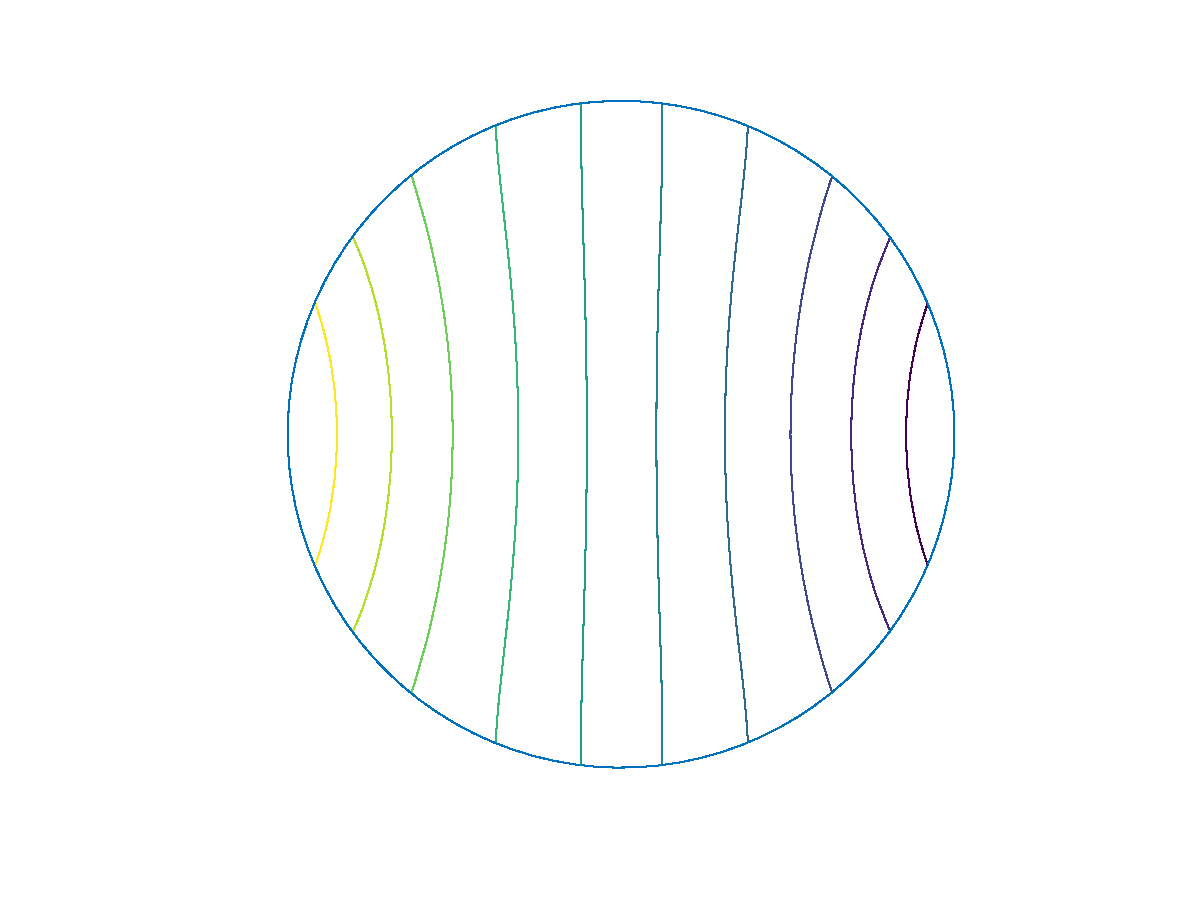
\includegraphics[width=4cm]{kcontour-inc}};
\begin{scope}[x={(image.south east)},y={(image.north west)}]
%  \draw[step=0.1] (0,0) grid (1,1);
%\draw[step=0.01,thin,gray] (0,0) grid (1,1);
\draw(0.85,0.75)node[rotate=45,font=\footnotesize]{$0.1$};
\draw(0.8,0.85)node[rotate=50,font=\footnotesize]{$0.2$};
\draw(0.72,0.95)node[rotate=60,font=\footnotesize]{$0.3$};
\draw(0.6,1)node[rotate=75,font=\footnotesize]{$0.4$};
%
\draw(0.2,0.75)node[shift={(-0.08,0.02)},rotate=-45,font=\footnotesize]{$u=0.9$};
\draw(0.2,0.85)node[rotate=-50,font=\footnotesize]{$0.8$};
\draw(0.28,0.95)node[rotate=-60,font=\footnotesize]{$0.7$};
\draw(0.4,1)node[rotate=-75,font=\footnotesize]{$0.6$};
\draw(0.15,0.5)--(0.9,0.5)node[right]{$x$};
\draw (0.52,0.11)--(0.52,0.92);
\draw(0.52,0.92)--++(0,0.1)node[above]{$y$};
\draw(0.212,0.5)node[ocirc]{};
\draw(0.82,0.5)node[ocirc]{};
    \end{scope}
\end{tikzpicture}
\end{subfigure}%
\caption{سرحدی مخفی قوہ (مثال \حوالہ{مثال_مخفی_ڈرشلے_الف})}
\label{شکل_مثال_مخفی_ڈرشلے_الف}
\end{figure}

\انتہا{مثال}
%=========================

\حصہء{سوالات}

%=======================
\ابتدا{سوال}\quad 
مساوات \حوالہ{مساوات_مخفی_معمہ_پ} کی تصدیق کریں۔
\انتہا{سوال}
%=========================
\ابتدا{سوال}\quad
دکھائیں کہ مساوات \حوالہ{مساوات_مخفی_معمہ_چ} کا ہر جزو قرص \عددی{r^2<R^2} میں ہارمونی تفاعل ہے۔
\انتہا{سوال}
%========================
مساوات \حوالہ{مساوات_مخفی_معمہ_چ} استعمال کرتے ہوئے سوال \حوالہ{سوال_مخفی_ڈرشلے_ب} تا سوال \حوالہ{سوال_مخفی_ڈرشلے_الف} میں اکائی قرص \عددی{r<1} میں مخفی قوہ \عددی{u(r,\theta)} تلاش کریں۔قرص کی سرحد پر مخفی قوہ \عددی{u(1,\theta)} ہے۔تسلسل کے چند ابتدائی اجزاء کے مجموعہ سے \عددی{u} کی قیمت حاصل کرتے ہوئے ہم قوہ خطوط کا ترسیم کھینچیں۔

%=============================  
\ابتدا{سوال}\شناخت{سوال_مخفی_ڈرشلے_الف}\quad
$u(1,\theta)=\sin\theta$\\
جواب:\quad
$u=r\sin\theta$
\انتہا{سوال}
%=======================
\ابتدا{سوال}\quad
$u(1,\theta)=1-\cos\theta$\\
جواب:\quad
$u=1-r\cos\theta$
\انتہا{سوال}
%=======================
\ابتدا{سوال}\quad
$u(1,\theta)=\sin 3\theta$\\
جواب:\quad
$u=r^3\sin 3\theta$
\انتہا{سوال}
%=======================
\ابتدا{سوال}\quad
$u(1,\theta)=\cos 2\theta-\cos 4\theta$\\
جواب:\quad
$u=r^2\cos 2\theta-r^4\cos 4\theta$
\انتہا{سوال}
%=======================
\ابتدا{سوال}\quad
$u(1,\theta)=4\sin^3 \theta$\\
جواب:\quad
$3r\sin\theta-r^3\sin3\theta$
\انتہا{سوال}
%======================
\ابتدا{سوال}\شناخت{سوال_مخفی_درکار_الف}\quad
$u(1,\theta)=\theta$\\
جواب:\quad
$\pi-2r\sin\theta-r^2\sin 2\theta-\tfrac{2r^3}{3}\sin 3\theta-\tfrac{r^4}{2}\sin4\theta-\cdots$
\انتہا{سوال}
%=======================
\ابتدا{سوال}\quad
\عددی{0<\theta<\pi} پر \عددی{u(1,\theta)=1} ہے جبکہ اس وقفہ کے علاوہ \عددی{u(1,\theta)=0} ہے۔\\
جواب:\quad
$\tfrac{1}{2}+\tfrac{2}{\pi}(r\sin \theta+\tfrac{r^3}{3}\sin 3\theta+\tfrac{r^5}{5}\sin 5\theta+\cdots)$
\انتہا{سوال}
%=======================
\ابتدا{سوال}\quad
\عددی{-\tfrac{\pi}{2}<\theta<\tfrac{\pi}{2}} پر \عددی{u(1,\theta)=\theta} ہے جبکہ \عددی{\tfrac{\pi}{2}<\theta<\tfrac{3\pi}{2}} پر 
\عددی{u(1,\theta)=\pi-\theta} ہے۔\\
جواب:\quad
$\tfrac{4}{\pi}(r\sin\theta-\tfrac{r^3}{9}\sin 3\theta+\tfrac{r^5}{25}\sin5\theta-\tfrac{r^7}{49}\sin7\theta\cdots)$
\انتہا{سوال}
%=======================
\ابتدا{سوال}\quad
\عددی{-\pi<\theta<-\tfrac{\pi}{2}} پر \عددی{u(1,\theta)=-\tfrac{\pi}{2}} ہے، \عددی{-\tfrac{\pi}{2}<\theta<\tfrac{\pi}{2}} پر 
\عددی{u(1,\theta)=\theta} ہے اور \عددی{\tfrac{\pi}{2}<\theta<\pi} پر \عددی{u(1,\theta)=\tfrac{\pi}{2}} ہے۔\\
جواب:\quad
$(1+\tfrac{2}{\pi})r\sin\theta-\tfrac{r^2}{2}\sin2\theta+(\tfrac{1}{3}-\tfrac{2}{9\pi})r^3\sin3\theta-\tfrac{r^4}{4}\sin4\theta\cdots$
\انتہا{سوال}
%=======================
\ابتدا{سوال}\شناخت{سوال_مخفی_ڈرشلے_ب}\quad
\عددی{0<\theta<\tfrac{\pi}{2}}  پر \عددی{u(1,\theta)=1} ہے، \عددی{\tfrac{\pi}{2}<\theta<\pi} پر \عددی{u(1,\theta)=-1} ہے جبکہ باقی تمام \عددی{\theta} پر \عددی{u(1,\theta)=0} ہے۔\\
جواب:\quad
$\tfrac{2}{\pi}(r\cos\theta+r^2\sin2\theta-\tfrac{r^3}{3}\cos3\theta+\tfrac{r^5}{5}\cos 5\theta\cdots )$
\انتہا{سوال}
%=========================
\ابتدا{سوال}\quad
مساوات \حوالہ{مساوات_ٹیلر_لوگارتھمی_کسر} استعمال کرتے ہوئے دکھائیں کہ  سوال \حوالہ{سوال_مخفی_ڈرشلے_ب} کے نتیجہ کو  درج ذیل لکھا جا سکتا ہے۔
\begin{align*}
u(r,\theta)=\frac{1}{\pi}\Ln\frac{(1+iz)(1+z^2)}{(1-iz)(1-z^2)}\text{خیالی}
\end{align*}
\انتہا{سوال}
%=====================
\ابتدا{سوال}\quad 
دکھائیں کہ سوال \حوالہ{سوال_مخفی_درکار_الف} کی مخفی قوہ کو \عددی{u(r,\theta)=2\Ln (1+z)\text{خیالی}} لکھا جا سکتا ہے۔
\انتہا{سوال}
%=============================
\ابتدا{سوال}\شناخت{سوال_مخفی_درکار_ب}\quad
مساوات \حوالہ{مساوات_مخفی_معمہ_چ} استعمال کرتے ہوئے دکھائیں کہ  اکائی قرص \عددی{r<1}، جس کا سرحدی مخفی قوہ 
\begin{align*}
u(1,\theta)=
\begin{cases}
-1&-\pi<\theta<0\\
\phantom{-}1&\phantom{-1}0<\theta<\pi
\end{cases}
\end{align*}
ہو،  کے اندر مخفی قوہ \عددی{u(r,\theta)} درج ذیل ہو گا۔
\begin{align*}
u(r,\theta)=\frac{4}{\pi}(r\sin\theta+\tfrac{r^3}{3}\sin3\theta+\tfrac{r^5}{5}\sin 5\theta+\cdots)
\end{align*}
اس تسلسل کے چند ابتدائی اجزاء استعمال کرتے ہوئے \عددی{u} کی قیمتیں حاصل کر کے چند ہم قوہ خطوط ترسیم کریں۔ قوت کی لکیروں (قائمہ الزاویہ خطوط) کو  ترسیم کر کے ان کا شکل \حوالہ{شکل_سوال_مخفی_درکار_ب} کے ساتھ موازنہ کریں۔
\begin{figure}
\centering

\begin{tikzpicture}[x={(0,0cm)},y={(1cm,0cm)},
    z={(0cm,1cm)}]
\begin{scope}[rotate=90]
\pgfmathsetmacro{\r}{1.5}
\foreach \phi in {-72,-54,...,72}{\draw[] ({0},{0},\r)
                \foreach \theta in {5,10,...,180}{--({\r*sin(\phi)*cos(\theta)},{\r*sin(\phi)*sin(\theta)},{\r*cos(\theta)})};}
\foreach \phi/\u in {-18/-0.2,-52/-0.6,54/0.6,18/0.2}{\draw({\r*sin(\phi)*cos(90)},{\r*sin(\phi)*sin(90)},{\r*cos(90)})node[fill=white,font=\tiny]{$\u$};}
\draw(0,0,\r)node[ocirc]{};
\draw(0,0,-\r)node[ocirc]{}--++(0,0,-0.4)node[right]{$x$};
\draw(0,1.05*\r,0)--++(0,0.4,0)node[left]{$y$};
\draw(0,1*\r,-0.525*\r)node[rotate=-20]{$u=1$};
\draw(0,-1.02*\r,0)node[]{$u=-1$};
\end{scope}
\end{tikzpicture}
\caption{شکل برائے سوال \حوالہ{سوال_مخفی_درکار_ب}}
\label{شکل_سوال_مخفی_درکار_ب}
\end{figure}
%

\انتہا{سوال}
%=============================
\ابتدا{سوال}\شناخت{سوال_مخفی_درکار_پ}\quad
مساوات \حوالہ{مساوات_ٹیلر_لوگارتھمی_کسر} استعمال کرتے ہوئے  دکھائیں کہ سوال \حوالہ{سوال_مخفی_درکار_ب} کے نتیجہ کو درج ذیل لکھا جا سکتا ہے۔
\begin{align*}
u(r,\theta)=\frac{2}{\pi}\Ln\frac{1+z}{1-z}\text{خیالی}=\frac{2}{\pi}(\,\,\phase{1+z}-\phase{1-z}\,\,)
\end{align*}
\انتہا{سوال}
%======================
\ابتدا{سوال}\quad
جیومیٹری کے ایک بنیادی مسئلے کو سوال \حوالہ{سوال_مخفی_درکار_پ} کے نتیجے پر لاگو کرتے ہوئے دکھائیں کہ سوال \حوالہ{سوال_مخفی_درکار_ب} میں \عددی{u=\text{مستقل}} دائری قوس ہیں۔
\انتہا{سوال}
%=========================
\ابتدا{سوال}\شناخت{سوال_مخفی_درکار_ت}\quad
دکھائیں کہ بالائی نصف مستوی \عددی{v>0} میں درج ذیل ہارمونی ہے اور وقفہ \عددی{-1<u<1} پر اس کی قیمت \عددی{-1} جبکہ باقی \عددی{u} محور  پر اس کی قیمت \عددی{+1} ہے۔ 
\begin{align*}
H=1+\frac{2}{\pi}\Ln\frac{w+1}{w-1}\text{خیالی}\quad\quad \quad (w=u+iv)
\end{align*}
\انتہا{سوال}
%===========================
\ابتدا{سوال}\quad
دکھائیں کہ وہ خطی کسری تبادل جو \عددی{w_1=-1}، \عددی{w_2=0}، \عددی{w_3=1} کو بالترتیب \عددی{z_1=-1}، \عددی{z_2=-i}، \عددی{z_3=1}  پر نقش کرتا ہو
\begin{align*}
z=\frac{w-i}{-iw+1}
\end{align*}
ہے۔اس کا الٹ تبادل \عددی{w=w(z)} تلاش کرتے ہوئے سوال \حوالہ{سوال_مخفی_درکار_ت} میں دیے گئے \عددی{H} میں پر کرتے ہوئے دکھائیں کہ حاصل ہارمونی تفاعل سوال \حوالہ{سوال_مخفی_درکار_پ} کا ہارمونی تفاعل ہے۔
\انتہا{سوال}
%===========================
\ابتدا{سوال}\quad
مسئلہ \حوالہ{مسئلہ_مخفی_ہارمونی_تفاعل_کے_جزوی_تفرق} کو پوسوں کلیہ تکمل مساوات \حوالہ{مساوات_مخفی_معمہ_ٹ} سے اخذ کریں۔
\انتہا{سوال}
%===============================



\باب{اعدادی تجزیہ}
انجینئری حساب کا نتیجہ آخرکار اعدادی ہوتا ہے لہٰذا انجینئری طالب علم  کے لئے بنیادی \اصطلاح{اعدادی تراکیب}\فرہنگ{اعدادی!تراکیب}\حاشیہب{numerical methods}\فرہنگ{numerical!methods} جاننا ضروری ہیں جن کی مدد سے دیے گئے مواد سے اعدادی جوابات اخذ کرنا ممکن ہو۔

بعض اوقات نظریہ سے حاصل کردہ جوابات عملاً قابل استعمال نہیں ہوتے ہیں، مثلاً یک درجی خطی تفرقی مساوات کے حل کا تکملی کلیہ (حصہ \حوالہ{حصہ_سادہ_اول_خطی_اور_برنولی})، خطی الجبرائی مساوات کے نظام کا مقطع کی مدد سے حل بذریعہ قاعدہ کریمر (حصہ \حوالہ{حصہ_الجبرا_قاعدہ_کریمر})۔کئی بار نظریہ صرف حل کی وجودیت کی یقین دہانی کرتا ہے لیکن اصل حل حاصل کرنے کے بارے میں کوئی مدد فراہم نہیں کرتا ہے۔

اعدادی تراکیب کی اہمیت کمپیوٹر کی ایجاد کی نظر ہے۔ ہم ان تراکیب کے نظریہ اور عملی استعمال پر غور کریں گے۔\اصطلاح{تجزیہ خلل}\فرہنگ{تجزیہ!خلل}\فرہنگ{خلل!تجزیہ}\حاشیہب{error analysis}\فرہنگ{error!analysis} پر بھی غور کیا جائے گا جو اعدادی تراکیب میں زیادہ اہمیت کے حامل ہے۔     

%==============================
\حصہ{خلل اور غلطیاں۔ کمپیوٹر}\شناخت{حصہ_اعدادی_خلل_غلطیاں_کمپیوٹر}
چونکہ اعدادی تراکیب میں متناہی تعداد کے اعداد استعمال کرتے ہوئے متناہی تعداد کے چال کے بعد جواب حاصل کیا جاتا ہے لہٰذا  یہ تراکیب \اصطلاح{متناہی چال}\فرہنگ{متناہی چال}\حاشیہب{finite processes}\فرہنگ{finite process}  ہیں جو اصل (نا معلوم) بالکل درست حل کی \اصطلاح{تخمین}\فرہنگ{تخمین}\حاشیہب{approximation}\فرہنگ{approximation} پیش کرتے ہیں ماسوائے ان چند صورتوں میں جب اصل جواب کافی سادہ ناطق عدد ہو اور ہم کوئی ایسا اعدادی ترکیب استعمال کریں جو یہی بالکل درست جواب فراہم کرتا ہو۔

اگر کسی مقدار کی اندازاً قیمت \عددی{a^*} ہو اور اس کی اصل قیمت \عددی{a} ہو تب فرق \عددی{\epsilon=a^*-a} کو \عددی{a^*} کا \ترچھا{حتمی خلل} یا مختصراً \عددی{a^*} کا \اصطلاح{خلل}\فرہنگ{خلل}\حاشیہب{error}\فرہنگ{error}  کہتے ہیں۔یوں
\begin{align*}
a^*=a+\epsilon\quad \quad \text{\RL{خلل $\,\,+\,\,$ اصل قیمت $\,\,=\,\,$ تخمین}}
\end{align*}
ہو گا۔ \عددی{a^*} کی \اصطلاح{اضافی خلل}\فرہنگ{خلل!اضافی}\حاشیہب{relative error}\فرہنگ{error!relative} \عددی{\epsilon_r} کی تعریف درج ذیل ہے۔
\begin{align*}
\epsilon_r=\frac{\epsilon}{r}=\frac{a^*-a}{a}=\frac{\text{خلل}}{\text{\RL{اصل قیمت}}}\quad \quad (a\ne 0)
\end{align*}
ظاہر ہے اگر \عددی{\abs{\epsilon}} کی قیمت \عددی{\abs{a^*}} کی قیمت سے بہت کم ہو تب \عددی{\epsilon_r\approx \tfrac{\epsilon}{a^*}} ہو گا۔ہم ایک نئی مقدار \عددی{\gamma=a-a^*=-\epsilon} متعارف کرتے ہیں جس کو ہم \اصطلاح{درستگی}\فرہنگ{درستگی}\حاشیہب{correction}\فرہنگ{correction}\حاشیہد{بعض اوقات خلل کی تعریف \عددی{\gamma=-\epsilon} لی جاتی ہے۔آپ کسی ایک تعریف کو تسلیم کرتے ہوئے آگے بڑھ سکتے ہیں۔ہم خلل کی تعریف \عددی{\epsilon} لیں گے۔} کہیں گے۔یوں
\begin{align*}
a=a^*+\gamma\quad \quad  \text{\RL{درستگی $\,\,+\,\,$ تخمین $\,\,=\,\,$ اصل قیمت}}
\end{align*}
ہو گا۔آخر میں \عددی{a^*} کی \اصطلاح{حد خلل}\فرہنگ{حد!خلل}\فرہنگ{خلل!حد}\حاشیہب{error bound}\فرہنگ{error!bound} سے مراد عدد \عددی{\beta} ہے  جس کی تعریف درج ذیل ہے۔
\begin{align*}
\abs{a^*-a}\le \beta \quad \implies \quad  \abs{\epsilon}\le \beta
\end{align*}

خلل کی تین قسمیں تجربی خلل، قطع چال خلل اور تعداد اعداد خلل ہیں۔\اصطلاح{تجربی خلل}\فرہنگ{خلل!تجربی}\حاشیہب{Experimental errors}\فرہنگ{error!experimental} سے مراد مواد میں خلل ہے (جو تجربی ناپ کی وجہ سے ہو سکتے ہیں)۔بالکل درست جواب تک پہنچنے کی خاطر متناہی (یا لامتناہی) تعداد کے حسابی چال (قدم) درکار ہوں گے۔حقیقت میں کسی خاص تعداد کے چال بعد حساب روک دیا جاتا ہے اور یوں \اصطلاح{قطع چال خلل}\فرہنگ{خلل!قطع چال}\حاشیہب{Truncation error}\فرہنگ{error!truncation} پیدا ہو گا۔  ہر قدم پر حساب کے دوران کمپیوٹر متناہی تعداد کے اعداد استعمال کرتے ہوئے کمتر ہندسہ سے کم قیمتوں کو رد کرتا ہے جس سے \اصطلاح{تعداد ہندسہ خلل}\فرہنگ{خلل!تعداد ہندسہ}\حاشیہب{rounding error}\فرہنگ{error!round off} پیدا ہو گا جس پر ہم اب غور کرتے ہیں۔

اعشاری نظام میں ہر عدد کو متناہی یا لامتناہی تعداد کے اعشاری ہندسوں سے ظاہر کیا جاتا ہے۔کمپیوٹر لامتناہی تعداد کے ہندسوں کو ذخیرہ نہیں کر سکتا ہے لہٰذا کمپیوٹر استعمال کرتے ہوئے کسی بھی عدد کو متناہی تعداد کی ہندسوں سے ظاہر کیا جاتا ہے۔ان اعداد کو دو طریقوں سے کمپیوٹر میں  ذخیرہ کیا جاتا ہے۔ \اصطلاح{مقررہ نقطہ}\فرہنگ{مقررہ نقطہ نظام}\حاشیہب{fixed point}\فرہنگ{fixed point} نظام میں نقطہ اعشاریہ کے بعد مقررہ تعداد کے ہندسے  پائے جاتے ہیں مثلاً \عددی{35.143}، \عددی{5.000}، \عددی{0.076} جبکہ \اصطلاح{غیر مقررہ نقطہ}\فرہنگ{غیر مقررہ نقطہ نظام}\حاشیہب{floating point}\فرہنگ{floating point} نظام میں \اصطلاح{ملحوظ ہندسوں}\فرہنگ{ملحوظ ہندسے}\حاشیہب{significant digits}\فرہنگ{significant digits} کی تعداد متعین ہوتی ہے مثلاً \عددی{0.6723\times10^2}، \عددی{-0.2354\times10^{-4}} اور \عددی{-0.1000\times10^1} جہاں ملحوظ ہندسوں کی تعداد چار ہے۔عدد \عددی{c} کے ملحوظ ہندسہ سے مراد \عددی{c} کا ہر ہندسہ ہے ماسوائے پہلا غیر صفر عدد کی بائیں جانب صفر جو اعشاریہ کا مقام تعین کرتا ہو۔ (یوں اس کے علاوہ ہر صفر بھی \عددی{c} کا ملحوظ ہندسہ ہو گا۔) مثال کے طور پر \عددی{5420}، \عددی{1.340} اور \عددی{0.001460} میں سے ہر ایک میں چار ملحوظ ہندسے\حاشیہد{ایسا جدول جو \عددی{k} ملحوظ ہندسے دیتا ہو میں، جب تک کہا نا جائے کہ ایسا نہیں ہے،  ہم فرض کرتے ہیں کہ  دیا گیا عدد \عددی{a^*}،  بالکل درست قیمت \عددی{a} سے آخری ہندسے کی \عددی{\mp 0.5} اکایاں مختلف ہو سکتا ہے۔مثال کے طور پر اگر \عددی{a=1.1996} ہو تب چار ملحوظ ہندسوں کا جدول \عددی{a^*=1.200} دے گا۔} ہیں۔

تعداد ہندسہ خلل کا قاعدہ اب بیان کرتے ہیں۔(\عددی{k} ملحوظ ہندسوں تک قطع کرنے کی تعریف بھی یہی ہے پس اس میں ہندسہ کی جگہ ملحوظ ہندسہ پر کریں۔)

\عددی{k+1} واں ہندسہ اور اس کے بعد تمام ہندسوں کو رد کریں۔اگر رد شدہ عدد مقام \عددی{k} کی اکائی کی نصف سے کم ہو تب مقام \عددی{k} پر ہندسہ کو تبدیل نہ کریں ("گھٹانا")۔اگر رد شدہ عدد مقام \عددی{k} کی اکائی کی نصف سے زیادہ ہو تب تب مقام \عددی{k} کی ہندسے کے ساتھ \عددی{1} جمع کریں ("بڑھانا")۔اگر رد شدہ عدد مقام \عددی{k} کی اکائی کا نصف ہو تب اگر مقام \عددی{k} کا ہندسہ طاق ہو تب اس کو بڑھا کر جفت بنائیں۔(مثال کے طور پر \عددی{3.45} اور \عددی{3.55} کو اشاریہ کے بعد ایک ہندسہ تک قطع کرتے ہوئے بالترتیب \عددی{3.4} اور \عددی{3.6} حاصل ہو گا۔)

اس قاعدہ کا آخری حصہ یقینی بناتا ہے کہ  عدد کا کمتر حصہ رد کرتے ہوئے اوسطاً برابر مرتبہ عدد بڑھایا اور گھٹایا جاتا ہے۔ 

اگر ہم \عددی{1.2535} کو \عددی{3}، \عددی{2} اور \عددی{1} اشاریہ تک قطع کریں تب ہمیں بالترتیب \عددی{1.254}، \عددی{1.25} اور \عددی{1.3} حاصل ہو گا لیکن، بغیر مزید  معلومات کے، \عددی{1.25} کو ایک اشاریہ تک قطع کرنے سے ہمیں \عددی{1.2} ملتا ہے۔

تعداد ہندسہ خلل کی وجہ سے کوئی بھی حساب مکمل غلط ہو سکتا ہے۔عموماً چال کی تعداد بڑھانے سے یہ خلل بڑھتا ہے۔یوں حسابی پروگرام کو اس خلل کی نقطہ نظر سے دیکھنا ضروری ہو گا اور اس خلل کو کم سے کم کرنا لازم ہو گا۔

\حصہ{دہرانے سے مساوات کا حل}
ہمیں عموماً مساوات 
\begin{align}\label{مساوات_اعدادی_تفاعل_الف}
f(x)=0
\end{align}
کے حل درکار ہوتے ہیں یعنی ایسے عدد \عددی{X_0} کہ \عددی{f(X_0)} صفر کے برابر ہو جہاں \عددی{f} دیا گیا تفاعل ہے۔مثال کے طور پر \عددی{x^2-3x+2=0}، \عددی{x^3+x=1}، \عددی{\sin x=0.5 x}، \عددی{\tan x=x}، \عددی{\cosh x=\sec x} اور \عددی{\cosh x\cos x=-1} کو مساوات \حوالہ{مساوات_اعدادی_تفاعل_الف} کی صورت میں لکھا جا سکتا ہے۔ ان میں پہلے دو میں \عددی{f} کثیر رکنی ہے لہٰذا یہ دونوں \اصطلاح{الجبرائی مساوات}\فرہنگ{الجبرائی!مساوات}\حاشیہب{algebraic equations}\فرہنگ{algebraic equations} ہیں جن کے حل کو \اصطلاح{جذر}\فرہنگ{جذر}\حاشیہب{roots}\فرہنگ{roots} کہتے ہیں۔باقی \اصطلاح{ماورائی مساوات}\فرہنگ{مساوات!ماورائی}\فرہنگ{ماورائی!مساوات}\حاشیہب{transcendental equations}\فرہنگ{transcendental!equations} ہیں جن میں ماورائی تفاعل استعمال ہوئے ہیں۔حقیقتاً صرف انتہائی سادہ صورتوں میں مکمل درست حل نکالنے والے کلیات موجود ہوں گے۔عموماً ہم دہرانے کی ترکیب یا دیگر تراکیب سے اصل حل کا تخمینہ حاصل کریں گے۔

اعدادی دہرانے کے طریقہ میں ہم اختیاری \عددی{x_0} منتخب کرتے ہوئے  درج ذیل روپ کلیہ
\begin{align}\label{مساوات_اعدادی_تفاعل_ب}
x_{n+1}=g(x_n)\quad \quad \quad (n=0,1,2,\cdots)
\end{align}
سے، بار بار حل کرتے ہوئے، ترتیب \عددی{x_0, x_1, x_2,\cdots} حاصل کرتے ہیں جہاں \عددی{g} کسی ایسے وقفہ پر معین ہے جس پر \عددی{x_0} پایا جاتا ہو اور \عددی{g}  کا حلقہ اسی وقفہ پر ہے۔ یوں ہم یک بعد دیگرے \عددی{x_1=g(x_0)}،  \عددی{x_2=g(x_1)}، \عددی{x_3=g(x_2)}، \نقطے حاصل کرتے ہیں۔

اس حصہ میں دائرہ کار اور حلقہ \عددی{g(x)} دونوں حقیقی لکیر پر ہوں گے۔زیادہ عمومی معمہ میں \عددی{x} یا \عددی{g} اور یا دونوں سمتیات ہو سکتے ہیں۔

دہرانے کے تراکیب اعدادی تجزیہ کے لئے انتہائی اہم ہیں۔

مساوات \حوالہ{مساوات_اعدادی_تفاعل_الف} کو حل کرنے کے لئے  دہرانے کے تراکیب کئی طریقوں سے حاصل کیے جا سکتے ہیں۔ہم ان میں سے تین خصوصاً اہم طریقوں پر غور کرتے ہیں۔

\جزوحصہء{الجبرائی تبادل}
 ہم مساوات \حوالہ{مساوات_اعدادی_تفاعل_الف} کو الجبرائی طور پر تبدیل کرتے ہوئے درج ذیل روپ حاصل کر سکتے ہیں
\begin{align}\label{مساوات_اعدادی_تفاعل_پ}
x=g(x)
\end{align}
جو مساوات \حوالہ{مساوات_اعدادی_تفاعل_ب}  کی روپ میں ہے۔مساوات \حوالہ{مساوات_اعدادی_تفاعل_پ} کے حل کو \عددی{g} کا \اصطلاح{مقررہ نقطہ}\فرہنگ{مقررہ نقطہ}\حاشیہب{fixed point}\فرہنگ{fixed point} کہتے ہیں۔دیے گئے مساوات \حوالہ{مساوات_اعدادی_تفاعل_الف} کے کئی مطابقتی مساوات \حوالہ{مساوات_اعدادی_تفاعل_پ} ہو سکتے ہیں جن کے ترتیب \عددی{x_0,x_1,\cdots} مختلف (اور \عددی{x_0} کے تابع) ہوں گے۔آئیں ایک سادہ مثال دیکھتے ہیں جس میں یہ حقائق ابھر کر سامنے آتے ہیں۔

%=================
\ابتدا{مثال}\شناخت{مثال_اعدادی_دہرانا_الف}\quad \موٹا{دہرانے کی ترکیب}\\
مساوات \عددی{f(x)=x^2-3x+1=0} کے لئے دہرانے کی ترکیب عمل میں لائیں۔چونکہ ہمیں اس مساوات کے حل
\begin{align*}
x=1.5\mp\sqrt{1.25},\quad x_1=\num{2.618034},\quad x_2=\num{0.381966}
\end{align*}
معلوم ہیں، ہم دہرانے کے عمل کے دوران خلل کا رویہ دیکھ سکتے ہیں۔ہم دیے گئے مساوات سے
\begin{align}\label{مساوات_مثال_اعدادی_دہرانا_الف}
x=g_1(x)=\frac{1}{3}(x^2+1)\quad \implies \quad x_{n+1}=\frac{1}{3}(x_n^2+1)
\end{align}
لکھ سکتے ہیں۔یوں \عددی{x_0=1} منتخب کرتے ہوئے ہمیں درج ذیل ترتیب ملتی ہے
\begin{align*}
x_0=\num{1.000},\quad x_1=\num{0.667},\quad x_2=\num{0.481},\quad x_3=\num{0.411},\quad x_4=\num{0.390}, \cdots
\end{align*}
جو چھوٹے جذر کی طرف گامزن ہے (شکل \حوالہ{شکل_مثال_اعدادی_دہرانا_الف}-الف)۔اگر ہم \عددی{x_0=3.000} منتخب کریں تب درج ذیل ملتا ہے
\begin{align*}
x_0=\num{3.000},\quad x_1=\num{3.333},\quad x_2=\num{4.037},\quad x_3=\num{5,766},\quad x_4=\num{11.414}, \cdots
\end{align*}
جو منفرج ترتیب ہے (شکل \حوالہ{مثال_اعدادی_دہرانا_الف}-الف)۔دی گئی مساوات سے درج ذیل بھی حاصل کیا جا سکتا ہے۔
\begin{align}\label{مساوات_مثال_اعدادی_دہرانا_ب}
x=g_2(x)=3-\frac{1}{x}\quad \implies \quad x_{n+1}=3-\frac{1}{x_n}
\end{align}
اب \عددی{x_0} منتخب کرتے ہوئے
\begin{align*}
x_0=\num{1.000},\quad x_1=\num{2.000},\quad x_2=\num{2.500},\quad x_3=\num{2.600},\quad x_4=\num{2.615}, \cdots
\end{align*}
حاصل ہوتا ہے جو بڑے جذر کی طرف گامزن ترتیب ہے (شکل \حوالہ{مثال_اعدادی_دہرانا_الف}-ب)۔اسی طرح \عددی{x_0=3} منتخب کرتے ہوئے
\begin{align*}
x_0=\num{3.000},\quad x_1=\num{2.667},\quad x_2=\num{2.625},\quad x_3=\num{2.619},\quad x_4=\num{2.618}, \cdots
\end{align*}
حاصل ہوتا ہے (شکل \حوالہ{مثال_اعدادی_دہرانا_الف}-ب)۔شکل کو دیکھ کر واضح ہوتا ہے کہ مرکوزیت اس صورت ہو گی جب حل کی پڑوس میں منحنی \عددی{g(x)} کی ڈھلوان سیدھے خط \عددی{y=x} کی ڈھلوان سے کم ہو۔ہم اب دیکھتے ہیں کہ مرکوزیت کے لئے \عددی{\abs{g'(x)<1}}  کی شرط کافی ہے (جہاں خط \عددی{y=x} کی ڈھلوان \عددی{y'=1} ہے)۔
\begin{figure}
\centering
\begin{subfigure}{0.5\textwidth}
\centering
\begin{tikzpicture}
\draw(0,0)--(5,0)node[below]{$x$};
\draw(0,0)--(0,5);
\draw(0,0)--(5,5);
\draw[thick,domain=0:3.74] plot ({\x},{1/3*(\x^2+1)});
\draw[->-=0.7](1,1)--(1,2/3);
\draw(1,2/3)--(2/3,2/3)--(2/3,0.481)--(0.481,0.481)--(0.481,0.411);
\draw[->-=0.7](3,3)--(3,3.333);
\draw(3,3.333)--(3.333,3.333)--(3.333,4.037)--(4.037,4.035)--(4.037,5);
\draw(3.74,5)node[below left, xshift={(-0.1cm)}]{$g_1(x)$};
\foreach \x in {1,2,3,4}{\draw(\x,0)node[below]{$\x$}--++(0,0.2);}
\foreach \y in {1,2,3,4}{\draw(0,\y)node[left]{$\y$}--++(0.2,0);}
\end{tikzpicture}
\caption*{(الف)}
\end{subfigure}%
\begin{subfigure}{0.5\textwidth}
\centering
\begin{tikzpicture}
\draw(0,0)--(5,0)node[below]{$x$};
\draw(0,0)--(0,5);
\draw(0,0)--(5,5)node[below left,xshift={(-0.2cm)}]{$y=x$};
\draw[smooth,thick,domain=1/3:5] plot ({\x},{(3-1/(\x))});
\draw[->-=0.7](1,1)--(1,2);
\draw(1,2)--(2,2)--(2,2.5)--(2.5,2.5)--(2.5,2.6)--(2.6,2.6)--(2.6,2.615);
\draw[->-=0.7](3,3)--(3,2.667);
\draw(3,2.667)--(2.667,2.667)--(2.667,2.625);
\draw(5,2.8)node[below]{$g_2(x)$};
\foreach \x in {1,2,3,4}{\draw(\x,0)node[below]{$\x$}--++(0,0.2);}
\foreach \y in {1,2,3,4}{\draw(0,\y)node[left]{$\y$}--++(0.2,0);}
\end{tikzpicture}
\caption*{(ب)}
\end{subfigure}%
\caption{اشکال برائے مثال \حوالہ{مثال_اعدادی_دہرانا_الف}}
\label{شکل_مثال_اعدادی_دہرانا_الف}
\end{figure}
\انتہا{مثال}
%=========================

اگر \عددی{x_0} کا  مطابقتی  مساوات \حوالہ{مساوات_اعدادی_تفاعل_ب} سے حاصل کردہ ترتیب \عددی{x_0,x_1,\cdots} مرتکز ہو تب ہم کہتے ہیں کہ مساوات \حوالہ{مساوات_اعدادی_تفاعل_ب} میں دی گئی دہرانے کی ترکیب \اصطلاح{مرتکز}\فرہنگ{مرتکز} ہے۔

ارتکاز کے لئے کافی شرط درج ذیل مسئلہ پیش کرتا ہے جس کے کئی اہم عملی استعمال پائے جاتے ہیں۔

%=====================
\ابتدا{مسئلہ}\شناخت{مسئلہ_اعدادی_ارتکاز_شرط}\quad \موٹا{(ارتکاز)}\\
فرض کریں کہ \عددی{x=g(x)} کا حل \عددی{x=s} ہے اور فرض کریں کہ کسی ایسے وقفہ \عددی{J}، جس میں \عددی{s} پایا جاتا ہو، پر \عددی{g(x)} کا استمراری تفرق پایا جاتا ہے۔ اب اگر \عددی{J} میں \عددی{\abs{g'(x)}\le \alpha<1} ہو تب مساوات \حوالہ{مساوات_اعدادی_تفاعل_ب} میں دی گئی دہرانے کی ترکیب \عددی{J} میں ہر \عددی{x_0} کے لئے مرتکز ہو گی۔
\انتہا{مسئلہ}
%==========================
\ابتدا{ثبوت}\quad
تفرقی علم الاحصاء کے مسئلہ اوسط قیمت کے تحت \عددی{x} اور \عددی{s} کے درمیان ایسا \عددی{\xi} پایا جائے گا جو درج ذیل کو مطمئن کرے گا،
\begin{align*}
g(x)-g(s)=g'(\xi)(x-s) 
\end{align*}
جہاں \عددی{x} وقفہ \عددی{J} میں پایا جاتا ہے۔  چونکہ \عددی{g(s)=s} اور \عددی{x_1=g(x_0)}، \عددی{x_2=g(x_1)}، \نقطے ہیں لہٰذا ہمیں درج ذیل ملتا ہے۔
\begin{align*}
\abs{x_n-s}&=\abs{g(x_{n-1})-g(s)}=\abs{g'(\xi)}\abs{x_{n-1}-s}\le \alpha \abs{x_{n-1}-s}\\
&\le \alpha^2\abs{x_{n-2}-s}\le \cdots \le \alpha^n\abs{x_{0}-s}
\end{align*}
چونکہ \عددی{\alpha<1} ہے لہٰذا  \عددی{n\to \infty} کرنے سے \عددی{\alpha^n\to 0} اور \عددی{\abs{x_n-s}\to 0} ہوں گے۔یوں ثبوت مکمل ہوتا ہے۔
\انتہا{ثبوت}
%=======================
\ابتدا{مثال}\شناخت{مثال_اعدادی_دہرانا_ب}\quad \موٹا{دہرانے کا طریقہ۔ مسئلہ \حوالہ{مسئلہ_اعدادی_ارتکاز_شرط}}\\
دہرانے کے طریقہ سے \عددی{f(x)=x^3+x-1=0} کا حل  تلاش کریں۔اس مساوات کا جلدی سے خاکہ  بنا کر آپ دیکھ سکتے ہیں کہ اس کا جذر \عددی{x=1} کے قریب پایا جاتا ہے۔  ہم اس  مساوات سے درج ذیل لکھ سکتے ہیں۔
\begin{align*}
x=g_1(x)=\frac{1}{1+x^2}\quad \implies \quad x_{n+1}=\frac{1}{1+x_n^2}
\end{align*}
یوں کسی بھی \عددی{x} کے لئے \عددی{\abs{g'_1(x)}=\tfrac{2\abs{x}}{(1+x^2)^2}<1} ہو گا لہٰذا تمام \عددی{x} پر مرکوزیت پائی جائے گی۔ہم \عددی{x_0=1} منتخب کرتے ہوئے درج ذیل حاصل کرتے ہیں (شکل \حوالہ{شکل_مثال_اعدادی_دہرانا_ب})
\begin{align*}
x_1=0.500,\quad x_2=0.800,\quad x_3=0.610,\quad x_4=0.729,\quad x_5=0.653,\quad x_6=0.701,\cdots
\end{align*}
جبکہ چھ ہندسوں تک درست اصل جذر \عددی{s=\num{0.682328}} ہے۔ ہم مساوات سے درج ذیل بھی لکھ سکتے ہیں۔
\begin{align*}
x=g_2(x)=1-x^3,\quad \abs{g_2'(x)}=3x^2 
\end{align*}
جذر کے قریب \عددی{ \abs{g'_2}} کی قیمت اکائی سے زیادہ ہے لہٰذا ہم ارتکاز کی توقع نہیں کر سکتے ہیں۔آپ \عددی{x_0=1}، \عددی{x_0=0.5}، \عددی{x_0=2} سے شروع کرتے ہوئے اپنی تسلی کر سکتے ہیں۔
\begin{figure}
\centering
\begin{tikzpicture}
\pgfmathsetmacro{\k}{5}
\draw(0,0)--(5.75,0)node[right]{$x$};
\draw(0,0)--(0,5.5);
\draw(0,0)--(5,5);
\draw[thick,domain=0:1.1] plot ({\k*\x},{\k/(\x^2+1)});
\draw[->-=0.5](\k*1,0)--(\k*1,\k*0.5);
\draw[->-=0.5](\k*1,\k*0.5)--(\k*0.5,\k*0.5)node[below right]{$x_1$};
\draw[->-=0.5](\k*0.5,\k*0.5)--(\k*0.5,\k*0.8);
\draw[->-=0.5](\k*0.5,\k*0.8)--(\k*0.8,\k*0.8)node[above left]{$x_2$};
\draw[->-=0.5](\k*0.8,\k*0.8)--(\k*0.8,\k*0.61);
\draw[->-=0.7](\k*0.8,\k*0.61)--(\k*0.61,\k*0.61);
\draw[->-=0.7](\k*0.61,\k*0.61)--(\k*0.61,\k*0.729);
\draw(1,5)node[right]{$g_1(x)$};
\foreach \x in {1,2,...,11}{\draw(\x/2,0)--++(0,0.2);}
\foreach \y in {1,2,...,10}{\draw(0,\y/2)--++(0.2,0);}
\draw(5/2,0)node[below]{$0.5$};
\draw(10/2,0)node[below]{$1.0$};
\draw(0,5/2)node[left]{$0.5$};
\draw(0,10/2)node[left]{$1.0$};
\draw(0,0)node[below]{$0$};
\draw(0,0)node[left]{$0$};
\end{tikzpicture}
\caption{شکل برائے مثال \حوالہ{مثال_اعدادی_دہرانا_ب}}
\label{شکل_مثال_اعدادی_دہرانا_ب}
\end{figure}%
\انتہا{مثال}
%=========================

\جزوحصہء{ترکیب نیوٹن}
مساوات \عددی{f(x)=0}، جہاں \عددی{f} قابل تفرق ہے، کو \موٹا{ترکیب نیوٹن} سے بھی حل کیا جا سکتا ہے۔اس ترکیب میں ہم \عددی{f(x)} کا تخمینہ اس کے موزوں مماس سے حاصل کرتے ہیں۔اس ترکیب میں ہم \عددی{f} کی ترسیم سے حاصل \عددی{x_0} پر \عددی{f} کا مماس بناتے ہیں۔یہ مماس \عددی{x} محور کو \عددی{x_1} پر قطع کرتا ہے (شکل \حوالہ{شکل_اعدادی_ترکیب_نیوٹن})۔یوں
\begin{align*}
\tan\beta=f'(x_0)=\frac{f(x_0)}{x_0-x_1}\quad \implies \quad x_1=x_0-\frac{f(x_0)}{f'(x_0)}
\end{align*}
ہو گا۔اگلے قدم پر ہم
\begin{align*}
x_2=x_1-\frac{f(x_1)}{f'(x_1)}
\end{align*}
حاصل کرتے ہیں۔اسی طرح چلتے ہوئے جذر تک پہنچا جاتا ہے۔یوں دہرانے کے طریقے کا عمومی کلیہ درج ذیل ہو گا۔
\begin{align}\label{مساوات_اعدادی_ترکیب_نیوٹن}
x_{n+1}=x_n-\frac{f(x_n)}{f'(x_n)}\quad \quad \quad (n=0,1,\cdots)
\end{align}
%
\begin{figure}
\centering
\begin{tikzpicture}
\draw(0,-0.5)--(0,3)node[left]{$y$};
\draw[name path=kA](0,0)--(5.5,0)node[right]{$x$};
\draw[thick,name path=kCurve] (0.5,-0.5) to [out=10,in=-120] coordinate[pos=0.9](pA)(5,3)node[right]{$y=f(x)$};
\draw[dashed] (pA)--($(0,0)!(pA)!(5,0)$)coordinate(pAA)node[below]{$x_0$};
\path[name path=kB](pA)--++(60:-3);
\draw[name intersections={of={kA and kB}}] (pA)--(intersection-1)coordinate(pB)node[below]{$x_1$};
\path[name path=kC] (intersection-1)--++(0,1);
\draw[dashed,name intersections={of=kCurve and kC}] (pB)--(intersection-1)coordinate(pC);
\path[name path=kD](pC)--++(40:-2);
\draw[name intersections={of={kD and kA}}] (pC)--(intersection-1)coordinate(pD)node[below]{$x_2$};
\path[name path=kE] (pD)--++(0,1);
\draw[dashed,name intersections={of=kE and kCurve}] (pD)--(intersection-1);
%
\draw[name intersections={of=kA and kCurve}] (intersection-1)node[ocirc]{};
\draw [decorate,decoration={brace,amplitude=10pt},xshift=-4pt,yshift=0pt]
(pA) -- (pAA) node [black,midway,xshift=0.8cm] {\footnotesize $f(x_0)$};
%
\draw(pA)node[ocirc]{};
\draw(pC)node[ocirc]{};
\draw(0,0)node[ocirc]{};
%
\draw[-stealth]([shift={(0:0.5)}]pB) arc (0:60:0.5);
\draw(pB)++(30:0.8)node[]{$\beta$};
\end{tikzpicture}
\caption{ترکیب نیوٹن}
\label{شکل_اعدادی_ترکیب_نیوٹن}
\end{figure}

%=====================
\ابتدا{مثال}\شناخت{مثال_اعدادی_دہرانا_پ}\quad \موٹا{جذر المربع}\\
کسی مثبت حقیقی عدد \عددی{c} کا جذر المربع حاصل کرنے کے لئے دہرانے کی ترکیب بنائیں۔اس ترکیب کو استعمال کرتے ہوئے \عددی{c=2} کا جذر المربع تلاش کریں۔ہمارے پاس \عددی{\sqrt{c}}  یعنی \عددی{f(x)=x^2-c=0} ہے لہٰذا \عددی{f'(x)=2x} ہو گا۔یوں مساوات \حوالہ{مساوات_اعدادی_ترکیب_نیوٹن} درج ذیل صورت اختیار کرتی ہے۔
\begin{align*}
x_{n+1}=x_n-\frac{x_n^2-c}{2x_n}=\frac{1}{2}\big(x_n+\frac{c}{x_n}\big)
\end{align*}
اب اس ترکیب سے \عددی{c=2} کا جذر المربع تلاش کرتے ہیں۔ہم \عددی{x_0=1} منتخب کرتے ہوئے درج ذیل حاصل کرتے ہیں۔
\begin{align*}
x_1=\num{1.500000},\quad x_2=\num{1.416667},\quad x_3=\num{1.414216},\quad x_4=\num{1.414214},\cdots
\end{align*}
\عددی{2} کا جذر المربع \عددی{\num{1.414213562}} ہے اور آپ دیکھ سکتے ہیں کہ \عددی{x_4} چھ ملحوظ ہندسوں تک درست جواب دیتا ہے۔
\انتہا{مثال}
%===========================
\ابتدا{مثال}\شناخت{مثال_اعدادی_ماورائی_الف}\quad \موٹا{ماورائی مساوات کا دہرانے کی ترکیب سے حل}\\
مساوات \عددی{2\sin x=x} کا مثبت حل تلاش کریں۔ہم \عددی{f(x)=x-2\sin x} لکھتے ہوئے \عددی{f'(x)=1-2\cos x} حاصل کرتے ہیں۔یوں مساوات \حوالہ{مساوات_اعدادی_ترکیب_نیوٹن} کی صورت درج ذیل ہو گی۔
\begin{align*}
x_{n+1}=x_n-\frac{x_n-2\sin x_n}{1-2\cos x_n}=\frac{2(\sin x_n-x_n\cos x_n)}{1-2\cos x_n}=\frac{N_n}{D_n}
\end{align*}
\عددی{f} کی ترسیم سے ہم دیکھتے ہیں کہ اس کا حل \عددی{x_0=2} کے قریب ہے۔یوں ہم جدول \حوالہ{جدول_مثال_اعدادی_ماورائی_الف} حاصل کرتے ہیں۔چار ملحوظ ہندسوں تک درست جواب \عددی{1.8955} ہے۔
\begin{table}
\caption{جدول برائے مثال \حوالہ{مثال_اعدادی_ماورائی_الف}}
\label{جدول_مثال_اعدادی_ماورائی_الف}
\centering
\begin{tabular}{c|cccc}
$n$& $x_n$& $N_n$ &$D_n$  & $x_{n+1}$\\
\hline
$0$& $2.000$& $3.483$ & $1.832$ & $1.901$\\
$1$& $1.901$ & $3.125$ & $1.648$ & $1.896$\\
$2$& $1.896$ & $3.107$ & $1.639$ & $1.896$
\end{tabular}
\end{table}
\انتہا{مثال}
%===========================
\ابتدا{مثال}\quad \موٹا{ترکیب نیوٹن کا الجبرائی مساوات پر اطلاق}
مساوات \عددی{f(x)=x^3+x-1=0} کو ترکیب نیوٹن سے حل کریں۔مساوات \حوالہ{مساوات_اعدادی_ترکیب_نیوٹن} سے درج ذیل ہو گا۔
\begin{align*}
x_{n+1}=x_n-\frac{x_n^3+x_n-1}{3x_n^2+1}=\frac{2x_n^3+1}{3x_n^2+1}
\end{align*}
\عددی{x_0=1} سے شروع کرتے ہوئے درج ذیل حاصل ہو گا۔
\begin{align*}
x_1=\num{0.750000},\quad x_2=\num{0.686047},\quad x_3=\num{0.682340},\quad x_4=\num{0.682328},\cdots
\end{align*}
\عددی{x_4} چھ ملحوظ ہندسوں تک درست ہے۔مثال \حوالہ{مثال_اعدادی_دہرانا_ب} کے ساتھ موازنہ کرنے سے آپ دیکھ سکتے ہیں کہ موجودہ مثال بہت تیزی کے ساتھ اصل حل پر مرکوز ہوتا ہے۔اس سے دہرانے کی ترکیب کے درجہ کا تصور پیدا ہوتا ہے جس پر اب بات کی جائے گی۔
\انتہا{مثال}
%==================================

فرض کریں کہ مساوات \عددی{x=g(x)} کا حل \عددی{s} ہے اور  \عددی{x_{n+1}=g(x_n)} ایک دہرانے کی ترکیب ہے جو اس حل کی تخمین \عددی{x_n} دیتی ہے۔تب \عددی{x_n=s+\epsilon_n} ہو گا جہاں \عددی{x_n} میں خلل \عددی{\epsilon_n} ہے۔فرض کریں کہ \عددی{g} متعدد بار قابل تفرق ہے لہٰذا ٹیلر کے کلیہ سے 
\begin{align*}
x_{n+1}=g(x_n)&=g(s)+g'(s)(x_n-s)+\frac{1}{2}g''(s)(x_n-s)^2+\cdots\\
&=g(s)+g'(s)\epsilon_n+\frac{1}{2}g''(s)\epsilon_n^2+\cdots
\end{align*}
لکھا  جا سکتا ہے۔جزو \عددی{g(s)} کے بعد پہلی غیر صفر جزو میں \عددی{\epsilon} کے قوت نما کو دہرانے کی ترکیب (جس کو \عددی{g} تعین کرتا ہے) کا \اصطلاح{درجہ}\فرہنگ{درجہ!دہرانے کی ترکیب}\حاشیہب{order}\فرہنگ{order!iteration method} کہتے ہیں۔چونکہ \عددی{x_{n+1}-g(s)=x_{n+1}-s=\epsilon_{n+1}} یعنی \عددی{x_{n+1}} کا خلل ہے، اور ارتکاز کی صورت میں بڑی \عددی{n} کے لئے \عددی{\epsilon_n} چھوٹا ہو گا لہٰذا ترکیب کا درجہ اس کی مرکوزیت کی ناپ ہے۔

\موٹا{ترکیب نیوٹن دو درجی ہے}\\
ترکیب نیوٹن کے لئے درج ذیل ہے
\begin{align*} 
g(x)=x-\frac{f(x)}{f'(x)},\quad g'(x)=1-\frac{f'f'-ff''}{(f')^2}=\frac{f(x)f''(x)}{f'(x)^2}
\end{align*} 
اور چونکہ \عددی{f(s)=0} ہے لہٰذا \عددی{g'(s)=0} ہو گا؛ یوں ترکیب نیوٹن کم از کم دو درجی ہے۔ایک اور تفرق کے بعد \عددی{g''(s)=\tfrac{f''(s)}{f'(s)}} ملتا ہے جو عموماً غیر صفر ہو گا۔ مثال \حوالہ{مثال_اعدادی_دہرانا_ب} میں \عددی{g_1(x)=\tfrac{1}{1+x^2}} اور \عددی{g'(x)=-\tfrac{2x}{(1+x^2)^2}} ہیں لہٰذا یہ یک درجی دہرانے کی ترکیب ہے۔

\عددی{f(x)=0} کے حل کے قریب \عددی{f'(x)=0} ہونے کی صورت میں ترکیب نیوٹن مشکلات پیدا کرتا ہے لیکن حل کے قریب \عددی{f(x)} کی ترسیم  کو دیکھتے ہوئے، ترکیب نیوٹن کی جیومیٹریائی تصور کو مد نظر رکھتے ہوئے عموماً  اس مشکل سے چھٹکارا حاصل کرنا ممکن ہو گا۔ اگر درکار حل کے قریب \عددی{f'(x)=0} ہو تب \عددی{x_{n+1}} کی بہتر قیمت حاصل کرنے کی خاطر  \عددی{f(x_n)} اور \عددی{f'(x_n)} کے زیادہ درست قیمتیں حاصل کرنا ضروری ہو گا۔ ایسی مساوات کو \اصطلاح{بد خو}\فرہنگ{بد خو}\حاشیہب{ill-conditioned}\فرہنگ{ill-conditioned} کہتے ہیں۔

\عددی{f(x)=0} کو  حل کرنے کی تیسری ترکیب جس کو \اصطلاح{ترکیب مقام غیر حقیقی}\فرہنگ{اعادہ!غیر حقیقی مقام}\حاشیہب{method of false position}\فرہنگ{iteration!method of false position} کہتے ہیں پر اب غور کرتے ہیں۔اس ترکیب میں ہم منحنی \عددی{f(x)} کو تخمیناً ایک  وتر سے ظاہر کرتے ہیں (شکل \حوالہ{شکل_اعدادی_تخمینی})۔یہ وتر  محور \عددی{x} کو
\begin{align}\label{مساوات_اعدادی_غلط_مقام_الف}
x_1=\frac{x_0f(b)-bf(x_0)}{f(b)-f(x_0)}
\end{align}
پر قطع کرتا ہے جو \عددی{f(x)=0} کے حل \عددی{X_0} کے قریب ہو گا۔اگلے قدم پر اس سے بہتر حل
\begin{align}\label{مساوات_اعدادی_غلط_مقام_ب}
x_2=\frac{x_1f(b)-bf(x_1)}{f(b)-f(x_1)}
\end{align}
حاصل کیا جاتا ہے۔اسی طرح بتدریج بہتر حل حاصل کیے جا سکتے ہیں۔\عددی{b} کو \عددی{X_0} کے قریب کرنے سے ارتکاز کو بہتر  بنایا جا سکتا ہے۔عموماً قیاس کے ذریعہ ایسا کرنا ممکن ہو گا۔
\begin{figure}
\centering
\begin{tikzpicture}
\draw(0,-2)--(0,3)node[left]{$y$};
\draw[name path=cX](0,0)--(5.5,0)node[right]{$x$};
\draw[name path=cA](0.25,-2) to [out=10, in=-100] coordinate[pos=0.1](kA)coordinate[pos=0.9](kB)(5,3);
\draw[name path=cS](kA)--(kB);
\draw[dashed](kB)--($(0,0)!(kB)!(5,0)$)node[below]{$b$};
\draw[dashed](kA)node[ocirc,solid]{}--($(0,0)!(kA)!(5,0)$)node[above]{$x_0$};
\draw[name intersections={of={cS and cX}}] (intersection-1)coordinate(kM);
\path[name path=cL](kM)--++(0,-1.5);
\draw[dashed,name intersections={of=cL and cA}] (kM)node[ocirc,solid]{}node[above,xshift={(-0.05cm)}]{$x_1$}--(intersection-1);
\draw[name path=cR] (kB)--(intersection-1)node[ocirc,solid]{};
\draw[name intersections={of={cR and cX}}](intersection-1) node[ocirc]{}node[above,xshift={(-0.1cm)}]{$x_2$};
\draw[name intersections={of={cA and cX}}] (intersection-1)node[ocirc]{}node[below,xshift={(0.1cm)}]{$X_0$};
\end{tikzpicture}
\caption{منحنی کا تخمینی وتر}
\label{شکل_اعدادی_تخمینی}
\end{figure}


%=====================
\ابتدا{مثال}\quad
مساوات \عددی{f(x)=x^3+x-1=0} کا وہ جذر تلاش کریں جو \عددی{x=1} کے قریب واقع ہے (مثال \حوالہ{مثال_اعدادی_دہرانا_ب})۔ چونکہ \عددی{f(0.5)=-0.375} اور \عددی{f(1)=1} ہیں لہٰذا ہم \عددی{x_0=0.5} اور \عددی{b=1} منتخب کر سکتے ہیں۔مساوات \حوالہ{مساوات_اعدادی_غلط_مقام_الف} سے
\begin{align*}
x_1=\frac{0.5\cdot 1-1\cdot(-0.375)}{1-(-0.375)}=0.64
\end{align*}
حاصل ہو گا جبکہ مساوات \حوالہ{مساوات_اعدادی_غلط_مقام_ب} سے\عددی{x_2=0.672} ملتا ہے۔ہم اسی طرح بتدریج بہتر حل تلاش کر سکتے ہیں۔
\انتہا{مثال}
%===================

\حصہء{سوالات}
%======================
\ابتدا{سوال}\شناخت{سوال_اعدادی_نیوٹن_الف}\quad
\عددی{x^3-3.9x^2+4.79x-1.881=0} کا جذر ترکیب نیوٹن میں \عددی{x_0=1} لے کر تین قدم چلتے ہوئے  تلاش کریں۔\\
جواب:\quad 
$x_1=\num{1.900000}$
\انتہا{سوال}
%=============================
\ابتدا{سوال}\quad
\عددی{x^3-1.2x^2+2x-2.4=0} کا جذر ترکیب نیوٹن میں \عددی{x_0=2} لے کر تین قدم چلتے ہوئے تلاش کریں۔\\
جواب:\quad
$x_1=\num{1.478261}$
\انتہا{سوال}
%=============================
\ابتدا{سوال}\quad
سوال \حوالہ{سوال_اعدادی_نیوٹن_الف} میں دیے گئے مساوات کے جذر \عددی{0.9}، \عددی{1.1} اور \عددی{1.9} ہیں۔اگرچہ \عددی{x_0=1} جذر \عددی{0.9} اور \عددی{1.1} کے قریب ہے لیکن ترکیب نیوٹن ان کی جگہ جذر \عددی{1.9} تلاش کرتا ہے۔ایسا کیوں ہے؟ \عددی{x_0} کی کوئی اور قیمت منتخب کرتے ہوئے ترکیب نیوٹن سے جذر \عددی{1.1} حاصل کریں۔\\
جواب:\quad
تفاعل \عددی{f(x)} کو \عددی{x_0=1} پر مماس \عددی{x} محور کو عین \عددی{x=1.9} پر قطع کرتا ہے۔آپ \عددی{x_0=1.2} یا کوئی اور عدد منتخب کر سکتے ہیں۔
\انتہا{سوال}
%========================
سوال \حوالہ{سوال_اعدادی_ترکیب_نیوٹن_تمام_جذر_الف} تا سوال \حوالہ{سوال_اعدادی_ترکیب_نیوٹن_تمام_جذر_ب} میں  دیے مساوات کی ترکیب نیوٹن کی مدد سے تمام جذر تلاش کریں۔

%=====================
\ابتدا{سوال}\شناخت{سوال_اعدادی_ترکیب_نیوٹن_تمام_جذر_الف}\quad
$\cos x=x$\\
جواب:\quad
$0.739$
\انتہا{سوال}
%==========================
\ابتدا{سوال}\quad
$x+\ln x-2$\\
جواب:\quad
$1.577$
\انتہا{سوال}
%==========================
\ابتدا{سوال}\quad
$2x+\ln x-1$\\
جواب:\quad
$0.687$
\انتہا{سوال}
%==========================
\ابتدا{سوال}\شناخت{سوال_اعدادی_ترکیب_نیوٹن_تمام_جذر_ب}\quad
$x^4-0.1x^3-0.82x^2-0.1x-1.82$\\
جواب:\quad
$-1.3,\quad 1.4$
\انتہا{سوال}
%==========================
\ابتدا{سوال}\quad
دکھائیں کہ مثال \حوالہ{مثال_اعدادی_دہرانا_ب} میں \عددی{\abs{g_1'(x)}} کی زیادہ سے زیادہ قیمت  \عددی{\tilde{x}=\mp\tfrac{1}{\sqrt{3}}} پر حاصل ہو گی اور کہ یہ قیمت \عددی{\abs{g'(\tilde{x})}=\tfrac{3\sqrt{3}}{8}=0.65} کے برابر ہے۔
\انتہا{سوال}
%=========================
\ابتدا{سوال}\quad
ایسا کیوں ہے کہ مثال \حوالہ{مثال_اعدادی_دہرانا_الف} میں یک سر ترتیب حاصل ہوتی ہے لیکن مثال \حوالہ{مثال_اعدادی_دہرانا_ب} میں ایسا نہیں ہوتا ہے؟
\انتہا{سوال}
%========================
\ابتدا{سوال}\quad
مثال \حوالہ{مثال_اعدادی_دہرانا_ب} کی آخر میں دہرانے کی ترکیب سے حاصل قیمتوں کو از خود حاصل کریں اور شکل \حوالہ{شکل_مثال_اعدادی_دہرانا_ب} کی طرز کا شکل بنائیں۔ 
\انتہا{سوال}
%========================
\ابتدا{سوال}\شناخت{سوال_اعدادی_دہرانا_درکار_الف}\quad
مساوات \عددی{x^5=x+0.2} کو  مساوات \حوالہ{مساوات_اعدادی_تفاعل_ب} کی صورت میں لکھ کر \عددی{x_0=0} سے شروع کرتے ہوئے اس کا جذر تلاش کریں۔\\
جواب:\quad
\عددی{x_1=\num{-0.2}}، \عددی{x_2=\num{-0.20032}}، \عددی{x_3=\num{-0.200323}}
\انتہا{سوال}
%=======================
\ابتدا{سوال}\شناخت{سوال_اعدادی_دہرانا_درکار_ب}\quad
سوال \حوالہ{سوال_اعدادی_دہرانا_درکار_الف} میں دیے گئے مساوات کا جذر  \عددی{x=1} کے قریب پایا جاتا ہے۔مساوات کو \عددی{x=\sqrt[\leftroot{-2}5]{x+0.2}} لکھ کر \عددی{x_0=1} سے شروع کرتے ہوئے اس جذر کو تلاش کریں۔\\
جواب:\quad
$\num{1.0447}$ 
\انتہا{سوال}
%=========================
\ابتدا{سوال}\quad
سوال \حوالہ{سوال_اعدادی_دہرانا_درکار_ب} میں اگر آپ \عددی{x=x^5-0.2} لکھ کر \عددی{x_0=1} سے شروع کریں تو کیا حاصل ہو گا؟\\
جواب:\quad
$\num{-0.200322}$
\انتہا{سوال}
%========================
\ابتدا{سوال}\quad
دہرانے کی ترکیب استعمال کرتے ہوئے دکھائیں کی مساوات \عددی{x=\tan x} کا کم تر جذر تقریباً \عددی{4.49} ہے۔اشارہ۔ مساوات کی ترسیم سے اخذ کریں کہ جذر 
\عددی{x_0=\tfrac{3\pi}{2}} کے قریب پایا جاتا ہے؛ مساوات کو \عددی{x=\pi+\tan^{-1} x} (کیوں؟) لکھ کر آگے بڑھیں۔
\انتہا{سوال}
%==========================
\ابتدا{سوال}\شناخت{سوال_اعدادی_دہرانا_درکار_پ}\quad
\عددی{x_0=2} سے شروع کرتے ہوئے \عددی{\sqrt{5}} کو مثال \حوالہ{مثال_اعدادی_دہرانا_پ} کی ترکیب سے حاصل کرتے ہوئے \عددی{x_1, x_2, x_3,x_4} تلاش کریں۔اب \عددی{\sqrt{5}=\num{2.236068}} استعمال کرتے ہوئے خلل حاصل کریں۔\\
جواب:\quad
\عددی{\epsilon_1=\num{0.236068}}، \عددی{\epsilon_2=\num{0.013932}}، \عددی{\epsilon_3=\num{0.000043}}،
 \عددی{\epsilon_4=\num{0.000000}}
\انتہا{سوال}
%============================
\ابتدا{سوال}\quad
دکھائیں کہ مثال \حوالہ{مثال_اعدادی_دہرانا_پ} میں ہمارے پاس
\begin{align*}
x^2_{n+1}-c=\frac{1}{4}\big(x_n-\frac{c}{x_n}\big)^2
\end{align*}
ہے جو درستگی کی ناپ ہے۔دکھائیں کہ تخمیناً
\begin{align*}
\abs{x_n-\sqrt{c}}\approx \frac{1}{2}\abs{x_n-\frac{c}{x_n}}
\end{align*}
ہو گا۔ اس کا اطلاق سوال \حوالہ{سوال_اعدادی_دہرانا_درکار_پ} پر کریں۔
\انتہا{سوال}
%=============================
\ابتدا{سوال}\quad
مثبت \عددی{x} محور پر ایسا وقفہ تلاش کریں کہ \عددی{c=2} لیتے ہوئے مسئلہ \حوالہ{مسئلہ_اعدادی_ارتکاز_شرط} کی شرط کو  مثال \حوالہ{مثال_اعدادی_دہرانا_پ} کے دہرانے کی ترکیب مطمئن کرتی ہو۔ \\
جواب:\quad
$x\ge \sqrt{\tfrac{2}{1+2\alpha}}\,\,,\quad \alpha<1$
\انتہا{سوال}
%===============================
\ابتدا{سوال}\quad
جذر الکعب کے لئے ترکیب نیوٹن بنائیں۔اس ترکیب کو استعمال کرتے ہوئے \عددی{x_0=2} سے شروع کر کے تین قدم چل کر  \عددی{\sqrt[\leftroot{-2}3]{7}} تلاش کریں۔
\انتہا{سوال}
%========================
\ابتدا{سوال}\quad
مثبت عدد \عددی{c} کا \عددی{k} واں جذر حاصل کرنے کے لئے ترکیب نیوٹن بنائیں۔\\
جواب:\quad
$f(x)=x^k-c,\quad x_{n+1}=(1-\tfrac{1}{k})x_n+\tfrac{c}{kx_n^{k-1}}$
\انتہا{سوال}
%===========================
\ابتدا{سوال}\شناخت{سوال_اعدادی_غلط_مقام_درکار_الف}\quad
\عددی{x^4=2} کا حقیقی جذر بذریعہ ترکیب غیر حقیقی مقام حاصل کریں۔ \\
جواب:\quad
$0,\quad 1$
\انتہا{سوال}
%=========================
\ابتدا{سوال}\quad
\عددی{x^4=2x} کا حقیقی جذر بذریعہ ترکیب غیر حقیقی مقام حاصل کریں۔ \\
جواب:\quad
$0,\quad 1.260$
\انتہا{سوال}
%=========================
\ابتدا{سوال}\quad
\عددی{3\sin x=2x} کا حقیقی جذر بذریعہ ترکیب غیر حقیقی مقام حاصل کریں۔ \\
جواب:\quad
$0,\quad 1.49$
\انتہا{سوال}
%=========================
\ابتدا{سوال}\quad
سوال \حوالہ{سوال_اعدادی_غلط_مقام_درکار_الف} میں حاصل کردہ مثبت جذر ہر صورت اصل جذر سے معمولی کم ہو گا۔ایسا کیوں ہے؟
\انتہا{سوال}
%========================
\ابتدا{سوال}\quad
ترکیب نیوٹن میں \عددی{f'(x)} کا حساب کرنا ہوتا ہے۔عملی استعمال میں کبھی کبھار یہ قدم کافی پیچیدہ ثابت ہو سکتا ہے۔\عددی{f'(x)} سے چھٹکارا حاصل کرنا کا ایک طریقہ یہ ہے کہ اس کی جگہ \عددی{\tfrac{f(x_n)-f(x_{n-1})}{x_n-x_{n-1}}} استعمال کیا جائے۔یوں حاصل کردہ کلیہ کا کلیہ غیر حقیقی مقام کے ساتھ کیا تعلق پایا جاتا ہے؟
\انتہا{سوال}
%======================
\ابتدا{سوال}\quad
فرض کریں بند وقفہ \عددی{I} میں \عددی{g} استمراری ہے اور اس کا حلقہ بھی \عددی{I} میں پایا جاتا ہے۔ دکھائیں کہ مساوات \عددی{x=g(x)} کا کم از کم ایک حل اس وقفہ میں پایا جائے گا۔دکھائیں کہ اس وقفہ میں مساوات کے زیادہ جذر بھی ممکن ہیں۔
\انتہا{سوال}
%==================

\حصہ{متناہی فرق}
متناہی فرق کا استعمال اعدادی تجزیہ کے کئی شاخوں میں پایا جاتا ہے مثلاً دو قیمتوں کے درمیان قیمت کا تخمینہ لگانے میں، جدول کی جانچ پڑتال میں، تخمینہ لگانے میں، تفرق میں، اور تفرقی مساوات کے حل میں۔ ہم فرض کرتے ہیں کہ ہمیں تفاعل \عددی{f} کی اعدادی قیمتوں  \عددی{f_j=f(x_j)} کا جدول دیا گیا ہے جہاں نقطے \عددی{x_j} ایک جیسے  فاصلے پر ہیں۔ 
\begin{align*}
x_0,\quad x_1=x_0+h,\quad x_2=x_0+2h,\quad x_3=x_0+3h,\cdots \quad (h>0, \text{مقررہ})
\end{align*}
\عددی{f(x_j)} کو عموماً کسی کلیہ یا تجربہ سے حاصل کیا جاتا ہے۔ ہم جدول میں ہر  \عددی{f(x)} کو اگلی (بڑی) \عددی{x} کی مطابقتی قیمت سے تفریق کرتے ہوئے \اصطلاح{پہلا فرق}\فرہنگ{فرق!پہلا}\حاشیہب{first difference}\فرہنگ{difference!first} حاصل کرتے ہیں۔جدول \حوالہ{جدول_اعدادی_فرق_الف} میں اس کی مثال پیش کی گئی ہے جہاں \عددی{f(x)=x^3,\,\,x=-3(1)3} ہیں\حاشیہد{\عددی{x=a(h)b} کا مطلب ہے کہ تفاعل کی قیمتیں \عددی{x=a}، \عددی{x=x+h}،\عددی{x=a+2h}، \نقطے، \عددی{x=b} پر دی گئی ہیں۔}۔یہی طریقہ پہلی فرق پر لاگو کرتے ہوئے \عددی{f} کا \اصطلاح{دوسرا فرق}\فرہنگ{فرق!دوسرا}\حاشیہب{second difference}\فرہنگ{difference!second} حاصل کیا جاتا ہے۔اسی طرح باقی فرق بھی حاصل کیے جاتے ہیں۔جدول فرق میں ہر فرق کو اپنی قطار میں گزشتہ قطار (جس سے فرق حاصل کیا گیا ہے) کی اندراج کی درمیان برابر  مقام پر درج کیا جاتا ہے۔نقطہ اعشاریہ اور فرق کی بائیں صفروں کو نظر انداز کیا جاتا ہے (جدول \حوالہ{جدول_اعدادی_فرق_ب})۔ 

\begin{table}
\caption{\RL{تفاعل \عددی{f(x)=x^3,\,x=-3(1)3} کا جدول فرق}}
\label{جدول_اعدادی_فرق_الف}
\centering
\begin{otherlanguage}{english}
\begin{tabular}{|RR | RRRR|}
\hline
\Tstrut
x&f(x)=x^3&\text{\urdufont{\RL{پہلا فرق}}}& \text{\urdufont{\RL{دوسرا فرق}}}&\text{\urdufont{\RL{تیسرا فرق}}}&\text{\urdufont{\RL{چوتھا فرق}}}\\
\hline
\Tstrut 
-3&-27&&&&\\
&&19&&&\\
-2&-8&&-12&&\\
&&7&&6&\\
-1&-1&&-6&&0\\
&&1&&6&\\
0&0&&0&&0\\
&&1&&6&\\
1&1&&6&&0\\
&&7&&6&\\
2&8&&12&&\\
&&19&&&\\
3&27&&&&\\
\hline
\end{tabular}
\end{otherlanguage}
\end{table}

%
\begin{table}
\caption{تفاعل \عددی{f(x)=\frac{1}{x},\,\, x=1(0.2)2} کا جدول فرق۔ملحوظ ہندسوں کی تعداد چار ہے۔}
\label{جدول_اعدادی_فرق_ب}
\centering
\begin{otherlanguage}{english}
\begin{tabular}{|RR | RRR|}
\hline
x&f(x)=x^3&\text{\urdufont{\RL{پہلا فرق}}}& \text{\urdufont{\RL{دوسرا فرق}}}&\text{\urdufont{\RL{تیسرا فرق}}}\\
\hline
\Tstrut 
1.0&1.0000&&&\\
&&-1667&&\\
1.2&0.8333&&477&\\
&&-1190&&-180\\
1.4&0.7143&&297&\\
&&-893&&-98\\
1.6&0.6250&&199&\\
&&-694&&-61\\
1.8&0.5556&&138&\\
&&-556&&\\
2.0&0.5000&&&\\
\hline
\end{tabular}
\end{otherlanguage}
\end{table}

جدول فرق میں فرق کو ظاہر کرنے  کے تین مختلف  طریقے رائج ہیں۔ان میں سے جو بھی طریقہ استعمال کیا جائے، جدول میں نہ کوئی فرق تبدیل ہو گا اور نا ہی اس کا مقام۔پہلی (اور غالباً اہم ترین) اظہار  جس کو \اصطلاح{وسطی فرق}\فرہنگ{فرق!وسطی}\حاشیہب{central difference}\فرہنگ{difference!central} کہتے ہیں درج ذیل ہے
\begin{equation*}
\begin{array}{lllll}
x_{-2}&f_{-2}&&&\\
&&\delta f_{\!-3/2}&&\\
x_{-1}&f_{-1}&&\delta^2f_{-1}&\\
&&\delta f_{-1/2}&&\delta^3f_{-1/2}\\
x_0&f_0&&\delta^2f_{0}&\\
&&\delta f_{-1/2}&&\delta^3f_{1/2}\\
x_1&f_0&&\delta^2f_{1}&\\
&&\delta f_{3/2}&&\\
x_2&f_2&&&\\
&&&&
\end{array}
\end{equation*}
جہاں \عددی{\delta f_{-3/2}=f_{-1}-f_{-2}} اور \عددی{\delta f_{-1/2}=f_{0}-f_{-1}} ہیں۔ وسطی فرق کا  عمومی جزو
\begin{align}
\delta f_{m+1/2}=f_{m+1}-f_m
\end{align}
ہے جہاں دائیں ہاتھ دو زیر نوشت کا مجموعہ  بائیں ہاتھ کا زیر نوشت دے گا۔اسی طرح
\begin{align*}
\delta^2 f_{m}=\delta f_{m+1/2}-\delta f_{m-1/2}
\end{align*}
ہو گا۔دیگر فرق بھی اسی طرح حاصل کیے جاتے ہیں۔ایک جیسی زیر نوشت والے اجزاء ایک ہی صف میں پائے جاتے ہیں۔(دھیان رہے کہ ضروری نہیں ہے کہ جدول میں \عددی{x} کی سب سے چھوتی قیمت \عددی{x_0} ہو۔مثال کے طور پر جدول \حوالہ{جدول_اعدادی_فرق_ب} میں ہم \عددی{x_0=1.6} لے سکتے ہیں؛ تب \عددی{f_0=0.6250}، \عددی{\delta f_{1/2}=-0.0694}، \عددی{\delta^2 f_0=0.0199}، \نقطے ہوں گے۔)

دوسری اظہار جس کو \اصطلاح{آگے فرق}\فرہنگ{فرق!آگے}\حاشیہب{forward difference}\فرہنگ{difference!forward} کہتے ہیں درج ذیل ہے
\begin{equation*}
\begin{array}{lllll}
x_{-2}&f_{-2}&&&\\
&&\Delta f_{-2}&&\\
x_{-1}&f_{-1}&&\Delta^{\,2} f_{-2}&\\
&&\Delta f_{-1}&&\Delta^{\,3} f_{-2}\\
x_0&f_0&&\Delta^{\,2} f_{-1}&\\
&&\Delta f_{0}&&\Delta^{\,3} f_{-1}\\
x_1&f_1&&\Delta^{\,2} f_{0}&\\
&&\Delta f_{1}&&\\
x_2&f_2&&&
\end{array}
\end{equation*}
جس میں \عددی{\Delta f_{-2}=f_{-1}-f_{-2}}، \عددی{\Delta f_{-1}=f_{0}-f_{-1}}  اور \عددی{\Delta f_{0}=f_{1}-f_{0}} ہیں۔اس کا عمومی جزو
\begin{align}
\Delta f_m=f_{m+1}-f_m
\end{align}
ہے۔اسی طرح
\begin{align*}
\Delta^{\,2}f_m=\Delta f_{m+1}-\Delta f_m
\end{align*}
ہو گا۔مثال کے طور پر اگر جدول \حوالہ{جدول_اعدادی_فرق_ب} میں \عددی{x_0=1.6} لیا جائے تب \عددی{f_0=0.6250}، \عددی{\Delta f_0=-0.0694}،
 \عددی{\Delta^{\,2} f_0=0.0138} ہوں گے۔ایک جیسے زیر نوشت والے اجزاء ترچھی لکیروں نیچے کی رخ یا جدول میں \ترچھا{آگے رخ} لکیروں پر پائے جائیں گے۔ 

تیسری اظہار جس کو \اصطلاح{پیچھے فرق}\فرہنگ{فرق!پیچھے}\حاشیہب{backward difference}\فرہنگ{difference!backward} کہتے ہیں درج ذیل ہے
\begin{equation*}
\begin{array}{lllll}
x_{-2}&f_{-2}&&&\\
&&\nabla f_{-1}&&\\
x_{-1}&f_{-1}&&\nabla^{\,2} f_{0}&\\
&&\nabla f_{0}&&\nabla^{\,3} f_{1}\\
x_0&f_0&&\nabla^{\,2} f_{1}&\\
&&\nabla f_{1}&&\nabla^{\,3} f_{2}\\
x_1&f_1&&\nabla^{\,2} f_{2}&\\
&&\nabla f_{2}&&\\
x_2&f_2&&&
\end{array}
\end{equation*}
جہاں \عددی{\nabla f_{-1}=f_{-1}-f_{-2}}، \عددی{\nabla f_{0}=f_{0}-f_{-1}} اور \عددی{\nabla f_{1}=f_{1}-f_{0}} ہیں۔عمومی جزو
\begin{align}
\nabla f_m=f_m-f_{m-1}
\end{align}
ہو گا۔اسی طرح 
\begin{align*}
\nabla^{\,2}f_m=\nabla f_m-\nabla f_{m-1}
\end{align*}
ہو گا۔ باقی اجزاء بھی اسی طرح حاصل کیے جاتے ہیں۔
ایک جیسے زیر نوشت والے اجزاء ترچھی لکیروں پر اوپر رخ یا جدول میں \ترچھا{پیچھے رخ} لکیروں پر پائے جاتے ہیں۔ جدول کی آخر میں حساب کے دوران پیچھے فرق عموماً زیادہ مدد گار ثابت ہوتا ہے۔ 

جدول میں کسی بھی فرق کو اب تین مختلف علامتوں سے ظاہر کیا جا سکتا ہے۔مثال کے طور پر جدول \حوالہ{جدول_اعدادی_فرق_ب} میں ہم \عددی{x_0=1.6} لیں تب \عددی{-0.0893=\delta f_{-1/2}=\Delta f_{-1}=\nabla f_0} ہو گا۔یوں عمومی طور پر 
\begin{align*}
\delta^n f_m=\Delta^{\,n}f_{m-n/2}=\nabla^{\,n}f_{m+n/2}
\end{align*}
ہو گا۔

جدول میں \موٹا{غلطیوں کی نشاندہی} کرنے کے لئے  فرق کا سہارا لیا جاتا ہے۔جیسا جدول \حوالہ{جدول_اعدادی_فرق_پ} میں دکھایا گیا ہے، تفاعل میں خلل \عددی{\epsilon} جلد تمام فرق میں پھیل جاتا ہے۔یوں فرق میں بہت زیادہ اتار چڑھاو  تفاعل کی قیمت میں غلطی کو ظاہر کرتی ہے۔ظاہر ہے کہ کم تعداد کی ملحوظ ہندسوں کی بنا معمولی اتار چڑھاو ہر صورت پائی جائے گی۔
\begin{table}
\caption{غلطی تمام فرق میں پھیل جاتی ہے۔یہاں تفاعل \عددی{f(x)=\sqrt{x},\,\,x=2.0(0.1)2.6} ہے اور ملحوظ ہندسے چار ہیں۔ غلطی \عددی{f(2.3)} میں ہے۔}
\label{جدول_اعدادی_فرق_پ}
\centering
\begin{otherlanguage}{english}
\begin{tabular}{|R|RRRR|RRRR|RRRR|}
\hline
\Tstrut 
x&\sqrt{x}&\multicolumn{3}{C|}{\text{\urdufont{فرق}}} &\sqrt{x}&\multicolumn{3}{C|}{\text{\urdufont{فرق}}}&\multicolumn{4}{C|}{\text{\urdufont{غلطی \عددی{\epsilon} کا پھیلنا}}}\\
\hline
\Tstrut 
2.0&1.4142&&&&1.41412&&&&&&&\\
&&349&&&&349&&&&&&\\
2.1&1.4491&&-8&&1.4491&&8&&&&&\\
&&341&&1&&341&&\underline{11}&&&&\epsilon\\
2.2&1.4832&&-7&&1.4832&&\underline{3}&&&&\epsilon&\\
&&334&&-1&&\underline{344}&&-\underline{31}&&\epsilon&&-3\epsilon\\
2.3&1.5166&&-8&&\underline{1.5176}&&-\underline{28}&&\epsilon&&-2\epsilon&\\
&&326&&1&&\underline{316}&&\underline{31}&&-\epsilon&&3\epsilon\\
2.4&1.5492&&-7&&1.5492&&\underline{3}&&&&\epsilon&\\
&&319&&2&&319&&-\underline{8}&&&&-\epsilon\\
2.5&1.5811&&-5&&1.5811&&-\underline{5}&&&&&\\
&&314&&&&314&&&&&&\\
2.6&1.6125&&&&1.6125&&&&&&&\\
\hline
\end{tabular}
\end{otherlanguage}
\end{table}

تفاعل کو \ترچھا{کثیر رکنی} سے ظاہر کرنے میں بھی فرق اہم کردار ادا کرتا ہے۔قدم \عددی{h} لیتے ہوئے \عددی{n} درجی کثیر رکنی \عددی{p_n(x)=a_0x^n+a_1x^{n-1}+\cdots+a_n} کے جدول فرق میں تمام \عددی{n} ویں فرق مستقل (\عددی{n!h^na_0} کے برابر) ہوں گے اور ان سے بلند فرق صفر ہوں گے۔ایسا اس لئے ہو گا کہ پہلے فرق 
\begin{align*}
p_n(x+h)-p_n(x)=a_0[(x+h)^n-x^n]+\cdots=a_0nhx^{n-1}+\cdots
\end{align*} 
کا درجہ \عددی{n-1} ہے، دوسرے فرق کے کثیر رکنی کا درجہ \عددی{n-2} ہو گا اور اس کے پہلے جزو کا عددی سر \عددی{a_0n(n-1)h^2} ہو گا، وغیرہ وغیرہ۔یوں  اگر تفاعل \عددی{f} کے جدول فرق میں \عددی{n} ویں فرق کسی حلقہ میں تقریباً مستقل ہوں تب جدول کی قیمتوں کو اس حلقہ میں \عددی{n} درجی کثیر رکنی \عددی{p_n} سے ظاہر کیا جا سکتا ہے۔آئیں دیے  گیے  \عددی{f} کی صورت میں کثیر رکنی \عددی{p_n} کے حصول کی ایک ترکیب دیکھیں۔     

%======================
\ابتدا{مثال}\شناخت{مثال_اعدادی_تفاعل_اظہار_کثیر_رکنی}\quad \موٹا{تفاعل کو کثیر رکنی سے ظاہر کرنا}\\
جدول \حوالہ{جدول_اعدادی_فرق_پ} میں دوسرا فرق تقریباً مستقل (\عددی{-7} کے برابر) ہیں۔یوں ہم  دیے گئے تفاعل کی تخمینی دو درجی کثیر رکنی \عددی{p_2} تلاش کر سکتے ہیں۔ہم  پہلے جدول فرق بناتے ہیں۔ یہ فرض کرتے ہوئے کہ تمام دوسرے فرق ٹھیک ٹھیک \عددی{-7} کے برابر ہیں ہم حلقہ کے وسط میں تفاعل کی کوئی قیمت اور پہلا فرق منتخب کرتے ہیں مثلاً \عددی{1.5166} اور \عددی{334} جس سے جدول \حوالہ{جدول_اعدادی_فرق_ت} حاصل ہوتا ہے۔\عددی{p_2} کے پہلے عددی سر کو
\begin{align*}
a_02!h^2=a_0\cdot2\cdot0.1^2=-0.0007=\text{\RL{دوسرا فرق}}
\end{align*}
 سے حاصل کیا جاتا ہے۔یوں \عددی{a_0=-\tfrac{0.0007}{0.02}=-0.035} ملتا ہے۔اس طرح
\begin{align*}
p_1(x)=p_2(x)+0.035x^2
\end{align*}
درجہ اول ہو گا اور جدول \حوالہ{جدول_اعدادی_فرق_ت} سے ہم حساب لگا کر دیکھتے ہیں کہ اس کے پہلے صفر تقریباً مستقل (\عددی{0.04915}) ہیں اور ہم جانتے ہیں کہ یہ \عددی{a_h} کے برابر ہے۔یوں \عددی{a_1=\tfrac{0.04915}{0.1}=0.4915} حاصل ہوتا ہے۔آخر میں \عددی{p_1(x)-0.4915x=a_2=0.5713} ہو گا لہٰذا
\begin{align*}
p_2(x)=-0.0350x^2+0.4915x+0.5713
\end{align*}
ہو گا۔اس مثال سے آپ دیکھ سکتے ہیں کہ فرق کو استعمال کرتے ہوئے تخمینی کثیر رکنی حاصل کرنے سے پہلے،  تخمینی کثیر رکنی کی درستگی کا  معیار جانا جا سکتا ہے۔تخمینی کثیر رکنی کی حصول کے دیگر  تراکیب پر اگلے حصے میں غور کیا جائے گا۔
%
\begin{table}
\caption{تفاعل \عددی{f(x)=\sqrt{x}} کو دو درجی کثیر رکنی \عددی{p_2} سے ظاہر کرنا}
\label{جدول_اعدادی_فرق_ت}
\centering
\begin{otherlanguage}{english}
\begin{tabular}{|R|RRR|}
\hline
\Tstrut 
x&p_2(x)&\multicolumn{2}{C|}{\text{\urdufont{فرق}}}\\
\hline
\Tstrut 
2.0&1.4143&&\\
&&348&\\
2.1&1.4491&&-7\\
&&341&\\
2.2&1.4832&&-7\\
&&\underline{334}&\\
2.3&\underline{1.5166}&&-7\\
&&327&\\
2.4&1.5493&&-7\\
&&320&\\
2.5&1.5813&&-7\\
&&313&\\
2.6&1.6126&&\\
\hline
\end{tabular}
\end{otherlanguage}
\end{table}


\انتہا{مثال}
%===========================

\حصہء{سوالات}
%==================
\ابتدا{سوال}\quad
قلم و کاغذ استعمال کرتے ہوئے جدول \حوالہ{جدول_اعدادی_فرق_الف} حاصل کریں۔
\انتہا{سوال}
%==============================
\ابتدا{سوال}\quad
قلم و کاغذ استعمال کرتے ہوئے جدول \حوالہ{جدول_اعدادی_فرق_ب} حاصل کریں۔
\انتہا{سوال}
%==============================
\ابتدا{سوال}\quad
جدول \حوالہ{جدول_اعدادی_فرق_ب} میں \عددی{x_0=1.2} منتخب کرتے ہوئے (الف) وسطی فرق، (ب) آگے فرق اور (پ) پیچھے فرق کے جدول مکمل کریں۔
\انتہا{سوال}
%=======================
\ابتدا{سوال}\quad
\عددی{x_0=2} منتخب کرتے ہوئے تفاعل \عددی{f(x)=x^3} کا \عددی{x=0(1)5} کے لئے   (الف) وسطی فرق، (ب) آگے فرق اور (پ) پیچھے فرق کے جدول مکمل کریں۔
\انتہا{سوال}
%=========================
\ابتدا{سوال}\quad
درج ذیل دکھائیں۔
\begin{align*}
\delta^2 f_m&=f_{m+1}-2f_m+f_{m-1}\\
\delta^3 f_{m+1/2}&=f_{m+2}-3f_{m+1}+3f_m-f_{m-1}
\end{align*}
\انتہا{سوال}
%========================
\ابتدا{سوال}\quad
\عددی{f(x)=\tfrac{1}{x+1}} کی قیمتیں \عددی{x=0(0.2)1} کے لئے (الف) دو ملحوظ ہندسوں، (ب) تین ملحوظ ہندسوں اور (پ) چار ملحوظ ہندسوں تک حاصل کریں۔ان کے مطابقتی جدول فرق میں تعداد ہندسہ خلل کا آپس میں موازنہ کریں۔ 
\انتہا{سوال}
%==========================
\ابتدا{سوال}\quad
\عددی{x=0(1)10} کے لئے \عددی{f(x)=x^2} کا جدول فرق مکمل کریں۔ایک اور جدول میں \عددی{f(5)=25} کی جگہ \عددی{26} لکھتے ہوئے پہلا فرق، دوسرا فرق، تیسرا فرق اور چوتھا فرق تلاش کریں۔جدول میں غلطی کا پھیلنا دیکھیں۔  
\انتہا{سوال}
%===============
\ابتدا{سوال}\quad
فرق استعمال کرتے ہوئے درج ذیل جدول کی جانچ پڑتال کریں۔
\begin{align*}
\begin{array}{c|cccccc}
x&4.0&4.1&4.2&4.3&4.4&4.5\\
\hline
f(x)&0.250&0.244&0.242&0.233&0.227&0.222
\end{array}
\end{align*}
\انتہا{سوال}
%=====================
\ابتدا{سوال}\quad
مثال \حوالہ{مثال_اعدادی_تفاعل_اظہار_کثیر_رکنی} میں کی گئی  تمام حساب خود کریں۔  
\انتہا{سوال}
%========================

\حصہ{باہمی تحریف}
عموماً تفاعل \عددی{f(x)} کی قیمتوں کا جدول دیا گیا ہو گا اور ہمیں ان \عددی{x} پر تفاعل کی قیمت درکار ہو گی جو جدول میں دیے گئے \عددی{x} کی قیمتوں کے درمیان پائے جاتے ہوں۔ایسی قیمتوں کے حصول کی عمل کو ہم \اصطلاح{باہمی تحریف}\فرہنگ{تحریف!باہمی}\حاشیہب{interpolation}\فرہنگ{interpolation} کہیں گے۔اس عمل میں \عددی{f(x)} کی استعمال ہونے والی قیمتوں کو \اصطلاح{چول قیمتیں}\فرہنگ{چول!قیمت}\حاشیہب{pivotal values}\فرہنگ{pivotal value} کہتے ہیں۔باہمی تحریف کی ترکیب اس مفروضہ پر مبنی ہے کہ نقطہ \عددی{x} کے قریب تفاعل \عددی{f(x)} کو کثیر رکنی \عددی{p} سے ظاہر کرنا ممکن ہے لہٰذا \عددی{x} کے قریب کسی بھی نقطے پر \عددی{p} کی قیمت کو اس نقطے پر تفاعل کی قیمت تصور کیا جا سکتا ہے۔

\begin{figure}
\centering
\begin{tikzpicture}
\draw(-0.5,0)--(4,0);
\draw[thick](0,1) to [out=30,in=-170] (3,2);
\draw(0,1)--(3,2)coordinate[pos=0.35](kA);
\draw(0,1)node[ocirc]{}--(0,0)node[below]{$x_0$}node[pos=0.5,left]{$f_0$};
\draw(3,2)node[ocirc]{}--(3,0)node[below]{$x_1$}node[pos=0.3,right]{$f_1$};
\draw(kA)--($(-0.5,0)!(kA)!(4,0)$)coordinate[pos=0.9](kB);
\draw[stealth-stealth](0,0.8)--++(3,0)node[pos=0.75,above]{$h$};
\draw[stealth-stealth] (kB)--($(0,0)!(kB)!(0,1)$)node[pos=0.5,above]{$rh$};
\end{tikzpicture}
\caption{خطی باہمی تحریف}
\label{شکل_اعدادی_خطی_باہمی_تحریف}
\end{figure}

سادہ ترین طریقہ \اصطلاح{خطی باہمی تحریف}\فرہنگ{تحریف!باہمی خطی}\حاشیہب{linear interpolation}\فرہنگ{interpolation!linear} ہے۔اس ترکیب میں جدول میں درکار \عددی{x} کی دونوں جانب درج نقطوں \عددی{x_0} اور \عددی{x_1} کے مابین سیدھی قطع سے اس خطہ میں  \عددی{f(x)} کو ظاہر کیا جاتا ہے (شکل \حوالہ{شکل_اعدادی_خطی_باہمی_تحریف})۔یوں جیسا ہم چھوٹی جماعتوں کی حساب سے جانتے ہیں، نقطہ \عددی{x=x_0+rh} پر \عددی{f} کی قیمت تخمیناً
\begin{align}\label{مساوات_اعدادی_خطی_باہمی_تحریف}
f(x)\approx p_1(x)=f_0+r(f_1-f_0)=f_0+r\Delta f_0\quad \quad (r=\frac{x-x_0}{h},\,\,0\le r\le 1)
\end{align}
ہو گی۔یوں اگر \عددی{\ln 9.0=2.197} اور \عددی{\ln 9.5=2.251} ہوں تب \عددی{\ln 9.2} حاصل کرنے کی خاطر ہم  \عددی{r=\tfrac{0.2}{0.5}=0.4} حاصل کر کے
\begin{align*}
\ln 9.2=\ln 9.0+0.4(\ln 9.5-\ln 9.0)=2.219
\end{align*}
حاصل کرتے ہیں۔  

خطی باہمی تحریف اس صورت تسلی بخش ہو گی جب جدول میں \عددی{x} کی قیمتیں اتنی قریب قریب ہوں کہ ان کے مابین منحنی سے سیدھی قطعات کی انحراف کم ہو، مثلاً ہر  \عددی{x_0} اور \عددی{x_1} کے درمیان ہر \عددی{x} کے لئے انحراف جدول میں آخری ہندسہ کی اکائی کی نصف (\عددی{\tfrac{1}{2}}) سے کم ہو۔

\اصطلاح{دو درجی باہمی تحریف}\فرہنگ{تحریف!باہمی دو درجی}\حاشیہب{quadratic interpolation}\فرہنگ{interpolation!quadratic} میں ہم \عددی{x_0} اور \عددی{x_2=x_0+2h} کے درمیان منحنی \عددی{f} کو ایسی دو درجی  قطع مکافی سے ظاہر کرتے ہیں جو نقطہ \عددی{(x_0,f_0)}، \عددی{(x_1,f_1)} اور \عددی{(x_2,f_2)} سے گزرتی ہو۔یوں بہتر کلیہ
\begin{align}\label{مساوات_اعدادی_دو_درجی_باہمی_تحریف}
f(x)\approx p_2(x)=f_0+r\Delta f_0+\frac{r(r-1)}{2}\Delta^2 f_0\quad \quad (r=\frac{x-x_0}{h},\,\, 0\le r\le 2)
\end{align} 
اخذ ہوتا ہے جہاں \عددی{x=x_0+rh} ہے۔یوں \عددی{x=x_0\,\,(r=0)} کے لئے دایاں ہاتھ \عددی{f_0} کے برابر ہو گا؛ \عددی{x=x_1\,\,(r=1)} کے لئے بایاں ہاتھ \عددی{f_0+\Delta f_0=f_1} کے برابر ہو گا اور \عددی{x=x_2\,\,(r=2)} کے لئے اس کی قیمت
\begin{align*}
f_0+2(f_1-f_0)+[(f_2-f_1)-(f_1-f_0)]=f_2
\end{align*}
ہو گی۔

%=====================
\ابتدا{مثال}\quad \موٹا{خطی اور دو درجی باہمی تحریف}\\
اگر \عددی{\ln 9.0=2.1972} اور \عددی{\ln 9.5=2.2513} ہوں تب  مساوات \حوالہ{مساوات_اعدادی_خطی_باہمی_تحریف} سے \عددی{\ln 9.2=2.2188} حاصل ہوتا ہے جو تین ملحوظ ہندسوں تک درست ہے جبکہ \عددی{\ln 10.0=2.3026} لیتے ہوئے  مساوات \حوالہ{مساوات_اعدادی_دو_درجی_باہمی_تحریف} 
\begin{align*}
\ln 9.2=2.1972+0.4\cdot 0.0541+\frac{0.4\cdot(-0.6)}{2}(-0.0028)=2.2192
\end{align*}
دیتی ہے جو چار ملحوظ ہندسوں تک درست جواب ہے۔
 \انتہا{مثال}
%======================

مزید بہتر جوابات حاصل کرنے کی خاطر زیادہ بلند درجی کثیر رکنی استعمال کرنی ہو گی۔\عددی{n+1} مختلف نقطوں پر قیمتوں سے  یکتا \عددی{n} درجی کثیر رکنی حاصل ہو گی۔ہمیں یہاں ایسی  کثیر رکنی \عددی{p_n} درکار ہے  کہ
\begin{align*}
p_n(x_0)=f_0, \cdots, p_n(x_n)=f_n
\end{align*}
 ہوں جہاں \عددی{f_0=f(x_0)}، \نقطے،\عددی{f_n=f(x_n)} جدول میں \عددی{f} کی قیمتیں ہیں۔یہ کثیر رکنی \اصطلاح{آگے فرق، باہمی تحریف کلیہ نیوٹن}\فرہنگ{نیوٹن!آگے فرق، باہمی تحریف کلیہ}\حاشیہب{Newton's forward-difference interpolation formula}\فرہنگ{Newton!forward-difference interpolation formula}
\begin{gather}
\begin{aligned}\label{مساوات_اعدادی_نیوٹن_باہمی_تحریف_الف}
f(x)\approx p_n(x)=f_0+r\Delta f_0&+\frac{r(r-1)}{2!}\Delta^2 f_0+\frac{r(r-1)(r-2)}{3!}\Delta ^3 f_0+\cdots\\
&\quad +\frac{r(r-1)\cdots (r-n+1)}{n!}\Delta ^n f_0\\
(x=x_0+rh,\,\, r&=\frac{x-x_0}{h},\,\, 0\le r\le n)
\end{aligned}
\end{gather}
دیتی ہے۔اس کلیہ میں \عددی{n=1} پر کرنے سے  مساوات \حوالہ{مساوات_اعدادی_خطی_باہمی_تحریف} اور \عددی{n=2} پر کرنے سے  مساوات \حوالہ{مساوات_اعدادی_دو_درجی_باہمی_تحریف} حاصل ہوتا ہے۔ہمیں اب \عددی{p_n(x_k)=f_k\,\, (k=0,1,\cdots,n)} ثابت کرنا ہو گا۔ مساوات \حوالہ{مساوات_اعدادی_نیوٹن_باہمی_تحریف_الف} کے دائیں ہاتھ سے
\begin{align}\label{مساوات_اعدادی_نیوٹن_باہمی_تحریف_ب}
f_k=\binom{k}{0}f_0+\binom{k}{1}\Delta f_0+\binom{k}{2}\Delta^2 f_0+\cdots +\binom{k}{k}\Delta^k f_0
\end{align}
لکھا جا سکتا ہے جہاں \اصطلاح{ثنائی عددی}\فرہنگ{ثنائی سر}\حاشیہب{binomial coefficients}\فرہنگ{binomial!coefficients} سر  درج ذیل ہیں جہاں \عددی{s!=1\cdot 2\cdot 3\cdots s} کے برابر ہے۔
\begin{align}\label{مساوات_اعدادی_نیوٹن_باہمی_تحریف_پ}
\binom{k}{0}=1,\quad \binom{k}{s}=\frac{k(k-1)(k-2)\cdots(k-s+1)}{s!}\quad (s\ge 0,\text{\RL{عدد صحیح}})
\end{align}
در حقیقت مساوات \حوالہ{مساوات_اعدادی_نیوٹن_باہمی_تحریف_الف} میں \عددی{r=k} پر کرنے سے مساوات \حوالہ{مساوات_اعدادی_نیوٹن_باہمی_تحریف_الف} کا دایاں ہاتھ اور  مساوات \حوالہ{مساوات_اعدادی_نیوٹن_باہمی_تحریف_ب} بالکل ایک جیسے ہوں گے۔مساوات \حوالہ{مساوات_اعدادی_نیوٹن_باہمی_تحریف_ب} کو الکراجی ماخوذ سے ثابت کرتے ہیں۔

%===============
\ابتدا{ثبوت}
 \عددی{k=0} کے لئے مساوات \حوالہ{مساوات_اعدادی_نیوٹن_باہمی_تحریف_ب} درست ہے۔فرض کریں کہ یہ  \عددی{k=q} کے لئے بھی درست ہے۔تب مساوات \حوالہ{مساوات_اعدادی_نیوٹن_باہمی_تحریف_ب} میں \عددی{k=q} استعمال کر کے، \عددی{\Delta} کی اطلاق سے درج ذیل لکھا جا سکتا ہے۔
\begin{multline*}
f_{q+1}=f_q+\Delta f_q\\
=\binom{q}{0}f_0+\binom{q}{1} \Delta f_0+\binom{q}{2}\Delta^2 f_0+\cdots +\binom{q}{q}\Delta^q f_0\\
+\binom{q}{0}\Delta f_0+\binom{q}{1}\Delta^2 f_0+\binom{q}{2}\Delta^3 f_0+\cdots +\binom{q}{q}\Delta^{q+1} f_0
\end{multline*}
اس کلیہ میں \عددی{\Delta^s f_0} کا عددی سر (مساوات \حوالہ{مساوات_اعدادی_نیوٹن_باہمی_تحریف_پ})
\begin{align*}
\binom{q}{s}+\binom{q}{s-1}=\binom{q+1}{s}
\end{align*}
ہے جو \عددی{k=q+1} کے لئے مساوات \حوالہ{مساوات_اعدادی_نیوٹن_باہمی_تحریف_ب} دیتا ہے۔یوں الکراجی ماخوذ کے ذریعہ ثبوت مکمل ہوتا ہے۔
\انتہا{ثبوت}
%===========================

مساوات \حوالہ{مساوات_اعدادی_نیوٹن_باہمی_تحریف_الف} کی طرح ایسا کلیہ جو پیچھے فرق پر مبنی ہو،  \اصطلاح{پیچھے فرق، باہمی تحریف کلیہ نیوٹن}\فرہنگ{نیوٹن!پیچھے فرق، باہمی تحریف کلیہ}\حاشیہب{Newton's backward-difference interpolation formula}\فرہنگ{Newton!backward-difference interpolation formula}
\begin{multline}\label{مساوات_اعدادی_نیوٹن_باہمی_تحریف_پیچھے}
f(x)\approx p_n(x)=f_0+r\nabla f_0+\frac{r(r+1)}{2!}\nabla^2 f_0+\cdots\\
\quad +\frac{r(r+1)\cdots (r+n-1)}{n!}\nabla ^n f_0
\end{multline}
ہے جہاں مساوات \حوالہ{مساوات_اعدادی_نیوٹن_باہمی_تحریف_الف} کی طرح \عددی{x=x_0+rh,\,\,r=\tfrac{x-x_0}{h},\,\,0\le r\le n} ہیں۔

باہمی تحریف کے کلیات اور استعمال پر کثیر مواد پایا جاتا ہے۔مثال کے طور پر  صرف جفت درجہ فرق پر مبنی کلیات پائے جاتے ہیں۔اس طرز کا ایک انتہائی اہم اور  سادہ ترین  \اصطلاح{کلیہ ایورٹ}\فرہنگ{باہمی تحریف!کلیہ ایورٹ}\حاشیہب{Everett formula}\فرہنگ{interpolation!Everett formula} درج ذیل ہے۔
\begin{align}\label{مساوات_اعدادی_کلیہ_ایورٹ}
f(x)\approx (1-r)f_0+rf_1+\frac{(2-r)(1-r)(-r)}{3!}\delta^2f_0+\frac{(r+1)r(r-1)}{3!}\delta^2f_1
\end{align}   
جہاں \عددی{r=\tfrac{x-x_0}{h},\,\,0\le r\le 1} ہیں۔

%=====================
\ابتدا{مثال}\شناخت{مثال_اعدادی_کلیہ_ایورٹ_الف}\quad \موٹا{کلیہ ایورٹ کا استعمال}\\
تفاعل \عددی{e^{1.24}} کی قیمت مساوات \حوالہ{مساوات_اعدادی_کلیہ_ایورٹ} میں دیے گئے کلیہ ایورٹ اور درج ذیل جدول سے حاصل کریں۔
\begin{align*}
\begin{array}{c|cc}
x&e^x&\delta^2\\
\hline
1.2&3.3201&333\\
1.3&3.6693&367
\end{array}
\end{align*}
اب \عددی{r=\tfrac{0.04}{0.1}=0.4} ہے  لہٰذا مساوات \حوالہ{مساوات_اعدادی_کلیہ_ایورٹ} درج ذیل دے گی
\begin{multline*}
e^{1.24}\approx 0.6\cdot 3.3201+0.4\cdot 3.6693+\frac{1.6\cdot 0.6\cdot(-0.4)}{6}\cdot 0.0333\\
+\frac{1.4\cdot 0.4\cdot(-0.6)}{6}\cdot 0.0367\\
=3.4598-0.0021-0.0021=3.4556
\end{multline*}
جو چار ملحوظ ہندسوں تک درست جواب ہے۔دھیان رہے کہ خطی باہمی تحریف \عددی{3.4598} دیتی ہے جو صرف دو ملحوظ ہندسوں تک درست جواب ہے۔ (آپ \عددی{e^{1.1}=3.0042} اور \عددی{e^{1.4}=4.0552} استعمال کرتے ہوئے دوسرے فرق کی جانچ پڑتال کر سکتے ہیں۔)
\انتہا{مثال}
%=======================

\اصطلاح{عمومی کلیہ ایورٹ}\فرہنگ{ایورٹ!عمومی کلیہ}\حاشیہب{Everett formula}\فرہنگ{Everett formula} درج ذیل ہے
\begin{multline}
f(x)=qf_0+rf_1+\binom{q+1}{3}\delta^2 f_0+\binom{r+1}{3}\delta^2 f_1\\
+\binom{q+2}{5}\delta^4 f_0+\binom{r+2}{5}\delta^4 f_1+\cdots
\end{multline}
جہاں \عددی{r=\tfrac{x-x_0}{h},\,\,0\le r\le 1} اور \عددی{q=1-r} ہیں۔اس کلیہ میں \عددی{\delta^4f_0} اور \عددی{\delta^2f_0} کے عددی سروں کی نسبت
\begin{align*}
\frac{\binom{q+2}{5}}{\binom{q+1}{3}}=\frac{q^2-4}{20}
\end{align*}
ہے۔اسی طرح \عددی{\delta^4f_1} اور \عددی{\delta^2f_1} کے عددی سروں کی نسبت \عددی{\tfrac{r^2-4}{20}}۔یہ دونوں نسبت وقفہ \عددی{0} تا \عددی{1} میں بہت کم تبدیل ہوتے ہیں۔یوں اگر ان کی جگہ ان کی کوئی موزوں اوسط قیمت \عددی{\mu} منتخب کی جائے  تب \اصطلاح{تبدیل شدہ دوسرے فرق}\فرہنگ{دوسرا فرق!تبدیل شدہ}\حاشیہب{modified second differences}\فرہنگ{second differences!modofoed}
\begin{align}
\delta_m^2f=\delta^2f+\mu\delta^4f,\quad \mu=-0.18393
\end{align}
 استعمال کرتے ہوئے  چوتھی فرق کے اثر کو مساوات \حوالہ{مساوات_اعدادی_کلیہ_ایورٹ} میں سمویا جا سکتا ہے، جہاں \عددی{\mu} کی دی گئی قیمت ایک موزوں قیمت ہے۔

ہم بغیر ثبوت پیش کیے بتلانا چاہتے ہیں کہ اگر \عددی{x_0,x_1,\cdots,x_n} کے آپس میں فاصلے اختیاری ہوں تب \عددی{n} درجی کثیر رکنی جو \عددی{(x_0,f_0)}،\نقطے،\عددی{(x_n,f_n)} سے گزرتا ہو، جہاں \عددی{f_j=f(x_j)} ہے،   \اصطلاح{منقسم فرق باہمی تحریف کلیہ نیوٹن}\فرہنگ{نیوٹن!باہمی تحریف،منقسم فرق کلیہ}\حاشیہب{Newton's divided difference interpolation formula}\فرہنگ{Newton!divided difference interpolation formula}
\begin{multline}\label{مساوات_اعدادی_نیوٹن_منقسم_فرق_الف}
f(x)\approx f_0+(x-x_0)f[x_0,x_1]+(x-x_0)(x-x_1)f[x_0,x_1,x_2]+\cdots\\
+(x-x_0)\cdots (x-x_{n-1})f[x_0,\cdots,x_n]
\end{multline}
 کا دایاں ہاتھ ہو گا جہاں \اصطلاح{منقسم فرق}\فرہنگ{فرق!منقسم}\حاشیہب{divided difference}\فرہنگ{difference!divided}  درج ذیل  دہرانے کے تعلقات دیتے ہیں۔
\begin{multline}\label{مساوات_اعدادی_نیوٹن_منقسم_فرق_ب}
f[x_0,x_1]=\frac{f(x_1)-f(x_0)}{x_1-x_0},\quad f[x_0,x_1,x_2]=\frac{f[x_1,x_2]-f[x_0,x_1]}{x_2-x_0},\cdots\\
f[x_0,\cdots,x_k]=\frac{f[x_1,\cdots,x_k]-f[x_0,\cdots,x_{k-1}]}{x_k-x_0}
\end{multline}
اگر \عددی{x_k=x_0+kh} (یکساں فاصلے) ہو تب \عددی{f[x_0,\cdots,x_k]=\tfrac{\Delta^k f_0}{k!h^k}} ہو گا اور  مساوات \حوالہ{مساوات_اعدادی_نیوٹن_منقسم_فرق_الف} سے  مساوات \حوالہ{مساوات_اعدادی_نیوٹن_باہمی_تحریف_الف} حاصل ہو گی۔


باہمی تحریف کی مختلف تراکیب  فرق میں ہم فرق معلوم کرتے ہیں جس کو جدول کی درستگی کے لئے بھی استعمال کیا جا سکتا ہے۔البتہ کس درجہ کی باہمی تحریف استعمال کی جائے،  عموماً اس سوال کا جدول میں جواب نہیں دیا جاتا ہے۔\اصطلاح{لیگرینج باہمی تحریف}\فرہنگ{لیگرینج!باہمی تحریف}\فرہنگ{تحریف!لیگرینج، باہمی}\حاشیہب{Lagrangian interpolation}\فرہنگ{interpolation!Lagragian} کی ترکیب \اصطلاح{لیگرینج باہمی تحریف} کے کلیہ
\begin{align}\label{مساوات_اعدادی_لیگرینج_الف}
f(x)\approx \Lagrange_n(x)=\sum\limits_{k=0}^{n}\frac{l_k(x)}{l_k(x_k)}f_k
\end{align}
پر مبنی ہے جہاں ضروری نہیں ہے کہ \عددی{x_0,\cdots,x_n} برابر فاصلوں پر ہوں اور
\begin{gather}
\begin{aligned}\label{مساوات_اعدادی_لیگرینج_ب}
l_0(x)&=(x-x_1)(x-x_2)\cdots(x-x_n)\\
l_k(x)&=(x-x_0)\cdots(x-x_{k-1})(x-x_{k+1})\cdots(x-x_n),\quad 0<k<n\\
l_n(x)&=(x-x_0)(x-x_1)\cdots(x-x_{n-1})
\end{aligned}
\end{gather}
ہیں۔ مساوات \حوالہ{مساوات_اعدادی_لیگرینج_الف} کو \اصطلاح{\عددی{n+1} نقطوں کا کلیہ لیگرینج}\فرہنگ{لیگرینج!کلیہ} کہتے ہیں۔چونکہ مساوات \حوالہ{مساوات_اعدادی_لیگرینج_ب} سے \عددی{j\ne k} کی صورت میں  \عددی{l_k(x_j)=0} اور \عددی{x=x_k} کی صورت میں \عددی{\tfrac{l_k(x)}{l_k(x_k)}=f_k} حاصل ہوتے ہیں  لہٰذا \عددی{\Lagrange_n(x_k)=f_k} ہو گا۔اس ترکیب میں فرق حاصل کرنے کی ضرورت نہیں ہے اور ہم مختلف \عددی{f_k} کے اثرات کو سیدھ و سیدھ دیکھ سکتے ہیں۔ ہاں اب حساب زیادہ مشکل ضرور ہو گا اور جدول میں غلطی کی جانچ پڑتال ممکن نہیں ہو گی۔اس لئے ضروری ہے کہ یہ ترکیب صرف مستند جدول پر لاگو کیا جائے۔

%========================
\ابتدا{مثال}\شناخت{مثال_اعدادی_لیگرینج_الف}\quad \موٹا{لیگرینج کلیہ باہمی تحریف کا استعمال}\\
\عددی{\ln 9.2} کی قیمت مساوات \حوالہ{مساوات_اعدادی_لیگرینج_الف} اور درج ذیل قیمتوں کی مدد سے تلاش کریں۔
\begin{align*}
\begin{array}{ccccc}
x&9.0&9.5&10.0&11.0\\
\ln x&\num{2.19722}&\num{2.25129}&\num{2.30259}&\num{2.39790}
\end{array}
\end{align*}
ہمارے پاس \عددی{l_0(x)=(x-9.5)(x-10)(x-11)}، \عددی{l_1(x)=(x-9)(x-10)(x-11)}، \نقطے ہیں۔یوں 
\begin{multline*}
\ln 9.2=\frac{-0.43200}{-1.00000}\cdot 2.19722+\frac{0.28800}{0.37500}\cdot 2.25129\\
+\frac{0.10800}{-0.50000}\cdot 2.30259+\frac{0.04800}{3.00000}\cdot 2.39790=2.21920
\end{multline*}
ہو گا جو پانچ ملحوظ ہندسوں تک درست جواب ہے۔
\انتہا{مثال}
%============================

\حصہء{سوالات}
%===================
\ابتدا{سوال}\quad
دکھائیں کہ مساوات \حوالہ{مساوات_اعدادی_دو_درجی_باہمی_تحریف} میں دیا گیا قطع مکافی نقطہ \عددی{(x_0,f_0)}، \عددی{(x_1,f_1)}، \عددی{(x_2,f_2)} سے گزرتا ہے۔
\انتہا{سوال}
%======================
جدول \حوالہ{جدول_اعدادی_سائن} کو سوال \حوالہ{سوال_اعدادی_سائن_تلاش_ب} تا سوال \حوالہ{سوال_اعدادی_سائن_تلاش_الف} میں استعمال کریں۔

%=============================
\ابتدا{سوال}\شناخت{سوال_اعدادی_سائن_تلاش_الف}\quad
\عددی{\sin 0.26} کی قیمت خطی باہمی تحریف (مساوات \حوالہ{مساوات_اعدادی_خطی_باہمی_تحریف}) سے تلاش کریں۔دکھائیں کہ اعشاریہ کے بعد پہلے دو ہندسے بالکل ٹھیک ٹھیک ہیں۔
\begin{table}
\caption{جدول برائے سوال \حوالہ{سوال_اعدادی_سائن_تلاش_الف} تا سوال \حوالہ{سوال_اعدادی_سائن_تلاش_ب}}
\label{جدول_اعدادی_سائن}
\centering
\begin{otherlanguage}{english}
\begin{tabular}{CCCCC}
x&\sin x&\phantom{xx}&\text{\RL{\urdufont{پہلا فرق}}}&\text{\RL{\urdufont{دوسرا فرق}}}\\
\Tstrut
0.0&\num{0.00000}&&&\\
&&&\num{19867}&\\
0.2&\num{0.19867}&&&\num{-792}\\
&&&\num{19075}&\\
0.4&\num{0.38942}&&&\num{-1553}\\
&&&\num{17522}&\\
0.6&\num{0.56464}&&&\num{-2250}\\
&&&\num{15272}&\\
0.8&\num{0.71736}&&&\num{-2861}\\
&&&\num{12411}&\\
1.0&\num{0.84147}&&&
\end{tabular}
\end{otherlanguage}
\end{table}
\انتہا{سوال}
%========================
\ابتدا{سوال}\شناخت{سوال_اعدادی_سائن_تلاش_پ}\quad
\عددی{\sin 0.26} کی قیمت دو درجی باہمی تحریف یعنی مساوات \حوالہ{مساوات_اعدادی_دو_درجی_باہمی_تحریف} کی مدد سے حاصل کریں۔دکھائیں پہلے تین ملحوظ ہندسے بالکل درست ہیں۔\\
جواب:\quad
$\num{0.25753}$
\انتہا{سوال}
%========================
\ابتدا{سوال}\شناخت{سوال_اعدادی_سائن_تلاش_ت}\quad
جدول \حوالہ{جدول_اعدادی_سائن} میں تیسرے فرق اور چوتھے فرق شامل کرتے ہوئے \عددی{\sin 0.26} کی قیمت مساوات \حوالہ{مساوات_اعدادی_نیوٹن_باہمی_تحریف_الف} کی مدد سے (الف) \عددی{n=3}  اور (ب) \عددی{n=4} لیتے ہوئے حاصل کریں۔نتائج کا موازنہ پانچ ملحوظ ہندسوں تک درست جواب \عددی{\sin 0.26=\num{0.25708}} کے ساتھ کریں۔آپ دیکھیں گے کہ \عددی{n=3} سے تین ملحوظ ہندسوں تک اور \عددی{n=4} سے پانچ ملحوظ ہندسوں تک درست جواب حاصل ہو گا۔
\انتہا{سوال}
%========================
\ابتدا{سوال}\quad
\عددی{\sin 0.26} کو مساوات \حوالہ{مساوات_اعدادی_نیوٹن_باہمی_تحریف_پیچھے} کی مدد سے (الف) \عددی{n=1} لے کر اور (ب) \عددی{n=2} لے کر حاصل کریں۔آپ دیکھیں گے کہ دونوں صورتوں میں پہلے دو ملحوظ ہندسے درست ہوں گے۔یوں موجودہ نتیجہ سوال \حوالہ{سوال_اعدادی_سائن_تلاش_الف} کے نتیجہ سے کم درست ہے۔ کیوں؟ \\
جوابات:\quad
(الف) \عددی{\num{0.25827}}، (ب) \عددی{\num{0.25827}}
\انتہا{سوال}
%=========================
\ابتدا{سوال}\quad
جدول \حوالہ{جدول_اعدادی_سائن} کو وسیع کرتے ہوئے  (الف) \عددی{n=3} لے کر، (ب) \عددی{n=4} لے کر اور (پ) \عددی{n=5} لے کر   مساوات \حوالہ{مساوات_اعدادی_نیوٹن_باہمی_تحریف_پیچھے} کی مدد سے \عددی{\sin 0.26} کی قیمت تلاش کریں۔آپ کو \عددی{x=-0.6,-0.4,-0.2,0,0.2} پر \عددی{\sin x} کی قیمتیں درکار ہوں گی اور مطابقتی فرق  درکار ہوں گے۔سائن تفاعل کی کون سی خاصیت اس وسعت کو آسان بناتی ہے۔موجودہ نتائج سوال \حوالہ{سوال_اعدادی_سائن_تلاش_ت} کے نتائج سے کیوں کم ٹھیک ہیں؟\\
جوابات:\quad
(الف) \عددی{\num{0.25709}}، (ب) \عددی{\num{0.25705}} اور (پ) \عددی{\num{0.25708}}؛ جواب (پ) پانچ ملحوظ ہندسوں تک درست ہے۔ 
\انتہا{سوال}
%===========================
\ابتدا{سوال}\شناخت{سوال_اعدادی_سائن_تلاش_ب}\quad
دکھائیں کہ بہت کم محنت کے ساتھ کلیہ ایورٹ (مساوات \حوالہ{مساوات_اعدادی_کلیہ_ایورٹ}) استعمال کرتے ہوئے \عددی{\sin 0.26=\num{0.25707}} حاصل ہوتا ہے۔
\انتہا{سوال}
%===========================
\ابتدا{سوال}\quad
مثال \حوالہ{مثال_اعدادی_کلیہ_ایورٹ_الف} میں کی گئی حساب کی تصدیق کریں۔
\انتہا{سوال}
%==========================
\ابتدا{سوال}\quad
\عددی{f(2.0)=\num{1.414214}}، \عددی{f(2.3)=\num{1.516575}} اور \عددی{f(2.6)=\num{1.612452}} استعمال کرتے ہوئے  تفاعل \عددی{f(x)=\sqrt{x}}  کی دو درجی باہمی تحریف کریں۔نتائج کا جدول \حوالہ{جدول_اعدادی_فرق_ت}  کے ساتھ موازنہ کریں۔ \\
جوابات:\quad
$f(x)\approx \num{0.566106}+\num{0.496098}x-\num{0.036022}x^2$
\انتہا{سوال}
%========================
\ابتدا{سوال}\quad
درج ذیل دکھائیں۔
\begin{align*}
\Delta^k f_n=\binom{k}{0}f_{n+k}-\binom{k}{1}f_{n+k-1}+-\cdots+(-1)^k\binom{k}{k}f_n
\end{align*}
\انتہا{سوال}
%====================
\ابتدا{سوال}\quad
\عددی{f(1)=2}، \عددی{f(2)=11} اور \عددی{f(4)=77} استعمال کرتے ہوئے 
عمومی کلیہ لیگرینج (مساوات \حوالہ{مساوات_اعدادی_لیگرینج_الف}) سے  \عددی{f(3)} تلاش کریں۔ \\
جواب:\quad
$8x^2-15x+9,\quad 36$
\انتہا{سوال}
%====================
\ابتدا{سوال}\شناخت{سوال_اعدادی_لیگرینج_درکار_الف}\quad
\عددی{\ln 8.5=\num{2.14007}} لیں جبکہ \عددی{\ln 9.0}، \عددی{\ln 9.5}، \عددی{\ln 10} کی قیمتیں مثال \حوالہ{مثال_اعدادی_لیگرینج_الف} میں دی گئی ہیں۔ \عددی{\ln 9.2} کو (الف) \عددی{n=3}  اور \عددی{x_0=8.8} لیتے ہوئے مساوات \حوالہ{مساوات_اعدادی_نیوٹن_باہمی_تحریف_الف}  سے حاصل کریں؛ (ب) \عددی{n=3} اور \عددی{x_0=10} لیتے ہوئے مساوات \حوالہ{مساوات_اعدادی_نیوٹن_باہمی_تحریف_پیچھے} سے حاصل کریں۔
\انتہا{سوال}
%=======================
\ابتدا{سوال}\quad
\عددی{\ln 8.5=\num{2.14007}} لیں جبکہ \عددی{\ln 9}، \عددی{\ln 10} اور \عددی{\ln 11} مثال \حوالہ{مثال_اعدادی_لیگرینج_الف} میں دی گئی ہیں۔اب \عددی{n=3} لیتے ہوئے مساوات \حوالہ{مساوات_اعدادی_لیگرینج_الف} سے \عددی{\ln 9.2} کی قیمت تلاش کریں۔حاصل جواب کا مثال \حوالہ{مثال_اعدادی_لیگرینج_الف} کے نتیجہ سے موازنہ کریں۔\\
جواب:\quad
$\num{2.21921}$
جو کم درست ہے چونکہ آخری ہندسہ میں \عددی{1} اکائی کا خلل ہے۔
\انتہا{سوال}
%=========================
\ابتدا{سوال}\شناخت{سوال_اعدادی_لیگرینج_درکار_ب}\quad
سوال \حوالہ{سوال_اعدادی_لیگرینج_درکار_الف} میں دی گئی مواد استعمال کرتے ہوئے \عددی{\ln 9.2} کی قیمت  (الف) مساوات \حوالہ{مساوات_اعدادی_کلیہ_ایورٹ} استعمال کرتے ہوئے، (ب) \عددی{n=3} لیتے ہوئے مساوات \حوالہ{مساوات_اعدادی_لیگرینج_الف} استعمال کرتے ہوئے تلاش کریں۔ 
\انتہا{سوال}
%====================
\ابتدا{سوال}\شناخت{سوال_اعدادی_لیگرینج_درکار_پ}\quad
فرض کریں کہ \عددی{x_1=x_0+h}، \عددی{x_2=x_0+2h}، \عددی{x_3=x_0+3h} ہیں اور \عددی{r=\tfrac{x-x_0}{h}} استعمال کرتے ہوئے دکھائیں کہ \عددی{n=3} کے لئے  ہم مساوات \حوالہ{مساوات_اعدادی_لیگرینج_الف}  کو درج ذیل لکھا جا سکتا ہے۔
\begin{align*}
f(x)\approx -\binom{r-1}{3}f_0+\frac{r(r-2)(r-3)}{2}f_1-\frac{r(r-1)(r-3)}{2}f_2+\binom{r}{3}f_3
\end{align*}
\انتہا{سوال}
%=======================
\ابتدا{سوال}\quad
سوال \حوالہ{سوال_اعدادی_لیگرینج_درکار_پ} کا کلیہ استعمال کرتے ہوئے سوال \حوالہ{سوال_اعدادی_لیگرینج_درکار_ب}-ب کا نتیجہ دوبارہ حاصل کریں۔  
\انتہا{سوال}
%====================
\ابتدا{سوال}\quad \موٹا{(فرق کی جانچ پڑتال)}\quad
دکھائیں کہ قطار میں دیے گئے اندراجات کا مجموعہ گزشتہ قطر کی آخری اور پہلی اندراج کے فرق کے برابر ہو گا۔اس جزوی پرکھ کی  جدول \حوالہ{جدول_اعدادی_فرق_ب} پر اطلاق کریں۔
\انتہا{سوال}
%=======================

\حصہ{لچکدار منحنیات}
ٹکڑوں میں تخمینی کثیر رکنی کو لچکدار منحنی کہتے ہیں۔اس کا مطلب ہے کہ وقفہ \عددی{a\le x\le b} پر ہم دیے گیے تفاعل \عددی{f(x)} کا تخمینی تفاعل \عددی{g(x)} حاصل کرنا چاہتے ہیں۔ظاہر ہے کہ ہم چاہیں گے کہ تخمینی تفاعل اصل تفاعل کے قریب سے قریب تر نمائندگی کرے۔ہم \عددی{g(x)} کو حاصل کرنے کی خاطر وقفہ \عددی{a\le x\le b} کو چھوٹے خانوں (ٹکڑوں) 
\begin{align}\label{مساوات_اعدادی_لچکدار_منحنی_ٹکڑے_الف}
a=x_0<x_1<\cdots<x_n=b
\end{align}
 میں تقسیم کرتے ہیں جہاں خانوں کے  سروں  کو \اصطلاح{جوڑ}\فرہنگ{جوڑ}\حاشیہب{nodes}\فرہنگ{nodes} کہا جاتا ہے۔ہر خانے  پر \عددی{g(x)} کو ایک ایسی  کثیر رکنی  سے ظاہر کیا جاتا ہے  کہ خانے کی سروں پر \عددی{g(x)} بار بار قابل تفرق ہو۔یوں پورے وقفہ \عددی{a\le x\le b} پر تفاعل \عددی{f(x)} کو تخمینی کثیر رکنی سے ظاہر کرنے کی بجائے ہم اس کو \عددی{n} عدد کثیر رکنی سے ظاہر کرتے ہیں۔یوں حاصل تخمینی \عددی{g(x)}  باہمی تحریف میں بہتر ثابت ہوتا ہے۔ مثال کے طور پر وقفہ \عددی{a\le x\le b} کے ہر ایک خانے میں کثیر رکنی سے \عددی{g(x)} کا  ارتعاشی کم ہو گا۔ یوں حاصل تفاعل \عددی{g(x)} کو \اصطلاح{لچکدار منحنیات}\فرہنگ{لچکدار منحنی}\حاشیہب{splines or flexible curves}\فرہنگ{splines}\فرہنگ{curve!flexible}\فرہنگ{flexible curve} کہتے ہیں۔

ہم ہر خانے  کا تخمینی خطی تفاعل استعمال کر سکتے ہیں لیکن ایسا تفاعل خانہ کی جوڑوں پر غیر استمراری ہو گا۔ایسا تفاعل جو وقفہ \عددی{a\le x\le b} کے ہر نقطہ پر کئی بار قابل تفرق ہو  بہتر ثابت ہوتا ہے۔

ہم کعبی لچکدار منحنیات پر غور کرتے ہیں جو عملی استعمال کے نقطہ نظر سے غالباً اہم ترین ہیں۔تعریف کی رو سے وقفہ \عددی{a\le x\le b} پر مساوات \حوالہ{مساوات_اعدادی_لچکدار_منحنی_ٹکڑے_الف} میں دیے گئے خانوں کے لحاظ سے  \اصطلاح{کعبی لچکدار منحنی}\فرہنگ{لچکدار!کعبی منحنی}\فرہنگ{منحنی!کعبی لچکدار}\حاشیہب{cubic spline}\فرہنگ{spline!cubic} \عددی{g(x)}  سے مراد استمراری تفاعل \عددی{g(x)} ہے جس کے  استمراری ایک درجی اور دو درجی تفرق پورے وقفہ پر پائے جاتے ہوں اور جس کو ہر خانہ پر ایسی  کثیر رکنی سے ظاہر کیا گیا ہو جس کا درجہ تین سے زیادہ نہ ہو۔یوں ہر خانہ میں \عددی{g(x)} کو ایک کعبی کثیر رکنی سے ظاہر کیا جائے گا۔

اگر وقفہ \عددی{a\le x\le b} پر تفاعل \عددی{f(x)} دیا گیا ہو اور اس وقفہ کے خانے (مساوات \حوالہ{مساوات_اعدادی_لچکدار_منحنی_ٹکڑے_الف}) منتخب کیے گئے ہوں تب، گزشتہ حصہ کی طرح،   \عددی{f(x)} کی تخمینی کعبی لچکدار منحنی \عددی{g(x)} درج ذیل کو مطمئن کرتے ہوئے حاصل ہو گی۔
\begin{align}\label{مساوات_اعدادی_لچکدار_منحنی_ٹکڑے_ب}
g(x_0)=f(x_0),\quad g(x_1)=f(x_1),\cdots \quad, g(x_n)=f(x_n)
\end{align}
ہم فرض کرتے ہیں کہ ایسا کعبی لچکدار منحنی \عددی{g(x)} پایا جاتا ہے جو مساوات \حوالہ{مساوات_اعدادی_لچکدار_منحنی_ٹکڑے_ب} کو مطمئن کرتا  ہو۔اب اگر \عددی{g(x)} درج ذیل بھی شرائط 
\begin{align}\label{مساوات_اعدادی_لچکدار_منحنی_ٹکڑے_پ}
g'(x_0)=k_0,\quad g'(x_n)=k_n
\end{align}
(جہاں \عددی{k_0} اور \عددی{k_n} دیے گئی عدد ہیں) پر بھی پورا اترتا ہو تب \عددی{g(x)} یکتا ہو گا۔درج ذیل مسئلہ لچکدار منحنی کی موجودگی اور یکتائی کو بیان کرتا ہے۔

%=====================
\ابتدا{مسئلہ}\شناخت{مسئلہ_اعدادی_لچکدار_منحنی_وجودیت_یکتائی}\quad \موٹا{کعبی لچکدار منحنیات}\\
فرض کریں کہ وقفہ \عددی{a\le x\le b} پر تفاعل \عددی{f(x)} دیا گیا ہے اور اس وقفہ کے خانے مساوات \حوالہ{مساوات_اعدادی_لچکدار_منحنی_ٹکڑے_الف} میں دیے گئے ہوں اور فرض کریں کہ \عددی{k_0} اور \عددی{k_n} کوئی دو عدد ہوں۔تب مساوات \حوالہ{مساوات_اعدادی_لچکدار_منحنی_ٹکڑے_الف} کے لحاظ سے ایسا صرف اور صرف ایک کعبی لچکدار منحنی \عددی{g(x)} موجود ہو گا جو مساوات \حوالہ{مساوات_اعدادی_لچکدار_منحنی_ٹکڑے_ب} اور مساوات \حوالہ{مساوات_اعدادی_لچکدار_منحنی_ٹکڑے_پ} کو مطمئن کرتا ہو۔
\انتہا{مسئلہ}
%========================
\ابتدا{ثبوت}\quad
تعریف کی رو سے ہر خانہ \عددی{I_j} میں، جس کو \عددی{x_j\le x\le x_{j+1}} ظاہر کرتا ہے، لچکدار منحنی \عددی{g(x)}  اور کعبی کثیر رکنی \عددی{p_j(x)} ایک جیسے ہوں گے اور درج ذیل کو مطمئن کریں گے۔
\begin{align}\label{مساوات_اعدادی_لچکدار_منحنی_ٹکڑے_ت}
p_j(x_j)=f(x_j),\quad p_j(x_{j+1})=f(x_{j+1})
\end{align}
ہم \عددی{\tfrac{1}{x_{j+1}-x_j}=c_j} اور
\begin{align}\label{مساوات_اعدادی_لچکدار_منحنی_ٹکڑے_ٹ}
p_j'(x_j)=k_j,\quad p_j'(x_{j+1})=k_{j+1}
\end{align}
لکھتے ہیں جہاں \عددی{a_0} اور \عددی{a_n} دیے گئے ہیں جبکہ \عددی{k_1,\cdots,k_{n-1}} بعد میں حاصل کیے جائیں گے۔\عددی{p_j(x)} کو مساوات \حوالہ{مساوات_اعدادی_لچکدار_منحنی_ٹکڑے_ت} اور مساوات \حوالہ{مساوات_اعدادی_لچکدار_منحنی_ٹکڑے_ٹ} میں دیے چار شرائط کو مطمئن کرنا ہو گا۔سیدھے حساب سے ہم تصدیق کر سکتے ہیں کہ ایسا کعبی کثیر رکنی \عددی{p_j(x)} جو ان شرائط کو مطمئن کرتا ہو درج ذیل ہے۔
\begin{gather}
\begin{aligned}\label{مساوات_اعدادی_لچکدار_منحنی_ٹکڑے_ث}
p_j(x)=&f(x_j)c_j^2(x-x_{j+1})^2[1+2c_j(x-x_j)]\\
&+f(x_{j+1})c_j^2(x-x_j)^2[1-2c_j(x-x_{j+1})]\\
&+k_jc_j^2(x-x_j)(x-x_{j+1})^2\\
&+k_{j+1}c_j^2(x-x_j)^2(x-x_{j+1})
\end{aligned}
\end{gather}
اس کا دو درجی تفرق درج ذیل دیگا۔
\begin{align}
p_j''&=-6c_j^2f(x_j)+6c_j^2f(x_{j+1})-4c_jk_j-2c_jk_{j+1}\label{مساوات_اعدادی_دو_درجی_تفرق_الف}\\
p_j''(x_{j+1})&=-6c_j^2f(x_j)+6c_j^2f(x_{j+1})+2c_jk_j+4c_jk_{j+1}\label{مساوات_اعدادی_دو_درجی_تفرق_ب}
\end{align}
تعریف کی رو سے \عددی{g(x)} کی استمراری دو درجی تفرق پائے جاتے ہیں۔اس سے درج ذیل شرط حاصل ہوتا ہے۔
\begin{align*}
p''_{j-1}(x_j)=p''_j(x_j)\quad \quad \quad j=1,2,\cdots,n-1
\end{align*}
مساوات \حوالہ{مساوات_اعدادی_دو_درجی_تفرق_ب} میں \عددی{j} کی جگہ \عددی{j-1}  اور مساوات \حوالہ{مساوات_اعدادی_دو_درجی_تفرق_الف}  استعمال کرتے ہوئے ہم دیکھتے ہیں کہ یہ \عددی{n-1} عدد مساوات درج ذیل صورت اختیار کرتے ہیں
\begin{align}\label{مساوات_اعدادی_دو_درجی_تفرق_پ}
c_{j-1}k_{j-1}+2(c_{j-1}+c_j)k_j+c_jk_{j+1}=3[c^2_{j-1}\nabla f_j+c_j^2\nabla f_{j+1}]
\end{align} 
جہاں \عددی{\nabla f_j=f(x_j)-f(x_{j-1})} اور \عددی{\nabla f_{j+1}=f(x_{j+1})-f(x_{j})} ہیں جبکہ \عددی{j=1,\cdots, n-1} ہے۔ اس \عددی{n-1} عدد مساوات کے نظام کا حل \عددی{k_1,\cdots,k_{n-1}} یکتا ہو گا چونکہ اس نظام کے تمام عددی سر غیر منفی ہیں اور مرکزی وتر پر ہر جزو، مطابقتی صف کے باقی  اجزاء کے مجموعہ سے زیادہ  ہے  لہٰذا عددی سر قالب صفر نہیں ہو سکتا ہے۔اس طرح ہم جوڑ پر \عددی{g(x)} کی یک درجی تفرق کے یکتا \عددی{k_1,\cdots,k_{n-1}} حاصل کرتے ہیں۔اس طرح ثبوت مکمل ہوتا ہے۔
\انتہا{ثبوت}
%==========================
آئیں اس مسئلے کو ایک مثال کی مدد سے دیکھیں۔

%==================
\ابتدا{مثال}\شناخت{مثال_اعدادی_کعبی_لچکدار_منحنی_الف}\quad \موٹا{تخمینی لچکدار منحنی}\\
وقفہ \عددی{-1\le x\le 1} پر \عددی{x_0=-1}، \عددی{x_1=0} اور \عددی{x_2=1} لیتے ہوئے  \عددی{f(x)=x^4} کی ایسی تخمینی کعبی لچکدار منحنی تلاش کریں جو مساوات \حوالہ{مساوات_اعدادی_لچکدار_منحنی_ٹکڑے_ب} کو مطمئن کرتی ہو اور \عددی{g'(-1)=f'(-1)}، \عددی{g'(1)=f'(1)} ہوں۔\\
حل:\quad ہمیں درج ذیل کے عددی سر تلاش کرنے ہوں گے۔
\begin{align*}
p_0(x)&=a_3x^3+a_2x^2+a_1x+a_0\\
p_1(x)&=b_3x^3+b_2x^2+b_1x+b_0
\end{align*}
\عددی{p_0(0)=p_1(0)=f(0)=0} سے \عددی{a_0=b_0=0} ملتے ہیں جبکہ \عددی{p'_0(0)=p_1'(0)} سے \عددی{a_1=b_1} اور \عددی{p_0''(0)=p_1''(0)} سے \عددی{a_2=b_2} حاصل ہوتے ہیں۔یوں
\begin{align*}
p_0(x)&=a_3x^3+a_2x^2+a_1x\\
p_1(x)&=b_3x^3+a_2x^2+a_1x
\end{align*}
ہو گا۔باقی چار عددی سروں  کو باقی چار شرائط سے حاصل کرتے ہیں۔
\begin{gather}
\begin{aligned}\label{مساوات_اعدادی_دو_درجی_تفرق_ت}
p_0(-1)&=-a_3+a_2-a_1=f(-1)=1\\
p_1(1)&=b_3+a_2+a_1=f(1)=1\\
p_0'(-1)&=3a_3-2a_2+a_1=f'(-1)=-4\\
p_1'(1)&=3b_3+2a_2+a_1=f'(1)=4
\end{aligned}
\end{gather}
اس نظام کا حل \عددی{a_1=0}، \عددی{a_2=-1}، \عددی{a_3=-2}، \عددی{b_3=2} ہے۔یوں درکار لچکدار منحنی
\begin{align}\label{مساوات_اعدادی_دو_درجی_تفرق_ٹ}
g(x)=
\begin{cases}
-2x^3-x^2&-1\le x\le 0\\
\phantom{-}2x^3-x^2&\phantom{-}0\le x\le 1
\end{cases}
\end{align}
ہو گی (شکل \حوالہ{شکل_مثال_اعدادی_کعبی_لچکدار_منحنی_الف} میں نقطہ دار منحنی)۔ 
\begin{figure}
\centering
\begin{tikzpicture}
\begin{axis}[height=4cm,small,axis lines*=middle,xtick={-1,-0.5,0.5,1},xticklabels={$-1$,,,$1$},ytick={0.5,1},yticklabels={,$1$},xlabel={$x$},ylabel=\empty,x label style={at={(current axis.right of origin)},anchor=west}]
\addplot[domain=-1:1] {x^4};
\addplot[dashed,domain=-1:0] {-2*x^3-x^2};
\addplot[dashed,domain=0:1] {2*x^3-x^2};
\end{axis}
\end{tikzpicture}
\caption{تفاعل \عددی{f(x)} اور (نقطہ دار) کعبی لچکدار منحنی \عددی{g(x)} (مثال \حوالہ{مثال_اعدادی_کعبی_لچکدار_منحنی_الف})}
\label{شکل_مثال_اعدادی_کعبی_لچکدار_منحنی_الف}
\end{figure}
\انتہا{مثال}
%===========================
لچکدار منحنیات کی ایک دلچسپ کمتر خوبی ہے جس کو اب اخذ کرتے ہیں۔ فرض کریں کہ مسئلہ \حوالہ{مسئلہ_اعدادی_لچکدار_منحنی_وجودیت_یکتائی} میں وقفہ \عددی{a\le x\le b} پر \عددی{f(x)} استمراری ہے اور اس وقفہ پر \عددی{f(x)} کے یک درجی اور  دو درجی استمراری تفرق پائے جاتے ہیں۔فرض کریں کہ مساوات \حوالہ{مساوات_اعدادی_لچکدار_منحنی_ٹکڑے_پ} کی صورت درج ذیل ہے (مثال \حوالہ{مثال_اعدادی_کعبی_لچکدار_منحنی_الف} کی طرح)۔
\begin{align}\label{مساوات_اعدادی_کمتر_خوبی_الف}
g'(a)=f'(a),\quad g'(b)=f'(b)
\end{align} 
تب \عددی{a} اور \عددی{b} پر \عددی{f'-g'} صفر ہو گا۔تکمل بالحصص سے
\begin{align*}
\int_a^b g''(x)[f''(x)-g''(x)]\dif x=-\int_a^b g'''(x)[f'(x)-g'(x)]\dif x
\end{align*}
حاصل ہو گا۔چونکہ وقفہ کے ہر چھوٹے حصے پر \عددی{g'''(x)} مستقل ہے لہٰذا دائیں ہاتھ تکمل کو کسی ایک ٹکڑے پر حاصل کرتے ہوئے  \عددی{c[f(x)-g(x)]}  ملتا ہے جہاں \عددی{c} مستقل ہے اور تکمل کی یہ قیمت ٹکڑے کے سروں پر حاصل کی جائے گی جو مساوات \حوالہ{مساوات_اعدادی_لچکدار_منحنی_ٹکڑے_ب} کی بنا صفر حاصل ہو گی۔چونکہ ہر ٹکڑے پر تکمل صفر ہے لہٰذا پورے وقفے پر تکمل صفر ہو گا۔اس طرح درج ذیل ثابت ہوتا ہے۔
\begin{align*}
\int_a^b f''(x)g''(x)\dif x=\int_a^b g''(x)^2\dif x
\end{align*}
نتیجتاً
\begin{align*}
\int_a^b[f''(x)-g''(x)]^2\dif x&=\int_a^b f''(x)^2\dif x-2\int_a^b f''(x)g''(x)\dif x+\int_a^b g''(x)^2\dif x\\
&=\int_a^b f''(x)^2\dif x-\int_a^b g''(x)^2\dif x
\end{align*}
ہو گا۔بائیں ہاتھ متکمل غیر منفی ہے لہٰذا تکمل بھی غیر منفی ہو گا جس سے درج ذیل ملتا ہے۔
\begin{align}\label{مساوات_اعدادی_کمتر_خوبی_ب}
\int_a^b f''(x)^2\dif x\ge \int_a^b g''(x)^2\dif x
\end{align}

اس نتیجہ کو درج ذیل مسئلہ پیش کرتا ہے۔

%=================
\ابتدا{مسئلہ}\quad \موٹا{کعبی لچکدار منحنی کی کمتر خاصیت}\\
فرض کریں کہ وقفہ \عددی{a\le x\le b} پر تفاعل \عددی{f(x)} اور اس کے یک درجی اور دو درجی تفرق استمراری ہوں۔فرض کریں کہ اس وقفہ کے  خانوں  (مساوات \حوالہ{مساوات_اعدادی_لچکدار_منحنی_ٹکڑے_الف}) کے لحاظ سے  \عددی{g(x)} مطابقتی کعبی لچکدار منحنی ہو جو  مساوات \حوالہ{مساوات_اعدادی_لچکدار_منحنی_ٹکڑے_ب} اور مساوات \حوالہ{مساوات_اعدادی_کمتر_خوبی_الف} کو مطمئن کرتی ہو۔ تب \عددی{f(x)} اور \عددی{g(x)} مساوات \حوالہ{مساوات_اعدادی_کمتر_خوبی_ب} کو مطمئن کریں گے جس میں  علامت مساوات \عددی{(=)} اس صورت کو ظاہر کرتی ہے جب \عددی{f(x)} کعبی لچکدار منحنی \عددی{g(x)} ہو۔
\انتہا{مسئلہ}
%=========================

\حصہء{سوالات}

%=======================
\ابتدا{سوال}\quad
تصدیق کریں کہ مساوات \حوالہ{مساوات_اعدادی_لچکدار_منحنی_ٹکڑے_ث} میں دیا گیا \عددی{p_j(x)} مساوات \حوالہ{مساوات_اعدادی_لچکدار_منحنی_ٹکڑے_ت} اور مساوات \حوالہ{مساوات_اعدادی_لچکدار_منحنی_ٹکڑے_ٹ} کو مطمئن کرتا ہے۔
\انتہا{سوال}
%==========================
\ابتدا{سوال}\quad
مساوات \حوالہ{مساوات_اعدادی_دو_درجی_تفرق_الف} اور مساوات \حوالہ{مساوات_اعدادی_دو_درجی_تفرق_ب} کو مساوات \حوالہ{مساوات_اعدادی_لچکدار_منحنی_ٹکڑے_ث} سے اخذ کریں۔
\انتہا{سوال}
%=====================
\ابتدا{سوال}\quad
مثال \حوالہ{مثال_اعدادی_کعبی_لچکدار_منحنی_الف} پر غور کریں۔دکھائیں کہ مثال میں دی گئی شرائط کے تحت مساوات \حوالہ{مساوات_اعدادی_لچکدار_منحنی_ٹکڑے_ث} درج ذیل دے گی
\begin{align*}
p_0(x)&=-2x^3-x^2+k_1x(x+1)^2\\
p_1(x)&=\phantom{-}2x^3-x^2+k_1x(x-1)^2
\end{align*}
جبکہ مساوات \حوالہ{مساوات_اعدادی_دو_درجی_تفرق_پ} سے \عددی{k_1=0} حاصل ہو گا اور یوں مساوات \حوالہ{مساوات_اعدادی_دو_درجی_تفرق_ٹ} حاصل ہو گی۔
\انتہا{سوال}
%===========================
\ابتدا{سوال}\quad
مثال \حوالہ{مثال_اعدادی_کعبی_لچکدار_منحنی_الف} میں کعبی لچکدار منحنی کا موازنہ پورے وقفہ پر دو درجی تخمینی کثیر رکنی \عددی{p(x)} کے ساتھ کریں۔ \عددی{f(x)} سے \عددی{g(x)} اور \عددی{p(x)} کی زیادہ سے زیادہ انحراف کتنی ہیں۔
\انتہا{سوال}
%===========================
\ابتدا{سوال}\quad
مساوات \حوالہ{مساوات_اعدادی_دو_درجی_تفرق_ت} میں دیے گئے نظام کا حل تلاش کریں۔
\انتہا{سوال}
%=========================
\ابتدا{سوال}\quad
دکھائیں کہ وقفہ کے خانوں کے لحاظ سے کعبی لچکدار منحنیات سمتی فضا (حصہ \حوالہ{حصہ_الجبرا_سمتیات_فضا_تابعیت}) بناتے ہیں۔
\انتہا{سوال}
%========================
\ابتدا{سوال}\quad
دکھائیں کہ وقفہ کے  دیے گئے خانوں  (مساوات \حوالہ{مساوات_اعدادی_لچکدار_منحنی_ٹکڑے_الف}) کے لحاظ سے  \عددی{n+1} یکتا کعبی لچکدار منحنیات \عددی{g_0(x),\cdots,g_n(x)} موجود ہوں گی جو \عددی{g'_j(a)=g_j'(b)=0} اور
\begin{align*}
g_j(x_k)=\delta_{jk}=
\begin{cases}
0& j\ne k\\
1&j=k
\end{cases}
\end{align*}
کو مطمئن کریں گی۔\\
جواب:\quad 
مسئلہ \حوالہ{مسئلہ_اعدادی_لچکدار_منحنی_وجودیت_یکتائی} سے ایسا اخذ ہوتا ہے۔
\انتہا{سوال}
%===========================
\ابتدا{سوال}\quad
دکھائیں کہ اگر ایک لچکدار منحنی تین بار قابل تفرق ہو تب یہ ضرور کثیر رکنی ہو گا۔
\انتہا{سوال}
%========================
\ابتدا{سوال}\quad
ایسا ممکن ہے کہ  وقفہ \عددی{a\le x\le b} کی دو قریبی خانوں کی لچکدار منحنیات ایک جیسی ہوں۔اس طرز کی لچکدار منحنیات دیکھنے کی خاطر وقفہ 
\عددی{-\tfrac{\pi}{2}\le x\le \tfrac{\pi}{2}} کی  خانوں \عددی{x_0=-\tfrac{\pi}{2}}، \عددی{x_1=0}، \عددی{x_2=\tfrac{\pi}{2}} پر \عددی{f(x)=\sin x} کی ایسی لچکدار منحنیات تلاش کریں جو \عددی{g'(-\tfrac{\pi}{2})=f'(-\tfrac{\pi}{2})} اور \عددی{g'(\tfrac{\pi}{2})=f'(\tfrac{\pi}{2})} کو مطمئن کرتی ہوں۔\\
جواب:\quad
$g(x)=-\tfrac{4}{\pi^3}x^3+\tfrac{3}{\pi}x$
\انتہا{سوال}
%==============================
\ابتدا{سوال}\quad
مساوات \حوالہ{مساوات_اعدادی_کمتر_خوبی_ب} کی جیومیٹریائی مطلب کچھ یوں ہے۔یہ مساوات کہتی ہے کہ لچکدار منحنی، مربع انحنا کے تکمل کی قیمت کو کم کرنے کی کوشش کرتی ہے۔اس پر بحث کریں۔ 
\انتہا{سوال}
%=====================

\حصہ{اعدادی تکمل اور تفرق}\شناخت{حصہ_اعدادی_اعدادی_تکمل_اور_تفرق}
\اصطلاح{اعدادی تکمل}\فرہنگ{اعدادی!تکمل}\فرہنگ{تکمل!اعدادی}\حاشیہب{numerical integration}\فرہنگ{integration!numerical}\فرہنگ{numerical!integration} سے مراد قطعی تکمل
\begin{align}
J=\int_a^b f(x)\dif x
\end{align}
کی اعدادی قیمت  کی تلاش ہے جہاں \عددی{a} اور \عددی{b} دیے گئے ہوں گے اور \عددی{f} دیا گیا تفاعل یا تفاعل کی قیمتوں کا جدول ہو گا۔

ہم جانتے ہیں کہ اگر ہم ایسا قابل تفرق تفاعل \عددی{F} تلاش کر سکیں جس کا تفرق \عددی{f} ہو تب \عددی{J} کو درج ذیل کلیہ سے حاصل کیا جا سکتا ہے۔
\begin{align*}
J=\int_a^b f(x)\dif x=F(b)-F(a)\quad \quad \quad [F'(x)=f(x)]
\end{align*}

انجینئری میں عموماً ایسے تکمل پائے جاتے ہیں جن کا متکمل جدول کی صورت میں ہو گا یا تکمل کو متناہی تعداد کے بنیادی تفاعل کی صورت میں ظاہر کرنا نا ممکن ہو گا اور یا \عددی{F} کی صریح صورت پیچیدہ اور غیر مفید ثابت ہو گی۔ ایسی صورتوں میں اعدادی تکمل کارآمد ثابت ہوتا ہے۔

چونکہ  وقفہ \عددی{a\le x\le b} میں تفاعل \عددی{f(x)} کے نیچے خطہ \عددی{R} کا رقبہ \عددی{J} ہے (شکل \حوالہ{شکل_اعدادی_قطعی_تکمل_معنی}) لہٰذا ہم گتے سے \عددی{R} کی شکل کاٹ کر، گتے کی اس ٹکڑے کے وزن کو اکائی رقبہ گتے کی وزن سے تقسیم کرتے ہوئے \عددی{R} کا رقبہ دریافت کر سکتے ہیں۔ہم \اصطلاح{کاغذ ترسیم}\فرہنگ{کاغذ ترسیم}\حاشیہب{graph paper}\فرہنگ{graph paper}  پر \عددی{R} کی شکل بنا کر ڈبے گن  کر بھی \عددی{R} کا رقبہ دریافت کر سکتے ہیں۔رقبہ کی بہتر ناپ کے لئے  \اصطلاح{سطح پیما}\فرہنگ{سطح پیما}\فرہنگ{سطح!پیما}\حاشیہب{planimeter}\فرہنگ{planimeter} کا استعمال ضروری ہو گا۔

\begin{figure}
\centering
\begin{tikzpicture}
\draw(0,0)--(4,0)node[right]{$x$};
\draw(0,0)--(0,2.5)node[left]{$y$};
\draw(-0.5,1) to [out=-20,in=180](0.5,0.5) to [out=0,in=180] coordinate[pos=0.25](kA)(3,2.2) to [out=0,in=160] coordinate[pos=0.5](kB)(4,1.75)node[right]{$y=f(x)$};
\draw(kA)--($(0,0)!(kA)!(4,0)$)coordinate(kC)node[below]{$a$};
\draw(kB)--($(0,0)!(kB)!(4,0)$)node[below]{$b$};
\draw($(kB)!0.5!(kC)$)node[]{$R$};
\end{tikzpicture}
\caption{قطعی تکمل کی جیومیٹریائی معنی}
\label{شکل_اعدادی_قطعی_تکمل_معنی}
\end{figure}

متکمل کو کثیر رکنی سے ظاہر کرتے ہوئے اعدادی تراکیب بنائے جا سکتے ہیں۔سادہ ترین کلیہ اخذ کرنے کی خاطر ہم تکمل کے وقفہ کو \عددی{h=\tfrac{b-a}{n}}  لمبائی کے  \عددی{n} عدد برابر ٹکڑوں میں تقسیم کرتے ہیں اور ہر ٹکڑے پر تفاعل کو مستقل تفاعل \عددی{f(x^*_j)} سے ظاہر کرتے ہیں جہاں \عددی{x^*_j} ٹکڑے کا وسطی نقطہ ہے (شکل \حوالہ{شکل_اعدادی_تکمل_مستطیل_ذوزنقہ}-الف)۔یوں \عددی{f} کو \اصطلاح{سیڑھی تفاعل}\فرہنگ{سیڑھی!تفاعل}\حاشیہب{step function}\فرہنگ{step!function} (ٹکڑوں میں مستقل تفاعل) ظاہر کرے گی۔شکل \حوالہ{شکل_اعدادی_تکمل_مستطیل_ذوزنقہ}-الف کے \عددی{n} مستطیلوں کے انفرادی رقبے  \عددی{hf(x_1^*), \cdots , hf(x_n^*)} ہیں جن کا مجموعہ اعدادی تکمل کا \اصطلاح{مستطیل قاعدہ}\فرہنگ{اعدادی!تکمل، مستطیل قاعدہ}\فرہنگ{تکمل!اعدادی، مستطیل قاعدہ}\حاشیہب{rectangular rule}\فرہنگ{numerical!integration, rectangular rule}\فرہنگ{integration!numerical,rectangular rule}
\begin{align}\label{مساوات_اعدادی_تکمل_مستطیل_قاعدہ}
J=\int_a^b f(x)\dif x\approx h[f(x_1^*)+f(x_2^*)+\cdots+f(x_n^*)],\quad \big(h=\frac{b-a}{n}\big)
\end{align}
 دیتی ہے۔
%
\begin{figure}
\centering
\begin{subfigure}{0.5\textwidth}
\centering
\begin{tikzpicture}
\pgfmathsetmacro{\s}{0.5}
\pgfmathsetmacro{\ss}{2.5}
\pgfmathsetmacro{\k}{0.75}
\draw(0,0)--(4.2,0)node[right]{$x$};
\draw(0,0)--(0,2)node[right]{$y$};
\draw[name path=kcurve](0.2,0.2) .. controls (2,4) and (3,-1.5) .. (4.2,2)node[left]{$y=f(x)$};
%
\path[name path=kA](\s,0)--++(0,2);
\path[name path=kB](\s+\k/2,0)--++(0,2);
\path[name path=kC](\s+\k,0)--++(0,2);
\path[name path=kD,name intersections={of={kB and kcurve}}] (intersection-1)coordinate(pA)++(-0.75,0)--++(1,0);
\draw[name intersections={of=kD and kA}](intersection-1)coordinate(pB)--($(0,0)!(intersection-1)!(4,0)$)node[below]{$a$};
\draw[dashed](intersection-1)--++(\k,0);
\draw(pA)node[ocirc]{};
\path[name path=kkA](\s+\k,0)--++(0,2);
\path[name path=kkB](\s+\k+\k/2,0)--++(0,2);
\path[name path=kkC](\s+\k+\k,0)--++(0,2);
\path[name path=kD,name intersections={of={kkB and kcurve}}] (intersection-1)coordinate(ppA)++(-0.75,0)--++(1,0);
\draw[name intersections={of=kD and kkA}](intersection-1)coordinate(pB)--($(0,0)!(intersection-1)!(4,0)$);
\draw[dashed](intersection-1)--++(\k,0)coordinate(ppR);
\draw(ppR)--($(0,0)!(ppR)!(4,0)$);
\draw(ppA)node[ocirc]{};
\path[name path=kkA](\ss+\k,0)--++(0,2);
\path[name path=kkB](\ss+\k+\k/2,0)--++(0,2);
\path[name path=kkC](\ss+\k+\k,0)--++(0,2);
\path[name path=kD,name intersections={of={kkB and kcurve}}] (intersection-1)coordinate(ppA)++(-0.75,0)--++(1,0);
\draw[name intersections={of=kD and kkA}](intersection-1)coordinate(pB)--($(0,0)!(intersection-1)!(4,0)$);
\draw[dashed](intersection-1)--++(\k,0)coordinate(ppR);
\draw(ppR)--($(0,0)!(ppR)!(4,0)$)node[below]{$b$};
\draw(ppA)node[ocirc]{};
\draw(\s+\k/2,0)node[below]{$x_1^*$}--++(0,0.1);
\draw(\s+\k+\k/2,0)node[below]{$x_2^*$}--++(0,0.1);
\draw(\ss+\k+\k/2,0)node[below]{$x_n^*$}--++(0,0.1);
\foreach \x in {2.2,2.5,2.75}{\draw(\x,0.5)node[circ,fill=black]{};}
\end{tikzpicture}
\caption*{(الف) مستطیل قاعدہ}
\end{subfigure}%
\begin{subfigure}{0.5\textwidth}
\centering
\begin{tikzpicture}
\pgfmathsetmacro{\s}{0.5}
\pgfmathsetmacro{\ss}{2.5}
\pgfmathsetmacro{\k}{0.75}
\draw(0,0)--(4.2,0)node[right]{$x$};
\draw(0,0)--(0,2)node[right]{$y$};
\draw[name path=kcurve](0.2,0.2) .. controls (2,4) and (3,-1.5) .. (4.2,2)node[left]{$y=f(x)$};
%
\path[name path=kA](\s,0)--++(0,2);
\path[name path=kB](\s+\k,0)--++(0,2);
\path[name path=kC](\s+\k+\k,0)--++(0,2);
\draw[name intersections={of=kA and kcurve}] (intersection-1)coordinate(pA)--($(0,0)!(intersection-1)!(4,0)$)node[below]{$a$};
\draw[name intersections={of=kB and kcurve}] (intersection-1)coordinate(pB)--($(0,0)!(intersection-1)!(4,0)$)node[below]{$x_1$};
\draw[name intersections={of=kC and kcurve}] (intersection-1)coordinate(pC)--($(0,0)!(intersection-1)!(4,0)$)node[below]{$x_2$};
\draw[dashed] (pA) node[ocirc,solid]{}--(pB)node[ocirc,solid]{}--(pC)node[ocirc,solid]{};
%
\path[name path=kA](\ss+\k,0)--++(0,2);
\path[name path=kB](\ss+\k+\k,0)--++(0,2);
\draw[name intersections={of=kA and kcurve}] (intersection-1)coordinate(pA)--($(0,0)!(intersection-1)!(4,0)$)node[below]{$x_{n-1}$};
\draw[name intersections={of=kB and kcurve}] (intersection-1)coordinate(pB)--($(0,0)!(intersection-1)!(4,0)$)node[below]{$b$};
%\draw[name intersections={of=kC and kcurve}] (intersection-1)coordinate(pC)--($(0,0)!(intersection-1)!(4,0)$)node[below]{$x_2$};
\draw[dashed] (pA) node[ocirc,solid]{}--(pB)node[ocirc,solid]{};
%
\foreach \x in {2.2,2.5,2.75}{\draw(\x,0.5)node[circ,fill=black]{};}
\end{tikzpicture}
\caption*{(ب) ذوزنقہ قاعدہ}
\end{subfigure}%
\caption{اعدادی تکمل}
\label{شکل_اعدادی_تکمل_مستطیل_ذوزنقہ}
\end{figure}

تفاعل \عددی{f} کو ٹکڑوں میں خطی قطعات (شکل \حوالہ{شکل_اعدادی_تکمل_مستطیل_ذوزنقہ}-ب) سے ظاہر کرنے سے اعدادی تکمل کا \اصطلاح{ذوزنقہ قاعدہ}\فرہنگ{اعدادی!تکمل، ذوزنقہ قاعدہ}\فرہنگ{تکمل!اعدادی، ذوزنقہ قاعدہ}\حاشیہب{trapezoidal rule}\فرہنگ{numerical!integration, trapezoidal rule}\فرہنگ{integration!numerical, trapezoidal rule}
\begin{align}\label{مساوات_اعدادی_تکمل_ذوزنقہ_قاعدہ}
J=\int_a^b f(x)\dif x\approx h[\tfrac{1}{2}f(a)+f(x_1)+f(x+2)+\cdots+f(x_{n-1})+\tfrac{1}{2}f(b)]
\end{align}
حاصل ہو گا جہاں \عددی{h=\tfrac{b-a}{n}} ہے اور \عددی{x_0\,(=a),x_1,x_2,c\dots,x_{n-1},x_n\,(=b)} وہی نقطے ہیں جو مساوات \حوالہ{مساوات_اعدادی_تکمل_ذوزنقہ_قاعدہ} میں استعمال کیے گئے ہیں۔یوں \عددی{x_j=x_0+jh} ہو گا۔شکل \حوالہ{شکل_اعدادی_تکمل_مستطیل_ذوزنقہ}-ب کے \عددی{n} ذوزنقہ کے انفرادی رقبے
\begin{align*}
\tfrac{1}{2}[f(a)+f(x_1)]h,\quad \tfrac{1}{2}[f(x_1)+f(x_2)]h,\quad \cdots, \tfrac{1}{2}[f(x_{n-1})+f(b)]h
\end{align*}
ہیں جن کا مجموعہ مساوات \حوالہ{مساوات_اعدادی_تکمل_ذوزنقہ_قاعدہ} کا دایاں ہاتھ دے گا۔

\عددی{J^*} میں خلل (حصہ \حوالہ{حصہ_اعدادی_خلل_غلطیاں_کمپیوٹر}) \عددی{\epsilon} درج ذیل ہو گا۔
\begin{align*}
\epsilon=J^*-J
\end{align*}
اگر \عددی{f(x)} خطی تفاعل ہو تب \عددی{\epsilon=0} ہو گا اور تمام \عددی{x} کے لئے  \عددی{f'} مستقل اور \عددی{f''} صفر ہو گا۔عین ممکن ہے کہ کسی عمومی تفاعل \عددی{f} (جس کا استمراری دو درجی تفرق پایا جاتا ہو)  کی صورت میں ہم  \اصطلاح{حد خلل}\فرہنگ{حد!خلل}\فرہنگ{خلل!حد}\حاشیہب{error bound}\فرہنگ{error!bound} (یعنی خلل \عددی{\epsilon} کی حد) تلاش کر سکیں جو \عددی{f''} پر منحصر ہو۔ اس خاطر ہم \عددی{b} کی جگہ متغیر \عددی{t} لیتے ہوئے  مساوات \حوالہ{مساوات_اعدادی_تکمل_ذوزنقہ_قاعدہ} کا اطلاق \عددی{n=1} کے لئے کرتے ہیں۔تب مطابقتی خلل
\begin{align*}
\epsilon(t)=\frac{t-a}{2}[f(a)+f(t)]-\int_a^t f(x)\dif x
\end{align*}
ہو گا۔ہم دیکھتے ہیں کہ \عددی{\epsilon(a)=0} ہے جو ایک غیر دلچسپ نتیجہ ہے۔تفرق لینے سے
\begin{align*}
\epsilon'(t)=\frac{1}{2}[f(a)+f(t)]+\frac{t-a}{2}f'(t)-f(t)
\end{align*}
حاصل ہو گا۔ہم دیکھتے ہیں کہ \عددی{\epsilon'(a)=0} ہے۔مزید ایک بار تفرق لینے سے
\begin{align*}
e''(t)=\frac{1}{2}(t-a)f''(t)
\end{align*}
حاصل ہو گا جس میں وقفہ \عددی{a\le x\le b} پر \عددی{f''} کی کم سے کم قیمت \عددی{M_2^*}  اور زیادہ سے زیادہ قیمت \عددی{M_2}  پر کرنے سے وقفے پر تمام \عددی{t} کے لئے  حد خلل
\begin{align*}
\frac{1}{2}(t-a)M_2^*\le \epsilon''(t)\le \frac{1}{2}(t-a)M_2
\end{align*}
حاصل ہوتا ہے۔\عددی{a} تا \عددی{t} تکمل لینے سے
\begin{align*}
\frac{1}{4}(t-a)^2M_2^*\le \epsilon'(t)-\epsilon'(a)\le \frac{1}{4}(t-a)^2M_2
\end{align*}
حاصل ہو گا جس میں \عددی{\epsilon'(a)=0} اور \عددی{\epsilon(a)=0} پر کرتے ہوئے دوبارہ تکمل لے کر \عددی{t=a+h} لکھتے ہوئے درج ذیل حاصل ہو گا۔
\begin{align*}
\frac{1}{12}h^3M_2^*\le \epsilon(a+h)\le \frac{1}{2}h^3M_2
\end{align*}
باقی \عددی{n-1} ٹکڑوں کے خلل کے لئے اسی طرح کے \عددی{n-1} عدد مطابقتی عدم مساوات  حاصل ہوں گے۔ان تمام \عددی{n} عدم مساوات کا مجموعہ \عددی{a} تا \عددی{b} تکمل کے لئے خلل \عددی{\epsilon} کی عدم مساوات دے گا۔چونکہ \عددی{h=\tfrac{b-a}{n}} ہے لہٰذا ہمیں
\begin{align}\label{مساوات_اعدادی_حد_خلل}
KM_2^*\le \epsilon\le KM_2,\quad \quad [K=\tfrac{(b-a)^3}{12n^2}]
\end{align}
حاصل ہوتا ہے جہاں تکمل کے  وقفہ پر \عددی{f''} کی کم سے کم قیمت \عددی{M_2^*} اور زیادہ سے زیادہ قیمت \عددی{M_2} ہے۔

%===============
\ابتدا{مثال}\شناخت{مثال_اعدادی_تکمل_ذوزنقہ_الف}\quad \موٹا{ذوزنقہ قاعدہ۔ تخمینہ خلل}\\
\عددی{n=10} لیتے ہوئے تکمل \عددی{J=\int_0^1e^{-x^2}\dif x} کی قیمت مساوات \حوالہ{مساوات_اعدادی_تکمل_ذوزنقہ_قاعدہ} کی مدد سے حاصل کریں۔جدول \حوالہ{جدول_مثال_اعدادی_تکمل_ذوزنقہ_الف} سے  درج ذیل ملتا ہے۔
\begin{align*}
J\approx 0.1(0.5\cdot \num{1.367879}+\num{6.778167})=\num{0.746211}
\end{align*}
چونکہ \عددی{f''(x)=2(2x^2-1)e^{-x^2}} ہے لہٰذا 
\begin{align*}
M_2^*=f''(0)=-2,\quad  M_2=f''(1)=\num{0.735759}
\end{align*}
ہوں گے۔مزید \عددی{K=\tfrac{1}{1200}} ہے لہٰذا مساوات \حوالہ{مساوات_اعدادی_حد_خلل} کے تحت
\begin{align*}
\num{-0.001667}\le \epsilon\le \num{0.000614}
\end{align*}
ہو گا۔یوں \عددی{J} کی درست قیمت 
\begin{align*}
\num{0.746211}-\num{0.000614}=\num{0.745597} \quad \text{اور}\quad \num{0.746211}+\num{0.001667}=\num{0.747878}
\end{align*}
کے درمیان ہو گی۔ (چھ ملحوظ ہندسوں تک درست جواب \عددی{\num{0.746824}} ہے۔)
%
\begin{table}
\caption{جدول برائے مثال \حوالہ{مثال_اعدادی_تکمل_ذوزنقہ_الف}}
\label{جدول_مثال_اعدادی_تکمل_ذوزنقہ_الف}
\centering
\begin{otherlanguage}{english}
\begin{tabular}{C|C|C|C|C}
\hline
 J&x_j&x^2_j&\multicolumn{2}{C}{e^{-x_j^2}} \Bstrut\\
\hline
0&0&0&\num{1.000000}&\Tstrut\\
&&&&\\
1&0.1&0.01&&\num{0.990050}\\
2&0.2&0.04&&\num{0.960789}\\
3&0.3&0.09&&\num{0.913931}\\
4&0.4&0.16&&\num{0.852144}\\
&&&&\\
5&0.5&0.25&&\num{0.778801}\\
6&0.6&0.36&&\num{0.697676}\\
7&0.7&0.49&&\num{0.612626}\\
8&0.8&0.64&&\num{0.527292}\\
9&0.9&0.81&&\num{0.444858}\\
&&&&\\
10&1.0&1.00&\num{0.367879}&\\
\hline
\multicolumn{2}{C}{}&\multicolumn{1}{C}{\text{\urdufont{مجموعہ}}}&\multicolumn{1}{C}{\num{1.367879}}&\multicolumn{1}{C}{\num{6.778167}}\Tstrut\\
\hline
\end{tabular}
\end{otherlanguage}
\end{table}
\انتہا{مثال}
%====================

\عددی{f} کی ٹکڑوں میں مستقل تخمین سے مستطیل قاعدہ (مساوات \حوالہ{مساوات_اعدادی_تکمل_مستطیل_قاعدہ}) حاصل ہوا جبکہ \عددی{f} کی ٹکڑوں میں خطی تخمین سے ذوزنقہ قاعدہ (مساوات \حوالہ{مساوات_اعدادی_تکمل_ذوزنقہ_قاعدہ}) حاصل ہوا۔ٹکڑوں میں دو درجی تخمین سے \اصطلاح{قاعدہ سمسن}\حاشیہد{برطانوی ریاضی دان طامس سمسن [1710-1761]} اخذ ہو گا جو، سادہ ہونے کے باوجود،  عموماً مسئلوں کا کافی درست جواب دیتا ہے۔قاعدہ سمسن  اخذ کرنے کی خاطر ہم وقفہ \عددی{a\le x\le b} کو ایک جیسی لمبائیوں کے  جفت تعداد کی  ٹکڑوں، مثلاً \عددی{2n}، میں تقسیم کرتے ہیں۔اس طرح \عددی{h=\tfrac{b-a}{2n}} اور \عددی{x_0\,(a),x_1,\cdots,x_{2n-1},x_{2n}\,(b)}  ہوں گے۔ہم پہلی دو ٹکڑوں  کو لیتے ہیں اور  \عددی{f(x)} کو وقفہ \عددی{x_0\le x\le x_0+2h} میں نقطہ \عددی{(x_0,f_0)}، \عددی{(x_1,f_1)}، \عددی{(x_2,f_2)} سے گزرتی  لیگرینج کثیر رکنی \عددی{p_2(x)} سے ظاہر کرتے ہیں جہاں \عددی{f_j} سے مراد \عددی{f(x_j)} ہے۔ مساوات \حوالہ{مساوات_اعدادی_لیگرینج_الف} سے
\begin{multline}\label{مساوات_اعدادی_لیگرینج_کثیر_رکنی_الف}
p_2(x)=\frac{(x-x_1)(x-x_2)}{(x_0-x_1)(x_0-x_2)}f_0+\frac{(x-x_0)(x-x_2)}{(x_1-x_0)(x_1-x_2)}f_1+\frac{(x-x_0)(x-x_1)}{(x_2-x_0)(x_2-x_1)}f_2
\end{multline}
ہو گا جہاں نسب نما \عددی{2h^2}، \عددی{-h^2} اور \عددی{2h^2} کے برابر ہیں۔ \عددی{s=\tfrac{x-x_1}{h}} لکھتے ہوئے  \عددی{x-x_0=(s+1)h}، \عددی{x-x_1=sh} اور \عددی{x-x_2=(s-1)h} ہوں گے۔یوں 
\begin{align}
p_2(x)=\frac{1}{2}s(s-1)f_0-(s+1)(s-1)f_1+\frac{1}{2}(s+1)sf_2
\end{align}
لکھا جا سکتا ہے۔اب ہم \عددی{x} کے ساتھ \عددی{x_0} تا \عددی{x_2} تکمل لیتے ہیں جو \عددی{s} کے ساتھ \عددی{-1} تا \عددی{1} تکمل کے مترادف ہے۔چونکہ \عددی{\dif x=h\dif s} ہے لہٰذا
\begin{align*}
\int_{x_0}^{x_2}f(x)\dif x\approx \int_{x_0}^{x_2}p_2(x)\dif x=h\big(\frac{1}{3}f_0+\frac{4}{3}f_1+\frac{1}{3}f_2\big)
\end{align*}
ہو گا۔اگلے دو ٹکڑوں، \عددی{x_2} تا \عددی{x_4}، اور باقی دو دو ٹکڑوں  کے لئے بھی  اسی طرح کے نتائج حاصل ہوں گے۔ان تمام \عددی{n} عدد نتائج کا مجموعہ \اصطلاح{قاعدہ سمسن}\فرہنگ{قاعدہ!سمسن}\فرہنگ{سمسن قاعدہ}\حاشیہب{Simpson's rule}\فرہنگ{Simpson's rule}
\begin{align}\label{مساوات_اعدادی_تکمل_سمسن_قاعدہ}
\int_a^b f(x)\dif x\approx \frac{h}{3}(f_0+4f_1+2f_2+4f_3+\cdots+2f_{2n-2}+4f_{2n-1}+f_{2n})
\end{align}
دے گا جہاں \عددی{h=\tfrac{b-a}{2n}} اور \عددی{f_j=f(x_j)} ہیں۔ تکمل کے وقفہ میں \عددی{f} کے چار درجی تفرق کی موجودگی اور استمرار فرض کرتے ہوئے مساوات \حوالہ{مساوات_اعدادی_تکمل_سمسن_قاعدہ} کی حد خلل \عددی{\epsilon_S} کو ذوزنقہ قاعدہ (مساوات \حوالہ{مساوات_اعدادی_تکمل_ذوزنقہ_قاعدہ}) کے خلل کی طرح حاصل کیا جا سکتا ہے۔نتیجہ درج ذیل ہے
\begin{align}\label{مساوات_اعدادی_سمسن_حد_خلل}
CM_4^*\le \epsilon_S\le CM_4\quad \quad [C=\tfrac{(b-a)^5}{180(2n)^4}]
\end{align}
جہاں تکمل کے وقفہ پر \عددی{f} کی چار درجہ تفرق کی زیادہ سے زیادہ قیمت \عددی{M_4} اور کم سے کم قیمت \عددی{M_4^*} ہے۔

%====================
\ابتدا{مثال}\شناخت{مثال_اعدادی_سمسن_الف}\quad \موٹا{قاعدہ سمسن۔ تخمینہ حد خلل}\\
\عددی{2n=10} لیتے ہوئے تکمل \عددی{\int_0^1 e^{-x^2}\dif x} کی قیمت قاعدہ سمسن سے حاصل کریں۔حد خلل کا تخمینہ بھی حاصل کریں۔چونکہ \عددی{h=0.1} ہے، جدول \حوالہ{جدول_مساوات_اعدادی_تکمل_سمسن_قاعدہ} سے درج ذیل حاصل ہو گا۔
\begin{align*}
J\approx \frac{0.1}{3}(\num{1.367879}+4\cdot\num{3.740266}+2\cdot\num{3.037901})=\num{0.746825}
\end{align*}
تخمینہ حد خلل: چار درجی تفرق \عددی{f^{(4)}(x)=4(4x^4-12x^2+3)e^{-x^2}} ہے جس کی وقفہ تکمل میں کم سے کم  قیمت \عددی{x=x^*=2.5+0.5\sqrt{10}} پر \عددی{M_4^*=f^{(4)}(x^*)=-7.359} اور زیادہ سے زیادہ قیمت \عددی{x=0} پر \عددی{M_4=f^{(4)}(0)=12} حاصل ہوتی ہیں۔چونکہ \عددی{2n=10} اور \عددی{b-a=1} ہیں لہٰذا \عددی{C=\tfrac{1}{\num{800000}}=\num{0.00000056}} ہو گا۔یوں
\begin{align*}
\num{-0.000004}\le \epsilon_S\le \num{0.000006} \quad \text{اور}\quad \num{0.746818}\le J\le \num{0.746830}
\end{align*}
ہوں گے۔آپ دیکھ سکتے ہیں کہ موجودہ تخمین سے کم از کم چار ملحوظ ہندسوں تک درست جواب حاصل ہوتا ہے۔حقیقت میں موجودہ جواب پانچ ملحوظ ہندسوں تک درست ہے چونکہ چھ ملحوظ ہندسوں تک درست جواب \عددی{J=\num{0.746824}} ہے۔

غور کریں کہ مثال \حوالہ{مثال_اعدادی_تکمل_ذوزنقہ_الف} میں حاصل نتیجہ سے موجودہ نتیجہ بہت زیادہ بہتر ہے اگرچہ ہمیں دونوں مثالوں میں تقریباً ایک جتنا کام  کرنا پڑا ہے۔ 
%
\begin{table}
\caption{جدول برائے مثال \حوالہ{مساوات_اعدادی_تکمل_سمسن_قاعدہ}}
\label{جدول_مساوات_اعدادی_تکمل_سمسن_قاعدہ}
\centering
\begin{otherlanguage}{english}
\begin{tabular}{C|C|C|CCC}
\hline
j&x_j&x^2_j&\multicolumn{3}{C}{e^{-x^2_j}}\\
\hline
0&0.0&0.00&\num{1.000000}&&\\
1&0.1&0.01&&\num{0.990050}&\\
2&0.2&0.04&&&\num{0.960789}\\
3&0.3&0.09&&\num{0.913931}&\\
4&0.4&0.16&&&\num{0.852144}\\
5&0.5&0.25&&\num{0.778801}&\\
6&0.6&0.36&&&\num{0.697676}\\
7&0.7&0.49&&\num{0.612626}&\\
8&0.8&0.64&&&\num{0.527292}\\
9&0.9&0.81&&\num{0.444858}&\\
10&1.0&1.00&\num{0.367879}&&\\
\hline
\multicolumn{1}{C}{\text{\urdufont{مجموعہ}}}&\multicolumn{2}{C}{}&\multicolumn{1}{C}{\num{1.367879}}&\multicolumn{1}{C}{\num{3.740266}}&\multicolumn{1}{C}{\num{3.037901}}\Tstrut\\
\hline
\end{tabular}
\end{otherlanguage}
\end{table}
\انتہا{مثال}
%========================

قاعدہ سمسن  سے حاصل نتائج کی درستگی عموماً انجینئری مسئلوں کے لئے کافی ہوتی ہیں۔اسی لئے کمپیوٹر سے اعدادی تکمل کے حصول میں زیادہ درستگی کے کلیوں کی بجائے  ترکیب سمسن  کو زیادہ ترجیح دی جاتی ہے۔ زیادہ طاقت کی کثیر رکنی استعمال کرتے ہوئے زیادہ درستگی کے کلیات حاصل کیے جاتے ہیں۔ہم یہاں دو ایسی کلیات کا ذکر کرتے ہیں جو بعض اوقات مفید ثابت ہوتی ہیں۔ نقطہ \عددی{(x_0,f_0)}، \عددی{(x_1,f_1)}، \عددی{(x_2,f_2)} سے گزرتی کعبی سے  \اصطلاح{قاعدہ آٹھ میں سے تین}
\begin{align}\label{مساوات_اعدادی_آٹھ_میں_تین_قاعدہ}
\int_{x_0}^{x_3} f(x)\dif x\approx \frac{3h}{8}(f_0+3f_1+3f_2+f_3)
\end{align}
حاصل\فرہنگ{قاعدہ!آٹھ میں سے تین}\حاشیہب{three-eight's rule}\فرہنگ{rule!three-eights} ہوتا ہے جو کعبی کثیر رکنی کی صورت (مثلاً قاعدہ سمسن) میں بالکل درست ثابت ہوتا ہے۔مزید  وقفہ کی طاق ٹکڑوں (جو \عددی{3} سے قابل تقسیم ہو) پر اس قاعدہ کو لاگو کیا جا سکتا ہے۔ چھ درجی کثیر رکنی جو \عددی{(x_0,f_0)} تا \عددی{(x_6,f_6)} سے گزرتی ہو سے  پیچیدہ عددی سر والا کلیہ حاصل ہوتا ہے البتہ اسی قسم کا ایک اور کلیہ جس کی درستگی نسبتاً کم ہے اور جس  کو \اصطلاح{قاعدہ ویڈل}\فرہنگ{قاعدہ!ویڈل}\حاشیہب{Weddle's rule}\فرہنگ{rule!Weddle} کہتے ہیں درج ذیل ہے۔
\begin{align}\label{مساوات_اعدادی_ویڈل_قاعدہ}
\int_{x_0}^{x_6} f(x)\dif x=\approx \frac{3h}{10}(f_0+5f_1+f_2+6f_3+f_4+5f_5+f_6)
\end{align}

تکمل کے جن اعدادی کلیات پر بحث کی گئی ان میں تکمل کے وقفہ کو برابر ٹکڑوں میں تقسیم کیا گیا اور یہ تراکیب کسی مخصوص طاقت تک کثیر رکنی کی صورت میں بالکل درست جواب حاصل کرتے ہیں۔خطی تبادل پیما استعمال کرتے ہوئے \عددی{a} اور \عددی{b} کو بالترتیب \عددی{-1} اور \عددی{1} پر منتقل کرتے ہوئے زیادہ عمومی طور پر
\begin{align}\label{مساوات_اعدادی_قاعدہ_عمومی_الف}
\int\limits_{-1}^{1}f(x)\dif x\approx \sum\limits_{j=1}^{n} A_jf_j\quad \quad \quad [f_j=f(x_j)]
\end{align}   
لکھا جا سکتا ہے جس میں ہم ایسے \عددی{2n} مستقل \عددی{A_1} تا \عددی{A_n} اور \عددی{x_1} تا \عددی{x_n} حاصل کر سکتے ہیں کہ کثیر رکنی کا درجہ \عددی{m} جتنا چاہیں بڑا ہو، مساوات \حوالہ{مساوات_اعدادی_قاعدہ_عمومی_الف} بالکل درست جواب دے۔ چونکہ درجہ \عددی{2n-1} کثیر رکنی کے عددی سروں کی تعداد \عددی{2n} ہے لہٰذا \عددی{m\le 2n-1} ہو گا۔گاوس کے تحت اس صورت درجہ \عددی{2n-1} کثیر رکنی کے لئے  بالکل درست جواب حاصل ہو گا جب \عددی{x_1,\cdots,x_n} درجہ \عددی{n} \اصطلاح{لیژانڈر کثیر رکنی}\فرہنگ{لیژانڈر!کثیر رکنی}\حاشیہب{Legendre polynomial}\فرہنگ{Legendre!polynomial} (حصہ \حوالہ{حصہ_لیژانڈر_تفاعل})
\begin{multline*}
P_n(x)=\frac{(2n)!}{2^n(n!)^2}x^n-\frac{(2n-2)!}{2^n 1!(n-1)!(n-2)!}x^{n-2}\\
+\frac{(2n-4)!}{2^n2!(n-2)!(n-4)!}x^{n-4}-+\cdots
\end{multline*}
یعنی
\begin{align*}
P_0=1,\quad P_1(x)=x,\quad P_2(x)=\frac{1}{2}(3x^2-1),\quad P_3(x)=\frac{1}{2}(5x^3-3x),\cdots
\end{align*}
 کے \عددی{n} صفر ہوں اور  \عددی{A_j} کی موزوں قیمتیں منتخب کی جائیں۔ ایسی صورت میں مساوات \حوالہ{مساوات_اعدادی_قاعدہ_عمومی_الف} کو \اصطلاح{گاوسی کلیہ تکمل}\فرہنگ{گاوس!کلیہ تکمل}\حاشیہب{Gaussian integration formula}\فرہنگ{Gaussian!integration formula} کہتے ہیں۔اگرچہ یہ کلیہ بہت درست نتائج دیتا ہے لیکن اس میں \عددی{x_1,\cdots,x_n} کی غیر یکساں فاصلے  دشواری کا سبب بنتے ہیں۔

چونکہ مساوات \حوالہ{مساوات_اعدادی_قاعدہ_عمومی_الف} میں مستعمل آخری سر \عددی{-1} اور \عددی{1} کثیر رکنی \عددی{P_n(x)} کے صفر نہیں ہیں (یہ دونوں \عددی{x_1,\cdots, x_n} میں شامل نہیں ہیں) لہٰذا گاوسی کلیہ تکمل \اصطلاح{کھلا کلیہ}\فرہنگ{کلیہ!کھلا}\فرہنگ{کھلا!کلیہ}\حاشیہب{open formula}\فرہنگ{open!formula} کہلاتا ہے۔یوں \اصطلاح{بند کلیہ}\فرہنگ{بند!کلیہ}\فرہنگ{کلیہ!بند}\حاشیہب{closed formula}\فرہنگ{closed!formula} میں وقفہ تکمل کے سر بھی شامل ہوں گے (مثال کے طور پر مساوات \حوالہ{مساوات_اعدادی_تکمل_ذوزنقہ_قاعدہ}، مساوات \حوالہ{مساوات_اعدادی_تکمل_سمسن_قاعدہ}، مساوات \حوالہ{مساوات_اعدادی_آٹھ_میں_تین_قاعدہ} اور مساوات \حوالہ{مساوات_اعدادی_ویڈل_قاعدہ} بند کلیات ہیں)۔  

باہمی تحریف کی طرح اعدادی تکمل کو بھی فرق سے حاصل کیا جا سکتا ہے۔ایک انتہائی موثر کلیہ درج ذیل  \اصطلاح{گاوسی وسطی فرق کلیہ}\فرہنگ{گاوسی!وسطی فرق کلیہ}\حاشیہب{central-difference formula by Gauss}\فرہنگ{Gauss!central difference formula} ہے۔
\begin{align}
\int_{x_0}^{x_1}f(x)\dif x\approx \frac{h}{2}\big(f_0+f_1-\frac{\delta^2 f_0+\delta^2f_1}{12}+\frac{11(\delta^4f_0+\delta^4f_1)}{720}\big)
\end{align}

%=====================
\جزوحصہء{اعدادی تفرق}
جدول کی صورت میں دیے تفاعل کے تفرق کا تخمینہ اعدادی طریقہ  سے حاصل کرنے  کو \اصطلاح{اعدادی تفرق}\فرہنگ{اعدادی!تفرق}\فرہنگ{تفرق!اعدادی}\حاشیہب{numerical differentiation}\فرہنگ{numerical!differentiation}\فرہنگ{differentiation!numerical} کہتے ہیں۔ جہاں ممکن ہو وہاں اعدادی تفرق سے گریز کریں چونکہ اعدادی تفرق کی درستگی  جدول میں دیے قیمتوں کی درستگی سے کم ہو گی۔در حقیقت تفرق کے حصول میں ہم دو بڑی قیمتوں کے فرق کو ایک چھوٹی قیمت سے تقسیم کرتے ہیں۔؛ مزید اگر تفاعل کثیر رکنی \عددی{p} کی صورت میں دیا گیا ہو تب تفاعل کی قیمتوں میں فرق کم ہو سکتا ہے جبکہ تفرق کی قیمت بہت مختلف ہو سکتی ہے۔یوں اعدادی تفرق ایک نازک عمل ہے۔اس کے برعکس اعدادی تکمل ہمواری کا عمل ہے لہٰذا اعدادی تکمل  پر تفاعل کی قیمتوں میں خلل کا بہت زیادہ اثر نہیں پایا جاتا ہے۔

ہم \عددی{f_j'=f'(x_j)}، \عددی{f_j''=f''(x_j)}، \نقطے لکھتے ہوئے آگے بڑھتے ہیں۔ہم تفرق کا تخمینہ درج ذیل لکھ سکتے ہیں۔
\begin{align*}
f'(x)=\lim_{h\to 0}\frac{f(x+h)-f(x)}{h}
\end{align*}
اس کو دیکھ کر ہم یک درجی تفرق کے لئے
\begin{align}\label{مساوات_اعدادی_تفرق_کلیہ_الف}
f'_{1/2}\approx \frac{\delta f_{1/2}}{h}=\frac{f_1-f_0}{h}
\end{align}
لکھتے ہیں۔اسی طرح دو درجی تفرق کو
\begin{align}\label{مساوات_اعدادی_تفرق_کلیہ_ب}
f_1''\approx \frac{\delta^2 f_1}{h^2}=\frac{f_2-2f_1+f_0}{h^2}
\end{align}
لکھا جا سکتا ہے۔بلند درجی تفرق کے لئے اسی طرح کلیات اخذ کیے جا سکتے ہیں۔

موزوں لیگرینج کثیر رکنی کی تفرق سے تفرق کا بہتر تخمینہ حاصل کیا جا سکتا ہے۔یوں مساوات \حوالہ{مساوات_اعدادی_لیگرینج_کثیر_رکنی_الف} کا تفرق لینے سے
\begin{align*}
f(x)\approx p_2'(x)=\frac{2x-x_1-x_2}{2h^2}f_0-\frac{2x-x_0-x_2}{h^2}f_1+\frac{2x-x_0-x_1}{2h^2}f_2
\end{align*}
حاصل ہوتا ہے جہاں یاد رہے کہ  مساوات \حوالہ{مساوات_اعدادی_لیگرینج_کثیر_رکنی_الف} کے نسب نما \عددی{2h^2}، \عددی{-h^2}، \عددی{2h^2} ہیں۔اس کی قیمت \عددی{x_0}، \عددی{x_1} اور \عددی{x_2} پر حاصل کرتے ہوئے \اصطلاح{تین نقاطی کلیہ}\فرہنگ{تین نقاطی کلیہ}\فرہنگ{کلیہ!تین نقاطی}\حاشیہب{three point formula}\فرہنگ{three point formula}
\begin{gather}
\begin{aligned}\label{مساوات+اعدادی_تین_نقطی_کلیہ}
\text{(الف)}\quad f_0' &\approx \frac{1}{2h}(-3f_0+4f_1-f_2)\\
\text{(ب)}\quad f_1' &\approx \frac{1}{2h}(-f_0+f_2)\\
\text{(پ)}\quad f_2' &\approx \frac{1}{2h}(f_0-4f_1+3f_2)
\end{aligned}
\end{gather}
حاصل ہوتا ہے۔پانچ نقاطی لیگرینج کثیر رکنی سے اسی طرح  بالخصوص درج ذیل حاصل ہو گا۔
\begin{align}\label{مساوات_اعدادی_لیگرینج_پانچ_نقطی_کلیہ}
f_2'\approx \frac{1}{12h}(f_0-8f_1+8f_3-f_4)
\end{align} 

%==================
\حصہء{سوالات}
تکمل کے کلیات کی یاد دہانی کی خاطر سوال \حوالہ{سوال_اعدادی_تکمل_کلیات_یاد_الف} تا سوال \حوالہ{سوال_اعدادی_تکمل_کلیات_یاد_ب} حل کریں۔

%==================
\ابتدا{سوال}\شناخت{سوال_اعدادی_تکمل_کلیات_یاد_الف}\quad 
$\int \sin^2 x\dif x$
\انتہا{سوال}
%===========================
\ابتدا{سوال}\quad 
$\int \cos^2 \omega x\dif x$
\انتہا{سوال}
%===========================
\ابتدا{سوال}\quad 
$\int e^{ax}\sin bx\dif x$
\انتہا{سوال}
%===========================
\ابتدا{سوال}\quad 
$\int e^{ax}\cos bx\dif x$
\انتہا{سوال}
%===========================
\ابتدا{سوال}\quad 
$\int \tan kx\dif x$
\انتہا{سوال}
%===========================
\ابتدا{سوال}\quad 
$\int \ln x\dif x$
\انتہا{سوال}
%===========================
\ابتدا{سوال}\quad 
$\int \frac{\dif x}{k^2+x^2}$
\انتہا{سوال}
%===========================
\ابتدا{سوال}\quad 
$\int \frac{\dif x}{\sqrt{a^2-x^2}}$
\انتہا{سوال}
%===========================
\ابتدا{سوال}\شناخت{سوال_اعدادی_تکمل_کلیات_یاد_ب}\quad 
$\int \frac{\dif x}{x^2(x^2+1)^2}$
\انتہا{سوال}
%===========================
\ابتدا{سوال}\quad
\عددی{n=5} لیتے ہوئے مساوات \حوالہ{مساوات_اعدادی_تکمل_مستطیل_قاعدہ} کی مدد سے مثال \حوالہ{مثال_اعدادی_تکمل_ذوزنقہ_الف} حل کریں۔
\انتہا{سوال}
%========================
\ابتدا{سوال}\شناخت{سوال_اعدادی_درکار_الف}\quad
\عددی{n=5} لیتے ہوئے مستطیل قاعدہ مساوات \حوالہ{مساوات_اعدادی_تکمل_مستطیل_قاعدہ}کی مدد سے \عددی{\int_0^1 x^3\dif x} حل کریں۔ خلل کتنا ہو گا؟\\
جواب:\quad
$0.245,\,\,\epsilon=-0.005$
\انتہا{سوال}
%=======================
\ابتدا{سوال}\quad
\عددی{n=5} لیتے ہوئے سوال \حوالہ{سوال_اعدادی_درکار_الف} کو ذوزنقہ قاعدہ مساوات \حوالہ{مساوات_اعدادی_تکمل_ذوزنقہ_قاعدہ} سے حل کریں۔مساوات \حوالہ{مساوات_اعدادی_حد_خلل} سے حد خلل کیا حاصل ہوں گے؟نتائج کے حقیقی حد خلل کیا ہیں؟ان میں فرق کیوں ہے؟
\انتہا{سوال}
%===========================
\ابتدا{سوال}\quad
\عددی{2n=4} لیتے ہوئے سمسن قاعدہ سے \عددی{\ln 2=\int_1^2\tfrac{\dif x}{x}} کا تخمینہ حاصل کریں۔حد خلل کا تخمینہ مساوات \حوالہ{مساوات_اعدادی_سمسن_حد_خلل} سے حاصل کریں۔\\
جواب:\quad
\begin{align*}
\ln 2\approx \num{0.69325},\,M_4^*=0.75, M_4=0.24,\, \num{0.000016}<\epsilon_S<\num{0.00053}, \\
\num{0.69272}<\ln 2<\num{0.69324}
\end{align*}
\انتہا{سوال}
%==========================
\ابتدا{سوال}\quad
\عددی{2n=10} لیتے ہوئے سمسن قاعدہ سے \عددی{\int_0^1x^5\dif x} کا تخمینہ حاصل کریں۔حد خلل کا تخمینہ مساوات \حوالہ{مساوات_اعدادی_سمسن_حد_خلل} سے حاصل کریں۔نتیجے کی اصل حد خلل کیا ہے؟
\انتہا{سوال}
%======================
سوال \حوالہ{سوال_اعدادی_تکمل_سائن_بٹا_متغیر_الف} تا سوال \حوالہ{سوال_اعدادی_تکمل_سائن_بٹا_متغیر_ب} میں \عددی{\int_0^1\tfrac{\sin x}{x}\dif x} کا تخمینہ حاصل کریں۔ سائن تفاعل کی پانچ ملحوظ ہندسوں تک درست قیمتیں استعمال کریں۔

%==================
\ابتدا{سوال}\شناخت{سوال_اعدادی_تکمل_سائن_بٹا_متغیر_الف}\quad
مستطیل قاعدہ مساوات \حوالہ{مساوات_اعدادی_تکمل_مستطیل_قاعدہ} استعمال کریں اور \عددی{n=5} لیں۔\\
جواب:\quad
$\num{0.9466}$
\انتہا{سوال}
%=========================
\ابتدا{سوال}\quad
ذوزنقہ قاعدہ مساوات \حوالہ{مساوات_اعدادی_تکمل_ذوزنقہ_قاعدہ} استعمال کریں اور \عددی{n=5} لیں۔
\انتہا{سوال}
%=========================
\ابتدا{سوال}\quad
ذوزنقہ قاعدہ مساوات \حوالہ{مساوات_اعدادی_تکمل_ذوزنقہ_قاعدہ} استعمال کریں اور \عددی{n=10} لیں۔\\
جواب:\quad
$\num{0.9458}$
\انتہا{سوال}
%=========================
\ابتدا{سوال}\شناخت{سوال_اعدادی_تکمل_سائن_بٹا_متغیر_ب}\quad
\عددی{2n=2} اور \عددی{2n=10} لیتے ہوئے قاعدہ سمسن  استعمال کریں۔
\انتہا{سوال}
%=========================
\ابتدا{سوال}\quad
ایسے \عددی{\alpha} اور \عددی{\beta} تلاش کریں کہ ایک درجی کثیر رکنی کے لئے
\begin{align*}
\int_{x_n}^{x_{n+1}}f(x)\dif x\approx h[\alpha f(x_n)+\beta f(x_{n+1})],\quad \quad h=x_{n+1}-x_n
\end{align*}
بالکل درست ہو۔کونسا کلیہ اخذ ہوتا ہے؟\\
جواب:\quad
$\alpha=\beta=\tfrac{1}{2}$
ذوزنقہ قاعدہ حاصل ہوتا ہے۔
\انتہا{سوال}
%========================
\ابتدا{سوال}\quad
اگر \عددی{f(x)} دو درجی کثیر رکنی ہو تب دکھائیں کہ مساوات \حوالہ{مساوات_اعدادی_تفرق_کلیہ_الف} بالکل درست ہے۔اس کا کیا جیومیٹریائی مطلب ہے؟  
\انتہا{سوال}
%==========================
\ابتدا{سوال}\quad
مساوات \حوالہ{مساوات+اعدادی_تین_نقطی_کلیہ} حاصل کریں۔
\انتہا{سوال}
%==========================
\ابتدا{سوال}\quad
مساوات \حوالہ{مساوات_اعدادی_لیگرینج_پانچ_نقطی_کلیہ} اخذ کریں۔
\انتہا{سوال}
%=======================
\ابتدا{سوال}\شناخت{سوال_اعدادی_تین_نقطی_درکار_الف}\quad
\عددی{x_0=0}، \عددی{x_1=0.2}، \عددی{x_2=0.4}، \عددی{x_3=0.6}، \عددی{x_4=0.8} کے لئے \عددی{f(x)=x^4} پر غور کریں۔مساوات \حوالہ{مساوات+اعدادی_تین_نقطی_کلیہ}-الف، ب اور پ سے \عددی{f_2'} حاصل کریں۔خلل تلاش کریں۔\\
جواب:\quad
$0.080,0.320,0.176,0.256$
\انتہا{سوال}
%=========================
\ابتدا{سوال}\quad
تفرق کا چار نقطی کلیہ درج ذیل ہے۔
\begin{align*}
f_2'\approx \frac{1}{6h}(-2f_1-3f_2+6f_3-f_4)
\end{align*}
\عددی{x_0=0}، \عددی{x_1=0.2}، \عددی{x_2=0.4}، \عددی{x_3=0.6}، \عددی{x_4=0.8} کے لئے \عددی{f(x)=x^4} پر اس کلیہ کو لاگو کریں۔حد خلل تلاش کریں۔مساوات \حوالہ{مساوات_اعدادی_لیگرینج_پانچ_نقطی_کلیہ} سے حاصل جواب کے ساتھ موازنہ کریں۔
\انتہا{سوال}
%=========================
\ابتدا{سوال}\quad
\عددی{f'(x)} کو یک درجی اور مزید زیادہ بلند درجی فرق سے درج ذیل لکھا جا سکتا ہے۔ 
\begin{align*}
f'(x)\approx \frac{1}{h}(\Delta f_0-\frac{1}{2}\Delta^2 f_0+\frac{1}{3}\Delta^3f_0-\frac{1}{4}\Delta^4 f_0+-\cdots)
\end{align*}
\عددی{r} کے ساتھ مساوات \حوالہ{مساوات_اعدادی_نیوٹن_باہمی_تحریف_الف} کا  تفرق لیتے ہوئے اس کلیہ کو حاصل کریں۔ مساوات \حوالہ{مساوات_اعدادی_نیوٹن_باہمی_تحریف_الف} کا \عددی{r} کے ساتھ تفرق
\begin{align*}
hf'(x)\approx \Delta f_0+\frac{2r-1}{2!}\Delta^2 f_0+\frac{3r^2-6r+2}{3!}\Delta^3f_0+\cdots
\end{align*}
ہے،  جہاں \عددی{x=x_0+rh} ہے، اور آپ کو \عددی{r=0} پر کرنا ہو گا۔ (الف) یک درجی فرق تک، (ب) دو درجی فرق تک، (پ) تین درجی فرق تک، (ت) چار درجی فرق تک  شامل کرتے ہوئے  اس کلیہ سے  سوال \حوالہ{سوال_اعدادی_تین_نقطی_درکار_الف} کے \عددی{f'(0.4)} کی قیمت تلاش کریں۔ \\
جواب:\quad
$0.52, 0.080, 0.304, 0.256$
\انتہا{سوال}
%=========================

\حصہ{یک درجی تفرقی مساوات کے اعدادی تراکیب}
ہم باب \حوالہ{باب_سادہ_اول_تفرقی} سے جانتے ہیں کہ \عددی{F(x,y,y')=0} جس کو عموماً \عددی{y'=f(x,y)} لکھنا ممکن ہو گا، یک درجی تفرقی مساوات ہے۔\اصطلاح{ابتدائی قیمت مسئلہ}\فرہنگ{ابتدائی!قیمت مسئلہ}\حاشیہب{initial value problem}\فرہنگ{initial!value problem} سے مراد ایک تفرقی مساوات اور ایک ایسی شرط ہے  جس کو (بلند درجی تفرقی مسئلے کی صورت میں ایک ہی \عددی{x} پر ایسی کئی شرائط ہوں گے جنہیں) تفرقی مساوات کا حل مطمئن کرتا ہو۔اس حصہ میں ہم درج ذیل روپ کی ابتدائی قیمت مسئلہ پر غور کرتے ہیں
\begin{align}\label{مساوات_اعدادی_ابتدائی_مسئلہ_الف}
y'=f(x,y),\quad y(x_0)=y_0
\end{align}
جہاں ہم فرض کرتے ہیں کہ کسی وقفہ جس پر \عددی{x_0} پایا جاتا ہو میں \عددی{f} کا یکتا حل موجود ہے۔ہم اس ابتدائی مسئلے کے حل کی اعدادی تراکیب تلاش کرتے ہیں۔

اگر ہم اس مسئلے کے حل کا کلیہ اخذ کر سکیں تب کلیہ سے اعدادی جوابات حاصل کیے جا سکتے ہیں۔اگر حل کا کلیہ بہت پیچیدہ ہو یا ایسا کلیہ موجود ہی نہ ہو تب ہم اس حصے کے  اعدادی تراکیب استعمال کر سکتے ہیں۔

یہ تراکیب \اصطلاح{قدم با قدم تراکیب}\فرہنگ{قدم با قدم ترکیب}\حاشیہب{step by step method}\فرہنگ{step by step method} ہیں جن میں ہم  \عددی{y_0=y(x_0)} سے شروع کرتے ہوئے قدم با قدم آگے بڑھتے ہیں۔پہلی قدم پر ہم  \عددی{x=x_1=x_0+h} پر مساوات \حوالہ{مساوات_اعدادی_ابتدائی_مسئلہ_الف} کے حل \عددی{y} کا تخمینہ \عددی{y_1} حاصل کرتے ہیں۔دوسری قدم پر ہم  \عددی{x=x_2=x_0+2h} پر اس حل کا تخمینہ \عددی{y_2} حاصل کرتے ہیں، وغیرہ وغیرہ۔یہاں \عددی{h} ایک مقررہ مستقل ہے مثلاً \عددی{0.2} یا \عددی{0.1} اور یا \عددی{0.01}؛ مستقل \عددی{h} منتخب کرنے کی اصول پر اسی حصے میں غور کیا جائے گا۔

ہر قدم پر ایک ہی جیسی (کلیات) حساب دہرائی جاتی ہے۔ان کلیات کو ٹیلر تسلسل
\begin{align*}
y(x+h)=y(x)+hy'(x)+\frac{h^2}{2}y''(x)+\cdots
\end{align*}
 سے اخذ کیا جا سکتا ہے۔ مساوات \حوالہ{مساوات_اعدادی_ابتدائی_مسئلہ_الف} سے \عددی{y'=f} حاصل ہوتا ہے جس  کا تفرق
\begin{align*}
y''=f'=\tfrac{\partial f}{\partial x}+\tfrac{\partial f}{\partial y}y'
\end{align*}
دیتا ہے۔اسی طرح بلند درجی تفرق کے کلیات اخذ کیے جا سکتے ہیں۔یوں ٹیلر تسلسل کو
\begin{align}\label{مساوات_اعدادی_ابتدائی_مسئلہ_ب}
y(x+h)=y(x)+hf+\frac{h^2}{2}f'+\frac{h^3}{6}f''+\cdots
\end{align}
لکھا جا سکتا ہے جہاں \عددی{f}، \عددی{f'}،\عددی{f''}،\نقطے کی قیمتیں \عددی{(x,y(x))} پر  لی جائیں گی۔\عددی{h} کی چھوٹی قیمتوں کے لئے \عددی{h^2}، \عددی{h^3}، \نقطے قابل نظر انداز ہوں گے۔یوں مساوات \حوالہ{مساوات_اعدادی_ابتدائی_مسئلہ_ب} درج ذیل صورت اختیار کرتی ہے۔
\begin{align*}
y(x+h)\approx y(x)+hf
\end{align*}
پہلی قدم میں ہم 
\begin{align*}
y_1=y_0+h(x_0,y_0)
\end{align*}
کا حساب کرتے ہیں جو \عددی{y(x_1)=y(x_0+h)} کا تخمینہ ہو گا۔دوسری قدم میں ہم
 \begin{align*}
y_2=y_1+h(x_1,y_1)
\end{align*}
کا حساب کرتے ہیں جو \عددی{y(x_2)=y(x_0+2h)} کا تخمینہ ہو گا۔اسی طرح قدم با قدم چلتے ہوئے تمام تخمینی قیمتیں حاصل کی جاتی ہیں۔کسی بھی قدم کی عمومی مساوات
\begin{align}\label{مساوات_اعدادی_ابتدائی_مسئلہ_پ}
y_{n+1}=y_n+hf(x_n,y_n)\quad\quad\quad (n=0,1,\cdots)
\end{align}
ہو گی۔اس قدم با قدم ترکیب کو \اصطلاح{ترکیب یولر}\فرہنگ{ترکیب یولر}\حاشیہب{Euler method}\فرہنگ{Euler!method} یا \اصطلاح{یولر کوشی ترکیب}\فرہنگ{یولر کوشی ترکیب}\حاشیہب{Euler-Cauchy method}\فرہنگ{Euler Cauchy method} کہتے ہیں۔ جیومیٹریائی طور پر اس ترکیب میں  منحنی \عددی{y(x)} کی جگہ اس کی ایسی تخمینی کثیر الاضلاع استعمال کی جاتی ہے جس کا پہلا بازو نقطہ \عددی{x_0} پر منحنی کا مماس ہو (شکل \حوالہ{شکل_اعدادی_ترکیب-یولر})۔
\begin{figure}
\centering
\begin{tikzpicture}
\draw[stealth-stealth] (3,0.25)--++(1,0)node[pos=0.5,fill=white]{$h$};
\draw[stealth-stealth] (4,0.25)--++(1,0)node[pos=0.5,fill=white]{$h$};
\draw(0,0)--(6,0)node[right]{$x$};
\draw(0,0)--(0,2.5)node[left]{$y$};
\draw(3,1) to [out=7.5,in=-135] ++(3,1.5);
\draw(3,1)coordinate(kA)--++(1,0.1)coordinate(kB)--++(1,0.4)coordinate(kC);
\draw(kA)node[ocirc]{}--($(0,0)!(kA)!(4,0)$)node[below]{$x_0$}node[pos=0.5,left]{$y_0$};
\draw(kB)node[ocirc]{}--($(0,0)!(kB)!(4,0)$)node[below]{$x_1$}node[pos=0.35,right]{$y_1$};
\draw(kC)node[ocirc]{}--($(0,0)!(kC)!(4,0)$)node[below]{$x_2$}node[pos=0.5,right]{$y_2$};
\draw[stealth-]($(kA)!0.75!(kB)$)node[]{} to [out=-120,in=0]++(-1.25,-0.25)node[left]{$f(x_0,y_0)\,\text{ڈھلوان}$};
\draw[stealth-]($(kB)!0.75!(kC)$)node[]{} to [out=-60,in=180]++(0.75,-0.25)node[right]{$f(x_1,y_1)\,\text{ڈھلوان}$};
\end{tikzpicture}
\caption{ترکیب یولر}
\label{شکل_اعدادی_ترکیب-یولر}
\end{figure}

مساوات \حوالہ{مساوات_اعدادی_ابتدائی_مسئلہ_ب} میں مستقل کے علاوہ اکائی طاقت کا  \عددی{h}  لے کر ترکیب یولر حاصل کی گئی  لہٰذا ترکیب یولر  کو \اصطلاح{درجہ اول ترکیب}\فرہنگ{ترکیب!درجی اول}\حاشیہب{first order method}\فرہنگ{method!first order} کہتے ہیں۔مساوات \حوالہ{مساوات_اعدادی_ابتدائی_مسئلہ_ب} کے باقی اجزاء کو رد کرنے کی وجہ سے حل میں خلل پیدا ہوتا ہے جس کو  اس ترکیب کی \اصطلاح{قطع چال خلل}\فرہنگ{خلل!قطع چال}\فرہنگ{error!truncation} کہتے ہیں۔\عددی{h} کی چھوتی قیمت کی صورت میں \عددی{h^3}، \عددی{h^4}، وغیرہ کی قیمت \عددی{h^2} کی قیمت سے بہت کم ہوں گی لہٰذا ہم کہہ سکتے ہیں کہ \اصطلاح{فی قدم قطع چال خلل} کا \اصطلاح{درجہ} \عددی{h^2} ہے۔ اس کے علاوہ  اس ترکیب میں اور دیگر تراکیب میں \اصطلاح{تعداد ہندسہ خلل} بھی پائے جائیں گے جن کی بنا \عددی{n} بڑھانے سے  \عددی{y_1}،\عددی{y_2}،\نقطے کی قیمتوں میں خلل بتدریج بڑھتا جائے گا۔اس حقیقت پر اگلے حصے میں غور کیا جائے گا۔

%=========================
\ابتدا{مثال}\شناخت{مثال_اعدادی_ترکیب_یولر_الف}\quad \موٹا{ترکیب یولر}\\
ترکیب یولر سے درج ذیل ابتدائی قیمت مسئلہ حل کریں۔
\begin{align*}
y'=x+y,\quad y(0)=0
\end{align*}
حل:\quad
ہم \عددی{h=0.2} منتخب کرتے ہوئے \عددی{y_1} تا  \عددی{y_5} حاصل کرتے ہیں۔یہاں \عددی{f(x,y)=x+y} ہے لہٰذا مساوات \حوالہ{مساوات_اعدادی_ابتدائی_مسئلہ_پ} درج ذیل روپ اختیار کرتی ہے۔
\begin{align*}
y_{n+1}=y_n+0.2(x_n,y_n)
\end{align*}
جدول \حوالہ{جدول_مثال_اعدادی_ترکیب_یولر_الف} میں ترکیب یولر سے حاصل نتائج کے ساتھ ساتھ مساوات \حوالہ{مساوات_سادہ_اول_متجانس_خطی_حل_الف} سے حاصل بالکل درست حل
\begin{align*}
y(x)=e^x-x-1
\end{align*}
کی قیمتیں اور خلل بھی دی گئی ہیں۔موجودہ مثال میں ہمیں اصل حل بھی معلوم ہے لہٰذا ہم ترکیب یولر کی درستگی کا مطالعہ کر سکتے ہیں۔\عددی{h} کی مختلف قیمتیں لے کر آپ ترکیب یولر سے حاصل نتائج کا اصل حل کے ساتھ موازنہ کر سکتے ہیں۔
\begin{table}
\caption{جدول برائے مثال \حوالہ{مثال_اعدادی_ترکیب_یولر_الف}}
\label{جدول_مثال_اعدادی_ترکیب_یولر_الف}
\centering
\begin{otherlanguage}{english}
\begin{tabular}{C|C|C|C|C|C}
\hline
n&x_n&y_n&0.2(x_n+y_n)&\text{\RL{\urdufont{درست حل}}}&\text{\RL{\urdufont{حتمی خلل}}}\\
\hline
0&0.0&0.000&0.000&0.000&0.000\\
1&0.1&0.000&0.040&0.021&0.021\\
2&0.2&0.040&0.088&0.092&0.052\\
3&0.3&0.128&0.146&0.222&0.094\\
4&0.4&0.274&0.215&0.426&0.152\\
5&0.5&0.489&&0.718&0.229\\
\hline
\end{tabular}
\end{otherlanguage}
\end{table}
\انتہا{مثال}
%=============================

مساوات \حوالہ{مساوات_اعدادی_ابتدائی_مسئلہ_ب} کے زیادہ اجزاء شامل کرتے ہوئے بہتر اعدادی تراکیب حاصل کیے جا سکتے ہیں۔ایسے کلیات میں عموماً \عددی{f(x,y)} کی تفرق سے چھٹکارا حاصل کرنے کی خاطر تفرق   کو دیگر موزوں نقطوں پر \عددی{f(x,y)} کی قیمتوں سے حاصل کیا جاتا  ہے۔آئیں ایسی دو تراکیب پر غور کرتے ہیں۔

ایسی پہلی ترکیب کو \اصطلاح{بہتر ترکیب یولر}\فرہنگ{یولر!بہتر ترکیب}\حاشیہب{improved Euler method}\فرہنگ{Euler!improved method} یا \موٹا{یولر کوشی کی بہتر  ترکیب} کہتے ہیں۔اس ترکیب کی پہلی قدم میں ہم پہلے ذیلی قیمت
\begin{align}\label{مساوات_اعدادی_بہتر_یولر_الف}
y^*_{n+1}=y_n+hf(x_n,y_n)
\end{align}
اور بعد میں نئی قیمت
\begin{align}\label{مساوات_اعدادی_بہتر_یولر_ب}
y_{n+1}=y_n+\frac{h}{2}[f(x_n,y_n)+f(x_{n+1},y^*_{n+1})]
\end{align}
حاصل کرتے ہیں۔
\begin{figure}
\centering
\begin{tikzpicture}
\draw[stealth-stealth] (1,0.4)--++(1,0)node[pos=0.5,fill=white]{$\frac{h}{2}$};
\draw[stealth-stealth] (2,0.4)--++(1,0)node[pos=0.5,fill=white]{$\frac{h}{2}$};
\draw(0,0)--(4,0)node[right]{$x$};
\draw(0,0)--(0,2.5)node[left]{$y$};
\draw(1,1) to [out=7.5,in=-135] ++(3,1.5);
\draw(1,1)coordinate(kA)--++(1,0.1)coordinate(kB)--++(1,0.4)coordinate(kC);
\draw(kA)node[ocirc]{}--($(0,0)!(kA)!(4,0)$)node[below]{$x_0$}node[pos=0.5,left]{$y_0$};
\draw(kB)--($(0,0)!(kB)!(4,0)$);
\draw(kC)--($(0,0)!(kC)!(4,0)$)node[below]{$x_1$};
\end{tikzpicture}
\caption{بہتر ترکیب یولر}
\label{شکل_اعدادی_بہتر_ترکیب-یولر}
\end{figure}

یہ ترکیب ایک سادہ جیومیٹریائی مطلب رکھتی ہے۔ ہم کہہ سکتے ہیں کہ وقفہ \عددی{x_n} تا \عددی{x_n+\tfrac{1}{2}h} تک ہم حل کو تخمیناً ایسی قطع سے ظاہر کرتے ہیں جو نقطہ \عددی{(x_n,y_n)} سے گزرتی ہو اور جس کی ڈھلوان \عددی{f(x_n,y_n)} ہو جبکہ باقی وقفہ، یعنی  \عددی{x_n+\tfrac{1}{2}h} تا \عددی{x_n} تک، ہم قطع کی ڈھلوان \عددی{f(x_{n+1},y^*_{n+1})} لیتے ہیں (شکل \حوالہ{شکل_اعدادی_بہتر_ترکیب-یولر} جہاں \عددی{n=0} ہے)۔ 

بہتر ترکیب یولر کے ہر قدم پر پہلے  مساوات \حوالہ{مساوات_اعدادی_بہتر_یولر_الف} سے قیمت کی پیش گوئی کی جاتی ہے اور بعد میں مساوات \حوالہ{مساوات_اعدادی_بہتر_یولر_ب}  سے قیمت کی  تصحیح کی جاتی ہے لہٰذا یہ  \اصطلاح{پیش گو، مصحح ترکیب}\فرہنگ{پیش گو، مصحح ترکیب}\حاشیہب{predictor-corrector method}\فرہنگ{predictor-corrector method} کہلاتی ہے۔

%==================
\ابتدا{مثال}\شناخت{مثال_اعدادی_بہتر_ترکیب_یولر_الف}\quad \موٹا{بہتر ترکیب یولر}\\
پہلے کی طرح \عددی{h=0.2} لیتے ہوئے بہتر ترکیب یولر کو مثال \حوالہ{مثال_اعدادی_ترکیب_یولر_الف} کی ابتدائی قیمت مسئلے پر لاگو کریں۔یہاں مساوات \حوالہ{مساوات_اعدادی_بہتر_یولر_الف} اور مساوات \حوالہ{مساوات_اعدادی_بہتر_یولر_ب} درج ذیل ہوں گی۔
\begin{align*}
y^*_{n+1}&=y_n+0.2(x_n+y_n)\\
y_{n+1}&=y_n+0.1[(x_n+y_n)+(x_{n+1}+y^*_{n+1})]
\end{align*}
پہلی مساوات کو دوسری مساوات میں پر کرتے ہوئے ایک ہی قدم میں دو بار حساب کی بجائے ایک بار حساب کرنا ہو گا۔یوں درج ذیل حاصل ہو گا۔
\begin{align*}
y_{n+1}=0.12x_n+0.1x_{n+1}+1.22y_n
\end{align*}
ہم جدول \حوالہ{جدول_مثال_اعدادی_بہتر_ترکیب_یولر_الف} سے دیکھتے ہیں کہ موجودہ نتائج مثال \حوالہ{مثال_اعدادی_ترکیب_یولر_الف} میں حاصل کردہ نتائج سے بہتر ہیں۔
\begin{table}
\caption{بہتر ترکیب یولر۔ (مثال \حوالہ{مثال_اعدادی_بہتر_ترکیب_یولر_الف})}
\label{جدول_مثال_اعدادی_بہتر_ترکیب_یولر_الف}
\centering
\begin{otherlanguage}{english}
\begin{tabular}{|C|C|C|C|C|C|C|}
\hline
n&x_n&y_n&0.12x_n&0.1x_{n+1}&1.22y_n&y_{n+1}\\
\hline
0&0.0&0.0000&0.0000&0.0200&0.0000&0.0200\\
1&0.2&0.0200&0.0240&0.0400&0.0244&0.0884\\
2&0.4&0.0884&0.0480&0.0600&0.1078&0.2158\\
3&0.6&0.2158&0.0720&0.0800&0.2633&0.4153\\
4&0.8&0.4153&0.0960&0.1000&0.5067&0.7027\\
5&1.0&0.7027&&&&\\
\hline
\end{tabular}
\end{otherlanguage}
\end{table}
\انتہا{مثال}
%======================

بہتر ترکیب یولر میں فی قدم قطع چال خلل \عددی{h^3} کے لحاظ سے بڑھتا ہے لہٰذا یہ ترکیب \اصطلاح{درجہ دوم ترکیب}\فرہنگ{درجہ!دوم ترکیب}\حاشیہب{second order method}\فرہنگ{second order method} ہے۔ بلکہ \عددی{\tilde{f}_n=f(x_n,y(x_n))} لکھ کر  مساوات \حوالہ{مساوات_اعدادی_ابتدائی_مسئلہ_ب} استعمال کرنے سے
\begin{align}\label{مساوات_اعدادی_بہتر_یولر_پ}
y(x_n+h)-y_n=h\tilde{f}_n+\frac{1}{2}h^2\tilde{f}_n'+\frac{1}{6}h^3\tilde{f}_n''+\cdots
\end{align}
ملتا ہے۔مساوات \حوالہ{مساوات_اعدادی_بہتر_یولر_ب} میں قوسین میں بند حصہ کو \عددی{\tilde{f}_n+\tilde{f}_{n+1}} لکھ کر دوبارہ ٹیلر تسلسل استعمال کرتے ہوئے مساوات \حوالہ{مساوات_اعدادی_بہتر_یولر_ب} سے  درج ذیل حاصل ہو گا 
\begin{align}\label{مساوات_اعدادی_بہتر_یولر_ت}
y_{n+1}-y_n\approx \frac{1}{2}h(\tilde{f}_n+\tilde{f}_n+h\tilde{f}_n'+\frac{1}{2}h^2\tilde{f}_n''+\cdots)
\end{align}
جس سے مساوات \حوالہ{مساوات_اعدادی_بہتر_یولر_پ} تفریق کرتے ہوئے فی قدم قطع  چال خلل
\begin{align*}
\frac{h^3}{4}\tilde{f}_n''-\frac{h^3}{6}\tilde{f}_n''+\cdots=\frac{h^3}{12}\tilde{f}_n''+\cdots
\end{align*}
حاصل ہو گا۔ 

ہم اب \موٹا{قدم \عددی{h} کی انتخاب} پر غور کرتے ہیں جو قدم با قدم تراکیب استعمال کرنے میں اہم مسئلہ ثابت ہوتا ہے۔\عددی{h} کی قیمت بہت کم رکھنے سے قدموں کی تعداد اور  تعداد ہندسہ خلل بہت بڑھ جاتے ہیں جبکہ \عددی{h} کی قیمت بہت زیادہ رکھنے سے  فی قدم قطع چال خلل بڑھتی ہے اور ساتھ ہی ساتھ ایک اضافی خلل، جو \عددی{f} کی قیمت \عددی{(x_n,y_n)} کی بجائے \عددی{(x_n,y(x_n))} پر حاصل کرنے کی بنا پیدا ہوتا ہے، بھی بڑھتی  ہے۔اگر \عددی{f} متغیر \عددی{y} کے تابع نہ ہو تب ان میں دوسرا خلل صفر کے برابر ہو گا، دیگر حال \عددی{y} کی تبدیلی سے \عددی{f} جتنا زیادہ تبدیل ہو، یہ خلل اتنا زیادہ ہو گا، یعنی \عددی{f_y=\tfrac{\partial f}{\partial y}} کی حتمی قیمت جتنی زیادہ ہو، یہ خلل اتنا زیادہ ہو گا۔بلکہ اس خلل کو \عددی{\varphi_n} سے ظاہر کرتے ہوئے مسئلہ اوسط قیمت کی اطلاق سے 
\begin{align*}
\varphi_n=f(x_n,y_n)-f(x_n,y(x_n))=f_y(x_n,\tilde{y})\eta_n
\end{align*}
حاصل ہو گا جہاں  \عددی{y_n} کا خلل \عددی{\eta_n=y_n-y(x_n)} ہے، اور \عددی{\tilde{y}} کا مقام   \عددی{y_n} اور \عددی{y(x_n)} کے بیچ ہے۔یوں \عددی{y_{n+1}} کے خلل میں \عددی{\varphi_n} کا حصہ تقریباً \عددی{h\varphi_n=hf_y(x_n,\tilde{y}_n)\eta_n} ہو گا۔اس سے ہمیں خیال آتا ہے کہ دلچسپی کے خطہ میں \عددی{\abs{f_y}} کی بالائی حد \عددی{K} کو کم رکھا جائے اور \عددی{h} یوں منتخب کیا جائے کہ
\begin{align*}
\kappa=hK
\end{align*}
بہت زیادہ بڑی قیمت نہ ہو۔ہم دیکھتے ہیں کہ اگر \عددی{\abs{f_y}} کی قیمت زیادہ ہو (جو \عددی{y} پر \عددی{f} کی زیادہ تابعیت کو ظاہر کرتی ہے) تب \عددی{K} بڑا ہو گا لہٰذا ہمیں \عددی{h} چھوٹا رکھنا ہو گا۔ (مثال \حوالہ{مثال_اعدادی_ترکیب_یولر_الف} اور مثال \حوالہ{مثال_اعدادی_بہتر_ترکیب_یولر_الف} میں \عددی{f_y=1}، \عددی{K=1}، \عددی{hK=0.2} ہیں۔) اگر \عددی{f_y} بہت زیادہ تبدیل ہوتا ہو تب ہم \عددی{K} یعنی \عددی{\abs{f_y(x_n,\tilde{y})}} کی بالائی حد کو کم رکھتے ہوئے وقفہ کے مختلف حصوں پر مختلف \عددی{h} منتخب کر سکتے ہیں تا کہ 
\begin{align*}
\kappa_n=hK_n
\end{align*}
کو کسی مخصوص  وقفہ (مثلاً \عددی{0.1\le \kappa_n\le 0.2})، جو  درکار درستگی پر منحصر ہو گا،  میں رکھا جا سکے ۔فی قدم قطع چال خلل کی بنا ہم \عددی{h} کو کسی ایک مقررہ  قیمت سے زیادہ نہیں چن سکتے ہیں۔

\جزوحصہء{رنج کوٹا ترکیب}
اس سے بھی زیادہ درست ترکیب جو عملاً انتہائی اہم ہے \اصطلاح{ترکیب رنج کوٹا}\فرہنگ{ترکیب!رنج کوٹا}\فرہنگ{رنج کوٹا ترکیب}\حاشیہب{Runge-Kutta method}\فرہنگ{Runge-Kutta method} کہلاتی\حاشیہد{جرمنی کے ریاضی دان کارل رنج [1856-1927] اور ولہلم کوٹا [1867-1944]} ہے جس کے ہر قدم پر ہم پہلے چار عدد ذیلی قیمتیں
\begin{gather}
\begin{aligned}\label{مساوات_اعدادی_رنج_کوٹا_الف}
A_n&=hf(x_n,y_n),\\
C_n&=hf(x_n+\tfrac{1}{2}h,y_n+\tfrac{1}{2}B_n),
\end{aligned}
\quad 
\begin{aligned}
B_n&=hf(x_n+\tfrac{1}{2}h,y_n+\tfrac{1}{2}A_n),\\
D_n&=hf(x_{n+1},y_n+C_n)
\end{aligned}
\end{gather}
 تلاش کرتے ہیں جنہیں استعمال کرتے ہوئے نئی قیمت
\begin{align}\label{مثال_اعدادی_ترکیب_یولر_ب}
y_{n+1}=y_n+\tfrac{1}{6}(A_n+2B_n+2C_n+D_n)
\end{align}
حاصل کی جاتی ہے۔یہاں ثبوت پیش کیے بغیر بتلاتا چلوں کہ اس ترکیب کی قطع چال خلل درجہ \عددی{h^5} ہے یعنی یہ درجہ چار ترکیب  ہے۔دھیان رہے کہ اگر \عددی{f} صرف \عددی{x} کا تابع ہو تب ترکیب رنج کوٹا سے تکمل کی ترکیب سمسن (حصہ \حوالہ{حصہ_اعدادی_اعدادی_تکمل_اور_تفرق}) حاصل ہوتی ہے۔

اگرچہ قلم و کاغذ استعمال کرتے ہوئے ترکیب رنج کوٹا قابل محنت طلب ہے، کمپیوٹر کی استعمال کے لئے یہ ترکیب موزوں ہے۔

%====================
\ابتدا{مثال}\شناخت{مثال_اعدادی_رنج_کوٹا_الف}\quad \موٹا{ترکیب رنج کوٹا}\\
ترکیب رنج کوٹا کو مثال \حوالہ{مثال_اعدادی_ترکیب_یولر_الف} کے ابتدائی قیمت مسئلے پر لاگو کریں۔ہم پہلے کی طرح \عددی{h=0.2} منتخب کرتے ہیں۔یہاں \عددی{f(x,y)=x+y} ہے لہٰذا مساوات \حوالہ{مثال_اعدادی_ترکیب_یولر_الف} درج ذیل صورت اختیار کرتی ہے۔
\begin{gather}
\begin{aligned}
A_n&=0.2(x_n+y_n),\\
C_n&=0.2(x_n+0.1+y_n+0.5B_n),
\end{aligned}
\quad
\begin{aligned}
B_n&=0.2(x_n+0.1+y_n+0.5A_n),\\
D_n&=0.2(x_n+0.2+y_n+C_n)
\end{aligned}
\end{gather}
چونکہ یہ تعلقات سادہ صورت رکھتے ہیں لہٰذا ہم \عددی{A_n} کو \عددی{B_n} میں پر کر کے\عددی{B_n=0.22(x_n+y_n)+0.02} حاصل کرتے ہیں جس کو \عددی{C_n} میں پر کر کے \عددی{C_n=0.222(x_n+y_n)+0.022} حاصل کرتے ہیں جس کو \عددی{D_n} میں پر کر کے \عددی{D_n=0.2444(x_n+y_n)+0.0444} حاصل کرتے ہیں۔ان حاصل کردہ تعلقات کو استعمال کرتے ہوئے  مساوات \حوالہ{مثال_اعدادی_ترکیب_یولر_ب} کو درج ذیل لکھا جا سکتا ہے۔
\begin{align*}
y_{n+1}=y_n+0.2214(x_n+y_n)+0.0214
\end{align*}
جدول\حوالہ{جدول_مثال_اعدادی_رنج_کوٹا_الف} میں حساب دیا گیا ہے۔جدول \حوالہ{جدول_اعدادی_یولر_بہتر_یولر_اور_رنج_کوٹا_موازنہ} میں ترکیب یولر، بہتر ترکیب یولر اور ترکیب رنج کوٹا کے نتائج کا موازنہ کیا گیا ہے جہاں سے آپ دیکھ سکتے ہیں کہ  مثال \حوالہ{مثال_اعدادی_ترکیب_یولر_الف} اور مثال \حوالہ{مثال_اعدادی_بہتر_ترکیب_یولر_الف} کے نتائج سے موجودہ مثال کے نتائج بہت بہتر ہیں۔
\begin{table}
\caption{ترکیب رنج کوٹا (مثال \حوالہ{مثال_اعدادی_رنج_کوٹا_الف})}
\label{جدول_مثال_اعدادی_رنج_کوٹا_الف}
\centering
\begin{otherlanguage}{english}
\begin{tabular}{|C|C|C|C|C|C|}
\hline
n&x_n&y_n&x_n+y_n&0.2214(x_n+y_n)&y_{n+1}\\
\hline
0&0.0&\num{0.000000}&\num{0.000000}&\num{0.000000}&\num{0.021400}\\
1&0.2&\num{0.021400}&\num{0.221400}&\num{0.049018}&\num{0.070418}\\
2&0.4&\num{0.091818}&\num{0.491818}&\num{0.108889}&\num{0.130289}\\
3&0.6&\num{0.222107}&\num{0.822107}&\num{0.182014}&\num{0.203414}\\
4&0.8&\num{0.425521}&\num{1.225521}&\num{0.271330}&\num{0.292730}\\
5&1.0&\num{0.718251}&&&\\
\hline
\end{tabular}
\end{otherlanguage}
\end{table}
%
\begin{table}
\caption{جدول \حوالہ{جدول_مثال_اعدادی_ترکیب_یولر_الف}، جدول \حوالہ{جدول_مثال_اعدادی_بہتر_ترکیب_یولر_الف} اور جدول \حوالہ{جدول_مثال_اعدادی_رنج_کوٹا_الف} میں خلل کا موازنہ}
\label{جدول_اعدادی_یولر_بہتر_یولر_اور_رنج_کوٹا_موازنہ}
\centering
\begin{otherlanguage}{english}
\begin{tabular}{|C|C|C|C|C|}
\hline
&&\multicolumn{3}{C|}{\text{\RL{\urdufont{خلل کی حتمی قیمت}}}}\\
\cline{3-5}
x&y=e^x-x-1&\text{\RL{\urdufont{ترکیب یولر}}}&\text{\RL{\urdufont{بہتر ترکیب یولر}}}&\text{\RL{\urdufont{ترکیب رنج کوٹا}}}\\
\hline
0.2&\num{0.021403}&\num{0.021}&\num{0.0014}&\num{0.000003}\\
0.4&\num{0.091825}&\num{0.052}&\num{0.0034}&\num{0.000007}\\
0.6&\num{0.222119}&\num{0.094}&\num{0.0063}&\num{0.000011}\\
0.8&\num{0.425541}&\num{0.152}&\num{0.0102}&\num{0.000020}\\
1.0&\num{0.718282}&\num{0.229}&\num{0.0156}&\num{0.000031}\\
\hline
\end{tabular}
\end{otherlanguage}
\end{table}
\انتہا{مثال}
%=====================

\اصطلاح{لمبائی قدم}\فرہنگ{قدم!لمبائی}\حاشیہب{step length}\فرہنگ{step!length} \عددی{h} ایک مخصوص قیمت \عددی{H}، جو درستگی پر منحصر ہے، سے زیادہ نہیں ہونی چاہیے اور اس کی قیمت یوں منتخب کرنی چاہیے کہ
\begin{align*}
\kappa=hK\quad \quad (\text{\RL{\urdufont{\عددی{\abs{\tfrac{\partial f}{\partial y}}} کی بالائی حد \عددی{K} ہے}}})
\end{align*}
کی قیمت \عددی{0.1} اور \عددی{0.2} کے بیچ ہو (جیسا بہتر ترکیب یولر میں تھا)۔ ترکیب رنج کوٹا میں ہم \عددی{h} کو \عددی{A_n}، \عددی{B_n}، \عددی{C_n} سے قابو کر سکتے ہیں چونکہ \عددی{f_y} کی تعریف کی رو سے 
\begin{align*}
\kappa=hK\approx h\abs{f_y}\approx h\abs{\frac{f(x,y^*)-f(x,y^{**})}{y^*-y^{**}}}
\end{align*}
ہو گا اور اگر ہم \عددی{x=x_n+\tfrac{1}{2}h}، \عددی{y^*=y_n+\tfrac{1}{2}B_n}، \عددی{y^{**}=y_n+\tfrac{1}{2}A_n} منتخب کریں تب \عددی{y^*-y^{**}=\tfrac{B_n-A_n}{2}} اور
\begin{align}
\kappa\approx \kappa_n=2\abs{\frac{C_n-B_n}{B_n-A_n}}
\end{align}
ہو گا۔ہم اب کوئی قاعدہ بنا سکتے ہیں مثلاً  جب تک \عددی{0.05\le \kappa_n\le 0.2} ہو ہم \عددی{h} کو  تبدیل نہیں کرتے  جبکہ \عددی{\kappa_n>0.2} کی صورت میں ہم \عددی{h} کو \عددی{\SI{50}{\percent}} کم کرتے ہیں اور \عددی{\kappa_n<0.05} کی صورت میں ہم \عددی{h} کو دگنا کرتے ہیں (اگر \عددی{h} دگنا کرنے سے اس کی قیمت منتخب \عددی{H} سے بڑھتی نہ ہو جہاں \عددی{H} از خود درکار درستگی پر منحصر ہے)۔

\عددی{h} کو قابو کرنے کا دوسرا طریقہ یہ ہے کہ ہم حساب کرنے کے ساتھ ساتھ قدم \عددی{2h} لیتے ہوئے بھی حساب کرتے ہیں جس سے فی قدم قطع چال خلل
  \عددی{2^5=32} گنا بڑھتا ہے لیکن قدموں کی تعداد گھٹنے کی بنا اصل خلل \عددی{\tfrac{2^5}{2}=16} گنا بڑھتا ہے۔یوں لمبائی قدم  کو \عددی{h} رکھتے ہوئے خلل کی قیمت مطابقتی \عددی{y} کے فرق  \عددی{\delta} کے تقریباً \عددی{\tfrac{1}{15}} گنا ہو گی۔ ہم اب عدد \عددی{\epsilon} منتخب کرتے ہوئے (مثلاً آخری ہندسے کی اکائی کا نصف، جو بہت بڑی قیمت ہے) \عددی{h} کو اس وقت تک تبدیل نہیں کرتے جب تک \عددی{0.2\epsilon\le \abs{\delta}\le 10\epsilon} ہو، اگر \عددی{\abs{\delta}>10\epsilon} ہو تب ہم \عددی{h} کو \عددی{\SI{50}{\percent}} کم کرتے ہیں اور اگر \عددی{\abs{\delta}<0.2\epsilon} ہو تب ہم \عددی{h} کو دگنا کرتے ہیں؛  ظاہر ہے کہ \عددی{h} کو اس صورت دگنا کرنا ممکن ہو گا جب تک  (پہلے کی طرح) یہ \عددی{H} سے تجاوز نہ کرتا ہو۔

%================
\حصہء{سوالات}
سوال \حوالہ{سوال_اعدادی_یولر_دس_قدم_الف} تا سوال \حوالہ{سوال_اعدادی_یولر_دس_قدم_ب} میں ترکیب یولر استعمال کرتے ہوئے دس قدم تک چلیں۔ 

%====================
\ابتدا{سوال}\شناخت{سوال_اعدادی_یولر_دس_قدم_الف}\quad
$y'=y,\quad y(0)=1,\quad h=0.01$\\
جواب:\quad
$1,1.01,1.0201,1.030301,1.04060401,\cdots$
\انتہا{سوال}
%===========================
\ابتدا{سوال}\quad
$y'=xy,\quad y(1)=1,\quad h=0.1$\\
جواب:\quad
$1,1.1,1.221,1.36752,1.5452976,\cdots$
\انتہا{سوال}
%===========================
\ابتدا{سوال}\quad
$y'=xy-1,\quad y(0)=0,\quad h=0.1$\\
جواب:\quad
$0,-0.1,-0.201,-0.30502,\cdots$
\انتہا{سوال}
%===========================
\ابتدا{سوال}\شناخت{سوال_اعدادی_یولر_دس_قدم_ب}\quad
$y'=xy,\quad y(0)=1,\quad h=0.1$\\
جواب:\quad
$1,1,1.01,1.0302,1.061106,\cdots$
\انتہا{سوال}
%===========================
\ابتدا{سوال}\quad
$y'=2x,\quad y(0)=0,\quad h=0.1$
کو بہتر ترکیب یولر سے حل کریں۔خلل صفر کے برابر کیوں ہے؟\\
جواب:\quad
$0,0.01,0.04,0.09,0.16,\cdots$
\انتہا{سوال}
%====================== 
\ابتدا{سوال}\quad
ایسی چند مثالیں پیش کریں جہاں بہتر ترکیب یولر بالکل درست جواب دیتی ہو۔
\انتہا{سوال}
%==========================
\ابتدا{سوال}\quad
\عددی{h=0.1} لیتے ہوئے مثال \حوالہ{مثال_اعدادی_ترکیب_یولر_الف} کو دوبارہ حل کریں۔آپ دیکھیں گے کہ خلل مثال \حوالہ{مثال_اعدادی_ترکیب_یولر_الف} کے خلل کا \عددی{\SI{50}{\percent}} ہو گا۔\\
جواب:\quad
$0,0,0.01,0.031,0.0641,0.11051,0.171561,\cdots$
\انتہا{سوال}
%==========================
\ابتدا{سوال}\quad
\عددی{h=0.01} (بیس قدم) لیتے ہوئے مثال \حوالہ{مثال_اعدادی_ترکیب_یولر_الف} کو دوبارہ حل کریں۔نقطہ \عددی{x=2} پر حتمی خلل کتنا ہے؟\\
جواب:\quad
$f(0.2)=\num{0.020190039947}, \quad \abs{\epsilon}=\num{0.00081}$
\انتہا{سوال}
%==========================
\ابتدا{سوال}\quad
\عددی{h=0.1} لیتے ہوئے مثال \حوالہ{مثال_اعدادی_بہتر_ترکیب_یولر_الف} کو دوبارہ حل کریں۔آپ دیکھیں گے کہ خلل  مثال \حوالہ{مثال_اعدادی_بہتر_ترکیب_یولر_الف} کے خلل کا \عددی{\SI{25}{\percent}} ہو گا۔\\
جواب:\quad
$0,\num{0.005},\num{0.021025},\num{0.049232625},\num{0.1474467},\cdots$
\انتہا{سوال}
%=========================
\ابتدا{سوال}\quad
ترکیب یولر سے \عددی{y'=\tfrac{y}{x}, \,\, y(1)=1,\,\,h=0.1} حل کریں۔\\
جواب:\quad
$1,1.1,1.2,1.3,1.4,1.5,\cdots$
\انتہا{سوال}
%============================
\ابتدا{سوال}\quad
ترکیب یولر سے \عددی{y'=\tfrac{1}{1+x^2}, \,\, y(0)=1,\,\,h=0.1} حل کریں۔\\
جواب:\quad
$1,1.1,1.199099,1.2951637,1.3569068,\cdots$
\انتہا{سوال}
%============================
\ابتدا{سوال}\quad
ترکیب یولر سے \عددی{y'=\tfrac{1}{1+y^2}, \,\, y(0)=0,\,\,h=0.1} حل کریں۔دوسری قدم پر حتمی خلل کتنا فی صد ہے؟(اصل حل \عددی{y=\tan x} ہے۔)\\
جواب:\quad
$0,0.1,0.199099,0.295200286,0.387184487,0.474147677,\cdots, \quad \SI{1.825}{\percent}$
\انتہا{سوال}
%============================
\ابتدا{سوال}\quad
بہتر ترکیب یولر سے \عددی{y'=\tfrac{1}{1+y^2}, \,\, y(0)=0,\,\,h=0.1} حل کریں۔دوسری قدم پر حتمی خلل کتنا فی صد ہے؟\\
جواب:\quad
$0,0.09950495,0.197118863,0.29128,0.3809659,0.46563611,\cdots,\quad \SI{2.758}{\percent}$
\انتہا{سوال}
%============================
\ابتدا{سوال}\quad
ترکیب رنج کوٹا  سے \عددی{y'=\tfrac{1}{1+y^2}, \,\, y(0)=0,\,\,h=0.1} حل کریں۔دوسری قدم پر حتمی خلل کتنا فی صد ہے؟\\
جواب:\quad
$0,0.099669955,0.19743461,0.2917243,0.38149278,0.46622,\cdots,\quad \SI{2.602}{\percent}$
\انتہا{سوال}
%============================
\ابتدا{سوال}\quad
ترکیب رنج کوٹا  سے \عددی{y'=y, \,\, y(0)=1,\,\,h=0.1} حل کرتے ہوئے \عددی{y=e^x} کی قیمتیں تلاش کریں۔آپ دیکھیں گے کہ پانچ درجہ اعشاریہ تک نتائج درست ہیں۔\\
جواب:\quad
$1,1.105170833,1.22140257,1.349858497,1.49182424,\cdots$
\انتہا{سوال}
%============================
\ابتدا{سوال}\quad
\عددی{h=0.1} لیتے ہوئے ترکیب یولر سے \عددی{y'=-10y,\,\,y(0)=1} حل کریں۔جواب پر تبصرہ کریں۔\\
جواب:\quad
$1,0,0,\cdots$
اصل حل \عددی{y=e^{-10x} ہے جو بہت جلد صفر کو پہنچتا ہے۔}
\انتہا{سوال}
%=========================
\ابتدا{سوال}\شناخت{سوال_اعدادی_ترکیب_یولر_اخذ_دوسری_طرح}\quad
مساوات \حوالہ{مساوات_اعدادی_ابتدائی_مسئلہ_الف} میں \عددی{x_n} تا \عددی{x_{n+1}} تفاعل \عددی{f(x,y)} کی قیمت کو نقطہ \عددی{x_n} پر \عددی{f(x,y)} کی قیمت لے کر \عددی{x_0} تا \عددی{x_{n+1}} تکمل لیتے ہوئے ترکیب یولر اخذ کریں۔
\انتہا{سوال}
%===================
\ابتدا{سوال}\quad
ترکیب یولر کوشی کی طرح ایک اور ترکیب درج ذیل ہے
\begin{align*}
y_{n+1}=y_n+hf(x_n+\tfrac{1}{2}h,y^*_{n+1})
\end{align*}
جہاں \عددی{y^*_{n+1}=y_n+\tfrac{1}{2}hf(x_n,y_n)} ہے۔اس کی جیومیٹریائی وجہ پیش کریں۔اس ترکیب میں \عددی{h=0.2} لیتے ہوئے مثال \حوالہ{مثال_اعدادی_ترکیب_یولر_الف} حل کریں۔\\
جواب:\quad
$0,0.02,0.0884,0.215848,0.41533458,0.702708,\cdots$
\انتہا{سوال}
%=====================
\ابتدا{سوال}\quad
\اصطلاح{کوٹا} کی تین درجی ترکیب درج ذیل ہے
\begin{align*}
y_{n+1}=y_n+\tfrac{1}{6}(A_n+4B_n+M_n)
\end{align*}
جہاں
\begin{gather}
\begin{aligned}
A_n&=hf(x_n,y_n),\quad B_n=hf(x_n+\tfrac{1}{2}h,y_n+\tfrac{1}{2}A_n),\\
M_n&=hf(x_{n+1},y_n-A_n+2B_n),
\end{aligned}
\end{gather}
ہیں۔اس ترکیب میں \عددی{h=0.2} لیتے ہوئے مثال \حوالہ{مثال_اعدادی_ترکیب_یولر_الف} حل کریں۔نتائج کا جدول \حوالہ{جدول_مثال_اعدادی_بہتر_ترکیب_یولر_الف} کے ساتھ موازنہ کریں۔\\
جواب:\quad
$0,0.0213333,0.09165511,0.2218081,0.42503497,0.717509377,\cdots$
\انتہا{سوال}
%=============================

\حصہ{دو درجی تفرقی مساوات کے اعدادی تراکیب}
دو درجی تفرقی مساوات اور  ایک ہی نقطہ پر دو ابتدائی شرائط کو  \اصطلاح{ابتدائی قیمت مسئلہ}\فرہنگ{ابتدائی قیمت!مسئلہ}\فرہنگ{initial value!problem} کہتے ہیں۔اس حصے میں ہم درج ذیل صورت کے ابتدائی قیمت مسئلوں 
\begin{align}\label{مساوات_اعدادی_دو_درجی-ابتدائی_قیمت_الف}
y''=f(x,y,y'),\quad y(x_0)=y_0,\quad y'(x_0)=y_0'
\end{align} 
کا حل دو اعدادی تراکیب سے حاصل کرنا سیکھیں گے جہاں ہم فرض کرتے ہیں کہ \عددی{f} ایسا تفاعل ہے کہ اس مسئلے کا یکتا حل کسی ایسے وقفہ پر  موجود ہے جس پر \عددی{x_0} پایا جاتا ہے۔ پہلی ترکیب سادہ لیکن کم درست ہے جس سے اعدادی ترکیب سمجھنے میں آسانی ہوتی ہے  جبکہ دوسری ترکیب بہت زیادہ درست اور عملاً انتہائی اہم ہے۔

دونوں تراکیب میں یکساں فاصلہ  نقطوں \عددی{x_1=x_0+h}، \عددی{x_2=x_0+2h}، \نقطے پر  ہم مساوات \حوالہ{مساوات_اعدادی_دو_درجی-ابتدائی_قیمت_الف} کے حل \عددی{y(x)} کی تخمینی قیمتیں تلاش کریں گے جنہیں بالترتیب \عددی{y_1}، \عددی{y_2}، \نقطے سے ظاہر کیا جائے گا۔اسی طرح ان نقطوں پر تفرق \عددی{y'(x)} کی تخمینی قیمتوں کو بالترتیب \عددی{y_1'}، \عددی{y_2'}، \نقطے سے ظاہر کیا جائے گا۔

گزشتہ حصے کی تراکیب ٹیلر تسلسل
\begin{align}\label{مساوات_اعدادی_دو_درجی-ابتدائی_قیمت_ب}
y(x+h)=y(x)+hy'(x)+\tfrac{h^2}{2}y''(x)+\tfrac{h^3}{3!}y'''(x)+\cdots
\end{align}
سے اخذ کی گئیں۔موجودہ حصے میں اس کے ساتھ تفرق کی ٹیلر تسلسل
\begin{align}\label{مساوات_اعدادی_دو_درجی-ابتدائی_قیمت_پ}
y'(x+h)=y'(x)+hy''(x)+\tfrac{h^2}{2}y'''(x)+\cdots
\end{align}
بھی استعمال کی جائے گی۔

کم تر درستگی کی اعدادی ترکیب میں مساوات \حوالہ{مساوات_اعدادی_دو_درجی-ابتدائی_قیمت_ب} اور مساوات \حوالہ{مساوات_اعدادی_دو_درجی-ابتدائی_قیمت_ب} میں  \عددی{y'''} اور مزید زیادہ درجے کے تفرق رد کیے جائیں گے۔یوں مساوات \حوالہ{مساوات_اعدادی_دو_درجی-ابتدائی_قیمت_ب} اور مساوات \حوالہ{مساوات_اعدادی_دو_درجی-ابتدائی_قیمت_ب} سے
\begin{align*}
y(x+h) & \approx y(x)+hy'(x)+\tfrac{h^2}{2}y''(x)\\
y'(x+h)&\approx y'(x)+hf''(x)
\end{align*}
حاصل ہو گا۔اس پہلی ترکیب کی پہلی قدم میں
\begin{align*}
y_0''=f(x_0,y_0,y_0')
\end{align*}
تلاش کرتے ہوئے  مساوات \حوالہ{مساوات_اعدادی_دو_درجی-ابتدائی_قیمت_الف} سے
\begin{align*}
y_1=y_0+hy_0'+\tfrac{h^2}{2}y_0''
\end{align*}
حاصل کیا جاتا ہے جو \عددی{y(x_1)=y(x_0+h)} کی تخمینی قیمت ہے۔مزید
\begin{align*}
y_1'=y_0'+hy_0''
\end{align*}
ہو گا جس کی ضرورت اگلی قدم میں پیش آئے گی۔دوسری قدم میں
\begin{align*}
y_1''=f(x_1,y_1,y_1')
\end{align*}
تلاش کرتے ہوئے مساوات \حوالہ{مساوات_اعدادی_دو_درجی-ابتدائی_قیمت_ب} سے
\begin{align*}
y_2=y_1+hy_1'+\tfrac{h^2}{2}y_1''
\end{align*}
حاصل کیا جاتا ہے جو \عددی{y(x_2)=y(x_0+2h)} کی تخمینی قیمت ہے۔مزید
\begin{align*}
y_2'=y_1'+hy_1''
\end{align*}
ہو گا۔اسی طرح چلتے ہوئے \عددی{n+1} ویں قدم میں 
\begin{align*}
y_n''=f(x_n,y_n,y_n')
\end{align*}
تلاش کرتے ہوئے مساوات \حوالہ{مساوات_اعدادی_دو_درجی-ابتدائی_قیمت_ب} سے
\begin{align}\label{مساوات_اعدادی_دو_درجی_پہلی_الف}
y_{n+1}=y_n+hy_n'+\tfrac{h^2}{2}y_n''
\end{align}
حاصل ہو گا جو \عددی{y(x_{n+1})} کی تخمینی قیمت ہے۔مزید
\begin{align}\label{مساوات_اعدادی_دو_درجی_پہلی_ب}
y_{n+1}'=y_n'+hy_n''
\end{align}
ہو گا جو \عددی{y'(x_{n+1})} کی تخمینی قیمت ہے جو  اگلی قدم میں درکار ہو گی۔

جیومیٹریائی طور پر اس ترکیب میں منحنی \عددی{y(x)} کو  تخمینی طور پر قطع مکافی کے ٹکڑوں سے ظاہر کیا جاتا ہے۔  

%=================
\ابتدا{مثال}\شناخت{مثال_اعدادی_دو_درجی_سادہ_الف}\quad \موٹا{مساوات \حوالہ{مساوات_اعدادی_دو_درجی_پہلی_الف} اور مساوات \حوالہ{مساوات_اعدادی_دو_درجی_پہلی_ب} میں دی گئی ترکیب کا استعمال}\\
درج ذیل ابتدائی قیمت مسئلہ کا حل مساوات \حوالہ{مساوات_اعدادی_دو_درجی_پہلی_الف} اور مساوات \حوالہ{مساوات_اعدادی_دو_درجی_پہلی_ب} کی مدد سے حاصل کریں۔
\begin{align*}
y''=\tfrac{1}{2}(x+y+y'+2),\quad y(0)=0,\quad y'(0)=0
\end{align*}
ہم \عددی{h=0.2} منتخب کرتے ہیں۔یوں مساوات \حوالہ{مساوات_اعدادی_دو_درجی_پہلی_الف} اور مساوات \حوالہ{مساوات_اعدادی_دو_درجی_پہلی_ب} درج ذیل صورت اختیار کرتے ہیں
\begin{gather*}
\begin{aligned}
y_{n+1}&=y_n+0.2y_n'+0.02y_n''\\
y'_{n+1}&=y_n'+0.2y_n''
\end{aligned}\quad
\begin{aligned}
[\text{ہے۔}\, y_n''&=\tfrac{1}{2}(x_n+y_n+y_n'+2) \, \text{جہاں}\
\end{aligned}
\end{gather*}
جدول \حوالہ{جدول_مثال_اعدادی_دو_درجی_سادہ_الف} میں حساب دکھایا گیا ہے۔اس مسئلے کا اصل حل \عددی{y=e^x-x-1} ہے۔آپ جدول میں دی گئی قیمتوں کا اصل حل سے موازنہ کرتے ہوئے  دیکھ سکتے ہیں کہ خلل بہت زیادہ ہے۔عملی استعمال میں یہ ترکیب عموماً  درست نتائج نہیں دے گی۔
\begin{table}
\caption{جدول برائے مثال \حوالہ{مثال_اعدادی_دو_درجی_سادہ_الف}}
\label{جدول_مثال_اعدادی_دو_درجی_سادہ_الف}
\centering
\begin{otherlanguage}{english}
\begin{tabular}{|C|C|C|C|C|p{15mm}|C|C|p{10mm}|}
\hline
n&x_n&y_n&y_n'&0.2y_n'&$x_n+y_n+y_n'+2$&0.2y_n''&0.02y_n''&$0.2y_n'+0.02y_n''$\\
\hline\Tstrut
0&0&0.0000&0.0000&0.0000&2.0000&0.2000&0.0200&0.0200\\
1&0.2&0.0200&0.2000&0.0400&2.4200&0.2420&0.0242&0.0642\\
2&0.4&0.0842&0.4420&0.0884&2.9262&0.2926&0.0293&0.1177\\
3&0.6&0.2019&0.7346&0.1469&3.5365&0.3537&0.0354&0.1823\\
4&0.8&0.3842&1.0883&0.2177&4.2725&0.4273&0.0427&0.2604\\
5&1.0&0.6446&&&&&&\\
\hline
\end{tabular}
\end{otherlanguage}
\end{table}
\انتہا{مثال}
%========================

\جزوحصہء{رنج کوٹا نیستروم ترکیب}
آئیں اب ابتدائی قیمت دو درجی مسئلہ حل کرنے کی دوسری ترکیب پر غور کرتے ہیں جس کو \اصطلاح{رنج کوٹا نیستروم ترکیب}\فرہنگ{رنج کوٹا!نیستروم ترکیب}\حاشیہب{Runge-Kutta-Nystrom method}\فرہنگ{Runge-Kutta-Nystrom method} کہتے\حاشیہد{فن لینڈ کا ریاضی دان ایورٹ جوہانس نیستروم} ہیں۔ ہم ثبوت پیش کیے  بغیر بتلاتا چاہتے ہیں کہ یہ ترکیب چار درجی ترکیب ہے جس کا مطلب ہے کہ \عددی{y} اور \عددی{y'} کے ٹیلر تسلسل میں ابتدائی وہ تمام اجزاء شامل ہیں جن  میں  \عددی{h^4} یا اس سے کم طاقت پایا جاتا ہو۔  

عمومی \عددی{n+1} ویں قدم میں ہم پہلے ذیلی مساوات
\begin{gather}
\begin{aligned}\label{مساوات_اعدادی_رنج_کوٹا_نیستروم_الف}
A_n&=\tfrac{1}{2}h f(x_n,y_n,y_n')\\
B_n&=\tfrac{1}{2}hf(x_n+\tfrac{1}{2}h,y_n+\beta_n,y_n'+A_n)\quad [\text{ہے}\, \beta_n=\tfrac{1}{2}h(y_n'+\tfrac{1}{2}A_n)\,\text{جہاں}]\\
C_n&=\tfrac{1}{2}h f(x_n+\tfrac{1}{2}h,y_n+\beta_n,y_n'+B_n)\\
D_n&=\tfrac{1}{2}hf(x_n+h,y_n+\delta_n,y_n'+2C_n)\quad [\text{ہے}\, \delta_n=h(y_n'+C_n)\, \text{جہاں}]
\end{aligned}
\end{gather}
اور بعد میں نئی قیمت
\begin{align}\label{مساوات_اعدادی_رنج_کوٹا_نیستروم_ب}
y_{n+1}=y_n+h(y_n'+K_n)\quad \quad [\text{ہے}\, K_n=\tfrac{1}{3}(A_n+B_n+C_n)\,\text{جہاں}]
\end{align}

حاصل کرتے ہیں جو \عددی{y(x_{n+1})} کی تخمینی قیمت ہو گی۔مزید ہم
\begin{align}\label{مساوات_اعدادی_رنج_کوٹا_نیستروم_پ}
y'_{n+1}=y_n'+K_n^*\quad [\text{ہے}\, K_n^*=\tfrac{1}{3}(A_n+2B_n+2C_n+D_n)\,\text{جہاں}]
\end{align}
حاصل کرتے ہیں جو \عددی{y'(x_{n+1})} کی تخمینی قیمت ہے جو اگلے قدم میں درکار ہو گی۔

\عددی{h} کو اب قابو کیا جا سکتا ہے (جیسا گزشتہ حصے کے آخر میں بتایا گیا)۔اب ہم \عددی{\delta^*} اور \عددی{\delta^{**}} میں زیادہ بڑی قیمت کے برابر \عددی{\delta}منتخب کرتے ہیں جہاں \عددی{y} کی مطابقتی قیمتوں کے فرق کے \عددی{\tfrac{1}{15}} گنا کو \عددی{\delta^*} اور \عددی{y'} کی مطابقتی قیمتوں کے فرق  کے \عددی{\tfrac{1}{15}} گنا کو \عددی{\delta^{**}} کہتے ہیں۔

%==============================
\ابتدا{مثال}\شناخت{مثال_اعدادی_نیستروم_الف}\quad \موٹا{رنج کوٹا نیستروم ترکیب}\\
\عددی{h=0.2} لیتے ہوئے مثال \حوالہ{مثال_اعدادی_دو_درجی_سادہ_الف} میں دیے گئے مسئلے کو رنج کوٹا نیستروم ترکیب سے حل کریں۔\\
حل:\quad
یہاں \عددی{f=0.5(x+y+y'+2)} ہے لہٰذا مساوات \حوالہ{مساوات_اعدادی_رنج_کوٹا_نیستروم_الف} درج ذیل صورت اختیار کرتے ہیں۔
\begin{align*}
A_n&=0.05(x_n+y_n+y_n'+2),\\
B_n&=0.05(x_n+0.1+y_n+\beta_n+y_n'+A_n+2),\quad [\beta_n=0.1(y_n'+\tfrac{1}{2}A_n)],\\
C_n&=0.05(x_n+0.1+y_n+\beta_n+y_n'+B_n+2),\\
D_n&=0.05(x_n+0.2+y_n+\delta_n+y_n'+2C_n+2),\quad [\delta_n=0.2(y_n'+C_n)]
\end{align*} 
دیا گیا مسئلہ سادہ ہے  جس کے \عددی{A_n}، \عددی{B_n}، \عددی{C_n} اور \عددی{D_n} بھی سادہ ہیں لہٰذا ہم \عددی{A_n} کو \عددی{B_n} میں پر کرنے کے بعد \عددی{B_n} کو \عددی{C_n} میں پر کرتے ہیں اور آخر میں \عددی{C_n} کو \عددی{D_n} میں پر کرتے ہیں۔یوں درج ذیل حاصل ہوں گے۔
\begin{align*}
B_n&=0.05[\num{1.0525}(x_n+y_n)+\num{1.1525}y_n'+\num{2.205}],\\
C_n&=0.05[\num{1.055125}(x_n+y_n)+\num{1.160125}y_n'+\num{2.21525}],\\
D_n&=0.05[\num{1.11606375}(x_n+y_n)+\num{1.32761375}y_n'+\num{2.4436775}]
\end{align*} 
ان سے ہم \عددی{K_n} اور \عددی{K_n^*} حاصل کر کے مساوات \حوالہ{مساوات_اعدادی_رنج_کوٹا_نیستروم_ب} اور مساوات \حوالہ{مساوات_اعدادی_رنج_کوٹا_نیستروم_پ} میں پر کرتے ہوئے درج ذیل حاصل کرتے ہیں
\begin{gather}
\begin{aligned}
y_{n+1}&=y_n+a(x_n+y_n)+by_n'+c\\
y'_{n+1}&=y_n'+a^*(x_n+y_n)+b^*y_n'+c^*
\end{aligned}
\end{gather}
جہاں
\begin{gather*}
 \begin{aligned}
a&=\num{0.0103588}\\
a^*&=\num{0.1055219}
\end{aligned}\quad
\begin{aligned}
b&=\num{0.2110421}\\
b^*&=\num{0.1158811}
\end{aligned}\quad
\begin{aligned}
c&=\num{0.0214008}\\
c^*&=\num{0.2214030}
\end{aligned}
\end{gather*}
ہیں۔جدول \حوالہ{جدول_مثال_اعدادی_نیستروم_الف} میں \عددی{h=0.2}  لیتے ہوئے  مطابقتی حساب کے پانچ قدم دکھائے گئے ہیں۔\عددی{y(x)} کی تخمینی قیمتوں میں خلل مثال \حوالہ{مثال_اعدادی_دو_درجی_سادہ_الف} کی نسبت بہت کم ہے (جدول \حوالہ{جدول_مثال_اعدادی_نیستروم_ب})۔
\begin{table}
\caption{جدول برائے مثال \حوالہ{مثال_اعدادی_نیستروم_الف}}
\label{جدول_مثال_اعدادی_نیستروم_الف}
\centering
\begin{otherlanguage}{english}
\begin{tabular}{|C|C|C|C|p{20mm}|p{22mm}|}
\hline
n&x_n&y_n&y_n'  &  $a(x_n+y_n)+by_n'+c$  &  $a^*(x_n+y_n)+b^*y_n'+c^*$  \\
\hline
0&0.0&\num{0.0000000}&\num{0.0000000}&\num{0.0214008}&\num{0.2214030}\\
1&0.2&\num{0.0214008}&\num{0.2214030}&\num{0.0704196}&\num{0.2704220}\\
2&0.4&\num{0.0918204}&\num{0.4918250}&\num{0.1302913}&\num{0.3302940}\\
3&0.6&\num{0.2221117}&\num{0.8221190}&\num{0.2034186}&\num{0.4034219}\\
4&0.8&\num{0.4255303}&\num{1.2255409}&\num{0.2927365}&\num{0.4927403}\\
5&1.0&\num{0.7182668}&\num{1.7182812}&&\\
\hline
\end{tabular}
\end{otherlanguage}
\end{table} 
%
\begin{table}
\caption{مثال \حوالہ{مثال_اعدادی_دو_درجی_سادہ_الف} اور مثال \حوالہ{مثال_اعدادی_نیستروم_الف} کے نتائج کا موازنہ}
\label{جدول_مثال_اعدادی_نیستروم_ب}
\centering
\begin{otherlanguage}{english}
\begin{tabular}{|C|C|CC|}
\hline
\multirow{2}{*}{$x$}&\multirow{2}{*}{$e^x-x-1$}&\multicolumn{2}{C|}{\text{\RL{\urdufont{خلل کی حتمی قیمت}}}}\\
\cline{3-4}
&&\text{\RL{\urdufont{مثال \حوالہ{مثال_اعدادی_دو_درجی_سادہ_الف}}}}& \text{\RL{\urdufont{جدول \حوالہ{جدول_مثال_اعدادی_نیستروم_الف}}}}\\
\hline
0.2&\num{0.0214028}&\num{0.0014}&\num{0.0000020}\\
0.4&\num{0.0918247}&\num{0.0076}&\num{0.0000043}\\
0.6&\num{0.2221188}&\num{0.0202}&\num{0.0000071}\\
0.8&\num{0.4255409}&\num{0.0413}&\num{0.0000106}\\
1.0&\num{0.7182818}&\num{0.0737}&\num{0.0000150}\\
\hline
\end{tabular}
\end{otherlanguage}
\end{table}
\انتہا{مثال}
%===========================

ہر اعدادی  ترکیب میں قطع چال خلل کے علاوہ  تعداد ہندسہ خلل بھی پایا جاتا ہے۔ہم آپ کو خبر دار کرنا چاہتے ہیں کہ تعداد ہندسہ خلل نتائج پر دور رس اثر ڈال سکتا ہے۔مثال کے طور پر مسئلہ \عددی{y''=y,\,y(0)=1,\,y'(0)=-1} کا حل \عددی{y=e^{-x}} ہے لیکن تعداد ہندسہ خلل کی بنا نتیجہ میں  درکار حل \عددی{e^{-x}} کا چھوٹا مضرب  شامل ہو گا جو آخر کار (کافی زیادہ قدموں کے بعد) اصل حل سے بھی زیادہ ہو سکتا ہے۔اس کو \اصطلاح{اجتماع خلل}\فرہنگ{خلل!اجتماع}\حاشیہب{building-up error}\فرہنگ{error!building-up} کہتے ہیں۔خلل کے جمع ہونے سے بچنے کے لئے کافی تجربہ درکار ہو گا۔


%=================
\حصہء{سوالات}
مساوات \حوالہ{مساوات_اعدادی_دو_درجی_پہلی_الف} اور مساوات \حوالہ{مساوات_اعدادی_دو_درجی_پہلی_ب} کی مدد سے  سوال \حوالہ{سوال_اعدادی_پہلی_ترکیب_الف} تا سوال \حوالہ{سوال_اعدادی_پہلی_ترکیب_ب} کو پانچ قدم تک حل کریں۔

%============
\ابتدا{سوال}\شناخت{سوال_اعدادی_پہلی_ترکیب_الف}\quad
$y''=y,\quad y(0)=1,\quad y'(0)=1,\quad h=0.1$
\انتہا{سوال}
%=====================
\ابتدا{سوال}\quad
$y''=y,\quad y(0)=1,\quad y'(0)=-1,\quad h=0.1$
\انتہا{سوال}
%=====================
\ابتدا{سوال}\quad
$y''=-y,\quad y(0)=1,\quad y'(0)=0,\quad h=0.1$
\انتہا{سوال}
%=====================
\ابتدا{سوال}\quad
$y''=-y,\quad y(0)=1,\quad y'(0)=0,\quad h=0.05$
\انتہا{سوال}
%=====================
\ابتدا{سوال}\شناخت{سوال_اعدادی_پہلی_ترکیب_ب}\quad
$y''=-y,\quad y(0)=0,\quad y'(0)=1,\quad h=0.1$
\انتہا{سوال}
%=====================
\ابتدا{سوال}\شناخت{سوال_اعدادی_درکار_نیستروم_الف}\quad
\عددی{h=0.1} لیتے ہوئے مثال \حوالہ{مثال_اعدادی_دو_درجی_سادہ_الف} کو دوبارہ حل کریں۔خلل کا موازنہ مثال \حوالہ{مثال_اعدادی_دو_درجی_سادہ_الف} کی خلل کے ساتھ کریں جو جدول \حوالہ{جدول_مثال_اعدادی_نیستروم_ب} میں دی گئیں ہیں۔ 
\انتہا{سوال}
%======================
\ابتدا{سوال}\quad
\عددی{h=0.05} لیتے ہوئے سوال \حوالہ{سوال_اعدادی_درکار_نیستروم_الف} کو دوبارہ حل کریں۔
\انتہا{سوال}
%=========================
\ابتدا{سوال}\شناخت{سوال_اعدادی_نیستروم_درکار_ت}\quad
\عددی{h=0.2} لیتے ہوئے رنج کوٹا نیستروم کی ترکیب سے سوال \حوالہ{سوال_اعدادی_پہلی_ترکیب_ب} کو چار قدم تک حل کریں۔نتائج کا درج ذیل نو ہندسوں تک درست جواب کے ساتھ موازنہ کریں۔\\
$\num{0.099833417},\quad \num{0.198669331},\quad \num{0.295520207},\quad \num{0.389418342}$
\انتہا{سوال}
%=====================
\ابتدا{سوال}\quad
\عددی{h=0.1} لیتے ہوئے سوال \حوالہ{سوال_اعدادی_نیستروم_درکار_ت} دوبارہ حل کریں۔
\انتہا{سوال}
%=======================
\ابتدا{سوال}\quad
ابتدائی قیمت مسئلہ \عددی{(1-x^2)y''-2xy'+2y=0,\,\,y(0)=0,\,\,y'(0)=1} پر غور کریں۔دکھائیں کہ \عددی{h=0.1} لیتے ہوئے مساوات \حوالہ{مساوات_اعدادی_دو_درجی_پہلی_الف} اور مساوات \حوالہ{مساوات_اعدادی_دو_درجی_پہلی_ب} درج ذیل صورت اختیار کرتے ہیں۔
\begin{align*}
y_{n+1}=y_n+0.1y_n'+0.01\frac{x_ny_n'-y_n}{1-x^2_n},\quad y'_{n+1}=y_n'+0.2\frac{x_ny'_n-y_n}{1-x^2_n}
\end{align*}
پانچ قدم تک حل کریں۔اس تفرقی مساوات کے  اصل حل کو تلاش کریں جو \عددی{y=x} ہے۔
\انتہا{سوال}
%========================
\عددی{h=0.1} لیتے ہوئے سوال \حوالہ{سوال_اعدادی_پہلی_ترکیب_دوبارہ_الف} تا سوال \حوالہ{سوال_اعدادی_پہلی_ترکیب_دوبارہ_ب} کو مساوات \حوالہ{مساوات_اعدادی_دو_درجی_پہلی_الف} اور مساوات \حوالہ{مساوات_اعدادی_دو_درجی_پہلی_ب} کی مدد سے پانچ قدم تک حل کریں۔دیے گئے اصل حل کی تصدیق کریں۔

%==============
\ابتدا{سوال}\شناخت{سوال_اعدادی_پہلی_ترکیب_دوبارہ_الف}\quad
$y''=xy'-3y,\, y(0)=0,\, y'(0)=-3, \quad y=x^3-3x\,\text{\RL{اصل حل}}$
\انتہا{سوال}
%=======================
\ابتدا{سوال}\quad
$y''=xy'-4y,\,y(0)=3,\, y'(0)=0 \quad y=x^4-6x^2+3\,\text{\RL{اصل حل}}$
\انتہا{سوال}
%=======================
\ابتدا{سوال}\شناخت{سوال_اعدادی_پہلی_ترکیب_دوبارہ_ب}\quad
$(1-x^2)y''-2xy'+6y=0,\, y(0)=-\tfrac{1}{2},\,y'(0)=0,$\\
$ y=\tfrac{1}{2}(3x^2-1)\,\text{\RL{اصل حل}}\quad\quad$
\انتہا{سوال}
%=======================

\حصہ{اعدادی تراکیب برائے بیضوی جزوی تفرقی مساوات}\شناخت{حصہ_اعدادی_بیضوی_مساوات}
اس باب کے باقی حصہ میں جزوی تفرقی مساوات پر غور کیا جائے گا۔ہم بالخصوص مساوات لاپلاس، مساوات پوئسن اور حراری مساوات پر غور کریں گے جو انجینئری میں کلیدی کردار ادا کرتے ہیں اور جو بیضوی، قطع مکافی اور قطع زائد جزوی تفرقی مساوات کے  بہترین نمونے ہیں۔ان کی تعریف درج ذیل ہے۔

ایسی جزوی تفرقی مساوات جو بلند تر درجہ تفرق کے لحاظ سے خطی ہو  کو  \اصطلاح{بظاہر خطی}\فرہنگ{بظاہر!نیم}\حاشیہب{quasilinear}\فرہنگ{quasilinear} کہتے ہیں۔ یوں دو متغیرات \عددی{x,y} والی دو درجی بظاہر خطی مساوات کو درج ذیل لکھا جا سکتا ہے
\begin{align}\label{مساوات_اعدادی_جزوی_عمومی_الف}
Au_{xx}+2Bu_{xy}+Cu_{yy}=F(x,y,u,u_x,u_y)
\end{align}
جہاں \عددی{u} نا معلوم متغیر ہے۔اس مساوات کے تین اقسام درج ذیل ہیں
\begin{align*}
\text{\RL{بیضوی قسم}}\quad AC-B^2&>0 \quad \text{\RL{(مثال: مساوات لاپلاس)}}\\
\text{\RL{قطع مکافی قسم}}\quad AC-B^2&=0\quad \text{\RL{(مثال: حراری مساوات)}}\\
\text{\RL{قطع زائد قسم}}\quad AC-B^2&<0\quad \text{\RL{(مثال: مساوات موج)}}
\end{align*}
جہاں حراری مساوات اور مساوات موج میں \عددی{y} کی جگہ \عددی{t} ہو گا۔یہاں عددی سر \عددی{A}، \عددی{B}، \عددی{C} از خود \عددی{x}، \عددی{y} کے تفاعل  ہو سکتے ہیں لہٰذا \عددی{xy} مستوی کے مختلف خطوں میں مساوات \حوالہ{مساوات_اعدادی_جزوی_عمومی_الف} کی قسم مختلف ہو سکتی ہے۔درج بالا گروہ بندی محض دستوری نہیں ہے بلکہ عملاً انتہائی اہم ہے چونکہ مساوات کے حل کا رویہ  اور اضافی (سرحدی اور ابتدائی) شرائط  اس گروہ بندی پر منحصر ہوں گے۔

بیضوی مساوات عموماً کسی خطہ \عددی{R} میں سرحدی مسئلہ کو جنم دیتی ہے۔اگر \عددی{u} کی قیمت \عددی{R} کی سرحدی منحنی \عددی{C} پر دی گئی ہو تب اس کو \ترچھا{سرحدی مسئلے کی پہلی صورت} یا \اصطلاح{مسئلہ ڈرشلے}\فرہنگ{ڈرشلے!مسئلہ}\حاشیہب{Dirichlet problem}\فرہنگ{Dirichlet!problem}  کہتے ہیں، اگر \عددی{C} پر  \عددی{u_n=\tfrac{\partial u}{\partial n}} (عمودی تفرق) دیا گیا ہو تب اس کو \ترچھا{سرحدی مسئلے کی دوسری صورت} یا  \اصطلاح{مسئلہ نیومن}\فرہنگ{نیومن!مسئلہ}\حاشیہب{Neumann problem}\فرہنگ{Neumann!problem} کہتے ہیں اور اگر \عددی{C} کے کچھ حصے پر \عددی{u} اور باقی حصے پر \عددی{u_n} دیا گیا ہو تب اس کو \ترچھا{تیسری صورت} یا \اصطلاح{مخلوط مسئلہ}\فرہنگ{مخلوط!مسئلہ}\حاشیہب{mixed problem}\فرہنگ{mixed!problem} کہتے ہیں۔ \عددی{C} ایک بند منحنی یا ایک سے زیادہ بند منحنیات  ہو سکتی ہیں۔

اس حصے میں ہم \اصطلاح{مساوات لاپلاس}\فرہنگ{لاپلاس!مساوات}
\begin{align}\label{مساوات_اعدادی_جزوی_عمومی_ب}
\nabla^2 u=u_{xx}+u_{yy}=0
\end{align}
اور \اصطلاح{مساوات پوئسن}\فرہنگ{پوئسن!مساوات}
\begin{align}\label{مساوات_اعدادی_جزوی_عمومی_پ}
\nabla^2 u=u_{xx}+u_{yy}=f(x,y)
\end{align}
 پر غور کرتے ہیں جو عملاً اہم ترین بیضوی مساوات ہیں۔اعدادی ترکیب حاصل کرنے کی خاطر ہم مساوات میں جزوی تفرق کی جگہ مطابقتی فرق لکھتے ہیں۔ ٹیلر تسلسل  
\begin{gather}
\begin{aligned}\label{مساوات_اعدادی_جزوی_عمومی_ت}
\text{(الف)}\quad u(x+h,y)&=u(x,y)+hu_x(x,y)+\frac{1}{2}h^2u_{xx}(x,y)+\frac{1}{6}h^3u_{xxx}(x,y)+\cdots\\
\text{(ب)}\quad u(x-h,y)&=u(x,y)-hu_x(x,y)+\frac{1}{2}h^2u_{xx}(x,y)-\frac{1}{6}h^3u_{xxx}(x,y)+\cdots\\
\end{aligned}
\end{gather}
لکھ کر مساوات \حوالہ{مساوات_اعدادی_جزوی_عمومی_ت}-الف سے مساوات \حوالہ{مساوات_اعدادی_جزوی_عمومی_ت}-ب تفریق کر کے \عددی{h^3,h^4,\cdots} کو رد کرتے ہوئے درج ذیل حاصل ہوتا ہے۔
\begin{align}\label{مساوات_اعدادی_جزوی_عمومی_ٹ}
\text{(الف)}\quad u_x(x,y)&\approx \frac{1}{2h} [u(x+h,y)-u(x-h,y)]
\end{align}
اسی طرح
\begin{align*}
\text{(ب)}\quad u_y(x,y)&\approx \frac{1}{2k} [u(x,y+k)-u(x,y-k)]\tag{\ref{مساوات_اعدادی_جزوی_عمومی_ٹ}}
\end{align*}
حاصل کیا جا سکتا ہے۔ہم اب دو درجی تفرق کی طرف بڑھتے ہیں۔مساوات \حوالہ{مساوات_اعدادی_جزوی_عمومی_ت}-الف اور مساوات \حوالہ{مساوات_اعدادی_جزوی_عمومی_ت}-ب کو جمع کر کے \عددی{h^4,h^5,\cdots} کو رد کرتے ہوئے \عددی{u_{xx}} کے لئے حل کرتے ہوئے درج ذیل حاصل ہوتا ہے۔
\begin{align}\label{مساوات_اعدادی_جزوی_عمومی_ث}
\text{(الف)}\quad u_{xx}(x,y)&\approx \frac{1}{h^2}[u(x+h,y)-2u(x,y)+u(x-h,y)]
\end{align}
اسی طرح
\begin{align*}
\text{(ب)}\quad u_{yy}(x,y)&\approx \frac{1}{k^2}[u(x,y+k)-2u(x,y)+u(x,y-k)] \tag{\ref{مساوات_اعدادی_جزوی_عمومی_ث}}
\end{align*}
حاصل کیا جا سکتا ہے۔اسی طرح 
\begin{multline*}
\text{(پ)}\quad u_{xy}(x,y)\approx \frac{1}{4hk}[u(x+h,y+k)-u(x-h,y+k)\\
-u(x+h,y-k)+u(x-h,y-k)]\tag{\ref{مساوات_اعدادی_جزوی_عمومی_ث}}
\end{multline*}
ہو گا (سوال \حوالہ{سوال_اعدادی_ثبوت_درکار})۔شکل \حوالہ{شکل_اعدادی_جزوی_تفرق_نقطے} میں نقطہ \عددی{(x+h,y)}، \عددی{(x-h,y)}، \نقطے دکھائے گئے ہیں جو مساوات \حوالہ{مساوات_اعدادی_جزوی_عمومی_ٹ} اور مساوات \حوالہ{مساوات_اعدادی_جزوی_عمومی_ث} میں استعمال ہوئے ہیں۔[مساوات \حوالہ{مساوات_اعدادی_جزوی_عمومی_ث}-پ کی ضرورت موجودہ حصے میں  پیش نہیں آئے گی۔]
\begin{figure}
\centering
\begin{minipage}[t]{0.45\textwidth}
\centering
\begin{tikzpicture}
\draw(-1,0)node[ocirc]{}node[left]{$(x-h,y)$}--(1,0)node[ocirc]{}node[right]{$(x+h,y)$};
\draw(0,-1)node[ocirc]{}node[below]{$(x,y-k)$}--(0,1)node[ocirc]{}node[above]{$(x,y+k)$};
\draw(0,0)node[ocirc]{}node[below right]{$(x,y)$};
\end{tikzpicture}
\caption{(مساوات \حوالہ{مساوات_اعدادی_جزوی_عمومی_ٹ} اور مساوات \حوالہ{مساوات_اعدادی_جزوی_عمومی_ث} میں استعمال نقطے}
\label{شکل_اعدادی_جزوی_تفرق_نقطے}
\end{minipage}\hfill
\begin{minipage}[t]{0.45\textwidth}
\centering
\begin{tikzpicture}
\draw(-1,0)node[ocirc]{}node[left]{$(x-h,y)$}--(1,0)node[ocirc]{}node[right]{$(x+h,y)$};
\draw(0,-1)node[ocirc]{}node[below]{$(x,y-h)$}--(0,1)node[ocirc]{}node[above]{$(x,y+h)$};
\draw(0,0)node[ocirc]{}node[below right]{$(x,y)$};
\end{tikzpicture}
\caption{(مساوات \حوالہ{مساوات_اعدادی_جزوی_عمومی_ج} اور مساوات \حوالہ{مساوات_اعدادی_جزوی_عمومی_چ} میں استعمال نقطے}
\label{شکل_اعدادی_جزوی_تفرق_نقطے_پوئسن_لاپلاس}
\end{minipage}%
\end{figure}

ہم  مساوات \حوالہ{مساوات_اعدادی_جزوی_عمومی_ث}-الف اور مساوات \حوالہ{مساوات_اعدادی_جزوی_عمومی_ث}-ب کو مساوات پوئسن (مساوات \حوالہ{مساوات_اعدادی_جزوی_عمومی_پ}) میں پر کرتے  ہوئے
\begin{align}\label{مساوات_اعدادی_جزوی_عمومی_ج}
u(x+h,y)+u(x,y+h)+u(x-h,y)+u(x,y-h)-4u(x,y)=h^2f(x,y)
\end{align}
حاصل کرتے ہیں جہاں سادہ کلیہ اخذ کرنے کی خاطر \عددی{k=h} لیا گیا ہے۔ یوں \موٹا{مساوات پوئسن} (مساوات \حوالہ{مساوات_اعدادی_جزوی_عمومی_پ}) کی مطابقتی مساوات فرق درج بالا مساوات \حوالہ{مساوات_اعدادی_جزوی_عمومی_ج} ہے جہاں \عددی{h} کو \اصطلاح{جسامت جال}\فرہنگ{جسامت!جال}\فرہنگ{جال!جسامت}\حاشیہب{mesh size}\فرہنگ{mesh!size} کہتے ہیں۔اسی طرح \موٹا{مساوات لاپلاس} (مساوات \حوالہ{مساوات_اعدادی_جزوی_عمومی_ب}) کی مطابقتی مساوات فرق
\begin{align}\label{مساوات_اعدادی_جزوی_عمومی_چ}
u(x+h,y)+u(x,y+h)+u(x-h,y)+u(x,y-h)-4u(x,y)=0
\end{align}
ہو گی۔جیسا شکل \حوالہ{شکل_اعدادی_جزوی_تفرق_نقطے_پوئسن_لاپلاس} میں دکھایا گیا ہے، مساوات \حوالہ{مساوات_اعدادی_جزوی_عمومی_چ} نقطہ \عددی{(x,y)} پر \عددی{u} کی قیمت کو پڑوسی چار نقطوں پر \عددی{u} کی قیمت کی صورت میں بیان کرتی ہے۔

مساوات \حوالہ{مساوات_اعدادی_جزوی_عمومی_ج} اور مساوات \حوالہ{مساوات_اعدادی_جزوی_عمومی_چ} میں \عددی{h^2\nabla^{\,2}u} کی تخمینی قیمت پانچ نقاطی تخمین ہے جہاں  عددی سر کا خاکہ درج ذیل ہے۔
\begin{align}\label{مساوات_اعدادی_جزوی_عمومی_ح}
\left \{ \begin{matrix*}[r] &1&\\1&-4&\phantom{-}1\\&1& \end{matrix*}\right \}
\end{align}
مساوات \حوالہ{مساوات_اعدادی_جزوی_عمومی_چ} کہتی ہے کہ نقطہ \عددی{(x,y)} پر \عددی{u} کی قیمت  پڑوسی چار نقطہ جال پر \عددی{u} کی قیمتوں کا اوسط ہو گا۔

اس طرح مساوات \حوالہ{مساوات_اعدادی_جزوی_عمومی_ج} کو نہایت خوش اسلوبی سے درج ذیل لکھا جا سکتا ہے۔ 
\begin{align*}
\left \{ \begin{matrix*}[r] &1&\\1&-4&\phantom{-}1\\&1& \end{matrix*}\right \}u=h^2f(x,y)
\end{align*}
\جزوحصہ{مسئلہ ڈرشلے}
مسئلہ ڈرشلے  کا خطہ \عددی{R} میں اعدادی حل تلاش کرنے کی خاطر  ہم \عددی{h} منتخب کرتے ہوئے \عددی{R} میں  یکساں \عددی{h} فاصلہ پر افقی اور عمودی سیدھی لکیروں کا جال بچھاتے ہیں (شکل \حوالہ{شکل_اعدادی_جال})۔جن نقطوں پر یہ لکیریں ایک دوسرے کو قطع کرتی ہیں ان  کو  \ترچھا{نقطہ جال} یا \اصطلاح{جوڑ}\فرہنگ{جوڑ}\حاشیہب{mesh point, nodal point}\فرہنگ{mesh!point}\فرہنگ{جال!نقطہ} کہا جاتا ہے۔اس کے بعد دی گئی جزوی تفرقی مساوات کو تخمیناً اس کی مطابقتی مساوات فرق سے ظاہر کیا جاتا ہے جو ہر جوڑ پر \عددی{u} کی نا معلوم قیمت کو \عددی{R} میں باقی جوڑ پر اور دیے گئے سرحدی معلومات کے ساتھ منسلک کرتی ہے۔اس عمل سے خطی الجبرائی مساوات کا نظام حاصل ہو گا جس کے حل \عددی{R} میں  جوڑوں پر \عددی{u} کی تخمینی قیمت دیں گی۔ ہم دیکھیں گے کہ مساواتوں کی تعداد نا معلوم متغیرات کی تعداد، یعنی \عددی{R} میں جوڑوں کی تعداد، کے برابر ہو گی۔چونکہ ہر جوڑ پر \عددی{u} کی قیمت صرف پڑوسی چار جوڑ پر \عددی{u} کی قیمتوں پر منحصر ہے لہٰذا اس نظام کا عددی سر \اصطلاح{غیر گنجان قالب}\فرہنگ{قالب!غیر گنجان}\حاشیہب{sparse matrix}\فرہنگ{matrix!sparse} ہو گا جس میں بہت کم اجزاء غیر صفر ہوں گے۔ حقیقت میں یہ قالب بہت بڑا ہو گا چونکہ درست نتائج حاصل کرنے کی خاطر زیادہ جوڑ درکار ہوں گے اور \عددی{500\times 500} قالب یا اس سے بھی بڑا قالب ذخیرہ کرنے میں دشواری پیش آ سکتی ہے\حاشیہد{موجودہ قالب سہ وتری (تعریف جلد پیش کی جائے گی) نہیں ہے۔اگر ایسا ہوتا تب  ذخیرہ کا مسئلہ پیدا کیے بغیر ہم گاوسی اسقاط استعمال کر سکتے تھے۔}۔یوں بلا واسطہ ترکیب کی بجائے  بالواسطہ ترکیب کو ترجیح دی جاتی ہے۔ بالخصوص عمومی مسائل میں \اصطلاح{ترکیب گاوس زائڈل}\فرہنگ{گاوس!زائڈل ترکیب}\حاشیہب{Gauss-Seidel method}\فرہنگ{Gauss!Seidel method}  جس\حاشیہد{جرمن ریاضی دان فلپ لڈوگ ون زائڈل [1821-1896]} کو \اصطلاح{ترکیب لیبمن}\فرہنگ{ترکیب!لیبمن}\حاشیہب{Liebmann's method}\فرہنگ{method!Liebmann} بھی کہتے ہیں کار آمد ثابت ہوتی ہے۔ہم اس عمل کو ایک مثال کی مدد سے پیش کرتے ہیں جس میں اپنی  آسانی کی خاطر جوڑوں کی تعداد کم رکھی گئی ہے۔ہم جوڑ اور جوڑ پر تخمینی حل کو درج ذیل سے ظاہر کرتے ہیں۔
\begin{align}\label{مساوات_اعدادی_جزوی_عمومی_د}
N_{ij}=(ih,jh),\quad u_{ij}=u(ih,jh)
\end{align}
اس طرح مساوات \حوالہ{مساوات_اعدادی_جزوی_عمومی_چ} کو درج ذیل لکھا جا سکتا ہے۔
\begin{align}\label{مساوات_اعدادی_جزوی_عمومی_ڈ}
u_{i+1,j}+u_{i,j+1}+u_{i-1,j}+u_{i,j-1}-4u_{ij}=0
\end{align}
%
\begin{figure}
\centering
\begin{tikzpicture}
\draw(0,0)node[below]{$0$}--++(6.5,0)node[right]{$x$};
\draw(0,0)--++(0,4.5)node[left]{$y$};
\foreach \x in {1,2,3,4,5,6} {\draw(\x,0)--++(0,4.5);} 
\foreach \y in {1,2,3,4} {\draw(0,\y)--++(6.5,0);} 
\draw(5,0)node[below]{$5h$};
\draw(0,3)node[left]{$3h$};
\draw[thick](0.5,1) to [out=-90,in=180] (2,0.25) to [out=0,in=-110] (5.2,3.8) to [out=-170,in=0] (3.5,3) to [out=180,in=0] (2,3.8) to [out=180,in=90] (0.5,1);
\draw(1,1)node[ocirc]{}node[above right]{$N_{11}$};
\draw(2,1)node[ocirc]{}node[above right]{$N_{21}$};
\draw(3,1)node[ocirc]{}node[above right]{$N_{31}$};
\draw(1,2)node[ocirc]{}node[above right]{$N_{12}$};
\draw(2,2)node[ocirc]{}node[above right]{$N_{22}$};
\draw(4,3)node[ocirc]{}node[below right]{$N_{ij}$};
\end{tikzpicture}
\caption{جسامت جال \عددی{h} ہے۔جوڑ \عددی{N_{11}=(h,h)}، \نقطے،  \عددی{N_{ij}=(ih,jh)} ہیں۔}
\label{شکل_اعدادی_جال}
\end{figure}

%=====================
\ابتدا{مثال}\شناخت{مثال_اعدادی_لیبمن_چادر_حراری}\quad \موٹا{مساوات لاپلاس۔ ترکیب لیبمن}\\
یکساں موٹائی اور یکساں مادے کی چکور چادر کے اطراف کی لمبائی \عددی{\SI{12}{\centi\meter}} ہے۔اس چادر کے تین کناروں کو \عددی{\SI{100}{\celsius}} پر اور ایک کنارے کو \عددی{\SI{0}{\celsius}} پر رکھا گیا ہے (شکل \حوالہ{شکل_مثال_اعدادی_لیبمن_چادر_حراری})۔جسامت جال کو \عددی{\SI{4}{\centi\meter}} (چوڑے خانے) رکھتے ہوئے  ترکیب لیبمن سے  جوڑوں پر برقرار حال درجہ حرارت تلاش کریں۔
\begin{figure}
\centering
\begin{subfigure}{0.45\textwidth}
\centering
\begin{tikzpicture}
\draw(0,0)--(2.5,0)node[right]{$x$};
\draw(0,0)--(0,2.5)node[left]{$y$};
\draw[thick] (0,0)node[below]{$0$}node[left]{$0$} rectangle (2,2);
\draw(2,0)node[below]{$12$};
\draw(0,2)node[left]{$12$};
\draw(1,1)node{$R$};
\draw[stealth-] (0,1) to [out=180,in=0] ++(-0.3,0.1) node[left]{$u=100$};
\draw[stealth-] (1,0) to [out=-90,in=135]++(0.2,-0.75)node[right]{$u=100$};
\draw[stealth-] (2,1) to [out=0,in=180] ++(0.3,0.1) node[right]{$u=100$};
\draw[stealth-] (1,2) to [out=90,in=180] ++(0.3,0.5) node[right]{$u=0$};
\end{tikzpicture}
\caption*{(الف) دیا گیا مسئلہ}
\end{subfigure}%
\begin{subfigure}{0.45\textwidth}
\centering
\begin{tikzpicture}
\draw[thick] (0,0) rectangle (2,2);
\foreach \x in {1,2} {\draw(2/3*\x,0)--++(0,2);}
\foreach \y in {1,2} {\draw(0,2/3*\y)--++(2,0);}
\draw(2/3,0)node[ocirc]{}node[shift={(0.3cm,0.2cm)},font=\small]{$N_{10}$};
\draw(4/3,0)node[ocirc]{}node[shift={(0.3cm,0.2cm)},font=\small]{$N_{20}$};
\draw(0,2/3)node[ocirc]{}node[shift={(0.3cm,0.2cm)},font=\small]{$N_{01}$};
\draw(2/3,2/3)node[ocirc]{}node[shift={(0.3cm,0.2cm)},font=\small]{$N_{11}$};
\draw(4/3,2/3)node[ocirc]{}node[shift={(0.3cm,0.2cm)},font=\small]{$N_{21}$};
\draw(0,4/3)node[ocirc]{}node[shift={(0.3cm,0.2cm)},font=\small]{$N_{02}$};
\draw(2/3,4/3)node[ocirc]{}node[shift={(0.3cm,0.2cm)},font=\small]{$N_{12}$};
\draw(4/3,4/3)node[ocirc]{}node[shift={(0.3cm,0.2cm)},font=\small]{$N_{22}$};
\draw(2,2/3)node[ocirc]{};
\draw(2,4/3)node[ocirc]{};
\draw(1,0)node[below]{$u=100$};
\draw(1,2)node[above]{$u=0$};
\draw(0,1)node[above,rotate=90]{$u=100$};
\draw(2,1)node[below,rotate=90]{$u=100$};
\end{tikzpicture}
\caption*{(ب) جال اور جوڑ}
\end{subfigure}%
\caption{شکل برائے مثال \حوالہ{مثال_اعدادی_لیبمن_چادر_حراری}}
\label{شکل_مثال_اعدادی_لیبمن_چادر_حراری}
\end{figure}

حل:\quad
برقرار حال نتائج میں وقت بطور متغیر نہیں پایا جائے گا لہٰذا حراری مساوات
\begin{align*}
u_t=k^2(u_{xx}+u_{yy})
\end{align*}
سے مساوات لاپلاس حاصل ہو گی۔یوں ہمیں مسئلہ ڈرشلے حل کرنا ہو گا۔ہم شکل میں دکھائی گئی جال بچھاتے ہیں اور جوڑ \عددی{N_{11}}، \عددی{N_{21}}، \عددی{N_{12}}، \عددی{N_{22}} پر اسی ترتیب میں غور کرتے ہیں۔مساوات \حوالہ{مساوات_اعدادی_جزوی_عمومی_ڈ} سے درج ذیل لکھا جا سکتا ہے۔
\begin{gather}
\begin{aligned}\label{مساوات_اعدادی_نظام_لیبمن_الف}
-4u_{11}+u_{21}+u_{12}\phantom{+u_{13}}&=-200\\
u_{11}-4u_{21}\phantom{+u_{23}}+u_{22}&=-200\\
u_{11}\phantom{u_{22}}-4u_{12}+u_{22}&=-100\\
u_{21}+u_{12}-4u_{22}&=-100
\end{aligned}
\end{gather}
عملاً اتنے کم مساوات کو آپ گاوسی اسقاط سے حل کرے ہوئے درج ذیل حاصل کریں گے۔
\begin{align*}
u_{11}=u_{21}=87.5,\quad u_{12}=u_{22}=62.5
\end{align*}
ایک اعشاریہ  تک (زیادہ درست) جوابات \عددی{88.1} اور \عددی{61.9} ہیں (جنہیں فوریئر تسلسل سے حاصل کیا گیا)۔یوں خلل \عددی{\SI{1}{\percent}} کے لگ بھگ ہے جو اتنے چوڑے جال کے لئے حیرت کن بات ہے۔ زیادہ مساواتوں کی صورت میں نظام کو ترکیب لیبمن سے حل کیا جائے گا۔ایسا کرتے ہوئے مساوات \حوالہ{مساوات_اعدادی_نظام_لیبمن_الف} کو پہلے درج ذیل صورت میں لکھتے ہیں۔
\begin{gather}
\begin{aligned}\label{مساوات_اعدادی_نظام_لیبمن_ب}
u_{11}&=\phantom{u_{23}}0.25u_{21}+0.25u_{12}\phantom{u_{32}}+50\\
u_{21}&=0.25u_{11}\phantom{u_{23}+u_{32}}+0.25u_{22}+50\\
u_{12}&=0.25u_{11}\phantom{u_{23}+u_{21}}+0.25u_{22}+25\\
u_{22}&=\phantom{u_{12}+u_{23}}0.25u_{21}+0.25u_{12}\phantom{u_{21}}+25
\end{aligned}
\end{gather} 
انہیں اب ترکیب گاوس زائڈل میں استعمال کیا جاتا ہے۔\عددی{u_{11}=w}، \عددی{u_{21}=x}، \عددی{u_{12}=y}، \عددی{u_{22}=z} لیتے ہوئے یہ  حصہ میں مساوات دیتی ہیں جہاں ابتدائی قیمتیں \عددی{100}، \عددی{100}، \عددی{100} لیتے ہوئے اس کو  حل کیا گیا ہے۔جوڑ پر قیمتوں کا بہتر اندازہ لگانے سے نتائج زیادہ آسانی سے حاصل کیے جا سکتے ہیں۔آپ تسلی کر سکتے ہیں کہ اس نظام کا حل \عددی{u_{11}=u_{21}=87.5} اور \عددی{u_{12}=u_{22}=62.5} ہے۔

آسانی پیدا کرنے کی تراکیب جاننے کے لئے سوال \حوالہ{سوال_اعدادی_تشاکل_آسانی} دیکھیں۔

\موٹا{رائے:} اگر \عددی{h=\tfrac{l}{n}} منتخب کیا جائے جہاں \عددی{R} کی ایک طرف کی لمبائی \عددی{l} ہو اور \عددی{(n-1)^2} جوڑ کو صف در صف لیا جائے  یعنی پہلے صف \عددی{N_{11},N_{21},\cdots,N_{n1}} کے بعد دوسرا صف \عددی{N_{12},N_{22},\cdots,N_{n2}} اور اس کے بعد تیسرا صف، \نقطے  لیا جائے تب نظام کا \عددی{(n-1)^2\times(n-1)^2} عددی سر قالب \عددی{\bM{A}}  درج ذیل ہو گا
\begin{align}\label{مساوات_اعدادی_نظام_لیبمن_پ}
\text{(الف)}\quad
\bM{A}=
\begin{bmatrix} 
\bM{B}&\bM{I}&&&&&\\  
\bM{I}&\bM{B}&\bM{I}&&&&\\  
\vdots\\
&&&&\bM{I}&\bM{B}&\bM{I}\\  
&&&&&\bM{I}&\bM{B}
\end{bmatrix}
\end{align} 
جہاں
\begin{align*}\tag{\ref{مساوات_اعدادی_نظام_لیبمن_پ}}
\text{(ب)}\quad 
\bM{B}=
\begin{bmatrix} 
-4&1&&&&&\\  
1&-4&1&&&&\\  
\vdots\\
&&&&1&-4&1\\  
&&&&&1&-4
\end{bmatrix}
\end{align*} 
ہے جو \عددی{(n-1)\times (n-1)} قالب  ہے۔یہ ثابت کیا جا سکتا ہے کہ \عددی{\bM{A}} غیر نادر ہو گا۔
\انتہا{مثال}
%===============================

ایسا قالب جس کے تمام غیر صفر اجزاء مرکزی وتر اور مرکزی وتر کے متوازی ترچھی لکیروں پر واقع ہوں (ان لکیروں اور مرکزی وتر کے بیچ ایسی ترچھی لکیریں ہو سکتی ہیں جن کے اجزاء صفر ہوں) کو \اصطلاح{پٹی قالب}\فرہنگ{قالب!پٹی}\حاشیہب{band matrix}\فرہنگ{matrix!band} کہتے ہیں۔مثال کے طور پر   مساوات \حوالہ{مساوات_اعدادی_نظام_لیبمن_پ} میں \عددی{\bM{A}} پٹی قالب ہے۔اگرچہ گاوسی اسقاط پٹی میں صفروں  کو برقرار نہیں رکھتا ہے البتہ یہ پٹی کے باہر غیر صفر اجزاء بھی پیدا نہیں کرتا ہے۔یوں عددی سر قالب کی پٹی صورت سود مند ثابت ہوتی ہے۔مساوات \حوالہ{مساوات_اعدادی_نظام_لیبمن_پ} میں جوڑ کی ترتیب یوں منتخب کی گئی کہ پٹی قالب حاصل ہو۔


\جزوحصہ{بدلتی رخ خفی ترکیب}
ایسا قالب جس میں تمام غیر صفر اجزاء مرکزی وتر یا مرکزی وتر کے ساتھ ملے ہوئے خانوں میں پائے جاتے ہوں کو \اصطلاح{سہ وتری قالب}\فرہنگ{وتر!سہ وتری قالب}\حاشیہب{tridiagonal matrix}\فرہنگ{matrix!tridiagonal} کہتے ہیں۔ایسی صورت میں گاوسی اسقاط کا استعمال خصوصی طور پر سادہ ثابت ہوتا ہے۔

اس سے سوال پیدا ہوتا ہے کہ آیا مساوات لاپلاس یا مساوات پوئسن کے مسئلہ ڈرشلے کا اعدادی حل تلاش کرنے کی خاطر ہم مساوات کا ایسا نظام حاصل کر سکتے ہیں جس کا عددی سر  قالب سہ وتری ہو۔جی ہاں ایسا ممکن ہے اور سہ وتری قالب حاصل کرنے کی ایک مقبول ترکیب \اصطلاح{بدلتی رخ خفی ترکیب}\فرہنگ{ترکیب!بدلتی رخ خفی }\حاشیہب{alternating direction implicit method, ADI}\فرہنگ{ADI!alternating direction implicit method} کہلاتی ہے۔مساوات \حوالہ{مساوات_اعدادی_جزوی_عمومی_ح} کی نقش کو دیکھ کر معلوم ہوتا ہے کہ اگر صف میں صرف یہی تین نقطے ہوں (یا قطار میں یہی تین نقطے ہوں) تب سہ وتری قالب حاصل ہو گی۔ یوں ہم مساوات \حوالہ{مساوات_اعدادی_جزوی_عمومی_ڈ}  کو درج ذیل صورت میں لکھتے ہیں
\begin{align}\label{مساوات_اعدادی_بدلتی_رخ_خفی_الف}
\text{(الف)}\quad u_{i-1,j}-4u_{ij}+u_{i+1,j}=-u_{i,j-1}-u_{i,j+1}
\end{align}
تا کہ بایاں ہاتھ صف \عددی{j} کا حصہ ہو اور دایاں ہاتھ قطار  \عددی{i} کا حصہ ہو۔ظاہر ہے کہ ہم مساوات \حوالہ{مساوات_اعدادی_جزوی_عمومی_ڈ}  کو
\begin{align*}
\text{(ب)}\quad u_{i,j-1}-4u_{ij}+u_{i,j+1}=-u_{i-1,j}-u_{i+1,j}\tag{\ref{مساوات_اعدادی_بدلتی_رخ_خفی_الف}}
\end{align*}
بھی لکھ سکتے ہیں جہاں بایاں ہاتھ قطار \عددی{i} کا حصہ ہو گا اور دایاں ہاتھ صف \عددی{j} کا حصہ ہو گا۔ہم بدلتی رخ خفی ترکیب کو بار بار دہرا کر آگے  بڑھتے ہیں۔ہم ہر جوڑ پر ابتدائی قیمت \عددی{u^{(0)}_{ij}} سے شروع کرتے ہیں۔ہر قدم پر ہم تمام جوڑوں پر نئی قیمتیں حاصل کرتے ہیں۔ایک قدم میں ہم مساوات \حوالہ{مساوات_اعدادی_بدلتی_رخ_خفی_الف}-الف سے اخذ کلیہ توالی استعمال کرتے ہیں جبکہ اگلی قدم میں ہم مساوات \حوالہ{مساوات_اعدادی_بدلتی_رخ_خفی_الف}-ب سے اخذ کلیہ توالی استعمال کرتے ہیں اور اسی طرح متواتر یہی کلیات استعمال کرتے ہوئے بڑھتے ہیں۔ یوں اگر  ہم \عددی{u^{(m)}_{ij}}  حاصل کر چکے ہوں، تب مساوات \حوالہ{مساوات_اعدادی_بدلتی_رخ_خفی_الف}-الف کے دائیں ہاتھ میں  \عددی{u^{(m)}_{ij}} پر کر کے  ہم بائیں ہاتھ کو \عددی{u^{(m+1)}_{ij}} کے لئے حل کریں گے یعنی:
\begin{align}\label{مساوات_اعدادی_بدلتی_رخ_خفی_ب}
\text{(الف)}\quad u^{(m+1)}_{i-1,j}-4u^{(m+1)}_{ij}+u^{(m+1)}_{i+1,j}=-u^{(m)}_{i,j-1}-u^{(m)}_{i,j+1}
\end{align}
ہم مقررہ \عددی{j} یعنی مقررہ صف \عددی{j} کے  تمام جوڑوں کے لئے یہ کلیہ استعمال کرتے ہیں جس سے  \عددی{N}  عدد خطی مساوات کا نظام حاصل ہو گا جس میں \عددی{N} نا معلوم متغیرات (یعنی جوڑوں پر \عددی{u} کی نئی تخمینی قیمتیں) ہوں گی، اور جہاں مقررہ صف میں  اندرونی نقطوں کی تعداد \عددی{N} ہے۔مساوات \حوالہ{مساوات_اعدادی_بدلتی_رخ_خفی_ب}-الف میں نا صرف گزشتہ قدم کی تخمینی قیمتیں بلکہ سرحدی قیمتیں بھی شامل ہیں۔ ہم (مقررہ \عددی{j} کے لئے) گاوسی اسقاط سے مساوات \حوالہ{مساوات_اعدادی_بدلتی_رخ_خفی_ب}-الف حل کرتے ہیں۔اس کے بعد ہم اگلی صف کے لئے \عددی{N} عدد مساوات کا نظام حاصل کر کے اس کو  گاوسی اسقاط سے حل کرتے ہیں۔اسی طرح چلتے ہوئے ہم آخری صف کے لئے بھی نتائج حاصل کرتے ہیں۔اگلے قدم میں ہم رخ تبدیل کرتے ہیں اور \عددی{u^{(m+1)}_{ij}} کو مساوات \حوالہ{مساوات_اعدادی_بدلتی_رخ_خفی_الف}-ب کے دائیں ہاتھ میں پر کرتے ہوئے درج ذیل  کلیہ اخذ کرتے ہوئے
\begin{align*}
\text{ب}\quad u^{(m+2)}_{i,j-1}-4^{(m+2)}_{ij}+u^{(m+2)}_{i,j+1}=-u^{(m+1)}_{i-1,j}-u^{(m+1)}_{i+1,j}\tag{\ref{مساوات_اعدادی_بدلتی_رخ_خفی_ب}}
\end{align*}
 اس سے  قطار در قطار نئی تخمینی قیمتیں \عددی{u^{(m+2)}_{ij}} حاصل کرتے ہیں۔ایسا کرتے ہوئے گزشتہ تخمینی قیمتیں \عددی{u^{(m+1)}_{ij}} اور سرحدی قیمتیں استعمال کی جاتی ہیں۔ہر مقررہ \عددی{j}، یعنی ہر قطار کے لئے \عددی{M} خطی مساوات کا نظام حاصل ہو گا (جہاں قطار میں اندرونی نقطوں کی تعداد \عددی{M} ہے) جس کو گاوسی اسقاط سے حل کرتے ہوئے  \عددی{M} نا معلوم متغیرات کی تخمینی قیمتیں حاصل کی جاتی ہیں۔اس کے بعد اگلی قطار کے لئے نظام حاصل کر کے حل کیا جاتا ہے۔اسی طرح آخری قطار تک کی تمام اندرونی جوڑوں پر تخمینی قیمتیں حاصل کی جاتی ہیں۔ 

بدلتی رخ خفی ترکیب کو سمجھنے کی خاطر ایک مثال پیش کرتے ہیں۔(حقیقت میں ایسی مثال کو گاوسی اسقاط سے حل کیا جائے گا۔) اس کے بعد ہم بدلتی رخ خفی ترکیب میں ارتکاز کی بہتری پر غور کریں گے۔

%=======================
\ابتدا{مثال}\شناخت{مثال_اعدادی_ڈرشلے_بدلتی_رخ_مخفی}\quad \موٹا{مسئلہ ڈرشلے۔ بدلتی رخ خفی ترکیب}\\
بدلتی رخ خفی ترکیب میں ابتدائی قیمتیں \عددی{100}، \عددی{100}، \عددی{100}، \عددی{100} لیتے ہوئے مثال \حوالہ{مثال_اعدادی_لیبمن_چادر_حراری} کو دوبارہ حل کریں۔جسامت جال وہی رکھیں۔\\
حل:\quad
شکل \حوالہ{شکل_مثال_اعدادی_لیبمن_چادر_حراری}-ب  جو سرحدی قیمتیں دیتی ہے پر نظر رکھیں۔مساوات \حوالہ{مساوات_اعدادی_بدلتی_رخ_خفی_ب}-الف میں \عددی{m=0} لیتے ہوئے ہم  پہلی تخمینی قیمتیں \عددی{u^{(1)}_{11}}، \عددی{u^{(1)}_{21}}، \عددی{u^{(1)}_{12}}، \عددی{u^{(1)}_{22}}  حاصل کرتے ہیں۔ہم سرحدی قیمتوں کو مساوات \حوالہ{مساوات_اعدادی_بدلتی_رخ_خفی_ب}-الف میں بغیر بالائی اشاریہ لکھتے ہیں تا کہ ان پر نظر رکھنا آسان ہو اور یہ واضح کرنے کی خاطر کہ دہرانے کے دوران یہ قیمتیں تبدیل نہیں ہوتی ہیں۔۔مساوات \حوالہ{مساوات_اعدادی_بدلتی_رخ_خفی_ب}-الف میں \عددی{m=0} لیتے ہوئے  \عددی{j=1} (پہلی صف) کے لئے درج ذیل نظام حاصل ہو گا
\begin{align*}
(i=1)\quad u_{01}-4u^{(1)}_{11}+u^{(1)}_{21}\phantom{+u^{(1)}_{32}}&=-u_{10}-u^{(0)}_{12}\\
(i=2)\quad\quad  \quad u^{(1)}_{11}-4u^{(1)}_{21}+u_{31}&=-u_{20}-u^{(0)}_{22}
\end{align*}
جس کا حل \عددی{u^{(1)}_{11}=u^{(1)}_{21}=100} ہے۔ دوسری صف یعنی \عددی{j=2} کے لئے  مساوات \حوالہ{مساوات_اعدادی_بدلتی_رخ_خفی_ب}-الف سے
\begin{align*}
(i=1)\quad u_{02}-4u^{(1)}_{12}+u^{(1)}_{22}\phantom{+u^{(1)}_{23}}&=-u^{(0)}_{11}-u_{13}\\
(i=2)\quad\quad\quad u^{(1)}_{12}-4u^{(1)}_{22}+u_{32}&=-u^{(0)}_{21}-u_{23}
\end{align*}
حاصل ہو گا جس کا حل \عددی{u^{(1)}_{12}=u^{(1)}_{22}=66.667} ہے۔

اب \عددی{m=1} لیتے ہوئے درج بالا حاصل کردہ تخمینی قیمتیں اور سرحدی قیمتیں استعمال کرتے ہوئے  دوسری تخمینی قیمتیں \عددی{u^{(2)}_{11}}، \عددی{u^{(2)}_{21}}، \عددی{u^{(2)}_{12}}، \عددی{u^{(2)}_{22}} مساوات \حوالہ{مساوات_اعدادی_بدلتی_رخ_خفی_ب}-ب  سے حاصل کی جاتی ہیں۔یوں \عددی{i=1} (پہلی قطار) کے لئے  مساوات \حوالہ{مساوات_اعدادی_بدلتی_رخ_خفی_ب}-ب سے  نظام
\begin{align*}
(j=1)\quad u_{10}-4u^{(2)}_{11}+u^{(2)}_{12}\phantom{+u^{(2)}_{23}}&=-u_{01}-u^{(1)}_{21}\\
(j=2)\quad \quad \quad u^{(2)}_{11}-4u^{(2)}_{12}+u_{13}&=-u_{02}-u^{(1)}_{22}
\end{align*}
حاصل ہو گا جس کا حل \عددی{u^{(2)}_{11}=91.11}، \عددی{u^{(2)}_{12}=64.44} ہے۔ دوسری قطار یعنی \عددی{i=2} کے لئے  مساوات \حوالہ{مساوات_اعدادی_بدلتی_رخ_خفی_ب}-ب سے  نظام
\begin{align*}
(j=1)\quad u_{20}-4u^{(2)}_{21}+u^{(2)}_{22}\phantom{+u^{(2)}_{23}}&=-u^{(1)}_{11}-u_{31}\\
(j=2)\quad \quad \quad u^{(2)}_{21}-4u^{(2)}_{22}+u_{23}&=-u^{(1)}_{12}-u_{32}
\end{align*}
حاصل ہو گا جس کا حل \عددی{u^{(2)}_{21}=91.11}، \عددی{u^{(2)}_{22}=64.44} ہے۔

اس مثال میں جو محض  بدلتی رخ خفی ترکیب سمجھنے کی خاطر استعمال کی گئی، دوسری تخمینی قیمتوں کی درستگی  تقریباً حصہ کے دو قدم گاوس زائڈل کے برابر ہے 
(جہاں \عددی{u_{11}=w}، \عددی{u_{21}=x}، \عددی{u_{12}=y}، \عددی{u_{22}=z} ہیں)۔  
\begin{align*}
\centering
\begin{array}{r c c c c}
\hline
&u_{11}&u_{21}&u_{12}&u_{22}\\
\hline\Tstrut
\text{\RL{بدلتی رخ خفی ترکیب، دوسری تخمین}}&91.11&91.11&64.44&64.44\\
\text{\RL{گاوس زائڈل، دوسری تخمین}}&93.75&90.62&65.62&64.06\\
\text{\RL{مساوات \حوالہ{مساوات_اعدادی_نظام_لیبمن_الف} کا اصل حل}}&87.50&87.50&62.50&62.50\\
\hline
\end{array}
\end{align*}
\انتہا{مثال}
%=============================

مقدار معلوم \عددی{p} متعارف کرتے ہوئے مساوات \حوالہ{مساوات_اعدادی_جزوی_عمومی_ڈ} کو
\begin{align}\label{مساوات_اعدادی_نیا_روپ_الف}
\text{(الف)}\quad u_{i-1,j}-(2+p)u_{ij}+u_{i+1,j}=-u_{i,j-1}+(2-p)u_{ij}-u_{i,j+1}
\end{align}
اور
\begin{align*}
\text{(ب)}\quad u_{i,j-1}-(2+p)u_{ij}+u_{i,j+1}=-u_{i-1,j}+(2-p)u_{ij}-u_{i+1,j}\tag{\ref{مساوات_اعدادی_نیا_روپ_الف}}
\end{align*}
روپ میں لکھ جا سکتا ہے جس سے  بدلتی رخ خفی ترکیب کے زیادہ عمومی کلیات
\begin{align}\label{مساوات_اعدادی_نیا_روپ_ب}
\text{(الف)}\quad u^{(m+1)}_{i-1,j}-(2+p)u^{(m+1)}_{ij}+u^{(m+1)}_{i+1,j}=-u^{(m)}_{i,j-1}+(2-p)u^{(m)}_{ij}-u^{(m)}_{i,j+1} 
\end{align}
اور
\begin{align*}
\text{(ب)}\quad u^{(m+2)}_{i,j-1}-(2+p)u^{(m+2)}_{ij}+u^{(m+2)}_{i,j+1}=-u^{(m+1)}_{i-1,j}+(2-p)u^{(m+1)}_{ij}-u^{(m+1)}_{i+1,j}\tag{\ref{مساوات_اعدادی_نیا_روپ_ب}}
\end{align*}
اخذ ہوتے ہیں۔  ان میں \عددی{p=2} پر کرنے سے  مساوات \حوالہ{مساوات_اعدادی_بدلتی_رخ_خفی_ب} حاصل ہوتے ہیں۔مقدار معلوم \عددی{p} سے  ارتکاز میں بہتری پیدا کی جا سکتی ہے۔یہ ثابت کیا جا سکتا ہے کہ بدلتی رخ خفی ترکیب مثبت \عددی{p} کے لئے مرتکز ہو گی اور ارتکاز کی شرح زیادہ سے زیادہ حاصل کرنے کے لئے \عددی{p} کی بہترین قیمت 
\begin{align}\label{مساوات_اعدادی_موزوں_مقدار_معلوم}
p_o=2\sin \frac{\pi}{C}
\end{align}
ہے جہاں \عددی{C} کی قیمت \عددی{M+1} اور \عددی{N+1} میں زیادہ بڑی قیمت کے برابر  ہے۔ مزید بہتر نتائج حاصل کرنے  کی خاطر \عددی{p} کی قیمت کو ہر ایک قدم کے دوران  مختلف رکھا جا سکتا ہے۔

%==================
\حصہء{سوالات}

%=========================
\ابتدا{سوال}\quad
مساوات \حوالہ{مساوات_اعدادی_جزوی_عمومی_ٹ}-ب اخذ کریں۔
\انتہا{سوال}
%=========================
\ابتدا{سوال}\quad
مساوات \حوالہ{مساوات_اعدادی_جزوی_عمومی_ث}-ب اخذ کریں۔
\انتہا{سوال}
%=========================
\ابتدا{سوال}\شناخت{سوال_اعدادی_ثبوت_درکار}\quad
مساوات \حوالہ{مساوات_اعدادی_جزوی_عمومی_ث}-پ اخذ کریں۔\\
جواب:\quad
$u_{xy}(x,y)\approx \tfrac{1}{2k}[u_x(x,y+k)-u_x(x,y-k)]$
میں درج ذیل پر کریں۔\\
$u_x(x,y\mp k)\approx \tfrac{1}{2h}[u(x+h,y\mp k)-u(x-h,y\mp k)]$
\انتہا{سوال}
%=========================
\ابتدا{سوال}\شناخت{سوال_اعدادی_تشاکل_آسانی}\quad \موٹا{تشاکل کا استعمال}\\
مثال \حوالہ{مثال_اعدادی_لیبمن_چادر_حراری} کی سرحدی قیمتوں کو دیکھ کر فیصلہ کریں کہ \عددی{u_{21}=u_{11}} اور \عددی{u_{22}=u_{12}} ہو گا۔دکھائیں کہ اس سے دو مساوات کا نظام حاصل ہو گا۔اس نظام کو حل کریں۔
\انتہا{سوال}
%========================
\ابتدا{سوال}\quad
\عددی{h=6} لیتے ہوئے مثال \حوالہ{مثال_اعدادی_لیبمن_چادر_حراری} میں \عددی{u_{11}} حاصل کریں۔اس کا بالکل درست قیمت \عددی{75} کے ساتھ موازنہ کریں۔\\
جواب:\quad
$75$
\انتہا{سوال}
%====================
\ابتدا{سوال}\quad
\عددی{h=3} لیتے ہوئے مثال \حوالہ{مثال_اعدادی_لیبمن_چادر_حراری} حل کریں۔
\انتہا{سوال}
%====================
\ابتدا{سوال}\شناخت{سوال_اعدادی_برقی_سکون_الف}\quad
شکل \حوالہ{شکل_سوال_اعدادی_برقی_سکون_الف} میں \عددی{N_{11}}، \عددی{N_{12}}، \عددی{N_{13}} پر ساکن برقی مخفی قوہ کی تخمینی قیمت تلاش کریں۔یہ نقطے موصل چادروں کے درمیان پائے جاتے ہیں (جو شکل میں بطور مستطیل نظر آتے ہیں) اور جن پر برقی مخفی قوہ \عددی{\SI{0}{\volt}} اور \عددی{\SI{100}{\volt}} ہے۔دکھایا گیا جال اور گاوسی اسقاط استعمال کریں۔
\begin{figure}
\centering
\begin{minipage}{0.45\textwidth}
\centering
\begin{tikzpicture}
\draw[thick] (0,3.9)--(0,0)node[below]{$0$}node[left]{$0$}--(2,0)node[below]{$2$}--(2,3.9);
\draw[thick] (0,4)node[left]{$4$}--++(2,0);
\foreach \y in {1,2,3}{\draw(0,\y)--++(2,0);}
\draw(1,0)--(1,4);
\draw(1,0)node[below]{$1$};
\draw(2.2,0)--++(0.5,0)node[below]{$x$};
\draw(0,4.3)--++(0,0.5)node[left]{$y$};
\draw(1,1)node[ocirc]{}node[shift={(0.3,0.2)},font=\small]{$N_{11}$};
\draw(1,2)node[ocirc]{}node[shift={(0.3,0.2)},font=\small]{$N_{12}$};
\draw(1,3)node[ocirc]{}node[shift={(0.3,0.2)},font=\small]{$N_{13}$};
\draw[stealth-] (0,1.75) to [out=-160, in =45]++(-0.3,-0.3) node[left]{$u=0$};
\draw[stealth-] (2,1.75) to [out=-20, in =135]++(0.3,-0.3) node[right]{$u=0$};
\draw[stealth-] (0.75,0) to [out=-120, in =45]++(-0.3,-0.75) node[left]{$u=0$};
\draw[stealth-] (0.75,4) to [out=60, in =-160]++(0.3,0.3) node[right]{$u=100$};
\end{tikzpicture}
\caption{شکل برائے سوال \حوالہ{سوال_اعدادی_برقی_سکون_الف}}
\label{شکل_سوال_اعدادی_برقی_سکون_الف}
\end{minipage}\hfill
\begin{minipage}{0.45\textwidth}
\centering
\begin{tikzpicture}
\draw(3.2,0)--++(0.5,0)node[below]{$x$};
\draw(0,3.2)--++(0,0.5)node[left]{$y$};
\foreach \x in {1,2}{\draw(\x,0)node[below]{$\x$}--++(0,3);}
\foreach \y in {1,2}{\draw(0,\y)node[left]{$\y$}--++(3,0);}
\draw[thick](0,0)node[below]{$0$}node[left]{$0$} rectangle (3,3);
\draw(1,1)node[ocirc]{}node[shift={(0.3,0.2)},font=\small]{$N_{11}$};
\draw(2,1)node[ocirc]{}node[shift={(0.3,0.2)},font=\small]{$N_{21}$};
\draw(1,2)node[ocirc]{}node[shift={(0.3,0.2)},font=\small]{$N_{12}$};
\draw(2,2)node[ocirc]{}node[shift={(0.3,0.2)},font=\small]{$N_{22}$};
\draw(3,0)node[below]{$3$};
\draw(0,3)node[left]{$3$};
\end{tikzpicture}
\caption{شکل برائے سوال \حوالہ{سوال_اعدادی_برقی_سکون_ب}، سوال \حوالہ{سوال_اعدادی_برقی_سکون_پ} اور سوال \حوالہ{سوال_اعدادی_برقی_سکون_ث}}
\label{شکل_سوال_اعدادی_برقی_سکون_ب}
\end{minipage}
\end{figure}

جواب:\quad
$1.96,\,7.86,\,29.46$
\انتہا{سوال}
%==========================
\ابتدا{سوال}\شناخت{سوال_اعدادی_برقی_سکون_ب}\quad
شکل \حوالہ{شکل_سوال_اعدادی_برقی_سکون_ب} میں نچلی چادر پر \عددی{u=x^3}، دائیں چادر پر \عددی{u=27-9y^2}، بالائی چادر پر \عددی{u=x^3-27x} اور بائیں چادر پر \عددی{u=0} تصور کرتے ہوئے مخفی قوہ \عددی{u(x,y)} کو گاوسی اسقاط سے  تلاش کریں۔
\انتہا{سوال}
%==========================
\ابتدا{سوال}\شناخت{سوال_اعدادی_برقی_سکون_پ}\quad
شکل \حوالہ{شکل_سوال_اعدادی_برقی_سکون_ب} میں نچلی چادر پر \عددی{u=x^4}، دائیں چادر پر \عددی{u=81-54y^2+y^4}، بالائی چادر پر \عددی{u=x^4-54x^2+81} اور بائیں چادر پر \عددی{u=y^4} تصور کرتے ہوئے مخفی قوہ \عددی{u(x,y)} کو گاوسی اسقاط سے  تلاش کریں۔تصدیق کریں کہ اس مسئلے کا حل \عددی{u(x,y)=x^4-6x^2y^2+y^4} ہے اور خلل تلاش کریں۔\\
جواب:\quad
$-2,\,-5,\,-5,\,-62$
\انتہا{سوال}
%==========================
\ابتدا{سوال}\شناخت{سوال_اعدادی_برقی_سکون_ت}\quad
شکل \حوالہ{شکل_سوال_اعدادی_برقی_سکون_ت} میں مخفی قوہ کو (الف) چوڑی جال پر، (ب) باریک جال پر،  گاوسی اسقاط کی مدد سے تلاش کریں۔ اشارہ۔ باریک جال میں تشاکل استعمال کریں اور  ان دو نقطوں پر جہاں  سرحدی مخفی قوہ میں چھلانگ پائی جاتی ہے وہاں مخفی قوہ کو \عددی{\SI{0}{\volt}}  (یعنی \عددی{\SI{-110}{\volt}} اور \عددی{\SI{110}{\volt}} کی اوسط)  فرض کریں۔ 
\begin{figure}
\centering
\begin{subfigure}{0.5\textwidth}
\centering
\begin{tikzpicture}
\draw[thick] (0,1.55)--(0,3)--(2,3)--(2,1.55)++(0,-0.1)--(2,0)--(0,0)--(0,1.45);
\draw(1,0)node[below,font=\small]{$u=\SI{-110}{\volt}$};
\draw(1,3)node[above,font=\small]{$u=\SI{110}{\volt}$};
\draw(0,0.75)node[left,font=\small]{$u=\SI{-110}{\volt}$};
\draw(0,2.25)node[left,font=\small]{$u=\SI{110}{\volt}$};
\draw(2,0.75)node[right,font=\small]{$u=\SI{-110}{\volt}$};
\draw(2,2.25)node[right,font=\small]{$u=\SI{110}{\volt}$};
\foreach \x in {1}{\draw(\x,0)--++(0,3);}
\foreach \y in {1,2}{\draw(0,\y)--++(2,0) (1,\y)node[ocirc]{}node[shift={(0.3,0.2)},font=\small]{$N_{1\y}$};}
\end{tikzpicture}
\end{subfigure}%
\begin{subfigure}{0.5\textwidth}
\centering
\begin{tikzpicture}
\draw[thick] (0,1.55)--(0,3)--(2,3)--(2,1.55)++(0,-0.1)--(2,0)--(0,0)--(0,1.45);
\draw(1,0)node[below,font=\small]{$u=\SI{-110}{\volt}$};
\draw(1,3)node[above,font=\small]{$u=\SI{110}{\volt}$};
\draw(0,0.75)node[left,font=\small]{$u=\SI{-110}{\volt}$};
\draw(0,2.25)node[left,font=\small]{$u=\SI{110}{\volt}$};
\draw(2,0.75)node[right,font=\small]{$u=\SI{-110}{\volt}$};
\draw(2,2.25)node[right,font=\small]{$u=\SI{110}{\volt}$};
\foreach \x in {0.5,1,1.5}{\draw(\x,0)--++(0,3);}
\foreach \y in {1,2,3,4,5}{\draw(0,\y/2)--++(2,0) (0.5,\y/2)node[ocirc]{}node[shift={(0.2,0.2)},font=\small]{${1\y}$}   (1,\y/2)node[ocirc]{}node[shift={(0.2,0.2)},font=\small]{${2\y}$}  (1.5,\y/2)node[ocirc]{}node[shift={(0.2,0.2)},font=\small]{${3\y}$};}
\end{tikzpicture}
\end{subfigure}%
\caption{شکل برائے سوال \حوالہ{سوال_اعدادی_برقی_سکون_ت}}
\label{شکل_سوال_اعدادی_برقی_سکون_ت}
\end{figure}
\انتہا{سوال}
%============================
\ابتدا{سوال}\quad
ترکیب گاوس زائڈل میں \عددی{0,0} سے ابتدا کرتے ہوئے کتنے قدم بعد سوال \حوالہ{سوال_اعدادی_برقی_سکون_ت} میں چوڑی جال کے نتائج پانچ ملحوظ ہندسوں تک درست ہوں گے؟ باریک جال کی صورت میں ارتکاز کی شرح بہت کم ہو گی۔کیا مساوات کی نظام کو دیکھ کر آپ اس کی وجہ بتا سکتے ہیں۔\\
جواب:\quad
پانچ قدم
\انتہا{سوال}
%===========================
\ابتدا{سوال}\شناخت{سوال_اعدادی_برقی_سکون_ث}
شکل \حوالہ{شکل_سوال_اعدادی_برقی_سکون_ب} میں بالائی چادر پر \عددی{u=\sin \tfrac{1}{3}\pi x} جبکہ باقی چادروں پر \عددی{u=0} ہے۔تصدیق کریں کہ اس کا بالکل درست حل \عددی{u(x,y)=\tfrac{\sin\tfrac{1}{3}\pi x\sinh\tfrac{1}{3}\pi y}{\sinh \pi}} ہے۔اعدادی حل حاصل کرتے ہوئے خلل کا تخمینہ لگائیں۔
\انتہا{سوال}
%=========================
\ابتدا{سوال}\شناخت{سوال_اعدادی_برقی_سکون_ج}\quad 
مساوات \حوالہ{مساوات_اعدادی_نظام_لیبمن_ب} میں دیے گئے نظام کے لئے مساوات \حوالہ{مساوات_اعدادی_نظام_لیبمن_پ} کی تصدیق کریں۔دکھائیں کہ مساوات \حوالہ{مساوات_اعدادی_نظام_لیبمن_ب} میں \عددی{\bM{A}} غیر نادر ہے۔ 
\انتہا{سوال}
%========================
\ابتدا{سوال}\شناخت{سوال_اعدادی_برقی_سکون_چ}\quad
شکل \حوالہ{شکل_سوال_اعدادی_برقی_سکون_ب} کی جال استعمال کرتے ہوئے سوال \حوالہ{سوال_اعدادی_برقی_سکون_ث} کے مسئلہ ڈرشلے  کو بدلتی رخ مخفی ترکیب سے دو قدم تک حل کریں۔  ابتدائی قیمتیں صفر لیں۔
\انتہا{سوال}
%===================
\ابتدا{سوال}\شناخت{سوال_اعدادی_برقی_سکون_ح}\quad
مقدار معلوم \عددی{p} (مساوات \حوالہ{مساوات_اعدادی_موزوں_مقدار_معلوم}) کی موزوں قیمت  سوال \حوالہ{سوال_اعدادی_برقی_سکون_چ} کے لئے تلاش کریں۔\عددی{p_0=1.7} لیتے ہوئے مساوات \حوالہ{مساوات_اعدادی_نیا_روپ_ب} میں دیے گئے بدلتی رخ مخفی کلیات سے سوال  \حوالہ{سوال_اعدادی_برقی_سکون_چ} کو ایک قدم تک حل کریں۔ایک قدم کے بعد سوال \حوالہ{سوال_اعدادی_برقی_سکون_چ} کی پہلی قدم کی قیمتوں \عددی{0.077} اور \عددی{0.308} کے ساتھ موازنہ کرتے ہوئے ارتکاز میں بہتری کی تصدیق کریں۔ابتدائی قیمتیں صفر لیں۔\\
جواب:\quad
$\sqrt{3}u_{11}=u_{21}=0.0859,\, u_{12}=u_{22}=0.3180$
(چار اعشاریہ درست نتائج 
$0.1083,\,0.3248$
ہیں۔) 
\انتہا{سوال}
%========================
\ابتدا{سوال}\quad
\عددی{p=0} لینے سے مساوات \حوالہ{مساوات_اعدادی_نیا_روپ_ب} کے کلیات کارآمد نہیں رہتے ہیں۔یہ دیکھنے کی خاطر انہیں استعمال کرتے ہوئے مثال \حوالہ{مثال_اعدادی_ڈرشلے_بدلتی_رخ_مخفی} کو دو قدم تک حل کریں۔مثال میں دیا گیا جال اور ابتدائی قیمتیں استعمال کریں۔نتیجہ کیا حاصل ہوتا ہے؟
\انتہا{سوال}
%====================

\حصہ{مسئلہ نیومن اور مخلوط سرحدی قیمت مسئلہ۔ غیر منظم سرحد}
ہم \عددی{xy} مستوی کے خطہ \عددی{R} میں بیضوی مساوات کی سرحدی قیمت مسئلہ کے اعدادی حل پر بحث جاری رکھتے ہیں۔مسئلہ ڈرشلے پر گزشتہ حصے میں غور کیا گیا ہے۔نیومن اور مخلوط مسئلوں میں ہمیں نئی صورت حال کا سامنا ہوتا ہے چونکہ سرحد کے کچھ مقامات پر ہمیں \عددی{u} کی بجائے  \عددی{u_n=\tfrac{\partial u}{\partial n}} دیا گیا ہو گا لہٰذا سرحد کی ان مقامات پر ہمیں \عددی{u} معلوم نہیں ہو گا۔اس نقطوں پر صورت حال سے نپٹنے کی خاطر ہمیں نئی تدبیر درکار ہو گی۔یہ تدبیر نیومن اور مخلوط مسائل کے لئے یکساں ہے لہٰذا ہم ان میں سے کسی ایک کو مثال بنا کر ترکیب کو سمجھ سکتے ہیں۔

%===========================
\ابتدا{مثال}\شناخت{مثال_اعدادی_پوئسن_مخلوط_سرحدی_الف}\quad \موٹا{مساوات پوئسن کا مخلوط قیمت سرحدی مسئلہ}\\
مساوت پوئسن
\begin{align*}
\nabla^{\,2}u=u_{xx}+u_{yy}=12xy
\end{align*}
کا مخلوط قیمت سرحدی مسئلہ شکل  \حوالہ{شکل_مثال_اعدادی_پوئسن_مخلوط_سرحدی_الف}-الف میں دکھایا گیا ہے۔اس کو حل کریں۔
\begin{figure}
\centering
\begin{subfigure}{0.5\textwidth}
\centering
\begin{tikzpicture}
\draw(3.2,0)--++(0.5,0)node[below]{$x$};
\draw(0,2.2)--++(0,0.5)node[left]{$y$};
\draw[thick] (0,0)node[below]{$0$}node[left]{$0$} rectangle (3,2);
\draw(1.5,1)node[]{$R$};
\draw(0,2)node[left]{$1$};
\draw(3,0)node[below]{$1.5$};
\draw[stealth-](1.5,0) to [out=-90,in=10]++(-0.3,-0.75)node[left]{$u=0$};
\draw[stealth-](1.5,2) to [out=90,in=-170]++(0.3,0.75)node[right]{$u_n=6x$};
\draw[stealth-](0,1) to [out=180,in=20] ++(-0.5,-0.1)node[left]{$u=0$};
\draw[stealth-](3,1) to [out=0,in=180]++(0.3,0.1)node[right]{$u=3y^3$};
\end{tikzpicture}
\caption*{(الف) خطہ \عددی{R} اور سرحدی قیمتیں}
\end{subfigure}%
\begin{subfigure}{0.5\textwidth}
\centering
\begin{tikzpicture}
\foreach \x in {0,0.5,1,1.5}{\draw(2*\x,-0.5)node[below,font=\small]{$\x$}--(2*\x,2);}
\foreach \y in {0,0.5,1.0}{\draw(-0.25,2*\y)node[left,font=\small]{$\y$}--(3,2*\y);}
\draw[dashed] (1,2)--++(0,1)node[solid,ocirc]{}node[solid,shift={(0.3,0.2)},font=\small]{$N_{13}$};
\draw[dashed] (2,2)--++(0,1)node[solid,ocirc]{}node[solid,shift={(0.3,0.2)},font=\small]{$N_{23}$};
\draw(0,1)node[ocirc]{}node[shift={(0.3,0.2)},font=\small]{$N_{01}$}node[shift={(0.4,-0.2)},font=\small]{$u=0$};
\draw(0,2)node[ocirc]{}node[shift={(0.3,0.2)},font=\small]{$N_{02}$};
\draw(1,0)node[ocirc]{}node[shift={(0.3,0.2)},font=\small]{$N_{10}$}node[shift={(0.4,-0.2)},font=\small]{$u=0$};
\draw(2,0)node[ocirc]{}node[shift={(0.3,0.2)},font=\small]{$N_{20}$}node[shift={(0.4,-0.2)},font=\small]{$u=0$};
\draw(3,1)node[ocirc]{}node[shift={(0.3,0.2)},font=\small]{$N_{31}$}node[shift={(0.7,-0.2)},font=\small]{$u=0.375$};
\draw(3,2)node[ocirc]{}node[shift={(0.3,0.2)},font=\small]{$N_{32}$}node[shift={(0.4,-0.2)},font=\small]{$u=3$};
\draw(1,1)node[circ]{}node[shift={(0.3,0.2)},font=\small]{$N_{11}$};
\draw(2,1)node[circ]{}node[shift={(0.3,0.2)},font=\small]{$N_{21}$};
\fill[white](1,2) circle (1.5pt);
\draw(1,2)node[kcross]{}node[shift={(0.3,0.2)},font=\small]{$N_{12}$}node[shift={(0.47,-0.2)},font=\small]{$u_n=3$};
\fill[white](2,2) circle (1.5pt);
\draw(2,2)node[kcross]{}node[shift={(0.3,0.2)},font=\small]{$N_{22}$}node[shift={(0.47,-0.2)},font=\small]{$u_n=6$};
\end{tikzpicture}
\caption*{(ب) جال}
\end{subfigure}%
\caption{اشکال برائے مثال \حوالہ{مثال_اعدادی_پوئسن_مخلوط_سرحدی_الف}}
\label{شکل_مثال_اعدادی_پوئسن_مخلوط_سرحدی_الف}
\end{figure}

حل:\quad
ہم شکل \حوالہ{مثال_اعدادی_پوئسن_مخلوط_سرحدی_الف}-ب میں دکھایا گیا جال استعمال کرتے ہیں جہاں \عددی{h=0.5} ہے۔ کلیات \عددی{u=3y^3} اور \عددی{u_n=6x} سے  سرحد پر
\begin{align}\label{مساوات_اعدادی_مخلوط_سرحدی_الف}
u_{31}=0.375,\quad u_{32}=3,\quad \frac{\partial u_{12}}{\partial n}=\frac{\partial u_{12}}{\partial y}=3,\quad \frac{\partial u_{22}}{\partial n}=\frac{\partial u_{22}}{\partial y}=6
\end{align}
حاصل ہو گا۔ \عددی{N_{11}} اور \عددی{N_{21}} خطہ \عددی{R} کے اندرونی نقطے ہیں لہٰذا ان سے گزشتہ حصہ  کی طرح برتا جا سکتا ہے۔ یقیناً \عددی{h^2=0.25}،  \عددی{f(x,y)=12xy} اور سرحدی معلومات استعمال کرتے ہوئے مساوات \حوالہ{مساوات_اعدادی_جزوی_عمومی_ج}  سے \عددی{N_{11}} اور \عددی{N_{21}} کے لئے درج ذیل لکھا جا سکتا ہے۔
\begin{gather}
\text{(الف)}\quad 
\begin{aligned}\label{مساوات_اعدادی_مخلوط_سرحدی_ب}
-4u_{11}+u_{21}+u_{12}\phantom{+u_{21}}&=0.75\\
u_{11}-4u_{21}\phantom{+u_{21}}+u_{22}&=1.5-0.375=1.125
\end{aligned}
\end{gather}
ان مساوات میں سرحد کے نقطہ \عددی{N_{12}} اور \عددی{N_{22}} پر \عددی{u} کی قیمتیں \عددی{u_{12}} اور \عددی{u_{22}} درکار ہیں جبکہ ہمیں ان نقطوں پر عمودی تفرق \عددی{u_n=\tfrac{\partial u}{\partial n}=\tfrac{\partial u}{\partial y}} کی قیمتیں دی گئی ہیں۔ہم اس مشکل سے جلد نجات حاصل کر پائیں گے۔

ہم نقطہ \عددی{N_{13}} اور \عددی{N_{23}} پر غور کرتے ہیں۔ہم تصور میں \عددی{R} کو  وسعت دے کر بالائی جانب پہلی بیرونی صف (یعنی \عددی{y=1.5} کے مطابقتی نقطوں)  کو   \عددی{R} میں شامل کرتے ہیں اور ساتھ ہی فرض کرتے ہیں کہ تفرقی مساوات توسیع کردہ خطہ میں بھی کارآمد ہے۔تب ہم پہلے کی طرح مزید دو مساوات
\begin{equation*}\tag{\ref{مساوات_اعدادی_مخلوط_سرحدی_ب}}
\text{(ب)}\quad
\begin{aligned}
u_{11}\phantom{+u_{21}}-4u_{12}+u_{22}+u_{13}\phantom{+u_{12}}&=1.5\\
u_{21}+u_{12}-4u_{22}\phantom{+u_{12}}+u_{23}&=3-3=0
\end{aligned}
\end{equation*}
لکھ سکتے ہیں (شکل \حوالہ{شکل_مثال_اعدادی_پوئسن_مخلوط_سرحدی_الف}-ب)۔دھیان رہے کہ \عددی{R} کی بالائی سرحد پر دی گئی معلومات کو اب تک ہم نے استعمال نہیں کیا ہے، اور مساوات \حوالہ{مساوات_اعدادی_مخلوط_سرحدی_ب}-ب میں ہم نے دو اضافی متغیرات \عددی{u_{13}} اور \عددی{u_{23}} بھی متعارف کیے ہیں۔اب ہم بالائی سرحد پر دی گئی معلومات اور \عددی{u_y} کی مساوات فرق  استعمال کرتے ہوئے  \عددی{u_{13}} اور \عددی{u_{23}} سے چھٹکارا حاصل کرتے ہیں۔ یوں مساوات \حوالہ{مساوات_اعدادی_مخلوط_سرحدی_الف} سے 
\begin{align*}
3=\frac{\partial u_{12}}{\partial y}&=\frac{u_{13}-u_{11}}{2h}=u_{13}-u_{11}\quad \implies \quad u_{13}=u_{11}+3\\
6=\frac{\partial u_{22}}{\partial y}&=\frac{u_{23}-u_{21}}{2h}=u_{23}-u_{21}\quad \implies \quad u_{23}=u_{21}+6
\end{align*}
حاصل ہو گا جنہیں مساوات \حوالہ{مساوات_اعدادی_مخلوط_سرحدی_ب}-ب میں پر کر کے درج ذیل حاصل ہو گا۔
\begin{align*}
2u_{11}\phantom{+u_{32}}-4u_{12}+u_{22}&=1.5-3=-1.5\\
2u_{21}+u_{12}-4u_{22}&=0-6=-6
\end{align*}
انہیں مساوات \حوالہ{مساوات_اعدادی_مخلوط_سرحدی_ب}-الف کے ساتھ ملا کر قالبی صورت میں لکھتے ہیں۔
\begin{align}\label{مساوات_اعدادی_قالب_الف}
\begin{bmatrix*}[r]
-4&1&1&0\\
1&-4&0&1\\
2&0&-4&1\\
0&2&1&-4
\end{bmatrix*}
\begin{bmatrix}
u_{11}\\
u_{21}\\
u_{12}\\
u_{22}
\end{bmatrix}=
\begin{bmatrix*}[r]
0.750\\
1.125\\
-1.500\\
-6.000
\end{bmatrix*}
\end{align}
اس کا حل درج ذیل ہے جہاں بالکل درست حل کو ساتھ قوسین میں دکھایا گیا ہے۔
\begin{gather*}
\begin{aligned}
u_{12}&=0.866\,\,(1.000)\\
u_{11}&=0.077\,\,(0.125)
\end{aligned}\quad\quad
\begin{aligned}
u_{22}&=1.812\,\,(2.000)\\
u_{21}&=0.191\,\,(0.250)
\end{aligned}
\end{gather*}
\انتہا{مثال}
%=========================

\جزوحصہء{غیر منظم سرحد}
ہم \عددی{xy} مستوی میں خطہ \عددی{R} پر بیضوی مساوات کے سرحدی مسئلے کے اعدادی حل پر غور جاری رکھتے ہیں۔اگر \عددی{R} کی سادہ جیومیٹریائی شکل ہو تب عموماً ہم جال کو یوں بچھا سکتے ہیں کہ \عددی{R} کی سرحد \عددی{C} پر جال کے کئی جوڑ پائے جاتے ہوں۔یوں ہم جزوی تفرق کو گزشتہ حصہ کی طرح تخمینی طور پر لکھ سکتے ہیں۔البتہ اگر سرحد \عددی{C} جال کو جوڑ سے ہٹ کر قطع کرتا ہو تب سرحد کے قریب نقطوں پر ہمیں کچھ مختلف طرز عمل اختیار کرنا ہو گا۔آئیں ایسی صورت کو دیکھیں۔

شکل \حوالہ{شکل_اعدادی_غیر_منظم_سرحد} میں جوڑ \عددی{O} اس قسم کا نقطہ ہے۔ \عددی{O} اور اس کے پڑوسی نقطے \عددی{A} اور \عددی{P} کے لئے ٹیلر تسلسل لکھتے ہیں۔
\begin{gather}
\begin{aligned}\label{مساوات_اعدادی_غیر_ہموار_سرحد_الف}
\text{(الف)}\quad u_A&=u_O+ah\frac{\partial u_O}{\partial x}+\frac{1}{2}(ah)^2\frac{\partial^{\,2}u_O}{\partial x^2}+\cdots\\
\text{(ب)}\quad u_P&=u_O-h\frac{\partial u_O}{\partial x}+\frac{1}{2}h^2\frac{\partial^{\,2}u_O}{\partial x^2}+\cdots
\end{aligned}
\end{gather}
ہم ٹیلر تسلسل کی پہلی تین اجزاء لیتے ہوئے باقی اجزاء  کو رد کرتے ہیں اور ساتھ ہی \عددی{\tfrac{\partial u_O}{\partial x}} کو حذف کرنے کی غرض سے مساوات \حوالہ{مساوات_اعدادی_غیر_ہموار_سرحد_الف}-ب کو \عددی{a} سے ضرب دے کر مساوات \حوالہ{مساوات_اعدادی_غیر_ہموار_سرحد_الف}-الف کے ساتھ جمع کرتے ہوئے
\begin{align*}
u_A+au_P\approx (1+a)u_O+\frac{1}{2}a(1+a)h^2\frac{\partial^{\,2}u_O}{\partial x^2}
\end{align*}
حاصل کرتے ہیں جس سے درج ذیل لکھا جا سکتا ہے۔
\begin{align*}
\frac{\partial^{\,2}u_O}{\partial x^2}\approx \frac{2}{h^2}\left[\frac{1}{a(1+a)}u_A+\frac{1}{1+a}u_P-\frac{1}{a}u_O\right]
\end{align*}
اسی طرح نقطہ \عددی{O}، \عددی{B} اور \عددی{Q} کے لئے درج ذیل لکھا جا سکتا ہے۔
\begin{align*}
\frac{\partial^{\,2}u_O}{\partial y^2}\approx \frac{2}{h^2}\left[\frac{1}{b(1+b)}u_B+\frac{1}{1+b}u_Q-\frac{1}{b}u_O\right]
\end{align*}
درج بالا دونوں مساوات کا مجموعہ
\begin{align}\label{مساوات_اعدادی_نیبلا_الف}
\nabla^{\,2}u_O\approx \frac{2}{h^2}\left[\frac{u_A}{a(1+a)}+\frac{u_B}{b(1+b)}+\frac{u_P}{1+a}+\frac{u_Q}{1+b}-\frac{(a+b)u_O}{ab}\right]
\end{align}
ہو گا۔مثال کے طور پر اگر \عددی{a=\tfrac{1}{2}}، \عددی{b=\tfrac{1}{2}} ہوں تب مساوات \حوالہ{مساوات_اعدادی_جزوی_عمومی_ح} کی نقش کی بجائے درج ذیل نقش 
\begin{align*}
\left \{ 
\begin{matrix*}[r]
&\frac{4}{3}&\\
\frac{2}{3}&-4&\phantom{-}\frac{4}{3}\\
&\frac{2}{3}&
\end{matrix*}
\right\}
\end{align*}
حاصل ہو گا۔اس نقش کے پانچ اعداد کا مجموعہ اب بھی صفر کے برابر ہے (جو درستگی کو پرکھنے کی ایک اچھی ترکیب ہے)۔
\begin{figure}
\centering
\begin{minipage}{0.45\textwidth}
\centering
\begin{tikzpicture}
\foreach \x in {0,1,2}{\draw(\x,-0.25)--++(0,2.5);}
\foreach \y in {0,1,2}{\draw(-0.25,\y)--++(2.5,0);}
\draw(1,0)node[ocirc]{}node[shift={(0.2,0.2)},font=\small]{$Q$};
\draw(1,1)node[circ]{}node[shift={(0.2,0.2)},font=\small]{$O$};
\draw(0,1)node[ocirc]{}node[shift={(0.2,0.2)},font=\small]{$P$};
\draw[thick,name path=C] (0.25,2.25) to [out=-20,in=135] (2.25,0.5)node[right]{$C$};
\path[name path=A](1,0)--++(0,2.25);
\path[name path=B](0,1)--++(2.25,0);
\draw[name intersections={of=A and C}] (intersection-1)node[ocirc]{}node[right,font=\small]{$B$};
\draw(intersection-1)++(-0.1,0)--++(-0.4,0)coordinate[pos=0.5](kU);
\draw[stealth-stealth](kU)--($(0,1)!(kU)!(2,1)$)node[pos=0.5,fill=white,font=\small]{$bh$};
\draw[name intersections={of=B and C}] (intersection-1)node[ocirc]{}node[shift={(0.1,0.2)},font=\small]{$A$};
\draw(intersection-1)++(0,-0.1)--++(0,-0.4)coordinate[pos=0.5](kR);
\draw[stealth-stealth](kR)--($(1,0)!(kR)!(1,2)$)node[pos=0.5,fill=white,font=\small]{$ah$};
\draw[stealth-stealth] (0,0.4)--++(1,0)node[pos=0.5,fill=white]{$h$};
\end{tikzpicture}
\caption{غیر منظم سرحد}
\label{شکل_اعدادی_غیر_منظم_سرحد}
\end{minipage}\hfill
\begin{minipage}{0.45\textwidth}
\centering
\begin{tikzpicture}
\draw(0,0)node[ocirc]{}node[left,font=\small]{$P$}--++(2,0)node[ocirc]{}node[right,font=\small]{$A$};
\draw(1,-1)node[ocirc]{}node[right,font=\small]{$Q$}--++(0,2)node[ocirc]{}node[right,font=\small]{$B$};
\draw(1,0)node[circ]{}node[shift={(0.2,0.2)},font=\small]{$O$};
\draw(0.5,0)node[below]{$ph$};
\draw(1.5,0)node[below]{$ah$};
\draw(1,0.5)node[left]{$bh$};
\draw(1,-0.6)node[left]{$qh$};
\end{tikzpicture}
\caption{جوڑ \عددی{O} کے پڑوسی نقطے \عددی{A}، \عددی{B}، \عددی{P} اور \عددی{Q}}
\label{شکل_اعدادی_جوڑ_کے_پڑوسی_نقطے}
\end{minipage}%
\end{figure}

اسی طرح آپ شکل \حوالہ{شکل_اعدادی_جوڑ_کے_پڑوسی_نقطے} کے لئے 
\begin{align}\label{مساوات_اعدادی_نیبلا_ب}
\nabla^{\,2}u_O\approx \frac{2}{h^2}\left[\frac{u_A}{a(a+p)}+\frac{u_B}{b(b+q)}+\frac{u_P}{p(p+a)}+\frac{u_Q}{q(q+b)}-\frac{ap+bq}{abpq}u_O\right]
\end{align}
حاصل کر سکتے ہیں جو ہر ممکنہ صورت حاصل کو نپٹا سکتی ہے۔

%==================
\ابتدا{مثال}\شناخت{مثال_اعدادی_غیر_منظم_سرحد_ڈرشلے}\quad \موٹا{مساوات لاپلاس کا مسئلہ ڈرشلے۔ قوسی سرحد}\\
شکل \حوالہ{شکل_مثال_اعدادی_غیر_منظم_سرحد_ڈرشلے} میں دکھائے گئے خطہ میں مخفی قوہ \عددی{u} تلاش کریں۔یہاں سرحد کو قوسی حصہ ایک دائرے کا حصے ہے جس کا رداس \عددی{10} اور مرکز \عددی{(0,0)} ہے۔سرحدی معلومات شکل میں دی گئیں ہیں۔شکل میں دیا گیا جال استعمال کریں۔
\begin{figure}
\centering
\begin{tikzpicture}[x=0.4cm,y=0.4cm]
\pgfmathsetmacro{\angS}{atan(6/8)}
\pgfmathsetmacro{\angE}{asin(9/10)}
\draw(8.3,0)--++(2,0)node[right]{$x$};
\draw(0,9.3)--++(0,1)node[left]{$y$};
\draw[name path=kC,thick]([shift={(\angS:10)}]0,0) arc (\angS:\angE:10)-|(0,0)node[left]{$0$}node[below]{$0$}--(8,0)--cycle;
\draw(3,0)node[ocirc]{}node[below]{$3$}node[above right,font=\small]{$u=27$}--++(0,9)node[ocirc]{}node[above right]{$u=-702$};
\path[name path=kV] (6,0)--++(0,9);
\draw[name intersections={of=kV and kC}](intersection-1)node[ocirc]{}node[right]{$u=-936$}--(6,0)node[ocirc]{}node[below]{$6$}node[shift={(0.3cm,0.3cm)},font=\small]{$\substack{u=\\216}$};
\foreach \y/\kt in {3/1,6/2}{\draw(0,\y)node[left]{$\y$}node[ocirc]{}--++(8,0)node[ocirc]{} (3,\y)node[ocirc]{}node[shift={(0.8,0.5)},font=\small]{$N_{1\kt}$} (6,\y)node[ocirc]{}node[shift={(0.8,0.5)},font=\small]{$N_{2\kt}$};}
\draw(0,9)node[left]{$9$};
\draw(8,3)node[right]{$u=296$};
\draw(0,3)node[above right]{$u=0$};
\draw(0,6)node[above right]{$u=0$};
\draw(8,6)node[right]{$u=-352$};
\draw[stealth-] (0,4.5) to [out=180,in=20]++(-3,-2)node[left]{$u=0$};
\draw[stealth-] (5,0) to [out=-90,in=20]++(-3,-2)node[left]{$u=x^3$};
\draw[stealth-] (8,4) to [out=30,in=180]++(3,1)node[right]{$u=512-24y^2$};
\draw[stealth-] (1,9) to [out=60,in=180]++(3,2)node[right]{$u=x^3-243x$};
\end{tikzpicture}
\caption{شکل برائے مثال \حوالہ{مثال_اعدادی_غیر_منظم_سرحد_ڈرشلے}}
\label{شکل_مثال_اعدادی_غیر_منظم_سرحد_ڈرشلے}
\end{figure} 

حل:\quad
مساوات لاپلاس کا حل \عددی{u} ہو گا۔سرحد پر کلیات \عددی{u=x^3}، \عددی{u=512-24y^2}، وغیرہ سے ہم درکار نقطوں پر قیمتیں حاصل کرتے ہیں جنہیں شکل میں دکھایا گیا ہے۔\عددی{N_{11}} اور \عددی{N_{12}} کے لئے  عمومی منظم نقش حاصل ہوتا ہے، اور \عددی{N_{21}} اور \عددی{N_{22}} کے لئے ہم مساوات \حوالہ{مساوات_اعدادی_نیبلا_ب} سے
\begin{align}\label{مساوات_اعدادی_مثال_لاپلاس_ڈرشلے}
N_{11}, \, N_{12}:
\left\{ 
\begin{matrix*}[r]
&1&\\
1&-4&\phantom{-}1\\
&1&
\end{matrix*}
 \right\},\,\,
N_{21}:\left\{
\begin{matrix*}[r]
&0.5&\\
0.6&-2.5&0.9\\
&0.5&
\end{matrix*}
\right\},\,\,
N_{22}:\left\{
\begin{matrix*}[r]
&0.9&\\
0.6&-3.0&0.9\\
&0.6&
\end{matrix*}
\right\}
\end{align}
حاصل کرتے ہیں۔ہم  انہیں اور سرحدی قیمتیں  کو استعمال کرتے ہیں اور جوڑوں  کو \عددی{N_{11}}، \عددی{N_{21}}، \عددی{N_{12}}، \عددی{N_{22}} ترتیب میں  لیتے ہیں۔یوں درج ذیل نظام حاصل ہوتا ہے۔
\begin{gather*}
\begin{aligned}
-4u_{11}+u_{21}+u_{12}\phantom{+u_{32}}&=0-27\\
0.6u_{11}-2.5u_{21}\phantom{u_{32}}+0.5u_{22}&=-0.9(296)-0.5(216)\\
u_{11}\phantom{+u_{32}}-4u_{12}+u_{22}&=702+0\\
0.6u_{21}+0.6u_{12}-3u_{22}&=0.9(352)+0.9(936)
\end{aligned}
\begin{aligned}
&=-27\\
&=-374.4\\
&=\phantom{-}702\\
&=\phantom{-}1159.2
\end{aligned}
\end{gather*}
اس کو قالبی صورت میں لکھ کر
\begin{align}\label{مساوات_اعدادی_مثال_لاپلاس_ڈرشلے_ب}
\begin{bmatrix}
-4&1&1&0\\
0.6&-2.5&0&0.5\\
1&0&-4&1\\
0&0.6&0.6&-3
\end{bmatrix}
\begin{bmatrix}
u_{11}\\
u_{21}\\
u_{12}\\
u_{22}
\end{bmatrix}=
\begin{bmatrix}
-27\\
-374.4\\
702\\
1159.2
\end{bmatrix}
\end{align}
گاوسی اسقاط کی مدد سے درج ذیل نتائج حاصل کرتے ہیں۔
\begin{align*}
u_{11}=-55.6,\quad u_{21}=49.2,\quad u_{12}=-298.5,\quad u_{22}=-436.3
\end{align*}
ظاہر ہے کہ اتنے کم خانوں کی جال سے ہمیں زیادہ درست نتائج حاصل نہیں ہوں گے۔بالکل درست نتائج درج ذیل ہیں۔
\begin{align*}
u_{11}=-54,\quad u_{21}=54,\quad u_{12}=-297,\quad u_{22}=-432
\end{align*}
عملاً بہت باریک جال استعمال کرتے ہوئے بڑا نظام حاصل کیا جائے گا جس کو بالواسطہ ترکیب سے حل کیا جائے گا۔
\انتہا{مثال}
%====================

\حصہء{سوالات}
%==========================
\ابتدا{سوال}\quad 
مساوات \حوالہ{مساوات_اعدادی_قالب_الف} کے نظام کو گاوسی اسقاط سے حل کرتے ہوئے مثال \حوالہ{مثال_اعدادی_پوئسن_مخلوط_سرحدی_الف} کی آخر میں دی گئی قیمتوں کو پرکھیں۔
\انتہا{سوال}
%===========================
\ابتدا{سوال}\quad
شکل \حوالہ{شکل_مثال_اعدادی_پوئسن_مخلوط_سرحدی_الف}-الف کی مستطیل میں  (اور شکل-ب کا جال استعمال کرتے ہوئے) مساوات لاپلاس \عددی{\nabla^{\,2}u=0} کا ابتدائی قیمت مسئلہ حل کریں جہاں بائیں چادر پر \عددی{u_x=0}، دائیں چادر پر \عددی{u_x=3}، نچلی چادر پر \عددی{u=x^2} اور بالائی چادر پر \عددی{u=x^2-1} ہیں۔
\انتہا{سوال}
%===========================
\ابتدا{سوال}\شناخت{سوال_اعدادی_مخلوط_الف}\quad
مساوات پوئسن \عددی{\nabla^{\,2}u=2(x^2+y^2)} کے مخلوط قیمت مسئلے کا حل شکل \حوالہ{شکل_سوال_اعدادی_مخلوط_الف} کے لئے  (شکل میں دیے گئے جال کے لئے) حاصل کریں۔سرحدی معلومات شکل میں دی گئی ہیں۔
\begin{figure}
\centering
\begin{minipage}{0.45\textwidth}
\centering
\begin{tikzpicture}
\draw (3.2,0)--++(0.5,0)node[right]{$x$};
\draw(0,3.2)--++(0,0.5)node[left]{$y$};
\draw[thick] (0,0)node[left]{$0$}node[below]{$0$} rectangle (3,3);
\foreach \x in {1,2} {\draw(\x,0)node[below]{$\x$}--++(0,3);}
\foreach \y in {1,2}{\draw(0,\y)node[left]{$\y$}--++(3,0)  (1,\y)node[ocirc]{}node[shift={(0.3,0.2)},font=\small]{$N_{1\y}$}   (2,\y)node[ocirc]{}node[shift={(0.3,0.2)},font=\small]{$N_{2\y}$};}
\draw[stealth-] (1.5,0) to [out=-90,in=0]++(-0.3,-0.75) node[left]{$u=0$};
\draw[stealth-] (1.5,3) to [out=90,in=180]++(0.3,0.5) node[right]{$u=9x^2$};
\draw[stealth-] (0,1.5) to [out=-135,in=30]++(-0.3,-0.3) node[left]{$u=0$};
\draw[stealth-] (3,1.5) to [out=20,in=180]++(0.3,0.3) node[right]{$u=6y^2$};
\end{tikzpicture}
\caption{شکل برائے سوال \حوالہ{سوال_اعدادی_مخلوط_الف}}
\label{شکل_سوال_اعدادی_مخلوط_الف}
\end{minipage}\hfill
\begin{minipage}{0.45\textwidth}
\centering
\begin{tikzpicture}
\draw (3.2,0)--++(0.5,0)node[right]{$x$};
\draw(0,3.2)--++(0,0.5)node[left]{$y$};
\draw[thick,name path=kC] (0,0)node[left]{$0$}node[below]{$0$}--++(3,0)--++(0,1.5)--++(-1.5,1.5)--++(-1.5,0)--++(0,-3);
\draw(1,0)--++(0,3);
\draw(0,1)--++(3,0);
\draw(2,0)--++(0,2.5);
\draw(0,2)--++(2.5,0);
\draw(1,1)node[ocirc]{}node[shift={(0.3,-0.2)}]{$N_{11}$}  (2,1)node[ocirc]{}node[shift={(0.3,-0.2)}]{$N_{21}$}  (1,2)node[ocirc]{}node[shift={(0.3,-0.2)}]{$N_{12}$}  (2,2)node[ocirc]{}node[shift={(0.3,-0.2)}]{$N_{22}$};
\draw[stealth-] (1.5,0) to [out=-90,in=0]++(-0.3,-0.75) node[left]{$u=3x$};
\draw[stealth-] (0.5,3) to [out=90,in=180]++(0.3,0.5) node[right]{$u=0$};
\draw[stealth-] (0,1.5) to [out=-135,in=30]++(-0.3,-0.3) node[left]{$u=0$};
\draw[stealth-] (3,0.5) to [out=20,in=180]++(0.3,0.3) node[right]{$u=9-3y$};
\draw[stealth-] (2.2,2.3) to [out=20,in=180]++(0.3,0.3) node[right]{$u=x^2-1.5x$};
\end{tikzpicture}
\caption{شکل برائے سوال \حوالہ{سوال_اعدادی_مخلوط_ب}}
\label{شکل_سوال_اعدادی_مخلوط_ب}
\end{minipage}
\end{figure}
 

جواب:\quad
$u_{11}=1,\,\,u_{21}=u_{12}=4,\,\,u_{22}=16$
\انتہا{سوال}
%========================
\ابتدا{سوال}\quad
مساوات \حوالہ{مساوات_اعدادی_غیر_ہموار_سرحد_الف} میں سے \عددی{\tfrac{\partial^{\,2}u_O}{\partial x^2}} حذف کرتے ہوئے درج ذیل حاصل کریں۔
\begin{align*}
\tfrac{\partial u_O}{\partial x}\approx \tfrac{1}{h}[\tfrac{1}{a(1+a)}u_A-\tfrac{1-a}{a}u_O-\tfrac{a}{1+a}u_P]
\end{align*}
\انتہا{سوال}
%===========================
\ابتدا{سوال}\quad
ٹھیک مساوات \حوالہ{مساوات_اعدادی_نیبلا_الف} کے  بعد دی گئی نمونہ حساب کی تصدیق کریں۔
\انتہا{سوال}
%========================
\ابتدا{سوال}\quad
مساوات \حوالہ{مساوات_اعدادی_نیبلا_ب}  حاصل کرنے کی تفصیل پیش کریں۔
\انتہا{سوال}
%===========================
\ابتدا{سوال}\quad
مساوات \حوالہ{مساوات_اعدادی_مثال_لاپلاس_ڈرشلے} کی تصدیق کریں۔
\انتہا{سوال}
%=========================
\ابتدا{سوال}\quad
قالبی مساوات \حوالہ{مساوات_اعدادی_مثال_لاپلاس_ڈرشلے_ب} کو گاوسی اسقاط کی مدد سے حل کریں۔
\انتہا{سوال}
%===========================
\ابتدا{سوال}\شناخت{سوال_اعدادی_مخلوط_ب}\quad
مساوات لاپلاس  کا حل شکل \حوالہ{شکل_سوال_اعدادی_مخلوط_ب} میں دیے گئے مسئلہ کے لئے  (شکل میں دیے گئے جال پر) حاصل کریں۔سرحدی معلومات شکل میں دی گئی ہیں۔(سرحد کا ترچھا حصہ \عددی{y=4.5-x} ہے۔)\\
جواب:\quad
$-4u_{11}+u_{21}+u_{12}=-3,\,\, u_{11}-4u_{21}+u_{22}=-12,\,\, u_{11}-4u_{12}+u_{22}=0,$\\
$2u_{21}+2u_{12}-12u_{22}=-14,\,\, u_{11}=u_{22}=2,\,\, u_{21}=4,\,\, u_{12}=1$
\انتہا{سوال}
%========================
\ابتدا{سوال}\شناخت{سوال_اعدادی_پوئسن_دو}\quad
مساوات پوئسن \عددی{\nabla^{\,2}u=2} کو شکل \حوالہ{شکل_سوال_اعدادی_پوئسن_دو} کے خطہ کے لئے حل کریں۔
\begin{figure}
\centering
\begin{tikzpicture}
\draw(3.2,0)--++(0.5,0)node[right]{$x$};
\draw(0,3.2)--++(0,0.5)node[left]{$y$};
\draw[thick,name path=kCur] (0,0)node[left]{$0$}node[below]{$0$}--(3,0)node[below]{$3$}--(3,1.5)--(0,3)node[left]{$3$}--(0,0);
\path[name path=kA] (1,0)--++(0,3);
\path[name path=kB] (2,0)--++(0,3);
\path[name path=kC] (0,1)--++(3,0);
\path[name path=kD] (0,2)--++(3,0);
\draw[name intersections={of={kCur and kA}}] (intersection-1)--(intersection-2);
\draw[name intersections={of={kCur and kB}}] (intersection-1)--(intersection-2);
\draw[name intersections={of={kCur and kC}}] (intersection-1)--(intersection-2);
\draw[name intersections={of={kCur and kD}}] (intersection-1)--(intersection-2);
\draw (1,1)node[ocirc]{}node[shift={(-0.3,-0.2)}]{$N_{11}$}  (2,1)node[ocirc]{}node[shift={(-0.3,-0.2)}]{$N_{21}$}  (1,2)node[ocirc]{}node[shift={(-0.3,-0.2)}]{$N_{12}$};
\draw (1,0)node[below]{$1$} (2,0)node[below]{$2$} (0,1)node[left]{$1$} (0,2) node[left]{$2$};
\draw[stealth-] (0,1.5) to [out=180,in=0]++(-0.3,-0.2)node[left]{$u=y^2-3y$};
\draw[stealth-] (3,0.5) to [out=0,in=180]++(0.3,0.2)node[right]{$u=y^2-1.5y$};
\draw[stealth-] (1.5,0) to [out=-90,in=0]++(-0.3,-0.75)node[left]{$u=0$};
\draw[stealth-] ($(3,1.5)!0.5!(0,3)$) to [out=45,in=180]++(0.3,0.2)node[right]{$u=0$};
\end{tikzpicture}
\caption{شکل برائے سوال \حوالہ{سوال_اعدادی_پوئسن_دو}}
\label{شکل_سوال_اعدادی_پوئسن_دو}
\end{figure}
\انتہا{سوال}
%==========================

\حصہ{اعدادی تراکیب برائے قطع مکافی مساوات}
جیسا کہ ہم نے حصہ \حوالہ{حصہ_اعدادی_بیضوی_مساوات} میں ذکر کیا، مختلف اقسام کی مساوات مثلاً بیضوی، قطع مکافی اور قطع زائد کے حل کا رویہ مختلف ہو گا۔اسی طرح ان کے اعدادی تراکیب بھی کچھ مختلف ہوں گے۔تینوں اقسام میں ہم مساوات کی جگہ  مطابقتی مساوات فرق لکھتے ہیں لیکن \ترچھا{قطع مکافی} اور \ترچھا{قطع زائد} مساوات کی صورت میں ضروری نہیں ہے کہ تخمینی اعدادی حل، \عددی{h\to 0} کرنے سے، اصل حل کو مرتکز  ہو، بلکہ اس سے  کسی صورت بھی ارتکاز یقینی نہیں ہو گا۔ان دو صورتوں میں مرتکز (اور \اصطلاح{مستحکم}) حل  کے لئے  اضافی شرائط (عدم مساوات) کا ہونا  لازمی ہے۔حل کی استحکام سے مراد یہ ہے کہ ابتدائی معلومات میں معمولی اضطراب (یا کسی بھی لمحہ پر معمولی اضطراب) بعد میں بھی معمولی ہی رہے گی۔ 

اس حصہ میں ہم حراری مساوات کو مثال بناتے ہوئے  قطع مکافی مساوات کے اعدادی حل پر غور کرتے ہیں۔ہم مذکورہ بالا  اور دیگر صورتوں پر یک بعدی حراری مساوات
\begin{align*}
u_t=c^2u_{xx}\quad \quad \quad (\text{مستقل}\,\, c)
\end{align*}
کی مدد سے غور کرتے ہیں۔ اس مساوات پر عموماً کسی وقفہ \عددی{0\le x\le l} میں وقت \عددی{t\ge 0} کے لئے غور کیا جاتا ہے جہاں ابتدائی درجہ حرارت \عددی{u(x,0)=f(x)} (جہاں \عددی{f} دیا گیا ہو گا) اور تمام \عددی{t\ge 0} کے لئے \عددی{x=0} اور \عددی{x=l} پر سرحدی معلومات، مثلاً \عددی{u(0,t)=0,\, u(l,t)=0}، دی گئی ہوں گی۔ ہم اپنی آسانی کی خاطر \عددی{c=1} اور \عددی{l=1} لیتے ہیں جو \عددی{x} اور \عددی{t} کی خطی تبادل سے ممکن ہو گا (سوال \حوالہ{سوال_اعدادی_غیر_بعدی_معیاری_حراری_مساوات})۔تب حراری مساوات اور دی گئی معلومات درج ذیل ہوں گی۔
\begin{align}
u_t&=u_{xx}\quad \quad 0\le x\le l,\, t\ge 0  \label{مساوات_اعدادی_حراری_الف}\\
u(x,0)&=f\quad \quad\quad  (\text{\RL{ابتدائی شرائط}}) \label{مساوات_اعدادی_حراری_ب}\\
u(0,t)&=u(l,t)=0\quad (\text{\RL{سرحدی شرائط}}) \label{مساوات_اعدادی_حراری_پ}
\end{align}

مساوات \حوالہ{مساوات_اعدادی_حراری_الف} کا مطابقتی تخمینی مساوات فرق درج ذیل ہے۔
\begin{align}\label{مساوات_اعدادی_حراری_ت}
\frac{1}{k}(u_{i,j+1}-u_{ij})=\frac{1}{h^2}(u_{i+1,j}-2u_{ij}+u_{i-1,j})
\end{align}
شکل \حوالہ{شکل_اعدادی_حراری_قطع_مکافی_غور} میں مطابقتی جال اور جوڑ دکھائے گئے ہیں۔\عددی{x} رخ میں جسامت جال \عددی{h} ہے جبکہ \عددی{t} رخ جسامت جال \عددی{k} ہے۔مساوات \حوالہ{مساوات_اعدادی_حراری_ت} میں استعمال ہونے والے چار نقطوں کو شکل \حوالہ{شکل_اعدادی_حراری_قطع_مکافی_غور_ب} میں دکھایا گیا ہے۔چونکہ منفی  \عددی{t} کے لئے ہمارے پاس کوئی معلومات نہیں ہے لہٰذا بائیں ہاتھ آگے فرق کا حاصل تقسیم استعمال کیا گیا ہے۔مساوات \حوالہ{مساوات_اعدادی_حراری_ت} سے ہم وقت \عددی{t} کی  صف \عددی{j+1} کے لئے \عددی{u_{i,j+1}} کو وقت \عددی{j} کے مطابقتی \عددی{u} کی صورت میں حاصل کرتے ہیں؛ مساوات \حوالہ{مساوات_اعدادی_حراری_ت} کو \عددی{u_{i,j+1}} کے لئے حل کرتے  ہوئے درج ذیل حاصل ہو گا۔
\begin{align}\label{مساوات_اعدادی_حراری_ٹ}
u_{i,j+1}=(1-2r)u_{ij}+r(u_{i+1,j}+u_{i-1,j}),\quad r=\frac{k}{h^2}
\end{align}
 
\begin{figure}
\centering
\begin{minipage}{0.6\textwidth}
\begin{tikzpicture}[y=0.75cm]
\draw(0,3.7)--++(0,0.5)node[left]{$t$};
\draw(4.2,0)--++(0.5,0)node[right]{$x$};
\draw[thick] (0,3.5)--(0,0)node[left]{$0$}node[below]{$0$}--(4,0)node[below]{$1$}--(4,3.5);
\foreach \x in {1,2,3} (\draw(\x,0)--++(0,3.5);)
\foreach \y in {1,2,3}{\draw(0,\y)--++(4,0)node[right]{$(j=\y)$} (1,\y)node[ocirc]{}(2,\y)node[ocirc]{}(3,\y)node[ocirc]{};}
\draw(1,0)node[below]{$h$};
\draw(0,1)node[left]{$k$};
\draw[stealth-](0,1.5) to [out=180,in=0]++(-0.3,0.2)node[left]{$u=0$};
\draw[stealth-](4,1.5) to [out=0,in=180]++(1,0.1)node[right]{$u=0$};
\draw[stealth-](2.5,0) to [out=-90,in=0]++(-0.3,-1)node[left]{$u=f(x)$};
\end{tikzpicture}
\caption{جال اور جوڑ برائے مساوات \حوالہ{مساوات_اعدادی_حراری_ت} اور مساوات \حوالہ{مساوات_اعدادی_حراری_ٹ}}
\label{شکل_اعدادی_حراری_قطع_مکافی_غور}
\end{minipage}\hfill
\begin{minipage}{0.3\textwidth}
\centering
\begin{tikzpicture}
\draw(0,0)--(2,0);
\draw(1,0)--(1,0.75);
\fill[white](0,0) circle (1.5pt);
\fill[white](1,0) circle (1.5pt);
\fill[white](2,0) circle (1.5pt);
\fill[white](0,0.75) circle (1.5pt);
\draw(0,0) node[kcross]{};
\draw(1,0) node[kcross]{};
\draw(2,0) node[kcross]{};
\draw(1,0.75) node[kcross]{};
\draw(0.5,0)node[below]{$h$};
\draw(1.5,0)node[below]{$h$};
\draw(1,0.375)node[left]{$k$};
\end{tikzpicture}
\caption{مساوات \حوالہ{مساوات_اعدادی_حراری_ت} اور مساوات \حوالہ{مساوات_اعدادی_حراری_ٹ} کے چار نقطے}
\label{شکل_اعدادی_حراری_قطع_مکافی_غور_ب}
\end{minipage}
\end{figure}

اس کلیہ سے با آسانی نتائج حاصل ہوں گے البتہ ارتکاز کے لئے ضروری ہے کہ  درج ذیل شرط
\begin{align}\label{مساوات_اعدادی_حراری_ث}
r=\frac{k}{h^2}\le \frac{1}{2}
\end{align}
مطمئن ہو جس سے مساوات \حوالہ{مساوات_اعدادی_حراری_ٹ} میں \عددی{u_{ij}} کا عددی سر غیر منفی ہو گا۔مساوات \حوالہ{مساوات_اعدادی_حراری_ث} کہتی ہے کہ \عددی{t} رخ میں زیادہ تیزی سے نہ چلا جائے۔نیچے ایک مثال دی گئی ہے۔

\جزوحصہء{ترکیب کرینک نکلسن\حاشیہد{فرانسیسی ماہر طبیعیات جان کرینک [1916-2006] اور برطانوی ریاضی دان فلس نکلسن [1917-1968]}}
عملی استعمال میں مساوات \حوالہ{مساوات_اعدادی_حراری_ث} کی شرط مسائل پیدا کرتی ہے۔یقیناً زیادہ درست نتائج کے لئے \عددی{h} کی قیمت کم رکھنا ضروری ہے جس کی بنا  مساوات \حوالہ{مساوات_اعدادی_حراری_ث} کے تحت \عددی{k} بہت کم ہو گا۔مثلاً \عددی{h=0.1} کی صورت میں \عددی{k\le 0.005} ہو گا۔اب \عددی{h} کی قیمت آدھی کرنے  سے، کسی بھی \عددی{t} تک پہنچنے کی خاطر، قدموں کی تعداد چار گنا بڑھتی ہے لہٰذا ہمیں بہتر ترکیب کی ضرورت ہے۔

\عددی{r=\tfrac{k}{h^2}} کی قیمت پر \اصطلاح{ترکیب کرینک نکلسن}\فرہنگ{ترکیب!کرینک نکلسن}\حاشیہب{Crank-Nicolson method}\فرہنگ{method!Crank-Nicolson}  کوئی پابندی عائد نہیں کرتی ہے۔یہ ترکیب شکل \حوالہ{شکل_اعدادی_ترکیب_کرینک_نکلسن} کے چھ نقطوں کو استعمال کرتی ہے۔اس ترکیب میں مساوات \حوالہ{مساوات_اعدادی_حراری_ت} کے دائیں ہاتھ فرق کے حاصل تقسیم کی جگہ شکل \حوالہ{شکل_اعدادی_ترکیب_کرینک_نکلسن} کے دو عدد صف  وقت کے مجموعہ کا \عددی{\tfrac{1}{2}} گنا  پر کیا جاتا ہے۔یوں مساوات \حوالہ{مساوات_اعدادی_حراری_ت} کی بجائے
\begin{multline}
\frac{1}{k}(u_{i,j+1}-u_{ij})=\frac{1}{2h^2}(u_{i+1,j}-2u_{ij}+u_{i-1,j})\\
+\frac{1}{2h^2}(u_{i+1,j+1}-2u_{i,j+1}+u_{i-1,j+1})
\end{multline}
حاصل ہو گا۔دونوں اطراف کو \عددی{2k} سے ضرب دے کر \عددی{r=\tfrac{k}{h^2}} لکھتے ہوئے بائیں ہاتھ صف وقت \عددی{j+1} کے مطابقتی تین اجزاء اور دائیں ہاتھ صف وقت \عددی{j} کے تین مطابقتی اجزاء منتقل کرتے ہوئے
\begin{align}\label{مساوات_اعدادی_کرینک_نکلسن_الف}
(2+2r)u_{i,j+1}-r(u_{i+1,j+1}+u_{i-1,j+1})=(2-2r)u_{ij}+r(u_{i+1,j}+u_{i-1,j})
\end{align}
حاصل ہو گا۔عموماً مساوات \حوالہ{مساوات_اعدادی_کرینک_نکلسن_الف} میں بائیں ہاتھ تینوں اجزاء نا معلوم ہوں گے جبکہ دائیں ہاتھ تینوں اجزاء معلوم ہوں گے۔مساوات \حوالہ{مساوات_اعدادی_حراری_الف} کے وقفہ \عددی{0\le x\le 1} کو \عددی{n} عدد برابر ٹکڑوں میں تقسیم کرنے سے فی صف وقت ہمیں \عددی{n-1} اندرونی جوڑ حاصل ہوں گے (شکل \حوالہ{شکل_اعدادی_حراری_قطع_مکافی_غور} دیکھیں جہاں \عددی{n=4} ہے)۔تب \عددی{j=0} اور \عددی{i=1,\cdots,n-1} کے لئے  مساوات \حوالہ{مساوات_اعدادی_کرینک_نکلسن_الف} سے \عددی{n-1}  عدد خطی مساوات کا نظام  حاصل ہو گا جو پہلی صف وقت کے \عددی{n-1} عدد نا معلوم متغیرات \عددی{u_{11}, u_{21},\cdots, u_{n-1,1}} کو  ابتدائی قیمتوں \عددی{u_{00}, u_{10},\cdots,u_{n0}} اور سرحدی قیمتوں \عددی{u_{01},u_{n1}\, (=0)} کی صورت میں پیش کرتا ہے۔ اسی طرح ہر صف وقت، مثلاً \عددی{j=1}، \عددی{j=2} وغیرہ، کے لئے بھی مساوات \حوالہ{مساوات_اعدادی_کرینک_نکلسن_الف} سے  \عددی{n-1} عدد خطی مساوات کا نظام حاصل کر کے   حل کیا جائے گا۔ 
\begin{figure}
\centering
\begin{tikzpicture}
\draw(0,0)--(2,0);
\draw(0,0.75)--(2,0.75);
\draw(1,0)--(1,0.75);
\draw(0.5,0)node[below]{$h$};
\draw(1.5,0)node[below]{$h$};
\draw(1,0.375)node[right]{$k$};
\foreach \x in {0,1,2}{\fill[white](\x,0) circle (1.5pt);}
\foreach \x in {0,1,2}{\fill[white](\x,0.75) circle (1.5pt);}
\foreach \x in {0,1,2}{\draw(\x,0) node[kcross]{};}
\foreach \x in {0,1,2}{\draw(\x,0.75) node[kcross]{};}
\draw(-1,0)node[left]{\RL{صف وقت \عددی{j}}};
\draw(-1,0.75)node[left]{\RL{صف وقت \عددی{j+1}}};
\end{tikzpicture}
\caption{ترکیب کرینک نکلسن میں استعمال ہونے والے چھ نقطے}
\label{شکل_اعدادی_ترکیب_کرینک_نکلسن}
\end{figure}

اگرچہ \عددی{r=\tfrac{k}{h^2}} پر اب  کوئی پابندی عائد نہیں ہے  البتہ \عددی{h} کی چھوٹی قیمت اب بھی  زیادہ درست نتائج دے گی۔عملاً \عددی{k} کی قیمت یوں منتخب کی جاتی ہے کہ، \عددی{r} کی قیمت بہت زیادہ بڑھائے بغیر، کام میں نمایاں کمی واقع ہو۔مثال کے طور پر عموماً \عددی{r=1} منتخب کرنا بہتر ثابت ہوتا ہے (جو گزشتہ بلا واسطہ ترکیب میں نا ممکن ہو گا)۔تب مساوات \حوالہ{مساوات_اعدادی_کرینک_نکلسن_الف} درج ذیل سادہ صورت اختیار کرتی ہے۔
\begin{align}\label{مساوات_اعدادی_کرینک_نکلسن_ب}
4u_{i,j+1}-u_{i+1,j+1}-u_{i-1,j+1}=u_{i+1,j}+u_{i-1,j}
\end{align}

%==================
\ابتدا{مثال}\شناخت{مثال_اعدادی_کرینک_نکلسن}\quad \موٹا{سلاخ کی درجہ حرارت۔ ترکیب کرینک نکلسن، بلا واسطہ ترکیب}\\
ایک سلاخ جس کی لمبائی \عددی{1} ہے کے  اطراف حاجز شدہ ہیں جبکہ اس کے سر \عددی{\SI{0}{\celsius}}  پر رکھے گئے ہیں اور  کسی لمحہ، جس کو ہم \عددی{t=0} کہتے ہیں، پر سلاخ میں حرارت \عددی{f(x)=\sin \pi x} ہے۔حراری مساوات میں \عددی{c^2=1} لیں۔ترکیب کرینک نکلسن استعمال کرتے ہوئے \عددی{h=0.2} اور \عددی{r=1} لیتے ہوئے \عددی{0\le t\le 0.2} کے لئے سلاخ میں درجہ حرارت \عددی{u(x,t)} تلاش کریں۔حاصل نتائج کا اصل جواب کے ساتھ موازنہ کریں۔ساتھ ہی اس صورت مساوات \حوالہ{مساوات_اعدادی_حراری_ٹ} استعمال کریں جب \عددی{r} مساوات \حوالہ{مساوات_اعدادی_حراری_ث} کو مطمئن کرتا ہو، مثلاً \عددی{r=0.25}، اور جب  \عددی{r} مساوات \حوالہ{مساوات_اعدادی_حراری_ث} کو مطمئن نہ کرتا ہو، مثلاً \عددی{r=1} اور \عددی{r=2.5}۔
\begin{figure}
\centering
\begin{tikzpicture}[y=0.5cm]
\draw(6.5,0)--++(1,0)node[right]{$x$};
\draw(0,6.2)--++(0,0.5)node[left]{$t$};
\draw[thick] (0,6)--(0,0)node[left]{$0$}node[below]{$\substack{0\\ i=0}$}--(5,0)node[below]{$\substack{1\\i=5}$}node[right]{$j=0$}--(5,6);
\foreach \x/\kx in {0.2/1,0.4/2,0.6/3,0.8/4} {\draw(5*\x,0)node[ocirc]{}node[below]{$\substack{\x \\ i=\kx}$}node[shift={(0.4,0.4)},font=\small]{$N_{\kx 0}$}--++(0,6) (5*\x,1)node[circ]{}node[shift={(0.4,0.4)},font=\small]{$N_{\kx 1}$}   (5*\x,2)node[circ]{}node[shift={(0.4,0.4)},font=\small]{$N_{\kx 2}$};}
\foreach \y/\ky in {1/0.04,2/0.08,3/0.12,4/0.16,5/0.20}{\draw(0,\y)node[left]{$\ky$}--++(5,0)node[right]{$j=\y$} (1,\y);}
\end{tikzpicture}
\caption{جال (مثال \حوالہ{مثال_اعدادی_کرینک_نکلسن})}
\label{شکل_مثال_اعدادی_کرینک_نکلسن}
\end{figure}

حل:\quad \موٹا{ترکیب کرینک نکلسن}\\
چونکہ \عددی{r=1} ہے لہٰذا مساوات \حوالہ{مساوات_اعدادی_کرینک_نکلسن_ب} استعمال ہو گی۔چونکہ \عددی{r=1} اور \عددی{h=0.2} ہیں لہٰذا \عددی{r=\tfrac{k}{h^2}} سے \عددی{k=h^2=0.04} ہو گا۔یوں ہمیں چار قدم چلنا ہو گا۔شکل \حوالہ{شکل_مثال_اعدادی_کرینک_نکلسن} میں جال دکھائی گئی ہے۔ہم درج ذیل ابتدائی قیمتیں استعمال کریں گے۔
\begin{align*}
u_{10}=\sin 0.2\pi=\num{0.587785},\quad u_{20}=\sin 0.4\pi=\num{0.951057}
\end{align*}
مزید \عددی{u_{30}=u_{20}} اور \عددی{u_{40}=u_{10}} ہوں گے۔یاد رہے کہ \عددی{u_{10}} سے مراد شکل \حوالہ{شکل_مثال_اعدادی_کرینک_نکلسن} میں نقطہ \عددی{N_{10}} پر \عددی{u} کی قیمت ہے۔ شکل کے ہر صف وقت میں چار عدد اندرونی جوڑ پائے جاتے ہیں۔ یوں وقت کے ہر ایک قدم پر ہم \عددی{4} عدد خطی مساوات حل کرتے ہوئے  \عددی{4} نا معلوم متغیرات حاصل کریں گے۔چونکہ ابتدائی درجہ حرارت، نقطہ \عددی{x=0.5} کے لحاظ سے تشاکلی ہے اور سلاخ کے دونوں سر \عددی{\SI{0}{\celsius}} پر ہیں لہٰذا پہلی صف وقت میں \عددی{u_{31}=u_{21}} اور \عددی{u_{41}=u_{11}} ہوں گے اور اسی طرح باقی صفوں میں بھی ہو گا۔اس کی بنا مساوات کا نظام کم ہو کر دو مساوات پر مبنی ہو گا جن میں دو نا معلوم متغیرات ہوں گے۔چونکہ \عددی{j=1} کے لئے \عددی{u_{31}=u_{21}} ہے لہٰذا مساوات \حوالہ{مساوات_اعدادی_کرینک_نکلسن_ب} درج ذیل دے گی۔
\begin{align*}
4u_{11}-u_{21}\phantom{+u_{32}}&=u_{00}+u_{20}=\num{0.951057}\\
-u_{11}+4u_{21}-u_{21}&=u_{10}+u_{20}=\num{1.538842}
\end{align*}
اس کا حل \عددی{u_{11}=\num{0.399274}} اور \عددی{u_{21}=\num{0.646039}} ہے۔اسی طرح صف وقت \عددی{j=2} کے لئے
\begin{align*}
4u_{12}-u_{22}&=u_{01}+u_{21}=\num{0.646039}\\
-u_{12}+3u_{22}&=u_{11}+u_{21}=\num{1.045313}
\end{align*}
ہو گا جس کا حل \عددی{u_{12}=\num{0.271221}} اور \عددی{u_{22}=\num{0.438845}} ہے۔اسی طرح باقی  (درج ذیل) قیمتیں حاصل کی جائیں گی جنہیں شکل \حوالہ{شکل_مثال_اعدادی_کرینک_نکلسن_حرارت} میں دکھایا گیا ہے۔
\begin{align*}
\centering
\begin{otherlanguage}{english}
\begin{array}{CCCCCCC}
t&x=0&x=0.2&x=0.4&x=0.6&x=0.8&x=1\\
&&&&&&\\
0.00&0&0.588&0.951&0.951&0.588&0\\
0.04&0&0.399&0.646&0.646&0.399&0\\
0.08&0&0.271&0.439&0.439&0.271&0\\
0.12&0&0.184&0.298&0.298&0.184&0\\
0.16&0&0.125&0.202&0.202&0.125&0\\
0.20&0&0.085&0.138&0.138&0.085&0
\end{array}
\end{otherlanguage}
\end{align*} 
%
\begin{figure}
\centering
\begin{tikzpicture}
\begin{axis}[axis lines*=middle,small,xtick={0,0.5,1},xticklabels={$0$,$0.5$,$1$},ytick={0,0.5,1},yticklabels={$0$,$0.5$,$1$},xlabel={$x$},ylabel={$u(x,t)$},xlabel style={at=(current axis.right of origin)},anchor=north east,ylabel style={rotate=-90},ylabel style={at=(current axis.above origin)},anchor=north east]
\addplot[domain=0:1] {sin(180*x)*e^(-pi^2*0)}node[pos=0.5,above,font=\small]{$t=0$};
\addplot[domain=0:1] {sin(180*x)*e^(-pi^2*0.04)}node[pos=0.5,above,font=\small]{$t=0.04$};
\addplot[domain=0:1] {sin(180*x)*e^(-pi^2*0.08)}node[pos=0.5,above,font=\small]{$t=0.08$};
\addplot[domain=0:1] {sin(180*x)*e^(-pi^2*0.12)};
\addplot[domain=0:1] {sin(180*x)*e^(-pi^2*0.16)};
\addplot[domain=0:1] {sin(180*x)*e^(-pi^2*0.2)};
\end{axis}
\end{tikzpicture}
\caption{سلاخ میں حرارت (مثال \حوالہ{مثال_اعدادی_کرینک_نکلسن})}
\label{شکل_مثال_اعدادی_کرینک_نکلسن_حرارت}
\end{figure}

\موٹا{درست نتائج کے ساتھ موازنہ:} 
موجودہ مسئلے کا درست حل درج ذیل ہے (حصہ \حوالہ{حصہ_جزوی_تفرقی_بہاو_حرارت})۔
\begin{align*}
u(x,t)=\sin\pi xe^{-\pi^2 t}
\end{align*}
اعدادی نتائج کا موازنہ اب پیش کرتے ہیں۔


\موٹا{حل برائے بلا واسطہ ترکیب، مساوات \حوالہ{مساوات_اعدادی_حراری_ٹ} جہاں \عددی{r=0.25} ہے۔}\عددی{r=\tfrac{k}{h^2}=0.25} اور  \عددی{h=0.2} سے \عددی{k=rh^2=0.25\cdot 0.04=0.01} ملتا ہے لہٰذا ہمیں ترکیب کرینک نکلسن سے چار گنا زیادہ قدم چلنا ہو گا۔ \عددی{r=0.25} لیتے ہوئے مساوات \حوالہ{مساوات_اعدادی_حراری_ٹ} درج ذیل صورت اختیار کرتی ہے۔
\begin{align}\label{مساوات_اعدادی_مثال_کرینک_نکلسن}
u_{i,j+1}=0.25(u_{i-1,j}+2u_{ij}+u_{i+1,j})
\end{align}
ہم پہلے کی طرح یہاں بھی تشاکل کو استعمال کریں گے۔قدم وقت \عددی{j=1} میں ہم
\begin{align*}
u_{00}=0,\quad u_{10}=\num{0.587785}, \quad u_{20}=u_{30}=\num{0.951057}
\end{align*}
 کو استعمال کرتے ہوئے درج ذیل حاصل کرتے ہیں۔
\begin{align*}
u_{11}&=0.25(u_{00}+2u_{10}+u_{20})=\num{0.531657}\\
u_{21}&=0.25(u_{10}+2u_{20}+u_{30})=0.25(u_{10}+3u_{20})=\num{0.860239}
\end{align*}
ظاہر ہے کہ ہم سرحدی اجزاء \عددی{u_{01}=0} اور \عددی{u_{02}=0} کو کلیات سے حذف کر سکتے ہیں۔دوسری قدم وقت (\عددی{j=2}) میں درج ذیل حاصل ہو گا۔
\begin{align*}
u_{12}&=0.25(2u_{11}+u_{21})=\num{0.480888}\\
u_{22}&=0.25(u_{11}+3u_{21})=\num{0.778094}
\end{align*}
اسی طرح باقی قیمتیں حاصل کی جاتی ہیں۔ہمیں \عددی{20} قدم لینے ہوں گے لیکن درج ذیل اعدادی نتائج کے تحت درستگی تقریباً  وہی ہے جو کرینک نکلسن ترکیب سے حاصل ہوئی ہے (تین اعشاریہ تک بالکل درست قیمتیں بھی دی گئی ہیں)۔
\begin{align*}
\centering
\begin{otherlanguage}{english}
\begin{array}{C|CCC|CCC}
\hline
&&x=0.2&&&x=0.4&\\
t&\text{\RL{\urdufont{کرینک نکلسن}}}&\text{\RL{\urdufont{مساوات \حوالہ{مساوات_اعدادی_مثال_کرینک_نکلسن}}}}&\text{\urdufont{درست}}&\text{\RL{\urdufont{کرینک نکلسن}}}&\text{\RL{\urdufont{مساوات \حوالہ{مساوات_اعدادی_مثال_کرینک_نکلسن}}}}&\text{\urdufont{درست}}\\
\hline
0.04&0.399&0.393&0.396&0.646&0.637&0.641\\
0.08&0.271&0.263&0.267&0.439&0.426&0.432\\
0.12&0.184&0.176&0.180&0.298&0.285&0.291\\
0.16&0.125&0.118&0.121&0.202&0.191&0.196\\
0.20&0.085&0.079&0.082&0.138&0.128&0.132\\
\hline
\end{array}
\end{otherlanguage}
\end{align*}

\موٹا{مساوات \حوالہ{مساوات_اعدادی_حراری_ث} مطمئن نہ ہونے کی صورت میں مساوات \حوالہ{مساوات_اعدادی_حراری_ٹ} کی نا کامی:} \عددی{h=0.2} اور \عددی{r=1} لینے سے مساوات \حوالہ{مساوات_اعدادی_حراری_ث} مطمئن نہیں ہو گا جبکہ مساوات \حوالہ{مساوات_اعدادی_حراری_ٹ} درج ذیل صورت اختیار کرے گی
\begin{align*}
u_{i,j+1}=u_{i-1,j}-u{ij}+u_{i+1,j}
\end{align*}
جو درج ذیل نتائج دیتی ہے جو زیادہ درست نہیں ہیں۔
\begin{align*}
\centering
\begin{otherlanguage}{english}
\begin{array}{C|CC|CC}
\hline
t&x=0.2&\text{\urdufont{درست}}&x=0.4&\text{\urdufont{درست}}\\
\hline
0.04&0.363&0.396&0.588&0.641\\
0.12&0.139&0.180&0.225&0.291\\
0.20&0.053&0.082&0.086&0.132\\
\hline
\end{array}
\end{otherlanguage}
\end{align*}

\عددی{h=0.2} رکھتے ہوئے \عددی{r} کی مزید بڑی قیمت \عددی{r=2.5} لینے سے مساوات \حوالہ{مساوات_اعدادی_حراری_ٹ} بے معنی نتائج دیتی ہے۔چند نتائج درج ذیل ہیں۔
\begin{align*}
\centering
\begin{otherlanguage}{english}
\begin{array}{C|CC|CC}
\hline
t&x=0.2&\text{\urdufont{درست}}&x=0.4&\text{\urdufont{درست}}\\
\hline
0.1&0.0265&0.2191&0.0429&0.3545\\
0.3&0.0001&0.0304&0.0001&0.0492\\
0.5&0.0018&0.0042&-0.0011&0.0068\\
\hline
\end{array}
\end{otherlanguage}
\end{align*}
\انتہا{مثال}
%=============================

\حصہء{سوالات}
%=====================
\ابتدا{سوال}\شناخت{سوال_اعدادی_غیر_بعدی_معیاری_حراری_مساوات}\quad \موٹا{(غیر بعدی صورت)} \quad
\عددی{x=\tfrac{\tilde{x}}{l}}، \عددی{t=\tfrac{c^2\tilde{t}}{l^2}} اور \عددی{u=\tfrac{\tilde{u}}{u_0}} لیتے ہوئے حراری مساوات \عددی{\tilde{u}_{\tilde{t}}=c^2\tilde{u}_{\tilde{x}\tilde{x}},\,0\le \tilde{x}\le l} کا تبادل غیر بعدی معیاری صورت \عددی{u_t=u_{xx},\,\, 0\le x\le 1}  میں کریں جہاں \عددی{u_0} کوئی مستقل درجہ حرارت ہے۔
\انتہا{سوال}
%===========================
\ابتدا{سوال}\شناخت{سوال_اعدادی_کرینک_نکلسن_حراری_حل}\quad
حراری مساوات \حوالہ{مساوات_اعدادی_حراری_الف} کو مساوات \حوالہ{مساوات_اعدادی_حراری_پ} کی سرحدی شرائط اور درج ذیل ابتدائی شرائط کے لئے ترکیب کرینک نکلسن (مساوات \حوالہ{مساوات_اعدادی_کرینک_نکلسن_ب}) کی مدد سے \عددی{h=0.2}  لیتے ہوئے \عددی{0\le t\le 0.20} کے لئے حل کریں۔
\begin{align*}
f(x)=
\begin{cases}
x& 0\le x\le \tfrac{1}{2}\\
1-x&\tfrac{1}{2}< x\le 1
\end{cases}
\end{align*}
\انتہا{سوال}
%==========================
\ابتدا{سوال}\شناخت{سوال_اعدادی_نکلسن_درکار_الف}\quad
\عددی{h=0.2} اور \عددی{r=0.25} لیتے ہوئے \عددی{8} قدموں تک سوال \حوالہ{سوال_اعدادی_کرینک_نکلسن_حراری_حل} کو بلا واسطہ ترکیب سے حل کریں۔حاصل نتائج کا تین اعشاریہ درست کرینک نکلسن جوابات \عددی{0.107}، \عددی{0.175}، اور تین اعشاریہ بالکل درست جوابات \عددی{0.108}، \عددی{0.175} کے ساتھ کریں۔\\
جواب:\quad
\عددی{t=0.04} کے لئے \عددی{0.156,\,0.254} ہیں، \عددی{t=0.08} کے لئے \عددی{0.105,\,0.170} ہیں، \نقطے
\انتہا{سوال}
%==========================
\ابتدا{سوال}\quad
\عددی{x=0.2,\,0.4} اور \عددی{t=0.04,0.08,\cdots,0.20} لیتے ہوئے  مثال \حوالہ{مثال_جزوی_حراری_الف} کی تسلسل سے سوال \حوالہ{سوال_اعدادی_کرینک_نکلسن_حراری_حل} کے نتائج حاصل کریں۔
\انتہا{سوال}
%========================
\ابتدا{سوال}\quad
بلا واسطہ ترکیب کی درستگی \عددی{r\,(\le \tfrac{1}{2})} پر منحصر ہے۔سوال \حوالہ{سوال_اعدادی_نکلسن_درکار_الف} میں پہلے کی طرح \عددی{h=0.2} رکھتے ہوئے  \عددی{r=\tfrac{1}{2}} لے کر چار قدم تک حل کریں۔\عددی{t=0.04} اور \عددی{t=0.08} پر حاصل نتائج کا سوال \حوالہ{سوال_اعدادی_نکلسن_درکار_الف} کے نتائج کے ساتھ موازنہ کریں۔ \\
جواب:\quad
\عددی{x=0.2,0.4} کے لئے \عددی{t=0.04} پر \عددی{0.150,0.250} اور
 \عددی{t=0.0.08} کے لئے \عددی{0.100,0.162} ہیں۔
\انتہا{سوال}
%======================
\ابتدا{سوال}\شناخت{سوال_اعدادی_نکلسن_درکار_ب}\quad
اطراف سے حاجز شدہ متجانس سلاخ کے سر \عددی{x=0} اور  \عددی{x=1} پر ہیں۔ بائیں سر کو \عددی{\SI{0}{\celsius}} پر رکھا گیا ہے  جبکہ  دائیں سر  پر درجہ حرارت \عددی{u(t,1)=g(t)=\sin\tfrac{25}{3}\pi t} ہے۔سلاخ میں درجہ حرارت کو بلا واسطہ ترکیب سے ایک دوری عرصہ \عددی{0\le t\le 0.24} کے لئے حاصل کریں۔\عددی{h=0.2} اور \عددی{r=0.5} لیں۔(مساوات \حوالہ{مساوات_اعدادی_حراری_الف} کا حل درکار ہے۔)
\انتہا{سوال}
%=======================
\ابتدا{سوال}\شناخت{سوال_اعدادی_نکلسن_درکار_پ}\quad
سلاخ کا بایاں سر \عددی{\SI{0}{\celsius}} کی بجائے \عددی{-g(t)} پر رکھتے ہوئے  سوال \حوالہ{سوال_اعدادی_نکلسن_درکار_ب} میں \عددی{u(x,0.12)} اور \عددی{u(x,0.24)} تلاش کریں۔باقی تمام مواد وہی رکھیں۔\\
جواب:\quad
\عددی{t=0.12} پر 
$0,-0.352,-0.153,0.153,0.352,0$
ہیں جبکہ \\
\عددی{t=0.24} پر
$0,0.344,0.166,-0.166,-0.344,0$
ہیں۔
\انتہا{سوال}
%=============================
\ابتدا{سوال}\quad
سوال \حوالہ{سوال_اعدادی_نکلسن_درکار_ب} کے نتائج استعمال کرتے ہوئے سوال \حوالہ{سوال_اعدادی_نکلسن_درکار_پ} کے نتائج کس طرح حاصل کیے جا سکتے ہیں؟  سوال  \حوالہ{سوال_اعدادی_نکلسن_درکار_ب} کے نتائج 
\begin{align*}
\text{ہیں}\quad 0.054,0.172,0.325,0.406\quad \text{\RL{کے لئے}}\quad t=0.12,x=0.2,0.4,0.6,0.8\\
\text{\RL{ہیں۔}}\quad -0.009,-0.086,-0.252,-0.353\quad \text{\RL{کے لئے}}\quad t=0.24 \quad \text{اور}
\end{align*}
انہیں استعمال کرتے ہوئے سوال \حوالہ{سوال_اعدادی_نکلسن_درکار_پ} کے نتائج پرکھیں۔
\انتہا{سوال}
%=====================
\ابتدا{سوال}\شناخت{سوال_اعدادی_نکلسن_درکار_ت}\quad
اگر اطراف سے حاجز شدہ \عددی{x=0} تا \عددی{x=1} لمبی سلاخ  کا بایاں سر حاجز شدہ ہو تب \عددی{x=0} پر سرحدی شرط \عددی{u_n(0,t)=u_x(0,t)=0} ہو گا۔دکھائیں کہ مساوات \حوالہ{مساوات_اعدادی_حراری_ٹ} میں دی گئی بلا واسطہ ترکیب کی استعمال سے ہم \عددی{u_{0,j+1}} کو درج ذیل کلیہ سے حاصل کر سکتے ہیں۔ 
\begin{align*}
u_{0,j+1}=(1-2r)u_{0j}+2ru_{1j}
\end{align*}
\انتہا{سوال}
%===================
\ابتدا{سوال}\quad
ایک سلاخ جو \عددی{x=0} تا \عددی{x=1} ہے اطراف سے حاجز شدہ  ہے۔اس کا بایاں سر حاجز شدہ ہے، دائیں سر پر درجہ حرارت \عددی{g(t)=\sin\tfrac{50}{3}\pi t} ہے جبکہ \عددی{u(x,0)=0} ہے۔بلا واسطہ ترکیب میں \عددی{h=0.2} اور \عددی{r=0.25} لیتے ہوئے درجہ حرارت \عددی{u(x,t),\, 0\le t\le 0.12} تلاش کریں۔اشارہ۔  سوال \حوالہ{سوال_اعدادی_نکلسن_درکار_ت} کو دیکھیں۔
\انتہا{سوال}
%==========================

\حصہ{اعدادی تراکیب برائے قطع زائد مساوات}
اس حصہ میں ہم مساوات موج اور مطلوبہ شرائط
\begin{align}
u_{tt}&=u_{xx}\quad \quad \quad 0\le x\le 1,\, t>0\label{مساوات_اعدادی_موج_الف}\\
u(x,0)&=f(x)\quad \quad \quad \text{\RL{(ابتدائی ہٹاو)}}\label{مساوات_اعدادی_موج_ب}\\
u_t(x,0)&=g(x)\quad\quad \quad \text{\RL{(ابتدائی سمتی رفتار)}}\label{مساوات_اعدادی_موج_پ}\\
u(0,t)&=u(1,t)=0\quad\quad\quad \text{\RL{(سرحدی شرائط)}}\label{مساوات_اعدادی_موج_ت}
\end{align}
 کو مثال بناتے ہوئے  قطع زائد مساوات کے اعدادی حل پر غور کریں گے۔یاد رہے کہ \عددی{x} کے کسی بھی وقفہ اور مساوات  \عددی{u_{tt}=c^2u_{xx}} کو \عددی{x} اور \عددی{t} کے موزوں خطی تبادل سے (سوال \حوالہ{سوال_اعدادی_غیر_بعدی_معیاری_حراری_مساوات} کے تبادل کی طرح) مساوات \حوالہ{مساوات_اعدادی_موج_الف} میں تبدیل کیا جا سکتا ہے۔

ایک لچکدار ارتعاش پذیر دھاگہ جس کے سر \عددی{x=0} اور \عددی{x=1} پر باندھے گئے ہوں کا \عددی{t>0} پر حرکت کے مسئلہ  کو مساوات \حوالہ{مساوات_اعدادی_موج_الف} تا مساوات \حوالہ{مساوات_اعدادی_موج_ت} پیش کرتے ہیں۔اس مسئلے کا حل مساوات \حوالہ{مساوات_جزوی_موج_مساوات_ج} میں دیا گیا ہے۔

مساوات میں پہلے کی طرح تفرق کی جگہ فرق کے حاصل تقسیم پر کرتے ہیں۔یوں مساوات \حوالہ{مساوات_اعدادی_موج_الف} سے 
\begin{align}\label{مساوات_اعدادی_موج_ٹ}
\frac{1}{k^2}[u_{i,j+1}-2u_{ij}+u_{i,j-1}]=\frac{1}{h^2}[u_{i+1,j}-2u_{ij}+u_{i-1,j}]
\end{align}
حاصل ہو گا جہاں \عددی{x} رخ جسامت جال \عددی{h} اور \عددی{t} رخ جسامت جال \عددی{k} ہے۔درج بالا مساوات فرق شکل \حوالہ{مساوات_اعدادی_مساوات_موج_الف}-الف میں دکھائے گئے پانچ نقطوں کا آپس میں تعلق بیان کرتی ہے۔اس سے ہم کہہ سکتے ہیں کہ، گزشتہ حصے کی قطع مکافی مساوات کی طرح،  ہمیں یہاں بھی مستطیل جال درکار ہو گا۔ہم \عددی{r^*=\tfrac{k^2}{h^2}=1} لیتے ہیں جس سے  \عددی{u_{ij}} حذف ہو گا (شکل \حوالہ{مساوات_اعدادی_مساوات_موج_الف}-ب)  اور مساوات \حوالہ{مساوات_اعدادی_موج_ٹ} درج ذیل صورت اختیار کرے گی۔
\begin{align}\label{مساوات_اعدادی_موج_ث}
u_{i,j+1}=u_{i-1,j}+u_{i+1,j}-u_{i,j-1}
\end{align}
%
\begin{figure}
\centering
\begin{subfigure}{0.3\textwidth}
\centering
\begin{tikzpicture}
\draw(-1,0)--(1,0);
\draw(0,-1)--(0,1);
\fill[white](-1,0) circle (1.5pt)  (0,0) circle (1.5pt) (1,0) circle (1.5pt)  (0,-1) circle (1.5pt)  (0,1) circle (1.5pt); 
\draw (-1,0)node[kcross]{}   (0,0)node[kcross]{} (1,0)node[kcross]{} (0,-1)node[kcross]{} (0,1)node[kcross]{};
\draw (-0.5,0)node[below]{$h$}  (0.5,0)node[below]{$h$} (0,-0.5)node[right]{$k$}  (0,0.5)node[right]{$k$};
\end{tikzpicture}
\caption*{(الف) مساوات \حوالہ{مساوات_اعدادی_موج_ٹ}}
\end{subfigure}%
\begin{subfigure}{0.3\textwidth}
\centering
\begin{tikzpicture}
\draw(0,1)node[]{\RL{صف وقت \عددی{j+1}}};
\draw(0,0)node[]{\RL{صف وقت \عددی{j}}};
\draw(0,-1)node[]{\RL{صف وقت \عددی{j-1}}};
\end{tikzpicture}
\end{subfigure}%
\begin{subfigure}{0.3\textwidth}
\centering
\begin{tikzpicture}
\draw(-1,0)--(1,0);
\draw(0,-1)--(0,1);
\fill[white](-1,0) circle (1.5pt)  (0,0) circle (1.5pt) (1,0) circle (1.5pt)  (0,-1) circle (1.5pt)  (0,1) circle (2.5pt); 
\draw (-1,0)node[kcross]{}  (1,0)node[kcross]{} (0,-1)node[kcross]{} (0,1)node[circ]{};
\end{tikzpicture}
\caption*{(ب) مساوات \حوالہ{مساوات_اعدادی_موج_ث}}
\end{subfigure}%
\caption{مساوات \حوالہ{مساوات_اعدادی_موج_ٹ} اور مساوات \حوالہ{مساوات_اعدادی_موج_ث} میں استعمال ہونے والے جوڑ}
\label{مساوات_اعدادی_مساوات_موج_الف}
\end{figure}
یہ ثابت کیا جا سکتا ہے کہ \عددی{0<r^*\le 1} کے لئے موجودہ ترکیب مستحکم ہے لہٰذا موجودہ ابتدائی قیمتیں جن میں عدم استمرار نہیں پایا جاتا ہے کہ لئے ہم مساوات \حوالہ{مساوات_اعدادی_موج_ث} سے  قابل توقع نتائج کی توقع رکھتے ہیں۔ (ابتدائی معلومات میں عدم استمرار کی صورت میں قطع زائد مساوات کو موجودہ طریقہ سے حل کرنے میں دشواری پیش آئے گی۔)

مساوات \حوالہ{مساوات_اعدادی_موج_ث} میں اب بھی تین قدم وقت \عددی{j-1}، \عددی{j}، \عددی{j+1} پائے جاتے ہیں جبکہ قطع مکافی کی صورت میں دو قدم وقت پائے جاتے تھے۔مزید اب دو عدد ابتدائی شرائط ہیں۔اس لئے ہم جاننا چاہیں گے کہ ہم قدم لینا کس طرح شروع کریں گے  اور مساوات \حوالہ{مساوات_اعدادی_موج_پ} میں دی گئی ابتدائی معلومات کو کس طرح استعمال کریں گے۔ان معاملات پر اب غور کرتے ہیں۔\عددی{u_t(x,0)=g(x)} سے ہم مساوات فرق
\begin{align}\label{مساوات_اعدادی_موج_ج}
\frac{1}{2k}(u_{i1}-u_{i,-1})=g_i \quad \implies \quad u_{i,-1}=u_{i1}-2kg_i
\end{align}
حاصل کرتے ہیں جہاں \عددی{g_i=g(ih)} ہے۔اب \عددی{t=0} یعنی \عددی{j=0} کے لئے مساوات \حوالہ{مساوات_اعدادی_موج_ث} درج ذیل دے گی
\begin{align*}
u_{i1}=u_{i-1,0}+u_{i+1,0}-u_{i,-1}
\end{align*}
جس میں ہم مساوات \حوالہ{مساوات_اعدادی_موج_ج} پر کرتے ہوئے \عددی{u_{i1}} کے لئے حل کر کے
\begin{align}\label{مساوات_اعدادی_موج_چ}
u_{i1}=\frac{1}{2}(u_{i-1,0}+u_{i+1,0}+kg_i)
\end{align}
حاصل کرتے ہیں جو \عددی{u_{i1}} کو ابتدائی معلومات کی صورت میں پیش کرتی ہے۔

%=====================
\ابتدا{مثال}\quad \موٹا{ارتعاش پذیر دھاگہ}\\
\عددی{h=k=0.2} لیتے ہوئے موجودہ ترکیب کی  مدد سے مساوات \حوالہ{مساوات_اعدادی_موج_الف} تا مساوات \حوالہ{مساوات_اعدادی_موج_ت} میں دیا گیا مسئلہ حل کریں جہاں \عددی{f(x)=\sin \pi x} اور \عددی{g(x)=0} ہیں۔ 

حل:\quad
ہم شکل \حوالہ{شکل_مثال_اعدادی_کرینک_نکلسن} کی جال استعمال کرتے ہیں پس \عددی{t} کی قیمتیں \عددی{0.04,0.08,\cdots} کی بجائے اب \عددی{0.2,0.4,\cdots} ہوں گی۔ابتدائی قیمتیں \عددی{u_{00},u_{10},\cdots} وہی ہوں گی جو مثال \حوالہ{مثال_اعدادی_کرینک_نکلسن} میں تھیں۔مساوات \حوالہ{مساوات_اعدادی_موج_چ} اور \عددی{g(x)=0} سے
\begin{align*}
u_{i1}=\frac{1}{2}(u_{i-1,0}+u_{i+1,0})
\end{align*}
حاصل ہو گا جس سے ہم درج ذیل حاصل کرتے ہیں۔
\begin{align*}
u_{11}&=\frac{1}{2}(u_{00}+u_{20})=\tfrac{1}{2}\cdot \num{0.951057}=\num{0.475528}\\
u_{21}&=\frac{1}{2}(u_{10}+u_{30})=\tfrac{1}{2}\cdot \num{1.538842}=\num{0.769421}
\end{align*}
یہاں بھی تشاکل کی بنا \عددی{u_{31}=u_{21}} اور \عددی{u_{41}=u_{11}} ہوں گے۔\عددی{u_{01}=u_{02}=\cdots=0} استعمال کرتے ہوئے \عددی{j=1} کے لئے مساوات \حوالہ{مساوات_اعدادی_موج_ج} سے
\begin{align*}
u_{12}&=u_{01}+u_{21}-u_{10}=\num{0.769421}-\num{0.587785}=\num{0.181636}\\
u_{22}&=u_{11}+u_{31}-u_{20}=\num{0.475528}-\num{0.769421}-\num{0.951057}=\num{0.293892}
\end{align*}
حاصل ہوں گے اور تشاکل کی بنا \عددی{u_{32}=u_{22}} اور \عددی{u_{42}=u_{12}} ہوں گے۔اسی طرح باقی قیمتیں بھی حاصل کی جاتی ہیں۔یوں دھاگے کی پہلی نصف ارتعاش کے لئے ہٹاو \عددی{u(x,t)} کی درج ذیل قیمتیں حاصل ہوں گی۔
\begin{align*}
\centering
\begin{otherlanguage}{english}
\begin{array}{CCRRRRC}
t&x=0&x=0.2&x=0.4&x=0.6&x=0.8&x=1\\
\hline
0.0&0&0.588&0.951&0.951&0.588&0\\
0.2&0&0.476&0.769&0.769&0.476&0\\
0.4&0&0.182&0.294&0.294&0.182&0\\
0.6&0&-0.182&-0.294&-0.294&-0.182&0\\
0.8&0&-0.476&-0.769&-0.769&-0.476&0\\
1.0&0&-0.588&-0.951&-0.951&-0.588&0
\end{array}
\end{otherlanguage}
\end{align*}
یہ قیمتیں بالکل درست ہیں۔اس مسئلے کا درست حل درج ذیل ہے (حصہ \حوالہ{حصہ_جزوی_علیحدگی_متغیرات})۔
\begin{align*}
u(x,t)=\sin\pi x \cos \pi t
\end{align*} 
حصہ \حوالہ{حصہ_جزوی_دا_لومبیغ_حل} میں مسئلہ دا لومبیغ کے حل کی بنا یہاں بالکل درست نتائج حاصل ہوئے ہیں۔
\انتہا{مثال}
%===========================

\حصہء{سوالات}
%=================
\ابتدا{سوال}\quad
ارتعاش پذیر دھاگے کے مسئلہ (مساوات \حوالہ{مساوات_اعدادی_موج_الف} تا مساوات \حوالہ{مساوات_اعدادی_موج_ت}) کو \عددی{h=k=0.2} لیتے ہوئے \عددی{0\le t\le 2} کے لئے موجودہ اعدادی ترکیب سے حل کریں۔ابتدائی انحراف \عددی{f(x)=x(1-x)}جبکہ ابتدائی رفتار صفر ہے۔\\
جواب:\quad
\عددی{x=0.2,0.4} کے لئے \عددی{(t=0.2)} پر \عددی{0.12,0.2}، \عددی{(t=0.4)} پر \عددی{0.04,0.08}، \عددی{(t=0.6)} پر \عددی{-0.04,-0.08}، وغیرہ۔
\انتہا{سوال}
%========================
\ابتدا{سوال}\quad
دکھائیں کہ \عددی{c=1} لیتے ہوئے  مسئلہ دا لومبیغ  کے حل، مساوات \حوالہ{مساوات_جزوی_موج_مساوات_ث}، کی بنا مساوات \حوالہ{مساوات_اعدادی_موج_ث} بالکل درست حل \عددی{u_{i,j+1}=u({ih,(j+1)h})} دے گی۔
\انتہا{سوال}
%======================
\ابتدا{سوال}\شناخت{سوال_اعدادی_موج_درکار_الف}\quad
ابتدائی رفتار \عددی{g(x)=\sin \pi x} اور ابتدائی انحراف صفر  لیتے ہوئے مساوات \حوالہ{مساوات_اعدادی_موج_الف} کا حل \عددی{t=0.4} اور \عددی{x=0.2,0.4,0.6,0.8} کے لئے حاصل کریں۔موجودہ ترکیب استعمال کریں جس میں \عددی{h=0.2} اور \عددی{k=0.2} لیں۔ مساوات \حوالہ{مساوات_جزوی_موج_مساوات_ج} میں دیے گئے بالکل درست حل کے ساتھ موازنہ کریں۔\\
جواب:\quad
$0.190,0.308,0.308,0.190$ 
جبکہ تین اعشاریہ درست نتائج 
$0.178,0.288,0.288,0.178$
ہیں۔
\انتہا{سوال}
%=========================
\ابتدا{سوال}\quad
زیادہ باریک جال (\عددی{h=0.1}، \عددی{k=0.1}) لیتے ہوئے سوال \حوالہ{سوال_اعدادی_موج_درکار_الف} دوبارہ حل کریں۔مساوات \حوالہ{مساوات_جزوی_موج_مساوات_ج} میں دیے گئے بالکل درست حل کے ساتھ موازنہ کریں۔
\انتہا{سوال}
%============================
\ابتدا{سوال}\شناخت{سوال_اعدادی_درکار_موج_ب}\quad
موجودہ ترکیب کی ابتدا کا طریقہ کار اس صورت پیش کریں جب \عددی{f} اور \عددی{g} دونوں مماثلی صفر نہ ہوں مثلاً
\begin{align*}
f(x)=1-\cos 2\pi x,\quad g(x)=x-x^2;
\end{align*} 
\عددی{h=k=0.1} لیں اور دو قدم وقت تک چلیں۔\\
جواب:\quad
\عددی{t=0.1} کے لئے
$0,0.354,0.766,1.271,1.679,1.834,\cdots$\\
جبکہ \عددی{t=0.2} کے لئے
$0,0.575,0.935,1.135,1.296,1.357,\cdots$ 
\انتہا{سوال}
%========================
\ابتدا{سوال}\شناخت{سوال_اعدادی_درکار_موج_پ}\quad
دکھائیں کہ مساوات \حوالہ{مساوات_جزوی_موج_مساوات_ج} سے درج ذیل ابتدا کرنے کا کلیہ بھی دیتی ہے
\begin{align*}
u_{i1}=\tfrac{1}{2}(u_{i+1,0}+u_{i-1,0})+\tfrac{1}{2}\int_{x_i-k}^{x_i+k}g(s)\dif s
\end{align*}
(جہاں تکمل کو اعدادی تراکیب سے بھی حاصل کیا جا سکتا ہے)۔ کس صورت یہ کلیہ اور مساوات \حوالہ{مساوات_اعدادی_موج_چ} یکساں ہوں گے؟
\انتہا{سوال}
%==========================
\ابتدا{سوال}\quad
سوال \حوالہ{سوال_اعدادی_درکار_موج_پ} میں دیا گیا کلیہ استعمال کرتے ہوئے سوال \حوالہ{سوال_اعدادی_درکار_موج_ب} کو  \عددی{t=0.1} اور \عددی{x=0.1,0.2,\cdots} کے لئے حل کریں۔ نتائج کا موازنہ کریں۔
\انتہا{سوال}
%====================
\ابتدا{سوال}\quad
درج ذیل ابتدائی معلومات کے لئے مساوات \حوالہ{مساوات_اعدادی_موج_الف} حل کریں۔
\begin{align*}
u(x,0)=x^2,\quad u_t(x,0)=2x,\quad u_x(0,t)=2t,\quad u(1,t)=(1+t)^2
\end{align*}
\عددی{h=k=0.2} لیں (پانچ قدم وقت)۔

\انتہا{سوال}
%===========================

\باب{خطی الجبرا کے اعدادی تراکیب}
اس باب میں ہم خطی الجبرائی مساوات کے نظام کے حل، مناسب سیدھی لکیروں کا حصول اور قالبی امتیازی اقدار کے حصول کے  اہم ترین تراکیب پر غور کریں گے۔یہ تراکیب اور اس سے ملتے جلتے تراکیب عملاً انتہائی اہم ثابت ہوتے ہیں جو انجینئری یا دیگر شعبوں (مثلاً شماریات) کے مسائل حل کرنے میں کام آتے ہیں۔

\حصہ{خطی مساوات کا نظام۔ گاوسی اسقاط، معکوس قالب}
\عددی{n} نا معلوم متغیرات  \عددی{x_1,\cdots,x_n} کے \عددی{m} خطی مساوات کے نظام (یا \عددی{m}  ہمزاد خطی مساوات) سے مراد درج ذیل روپ کی مساوات
\begin{gather}
\begin{aligned}\label{مساوات_خطی_اعدادی_قالبی_نظام_الف}
a_{11}x_1+\cdots+a_{1n}x_n&=b_1\\
a_{21}x_1+\cdots+a_{2n}x_n&=b_2\\
&\vdots\\
a_{m1}x_1+\cdots+a_{mn}x_n&=b_m
\end{aligned}
\end{gather}  
کا سلسلہ ہے  جہاں عددی سر \عددی{a_{jk}} اور \عددی{b_j} معلوم اعداد ہیں۔تمام \عددی{b_j} صفر ہونے کی صورت میں یہ نظام \اصطلاح{متجانس}\فرہنگ{متجانس}\حاشیہب{homogeneous}\فرہنگ{homogeneous} کہلاتا ہے ورنہ اس کو \اصطلاح{غیر متجانس}\فرہنگ{متجانس!غیر}\حاشیہب{nonhomogeneous}\فرہنگ{nonhomogeneous} کہتے ہیں۔اگر آپ قالبی ضرب (حصہ \حوالہ{حصہ_الجبرا_قالبی_ضرب}) سے آشنا ہوں  تب آپ دیکھ سکتے ہیں کہ نظام \حوالہ{مساوات_خطی_اعدادی_قالبی_نظام_الف} کو ایک سمتی مساوات
\begin{align}\label{مساوات_خطی_اعدادی_قالبی_نظام_ب}
\bM{A}\bM{x}=\bM{b}
\end{align}
لکھا جا سکتا ہے جہاں \اصطلاح{عددی سر قالب}\فرہنگ{عددی سر!قالب} \عددی{\bM{A}=[a_{ik}]} درج ذیل \عددی{m\times n} قالب ہے
\begin{align*}
\bM{A}=
\begin{bmatrix}
a_{11}&a_{12}\cdots a_{1n}\\
a_{21}&a_{22}\cdots a_{2n}\\
\vdots\\
a_{m1}&a_{m2}\cdots a_{mn}
\end{bmatrix},
\quad
\bM{x}=
\begin{bmatrix}
x_1\\
x_2\\
\vdots\\
x_n
\end{bmatrix},
\quad
\bM{b}=
\begin{bmatrix}
b_1\\
b_2\\
\vdots\\
b_m
\end{bmatrix}
\end{align*}
جبکہ \عددی{\bM{x}} اور \عددی{\bM{b}} سمتیہ قطار ہیں۔نظام \حوالہ{مساوات_خطی_اعدادی_قالبی_نظام_الف} کے حل سے مراد اعداد \عددی{x_1,\cdots,x_n} کا سلسلہ ہے جو ان تمام \عددی{m} مساوات کو مطمئن کرتے ہیں اور نظام \حوالہ{مساوات_خطی_اعدادی_قالبی_نظام_الف} کے حل سمتیہ سے مراد سمتیہ \عددی{\bM{x}} ہے جس کے اجزاء  نظام \حوالہ{مساوات_خطی_اعدادی_قالبی_نظام_الف} کے حل ہیں۔

زیادہ تعداد کی مساوات کے نظام کا حل بذریعہ قاعدہ کریمر (حصہ \حوالہ{حصہ_الجبرا_قاعدہ_کریمر})  قابل عمل نہیں ہے۔زیادہ بہتر ترکیب \اصطلاح{گاوسی اسقاط}\فرہنگ{گاوسی اسقاط} ہے جس کو ایک مثال کی مدد سے سمجھتے ہیں۔

%===============
\ابتدا{مثال}\شناخت{مثال_خطی_اعدادی_گاوسی_اسقاط}\quad \موٹا{گاوسی اسقاط}\\
درج ذیل نظام کو حل کریں۔
\begin{align*}
2w+x+2y+z&=6\\
6w-6x+6y+12z&=36\\
4w+3x+3y-3z&=-1\\
2w+2x-y+z&=10
\end{align*}
حل:\quad
\موٹا{پہلا قدم:} ہم پہلی مساوات کے  مضرب  کو باقی مساوات سے منفی کرتے ہوئے ان سے \عددی{w} حذف کرتے ہوئے درج ذیل حاصل کرتے ہیں۔
\begin{alignat*}{4}
-9x&{}&+9z&=18\\
x&-y&-5z&=-13\\
x&-3y&{}&=4
\end{alignat*}
\موٹا{دوسرا قدم:} ان میں پہلی مساوات کے مضرب باقی مساوات سے منفی کرتے ہوئے ان سے \عددی{x} حذف کرتے ہوئے درج ذیل حاصل کرتے ہیں۔
\begin{align*}
-y-4z&=-11\\
-3y+z&=6
\end{align*}
\موٹا{تیسرا قدم:} ان میں پہلی مساوات کے مضرب کو باقی مساوات سے منفی کرتے ہوئے ان سے \عددی{y} حذف کرتے ہوئے درج ذیل حاصل کرتے ہیں۔
\begin{align*}
13z=39
\end{align*}
\موٹا{آخری قدم:} ہم اب واپس پر کرتے ہوئے تمام نا معلوم متغیرات حاصل کرتے ہیں۔
\begin{gather}
\begin{aligned}
13z&=39\\
-y-4\cdot3&=-11\\
-9x\phantom{+4y}+9\cdot 3&=18\\
2w+1+2\cdot(-1)+3&=6
\end{aligned}
\quad 
\begin{aligned}
z&=3\\
y&=-1\\
x&=1\\
w&=2
\end{aligned}
\end{gather} 
\انتہا{مثال}
%=======================

مثال \حوالہ{مثال_خطی_اعدادی_گاوسی_اسقاط} میں \عددی{a_{11}\ne 0} تھا۔اگر ایسا نہ ہوتا تب ہم باقی مساوات سے \عددی{w} حذف کرنے میں نا کام ہوتے۔یوں \عددی{a_{11}=0} کی صورت میں نظام میں مساوات کی ترتیب بدلی جائے گی  تا کہ نظام میں پہلی مساوات کا پہلا عددی سر غیر صفر ہو (اور ہو سکتا ہے کہ نا معلوم متغیرات کی ترتیب بھی بدلنی پڑے)۔باقی قدم پر بھی ایسا ہی کرنا پڑ سکتا ہے۔اس طرح درج ذیل ترکیب حاصل ہوتی ہے جس کی اطلاق کے بعد حاصل قیمتیں پر کرتے ہوئے تمام متغیرات حاصل کیے جاتے ہیں۔


\noindent\makebox[\linewidth]{\rule{\textwidth}{0.4pt}}
\موٹا{الخوارزمی: گاوسی اسقاط}\فرہنگ{الخوارزمی!گاوسی اسقاط}\حاشیہد{algorithm}\فرہنگ{algorithm}\\
مساوات \حوالہ{مساوات_خطی_اعدادی_قالبی_نظام_ب} میں \عددی{m=n} کی صورت میں \عددی{n\times n} قالب \عددی{\bM{A}} کے ساتھ بطور آخری صف \عددی{\bM{b}} شامل کرتے ہوئے \عددی{n\times (n+1)} قالب \عددی{\bM{B}=[b_{jk}]} حاصل ہو گا جس کے لئے گاوسی اسقاط کی \اصطلاح{الکراجی}\فرہنگ{الکراجی}\حاشیہب{algorithm}\فرہنگ{algorithm} درج ذیل ہے۔

\عددی{k=1} تا \عددی{k=n-1} \اصطلاح{کے لئے}\فرہنگ{کے لئے}  کریں:\\
ایسا کم تر \عددی{j\ge k} تلاش کریں کہ \عددی{b_{jk}\ne 0} ہو۔\\
\اصطلاح{اگر}\فرہنگ{اگر} ایسا کوئی \عددی{j} نہیں پایا جاتا ہو \اصطلاح{تب}\فرہنگ{تب} بتائیں کہ \عددی{\bM{A}} نادر ہے اور حساب \اصطلاح{روک}\فرہنگ{روک} دیں،\\
\اصطلاح{ورنہ}\فرہنگ{ورنہ} \عددی{\bM{B}} کے صف \عددی{j} اور صف \عددی{k} کے اجزاء کا آپس میں تبادلہ  کرتے ہوئے چلتے رہیں۔\\
\عددی{j=k+1} تا \عددی{j=n} \اصطلاح{کے لئے} کریں:\\
\عددی{q:\tfrac{b_{jk}}{b_{kk}}}\\
\عددی{p=k+1} تا \عددی{p=n+1} \اصطلاح{کے لئے} کریں:\\
\عددی{b_{jp}:b_{jp}-qb_{kp}}\\
\اصطلاح{اگر} \عددی{b_{nn}=0} ہو \اصطلاح{تب} بتائیں کہ \عددی{\bM{A}} نادر ہے اور حساب \اصطلاح{روک} دیں۔\\
\noindent\makebox[\linewidth]{\rule{\textwidth}{0.4pt}}
%=========================================

ہر قدم پر پہلی مساوات کے پہلی متغیر کے عددی سر کو \اصطلاح{چول عددی سر}\فرہنگ{چول!عددی سر}\حاشیہب{pivotal coefficient}\فرہنگ{pivotal coefficient} کہتے ہیں جس کا غیر صفر ہونا ضروری ہے۔اگر چول عددی سر کی قیمت کم ہو تب ہمیں مطابقتی مساوات کا بڑا مضرب باقی مساوات سے منفی کرنا ہو گا جس سے  تعداد ہندسہ خلل بڑھتے ہوئے  نتائج متاثر کرے گا۔اس سے بچنے کی ترکیب سمجھنے سے پہلے آئیں ایک مثال سے ایسا ہوتے دیکھیں۔

%=================
\ابتدا{مثال}\شناخت{مثال_خطی_اعدادی_چول}\quad \موٹا{کم چول عددی سر سے پیدا مشکلات}\\
درج ذیل نظام 
\begin{align*}
0.0004x_1+1.402x_2&=1.406\\
0.4003x_1-1.502x_2&=2.501
\end{align*}
کا حل \عددی{x_1=10}، \عددی{x_2=1} ہے۔ہم چار ہندسی غیر مقررہ نقطہ نظام استعمال کرتے ہوئے اس کو گاوسی اسقاط سے حل کرتے ہیں۔

(الف)  پہلی مساوات کو مساوات چول لیتے ہوئے ہم اس کو \عددی{q=\tfrac{0.4003}{0.0004}=1001} سے ضرب دے کر دوسری مساوات سے منفی کر کے
\begin{align*}
-1405x_2=-1404
\end{align*}
حاصل کرتے ہیں۔یوں \عددی{x_2=\tfrac{-1404}{-1405}=0.9993} ہو گا اور یوں پہلی مساوات سے \عددی{x_1=10} کی بجائے 
\begin{align*}
x_1=\frac{1}{0.0004}(1.406-1.402\cdot 0.9993)=\frac{0.005}{0.0004}=12.5
\end{align*}
حاصل ہو گا۔اس ناکامی کی وجہ \عددی{\abs{a_{12}}} کے لحاظ سے  \عددی{\abs{a_{11}}} کی کم قیمت ہے جو \عددی{x_2} میں تعداد ہندسہ خلل کی قلیل قیمت سے \عددی{x_1} کی قیمت میں بہت زیادہ خلل پیدا کرتا ہے۔\\
(ب) آئیں اب دوسری مساوات کو چول مساوات لے کر اس کو \عددی{\tfrac{0.0004}{0.4003}=0.0009993} سے ضرب دے کر پہلی مساوات سے منفی کرتے ہوئے
\begin{align*}
1.404x_2=1.404
\end{align*}
حاصل کرتے ہیں۔یوں \عددی{x_2=1} حاصل ہو گا جس کو دوسری مساوات میں پر کرتے ہوئے \عددی{x_1=10} ملتا ہے۔یہاں \عددی{\abs{a_{22}}} کے لحاظ سے \عددی{\abs{a_{21}}} بہت کم نہیں ہے لہٰذا \عددی{x_2} میں معمولی تعداد ہندسہ خلل \عددی{x_1} کی قیمت میں بڑا خلل پیدا نہیں کرتا ہے۔یہی ہماری کامیابی کی  وجہ ہے۔یقیناً \عددی{x_2=1.002} کی صورت میں بھی دوسری مساوات سے \عددی{x_1=\tfrac{2.501+1.505}{0.4003}=10.01} حاصل ہوتا جو بہت بہتر نتیجہ  ہے۔
\انتہا{مثال}
%======================

وہ مساوات جس کے \عددی{x_1} کا عددی سر باقی مساواتوں کے \عددی{x_1} کے عددی سر سے بڑا ہو کو پہلی مساوات منتخب کرتے ہوئے اور اسی طرح دوسری قدم پر \عددی{x_2} کے لحاظ سے مساوات منتخب کرتے ہوئے نظام میں پہلی، دوسری، تیسری،\نقطے مساوات منتخب کی جا سکتی ہے۔اس عمل کو \اصطلاح{جزوی چول}\فرہنگ{چول!جزوی}\حاشیہب{partial pivoting}\فرہنگ{pivot!partial pivoting} کہتے ہیں۔ \اصطلاح{مکمل چول}\فرہنگ{چول!مکمل}\حاشیہب{total pivoting}\فرہنگ{pivot!total pivoting} میں ہم  پورے نظام میں سب سے بڑے حتمی عددی سر کو چول عددی سر لیتے ہوئے باقی مساوات میں سے اس کا مطابقتی متغیر حذف کرتے ہیں۔اگلی قدم میں اسی ترکیب کو دہراتے ہیں اور اسی طرح آخر تک چلتے ہیں۔عملاً مکمل چول کی ترکیب زیادہ مہنگی ثابت ہوتی ہے لہٰذا جزوی چول کی ترکیب ہی استعمال کی جاتی ہے۔

ہم پوری مساوات کو بڑی عدد سے ضرب دے کر کسی بھی عددی سر کی قیمت بڑھا سکتے ہیں لیکن ایسا کرنے سے نتائج پر کوئی اثر نہیں پڑتا ہے۔مساوات کو جزو ضربی سے ضرب دینے کو  \اصطلاح{تبدیلی پیما صف}\فرہنگ{تبدیلی پیما!صف}\حاشیہب{scaling}\فرہنگ{scaling} کہتے ہیں۔عملاً ہم \عددی{10} (یا کمپیوٹر کی اساس \عددی{\beta}) کی طاقت سے مساوات کو ضرب دے کر عددی سر کی سب سے بڑی حتمی قیمت کو \عددی{0.1} اور \عددی{1} (یعنی \عددی{\beta^{-1}} اور \عددی{1}) کے بیچ لاتے ہیں۔

عملاً ہم تبدیل پیما جزوی چول استعمال کرتے ہیں یعنی حذف کی \عددی{k} ویں قدم (جہاں \عددی{k=1,2,\cdots} ہو گا) میں ہم باقی میسر \عددی{n-k} مساواتوں میں سے اس کو مساوات چول منتخب کرتے ہیں جس کے متغیر \عددی{x_k} کے عددی سر اور اس مساوات میں سب سے بڑی حتمی قیمت کے عددی سر کے حاصل تقسیم کی حتمی قیمت سب سے زیادہ ہو۔

گاوسی اسقاط میں پیدا ہونے والے خلل پر اس کتاب میں غور نہیں کیا جائے گا۔   

\جزوحصہء{ترکیب گاوس میں ترمیم}
ترکیب گاوسی کے کئی ترامیم ممکن ہیں۔ہم \اصطلاح{شولسکی}\فرہنگ{شولسکی}\حاشیہد{فرانسیسی ریاضی دان اندرِ لوئی شولسکی [1875-1918]} کے ایک قاعدہ پر مبنی ترمیم پیش کرتے ہیں۔ شولسکی\حاشیہب{Cholesky}\فرہنگ{Cholesky} کا قاعدہ کہتا ہے  کہ حتمی مثبت چکور قالب \عددی{\bM{A}} کو 
\begin{align}\label{مساوات_خطی_اعدادی_شولسکی_الف}
\bM{A}=\bM{L}\bM{U}
\end{align} 
لکھا جا سکتا ہے جہاں \عددی{\bM{L}} اور \عددی{\bM{U}} بالترتیب نچلا تکونی قالب\فرہنگ{تکونی قالب!نچلا} اور بالائی تکونی قالب\فرہنگ{تکونی قالب!بالائی} ہیں۔\عددی{\bM{L}} اور \عددی{\bM{U}} عملاً یکتا ہوں گے۔ہم مساوات کو حل کیے بغیر \عددی{\bM{L}} اور \عددی{\bM{U}} کو حاصل کر سکتے ہیں (نیچے مثال دیکھیں)۔\عددی{n} متغیرات کے \عددی{n} مساوات کا نظام \عددی{\bM{A}\bM{x}=\bM{b}} حل کرنے  کے لئے ہم  مساوات \حوالہ{مساوات_خطی_اعدادی_شولسکی_الف} کا سہارا لیتے ہوئے  نظام کو
\begin{align*}
\bM{L}\bM{U}\bM{x}=\bM{b}
\end{align*}
لکھتے ہیں۔اس کو بائیں طرف \عددی{\bM{L}^{-1}} سے ضرب دے کر
\begin{align}\label{مساوات_خطی_اعدادی_شولسکی_ب}
\bM{U}\bM{x}=\bM{z}\quad \quad \bM{z}=\bM{L}^{-1}\bM{b}
\end{align}
حاصل ہو گا جو اس نظام کی تکونی صورت ہے۔ہم پہلے \عددی{\bM{z}}  کو درج ذیل تعلق
\begin{align}\label{مساوات_خطی_اعدادی_شولسکی_پ}
\bM{L}\bM{z}=\bM{b}
\end{align}
سے حاصل کر کے بعد میں 
\begin{align}\label{مساوات_خطی_اعدادی_شولسکی_ت}
\bM{U}\bM{x}=\bM{z}
\end{align}
سے \عددی{\bM{x}} حاصل کریں گے۔بہت سی اہم مسائل میں \عددی{\bM{A}} تشاکل قالب ہو گا جس کی بنا \عددی{\bM{U}=\bM{L}^T} ہو گا (درج ذیل مثال دیکھیں)۔

%=====================
\ابتدا{مثال}\quad \موٹا{ترکیب شولسکی}\\
آپ تسلی کر سکتے ہیں کہ نظام
\begin{align*}
x+2y+3z&=14\\
2x+3y+4z&=20\\
3x+4y+z&=14
\end{align*}
کا حل \عددی{x=1}، \عددی{y=2}، \عددی{z=3} ہے۔ہم اس حل کو ترکیب شولسکی سے حاصل کرتے ہیں۔عددی سر قالب تشاکلی ہے لہٰذا  \عددی{\bM{U}=\bM{L}^T} ہو گا۔ ہم ضرب قالب کی تعریف استعمال کرتے ہوئے
\begin{align*}
\begin{bmatrix}
1&2&3\\
2&3&4\\
3&4&1
\end{bmatrix}=
\begin{bmatrix}
a_{11}&0&0\\
a_{12}&a_{22}&0\\
a_{13}&a_{23}&a_{33}
\end{bmatrix}
\begin{bmatrix}
a_{11}&a_{12}&0\\
0&a_{22}&a_{23}\\
0&0&a_{33}
\end{bmatrix}
\end{align*}
کے دونوں اطراف مطابقتی اجزاء کو برابر پر کرتے ہوئے  \عددی{\bM{U}} کے اجزاء حاصل کرتے ہیں۔ایسا کرنے سے ہمیں  بالترتیب \عددی{a^2_{11}=1} مثلاً \عددی{a_{11}=1} جس سے \عددی{a_{11}a_{12}=a_{12}=2}، \عددی{a_{11}a_{13}=a_{13}=3}، \عددی{a^2_{12}+a^2_{22}=4+a^2_{22}=3} مثلاً
 \عددی{a_{22}=i\,(\sqrt{-1})} اور اس سے
\begin{align*}
a_{12}a_{13}+a_{22}a_{23}=6+ia_{23}=4,\quad a_{23}=i2
\end{align*}
اور آخر میں
\begin{align*}
a^2_{13}+a^2_{23}+a^2_{33}=9-4+a^2_{33}=1
\end{align*}
سے مثلاً \عددی{a_{33}=i2} حاصل ہو گا۔یوں مساوات \حوالہ{مساوات_خطی_اعدادی_شولسکی_پ}
\begin{align*}
\begin{bmatrix}
1&0&0\\
2&i&0\\
3&i2&i2
\end{bmatrix}
\begin{bmatrix}
z_1\\
z_2\\
z_3
\end{bmatrix}=
\begin{bmatrix}
14\\
20\\
14
\end{bmatrix}\quad\implies
\begin{bmatrix}
z_1\\
z_2\\
z_3
\end{bmatrix}=
\begin{bmatrix}
14\\
i8\\
i6
\end{bmatrix}
\end{align*}
دے گا۔آخر میں ہم مساوات \حوالہ{مساوات_خطی_اعدادی_شولسکی_ت} حل کرتے ہیں یعنی:
\begin{align*}
\begin{bmatrix}
1&2&3\\
0&i&i2\\
0&0&i2
\end{bmatrix}
\begin{bmatrix}
x_1\\
x_2\\
x_3
\end{bmatrix}=
\begin{bmatrix}
14\\
i8\\
i6
\end{bmatrix}\quad\implies
\begin{bmatrix}
x_1\\
x_2\\
x_3
\end{bmatrix}=
\begin{bmatrix}
1\\
2\\
3
\end{bmatrix}
\end{align*}

\انتہا{مثال}
%===========================

گاوسی اسقاط کی دوسری ترمیم کو \اصطلاح{گاوس جارڈن اسقاط}\فرہنگ{گاوس جارڈن اسقاط}\فرہنگ{Gauss-Jordan elimination} کہتے ہیں۔اس ترکیب میں قالب کو "تکونی صورت" کی بجائے مزید چال چلتے ہوئے  "وتری صورت" میں تبدیل کرتے ہوئے قیمتوں کے واپس پر کرنے کے عمل سے چھٹکارا حاصل کیا جاتا ہے۔ان اضافی چال کی بنا مساوات کا نظام حل کرنے میں کوئی آسانی پیدا نہیں ہوتی ہے۔البتہ معکوس قالب حاصل کرنے میں صورت حال مختلف ہے جہاں ترکیب گاوس اور ترکیب گاوس جارڈن دونوں میں \عددی{n^3} ضرب درکار ہیں۔

%==============
\جزوحصہء{معکوس قالب} 
غیر نادر چکور قالب \عددی{\bM{A}} کا معکوس اب اصولی طور پر \عددی{n} عدد نظام
\begin{align}\label{مساوات_خطی_اعدادی_شولسکی_ٹ}
\bM{A}\bM{x}=\bM{b}_j\quad \quad \quad (j=1,\cdots,n)
\end{align}
کے حل سے حاصل کیا جا سکتا ہے جہاں \عددی{n\times n} اکائی قالب کا \عددی{j} واں قطار \عددی{\bM{b}_j} ہے۔

البتہ اکائی قالب \عددی{\bM{I}} پر ترکیب گاوس جارڈن کی طرح عمل کرتے ہوئے \عددی{\bM{A}} کی تخفیف سے  \عددی{\bM{I}} حاصل کرتے ہوئے \عددی{\bM{A}^{-1}} کے حصول کو ترجیح دی جاتی ہے۔

%===================
\حصہء{سوالات}
سوال \حوالہ{سوال_خطی_اعدادی_گاوسی_اسقاط_الف} تا سوال \حوالہ{سوال_خطی_اعدادی_گاوسی_اسقاط_ب} کو گاوسی اسقاط سے حل کریں۔
%======================
\ابتدا{سوال}\شناخت{سوال_خطی_اعدادی_گاوسی_اسقاط_الف}\quad
\begin{align*}
2x+3y&=7\\
x-y&=1
\end{align*}
جوابات:\quad
$x=2,\,\,y=1$
\انتہا{سوال}
%============================
\ابتدا{سوال}\quad
\begin{align*}
-2x+y&=5\\
x+2y&=0
\end{align*}
جوابات:\quad
$x=-2,\,\,y=1$
\انتہا{سوال}
%============================
\ابتدا{سوال}\quad
\begin{align*}
-3x-y&=-3\\
5x+2y&=6
\end{align*}
جوابات:\quad
$x=0,\,\,y=3$
\انتہا{سوال}
%============================
\ابتدا{سوال}\شناخت{سوال_خطی_اعدادی_گاوسی_اسقاط_پ}\quad
\begin{align*}
x-y+z&=2\\
2x+y-3z&=-3\\
3x+2y+z&=7
\end{align*}
جوابات:\quad
$x=-1,\,\,y=1,\,\,z=2$
\انتہا{سوال}
%============================
\ابتدا{سوال}\شناخت{سوال_خطی_اعدادی_گاوسی_اسقاط_ت}\quad
\begin{align*}
x+y+z&=-2\\
-2x+y-3z&=13\\
-3x+2y-z&=10
\end{align*}
جوابات:\quad
$x=-1,\,\,y=2,\,\,z=-3$
\انتہا{سوال}
%============================
\ابتدا{سوال}\quad
\begin{align*}
2x-y+4z&=2\\
x+y-3z&=11\\
-3x+y-z&=-3
\end{align*}
جوابات:\quad
$x=4,\,\,y=10,\,\,z=1$
\انتہا{سوال}
%============================
\ابتدا{سوال}\quad
\begin{align*}
x-2y+z&=1\\
3x-2y-z&=-1
\end{align*}
جوابات:\quad
$x=y,\,\,z=y+1$
\انتہا{سوال}
%============================
\ابتدا{سوال}\quad
\begin{align*}
x-2y+z&=0\\
2x-2z&=-4
\end{align*}
جوابات:\quad
$x=y-1,\,\,z=y+1$
\انتہا{سوال}
%============================
\ابتدا{سوال}\quad
\begin{align*}
4x-3y+3z&=0\\
8x+7y-7z&=0
\end{align*}
جوابات:\quad
$x=0,\,\,z=y$
\انتہا{سوال}
%============================
\ابتدا{سوال}\quad
\begin{align*}
2w-4x+3y-z&=3\\
w-2x+5y-3z&=0\\
3w-6x-y-z&=0
\end{align*}
جوابات:\quad
$w=2x+1,y=1,z=2$
\انتہا{سوال}
%============================
\ابتدا{سوال}\شناخت{سوال_خطی_اعدادی_گاوسی_اسقاط_ب}\quad
\begin{align*}
3w-x+8y-2z&=-2\\
-w+2x-13y+3z&=3\\
4w+3x-9y+z&=1
\end{align*}
جوابات:\quad
$w=0,\,\, x=2y,\,\,z=3y+1$
\انتہا{سوال}
%============================
\ابتدا{سوال}\quad \موٹا{(تعداد قدم)} کسی بھی اعدادی ترکیب کی کارکردگی کی ناپ اس ترکیب سے حل نکالنے کے لئے درکار  کل حسابی اعمال کی تعداد ہے۔ دکھائیں کہ \عددی{m=n} کی صورت میں، واپس پر کرنے کے عمل کے علاوہ، مساوات \حوالہ{مساوات_خطی_اعدادی_قالبی_نظام_الف} کو گاوسی اسقاط سے حل کرنے کے لئے \عددی{\tfrac{1}{2}n(n-1)} تقسیم، \عددی{\tfrac{1}{3}n(n^2-1)} ضرب اور \عددی{\tfrac{1}{3}n(n^2-1)} جمع حاصل کرنے ہوں گے۔ یوں بڑی \عددی{n} کی صورت میں ہم کہہ سکتے ہیں کہ  \عددی{\tfrac{n^3}{3}}  ضرب اور جمع  درکار ہوں گے۔تقسیم کی تعداد کم ہونے کی بنا رد کی جا سکتی ہے۔
\انتہا{سوال}
%=============================
\ابتدا{سوال}\quad
دکھائیں کہ \عددی{m=n} کی صورت میں گاوسی اسقاط سے مساوات \حوالہ{مساوات_خطی_اعدادی_قالبی_نظام_الف} حل کرنے کے دوران واپس پر کرنے کے عمل میں  \عددی{\tfrac{1}{2}n(n-1)} ضرب، \عددی{\tfrac{1}{2}n(n-1)} جمع اور \عددی{n} تقسیم درکار ہوں گے۔
\انتہا{سوال}
%=====================
\ابتدا{سوال}\quad
قلم و کاغذ سے حل کرتے ہوئے ہم عموماً صرف عددی سر لکھ کر ان پر حسابی عمل کرتے ہیں۔یوں مثال \حوالہ{مثال_خطی_اعدادی_گاوسی_اسقاط} میں پہلے قدم کو درج ذیل لکھا جا سکتا ہے جہاں \عددی{S_1} سے مراد پہلی صف ہے۔یوں \عددی{S_2-3S_1} سے مراد دوسری صف سے پہلی صف کی تین گنا کی تفریق ہے۔
\begin{align*}
\centering
\begin{array}{rrrrrrl}
2&1&2&1&6&12& S_1\\
0&-9&0&9&18&18&S_2-3S_1\\
0&1&-1&-5&-13&-18&S_3-2S_1\\
0&1&-3&0&4&2&S_4-S_1
\end{array}
\end{align*} 
سوال \حوالہ{سوال_خطی_اعدادی_گاوسی_اسقاط_پ} میں اس طرح تمام قدم لکھیں۔
\انتہا{سوال}
%=====================
\ابتدا{سوال}\quad \موٹا{(گاوس جارڈن اسقاط)} 
مثال \حوالہ{مثال_خطی_اعدادی_گاوسی_اسقاط} میں گاوسی اسقاط درج ذیل دیتا ہے۔
\begin{alignat*}{5}
&2w&+x&+2y&+z&=\phantom{-0}6 \tag*{(الف)}\\
&{}&-9x&{}&+9z&=\phantom{-}18\tag*{(ب)}\\
&{}&{}&-y&-4z&=-11\tag*{(پ)}\\
&{}&{}&{}&13z&=\phantom{-}39\tag*{(ت)}
\end{alignat*}{5}
  گاوس جارڈن اسقاط میں ہم  (ب) استعمال کرتے ہوئے (الف) سے  \عددی{x} حذف  کرتے ہیں۔اس کے بعد (پ) کی مدد سے (الف) اور (ب) سے \عددی{y} حذف کرتے ہیں[(ب) سے حذف کی یہاں ضرورت نہیں ہے] اور آخر میں (ت) کی مدد سے (الف)، (ب)، (پ) سے \عددی{z}  حذف کرتے ہیں۔دکھائیں کہ ایسا کرنے سے درج ذیل حاصل ہوتا ہے۔
\begin{alignat*}{5}
&2w&{}&{}&{}&=4\\
&{}&-9x&{}&{}&=-9\\
&{}&{}&-y&{}&=1\\
&{}&{}&{}&13z&=39
\end{alignat*}
ان مساوات کو حل کرتے ہوئے  \عددی{w=2}، \عددی{x=1}، \عددی{y=-1} اور \عددی{z=3} حاصل کریں۔
\انتہا{سوال}
%========================
\ابتدا{سوال}\quad
گاوس جارڈن اسقاط سے سوال \حوالہ{سوال_خطی_اعدادی_گاوسی_اسقاط_ت} حل کریں۔
\انتہا{سوال}
%========================
\ابتدا{سوال}\quad
درج ذیل نظام پر مثال \حوالہ{مثال_خطی_اعدادی_چول} کی طرح بحث کریں۔
\begin{align*}
0.0003x_1+3.0000x_2&=2.0001\\
1.0000x_1+1.0000x_2&=1.0000
\end{align*}
\انتہا{سوال}
%===========================

\حصہ{خطی مساوات کا نظام: حل بذریعہ اعادہ}
گزشتہ حصہ میں گاوسی اسقاط پر غور کیا گیا جو خطی مساوات کے نظام کو حل کرنے کی \اصطلاح{بلا واسطہ تراکیب} میں سے ایک ہے۔ان تراکیب میں ہم پہلے سے بتا سکتے ہیں کہ حل حاصل کرنے کی خاطر کتنی حساب درکار ہو گی۔اس کے برعکس \اصطلاح{بالواسطہ ترکیب} یا \اصطلاح{اعادہ}\فرہنگ{ترکیب اعادہ}\حاشیہب{iterative method}\فرہنگ{iterative method} میں ہم تخمینی قیمت سے شروع کر کے، بار بار حساب دہراتے ہوئے، حل کی بہتر سے بہتر  تخمین کی طرف بڑھتے ہیں۔یوں جتنی زیادہ درستگی درکار ہو اتنا زیادہ حساب درکار ہو گا۔

اعادہ کی تراکیب ہم اس صورت استعمال کرتے ہیں جب ارتکاز کی شرح زیادہ ہو اور یوں بلا واسطہ تراکیب سے زیادہ جلدی حل حاصل ہو۔عملی استعمال کی ایک اہم ترکیب اعادہ کو \اصطلاح{گاوس زائڈل اعادہ}\فرہنگ{اعادہ!گاوس زائڈل}\حاشیہب{Gauss-Seidel iteration}\فرہنگ{iteration!Gauss-Seidel} کہتے ہیں۔  جس کو ہم ایک مثال کی مدد سے سمجھتے ہیں۔درج ذیل نظام پر غور کریں۔
\begin{gather}
\begin{alignedat} {5}\label{مساوات_خطی_اعدادی_مثال_الف}
&w&-0.25x&-0.25y&{}&=50\\
&-0.25w&+x&{}&-0.25z&=50\\
&-0.25w&{}&+y&-0.25z&=25\\
&{}&-0.25x&-0.25y&+z&=25
\end{alignedat}
\end{gather}
(اس قسم کے نظام جزوی تفرقی مساوات کے حل اور لچکدار منحنی کی  باہمی تحریف کے دوران پیش آتے ہیں۔) ہم اس نظام کو درج ذیل صورت میں 
\begin{gather}
\begin{alignedat}{6}\label{مساوات_خطی_اعدادی_مثال_ب}
w&={}&0.25x&+0.25y&{}&+50\\
x&=0.25w&{}&{}&+0.25z&+50\\
y&=0.25w&{}&{}&+0.25z&+25\\
z&=&{}&0.25x&+0.25y+{}&+25
\end{alignedat}
\end{gather}
لکھ کر انہیں اعادہ میں استعمال کرتے ہیں یعنی ہم تمام متغیرات کی تخمینی قیمتوں مثلاً \عددی{w_0=100}، \عددی{x_0=100}، \عددی{y_0=100}، \عددی{z_0=100} سے ابتدا کرتے ہوئے بہتر تخمین 
\begin{gather}
\begin{alignedat}{7}\label{مساوات_خطی_اعدادی_مثال_پ}
w_1&={}&0.25x_0&+0.25y_0&{}&+50&=100.00\\
x_1&=0.25w_1&{}&{}&+0.25z_0&+50&=100.00\\
y_1&=0.25w_1&{}&{}&+0.25z_0&+25&=75.00\\
z_1&=&{}&{}0.25x_1&+0.25y_1+{}&+25&=68.75
\end{alignedat}
\end{gather}
حاصل کرتے ہیں۔مساوات \حوالہ{مساوات_خطی_اعدادی_مثال_ب} کے دائیں ہاتھ تازہ ترین قیمتیں پر کرتے ہوئے مساوات \حوالہ{مساوات_خطی_اعدادی_مثال_پ} حاصل کی گئی ہیں۔ہر مرتبہ متغیر کی تازہ ترین قیمت استعمال کی جاتی ہے۔یوں دوسری مساوات میں  میں \عددی{w_0} کی بجائے (\عددی{w} کی تازہ ترین قیمت) \عددی{w_1} استعمال کی جائے گی۔اسی طرح آخری مساوات میں \عددی{x_1} اور \عددی{y_1} استعمال کیے گئے ہیں۔اگلے قدم میں مزید بہتر نتائج حاصل کرتے ہیں۔
\begin{alignat*}{7}
w_2&={}&0.25x_1&+0.25y_1&{}&+50&=93.75\\
x_2&=0.25w_2&{}&{}&+0.25z_1&+50&=90.62\\
y_2&=0.25w_2&{}&{}&+0.25z_1&+25&=65.62\\
z_2&=&{}&{}0.25x_2&+0.25y_2+{}&+25&=64.06
\end{alignat*}
آپ تسلی کر سکتے ہیں کہ درست حل \عددی{w=x=87.5}، \عددی{y=z=62.5} ہے۔

ہم ثبوت پیش کیے بغیر بتانا چاہتے ہیں کہ ترکیب گاوس زائڈل  ہر ابتدائی تخمینی قیمتوں کے لئے صرف اور صرف اس صورت مرتکز ہو گا جب  \اصطلاح{قالب اعادہ}\فرہنگ{قالب!اعادہ}\فرہنگ{اعادہ!قالب}\حاشیہب{iteration matrix}\فرہنگ{iteration!matrix} \عددی{\bM{C}} (مساوات \حوالہ{مساوات_خطی_اعدادی_مثال_ٹ} دیکھیں) کے ہر امتیازی قدر کی  حتمی قیمت \عددی{1} سے کم ہو اور ارتکاز کی شرح  \اصطلاح{رداس طیف} (یعنی ان حتمی قیمتوں میں سب سے زیادہ قیمت) پر منحصر ہے۔قالب \عددی{\bM{C}} کو اب حاصل کرتے ہیں۔فرض کریں کہ درج ذیل \عددی{n} خطی مساوات کا نظام ہے
\begin{align*}
\bM{A}\bM{x}=\bM{b}
\end{align*}
جہاں سمتیہ قطار \عددی{\bM{x}}   کے اجزاء نا معلوم متغیرات \عددی{x_1,\cdots,x_n} ہیں۔فرض کریں کہ ابتدائی تخمین \عددی{\bM{x}_{(0)}} کے لحاظ سے
 \عددی{\bM{x}_{(0)},\bM{x}_{(1)},\cdots} گاوس زائڈل اعادہ سے یک بعد دیگرے حاصل تخمینی نتائج کی ترتیب ہے۔ اگر یہ ترتیب نظام کے حل کو مرتکز ہو تب ہم کہتے ہیں کہ یہ ترکیب   \عددی{\bM{x}_{(0)}} کے لحاظ سے \ترچھا{مرتکز} ہے۔

ہم فرض کرتے ہیں کہ \عددی{j=1,\cdots,n} کے لئے \عددی{a_{jj}=1} ہے (نظام کی ایسی صورت حاصل کرنے کی خاطر ہم مساواتوں کو یوں ترتیب دیتے ہیں کہ تمام وتری جزو غیر صفر ہوں اور وتری جزو سے مطابقتی مساوات  تقسیم کرتے ہیں)۔ہم اب \عددی{\bM{A}=\bM{I}+\tilde{\bM{L}}+\tilde{\bM{U}}} لکھ سکتے ہیں جہاں \عددی{\tilde{\bM{U}}} اور \عددی{\tilde{\bM{L}}} بالترتیب بالائی تکونی قالب اور نچلا تکونی قالب ہیں جن کے مرکزی وتر کے اجزاء صفر ہیں جبکہ  \عددی{\bM{I}} اکائی قالب ہے جو \عددی{n} صف پر مشتمل ہے۔\عددی{\bM{A}} کی اس صورت کو \عددی{\bM{A}\bM{x}=\bM{b}} میں پر کرتے ہوئے \عددی{(\bM{I}+\tilde{\bM{L}}+\tilde{\bM{U}})\bM{x}=\bM{b}} حاصل ہو گا۔روایتی طور پر \عددی{\tilde{\bM{U}}=\bM{U}} اور \عددی{\tilde{\bM{L}}=\bM{L}} لکھا جاتا ہے۔یوں
\begin{align*}
(\bM{I}-\bM{L}-\bM{U})\bM{x}=\bM{b}\quad \implies \quad (\bM{I}-\bM{L})\bM{x}=\bM{b}+\bM{U}\bM{x}
\end{align*}
ہو گا جس سے کلیہ گاوس زائڈل
\begin{align}\label{مساوات_خطی_اعدادی_مثال_ت}
(\bM{I}-\bM{L})\bM{x}_{(m+1)}=\bM{b}+\bM{U}\bM{x}_{(m)}\quad \quad \quad (m=0,1,\cdots)
\end{align}
اخذ ہوتا ہے۔درحقیقت \عددی{\bM{U}} بالائی تکونی قالب ہے جس کے غیر صفر اجزاء ان مقامات کے مطابقتی ہیں جن کی تازہ ترین تخمینی قیمتیں ابھی حاصل نہیں کی گئی ہیں۔اس کے برعکس \عددی{\bM{L}} نچلا تکونی قالب ہے جس کے غیر صفر اجزاء ان مقامات کے مطابقتی ہیں جن کی تازہ ترین تخمینی قیمتیں \عددی{\bM{x}_{(m+1)}} ہم حاصل کر چکے ہیں۔مساوات \حوالہ{مساوات_خطی_اعدادی_مثال_ت} کو \عددی{\bM{x}_{(m+1)}} کے لئے حل کرتے ہوئے
\begin{align}\label{مساوات_خطی_اعدادی_مثال_ٹ}
\bM{x}_{(m+1)}=(\bM{I}-\bM{L})^{-1}\bM{b}+\bM{C}\bM{x}_{(m)},\quad \quad \bM{C}=(\bM{I}-\bM{L})^{-1}\bM{U}
\end{align}
حاصل ہو گا۔اعادہ گاوس زائڈل  کی ارتکاز ، قالب اعادہ \عددی{\bM{C}} کی امتیازی اقدار کی مشروط ہے۔

ہم \عددی{\bM{x}_{(m)}=[x_j^{(m)}]} لکھ کر اعادہ گاوسی زائڈل کو درج ذیل بیان کر سکتے ہیں۔\\

\noindent\makebox[\linewidth]{\rule{\textwidth}{0.4pt}}
\موٹا{الخوارزمی:اعادہ گاوس زائڈل}\\
نظام \عددی{\bM{A}\bM{x}=\bM{b}} جہاں \عددی{n\times n} قالب \عددی{\bM{A}=[a_{jk}]} میں \عددی{j=1,\cdots,n} کے لئے \عددی{a_{jj}\ne 0} ہے، دیا گیا ہے۔\\
منتخب کریں کوئی \عددی{\bM{x}_{(0)}}\\
حاصل کریں \عددی{v_{jk}=-\tfrac{a_{jk}}{a_{jj}}} جب \عددی{j\ne k} ہو؛ \عددی{j,k=1,\cdots,n}\\
حاصل کریں \عددی{\tilde{b}_j=\tfrac{b_j}{a_{jj}}}\\
\عددی{m} کے لئے \عددی{0} تا اختتام کریں:
\عددی{j=1,\cdots, n} کے لئے کریں\\
$x_j^{(m+1)}:=\sum\limits_{k=1}^{j-1}v_{jk}x_k^{(m+1)}+\sum\limits_{k=j+1}^{n}v_{jk}x_k^{(m)}+\tilde{b}_j$\\
اختتام کی تصدیق کریں۔\\
\noindent\makebox[\linewidth]{\rule{\textwidth}{0.4pt}}

یہاں اختتام کی تصدیق سے مراد ایسی صورت ہے جہاں مطلوبہ درستگی حاصل ہو جائے، یا قدموں کی درکار تعداد پوری ہو جائے یا مزید لاگو شرائط مطمئن ہوں۔

\جزوحصہء{اعادہ یعقوبی}
اعادہ گاوس زائڈل \اصطلاح{مسلسل اصلاح}\فرہنگ{اصلاح!مسلسل}\فرہنگ{اعادہ!مسلسل اصلاح} کی ترکیب ہے جس میں تازہ ترین نئی تخمینی قیمتیں استعمال کی جاتی ہیں۔اگر  نئی قیمتوں کو صرف اس وقت حساب کے لئے استعمال کیا جائے جب تمام متغیرات کی نئی قیمتیں حاصل کر لی جائیں تب \اصطلاح{بیک وقت اصلاح}\فرہنگ{اصلاح!بیک وقت}\فرہنگ{اعادہ!بیک وقت اصلاح} کی ترکیب حاصل ہو گی۔\اصطلاح{اعادہ یعقوبی}\فرہنگ{اعادہ!یعقوبی} اس قسم کی ایک ترکیب ہے۔ یہ ترکیب اعادہ گاوس زائڈل کی طرح ہے پس اس میں نئی قیمتیں صرف اس صورت پر کی جاتی ہیں جب تمام متغیرات کی قیمتیں حاصل کر لی جائیں۔یوں \عددی{\bM{A}\bM{x}=\bM{b}} کو \عددی{\bM{x}=\bM{b}+(\bM{I}-\bM{A})\bM{x}} صورت میں لکھ کر اعادہ یعقوبی کی قالبی اظہار
\begin{align}\label{مساوات_خطی_اعدادی_مثال_ث}
\bM{x}_{(m+1)}=\bM{b}+(\bM{I}-\bM{A})\bM{x}_{(m)}
\end{align}
ہو گی۔ یہ ترکیب زیادہ تر نظریاتی اہمیت رکھتی ہے۔یہ \عددی{\bM{x}_{(0)}} کی ہر منتخب قیمت کے لئے صرف اور صرف اس صورت مرتکز ہو گی جب  \عددی{\bM{I}-\bM{A}}  کا رداس طیف \عددی{1} سے کم ہو؛ یہاں بھی \عددی{j=1,\cdots,n} کے لئے \عددی{a_{jj}=1} فرض کیا جاتا ہے۔

نظام \عددی{\bM{A}\bM{x}=\bM{b}} کی صورت میں ہم  \اصطلاح{بقیہ}\فرہنگ{بقیہ}\حاشیہب{residual}\فرہنگ{residual} \عددی{\bM{r}} متعارف کر سکتے ہیں جس کی تعریف
\begin{align*}
\bM{r}=\bM{A}\bM{x}-\bM{b}
\end{align*}
ہے۔ظاہر ہے کہ \عددی{\bM{r}=\bM{0}} صرف اور صرف اس صورت ہو گا جب \عددی{\bM{x}} نظام کا حل ہو۔یوں تخمینی حل کی صورت میں \عددی{\bM{r}\ne \bM{0}} ہو گا۔اعادہ گاوس زائڈل میں ہم ہر منزل پر تخمینی حل کے ایک جزو میں ترمیم یا اسے ڈھیل دیتے ہوئے \عددی{\bM{r}} کے ایک جزو  گھٹا کر صفر کرتے ہیں۔یوں اعادہ گاوس زائڈل ان تراکیب میں سے ایک ہے جنہیں \اصطلاح{تراکیب ڈھیل}\فرہنگ{ترکیب!ڈھیل}\حاشیہب{relaxation methods}\فرہنگ{method!relaxation}\فرہنگ{relaxation methods} کہتے ہیں۔ 

غیر نادر چکور قالب کا معکوس بھی اعادہ کے ذریعہ حاصل کیا جا سکتا ہے۔آئیں اس ترکیب کو دیکھیں۔عدد \عددی{a} کے معکوس \عددی{x} سے مراد ایسا عددی ہے جو \عددی{ax=1} کو مطمئن کرتا ہو۔ترکیب نیوٹن کو تفاعل \عددی{f(x)=x^{-1}-a} پر لاگو کرتے ہوئے تقسیم کے عمل کے بغیر \عددی{x} حاصل کیا جا سکتا ہے۔چونکہ \عددی{f'(x)=-\tfrac{1}{x^2}} ہے لہٰذا اعادہ نیوٹن
\begin{align*}
x_{m+1}=x_m-(x_m^{-1}-a)(-x_m^2)=x_m(2-ax_m)
\end{align*}
ہو گا۔اس کو دیکھ کر ہم \عددی{\bM{A}} کے معکوس \عددی{\bM{X}=\bM{A}^{-1}} کے لئے درج ذیل کلیہ لکھتے ہیں۔
\begin{align}\label{مساوات_خطی_اعدادی_مثال_ج}
\bM{X}_{(m+1)}=\bM{X}_{(m)}(2\bM{I}-\bM{A}\bM{X}_{(m)})
\end{align}
یہ عمل صرف اور صرف اس صورت مرتکز ہو گا (یعنی \عددی{m\to \infty} کرنے سے \عددی{\bM{A}^{-1}} دے گا) جب \عددی{\bM{X}_{(0)}} کی ایسی قیمت منتخب کی جائے کہ \عددی{\bM{I}-\bM{A}\bM{X}_{(0)}} کے ہر امتیازی قدر  کی حتمی قیمت \عددی{1} سے کم ہو۔یہ ترکیب اس صورت موزوں ثابت ہوتی ہے جب پیش آنے والے ضرب آسان ہوں (مثلاً جب \عددی{\bM{A}} میں بہت سارے صفر ہوں)۔عملاً \عددی{\bM{X}_{(0)}}  کی موزوں قیمت منتخب کرنا اگر نا ممکن نہیں تو مشکل ضرور  ثابت ہوتا ہے۔اسی لئے کسی دوسرے ترکیب سے حاصل معکوس کو اس ترکیب سے صرف زیادہ درست بنایا جاتا ہے۔ 

%=========================
\حصہء{سوالات}
%=================
سوال \حوالہ{سوال_خطی_اعدادی_گاوس_زائڈل_الف} تا سوال \حوالہ{سوال_خطی_اعدادی_گاوس_زائڈل_ب} کو اعادہ گاوس زائڈل سے حل کریں۔ابتدائی قیمتیں \عددی{1,1,1} لیں۔ تین قدم تک چلیں۔

%===============
\ابتدا{سوال}\شناخت{سوال_خطی_اعدادی_گاوس_زائڈل_الف}\quad
\begin{alignat*}{4}
10x&+y&+z&=6\\
x&+10y&+z&=6\\
x&+y&+10z&=6
\end{alignat*}
جواب:\quad
درست حل \عددی{0.5,0.5,0.5} ہے۔
\انتہا{سوال}
%======================
\ابتدا{سوال}
\begin{alignat*}{3}
4x&+y&{}&=-8\\
{}&4y&+z&=2\\
&{}&{}2z&=2
\end{alignat*}
\انتہا{سوال}
%====================
\ابتدا{سوال}\quad
\begin{align*}
10x-y-z&=13\\
x+10y+z&=36\\
-x-y+10z&=35
\end{align*}
جواب:\quad
درست حل \عددی{2,3,4} ہے۔
\انتہا{سوال}
%======================
\ابتدا{سوال}\شناخت{سوال_خطی_اعدادی_گاوس_زائڈل_ب}\quad
\begin{align*}
4x+2y+z&=14\\
x+5y-z&=10\\
x+y+8z&=20
\end{align*}
\انتہا{سوال}
%===================
\ابتدا{سوال}\quad
(الف) \عددی{0,0,0} اور (ب) \عددی{10,10,10}  سے ابتدا کرتے ہوئے سوال \حوالہ{سوال_خطی_اعدادی_گاوس_زائڈل_الف} کے نظام کو اعادہ گاوس زائڈل سے حل کریں۔تین قدم تک چلیں۔ 
\انتہا{سوال}
%=======================
\ابتدا{سوال}\quad
\عددی{1,1,1} سے ابتدا کرتے ہوئے سوال \حوالہ{سوال_خطی_اعدادی_گاوس_زائڈل_الف} کے نظام  کو تین قدم تک اعادہ گاوس زائڈل اور اعادہ یعقوبی سے حل کریں۔ نتائج کا آپس میں موازنہ کریں۔
\انتہا{سوال}
%===========================
\ابتدا{سوال}\quad
مساوات \حوالہ{مساوات_خطی_اعدادی_مثال_الف} میں دی گئی نظام کا حل کتاب میں دیا گیا ہے۔اس حل کی تمام قدموں  کی تصدیق کریں۔اس نظام کو گاوسی اسقاط سے حل کریں۔
\انتہا{سوال}
%==========================
\ابتدا{سوال}\quad
کتاب میں مساوات \حوالہ{مساوات_خطی_اعدادی_مثال_الف} کے اعادہ  گاوس زائڈل   کے مزید دو قدم چلیں۔ 
\انتہا{سوال}
%=======================
\ابتدا{سوال}\quad
مساوات \حوالہ{مساوات_خطی_اعدادی_مثال_الف}  کے نظام کے لئے مساوات  \حوالہ{مساوات_خطی_اعدادی_مثال_ٹ} کی مدد سے \عددی{\bM{C}} تلاش کریں۔\\
جواب:
\begin{align*}
\begin{bmatrix}
0&0.25&0.25&0\\
0&0.0625&0.0625&0.25\\
0&0.0625&0.0625&0.25\\
0&0.03125&0.03125&0.125
\end{bmatrix}
\end{align*}
\انتہا{سوال}
%=========================
\ابتدا{سوال}\quad
\عددی{w_0=100}، \عددی{x_0=100}، \عددی{y_0=100}، \عددی{z_0=100} سے ابتدا کرتے ہوئے اعادہ یعقوبی سے مساوات \حوالہ{مساوات_خطی_اعدادی_مثال_الف} کے نظام  کا حل دو قدم تک حاصل کریں۔کتاب میں دیے گئے حل کے ساتھ موازنہ کریں۔
\انتہا{سوال}
%======================
\ابتدا{سوال}\quad
\عددی{0,0,0} سے ابتدا کرتے ہوئے دکھائیں کہ درج ذیل نظام کے لئے اعادہ گاوس زائڈل مرتکز ہے جبکہ اعادہ یعقوبی منفرج ہے۔
\begin{align*}
2x+y+z&=4\\
x+2y+z&=4\\
x+y+2z&=4
\end{align*}
جواب:\quad
اعادہ یعقوبی \عددی{0,0,0} کے بعد \عددی{2,2,2} اور اس کے بعد \عددی{0,0,0}، \نقطے دیتا ہے۔اعادہ گاوس زائڈل کی اعادہ قالب \عددی{\bM{C}} کے تمام جزو کی حتمی قیمت \عددی{1} سے کم ہے لہٰذا یہ اعادہ مرتکز ہو گا۔یہاں \عددی{\bM{C}} درج ذیل ہے۔
\begin{align*}
\bM{C}=
\begin{bmatrix}
0&-0.5&-0.5\\
0&0.25&-0.25\\
0&0.125&0.375
\end{bmatrix}
\end{align*}
\انتہا{سوال}
%=====================
\ابتدا{سوال}\quad
عین ممکن ہے کہ ہم سوچیں کہ اعادہ یعقوبی سے  اعادہ گاوس زائڈل بہتر ہے۔حقیقت میں ان اعادہ کا آپس میں موازنہ کرنا ممکن نہیں ہے۔اس حیران کن حقیقت کو دیکھنے کی خاطر درج ذیل نظام کو دونوں اعادہ سے حل کریں۔آپ دیکھیں گے کہ اعادہ یعقوبی مرتکز ہو گا جبکہ اعادہ گاوس زائڈل منفرج ہو گا۔(اشارہ۔ امتیازی اقدار کا سہارا لیں)
\begin{alignat*}{3}
x&{}&+z&=2\\
-x&+y&{}&=0\\
x&+2y&-3z&=0
\end{alignat*}  
\انتہا{سوال}
%======================
\ابتدا{سوال}\quad
قالب \عددی{\bM{A}} کے  تخمینی معکوس \عددی{\bM{X}_{(0)}} پر غور کریں جہاں
\begin{align*}
\bM{X}_{(0)}&=\begin{bmatrix} 0.5&-0.1&0.4\\0&0.2&0\\-0.4&0.3&-1.5 \end{bmatrix} & \bM{A}&=
\begin{bmatrix}
3&0&1\\0&5&0\\-1&1&-1
\end{bmatrix}
\end{align*}
ہیں۔مساوت \حوالہ{مساوات_خطی_اعدادی_مثال_ج} کی مدد سے \عددی{\bM{X}_{(1)}} حاصل کریں۔\عددی{\bM{A}^{-1}} تلاش کرتے ہوئے دکھائیں کہ \عددی{\bM{X}_{(0)}} کا ہر جزو \عددی{\bM{A}^{-1}} کے مطابقتی جزو سے زیادہ سے زیادہ \عددی{0.1} انحراف کرتا ہے جبکہ \عددی{\M{X}_{(1)}} کا مطابقتی جزو  \عددی{0.03} انحراف کرتا ہے۔\\
جواب:
\begin{align*}
\bM{X}_{(1)}&=
\begin{bmatrix} 0.49&-0.1&0.51\\0&0.2&0\\-0.51&0.3&-1.47 \end{bmatrix} &
\bM{A}^{-1}&=\begin{bmatrix} 0.5&-0.1&0.5\\ 0&0.2&0\\ -0.5&0.3&-1.5 \end{bmatrix}
\end{align*}
\انتہا{سوال}
%==========================
\ابتدا{سوال}\quad
درج ذیل \عددی{\bM{X}_{(0)}} اور \عددی{\bM{A}}  کے لئے مساوت \حوالہ{مساوات_خطی_اعدادی_مثال_ج} کے ارتکاز کی تصدیق کرتے ہوئے  دو قدم چل کر درست حل کے ساتھ موازنہ کریں۔
\begin{align*}
\bM{X}_{(0)}&=\begin{bmatrix} 2.9& -0.9\\-4.9&1.9 \end{bmatrix} &
\bM{A}&=\begin{bmatrix} 2&1\\ 5&3 \end{bmatrix}
\end{align*}
\انتہا{سوال}
%======================
\ابتدا{سوال}\quad
\عددی{\bM{X}_{(m)}=\bM{A}^{-1}} سے مساوت \حوالہ{مساوات_خطی_اعدادی_مثال_ج} کے ذریعہ \عددی{\bM{X}_{(m+1)}=\bM{A}^{-1}} حاصل کریں۔
\انتہا{سوال}
%===============
\ابتدا{سوال}\quad
دکھائیں کہ مساوات \حوالہ{مساوات_خطی_اعدادی_مثال_الف} میں \عددی{w} اور \عددی{x} آپس میں بدلنے اور \عددی{y} اور \عددی{z} کو آپس میں بدلنے سے نظام میں کوئی تبدیلی پیدا نہیں ہوتی ہے۔اس حقیقت کو استعمال کرتے ہوئے اس نظام کو گھٹا کر دو نا معلوم متغیرات کی دو مساوات کا نظام حاصل کریں۔
\انتہا{سوال}
%=====================

\حصہ{خطی مساوات کا نظام:بد خوئی}
وہ خطی مساوات کا نظام جس کے عددی سروں میں معمولی خلل کی بنا یا حل کرنے کے دوران معمولی خلل پیدا ہونے سے حل پر معمولی اثر پڑتا ہو کو \اصطلاح{خوش خو}\فرہنگ{خوش خو}\حاشیہب{well-conditioned}\فرہنگ{conditioned!well} کہتے ہیں۔ ایسی صورت میں مساوات حل کی پر زور نشاندہی کرتے ہیں۔

وہ خطی مساوات کا نظام جس کے عددی سروں میں معمولی خلل یا دوران حل معمولی خلل نتائج پر بڑا اثر ڈالتے ہوں \اصطلاح{بد خو}\فرہنگ{بد خو}\حاشیہب{ill-conditioned}\فرہنگ{conditioned!ill} کہلاتا ہے۔ایسی صورت میں مساوات حل کی کمزور نشاندہی کرتے ہیں۔

مثال کے طور پر، دو سیدھی لکیروں کو دو متغیرات کے دو خطی مساوات ظاہر کریں گے۔ایسا نظام صرف اور صرف اس صورت بد خو ہو گا جب ان لکیروں کے مابین زاویہ \عددی{\gamma} چھوٹا ہو یعنی صرف اور صرف جب لکیریں آپس میں تقریباً متوازی ہوں (شکل \حوالہ{شکل_خطی_اعدادی_بد_خو_خوش_خو})۔ایسی صورت میں معمولی خلل سے نقطہ تقاطع میں بہت زیادہ تبدیلی رونما ہو گی۔اگرچہ زیادہ تعداد کی مساواتوں کے بڑے نظام کے لئے ایسی سادہ جیومیٹریائی مثال پیش نہیں کی جا سکتی ہے، بہر حال بڑی نظام کے لئے بھی  صورت حال اصولی طور پر ایسی ہی ہو گی۔ 
\begin{figure}
\centering
\begin{subfigure}{0.5\textwidth}
\centering
\begin{tikzpicture}
\draw(0,0)--++(2.5,0)node[below]{$x$};
\draw(0,0)--++(0,2)node[left]{$y$};
\draw(1.25,1)++(180-30:1)--++(-30:2);
\draw(1.25,1)++(-180+30:1)--++(30:2);
\draw([shift={(-30:0.5)}]1.25,1) arc (-30:30:0.5);
\draw(1.25,1)++(0.8,0)node[]{$\gamma$};
\end{tikzpicture}
\caption*{(الف) خوش خو نظام}
\end{subfigure}%
\begin{subfigure}{0.5\textwidth}
\centering
\begin{tikzpicture}
\draw(0,0)--++(2.5,0)node[below]{$x$};
\draw(0,0)--++(0,2)node[left]{$y$};
\draw(1.25,1)++(-180+30:1)--++(30:2);
\draw(1.25,1)++(-180+35:1)--++(35:2);
\end{tikzpicture}
\caption*{(ب) بد خو نظام}
\end{subfigure}%
\caption{دو متغیرات کے دو خطی مساوات کے نظام}
\label{شکل_خطی_اعدادی_بد_خو_خوش_خو}
\end{figure}

%==================
\ابتدا{مثال}\شناخت{مثال_اعدادی_خطی_بد_خو_الف}\quad \موٹا{بد خو نظام}\\
درج ذیل نظام
\begin{align*}
0.9999x-1.0001y&=1\\
x\phantom{1.0000}-y&=1
\end{align*}
کا حل \عددی{x=0.5}، \عددی{y=-0.5} ہے جبکہ نظام
\begin{align*}
0.9999x-1.0001y&=1\\
x\phantom{1.0000}-y&=1+\epsilon
\end{align*}
کا حل \عددی{x=0.5+5000.5\epsilon}، \عددی{y=-0.5+4999.5\epsilon} ہے۔آپ دیکھ سکتے ہیں کہ نظام بد خو ہے۔دائیں ہاتھ \عددی{\epsilon} تبدیلی نتائج میں تخمیناً  \عددی{5000\epsilon} کی تبدیلی پیدا کرتی ہے۔
\انتہا{مثال}
%================================

ندرت تک پہنچنے کے عمل کو بد خوئی تصور کیا جا سکتا ہے۔دوران حساب ملحوظ ہندسوں کے کھوئے جانے سے بد خوئی عیاں ہوتی ہے۔یوں درست منعکس یا حل کا حصول زیادہ دشوار ثابت ہوتا ہے۔

بد خوئی کی صورت میں (اگر تعداد ہندسہ خلل پایا جاتا ہو تب) کسی مقررہ اعشاریہ تک درست نتائج حاصل کرنے کی خاطر حساب میں نسبتاً بہت زیادہ اعشاریہ تک اعداد استعمال کرنے ہوں گے۔اگر بد خو نظام کا دایاں ہاتھ اور  عددی سر کسی کلیہ سے حاصل کیے جا سکتے ہوں تب ہم انہیں جتنی درستگی تک  چاہیں حاصل کر سکتے ہیں لہٰذا بد خوئی کا مسئلہ اتنا سنگین نہیں ہو گا۔اس کے برعکس اگر نظام کا دایاں ہاتھ اور اس کے عددی سر تجربہ سے حاصل کیے گئے ہوں تب (چونکہ کسی حد سے بہتر تجرباتی نتائج حاصل کرنا ممکن نہیں ہوتا ہے لہٰذا)   ان میں خلل کی گنجائش کو رد نہیں کیا جا سکتا ہے  اور صورت حال زیادہ سنگین ہو گی۔ہمیں ماننا  ہو گا کہ نظام کے مواد میں خلل کی بنا بد خو نظام کے حل میں بھی بہت خلل پایا جائے گا۔ایسی صورت میں بہتر ہو گا کہ ہم نظام کو کسی ایسی مساواتوں سے ظاہر کریں جو نسبتاً زیادہ خوش خو ہو۔

بد خوئی کی چند علامتیں پیش کرتے ہیں۔نظام کے دائیں ہاتھ اجزاء اور زیادہ سے زیادہ \عددی{|a_{jk}|} کے لحاظ سے \عددی{|\bM{A}\,\text{مقطع}|} چھوٹا ہو گا۔ کم درست تخمینی حل بہت کم  بقیہ پیدا کرتا ہو گا (نیچے دیکھیں)۔حل کے اجزاء کی حتمی قیمتوں کی نسبت \عددی{\bM{A}^{-1}} کے اجزاء کی حتمی قیمتیں بڑی ہوں گی۔ 

مرکزی وتر کے اجزاء کی حتمی قیمت باقی اجزاء کی حتمی قیمت سے زیادہ ہونے کی صورت میں خوش خو نظام پایا جائے گا۔اگر چکور قالب جس کے بڑے اجزاء \عددی{0.1} اور \عددی{10} کے بیچ ہوں کے معکوس کے بڑے اجزاء بھی لگ بھگ انہیں حدود میں پائے جاتے ہوں تب ان سے منسلک مساوات کا نظام خوش خو ہو گا۔ 

بد خوئی کی صورت میں ہم
\begin{align}\label{مساوات_خطی_اعدادی_نظام_بقیہ_الف}
\bM{A}\bM{x}=\bM{b}
\end{align}
کے تخمینی حل \عددی{\bM{x}_{(1)}} سے  بہتر حل تلاش کرنا چاہیں گے۔ \عددی{\bM{x}_{(1)}} کے لحاظ سے اس نظام کا مطابقتی \اصطلاح{بقیہ}\فرہنگ{بقیہ}\فرہنگ{residual} درج ذیل ہے۔ 
\begin{align*}
\bM{r}_{(1)}=\bM{b}-\bM{A}\bM{x}_{(1)}
\end{align*}
یوں 
\begin{align*}
\bM{A}\bM{x}_{(1)}=\bM{b}-\bM{r}_{(1)}
\end{align*}
لہٰذا
\begin{align}\label{مساوات_خطی_اعدادی_نظام_بقیہ_ب}
\bM{A}(\bM{x}-\bM{x}_{(1)})=\bM{r}_{(1)}
\end{align}
ہو گا۔اس سے ظاہر ہے کہ مساوات \حوالہ{مساوات_خطی_اعدادی_نظام_بقیہ_ب} کے حل کو بطور \عددی{\bM{r}_{(1)}}  کی درستگی استعمال کرتے ہوئے مساوات \حوالہ{مساوات_خطی_اعدادی_نظام_بقیہ_الف} کا حل حاصل ہو گا۔جب تک نظام بہت زیادہ بد خو نہ ہو، \عددی{\bM{r}_{(1)}} کے اجزاء \عددی{\bM{b}} کے اجزاء سے کم ہوں گے۔

%=======================
\حصہء{سوالات}

%==============
\ابتدا{سوال}\quad
مثال \حوالہ{مثال_اعدادی_خطی_بد_خو_الف} میں نظام کو سب سے بڑی حتمی قیمت والے عددی سر سے تقسیم کرتے ہوئے حاصل نظام کے قالب کا مقطع حاصل کریں۔تبصرہ کریں۔ کیا بد خو نظام کے قالب کے مقطع کی قیمت بڑی ہو سکتی ہے؟\\
جواب:\quad
$-0.0002$
\انتہا{سوال}
%====================
\ابتدا{سوال}\quad
\عددی{\xi=x+y+1} اور \عددی{\eta=x-y-1} پر کرتے ہوئے مثال \حوالہ{مثال_اعدادی_خطی_بد_خو_الف} سے دوسرا بد خو نظام حاصل کریں۔ 
\انتہا{سوال}
%=======================
\ابتدا{سوال}\شناخت{سوال_خطی_اعدادی_بد_خو_زاویہ_الف}\quad
درج ذیل دونوں نظام کو حل کریں۔ان حل کا آپس میں موازنہ کریں۔نتائج پر تبصرہ کریں۔
\begin{gather*}
\begin{aligned}
2x+1.4y&=1.4\\
1.4x+y&=1
\end{aligned}\quad\quad
\begin{aligned}
2x+1.4y&=1.44\\
1.4x+y&=1
\end{aligned}
\end{gather*}
جواب:\quad
$x=0,y=1;\quad x=1,y=-0.4$
\انتہا{سوال}
%=====================
\ابتدا{سوال}\quad
درج ذیل دونوں نظام کو حل کریں۔ان حل کا آپس میں موازنہ کریں۔نتائج پر تبصرہ کریں۔
\begin{gather*}
\begin{aligned}
5x-7y&=-2\\
-7x+10y&=\phantom{-}3
\end{aligned}\quad\quad
\begin{aligned}
5x-7y&=-2\\
-7x+10y&=\phantom{-}3.1
\end{aligned}
\end{gather*}
\انتہا{سوال}
%=====================
\ابتدا{سوال}\شناخت{سوال_خطی_اعدادی_بد_خو_زاویہ_ب}\quad
دکھائیں کہ دو لکیروں
\begin{align*}
a_{11}x_1+a_{12}x_2&=b_1\\
a_{21}x_1+a_{22}x_2&=b_2
\end{align*}
کے مابین زاویہ \عددی{\gamma} درج ذیل تعلق دیتا ہے۔
\begin{align*}
\tan \gamma=\frac{a_{11}a_{22}-a_{12}a_{21}}{a_{11}a_{21}+a_{12}a_{22}}
\end{align*}
بد خوئی کے نقطہ سے اس کلیہ پر تبصرہ کریں۔
\انتہا{سوال}
%====================
\ابتدا{سوال}\quad
مثال \حوالہ{مثال_اعدادی_خطی_بد_خو_الف} اور سوال \حوالہ{سوال_خطی_اعدادی_بد_خو_زاویہ_الف} کے نظام کے لئے زاویہ \عددی{\gamma} سوال \حوالہ{سوال_خطی_اعدادی_بد_خو_زاویہ_ب} کی مدد سے حاصل کریں۔نتائج پر تبصرہ کریں۔
\انتہا{سوال}
%====================
\ابتدا{سوال}\quad
دکھائیں کہ درج ذیل نظام کا حل \عددی{x_1=1}، \عددی{x_2=1}، \عددی{x_3=1} ہے۔
\begin{align*}
6x_1+7x_2+8x_3&=21\\
7x_1+8x_2+9x_3&=24\\
8x_1+9x_2+9x_3&=26
\end{align*}
نظام کا مقطع تلاش کریں اور \عددی{x_1=-0.8}، \عددی{x_2=2.9}، \عددی{x_3=0.7} کے لحاظ سے نظام کا بقیہ حاصل کریں۔\\
جواب:\quad
$1;\quad -0.1,0.1,0$
\انتہا{سوال}
%=========================
\ابتدا{سوال}\quad
دکھائیں کہ
\begin{align*}
\bM{A}=\begin{bmatrix}1.00&1.00\\1.00&1.01  \end{bmatrix}\quad\quad
\bM{B}=\begin{bmatrix*}[r]111&-100\\-110&100  \end{bmatrix*}
\end{align*}
کا \عددی{\bM{A}\bM{B}} تقریباً اکائی قالب کے برابر ہے جبکہ \عددی{\bM{B}\bM{A}} ایسا نہیں ہے۔تبصرہ کریں۔
\انتہا{سوال}
%==========================
\ابتدا{سوال}\quad \موٹا{(قالب ہلبرٹ)}  \quad 
گاوسی اسقاط سے نظام
\begin{align*}
x+\tfrac{1}{2}y+\tfrac{1}{3}z&=1\\
\tfrac{1}{2}x+\tfrac{1}{3}y+\tfrac{1}{4}z&=0\\
\tfrac{1}{3}x+\tfrac{1}{4}y+\tfrac{1}{5}z&=0
\end{align*}
کا حل \عددی{x=9}، \عددی{y=-36}، \عددی{z=30} تلاش کریں۔اب ایک وقت میں صرف دو ملحوظ ہندسے استعمال کرتے ہوئے اس نظام کو دوبارہ حل کریں۔نتائج کا موازنہ کریں اور ان پر تبصرہ کریں۔(اس نظام کے عددی سر قالب کو \عددی{3\times 3}  \اصطلاح{قالب ہلبرٹ}\فرہنگ{قالب!ہلبرٹ} کہتے ہیں۔)\\
جواب:\quad
پہلی قدم میں \عددی{0.08y+0.09z=-0.50}، \عددی{0.08y+0.09z=-0.33} حاصل ہو گا جہاں \عددی{0.165} کو دو ملحوظ ہندسوں میں عمومی قاعدہ کے تحت \عددی{0.16} لکھا گیا ہے۔دوسری قدم میں \عددی{0=0.17} حاصل ہو گا جو کوئی معنی نہیں رکھتا ہے۔اگر ہم \عددی{0.165} کو \عددی{0.17} لکھیں تب \عددی{z=17}، \عددی{y=-23}، \عددی{x=7.0} حاصل ہو گا۔نظام بد خو ہے۔
\انتہا{سوال}
%===================
\ابتدا{سوال}\quad 
تعریف کی رو سے \عددی{n\times n} قالب ہلبرٹ \عددی{\bM{H}_n=[h_{jk}]}  کے اجزاء \عددی{h_{jk}=\tfrac{1}{j+k-1}} ہوں گے۔\عددی{n} بڑھانے سے معکوس \عددی{\bM{H}_n^{-1}} کے اجزاء کی حتمی قیمتیں بہت زیادہ شرح سے بڑھتی ہیں۔اس حقیقت کو دیکھنے کی خاطر \عددی{\bM{H}_2^{-1}}، \عددی{\bM{H}_3^{-1}}،\عددی{\bM{H}_4^{-1}} تلاش کریں۔
\انتہا{سوال}
%====================

\حصہ{ترکیب کمتر مربع}
\عددی{n} عدد نقطوں (عددی جوڑیاں)
\begin{align*}
(x_1,y_1),\cdots,(x_n,y_n)
\end{align*}
کے لحاظ سے \اصطلاح{تلاش موزوں منحنی}\فرہنگ{تلاش موزوں منحنی}\حاشیہب{curve fitting}\فرہنگ{curve fitting} سے مراد ایسے تفاعل \عددی{f(x)} کی تلاش ہے  جو  \عددی{j=1,\cdots,n} کے لئے \عددی{f(x_j)\approx y_j} پر پورا اترتا ہو۔تفاعل کی قسم (مثلاً کثیر رکنی، قوت نمائی تفاعل، سائن تفاعل، کوسائن تفاعل) کے بارے میں معلومات مسئلے کی نوعیت (یعنی طبعی وجوہات) سے حاصل کی جا سکتی ہے۔عموماً صورتوں میں کسی مخصوص درجے کی کثیر رکنی سے  موزوں منحنی حاصل کرنا ممکن ہو گا۔

 اگر ہمیں  سختی سے  مکمل برابری  \عددی{f(x_1)=y_1,\cdots,f(x_n)=y_n} درکار ہو تب باہمی تحریف کے کلیات استعمال کرتے ہوئے  ہم کافی زیادہ درجے کی کثیر رکنی \عددی{f(x)} حاصل کر سکتے ہیں۔البتہ کئی بار ایسا کرنے سے  قابل قبول نتائج حاصل نہیں ہوتے ہیں۔مثال کے طور پر ان ترکیب کو استعمال کرتے ہوئے درج ذیل چار نقطوں
\begin{align}\label{مساوات_خطی_اعدادی_چار_نقطے_الف}
(-1.0,1.000),\quad (-0.1,1.099),\quad (0.2,0.808),\quad (1.0,1.000)
\end{align}
سے گزرتی لیگرینج کثیر رکنی \عددی{f(x)=x^3-x+1} تلاش کر سکتے ہیں جس کو شکل \حوالہ{شکل_اعدادی_خطی_تلاش_موزوں_منحنی}-الف میں دکھایا گیا ہے۔البتہ شکل \حوالہ{شکل_اعدادی_خطی_تلاش_موزوں_منحنی}-ب کو دیکھ کر صاف ظاہر ہوتا ہے کہ یہ نقطے تقریباً ایک سیدھی لکیر پر پائے جاتے ہیں۔اگر یہ نقطے کسی تجربہ سے حاصل کیے گئے ہوں تب ظاہر ہے کہ ان نقطوں میں خلل پایا جائے گا اور سیدھی لکیر پر پائے جانے والے نقطے اسی طرح دکھائی دیں گے۔اب اگر تجربے کی طبیعیات کہتی ہے کہ نتائج سیدھی لکیر پر آنے چاہیے تب ہم سیدھی لکیر کو ہم درست تصور کریں گے۔ایسی موزوں منحنی سے کسی دوسری \عددی{x} کے لئے بھی قیمتیں اخذ کی جا سکتی ہیں۔عموماً صورتوں میں آنکھ سے دیکھ کر موزوں سیدھی لکیر تلاش کی جا سکتی ہے البتہ بہت زیادہ بکھرے  ہوئے نقطوں کی صورت میں ایسا کرنا قابل اعتماد نہیں ہو گا اور حسابی تراکیب استعمال کرنا بہتر ہو گا۔ایسی ایک اہم ترکیب جو گاوس نے پیش کی  \اصطلاح{ترکیب کمتر مربع}\فرہنگ{ترکیب!کمتر مربع}\فرہنگ{کمتر مربع!ترکیب}\حاشیہب{method of least squares}\فرہنگ{least squares!method of} کہلاتی ہے۔
\begin{figure}
\centering
\begin{subfigure}{0.5\textwidth}
\centering
\begin{tikzpicture}
\draw(-1.5,0)--(1.5,0)node[right]{$x$};
\draw(0,0)--(0,2)node[left]{$y$};
\draw(-1,1)node[circ]{} (-0.1,1.099)node[circ]{} (0.2,0.808)node[circ]{} (1,1)node[circ]{};
\draw[thick,domain=-1.3:1.3] plot ({\x},{\x^3-\x+1});
\foreach \x in {-1,0,1}{\draw(\x,0)node[below]{$\x$}--++(0,0.1);}
\end{tikzpicture}
\caption*{(الف) چار نقطوں سے گزرتی ہوئی کثیر رکنی}
\end{subfigure}%
\begin{subfigure}{0.5\textwidth}
\centering
\begin{tikzpicture}
\draw(-1.5,0)--(1.5,0)node[right]{$x$};
\draw(0,0)node[below]{$0$}--(0,2)node[left]{$y$};
\draw(-1,1)node[circ]{} (-0.1,1.099)node[circ]{} (0.2,0.808)node[circ]{} (1,1)node[circ]{};
\draw[thick,domain=-1.5:1.5] plot ({\x},{0.9773-0.0224*\x});
\foreach \x in {-1,1}{\draw(\x,0)node[below]{$\x$}--++(0,0.1);}
\draw(0,0.5)node[left]{$0.5$}--++(0.1,0);
\draw(0,1)node[above right]{$1$};
\end{tikzpicture}
\caption*{(ب) چار نقطوں سے گزرتی ہوئی سیدھی لکیر}
\end{subfigure}%
\caption{تلاش موزوں منحنی}
\label{شکل_اعدادی_خطی_تلاش_موزوں_منحنی}
\end{figure} 

\جزوحصہء{ترکیب کمتر مربع}
سیدھی لکیر
\begin{align*}
y=a+bx
\end{align*}
کو نقطوں \عددی{(x_1,y_1),\cdots,(x_n,y_n)} کے بیچ یوں رکھنا ہے کہ نقطوں سے لکیر تک فاصلوں کے مربع کا مجموعہ کم سے کم ہو جہاں فاصلہ عمودی رخ (\عددی{y} کے متوازی) ناپا جاتا ہے۔
\begin{figure}
\centering
\begin{tikzpicture}
\draw(0,2.5)node[left]{$y$}--(0,0)--(5,0)node[below]{$x$};
\draw(0.25,0.5)--(3.75,1.5)coordinate[pos=0.75](kA)node[pos=1,right]{$y=a+bx$};
\draw(kA)++(0,1)coordinate(kT)node[circ]{}node[right]{$(x_j,y_j)$}--($(0,0)!(kA)!(4,0)$)node[below]{$x_j$};
\draw(kA)node[ocirc]{};
\draw(kT)++(-0.25,0)--++(-0.25,0)coordinate[pos=0.5](kTT);
\draw(kA)++(-0.25,0)--++(-0.25,0)coordinate[pos=0.5](kAA);
\draw[stealth-stealth] (kTT)--(kAA)node[pos=0.5,left]{$y_j-a-bx_j$};
\draw(kA)++(0.25,0)--++(0.25,0)coordinate[pos=0.5](kAA);
\draw[stealth-stealth] (kAA)--($(0,0)!(kAA)!(4,0)$)node[pos=0.5,right]{$a+bx_j$};
\end{tikzpicture}
\caption{نقطہ کا لکیر سے انتصابی فاصلہ}
\label{شکل_خطی_اعدادی_انتصابی_فاصلہ}
\end{figure}

شکل \حوالہ{شکل_خطی_اعدادی_انتصابی_فاصلہ} میں نقطہ \عددی{(x_j,y_j)} اور لکیر \عددی{y=a+bx} دکھائے گئے ہیں۔\عددی{(x_j,0)} سے لکیر تک انتصابی فاصلہ \عددی{a+bx_j} ہے۔یوں \عددی{(x_j,y_j)} سے لکیر تک انتصابی فاصلہ \عددی{|y_j-a-bx_j|} ہو گا۔یوں تمام دیے گئے نقطوں کا لکیر سے انتصابی فاصلوں کے مربع کا مجموعہ
\begin{align*}
q=\sum_{j=1}^{n} (y_j-a-bx_j)^2
\end{align*}
ہو گا جہاں \عددی{q} کی قیمت \عددی{a} اور \عددی{b} کے تابع ہو گی۔\عددی{q} کی کم سے کم قیمت تلاش کرنے کی شرائط درج ذیل ہیں (جہاں ہم \عددی{j=1} تا \عددی{j=n} مجموعہ لیتے ہیں۔)
\begin{gather}
\begin{aligned}
\frac{\partial q}{\partial a}&=-2\sum(y_j-a-bx_j)=0\\
\frac{\partial q}{\partial b}&=-2\sum x_j(y_j-a-bx_j)=0
\end{aligned} 
\end{gather}
یوں 
\begin{gather}
\begin{aligned}
an+b\sum x_j&=\sum y_j\\
a\sum x_j+b\sum x_j^2&=\sum x_jy_j
\end{aligned}
\end{gather}
حاصل ہوتی ہیں جنہیں ہمارے مسئلے کی \اصطلاح{انتصابی مساوات}\فرہنگ{کمتر مربع!انتصابی مساوات}\حاشیہب{normal equations}\فرہنگ{least squares!normal equations} کہتے ہیں۔

%=====================
\ابتدا{مثال}\quad \موٹا{سیدھی لکیر}\\
ترکیب کمتر مربع استعمال کرتے ہوئے  مساوات \حوالہ{مساوات_خطی_اعدادی_چار_نقطے_الف} میں دیے گیے چار نقطوں کے بیچ موزوں سیدھی لکیر تلاش کریں۔\\
حل:\quad یہاں
\begin{align*}
n=4,\quad \sum x_j=0.1,\quad \sum x_j^2=2.05,\quad \sum y_j=3.907, \quad \sum x_jy_j=0.0517
\end{align*}  
ہیں لہٰذا انتصابی مساوات
\begin{align*}
4a+0.10b&=3.9070\\
0.1a+2.05b&=0.0517
\end{align*}
ہوں گے جن کا حل \عددی{a=0.9773}، \عددی{b=-0.0224} ہے۔یوں درج ذیل سیدھی لکیر (شکل \حوالہ{شکل_اعدادی_خطی_تلاش_موزوں_منحنی}-ب) حاصل ہو گی۔
\begin{align*}
y=0.9773-0.0224x
\end{align*}
\انتہا{مثال}
%============================

\باب{اعدادی تراکیب برائے تفرقی مساوات}

\حصہ{یک رتبی تفرقی مساوات کے اعدادی تراکیب}
ہم باب \حوالہ{باب_سادہ_اول_تفرقی} سے جانتے ہیں کہ \عددی{F(x,y,y')=0} جس کو عموماً \عددی{y'=f(x,y)} لکھنا ممکن ہو گا، یک رتبی تفرقی مساوات ہے۔\اصطلاح{ابتدائی قیمت مسئلہ}\فرہنگ{ابتدائی!قیمت مسئلہ}\حاشیہب{initial value problem}\فرہنگ{initial!value problem} سے مراد ایک تفرقی مساوات اور ایک ایسی شرط ہے  جس کو (بلند رتبی تفرقی مسئلے کی صورت میں ایک ہی \عددی{x} پر ایسی کئی شرائط ہوں گے جنہیں) تفرقی مساوات کا حل مطمئن کرتا ہو۔اس حصہ میں ہم درج ذیل روپ کی ابتدائی قیمت مسئلہ پر غور کرتے ہیں
\begin{align}\label{مساوات_اعدادی_ابتدائی_مسئلہ_الف}
y'=f(x,y),\quad y(x_0)=y_0
\end{align}
جہاں ہم فرض کرتے ہیں کہ کسی وقفہ جس پر \عددی{x_0} پایا جاتا ہو میں \عددی{f} کا یکتا حل موجود ہے۔ہم اس ابتدائی مسئلے کے حل کی اعدادی تراکیب تلاش کرتے ہیں۔

اگر ہم اس مسئلے کے حل کا کلیہ اخذ کر سکیں تب کلیہ سے اعدادی جوابات حاصل کیے جا سکتے ہیں۔اگر حل کا کلیہ بہت پیچیدہ ہو یا ایسا کلیہ موجود ہی نہ ہو تب ہم اس حصے کے  اعدادی تراکیب استعمال کر سکتے ہیں۔

یہ تراکیب \اصطلاح{قدم با قدم تراکیب}\فرہنگ{قدم با قدم ترکیب}\حاشیہب{step by step method}\فرہنگ{step by step method} ہیں جن میں ہم  \عددی{y_0=y(x_0)} سے شروع کرتے ہوئے قدم با قدم آگے بڑھتے ہیں۔پہلی قدم پر ہم  \عددی{x=x_1=x_0+h} پر مساوات \حوالہ{مساوات_اعدادی_ابتدائی_مسئلہ_الف} کے حل \عددی{y} کا تخمینہ \عددی{y_1} حاصل کرتے ہیں۔دوسری قدم پر ہم  \عددی{x=x_2=x_0+2h} پر اس حل کا تخمینہ \عددی{y_2} حاصل کرتے ہیں، وغیرہ وغیرہ۔یہاں \عددی{h} ایک مقررہ مستقل ہے مثلاً \عددی{0.2} یا \عددی{0.1} اور یا \عددی{0.01}؛ مستقل \عددی{h} منتخب کرنے کی اصول پر اسی حصے میں غور کیا جائے گا۔

ہر قدم پر ایک ہی جیسی (کلیات) حساب دہرائی جاتی ہے۔ان کلیات کو ٹیلر تسلسل
\begin{align*}
y(x+h)=y(x)+hy'(x)+\frac{h^2}{2}y''(x)+\cdots
\end{align*}
 سے اخذ کیا جا سکتا ہے۔ مساوات \حوالہ{مساوات_اعدادی_ابتدائی_مسئلہ_الف} سے \عددی{y'=f} حاصل ہوتا ہے جس  کا تفرق
\begin{align*}
y''=f'=\tfrac{\partial f}{\partial x}+\tfrac{\partial f}{\partial y}y'
\end{align*}
دیتا ہے۔اسی طرح بلند رتبی تفرق کے کلیات اخذ کیے جا سکتے ہیں۔یوں ٹیلر تسلسل کو
\begin{align}\label{مساوات_اعدادی_ابتدائی_مسئلہ_ب}
y(x+h)=y(x)+hf+\frac{h^2}{2}f'+\frac{h^3}{6}f''+\cdots
\end{align}
لکھا جا سکتا ہے جہاں \عددی{f}، \عددی{f'}،\عددی{f''}،\نقطے کی قیمتیں \عددی{(x,y(x))} پر  لی جائیں گی۔\عددی{h} کی چھوٹی قیمتوں کے لئے \عددی{h^2}، \عددی{h^3}، \نقطے قابل نظر انداز ہوں گے۔یوں مساوات \حوالہ{مساوات_اعدادی_ابتدائی_مسئلہ_ب} درج ذیل صورت اختیار کرتی ہے۔
\begin{align*}
y(x+h)\approx y(x)+hf
\end{align*}
پہلی قدم میں ہم 
\begin{align*}
y_1=y_0+h(x_0,y_0)
\end{align*}
کا حساب کرتے ہیں جو \عددی{y(x_1)=y(x_0+h)} کا تخمینہ ہو گا۔دوسری قدم میں ہم
 \begin{align*}
y_2=y_1+h(x_1,y_1)
\end{align*}
کا حساب کرتے ہیں جو \عددی{y(x_2)=y(x_0+2h)} کا تخمینہ ہو گا۔اسی طرح قدم با قدم چلتے ہوئے تمام تخمینی قیمتیں حاصل کی جاتی ہیں۔کسی بھی قدم کی عمومی مساوات
\begin{align}\label{مساوات_اعدادی_ابتدائی_مسئلہ_پ}
y_{n+1}=y_n+hf(x_n,y_n)\quad\quad\quad (n=0,1,\cdots)
\end{align}
ہو گی۔اس قدم با قدم ترکیب کو \اصطلاح{ترکیب یولر}\فرہنگ{ترکیب یولر}\حاشیہب{Euler method}\فرہنگ{Euler!method} یا \اصطلاح{یولر کوشی ترکیب}\فرہنگ{یولر کوشی ترکیب}\حاشیہب{Euler-Cauchy method}\فرہنگ{Euler Cauchy method} کہتے ہیں۔ جیومیٹریائی طور پر اس ترکیب میں  منحنی \عددی{y(x)} کی جگہ اس کی ایسی تخمینی کثیر الاضلاع استعمال کی جاتی ہے جس کا پہلا بازو نقطہ \عددی{x_0} پر منحنی کا مماس ہو (شکل \حوالہ{شکل_اعدادی_ترکیب-یولر})۔
\begin{figure}
\centering
\begin{tikzpicture}
\draw[stealth-stealth] (3,0.25)--++(1,0)node[pos=0.5,fill=white]{$h$};
\draw[stealth-stealth] (4,0.25)--++(1,0)node[pos=0.5,fill=white]{$h$};
\draw(0,0)--(6,0)node[right]{$x$};
\draw(0,0)--(0,2.5)node[left]{$y$};
\draw(3,1) to [out=7.5,in=-135] ++(3,1.5);
\draw(3,1)coordinate(kA)--++(1,0.1)coordinate(kB)--++(1,0.4)coordinate(kC);
\draw(kA)node[ocirc]{}--($(0,0)!(kA)!(4,0)$)node[below]{$x_0$}node[pos=0.5,left]{$y_0$};
\draw(kB)node[ocirc]{}--($(0,0)!(kB)!(4,0)$)node[below]{$x_1$}node[pos=0.35,right]{$y_1$};
\draw(kC)node[ocirc]{}--($(0,0)!(kC)!(4,0)$)node[below]{$x_2$}node[pos=0.5,right]{$y_2$};
\draw[stealth-]($(kA)!0.75!(kB)$)node[]{} to [out=-120,in=0]++(-1.25,-0.25)node[left]{$f(x_0,y_0)\,\text{ڈھلوان}$};
\draw[stealth-]($(kB)!0.75!(kC)$)node[]{} to [out=-60,in=180]++(0.75,-0.25)node[right]{$f(x_1,y_1)\,\text{ڈھلوان}$};
\end{tikzpicture}
\caption{ترکیب یولر}
\label{شکل_اعدادی_ترکیب-یولر}
\end{figure}

مساوات \حوالہ{مساوات_اعدادی_ابتدائی_مسئلہ_ب} میں مستقل کے علاوہ اکائی طاقت کا  \عددی{h}  لے کر ترکیب یولر حاصل کی گئی  لہٰذا ترکیب یولر  کو \اصطلاح{یک رتبی ترکیب}\فرہنگ{ترکیب!یک رتبی}\حاشیہب{first order method}\فرہنگ{method!first order} کہتے ہیں۔مساوات \حوالہ{مساوات_اعدادی_ابتدائی_مسئلہ_ب} کے باقی اجزاء کو رد کرنے کی وجہ سے حل میں خلل پیدا ہوتا ہے جس کو  اس ترکیب کی \اصطلاح{حذفی خلل}\فرہنگ{خلل!قطع چال}\فرہنگ{error!truncation} کہتے ہیں۔\عددی{h} کی چھوتی قیمت کی صورت میں \عددی{h^3}، \عددی{h^4}، وغیرہ کی قیمت \عددی{h^2} کی قیمت سے بہت کم ہوں گی لہٰذا ہم کہہ سکتے ہیں کہ \اصطلاح{فی قدم حذفی خلل} کا \اصطلاح{رتبہ} \عددی{h^2} ہے۔ اس کے علاوہ  اس ترکیب میں اور دیگر تراکیب میں \اصطلاح{پور و پور خلل} بھی پائے جائیں گے جن کی بنا \عددی{n} بڑھانے سے  \عددی{y_1}،\عددی{y_2}،\نقطے کی قیمتوں میں خلل بتدریج بڑھتا جائے گا۔اس حقیقت پر اگلے حصے میں غور کیا جائے گا۔

%=========================
\ابتدا{مثال}\شناخت{مثال_اعدادی_ترکیب_یولر_الف}\quad \موٹا{ترکیب یولر}\\
ترکیب یولر سے درج ذیل ابتدائی قیمت مسئلہ حل کریں۔
\begin{align*}
y'=x+y,\quad y(0)=0
\end{align*}
حل:\quad
ہم \عددی{h=0.2} منتخب کرتے ہوئے \عددی{y_1} تا  \عددی{y_5} حاصل کرتے ہیں۔یہاں \عددی{f(x,y)=x+y} ہے لہٰذا مساوات \حوالہ{مساوات_اعدادی_ابتدائی_مسئلہ_پ} درج ذیل روپ اختیار کرتی ہے۔
\begin{align*}
y_{n+1}=y_n+0.2(x_n,y_n)
\end{align*}
جدول \حوالہ{جدول_مثال_اعدادی_ترکیب_یولر_الف} میں ترکیب یولر سے حاصل نتائج کے ساتھ ساتھ مساوات \حوالہ{مساوات_سادہ_اول_متجانس_خطی_حل_الف} سے حاصل بالکل درست حل
\begin{align*}
y(x)=e^x-x-1
\end{align*}
کی قیمتیں اور خلل بھی دی گئی ہیں۔موجودہ مثال میں ہمیں اصل حل بھی معلوم ہے لہٰذا ہم ترکیب یولر کی درستگی کا مطالعہ کر سکتے ہیں۔\عددی{h} کی مختلف قیمتیں لے کر آپ ترکیب یولر سے حاصل نتائج کا اصل حل کے ساتھ موازنہ کر سکتے ہیں۔
\begin{table}
\caption{جدول برائے مثال \حوالہ{مثال_اعدادی_ترکیب_یولر_الف}}
\label{جدول_مثال_اعدادی_ترکیب_یولر_الف}
\centering
\begin{otherlanguage}{english}
\begin{tabular}{C|C|C|C|C|C}
\hline
n&x_n&y_n&0.2(x_n+y_n)&\text{\RL{\urdufont{درست حل}}}&\text{\RL{\urdufont{مطلق خلل}}}\\
\hline
0&0.0&0.000&0.000&0.000&0.000\\
1&0.1&0.000&0.040&0.021&0.021\\
2&0.2&0.040&0.088&0.092&0.052\\
3&0.3&0.128&0.146&0.222&0.094\\
4&0.4&0.274&0.215&0.426&0.152\\
5&0.5&0.489&&0.718&0.229\\
\hline
\end{tabular}
\end{otherlanguage}
\end{table}
\انتہا{مثال}
%=============================

مساوات \حوالہ{مساوات_اعدادی_ابتدائی_مسئلہ_ب} کے زیادہ اجزاء شامل کرتے ہوئے بہتر اعدادی تراکیب حاصل کیے جا سکتے ہیں۔ایسے کلیات میں عموماً \عددی{f(x,y)} کی تفرق سے چھٹکارا حاصل کرنے کی خاطر تفرق   کو دیگر موزوں نقطوں پر \عددی{f(x,y)} کی قیمتوں سے حاصل کیا جاتا  ہے۔آئیں ایسی دو تراکیب پر غور کرتے ہیں۔

ایسی پہلی ترکیب کو \اصطلاح{بہتر ترکیب یولر}\فرہنگ{یولر!بہتر ترکیب}\حاشیہب{improved Euler method}\فرہنگ{Euler!improved method} یا \موٹا{یولر کوشی کی بہتر  ترکیب} کہتے ہیں۔اس ترکیب کی پہلی قدم میں ہم پہلے ذیلی قیمت
\begin{align}\label{مساوات_اعدادی_بہتر_یولر_الف}
y^*_{n+1}=y_n+hf(x_n,y_n)
\end{align}
اور بعد میں نئی قیمت
\begin{align}\label{مساوات_اعدادی_بہتر_یولر_ب}
y_{n+1}=y_n+\frac{h}{2}[f(x_n,y_n)+f(x_{n+1},y^*_{n+1})]
\end{align}
حاصل کرتے ہیں۔
\begin{figure}
\centering
\begin{tikzpicture}
\draw[stealth-stealth] (1,0.4)--++(1,0)node[pos=0.5,fill=white]{$\frac{h}{2}$};
\draw[stealth-stealth] (2,0.4)--++(1,0)node[pos=0.5,fill=white]{$\frac{h}{2}$};
\draw(0,0)--(4,0)node[right]{$x$};
\draw(0,0)--(0,2.5)node[left]{$y$};
\draw(1,1) to [out=7.5,in=-135] ++(3,1.5);
\draw(1,1)coordinate(kA)--++(1,0.1)coordinate(kB)--++(1,0.4)coordinate(kC);
\draw(kA)node[ocirc]{}--($(0,0)!(kA)!(4,0)$)node[below]{$x_0$}node[pos=0.5,left]{$y_0$};
\draw(kB)--($(0,0)!(kB)!(4,0)$);
\draw(kC)--($(0,0)!(kC)!(4,0)$)node[below]{$x_1$};
\end{tikzpicture}
\caption{بہتر ترکیب یولر}
\label{شکل_اعدادی_بہتر_ترکیب-یولر}
\end{figure}

یہ ترکیب ایک سادہ جیومیٹریائی مطلب رکھتی ہے۔ ہم کہہ سکتے ہیں کہ وقفہ \عددی{x_n} تا \عددی{x_n+\tfrac{1}{2}h} تک ہم حل کو تخمیناً ایسی قطع سے ظاہر کرتے ہیں جو نقطہ \عددی{(x_n,y_n)} سے گزرتی ہو اور جس کی ڈھلوان \عددی{f(x_n,y_n)} ہو جبکہ باقی وقفہ، یعنی  \عددی{x_n+\tfrac{1}{2}h} تا \عددی{x_n} تک، ہم قطع کی ڈھلوان \عددی{f(x_{n+1},y^*_{n+1})} لیتے ہیں (شکل \حوالہ{شکل_اعدادی_بہتر_ترکیب-یولر} جہاں \عددی{n=0} ہے)۔ 

بہتر ترکیب یولر کے ہر قدم پر پہلے  مساوات \حوالہ{مساوات_اعدادی_بہتر_یولر_الف} سے قیمت کی پیش گوئی کی جاتی ہے اور بعد میں مساوات \حوالہ{مساوات_اعدادی_بہتر_یولر_ب}  سے قیمت کی  تصحیح کی جاتی ہے لہٰذا یہ  \اصطلاح{پیش گو، مصحح ترکیب}\فرہنگ{پیش گو، مصحح ترکیب}\حاشیہب{predictor-corrector method}\فرہنگ{predictor-corrector method} کہلاتی ہے۔

%==================
\ابتدا{مثال}\شناخت{مثال_اعدادی_بہتر_ترکیب_یولر_الف}\quad \موٹا{بہتر ترکیب یولر}\\
پہلے کی طرح \عددی{h=0.2} لیتے ہوئے بہتر ترکیب یولر کو مثال \حوالہ{مثال_اعدادی_ترکیب_یولر_الف} کی ابتدائی قیمت مسئلے پر لاگو کریں۔یہاں مساوات \حوالہ{مساوات_اعدادی_بہتر_یولر_الف} اور مساوات \حوالہ{مساوات_اعدادی_بہتر_یولر_ب} درج ذیل ہوں گی۔
\begin{align*}
y^*_{n+1}&=y_n+0.2(x_n+y_n)\\
y_{n+1}&=y_n+0.1[(x_n+y_n)+(x_{n+1}+y^*_{n+1})]
\end{align*}
پہلی مساوات کو دوسری مساوات میں پر کرتے ہوئے ایک ہی قدم میں دو بار حساب کی بجائے ایک بار حساب کرنا ہو گا۔یوں درج ذیل حاصل ہو گا۔
\begin{align*}
y_{n+1}=0.12x_n+0.1x_{n+1}+1.22y_n
\end{align*}
ہم جدول \حوالہ{جدول_مثال_اعدادی_بہتر_ترکیب_یولر_الف} سے دیکھتے ہیں کہ موجودہ نتائج مثال \حوالہ{مثال_اعدادی_ترکیب_یولر_الف} میں حاصل کردہ نتائج سے بہتر ہیں۔
\begin{table}
\caption{بہتر ترکیب یولر۔ (مثال \حوالہ{مثال_اعدادی_بہتر_ترکیب_یولر_الف})}
\label{جدول_مثال_اعدادی_بہتر_ترکیب_یولر_الف}
\centering
\begin{otherlanguage}{english}
\begin{tabular}{|C|C|C|C|C|C|C|}
\hline
n&x_n&y_n&0.12x_n&0.1x_{n+1}&1.22y_n&y_{n+1}\\
\hline
0&0.0&0.0000&0.0000&0.0200&0.0000&0.0200\\
1&0.2&0.0200&0.0240&0.0400&0.0244&0.0884\\
2&0.4&0.0884&0.0480&0.0600&0.1078&0.2158\\
3&0.6&0.2158&0.0720&0.0800&0.2633&0.4153\\
4&0.8&0.4153&0.0960&0.1000&0.5067&0.7027\\
5&1.0&0.7027&&&&\\
\hline
\end{tabular}
\end{otherlanguage}
\end{table}
\انتہا{مثال}
%======================

بہتر ترکیب یولر میں فی قدم حذفی خلل \عددی{h^3} کے لحاظ سے بڑھتا ہے لہٰذا یہ ترکیب \اصطلاح{دو رتبی ترکیب}\فرہنگ{رتبہ!دو ترکیب}\حاشیہب{second order method}\فرہنگ{second order method} ہے۔ بلکہ \عددی{\tilde{f}_n=f(x_n,y(x_n))} لکھ کر  مساوات \حوالہ{مساوات_اعدادی_ابتدائی_مسئلہ_ب} استعمال کرنے سے
\begin{align}\label{مساوات_اعدادی_بہتر_یولر_پ}
y(x_n+h)-y_n=h\tilde{f}_n+\frac{1}{2}h^2\tilde{f}_n'+\frac{1}{6}h^3\tilde{f}_n''+\cdots
\end{align}
ملتا ہے۔مساوات \حوالہ{مساوات_اعدادی_بہتر_یولر_ب} میں قوسین میں بند حصہ کو \عددی{\tilde{f}_n+\tilde{f}_{n+1}} لکھ کر دوبارہ ٹیلر تسلسل استعمال کرتے ہوئے مساوات \حوالہ{مساوات_اعدادی_بہتر_یولر_ب} سے  درج ذیل حاصل ہو گا 
\begin{align}\label{مساوات_اعدادی_بہتر_یولر_ت}
y_{n+1}-y_n\approx \frac{1}{2}h(\tilde{f}_n+\tilde{f}_n+h\tilde{f}_n'+\frac{1}{2}h^2\tilde{f}_n''+\cdots)
\end{align}
جس سے مساوات \حوالہ{مساوات_اعدادی_بہتر_یولر_پ} تفریق کرتے ہوئے فی قدم قطع  چال خلل
\begin{align*}
\frac{h^3}{4}\tilde{f}_n''-\frac{h^3}{6}\tilde{f}_n''+\cdots=\frac{h^3}{12}\tilde{f}_n''+\cdots
\end{align*}
حاصل ہو گا۔ 

ہم اب \موٹا{قدم \عددی{h} کی انتخاب} پر غور کرتے ہیں جو قدم با قدم تراکیب استعمال کرنے میں اہم مسئلہ ثابت ہوتا ہے۔\عددی{h} کی قیمت بہت کم رکھنے سے قدموں کی تعداد اور  پور و پور خلل بہت بڑھ جاتے ہیں جبکہ \عددی{h} کی قیمت بہت زیادہ رکھنے سے  فی قدم حذفی خلل بڑھتی ہے اور ساتھ ہی ساتھ ایک اضافی خلل، جو \عددی{f} کی قیمت \عددی{(x_n,y_n)} کی بجائے \عددی{(x_n,y(x_n))} پر حاصل کرنے کی بنا پیدا ہوتا ہے، بھی بڑھتی  ہے۔اگر \عددی{f} متغیر \عددی{y} کے تابع نہ ہو تب ان میں دوسرا خلل صفر کے برابر ہو گا، دیگر حال \عددی{y} کی تبدیلی سے \عددی{f} جتنا زیادہ تبدیل ہو، یہ خلل اتنا زیادہ ہو گا، یعنی \عددی{f_y=\tfrac{\partial f}{\partial y}} کی مطلق قیمت جتنی زیادہ ہو، یہ خلل اتنا زیادہ ہو گا۔بلکہ اس خلل کو \عددی{\varphi_n} سے ظاہر کرتے ہوئے مسئلہ اوسط قیمت کی اطلاق سے 
\begin{align*}
\varphi_n=f(x_n,y_n)-f(x_n,y(x_n))=f_y(x_n,\tilde{y})\eta_n
\end{align*}
حاصل ہو گا جہاں  \عددی{y_n} کا خلل \عددی{\eta_n=y_n-y(x_n)} ہے، اور \عددی{\tilde{y}} کا مقام   \عددی{y_n} اور \عددی{y(x_n)} کے بیچ ہے۔یوں \عددی{y_{n+1}} کے خلل میں \عددی{\varphi_n} کا حصہ تقریباً \عددی{h\varphi_n=hf_y(x_n,\tilde{y}_n)\eta_n} ہو گا۔اس سے ہمیں خیال آتا ہے کہ دلچسپی کے خطہ میں \عددی{\abs{f_y}} کی بالائی حد \عددی{K} کو کم رکھا جائے اور \عددی{h} یوں منتخب کیا جائے کہ
\begin{align*}
\kappa=hK
\end{align*}
بہت زیادہ بڑی قیمت نہ ہو۔ہم دیکھتے ہیں کہ اگر \عددی{\abs{f_y}} کی قیمت زیادہ ہو (جو \عددی{y} پر \عددی{f} کی زیادہ تابعیت کو ظاہر کرتی ہے) تب \عددی{K} بڑا ہو گا لہٰذا ہمیں \عددی{h} چھوٹا رکھنا ہو گا۔ (مثال \حوالہ{مثال_اعدادی_ترکیب_یولر_الف} اور مثال \حوالہ{مثال_اعدادی_بہتر_ترکیب_یولر_الف} میں \عددی{f_y=1}، \عددی{K=1}، \عددی{hK=0.2} ہیں۔) اگر \عددی{f_y} بہت زیادہ تبدیل ہوتا ہو تب ہم \عددی{K} یعنی \عددی{\abs{f_y(x_n,\tilde{y})}} کی بالائی حد کو کم رکھتے ہوئے وقفہ کے مختلف حصوں پر مختلف \عددی{h} منتخب کر سکتے ہیں تا کہ 
\begin{align*}
\kappa_n=hK_n
\end{align*}
کو کسی مخصوص  وقفہ (مثلاً \عددی{0.1\le \kappa_n\le 0.2})، جو  درکار درستگی پر منحصر ہو گا،  میں رکھا جا سکے ۔فی قدم حذفی خلل کی بنا ہم \عددی{h} کو کسی ایک مقررہ  قیمت سے زیادہ نہیں چن سکتے ہیں۔

\جزوحصہء{رنج کوٹا ترکیب}
اس سے بھی زیادہ درست ترکیب جو عملاً انتہائی اہم ہے \اصطلاح{ترکیب رنج کوٹا}\فرہنگ{ترکیب!رنج کوٹا}\فرہنگ{رنج کوٹا ترکیب}\حاشیہب{Runge-Kutta method}\فرہنگ{Runge-Kutta method} کہلاتی\حاشیہد{جرمنی کے ریاضی دان کارل رنج [1856-1927] اور ولہلم کوٹا [1867-1944]} ہے جس کے ہر قدم پر ہم پہلے چار عدد ذیلی قیمتیں
\begin{gather}
\begin{aligned}\label{مساوات_اعدادی_رنج_کوٹا_الف}
A_n&=hf(x_n,y_n),\\
C_n&=hf(x_n+\tfrac{1}{2}h,y_n+\tfrac{1}{2}B_n),
\end{aligned}
\quad 
\begin{aligned}
B_n&=hf(x_n+\tfrac{1}{2}h,y_n+\tfrac{1}{2}A_n),\\
D_n&=hf(x_{n+1},y_n+C_n)
\end{aligned}
\end{gather}
 تلاش کرتے ہیں جنہیں استعمال کرتے ہوئے نئی قیمت
\begin{align}\label{مثال_اعدادی_ترکیب_یولر_ب}
y_{n+1}=y_n+\tfrac{1}{6}(A_n+2B_n+2C_n+D_n)
\end{align}
حاصل کی جاتی ہے۔یہاں ثبوت پیش کیے بغیر بتلاتا چلوں کہ اس ترکیب کی حذفی خلل رتبہ \عددی{h^5} ہے یعنی یہ رتبہ چار ترکیب  ہے۔دھیان رہے کہ اگر \عددی{f} صرف \عددی{x} کا تابع ہو تب ترکیب رنج کوٹا سے تکمل کی ترکیب سمسن (حصہ \حوالہ{حصہ_اعدادی_اعدادی_تکمل_اور_تفرق}) حاصل ہوتی ہے۔

اگرچہ قلم و کاغذ استعمال کرتے ہوئے ترکیب رنج کوٹا قابل محنت طلب ہے، کمپیوٹر کی استعمال کے لئے یہ ترکیب موزوں ہے۔

%====================
\ابتدا{مثال}\شناخت{مثال_اعدادی_رنج_کوٹا_الف}\quad \موٹا{ترکیب رنج کوٹا}\\
ترکیب رنج کوٹا کو مثال \حوالہ{مثال_اعدادی_ترکیب_یولر_الف} کے ابتدائی قیمت مسئلے پر لاگو کریں۔ہم پہلے کی طرح \عددی{h=0.2} منتخب کرتے ہیں۔یہاں \عددی{f(x,y)=x+y} ہے لہٰذا مساوات \حوالہ{مثال_اعدادی_ترکیب_یولر_الف} درج ذیل صورت اختیار کرتی ہے۔
\begin{gather}
\begin{aligned}
A_n&=0.2(x_n+y_n),\\
C_n&=0.2(x_n+0.1+y_n+0.5B_n),
\end{aligned}
\quad
\begin{aligned}
B_n&=0.2(x_n+0.1+y_n+0.5A_n),\\
D_n&=0.2(x_n+0.2+y_n+C_n)
\end{aligned}
\end{gather}
چونکہ یہ تعلقات سادہ صورت رکھتے ہیں لہٰذا ہم \عددی{A_n} کو \عددی{B_n} میں پر کر کے\عددی{B_n=0.22(x_n+y_n)+0.02} حاصل کرتے ہیں جس کو \عددی{C_n} میں پر کر کے \عددی{C_n=0.222(x_n+y_n)+0.022} حاصل کرتے ہیں جس کو \عددی{D_n} میں پر کر کے \عددی{D_n=0.2444(x_n+y_n)+0.0444} حاصل کرتے ہیں۔ان حاصل کردہ تعلقات کو استعمال کرتے ہوئے  مساوات \حوالہ{مثال_اعدادی_ترکیب_یولر_ب} کو درج ذیل لکھا جا سکتا ہے۔
\begin{align*}
y_{n+1}=y_n+0.2214(x_n+y_n)+0.0214
\end{align*}
جدول\حوالہ{جدول_مثال_اعدادی_رنج_کوٹا_الف} میں حساب دیا گیا ہے۔جدول \حوالہ{جدول_اعدادی_یولر_بہتر_یولر_اور_رنج_کوٹا_موازنہ} میں ترکیب یولر، بہتر ترکیب یولر اور ترکیب رنج کوٹا کے نتائج کا موازنہ کیا گیا ہے جہاں سے آپ دیکھ سکتے ہیں کہ  مثال \حوالہ{مثال_اعدادی_ترکیب_یولر_الف} اور مثال \حوالہ{مثال_اعدادی_بہتر_ترکیب_یولر_الف} کے نتائج سے موجودہ مثال کے نتائج بہت بہتر ہیں۔
\begin{table}
\caption{ترکیب رنج کوٹا (مثال \حوالہ{مثال_اعدادی_رنج_کوٹا_الف})}
\label{جدول_مثال_اعدادی_رنج_کوٹا_الف}
\centering
\begin{otherlanguage}{english}
\begin{tabular}{|C|C|C|C|C|C|}
\hline
n&x_n&y_n&x_n+y_n&0.2214(x_n+y_n)&y_{n+1}\\
\hline
0&0.0&\num{0.000000}&\num{0.000000}&\num{0.000000}&\num{0.021400}\\
1&0.2&\num{0.021400}&\num{0.221400}&\num{0.049018}&\num{0.070418}\\
2&0.4&\num{0.091818}&\num{0.491818}&\num{0.108889}&\num{0.130289}\\
3&0.6&\num{0.222107}&\num{0.822107}&\num{0.182014}&\num{0.203414}\\
4&0.8&\num{0.425521}&\num{1.225521}&\num{0.271330}&\num{0.292730}\\
5&1.0&\num{0.718251}&&&\\
\hline
\end{tabular}
\end{otherlanguage}
\end{table}
%
\begin{table}
\caption{جدول \حوالہ{جدول_مثال_اعدادی_ترکیب_یولر_الف}، جدول \حوالہ{جدول_مثال_اعدادی_بہتر_ترکیب_یولر_الف} اور جدول \حوالہ{جدول_مثال_اعدادی_رنج_کوٹا_الف} میں خلل کا موازنہ}
\label{جدول_اعدادی_یولر_بہتر_یولر_اور_رنج_کوٹا_موازنہ}
\centering
\begin{otherlanguage}{english}
\begin{tabular}{|C|C|C|C|C|}
\hline
\multirow{2}{*}{$x$}&\multirow{2}{*}{$y=e^x-x-1$}&\multicolumn{3}{C|}{\text{\RL{\urdufont{خلل کی مطلق قیمت}}}}\\
\cline{3-5}
&&\text{\RL{\urdufont{ترکیب یولر}}}&\text{\RL{\urdufont{بہتر ترکیب یولر}}}&\text{\RL{\urdufont{ترکیب رنج کوٹا}}}\\
\hline
0.2&\num{0.021403}&\num{0.021}&\num{0.0014}&\num{0.000003}\\
0.4&\num{0.091825}&\num{0.052}&\num{0.0034}&\num{0.000007}\\
0.6&\num{0.222119}&\num{0.094}&\num{0.0063}&\num{0.000011}\\
0.8&\num{0.425541}&\num{0.152}&\num{0.0102}&\num{0.000020}\\
1.0&\num{0.718282}&\num{0.229}&\num{0.0156}&\num{0.000031}\\
\hline
\end{tabular}
\end{otherlanguage}
\end{table}
\انتہا{مثال}
%=====================

\اصطلاح{لمبائی قدم}\فرہنگ{قدم!لمبائی}\حاشیہب{step length}\فرہنگ{step!length} \عددی{h} ایک مخصوص قیمت \عددی{H}، جو درستگی پر منحصر ہے، سے زیادہ نہیں ہونی چاہیے اور اس کی قیمت یوں منتخب کرنی چاہیے کہ
\begin{align*}
\kappa=hK\quad \quad (\text{\RL{\urdufont{\عددی{\abs{\tfrac{\partial f}{\partial y}}} کی بالائی حد \عددی{K} ہے}}})
\end{align*}
کی قیمت \عددی{0.1} اور \عددی{0.2} کے بیچ ہو (جیسا بہتر ترکیب یولر میں تھا)۔ ترکیب رنج کوٹا میں ہم \عددی{h} کو \عددی{A_n}، \عددی{B_n}، \عددی{C_n} سے قابو کر سکتے ہیں چونکہ \عددی{f_y} کی تعریف کی رو سے 
\begin{align*}
\kappa=hK\approx h\abs{f_y}\approx h\abs{\frac{f(x,y^*)-f(x,y^{**})}{y^*-y^{**}}}
\end{align*}
ہو گا اور اگر ہم \عددی{x=x_n+\tfrac{1}{2}h}، \عددی{y^*=y_n+\tfrac{1}{2}B_n}، \عددی{y^{**}=y_n+\tfrac{1}{2}A_n} منتخب کریں تب \عددی{y^*-y^{**}=\tfrac{B_n-A_n}{2}} اور
\begin{align}
\kappa\approx \kappa_n=2\abs{\frac{C_n-B_n}{B_n-A_n}}
\end{align}
ہو گا۔ہم اب کوئی قاعدہ بنا سکتے ہیں مثلاً  جب تک \عددی{0.05\le \kappa_n\le 0.2} ہو ہم \عددی{h} کو  تبدیل نہیں کرتے  جبکہ \عددی{\kappa_n>0.2} کی صورت میں ہم \عددی{h} کو \عددی{\SI{50}{\percent}} کم کرتے ہیں اور \عددی{\kappa_n<0.05} کی صورت میں ہم \عددی{h} کو دگنا کرتے ہیں (اگر \عددی{h} دگنا کرنے سے اس کی قیمت منتخب \عددی{H} سے بڑھتی نہ ہو جہاں \عددی{H} از خود درکار درستگی پر منحصر ہے)۔

\عددی{h} کو قابو کرنے کا دوسرا طریقہ یہ ہے کہ ہم حساب کرنے کے ساتھ ساتھ قدم \عددی{2h} لیتے ہوئے بھی حساب کرتے ہیں جس سے فی قدم حذفی خلل
  \عددی{2^5=32} گنا بڑھتا ہے لیکن قدموں کی تعداد گھٹنے کی بنا اصل خلل \عددی{\tfrac{2^5}{2}=16} گنا بڑھتا ہے۔یوں لمبائی قدم  کو \عددی{h} رکھتے ہوئے خلل کی قیمت مطابقتی \عددی{y} کے فرق  \عددی{\delta} کے تقریباً \عددی{\tfrac{1}{15}} گنا ہو گی۔ ہم اب عدد \عددی{\epsilon} منتخب کرتے ہوئے (مثلاً آخری ہندسے کی اکائی کا نصف، جو بہت بڑی قیمت ہے) \عددی{h} کو اس وقت تک تبدیل نہیں کرتے جب تک \عددی{0.2\epsilon\le \abs{\delta}\le 10\epsilon} ہو، اگر \عددی{\abs{\delta}>10\epsilon} ہو تب ہم \عددی{h} کو \عددی{\SI{50}{\percent}} کم کرتے ہیں اور اگر \عددی{\abs{\delta}<0.2\epsilon} ہو تب ہم \عددی{h} کو دگنا کرتے ہیں؛  ظاہر ہے کہ \عددی{h} کو اس صورت دگنا کرنا ممکن ہو گا جب تک  (پہلے کی طرح) یہ \عددی{H} سے تجاوز نہ کرتا ہو۔

%================
\حصہء{سوالات}
سوال \حوالہ{سوال_اعدادی_یولر_دس_قدم_الف} تا سوال \حوالہ{سوال_اعدادی_یولر_دس_قدم_ب} میں ترکیب یولر استعمال کرتے ہوئے دس قدم تک چلیں۔ 

%====================
\ابتدا{سوال}\شناخت{سوال_اعدادی_یولر_دس_قدم_الف}\quad
$y'=y,\quad y(0)=1,\quad h=0.01$\\
جواب:\quad
$1,1.01,1.0201,1.030301,1.04060401,\cdots$
\انتہا{سوال}
%===========================
\ابتدا{سوال}\quad
$y'=xy,\quad y(1)=1,\quad h=0.1$\\
جواب:\quad
$1,1.1,1.221,1.36752,1.5452976,\cdots$
\انتہا{سوال}
%===========================
\ابتدا{سوال}\quad
$y'=xy-1,\quad y(0)=0,\quad h=0.1$\\
جواب:\quad
$0,-0.1,-0.201,-0.30502,\cdots$
\انتہا{سوال}
%===========================
\ابتدا{سوال}\شناخت{سوال_اعدادی_یولر_دس_قدم_ب}\quad
$y'=xy,\quad y(0)=1,\quad h=0.1$\\
جواب:\quad
$1,1,1.01,1.0302,1.061106,\cdots$
\انتہا{سوال}
%===========================
\ابتدا{سوال}\quad
$y'=2x,\quad y(0)=0,\quad h=0.1$
کو بہتر ترکیب یولر سے حل کریں۔خلل صفر کے برابر کیوں ہے؟\\
جواب:\quad
$0,0.01,0.04,0.09,0.16,\cdots$
\انتہا{سوال}
%====================== 
\ابتدا{سوال}\quad
ایسی چند مثالیں پیش کریں جہاں بہتر ترکیب یولر بالکل درست جواب دیتی ہو۔
\انتہا{سوال}
%==========================
\ابتدا{سوال}\quad
\عددی{h=0.1} لیتے ہوئے مثال \حوالہ{مثال_اعدادی_ترکیب_یولر_الف} کو دوبارہ حل کریں۔آپ دیکھیں گے کہ خلل مثال \حوالہ{مثال_اعدادی_ترکیب_یولر_الف} کے خلل کا \عددی{\SI{50}{\percent}} ہو گا۔\\
جواب:\quad
$0,0,0.01,0.031,0.0641,0.11051,0.171561,\cdots$
\انتہا{سوال}
%==========================
\ابتدا{سوال}\quad
\عددی{h=0.01} (بیس قدم) لیتے ہوئے مثال \حوالہ{مثال_اعدادی_ترکیب_یولر_الف} کو دوبارہ حل کریں۔نقطہ \عددی{x=2} پر مطلق خلل کتنا ہے؟\\
جواب:\quad
$f(0.2)=\num{0.020190039947}, \quad \abs{\epsilon}=\num{0.00081}$
\انتہا{سوال}
%==========================
\ابتدا{سوال}\quad
\عددی{h=0.1} لیتے ہوئے مثال \حوالہ{مثال_اعدادی_بہتر_ترکیب_یولر_الف} کو دوبارہ حل کریں۔آپ دیکھیں گے کہ خلل  مثال \حوالہ{مثال_اعدادی_بہتر_ترکیب_یولر_الف} کے خلل کا \عددی{\SI{25}{\percent}} ہو گا۔\\
جواب:\quad
$0,\num{0.005},\num{0.021025},\num{0.049232625},\num{0.1474467},\cdots$
\انتہا{سوال}
%=========================
\ابتدا{سوال}\quad
ترکیب یولر سے \عددی{y'=\tfrac{y}{x}, \,\, y(1)=1,\,\,h=0.1} حل کریں۔\\
جواب:\quad
$1,1.1,1.2,1.3,1.4,1.5,\cdots$
\انتہا{سوال}
%============================
\ابتدا{سوال}\quad
ترکیب یولر سے \عددی{y'=\tfrac{1}{1+x^2}, \,\, y(0)=1,\,\,h=0.1} حل کریں۔\\
جواب:\quad
$1,1.1,1.199099,1.2951637,1.3569068,\cdots$
\انتہا{سوال}
%============================
\ابتدا{سوال}\quad
ترکیب یولر سے \عددی{y'=\tfrac{1}{1+y^2}, \,\, y(0)=0,\,\,h=0.1} حل کریں۔دوسری قدم پر مطلق خلل کتنا فی صد ہے؟(اصل حل \عددی{y=\tan x} ہے۔)\\
جواب:\quad
$0,0.1,0.199099,0.295200286,0.387184487,0.474147677,\cdots, \quad \SI{1.825}{\percent}$
\انتہا{سوال}
%============================
\ابتدا{سوال}\quad
بہتر ترکیب یولر سے \عددی{y'=\tfrac{1}{1+y^2}, \,\, y(0)=0,\,\,h=0.1} حل کریں۔دوسری قدم پر مطلق خلل کتنا فی صد ہے؟\\
جواب:\quad
$0,0.09950495,0.197118863,0.29128,0.3809659,0.46563611,\cdots,\quad \SI{2.758}{\percent}$
\انتہا{سوال}
%============================
\ابتدا{سوال}\quad
ترکیب رنج کوٹا  سے \عددی{y'=\tfrac{1}{1+y^2}, \,\, y(0)=0,\,\,h=0.1} حل کریں۔دوسری قدم پر مطلق خلل کتنا فی صد ہے؟\\
جواب:\quad
$0,0.099669955,0.19743461,0.2917243,0.38149278,0.46622,\cdots,\quad \SI{2.602}{\percent}$
\انتہا{سوال}
%============================
\ابتدا{سوال}\quad
ترکیب رنج کوٹا  سے \عددی{y'=y, \,\, y(0)=1,\,\,h=0.1} حل کرتے ہوئے \عددی{y=e^x} کی قیمتیں تلاش کریں۔آپ دیکھیں گے کہ نتائج پانچ اعشاریہ درست ہیں۔\\
جواب:\quad
$1,1.105170833,1.22140257,1.349858497,1.49182424,\cdots$
\انتہا{سوال}
%============================
\ابتدا{سوال}\quad
\عددی{h=0.1} لیتے ہوئے ترکیب یولر سے \عددی{y'=-10y,\,\,y(0)=1} حل کریں۔جواب پر تبصرہ کریں۔\\
جواب:\quad
$1,0,0,\cdots$
اصل حل \عددی{y=e^{-10x} ہے جو بہت جلد صفر کو پہنچتا ہے۔}
\انتہا{سوال}
%=========================
\ابتدا{سوال}\شناخت{سوال_اعدادی_ترکیب_یولر_اخذ_دوسری_طرح}\quad
مساوات \حوالہ{مساوات_اعدادی_ابتدائی_مسئلہ_الف} میں \عددی{x_n} تا \عددی{x_{n+1}} تفاعل \عددی{f(x,y)} کی قیمت کو نقطہ \عددی{x_n} پر \عددی{f(x,y)} کی قیمت لے کر \عددی{x_0} تا \عددی{x_{n+1}} تکمل لیتے ہوئے ترکیب یولر اخذ کریں۔
\انتہا{سوال}
%===================
\ابتدا{سوال}\quad
ترکیب یولر کوشی کی طرح ایک اور ترکیب درج ذیل ہے
\begin{align*}
y_{n+1}=y_n+hf(x_n+\tfrac{1}{2}h,y^*_{n+1})
\end{align*}
جہاں \عددی{y^*_{n+1}=y_n+\tfrac{1}{2}hf(x_n,y_n)} ہے۔اس کی جیومیٹریائی وجہ پیش کریں۔اس ترکیب میں \عددی{h=0.2} لیتے ہوئے مثال \حوالہ{مثال_اعدادی_ترکیب_یولر_الف} حل کریں۔\\
جواب:\quad
$0,0.02,0.0884,0.215848,0.41533458,0.702708,\cdots$
\انتہا{سوال}
%=====================
\ابتدا{سوال}\quad
\اصطلاح{کوٹا} کی تین درجی ترکیب درج ذیل ہے
\begin{align*}
y_{n+1}=y_n+\tfrac{1}{6}(A_n+4B_n+M_n)
\end{align*}
جہاں
\begin{gather}
\begin{aligned}
A_n&=hf(x_n,y_n),\quad B_n=hf(x_n+\tfrac{1}{2}h,y_n+\tfrac{1}{2}A_n),\\
M_n&=hf(x_{n+1},y_n-A_n+2B_n),
\end{aligned}
\end{gather}
ہیں۔اس ترکیب میں \عددی{h=0.2} لیتے ہوئے مثال \حوالہ{مثال_اعدادی_ترکیب_یولر_الف} حل کریں۔نتائج کا جدول \حوالہ{جدول_مثال_اعدادی_بہتر_ترکیب_یولر_الف} کے ساتھ موازنہ کریں۔\\
جواب:\quad
$0,0.0213333,0.09165511,0.2218081,0.42503497,0.717509377,\cdots$
\انتہا{سوال}
%=============================

\حصہ{دو رتبی تفرقی مساوات کے اعدادی تراکیب}
دو رتبی تفرقی مساوات اور  ایک ہی نقطہ پر دو ابتدائی شرائط کو  \اصطلاح{ابتدائی قیمت مسئلہ}\فرہنگ{ابتدائی قیمت!مسئلہ}\فرہنگ{initial value!problem} کہتے ہیں۔اس حصے میں ہم درج ذیل صورت کے ابتدائی قیمت مسئلوں 
\begin{align}\label{مساوات_اعدادی_دو_درجی-ابتدائی_قیمت_الف}
y''=f(x,y,y'),\quad y(x_0)=y_0,\quad y'(x_0)=y_0'
\end{align} 
کا حل دو اعدادی تراکیب سے حاصل کرنا سیکھیں گے جہاں ہم فرض کرتے ہیں کہ \عددی{f} ایسا تفاعل ہے کہ اس مسئلے کا یکتا حل کسی ایسے وقفہ پر  موجود ہے جس پر \عددی{x_0} پایا جاتا ہے۔ پہلی ترکیب سادہ لیکن کم درست ہے جس سے اعدادی ترکیب سمجھنے میں آسانی ہوتی ہے  جبکہ دوسری ترکیب بہت زیادہ درست اور عملاً انتہائی اہم ہے۔

دونوں تراکیب میں یکساں فاصلہ  نقطوں \عددی{x_1=x_0+h}، \عددی{x_2=x_0+2h}، \نقطے پر  ہم مساوات \حوالہ{مساوات_اعدادی_دو_درجی-ابتدائی_قیمت_الف} کے حل \عددی{y(x)} کی تخمینی قیمتیں تلاش کریں گے جنہیں بالترتیب \عددی{y_1}، \عددی{y_2}، \نقطے سے ظاہر کیا جائے گا۔اسی طرح ان نقطوں پر تفرق \عددی{y'(x)} کی تخمینی قیمتوں کو بالترتیب \عددی{y_1'}، \عددی{y_2'}، \نقطے سے ظاہر کیا جائے گا۔

گزشتہ حصے کی تراکیب ٹیلر تسلسل
\begin{align}\label{مساوات_اعدادی_دو_درجی-ابتدائی_قیمت_ب}
y(x+h)=y(x)+hy'(x)+\tfrac{h^2}{2}y''(x)+\tfrac{h^3}{3!}y'''(x)+\cdots
\end{align}
سے اخذ کی گئیں۔موجودہ حصے میں اس کے ساتھ تفرق کی ٹیلر تسلسل
\begin{align}\label{مساوات_اعدادی_دو_درجی-ابتدائی_قیمت_پ}
y'(x+h)=y'(x)+hy''(x)+\tfrac{h^2}{2}y'''(x)+\cdots
\end{align}
بھی استعمال کی جائے گی۔

کم تر درستگی کی اعدادی ترکیب میں مساوات \حوالہ{مساوات_اعدادی_دو_درجی-ابتدائی_قیمت_ب} اور مساوات \حوالہ{مساوات_اعدادی_دو_درجی-ابتدائی_قیمت_ب} میں  \عددی{y'''} اور مزید زیادہ رتبہ کے تفرق رد کیے جائیں گے۔یوں مساوات \حوالہ{مساوات_اعدادی_دو_درجی-ابتدائی_قیمت_ب} اور مساوات \حوالہ{مساوات_اعدادی_دو_درجی-ابتدائی_قیمت_ب} سے
\begin{align*}
y(x+h) & \approx y(x)+hy'(x)+\tfrac{h^2}{2}y''(x)\\
y'(x+h)&\approx y'(x)+hf''(x)
\end{align*}
حاصل ہو گا۔اس پہلی ترکیب کی پہلی قدم میں
\begin{align*}
y_0''=f(x_0,y_0,y_0')
\end{align*}
تلاش کرتے ہوئے  مساوات \حوالہ{مساوات_اعدادی_دو_درجی-ابتدائی_قیمت_الف} سے
\begin{align*}
y_1=y_0+hy_0'+\tfrac{h^2}{2}y_0''
\end{align*}
حاصل کیا جاتا ہے جو \عددی{y(x_1)=y(x_0+h)} کی تخمینی قیمت ہے۔مزید
\begin{align*}
y_1'=y_0'+hy_0''
\end{align*}
ہو گا جس کی ضرورت اگلی قدم میں پیش آئے گی۔دوسری قدم میں
\begin{align*}
y_1''=f(x_1,y_1,y_1')
\end{align*}
تلاش کرتے ہوئے مساوات \حوالہ{مساوات_اعدادی_دو_درجی-ابتدائی_قیمت_ب} سے
\begin{align*}
y_2=y_1+hy_1'+\tfrac{h^2}{2}y_1''
\end{align*}
حاصل کیا جاتا ہے جو \عددی{y(x_2)=y(x_0+2h)} کی تخمینی قیمت ہے۔مزید
\begin{align*}
y_2'=y_1'+hy_1''
\end{align*}
ہو گا۔اسی طرح چلتے ہوئے \عددی{n+1} ویں قدم میں 
\begin{align*}
y_n''=f(x_n,y_n,y_n')
\end{align*}
تلاش کرتے ہوئے مساوات \حوالہ{مساوات_اعدادی_دو_درجی-ابتدائی_قیمت_ب} سے
\begin{align}\label{مساوات_اعدادی_دو_درجی_پہلی_الف}
y_{n+1}=y_n+hy_n'+\tfrac{h^2}{2}y_n''
\end{align}
حاصل ہو گا جو \عددی{y(x_{n+1})} کی تخمینی قیمت ہے۔مزید
\begin{align}\label{مساوات_اعدادی_دو_درجی_پہلی_ب}
y_{n+1}'=y_n'+hy_n''
\end{align}
ہو گا جو \عددی{y'(x_{n+1})} کی تخمینی قیمت ہے جو  اگلی قدم میں درکار ہو گی۔

جیومیٹریائی طور پر اس ترکیب میں منحنی \عددی{y(x)} کو  تخمینی طور پر قطع مکافی کے ٹکڑوں سے ظاہر کیا جاتا ہے۔  

%=================
\ابتدا{مثال}\شناخت{مثال_اعدادی_دو_درجی_سادہ_الف}\quad \موٹا{مساوات \حوالہ{مساوات_اعدادی_دو_درجی_پہلی_الف} اور مساوات \حوالہ{مساوات_اعدادی_دو_درجی_پہلی_ب} میں دی گئی ترکیب کا استعمال}\\
درج ذیل ابتدائی قیمت مسئلہ کا حل مساوات \حوالہ{مساوات_اعدادی_دو_درجی_پہلی_الف} اور مساوات \حوالہ{مساوات_اعدادی_دو_درجی_پہلی_ب} کی مدد سے حاصل کریں۔
\begin{align*}
y''=\tfrac{1}{2}(x+y+y'+2),\quad y(0)=0,\quad y'(0)=0
\end{align*}
ہم \عددی{h=0.2} منتخب کرتے ہیں۔یوں مساوات \حوالہ{مساوات_اعدادی_دو_درجی_پہلی_الف} اور مساوات \حوالہ{مساوات_اعدادی_دو_درجی_پہلی_ب} درج ذیل صورت اختیار کرتے ہیں
\begin{gather*}
\begin{aligned}
y_{n+1}&=y_n+0.2y_n'+0.02y_n''\\
y'_{n+1}&=y_n'+0.2y_n''
\end{aligned}\quad
\begin{aligned}
[\text{ہے۔}\, y_n''&=\tfrac{1}{2}(x_n+y_n+y_n'+2) \, \text{جہاں}\
\end{aligned}
\end{gather*}
جدول \حوالہ{جدول_مثال_اعدادی_دو_درجی_سادہ_الف} میں حساب دکھایا گیا ہے۔اس مسئلے کا اصل حل \عددی{y=e^x-x-1} ہے۔آپ جدول میں دی گئی قیمتوں کا اصل حل سے موازنہ کرتے ہوئے  دیکھ سکتے ہیں کہ خلل بہت زیادہ ہے۔عملی استعمال میں یہ ترکیب عموماً  درست نتائج نہیں دے گی۔
\begin{table}
\caption{جدول برائے مثال \حوالہ{مثال_اعدادی_دو_درجی_سادہ_الف}}
\label{جدول_مثال_اعدادی_دو_درجی_سادہ_الف}
\centering
\begin{otherlanguage}{english}
\begin{tabular}{|C|C|C|C|C|p{15mm}|C|C|p{10mm}|}
\hline
n&x_n&y_n&y_n'&0.2y_n'&$x_n+y_n+y_n'+2$&0.2y_n''&0.02y_n''&$0.2y_n'+0.02y_n''$\\
\hline\Tstrut
0&0&0.0000&0.0000&0.0000&2.0000&0.2000&0.0200&0.0200\\
1&0.2&0.0200&0.2000&0.0400&2.4200&0.2420&0.0242&0.0642\\
2&0.4&0.0842&0.4420&0.0884&2.9262&0.2926&0.0293&0.1177\\
3&0.6&0.2019&0.7346&0.1469&3.5365&0.3537&0.0354&0.1823\\
4&0.8&0.3842&1.0883&0.2177&4.2725&0.4273&0.0427&0.2604\\
5&1.0&0.6446&&&&&&\\
\hline
\end{tabular}
\end{otherlanguage}
\end{table}
\انتہا{مثال}
%========================

\جزوحصہء{رنج کوٹا نیستروم ترکیب}
آئیں اب ابتدائی قیمت دو رتبی مسئلہ حل کرنے کی دوسری ترکیب پر غور کرتے ہیں جس کو \اصطلاح{رنج کوٹا نیستروم ترکیب}\فرہنگ{رنج کوٹا!نیستروم ترکیب}\حاشیہب{Runge-Kutta-Nystrom method}\فرہنگ{Runge-Kutta-Nystrom method} کہتے\حاشیہد{فن لینڈ کا ریاضی دان ایورٹ جوہانس نیستروم} ہیں۔ ہم ثبوت پیش کیے  بغیر بتلاتا چاہتے ہیں کہ یہ  چار درجی ترکیب ہے جس کا مطلب ہے کہ \عددی{y} اور \عددی{y'} کے ٹیلر تسلسل میں \عددی{h^4}  تک کے تمام ابتدائی  اجزاء جوں کے توں شامل ہیں۔  

عمومی \عددی{n+1} ویں قدم میں ہم پہلے ذیلی مساوات
\begin{gather}
\begin{aligned}\label{مساوات_اعدادی_رنج_کوٹا_نیستروم_الف}
A_n&=\tfrac{1}{2}h f(x_n,y_n,y_n')\\
B_n&=\tfrac{1}{2}hf(x_n+\tfrac{1}{2}h,y_n+\beta_n,y_n'+A_n)\quad [\text{ہے}\, \beta_n=\tfrac{1}{2}h(y_n'+\tfrac{1}{2}A_n)\,\text{جہاں}]\\
C_n&=\tfrac{1}{2}h f(x_n+\tfrac{1}{2}h,y_n+\beta_n,y_n'+B_n)\\
D_n&=\tfrac{1}{2}hf(x_n+h,y_n+\delta_n,y_n'+2C_n)\quad [\text{ہے}\, \delta_n=h(y_n'+C_n)\, \text{جہاں}]
\end{aligned}
\end{gather}
اور بعد میں نئی قیمت
\begin{align}\label{مساوات_اعدادی_رنج_کوٹا_نیستروم_ب}
y_{n+1}=y_n+h(y_n'+K_n)\quad \quad [\text{ہے}\, K_n=\tfrac{1}{3}(A_n+B_n+C_n)\,\text{جہاں}]
\end{align}

حاصل کرتے ہیں جو \عددی{y(x_{n+1})} کی تخمینی قیمت ہو گی۔مزید ہم
\begin{align}\label{مساوات_اعدادی_رنج_کوٹا_نیستروم_پ}
y'_{n+1}=y_n'+K_n^*\quad [\text{ہے}\, K_n^*=\tfrac{1}{3}(A_n+2B_n+2C_n+D_n)\,\text{جہاں}]
\end{align}
حاصل کرتے ہیں جو \عددی{y'(x_{n+1})} کی تخمینی قیمت ہے جو اگلے قدم میں درکار ہو گی۔

\عددی{h} کو اب قابو کیا جا سکتا ہے (جیسا گزشتہ حصے کے آخر میں بتایا گیا)۔اب ہم \عددی{\delta^*} اور \عددی{\delta^{**}} میں زیادہ بڑی قیمت کے برابر \عددی{\delta}منتخب کرتے ہیں جہاں \عددی{y} کی مطابقتی قیمتوں کے فرق کے \عددی{\tfrac{1}{15}} گنا کو \عددی{\delta^*} اور \عددی{y'} کی مطابقتی قیمتوں کے فرق  کے \عددی{\tfrac{1}{15}} گنا کو \عددی{\delta^{**}} کہتے ہیں۔

%==============================
\ابتدا{مثال}\شناخت{مثال_اعدادی_نیستروم_الف}\quad \موٹا{رنج کوٹا نیستروم ترکیب}\\
\عددی{h=0.2} لیتے ہوئے مثال \حوالہ{مثال_اعدادی_دو_درجی_سادہ_الف} میں دیے گئے مسئلے کو رنج کوٹا نیستروم ترکیب سے حل کریں۔\\
حل:\quad
یہاں \عددی{f=0.5(x+y+y'+2)} ہے لہٰذا مساوات \حوالہ{مساوات_اعدادی_رنج_کوٹا_نیستروم_الف} درج ذیل صورت اختیار کرتے ہیں۔
\begin{align*}
A_n&=0.05(x_n+y_n+y_n'+2),\\
B_n&=0.05(x_n+0.1+y_n+\beta_n+y_n'+A_n+2),\quad [\beta_n=0.1(y_n'+\tfrac{1}{2}A_n)],\\
C_n&=0.05(x_n+0.1+y_n+\beta_n+y_n'+B_n+2),\\
D_n&=0.05(x_n+0.2+y_n+\delta_n+y_n'+2C_n+2),\quad [\delta_n=0.2(y_n'+C_n)]
\end{align*} 
دیا گیا مسئلہ سادہ ہے  جس کے \عددی{A_n}، \عددی{B_n}، \عددی{C_n} اور \عددی{D_n} بھی سادہ ہیں لہٰذا ہم \عددی{A_n} کو \عددی{B_n} میں پر کرنے کے بعد \عددی{B_n} کو \عددی{C_n} میں پر کرتے ہیں اور آخر میں \عددی{C_n} کو \عددی{D_n} میں پر کرتے ہیں۔یوں درج ذیل حاصل ہوں گے۔
\begin{align*}
B_n&=0.05[\num{1.0525}(x_n+y_n)+\num{1.1525}y_n'+\num{2.205}],\\
C_n&=0.05[\num{1.055125}(x_n+y_n)+\num{1.160125}y_n'+\num{2.21525}],\\
D_n&=0.05[\num{1.11606375}(x_n+y_n)+\num{1.32761375}y_n'+\num{2.4436775}]
\end{align*} 
ان سے ہم \عددی{K_n} اور \عددی{K_n^*} حاصل کر کے مساوات \حوالہ{مساوات_اعدادی_رنج_کوٹا_نیستروم_ب} اور مساوات \حوالہ{مساوات_اعدادی_رنج_کوٹا_نیستروم_پ} میں پر کرتے ہوئے درج ذیل حاصل کرتے ہیں
\begin{gather}
\begin{aligned}
y_{n+1}&=y_n+a(x_n+y_n)+by_n'+c\\
y'_{n+1}&=y_n'+a^*(x_n+y_n)+b^*y_n'+c^*
\end{aligned}
\end{gather}
جہاں
\begin{gather*}
 \begin{aligned}
a&=\num{0.0103588}\\
a^*&=\num{0.1055219}
\end{aligned}\quad
\begin{aligned}
b&=\num{0.2110421}\\
b^*&=\num{0.1158811}
\end{aligned}\quad
\begin{aligned}
c&=\num{0.0214008}\\
c^*&=\num{0.2214030}
\end{aligned}
\end{gather*}
ہیں۔جدول \حوالہ{جدول_مثال_اعدادی_نیستروم_الف} میں \عددی{h=0.2}  لیتے ہوئے  مطابقتی حساب کے پانچ قدم دکھائے گئے ہیں۔\عددی{y(x)} کی تخمینی قیمتوں میں خلل مثال \حوالہ{مثال_اعدادی_دو_درجی_سادہ_الف} کی نسبت بہت کم ہے (جدول \حوالہ{جدول_مثال_اعدادی_نیستروم_ب})۔
\begin{table}
\caption{جدول برائے مثال \حوالہ{مثال_اعدادی_نیستروم_الف}}
\label{جدول_مثال_اعدادی_نیستروم_الف}
\centering
\begin{otherlanguage}{english}
\begin{tabular}{|C|C|C|C|p{20mm}|p{22mm}|}
\hline
n&x_n&y_n&y_n'  &  $a(x_n+y_n)+by_n'+c$  &  $a^*(x_n+y_n)+b^*y_n'+c^*$  \\
\hline
0&0.0&\num{0.0000000}&\num{0.0000000}&\num{0.0214008}&\num{0.2214030}\\
1&0.2&\num{0.0214008}&\num{0.2214030}&\num{0.0704196}&\num{0.2704220}\\
2&0.4&\num{0.0918204}&\num{0.4918250}&\num{0.1302913}&\num{0.3302940}\\
3&0.6&\num{0.2221117}&\num{0.8221190}&\num{0.2034186}&\num{0.4034219}\\
4&0.8&\num{0.4255303}&\num{1.2255409}&\num{0.2927365}&\num{0.4927403}\\
5&1.0&\num{0.7182668}&\num{1.7182812}&&\\
\hline
\end{tabular}
\end{otherlanguage}
\end{table} 
%
\begin{table}
\caption{مثال \حوالہ{مثال_اعدادی_دو_درجی_سادہ_الف} اور مثال \حوالہ{مثال_اعدادی_نیستروم_الف} کے نتائج کا موازنہ}
\label{جدول_مثال_اعدادی_نیستروم_ب}
\centering
\begin{otherlanguage}{english}
\begin{tabular}{|C|C|CC|}
\hline
\multirow{2}{*}{$x$}&\multirow{2}{*}{$e^x-x-1$}&\multicolumn{2}{C|}{\text{\RL{\urdufont{خلل کی مطلق قیمت}}}}\\
\cline{3-4}
&&\text{\RL{\urdufont{مثال \حوالہ{مثال_اعدادی_دو_درجی_سادہ_الف}}}}& \text{\RL{\urdufont{جدول \حوالہ{جدول_مثال_اعدادی_نیستروم_الف}}}}\\
\hline
0.2&\num{0.0214028}&\num{0.0014}&\num{0.0000020}\\
0.4&\num{0.0918247}&\num{0.0076}&\num{0.0000043}\\
0.6&\num{0.2221188}&\num{0.0202}&\num{0.0000071}\\
0.8&\num{0.4255409}&\num{0.0413}&\num{0.0000106}\\
1.0&\num{0.7182818}&\num{0.0737}&\num{0.0000150}\\
\hline
\end{tabular}
\end{otherlanguage}
\end{table}
\انتہا{مثال}
%===========================

ہر اعدادی  ترکیب میں حذفی خلل کے علاوہ  پور و پور خلل بھی پایا جاتا ہے۔ہم آپ کو خبر دار کرنا چاہتے ہیں کہ پور و پور خلل نتائج پر دور رس اثر ڈال سکتا ہے۔مثال کے طور پر مسئلہ \عددی{y''=y,\,y(0)=1,\,y'(0)=-1} کا حل \عددی{y=e^{-x}} ہے لیکن پور و پور خلل کی بنا نتیجہ میں  درکار حل \عددی{e^{-x}} کا چھوٹا مضرب  شامل ہو گا جو آخر کار (کافی زیادہ قدموں کے بعد) اصل حل سے بھی زیادہ ہو سکتا ہے۔اس کو \اصطلاح{اجتماع خلل}\فرہنگ{خلل!اجتماع}\حاشیہب{building-up error}\فرہنگ{error!building-up} کہتے ہیں۔خلل کے جمع ہونے سے بچنے کے لئے کافی تجربہ درکار ہو گا۔


%=================
\حصہء{سوالات}
مساوات \حوالہ{مساوات_اعدادی_دو_درجی_پہلی_الف} اور مساوات \حوالہ{مساوات_اعدادی_دو_درجی_پہلی_ب} کی مدد سے  سوال \حوالہ{سوال_اعدادی_پہلی_ترکیب_الف} تا سوال \حوالہ{سوال_اعدادی_پہلی_ترکیب_ب} کو پانچ قدم تک حل کریں۔

%============
\ابتدا{سوال}\شناخت{سوال_اعدادی_پہلی_ترکیب_الف}\quad
$y''=y,\quad y(0)=1,\quad y'(0)=1,\quad h=0.1$
\انتہا{سوال}
%=====================
\ابتدا{سوال}\quad
$y''=y,\quad y(0)=1,\quad y'(0)=-1,\quad h=0.1$
\انتہا{سوال}
%=====================
\ابتدا{سوال}\quad
$y''=-y,\quad y(0)=1,\quad y'(0)=0,\quad h=0.1$
\انتہا{سوال}
%=====================
\ابتدا{سوال}\quad
$y''=-y,\quad y(0)=1,\quad y'(0)=0,\quad h=0.05$
\انتہا{سوال}
%=====================
\ابتدا{سوال}\شناخت{سوال_اعدادی_پہلی_ترکیب_ب}\quad
$y''=-y,\quad y(0)=0,\quad y'(0)=1,\quad h=0.1$
\انتہا{سوال}
%=====================
\ابتدا{سوال}\شناخت{سوال_اعدادی_درکار_نیستروم_الف}\quad
\عددی{h=0.1} لیتے ہوئے مثال \حوالہ{مثال_اعدادی_دو_درجی_سادہ_الف} کو دوبارہ حل کریں۔خلل کا موازنہ مثال \حوالہ{مثال_اعدادی_دو_درجی_سادہ_الف} کی خلل کے ساتھ کریں جو جدول \حوالہ{جدول_مثال_اعدادی_نیستروم_ب} میں دی گئیں ہیں۔ 
\انتہا{سوال}
%======================
\ابتدا{سوال}\quad
\عددی{h=0.05} لیتے ہوئے سوال \حوالہ{سوال_اعدادی_درکار_نیستروم_الف} کو دوبارہ حل کریں۔
\انتہا{سوال}
%=========================
\ابتدا{سوال}\شناخت{سوال_اعدادی_نیستروم_درکار_ت}\quad
\عددی{h=0.2} لیتے ہوئے رنج کوٹا نیستروم کی ترکیب سے سوال \حوالہ{سوال_اعدادی_پہلی_ترکیب_ب} کو چار قدم تک حل کریں۔نتائج کا درج ذیل نو ہندسوں تک درست جواب کے ساتھ موازنہ کریں۔\\
$\num{0.099833417},\quad \num{0.198669331},\quad \num{0.295520207},\quad \num{0.389418342}$
\انتہا{سوال}
%=====================
\ابتدا{سوال}\quad
\عددی{h=0.1} لیتے ہوئے سوال \حوالہ{سوال_اعدادی_نیستروم_درکار_ت} دوبارہ حل کریں۔
\انتہا{سوال}
%=======================
\ابتدا{سوال}\quad
ابتدائی قیمت مسئلہ \عددی{(1-x^2)y''-2xy'+2y=0,\,\,y(0)=0,\,\,y'(0)=1} پر غور کریں۔دکھائیں کہ \عددی{h=0.1} لیتے ہوئے مساوات \حوالہ{مساوات_اعدادی_دو_درجی_پہلی_الف} اور مساوات \حوالہ{مساوات_اعدادی_دو_درجی_پہلی_ب} درج ذیل صورت اختیار کرتے ہیں۔
\begin{align*}
y_{n+1}=y_n+0.1y_n'+0.01\frac{x_ny_n'-y_n}{1-x^2_n},\quad y'_{n+1}=y_n'+0.2\frac{x_ny'_n-y_n}{1-x^2_n}
\end{align*}
پانچ قدم تک حل کریں۔اس تفرقی مساوات کے  اصل حل کو تلاش کریں جو \عددی{y=x} ہے۔
\انتہا{سوال}
%========================
\عددی{h=0.1} لیتے ہوئے سوال \حوالہ{سوال_اعدادی_پہلی_ترکیب_دوبارہ_الف} تا سوال \حوالہ{سوال_اعدادی_پہلی_ترکیب_دوبارہ_ب} کو مساوات \حوالہ{مساوات_اعدادی_دو_درجی_پہلی_الف} اور مساوات \حوالہ{مساوات_اعدادی_دو_درجی_پہلی_ب} کی مدد سے پانچ قدم تک حل کریں۔دیے گئے اصل حل کی تصدیق کریں۔

%==============
\ابتدا{سوال}\شناخت{سوال_اعدادی_پہلی_ترکیب_دوبارہ_الف}\quad
$y''=xy'-3y,\, y(0)=0,\, y'(0)=-3, \quad y=x^3-3x\,\text{\RL{اصل حل}}$
\انتہا{سوال}
%=======================
\ابتدا{سوال}\quad
$y''=xy'-4y,\,y(0)=3,\, y'(0)=0 \quad y=x^4-6x^2+3\,\text{\RL{اصل حل}}$
\انتہا{سوال}
%=======================
\ابتدا{سوال}\شناخت{سوال_اعدادی_پہلی_ترکیب_دوبارہ_ب}\quad
$(1-x^2)y''-2xy'+6y=0,\, y(0)=-\tfrac{1}{2},\,y'(0)=0,$\\
$ y=\tfrac{1}{2}(3x^2-1)\,\text{\RL{اصل حل}}\quad\quad$
\انتہا{سوال}
%=======================

\حصہ{اعدادی تراکیب برائے بیضوی جزوی تفرقی مساوات}\شناخت{حصہ_اعدادی_بیضوی_مساوات}
اس باب کے باقی حصہ میں جزوی تفرقی مساوات پر غور کیا جائے گا۔ہم بالخصوص مساوات لاپلاس، مساوات پوئسن اور حراری مساوات پر غور کریں گے جو انجینئری میں کلیدی کردار ادا کرتے ہیں اور جو بیضوی، قطع مکافی اور قطع زائد جزوی تفرقی مساوات کے  بہترین نمونے ہیں۔ان کی تعریف درج ذیل ہے۔

ایسی جزوی تفرقی مساوات جو بلند تر رتبی تفرق کے لحاظ سے خطی ہو  کو  \اصطلاح{بظاہر خطی}\فرہنگ{بظاہر!نیم}\حاشیہب{quasilinear}\فرہنگ{quasilinear} کہتے ہیں۔ یوں دو متغیرات \عددی{x,y} والی دو درجی بظاہر خطی مساوات کو درج ذیل لکھا جا سکتا ہے
\begin{align}\label{مساوات_اعدادی_جزوی_عمومی_الف}
Au_{xx}+2Bu_{xy}+Cu_{yy}=F(x,y,u,u_x,u_y)
\end{align}
جہاں \عددی{u} نا معلوم متغیر ہے۔اس مساوات کے تین اقسام درج ذیل ہیں
\begin{align*}
\text{\RL{بیضوی قسم}}\quad AC-B^2&>0 \quad \text{\RL{(مثال: مساوات لاپلاس)}}\\
\text{\RL{قطع مکافی قسم}}\quad AC-B^2&=0\quad \text{\RL{(مثال: حراری مساوات)}}\\
\text{\RL{قطع زائد قسم}}\quad AC-B^2&<0\quad \text{\RL{(مثال: مساوات موج)}}
\end{align*}
جہاں حراری مساوات اور مساوات موج میں \عددی{y} کی جگہ \عددی{t} ہو گا۔یہاں عددی سر \عددی{A}، \عددی{B}، \عددی{C} از خود \عددی{x}، \عددی{y} کے تفاعل  ہو سکتے ہیں لہٰذا \عددی{xy} مستوی کے مختلف خطوں میں مساوات \حوالہ{مساوات_اعدادی_جزوی_عمومی_الف} کی قسم مختلف ہو سکتی ہے۔درج بالا گروہ بندی محض دستوری نہیں ہے بلکہ عملاً انتہائی اہم ہے چونکہ مساوات کے حل کا رویہ  اور اضافی (سرحدی اور ابتدائی) شرائط  اس گروہ بندی پر منحصر ہوں گے۔

بیضوی مساوات عموماً کسی خطہ \عددی{R} میں سرحدی مسئلہ کو جنم دیتی ہے۔اگر \عددی{u} کی قیمت \عددی{R} کی سرحدی منحنی \عددی{C} پر دی گئی ہو تب اس کو \ترچھا{سرحدی مسئلے کی پہلی صورت} یا \اصطلاح{مسئلہ ڈرشلے}\فرہنگ{ڈرشلے!مسئلہ}\حاشیہب{Dirichlet problem}\فرہنگ{Dirichlet!problem}  کہتے ہیں، اگر \عددی{C} پر  \عددی{u_n=\tfrac{\partial u}{\partial n}} (عمودی تفرق) دیا گیا ہو تب اس کو \ترچھا{سرحدی مسئلے کی دوسری صورت} یا  \اصطلاح{مسئلہ نیومن}\فرہنگ{نیومن!مسئلہ}\حاشیہب{Neumann problem}\فرہنگ{Neumann!problem} کہتے ہیں اور اگر \عددی{C} کے کچھ حصے پر \عددی{u} اور باقی حصے پر \عددی{u_n} دیا گیا ہو تب اس کو \ترچھا{تیسری صورت} یا \اصطلاح{مخلوط مسئلہ}\فرہنگ{مخلوط!مسئلہ}\حاشیہب{mixed problem}\فرہنگ{mixed!problem} کہتے ہیں۔ \عددی{C} ایک بند منحنی یا ایک سے زیادہ بند منحنیات  ہو سکتی ہیں۔

اس حصے میں ہم \اصطلاح{مساوات لاپلاس}\فرہنگ{لاپلاس!مساوات}
\begin{align}\label{مساوات_اعدادی_جزوی_عمومی_ب}
\nabla^2 u=u_{xx}+u_{yy}=0
\end{align}
اور \اصطلاح{مساوات پوئسن}\فرہنگ{پوئسن!مساوات}
\begin{align}\label{مساوات_اعدادی_جزوی_عمومی_پ}
\nabla^2 u=u_{xx}+u_{yy}=f(x,y)
\end{align}
 پر غور کرتے ہیں جو عملاً اہم ترین بیضوی مساوات ہیں۔اعدادی ترکیب حاصل کرنے کی خاطر ہم مساوات میں جزوی تفرق کی جگہ مطابقتی فرق لکھتے ہیں۔ ٹیلر تسلسل  
\begin{gather}
\begin{aligned}\label{مساوات_اعدادی_جزوی_عمومی_ت}
\text{(الف)}\quad u(x+h,y)&=u(x,y)+hu_x(x,y)+\frac{1}{2}h^2u_{xx}(x,y)+\frac{1}{6}h^3u_{xxx}(x,y)+\cdots\\
\text{(ب)}\quad u(x-h,y)&=u(x,y)-hu_x(x,y)+\frac{1}{2}h^2u_{xx}(x,y)-\frac{1}{6}h^3u_{xxx}(x,y)+\cdots\\
\end{aligned}
\end{gather}
لکھ کر مساوات \حوالہ{مساوات_اعدادی_جزوی_عمومی_ت}-الف سے مساوات \حوالہ{مساوات_اعدادی_جزوی_عمومی_ت}-ب تفریق کر کے \عددی{h^3,h^4,\cdots} کو رد کرتے ہوئے درج ذیل حاصل ہوتا ہے۔
\begin{align}\label{مساوات_اعدادی_جزوی_عمومی_ٹ}
\text{(الف)}\quad u_x(x,y)&\approx \frac{1}{2h} [u(x+h,y)-u(x-h,y)]
\end{align}
اسی طرح
\begin{align*}
\text{(ب)}\quad u_y(x,y)&\approx \frac{1}{2k} [u(x,y+k)-u(x,y-k)]\tag{\ref{مساوات_اعدادی_جزوی_عمومی_ٹ}}
\end{align*}
حاصل کیا جا سکتا ہے۔ہم اب دو رتبی تفرق کی طرف بڑھتے ہیں۔مساوات \حوالہ{مساوات_اعدادی_جزوی_عمومی_ت}-الف اور مساوات \حوالہ{مساوات_اعدادی_جزوی_عمومی_ت}-ب کو جمع کر کے \عددی{h^4,h^5,\cdots} کو رد کرتے ہوئے \عددی{u_{xx}} کے لئے حل کرتے ہوئے درج ذیل حاصل ہوتا ہے۔
\begin{align}\label{مساوات_اعدادی_جزوی_عمومی_ث}
\text{(الف)}\quad u_{xx}(x,y)&\approx \frac{1}{h^2}[u(x+h,y)-2u(x,y)+u(x-h,y)]
\end{align}
اسی طرح
\begin{align*}
\text{(ب)}\quad u_{yy}(x,y)&\approx \frac{1}{k^2}[u(x,y+k)-2u(x,y)+u(x,y-k)] \tag{\ref{مساوات_اعدادی_جزوی_عمومی_ث}}
\end{align*}
حاصل کیا جا سکتا ہے۔اسی طرح
\begin{multline*}
\text{(پ)}\quad u_{xy}(x,y)\approx \frac{1}{4hk}[u(x+h,y+k)-u(x-h,y+k)\\
-u(x+h,y-k)+u(x-h,y-k)]\tag{\ref{مساوات_اعدادی_جزوی_عمومی_ث}}
\end{multline*}
ہو گا (سوال \حوالہ{سوال_اعدادی_ثبوت_درکار})۔شکل \حوالہ{شکل_اعدادی_جزوی_تفرق_نقطے} میں نقطہ \عددی{(x+h,y)}، \عددی{(x-h,y)}، \نقطے دکھائے گئے ہیں جو مساوات \حوالہ{مساوات_اعدادی_جزوی_عمومی_ٹ} اور مساوات \حوالہ{مساوات_اعدادی_جزوی_عمومی_ث} میں استعمال ہوئے ہیں۔[مساوات \حوالہ{مساوات_اعدادی_جزوی_عمومی_ث}-پ کی ضرورت موجودہ حصے میں  پیش نہیں آئے گی۔]
\begin{figure}
\centering
\begin{minipage}[t]{0.45\textwidth}
\centering
\begin{tikzpicture}
\draw(-1,0)node[ocirc]{}node[left]{$(x-h,y)$}--(1,0)node[ocirc]{}node[right]{$(x+h,y)$};
\draw(0,-1)node[ocirc]{}node[below]{$(x,y-k)$}--(0,1)node[ocirc]{}node[above]{$(x,y+k)$};
\draw(0,0)node[ocirc]{}node[below right]{$(x,y)$};
\end{tikzpicture}
\caption{(مساوات \حوالہ{مساوات_اعدادی_جزوی_عمومی_ٹ} اور مساوات \حوالہ{مساوات_اعدادی_جزوی_عمومی_ث} میں استعمال نقطے}
\label{شکل_اعدادی_جزوی_تفرق_نقطے}
\end{minipage}\hfill
\begin{minipage}[t]{0.45\textwidth}
\centering
\begin{tikzpicture}
\draw(-1,0)node[ocirc]{}node[left]{$(x-h,y)$}--(1,0)node[ocirc]{}node[right]{$(x+h,y)$};
\draw(0,-1)node[ocirc]{}node[below]{$(x,y-h)$}--(0,1)node[ocirc]{}node[above]{$(x,y+h)$};
\draw(0,0)node[ocirc]{}node[below right]{$(x,y)$};
\end{tikzpicture}
\caption{(مساوات \حوالہ{مساوات_اعدادی_جزوی_عمومی_ج} اور مساوات \حوالہ{مساوات_اعدادی_جزوی_عمومی_چ} میں استعمال نقطے}
\label{شکل_اعدادی_جزوی_تفرق_نقطے_پوئسن_لاپلاس}
\end{minipage}%
\end{figure}

ہم  مساوات \حوالہ{مساوات_اعدادی_جزوی_عمومی_ث}-الف اور مساوات \حوالہ{مساوات_اعدادی_جزوی_عمومی_ث}-ب کو مساوات پوئسن (مساوات \حوالہ{مساوات_اعدادی_جزوی_عمومی_پ}) میں پر کرتے  ہوئے
\begin{align}\label{مساوات_اعدادی_جزوی_عمومی_ج}
u(x+h,y)+u(x,y+h)+u(x-h,y)+u(x,y-h)-4u(x,y)=h^2f(x,y)
\end{align}
حاصل کرتے ہیں جہاں سادہ کلیہ اخذ کرنے کی خاطر \عددی{k=h} لیا گیا ہے۔ یوں \موٹا{مساوات پوئسن} (مساوات \حوالہ{مساوات_اعدادی_جزوی_عمومی_پ}) کی مطابقتی مساوات فرق درج بالا مساوات \حوالہ{مساوات_اعدادی_جزوی_عمومی_ج} ہے جہاں \عددی{h} کو \اصطلاح{جسامت جال}\فرہنگ{جسامت!جال}\فرہنگ{جال!جسامت}\حاشیہب{mesh size}\فرہنگ{mesh!size} کہتے ہیں۔اسی طرح \موٹا{مساوات لاپلاس} (مساوات \حوالہ{مساوات_اعدادی_جزوی_عمومی_ب}) کی مطابقتی مساوات فرق
\begin{align}\label{مساوات_اعدادی_جزوی_عمومی_چ}
u(x+h,y)+u(x,y+h)+u(x-h,y)+u(x,y-h)-4u(x,y)=0
\end{align}
ہو گی۔جیسا شکل \حوالہ{شکل_اعدادی_جزوی_تفرق_نقطے_پوئسن_لاپلاس} میں دکھایا گیا ہے، مساوات \حوالہ{مساوات_اعدادی_جزوی_عمومی_چ} نقطہ \عددی{(x,y)} پر \عددی{u} کی قیمت کو پڑوسی چار نقطوں پر \عددی{u} کی قیمت کی صورت میں بیان کرتی ہے۔

مساوات \حوالہ{مساوات_اعدادی_جزوی_عمومی_ج} اور مساوات \حوالہ{مساوات_اعدادی_جزوی_عمومی_چ} میں \عددی{h^2\nabla^{\,2}u} کی تخمینی قیمت پانچ نقاطی تخمین ہے جہاں  عددی سر کا خاکہ درج ذیل ہے۔
\begin{align}\label{مساوات_اعدادی_جزوی_عمومی_ح}
\left \{ \begin{matrix*}[r] &1&\\1&-4&\phantom{-}1\\&1& \end{matrix*}\right \}
\end{align}
مساوات \حوالہ{مساوات_اعدادی_جزوی_عمومی_چ} کہتی ہے کہ نقطہ \عددی{(x,y)} پر \عددی{u} کی قیمت  پڑوسی چار نقطہ جال پر \عددی{u} کی قیمتوں کا اوسط ہو گا۔

اس طرح مساوات \حوالہ{مساوات_اعدادی_جزوی_عمومی_ج} کو نہایت خوش اسلوبی سے درج ذیل لکھا جا سکتا ہے۔ 
\begin{align*}
\left \{ \begin{matrix*}[r] &1&\\1&-4&\phantom{-}1\\&1& \end{matrix*}\right \}u=h^2f(x,y)
\end{align*}
\جزوحصہ{مسئلہ ڈرشلے}
مسئلہ ڈرشلے  کا خطہ \عددی{R} میں اعدادی حل تلاش کرنے کی خاطر  ہم \عددی{h} منتخب کرتے ہوئے \عددی{R} میں  یکساں \عددی{h} فاصلہ پر افقی اور عمودی سیدھی لکیروں کا جال بچھاتے ہیں (شکل \حوالہ{شکل_اعدادی_جال})۔جن نقطوں پر یہ لکیریں ایک دوسرے کو قطع کرتی ہیں ان  کو  \ترچھا{نقطہ جال} یا \اصطلاح{جوڑ}\فرہنگ{جوڑ}\حاشیہب{mesh point, nodal point}\فرہنگ{mesh!point}\فرہنگ{جال!نقطہ} کہا جاتا ہے۔اس کے بعد دی گئی جزوی تفرقی مساوات کو تخمیناً اس کی مطابقتی مساوات فرق سے ظاہر کیا جاتا ہے جو ہر جوڑ پر \عددی{u} کی نا معلوم قیمت کو \عددی{R} میں باقی جوڑ پر اور دیے گئے سرحدی معلومات کے ساتھ منسلک کرتی ہے۔اس عمل سے خطی الجبرائی مساوات کا نظام حاصل ہو گا جس کے حل \عددی{R} میں  جوڑوں پر \عددی{u} کی تخمینی قیمت دیں گی۔ ہم دیکھیں گے کہ مساواتوں کی تعداد نا معلوم متغیرات کی تعداد، یعنی \عددی{R} میں جوڑوں کی تعداد، کے برابر ہو گی۔چونکہ ہر جوڑ پر \عددی{u} کی قیمت صرف پڑوسی چار جوڑ پر \عددی{u} کی قیمتوں پر منحصر ہے لہٰذا اس نظام کا عددی سر \اصطلاح{غیر گنجان قالب}\فرہنگ{قالب!غیر گنجان}\حاشیہب{sparse matrix}\فرہنگ{matrix!sparse} ہو گا جس میں بہت کم اجزاء غیر صفر ہوں گے۔ حقیقت میں یہ قالب بہت بڑا ہو گا چونکہ درست نتائج حاصل کرنے کی خاطر زیادہ جوڑ درکار ہوں گے اور \عددی{500\times 500} قالب یا اس سے بھی بڑا قالب ذخیرہ کرنے میں دشواری پیش آ سکتی ہے\حاشیہد{موجودہ قالب سہ وتری (تعریف جلد پیش کی جائے گی) نہیں ہے۔اگر ایسا ہوتا تب  ذخیرہ کا مسئلہ پیدا کیے بغیر ہم گاوسی اسقاط استعمال کر سکتے تھے۔}۔یوں بلا واسطہ ترکیب کی بجائے  بالواسطہ ترکیب (حصہ \حوالہ{حصہ_خطی_اعدادی_حل_بذریعہ_اعادہ}) کو ترجیح دی جاتی ہے۔ بالخصوص عمومی مسائل میں \اصطلاح{ترکیب گاوس زائڈل}\فرہنگ{گاوس!زائڈل ترکیب}\حاشیہب{Gauss-Seidel method}\فرہنگ{Gauss!Seidel method}  جس\حاشیہد{جرمن ریاضی دان فلپ لڈوگ ون زائڈل [1821-1896]} کو \اصطلاح{ترکیب لیبمن}\فرہنگ{ترکیب!لیبمن}\حاشیہب{Liebmann's method}\فرہنگ{method!Liebmann} بھی کہتے ہیں کار آمد ثابت ہوتی ہے۔ہم اس عمل کو ایک مثال کی مدد سے پیش کرتے ہیں جس میں اپنی  آسانی کی خاطر جوڑوں کی تعداد کم رکھی گئی ہے۔ہم جوڑ اور جوڑ پر تخمینی حل کو درج ذیل سے ظاہر کرتے ہیں۔
\begin{align}\label{مساوات_اعدادی_جزوی_عمومی_د}
N_{ij}=(ih,jh),\quad u_{ij}=u(ih,jh)
\end{align}
اس طرح مساوات \حوالہ{مساوات_اعدادی_جزوی_عمومی_چ} کو درج ذیل لکھا جا سکتا ہے۔
\begin{align}\label{مساوات_اعدادی_جزوی_عمومی_ڈ}
u_{i+1,j}+u_{i,j+1}+u_{i-1,j}+u_{i,j-1}-4u_{ij}=0
\end{align}
%
\begin{figure}
\centering
\begin{tikzpicture}
\draw(0,0)node[below]{$0$}--++(6.5,0)node[right]{$x$};
\draw(0,0)--++(0,4.5)node[left]{$y$};
\foreach \x in {1,2,3,4,5,6} {\draw(\x,0)--++(0,4.5);} 
\foreach \y in {1,2,3,4} {\draw(0,\y)--++(6.5,0);} 
\draw(5,0)node[below]{$5h$};
\draw(0,3)node[left]{$3h$};
\draw[thick](0.5,1) to [out=-90,in=180] (2,0.25) to [out=0,in=-110] (5.2,3.8) to [out=-170,in=0] (3.5,3) to [out=180,in=0] (2,3.8) to [out=180,in=90] (0.5,1);
\draw(1,1)node[ocirc]{}node[above right]{$N_{11}$};
\draw(2,1)node[ocirc]{}node[above right]{$N_{21}$};
\draw(3,1)node[ocirc]{}node[above right]{$N_{31}$};
\draw(1,2)node[ocirc]{}node[above right]{$N_{12}$};
\draw(2,2)node[ocirc]{}node[above right]{$N_{22}$};
\draw(4,3)node[ocirc]{}node[below right]{$N_{ij}$};
\end{tikzpicture}
\caption{جسامت جال \عددی{h} ہے۔جوڑ \عددی{N_{11}=(h,h)}، \نقطے،  \عددی{N_{ij}=(ih,jh)} ہیں۔}
\label{شکل_اعدادی_جال}
\end{figure}

%=====================
\ابتدا{مثال}\شناخت{مثال_اعدادی_لیبمن_چادر_حراری}\quad \موٹا{مساوات لاپلاس۔ ترکیب لیبمن}\\
یکساں موٹائی اور یکساں مادے کی چکور چادر کے اطراف کی لمبائی \عددی{\SI{12}{\centi\meter}} ہے۔اس چادر کے تین کناروں کو \عددی{\SI{100}{\celsius}} پر اور ایک کنارے کو \عددی{\SI{0}{\celsius}} پر رکھا گیا ہے (شکل \حوالہ{شکل_مثال_اعدادی_لیبمن_چادر_حراری})۔جسامت جال کو \عددی{\SI{4}{\centi\meter}} (چوڑے خانے) رکھتے ہوئے  ترکیب لیبمن سے  جوڑوں پر برقرار حال درجہ حرارت تلاش کریں۔
\begin{figure}
\centering
\begin{subfigure}{0.45\textwidth}
\centering
\begin{tikzpicture}
\draw(0,0)--(2.5,0)node[right]{$x$};
\draw(0,0)--(0,2.5)node[left]{$y$};
\draw[thick] (0,0)node[below]{$0$}node[left]{$0$} rectangle (2,2);
\draw(2,0)node[below]{$12$};
\draw(0,2)node[left]{$12$};
\draw(1,1)node{$R$};
\draw[stealth-] (0,1) to [out=180,in=0] ++(-0.3,0.1) node[left]{$u=100$};
\draw[stealth-] (1,0) to [out=-90,in=135]++(0.2,-0.75)node[right]{$u=100$};
\draw[stealth-] (2,1) to [out=0,in=180] ++(0.3,0.1) node[right]{$u=100$};
\draw[stealth-] (1,2) to [out=90,in=180] ++(0.3,0.5) node[right]{$u=0$};
\end{tikzpicture}
\caption*{(الف) دیا گیا مسئلہ}
\end{subfigure}%
\begin{subfigure}{0.45\textwidth}
\centering
\begin{tikzpicture}
\draw[thick] (0,0) rectangle (2,2);
\foreach \x in {1,2} {\draw(2/3*\x,0)--++(0,2);}
\foreach \y in {1,2} {\draw(0,2/3*\y)--++(2,0);}
\draw(2/3,0)node[ocirc]{}node[shift={(0.3cm,0.2cm)},font=\small]{$N_{10}$};
\draw(4/3,0)node[ocirc]{}node[shift={(0.3cm,0.2cm)},font=\small]{$N_{20}$};
\draw(0,2/3)node[ocirc]{}node[shift={(0.3cm,0.2cm)},font=\small]{$N_{01}$};
\draw(2/3,2/3)node[ocirc]{}node[shift={(0.3cm,0.2cm)},font=\small]{$N_{11}$};
\draw(4/3,2/3)node[ocirc]{}node[shift={(0.3cm,0.2cm)},font=\small]{$N_{21}$};
\draw(0,4/3)node[ocirc]{}node[shift={(0.3cm,0.2cm)},font=\small]{$N_{02}$};
\draw(2/3,4/3)node[ocirc]{}node[shift={(0.3cm,0.2cm)},font=\small]{$N_{12}$};
\draw(4/3,4/3)node[ocirc]{}node[shift={(0.3cm,0.2cm)},font=\small]{$N_{22}$};
\draw(2,2/3)node[ocirc]{};
\draw(2,4/3)node[ocirc]{};
\draw(1,0)node[below]{$u=100$};
\draw(1,2)node[above]{$u=0$};
\draw(0,1)node[above,rotate=90]{$u=100$};
\draw(2,1)node[below,rotate=90]{$u=100$};
\end{tikzpicture}
\caption*{(ب) جال اور جوڑ}
\end{subfigure}%
\caption{شکل برائے مثال \حوالہ{مثال_اعدادی_لیبمن_چادر_حراری}}
\label{شکل_مثال_اعدادی_لیبمن_چادر_حراری}
\end{figure}

حل:\quad
برقرار حال نتائج میں وقت بطور متغیر نہیں پایا جائے گا لہٰذا حراری مساوات
\begin{align*}
u_t=k^2(u_{xx}+u_{yy})
\end{align*}
سے مساوات لاپلاس حاصل ہو گی۔یوں ہمیں مسئلہ ڈرشلے حل کرنا ہو گا۔ہم شکل میں دکھائی گئی جال بچھاتے ہیں اور جوڑ \عددی{N_{11}}، \عددی{N_{21}}، \عددی{N_{12}}، \عددی{N_{22}} پر اسی ترتیب میں غور کرتے ہیں۔مساوات \حوالہ{مساوات_اعدادی_جزوی_عمومی_ڈ} سے درج ذیل لکھا جا سکتا ہے۔
\begin{gather}
\begin{aligned}\label{مساوات_اعدادی_نظام_لیبمن_الف}
-4u_{11}+u_{21}+u_{12}\phantom{+u_{13}}&=-200\\
u_{11}-4u_{21}\phantom{+u_{23}}+u_{22}&=-200\\
u_{11}\phantom{u_{22}}-4u_{12}+u_{22}&=-100\\
u_{21}+u_{12}-4u_{22}&=-100
\end{aligned}
\end{gather}
عملاً اتنے کم مساوات کو آپ گاوسی اسقاط سے حل کرے ہوئے درج ذیل حاصل کریں گے۔
\begin{align*}
u_{11}=u_{21}=87.5,\quad u_{12}=u_{22}=62.5
\end{align*}
ایک اعشاریہ  تک (زیادہ درست) جوابات \عددی{88.1} اور \عددی{61.9} ہیں (جنہیں فوریئر تسلسل سے حاصل کیا گیا)۔یوں خلل \عددی{\SI{1}{\percent}} کے لگ بھگ ہے جو اتنے چوڑے جال کے لئے حیرت کن بات ہے۔ زیادہ مساواتوں کی صورت میں نظام کو ترکیب لیبمن سے حل کیا جائے گا۔ایسا کرتے ہوئے مساوات \حوالہ{مساوات_اعدادی_نظام_لیبمن_الف} کو پہلے درج ذیل صورت میں لکھتے ہیں۔
\begin{gather}
\begin{aligned}\label{مساوات_اعدادی_نظام_لیبمن_ب}
u_{11}&=\phantom{u_{23}}0.25u_{21}+0.25u_{12}\phantom{u_{32}}+50\\
u_{21}&=0.25u_{11}\phantom{u_{23}+u_{32}}+0.25u_{22}+50\\
u_{12}&=0.25u_{11}\phantom{u_{23}+u_{21}}+0.25u_{22}+25\\
u_{22}&=\phantom{u_{12}+u_{23}}0.25u_{21}+0.25u_{12}\phantom{u_{21}}+25
\end{aligned}
\end{gather} 
انہیں اب ترکیب گاوس زائڈل میں استعمال کیا جاتا ہے۔\عددی{u_{11}=w}، \عددی{u_{21}=x}، \عددی{u_{12}=y}، \عددی{u_{22}=z} لیتے ہوئے یہ  حصہ  \حوالہ{حصہ_خطی_اعدادی_حل_بذریعہ_اعادہ} میں مساوات دیتی ہیں جہاں ابتدائی قیمتیں \عددی{100}، \عددی{100}، \عددی{100} لیتے ہوئے اس کو  حل کیا گیا ہے۔جوڑ پر قیمتوں کا بہتر اندازہ لگانے سے نتائج زیادہ آسانی سے حاصل کیے جا سکتے ہیں۔آپ تسلی کر سکتے ہیں کہ اس نظام کا حل \عددی{u_{11}=u_{21}=87.5} اور \عددی{u_{12}=u_{22}=62.5} ہے۔

آسانی پیدا کرنے کی تراکیب جاننے کے لئے سوال \حوالہ{سوال_اعدادی_تشاکل_آسانی} دیکھیں۔

\موٹا{رائے:} اگر \عددی{h=\tfrac{l}{n}} منتخب کیا جائے جہاں \عددی{R} کی ایک طرف کی لمبائی \عددی{l} ہو اور \عددی{(n-1)^2} جوڑ کو صف در صف لیا جائے  یعنی پہلے صف \عددی{N_{11},N_{21},\cdots,N_{n1}} کے بعد دوسرا صف \عددی{N_{12},N_{22},\cdots,N_{n2}} اور اس کے بعد تیسرا صف، \نقطے  لیا جائے تب نظام کا \عددی{(n-1)^2\times(n-1)^2} عددی سر قالب \عددی{\bM{A}}  درج ذیل ہو گا
\begin{align}\label{مساوات_اعدادی_نظام_لیبمن_پ}
\text{(الف)}\quad
\bM{A}=
\begin{bmatrix} 
\bM{B}&\bM{I}&&&&&\\  
\bM{I}&\bM{B}&\bM{I}&&&&\\  
\vdots\\
&&&&\bM{I}&\bM{B}&\bM{I}\\  
&&&&&\bM{I}&\bM{B}
\end{bmatrix}
\end{align} 
جہاں
\begin{align*}\tag{\ref{مساوات_اعدادی_نظام_لیبمن_پ}}
\text{(ب)}\quad 
\bM{B}=
\begin{bmatrix} 
-4&1&&&&&\\  
1&-4&1&&&&\\  
\vdots\\
&&&&1&-4&1\\  
&&&&&1&-4
\end{bmatrix}
\end{align*} 
ہے جو \عددی{(n-1)\times (n-1)} قالب  ہے۔یہ ثابت کیا جا سکتا ہے کہ \عددی{\bM{A}} غیر نادر ہو گا۔
\انتہا{مثال}
%===============================

ایسا قالب جس کے تمام غیر صفر اجزاء مرکزی وتر اور مرکزی وتر کے متوازی ترچھی لکیروں پر واقع ہوں (ان لکیروں اور مرکزی وتر کے بیچ ایسی ترچھی لکیریں ہو سکتی ہیں جن کے اجزاء صفر ہوں) کو \اصطلاح{پٹی قالب}\فرہنگ{قالب!پٹی}\حاشیہب{band matrix}\فرہنگ{matrix!band} کہتے ہیں۔مثال کے طور پر   مساوات \حوالہ{مساوات_اعدادی_نظام_لیبمن_پ} میں \عددی{\bM{A}} پٹی قالب ہے۔اگرچہ گاوسی اسقاط پٹی میں صفروں  کو برقرار نہیں رکھتا ہے البتہ یہ پٹی کے باہر غیر صفر اجزاء بھی پیدا نہیں کرتا ہے۔یوں عددی سر قالب کی پٹی صورت سود مند ثابت ہوتی ہے۔مساوات \حوالہ{مساوات_اعدادی_نظام_لیبمن_پ} میں جوڑ کی ترتیب یوں منتخب کی گئی کہ پٹی قالب حاصل ہو۔


\جزوحصہ{بدلتی رخ خفی ترکیب}
ایسا قالب جس میں تمام غیر صفر اجزاء مرکزی وتر یا مرکزی وتر کے ساتھ ملے ہوئے خانوں میں پائے جاتے ہوں کو \اصطلاح{سہ وتری قالب}\فرہنگ{وتر!سہ وتری قالب}\حاشیہب{tridiagonal matrix}\فرہنگ{matrix!tridiagonal} کہتے ہیں۔ایسی صورت میں گاوسی اسقاط کا استعمال خصوصی طور پر سادہ ثابت ہوتا ہے۔

اس سے سوال پیدا ہوتا ہے کہ آیا مساوات لاپلاس یا مساوات پوئسن کے مسئلہ ڈرشلے کا اعدادی حل تلاش کرنے کی خاطر ہم مساوات کا ایسا نظام حاصل کر سکتے ہیں جس کا عددی سر  قالب سہ وتری ہو۔جی ہاں ایسا ممکن ہے اور سہ وتری قالب حاصل کرنے کی ایک مقبول ترکیب \اصطلاح{بدلتی رخ خفی ترکیب}\فرہنگ{ترکیب!بدلتی رخ خفی }\حاشیہب{alternating direction implicit method, ADI}\فرہنگ{ADI!alternating direction implicit method} کہلاتی ہے۔مساوات \حوالہ{مساوات_اعدادی_جزوی_عمومی_ح} کی نقش کو دیکھ کر معلوم ہوتا ہے کہ اگر صف میں صرف یہی تین نقطے ہوں (یا قطار میں یہی تین نقطے ہوں) تب سہ وتری قالب حاصل ہو گی۔ یوں ہم مساوات \حوالہ{مساوات_اعدادی_جزوی_عمومی_ڈ}  کو درج ذیل صورت میں لکھتے ہیں
\begin{align}\label{مساوات_اعدادی_بدلتی_رخ_خفی_الف}
\text{(الف)}\quad u_{i-1,j}-4u_{ij}+u_{i+1,j}=-u_{i,j-1}-u_{i,j+1}
\end{align}
تا کہ بایاں ہاتھ صف \عددی{j} کا حصہ ہو اور دایاں ہاتھ قطار  \عددی{i} کا حصہ ہو۔ظاہر ہے کہ ہم مساوات \حوالہ{مساوات_اعدادی_جزوی_عمومی_ڈ}  کو
\begin{align*}
\text{(ب)}\quad u_{i,j-1}-4u_{ij}+u_{i,j+1}=-u_{i-1,j}-u_{i+1,j}\tag{\ref{مساوات_اعدادی_بدلتی_رخ_خفی_الف}}
\end{align*}
بھی لکھ سکتے ہیں جہاں بایاں ہاتھ قطار \عددی{i} کا حصہ ہو گا اور دایاں ہاتھ صف \عددی{j} کا حصہ ہو گا۔ہم بدلتی رخ خفی ترکیب کو بار بار دہرا کر آگے  بڑھتے ہیں۔ہم ہر جوڑ پر ابتدائی قیمت \عددی{u^{(0)}_{ij}} سے شروع کرتے ہیں۔ہر قدم پر ہم تمام جوڑوں پر نئی قیمتیں حاصل کرتے ہیں۔ایک قدم میں ہم مساوات \حوالہ{مساوات_اعدادی_بدلتی_رخ_خفی_الف}-الف سے اخذ کلیہ توالی استعمال کرتے ہیں جبکہ اگلی قدم میں ہم مساوات \حوالہ{مساوات_اعدادی_بدلتی_رخ_خفی_الف}-ب سے اخذ کلیہ توالی استعمال کرتے ہیں اور اسی طرح متواتر یہی کلیات استعمال کرتے ہوئے بڑھتے ہیں۔ یوں اگر  ہم \عددی{u^{(m)}_{ij}}  حاصل کر چکے ہوں، تب مساوات \حوالہ{مساوات_اعدادی_بدلتی_رخ_خفی_الف}-الف کے دائیں ہاتھ میں  \عددی{u^{(m)}_{ij}} پر کر کے  ہم بائیں ہاتھ کو \عددی{u^{(m+1)}_{ij}} کے لئے حل کریں گے یعنی:
\begin{align}\label{مساوات_اعدادی_بدلتی_رخ_خفی_ب}
\text{(الف)}\quad u^{(m+1)}_{i-1,j}-4u^{(m+1)}_{ij}+u^{(m+1)}_{i+1,j}=-u^{(m)}_{i,j-1}-u^{(m)}_{i,j+1}
\end{align}
ہم مقررہ \عددی{j} یعنی مقررہ صف \عددی{j} کے  تمام جوڑوں کے لئے یہ کلیہ استعمال کرتے ہیں جس سے  \عددی{N}  عدد خطی مساوات کا نظام حاصل ہو گا جس میں \عددی{N} نا معلوم متغیرات (یعنی جوڑوں پر \عددی{u} کی نئی تخمینی قیمتیں) ہوں گی، اور جہاں مقررہ صف میں  اندرونی نقطوں کی تعداد \عددی{N} ہے۔مساوات \حوالہ{مساوات_اعدادی_بدلتی_رخ_خفی_ب}-الف میں نا صرف گزشتہ قدم کی تخمینی قیمتیں بلکہ سرحدی قیمتیں بھی شامل ہیں۔ ہم (مقررہ \عددی{j} کے لئے) گاوسی اسقاط سے مساوات \حوالہ{مساوات_اعدادی_بدلتی_رخ_خفی_ب}-الف حل کرتے ہیں۔اس کے بعد ہم اگلی صف کے لئے \عددی{N} عدد مساوات کا نظام حاصل کر کے اس کو  گاوسی اسقاط سے حل کرتے ہیں۔اسی طرح چلتے ہوئے ہم آخری صف کے لئے بھی نتائج حاصل کرتے ہیں۔اگلے قدم میں ہم رخ تبدیل کرتے ہیں اور \عددی{u^{(m+1)}_{ij}} کو مساوات \حوالہ{مساوات_اعدادی_بدلتی_رخ_خفی_الف}-ب کے دائیں ہاتھ میں پر کرتے ہوئے درج ذیل  کلیہ اخذ کرتے ہوئے
\begin{align*}
\text{ب}\quad u^{(m+2)}_{i,j-1}-4^{(m+2)}_{ij}+u^{(m+2)}_{i,j+1}=-u^{(m+1)}_{i-1,j}-u^{(m+1)}_{i+1,j}\tag{\ref{مساوات_اعدادی_بدلتی_رخ_خفی_ب}}
\end{align*}
 اس سے  قطار در قطار نئی تخمینی قیمتیں \عددی{u^{(m+2)}_{ij}} حاصل کرتے ہیں۔ایسا کرتے ہوئے گزشتہ تخمینی قیمتیں \عددی{u^{(m+1)}_{ij}} اور سرحدی قیمتیں استعمال کی جاتی ہیں۔ہر مقررہ \عددی{j}، یعنی ہر قطار کے لئے \عددی{M} خطی مساوات کا نظام حاصل ہو گا (جہاں قطار میں اندرونی نقطوں کی تعداد \عددی{M} ہے) جس کو گاوسی اسقاط سے حل کرتے ہوئے  \عددی{M} نا معلوم متغیرات کی تخمینی قیمتیں حاصل کی جاتی ہیں۔اس کے بعد اگلی قطار کے لئے نظام حاصل کر کے حل کیا جاتا ہے۔اسی طرح آخری قطار تک کی تمام اندرونی جوڑوں پر تخمینی قیمتیں حاصل کی جاتی ہیں۔ 

بدلتی رخ خفی ترکیب کو سمجھنے کی خاطر ایک مثال پیش کرتے ہیں۔(حقیقت میں ایسی مثال کو گاوسی اسقاط سے حل کیا جائے گا۔) اس کے بعد ہم بدلتی رخ خفی ترکیب میں ارتکاز کی بہتری پر غور کریں گے۔

%=======================
\ابتدا{مثال}\شناخت{مثال_اعدادی_ڈرشلے_بدلتی_رخ_مخفی}\quad \موٹا{مسئلہ ڈرشلے۔ بدلتی رخ خفی ترکیب}\\
بدلتی رخ خفی ترکیب میں ابتدائی قیمتیں \عددی{100}، \عددی{100}، \عددی{100}، \عددی{100} لیتے ہوئے مثال \حوالہ{مثال_اعدادی_لیبمن_چادر_حراری} کو دوبارہ حل کریں۔جسامت جال وہی رکھیں۔\\
حل:\quad
شکل \حوالہ{شکل_مثال_اعدادی_لیبمن_چادر_حراری}-ب  جو سرحدی قیمتیں دیتی ہے پر نظر رکھیں۔مساوات \حوالہ{مساوات_اعدادی_بدلتی_رخ_خفی_ب}-الف میں \عددی{m=0} لیتے ہوئے ہم  پہلی تخمینی قیمتیں \عددی{u^{(1)}_{11}}، \عددی{u^{(1)}_{21}}، \عددی{u^{(1)}_{12}}، \عددی{u^{(1)}_{22}}  حاصل کرتے ہیں۔ہم سرحدی قیمتوں کو مساوات \حوالہ{مساوات_اعدادی_بدلتی_رخ_خفی_ب}-الف میں بغیر بالائی اشاریہ لکھتے ہیں تا کہ ان پر نظر رکھنا آسان ہو اور یہ واضح کرنے کی خاطر کہ دہرانے کے دوران یہ قیمتیں تبدیل نہیں ہوتی ہیں۔۔مساوات \حوالہ{مساوات_اعدادی_بدلتی_رخ_خفی_ب}-الف میں \عددی{m=0} لیتے ہوئے  \عددی{j=1} (پہلی صف) کے لئے درج ذیل نظام حاصل ہو گا
\begin{align*}
(i=1)\quad u_{01}-4u^{(1)}_{11}+u^{(1)}_{21}\phantom{+u^{(1)}_{32}}&=-u_{10}-u^{(0)}_{12}\\
(i=2)\quad\quad  \quad u^{(1)}_{11}-4u^{(1)}_{21}+u_{31}&=-u_{20}-u^{(0)}_{22}
\end{align*}
جس کا حل \عددی{u^{(1)}_{11}=u^{(1)}_{21}=100} ہے۔ دوسری صف یعنی \عددی{j=2} کے لئے  مساوات \حوالہ{مساوات_اعدادی_بدلتی_رخ_خفی_ب}-الف سے
\begin{align*}
(i=1)\quad u_{02}-4u^{(1)}_{12}+u^{(1)}_{22}\phantom{+u^{(1)}_{23}}&=-u^{(0)}_{11}-u_{13}\\
(i=2)\quad\quad\quad u^{(1)}_{12}-4u^{(1)}_{22}+u_{32}&=-u^{(0)}_{21}-u_{23}
\end{align*}
حاصل ہو گا جس کا حل \عددی{u^{(1)}_{12}=u^{(1)}_{22}=66.667} ہے۔

اب \عددی{m=1} لیتے ہوئے درج بالا حاصل کردہ تخمینی قیمتیں اور سرحدی قیمتیں استعمال کرتے ہوئے  دوسری تخمینی قیمتیں \عددی{u^{(2)}_{11}}، \عددی{u^{(2)}_{21}}، \عددی{u^{(2)}_{12}}، \عددی{u^{(2)}_{22}} مساوات \حوالہ{مساوات_اعدادی_بدلتی_رخ_خفی_ب}-ب  سے حاصل کی جاتی ہیں۔یوں \عددی{i=1} (پہلی قطار) کے لئے  مساوات \حوالہ{مساوات_اعدادی_بدلتی_رخ_خفی_ب}-ب سے  نظام
\begin{align*}
(j=1)\quad u_{10}-4u^{(2)}_{11}+u^{(2)}_{12}\phantom{+u^{(2)}_{23}}&=-u_{01}-u^{(1)}_{21}\\
(j=2)\quad \quad \quad u^{(2)}_{11}-4u^{(2)}_{12}+u_{13}&=-u_{02}-u^{(1)}_{22}
\end{align*}
حاصل ہو گا جس کا حل \عددی{u^{(2)}_{11}=91.11}، \عددی{u^{(2)}_{12}=64.44} ہے۔ دوسری قطار یعنی \عددی{i=2} کے لئے  مساوات \حوالہ{مساوات_اعدادی_بدلتی_رخ_خفی_ب}-ب سے  نظام
\begin{align*}
(j=1)\quad u_{20}-4u^{(2)}_{21}+u^{(2)}_{22}\phantom{+u^{(2)}_{23}}&=-u^{(1)}_{11}-u_{31}\\
(j=2)\quad \quad \quad u^{(2)}_{21}-4u^{(2)}_{22}+u_{23}&=-u^{(1)}_{12}-u_{32}
\end{align*}
حاصل ہو گا جس کا حل \عددی{u^{(2)}_{21}=91.11}، \عددی{u^{(2)}_{22}=64.44} ہے۔

اس مثال میں جو محض  بدلتی رخ خفی ترکیب سمجھنے کی خاطر استعمال کی گئی، دوسری تخمینی قیمتوں کی درستگی  تقریباً حصہ \حوالہ{حصہ_خطی_اعدادی_حل_بذریعہ_اعادہ} کے دو قدم گاوس زائڈل کے برابر ہے 
(جہاں \عددی{u_{11}=w}، \عددی{u_{21}=x}، \عددی{u_{12}=y}، \عددی{u_{22}=z} ہیں)۔  
\begin{align*}
\centering
\begin{array}{r c c c c}
\hline
&u_{11}&u_{21}&u_{12}&u_{22}\\
\hline\Tstrut
\text{\RL{بدلتی رخ خفی ترکیب، دوسری تخمین}}&91.11&91.11&64.44&64.44\\
\text{\RL{گاوس زائڈل، دوسری تخمین}}&93.75&90.62&65.62&64.06\\
\text{\RL{مساوات \حوالہ{مساوات_اعدادی_نظام_لیبمن_الف} کا اصل حل}}&87.50&87.50&62.50&62.50\\
\hline
\end{array}
\end{align*}
\انتہا{مثال}
%=============================

مقدار معلوم \عددی{p} متعارف کرتے ہوئے مساوات \حوالہ{مساوات_اعدادی_جزوی_عمومی_ڈ} کو
\begin{align}\label{مساوات_اعدادی_نیا_روپ_الف}
\text{(الف)}\quad u_{i-1,j}-(2+p)u_{ij}+u_{i+1,j}=-u_{i,j-1}+(2-p)u_{ij}-u_{i,j+1}
\end{align}
اور
\begin{align*}
\text{(ب)}\quad u_{i,j-1}-(2+p)u_{ij}+u_{i,j+1}=-u_{i-1,j}+(2-p)u_{ij}-u_{i+1,j}\tag{\ref{مساوات_اعدادی_نیا_روپ_الف}}
\end{align*}
روپ میں لکھ جا سکتا ہے جس سے  بدلتی رخ خفی ترکیب کے زیادہ عمومی کلیات
\begin{align}\label{مساوات_اعدادی_نیا_روپ_ب}
\text{(الف)}\quad u^{(m+1)}_{i-1,j}-(2+p)u^{(m+1)}_{ij}+u^{(m+1)}_{i+1,j}=-u^{(m)}_{i,j-1}+(2-p)u^{(m)}_{ij}-u^{(m)}_{i,j+1} 
\end{align}
اور
\begin{align*}
\text{(ب)}\quad u^{(m+2)}_{i,j-1}-(2+p)u^{(m+2)}_{ij}+u^{(m+2)}_{i,j+1}=-u^{(m+1)}_{i-1,j}+(2-p)u^{(m+1)}_{ij}-u^{(m+1)}_{i+1,j}\tag{\ref{مساوات_اعدادی_نیا_روپ_ب}}
\end{align*}
اخذ ہوتے ہیں۔  ان میں \عددی{p=2} پر کرنے سے  مساوات \حوالہ{مساوات_اعدادی_بدلتی_رخ_خفی_ب} حاصل ہوتے ہیں۔مقدار معلوم \عددی{p} سے  ارتکاز میں بہتری پیدا کی جا سکتی ہے۔یہ ثابت کیا جا سکتا ہے کہ بدلتی رخ خفی ترکیب مثبت \عددی{p} کے لئے مرتکز ہو گی اور ارتکاز کی شرح زیادہ سے زیادہ حاصل کرنے کے لئے \عددی{p} کی بہترین قیمت 
\begin{align}\label{مساوات_اعدادی_موزوں_مقدار_معلوم}
p_o=2\sin \frac{\pi}{C}
\end{align}
ہے جہاں \عددی{C} کی قیمت \عددی{M+1} اور \عددی{N+1} میں زیادہ بڑی قیمت کے برابر  ہے۔ مزید بہتر نتائج حاصل کرنے  کی خاطر \عددی{p} کی قیمت کو ہر ایک قدم کے دوران  مختلف رکھا جا سکتا ہے۔

%==================
\حصہء{سوالات}

%=========================
\ابتدا{سوال}\quad
مساوات \حوالہ{مساوات_اعدادی_جزوی_عمومی_ٹ}-ب اخذ کریں۔
\انتہا{سوال}
%=========================
\ابتدا{سوال}\quad
مساوات \حوالہ{مساوات_اعدادی_جزوی_عمومی_ث}-ب اخذ کریں۔
\انتہا{سوال}
%=========================
\ابتدا{سوال}\شناخت{سوال_اعدادی_ثبوت_درکار}\quad
مساوات \حوالہ{مساوات_اعدادی_جزوی_عمومی_ث}-پ اخذ کریں۔\\
جواب:\quad
$u_{xy}(x,y)\approx \tfrac{1}{2k}[u_x(x,y+k)-u_x(x,y-k)]$
میں درج ذیل پر کریں۔\\
$u_x(x,y\mp k)\approx \tfrac{1}{2h}[u(x+h,y\mp k)-u(x-h,y\mp k)]$
\انتہا{سوال}
%=========================
\ابتدا{سوال}\شناخت{سوال_اعدادی_تشاکل_آسانی}\quad \موٹا{تشاکل کا استعمال}\\
مثال \حوالہ{مثال_اعدادی_لیبمن_چادر_حراری} کی سرحدی قیمتوں کو دیکھ کر فیصلہ کریں کہ \عددی{u_{21}=u_{11}} اور \عددی{u_{22}=u_{12}} ہو گا۔دکھائیں کہ اس سے دو مساوات کا نظام حاصل ہو گا۔اس نظام کو حل کریں۔
\انتہا{سوال}
%========================
\ابتدا{سوال}\quad
\عددی{h=6} لیتے ہوئے مثال \حوالہ{مثال_اعدادی_لیبمن_چادر_حراری} میں \عددی{u_{11}} حاصل کریں۔اس کا بالکل درست قیمت \عددی{75} کے ساتھ موازنہ کریں۔\\
جواب:\quad
$75$
\انتہا{سوال}
%====================
\ابتدا{سوال}\quad
\عددی{h=3} لیتے ہوئے مثال \حوالہ{مثال_اعدادی_لیبمن_چادر_حراری} حل کریں۔
\انتہا{سوال}
%====================
\ابتدا{سوال}\شناخت{سوال_اعدادی_برقی_سکون_الف}\quad
شکل \حوالہ{شکل_سوال_اعدادی_برقی_سکون_الف} میں \عددی{N_{11}}، \عددی{N_{12}}، \عددی{N_{13}} پر ساکن برقی مخفی قوہ کی تخمینی قیمت تلاش کریں۔یہ نقطے موصل چادروں کے درمیان پائے جاتے ہیں (جو شکل میں بطور مستطیل نظر آتے ہیں) اور جن پر برقی مخفی قوہ \عددی{\SI{0}{\volt}} اور \عددی{\SI{100}{\volt}} ہے۔دکھایا گیا جال اور گاوسی اسقاط استعمال کریں۔
\begin{figure}
\centering
\begin{minipage}{0.45\textwidth}
\centering
\begin{tikzpicture}
\draw[thick] (0,3.9)--(0,0)node[below]{$0$}node[left]{$0$}--(2,0)node[below]{$2$}--(2,3.9);
\draw[thick] (0,4)node[left]{$4$}--++(2,0);
\foreach \y in {1,2,3}{\draw(0,\y)--++(2,0);}
\draw(1,0)--(1,4);
\draw(1,0)node[below]{$1$};
\draw(2.2,0)--++(0.5,0)node[below]{$x$};
\draw(0,4.3)--++(0,0.5)node[left]{$y$};
\draw(1,1)node[ocirc]{}node[shift={(0.3,0.2)},font=\small]{$N_{11}$};
\draw(1,2)node[ocirc]{}node[shift={(0.3,0.2)},font=\small]{$N_{12}$};
\draw(1,3)node[ocirc]{}node[shift={(0.3,0.2)},font=\small]{$N_{13}$};
\draw[stealth-] (0,1.75) to [out=-160, in =45]++(-0.3,-0.3) node[left]{$u=0$};
\draw[stealth-] (2,1.75) to [out=-20, in =135]++(0.3,-0.3) node[right]{$u=0$};
\draw[stealth-] (0.75,0) to [out=-120, in =45]++(-0.3,-0.75) node[left]{$u=0$};
\draw[stealth-] (0.75,4) to [out=60, in =-160]++(0.3,0.3) node[right]{$u=100$};
\end{tikzpicture}
\caption{شکل برائے سوال \حوالہ{سوال_اعدادی_برقی_سکون_الف}}
\label{شکل_سوال_اعدادی_برقی_سکون_الف}
\end{minipage}\hfill
\begin{minipage}{0.45\textwidth}
\centering
\begin{tikzpicture}
\draw(3.2,0)--++(0.5,0)node[below]{$x$};
\draw(0,3.2)--++(0,0.5)node[left]{$y$};
\foreach \x in {1,2}{\draw(\x,0)node[below]{$\x$}--++(0,3);}
\foreach \y in {1,2}{\draw(0,\y)node[left]{$\y$}--++(3,0);}
\draw[thick](0,0)node[below]{$0$}node[left]{$0$} rectangle (3,3);
\draw(1,1)node[ocirc]{}node[shift={(0.3,0.2)},font=\small]{$N_{11}$};
\draw(2,1)node[ocirc]{}node[shift={(0.3,0.2)},font=\small]{$N_{21}$};
\draw(1,2)node[ocirc]{}node[shift={(0.3,0.2)},font=\small]{$N_{12}$};
\draw(2,2)node[ocirc]{}node[shift={(0.3,0.2)},font=\small]{$N_{22}$};
\draw(3,0)node[below]{$3$};
\draw(0,3)node[left]{$3$};
\end{tikzpicture}
\caption{شکل برائے سوال \حوالہ{سوال_اعدادی_برقی_سکون_ب}، سوال \حوالہ{سوال_اعدادی_برقی_سکون_پ} اور سوال \حوالہ{سوال_اعدادی_برقی_سکون_ث}}
\label{شکل_سوال_اعدادی_برقی_سکون_ب}
\end{minipage}
\end{figure}

جواب:\quad
$1.96,\,7.86,\,29.46$
\انتہا{سوال}
%==========================
\ابتدا{سوال}\شناخت{سوال_اعدادی_برقی_سکون_ب}\quad
شکل \حوالہ{شکل_سوال_اعدادی_برقی_سکون_ب} میں نچلی چادر پر \عددی{u=x^3}، دائیں چادر پر \عددی{u=27-9y^2}، بالائی چادر پر \عددی{u=x^3-27x} اور بائیں چادر پر \عددی{u=0} تصور کرتے ہوئے مخفی قوہ \عددی{u(x,y)} کو گاوسی اسقاط سے  تلاش کریں۔
\انتہا{سوال}
%==========================
\ابتدا{سوال}\شناخت{سوال_اعدادی_برقی_سکون_پ}\quad
شکل \حوالہ{شکل_سوال_اعدادی_برقی_سکون_ب} میں نچلی چادر پر \عددی{u=x^4}، دائیں چادر پر \عددی{u=81-54y^2+y^4}، بالائی چادر پر \عددی{u=x^4-54x^2+81} اور بائیں چادر پر \عددی{u=y^4} تصور کرتے ہوئے مخفی قوہ \عددی{u(x,y)} کو گاوسی اسقاط سے  تلاش کریں۔تصدیق کریں کہ اس مسئلے کا حل \عددی{u(x,y)=x^4-6x^2y^2+y^4} ہے اور خلل تلاش کریں۔\\
جواب:\quad
$-2,\,-5,\,-5,\,-62$
\انتہا{سوال}
%==========================
\ابتدا{سوال}\شناخت{سوال_اعدادی_برقی_سکون_ت}\quad
شکل \حوالہ{شکل_سوال_اعدادی_برقی_سکون_ت} میں مخفی قوہ کو (الف) چوڑی جال پر، (ب) باریک جال پر،  گاوسی اسقاط کی مدد سے تلاش کریں۔ اشارہ۔ باریک جال میں تشاکل استعمال کریں اور  ان دو نقطوں پر جہاں  سرحدی مخفی قوہ میں چھلانگ پائی جاتی ہے وہاں مخفی قوہ کو \عددی{\SI{0}{\volt}}  (یعنی \عددی{\SI{-110}{\volt}} اور \عددی{\SI{110}{\volt}} کی اوسط)  فرض کریں۔ 
\begin{figure}
\centering
\begin{subfigure}{0.5\textwidth}
\centering
\begin{tikzpicture}
\draw[thick] (0,1.55)--(0,3)--(2,3)--(2,1.55)++(0,-0.1)--(2,0)--(0,0)--(0,1.45);
\draw(1,0)node[below,font=\small]{$u=\SI{-110}{\volt}$};
\draw(1,3)node[above,font=\small]{$u=\SI{110}{\volt}$};
\draw(0,0.75)node[left,font=\small]{$u=\SI{-110}{\volt}$};
\draw(0,2.25)node[left,font=\small]{$u=\SI{110}{\volt}$};
\draw(2,0.75)node[right,font=\small]{$u=\SI{-110}{\volt}$};
\draw(2,2.25)node[right,font=\small]{$u=\SI{110}{\volt}$};
\foreach \x in {1}{\draw(\x,0)--++(0,3);}
\foreach \y in {1,2}{\draw(0,\y)--++(2,0) (1,\y)node[ocirc]{}node[shift={(0.3,0.2)},font=\small]{$N_{1\y}$};}
\end{tikzpicture}
\end{subfigure}%
\begin{subfigure}{0.5\textwidth}
\centering
\begin{tikzpicture}
\draw[thick] (0,1.55)--(0,3)--(2,3)--(2,1.55)++(0,-0.1)--(2,0)--(0,0)--(0,1.45);
\draw(1,0)node[below,font=\small]{$u=\SI{-110}{\volt}$};
\draw(1,3)node[above,font=\small]{$u=\SI{110}{\volt}$};
\draw(0,0.75)node[left,font=\small]{$u=\SI{-110}{\volt}$};
\draw(0,2.25)node[left,font=\small]{$u=\SI{110}{\volt}$};
\draw(2,0.75)node[right,font=\small]{$u=\SI{-110}{\volt}$};
\draw(2,2.25)node[right,font=\small]{$u=\SI{110}{\volt}$};
\foreach \x in {0.5,1,1.5}{\draw(\x,0)--++(0,3);}
\foreach \y in {1,2,3,4,5}{\draw(0,\y/2)--++(2,0) (0.5,\y/2)node[ocirc]{}node[shift={(0.2,0.2)},font=\small]{${1\y}$}   (1,\y/2)node[ocirc]{}node[shift={(0.2,0.2)},font=\small]{${2\y}$}  (1.5,\y/2)node[ocirc]{}node[shift={(0.2,0.2)},font=\small]{${3\y}$};}
\end{tikzpicture}
\end{subfigure}%
\caption{شکل برائے سوال \حوالہ{سوال_اعدادی_برقی_سکون_ت}}
\label{شکل_سوال_اعدادی_برقی_سکون_ت}
\end{figure}
\انتہا{سوال}
%============================
\ابتدا{سوال}\quad
ترکیب گاوس زائڈل میں \عددی{0,0} سے ابتدا کرتے ہوئے کتنے قدم بعد سوال \حوالہ{سوال_اعدادی_برقی_سکون_ت} میں چوڑی جال کے نتائج پانچ ملحوظ ہندسوں تک درست ہوں گے؟ باریک جال کی صورت میں ارتکاز کی شرح بہت کم ہو گی۔کیا مساوات کی نظام کو دیکھ کر آپ اس کی وجہ بتا سکتے ہیں۔\\
جواب:\quad
پانچ قدم
\انتہا{سوال}
%===========================
\ابتدا{سوال}\شناخت{سوال_اعدادی_برقی_سکون_ث}
شکل \حوالہ{شکل_سوال_اعدادی_برقی_سکون_ب} میں بالائی چادر پر \عددی{u=\sin \tfrac{1}{3}\pi x} جبکہ باقی چادروں پر \عددی{u=0} ہے۔تصدیق کریں کہ اس کا بالکل درست حل \عددی{u(x,y)=\tfrac{\sin\tfrac{1}{3}\pi x\sinh\tfrac{1}{3}\pi y}{\sinh \pi}} ہے۔اعدادی حل حاصل کرتے ہوئے خلل کا تخمینہ لگائیں۔
\انتہا{سوال}
%=========================
\ابتدا{سوال}\شناخت{سوال_اعدادی_برقی_سکون_ج}\quad 
مساوات \حوالہ{مساوات_اعدادی_نظام_لیبمن_ب} میں دیے گئے نظام کے لئے مساوات \حوالہ{مساوات_اعدادی_نظام_لیبمن_پ} کی تصدیق کریں۔دکھائیں کہ مساوات \حوالہ{مساوات_اعدادی_نظام_لیبمن_ب} میں \عددی{\bM{A}} غیر نادر ہے۔ 
\انتہا{سوال}
%========================
\ابتدا{سوال}\شناخت{سوال_اعدادی_برقی_سکون_چ}\quad
شکل \حوالہ{شکل_سوال_اعدادی_برقی_سکون_ب} کی جال استعمال کرتے ہوئے سوال \حوالہ{سوال_اعدادی_برقی_سکون_ث} کے مسئلہ ڈرشلے  کو بدلتی رخ مخفی ترکیب سے دو قدم تک حل کریں۔  ابتدائی قیمتیں صفر لیں۔
\انتہا{سوال}
%===================
\ابتدا{سوال}\شناخت{سوال_اعدادی_برقی_سکون_ح}\quad
مقدار معلوم \عددی{p} (مساوات \حوالہ{مساوات_اعدادی_موزوں_مقدار_معلوم}) کی موزوں قیمت  سوال \حوالہ{سوال_اعدادی_برقی_سکون_چ} کے لئے تلاش کریں۔\عددی{p_0=1.7} لیتے ہوئے مساوات \حوالہ{مساوات_اعدادی_نیا_روپ_ب} میں دیے گئے بدلتی رخ مخفی کلیات سے سوال  \حوالہ{سوال_اعدادی_برقی_سکون_چ} کو ایک قدم تک حل کریں۔ایک قدم کے بعد سوال \حوالہ{سوال_اعدادی_برقی_سکون_چ} کی پہلی قدم کی قیمتوں \عددی{0.077} اور \عددی{0.308} کے ساتھ موازنہ کرتے ہوئے ارتکاز میں بہتری کی تصدیق کریں۔ابتدائی قیمتیں صفر لیں۔\\
جواب:\quad
$\sqrt{3}u_{11}=u_{21}=0.0859,\, u_{12}=u_{22}=0.3180$
(چار اعشاریہ درست نتائج 
$0.1083,\,0.3248$
ہیں۔) 
\انتہا{سوال}
%========================
\ابتدا{سوال}\quad
\عددی{p=0} لینے سے مساوات \حوالہ{مساوات_اعدادی_نیا_روپ_ب} کے کلیات کارآمد نہیں رہتے ہیں۔یہ دیکھنے کی خاطر انہیں استعمال کرتے ہوئے مثال \حوالہ{مثال_اعدادی_ڈرشلے_بدلتی_رخ_مخفی} کو دو قدم تک حل کریں۔مثال میں دیا گیا جال اور ابتدائی قیمتیں استعمال کریں۔نتیجہ کیا حاصل ہوتا ہے؟
\انتہا{سوال}
%====================

\حصہ{مسئلہ نیومن اور مخلوط سرحدی قیمت مسئلہ۔ غیر منظم سرحد}
ہم \عددی{xy} مستوی کے خطہ \عددی{R} میں بیضوی مساوات کی سرحدی قیمت مسئلہ کے اعدادی حل پر بحث جاری رکھتے ہیں۔مسئلہ ڈرشلے پر گزشتہ حصے میں غور کیا گیا ہے۔نیومن اور مخلوط مسئلوں میں ہمیں نئی صورت حال کا سامنا ہوتا ہے چونکہ سرحد کے کچھ مقامات پر ہمیں \عددی{u} کی بجائے  \عددی{u_n=\tfrac{\partial u}{\partial n}} دیا گیا ہو گا لہٰذا سرحد کی ان مقامات پر ہمیں \عددی{u} معلوم نہیں ہو گا۔اس نقطوں پر صورت حال سے نپٹنے کی خاطر ہمیں نئی تدبیر درکار ہو گی۔یہ تدبیر نیومن اور مخلوط مسائل کے لئے یکساں ہے لہٰذا ہم ان میں سے کسی ایک کو مثال بنا کر ترکیب کو سمجھ سکتے ہیں۔

%===========================
\ابتدا{مثال}\شناخت{مثال_اعدادی_پوئسن_مخلوط_سرحدی_الف}\quad \موٹا{مساوات پوئسن کا مخلوط قیمت سرحدی مسئلہ}\\
مساوت پوئسن
\begin{align*}
\nabla^{\,2}u=u_{xx}+u_{yy}=12xy
\end{align*}
کا مخلوط قیمت سرحدی مسئلہ شکل  \حوالہ{شکل_مثال_اعدادی_پوئسن_مخلوط_سرحدی_الف}-الف میں دکھایا گیا ہے۔اس کو حل کریں۔
\begin{figure}
\centering
\begin{subfigure}{0.5\textwidth}
\centering
\begin{tikzpicture}
\draw(3.2,0)--++(0.5,0)node[below]{$x$};
\draw(0,2.2)--++(0,0.5)node[left]{$y$};
\draw[thick] (0,0)node[below]{$0$}node[left]{$0$} rectangle (3,2);
\draw(1.5,1)node[]{$R$};
\draw(0,2)node[left]{$1$};
\draw(3,0)node[below]{$1.5$};
\draw[stealth-](1.5,0) to [out=-90,in=10]++(-0.3,-0.75)node[left]{$u=0$};
\draw[stealth-](1.5,2) to [out=90,in=-170]++(0.3,0.75)node[right]{$u_n=6x$};
\draw[stealth-](0,1) to [out=180,in=20] ++(-0.5,-0.1)node[left]{$u=0$};
\draw[stealth-](3,1) to [out=0,in=180]++(0.3,0.1)node[right]{$u=3y^3$};
\end{tikzpicture}
\caption*{(الف) خطہ \عددی{R} اور سرحدی قیمتیں}
\end{subfigure}%
\begin{subfigure}{0.5\textwidth}
\centering
\begin{tikzpicture}
\foreach \x in {0,0.5,1,1.5}{\draw(2*\x,-0.5)node[below,font=\small]{$\x$}--(2*\x,2);}
\foreach \y in {0,0.5,1.0}{\draw(-0.25,2*\y)node[left,font=\small]{$\y$}--(3,2*\y);}
\draw[dashed] (1,2)--++(0,1)node[solid,ocirc]{}node[solid,shift={(0.3,0.2)},font=\small]{$N_{13}$};
\draw[dashed] (2,2)--++(0,1)node[solid,ocirc]{}node[solid,shift={(0.3,0.2)},font=\small]{$N_{23}$};
\draw(0,1)node[ocirc]{}node[shift={(0.3,0.2)},font=\small]{$N_{01}$}node[shift={(0.4,-0.2)},font=\small]{$u=0$};
\draw(0,2)node[ocirc]{}node[shift={(0.3,0.2)},font=\small]{$N_{02}$};
\draw(1,0)node[ocirc]{}node[shift={(0.3,0.2)},font=\small]{$N_{10}$}node[shift={(0.4,-0.2)},font=\small]{$u=0$};
\draw(2,0)node[ocirc]{}node[shift={(0.3,0.2)},font=\small]{$N_{20}$}node[shift={(0.4,-0.2)},font=\small]{$u=0$};
\draw(3,1)node[ocirc]{}node[shift={(0.3,0.2)},font=\small]{$N_{31}$}node[shift={(0.7,-0.2)},font=\small]{$u=0.375$};
\draw(3,2)node[ocirc]{}node[shift={(0.3,0.2)},font=\small]{$N_{32}$}node[shift={(0.4,-0.2)},font=\small]{$u=3$};
\draw(1,1)node[circ]{}node[shift={(0.3,0.2)},font=\small]{$N_{11}$};
\draw(2,1)node[circ]{}node[shift={(0.3,0.2)},font=\small]{$N_{21}$};
\fill[white](1,2) circle (1.5pt);
\draw(1,2)node[kcross]{}node[shift={(0.3,0.2)},font=\small]{$N_{12}$}node[shift={(0.47,-0.2)},font=\small]{$u_n=3$};
\fill[white](2,2) circle (1.5pt);
\draw(2,2)node[kcross]{}node[shift={(0.3,0.2)},font=\small]{$N_{22}$}node[shift={(0.47,-0.2)},font=\small]{$u_n=6$};
\end{tikzpicture}
\caption*{(ب) جال}
\end{subfigure}%
\caption{اشکال برائے مثال \حوالہ{مثال_اعدادی_پوئسن_مخلوط_سرحدی_الف}}
\label{شکل_مثال_اعدادی_پوئسن_مخلوط_سرحدی_الف}
\end{figure}

حل:\quad
ہم شکل \حوالہ{مثال_اعدادی_پوئسن_مخلوط_سرحدی_الف}-ب میں دکھایا گیا جال استعمال کرتے ہیں جہاں \عددی{h=0.5} ہے۔ کلیات \عددی{u=3y^3} اور \عددی{u_n=6x} سے  سرحد پر
\begin{align}\label{مساوات_اعدادی_مخلوط_سرحدی_الف}
u_{31}=0.375,\quad u_{32}=3,\quad \frac{\partial u_{12}}{\partial n}=\frac{\partial u_{12}}{\partial y}=3,\quad \frac{\partial u_{22}}{\partial n}=\frac{\partial u_{22}}{\partial y}=6
\end{align}
حاصل ہو گا۔ \عددی{N_{11}} اور \عددی{N_{21}} خطہ \عددی{R} کے اندرونی نقطے ہیں لہٰذا ان سے گزشتہ حصہ  کی طرح برتا جا سکتا ہے۔ یقیناً \عددی{h^2=0.25}،  \عددی{f(x,y)=12xy} اور سرحدی معلومات استعمال کرتے ہوئے مساوات \حوالہ{مساوات_اعدادی_جزوی_عمومی_ج}  سے \عددی{N_{11}} اور \عددی{N_{21}} کے لئے درج ذیل لکھا جا سکتا ہے۔
\begin{gather}
\text{(الف)}\quad 
\begin{aligned}\label{مساوات_اعدادی_مخلوط_سرحدی_ب}
-4u_{11}+u_{21}+u_{12}\phantom{+u_{21}}&=0.75\\
u_{11}-4u_{21}\phantom{+u_{21}}+u_{22}&=1.5-0.375=1.125
\end{aligned}
\end{gather}
ان مساوات میں سرحد کے نقطہ \عددی{N_{12}} اور \عددی{N_{22}} پر \عددی{u} کی قیمتیں \عددی{u_{12}} اور \عددی{u_{22}} درکار ہیں جبکہ ہمیں ان نقطوں پر عمودی تفرق \عددی{u_n=\tfrac{\partial u}{\partial n}=\tfrac{\partial u}{\partial y}} کی قیمتیں دی گئی ہیں۔ہم اس مشکل سے جلد نجات حاصل کر پائیں گے۔

ہم نقطہ \عددی{N_{13}} اور \عددی{N_{23}} پر غور کرتے ہیں۔ہم تصور میں \عددی{R} کو  وسعت دے کر بالائی جانب پہلی بیرونی صف (یعنی \عددی{y=1.5} کے مطابقتی نقطوں)  کو   \عددی{R} میں شامل کرتے ہیں اور ساتھ ہی فرض کرتے ہیں کہ تفرقی مساوات توسیع کردہ خطہ میں بھی کارآمد ہے۔تب ہم پہلے کی طرح مزید دو مساوات
\begin{equation*}\tag{\ref{مساوات_اعدادی_مخلوط_سرحدی_ب}}
\text{(ب)}\quad
\begin{aligned}
u_{11}\phantom{+u_{21}}-4u_{12}+u_{22}+u_{13}\phantom{+u_{12}}&=1.5\\
u_{21}+u_{12}-4u_{22}\phantom{+u_{12}}+u_{23}&=3-3=0
\end{aligned}
\end{equation*}
لکھ سکتے ہیں (شکل \حوالہ{شکل_مثال_اعدادی_پوئسن_مخلوط_سرحدی_الف}-ب)۔دھیان رہے کہ \عددی{R} کی بالائی سرحد پر دی گئی معلومات کو اب تک ہم نے استعمال نہیں کیا ہے، اور مساوات \حوالہ{مساوات_اعدادی_مخلوط_سرحدی_ب}-ب میں ہم نے دو اضافی متغیرات \عددی{u_{13}} اور \عددی{u_{23}} بھی متعارف کیے ہیں۔اب ہم بالائی سرحد پر دی گئی معلومات اور \عددی{u_y} کی مساوات فرق  استعمال کرتے ہوئے  \عددی{u_{13}} اور \عددی{u_{23}} سے چھٹکارا حاصل کرتے ہیں۔ یوں مساوات \حوالہ{مساوات_اعدادی_مخلوط_سرحدی_الف} سے 
\begin{align*}
3=\frac{\partial u_{12}}{\partial y}&=\frac{u_{13}-u_{11}}{2h}=u_{13}-u_{11}\quad \implies \quad u_{13}=u_{11}+3\\
6=\frac{\partial u_{22}}{\partial y}&=\frac{u_{23}-u_{21}}{2h}=u_{23}-u_{21}\quad \implies \quad u_{23}=u_{21}+6
\end{align*}
حاصل ہو گا جنہیں مساوات \حوالہ{مساوات_اعدادی_مخلوط_سرحدی_ب}-ب میں پر کر کے درج ذیل حاصل ہو گا۔
\begin{align*}
2u_{11}\phantom{+u_{32}}-4u_{12}+u_{22}&=1.5-3=-1.5\\
2u_{21}+u_{12}-4u_{22}&=0-6=-6
\end{align*}
انہیں مساوات \حوالہ{مساوات_اعدادی_مخلوط_سرحدی_ب}-الف کے ساتھ ملا کر قالبی صورت میں لکھتے ہیں۔
\begin{align}\label{مساوات_اعدادی_قالب_الف}
\begin{bmatrix*}[r]
-4&1&1&0\\
1&-4&0&1\\
2&0&-4&1\\
0&2&1&-4
\end{bmatrix*}
\begin{bmatrix}
u_{11}\\
u_{21}\\
u_{12}\\
u_{22}
\end{bmatrix}=
\begin{bmatrix*}[r]
0.750\\
1.125\\
-1.500\\
-6.000
\end{bmatrix*}
\end{align}
اس کا حل درج ذیل ہے جہاں بالکل درست حل کو ساتھ قوسین میں دکھایا گیا ہے۔
\begin{gather*}
\begin{aligned}
u_{12}&=0.866\,\,(1.000)\\
u_{11}&=0.077\,\,(0.125)
\end{aligned}\quad\quad
\begin{aligned}
u_{22}&=1.812\,\,(2.000)\\
u_{21}&=0.191\,\,(0.250)
\end{aligned}
\end{gather*}
\انتہا{مثال}
%=========================

\جزوحصہء{غیر منظم سرحد}
ہم \عددی{xy} مستوی میں خطہ \عددی{R} پر بیضوی مساوات کے سرحدی مسئلے کے اعدادی حل پر غور جاری رکھتے ہیں۔اگر \عددی{R} کی سادہ جیومیٹریائی شکل ہو تب عموماً ہم جال کو یوں بچھا سکتے ہیں کہ \عددی{R} کی سرحد \عددی{C} پر جال کے کئی جوڑ پائے جاتے ہوں۔یوں ہم جزوی تفرق کو گزشتہ حصہ کی طرح تخمینی طور پر لکھ سکتے ہیں۔البتہ اگر سرحد \عددی{C} جال کو جوڑ سے ہٹ کر قطع کرتا ہو تب سرحد کے قریب نقطوں پر ہمیں کچھ مختلف طرز عمل اختیار کرنا ہو گا۔آئیں ایسی صورت کو دیکھیں۔

شکل \حوالہ{شکل_اعدادی_غیر_منظم_سرحد} میں جوڑ \عددی{O} اس قسم کا نقطہ ہے۔ \عددی{O} اور اس کے پڑوسی نقطے \عددی{A} اور \عددی{P} کے لئے ٹیلر تسلسل لکھتے ہیں۔
\begin{gather}
\begin{aligned}\label{مساوات_اعدادی_غیر_ہموار_سرحد_الف}
\text{(الف)}\quad u_A&=u_O+ah\frac{\partial u_O}{\partial x}+\frac{1}{2}(ah)^2\frac{\partial^{\,2}u_O}{\partial x^2}+\cdots\\
\text{(ب)}\quad u_P&=u_O-h\frac{\partial u_O}{\partial x}+\frac{1}{2}h^2\frac{\partial^{\,2}u_O}{\partial x^2}+\cdots
\end{aligned}
\end{gather}
ہم ٹیلر تسلسل کی پہلی تین اجزاء لیتے ہوئے باقی اجزاء  کو رد کرتے ہیں اور ساتھ ہی \عددی{\tfrac{\partial u_O}{\partial x}} کو حذف کرنے کی غرض سے مساوات \حوالہ{مساوات_اعدادی_غیر_ہموار_سرحد_الف}-ب کو \عددی{a} سے ضرب دے کر مساوات \حوالہ{مساوات_اعدادی_غیر_ہموار_سرحد_الف}-الف کے ساتھ جمع کرتے ہوئے
\begin{align*}
u_A+au_P\approx (1+a)u_O+\frac{1}{2}a(1+a)h^2\frac{\partial^{\,2}u_O}{\partial x^2}
\end{align*}
حاصل کرتے ہیں جس سے درج ذیل لکھا جا سکتا ہے۔
\begin{align*}
\frac{\partial^{\,2}u_O}{\partial x^2}\approx \frac{2}{h^2}\left[\frac{1}{a(1+a)}u_A+\frac{1}{1+a}u_P-\frac{1}{a}u_O\right]
\end{align*}
اسی طرح نقطہ \عددی{O}، \عددی{B} اور \عددی{Q} کے لئے درج ذیل لکھا جا سکتا ہے۔
\begin{align*}
\frac{\partial^{\,2}u_O}{\partial y^2}\approx \frac{2}{h^2}\left[\frac{1}{b(1+b)}u_B+\frac{1}{1+b}u_Q-\frac{1}{b}u_O\right]
\end{align*}
درج بالا دونوں مساوات کا مجموعہ
\begin{align}\label{مساوات_اعدادی_نیبلا_الف}
\nabla^{\,2}u_O\approx \frac{2}{h^2}\left[\frac{u_A}{a(1+a)}+\frac{u_B}{b(1+b)}+\frac{u_P}{1+a}+\frac{u_Q}{1+b}-\frac{(a+b)u_O}{ab}\right]
\end{align}
ہو گا۔مثال کے طور پر اگر \عددی{a=\tfrac{1}{2}}، \عددی{b=\tfrac{1}{2}} ہوں تب مساوات \حوالہ{مساوات_اعدادی_جزوی_عمومی_ح} کی نقش کی بجائے درج ذیل نقش 
\begin{align*}
\left \{ 
\begin{matrix*}[r]
&\frac{4}{3}&\\
\frac{2}{3}&-4&\phantom{-}\frac{4}{3}\\
&\frac{2}{3}&
\end{matrix*}
\right\}
\end{align*}
حاصل ہو گا۔اس نقش کے پانچ اعداد کا مجموعہ اب بھی صفر کے برابر ہے (جو درستگی کو پرکھنے کی ایک اچھی ترکیب ہے)۔
\begin{figure}
\centering
\begin{minipage}{0.45\textwidth}
\centering
\begin{tikzpicture}
\foreach \x in {0,1,2}{\draw(\x,-0.25)--++(0,2.5);}
\foreach \y in {0,1,2}{\draw(-0.25,\y)--++(2.5,0);}
\draw(1,0)node[ocirc]{}node[shift={(0.2,0.2)},font=\small]{$Q$};
\draw(1,1)node[circ]{}node[shift={(0.2,0.2)},font=\small]{$O$};
\draw(0,1)node[ocirc]{}node[shift={(0.2,0.2)},font=\small]{$P$};
\draw[thick,name path=C] (0.25,2.25) to [out=-20,in=135] (2.25,0.5)node[right]{$C$};
\path[name path=A](1,0)--++(0,2.25);
\path[name path=B](0,1)--++(2.25,0);
\draw[name intersections={of=A and C}] (intersection-1)node[ocirc]{}node[right,font=\small]{$B$};
\draw(intersection-1)++(-0.1,0)--++(-0.4,0)coordinate[pos=0.5](kU);
\draw[stealth-stealth](kU)--($(0,1)!(kU)!(2,1)$)node[pos=0.5,fill=white,font=\small]{$bh$};
\draw[name intersections={of=B and C}] (intersection-1)node[ocirc]{}node[shift={(0.1,0.2)},font=\small]{$A$};
\draw(intersection-1)++(0,-0.1)--++(0,-0.4)coordinate[pos=0.5](kR);
\draw[stealth-stealth](kR)--($(1,0)!(kR)!(1,2)$)node[pos=0.5,fill=white,font=\small]{$ah$};
\draw[stealth-stealth] (0,0.4)--++(1,0)node[pos=0.5,fill=white]{$h$};
\end{tikzpicture}
\caption{غیر منظم سرحد}
\label{شکل_اعدادی_غیر_منظم_سرحد}
\end{minipage}\hfill
\begin{minipage}{0.45\textwidth}
\centering
\begin{tikzpicture}
\draw(0,0)node[ocirc]{}node[left,font=\small]{$P$}--++(2,0)node[ocirc]{}node[right,font=\small]{$A$};
\draw(1,-1)node[ocirc]{}node[right,font=\small]{$Q$}--++(0,2)node[ocirc]{}node[right,font=\small]{$B$};
\draw(1,0)node[circ]{}node[shift={(0.2,0.2)},font=\small]{$O$};
\draw(0.5,0)node[below]{$ph$};
\draw(1.5,0)node[below]{$ah$};
\draw(1,0.5)node[left]{$bh$};
\draw(1,-0.6)node[left]{$qh$};
\end{tikzpicture}
\caption{جوڑ \عددی{O} کے پڑوسی نقطے \عددی{A}، \عددی{B}، \عددی{P} اور \عددی{Q}}
\label{شکل_اعدادی_جوڑ_کے_پڑوسی_نقطے}
\end{minipage}%
\end{figure}

اسی طرح آپ شکل \حوالہ{شکل_اعدادی_جوڑ_کے_پڑوسی_نقطے} کے لئے 
\begin{align}\label{مساوات_اعدادی_نیبلا_ب}
\nabla^{\,2}u_O\approx \frac{2}{h^2}\left[\frac{u_A}{a(a+p)}+\frac{u_B}{b(b+q)}+\frac{u_P}{p(p+a)}+\frac{u_Q}{q(q+b)}-\frac{ap+bq}{abpq}u_O\right]
\end{align}
حاصل کر سکتے ہیں جو ہر ممکنہ صورت حاصل کو نپٹا سکتی ہے۔

%==================
\ابتدا{مثال}\شناخت{مثال_اعدادی_غیر_منظم_سرحد_ڈرشلے}\quad \موٹا{مساوات لاپلاس کا مسئلہ ڈرشلے۔ قوسی سرحد}\\
شکل \حوالہ{شکل_مثال_اعدادی_غیر_منظم_سرحد_ڈرشلے} میں دکھائے گئے خطہ میں مخفی قوہ \عددی{u} تلاش کریں۔یہاں سرحد کو قوسی حصہ ایک دائرے کا حصے ہے جس کا رداس \عددی{10} اور مرکز \عددی{(0,0)} ہے۔سرحدی معلومات شکل میں دی گئیں ہیں۔شکل میں دیا گیا جال استعمال کریں۔
\begin{figure}
\centering
\begin{tikzpicture}[x=0.4cm,y=0.4cm]
\pgfmathsetmacro{\angS}{atan(6/8)}
\pgfmathsetmacro{\angE}{asin(9/10)}
\draw(8.3,0)--++(2,0)node[right]{$x$};
\draw(0,9.3)--++(0,1)node[left]{$y$};
\draw[name path=kC,thick]([shift={(\angS:10)}]0,0) arc (\angS:\angE:10)-|(0,0)node[left]{$0$}node[below]{$0$}--(8,0)--cycle;
\draw(3,0)node[ocirc]{}node[below]{$3$}node[above right,font=\small]{$u=27$}--++(0,9)node[ocirc]{}node[above right]{$u=-702$};
\path[name path=kV] (6,0)--++(0,9);
\draw[name intersections={of=kV and kC}](intersection-1)node[ocirc]{}node[right]{$u=-936$}--(6,0)node[ocirc]{}node[below]{$6$}node[shift={(0.3cm,0.3cm)},font=\small]{$\substack{u=\\216}$};
\foreach \y/\kt in {3/1,6/2}{\draw(0,\y)node[left]{$\y$}node[ocirc]{}--++(8,0)node[ocirc]{} (3,\y)node[ocirc]{}node[shift={(0.8,0.5)},font=\small]{$N_{1\kt}$} (6,\y)node[ocirc]{}node[shift={(0.8,0.5)},font=\small]{$N_{2\kt}$};}
\draw(0,9)node[left]{$9$};
\draw(8,3)node[right]{$u=296$};
\draw(0,3)node[above right]{$u=0$};
\draw(0,6)node[above right]{$u=0$};
\draw(8,6)node[right]{$u=-352$};
\draw[stealth-] (0,4.5) to [out=180,in=20]++(-3,-2)node[left]{$u=0$};
\draw[stealth-] (5,0) to [out=-90,in=20]++(-3,-2)node[left]{$u=x^3$};
\draw[stealth-] (8,4) to [out=30,in=180]++(3,1)node[right]{$u=512-24y^2$};
\draw[stealth-] (1,9) to [out=60,in=180]++(3,2)node[right]{$u=x^3-243x$};
\end{tikzpicture}
\caption{شکل برائے مثال \حوالہ{مثال_اعدادی_غیر_منظم_سرحد_ڈرشلے}}
\label{شکل_مثال_اعدادی_غیر_منظم_سرحد_ڈرشلے}
\end{figure} 

حل:\quad
مساوات لاپلاس کا حل \عددی{u} ہو گا۔سرحد پر کلیات \عددی{u=x^3}، \عددی{u=512-24y^2}، وغیرہ سے ہم درکار نقطوں پر قیمتیں حاصل کرتے ہیں جنہیں شکل میں دکھایا گیا ہے۔\عددی{N_{11}} اور \عددی{N_{12}} کے لئے  عمومی منظم نقش حاصل ہوتا ہے، اور \عددی{N_{21}} اور \عددی{N_{22}} کے لئے ہم مساوات \حوالہ{مساوات_اعدادی_نیبلا_ب} سے
\begin{align}\label{مساوات_اعدادی_مثال_لاپلاس_ڈرشلے}
N_{11}, \, N_{12}:
\left\{ 
\begin{matrix*}[r]
&1&\\
1&-4&\phantom{-}1\\
&1&
\end{matrix*}
 \right\},\,\,
N_{21}:\left\{
\begin{matrix*}[r]
&0.5&\\
0.6&-2.5&0.9\\
&0.5&
\end{matrix*}
\right\},\,\,
N_{22}:\left\{
\begin{matrix*}[r]
&0.9&\\
0.6&-3.0&0.9\\
&0.6&
\end{matrix*}
\right\}
\end{align}
حاصل کرتے ہیں۔ہم  انہیں اور سرحدی قیمتیں  کو استعمال کرتے ہیں اور جوڑوں  کو \عددی{N_{11}}، \عددی{N_{21}}، \عددی{N_{12}}، \عددی{N_{22}} ترتیب میں  لیتے ہیں۔یوں درج ذیل نظام حاصل ہوتا ہے۔
\begin{gather*}
\begin{aligned}
-4u_{11}+u_{21}+u_{12}\phantom{+u_{32}}&=0-27\\
0.6u_{11}-2.5u_{21}\phantom{u_{32}}+0.5u_{22}&=-0.9(296)-0.5(216)\\
u_{11}\phantom{+u_{32}}-4u_{12}+u_{22}&=702+0\\
0.6u_{21}+0.6u_{12}-3u_{22}&=0.9(352)+0.9(936)
\end{aligned}
\begin{aligned}
&=-27\\
&=-374.4\\
&=\phantom{-}702\\
&=\phantom{-}1159.2
\end{aligned}
\end{gather*}
اس کو قالبی صورت میں لکھ کر
\begin{align}\label{مساوات_اعدادی_مثال_لاپلاس_ڈرشلے_ب}
\begin{bmatrix}
-4&1&1&0\\
0.6&-2.5&0&0.5\\
1&0&-4&1\\
0&0.6&0.6&-3
\end{bmatrix}
\begin{bmatrix}
u_{11}\\
u_{21}\\
u_{12}\\
u_{22}
\end{bmatrix}=
\begin{bmatrix}
-27\\
-374.4\\
702\\
1159.2
\end{bmatrix}
\end{align}
گاوسی اسقاط کی مدد سے درج ذیل نتائج حاصل کرتے ہیں۔
\begin{align*}
u_{11}=-55.6,\quad u_{21}=49.2,\quad u_{12}=-298.5,\quad u_{22}=-436.3
\end{align*}
ظاہر ہے کہ اتنے کم خانوں کی جال سے ہمیں زیادہ درست نتائج حاصل نہیں ہوں گے۔بالکل درست نتائج درج ذیل ہیں۔
\begin{align*}
u_{11}=-54,\quad u_{21}=54,\quad u_{12}=-297,\quad u_{22}=-432
\end{align*}
عملاً بہت باریک جال استعمال کرتے ہوئے بڑا نظام حاصل کیا جائے گا جس کو بالواسطہ ترکیب سے حل کیا جائے گا۔
\انتہا{مثال}
%====================

\حصہء{سوالات}
%==========================
\ابتدا{سوال}\quad 
مساوات \حوالہ{مساوات_اعدادی_قالب_الف} کے نظام کو گاوسی اسقاط سے حل کرتے ہوئے مثال \حوالہ{مثال_اعدادی_پوئسن_مخلوط_سرحدی_الف} کی آخر میں دی گئی قیمتوں کو پرکھیں۔
\انتہا{سوال}
%===========================
\ابتدا{سوال}\quad
شکل \حوالہ{شکل_مثال_اعدادی_پوئسن_مخلوط_سرحدی_الف}-الف کی مستطیل میں  (اور شکل-ب کا جال استعمال کرتے ہوئے) مساوات لاپلاس \عددی{\nabla^{\,2}u=0} کا ابتدائی قیمت مسئلہ حل کریں جہاں بائیں چادر پر \عددی{u_x=0}، دائیں چادر پر \عددی{u_x=3}، نچلی چادر پر \عددی{u=x^2} اور بالائی چادر پر \عددی{u=x^2-1} ہیں۔
\انتہا{سوال}
%===========================
\ابتدا{سوال}\شناخت{سوال_اعدادی_مخلوط_الف}\quad
مساوات پوئسن \عددی{\nabla^{\,2}u=2(x^2+y^2)} کے مخلوط قیمت مسئلے کا حل شکل \حوالہ{شکل_سوال_اعدادی_مخلوط_الف} کے لئے  (شکل میں دیے گئے جال کے لئے) حاصل کریں۔سرحدی معلومات شکل میں دی گئی ہیں۔
\begin{figure}
\centering
\begin{minipage}{0.45\textwidth}
\centering
\begin{tikzpicture}
\draw (3.2,0)--++(0.5,0)node[right]{$x$};
\draw(0,3.2)--++(0,0.5)node[left]{$y$};
\draw[thick] (0,0)node[left]{$0$}node[below]{$0$} rectangle (3,3);
\foreach \x in {1,2} {\draw(\x,0)node[below]{$\x$}--++(0,3);}
\foreach \y in {1,2}{\draw(0,\y)node[left]{$\y$}--++(3,0)  (1,\y)node[ocirc]{}node[shift={(0.3,0.2)},font=\small]{$N_{1\y}$}   (2,\y)node[ocirc]{}node[shift={(0.3,0.2)},font=\small]{$N_{2\y}$};}
\draw[stealth-] (1.5,0) to [out=-90,in=0]++(-0.3,-0.75) node[left]{$u=0$};
\draw[stealth-] (1.5,3) to [out=90,in=180]++(0.3,0.5) node[right]{$u=9x^2$};
\draw[stealth-] (0,1.5) to [out=-135,in=30]++(-0.3,-0.3) node[left]{$u=0$};
\draw[stealth-] (3,1.5) to [out=20,in=180]++(0.3,0.3) node[right]{$u=6y^2$};
\end{tikzpicture}
\caption{شکل برائے سوال \حوالہ{سوال_اعدادی_مخلوط_الف}}
\label{شکل_سوال_اعدادی_مخلوط_الف}
\end{minipage}\hfill
\begin{minipage}{0.45\textwidth}
\centering
\begin{tikzpicture}
\draw (3.2,0)--++(0.5,0)node[right]{$x$};
\draw(0,3.2)--++(0,0.5)node[left]{$y$};
\draw[thick,name path=kC] (0,0)node[left]{$0$}node[below]{$0$}--++(3,0)--++(0,1.5)--++(-1.5,1.5)--++(-1.5,0)--++(0,-3);
\draw(1,0)--++(0,3);
\draw(0,1)--++(3,0);
\draw(2,0)--++(0,2.5);
\draw(0,2)--++(2.5,0);
\draw(1,1)node[ocirc]{}node[shift={(0.3,-0.2)}]{$N_{11}$}  (2,1)node[ocirc]{}node[shift={(0.3,-0.2)}]{$N_{21}$}  (1,2)node[ocirc]{}node[shift={(0.3,-0.2)}]{$N_{12}$}  (2,2)node[ocirc]{}node[shift={(0.3,-0.2)}]{$N_{22}$};
\draw[stealth-] (1.5,0) to [out=-90,in=0]++(-0.3,-0.75) node[left]{$u=3x$};
\draw[stealth-] (0.5,3) to [out=90,in=180]++(0.3,0.5) node[right]{$u=0$};
\draw[stealth-] (0,1.5) to [out=-135,in=30]++(-0.3,-0.3) node[left]{$u=0$};
\draw[stealth-] (3,0.5) to [out=20,in=180]++(0.3,0.3) node[right]{$u=9-3y$};
\draw[stealth-] (2.2,2.3) to [out=20,in=180]++(0.3,0.3) node[right]{$u=x^2-1.5x$};
\end{tikzpicture}
\caption{شکل برائے سوال \حوالہ{سوال_اعدادی_مخلوط_ب}}
\label{شکل_سوال_اعدادی_مخلوط_ب}
\end{minipage}
\end{figure}
 

جواب:\quad
$u_{11}=1,\,\,u_{21}=u_{12}=4,\,\,u_{22}=16$
\انتہا{سوال}
%========================
\ابتدا{سوال}\quad
مساوات \حوالہ{مساوات_اعدادی_غیر_ہموار_سرحد_الف} میں سے \عددی{\tfrac{\partial^{\,2}u_O}{\partial x^2}} حذف کرتے ہوئے درج ذیل حاصل کریں۔
\begin{align*}
\tfrac{\partial u_O}{\partial x}\approx \tfrac{1}{h}[\tfrac{1}{a(1+a)}u_A-\tfrac{1-a}{a}u_O-\tfrac{a}{1+a}u_P]
\end{align*}
\انتہا{سوال}
%===========================
\ابتدا{سوال}\quad
ٹھیک مساوات \حوالہ{مساوات_اعدادی_نیبلا_الف} کے  بعد دی گئی نمونہ حساب کی تصدیق کریں۔
\انتہا{سوال}
%========================
\ابتدا{سوال}\quad
مساوات \حوالہ{مساوات_اعدادی_نیبلا_ب}  حاصل کرنے کی تفصیل پیش کریں۔
\انتہا{سوال}
%===========================
\ابتدا{سوال}\quad
مساوات \حوالہ{مساوات_اعدادی_مثال_لاپلاس_ڈرشلے} کی تصدیق کریں۔
\انتہا{سوال}
%=========================
\ابتدا{سوال}\quad
قالبی مساوات \حوالہ{مساوات_اعدادی_مثال_لاپلاس_ڈرشلے_ب} کو گاوسی اسقاط کی مدد سے حل کریں۔
\انتہا{سوال}
%===========================
\ابتدا{سوال}\شناخت{سوال_اعدادی_مخلوط_ب}\quad
مساوات لاپلاس  کا حل شکل \حوالہ{شکل_سوال_اعدادی_مخلوط_ب} میں دیے گئے مسئلہ کے لئے  (شکل میں دیے گئے جال پر) حاصل کریں۔سرحدی معلومات شکل میں دی گئی ہیں۔(سرحد کا ترچھا حصہ \عددی{y=4.5-x} ہے۔)\\
جواب:\quad
$-4u_{11}+u_{21}+u_{12}=-3,\,\, u_{11}-4u_{21}+u_{22}=-12,\,\, u_{11}-4u_{12}+u_{22}=0,$\\
$2u_{21}+2u_{12}-12u_{22}=-14,\,\, u_{11}=u_{22}=2,\,\, u_{21}=4,\,\, u_{12}=1$
\انتہا{سوال}
%========================
\ابتدا{سوال}\شناخت{سوال_اعدادی_پوئسن_دو}\quad
مساوات پوئسن \عددی{\nabla^{\,2}u=2} کو شکل \حوالہ{شکل_سوال_اعدادی_پوئسن_دو} کے خطہ کے لئے حل کریں۔
\begin{figure}
\centering
\begin{tikzpicture}
\draw(3.2,0)--++(0.5,0)node[right]{$x$};
\draw(0,3.2)--++(0,0.5)node[left]{$y$};
\draw[thick,name path=kCur] (0,0)node[left]{$0$}node[below]{$0$}--(3,0)node[below]{$3$}--(3,1.5)--(0,3)node[left]{$3$}--(0,0);
\path[name path=kA] (1,0)--++(0,3);
\path[name path=kB] (2,0)--++(0,3);
\path[name path=kC] (0,1)--++(3,0);
\path[name path=kD] (0,2)--++(3,0);
\draw[name intersections={of={kCur and kA}}] (intersection-1)--(intersection-2);
\draw[name intersections={of={kCur and kB}}] (intersection-1)--(intersection-2);
\draw[name intersections={of={kCur and kC}}] (intersection-1)--(intersection-2);
\draw[name intersections={of={kCur and kD}}] (intersection-1)--(intersection-2);
\draw (1,1)node[ocirc]{}node[shift={(-0.3,-0.2)}]{$N_{11}$}  (2,1)node[ocirc]{}node[shift={(-0.3,-0.2)}]{$N_{21}$}  (1,2)node[ocirc]{}node[shift={(-0.3,-0.2)}]{$N_{12}$};
\draw (1,0)node[below]{$1$} (2,0)node[below]{$2$} (0,1)node[left]{$1$} (0,2) node[left]{$2$};
\draw[stealth-] (0,1.5) to [out=180,in=0]++(-0.3,-0.2)node[left]{$u=y^2-3y$};
\draw[stealth-] (3,0.5) to [out=0,in=180]++(0.3,0.2)node[right]{$u=y^2-1.5y$};
\draw[stealth-] (1.5,0) to [out=-90,in=0]++(-0.3,-0.75)node[left]{$u=0$};
\draw[stealth-] ($(3,1.5)!0.5!(0,3)$) to [out=45,in=180]++(0.3,0.2)node[right]{$u=0$};
\end{tikzpicture}
\caption{شکل برائے سوال \حوالہ{سوال_اعدادی_پوئسن_دو}}
\label{شکل_سوال_اعدادی_پوئسن_دو}
\end{figure}
\انتہا{سوال}
%==========================

\حصہ{اعدادی تراکیب برائے قطع مکافی مساوات}
جیسا کہ ہم نے حصہ \حوالہ{حصہ_اعدادی_بیضوی_مساوات} میں ذکر کیا، مختلف اقسام کی مساوات مثلاً بیضوی، قطع مکافی اور قطع زائد کے حل کا رویہ مختلف ہو گا۔اسی طرح ان کے اعدادی تراکیب بھی کچھ مختلف ہوں گے۔تینوں اقسام میں ہم مساوات کی جگہ  مطابقتی مساوات فرق لکھتے ہیں لیکن \ترچھا{قطع مکافی} اور \ترچھا{قطع زائد} مساوات کی صورت میں ضروری نہیں ہے کہ تخمینی اعدادی حل، \عددی{h\to 0} کرنے سے، اصل حل کو مرتکز  ہو، بلکہ اس سے  کسی صورت بھی ارتکاز یقینی نہیں ہو گا۔ان دو صورتوں میں مرتکز (اور \اصطلاح{مستحکم}) حل  کے لئے  اضافی شرائط (عدم مساوات) کا ہونا  لازمی ہے۔حل کی استحکام سے مراد یہ ہے کہ ابتدائی معلومات میں معمولی اضطراب (یا کسی بھی لمحہ پر معمولی اضطراب) بعد میں بھی معمولی ہی رہے گی۔ 

اس حصہ میں ہم حراری مساوات کو مثال بناتے ہوئے  قطع مکافی مساوات کے اعدادی حل پر غور کرتے ہیں۔ہم مذکورہ بالا  اور دیگر صورتوں پر یک بعدی حراری مساوات
\begin{align*}
u_t=c^2u_{xx}\quad \quad \quad (\text{مستقل}\,\, c)
\end{align*}
کی مدد سے غور کرتے ہیں۔ اس مساوات پر عموماً کسی وقفہ \عددی{0\le x\le l} میں وقت \عددی{t\ge 0} کے لئے غور کیا جاتا ہے جہاں ابتدائی درجہ حرارت \عددی{u(x,0)=f(x)} (جہاں \عددی{f} دیا گیا ہو گا) اور تمام \عددی{t\ge 0} کے لئے \عددی{x=0} اور \عددی{x=l} پر سرحدی معلومات، مثلاً \عددی{u(0,t)=0,\, u(l,t)=0}، دی گئی ہوں گی۔ ہم اپنی آسانی کی خاطر \عددی{c=1} اور \عددی{l=1} لیتے ہیں جو \عددی{x} اور \عددی{t} کی خطی تبادل سے ممکن ہو گا (سوال \حوالہ{سوال_اعدادی_غیر_بعدی_معیاری_حراری_مساوات})۔تب حراری مساوات اور دی گئی معلومات درج ذیل ہوں گی۔
\begin{align}
u_t&=u_{xx}\quad \quad 0\le x\le l,\, t\ge 0  \label{مساوات_اعدادی_حراری_الف}\\
u(x,0)&=f\quad \quad\quad  (\text{\RL{ابتدائی شرائط}}) \label{مساوات_اعدادی_حراری_ب}\\
u(0,t)&=u(l,t)=0\quad (\text{\RL{سرحدی شرائط}}) \label{مساوات_اعدادی_حراری_پ}
\end{align}

مساوات \حوالہ{مساوات_اعدادی_حراری_الف} کا مطابقتی تخمینی مساوات فرق درج ذیل ہے۔
\begin{align}\label{مساوات_اعدادی_حراری_ت}
\frac{1}{k}(u_{i,j+1}-u_{ij})=\frac{1}{h^2}(u_{i+1,j}-2u_{ij}+u_{i-1,j})
\end{align}
شکل \حوالہ{شکل_اعدادی_حراری_قطع_مکافی_غور} میں مطابقتی جال اور جوڑ دکھائے گئے ہیں۔\عددی{x} رخ میں جسامت جال \عددی{h} ہے جبکہ \عددی{t} رخ جسامت جال \عددی{k} ہے۔مساوات \حوالہ{مساوات_اعدادی_حراری_ت} میں استعمال ہونے والے چار نقطوں کو شکل \حوالہ{شکل_اعدادی_حراری_قطع_مکافی_غور_ب} میں دکھایا گیا ہے۔چونکہ منفی  \عددی{t} کے لئے ہمارے پاس کوئی معلومات نہیں ہے لہٰذا بائیں ہاتھ آگے فرق کا حاصل تقسیم استعمال کیا گیا ہے۔مساوات \حوالہ{مساوات_اعدادی_حراری_ت} سے ہم وقت \عددی{t} کی  صف \عددی{j+1} کے لئے \عددی{u_{i,j+1}} کو وقت \عددی{j} کے مطابقتی \عددی{u} کی صورت میں حاصل کرتے ہیں؛ مساوات \حوالہ{مساوات_اعدادی_حراری_ت} کو \عددی{u_{i,j+1}} کے لئے حل کرتے  ہوئے درج ذیل حاصل ہو گا۔
\begin{align}\label{مساوات_اعدادی_حراری_ٹ}
u_{i,j+1}=(1-2r)u_{ij}+r(u_{i+1,j}+u_{i-1,j}),\quad r=\frac{k}{h^2}
\end{align}
 
\begin{figure}
\centering
\begin{minipage}{0.6\textwidth}
\begin{tikzpicture}[y=0.75cm]
\draw(0,3.7)--++(0,0.5)node[left]{$t$};
\draw(4.2,0)--++(0.5,0)node[right]{$x$};
\draw[thick] (0,3.5)--(0,0)node[left]{$0$}node[below]{$0$}--(4,0)node[below]{$1$}--(4,3.5);
\foreach \x in {1,2,3} (\draw(\x,0)--++(0,3.5);)
\foreach \y in {1,2,3}{\draw(0,\y)--++(4,0)node[right]{$(j=\y)$} (1,\y)node[ocirc]{}(2,\y)node[ocirc]{}(3,\y)node[ocirc]{};}
\draw(1,0)node[below]{$h$};
\draw(0,1)node[left]{$k$};
\draw[stealth-](0,1.5) to [out=180,in=0]++(-0.3,0.2)node[left]{$u=0$};
\draw[stealth-](4,1.5) to [out=0,in=180]++(1,0.1)node[right]{$u=0$};
\draw[stealth-](2.5,0) to [out=-90,in=0]++(-0.3,-1)node[left]{$u=f(x)$};
\end{tikzpicture}
\caption{جال اور جوڑ برائے مساوات \حوالہ{مساوات_اعدادی_حراری_ت} اور مساوات \حوالہ{مساوات_اعدادی_حراری_ٹ}}
\label{شکل_اعدادی_حراری_قطع_مکافی_غور}
\end{minipage}\hfill
\begin{minipage}{0.3\textwidth}
\centering
\begin{tikzpicture}
\draw(0,0)--(2,0);
\draw(1,0)--(1,0.75);
\fill[white](0,0) circle (1.5pt);
\fill[white](1,0) circle (1.5pt);
\fill[white](2,0) circle (1.5pt);
\fill[white](0,0.75) circle (1.5pt);
\draw(0,0) node[kcross]{};
\draw(1,0) node[kcross]{};
\draw(2,0) node[kcross]{};
\draw(1,0.75) node[kcross]{};
\draw(0.5,0)node[below]{$h$};
\draw(1.5,0)node[below]{$h$};
\draw(1,0.375)node[left]{$k$};
\end{tikzpicture}
\caption{مساوات \حوالہ{مساوات_اعدادی_حراری_ت} اور مساوات \حوالہ{مساوات_اعدادی_حراری_ٹ} کے چار نقطے}
\label{شکل_اعدادی_حراری_قطع_مکافی_غور_ب}
\end{minipage}
\end{figure}

اس کلیہ سے با آسانی نتائج حاصل ہوں گے البتہ ارتکاز کے لئے ضروری ہے کہ  درج ذیل شرط
\begin{align}\label{مساوات_اعدادی_حراری_ث}
r=\frac{k}{h^2}\le \frac{1}{2}
\end{align}
مطمئن ہو جس سے مساوات \حوالہ{مساوات_اعدادی_حراری_ٹ} میں \عددی{u_{ij}} کا عددی سر غیر منفی ہو گا۔مساوات \حوالہ{مساوات_اعدادی_حراری_ث} کہتی ہے کہ \عددی{t} رخ میں زیادہ تیزی سے نہ چلا جائے۔نیچے ایک مثال دی گئی ہے۔

\جزوحصہء{ترکیب کرینک نکلسن\حاشیہد{فرانسیسی ماہر طبیعیات جان کرینک [1916-2006] اور برطانوی ریاضی دان فلس نکلسن [1917-1968]}}
عملی استعمال میں مساوات \حوالہ{مساوات_اعدادی_حراری_ث} کی شرط مسائل پیدا کرتی ہے۔یقیناً زیادہ درست نتائج کے لئے \عددی{h} کی قیمت کم رکھنا ضروری ہے جس کی بنا  مساوات \حوالہ{مساوات_اعدادی_حراری_ث} کے تحت \عددی{k} بہت کم ہو گا۔مثلاً \عددی{h=0.1} کی صورت میں \عددی{k\le 0.005} ہو گا۔اب \عددی{h} کی قیمت آدھی کرنے  سے، کسی بھی \عددی{t} تک پہنچنے کی خاطر، قدموں کی تعداد چار گنا بڑھتی ہے لہٰذا ہمیں بہتر ترکیب کی ضرورت ہے۔

\عددی{r=\tfrac{k}{h^2}} کی قیمت پر \اصطلاح{ترکیب کرینک نکلسن}\فرہنگ{ترکیب!کرینک نکلسن}\حاشیہب{Crank-Nicolson method}\فرہنگ{method!Crank-Nicolson}  کوئی پابندی عائد نہیں کرتی ہے۔یہ ترکیب شکل \حوالہ{شکل_اعدادی_ترکیب_کرینک_نکلسن} کے چھ نقطوں کو استعمال کرتی ہے۔اس ترکیب میں مساوات \حوالہ{مساوات_اعدادی_حراری_ت} کے دائیں ہاتھ فرق کے حاصل تقسیم کی جگہ شکل \حوالہ{شکل_اعدادی_ترکیب_کرینک_نکلسن} کے دو عدد صف  وقت کے مجموعہ کا \عددی{\tfrac{1}{2}} گنا  پر کیا جاتا ہے۔یوں مساوات \حوالہ{مساوات_اعدادی_حراری_ت} کی بجائے
\begin{multline}
\frac{1}{k}(u_{i,j+1}-u_{ij})=\frac{1}{2h^2}(u_{i+1,j}-2u_{ij}+u_{i-1,j})\\
+\frac{1}{2h^2}(u_{i+1,j+1}-2u_{i,j+1}+u_{i-1,j+1})
\end{multline}
حاصل ہو گا۔دونوں اطراف کو \عددی{2k} سے ضرب دے کر \عددی{r=\tfrac{k}{h^2}} لکھتے ہوئے بائیں ہاتھ صف وقت \عددی{j+1} کے مطابقتی تین اجزاء اور دائیں ہاتھ صف وقت \عددی{j} کے تین مطابقتی اجزاء منتقل کرتے ہوئے
\begin{align}\label{مساوات_اعدادی_کرینک_نکلسن_الف}
(2+2r)u_{i,j+1}-r(u_{i+1,j+1}+u_{i-1,j+1})=(2-2r)u_{ij}+r(u_{i+1,j}+u_{i-1,j})
\end{align}
حاصل ہو گا۔عموماً مساوات \حوالہ{مساوات_اعدادی_کرینک_نکلسن_الف} میں بائیں ہاتھ تینوں اجزاء نا معلوم ہوں گے جبکہ دائیں ہاتھ تینوں اجزاء معلوم ہوں گے۔مساوات \حوالہ{مساوات_اعدادی_حراری_الف} کے وقفہ \عددی{0\le x\le 1} کو \عددی{n} عدد برابر ٹکڑوں میں تقسیم کرنے سے فی صف وقت ہمیں \عددی{n-1} اندرونی جوڑ حاصل ہوں گے (شکل \حوالہ{شکل_اعدادی_حراری_قطع_مکافی_غور} دیکھیں جہاں \عددی{n=4} ہے)۔تب \عددی{j=0} اور \عددی{i=1,\cdots,n-1} کے لئے  مساوات \حوالہ{مساوات_اعدادی_کرینک_نکلسن_الف} سے \عددی{n-1}  عدد خطی مساوات کا نظام  حاصل ہو گا جو پہلی صف وقت کے \عددی{n-1} عدد نا معلوم متغیرات \عددی{u_{11}, u_{21},\cdots, u_{n-1,1}} کو  ابتدائی قیمتوں \عددی{u_{00}, u_{10},\cdots,u_{n0}} اور سرحدی قیمتوں \عددی{u_{01},u_{n1}\, (=0)} کی صورت میں پیش کرتا ہے۔ اسی طرح ہر صف وقت، مثلاً \عددی{j=1}، \عددی{j=2} وغیرہ، کے لئے بھی مساوات \حوالہ{مساوات_اعدادی_کرینک_نکلسن_الف} سے  \عددی{n-1} عدد خطی مساوات کا نظام حاصل کر کے   حل کیا جائے گا۔ 
\begin{figure}
\centering
\begin{tikzpicture}
\draw(0,0)--(2,0);
\draw(0,0.75)--(2,0.75);
\draw(1,0)--(1,0.75);
\draw(0.5,0)node[below]{$h$};
\draw(1.5,0)node[below]{$h$};
\draw(1,0.375)node[right]{$k$};
\foreach \x in {0,1,2}{\fill[white](\x,0) circle (1.5pt);}
\foreach \x in {0,1,2}{\fill[white](\x,0.75) circle (1.5pt);}
\foreach \x in {0,1,2}{\draw(\x,0) node[kcross]{};}
\foreach \x in {0,1,2}{\draw(\x,0.75) node[kcross]{};}
\draw(-1,0)node[left]{\RL{صف وقت \عددی{j}}};
\draw(-1,0.75)node[left]{\RL{صف وقت \عددی{j+1}}};
\end{tikzpicture}
\caption{ترکیب کرینک نکلسن میں استعمال ہونے والے چھ نقطے}
\label{شکل_اعدادی_ترکیب_کرینک_نکلسن}
\end{figure}

اگرچہ \عددی{r=\tfrac{k}{h^2}} پر اب  کوئی پابندی عائد نہیں ہے  البتہ \عددی{h} کی چھوٹی قیمت اب بھی  زیادہ درست نتائج دے گی۔عملاً \عددی{k} کی قیمت یوں منتخب کی جاتی ہے کہ، \عددی{r} کی قیمت بہت زیادہ بڑھائے بغیر، کام میں نمایاں کمی واقع ہو۔مثال کے طور پر عموماً \عددی{r=1} منتخب کرنا بہتر ثابت ہوتا ہے (جو گزشتہ بلا واسطہ ترکیب میں نا ممکن ہو گا)۔تب مساوات \حوالہ{مساوات_اعدادی_کرینک_نکلسن_الف} درج ذیل سادہ صورت اختیار کرتی ہے۔
\begin{align}\label{مساوات_اعدادی_کرینک_نکلسن_ب}
4u_{i,j+1}-u_{i+1,j+1}-u_{i-1,j+1}=u_{i+1,j}+u_{i-1,j}
\end{align}

%==================
\ابتدا{مثال}\شناخت{مثال_اعدادی_کرینک_نکلسن}\quad \موٹا{سلاخ کی درجہ حرارت۔ ترکیب کرینک نکلسن، بلا واسطہ ترکیب}\\
ایک سلاخ جس کی لمبائی \عددی{1} ہے کے  اطراف حاجز شدہ ہیں جبکہ اس کے سر \عددی{\SI{0}{\celsius}}  پر رکھے گئے ہیں اور  کسی لمحہ، جس کو ہم \عددی{t=0} کہتے ہیں، پر سلاخ میں حرارت \عددی{f(x)=\sin \pi x} ہے۔حراری مساوات میں \عددی{c^2=1} لیں۔ترکیب کرینک نکلسن استعمال کرتے ہوئے \عددی{h=0.2} اور \عددی{r=1} لیتے ہوئے \عددی{0\le t\le 0.2} کے لئے سلاخ میں درجہ حرارت \عددی{u(x,t)} تلاش کریں۔حاصل نتائج کا اصل جواب کے ساتھ موازنہ کریں۔ساتھ ہی اس صورت مساوات \حوالہ{مساوات_اعدادی_حراری_ٹ} استعمال کریں جب \عددی{r} مساوات \حوالہ{مساوات_اعدادی_حراری_ث} کو مطمئن کرتا ہو، مثلاً \عددی{r=0.25}، اور جب  \عددی{r} مساوات \حوالہ{مساوات_اعدادی_حراری_ث} کو مطمئن نہ کرتا ہو، مثلاً \عددی{r=1} اور \عددی{r=2.5}۔
\begin{figure}
\centering
\begin{tikzpicture}[y=0.5cm]
\draw(6.5,0)--++(1,0)node[right]{$x$};
\draw(0,6.2)--++(0,0.5)node[left]{$t$};
\draw[thick] (0,6)--(0,0)node[left]{$0$}node[below]{$\substack{0\\ i=0}$}--(5,0)node[below]{$\substack{1\\i=5}$}node[right]{$j=0$}--(5,6);
\foreach \x/\kx in {0.2/1,0.4/2,0.6/3,0.8/4} {\draw(5*\x,0)node[ocirc]{}node[below]{$\substack{\x \\ i=\kx}$}node[shift={(0.4,0.4)},font=\small]{$N_{\kx 0}$}--++(0,6) (5*\x,1)node[circ]{}node[shift={(0.4,0.4)},font=\small]{$N_{\kx 1}$}   (5*\x,2)node[circ]{}node[shift={(0.4,0.4)},font=\small]{$N_{\kx 2}$};}
\foreach \y/\ky in {1/0.04,2/0.08,3/0.12,4/0.16,5/0.20}{\draw(0,\y)node[left]{$\ky$}--++(5,0)node[right]{$j=\y$} (1,\y);}
\end{tikzpicture}
\caption{جال (مثال \حوالہ{مثال_اعدادی_کرینک_نکلسن})}
\label{شکل_مثال_اعدادی_کرینک_نکلسن}
\end{figure}

حل:\quad \موٹا{ترکیب کرینک نکلسن}\\
چونکہ \عددی{r=1} ہے لہٰذا مساوات \حوالہ{مساوات_اعدادی_کرینک_نکلسن_ب} استعمال ہو گی۔چونکہ \عددی{r=1} اور \عددی{h=0.2} ہیں لہٰذا \عددی{r=\tfrac{k}{h^2}} سے \عددی{k=h^2=0.04} ہو گا۔یوں ہمیں چار قدم چلنا ہو گا۔شکل \حوالہ{شکل_مثال_اعدادی_کرینک_نکلسن} میں جال دکھائی گئی ہے۔ہم درج ذیل ابتدائی قیمتیں استعمال کریں گے۔
\begin{align*}
u_{10}=\sin 0.2\pi=\num{0.587785},\quad u_{20}=\sin 0.4\pi=\num{0.951057}
\end{align*}
مزید \عددی{u_{30}=u_{20}} اور \عددی{u_{40}=u_{10}} ہوں گے۔یاد رہے کہ \عددی{u_{10}} سے مراد شکل \حوالہ{شکل_مثال_اعدادی_کرینک_نکلسن} میں نقطہ \عددی{N_{10}} پر \عددی{u} کی قیمت ہے۔ شکل کے ہر صف وقت میں چار عدد اندرونی جوڑ پائے جاتے ہیں۔ یوں وقت کے ہر ایک قدم پر ہم \عددی{4} عدد خطی مساوات حل کرتے ہوئے  \عددی{4} نا معلوم متغیرات حاصل کریں گے۔چونکہ ابتدائی درجہ حرارت، نقطہ \عددی{x=0.5} کے لحاظ سے تشاکلی ہے اور سلاخ کے دونوں سر \عددی{\SI{0}{\celsius}} پر ہیں لہٰذا پہلی صف وقت میں \عددی{u_{31}=u_{21}} اور \عددی{u_{41}=u_{11}} ہوں گے اور اسی طرح باقی صفوں میں بھی ہو گا۔اس کی بنا مساوات کا نظام کم ہو کر دو مساوات پر مبنی ہو گا جن میں دو نا معلوم متغیرات ہوں گے۔چونکہ \عددی{j=1} کے لئے \عددی{u_{31}=u_{21}} ہے لہٰذا مساوات \حوالہ{مساوات_اعدادی_کرینک_نکلسن_ب} درج ذیل دے گی۔
\begin{align*}
4u_{11}-u_{21}\phantom{+u_{32}}&=u_{00}+u_{20}=\num{0.951057}\\
-u_{11}+4u_{21}-u_{21}&=u_{10}+u_{20}=\num{1.538842}
\end{align*}
اس کا حل \عددی{u_{11}=\num{0.399274}} اور \عددی{u_{21}=\num{0.646039}} ہے۔اسی طرح صف وقت \عددی{j=2} کے لئے
\begin{align*}
4u_{12}-u_{22}&=u_{01}+u_{21}=\num{0.646039}\\
-u_{12}+3u_{22}&=u_{11}+u_{21}=\num{1.045313}
\end{align*}
ہو گا جس کا حل \عددی{u_{12}=\num{0.271221}} اور \عددی{u_{22}=\num{0.438845}} ہے۔اسی طرح باقی  (درج ذیل) قیمتیں حاصل کی جائیں گی جنہیں شکل \حوالہ{شکل_مثال_اعدادی_کرینک_نکلسن_حرارت} میں دکھایا گیا ہے۔
\begin{otherlanguage}{english}
\begin{align*}
\centering
\begin{array}{CCCCCCC}
t&x=0&x=0.2&x=0.4&x=0.6&x=0.8&x=1\\
&&&&&&\\
0.00&0&0.588&0.951&0.951&0.588&0\\
0.04&0&0.399&0.646&0.646&0.399&0\\
0.08&0&0.271&0.439&0.439&0.271&0\\
0.12&0&0.184&0.298&0.298&0.184&0\\
0.16&0&0.125&0.202&0.202&0.125&0\\
0.20&0&0.085&0.138&0.138&0.085&0
\end{array}
\end{align*} 
\end{otherlanguage}
%
\begin{figure}
\centering
\begin{tikzpicture}
\begin{axis}[axis lines*=middle,small,xtick={0,0.5,1},xticklabels={$0$,$0.5$,$1$},ytick={0,0.5,1},yticklabels={$0$,$0.5$,$1$},xlabel={$x$},ylabel={$u(x,t)$},xlabel style={at=(current axis.right of origin)},anchor=north east,ylabel style={rotate=-90},ylabel style={at=(current axis.above origin)},anchor=north east]
\addplot[domain=0:1] {sin(180*x)*e^(-pi^2*0)}node[pos=0.5,above,font=\small]{$t=0$};
\addplot[domain=0:1] {sin(180*x)*e^(-pi^2*0.04)}node[pos=0.5,above,font=\small]{$t=0.04$};
\addplot[domain=0:1] {sin(180*x)*e^(-pi^2*0.08)}node[pos=0.5,above,font=\small]{$t=0.08$};
\addplot[domain=0:1] {sin(180*x)*e^(-pi^2*0.12)};
\addplot[domain=0:1] {sin(180*x)*e^(-pi^2*0.16)};
\addplot[domain=0:1] {sin(180*x)*e^(-pi^2*0.2)};
\end{axis}
\end{tikzpicture}
\caption{سلاخ میں حرارت (مثال \حوالہ{مثال_اعدادی_کرینک_نکلسن})}
\label{شکل_مثال_اعدادی_کرینک_نکلسن_حرارت}
\end{figure}

\موٹا{درست نتائج کے ساتھ موازنہ:} 
موجودہ مسئلے کا درست حل درج ذیل ہے (حصہ \حوالہ{حصہ_جزوی_تفرقی_بہاو_حرارت})۔
\begin{align*}
u(x,t)=\sin\pi xe^{-\pi^2 t}
\end{align*}
اعدادی نتائج کا موازنہ اب پیش کرتے ہیں۔


\موٹا{حل برائے بلا واسطہ ترکیب، مساوات \حوالہ{مساوات_اعدادی_حراری_ٹ} جہاں \عددی{r=0.25} ہے۔}\عددی{r=\tfrac{k}{h^2}=0.25} اور  \عددی{h=0.2} سے \عددی{k=rh^2=0.25\cdot 0.04=0.01} ملتا ہے لہٰذا ہمیں ترکیب کرینک نکلسن سے چار گنا زیادہ قدم چلنا ہو گا۔ \عددی{r=0.25} لیتے ہوئے مساوات \حوالہ{مساوات_اعدادی_حراری_ٹ} درج ذیل صورت اختیار کرتی ہے۔
\begin{align}\label{مساوات_اعدادی_مثال_کرینک_نکلسن}
u_{i,j+1}=0.25(u_{i-1,j}+2u_{ij}+u_{i+1,j})
\end{align}
ہم پہلے کی طرح یہاں بھی تشاکل کو استعمال کریں گے۔قدم وقت \عددی{j=1} میں ہم
\begin{align*}
u_{00}=0,\quad u_{10}=\num{0.587785}, \quad u_{20}=u_{30}=\num{0.951057}
\end{align*}
 کو استعمال کرتے ہوئے درج ذیل حاصل کرتے ہیں۔
\begin{align*}
u_{11}&=0.25(u_{00}+2u_{10}+u_{20})=\num{0.531657}\\
u_{21}&=0.25(u_{10}+2u_{20}+u_{30})=0.25(u_{10}+3u_{20})=\num{0.860239}
\end{align*}
ظاہر ہے کہ ہم سرحدی اجزاء \عددی{u_{01}=0} اور \عددی{u_{02}=0} کو کلیات سے حذف کر سکتے ہیں۔دوسری قدم وقت (\عددی{j=2}) میں درج ذیل حاصل ہو گا۔
\begin{align*}
u_{12}&=0.25(2u_{11}+u_{21})=\num{0.480888}\\
u_{22}&=0.25(u_{11}+3u_{21})=\num{0.778094}
\end{align*}
اسی طرح باقی قیمتیں حاصل کی جاتی ہیں۔ہمیں \عددی{20} قدم لینے ہوں گے لیکن درج ذیل اعدادی نتائج کے تحت درستگی تقریباً  وہی ہے جو کرینک نکلسن ترکیب سے حاصل ہوئی ہے (تین اعشاریہ تک بالکل درست قیمتیں بھی دی گئی ہیں)۔
\begin{otherlanguage}{english}
\begin{align*}
\centering
\begin{array}{C|CCC|CCC}
\hline
\multirow{2}{*}{$t$}&&x=0.2&&&x=0.4&\\
&\text{\RL{\urdufont{کرینک نکلسن}}}&\text{\RL{\urdufont{مساوات \حوالہ{مساوات_اعدادی_مثال_کرینک_نکلسن}}}}&\text{\urdufont{درست}}&\text{\RL{\urdufont{کرینک نکلسن}}}&\text{\RL{\urdufont{مساوات \حوالہ{مساوات_اعدادی_مثال_کرینک_نکلسن}}}}&\text{\urdufont{درست}}\\
\hline
0.04&0.399&0.393&0.396&0.646&0.637&0.641\\
0.08&0.271&0.263&0.267&0.439&0.426&0.432\\
0.12&0.184&0.176&0.180&0.298&0.285&0.291\\
0.16&0.125&0.118&0.121&0.202&0.191&0.196\\
0.20&0.085&0.079&0.082&0.138&0.128&0.132\\
\hline
\end{array}
\end{align*}
\end{otherlanguage}

\موٹا{مساوات \حوالہ{مساوات_اعدادی_حراری_ث} مطمئن نہ ہونے کی صورت میں مساوات \حوالہ{مساوات_اعدادی_حراری_ٹ} کی نا کامی:} \عددی{h=0.2} اور \عددی{r=1} لینے سے مساوات \حوالہ{مساوات_اعدادی_حراری_ث} مطمئن نہیں ہو گا جبکہ مساوات \حوالہ{مساوات_اعدادی_حراری_ٹ} درج ذیل صورت اختیار کرے گی
\begin{align*}
u_{i,j+1}=u_{i-1,j}-u{ij}+u_{i+1,j}
\end{align*}
جو درج ذیل نتائج دیتی ہے جو زیادہ درست نہیں ہیں۔
\begin{otherlanguage}{english}
\begin{align*}
\centering
\begin{array}{C|CC|CC}
\hline
t&x=0.2&\text{\urdufont{درست}}&x=0.4&\text{\urdufont{درست}}\\
\hline
0.04&0.363&0.396&0.588&0.641\\
0.12&0.139&0.180&0.225&0.291\\
0.20&0.053&0.082&0.086&0.132\\
\hline
\end{array}
\end{align*}
\end{otherlanguage}

\عددی{h=0.2} رکھتے ہوئے \عددی{r} کی مزید بڑی قیمت \عددی{r=2.5} لینے سے مساوات \حوالہ{مساوات_اعدادی_حراری_ٹ} بے معنی نتائج دیتی ہے۔چند نتائج درج ذیل ہیں۔
\begin{otherlanguage}{english}
\begin{align*}
\centering
\begin{array}{C|CC|CC}
\hline
t&x=0.2&\text{\urdufont{درست}}&x=0.4&\text{\urdufont{درست}}\\
\hline
0.1&0.0265&0.2191&0.0429&0.3545\\
0.3&0.0001&0.0304&0.0001&0.0492\\
0.5&0.0018&0.0042&-0.0011&0.0068\\
\hline
\end{array}
\end{align*}
\end{otherlanguage}
\انتہا{مثال}
%=============================

\حصہء{سوالات}
%=====================
\ابتدا{سوال}\شناخت{سوال_اعدادی_غیر_بعدی_معیاری_حراری_مساوات}\quad \موٹا{(غیر بعدی صورت)} \quad
\عددی{x=\tfrac{\tilde{x}}{l}}، \عددی{t=\tfrac{c^2\tilde{t}}{l^2}} اور \عددی{u=\tfrac{\tilde{u}}{u_0}} لیتے ہوئے حراری مساوات \عددی{\tilde{u}_{\tilde{t}}=c^2\tilde{u}_{\tilde{x}\tilde{x}},\,0\le \tilde{x}\le l} کا تبادل غیر بعدی معیاری صورت \عددی{u_t=u_{xx},\,\, 0\le x\le 1}  میں کریں جہاں \عددی{u_0} کوئی مستقل درجہ حرارت ہے۔
\انتہا{سوال}
%===========================
\ابتدا{سوال}\شناخت{سوال_اعدادی_کرینک_نکلسن_حراری_حل}\quad
حراری مساوات \حوالہ{مساوات_اعدادی_حراری_الف} کو مساوات \حوالہ{مساوات_اعدادی_حراری_پ} کی سرحدی شرائط اور درج ذیل ابتدائی شرائط کے لئے ترکیب کرینک نکلسن (مساوات \حوالہ{مساوات_اعدادی_کرینک_نکلسن_ب}) کی مدد سے \عددی{h=0.2}  لیتے ہوئے \عددی{0\le t\le 0.20} کے لئے حل کریں۔
\begin{align*}
f(x)=
\begin{cases}
x& 0\le x\le \tfrac{1}{2}\\
1-x&\tfrac{1}{2}< x\le 1
\end{cases}
\end{align*}
\انتہا{سوال}
%==========================
\ابتدا{سوال}\شناخت{سوال_اعدادی_نکلسن_درکار_الف}\quad
\عددی{h=0.2} اور \عددی{r=0.25} لیتے ہوئے \عددی{8} قدموں تک سوال \حوالہ{سوال_اعدادی_کرینک_نکلسن_حراری_حل} کو بلا واسطہ ترکیب سے حل کریں۔حاصل نتائج کا تین اعشاریہ درست کرینک نکلسن جوابات \عددی{0.107}، \عددی{0.175}، اور تین اعشاریہ بالکل درست جوابات \عددی{0.108}، \عددی{0.175} کے ساتھ کریں۔\\
جواب:\quad
\عددی{t=0.04} کے لئے \عددی{0.156,\,0.254} ہیں، \عددی{t=0.08} کے لئے \عددی{0.105,\,0.170} ہیں، \نقطے
\انتہا{سوال}
%==========================
\ابتدا{سوال}\quad
\عددی{x=0.2,\,0.4} اور \عددی{t=0.04,0.08,\cdots,0.20} لیتے ہوئے  مثال \حوالہ{مثال_جزوی_حراری_الف} کی تسلسل سے سوال \حوالہ{سوال_اعدادی_کرینک_نکلسن_حراری_حل} کے نتائج حاصل کریں۔
\انتہا{سوال}
%========================
\ابتدا{سوال}\quad
بلا واسطہ ترکیب کی درستگی \عددی{r\,(\le \tfrac{1}{2})} پر منحصر ہے۔سوال \حوالہ{سوال_اعدادی_نکلسن_درکار_الف} میں پہلے کی طرح \عددی{h=0.2} رکھتے ہوئے  \عددی{r=\tfrac{1}{2}} لے کر چار قدم تک حل کریں۔\عددی{t=0.04} اور \عددی{t=0.08} پر حاصل نتائج کا سوال \حوالہ{سوال_اعدادی_نکلسن_درکار_الف} کے نتائج کے ساتھ موازنہ کریں۔ \\
جواب:\quad
\عددی{x=0.2,0.4} کے لئے \عددی{t=0.04} پر \عددی{0.150,0.250} اور
 \عددی{t=0.0.08} کے لئے \عددی{0.100,0.162} ہیں۔
\انتہا{سوال}
%======================
\ابتدا{سوال}\شناخت{سوال_اعدادی_نکلسن_درکار_ب}\quad
اطراف سے حاجز شدہ متجانس سلاخ کے سر \عددی{x=0} اور  \عددی{x=1} پر ہیں۔ بائیں سر کو \عددی{\SI{0}{\celsius}} پر رکھا گیا ہے  جبکہ  دائیں سر  پر درجہ حرارت \عددی{u(t,1)=g(t)=\sin\tfrac{25}{3}\pi t} ہے۔سلاخ میں درجہ حرارت کو بلا واسطہ ترکیب سے ایک دوری عرصہ \عددی{0\le t\le 0.24} کے لئے حاصل کریں۔\عددی{h=0.2} اور \عددی{r=0.5} لیں۔(مساوات \حوالہ{مساوات_اعدادی_حراری_الف} کا حل درکار ہے۔)
\انتہا{سوال}
%=======================
\ابتدا{سوال}\شناخت{سوال_اعدادی_نکلسن_درکار_پ}\quad
سلاخ کا بایاں سر \عددی{\SI{0}{\celsius}} کی بجائے \عددی{-g(t)} پر رکھتے ہوئے  سوال \حوالہ{سوال_اعدادی_نکلسن_درکار_ب} میں \عددی{u(x,0.12)} اور \عددی{u(x,0.24)} تلاش کریں۔باقی تمام مواد وہی رکھیں۔\\
جواب:\quad
\عددی{t=0.12} پر 
$0,-0.352,-0.153,0.153,0.352,0$
ہیں جبکہ \\
\عددی{t=0.24} پر
$0,0.344,0.166,-0.166,-0.344,0$
ہیں۔
\انتہا{سوال}
%=============================
\ابتدا{سوال}\quad
سوال \حوالہ{سوال_اعدادی_نکلسن_درکار_ب} کے نتائج استعمال کرتے ہوئے سوال \حوالہ{سوال_اعدادی_نکلسن_درکار_پ} کے نتائج کس طرح حاصل کیے جا سکتے ہیں؟  سوال  \حوالہ{سوال_اعدادی_نکلسن_درکار_ب} کے نتائج 
\begin{align*}
\text{ہیں}\quad 0.054,0.172,0.325,0.406\quad \text{\RL{کے لئے}}\quad t=0.12,x=0.2,0.4,0.6,0.8\\
\text{\RL{ہیں۔}}\quad -0.009,-0.086,-0.252,-0.353\quad \text{\RL{کے لئے}}\quad t=0.24 \quad \text{اور}
\end{align*}
انہیں استعمال کرتے ہوئے سوال \حوالہ{سوال_اعدادی_نکلسن_درکار_پ} کے نتائج پرکھیں۔
\انتہا{سوال}
%=====================
\ابتدا{سوال}\شناخت{سوال_اعدادی_نکلسن_درکار_ت}\quad
اگر اطراف سے حاجز شدہ \عددی{x=0} تا \عددی{x=1} لمبی سلاخ  کا بایاں سر حاجز شدہ ہو تب \عددی{x=0} پر سرحدی شرط \عددی{u_n(0,t)=u_x(0,t)=0} ہو گا۔دکھائیں کہ مساوات \حوالہ{مساوات_اعدادی_حراری_ٹ} میں دی گئی بلا واسطہ ترکیب کی استعمال سے ہم \عددی{u_{0,j+1}} کو درج ذیل کلیہ سے حاصل کر سکتے ہیں۔ 
\begin{align*}
u_{0,j+1}=(1-2r)u_{0j}+2ru_{1j}
\end{align*}
\انتہا{سوال}
%===================
\ابتدا{سوال}\quad
ایک سلاخ جو \عددی{x=0} تا \عددی{x=1} ہے اطراف سے حاجز شدہ  ہے۔اس کا بایاں سر حاجز شدہ ہے، دائیں سر پر درجہ حرارت \عددی{g(t)=\sin\tfrac{50}{3}\pi t} ہے جبکہ \عددی{u(x,0)=0} ہے۔بلا واسطہ ترکیب میں \عددی{h=0.2} اور \عددی{r=0.25} لیتے ہوئے درجہ حرارت \عددی{u(x,t),\, 0\le t\le 0.12} تلاش کریں۔اشارہ۔  سوال \حوالہ{سوال_اعدادی_نکلسن_درکار_ت} کو دیکھیں۔
\انتہا{سوال}
%==========================

\حصہ{اعدادی تراکیب برائے قطع زائد مساوات}
اس حصہ میں ہم مساوات موج اور مطلوبہ شرائط
\begin{align}
u_{tt}&=u_{xx}\quad \quad \quad 0\le x\le 1,\, t>0\label{مساوات_اعدادی_موج_الف}\\
u(x,0)&=f(x)\quad \quad \quad \text{\RL{(ابتدائی ہٹاو)}}\label{مساوات_اعدادی_موج_ب}\\
u_t(x,0)&=g(x)\quad\quad \quad \text{\RL{(ابتدائی سمتی رفتار)}}\label{مساوات_اعدادی_موج_پ}\\
u(0,t)&=u(1,t)=0\quad\quad\quad \text{\RL{(سرحدی شرائط)}}\label{مساوات_اعدادی_موج_ت}
\end{align}
 کو مثال بناتے ہوئے  قطع زائد مساوات کے اعدادی حل پر غور کریں گے۔یاد رہے کہ \عددی{x} کے کسی بھی وقفہ اور مساوات  \عددی{u_{tt}=c^2u_{xx}} کو \عددی{x} اور \عددی{t} کے موزوں خطی تبادل سے (سوال \حوالہ{سوال_اعدادی_غیر_بعدی_معیاری_حراری_مساوات} کے تبادل کی طرح) مساوات \حوالہ{مساوات_اعدادی_موج_الف} میں تبدیل کیا جا سکتا ہے۔

ایک لچکدار ارتعاش پذیر دھاگہ جس کے سر \عددی{x=0} اور \عددی{x=1} پر باندھے گئے ہوں کا \عددی{t>0} پر حرکت کے مسئلہ  کو مساوات \حوالہ{مساوات_اعدادی_موج_الف} تا مساوات \حوالہ{مساوات_اعدادی_موج_ت} پیش کرتے ہیں۔اس مسئلے کا حل مساوات \حوالہ{مساوات_جزوی_موج_مساوات_ج} میں دیا گیا ہے۔

مساوات میں پہلے کی طرح تفرق کی جگہ فرق کے حاصل تقسیم پر کرتے ہیں۔یوں مساوات \حوالہ{مساوات_اعدادی_موج_الف} سے 
\begin{align}\label{مساوات_اعدادی_موج_ٹ}
\frac{1}{k^2}[u_{i,j+1}-2u_{ij}+u_{i,j-1}]=\frac{1}{h^2}[u_{i+1,j}-2u_{ij}+u_{i-1,j}]
\end{align}
حاصل ہو گا جہاں \عددی{x} رخ جسامت جال \عددی{h} اور \عددی{t} رخ جسامت جال \عددی{k} ہے۔درج بالا مساوات فرق شکل \حوالہ{مساوات_اعدادی_مساوات_موج_الف}-الف میں دکھائے گئے پانچ نقطوں کا آپس میں تعلق بیان کرتی ہے۔اس سے ہم کہہ سکتے ہیں کہ، گزشتہ حصے کی قطع مکافی مساوات کی طرح،  ہمیں یہاں بھی مستطیل جال درکار ہو گا۔ہم \عددی{r^*=\tfrac{k^2}{h^2}=1} لیتے ہیں جس سے  \عددی{u_{ij}} حذف ہو گا (شکل \حوالہ{مساوات_اعدادی_مساوات_موج_الف}-ب)  اور مساوات \حوالہ{مساوات_اعدادی_موج_ٹ} درج ذیل صورت اختیار کرے گی۔
\begin{align}\label{مساوات_اعدادی_موج_ث}
u_{i,j+1}=u_{i-1,j}+u_{i+1,j}-u_{i,j-1}
\end{align}
%
\begin{figure}
\centering
\begin{subfigure}{0.3\textwidth}
\centering
\begin{tikzpicture}
\draw(-1,0)--(1,0);
\draw(0,-1)--(0,1);
\fill[white](-1,0) circle (1.5pt)  (0,0) circle (1.5pt) (1,0) circle (1.5pt)  (0,-1) circle (1.5pt)  (0,1) circle (1.5pt); 
\draw (-1,0)node[kcross]{}   (0,0)node[kcross]{} (1,0)node[kcross]{} (0,-1)node[kcross]{} (0,1)node[kcross]{};
\draw (-0.5,0)node[below]{$h$}  (0.5,0)node[below]{$h$} (0,-0.5)node[right]{$k$}  (0,0.5)node[right]{$k$};
\end{tikzpicture}
\caption*{(الف) مساوات \حوالہ{مساوات_اعدادی_موج_ٹ}}
\end{subfigure}%
\begin{subfigure}{0.3\textwidth}
\centering
\begin{tikzpicture}
\draw(0,1)node[]{\RL{صف وقت \عددی{j+1}}};
\draw(0,0)node[]{\RL{صف وقت \عددی{j}}};
\draw(0,-1)node[]{\RL{صف وقت \عددی{j-1}}};
\end{tikzpicture}
\end{subfigure}%
\begin{subfigure}{0.3\textwidth}
\centering
\begin{tikzpicture}
\draw(-1,0)--(1,0);
\draw(0,-1)--(0,1);
\fill[white](-1,0) circle (1.5pt)  (0,0) circle (1.5pt) (1,0) circle (1.5pt)  (0,-1) circle (1.5pt)  (0,1) circle (2.5pt); 
\draw (-1,0)node[kcross]{}  (1,0)node[kcross]{} (0,-1)node[kcross]{} (0,1)node[circ]{};
\end{tikzpicture}
\caption*{(ب) مساوات \حوالہ{مساوات_اعدادی_موج_ث}}
\end{subfigure}%
\caption{مساوات \حوالہ{مساوات_اعدادی_موج_ٹ} اور مساوات \حوالہ{مساوات_اعدادی_موج_ث} میں استعمال ہونے والے جوڑ}
\label{مساوات_اعدادی_مساوات_موج_الف}
\end{figure}
یہ ثابت کیا جا سکتا ہے کہ \عددی{0<r^*\le 1} کے لئے موجودہ ترکیب مستحکم ہے لہٰذا موجودہ ابتدائی قیمتیں جن میں عدم استمرار نہیں پایا جاتا ہے کہ لئے ہم مساوات \حوالہ{مساوات_اعدادی_موج_ث} سے  قابل توقع نتائج کی توقع رکھتے ہیں۔ (ابتدائی معلومات میں عدم استمرار کی صورت میں قطع زائد مساوات کو موجودہ طریقہ سے حل کرنے میں دشواری پیش آئے گی۔)

مساوات \حوالہ{مساوات_اعدادی_موج_ث} میں اب بھی تین قدم وقت \عددی{j-1}، \عددی{j}، \عددی{j+1} پائے جاتے ہیں جبکہ قطع مکافی کی صورت میں دو قدم وقت پائے جاتے تھے۔مزید اب دو عدد ابتدائی شرائط ہیں۔اس لئے ہم جاننا چاہیں گے کہ ہم قدم لینا کس طرح شروع کریں گے  اور مساوات \حوالہ{مساوات_اعدادی_موج_پ} میں دی گئی ابتدائی معلومات کو کس طرح استعمال کریں گے۔ان معاملات پر اب غور کرتے ہیں۔\عددی{u_t(x,0)=g(x)} سے ہم مساوات فرق
\begin{align}\label{مساوات_اعدادی_موج_ج}
\frac{1}{2k}(u_{i1}-u_{i,-1})=g_i \quad \implies \quad u_{i,-1}=u_{i1}-2kg_i
\end{align}
حاصل کرتے ہیں جہاں \عددی{g_i=g(ih)} ہے۔اب \عددی{t=0} یعنی \عددی{j=0} کے لئے مساوات \حوالہ{مساوات_اعدادی_موج_ث} درج ذیل دے گی
\begin{align*}
u_{i1}=u_{i-1,0}+u_{i+1,0}-u_{i,-1}
\end{align*}
جس میں ہم مساوات \حوالہ{مساوات_اعدادی_موج_ج} پر کرتے ہوئے \عددی{u_{i1}} کے لئے حل کر کے
\begin{align}\label{مساوات_اعدادی_موج_چ}
u_{i1}=\frac{1}{2}(u_{i-1,0}+u_{i+1,0}+kg_i)
\end{align}
حاصل کرتے ہیں جو \عددی{u_{i1}} کو ابتدائی معلومات کی صورت میں پیش کرتی ہے۔

%=====================
\ابتدا{مثال}\quad \موٹا{ارتعاش پذیر دھاگہ}\\
\عددی{h=k=0.2} لیتے ہوئے موجودہ ترکیب کی  مدد سے مساوات \حوالہ{مساوات_اعدادی_موج_الف} تا مساوات \حوالہ{مساوات_اعدادی_موج_ت} میں دیا گیا مسئلہ حل کریں جہاں \عددی{f(x)=\sin \pi x} اور \عددی{g(x)=0} ہیں۔ 

حل:\quad
ہم شکل \حوالہ{شکل_مثال_اعدادی_کرینک_نکلسن} کی جال استعمال کرتے ہیں پس \عددی{t} کی قیمتیں \عددی{0.04,0.08,\cdots} کی بجائے اب \عددی{0.2,0.4,\cdots} ہوں گی۔ابتدائی قیمتیں \عددی{u_{00},u_{10},\cdots} وہی ہوں گی جو مثال \حوالہ{مثال_اعدادی_کرینک_نکلسن} میں تھیں۔مساوات \حوالہ{مساوات_اعدادی_موج_چ} اور \عددی{g(x)=0} سے
\begin{align*}
u_{i1}=\frac{1}{2}(u_{i-1,0}+u_{i+1,0})
\end{align*}
حاصل ہو گا جس سے ہم درج ذیل حاصل کرتے ہیں۔
\begin{align*}
u_{11}&=\frac{1}{2}(u_{00}+u_{20})=\tfrac{1}{2}\cdot \num{0.951057}=\num{0.475528}\\
u_{21}&=\frac{1}{2}(u_{10}+u_{30})=\tfrac{1}{2}\cdot \num{1.538842}=\num{0.769421}
\end{align*}
یہاں بھی تشاکل کی بنا \عددی{u_{31}=u_{21}} اور \عددی{u_{41}=u_{11}} ہوں گے۔\عددی{u_{01}=u_{02}=\cdots=0} استعمال کرتے ہوئے \عددی{j=1} کے لئے مساوات \حوالہ{مساوات_اعدادی_موج_ج} سے
\begin{align*}
u_{12}&=u_{01}+u_{21}-u_{10}=\num{0.769421}-\num{0.587785}=\num{0.181636}\\
u_{22}&=u_{11}+u_{31}-u_{20}=\num{0.475528}-\num{0.769421}-\num{0.951057}=\num{0.293892}
\end{align*}
حاصل ہوں گے اور تشاکل کی بنا \عددی{u_{32}=u_{22}} اور \عددی{u_{42}=u_{12}} ہوں گے۔اسی طرح باقی قیمتیں بھی حاصل کی جاتی ہیں۔یوں دھاگے کی پہلی نصف ارتعاش کے لئے ہٹاو \عددی{u(x,t)} کی درج ذیل قیمتیں حاصل ہوں گی۔
\begin{otherlanguage}{english}
\begin{align*}
\centering
\begin{array}{CCRRRRC}
t&x=0&x=0.2&x=0.4&x=0.6&x=0.8&x=1\\
\hline
0.0&0&0.588&0.951&0.951&0.588&0\\
0.2&0&0.476&0.769&0.769&0.476&0\\
0.4&0&0.182&0.294&0.294&0.182&0\\
0.6&0&-0.182&-0.294&-0.294&-0.182&0\\
0.8&0&-0.476&-0.769&-0.769&-0.476&0\\
1.0&0&-0.588&-0.951&-0.951&-0.588&0
\end{array}
\end{align*}
\end{otherlanguage}
یہ قیمتیں بالکل درست ہیں۔اس مسئلے کا درست حل درج ذیل ہے (حصہ \حوالہ{حصہ_جزوی_علیحدگی_متغیرات})۔
\begin{align*}
u(x,t)=\sin\pi x \cos \pi t
\end{align*} 
حصہ \حوالہ{حصہ_جزوی_دا_لومبیغ_حل} میں مسئلہ دا لومبیغ کے حل کی بنا یہاں بالکل درست نتائج حاصل ہوئے ہیں (سوال \حوالہ{سوال_اعدادی_درکار_اوپر})۔
\انتہا{مثال}
%===========================

\حصہء{سوالات}
%=================
\ابتدا{سوال}\quad
ارتعاش پذیر دھاگے کے مسئلہ (مساوات \حوالہ{مساوات_اعدادی_موج_الف} تا مساوات \حوالہ{مساوات_اعدادی_موج_ت}) کو \عددی{h=k=0.2} لیتے ہوئے \عددی{0\le t\le 2} کے لئے موجودہ اعدادی ترکیب سے حل کریں۔ابتدائی انحراف \عددی{f(x)=x(1-x)}جبکہ ابتدائی رفتار صفر ہے۔\\
جواب:\quad
\عددی{x=0.2,0.4} کے لئے \عددی{(t=0.2)} پر \عددی{0.12,0.2}، \عددی{(t=0.4)} پر \عددی{0.04,0.08}، \عددی{(t=0.6)} پر \عددی{-0.04,-0.08}، وغیرہ۔
\انتہا{سوال}
%========================
\ابتدا{سوال}\شناخت{سوال_اعدادی_درکار_اوپر}\quad
دکھائیں کہ \عددی{c=1} لیتے ہوئے  مسئلہ دا لومبیغ  کے حل، مساوات \حوالہ{مساوات_جزوی_موج_مساوات_ث}، کی بنا مساوات \حوالہ{مساوات_اعدادی_موج_ث} بالکل درست حل \عددی{u_{i,j+1}=u({ih,(j+1)h})} دے گی۔
\انتہا{سوال}
%======================
\ابتدا{سوال}\شناخت{سوال_اعدادی_موج_درکار_الف}\quad
ابتدائی رفتار \عددی{g(x)=\sin \pi x} اور ابتدائی انحراف صفر  لیتے ہوئے مساوات \حوالہ{مساوات_اعدادی_موج_الف} کا حل \عددی{t=0.4} اور \عددی{x=0.2,0.4,0.6,0.8} کے لئے حاصل کریں۔موجودہ ترکیب استعمال کریں جس میں \عددی{h=0.2} اور \عددی{k=0.2} لیں۔ مساوات \حوالہ{مساوات_جزوی_موج_مساوات_ج} میں دیے گئے بالکل درست حل کے ساتھ موازنہ کریں۔\\
جواب:\quad
$0.190,0.308,0.308,0.190$ 
جبکہ تین اعشاریہ درست نتائج 
$0.178,0.288,0.288,0.178$
ہیں۔
\انتہا{سوال}
%=========================
\ابتدا{سوال}\quad
زیادہ باریک جال (\عددی{h=0.1}، \عددی{k=0.1}) لیتے ہوئے سوال \حوالہ{سوال_اعدادی_موج_درکار_الف} دوبارہ حل کریں۔مساوات \حوالہ{مساوات_جزوی_موج_مساوات_ج} میں دیے گئے بالکل درست حل کے ساتھ موازنہ کریں۔
\انتہا{سوال}
%============================
\ابتدا{سوال}\شناخت{سوال_اعدادی_درکار_موج_ب}\quad
موجودہ ترکیب کی ابتدا کا طریقہ کار اس صورت پیش کریں جب \عددی{f} اور \عددی{g} دونوں مماثلی صفر نہ ہوں مثلاً
\begin{align*}
f(x)=1-\cos 2\pi x,\quad g(x)=x-x^2;
\end{align*} 
\عددی{h=k=0.1} لیں اور دو قدم وقت تک چلیں۔\\
جواب:\quad
\عددی{t=0.1} کے لئے
$0,0.354,0.766,1.271,1.679,1.834,\cdots$\\
جبکہ \عددی{t=0.2} کے لئے
$0,0.575,0.935,1.135,1.296,1.357,\cdots$ 
\انتہا{سوال}
%========================
\ابتدا{سوال}\شناخت{سوال_اعدادی_درکار_موج_پ}\quad
دکھائیں کہ مساوات \حوالہ{مساوات_جزوی_موج_مساوات_ج} سے درج ذیل ابتدا کرنے کا کلیہ بھی دیتی ہے
\begin{align*}
u_{i1}=\tfrac{1}{2}(u_{i+1,0}+u_{i-1,0})+\tfrac{1}{2}\int_{x_i-k}^{x_i+k}g(s)\dif s
\end{align*}
(جہاں تکمل کو اعدادی تراکیب سے بھی حاصل کیا جا سکتا ہے)۔ کس صورت یہ کلیہ اور مساوات \حوالہ{مساوات_اعدادی_موج_چ} یکساں ہوں گے؟
\انتہا{سوال}
%==========================
\ابتدا{سوال}\quad
سوال \حوالہ{سوال_اعدادی_درکار_موج_پ} میں دیا گیا کلیہ استعمال کرتے ہوئے سوال \حوالہ{سوال_اعدادی_درکار_موج_ب} کو  \عددی{t=0.1} اور \عددی{x=0.1,0.2,\cdots} کے لئے حل کریں۔ نتائج کا موازنہ کریں۔
\انتہا{سوال}
%====================
\ابتدا{سوال}\quad
درج ذیل ابتدائی معلومات کے لئے مساوات \حوالہ{مساوات_اعدادی_موج_الف} حل کریں۔
\begin{align*}
u(x,0)=x^2,\quad u_t(x,0)=2x,\quad u_x(0,t)=2t,\quad u(1,t)=(1+t)^2
\end{align*}
\عددی{h=k=0.2} لیں (پانچ قدم وقت)۔

\انتہا{سوال}
%===========================

\باب{احتمال اور شماریات}
بڑے پیمانے پر مصنوعات کی پیداوار اور تجرباتی مواد کے تجزیہ  کے لئے حسابی شماریات بہت اہم ہے۔ اس باب کی شروع میں مواد کا جدول اور ترسیم سے اظہار پر غور کیا جائے گا۔چونکہ شماریات کی بنیاد حسابی احتمال ہے لہٰذا  اس کے بعد حسابی احتمال کے بنیادی تصورات اور اصولوں پر غور کیا جائے گا۔باب کا باقی حصہ شماریات کے اہم ترین تراکیب پر مشتمل ہے۔

\حصہ{حسابی شماریات کی نوعیت اور اس کا مقصد}
انجینئری شماریات میں ہمیں ایسے تجربات کی بناوٹ اور تشخیص سے غرض ہو گا جو عملی مسائل کے بارے میں معلومات فراہم کر سکے، مثلاً، خام مال  یا تیار کردہ مصنوعات کے معیار کی جانچ پڑتال، مشین اور آلات یا مصنوعات کی تیاری میں استعمال تراکیب کا آپس میں موازنہ، مزدور کی پیداوار، صارفین کا نئی مصنوعات کے لئے رد عمل،  مختلف حالات میں کیمیائی عمل سے حاصل پیداوار، خام لوہا کی کثافت اور اس میں لوہے کی مقدار کا تعلق،  مختلف درجہ حرارت پر ایئر کنڈشنر  نظام کی کارکردگی، فولاد میں کاربن کی مقدار اور فولاد کی \اصطلاح{راک ویل}\فرہنگ{راک ویل}\حاشیہب{Rockwell}\فرہنگ{Rockwell} سختی کا تعلق، وغیرہ وغیرہ۔

مثال کے طور پر، بڑے پیمانے پر (پیچ، بلب، موبائل فون وغیرہ کی) پیداوار کے عمل میں عموماً  \اصطلاح{بے عیب}\فرہنگ{بے عیب}\حاشیہب{nondefective}\فرہنگ{nondefective} اجزاء، جو درکار خواص کے معیار پر پورا اترے ہیں،  اور  \اصطلاح{عیب دار}\فرہنگ{عیب دار}\حاشیہب{defective}\فرہنگ{defective} اجزاء، جو درکار خواص کے معیار پر پورا نہیں اترتے ہیں، پائے جائیں گے۔  درکار خواص میں دھرا کا قطر، بلب کی کم سے کم \اصطلاح{عرصہ زندگی}\فرہنگ{عرصہ زندگی}\حاشیہب{lifetime}\فرہنگ{lifetime}،برقیاتی مصنوعات میں استعمال برقی مزاحمت کی قیمت کے حدود، کتاب میں استعمال کاغذ کی موٹائی، خود کار بھری گئی بوتل میں مشروب کی کم سے کم مقدار، برقی سوئچ کا زیادہ سے زیادہ دورانیہ ردعمل، اور کپڑے کی کم سے کم  مضبوطی شامل ہیں۔

مصنوعات کی معیار میں فرق متعدد وجوہات (مثلاً خام مال ، خود کار مشین کی کارکردگی، کاریگر  کی کاریگری) کی بنا ممکن ہے جن کو قبل از وقت جاننا ممکن نہیں ہے لہٰذا انہیں \اصطلاح{بے ترتیب تبدیلیاں}\فرہنگ{بے ترتیب تبدیلی}\حاشیہب{random variation}\فرہنگ{random variation} تصور کیا جات ہے۔پیداوار کے تراکیب کی کارکردگی اور متذکرہ بالا دیگر مثالوں میں بھی صورت حال ایسا ہی ہو گا۔ 

ہر ایک پیدا کردہ رکن کو پرکھنے کے لئے عموماً بہت وقت درکار  ہو  گا اور ایسا کرنا خاصہ مہنگا ہو گا۔اگر پرکھنے کے دوران رکن ضائع ہوتا ہو تب ہر رکن کو پرکھنا ممکن نہیں ہو گا۔اسی لئے تمام ارکان کو پرکھنے کی بجائے چند ارکان کو بطور \اصطلاح{نمونہ}\فرہنگ{نمونہ}\حاشیہب{sample}\فرہنگ{sample} پرکھا جاتا ہے اور اس نمونہ کے نتائج سے کل تعداد (\اصطلاح{آبادی}\فرہنگ{آبادی}\حاشیہب{population}\فرہنگ{population}) کے بارے میں رائے بنائی جاتی ہے۔ اگر \عددی{\num{10000}} پیچوں کی کھیپ  سے \عددی{100} پیچوں کے نمونہ کو پرکھا جائے اور اس میں \عددی{5} پیچ عیب دار نکلیں تب ہم کہہ سکتے ہیں کہ اس کھیپ میں \عددی{\SI{5}{\percent}} پیچ عیب دار ہوں گے، پس اتنا ضروری ہے کہ نمونہ کو \اصطلاح{بلا منصوبہ}\فرہنگ{بلا منصوبہ}\حاشیہب{at random}\فرہنگ{random!at}  چننا جائے یعنی کھیپ میں موجود ہر پیچ کا بطور نمونہ منتخب ہونے کا \اصطلاح{امکان}\فرہنگ{امکان}\حاشیہب{chance}\فرہنگ{chance} ایک جیسا ہو۔ظاہر ہے کہ ایسی رائے مکمل طور پر درست نہیں ہو سکتی ہے اور یہ کہنا کہ ٹھیک \عددی{\SI{5}{\percent}} پیچ عیب دار ہوں گے عموماً  درست نہیں ہو گا لیکن عام طور عملی زندگی میں اتنی درست رائے (یا نتیجہ)  کی ضرورت پیش نہیں آئے گی۔جتنے زیادہ ارکان کو پرکھا جائے ہمیں نتائج پر اتنا زیادہ اعتماد ہوتا ہے۔حسابی احتمال کا نظریہ ان خیالات کو ٹھوس شکل دیتا ہے اور نتائج پر کتنا اعتبار کیا جائے، اس کی ناپ بھی پیش کرتا ہے۔یوں شماریات کی بنیاد  نظریہ احتمال ہے۔

اسی طرح خام لوہا میں لوہے کی فی صد مقدار \عددی{\mu} جاننے کی خاطر ہم  بلا منصوبہ  \عددی{n} تعداد کے  نمونے لیتے ہوئے ان میں لوہے کی فی صد مقدار تجرباتی طور دریافت  کریں گے۔  ان \عددی{n}  نمونوں کے تجرباتی نتائج \عددی{x_1,\cdots,x_n} کی اوسط \عددی{\bar{x}=\tfrac{x_1+\cdots+x_n}{n}} لوہے کی فی صد مقدار \عددی{\mu} کی تخمین ہو گی۔

مختلف نوعیت کے مسائل کے لئے مختلف تراکیب اور تکنیک  درکار ہوں گے البتہ مسئلے کی تشکیل سے حل تک کے قدم عموماً ایک جیسے ہوتے ہیں۔انہیں یہاں پیش کرتے ہیں۔
\begin{itemize}
\item{مسئلے کی تشکیل۔}
مسئلے کو ٹھیک ٹھیک بیان کرنا اور تفتیشی عمل کے حدود تعین کرنا ضروری ہے تا کہ شماریاتی تفتیش کی لاگت، تفتیش کار کی مہارت اور دستیاب سہولیات کو مد نظر رکھتے ہوئے مخصوص  وقت میں قابل استعمال نتائج حاصل ہوں۔اسی قدم میں واضح تصورات سے \اصطلاح{حسابی نمونہ}\فرہنگ{حسابی نمونہ}\فرہنگ{نمونہ!حسابی}\حاشیہب{mathematical model}\فرہنگ{model!mathematical}  کی تخلیق\حاشیہد{لفظ "نمونہ" اور لفظ "حسابی نمونہ" علیحدہ معنی رکھتے ہیں۔اسی لئے حسابی نمونہ کو بطور اصطلاح لیتے ہوئے پورا لکھا جائے گا یعنی "حسابی نمونہ"۔} بھی شامل ہے۔ (مثال کے طور پر ہم نے تعین کرنا ہو گا کہ عیب دار رکن سے کیا مراد ہے۔)
\item{تجربہ کی تخلیق۔}
آخری مرحلے میں استعمال ہونے والی شماریاتی ترکیب کا انتخاب، نمونہ کی جسامت (جتنے ارکان کا تجزیہ  یا ان پر تجربہ کیا جائے گا، وغیرہ) اور طبعی تراکیب اور تکنیک جو بروئے کار لائے جائیں گے کا انتخاب اس قدم میں کیا جائے گا۔کم سے کم وقت اور لاگت کے ساتھ زیادہ سے زیادہ معلومات حاصل کرنا مقصد ہے۔
\item{تجربہ یا مواد جمع کرنے کا عمل۔}
اس قدم میں قواعد پر سختی سے عمل کرنا ضروری ہے۔
\item{جدول بندی۔}
اس قدم میں تجرباتی نتائج کو واضح اور سادہ جدول کی شکل میں لکھا جاتا ہے اور ساتھ ہی انہیں ترسیم کیا جا سکتا ہے یا انہیں \اصطلاح{ڈبہ ترسیم}\فرہنگ{ترسیم!ڈبہ}\فرہنگ{ڈبہ!ترسیم}\حاشیہب{bar graph}\فرہنگ{bar graph} کی صورت میں دکھایا جا سکتا ہے۔ اس قدم میں نمونہ کی اوسط اور قیمتوں میں پھیل کے تخمین کا حساب بھی کیا جاتا ہے۔
\item{شماریاتی رائے زنی۔}
اس قدم میں کوئی مخصوص شماریاتی ترکیب کو نمونہ سے حاصل  نتائج پر لاگو کرتے ہوئے نا معلوم خواص کے بارے میں رائے قائم کی جاتی ہے تا کہ ہم مطلوبہ جواب حاصل کر سکیں۔  
\end{itemize}

%===================
\حصہ{نمونہ کا اظہار بذریعہ جدول اور ترسیم}
شماریاتی تجربہ کے دوران عموماً مشاہدوں (زیادہ تر صورتوں میں اعداد) کا سلسلہ حاصل ہوتا ہے جنہیں ہم اسی ترتیب سے لکھتے ہیں جس میں انہیں حاصل کیا گیا ہو۔ایک مثال جدول \حوالہ{جدول_شماریات_کنکریٹ_بیلن} میں دی گئی ہے۔سیمنٹ اور بجری (کنکریٹ) سے معیاری ٹھوس بیلن (قطر \عددی{\SI{15.24}{\centi\meter}} اور لمبائی \عددی{\SI{30.48}{\centi\meter}}) بنا کر \عددی{28} دن\حاشیہد{سیمنٹ کو مکمل مضبوط ہونے کے لئے اتنے دن درکار ہوتے ہیں۔} بعد انہیں چیرا گیا۔یوں ہمیں ایک \اصطلاح{نمونہ} حاصل ہوا جو \عددی{100} \اصطلاح{نمونہ اعداد} پر مشتمل ہے۔یوں نمونہ کی \اصطلاح{جسامت}\فرہنگ{جسامت!نمونہ}\فرہنگ{نمونہ!جسامت}\حاشیہب{size}\فرہنگ{sample!size} \عددی{n=100} ہے۔  
\begin{table}
\caption{کنکریٹ بیلن چیرنے کے لئے درکار فی مربع سنٹی میٹر قوت (\عددی{\si{\newton\per\centi\meter\squared}})}
\label{جدول_شماریات_کنکریٹ_بیلن}
\begin{otherlanguage}{english}
\centering
\begin{tabular}{CCCCCCCCCC}
320&380&340&410&380&340&360&350&320&370\\
350&340&350&360&370&350&380&370&300&420\\
370&390&390&440&330&390&330&360&400&370\\
320&350&360&340&340&350&350&390&380&340\\
400&360&350&390&400&350&360&340&370&420\\
420&400&350&370&330&320&390&380&400&370\\
390&330&360&380&350&330&360&300&360&360\\
360&390&350&370&370&350&390&370&370&340\\
370&400&360&350&380&380&360&340&330&370\\
340&360&390&400&370&410&360&400&340&360
\end{tabular}
\end{otherlanguage}
\end{table}

اس حصے میں ہم نمونہ کو جدول اور ترسیم کی صورت میں ظاہر کرنا سیکھتے ہیں۔ہم ان تراکیب کو جدول \حوالہ{جدول_شماریات_کنکریٹ_بیلن} کی مدد سے سیکھتے ہیں۔

جدول \حوالہ{جدول_شماریات_کنکریٹ_بیلن} میں دی گئی معلومات جاننے کی خاطر ہم مواد کو ترتیب دیتے ہیں۔ہم (کم سے کم قیمت) \عددی{310}، \عددی{320}،\نقطے، \عددی{440} (زیادہ سے زیادہ قیمت) کو ایک قطار میں لکھتے ہیں۔اس کے بعد جدول \حوالہ{جدول_شماریات_کنکریٹ_بیلن} کے ہر صف سے گزرتے ہوئے ہر عدد کے لئے اس قطار میں مطابقتی مقام کی صف میں \اصطلاح{نشان شمار}\فرہنگ{نشان شمار}\فرہنگ{شمار!نشان}\حاشیہب{tally mark}\فرہنگ{tally mark} کھینچتے ہیں۔اس طرح ہمیں جدول \حوالہ{جدول_شماریات_تعددی_تقسیم_الف} کی پہلی دو قطاروں  کا جدول حاصل ہو گا۔ نشان شمار کی گنتی کو جدول کی تیسری قطار میں درج کیا جاتا ہے۔یہ گنتی نمونہ میں  کسی عدد \عددی{x} کی تعداد دیتی ہے جس کو نمونہ میں \عددی{x} کی \ترچھا{حتمی تعدد}\فرہنگ{تعدد!حتمی}\حاشیہب{absolute frequency}\فرہنگ{frequency!absolute} یا مختصراً \اصطلاح{تعدد}\فرہنگ{تعدد}\حاشیہب{frequency}\فرہنگ{frequency} کہتے ہیں۔اس کو نمونہ میں ارکان کی تعداد \عددی{n} سے تقسیم کرنے سے ہمیں \اصطلاح{اضافی تعدد}\فرہنگ{تعدد!اضافی}\حاشیہب{relative frequency}\فرہنگ{frequency!relative} حاصل ہوتی ہے جس کو جدول \حوالہ{جدول_شماریات_تعددی_تقسیم_الف} کی چوتھی قطار میں درج کیا جاتا ہے۔یہاں \عددی{n=100} ہے لہٰذا \عددی{x=330}کی تعدد \عددی{6} اور اضافی تعدد \عددی{0.06} یا \عددی{\SI{6}{\percent}} ہے۔
\begin{table}
\caption{جدول تقسیم برائے جدول \حوالہ{جدول_شماریات_کنکریٹ_بیلن} کا نمونہ}
\label{جدول_شماریات_تعددی_تقسیم_الف}
\centering
\begin{otherlanguage}{english}
\begin{tabular}{|C|C|C|C|C|C|}
\hline
1&\multicolumn{1}{C}{2}&\multicolumn{1}{C|}{3}&4&5&6\\
\multirow{2}{*}{\text{\RL{\urdufont{مضبوطی}}}}& \multicolumn{2}{C|}{\text{\RL{\urdufont{حتمی تعدد}}}}&\multirow{2}{*}{\text{\RL{\urdufont{اضافی تعدد}}}}&\multirow{2}{*}{\text{\RL{\urdufont{مجموعی تعدد}}}}&\multirow{2}{*}{\text{\RL{\urdufont{مجموعی اضافی تعدد}}}}\\
\cline{2-3}
&\text{\RL{\urdufont{نشان شمار}}}&&&&\\
\hline
300&||&2&0.02&2&0.02\\
310&&0&0.00&2&0.02\\
320&\cancel{\StrokeFour}&4&0.04&6&0.06\\
330&\relax\StrokeFour\,\,|&6&0.06&12&0.12\\
340&&11&0.11&23&0.23\\
350&&14&0.14&37&0.37\\
360&&16&0.16&53&0.53\\
370&&15&0.15&68&0.68\\
380&&8&0.08&76&0.76\\
390&&10&0.10&86&0.86\\
400&&8&0.08&94&0.94\\
410&&2&0.02&96&0.96\\
420&&3&0.03&99&0.99\\
430&&0&0.00&99&0.99\\
440&&1&0.01&100&1.00\\
\hline
\end{tabular}
\end{otherlanguage}
\end{table}

کسی مخصوص \عددی{x} کے لئے نمونہ میں \عددی{x} اور \عددی{x} سے کم قیمتوں کی تمام تعدد کا مجموعہ لیتے ہوئے \اصطلاح{مجموعی تعدد}\فرہنگ{تعدد!مجموعی}\حاشیہب{cumulative frequency}\فرہنگ{frequency!cumulative} حاصل ہوتی ہے جس کو پانچویں قطار میں درج کیا جاتا ہے۔  مثال کے طور پر \عددی{x=350} کا مطابقتی مجموعی تعدد \عددی{37} ہے جس کے تحت \عددی{350} اور اس سے کم قیمتوں کی تعداد \عددی{37} ہے۔اس کو جسامت \عددی{n} سے تقسیم کرنے سے چھٹی قطار میں درج \اصطلاح{مجموعی اضافی تعدد}\فرہنگ{تعدد!مجموعی اضافی}\حاشیہب{cumulative relative frequency}\فرہنگ{frequency!cumulative relative} حاصل ہوتی ہے۔مثال کے طور پر چھٹی قطار سے ہم دیکھتے ہیں کہ نمونہ میں \عددی{\SI{76}{\percent}} قیمتیں \عددی{380} کے برابر  یا اس سے کم ہیں۔ 

اگر نمونہ میں کوئی قیمت نہ پائی جاتی ہو تب اس قیمت کی تعدد \عددی{0} ہو گی۔اگر نمونہ میں تمام قیمتیں ایک جیسی ہوں تب اس قیمت کی تعدد \عددی{n} اور اضافی تعدد \عددی{\tfrac{n}{n}=1} ہو گی۔چونکہ یہی تعدد کی دو انتہائی قیمتیں ہیں لہٰذا درج ذیل حاصل ہوتا ہے۔

%============================
\ابتدا{مسئلہ}\شناخت{مسئلہ_شماریات_اضافی_تعدد}\quad \موٹا{(اضافی تعدد)}\\
اضافی تعدد کی کم سے کم قیمت \عددی{0} اور زیادہ سے زیادہ قیمت \عددی{1} ہے۔
\انتہا{مسئلہ}
%==========================

فرض کریں کہ جسامت \عددی{n} کے نمونہ میں درج ذیل \عددی{m} مختلف قیمتیں پائی جاتی ہیں
\begin{align*}
x_1,x_2,\cdots, x_m\quad\quad\quad (m\le n)
\end{align*} 
جن کے مطابقتی اضافی تعدد
\begin{align*}
\tilde{f}_1,\tilde{f}_2,\cdots,\tilde{f}_m
\end{align*}
ہیں۔تب ہم درج ذیل تفاعل\حاشیہد{ہم \عددی{\tilde{f}} استعمال کرتے ہیں چونکہ \عددی{f} کو تعددی تفاعل کے لئے استعمال کیا جائے گا جس کا استعمال کثرت سے ہو گا۔} متعارف کر سکتے ہیں
\begin{align}
\tilde{f}(x)=
\begin{cases}
\tilde{f}_j& \text{ہو}\,\,x=x_j \,\,\text{جب} \quad\quad\quad (j=1,2,\cdots,m)\\
0& \text{\RL{کسی بھی قیمت \عددی{x} کے لئے جو نمونہ میں نہ پایا جاتا ہو}}
\end{cases}
\end{align}
جس کو \اصطلاح{نمونہ کا تعددی تفاعل}\فرہنگ{تعددی!نمونہ کا تعددی تفاعل}\حاشیہب{frequency function of the sample}\فرہنگ{frequency!function of the sample} کہتے ہیں۔یہ نمونہ میں قیمتوں کی تقسیم (پھیل) دیتا ہے۔اسی لئے ہم کہتے ہیں کہ یہ تفاعل نمونہ کی \اصطلاح{تعددی تقسیم}\فرہنگ{تعددی!تقسیم}\حاشیہب{frequency distribution}\فرہنگ{frequency!distribution} دیتا ہے۔

مثال کے طور پر جدول \حوالہ{جدول_شماریات_تعددی_تقسیم_الف} میں تعددی تفاعل کی قیمتیں قطار \عددی{4} میں دکھائی گئی ہیں جہاں \عددی{\tilde{f}(300)=0.02}، \عددی{\tilde{f}(310)=0}، \عددی{\tilde{f}(320)=0.04}، وغیرہ،  ہیں۔

جسامت \عددی{n} کے نمونہ میں تمام تعدد کا مجموعہ \عددی{n} کے برابر ہو گا۔ (کیوں؟) اس سے درج ذیل اخذ ہوتا ہے۔

\ابتدا{مسئلہ}\شناخت{مسئلہ_شماریات_اضافی_تعدد_مجموعہ}\quad \موٹا{اضافی تعدد کا مجموعہ}\\
کسی بھی نمونہ میں تمام اضافی تعدد کا مجموعہ \عددی{1} کے برابر ہو گا، یعنی:
\begin{align*}
\sum_{j=1}^{m}\tilde{f}(x_j)=\tilde{f}(x_1)+\tilde{f}(x_2)+\cdots+\tilde{f}(x_m)=1
\end{align*}
\انتہا{مسئلہ}
%======================

\begin{figure}
\centering
\begin{subfigure}{0.5\textwidth}
\centering
\begin{tikzpicture}
\draw(0,0)node[below]{$250$}--(4,0);
\draw(0,0)node[left,yshift={0.1cm}]{$0$}--(0,4);
\foreach \x/\xs in {1/300,2/350,3/400,4/450}{\draw(\x,0)node[below]{$\xs$}--++(0,4);}
\foreach \y/\ys in {1/5,2/10,3/15,4/20}{\draw(0,\y)node[left]{$\ys$}--++(4,0);}
\foreach \x in {2,4,6,8}{\draw[gray] (\x/10,0)--++(0,4)(1+\x/10,0)--++(0,4) (2+\x/10,0)--++(0,4) (3+\x/10,0)--++(0,4);}
\foreach \y in {2,4,6,8}{\draw[gray] (0,\y/10)--++(4,0)  (0,1+\y/10)--++(4,0)   (0,2+\y/10)--++(4,0)  (0,3+\y/10)--++(4,0);}
%
\foreach \y in {1,2}{\draw(1,\y/5)node[circ]{};}
\foreach \y in {1,2,3,4}{\draw(1.4,\y/5)node[circ]{};}
\foreach \y in {1,2,...,6}{\draw(1.6,\y/5)node[circ]{};}
\foreach \y in {1,2,...,11}{\draw(1.8,\y/5)node[circ]{};}
\foreach \y in {1,2,...,14}{\draw(2,\y/5)node[circ]{};}
\foreach \y in {1,2,...,16}{\draw(2.2,\y/5)node[circ]{};}
\foreach \y in {1,2,...,15}{\draw(2.4,\y/5)node[circ]{};}
\foreach \y in {1,2,...,8}{\draw(2.6,\y/5)node[circ]{};}
\foreach \y in {1,2,...,10}{\draw(2.8,\y/5)node[circ]{};}
\foreach \y in {1,2,...,8}{\draw(3,\y/5)node[circ]{};}
\foreach \y in {1,2}{\draw(3.2,\y/5)node[circ]{};}
\foreach \y in {1,2,...,3}{\draw(3.4,\y/5)node[circ]{};}
\foreach \y in {1}{\draw(3.8,\y/5)node[circ]{};}
\end{tikzpicture}
\caption*{(الف) تعددی نقطہ ترسیم}
\end{subfigure}%
\begin{subfigure}{0.5\textwidth}
\centering
\begin{tikzpicture}
\pgfmathsetmacro{\w}{0.05}
\draw(0,0)--(4,0);
\draw(0,0)--(0,4);
\foreach \y/\ys in {1/5,2/10,3/15,4/20}{\draw(0,\y)node[left]{$\ys$}--++(0.2,0);}
\foreach \y in {0.2,0.4,0.6,0.8}{\draw(0,0+\y)--++(0.1,0)  (0,1+\y)--++(0.1,0) (0,2+\y)--++(0.1,0) (0,3+\y)--++(0.1,0);}
\foreach \x/\xs in {1/300,2/350,3/400,4/450}{\draw(\x,0)node[below]{$\xs$}--++(0,0.2);}
\draw(1-\w,0) rectangle ++(2*\w,0.4);
\draw(1.4-\w,0) rectangle ++(2*\w,0.8);
\draw(1.6-\w,0) rectangle ++(2*\w,1.2);
\draw(1.8-\w,0) rectangle ++(2*\w,2.2);
\draw(2-\w,0) rectangle ++(2*\w,2.8);
\draw(2.2-\w,0) rectangle ++(2*\w,3.2);
\draw(2.4-\w,0) rectangle ++(2*\w,3);
\draw(2.6-\w,0) rectangle ++(2*\w,1.6);
\draw(2.8-\w,0) rectangle ++(2*\w,2);
\draw(3-\w,0) rectangle ++(2*\w,1.6);
\draw(3.2-\w,0) rectangle ++(2*\w,0.4);
\draw(3.4-\w,0) rectangle ++(2*\w,0.6);
\draw(3.8-\w,0) rectangle ++(2*\w,0.2);
\draw(1,3)node[]{\RL{حتمی تعدد}};
\end{tikzpicture}
\caption*{(ب) ڈبہ ترسیم}
\end{subfigure}
\begin{subfigure}{0.5\textwidth}
\centering
\begin{tikzpicture}
\pgfmathsetmacro{\w}{0.1}
\draw(0,0)--(4,0);
\draw(0,0)--(0,4);
\foreach \y/\ys in {1/0.05,2/0.10,3/0.15,4/0.20}{\draw(0,\y)node[left]{$\ys$}--++(0.2,0);}
\foreach \y in {0.2,0.4,0.6,0.8}{\draw(0,0+\y)--++(0.1,0)  (0,1+\y)--++(0.1,0) (0,2+\y)--++(0.1,0) (0,3+\y)--++(0.1,0);}
\foreach \x/\xs in {1/300,2/350,3/400,4/450}{\draw(\x,0)node[below]{$\xs$}--++(0,0.2);}
\draw(1-\w,0)--++(0,0.4)--++(2*\w,0)--++(0,-0.4);
\draw(1.4-\w,0)--++(0,0.8)--++(2*\w,0);
\draw(1.6-\w,0)--++(0,1.2)--++(2*\w,0);
\draw(1.8-\w,0)--++(0,2.2)--++(2*\w,0);
\draw(2-\w,0)--++(0,2.8)--++(2*\w,0);
\draw(2.2-\w,0)--++(0,3.2)--++(2*\w,0)--++(0,-0.2);
\draw(2.4-\w,0)--++(0,3)--++(2*\w,0)--++(0,-1.4);
\draw(2.6-\w,0)--++(0,1.6)--++(2*\w,0);
\draw(2.8-\w,0)--++(0,2)--++(2*\w,0)--++(0,-0.4);
\draw(3-\w,0)--++(0,1.6)--++(2*\w,0)--++(0,-1.2);
\draw(3.2-\w,0)--++(0,0.4)--++(2*\w,0);
\draw(3.4-\w,0)--++(0,0.6)--++(2*\w,0)--++(0,-0.6);
\draw(3.8-\w,0) rectangle ++(2*\w,0.2);
\draw[-stealth](1,3)node[below]{$\tilde{f}(x)$}--++(0,0.5);
\end{tikzpicture}
\caption*{(پ) تعددی مستطیلی ترسیم}
\end{subfigure}%
\begin{subfigure}{0.5\textwidth}
\centering
\begin{tikzpicture}
\pgfmathsetmacro{\w}{0.1}
\draw(0,0)--(4,0);
\draw(0,0)--(0,4);
\foreach \y/\ys in {1/0.05,2/0.10,3/0.15,4/0.20}{\draw(0,\y)node[left]{$\ys$}--++(0.2,0);}
\foreach \y in {0.2,0.4,0.6,0.8}{\draw(0,0+\y)--++(0.1,0)  (0,1+\y)--++(0.1,0) (0,2+\y)--++(0.1,0) (0,3+\y)--++(0.1,0);}
\foreach \x/\xs in {1/300,2/350,3/400,4/450}{\draw(\x,0)node[below]{$\xs$}--++(0,0.2);}
\draw(0.8,0)--(1,0.4)--(1.2,0)--(1.4,0.8)--(1.6,1.2)--(1.8,2.2)--(2,2.8)--(2.2,3.2)--(2.4,3)--(2.6,1.6)--(2.8,2)--(3,1.6)--(3.2,0.4)--(3.4,0.6)--(3.6,0)--(3.8,0.2)--(4,0);
\draw[-stealth](1,3)node[below]{$\tilde{f}(x)$}--++(0,0.5);
\end{tikzpicture}
\caption*{(ت) تعددی کثیر الاضلاع ترسیم}
\end{subfigure}%
\caption{ترسیم برائے جدول \حوالہ{جدول_شماریات_تعددی_تقسیم_الف}}
\label{شکل_شماریات_تعددی_ترسیم}
\end{figure}


نمونہ کا \موٹا{ترسیمی اظہار} شکل \حوالہ{شکل_شماریات_تعددی_ترسیم}-الف تا شکل \حوالہ{شکل_شماریات_تعددی_ترسیم}-ت میں دکھایا گیا ہے۔شکل \حوالہ{شکل_شماریات_تعددی_ترسیم}-پ میں ہر مستطیل کا رقبہ مطابقتی اضافی تعدد کے برابر  ہو گا لہٰذا عمودی محدد پر اضافی تعدد فی اکائی رقبہ ہو گا۔چونکہ شکل \حوالہ{شکل_شماریات_تعددی_ترسیم}-پ میں تمام مستطیل کی چوڑائی ایک جیسی ہے  لہٰذا عمودی محدد پر قیمتیں \عددی{\tilde{f}(x)} کے راست متناسب ہوں گی۔ البتہ مستطیل کو چوڑائیاں مختلف ہونے کی صورت میں ایسا نہیں ہو گا۔ شکل \حوالہ{شکل_شماریات_تعددی_ترسیم}-ت میں بھی یہی صورت حال ہو گی۔

ہم اب درج ذیل تفاعل متعارف کرتے ہیں
\begin{align*}
\tilde{F}(x)=\text{\RL{\عددی{x} اور \عددی{x} سے کم تمام قیمتوں کے اضافی تعدد کا مجموعہ}}
\end{align*}
جس کو \اصطلاح{نمونے کا مجموعی  تعددی تفاعل}\فرہنگ{تعددی!نمونے کا مجموعی تفاعل}\حاشیہب{cumulative frequency function of the sample}\فرہنگ{frequency!cumulative function of sample} یا مختصراً \اصطلاح{تقسیمی تفاعل نمونہ}\فرہنگ{تقسیمی تفاعل نمونہ}\فرہنگ{تقسیم!تقسیمی تفاعل نمونہ}\حاشیہب{sample distribution function}\فرہنگ{sample distribution function} کہتے ہیں۔شکل \حوالہ{شکل_شماریات_مجموعی_تعددی_تفاعل} میں مثال دی گئی ہے۔

\begin{figure}
\centering
\begin{subfigure}{1\textwidth}
\centering
\begin{tikzpicture}[x={2cm},y={0.5cm}]
\draw(0,4)--(0,0)--(5,0)node[right]{$x$};
\foreach \y/\ys in {2/0.1,4/0.2}{\draw(0,\y)node[left]{$\ys$}--++(0.2,0);}
\foreach \y in {1,3}{\draw(0,\y)--++(0.1,0);}
\foreach \x/\y in {1/0.2,1.4/0.8,1.6/1.2,1.8/2.2,2/2.8,2.2/3.2,2.4/3,2.6/1.6,2.8/2,3/1.6,3.2/0.4,3.4/0.6,3.8/0.2}{\draw(\x,0)--++(0,\y);}
\draw[-stealth](0.5,3)node[below]{$\tilde{f}(x)$}--++(0,0.5);
\end{tikzpicture}
\end{subfigure}
\begin{subfigure}{1\textwidth}
\centering
\begin{tikzpicture}[x={2cm},y={5cm}]
\draw(0,1)--(0,0)--(5,0)node[right]{$x$};
\foreach \y in {0.2,0.4,0.6,0.8}{\draw(0,0.5*\y)--++(0.1,0)  (0,0.5+0.5*\y)--++(0.1,0);}
\foreach \y in {0.5,1}{\draw(0,\y)node[left]{$\y$}--++(0.2,0);}
\foreach \x/\xs in {1/300,2/350,3/400,4/450}{\draw(\x,0)node[below]{$\xs$}--++(0,0.02);}
\foreach \x in {0.2,0.4,0.6,0.8} {\draw(\x,0)--++(0,0.01) (1+\x,0)--++(0,0.01)  (2+\x,0)--++(0,0.01) (3+\x,0)--++(0,0.01)  (4+\x,0)--++(0,0.01);}
\draw[-stealth](0.5,0.75)node[below]{$\tilde{F}(x)$}--++(0,0.2);
\draw(1,0)--(1,0.02)--(1.4,0.02)--(1.4,0.06)--(1.6,0.06)--(1.6,0.12)--(1.8,0.12)--(1.8,0.23)--(2,0.23)--(2,0.37)--(2.2,0.37)--(2.2,0.53)--(2.4,0.53)--(2.4,0.68)--(2.6,0.68)--(2.6,0.76)--(2.8,0.76)--(2.8,0.86)--(3,0.86)--(3,0.94)--(3.2,0.94)--(3.2,0.99)--(3.8,0.99)--(3.8,1)--(5,1);
\end{tikzpicture}
\end{subfigure}%
\caption{تعددی تفاعل \عددی{\tilde{f}(x)} اور مجموعی تعددی تفاعل \عددی{\tilde{F}(x)} برائے جدول \حوالہ{جدول_شماریات_تعددی_تقسیم_الف}}
\label{شکل_شماریات_مجموعی_تعددی_تفاعل}
\end{figure}

\عددی{\tilde{F}(x)} \ترچھا{سیڑھی تفاعل} (ٹکڑوں میں مستقل تفاعل) ہے جس میں ٹھیک ان \عددی{x}  پر جہاں \عددی{\tilde{f}(x)\ne0} ہو \عددی{\tilde{f}(x)} کے برابر چلانگ پائے جاتے ہیں۔پہلی چھلانگ نمونہ کی کم سے کم قیمت اور آخری چھلانگ نمونہ کی زیادہ سے زیادہ قیمت پر پائی جائے گی۔ آخری چھلانگ  کے بعد \عددی{\tilde{F}(x)=1} رہے گا۔

\عددی{\tilde{f}(x)} اور \عددی{\tilde{F}(x)} کا تعلق درج ذیل ہے
\begin{align}
\tilde{F}(x)=\sum_{t\le x}\tilde{f}(t)
\end{align}
جہاں \عددی{t\le x} کا مطلب  ہے کہ کسی بھی \عددی{x} کے لئے ان تمام \عددی{\tilde{f}(x)} کا مجموعہ لیا جائے گا جن کے لئے \عددی{t} کی قیمت \عددی{x} کے برابر یا \عددی{x} سے کم ہو۔

اگر کسی نمونہ میں مختلف اعداد کی تعداد بہت زیادہ ہو تب اس کا جدولی اور ترسیمی  اظہار غیر ضروری طور پر مشکل ہو گا جس کو \اصطلاح{گروہ بندی}\فرہنگ{گروہ بندی}\حاشیہب{grouping}\فرہنگ{grouping} سے آسان بنانا ممکن ہے۔آئیں گروہ بندی کے عمل کو سمجھیں۔

دیے گئے نمونہ کے لحاظ سے ہم ایسا وقفہ \عددی{I} منتخب کرتے ہیں جس میں تمام نمونی  قیمتیں شامل ہوں۔ہم \عددی{I} کو ٹکڑوں میں تقسیم کرتے ہیں جنہیں \اصطلاح{جماعتی وقفہ}\فرہنگ{جماعتی!وقفہ}\حاشیہب{class intervals}\فرہنگ{class!intervals} کہتے ہیں۔ان جماعتی وقفوں کے وسطی نقطوں کو \اصطلاح{جماعتی وسطی نقطے}\فرہنگ{جماعتی_وسطی نقطہ}\حاشیہب{class midpoints}\فرہنگ{class!midpoints} یا \اصطلاح{جماعتی نشان}\فرہنگ{جماعتی!نشان}\حاشیہب{class marks}\فرہنگ{class!marks} کہتے ہیں۔ہر جماعتی وقفہ میں پائے جانے والے نمونی قیمتیں کو \اصطلاح{طبقہ}\فرہنگ{طبقہ}\حاشیہب{class}\فرہنگ{class} کہتے ہیں۔ طبقہ  میں نمونی قیمتوں کی تعداد کو \اصطلاح{جماعتی تعدد}\فرہنگ{جماعتی!تعدد}\حاشیہب{class frequency}\فرہنگ{class!frequency} کہتے ہیں جس کو جسامت نمونہ \عددی{n} سے تقسیم کرنے سے \اصطلاح{اضافی جماعتی تعدد}\فرہنگ{جماعتی!اضافی تعدد}\حاشیہب{relative class frequency}\فرہنگ{class!relative frequency} حاصل ہو گا۔ اس تعدد \عددی{\tilde{f}(x)} کو جو جماعتی نشان کے تابع ہے  \اصطلاح{گروہ بند نمونہ کا تعددی تفاعل}\فرہنگ{تعددی! تفاعل، گروہ بند نمونہ}\حاشیہب{frequency function of the grouped sample}\فرہنگ{frequency!function of the grouped sample} کہتے ہیں۔اسی طرح  مجموعی اضافی جماعتی تعدد \عددی{\tilde{F}(x)} جو جماعتی نشان کے تابع ہے \اصطلاح{گروہ بند نمونہ کا تقسیمی تفاعل}\فرہنگ{تقسیمی!تفاعل،گروہ بند نمونہ}\فرہنگ{distribution function of the grouped sample}\حاشیہب{distribution!function of the grouped sample} کہلاتا ہے۔جدول \حوالہ{جدول_شماریات_دھاگہ_مضبوطی} اور جدول \حوالہ{جدول_شماریات_تعددی_گروہ_بند} میں مثال دیا گیا ہے۔
\begin{table}
\caption{کپاس کے سوتی دھاگے کو توڑنے کے لئے درکار قوت (نیوٹن میں)}
\label{جدول_شماریات_دھاگہ_مضبوطی}
\centering
\begin{otherlanguage}{english}
\begin{tabular}{RRRRRRRRRR}
\hline
114&118&86&107&87&94&82&81&98&84\\
120&126&98&89&114&83&94&106&96&111\\
123&110&83&118&83&96&96&74&91&81\\
102&107&103&80&109&71&96&91&86&129\\
130&104&86&121&96&96&127&94&102&87\\
\hline
\end{tabular}
\end{otherlanguage}
\end{table}

\begin{table}
\caption{تعددی جدول برائے جدول \حوالہ{جدول_شماریات_دھاگہ_مضبوطی} (گروہ بند)}
\label{جدول_شماریات_تعددی_گروہ_بند}
\centering
\begin{otherlanguage}{english}
\begin{tabular}{R|C|L|R|R|R}
\hline
\multirow{2}{*}{\text{\RL{\urdufont{جماعتی وقفہ}}}}&\text{\RL{\urdufont{جماعتی نشان}}}&\multicolumn{2}{C|}{\text{\RL{\urdufont{حتمی تعدد}}}}&\multirow{2}{*}{$\tilde{f}(x)$}&\multirow{2}{*}{$\tilde{F}(x)$}\\
\cline{3-4}
&x&\text{\RL{\urdufont{نشان شمار}}}&&&\\
\hline
65- 75&70&||&2&0.04&0.04\\
75- 85&80&&8&0.16&0.20\\
85- 95&90&&11&0.22&0.42\\
95-105&100&&12&0.24&0.66\\
105-115&110&&8&0.16&0.82\\
115-125&120&&5&0.10&0.92\\
125-135&130&&4&0.08&1.00\\
\hline
&&\text{\urdufont{مجموعہ}}&50&1.00&\\
\hline
\end{tabular}
\end{otherlanguage}
\end{table}

جماعتوں کی تعداد جتنی کم رکھی جائے، گروہ بند نمونہ کی تقسیم اتنی  سادہ ہو گی اور اتنی ہی زیادہ معلومات کھوئی جائے گی چونکہ اصل نمونی قیمتیں اب صریحاً نظر نہیں آئیں گی۔گروہ بندی کرتے وقت دھیان رکھیں کہ صرف غیر ضروری معلومات کھوئی جائے۔ گروہ بند نمونہ استعمال کرتے ہوئے مشکلات سے بچنے کی خاطر درج ذیل اصولوں کا خیال رکھیں۔
\begin{itemize}
\item
جماعتی وقفے برابر رکھیں۔
\item
جماعتی نشان یوں منتخب کریں کہ جماعتی نشان سادہ اعداد (جن میں غیر صفر ہندسوں کی تعداد کم سے کم ہو) پر واقع ہوں۔
\item
اگر نمونی قیمت \عددی{x_j} دو جماعتوں کی سرحد پر واقع ہو تب یہ قیمت اس طبقہ میں شامل کیا جائے گا جو \عددی{x_j} سے شروع ہوتا ہو۔ 
\end{itemize}

%==========================
\حصہء{سوالات}
%==============
سوال \حوالہ{سوال_شماریات_ترسیم_الف} تا سوال \حوالہ{سوال_شماریات_ترسیم_ب} میں دیے گئے نمونہ کا تعددی جدول بنائیں اور نمونہ کو تعددی نقطہ ترسیم، ڈبہ ترسیم اور مستطیل ترسیم کی صورت میں دکھائیں۔

%==================
\ابتدا{سوال}\شناخت{سوال_شماریات_ترسیم_الف}\quad مزاحمت کی قیمت اوہم \عددی{\si{\ohm}} میں۔
\begin{align*}
\begin{array}{rrrrrrrrrr}
99&100&102&101&98&103&100&102&99&101\\
100&100&99&101&100&102&99&101&98&100
\end{array}
\end{align*}

\انتہا{سوال}
%====================
\ابتدا{سوال}\شناخت{سوال_شماریات_درکار_ترسیم_ت}\quad 
\begin{align*}
\begin{array}{rrrrrrrrrrrrrrr}
6& 2& 4& 1& 2& 4& 3& 3& 2& 1& 6& 5& 6& 3& 4
\end{array}
\end{align*}

\انتہا{سوال}
%========================
\ابتدا{سوال}\شناخت{سوال_شماریات_ترسیم_پ}\quad برقی سوئچ کا سیکنڈوں میں دورانیہ ردعمل 
\begin{align*}
\begin{array}{rrrrrrrrrr}
1.3&1.4&1.1&1.5&1.4&1.3&1.2&1.4&1.5&1.3\\
1.2&1.3&1.5&1.4&1.4&1.6&1.3&1.5&1.1&1.4
\end{array}
\end{align*}
\انتہا{سوال}
%=============================
\ابتدا{سوال}\شناخت{سوال_شماریات_درکار_ترسیم_ٹ}\quad خام کوئلہ میں کوئلہ کی فی صد مقدار
\begin{align*}
\begin{array}{rrrrrrrrrr}
87&86&85&87&86&87&86&81&77&85\\
86&84&83&83&82&84&83&79&82&73
\end{array}
\end{align*}
\انتہا{سوال}
%=============================
\ابتدا{سوال}\quad چادری فولاد کی تنشی مضبوطی [\si{\kilo\gram\per\milli\meter\squared}]
\begin{align*}
\begin{array}{rrrrrrrrrrrrrrr}
44&43&41&41&44&44&43&44&42&45&43&43&44&45&46\\
42&45&41&44&44&43&44&46&41&43&45&45&42&44&44
\end{array}
\end{align*}
\انتہا{سوال}
%=============================
\ابتدا{سوال}\quad  خود کار نظام سے \عددی{100} کاغذ  کے گھٹے بنانے میں کمی بیشی
\begin{align*}
\begin{array}{rrrrrrrrrr}
0&-1&0&0&1&1&2&0&1&0
\end{array}
\end{align*}
\انتہا{سوال}
%=============================
\ابتدا{سوال}\quad  ایک ہی قسم کے گاڑیوں کا تیل کا خرچہ۔  [کلومیٹر فی لیٹر]  
\begin{align*}
\begin{array}{rrrrrr}
12& 11.5&11&12.5&11&12
\end{array}
\end{align*}
\انتہا{سوال}
%=============================
\ابتدا{سوال}\quad  خود کار نظام سے بھری گئی تھیلوں کا گرام میں وزن
\begin{align*}
\begin{array}{rrrrrrrr}
200&203&199&198&201&200&201&201
\end{array}
\end{align*}
\انتہا{سوال}
%=============================
\ابتدا{سوال}\شناخت{سوال_شماریات_ترسیم_ب}\quad  اندرون شہر چلتی ریل گاڑی کا اڈے پر ٹھیک وقت پر پہنچنے سے انحراف (منٹوں میں)\حاشیہد{امید کی جا سکتی ہے کہ ایک دن ہماری ریل گاڑیاں بھی وقت کی اتنی پابند ہوں گی۔}
\begin{align*}
\begin{array}{rrrrrrrrrr}
3&4&1&0&2&2&3&1&5&3
\end{array}
\end{align*}
\انتہا{سوال}
%=============================
\ابتدا{سوال}\شناخت{سوال_شماریات_درکار_الف}\quad
سوال \حوالہ{سوال_شماریات_ترسیم_پ} کے نمونہ کی مجموعی تعددی تفاعل کا ترسیم کھینچیں۔
\انتہا{سوال}
%===========================
\ابتدا{سوال}\quad
جدول \حوالہ{جدول_شماریات_تعددی_گروہ_بند} کے گروہ بند نمونہ کا ڈبہ ترسیم، مستطیل ترسیم اور تعددی کثیر الاضلاع ترسیم کھینچیں۔ 
\انتہا{سوال}
%======================
\ابتدا{سوال}\quad
جدول \حوالہ{جدول_شماریات_کنکریٹ_بیلن} میں جماعتی وقفوں کے جماعتی نشان \عددی{300}، \عددی{320}، \عددی{340}، \نقطے پر لیتے ہوئے مطابقتی تعددی جدول بنائیں۔اس کے مستطیل ترسیم کھینچ کا شکل \حوالہ{شکل_شماریات_تعددی_ترسیم}-پ کے ساتھ موازنہ کریں۔
\انتہا{سوال}
%===========================
\ابتدا{سوال}\quad
جدول \حوالہ{جدول_شماریات_دھاگہ_مضبوطی} میں جماعتی نشان \عددی{75}، \عددی{85}، \عددی{95}، \نقطے لے کر مطابقتی تعددی جدول بنائیں۔اس کے مستطیل ترسیم کا سوال \حوالہ{سوال_شماریات_درکار_الف} کے ترسیم سے موازنہ کریں۔  
\انتہا{سوال}
%===================
\ابتدا{سوال}\quad
\عددی{1500} تجرباتی نتائج میں سب سے کم ناپ \عددی{\SI{10.8}{\centi\meter}} اور سب سے زیادہ ناپ \عددی{\SI{11.9}{\centi\meter}} تھی۔اس مواد کی گروہ بندی لے لئے جماعتی وقفہ تجویز کریں۔
\انتہا{سوال}
%==================

\حصہ{نمونی اوسط اور نمونی تغیریت}
تعددی تفاعل (یا تقسیمی تفاعل) نمونہ کی صحیح تصویر کشی کرتا ہے۔اس تفاعل سے ہم نمونہ کے کئی خواص کا حساب لگا سکتے ہیں مثلاً نمونی قیمتوں کی اوسط جسامت، پھیل، تشاکل، وغیرہ۔ اس حصہ میں ہم ایسے اہم ترین دو قیمتوں، نمونی اوسط اور نمونی تغیریت، پر غور کریں گے۔

نمونہ \عددی{x_1,x_2,\cdots,x_n} کی اوسط قیمت یا مختصراً \اصطلاح{نمونی اوسط}\فرہنگ{نمونی!اوسط}\فرہنگ{اوسط}\حاشیہب{sample mean}\فرہنگ{sample!mean} کو \عددی{\bar{x}} سے ظاہر کیا جاتا ہے جس کی تعریف درج ذیل کلیہ دیتی ہے۔
\begin{align}\label{مساوات_شماریات_نمونی_اوسط_الف}
\bar{x}=\frac{1}{n}\sum_{j=1}^{n}x_j=\frac{1}{n}(x_1+x_2+\cdots+x_n)
\end{align}
تمام نمونی قیمتوں کے مجموعہ کو جسامت \عددی{n} سے تقسیم کرتے ہوئے نمونی اوسط حاصل ہو گا۔ظاہر ہے کہ یہ نمونی قیمتوں کی اوسط جسامت دے گا۔

نمونہ \عددی{x_1,x_2,\cdots,x_n} کی \اصطلاح{نمونی تغیریت}\فرہنگ{نمونی!تغیریت}\فرہنگ{تغیریت}\حاشیہب{sample variance}\فرہنگ{sample!variance} کو \عددی{s^2} سے ظاہر کیا جاتا ہے جس کی تعریف درج ذیل کلیہ دیتی ہے۔
\begin{gather}
\begin{aligned}\label{مساوات_شماریات_نمونی_اوسط_ب}
s^2&=\frac{1}{n-1}\sum_{j=1}^{n}(x_j-\bar{x})^2\\
&=\frac{1}{n-1}[(x_1-\bar{x})^2+(x_2-\bar{x})^2+\cdots +(x_n-\bar{x})^2]
\end{aligned}
\end{gather}
نمونی اوسط \عددی{\bar{x}} سے نمونی قیمتوں کے انحراف کے مربعوں کو \عددی{n-1} سے تقسیم کرتے ہوئے نمونی تغیریت حاصل ہو گی۔یہ نمونی قیمتوں کی انحراف یا پھیل کی ناپ ہے۔نمونی تغیریت غیر منفی عدد ہو گا۔ نمونی تغیریت \عددی{s^2} کا مثبت جذر \اصطلاح{معیاری انحراف}\فرہنگ{معیاری انحراف}\حاشیہب{standard deviation}\فرہنگ{standard deviation} کہلاتا ہے جس کو \عددی{s} سے ظاہر کیا جاتا ہے۔

%=================
\ابتدا{مثال}\شناخت{مثال_شماریات_اوسط}\quad \موٹا{نمونی اوسط اور نمونی تغیریت}\\
بے ترتیب منتخب کیے گئے کیلوں کی  (سنٹی میٹروں میں) لمبائیاں درج ذیل ہیں۔
\begin{align*}
\begin{array}{cccccccccc}
0.80&0.81&0.81&0.82&0.81&0.82&0.80&0.82&0.81&0.81
\end{array}
\end{align*}
مساوات \حوالہ{مساوات_شماریات_نمونی_اوسط_الف} سے نمونی اوسط
\begin{align*}
\bar{x}=\frac{1}{10}(0.80+0.81+0.81+0.82+\cdots+0.81)=\SI{0.811}{\centi\meter}
\end{align*}
اور مساوات \حوالہ{مساوات_شماریات_نمونی_اوسط_ب} سے نمونی تغیریت
\begin{align*}
s^2=\frac{1}{9}[(0.80-0.811)^2+\cdots+(0.81-0.811)^2]=\SI{0.000054}{\centi\meter\squared}
\end{align*}
ہے۔ایک جیسی نمونی قیمتوں کو اکٹھا لکھنے سے حساب نسبتاً آسان بنایا جا سکتا ہے جیسے
\begin{align*}
\bar{x}=\frac{1}{10}(2\cdot 0.80+5\cdot 0.81+3\cdot 0.82)=\SI{0.811}{\centi\meter}
\end{align*} 
جہاں قوسین میں تین مختلف نمونی قیمتوں \عددی{x_1=0.80}، \عددی{x_2=0.81} اور \عددی{x_3=0.82} کو ان کی تعدد سے ضرب دیا گیا ہے۔اسی طرح
\begin{align*}
s^2=\frac{1}{9}[(2(0.800-0.811)^2+5(0.810-0.811)^2+3(0.820-0.811)^2]=\num{0.000054}
\end{align*}
ہو گا۔
\انتہا{مثال}
%=========================
اس مثال میں ہم نے \عددی{\bar{x}} اور \عددی{s^2} کو نمونہ کے تعددی تفاعل \عددی{\tilde{f}(x)} کی مدد سے حاصل کرنا دیکھا۔اگر ایک نمونہ میں ٹھیک \عددی{m} مختلف اعدادی قیمتیں 
\begin{align*}
x_1, x_2,\cdots, x_m
\end{align*}
پائی جاتی ہوں جن کے مطابقتی اضافی تعدد
\begin{align*}
\tilde{f}(x_1),\tilde{f}(x_2),\cdots,\tilde{f}(x_m)
\end{align*}
ہوں تب حساب کے لئے درکار تعدد درج ذیل ہوں گے
\begin{align*}
n\tilde{f}(x_1),n\tilde{f}(x_2),\cdots,n\tilde{f}(x_m)
\end{align*}
جنہیں استعمال کرتے ہوئے مساوات \حوالہ{مساوات_شماریات_نمونی_اوسط_الف} اور مساوات \حوالہ{مساوات_شماریات_نمونی_اوسط_ب} سے
\begin{align}\label{مساوات_شماریات_نمونی_اوسط_پ}
\bar{x}=\frac{1}{n}\sum_{j=1}^{m}x_jn\tilde{f}(x_j)
\end{align}
اور
\begin{align}\label{مساوات_شماریات_نمونی_اوسط_ت}
s^2=\frac{1}{n-1}\sum_{j=1}^{m} (x_j-\bar{x})^2n\tilde{f}(x_j)
\end{align}
حاصل ہو گا۔ دھیان رہے کہ مساوات \حوالہ{مساوات_شماریات_نمونی_اوسط_الف} اور مساوات \حوالہ{مساوات_شماریات_نمونی_اوسط_ب} میں ہم تمام نمونی قیمتوں پر مجموعہ لیتے ہیں جبکہ مساوات \حوالہ{مساوات_شماریات_نمونی_اوسط_پ} اور مساوات \حوالہ{مساوات_شماریات_نمونی_اوسط_ت} میں ہم اعدادی طور مختلف نمونی قیمتوں پر مجموعہ حاصل کرتے ہیں۔حتمی تعدد \عددی{n\tilde{f}(x_j)} عدد صحیح ہوں گے جبکہ اضافی تعدد \عددی{\tilde{f}(x_j)} عموماً غیر عدد صحیح ہوں گے۔

چونکہ \عددی{x_j-\bar{x}} کی حتمی قیمت نمونی اوسط کی نسبت بہت کم ہو سکتی ہے لہٰذا \عددی{s^2} کے مذکورہ بالا کلیات کی استعمال سے (خود کار حساب میں) ملحوظ ہندسے ضائع ہوں گے۔ہم \عددی{s^2} کا ایک ایسا کلیہ اخذ کرتے ہیں جو ان مشکلات سے دو چار نہ ہو۔ہم  مساوات \حوالہ{مساوات_شماریات_نمونی_اوسط_ب} میں
\begin{align*}
(x_j-\bar{x})^2=x_j^2-2x_j\bar{x}+\bar{x}^2
\end{align*}
پر کرتے ہوئے تین مجموعے 
\begin{align*}
\sum(x_j-\bar{x})^2=\sum x_j^2-2\bar{x}\sum x_j+\sum \bar{x}^2
\end{align*}
حاصل کرتے ہیں جہاں آخری مجموعہ \عددی{n\bar{x}^2} کے برابر ہے۔ مساوات \حوالہ{مساوات_شماریات_نمونی_اوسط_الف} سے \عددی{\bar{x}} کی قیمت پر کرتے ہوئے
\begin{align*}
-2\bar{x}\sum x_j=-\frac{2}{n}(\sum x_j)^2 \quad \text{اور}\quad n\bar{x}^2=\frac{1}{n}(\sum x_j)^2
\end{align*}
لکھا جا سکتا ہے جنہیں استعمال کرتے ہوئے
\begin{align}\label{مساوات_شماریات_نمونی_اوسط_ٹ}
s^2=\frac{1}{n-1}\big[\sum_{j=1}^{n}x_j^2-\frac{1}{n}\big(\sum_{j=1}^{n}x_j\big)^2\big]
\end{align}
حاصل ہو گا۔ اسی طرح  مساوات \حوالہ{مساوات_شماریات_نمونی_اوسط_ت} کو تبدیل کرتے ہوئے
\begin{align}\label{مساوات_شماریات_نمونی_اوسط_ث}
s^2=\frac{1}{n-1}\big[\sum_{j=1}^{m} x_j^2n\tilde{f}(x_j)-\frac{1}{n}\big(\sum_{j=1}^{m}x_jn\tilde{f}(x_j)\big)^2\big]
\end{align}
حاصل کیا جا سکتا ہے۔

مثال کے طور پر مثال \حوالہ{مثال_شماریات_اوسط} میں مساوات \حوالہ{مساوات_شماریات_نمونی_اوسط_پ} اور مساوات \حوالہ{مساوات_شماریات_نمونی_اوسط_ث} (جدول \حوالہ{جدول_شماریات_اوسط_تغیریت}) سے پہلے کی طرح \عددی{\bar{x}=\tfrac{8.11}{10}=0.811} اور  
\begin{align*}
s^2=\frac{1}{9}\big(6.5777-\frac{8.11^2}{10}\big)=\frac{\num{0.00049}}{9}=\num{0.000054}
\end{align*}
حاصل ہوتے ہیں۔
\begin{table}
\caption{اوسط اور تغیریت کا حساب برائے مثال \حوالہ{مثال_شماریات_اوسط}}
\label{جدول_شماریات_اوسط_تغیریت}
\centering
\begin{otherlanguage}{english}
\begin{tabular}{C|C|C|C|C}
\hline
\Tstrut
x_j&10\tilde{f}(x_j)&x_j\cdot 10 \tilde{f}(x_j)&x_j^2&x_j^2\cdot 10 \tilde{f}(x_j)\\
\hline
0.80&2&1.60&0.6400&1.2800\\
0.81&5&4.05&0.6561&3.2805\\
0.82&3&2.46&0.6724&2.0172\\
\hline
\end{tabular}
\end{otherlanguage}
\end{table}

%=======================
\حصہء{سوالات}
%=====================
\ابتدا{سوال}\quad
گزشتہ حصے کی سوال \حوالہ{سوال_شماریات_درکار_ترسیم_ت} کے لئے نمونی اوسط اور نمونی تغیریت تلاش کریں۔\\
جواب:\quad
$\bar{x}=3.47,\,\, s^2=2.98$
\انتہا{سوال}
%=======================
\ابتدا{سوال}\quad
گزشتہ حصے کی سوال \حوالہ{سوال_شماریات_درکار_ترسیم_ٹ} کے لئے نمونی اوسط اور نمونی تغیریت تلاش کریں۔\\
جواب:\quad
$\bar{x}=84,\,\,s^2=\tfrac{1251}{95}$
\انتہا{سوال}
%=======================
\ابتدا{سوال}\quad
نمونہ \عددی{2,1,4,5} کا مستطیل ترسیم کھینچیں۔ترسیم کو دیکھ کر \عددی{\bar{x}} اور \عددی{s} کی قیمتوں کا اندازہ لگائیں۔\عددی{\bar{x}}، \عددی{s^2} اور \عددی{s} کی قیمتوں کا حساب لگائیں۔\\
جواب:\quad
$\bar{x}=3,\,\, s^2=3.3,\,\, s=1.817$
\انتہا{سوال}
%=====================
\ابتدا{سوال}\quad
دکھائیں کہ کم سے کم اور زیادہ سے زیادہ نمونی قیمتوں کے بیچ \عددی{\bar{x}} ہو گا۔
\انتہا{سوال}
%===========================
\ابتدا{سوال}\quad \موٹا{نمونہ کا }\\
نمونہ میں سب سے بڑی قیمت اور سب سے چھوٹی قیمت کے فرق کو نمونہ کا \اصطلاح{}\فرہنگ{}\حاشیہب{range}\فرہنگ{range} کہتے ہیں۔مثال \حوالہ{مثال_شماریات_اوسط} میں دیے گئے نمونہ کا  تلاش کریں۔\\
جواب:\quad
$0.02$
\انتہا{سوال}
%==========================
\ابتدا{سوال}\quad \موٹا{صدویہ، وسطانیہ}\\
نمونہ کی \عددی{p} ویں \اصطلاح{صدویہ}\فرہنگ{صدویہ}\حاشیہب{percentile}\فرہنگ{percentile} سے مراد ایسا عدد \عددی{Q_p} ہے کہ کم از کم \عددی{p\,\si{\percent}} نمونی قیمتیں \عددی{Q_p} سے کم یا اس کے برابر ہوں اور ساتھ ہی \عددی{(100-p)\,\si{\percent}} نمونی قیمتیں اس سے زیادہ یا اس کے برابر ہوں۔اگر ایک سے زیادہ ایسا عدد پایا جاتا ہو (جس صورت میں ان اعداد کا وقفہ پایا جائے گا) تب \عددی{p} ویں صدویہ سے مراد ان اعداد کا اوسط (یعنی وقفے  کا وسطی نقطہ) ہو گا۔بالخصوص \عددی{Q_{50}} کو \اصطلاح{وسطانیہ}\فرہنگ{وسطانیہ}\حاشیہب{median}\فرہنگ{median} کہتے ہیں جس کو \عددی{\tilde{x}} سے ظاہر کیا جاتا ہے۔وسطانیہ کو \اصطلاح{نصف چوتھائی}\فرہنگ{چوتھائی!نصف}\حاشیہب{middle quartile}\فرہنگ{quartile!middle} بھی کہتے ہیں۔جدول \حوالہ{جدول_شماریات_تعددی_تقسیم_الف} کے نمونہ  کا وسطانیہ \عددی{\tilde{x}} تلاش کریں۔\\
جواب:\quad
$360$
\انتہا{سوال}
%==========================
\ابتدا{سوال}\شناخت{سوال_شماریات_چوتھائی_الف}\quad 
نمونہ کی \عددی{Q_{25}} اور \عددی{Q_{75}} صدویہ کو بالترتیب \اصطلاح{نچلی چوتھائی}\فرہنگ{چوتھائی!نچلی}\حاشیہب{lower quartile}\فرہنگ{quartile!lower} اور \اصطلاح{بالائی چوتھائی}\فرہنگ{چوتھائی!بالائی}\حاشیہب{upper quartile}\فرہنگ{quartile!upper} کہتے ہیں جبکہ \عددی{Q_{75}-Q_{25}} جو پھیل کی ناپ ہے کو \اصطلاح{چوتھائی }\فرہنگ{چوتھائی!}\حاشیہب{interquartile range}\فرہنگ{quartile!interquartile range} کہتے ہیں۔جدول \حوالہ{جدول_شماریات_تعددی_تقسیم_الف} کے نمونہ  کا کی \عددی{Q_{25}}، \عددی{Q_{75}} اور \عددی{Q_{75}-Q_{25}} تلاش کریں۔\\
جواب:\quad
$350,\,\,380,\,\,30$
\انتہا{سوال}
%=============================
\ابتدا{سوال}\quad
جدول \حوالہ{جدول_شماریات_دھاگہ_مضبوطی} کے لئے سوال \حوالہ{سوال_شماریات_چوتھائی_الف} کو حل کریں۔\\
جواب:\quad
$\tfrac{345}{4},\,\,\tfrac{439}{4},\,\,\tfrac{47}{2}$
\انتہا{سوال}
%=========================
\ابتدا{سوال}\quad \موٹا{عادہ}\\
نمونہ میں سب سے زیادہ بار آنے والی قیمت کو نمونہ کی \اصطلاح{عادہ}\فرہنگ{عادہ}\حاشیہب{mode}\فرہنگ{mode} کہتے ہیں۔یہ سب سے عام قدر ہوتی ہے۔درج ذیل نمونہ کی اوسط، وسطانیہ اور عادہ تلاش کریں۔ ان پر تبصرہ کریں۔
\begin{align*}
\begin{array}{L|CCC}
\text{\RL{\urdufont{قیمت}}}&100&1000&\num{1000000}\\
\hline
\text{\RL{\urdufont{تعدد}}}&100&90&20
\end{array}
\end{align*}
جواب:\quad
$\text{اوسط}=\num{10000},\,\, \text{وسطانیہ}=1000,\,\,\text{عادہ}=100$
\انتہا{سوال}
%===========================
\ابتدا{سوال}\شناخت{سوال_شماریات_مبدا_کام}\quad \موٹا{مبدا کام}\\
اگر \عددی{x_j=x^*_j+c} ہو جہاں  \عددی{j=1,\cdots,n} اور \عددی{c} کوئی مستقل ہو تب دکھائیں کہ
\begin{align*}
\bar{x}=c+\bar{x}^*,\quad \big(\bar{x}^*=\frac{1}{n}\sum_{j=1}^{n}x_j^*\big)\quad  \text{اور} \quad \quad s^2=s^{*2}
\end{align*}
ہوں گے جہاں \عددی{x_j^*} قیمتوں  کی تغیریت \عددی{s^{*2}} ہے۔(عملی استعمال میں \عددی{c} یوں منتخب کیا جاتا ہے کہ \عددی{x_j^*} کی حتمی قیمتیں چھوٹی ہوں۔جیومیٹریائی طور پر یہ مبدا کی تبدیلی کے مترادف ہے لہٰذا اس کو \ترچھا{ترکیب مبدا کام}\فرہنگ{ترکیب!مبدا کام}\حاشیہب{method of working origin}\فرہنگ{method!of working origin} کہتے ہیں۔)  
\انتہا{سوال}
%=========================
\ابتدا{سوال}\quad
ترکیب مبدا کام کو مثال \حوالہ{مثال_شماریات_اوسط} کے نمونہ پر لاگو کریں۔
\انتہا{سوال}
%====================
\ابتدا{سوال}\quad \موٹا{مکمل رمز نویسی}\\
اگر \عددی{x_j=c_1x_j^*+c_2} ہو جہاں \عددی{j=1,\cdots,n} جبکہ \عددی{c_1} اور \عددی{c_2} مستقل ہیں تب دکھائیں کہ
\begin{align*}
\bar{x}=c_1\bar{x}^*+c_2,\quad s^2=c_1^2s^{*2}
\end{align*}
ہوں گے جہاں \عددی{\bar{x}^*} اور \عددی{s^{*2}} کی معنی سوال \حوالہ{سوال_شماریات_مبدا_کام} میں پیش کی گئی ہیں۔اس کو \اصطلاح{ترکیب مکمل رمز نویسی}\فرہنگ{ترکیب!مکمل رمز نویسی}\حاشیہب{method of full coding}\فرہنگ{method!of full coding} کہتے ہیں۔(اس ترکیب سے قلم و کاغذ استعمال کرتے ہوئے نتائج کی جلد جانچ پڑتال کی جا سکتی ہے۔)
\انتہا{سوال}
%======================
\ابتدا{سوال}\quad
اس ترکیب کو مثال \حوالہ{مثال_شماریات_اوسط} کے نمونہ پر لاگو کریں۔
\انتہا{سوال}
%======================
\ابتدا{سوال}\quad
کسی بھی نمونہ کی گروہ بندی سے عموماً نمونی اوسط متاثر ہو گا۔دکھائیں کہ نمونی اوسط میں تبدیل \عددی{\tfrac{l}{2}} سے زیادہ نہیں ہو سکتی ہے جہاں ہر ایک جماعتی وقفہ کی لمبائی \عددی{l} ہے۔
\انتہا{سوال}
%=======================
\ابتدا{سوال}\quad
جدول \حوالہ{جدول_شماریات_دھاگہ_مضبوطی} کی غیر گروہ بند نمونہ کی گروہ بندی  جدول \حوالہ{جدول_شماریات_تعددی_گروہ_بند} میں کی گئی ہے۔دونوں مواد کی اوسط اور تغیریت تلاش کریں۔نتائج کا آپس میں موازنہ کریں۔\\
جواب:\quad
$\text{غیر گروہ بند}:\,\, \bar{x}=99.2,\,\, s^2=234.7;\quad \text{گروہ بند}:\,\, \bar{x}=99.4,\,\, s^2=254.7$
\انتہا{سوال}
%===========================

\حصہ{بلا منصوبہ تجربات، انجام، وقوعات}\شناخت{حصہ_شماریات_تجربات_انجام_وقوعات}
شماریاتی تجربات یا شماریاتی مشاہدے  سے ہمیں نمونے حاصل ہوں گے جن کی مدد سے ہم متعلقہ  آبادی کے بارے میں نتائج اخذ کرنا چاہیں گے۔ایسا کرنے سے پہلے  حسابی احتمال کی مدد سے ہمیں آبادی کے حسابی نمونے  بنانے ہوں گے۔یہ نظریہ حسابی شماریات کی بنیاد ہے جس کی گہرائی میں ہم اپنی ضرورت کے مطابق  جائیں گے۔اس حصہ میں کئی بنیادی تصورات کو متعارف کیا جائے گا۔

ایک بلا منصوبہ تجربہ یا بلا منصوبہ  مشاہدہ، جنہیں ہم مختصراً \اصطلاح{تجربہ}\فرہنگ{تجربہ}\حاشیہب{experiment}\فرہنگ{experiment} یا \اصطلاح{مشاہدہ}\فرہنگ{مشاہدہ}\حاشیہب{observation}\فرہنگ{observation} کہیں گے، سے مراد وہ عمل ہے جو درج ذیل خواص رکھتا ہو۔
\begin{itemize}
\item
اس کو طے شدہ قواعد کے تحت سرانجام دیا جاتا ہے جو عمل کو مکمل طور پر بیان کرتے ہیں۔
\item
اس  عمل کو جتنی بار چاہیں دوبارہ انجام  دیا جا سکتا ہے۔
\item
ہر مرتبہ عمل کا نتیجہ  اتفاق پر منحصر ہو گا (یعنی نتیجہ ان اثرات پر منحصر ہے جنہیں ہم قابو نہیں کر سکتے ہیں) لہٰذا قبل از وقت  یکتا طور پر نتیجہ جاننا ممکن نہیں ہو گا۔
\end{itemize} 

ایک مرتبہ تجربے کے عمل سے حاصل نتیجہ کو  اس \اصطلاح{کوشش}\فرہنگ{کوشش}\حاشیہب{trial}\فرہنگ{trial} کا  \اصطلاح{انجام}\فرہنگ{انجام}\حاشیہب{outcome}\فرہنگ{outcome} کہتے ہیں۔

اس کی مثال (کرکٹ کی کھیل کی آغاز میں) سکہ پھینکنا، \ترچھا{لوڈو}\حاشیہب{ludo} کی کھیل میں \ترچھا{پانسہ}\حاشیہد{ایک مکعب جس کی چھ سطحوں پر ایک تا چھ نقطے ہوتے ہیں۔} پھینکنا، \عددی{100} پیچ کی ڈبی سے \عددی{10} پیچوں کا انتخاب  یا مختلف حالات میں کیمیائی عمل کی  پیداوار تعین کرنا اور دیگر تجربات مثلاً  بلا منصوبہ \عددی{20} افراد کا انتخاب اور ان کا \اصطلاح{فشار خون}\فرہنگ{فشار خون}\حاشیہب{blood pressure}\فرہنگ{blood pressure} تعین کرنا یا کسی موضوع پر ان کی رائے جاننا ہیں۔

کسی تجربہ کے تمام ممکنہ انجام کے سلسلہ کو اس تجربہ کی \اصطلاح{نمونی فضا}\فرہنگ{نمونی!فضا}\حاشیہب{sample space}\فرہنگ{sample!space} کہتے ہیں جس کو \عددی{S} سے ظاہر کیا جائے گا۔ہر ایک انجام کو \عددی{S} کا \اصطلاح{رکن}\فرہنگ{رکن}\حاشیہب{element}\فرہنگ{element} یا \اصطلاح{نقطہ}\فرہنگ{نقطہ}\حاشیہب{point}\فرہنگ{point} کہتے ہیں۔متناہی تعداد کے ارکان پر مشتمل سلسلہ \اصطلاح{متناہی} جبکہ لامتناہی تعداد کے ارکان پر مشتمل سلسلہ \اصطلاح{لامتناہی} کہلائے گا۔ 

مثال کے طور پر پانسہ پھینکنے کے بلا منصوبہ تجربہ کے ساتھ درج ذیل نمونی سلسلہ منسلک کیا جا سکتا ہے، 
\begin{align*}
S=\{1,2,3,4,5,6\}
\end{align*}
چونکہ پانسہ پھینکنے کے بعد (چھ ممکنات میں سے) کسی ایک رخ رکے گا۔

صنعتی پیداوار سے ہم  ایک رکن نکال کر دیکھ سکتے ہیں کہ آیا وہ بے عیب یا عیب دار ہے۔یوں \عددی{S} دو ارکان \عددی{D} (عیب دار)  اور \عددی{N} (بے عیب)  پر مشتمل ہو گا جنہیں اعداد مثلاً \عددی{0} (عیب دار) اور \عددی{1} (بے عیب) سے بھی ظاہر کیا جا سکتا ہے۔اب اگر ہم ایک سے زیادہ اقسام کے عیب میں تمیز کریں تب نمونی فضا دو سے زائد نقطوں پر مشتمل ہو گا۔

کپاس کی مضبوطی کے تجربہ (جدول \حوالہ{جدول_شماریات_دھاگہ_مضبوطی}) میں نمونی فضا لامتناہی ہو گا چونکہ دھاگہ توڑنے کے لئے درکار قوت کسی مخصوص  میں کوئی بھی مثبت قیمت ہو سکتی ہے۔

عملی مسائل میں ہمیں انفرادی انجام سے زیادہ دلچسپی نہیں ہو گی بلکہ ہم صرف اتنا جاننا چاہیں گے کہ آیا اس کا کسی مخصوص سلسلہ انجام سے تعلق ہے (یا نہیں ہے)۔ظاہر ہے کہ ایسا ہر سلسلہ \عددی{A} پوری نمونی فضا \عددی{S} کا ذیلی سلسلہ  ہو گا۔اس کو \اصطلاح{وقوعہ}\فرہنگ{وقوعہ}\حاشیہب{event}\فرہنگ{event} کہتے ہیں۔ 

چونکہ کوئی بھی انجام \عددی{S} کا ذیلی سلسلہ ہو گا لہٰذا یہ ایک مخصوص قسم کا وقوعہ ہو گا جس کو \ترچھا{بنیادی وقوعہ}\فرہنگ{وقوعہ!بنیادی} کہتے ہیں۔اسی طرح پوری فضا \عددی{S} بھی ایک مخصوص وقوعہ ہے۔

%=====================
\ابتدا{مثال}\شناخت{مثال_شماریات_نلکے}\quad
پانچ پانی کے نلکوں (جنہیں ایک تا پانچ سے ظاہر کیا جاتا ہے) میں سے دو نلکے منتخب کیے جاتے ہیں۔نمونی فضا درج ذیل دس ممکنہ انجام پر مشتمل ہو گی۔
\begin{align*}
1,2\quad 1,3\quad 1,4\quad 1,5\quad 2,3\quad 2,4\quad 2,5\quad 3,4\quad 3,5\quad 4,5
\end{align*}
اب اگر ہم عیب دار نلکوں میں دلچسپی رکھتے ہوں تب ہمیں درج ذیل تین انجاموں میں فرق کرنا ہو گا۔
\begin{align*}
A:\text{\RL{کوئی بھی عیب دار نہیں ہے}},\quad B:\text{\RL{ایک عیب دار ہے}},\quad C:\text{\RL{دونوں عیب دار ہیں}}
\end{align*}
فرض کریں کہ نلکوں میں \عددی{1,2,3} عیب دار ہیں تب درج ذیل ہو گا۔
\begin{align*}
\text{\RL{منتخب کرنے سے \عددی{A} ہو گا}}\quad &4,5,\\
\text{\RL{منتخب کرنے سے \عددی{B} ہو گا}}\quad &1,4\quad 1,5\quad 2,4\quad 2,5\quad 3,4\quad 3,5\\
\text{\RL{منتخب کرنے سے \عددی{C} ہو گا}}\quad &1,2\quad 1,3\quad 2,3
\end{align*} 
\انتہا{مثال}
%==========================

نمونی فضا \عددی{S} اور تجربہ کے انجام کو \اصطلاح{وین اشکال}\فرہنگ{وین اشکال}\حاشیہب{Venn diagram}\فرہنگ{Venn diagram} سے ظاہر کیا جا سکتا ہے۔ فرض کریں کہ  شکل \حوالہ{شکل_شماریاتی_وین_شکل_الف} میں چکور کے اندر نقطوں کا سلسلہ \عددی{S} کو ظاہر کرتے ہے۔تب مستطیل کے اندر بند منحنی کا اندرون کسی وقوعہ کو ظاہر کرے گا جس کو ہم \عددی{E}  سے ظاہر کرتے ہیں۔ ان تمام ارکان (انجاموں) کا سلسلہ جو \عددی{E} میں شامل نہیں ہیں کو \عددی{S} میں \عددی{E} کا متمم کہتے ہیں جس کو \عددی{E^c}\حاشیہد{یا \عددی{\bar{E}} سے ظاہر کیا جاتا ہے جس کو ہم استعمال نہیں کریں گے چونکہ اس کو کسی دوسرے مقصد (بندش سلسلہ) کے لئے مختص کیا گیا ہے۔} سے ظاہر کیا گیا ہے۔  
\begin{figure}
\centering
\begin{tikzpicture}
\draw(0,0) rectangle (4,2);
\draw[rotate=20](1.5,0.8)node[left]{$E$} circle (0.75cm and 0.5cm);
\draw(3,0.75)node[]{$E^C$};
\end{tikzpicture}
\caption{وین شکل میں نمونی سلسلہ \عددی{S} اور وقوعات \عددی{E} اور \عددی{E^C} دکھائے گئے ہیں}
\label{شکل_شماریاتی_وین_شکل_الف}
\end{figure}

مثال کے طور پر پانسہ پھینکنے کے تجربہ میں 
\begin{align*}
E:\quad \text{\RL{جب جفت عدد حاصل ہو}}
\end{align*}
کا متمم
\begin{align*}
E^C:\quad \text{\RL{جب طاق عدد حاصل ہو}}
\end{align*}
ہو گا۔ایسا وقوعہ جس میں کوئی انجام نہ پایا جاتا ہو کو \ترچھا{خالی وقوعہ}\فرہنگ{وقوعہ!خالی}\حاشیہب{empty event}\فرہنگ{event!empty} یا \اصطلاح{نا ممکن وقوعہ}\فرہنگ{وقوعہ!نا ممکن}\حاشیہب{impossible event}\فرہنگ{event!impossible} کہتے ہیں جس کو \عددی{\varnothing} سے ظاہر کیا جاتا ہے۔

فرض کریں کہ کسی تجربہ میں \عددی{A} اور \عددی{B} کوئی دو وقوعات ہیں۔تب  وہ وقوعہ جو \عددی{S} میں ان تمام ارکان پر مشتمل ہو جو \عددی{A} یا \عددی{B} یا دونوں میں پائے جاتے ہوں کو \عددی{A} اور \عددی{B} کا  \اصطلاح{اشتراک}\فرہنگ{اشتراک}\حاشیہب{union}\فرہنگ{union} کہلاتا ہے جس کو درج ذیل سے ظاہر کیا جاتا ہے۔
\begin{align*}
A\cup B
\end{align*} 
وہ وقوعہ جو \عددی{S} میں ان تمام ارکان پر مشتمل ہو جو \عددی{A} اور \عددی{B} دونوں میں پائے جاتے ہوں کو \عددی{A} اور \عددی{B} کا \اصطلاح{تقاطع}\فرہنگ{تقاطع}\حاشیہب{intersection}\فرہنگ{intersection} کہلاتا ہے جس کو درج ذیل سے ظاہر کیا جاتا ہے۔شکل \حوالہ{شکل_شماریات_وین_شکل_اشتراک_تقاطع} میں اشتراک اور تقاطع کو وین شکل پر دکھایا گیا ہے۔
\begin{align*}
A\cap B
\end{align*} 
%=================
\begin{figure}
\centering
\begin{subfigure}{0.5\textwidth}
\centering
\begin{tikzpicture}
\def\firstCircle{(0.75,1.75) circle (0.75cm and 0.5cm)};
\def\secondCircle{(1.5,1.5) circle (0.75cm and 0.5cm)}
%
\begin{scope}[even odd rule]
\clip  (0,0) rectangle (3,2) [rotate=-20] \firstCircle  ;
\fill[lgray,rotate=-20] \secondCircle;
\end{scope}
\fill[lgray,rotate=-20]\firstCircle;
\draw[rotate=-20](0.75,1.75)node[left]{$A$} circle (0.75cm and 0.5cm);
\draw[rotate=-20](1.5,1.5)node[right]{$B$} circle (0.75cm and 0.5cm);
\draw(0,0)node[above right]{$S$} rectangle (3,2);
\end{tikzpicture}
\caption*{(الف) اشتراک \عددی{A \cup B}}
\end{subfigure}%
\begin{subfigure}{0.5\textwidth}
\centering
\begin{tikzpicture}
\def\firstCircle {(0.75,1.75) circle (0.75cm and 0.5cm)};
\def\secondCircle{(1.5,1.5) circle (0.75cm and 0.5cm)}
\begin{scope}
\clip[rotate=-20] \firstCircle;
\fill[lgray,rotate=-20] \secondCircle;
\end{scope}
\draw[rotate=-20]\firstCircle node[left]{$A$};
\draw[rotate=-20]\secondCircle node[right]{$B$};
\draw(0,0)node[above right]{$S$} rectangle (3,2);
\end{tikzpicture}
\caption*{(ب) تقاطع \عددی{A\cap B}}
\end{subfigure}%
\caption{نمونی فضا \عددی{S} میں دو وقوعات \عددی{A} ، \عددی{B} اور (گہری سیاہی میں) ان کی اشتراک اور تقاطع کی وین شکل}
\label{شکل_شماریات_وین_شکل_اشتراک_تقاطع}
\end{figure}

اگر \عددی{A} اور \عددی{B} میں کوئی وقوعہ مشترک نہ ہو تب  \عددی{A\cup B=\varnothing} ہو گا اور ہم کہیں گے کہ \عددی{A} اور \عددی{B} \اصطلاح{بے ربط وقوع}\فرہنگ{وقوعہ!بلا شرکت}\حاشیہب{disjoint events}\فرہنگ{event!disjoint}  یا \اصطلاح{باہمی بلا شرکت وقوعہ}\فرہنگ{وقوعہ!باہمی بلا شرکت}\حاشیہب{mutually exclusive events}\فرہنگ{event!mutually exclusive} ہیں۔ 

مثال کے طور پر مثال \حوالہ{مثال_شماریات_نلکے} میں \عددی{B\cap C=\varnothing} ہے  جبکہ \عددی{B \cup C} ایک یا دو عیب دار نلکیاں ہیں۔

%==================
\ابتدا{مثال}\شناخت{مثال_شماریات_وین_پانسہ}\quad
پانسہ پھینکنے کے ایک تجربہ میں درج ذیل وقوعہ 
\begin{align*}
&A: \text{\RL{سے چھوٹا عدد نہ ہو}}\,4\\
&B:\text{سے قابل تقسیم عدد ہو}\,\, 3
\end{align*}
کا اشتراک \عددی{A\cup B=\{3,4,5,6\}} اور تقاطع \عددی{A\cap B=\{6\}} ہو گا (شکل \حوالہ{شکل_مثال_شماریات_وین_پانسہ})۔
\begin{figure}
\centering
\begin{tikzpicture}
\draw(0,0) circle (1.5cm and 0.6cm);
\draw[stealth-](-1,0)node[ocirc]{}node[below]{$4$} (0,0) node[ocirc]{}node[below]{$5$} (1,0)node[ocirc]{}node[below]{$6$}++(0.05,0.05) to [out=45,in=180]++(0.75,0.5)node[right]{$A\cap B$};
\draw(1,0.5) circle (0.4cm and 1cm);
\draw(1,1)node[ocirc]{}node[above]{$3$};
\draw(0,1)node[ocirc]{}node[above]{$2$};
\draw(-1,1)node[ocirc]{}node[above]{$1$};
\draw[stealth-](0,0)++(135:1.5cm and 0.6cm) to [out=135,in=0]++(-0.5,0.5)node[left]{$A$};
\draw[stealth-](1,0.5)++(35:0.4cm and 1cm) to [out=35,in=180]++(0.3,0.3)node[right]{$B$};
\draw[dashed]([shift={(90:1.7cm and 0.8cm)}]0,0) arc (90:360:1.7cm and 0.8cm);
\draw[dashed] ([shift={(0:0.6cm and 1.2cm)}]1,0.5) arc (0:160:0.6cm and 1.2cm)coordinate(kD);
\draw[dashed] (1,0.5)++(0:0.6cm and 1.2cm) to [out=-90,in=90] (1.7cm,0);
\draw[dashed] (90:1.7cm and 0.8cm) to [out=0,in=-100] (kD);
\draw[stealth-] (170:1.7cm and 0.8cm) to [out=160,in=0]++(-0.3,0.2)node[left]{$A\cup B$};
\end{tikzpicture}
\caption{وین شکل برائے مثال \حوالہ{مثال_شماریات_وین_پانسہ}}
\label{شکل_مثال_شماریات_وین_پانسہ}
\end{figure}
\انتہا{مثال}
%========================

اگر وقوعہ \عددی{A} کے تمام ارکان وقوعہ \عددی{B} میں پائے جاتے ہوں تب \عددی{A} کو \عددی{B} کا \اصطلاح{ذیلی وقوعہ}\فرہنگ{وقوعہ!ذیلی}\حاشیہب{subevent}\فرہنگ{event!subevent} کہتے ہیں جس کو درج ذیل لکھا جاتا ہے۔
\begin{align*}
A \subset B \quad \text{یا}\quad B \supset A
\end{align*}
ظاہر ہے کہ \عددی{A\subset B} کی صورت میں اگر \عددی{B} واقع پذیر ہو تب لازماً \عددی{A} بھی وقوع پذیر ہو گا۔مثال کے طور پر وقوعہ \عددی{D=\{4,6\}} پانسہ کے جفت نتائج کے وقوعہ \عددی{E=\{2,4,6\}} کا ذیلی وقوعہ ہے۔ 

فرض کریں کہ نمونی فضا \عددی{S} میں کئی وقوعات \عددی{A_1,\cdots,A_m} ہیں۔ تب ان \عددی{m} وقوعات میں سے ایک میں یا ایک سے زیادہ میں پائے جانے والے تمام ارکان پر مشتمل وقوعہ  ان \عددی{m} وقوعات کا \اصطلاح{اشتراک} ہو گا جس کو
\begin{align*}
\bigcup_{j=1}^{m}A_j\quad \text{\RL{یا مختصراً}}\quad A_1\cup A_2\cup\cdots \cup A_m 
\end{align*}
لکھا جاتا ہے۔ان تمام  وقوعات میں پائے جانے والے ارکان پر مشتمل وقوعہ \عددی{A_1,\cdots, A_m} کا \اصطلاح{تقاطع} ہو گا جس کو 
\begin{align*}
\bigcap_{j=1}^{m}A_j\quad \text{\RL{یا مختصراً}}\quad A_1\cap A_2\cap\cdots \cap A_m 
\end{align*}
لکھا جاتا ہے۔

زیادہ عمومی طور پر فرض کریں کہ \عددی{S} میں لامتناہی ارکان  \عددی{A_1,\cdots,A_m,\cdots} پائے جاتے ہیں۔تب \اصطلاح{اشتراک}
\begin{align*}
\bigcup_{j=1}^{\infty}A_j\quad \text{\RL{یا مختصراً}}\quad A_1\cup A_2\cup\cdots
\end{align*}
ان تمام ارکان پر مشتمل وقوعہ ہو گا جو کم سے کم کسی ایک مذکورہ بالا وقوعہ میں پائے جاتے ہوں۔اسی طرح \اصطلاح{تقاطع}
\begin{align*}
\bigcap_{j=1}^{\infty}A_j\quad \text{\RL{یا مختصراً}}\quad A_1\cap A_2\cap\cdots
\end{align*}
ان تمام ارکان پر مشتمل وقوعہ ہو گا جو مذکورہ بالا تمام وقوعہ میں پائے جاتے ہوں۔

اگر وقوعات \عددی{A_1,\cdots, A_m,\cdots} یوں ہوں کہ ان میں سے کسی ایک کا واقع ہونے سے باقی کسی وقوعہ  کا واقع ہونا نا ممکن ہو تب کسی بھی \عددی{j\ne k} کے لئے \عددی{A_j\cap A_k=\varnothing} ہو گا  اور ایسی وقوعات کو \اصطلاح{بے ربط وقوعات} یا \اصطلاح{باہمی بلا شرکت وقوعات} کہا جاتا ہے۔

مثال کے طور پر مثال \حوالہ{مثال_شماریات_نلکے} میں \عددی{A,B,C} بے ربط وقوعات ہیں۔

فرض کریں کہ ہم بے منصوبہ تجربہ \عددی{n} مرتبہ کرتے ہوئے \عددی{n} قیمتوں پر مشتمل نمونہ حاصل کرتے ہیں۔فرض کریں کہ ان \عددی{n} کوششوں میں وقوعہ \عددی{A} اور وقوعہ \عددی{B} کے اضافی تعدد بالترتیب \عددی{\tilde{f}(A)} اور \عددی{\tilde{f}(B)} ہیں۔تب وقوعہ \عددی{A\cup B} کی اضافی تعدد
\begin{align}\label{مساوات_شماریات_اشتراک_الف}
\tilde{f}(A\cup B)=\tilde{f}(A)+\tilde{f}(B)-\tilde{f}(A\cap B)
\end{align}
ہو گی۔اگر \عددی{A} اور \عددی{B} باہمی بلا شرکت ہوں تب \عددی{\tilde{f}(A\cap B)=0} اور
\begin{align}\label{مساوات_شماریات_اشتراک_ب}
\tilde{f}(A\cup B)=\tilde{f}(A)+\tilde{f}(B)
\end{align}
ہو گا۔یہ کلیات شکل \حوالہ{شکل_شماریات_وین_شکل_اشتراک_تقاطع} میں دکھائے گئے  وین شکل سے صاف ظاہر ہیں۔ ان کا با ضابطہ ثبوت آپ سے سوال \حوالہ{سوال_شماریات_ثبوت_اشتراک} میں مانگا گیا ہے۔   

%========================
\حصہء{سوالات}
%===================
\ابتدا{سوال}\quad
دو سکے پھینکنے کے نمونی فضا کا ترسیم کھینچیں۔
\انتہا{سوال}
%======================
\ابتدا{سوال}\quad
پانسہ کی جوڑی ایک مرتبہ پھینکی جاتی ہے۔اس تجربہ کا نمونی فضا بنائیں جس میں تمام ارکان ہوں۔اس شکل پر درج ذیل وقوعات کی نشاندہی کریں۔
(الف) دونوں یکساں عدد ہیں۔ (ب) دونوں اعداد کا مجموعہ \عددی{7} سے زیادہ ہے۔ (پ) دونوں اعداد کا مجموعہ \عددی{5} ہے۔
\انتہا{سوال}
%==========================
\ابتدا{سوال}\quad
تین برقیاتی پرزوں کا عرصہ زندگی کا نمونی فضا تلاش کریں۔\\
جواب:\quad
غیر منفی اعداد کے تمام مرتب تین اعداد کا فضا۔ 
\انتہا{سوال}
%======================
\ابتدا{سوال}\quad
ایک تجربہ میں چادر میں سوراخ کر کے سوراخ کا قطر ناپا جاتا ہے۔سوراخ  کا قطر \عددی{\SI{2.9}{\centi\meter}} اور \عددی{\SI{3.1}{\centi\meter}} کے بیچ ہے۔\عددی{E} کا متمم تلاش کریں۔
\انتہا{سوال}
%=======================
\ابتدا{سوال}\شناخت{سوال_شماریات_ثبوت_اشتراک}\quad
مساوات \حوالہ{مساوات_شماریات_اشتراک_الف} کو ثابت کریں۔\\
جواب:\quad
\عددی{A\cup B} صرف اور صرف اس صورت ہو گا جب \عددی{A\cap B} یا \عددی{A\cap B^C} یا \عددی{A^C\cap B}  ہو۔ یہ تینوں باہمی بلا شرکت ہیں۔فرض کریں کہ نمونہ میں متعلقہ حتمی تعدد \عددی{n_1}، \عددی{n_2}، \عددی{n_3} ہو۔ تب \عددی{\tilde{f}(A)=\tfrac{n_1+n_2}{n}}، \عددی{\tilde{f}(B)=\tfrac{n_1+n_3}{n}}، \عددی{\tilde{f}(A\cap B)=\tfrac{n_1}{n}}، \عددی{\tilde{f}(A\cup B)=\tfrac{n_1+n_2+n_3}{n}} ہوں گے۔ان سے مساوات \حوالہ{مساوات_شماریات_اشتراک_الف} حاصل ہوتا ہے۔
\انتہا{سوال}
%====================
\ابتدا{سوال}\quad
ایک ڈبیا میں \عددی{20} قلم ہیں جن میں سے \عددی{10} قلم بے عیب ہیں۔\عددی{8} قلموں میں عیب \عددی{A}، \عددی{5} قلموں میں عیب \عددی{B} اور \عددی{3} قلموں میں دونوں عیب پائے جاتے ہیں۔ فرض کریں کہ بلا منصوبہ ایک قلم نکالا جاتا ہے۔متعلقہ نمونی فضا \عددی{S} کی وین شکل بنائیں جس میں \عددی{A} قسم کے عیب کا وقوعہ \عددی{E_A} اور  \عددی{B} قسم کے عیب کا وقوعہ \عددی{E_B} دکھایا گیا ہو۔ مزید \عددی{E_A\cap E_B}، \عددی{E_A\cap E_B^C}، \عددی{E_A^C\cap E_B}، \عددی{E_A^C\cap E_B^C}، \عددی{E_A \cup E_B}، \عددی{E_A^C \cup E_B}، \عددی{E_A \cup E_B^C}، \عددی{E_A^C \cup E_B^C} بھی دکھائیں۔ہر وقوعہ میں انجام کی تعداد بتائیں۔
\انتہا{سوال}
%=======================
\ابتدا{سوال}\quad
وین شکل کی مدد سے درج ذیل قواعد کو پرکھیں۔
\begin{align*}
A\cup (B\cap C)&=(A\cup B) \cap (A\cup C)\\
A\cap (B\cup C)&=(A\cap B)\cup (A\cap C)
\end{align*}
\انتہا{سوال}
%=======================
\ابتدا{سوال}\quad \موٹا{قوانین ڈی مارگن} \quad 
وین اشکال بناتے ہوئے درج ذیل \اصطلاح{ڈی مارگن قوانین}\فرہنگ{ڈی مارگن قوانین}\حاشیہب{De Morgan's laws}\فرہنگ{De Morgan' laws} کی تصدیق کریں۔
\begin{align*}
(A\cup B)^C&=A^C\cap \,B^C\\
(A\cap B)^C&=A^C \cup \,B^C
\end{align*}
\انتہا{سوال}
%=============================
\ابتدا{سوال}\quad
متمم کی تعریف سے درج ذیل اخذ کریں جہاں نمونی فضا \عددی{S} کا \عددی{A} کوئی ذیلی سلسلہ ہے۔
\begin{align*}
(A^C)^C=A,\quad S^C=\varnothing,\quad \varnothing^C=S,\quad A\cup A^C=S,\quad A\cap A^C=\varnothing
\end{align*}
\انتہا{سوال}
%=========================
\ابتدا{سوال}\quad
وین شکل استعمال کرتے ہوئے دکھائیں کہ \عددی{A\subset B} صرف اور صرف تب ہو گا جب \عددی{A \cup B=B} ہو۔\عددی{A\subset B} کے لئے \عددی{A \cap B} کی صورت میں شرط تلاش کریں۔
\انتہا{سوال}
%========================

\حصہ{احتمال}\شناخت{حصہ_شماریات_احتمال}
تجربہ سے ثابت ہوتا ہے کہ عموماً بلا منصوبہ تجربات کی اضافی تعدد میں شماریاتی یکسانیت پائی جاتی ہے۔یعنی ایسے تجربہ کے مختلف لمبی تسلسل میں کسی وقوعہ کے مطابقتی اضافی تعدد  تقریباً ایک جیسے ہوں گے۔اس کی مثالیں جدول \حوالہ{جدول_شماریات_سکہ_پھینکنے_کے_نتائج} اور شکل \حوالہ{شکل_شماریات_وقوعہ_لڑکا} میں دکھائی گئی ہیں۔(سکہ پھینکنے سے \ترچھا{شیر}\فرہنگ{شیر}\فرہنگ{سکہ!شیر} یا \ترچھا{خط}\فرہنگ{خط}\فرہنگ{سکہ!خط} حاصل ہوتا ہے۔)  شکل \حوالہ{شکل_شماریات_وقوعہ_لڑکا} میں یوں معلوم ہوتا ہے کہ جیسے جیسے لڑکوں کی تعداد بڑھتی ہے ویسے ویسے لڑکوں کی فی صد میں اتر چڑھاو کم ہوتی جاتی ہے۔عیب دار اشیاء کا فی صد بھی  ایسا ہی رویہ رکھتا ہے اور اس طرح کے دیگر مثال بھی دیے جا سکتے ہیں۔   
\begin{table}
\caption{سکہ پھینکنے کے نتائج}
\label{جدول_شماریات_سکہ_پھینکنے_کے_نتائج}
\centering
\begin{otherlanguage}{english}
\begin{tabular}{C|C|C|C}
\hline
\text{\urdufont{تجربہ کرنے والا}}&\text{\urdufont{{جتنی مرتبہ سکہ پھینکا گیا}}}&\text{\urdufont{\RL{جتنی مرتبہ شیر حاصل ہوا}}}&\text{\urdufont{\RL{شیر کی اضافی تعدد}}}\\
\hline
\text{\urdufont{\RL{امجد}}}& \num{4040}&\num{2048}&\num{0.5069}\\
\text{\urdufont{\RL{مشرف}}}& \num{12000}&\num{6019}&\num{0.5016}\\
\text{\urdufont{\RL{مشرف}}}& \num{24000}&\num{12012}&\num{0.5005}\\
\hline
\end{tabular}
\end{otherlanguage}
\end{table}
%================
\begin{figure}
\centering
\begin{tikzpicture}
\draw(0,2)--(0,0)node[left]{$0.4$}--(8,0);
\foreach \x in {0.4,0.6,...,4.4}{\draw(2*\x-0.4,1.1+0.4/\x*rand)node[circ]{};}
\foreach \x/\xs in {1/1000,2/2000,3/3000,4/4000}{\draw(2*\x,0)node[below]{$\xs$}--++(0,0.1);}
\foreach \x in {0.1,0.2,...,0.9}{\draw(2*\x,0)--++(0,0.05)  (2+2*\x,0)--++(0,0.05)  (4+2*\x,0)--++(0,0.05)  (6+2*\x,0)--++(0,0.05);}
\foreach \y/\ys in  {1/0.5,2/0.6} {\draw(0,\y)node[left]{$\ys$}--++(0.1,0);}
\foreach \y in  {0.2,0.4,0.6,0.8} {\draw(0,\y)--++(0.05,0)  (0,1+\y)--++(0.05,0);}
\draw(-1,1)node[rotate=90]{\RL{اضافی تعدد}};
\draw(4,-0.75)node[]{\RL{موجودہ پیدائش}};
\end{tikzpicture}
\caption{وقوعہ "لڑکے کی پیدائش"}
\label{شکل_شماریات_وقوعہ_لڑکا}
\end{figure}

چونکہ عموماً بلا منصوبہ تجربات میں شماریاتی یکسانیت پائی جاتی ہے ہم  دعویٰ کرتے ہیں کہ ایسے تجربہ میں وقوعہ \عددی{E} کے لئے ایسا عدد \عددی{P(E)} پایا جاتا ہے کہ تجربہ بہت زیادہ مرتبہ سرانجام دینے سے  \عددی{E} کا اضافی تعدد تخمیناً \عددی{P(E)} ہو گا۔ہم \عددی{P(E)} کو  بلا منصوبہ تجربہ میں \عددی{E} کا \اصطلاح{احتمال}\فرہنگ{احتمال}\حاشیہب{probability}\فرہنگ{probability} کہتے ہیں۔دھیان رہے کہ یہ عدد \عددی{E} کی حتمی خاصیت نہیں ہے بلکہ کسی نمونی فضا \عددی{S} یعنی کسی بلا منصوبہ تجربہ سے متعلق ہے۔

جب ہم کہتے ہیں کہ \عددی{E} کا احتمال \عددی{P(E)} ہے، اس سے ہمارا مطلب یہ ہے کہ اگر اس تجربہ کو بہت زیادہ مرتبہ سرانجام دیا جائے تب اضافی تعدد \عددی{\tilde{f}(E)}  عملی طور پر لازماً \عددی{P(E)} کے تخمیناً برابر ہو گا۔ (یہاں "تخمیناً برابر"  کو ہم نے "ٹھیک برابر" بنانا ہو گا۔اس کے لئے ہمیں انتظار کرنا ہو گا۔)

متعارف کردہ احتمال یوں تجربی اضافی تعدد  سے وابستہ ہے۔اس طرح ضروری ہے کہ یہ اضافی تعدد کی چند بنیادی خواص رکھتا ہو۔یہ خواص مسئلہ \حوالہ{مسئلہ_شماریات_اضافی_تعدد}، مسئلہ \حوالہ{مسئلہ_شماریات_اضافی_تعدد_مجموعہ} اور مساوات  \حوالہ{مساوات_شماریات_اشتراک_ب} سے اخذ کیے جا سکتے ہیں جنہیں \موٹا{حسابی احتمال کے مسلمات} کہتے ہیں۔

\موٹا{حسابی احتمال کے مسلمات}\\
\begin{itemize}
\item{(الف)}
اگر نمونی فضا \عددی{S} میں \عددی{E} ایک وقوعہ ہو تب درج ذیل ہو گا۔
\begin{align}\label{مساوات_شماریات_مسلمہ_الف}
0\le P(E)\le 1
\end{align}
%
\item{(ب)}
تمام نمونی فضا کے لئے درج ذیل ہو گا۔
\begin{align}\label{مساوات_شماریات_مسلمہ_ب}
P(S)=1
\end{align}
%
\item{(پ)}
اگر  \عددی{A} اور \عددی{B} باہمی بلا شرکت وقوعات (حصہ \حوالہ{حصہ_شماریات_تجربات_انجام_وقوعات}) ہوں تب درج ذیل ہو گا۔
\begin{align}\label{مساوات_شماریات_مسلمہ_پ}
P(A\cup B)=P(A)+P(B)
\end{align}
%
لامتناہی نمونی فضا کی صورت میں ہمیں مسلمہ-پ کی جگہ مسلمہ-پ*  استعمال کرنا ہو گا۔
\item{(پ*)}
اگر \عددی{E_1}، \عددی{E_2}، \نقطے باہمی بلا شرکت وقوعات ہوں تب درج ذیل ہو گا۔
\begin{align*}
P(E_1\cup E_2 \cup\cdots)=P(E_1)+P(E_2)+\cdots  \tag{$^*$\ref{مساوات_شماریات_مسلمہ_پ}}
\end{align*}
\end{itemize}

مسلمہ-پ سے الکراجی ماخوذ کے ذریعہ درج ذیل حاصل ہوتا ہے۔

%=========================
\ابتدا{مسئلہ}\شناخت{مسئلہ_شماریات_قاعدہ_جمع_بلا_شرکت_وقوعات}\quad \موٹا{(قاعدہ جمع برائے باہمی بلا شرکت وقوعات)}\\
اگر \عددی{E_1}،\نقطے، \عددی{E_m} باہمی بلا شرکت ہوں تب درج ذیل ہو گا۔
\begin{align}
P(E_1\cup E_2\cup \cdots \cup E_m)=P(E_1)+P(E_2)+\cdots+P(E_m)
\end{align}
\انتہا{مسئلہ}
%=============================

آپ مساوات \حوالہ{مساوات_شماریات_اشتراک_الف} کا درج ذیل مماثل  ثابت کر سکتے ہیں۔

%============
\ابتدا{مسئلہ}\شناخت{مسئلہ_شماریات_قاعدہ_جمع}\quad \موٹا{(قاعدہ جمع برائے صوابدیدی وقوعات)}\\
نمونی فضا \عددی{S} میں وقوعات \عددی{A} اور \عددی{B} کے لئے درج ذیل ہو گا۔
\begin{align}
P(A\cup B)=P(A)+P(B)-P(A\cap B)
\end{align}
\انتہا{مسئلہ}
%==========================

مزید وقوعہ \عددی{E} اور اس کا متمم وقوعہ \عددی{E^C} (حصہ \حوالہ{حصہ_شماریات_تجربات_انجام_وقوعات}) بلا شرکت ہیں لہٰذا \عددی{E\cup E^C=S} ہو گا۔یوں مسلمہ-ب اور پ سے 
\begin{align*}
P(E\cup E^C)=P(E)+P(E^C)=1
\end{align*}
حاصل ہو گا جس سے درج ذیل اخذ ہوتا ہے۔

%===================
\ابتدا{مسئلہ}\quad \موٹا{(قاعدہ اتمام)}\\
نمونی فضا \عددی{S} میں وقوعہ \عددی{E} اور اس کے متمم وقوعہ \عددی{E^C} کے احتمال کا تعلق درج ذیل کلیہ دیتا ہے۔
\begin{align}
P(E)=1-P(E^C)
\end{align}  
\انتہا{مسئلہ} 
%===================

اس کلیہ کو وہاں استعمال کیا جا سکتا ہے جہاں \عددی{P(E^C)} کا حساب \عددی{P(E)} کے حساب سے زیادہ آسان ہو۔مثال \حوالہ{مثال_شماریات_سکہ_اچھالنا} میں اس کی استعمال دکھائی جائے گی۔

ہم نمونی فضا \عددی{S} میں وقوعات کے احتمال کی قیمت کس طرح مقرر کر سکتے ہیں؟

اگر \عددی{S} متناہی ہو اور \عددی{k} ارکان پر مشتمل ہو اور تجربہ سے ظاہر ہوتا ہو کہ ان \عددی{k} انجام کا امکان ایک جیسا ہے تب ہم ہر انجام کے احتمال کو  یکساں قیمت مختص کر سکتے ہیں اور مسلمہ-ب کے تحت یہ احتمال لازماً \عددی{\tfrac{1}{k}} ہو گا۔ اس صورت میں احتمال کا حساب، وقوعات کے ارکان کی گنتی کے مترادف ہو گا۔

%==================
\ابتدا{مثال}\quad \موٹا{منصفانہ پانسہ}\\
منصفانہ پانسہ سے مراد یکساں خاصیت اور بالکل مربع شکل کا پانسہ ہے۔پانسہ پھینکنے کے تجربہ میں \عددی{S=\{1,2,3,4,5,6\}} ہے۔یوں \عددی{P(1)=\tfrac{1}{6}}، \عددی{P(2)=\tfrac{1}{6}}، \نقطے، \عددی{P(6)=\tfrac{1}{6}} ہو گا۔اس سے اور مسئلہ \حوالہ{مسئلہ_شماریات_قاعدہ_جمع_بلا_شرکت_وقوعات} سے  ہم دیکھتے ہیں کہ
\begin{align*}
A:\text{\RL{وقوعہ جس میں بالائی سطح پر جفت نقطے ہوں}}
\end{align*}
کا احتمال \عددی{P(A)=P(2)+P(4)+P(6)=\tfrac{1}{2}} ہو گا۔اسی طرح
\begin{align*}
B:\text{\RL{وقوعہ جس میں بالائی سطح پر \عددی{4} نقطوں سے زیادہ نقطے ہوں}}
\end{align*}
کا احتمال \عددی{P(B)=P(5)+P(6)=\tfrac{1}{3}} ہو گا، وغیرہ، وغیرہ۔زیادہ پیچیدہ صورتیں اگلے حصے میں پیش کی جائیں گی۔
\انتہا{مثال}
%======================
\ابتدا{مثال}\شناخت{مثال_شماریات_سکہ_اچھالنا}\quad \موٹا{سکہ اچھالنا}\\
پانچ سکے ایک ساتھ اچھالے جاتے ہیں۔کم از کم ایک خط حاصل ہونے کا احتمال تلاش کریں۔\\
حل:\quad
چونکہ ہر ایک سکہ خط یا شیر دے سکتا ہے لہٰذا نمونی فضا \عددی{2^5=32} ارکان پر مشتمل ہے۔منصفانہ سکہ کی صورت میں ہر انجام کو ایک جیسا احتمال \عددی{\tfrac{1}{32}} مختص کیا جا سکتا ہے۔تب وقوعہ \عددی{A^C} جس میں کوئی بھی خط حاصل نہ ہو صرف \عددی{1} رکن پر مشتمل ہو گا لہٰذا \عددی{P(A^C)=\tfrac{1}{32}} ہو گا۔اس طرح \عددی{P(A)=1-P(A^C)=\tfrac{31}{32}} حاصل ہوتا ہے۔
\انتہا{مثال}
%========================

اگر تجربہ کی نوعیت سے  ایسا ظاہر نہ ہو کہ متناہی انجام یکساں برابر امکان رکھتے ہیں یا اگر نمونی فضا متناہی نہ ہو تب، حسابی احتمال کے مسلمات پر پورا اترتے ہوئے، ہم لمبی تواتر میں کوشش دہرا  کر اضافی تعدد کو استعمال کرتے ہوئے احتمال کی قیمتیں مختص کرتے ہیں۔

اس طرح ہمیں تخمینی قیمتیں حاصل ہوں گی لیکن اس سے کوئی فرق نہیں پڑے گا۔کلاسیکی طبیعیات میں ہمیں عموماً ایسی صورت حال کا سامنا ہوتا ہے مثلاً ہم جانتے ہیں کہ مادہ کی کوئی کمیت ہوتی ہے  لیکن  اس کمیت کی ٹھیک قیمت جاننا ممکن نہیں ہوتا ہے۔ نظریہ بنانے میں یہ رکاوٹ پیدا نہیں کرتی ہے۔

اگر ہمیں شک ہو کہ ہم نے درست طریقہ سے احتمال کی قیمتیں مختص نہیں کی ہیں تب ہم شماریاتی پرکھ کا سہارا لے سکتے ہیں۔

عموماً یہ جانتے ہوئے کہ وقوعہ \عددی{A} ہو چکا ہے ہمیں وقوعہ \عددی{B} کا احتمال درکار ہو گا۔اس کو دیے گیے \عددی{A} کی صورت میں \عددی{B} کا   \اصطلاح{مشروط احتمال}\فرہنگ{احتمال!مشروط}\حاشیہب{conditional probability}\فرہنگ{probability!conditional} کہتے ہیں جس کو \عددی{P(B|A)} سے ظاہر کیا جاتا ہے۔ایسی صورت میں \عددی{A} بطور  نئی (تخفیف شدہ) نمونی فضا کردار ادا کرتا ہے اور یہ احتمال \عددی{P(A)} کا وہ  (کسری) حصہ ہو گا جو \عددی{A\cap B} کا مطابقتی ہو۔یوں
\begin{align}\label{مساوات_شماریات_مشروط_احتمال_الف}
P(B|A)=\frac{P(A\cap B)}{P(A)}\quad\quad\quad [P(A)\ne 0]
\end{align}  
ہو گا۔اسی طرح دیے گیے \عددی{B} کی صورت میں \عددی{A} کا مشروط احتمال 
\begin{align}\label{مساوات_شماریات_مشروط_احتمال_ب}
P(A|B)=\frac{P(A\cap B)}{P(B)}\quad\quad\quad [P(B)\ne 0]
\end{align}
ہو گا۔

مساوات \حوالہ{مساوات_شماریات_مشروط_احتمال_الف} اور مساوات \حوالہ{مساوات_شماریات_مشروط_احتمال_ب} کو \عددی{P(A\cap B)} کے لئے حل کرتے ہوئے درج ذیل حاصل ہو گا۔

%================
\ابتدا{مسئلہ}\شناخت{مسئلہ_شماریات_قاعدہ_ضرب}\quad \موٹا{قاعدہ ضرب}\\
اگر نمونی فضا \عددی{S} میں \عددی{A} اور \عددی{B} وقوعات ہوں اور \عددی{P(A)\ne 0} اور \عددی{P(B)\ne 0} ہو تب 
\begin{align}\label{مساوات_شماریات_مشروط_احتمال_پ}
P(A\cap B)=P(A)P(B|A)=P(B)P(A|B)
\end{align}
ہو گا۔
\انتہا{مسئلہ}
%======================

اگر \عددی{A} اور \عددی{B} ایسے وقوعات ہوں کہ 
\begin{align}\label{مساوات_شماریات_مشروط_احتمال_ت}
P(A\cap B)=P(A)P(B)
\end{align}
ہو تب انہیں \اصطلاح{غیر تابع وقوعات}\فرہنگ{وقوعہ!غیر تابع وقوعات}\حاشیہب{independent events}\فرہنگ{event!independent events} کہتے ہیں۔اب اگر \عددی{P(A)\ne 0} اور \عددی{P(B)\ne 0} ہوں تب مساوات \حوالہ{مساوات_شماریات_مشروط_احتمال_الف}، مساوات \حوالہ{مساوات_شماریات_مشروط_احتمال_ب} اور مساوات \حوالہ{مساوات_شماریات_مشروط_احتمال_پ} کے تحت 
\begin{align*}
P(A|B)=P(A),\quad P(B|A)=P(B)
\end{align*}
ہوں گے جس کا مطلب ہے کہ \عددی{A} کا احتمال \عددی{B} کے انجام یا غیر انجام پر منحصر نہیں ہو گا اور اسی طرح \عددی{B} کا احتمال \عددی{A} کے انجام یا غیر انجام پر منحصر نہیں ہو گا۔

اسی طرح \عددی{m} وقوعات \عددی{A_1,\cdots, A_m} اس صورت غیر تابع ہوں گے جب کسی  بھی \عددی{k} وقوعات \عددی{A_1,\cdots,A_k} (جہاں \عددی{1\le j_1<j_2<\cdots<j_k\le m} اور \عددی{k=2,3,\cdots,m} ہیں) کے لئے درج ذیل ہو۔
\begin{align}
P(A_{j_1}\cap A_{j_2}\cap \cdots A_{j_k})=P(A_{j_1})P(A_{j_2})\cdots P(A_{j_k})
\end{align}

دھیان کریں کہ  چیزوں کے سلسلہ سے چیز نکالنے، یعنی آبادی سے نمونہ حاصل کرنے، کے دو طریقے پائے جاتے ہیں۔
\begin{itemize}
\item {\موٹا{نمونہ واپس رکھتے ہوئے نمونے کا حصول۔}}
ہم کل سے جس چیز کو بلا منصوبہ نکالتے ہیں، اسی چیز کو واپس کل میں رکھ کر کل کو اچھی طرح  گڈ مڈ کرتے ہیں۔اس کے بعد اگلا نمونہ نکالا جاتا ہے۔
\item{\موٹا{نمونہ واپس نہ رکھتے ہوئے نمونے کا حصول۔}}
ہم نمونہ نکال کر ایک طرف رکھ دیتے ہیں۔
\end{itemize}

%===================
\ابتدا{مثال}\شناخت{مثال_شماریات_واپس_رکھ_نہ_رکھ_کر_نمونہ}\quad \موٹا{واپس رکھتے ہوئے اور بغیر واپس رکھتے ہوئے نمونے کا حصول}
ایک ڈبیا میں \عددی{10} پیچ پائے جاتے ہیں جن میں سے \عددی{3} عیب دار ہیں۔دو پیچ بلا منصوبہ نکالے جاتے ہیں۔دونوں پیچ بے عیب ہونے کا احتمال تلاش کریں۔ہم درج ذیل وقوعات پر غور کرتے ہیں۔
\begin{align*}
&A:\text{پہلا نکالا گیا پیچ بے عیب ہے۔}\\
&B:\text{دوسرا نکالا گیا پیچ بے عیب ہے۔}
\end{align*}
چونکہ \عددی{10} میں سے \عددی{7} پیچ بے  عیب ہیں اور ہم بلا منصوبہ پیچ نکالتے ہیں لہٰذا ہر پیچ کا نکالے جانے کا امکان \عددی{\tfrac{1}{10}} ہے۔یوں  \عددی{P(A)=\tfrac{7}{10}}  ہو گا۔اگر ہم اس پیچ کو واپس ڈبیا میں رکھ دیں تب دوسری مرتبہ پیچ نکالنے میں اور پہلی مرتبہ پیچ نکالنے میں کوئی فرق نہیں ہو گا لہٰذا \عددی{P(B)=\tfrac{7}{10}} ہو گا۔یہ وقوعات غیر تابع ہیں اور
\begin{align*}
P(A\cap B)=P(A)P(B)=0.7\cdot 0.7=0.49=\SI{49}{\percent}
\end{align*}
ہو گا۔اس کے برعکس اگر ہم نمونہ واپس نہ رکھیں تب \عددی{A} وقوع پذیر ہونے کے بعد دوسری مرتبہ ڈبیا میں کل \عددی{9} پیچ ہوں گے جن میں سے \عددی{3} عیب دار ہیں لہٰذا \عددی{P(B|A)=\tfrac{6}{9}=\tfrac{2}{3}}  ہو گا۔مسئلہ \حوالہ{مسئلہ_شماریات_قاعدہ_ضرب} کے تحت درج ذیل ہو گا۔
\begin{align*}
P(A\cap B)=\frac{7}{10}\cdot \frac{2}{3} \approx \SI{47}{\percent}
\end{align*}
\انتہا{مثال}
%===========================

\حصہء{سوالات}
%====================
\ابتدا{سوال}\quad
\عددی{5} منصفانہ سکے اچھال کر کم سے کم \عددی{1} خط حاصل کرنے کا کیا احتمال ہے؟\\
جواب:\quad
$\tfrac{31}{32}$
\انتہا{سوال}
%=======================
\ابتدا{سوال}\quad
تین منصفانہ پانسہ اچھالے جاتے ہیں۔وقوعہ \عددی{E} جس میں کم از کم دو اعداد مختلف حاصل ہوتے ہیں کا احتمال تلاش کریں۔
\انتہا{سوال}
%====================
\ابتدا{سوال}\quad
\عددی{100} پیچ کی کھیپ میں \عددی{10} عیب دار ہیں۔اس کھیپ سے \عددی{3} پیچ بلا منصوبہ نکالے جاتے ہیں۔(الف) بغیر واپس رکھے، (ب) واپس رکھتے ہوئے، تینوں پیچ بے عیب ہونے کا احتمال تلاش کریں۔\\
جواب:\quad
(الف) \عددی{0.9^3=\SI{72.9}{\percent}}، (ب) \عددی{\tfrac{90}{100}\cdot\tfrac{89}{99}\cdot\tfrac{88}{98}=\SI{72.65}{\percent}}
\انتہا{سوال}
%=====================
\ابتدا{سوال}\quad
تین برتن ہیں اور ہر برتن میں \عددی{5} مرچ ہیں جن پر \عددی{1} تا \عددی{5} لکھا گیا ہے۔ہر برتن سے ایک مرچ نکالا جاتا ہے۔وقوعہ \عددی{E} جس میں نکالے گئے مرچ پر لکھے اعداد کا مجموعہ \عددی{3} سے زیادہ ہو کا احتمال تلاش کریں۔  
\انتہا{سوال}
%=====================
\ابتدا{سوال}\quad
\عددی{100} لوہے کے سلاخوں کے جتھا میں \عددی{25} سلاخ زیادہ لمبے، \عددی{25} کم لمبے اور \عددی{50} صحیح لمبائی کے ہیں۔ اگر \عددی{2} سلاخ بلا منصوبہ نکالے جائیں اور انہیں واپس نہ رکھا جائے تب (الف) دونوں ٹھیک لمبائی کے، (ب) ایک ٹھیک لمبائی کا، (پ) دونوں غلط لمبائی کے، (ت) دو کم لمبائی کے سلاخ  نکالنے  کے  احتمال تلاش کریں۔\\
جواب:\quad
(الف) \عددی{\SI{24.75}{\percent}}، (ب) \عددی{\SI{50.5}{\percent}}، (پ) \عددی{\SI{24.75}{\percent}}، (ت) \عددی{\SI{6.06}{\percent}}
\انتہا{سوال}
%=========================
\ابتدا{سوال}\quad
کافی عرصہ سے ایک کارخانے میں گلاس بنائے جا رہے ہیں جن میں عیب دار گلاسوں کی شرح برقرار \عددی{\SI{2}{\percent}} ہے۔ ہر آدھا گھنٹہ بعد دو گلاس نکال کر پرکھے جاتے ہیں۔اس وقوعہ کا کیا احتمال ہے کہ  (الف) دونوں گلاس بے عیب ہوں، (ب) ایک گلاس بے عیب ہو، (پ) دونوں گلاس عیب دار ہوں؟ تینوں صورتوں کے احتمال کا مجموعہ کیا ہے؟ 
\انتہا{سوال}
%===========================
\ابتدا{سوال}\quad
ایک ڈیزل انجن سے برقی جنریٹر  چلایا جاتا ہے۔\عددی{30} دن کے عرصہ میں ڈیزل انجن میں مرمت کی ضرورت کا احتمال \عددی{\SI{5}{\percent}} جبکہ جنریٹر میں مرمت کی ضرورت کا احتمال \عددی{\SI{6}{\percent}} ہے۔کسی مخصوص دورانیہ میں دونوں کے مرمت کی ضرورت کا احتمال کیا ہو گا؟\\
 جواب:\quad
$\SI{10.7}{\percent}$
\انتہا{سوال}
%=====================
\ابتدا{سوال}\quad
کسی مشین میں ہوا کا دباو خود کار نظام سے قابو کیا جاتا ہے۔یہ خود کار نظام \عددی{6} ٹرانزسٹر\حاشیہب{transistor} پر مبنی ہے۔کسی دورانیہ میں ہر ایک ٹرانزسٹر کے خراب ہونے کا احتمال \عددی{0.05} ہے۔خود کار نظام صرف اس صورت کام کر سکتا ہے جب تمام ٹرانزسٹر ٹھیک ہوں۔کسی دورانیہ میں خود کار نظام کے خراب ہونے کا احتمال کیا ہو گا؟  
\انتہا{سوال}
%=====================
\ابتدا{سوال}\quad
ایک ڈبیا میں \عددی{100} پیچ ہیں جن میں سے \عددی{10} پیچوں میں \عددی{A} قسم کا عیب، \عددی{5} میں \عددی{B} قسم کا عیب اور \عددی{2} میں دونوں اقسام کے عیب پائے جاتے ہیں۔پہلے نکالے گئے پیچ میں \عددی{A} قسم کا عیب پایا جاتا ہے۔اس پیچ میں \عددی{B} قسم کے عیب کا احتمال کیا ہو گا؟\\
جواب:\quad
$P(E_B|E_A)=\tfrac{P(E_A\cap E_B)}{P(E_A)}=\tfrac{0.02}{0.10}=\SI{20}{\percent}$
\انتہا{سوال}
%=======================
\ابتدا{سوال}\quad
دو منصفانہ پانسہ اچھالے جاتے ہیں۔ایک پانسہ \عددی{5} دیتا ہے۔دونوں کا مجموعہ \عددی{9} سے زیادہ ہونے کا احتمال تلاش کریں۔
\انتہا{سوال}
%=========================
\ابتدا{سوال}\quad
اگر \عددی{P(A^C)=0.2}، \عددی{P(B)=0.5} اور \عددی{P(A\cap B^C)=0.4} ہوں تب \عددی{P(B|A\cup B^C)} کیا ہو گا؟ (اشارہ۔ وین شکل استعمال کریں۔)\\
جواب:\quad
$\tfrac{0.4}{0.9}=0.44$
\انتہا{سوال}
%====================
\ابتدا{سوال}\quad
مسئلہ \حوالہ{مسئلہ_شماریات_قاعدہ_جمع} کو ثابت کریں۔
\انتہا{سوال}
%=======================
\ابتدا{سوال}\quad
مسئلہ \حوالہ{مسئلہ_شماریات_قاعدہ_جمع_بلا_شرکت_وقوعات} کو ثابت کریں۔
\انتہا{سوال}
%======================
\ابتدا{سوال}\quad
مسئلہ \حوالہ{مسئلہ_شماریات_قاعدہ_ضرب} کو وسعت دیتے ہوئے درج ذیل دکھائیں۔
\begin{align*}
P(A\cap B\cap C)=P(A)P(B|A)P(C|A\cap B)
\end{align*}
\انتہا{سوال}
%=====================
\ابتدا{سوال}\quad
دکھائیں کہ اگر \عددی{A} کا ذیلی سلسلہ \عددی{B} ہو تب \عددی{P(B)\le P(A)} ہو گا۔\\
جواب:\quad
$A=(A\cap B)\cup (A\cap B^C)=B\cup (A\cap B^C)$
ہے جبکہ مسلمہ-پ سے\\
$P(A)=P(B)+P(A\cap B^C)\ge P(B)$
اخذ کیا جا سکتا ہے چونکہ \عددی{P(A\cap B^C)\ge 0} ہے۔
\انتہا{سوال}
%========================

\حصہ{مرتب اجتماعات اور غیر مرتب اجتماعات}
گزشتہ حصہ سے ہم جانتے ہیں کہ \عددی{k} مساوی انجام پر مشتمل متناہی نمونی فضا \عددی{S} میں ہر انجام کا احتمال \عددی{\tfrac{1}{k}} ہے اور وقوعہ \عددی{A} کا احتمال حاصل کرنے کی خاطر ہم \عددی{A} وقوعات کو گنتے ہیں۔یوں اگر وقوعہ \عددی{m} مرتبہ سرانجام ہو تب \عددی{P(A)=\tfrac{m}{k}} ہو گا۔انجام کی گنتی کے لئے درج ذیل کلیات مددگار ثابت ہوتے ہیں۔

فرض کریں کہ  چیزوں یا ارکان کی تعداد \عددی{n} ہے۔ انہیں کسی بھی ترتیب سے ایک صف میں رکھا جا سکتا ہے۔ایسی ہر ترتیب ان چیزوں کی ایک \اصطلاح{مرتب اجتماع}\فرہنگ{اجتماع!مرتب}\حاشیہب{permutation}\فرہنگ{permutation} کہلاتی ہے۔

%===================
\ابتدا{مسئلہ}\شناخت{مسئلہ_شماریات_مرتب_اجتماعات_الف}\quad \موٹا{مرتب اجتماعات}\\
\عددی{n} مختلف چیزوں کی مرتب اجتماعات کی تعداد درج ذیل ہو گی جہاں تمام چیزیں مرتب اجتماعات میں شامل ہیں۔
\begin{align}
n!=1\cdot 2\cdot 2\cdot 3\cdots n \quad \quad \quad \text{\RL{اس کو "عدد ضربیہ \عددی{n}" پڑھیں}}
\end{align} 
\انتہا{مسئلہ}
%========================
مرتب اجتماع میں پہلی جگہ کو \عددی{n} مختلف طریقوں سے پر کیا جا سکتا ہے۔پہلی جگہ پر کرنے کے بعد \عددی{n-1} ارکان رہ جاتے ہیں لہٰذا  دوسری جگہ کو \عددی{n-1} مختلف طریقوں سے پر کیا جا سکتا ہے۔اسی طرح چلتے ہوئے درج ذیل نتیجہ حاصل ہو گا۔

%========================
\ابتدا{مسئلہ}\شناخت{مسئلہ_شماریات_مرتب_اجتماعات_ب}\quad \موٹا{مرتب اجتماعات}\\
اگر \عددی{n} چیزوں کو \عددی{c} مختلف جماعتوں میں تقسیم کیا جا سکتا ہو جہاں ہر ایک جماعت میں تمام چیزیں بالکل یکساں ہوں جبکہ ہر جماعت میں چیزیں دوسری تمام جماعتوں کی چیزوں سے مختلف ہوں تب ان چیزوں کی مرتب اجتماعات کی تعداد
\begin{align}
\frac{n!}{n_11n_2!\cdots n_c!}\quad\quad\quad (n_!+n_2+\cdots+n_c=n)
\end{align}
ہو گی جہاں تمام چیزیں لی گئی ہیں اور \عددی{j} ویں جماعت میں چیزوں کی تعداد \عددی{n_j} ہے۔
\انتہا{مسئلہ}
%=========================

\موٹا{\عددی{n} چیزوں سے ایک وقت میں \عددی{k} چیزیں منتخب کرنے} سے ایسی مرتب اجتماعات حاصل ہوں گی جن میں  صرف \عددی{k} چیزیں شامل ہوں گی۔ایک ہی \عددی{k} ارکان کی دو  مرتب اجتماعات  جن میں ارکان کی ترتیب مختلف ہو، تعریف کی رو، سے مختلف مرتب اجتماعات ہوں گی۔  مثال کے طور پر تین حروف \عددی{a,b,c} میں سے ایک وقت دو حروف منتخب کرتے ہوئے \عددی{ab}، \عددی{ac}، \عددی{bc}، \عددی{ba}، \عددی{ca}، \عددی{cb} مرتب اجتماعات ملتی ہیں۔ 

\موٹا{\عددی{n} چیزوں میں سے \عددی{k} چیزوں کی مرتب اجتماعات، جہاں چیز واپس رکھی جائے،} حاصل  کرتے ہوئے کسی بھی چیز کو پہلی مقام پر رکھ کر، دوسری جگہ کوئی بھی چیز بشمول پہلی چیز رکھی جا سکتی ہے۔اسی طرح باقی جگہ پر کیے جاتے ہیں۔مثال کے طور پر \عددی{a,b,c} میں سے ایک وقت میں \عددی{2} حروف منتخب کر کے واپس رکھتے ہوئے کل \عددی{3^2=9} مرتب اجتماعات حاصل ہوں گی جس میں مذکورہ بالا \عددی{6} مرتب اجتماعات اور \عددی{aa}، \عددی{bb}، \عددی{cc} شامل ہیں۔ آپ درج ذیل مسئلہ ثابت کر سکتے ہیں (سوال \حوالہ{سوال_شماریات_غیر_مرتب_اجتماعات_نو})۔

%=================
\ابتدا{مسئلہ}\شناخت{مسئلہ_شماریات_مرتب_اجتماعات-پ}\quad \موٹا{مرتب اجتماعات}\\
بغیر واپس رکھے، \عددی{n} مختلف چیزوں میں سے ایک وقت میں \عددی{k} چیزیں منتخب کرتے ہوئے مرتب اجتماعات کی تعداد
\begin{align}\label{مساوات_شماریات_مرتب_اجتماعات_الف}
n(n-1)(n-2)\cdots (n-k+1)=\frac{n!}{(n-k)!}
\end{align}  
حاصل ہو گی جبکہ منتخب چیز واپس رکھتے ہوئے مرتب اجتماعات کی تعداد درج ذیل ہو گی۔
\begin{align*}\tag{$^*$\ref{مساوات_شماریات_مرتب_اجتماعات_الف}}
n^k
\end{align*}
\انتہا{مسئلہ}
%====================

مرتب اجتماعات (کی تعداد) میں نا صرف چیزیں اہمیت رکھتی ہیں بلکہ ان چیزوں کی ترتیب بھی اہمیت رکھتی ہے۔اس کے برعکس دی گئے چیزوں کے \اصطلاح{غیر مرتب اجتماعات}\فرہنگ{اجتماعات!غیر مرتب}\حاشیہب{combinations}\فرہنگ{combinations}  سے مراد ایک یا ایک سے زیادہ چیزوں کی وہ انتخاب  ہے جس میں چیزوں کی ترتیب کو رد کیا جاتا ہے۔دو قسم کے غیر ترتیبی اجتماعات پائے جاتے ہیں۔

بغیر واپس رکھتے ہوئے، ایک وقت میں \عددی{n} چیزوں میں سے  \عددی{k} چیزیں  منتخب کرتے ہوئے  سلسلے بنائے جا سکتے ہیں۔ہر سلسلہ میں \عددی{k} مختلف چیزیں ہوں گی اور کسی بھی دو سلسلوں میں بالکل ایک جیسی چیزیں نہیں پائی جائیں گی۔

اس کے علاوہ، چیزوں کو واپس رکھتے ہوئے،  ایک وقت میں \عددی{n} چیزوں میں سے  \عددی{k} چیزیں  منتخب کرتے ہوئے  سلسلے بنائے جا سکتے ہیں۔

مثال کے طور پر \عددی{3} حروف \عددی{a,b,c} میں سے ایک وقت میں \عددی{2} حروف منتخب کر کے بغیر واپس رکھے  \عددی{ab}، \عددی{ac}، \عددی{bc} حاصل کیے جا سکتے ہیں جبکہ چیزیں واپس رکھتے ہوئے  \عددی{ab}، \عددی{ac}، \عددی{bc}، \عددی{aa}، \عددی{bb}، \عددی{cc} حاصل کیے جا سکتے ہیں۔

%====================
\ابتدا{مسئلہ}\شناخت{مسئلہ_شماریات_غیر_مرتب_اجتماعات}\quad \موٹا{غیر مرتب اجتماعات}\\
بغیر واپس رکھے، \عددی{n} چیزوں میں سے ایک وقت میں \عددی{k} چیزیں منتخب کرتے ہوئے
\begin{align}\label{مساوات_شماریات_مرتب_اجتماعات_ب}
\binom{n}{k}=\frac{n!}{k!(n-k)!}=\frac{n(n-1)\cdots (n-k+1)}{1\cdot 2\cdots k}
\end{align}
غیر مرتب اجتماعات حاصل ہوں گے جبکہ چیزیں واپس رکھتے ہوئے غیر مرتب اجتماعات کی تعداد درج ذیل ہو گی۔
\begin{align*}\tag{$^*$\ref{مساوات_شماریات_مرتب_اجتماعات_ب}}
\binom{n+k-1}{k}
\end{align*}
\انتہا{مسئلہ}
%=========================

مساوات \حوالہ{مساوات_شماریات_مرتب_اجتماعات_ب} کے ساتھ منسلک فقرہ مسئلہ \حوالہ{مسئلہ_شماریات_مرتب_اجتماعات-پ}  کے پہلے حصے سے اخذ ہوتا ہے یعنی \عددی{n} چیزوں میں سے \عددی{k} چیزیں منتخب کرتے ہوئے ان \عددی{k} چیزوں کے مرتب اجتماعات \عددی{k!}  ہوں گے جن میں صرف چیزوں کی ترتیب مختلف ہو گی (مسئلہ \حوالہ{مسئلہ_شماریات_مرتب_اجتماعات_الف}) لیکن مسئلہ \حوالہ{مسئلہ_شماریات_غیر_مرتب_اجتماعات} کے پہلے فقرے کے تحت  ان \عددی{k} چیزوں کا صرف ایک غیر مرتب اجتماع پایا جاتا ہے۔ مسئلہ \حوالہ{مسئلہ_شماریات_غیر_مرتب_اجتماعات} کا آخری فقرہ الکراجی ماخوذ سے حاصل کیا جا سکتا ہے (سوال \حوالہ{سوال_شماریات_غیر_مرتب_اجتماعات_دس})۔


%===================
\ابتدا{مثال}\quad \موٹا{مسئلہ \حوالہ{مسئلہ_شماریات_مرتب_اجتماعات_الف} اور مسئلہ \حوالہ{مسئلہ_شماریات_مرتب_اجتماعات_ب} کا استعمال}\\
ایک ڈبیا میں \عددی{10} مختلف قسم کے پیچ ہیں جنہیں ایک مخصوص ترتیب سے مشین میں لگایا جانا ہے۔ان پیچوں کو ڈبیا سے بلا منصوبہ نکالا جاتا ہے۔انہیں ڈبیا سے درکار ترتیب میں نکالنے کا احتمال \عددی{P} بہت کم  (مسئلہ \حوالہ{مسئلہ_شماریات_مرتب_اجتماعات_الف}) یعنی
\begin{align*}
P=\frac{1}{10!}=\frac{1}{\num{3628800}}\approx \SI{0.00003}{\percent}
\end{align*}
ہو گا۔ اگر ڈبیا میں \عددی{6} دائیں ہاتھ اور \عددی{4} بائیں ہاتھ پیچ ہوں اور \عددی{6} دائیں ہاتھ پیچ پہلے اور \عددی{4} بائیں ہاتھ پیچ بعد میں درکار ہوں تب اس ترتیب میں پیچ نکالنے کا احتمال \عددی{P} (مسئلہ \حوالہ{مسئلہ_شماریات_مرتب_اجتماعات_ب}) درج ذیل ہو گا۔
\begin{align*}
P=\frac{6!4!}{10!}=\frac{1}{210}\approx \SI{0.5}{\percent}
\end{align*}
\انتہا{مثال}
%=====================
\ابتدا{مثال}\quad \موٹا{مسئلہ \حوالہ{مسئلہ_شماریات_مرتب_اجتماعات-پ} کا استعمال}\\
ایک خفی خط میں حروف کو \عددی{5} کی گروہ (الفاظ) میں لکھا جاتا ہے۔مساوات \حوالہ{مساوات_شماریات_مرتب_اجتماعات_الف}* سے ہم دیکھتے ہیں کہ کل
\begin{align*}
26^5=\num{11881376}
\end{align*}
مختلف الفاظ ممکن ہیں۔ مساوات \حوالہ{مساوات_شماریات_مرتب_اجتماعات_الف} کے تحت ایسے الفاظ جن میں ہر حرف زیادہ سے زیادہ  ایک مرتبہ استعمال ہو کی تعداد درج ذیل ہو گی۔
\begin{align*}
\frac{26!}{(26-5)!}=26\cdot 25\cdot 24\cdot 23\cdot 22=\num{7893600}
\end{align*}
\انتہا{مثال}
%======================
\ابتدا{مثال}\quad \موٹا{مسئلہ \حوالہ{مسئلہ_شماریات_غیر_مرتب_اجتماعات} کا استعمال}\\
\عددی{500} پیچوں میں سے \عددی{5} پیچ بلا منصوبہ منتخب کرتے ہوئے
\begin{align*}
\binom{500}{5}=\frac{500!}{5!\,495!}=\frac{500\cdot 499\cdot 498\cdot 497\cdot 496}{1\cdot 2\cdot 3\cdot 4\cdot 5}=\num{255244687600}
\end{align*}
نمونے حاصل کیے جا سکتے ہیں۔ 
\انتہا{مثال}
%=====================

آئیں \اصطلاح{عدد ضربیہ تفاعل} کے بار میں کچھ باتیں کریں۔صفر کا عدد ضربیہ (\عددی{0!}) کی تعریف 
\begin{align}
0!=1
\end{align}
ہے۔باقی عدد صحیح کے عدد ضربیہ درج ذیل کلیہ سے حاصل کیے جاتے ہیں۔
\begin{align}
(n+1)!=(n+1)n!
\end{align}
بڑی عدد کے لئے یہ کلیہ بہت بڑے اعداد دیتا ہے۔ہم بڑے عدد \عددی{n} کی صورت میں عموماً  درج ذیل \اصطلاح{کلیہ سٹرلنگ}\فرہنگ{کلیہ!سٹرلنگ}\حاشیہب{Stirling formula}\فرہنگ{Stirling formula}  استعمال کرتے ہیں\حاشیہد{انگلستانی ریاضی دان جیمس سٹرلنگ [1692-1770]}
\begin{align}\label{مساوات_شماریات_سٹرلنگ}
n! \sim \sqrt{2\pi n} \big(\frac{n}{e}\big)^n\quad\quad \quad (e=2.718\cdots)
\end{align}
جہاں \عددی{\sim} سے مراد یہ ہے  کہ \عددی{n} کی قیمت لامتناہی کے نزدیک تر ہونے سے   مساوات \حوالہ{مساوات_شماریات_سٹرلنگ} کی دونوں ہاتھ کا تناسب \عددی{1} کے قریب تر ہو گا۔

\اصطلاح{ثنائی عددی سر}\فرہنگ{ثنائی عددی سر}\حاشیہب{binomial coefficients}\فرہنگ{binomial!coefficients} کی تعریف درج ذیل کلیہ ہے۔
\begin{align}\label{مساوات_شماریات_ثنائی_عددی_سر_الف}
\binom{a}{k}=\frac{a(a-1)(a-2)\cdots (a-k+1)}{k!}\quad\quad\quad (k\ge 0, \text{\RL{عدد صحیح}})
\end{align}
شمار کنندہ میں \عددی{k} اجزاء ہیں۔مزید ہم درج ذیل تعریف پیش کرتے ہیں۔
 \begin{align}\label{مساوات_شماریات_ثنائی_عددی_سر_ب}
\binom{a}{0}=1\quad \implies \quad \binom{0}{0}=1
\end{align}
عدد صحیح \عددی{a=n} کے لئے مساوات \حوالہ{مساوات_شماریات_ثنائی_عددی_سر_الف} سے
\begin{align}\label{مساوات_شماریات_ثنائی_عددی_سر_پ}
\binom{n}{k}=\binom{n}{n-k}\quad\quad\quad (n\ge 0,\, 0\le k\le n)
\end{align}
حاصل ہو گا۔چونکہ
\begin{align}\label{مساوات_شماریات_ثنائی_عددی_سر_ت}
\binom{a}{k}+\binom{a}{k+1}=\binom{a+1}{k+1}\quad\quad (k\ge 0,\text{\RL{عدد صحیح}})
\end{align}
لکھا جا سکتا ہے لہٰذا  ثنائی عددی سر کو تکرار سے حاصل کیا جا سکتا ہے۔مساوات \حوالہ{مساوات_شماریات_ثنائی_عددی_سر_الف} سے درج ذیل بھی حاصل ہوتا ہے۔
\begin{align}\label{مساوات_شماریات_ثنائی_عددی_سر_ٹ}
\binom{-m}{k}=(-1)^k \binom{m+k-1}{k}\quad\quad (k\ge 0,\text{\RL{عدد صحیح}}; m>0)
\end{align}
متعدد دیگر کلیات اخذ کیے جا سکتے ہیں جن میں سے ہم
\begin{align}\label{مساوات_شماریات_ثنائی_عددی_سر_ث}
\sum_{s=0}^{n-1}\binom{k+s}{k}=\binom{n+k}{k+1}\quad\quad (k\ge 0, n\ge 1, \text{\RL{دونوں عدد صحیح}})
\end{align}
اور
\begin{align}\label{مساوات_شماریات_ثنائی_عددی_سر_ج}
\sum_{k=0}^{r}\binom{p}{k}\binom{q}{r-k}=\binom{p+q}{r}
\end{align}
پیش کرتے ہیں۔

%======================
\حصہء{سوالات}
%========================
\ابتدا{سوال}\quad
تمام چار اعداد \عددی{1,2,3,4}  لیتے ہوئے  کتنے مرتب اجتماعات حاصل ہوں گے؟
\انتہا{سوال}
%========================
\ابتدا{سوال}\quad
تمام پانچ حروف تہجی د،ڈ،ذ،ر،ڑ لیتے ہوئے کتنے مرتب اجتماعات حاصل ہوں گے؟ 
\انتہا{سوال}
%========================
\ابتدا{سوال}\quad
دس افراد میں سے تین افراد کے کتنے پنچایت بنائی جا سکتی ہیں؟ \\
جواب:\quad
$\binom{10}{3}=120$ 
\انتہا{سوال}
%=====================
\ابتدا{سوال}\quad
گاڑی کے نمبر پلیٹ پر دو حروف تہجی اور تین اعداد لکھ کر کتنے مختلف نمبر پلیٹ بنائے جا سکتے ہیں؟
\انتہا{سوال}
%========================
\ابتدا{سوال}\quad
\عددی{100} کی کھیپ سے \عددی{3} چیزوں کے کتنے  نمونے حاصل کیے جا سکتے ہیں؟\\
 جواب:\quad
$\binom{100}{3}=\num{161700}$
\انتہا{سوال}
%==========================
\ابتدا{سوال}\quad
ایک لوٹے میں \عددی{2} سیاہ، \عددی{3} سفید، اور \عددی{4} سرخ گیند پڑے ہیں۔ہم بلا منصوبہ ایک گیند نکال کر ایک طرف رکھ دیتے ہیں۔اس کے بعد دوسرا گیند نکل کر ایک طرف رکھ دیتے ہیں اور اسی طرح چلتے ہوئے آخری گیند نکال کر ایک طرف رکھ دیتے ہیں۔اس کا احتمال تلاش کریں کہ پہلے \عددی{2} سیاہ، اس کے بعد \عددی{3} سفید اور آخر میں \عددی{4} سرخ گیند نکلیں۔
\انتہا{سوال}
%=========================
\ابتدا{سوال}\quad
ہمارے پار \عددی{6} مختلف رنگ ہیں۔ہم کتنے طریقوں سے (الف) \عددی{2}، (ب) \عددی{3} رنگ منتخب کر سکتے ہیں؟\\
جواب:\quad
$15,15$
\انتہا{سوال}
%==========================
\ابتدا{سوال}\quad
\عددی{10} کی کھیپ میں \عددی{2} چیزیں عیب دار ہیں۔ان میں سے چار چیزوں کے کتنے نمونے حاصل کیے جا سکتے ہیں؟ ان میں سے چار چیزوں کے ایسے کتنے نمونے حاصل کیے جا سکتے ہیں کہ ان میں کوئی بھی چیز عیب دار نہ ہوں؟  ان میں سے چار چیزوں کے ایسے کتنے نمونے حاصل کیے جا سکتے ہیں کہ ان میں \عددی{1} چیز عیب دار ہ؟  ان میں سے چار چیزوں کے ایسے کتنے نمونے حاصل کیے جا سکتے ہیں کہ ان میں \عددی{2} چیزیں عیب دار ہوں؟  
\انتہا{سوال}
%=========================
\ابتدا{سوال}\شناخت{سوال_شماریات_غیر_مرتب_اجتماعات_نو}\quad
مسئلہ \حوالہ{مسئلہ_شماریات_مرتب_اجتماعات-پ} ثابت کریں۔\\
جواب:\quad
ثبوت کا طریقہ کار وہی ہے جو مسئلہ \حوالہ{مسئلہ_شماریات_مرتب_اجتماعات_الف} میں استعمال کیا گیا ہے لیکن اب \عددی{n} کی جگہ ہم \عددی{k} جگہیں پر کرتے ہیں۔اگر واپس رکھنا ممکن ہو تب \عددی{k} میں سے ہر ایک کو \عددی{n} اشیاء  سے پر کیا جا سکتا ہے۔
\انتہا{سوال}
%========================
\ابتدا{سوال}\شناخت{سوال_شماریات_غیر_مرتب_اجتماعات_دس}\quad
مسئلہ \حوالہ{مسئلہ_شماریات_غیر_مرتب_اجتماعات} کا آخری فقرہ ثابت کریں۔ اشارہ۔ مساوات \حوالہ{مساوات_شماریات_ثنائی_عددی_سر_ث} استعمال کریں۔
\انتہا{سوال}
%==========================
\ابتدا{سوال}\quad
مساوات \حوالہ{مساوات_شماریات_سٹرلنگ} استعمال کرتے ہوئے \عددی{4!} اور \عددی{8!} کی تخمینی قیمتیں حاصل کریں۔ان تخمینی قیمتوں کا حتمی اور اضافی خلل کیا ہے؟
جواب:\quad
$23.5,\,0.5,\,\SI{2}{\percent};\quad \num{39902},\,400,\,\SI{1}{\percent}$
\انتہا{سوال}
%===============================
\ابتدا{سوال}\quad
ایک کھیپ سے \عددی{4} چیزوں کا نمونہ، بغیر واپس رکھے حاصل کیا جاتا ہے۔مرتب اجتماعات اور غیر مرتب اجتماعات کی تعداد کا آپس میں کیا تعلق ہو گا؟
\انتہا{سوال}
%======================
\ابتدا{سوال}\quad
مساوات \حوالہ{مساوات_شماریات_ثنائی_عددی_سر_الف} سے مساوات \حوالہ{مساوات_شماریات_ثنائی_عددی_سر_ت} حاصل کریں۔
\انتہا{سوال}
%=======================
\ابتدا{سوال}\شناخت{سوال_شماریات_مسئلہ_ثنائی}\quad \موٹا{(مسئلہ ثنائی)} \quad
\اصطلاح{مسئلہ ثنائی}\فرہنگ{مسئلہ!ثنائی}\حاشیہب{binomial theorem}\فرہنگ{theorem!binomial} کے تحت
\begin{align*}
(a+b)^n=\sum_{k=0}^{n}\binom{n}{k}a^kb^{n-k}
\end{align*}
ہو گا۔یوں \عددی{a^kb^{n-k}} کا عددی سر \عددی{\binom{n}{k}} ہے۔کیا مسئلہ \حوالہ{مسئلہ_شماریات_غیر_مرتب_اجتماعات} سے آپ یہ اخذ کر سکتے ہیں یا آپ سمجھتے ہیں کہ یہ محض اتفاق ہے۔
\انتہا{سوال}
%==========================
\ابتدا{سوال}\quad
مسئلہ ثنائی (سوال \حوالہ{سوال_شماریات_مسئلہ_ثنائی}) کو
\begin{align*}
(1+b)^p(1+b)^q=(1+b)^{p+q}
\end{align*}
پر لاگو کرتے ہوئے مساوات \حوالہ{مساوات_شماریات_ثنائی_عددی_سر_ج} ثابت کریں۔
\انتہا{سوال}
%==========================

\حصہ{بلا منصوبہ متغیرات۔ غیر مسلسل اور استمراری تقسیم}\شناخت{حصہ_شماریات_بلا_منصوبہ_متغیرات}
دو پانسے اچھال کر \عددی{2} تا \عددی{12} عدد صحیح مجموعہ \عددی{X}  حاصل ہو گا لیکن اگلے اچھال  میں حاصل \عددی{X}  کی پیش گوئی نہیں کر سکتے ہیں لہٰذا ہم کہہ سکتے ہیں کہ \عددی{X} "امکان" پر منحصر ہے۔اسی طرح اگر ہم پیچوں کی کھیپ سے \عددی{5} کا نمونہ لے کر ان کی لمبائی ناپنا چاہیں تو ہم پیش گوئی نہیں کر سکتے ہیں کہ ان میں سے کتنے عیب دار ہوں گے؛ یوں عیب دار پیچوں کی تعداد \عددی{X} "امکان" پر منحصر ہو گی۔

\اصطلاح{بلا منصوبہ متغیر}\فرہنگ{بلا منصوبہ!متغیر}\حاشیہب{random variable}\فرہنگ{random!variable}  \عددی{X} سے مراد ایسا تفاعل ہے جس کی قیمت حقیقی اعداد اور  "امکان" پر منحصر ہوں۔ بلا منصوبہ متغیر کو \اصطلاح{امکانی متغیر}\فرہنگ{امکانی!متغیر}\حاشیہب{stochastic variable}\فرہنگ{stochastic!variable} بھی کہتے ہیں۔یہ کہنا زیادہ درست ہو گا کہ تفاعل \عددی{X} درج ذیل خواص رکھتا ہے۔
\begin{itemize}
\item
تجربہ کی نمونی فضا \عددی{S} پر \عددی{X} معین ہے اور اس کی قیمتیں حقیقی اعداد ہیں۔
\item
فرض کریں کہ \عددی{a} کوئی حقیقی عدد اور \عددی{I} کوئی وقفہ ہیں۔تب \عددی{S} میں ان تمام انجام کا سلسلہ جن کے لئے \عددی{X=a} ہو کا احتمال پوری طرح معین ہو گا اور یہی کچھ \عددی{S} میں ان تمام انجام کے لئے درست ہو گا جن کے لئے \عددی{X} کی قیمت \عددی{I} میں ہو۔یہ احتمال حصہ \حوالہ{حصہ_شماریات_احتمال} میں دی گئی مسلمات کے تحت ہوں گی۔
\end{itemize}

اگرچہ یہ تعریف عمومی ہے جس میں بہت سے تفاعل شامل ہیں، ہم دیکھیں گے کہ عملاً اہم بلا منصوبہ متغیرات کے اقسام اور ان کی مطابقتی "تقسیم احتمال" کی تعداد بہت کم ہیں۔ 

اگر ہم بلا منصوبہ تجربہ سرانجام دیں اور عدد \عددی{a} کا مطابقتی وقوعہ حاصل ہو تب ہم کہتے ہیں کہ اس تجربہ کی  کوشش میں  بلا منصوبہ متغیر \عددی{X}  قیمت \عددی{a} \اصطلاح{اختیار}\فرہنگ{اختیار}\حاشیہب{assume}\فرہنگ{assume} کرتا ہے۔ہم یہ بھی کہتے ہیں کہ ہم نے قیمت \عددی{X=a} کا \اصطلاح{مشاہدہ}\فرہنگ{مشاہدہ}\حاشیہب{observed}\فرہنگ{observed} کیا۔ بجائے "عدد \عددی{a} کا مطابقتی وقوعہ" کہنے کے ہم مختصراً کہتے ہیں، "وقوعہ \عددی{X=a}"۔ مطابقتی احتمال \عددی{P(X=a)} سے ظاہر کیا جاتا ہے۔اس طرح وقوعہ
\begin{align*}
\text{\RL{میں کوئی قیمت اختیار کرتا ہے}}\quad  a<X<b\,\,\text{\RL{وقفہ}}\,X
\end{align*}
کا احتمال \عددی{P(a<X<b)} سے ظاہر کیا جاتا ہے۔وقوعہ
\begin{align*}
X\le x\quad\quad (\text{\RL{اختیار کرتا ہے}}\,X\,\text{\RL{سے کم قیمت}}\,c\,\text{\RL{کے برابر یا}}\,c)
\end{align*}
کا احتمال \عددی{P(X\le c)} سے ظاہر کیا جائے گا اور وقوعہ 
\begin{align*}
X> x\quad\quad (\text{\RL{اختیار کرتا ہے}}\,X\,\text{\RL{سے زیادہ قیمت}}\,c)
\end{align*}
کا احتمال \عددی{p(X>c)} سے ظاہر کیا جائے گا۔

مندرجہ بالا دو آخری وقوعات باہمی بلا شرکت ہیں لہٰذا حصہ \حوالہ{حصہ_شماریات_احتمال} کے مسلمہ-پ سے درج ذیل حاصل ہو گا۔
\begin{align*} 
P(X\le c)+P(X>c)=P(-\infty<X<\infty)
\end{align*}
چونکہ \عددی{-\infty<X<\infty} پورا نمونی فضا کو ظاہر کرتا ہے لہٰذا مسلمہ-ب کے تحت دایاں ہاتھ \عددی{1} کے برابر ہو گا جس سے درج ذیل اہم نتیجہ اخذ ہوتا ہے۔
\begin{align}\label{مساوات_شماریات_غیر_مسلسل_متغیر_الف}
P(X>c)=1-P(X\le c)\quad \quad  (c\,\text{اختیاری})
\end{align}

مثال کے طور پر، اگر \عددی{X} وہ عدد ہو جو پانسہ اچھال کر حاصل ہوتا ہو، تب
\begin{align*}
&P(X=1)=\tfrac{1}{6},\quad P(X=2)=\tfrac{1}{6},\quad P(1<X<2)=0,\quad P(1\le X\le 2)=\tfrac{1}{3},\\
&P(0\le X\le 3.2)=\tfrac{1}{2},\quad P(X>4)=\tfrac{1}{3},\quad P(X\le 0.5)=0,\quad \cdots
\end{align*}
ہوں گے۔

عموماً صورتوں میں بلا منصوبہ متغیرات \اصطلاح{غیر مسلسل}\فرہنگ{غیر مسلسل}\حاشیہب{discrete}\فرہنگ{discrete} یا \اصطلاح{استمراری}\فرہنگ{استمراری}\حاشیہب{continuous}\فرہنگ{continuous} ہوں گے۔ان دونوں پر باری باری غور کرتے ہیں۔

بلا منصوبہ متغیر \عددی{X} اور اس کا مطابقتی تقسیم اس صورت غیر مسلسل کہلاتے ہیں جب \عددی{X} درج ذیل خواص رکھتا ہو۔
\begin{itemize}
\item
ان قیمتوں کا تعداد جن کے لئے \عددی{X} کا احتمال غیر \عددی{0} ہو متناہی یا قابل شمار لامتناہی ہوں۔\\
\item
اگر وقفہ \عددی{a<X\le b} میں ایسا قیمت نہ پایا جاتا ہو، تب \عددی{P(a<X\le b)=0} ہو گا۔ 
\end{itemize}

فرض کریں کہ
\begin{align*}
x_1,\quad x_2,\quad x_3,\quad \cdots
\end{align*}
وہ قیمتیں ہیں جن کے لئے \عددی{X} کا مثبت احتمال پایا جاتا ہو اور فرض کریں کہ مطابقتی احتمال درج ذیل ہیں۔
\begin{align*}
p_1,\quad p_2,\quad p_3,\quad \cdots
\end{align*}
تب \عددی{P(X=x_1)=P_1}، وغیرہ ہو گا۔ہم اب تفاعل
\begin{align}\label{مساوات_شماریات_غیر_مسلسل_متغیر_ب}
f(x)=
\begin{cases}
p_j& x=x_j\\
0&x\ne x_j
\end{cases}\quad
 (j=1,2,\cdots)
\end{align}
متعارف کرتے ہیں۔\عددی{f(x)} کو \عددی{X} کا \اصطلاح{تفاعل احتمال}\فرہنگ{احتمال!تفاعل}\حاشیہب{probability function}\فرہنگ{probability!function} کہتے ہیں۔

چونکہ \عددی{P(S)=1} (حصہ \حوالہ{حصہ_شماریات_احتمال} مسلمہ-ب) ہے لہٰذا لازمی طور پر درج ذیل ہو گا۔
\begin{align}\label{مساوات_شماریات_غیر_مسلسل_متغیر_پ}
\sum_{j=1}^{\infty} f(x_j)=1
\end{align}

اگر ہمیں بلا منصوبہ غیر مسلسل متغیر \عددی{X} کا احتمال معلوم ہو، تب ہم کسی بھی وقفہ \عددی{a<X\le b} کے لحاظ سے  \عددی{P(a<X\le b} کا حساب کر سکتے ہیں جو در حقیقت
\begin{align}\label{مساوات_شماریات_غیر_مسلسل_متغیر_ت}
P(a<X\le b)=\sum_{a<x_j\le b} f(x_j)=\sum_{a<x_j\le b} p_j
\end{align}
ہو گا جو اس وقفہ میں تمام \عددی{x_j} کے لئے احتمال \عددی{f(x_j)=p_p} کا مجموعہ ہے۔بند، کھلا یا لامتناہی وقفہ کے لئے صورت حال تقریباً اسی طرح ہے۔اس حقیقت کو ہم یوں بیان کرتے ہیں کہ بلا منصوبہ متغیر \عددی{X} کے لئے  تفاعل احتمال \عددی{f(x)}، \اصطلاح{تقسیم احتمال}\فرہنگ{احتمال!تقسیم}\حاشیہب{probability distribution}\فرہنگ{probability!distribution} ،یا مختصراً، \اصطلاح{تقسیم}\فرہنگ{تقسیم}\حاشیہب{distribution}\فرہنگ{distribution}  کو یکتا طور پر تعین کرتا ہے۔

اگر \عددی{X} کوئی بلا منصوبہ متغیر ہو، جو ضروری نہیں کہ غیر مسلسل ہو،  تب کسی بھی حقیقی عدد \عددی{x} کے لئے
\begin{align*}
X\le x \quad  (\text{\RL{اختیار کر سکتا ہے}}\,X\,\text{\RL{کے برابر کوئی بھی قیمت}}\,x\,\text{\RL{سے کم یا}}\, x)
\end{align*}
کا مطابقتی  احتمال \عددی{P(X\le x)}  پایا جائے گا۔ ظاہر ہے کہ \عددی{P(X\le x)} کی قیمت \عددی{x} کے انتخاب پر منحصر ہو گی؛ یہ \عددی{x} کا تفاعل ہو گا جس کو \عددی{X} کا \اصطلاح{تفاعل تقسیم}\فرہنگ{تقسیم!تفاعل}\حاشیہب{distribution function}\فرہنگ{distribution!function} کہتے\حاشیہد{بعض مصنف \عددی{F(x)} کو مجموعی تفاعل تقسیم کہتے ہیں، خصوصاً وہ جو \عددی{f(x)} کو تفاعل احتمال کہتے ہیں۔} ہیں جس کو \عددی{F(x)} سے ظاہر کیا جاتا ہے۔یوں
\begin{align}\label{مساوات_شماریات_غیر_مسلسل_متغیر_ٹ}
F(x)=P(X\le x)
\end{align}
ہو گا۔چونکہ کسی بھی  \عددی{a} اور \عددی{b>a} کے لئے
\begin{align*}
P(a<X\le b)=P(X\le b)-P(X\le a)
\end{align*}
ہے لہٰذا 
\begin{align}\label{مساوات_شماریات_غیر_مسلسل_متغیر_ث}
P(a<X\le b)=F(b)-F(a)
\end{align}
ہو گا جس سے ظاہر ہے کہ \عددی{X} کی تقسیم کو تفاعل تقسیم یکتا طور پر تعین کرتا ہے لہٰذا اس کو احتمال کے حساب کے لئے استعمال کیا جا سکتا ہے۔

فرض کریں کہ \عددی{X} ایک غیر مسلسل متغیر ہے۔تب ہم تفاعل تقسیم \عددی{F(x)} کو تفاعل احتمال \عددی{f(x)} کی صورت میں ظاہر کر سکتے ہیں۔یقیناً  مساوات \حوالہ{مساوات_شماریات_غیر_مسلسل_متغیر_ت} (\عددی{a=-\infty} اور \عددی{b=x} کے ساتھ) پر کرتے ہوئے
\begin{align}\label{مساوات_شماریات_غیر_مسلسل_متغیر_ج}
F(x)=\sum_{x_j\le x} f(x_j)
\end{align}
حاصل ہو گا جہاں دایاں ہاتھ \عددی{x_j\le x} کے لئے ان تمام \عددی{f(x_j)} کا مجموعہ ہے۔سادہ مثالیں شکل \حوالہ{شکل_شماریات_تفاعل_تقسیم_الف} اور شکل \حوالہ{شکل_شماریات_تفاعل_تقسیم_ب} میں دکھائی گئی ہیں جو دو پانسہ کو ایک بار اچھال کر حاصل ہوا ہے۔دونوں اشکال میں \عددی{f(x)} کو ڈبہ ترسیم کی صورت میں دکھایا گیا ہے۔شکل \حوالہ{شکل_شماریات_تفاعل_تقسیم_الف} میں \عددی{x=1,2,\cdots,6} کے لئے \عددی{f(x)=\tfrac{1}{6}} اور  اس کے علاوہ \عددی{f(x)=0} ہے جو پانسہ اچھال کر حاصل ہوئے ہیں  جبکہ شکل \حوالہ{شکل_شماریات_تفاعل_تقسیم_ب} میں \عددی{f(x)} کی قیمتیں درج ذیل ہیں جو دو پانسہ کا حاصل مجموعہ ہے۔ 
\begin{align*}
\begin{array}{c|ccccccccccc}
x&2&3&4&5&6&7&8&9&10&11&12\\
\hline
f(x)&\frac{1}{36}&\frac{2}{36}&\frac{3}{36}&\frac{4}{36}&\frac{5}{36}&\frac{6}{36}&\frac{5}{36}&\frac{4}{36}&\frac{3}{36}&\frac{2}{36}&\frac{1}{36}
\end{array}
\end{align*}
%
\begin{figure}
\centering
\begin{minipage}{0.45\textwidth}
\centering
\begin{tikzpicture}[x={0.25cm}]
\draw(0,1.5)node[right]{$f(x)$}--(0,0)--(10,0)node[below]{$x$};
\foreach \x in {7,8,9,10}{\draw(\x,0)--++(0,0.1);}
\draw(0,0)node[below]{$0$} (6,0)node[below]{$6$} (0,1)node[left]{$\frac{1}{6}$}--++(0.2,0);
\foreach \x in {1,2,3,4,5,6}{\draw[thick] (\x,0)--++(0,1);}
\path(0,0)--(-2,0);
\end{tikzpicture}
\begin{tikzpicture}[x={0.25cm}]
\draw(0,3.5)--(0,0)--(10,0)node[below]{$x$};
\foreach \x in {2,3,...,10}{\draw(\x,0)--++(0,0.1);}
\foreach \x/\xx in {1/0,2/1,3/2,4/3,5/4,6/5}{\draw(\x,0.5*\xx)--++(0,0.5)node[circ]{}--++(1,0);}
\draw(7,3)--(10,3);
\foreach \y/\yy in {1.5/0.5,3/1.0}{\draw(0,\y)node[left]{$\yy$}--++(0.2,0);}
\draw(0,3.5)node[right]{$F(x)$};
\path(0,0)--(-2,0);
\end{tikzpicture}
\caption{تفاعل احتمال $f(x)$ اور تفاعل تقسیم $F(x)$}
\label{شکل_شماریات_تفاعل_تقسیم_الف}
\end{minipage}\hfill
\begin{minipage}{0.45\textwidth}
\centering
\begin{tikzpicture}[x={0.25cm}]
\draw(0,1.2)node[right]{$f(x)$}--(0,0)--(15,0)node[below]{$x$};
%\draw(0,0)node[below]{$0$} (6,0)node[below]{$6$} (0,0.5)node[left]{$\frac{1}{6}$}--++(0.2,0);
\foreach \x/\y in {2/1,3/2,4/3,5/4,6/5,7/6,8/5,9/4,10/3,11/2,12/1}{\draw[thick] (\x,0)--++(0,6*\y/36);}
\draw(5,0)node[below]{$5$};
\draw(10,0)node[below]{$10$};
\draw(0,1)node[left]{$\tfrac{1}{6}$}--++(0.2,0);
\path(0,0)--(-2,0);
\end{tikzpicture}
\begin{tikzpicture}[x={0.25cm}]
\draw(0,3.5)--(0,0)--(15,0)node[below]{$x$};
\draw(2,0)\foreach \y in {1,2,3,4,5,6,5,4,3,2,1}{--++(0,3*\y/36)node[circ]{}--++(1,0)};
\draw(13,3)--(15,3);
\draw(0,3.5)node[right]{$F(x)$};
\foreach \x in {1,2,...,15}{\draw(\x,0)--++(0,0.05);}
\draw(5,0)node[below]{$5$} (10,0)node[below]{$10$} ;
\draw(0,3)node[left]{$1$}--++(0.2,0);
\draw (0,5/6)node[left]{$\tfrac{10}{36}$}--++(0.2,0);
\draw (0,5/3)node[left]{$\tfrac{20}{36}$}--++(0.2,0);
\draw (0,5/2)node[left]{$\tfrac{30}{36}$}--++(0.2,0);
\path(0,0)--(-2,0);
\end{tikzpicture}
\caption{تفاعل احتمال $f(x)$ اور تفاعل تقسیم $F(x)$}
\label{شکل_شماریات_تفاعل_تقسیم_ب}
\end{minipage}
\end{figure}
دو پانسہ کے تجربہ میں چونکہ \عددی{6\cdot6=36} ممکنہ مساوی امکانی انجام ہیں لہٰذا ہر ایک کا احتمال \عددی{\tfrac{1}{36}} ہے۔صرف \عددی{(1,1)} کے لئے (جہاں پہلا عدد ایک پانسہ اور دوسرا عدد دوسرے پانسہ کا نتیجہ ہے) \عددی{X=2} ہو گا؛ اسی طرح \عددی{(1,2)} اور \عددی{(2,1)} انجام کے لئے \عددی{X=3} ہو گا؛ \عددی{(1,3)}، \عددی{(2,2)}، \عددی{(3,1)} کے لئے \عددی{X=4} ہو گا، وغیرہ۔

صرف وہ \عددی{x_1,x_2,x_3,\cdots} قیمتیں جن کے لئے بلا منصوبہ غیر مسلسل متغیر \عددی{X} مثبت احتمال رکھتا ہو \عددی{X} کی \اصطلاح{ممکنہ قیمتیں}\فرہنگ{ممکنہ قیمتیں}\حاشیہب{possible values}\فرہنگ{values!possible} کہلاتی ہیں۔جس وقفہ میں کوئی ممکنہ قیمت نہ پائی جاتی اس وقفہ میں تفاعل تقسیم \عددی{F(x)} مستقل ہو گا۔اس طرح \عددی{F(x)} \اصطلاح{سیڑھی تفاعل}\فرہنگ{سیڑھی تفاعل}\فرہنگ{step function} (ٹکڑوں میں مستقل تفاعل) ہو گا جس میں \عددی{x=x_j} پر اوپر رخ \عددی{p_j=P(X=x_j)} چھلانگ پائی جائے گی جبکہ دو چھلانگوں کے بیچ یہ مستقل ہو گا۔شکل \حوالہ{شکل_شماریات_تفاعل_تقسیم_الف} اور شکل \حوالہ{شکل_شماریات_تفاعل_تقسیم_ب} میں ایسا صاف ظاہر ہے۔

ہم اب استمراری بلا منصوبہ متغیر کی تعریف پیش کرتے ہیں اور اس پر غور کرتے ہیں۔ایک بلا منصوبہ متغیر \عددی{X} اور اس کا مطابقتی تفاعل تقسیم تب \اصطلاح{استمراری}\فرہنگ{استمراری}\فرہنگ{continuous} کہلاتے ہیں جب اس کا تفاعل تقسیم \عددی{F(x)=P(X\le x)} مثبت ہو اور اسے درج ذیل تکمل کی صورت میں لکھنا ممکن ہو\حاشیہد{\عددی{F(x)} استمراری ہے لیکن \عددی{F(x)} کے استمراری ہونے سے  مساوات \حوالہ{مساوات_شماریات_استمراری_بلا_منصوبہ_متغیر_الف} کی موجودگی ثابت نہیں ہوتی ہے۔چونکہ ایسے استمراری تفاعل تقسیم جنہیں مساوات \حوالہ{مساوات_شماریات_استمراری_بلا_منصوبہ_متغیر_الف} کی صورت میں لکھنا ممکن نہ ہو عملاً بہت کم پائے جاتے ہیں لہٰذا اصطلاحات "استمراری بلا منصوبہ متغیر" اور "استمراری تقسیم" جو بہت زیادہ استعمال کی جاتی ہیں سے پریشانی پیدا ہونے کا امکان بہت کم ہو گا۔}
\begin{align}\label{مساوات_شماریات_استمراری_بلا_منصوبہ_متغیر_الف}
F(x)=\int_{-\infty}^{x} f(v)\dif v
\end{align}
جہاں متکمل استمراری ہے، ماسوائے  \عددی{v} کی متناہی تعداد  کے قیمتوں کے لئے۔متکمل \عددی{f} کو تقسیم کی \ترچھا{کثافت احتمال} یا مختصراً \اصطلاح{کثافت}\فرہنگ{کثافت}\فرہنگ{density} کہتے ہیں۔ہر اس \عددی{x} پر جہاں \عددی{f(x)} استمراری ہو وہاں مساوات \حوالہ{مساوات_شماریات_استمراری_بلا_منصوبہ_متغیر_الف} کو تقسیم کرتے ہوئے 
\begin{align*}
F'(x)=f(x)
\end{align*}
حاصل ہو گا۔اس لحاظ سے تفاعل تقسیم کا تفرق کثافت ہے۔

مساوات \حوالہ{مساوات_شماریات_استمراری_بلا_منصوبہ_متغیر_الف} اور حصہ \حوالہ{حصہ_شماریات_احتمال} کے مسلمہ-ب کے تحت درج ذیل ہو گا۔
\begin{align}\label{مساوات_شماریات_استمراری_بلا_منصوبہ_متغیر_ب}
\int_{-\infty}^{\infty} f(v)\dif v=1
\end{align}
مساوات \حوالہ{مساوات_شماریات_غیر_مسلسل_متغیر_ث} اور مساوات \حوالہ{مساوات_شماریات_استمراری_بلا_منصوبہ_متغیر_الف} سے درج ذیل کلیہ حاصل ہوتا ہے۔
\begin{align}\label{مساوات_شماریات_استمراری_بلا_منصوبہ_متغیر_پ}
P(a<X\le b)=F(b)-F(a)=\int_{a}^{b}f(v)\dif v
\end{align}
یوں جیسا شکل \حوالہ{شکل_مساوات_شماریات_استمراری_بلا_منصوبہ_متغیر_پ} میں دکھایا گیا ہے، کثافت \عددی{f(x)} کے منحنی کے نیچے \عددی{x=a} اور \عددی{x=b} کے بیچ رقبہ احتمال کے برابر ہو گا۔
\begin{figure}
\centering
\begin{tikzpicture}
\draw(2,2) to [out=0,in=170]coordinate[pos=0.25](kA)coordinate[pos=0.6](kB)(4,0.25);
\draw(2,2) to [out=180,in=10]coordinate[pos=0.25](kN)(0,0.25);
\path(kA)--($(0,0)!(kA)!(4,0)$)coordinate(kD)node[below]{$a$};
\path(kB)--($(0,0)!(kB)!(4,0)$)coordinate(kC)node[below]{$b$};
\shade[gray,shading angle=180] (kA)--(kB)--(kC)--(kD)--(kA);
\draw(kA)--($(0,0)!(kA)!(4,0)$)coordinate(kD)node[below]{$a$};
\draw(kB)--($(0,0)!(kB)!(4,0)$)coordinate(kC)node[below]{$b$};
\draw(0,0)--(4,0)node[below]{$x$};
\draw[stealth-] (kN) to [out=135,in=0]++(-0.5,0.4)node[left]{$f(x)$\,\RL{کثافت}};
\draw[stealth-] ($(kC)!0.5!(kD)$)++(0,1) to [out=45,in=180]++(1,1)node[right]{$P(a<X\le b)$};
\end{tikzpicture}
\caption{شکل برائے مساوات \حوالہ{مساوات_شماریات_استمراری_بلا_منصوبہ_متغیر_پ}}
\label{شکل_مساوات_شماریات_استمراری_بلا_منصوبہ_متغیر_پ}
\end{figure}

ظاہر ہے کہ کسی بھی  مقررہ \عددی{a} اور \عددی{b\,(>a)} کے لئے وقفہ \عددی{a<X\le b}، \عددی{a<X<b} اور \عددی{a\le X<b} کے احتمال ایک جیسے ہوں گے جو غیر مسلسل صورت حال سے مختلف ہے۔

استمراری تقسیم کے مثال (سوالات) اگلے حصے کے سوالات اور آنے والے حصوں میں پیش کئے جائیں گے۔

%=====================
\حصہء{سوالات}
%=============
\ابتدا{سوال}\quad
تفاعل احتمال \عددی{f(x)=\tfrac{x^2}{14}\,\, (x=1,2,3)} اور تفاعل تقسیم کی ترسیم کھینچیں۔
\انتہا{سوال}
%====================
\ابتدا{سوال}\quad
\عددی{X} کا تفاعل احتمال \عددی{f(2)=\tfrac{1}{2}}، \عددی{f(3)=\tfrac{1}{4}}، \عددی{f(4)=f(5)=\tfrac{1}{8}} ہے۔اس کا کیا احتمال ہے کہ \عددی{X} کی قیمت \عددی{4} سے کم ہو گی؟
\انتہا{سوال}
%=====================
\ابتدا{سوال}\quad
ایک مشین کو \عددی{X} سالوں کے بعد تبدیل کرنا ضروری ہے۔\عددی{X} کا تفاعل احتمال \عددی{f(1)=0.3}، \عددی{f(2)=0.4}، \عددی{f(3)=0.2}، \عددی{f(4)=0.1} ہے۔\عددی{f} اور \عددی{F} کو ترسیم کریں۔
\انتہا{سوال}
%====================
\ابتدا{سوال}\quad
کسی پٹرول پمپ میں ایک دن کی درکار پٹرول بلا منصوبہ متغیر \عددی{X} ہے۔ فرض کریں کہ \عددی{2000<x<6000} کے لئے \عددی{X} کی کثافت \عددی{f(x)=k} ہے ورنہ \عددی{0} ہے۔\عددی{k} تلاش کریں اور تفاعل تقسیم \عددی{F(x)} ترسیم کریں۔\\
جواب:\quad
\begin{align*}
k=\tfrac{1}{4000},\quad 
F(x)=
\begin{cases}
0&x<2000\\
\tfrac{x}{4000}-0.5&2000\le x<6000\\
1&x\ge 6000
\end{cases}
\end{align*}
\انتہا{سوال}
%==========================
\ابتدا{سوال}\quad
\عددی{x>0} کے لئے \عددی{f(x)=ce^{-x}} جبکہ \عددی{x<0} کے لئے \عددی{f(x)=0} ہے۔\عددی{c} تلاش کریں۔ \عددی{f} اور \عددی{F} کر ترسیم کریں۔
\انتہا{سوال}
%=======================
\ابتدا{سوال}\quad
\عددی{3} پانسہ اچھال کر ان کا مجموعہ لے کر بلا منصوبہ متغیر \عددی{X} حاصل کیا جاتا ہے۔تفاعل احتمال \عددی{f(x)} ترسیم کریں۔\\
جواب:\quad
$f(3)=\tfrac{1}{216}, f(4)=\tfrac{3}{216},\cdots$
\انتہا{سوال}
%======================
\ابتدا{سوال}\quad
کاغذ کے گتے کی موٹائی \عددی{X} ملی میٹر ہے۔ فرض کریں کہ \عددی{1.9<x<2.1} کے لئے کثافت \عددی{f(x)=kx} ہے ورنہ \عددی{f(x)=0} ہے۔\عددی{k} تلاش کریں۔اس کا کیا احتمال ہے کہ گتے کی موٹائی \عددی{1.95} اور \عددی{2.05} کے بیچ ہو؟
\انتہا{سوال}
%=================
\ابتدا{سوال}\quad
ایک سکہ کو اتنی مرتبہ (\عددی{X})  اچھالا جاتا ہے جب تک خط حاصل نہ ہو۔دکھائیں کہ اس تجربہ کا تفاعل احتمال \عددی{f(x)=2^{-x},\,\, (x=1,2,\cdots)} ہو گا۔دکھائیں کہ \عددی{f(x)} مساوات \حوالہ{مساوات_شماریات_غیر_مسلسل_متغیر_پ} کو مطمئن کرتا ہے۔
\انتہا{سوال}
%=======================
\ابتدا{سوال}\quad
\عددی{0\le x\le 1} کے لئے \عددی{f(x)=kx^2} ہے ورنہ \عددی{f(x)=0} ہے۔\عددی{k} تلاش کریں۔ایسا عدد \عددی{c} تلاش کریں کہ \عددی{P(X\le c)=\SI{72.9}{\percent}} ہو۔
\انتہا{سوال}
%=======================
\ابتدا{سوال}\quad
بلب کی عرصہ زندگی \عددی{X} بلا منصوبہ متغیر ہے جس کی کثافت
\begin{align*}
f(x)=6[0.25-(x-1.5)^2]\quad \quad 1\le x\le 2
\end{align*}
 اور باقی \عددی{x} کے لئے \عددی{f(x)=0} ہے، جہاں \عددی{x=1} سے مراد \عددی{1000} گھنٹے ہیں۔ کیا احتمال ہے کہ سڑک کے اشارے پر پہلے \عددی{1200} گھنٹوں میں تین میں سے کسی ایک بھی بلب کی تبدیل کرنے کی ضرورت پیش نہ آئے؟\\
جواب:\quad
$P(X>1200)=\int_{1.2}^{2}6[0.25-(x-1.5)^2]\dif x=0.896^3=\SI{72}{\percent}$
\انتہا{سوال}
%========================
\ابتدا{سوال}\quad
کسی دکان کی فروخت اور منافع کی نسبت  \عددی{X} ہے۔ فرض کریں کہ \عددی{X} کی تفاعل تقسیم \عددی{x<2} کے لئے \عددی{F(x)=0}، \عددی{2\le x<3} کے لئے \عددی{F(x)=\tfrac{x^2-4}{5}} اور \عددی{x\ge 3} کے لئے \عددی{F(x)=1} ہے۔کثافت تلاش کر کے ترسیم کریں۔\عددی{X} کی  قیمت \عددی{2.5} (\عددی{\SI{40}{\percent}} منافع) اور \عددی{5} (\عددی{\SI{20}{\percent}} منافع) کے بیچ میں ہونے کا کیا احتمال ہے؟  
\انتہا{سوال}
%========================
\ابتدا{سوال}\quad
\عددی{X} ایک بلا منصوبہ متغیر ہے جو کوئی بھی حقیقی قیمت اختیار کر سکتا ہے۔وقوعہ \عددی{X\le b}، \عددی{X<b}، \عددی{X\ge c}، \عددی{X>c}، \عددی{b\le X\le c}، \عددی{b<X\le x} کے متمم کے کیا احتمال ہوں گے؟\\
جواب:\quad
$X\le b \,\text{یا} \,X>c,X<b \,\text{یا} \, X>c,X\le c,X<c,X\ge b,X>b$
\انتہا{سوال}
%=========================
\ابتدا{سوال}\quad
ایک ڈبہ میں \عددی{4} دائیں ہاتھ پیچ اور \عددی{6} بائیں ہاتھ پیچ پائے جاتے ہیں۔بغیر واپس رکھے، دو پیچ بلا منصوبہ نکالے جاتے ہیں۔نکالے گئے بائیں ہاتھ پیچوں کی تعداد \عددی{X} ہے۔ احتمال \عددی{P(X=0)}، \عددی{P(X=1)}، \عددی{P(1<X<2)} \عددی{P(X\le 1)}، \عددی{P(X\ge 1)}، \عددی{P(X>1)}،\عددی{P(0.5<X<10)} تلاش کریں۔
\انتہا{سوال}
%===========================
\ابتدا{سوال}\quad
دکھائیں کہ \عددی{b<c} سے مراد \عددی{P(X\le b)\le P(X\le c)} ہے۔
\انتہا{سوال}
%============================

\حصہ{تقسیم کا اوسط اور  اس کی تغیریت}
\ترچھا{تقسیم} کے \اصطلاح{اوسط}\فرہنگ{اوسط}\حاشیہب{mean}\فرہنگ{mean} کو \عددی{\mu} سے ظاہر کیا جاتا ہے اور اس کی تعریف درج ذیل ہے۔
\begin{gather}
\begin{aligned}\label{مساوات_شماریات_اوسط_تغیریت_الف}
\text{(الف)}\quad\mu&=\sum_{j} x_jf(x_j)\quad\quad \quad (\text{\RL{غیر مسلسل تقسیم}})\\
\text{(ب)}\quad \mu&=\int_{-\infty}^{\infty} xf(x)\dif x\quad\quad\quad (\text{\RL{استمراری تقسیم}})
\end{aligned}
\end{gather}
مساوات \حوالہ{مساوات_شماریات_اوسط_تغیریت_الف}-الف میں زیر غور بلا منصوبہ متغیر \عددی{X} کا تفاعل احتمال \عددی{f(x)} ہے اور ہم تمام ممکنہ قیمتوں (حصہ \حوالہ{حصہ_شماریات_بلا_منصوبہ_متغیرات}) پر مجموعہ لیتے ہیں۔مساوات \حوالہ{مساوات_شماریات_اوسط_تغیریت_الف}-ب میں \عددی{X} کی کثافت \عددی{f(x)} ہے۔اوسط کو \عددی{X} کی \اصطلاح{حسابی توقع}\فرہنگ{حسابی!توقع}\حاشیہب{mathematical expectation}\فرہنگ{expectation!mathematical} بھی کہتے ہیں جس کو \عددی{E(X)} سے ظاہر کیا جاتا ہے۔تعریف کی رو سے ہم فرض کرتے ہیں کہ مساوات \حوالہ{مساوات_شماریات_اوسط_تغیریت_الف}-الف کی تسلسل حتمی مرتکز ہو گی اور \عددی{-\infty} سے \عددی{\infty} تک \عددی{\abs{x}f(x)} کا تکمل موجود ہو گا۔اگر یہ تکمل موجود نہ ہو تب ہم کہتے ہیں کہ اس تقسیم کی اوسط نہیں ہائی جاتی ہے؛ ایسی صورت عملی انجینئری میں شاذ و نادر پائی جاتی ہے۔  

\عددی{x=c} کے لحاظ سے ایک تقسیم کو اس صورت تشاکلی کہتے ہیں جب ہر حقیقی \عددی{x} کے لئے درج ذیل مطمئن ہوتا ہو۔
\begin{align}\label{مساوات_شماریات_اوسط_تغیریت_ب}
f(c+x)=f(c-x)
\end{align} 
آپ درج ذیل مسئلہ ثابت کر سکتے ہیں (سوال \حوالہ{سوال_شماریات_اوسط_الف})۔

%===============
\ابتدا{مسئلہ}\شناخت{مسئلہ_شماریات_تشاکلی_تقسیم_کا_اوسط}\quad \موٹا{(تشاکلی تقسیم کا اوسط)}\\
اگر ایک تقسیم \عددی{x=c} کے لحاظ سے تشاکلی ہو اور اس کا اوسط \عددی{\mu} ہو تب \عددی{\mu=c} ہو گا۔ 
\انتہا{مسئلہ}
%=========================

تقسیم کی \اصطلاح{تغیریت}\فرہنگ{تغیریت}\حاشیہب{variance}\فرہنگ{variance} کو \عددی{\sigma^{\,2}} سے ظاہر کیا جاتا ہے اور اس کی تعریف درج ذیل کلیہ دیتی ہے
\begin{gather}
\begin{aligned}\label{مساوات_شماریات_اوسط_تغیریت_پ}
\text{(الف)}\quad \sigma^{\,2}&=\sum_{j} (x_j-\mu)^2f(x_j)\quad\quad\quad (\text{\RL{غیر مسلسل تقسیم}})\\
\text{(ب)}\quad \sigma^{\,2}&=\int_{-\infty}^{\infty} (x-\mu)^2f(x)\dif x\quad \quad \quad (\text{\RL{استمراری تقسیم}})
\end{aligned}
\end{gather}
جہاں تعریف کی رو سے ہم فرض کرتے ہیں کہ مساوات \حوالہ{مساوات_شماریات_اوسط_تغیریت_پ}-الف میں دی گئی تسلسل حتمی مرتکز ہے اور مساوات \حوالہ{مساوات_شماریات_اوسط_تغیریت_پ}-ب کا تکمل موجود ہے۔

غیر مسلسل تقسیم کی صورت میں اگر کسی ایک نقطہ پر \عددی{f(x)=1} اور باقی ہر جگہ \عددی{f(x)=0} ہو تب \عددی{\sigma^2=0} ہو گا جو عملاً غیر دلچسپ صورت ہے۔اس غیر دلچسپ صورت  کے علاوہ ہر صورت میں درج ذیل ہو گا۔
\begin{align}\label{مساوات_شماریات_اوسط_تغیریت_ت}
\sigma^{\,2}>0
\end{align}

تغیریت کا مثبت جذر \اصطلاح{معیاری انحراف}\فرہنگ{معیاری انحراف}\فرہنگ{انحراف!معیاری}\حاشیہب{standard deviation}\فرہنگ{standard deviation} کہلاتا ہے جس کو \عددی{\sigma} سے ظاہر کیا جاتا ہے۔ 

بلا منصوبہ متغیر \عددی{X} جن قیمتوں کو اختیار کر سکتا ہے، تغیریت کو ان قیمتوں کی پھیل کی ناپ تصور کیا جا سکتا ہے۔ 

%=================
\ابتدا{مثال}\quad \موٹا{(اوسط اور تغیریت)}\\
بلا منصوبہ متغیر
\begin{align*}
X=\text{\RL{سکہ اچھال کر شیر کا حاصل ہونا}}
\end{align*}
کے ممکنہ قیمتیں \عددی{X=0} اور \عددی{X=1} ہیں جن کا احتمال \عددی{P(X=0)=\tfrac{1}{2}} اور \عددی{P(X=1)=\tfrac{1}{2}} ہے۔مساوات \حوالہ{مساوات_شماریات_اوسط_تغیریت_الف}-الف سے اوسط \عددی{\mu=0\cdot \tfrac{1}{2}+1\cdot\tfrac{1}{2}=\tfrac{1}{2}} حاصل ہوتا ہے۔مساوات \حوالہ{مساوات_شماریات_اوسط_تغیریت_الف}-ب سے درج ذیل حاصل ہو گا۔
\begin{align*}
\sigma^{\,2}=(0-\tfrac{1}{2})^2\cdot \tfrac{1}{2}+(1-\tfrac{1}{2})^2\cdot \tfrac{1}{2}=\tfrac{1}{4}
\end{align*}
\انتہا{مثال}
%=======================
\ابتدا{مثال}\quad \موٹا{یکساں تقسیم}\\
وہ تقسیم جس کی کثافت \عددی{a<x<b} کے لئے
\begin{align*}
f(x)=\frac{1}{b-a}\quad \quad (a<x<b\,\,\text{جب})
\end{align*}
اور باقی \عددی{x} کے لئے \عددی{f=0} ہو، وقفہ \عددی{a<x<b} میں \اصطلاح{یکساں تقسیم}\فرہنگ{تقسیم!یکساں}\حاشیہب{uniform distribution}\فرہنگ{distribution!uniform} کہلاتی ہے۔ مسئلہ \حوالہ{مسئلہ_شماریات_تشاکلی_تقسیم_کا_اوسط} یا مساوات \حوالہ{مساوات_شماریات_اوسط_تغیریت_پ}-الف سے \عددی{\mu=\tfrac{a+b}{2}} اور مساوات \حوالہ{مساوات_شماریات_اوسط_تغیریت_پ}-ب سے  تغیریت حاصل کرتے ہیں۔
\begin{align*}
\sigma^{\,2}=\int_a^b (x-\tfrac{a+b}{2})^2\tfrac{1}{b-a}\dif x=\frac{(b-a)^2}{12}
\end{align*}
شکل \حوالہ{شکل_شماریات_یکساں_تقسیم_اوسط_تغیریت} میں چند خصوصی مثالیں پیش کی گئی ہیں جو دکھاتی ہیں کہ \عددی{\sigma^{\,2}} پھیل کی ناپ ہے۔ 
\انتہا{مثال}
%===========================
\begin{figure}
\centering
\begin{subfigure}{0.5\textwidth}
\centering
\begin{tikzpicture}
\draw(-0.5,0)--(1.5,0)node[right]{$x$};
\draw(0,0)--(0,1.5)node[right]{$f(x)$};
\draw[thick] (-0.5,0)--(0,0)node[below]{$0$}--(0,1)node[left]{$1$}--(1,1)--(1,0)node[below]{$1$}--(1.5,0);
\draw(1,1)node[above right]{$(\sigma^{\,2}=\tfrac{1}{12})$};
\path(3,0)--(3.5,0);
\end{tikzpicture}
\end{subfigure}%
\begin{subfigure}{0.5\textwidth}
\centering
\begin{tikzpicture}
\draw(-1.5,0)--(2.5,0)node[right]{$x$};
\draw(0,0)node[below]{$0$}--(0,1.5)node[right]{$f(x)$};
\draw[thick](-1.5,0)--(-1,0)node[below]{$-1$}--(-1,1/3)--(2,1/3)--(2,0)node[below]{$2$}--(2.5,0);
\draw(0,1)node[left]{$1$}--++(0.2,0);
\draw(1,1)node[above right]{$(\sigma^{\,2}=\tfrac{3}{4})$};
\end{tikzpicture}
\end{subfigure}
\begin{subfigure}{0.5\textwidth}
\centering
\begin{tikzpicture}
\draw(0,0)--(0,1.5)node[right]{$F(x)$};
\draw(-0.5,0)--(1.5,0)node[right]{$x$};
\draw[thick](-0.5,0)--(0,0)--(1,1)--(1.5,1);
\draw(1,0)node[below]{$1$}--++(0,0.2);
\draw(0,1)node[left]{$1$}--++(0.2,0);
\path(3,0)--(3.5,0);
\end{tikzpicture}
\end{subfigure}%
\begin{subfigure}{0.5\textwidth}
\centering
\begin{tikzpicture}
\draw(-1.5,0)--(2.5,0)node[right]{$x$};
\draw(0,0)node[below]{$0$}--(0,1.5)node[right]{$F(x)$};
\draw[thick](-1.5,0)--(-1,0)node[below]{$-1$}--(2,1)--(2.5,1);
\draw(1,0)node[below]{$1$}--++(0,0.2);
\draw(2,0)node[below]{$2$}--++(0,0.2);
\draw(0,1)node[left]{$1$}--++(0.2,0);
\end{tikzpicture}
\end{subfigure}%
\caption{یکساں تقسیم جن کی ایک جیسی اوسط \عددی{(0.5)} لیکن مختلف تغیریت \عددی{\sigma^{\,2}} ہے}
\label{شکل_شماریات_یکساں_تقسیم_اوسط_تغیریت}
\end{figure}

%==================
\ابتدا{مسئلہ}\شناخت{مسئلہ_شماریات_خطی_تبادل}\quad \موٹا{(خطی تبادل)}\\
اگر بلا منصوبہ متغیر \عددی{X} کی اوسط \عددی{\mu} اور تغیریت \عددی{\sigma^{\,2}} ہو تب بلا منصوبہ متغیر \عددی{X^*=c_1X+c_2\,(c_1\ne 0)} کی اوسط
\begin{align}\label{مساوات_شماریات_اوسط_تغیریت_ٹ}
\mu^*=c_1\mu+c_2
\end{align}
 اور تغیریت
\begin{align}\label{مساوات_شماریات_اوسط_تغیریت_ث}
\sigma^{*2}=c_1^{\,2}\sigma^{\,2}
\end{align}
ہو گی۔
\انتہا{مسئلہ}
%=======================
\ابتدا{ثبوت}\quad
ہم پہلے \عددی{c_1>0} فرض کرتے ہوئے مساوات \حوالہ{مساوات_شماریات_اوسط_تغیریت_ٹ} کو استمراری صورت کے لئے ثابت کرتے ہیں۔چونکہ \عددی{X} محور پر چھوٹے سے وقفہ \عددی{\Delta x} کا مطابقتی احتمال (تخمیناً) \عددی{f(x)\Delta x} ہو گا جو ہر صورت \عددی{X^*} محور پر مطابقتی چھوٹے وقفہ \عددی{\Delta x^*=c_1\Delta x} پر احتمال \عددی{f^*(x^*)\Delta x^*} کے برابر ہو گا لہٰذا \عددی{x} اور \عددی{x^*=c_1x+c_2} کے مطابقتی، \عددی{X} کی کثافت \عددی{f(x)} اور \عددی{X^*} کی کثافت \عددی{f^*(x^*)}،  تعلق \عددی{f^*(x^*)=\tfrac{f(x)}{c_1}} کو مطمئن کریں گے۔چونکہ \عددی{\tfrac{\dif x^*}{\dif x}=c_1} ہے لہٰذا \عددی{\dif x^*=c_1\dif x} اور \عددی{f^*(x^*)\dif x^*=f(x)\dif x} ہو گا۔یوں درج ذیل ہو گا
\begin{align*}
\mu^*=\int_{-\infty}^{\infty} x^*f^*(x^*)\dif x^*&=\int_{-\infty}^{\infty} (c_1x+c_2)f(x)\dif x\\
&=c_1\int_{-\infty}^{\infty}xf(x)\dif x+c_2\int_{-\infty}^{\infty}f(x)\dif x
\end{align*}
جہاں آخری تکمل مساوات \حوالہ{مساوات_شماریات_استمراری_بلا_منصوبہ_متغیر_ب} کے تحت \عددی{1} کے برابر ہو گا۔یوں  مساوات \حوالہ{مساوات_شماریات_اوسط_تغیریت_ٹ} ثابت ہوتی ہے۔چونکہ
\begin{align*}
x^*-\mu^*=(c_1x+c_2)-(c_1\mu+c_2)=c_1x-c_1\mu
\end{align*}
ہے لہٰذا تغیریت کی تعریف سے
\begin{align*}
\sigma^{*2}=\int_{-\infty}^{\infty} (x^*-\mu^*)^2f^*(x^*)\dif x^*=\int_{-\infty}^{\infty} (c_1x-c_1\mu)^2f(x)\dif x=c_1^2\sigma^2
\end{align*}
حاصل ہو گا۔ \عددی{c_1<0} سے نتائج تبدیل نہیں ہوتے ہیں چونکہ اس سے دو اضافی منفی کی علامتیں ملتی ہیں، ایک \عددی{x} میں تکمل کے رخ کی تبدیلی کی بنا (دھیان رہے کہ \عددی{x^*=-\infty} کا مطابقتی \عددی{x=\infty} ہے) اور دوسرا \عددی{f^*(x^*)=\tfrac{f(x)}{-c_1}} کی بنا؛ یہاں \عددی{-c_1>0} درکار ہو گا چونکہ کثافت غیر منفی قیمت ہے۔  

غیر مسلسل کثافت کے لئے مسئلے کا ثبوت بھی بالکل ایسا ہی ہے۔ 
\انتہا{ثبوت}
%========================

مساوات \حوالہ{مساوات_شماریات_اوسط_تغیریت_ٹ} اور مساوات \حوالہ{مساوات_شماریات_اوسط_تغیریت_ث} سے ہم درج ذیل اخذ کر سکتے ہیں۔

%=========================
\ابتدا{مسئلہ}\شناخت{مسئلہ_شماریات_معیاری_متغیر}\quad \موٹا{(معیاری متغیر)}\\
اگر بلا منصوبہ متغیر \عددی{X} کی اوسط \عددی{\mu} اور تغیریت \عددی{\sigma^2} ہو، تب مطابقتی متغیر \عددی{Z=\tfrac{X-\mu}{\sigma}} کی اوسط \عددی{0} اور تغیریت \عددی{1} ہو گی۔
\انتہا{مسئلہ}
%==============================

\عددی{Z} کو \عددی{X} کا مطابقتی \اصطلاح{معیاری متغیر}\فرہنگ{معیاری!متغیر}\حاشیہب{standardized variable}\فرہنگ{variable!standardized} کہتے ہیں۔

اگر \عددی{X} کوئی بلا منصوبہ متغیر اور \عددی{g(X)} کوئی استمراری تفاعل ہو جو تمام حقیقی \عددی{X} کے لئے معین ہو تب عدد
\begin{gather}
\begin{aligned}\label{مساوات_شماریات_اوسط_تغیریت_ج}
\text{(الف)}\quad E(g(X))&=\sum_j g(x_j)f(x_j)\quad\quad (X\,\text{\RL{غیر مسلسل}})\\
\text{(ب)}\quad E(g(X))&=\int_{-\infty}^{\infty} g(x)f(x)\dif x\quad\quad (X\,\text{\RL{استمرای}}) 
\end{aligned}
\end{gather}
کو \عددی{g(X)} کی \اصطلاح{حسابی توقع}\فرہنگ{توقع!حسابی}\حاشیہب{mathematical expectation}\فرہنگ{expectation!mathematical} کہتے ہیں۔ یہاں \عددی{f} بالترتیب تفاعل احتمال یا کثافت ہے۔

مساوات \حوالہ{مساوات_شماریات_اوسط_تغیریت_ج} میں \عددی{g(X)=X^k\,\, (k=1,2,\cdots)} لیتے ہوئے بالترتیب 
\begin{align}
E(X^k)=\int_{-\infty}^{\infty} x^kf(x)\dif x\quad \text{اور}\quad E(X^k)=\sum_j x_j^k f(x_j)
\end{align}
حاصل ہوتے ہیں۔ \عددی{E(X^k)} کو \عددی{X} کا \اصطلاح{\عددی{k} واں معیار اثر}\فرہنگ{معیار اثر}\حاشیہب{kth moment}\فرہنگ{moment!k} کہتے ہیں۔مساوات \حوالہ{مساوات_شماریات_اوسط_تغیریت_ج} میں \عددی{g(X)=(X-\mu)^k} لیتے ہوئے بالترتیب
\begin{align}
E([X-\mu]^k)=\int_{-\infty}^{\infty} (x-\mu)^kf(x)\dif x\quad \text{اور}\quad E([X-\mu]^k)=\sum_j(x_j-\mu)^kf(x_j)
\end{align}
حاصل ہوتے ہیں  جنہیں \عددی{X} کے \اصطلاح{\عددی{k} ویں وسطی معیار اثر}\فرہنگ{معیار اثر!وسطی}\حاشیہب{kth central moment}\فرہنگ{moment!central, kth} کہتے ہیں۔آپ درج ذیل ثابت کر سکتے ہیں۔
\begin{align}
E(1)&=1\label{مساوات_شماریات_وسطی_معیار_اثر_الف}\\
\mu&=E(X)\label{مساوات_شماریات_وسطی_معیار_اثر_ب}\\
\sigma^2&=E([X-\mu]^2)\label{مساوات_شماریات_وسطی_معیار_اثر_پ}
\end{align}

%=================
\حصہء{سوالات}

%======================
\ابتدا{سوال}\شناخت{سوال_شماریات_اوسط_الف}\quad
مسئلہ \حوالہ{مسئلہ_شماریات_تشاکلی_تقسیم_کا_اوسط} ثابت کریں۔\\
جواب:\quad
\begin{align*}
&\mu=\int_{-\infty}^{c} tf(t)\dif t+\int_{c}^{\infty}tf(t)\dif t\\
&=-\int_{\infty}^{0}(c-x)f(c-x)\dif x+\int_{0}^{\infty}(c+x)f(c+x)\dif x=2c\int_{0}^{\infty}f(c+x)\dif x=c
\end{align*}
غیر مسلسل تقسیم کے لئے بھی ثبوت اسی طرح حاصل کیا جا سکتا ہے۔
\انتہا{سوال}
%===================
\ابتدا{سوال}\quad
ایک تقسیم کی کثافت  \عددی{f(x)=\tfrac{1}{2}e^{-\abs{x}}} ہے۔اس  کی اوسط اور تغیریت تلاش کریں۔\\
جواب:\quad
$\mu=0,\sigma^2=2$
\انتہا{سوال}
%======================
\ابتدا{سوال}\شناخت{سوال_شماریات_اوسط_پ}\quad
\عددی{0\le x\le 2} کے لئے \عددی{X} کی کثافت \عددی{f(x)=0.5x} ہے جبکہ باقی \عددی{x} کے لئے \عددی{f(x)=0} ہے۔دکھائیں کہ \عددی{X} کی اوسط \عددی{\tfrac{4}{3}} اور تغیریت \عددی{\tfrac{2}{9}} ہے۔
\انتہا{سوال}
%==========================
\ابتدا{سوال}\quad
\عددی{Y=-2X+5} کی اوسط اور تغیریت تلاش کریں۔ بلا منصوبہ متغیر \عددی{X} سوال \حوالہ{سوال_شماریات_اوسط_پ} میں دیا گیا ہے۔
\انتہا{سوال}
%============================
\ابتدا{سوال}\quad
سوال \حوالہ{سوال_شماریات_اوسط_پ} کے \عددی{X} کا مطابقتی معیاری بلا منصوبہ متغیر  تلاش کریں۔\\
جواب:\quad
$\tfrac{X-\tfrac{4}{3}}{\sqrt{\tfrac{2}{9}}}$
\انتہا{سوال}
%===========================
\ابتدا{سوال}\quad
مسئلہ \حوالہ{مسئلہ_شماریات_خطی_تبادل} کو غیر مسلسل صورت کے لئے ثابت کریں۔
\انتہا{سوال}
%============================
\ابتدا{سوال}\quad
مسئلہ \حوالہ{مسئلہ_شماریات_معیاری_متغیر} کو مساوات \حوالہ{مساوات_شماریات_اوسط_تغیریت_ٹ} اور مساوات \حوالہ{مساوات_شماریات_اوسط_تغیریت_ث} سے اخذ کریں۔\\
جواب:\quad مساوات \حوالہ{مساوات_شماریات_اوسط_تغیریت_ٹ} اور مساوات \حوالہ{مساوات_شماریات_اوسط_تغیریت_ث} میں \عددی{c_1=\tfrac{1}{\sigma}} اور \عددی{c_2=-\tfrac{\mu}{\sigma}} پر کریں۔
\انتہا{سوال}
%=========================
\ابتدا{سوال}\quad
ایک مخصوص قسم کے ٹائر بلا منصوبہ متغیر \عددی{X} (ہزار کلو میٹر) چلتے ہیں۔\عددی{X} کی کثافت \عددی{x>0} کے لئے \عددی{f(x)=\theta e^{-\theta x}} ورنہ \عددی{0} ہے جہاں \عددی{\theta\,(>0)} مقدار معلوم ہے۔ (الف) ایسے ایک ٹائر سے کتنے کلومیٹر طے کیے جا سکتے ہیں؟ (ب) اگر \عددی{\theta=0.05} ہو تب کم سے کم \عددی{\num{30000}} کلومیٹر تک پہنچنے کا احتمال کیا ہو گا؟
\انتہا{سوال}
%==========================
\ابتدا{سوال}\شناخت{سوال_شماریات_کیل_پیداوار_الف}\quad
ایک کارخانے میں کیل بنائے جاتے ہیں جن کا وتر \عددی{X} سنٹی میٹر ہے۔فرض کریں کہ \عددی{X} کی کثافت \عددی{0.9<x<1.1} کے لئے \عددی{f(x)=k(x-0.9)(1.1-x)} ورنہ \عددی{0} ہے۔\عددی{k} معلوم کریں، \عددی{f(x)} کو ترسیم کریں اور \عددی{\mu} اور \عددی{\sigma^2} کو تلاش کریں۔ \\
جواب:\quad
$k=750,\mu=1,\sigma^2=0.002$
\انتہا{سوال}
%========================
\ابتدا{سوال}\quad
سوال \حوالہ{سوال_شماریات_کیل_پیداوار_الف} میں اگر کیل کے وتر کا \عددی{\SI{1}{\centi\meter}} سے انحراف \عددی{\SI{0.06}{\centi\meter}} بڑھ جائے تب اس کو عیب دار تصور کیا جاتا ہے۔کتنے فی صد کیل عیب دار ہوں گے؟
\انتہا{سوال}
%=============================
\ابتدا{سوال}\شناخت{سوال_شماریات_پٹرول_پمپ_الف}\quad
ایک پٹرول پمپ کو ہر جمعرات دوپہر کے وقت  پٹرول مہیا کیا جاتا ہے۔فروخت پٹرول کا حجم \عددی{X} ہزار لٹر ہے۔ \عددی{0\le x\le 1} کے لئے \عددی{X} کی کثافت احتمال \عددی{f(x)=6x(1-x)} ورنہ \عددی{0} ہے۔ اوسط اور تغیریت تلاش کریں۔\\
جواب:\quad
$\mu=\tfrac{1}{2},\,\sigma^2=\tfrac{1}{20}$
\انتہا{سوال}
%==============================
\ابتدا{سوال}\quad
سوال \حوالہ{سوال_شماریات_پٹرول_پمپ_الف}  میں پٹرول کی ٹینکی کا حجم کتنا ہو گا اگر ایک ہفتہ میں ٹینکی خالی ہونے کا احتمال \عددی{\SI{10}{\percent}} ہو؟
\انتہا{سوال}
%===========================
\ابتدا{سوال}\quad
مساوات \حوالہ{مساوات_شماریات_وسطی_معیار_اثر_الف}، مساوات \حوالہ{مساوات_شماریات_وسطی_معیار_اثر_ب} اور مساوات \حوالہ{مساوات_شماریات_وسطی_معیار_اثر_پ} ثابت کریں۔
\انتہا{سوال}
%===========================
\ابتدا{سوال}\شناخت{سوال_شماریات_تغیریت_دوسرا_کلیہ}\quad
دکھائیں کہ \عددی{E(X-\mu)=0} اور \عددی{\sigma^{\,2}=E(X^2)-\mu^2} ہوں گے۔
\انتہا{سوال}
%============================
\ابتدا{سوال}\quad
فرض کریں کہ \عددی{X} کی کثافت \عددی{0<x<1} کے لئے \عددی{f(x)=2x} ورنہ \عددی{0} ہے۔ تمام معیار اثر تلاش کریں۔سوال \حوالہ{سوال_شماریات_تغیریت_دوسرا_کلیہ} میں دیے گئے کلیہ سے \عددی{\sigma^{\,2}} حاصل کریں۔\\
جواب:\quad
$E(X^k)=\tfrac{2}{k+2},\,\,\sigma^{\,2}=\tfrac{1}{18}$
\انتہا{سوال}
%============================
\ابتدا{سوال}\شناخت{سوال_شماریات_خطی_مجموعہ_کلیہ}\quad
دکھائیں کہ \عددی{E(ag(X)+bh(X))=aE(g(X))+bE(h(X))} ہو گا جہاں \عددی{a} اور \عددی{b} مستقل ہیں۔
\انتہا{سوال}
%========================
\ابتدا{سوال}\quad
وقفہ \عددی{0\le x\le 1} پر یکساں تقسیم کے معیار اثر تلاش کریں۔\\
جواب:\quad
$E(X^k)=\tfrac{1}{k+1}$
\انتہا{سوال}
%==========================
\ابتدا{سوال}\quad \موٹا{(ترچھاپن)} \quad
عدد \عددی{\gamma=\tfrac{1}{\sigma^3}E([X-\mu]^3)} کو \عددی{X} کا \اصطلاح{ترچھاپن}\فرہنگ{ترچھاپن}\حاشیہب{skewness}\فرہنگ{skewness} کہتے ہیں۔اس اصطلاح کا جواز پیش کرنے کی خاطر دکھائیں کہ \عددی{\mu} کے لحاظ سے تشاکلی \عددی{X} کے لئے اگر تیسرا وسطی معیار اثر موجود ہو تب یہ معیار اثر صفر ہو گا۔ 
\انتہا{سوال}
%==============================
\ابتدا{سوال}\quad
\عددی{x>0} کے لئے کثافت تقسیم  \عددی{f(x)=xe^{-x}} ورنہ \عددی{f=0} کی صورت میں کثافت تقسیم کا ترچھاپن تلاش کریں۔\عددی{f(x)} کو ترسیم کریں۔\\
جواب:\quad 
تکمل بالحصص لیں\quad
$\sigma^{\,2}=2,\gamma=\tfrac{4}{2\sqrt{2}}=\sqrt{2}$
\انتہا{سوال}
%========================================
\ابتدا{سوال}\شناخت{سوال_شماریات_معیار_اثر_پیدا_کار_تفاعل_الف}\quad \موٹا{(معیار اثر کا پیدا کار تفاعل)}\\
بلا منصوبہ غیر مسلسل یا استمراری متغیر \عددی{X} کے معیار اثر کا پیدا کار تفاعل درج ذیل کلیات دیتے ہیں
\begin{align*}
G(t)=E(e^{tX})=\sum_j e^{tx_j}f(x_j)\quad \text{اور}\quad G(t)=E(e^{tX})=\int_{-\infty}^{\infty} e^{tx}f(x)\dif x
\end{align*} 
جہاں فرض کیا گیا ہے کہ مجموعہ کی علامت کے اندر اور تکمل کی علامت کے اندر تفرق لیا جا سکتا ہے۔دکھائیں کہ \عددی{E(X^k)=G^{(k)}(0)} ہو گا اور بالخصوص \عددی{\mu=G'(0)} ہو گا جہاں \عددی{G^{(k)}(t)} سے مراد \عددی{t} کے لحاظ سے \عددی{G} کا \عددی{k} واں تفرق ہے۔
\انتہا{سوال}
%==============================

\حصہ{ثنائی، پوئسن، اور بیش ہندسی تقسیم}
ہم اب چند مخصوص غیر مسلسل تقسیم پر غور کرتے ہیں جو شماریات کے لئے اہم ہیں۔

\جزوحصہء{ثنائی تقسیم}
ہم ایک تجربہ کو \عددی{n} مرتبہ بلا منصوبہ سرانجام دینے میں وقوعہ \عددی{A} کے واقع ہونے  کی تعداد سے حاصل ثنائی تقسیم پر غور کرتے ہیں جہاں ایک کوشش میں \عددی{A} کا احتمال \عددی{P(A)=p} فرض کیا جائے گا۔تب ایک کوشش میں \عددی{A} کے نا واقع ہونے کا احتمال \عددی{q=1-p} ہو گا۔یہ تجربہ \عددی{n} مرتبہ سرانجام دیتے ہوئے ہم بلا منصوبہ متغیر
\begin{align*}
X=\text{\RL{واقع ہونے کی تعداد}}\,A
\end{align*}
پر غور کرتے ہیں۔تب \عددی{X} کی قیمتیں \عددی{0,1,\cdots,n} ہو سکتی ہیں۔ہمیں ان اعداد کے مطابقتی احتمال تلاش کرنا چاہتے ہیں۔اس مقصد کے لئے ہم ان قیمتوں میں سے کوئی ایک قیمت، مثلاً \عددی{X=x} پر غور کرتے ہیں جس کا مطلب ہے کہ \عددی{n} میں سے \عددی{x} کوششوں میں \عددی{A} واقع ہوا ہے جبکہ \عددی{n-x} کوششوں میں \عددی{A} واقع نہیں ہوا ہے۔یہ سب کچھ یوں
\begin{align}\label{مساوات_شماریات_ثنائی_تقسیم_الف}
\underbrace{AA\cdots A}_{\text{مرتبہ}\,x}\underbrace{BB\cdots B}_{\text{مرتبہ}\,n-x}
\end{align}
نظر آئے گا۔یہاں \عددی{B=A^C} ہے؛ یعنی \عددی{A} واقع نہیں ہوا ہے۔ہم فرض کرتے ہیں کہ تمام کوششیں بلا منصوبہ ہے یعنی  یہ ایک دوسرے پر اثر انداز نہیں ہوتی ہیں۔تب چونکہ \عددی{ُP(A)=p} اور \عددی{ُP(B)=q}  ہیں لہٰذا مساوات \حوالہ{مساوات_شماریات_ثنائی_تقسیم_الف} کا مطابقتی احتمال 
\begin{align*}
\underbrace{pp\cdots p}_{\text{مرتبہ}\,x}\underbrace{qq\cdots q}_{\text{مرتبہ}\,n-x}=p^xq^{n-x}
\end{align*}
ہو گا۔ظاہر ہے کہ \عددی{x} گنا \عددی{A} اور \عددی{n-x} گنا \عددی{B} کو مختلف انداز (ترتیب) میں لکھنے  کا ایک طریقہ  مساوات \حوالہ{مساوات_شماریات_ثنائی_تقسیم_الف} دیتا ہے لہٰذا  مسئلہ \حوالہ{مسئلہ_شماریات_قاعدہ_جمع_بلا_شرکت_وقوعات} کے تحت \عددی{p^xq^{n-x}} کو  \عددی{x} گنا \عددی{A} اور \عددی{n-x} گنا \عددی{B} کے کل مختلف انداز میں لکھنے کی تعداد سے ضرب دینے سے احتمال \عددی{P(X=x)} حاصل ہو گا۔ہم \عددی{n} کوششوں کو \عددی{1} تا \عددی{n} سے ظاہر کرتے ہوئے ان میں سے ان \عددی{x} کوششوں منتخب کرتے ہیں جن میں \عددی{A} واقع پذیر ہوا ہو۔چونکہ \عددی{x} منتخب کرنے کی ترتیب اہمیت نہیں رکھتی ہے لہٰذا مساوات \حوالہ{مساوات_شماریات_مرتب_اجتماعات_ب} کے تحت \عددی{n} میں سے \عددی{x} کا انتخاب \عددی{\binom{n}{x}} مختلف انداز سے کیا جا سکتا ہے۔یوں \عددی{X=x} کا مطابقتی احتمال \عددی{P(X=x)} 
\begin{align}\label{مساوات_شماریات_ثنائی_تقسیم_ب}
f(x)=\binom{n}{x}p^xq^{n-x}\quad\quad\quad (x=0,1,\cdots,n)
\end{align}
ہو گا جبکہ \عددی{x} کے کسی دوسری قیمت کے لئے \عددی{f(x)=0} ہو گا۔\عددی{n} کوششوں میں ٹھیک \عددی{x} مرتبہ \عددی{A} واقع ہونا کا احتمال  مساوات \حوالہ{مساوات_شماریات_ثنائی_تقسیم_ب} دیتی ہے جہاں ایک کوشش میں \عددی{A} واقع ہونے کا احتمال \عددی{p} ہے اور \عددی{q=1-p} ہے۔مساوات \حوالہ{مساوات_شماریات_ثنائی_تقسیم_ب} میں دی گئی تقسیم کو \اصطلاح{ثنائی تقسیم}\فرہنگ{ثنائی!تقسیم}\فرہنگ{تقسیم!ثنائی}\حاشیہب{binomial distribution}\فرہنگ{binomial!distribution} کہتے ہیں۔\عددی{A} کے واقع ہونے کو \ترچھا{کامیابی}\فرہنگ{کامیابی} جبکہ اس کے نا واقع ہونے کو \ترچھا{ناکامی}\فرہنگ{ناکامی} کہتے ہیں۔ \عددی{p} کو ایک کوشش میں کامیابی  کا احتمال کہتے ہیں۔شکل \حوالہ{شکل_شماریات_ثنائی_مثالیں} میں \عددی{n=5} اور مختلف \عددی{p} کے لئے مساوات \حوالہ{مساوات_شماریات_ثنائی_تقسیم_ب} ترسیم کیا گیا ہے۔
\begin{figure}
\centering
\begin{subfigure}{0.2\textwidth}
\centering
\begin{tikzpicture}[x={0.25cm},y={4cm}]
\foreach \x/\y in {0/0.59,1/0.328,2/0.0723,3/0.0081}{\draw[thick](\x,0)--++(0,\y);}
\draw(0,0)node[left]{$0$}node[below]{$0$}--(5,0)node[below]{$5$}node[above right]{$x$};
\draw(0,0.5)node[left]{$0.5$}--++(0.4,0);
\end{tikzpicture}
\caption*{$p=0.1$}
\end{subfigure}%
\begin{subfigure}{0.2\textwidth}
\centering
\begin{tikzpicture}[x={0.25cm},y={4cm}]
\foreach \x/\y in {0/0.328,1/0.41,2/0.2,3/0.05,4/0.0064}{\draw[thick](\x,0)--++(0,\y);}
\draw(0,0)node[below]{$0$}--(5,0)node[below]{$5$}node[above right]{$x$};
\path(0,0)--++(0,0.59);
\end{tikzpicture}
\caption*{$p=0.2$}
\end{subfigure}%
\begin{subfigure}{0.2\textwidth}
\centering
\begin{tikzpicture}[x={0.25cm},y={4cm}]
\foreach \x/\y in {0/0.031,1/0.156,2/0.31,3/0.31,4/0.156,5/0.031}{\draw[thick](\x,0)--++(0,\y);}
\draw(0,0)node[below]{$0$}--(5,0)node[below]{$5$}node[above right]{$x$};
\path(0,0)--++(0,0.59);
\end{tikzpicture}
\caption*{$p=0.5$}
\end{subfigure}%
\begin{subfigure}{0.2\textwidth}
\centering
\begin{tikzpicture}[x={0.25cm},y={4cm}]
\foreach \x/\y in {0/0,1/0.006,2/0.051,3/0.2,4/0.41,5/0.033}{\draw[thick](\x,0)--++(0,\y);}
\draw(0,0)node[below]{$0$}--(5,0)node[below]{$5$}node[above right]{$x$};
\path(0,0)--++(0,0.59);
\end{tikzpicture}
\caption*{$p=0.8$}
\end{subfigure}%
\begin{subfigure}{0.2\textwidth}
\centering
\begin{tikzpicture}[x={0.25cm},y={4cm}]
\foreach \x/\y in {0/0,1/0,2/0.008,3/0.073,4/0.33,5/0.59}{\draw[thick](\x,0)--++(0,\y);}
\draw(0,0)node[below]{$0$}--(5,0)node[below]{$5$}node[above right]{$x$};
\end{tikzpicture}
\caption*{$p=0.9$}
\end{subfigure}%
\caption{مختلف \عددی{p} اور \عددی{n=5} کے لئے مساوات \حوالہ{مساوات_شماریات_ثنائی_تقسیم_ب} میں دی گئی تثنائی تقسیم}
\label{شکل_شماریات_ثنائی_مثالیں}
\end{figure}

ثنائی تقسیم کی اوسط (سوال \حوالہ{سوال_شماریات_ثنائی_ثبوت_الف})
\begin{align}\label{مساوات_شماریات_ثنائی_تقسیم_پ}
\mu=np
\end{align}
اور تغیریت  (سوال \حوالہ{سوال_شماریات_ثنائی_ثبوت_الف})
\begin{align}\label{مساوات_شماریات_ثنائی_تقسیم_ت}
\sigma^{\,2}=npq
\end{align}
ہے۔دھیان رہے کہ \عددی{p=0.5} پر \عددی{\mu} کے لحاظ سے تقسیم تشاکلی ہے۔

\جزوحصہء{پوئسن تقسیم}
ایسی غیر مسلسل تقسیم جس کا تفاعل احتمال درج ذیل ہو \اصطلاح{پوئسن تقسیم}\فرہنگ{پوئسن!تقسیم}\فرہنگ{تقسیم!پوئسن}\حاشیہب{Poisson distribution}\فرہنگ{distribution!Poisson} کہلاتی\حاشیہد{سمیوں دنی پوسوں} ہے۔ 
\begin{align}\label{مساوات_شماریات_پوئسن_تقسیم_الف}
f(x)=\frac{\mu^x}{x!}e^{-\mu}
\end{align}
شکل \حوالہ{شکل_شماریات_پوئسن_مثالیں} میں \عددی{n=5} اور مختلف \عددی{\mu} کے لئے  مساوات \حوالہ{مساوات_شماریات_پوئسن_تقسیم_الف} میں دی گئی پوئسن تقسیم ترسیم کی گئی ہے۔\عددی{p\to 0} اور \عددی{n\to \infty} کی صورت اوسط \عددی{\mu=np} ایک متناہی قیمت کے قریب تر ہو گی اور  ثنائی تقسیم  کی  تحدیدی صورت  پوئسن تقسیم دیتی ہے۔پوئسن تقسیم کی اوسط \عددی{\mu} اور تغیریت (سوال \حوالہ{سوال_شماریات_پوئسن_ثبوت_الف}) درج ذیل ہے۔
\begin{align}\label{مساوات_شماریات_پوئسن_تقسیم_ب}
\sigma^{\,2}=\mu
\end{align}

اکائی دورانیہ (وقت) میں کسی چوک سے گزرتی گاڑیوں کی تعداد، اکائی لمبائی کے تار میں عیبوں کی تعداد، کاغذ کے اکائی رقبہ میں عیبوں کی تعداد، وغیرہ پوئسن تقسیم سے حاصل کیے جاتے ہیں۔ 
\begin{figure}
\centering
\begin{subfigure}{0.2\textwidth}
\centering
\begin{tikzpicture}[x={0.25cm},y={4cm}]
\foreach \x/\y in {0/0.607,1/0.303,2/0.076,3/0.013,4/0.0016}{\draw[thick](\x,0)--++(0,\y);}
\draw(0,0)node[left]{$0$}node[below]{$0$}--(5,0)node[below]{$5$}node[above right]{$x$};
\draw(0,0.5)node[left]{$0.5$}--++(0.4,0);
\end{tikzpicture}
\caption*{$\mu=0.5$}
\end{subfigure}%
\begin{subfigure}{0.2\textwidth}
\centering
\begin{tikzpicture}[x={0.25cm},y={4cm}]
\foreach \x/\y in {0/0.368,1/0.368,2/0.184,3/0.061,4/0.015,5/0.003}{\draw[thick](\x,0)--++(0,\y);}
\draw(0,0)node[below]{$0$}--(5,0)node[below]{$5$}node[above right]{$x$};
\path(0,0)--++(0,0.59);
\end{tikzpicture}
\caption*{$\mu=1$}
\end{subfigure}%
\begin{subfigure}{0.2\textwidth}
\centering
\begin{tikzpicture}[x={0.25cm},y={4cm}]
\foreach \x/\y in {0/0.135,1/0.27,2/0.27,3/0.18,4/0.09,5/0.036}{\draw[thick](\x,0)--++(0,\y);}
\draw(0,0)node[below]{$0$}--(5,0)node[below]{$5$}node[above right]{$x$};
\path(0,0)--++(0,0.59);
\end{tikzpicture}
\caption*{$\mu=2$}
\end{subfigure}%
\begin{subfigure}{0.4\textwidth}
\centering
\begin{tikzpicture}[x={0.25cm},y={4cm}]
\foreach \x/\y in {0/0.007,1/0.034,2/0.084,3/0.14,4/0.175,5/0.175,6/0.146,7/0.104,8/0.065,9/0.036,10/0.018,11/0.0082}{\draw[thick](\x,0)--++(0,\y);}
\draw(0,0)node[below]{$0$}--(11,0)node[below]{$11$}node[above right]{$x$};
\path(0,0)--++(0,0.59);
\end{tikzpicture}
\caption*{$\mu=5$}
\end{subfigure}%
\caption{مختلف \عددی{p} اور \عددی{n=5} کے لئے مساوات \حوالہ{مساوات_شماریات_پوئسن_تقسیم_الف} میں دی گئی پوئسن تقسیم}
\label{شکل_شماریات_پوئسن_مثالیں}
\end{figure}

\جزوحصہء{واپس رکھ کر اور واپس نہ رکھ کر نمونے کا حصول۔بیش ہندسی تقسیم}
واپس رکھ کر نمونہ حاصل کرنے میں ثنائی تقسیم (مثال \حوالہ{مثال_شماریات_واپس_رکھ_نہ_رکھ_کر_نمونہ}) اہم ہے۔ مثال کے طور پر ایک ڈبیا میں \عددی{N} پیچ ہیں جن میں سے \عددی{M} پیچ عیب دار ہیں۔اگر ہم ڈبے سے ایک پیچ بلا منصوبہ نکالیں تب عیب دار پیچ کے حصول کا احتمال
\begin{align*}
p=\frac{M}{N}
\end{align*}
ہو گا۔یوں واپس رکھ کر حاصل، \عددی{x} پیچوں کے نمونہ میں عیب دار پیچوں کی تعداد \عددی{x} ہونے کا احتمال (مساوات \حوالہ{مساوات_شماریات_ثنائی_تقسیم_ب})
\begin{align}\label{مساوات_شماریات_واپس_رکھ_کر_نمونہ}
f(x)=\binom{n}{x}\big(\frac{M}{N}\big)^x\big(1-\frac{M}{N}\big)^{n-x}\quad\quad (x=0,1,\cdots,n)
\end{align}
ہو گا۔واپس نہ رکھ کر حاصل نمونہ میں احتمال 
\begin{align}\label{مساوات_شماریات_بیش_ہندسی_تقسیم}
f(x)=\frac{\binom{M}{x}\binom{N-M}{n-x}}{\binom{N}{n}}\quad\quad (x=0,1,\cdots,n)
\end{align}
ہو گا۔مساوات \حوالہ{مساوات_شماریات_بیش_ہندسی_تقسیم} میں دی گئی تقسیم کو \اصطلاح{بیش ہندسی تقسیم}\فرہنگ{تقسیم!بیش ہندسی}\فرہنگ{بیش ہندسی!تقسیم}\حاشیہب{hypergeometric distribution}\فرہنگ{distribution!hypergeometric} کہتے\حاشیہد{چونکہ اس تقسیم کے معیار اثر کے پیدا کار تفاعل کو بیش ہندسی تفاعل کی صورت میں لکھا جا سکتا ہے۔} ہیں۔

مساوات \حوالہ{مساوات_شماریات_بیش_ہندسی_تقسیم} ثابت کرنے کی خاطر ہم دیکھتے ہیں کہ مساوات \حوالہ{مساوات_شماریات_مرتب_اجتماعات_ب} کے تحت 
\begin{itemize}
\item{(الف)}
\عددی{N} اشیاء میں سے \عددی{n} اشیاء کے انتخاب کے \عددی{\binom{N}{n}} مختلف طریقے ہیں،
\item{(ب)}
\عددی{M} میں سے \عددی{x} عیب دار کے انتخاب کے \عددی{\binom{M}{x}} مختلف طریقے ہیں،
\item{(پ)}
\عددی{N-M} میں سے \عددی{n-x} بے عیب کے انتخاب کے \عددی{\binom{N-M}{n-x}} مختلف طریقے ہیں،
\end{itemize}
اور (ب) میں ہر طریقہ کے ساتھ (پ) کا ہر طریقہ لے  کر، بغیر واپس رکھتے ہوئے \عددی{n} میں سے \عددی{x} عیب دار کی انتخاب کے کل طریقے حاصل ہوں گے۔چونکہ (الف) تمام وقوعات کا مجموعہ ہے اور ہم بلا منصوبہ انتخاب کرتے ہیں لہٰذا اس طرح کے ہر طریقہ کا احتمال \عددی{\tfrac{1}{\binom{N}{n}}} ہو گا۔یوں مساوات \حوالہ{مساوات_شماریات_بیش_ہندسی_تقسیم} ثابت ہوتا ہے۔

بیش ہندسی تقسیم کی اوسط (سوال \حوالہ{سوال_شماریات_اوسط_بیش_ہندسی_الف})
\begin{align}\label{مساوات_شماریات_اوسط_بیش_ہندسی_الف}
\mu=n\frac{M}{N}
\end{align}
اور تغیریت
\begin{align}
\sigma^{\,2}=\frac{nM(N-M)(N-n)}{N^2(N-1)}
\end{align}
ہے۔

%================
\ابتدا{مثال}\quad \موٹا{واپس رکھ کر اور نا رکھ کر نمونے کا حصول}\\
ایک ڈبہ میں \عددی{10} تصاویر ہیں جن میں سے \عددی{3} عیب دار ہیں۔ہم بلا منصوبہ \عددی{ 2} تصاویر ڈبے سے نکالتے ہیں۔بلا منصوبہ متغیر
\begin{align*}
X=\text{\RL{نمونہ میں عیب دار کی تعداد}}
\end{align*}
کا تفاعل احتمال تلاش کریں۔\\
حل:\quad
یہاں \عددی{N=10}، \عددی{M=3}، \عددی{N-M=7} اور \عددی{n=2} ہیں۔واپس رکھ کر نمونہ حاصل کرتے ہوئے مساوات \حوالہ{مساوات_شماریات_واپس_رکھ_کر_نمونہ} کے تحت
\begin{align*}
f(x)=\binom{2}{x}\big(\frac{3}{10}\big)^x\big(\frac{7}{10}\big)^{2-x},\quad f(0)=0.49,\quad f(1)=0.42,\quad f(2)=0.09
\end{align*}
حاصل ہوتا ہے۔ واپس نہ رکھ کر نمونہ حاصل کرتے ہوئے مساوات \حوالہ{مساوات_شماریات_بیش_ہندسی_تقسیم} سے
\begin{align*}
f(x)=\frac{\binom{3}{x}\binom{7}{2-x}}{\binom{10}{2}},\quad f(0)=f(1)=\frac{21}{45}\approx 0.47,\quad f(2)=\frac{3}{45}\approx 0.07
\end{align*}
حاصل ہوتا ہے۔
\انتہا{مثال}
%========================

اگر \عددی{n} کے لحاظ سے \عددی{N}، \عددی{M} اور \عددی{N-M} بہت بڑی مقدار ہوں تب واپس رکھتے ہوئے اور واپس نہ رکھتے ہوئے حاصل کردہ  نمونے تقریباً ایک جیسے ہوں گے لہٰذا ایسی صورت میں بیش ہندسی تقسیم کی جگہ \عددی{p=\tfrac{M}{N}} لیتے ہوئے ثنائی تقسیم استعمال کی جا سکتی ہے، جو نسبتاً سادہ تفاعل ہے۔

یوں بہت بڑی آبادی (\اصطلاح{لامتناہی آبادی}) سے،  واپس رکھتے ہوئے یا واپس نہ رکھتے ہوئے، نمونہ حاصل کرتے ہوئے ثنائی تقسیم استعمال کی جا سکتی ہے۔

%=====================
\حصہء{سوالات}
%=====================
\ابتدا{سوال}\quad
چار سکے ایک ساتھ  اچھالے جاتے ہیں۔بلا منصوبہ متغیر "\عددی{\text{\RL{تعداد خط}}=X}" کا تفاعل احتمال تلاش کریں؟ \عددی{0} خط، \عددی{1} خط، کم سے کم \عددی{1} خط اور زیادہ سے زیادہ \عددی{3}  خط کا احتمال حاصل کریں۔\\
جواب:\quad
$0.0625, 0.25, 0.9375,0.9375$
\انتہا{سوال}
%==========================
\ابتدا{سوال}\quad
نشانے پر تیر مارنے کا امکان \عددی{\SI{10}{\percent}} ہے۔ \عددی{10} تیر چلائے جاتے ہیں۔کم سے کم ایک بار نشانہ لگنے کا احتمال کیا ہو گا؟
\انتہا{سوال}
%========================
\ابتدا{سوال}\quad
\عددی{24} گھنٹوں کے پرکھ میں \عددی{p=\SI{1}{\percent}} امکان ہے کہ ایک خاص قسم کا بلب زائل ہو جائے گا۔ایسے \عددی{10} بلبوں کا ،کوئی بھی بلب خراب ہوئے بغیر، مسلسل \عددی{24} گھنٹے  روشنی دینے کا احتمال کیا ہو گا۔\\
جواب:\quad
$0.99^{10}\approx \SI{90.4}{\percent}$
\انتہا{سوال}
%=========================
\ابتدا{سوال}\شناخت{سوال_شماریات_ثنائی_ثبوت_الف}\quad
مسئلہ ثنائی استعمال کرتے ہوئے دکھائیں کہ ثنائی تقسیم کے  معیار اثر کا پیدا کار تفاعل (سوال \حوالہ{سوال_شماریات_معیار_اثر_پیدا_کار_تفاعل_الف}) درج ذیل ہے اور مساوات \حوالہ{مساوات_شماریات_ثنائی_تقسیم_پ} اور مساوات \حوالہ{مساوات_شماریات_ثنائی_تقسیم_ت} کو ثابت کریں۔
\begin{align*}
G(t)=\sum_{x=0}^{n}e^{tx}\binom{n}{x}p^xq^{n-x}=\sum_{x=0}^{n}\binom{n}{x}(pe^t)^xq^{n-x}=(pe^t+q)^n
\end{align*}  
\انتہا{سوال}
%===========================
\ابتدا{سوال}\شناخت{سوال_شماریات_پوئسن_ثبوت_الف}\quad
دکھائیں کہ پوئسن تقسیم کے  معیار اثر کا پیدا کار تفاعل  درج ذیل ہے اور مساوات \حوالہ{مساوات_شماریات_پوئسن_تقسیم_ب} کو ثابت کریں۔
\begin{align*}
G(t)=e^{-\mu}e^{\mu e^t}
\end{align*}  
\انتہا{سوال}
%===========================
\ابتدا{سوال}\quad
دکھائیں کہ \عددی{E([X-\mu]^3)=E(X^3)-3\mu E(X^2)+2\mu^3} ہو گا۔اس کو اور سوال \حوالہ{سوال_شماریات_پوئسن_ثبوت_الف} کو استعمال کرتے ہوئے  دکھائیں کہ پوئسن تقسیم کا ترچھاپن \عددی{\gamma=\tfrac{1}{\sqrt{\mu}}} ہے جو کہتا ہے کہ \عددی{\mu} کی بڑی قیمت کے لئے یہ تقسیم تقریباً تشاکلی ہے (شکل \حوالہ{شکل_شماریات_پوئسن_مثالیں})۔
\انتہا{سوال}
%============================
\ابتدا{سوال}\quad
دکھائیں کہ پوئسن تقسیم کا تفاعل تقسیم \عددی{F(\infty)=1} کو مطمئن کرتا ہے۔
\انتہا{سوال}
%==========================
\ابتدا{سوال}\quad
ایک ٹیلیفون تقسیم کار تختی اوسطاً \عددی{600} ٹیلیفون کے لئے کافی ہے۔ یہ ایک منٹ میں زیادہ سے زیادہ \عددی{10} نئے ٹیلیفون ملا سکتی ہے۔پوئسن تقسیم استعمال کرتے ہوئے اس بات کا احتمال تلاش کریں کہ کسی ایک منٹ میں یہ تقسیم کار تختی نا کافی ثابت ہو گا۔
\انتہا{سوال}
%=======================
\ابتدا{سوال}\quad
ایک کارخانے میں \عددی{\SI{50}{\ohm}} کے برقی مزاحمت پیدا کیے جاتے ہیں جن میں سے وہ مزاحمت بے عیب تصور کیے جاتے ہیں جن کی مزاحمت \عددی{\SI{45}{\ohm}} اور \عددی{\SI{55}{\ohm}} کے بیچ ہو۔عیب دار مزاحمت کا احتمال \عددی{\SI{0.2}{\percent}} ہے۔ان مزاحمتوں کو \عددی{100} کی کھیپ میں، ضمانت کے ساتھ فروخت کیا جاتا ہے۔تقسیم پوئسن استعمال کرتے ہوئے ایک کھیپ میں عیب دار مزاحمت نکلنے کا احتمال حاصل کریں۔\\
جواب:\quad
$1-e^{-0.2}=0.1813$
\انتہا{سوال}
%==========================
\ابتدا{سوال}\quad
فرض کریں کہ ایک مشین کے پیدا کردہ پیچوں میں سے  \عددی{\SI{3}{\percent}} عیب دار ہوتے ہیں۔ایک ڈبیا میں \عددی{50} پیچ بھرے جاتے ہیں۔تقسیم پوئسن استعمال کرتے ہوئے ایک ڈبیا میں \عددی{x} عیب دار پیچ نکلنے کا احتمال تلاش کریں۔
\انتہا{سوال}
%=============================
\ابتدا{سوال}\quad
ایک پل سے جمع کے دن صبح \عددی{8} تا \عددی{10} بجے  فی منٹ \عددی{X} گاڑیاں گزرتی ہیں۔فرض کریں کہ \عددی{X} کو پوئسن تقسیم ظاہر کرتی ہے جس کا اوسط \عددی{5} ہے۔کسی ایک منٹ میں \عددی{3} یا \عددی{3} سے کم گاڑیاں گزرنے کا احتمال تلاش کریں۔\\
جواب:\quad
$0.265$
\انتہا{سوال}
%================================
\ابتدا{سوال}\quad
ایک مقناطیسی پٹی کے \عددی{100} میٹر لمبائی میں اوسطاً \عددی{2} عیب پائے جاتے ہیں۔ \عددی{300} میٹر لمبی پٹی (الف) میں \عددی{x} عیب کا احتمال کیا ہو گا، (ب) بلا عیب ہونے کا احتمال کیا ہو گا؟ 
\انتہا{سوال}
%=============================
\ابتدا{سوال}\quad
گتے کے ڈبا میں \عددی{20} فتیلہ ہیں جن میں سے \عددی{5} عیب دار ہیں۔ اس ڈبا سے بلا منصوبہ \عددی{3} فتیلے بغیر واپس رکھے  بطور نمونہ نکالے جاتے ہیں۔اس نمونہ میں \عددی{x} عیب دار فتیلے ہونے کا احتمال کیا ہو گا؟
\انتہا{سوال}
%=======================
\ابتدا{سوال}\شناخت{سوال_شماریات_قلم_الف}\quad
ایک  تقسیم کار \عددی{100} قلم کے ڈبوں فروخت کرتا ہے۔وہ اس بات کی ضمانت دیتا ہے کہ کسی ایک ڈبے میں سے زیادہ سے زیادہ \عددی{\SI{10}{\percent}} قلم عیب دار ہوں گے۔ایک خریدار ہر ڈبے میں سے \عددی{10} قلم بغیر واپس رکھے نکال کر پرکھتا ہے۔کوئی بھی قلم عیب دار نہ ہونے کی صورت میں وہ ڈبا خرید لیتا ہے ورنہ وہ ڈبے کو نہیں خریدتا۔اس کا کیا احتمال ہے کہ ایک ڈبے میں \عددی{10} عیب دار قلم ہوں (لہٰذا یہ ضمانت پر پورا اترتا ہے) اور خریدار اس ڈبے کو نہ خریدے؟
\انتہا{سوال}
%=========================
\ابتدا{سوال}\quad
سوال \حوالہ{سوال_شماریات_قلم_الف} میں کیا احتمال ہے کہ ایک ڈبے میں \عددی{20} عیب دار قلم ہونے کے باوجود خریدار اسے خرید لیتا ہے؟
\انتہا{سوال}
%============================
\ابتدا{سوال}\quad
ایک کارخانے میں پیچوں کی پیداوار کی جاتی ہے۔ہر گھنٹہ بلا منصوبہ \عددی{n} پیچ کا نمونہ حاصل کر کے پرکھا جاتا ہے۔ایک یا ایک سے زیادہ عیب دار پیچ حاصل ہونے کی صورت میں کام روک کر مشینوں کی کارکردگی تسلی بخش بنائی جاتی ہے۔\عددی{n} کتنا ہو گا اگر  \عددی{\SI{10}{\percent}} عیب دار پیچ کی صورت میں \عددی{\SI{95}{\percent}} احتمال ہے کہ کام روکا جائے گا؟  
\انتہا{سوال}
%======================
\ابتدا{سوال}\quad
\عددی{1} سے لے کر \عددی{13} تک عدد کو علیحدہ علیحدہ کاغذ پر لکھا جاتا ہے۔ان میں سے بلا منصوبہ تین کاغذ نکالے جاتے ہیں جبکہ  ایک شخص  بغیر دیکھے  تینوں پر لکھے اعداد بتاتا ہے۔کیا احتمال ہے کہ وہ (الف) کوئی بھی درست عدد نہ بتائے، (ب) ایک عدد ٹھیک بتائے، (پ) دو عدد ٹھیک بتائے، (ت) تینوں اعداد ٹھیک بتائے؟  \\
جواب:\quad
$\tfrac{120}{286},\tfrac{135}{286},\tfrac{30}{286},\tfrac{1}{286}$ 
\انتہا{سوال}
%====================
\ابتدا{سوال}\شناخت{سوال_شماریات_اوسط_بیش_ہندسی_الف}\quad
مساوات \حوالہ{مساوات_شماریات_اوسط_بیش_ہندسی_الف} کو ثابت کریں۔
\انتہا{سوال}
%===========================
\ابتدا{سوال}\quad \موٹا{(متعدد رکنی تقسیم)}\quad
\عددی{k}  باہمی بلا شرکت وقوعات \عددی{A_1,\cdots,A_k} کے احتمال بالترتیب \عددی{p_1,\cdots,p_k} ہیں  جہاں \عددی{p_1+\cdots+p_k=1} ہے۔فرض کریں کہ \عددی{n} باہمی بلا شرکت کوشش کیے جاتے ہیں۔دکھائیں کہ ان میں \عددی{A_1} کی تعداد \عددی{x_1}، \نقطے، \عددی{A_k} کی تعداد \عددی{x_k} ہونے کا احتمال
\begin{align*}
f(x_1,\cdots,x_n)=\frac{n!}{x_1!\cdots x_k!}p_1^{x_1}\cdots p_k^{x_k}
\end{align*}
ہو گا جہاں \عددی{0\le x_j\le n}، \عددی{j=1,\cdots,k}، اور \عددی{x_1+\cdots+x_n=n} ہیں۔ایسی تقسیم جس کی تفاعل تقسیم درج بالا ہو کو \ترچھا{متعدد رکنی تقسیم}\فرہنگ{تقسیم!متعدد رکنی}\حاشیہب{multinomial distribution}\فرہنگ{distribution!multinomial} کہتے ہیں۔
\انتہا{سوال}
%=============================
\ابتدا{سوال}\quad
برقی مزاحمت کی پیداوار میں \عددی{\SI{3}{\percent}} کی مزاحمت \عددی{R<\SI{198}{\ohm}} اور \عددی{\SI{5}{\percent}} کی مزاحمت \عددی{R>\SI{201}{\ohm}} ہے۔بلا منصوبہ \عددی{20} مزاحمتوں کے نمونہ میں \عددی{R<\SI{198}{\ohm}} کے \عددی{x_1} اور \عددی{R>\SI{201}{\ohm}} کے \عددی{x_2} مزاحمت حاصل کرنے کا احتمال کیا ہو گا؟
\انتہا{سوال}
%===============================

\حصہ{عمومی تقسیم}
ایسی تقسیم جس کی کثافت
\begin{align}\label{مساوات_شماریات_عمومی_تقسیم_الف}
f(x)=\frac{1}{\sigma\sqrt{2\pi}}\,e^{-\frac{1}{2}(\frac{x-\mu}{\sigma})^2}\quad\quad\quad (\sigma>0)
\end{align}
ہو کو \اصطلاح{عمومی تقسیم}\فرہنگ{تقسیم!عمومی}\حاشیہب{normal distribution}\فرہنگ{distribution!normal} یا \ترچھا{گاوسی تقسیم}\فرہنگ{تقسیم!گاوسی}\فرہنگ{گاوس!گاوسی تقسیم}\حاشیہب{Gauss distribution}\فرہنگ{distribution!Gauss} کہتے ہیں۔اس طرح تقسیم والا بلا منصوبہ متغیر \اصطلاح{عمومی}\فرہنگ{عمومی}\حاشیہب{normal}\فرہنگ{normal} یا \اصطلاح{عمومی بانٹا ہوا}\فرہنگ{عمومی!بانٹا ہوا}\حاشیہب{normally distributed}\فرہنگ{normally distributed} کہلاتا ہے۔عملی دلچسپی کے بہت سارے بلا منصوبہ متغیرات عمومی یا تخمیناً عمومی ہیں اور یا ان کا تبادلہ با آسانی عمومی بلا منصوبہ متغیرات میں کیا جا سکتا ہے۔ اس کے علاوہ کئی پیچیدہ تقسیم کو تخمیناً عمومی تقسیم سے ظاہر کیا جا سکتا ہے۔شماریاتی پرکھ کے کئی ثبوت میں بھی یہ تقسیم کردار ادا کرتی ہے۔   


مساوات \حوالہ{مساوات_شماریات_عمومی_تقسیم_الف} میں تقسیم کی اوسط \عددی{\mu}  اور اس کا معیاری انحراف \عددی{\sigma}  ہے۔ \عددی{f(x)} کی منحنی \عددی{\mu} کے لحاظ سے تشاکلی ہے اور اس  کو \اصطلاح{قوس جرس}\فرہنگ{قوس!جرس}\فرہنگ{جرس!قوس}\حاشیہب{bell curve}\فرہنگ{bell curve} کہتے ہیں۔قوس جرس کو شکل \حوالہ{شکل_شماریات_عمومی_تقسیم} میں \عددی{\mu=0} اور \عددی{\sigma} کے کئی قیمتوں کے لئے دکھایا گیا ہے۔ \عددی{\mu>0} (\عددی{\mu<0}) کے لئے قوس کی شکل تبدیل نہیں ہوتی البتہ یہ \عددی{\abs{\mu}} اکائیاں دائیں (بائیں) منتقل ہوتا ہے۔\عددی{\sigma^{\,2}} کی قیمت جتنی کم ہو،\عددی{x=\mu} پر قوس کی چوٹی اتنی زیادہ بلند ہو گی اور چوٹی کے دونوں اطراف ڈھلوان اتنی زیادہ ہو گی (شکل \حوالہ{شکل_شماریات_عمومی_تقسیم}) جو تغیریت کے تصور کے عین مطابق ہے۔
\begin{figure}
\centering
\begin{tikzpicture}
\begin{axis}[small,axis lines*=middle,ytick={1},yticklabels={$1$},xmin=-2.5,xmax=2.5,xlabel={$x$},x label style={at={(current axis.right of origin)},anchor=north west},ylabel={$f(x)$},y label style={rotate=-90},y label style={at={(current axis.above origin)},anchor=north east}]
\addplot[smooth,domain=-1:1] {1/(0.25*sqrt(2*pi))*e^(-0.5*((x-0)/0.25)^2)}node[pos=0.55,right]{$\sigma=0.25$};
\addplot[smooth,domain=-1.25:1.25] {1/(0.5*sqrt(2*pi))*e^(-0.5*((x-0)/0.5)^2)}node[pos=0.7,right]{$\sigma=0.5$};
\addplot[smooth,domain=-2.5:2.5] {1/(1*sqrt(2*pi))*e^(-0.5*((x-0)/1)^2)}node[pos=0.9,above,yshift={0.1cm}]{$\sigma=1$};
\end{axis}
\end{tikzpicture}
\caption{عمومی تقسیم (مساوات \حوالہ{مساوات_شماریات_عمومی_تقسیم_الف}) برائے \عددی{\mu=0} اور مختلف \عددی{\sigma}}
\label{شکل_شماریات_عمومی_تقسیم}
\end{figure}

مساوات \حوالہ{مساوات_شماریات_عمومی_تقسیم_الف} سے ہم دیکھتے ہیں کہ عمومی تقسیم کا تقسیمی تفاعل
\begin{align}\label{مساوات_شماریات_عمومی_تقسیم_ب}
F(x)=\frac{1}{\sigma\sqrt{2\pi}}\int_{-\infty}^{x}e^{-\frac{1}{2}(\frac{v-\mu}{\sigma})^2}\dif v
\end{align}
ہو گا۔یوں مساوات \حوالہ{مساوات_شماریات_استمراری_بلا_منصوبہ_متغیر_پ} سے درج ذیل حاصل ہو گا۔
\begin{align}\label{مساوات_شماریات_عمومی_تقسیم_پ}
P(a<X\le b)=F(b)-F(a)=\frac{1}{\sigma\sqrt{2\pi}}\int_{a}^{b}e^{-\frac{1}{2}(\frac{v-\mu}{\sigma})^2}\dif v
\end{align}

مساوات \حوالہ{مساوات_شماریات_عمومی_تقسیم_ب} کا تکمل بنیادی طریقوں سے حاصل کرنا ممکن نہیں ہے البتہ اس کو درج ذیل تکمل کی صورت میں لکھا جا سکتا ہے
\begin{align}\label{مساوات_شماریات_عمومی_تقسیم_ت}
\Phi(z)=\frac{1}{\sqrt{2\pi}}\int_{-\infty}^{z}e^{-\frac{u^2}{2}}\dif u
\end{align}
جو عمومی تقسیم کا وہ تفاعل ہے جس کی اوسط \عددی{0} اور تغیریت \عددی{1} ہے اور جس کو جدول بند کیا گیا ہے۔ یہ جدول ضمیمہ \حوالہ{ضمیمہ_جدول} میں پیش کیے گئے ہیں۔اگر \عددی{\tfrac{v-\mu}{\sigma}=u} لیا جائے تب \عددی{\tfrac{\dif u}{\dif v}=\tfrac{1}{\sigma}} اور \عددی{\dif v=\sigma \dif u} ہو گا اور ہمیں \عددی{-\infty} تا \عددی{z=\tfrac{x-\mu}{\sigma}} تکمل لینا ہو گا۔مساوات \حوالہ{مساوات_شماریات_عمومی_تقسیم_ب} سے یوں
\begin{align*}
F(x)=\frac{1}{\sigma\sqrt{2\pi}}\int_{-\infty}^{\frac{x-\mu}{\sigma}}e^{-\frac{u^2}{2}}\sigma \dif u
\end{align*}
حاصل ہو گا جس میں \عددی{\sigma} کٹ جاتا ہے اور جس کا دایاں ہاتھ مساوات \حوالہ{مساوات_شماریات_عمومی_تقسیم_ت} دیتا ہے جہاں  \عددی{z=\tfrac{x-\mu}{\sigma}} ہے یعنی:
\begin{align}\label{مساوات_شماریات_عمومی_تقسیم_ٹ}
F(x)=\Phi\big(\frac{x-\mu}{\sigma}\big)
\end{align}
اس سے اور مساوات \حوالہ{مساوات_شماریات_عمومی_تقسیم_پ} سے درج ذیل ایک اہم کلیہ  اخذ ہوتا ہے۔
\begin{align}\label{مساوات_شماریات_عمومی_تقسیم_ث}
P(a<X\le b)=F(b)-F(a)=\Phi\big(\frac{b-\mu}{\sigma}\big)-\Phi\big(\frac{a-\mu}{\sigma}\big)
\end{align}
بالخصوص \عددی{a=\mu-\sigma} اور \عددی{b=\mu+\sigma} کی صورت میں دایاں ہاتھ \عددی{\Phi(1)-\Phi(-1)} کے برابر ہے؛  
\عددی{a=\mu-2\sigma} اور \عددی{b=\mu+2\sigma} کی صورت میں دایاں ہاتھ \عددی{\Phi(2)-\Phi(-2)} کے برابر ہے، وغیرہ، وغیرہ۔تفاعل \عددی{\Phi(z)} کی قیمتیں جدول سے دیکھتے ہوئے درج ذیل حاصل ہوتا ہے۔
\begin{gather}
\begin{aligned}\label{مساوات_شماریات_عمومی_تقسیم_ج}
\text{(الف)}\quad P(\mu-\sigma<X\le \mu+\sigma)&\approx \SI{68}{\percent}\\
\text{(ب)}\quad P(\mu-2\sigma<X\le \mu+2\sigma)&\approx \SI{95.5}{\percent}\\
\text{(پ)}\quad P(\mu-3\sigma<X\le \mu+3\sigma)&\approx \SI{99.7}{\percent}
\end{aligned}
\end{gather}
یوں ہم توقع کرتے ہیں کہ بلا منصوبہ عمومی متغیر \عددی{X} کی بہت ساری قیمتیں درج ذیل طرح بانٹی گئی ہوں گی۔
\begin{itemize}
\item{(الف)}
تقریباً \عددی{\tfrac{2}{3}} قیمتیں \عددی{\mu-\sigma} اور \عددی{\mu+\sigma} کے بیچ ہوں گی،
\item{(ب)}
تقریباً \عددی{\SI{95}{\percent}} قیمتیں \عددی{\mu-2\sigma} اور \عددی{\mu+2\sigma} کے بیچ ہوں گی،
\item{(پ)}
تقریباً \عددی{99\tfrac{3}{4}\si{\percent}} قیمتیں \عددی{\mu-3\sigma} اور \عددی{\mu+3\sigma} کے بیچ ہوں گی
\end{itemize}
جس کو درج ذیل طریقہ سے بھی بیان کیا جا سکتا ہے۔

وہ قیمت جس کی \عددی{\mu} سے دوری \عددی{\sigma}  سے زیادہ ہو، \عددی{3} کوششوں میں تقریباً   \عددی{1} مرتبہ واقع ہو گی، جبکہ  وہ قیمت جس کی \عددی{\mu} سے دوری \عددی{2\sigma} یا \عددی{3\sigma}  سے زیادہ ہو، بالترتیب \عددی{20}  اور \عددی{400} کوششوں  میں تقریباً   \عددی{1} مرتبہ واقع ہو گی۔یوں عملی طور پر تمام قیمتیں \عددی{\mu-3\sigma} اور \عددی{\mu+3\sigma} کے بیچ پائی جائیں گی۔اس دو اعداد کو \اصطلاح{تین سگما حدود}\فرہنگ{تین سگما حدود}\حاشیہب{three-sigma limits}\فرہنگ{limit!three-sigma} کہتے ہیں۔

اسی طرح درج ذیل حاصل ہو گا۔
\begin{gather}
\begin{aligned}\label{مساوات_شماریات_چند_نتائج}
\text{(الف)}\quad P(\mu-1.96\sigma<X\le \mu+1.96\sigma)&=\SI{95}{\percent}\\
\text{(ب)}\quad P(\mu-2.58\sigma<X\le \mu+2.58\sigma)&=\SI{99}{\percent}\\
\text{(پ)}\quad P(\mu-3.29\sigma<X\le \mu+3.29\sigma)&=\SI{99.9}{\percent}
\end{aligned}
\end{gather}

درج ذیل مثال ضمیمہ \حوالہ{ضمیمہ_جدول} میں دیے گیے عمومی تقسیم کی جدول کا استعمال سمجھنے میں مدد دیں گی۔

%================
\ابتدا{مثال}
درج ذیل احتمال ضمیمہ \حوالہ{ضمیمہ_جدول} کی مدد سے تلاش کریں جہاں \عددی{X} عمومی ہے جس کی اوسط \عددی{0} اور تغیریت \عددی{1} ہے۔
\begin{align*}
\text{(الف)}\,\,P(X\le 2.44),\,\, \text{(ب)}\,\,P(X\le -1.16),\,\,\text{(پ)}\,\,P(X\ge 1),\,\, \text{(ت)}\,\,P(2\le X\le 10)
\end{align*}
حل:\quad ہم ضمیمہ \حوالہ{ضمیمہ_جدول} سے جوابات پڑھ کر لکھتے ہیں۔
\begin{align*}
\text{(الف)}\,\,0.9927,\quad \text{(ب)}\,\,0.1230, \quad \text{(پ)}\,\,1-P(X\le 1)=1-0.8413=0.1587,\\
\text{(ت)}\,\,\Phi(10)=1.0000 \,\text{(کیوں؟)}, \Phi(2)=0.9772,\Phi(10)-\Phi(2)=0.0228
\end{align*}
\انتہا{مثال}
%======================
\ابتدا{مثال}\quad
گزشتہ مثال کو دوبارہ حل کریں۔اس مرتبہ فرض کریں کہ \عددی{X}عمومی ہے جس کی اوسط \عددی{0.8} اور تغیریت \عددی{4} ہے۔\\
جواب:\quad
ضمیمہ \حوالہ{ضمیمہ_جدول} اور مساوات \حوالہ{مساوات_شماریات_عمومی_تقسیم_ث} استعمال کرتے ہوئے درج ذیل حاصل ہو گا۔
\begin{align*}
& \text{(الف)} \quad F(2.44)=\Phi(\frac{2.44-0.80}{2})=\Phi(0.82)=0.7939\\
& \text{(ب)} \quad F(-1.16)=\Phi(-0.98)=0.1635\\
& \text{(پ)} \quad 1-P(X\le 1)=1-F(1)=1-\Phi(0.1)=0.4602\\
& \text{(ت)} \quad F(10)-F(2)=\Phi(4.6)-\Phi(0.6)=1-0.7257=0.2743
\end{align*}
\انتہا{مثال}
%========================
\ابتدا{مثال}\quad
فرض کریں کہ \عددی{X} عمومی ہے جس کی اوسط \عددی{0} اور تغیریت \عددی{1} ہے۔ایسا مستقل \عددی{c} تلاش کریں جو درج ذیل کو مطمئن کرتا ہو۔
\begin{align*}
\text{(الف)}  \,\, P(X\ge c)&=\SI{10}{\percent},\quad \text{(ب)}  \,\,P(X\le c)=\SI{5}{\percent}\\
\text{(پ)}  \,\, P(0\le X\le c)&=\SI{45}{\percent},\quad \text{(ت)} \,\,P(-c\le X\le c)=\SI{99}{\percent}
\end{align*}
حل:\quad
ضمیمہ \حوالہ{ضمیمہ_جدول} سے  درج ذیل حاصل ہو گا۔
\begin{align*}
\text{(الف)}  \quad & 1-P(X\le c)=1-\Phi(c)=0.1, \Phi(c)=0.9, c=1.282,\\
\text{(ب)}  \quad & c=-1.645,\\
\text{(پ)} \quad &\Phi(c)-\Phi(0)=\Phi(c)-0.5=0.45,\Phi(c)=0.95,c=1.645,\\
\text{(ت)} \quad & c=2.576
\end{align*}
\انتہا{مثال}
%=========================
\ابتدا{سوال}\quad
فرض کریں کہ \عددی{X} عمومی ہے جس کی اوسط \عددی{-2} اور تغیریت \عددی{0.25} ہے۔ایسا \عددی{c} تلاش کریں جو درج ذیل کو مطمئن کرتا ہو۔
\begin{align*}
\text{(الف)} \,\,&P(X\ge c)=0.2,\quad \text{(ب)} \,\,P(-c\le X\le -1)=0.5\\
\text{(پ)} \,\,&P(-2-c\le X\le -2+c)=0.9,\quad \text{(ت)} \,\,P(-2-c\le X\le -2+c)=\SI{99.6}{\percent}
\end{align*}
حل:\quad
ضمیمہ \حوالہ{ضمیمہ_جدول} سے  درج ذیل حاصل ہو گا۔
\begin{align*}
&\text{(الف)}  \,\, 1-P(X\le c)=1-\Phi(\frac{c+2}{0.5})=0.2,\\
&\quad \quad \Phi(2c+4)=0.8, 2c+4=0.842,c=-1.579\\
&\text{(ب)}  \,\, \Phi(\frac{-1+2}{0.5})-\Phi(\frac{-c+2}{0.5})=0.9772-\Phi(4-2c)=0.5,\\
&\quad \quad \Phi(4-2c)=0.4772, 4-2c=-0.057, c=2.03\\
&\text{(پ)}  \,\,\Phi(\frac{-2+c+2}{0.5})-\Phi(\frac{-2-c+2}{0.5})\\
&\quad \quad =\Phi(2c)-\Phi(-2c)=0.9,2c=1.645,c=0.823\\
&\text{(ت)}  \,\,\Phi(2c)-\Phi(-2c)=\SI{99.6}{\percent}, 2c=2.878,c=1.439
\end{align*}
\انتہا{سوال}
%=========================
\ابتدا{مثال}\شناخت{مثال_شماریات_لوہے_کی_چادر}\quad
ایک کارخانے میں ایک خاص موٹائی کی لوہے کی چادریں بنائی جاتی ہیں۔یہ کام خود کار مشین کرتے ہیں۔ خام مال میں فرق اور درجہ حرارت، لرزش وغیرہ کی بنا  مشینوں کا رویہ اور استعمال آلات میں معمولی تبدیلیاں رو نما ہوتی ہیں جنہیں قبل از وقت جاننا ممکن نہیں ہوتا ہے۔ان وجوہات کی بنا چادریں ایک دوسرے سے مختلف ہوتی ہیں۔یوں ہم چادر کی موٹائی \عددی{X} (ملی میٹر) کو بلا منصوبہ متغیر تصور کر سکتے ہیں۔ہم فرض کرتے ہیں کہ یہ متغیر عمومی ہے جس کی اوسط \عددی{\mu=\SI{10}{\milli\meter}} اور معیاری انحراف \عددی{\sigma=\SI{0.02}{\milli\meter}} ہے۔ہم عیب دار چادروں کی تعداد جاننا چاہیں گے۔عیب دار چادر وہ چادر ہے  جس کی موٹائی (الف) \عددی{\SI{9.97}{\milli\meter}} سے کم ہو، (ب) \عددی{\SI{10.05}{\milli\meter}} سے زیادہ ہو، (پ) کا اوسط (\عددی{\SI{10}{\milli\meter}}) سے انحراف \عددی{\SI{0.03}{\milli\meter}} سے زیادہ ہو۔ (ت) ہم اعداد \عددی{10-c} اور \عددی{10+c} منتخب کرنا چاہتے ہیں کہ عیب دار چادروں کی تعداد \عددی{\SI{5}{\percent}} سے زیادہ نہ ہو۔(ٹ) جزو-ت میں
 \عددی{\mu=\SI{10.01}{\milli\meter}} کرنے سے عیب دار کی فی صد تعداد پر کیا اثر پڑے گا؟

حل:\quad
 ضمیمہ \حوالہ{ضمیمہ_جدول} استعمال کرتے ہوئے درج ذیل نتائج حاصل ہوتے ہیں۔
\begin{align*}
\text{(الف)}\quad P(X\le 9.97)=\Phi(\frac{9.97-10.00}{0.02})=\Phi(-1.5)=0.0668\approx \SI{6.7}{\percent}\\
\text{(ب)} \quad P(X\ge 10.05)=1-P(X\le 10.05)=1-\Phi(\frac{10.05-10.00}{0.02})\\
=1-\Phi(2.5)=1-0.9938\approx \SI{0.6}{\percent}\\
\text{(پ)}  \quad P(9.97\le X\le 10.03)=\Phi(\frac{10.03-10.00}{0.02})-\Phi(\frac{9.97-10.00}{0.02})\\
=\Phi(1.5)-\Phi(-1.5)=0.8664; \implies 1-0.8664\approx \SI{13}{\percent}
\end{align*}
(ت) مساوات \حوالہ{مساوات_شماریات_چند_نتائج}-الف سے
\begin{align*}
c=1.96\sigma=0.039
\end{align*}
یوں جواب \عددی{\SI{9.961}{\milli\meter}} اور \عددی{\SI{10.039}{\milli\meter}} ہے۔\\
\begin{align*}
\text{(ٹ)} \quad P(9.961\le X\le 10.039)=\Phi(\frac{10.039-10.010}{0.02})-\Phi(\frac{9.961-10.010}{0.02})\\
=\Phi(1.45)-\Phi(-2.45)=0.9265-0.0071\approx \SI{92}{\percent}
\end{align*}
لہٰذا جواب \عددی{\SI{8}{\percent}} ہو گا۔آپ نے دیکھا کہ مشین میں معمولی تبدیلی سے عیب دار چادروں کی تعداد میں بہت زیادہ اضافہ پیدا ہوتا ہے۔

\انتہا{مثال}
%============================

بلا منصوبہ عمومی متغیر سے خطی تبادل کے ذریعہ بلا منصوبہ عمومی متغیر  ہی حاصل ہو گا۔مساوات \حوالہ{مساوات_شماریات_عمومی_تقسیم_ٹ} سے آپ یقیناً درج ذیل حاصل کر پائیں گے۔

%================
\ابتدا{مسئلہ}\شناخت{مسئلہ_شماریات_خطی_تبادل_دوسرا}\quad \موٹا{(خطی تبادل)}\\
اگر \عددی{X} عمومی ہو اور اس کی اوسط \عددی{\mu} اور تغیریت \عددی{\sigma^{\,2}} ہو تب \عددی{X^*=c_1X+c_2\,\, (c_1\ne 0)} عمومی ہو گا جس کی اوسط \عددی{\mu^*=c_1\mu+c_2} اور تغیریت \عددی{\sigma^{*2}=c_1^2\sigma^{\,2}} ہو گی۔
\انتہا{مسئلہ}
%====================== 

بڑی \عددی{n} کی صورت میں ثنائی تقسیم کو تخمیناً عمومی تقسیم سے ظاہر کیا جا سکتا ہے۔بڑی \عددی{n} کی صورت میں تفاعل تقسیم
\begin{align}\label{مساوات_شماریات_ثنائی_مشکل}
f(x)=\binom{n}{x}p^xq^{n-x}\quad\quad\quad (x=0,1,\cdots,n)
\end{align} 
کے ثنائی عددی سر اور طاقت سادہ نہیں رہتے اور ان سے چھٹکارا  حاصل کرنے میں بہتری ہے۔

%============
\ابتدا{مسئلہ}\quad \موٹا{(ڈی موے ور اور لاپلاس کا تحدیدی مسئلہ)}\\
بڑی \عددی{n} کے لئے
\begin{align*}
f(x)\sim f^*(x)\quad\quad\quad (x=0,1,\cdots,n)
\end{align*}
ہو گا جہاں \عددی{f} کو مساوات \حوالہ{مساوات_شماریات_ثنائی_مشکل} میں پیش کیا گیا ہے جبکہ
\begin{align}\label{مساوات_شماریات_ڈی_موے_الف}
f^*(x)=\frac{1}{\sqrt{2\pi}\sqrt{npq}}\,e^{-\frac{z^2}{2}},\quad z=\frac{x-np}{\sqrt{npq}}
\end{align}
عمومی تقسیم کی کثافت ہے جس کی اوسط \عددی{\mu=np} اور تغیریت \عددی{\sigma^{\,2}=npq} ہے (جو ثنائی تقسیم کی اوسط اور تغیریت ہیں) اور علامت \عددی{\sim} (\ترچھا{متقاربی برابر}) کا مطلب ہے کہ جیسے جیسے \عددی{n} لامتناہی کے قریب تر ہوتا جائے  ویسے ویسے دونوں اطراف کی نسبت \عددی{1} کے قریب تر ہوتی جائے گی۔ مزید کسی بھی غیر منفی اعداد صحیح \عددی{a} اور \عددی{b\,(>a)} کے لئے درج ذیل ہو گا۔
\begin{gather}
\begin{aligned}\label{مساوات_شماریات_ڈی_موے_ب}
P(a\le X\le b)=\sum_{x=a}^{b}\binom{n}{x}p^xq^{n-x}\sim \Phi(\beta)-\Phi(\alpha),\\
\alpha=\frac{a-np-0.5}{\sqrt{npq}},\quad \beta=\frac{b-np+0.5}{\sqrt{npq}}
\end{aligned}
\end{gather}
\انتہا{مسئلہ}
%=====================
اس مسئلے کا ثبوت اس کتاب میں پیش نہیں کیا جائے گا۔ اس مسئلے کے ثبوت  سے ظاہر ہوتا ہے کہ غیر مسلسل سے استمراری صورت میں تبادلے کی بنا اصلاح کی ضرورت پیش آتی ہے جو اجزاء \عددی{0.5}، \عددی{\alpha} اور \عددی{\beta} کی صورت میں نظر آتا ہے۔

%==================
\حصہء{سوالات}
%===============
\ابتدا{سوال}\quad
دکھائیں کہ مساوات \حوالہ{مساوات_شماریات_عمومی_تقسیم_الف} کے\اصطلاح{نقاط تصریف}\فرہنگ{نقطہ!تصریف}\حاشیہب{inflextion points}\فرہنگ{inflection point} \عددی{x=\mu-\sigma} اور \عددی{x=\mu+\sigma} پر پائے جاتے ہیں۔ نقطہ تصریف سے مراد وہ نقطہ ہے جس پر منحنی کی شکل محدب سے مجوف یا مجوف سے محدب ہوتی ہو۔
\انتہا{سوال}
%=======================
\ابتدا{سوال}\quad
دکھائیں \عددی{\Phi(-z)=1-\Phi(z)}
\انتہا{سوال}
%=======================
\ابتدا{سوال}\quad
\عددی{X} عمومی متغیر ہے جس کی اوسط \عددی{80} اور تغیریت \عددی{9} ہے۔\عددی{P(X>83)}، \عددی{P(X<81)}، \عددی{P(X<80)} اور \عددی{P(78<X<82)} تلاش کریں۔\\
جواب:\quad
$0.1587,0.6306,0.5,0.4950$
\انتہا{سوال}
%=========================
\ابتدا{سوال}\quad
\عددی{X} عمومی متغیر ہے جس کی اوسط \عددی{105} اور تغیریت \عددی{25} ہے۔\عددی{P(X\le 112.5)}، \عددی{P(X>100)} اور \عددی{P(110.5<X<111.25)} تلاش کریں۔\\
جواب:\quad
\انتہا{سوال}
%==================
\ابتدا{سوال}\quad
\عددی{X} عمومی ہے جس کی اوسط \عددی{14} اور تغیریت \عددی{4} ہے۔ایسا \عددی{c}  کہ \عددی{P(X\le c)=\SI{95}{\percent}}، \عددی{P(X\le c)=\SI{5}{\percent}}، \عددی{P(-c\le X\le c)=\SI{99}{\percent}} ہو تلاش کریں۔\\
جواب:\quad
$17.29,-17.29,19.152$
\انتہا{سوال}
%====================
\ابتدا{سوال}\quad
\عددی{X} عمومی ہے جس کی اوسط \عددی{3.6} اور تغیریت \عددی{0.01} ہے۔ایسا \عددی{c} تلاش کریں کہ \عددی{P(X\le c)=\SI{50}{\percent}}،
 \عددی{P(X> c)=\SI{10}{\percent}}، \عددی{P(-c< X\le c)=\SI{99.9}{\percent}} ہوں۔
\انتہا{سوال}
%======================
\ابتدا{سوال}\quad
گاڑی کی ایک مخصوص بیٹری کی زندگی \عددی{X} عمومی متغیر ہے جس کی اوسط \عددی{4} سال اور معیاری انحراف \عددی{1} سال ہے۔ صنعت گر بیٹری کی تین سال کی ضمانت دیتا ہے۔اس کو ضمانت کی بنا کتنی فی صد بیٹریاں مہیا کرنی ہوں گی؟\\
جواب:\quad
$\SI{16}{\percent}$
\انتہا{سوال}
%======================
\ابتدا{سوال}\quad
ایک سکہ \عددی{4040} مرتبہ اچھالا جاتا ہے۔\عددی{2048} شیر حاصل ہونے کا احتمال کیا ہو گا؟
\انتہا{سوال}
%=======================
\ابتدا{سوال}\quad
ایک صنعت کار کاغذ بناتا ہے جس کی کمیت عمومی متغیر ہے جس کی اوسط \عددی{\mu=\SI{1.950}{\gram}} اور معیاری انحراف \عددی{\sigma=\SI{0.025}{\gram}} ہے۔کاغذ کو \عددی{1000} کی جتھوں میں فروخت کیا جاتا ہے۔ایک جتھا میں کتنے کاغذ \عددی{\SI{2}{\gram}} سے زیادہ بھاری ہوں گے؟\\
جواب:\quad تقریباً \عددی{22}
\انتہا{سوال}
%=========================
\ابتدا{سوال}\quad
مثال \حوالہ{مثال_شماریات_لوہے_کی_چادر} کے جزو-پ میں عیب دار چادروں کی تعداد \عددی{\SI{6}{\percent}} کے لئے \عددی{\sigma} کتنا ہو گا؟ 
\انتہا{سوال}
%=======================
\ابتدا{سوال}\quad
برقی مزاحمت بنانے والا صنعت کار تجربہ سے جانتا ہے کہ اس کے بنائے گئے مزاحمت کی قیمت عمومی متغیر ہے جس کی اوسط \عددی{\mu=\SI{150}{\ohm}} اور معیاری انحراف \عددی{\sigma=\SI{5}{\ohm}} ہے۔کتنے فی صد کی مزاحمت \عددی{\SI{148}{\ohm}} اور \عددی{\SI{152}{\ohm}} کے بیچ ہو گی؟  کتنے فی صد کی مزاحمت \عددی{\SI{140}{\ohm}} اور \عددی{\SI{160}{\ohm}} کے بیچ ہو گی؟  \\
جواب:\quad
$\SI{31.1}{\percent},\SI{95.5}{\percent}$
\انتہا{سوال}
%=======================
\ابتدا{سوال}\quad
ایک پلاسٹک اینٹ کی \ترچھا{طاقت توڑ}\فرہنگ{طاقت!توڑ}\حاشیہب{breaking strength}\فرہنگ{strength!breaking} \عددی{X} (کلوگرام) عمومی متغیر ہے جس کی اوسط \عددی{\SI{1250}{\kilo\gram}} اور معیاری انحراف \عددی{\SI{55}{\kilo\gram}} ہے۔وہ کمیت تلاش کریں جس پر پلاسٹک ٹوٹنے کا انحراف \عددی{\SI{5}{\percent}} سے زیادہ نہ ہو۔ 
\انتہا{سوال}
%=====================
\ابتدا{سوال}\quad
ایک صارف کو \عددی{0.280\mp\SI{0.002}{\centi\meter}} قطر کے قابلے درکار ہیں۔ایک صنعت کار کے بنائے گئے  قابلوں کی  \عددی{\mu=\SI{0.279}{\centi\meter}} اور \عددی{\sigma=\SI{0.001}{\centi\meter}} ہے اور ان کی تقسیم عمومی ہے۔اس صنعت کار کے کتنے فی صد قابلے صارف کی تخصیص پر پورا اترتے ہیں؟\\
جواب:\quad
$\SI{84}{\percent}$
\انتہا{سوال}
%========================
\ابتدا{سوال}\quad
ایک فروش کار  \عددی{1000} بلب  گتے کے ایک ڈبے میں بیچتا ہے۔  \عددی{p=\SI{1}{\percent}} لیتے ہوئے مساوات \حوالہ{مساوات_شماریات_ڈی_موے_ب} کی مدد سے اس بات کا احتمال تلاش کریں کہ ایک ڈبے میں \عددی{\SI{1}{\percent}} سے زیادہ بلب خراب نہیں ہوں گے۔
\انتہا{سوال}
%===========================
\ابتدا{سوال}\quad
جدول عمومی استعمال کرتے ہوئے مساوات \حوالہ{مساوات_شماریات_چند_نتائج} میں دیے گئے نتائج حاصل کریں۔
\انتہا{سوال}
%==========================
\ابتدا{سوال}\quad
مسئلہ \حوالہ{مسئلہ_شماریات_خطی_تبادل_دوسرا} ثابت کریں۔
\انتہا{سوال}
%=============================
\ابتدا{سوال}\quad
اگر \عددی{X} عمومی ہو جس کی اوسط \عددی{\mu} اور تغیریت \عددی{\sigma^2} ہے تب \عددی{-X} کی تقسیم کیا ہو گی؟\\
جواب:\quad
\عددی{-X} بھی عمومی ہو گا۔اس کی اوسط \عددی{-\mu} اور تغیریت \عددی{\sigma^2} ہو گی۔
\انتہا{سوال}
%=========================
\ابتدا{سوال}\quad \موٹا{(بڑے اعداد کے لئے برنولی کا قاعدہ)}\\
فرض کریں کہ ایک تجربہ میں وقوعہ \عددی{A} کا احتمال \عددی{p\, (0<p<1)} ہے، اور فرض کریں کہ \عددی{n} بلا منصوبہ کوششوں میں \عددی{A} واقع ہونے کی تعداد \عددی{X} ہے۔دکھائیں کہ کسی بھی \عددی{\epsilon>0} کے \عددی{n\to\infty} کرتے ہوئے  درج ذیل ذیل ہو گا۔
\begin{align}
P\big(\abs{\frac{X}{n}-p}<\epsilon\big)\to  1\quad \quad \quad (n\to \infty)
\end{align}
\انتہا{سوال}
%============================
\ابتدا{سوال}\quad
\عددی{\Phi^2(\infty)} میں قطبی محدد (\عددی{u=r\cos \theta, v=r\sin \theta}) متعارف کرتے ہوئے درج ذیل ثابت کریں۔
\begin{align}\label{مساوات_شماریات_سوال_مساوات}
\Phi(\infty)=\frac{1}{\sqrt{2\pi}}\int_{-\infty}^{\infty} e^{-\tfrac{u^2}{2}}\dif u=1
\end{align}
جواب:\quad
\begin{align*}
\Phi^2(\infty)=\frac{1}{2\pi}\int_{-\infty}^{\infty}\int_{-\infty}^{\infty}e^{-\tfrac{u^2}{2}}e^{-\tfrac{v^2}{2}}\dif u\dif v=\frac{1}{2\pi}\int_{0}^{2\pi}\int_{0}^{\infty} e^{-\tfrac{r^2}{2}}r\dif r \dif \theta=1
\end{align*}
\انتہا{سوال}
%=======================
\ابتدا{سوال}\quad
مساوات \حوالہ{مساوات_شماریات_سوال_مساوات} اور تکمل بالحصص استعمال کرتے ہوئے دکھائیں کہ مساوات \حوالہ{مساوات_شماریات_عمومی_تقسیم_الف} میں \عددی{\sigma} معیاری تقسیم کا  معیاری انحراف ہے۔
\انتہا{سوال}
%======================






%=========================================================
%\addcontentsline{toc}{chapter}{حوالہ}     %it is standard not to include References in toc. 
%\renewcommand*{\bibname}{حوالہ}      %this command has to be placed right here
%\begin{thebibliography}{99}\label{حوالہ_بیرونی_مواد}
%\begin{otherlanguage}{english}
%%\cite{حوالہ_کریزگ_الف_گیارہ}         this is how it is referenced in the text
%\bibitem{حوالہ_کریزگ_الف_سات}
 %Coddington, E. A. and N. Levinson, Theory of
%Ordinary Differential Equations. Malabar, FL: Krieger,
%1984.
%\bibitem{حوالہ_کریزگ_الف_گیارہ}
%Ince, E. L., Ordinary Differential Equations. New
%York: Dover, 1956.
%\bibitem{حوالہ_کریزگ_ب_اٹھارہ}
%Watson, G. N., A Treatise on the Theory of Bessel Functions. 2nd ed. Cambridge: University Press, 1944.
%\end{otherlanguage}
%\end{thebibliography}
%============================================================
\appendix
\باب{اضافی ثبوت}\شناخت{ضمیمہ_اضافی_ثبوت}
صفحہ \حوالہصفحہ{مسئلہ_سادہ_دو_درجی_یکتا_مخصوص_حل} پر مسئلہ \حوالہ{مسئلہ_سادہ_دو_درجی_یکتا_مخصوص_حل} بیان کیا گیا جس کا ثبوت یہاں پیش کرتے ہیں۔

\ابتدا{ثبوت}\quad یکتائی (مسئلہ \حوالہ{مسئلہ_سادہ_دو_درجی_یکتا_مخصوص_حل})\\
تصور کریں کہ کھلے وقفے \عددی{I} پر ابتدائی قیمت مسئلہ
\begin{align}\label{مساوات_ضمیمہ_خطی_متجانس_تفرقی_الف}
y''+p(x)y'+q(x)y=0, \quad y(x_0)=K_0,\quad y'(x_0)=K_1
\end{align}
کے دو عدد حل \عددی{y_1(x)} اور \عددی{y_2(x)} پائے جاتے ہیں۔ہم ثابت کرتے ہیں کہ \عددی{I} پر ان کا فرق
\begin{align*}
y(x)=y_1(x)-y_2(x)
\end{align*}
مکمل صفر کے برابر ہے۔یوں \عددی{y_1(x) \equiv y_2(x)} ہو گا جو یکتائی کا ثبوت ہے۔

چونکہ مساوات \حوالہ{مساوات_ضمیمہ_خطی_متجانس_تفرقی_الف} خطی اور متجانس ہے  لہٰذا \عددی{I} پر \عددی{y(x)} بھی اس کا حل ہو گا اور چونکہ \عددی{y_1} اور \عددی{y_2} دونوں یکساں ابتدائی معلومات پر پورا اترتے ہیں لہٰذا \عددی{y}  درج ذیل ابتدائی معلومات پر پورا اترے گا۔
\begin{align}\label{مساوات_ضمیمہ_ضمنی_ابتدائی}
y(x_0)=0, \quad y'(x_0)=0
\end{align}
ہم تفاعل
\begin{align}\label{مساوات_ضمیمہ_ضمنی_تفاعل}
z=y^2+y'^2
\end{align}
اور اس کے تفرق
\begin{align}
z'=2yy'+2y'y''
\end{align}
پر غور کرتے ہیں۔تفرقی مساوات \حوالہ{مساوات_ضمیمہ_خطی_متجانس_تفرقی_الف} کو
\begin{align*}
y''=-py'-qy
\end{align*}
لکھتے ہوئے اس کو \عددی{z'} میں پر کرتے ہیں۔
\begin{align}\label{مساوات_ضمیمہ_ضمنی_تفاعل_ب}
z'=2yy'+2y'(-py'-qy)=2yy'-2py'^2-2qyy'
\end{align}
اب چونکہ \عددی{y} اور \عددی{y'} حقیقی تفاعل ہیں لہٰذا ہم 
\begin{align}
(y \mp y')^2=y^2\mp 2yy'+y'^2 \ge 0
\end{align}
یعنی
\begin{align}\label{مساوات_ضمیمہ_ضمنی_حدود_الف}
\text{(الف)}\quad 2yy' \le y^2+y'^2=z, \quad \text{(ب)}\quad -2yy' \le y^2+y'^2=z,
\end{align}
لکھ سکتے ہیں جہاں مساوات \حوالہ{مساوات_ضمیمہ_ضمنی_تفاعل} کا استعمال کیا گیا ہے۔مساوات \حوالہ{مساوات_ضمیمہ_ضمنی_حدود_الف}-ب کو \عددی{2yy' \ge -z} لکھتے ہوئے مساوات \حوالہ{مساوات_ضمیمہ_ضمنی_حدود_الف} کے دونوں حصوں کو \عددی{\abs{2yy'} \le z} لکھا جا سکتا ہے۔یوں مساوات \حوالہ{مساوات_ضمیمہ_ضمنی_تفاعل_ب} کے آخری جزو کے لئے
\begin{align*}
-2qyy'\le \abs{-2qyy'}=\abs{q}\abs{2yy'} \le \abs{q}z
\end{align*}
لکھا جا سکتا ہے۔اس نتیجے کے ساتھ ساتھ \عددی{-p \le \abs{p}} استعمال کرتے ہوئے اور  مساوات \حوالہ{مساوات_ضمیمہ_ضمنی_حدود_الف}-الف  کو  مساوات \حوالہ{مساوات_ضمیمہ_ضمنی_تفاعل_ب} کے \عددی{2yy'} جزو میں استعمال کرتے ہوئے 
\begin{align*}
z' \le z+2\abs{p}y'^2+\abs{q}z
\end{align*}
ملتا ہے۔اب چونکہ \عددی{y'^2 \le y^2+y'^2=z} ہے لہٰذا اس سے
\begin{align*}
z' \le (1+\abs{p}+\abs{q})z
\end{align*}
ملتا ہے۔اس میں \عددی{1+\abs{q}+\abs{p}=h} لکھتے ہوئے
\begin{align}\label{مساوات_ضمیمہ_شرط_الف}
z' \le hz\quad \quad \text{\RL{$I$ پر تمام $x$}}
\end{align}
حاصل ہوتا  ہے۔اسی طرح مساوات \حوالہ{مساوات_ضمیمہ_ضمنی_تفاعل_ب} اور مساوات \حوالہ{مساوات_ضمیمہ_ضمنی_حدود_الف} سے درج ذیل بھی حاصل ہوتا ہے۔
\begin{gather}
\begin{aligned}\label{مساوات_ضمیمہ_شرط_ب}
-z'&=-2yy'+2py'^2+2qyy'\\
& \le z+2\abs{p}z+\abs{q}z=hz
\end{aligned}
\end{gather}
مساوات \حوالہ{مساوات_ضمیمہ_شرط_الف} اور مساوات \حوالہ{مساوات_ضمیمہ_شرط_ب} کے غیر مساوات  درج ذیل غیر مساوات کے مترادف ہیں
\begin{align}\label{مساوات_ضمیمہ_شرط_پ}
z'-hz \le 0, \quad z'+hz\ge 0
\end{align}
جن کے بائیں ہاتھ کے جزو تکمل درج ذیل ہیں۔
\begin{align*}
F_1=e^{-\int h(x)\dif x}, \quad \quad F_2=e^{\int h(x)\dif x}
\end{align*}
چونکہ \عددی{h(x)} استمراری ہے لہٰذا اس کا تکمل پایا جاتا ہے۔چونکہ \عددی{F_1} اور \عددی{F_2} مثبت ہیں لہٰذا انہیں مساوات \حوالہ{مساوات_ضمیمہ_شرط_پ} کے ساتھ ضرب کرنے سے
\begin{align*}
(z'-hz)F_1=(zF_1)' \le 0, \quad  (z'+hz)F_2=(zF_2)' \ge 0
\end{align*}
حاصل ہوتا ہے۔اس کا مطلب ہے کہ \عددی{I} پر \عددی{zF_1} بڑھ نہیں رہا اور \عددی{zF_2} گھٹ نہیں رہا۔مساوات \حوالہ{مساوات_ضمیمہ_ضمنی_ابتدائی} کے تحت \عددی{z(x_0)=0} ہے  لہٰذا \عددی{x \le x_0} کی صورت میں
\begin{align}
zF_1 \ge (zF_1)_{x_0}=0, \quad \quad zF_2\le (zF_2)_{x_0}
\end{align}
ہو گا اور اسی طرح \عددی{x \ge x_0} کی صورت میں
\begin{align}
zF_1\le 0, \quad \quad zF_2 \ge 0
\end{align}
ہو گا۔اب انہیں مثبت قیمتوں \عددی{F_1} اور \عددی{F_2} سے تقسیم کرتے ہوئے
\begin{align}
z\le 0, \quad \quad z \ge 0 \quad \quad \text{\RL{$I$ پر تمام $x$ کے لئے}}
\end{align}
ملتا ہے جس کا مطلب ہے کہ \عددی{I} پر \عددی{z=y^2+y'^2 \equiv 0} ہے۔یوں \عددی{I} پر \عددی{y \equiv 0}  یعنی \عددی{y_1 \equiv y_2} ہے جو درکار ثبوت ہے۔
\انتہا{ثبوت}
%=============================

\باب{مفید معلومات}\شناخت{ضمیمہ_مفید_معلومات}
\حصہ{اعلی تفاعل کے مساوات}

%===============================================
\اصطلاح{قوت نمائی تفاعل} \عددی{e^x} (شکل \حوالہ{شکل_ضمیمہ_مفید_قوت_نمائی}-الف)
\begin{align*}
e=\num{2.718281828459045235360287471353}
\end{align*}
%
\begin{align}\label{مساوات_ضمیمہ_مفید_قوت_نمائی}
e^xe^y=e^{x+y},\quad \frac{e^x}{e^y}=e^{x-y},\quad (e^x)^y=e^{xy}
\end{align}

\اصطلاح{قدرتی لوگارتھم} (شکل \حوالہ{شکل_ضمیمہ_مفید_قوت_نمائی}-ب)
\begin{align}
\ln(xy)=\ln x+\ln y,\quad \ln\frac{x}{y}=\ln x-\ln y,\quad \ln(x^a)=a\ln x
\end{align}
\عددی{e^x} کا الٹ \عددی{\ln x} ہے۔اس کے علاوہ \عددی{e^{\ln x}=x} اور \عددی{e^{-\ln x}=e^{\ln{\tfrac{1}{x}}}=\tfrac{1}{x}} ہیں۔
%
\begin{figure}
\centering
\begin{subfigure}{0.5\textwidth}
\centering
\begin{tikzpicture}
\begin{axis}[small,axis lines*=middle,xlabel={$x$},ylabel={$y$},xtick={-2,-1,0,1,2,3},ytick={1,2,3,4,5,6,7},xticklabels={$-2$,{},$0$,{},$2$,{}},yticklabels={{},{},{},{},$5$,{},{}},ymin=0,ymax=7.5,xmin=-2.5,xmax=3.9,xlabel style={at={(current axis.right of origin)},anchor=north west}, ylabel style={at={(current axis.above origin)},anchor=north west},ylabel style={rotate=-90}]
\addplot[domain=-2.5:2]{e^x};
\end{axis}
\end{tikzpicture}
\caption*{(الف) قوت نمائی تفاعل \عددی{e^x}}
\end{subfigure}%
\begin{subfigure}{0.5\textwidth}
\centering
\begin{tikzpicture}
\begin{axis}[small,axis lines*=middle,xlabel={$x$},ylabel={$y$},xtick={1,2,3,4,5,6,7,8,9,10},xticklabels={{},{},{},{},{$5$},{},{},{},{},{$10$}},ytick={-2,-1,0,1,2,3,4},yticklabels={{$-2$},{},{$0$},{},{$2$},{},{}},ymin=-2.5,ymax=5.9,xmin=0,xmax=10.5,xlabel style={at={(current axis.right of origin)},anchor=north west}, ylabel style={at={(current axis.above origin)},anchor=north west},ylabel style={rotate=-90}]
\addplot[domain=0:10,samples=100]{ln(x)};
\end{axis}
\end{tikzpicture}
\caption*{(ب) قدرتی لوگارتھم \عددی{\ln x}}
\end{subfigure}%
\caption{قوت نمائی تفاعل اور قدرتی لوگارتھم تفاعل}
\label{شکل_ضمیمہ_مفید_قوت_نمائی}
\end{figure}
%==================================

\اصطلاح{اساس دس کا لوگارتھم} \عددی{\log_{10}x} یا \عددی{\log x}
\begin{align}
\log x&=M\ln x,\quad M=\log e=\num{0.434294481903251827651128918917}\\
\ln x&=\frac{1}{M}\log x, \quad \frac{1}{M}=\num{2.302585092994045684017991454684}
\end{align}
\عددی{10^x} کا الٹ \عددی{\log x} ہے۔اس کے علاوہ \عددی{10^{\log x}=x} اور \عددی{10^{-\log x}=10^{\log \tfrac{1}{x}}=\tfrac{1}{x}} ہیں۔
%==========================================

\اصطلاح{سائن اور کوسائن تفاعل} (شکل \حوالہ{شکل_ضمیمہ_مفید_سائن_نما}-الف اور ب)۔ احصائے تکملات میں زاویہ کو ریڈئیں میں ناپا جاتا ہے۔یوں \عددی{\sin x} اور \عددی{\cos x} کا دوری عرصہ \عددی{2\pi} ہو گا۔\عددی{\sin x} طاق ہے یعنی \عددی{\sin (-x)=-\sin x} ہو گا جبکہ \عددی{\cos x} جفت ہے یعنی \عددی{\cos(-x)=\cos x} ہو گا۔
\begin{figure}
\centering
\begin{subfigure}{0.5\textwidth}
\centering
\begin{tikzpicture}
\begin{axis}[small,axis lines*=middle,xlabel={$x$},ylabel={$y$},xtick={-90,90,180,270,360,450},xticklabels={{},{},{$\pi$},{},{$2\pi$},{}},ytick={-1,1},yticklabels={{$-1$},{$1$}},xlabel style={at={(current axis.right of origin)},anchor=north east},ylabel style={rotate=-90},ylabel style={at={(current axis.above origin)},anchor=north east},ymin=-2,ymax=2]
\addplot[domain=-90:500,samples=100]{sin(x)};
\end{axis}
\end{tikzpicture}
\caption*{(الف) \عددی{\sin x}}
\end{subfigure}%
\begin{subfigure}{0.5\textwidth}
\centering
\begin{tikzpicture}
\begin{axis}[small,axis lines*=middle,xlabel={$x$},ylabel={$y$},xtick={-90,90,180,270,360,450},xticklabels={{},{},{$\pi$},{},{$2\pi$},{}},ytick={-1,1},yticklabels={{$-1$},{$1$}},xlabel style={at={(current axis.right of origin)},anchor=north east},ylabel style={rotate=-90},ylabel style={at={(current axis.above origin)},anchor=north east},ymin=-2,ymax=2]
\addplot[domain=-90:500,samples=100]{cos(x)};
\end{axis}
\end{tikzpicture}
\caption*{(ب) \عددی{\cos x}}
\end{subfigure}%
\caption{سائن نما تفاعل}
\label{شکل_ضمیمہ_مفید_سائن_نما}
\end{figure}
%
\begin{align*}
1^{\circ}=&\SI{0.017453292519943}{\radian}\\
\SI{1}{radian}&=57^\circ\,17'\,44.80625"=57.2957795131^{\circ}
\end{align*}
%
\begin{align}
\sin^2x+\cos^2x=1
\end{align}
%
\begin{gather}
\begin{aligned}
\sin(x-y)&=\sin x\cos y-\cos x\sin y\\
\cos(x+y)&=\cos x\cos y-\sin x\sin y\\
\cos(x-y)&=\cos x\cos y+\sin x\sin y
\end{aligned}
\end{gather}
%
\begin{align}
\sin 2x=2\sin x\cos x, \quad \cos 2x=\cos^2x-\sin^2x
\end{align}
%
\begin{gather}
\begin{aligned}
\sin x&=\cos\left(x-\frac{\pi}{2}\right)=\cos\left(\frac{\pi}{2}-x\right)\\
\cos x&=\sin\left(x+\frac{\pi}{2}\right)=\sin\left(\frac{\pi}{2}-x\right)
\end{aligned}
\end{gather}
%
\begin{align}
\sin(\pi-x)&=\sin x,\quad \cos(\pi-x)=-\cos x\\
\cos^2x&=\frac{1}{2}(1+\cos 2x),\quad \sin^2x=\frac{1}{2}(1-\cos 2x)
\end{align}
%
\begin{gather}
\begin{aligned}\label{مساوات_ضمیمہ_مفید_گیارہ}
\sin x\sin y&=\frac{1}{2}[-\cos(x+y)+\cos(x-y)]\\
\cos x\cos y&=\frac{1}{2}[\cos(x+y)+\cos(x-y)]\\
\sin x\cos y&=\frac{1}{2}[\sin(x+y)+\sin(x-y)]
\end{aligned}
\end{gather}
%
\begin{gather}
\begin{aligned}
\sin u+\sin v&=2\sin \frac{u+v}{2}\cos\frac{u-v}{2}\\
\cos u+\cos v&=2\cos\frac{u+v}{2}\cos\frac{u-v}{2}\\
\cos v-\cos u&=2\sin\frac{u+v}{2}\sin\frac{u-v}{2}
\end{aligned}
\end{gather}
%
\begin{align}
A\cos x+B\sin x&=\sqrt{A^2+B^2}\cos(x\mp\delta),\quad \tan \delta=\frac{\sin \delta}{\cos \delta}=\pm \frac{B}{A}\\
A\cos x+B\sin x &=\sqrt{A^2+B^2}\sin(x\mp\delta),\quad \tan \delta=\frac{\sin \delta}{\cos \delta}=\mp\frac{A}{B}
\end{align}
\اصطلاح{ٹینجنٹ، کوٹینجنٹ، سیکنٹ، کوسیکنٹ} (شکل \حوالہ{شکل_ضمیمہ_مفید_ٹینجنٹ_کوٹینجنٹ}-الف، ب)
\begin{align}
\tan x&=\frac{\sin x}{\cos x}\, ,\quad \cot x=\frac{\cos x}{\sin x}\, ,\quad \sec x=\frac{1}{\cos x}\, ,\quad \csc=\frac{1}{\sin x}\\
\tan(x+y)&=\frac{\tan x+\tan y}{1-\tan x\tan y},\quad \tan(x-y)=\frac{\tan x-\tan y}{1+\tan x\tan y}
\end{align}
%
\begin{figure}
\centering
\begin{subfigure}{0.5\textwidth}
\centering
\begin{tikzpicture}
\begin{axis}[small,axis lines*=middle,xlabel={$x$},ylabel={$y$},xlabel style={at={(current axis.right of origin)},anchor=north east},ylabel style={rotate=-90},ylabel style={at={(current axis.above origin)},anchor=north east},ymin=-7,ymax=7,xtick={-270,-180,-90,90,180,270,360,450,540},xticklabels={{},{$-\pi$},{},{},{$\pi$},{},{$2\pi$},{},{}},ytick={-5,5},yticklabels={{$-5$},{$5$}}]
\addplot[domain=-260:-100]{tan(x)};
\addplot[domain=-80:80]{tan(x)};
\addplot[domain=100:260]{tan(x)};
\addplot[domain=280:440]{tan(x)};
\end{axis}
\end{tikzpicture}
\caption*{(الف) \عددی{\tan x}}
\end{subfigure}%
\begin{subfigure}{0.5\textwidth}
\centering
\begin{tikzpicture}
\begin{axis}[small,axis lines*=middle,xlabel={$x$},ylabel={$y$},xlabel style={at={(current axis.right of origin)},anchor=north east},ylabel style={rotate=-90},ylabel style={at={(current axis.above origin)},anchor=north east},ymin=-7,ymax=7,xtick={-270,-180,-90,90,180,270,360,450,540},xticklabels={{},{$-\pi$},{},{},{$\pi$},{},{$2\pi$},{},{}},ytick={-5,5},yticklabels={{$-5$},{$5$}}]
\addplot[domain=-350:-190]{cot(x)};
\addplot[domain=-170:-10]{cot(x)};
\addplot[domain=10:170]{cot(x)};
\addplot[domain=190:350]{cot(x)};
\end{axis}
\end{tikzpicture}
\caption*{(ب) \عددی{\cot x}}
\end{subfigure}%
\caption{ٹینجنٹ اور کوٹینجنٹ}
\label{شکل_ضمیمہ_مفید_ٹینجنٹ_کوٹینجنٹ}
\end{figure}
%========================
\اصطلاح{ہذلولی تفاعل} (ہذلولی سائن \عددی{\sin h x} وغیرہ۔ شکل \حوالہ{شکل_ضمیمہ_مفید_ہذلولی_تفاعل}-الف، ب)
\begin{align}
\sinh x&=\frac{1}{2}(e^x-e^{-x}),\quad \cosh x=\frac{1}{2}(e^x+e^{-x})\\
\tanh x&=\frac{\sinh x}{\cosh x}\, ,\quad \coth x=\frac{\cosh x}{\sinh x}\\
\cosh x+\sinh x&=e^x,\quad \cosh x-\sinh x=e^{-x}
\end{align}
%
\begin{align}
\cosh^2 x-\sinh^2 x&=1
\end{align}
%
\begin{align}
\sinh^2=\frac{1}{2}(\cosh 2x-1),\quad \cosh^2 x=\frac{1}{2}(\cosh 2x+1)
\end{align}
%==================================
\begin{gather}
\begin{aligned}
\sinh(x\mp y)&=\sinh x\cosh y\mp \cosh x\sinh y\\
\cosh(x\mp y)&=\cosh x\cosh y\mp \sinh x\sinh y
\end{aligned}
\end{gather}
%
\begin{align}
\tanh(x\mp y)=\frac{\tanh x\mp \tanh y}{1\mp \tanh x\tanh y}
\end{align}
%
\begin{figure}
\centering
\begin{subfigure}{0.5\textwidth}
\centering
\begin{tikzpicture}
\begin{axis}[small,axis lines*=middle,xlabel={$x$},ylabel={$y$},xlabel style={at={(current axis.right of origin)},anchor=north east},ylabel style={rotate=-90},ylabel style={at={(current axis.above origin)},anchor=north east},ymin=-5,ymax=6,xtick={-2,2},xticklabels={{$-2$},{$2$}},ytick={-4,4},yticklabels={{$-4$},{$4$}}]
\addplot[domain=-2:2]{sinh(x)}node[pos=0,below right]{$\sinh x$};
\addplot[dashed,domain=-2:2]{cosh(x)}node[pos=0,above right]{$\cosh x$};
\end{axis}
\end{tikzpicture}
\caption*{(الف) ٹھوس خط \عددی{\sinh x} ہے جبکہ نقطہ دار خط \عددی{\cosh x} ہے۔}
\end{subfigure}%
\begin{subfigure}{0.5\textwidth}
\centering
\begin{tikzpicture}
\begin{axis}[small,axis lines*=middle,xlabel={$x$},ylabel={$y$},xlabel style={at={(current axis.right of origin)},anchor=north east},ylabel style={rotate=-90},ylabel style={at={(current axis.above origin)},anchor=north east},ymin=-5,ymax=6,xtick={-2,2},xticklabels={{$-2$},{$2$}},ytick={-4,4},yticklabels={{$-4$},{$4$}}]
\addplot[domain=-2:2]{tanh(x)};
\addplot[dashed,domain=0.2:2]{1/tanh(x)};
\addplot[dashed,domain=-2:-0.2]{1/tanh(x)};
\end{axis}
\end{tikzpicture}
\caption*{(ب) ٹھوس خط \عددی{\tanh x} ہے جبکہ نقطہ دار خط \عددی{\coth x} ہے۔}
\end{subfigure}%
\caption{ہذلولی سائن، ہذلولی تفاعل۔}
\label{شکل_ضمیمہ_مفید_ہذلولی_تفاعل}
\end{figure}
%====================
\اصطلاح{گیما تفاعل} (شکل \حوالہ{شکل_ضمیمہ_مفید_گیما_تفاعل}) \عددی{\Gamma(\alpha)} کی تعریف درج ذیل تکمل ہے
\begin{align}\label{مساوات_ضمیمہ_گیما_تکمل_الف}
\Gamma(\alpha)=\int_{0}^{\infty} e^{-t}t^{\alpha-1}\dif t \quad \quad (\alpha>0)
\end{align}
جو صرف مثبت (\عددی{\alpha > 0}) کے لئے معنی رکھتا ہے (یا اگر ہم مخلوط \عددی{\alpha} کی بات کریں تب یہ \عددی{\alpha} کی ان قیمتوں کے لئے معنی رکھتا ہے جن  کا حقیقی جزو مثبت ہو)۔تکمل بالحصص سے درج ذیل اہم تعلق حاصل ہوتا ہے۔
\begin{align}\label{مساوات_ضمیمہ_گیما_تکمل_ب}
\Gamma(\alpha+1)=\alpha\Gamma(\alpha)
\end{align}
مساوات \حوالہ{مساوات_ضمیمہ_گیما_تکمل_الف} سے \عددی{\Gamma(1)=1} ملتا ہے۔ یوں مساوات \حوالہ{مساوات_ضمیمہ_گیما_تکمل_ب} استعمال کرتے ہوئے \عددی{\Gamma(2)=1} حاصل ہو گا جسے دوبارہ مساوات \حوالہ{مساوات_ضمیمہ_گیما_تکمل_ب} میں استعمال کرتے ہوئے \عددی{\Gamma(3)=2\times 1} ملتا ہے۔اسی طرح بار بار مساوات \حوالہ{مساوات_ضمیمہ_گیما_تکمل_ب} استعمال کرتے ہوئے \عددی{\alpha} کی کسی بھی عدد صحیح مثبت قیمت \عددی{k} کے لئے درج ذیل حاصل ہوتا ہے۔
\begin{align}\label{مساوات_ضمیمہ_گیما_تکمل_پ}
\Gamma(k+1)=k!\quad \quad (k=0,1,2,\cdots)
\end{align} 
مساوات \حوالہ{مساوات_ضمیمہ_گیما_تکمل_ب} کے بار بار استعمال سے  درج ذیل حاصل ہوتا ہے
\begin{align*}
\Gamma(\alpha)=\frac{\Gamma(\alpha+1)}{\alpha}=\frac{\Gamma(\alpha+2)}{\alpha(\alpha+1)}=\cdots=\frac{\Gamma(\alpha+k+1)}{\alpha(\alpha+1)(\alpha+2)\cdots(\alpha+k)}
\end{align*}
جس کو استعمال کرتے ہوئے ہم \عددی{\alpha} کی منفی قیمتوں کے لئے گیما تفاعل کی درج ذیل تعریف پیش کرتے ہیں
\begin{align}\label{مساوات_ضمیمہ_گیما_تکمل_ت}
\Gamma(\alpha)=\frac{\Gamma(\alpha+k+1)}{\alpha(\alpha+1)(\alpha+2)\cdots(\alpha+k)}\quad \quad (\alpha\ne 0, -1,-2,\cdots)
\end{align}
جہاں \عددی{k} کی ایسی کم سے کم قیمت چنی جاتی ہے کہ \عددی{\alpha+k+1>0} ہو۔مساوات \حوالہ{مساوات_ضمیمہ_گیما_تکمل_الف} اور مساوات \حوالہ{مساوات_ضمیمہ_گیما_تکمل_ت} مل کر \عددی{\alpha} کی تمام مثبت قیمتوں اور غیر عددی صحیحی منفی قیمتوں کے لئے گیما تفاعل دیتے ہیں۔

گیما تفاعل کو حاصل ضرب کی حد بھی فرض کیا جا سکتا ہے یعنی
\begin{align}\label{مساوات_ضمیمہ_گیما_تکمل_ٹ}
\Gamma(\alpha)=\lim_{n\to \infty} \frac{n! n^{\alpha}}{\alpha(\alpha+1)(\alpha+2)\cdots(\alpha+n)} \quad \quad (\alpha \ne 0, -1,\cdots)
\end{align}  
مساوات \حوالہ{مساوات_ضمیمہ_گیما_تکمل_ت} اور مساوات \حوالہ{مساوات_ضمیمہ_گیما_تکمل_ٹ} سے ظاہر ہے کہ مخلوط \عددی{\alpha} کی صورت میں \عددی{\alpha=0,-1,-2,\cdots} پر گیما تفاعل کے قطب پائے جاتے ہیں۔

\عددی{\alpha} کی بڑی قیمت کے لئے گیما تفاعل کی قیمت کو درج ذیل\اصطلاح{کلیہ سٹرلنگ} سے حاصل کیا جا سکتا ہے جہاں \عددی{e} قدرتی لوگارتھم کی اساس ہے۔
\begin{align}
\Gamma(\alpha+1)\approx \sqrt{2\pi \alpha}\left(\frac{\alpha}{e}\right)^\alpha
\end{align}
آخر میں گیما تفاعل کی ایک اہم اور مخصوص (درج ذیل) قیمت کا ذکر کرتے ہیں۔
\begin{align}
\Gamma\left(\frac{1}{2}\right)=\sqrt{\pi}
\end{align}
%
\begin{figure}
\centering
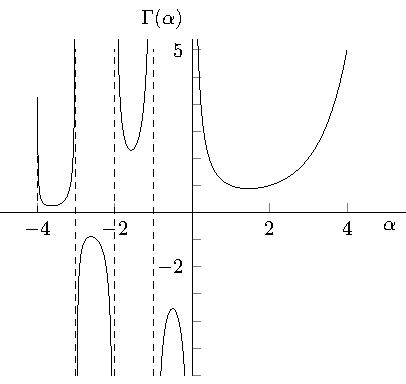
\includegraphics{figOctaveGammaFunction}
\caption{گیما تفاعل}
\label{شکل_ضمیمہ_مفید_گیما_تفاعل}
\end{figure}
%

\اصطلاح{نا مکمل گیما تفاعل}
\begin{align}
P(\alpha,x)=\int_{0}^{x} e^{-t}t^{\alpha-1}\dif t, \quad Q(\alpha,x)=\int_{x}^{\infty} e^{-t}t^{\alpha-1}\dif t \quad \quad (\alpha>0)
\end{align}
%
\begin{align}
\Gamma(\alpha)=P(\alpha,x)+Q(\alpha,x)
\end{align}
\اصطلاح{بیٹا تفاعل}
\begin{align}
B(x,y)=\int_{0}^{1}t^{x-1}(1-t)^{y-1}\dif t\quad \quad (x>0,\, y>0)
\end{align}
بیٹا تفاعل کو گیما تفاعل کی صورت میں بھی پیش کیا جا سکتا ہے۔
\begin{align}
B(x,y)=\frac{\Gamma(x) \Gamma(y)}{\Gamma(x+y)}
\end{align}
\اصطلاح{تفاعل خلل}(شکل \حوالہ{شکل_ضمیمہ_مفید_تفاعل_خلل})
\begin{align}\label{مساوات_ضمیمہ_تفاعل_خلل_الف}
\erf x=\frac{2}{\sqrt{\pi}}\int_{0}^{x} e^{-t^2}\dif t
\end{align}
مساوات \حوالہ{مساوات_ضمیمہ_تفاعل_خلل_الف} کے تفرق \عددی{\erf' x=\tfrac{2}{\sqrt{\pi}}e^{-t^2}} کی مکلارن تسلسل 
\begin{align*}
\erf' x=\frac{2}{\sqrt{\pi}}\left(x-\frac{x^3}{1!3}+\frac{x^5}{2!5}-\frac{x^7}{3!7}+-\cdots \right)
\end{align*}
 کا تکمل لینے سے تفاعل خلل کی تسلسل صورت حاصل ہوتی ہے۔
%
\begin{align}
\erf x=\frac{2}{\sqrt{\pi}}\left(x-\frac{x^3}{1!3}+\frac{x^5}{2!5}-\frac{x^7}{3!7}+-\cdots \right)
\end{align}
\عددی{erf \infty =1} ہے۔ \اصطلاح{مکملہ تفاعل خلل}
\begin{align}
\erfc x=1-\erf x=\frac{2}{\sqrt{\pi}} \int_{x}^{\infty} e^{-t^2}\dif t
\end{align}
%
\begin{figure}
\centering
\begin{tikzpicture}[
    declare function={erf(\x)=%
      (1+(e^(-(\x*\x))*(-265.057+abs(\x)*(-135.065+abs(\x)%
      *(-59.646+(-6.84727-0.777889*abs(\x))*abs(\x)))))%
      /(3.05259+abs(\x))^5)*(\x>0?1:-1);},
    declare function={erf2(\x,\y)=erf(\x)+erf(\y);}
]
\begin{axis}[small,axis lines*=middle,xlabel={$x$},ylabel={$\erf x$},xlabel style={at={(current axis.right of origin)},anchor=north east},ylabel style={rotate=-90},ylabel style={at={(current axis.above origin)},anchor=north east},ymin=-1.2,ymax=1.5,xmin=-2.2,xmax=3,xtick={-2,-1,1,2},xticklabels={{$-2$},{$-1$},{$1$},{$2$}},ytick={-1,1},yticklabels={{$-1$},{$1$}}]
\addplot[domain=-2:2]{erf(\x)};
\end{axis}
\end{tikzpicture}
\caption{تفاعل خلل۔}
\label{شکل_ضمیمہ_مفید_تفاعل_خلل}
\end{figure}
\اصطلاح{فرسنل تکملات} (شکل \حوالہ{شکل_ضمیمہ_مفید_فرسنل_تکملات})
\begin{align}
\FC(x)=\int_{0}^{x} \cos(t^2)\dif t,\quad \FS(x)=\int_{0}^{x}\sin(t^2)\dif t
\end{align}
\عددی{\FC(\infty)=\sqrt{\tfrac{\pi}{8}}} اور \عددی{\FS(\infty)=\sqrt{\tfrac{\pi}{8}}} ہیں۔\اصطلاح{مکملہ تفاعل}\حاشیہب{complementary functions}
\begin{align}
\FAC(x)&=\frac{\pi}{8}-\FC(x)=\int_{x}^{\infty} \cos(t^2)\dif t\\
\FAS(x)&=\frac{\pi}{8}-\FS(x)=\int_{x}^{\infty} \sin(t^2)\dif t
\end{align}
%
\begin{figure}
\centering
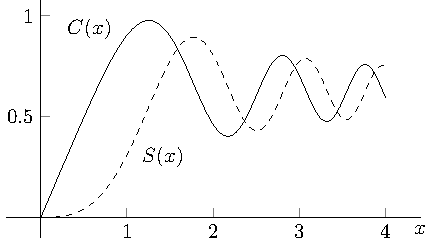
\includegraphics{figFresnelIntegrals}
\caption{فرسنل تکملات}
\label{شکل_ضمیمہ_مفید_فرسنل_تکملات}
\end{figure}
\اصطلاح{تکمل سائن} (شکل \حوالہ{شکل_ضمیمہ_مفید_تکمل_سائن})
\begin{align}
\kSi(x)=\int_{0}^{x}\frac{\sin t}{t} \dif t
\end{align}
\عددی{\kSi{\infty}=\tfrac{\pi}{2}} کے برابر ہے۔تکملہ تفاعل
\begin{align}
\ksi(x)=\frac{\pi}{2}-\kSi(x)=\int_{x}^{\infty} \frac{\sin t}{t}\dif t
\end{align}
\اصطلاح{تکمل کوسائن}
\begin{align}
\ci(x)=\int_{x}^{\infty}\frac{\cos t}{t}\dif t \quad \quad (x>0)
\end{align}
\اصطلاح{تکمل قوت نمائی}
\begin{align}
\Ei(x)=\int_{x}^{\infty} \frac{e^{-t}}{t}\dif t\quad \quad (x>0)
\end{align}
\اصطلاح{تکمل لوگارتھمی}
\begin{align}
\li(x)=\int_{0}^{x}\frac{\dif t}{\ln t}
\end{align}
%
\begin{figure}
\centering
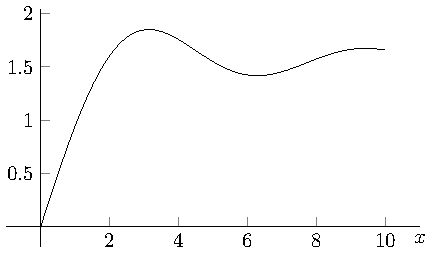
\includegraphics{figSineIntegral}
\caption{تکمل سائن}
\label{شکل_ضمیمہ_مفید_تکمل_سائن}
\end{figure}

\باب{جدول}\شناخت{ضمیمہ_جدول}

\begin{table}
\caption{ثنائی تقسیم}
\label{ضمیمہ_ثنائی_تقسیم}
\centering
\end{table}
%========================
\begin{table}
\caption{پوئسن تقسیم}
\label{ضمیمہ_پوئسن_تقسیم}
\centering
\end{table}
%=================================
\begin{table}
\caption{عمومی تقسیم}
\label{ضمیمہ_عمومی_تقسیم_الف}
\centering
\end{table}
%============================
\begin{table}
\caption{عمومی تقسیم}
\label{ضمیمہ_عمومی_تقسیم_ب}
\centering
\end{table}
%==========================
\begin{table}
\caption{ثبلا منصوبہ اعداد}
\label{ضمیمہ_بلا_منصوبہ_اعداد}
\centering
\end{table}
%===========================
\begin{table}
\caption{$t$تقسیم}
\label{ضمیمہ_ٹی_تقسیم}
\centering
\end{table}
%=============================
%===========================
\begin{table}
\caption{مربع خا تقسیم}
\label{ضمیمہ_مربع_خا_تقسیم}
\centering
\end{table}
%===========================
\begin{table}
\caption{مربع ایف تقسیم}
\label{ضمیمہ_ایف_تقسیم}
\centering
\end{table}
%===========================
\begin{table}
\caption{؟؟}
\label{ضمیمہ_بلا_رجحان}
\centering
\end{table}

%

%\include{./tex/emtEndOfBookTableDivergenceCurlGradientLaplacian}
%\include{./tex/toDoList}
%\include{./tex/emtQuestions}
\backmatter

\cleardoublepage
%\include{./tex/emtDataTables}        %appendices
%\include{./tex/emtLinearAlgebra}
%\include{./tex/emtCoordinatesRelations}
%================


%=================

\renewcommand*{\indexname}{فرہنگ}      %this command has to be placed right here just before printindex command
\cleardoublepage
\addcontentsline{toc}{chapter}{فرہنگ}
%\printindex


\end{urdufont}
\end{document}
